\documentclass[a5paper,10pt,openany]{book}

\usepackage[top=2cm,bottom=2cm,bindingoffset=0cm]{geometry}

\usepackage[svgnames]{xcolor} % Required to specify font color

%\documentclass[a4paper,12pt,openany]{scrbook}

%\usepackage{glossaries}
%\usepackage[xindy]{glossaries}
%\makeglossaries

%\usepackage{odsfile,lmodern}

%\usepackage{luacode}

\usepackage{multicol}

\usepackage{mathtext}
\usepackage{makeidx}
%\usepackage{imakeidx}
\usepackage{longtable}
\usepackage[tc]{titlepic}

\usepackage{fontspec}

\usepackage[protrusion=true,expansion,
tracking=true,letterspace=50]{microtype}

%\SetTracking[ spacing = {25*,166, } ]{ encoding = *, shape = sc }{ 25 }


%\usepackage{soulutf8}
%\usepackage{letterspace}

%\usepackage[toc]{appendix}
\usepackage[toc,titletoc]{appendix}
\renewcommand\appendixtocname{Приложения}
\renewcommand\appendixpagename{Приложения}

%\usepackage{xunicode}
\usepackage{xltxtra}

\usepackage[normalem]{ulem}
\usepackage{adjustbox}

\usepackage{polyglossia}
\setmainlanguage{russian}
\setotherlanguage{ukrainian}
\setotherlanguage{english}
\setotherlanguage{greek}
\setotherlanguage{latin}
\setotherlanguage{polish}

%\setromanfont{URW Palladio L}
%\newfontfamily{\cyrillicfonttt}{URW Palladio L}

%\setromanfont{DejaVu Serif}
%\setsansfont{DejaVu Sans}
%\setmonofont{DejaVu Sans Mono}

%\setmainfont{DejaVuSerif.ttf}
%\setromanfont{DejaVuSerif.ttf}
%\setsansfont{DejaVuSans.ttf}
%\setmonofont{DejaVuSansMono.ttf}

\setmainfont[BoldFont={DejaVuSerif-Bold.ttf},
ItalicFont={DejaVuSerif-Italic.ttf},
 BoldItalicFont={DejaVuSerif-BoldItalic.ttf}]{DejaVuSerif.ttf}

\setromanfont[BoldFont={DejaVuSerif-Bold.ttf},
ItalicFont={DejaVuSerif-Italic.ttf},
 BoldItalicFont={DejaVuSerif-BoldItalic.ttf}]{DejaVuSerif.ttf}

\setsansfont[BoldFont={DejaVuSans-Bold.ttf},
ItalicFont={DejaVuSans-Oblique.ttf},
 BoldItalicFont={DejaVuSans-Oblique.ttf}]
{DejaVuSans.ttf}


\setmonofont[BoldFont={DejaVuSansMono-Bold.ttf},
ItalicFont={DejaVuSansMono-Oblique.ttf},
 BoldItalicFont={DejaVuSansMono-BoldOblique.ttf}]
{DejaVuSansMono.ttf}


%\addfontfeature{LetterSpace=15,WordSpace=10}
%\setromanfont{Linux Libertine}


%\setromanfont{Liberation Serif}
%\setsansfont{Liberation Sans}
%\setmonofont{Liberation Mono}

%\newfontfamily{\cyrillicfonttt}{Liberation Serif}
%\newfontfamily{\cyrillicfonttt}{Liberation Sans}
%\newfontfamily{\cyrillicfonttt}{Liberation Mono}

%\setromanfont{Linux Libertine}


%\usepackage{showframe}

\usepackage{enumitem}
\usepackage{indentfirst} 

\usepackage{verse}

\usepackage{graphicx}
%\usepackage{listings}
%\usepackage[unicode,pdfpagelabels,plainpages=false]{hyperref}
%\usepackage[pdfpagelabels,pdfusetitle,unicode,plainpages=false]{hyperref}

\usepackage[pdfpagelabels,unicode,plainpages=false]{hyperref}

\hypersetup{pdftitle=Ересь о Киеве. Петр Семилетов.}

%\hypersetup{  
%  pdfinfo={  
%    Title={Ересь о Киеве},  
%    Subject={Киев},  
%  }  
%} 


%\usepackage{cmap}
%\usepackage{float}
\usepackage{bookmark} 
\usepackage{relsize}

\usepackage{tocloft,calc}
\usepackage[nottoc,numbib]{tocbibind}

%\usepackage{multicol}


%\usepackage[nottoc,notlot,notlof]{tocbibind}

%\usepackage{etoolbox}
%\apptocmd{\thebibliography}{\csname phantomsection\endcsname\addcontentsline{toc}{chapter}{\bibname}}{}{}

\renewcommand{\cftchappresnum}{Глава }
\AtBeginDocument{\addtolength\cftchapnumwidth{\widthof{\bfseries Глава XX}}}

%\renewcommand{\cftpartpresnum}{Часть }
%\AtBeginDocument{\addtolength
%\cftpartnumwidth{\widthof{\bfseries Часть }}}


%\newcommand{ - }{ – } 

%\renewcommand{\cftchappresnum}{Глава }

\frenchspacing
\righthyphenmin=2

%\sloppy

%\hyphenation{ва-ря-ги}

%\tolerance 1414
%\hbadness 1414
%\emergencystretch 1.5em
%\hfuzz 0.3pt
%\widowpenalty=10000
%\vfuzz \hfuzz
%\raggedbottom

%\sloppy
%\usepackage{appendix}
%\usepackage{csquotes} 
%\pretolerance=1150
%\tolerance=1753
%\hbadness=1752

%\renewcommand{\rmdefault}{ptm}


%\luaexec{
%    semiletov_gv_imgprefix = "s-"
%}

%\newcommand\myimgprefix{%
%\directlua{
%     tex.sprint(semiletov_gv_imgprefix);
% }}

%\makeindex

\makeatletter
\@addtoreset{chapter}{part}
\makeatother  

\newcommand\myimgprefix{s-}

%\titlepic{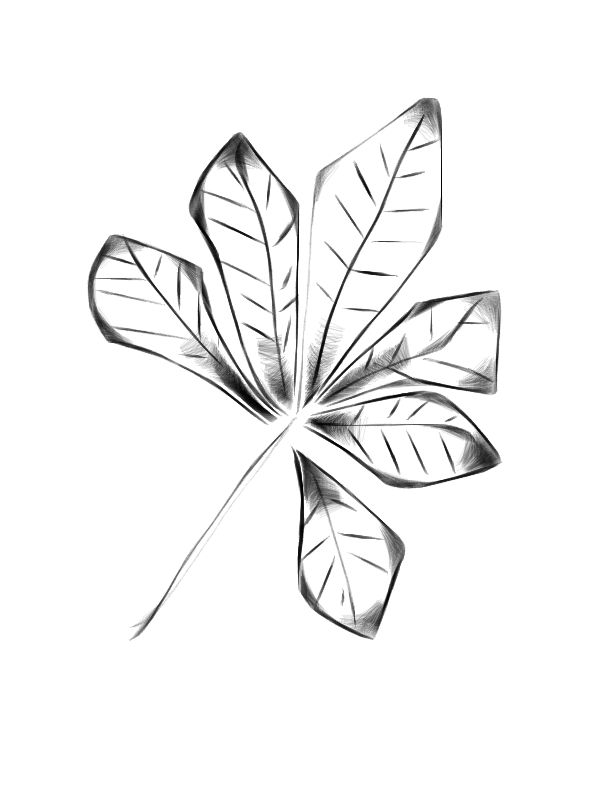
\includegraphics[width=0.50\textwidth]{cover/04.jpg}}

\title{Ересь о Киеве \\ \textsmaller[2]{редакция 11.0}}
\author{Петр Семилетов}
\date{12/09/2024}



\newcommand*{\plogo}{\fbox{$\mathcal{PL}$}} % Generic publisher logo

%----------------------------------------------------------------------------------------
%	TITLE PAGE
%----------------------------------------------------------------------------------------

\newcommand*{\titleAT}{\begingroup % Create the command for including the title page in the document
\newlength{\drop} % Command for generating a specific amount of whitespace
\drop=0.1\textheight % Define the command as 10% of the total text height

\rule{\textwidth}{1pt}\par % Thick horizontal line
\vspace{2pt}\vspace{-\baselineskip} % Whitespace between lines
\rule{\textwidth}{0.4pt}\par % Thin horizontal line

\vspace{\drop} % Whitespace between the top lines and title
\centering
\textcolor{Red}{
{\Huge ЕРЕСЬ О КИЕВЕ}\\[0.5\baselineskip] % Title line 1
%{\Large}\mbox{}\\[0.75\baselineskip] % Title line 2
%{\Huge четвертая редакция}} % Title line 3
}

\vspace{0.25\drop} 
\rule{0.3\textwidth}{0.4pt}\par 

\mbox{ }\\
редакция 11.0\\

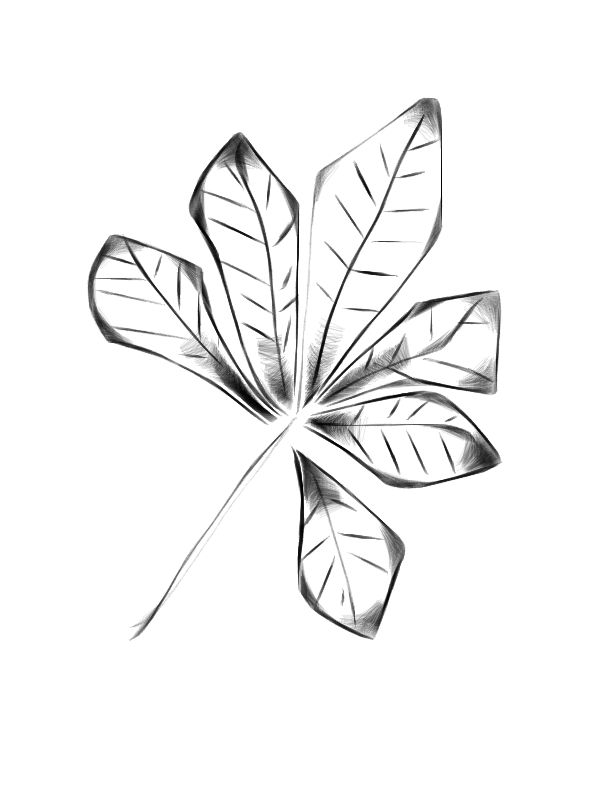
\includegraphics[width=0.40\textwidth]{cover/04.jpg}

\vspace{\drop} 

{\Large \textsc{Петр Семилетов}}\par 


\vfill
%{\large \textcolor{Red}{\plogo}}\\[0.5\baselineskip] % Publisher logo
{\large \textsc{Самиздат 2024}}\par % Publisher

\vspace*{\drop} 

\rule{\textwidth}{0.4pt}\par
\vspace{2pt}\vspace{-\baselineskip} 

\rule{\textwidth}{1pt}\par 

\endgroup}


\begin{document}

\pagestyle{empty}

\titleAT

\newpage

\pagestyle{plain}

\tableofcontents

\chapter*{Предисловие}
\markboth{\MakeUppercase{Предисловие}}{}
\addcontentsline{toc}{chapter}{Предисловие}

\section*{Се начнем повесть сию} 

Никогда не думал, что напишу такую здоровенную книгу. Потуги были. В юности я был ударенный в изучение фольклора, и раздобыл такую амбарную книгу – листы в мелкую клетку, броневая зеленая обложка, вес несколько килограммов. Начал писать в ней энциклопедию славянской демонологии, да застрял. Хотя прежде того сил хватило на четыре рукописных тома народного календаря – «Месяцеслова» – сведенного из множества источников. Приметы, поверья на каждый день.

Так вот сам по себе человек только прозу пишет, а в краеведческих книгах всегда прямо или косвенно участвуют другие люди.

Посему благодарю тех, кто так или иначе способствовали появлению и развитию книги.

Особое спасибо родителям, с которыми обсуждал свои изыскания сразу, как только оные возникали. Коле Арестову за долголетнее краеведческое сотрудничество. Сколько хожено троп, сколько преодолено склонов! Насте, часами выслушивавшей мои исторические выкладки – за некоторые фотки и ценные сведения. Свете Семеновой, Марине Чуприне – за нужные в работе книжки. Неле Арестовой, Андрею Савченко, Саше Ураловой и снова Свете за тонкости перевода с языков, в которых я не силен. Однако не всегда я прислушивался к вашим советам. Алине – за решимость лезть со мной через бурелом всё дальше. Любе – за книжки и сведения о подземле. Зое Колзуновой за некоторые сведения про кости и черепа. Даше Кононюк за совместные краеведческие вылазки.

%Всем кого я не упомянул, дабы ересью не бросать на них тень!
Также и тем, чьими работами я пользовался как источниками.

\section*{С чего вдруг}

Долгое время я не считал себя краеведом, но кажется постепенно стал им. Как увлекся?

С 2005 года мы с друзьями, объединившись под названием «студия Дрымба», снимали любительское кино – вначале на купленную в ломбарде VHS-камеру, затем на MiniDV. В 2009-м стали делать полнометражную фантастическую картину «Сваха», и по ходу запечатлели на видео много краеведческого материала. Брали интервью у местных жителей подле озера Глинка, делали кадры по течению реки Лыбеди, включая тот короткий отрезок, где воды ея бурно протекают в естественном русле под Лысой горой.

«Сваха» зависла, а накопившийся по Киеву материал сподвиг нас к созданию, частью на его основе, большого документального фильма «Киевская сюита», выложенного в сеть в 2010 году сразу после монтажа. Когда мы снимали «Сюиту», пришлось копнуть историю да краеведение на уровне несколько более глубоком, чем листание справочника. Статьи из справочников, как правило – нечто вроде слюны, которую глотаешь, когда очень хочется пить, а никакой газировки под рукой нету и купить негде. Вроде и жидкость, но жажду знания не удовлетворяет.

Спустя год после «Сюиты», весной 2011-го, меня осенило вдохновение писать краеведческую книгу. Я еще не погрузился в предмет целиком, не нырнул в него с головой, а так – опустил туда лицо и пытался открыть в мутной воде глаза. Задумал осветить спорные и загадочные сведения о городе, отчасти поэтому и название выбрал – «Ересь о Киеве», впрочем созвучное другой моей книге, про звукорежиссуру – «Ересь звукозаписи».

«Ересь о Киеве» сначала была сделана как сайт. Это позволяло мне всё время быстро вносить в книгу правки. Читатели спрашивали меня, а нельзя ли выложить её одним файлом? Я неизменно отвечал – нет, ибо мне больше подходит HTML, так удобнее верстать.

Я пользовался множеством книг, большей частью дореволюционных, и прежде выкладывал их в отдельном разделе книги-сайта. То же касалось карт. В конце 2012 года я запустил проект \href{http://semiletov.org/kievograd}{Киевоград}, куда перенес накопленную библиотеку, карты, и также завел там фотоархив и рубрику для фильмов про Киев. Задача Киевограда – предоставление краеведческих материалов по Киеву в свободном доступе.

Медленно пришел я к мысли, что надо таки сверстать электронную книгу, ибо сайт, как ни крути, штука временная. А книгу можно куда-то зафитюлить в сеть, и пойдет гулять. Поэтому в третьей редакции, «Ересь о Киеве» превратилась из книги-сайта в полноценную книгу формата PDF.

Третья редакция стала совершенно новым произведением, от старого сохранившим только название. Это не дополненный вариант прежней книги, превзошедший ее объемом в десятки раз, а именно другое содержимое, выражение иных взглядов.

Началось всё снова с кино. Весной 2013 года мы принялись снимать цикл краеведческих фильмов «Киевская амплитуда». Осенью, параллельно, я стал делать еще один цикл – «Планету Киев». Оба смотрите на Киевограде либо онлайн в Ютубе. 

Съемки расширили мой круг интересов. Я побывал в Змиевой пещере. С Колей Арестовым мы облазили все окрестные склоны. Кирилловские высоты, Логово Змиево захватили меня и привели к открытиям, ставшими стержнем новой «Ереси». Кирилловской пещере посвящаю в книге отдельную часть. Что до видео из пещеры – смотрите «Киевскую амплитуду».

Тогда, в 2013-м, я собирался завершить книгу одновременно с монтажом серии «Логово Змиево», но вот фильм уже был готов, выложен в сеть, а «Ересь» всё писалась, писалась, раскручиваясь по спирали и пуская ветки во все стороны.

Местами она получилась очень подробной, но хотелось поделиться не просто итогом размышлений, но самими размышлениями с исходными данными, источниками. Поэтому, если я в чем-то ошибаюсь, у вас есть всё для проверки или построения каких-то своих выводов.

А работа над четвертой редакцией началась сразу после выпуска третьей, осенью 2015-го. Поначалу это было исправление ошибок (отдельное спасибо за указания на них Александру Петруку) и попутно шероховатостей слога. Вообще я хотел отдохнуть от «Ереси» и стал писать совсем другую краеведческую книгу, легче, меньше.

Но вышло иначе – и появилась новая редакция, еще больше предыдущей, да еще основательно переписанная. Я даже хотел переименовать ее, но кажется, от единожды принятого названия не уйти. 

Хотя по моим ощущениям, получилась совсем другая книга, лишь сохраняющая подобие прежней. Или – книга, более ставшая собой, чем была.

Сразу по выходу четвертой редакции к «Ереси» стал притягиваться новый материал, и дополненная им книга выходит уже в этой, пятой редакции осенью 2017 года. Существенно увеличились и были переделаны главы про Зверинец, Иорданскую церковь и Лысые горы. Точечных изменений претерпели и некоторые другие главы, я уж и забыл какие.

По февраль 2018 года я время от времени вносил в книгу кое-какие изменения и сразу заливал обновленную версию в сеть, но под номером прежней версии.

В конце февраля, добавив еще разные уточнения, мне приходится как бы утвердить их уже шестой редакцией. Отличия от пятой – в точности сообщаемых сведений. 

В седьмой версии были убраны полдесятка фотографий. Иллюстративный ряд теряет в освещении местности, зато книга приобретает первозданную «лицензионную» чистоту. Зарекался использовать чужие снимки, не попавшие в общественное достояние.

К лету 2018 года седьмая редакция обновилась новыми сведениями о болоте Ковпыте и ручье Омелютинке, однако нового в книге не так много, чтобы увеличивать номер основной редакции, посему явилась версия 7.1.

В декабре 2018 года была существенно подправлена глава о летосчислении, что дало повод к выпуску редакции 7.1. В 2019 году была продолжена работа по исправлению, уточнению и дополнению текста. В 2020 оная работа продолжилась, к тому же надо было лучше синхронизировать книгу с другим моим трудом, «Словарем киеведа». 

Так рождалась редакция 8.0, которая дополнилась затем новыми материалами по Зверинецким пещерам и вообще Зверинцу. В восьмой редакции много чего я исправил, проверил приведенные координаты, а также привел их к одному только формату – градусы и минуты, причем не в «правильном» типографском виде, а с обычными двойными и одинарными кавычками, чтобы обеспечить совместимость не только с геодезическими программами, но и популярными электронными картами. 

Девятая редакция книги возникла опять же в ходе согласования с материалами "Словаря киеведа", однако простое согласование обернулось основательным пересмотром некоторых вещей и сверкой летописей по светописным копиям, если они были доступны. Например, я, кажется, таки вычислил место урочища Курган в Бабьем яру. Добавились впечатления от новых краеведческих вылазок. Мне окончательно стало понятно, что пещеру из дела Бейлиса в наше время найти уже невозможно.

Перечитывая старые главы, с горечью убедился, что описанное в них всё более приобретает историческое значение, более не существуя в природе.

Работа над десятой редакцией закрутилась опять же в связи с большой правкой Словаря, а в 2022 году затянулась на, казалось, неопределенное время, пока весной 2023 я неожиданно не вырулил к свету в конце тоннеля. В десятую редакцию добавились две новые большие главы – про Копырев конец и капище Волоса, а поднятые темы затронули, так или иначе, некоторые другие части книги. Вообще про язычество много чего добавилось. Конечно же весь текст так или иначе подвергнулся правке – иногда это касалось буквально поправке на мое текущее мировоззрение, иногда относилось к неточностям в цитировании летописей, краеведческие сведения также уточнялись сообразно развитию моих представлений.

Десятая редакция также ознаменовалась долгими, огромными трудами по упорядочиванию исходника книги. За более чем десятилетие структура книги на жестком диске, в виде файлов и каталогов, развивалась естественным неряшливым образом, например все иллюстрации к такой-то части могли лежать в одном каталоге, а не чтобы на каждую главу по каталогу, куда и текст главы, и картинки. Накопилось множество неиспользованных иллюстраций, их вариантов, и копий в большем разрешении – изначально была мысль выпускать две версии Ереси, с качественными картинками и обычными. Но Ересь до того распухла, что я давно не думал о втором варианте. Весь этот отработанный материал надо было вычленить из исходника, и заново упорядочить структуру, на что и ушло между прочим много месяцев. Если бы не мой редактор TEA и некоторые функции рабочей среды Plasma, то наверное потратил бы и год, а то и несколько.

Одиннадцатая редакция должна была включать в себя дополнительную часть, если не главу – новое важное исследование, однако в ходе правки уже наработанного материала я зацепился за часть про Кирилловские высоты и основательно ее переработал, более строго отнесясь к умозаключениям. Так, я ввел во всю книгу два четко определенных топонима, Хоривица (отождествив ее с отрогом Щекавицы со Старообрядческим кладбищем) и Лысая-Юрковица (указав этим названием на современную гору Юрковицу и предваряя ее прежним названием). Отдельно идет урочище Юрковица. Предполагаемая модель развития именований – именование Хоривицы сползло с исконной такой горы в овраг, со временем исказившись в урочище Юрковицу, и позже переползло на соседнюю с оным урочищем Лысую гору на Кирилловских высотах. Хотя именно на Лысой горе располагался (почему так считаю смотрите в части про Высоты) град Киев, крепость, построенная тремя братьями и названная так в честь старшего Кия, у которого однако уже была своя гора, Киевица.

В одиннадцатой редакции были также заменены некоторые иллюстрации на более качественные, переделаны карты, а еще текст подвергся общей правке.

В редакции 11.2 весьма исправлена последняя глава про Зверинец.

\section*{Электронное издание} 

Я выкладываю «Ересь о Киеве» в сеть как общественное достояние (public domain). Это значит, что вы можете использовать книгу как угодно, в рамках приличий. Проще говоря, вот существует допустим классическое произведение, у него есть сочинитель, но произведение принадлежит человечеству. Так и с этой книгой.

Хотя у электронных книг есть минус. Они имеют судьбу чисто информационную, не привязанную к печатному экземпляру.

У меня на полке стоит книжка «Киев. Справочник-пут\-еводи\-тель» 1954 года издания, небольшая такая, в коричневой обложке, а бумага до сих пор белая. На одной из последних, пустых страниц я нашел карандашные записи:

\begin{quotation}
Справочная \textbf{0-0-9}

Оперный театр

\sout{4-71-84}
\end{quotation}

и под углом:

\begin{quotation}
5-51-34

Оперный театр
\end{quotation}

Эта заметки, судя по телефонным номерам, сделаны примерно во время, когда книга увидела свет – пятидесятые. Кто писал эти строки, чья рука, какая судьба у этого человека? 

Ведь на одной странице развернулась целая история. Сначала человек узнал номер справочной – вероятно, телефон был внове, появился в семье впервые. Затем человек получил один номер Оперного театра. И записал его спокойно, ровно. Позже (насколько?) он получил взамен неправильного номера (который поэтому был перечеркнут) новый, и записал его в спешке, в неудобном положении, наискось!

Книга побывала и в некой библиотеке, чей штамп наполовину стерся, либо был плохо проставлен. А как потом книга попала на букинистическую раскладку – в коробку на асфальте, где среди водорослей можно найти перлы, и всё по одной цене?

В том же чудесном месте – любимом читающими киевлянами и не только ими книжном рынке Петровке – я приобрел еще пару замечательных книг со следами чужих судеб.

Первая – неказистый на вид томик очерка «Киев» Шулькевича. Приехал я домой, рассматриваю – ба, да  этой книжкой владел археолог Дмитрий Яковлевич Телегин. Вот он написал год покупки – «1963». Карандашные пометки на полях, черновой набросок схемы давнего Киева, подчеркнутые строки. И я понял – раз книга Телегина попала на Петровку, сам археолог умер.


\section*{Источники} 

Конечно же, источники, приведенные мною в конце книги – лишь малая доля общего их объема, туда я поместил лишь цитируемое. Выдержки, если они на старославянском либо «роськой мове» Великого княжества Литовского, даю в подлиннике. Важнейшие цитаты на латыни или греческом стараюсь приводить в своем, по возможности точном переводе, а также в подлиннике. При цитировании летописей, для удобочитаемости помещаю из обработанных учеными текстов Полного Собрания Русских Летописей, где подлинник трактован и потому несколько искажен. Наиболее важные выдержки, однако, беру из светописных копий подлинников.

\section*{Об иллюстрациях} 

В качестве иллюстраций я использую много старинных фотографий и изображений, за давностью лет перешедших в общественное достояние. Существует много фоток, которые я хотел бы показать в этой книге, да не могу из-за авторского права и всяческих связанных с ним ограничений.

Современные снимки в этой книге сделаны, за редкими исключениями, мною и отдаются в общественное достояние.

Увы – изображения, полученные со спутниковых карт, сурово защищены всевозможными коммерческими лицензиями, поэтому я вынужден был, несмотря на всю заманчивость, отказаться от них, за редкими исключениями и с указанием копирайта. Из лицензионных соображений я использую лишь старые карты, которым больше 70 лет – они перешли в общественное достояние. Иногда я помещаю советские карты, да немецкие аэрофотоснимки 1918 и 1943 годов.

\section*{О координатах}

Поелику книгу я пишу для вечности, а городские адреса бренны да изменчивы, буду частенько давать координаты, в геодезической системе WGS-84, которая сейчас используется в GPS и большинстве электронных карт. В СССР была другая система координат, СК-42. Есть еще СК-63. Существуют формулы пересчета из одной системы в другую, программы, онлайн-конвертеры, различные макросы и тому подобное. 

Я привожу координаты в формате градусов и минут. Пример: "50°28'6.66"N 30°29'56.42"E". Буква N означает «North», или северная широта. E – «East», восточная долгота.

В старых редакциях книги я давал еще координаты в десятичных градусах. Пример: 50.468517°, 30.499005° либо без знака градуса. Сначала идет широта, потом долгота. 

\section*{Программное обеспечение} 

В работе над этой книгой мне помогало разнообразное программное обеспечение, о чем я не могу умолчать.

Вся работа уютно происходила под операционной системой Linux, в дистрибутиве Mageia и рабочей среде KDE, а с лета 2017 года – в среде Mate. С 2019 года работаю уже в Manjaro Linux, а в 2020 перебрался в Arch, а затем сменил Mate на KDE/Plasma. 

Текст я набираю и верстаю в редакторе \href{http://semiletov.org/tea}{TEA}, собственной разработки. Программа Okular всегда под рукой для чтения сканов в форматах PDF и DjView. Вёрстка подготовлена при помощи удивительного средства вёрстки \href{http://www.latex-project.org/}{\LaTeX} с движком Lua\TeX~ – с ними я могу одновременно сочинять книгу и верстать её, не разделяя текст и макет. Я использовал семейство свободных шрифтов DejaVu. Иллюстрации подготовлены в растровом редакторе GIMP и векторном Inkscape.

%Оно не только выглядит так, как мне нравится, но и позволило, наряду с поддержкой кодировки UTF-8 в Lua\TeX, сочетать на страницах текст на кириллице, греческом и других языках. 

%При этом я подключил следующие пакеты функций – не могу умолчать оные, ведь от них зависит многое, что повлияло на вид книги: protrusion, polyglossia, verse, graphicx, pdfpagelabels, bookmark, relsize, tocloft, calc, multicol, longtable.


\section*{Ересь в Сети. Пишите письма}

Новые редакции книги, по мере их выхода, будут выкладываться по следующим адресам:\\ 

\noindent
\href{http://semiletov.org/kiev}{http://semiletov.org/kiev} (мой сайт)\\
\href{https://www.facebook.com/groups/213781655750601/}{www.facebook.com/groups/213781655750601} (группа Киевоград в ФБ)\\
\href{https://t.me/kievograd}{t.me/kievograd} (группа Киевоград в Телеге)\\

Также можете написать мне письмо по электронной почте: \href{peter.semiletov@gmail.com}{peter.semiletov@gmail.com}, 
в телегу: @petersemiletov или ФБ/Мессенджер \href{https://www.facebook.com/peter.semiletov}{www.facebook.com/peter.semiletov}. Буду рад отзывам, указаниям на ошибки, дополнениям.


\part{Колебание основ}

\chapter{Начало}

Как возник Киев? Долгое время меня не заботил этот вопрос. Ведь ученые, следом за Нестором-летописцем, всё давно пояснили. Еще дошкольником в начале восьмидесятых я знал, что город основали Кий, Хорив, Щек и сестра их Лыбедь. Я представлял их себе именно такими, как потом увидел в 1982 году, когда город отмечал 1500-летие – медными  скульптурами на лодье, у свежего Днепра в парке Примакова, что раскинулся вдоль каменной набережной Днепра от моста Патона до Моста метро. 

Благообразные, похожие на первопечатника Ивана Федорова славяне-бородачи – кроме Лыбеди, конечно – с долгими волосами, взятыми в обручи. Двое с копьями, один с луком, и ни у кого нет вёсел. Поначалу это была железобетонная скульптура, обшитая медными листами. С 2010 года материал заменили на бронзу, а лодью уменьшили. К ней любят приезжать фотографироваться молодожены.

Небольшая модель этого памятника в промежутках между похищениями стоит во дворе Художественной академии на Вознесенском спуске (улица Смирнова-Ласточкина). Она же Вознесенский спуск. Улицы переименовывают туда-сюда, не уследишь. Здесь и далее придерживаюсь привычных мне названий. 

Там же в усадьбе академии, многие здания разукрашены замечательными граффити – надо лишь завернуть за само здание с правой его стороны, к склону холма, и пройти вдоль главного корпуса. А еще можно найти на задворках мусорник со скульптурами. Но про ту, весьма историческую местность – позже!

Лодья, набережная... Почему пишу здесь и далее «лодья»? Так правильно. Так в летописях. Так говорили – л\'одья. Производное – лодка. Вы же не говорите – ладка. Посему – лодья. Ученые-языковеды возразят, что с буквой «о» это северный говор. Нет, это давнее произношение, позже в некоторых местностях изменившееся на «а». Ученые могут почитать летописи и убедиться, как было прежде.

\begin{center}
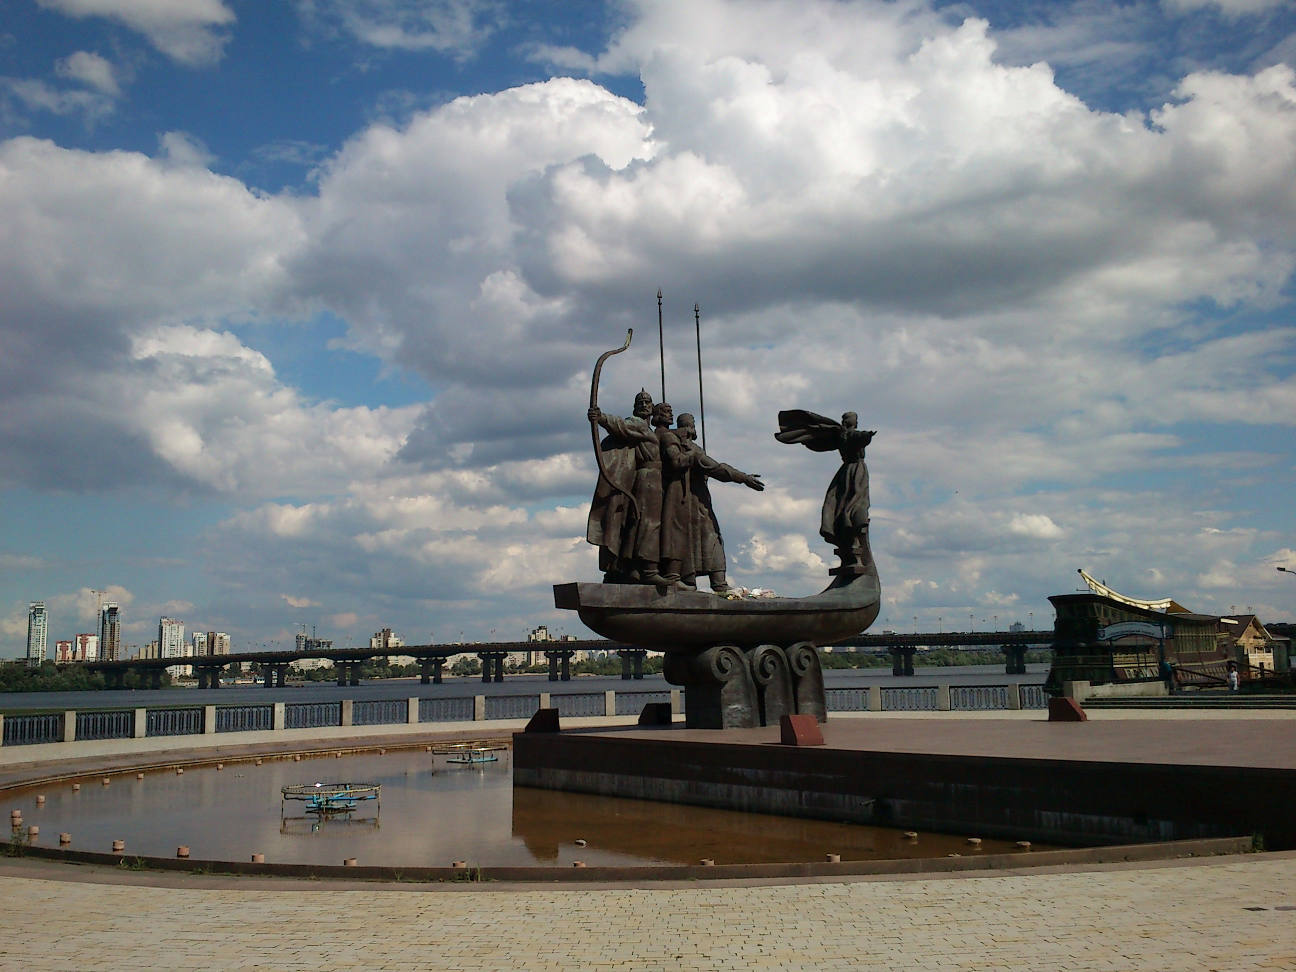
\includegraphics[width=\linewidth]{chast-colebanie-osnov/nachalo/ladiya.jpg}
\end{center}

%Небольшая модель этого памятника в промежутках между похищениями стоит во дворе Художественной академии на улице Смирнова-Ласточкина. Она же Вознесенский спуск. Нынче трудно писать книги – улицы переименовывают туда-сюда, не уследишь. Здесь и далее придерживаюсь старых, привычных мне названий., %ибо не могу переписывать книгу согласно каждому новому решению городского совета!% За исключением, когда новое название нравится мне больше.


%Там же в усадьбе академии, многие хозяйственные постройки разукрашены замечательными граффити – надо лишь завернуть за само здание с правой его стороны, к склону холма, и пройти вдоль корпуса. Пишу по памяти, может уже закрасили.

Я смутно помню время, когда лодьи со скульптурами и каменной набережной не существовало. До конца восьмидесятых, в парке Примакова был песчаный пляж, у пляжа пристань-понтон, и плавал катер на противоположный берег – южную часть острова Гидропарка, тоже с пляжем.

А под горой напротив парка Примакова разворачивался у моста Патона трамвай, что ходил вдоль древних, изрытых пещерами и сочащихся рыжими родниками холмов с Лаврой и Аскольдовой могилой, по набережной до Красной, ныне Контр\'актовой, площади. Этот чудесный маршрут упразднили. Печатно обещали – временно, оказалось – навсегда. Рельсы продержались, ржавея, дольше трамвая. На моей памяти он был одновагонный, красный.

\begin{center}
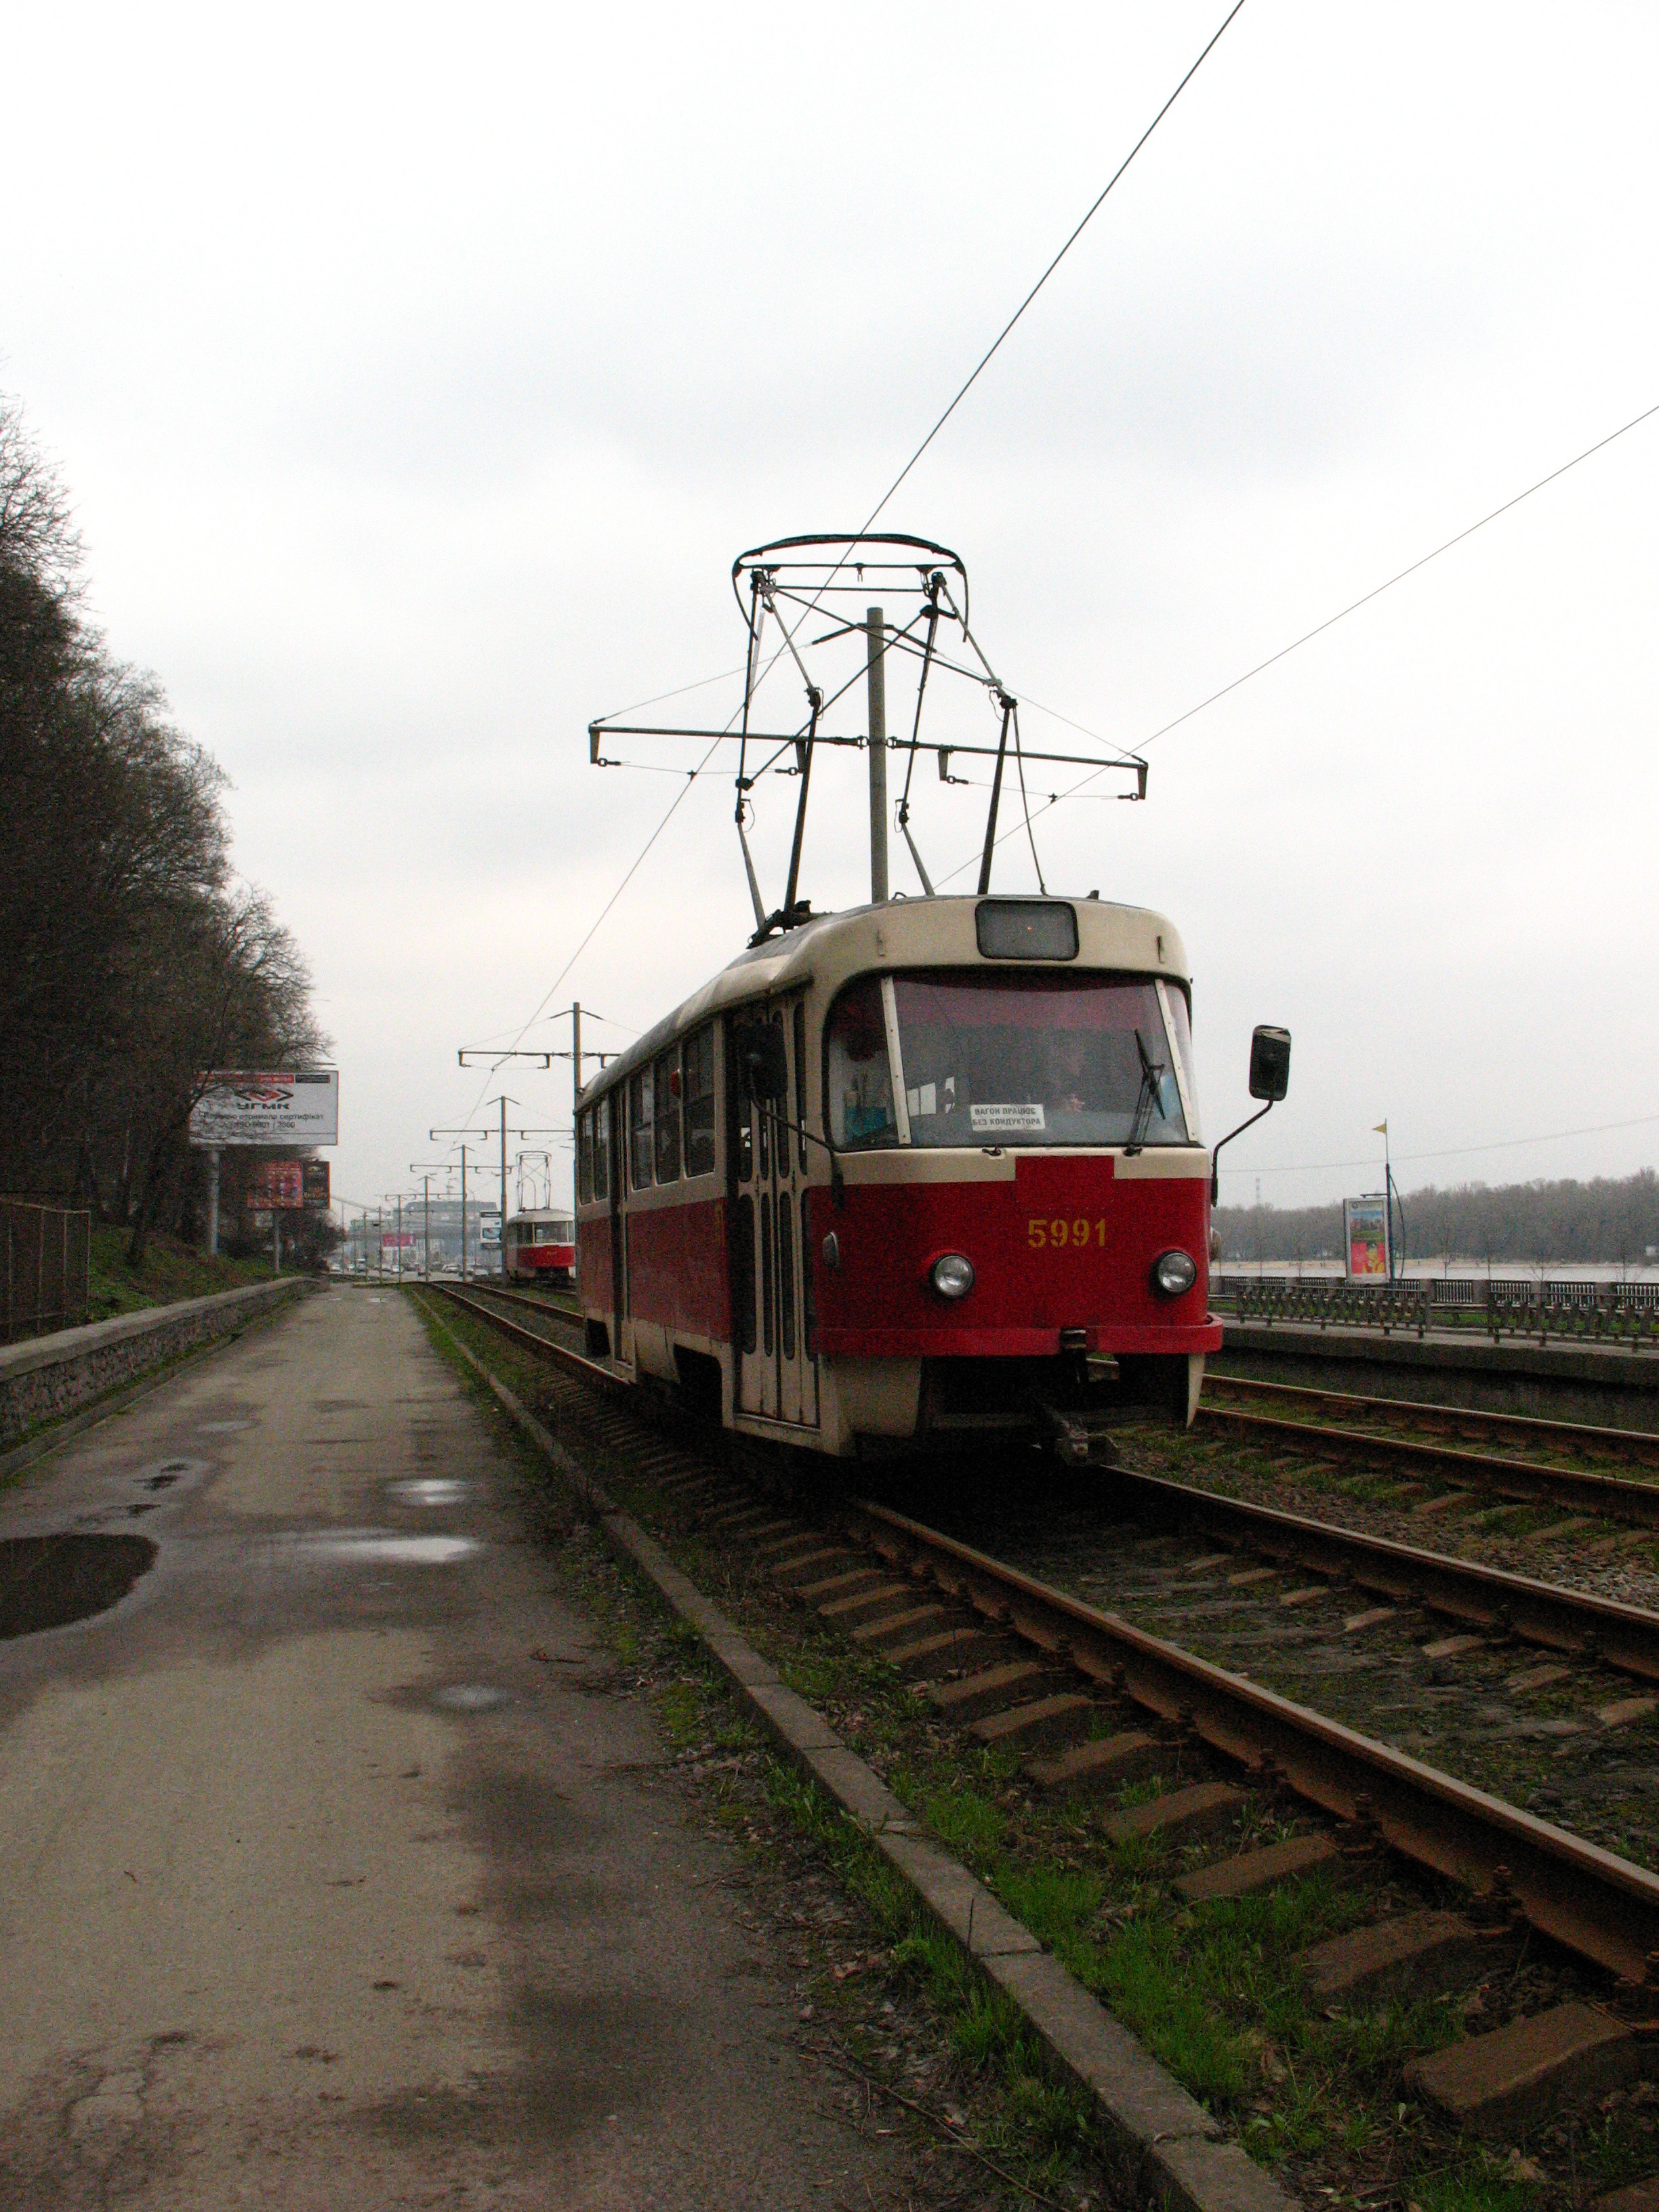
\includegraphics[width=0.70\linewidth]{chast-colebanie-osnov/nachalo/tramvay-no-5.jpg}

\textit{2008 год, на пятом маршруте трамвай «Татра» модели T3 или T4SU.} 
\end{center}

Кто не в курсе – трамвай ходил и по мосту Патона. Маршрут номер 27\index{Трамвай №27} длился от бульвара Перова до Дворца спорта, это 17,4 километра, что проезжалось чуть больше чем за час. А 35-й\index{Трамвай №35} маршрут начинался на Березняках, был разворот там где сейчас высотки возле Русановского канала, ближе к железной дороге – и заканчивался у Центрального вокзала на правом берегу. Под горой со статуей Родины-матери, около моста Патона, был большой пересадочный узел. Одна ветка шла по набережной Днепра, другая по мосту, и дальше тянулась мимо холма с музеем ВОВ и по улице Старонаводницкой, Клову и дальше в центр.

Сидишь себе да глядишь в окошко, а колеса гремят по рельсам. Печка греется. В тех старых трамваях хорошо думалось. Нынче не то, и огурцы уже не те, и пупырышки на них фуфло против давнишних.

%Но что делает капитализм с удобными и длинными маршрутами трамвая? Он их отменяет и разбивает путь на мелкие отрезки, чтобы вы делали больше пересадок. Готовь деньги! Кроме того, упраздняется сам трамвай и людям предлагается ездить в маршрутных такси. В свою очередь длинные маршруты и этих передвижных иконостасов отменяют в пользу коротких – теперь уже коммунального транспорта. Та же хитрость на новый лад.


\begin{center}
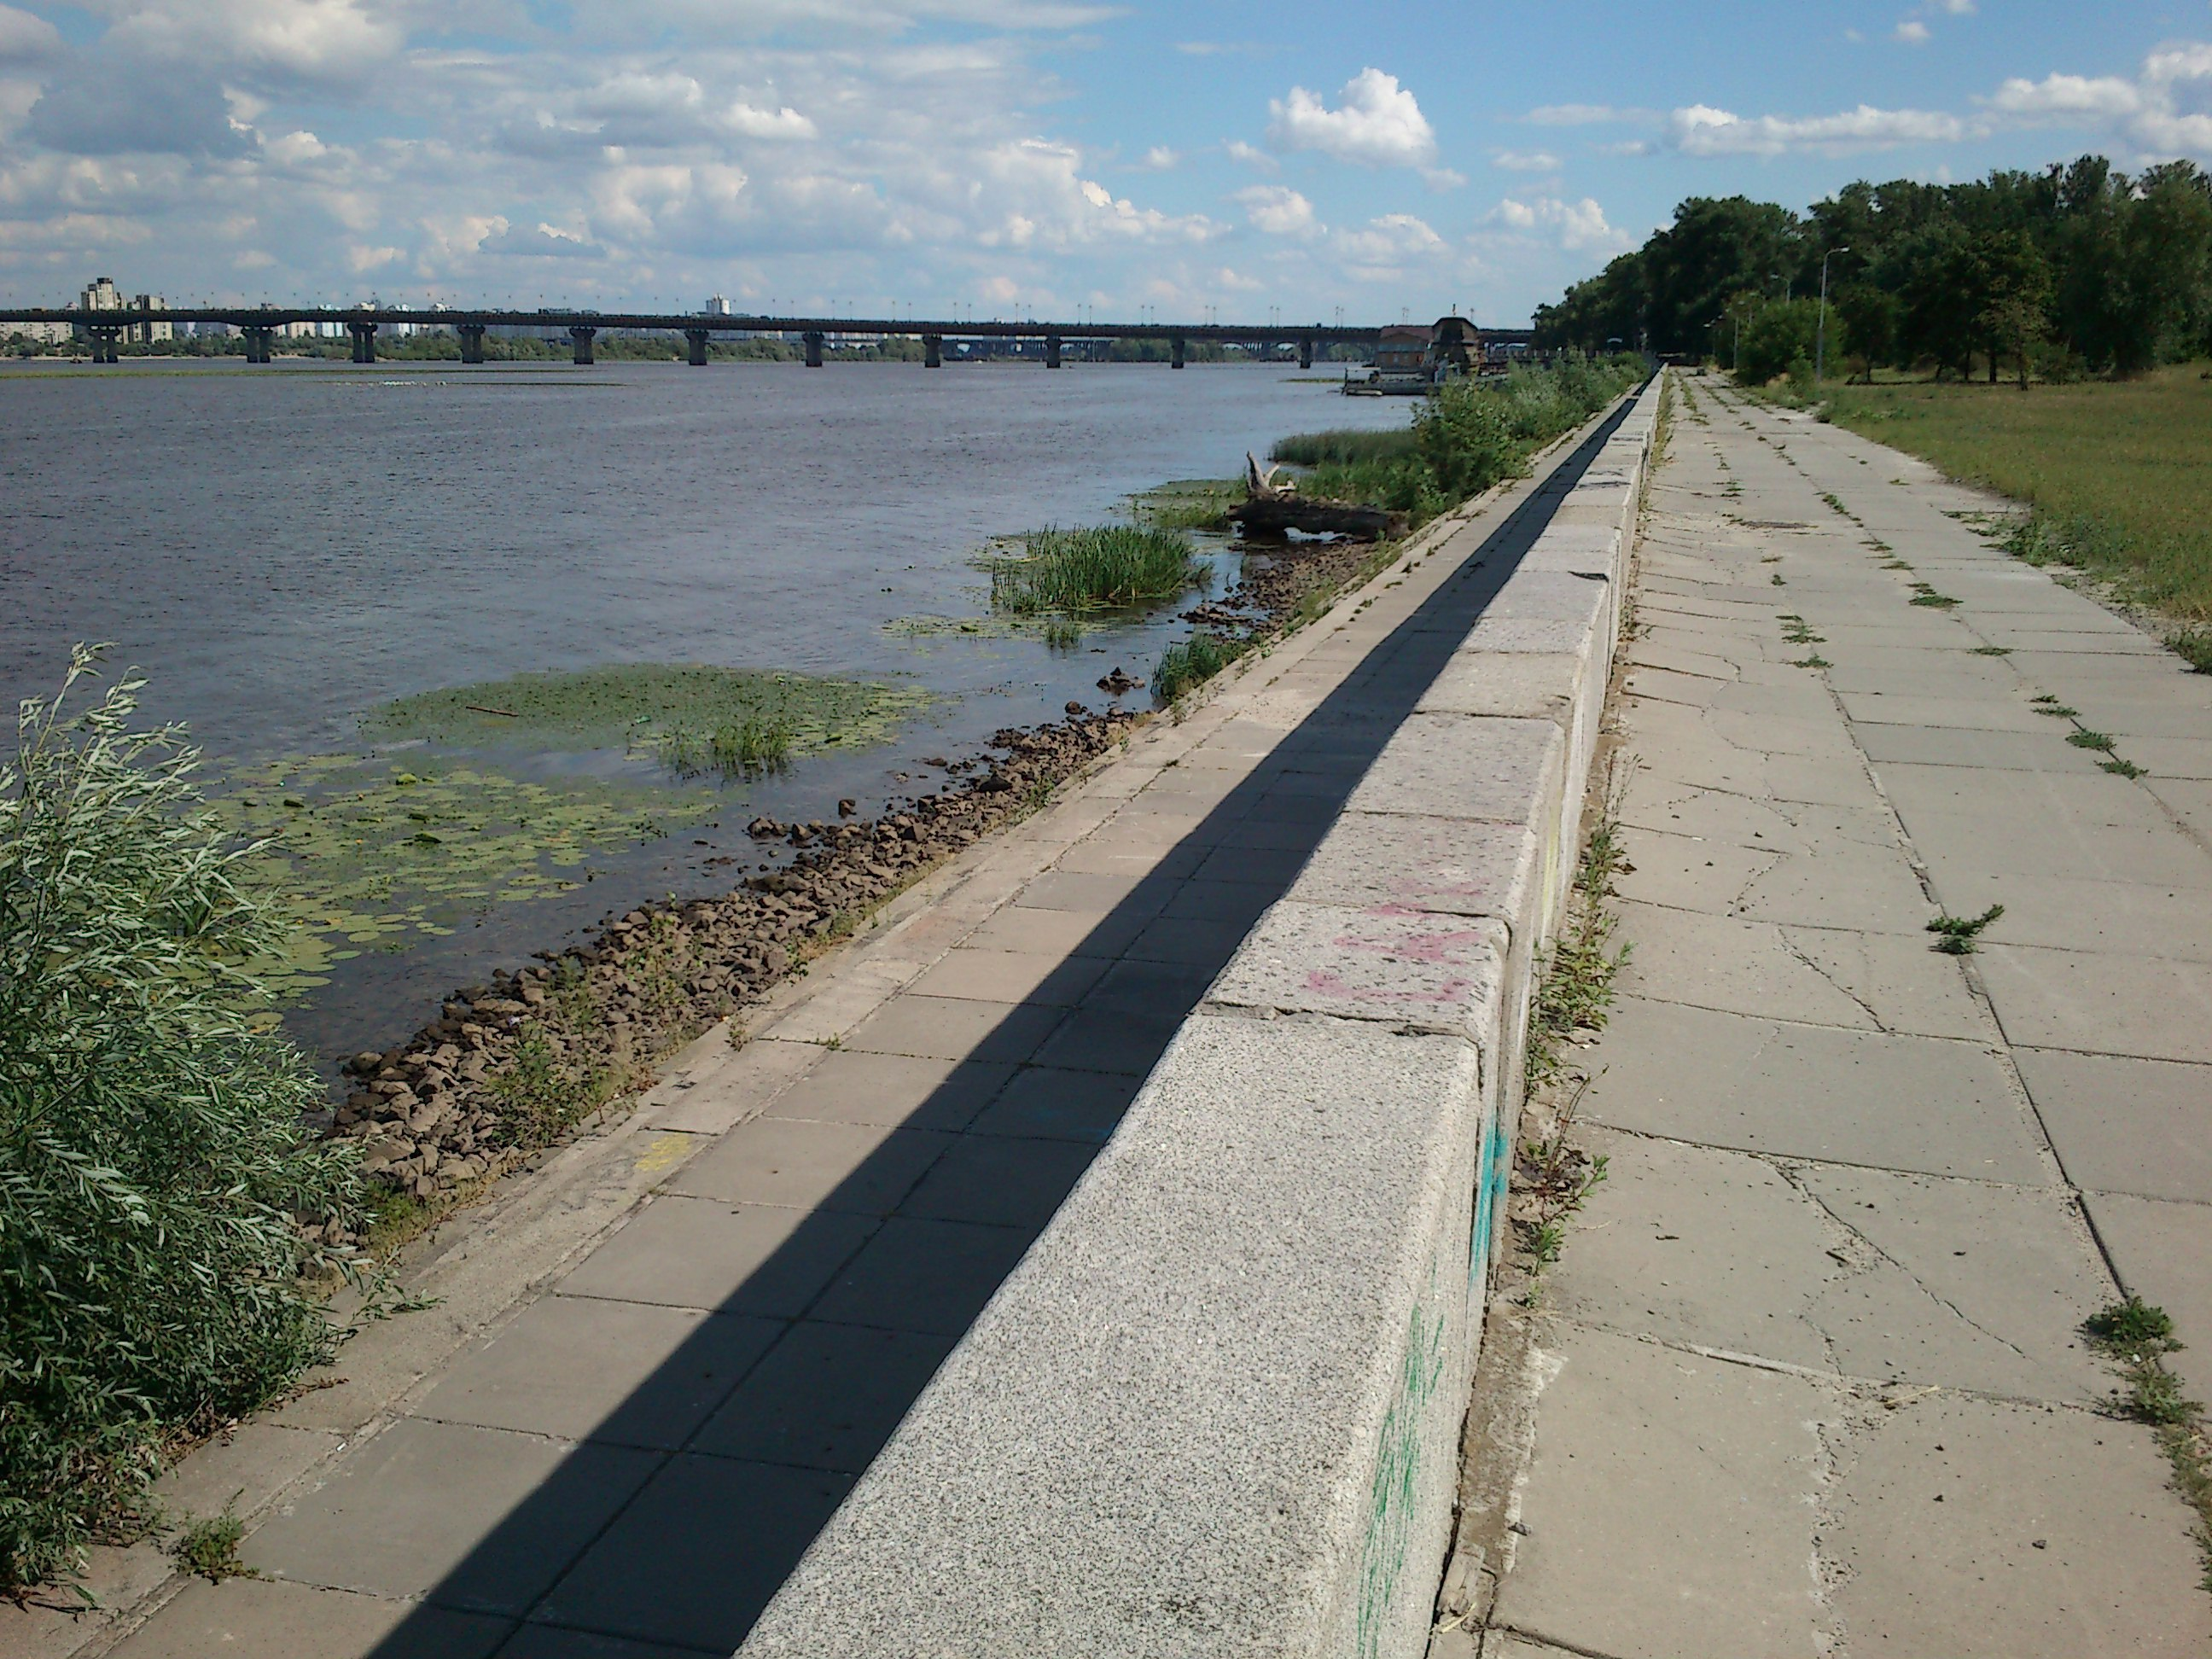
\includegraphics[width=\linewidth]{chast-colebanie-osnov/nachalo/primakova-01.jpg}

\textit{Парк Примакова, лето 2012 года.} 
\end{center}

В первом десятилетии нашего века, парк Примакова переименовали в Наводницкий и отчекрыжили от него кусок под аллею Славы миротворцев ООН. Некогда тихий парк вдоль реки, с высокими тополями и яркими цветочными клумбами, ныне застроен культовыми сооружениями, а у берегов стоят плавучие рестораны. И едут, едут машины по аллеям.

В девяностых я часто гулял там с Бобиком, моей собакой. Мы спускались туда с холмов Зверинца, от Бастионной улицы\index{Бастионная улица}.

Вот так выходишь утром из дому, а во дворе ни души, а тишина, и тепло – потому что весна и май начался. Проходишь через Собачку\index{Собачка} – крутой, продавленный глубокими ярами склон горы, весь поросший одичалыми садами. Вишня в белом цвету. Налево от Собачки, к Бастионному переулку – обрыв с бетонной подпорной стеной, за нею топорщится из ямы белопанельный Дом художников.

Там обитали художники, а их мастерские глядели широкими окнами в самое небо на высотах последних этажей. Кроме прочих жил в доме том странный человек. Он бросал с балкона вещественные плоды раздумий в пакетах из плотной бумаги, перевязанных шпагатом, эдакие бандерольки случайным прохожим.

Так уродство соседствовало с прекрасным – с сосредоточенными творцами, цветущими деревьями, и той сладковатой душистой смолой, которая сочится из узловищ в стволах вишен. Всё время забываю, как эта смола называется, а это вдруг вспомнил – камедь.

На Собачке есть две главные тропинки. Верхняя вдоль забора ботсада (мы его называли «ботаника» или «боташа»), а нижняя примыкает к опорной стене. Еще две сохранившиеся служат для подъема, в начале и конце Собачки. По ним, особенно той, что близ родного двора, я любил кататься на санках.

Нижняя тропа сейчас совсем запущена – ее перегораживает бурелом, а когда-то там свободно гоняли на велике. Посередке тропы был пятачок, широкое место, и оттуда лесенка наверх, к спортплощадке. Лесенка из деревянных, вбитых в землю дощечек. Ее делал художник Михаил Фомич, фамилию не помню. Он жил прямо напротив этого пятачка. На 2024 год и след той лестнички простыл...

Словом, по нижней тропке, кажется, никто больше не ходит, это трудно. Полагаю запустение оттого, что улица Мичурина, к которой, по сути, добирались по нижней тропе жители верховий Бастионной улицы, претерпела смену населения – давний частный сектор застроили теремами новые здесь люди.

А вот верхняя тропа осталась, утоптанная, по ней и к ней ходят в поисках дырок в ботсадовском заборе.

\begin{center}
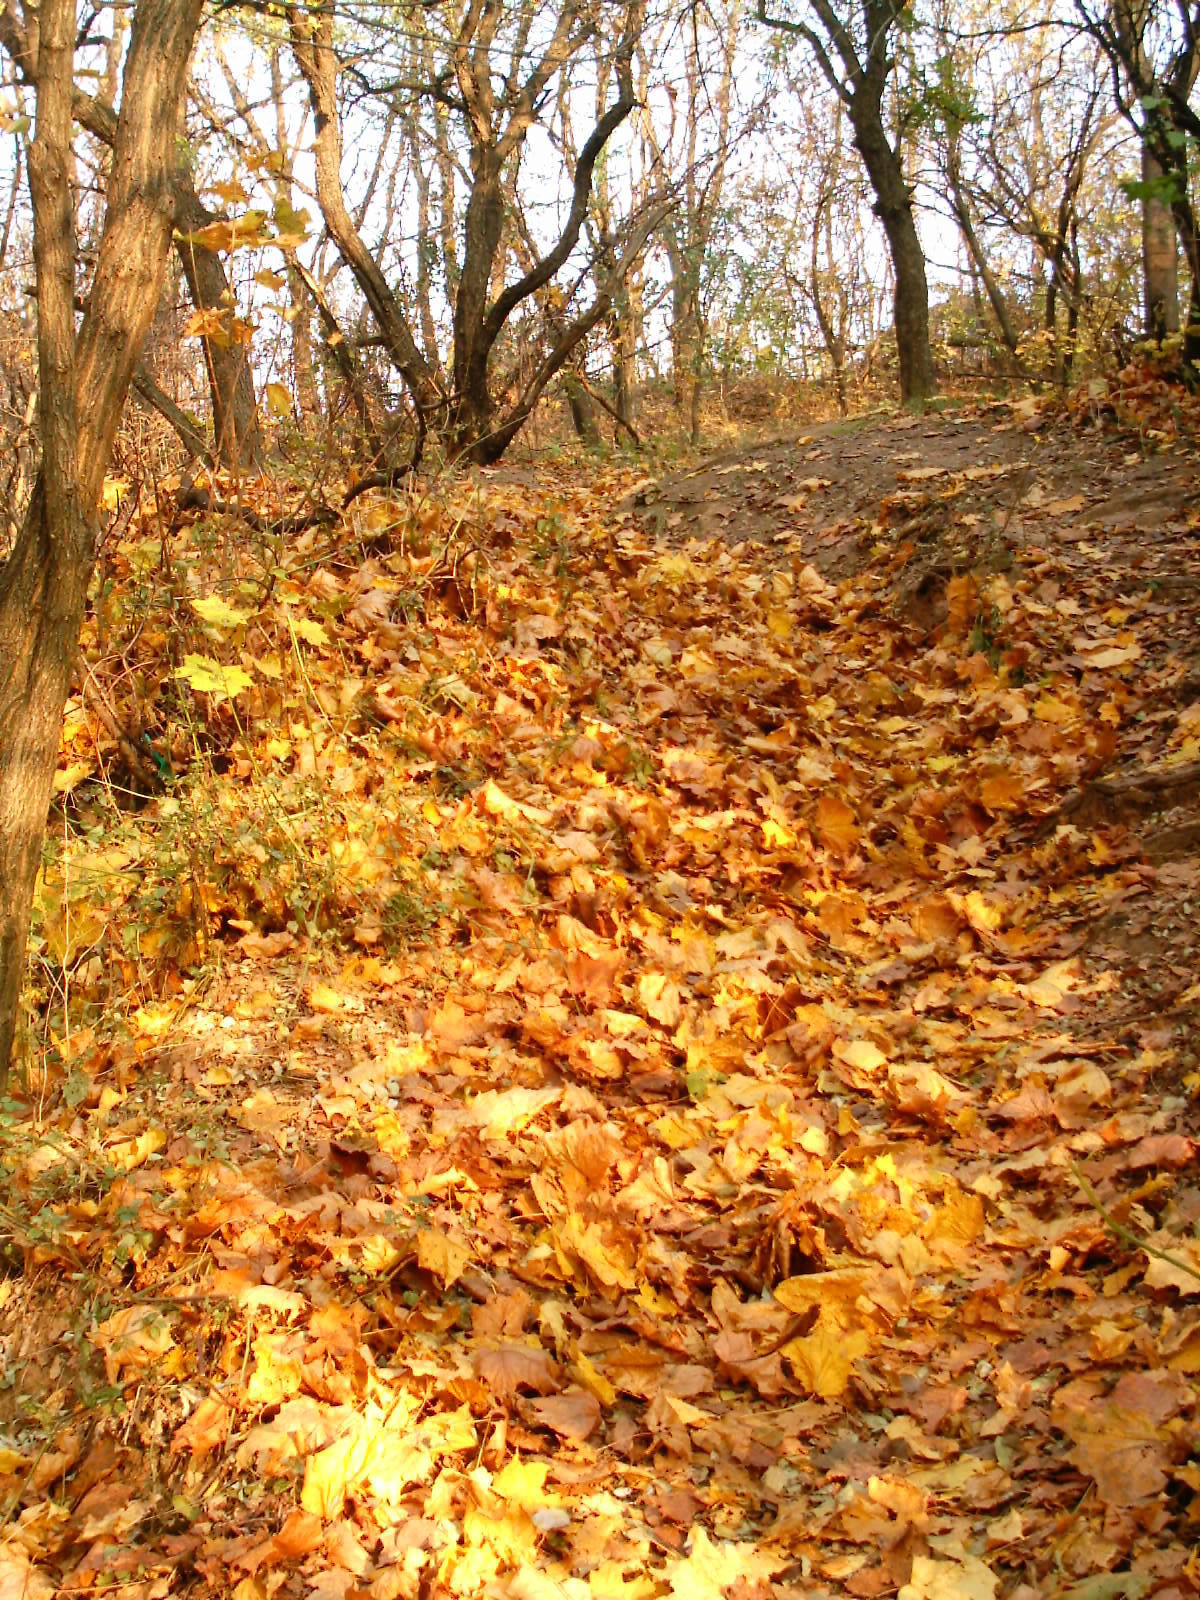
\includegraphics[width=0.85\linewidth]{chast-colebanie-osnov/nachalo/sob-imag0038.jpg}

\textit{Собачка, путь наверх, 26/10/2005.} 
\end{center}

А тогда! Зимой, вечером уже, когда тишина стоит и небо светлое от снежных туч, а фиолетовый снег искрится золотом, летят санки вниз накатанным по тропе желобом, повторяя все изгибы обрыва, и не надо рулить и тормозить, только в конце ежели не успеваешь повернуть левее, продолжая ход в желобе, то выбрасывает тебя в приземистые вишни, почти кусты, и санки в них застревают, а ты проваливаешься через ветки дальше. На верхней, посадочной площадке, у забора ботсада, растут орехи. Потом проезжаешь под грушами. И наконец – вишни!

А вот летом идешь по нижней тропинке, а из кустов высовывается сумасшедший с отверткой-заточкой. И потом исчезает, собаку увидав. А то еще находишь там же здоровенный разводной ключ, который по сей день исправно служит.

На Собачке было ровное место со спортивной площадкой с оградой из сетки. Туда, по террасам среди диких вишень, поднималась лестничка Михаила Фомича, переходившая в грунтовую дорожку. На площадке стояли даже тяжелые металлические футбольные ворота, а на возвышении в рост человека, таилась под сиренью скамейка. Местные играли тут в футбол, выгуливали собак, а на лавке заседали любители поиграть на гитаре.

Еще в конце девяностых, со спортплощадки украли ворота. Сначала одни, потом вторые. Затем, по мере удаления от социализма, исчезали покрывшиеся ржавчиной части ограды, глинистая полянка зарастала травой, ползла вниз зелень с пригорка, уже не сирень, а нечто совсем дикое.

Северная сторона Собачки выходит ко глубокому яру. На противоположном его берегу – остатки погребов. В начале 21 века в них жили беспризорные дети. Затем погреба пришли в совсем удручающее состояние, а яр усеялся мусором. Выше погребов начинается частный сектор на улице Мичурина.

От Собачки мы с Бобиком, пройдя мимо нескольких «гостинок» и сойдя по лестничке у некогда единственной в районе шестнадцатиэтажки, сворачивали на эту улицу. Она тогда была очень мирная, с гнилыми, косой гармошкой, деревянными заборами, за них лезла лапами наружу сирень. В гуще садов прятались домики. Летом на ходу вишню в рот отправил, водную колонку близ обочины покачал, горстью выпил студеной воды – и дальше. Редкий прохожий встретится.

Нынче там – современные терема и бетон, и должен вжиматься пеший человек в новокрепостную стену, чтобы не быть смазанным в месиво не то машиной, не то танком, принявшим облик автомобильный. Раньше название улицы вполне оправдывалось её зеленью – и наверное, были в садах сорта, выведенные самим Мичуриным. А рядом с теремами садов нет. Поставят эти кусты-пудели и наймут садовника, чтоб их подстригал. Барскому глазу приятно смотреть.

\begin{center}
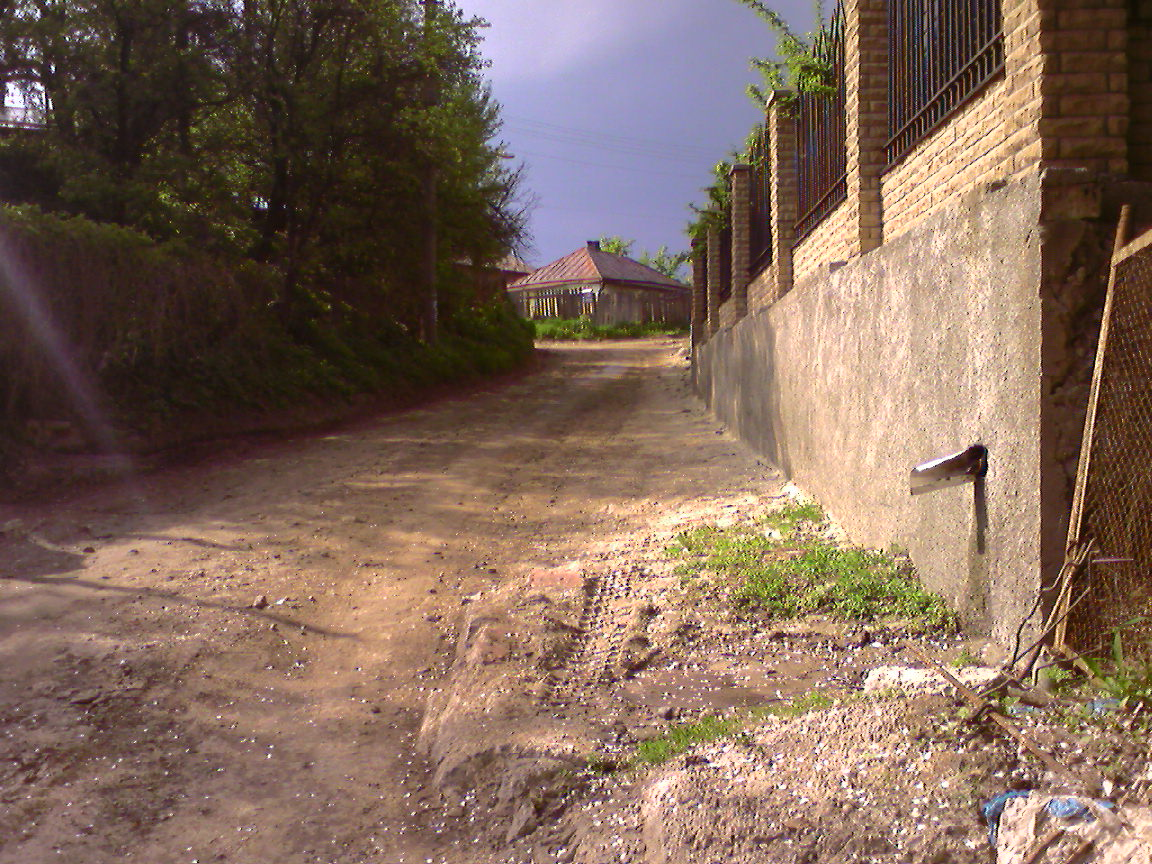
\includegraphics[width=\linewidth]{chast-colebanie-osnov/nachalo/lomakovskaya01.jpg}

\textit{2006 год, улица Мичурина, впереди – перекресток с Пирятинским переулком.} 
\end{center}

Улица Мичурина, бывшая Ломаковская, по крайней мере с 18 века
идет в устроявшихся пределах по всему склону северного Зверинецкого холма, посередке его ската, вбирая в себя узкие улочки и переулки, лестницы и лестнички. Одинокая скамейка ближе к перекрестку с Пирятинской улицей наводила на мысль о каком-то редком автобусике, что мог здесь курсировать в давние времена, как 76-й маршрут\index{Автобус №76} по Зверинецкой, хотя крутизну гор на Мичурина, кажется, не сможет преодолеть ни один автобус.

На моей памяти, не было там и магазина, а лишь частные усадьбы, водяные колонки, просмоленные деревянные столбы, синие почтовые ящики на множество дверок, да две таксофонные будки. Одна, почти в начале Мичурина, около лестнички под шестнадцатиэтажкой, прославилась тем, что в ней укрылась от разозлившегося козла какая-то бабка. Козел всё же проник внутрь и бабка сдерживала его, ухватив за рога. Другая будка стояла подле перекрестка с Пирятинской. 

\begin{center}
\includegraphics[width=\linewidth]{chast-colebanie-osnov/nachalo/\myimgprefix 13092009653.jpg}

\textit{2009 год, улица Пирятинская, впереди – перекресток с Мичурина.} 
\end{center}

Оттуда можно было свернуть на север, в сторону бульвара Дружбы Народов. Спускаешься в тени деревьев по громадной лестнице – теперь так нельзя, улица Пирятинская прерывается посольством, и лестница прикреплена уже к нему. Внизу же, правее, в сырой ложбине холма журчал вкусный родник\footnote{50°25'25.7"N 30°33'46.9"E}, слывший целебным. Возможно, в давние времена он назывался Рожницей. Сюда в восьмидесятых-девяностых издалека приезжали с бидонами люди. И там построили автозаправку. Существа из карбона и металла хотят пить горючее. Иди дальше, зверь из плоти. Купи себе воду в баночке.

Лестницей я возвращался, домой, а в парк Примакова двигался дальше по улице Мичурина, до самого ее конца, где очень крутой спуск. Однажды я съехал с него, полностью заледеневшего, на санках. Здесь застройка новоделами началась раньше всего.

\begin{center}
\includegraphics[width=0.80\linewidth]{chast-colebanie-osnov/nachalo/\myimgprefix IMG_20150601_133144.jpg}

\textit{2015. Спуск на Мичурина. Прежде, слева были сады за деревянными заборами, а справа – поле с подсолнухами.} 
\end{center}

И вечно до половины этого спуска доходили, темня треснутый асфальт и камни, ручьи – то ли родники, выбивающиеся из-под люков, то ли вода, накачанная из колонок.

Вообще этот отрезок улицы Мичурина держится за нею больше на бумаге, ибо там по прямой как бы продолжается улица Землянская. Она же прежде, взобравшись на гору, лежала и по другую сторону забора ботсада, через нынешний участок хвойных растений, отмежевывая его от сирингария. Там поныне есть аллея, но мало кто знает, что это бывшая улица.

Землянская улица вливалась в Выдубицкую, что еще начале сороковых годов двадцатого века пересекала всю местность будущего ботсада примерно от Бастионной улицы и до Выдубицкого монастыря. И перекресток Землянской и Выдубицкой был там, где сейчас перекресток у верха Сиреневой аллеи, с поворотом к хвойным, сирени, Ионовской церкви да назад к выходу из ботсада.

Старые домики на Мичурина держалась долго. Я ходил по улице из года в год – ничего не менялось.

Но вот одна из усадеб обезлюдела. Пустые висели меж яблонь качели. Стала врастать в землю калитка, за несколько лет одичал сад, хотя соседи еще пользовались его плодами. Сам домик вначале сохранял жилой вид, а потом просела над входом крыша, треснули, принялись осыпаться стены – через отвалившуюся штукатуру проглядывала дранка, косая решетка из досочек. 

Этот единственный на улице выбывший из строя дом оказался предвестником грядущей волны таких угасаний с последующим пришествием новых хозяев. А те выкорчевывали сады, срывали части склона для умещения огромных фундаментов строящихся жилищ.

Не люблю больше бывать на Мичурина. Пусть остается в моей памяти какой была. До соединения с Землянской, улица поворачивала и круто спускалась, там еще на пригорке справа стоял деревянный дом – номер сорок? Всё это срыто, даже сама улица теперь смещена.

Землянская и одноименный переулок напоминают о местности Землянке, прозванной так по близости к Зверинецким пещерам, либо от земляных укреплений Зверинецкой же крепости, что некогда покрывала многоугольником валов половину нынешнего ботсада и сгинула окончательно при его строительстве в 1940-х.

Пещеры на моей памяти сначала были закрыты для посещений. Не стояли рядом две церкви, всё выглядело иначе. Вход располагался в обычной частной усадьбе на Мичурина. В шестидесятые к нему приладили будку туалета, которую потом передвинули по просьбе археологов. А в конце девяностых в пещеры начали водить паломников, сверху горы, через проем в стальном, из ребристых прутьев, заборе ботсада.

Там рядом с плантацией кормовых культур был плоский участок, куда свозили торф – как понимаю, место дореволюционной церкви над пещерами – и вот за торфом пропилили в ограде большую дырку, может даже с калиткой, не помню. Потом уже подключился близлежащий Ионинский Святотроицкий монастырь и в нулевых на месте нескольких частных усадеб возвели Архангело-Михайловский Зверинецкий монастырь. Сами же пещеры утратили свой исконный вид еще в начале 20 века, будучи приспособленными для паломников. Сейчас это еще более облагороженное подземелье.

Назову основополагающие работы про эти пещеры, тоже начала 20 века.

Полная чудес брошюра иеромонаха Серапиона «Новооткрывающиеся древние пещеры в Киеве, на Зверинце», вышедшая в Киеве в 1914 году. 

Банковский служащий и одновременно опытный археолог Александр Дмитриевич Эртель\footnote{Много изучал киевские курганы, пещеры, валы и городища, в том числе пещеры в Китаево, курганы в Совках, могильник около Проневщины. К слову, брат Эртеля, Леонид, с 1914 года проживал на Ломаковской (или по Ломаковскому переулку), 37-А.}, крайне правый монархист, написал в 1913 году брошюру «Древние пещеры на Зверинце в Киеве».

Киевский историк Иван Каманин\footnote{Каманин оглох после болезни, что повлияло на выбор рода деятельности – работу в Киевском центральном архиве древних актов. Много печатался в дореволюционных околоисторических изданиях под своей фамилией и псевдонимом А. Щуровский. Каманина, согласно завещанию, в 1921 году похоронили в тех же Зверинецких пещерах – одна из стен его склепа, кирпичная, граничит с концом «Алтарной улицы».} год спустя выпустил более объемный труд «Зверинецкие пещеры в Киеве»\cite{kamanin01}.

И в 1918 году профессор Киевской Духовной Академии Николай Петров подытожил работы Эртеля и Каманина, добавив кое-какие источники, книжечкой «Ученые труды по исследованию ново-открытых в Киеве Зверинецких пещер».

%Везде, где рассуждений больше, чем описания, возможно искажение сути, возникающее в мыслях сочинителя. Логические ошибки, невнимательность, наконец личное мнение, окрашивающее любые рассуждения и зачастую отсекающее ряд доводов – всё это вносит путаницу, а путаница, в отличие от кругов по воде от камешка, не угасает, но увеличивается – чем дальше от источника, тем она сильнее. Но хуже всего, когда пытаются исправить первоисточники, полагая в них ошибку – это приводит к ошибке еще большей.
 
Многократное открытие древних Зверинецких пещер в конце 19 и начале 20 веков – дело весьма запутанное, обросшее искажениями и домыслами, возможно порой намеренными, а иногда случайными, по недостатку сведений – ведь кроме упомянутых мною источников, притом довольно редких, данные о пещерах, по большому счету, отрывочны и порой не заслуживают доверия.

%Кратко сведу воедино самое важное. Не буду принимать по внимание голословные сведения из статей, вроде того, что в пещерах были найдены какие-то кожаные и деревянные маски – я не знаю, откуда это взяли. Можно еще услышать версию, что в пещерах обитали монахи Выдубицкого монастыря еще до его наземного устроения. На это нет никаких указаний. 

Кратко сведу воедино самое важное, чтобы дать представление о том, какими были Зверинецкие пещеры на стыке 19-20 веков, а не какими их теперь показывают.

Летописи и другие давние письменные источники про эти пещеры загадочно молчат. Вообще. Тут несколько вариантов. Например, пещеры относилсь к дохристианским временам и при летописцах и сочинителях житий были уже засыпаны, неизвестны, не обжиты позднейшими монахами. Или – летописцы знали о пещерах, но молчали о них, считая нехристианскими или не совсем христианскими. В том и другом случае христианская атрибутика могла попасть туда позже, с умыслом доказательства религиозной принадлежности пещер. Наконец возможно, о пещерах, пусть даже там был монастырь, не упоминали из-за их незначительности. Но последнее кажется мне натянутым, ведь летописи пестрят сообщениями о помощи того или иного князя в устроении церкви или монастыря. А про Зверинецкие пещеры – глухо.

В обозримом прошлом о них узнали, по большому счету, только в 19 веке. По словам Каманина, весной 1882 или 1883 года в склоне горы, при обвале, открылся ход. Подробности всплыли уже в начале 20 века, когда о событии тридцатилетней давности поведала восьмидесятилетняя местная жительница, повитуха Феодосия Матвеенкова\footnote{Справочник «Весь Киев» за 1911 год снабдит нас её адресом: «Ломаковская, 10. Матвеенко Федосья Вас.». В 1913 году обвалилась земля и в усадьбе Юлиании Хмелько по адресу Ломаковская, 12 – там был проход в подземелье, раскапываемое археологом Эртелем.}. Каманин пересказывает старожилку, пользуясь книжечкой 1914 года иеромонаха Серапиона «Новооткрывающиеся древния пещеры в Киеве, на Зверинце»:

\begin{quotation}
на рассвете одного дня, ровно 32 года назад\footnote{Т.е. в 1879-м.}, слышала гул провала земли и видела светлую радугу, которая упала на месте провала. В полдень того же дня сосед Матвеенковой, живописец Дмитрий Зайченко\footnote{Усадьба на имя «Зайченко Мар. Владимир» на 1911 год обозначена по адресу Ломаковская, 9.}, с своим товарищем, возвращаясь из Свято-Троицкого монастыря, заметил провал. Они разрыли отверстие провала, и Зайченко спустился в образовавшуюся яму, где пробыл около 15 минут; при свете восковой свечи он обнаружил длинную пещеру, в которой, по его словам, было много человеческих голов, костей, неистлевших остатков монашеских поясов, четок, обуви и т.п.
\end{quotation}

У Серапиона про радугу более подробно:

\begin{quotation}
Явление радуги во сне

В 1878 или 9-м году весною, будучи восприемницею младенца в доме №6 по Ломаковской улице у Ксении Лобановой, Феодосия, после приема мальчика, на рассвете легла отдохнуть в комнате на кушетке против северного окна. В легкой дремоте ей представилось, что с северо-запада идет очень низко над домами большая и широкая радуга и страшно гудит: гугу, гугу!... И прошла по направлению к ея дому и, спустившись, пала за забором ея усадьбы на склоне горы, где впервые потом обнаружились пещеры.

С этого ужаса она пробудилась и стала собираться домой, чтобы удостовериться, не случилось ли пожара, или другого несчастья в ее доме, или усадьбе. Но Лобанова уговорила ее остаться у ней до полного рассвета и не тревожиться зря сновидениями. Когда же развиднелось, она пошла и осмотрела дом и усадьбу и нашла всё благополучным.
\end{quotation}

Некоторое время спустя после обнаружения пещер, Матвеенкова видела еще такой сон – в ее усадьбе, около входа в пещеру, под большим орехом стояло человек пятнадцать монахов, в белой одежде, с непокрытыми головами и распущенными, стало быть длинными, волосами. Это противоречит внешности монахов вообще – те одеваются в черное и носят головные уборы. Но, пусть будут монахи. Они стояли, стонали и просили: «Покормите нас».

Матвеенкова хотела заказать в своем саду панихиду, говорила об этом с приходским священником Иоанном Вышатой и знакомой своей, Сиклитией Николаевской. Что-то такое было в разговорах и вообще людской молве вокруг, и Матвеенкова отступилась от мыслей от панихиде. Создается впечатление, что тогда, в то время, обнаруженные останки, да и пещеры тоже, не считались христианскими.

Спустя много лет, в 1902, Матвеенкову снова посетило видение – опять же, на грани сна и яви она увидела женщину с дитятей на правой руке, склонившим голову ей на плечо, и подумала, что это женщина из пещер. Серапион пишет: «видела покойницу ясно в лицо – волосы у нее не то седые, не то цвелые и прилипшие к телу, и вид ее тощий, худой и мертвый, будто бы только что из гроба вставши». Гостья напомнила, что Матвеенкова обещала покормить их, но не исполнила обещанное. Матвеенкова пошла в чулан за молоком, оглянулась, но «покойница» исчезла. А Матвеенкова таки заказала в Троицком монастыре панихиду.

Далее в книге мы еще коснемся странных видений на грани сна, бывающих у повитух всех народов, пока же вернемся к событиям на Зверинце. Да – конечно сказанное далее уместнее будет разместить в главе, где речь пойдет о Святотроицком монастыре более подробно, но поскольку речь зашла об аномальщине, то... К тому же Зверинецкие пещеры по многим прикидкам тянулись и к этому монастырю.

Расположен он от пещер всего в шестиста с гаком метрах на юго-восток, в ботсаду. Ионинский Святотроиций монастырь, известный также как Ионинская церковь. Иона, основатель оного в 19 веке, поведал в воспоминаниях своих о месте, где позже возник монастырь:

\begin{quotation}
Строения здесь никакого не было, одна земля и заросли. Отец Иларион сделал себе куренёк из хвороста, нарванного здесь же, из дикого бурьяна сделал крышу и жил  в нем целое лето, а потом Бог благословил, и появилась маленькая келлейка на чистом, не заросшем месте. 

Купив барочного леса, я поставил из толстых бревен столбы в углах, а стены из досок длиною и шириною 7 аршин, она и теперь стоит\footnote{Была позже разобрана.}. 

В этой келлии мы жили двое. Я вышел из Греческого монастыря и до поступления в Выдубецкий жил в этой келлии с о. Иларионом.

Здесь был сад, в котором росли разные фруктовые деревья: груши, яблоки, сливы, вишни, орехи. Место это было отгорожено от Выдубецкого монастыря забором и по уличке внизу шириною 7 сажень.

Когда о. Иларион здесь жил один, он видел выходящее из земли пламя, охватившее всю местность, где ныне стоит малая церковь. Видел огненный столп огромный, доходящий до небес, столп виден был даже на горе, где ныне собор.

Много ему было страхов от диавола. Диавол гнал его отсюда. К нему приходили неоднократно  воры и грозили убить его, но Бог его во всем хранил и укреплял. Диавол поносил его и говорил, зачем он здесь живет, лучше жить в монастыре, чем здесь. Диавол рыдал всю осень, зиму и весну, ходя по переулку и кляня о. Илариона, Николая и Романа, которые жили втроем, приговаривал: «Проклятые черноголовые, длинноволосые калугеры зудят мне, гонят меня и покою мне не дают, из наследия моего древнего и давнего гонят меня». Все это слышали братия и терпели.
\end{quotation}

Малая церковь – это старая, почти кубическая, двухэтажная колокольня\footnote{50°24'57.9"N 30°33'47.2"E}. Она стоит почти на краю холма позади своей копии, новой колокольни. От старинной, вниз на другой уступ холма ведет бетонная лестница, упираясь в тыл полуразрушенного на 2020 год, добротного дома в три этажа.

\begin{center}
\includegraphics[width=\linewidth]{chast-colebanie-osnov/nachalo/\myimgprefix IMG_20200202_133135.jpg}
\end{center}

До революции он принадлежал монастырю, а в советское время там была школа, а затем один из научных корпусов ботсада, со столовой на первом этаже. Если встать лицом к переду дома, то справа будет виден округлый проем в холме\footnote{50.416287836193135, 30.56328794279714}. А от лестницы, как спуститься, он будет слева.

Это вход в некое монастырское подземелье вроде погреба. Обложен кирпичом, внутри просторно, от основного серединного помещения отделяются дополнительные по бокам. На 2020 год там лежит разный бесхозный хлам. А вот около самого входа любопытное. Под аркой, в левой стене зияет проем высотой чуть поболе человеческого роста. Он ведет в пещеру с низким потолком, где идти надо сильно пригнувшись.

Вырыта она в плотном суглинке. Близ входа, справа, есть ниша, где может поместиться человек. Длина пещеры метров шесть. Поначалу – а от входа высота сразу уменьшается – в ней можно стоять согнувшись. Затем высота потолка резко понижается на треть. И после понижения приходится идти на корточках. В месте понижения получается как бы обод арки, и на нем ровно отпечатан крест без диагональной перекладины. Других надписей или рисунков я не заметил. Далее по ходу еще одна такая арка, но без креста.

Стены и потолок пещеры очень гладкие, кроме самого начала, где, как видно, старый ход грубо расчищали лопатами. Поверхность стен вообще не несет на себе следов работы, ее будто отшлифовали. Потолок закруглен.

Не знаю, когда возникла эта пещера, кто ее стал раскапывать (вероятно долгое время вход был засыпан и закрыт кирпичами арки погреба), когда и как в суглинке сделали крест – создатели пещеры или ее последующие обитатели. Для жизни там человека она крайне неудобна из-за низких потолков и узости своей. Возможно, ход продолжается далее, но засыпан – в конце пещеры снова грубая обработка стен, слишком отличная от общей изящной и продуманной.

Не об этой ли пещере писал археолог Александр Эртель в статье 1920 года «Новые данные по истории Выдубицкого монастыря» следующее:

\begin{quotation}
Затем в усадьбе Троицкого монастыря вблизи церкви мы с И. Я. Стеллецким нашли весьма подозрительный ход, часть коего обращена монахами в погреб для хранения овощей.
\end{quotation}

\vspace*{\fill}
\begin{center}
\includegraphics[width=\linewidth]{chast-colebanie-osnov/nachalo/\myimgprefix IMG_20200202_132529.jpg}
\textit{Внутри пещеры, 2020 год.}
\end{center}
\vspace*{\fill}

\newpage
\vspace*{\fill}
\begin{center}
\includegraphics[width=\linewidth]{chast-colebanie-osnov/nachalo/\myimgprefix IMG_20200202_132538.jpg}
\textit{Внутри пещеры, 2020 год. Вид на ту же арку, но ближе.}
\end{center}
\vspace*{\fill}
\newpage

Так вот Илларион наблюдал аномальщину как раз на горе точно над пещерой, что рядом с описанным мною домом. Откуда наблюдал? Очевидно, не около места часовни, не с места наблюдаемого явления. А назвать то место горой можно только с двух точек – будучи около упомянутой пещерки либо с другой стороны, где сейчас сад магнолий.

Вернемся теперь в 1880-е годы и снова к Зверинецким пещерам. 

Матвеенкова была свидетельницей, как художник Зайченко исследовал пещеру – сначала он тыкал в провал палкой, потом повитуха принесла ему длинный шест, но и тот не достал до дна, наконец провал разрыли больше, и художник полез вниз с огарком свечи. Шарил там минут пятнадцать, после чего выбрался и рассказал, что видел человеческие головы, кости, да, по словам Серапиона, недоистлевшие остатки монашеских поясов, обуви, четки.

%Без ссылки на источник иногда пишут, что художник нашел также кожаные и деревянные маски. Выдумка?

Кроме Зайченко, посетили пещеры и монахи Ионинского монастыря, которые, как пишет Каманин, «кое-что оттуда вынесли» – а что именно и в каком количестве, точно неизвестно. Сам архимандрит Иона взял, по крайней мере, два черепа. Над обнаруженными в пещере останками почему-то не провели заупокойный молебен, оставили лежать как есть.

Матвеенкова со своей знакомой тоже отправились в пещеру и вспоминала потом, что

\begin{quotation}
видела там около 50 истлевших гробов в отдельных пещерках в правой стене; в каждой пещерке лежало по двое покойников головами к ея устью;

Матвеенкова насчитала 99 черепов; доходила она и до какой-то двери, постучала рукой, но отзвука почти не было, потому что снизу дверь оказалась засыпанной почти до половины землей; глядя сверху, за дверью виднелась пустота.

Дверь деревянная, покрыта толстыми листами железа, которые прибиты железными же гвоздями головками в копейку. Высота пещеры – аршина в три\footnote{2,1 метра.}, а ширина чуть уже. От двери идут еще проходы в три стороны, самая же дверь стоит на летний восток.
\end{quotation}

\begin{center}
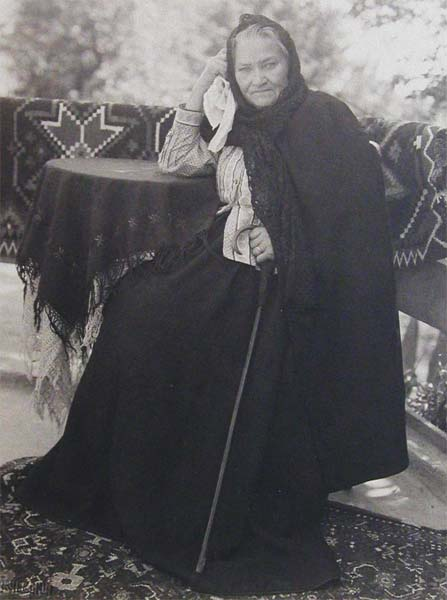
\includegraphics[width=0.98\linewidth]{chast-colebanie-osnov/nachalo/matvienko.jpg}

\textit{На снимке: Феодосия Матвеенкова.}
\end{center}

Между тем в подземелье повалили любопытствующие. Ребятня вытащила несколько черепов, катала по земли – кстати, когда в 1970-х строили крематорий на Байковом и разрушили часть погребений, тоже появились дети, игравшие черепами в футбол.

В пещеру на Ломаковской лазали все кому ни лень, а потом местным это надоело. Каманин пишет, что после заявления в комендатуру жителей усадеб, близких к пещерам, прислали рабочих с лопатами, и те засыпали вход.

По словам Матвеенковой, среди наплыва людей в пещеры был некий профессор Иванов со студентами. Каманин припоминает, что в 80-90 годах 19 века в газете «Киевлянин» проскользнула заметка о том, что неутомимый исследователь древностей и пещер профессор Владимир Бонифатьевич Антонович посетил Зверинецкие пещеры и обнаружил пояса и четки. И что обстоятельному изучению пещер профессором помешало Инженерное ведомство, ибо пещеры находились на территории Зверинецкой крепости. 

Думаю, память подвела Каманина. В 1895 году Антонович выпустил свою знаменитую «Археологическую карту Киевской губернии»\cite{antonovich01}, где по Зверинцу написано ровно следующее:

\begin{quotation}
Предместье Зверинец. Вблизи церкви в 1888 году открыта пещера, служившая вероятно монастырскою усыпальницей. Она представляла широкий коридор в 32 саженя\footnote{68,3 метров.} длиною; в стенах его сделано 48 нишей и в каждой лежало по 2 скелета, у них найдены 2 серебряные креста, несколько бронзовых, кресты плетеные из ремешков, скуфия и остатки обуви.

Киевское слово 1888 г. № 509. Коллекция Хойновского.
\end{quotation}

Как видим, Антонович использует в качестве источника статью из «Киевского слова». Никаких планов пещеры, как кое-кто пишет, в «Археологической карте» нет. Только эта коротенькая заметка.

%Думаю, дело было просто. Когда открыли пещеры, оттуда вытащили всё ценное, что успели – до того, как рабочие пришли и закопали вход. 

Указанные в ней предметы попали в коллекцию археолога Иосифа Адамовича Хойновского (сочинителя очерка «Раскопки великокняжеского двора древнего града Киева, произведенные весной 1892 года»).

В редакции «Киевлянина», где Каманин пытался разы\-скать нужный номер, никто про заметку о пещерах не помнил. А статья в самом деле была, в номере за 12 октября 1888 года – к сожалению, я не смог ее достать. Знаю кратко, что речь шла о провале в земле, возникшем при раскопке склона, где местные брали глину. И дескать открылись «громадные подземные пещеры, напоминающие лаврские».

Каманин много лет сотрудничал с Антоновичем в разных областях, например в создании историко-топографи\-ческих словарей. Но Антонович умер прежде, нежели Каманин начал работу над книгой про Зверинецкие пещеры. Иначе Каманин узнал бы сведения у самого профессора, не прибегая к поискам статьи.

Вы заметили, что Матвеенкова говорила о весне 1882-\-83 годов, а сведения Антоновича относятся к 1888-му?

Николай Петров тоже это заметил в своей брошюре, и нашел другие публикации про пещеры за 1888 год. Он решил, что старенькая Матвеенкова перепутала годы, да вот упустил – Матвеенкова говорила о весне, а вход в пещеры в 1888 году открылся осенью. Матвеенкова перепутала и год, и пору года? Или это два разных «открытия» пещер в северной части Зверинецкого холма?

Петров приводит заметку из «Киевского слова» за 15 октября 1888 года (№ 509) – на которую ссылался Антонович. Петров полагал, что корреспондентом «Слова» был художник Димитрий Зайченко, хотя, даже если не принимать во внимание разницу лет, описания посещения пещеры отличны. В 1882-м лезут двое, в 1888-м трое. Зайченко сам, в полдень, нашел провал, а в 1888-м – сочинителю заметки в 4 часа дня рассказывает о провале знакомый. Судите впрочем сами:

\begin{quotation}
В 4 часа пополудни, 13 октября, до меня дошло известие, что на Зверинце, недалеко от того места, где я живу, открыта новая пещера, и в ней покоятся кости мертвецов. Кем открыта эта пещера и при каких обстоятельствах, никто мне сообщить не мог.

Ко мне подошел живущий на Зверинце К-н и предложил мне идти с ним. Втроем, я, г. К-н и еще один незнакомый мне мужчина, решились спуститься в пещеру, конечно, зажегши предварительно свечи...

При свете свечей, по бокам этой пещеры, в стенах ея с двух сторон мы увидели полукруглые углубленные могилы, где лежали груды человеческих костей, и по два черепа в каждой могиле, причем в некоторых могилах отчетливо видны два человеческих скелета, положенных головой внутрь, а ногами к пещере, так что безошибочно можно заключить,что в каждой могиле находится по два человека.

Пещера оканчивается вертикальной стеной, и в ней находится такая же углубленная могила с двумя человеческими скелетами. Во всей пещере мы насчитали 48 могил, и считая в каждой могиле по два человека, всего будет похороненных 96 человек.

Вся пещера имеет длины приблизительно 96 аршин\footnote{68,28 метров.}. В пещере этой мы нашли два красных кирпича, шириной примерно 1,5 аршина\footnote{1,07 метра.} и толщиной 1 вершок\footnote{4,5 сантиметра.} (длина неизвестная, так как кирпич по длине сломан), уже довольно выветренных, так что рассыпаются, и формой совершенно не похожих на кирпич теперешних образцов, а также нашли кусочки ветхой кожи от обуви.

Больше ничего не оказалось; гробов и следа нет; но в толпе ходят слухи, что будто бы какие-то люди осматривали пещеру раньше и на костях видели уже истлевшее духовное облачение и нашли золотой крестик. 

Болтают также, что будто бы лет 80 тому назад здесь случился обвал и завалил покоющихся здесь. Но это совершенно неправильно.
\end{quotation}

Матвеенкова в 1882 году видела ниши только в правой стене, гробы (хотя бы истлевшие), обитую железом дверь, и трупы головами к выходу из камер. В 1888-м у корреспондента – ниши по обе стороны коридора, никаких гробов и двери, трупы ногами к выходу.

Кажется, в 1882-83 и 1888 году открывались входы в две разные части пещерного комплекса, возможно даже не соединенные между собой.

Петров пишет\footnote{Ссылаясь на «Киевское слово» от 8 ноября 1888, номер 242.}, что прочитав заметку в «Киевском слове», 16 октября 1888 года к пещерам отправились профессор университета Св. Владимира Адриан Викторович Прахов
\footnote{Руководитель росписи Владимирского собора и реставрации Кирилловской церкви.}, художник Т. А. Сведомский да исследователь древностей В. И. Гошкевич.

\begin{quotation}
Профессор Прахов остался на страже у входа в пещеры, а остальные двое отправились в самую пещеру, захватив с собой длинный шнур для сигнализации и для того, чтобы не заблудиться в лабиринте пещерных ходов.

По описанию г. Гошкевича, влево от найденной пещеры виднелась другая пещера, устье которой выходило в нескольких шагах от первого отверстия. Вся длина пещеры около 30 метров. 

К сожалению, за 4 дня со времени ея открытия успело перебывать множество «варваров», окончательно нарушивших первоначальное положение скелетов, так что теперь весьма трудно его определить.

Разрушительная работа велась, по-видимому, таким образом, что не только в самых пещерах все предметы разбросаны, но и содержимое ниш выгребено в пещерный коридор.

В самой пещере Сведомский и Гошкевич встретились с каким-то субъектом, предлагавшим им свои услуги по отысканию могильных предметов.

Но не успели исследователи осмотреть пещеру надлежащим образом, как получили от профессора Прахова предупредительную записочку об угрожаемой им опасности от обвала пещеры, так как над пещерами, в которых находились исследователи, собралась громадная толпа любопытствующих зрителей.

Исследователи благополучно выбрались из пещеры и уже когда двинулись в обратный путь домой, то встретили полицейского, спешившего к месту скопления толпы.
\end{quotation}

Сравним числа. Тут длина пещеры – около 30 метров. А в заметке от 15 октября 1888 года – как мы помним, около 68 метров. Разница слишком велика, чтобы быть ошибкой. В ту ли самую пещеру лазали Гошкевич со Сведомским?

Киевское Военное ведомство отправило в пещеру, посещенную последними, инженера Червинова 2-го. Гошкевич в начале ноября сообщал:

\begin{quotation}
Военным инженером Червиновым 2-м совершена на днях экскурсия в новооткрытую на Зверинце пещеру. Исследование затруднено теперь еще больше по причине происшедшаго в последние дни внутреннего обвала.

Червинову удалось начертить правильный план этого подземелья, с обозначением на нем всех погребальных ниш. Количество их определено им в 36. Так как в каждой нише находится по два скелета (в одной, впрочем, найдено нами 3 скелета), то число всех покойников, погребенных в этой усыпальнице, должно быть не менее 72. Кроме значительного количества лоскутков кожи, других предметов при скелетах г. Червиновым не найдено.

План пещеры, вместе с одним из лучше сохранившихся черепов, будет отправлен в С.-Пе\-тербургский Археологический Институт\footnote{Петров добавляет, что на деле отправили в Императорскую Археологическую Комиссию, а та в 1891 году переслала в Церковно-Археологическое общество при Киевской Духовной Академии, для музея, сандалию из Зверинецких пещер.}.
\end{quotation}

36 ниш против 48 из заметки за 15 октября. Спишем на обвал, или – таки другая пещера?

Затем Зверинецкие пещеры выпадают из поля зрения ученых и общественности до 1911 года,  когда снова провалилась земля и открылось два новых входа. Каманин пишет, что 30 лет эти пещеры «находились без охраны», Эртель говорит про 20 лет – однако если в 1911 году пещеры вновь «открылись», значит, старые входы были завалены (нет и точных сведений об их месте). О каких же 20 или 30 годах разорения пещер идет речь? Вход 1882-го, по сведениям Каманина, закопали власти. Судьба входа 1888 года теряется в истории.

%Тогда-то и началось масштабное изучение пещеры Эртелем при содействии князя Жевахова.

Каманин (совмещая, как я считаю, два обнаружения пещер 1882 и 1888 годов в одно событие) полагал, что Матвеенкова попадала в какую-то другую пещеру (или часть), не ту, где рыл Эртель и примкнувший к нему позже Вельмин. Так можно судить по описаниям, оставленным последним, и показаниям самой Матвеенковой, которая уже при Эртеле, когда ее повели под землю, не узнала пещеру. Найденные тридцать лет назад ею пещеры – «это не те пещеры, которые теперь раскопаны – это другие пещеры, до которых еще не докопались. Надо копать в правую сторону, более под мою усадьбу».

По Сети бродят сведения без источника, что георадиолокация показывает еще около километра неизвестных пещер. В одном из коридоров Зверинецких пещер – «Погребальной улице» – есть завал, где через десять метров прощупывается пустота – и вот что за этим завалом, пока неведомо. Вероятно это те самые исследования, которые производились Институтом прикладных проблем экологии, геофизики и геохимии в 2001 году, из коих мне известно следующее – в ботсаду и по Мичурина 10, 12 и 14\footnote{Мичурина 10 – это не Ломаковская 10, нумерация сильно сдвинулась. У меня нет уточняющих данных, но как я понимаю, участок ботсада с пустотами примыкает к упомянутым усадьбам. В ботсаду там растут огромные акации.} показали на площади 65x115 метров наличие там «аномальных зон», которые трактовали как подземные пустоты. Проверяли ли дальше на юг, номер 8 и местность Собачку, я не знаю. Но от жителей усадьбы номер восемь я слышал только историю о живущем на чердаке домовом, а про пещеры ничего не слышал, равно как не замечал их на Собачке, прожив рядом добрые двадцать лет.

Эртель во время раскопок 1912 года увидел, что от Зверинецких пещер в сторону Ионинского монастыря идет подземный ход, и предположил, что всё пространство между монастырем и Зверинецкими пещерами изрыто ходами, но там находился Зверинецкий форт, под который копать было невозможно\footnote{К слову, когда в ботсадовском Розарии (лежит в пределах бывшей крепости) вместо нынешнего центрального бассейна было озеро с земляными берегами и фонтанами (по плану ландшафтного архитектора Рубцова), вода просто уходила в какие-то подземные пустоты. Даже когда в 1970-х забетонировали дно и построили каменные бортики, вода продолжала уходить.}. Эртель также нашел провалы в несколько отдаленной от раскопок усадьбе зубного лекаря В. Шмигельского и подумал, что под ними тоже части пещерной сети. К слову, по северной и западной возвышенной части горы Эртель заметил древний вал и сопоставил его с упоминаемым в летописи Красным двором Всеволода Ярославича. Там где сейчас в ботсаду воссоздан «Красный двор» в самом деле кромка склона издревле несет следы земляных работ, а под тамошним обрывом я находил плинфу – древнерусский кирпич. Мыс с обрывом именуется «мыс Чайка». Название, по одной версии, от бывшей тут дачи профессора-уролога Андроника Архиповича Чайки, а по другой версии - от фамилии капитана красноармейcкой батареи, стоявшей здесь во время Великой Отечественной войны.

В 11 номере «Киевской мысли» за 1913 проскользнули упоминания о втором ярусе пещер (их же повторил в виде предположения Шероцкий в газете «Рада», №2 за 1913 год), над открытыми, и о провалах возле Ионинского монастыря\footnote{Около монастырской ограды археолог Стеллецкий позже нашел некий подземный лабиринт, и выразил мысль что всё это часть единой со Зверинецкими пещерами подземной системы ходов.}, и что один такой провал забирает всю весеннюю воду. В 29 номере «Киевлянина» за 1913 тоже есть про второй ярус пещер, причем если Шероцкий полагал что он находится над уже раскопанными ходами, в «Киевлянине» речь идет о нижележащем этаже:

\begin{quotation}
Недавно в галерее, соединявшей старый и новый выходы из пещер, приблизительно в средней ее части обнаружена небольшая лазейка, за которой замечена круглой формы небольшая комната. В ней имеются ясные признаки заваленного хода – спуска. Возможно, что это спуск во второй ярус пещер, о котором местное население давно говорит и куда некоторые местные старожилы уже проникали несколько лет тому назад и по их описанию эти пещеры имеют иной вид, нежели открытие пещеры. Там были сравнительно большие комнаты, находились части облачений, ручные кресты и другие предметы.

Рассказы о существовании второго нижнего ряда галерей и пещеры находят себе некоторое подтверждение в существовании провалов на поверхности всей площади, направление которых не совпадает с открытыми уже галереями, но почти тождественно с направлением пещер, о которых говорят местные жители. Между тем на этой площади, как мы слышали, предполагается постройка больших воинских казарм.
\end{quotation}

...Как известно, поныне раскопан только один ярус.

В 1911 году набожный князь Владимир Жевахов (будущий Иоасаф, архиепископ Могилевский) взял в аренду на 6 лет участок земли в 350 квадратных сажень (746,8 кв. метров) с новооткрытыми пещерами и организовал там раскопки. Позже Жевахов ходатайствовал о передаче этого участка и окрестностей духовному ведомству, но военное ведомство отказало, ибо собиралось строить там казармы для частей Киевского гарнизона, и посоветовало арендовать взамен соседнюю частную усадьбу.

\begin{center}
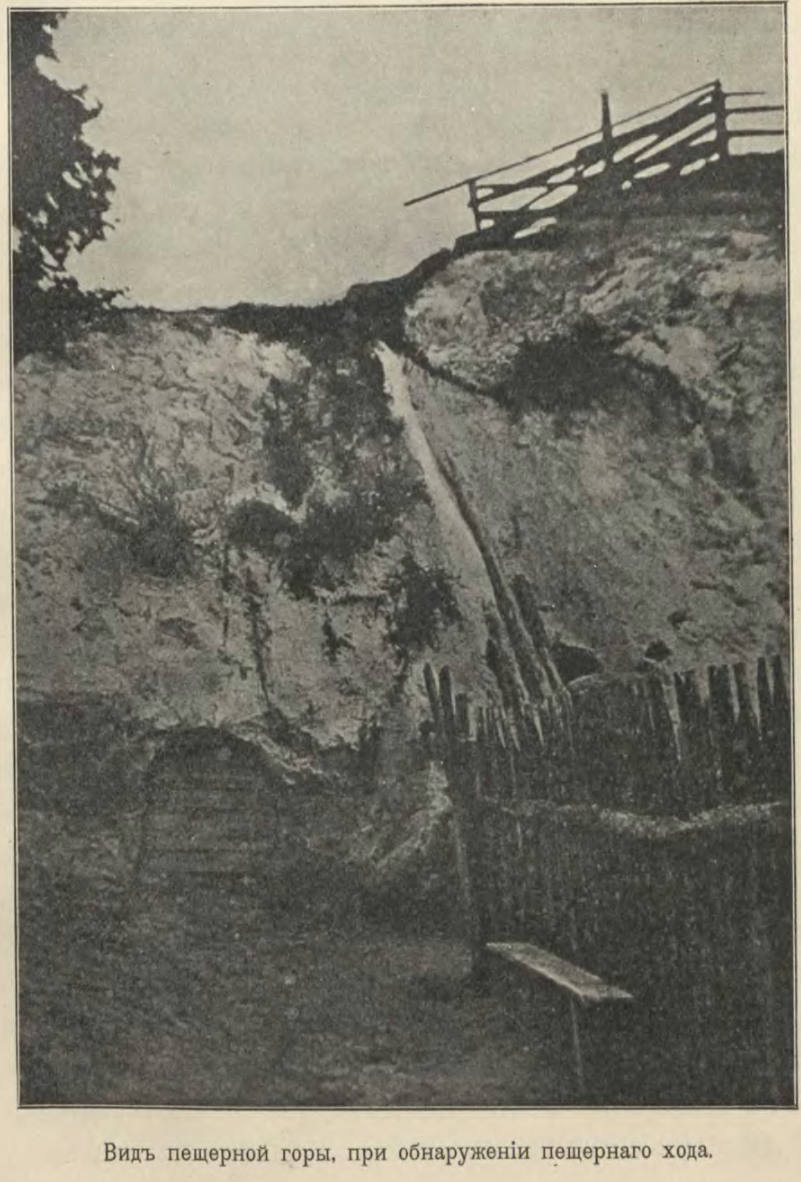
\includegraphics[width=0.90\linewidth]{chast-colebanie-osnov/nachalo/zverp-02.jpg}

\textit{Снимок 1911 года.}
\end{center}

\newpage

Петров осторожно пишет:

\begin{quotation}
О новооткрытых пещерах узнал проживавший тогда в Киеве князь Вл. Д. Жевахов, тот самый, который, вместе с братом своим Николаем, так сильно хлопотал об открытии нетленных мощей и канонизации своего родственника по женской линии, святителя Иоасафа Горленка, епископа Белгородского.

Князь задумал открыть Зверинецкие пещеры не столько как памятник глубокой древности, сколько как народную святыню, и сделать их доступными для народного поклонения и чествования. Этою религиозною целию забот князя Жевахова нужно объяснить то обстоятельство, что он обратился за разрешением работ не к Императорской Археологической Комиссии, ведающей все находки и раскопки древностей, а к духовному начальству, хотя не пренебрегал совершенно и научными интересами. Осенью 1911 года он взял в аренду у Инженерного ведомства тот участок земли, на котором находились Зверинецкие пещеры, и попросил благословение на открытие пещер у Киевского Митрополита Флавиана, которому князь сообщил о пещерах письмом. Наместник Киевопечерской лавры архимандрит Амвросий предложил заняться раскопкою этих пещер секретарю Киевского Общества Взаимного Кредита А. Д. Эртелю.
\end{quotation}

Раскопки начались только в июле 1912, поначалу даже без Эртеля – тот был занят в Китаевских пещерах, полагая в последних начало древнего Киева.

Копия рапорта Киевского полицмейстера от 28 июля 1912 года за № 9951 на имя Киевского Губернатора.

\begin{quotation}
На арендуемом князем Жеваховым от инженерного ведомства участке земли, находящемся сзади № 10 по Ломаковской улице производится богомольцами-охотниками\footnote{Т.е. желающими, добровольцами.} под руководством рабочаго крестьянина Семена Гончарова раскопки в целях открытия древних пещер-усыпальниц. 

%В настоящее время под горой Печерскаго укрепления открыт вход в пещеру, оказавшуюся в измерении 3 1/2 аршина\footnote{2,5 метра.} в квадрате, а из нея в глубь горы имеется ход в виде корридора шириною 2 арш. 2 вершк.\footnote{1,48 метра.}, вышиной 1 арш. 2 вер.\footnote{0,8 метра.} и длиною 41 аршин\footnote{29,2 метра.}, в нем обнаружено 32 места, где, повидимому, находились гробы с телами, на что указывают найденные остатки человеческих костей.

В настоящее время под горой Печерскаго укрепления открыт вход в пещеру, оказавшуюся в измерении 3 1/2 аршина в квадрате, а из нея в глубь горы имеется ход в виде корридора шириною 2 арш. 2 вершк., вышиной 1 арш. 2 вер. и длиною 41 аршин\footnote{2,5 метра в квадрате, 1,48 метра ширина, 0,8 метра высота. 29,2 метра длина.}, в нем обнаружено 32 места, где, повидимому, находились гробы с телами, на что указывают найденные остатки человеческих костей.

Раскопками заведует игумен Свято-Троицко\-го монастыря о. Валентин. 

Об этом доношу Вашему Превосходительству. Подлинное за надлежащими подписями.

С подлинным верно: Правитель Канцелярии Киевскаго Губернатора (подпись)

Сверял: Помощник Правителя (подпись)\end{quotation}

Мысленно потираю руки – обсудим! Вот у нас появился адрес пещер – участок земли позади усадьбы номер 10. Как мы знаем, на самой Ломаковской, 10 жила Матвеенкова. Ломаковская теперь называется Мичурина, и 10-й номер по Мичурина это, на 2016 год, частный дом, стоящий под горкой на той же стороне улицы, где и Зверинецкие пещеры, которые ныне имеют адрес Мичурина, 20-22 (в 1998-м: 18-22). От номера 10 до 20 около 150 метров. Значит, старая и новая нумерация не совпадают. Сравним теперь числа «от Матвеенковой» 1882 года, 1888-го и 1912-го.

У Матвеенковой – 50 гробов в отдельных пещерках по правой стене, по два тела в каждой могиле. И значит, 50 ниш в одной только стене. А другая, стало быть, без ниш.

1888 год, в первой заметке от неизвестного корреспондента – «по бокам пещеры» 48 могил с двойными погребениями. В одной из последующих заметок, уже в пещере, где побывали Прахов, Сведомский, Гошкевич и Червинов 2-й – 48 могил, при этом неясно, по одной стороне коридора или обеим.

Наконец 1912 год, первые раскопки – 32 ниши, и согласно позднейшим планам пещер – в каждом коридоре ниши были по обе стороны.

Затем раскопками стал руководить Эртель, поставив дело на научную основу. Кроме прочего он составил план расчищенного им участка пещер, несколько позже другой план начертил В. В. Кузнецов, сотрудник покойного к тому времени археолога Д. В. Милеева.

Перед разбором планов опишу рельеф местности. Северо-восточный, клиноподобный угол Зверинецкого холма. Сверху вниз – крутой склон (со входом в пещеру у его подножия), терраса с Ломаковской улицей, затем более пологий склон. Вдоль улицы, с течением времени, верхний крутой склон террасировался для разбивки там садов и огородов частного сектора.

\begin{center}
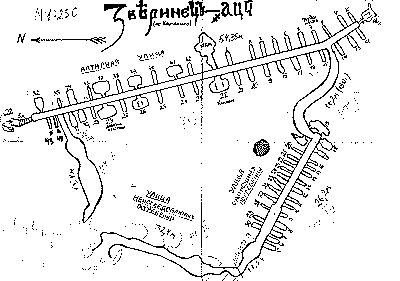
\includegraphics[width=0.90\linewidth]{chast-colebanie-osnov/nachalo/zverp-plan01.jpg}

\textit{Один из планов пещер, открытых в 1911 – еще не прорыт соединительный коридор для удобства паломников.}
\end{center}

\newpage
\vspace*{\fill}

\begin{center}
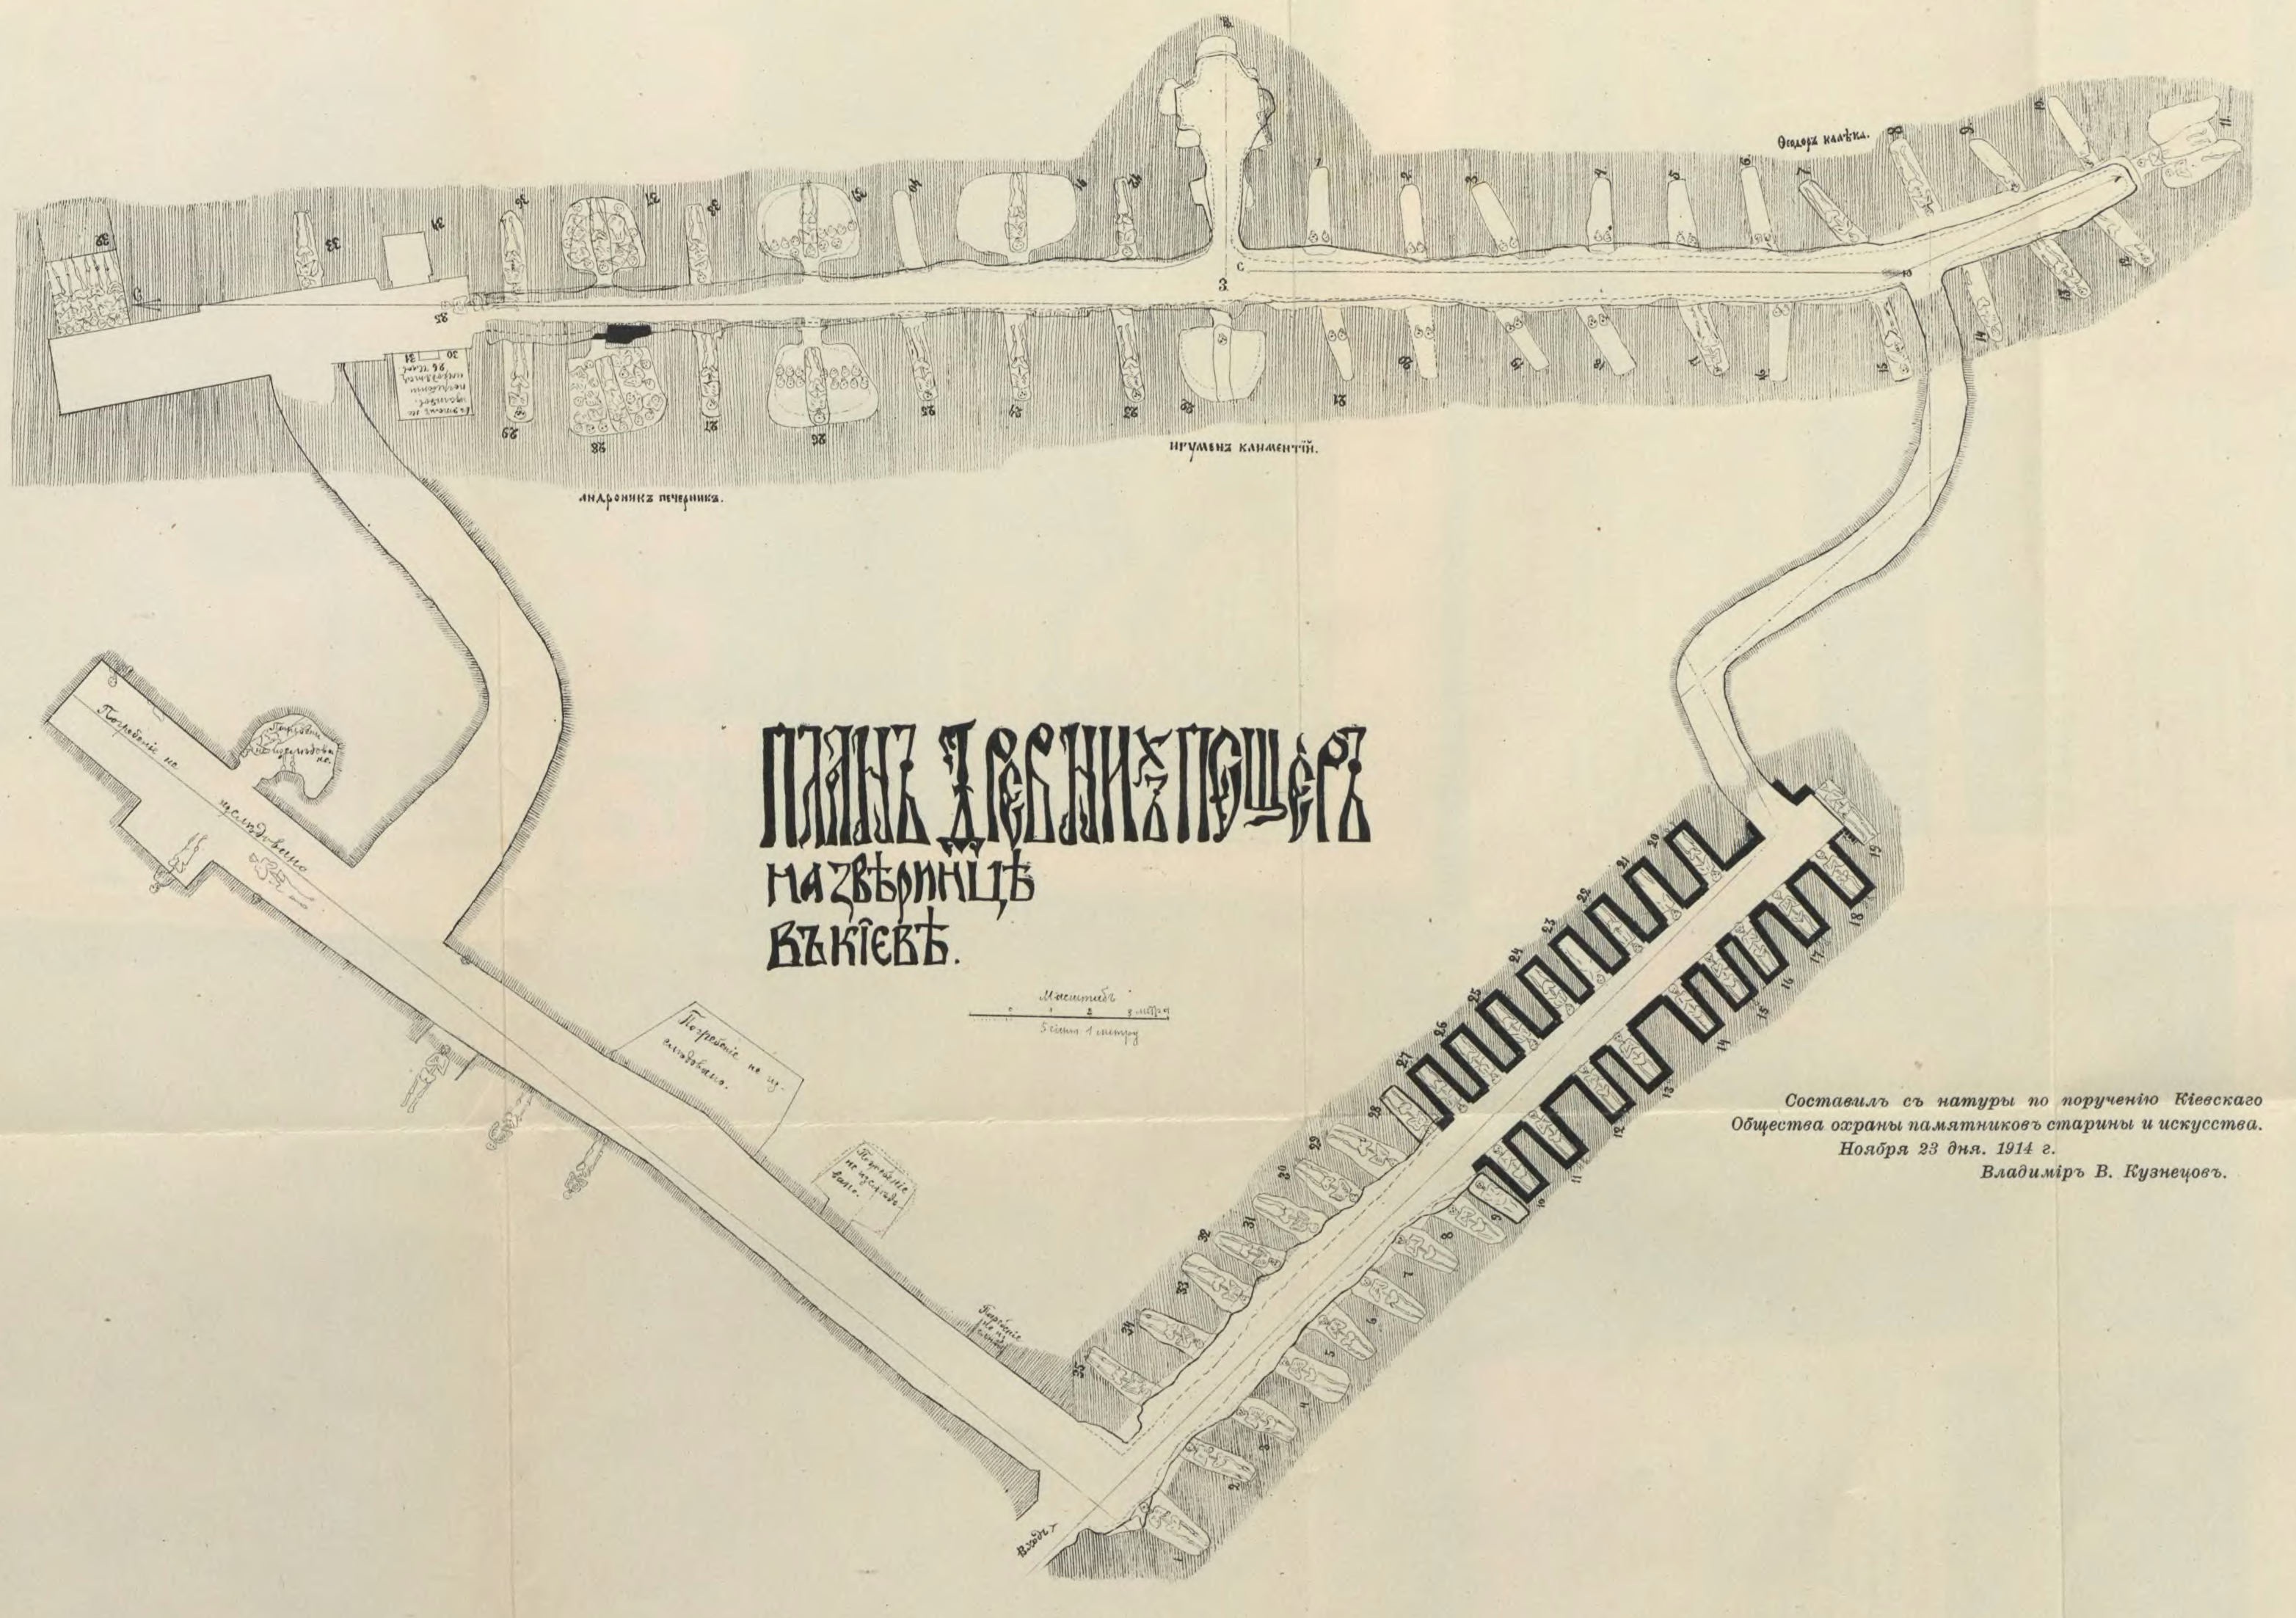
\includegraphics[width=\linewidth]{chast-colebanie-osnov/nachalo/zverp-plan02.jpg}

\textit{План Кузнецова. Современный вход – слева сверху.}
\end{center}

\begin{center}
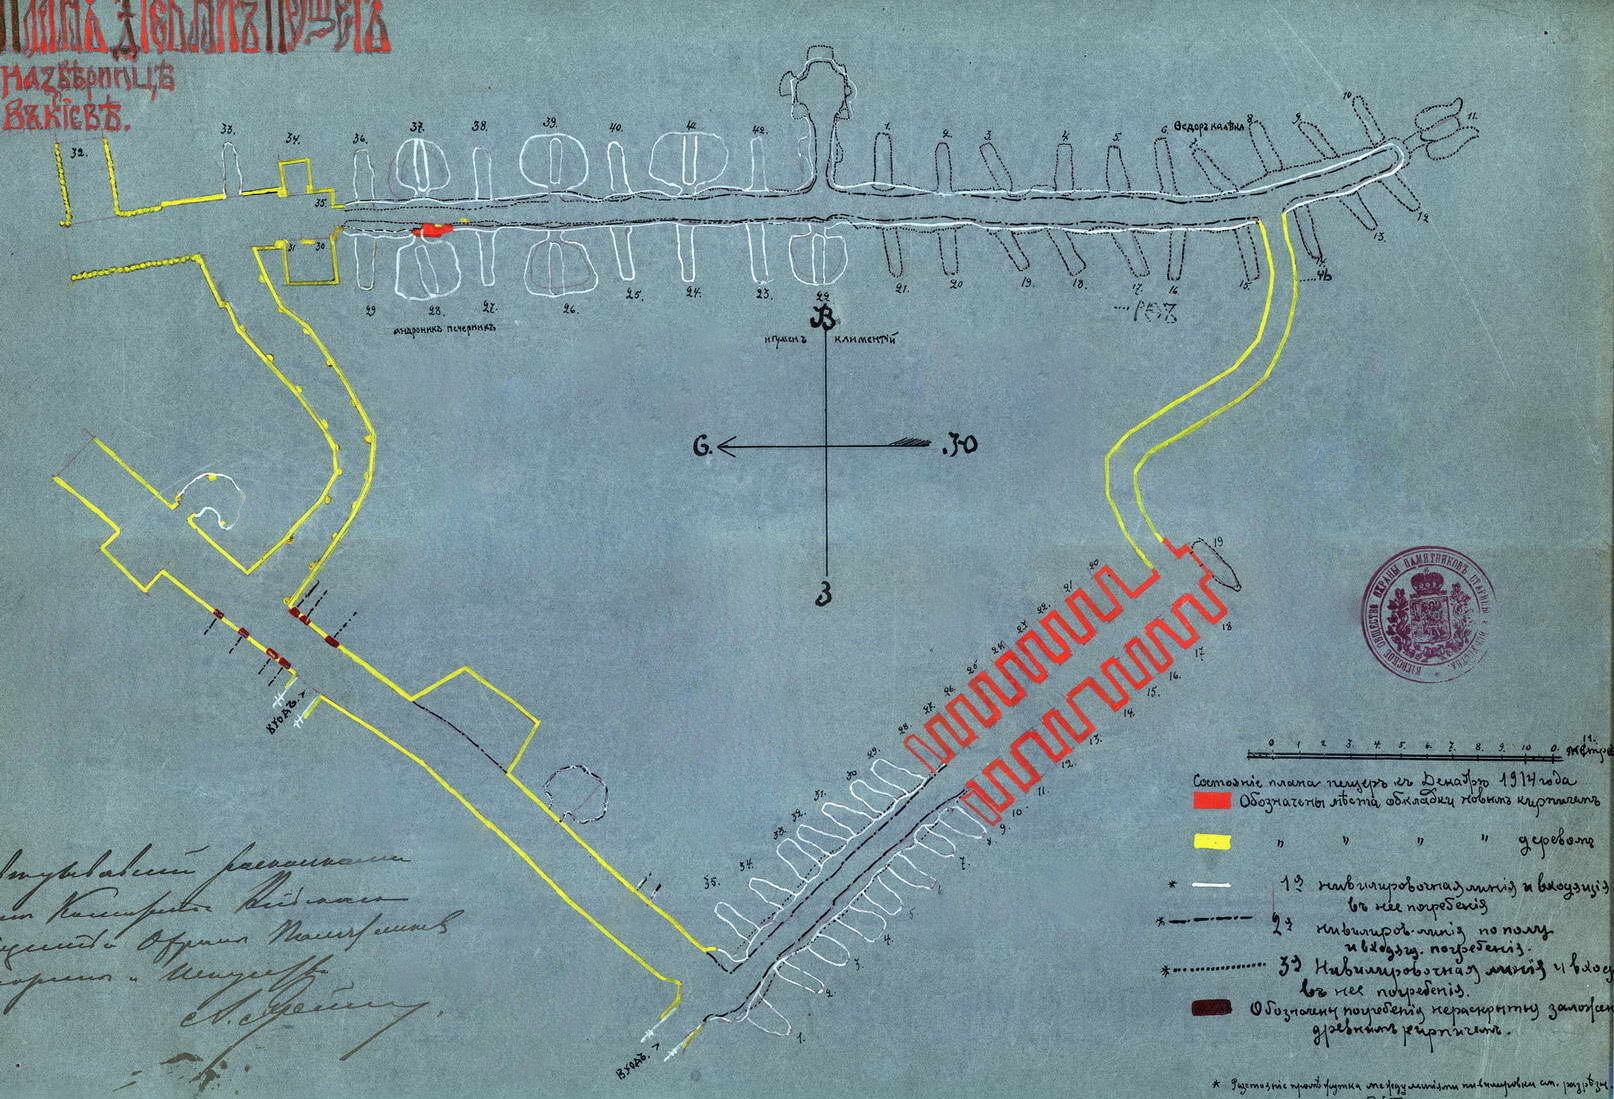
\includegraphics[width=\linewidth]{chast-colebanie-osnov/nachalo/1914-ertel.jpg}

\textit{1914. План с подписью Эртеля.}
\end{center}

\vspace*{\fill}
\newpage

Пять коридоров («улиц»), взаимное расположение которых образует треугольник. Разница между планами – пара лет, однако на втором видно, что прорыли коридор, соединивший северные части двух улиц.

Где находился изначальный вход 1911 года, не вполне ясно, однако на плане Кузнецова вход – посередине внизу плана, и на другом плане 1914 года появляется второй вход едва не на месте погребений. Современный же, 21 века вход – в верхнем левом углу.

%Очевидно, что подземелье было вырыто по начертанному ранее проекту, и в ходе работ использовались какие-то измерительные средства, позволившие придерживаться начального чертежа.

Обмеры коридоров, по Кузнецову, таковы. Правый от тогдашнего входа («улица одиночных погребений») – длина 26,20 метров (13 сажень), на одной стороне 18 ниш, на другой 16, одна в тупике, всего 35, погребения одиночные. Левый («улица неисследованных погребений») – 32,40 метра (19 сажень). Поперечный коридор («алтарная улица») – 54,35 метра (27 сажень), по стенам расположены комнаты с массовыми погребениями (останки более двух людей в одной келье), и около трех десятков двойных (скелеты лежали друг на друге) и одиночных погребений.

Говоря о кельях, которых на Алтарной улице насчитали три, Каманин сообщает, что «высота всех келлий общая с высотой пещер, от 1,80 до 2 метров». Пещеры, куда лазала Матвеенкова, имели высоту 2,1 метра.

Но вот газета «Киевлянин» в № 55 за 24 февраля 1913 года поместила заметку про доклад Эртеля и Каманина в феврале 1913 года на заседании Исторического общества Нестора-летописца. Выдержки оттуда, касаемо доклада Эртеля:

\begin{quotation}
На первых порах при зверинецких раскопках пришлось преодолеть некоторые затруднения: пещеры привлекли огромные массы паломников со всех концов Руси; своим любопытством они мешали работам, которые и без того требовали большого внимания и осмотрительности: возможен был обвал и за рабочими приходилось тщательно наблюдать.

Все это осложнялось еще спором о казармах, которые предполагалось строить на месте производства работ, по раскопкам. Сейчас раскопки далеко еще не закончены, но в некоторых местах подошли уже к границам частных усадеб.

Пока отрыты несколько низких (в них нельзя выпрямиться) длинных галерей со множеством усыпальниц, из которых большинство разрушено.
\end{quotation}

А почему Каманин в своей книге пишет о высоких потолках? Где же эти галереи, в которых нельзя выпрямиться? Читаем «Киевлянина» дальше:

\begin{quotation}
Кирпич, найденный здесь, относится к XI и позднейшим векам. Встречаются кирпичи, бывшие, очевидно, уже в употреблении и принесенные сюда из других построек. 

В конце одного хода обнаружены несколько скелетов, расположение которых наводит на мысль о какой-то драме, быть может, времен татарщины.

В центре открытой системы галерей (система незаконченная, неясная, что заставляет предполагать существование 2-го яруса подземных ходов) находится низкая четырехугольная камера, с нишами в северной и восточной стенах, где, предполагает докладчик, находились жертвенник и престол этой подземной церкви. вмещавшей не более шести человек.
\end{quotation}

Заметим предположение о втором ярусе пещер, краткие сведения о «драме», и указание на низкую камеру с жертвенником. Это же помещение по обмерам из книги Каманина становится если не просторнее, то по крайней мере несколько выше – два метра.

Посмотрим на выполненный Кузнецовым план Алтарной улицы в разрезе, 1914 года – все обмеры указаны в сажнях, а сажень это примерно 2,1 метра. Вид с востока:

\newpage

\vspace*{\fill}

\begin{center}
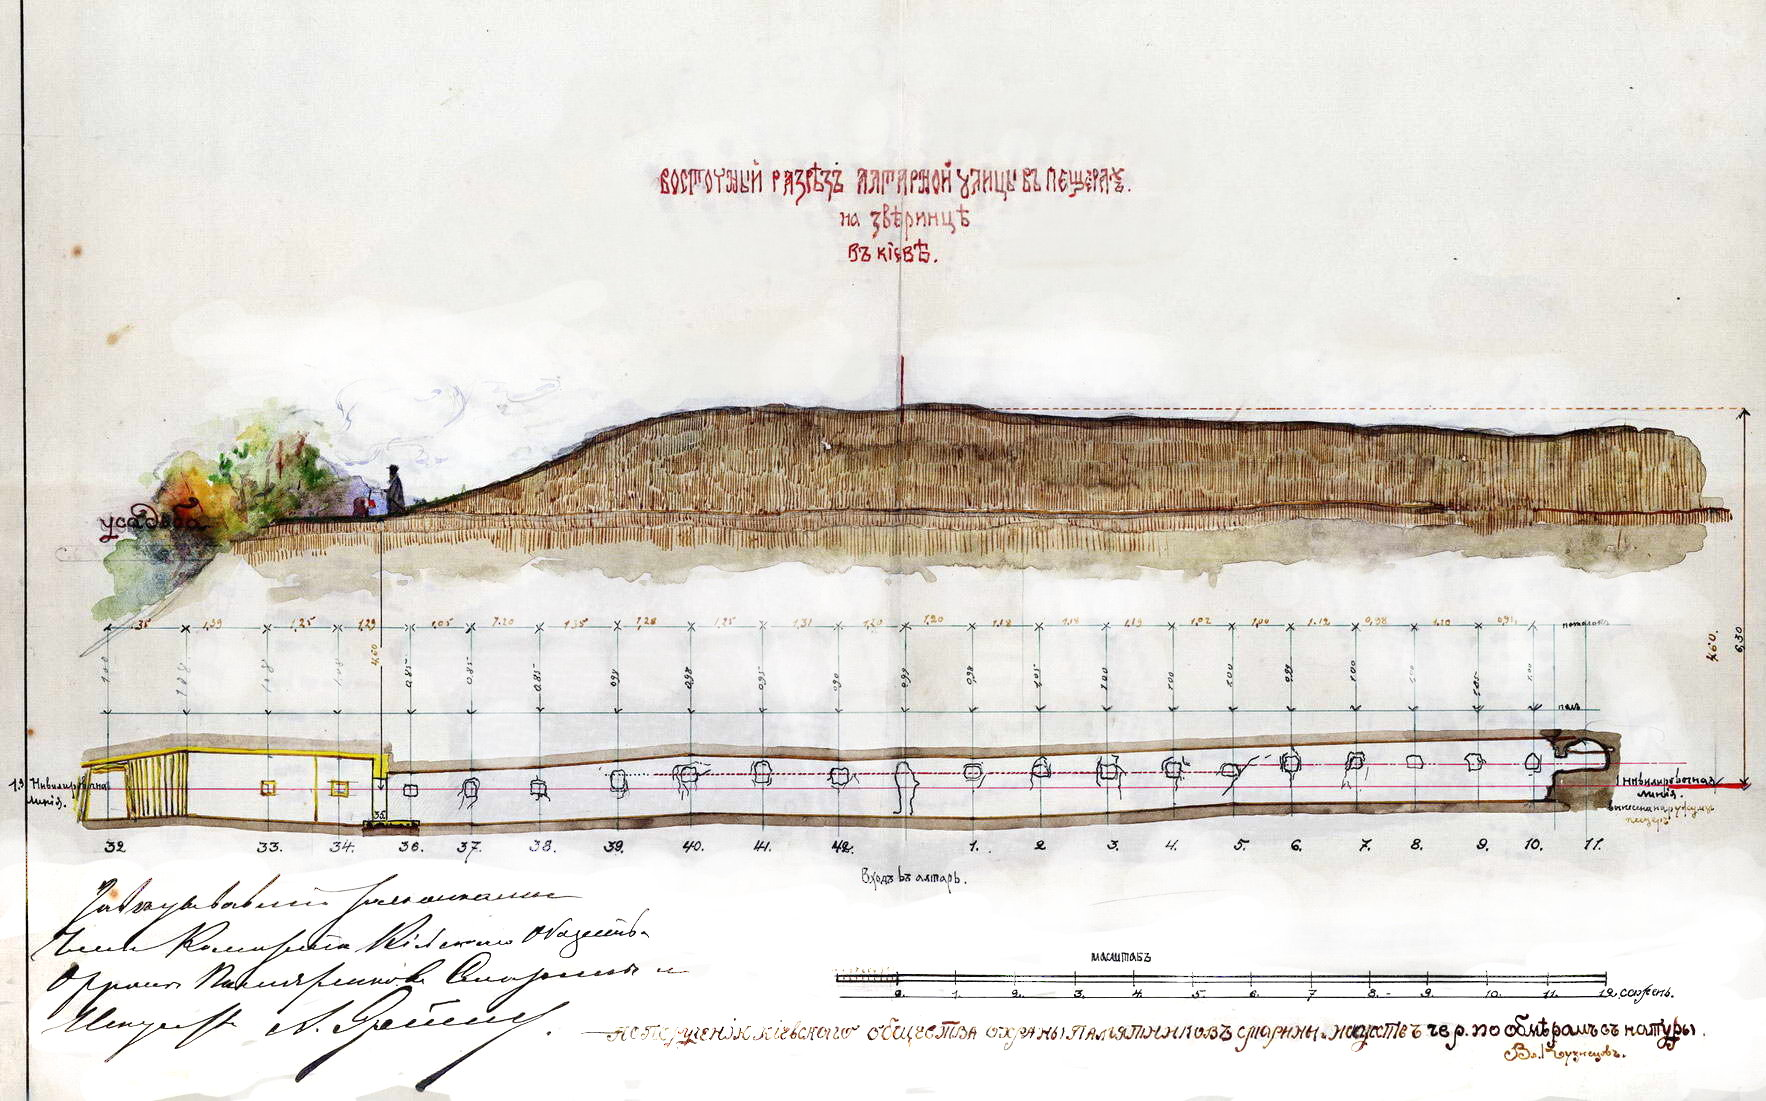
\includegraphics[width=\linewidth]{chast-colebanie-osnov/nachalo/1914-01.jpg}
\end{center}

\vspace*{\fill}

Над коридором изображена шкала, где для каждого участка по оси X отмечена его длина, а по оси Y – высота потолка.

Посередке обозначен «Вход в алтарь». Какая высота потолка? 0,99 сажени – это таки около двух метров.

Со времени доклада Эртеля потолок подрос? Судя по данным высот с этого же «разрезного» плана, нигде в Алтарной улице не нужно идти пригнувшись.

Что кстати еще полезного можно узнать из плана? Видите две фигуры на пригорке – черную и в красной шапке? Эти люди пробурили в коридор шахточку, и высота ее составила 4,60 сажни, это 9,66 метра. Ниши в коридоре пронумерованы до 42.

Познакомимся с разрезом «Второй улицы» («одиночных погребений») с запада, причем на плане отмечены только ниши, находящиеся по правую руку, если смотреть от обозначенного на нем входа (тоже справа). Всего же ниш – 35.

Масштаб указан уже не в сажнях, а в метрах – вероятно, обмеры тоже в метрах.

\begin{center}
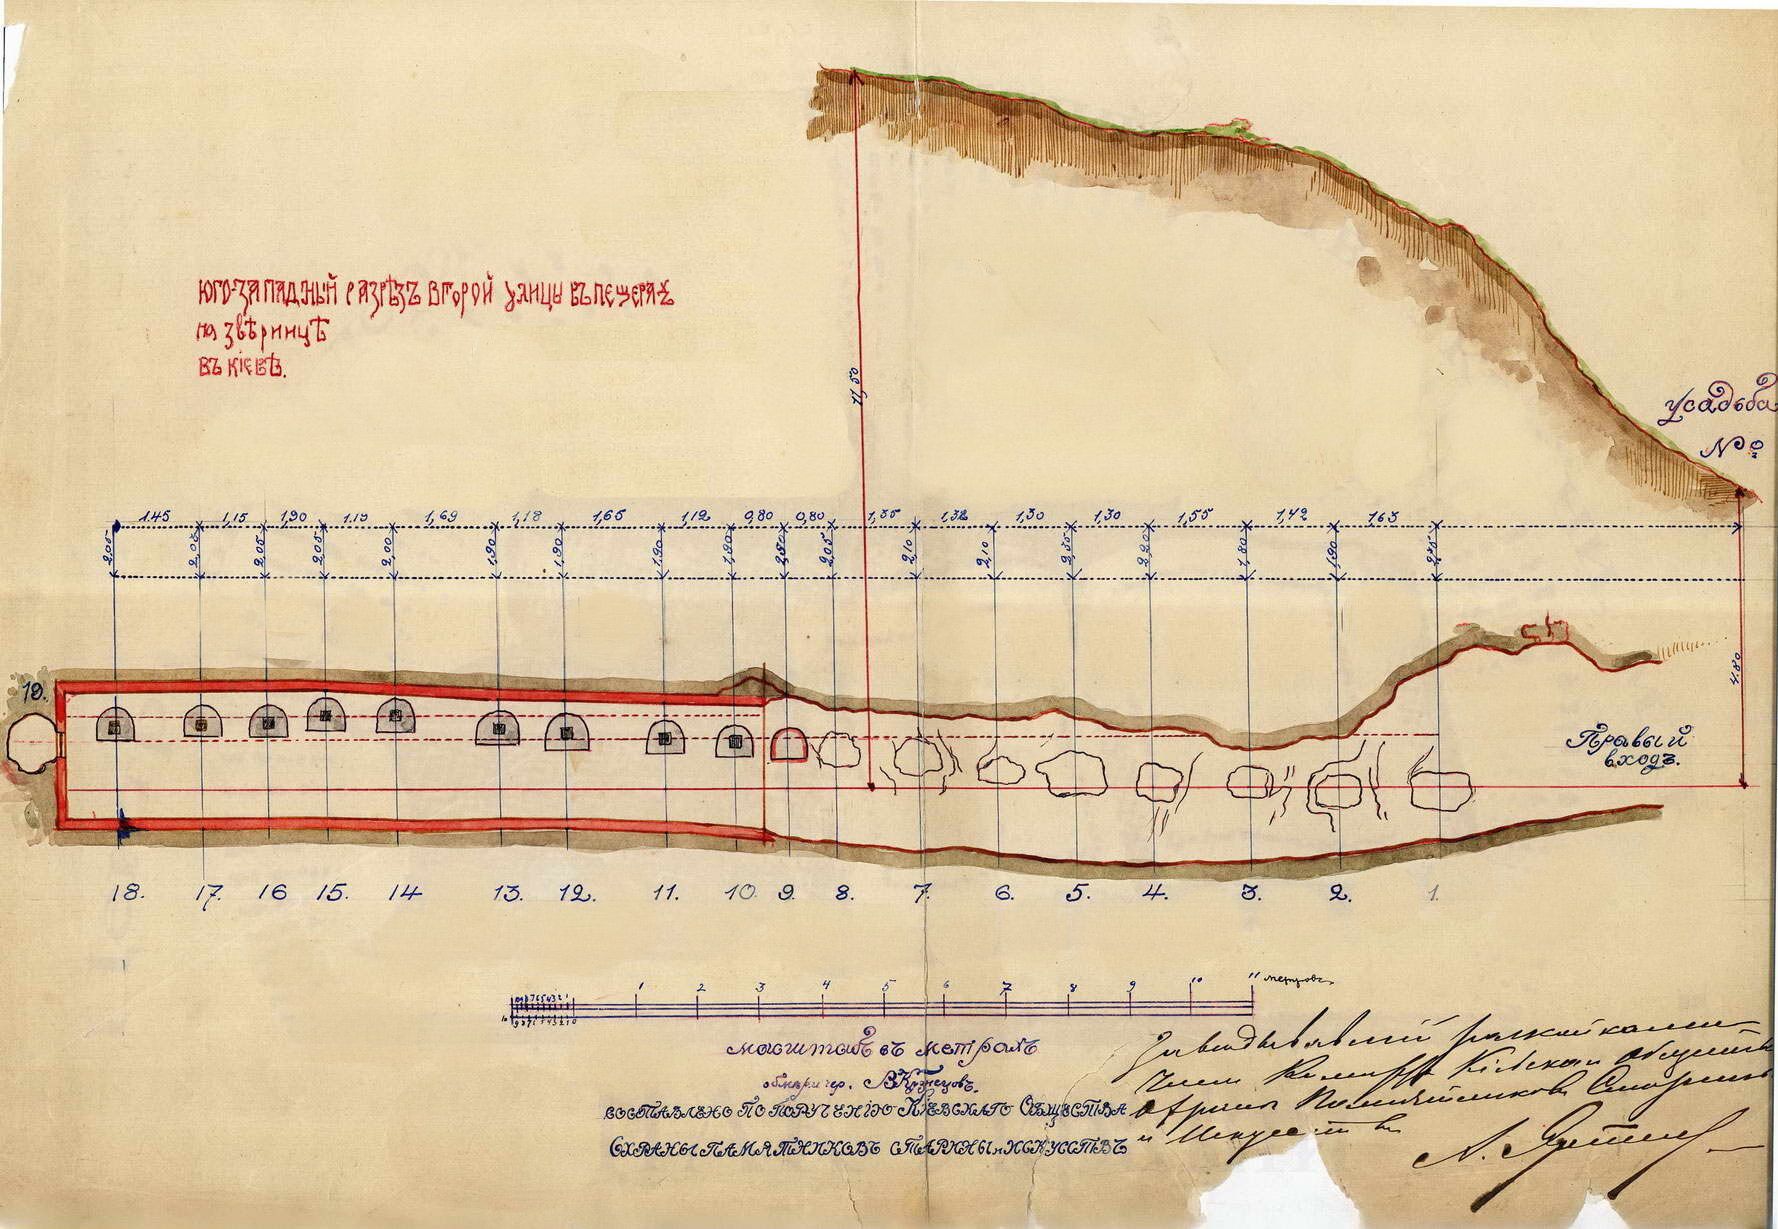
\includegraphics[width=\linewidth]{chast-colebanie-osnov/nachalo/1914-02.jpg}
\end{center}

То, что числа выражают метры, подтверждается указанной глубиной залегания коридора – 11,50 от поверхности. Если Алтарная улица лежала в 9,66 метрах, то 11,50 – сопоставимая величина, ведь если бы 11,50 было в сажнях, это даст нам глубину более 20 метров. А поскольку оба коридора лежат примерно на одном уровне, значит, 11,50 – именно метры.

Может быть это низкий коридор, где нельзя разогнуться? Да вроде бы нет, один только участок 1,80 метра, остальные 1,90 и даже более 2 метров. 

А как же данные самого начала раскопок? Когда

\begin{quotation}
а из нея в глубь горы имеется ход в виде корридора шириною 2 арш. 2 вершк., вышиной 1 арш. 2 вер. и длиною 41 аршин, в нем обнаружено 32 места, где, по-видимому, находились гробы с телами
\end{quotation}

Здесь высота потолка – 0,8 метра, длина около 30-ти. 32 ниши против «официальных» 35 с плана Кузнецова. Будто тот же самый коридор, да вот только высота потолка снова стала много выше. 

Воистину чудесны киевские пещеры! 

Из подземного хода, где надо ползти на карачках, всего за пару лет образуется удобный для пешего хождения коридор.

Сам Эртель в книге 1913 года писал про «улицу одиночных погребений» следующее:

\begin{quotation}
Правый ход (А) ведет в длинный коридор, в котором по обе стороны расположены одиночные и двойные усыпальницы, к сожалению, все разрушенные и разграбленные. В них остались только разбросанные в беспорядке кости, часть которых, по-видимому, унесена или перенесена в другое место. Кости – плохой сохранности, и некоторые совершенно рассыпаются.

Усыпальницы расположены так густо, что промежутки между ними занимают не более полуаршина. Местами сохранились обломки почти совершенно истлевших деревянных досок (по-видимому дуб), но были ли тут гробы, определить с уверенностью нельзя.

Ход в общем широкий, но низкий, так что почти везде нужно идти согнувшись.
\end{quotation}

Низкий ход... Идти согнувшись... А согласно плану – средняя высота потолка около двух метров!

В докладе на заседании общества Нестора-Летописца говорилось, что останки, вид которых намекал на некую трагедию, лежали в конце коридора. Каманин же сообщает в книге, как свидетельство внезапной гибели людей, что часть скелетов, лежала на полу коридоров, и много ближе ко входу, в беспорядочном положении.

Как бы ни было, это можно толковать двояко – люди погибли и остались на месте смерти, либо же их останки переместили уже после, например при разграблении пещер.

Некоторые ниши-усыпальницы были заложены кирпичом (датированным 11 веком, однако вроде были и позднейшие). Эртель нашел также кирпичные плиты, похожие на части круглых колонн. Предметы из кожи – плетеные кресты, остатки обуви, а также поясов с названиями либо оттисками изображений христианских праздников (в прямоугольных рамках до трех сантиметров в ширину, около двух в высоту, видны распятие Христа, въезд его в Иерусалим на «жребяти осли», воскресение Лазаря, и тому подобное), несколько черепков.

\begin{center}
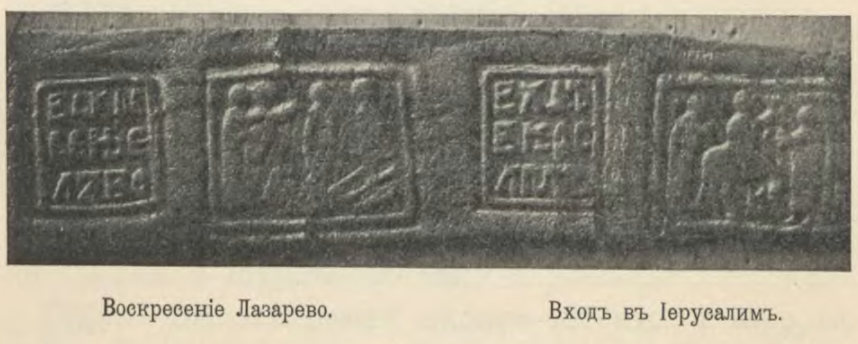
\includegraphics[width=\linewidth]{chast-colebanie-osnov/nachalo/poyasa.jpg}
\end{center}

%\begin{center}
%\includegraphics[width=\linewidth]{osn-kiev/poyasa02.jpg}
%\end{center}

По находкам Эртель судил, что подземный монастырь существовал в 12, 13 и 17 веках. Непрерывно или временами?

Описание пещер 1911 года открытия кажутся мне отличными от пещер открытия 1882 и 1888 годов, на что указывают хотя бы числа – длины коридоров и связанные с ними количество и виды захоронений (одиночные, двойные, массовые), наконец сведения о нишах только справа – у Матвеенковой.

%В статье про Зверинецкие пещеры из сборника «Звід пам'яток історії та культури України. Київ» 1999 года издания, где все местные подземелья смешали в одну кучу, упоминаются еще некие исследования 1990-х, 

Насколько я знаю, в пещерах допустим Лавры – лишь одно «двойное» захоронение, Паисия и Меркурия, кои, будучи дружны при жизни, были по их же просьбе положены в одном гробу посмертно, как повествует «Патерик Печерский».

Что за странные похоронные обряды в Зверинецких пещерах? И чьи скелеты найдены в коридорах?

По 1980-е укрепилось мнение, что это был обычный пещерный монастырь со своими захоронениями и вполне живой братией, где случилась какая-то трагедия. Десятилетие спустя, после исследований пещер под руководством Елены Воронцовой, возглавлявшей тогда отдел «Киев подземный» Музея Истории Киева, предположение науки о «трагедии» вроде бы пошатнулось и эта шаткость даже проникла в поверхностную статью из сборника «Звід пам'яток історії та культури України. Київ» 1999 года издания, однако я не знаком с итогами этих исследований в полной мере, и доводами против того, что лежащие на полу скелеты не могут свидетельствовать о насильственной смерти.

По какой-то же причине Зверинецкие пещеры были заброшены на века.

%Каманин пишет о монахах, хотя предполагает, что это могли быть и кости каких-то укрывшихся в пещерах местных жителей. 

%Ежели первое, то – произошло нечто страшное, и в пещерах все погибли, никто не вышел. От чего погибли? Исследования не проводились.

Есть домыслы – мол, на окрестности напали враги (обычно Половцы), а местное население укрылось вместе с монахами в пещерах и крепко держало оборону в узких коридорах, поэтому лиходеи просто засыпали вход. Тогда почему погребенных заживо не раскопали современники?

Выходит, все, кто знал о пещерах, в них и погибли? А может, по некой причине, пещеры никто не хотел раскапывать на протяжении веков.

И неведомо же, когда именно умерли люди, и спустя какое время вход или входы оказались засыпаны, а также как засыпаны – людьми ли, либо случился естественный обвал.

Во время раскопок пещер в начале 1990-х, заказали изучение останков группе медиков. В нее вошли профессор кафедры рентгенорадиологии Национального Медицинского Университета Татьяна Топчий и студенты Р. Л. Новакович, С. В. Дудник, В. В. Столяров.

Они исследовали останки из 78 раскопанных ниш. 1721 целая кость, 5000 кусков костей – всё, что уцелело, по прикидкам, от 200 человек, из коих взрослых было 145, и 53 детей до 15 лет (в том числе 3 – новорожденные, 2 – младенцы до 1 года, 7 – 1-2 лет). 5 захоронений оказались женскими. За числами стоят живые когда-то люди, они разговаривали, ходили, смеялись.

Целых черепов не сохранилось, и медики не смогли определить расы погребенных. О возрасте судили по стёртости зубов (таковых пригодных черепов оказалось 11) и костям, вычислили средний возраст – 45-55 лет, наибольший – 80 и старше. Средний рост составил 116,33 сантиметров, плюс-минус 7,3. Хотя некоторые мужчины были по два метра.

Кости датировались по виду. Часть отнесли даже к 20 веку, а старейшие – к домонгольскому периоду. Каким образом? А вот, в Лавре есть мощи летописца Нестора. Он ведь до «монгольского нашествия» жил? Давайте, говорят эксперты, сравним цвет и степень сохранности «зверинецких» костей с костями Нестора. Если похожи, значит они тоже домонгольского периода.

Некоторые кости имели необычный вид, а также наросты, что исследователи пояснили тяжелой жизнью в пещерах. Удивила дугоподобная грудина. Сие, по мнению медиков, означало наличие стеноза устья аорты – «сердечный горб».

Смешанность погребений – разных полов и возрастов – пояснили тем, что местные жители знали о пещерах и использовали их в качестве кладбища.

К сожалению, я не обладаю подробностями б\'ольшими, чем изложил (опустил лишь сведения о сросшихся переломах и остеохондрозе у некоторых покойников).

Теперь обсудим. Начну с конца. 

В народе всегда придерживаются традиций погребения. В обозримом прошлом, на Киевщине, простые люди хоронили своих умерших в земле или сжигали, а прах в глиняных сосудах опять-таки закапывали. Пещерные же захоронения совершались служителями культа для своих собратьев, и в Киеве погребальных пещер было не столь уж много.

В христианское время, вне кладбища хоронили только некрещеных детей, самоубийц, колдунов, опойц и умерших насильственной смертью – относительно последних этот обычай к 19 столетию отжил.

С 18 века, а может быть и раньше, напротив Зверинецких пещер, в трехста с копейками метрах на север, по склону соседней горы существует Зверинецкое кладбище. Впервые я вижу его на карте 1803 года около тамошней церкви.

Делаю вывод – местное население скорее всего не хоронило своих мертвецов в пещерах, разве что какие-нибудь злодеи сбрасывали туда трупы. Но ведь останки вроде бы с почетом лежали в нишах, ведь так? И некоторые по двое в нише, а то и больше. У кого такой погребальный обычай – у крестьян Зверинца? В документированном прошлом на Зверинце были слободки Лавры и Выдубицкого монастырей.

О черепах. В пещерах 1882 года открытия, черепа – были. В пещерах 1888-го тоже. И в 1911 году также видели черепа – Эртель даже отмечал, что некоторые были «необычайной белизны». А в 1990 году все черепа оказались разломанными! Что это? После закрытия скита над пещерами в 1934-м большевики, корчась от приступов атеизма, проникли в пещеры и сокрушали черепа? Сами по себе они треснуть не могли, череп довольно крепкая штука, значит, кто-то целенаправленно их уничтожил. Зачем?

Изображения двух черепов, одного найденного в пещерах, другого – даже не черепа, а головы, с иконы отсюда же – мы рассмотрим чуть позже.

Покамест о возрасте. 145 взрослых, и 53 детей до 15 лет. От последних отнимаем совсем маленьких, остается 41.

Несомненно, дети выглядят иначе, чем взрослые – и кости у них выглядят иначе, ибо дети это не уменьшенные копии взрослых. Итак, кости детей не просто меньше, но и выглядят иначе.

Но первым делом на что обращают внимание? На размер. Маленькая кость – значит ребенок. А кто еще может быть? Вот же, и выглядит как-то иначе, не как у взрослого человека.

Ну а вот есть карлики и лилипуты. Последние пропорциями и ростом более подобны «полноразмерным» детям.

%Ну а вот есть карлики и лилипуты (в англоязычной среде их обозначают словами dwarf и midget) – последние пропорциями и ростом более похожи на «полноразмерных» детей.

Карлики похожи на других карликов, а лилипуты на других лилипутов. В сообществе карликов их внешность – норма. Что такое норма? Нормой в давнем Риме называли измерительный инструмент плотников, нечто вроде угольника. А ведь шкалу на угольнике можно рисовать разную – в сантиметрах, в дюймах. Меняешь измерительную основу – меняется норма. Так оказывается, норма изменчива и зависит от того, кто ее применяет.

Про карликов и лилипутов наука говорит – это больные люди, и корни их болезни в генах, в наследственности. А почему не предположить, что они имели предков, которые от природы имели малый рост?

Известны группы народов невысоких людей – это пигмеи в Африке и негрито в Южной Азии. Они выглядят просто как уменьшенные «полноразмерные». Ученые, исходя из своих представлений о норме (нормальный для них значит полноразмерный), гадают – наверное пигмеям не хватает витамина Д! Или – пигмеи так приспособились для жизни в своей среде обитания. Изначальная предпосылка науки – пигмеи это бывшие полноразмерные.

На севере Японии проживал и живет народ Айну (ныне почти растворившийся среди населения), предания коего говорят о невысоком большеголовом народе Коропоккуру (Коропок-ун-гуру, «живущие под землей»), обитавшем в тех краях прежде Айну. Последние, по их собственным представлениям, пришли с Камчатки через Курилы.

В 19 веке, в Японии, некоторые ямы слыли остатками жилищ Коропоккуру, точно как на Урале народ знал «чудские ямы», оставшиеся после сгинувшего куда-то таинственного низкорослого народа Чуди Белоглазой.

В 1877 году американский зоолог Эдвард Морс (Ed\-ward S. Morse) провел раскопки в Токио (место известно ныне как Omori Shell Mound) и нашел следы неолитической культуры, предшествующей Айну и отличной от нее по крайней мере в двух вещах. Предшественники были людоедами и искусными гончарами.

С течением времени, гончарное мастерство каждой культуры не утрачивается, а совершенствуется. У народа Айну же гончарство существенно проигрывало уровнем в сравнении с находками Морса.

Кроме того, в «ямах Коропоккуру» выкапывали орудия труда размера слишком маленького, чтобы быть пригодным для «полноразмерных» людей. С подобным знакомы и наши археологи, такие предметы многократно обнаруживались на Киевщине. В Шотландии же махонькие кремневые орудия называли «fairie dart» (дротик фэйри) «elf shots» и «elf arrows» (эльфийские стрелы), и носили их с собой, полагая, что эльфы не властны над теми, кто имеет при себе такую штуку.

Ученик Морса, Тсубо Шогоро (Tsuboi Shogoro), профессор антропологии Токийского Императорского Университета, хорошо подкованный по части этнографических записей 19 века о Коропоккуру, связывал древние черепки и маленькие орудия именно с этой расой, утверждая, что она действительно жила на Хоккайдо перед Айну и даже при них. Ведь в преданиях отразились встречи (обычно ночные) с этим странным народом. Айну иногда торговали и разговаривали с его представителями, но Коропоккуру в целом стремились, дабы их никто не видел.

На стыке 19-20 веков в Японии боролись два научных мнения о давнем населении северных островов – Коропоккуру или первобытные Айну? Главным противником Тсубо был Коганеи Йошикиё (Koganei Youshikiyo, 1858-1944). «Дебаты Коропоккуру» заглохли со смертью Тсубо в Санкт-Петербурге в 1913 году, зеленый свет получила другая теория относительно древнего населения севера Японии, а Коропоккуру нынче прочно заселили бесконечные серии анимэ в образе эдаких веселых гномиков.

%Отмечу, что первым из ученых, кто за древнее население северных островов считал Коропоккуру, был английский инженер и геологи Джон Милн (Johm Milne, 1850-1913), полагавший, что сначала там жили Коро-пок-гуру, затем Аину, затем Японцы.

Теперь представьте, что археологи нашли кости кого-то подобного, а хоть даже лилипута, неполный скелет, да еще с разбитым черепом. Первая мысль – это ребенок! А медики, не археологи, способны отличить кости лилипута от костей ребенка? Если перед человеком будет много небольших костей из пещеры, он скорей решит, что это кости детские, а не представителей живущей в пещере общины лилипутов, и будет толковать находки, держа в голове представление именно о детях.

Вы спросите – что, я полагаю, будто в Зверинецких пещерах жили едва не гномы?

Отвечу так – если это был именно монастырь, то захоронения в нишах сорока детей-подростков кажутся мне менее вероятными, чем захоронения сорока взрослых людей маленького роста.

На последнее указывают и сведения о невысоких потолках, столь стремительно выросших за время раскопок при Эртеле.

Можно возразить – потолки изначально были высокими, потом осыпались, Эртель же просто всё расчистил. Ну а вот в Киеве есть Змиева пещера на Смородинском спуске, там Эртель ничего не расчищал. Некоторые коридоры в ней ниже метра. Пол ровный, потолок древний. Да, очень неудобно для «полноразмерных».

Другое возражение против моих рассуждений – а как быть с останками «полноразмерных» в Зверинецких пещерах? А я не знаю. Может быть они на четвереньках передвигались, может  часть коридоров была таки высокой, может маленькие останки более древние. Ничего определенного, я лишь указал на изменение высоты потолков при раскопках и на более вероятную принадлежность маленьких останков взрослым маленького роста, нежели детям – учитывая погребальные традиции как мирские, так и монашеские.

Еще одна непонятка – в пещерах 1911 года открытия не сыскали ни одного металлического предмета, кроме иконы, о которой мы поговорим далее. А как же обитая железом дверь, описанная Матвеенковой? А кресты из собрания Хойновского? Научное объяснение, что «за 30 лет» металл растащило местное население, опровергается соображением – как туда попадали эти воры, если вход в пещеру снова открылся только в 1911?

%Однако забывают, что 30 лет растаскивания быть не могло по простой причине, если пещера одна и та же. Ведь рабочие, как мы помним, закопали вход 1882 года. Даже археологи не могли туда более попасть, не говоря уже о местных жителях. Еще один довод в пользу того, что в восьмидесятых открывался вход в совсем другую пещеру. Там было железо, тут нет.

%Какие предметы нашли в пещере начиная с 1911 года? Искусно плетеные из кожи кресты, пояса с тисненными изображениями, надписи на стенах. 

Во время раскопок, начавшихся в 1912 году, был обнародован весь тот небогатый набор вещественных доказательств, по которым с тех пор судят об их древности. Если Эртель говорил о 12, 13 и 17 веках, то Каманин свёл все находки к 10-11, считая Зверинецкий монастырь начальной стадией Выдубицкого, и полагая Зверинецкий старше Печерского, Лавры. Надписей, выцарапанных на суглинных стенах – немного. Помимо двух крестов с «IС ХС NИ КА» (Иисус Христос Ника (Победитель)), Каманин упоминает следующие.

Список семи игуменов «Звериньского» монастыря – Левонтий, Маркьян, Михаил, Софрон (предположение), Мина, Климент, Мануил – нечитаемые буквы заменяю знаками вопроса: 

\begin{quotation}
игоумени звериньнсьци левоньтья марькьяна михаила ???он? мины клименьтья мануила\end{quotation}

Надпись над усыпальницей: 

\begin{quotation}
помяни ги дшю своего ???мянь?ья ???мена.\end{quotation}

Что Каманин, дополняя, читает как 

\begin{quotation}
Помяни господи душу раба своего Климяньтья игумена.
\end{quotation}

Рядом еще одна: 

\begin{quotation}
Климянь ньтьтии игумен звериньськии.\end{quotation}

Две надписи над другими усыпальницами говорят, при прочтении с догадкой, об некоем Андронике Печернике или Чернце, да о Федоре Калеке.

На основании всего этого, а более по списку игуменов, Каманин обосновывает датировку основания «пещерного монастыря» 10-11 веками и пробует перебросить мостки от него к летописям. Так, в Ипатьевской за 1091 (6599 от сотворения мира) год Нестор в рассказе о перенесении мощей святого Феодосия упоминает некоего «Климянта», коего Стефан поставил после себя игуменом в монастыре Стефаниче, что находился «на Клове».

Каманин считал, что зверинецкий игумен Климянт и этот летописный Климянт – одно лицо и вероятно был другом Стефана, и последний, умирая, 

\begin{quotation}
можно думать передает на память о себе Клименту самые дорогие для себя предметы: свою келейную икону Божией Матери, Одигитрии, перед которой он всегда молился, превосходной работы копию чудотворной Владимиро-Волынской иконы Богоматери, и свою панагию, которую постоянно носил на груди. Климент игумен высоко ценил память своего друга [...]
\end{quotation}

На нехитром приеме – «можно думать» –  построено множество рассуждений Каманина, которые он развивает и затем опирается на итоги развития уже как на твердую почву. 

\begin{quotation}
Мы позволяем себе даже думать, что преподобные Антоний и Феодосий именно в Зверинецких пещерах учились подвигам пещерно-по\-движничес\-тва.
\end{quotation}

И так далее.

Путем подобных логических выкладок Каманин вывел, что Зверинецкий монастырь был, как и Выдубицкий, посвящением связан со святым Михаилом, и что Выдубицкий это наземное продолжение пещерного Зверинецкого. Такое отождествление позволило Каманину причислять некоторых летописных церковных деятелей к деятелям именно Зверинецкого монастыря.

\vspace*{\fill}
\begin{center}
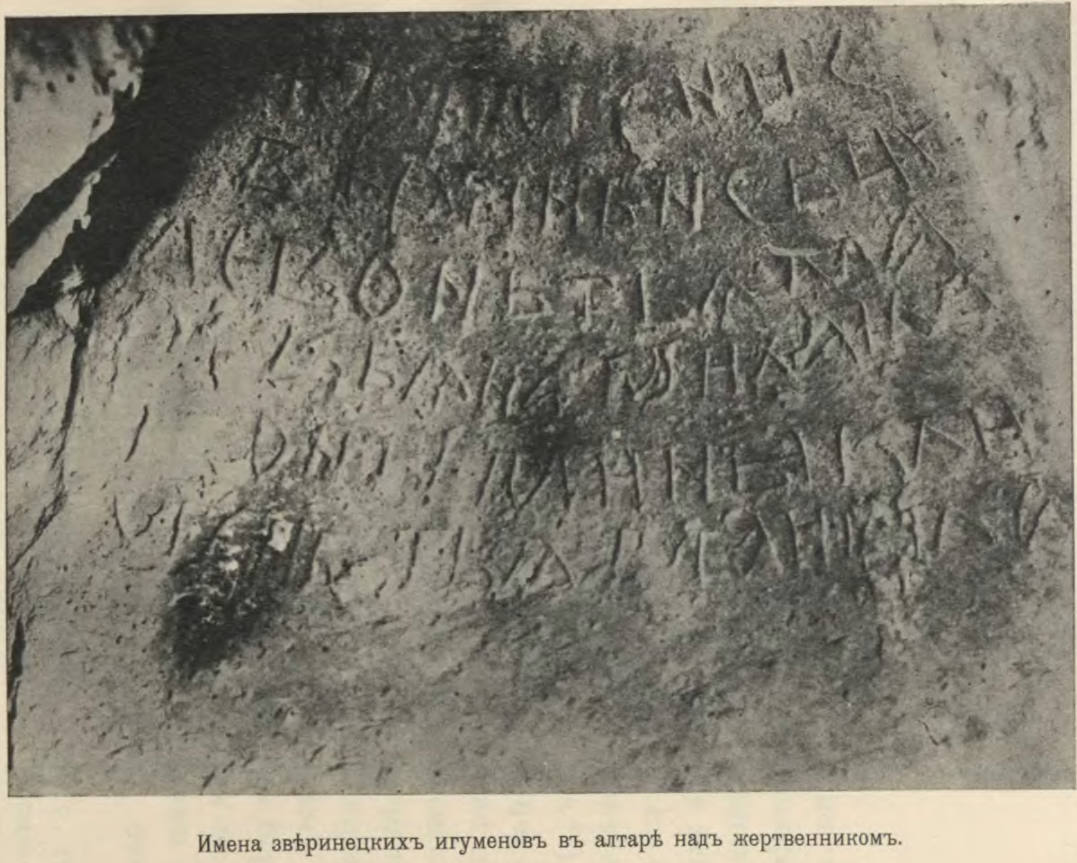
\includegraphics[width=\linewidth]{chast-colebanie-osnov/nachalo/zverp-04.jpg}
\end{center}

\vspace*{\fill}

\newpage

\begin{center}
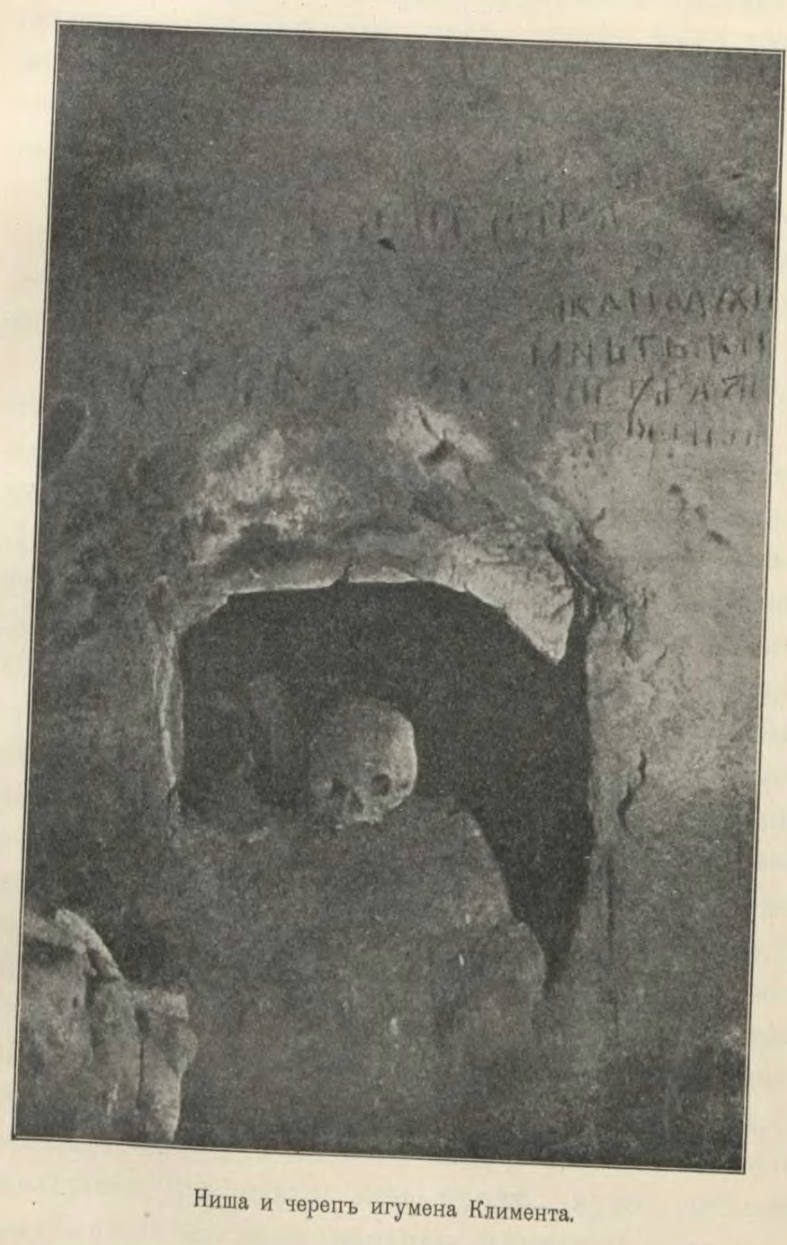
\includegraphics[width=0.95\linewidth]{chast-colebanie-osnov/nachalo/zverp-05.jpg}

\textit{Обратите внимание на соотношение глазных впадин к черепной коробке. У взрослого обычного человека черепная коробка – меньше.}
\end{center}

Что же, мы рассмотрели все надписи в пещерах. Негусто, ежели пещера использовалась людьми по крайней мере в 10, 11 и 17 веках, и если допустить, что пещера 30 лет посещалась досужими людьми, а также была наводнена зеваками в 1882 и 1888 годах.

Николай Петров задался вопросом – а так ли стары надписи на стенах?

\begin{quotation}
Некоторые из этих надписей появились, так сказать, на наших глазах, и появлялись они как бы по мере надобности в них. [...]

Далее, все подписи в новооткрытых Зверинецких пещерах начертаны одинаково, как бы рукой одного человека, – как признают это и Эртель, и г. Каманин.
\end{quotation}

Я опускаю доводы Петрова в пользу подделки надписей – желающие прочтут сами в его книжке. Не могу судить, насколько они справедливы, их нельзя однозначно ни подтвердить, ни опровергнуть. Если у нас есть выцарапанная на суглинной стене надпись, невозможно точно судить о времени ее создания, разве что по сохранности и другим надписям получится распознать, какие сделаны раньше, а какие позже.

Так что же думать? 

Все надписи были подлинно старинными, допустим 11 века? Подлинными была часть надписей, а остальные – поддельными? Все надписи, упомянутые Каманиным – подделки? Если да, то разве стены могли быть чистыми? Может, на них существовали какие-то другие граффити, а их уничтожили и написали новые, придумав для пещер историю?

А как датировать другие найденные там предметы, те же пояса?

Кожаный пояс с точно такими, как на зверинецких поясах, тиснёными иконками и надписями был в саркофаге княгини Евдокии Донской (вдовы Дмитрия Донского) в основанном ею Вознесенском монастыре московского Кремля. Княгиня была похоронена в 1407 году, но ведь могла носить пояс, уже в то время считавшийся древним.

Вот часть этого пояса – посередине изображены сцены Воскресения и Вознесения, с подписями (тоже в рамках) слева от каждой иконки:

\begin{center}
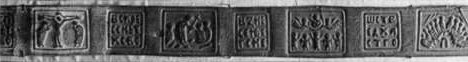
\includegraphics[width=\linewidth]{chast-colebanie-osnov/nachalo/tis02.jpg}
\end{center}

А вот часть зверинецкого – те же самые сцены:

\begin{center}
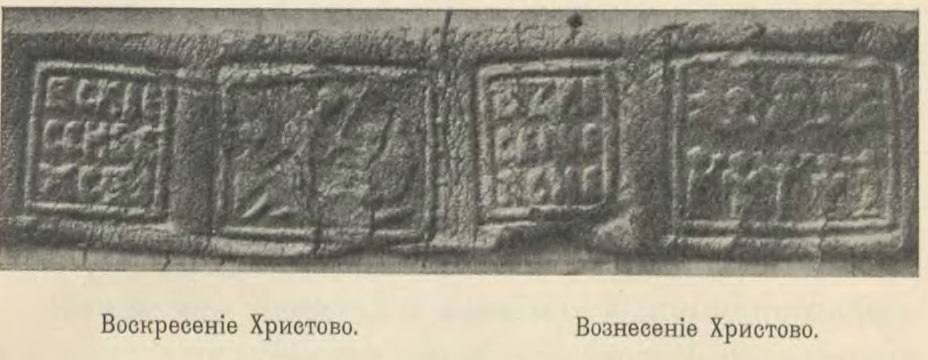
\includegraphics[width=\linewidth]{chast-colebanie-osnov/nachalo/tis01.jpg}
\end{center}

Такие же иконки (я говорю о точном подобии) тиснились на параманды – прямоугольные кожаные штуковины, носимые монахами на груди. Параманд с иконками как на «зверинецких» поясах был найден в княжеском саркофаге захоронения 14 века в 1836 году при ремонте Спасо-Преображенского на Бору собора Московского Кремля. Там же был и кожаный пояс.

Значит, по крайней мере на рубеже 14-15 веков люди носили религиозные изделия с тиснением, выполняемым одинаковым штампом. Не знаю, в разных ли местах делали эти пояса и параманды, или в одном и потом распространяли по Руси, и с какого века по какой. Определение нижней временной границы позволило бы понять, с какого времени эти пояса могли попасть в Зверинецкие пещеры.

\begin{center}
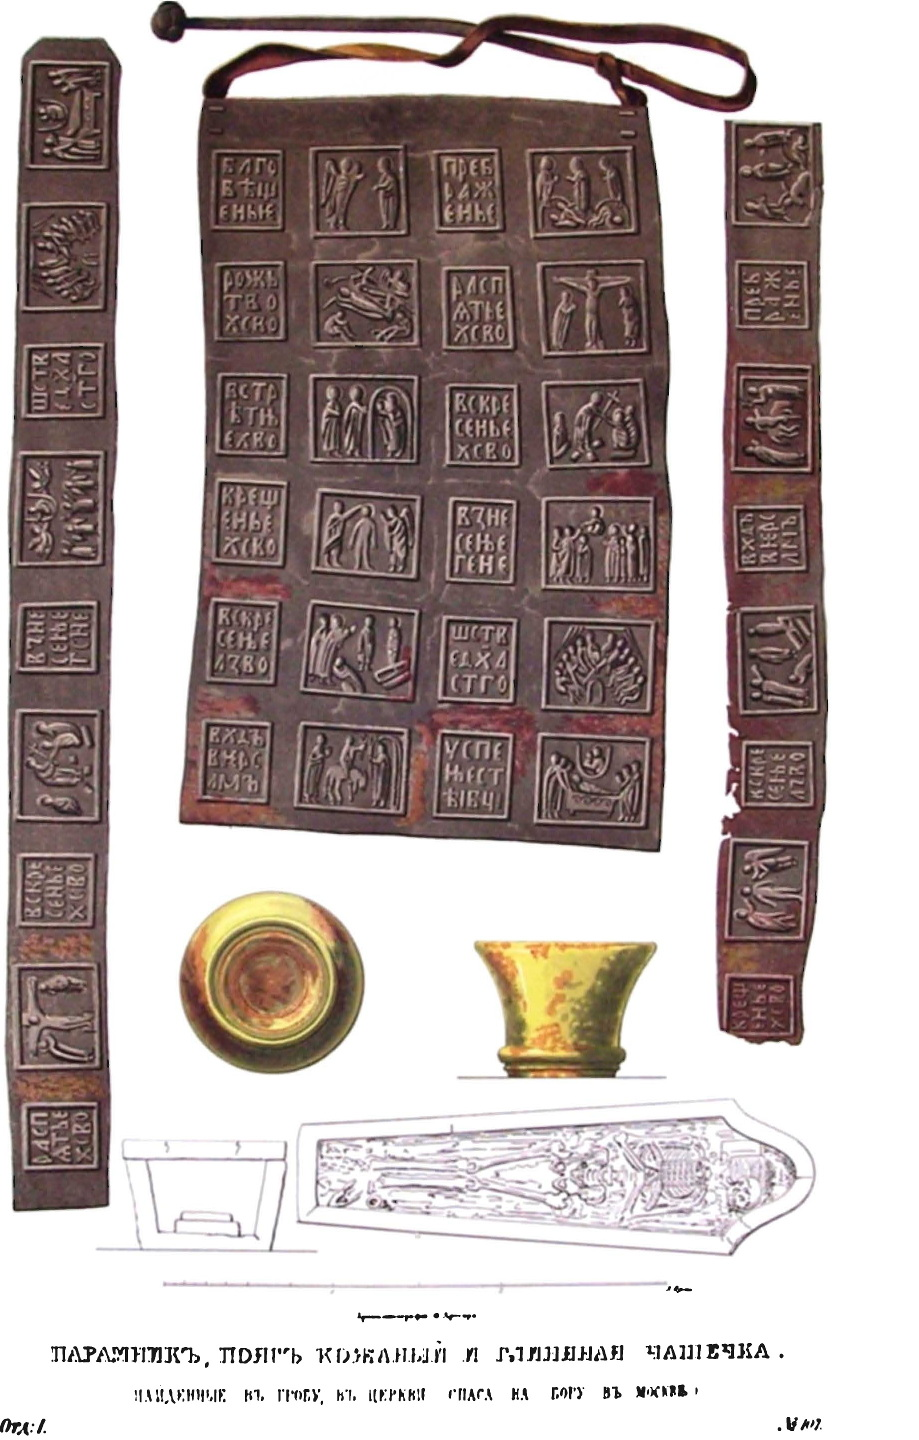
\includegraphics[width=0.94\linewidth]{chast-colebanie-osnov/nachalo/s-Drevnosti_RG_v1_ill108.jpg}
\end{center}

\textit{Из Спасо-Преображенского собора на Бору. Рисунок Фёдора Григорьевича Солнцева из книги «Древности Российскаго государства», отделение II, 1851 год.}

\newpage

%zver-pred.jpg

%Достаточно хорошо сохранились плетеные из кожаных ремешков кресты, и части поясов с выдавленными на них библейскими сценами. 

А на груди «игумена звериньского» Климентия, а точнее тела, лежащего в его поименованной нише, нашли кипарисовую (по словам Каманина) панагию – образ Богоматери с изображениями на обеих сторонах. Но панагию носили архимандриты, не игумены. Сана архимандрита вроде не было во время, к которому относят Зверинецкие пещеры.

Каманин, разбирая надпись на панагии, пришел к выводу, будто принадлежала она «Михаилу-сирину», первому киевскому митрополиту Михаилу, который, по Никоновой летописи и Степенной книге, пришел вместе с Владимиром крестить Русь и коему многие историки отказывают в существовании – мол, не было такого митрополита. Каманин же считал, что Михаил похоронен именно в Зверинецких пещерах, вероятно в «первых», открытых в 1882 году.

Николай Петров осматривал панагию и пришел к выводу, что она вовсе не кипарисовая, а оттиснута штемпелем на куске распаренного воловьего рога, и прочитал на ней первые две строчки стиха, составленного, по словам профессора, не ранее 17 века и написанные гражданским шрифтом не ранее 18 века. «Ни о каком митрополите Михаиле Сирине не может быть и речи», – заключил Петров.
\vspace*{\fill}
\begin{center}
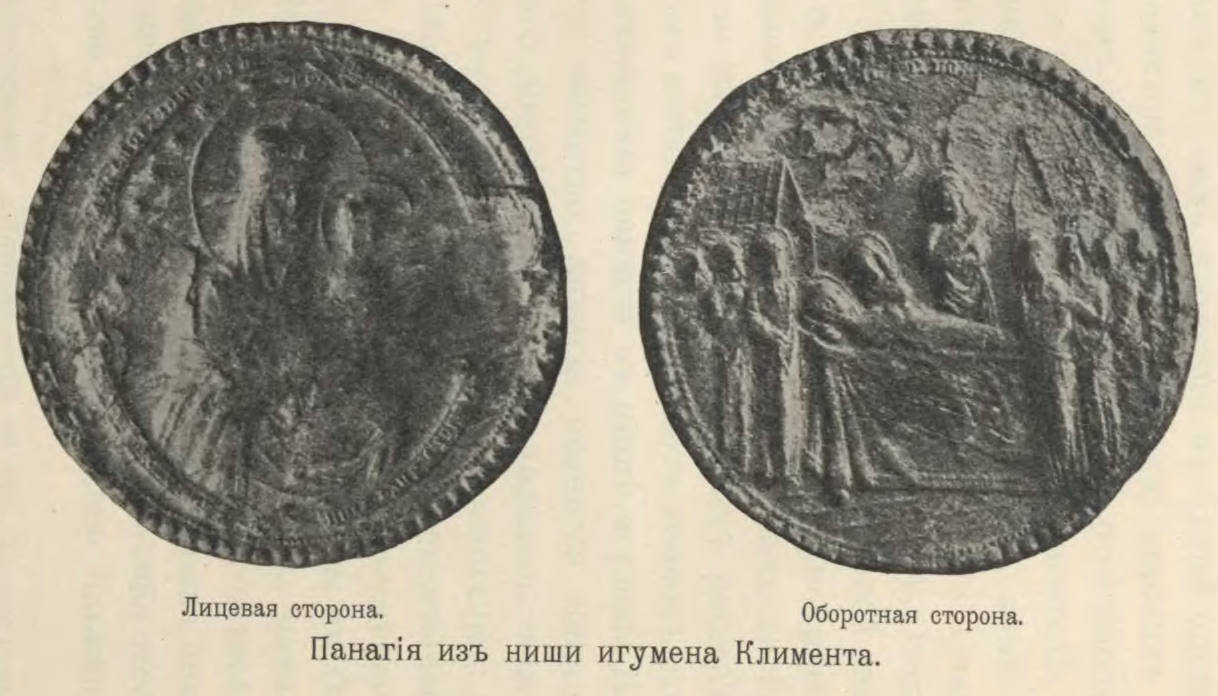
\includegraphics[width=\linewidth]{chast-colebanie-osnov/nachalo/panagia.jpg}
\end{center}
\vspace*{\fill}
\newpage

\begin{center}
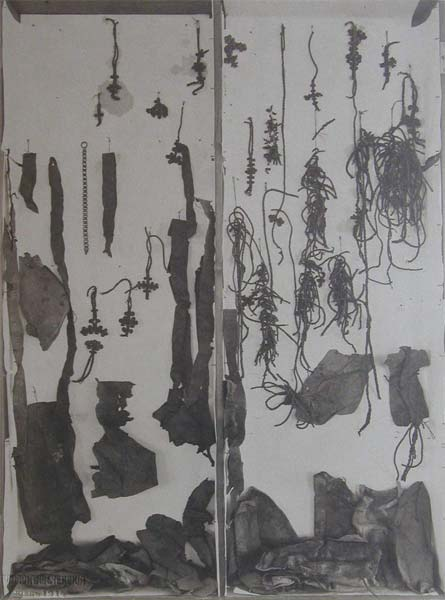
\includegraphics[width=\linewidth]{chast-colebanie-osnov/nachalo/zver-pred.jpg}
\end{center}

\textit{1914 год. Выставленные для паломников, как находки из пещер, предметы старины.}

Сомневался Петров и в древности главной находки, иконы, которую обнаружили в нише Климентия. Икона овальная, на толстой железной пластинке, покрытой эмалью, поверх которой уже писалось красками.

%У Каманина в книге, на фотографии икона выглядит иначе. 

Со времен тех дореволюционных считается, что это Одигитрия («Путеводительница») – изображение Богородицы с младенцем Христом на левой руке. Вот только нарисованное здесь далеко отлично от большинства подобных икон. Нет присущей Одигитрии сокращенной подписи «Митир Фэу Иисус Христос» («Матерь Божья Иисус Христос»). Нет нимбов. Реалистичная манера в изображении фигуры и одежды маленького. И у него странное лицо! Течение времени, повреждения краски? Да не так уж она и повреждена. Вот дореволюционный снимок:

\begin{center}
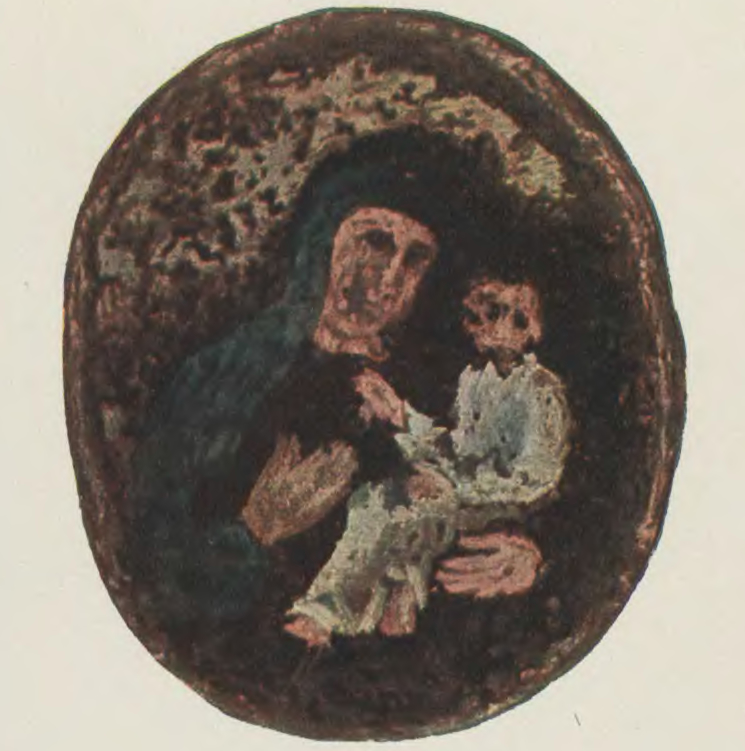
\includegraphics[width=\linewidth]{chast-colebanie-osnov/nachalo/zver-ikon.jpg}
\end{center}

Не послужит ли загадочная икона ключом к разгадке тайны Зверинецких пещер? А ведь эта икона была, коли прав Каманин, одной из древнейших славянских икон, дошедших до 20 века. Если не самой древней. 

%Нет на ней и присущей Одигитрии надписи вида: 

%\begin{center}
%\includegraphics{osn-kiev/odigitria-nadpis.png}
%\end{center}

В 1934 году, когда скит над пещерами (имевший адрес Ломаковская, 12) закрыли, икона исчезла. В разных источниках можно прочитать, что эта же икона была «чудесно обретена» в 2000-м году. Однако нашли, в 1999 году, в церкви села Селище Барышевского района, только серебряный оклад от иконы, подаренный в свое время Жеваховым.

А новую икону нарисовал в 2000 году художник А. Вовченко по дореволюционному снимку, причем с отличиями от него. Эту-то современную икону в окладе начала 20 века показывают теперь в Святотроицкой церкви Ионинского монастыря.
  
\begin{center}
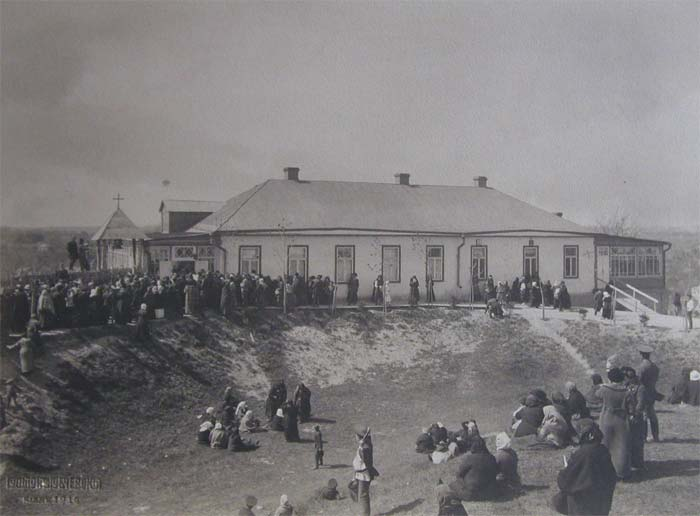
\includegraphics[width=\linewidth]{chast-colebanie-osnov/nachalo/1914-kresthod.jpg}

\textit{Окрестности Зверинецких пещер в 1914 году во время крестного хода сюда из Лавры. Возможно, фотограф стоит спиной к склону с пещерой, лицом к улице Ломаковской (Мичурина).}
\end{center}

%Пишу «Климента», а ведь надобно принять во внимание, что мы судим по найденным в пещерах надписях – а время их обнародования совпадает с раскопками Эртеля. Там был список игуменов, некоторые другие надписи, в частности две около ниши, которую сопоставили с Климентом. Надписи, по мнению Эртеля и Каманина, были древними, эдак 11 века – собственно Каманин в книге своей пытается навести мосты между летописями и списком зверинских игуменов. 

%Подвергая сомнению давность панагии и образа Богородицы, 

После открытия Зверинецких пещер 1911 года, около них создали подчиненный Лавре скит на 40 монахов и возвели церковь во имя Рождества Пресвятой Богородицы с боковым пределом, посвященным св. Иоасафу, чудотворцу Белгородскому – тому самому родичу князя Жевахова.

Предводительствовал отец Валентин (Коротенко), перешедший сюда игумен Ионинского монастыря. Валентин одолжил у Жевахова подъемные деньги, 1700 рублей и стал принимать вклады от желавших поселиться при строящейся обители. Доход приносили и паломники.

Деятельность братии и богомольцев привела к тому, что пещеры начали осыпаться. В 1913 году раскопки приостановили. Между тем продолжали впускать паломников. 

\begin{center}
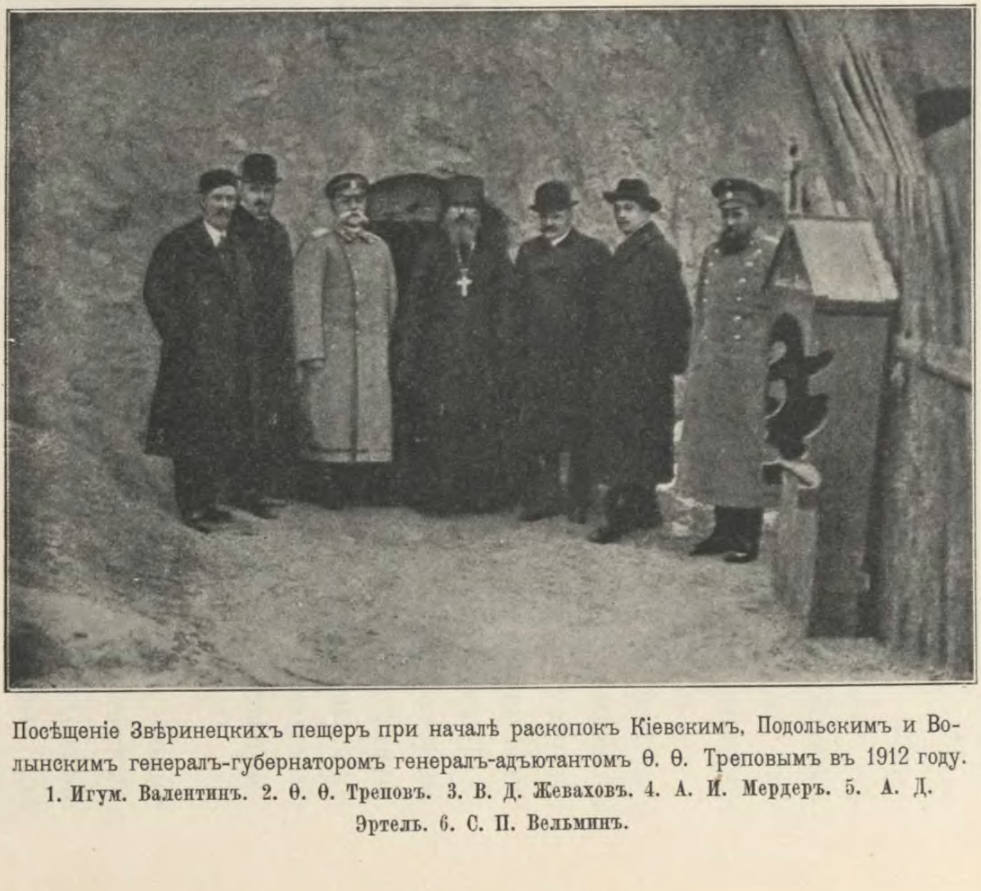
\includegraphics[width=\linewidth]{chast-colebanie-osnov/nachalo/zverp-06.jpg}
\end{center}

В 1914 году Эртель настаивал на закрытии пещер для паломников, чтобы не усугублять. И казалось бы настоял, да вышло иначе. Валентина отстранили, что, впрочем, не могло вернуть пещеры в первоначальное состояние. 

\newpage
\vspace*{\fill}
\begin{center}
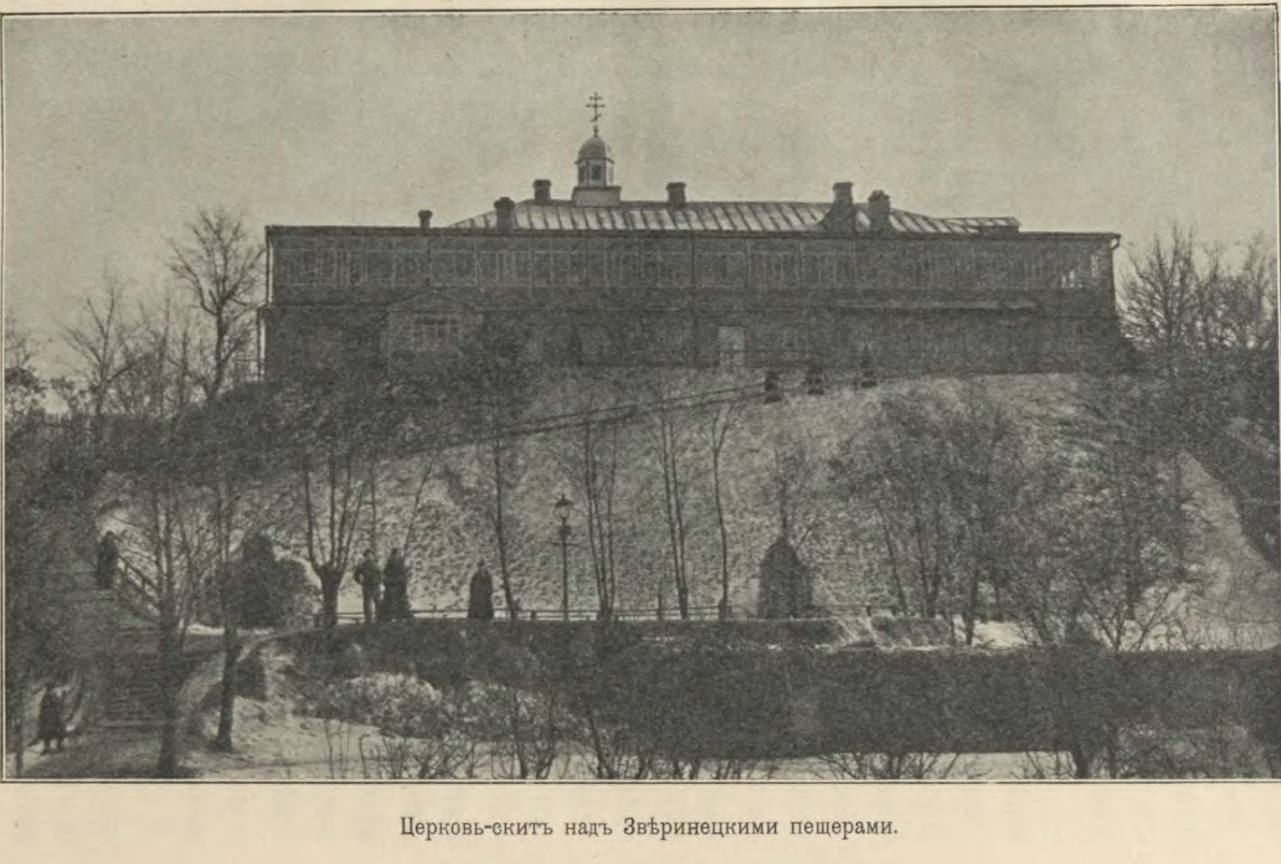
\includegraphics[width=\linewidth]{chast-colebanie-osnov/nachalo/zverp-01.jpg}
\end{center}

\begin{center}
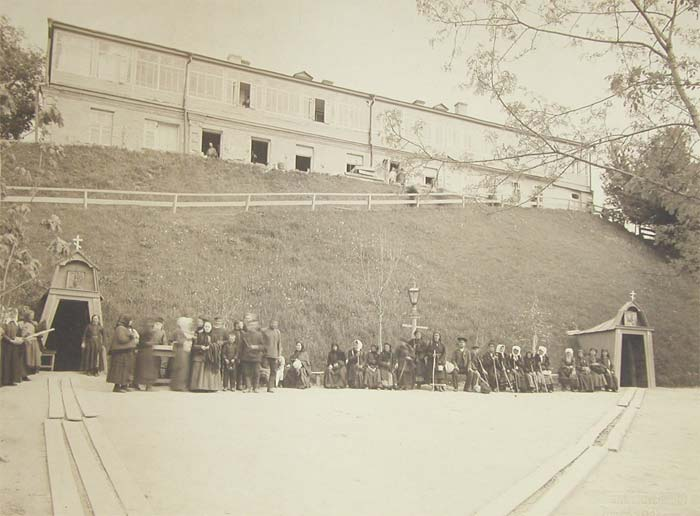
\includegraphics[width=\linewidth]{chast-colebanie-osnov/nachalo/1914-szap.jpg}

\textit{Там же, тоже вид с запада. Наверху нынче ботсад.}
\end{center}
\vspace*{\fill}
\newpage

При временном духовном безначалии – читай, при Жевахове – в 1915 году, по причине возведенного сверху подземелья храма, часть пещерных ходов укрепили оштукатуренным кирпичом, другую часть – досками. Затем скит перешел под управление иеромонаха Никанора, с которым даже Жевахов не сумел договориться о продолжении археологических работ и ремонте пещер. 

\begin{center}
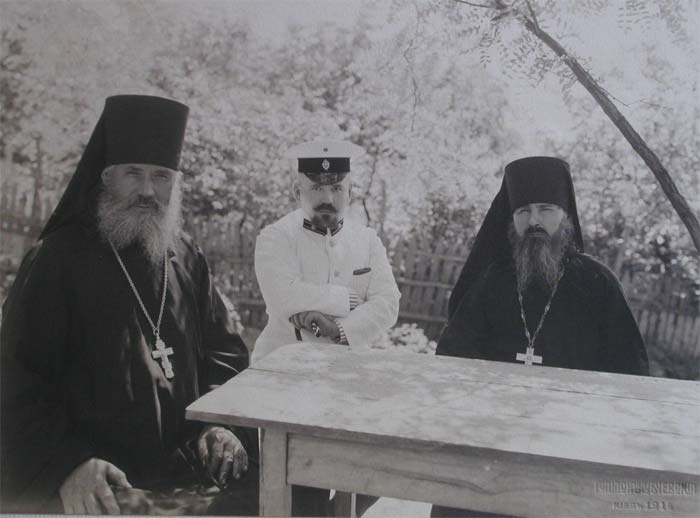
\includegraphics[width=0.90\linewidth]{chast-colebanie-osnov/nachalo/1914-nikanor.jpg}

\textit{1914. Слева направо: Никанор, Жевахов, Валентин.}
\end{center}

Разве что в 1917 году, когда очередной участок пещер стал совсем уж аварийным, Никанор разрешил позаботиться о подземельи, но с пользой для скита, дабы впридачу починили крышу надпещерной церкви. В том же году в Зверинецких пещерах похоронили отца Валентина.

Еще один удар по пещерам нанес в 1918-м\footnote{В 1918 году скит вышел из ведомства Лавры и перешел к монастырю в Церковщине (куда в марте, опасаясь большевиков, с братом Николаем скрылся Владимир Жевахов, к августу того же года впрочем ставший чиновником по особым поручениям при Министерстве внутренних дел правительства гетмана Скоропадского), а в 1925-м обрел самостоятельность.} взрыв летом пороховых складов Зверинецкой крепости, обваливший часть коридоров. Скит на поверхности тоже потерпел разрушения. Несколько позже взамен прежней церкви построили новую, в честь иконы Богоматери «Всех скорбящих радость». В окрестностях при взрыве открылись еще два пещерных хода.

В то время Киев был под немцами и гетмане Скоропадском. Его правительство сразу после взрыва объявило, что построит на разрушенном Зверинце свой центр, состоящий из Сейма, Сената, Генштаба, зданий 12 министерств.

Осенью 1918 года известному спелеологу и археологу, кстати выпускнику Киевской Духовной Академии, Игнатию Яковлевичу Стеллецкому\footnote{Большую книгу Стеллецкого «Подземный СССР» так и не издали. Впрочем опубликованы другие его работы о подземельях, среди них книга, посвященная поискам библиотеки Ивана Грозного.} поручили провести исследование подземных пустот Зверинца – выдержат ли навалившуюся власть? Стеллецкий подбирался к здешним пещерам еще в 1913 году, но Эртель не захотел тогда сотрудничать. И вот в январе 1919 года Стеллецкий приступил к работе. В марте привлек к раскопке и Эртеля, которого год назад завалило под землей на Ломаковской, с повреждением таза, руки и переломом ноги. Кажется, Стеллецкого больше заботила не застройка Зверинца, а сами пещеры. Он писал:

\begin{quotation}
В археологическом отношении встала передо мной тяжелая, значительная и в полной мере интересная задача – доказать, что открытые уже пещеры на Зверинце есть только продолжение катакомб старинного пещерного Выдубицкого монастыря непосредственно соединенного подземными нитками – соединениями с современным наземным Выдубицким в такой же мере, как так называемые Ближние или Дальние пещеры с Печерской Лаврой.
\end{quotation}

Также, Стеллецкий считал, что все эти пещеры были вырыты еще в неолит, а монахи лишь приспособили их под свои нужды.

Дневники раскопок и статьи Стеллецкого хранятся в Российском государственном архиве литературы и искусства, 208 листов, посмотреть их у меня нет возможности. Сведения о них черпаю только из сторонних, зачастую отрывочных источников.

%Стеллецкий взялся исследовать один из возникших после взрыва провалов, что вёл в древнюю пещеру с шаровидной комнаткой, где было «детское погребение» и лежали плиты сланца, древние плоские кирпичи – плинфы, еще какие-то предметы будто великокняжеских времен. Наверх от комнатки, в сторону Зверинецких пещер шел коридор с боковыми нишами, в коих тоже были захоронения. Получается, этот провал был ниже по склону, чем Зверинецкие пещеры 1911 года.

%Другой провал, около Экономических ворот Троицкого монастыря\footnote{Я не знаю, где они находились. Экономические ворота в монастыре обычно ведут к экономическому двору, и приспособлены для проезда через них с возами. О прошлом монастыря приходится судить лишь по фотографиям, ибо документация его сгорела при памятном взрыве Зверинецкой крепости.}, явил подземелье со стенами, обшитыми истлевшими досками. Его расчистили на 21 метр. Вход туда был размыт водой. Назначение сего помещения не определили. Ни среди обычных монашеских пещер, ни крепостных подземных коридоров – потерн, с таким не сталкивались.

Вот в заметке «К истории раскопок пещер
на Зверинце в Киеве (по поводу застройки Зверинца)» Стеллецкий писал (примечания по ходу мои):

\begin{quotation}
А раз так, то окончательно загадочным является подземелье, обнаруженное котлованом возле
Экономических ворот Троицкого монастыря\footnote{Я не знаю, где они находились. Экономические ворота в монастыре обычно ведут к экономическому двору, и приспособлены для проезда через них с возами. О прошлом монастыря приходится судить лишь по фотографиям, ибо документация его сгорела при памятном взрыве Зверинецкой крепости.}.
Раскопки его дают пока такую картину.

Провал образовался в своде какого-то высокого\footnote{Какова же высота?} подземного помещения, может быть, имевшего здесь входной люк. На глубине 12–13 арш\footnote{8,53-9,26 м.}.
обозначился широкий, до 3 арш.\footnote{2,1 м.}, коридор, направлением к югу, суживающийся к полу, подобно зверинецкой пещерной церкви и расширяющийся в боках. 

Самый коридор постепенно суживается вперед и опускается вглубь. Затянут он плотно илом от стремительно затекавшей сюда воды, срывавшей разной величины доски\footnote{Обшитый досками подземный ход Стеллецкий раскапывал и за 5-й гимназией, это сейчас Суворова, 1.} и бревна, которыми был обшит ход, то и дело попадающихся в разных слоях и на разной высоте намула.

Собственно над полом нанос не добирается
вершка на два, с целью не натаптывать, а доследовать пол особо. Свод коробовый, обработан небрежно и грубо.

Может быть, в дальнейшем ход примет нормальную ширину, но пока в этом отношении он выходит из рамок всего, что мне до сих пор приходилось встречать.

А. Д. Эртель склоняется к мысли, что это -
«паттерна» – стратегический ход. Я лично этого не думаю, так как считаю, что он для этого без нужды глубокий.

Я наблюдал в Пернове кавалерийский подземный ход: он, высокий, обложенный камнем, шел сквозь вал и, не выходя из последнего, поворачивал под прямым углом вправо, шел несколько вдоль вала и затем выходил в овраг с противоположной стороны.

Образчик стратегического пехотного хода
представляет выложенный местным камнем ход вокруг крепостной стены в Пскове. Внутри этого хода характерны слухи – углубления в своде, через которые слышен наружный разговор. Само собою разумеется, что и самый ход для этого был заложен не глубоко от поверхности, всего на 1 сажень. Типичные же образчики собственно «паттерн» имеем в укреплениях на Лысой Горе, где «паттерны» проходят в валах, почти не углубляясь в материк.

Зверинецкий новооткрытый ход как нельзя
более далек от этих образчиков стратегических ходов. Он есть какая-то новая разновидность в категории таинственных подземных памятников и потому вдвойне интересным представляется его дальнейшее исследование.

Другой котлован, на противоположном конце
«Укрепления»\footnote{Как понимаю, речь идет о Зверинецкой крепости и той ее части, что от современного Розария протянулась к перекрестку, где спуск в Сиреневую аллею и дорога к Ионинской церкви. Возможно, где-то в окрестностях этой точки – 50°25'02.6"N 30°33'41.2"E.}, близ разрушенной церкви скита, на глубине около 13–14 арш. дал погребение младенца с инвентарем X–XII вв.\footnote{В другом источнике упомянута – пещера с шаровидной комнаткой, где было «детское погребение» и лежали плиты сланца, древние плоские кирпичи – плинфы, еще какие-то предметы будто великокняжеских времен.}, а вслед затем, в с.с. углу стены найдены были признаки обрушившейся пустоты, другими словами, опадающий глыбами свод какого-то подземелья.

Прокопаться в это подземелье будет легче первого, потому что оно совершенно сухое и не затянуто илом; пустота должна открыться немедленно.

Открыто на днях и еще одно подземелье,
вернее, целый лабиринт, пока, однако, не исследованный – в Троицком монастыре.
В свое время оно раскапывалось любителем-иноком, но потом засыпанная часть коридора была заложена кирпичом, а вычищенная обращена под монастырский погреб\footnote{Не о пещере ли под склоном с колокольней идет речь? Так значит, там был целый лабиринт?}.

Наконец, в Выдубицком монастыре, на подворье, соединяющем Выдубицкий монастырь через Троицкий со Зверинецким акрополем, старик-монах, правда безуспешно, пытался показать место хода, который он наблюдал здесь лет 40 тому назад.

Эти данные еще более утверждают меня в
мысли, что Выдубицкий монастырь связан подземными артериями со Зверинецкими катакомбами. 

Киев. 1919.IV.12. Игн. Стеллецкий
\end{quotation}

Стеллецкий собирался продолжать археологические работы. Застройка Зверинца тормозилась, а потом власть переменилась и вопрос отпал. Чем завершились исследования Стеллецкого, я не осведомлен.

Скит на Зверинце продолжал существовать и паломники посещали пещеры. В 1924 году Жевахов принял в скитской церкви монашество как Иоасаф, два года жил в близлежащем Ионинском монастыре, а в 1926 перебрался в Зверинецкий скит и получил сан епископа. Последующие 11 лет, с перерывами – лагерь, ссылка, тюрьма – и так до расстрельного приговора тройки при УНКВД по Курской обл. 04/12/1937 по обвинению в «руководстве контрреволюционной фашистской организацией церковников». Приговор был исполнен в тот же день.

В 1934 году скит закрыли, постройки со временем разобрали. В 1980-х я нашел на его месте дореволюционный кирпич, кажется с клеймом «Х.ВОЛКОВЪ».

В 1965-м в Зверинецких пещерах провели археологическую разведку, о которой я знаю только, что исследователи установили, будто во время фашистской оккупации в пещерах прятались люди. В том же 65-м исторический памятник получил охранный паспорт\footnote{
\begin{quotation}
Взято під охорону згідно постанови Ради Міністрів УРСР № 711 від 21.07.1965 р.

Охоронний №: 139

Межі охоронної зони і зони регулювання забудови: згідно рішення виконкому Київської міської Ради народних депутатів № 920 (додаток І, п. 1, 2, 3) Звіринецькі печери входять в зону археологічного заповідника (р-н Видубицького монастиря та Звіринецькі печери). 
\end{quotation}

В указанном постановлении 711 в разделе III «ПАМ'ЯТНИКИ АРХЕОЛОГІЇ», под номером 
139 указаны «Звіриницькі печери, Печерський район, Звіринець» – с примечанием «з настінними написами (XI-XIII ст. ст.)». Постановление было отменено 03 сентября «Постановой КМ № 928 (928-2009-п)», и тогда же пещеры занесли в новый реестр, Государственных недвижимых памятников Украины, как объект культурного наследия под номером 260034-Н – археологический памятник 11-17 веков, по адресу Мичурина 18-22.}, переоформленный в 2009 уже для нового реестра.

В 1979 году пещеры посетили археологи из Киевской лаборатории спелеологических исследований. Тогда-то, надо полагать, и передвинули будку нужника в сторону от входа в подземелье.

На сегодня определены – их приводят в книгах\footnote{Например, «Историко-градостроительные исследования Киева» под редакцией В. Вечерского, Киев, Феникс, 2012.} – границы зоны охраны культурного слоя первой категории вокруг памятника «Зверинецкие пещеры»:

%На сегодня определены границы зоны охраны культурного слоя первой категории вокруг памятника «Зверинецкие пещеры»:

\begin{quotation}
от пересечения ул. Мичурина и переулка Мичурина по правой стороне улицы Мичурина в юго-восточном направлении (до усадьбы № 28), оттуда в юго-восточном, юго-западном и северо-западном направлениях (территория Центрального ботанического сада им. М. Гришко НАН Украины) до пересечения с ул. Мичурина.
\end{quotation}

Попытайтесь наложить это описание на карту, и у вас ничего не получится, поскольку от пересечения улицы Мичурина с переулком можно двигаться по правой стороне только на северо-восток, а не на юго-восток.

В конце 20 столетия паломничество в пещеры возродилось, Музей Киева провел реставрационные работы, одновременно добиваясь отселения жителей из усадеб на Мичурина с номера 18 по 24, на четной, подгорной стороне.

В начале 21 века в усадьбе с пещерами, при созданном монастыре, возвели собор, а окрестности постигла тяжелая перестройка. На месте скромных стареньких домиков, белеющих через листву садов, огороженных кривыми заборами, вдруг возникли терема за крепостными стенами, коих устрашился бы сам Батый.

Летом 2017 года мы с Дашей Кононюк посетили Зверинецкие пещеры, побывали там впервые. За толстой, обложенной камнем стеной усадьбы – церковные здания, соединенные друг с другом и покрывающие склон. Двери, лестницы. Всё построено добротно и основательно. В церковной лавке мы разговорились со служителем церкви, который познакомил нас со священником. Тот любезно проводил нас в пещеру и рассказал много полезного. Если о нераскопанном ходе в сторону Ионинской церкви мы знали, то сведения про нераскопанный же ход в направлении Выдубицкого монастыря был новостью.

Дойдя с нами до половины пещеры, священник оставил нас одних и мы продолжили осмотр. Несмотря на жару снаружи, внизу было столь холодно, что изо рта шел пар.

Пещера основательно укреплена, местами оштукатурена. Высота потолков в коридорах, кроме одного места, более чем достаточна для прохождения посетителей, еще с запасом. Освещения не было, кроме взятого с собой – священник и Даша держали в руках свечи, а я фонарик.

Пустые комнатки (я избегаю слова келья, указывающее на место жительства монаха) по обеим сторонам коридоров ничем не защищены, а вот наполненные костями закрыты черными коваными решетками. Некоторые имеют длину явно меньшую, чтобы там лежа мог поместиться взрослый человек обычного роста. Даже если это чисто погребальные ниши, то для тела детского или подросткового роста.

Среди комнаток были такие, где можно находиться сидя. В одной по бокам было два «лежака», а между ними выемка.

Современные Зверинецкие пещеры я могу назвать, скорее, пещерами созданными недавно на основе древних пещер, поскольку от седой старины в нетронутом виде не осталось ничего. Да и сама окружающая местность преобразилась.

\vspace*{\fill}

\begin{center}
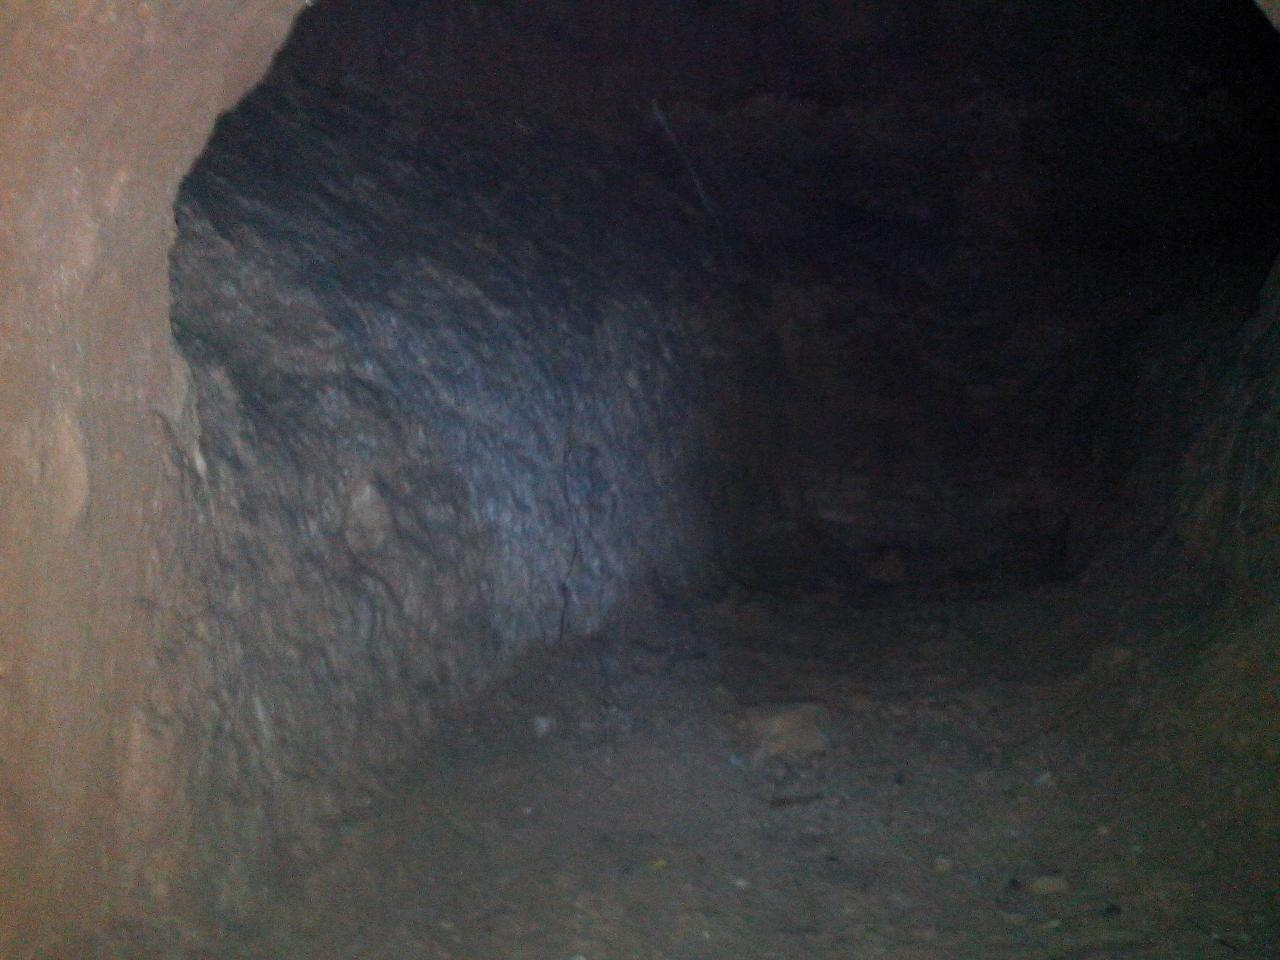
\includegraphics[width=0.98\linewidth]{chast-colebanie-osnov/nachalo/IMG_20170626_135030.jpg}

\textit{Комнатка с лежаками.}
\end{center}

\vspace*{\fill}


\newpage

\begin{center}
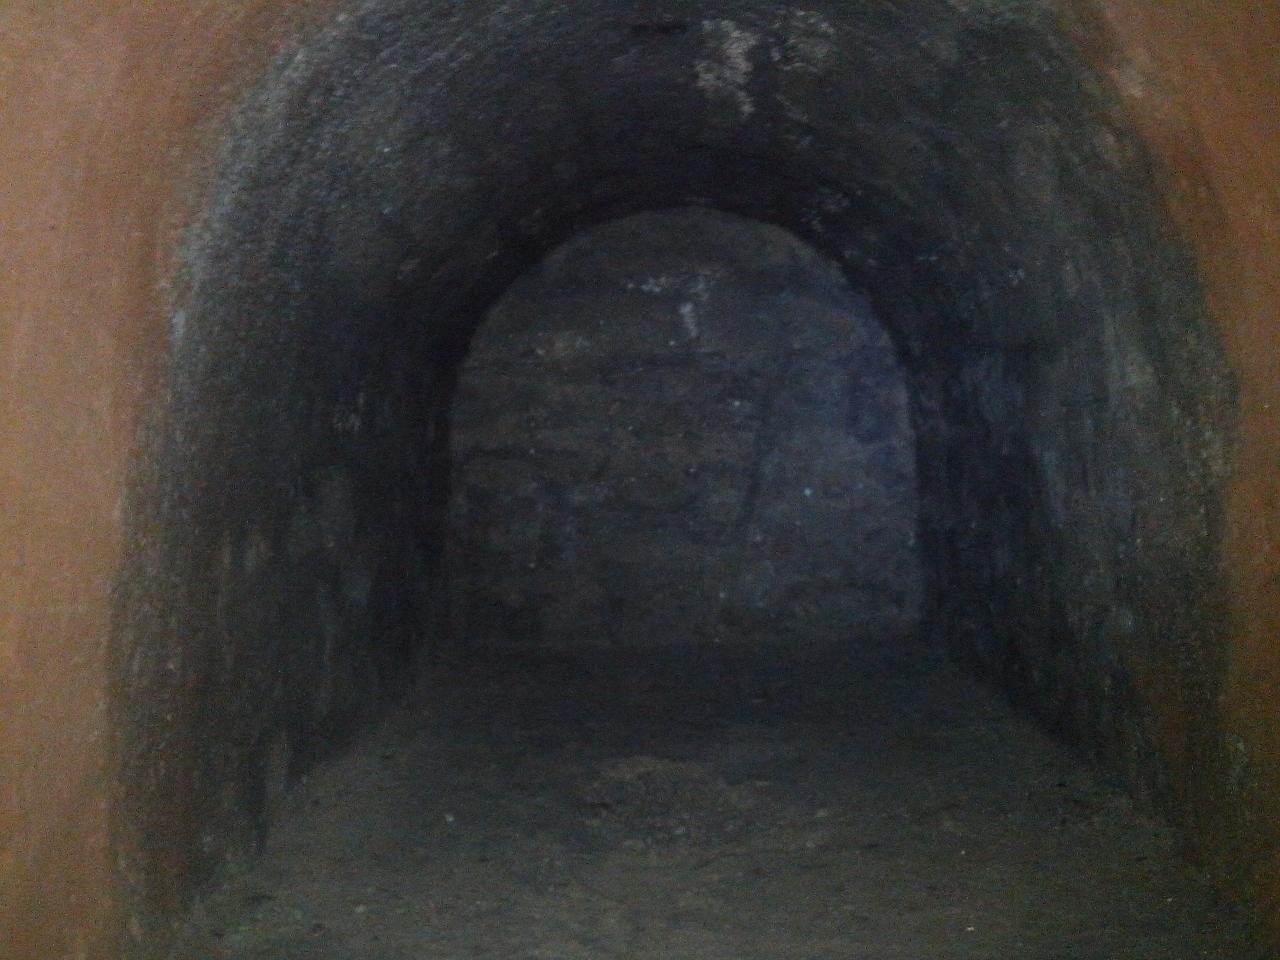
\includegraphics[width=0.98\linewidth]{chast-colebanie-osnov/nachalo/IMG_20170626_135106.jpg}

\textit{Одна из многочисленных «погребальных ниш» малой длины.}
\end{center}

\begin{center}
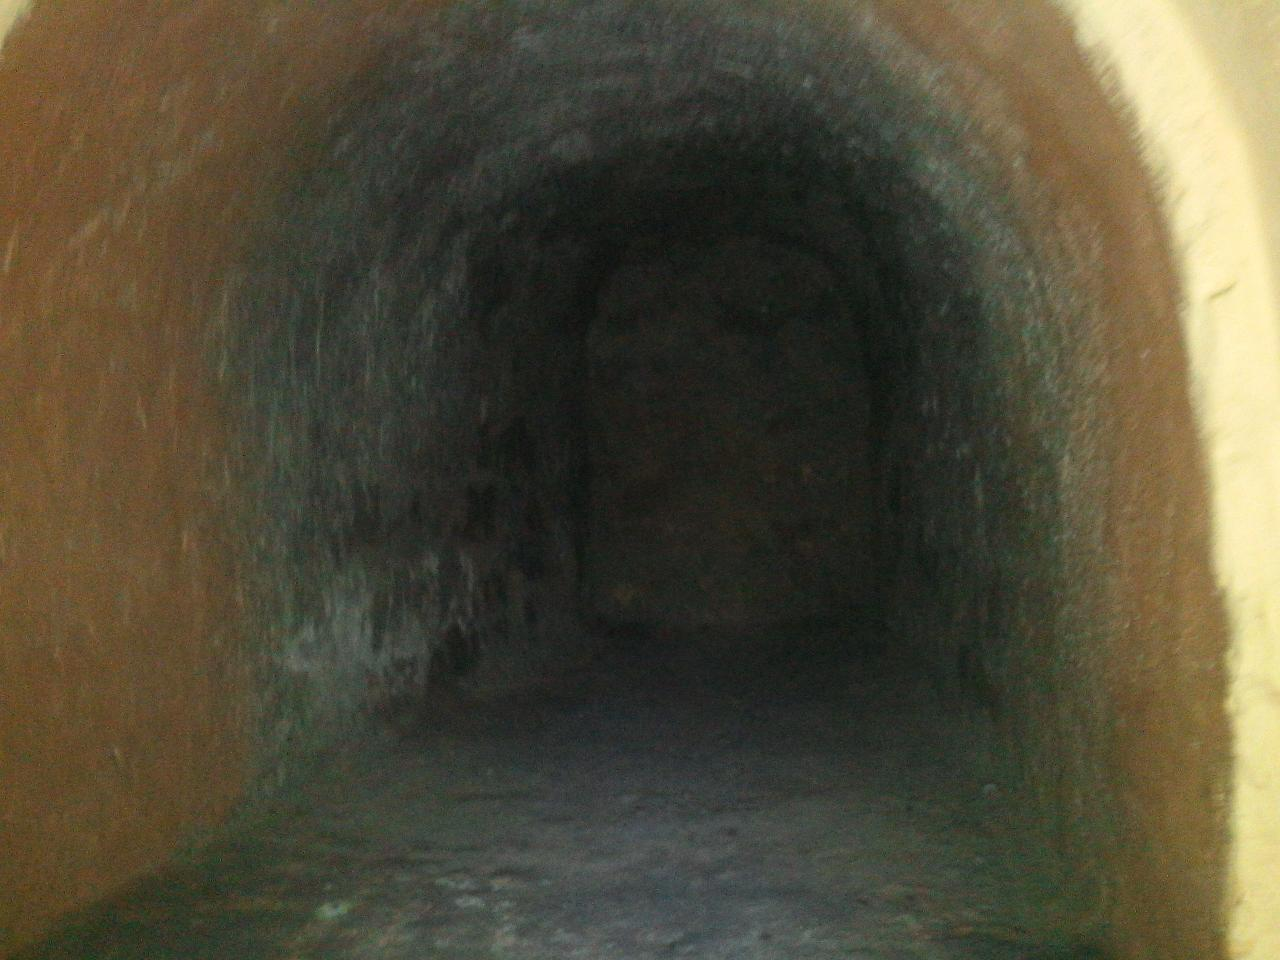
\includegraphics[width=0.96\linewidth]{chast-colebanie-osnov/nachalo/IMG_20170626_135152.jpg}

\textit{Еще одна.}
\end{center}

\newpage
\vspace*{\fill}
\begin{center}
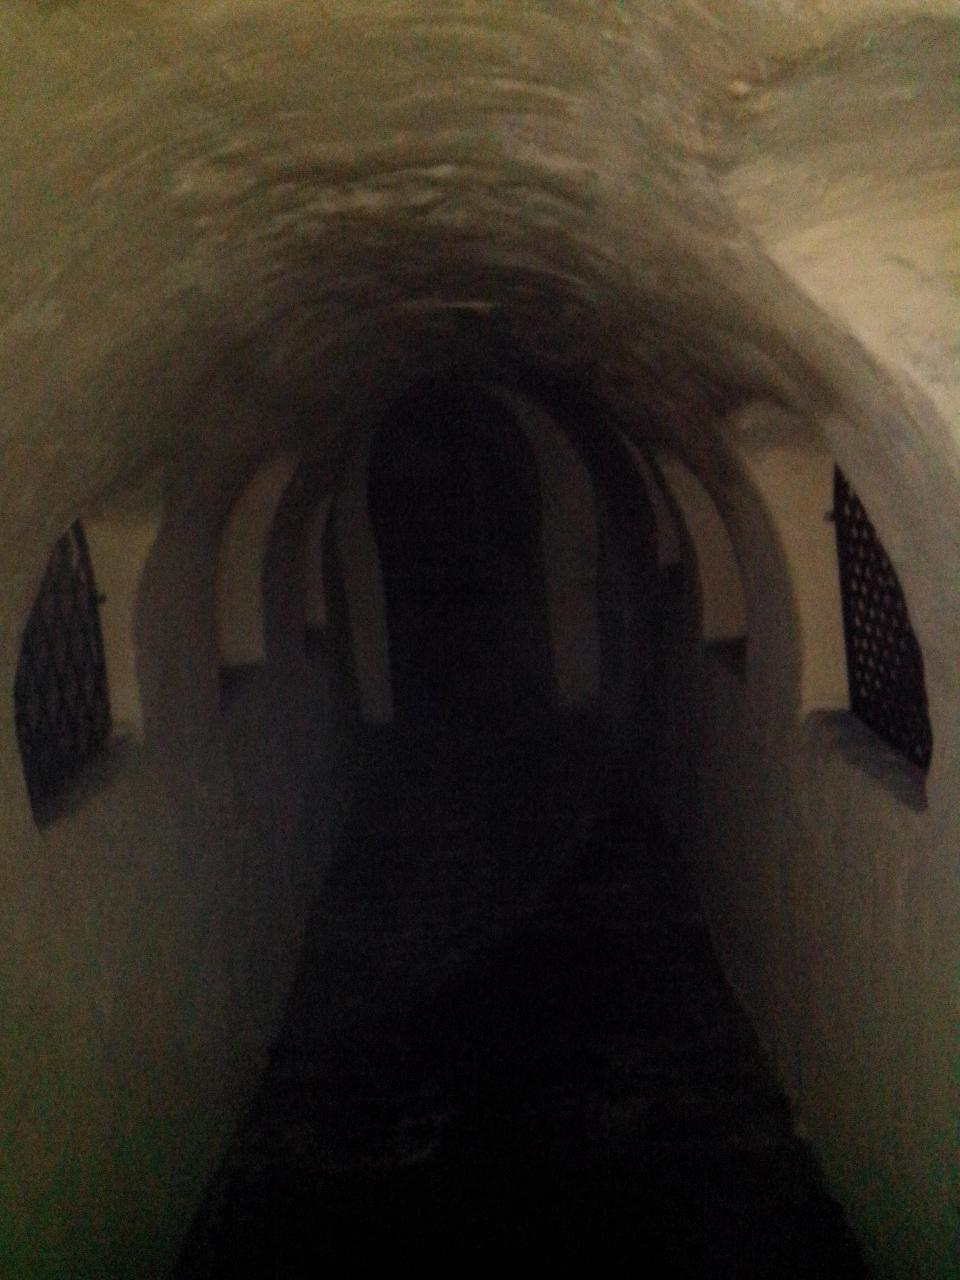
\includegraphics[width=\linewidth]{chast-colebanie-osnov/nachalo/IMG_20170626_135248.jpg}

\textit{Коридор с «погребальными нишами».}
\end{center}
\vspace*{\fill}

\newpage

\vspace*{\fill}
\begin{center}
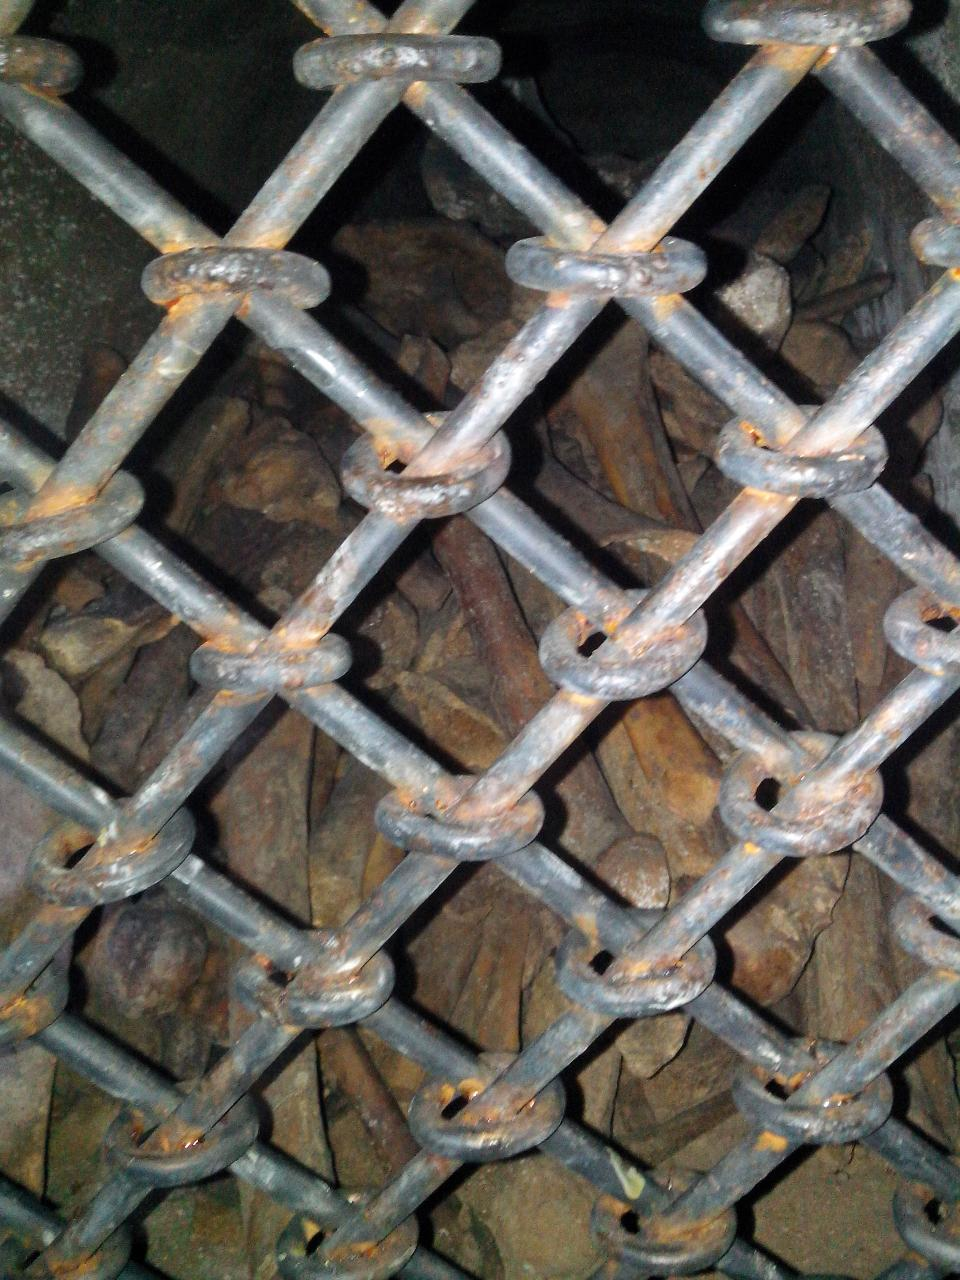
\includegraphics[width=\linewidth]{chast-colebanie-osnov/nachalo/IMG_20170626_135243.jpg}

\textit{Прах к праху. Чьи вы руки и ноги, как выглядели целыми во плоти?}
\end{center}
\vspace*{\fill}
\newpage
\vspace*{\fill}
\begin{center}
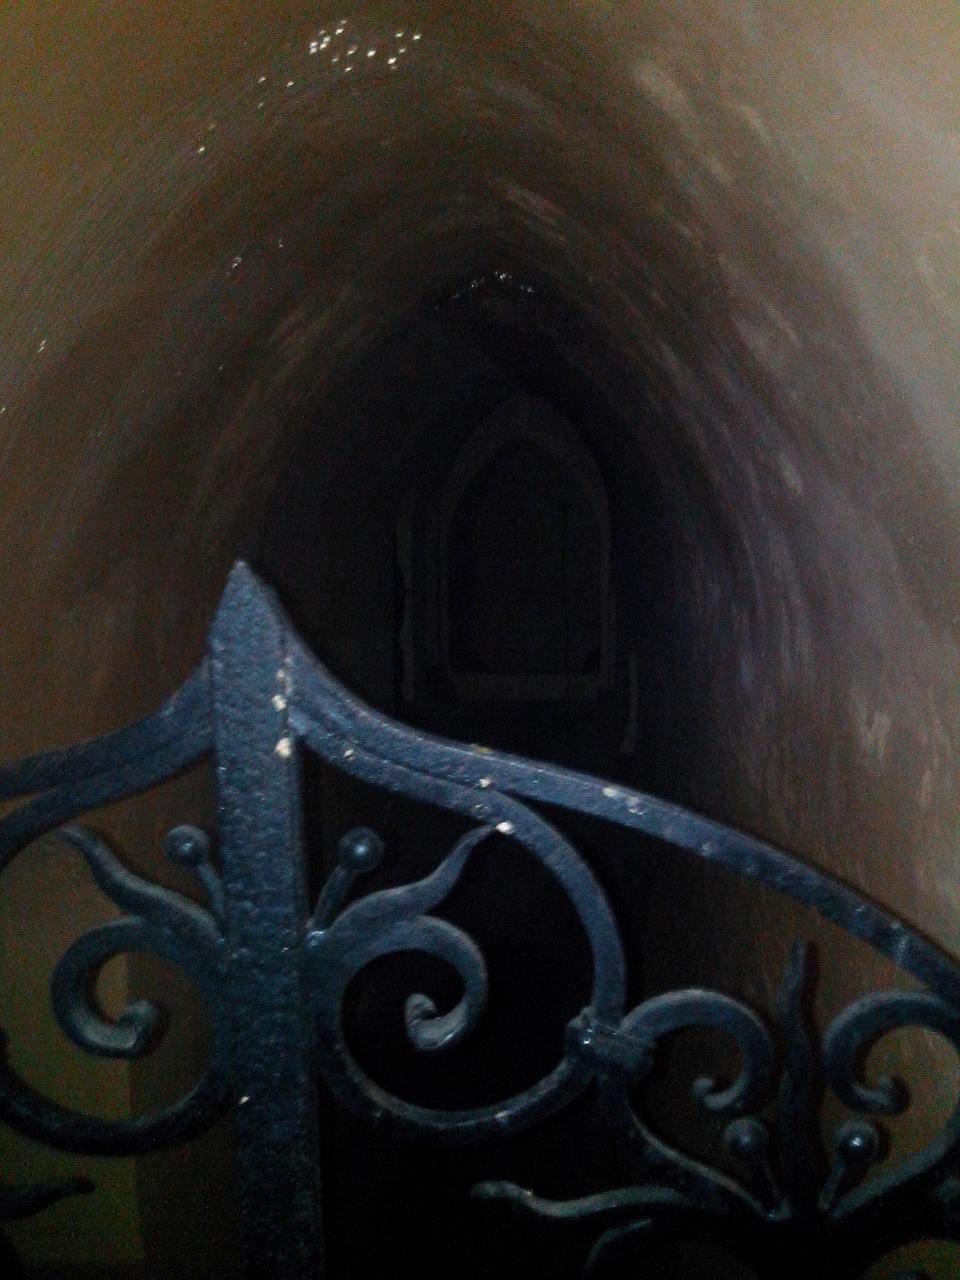
\includegraphics[width=\linewidth]{chast-colebanie-osnov/nachalo/IMG_20170626_135548.jpg}

\textit{Коридор ведет к нераскопанной части пещер. Что там дальше?}
\end{center}
\vspace*{\fill}
\newpage

Но я помню тот еще прежний, в зелени садов поворот на Мичурина, под пещерами, с домом некой бабы Даши напротив – у нее козы жили, а хатка пряталась за кустами сирени. Про пещеры я знал тогда очень смутно, мне они были до лампочки. А ведь ходил мимо почти каждый день.

Я мало увлекался этим всем, живя около ботсада и окруженный древностью со всех сторон. Не говорю об Ионинской церкви, это сравнительный новодел, а во время моего детства она была еще просто государственным зданием, там вечно происходила реставрация, я заходил внутрь, кроме строительных лесов было пусто, а вне стен, на траве валялись куски мозаики – я подобрал несколько больших кусков и хранил дома. Напротив церкви, двухэтажная старенькая колокольня с круглыми часами, на всю округу отбивала каждый час. Я слышал ее даже дома.

Ботанический сад имени Гришко расположился на буквально летописных холмах Зверинца. В глубокой ложбине спрятался монастырь Выдубичи, с его заметными куполами – на колокольне синий в звездах, а другие зеленые. На одном из окрестных склонов в седую старину был Всеволож Красный двор. Вроде бы именно его остатки нашли советские археологи в семидесятых годах на соседствующем с Выдубами, к северу, углу горы – хотя понятно, что никакой таблички с названием при раскопках не обнаружили.% Как по мне, князю выгоднее было строиться там, где в ботсаду перекресток у верха сиреневой аллеи, хвойных и дороги к Ионинской церкви.

Сейчас Красный двор, что называется, возродили – поставили на холме (в 700 метрах от Зверинецких пещер), известном как мыс Чайка,  ограду из бревен, бревенчатую же башню о двух этажах\footnote{50.421302634400284, 30.56695182662565}, и памятный камень с фамилиями тех, кто сему способствовал. В той же местности находилась гончарная слобода, эдак в столетии 13-14. Археологи нашли полные готовой посуды печи, а что случилось, почему всё бросили, неясно.

Напротив основной Зверинецкой горы, к северу – другая гора, со Зверинецким кладбищем, а за нею в удольи – Наводницкий ручей. Он бежит в коллекторе, однако до 2014 года в пойменном овраге сохранялось и поверхностное его течение, питаемое сочащимися со склона кладбища родниками. Затем на уцелевшем отрезке ручья развернули строительство и всё пропало. 

%Прежде там, на перекрестке бульвара Дружбы Народов и улицы Старонаводницкой, у подножия трех холмов – Зверинецкого, кладбищенского и с Родиной-матерью – была конечная остановка троллейбуса. 

%А еще ранее там же Неводницкий ручей, купно со стоком лежащего к юго-западу озеру Святому (о нем читайте в отдельной главе про Зверинец) образовывал озеро Проклятое, соединяющееся с Днепром. 

В восьмидесятые годы прямо рядом с кладбищем, на Верхней улице возвели больницу Четвертого управления. А вместо близлежащей высотки по третьему номеру, был частный сектор – пал жертвой строительства. Маленьким, однажды я бродил там в саду около развалин и нашел игрушки: фиолетовую уточку на колесиках, со ржавой осью, да печального резинового пёсика с пищалкой. Хорошо это запомнил, ибо тогда я впервые увидел разрушенный, снесенный дом.

Западный из южных отрогов Зверинца называется Бусовой горой, а напротив нее, через железную дорогу и летописную речку Лыбедь – Лысая, она же Девич-гора, с остатками крепости. У низовья ботсада, перед железной дорогой, возле ручья под склоном, мы с мамой опять-таки в начале восьмидесятых нашли доисторическую штуку из гладкого камня. До сих пор не знаю, что это. 

Тогда в Выдубицком монастыре помещался Институт археологии. Мы понесли штуку туда – «показать специалистам». Специалистам она оказалась пофиг, и с тех пор занимает дома почетное место на книжной полке рядом с окаменевшей ракушкой.

Смутно помню, как зашли мы в один из корпусов института, бывшее монастырское здание. Потолки высокие, стены толстые. Тихо, темновато, прохладно. Обратились к тетеньке-ученой. Она покрутила предмет в руках. Еще голову так наклоняла, сбоку набок. Потом скучно сказала, что это наверное дети баловались и вылепили из глины. Ученым такое не нужно. С тем мы и ушли.

%Уже в 2013 году я обратился за помощью с определением штуковины к археологам, в одно из сетевых сообществ. Без толку. 

Но штуковина – из кремня, а не глины. Орудия труда «каменного века» обычно лишены такой шлифовки. Поверхность нашей находки гладкая, камень удобно лежит в руке и будто, в самом деле, под нее вылеплен. А с одного конца есть ровная каёмка. Быть может, в этом месте предмет к чему-то крепился и, вращаясь (что и послужило шлифовке) был частью некоего приспособления?

%В 2013 году я наступил на грабли, попросив археологов о помощи в определении. Пошла потеха! Что же, плачевно состояние той науки, чьей представителям насмешка служит средством к познанию.

\newpage
\vspace*{\fill}
\begin{center}
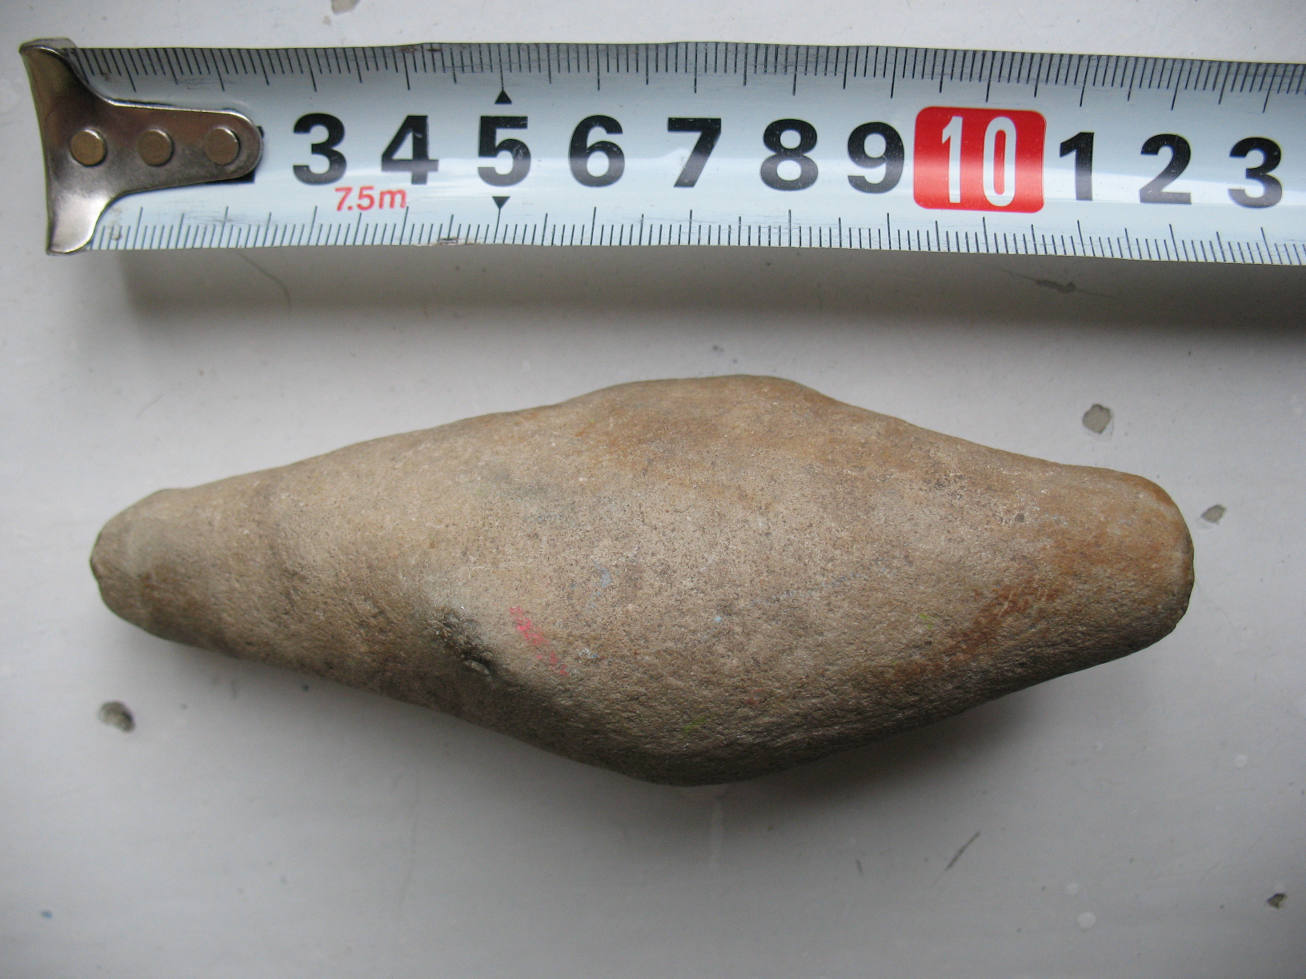
\includegraphics[width=\linewidth]{chast-colebanie-osnov/nachalo/s_figovina-01.jpg}
\end{center}

\begin{center}
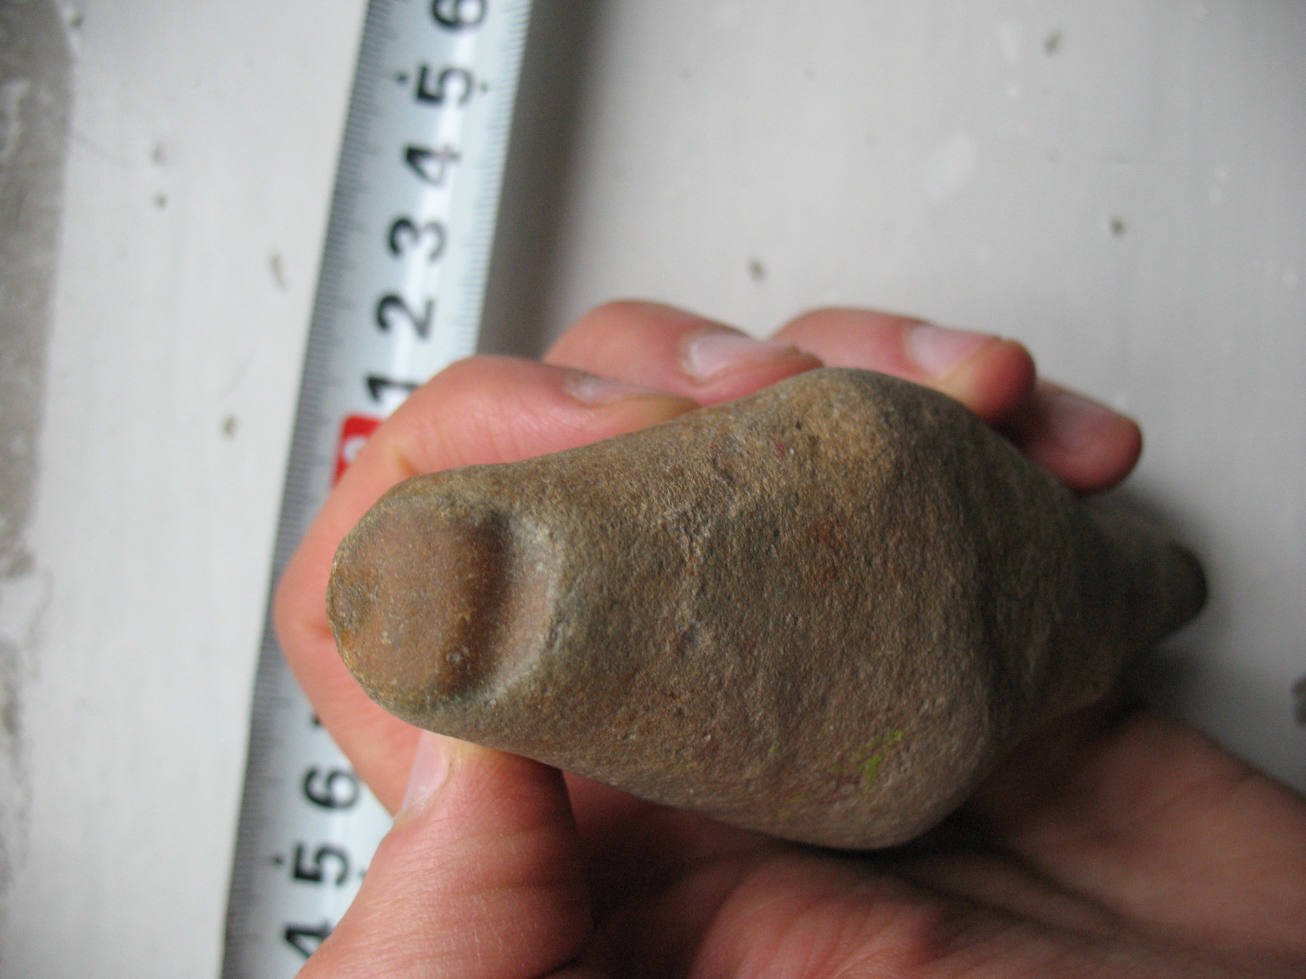
\includegraphics[width=\linewidth]{chast-colebanie-osnov/nachalo/s_figovina-02.jpg}
\end{center}
\vspace*{\fill}
\newpage

%Еще о Выдубах! В Выдубицком монастыре меня привлекала глыба базальта, черная. И глубокий колодец, могила Ушинского и прочие могилы менее именитых людей, да еще огромная ива на пригорке вне монастырских стен. Я хватался за её ветки и катался.

Расскажу подробнее, где был найден этот предмет. Мы часто гуляли «мимо ботаники», по улице Тимирязевской. С одной стороны там был бесконечный забор ботсада, увитый светло-зеленым хмелем, а с другой – захолустные усадьбы частного сектора, прорезанные сбегающими с холма проулками такими узкими, что два человека едва могли разойтись. Ниже хоздвора ботанического сада, за забором, в овраге течет ручей Омелютинка. Левый берег его, слывущий среди старожилов горой Караваевкой, высок и крут. Низовье ручья взято в коллектор. Он примерно повторяет прежний отрезок естественного русла, образовавшегося в суше после отступления вод Днепра от Зверинецкого холма.

Русло это поворачивало на север, северо-восток в сторону железнодорожной платформы Ботанической – она была на отрезке примерно между северной частью улицы Беренбойма и Деревообрабатывающей. Когда построили платформу Выдубичи, то Ботаническая загнулась и теперь о ней напоминает лишь остановка автобуса 54, и та – по требованию. Это местный маршрут, обслуживающий промзону Телички и соединяющий её с окрестностями музея Великой Отечественной войны.

На аэрофотоснимках 1943 года ручей, чуть огибая холм, впадает затем в озеро, которое было ниже Выдубицкого, отделенного от него насыпью железной дороги. Оба озера – старицы, части некогда проходившего здесь русла Днепра, рукава, что подступал под самый берег. Теперь озеро поглощено промзоной. В начале 20 века оно дотягивалось до широты конца Тимирязевской улицы, и на картах того времени обозначено как «Старик» и «Теличка», по названию местности. 

%между Зверинецкой горой и ДОКом (дерево-обрабатывающим комбинатом), и теперь поглощено промзоной. Современные границы исчезнувшего озера можно обозначить – между улицами Стройиндустрии на юге и улицей Баренбойма на севере. На одной карте Киева 1914 года озеро обозначено как «озеро Старик», на другой – как «озеро Теличка» по названии местности (деревня Теличко), причем озеро было растянуто на юг до теперешнего уровня низа улицы Тимирязевской. Стариком оно именовалось потому, что было остатками большого рукава Днепра, старым его руслом.

 %Баренбойма очень каверзная, она начинается на севере, а потом прерывается и телепортируется к метро Выдубичи!

По снимкам 1943 года видно, что от юго-восточной части озера ручей шел через пустыри и за мостом насыпи соединялся с нынешним Днепровским заливом. Сейчас ботанический отрезок ручья примечателен тем, что окрестности его кишат клещами. Некоторые участки берега, в труднодоступных местах, укреплены маленькими колышками, забота о чем прослеживается десятилетиями. Мы сняли эти укрепления в фильме «Киевская сюита», стоит посмотреть! Кто, зачем, почему?

В восьмидесятых, у самого низа улицы Тимирязевской – там сейчас сооружения тепличного хозяйства Киевзеленстроя – ручей еще не был в коллекторе, а образовывал эдакую дельту, обнятую пригорком суглинного берега. На высоте, с него гирляндами свисали засохшие ракушки нескольких видов – вроде мидий и еще каких-то длинных. Около ракушек склон казался светлым, почти белым. Встречались участки и рыжей глины – местные её копали. В небольшой пещерке невесть какого происхождения мы и нашли каменную фиговину.

Удолье у подножия холма. Островки между разветвлений ручья. Мы скакали по мягкой земле. К небу поднимались давние, громадные деревья. Из-под корней пробивался родник. Виднелись развалины частного дома, среди остатков сада росли вишни. Весной, едва пригревало солнце, появлялись цветы – фиалки, мускарики. Теплилось, веяло нерешительной свежестью. Первобытное чудесное место!

На снимке ниже, начало двухтысячных годов, может быть 2003, в дельте ручья ведется строительство. Холм частично срыт и крутизна его умерена, деревья срублены, вода загоняется в коллектор.

\vspace*{\fill}

\begin{center}
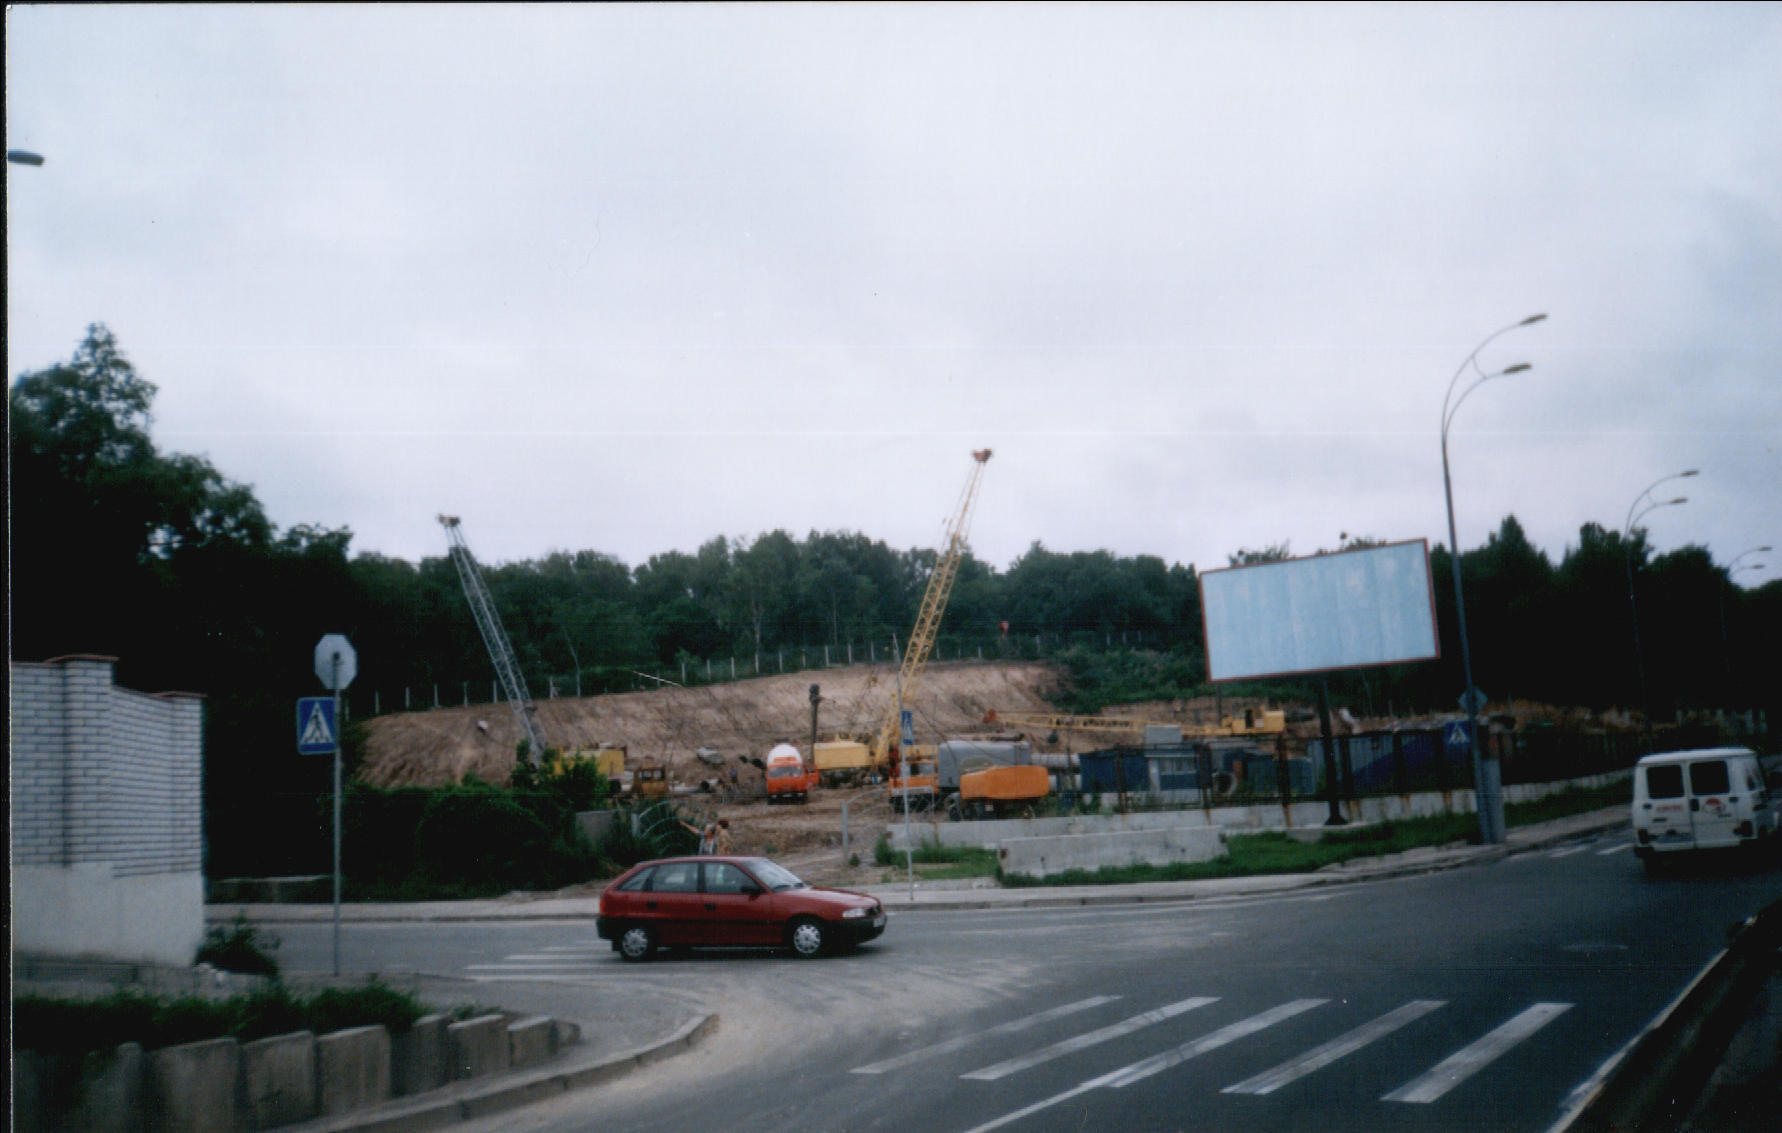
\includegraphics[width=\linewidth]{chast-colebanie-osnov/nachalo/zverinec-niz.jpg}
\end{center}

\vspace*{\fill}

\newpage

Лишь в 2016 году я, занявшись историей киевских кирпичей, узнал, что в конце 18, начале 19 веков там был карьер, где добывалась глина для кирпичного завода. При подобных обстоятельствах, когда в земле обнажаются древнейшие слои, археолог Викентий Хвойка нашел в глинище кирпичного завода Ионы Зайцева ставшую знаменитой Кирилловскую стоянку – в холме, как в слоеном пироге, один на другом покоились слои разных времен. Кости десятков мамонтов, первобытные каменные орудия.
 
А ведь если бы археологи спросили нас с мамой, где мы нашли «штуковину», коли знали б они историю местности – про завод кирпичный – сколько бы еще древностей удалось там найти? Может, «штуковина» была только ключиком к находке, сопоставимой с Кирилловской стоянкой! 

Наука безразличием похоронила открытие. Ученые сидели от него всего в полутора километрах, за толстыми монастырскими стенами. Пешком каждый день можно было ходить изучать. Но предпочитали ездить в Крым, за амфорами.

Киеву же примерно тогда же, в 1982-м, положили 1500 лет от роду, истолковав устроение Кием, братьями его да сестрой общей крепости – «града» по месту своего жительства – как основание с нуля большого поселения.

Празднование этого юбилея города я помню хуже, чем Олимпиаду 1980 года, хотя в первом случае мне было пять лет, а в последнем три. 

Про Олимпиаду встает перед глазами не её символ – олимпийский мишка, но другое. Как по той же улице Тимирязевской бегут ручьи, весной снег таять начал. А к Олимпиаде в Союзе выпустили небывалые фруктовые джемы. В маленьких квадратных коробочках. Из них получались замечательные кораблики. Я ставил в ручеек коробочку и шел рядом, наблюдая, как ее несет чуть ли не до самого хоздвора! Хоздвор знаменит. Там сеялки, веялки, теплицы и старые, выгоревшие от солнца здания сталинских времен. А по пути к нему еще магазинчик от ботсада. Продавались растения – комнатные, огородные и саженцы деревьев. Пахло цветами и черноземом.

Я не знал тогда, что чуть выше по склону, там где участок вьющихся растений, прежде было большое еврейское кладбище. Его снесли, а на месте разбили обсаженные гортензией и клематисом дорожки из бетонных плит. Среди них кое-где попадаются иудейские надгробия, по ним шагают, не замечая.

Можно пройти в самую даль участка и отведать дальневосточного крыжовника – актинидию, крупную и сладкую. Эта лиана цепляется за особую металлическую клеть-опору. Она ржавая, и столбы у навеса над скамейками тоже ржавые. Когда я лазал по ним вверх, а потом спускался, то ладони становились бурыми.

Аллеи, проходящие по бывшим улицам, скрыли прошлое. 

Напротив входа в ботсад стоит Институт проблем прочности. Раньше он раз в неделю завывал на всю округу некой опытной установкой. Местные жители и не догадываются, что всё это было огромным Братским кладбищем, где хоронили погибших в Первую мировую. И в нижней его террасе вырыты погреба хрущовок на улице Подвысоцкого. 

Нынче у меня выработалось как бы историческое зрение. Попав на местность и зная её былое, я чувствую окружающее в настоящем и смутно – в прошедшем времени. А раньше иначе. Было только настоящее и набор привычных, известных каждому, представлений. Братья Кий, Хорив и Щек, да сестра их Лыбедь. Каким-то образом, в седую старину, основали Киев...

Лет в восемнадцать я вычитал где-то цитату из «Повести временных лет» с другим вариантом основания Киева – мол, жил такой перевозчик Кий, переправлял через Днепр, и говорили – «на перевоз на Киев». Однако летописец Нестор сам же эту гипотезу опровергал.

На улице Бастионной 8/2, за углом почты, был мой любимый книжный магазин. Родной. Его после развала Советского Союза переоборудовали в стрип-клуб. В бытность книжного, одним из запомнившихся там моих приобретений начала девяностых стал репринтный томик в мягкой обложке, первого краеведа киевского, Максима Берлинского – «Краткое описание Киева».

Непривычно было «дореформенное» правописание, кажущиеся мне нескладными слова вроде «страховитый», но я прочёл книгу на одном дыхании. К сожалению, перепечатанная в ней карта Киева была махонькой и потому малополезной даже при рассмотрении через увеличительное стекло.

В «Описании» говорилось, со ссылкой на неведомого мне тогда Татищева, что сарматское слово «кивы» означает «горы». И что у впадения Десны в Днепр был город Азагориум, Загорье. Возникло противоречие – так Киев назван по имени князя Кия или от сарматского слова? И если Азагориум, при чем тут «кивы»? Я не стал решать этот вопрос. Принял к сведению, и ладно.

В конце девяностых в Киеве, близ станции метро Петровка, появился одноименный книжный рынок. Туда поначалу переселились торговцы с прежнего, еще «перестроечного», рожденного в 1989 году книжного базара на Куренёвском, или Птичьем рынке. Впрочем, на Птичке по нулевые, не знаю как сейчас (давно не был), существовала небольшая букинистическая толкучка. Со временем на Петровке стали продавать диски с музыкой, программами, фильмами, а затем там образовалась и барахолка как на Куренёвке – да кстати Петровка не так уж далека от нее.

Раньше я часто посещал Петровку, а нынче езжу редко. Покупаю там на букинистических раскладках, в основном где старые книги разложены прямо на асфальте или как щенки-дворняжки выглядывают из коробки. Бывало, возвращался домой с полным рюкзаком, набитым дешевыми и ценными для меня изданиями.

Но миновали светлые времена. Чудесные россыпи хороших подержанных книг по копеечной цене превратились, большей частью, в скопления быстро пожелтевшей перестроечной кооперативной и современной макулатуры.

И вот однажды, когда мой интерес к киевоведению только просыпался, я взял на Петровке книжку в мягкой серой обложке, «Древняя Русь и Киев в летописных преданиях и легендах», Николая Федоровича Котляра. Киев, Наукова думка, 1986 год, цена 30 копеек, 160 страниц, тираж 70000. Современные писатели, завидуйте размаху советской книгопечати.

В работе Котляра я наткнулся на любопытную выдержку, впрочем прерываемую сочинителем и предваренную его оценкой – «встречаем забавную историю, выдуманную, скорее всего, в Новгороде».

А речь шла о том, что Кий, Хорив, Щек и сестра их Лыбедь были разбойниками из Новгорода.

\chapter{Загадки Повести временных лет}

Официальная история не любит новгородцев-летопис\-цев. Подобно тому, как в старинной пословице «Орел да Кромы – первые воры» больш\'ая часть населения этих городов приравнивается к ворам, новгородских летописцев считают обманщиками, выдумщиками.

 %Дружно хохочут историки над сочинениями новгородских летописцев. А может и не дружно, а наедине. Если в библиотеке вдруг раздается неуемный смех, он наверняка исходит от историка с третьим томом Полного Собрания Русских Летописей.

На полке у каждого киеведа зачем-то стоит зеленое, 1982 года издания четырехкнижие «История Киева», подготовленное коллективом ученых. Там сказано, что в отличие от киевской «Повести временных лет», летописцы новгородские прямо сообщают дату возникновения Киева. «Но ей нельзя доверять» – сурово поднимает палец наука. А почему? Поясняют: «Она была внесена в рассказ о Кие новгородскими летописцами XI-XII веков, пытавшимися создать свою схему исторического развития Руси, в которой не Киев, а Новгород выступил бы наиболее ранним восточнославянским городом».

Однако, на основании чего мы должны принять, что новгородцы врут? Лишь потому, что они новгородцы и у них «своя схема»?

Впрочем, некоторых историков уже несколько веков не устраивает и предание об основании Киева легендарными братьями. Красивая выдумка! Не было таких братьев, этимологический миф.

Объявите что угодно враньем и пол\'учите возможность бесконечно утверждать новые истины.

А мне кажется правдоподобным, что некогда живущие родичи Кий, Хорив, Щек и сестра их Лыбедь сообща основали укрепленное поселение на холмах нынешнего Киева. Но кто они, откуда взялись?

Котляр не указал источник выдержки о разбойном семействе. А у меня оно в голове застряло. Но погрузиться в изучение летописей я не отваживался много лет. Тем и довольствовался, что Котляр выписал. Однако сомнение было посеяно.

И наконец я понял – пора самому читать летописи. Но и в известнейших не было про этих разбойников. Нашлось в малоизвестных списках. 

Слово «список» буквально означает копию, нечто списанное с подлинника. К сожалению, из русского языка исконный смысл «списка» вытеснен прямым латинским переводом, словом «копия».

Благодаря этому излишеству, мы привыкли под «списком» разуметь другое – строчки с перечислением, например товаров либо имен. Применительно к историческим и литературным источникам, «список» это рукописная копия (порой исправленная, неполная, или дополненная) летописи либо иного произведения.

Существуют различные летописи и списки оных, отличающиеся подробностями изложения событий, но порой и в корневых предметах. Важнейшие и приемлемые различия, при издании, обычно выносят в приложения или примечания, дабы читатель мог сравнить этот список с другими.

Федор Александрович Гиляров (1841-1895) подготовил и выпустил целый сборник таких примечаний, «Предания Русской Начальной летописи (по 969 год). Прилож\-ения»\cite{gilyarov01}, взяв за основу «Повесть временных лет» по Лаврентьевскому списку, датируемому 14 веком. 

«Повесть» – сборник наиболее ранних преданий о Руси, составленный, как издавна считалось, летописцем Нестором из разных источников. Обычно включается в начало «главных» летописей. Кроме Нестора, в 1116-м над «Повестью временных лет», о чем можно судить по указаниям в ряде списков, потрудился игумен Выдубицкого монастыря Сильвестр. Диву даюсь, что двадцать лет прожил рядом с местом, где это происходило, да и до Лавры недалече.

Вопрос авторства текста, известного как «Повесть временных лет», остается открытым. Первоисточник до наших дней не дошел. У нас нет рукописи ни пера Нестора, ни Сильвестра. В позднейших копиях разнобой. Например, в Хлебниковском списке 16 века составителем значится Нестор, но не указан Сильвестр. В Лаврентьевском и еще двух списках 14-15 веков, после окончания текста записью за 1110 год, добавлено «Игумен Селивестр святого Михаила написах книгы си летописец, надеяся от Бога милость прияти, при князи Володимере\footnote(Мономахе), княжащю ему в Кыеве, а мне в то время игуменящу у Св. Михаила в 6624, Индикта 9 лета; а иже чтет книгы си, то буди ми в молитвах». Так ли это и каким образом соотносится с Нестором –  проверить нельзя. Исследователи строят разные предположения.

Для простоты я бы считал, что Нестор на основе ряда источников (и часть их точно установлена) и собственных впечатлений написал «Повесть», а затем ее правил Сильвестр. Насколько эта простота истинна, сказать не могу. Некоторые ученые, стремясь предать Нестора забвению, полагают, что Сильвестр сначала был иноком в Лавре, а после сделался игумном в Выдубичах.

Как бы ни было, чтение «Повести» приводит к мысли, что за ней стоял, исходно, некий любознательный монах Лавры, одновременно краевед, и по крайней мере в 1106 году он был еще жив. Спустя более столетия, между 1224-1231 годами, лаврский монах Поликарп писал архимандриту Акиндину про Нестора, указывая «иже написа летописец», то бишь в церковной среде в то время уже был известен «летописец» (слово это обозначало летопись) – подразумевается, положим, именно «Повесть» – и Поликарп связывает ее с Нестором.

Существуют однако кое-какие сюжетные противоречия между «Повестью» и приписываемым Нестору житием преподобного Феодосия, а также сказанием о святых князьях Борисе и Глебе. То есть, можно разбирать доводы за и против. Вот, в пещерах Лавры покоятся мощи Нестора Летописца. Именно под таким прозвищем он слывет, подвторюсь, издревле. Но известен есть и другой Нестор, Некнижный, следовательно первый Нестор отличался именно своей образованностью. 

Возможно, в будущем я попробую решить задачу сочинительства «Повести временных лет», однако не сейчас.
 
Так вот Гиляров, в своей книге, для каждого раздела «Повести» привел описание тех же событий по летописям Новгородской, Псковской и прочим источникам, включая польские. Гиляров поместил много архивных редкостей, что еще более усиливает значение его труда, да и пожалуй является главной ценностью оного.

С шестидесятой страницы «Приложений» открываются чудеса про основателей Киева.

Книга Гилярова меня словно разбудила и сбила с толку. Как же, чему верить? Странны и противоречивы оказались списки. Одно дело, когда различия летописей встречаются отдельно и с перерывами. Словно редкая капля дождя – оросила лицо, ощутил, да идешь дальше. А у Гилярова это огромное собрание таких различий, уже даже не дождь, но вся небесная вода, упавшая на землю и собравшаяся в один поток, что уносит прочь от привычных представлений!

Известные князья, разведенные официальной историей по времени, здесь оказываются действующими вместе. Появляются новые их родичи. События переносятся в другое время и место, а участвуют в них совсем другие люди. 

Что же историки, археологи? Осведомлены о вариантах истории? Это у них надо спрашивать. Сами они в книжках ничего такого не говорят, а если даже что прорывается, то с оговоркой, вроде как у Котляра – забавная выдумка!

Общепринятая история – лишь один из вариантов, однако об этом молчат. Ученые решили, исходя из своих представлений о прошлом, считать истиной сведения только из определенных списков. Можно проверить таблицу умножения. Но давний летописный слой событий нельзя – начинается путаница. С нею столкнется любой, кто примется за такой труд.

А наука это храм. Строится из кирпичей. Кирпич должен быть однозначным. Чтобы всякий взял его в руку и признал – это кирпич. Кирпич клеймлён именем князя да годом рождения. Вот еще кирпич, тоже с именем и годом. Положим их рядом на цемент. Два князя вместе. Основа готова.

Однако нельзя точно сказать, что на кирпичах должны быть именно эти имена и числа. Но ученым нужно строить. И они делают кирпичи. Приходится одни имена и годы признавать истинными, другие ложными. Таков научный подход – отставив сомнения в сторону, возводить лишь одно здание. Вместо нескольких, поменьше высотой, зато с разными наборами кирпичей.

Основание огромного здания пересмотру не подлежит. Замена разрушит всё здание. Общепринятые представления об истории это цемент научных работ. Изъятие цемента приведет к распаду.

Если хочешь быть ученым в среде официальной науки, необходимо участвовать в общем строительстве единственного и нерушимого её храма. Делай новые кирпичи, клади цемент, возводи ряд за рядом новый этаж. Не подходит кирпич? Выкинуть! И не сомневайся. Правда за нами!

Вошедшее в «Приложения» Гилярова – выкинуто. Этого будто нет. Не должно быть. Иначе научные труды – в последние годы ставшие смесью взаимных ссылок – потеряют целостность, а журналисты будут вынуждены делать трудный выбор, что же писать о незнакомом предмете.

Официальная наука история и ее противники, та же «новая хронология», больше тратят сил насаждая истину, нежели выясняя оную. Утверждают – было так, а не иначе. Или, еще проще – было так. Без иначе. Умолчать. Когда не получается, обязательно указать – ошибочное мнение.

В семидесятых наконец издали первую часть «Пространной истории города Киева с топографическим его описанием» Берлинского, которую при жизни он в печати не дождался. Добро, ну так опубликуйте с уважением. Читаю.  Вот Берлинский пишет, вероятно следом за Татищевым, что вместо Аскольда и Дира был один человек, «Аскольд тирарь». Сразу примечание редактора – Берлинский конечно ошибается!

Наука, словно ползающий на коленях Хома Брут, чертит по полу колдовской круг с шептанием – Берлинский ошибается, новгородские книжники врут, этой дате безусловно нельзя доверять. И перестает быть наукой, ибо наука это изучение, а изучение прекращается, когда нет сомнений.

Но внутри науки, коли хочешь в ней обретаться, не остается ничего другого, как принимать ее правила игры. Не зря Гиляров вспоминал в своих заметках\footnote{Что печатались из номера в номер «Русского Архива» за 1904 год.}, наставление:

\begin{quotation}
«Не всегда говори, что мыслишь; знай больше, а говори меньше» и т.д. Достоинство этих истин оценено было мною, конечно, уже много лет спустя по их изучении.
\end{quotation}

Сын священника Московского Новодевичьего монастыря\footnote{Фамилию Гиляров священник получил от начальства духовного училища, как прозвище – в переводе с латыни «hilaris» значит «веселый». Александр Петрович Гиляров – старший брат Никиты Петровича Гилярова-Платонова.}, Федор Александрович Гиляров учился поначалу в Московской духовной семинарии, откуда был вытурен за статью «Материалы для физиологии общества»\footnote{«Московские Ведомости», 1859, № 62.} и пошел по светской стезе, поступив на историко-филологи\-ческий факультет Московского университета\footnote{Там же учился историк Ключевский, они с Гиляровым были приятелями еще в бытность последнего семинаристом.}. 

Окончив курс в 1866-м, пятнадцать лет преподавал русский язык в различных учреждениях, попутно выпуская одну за другой работы по истории, языку, краеведческие исследования. Среди них наиболее известным трудом была «Этимология Русского языка», составленная совместно с Александром Ивановичем Кирпичниковым. Перу Гилярова принадлежат также «Этимология Церковнославянского языка», «Русская хрестоматия для низших классов гимназий», «Исторические и поэтические сказания о Русской земле в хронологическом порядке событий», азбука для сельских школ «Школа родного языка», «15 лет крамолы» и другие. Всё это нынче днем с огнем не сыщешь.

Гиляров умел, кажется, выбирать самые неудобные предметы для своих работ. Названия его трудов порой даже боялись верно писать в библиографиях – искажали и название, и год выхода в печать, чтобы сбить с толку цензуру.

В 1883 году Гиляров выпустил, на основе своих статей в «Современных известиях»\footnote{Оные издавал дядя Гилярова, Николай Гиляров-Платонов. Федор Гиляров состоял там вторым редактором. Оба Гилярова слыли, по словам Владимира Алексеевича Гиляровского, людьми «не от мира сего». В типографии «Современных известий» вышли и «Приложения русской начальной летописи».}, книгу «15 лет крамолы (4 апреля 1866 г. – 1 марта 1881 г.)» о революционном движении в России. Отпечатанный трехтысячный тираж первой части первого тома – «Пропаганда. (4 апреля 1866 г. – 24 января 1878 г.)» – был запрещен спохватившейся цензурой под предлогом «исключительной важности предмета книги и его щекотливости»\footnote{См. Сводный каталог русской нелегальной и запрещенной печати. М., 1971. Ч. I. С. 149.}. Название оказалось пророческим. 15 лет книги лежали в закромах под арестом, от сырости 2500 штук истлели, оставшиеся поныне считаются редкостью.

В том же 1883 году выйдя в отставку, Гиляров начал печатать свою газету, «Афиши и объявления», позже переименованную в «Вестник литературный, политический, научный и художественный». Издание освещало большей частью театральную жизнь. Современник с похожей фамилией, Владимир Гиляровский вспоминал в «Москве газетной», что «Федор Александрович писал недурные театральные рецензии, а затем сам издавал какой-то театральный листок, на котором прогорел вдребезги».

Скончался Гиляров в Химках под Москвой, в 1895 году. Похоронен в самой Москве на Пятницком кладбище.

Зачем я рассказал о нем относительно подробно? Дабы за отсылками к источнику, важному в моей книге, стоял человек, а не имя. И если о человеке нынче мало помнят, стоит напомнить, что был такой, и каким он был.

Гиляров вытащил из архивов в печать наиболее яркие «отклонения» от общеизвестных списков\footnote{Подобное, но в меньшем объеме, либо пересказе, и с выраженной оценкой можно найти еще в работах Михаила Николаевича Тихомирова (1893-1965), например в  его «Кратких заметках о летописных произведениях в рукописных собраниях Москвы», изданной в 1962 году.} – то, что ученые предпочитают, если знают, замалчивать. А с несведущих и спроса нет. «Приложения» могли бы перевернуть представления о ходе истории. Но куда там! Эта книга ведь целая дорога, усыпанная камнями, о которые каждый споткнется, коли не захочет обойти.

Науке бы чего попроще! Гладкий асфальт. Но помимо редких списков, даже основные летописи задают такие загадки, ответы на которые разрушат здание современной науки истории. Посему, да по неведению, эти вопросы обычно не поднимают. А мы поднимем. 

\chapter{Так говорят летописи}

Кстати, а на каком языке велись летописи?

Ученые толком не отвечают, но поясняют, что это не был разговорный язык, и на Руси в старину так не говорили. А дескать, Кирилл и Мефодий разработали на основе своего родного языка литературный. И его-то нынче и называют церковнославянским или старославянским. Насколько это представление науки справедливо, мы исследуем ниже.

В каждой летописи с веками накопилась уйма правок, включая языковые. А язык меняется в зависимости от местности и с течением времени. Правщики летописей, переписывая оные, в некоторой мере осовременивали их и придавали местный оттенок. В меньшей степени это коснулось религиозных книг.

Но рассудим, какой толк в мысли, утверждаемой наукой – церковнославянский никогда не был на Руси разговорным языком. Для кого же тогда переводить на него религиозные произведения и вести на нем летописи? Зачем создавать на нем новые произведения?

Ответ прост. Ученые ошибаются. Это и был, в какое-то время, разговорный язык, общий для Славян, тогда еще не столь разрозненных и разнящихся, как сейчас. И благодаря упорному держанию традиций, православная церковь сохранила нам, по большому счету, древний разговорный язык в том числе и Киевской Руси.

Однако, начиная с некоего времени, в разных местностях по-разному, разговорный язык стал меняться быстрее, чем «церковный», чем язык священных книг. В итоге язык обиходный и книжный таки друг от друга отделились. Ведь язык «церковный» был привязан к религиозным сочинениям, а мы помним, как правка даже в рамках «церковного» языка богослужебных книг при патриархе Никоне послужила одной из причина Раскола в православной церкви, и доднесь (хорошее, старинное слово) многие старой веры держатся, ибо не приемлют правок, внесенных при Никоне и в последующие годы.

Давний, общеславянский язык – такой же, как летописный, используется в многочисленных житиях святых, поучениях и подобных сочинения. Да и сами летописи ведь не однородное перечисление событий, а смесь выдержек из источников светских и духовных.

Но обратимся к другим видам письменности. Обиходный, не церковный язык должен быть запечатлен в граффити на древних стенах, в пещерах, в сводах законов наконец.

Возьмем надписи на стенах Софии Киевской\footnote{Неизбежно встает вопрос о грамотности населения времен Киевской Руси. Для кого делались надписи на пряслах (грузках для веретен)? Надписи в пещерах Лавры? А на кувшинах? Известны текстовые клейма на кирпичах, посуде и так далее, причем по-славянски и вроде бы по-гречески. Значит, грамотен был народ, и не токмо славянской грамоте разумел! Между тем знаменитый Оттон Первый Великий – король Германии, император Священной Римской империи, читать выучился лишь на сорок шестом году жизни. И то хорошо! Другие тогдашние правители из просвещенной Западной Европы крестами подписывались.}. Это тот же язык, что в летописях и давних церковных книгах. Переводы греческой литературы, например «Временника» монаха 9 столетия Георгия Амартола – тот же язык. Свод законов «Русская правда» (Правда Роськая)\footnote{Примечательны строки в ней, где говорится, кто утвердил этот свод законов: «Правда оуставлена Роуськой земли, егда ся съвокоупил Изяслав, Всеволод, Святослав, Коснячко, Перенег, Микыфор Кыянин, Чюдин, Микула».}, по списку 12 века – тот же язык, хотя ученые утверждают обратное. Впрочем, ныне вольно проверить любому желающему! Берестяные грамоты из Новгорода – тот же язык. «Хождение за три моря» Афанасия Никитина, берите еще, черпайте полной горстью давние сочинения – один язык! Безусловно, при сравнении этих разнородных источников обнаруживается некоторая разница – ибо  источники разнесены по месту и времени.

Но в целом же, в единости языка древнего обиходного, летописного и «церковного» может убедиться каждый, кто собственными глазами прочтет первоисточники.
 
Вот английский язык допустим 16 века, сравните с английским 19 века – между ними очевидная разница. Но ведь ученые не утверждают при этом, что англичане в 16 веке говорили на каком-то другом языке, чем отраженный в произведениях того времени. Нет, принимается за должное, что был такой язык, как в книгах.

А про старославянский нам навязывают примерно такую мысль – это был язык священный, на Руси его не использовали вне церковной литературы, обиходный же язык был другим. При этом ученые видят светские «Роськую правду», берестяные грамоты, граффити – видят там старославянский, и какой делают вывод? А довольно странный. Дескать, это разговорный язык, но с примесью церковнославянского. Лишь бы не признавать, что старославянский и был разговорным!

%Обходят стороной и использование старославянского в лубочных картинках, сопровождаемых пояснительными письменами. Был лубок религиозный – со сценами из Библии и житий святых, сатирический, исторический, срамной, шутейный, поучительный, колдовской и прочих жанров. Даже в девятнадцатом веке и начале двадцатого на лубке сплошь и рядом находим надписи на «церковнославянском».

%Примеры. Лубок «Птица Сирин святаго и блаженнаго рая». Подпись: «Аще человек глас ея услышит, пленится мысльми и забудет вся временная и дотоле ж лед тоя ходит, доднеже пад умирает, глас ея слышати не престает». Возле головы птицы: «Видом и гласом».

%Лубок «Наказание Людвику Ланграфу за грех стяжания», конец 19 столетия. Полное название оного лубка: «Книга мирозрительное зерцало, глава 257. Стяжание неправедно, стяжани дерзнув некий ланграф, терпяше велие мучение адское». Кусок текста оттуда: «Людвик ланграф великий мучитель, людей [...] токмо аз и сынове мои. Той же прият знамение, а ланграфа ввергоша в бездну, и возврати диавол клирика». 

%\begin{center}
%\includegraphics[width=0.75\linewidth]{osn-kiev/hristofor.jpg}

%\textit{Лубок. Песиголовец святой Христофор.}
%\end{center}

%Лубок начала 20 века, «Зерцало великое, глава 138. Яко напрасно нам виновен бес бывает». Его текст: «У некоего пустынника молитвою связан бысть бес, и стрежаше репу его. И некогда прииде человек к старцу репы [...] ради от своей мысли смущен бых, и абие простив отпусти его старец с репою, яко невиновен нам бес делом, но мыслию точию».

%Сообщения о памятных исторических событиях, явлениях чудес и дивных зверей в заморских странах, притчи, молитвы – всё это выпускалось для народа на лубке, записанное языком, который ученые считают чисто книжным и церковным! По лубку видно, что язык русский литературный, язык Пушкина, скажем так – хотя встречается на лубке, однако на позднем, и то в меньшей степени, нежели старославянский.

%Конечно, у нас есть сборники былин и народных песен, донесшие обиходный русский язык 19 века – он близок к «пушкинскому», но вспомним, что лубок писался понятным народу языком, и лубок выпускался исходя из спроса. Следовательно, был спрос на лубок с текстами на старославянском, а не «современном».

%Можно возразить – спрос такой потому, что грамоте учили в церковных школах, или дьячки нанятые. Дескать, что сами знали, тому и обучали. Казенных школ для простого народа, помимо Василия Татищева ох как долго никто не заводил, просвещением занималась таки церковь. Но даже в начале 20 века «церковный» язык в письменности, был, кажется, вполне понятен грамотной части народа одновременно с обиходным.

Русский язык 19 века еще сохраняет много общего с давним – окончания вроде «ою» вместо «ой» (водою, водой), «противу» вместо «против», да много чего. В украинском поныне используются окончания «ою», слово «як» (было «яко», в русском стало «как»), славянские имена месяцев и так далее. Оба языка еще не утратили древнего звучания, однако изменились относительно исходного. 

А вот современный болгарский похож на старославянский значительно меньше, чем русский и украинский, хотя языковеды утверждают, что церковнославянский возник на основе некоего «южноболгарского». Здесь языковеды сами себе противоречат, ибо они строят дерево происхождения языков на сравнении их сходства, и в случае со старославянским идут вразрез со своими же правилами. 


%А ведь разные степени сходства означают всего-то, что на землях нынешней Украины и России, славянский язык изменился – от исходного старославянского – менее, чем в землях, занимаемых Болгарией. И что в определенное время старославянский был родным обиходным языком населения этих земель.


Но что значит «Болгария»? В давнее время была известна другая Болгария, о ней много писали Арабы, а ее население современная наука объявила тюркским. Это Болгария на реке Волга.

Слова меняются по звукам, которые могут произноситься нечетко. «Б» легко становится «в», «о» – «у», твердое «г» превращается в мягкое «х» и звонкое «к». Иногда звуки просто выпадают из слов.

Возьмем корень Болгарии. Болга. Что это? Волга. Что говорит летопись про Болгар? Далее отрывок из Ипатьевского списка, где говорится про язык (язык в значении ветвь народа, а не набор слов\footnote{Современные учебники церковнославянского сообщают, что слово «язык» в значении народа пишется с буквы «я», а в значении языка, набора слов и правил их построения – с буквы «юса малого». Однако в старинных книгах мы видим безразличие к этому, и «язык» в значении «народ», «ветвь народа» пишут как с «я», так и с «юса малого».}) под именем Словене (Славяне), который жил на Дунае:

\begin{quotation} 
Словеньску же языку, якоже ркохом живущю на Дунаи, придоша от Скуфь, рекше от Козар, рекомии Болгаре, и седоша по Дунаеви, насильнице Словеном беша. А по сем придоша Угре Белии, и наследиша землю Словеньскую, прогнавше Волохы, иже беша преже прияле землю Словеньску
\end{quotation} 

%Любопытствующие могут почитать вне этой книги, кем полагают ученые Волохов, Скифов, Козар и других. Я же даю свою трактовку, основанную на источниках, а не домыслах.

Что сказано в летописи? К тем Славянам, жившим на Дунае, от Скифов, говорят от Козар\footnote{От Козар из числа Скифов. То бишь, есть разные Скифы, а среди них Козаре.} – явились Болгары, насильно поселившись там. После этого пришли Белые Угры, и наследовали землю Словенскую, прогнав Волохов – Болгар, которые перед этим захватили (прияле) землю Словен.

Летопись прямо называет Болгар Волохами. У Болгар и Волохов общий корень – Волга, учитывая замену звуков! А как вы думаете, что лежит в основе названия Балканы?

Наука не понимает тождества давних Волохов и Болгар, не видит соседства Валахии (часть нынешней Румынии) и Болгарии. Не замечают также сходства Болгар с названием народов Белгов (от этого «Бельгия») и Фир Болг.

%Но если, по мнению ученых, старославянский язык основан на «южноболгарском», то, продолжая цепочку рассуждений и приняв летописное утверждение, что Болгары пришли с Поволжья, следует вывод, что на Поволжье пользовались тем же языком!

О Козарах. Здесь и далее я всюду пишу Козаре, вместо Хазары, следуя давнему написанию. В латинских же источниках встречаем – Cazari. У Греков, однако, с буквы «х».

Наука считает Козар тюрками, популярная культура приписываем всем Козарам исповедование иудаизма. Я же приведу, что написано о Козарах в «Житии и трудах преподобных отцов наших Мефодия и Константина-Кирилла, учителей словенских» Дмитрия Ростовского, по лаврскому изданию 1764 года. Можно считать это мнение срезом тогдашних представлений о Козарах:

\begin{quotation}
Козары, их же Грецы Хазарами, Римляне же Газарами нарицаху, бяше народ Скифский, языка Славенскаго или Российскаго, страна же их бе близ Меотийскаго езера\footnote{Азовское море.}, еже и Мертвым морем нарицается, в неже Дон река Азию и Европы разделяющая впадает [...]

племя некое Скифское, глаголемое (от гор Аланских) Аланы, прозванныи же потом (от реки Козара именуемой) Козары, седе и долгими временами расплодися зело, и населяшеся по обоим странам Дона, ово во Азии, даже до Волги в Каспийское или Хвалынское море впадающей; ово же и во Европе, даже до Днепра в Черное море входящего. [...]

ибо и до Паннонии досягоша, но оуже тамо иными нарицаниями прозвани быша, ово Авары, ово Гунны, и во иные пременишася народы.
\end{quotation}

По некоторым «житиям» картина несколько иная, и Козаре предстают не однородными Славянами, но сообществом различных народов, где помимо славянского в ходу язык, именуемый в давних источниках «жидовским»  или «самаритянским».

Мне любопытно сталкивать мнения современной науки с общепринятыми представлениями прежних веков. Любопытна и связь Козар с Аланами, ведь известно, что в определенное данниками Козар была Киевщина и многие окрестные земли, а ведомо также, что эти же земли были примерно тогда же подвластны славянскому народу Полянам. Достаточно отбросить от Полян букву П, и мы получим тех же Аланов.

В наших летописях Поляне упомянуты кратко, а переподчинение Вещим Олегом земель, платящих дань Козарам, сокращено еще более, будто не возникало при этом никакого недовольства со стороны Козар, теряющих одно владение за другим. Можно сказать, что Козар летописных не существует вовсе, вместо них пробелы, дыры в истории, вырванные места.

В летописях, однако, мы не встречаем отождествления Козар с Полянами. Более того, согласно Повести временных лет, после смерти Кия, Хорива и Щека, Полян обижают Древляне да прочие окрестные народы, а Козаре, живущие «в лесех на горах», пытаются обложить Полян данью, на что Поляне платят по обоюдоострому мечу с каждого двора.

Главу Козар называли «коган», или, как нынче любят писать, «каган». Учитывая мягкость давнего «г», можно предположить, что при самих Козарах это произносилось как «кохан». В украинском языке сохранилось слово «кохання», любовь. Вплоть до 16 века на Руси было множество должностей, связанных со словом «излюбленный» – «излюбленные» старосты, головы, судьи. Излюбленный означало – избранный, выборный. Возможно, таково же и значение козарского «кохана», если Козаре были от «языка славенского».

Я не берусь здесь разбираться в противоречиях между житиями и летописями и выяснять происхождение Козар. Мне кажется, что это название жителей разнообразного по народностям государства, исповедовавших различные религии. В одно время верхушка Козар исповедовала иудаизм, в иное время – христианство. Пожалуй это про Козар всё, о чем можно судить точно.

В Киеве, по летописям известен район города – Козаре – его иногда отождествляют с другим районом, Жидове, однако нет прямого указания на такое отождествление. Значит, в Киеве времен «великокняжеских» Козаре обосабливались среди прочего населения, но чем занимались и какую играли роль, неведомо.

Теперь относительно Кирилла и Мефодия, точнее Константина (Кириллом он стал, приняв схиму) и Мефодия, деятельных братьев из Солуни\footnote{Селунь, Солунь – греческий город Салоники.}, с которыми принято связывать изобретение славянской письменности, алфавита, когда из Моравии поступил запрос на понятную народу Библию, не греческую, не латинскую, но славянскую.

До революции 1917 года, тексты летописей были доступны немногим, да и в советское время переиздавались нечасто. Для работы с ними приходилось ездить в библиотеки Москвы, Киева или Ленинграда, большинство же исследователей довольствовалось разрозненными цитатами, переходящими из книги в книгу, и осовремененными «переводами» летописей, в частности Повести временных лет.

Хрестоматийный перевод Повести временных лет, выполненный Дмитрием Лихачевым, в месте про Кирилла и Мефодия, гласит: 

\begin{quotation}
Был един народ славянский: славяне, которые сидели по Дунаю, покоренные уграми, и моравы, и чехи, и поляки, и поляне, которые теперь зовутся русь. Для них ведь, моравов, первых созданы буквы, названные славянской грамотой; эта же грамота и у русских, и у болгар дунайских. 
\end{quotation}

Открываем подлинник по Лаврентьевскому списку, за 6406 год от сотворения мира:

\begin{quotation}
бе един язык Словенеск. Словени же седяху по Дунаеви ихже прияша Оугри и Марава Чеси и Ляхове и Поляне яже ныне зовомая Русь сим бо первое преложены книги Мараве. яже презвася грамота Словеньская. яже грамота есть в Руси и в Болгаре Дунаиских.
\end{quotation}

Где тут написано про создание букв? Откуда Лихачев взял, что для Моравов\footnote{Кстати, Моравы сами себя еще в 19 веке именовали Чехами. Моравами их называли чужестранцы.} первых созданы буквы, названные словенской (славянской) грамотой?

Подлинник ясно говорит – книги (а речь идет о священных христианских книгах, Библии) сперва были «преложены» – переведены – народу Мараве. 

Эти-то переводы называли грамотой Словенской, Писанием Словенским. Опять-таки летописец подразумевает Библию, на Словенском. И дополняет, что такое Писание в ходу в Руси и у Болгар Дунайских. 

Примечательно – еще с 19 века исследователи заметили, что в старейших редакциях житий святых Кирилла и Мефодия на старославянском, сказано «книги», а в поздних «книги» постепенно превращаются в «письмена». Несмотря на это, наука считает Кирилла и Мефодия создателями славянской азбуки, а однго из двух алфавитов – кириллицы и глаголицы, еще не определились какого, но застолбили на всякий случай оба.

Именно «письмена», или даже «грамота», упомянуты в единственных на греческом языке сочинениях, касаемых Константина и Мефодия – вариантах жития святого Климента, где есть «граммата Скловениха». И слово «γράμματα» («граммата») обычно переводят как «буквы», совершенно выпуская из виду, что оно обозначает и письмо в смысле Писание, священные книги. Так, на греческом, Iερά Γράμματα – Иэра Граммата, Заветные буквы, Завет, Библия!

А была известна, например, Латинская Библия – Библия на латинском языке. Никто не утверждает же, что Латинская Библия – это название азбуки. Точно также и Словенская Грамота, Словенское Писание – это Библия на словенском, общем тогда славянском языке, который в несколько искаженном виде дошел до нас и в летописях.

В большинстве источников – летописях, житиях, письмах – не сказано, что братья создавали азбуку. «Повесть временных лет», говоря о Кирилле и Мефодии, отрывочно и путано пересказывает их жития, но поскольку именно летописное изложение событий известно больше других, разберем сначала его.

Согласно «Повести», правители Славян, живущих по Дунаю – князья Ростислав, Святополк и Коцел – просят византийского царя Михаила снабдить их крестившихся подданных переводами священных книг\footnote{Прежде они просили о том же папу Адриана II, однако не успел он послать своих людей, как дело перехватил Михаил.}, ибо, по Ипатьевскому списку,

\begin{quotation}
не разумеем бо ни Гречьскому языку, ни Латыньскому, оны бо ны инако учать, а друзии инако; темьже не разумеем книжнаго разума, ни силы их; а послете ны учителя, иже могуть ны сказати книжная словеса и разум их
\end{quotation}

Князья хотят малого – переводчиков священных христианских книг, уже проповедуемых среди Словен на латыни и греческом, которые народу непонятны. Не сказано, что Словене не разумеют родной грамоты. Они не понимают латыни и греческого.

Напомню, что «Византия» это введенное учеными название Римской империи того времени, когда столицу ее перенесли из Рима в Новый Рим (он же Константинополь, ныне Стамбул). В летописях Константинополь именуется Царьградом. Римская империя того времени дала сильный крен в сторону Греции, посему то, что ученые окрестили Византией, в наших летописях и житиях упоминается как Греки\footnote{Также в ходу слово «гречник» вместо «грешник», не потому ли что дохристианские греки-эллины были язычниками, и язычник стало синонимом грешнику?}. «Византийцы» же именовали себя Ромеями. 

Византийский царь Михаил просит друнгария\footnote{Должность военного командира в Византии, значение менялось в зависимости от времени.} Льва из Селуни отрядить в словенские земли сыновей – Мефодия и Константина, по прозвищу Философа\footnote{Михаил, сын Феофила, давно был знаком с Константином. Ведь когда умер отец Михаила и последний вступил на престол с матерью своей Феодорой, при нем были, как выражается житие, «пестуны» – великие боляре – доместик Мануил, Феокист патрикий, да логофет Дромн. Дромн знал родителей Константина и Мефодия, и присоветовал Константина в качестве учителя для царя Михаила. Так Константин приблизился ко двору.}. Лев соглашается,

\begin{quotation}
и послаша я\footnote{«Я» значит «их». В подобных выражениях также, после глагола, «и» – его, «ю» – ее. Например, «и послаша и по грибы» – и послали его по грибы.} в словеньскую землю к ростиславу и святополку и кцьлови. сима же пришедшима начаста съставливати письмена азбуковьная словеньски и переложиста апостол и еуангелие, ради быша словене яко слышиша виличья божия своим языком по сем же приложиста Псалтирь и Октаик и прочая книги.
\end{quotation}

Всего-то сказано, по Ипатьевскому списку, что Константин и Мефодий пришли к Словенам да принялись за работу, о которой их просили.  «Съставляти письмена азбуковная словеньски» значит не составили азбуку, как думают ученые, а указание, что братья создали\footnote{Составление можно понимать буквально, ибо Библия ведь составлена из множества книг Ветхого и Нового Завета. И состав этот в давнее время разнился. Более того, к числу священных книг иногда добавлялись непривычные нам произведения, например о Троянской войне.} Писание (письмена) на словенском алфавите, приложив-переложив – переведя – книги Апостол и Евангелие, а затем Псалтирь, Октаик и прочие книги. А Словене «ради быша» – рады были, что услышали хвалу богу своим языком. 

Дальше в летописи идет текст, в котором ученые находят подтверждение своему мнению о Кирилле и Мефодии – создателях славянской азбуки. Некие люди, проведав о переводе священных книг на славянский, были недовольны, и говорили, что 

\begin{quotation}
яко не достоин никоторому же языку имети буков своих разве Евреи и Грек и Латины по Пилатову писанию
\end{quotation}

Это предложение в разных вариантах, где читается то «буков», то «азбуков», толкуется следующим образом – мол, недовольные люди утверждали, будто ни один язык, кроме еврейского, греческого и латинского, не достоин иметь своих букв, алфавитов.

Через несколько глав я подробно расскажу о втором значении слова «язык» – народ. Здесь оно так и употреблено.

Слово же «бук» – что это такое? Буква? Кстати, прежде буквой называли и целое слово. Но буква ли «бук»? Заметим – «буки» тут во множественном числе.

В Тверском списке толкуется: «буков своих, рекше, книг» – слово «буки» отождествляется с «книгами».

Я предположу, как толковать происхождение этого слова. Слово «бук», или «боук», похоже на «бок». «Бок» значит – «сторона». Привычное русское слово «страница» по-украински звучит как «сторінка». А «сторінка» – от той же «стороны». Таким образом «буки» это значит просто «страницы».

В Тверском списке «буки» уравнены с «книгами». Всем знакомо английское слово «book» – книга! Полагаю, такое же было и в давнем славянском, но уже во время составления Тверского списка оно устарело, поэтому переписчик дает пояснение – буков своих, рекше, книг. В старину и слово было такое, «букарь» (боукарь) – книжник.

О каком же именно недовольстве говорит летопись, в переложении на современный язык?

Дело проясняют жития святых. Римская ветвь христианской церкви тогда разрешала в богослужении использовать только три языка – латинский, греческий и еврейский, которыми по приказу Пилата были сделаны надписи на кресте Иисуса. Молиться на языке народа, проповедовать – можно\footnote{В православии это получило название «ереси триязычия», в католичестве – триязычной догмы, от которой позже отказались.}. Совершать богослужение, литургию – нет. А Константин и Мефодий сделали перевод Библии и церковных служб на словенский, ныне старославянский, язык.

Греческое слово «βιβλία» – Библия – в переводе означает «книги». Словенскую Библию получили Словене! И духовенство римской церкви возмутилось!
 
Константин затем «взвратився вспять и иде оучить болгарского языка», что означает  – вернулся назад и пошел учить, в смысле проповедовать христианство, а учить кого? – болгарского языка, то бишь болгарский народ.

Мефодий же остался в Мораве, затем князь Коцел назначил его епископом в Пании (Паннонии). И вот странность – Мефодий

\begin{quotation}
посади два попа борзописца велми, и преложи вся книгы исполнь от Грецька языка в Словенеск шестью месяц, начен от марта месяца до двунадесяту и шесть дний октября месяца
\end{quotation}

Если пользоваться сведениями только Повести временных лет, то кажется, будто речь идет о выполнении двух разных переводов. Сначала одного (когда «переложиста апостол и еуангелие»), а потом другого, с греческого языка. Последний перевод занял у Мефодия и двух попов-борзописцев шесть месяцев.

Пожалуй надо теперь расширить круг источников, чтобы изложить события более ясно. Источники – различные варианты житий, да латинские документы, в основном письма римских пап.

Предварительные сведения. Жития святых, Кирилла и Мефодия, известны только на старославянском  языке. Ученые говорят, что это переводы с греческого. Однако житий солунских братьев на греческом не существует. «Не дошли до нас», – утверждает наука.

Равным образом Константин и Мефодий не существуют в византийских документах, хотя братья начинали деятельность свою именно от «восточной», «греческой» ветви христианской церкви, судя по житиям выполняли важные поручения религиозно-дипломатического свойства, и должны быть хоть как-то отражены. Нет.

На греческом языке братья упомянуты только в связи со святым Климентом, в «Пространном житии Климента» болгарского архиепископа Феофилакта, да «Кратком житии святого Климента» архиепископа Димитрия Хоматиана. Первое датируют 11-12 веком, второе – 13-м.

Таким образом основные сведения о Константине и Мефодии известны только по житиям на старом славянском языке и по письмам на латыни.

Константин, при патриархе Фотии и Льве Математике, получил образование в Царьграде:

\begin{quotation} 
Егда же прииде Царю Градоу, ведаше его оучителем да се оучить, и в три месеце навыке граматикию по пррочая се еть оучения. И наоучи се Омироу\footnote{Омир – Гомер.} и геометрии. и оу Льва и у Фотия диалезнице и всем философинскыим оучением, к сим же и риторики и арифьмитикии, астрономии и моусикии, и вьсем прочиим елиньскым хоудожеством.
\end{quotation} 

На Константина обратили внимание при дворе, а чтобы удержать философа от монашества, его назначили библиотекарем у патриарха, в «светеи Софии». Но вскоре Константин вышел на «Оузькое море» и там тайно скрылся в монастыре. Впрочем его нашли.
 
Спустя некоторое время император Михаил послал Константина с миссией в Козаре, поскольку тамошний правитель попросил у Византии представителя христианской религии для участия в выборах Козарами как бы государственной религии. Ибо иудеи да сарацины уже начали склонять Козар в свою пользу. И козарский царь не знает, что делать. Сарацины вот уже дары присылают.

Константин отправляется в Козаре, взяв с собой и старшего брата своего, монаха Мефодия. Прежде того Мефодий был военачальником, приближенным к византийскому императору Михаилу Триглавому (деду «нынешнего» Михаила), но при сыне его Феофиле оставил «мир» и на Афоне постригся в монахи – вероятно, попав в опалу. Теперь же Мефодий «шед слоужи яко раб меньшю братоу, повиноуя ся емоу».

Братья добираются до Херсона, как тогда называли известный нам Херсонес, а купно и его окрестности, достаточно большую часть Крыма. Чтобы не путать вас в названиях, ведь современный континентальный Херсон просто носит то же имя, что давний крымский, Таврический, буду вместо последнего Херсона писать Корсунь, как его часто и называли Славяне.

По ранним житиям можно понять, что Корсунь подчинялась Козарам. По более поздним, скажем, 18 века – Корсунь просто смежна козарским владениям. С течением времени так оно и было, город был то под одним государствам, то под другим. 

В истории принято считать, что Корсунь в 9-м веке вошла в состав Священной Римской Империи. Корсунь с некоторых пор играла важную роль в христианской церкви, сюда часто ссылались насильно, либо бежали добровольно изгои, попавшие в очередную бурю византийских религиозных дел. Допустим, шли гонения на иконопочитание – гонимые обретали пристанище в Корсуни.

Там-то, Константин обучается «жидовьсцеи беседе и книгам». «Некий самаренин» снабжает Константина «книгами самаренскими», философ удивляет того своим знанием языка, читая их без запинки.

Далее происходит странное – про Константина, в житии его сказано\cite{teodorov01}:

\begin{quotation}
Обреть же тоу еваггелие и псалтырь росьскы писмены писано, и человека обреть глаголюща тою беседою: и беседовав с ним и силоу речи приемь, своеи беседи прикладая, разоучи писмена гласьная и сьгласная, и к богоу моливою дрьже в скоре начеть чисти и ськазати.
\end{quotation}

Каким-то образом Константин «обрел» – приобрел, купил ли, получил в подарок – Евангелие и Псалтырь (псалмы из Ветхого завета), писанные росьскими письменами, да нашел знающего ту речь (беседу) человека. Общаясь с ним, Константин вскоре выучился читать и говорить по-росьски.

Это относится ко времени предшествующему тому, когда Константину и Мефодию поручили переводить Библию на словенский. Казалось бы, можно воскликнуть – так вот в чем разгадка последующего быстрого перевода!

Но тут загвоздка. Понятие «народа Руси» в то время очень размыто. Каких Русов имеет в виду сочинитель жития? 

С определенного времени Русами стали называть славянские народы, подчиненные тем Русам, что пришли вместе с Рюриком и его родственниками сначала в нынешнюю Новгородщину, а затем ниже до самого Киева. Откуда были те, первоначальные Русы, мы будем разбирать в следующих главах. Кто-то считает их выходцами с Балтики, кто-то со Швеции. 

А давние арабские путешественники говорят о Русах, что живут в крепости на острове в море (иногда уточняется – Меотийском, то бишь современном Азовском), и что остров тот три дня длиной, царь же Русов называется «хакан-рус», что сближает его с козарским «каганом». 

Слово «хакан» всплывает также во франкской хронике Annales Bertiniani, где говорится о посольстве от византийского василевса Феофила к Людовику Благочестивому (что датируется 839 годом нашей эры). В составе посольства были представителя народа «Рос», и правитель их, согласно хронике, назывался «хакан». 

Русы, про которых пишут арабы, постоянно крутятся у низовий Волги, и вообще по морям, широтой близких к Средиземноморскому. При этом арабы различают Русов и Славян.

По житию Мефодия, цесарь Михаил, позже отправляя братьев в Моравию, к Славянам, говорит: «вы бо еста селоунянина, да селоуняне вьси чисто словеньскы беседоують» – то есть вы селуняне, а все селуняне говорят почти как Славяне.

Исходя только из жития Константина, нельзя однозначно понять, каковы были «росьскы писмены», на коем написаны «обретенные» Евангелие и Псалтырь, но по рассуждению сочинителя жития, Константину понадобился носитель языка, дабы в них разобраться.

%Затем, не менее загадочным образом Константин «обретает» святыню – мощи святого Климента, папы римского, умерщвленного в корсуньской ссылке\footnote{«Игемон Авфидиан» по приказу кесаря Траяна утопил Климента, привязав к его шее якорь. С морской гробницей Климента связано множество чудесных преданий. По совокупности их я предполагаю, что гробница находилась на острове, время от времени затопляемом.}. Житие описывает это так\footnote{Существует и отдельное предание про обретение мощей Климента. Позже мощи эти князь Владимир Красно Солнышко, крестившись в Корсуни, забрал с собой.}:

Затем, не менее загадочным образом Константин «обретает» святыню – мощи святого Климента, папы римского, умерщвленного в корсуньской ссылке\footnote{«Игемон Авфидиан» по приказу кесаря Траяна утопил Климента, привязав к его шее якорь. С морской гробницей Климента связано множество чудесных преданий.}. Житие описывает это так\footnote{Существует и отдельное предание про обретение мощей Климента. Позже мощи эти князь Владимир Красно Солнышко, крестившись в Корсуни, забрал с собой.}:

\begin{quotation}
Слышав же яко светыи Климент иже в мори лежить, помоливь се рече: вероую в бога и светем Клименте надею се, яко обрести его имамь и изнести из моря.
\end{quotation}

То бишь, Константин слышал, что прах святого Климента в море лежит, и философ с божьей помощью надеется найти его и достать из моря. Не в одиночку:

\begin{quotation}
Оубеждь же арьхиепискоупа\footnote{Житие Кирилла и Мефодия от Дмитрия Ростовского называет его «епископом Херсонским» Георгием Блаженным.}, и с клиром вьсемь и говеины моужи вьседьше в корабль идоше на место, и оутиьшоу се море вельми и дошьдыше начеше копати поющи. Абие же бысть хризма многа яко и кадиль многь.

О по сем явише се светые мощи, еже вьзьмьше сь великою чьстию и сь славою вьсехь граждан вьнесоше вь град также пишеть в обретении его.
\end{quotation}

После деятельности в Козарах, где братьям удалось крестить тамошнего кагана\footnote{В качестве миссионеров в Козарах солунские братья оставили священников из Корсуни.}, бояр его, а также часть простого народа, Мефодий получает первое «повышение по службе» – назначается от греческой церкви игумном в монастырь Полихрон.

Проходит время. Из Моравии от князей Ростислава и Святополка поступает известный запрос, насчет прислать «учителей» и толковать христианское Писание на народном, славянском языке. Согласно некоторым житиям, князья хотят видеть Константина и Мефодия именно потому, что знают об их успехе в Козарах.

Но тут задача сложнее – нужна Славянская Библия, на славянском, словенском языке. Царь Михаил и дядя его Варда поручают Константину этому способствовать – найди, мол, способ перевести. Бог даст! Не смея ослушаться «ни бога, ни цесаря», Константин помолился, и 

\begin{quotation}
в скоре же емоу бог яви послоушание молитв своих раб: и абие сьложи писмена. и начет беседоу писати еваггельскоу: исперва бе слово, и слово бе оу бога, и бог бе слово, и прочее.
\end{quotation}

По другому варианту жития,

\begin{quotation}
да тоу яви бог философу словеньскы книгы
\end{quotation}

Обрадовался Михаил столь скорому и чудесному явлению перевода Священного Писания.

Константин и Мефодий отправились в Моравию, где Константин взял на обучение людей, выделенных Ростилавом. Вскоре Философ перевел «весь церковный чин» и обучил ему учеников:

\begin{quotation}
В скоре же весь церьковьный чин преложь наоучи и, оутрьници, часовомь и вечерьни, павечерници и таинеи слоужьбе.
\end{quotation}

Как сказано ранее, это вызвало недовольство внутри римской церкви, однако разбор интриг, которые на этом не закончились, оставляю вне этой книги\footnote{Недовольство проявляли латинские и франкские архиереи, иереи и ученики их. Константин вступал с ними в споры. Эти же архиереи, по житию, были в некотором роде язычниками. Они утверждали, что под землей живут «человеци велеглави» (люди с большими головами), а что если кто убьет змею, ему отпустятся девять грехов, ежели же человека убьет, то довольно три месяца пить из деревянной чаши, не касаясь стеклянной – и грех тоже сойдет, как с гуся вода. Архиереи-противники Константина не запрещали язычникам приносить их жертвы, и позволяли неограниченно соединяться в браке. А Константин разводам противился.}. Думаю, что недовольство было вызвано не столь догматом «триязычия», сколь возрастающей популярности варианта учения, предлагаемого Константином и Мефодием на местном языке. Братья пришли со Словенским Писанием в руках да с молитвой «Отче наш» вместо «Pater noster» на устах. Конечно, народ потянулся к ним.

Обстановка вокруг братьев накалилась. Но князь Коцел попросил у римского папы послать к себе «блаженного учителя нашего», подразумевая Мефодия.

Солунские братья отправились в Рим с мощами святого Климента. Это приблизительно совпало по времени с назначением римским папой Андрианом II Мефодия на должность епископа Моравии и Паннонии. Андриан II

\begin{quotation}
книгы словенские освети, и положи и вь церькви светые Марие, яже наричеть се Фатань, и пеше над ними светоую литоурьгию. По сем повеле папа двема епископома, Фоурьмосоу и Гондрихоу, светити словенские оученикы: и якоже светише се, абие пеше литоургию в церкви светаго апостола Петра словеньскыим языкомь.
\end{quotation}

Римский папа осветил «книгы словенские» –  Библию Словенскую – и положил их в церкви святой Марии, и пел над ними святую литургию. Затем он повелел епископам Фурьмусу и Гондриху освятить словенских учеников (обученных братьями), и после этого те пели литургию на словенском языке в церкви святого Петра.

Словом, папа дал добро! Но впрочем предписал, чтобы в Моравии на литургии Послания и Евангелие зачитывались сначала по латыни, а потом уже можно на славянском. Следующий римский папа, Иоанн VIII, письмом своим запретил Мефодию богослужения на славянском, однако архиепископ не послушался. Запреты и разрешения следует толковать лишь на фоне тогдашней религиозной и политической обстановки, когда одни ветви церкви были в содружестве с одними правителями, а другие – с другими.

Став архиепископом Моравии и Паннонии, Мефодий завершает перевод на словенский язык тех книг Писания, которые еще не переведены. Именно из этой части жития Мефодия взято в Повести временных лет про попов-борзописцев. За шесть месяцев, с греческого на словенский, переводят все оставшиеся книги, кроме Маккавеев: 

\begin{quotation}
Потом же отверг вься молитвы и печаль свою на бога възложи, преже же от оучеников своих посажь два попы скорописьца зело, преложи в борзе вься книгы – вься исполне, разве Макавеи – от грьчьска языка в словенеск шестью месяц, начьнь от марда месяца до дъвоюдесятоу и шестию день октября месяца. Оконьчавь же достоиною хвалою и славою богоу воздасть, дающемоу таковоу благодать и поспех; и святое возношение таиное с клиросом своим вознес сотвори память святаго Димитриа.

Псалтирь бо бе тъкъмо и евангелие с апостолом и избраныими слоужьбами церковьныими с философом преложив первее. Тогда же и номоканон, рекьше законоу правило, и отеческыя книгы преложи.
\end{quotation}

В последнем абзаце важно – Псалтырь и Евангелие, да некоторые избранные службы, были переведены раньше, еще вместе с Константином Философом. 

А ведь именно Константин в Корсуни «обреть же тоу еваггелие и псалтырь росьскы писмены писано». Если сопоставить не мудрствуя лукаво, то выходит, что царю Михаилу был представлен тот самый готовый перевод, «обретенный» в Корсуни. А точнее, если принимать за истину события жития, то переложенный с «росьскы писмены» на словенский, славянский. Поскольку, судя по всему, языки несколько отличались и Константину пришлось учиться у носителя. Но выходит, в любом случае, что так было проще, нежели переводить с греческого, латыни или древнееврейского.

Проложное\footnote{Пролог – древнерусская книга-месяцеслов. Жития святых в нем упорядочены по дням поминовения.} Житие Константина и Мефодия (стык 13-14 веков), уточняет временную привязку перевода, выполненного Мефодием:

\begin{quotation}
Седеше в земли Моравьстеи, преложи вься книгь ветьхаго и новааго закона от гречьскаго вь словенськый, в 3 индикт в 6 тисоущное триста 4 го ста третие лето при Святополца князы; цесарь беше грьчьскы Василие, а бльгаромь от бога князь Борысь, краль немечьскый Людемь.
\end{quotation}

В 879 году недовольство римского руководства деятельностью Мефодия достигло предела. Папа Иоанн VIII вызвал Мефодия на суд в Рим, обвиняя в ереси. Мефодий подчинился, но суд оправдал Мефодия, а папа признал возможность славянского богослужения и непротиворечие его обычаям римской церкви. Судили довольно странно, келейно. Вопреки всему, по поводу Мефодия не созывался синод, поскольку сохранились акты синода за 879 и 880 годы. Всё решилось самим папой и «братьями»-епископами.

Тот же папа в послании князю Святополку, в подтверждение архиепископства Мефодия (Iohannes VIII papa ad Svyatopolcum comitem. Confirmat Methodium ijn archhieposcopatu Moravie, Vichinum facit episcopum Nitriensen at Linguam sclavicam in missis celebrandis adhi\-bendam permittit) сообщает:

\begin{quotation}
\begin{otherlanguage}{latin}
Litteras denique sclavonicas a Constantino quondam philosopho repertas, quibus deo laudes debite resonent, jure laudamus, et in eadem lingua Christi domini nostru preconia at opera ut enarren\-tru jubemus.
\end{otherlanguage}
\end{quotation}

Если у кого доходят руки до этого документа, обычно толкуют исходя из представлений, что Константин изобрел некую письменность. Исследователь сего вопроса Василий Алексеевич Бильбасов в книге «Кирилл и Мефодий по документальным источникам»\cite{bilbasov} дает следующий перевод:

\begin{quotation}
Наконец, славянские письмена, некогда изобретенные Константином Философом, для того чтоб ими возглашались должныя хвалы Богу, мы справедливо похваляем, и мы приказываем, чтобы на этом языке были излагаемы проповеди и деяния Господа нашего Христа.
\end{quotation}

Но слово «litteras», толкуемое Бильбасовым как «письмена», и «repertas», толкуемое как «изобретенные», переводятся иначе. 

«Repertas» – найденные, обнаруженные, обретённые.

«Litteras»- Писания. Вот пример употребления этого слова из Латинской Библии, Евангелие от Иоанна, 7,15:

\begin{quotation}
\begin{otherlanguage}{latin}
et mirabantur Iudaei dicentes quomodo hic litteras scit cum non didiceri  
\end{otherlanguage}
\end{quotation}

Что означает:

\begin{quotation}
И дивились Иудеи, говоря: как Он знает Писания, не учившись? 
\end{quotation}

А вот из 2-го послания апостола Павла Тимофею 3,15:

\begin{quotation}
\begin{otherlanguage}{latin}
et quia ab infantia sacras litteras nosti quae te possint instruere ad salutem per fidem quae est in Christo Iesu.
\end{otherlanguage}
\end{quotation}

Перевод:

\begin{quotation}
Притом же ты из детства знаешь священные писания, которые могут умудрить тебя во спасение верою во Христа Иисуса. 
\end{quotation}

«Litteras» вообще принимало много значений – это и обычные письма, и расписки, и книги, и Писание. В случае Константина речь ведь идет о Славянской Библии. Римский папа говорит про Славянское Писание, Славянскую Библию, которую «нашел» Константин. Как нашел, дело десятое – в Корсуни ли, в Козарах, либо как-то еще.

В одном из вариантов «Похвалы Кирилу и Мефодию» (похвалами называют краткие жития святых) говорится:

\begin{quotation}
Закон же божии соугоубо преложьша в новыи язык предаста, письмена створиша емоу.
\end{quotation}

Новый язык здесь – новый народ. Для еще одного народа, переложили закон божий, Писание (не алфавит!) сотворили ему, народу (языку) этому. 

Как же случилось, что Кирилл и Мефодий, из учителей словенского языка – учителей в смысле духовных, христианских учителей словенского народа (языка), уже к 18 веку стали, в церковной литературе, а следом за ней в науке – изобретателями славянской азбуки?

С некоторых пор по славянским рукописным сборникам пошло гулять сочинение «о письменех черноризца храбра».

Старейшим списком его считается сборник Иоанна-Александра, он же Лаврентьевский (не путать с Лаврентьевским списком русской летописи), в котором проставлена дата «в год от сотворения мира 6856, индикта 1», что наука переводит в 1347 год нашей эры. Сборник был написан для «царя болгар и греков Иоанна Александра», и потом кочевал по библиотекам, в 17 веке попал из Афона в библиотеку патриарха Никона, затем на Печатный Двор, а ныне находится в отделе рукописей Российской Национальной Библиотеки.

Короткое сказание «о письменех» известно в многочисленных списках, причем «Храбр» обычно считается именем, хотя таких имен не было, и монахи (черноризцы) подобных имен не носили. Однако «храбра» это, скорее, слово «храбрый», склоненное в винительном падеже согласно старому славянскому языку. Сказание кого? Черноризца храбра, монаха храброго. Но поскольку мне нужно его как-то величать, буду пользоваться именем Храбр.

Считается, что жил он в 9-10 веках, и был едва не современником Кирилла и Мефодия. Язык «сказания» тяжеловесен, некоторые слова поддаются разве что толкованию, однако не прямому переводу.

В самом начале Храбр пишет:

\begin{quotation}
прежде оубо словене неймеху книг. иж чрьтами й резами чьтеху й гатааху погани суще. кръстившежеся, римсками й гръчьскым писмены, нуждаахуся словенскы речь безь оустроения.
\end{quotation}

Разберем по кусочкам.

«Прежде оубо словене неймеху книг». Научный перевод – прежде Словене не имели книг, письменности в привычном понимании слова. Мой перевод – прежде Словене не имели Библии. Ведь «Библия» буквально и переводится как «Книги». 

«Иж чрьтами й резами чьтеху й гатааху погани суще». Научный перевод – будучи погаными (язычниками), Словене читали и гадали чертами и резами. Мое толкование – я не понимаю, что такое «черты и резы» и не могу об этом рассуждать. Больше нигде в источниках не сказано о чертах и резах. Эти черты (черти) и резы имеют отношение к гаданию, если «гатааху» значит «гадали». Нечто из области верований, веры, как и Библия.

Далее Храбр пишет: «кръстившежеся, римсками й гръчьскым писмены, нуждаахуся словенскы речь безь оустроения».

Ученые понимают это так – крестившись, Словене пытались без всяких правил записывать свою речь римскими и греческими буквами.

Допустим, но почему такая острая необходимость в письменности возникла у Славян сразу после крещения? До того они, наверное, скакали с ветку на ветку, оглашая леса дикими криками и довольствуясь гаданием на чертах и резах? А после принятия христианства ощутили потребность писать на родном языке.

По Храбру, до Кирилла и Мефодия, крещеные Словене достаточно долго – «многа лета» – пользовались чужими алфавитами, что было довольно неудобно для выражения слов словенского языка. И потом бог не оставил «род человеч» (подразумеваются наверное Словене) без «разума» (христианского учения) и послал им святого Константина Философа, нарицаемого Кирила, мужа праведного и истинного, и тот придумал Словенам буквы, взяв за образец греческие и дополнив алфавит под нужды славянского произношения. 

Далее Храбр рассуждает о развитии греческой азбуки, как поначалу Эллины переняли ее у Финикийцев, а разные древние ученые мужи постепенно добавляли новые буквы. Но Греки были язычниками, посему создание греческого алфавита длилось «многи лета», а Кирилл – муж Божий, потому изобрел словенскую азбуку в малых летех, причем в одиночку! Несколько далее в своем сказании Храбр впрочем мельком упоминает и Мефодия.

Итак, с одной стороны, у нас есть жития Кирилла и Мефодия, где они не изобретают буквы, но выступают в роли переводчиков, причем Константин-Кирилл, помолившись, вскоре являет Михаилу переведенными на Словенский священные книги в том же составе, каковой он «обрел» в Крыму, в Корсуни.

Подобное отношение, к Кириллу и Мефодию как к переводчикам и учителям христианской веры среди Словен, пронизывает и другие христианские тексты, помимо житий. Например, в поминальных службах, Кирила величают «учителем словенскому языку», то бишь учителем, просветителем словенского народа. Глас из рукописи С. Палаузова:

\begin{quotation}
Кыриле, славне оучителю! Доброте научи моравлени своими бога благодарити, прелагая на словеньскы языкь от грьчьскаго закон господень, и правде его.
\end{quotation}

На другую чашу весов положим коротенькое сочинение «О письменех» черноризца Храбра, где утверждается без каких-либо доказательств изобретение Константином славянской азбуки на основе греческой, а скорость перевода приписывается тому, что Константин был христианином.

Современные ученые принимают на веру версию монаха Храбра.

Но мало им утверждений, что солунские братья изобрели для диких Славян азбуку. Много лет уже внедряется мнение, что и давний славянский язык, известный нам по дошедшим летописям, житиям и прочим памятникам литературы – в быту на Руси не ходил, но использовался сугубо книжно. То есть мало лишить Славян письменности, надо еще и родного языка исконного лишить! Дескать, его тоже изобрели Кирилл и Мефодий.

%Поминальная по Кирилу и Мефодию, по списку 17 века

%Святый Кирил философ, родом сеи Блъгарин от Солоуна града, грамота новая створи и преложи грьечскыи язык на роусскыа книгы с братом присным своим Мефодием, иже и тъ бысть первыи архиепископ моравский и чешьский, в царьство Михаила, царя гречьскаго и в дни архиепископа Коньстантина града блаженнаго патриарха Фотия, в лета князя блъгарскаго Бориса и Растица бооустнаго князя моравскаго и Костела князя Блатского и Лесскаго и Зубра когана козарскаго, и Карлоуса краля немечьскага, и Доуная господаря угорьскаго, царствуяшему же в Новьграде князю роуському Роурикоу, до 100 20 2 лет

Почему-то никто не проделывает тот же финт ушами с «древнескандинавским», или, правильнее, старым северным (Old Norse) языком. Наукой признается, что на нем говорили «скандинавы» эдак с 8 по 14 века. «Северный германский язык!» – весомо определяет наука. На нем известны некоторые саги, сборники «Эдда» и «Старшая Эдда» и различные рунические надписи. Но ученые не считают, что это был особый такой язык, годный только чтобы сочинять на нем саги. Признают – да, использовался в обиходе.

А с расшифровкой рун иногда получается так. В Эрмитаже хранится арабский динар, датируемый 701/702 годом нашей эры. На нем, помимо арабской вязи, невесть когда нацарапано на старославянском:

\begin{center}
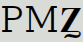
\includegraphics[width=0.20\linewidth]{chast-colebanie-osnov/letyaz/pmz.png}
\end{center} 

Последняя буква – «земля», «з». Ученые берут и толкуют – это не буквы, а руны. «M» – две отдельные руны, а «земля» тоже руна, но без вертикальной палочки. И надпись надо читать: «kut». Засучив рукава, толкователи рун берутся за дело. Одни говорят, что «kut» – окончание имени некоего скандинава! В высшей степени научно. Другие бают – а вот давайте добавим еще букву «r», да поменяем звуки, получится gótr или gautr, что можно было бы перевести как «мужчина» или «воин». Третьи утверждают, что тогда «Gautr» это другое имя бога Одина. Четвертые не согласны, и видят в надписи другие руны – слово «góts», но это если вторая руна длинное – «ó», а последняя – «s».

Итак, ясно вычерченную на монете славянскую надпись ученая братия считает «норманскими» рунами, толком не понимая, какие же именно руны написаны, и предлагает уйму вариантов прочтения.

Вместо того, чтобы задуматься о прочтении письмен старославянских...

Ведь как читали? Разложим вопрос на две части. Способ и произношение.

Способ. 

Как читает грамотный современный человек? Он читает не по буквам, а по словам, зная как они выглядят. Слова для него – картинки. Лишь новое слово постигается вначале побуквенно, что нужно, дабы знать как произносить слово, а потом оно становится цельным изображением. Чтобы различать слова, человек пользуется, упрощенно говоря, пробелами между ними. Это позволяет быстро понять, где начало слова, где конец, а всё что между этим – изображение слова.

В рукописях на старославянском, будь то летописи или религиозные сочинения, слова никак не разделяются, буквы идут сплошными рядами. Это относится и к греческим рукописям, а хоть бы и Нового Завета.

В лучшем случае старославянский писец ставил точки (посередине высоты строки), разделяя логически части предложения, дабы облегчить чтение. При таком положении дел вы не можете быстро найти нужный вам отрывок, не можете постигать написанное пословно, просто глядя на абзац или предложение. Вам нужно читать побуквенно и, дабы не сбиться, водить пальцем  по строкам, будто палец – это курсор. Итак, чтение было не пословное, а побуквенное, и только прочитанная порция букв могла быть сложена в слово, а затем чтец начинал читать следующие буквы, покуда не натыкался на конец слова, если конечно знал его. В случае согласной в завершении слова ставился твердый знак, что указывало на конец слова.

Произношение. Никто не ведает, как говорили на латыни во время, когда ею пользовались в обиходе. Никто не в курсе, как говорили на старославянском. Как вслух читались слова, которые написаны в летописях. Современное духовенство может читать на «церковнославянском», но это осовремененный выговор, приближенный к русскому языку последних нескольких веков.

Как же восстановить произношение времен, например, Нестора Летописца?

Сохранились переводы на старославянский с того же греческого, и перебрасывая мостки между греческим произношением (хотя никто не знает, как тогда произносили написанные слова Греки), можем примерно догадаться о разных вещах.

Буква «Є» – называемая в церковнославянском «есть». В старославянских текстах не встречается привычная нам «Е», но есть такая «Є», как в украинском, где этот знак обозначает как раз русское «е» – «йэ».

Однако, в старославянском, и дореволюционном правописании русского языка, была буква Ѣ (ять).

Очевидно, что держать две буквы для использования одного и того же звука не было нужды, следовательно буквы «Є» и «Ѣ» звучали по-разному. Кстати, до революции использование слов с «Ѣ» просто держали в памяти, толковых правил этому так и не вывели. 

Самоназвание жителей Греции  – Эллины. В летописях оно пишется как «Єллини». Думаю, прежнее произношение буквы «Є» соответствует современному «Э». Не зря она даже пишется как повернутая в другую сторону «Є». В старославянских переводах имен тех же ромейских императоров, пишется «Є», хотя звучали они с современным звуком «Э». Вывод напрашивается сам собой.

«И» (церковнославянская «иже») – и парная ей «І», она же «Ї» (называется «и»). Опять же, было отличие в произношении, как в случае с «Є» и «Ѣ». Вероятно, «И» была более «толстой», ближе к «ы». На ум приходят всё те же летописные «Єллини».

«Г» – я не знаю, отколь повелась твердая «г» почти как «к». Но вот даже во времена Петра I писали «г», а говорили «х». Это проявляется в письменных ошибках Петра I, который писал как говорил – ВыборХ, ПетербурХ. Это объясняет написание имени Юрия Долгорукого в некоторых списках в виде Гюрги, что звучит непривычно жестко на современное произношение, но если читать смягченно, выходит Хюрхи, Юрий.

Лишнее подтверждение былой мягкости «г» – использование ее в передаче иностранных имен и названий, которые в подлиннике звучат с «х» – Гамбург (Humburg), Герберт (Herbert), Гарри (Harry) и так далее. Такое написание могло обоснованно возникнуть лишь во время, когда «г» звучала столько мягко, как соответствующая ей латинская «h». Вспомним, как в старину вместо «история» (history) писали «гиштория», или не испанский, но «гишпанский».

«Оу» – еще одна любопытная штука, сочетание букв, позже перешедшее в обычное «у». Например, «Златооустецъ», «моужъ». Вместе с тем, встречается и одиночное «у» – «служебнии». Поскольку письменный язык отражал устный, значит, некоторые слова так и произносились, и вместо короткого «муж» растягивали «моуж». Сие возможно при довольно неторопливой речи, надо успеть произнести. Потом, с течением лет, веков, речь наверное ускорилась, и «лишнее», трудное произношение отпало в пользу короткого. И коротко превратилось в кратко. Выпадали даже целые слова – «еси» – а у англичан оно сохранилось как «is». Сравните Сие еси и this is. 

Медленная устная речь хорошо согласуется с медленным же чтением сплошных рядов букв. А что, если и мысли в то время протекали медленно? 

%Выдумка заменяет ученым обоснование и в решении других вопросов.

\chapter{А так говорят грамоты}

Век двадцать первый, государство Литва, расположено на южном побережье Балтийского моря. Столица Литвы – город Вильнюс. Официальный язык – литовский, относимый к балтийской группе. Состоит из двух говоров – жемайтского и аукштайтского.

Века давние, Великое княжество Литовское, включает в себя земли нынешней Литвы, Беларуси, Украины. Столица княжества – город Вильнэ, Вильна, что буквально значит «вольная». Официальный язык – «руский» (с одной «с»), как он назван в тогдашних документах.

Земли государства, которое мы привыкли называть Киевской Русью, после ослабления в княжеских распрях, попали в зависимость к Орде. Затем, в 14-16 веках, вошли в состав Великого княжества Литовского, позже – Речи Посполитой.

Тартары были изгнаны из Киевской Руси в 1320 году объединенным воинством Русов и литовского князя Гедимина. Несколько позже Литовское княжество посредством браков соединилось с меньшим по размеру Королевством Польским. Влияние Польши постоянно увеличивалось, покуда в 1569 году Литва и Польша не срослись в то, что ныне именуют Речью Посполитой.

Документы – кровь государства. Оборот документов – циркуляция крови в его организме. Осталось множество, а еще больше утрачено, бумаг того времени – приказы, купчие, жалованные грамоты, законы. Писались они на нескольких языках – на латыни, польском, а во время сильного княжества Литовского – на «руском», с одной «с».

Об этом руском языке теперь много спорят. Белорусские историки величают его «старобелорусским», украинские – «староукраинским» или «древнерусским», россияне – то «северо-русским» и «западно-русским». Одни ученые доказывают, что это был чисто письменный язык, другие указывают на второе его имя – «проста мова», то есть народный, обиходный язык, третьи возражают, будто литовские князья не могли на нем говорить, а общались на другом, «балтийской группы».

Язык общения князей оставим в стороне. На руском, в Великом княжестве Литовском – в Вильне и в Киеве – составлялись завещания, писались протоколы, велись учетные книги, подавались жалобы. Огромный объем документов, известных как Литовская Метрика – по сути, архив канцелярии Великого княжества Литовского – написан большей частью на руском.

На нем был создан в 16 веке и свод законов княжества, Литовский статут, переведенный затем на польский. Однако статут и юридическая терминология Литвы вобрала много польской, а Поляки пользовались в юриспруденции латинскими выражениями, поэтому литовский «юридический» язык это такой сплав славянского и ополяченной латыни, причем чем дальше, тем больше.

Польские чиновники, с усилением влияния Польши, противодействовали использованию руского языка как официального, ибо понимали его всё хуже. Они хотели документов на польском или латыни, и хотя поначалу от этих нападок на язык удавалось отбиваться указанием на традицию – «листы писаные и выдаваны руским писмом и языком по всему панству его королевской милости великому князству литовскому», на Варшавском сейме 1696 года «руска мова» утратила статус официальной.

Неясно, в какой мере этот руский язык Литовского княжества соответствовал разговорному народному языку – говорам Литвы, Белоруси и Украины – поскольку мы имеем дело с письменными документами. Ведь если судить по польским латинским документам, то истолковывая это как прямое указание на язык народный, следует заключить, что Поляки поголовно говорили на латыни. Очевидно однако, что руским языком в княжестве Литовском пользовались и знали его хорошо.

Давайте ощутим вкус этого языка, тем более что далее в книге мы будем часто встречаться с источниками на нем. Пример из свода законов – Литовского статута, писано от имени великого князя\footnote{Здесь и далее для удобства чтения документов княжества Литовского буду отбрасывать твердые знаки, что ставились после согласных в конце слов (как в царской России), а порой и внутри. Также заменяю «і» на «и», а в письме московского князя, «іа» на «я»}:

\begin{quotation}
21. Хто бы новые мыта уставлял.

Тэж приказуем, абы жадин чоловек в панстве нашом – Великом князьстве Литовском – не смел новых мыт вымышляти ани вставлять ни на дорогах, ани на местех, ани на мостех, и на греблех, и на водах, ни на торгох в именьях своих, кром которые были з стародавна вставленые, а мели бы на то листы продков наших, великих князей, або наши. [...]
\end{quotation}

Этим приказываем, чтобы ни один человек во владениях наших – Великом княжестве Литовском – не смел новых мыт (пошлин) измышлять и устанавливать ни на дорогах, ни в городах, ни на мостах, ни на греблях (плотинах), ни на водах, ни на торгах (рынках) в имениях своих, кроме тех мыт, которые были издавна установлены, и подтверждены листами (документами) предков наших, великих князей, либо нашими листами.

Вполне понятный славянский язык. И это писалось вполне славянскими буквами, что зовутся кириллицей, а числа употреблялись тоже буквенные, как в «старославянском». Многое в этом языке было как в «старославянском» – слова с согласными на конце завершались твердым знаком, те окончания, где мы пишем «ях», здесь и в старославянском – «ех», то бишь «на санех» вместо «на санях». Однако видим и развитие письменное, если сравнивать с летописями – слова разделяются пробелами, хотя нет еще запятых, а точек мало. Но ведь летописи старше! Язык их старше! Я усматриваю в языке литовских документов развитие того же языка, который прежде был запечатлен в летописях.

Однако, это не просто развитие с течением времени, но развитие, испытавшее влияние местных говоров, ведь славяне и ныне в разных местах говорят с отличиями даже в пределах одной страны.

Еще один пример – выдержка из договорной грамоты Литовских князей Евнутия, Кестутия и Люберта Гедиминовичей, Юрия Наримундовича и Юрия Кориатовича, с Польским королем Казимиром, с Мазовецкими князьями Семовитом и братом его Казимиром, сыновьями Тройдена. Дата неизвестна – но после 1340 года. Итак, межгосударственный договор правителей. Я буду последовательно излагать его и толковать с руского на русский:

\begin{quotation}
Ведаи то каждый человек, кто на тый лист посмотрит. Оже и князь юунутий, и кистютий, и любарт, юрий наримонтович, юрий кормиантович.

чинимы мир твердый. ис королем казимиром польским. и сомовитом и с братом казимиром мазовскым, и с его землми, краковьскою и судомирскою, сирязьсклю, кумвьскою, лучичскою, добрыньскою, плотьскою. мазовскою, люблинскою, сетеховьскою, и со львовскою.

а за великого князя олькерта и за кориата и за патрикиа, и за их сыны, мы ислюбем, тот мир держати велми твердо, безо всякое хитрости.
\end{quotation}

Доводится до сведения каждого, кто на этот документ посмотрит. Далее перечисляются участники договора. Утверждаем мир твёрдый, с такими-то, и подвластными ему землями сякими-то. Мир держать очень твердо, без всякой хитрости.

\begin{quotation}
не заимати нам королевы земли, ни его людий што его слухають, королевы держати львовскую землю исполна, а нам держати володимерскую, луцкую, белзьмкую, холмьскую, берестинскую, исполна жь.
\end{quotation}

Не захватывать нам (литовским князьям) земли польского короля, ни его подданных. Королю – целиком владеть львовской землей, а нам – володимерской, луцкой и прочими, тоже полностью.

\begin{quotation}
а мир о покрова богородицы до ивана дне до копал, а о ивана дне за 2 лет,
\end{quotation}

Мир заключается от праздника Покрова Богородицы до Иванова дня, а после него два года.

\begin{quotation}
а городов оу руской земли новых не ставити, ни сожьженого не рубити, доколя мир стоит, за 2 лет, а креманец держати юрью наримоньтовичю от князий литовскых, и от короля, за 2 лет. а города не рубити. а коли мир станет, юрью князю города лишитися.
\end{quotation}

Пока держится мировое соглашение, два года, в руской земле нельзя ставить новых городов (крепостей), и сожженных не восстанавливать. Креманец два года держать совместно Юрию Наримонтовичу от литовской стороны, и от короля. А по завершении мирового соглашения, князь Юрий лишается права на «держание» города Креманца.

\begin{quotation}
аже пойдет оугорьскый король на литву, польскому королеви помагати, аже пойдет на русь што литвы слушает, королеви не помагати.
\end{quotation}

Если пойдет угорский (венгерский) король на Литву, польский король должен помогать Литве. Но если угорский король пойдет на Русь, подчиненную Литве, то польский король не должен вмешиваться.

\begin{quotation}
а поидет ли царь на ляхи, а любо князи темний, князем литовьским помагати.
\end{quotation}

Если нападет царь («а любо князи темний» – либо темный князь) на поляков, литовские князья должны помогать полякам.

\begin{quotation}
аже пойдут на русь што короля слушает, литовьским князем не помагати.
\end{quotation}

Но если нападут на Русь, подчиненную польскому королю, литовские князья не помогают Польше.

\begin{quotation}
а про любарство ятство, хочем его поставити на суде перед паны оугорьскими, по сошествии святого духа за 2 недели, литовским князем стати оу холме. а королеви оу сточьце, кде смолвять тут будет суд,\end{quotation}

А вопрос про держании в заложниках Любарта (он же Люберт, сын Гедимина) хотим поставить на суде перед правителями угорскими, через две недели после праздника Сошествия Святого Духа. Литовским князьям стать на холме, а польскому королю в «сточьце», где договорятся там и состоится суд.

\begin{quotation}
тягатися ис королем. будет ли ял его король по кривде, любарт будет прав, и я князь кистютий буду прав перед вгорьскимь королем, будет ли король прав, нам своего брата любарта дати оугорьскому королеи оу ятьство.
\end{quotation}

Короче говоря, если правда на стороне польского короля, Любарт пойдет заложником к угорскому королю.

\begin{quotation}
а коли будет по миру, кто не оусхочеть далей миру держати, тот отповесть, а по отповеденьи стояти миру за месяц.
\end{quotation}

Если во время перемирия, кто-либо не захочет его далее придерживаться, то должен уведомить об этом, и после уведомления соблюдать мир еще месяц.

\begin{quotation}
аже пойдут татарове на львовскую землю, тогда руси на львовьце не помагати. аже пойдуть татарове на ляхе, тогда руси неволя пойти и с татары.
\end{quotation}

Если пойдут Татары на львовскую землю, Русь не должна помогать львовцам. Если пойдут Татары на Поляков, Руси нельзя присоединиться к Татарам.

\begin{quotation}
а оу том перемирьи кто кому криво оучинить, надобе ся оупоминати старейшему, и оучинити тому и .. (пропуск) праву, оучинить которыи добрый человек кривду, любо воевода, а любо пан, оучинити исправу из ним.
\end{quotation}

Если в том перемирии кто кому обиду нанесет – надо его имя назвать старейшему, и вынести ему приговор по закону. Далее уточняется, что «старейший» это воевода либо «пан», словом начальство. 

\begin{quotation}
аж сам не может заплатитить тот истиньный. што же оуложат его оу вину, хочет ли сам король заплатити на нь, а его дедичество себе оузяти.
\end{quotation}

Если осужденный не в состоянии заплатить положенное приговором, то король может заплатить вместо него, а наследное имущество приговоренного взять себе.

\begin{quotation}
не оусхочет ли король сам заплатити, даст тому то дедичество, кто его потяжет.
\end{quotation}

Ежели король не хочет сам заплатить, то отдаст имущество ответчика истцу.

\begin{quotation}
а за избега можем его добыти и выдати. аже его не можем добыти, можем его искати с собою сторону. аже побегнет русин а любо руска, или во львов, или холоп чии, или роба, выдать его.
\end{quotation}

А за уклонение, побег, можем его (ответчика) поймать и выдать. Если не можем его поймать, будем искать. Если бежать будет русин (или руский – а любо руска), или во Львов, или же убежит холоп чей или раб, следует его выдать (вернуть).

\begin{quotation}
а што в тои грамоте писано, тую ж правду литовьскым князем держати. а на то есмы дали свои печати.
\end{quotation}

Что в этой грамоте записано, так закон соблюдать литовским князьям, и это подтверждаем своими печатями.

Но одни народы и языки взяли верх над другими, город Вильна стал Вильнюсом. А еще в 16 веке, когда Вильнюс был Вильной, король Жикгимонт (Сигизмунд) выносит приговор по спору городничего виленского Урлиха Гоза с Яновой Катериной. Вот документ, сохранившийся в Литовской метрике. Это подлинник:

\begin{quotation}
Вырок Улриху Гозу, городничому виленскому, з мещанкою виленскою Яновою Катериною о част дому на Немецкои улицы, куплю его у матки ее.

Жикгимонт

Смотрели есмо того дела.

Стояли перед нами очывисто, жаловал нам городничыи виленскии, минцар наш, пан Улрих Гоз на мешчанку виленскую Яновую Катерыну в том, штож деи он купил в матьке ее часть дому ее в месте н(а)шом Виленском на Немецкои улицы, и мы часть того дому потвердили ему н(а)шым прывилем водле купли его, и на то он прывилеи наш перед нами вказывал. А тая деи Катерына тую част в мене отняла и держыть оть колка леть, нет ведома которым обычаем. И тая Катерына перед нами мовила, иж она тому не сведома, которым обычаем он то купил.

Ино мы городничого пры том потвержени н(а)шом зоставили, нижли маеть он лист купчыи на часть того дому положыти на ратушы перед воитом и бурмистром, и радцы места Виленского. А воить з бурмистры и радцы мають то межы ними розознати подле части купли его, и водле права их маитбарского.

Псан у Вилни, под лет Бож нарож 1000 пятсот 22 мсца нояб 29\footnote{29 ноября 1522 года.}. Индик 11.
\end{quotation}

Городничий Урлих Гоз купил у матери мещанки Катерины Яновой часть дома на Немецкой улице, и Жикгимонт подтвердил сделку привелеем, предъявленным позже Гозом. Но Катерина ту часть дома у Гоза отняла и непонятно по какому праву (закону) удерживает несколько лет. Жикгимонту же она говорит, что «иж она тому не сведома, которым обычаем он то купил» – не знает, каким образом Гоз ту часть дома приобрел. Решение таково – если городничий имеет купчую на часть того дома, пусть предъявит ее в ратуше войту и бурмистру, и радцам (советникам) Вильны. А войт с бурмистром и радцами пусть между собой определятся по части законности купли, согласно их магдебургскому праву.

Хорошо, а на каком языке литовские чиновники обращались к чиновникам польским? Снова приведу документ из Литовской Метрики, за 12 октября 1553 года. Не буду уже заниматься его толкованием, просто хочу показать – тот же руский язык, только влияние польского усилилось. Руководство переписчикам польским, со стороны княжества Литовского, об учете скота, выпасаемого на полях королевскими (цесарскими) подданными:

\begin{quotation}
Наука писаром польским, з стороны Великого Князства Литовского пану Венцыславу, секретару, а стороны Коруны Польское пану Станиславу Вороневскому, яко ся мають справовати около пописаванья быдля которое на полях короля его милости подданые цесарские паствити будуть.

Напервеи ожидати того будуть абы сандчак белогородскийи пану воеводе бельзскому, князю воеводе киевскому отказ вчунил на тые листы которие з росказанья короля его милости до него писаны будуть, ознаймуючи ему о постановенье около тых поль межи королем. его милоцтью а цесаром турецким 

А кгды ознаимить, же вжо росказал росказаньем цесарским подданим абы без оповеданья и постанобенья дани от пашни на поля короля его милости не ездили, поедут до Белагорода и там становенье около тое пашни чинити мают старючи ся о то пильне, абы вси тые каторые паствити на полях короля его милости будут, списаными мели, и много которих стад як великих мети будут. А то все списабши до его королевское милости прислати мають.

Там же теж вже и умову вчинят, по чому от ста волов, конеи и овец платити мают абы о то при выбиранью дани трудност не была.

Будет теж того пильне догледати, жебы от подданых короля его милости шкоды жадные не делали ся тым которие умовы о паству вчинят. А которого бы такового дознали, жебы шкоды чинити мел мает его королебская милост писаным своим ознаимити стороста его милоцти бапскоми у браславскомы опобедати

А того напильнеи стеречи маете, абы во всемт згодлыве тую послугу короля его милости оправили пожитку и скарбу его королевское милости стеречи мают 

А остатокь корол его милостцноте и вере их поричити рачит.

Писан у Ломзе лет Бож нарож 1553, мсца ок 12 дня.
\end{quotation}

А вот каков язык письма московского князя Василия III к Жикгимонту в 1526 году, выдержка:

\begin{quotation}
Лист кнзя великого московского перемирныи до шести лет с королем его млстю Жикгимонтом\\

Мы, великии гсдр Василеи, Божею млстью гсдр всея Руси и великии кнзь володимерскии, новгородскии, псковскии, резаньскии, тферскии, югорскии, пермскии, болгарскии и иных. Что прысылал до нас тот брат нш, великии гсдр Жыкгимонт, Бжею млстью корол полскии, великии кнзь литовскии, рускии, кнжа пруское и жомоитскии, и мазовецкии и иных, послов своих, воеводу полоцького, старосту дорогицкого, пна Петра Станиславовича, а подскарбего земского, маршалка своего, старосту слонимского и каменецкого, пана Бгуша Бговитиновича, о миру и о доброй смолве. 

И то межы нас с тобою, братом нашым, з великим гдрем, з Жыкгимонтом, королем и великим кнзем, нне не стало ся. И послы твои, брата ншого, говорыли нам от тебе, брата ншого, от великого гсдря Жыкгимонта, короля полского и великого кнзя литовского и руского, чтобы мы взяли с тобою перемире на шест лет на то, чтобы нам в те перемирные лета межы собя рати и войны не замышляти, а слати нам в тых летах межы собя на обе стороны своих великих послов, которые межы нас то дело могуть делати. [...]

А в те перемирные лета какова учынитца обида меж ншых кнзеи в землях и в водах, и в ыных каких обидных делех, и ншы кнзи и наместьники, и волостели украинныи сослався, да тем обедным делом всим управу учынят на обе сторо­ны. А в каких обидных делех нашы кнзи и наместьники, и волостели не учынят управы и нам о том сослати судеи. И они съехався да тем обедным делом всим управу учынять на обестороне стороны без хитрости.

А татя, беглеца, холопа, робу, должника по исправе выдати; а даное, положоное, заемное, поручное отдати. [...]
\end{quotation}

\newpage

Я усматриваю две ветви развития «летописного», старославянского языка – западную и восточную. Как видим, обе они уже отличались от языка летописей, но поначалу сохраняли большое сходство. Одновременно продолжал использоваться, для церковных нужд, и устаревающий «старославянский», всё более отдаляясь от разговорного народного и светского письменного.

На каком языке говорили в Киеве, допустим, в 15 или 17 веке? На языке, отраженном в документах того времени? Или население, используя разные устные говоры (в Киеве обитали сообщества разных народов), в письменном мире пользовалось общим для княжества Литовского, руским языком? Который кстати не имел четких правил. Можно найти отличия в документах в зависимости от местности. Так или иначе, этот язык понимали даже на межгосударственном уровне. Сохранялась еще общность Славян, и язык общий еще не разделялся на ветви столь существенно, как ныне. Присущие разным славянским землям говоры были более схожи между собой, чем, например, современные русский, украинский и белорусский. 

Знакомясь с историей Киева, мы встретимся и с языком летописей, и руским (с одной «с») языком документов времени Великого княжества Литовского. 

Я не раз сталкивался в книгах с подходом, когда ученый цитату из источника приводит в подтверждение своих слов. Постараюсь действовать иначе, источник делая основой рассуждений. Поэтому разбор какого-нибудь источника порой затянется на множество страниц, ну да мне важно не подтвердить свою мысль, а докопаться до сути. Сначала надо точно выяснить, что хотел сказать например летописец, а уж затем толковать  сказанное им. Смысл слов со временем меняется, надобно всегда возвращаться туда, где и когда они сказаны, и кем сказаны, чтобы понять, о чем идет речь.

\chapter{Потоп}

В каком-то сборнике баек про якутских шаманов мне попался рассказ, как шаман рожал через пупок. Верить этому или нет?

Ученые говорят, что был ледниковый период, даже несколько, и во время последнего жили мамонты и дикие люди, охотники на мамонтов. О том, что случилось такое оледенение, геологи судят по следам и показывают их нам. Это различные пески, глины, галька, щебень. Другим следам учеными придуманы названия особые – ледниковая муть, котлы, бараньи лбы.

Правда, в зависимости от научной школы, геологическое строение одного и того же холма может трактоваться по-разному. Например, холмы Киева покрыты суглинком особого рода – наука именует его лёссом\footnote{Немецкое слово «löss» в 19 веке ввели ученые, для обозначения суглинков с определенными составом и строением. У нас его называли желтозёмом, белоглазкой да просто суглинком. Но геологам оказалось мало понятных русских слов, стали пользоваться невразумительным «лёссом», еще и заменили «ё» на «е», получив уродливое подобие нашего «леса». Поди разбери! Слово это глубоко уже въелось в околонаучный язык, я же по возможности буду стараться писать «суглинок».}. Насчет происхождения лёсса существует множество предположений. Кроме прочего, одни говорят, что образовался он от ледника. А другие – лёсс надуло ветром. Обе точки зрения имеют доказательства. И сторонники ледникового лёсса говорят – был такой скандинаво-русский ледник, покрывал земли от Скандинавии до Полтавщины\footnote{По науке, Скандинавия – главный благодетель славянских земель. Дарит им то ледники, то князей.}. Украина вообще богата лёссом, что лежит под черноземом степей да под холмами. Подойдите в Киеве к любому котловану или раскопу на улице, поглядите на слои почвы. Темной земли сверху совсем мало, а ниже идет бурый или светлый суглинок. Обрывистые кручи над Днепром тоже лишь слегонца покрыты землей, под нею – суглинок.

Ледник вёл себя как-то странно. По словам геологов, он то отступал, то снова наступал, подобно обычным волнам, хотя на деле увеличивался либо уменьшался. Ученые разделяют эти приливы и отливы тысячами лет. Ведь принято считать, что природа меняется медленно.

А если вместо ледника были и в самом деле волны? Ведь то, что нам показывают как следы ледника – пески, гальки и прочее – мог принести не ледник, а наводнение. Огромное. Всемирный потоп.

В преданиях, пожалуй, всего мира есть упоминания о великом Потопе. Отражен и в Библии, и в устных рассказах уральских Манси. Приведу несколько мансийских преданий\cite{perevalova01}:

\begin{quotation}
За семь лет до начала потопа шаманам стало известно о приближающемся времени огня и воды. Шаманы били в бубны, гадая о том, как можно спастись. Люди, не умевшие плавать, стали строить плоты (пор). Только семислойный плот (лабыт лаур полет пор), сделанный из семи бревен в семь слоев, покрытый семислойным пологом из кож осетра и стерляди, мог устоять против стихии. 

В какой-то местности, выше Березова, росла священная береза с семью отростками от вершины. Однажды береза та упала и из под ее корней начала бить вода. Люди укрепляли это место, но никак не могли остановить водяного потока. Тогда люди расселись на плоты, и их понесло вниз течением Оби. Женщин и девушек на плоты не брали, их все равно вода с огнем сжирала, спасались только мужчины и «чистые» девочки. 

Семь дней вода кипела – огонь и вода вместе шли. Нижние слои плотов разбивались, верхние слои пологов сносило. Вместе с огненной водой несло множество огромных ящеров\footnote{Отметим кстати болота земли Уральской и многочисленные древние фигурки динозавров, находимые в тех краях.} и змей, которые взбирались на плоты и поедали людей. 

Много народу тогда погибло – те, кто не успел построить семислойного плота, те, кого смыло водой. Когда стихия улеглась, люди стали высаживаться на высоких островках – пугорах. Приплывших на плотах людей называли нобтын ёх – «приплывший народ» или пор ёх – «люди плотов».

[А.П.Кондин, п. Казым-мыс, р. Б.Обь, 1990].
\end{quotation}

Вот еще:

\begin{quotation}
Вода была везде, кроме Урала. Когда вода прибывала, на высоких склонах Урала собирались и люди, и животные – медведи, волки, лисы, росомахи. Целую неделю бушевала вода. Люди и животные вместе жили, и никто никого не боялся. На этой горе собрались разных родов и даже народов люди. После спада воды люди разошлись по разным юртам и стали жить родами. Один зырянин пришел из-за Урала (Нерапса ху) и во время потопа оказался с хантами на одной горе, после чего породнился с ними.

[Т.И.Хунзи (Озелова), п. Унтсыльгорт, р. М.Обь, 1989].
\end{quotation}

У Греков, при помощи Потопа, Зевс уничтожает людей, ставших ему невыносимыми. Помогают в этом Посейдон и владыка ветров Эол. Спасается на плоту лишь сын Прометея, Девкалион с женой своей Пиррой. Они, проплавав 9 дней по безбрежью, пристают к оставшейся над поверхностью воды вершиной Парнаса. «Девкалионов потоп» служит как бы основой, отправной точкой человеческой истории Греции. В греческих преданиях есть сведения и о других потопах, либо том же, но с иными действующими лицами, коим выпадает счастье выжить – например, это Дарданус, сын Зевса и Электры.

У Индусов\footnote{Подробности читайте в «Матсья Пурана», «Бхагавата Пурана» и «Махабхарата».}, бог Вишну через своего аватара Матсью предупреждает о потопе человека, правителя Дравиды (южная часть Индии) йога по имени Ману, и советует строить большой корабль, куда взять, условно говоря, всякой твари по паре, чтобы затем населить землю заново. По индийским преданиям, все люди после потопа произошли от этого Ману, в то время как христиане выводят род человеческий от уцелевшего Ноя.

О потопе людей предупреждают то шаманы, то боги. Значит, более осведомленные знали о надвигающейся беде заранее, и некоторых она не застала врасплох. Люди пытались спасаться на возвышенностях. Потом, надо думать, вода спадала, где быстрее, где медленнее. В главе про Киевское море мы еще обратимся к сведениям об якорях и обломках морских судов, находимых в степях Левобережья.

Вообще в моей книге время от времени я буду касаться Всемирного Потопа, как одного из событий прошлого, события, которое оказало влияние на формирование рельефа и на развитие наземной жизни. Но прежде чем двигаться к другой теме, порассуждаю еще.

Докучаевский переулок в Киеве. Прорезался оврагом к огромному Протасову яру от расположенной выше, чем проулок, Докучаевской улицы. Назван в честь Василия Докучаева, геолога и почвоведа. Научные работы Докучаева очень интересно читать, они написаны живым языком, Докучаев приводит взгляды, противоположные своему, и оспаривает их.

В его книге «Способы образования речных долин европейской России» речь неоднократно  заходит о мамонтах и шерстистых носорогах. Приведу пример, впрочем без иллюстрации – не могу снова найти в закромах книжку. Место этого обрывистого берега речки Качни, по описанию Докучаева

\begin{quotation}
находится на левом берегу речки, близ устья Гридневского ручья. Как видно, в нем можно различать следующие слои\footnote{Описываются сверху вниз.}:

A, высотой 6 футов (30,48*6/100 = 1.82 метра). Обыкновенная бледнокрасная, рыхлая, песчаная глина без галек и органических остатков; кверху она постепенно переходит в растительный слой,а книзу в ней заметно все более и более преобладание песку. 

B, высотой 4 фута (30,48*4/100 = 1.21 метра). Верхние три фута состояли из беспрестанно перемежающихся прослойков темной глины с пропластками песку, то желтого, то очень красного, то мелкого, то довольно крупного (гравий); 

слои постоянно выклинивались или незаметно переходили один в другой, на расстоянии нескольких десятков шагов вдоль берега; слои были так мелки, что их в 3 футах насчитывалось до 25 и более; только при самом основании этого пласта виднелся совершенно однородный, чистый, светло-красный песок с фут толщиной. Весь слой был переполнен древесными стволами, которые лежали обыкновенно горизонтально и были лишены в данном разрезе мелких сучьев. 

На самой границе с пластом С были найдены мною части ступни, атлант и несколько ребер мамонта и зуб, принадлежавший тому же животному (Elephas primigenius), кроме того, здесь же попадались еще, хотя и не особенно обильные, мелкие, совершенно уже сгнившие остатки каких-то других костей.

С, высота половина фута - около 15 сантиметров. При самом основании обрыва, подымаясь над уровнем реки едва на 1/2 фута, выступала грязно-синяя вязкая глина, но ее можно было проследить на несколько фут. под водой, откуда торчали иногда громадные древесные стволы. Замечательно, что местные крестьяне именно из этого пласта выкапывают наиболее сохранившиеся дубы, которые они и употребляют на различного рода поделки; они даже заверяли меня, что некоторые экземпляры были здоровее - плотнее ныне живущего дуба; в этом случае, вероятно, уже началось окаменение дерева 
\end{quotation}

Итак, три слоя - три горизонта. Образование верхнего, медленное, постепенное, Докучаев объяснял так:

\begin{quotation}
Благодаря тому обстоятельству, что этот пласт всюду образовался частью из отложений весенних вод, а частью - на счет мути, приносимой с соседних высот атмосферными водами, минеральный состав его, понятно, не мог быть строго определенный: это есть смесь в различных пропорциях тех горных пород, которые встречаются в бассейне данной реки;\end{quotation}

Этот верхний пласт – лёссовый. Вот Докучаев выразил одну из причин его возникновения – намыло, нанесло водой. Отложения весенних вод и наносная муть с соседних высот.

   Ага, получается, соседние высоты сами состоят из суглинка. Как же он образовался там? А там надуло ветром? 

   Что же, слой суглинка высотой 1.82 метра, под ним слой 1.21 метра, с костями мамонта и лежащими стволами деревьев. Рассуждая логически, мы придем к выводу, что кости мамонта были покрыты слоем суглинка в 1.82 метра.

   Река Качня, ныне Касня, в Смоленской области, течет по равнине. Не знаю, каковы были – и были ли – паводки на ней до устроения там водохранилища. Докучаев уделил ей отдельную работу, «О наносных образованиях уезда Смоленской губернии».

   Но исходя из геологического разреза, приведенного Докучаевым, мы должны предположить, что для образования над современным Докучаеву уровнем воды в речке, должны быть справедливы следующие положения.

   Уровень воды в реке время от времени повышался и намывал этот суглинный слой, сначала покрыв упавшие почему-то кучей деревья, покрыв останки мамонтов, а потом уже шел намыв на ранее намытую муть. 

   Уровень воды в небольшой реке должен был повыситься, однако, в сумме почти на 4 метра. И вот странно. Постепенно намываемый суглинный берег не зарастал новыми деревьями, кустами... Нет, он, получается, долгое время ждал, и лишь потом соизволил покрыться сверху слоем более-менее плодородным.

   Переулок Докучаевский, Протасов яр. Яр этот прор\'езал Батыеву и Байкову горы и спускается от района Соломенки к речке Лыбедь. Перепад высот – около 62 метра, то есть верховье яра лежит на 62 метра выше низовья. По дну яра в коллекторе протекает ручей. Сложно представить, что своим жалким течением он намыл могучие суглинные берега яра. Он их только размывал.

    А ведь в 19 веке здесь, при добыче глины для нужд кирпичного завода, тоже нашли кости мамонта. Снова закономерность – слой суглинка или глины, а под ним кости мамонта. 

Многие знают про найденного на Магадане несчастного мамонтёнка Диму. Его тело обнаружили в 1977 году на прииске имени Фрунзе, на глубине 2 метра от поверхности земли, когда бульдозером раскапывали грунт в долине ручья под названием Дима – отсюда и мамонтёнок Дима, а не от имени Дмитрий. Обычно сообщают, что нашли в вечной мерзлоте. А мамонтенок, дескать, когда-то упал в яму с водой и грязью, не смог выбраться и умер. А потом мороз заморозил тело в этом льду с грязью и так оно сохранилось до наших дней. 

   То есть, надо полагать, при падении туда мамонтёнка, вода была жидкой, но потом резко ударил мороз, заморозил ту глинистую жижу и уже не размораживался до 20 века, а к тому времени сверху опять же, намыло или надуло 2 метра некой вечной мерзлоты. Что за вечная мерзлота такая? 

   Да, кстати, про сходного мамонтёнка Любу с острова Ямал ученые тоже предполагают, что Люба задохнулась в некой в глинистой массе, а потом тело законсервировалось благодаря лактобактериям.

   Так вот про вечную мерзлоту, в которой находят мамонтят. И останки мамонтов. И поваленные деревья. Их находят не просто в какой-то почве, а в промерзшем суглинке.

   Но вернемся к киевским холмам. Много и подробно еще будем говорить о Кирилловских высотах и раскопках на них. Самые знаменитые из них - обнаруженная Викентием Хвойкой Кирилловская стоянка, от места которой поныне сохранился крутой обрыв.
    Многочисленные кости мамонтов были найдены внизу, под срытой частью горы. 
   
   По Хвойке, стоянка - а он полагал, что мамонтов убивали некие первобытные охотники и там же жили, хотя скелетов людей он не отыскал - стоянка располагалась в местности еще без гор, в полной озер котловине у большой реки, у древнего Днепра.   

Тут росли высокие кедры и ели, бродили мамонты. Но с севера, как считал Хвойка, подступал ледник, из-под которого вода несла грунт, постепенно заполняя наносами долину Днепра, пока она не переполнилась. Тогда вода выступила над уровнем долины, затапливая окрестности. Ледник надвинулся, затем начал таять, отступать к северу. Снова наносы. Река пробила себе новое русло уже в них, уровень дна снизился. Слои песка между культурными слоями, как полагал Хвойка, означают несколько затоплений местности, во время которых грунтовые наносы покрывали предшествующий культурный слой. 

   Так рассуждал Хвойка, беря на вооружение передовые для 19 века представления о леднике. Конечно, всемирный Потоп уже тогда стало модным считать сказкой. Хотя даже в рассуждениях Хвойки есть некие затопления, следами коих он считал слои песка.

   Современники возражали Хвойке –  в разрезе холма нет морены – валунной глины, которая должна присутствовать, если местность была покрыта ледником, и поэтому Кирилловской стоянке надо определить возраст не более 12 тысяч лет, когда, как считается наукой, завершился последний ледниковый период.

   Изучая потоп, вы всюду натолкнетесь на эту датировку – 12, 10 тысяч лет назад, что-то случилось. Завершился ледниковый период, случились какие-то катастрофы... Например, что вы знаете об Алтайском потопе? Ученые думают, что некие ледники создали плотину на реке Чуе, и образовалось огромное ледниковое озеро, а потом, между 12000 и 9000 годами до нашей эры, плотину прорвало и вода устремилась по Чуе в Катунь, потом в Обь и в так называемое Мансийское озеро, причем уровень воды по пути резко поднялся на 12 метров, и, дескать, этот потоп докатился даже до Черного моря.

   Следы воздействия на рельеф того, что ученые называют Алтайским потопом, хорошо видны и отражены на фотографиях и в научных работах. Однако науке проще объявить причиной потопа ледниковую плотину и ледник, нежели задуматься о всемирном потопе.

   Равно как проще объяснять места массового обнаружения останков мамонтов тем, что ледник принес суглинок и покрыл им останки. Или что мамонтёнок упал в яму с глинистой водой. Ну а большие мамонты тоже в ямы с глинистой водой падали? Нет, их убивали первобытные охотники, – пояснял археолог Хвойка. А другие археологи его спрашивали – так ведь те орудия, что вы нашли, слишком малы...

   Но главное, никто толком не объясняет, как поверх этих останков образовался слой суглинка в десятки метра высотой. Чем его нанесло?

   Оглядитесь вокруг, выйдя не природу. Вы много увидите глины? Глина почти всегда скрыта под слоем чернозема, и обнажается лишь в местах крутых обрывов, либо там, где глину добывают для производства кирпича, раскапывая склон на большую глубину. Между прочим именно так совершаются многие археологические открытия.

   Современник Докучаева, профессор Головкинский писал относительно Волги: 

\begin{quotation}
Что касается состояния страны по среднему течению Волги, то из многочисленных залежей деревьев, погребенных обширными пластами, следует заключить о хвойных лесах, покрывавших страну, все еще обитаемую мамонтом, носорогом, верблюдом и другими животными.
\end{quotation}

С чего это хвойные леса легли обширными пластами? Может их срубили и потом бросили? Нет, люди всегда рубили лес для своих нужд, потому и много лесов вырубили так, что следа не осталось. От чего же полегли хвойные леса? Почему их покрыло потом песком да суглинком? Потому и покрыло, что Потоп затопил.

   И его запомнили современники мамонтов. А от них предание через поколения дошло до нас, чтобы быть осмеянным наукой и объявленным сказкой.

   Когда вы идете по улице, и проводятся какие-то строительные работы вроде проложения труб – обратите внимание на тонкий слой чернозема сверху, и суглинок ниже. Быть может, это след Всемирного Потопа, застывшая муть, принесенная его водами и здесь осевшая.

Потоп служит одной из основных отправных точек изложения истории в летописях, хрониках, анналах и преданиях. Однако наука не верит в Потоп, при этом истово веруя в другие сведения, ею же относимые к баснословным.

\chapter{Летописание и летосчисление}

%На время не станем вспоминать, какой нынче год.

В этой книге мы будем обращаться к разным источникам – летописям, хронографам, сагам и так далее. Хронограф это вроде сборника исторических сообщений, куда выписывались сведения из летописей да иностранных хроник. Летописями же принято именовать погодичные перечни событий, относящихся к Руси.

В популярном представлении, летописи велись в монастырях, где за толстыми стенами сидели ученые монахи, из года в год записывая, что происходит вокруг и по соседству, изредка упоминая, какой заморский правитель умер или воцарился. Отчасти это так. Но летописи вобрали в себя сведения из сторонних источников, и являются сборниками. На протяжении веков они подвергались правке с разными целями.

Таковыми могли быть желание дополнить из другого источника, исправить ладность слога, исправить годы, если таковые показались ошибочными, наконец, убрать либо описать другими словами упоминания о некоторых событиях. Ведь издавна существовала цензура, как духовная, так и светская.
 
Листая страницы летописи, мы видим стройную картину. Для каждого года перечислены произошедшие события. Но когда появились в летописи эти даты? Сами ли события эти были записаны под такими годами, или много позже, при последующей правке?

Каждый, кто читает исторические сочинения древних Греков, знает – Греки, сами любители точности и ясного выражения мысли, привязывали события к правлению там-то такого-то царя. Для уточнения могли сказать – в пятый год царствования. Или – в год, когда в Олимпийских играх победил такой-то из указанной страны.

Скандинавы в сагах задают время таким же приемом. Когда там-то правил конунг такой-то, и цепляют повествование за это событие, да за события из других саг, соседних по времени и месту действия, при необходимости прибавляя – «на следующую весну», или «до осени такой-то оставался в гостях там-то, и затем отправился туда-то».

Следы подобного способа счета лет находим и в наших летописях, где не редкость привязка к византийским императорам. Правда, одни и те же события разные летописи иногда относят к разным императорам.

Возникает противоречие. Если летопись А относит крещение княгини Ольги к императору Цимисхию, а летопись Б к императору Константину, значит, в летописях А и Б – разные даты крещения. Какой летописи верить, А или Б? Отложим сей вопрос.

Сохранившиеся до наших дней, известные общественности летописи освещают события разных местностей и городов, с уклоном туда, где происходила правка и дополнение летописи. Во многих летописях первым помещается сочинение «Повесть временных лет» монаха Киевопечерской Лавры Нестора и его последователей, чье содержимое от списка к списку различно.

Самые важные летописи получили в науке названия – Ипатьевская, Лавреньтевская, Никоновская, Радзивилловская – по именам монахов, приложивших руку к их правке и составлению, а также по именам владельцев, например, патриарха Никона и Януша Радзивилла. Когда говорят «Ипатьевская летопись» и «Ипатьевский список», это одно и то же. В свою очередь, с каждого из этих списков сделаны другие списки, тоже с внесением правок.

Летописи известны читателю большей частью по редким выдержкам оттуда в книгах историков и археологов. Выдержки эти даются по изданиям, именуемым Полным Собранием Русских Летописей (знаменитое сокращение ПСРЛ), либо по другим, где наряду с подлинником дается перевод на современный русский язык.

В ПСРЛ летописи предстают перед нами в обработке учеными. Фотокопиями (светописные издания, фотолитографии) тоже издавались, в 1871 году «Повесть временных лет» из состава Ипатского списка, в 1872-м – она же из Лаврентьевской летописи, в 1875-м – Новгородская синодальная летопись, в 1880 – Ремезовская.

Отличия подлинников от обработанных вариантов таковы – нет знаков препинания, пробелы используются выборочно, все буквы одинаковой величины, числа записаны старославянскими буквами, а все буквы тоже воистину «старославянские». Ученые проделывают большой труд по приведению такого текста в удобочитаемый вид. Они меняют буквы на современные, упорядочивают слова в предложения, расставляют знаки препинания, переводят  числа в арабские. Однако, в ходе обработке возможно искажение смысла подлинника.

В известных нам летописях существует несколько основных слоев летосчисления, то есть способов считать годы от определенного опорного события. Опишу эти слои по глубине старины, от древнейшего к новейшему. Поскольку никто раньше меня о таком не писал, не грех и дать слоям имена.

Слой Царский. Это привязка к годам царствования василевсов (императоров) Византии, а также годам правления русских князей.

Слой Росписной. Ключом к пересчету лет из Царского слоя в рамки более широкого отрезка времени служит «роспись годов» – раздел летописи, где последовательно перечисляется, сколько лет прошло от библейского сотворения мира до всемирного Потопа, от Потопа до Авраама, от Авраама до «исхода» Моисея. Такими временными промежутками, или слагаемыми, летописец добирается до Александра Македонского, затем до рождения Иисуса Христа, императоров Византии, а от них к отрезкам правления князей Русских. Сложив эти промежутки, скажем, вплоть до начала княженья Вещего Олега, мы получим год начала правления Олега от сотворения мира. Число лет в каждом слагаемом бывает различно в разных летописях, поэтому слагаемые это не постоянные значения, но переменные.

Слой Годовой. Прямое указание лет, прошедших «от сотворения мира» до события, указанного в летописи. Если в Царском слое написано, скажем, «В царствование Михаила случилось то-то», в Годовом нас ждет простое: «В год такой-то случилось то-то». Казалось бы, даты Годового слоя должны быть вычислены на основе слагаемых из Росписного слоя. Это ведь Росписной слой дает нам временную основу. Однако на проверку, даты Годового слоя зачастую не совпадают с теми, которые можно получить, произведя вычисление со слагаемыми из Росписного слоя.

В летописях присутствуют все три слоя. Однако появились они в списках не одновременно, а последовательно, невесть через сколько лет, по мере необходимости, для упрощения понимания счета лет и привязки к нему событий, а может по иным причинам.

Во время, когда в летопись вводился Годовой слой, летописец, пересчитав в него из Царского слоя годы предшествующих событий, начинал записывать новые события уже в Годовом слое, отказавшись от использования Царского, то бишь опуская привязку к годам правления таких-то императоров или князей.

Сейчас человечество ведет счет лет «от нашей эры», принимая за первый ее год рождение Иисуса Христа. Так стало удобно.

Само понятие года и его составляющих (лет, месяцев, дней) зависит от особенностей календаря – его привязок к перемещению небесных светил и способу учета времени. Раньше календарей было много, да и теперь тоже. Способ считать дни – это календарь\footnote{Французы после своей революции жили по неуклюжему Республиканскому календарю 13 лет в 1792-1805 годах, и менее года в 1871-м. За начало эры считали год провозглашения республики. Недели отменили – вместо ввели «декады» по 10 дней. Но как и в семидневной неделе, выходной был только один. Введение сего календаря вызвало у некоторых небывалое воодушевление – так, в городе Аррасе устроили шествие из 12 групп по 30 человек, олицетворявших дни. Группы были построены по возрасту. В самом конце несли, под балдахином, столетнего старика – добавочный день високосного года. «Старый» новый год, 1 января, запретили. На почтах в этот день вскрывали письма и уничтожали поздравительные. Так вот, поныне даже маститые ученые совершают ошибки при переводе дат из революционного календаря в годы нашей эры. Что же говорить о переводе дат других, более древних календарей?}. А ведение счета дней, годов от определенного опорного события называется эрой.

Таким событием может быть сотворение мира по Библии, основание Рима, Хиджра (переселение пророка Мухаммеда в Медину), начало цикла древних греческих Олимпиад, и так далее.

Например, известна «эра Набонассара», которую использовал астроном Птолемей, положив началом счета лет царствование вавилонского царя Набонассара, в календарной системе Египтян. Птолемей поместил в своем астрономическом труде «Альмагест» таблицу Канон царей (Ассирии, Вавилона, Персов, Македонян, Римлян) с годами их правления, от Набонассара до Антониуса. Некоторые римские хронологи продолжили сей счет, добавляя годы правления римских императоров, по Диоклетиана включительно. После чего начали считать годы уже от Диоклетиана – наступила «эра Диоклетиана».

Каждый промежуток, слагаемое из Росписного слоя летописей – тоже, по сути, маленькая эра. 

В древности Римляне вели счет лет внутри своей эры, Египтяне – своей, Греки – своей, и так далее. Более того, почти в каждом греческом городе-государстве, полисе, действовал свой отдельный календарь. Народы жили по своим календарям и летосчислениям. И события своей истории привязывали к своим календарям и эрам.

Постепенно, народы, обратившиеся в христианство, стали приходить к общему летосчислению, что ныне мы называем «нашей эрой» или «от рождества Христова». Прежде многие тоже пользовались Годовым слоем, но считали годы от сотворения мира. И когда решали перейти на летосчисление от рождества Христова, надо было всего-то определить, в каком году «от сотворения мира» родился Христос, и потом уже вычислять год по-новому.

К примеру, выдуманный мною народ Буквоедов полагал, что Христос родился на 100-м году от сотворения мира. Стало быть, если в старинной летописи Буквоедов событие «Был неурожай капусты» подписано годом 250-м от сотворения мира, то надо от летописного года отнять год рождения Христа (тоже из расчета от сотворения мира), то бишь 250-100=150. Таким образом 250-й год от сотворения мира это 150-й год от рождества Христова, или 150-й год нашей эры.

Замечательно!

Но вот другой народ, Медоквасы, полагали, что мир был сотворен за 300 лет назад от рождения Христа. И когда в летописи Медоквасы писали «в году 250 от сотворения мира царь Горох построил город Пирогов», мы, чтобы перевести эту дату в современную, должны от 250 отнять 300. Получаем минус 50, то бишь 50-й год до рождества Христова, до нашей эры.

В пределах летописи Медоквасов всё в порядке. В пределах летописи Буквоедов – тоже. Все пишут даты от своего сотворения мира, все счастливы.

Но вот Буквоеды через несколько веков решили расширить свою летопись, да вписали в нее события из летописи Медоквасов, вместе с датами, как есть, ничего не пересчитывая. У Буквоедов в летописи теперь получается:

\begin{quotation}
Год 250. Был неурожай капусты. А у Медоквасов в царстве построен город Пирогов.
\end{quotation}

А ведь даты от сотворения мира у Медоквасов и Буквоедов разные! Но в новом варианте летописи Буквоедов это не учтено. Спустя много столетий ученые начинают переводить даты летописи Буквоедов из счисления «от сотворения мира» в «от нашей эры», или «от рождества Христова». Берут, конечно же, формулу, применимую к Буквоедам. 250-100=150. В ученых книгах появляются строки выдержки из летописи, выглядят уже так:

\begin{quotation}
Год 150 (250 от сотворения мира). Был неурожай капусты. В царстве Медоквасов построен город Пирогов.
\end{quotation}

В других ученых книгах, последующих, того короче:

\begin{quotation}
В 150 году нашей эры медоквасы построили город Пирогов.
\end{quotation}

Таким образом чисто летописно, событие построения города Пирогова было смещено во времени.

Сей упрощенный пример целиком относится ко всем летописям, хроникам, хронографам, короче говоря давним источникам. И мы скоро столкнемся с тем, что применение иной, нежели общепринятая, формулы пересчета лет – более правдоподобно. И с тем, какая путаница среди дат есть в летописях, о чем историки предпочитают молчать, используя в своих работах только общепринятые списки, но и там при вдумчивой проверке вскрываются странности.

Среди летосчислений, основанных на Библии, не было единогласия по поводу того, когда же был сотворен мир. Если сказать это другими словами – в разных эрах год рождения Христа отдален от сотворения мира на разное количество лет. Посмотрим, на какой год «от сотворения мира» приходится рождение Христа в вариантах летосчисления:\\

\noindent
Александрийская эра: 5492\\
Византийская эра: 5508-5509\\
Византийские хронисты Максим Исповедник, Феофан Исповедник и Георгий Синкелл: 5493\\
70 толковников: 5508\\
Самаритянский текст: 4700\\
Римские хронографы: 3948\\
Иудейская эра: 3761\\

%\begin{table}[h]
%\begin{tabular}{|l|l}
%\hline
%Александрийская эра & 5492\\ \hline
%Византийская эра & 5508-5509\\ \hline
%Византийские хронисты Максим Исповедник,\\ Феофан Исповедник, Георгий Синкелл & 5493\\ \hline
%70 толковников & 5508\\ \hline
%Самаритянский текст & 4700\\ \hline
%Римские хронографы & 3948\\ \hline
%Иудейская эра & 3761\\ \hline
%\end{tabular}
%\end{table}

Есть множество других.

С некоторых пор на Руси пользовались счислением, принятым в «Византийской эре». Затем, на ее 7208 году, Петр I указом ввел счисление «от рождества Христова». Так год 7208 стал годом 1700. Другие страны переходили на новую эры кто раньше, что позже.

Ученые пишут, что Византийский счет годам использовался на Руси со времени крещения князя Владимира Красна Солнышка. Подобное мнение успокаивает, придает летописным датам весомость, и облегчает пересчет летописного, от сотворения мира, года в «нашу эру», от рождества Христова.

Наука история использует для этого следующие правила.

Общее, упрощенное – от летописного года отнять 5508. Например, 6360-5508=852. Однако это правило требует некоторых уточнений.

До петровского преобразования летосчисления, было два «календарных стиля» – мартовский (пришел к нам из Рима) и сентябрьский (византийский). По первому, началом года считали март, по второму – сентябрь. Неясно, когда мартовский сменился сентябрьским. Полагают, что в конце 15 века.

Для мартовского календарного стиля правило пересчета уточняется. Если у нас есть летописная дата с указанным месяцем, и месяц этот – начиная с марта и по декабрь включительно, надо от летописного года отнять 5508. Если же месяц – январь или февраль, мы отнимаем от летописного года число 5507.

Теперь уточнение для сентябрьского календарного стиля. Ежели месяц с января по август включительно, от летописного года отнимаем 5508. Если месяц – с сентября по декабрь включительно, то отнимаем 5509.

Какие стили в каких источниках использовались? А это вечная пища для ума историков. В той же «Повести временных лет» будто есть оба стиля. Погрешность в датах, при переводе, плюс-минус один год, и так во многих древнерусских источниках.

Одним словом, формулы выработаны. Как здорово! Значит, любой год из летописи можно перевести в «нашу эру»! Но верно ли полагают ученые?

Прежде чем вести разговор дальше, я должен поведать еще об одном слое датировок. Я нарочно вынес его отдельно, чтобы не определять его положение между другими слоями.

Слой Индиктов.

Рим собирал с каждого побежденного народа дань трижды за 15 лет. На пятнадцатом году император объявлял размер дани на следующие пятнадцать лет. Латинское слово «indiction» значит «объявление», потому и год нового объявления податей назывался индиктом. Более ходовое значение слова «индикт» – просто такой-то год внутри пятнадцатилетнего цикла. Сами циклы никак не нумеровались.

В старинных источниках, в том числе наших летописях, встречаются датировки по индикту. Например, если написано, что событие случилось при Михаиле царе, в индикт 12, это значит 12-й год одной из пятнадцатилеток во время правления Михаила. Какой именно пятнадцатилетки – остается неясным.
 
Теперь, вооружившись знаниями, попробуем разобраться с датами в русских летописях и сравним наши исследования с тем, что предлагают ученые – а предложенное ими составляет основы исторической науки.

Откроем Ипатьевский список, время создания коего относят к концу 14, началу 15 веков. Издание 1871 года, подготовленный учеными текст. Летописец начинает рассказывать, в каком году, по его, летописца, источникам, стала впервые прослеживаться «Руская земля», то есть когда впервые ее упомянули. Избранная мною выдержка не случайна, в ней используются все четыре слоя летосчисления – Царский, Росписной, Годовой, Индиктов:

\begin{quotation}
В лето 6360, индикта 15, наченшю Михаилу царьствовати\footnote{Речь идет о византийском императоре Михаиле.}, нача ся прозывати Руская земля. О сем бо уведахом, яко при сем цари приходиша Русь на Царьград, яко же пишет в летописании Грецком\footnote{Об этом узнаём, поскольку при сем царе Русь приходила войной на Царьград, как сказано в летописании Византии.}; тем же и отселе почнем и числа положим:

яко от Адама до потопа лет 2242; а от потопа до Аврама лет 1082; от Аврама до исхождения Моисеева лет 430; от исхождения Моисеева до Давида лет 601; от Давида и от начала царства Соломоня до пленения Иерусалимова лет 448; от пленения до Александра\footnote{Македонского.} лет 318; от Александра до Христова Рождества лет 333; от Христова Рожьства до Костянтина лет 318; от Костянтина же до Михаила сего лет 542.

От первого лета Михаила сего до первого лета Олгова\footnote{Вещего Олега.}, Рускаго князя, лет 29; от первого лета Олгова, понележе седе в Киеве, до первого лета Игорева 31; от первого лета Игорева до перваго лета Святославля лет 33; от перваго лета Святославля до перваго лета Ярополча лет 28; Ярополк княжи лет 8; Володимер княжи лет 37. Ярослав княжи лет 40. Темьже от смерти Святославля до смерти Ярославли лет 85; от смерти Ярославли до смерти Ярополчи лет 60.
\end{quotation}

Что же? Переведем в «нашу эру», «от рождества Христова» дату 6360 «от сотворения мира» из Годового слоя так, как делает наука. От летописного года отнимаем 5508. 6360–5508=852 год нашей эры. Это число находим в учебниках, его же ученые используют в своих трудах.

Давайте проверим знаменитую формулу, по которой ученые перекладывают летописный год в нашу эру. А они говорят, что в летописи принято, будто Христос родился на 5508 году после сотворения мира.

Но вот перед нами, выше, выдержка из научного, однако не фотографического, издания списка Повести временных лет. Используя числа из его Росписного слоя, подсчитаем, сколько лет прошло от Адама до рождения Христа.\\

2242+1082+430+601+448+318+333=5454\\

5454! Простите, 5454 равно 5508? Нет. 

Так сколько лет отнять от летописного года? То, что говорят ученые, или что сказано в летописи? Разница в 54 года.

Однако проверим саму Ипатьевскую летопись печатного издания ПСРЛ. В ее Годовом слое написано, что Михаил начал царствовать в 6360 году.

По данным Росписного слоя этой же летописи, сколько лет прошло от сотворения мира до начала правления Михаила?\\

5454+318+542=6314\\

Разве 6314 равно 6360? Нет. 

Значит, закралась ошибка. Где именно? В дате Годового слоя или в слагаемых Росписного? Даты Годового слоя, кажется, должны вычисляться по числовым значениям из Росписного, и может быть, что при вычислении «года от сотворения мира» правщик летописи просто ошибся, складывая числа.

Закроем глаза на Годовой слой. 

Используя Росписной слой, вычислим, когда «нача прозывати Руская земля». Летопись привязывает это событие к началу царствования Михаила. Оно, по данным Росписного слоя, приходится на 6314 год от сотворения мира. Пересчитаем 6314 год в эру «от рождества Христова», продолжая работать с числами из Росписного слоя:\\ 

6314-5454=860 год от рождества Христова.\\

Таким образом, по Годовому слою и ученой формуле, 852 год от рождества Христова, а по данным из Росписного слоя – 860 год от рождества Христова.

Если же предположить, что число из Годового слоя 6360 всё же вернее, но год рождения Христа взять из Росписного, а не из представлений ученых, то бишь использовать 5454 вместо 5508, вычисление будет следующим:\\

6360-5454=906 год от рождества Христова.\\

Даже на таком простейшем уровне проверки летописных данных возникает путаница, и не знаешь, каким числам доверять.

Вы скажете – всего делов! Взять и поглядеть в энциклопедии, когда в Константинополе правил император Михаил! Но ведь и энциклопедическая дата – вычислена. А вычислять, как видим, можно по-разному.

Берем другой весомейший список, Лаврентьевский, в изданиях серии ПСРЛ. Он пожалуй самый древний среди известных, ибо оснащен припиской на обороте 172 листа, что списан мнихом Лаврентием в Суздали для великого князя Дмитрия Константиновича в... Но каком году? Ученые говорят, что в 1377-м. 

Но это трактовка! В подлиннике стоит – в лето «6 800 80 5». Это я переложил старославянские цифры в арабские. Получается 6885 год от сотворения мира. Так написал монах Лаврентий. А по научной формуле, какой это будет год от рождества Христова? 6885-5508=1377.

«Слагаемые» истории в Росписном слое этого издания Лаврентьевской летописи немного отличны от Ипатьевской летописи, однако отличия начинаются после Вещего Олега и они незначительны, в пределах трех лет.

Но вчитаемся в примечания, коими снабжена летопись. Оказывается, ученые, подготавливая список к печати, исправили многие «слагаемые», приведя их в соответствие с данными из других списков!

Давайте поглядим в подлинник. 

\begin{center}
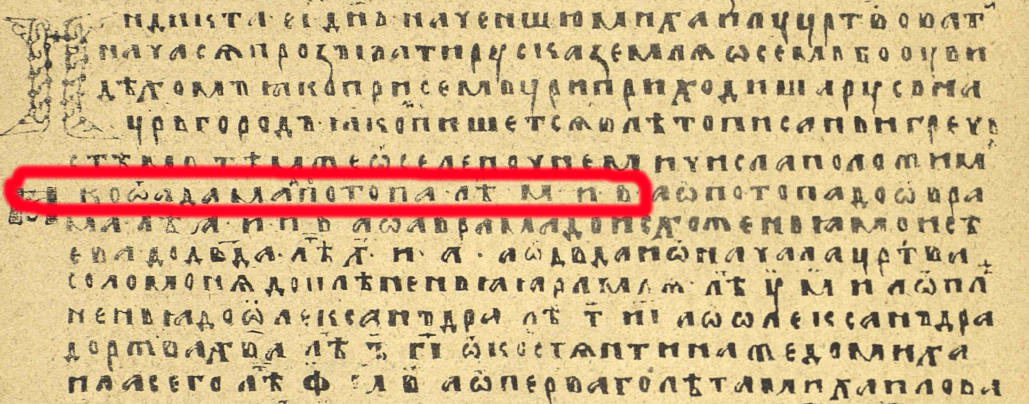
\includegraphics[width=\linewidth]{chast-colebanie-osnov/letois/lavr-sveto-01.jpg}
\end{center}

В светописное издание Лаврентьевской летописи, страницу 12. Промежуток лет от Адама до потопа задан так: «яко от адама до потопа лет 40 и 2», цифры обозначены буквами М и В.

Это 42.

А в обработанном издании? Там указано число 2242.

Разница между подлинником и обработанным текстом – 2200 лет.

Что это значит? Много чего! Выходит, в Лаврентьевском списке, даты вовсе не по счету Византийской эры. Временная шкала, используемая в Лаврентьевском списке, сдвигается на 2200 лет – при проверке первого же «слагаемого» из Росписного слоя в подлиннике! А значит, Иисус рождается на 2200 лет от сотворения мира раньше – по эре, используемой в Лаврентьевской летописи.

Я не изучал еще на этот счет светописные издания других летописей, кроме Лаврентьевской, но полагаю, что в подлинниках откроется много любопытного касаемо используемых эр и датировок.

Что же ученые? Проводят ли они нехитрые вычисления, доступные любому школьнику, чтобы определить, какое летосчисление применено в каждой отдельной летописи?

Нет. Они просто берут данные из Годового слоя, да еще обработанного правщиками изданий ПСРЛ, и по заученной формуле переводят числа из одной эры в другую. С данными из подлинников, а также с данными из Росписного слоя никто не работает.

Существует довольно мало книг о хронологии русских летописей, в эти мутные воды редко кто решается войти. Да и, мало кому приходит в голову выяснять, как же летописец считал годы, каким способом.

Одна из основных работ на эту тему, «Хронология русского летописания» Николая Георгиевича Бережкова, вышла в 1963 году смешным по тем временам тиражом – 1600 экземпляров. Это указывает еще и на степень востребованности историками подобных трудов. Бережков занимался вопросом, положенным им в название книги, с 1939 года.

Выявлены ли в «Хронологии русского летописания» слои летосчисления? Нет. Соответственно, не проведена проверка данных из этих слоев на соответствие друг другу. Какие числовые данные использованы в книге? Из обработанных изданий летописей. А мы знаем, что в подлинниках числа оказываются другими.

И здание науки стоит на зыбучем песке.

На всех страницах Бережков предполагает, что счет лет во всех рассматриваемых им летописях отличается только по годовому стилю – сентябрьскому, мартовскому и ультрамартовскому. И все вычисления крутятся около числа 5508.

Веками длится правка чисел в летописях. Веками же ученые используют эти правленные-переправленные числа, даже не помышляя о проверке, о том, чтобы определить, как даты появлялись в летописях.

Первое привело к тому, что у нас нет никаких четких датировок давних летописных событий. Второе – что мы используем ошибочные датировки всех событий вообще, включая современные, потому что числовое значение года рождения Христа, определенное в рамках «нашей эры» – тоже вычислено на основании чисел, взятых в мешанине различных летосчислений.

Казалось бы, современная наука отошла от религии, и ученые изучают следы явлений, произошедших, как полагают, за миллионы лет до нашей эры. Находят, допустим, скелеты динозавров, и говорят – динозавры жили 200 миллионов лет назад. Или 100 миллионов. И те же ученые, не моргнув глазом, используют временную шкалу, основанную на сведениях Библии о сотворении мира в предшествующие нам 10 тысяч лет. Так что это, вера или наука? Или наука и есть вера?

В моей ненаучной книге я вынужден делать много оговорок об использовании данных из разных источников. Как использую, почему, и указывать степень своего доверия к приводимым сведениям. Увы, я не имел сил и рвения затеять сверку всех чисел из доступных мне светописных копий – сверку как между копиями, так и с «подготовленными» учеными текстам в изданиях ПСРЛ. Делал это отрывочно и по мере надобности, а должно быть у общей картины выявил бы любопытные закономерности, или вообще запутался.

В целом для цитат, если не разбираю нечто крайне важное, я обращаюсь к «подготовленному» изданию 1908 года Ипатьевского списка, да изданию 1926-1928 Лавреньевского, это из имеющихся у меня изданий лучшие, кроме светописных.

А что мне делать с датами? Датам из каких списков отдавать предпочтение? Из какого слоя какой летописи? Нет у меня ответа, и вынужден я пользоваться датами общепринятыми, порицая оные и указывая на их шаткость.

Некоторые летописи содержат дополнительные сказания, такие как «Сказание о Словене и Русе и городе Словенске», где читаем:

\begin{quotation}
И в лето от сотворения света 3099 Словен и Рус с роды своими отлучишася от Ексинопонта, и идоша от роду своего и от братия своея.
\end{quotation}

Потирая руки, применяем известную формулу в общем ее виде. От летописного года отнимаем год 5508:\\

3099-5508=-2409\\

Это же 2409 год до нашей эры! Здесь одни ученые говорят – не может быть, выдумка новгородских книжников. А другие находят подтверждение следов древнейшей истории Славян.

Но разве мы знаем, какое летосчисление использовалось в «Сказании»? Давайте-ка на пробу применим к нему летосчисление не Византийской эры, а другое. Например, из римских хронографов. У них сотворение мира отнесено к 3948 году до нашей эры. Давайте подсчитаем. От летописного года 3099 отнимем 3948. Получим 849 год до нашей эры. Тоже звучит фантастически, но всё же в меньшей степени, чем третье тысячелетие до нашей эры.

Может быть, в истинном летосчислении «Сказания», число 3099 при переводе на «от рождества Христова», относилось бы, скажем, к девятому веку нашей эры.

Время и место. Так называется замечательный роман Юрия Трифонова, однако от времени и места зависит счет лет. Из-за того, что в летописи попали сведения из разрозненных источников, зачастую трудно сказать, насколько верна эта дата по отношению к Годовому слою летописи-приемника. И чем глубже в историю, тем более летописные даты теряют основательность.

А какое было летосчисление до принятия Владимиром христианства\footnote{Читатель, да услышь ехидство в сем вопросе!}? Повесть временных лет охватывает часть времен поганских. Нестор не был им свидетелем и пользовался чужими рассказами. Надо полагать, в этих его источниках существовали свои летосчисления. Какие? Загадка.

Но хорошо.

Мы сейчас ведет счет лет «от нашей эры», то бишь от рождества Христова. Привычно и понятно.

Но ведь разные народы в разное время перешли на такое летосчисление. Однако положим, кто-то раньше других. Сейчас мы, после цепочки произведенных во глубине веков вычислений, пользуемся годом рождения Христа, вычисленным монахом Дионисием Малым\footnote{Скиф Дионисий слыл образованнейшим духовным лицом Рима во времена папы Иоанна I. В математических расчетах Дионисий использовал ноль, чего среди его современников не водилось.}. Дионисий при вычислениях считал годы по современной ему Диоклетианской эре. Ею пользовались христиане Египетской Александрийской церкви, а ныне Коптская православная церковь. Вопрос, насколько верно вычисление Дионисия, оставим в стороне. Эру же «от рождества Христова» впервые ввел в обиход – в своих научных трудах – другой монах, Бэда (Beda Venerabilis).

Когда в какой-то стране возникала надобность перейти на эру «от рождества Христова», то соотносили рождество Христово в счете лет Диоклетианской эры с годом рождества Христова по местному летосчислению. Но мы уже видели на примере русских летописей, что год рождения Христа в них, в зависимости от списка, легко прыгает на тысячу лет. События могут смещаться – в письменной истории – на тысячу лет относительно рождества Христова, нашей эры. 

Поскольку приняли полагать, что числа в одних летописях верны, а в других ошибочны, то в основе датировки событий лежит вера. Вера в определенную летопись.

А когда начали вести счет годам от рождения Христа? С дня его рождения? Нет. Сразу после его смерти? Тоже нет. Когда же?

Столетия спустя.

Как вообще можно узнать, когда родился Иисус?  Выясним, какие временные привязки существуют у этого события.

В Библии не написано, что в таком-то году от сотворения мира. Но вроде бы есть много способов  вычислить год рождения\footnote{Способ с привлечением царя Ирода не прокатит – наместников Иудеи под таким именем было 9 – целая династия, и все Ироды.}. Например, известно, что судили Иисуса при Понтии Пилате (Pontius Pilatus), пятом по счету римском управителе провинции Иудеи. Историческое лицо. Когда он родился? 

Единственные, по большому счету, известные упоминания о нем в давних источниках, помимо Нового Завета, находим у римских историков Тацита и Флавия Иосифа. Тацит просто сообщает в своих «Анналах», что Христа казнил «при Тиберии прокуратор Понтий Пилат». Флавий Иосиф перечисляет римских наместников Иудеи, среди них Пилата. Понятное дело, что оба историка в лучших традициях своего времени не используют даты, но делают отсылки к правлению императоров.

А даты их правления, худо-бедно, с некоторых пор появляются в истории, причем поначалу в летосчислении «местных» эр.

На каком-то этапе развития человечества, возникла необходимость эти местные летосчисления соотнести между собой. И каждый ученый, светский или церковный, делал по-своему. А многие не делали, ибо трудно до невозможности. Ведь надо увязать не просто летосчисления, но и календари.

До революции 1917 года, у нас использовался юлианский календарь – его счет дней года известен как «старый стиль», а год начинался с марта (потом начало года перенесли на сентябрь). Имя своё календарь получил от Юлия Цезаря, при коем был введен в обиход.

Сейчас мы используем григорианский календарь. Разница между днями обоих календарей медленно растет – поначалу это было 10 дней, в 1900-2100 годах составляет 13 дней, потом увеличится до 14, а с 2200 года до 15. Поэтому наш странный праздник «старый Новый год» приходится на григорианское 13 января, что по юлианскому календарю – 31 декабря. Ибо от 13 января отнимаем разницу счета дней в этих календарях, равную 13.

Французский ученый Жозеф Скалигер (Joseph Justus Scali\-ger, 1540-1609) ввёл в обиход искусственную эру – ее называют теперь эрой Скалигера или юлианским периодом. За начало этой эры, в рамках юлианского календаря (системы счета дней), Скалигер положил (в пересчете на современную нам эру) 4713 год до нашей эры. Число взято не с потолка, а является произведением множителей 28*18*15, имеющих важные календарные и астрономические значения.

Скалигер в своих работах «Сочинении об исправлении хронологии» и «Сокровищнице хронологии» предложил таблицы перевода дат из различных эр в «свою», таким образом ученые получили в руки средство преобразования дат в привычные, переводя сначала дату в эру Скалигера, а затем из эры Скалигера – в нашу, основание которой тоже вычислено цепочкой таблиц и формул. 

Любое звено этой цепочки может быть ошибочно.

В эре Скалигера все дни (в смысле дня, определяемом юлианским календарем) последовательно нумеруются. Ученые берут какую-нибудь другую эру, например Набонассара, и вычисляют, на какой по счету день эры Скалигера приходится первый день эры Набонассара. Теперь даты, выраженные в счете лет Набонассара, можно соотносить с эрой Скалигера, а через нее – с нашей эрой.

Таким образом, подобные вычисления основаны на пользовании таблицами Скалигера. Быть может, он предлагает алгоритм, способ, по которому сам получил значения в таблицах? Допустим, зная правила умножения, мы можем составить таблицу умножения. А какие правила использовал Скалигер для своих таблиц? Он не пишет. А ведь хорошо бы знать, чтобы проверить!

Последователем Скалигера, в 17 веке, был тоже француз, иезуитский теолог Дионисий Петавиус. В своих трудах по хронологии он выстроил картину истории мира, расположив события по годам, используя как опорные события библейское сотворение мира и рождество Христово. Например, согласно Петавиусу, всемирный потоп случился на 1656 году от сотворения мира, и в 2329 году до рождества Христова.

Сравним с данными «удобочитаемого» издания Ипатьевской летописи. Потоп – 2242 год от сотворения мира, и 3212 лет до рождества Христова.

Петавиус давал также годы по эре Скалигера. Основные сочинения Петавиуса в области хронологии –  «Opus de doctrina temporum» и «Rationarium Temporum» – непревзойденные по охвату событий труды, где расписывается история человечества от сотворения мира и до времени самого Петавиуса. Упорядочение всего по годам! Какая адова работа проделана!

В веках, которые мы знаем как 15-17, ученые Европы принялись разбираться в летосчислениях разных народов, пытались сопоставлять. Год рождения Христа вроде бы уже имели, однако с привязкой – от основания Рима, что порождало несколько вариантов.

Скалигер, как показалось, внес некоторую ясность и предложил способ соотносить эры, упорядочивая историю. По Скалигеру, мир был сотворен за 3949 лет до рождения Христа.

Петавиус, продолживший дело Скалигера, применил его таблицы, разложив по ним события мировой истории. Петавиус внес также исправления. Он полагал, будто Иисус родился за 3984 года после сотворения мира. Начало эры Скалигера (Юлианского периода) имеет привязку – 764-й год до сотворения мира. Сдвиг Петавиусом времени сотворения мира означал «исправление» начала Юлианского периода – Петавиус соотнес его с 729 годом до сотворения мира.

Наконец, Джеймс Ашер в 17 веке поместил сотворение мира на расстояние 4003 лет до рождения Христа, и начало Юлианского периода связал с 710 годом до сотворения мира. Подобных чисел держался и другой ученый того времени, Джон Лайтфут.

Вооруженные таблицами и работами друг друга, христианские ученые-хронологи честно трудились над упорядочением истории, то бишь расставляя по годам события, описанные в разных источниках. Расставляя по годам «от сотворения мира» и от «рождества Христова», невзирая на то, что представления об этом у разных ученых были разные.

Но постепенно все стали приходить к некоему согласию. А оторванные, лежащие где-то в прошлом военные походы Александра Македонского, большой пожар в Риме при императоре Нероне, интриги византийского двора при Цимисхии, и даже вечно враждующие ярлы и бонды из скандинавских саг обрели четкую прописку в истории, получив свои года.

Сейчас у нас некоторый год, скажем, 2015 или 2200.  Я не знаю, когда вы читаете эти строки. Находясь, допустим, в 2066 году мы можем двигаться по одному году назад, и читая документы за эти годы, выяснять историю определенной страны. Время, для которого и ниже которого документы заканчиваются – хронологическая муть. Датировки событий, относящиеся к ней, вычислены. А мы видим, какая невероятная путаница лежит в основе этих вычислений.

Посему год 2022, или год 2200 – не более чем удобная условность для счета лет. 2022 на деле может не означать, что Христос родился 2022 лет назад. Мы не «досчитаем» назад до рождения Христа, у нас нет непрерывной цепочки датированных документов, тянущейся к этому событию. Таким же образом год допустим 860-й, приуроченный к чему-то в учебнике, может не означать, что такое-то событие случилось в 860 году нашей эры.

Далее в этой книге, конечно же, будут встречаться даты. Я согласен с относительной верностью дат, события которых записаны в то же время. Например, знаменитый краевед Киева Николай Закревский родился в 1805 году. И в какой-нибудь церковной книге был записан день его рождения. Тот год современники считали 1805-м.

Летописные годы из Повести временных лет, вплоть до Владимира, Ярослава и пожалуй несколько далее – как к ним относиться? Там же разнобой в списках! Что мне, все варианты перечислять? И каждый переводить в «нашу эру»? А на основании какого слоя – Царей, Росписного или Годового? А может Индиктов?

Ученым проще – они взяли книжку коллеги или предшественника, там готовые числа, и никаких вариантов. Верь им, бери да используй! А я не знаю, какие числа правильные. Я как мог дошел вниз, к доступному мне основанию, и не знаю, каким числам доверять, каким нет.

Поэтому я решил так. Даты буду приводить как в Годовом слое источников, принимая за таковые обработанные тексты из Полного Собрания Русских Летописей. Да и что толку даже от подлинников, если в них разные летосчисления и даты? Разные!

На вопрос, какое же летосчисление верное, и как по годам «нашей эры» разложить летописи разных народов, предания, саги, я отвечу просто – никак. Отсутствие четкой основы современного летосчисления. Слабая взаимосвязь давних источников. Разнобой летосчислений и числовых значений в пределах даже источников одного вида (например русских летописей).

Можно перебросить мостки между некоторыми летописями и сагами. У нас Ярослав, у них – Ярицлейв. Но это уровень слоя Царей. Правы были Греки, что не заморачивались и применяли в своих сочинениях этот слой!

Благодаря путанице дат, если не доверять научной хронологии, то вполне можно предположить – однако ни проверить, ни опровергнуть – что, допустим, поход аргонавтов за Золотым Руном происходил во времена князя Кия. Ведь нельзя же четко сказать, когда ходили за Золотым Руном, хотя историки относят сие событие, подробно описанное Греками, к сказкам.

Кстати о сказках. Прошлое многих народов уходит корнями в то, что ученые именуют мифом, легендой.

Про былое Киева сложно говорить, оно до Кия словно отрезано. А вот возьмем историю Ирландии. Ее исторические предания наука делит на сказочные и настоящие. Хотя в самих преданиях такого разделения нет. Существует список правителей Ирландии – и тоже, одних правителей ученые называют настоящими, других – легендарными! А почему?

В старейших известных временах Ирландии, люди – лишь одни из действующих лиц. В подробно описанной череде событий действуют представители множества народов, среди них основные – Фир Болг (Фирболг), Фомойры, Туаха Дэ Дананн (Tuatha De Danann, что обычно, полагаю ошибочно, переводят как «Народы богини Дану») и клан Мила, да вот только... К простым людям относятся определенно лишь представители клана Мила.

Прежде враждовавшие, Туаха Дэ Дананн и Фомойры потом смешались. Позже Ирландию завоевывали люди, а именно «сыновья Мила» или «клан Мила» – Скифы-выходцы из Египта, прибывшие через Испанию. Затем Туаха Дэ Дананн совершили странный исход с лица земли. Его смысл ускользает из преданий, но сходен с исходом сказочного народа «чуди белоглазой». После своего сокрытия, представители Туаха Дэ Дананн постепенно прослыли эльфами или фэйри, чудесным народом.

%проявляют те же свойства, что эльфы, однако я не уверен, что полное отождествление будет точным, хотя среди исследователей этого вопроса прижилось считать народы богини Дану эльфами.

Я понимаю, сразу перед глазами встает остроухий образ из фантастических произведений, однако нет никаких указаний на необычность внешности Туаха Дэ Дананн, в отличие от Фомойров. Туаха Дэ Дананн, однако, обладали некими способностями, которые люди именовали волшебными.

Так вот, известно 142 правителя Ирландии, которых ученые относят к выдуманным. Известны годы их правления, составлены генеалогические деревья, кто чей сын, дочь или брат, но вот беда, такой-то правитель – из Туаха Дэ Дананн или Фомойров.

Для примера, и сравнения с нашими летописями, приведу выдержку из одной ирландской летописи – Анналов королевства Ирландии (Annála Ríoghachta Éireann). Их составили в 17 веке, пользуясь разными источниками, ученые монахи ордена францисканцев. Их кстати не беспокоило, что речь в значительной части Анналов идет про «волшебные» народы.

Вот мой перевод самого начала этой ирландской летописи, выполненный с английского перевода 1856 года (семитомник Annals of The Kingdom Of Ireland by the four masters)\cite{annals4mast}. Повествуется о начале заселения Ирландии. Имена оставляю в английском написании:

\begin{quotation}
От сотворения мира до года Потопа, 2242 лет. Сорок дней до Потопа, Ceasair\footnote{В анналах Clonmacnoise, Ceasair или Caesarea названа племянницей Ноя, предупрежденной о Потопе.} прибыла в Ирландию с пятьюдесятью девушками и тремя мужчинами; Bith, Ladhra, и Fintain – их имена. Ladhra умер в Ard-Ladhrann, и от него такое название. Он был первым, кто умер в Ирландии. Bith умер в Sliabh Beatha, и был погребен в карне\footnote{Carn – курган из камней.} Sliabh Beatha\footnote{Примечание 1593 года нашей эры: этот курган существует поныне и расположен на той части горы Sliabh Beatha, что тянется через часть церковного прихода Clones, относящегося к графству Fermanagh.}, и по нему так названа гора. 

Ceasair умерла в Cuil-Ceasra, в Connaught, и была погребена в Carn-Caesra. А по Fintain прозван Feart-Fintain, над Loch Deirgdheirc.

От Потопа до времени, когда Parthalon завладел Ирландией, 278 лет; а от сотворения мира, 2520.

В году 2520 от сотворения мира Parthalon прибыл в Ирландию\footnote{В анналах Clonmacnoise соотносят прибытие Parthalon с 21-м годом жизни Авраама, и с 12-м годом правления ассирийской императрицы Семирамиды, однако переносят время к 313 году после Потопа.}. С ним были трое его сыновей, вожди: Slainge, Laighlinne, и Rudhraidhe; а также четверо их жен: Dealgnat, Nerbha, Cioch\-bha, и Cerbnad\footnote{По латинскому сочинению Historia Brittonum, Partholomus приплыл из Испании, а с ним было 1000 человек.}.

Год 2527 от сотворения мира. Fea, сын Torton, сын Sru, умер в этом году в Magh-Fea и был погребен в Dolrai-Daighe-Fea; по его имени и названа эта равнина.

Году 2530 от сотворения мира. В этом году произошла первая битва в Ирландии; Cical Grigenchosach, сын Goll, сын Garbh, из народа Фомойров, и его мать, прибыли в Ирландию с восемью сотнями воинов, и было сражение между ними и войском Parthalon в Sleamhnai-Maighe-Ithe, где все Фомойры были побеждены.
\end{quotation}

Далее ирландская летопись продолжает скрупулезно повествовать, кто когда прибыл, с кем воевал, когда умер, и так далее. Пропустим череду лет:

\begin{quotation}
От сотворения мира, 3303. Десятый год правления Eochaidh, сына Erc; и это был последний год его правления, ибо Туаха Дэ Дананн прибыли, чтобы отбить Ирландию у Фирболг\footnote{Оба народа некоторые источники относят к потомкам Афета, сына Ноя.}; и они воевали друг с другом в Magh-Tuireadh, Conmainche-Cuile-Toladh, Connaught. И король Eochaidh, сын Erc, был убит тремя сыновьями Neimhidh, сына Badhrai, из Туаха Дэ Дананн. Этих трех сыновей звали: Ceasarb, Luamh и Luachra.

Фир Болг были уничтожены в этой битве. Как сказано ранее, Eochaidh стал последним королем от Фир Болг в Ирландии. Всего их правило предположительно девять, и 37 лет длилось их правление над Ирландией.

Год от сотворения мира 3304. Первый год правления в Ирландии Breas. Туаха Дэ Дананн передали власть ему после победы в битве Magh-Tuireadh Conga, пока рука Nuandhat не будет излечена. 

Год от сотворения мира 3310. Это был седьмой год правления Breas в Ирландии, когда он передал власть Nuadhat, после того, как Diancecht при помощи Creidne приделал ему серебряную руку\footnote{Диоген Лаэртский сообщал про Пифагора: «Рассказывают, что однажды, когда он разделся, у него увидели золотое бедро».}.\end{quotation}

На этом, пожалуй, остановлюсь. Дальше идет в том же духе. Это вполне летописные сведения, ничуть не лучше и не хуже наших отечественных. У нас в летописях чудеса похлеще серебряной руки бывают.

Подобно сагам и русских летописям, в анналах Ирландии есть примечания, как называется то или иное место нынче (при составителе хроники), где оно расположено. Заметно сходство давних источников, стремление их составителей перебросить мостки между прошлым и настоящим.
 
Что не нравится ученым в ранних ирландских анналах?

Первым делом Всемирный Потоп. Ведь сначала в Ирландию, до Потопа, приплывает Ceasair. После Потопа – Parthalon. Оба вроде бы люди. Иное не указано. Затем Parthalon воюет с Cical Grigenchosach, сыном Goll (а тот – сын Garbh).

Cical Grigenchosach не человек в привычном нам значении слова, а относится к Фомойрам. Языковеды Ирландии предполагают, что это название означает нечто вроде «живущие под морем», ибо «fo» это «под», а «muire» значит «море». Эти существа описываются по-разному – то красивые люди, то одноглазые и одноногие\footnote{Согласно представлениям давних Греков, циклопы и одноногие люди обитали в Скифии. Одноглазыми считались и песиголовцы.}, то люди с козлиными головами. Великаны и обычного размера.

Далее я выпустил из хроники много, и продолжил выдержку прибытием Туаха Дэ Дананн – в то время Ирландия находилась под властью народа Фир Болг. Фир Болг и Туаха Дэ Дананн выводятся в преданиях из общего рода, от Немеда\footnote{Нимед, Нымет, Немед, Нимез или Нимет. Согласно преданиям, был родом из Скифии.}, а в предка Немеду ставят Ноя. Замечу, что христианские хронографы поступали подобным образом даже с языческими божествами – так, в греческих хронографах Зевс, его отец Крон, да и все боги-олимпийцы вписаны в родословное дерево библейских героев, и Зевс не бог, а лишь правитель.

«Библейская» привязка может быть вызвана несколькими причинами. Первая, логическая – по Библии, после Потопа спасся только Ной и его сыновья, Афет, Хам и Сим. Стало быть все, кто появляются в истории после Потопа – их потомки. Другая – только увязкой с Библией эти сведения удалось сохранить в составе Анналов. Третья причина – речь идет об указании на местность, откуда происходят определенные народы, ибо по Библии, части света были поделены между Хамом, Симом и Афетом.
% – возможно, отголосок территориально-административного передела, произошедшего после Потопа. Что по сути и должно быть случиться, рано или поздно.
 
Туаха Дэ Дананн сражаются с Фир Болг, побеждают, правление временно передают Breas, пока Nuandhat не вылечит руку (сначала ему приделали серебряную, а потом отрастили настоящую живую). При этом, у Breas мать – из народа Фомойров.

Туаха Дэ Дананн и Фомойры скрылись загадочным образом – в местах, что для человеческого глаза выглядят холмами или развалинами, но для истинных обитателей городами и замками, либо же в холмах открываются входы в тайные чертоги. Эти народы продолжили, но редко, взаимодействовать с людьми и стали восприниматься как волшебный народ (фэйри), эльфы (элвы, альвы). Это не значит, что эльфами считали только совершивших переход Туаха Дэ Дананн и Фомойров.

У ирландцев, шотландцев, гаэльцев, уэльсцев слово «эльф» не было в ходу, пользовались именованиями вроде Мирный народ (Daoine Shi, Shi), Добрые соседи, Хорошие люди (Daoine matha), фэйри. Среди населения островов Оркни ходило слово «троу» (traw). 

Также среди шотландского народа островов Оркни считалось, что прежде там жили малорослые Пикти (Picti), от кото\-рых-то люди и научились варить эль. Однако современные ученые утверждают, будто Пикти были некими кельтами, обычного роста. Между тем написанное на латыни в 11 веке нашей эры сочинение Historia Norvegia говорит, что Пикты были ростом чуть более пигмеев и творили чудеса в построении укрепленных городов.

Название Picti происходит от их обычая покрывать тела татуировками. Пиктов уничтожили потомки клана Мила, Ск\'оты (разделившиеся сейчас на ирландцев и шотландцев), но прежнее название их страны, Pictland, первоначально держалось за нынешней Шотландией. Скоты, согласно средневековой Chronica De Origine Anti\-quorum Pictorum, полагали, что Пикты тоже родом из Скифии, как и сами Скоты.

На островах Оркни и вообще в Шотландии известны сложенные из камней жилища, называемые брохи (brochs). Они имели вид перевернутых горшков, от 5 до 13 метров высотой, с низким входом у основания и зачастую имели подземный этаж, для выполнения неких ритуалов. Между двойными стенами шла винтовая лестница, соединявшая этажи. Брох венчала коническая деревянная крыша. Всего в Шотландии найдено около 500 брохов, причем без следов насильственного разрушения – их просто оставили. Почему-то, когда-то.

\begin{center}
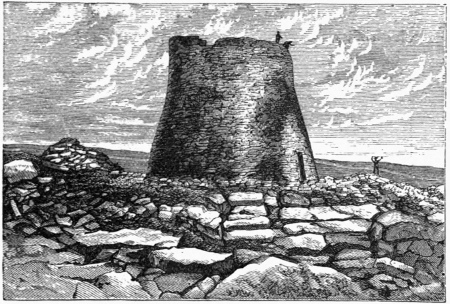
\includegraphics[width=\linewidth]{chast-colebanie-osnov/letois/fig160_197.jpg}
\textit{Broch of Mousa, Shetland.}
\end{center}

В статьях приводят замеры брохов – диаметр, высоту, но почему-то избегают сказать, какая была высота дверей. Но бывают и добросовестные ученые. Открываем книгу Джозефа Андерсона «Шотландия в поганские времена» («Scotland in pagan times», Joseph Anderson, 1881), по сути, сборник лекций. Лекция четвертая, «Устройство брохов». Рассматривается брох на острове Муса (Mousa), в Шетландии (архипелаг на северо-востоке Шотландии).

Про внешнюю дверь написано:

\begin{quotation}
Она на уровне земли, с юго-западной стороны, и около 5 футов 3 дюймов (1,524 метра) высотой и 2 фута 11 дюймов в ширину.
\end{quotation}

Далее идет описание, куда ведет тоннель от двери, то да сё, и потом описание внутренних помещений. Среди прочих там есть три комнатки, круглые, разной высоты – от 9 до 10 футов (2,7-3 метра), то есть можно не пригибаться, выше человека, но вот двери туда по три фута высотой и два в ширину, то есть 91 на 60 см. 

Существуют записки 17 века, шотландского священника городка Аберфойла, переводчика «Книги псалмов» на гаэльский, фольклориста Роберта Кирка (Robert Kirk), известные ныне под заголовком «The Secret Commonwe\-alth of Elves, Fauns and Fairies» («Тайное сообщество Элвов, Фаунов и Фэйри»).

Их предваряет описание:

\begin{quotation}
Природа и действия Подземного (и, в большей степени) Невидимого народа, известного под именем Элвов, Фаунов и Фэйри, или подобных, среди населения южной и восточной части Шотландии (Low-Country Scots), как они описаны теми, кто имеет Второе зрение; и теперь, для дальнейшего изучения, собранные и упорядоченные Осмотрительным исследователем среди Шотландско-Ирландского населения Шотландии. 
\end{quotation}

В этом небольшом произведении дается, с христианским оттенком, толкование необычных существ, способов их наблюдения, и взаимодействия с ними. Рассуждения, обобщения, многое размыто. Ощущаются недоговорки. По Кирку, фэйри или эльфы – отдельная раса, промежуточная между людьми и ангелами. У них тоже рождаются дети, бывают свои свадьбы и похороны. Среди них попадаются двойники людей из «нашего» мира.

Считается, что Кирк умер в 1692 году. И вот его преемник, священник Патрик Грэхем, в своем краеведческом путеводителе 1810 года «Sketches Descriptive of Picturesque Scenery, on the Southern Confines of Perthshi\-re», где немало места уделено фэйри, пишет, что Кирк вообще-то и не умер.

%Уолтер Скотт в своих «Письмах о демонологии и ведовстве» (Letters On Demonology And Witchcraft), изданных в первой половине 19 века пишет, со слов священника Патрика Грэхема из Абэрфойла

14 мая 1692 года, вечером, Роберт Кирк, отправился в одной ночной сорочке на так называемый Дан-ши, Doon Hill или холм Фэйри, небольшой пологий холм, что находился поблизости на запад от дома священника. Этот холм, поросший соснами и прочими деревьями, сейчас служит местной зловещей достопримечательностью.

На холме Роберт Кирк впал в состояние, которое сочли смертью, хотя, как замечает Вальтер Скотт в «Письмах о демонологии и ведовстве» (Letters On Demonology And Witchcraft), люди знающие могли бы определить в этом обморок, вызванный сверхъестественным влиянием народа, границы чьего владения он преступил. 

Роберта Кирка похоронили, однако после этого он неким образом явился, в той же ночной рубашке, одному из своих родственников и отправил того к Грэхему Дачрейскому (Duchray). Родич, с коему явился Кирк, тоже был родственником Грэхему Дачрейскому. Кирк поручил родичу следующее: «Иди к моему двоюродному брату Дачрэю и скажи ему, что я не мертв, я упал в обморок, и был перенесен в страну Фэйри, где теперь и нахожусь. Скажи ему, что когда он и мои друзья соберутся на крещении моего сына\footnote{Кирк оставил жену беременной.}, я появлюсь в помещении. Тогда, если Дачрэй бросит  над моей головой нож который он держит в руке, я буду освобожден и вернусь к обществу людей».

Родич однако не спешил передавать это сообщение. Тогда Кирк явился к нему повторно, угрожая преследовать его днем и ночью, если тот не передаст сообщение. Родственник наконец выполнил обещанное.

После церемонии крещения, все уселись за столом. Тут, якобы покойный, Роберт Кирк вошел в комнату через одну из дверей, но лорд Дачрэй по какой-то причине не бросил нож как было условлено. Роберт Кирк вышел через другую дверь и больше его не видели.

%, что смерть Кирка была необычной. Под вечер он вышел на прогулку по соседнему холму фэйри (dun-shi), и был найден в бессознательном состоянии, которое приняли за смерть. Преподобный Грэхем отметил, что знающие поняли бы, что это состояние вызвано сверхъестественным влиянием людей, чьи границы Кирк нарушил.

%После похорон, Кирк однако неким образом посетил родича, и попросил его передать на словах послание их общему двоюродному брату Грэхему из Дачрэя. Дескать, Кирк не мёртв, а пленен в стране Фэйри (Fairyland), и чтобы он смог вернуться, надо выполнить следующее. Жена Кирка осталась беременной. Когда она родит, Кирк будет при крещении младенца присутствовать в комнате. Тогда же брат должен бросить нож или кинжал поверх головы Кирка, и тот сможет вернуться к людям\footnote{Послание Кирка: «Say to Duchray, who is my cousin as well as your own, that I am not dead, but a captive in Fairyland, and only one chance remains for my liberation. When the posthumous child, of which my wife has been delivered since my disappearance, shall be brought to baptism, I will appear in the room, when, if Duchray shall throw over my head the knife or dirk which he holds in his hand, I may be restored to society; but if this opportunity is neglected, I am lost for ever.» – по Walter Scott, Letters On Demonology And Witchcraft.}.

%Кирк в самом деле появился на крещении, его видели, но Грэхем не выполнил просьбу, и Кирк лишился возможности вернуться.

Понятие «эльфов» и «фэйри» довольно размытое, отличается от местности к местности, и является общим названием, а не обозначением определенного вида существ. Можно сказать, что к эльфами относят сообщества перешедших в некий иной режим существования людей (и представителей других биологических видов) с особыми способностями, как Туаха де Дананн, а также просто некоторых умерших (подобное представление бытует у Славян в связи с русалками). Будучи в этом ином режиме существования, они изредка взаимодействуют с нами, обычно в особых местах и условиях.

%Например, Исландцы делили своих «альвов» на черных (подземных) и светлых (живут в Алфхэйме). Бытовало и мнение о трех видах, выраженное Йоуном Гвюдмундссоном Ученым (Jón lærði Guðmundsson, 1574-1658) в рукописи «Собрание сведений и фактов для лучшего понимания Эдды» (1641)\cite{korabl01}: 

%\begin{quotation}
%Люди полагают также, что эльфы – это народ, делящийся на три рода, или имеющий три основных места обитания. Одно – в море. Второе – внутри земли или под землей, которое люди называют «Эльфо-мир», а иногда – подземный мир, что многие наши истории поясняют. И люди видят, что этот род не имеет носового хряща между ноздрями. Живут же они половину обычного нашего срока (на земле). Третий род, который мы называем Сокрытым Народом или льювлингами также населяет холмы и скалы; и часто сочетались они с нашим родом. Этот эльфийский род живет дольше, отличается красотой и имеет правильную форму, как у нас.
%\end{quotation}

С эльфами связано иное течение времени. Это проявляется в следующих случаях. Ребенок, рожденный от эльфов (чистый эльф или полукровка) растет быстрее (среди людей), нежели дитя человеческое.

Живые люди, попадавшие в мир эльфов (осознаю всю условность этого определения), возвращались в мир людей спустя долгие годы, при этом для них прошло совсем немного времени. Значит, в мире эльфов время течет медленнее, чем в нашем. Однако возвращаясь оттуда, некоторые люди быстро старели, едва не на глазах. 

Любопытно, что мы знаем еще один мир с иным течением времени – мир снов, в котором время течет быстрее нашего. Таким образом выстраивается цепочка «миров», различных по скорости времени. Расположу по возрастающей: мир эльфов → мир людей → мир снов.

Какое всё это имеет отношение к Киеву? А я непроста рассказываю, позже всплывет.

Некоторые из героев ирландских анналов и сказаний, например Луг, были обожествлены, стали языческими богами. Выдающаяся личность сегодня, через век ее почитают за божество, а спустя еще пару столетий, когда переменяется вера – уже называют демоном. 

Ирландским анналам повезло, их не сократили под корень, оставили ирландцам прошлое. Наши же летописи, относящиеся к Киеву, словно отрублены на уровне князя Кия. И кто знает, повествование о каких событиях мы бы прочитали за предшествующие годы, и какие бы люди – или нелюди – действовали в них?

Но заглянуть за эту черту таки возможно, ведь кроме летописей, существуют и другие, внешние источники.

\chapter{Аланы}

С годами меняется облик планеты. Народы расселяются, обретают другие имена, обычаи, веру и даже языки, сохраняя нечто старое и предлагая соседним народам свои слова, обычаи и веры взамен приобретенных.

В Чечне, в зеленом подгорьи, у берега реки Сунжи есть село Алхан-кала. В глубокое прошлое проросли его корни. А в 19 веке Чеченцы переселись отсюда к юго-востоку, по другую сторону реки, и основали Алхан-Юрт, а на месте прежней Алхан-калы возникла станица терских казаков Ермоловская. Некоторое время атаманил в ней дед моей бабушки по отцовской линии, Леонтий Никитин. В начале 1920-х станица забунтила вместе с прочими окрестными. И по приказу Орджоникидзе ее жителей кого выселили, кого услали. Прошли годы. Ныне это снова Алхан-кала, и обитают в ней Чеченцы.

В четырех километрах от Алхан-калы найдено крупнейшее в том краю городище – остатки города, в котором жили, как полагают, Аланы – народ, ответвившийся от Сарматов. Укрепление длиной в километр, обнесенное рвами, один из коих глубиной 9 метров. Мощеная булыжниками мостовая. Кто ходил по ней? Чья речь слышалась? А в окрестных селениях?

Тот же вопрос уместно задать о Киевщине.

Как принято считать, Киев основан братьями Кием, Хоривом, Щеком да сестрой их Лыбедью. Одни ученые принимают это летописное предание, другие опровергают. Нет общего мнения.

Вот знаменитый историк Василий Ключевский. Его живо изложенные лекции в печатном виде зачитывались до дыр. Ключевский оценивал основание Киева скромно, приурочивая его к Кию с братьями, невесть почему назвав их звероловами и поселив в некие однодворные деревни: 

\begin{quotation}
Так Киев возник из трех однодворных деревень с общим укрепленным убежищем, которые поставлены были тремя звероловами...
\end{quotation}

Историки, согласные в определенной мере с преданием о братьях, обычно далее того не идут. Заложили братья крепость – град Киев, и ладно. А прежде что тут было? Ученые уходят от прямого ответа. Отделываются размытыми словами. Да, первобытные стоянки времен палеолита. Да, защитные валы черняховской культуры. Черепки горшков трипольской культуры... Но город, дескать, возник только при Кие.

Пытливый Максим Берлинский в своем «Кратком описании Киева»\cite{berl01} предположил наличие тут города до основания крепости Киева, ссылаясь на Клавдия Птолемея, перечислявшего города, лежащие по Борисфену, как Греки называли Днепр\footnote{Наука использует два основных способа чтения букв древнегреческих текстов, «итацизм» да «этацизм». По первому, слово Βορυσθένης надо читать как Ворисфенес, по второму – Борисфенес. Однако никто точно не знает, каково было произношение у древних Греков. Кроме того, в переводах прижилось отбрасывание окончания «ес», остается лишь корень Борисфен. Можно считать, что любое название либо имя из давних сочинений Греков переведено приблизительно. Оно могло произноситься иначе! Кстати, согласно поэме римского императора Адриана, имя коня Цезаря было Борисфен Аланский.}:

\begin{quotation}
Птолемей, между прочими городами упоминает об Амадоке, стоявшем при повороте Днепра, по левую его сторону, близ какого-то озера, или вероятнее реки, что по его ландкарте придется при впадении Десны в Днепр. И по ту же сторону Днепра, выше сего, упоминает о находившемся городе Азагориум, может быть, от тогдашних тамошних жителей назывался Загорье.
\end{quotation}

А один из самых передовых людей времен Петра I, многообразный деятель Василий Татищев, трактуя некий вариант карты к «Географии» Птолемея, название Азагориум примерял к Переславлю, а вот Амадок – относил к Киеву.

Попробуем разобраться с этим сами, по трудам давних греческих историков и географов, а также правителей Византии. Все их труды относятся ко времени, когда в наших краях жили Скифы (они же Скиты) и Сарматы. Выяснение подробностей приведет нас к другим источникам, мы возьмем на вооружение свидетельства давних Арабов, Латинов, Французов, а также наших летописцев и толмачей.

Задача – не раскрыть тайны прошлого до конца, но пробовать найти подступы к этому прошлому. Сравним то, что говорит современная наука, с тем, что утверждают люди, общавшиеся со Скифами и другими народами древности непосредственно.

Спросите любого на улице, кто такие Скифы? Вообще-то прохожего это вообще не колышет. Но упрощенное представление таково – древний воинственный народ. Кочевали по степям, хоронили своих в курганах, были мастерами делать украшения из золота, снимали с врагов скальпы.

А что скажет наука? Она завороженно твердит, что Скифы – «ираноязычные племена», обитавшие в землях от Дона до Дуная с 8 века до нашей эры по 9 век нашей эры.

Отметим, что теперь на большей части этого пространства живут сплошь Славяне – Чехи, Поляки, Русские, Украинцы – словом все нынешние страны со славянским населением прежде составляли Скифию.

Летописец Нестор в Повести временных лет, перечислив славянские народы, что обитают в землях от Дунаю до Днепра, пишет, что до сего дня Греки называют эти места «Великая Скуфь» (Большая Скифия). И повторно он говорит, о составе похода Вещего Олега, что Олег набрал войско из народов Варяг, Словен, Чуди, Кривичей, Мери, Полян, Северов, Древлян, Радимичей, Хорватов, Дулебов, Тиверцов – «си вси звахуться Великая Скуфь» – поясняет Нестор.

Так выходит, Скифы – общее греческое название Славян? А как же «ираноязычные племена»? В пользу ираноязычия Скифов говорят, казалось бы, имена рек – Дунай, Дон, Днепр, Днестр, многочисленные Донцы (Северский, Липовый, Саженный) – где ученые усматривают скифское слово «дан», что переводят как «вода» либо «река». А «Днепр», он же «Данапр» – мол, это «дана» и «апр», два скифских слова, означающих вместе вода глубокая.

А предложу-ка две славянские трактовки речных имен. Мы имеем весьма мокрый корень «дно». Отсюда, кстати, и «тонуть» – «донуть», идти ко дну. Разница между звуками «т» и «д» невелика. При склонении, «дон» легко превращается в «дне». Далее, вот корень иного, временного рода – «день», «дни». Быть может, название большой реки составлялось из производного от слова «дней» и указания количества дней пути по этой реке, то есть известной длины реки. Все эти «пр», «стр» – не искаженные ли числа?

Что мы знаем о языке, на котором говорили Скифы? Всеволод Миллер и Василий Абаев в своих работах, справедливо полагая современных Осетинов потомками Скифов (через Сарматов и Аланов, Асов), скифский язык пытались восстановить посредством осетинских наречий – иронского и дигорского. 

А как же Великая Скуфь? В ее пределах скифский язык улетучился, не оставив иного следа, кроме названий рек?

%Но что дошло до наших дней от языка Скифов? Их имена в сочинениях на греческом
%Будто бы – названия рек. Что еще? Ничего.

%Две крайности. По одной Скифы – греческое название Славян. По другой – ираноязычные кочевники.

%Названия рек хорошее подтверждение тому, что Скифы пользовались словами с иранской основой для обозначения рек, лежащих на огромном расстоянии друг от друга. Причем имена эти сохраняются поныне, значит, были местными! Не называем же мы Днепр как древние Греки – Борисфеном. В русском и украинском языках примесь, трактуемая «иранской», касается не только воды, это еще и некоторые цвета.

Общепринятое знание сбивает с толку. Это ведь ученые, а не сами Скифы, сказали нам про иранские корни в названиях рек. Может они вовсе не иранские, а утраченные славянские, либо следы какого-то третьего языка. Как вообще языки влияют друг на друга? А подобно музыкальным жанрам, при этом степень возможного влияния зависит от совместимости жанров.

Наука полагает, что Скифов вытеснили Сарматы, тоже ираноязычные. И разделяет Скифов, Сарматов, да Славян – причем то временами, то происхождением. 

Но я больше доверяю давним Грекам. Они, в отличие от современных ученых, общались со Скифами. Есть что рассказать. Поэтому обратимся за сведениями к Геродоту, Страбону, Льву Диакону, Клавдию Птолемею и Плинию Старшему.

Хотел расставить эти источники по времени, однако из-за путаницы с летосчислением я не могу доверять общепринятым датировкам сих трудов, и способен упорядочить оные лишь относительно. Например, Страбон упоминает Геродота – значит, «История» Геродота написана раньше, чем «География» Страбона. Географические сведения Греков существенно отличаются не только от нынешних, но и друг от друга, что впрочем может отражать изменения, происходящие с местностью с течением времени, а не ошибочность представлений.

К рукописным сочинениям Греков нередко прилагались карты, однако неясно, составлены ли они по карте самого сочинителя, либо на основании его текста. Подлинники, начертанные Клавдием Птолемеем и другими остаются неизвестными, да и вряд ли сохранились бы. Пожары, сырость, прочие влияния окружающей среды, наконец невольный враг древних знаний – мыши.

Старинные карты кажутся на первый взгляд нелепыми. Причина тому, кроме ошибок, смешение источников современных составителю карты и источников буквально допотопных, отражающих состояние Земли до Потопа, который, сопровождаемый другими бедствиями, вполне мог служить причиной исчезновения одних гор и морей, возникновения других, переменить течения рек, не говоря уже о том, что с лица земли стёрлись целые страны. Но водная сеть меняется быстро и без привлечения Потопа.

Таким образом наиболее древние карты давали одновременно представление о Земле до Потопа и после, а с течением времени уточняясь новыми данными, лишались допотопных следов. Поэтому чем ближе к нам, тем менее фантастичны карты.

В историко-географических трудах Греки по-своему обозначали страны, города, реки, моря и озера. Порой эти названия были искаженными производными от местных именований. Либо чисто греческими. А может, по-гречески их тогда называли и тамошние обитатели. И сейчас исследователи ломают себе головы, что же подразумевали греки?

Например, Рипейские (Рифейские) горы. С ними ученые соотносят Урал, Кавказ и Тянь-шань. Каравай, каравай, кого хочешь – выбирай. Но и некоторые Греки, тот же Страбон, вообще сомневались в существовании таких гор!

В «Географии» Птолемея, где употреблена сеть координат, устье Борисфена (Днепра) лежит западнее реки Хипаниса (в отечественных переводах часто пишут: «Гипанис»). С Хипанисом отождествляют Южный Буг, однако у Птолемея это разные реки, он различает Хипанис и «Буц» (Buces). Современные толкователи обычно пишут – Птолемей ошибается, устье Буга западнее устья Днепра.

Но если считать устьем Днепра западную часть современного Днепровского лимана (куда впадает и Днепр, и Южный Буг), то устье Днепра таки западнее, чем устье Буга. А Греки так и считали.

Археологи уже давно и обстоятельно раскапывают  древний город Ольвию\footnote{46°41'33.0"N 31°54'13.0"E}. Она лежит под Николаевом, на берегу Южного Буга, примерно в 5 километрах выше его устья в Днепровском лимане. Это именно Ольвия, о чем свидетельствуют найденные там многочисленные надписи на греческом. Вырезанные в камне, они подтверждают различные права вроде этого\cite{olbia01}:

\begin{quotation} 
В добрый час! Ольвиополиты дали Ксантиппу, сыну Аристофонта, эрхиейцу, сыну Филополида, дейрадиоту – афинянам, им самим и потомкам их проксению, право гражданства, освобождение от пошлин на все товары, какие бы ни ввезли или не вывезли они сами, или их дети, или братья, у которых отцовское имущество общее, или слуги, и дали право входа в гавань и выхода из гавани и в мирное, и в военное время, без конфискации и без заключения договора.
\end{quotation} 

Здесь мы видим слова без перевода (дейрадиот, проксений) – их точное значение остается неясным поныне, посему оставляют как есть. А вот «ольвиополиты» значит «жители Ольвии». Эти ольвиополиты часто упомянуты в надписях Ольвии, и можно сделать однозначный вывод о названии города.

%Плиний в 26-й главе «Естественной истории» говорит:
Плиний в «Естественной истории» говорит:

\begin{quotation}
На расстоянии 120 миль от Тира лежит река Борисфен, с одноименным озером и народом, а также городом на материке, на расстоянии 15 миль от моря. Старые названия этого города Олвиополис и Милетополис.
\end{quotation}

Тир это Днестр. Есть на нем город Тирасполь, что подтверждает отождествление Днестра с Тиром.

Итак, по Плинию, в 15 милях от устья Днепра  лежит город Борисфен, другие названия коего – Ольвия и Милетополь. Местных жителей именовали Борисфенитами. При пересчете в километры, 15 миль Плиния – это примерно расстояние от устья Днепровского лимана до Ольвии. Стало быть, сей лиман Греки принимали за часть Днепра.

Страбон, в 7-й книге «Географии» сообщает:

\begin{quotation}
Дельта Борисфена (Βορυσθένης) судоходна на 600 стадий, а близко другая река, Хипанис (Ὕπανις), и остров перед устьем Борисфена, с портом. Если плыть по Борисфену 200 стадий будет одноименный с рекой город: он называется также Олвиа, большой торг, основанный Милисиами.
\end{quotation}

%Εἶτα Βορυσθένης ποταμὸς πλωτὸς ἐφ᾽ ἑξακοσίους σταδίους καὶ πλησίον ἄλλος ποταμὸς Ὕπανις καὶ νῆσος πρὸ τοῦ στόματος τοῦ Βορυσθένους, ἔχουσα λιμένα. Πλεύσαντι δὲ τὸν Βορυσθένη σταδίους διακοσίους ὁμώνυμος τῶι ποταμῶι πόλις· ἡ δ᾽ αὐτὴ καὶ Ὀλβία καλεῖται, μέγα ἐμπόριον, κτίσμα Μιλησίων.

Как видим, и здесь Ольвия помещена на берегу именно Днепра. Даже указано расстояние к ней – 200 стадий. А устье Борисфена судоходно (вероятно для морских, не речных кораблей) на 600 стадий. Сколько всё это в пересчете?

По представлениям науки, 1 стадия это... Различают разные стадии. Греческая, мол, 178 метров, олимпийская 192,3 метра, аттическая – 177,6, птолемеева – 185 метров, и прочие. Беда! 

Возьмем округленное 180 метров. Сколько будет в километрах – 200 стадий? 200*180/1000 = 36 километров. Это расстояние от устья Днепровского лимана до Ольвии. Итак, Греки однозначно полагали, что устье Днепра – это устье нашего Днепровского лимана. А вот Ольвия лежала на берегу этого «продленного» Днепра. Где тогда находилось устье Южного Буга, я не знаю.

Вычислим теперь, на какое расстояние от моря судоходна дельта Днепра во время Страбона. 600 стадий умножим на 180 метров – равно 108000 метров. 108 километров. Принимая за устье Днепра устье нынешнего Днепровского лимана, и что русло проходило так же, как ныне, у нас получится, что суда от моря могли подниматься по дельте Днепра  немногим, километров на 20, выше Херсона.

%Геродот, живший раньше Страбона, утверждает, что Днепр известен на 40 дней пути. Но к этому мы еще вернемся.

Однако, Днепр был известен и выше – Геродот говорит, что на сорок дней пути! Геродот из наших греческих источников древнейший. Считается, что он жил в пятом веке до нашей эры, но я полагаю, что не столь давно. В своей «Истории», в книге «Мельпомена» он рассказывает о походе царя Персов Дария на Скифов, и дает обстоятельное описание последних\cite{herodotus01}:

\begin{quotation}
По словам самих Скифов, они – юнейший из всех народов, и о своем происхождении рассказывают так: первым человеком в этой стране, тогда еще пустынной, был Таргитай\footnote{Такое же имя, искаженное в «Таргитий», встречаем у Фиофилакта Симокатты в «Истории», где Таргитий – посол Аваров, пришедший к Ромеям-византийцам за ежегодной данью для кагана Аваров. Прочие имена Аваров по этому сочинению: Сирмий, Баян, Турум, Спарзевгун, Кунаксолан, Тулдих. Впрочем, Симокатта считает европейских Аваров самозванцами, на деле представителями народов Уар и Хунны.}; родителями Таргитая они называют, чему я не верю, Зевса и дочь реки Борисфенеса. Такое происхождение приписывается Таргитаю.

У него было три сына: Липоксаис, Арпоксаис и самый младший Колаксаис. При жизни их упали с неба на скифскую землю золотые предметы: плуг, ярмо, секира и чаша.

Первым увидел эти предметы самый старший из братьев; он приблизился к ним с целью взять, но при его приближении золото воспламенилось, и он отступил назад. Затем подошел средний брат, но с золотом повторилось то же самое. Таким образом золото горением не своим не допустило к себе двух братьев; с приближением третьего, наимладшего брата золото потухло, и он отнес его к себе в дом. Поэтому старшие братья согласились уступить наимладшему все царство.

От Липоксаиса, рассказывают дальше, произошли те из Скифов, которые носят название рода Авхатов (Αὐχάται), от среднего, Арпоксаиса, произошли Скифы, именуемые Катиарами или Трапиями (Κατίαροί τε καὶ Τράσπιες), а от наимладшего, царя, те, что называются Паралатами (Παραλάται). 

Общее название всех Скифов, по имени царя их, Сколоты (Σκολότους); Скифами назвали их Эллины\footnote{Я бы перевел иначе: общее название этих варваров – Сколоты, то есть из царского рода (царствующие), а Скифами их назвали Эллины. σύμπασι δὲ εἶναι οὔνομα Σκολότους, τοῦ βασιλέος ἐπωνυμίην. Σκύθας δὲ Ἕλληνες ὠνόμασαν.}.

Так рассказывают Скифы о своем происхождении, полагая, что от начала их существования или от первого царя Таргитая до похода Дария прошло круглым счетом никак не больше тысячи лет.

Упомянутое выше священное золото цари оберегают  весьма ревниво и ежегодно благоговейно чтут его обильными жертвоприношениями.
\end{quotation}

Здесь Геродот называет Царскими (по-скифски Сколотами), не всех Скифов вообще, а три скифских народа, ветви Скифов: Катиары, Трапии и Паралаты. Были и другие народы Скифов, над которыми, надо полагать, при Дарии властвовали эти Царские Скифы.

Вероятно, именование Царских Скифов перемещалось позже со Сколотов на другой народ из числа Скифов. Был один правящий народ, собиравший дань, и его подчиненные. Приск Панийский из Фракии, состоявший в посольстве Максимина к Аттиле, в «Истории Готфов»\footnote{Приск попутно дает имена Царских скифов, помимо Аттилы: Васих, Курсих, Верих. Жену Аттилы зовут Крека. Если в мужских именах поменять «х» на «ч», получим ближе к славянским: Васич, Курсич, Верич.} относит к Скифам народы Унны (Хунны) и Готфы (Готы), однако различает эти два народа, а Уннов величает Царскими Скифами. Как я понимаю из описания Приском сборного скифского войска, Унны и Готфы были родственны, но Готфы находились в подчинении у более хищных Уннов. Не исключаю, что те, кто при Геродоте именовались Сколотами, во время Аттилы слыли Хуннами.

Скифские народы, по Геродоту, живут от Истра (Дуная) до Танаиса (Дона)\footnote{С Танаисом связана странность. Историк Иордан в «Гетике» говорит, что есть два Танаиса. Один, разделяющий Европу с Азией, начинается в Рифейских горах и впадает в Мэотийское болото (оно отождествляется с Азовским морем). Этот Танаис никогда не замерзает, в отличие от соседних рек, а также Мэотиды и Босфора. А другой Танаис рождается в Хриннских горах и впадает в Каспийское море.}. Он называет следующие реки Скифии, кажется по порядку соединения их устий с морем, с запада на восток: Истрон (Ἴστρον), Тирас (Τύρης), Хипанис (Ὕπανις), Борисфенес (Βορυσθένης), Пантикапес (Παντικάπης), Хипакирис (Ὑπάκυρις), Геррос (Γέρρος, рукав Борисфена, впадает в Ипакирис), Танаис (Τάναϊς)\footnote{Всё это греческие и «огреченные» названия, поэтому даю как в подлиннике. Однако видно, что например Дон, Дан превращен в Танаис заменой «д» на «т» и добавлением «аис». «Тирас» же – греческое именование Днестра, ничего не переиначено.}. Про Хипанис сказано ранее, а отождествление Пантикапеса, Хипакириса и Герроса с современными названиями остается загадкой поныне.

Про Скифов Геродот пишет:

\begin{quotation}
Ведь у Скифов нет ни городов, ни укреплений, и свои жилища они возят с собой. Все они конные лучники и промышляют не земледелием, а скотоводством; их жилища – кибитки.
\end{quotation}

Казалось бы, здесь говорится вообще обо всех Скифах как о кочевниках. Однако почитаем «Историю» дальше. Я буду делать выдержки и свои отступления, чтобы обсудить. Среди скифских рек Геродот особенно хвалит Днепр:

\begin{quotation}
Четвертая река Борисфенес – из скифских рек после Истра наибольшая и, по нашему мнению, самая богатая полезными предметами не только между скифскими реками, но между всеми вообще, кроме впрочем египетского Нила; с этим последним не может идти в сравнение никакая другая река.

Но из прочих рек Борисфенес наиболее прибылен: он доставляет прекраснейшие и роскошнейшие пастбища для скота, превосходную рыбу в большом изобилии, вода его на вкус очень приятна, чиста, тогда как рядом с ним текущие реки имеют мутную воду;
\end{quotation}

Природные ресурсы уже тогда играли важнейшую роль в жизни человечества. Как сейчас воюют за нефть, так прежде ценностью были пастбища. Особенно для Скифов-скотоводов.

\begin{quotation}
Вдоль его тянутся превосходные пахотные поля или растет очень высокая трава в тех местах, где не засевается хлеб.
\end{quotation}

Кто же пашет эту землю, если Скифы, по словам Геродота – скотоводы? Поскольку здесь существуют посевы и Скифы, значит, среди них есть земледельцы. Верно:

\begin{quotation}
До местности Герров, куда сорок дней плавания, Борисфенес течет, как известно, с севера; страны, через которые он протекает выше этого пункта, никому неведомы; несомненно только, что до области Скифов земледельцев он протекает через пустыню, а Скифы эти живут вдоль его на десять дней плавания.
\end{quotation}

Прежде чем касаться 40 дней плавания, обсудим Скифов-земледельцев. Иногда в переводах звучит Скифы-пахари, или Скифы-георги. В подлиннике – γεωργοὶ Σκύθ\-αι. Георг, Георгий в переводе с греческого значит «земледелец» или «пахарь».

Византийский император Константин Багрянородный, живший позже Геродота, знал около порогов Днепра остров, именуя его «остров святого Георгия». Почти все исследователи сопоставляют его с Хортицей. Об этом позже. Вероятно, остров так назывался не от святого Георгия, но потому, что рядом жили Скифы-георги. 

Каких еще Скифов различали Греки? О Царских мы уже слышали. Иное их название – Василиды (от слова «василевс» – царь, правитель). Кочевых же скифов именовали Номадами. Впрочем, Геродот считал Царских Скифов кочевыми. Продолжим разбирать его слова дальше. Моё толкование несколько отягощено знаниями из других источников, в частности про пахарей, ибо я знаю, что они жили в низовьях Днепра, а из приведенного ранее сообщения Геродота этого нельзя вывести однозначно.

Итак, вверх по Днепру на 10 дней плавания лежат земли Скифов-земледельцев. Туда Днепр течет через «пустыню» – голую степь ли, пески ли, неясно. А вообще Днепр известен на 40 дней плавания, до местности Герр (Геррос, Γέρρος), куда Днепр течет с севера. Что выше Герров – никому не ведомо.

Кроме того,

\begin{quotation}
Седьмая река – Герр вытекает из Борисфена в том месте, до которого течение Борисфена известно. Ответвляется она в этом месте, а название ее, общее с местностью – Герр. Течет эта река к морю, образуя границу между землями кочевых и царских скифов, и потом впадает в Хипакирис.
\end{quotation}

Сейчас мы не знаем никакого рукава Днепра, который бы отделялся от него и впадал в другую реку (таинственный Хипакирис), соединенную с морем. Однако, насколько я понимаю, река Герр отделялась от Днепра на 40-м дне пути.

Сколько в километрах будет «40 дней плавания»? Это невозможно вычислить точно. Неясно, с какой скоростью передвигалось судно. Допустим, 5 километров в час. В дне 24 часа, но целый день не плыли. Положим, 12 часов плыли, 12 спали. Каждый день, таким образом, лодка проходит 12*5=60 километров. За 40 дней она пройдет, 40*60=2400 километров. Современная длина Днепра равна 2285 километрам.

Меняя при подсчете скорость, мы можем подогнать 40 дней пути под любое расстояние. Хотим – растянем геродотовы 40 дней до Киева. Гидрограф Николай Максимович в труде «Днепр и его бассейн»\cite{maxdnepr01} прикладывал те же 40 дней к устью Припяти.

Есть ли какие-то дополнительные указания от Геродота насчет скоростей? Вот он дает сведения о Каспийском море. В длину оно 15 дней плавания на гребном судне, а ширина в самом широком месте – 8 дней плавания. Геродот прекрасно осведомлен об его очертаниях – длина много больше ширины, если глядеть на север.

Нынешняя длина Каспия – 1130 километров. 1130/15 =75. По 75 километров в день надо плыть на гребном судне, чтобы пересечь Каспийское море в длину. Как видим, Геродот вполне держится в рамках действительности.

И если с той же скоростью плыли по Днепру, то 75 километров в день умноженное на 40 дней равно 3000 километров. Но мы не знаем, с какой скоростью плавали тогда по Днепру, да еще против течения. Днепр в то время – тихий или стремительный? Быть может, по нему вверх вообще перемещались с черепашьей скоростью.

В целом будем считать, что Днепр был известен в самом деле чуть ли не весь. Местность Герров вполне могла быть и Киевом, и Каневом, и выше, и ниже, и возникает вопрос, как же мог существовать рукав Днепра – Герр, что на такое огромное расстояние следовал к морю? Я никогда не слышал о таких огромных речных рукавах. Реки ведут себя иначе, если только этот Герр не был рукотворным каналом. 

Герр, каким он описан Геродотом, совершенно не вписывается в современную речную сеть. На картах, несколько отдаленных от времени Геродота – например карте по «Географии» Птолемея – река Герр показана отдельной, не имеющей отношения к Днепру, и вытекающей из равнины к югу от Амадокских гор. Про них потом.

Есть еще толкование, что Γέρρος – это искаженное «Рос», то бишь Русь, а народ Герров (Γέρροισι – Герроиси) – русы. В самом деле, если полагать, что «ос» не добавлено греческим языком, а прямая передача названия, то похоже – однако неясно тогда, зачем приставка «ге».

О местности Герр Геродот сообщает, что там было кладбище скифских царей:

\begin{quotation}
Гробницы царей находятся в Геррах, до которых Борисфенес судоходен.
\end{quotation}

Далее описывается похоронный обряд Скифов, и что труп царя возят по разным соседним народам, чтобы те прощались согласно обычаю:

\begin{quotation}
Объехавши таким образом все народы, Царские Скифы являются в землю отдаленнейшего подчиненного им народа – Герров (Γέρροισι), где находится и кладбище.
\end{quotation}

Скифские могилы, курганы, по Днепру были всюду, и на Киевщине тоже. Тысячами их раскапывали, разоряли искатели кладов и археологи. Но в Геррах находились не просто курганы, а курганы скифских царей. Наверное, на то была причина. Однако без дополнительных указаний, Герры так и остаются загадочным названием в работе Геродота.

Либо продолжить словоблудие? Мол, ежели местность Геррос это «Рос», то мы знаем реку Рось, а она впадает в Днепр всего в 16 километрах ниже Канева, а там курганный край, и Канев буквально переводится «ханов», а «хан» то же, что и царь. 

Есть впрочем у Геродота еще зацепка, однако она ничего нам не даст. Геродот не называет город именем Ольвии прямо, однако:

\begin{quotation}
От торгового города Борисфенитов (Βορυσ\-θενειτέων), составляющего наиболее срединный пункт во всей приморской Скифии, первыми живут Каллипиды (Καλλιππίδαι), представляющие собой Эллинов-скифов, выше их живет другой народ, именуемый Алазонами (Ἀλαζόνες). Как эти последние, так и Каллипиды во всем ведут такой же образ жизни, как и Скифы, но хлеб они сеют и употребляют в пищу, равно как лук, чеснок, чечевицу и просо. Над Алазонами обитают Скифы пахари (Σκύθαι ἀροτῆρες), сеющие хлеб не для собственного употребления в пищу, но для продажи. Выше их живут Невры (Νευροί). К северу от Нервов, насколько мы знаем, лежит пустыня. Народы эти живут вдоль реки Хипаниса к западу от Борисфена.
\end{quotation}

Хипанис, принято отождествлять с Южным Бугом, но я уже говорил, что у Плиния это разные реки.

Мы выяснили – среди Скифов встречались не только кочевники. Более того, экономика отдельных скифских областей зависела от выращивания злаков на продажу. Вероятно, Ольвия была буквально «хлебным» портом. Отмечу, что живущий позже Геродота Страбон в «Географии» называет Георгами жителей нынешнего Крыма (тогда он обобщенно именовался Херсонесом по главному городу, а еще ранее Малой Скифией, населенной Скифами Таврами).

Что же пишет Геродот далее? 

\begin{quotation}
С переходом через Борисфенес вступаем в ближайшую от моря землю, Хилаю (Ὑλαίη).
\end{quotation}

Неясно, с переходом куда? Если Днепр протекал так же, как сейчас, от устья на северо-восток, то «через Борисфенес» это либо к северу от устья Днепра, либо юго-восточнее, в Херсонскую область. Что же относительно Хилаи?

\begin{quotation}
Выше ее живут Скифы земледельцы, которых живущие у реки Хипаниса Эллины (Ἕλλην\-ές) называют Борисфенитами (Βορυσθενεΐτας); самих себя тамошние Эллины называют Ольбиополитами (Ὀλβιοπολίτ\-ας). Следовательно эти Скифы земледельцы занимают пространство к востоку на три дня пути, простираясь до реки, именуемой Пантикапою, и на север вверх по течению Борисфенеса на одиннадцать дней.
\end{quotation}

Примерно на север (вернее, с севера на юг) Днепр течет начиная от Каховки, а затем по линии, грубо говоря, между Запорожьем и Днепропетровском. Опять же «дни пути» мало что говорят о расстоянии. 

Геродот ничего не сообщает о порогах на Днепре, а жаль – это помогло бы многое понять. Пантикапа, как поясняет Геродот, течет с севера, вытекая из некоего озера, и впадает в Днепр. Значит, Пантикапа находится по правому берегу Днепра, ведь все его левобережные притоки по крайней мере ниже Запорожья текут условно говоря с юга, а не севера. Пантикапу следует искать в нынешнем Снегиревском районе. Возможно это Ингулец.

А что же выше пахотных земель?

\begin{quotation}
Над ними простирается обширная пустыня. За пустыней обитают Андрофаги (Ἀνδροφάγοι), народ особенный, вовсе не скифский. Еще выше лежит настоящая пустыня: не живет там, насколько мы знаем, ни один народ.
\end{quotation}

Андрофаги значит людоеды. За людоедами – «настоящая пустыня». Поскольку самым отдаленным народом, да еще живущим около Днепра, Геродот называл Герров, можно заключить, что людоеды поселились в другом месте, не у Днепра. Но были соседями! 

Геродот перечисляет народы, ближайшие к землям Скифов: Тавры, Агафирсы, Невры, Андрофаги, Меланхлаины, Гелоны, Будины и Савроматы. По одному из преданий, у Геракла и пещерной женщины-змеи было три сына – Скиф, Гелон и Агафирс, которые стали родоначальниками трех из упомянутых народов\footnote{Диодор Сицилийский, живший позже Геродота, в «Исторической библиотеке» приводит иной вариант предания – что с женщиной-змеей сошелся не Геракл, а Зевс. Сына их звали Скиф, у него в свою очередь родилось два сына – Пал и Нап, по ним назвались потом два родственных народа, Палы и Напы, живущие каждый в своей стране. Это были два скифских народа. Насколько я однако заметил, Диодор порой довольно небрежно пересказывал свои источники.}.

Скифы и Эллины рассказывали про Невров, что они колдуны и по нескольку дней на год оборачиваются в волков, но Геродот этому не верит.

Меланхлаины носят черные одежды\footnote{Μελαγχλαιν. Буквально в переводе с греческого – темноодежники. Однако в русском языке есть слово малахай – ушанка, и малахайник – носящий такую шапку. Быть может, Геродот созвучно передал греческим словом русское.}, а образом жизни подобны Скифам. Обитают они в 20 днях пути к северу от Мэотиды. Под Мэотидой, Мэотийским озером или болотом примерно можно понимать современное Азовское море. Примерно, ибо рельеф мог измениться.

Будины (Βουδῖνοι) – многочисленны, рыжеволосы, с голубыми глазами. В их лесной земле стоит деревянный город Гелон, основанный Эллинами. Жители сего города, Гелоны, общаются речью скифской и эллинской, имеют храмы с греческими богами и устраивают оргиастические праздники в честь Диониса. Из слов Геродота неясно, на каком языке говорят сами Будины. Гелоны – земледельцы и скотоводы, а Будины – кочевники и питаются сосновыми шишками. Посреди страны Будинов есть большое озеро, окруженное болотом.

О Таврах Геродот сообщает, что живут они грабежами и войнами. Уцелевших после кораблекрушения Эллинов, выплывших к их берегам, приносят в жертву богине Ифигении, дочери дочь троянского правителя Агамемнона\footnote{По преданию, богиня Артемида спасла Ифигению от принесения в жертву, и перенесла ее к Таврам, где та стала жрицей Артемиды, убивая иностранцев. Попался и брат ее Орест, но Ифигения признала его по плечу из слоновой кости. Вместе отправились они в Элладу. А Тавры стали почитать Ифигению за богиню. В одном из вариантов преданий о Трое, Елена с Менелаем подалась к Таврам в Скифию искать Ореста, и была принесена вместе с Менелаем в жертву Артемиде.}. Пленным же своим Тавры отрезают головы и водружают д\'ома, на шесте выше дымоходной трубы. Впрочем, Скифы с их обычаями таскать на коне чучело из человеческой кожи, снимать с врагов скальпы, делать из черепов чаши для напитков, да пить кровь поверженных, кажутся более устрашающими.

Про Агафирсов Геродот отзывается как о людях с мягким нравом. У них нет понятий о супружестве, всякий паруется с кем хочет, таким образом все друг другу родня и нет причин  завидовать и враждовать.

Про Савроматов (Сарматов) Геродот говорит, что они живут за Танаисом, то бишь за Доном. До которого – Скифия, а за ним, по другую сторону – Савроматы. Геродот передает, что они произошли от смешивания Скифов с пришлыми Амазонками\footnote{Эллины, сражаясь на реке Фермодонт с Амазонками, захватили последних в плен и везли на трех судах. Амазонки перебили экипажи, однако не обладая навыками мореходства, ждали, куда их вынесет ветер. А вынес ко «Кремнам на Мэотийском озере», где Амазонки сошли с судов, отжали у местных стадо лошадей и принялись грабить окрестности. После первого боя с Амазонками Скифы, доселе с таким противником не встречавшиеся, решили больше не драться, но послали юношей, которые со временем подружились с Амазонками, а после соединились и отселились – так получились Савроматы. При этом, мужчины-скифы не могли выучить язык Амазонок, однако те выучили скифский.}. Скифы (в передаче Геродота) называли Амазонок словом «ойорпата», мужеубийцами. «Ойор» – мужчина, «пата» – убивать. Амазонки и часть Скифов, что решили объединиться и породниться, поселились в трех днях пути к востоку от Дона, и в трех же днях пути от Мэотиды на север. 

У Савроматов было равенство полов, а говорили они на искаженном скифском, ибо языки  Амазонок и Скифов различались, поначалу они не понимали друг друга. Стало быть, по Геродоту, язык Савроматов это смесь скифского (во всяком случае тех Скифов, которые сошлись с Амазонками) и амазонского.

На старинных картах, составленных после Геродота, Скифы и Сарматы меняются местами. При Страбоне  «Царские Сарматы» и «Языгские Сарматы» уже населяют места между Дунаем и Днепром, а вот Скифы живут восточнее Дона.

Относительно людоедов Геродот говорит, что из всех этих народов у них нравы самые дикие. Кочевники, одеваются по-скифски, но говорят на своем особом языке.

Следовательно, у других перечисленных народов язык был общий со Скифами!

Проходит время, народы переселяются, исчезают, рассеиваются, смешиваются, обретают в источниках другие имена и принадлежность, происхождение. Так, народ Аланов относят то к Скифам, то к Сарматам. Этих же Аланов именуют Асами или Ассами, Азами, Яссами, возможно Языгами, но иногда Аланы и Асы выступают как два отдельных народа. По многим источникам выходит, что Аланы это ветвь Сарматов.

Страбон рассказывает о народе Бастарнов, живущем «в глубине страны», где-то между Днепром и Дунаем. Эти Бастарны соседствуют с Тирегетами (Геты, живущие по реке Тир, Днестр) и Германцами. Бастарны делятся на Атмонов, Сидонов, Певкинов (жители острова Певки на Дунае), а самые северные Бастарны, населяющие равнины между Доном и Днепром – Роксоланы. У Роксоланов доспехи из сыромятной бычьей кожи, щиты плетеные, вооружены мечам, копьями, луками.

Ученые, говоря о Роксоланах со слов тех же давних Греков, придумывают дополнение, что это было «ираноязычное племя». А Михаил Ломоносов в «Возражении на диссертацию Миллера» вывел Роксоланов от Росов и Аланов – и мол, народ российский от Роксоланов произошел, и что Роксоланы были Сарматами, а Сарматы это вообще греческое название для Славян. Так считал Ломоносов.

Михалон Литвин в трактате 16 века «О нравах татар, литовцев и москвитян»\cite{litvin}, превознося свой литовский народ и указывая на итальянские корни оного\footnote{В Латвии и Литве многие имена и названия имеют латинские окончания – onis, us и прочие. По преданию, во времена Нерона там поселились беглецы из Рима. Однако Вильнюс, прежде чем обзавестись латинским окончанием, назывался Вильнэ, Вильно – буквально «вольный».}, говорит, что Литовцы освободили от татарского и бассакского рабства народ Роксоланов, он же Рутены.

Михалон пишет:

\begin{quotation} 
Есть у нас славная крепость и град Киовия. Она, однако, как и прочие, запущена: с холмов ее, как гласит народная поговорка Роксоланов, можно видеть многие другие места.
\end{quotation} 

Ага! По крайней мере современники Михалона Литвина, его соотечественники, считали население Киевщины Роксоланами. Он продолжает:

\begin{quotation} 
Главная среди прочих крепостей и земель, поставленная на реке, со всех сторон окруженная полями и лесами, она обладает настолько плодородными и легкими для обработки почвами, что всего раз вспаханные на двух волах они дают щедрые всходы.
\end{quotation} 

Кое-что уже наметилось. На Киевщине и при Страбоне, и при Михалоне Литвине обитал народ, именуемый Роксоланами. В главе про Полян мы еще рассудим, как это соотносится с нашими летописями. Пока же не будем спешить. Если Роксоланы в самом деле возникли как соединение Росов и Аланов, этому должны были остаться подтверждения. И они есть.

Перемешанные на землях между Дунаем и Доном Русы (Росы) и Аланы, по источникам, довольно часто выступают вместе на историческом поприще. Роксоланы много реже, однако их, тот же народ, живущих там же, в то же время, кличут то Скифами, то Аланами, то Росами.

Поэт Низами Гянджеви, живший, как считается, в 12-13 веках нашей эры, сложил поэму «Искандар-намэ» (Книга об Искандере). Искандар – так называли Александра Македонского.

И вот в первой части книги Низами пишет, что к Искандару приходит правитель Абхазии Дували и говорит о нападении Русов на Абхазию «из страны Аланов и Гарга». Гарг или Герк, думаю, это знаменитые Скифы-георги, Скифы-пахари, именно они по сопоставлению местностей должны были соседствовать с Аланами, либо занимать одни с ними земли.

Александр выдвинулся с войском через степи Капчаков\footnote{Капчаки, одна из ветвей Куманов, Половцев.}. Пройдя оные, Искандар прибыл в земли Русов. Однако правитель Русов Кинтал\footnote{Среди прочего в поэме упомянуты имена русских воинов – Купал, Джерем, Джовдере, Тартус, аланского же зовут Ферендже.} не сложа руки сидел, а собрал армию из «семи Русий», в числе коих были Русы, Аланы, и Хазары. Искандару доложили, что в одном только русском отряде – 90000 человек.

Семь дней идет сражение, причем аланские и русские витязи одеты довольно тяжело – в кольчугах, металлических шлемах. Войско Русов выводит в бой «неведомое существо» – чудовищного, с рогом на лбу воина в потрепанной шубе, прикованного ногой к цепи. Железной крючковатой палкой он подцепливал врагов и потом давил их пальцами. Меч не брал его. Сочли, что хотя и похож на людей, однако не человечьего он рода.

Александру пояснили, откуда сие диво\cite{nizami01}: 

\settowidth{\versewidth}{К вечной тьме приближаясь, мы гору найдем.} 
\begin{verse}[\versewidth]
К вечной тьме приближаясь, мы гору найдем.\\
Узок путь к той горе; страшно думать о нем.\\

Там, подобные людям, но с телом железным,\\
И живут эти твари в краю им любезном.\\

Где возникли они? Никому невдомёк\\
Их безвестного рода далекий исток.\\

Краснолики они, их глаза бирюзовы.\\
Даже льва растерзать они в гневе готовы.\\
\end{verse}

Русы-пастухи, забредая в край тот за своими стадами, ловят этих существ спящими на больших деревьях. Пленника потом водят по селениям, показывают как диковину и получают за это еду и деньги.

Кому что любопытно – я не сражение между войсками «семи Русей» и Александром пересказываю, а про странного великана. А про сражение? В итоге Александр побеждает Русов, а чудовищного воина отпускает на волю. 

Смутилась наука. Ведь она, питаемая мёдом и млеком авторитетного мнения, считает, будто Русов тогда на Руси не было, и что появятся они там спустя почти тысячу лет ведомые Рюриком то ли из Скандинавии, то ли из Южной Балтики – да принесут Славянам государственность и просвещение, ибо до Рюрика Славяне на четвереньках бегали. А уж сведение Русов со Аланами воедино – не-воз-мож-но! И нашлась наука ответом – художественный вымысел.

Ну хорошо. Обратимся ко временам позднейшим, нежели те, когда жил Александр Македонский – хотя по путанице с летосчислениями думаю, что годы его правления гораздо ближе к нам, чем полагают.

В 1246 году, папа Иннокентий IV отправил монаха Иоаннеса де Плано Карпини послом к Тартарам. Тот написал потом книгу (существует в нескольких списках), своего рода военный обзор монголо-татарского государства «История Монголов, которых мы называем Тартарами» (Ystoria Mongalorum quos nos Tartaros appellamus), она же Liber Tartarorum («Книга Тартарская»)\cite{karpini}. И вот он сообщает, что после посещения Киева\footnote{Даю в своем переводе. В некоторых списках народность Михея не приводится.}:

\begin{quotation}
мы приехали в селение (villam) Канов, бывшее непосредственно под Тартарами. Его управитель (pref\-ectus) дал нам лошадей и проводников до другого селения, где был аланский управитель, по имени Михей (Micheas), исполненный всех пороков и лукавства.
\end{quotation}

А управлять ставили обычно из местного населения. Хотя, конечно, можно возразить, что Тартары нарочно прислали Алана Михея под Канев откуда-то издалека.

Надобно остановиться и пояснить, что значение слова «Татары», точнее «Тартары» зависело от времени и места. Для Карпини Тартары – это Монголы, подчинившие себе другие народы – Русов, Аланов, Китаев, Сарацинов, Хазаров, Персов и многих других. Если народ не подчинялся, его уничтожали\footnote{Решительный отпор Монголо-татарам дали Песиголовцы (Кинокефалы), от которых отскакивали стрелы. У Монголов ходила поговорка: «Твой отец был убит собаками». С другими Песиголовцами Монголы встретились около Самогетов, а от них ушли в Команию – так называли земли к северу от Азова. Странные мысли приходят мне в голову. Есть город Канев, название коего можно вывести от Ханов, то есть город ханов. Или от латинского «canis» – собака. Есть и речка Псёл, чье устье при впадении в Днепр не так далеко от Канева. А на Украине ходили предания об одноглазых Песиголовцах-людоедах. У Драгоманова в первом томе «Малорусских народных преданий и рассказов» 1876 года приведена быличка про то, как «одна девка» отправилась в паломничество к Лавре Киевской, по пути забрела в большой овраг и повстречала двух конных Песиголовцев. Они отвели ее в лес, в подземное жилище, где был еще старик-песиголовец, лежали человеческие останки, а плененные люди ждали своей участи в клетках. Девушка сбежала. По украинским преданиям, в давние времена, когда не было смерти, жило много Песиголовцев, они ловили людей, сажали их в ямы и откармливали на убой, причем конфетами в фантиках. В сборнике Драгоманова есть всего два предания о Песиголовцах, и оба записаны в Мариупольском уезде, Екатеринбургской губернии.}. 

Карпини пишет, что победив Турков, Татары пошли 

\begin{quotation}
против Руссии и произвели великое избиение в земле Руссии, разрушили города и крепости, осадили Киев, который был столицей Руссии, и после долгой осады взяли его и убили жителей города; отсюда, когда мы ехали через их землю, мы находили бесчисленные головы и кости мертвых людей, лежавшие на поле; ибо этот город был весьма большой и очень многолюдный, а теперь он сведен почти ни на что: едва существует там двести домов, а людей тех держат они в самом тяжелом рабстве.
\end{quotation}

Батый сильно раздолбал Киев, после чего город долго не мог оправиться. Спустя века на Украине записали предания, что Батый был местным, сиротой, устраивался послушником в Лавру, но затем покинул ее и подался в чужие края, где встал во главе татарского войска. А почему Батый? На вопрос, чей он, какого рода, отвечал – Батий, Батый. Более известно, что Батый – сын Джучи и внук Чингисхана.

Подчиненные земли включались в поддерживаемую военной силой структуру Орды, причем войско и местное управление составлялось как из Монголов, так и подчиненных народов.

Но любопытно – когда посольство от папы Римского, под руководством де Карпини, прибыло к Батыю (он находился тогда в земле Команов), произошло вот что:

\begin{quotation}
Войдя же, мы произнесли свою речь, преклонив колена; произнеся речь, мы поднесли грамоту и просили дать нам толмачей, могущих перевести ее. Их дали нам в день Великой Пятницы, и мы вместе с ними тщательно переложили грамоту на письмена русские и сарацинские и на письмена Татар; этот перевод был представлен Бату, и он читал и внимательно отметил его.
\end{quotation}

Послание от папы римского переводят на три языка – русский, сарацинский и Тартаров. Не значит ли это большую степень встроенности русских земель в государство «Монголо-татар»? Раз на русские письмена переводился межгосударственный документ – и язык русский был одним из трех – вероятно, русская составляющая этого «монголо-татарского» государства была довольно ощутима.

Однако сочетание слов «русские письмена» могло быть применено де Карпини не к записи обиходной речи Славян, населяющих определенные земли, но к языку Русов – народа, подчинившего себе многие народы Славян после начала княжения рода Рюриковичей. Мы затронем это подробнее в следующих главах. 

Кратко же – Русы, которых привел Рюрик и Вещий Олег в земли от Новгорода до Киева и южнее, даже в договорах с Византией отделяли себя от Славян. И от языка, обозначенного в византийских источниках как язык именно тех Русов, до нас с искажениями дошло с десяток непонятных ныне слов, посему трудно судить о принадлежности к Славянам изначальных Русов, а также о сходстве их языков. Это позже на обиходный славянский язык в пределах Киевской Руси перешло название «русского языка», а вот де Карпини под «русским языком» мог подразумевать другой русский язык, родной для тех Русов, из народа коих был Рюрик.

Во время пребывания де Карпини уже при дворе императора Тартаров, там же с почетом находился наш князь Ярослав (некогда Киевский, однако на то время Суздальский). Отведав питья из рук матери императора – величайшая честь – он, по словам Карпини,

\begin{quotation}
вернулся в свое помещение, тотчас же занедужил и умер спустя семь дней, и все тело его удивительным образом посинело. Поэтому все верили, что его там опоили, чтобы свободнее и окончательнее завладеть его землею. И доказательством этому служит то, что мать императора, без ведома бывших там его людей, поспешно отправила гонца в Руссию к его сыну Александру, чтобы тот явился к ней, так как она хочет подарить ему землю отца.
\end{quotation}

Александром этим был знаменитый позже Александр Невский. Впрочем, на приглашение он не отозвался, и сколько императрица его не вызывала грамотами, отказывался, боясь разделить участь отца.

Фламандский монах ордена францисканцев, Вильгельм де Рубрук (Wilhelm van Ruysbroek), побывавший в «восточных странах» послом от короля Франции, Людовика IX, в те же времена, при Батые, в 1253 году говорит про Тартаров\cite{karpini}:

\begin{quotation}
Они не имеют нигде постоянного местожительства и не знают, где найдут его в будущем. Они поделили между собою Скифию, которая тянется от Дуная до восхода солнца; и всякий начальник знает, смотря по тому, имеет ли он под своею властью большее или меньшее количество людей, границы своих пастбищ, а также где он должен пасти свои стада зимою, летом, весною и осенью.
\end{quotation}

Про Аланов или Асов, Рубрук сообщает:

\begin{quotation}
Накануне Пятидесятницы пришли к нам некие Аланы, которые именуются там Аас, христиане по греческому обряду, имеющие греческие письмена и греческих священников. Однако они не схизматики, подобно Грекам, но чтут всякого христианина без различия лиц.
\end{quotation}

И далее идет про то, что христианскую веру среди Аланов проповедуют «греческие и русские священники». Также от Рубрука мы узнаем, что «Команы, именуемые Капчат», живущие в степи к северу от Азова, именуются Тевтонами как Валани, а Исидор называет страну от Дуная до Дона – Аланией, и выше Алании лежит Руссия, что тянется от Польши к Дону\footnote{Кстати, Роджер Бэкон именует земли между Доном и Дунаем – Западная Алания и Западная Албания, а к востоку от Дона – Верхняя Албания. А для Ранулфа Хиджена (13-14 век) Алания лежит от Мэотиды до Дании, Склавия же западнее, по Балканам.}. 

По общепринятому мнению, Команы, они же Половцы, будто бы отличались от Аланов, и странно такое отождествление их, да еще исходящее от Тевтонов. Как бы ни было, по Рубруку, Аланы во времена Батыя жили, условно говоря, в южной половине земель от Дуная до Дона, а Русы – в северной половине, при этом обе страны немало были опустошены Тартарами.

У Карпини же, Аланы – южные соседи Команов, равно как Чиркассы (кстати, происхождение названия города Черкассы, что несколько южнее Канева, весьма очевидно, ибо второе название Аланов – Асы, Ассы). Черкесы каспийские не то же самое, что днепровские, хотя по сходству думаю, это две ветви из общего корня, обретшие особенности по местности проживания.

Позже, после угасания владычества Монголов, Тартарами зовут тех же, кого прежде именовали Скифами. На старинных картах одно место сначала именуется Скифией, потом Сарматией, потом (даже во времена Петра I) Тартарией. Ну а после эти же земли заняла Российская Империя и затем СССР.

Во времена Тартарии, на картах, нынешняя Украина была частично Литвой (Литванией), частично Тартарией, Молдавией и Хазарией. Михалон Литвин пишет:

\begin{quotation}
Хотя Татары (Tartari) считаются у нас варварами и дикарями, они, однако, хвалятся умеренностью жизни и древностью своего скифского рода, утверждая, что он происходит от семени Авраама, и они никогда ни у кого не были в рабстве, хотя иногда бывали побеждены Александром, Дарием, Киром, Ксерксом и другими царями и более могущественными народами: а ныне они разделены на разные орды (ordas), то есть народы (nations).  
\end{quotation}

Далее Литвин перечисляет «орды»: Перекопцы, Белгородцы, Добружане, Ногаи, Астраханы\footnote{Бывшая «Тьмутаракань», царем или ханом у них был Ас Тарахан, или Аз Таракан, потому и АсТрахань.}, Заволжские (считается родиной «царя Батыя»), Казанская, Казахская, Бухара, Самарканд и другие. Даже в былинах наших сохранился обычный вопрос к богатырям  – ты чьей орды будешь? 

Тартары Литвина, делённые на орды – кажется, те же скифские и сарматские кочевые народы, под другими именами и при другом «территориально-административ\-ном делении», но с присовокуплением более восточных народов вместо эллинских, и усиленным восточным («монгольским») влиянием – точнее, попавшими под монгольское влияние, упорядоченные под ним. Уже нет равенства полов (хотя среди воинов есть женщины-наездницы и стрелки), тяжелая конница отошла в прошлое, сменились верования.

Но вернемся снова к более давним временам. Кумане или Команы отождествляются с летописными Половцами, Половчанами. Но в «Повести о Словене и Росе» утверждается, что Кумане – от Скифского рода, и родственны Славянам и Русам. Хотя сейчас полагают, что Половцы были тюркоязычны, и на то есть основания. С Половцами, как и с Печенегами, киевские князья то дружат, то воюют. По словам Константина Багрянородного, Росы, живущие в Киеве – а это времена княгини Ольги – покупали у Печенегов коров, коней и овец, ибо сами не разводили скот.

Насколько я понимаю, Печенеги тоже, в представлении Греков, были кочевыми Скифами – более того, у них вполне скифские замашки вроде изготовления чаш из черепов, да и ходили они вдоль Днепра и по степям. Константин Багрянородный в сочинении своем «Управлении империей» уделяет Печенегам куда больше внимания, чем остальным народам. В то время Печенеги – грозная сила, с которой приходится считаться и поддерживать мир.

А куда девались Печенеги, неясно. Одни думают, что их вытеснили Половцы, и остатки Печенегов стали летописными Черными Клобуками. В старинном переводе «Иудейской войны» Иосифа Флавия есть любопытный отрывок, переложенный на старославянский так:

\begin{quotation}
Язык же ясескый ведомо есть, яко от печениженьска рода родися, живуще подле Тана и Меотскаго моря. 
\end{quotation}

В подлиннике, Печенеги названы Скифами, а народ Ясы – Аланами. И древнерусский толмач переводит греческие именования в понятные местные, славянские.

Язык – это ветвь народа. Толмач говорит, что ветвь Печенегов, которая получила имя Язы, Асы, Аланы – живет возле Дона и Азовского моря. А Иоанн Скилица, византийский хронист 11-12 веков полагал, что Печенеги происходят от геродотовых Царских Скифов. Кроме того, самих Аланов часто тоже называли Скифами, совмещая эти два понятия.

С точки зрения современных представлений, всё это ошибочно, ибо ученые думают, будто Аланы ираноязычны, а Печенеги тюркоязычны. Погодите, разве наука знает образцы печенежской письменной или устной речи? Не знает. То же можно сказать кстати про Аланов.

Марко Поло отделял Куманов от Аланов, но говорил, что до того, как «западные Тартары» Батыя покорили Куманов, Русских, Аланов, Черкесов, крымских Готов и Хазар, все эти народы были подчинены Куманам. 

Еще в 17 веке на Руси держалось представление о Скифии как о прошлом общем именовании земель, населенных родственными народами, родами. Словом «орда» в том же веке обозначали «род, колено, земля» – иными словами части, колена скифского народа, каждое под своим именем, живущий в своей местности. А Славяне, по сказанию «О Словене о Русе» – его мы коснемся еще далее – это «новопришельцы Скифстии», осевшие у нынешнего Новгорода, у озера Илмерь, откуда-то с земель между Азовом и Каспием.

Плиний пишет в главе 25 «Естественной истории» (Дакия, Сарматия): 

\begin{quotation}
Начиная с этой точки, все описываемые народы – в общем Скифские [...]. Одни – Геты, которых Римляне называют Даки; другие – Сарматы, греками именуемые Савроматы, и Хамазобии («живущие в повозках») или Аорси, ветвь их; потом снова местные Скифы и потомки рабов, иначе говоря Троглодиты («живущие в пещерах»); а за ними, после них, Аланы и Роксаланы.
\end{quotation}

Язык Савроматов, ветвью коих считают Аланов, по Геродоту был «искаженным скифским», ибо смешался он с амазонским. Значит, и аланский язык уже отличался от некоего исходного скифского. 

Я вообще думаю, вопреки Геродоту, что Сарматы не произошли от Скифов, но были равноценным самостоятельным народом, родственным Скифам, хотя само понятие Скифы, как видим, очень размыто. Однако прослеживается главное отличие между Скифами и Сарматами – это устройство общества. У Скифов оно патриархально, у Сарматов же – половое равенство либо матриархат. Такое истинно сарматское устройство бытовало на землях нынешней Чехии, Польши и Украины вплоть до времен княгини Ольги.

На каком же языке или языках говорили все эти Скифы и Сарматы?

Рассуждая про это, можно прийти к нескольким вариантам:

1. Все Скифы имели общее происхождение и говорили на общем языке, который мог меняться у ветвей, народов Скифов, под влиянием соседних народов и поселенцев извне.

2. Народы, составляющие Скифов – иными словами, живущие в Скифии – могли изначально иметь различное происхождение и в зависимости от этого говорить на разных языках.

То же относится к Сарматам.

Источники слишком противоречивы, если их все свести вместе, поэтому не берусь судить, как было. Хотя предполагаю, что расселившиеся части народов, сохраняя в именованиях своих части былых названий, постепенно теряли исходные свойства и приобретали новые, а прежние свойства менялись. Кроме того, такой отколовшийся народ, оказавшись рядом с другим, количественно б\'ольшим, мог раствориться в последнем, поглотиться им, либо напротив – растворить в себе, или же раствориться сам, но передать своё название другому народу.

Однако нельзя отбросить вероятность другого развития событий. Могли существовать огромные земли с однородным населением, эти великие народы постепенно дробились, и части, приобретая самостоятельность, по разным причинам теряли начальные свойства.

Следы тех же Аланов-Асов, или Азов, или Осов, Ассов, находим повсюду, где они жили. Это в первую очередь Осетия, Азовское море, Черкесы, город Черкассы, многочисленные селения «Ясы», корень «аз» в слове «казак» – ведь казаки это, как ни крути, преображенные столетиями конные Скифы, и казачество было распространено точнехонько по скифо-сарматским степным владениям.

Известно описание внешности князя Святослава – казак с оселедцем и серьгой в ухе. Правда, сие было отличительным признаком скифской знати. Вот как, по описанию Льва Диакона, Святослав Игоревич прибывает на встречу с византийским императором Иоанном Цимисхием\cite{diakon01}:

\begin{quotation}
Показался и Сфендослав, приплывший по реке на скифской ладье; он сидел на веслах и греб вместе с его приближенными, ничем не отличаясь от них. Вот какова была его наружность: умеренного роста, не слишком высокого и не очень низкого, с мохнатыми бровями и светло-синими глазами, курносый, безбородый, с густыми, чрезмерно длинными волосами над верхней губой. Голова у него была совершенно голая, но с одной стороны ее свисал клок волос – признак знатности рода; крепкий затылок, широкая грудь и все другие части тела вполне соразмерные, но выглядел он угрюмым и диким. 

В одно ухо у него была вдета золотая серьга; она была украшена карбункулом, обрамленным двумя жемчужинами. Одеяние его было белым и отличалось от одежды его приближенных только чистотой. Сидя в ладье на скамье для гребцов, он поговорил немного с государем об условиях мира и уехал. Так закончилась война Ромеев со Скифами.
\end{quotation}

Грек, византиец Лев Диакон, современник василевсов Никифора и Иоанна Цимисхия, в своем сочинении «История» много рассказывает о войне Скифов с Ромеями (Византийцами) и деятельности киевлянина нашего, князя Святослава Игоревича. Он известен Грекам как Сфендослав. 

Затронутый отрезок отношений Киевской Руси\footnote{Под Киевской Русью понимаю Русь во время, когда ее столицей был Киев.} и Византии связан с политической игрой, затеянной Ромеями. Под их влиянием Святослав вторгся в Мисию\footnote{Современные ученые, чтобы отличать эту Мисию от других, извратили название оной в Мёзию.}, что ныне слывет Болгарией. Были и другие Мисии, например в Малой Азии. Мисия оказалась хлебным местом, Святослав не захотел оттуда уходить. А Ромеи пришли в Мисию как освободители её от Росов Святослава.

%Лев Диакон называет соотечественников Сфендослава то Скифами, то Тавроскифами, то Росами. Другой византийский историк, Иоанн Киннам, именует Тавроскифами население и Галичской Руси 12 века. В передаче Диаконом ответа Сфендослава императору Цимисхию, киевский правитель называет народ свой «Росами». События из «Истории» Диакона тесно перекликаются с Повестью временных лет, которая впрочем многое не освещает. 

Лев Диакон называет соотечественников Сфендослава то Скифами, то Тавроскифами, то Росами\footnote{Другой византийский историк, Иоанн Киннам, рассказывая о событиях 1165 года, распрях между венгерским королем Стефаном III и Ромеями, говорит, что «есть в стране Тавроскифов город по имени Киама (Kiaμa), превосходящий все другие построенные там города, и является митрополией этого народа, так как сюда прибывает и архиерей из Византия. У города есть и другие привилегии старшинства».}.

В передаче Диаконом ответа Сфендослава императору Цимисхию, киевский правитель называет народ свой «Росами». События из «Истории» Диакона тесно перекликаются с Повестью временных лет, которая впрочем многое не освещает. 

Диакон подробно описывает, как воют Росы, они же Тавроскифы: плохо ездят на конях, предпочитают пеший строй, в состав войска входят мужчины и женщины, «в мужской одежде». Защищены кольчугами и панцирями, имеют долгие, до самых ног щиты. Погибших на поле брани они сжигают, заколов при этом в жертву пленных. По словам Льва Диакона, перед боем воины Сфендослава зарезали в жертву множество пленных, а затем утопили в водах Истра нескольких младенцев\footnote{Сообщения о подобном есть у византийца Кесария, а также у хронистов 12 века Эккехарта из Ауры и Герборда относительно балтийских и западных Славян.} и петухов. При этом, Скифы\cite{diakon01} 

\begin{quotation}
почитают таинства Эллинов, приносят по языческому обряду жертвы и совершают возлияния по умершим, научившись этому то ли у своих философов Анахарсиса и Замолкиса, то ли соратников Ахилла. 

Ведь Аррианр пишет в своем «Описании морского берега», что сын Пелея Ахилл был Скифом и происходил из городка под названием Мирмикион, лежащего у Меотидского озера. Изгнанный Скифами за свой дикий, жестокий и наглый нрав, он впоследствии поселился в Фессалии. Явными доказательствами [скифского происхождения Ахилла] служат покрой его накидки, скрепленный застежкой, привычка сражаться пешим, белокурые волосы, светло-синие глаза.
\end{quotation}

Итак, народ, населявший берега Днепра по крайней мере от Киева до Черного моря, был для Греков времен Льва Диакона, княгини Ольги и Святослава Игоревича – Скифами, Тавроскифами и Росами. Ну а наши летописи именуют этот же народ «Славянами», ставшими называться «Русью». По иным источникам это – Роксоланы. Значит, это разные названия жителей одной страны. Разные названия народа.

Между тем торгово-политические договоры между Вещим Олегом и Византией, приведенные в Повести временных лет, различают народы Славян и Русь. Различает и Константин Багрянородный. В его сочинении есть кусок, который разобран историкам по косточкам и служит основой для доводов в вопросе о происхождении народа Русов, с коими, по летописям, Рюрик пришел править Славянами.

Император Византии в 10 веке, Константин Багрянородный, в заметках для своего сына-наследника, «Об управлении империей»\cite{kbagr01} (Κωνσταντῖνος Ζ’ Πορφυρο\-γέννητος, Πρὸς τὸν ἴδιον υἱὸν Ρωμανόν) рассказывает, как Росы плавают по Днепру, опять же при княгине Ольге, хотя василевс не упоминает о ней, а говорит про архонта Игоря и его сына Святослава. Предоставлю вам самим, ежели любопытно, сопоставить предлагаемые наукой даты сочинения заметок, и даты летописных деяний Святослава. Сейчас о другом. Константин приводит названия Днепровских порогов на росском и славянском!

У Константина порогов – семь. До затопления порогов в 1932 году водами Днепровского водохранилища их насчитывали то девять, то тринадцать (смотря какой величины пороги учитывались). Это значит, что Днепр обмелел по сравнению со временем Константина, либо василевс считал только крупнейшие пороги. Посему сопоставить общепринятые, скажем, 19 века имена порогов с константиновыми сложно, принимая во внимание еще и неточную передачу иностранных для греческого слов. Однозначно вычисляется лишь порог Ненасытица. В остальном – мы получаем просто названия порогов за 10 век, на двух языках.

Это, пожалуй, единственный источник, дающий нам представление – хоть и смутное – о языке, на котором говорили Росы того времени\footnote{У Льва Диакона в «Истории» сохранилось, кажется, еще одно росское слово – «комент». Так назывался совет военной знати Росов во время Сфендослава.}. 

Но сначала о русском переводе «Об управлении империей». Долгое время он существовал как разрозненные отрывки. Затем в 1943 году был опубликован весьма ославяненный перевод В. В. Латышева, в 91 выпуске «Известий ГАИМК»\footnote{Государственная Академия Истории Материальной Культуры.}. 

В 1989 и 1991 годах вышло издание\cite{kbagr01} от Академии Наук СССР, под редакцией Г. Г. Литаврина и А. П. Новосельцева, с переводом самого Литаврина\footnote{Загадочным образом сей перевод 1980-х годов цитируется в книге, изданной с заголовком «Новый взгляд на историю Русского государства», выпущенную под именем историка Н. А. Морозова (1854-1946).}. Маленькие по тем временам тиражи для такого памятника исторической литературы (6500 и 5600 экземпляров), но высокая цена – сначала 5 рублей 50 копеек, и 10 рублей за второе издание. 

Греческий подлинник был представлен фотокопиями страниц американского издания 1960-х годов. Английский перевод в том издании плохонький, ибо греческие именования городов, рек, сами имена даны в безоговорочно отождествленном виде. Греческое Нэмогард стало Новгородом, Киова – Киевом, и так далее.

Отмечу важность публикации греческого подлинника в советском издании. До «эры интернета» сложно было получить древний труд в подлиннике, да и сейчас не всегда это легко и возможно.

%Но вот перевод изданий 1989-1991 годов. Литаврин указан там переводчиком. Я же открываю книгу Николая Морозова (годы жизни 1854-1946) «Новый взгляд на историю Русского государства», и судя по его выдержкам Константина про пороги, это тот же перевод.

%Возникают вопросы. Может, в издании Морозова 2007 года воспользовались переводом Литаврина? Но это нигде не указано. Может, Литаврин основал свой перевод на раннем переводе Латышева, 1930-х? Нет, у Латышева другой перевод, сильно ославяненный. Стало быть, если в издании 2007 года в правке не поставлен перевод Литаврина, то Морозов в 1940-з годах пользовался тем же переводом, что в 1989-1991 годах издан как перевод Литаврина – по крайней мере, речь идет о части сочинения, относящегося к порогам.

Глава 9, «О росах, отправляющихся с моноксилами из Р\'осии в Константинополь», начинается в переводе Литаврина так:

\begin{quotation}
[Да будет известно], что приходящие из внешней Росии в Константинополь моноксилы являются одни из Немогарда, в котором сидел Сфендослав, сын Ингора, архонта Росии
\end{quotation}

И про «Ингора» (под коим всяк читатель уразумеет князя Игоря Рюриковича) идет сноска, где редактор поясняет: 

\begin{quotation}
Киевский князь Игорь, сын Рюрика. Имя – скандинавского происхождения: Игорь «Ingvarr» (в раннесредневековой Швеции имя Ингвар было распространено в династии конунгов из рода Инглингов).
\end{quotation}

Далее в том же духе. Но ведь страницей ранее издания приведен подлинник. Смотрим в нем, как написано имя Игоря: Ιγγωρ – Иггор. Какой звук давние греки передавали двойной гаммой (γγ), поныне неясно. Толкуют и «нг», и «г». Возьмем слово «ἄγγελος». В старославянских переводах оно звучит как «аггел», в латинских – «angel», в современном русском – «ангел». Греческому ἄγγελος соответствует библейское «малакх» (вестник). 

Литаврин волен был вместо Игорь написать Ингорь, что придало имени скандинавское звучание. А это уже в копилку дальнейших примечаний издания, об именах днепровских порогов, где приведены пары – название славянское и росское:

\begin{quotation}
Что касается «росских» названий, то все они наиболее удовлетворительно этимологизируются из древнескандинавского (до диалектного распада) или древнешведского (с восточноскандинавскими инновациями) языка. Впервые интерпретация «росских» названий как скандинавских была предложена еще И. Тунманном.
\end{quotation}

Но мы видим, как буковкой «н» в имени Игоря Рюриковича свершилось чудо, человек не меняя паспорта превратился в скандинава. А как в переводе переданы «росские» названия порогов, не с подобным ли уклоном?

Чтобы быть уверенным в точности именований, я решил сделать свой вариант перевода, основанный на переводе Литаврина. Я не большой знаток греческого языка! Посему моя работа, это, скорее, надстройка, состоящая из поправок.

Отличия от перевода под редакцией Литаврина таковы.

Передача географических и собственных имен в греческом произношении, исходя из моих знаний. В скобках, для сравнения, буду давать подлинник и вариант «от Литаврина». Некоторые названия я не склоняю по падежам, чтобы четче передать греческое произношение.

Далее, Литаврин пишет – «Славяне» и «Славинии», я пишу – Склавои и Склавинии. У Греков и Арабов вместо корня «слав» всюду было «Σκλαβ» (Склав). Греческое «σκλάβο» означает «раб». Английское slave (слэйв) – раб и Slav (слав) – «славянин» звучат почти одинаково. Возможно, поначалу славянский народ именовался Склавини (Склавени, Склавяне, Склавы, Скловы), а когда Славян особенно много стали продавать в рабство,  слово, обозначающее название их народа, приобрело второе значение – раб.

В подлиннике у Константина, в предложении, где по смыслу, рабов ведут в цепях, рабы обозначены словом «ψυχαρια» (психариа) из греческого языка времен Византии. Ψυχαρια переводится примерно как «душонки», «души». Сравните, как у нас крепостных крестьян тоже именовали «душами». У греков поныне сохранились фамилии с корнем «психар», отсылающие к рабскому прошлому. 

Я оставил это в переводе Литаврина как есть, но счел нужным пояснить. Однако другие греко-византийские словечки Литаврин оставляет без перевода, и совершенно справедливо, ибо точный смысл их неясен. Таковы, например, монокcилы или пактиоты.

Подобно разбору Геродота, я буду время от времени останавливаться и толковать, чтобы не переборщить с примечаниями в сносках.

\begin{quotation}
9. О росах (Ρσωιας), отправляющихся с моноксилами из Росии в Константинополь

Приходящие из внешней Росии в Константинополь моноксилы являются одни из Нэмогарда (Νεμο\-γαρδας, Немогарда по Литаврину), в котором сидел Сфендослав (Σφενδοσλαβος), сын Иггора (Ιγγωρ, Ингора по Литаврину), архонта Росии, а другие из крепости Милиниск (Μιλινισκαν, Милиниск у Литаврина), из Тэлиоутч (Τελιουτζαν), Тчернигог (Τζερνιγ\-ωγαν) и из Воусеград (Βουσεγραδ). 
\end{quotation}

«Моноксилы» (в единственном числе – μονοξυλο) иногда переводят как «лодки-однодревки», вытесанные из цельного ствола дерева. Μονο – один, ξυλο – дерево. На Днепре такие лодки называли «дубами». Но это догадка. Мы не знаем, какие именно суда Константин называл моноксилами, посему остаются как есть.

Нэмогард ученые отождествляют с Новгородом, хотя летописных сведений о княженьи Святослава в Новгороде нет, равно как нет и водного пути из Новгорода в Константинополь, о чем мы подробно будем говорить в главе про Варягов.

Словом «архонт» обозначали правителей. Императоры Византии были «василевсами», а цари прочих стран – архонтами и архонтэссами. Княгиню Ольгу величали «архонтэсса». 

Любопытно, что для Константина Багрянородного, отец Игоря – архонт, а вот Святослав просто так, сидел в Нэмогарде. Константин родился во время, когда правил Иоанн Цимисхий, чьи распри со Святославом описаны современником, Львом Диаконом. Странно, что Константин, говоря о Святославе, не связывает его с этими распрями, но делает отсылку к Нэмогарду.

У Диакона Святослав тоже не архонт, а катархонт, а действует как предводитель войска Скифов, Росов. О смысле же слова «катархонт» ученые между собой спорят.

Но выходит, для щепетильных греко-византийцев Свендослав не был архонтом Росов. Кто же был архонтом при Святославе? А была архонтэсса княгиня Ольга! Итак, Византийцы – Ромеи, признавали Игоря и Ольгу архонтами Росов, а Святослава будто не признавали таковым.

В Тчернигог угадывается Чернигов, в Воусеграде – Вышгород. В летописях и на старых картах – Вышеград.

\begin{quotation}
Итак, все они спускаются рекою Данапрэос (Δανα\-πρεως, Днепр) и сходятся в крепости Киоава (Κιοαβα), называемой Самватас (Σαμβατας). Склавои же, их пактиоты, а именно: Кривитаины, Лензанины и прочие Склавинии (Σκλαβηνι\-αι, Славинии) – рубят в своих горах моноксилы во время зимы и, снарядив их, с наступлением весны, когда растает лед, вводят в находящиеся по соседству водоемы. 

Так как эти [водоемы] впадают в реку Данапрэос, то и они из тамошних [мест] входят в эту самую реку и отправляются в Киоава. Их вытаскивают для [оснастки] и продают росам, росы же, купив одни эти долбленки и разобрав свои старые моноксилы, переносят с тех на эти весла, уключины и прочее убранство... снаряжают их. 

И в июне месяце, двигаясь по реке Данапрэос, они спускаются в Витэчэв (Βιτετζεβν, Витечев), которая является крепостью-пактиотом росов, и, собравшись там в течение двух-трех дней, пока соединятся все моноксилы, тогда отправляются в путь и спускаются по названной реке Данапрэос.
\end{quotation}

Значение слова «пактиот» точно не выяснено, это может быть и данник, и союзник. Очевидно, во время Византии это был вполне определенный термин, означающий торгово-политические отношения, возникавшие в связи с заключением договора, пакта.

О крепости Витичев – ныне известно одноименное селение возле Триполья, южнее Киева, с остатками древних укреплений. Во времена Киевской Руси там был стратегически важный брод через Днепр.

Далее начинается текст, который может послужить ключом к пониманию, на каком же языке говорили Росы и Рюрик, коих многие ученые называют скандинавами.

\begin{quotation}
Прежде всего они приходят к первому порогу, нарекаемому Эссоупи (Εσσουπι, Эссупи), что означает по-росски и по-склавински «Не спи». Порог [этот] столь же узок, как пространство диканистрия, а посередине его имеются обрывистые высокие скалы, торчащие наподобие островков. Поэтому набегающая и приливающая к ним вода, извергаясь оттуда вниз, издаёт громкий страшный гул. 

Ввиду этого Росы не осмеливаются проходить между скалами, но, причалив поблизости и высадив людей на сушу, а прочие вещи, оставив в моноксилах, затем нагие, ощупывая своими ногами [дно, волокут их], чтобы не натолкнуться на какой-нибудь камень. Так они делают, одни у носа, другие посередине, а третьи у кормы, толкая [её] шестами и с крайней осторожностью они минуют этот первый порог по изгибу у берега реки. 
\end{quotation}

Эссоупи и в самом деле то же, что «не спи», довольно прибавить в начале букву «Н» получится  «Нэссоупи». Видите, как Греки передают слова? Но хоть что-то!

Еще отметим важность – этот порог одинаково называют и Росы, и Славяне. Возможны два вывода. Первый – у обоих народов язык одного происхождения. Второй – Росы переняли от Славян название порога, заимствовали его.

Продолжим чтение:

\begin{quotation}
Когда они пройдут этот первый порог, то снова, забрав с суши прочих, отплывают и приходят к другому порогу, называемому по-росски Оулворси (Ουλβορσι, Улворси), а по-склавински Островоунипрах (Οστροβουνιπραχ, Островунипрах), что означает Остров порога (νησιον τον φραγμον, «Островок порога»). Он подобен первому, тяжек и труднопроходим. И вновь, высадив людей, они проводят моноксилы, как и прежде. 
\end{quotation}

Островоулнипрах скажет нам многое, ибо есть перевод на греческий. И «прах» выходит, что «порог». «Х» в конце означает, что «г» было мягким. Прах, праг, порог. Если только Константин не ошибся в переводе.

А что за Оулворси? Ломоносов думал, что это передача некоего славянского слова «олеборзый», хотя я такое не слыхивал. Ученые-норманисты в свою очередь производят Оулворси в столь же неслыханное «древнешведское» Holmfors, составив оное из holm (остров) и fors (водопад). Другим росским названиям они находят сходные объяснения, прибегая к жонглированию буквами.

\begin{quotation}
Подобным же образом минуют они и третий порог, называемый Геландри (Γελάνδρι), что по-славянски означает «звуковой порог» (ηχοσ φραγμον, Звук порога)
\end{quotation}

Если слово «прах» означало «порог» и «г» было у славян мягким, то название порога Геландри означает, что – на выбор два варианта:

1. Существовало и твердое «г».

2. Твердое «г» надо понимать как «к», тогда выходит Келандри. На ум приходит нечто, близкое по значению к «колотить», «колонтурить». Что расходится с толкованием Константина про «звук порога».

\begin{quotation}
а затем так же четвёртый порог, огромный, нарекаемый по-росски Аэифор (Αειφορ, Аифор), а по-склавински Нэасит (Νεασητ, Неасит), так как в камнях порога гнездятся пеликаны (πελε\-κανο)\footnote{Пеликанами называли пеликанов и дятлов.}. Итак, у этого порога все причаливают к земле носами вперёд, с ними выходят назначенные для несения стражи мужи и удаляются. Они неусыпно несут стражу из-за Пачинакитов. А прочие, взяв вещи, которые были у них в моноксилах, проводят рабов в цепях по суше на протяжении шести миль, пока не минуют порог. Затем так же одни волоком, другие на плечах переправив свои моноксилы по сю сторону порога, столкнув их в реку и внеся груз, входят сами и снова отплывают. 
\end{quotation}

%διοτι φωλευουσιν οι πελεκανο εις τα λιοδαρια
Нэасит – это знаменитый порог «Ненасытец». В «Книге большого чертежу», составленной при Петре I, этот порог также упомянут как Неясытец, что еще ближе к «Нэасит». Однако, Константин толкует это слово: «так как в камнях порога гнездятся пеликаны». Ныне известно слово «неясыти», оно применительно к роду птиц семейства совиных. На латыни их именуют Strix. 

В старославянском переводе Библии (Лев. 11:14, Иов. 15:23, Пс. 101:7) слово «неясыть» используется там, где в греческой Септуагинте (переводе Ветхого завета на греческий язык) употреблено слово «γύψ, γυπός» (коршун), в то время как в латинском переводе Ветхого завета, Вульгате, там же «pellicano» (пеликан). 

Толкование славянского слова Константином наводит на много сторонних вопросов, но логичный вывод делаем такой - на острове в самом деле гнездились пеликаны. Позже, с течением лет, в этих краях и пеликаны сгинули, и слово это, а название порога исказилось в Неясытец и Ненасытицу. Неасытью же в некоторых других славянских землях стали именовать сов.

Ранее, когда я еще не знал про обозначение неясытью именно пеликана, в этой книге я предполагал, что Нэасит означает «гнездо» и представляет собой искаженное Насест! Трактовку мне подсказала мама, ибо я поначалу двинулся усложненным путем, усмотрев корень «нест», «незд» и приближая греческую передачу к «гнезду» смягчением «г» и заменой «д» на «т». Насест весьма подходил по другому слову из описания Константина – не про пеликанов, но про гнездовье, а ведь насест и есть гнездо.

Что до пеликанов, то Брайчевский возражал – пеликаны там не живут! Так это сейчас они там не живут. Но поныне их встречают в Днепровском лимане. Кстати, про пеликанов на берегах Днепра писал Боплан.

А росский Аэифор? Тут лишь догадки. Памятуя, что наш Святослав у Греков – Сфендослав, то «ф» можно попробовать заменить на «в» и получить «Аэивор», вроде «Эй вор!». Либо, добавив мягкую «г», получим птицу «гайвор» – ворон. Чуть севернее порога Ненасытец в Днепр впадает речка Вороная, сейчас на ней заповедник Вороновая балка. 

Пачинакиты – Печенеги.

О рабах в цепях – кого Росы могли переправлять с севера на юг по Днепру? Конечно же Славян. Возможно после этого название народа и стало нарицательным для рабов.

\begin{quotation}
Подступив же к пятому порогу, называемому по-росски Вароуфорос (Βαρουφορος, Варуфорос), а по-склавински Воулнипрах (Βουλνηπραχ, Вулнипрах), ибо он образует большую заводь, 
\end{quotation}

Трактовка Константином славянского названия не проливает свет. Окончание «прах» – порог, но как соотнести «воулни» с большой заводью? «Воулни» подобно слову «волны», но Воулнипрах удачно созвучно с Вольным порогом, который был, однако, самым южным, последним по счету. Быть может, Константин ошибается в порядке следования? Росское Вароуфорос – во второй части, «форос» слышится тот же «порог», может быть в виде «порош», «порож».

\begin{quotation}
и переправив опять по излучинам реки свои моноксилы, как на первом и на втором пороге, они достигают шестого порога, называемого по-росски Лэанти, (Λεαντι, Леанди), а по-славянски Вэроутзи  (Βερουτζη, Веручи), что означает «Кипение воды», и преодолевают его подобным же образом. 
\end{quotation}

Славянское Вэроутзи, с толкованием Константина, означает «веру\'ючий», бурлящий. Росское Лэанти близко к греческому имени Леонтий, производному от «льва», «леона». Ломоносов видит в Леанти – Лентяй. Также это может быть от «ланита» – щека.

\begin{quotation}
От него они отплывают к седьмому порогу, называемому по-росски Строукуон (Στρουκουν, Струкун), а по-славянски Напрэзи (Ναπρεζη), что переводится как «Малый порог». Затем достигают так называемой переправы Крария, через которую переправляются Херсониты [идя] из Росии и Пачинакиты, на пути к Херсону. Эта переправа имеет ширину ипподрома, а длину с низа того [места], где высовываются подводные скалы, – насколько пролетит стрела, пустившего её оттуда дотуда. Ввиду чего к этому месту спускаются Пачинакиты и воюют против Россов. 
\end{quotation}

Про Напрэзи – возможно, исходное название было «мал прэже», близкое к толкованию Константина. Либо «на брэзи», на берегу.

Под Херсоном и Херсонитами разумеется часть Крыма, где ныне Севастополь – там был древний город Херсонес, он же Херсон. А современный город Херсон построен при Потемкине.

\begin{quotation}
После того, как пройдено это место, они достигают острова, называемого Св. Григорий. На этом острове они совершают свои жертвоприношения, так как там стоит громадный дуб: приносят в жертву живых петухов, укрепляют они и стрелы вокруг [дуба], а другие – кусочки хлеба, мясо и что имеет каждый, как велит их обычай. Бросают они и жребий о петухах: или зарезать их, или съесть, или отпустить живыми. От этого острова росы не боятся Пачинакита, пока не окажутся в реке Селина. 

Затем, продвигаясь таким-то образом от [этого острова] до четырёх дней, они плывут, пока не достигают залива реки, являющегося устьем, в котором лежит остров Св. Эферий. Когда они достигают этого острова, то дают там себе отдых до двух-трёх дней. 

И снова они переоснащают свои моноксилы всем тем нужным, чего им недостаёт: парусами, мачтами, кормилами, которые они доставили [с собой]. Так как устье этой реки является, как сказано, заливом и простирается вплоть до моря, а в море лежит остров Св. Эферий, оттуда они отправляются к реке Днестр и, найдя там убежище, вновь там отдыхают. 
\end{quotation}

На роль острова святого Георгия просится Хортица, хотя в тексте нет зацепок для такой связи. Четыре дня пути оттуда до устья Днепра – понятие слишком размытое. А дубы произрастали и на других островах. Значение для язычников должен был иметь остров Перун (лежал между нынешним селом Перун и островом Таволжаным) – куда, согласно летописи, приплыл «низвергнутый» Владимиром в Киеве идол Перуна. Ниже его по течению находился только порог Вольный (Гадючий), да небольшой Лишний – ближе к нынешнему Запорожью и Хортице.

Про остров святой Эферий в научной среде ведутся споры. И это хорошо. А Селина, как говорит далее Константин, это рукав Дуная.

В книге Хойновского «Краткие археологические сведения о предках Славян и Руси»\cite{arhsved01} конца 19 века я наткнулся на описание трех идолов – увы, без фотографий, хотя оные приложены к другим предметам каталога:

\begin{quotation}
129. Идольчик в высокой остроконечной шапке, руки уперты в бедро, ноги расставлены, вся его длина 8,3 см.

130. Большой бронзовый идол, покрыт темно\-зеленой патиной, в высокой шапке с руками, согнутыми в локтях, и с кистями рук, сжатыми в кулак, бедра закрыты коротенькой юбкой; на месте глаз глубокие впадины, в которых вероятно вставлены были ценные камни, выпавшие от времени; длина его 26 см., ступни ног отломаны.

131. Бронзовый идольчик с рогами, в правой согнутой руке держит какой-то предмет; длина его 8,9 см.; проходящий по середине поперечный стержень показывает, что идол был укреплен на подставке и мог качаться в стороны. 

Все три идола найдены в прибрежьях днепровских порогов; можно предполагать, что им поклонялись Сарматы и занесли их в наши страны из Азии, потому что на Кавказе, в колыбели Сарматского народа и мифических амазонок, а преимущественно в Осетинской области, такие истуканы попадаются не редко.
\end{quotation}

То, что попадаются нередко – согласен. Но почему же занесены из Азии, а не созданы местным населением? Аланы – они везде Аланы. Хотя я не видел этих «идолов», но зачем им приписывают культовое назначение? Разве все статуэтки – идолы?

Про Аланов и – в более широком смысле – Сарматов говорить трудно, ведь к Савроматам (Сарматам) в разное время относили разные народы.

Римский историк Аммиан Марцелин называл Аланами, кажется, вообще всех Савроматов, а перечисляя их народы, указывал тех, кто для Геродота были соседями Скифов – Агафирсов, Нервов, Гелонов. От Скифов же Аммиан производит и Персов. Аланов он описывает высокими, красивыми, с русоватыми волосами. О рабстве Аланы не имеют представления, а предводитель у них выборный, обычно опытный в битвах. Подчиненные Аланами народы, поясняет Аммиан, тоже зачастую начинали именоваться Аланами.

Если для Геродота Будины – народ, просто соседний со Скифами, то римский ученый Помпоний Мела в «Хорографии» относит Будинов к Савроматам, равно как и Гинекократуменов\footnote{«Управляемые женщинами».}, Тиссагетов и Турок. Вместе с тем Помпоний Мела знает и Скифов. Он описывает следующие скифские народы и нравы оных. 

Эсседоны поедают умерших родителей, пригласив на такой праздник всех родственников. Черепа же полируют, обращают в чаши. Агафирсы разукрашивают себе лица и тела, по степени знатности. Сатархи обитают в суровом холоде, потому устраивают себе жилища в пещерах и прочих подземельях, а ходят закутанные с головы до ног. Вероятно, около них проживал и северный народ одноглазых людей – Аримаспов – о которых Грекам рассказывали Скифы, а тем о них – эсседоны. Плиний помещает Аримаспов к северу от Мэотов, а Мэоты у него – по северному побережью Азовского моря. Аримаспы могут быть другим названием Песиголовцев, которые тоже одноглазы.

В седьмой книге «Естественной истории» Плиний пишет:

\begin{quotation}
Есть Скифские народы, и в самом деле многие, которые питаются человеческой плотью, как я и говорил. Это могло бы показаться невероятным, но вспомним, что в центре мира [и на Сицилии, и в Италии] обитали народы такие ужасные как Циклопы и Листригоны (Cyclopas et Laestrygonas), а в последнее время, по другую сторону Альп, в обычае были человеческие жертвоприношения.
\end{quotation}

Плиний более говорит необычного, чем Геродот, хотя и противоречит последнему. Геродот отличает народ людоедов от Скифов, а Плиний называет людоедов скифским народом и помещает их в 10 днях пути «выше реки Борисфен». Они используют черепа как чаши, а скальпы в качестве полотенец.

Соседями людоедов Плиний считает лесных людей с  вывернутыми ниже голени ступнями\footnote{Вероятно, речь идет о строении ноги как например у собак или лошадей, у которых то, что у нас – пятка, расположено выше, будучи как бы изогнутым назад коленом}, что быстро бегают и живут вместе со зверями. Вне своей родины они погибают, не могут «дышать в ином климате» (Греки делили Землю на пронумерованные часовые пояса и «климаты»).

Далее Плиний рассказывает любопытное о людях с несколькими зрачками, а такие еще появятся на страницах этой книги: 

\begin{quotation}
12. [...] Он же (Исигон Никейский) [сообщает], что в Албании\footnote{Не нынешняя Албания, а древняя, в глубине западного побережья Каспийского моря, ныне там Азербайджан и часть Дагестана, прежнее место обитания в том числе и Аланов.} некоторые рождаются с пронзительными серыми глазами, с детства седые, ночью видящие лучше, нежели днем. 

%idem in Albania gigni quosdam glauca oculorum acie, a pueritia statim canos, qui noctu plus quam interdiu cernant. idem itinere dierum XIII supra Borysthenen Sauromatas tertio die cibum capere semper. 

Он же говорит, что Савроматы, живущие над Борисфеном в 13 днях пути, всегда принимают пищу раз в три дня.

16. Подобные люди есть среди Трибалов и Иллирийцев (Triballis et Illyris), добавляет Исигон, их взгляд завораживает тех, на кого они долго и пристально смотрят, испытывая гнев, особенно легко этому недоброму взгляду поддаются взрослые мужчины. Примечательно, что у каждого по два зрачка в глазу.

%esse eiusdem generis in Triballis et Illyris p7adicit Isigonus, qui visu quoque effascinent interemantque quos diutius intueantur, iratis praecipue oculis, quod eorum malum facilius sentire puberes; notabilius esse quod pupillas binas in oculis singulis habeant. 

17. Женщины такого рода в Скифии называются еще Битиа (Bitiae), передает Аполлонид. Филарх сообщает, что среди Понтийского народа Тибио (Thibio\-rum)\footnote{Страна Тибиада в Скифии, где жила ветвь народа Амазонок. Геракл убил Амазонку по имени Тиба.} многие имеют те же свойства, отличительной же чертой их является двойной зрачок в одном глазу, и подобие лошади в другом\footnote{По Далекампию, издавшему Плиния в 17 веке, греческое слово ίππος могло означать кроме лошади еще и врожденный порок глаза, который движется и дрожит.}. Кроме того, они не могут утонуть, даже будучи плотно одетыми\footnote{Не потому ли топили «ведьм», чтобы определить, ведьма или нет?}. 
\end{quotation}

%huius generis et feminas in Scythia, quae Bitiae vocantur, prodit Apollonides. Phylarchus et in Ponto Thibiorum genus multosque alios eiusdem naturae, quorum notas tradit in altero oculo geminam pupillam, in altero equi effigiem; eosdem praeterea non posse mergi, ne veste quidem degravatos.

Сарматия, по Меле, это пространство между Доном и Вислой. Выходит, и Киевщина. О сарматских женщинах Мела говорит то же, что известно про Амазонок – им с рождения выжигают правую грудь. Амазонки поступали так, чтобы удобнее было носить за спиной лук. У Сарматок воюют и мужчины, и женщины. Лев Диакон отмечал, что воины Тавроскифов, Росов Сфендослава были обоих полов.

Количество очевидных представителей женского пола среди Сарматов (а значит и Аланов) на древних изображениях сарматского воинства столь велико, что вернее было бы везде говорить о Сарматках, а не Сарматах.

\begin{center}
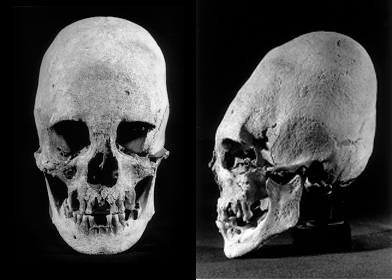
\includegraphics[width=0.70\linewidth]{chast-colebanie-osnov/alani/aw01.png}

\textit{Череп сарматской женщины.}
\end{center} 

Про Сарматов Аланов в популярной научной и околонаучной литературе зачастую умалчивается любопытная штука – некоторые найденные черепа Аланов и Аланок были сильно вытянуты назад (как у многих «каменных баб»). Ученые поясняют это «искусственной деформацией» без каких-либо оснований для такого утверждения. Просто решили, что у людей таких черепов быть не может, у всех должны быть, видите ли, головы более круглые.

А ведь потомки сих Аланок, тоже с вытянутыми головами, видны на портретах жителей Украины и окрестностей за 17-18 века. Тоже искусственная деформация?

Вытянутые, длинные черепа Аланов находят всюду, где обитала эта ветвь Сарматов – в нынешней Франции, Австрии, на Кавказе, Киевщине\footnote{Подобный череп обнаружен в 19 веке в кургане под Уманью, у фермы Марьянки. Однако захоронение относится ко времени, предшествующему Скифам и Сарматам, а также «трипольцам». Значит, люди с подобными черепами обитали на Киевщине с незапамятных времен.}. Археологи находят эти черепа и повторяют – искусственная деформация. 

%А ветвь аланов была большая и могучая, на много отростков – даже до Пакистана дотянулась, где поныне живет народ Калаш (Калаша). А может, калаши и не ветвь, а основа, кто знает? Хотя калашей осталось всего около 5000, они поныне сохраняют свои облик, обычаи и верования, отличные от соседних народов. Выглядят многие калаши своеобразно – я бы сказал, как славяне.

%Конечно, не у всех Аланов были вытянутые черепа, но кстати вытянутых и много, причем с остатками рыжеватых волос, нашел археолог Хулио Сесар Тельо в 1928 году в перуанской пустыне Паракас. И как обычно – сторонники инопланетной теории НЛО понимающе кивают головой, а ученые твердят об «искусственной деформации». 

А ведь довольно сравнить древние, гармонично сложенные вытянутые черепа и черепа в самом деле искусственно измененные, у разных африканских племен – огромная разница. Да и не только у африканских – во Франции этим занимались даже в 19 веке. Верно, подражали давним Аланам, для некоторых представителей которых такие черепа были прирожденной нормой.

Часть найденных в Европе вытянутых черепов археологи относят к Хуннам. Такие же черепа, только одни наука называет аланскими, другие – хуннскими. И про Хуннов тоже говорит – это искусственная деформация черепа! А когда по черепу воссоздают облик, то Хуннам рисуют узкие глаза – мол, монголоиды, а Аланам – пошире. Или лепят подобное из гипса.
 
Но меня занесло в сторону.

Пехоте Тавроскифов у Льва Диакона несколько противоречат конные Роксоланы у Тацита, ибо Тацит, говоря о Роксоланах как о народе, произошедшем от Сарматов (Rhoxolani, Sarmatica gens), описывает их как замечательных в конном бою, и беспомощных в пешем – так, по крайней мере, было, когда Роксоланы вторглись в Мисию во время Оттона и Вителлия. А по всем прикидкам Роксоланы и Тавроскифы один народ.

Но всё зависело от времени и места. Воевавшие с римлянами Сарматы были с головы до ног защищены кольчугой, в кольчуги же одевали и лошадей, покрывая глаза их продырявленными кружочками. Затем мы видим сарматских воительниц и воинов в кожаных латах с металлическими пластинами. Что до конницы, то если сведения Константина Багрянородного верны и Росы покупали лошадей у Печенегов, значит сами были в этом деле не очень-то. Может и Роксоланы – Росы, смешанные с Аланами – тоже не шибко делали ставку на конницу, хотя в летописях есть упоминания о ней, причем в непосредственной связи с князьями Вещим Олегом, Игорем и Святославом. 

Ученые относят Аланов к иранозычным. Это поспешный и слишком общий вывод, верный однако применительно к Аланам, обитавшим около Кавказа и смешавшимся с Иранцами. Но те Аланы, что жили по Днепру, были Славянами со славянским языком. Доказательство очень простое.

Мы знаем из летописей, что здесь жил славянский народ, именуемый Поляне. Довольно отбросить «п» и получить Оляне, те же Алане. Только так могло образоваться название «Роксоланы». Ибо Росы соединились с Аланами. А вспомним каневского Алана по имени Михей!

Более того, доводом для отождествления Аланов и Полян, помимо совмещения по месту и времени, служат былины. В них встречаются женщины-воительницы, именуемые «поляницы». На Украине это слово сохранилось в именовании пшеничного хлеба.

Былины порой освещают седые времена с фотографической точностью, беда лишь в том, что нынешние представления о седых временах совсем другие, и былинная правда воспринимается сказкой.

Верны былины в географии, они знают, например, киевскую речку Почайну под именем Пучайки или Пучай-реки. Былины же именуют Илью Муромца – казаком. Подобно Нартам, старинному богатырскому народу из преданий Осетинов, наши богатыри смотрят вдаль через подзорные трубы. Когда какой-нибудь богатырь приезжает, скажем, к черниговскому князю, тот спрашивает – ты коей земли, коей орды будешь?

Едет Добрыня Никитич в чистом полюшке, встречает поляницу удалую, Настасью дочь Никуличну, и лупит ее в голову\cite{gilder01}: 

\settowidth{\versewidth}{«Думала же, русскии комарики покусывают,} 
\begin{verse}[\versewidth]
На кони сидит же поляница, сворухнуласе\\
И назад же поляница оглянуласе,\\
Говорит же поляница да удалая:\\
«Думала же, русскии комарики покусывают,\\
Ажно русскии богатыри пощалкивают!».\\
Ухватила тут Добрыню за желты кудри,\\
Сдернула Добрынюшку с коня долой\\
А спустила тут Добрыню во глубок мешок,\\
А во тот мешок да тут во кожаной,\\
А повезе же ейный было добрый конь,\\
А повезе же он да по чисту полю.
\end{verse}

Далее конь разговаривает с поляницей – такие же говорящие лошади постоянны в преданиях Осетинов про Нартов.

Поляницы в былинах – не редкая диковинка, а постоянная героиня. Более того, в былине про Ставра сказано:

\settowidth{\versewidth}{Солнышко Владимир князь стольнё-киевской} 
\begin{verse}[\versewidth]
Солнышко Владимир князь стольнё-киевской\\
Задернул он почестный пир\\
На всих князей, на бояра,\\
На всих могучиих богатырей,\\
На всих поляниц да удалыих.\\
Соезжалися на почестный пир\\
Вси князи и вси бояра,\\
Вси могучии богатыри,\\
Вси поляницы удалыи.
\end{verse}

Знали сказители и Роксоланов – в былине «Соловей Будимирович» этот Соловей, вернувшись в Киев с моря Черного, призывает свою дружину – скидывайте с себя кожанки лосиные, надевайте кафтаны роскурлань-сукна! Былины помещают в наше Подолье некую Марью лебедь белую, подолянку да королевичну, русскую красавицу, по всем повадкам – сарматскую воительницу.

Всё найдется в былинах – распри со славянской тогда Литвой, странные отношения с Ордой, Батый (Батыга), какие как брались дани, какие одежды носились. Спелись в былинах исконно скифские и сарматские земли – Днепр и Дон, как небо отражается в реке, так в былине отразилось аланское прошлое Киевщины и язык старославянский, тот самый «церковный»\footnote{Александр Гильфердинг записал эту былину в Пудоге в 1871 году от крестьянина Никифора Прохорова, 51 года возраста, перенявшего былины от отца своего.}:

\settowidth{\versewidth}{А не стрели-тко ты меня Непры королевичной.} 
\begin{verse}[\versewidth]
Как тот ли этот князь стольне-киевской\\
А сделал он задернул свой почёстный пир.\\
Как вси-то к ему на пир собиралиси,\\
Вси там на пиру наедалися,\\
Как вси там на пиру напивалися,\\
Стали там оны вси пьянёшеньки,\\
А стали вси оны веселешенки,\\
Князи вси бояра-то русийскии,\\
А тыи-то могучи вси бог\'атыри,\\
Как вси-то они ведь там расхвастались.\\
Как тут была межу има\\
А тая эта Н\'епра королевична.\\
Как-то тая Непра королевична\\
Как говорит промолвит таково слово:\\
«А нету зде стрельцов добрых молодцов\\
Противо меня Непры королевичной!\\
Силою да нету ухваткою\\
Против стараго каз\'ака Ильи Муромца,\\
А красотою еще было угожеством\\
Противо ведь Михайлы П\'отыка Иванова,\\
А тишиною говорить смиреньицом\\
Противо Добрынюшки Микитица,\\
А нету-то видь еще богачеством\\
Против-то ведь Дюка Степанова,\\
А нету-то да ведь смелостью\\
Противо смелаго Алешеньки Поповича,\\
Поступкой походкою пощапкою\footnote{Щегольство.}\\
Противо-то Чурилки щапа Плёнкова».\\
Сама она еще не спохвалила\\
А тихаго ведь Дона-то сына Иванова,\\
А своёго-то мужа любимого.\\
Как тихий тут Дон сын Иванович \\
А говорит промолвит таково слово:\\
«Ай же ты да Непра королевична!\\
Когда же ты охвоча-то была удалая\\
Стрелять-то было стрелочок каленыих,\\
Пойдём-ко мы с тобой на чисто поле,\\
Станем стрелять стрелочок каленыих,\\
Который ведь стрелять видняе-то?»\\
Как тут-то тая Непра королевична\\
Взимет тут-то ножичок булатныи,\\
Как тое-то колечушко серебряно,\\
Относит что за версту за мерную,\\
Натянула тут она свой да тугой лук\\
А клала ёна стрелочку каленую,\\
Стрелила тут за версту за мерную,\\
Попадала в колечко-то серебряно,\\
И росколола ёна стрелочку равным равно,\\
Да равным то равно стрелку на двое.\\
А клали половинки на весы они,\\
Никоя никоёй не перетягивать.\\
Как тихий тут Дон сын Иванович,\\
Розгорелось ёго сердце богатырское,\\
Как скоро натянул свой он тугой лук,\\
Кладывает стрелочку каленую.\\
Как начал тут Дон сын Иванович.\\
Начал он стрелочкой помахивать\\
А начал ведь-то сам выговаривать:\\
«Ай же ты моя любима калена стрела!\\
Пади же ты не на воду, не на землю,\\
А ты пади ко Непры королевичной,\\
А ты пади же ей во белую грудь».\\
Как тут-то тая Непра королевична\\
Как тут-то ведь она да прослезиласи\\
А тут-то ведь она порасплакалась:\\
«Ах тихий ты Дон сын Иванович!\\
А не стрели-тко ты меня Непры королевичной.\\
Да несу я ти сына любимого,\\
А по колен-то ноженьки во серебри,\\
А по локоть-то рученьки во золоти,\\
А по косицам текут будто звездышки,\\
На зади-то возсият будто светел месяц,\\
Впереди-то как будто солнышко».\\
Как розгорелось ёго сердце богатырское,\\
А ничего тут он ведь не последовал.\\
Как скоро он стрелил ю во белую грудь,\\
Как пала тут она на сыру землю,\\
Облилась она кровью тут горючею.\\
Как тихий тут Дон сын Иванович\\
Взимает он ножищо тут кинжалищо, – \\
Ино ль то ведь еще правда ль есть?\\
Пластал-то он ведь ей да белую грудь.\\
Как было-то ведь тут да до правды бы:\\
Засиян-то ведь во чреви тот сын-то был,\\
По колен-то ноженьки во с\'еребри,\\
По лок\'оть-то рученьки во золоти,\\
Назади просвичать будто свитёл месяц,\\
Впереди еще как там солнышко.\\
Как взял это ножищо он кинжалищо,\\
Становил он-то ножик ведь супротив себя,\\
А становил он ножик, выговаривал:\\
«Да куды пала головка белой лебеди,\\
А тут пади головушка сера гуся».\\
Пал он на ножищо тут кинжалищо,\\
Да тут-то им пришла е горьк\'ая смерть.\\
Как от их-то от крови от крестьянскии\footnote{Христианской.},\\
От крестьянскии крови безнапрасныи,\\
Как протекала тут да Непра река.\\
В глубину река двадцати сажон,\\
А в ширину река сороки сажен.\\
Только-то ведь Донушку славу поют,\\
А той ли этой Непры королевичной.\\
Тут-то их да жительство решилоси.\\
\end{verse}

И складывались эти былины да во времечко, когда Сарматы, коих всех ученые объявили «ираноязычными племенами» и отодвинули далеко в прошлое, говорили одним языком с нашими богатырями, сиживали с ними за одним столом, и были если не всем здешним народом, то доброй его половиной. И если «поляница» – это Аланка, то былинный казак – это «ас» или «аз», такой же Алан. Поныне в Ближних пещерах лежат останки, приписываемые «старому казаку» Илье Муромцу.

Это странные останки. Их ведь изучали, во время Перестройки, и пришли к выводу, что Илья вообще не мог ходить из-за некоего заболевания позвоночника (я не мог найти подробности). Рост Муромца был 177 сантиметров. Необычно толстые кости черепа – лобные, теменные, затылочные. Выдержат, по словам проводившего исследование судмедэксперта Сергея Никитина, удар молотком, от которого у другого человека будет черепно-мозговая травма, вдавленный перелом.

Такие же необыкновенно большие и кисти рук. Более мощные запястья и ключицы.

Всё это некоторые ученые списывают на болезнь. Кроме того, хотя по былинам Илья и просидел сиднем 33 года, но потом в подвижности давал фору многим, значит таки ходил. Почему бы не предположить, что Илья просто отличался от людей обычного биологического вида? Возможно, такое строение тела было для богатырей нормой? Не от болести у Илюши крепки костушки, а богатырское строение таковское. Настоящая боевая машина. Думаю, у других богатырей было подобное.

Муромец скончался в возрасте 40-45 лет. При осмотре останков, у него обнаружено несколько переломов ребер, правой ключицы, проникающее ранение левой руки, сквозное ранение грудной клетки острым предметом – предполагают, от сего и помер.

Что же, вдоволь наговорившись про Аланов – но я к ним еще вернусь – приступлю к тому, что послужило заделом главы – городам Амадоку и Азагориуму. Памятуя о разных народах, скифских да сарматских, сможем более толково рассмотреть птолемееву карту, точнее ее кусок. 

Правильнее говорить, однако, «карта по Птолемею». Клавдий Птолемей был математиком, астрономом, астрологом, географом из Александрии, что в Египте. Общепринято считать, будто Птолемей жил в первом веке нашей эры, хотя труды его известны Арабам только вроде бы с девятого века, а основная его работа по географии – собственно «География» – всплывает в Италии почему-то лишь в начале 15 века и в латинском переводе, хотя по источникам (я не проверял) греческие списки прослеживаются с 13 века. Веком ранее начинают прослеживаться опять же латинские переводы другого сочинения Птолемея, астрономического «Альмагеста», причем выполненные с арабского. 

Выходит, что две известнейшие работы Птолемея стали известны посмертно спустя почти десять веков после их написания, если придерживаться традиционной хронологии, в которой возможны любые чудеса. Более правдоподобным мне кажется, что возникновение списков (прослеживаемых по источникам) с этих работ и есть примерное время написания подлинников. И Птолемей жил незадолго (в пределах нескольких веков) до пришествия на Киевщину Вещего Олега.

Карты, нарисованные рукой Птолемея, не сохранились. Ныне известны лишь составленные «по Птолемею», и я буду использовать карту из рукописного издания 1480 года, так называемого «Уилтонского кодекса».

Немного о самой «Географии». В основу своего труда Птолемей взял работу Марина из Тира (Μαρίνος ο Τύριος), которая не дошла до нас. Другое упоминание Марина встречаем только у арабского географа аль Масуди, который отзывался о картах Марина как о превосходящих карты Птолемея. Правда, сам Птолемей говорит, что Марин карту начертить не успел, а оставил только текстовое описание.

Именно Марин первым из известных нам картографов ввел координатную систему по ширине и долготе. Единицами измерения в ней ввел градусы, а с одним градусом соотнес примерно 500 стадий. По странам составлялись списки городов, городам назначались координаты. Потом, исходя из этих текстовых описаний и уточняя положение по определенным формулам, следовало чертить карту, причем надо было сферическую поверхность (Греки знали, что Земля круглая) перенести на плоскую.

Но Птолемей пишет, что по данным Марина верную карту начертить невозможно, вдобавок Марин дает не\-полные координаты – то приводит одни лишь широты, то долготы. «География» Птолемея, таким образом, это надстройка над работой Марина, с многочисленными исправлениями и дополнениями (из других источников), которые позволяют таки начертить по текстовому описанию приемлемую плоскую карту. 

Но многие города так и остались с «одной координатой». По карте видно, что знаменитые Амадок и Азагориум, а ниже Сарон и Ниоссон, лежат на одной долготе. Подобные «однодолготные» города есть и восточнее вдоль Хипаниса.

Возникает вопрос, а как же заданы координаты рек? Ведь река – не единичная точка на карте, но совокупность точек. Если записывать такую последовательность точек, составляющих реку, то, допустим, через определенные промежутки. И затем, перенеся эти точки на карту, соединить их линией. Так мы получим примерные очертания реки.

Однако «География» Птолемея не содержит таких данных по рекам. Даются сведения, что река такая-то протекает в такой-то местности. И указаны координаты ее устья и, если известны – истока. Следовательно, реки на картах, составленных по Птолемею, изображены условно от точки истока до точки устья.

«Дополненные» координаты для Азагориума и Амадока – хотя я не исключаю, что они в самом деле лежали на одной долготе – и примерные изображения рек на карте Птолемея не дают представления о том, на каком берегу находились эти города и даже как далеко они отстояли от берега.

Вот города по берегам Днепра из труда Птолемея:

\begin{longtable}{l|l}
Город & Координаты\\ \hline
Азагорион (Азаргариан) & 56° 30'  50° 40'\\
Амадока & 56°(30') 50° 30'\\
Сарон & 56° 50° 15' (45')\\
Серимон & 57° 50°\\
Метрополис & 56° 30' 49° 30'\\
Олбия (Борисфенис) & 57° 49°\\
\end{longtable}

%Город & Координаты\\% \hline
%Азагорион (Азаргариан) 56° 30'  50° 40'\\
%Амадока 56°(30') 50° 30'\\
%Сарон 56° 50° 15' (45')\\
%Серимон 57° 50°\\
%Метрополис 56° 30' 49° 30'\\
%Олбия (Борисфенис) 57° 49°\\

Можно ли перевести их координаты в одну из используемых ныне картографических проекций? Ученые занимаются этим давно и приходят к противоречивым выводам.

Кроме координат городов, Птолемей дает примерные координаты гор (в качестве единичных точек) и описывает, где какие народы живут – основываясь невесть на чьих данных.%Роксоланы у Птолемея помещены на берег Азовского моря, а севернее их – Амаксобии и Аланы.

Давайте наконец поглядим на карту, памятуя, что ее начертил не Птолемей. Она составлена кем-то по текстовому описанию, сделанному Птолемеем, что приводил координаты, рассказывал, какие где живут народы и так далее. Порассуждаем над картой, хотя вернее было бы рассуждать над текстом Птолемея. Карта всё же нагляднее, но искажена переосмыслением составителя карты. 

\begin{center}
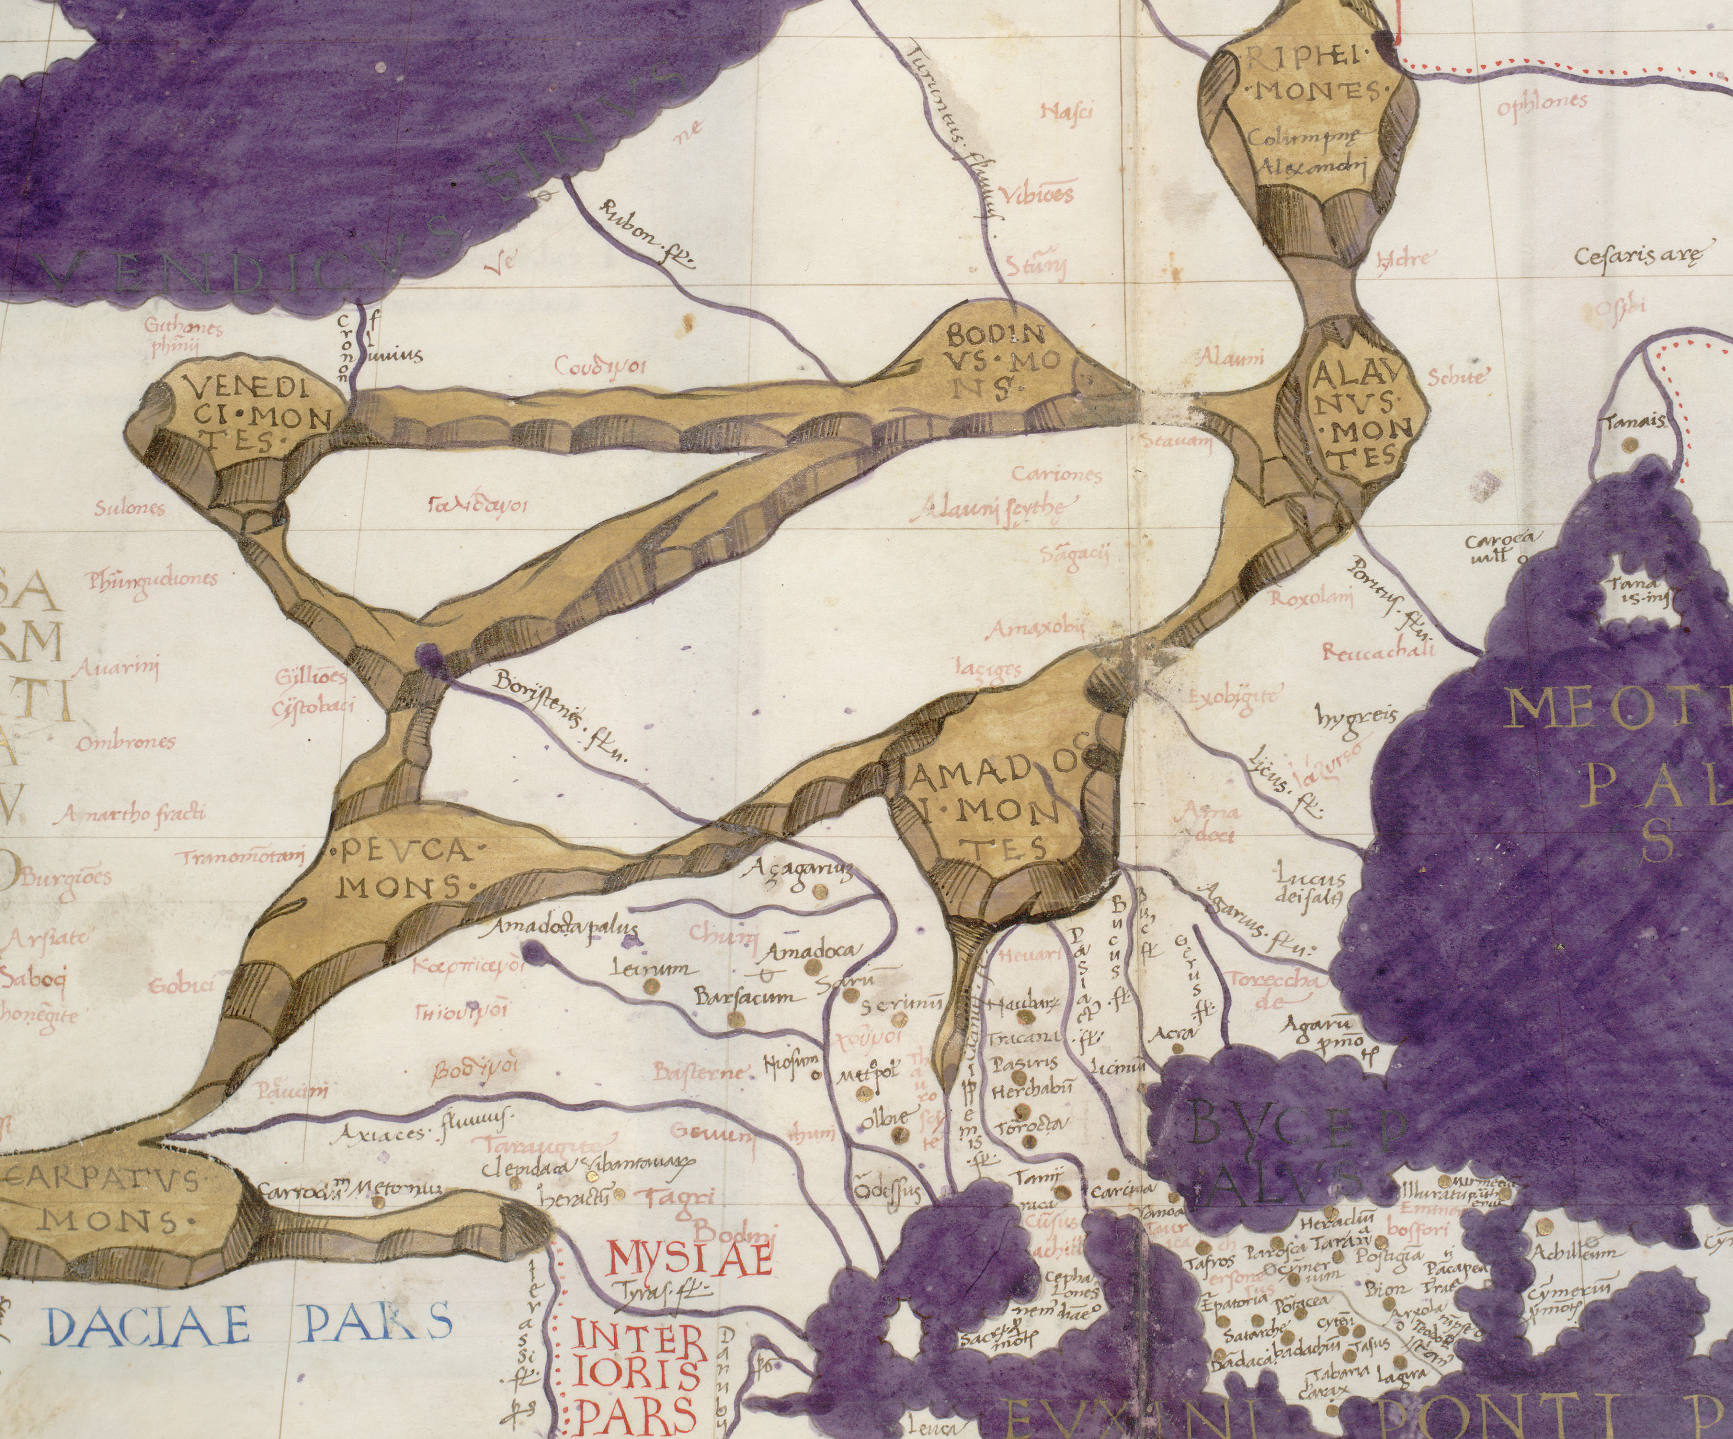
\includegraphics[width=\linewidth]{chast-colebanie-osnov/alani/ptol.jpg}
\end{center}

Многие исследователи не видят разницы между сочинением Птолемея и «его» картами, строя на основе последних умозаключения. В то время как сии карты могут служить лишь для поверхностного суждения о сведениях, изложенных Птолемеем. Таким ли будет суждение собственное, вынесенное при близком знакомстве с «Географией»?  

Сразу бросается в глаза, что карта ориентирована не на привычный нам север, а со смещением, как если бы взять современную карту и повернуть ее против часовой стрелки. А ведь Греки отлично разбирались в сторонах света. Здесь карта не просто от фонаря нарисована, но с координатной сеткой, где меридианы (параллельные линии, от нулевой из которых отсчитываются долготы) ведут к полюсам.

Выходит, что полюса на картах, составленных по Птолемею, отличны от современных нам. Я не буду здесь делать из этого выводы. Но далее, пользуясь сторонами света в разговоре об этой карте, применяю ту систему координат и те полюса, которые присущи именно этой карте.

В правом верхнем углу – устье Tanais, Дона. Он впадает в Азовское море (Мэотийское озеро).

Левее – Alanus Montes, Аланские горы. 

Горная цепь тянется от Аланских гор вниз-налево к Amadok Montes, горам Амадок. Это примерно холмы вдоль Северского Донца, Донецкий кряж.

К северу от них на карте подписаны местные народы – кроме прочих Аланы Скифы, Амаксобии\footnote{Корень «άμαξό», амаксо, значит «правящий повозкой».}.

Но пространство западнее, левее этих народов – пусто. Населено ли оно ими, или нет – неясно. От гор Амадок горная цепь идет дальше налево, как понимаю, как запад, и пересекает наш Днепр – на карте обозначен как Борисфен, Borisfenis flu.

Ниже пересечения Днепра горами, первым, на правому берегу, идет город Азагориум. Ниже, через некую реку – город Амадока. По левому берегу южнее – Сару.

Ниже Сары, в Днепр с правого берега вливается некий приток, берущий начало в озере Амадок. По его левому берегу лежат города Лемум и Барсакум. Южнее устья сего притока расположен город Ниосум.

По левому берегу Днепра далее – город Метрополь, затем Днепр раздваивается, впадает в Черное море, и между устьями Днепра видно «Одэссус». Этот Метрополь, невзирая на координаты, некоторые ученые соотносят с Киевом. Ольвия помещена к востоку от второго рукава, весьма глубоко в материке.

Также на карте есть горы Бодинов (небось геродотовы Будины). А возле Аланских гор живут Аланы. Горы Амадоков и город Амадока явно связаны. Можно предположить существование одноименного народа – Амадоков. Так и есть – они показаны южнее гор Амадок. От города Амадоки этих Амадоков отделяют горы.

Местность возле Азагориума и Амадоки, по карте, населяют Кхуни – и сложно усмотреть в этом нечто иное, нежели Хуннов или Гуннов. А ведь наука говорит, что Птолемей жил в первом веке нашей эры! И эта же наука говорит, что Хунны проявили себя в пятом веке, во всяком случае тогда они попали в Европу! Что же, по общепринятой науке, Птолемей – великий провидец? Нет, это еще одно подтверждение ошибочности хронологии, которой придерживаются ученые.

Я попробовал умозрительно наложить карту по Птолемею на современную, учитывая, что каждая горная цепь на древней карте была задана точкой, и по неким соображениям дорисована. Над Азовским морем получаются горы Аланские и Амадокские. Это возможно современный Донецкий кряж, проходящий между Луганском и Донецком и затем сворачивающий (при современном полюсе) на юго-запад к Мариуполю и оттуда еще западнее, почти к излучине Днепра ниже Запорожья.

На карте по Птолемею мы видим, что некая возвышенность, горный рукав, пересекает Борисфен и тянется к горам Певка, к югу от которых лежит озеро Амадок (Amadoc palus).

Попытаемся пробить Певку и Амадок по древним источникам. Не горы, но остров Певка и народ Певкины помещаются Греками в устье Дуная. Название острова в переводе значит Сосновый от растущих на нем сосен. По Страбону, населяющие его Певкины произошли от народа Бастарнов. Остров сей был известен еще во времена Александра Македонского. Арриан в «Походе Александра» упоминает крутые берега острова, а вдоль – речной рукав с течением столь сильным, что невозможно стать на якорь.

Ныне в устье Дуная нет ни огромного острова с остатками города, ни стремительного рукава. Напротив устья, в море, находятся жалкие остатки большого некогда острова с похожим на Певку именем – Левка, он же остров Ахилла, теперь его величают Змеиным.

Теперь про Амадоков. Ничего про них, кроме географических названий вроде гор Амадоков, города Амадоки, озера Амадоки я не нашел.

Зачем всё это, если, казалось бы, Птолемеем даны координаты, бери да переводи в современные. Но это тупиковый вариант, ибо поныне неясно, как именно переводить. Этим занимается множество исследователей, и у них выходит разное. И нигде в известных мне попытках такого перевода не учитывается иное положение полюсов. 

А я не обладаю достаточными знаниями, чтобы взяться за дело, но даже если бы мне удалось совершить точный, а не умозрительный перенос карты Птолемея (во многом весьма условной) в какую-нибудь современную проекцию, что бы я получил? Мне нужно, во-первых, русло Днепра. У Птолемея русло задано начальной и конечной точкой. Координаты городов Амадоки и Азагориума с их одинаковой долготой вызывают у меня подозрение. 

Так что за возвышенность или горная цепь между горами Певка и Амадоки, пересекающая Днепр?Подобное пересечение ныне известно лишь в месте затопленных порогов около Запорожья. Исходя из этого, Амадока и Азагориум лежат тоже ниже порогов, а никак не на Киевщине. Из древних источников нигде, кроме «Географии» Птолемея, эти два города не упомянуты.

Если горы Амадок это Донецкая возвышенность, то западнее ее лежит Приазовская возвышенность, что несколько уходит от порогов южнее. А горами Певка могут быть холмы к западу и северу от Кировограда.

Одним словом, если возвышенность через Днепр на карте по Птолемею не выдумка, то ее придется пояснить одним – изменением рельефа местности. Например, горная гряда была занесены слоем грунта таким образом, что превратилась почти в равнину.

Что до Киевщины, Полтавщины и Черниговщины, то они на карте по Птолемею лежат в пустом месте между вышеупомянутой загадочной возвышенностью через Днепр и следующей возвышенностью к северу, возможно Валдайской, где начинается Днепр. И Птолемей не знает там ничего, кроме «пустыни», в которой живут Скифы Аланы и несколько других народов.

А может статься, это всё другие горы, сгинувшие, и сопоставление с современными возвышенностями – ошибочно. Ведь не существует более огромного озера Амадоки, которое упорно держалось веками на множестве старинных карт.

Теперь отрешимся от того, что нарисовано на карте. Это не карта Птолемея, но составлена по тексту его «Географии». 

Сравниваю с текстом. Данные, перенесенные на карту, приведены в третьей книге, главе пятой. Всё это, по Птолемею – Сарматия. Он пишет, в параграфе 19, что по всему берегу Мэотиды живут Иазыги (Ιαζυγες) и Роксоланы (Ρωξολανοι). А за ними, вглубь страны – Амаксобии (Αμαξοβιοι) и Аланы Скифы (Αλαυνοι Σκυθαι). Описание места их жительства размыто, однако по нашим летописям, тоже размытым, примерно те места населяли Поляне, славянский народ. Они же, выходит, те, кто у Птолемея – Аланы, скифский народ. 

Однако Языги (Ассы) считаются другим названием Аланов. Может, прав Птолемей, разделяя их. А может, перечень народонаселения в «Географии» сводный, туда выписывались данные из разных источников, а составитель по неведению не сопоставил Ассов с Языгами и поместил их как два отдельных народа.

Аланы неразрывно связаны с рекой Борисфен – в поэме римского императора Адриана приведено имя коня Юлия Цезаря – Борисфен Аланский.

Что же случилось с Аланами? Они растворились в населении одних мест и составили основу населения других. На Киевщине Поляне-Алане – проживали до прихода Вещего Олега с Русами и неясно, в какой степени произошло смешивание, а с учетом многочисленных разорений Киева да окрестностей, и последующих волн заселения, можно предположить, что в некоторых современных киевлянах есть доля аланской крови, однако никто не является Аланом полностью. 

От Аланов остались также названия стран и местностей, где они проживали – при этом сами Аланы могли, опять же, сгинуть оттуда или раствориться, либо растворить. 

Земли Польши в давнее время звались Полонией, а на старинных картах между Полонией и Молдавией лежит Руссия (не Киевская Русь и не Московия), а севернее Руссии – Волиния, в чьем имени тоже угадывается аланское созвучие. Также и другие Аланы – Асы, Язы, Осы – оставили след свой в Осетии, Азербайджане, в имени Азовского моря, возможно и современной Албании. Примечательно, что на родном языке Шотландцев – гаэльском – Шотландия называется Алба или Албания. А Scotland она называется от Ск\'отов (Скоттов) – ряд давних источников возводит название к Скоте, дочери фараона Сингриса, современнице Моисея и жене предводителя некоего возможно скифского народа, который двинулся затем из Египта и, после скитаний, осел в Ирландии. Кстати в нынешней Шотландии существует местность под названием Росс.

Но это уже о Росах, про них мы поговорим позже, они ускользают, тоже всюду оставляя свои следы, причем даже в Азии, Малой и обычной. Да и Скифы.

В устье Иордана лежит город Beit Shean (Бейт Шеан), где туристам показывают развалины древнего города – остатки зданий с колоннами, громадного амфитеатра на 7 тысяч зрителей, бассейнов, общественных бань. Это прежний город Скифов, Скифополис, дважды упомянутый еще в Ветхом Завете. Один раз – когда после странствий по пустыне, сыны Израилевы начинают уничтожать или подчинять себе города. Второй раз о Скифополисе сказано в Книге Иудифь. В ней же, Олоферн – военачальник Ассирийского царя Навуходоносора – «разграбил всех сынов Рассиса», перемещаясь где-то возле Киликии.

А возьмите название другого города – Иерусалим, в давних источниках именуемый Русалим и Урусалим. Я не поднимаю тут тему возможного родства Славян и некоторых Евреев – хотя можно почитать работы Пола Векслера, например «Ашкеназийские евреи: славянско-тюркский народ в поисках еврейской идентификации» (Paul Wexler The Ashkenazic Jews: A Slavo-Turkic People in Search of a Jewish Identity). Другие исследователи напротив, выводят русских от восточных Евреев, плохо понимая вообще, что значит понятие «русские» (прилагательное, применяемое к народам, попавшим под власть народа, известного как Росы), третьи стараются их всеми силами противопоставить.

Можно взять название любого города и прилагать его то к одному, то к другому. Русалим – еще к русалкам близко, и к русальим дням, русалиям.

Вот Скифополис – более твердая почва для размышлений. Город Скифов. Город в выгодном торговом месте – устье Иордана. Сам по себе, если бы окружающее население было к Скифам враждебно, он бы не возник. Не выстояли бы Скифы. Значит, в том месте, в некоторое время, Скифы могли считаться если не «своими», то дружественными. Возникает вопрос – не было ли среди тамошнего окрестного населения других Скифов? Каково было самоназвание Скифов, населявших Скифополис?

О Скифах в Азии пишет Геродот, касаясь истории Мидийского царства. Сменили один другого три правителя – Дейок, Фраорт, Киаксар. Последний расширил границы владений, покорив Ассирийцев. В это время в Азию явилось войско Скифов, которые гнали Киммерийцев из Европы. Во главе войска стоял царь Скифов по имени Мадий (возможно, Матий – от «мать», так же как Батий – от «батя»), сын Протория. Мидяне пытались дать Скифам отпор, но проиграли – не только в сражении, но и во властвовании над Азией, и Скифы держали последнюю в своих руках еще 28 лет.

После битвы с Мидянами Скифы двинулись на запад, в Палестинскую Сирию, но были остановлены египетским царем Псамметихом, который лично вышел к ним с дарами и договорился про обход его земель. Скифы отправились через и ныне существующий древний город Аскалон, и по некой причине не тронули его. Последующие три десятилетия Скифы брали дани с азийских народов, и грабили их помимо даней, но постепенно были перебиты Мидянами. Те отвоевали некогда подчиненные себе земли назад, кроме оставшегося независимым от них ассирийского Вавилона. Будущий поход персидского царя Дария против Скифов (когда в помощь Скифам пришли Савроматы, Гелоны и Будины) был вызван желанием отомстить за столь длительное былое господство над Персами (Иранцами).

Но может, Скифы или родственный им народ обитали в Азии еще до преследования Киммерийцев?

Посмотрим на карту. Какая страна находилась неподалеку от Скифополиса? Финикия\footnote{Отметим сходство ее названия с Венецией.}. Все ученые знают, кем были финикийцы – семиты, изобрели вдруг свою азбуку, потом ее переняли и расширили Греки, а Кирилл и Мефодий на досуге положили азбуку Греков в основу славянской.

Мне кажется, дело было наоборот. У неких изначальных Скифов и Сарматов был свой алфавит. Они жили, кроме прочего, и в Азии. Финикийцы – ветвь этих Скифов либо Сарматов, мне трудно их различать. Славяне – тоже ветвь Скифов и Сарматов. Поэтому алфавиты Славян и Финикийцев подобны. А Греки?

Проще ответить, если записать Греков в потомков Скифов и Сарматов. В Греции раньше жил народ Пеласги (Πελασγοί). Геродот отмечал, что говорили они на варварском языке. Эллины – на греческом, а вот Пеласги – на варварском. Варварами для Эллинов обычно были Скифы.

Пеласги соединились с Эллинами и другими народами, в том числе темнокожими (о чем свидетельствуют многочисленные монеты и рисунки на посуде\footnote{Судя по тем же рисункам, в давнее время люди сосуществовали с Сатирами, Кентаврами и другими существами, которых наука считает сказочными.}) – так возникли Греки, говорящие на языке Эллинов. Но если Пеласги являлись частью Скифо-Сарматского народа, общности, то понятно, почему у Греков такой же алфавит, как у Славян или у Финикийцев.

А если переплыть из Греции на восток, мы попадем к бывшей Финикии, а также в Палестину. Палестиной эта страна называется от некогда жившего там народа, известного древним Евреям как «Пелистим» (библейские язычники-Филистимляне)\footnote{Про них много рассказано в Ветхом Завете. Например, в Книге Царств, Фелистимляне отобрали у сынов Израиля ковчег со скрижалями, и принялись возить оный по своим городам, никто не хотел у себя его оставлять, ибо местное население покрывалось «болезненными наростами».}. Не надо далеко ходить, чтобы усмотреть общую основу у Пеласгов и Пелистима. Они жили и в Греции, и в Палестине. Кто в каком направлении переселялся – дело стороннее.

Город Скифополис находился там, где обитали ветхозаветные Филистимляне.

Всюду Славяне, что ли? Почти. Некий большой народ с более-менее одинаковым языком (отличавшийся говорами) в давнее время населял, кроме прочих народов, Европу и Азию. Части этого народа именовались, в разное время, в разных местах – Скифами, Сарматами, Пеласгами, Славянами, Полянами, Аланами, Асами, вероятно и Хуннами, Готфами – а части всё дробились, какие-то сохраняли величину и язык, какие-то утрачивали общность с родственным народами, роднясь с другими.

Стремление ученых превратить эти, скажем так, славянские народности, в дикарей доходит до крайности. Письменности их лишили, лишают и ювелирного искусства. 

Всем известно про «золото Скифов» – золотые украшения, равных которым трудно сыскать и поныне. Их отличительные черты – определенный стиль, названный «скифским», насыщенность бытовыми сценами, животными, да сюжетами якобы из мифологии Греков. Наука утверждает – Скифы заказывали вещи из золота у Греков. Мол, только Греки были мастерами в этом деле!
  
Найдут в скифском кургане золотые кругляши с портретами – говорят, что это не монеты, но бляхи. Вестимо, зачем «диким» Скифам монеты? А что значит «бляхи», каково их предназначение – между пальцами крутить? Не понимаю. Бляхи. 

Или отыщут шлем и называют его «греческим», хотя точно в таких же шлемах Скифы представлены на древнем литье. Почему женщин со скифских изображений ученые именуют «юношами»? Животных же вроде гриффонов, которые показаны рядом с лошадьми, львами, зайцами и утками считают выдумкой. Стороной обходят и постоянный образ сфинкса в скифских украшениях.

%В Керчи рядом с жилыми домами на улице Братьев Перепелицы находятся остатки кургана – поросший травой долгий пригорок, в котором в конце 19 века нашли выложенный каменными плитами «склеп Деметры», искуссно расписанный фресками. В 1942 году его повердил взрывом гранаты немецкий зольдат. Возведение в 1970-х жилого квартала ухудшило состояние склепа, его стало затапливать грунтовыми водами. Веками стоял посередине погребальной камеры деревянный гроб с останками – всё это разрушилось, едва лишь вытащили его на поверхность.

Ювелирные произведения Скифов донесли до нас и других, помимо гриффонов, неведомых ныне существ, как например эти кошкоподобные звери с пастями, состоящими словно из лепестков, служащих вероятно для заталкивания пищи в рот. Поскольку этот образ повторяется, предположу, что он передает животных, с которыми Скифы так или иначе соприкоснулись.

Поглядим на «кошек»\footnote{Картинки далее – из книги М. И. Артамонова «Сокровища скифских курганов в собрании Государственного Эрмитажа», 1966.}.

\vspace*{\fill}
\begin{center}
\includegraphics[width=\linewidth]{chast-colebanie-osnov/alani/artamonov-mi-1966-030.jpg}
\end{center}
\vspace*{\fill}
\newpage
\vspace*{\fill}
\begin{center}
\includegraphics[width=\linewidth]{chast-colebanie-osnov/alani/artamonov-mi-1966-025.jpg}
\end{center}
\vspace*{\fill}
\newpage

А вот скифский золотой гребень из кургана Чертомлык, вид с одной и другой стороны.

\begin{center}
\includegraphics[width=0.75\linewidth]{chast-colebanie-osnov/alani/greben01.jpg}
\end{center}


\begin{center}
\includegraphics[width=0.75\linewidth]{chast-colebanie-osnov/alani/greben02.jpg}
\end{center}

Обратите внимание на всадника и лошадь. Судя по этому и множеству других изображений, Скифы редко пользовались сёдлами, а кони их были довольно низкорослыми, размером как нынче в Исландии. Кажется, и у других народов такие лошадки в старину были более распространены, о чем свидетельствует искусство. А на рельефах колонны Траяна в Риме, сарматская конница тоже предстают перед нами бесседельной да лишенной шпор.

Седла и стремена появились в землях Украины, вероятно, для удобства не столь умелых, как местные, наездников, коими были пришлые Русы.  Вспомним – они, поселившись с Вещим Олегом в Киеве, покупали лошадей у Печенегов. К этому относится и упомянутый Львом Диаконом упор на пехоту у святославовых Тавроскифов. А быть может, причина иная – другая привычка верховой езды. Кстати, шпоры впервые среди Славян начинают встречаться у прежнего, славянского населения нынешней Австрии только в 8 веке нашей эры, как следует из найденных погребений. 

Вещий Олег, Русы? Исследователи, склонные видеть в них скандинавов, встрепенулись и справедливо могут заметить, что скандинавы таки предпочитали сражаться пешими.

Что же, поговорим о скандинавах.

%Развернем карту, поглядим названия городов Австрии. По большому счету она протиснулась на запад между славянсикми странами, Чехией да Словенией. Так, Алланд. Понятно, от Аланов. Что еще? Еще не совсем онемеченные Цветль, Гаубич, Кримль, Пребихль (от «пребых»)

\chapter{Две Скандинавии}

Птолемей подбросил нам загадку Азагориума и Амадока, однако карта не дала на нее ответ. Мы и далее будем много обращаться к картам и планам. Вообще план это разновидность карты, с увеличенным масштабом и условными обозначениями, в зависимости от назначения. Например, на топографическом плане местности показаны зеленые насаждения, включая породы деревьев, а также здания, высоты и глубины, направление водных потоков. Карты же – более общие, но с координатной сеткой. А план чаще обходится без нее. Иногда грань между картой и планом стёрта.

Самый ранний из уцелевших планов Киева составлен под руководством полковника Ивана Ушакова в 1695 году. Известен общественности по плохому скану, а также хорошим, но упрощенным перерисовкам. В 1986 году подлинник повредили при снятии фотокопии, и архив больше не выдает его даже избранным. Перерисовки есть в двух вариантах, дореволюционные да из советской книжки «Киев во второй половине XVII века» Г. В. Алферовой и В. А. Харламова, 1982 года издания.

Если сравнить план Ушакова с картой земель от Москвы до Малой Азии, выполненной соратником Петра I Яковом Брюсом в 1697 году, что включает в себя все земли современной Украины и смежные с нею, бросается в глаза огромная разница в примененной технологии.

Киеву не повезло с планами. Они зачастую лишены подробностей и обрезаны по окрестностям. Планов, изданных до 1917 года, больше, чем выпущенных в советское время, однако на дореволюционных редко показан левый берег. На общедоступных планах обычно не отображены мелкие переулки да улочки. Либо, на военных планах – отображены, да не подписаны. Современные карты-планы, включая электронные, верны по спутниковым снимкам, однако грешат ошибочными обозначениями местностей.

О планах Киева пока всё. Теперь о картах.

Старинные карты служат подспорьем в изучении сведений из письменных источников. Знание карт, современных этим источникам, позволяет верно понимать, что же хотел сказать сочинитель. Давние карты представляются нам нелепыми и безумными. Кроме того, они переполнены названиями стран, которых давно нет, или которые известны теперь под другими именами и в других пределах.

Так что же такое карта? Это представление географов определенного времени об окружающем мире. Существовали географические и космографические труды с описаниями мира и его населения. К ним прилагались карты, иногда карты выпускались отдельно, либо как наборы – атласы.

Был такой бенедиктинский монах из города Дубровника, Мавро Орбини (Mavro Orbini, 1563-1610). В 1601 вышла его книга на итальянском – «Царство славян» (Regno degli Slavi)\footnote{Существует два русских перевода – 1722 года и 21 века. Старинный вернее, новый полнее.}. Задействовав уйму источников, ея сочинитель причислил к славянам чуть не все народы Евразии.

Орбини дал краткое описание каждого, по его мнению, славянского народа – где живет и чем знаменит. А родиной Славян он вывел  Скандинавию. Ту самую, известную нам, где ныне Швеция и Норвегия. Ее подразумевал и Мавро Орбини. Но ведь он где-то выписал, из некоего источника, происхождение Славян из Скандинавии. Может, в том источнике говорилось совсем о другой Скандинавии?

В 14 веке в Англии имел хождение «Полихроникон» Ранулфа Хиджена\cite{polychro}, рассказывающий об истории и разных странах. Скандинавия там привычная, северная. Но меня зацепили карты, прилагаемые к этому сочинению\footnote{Варианты карт к спискам «Полихроникона» помещены в сборнике Конрада Миллера «Mappaemundi. Die altesten Weltkarten» изданном в 1895 году в Штутгарте.}. Они отличаются от текста книги, и Скандинавия на них – азиатская страна у восточных или северных берегов Черного моря. Ее соседи – Алания (Аланией Хиджен называл земли к северу от Азовского моря, включая Киевщину), Амазония\footnote{Амазония, где жили Амазонки, на множестве карт помещена около Кавказа, у северо-восточного берега Черного моря, южнее Дона и реки Кубань. Возможно, там сейчас республика Адыгея и Ставропольский край.}, Колхида, Рипейские горы, а иногда – Малая Азия с Троей, Лидия, Хиберия. По совокупности можно предположить, что эта Скандинавия лежит примерно около Кавказа.

Не поймите превратно, я не говорю, что так было. Мол, Скандинавия находилась там-то. Я утверждаю иное – Мавро Орбини основывал свое мнение на источниках, в которых, возможно, Скандинавия была помещена возле Черного моря, и неподалеку от Азии в тогдашнем понимании этого слова, а оно двойственно.

Вот карта, прилагаемая к «Полихроникону»:

\begin{center}
\includegraphics[width=\linewidth]{chast-colebanie-osnov/okartah/scand-01.jpg}
\end{center}

Ориентация примерно на восток. Я отметил цветными кружками Аланию (во Внутренней Скифии, Скитии) и Скандинавию. На береговом протяжении между ними – Мэот Палус, ныне Азовское море. Западнее (ниже) Скандинавии, в море – остров Колкос (Colcos), показанный на многих старинных картах и по названию имеющий отношение к Колхиде. Река возле Колкоса, исходя из лежащих у берегов ее стран – Дунай. Напротив Скандинавии, правее – полуостров Малой Азии. Восточнее, выше – Каспийское море (mare Caspium). К западу от Алании – Саксония. Запомним, это важно. Алания же – нынешняя Украина с Польшей.

Я бы отнес сию восточную Скандинавию к разряду диковинных ошибок и прошел мимо, если бы эта «ошибка» не была постоянной составляющей именно на картах к «Полихроникону». Давайте поглядим на другой вариант:

\begin{center}
\includegraphics[width=\linewidth]{chast-colebanie-osnov/okartah/scand-02.jpg}
\end{center}

Скандинавия занимает здесь почти прежнее место у берега Черного моря, чуть сдвинувшись на восток (вверх), остальные границы прежние – Иберия, Амазонки, Мессагеты. Хорошо нарисован Танаис к западу от Скандинавии, а еще западнее – Мэотийское болото. Из карты следует, что Скандинавия находится на восток от Дона, однако выше Малой Азии. Это Кавказ либо Ставропольский край.

На современной карте Грузии, в тридцати километрах на восток от Кутаиси с трудом отыскивается село Сканде (სკანდე)\footnote{42°15'36"N 43°3'11"E}. Чуть севернее его – остатки крепости\footnote{42°16'6"N 43°2'46"E}. Это всё, что осталось от древних города и крепости Сканды (სკანდის ციხე, სკანდა).

На протяжении, быть может, тысячелетий она то разрушалась, то возрождалась, переходила из рук в руки, о ней забывали и вспоминали. Прокопий Кесарийский в «Войне с Персами» пишет, что в Лазике (западная Грузия) обжит лишь северный берег реки Риони, и:

\begin{quotation}
Все селения Лазов находятся здесь, на этой стороне реки, и тут издревле построены ими городки, в том числе самый укрепленный из них Археополь, Севастополь и крепость Питиунт, а у самых границ Ивиров Сканда и Сарапанис.
\end{quotation}

В обозримом по источникам прошлом Скандой владели то Греки, то Персы (Иранцы). Ее разрушил в 14 веке Тамерлан, но уже спустя несколько веков она служила пристанищем грузинской царице Тамаре, захватывалась попеременно то картлийскими, то имертинскими царями. Многократно о Сканде пишет грузинский историк 18 века Вахушти Багратиони в «Истории царства Грузинского».

А вот почитаем выдержку из «Статейного списка посольства в Имеретию 1650-1652 гг., составленного Алексеем Иевлевым»:

\begin{quotation}
И провожали послов до подворей азнауры. А что за столом цари подавали изперед себя послам кушенье, и те ествы прислали цари за послами к Микифору и Олексею на стан. А стоял Александр цар. под городом под Скандою, от города с полверсты; двор его учинен на площеди, на ровном месте поставлены поземные дощатые чердаки.

А город Сканда стоит на горе; каменой, четвероуголен, высок, сажен в десять. По стенам четыре башни а на башнех три пушечки волконейки, небольшие.

Да в городе ж церковь камена, без креста, во имя страстотерпца Георгия; в церкве стенное писмо. Да в церкве ж три образа: всемилостивого Спаса, да пречистые Богородицы, да Георгия страстотерпца; обложены серебром в чекан, позолочены; у спасова образа венец золот, писан мусиею. Да на городовой стене сделана полата болшая на трех житьях; а в верхнем житье лежит царева казна, и что прислано к нему Александру царю от ц-ого в-ва жалованье соболи, и те соболи положены в той же полате. И стерегут того города и казны тюфенчеи. Да в городе ж онбар болшой, деревяной насыпан полон хлеба; да вместо погреба вкопана в землю корчага болшая и налита виноградом на целой год, для осадного времени. А мерою того города около сто двадцать сажен болших.

Да около ж того города обрублено тарасы и насыпано хрящем. А всход к городу один и тот круг; взять приступом никоторыми мерами нельзя, гора каменная, да около обрубу, на той же горе, жилых дворов с тридцать. А иные дворы стоят под горами в стрелбище, и в два, и в полуверсте, и в версте, и боши, врозни, по крепким местом, для приходу воинских людей.

А от столного города Кутатиса до того города до Сканды верст с тридцать. А место пришло низ, ровнедь с долинами, верст на шестьдесят; а поперег от Сканда города до реки до Курлы верст с двадцать и болши. А места жилые, городки, и села, и деревни, и стоят по крепким местом, по речкам. И на том ровном месте многие царевы дворы устроены. А по другую сторону того ровного места, под гурелскими горами, течет река Курла. А течет из гурельские земли промеж гор, и вышла из гор в Олександрову землю, и впала в Реонь реку, от Кутатиса вест с шесть или с сем.
\end{quotation}

Когда крепость опустела – неведомо, равно как её создатели и время постройки. Туристы в Сканду не ходят, а краеведы туда добираются с трудом. Зная про Сканду, думаешь – так ли нелепа Скандинавия на старинных картах? Не являются ли они отголоском времени, когда крепость эта была, возможно, основой одноименной державы?

Что до нынешней Скандинавии, то ее часть в давнее время предстает в источниках то как единый остров Скандия, то несколькими островами, и постепенно обретает новое имя – Скандинавия. Под именем Scandia ее упоминает Птолемей в своей «Географии», для него это три острова: Нериг (давнее самоназвание Норвегии – Нориг), Берги и Думна. 

Сейчас Скандинавия известна как полуостров – но при повышенном уровне воды в океане могла быть цепью островов. С подписью «Скандии» полуостров изображается уже на картах 16 века, например на подробнейшей шведской морской карте Олафа Магнуса за 1530 год.

Языческие боги этой, привычной нам Скандинавии – Асы или Осы во главе с Одином – родом из Азии. Считается, потому и Асы, что от слова «Асия». В преданиях, Асы изначально предстают не богами, но могущественным сообществом людей, вроде Туаха Дэ Дананн. Обожествили их позже. \'Один же был, в некоторое время, просто предводителем Асов, колдуном и провидцем.

По «Саге Инглингов» (Ynglinga saga) из «Круга Земного» Снорри Стурлусона, Асы обитали в стране Асаланд или Асахэйм (Ásaland eða Ásaheimr), что лежит к востоку от реки Танаис, прежде именуемой Танаквисл или Ванаквисл (Tanakvísl eða Vanakvísl), впадающей в Черное море (Svartahafi). Страну в низовье этой реки называли Ваналанд или Ванахэйм, а ее жителей – Ванами. Главный же город в стране Асов – Асгард (Ásgarð). Ваны и Асы поначалу воевали, а после породнились. Ваны научили Асов своему колдовству.

Казалось бы, ясно сказано «Танаис». Но река Дон, с которой отождествляют Танаис, впадает в Азовское, а не Черное мое. Быть может, Снорри подразумевал под Танаисом другую реку, например Истр, Дунай? Но будем пока руководствоваться общепринятым толкованием, что Танаис это Дон.

По одним представлениям древних, Азия отделялась от Европы рекой Танаис. По другим представлениям, Азия – южное побережье Черного моря, известное в некоторые времена как Малая Азия.

В прологе «Младшей Эдды» сказано, что в Азии был город Троя, которой правил Тор, сын Меннона и Троан, дочери царя Приама. Из рода Тора происходил Один. В «Младшей Эдде» Троя отождествляется с Асгардом и помещена в Тыркланд (Tyrkland). А вроде бы известно, что сейчас это Турция. 

Малая Азия – часть Турции. Развалины Трои в ней показывают туристам. Впрочем нигде, кроме некоторых саг, Асгард не сопоставляется с Троей, а по географическому описанию из «Саги Инглингов», как увидим далее, Асгард находится эдак на Кавказе или в Ставропольи. 

В старину вообще многим народам было лестно ставить Троянцев себе в предки. И к сообщениям о сторонах света следует, наверное, тоже относиться  осторожно, памятуя о возможном смещении полюсов.

Я неоднократно сталкивался с тем, что в сагах одним словом именуют разные места. А ежели Тыркланд – это не Турция, а некие земли проживания народа Торков, что кочевал от Каспия до Винницы, Донбасса и Поросья? В самом деле, выходит, к востоку от Дона.

Стурлусон уточняет – Тыркланд лежит к югу от большого горного хребта, что тянется с северо-востока на юго-запад и отделяет Большую Свитьод (Svíþjóð ena Miklu) от других стран. Таким хребтом может быть Урал. Словом Svíþjóð в давних северных языках называли Швецию, а вот Большую Svíþjóð можно сопоставить со Большой Скифией, летописной «Великой Скуфью». Иногда впрочем вместо Большой Свитьод писали просто Свитьод, тогда надо было догадываться по смыслу, о чем идет речь.

Если определять положение Асгарда по «Младшей Эдде» и «Саге Инглингов», полагая Дон Танаисом, то выходит, что Асгард лежал к западу от Дона и южнее Урала. Это же Кавказ и Ставропольский край!

В «Саге Инглингов», Асы из Асгарда идут сперва на запад в Гардарики (Garðaríki, их соотносят с землями Киевской Руси), а затем отправляются на юг в Саксланд. В прологе «Младшей Эдды» про Гардарики ничего не сказано, но после странствий Один и его соратники попадают «на север» в Саксланд. Саксланд это будто север нынешней Германии, Саксония.

Выходит путаница, коль руководствоваться современными знаниями, положением полюса и считать сведения из саги истинными. Однако Саксланд лежит южнее Гардарики в случае, если полюс находится примерно там же, где у Птолемея, и привычную нам карту надо повернуть против часовой стрелки. Лишь тогда можно сказать, что Саксланд – южнее Гардарики.

Припомним карту из «Полихроникона» – Алания лежит рядом с Саксонией. Догадайтесь, что общего между Гардарики и большой Аланией от Бэкона, Хиджена, Исидора? То же, что у Киевской Руси да Роксолании – местность.

%Как бы ни было, родина Асов, по сагам, близка к Черному морю и обозначенному на старинных картах месту Скандинавии! Таким образом азиатская Скандинавия обретает весомую привязку. Значит, следует различать позднейшую «северную» Скандинавию с ранней азиатской. 

А теперь перекинем мостик от северной Скандинавии к восточной. В 50 километрах к западу от крепости Сканды лежит Южная Осетия. Грузины называют Осетинов – Оси. 

Север, Скандинавия, Асы. Восток, Скандинавия, Осы. Они же Асы, Ассы, Аланы.

Веками ученые пытались отыскать корни Осетинов, находя их то в Половцах, то в германских народах, то в семитских, пока в 19 веке не пришли к иранскому происхождению Осетинов, что немудрено по их самоназванию – Ирон, Ир! Но для такого очевидного вывода науке понадобились исследования академика Андрея Шегрена.

А ведь даже глядя на современную карту можно сразу сказать, что Осетия с Ираном – соседи. Вероятно, Осетины – потомки древних Иранцев, Персов, волей времени отмежеванные от большей части бывшей родины, которая простиралась до Осетии во времена царя Кира Великого, а затем Дария Первого. Государство Иран – ближайший по языку и месту жительства сосед Осетии!

Но благодаря работам Миллера и Абаева, наука считает теперь Осетинов потомками Аланов, Аланов потомками Сарматов, Сарматов потомками Скифов. Таким образом Абаев развил обоснование тому, что по иранскому в основе современного языка Осетинов можно достучаться до иранской же основы сарматского и скифского языков.

\begin{center}
\includegraphics[width=0.20\linewidth]{chast-colebanie-osnov/okartah/iron02.pdf}

\textit{Схема примерного происхождения Осетинов по Абаеву.}
\end{center}

«Аланами» на этой схеме я для краткости обозначил цепочку Аланы – Сарматы – Скифы, а «Иранцами» именую жителей Ирана, ибо наука не объясняет, каким образом Скифам передался их язык. Приходится предполагать, подыгрывая науке, что от Иранцев.

В самом деле, Осетины живут ныне там, где раньше обитали Аланы – впрочем Аланы были и в нынешней Чечне, и около Днепра и во Франции да Италии, где поныне остались городки Аллейн, Алагна, Сармато Аландриано (Ландриано), Аллегно, Алано ди Пиаве. Славяне-Вандалы купно с Аланами обитали также в Испании, Галии, да по всей даже той части Европы, которую не считают славянской.

Поскольку Осетины называют себя Ирон, думаю, что народ из Ирана растворил в себе аланское население (не важно, коренное или пришлое), и потомки обоих народов и составляют нынешних Осетинов. Вместо того, чтобы предположить оба народа в «одновременные» предки Осетинов, Абаев сделал эти народы последовательными звеньями цепи происхождения.

Выражу взаимосвязь Иранцев, Аланов и Осетинов так:

\begin{center}
\includegraphics[width=0.50\linewidth]{chast-colebanie-osnov/okartah/iron01.pdf}
\end{center}

Влияние Иранцев оказалось сильнее, что выражается в языке и самоназвании – Ирон.

В обозримом прошлом, в осетинском языке не было слова «Алан», пока его не заимствовали из общекультурной среды. А то, что Аланы – давнее самоназвание Ирон, Абаев вывел следующим образом.
 
В преданиях Осетинов существует загадочное выражение «аллон-биллон»\footnote{Кстати, в чеченской сказке «Черкес Иса и чеченец Иса» упомянуто чудесное существо по имени Алла-Белла, обитавшее в пещере.}. Подобно тому, как в русских сказках Баба Яга принюхивается и подозревает, что здесь пахнет русским духом, так в осетинских людоед-великан отмечает – мол, пахнет аллон-биллоном! Абаев не смог истолковать «биллон», однако «аллон» сопоставил с человеком, который находился рядом с великаном. Значит, человек тот – непременно Алан – решил Абаев. А следовательно, предок Осетинов.

О ком же речь идет в преданиях с «аллон-биллон»? Кого вынюхивал людоед? Он вынюхивал Нартов. 

Нарты – народ, о котором рассказывают Осетины в своих преданиях. Нарты сгинули, их покарал бог за дерзость. Ученые гутарят, что в нартовском эпосе отразились Скифы, а Нарты – предки Осетинов. Но ведь сами Осетины говорят – Нарты все погибли. 

К сожалению, еще мало преданий о Нартах переведено на другие языки. А ведь это культурный пласт, сопоставимый по размаху с греческой и северной мифологией, и в некоторых подробностях удивительно перекликающийся с ирландской.

Связь с Ирландией проявляется во многом.

Ирландия, или, в старину – Ир-лонд, земля Иров\footnote{Произношение «Айрлэнд» – английское, на современном ирландском языке звучание иное – «эйжэ», а как оно звучало в старину, неизвестно, есть давнее написание Ériu. В преданиях так звали дочь Эрнмаса из числа Туаха Дэ Дананн. Другой вариант имени – Эрин, почти как Ирина.}. А как называют себя Осетины? Ирами.

Среди Осетинов и Ирландцев рыжих людей больше, чем среди других народов.

Далее. Когда я еще думал, что все Аланы были ираноязычны, то решил, что Туаха Дэ Дананн (Tuatha Dé Danann) можно перевести просто – народы богини Реки, толкуя «Дану» как производное от иранского корня «дон» или «дан».

Правда, в Ирландии не знали богиню Дану. Слово «Дану» вообще придумано учеными, они сочли, что «Danann» это склоненное в притяжательном падеже имя Danu. Мол, чьи народы? Danann. Tuath(а) значит народ(ы), De – божество.% Вместе произносится как «туаха дэ данан», где «дэ» размытое, в нем слышится «ч». 

А если «дэ даннан» – подражание другим словам либо искаженная их передача? В преданиях Осетинов о Нартах важнейшую роль играет чародейка, воительница и советчица по имени Сат\'ана. Я сам не люблю игру с буквами, но «дэдананн» c заменой второй «д» на «т» может звучать как «тэтананн» или «сэтананн».

Сатана – богиня или полубогиня, росшая не по дням, а по часам – за месяц как за год. Это свойство, в преданиях, присуще тем, в ком течет нечеловеческая кровь. Сатана умеет принимать множество образов – являться старухой или молодой\footnote{В 13 веке шотландец Томас Лермонт (Thomas Learmonth the Rhymer) по прозвищу Рифмач (возможно, Михаил Лермонтов – из его рода), провидец, побывал в мире Эльфов, Элфхэйме. Тамошняя королева Фэйри обладала способностью менять свой возраст с молодого на старческий. Три дня прожил Лермонт среди чудесного народа, семь лет прошло в нашем мире. Пробыв некоторое время с людьми, он вернулся в Элфхэйм. Общение с народом Фэйри и королевой Фэйри хорошо освещено в документах из шотландских, 15-18 веков, судилищ над ведьмами. За такое общение, действительное или мнимое, людям со стороны людей же грозили пытки и сожжение заживо. Скиф Анахарсис на вопрос, что самое опасное для человека, отвечал – сам человек.}, понимает птичий язык, управляет погодой, о событиях в мире знает, глядя в некое «небесное зеркало». В сказаниях Сатану описывают как «неба коварство, земли колдовство». 

%По Геродоту, родоначальником скифов был некий Таргитаос: «Родители его были, как говорят, Зевс и дочь реки Борисфен». А в нартовском эпосе, Сатана – дочь Уастырджи

Возможно, Туаха Дэ Дананн следует толковать как «народ Сат\'аны»?

Героические предания Осетинов порой сходны с ирландскими. Часто сравнивают повествования о Сослане (Осетия) и Кухулине (Ирландия). Среди общих подробностей: у Сослана в каждом глазу по два зрачка, у Кухулина четыре в одном, три в другом. Кухулин гибнет потому, что его колесницу зачаровала отвергнутая им богиня войны, призрачная королева Морриган. Отвергнутая богиня же посылает на Сослана самоходную повозку Колесо Ойнона (Балсага, Малсага, Барсага). 

Серебряная рука короля из Анналов Ирландии – и осетинский богатырь Сослан, с телом из черного булата и железными ногами, а также металлический Батраз, столь могущественный, что вступил в распрю с жителями неба и был убит богом при помощи Колеса Балсага. По другому варианту, его расстреляли Елиаты, подлетев в облаке, которое рассеивалось, когда Батраз стрелял в ответ. Батраз раскалился и упал, и ему нечем было охладиться. Он долго лежал. Никто не мог приближаться, умирали, даже противники, жители неба – Зэды и Дуаги.

Не от Нартов ли пошли Туаха Дэ Дананн и обожествленные Асы? Кто такие Нарты в представлении Осетинов? Откроем второй том трехтомника «Нарты»\cite{narty01}. Про народы былых времен сказано:

\begin{quotation}
1. О гумирах\\

Гумиры были огромными, сильными, но глупыми людьми. Они не понимали, что от огня можно отодвинуться, и прикрывали себе лица [кусками] сланца или дерева. Однажды они увидели, как собака все дальше отползала от костра по мере того, как он разгорался. Так гумиры научились оберегать себя от огня.\\

2. Нарты\\

До нартов [на земле] жили гумиры, топоров у них не было, деревья они вырывали руками. Потом появились уаиги – крупные, могучие люди. Вслед за ними [появился] нартовский народ.

Сотворив мир, бог решил создать людей. По его велению на земле появились уадмиры. Были это люди огромные и сильные, в ущельях они не помещались, земле их было трудно выдержать.

Триста лет прошло, и сотворил бог вслед за уадмирами камбада – умом и силой на уадмиров похожие, а ростом невысокие, не выше нынешних десятилетних детей. Слишком малыми оказались камбада для жизни на земле\footnote{Что впрочем, не мешало им жить дальше, судя по сказаниям. Так, герой нартовских сказаний Сослан встречает низенького, очень сильного охотника, и тот называет себя камбада.}.

Триста лет прошло, и сотворил бог вслед за камбада гамеров, но и они оказались слишком велики и ростом и силой.

И еще триста лет прошло, и сотворил бог вслед за гамерами гумиров. Не вышли и они под стать земле. Триста лет прошло, и сотворил бог вслед за гумирами уаигов. Не удались и они, слишком крупными оказались. Триста лет прошло, и сотворил бог вслед за уаигами новый народ, нартов, и удались они ему, ростом и силой были под стать земле. [...] \\

5. Происхождение нартов\\

До нартов на свете жили уадмеры. Уадмеры были огромными людьми, дома не строили: «Если мы будем наклонять головы, проходя через порог [в двери], то бог подумает, что мы ему кланяемся». Бог очень скоро их уничтожил. После этого появились уаиги – грубые, сильные, безобразные: у кого было семь голов, у кого – одна голова и один глаз\footnote{Сходство с Фомойри и Песиголовцами.}. Жили они в горах, лесах и пещерах. Когда появились нарты, то они сражались с уаигами и уничтожили их\footnote{Туаха Дэ Дананн тоже сражались с Фомойри.}. Откуда появились нарты, этого, кроме бога, никто не знает, но в сказаниях говорят, что они появились со дна моря.
\end{quotation}

Нарты легко роднятся с подводными жителями Донбеттырами, носят латы, вооружены мечами, ружьями и пистолетами, а когда им нужно рассмотреть что-то далекое, смотрят в подзорные трубы. В подзорные трубы смотрят и русские богатыри в тех былинах, которых не коснулась рука великомудрых редакторов, после чего богатыри глядят уже не в оптические приборы, но из-под ладони или в кулак. Хлебом нартам служит кукуруза.

Нарты – не боги, однако приглашают на свои пиры богов. Их перечисляют в предании о Сослане, и боги представлены как обычные действующие лица:

\begin{quotation} 
Были званы на пир также небесные зэды и дауаги; покровитель путников бесстрашный Уастырджи\footnote{Отец Сатаны, может летать, надевая золотые крылья. Летали также мелеки – обитатели неба. А подземные жители, что похищали людей в свои пещеры, именовались бценагами.}, небесный Курдагалон, покровители скота Тутыр и Афсати, покровитель зерца Уацилла, светлый Реком и чистый Мыкалгабырта, небесный Сафа\footnote{Бог оружия, создатель знаменитых мечей.} и Галагон, а также покровитель вод Донбеттыр.
\end{quotation} 

Нарты тоже не просты, они могут перемещаться в летающих башнях, как например Бедуха из Ахсартаггата в предании о Сослане. Нарты  пользуются и меньшими средствами передвижения – самоходными повозками (хадтулга уардон).

И когда речь идет об огнестрельном оружии, почему мы должны полагать, что оно было введено в предание сравнительно недавно? Думаю, оно было там издревле. И вещи названы своими именами, без опрощения вроде грома и молний.

В преданиях не определяется родственность Осетинов к Нартам. Предшествующее население Осетии? Народ, который соприкоснулся с Ирон и Аланами, затем сгинул, но оставил о себе память в преданиях?
 
Считалось, что Нарты не подчинялись богам – ни разным покровителям, ни главному. Даже дверные косяки делали высокими, чтобы не наклоняться, дабы бог не подумал, что это в его честь. Отношения между Нартами, богом и жителями неба накалились до предела, Батраз вступил в открытое противостояние с последними и был повержен. Следует расправа над остальными Нартами.

По одному из преданий, когда бог покончил с Батразом, Нарты бросили меч того в воду, отчего пошли «волны и ураганы», а море закипело и приобрело красный цвет. Затем бог уничтожил Нартов огнем с небес. В другом предании Нарты умирают от голода, после неурожая. В третьем – бог обрушивает на них гору. В еще одном сказании Нарты выкапывают себе могилы и бросаются туда. Это полностью совпадает с некоторыми из преданий об исходе странного народа Чуди белоглазой.

Потомки восточных Аланов донесли до нас предания о своем далеком прошлом. У потомков Аланов западных таких преданий не осталось.

\chapter{Поляне}

Продолжим про Аланов, но с другой стороны – по русским летописям. Кроме того, попытаемся разобраться, как же на земли полянские пришло название Руси, и какое отношение к сему имеют Варяги.

Общепринятая история невероятно растянута. Вопреки свидетельствам источников, отрицается, что Скифы и Сарматы это прямые предки Славян и даже сами Славяне. Нам навязывают отрывочную картину прошлого. Вспышками фонарика из тьмы кромешной высвечивают то Скифов, то Сарматов, то Славян. Они вдруг возникают на сцене истории, а затем, кроме последних, пропадают без объяснения, не попрощавшись. Наука не сообщает, что происходит в промежутках между этими вспышками, и куда же подевались Сарматы да Скифы, коль они, по науке, ираноязычны и отодвинуты во времени глубже, прочь от Славян.

А по источникам выходит, что Славяне – другое название большой части тех же Скифов и Сарматов. Например даже для Ромеев (жителей той половины Римской империи, которую ученые называют Византией, а славяне именовали Греками), современников княгини Ольги, Скифы это жители Киевской Руси.

Наши летописи странным образом обрезаны по  скифское, сарматское время, а линия отреза разлохмачена множеством вариантов изложения событий. Иноземные источники тоже не шибко радуют нас описанием, происходящего в скифо-сарматском мире до этой линии отреза, да и после. Хроники и летописи затрагивают чужое лишь по мере соприкосновения с ним, а таковым соприкосновением обычно является война или торговля.

Итак, внутренние источники сгинули, внешние скудны. Будто вырван кусок истории, кусок, захвативший определенную местность на протяжении некоторого времени.

Однако существует еще Бермудский треугольник, составленный из Славян, Русов и Варягов. Какое отношение имеют Славяне к Русам, а Русы к Варягам? Вот уже несколько сотен лет ученые спорят, разделившись на два непримиримых лагеря – норманистов и антинорманистов. Последним даже в толковом названии отказали, произведя его от первых.

Норманисты утверждают, упрощенно говоря, что государство Киевская Русь основано норманами – скандинавами. Это призванные княжить над Славянами Варяги – Рюрик с братьями, да его потомство и родичи. Антинорманисты же полагают, что Рюрик был из Славян с южного побережья Балтийского моря.

У представителей обеих научных школ на руках одинаковый набор источников, главнейшие из которых, да и, что кривить душой – единственные письменные – это русские летописи. Нигде кроме них про Рюрика не сказано\footnote{В середине и второй половине 9 века, однако, по страницам хроник вроде Annales Bertiniani и Annales Xantenses гуляет северянин Рорик, племянник короля большей части Дании – Ютландии, Харалда «Клака» Халфданссона. Рисковый, стремящийся к власти человек, Рорик обрел её, захватив Дорестад (Dorestad, около нынешнего голландского города Wijk bij Duurstede). В 873 году Рорик появляется в хрониках в последний раз, чтобы присягнуть на верность Германскому королю Хлудовику. Этого Рорика некоторые исследовали отождествляют с Рюриком.}, значит, надо прочесть и рассудить. Однако нас подстерегает опасность.

Общепринятые представления, укоренившиеся в разуме, искажают смысл слов, вложенный летописцем. Какими вам видятся Варяги? Эдакими патлатыми викингами с топорами, да еще в рогатых шлемах? Что в этой картине обосновано? Проверим.

Почему Варяги – непременно викинги? Потому, что так говорят ученые-норманисты. Вероятно, они записывают всех скандинавов в викинги. Но викинги это морские разбойники у скандинавов. Разве все скандинавы были разбойниками?

Почему шлемы рогатые? Так художники рисуют и в фильмах показывают. Но у викингов не было рогатых шлемов. Задача шлема – отводить удар в сторону, а не задерживать его рогами. Рогатых шлемов в Скандинавии найдено всего пара штук, и те надевались для справления обрядов.

А что насчет длины волос? Сходный вопрос про давних Славян – каковы из себя? Ну мирные жители ладно, с какой угодно прической, хотя обычно «под горшок». Однако воины всегда, во все времена, даже сейчас, стригутся коротко или налысо. Поэтому когда на картинке или в кино показывают длинноволосых воинов, это неправдоподобно. Верно показан полководец, князь Святослав – налысо бритый с оселедцем. Казаки такие же. В Радзивилловской летописи есть картинка – с русского витязя слетает шлем, а под шлемом лысая голова. 

От Рима до Руси воины стриглись коротко либо брились. Ибо волосы в бою мешают. Вон амазонки одной груди лишались, чтобы лук удобнее вешался и снимался, а тут какие-то воинственные мужики отращивают себе роскошные кудри ниже плеч. На средневековых изображениях, викинги имеют короткие волосы, кое-кто носит короткие бороды, многие лишены бород и усов. Что им, бородой рыбу с борта ловить?

У некоторых народов длинные волосы вообще имела только знать. Когда Бургунды убили короля Франков, Хлодомира, то узнали его по волосам до плеч, ибо правители Франков не стриглись и причесывались на прямой пробор\footnote{Франки – не самоназвание. По преданию, это были потомки разгромленных, отступивших Троянцев. Другие имена давних Франков: Приам, Антенор, Сунно, Маркомир, Фарамунд, Хлодио, Меровей, Хлотар.}. Тамошние простолюдины же стриглись в кружок, а носить долгие волосы им запрещалось.

Или вот ученые пишут в своих работах – «славянские племена». Либо – «балтийские племена». Что под словом «племя» разумеют ученые? Они не задают себе такой вопрос. Просто используют слово, вкладывая в него нечеткий смысл. Попроси пояснить, в ответ получишь туманные высказывания. Но ведь язык науки должен быть точным! А выходит, что ученые зачастую не вкладывают в произносимое четкий смысл.

Словом «племя» широко пользуются и в переводах древних исторических сочинений. Например, в подлиннике стоит латинское «nation», то бишь «народ», а переводчик нам толкует – «племя». Или, латинское «gens», тоже «народ», у переводчиков опять-таки «племя». Хотя в случае «gens» можно с нятяжкой переложить как «племя» в уточняющем выражении вроде «gens fortissima Sclavorum» – «могучее Склавское племя», когда речь идет о принадлежности некоего могучего народа к Скла\-вскому роду («gens»). Ни современные ученые, ни переводчики – а древние исторические сочинения переводят обычно те же ученые – этих тонкостей не знают и не чувствуют.

Хорошо. Что первым делом воображаешь, когда слышишь слово «племя»?

Наверное, единицу общественного строя вроде как у киношных туземцев тропического леса. Лезешь себе через джунгли, рубишь лианы острым мачете. Поперек лежат бревна, с ветки свисает питон, показывая бледно-розовый раздвоенный язык. Тут бац – выходят диковинно изукрашенные, с копьями настороже, люди. Они не понимают вашу речь! Жестами поясняют, что вы вторглись на их землю. Надо потолковать. Вас ведут тайными тропами. Чаща раздвигается. Увенчанный черепами частокол, за ним хижины. Тут живет племя. В самом большом шалаше сидит вождь в нелепой, с европейской головы, фетровой шляпе. Хук!

Такое ли было общественное устройство у Славян до пришествия варяжских князей? Упоминания о проведениях вече в позднейшее время, да и положение самих князей на первых порах, указывают на иное. Князья, если только не брали власть силой, поначалу были наемными или выборными руководителями, и соблюдали законы общества, в котором жили. Летописи пестрят намеками на принятие Славянами решений сообща –  Древляне совещаются, Киевляне созывают вече. 

Так какие были славянские племена? А может ученые что-то путают? Где написано про славянские племена? В летописях не написано.

Как же... Ученые основывают свои соображения на летописях. Не потрудившись принять во внимание четкий смысл, вкладываемый летописцами в слова «племя», «народ», «язык». Слова эти в летописях имеют совсем иные значения, нежели в современных научных, а зачастую и богословских работах.

Только поняв исконное значение слов, мы уразумеем, что написано в летописях. Задача, покамест, не выяснить некую истину – как было на самом деле – но что именно сказал летописец, что имел в виду.

Языком раньше именовали не набор слов, присущий определенному сообществу людей, но ветвь родового сообщества. Как языки пламени исходят из общей основы, так и языки племени. Такой, отделившись от корня, образует народ, в своем краю – чужом либо части исконного. Народ – те, кто народились в такой-то земле, населяют ее. Народ может получить название, отличное от исходного. Упрощенно говоря, Англичане переселились в Америку и стали Американцами.

Давний смысл слова «язык» ускользает от ученых (историков, языковедов) и некоторых сочинителей христианских произведений, которые упорно трактуют «язык» как набор слов, хотя даже в Библии «язык» употребляется именно в значении ветви рода.

Но двинемся дальше. «Племя» означает, буквально, родственников, у которых общие предки. Отсюда – племянник, племянница. Племя – те, кто расплодились. Единица племени – плод.

«Колено» значит – отколотое, часть. Колено племени – часть племени. А вот «поколение» – это родичи, следующие за «околевшими», умершими. Поэтому поколение, по околению.

Согласно преданию, попавшему в состав Библии и перешедшему в летописи и саги, у Ноя было три сына – Сим, Хам и Афет. От них пошли потомки, племена – Симово, Хамово, Афетово\footnote{Примечательно, как в некоторых русских летописях вместо строки «яко благословил праотец наш Ной прадеда нашего Афета» сказано «прабабыш» вместо «праотец» и «прабаба наша» вместо «прадеда нашего».}. Когда летописец говорит, что такой-то народ – племени Афетова, значит, сей народ относится к племени указанного родоначальника, произошел от такого-то начального предка.

После всемирного потопа Сим, Хам и Афет разделили между собой земли. В Повести временных лет перечень, кому какие земли достались и кто их населяет, существенно шире, чем в известном нам тексте Библии, и более подробен, нежели в Хронике Георгия Амартола (9 век), которую считают одним из источников Нестора. То бишь Нестор привлекал другие, более полные источники. Амартол, вероятно, просто использовал их же. Таковые, в разных вариантах, встречаются в греческих церковных сочинениях.

Повесть временных лет начинается преданием про разделение стран между сыновьями Ноя. Почитаем Ипатьевский список. Я буду делать оттуда выдержки, по ходу останавливаясь и трактуя, как понимаю. Названия переводить на современные не стану. Здесь и далее, под летописными Словенами понимаются Славяне.

Сперва говорится, какие страны кому «принадлежат», причем по именованиям можно догадаться, что это частично переписывалось из греческого источника невесть как давнего по отношению к летописцу. Названия некоторых стран одноимённы с народами, однако неясно, проживают ли в них эти народы во время летописца. По старой памяти страна, населенная другими, могла сохранять прежнее имя.

\begin{quotation}
Яся всток Симови: Перьсида, Ватр, доже и до Иньдикия в долготу и в ширину и до Нирокурия, якоже рещи от встока доже и до полуденья\footnote{До юга.}, и Сурия, и Мидия и Ефрат реку, и Вавилон, Кордуна, Асурияне, Месопотамия, Аравия старейшая, Елумаис, Индия, Аравия силная, Кулии, Комагины, Финикия вся.

Хамови же яся полуденья страна: Егупет, Ефиопья, прилежащия к Индом, другая же Ефиопья, из нея же исходит река Ефиопьская Чермьна, текущия на въсток, Фива, Луви прилежащи доже до Куриния, Мармариа, Сурите, Ливуи другая, Нумидия, Масурия, Мавритания противу сущи Гадиру. Сущим же к встоком имать Киликию, Памфилию, Писидию, Мосию, Лукаонию, Фругию, Камалию, Ликию, Карию, Лудью, Масию другую, Троаду, Солиду, Вифунию, старую Фругию; и островы пакы имать: Сардинию, Крит, Купр, и реку Гиону, звоему Нил.

Афету же яся полунощныя\footnote{Северные.} страна и западная: Мидия, Ольвания, Армения малая и великая, Каподокия, Фефлагони, Галатия, Кольхыс, Воспории, Меоти, Дереви, Сармати, Тавриани, Скуфия, Фраци, Македония, Далматия, Молоси, Фесалия, Локрия, Пеления яже и Полопонис наречеся, Аркадия, Ипириноя, Илурик, Словене, Лухития, Аньдриакия, Аньдриатиньска пучина; имать же и островы: Вританию, Сикилию, Евию, Родона, Хиона, Лезвона, Куфирана, Закуньфа, Кефалинья, Ифакину, Керкуру, часть Асийския страны, нарицаемую Онию, реку Тигру, текущую межю Миды и Вавилоном;

до Понетского моря на полнощные страны, Дунай, Днестр, и Кавькасинския горы, рекше Угорьскыя\footnote{Как видим, Кавказ, а не Карпаты, соотнесены здесь с Угорскими горами.}, и оттуда рекше доже и до Днепра; и прочая реки: Десна, Припеть, Двина, Волхов, Волга, яже идет на всток в часть Симову.
\end{quotation}

Нестор различает Сарматов, Скифов, Словен, Тавриан, Меотов. По греческим источникам, в этой части предания, Словене и Дереви (Древляне?) не встречаются, хотя есть Скифы и Сарматы. Вижу два варианта, почему так. Первый – в греческих хрониках из предания убраны «Склавины». Второй – они же известны грекам как Скифы и Сарматы.

Самоназвание царских Скифов было, по Геродоту, «Сколоты». Похоже на «Кельты»? Предположение замечательно, ибо сердцем Гальштатской (Холлштаттской) культуры, соотносимой с исходными, ранними Кельтами, есть область, где жили Норицы или Норцы, которых Нестор отождествил со Словенами. В корне самого названии города Холлштатт, по которому названа культура, чувствуется слово «Сколоты». Выпадение букв «л», «с», и смена «к» на «г», разница между коими меньше игольного ушка, всюду вскрывает тождество либо родство.

Шотландцы, они же Ск\'оты (Скотты) – Готы. Готы, они же Геты – Кельты. Скифы, Скиты – Скоты. Скоты – Сколоты. Усматривая сходство между «Склово» и «Сколо», в Склавенах (Скловенах) и Сколотах, я не решаюсь сделать вывод.

Поскольку источник у Нестора греческий и старый по отношению к нему, печерский монах мог дописать Словен и Дерев по соображению, что они тоже живут в северной части. Или дописал по другой причине. Таким образом количество стран увеличилось, а Словене отмежевались от Скифов и Сарматов. Далее летописец приступает к описанию языков (ветвей племени), населяющих земли Афета, и приводит данные, которых Греки не сообщают. Прочтите следующее, держа в памяти, что с Варяжским морем обычно сопоставляют Балтийское, но всегда ли такое отождествление верно?
 
\begin{quotation}
В Афетови же части седять: Русь, Чудь и вси языце\footnote{По ряду списков: «и си языци».}, Меря, Мурома, Весь, Мордва, Заволочьская Чудь, Пермь, Печера, Ямь, Угра, Литва, Зимегола, Корс, Сетогола (Летьгола), Любь. Ляхове же и Пруси и Чудь приседять к морю Варяскому;

по сему же морю седять Варязи семо к востоку до предела Симова, по тому же морю седять к западу до земли Агаляньски и до Волошьскые.

Афетово бо и то колено: Варязи, Свеи, Урмане, Готе, Русь\footnote{Гти-русь в Воскресенском списке.}, Агляне, Галичане, Волохове, Римляне, Немце, Корлязи, Венедици, Фрягове и прочии приседять от запада к полуденью и сседяться с племянем Хамовым.
\end{quotation}

Отдельными языками (ветвями племени Афета) названы, кроме прочих, Русь, Пруси, Свеи и Варяги. Про Свеев – разговор особый, отложим до поры до времени. 

Варягам летопись отводит место по морю Варяжскому, причем к востоку до «предела Симова» – до земель Сима, и на запад к «земле Аглянской и до Волошскые».

Насколько это применимо к Балтийскому морю, коль оно, как считают, постоянно равно в источниках Варяжскому?

Предел Симов это же восток. Вспомним:

\begin{quotation}
Яся всток Симови: Перьсида, Ватр, доже и до Иньдикия в долготу и в ширину и до Нирокурия, якоже рещи от встока доже и до полуденья, и Сурия, и Мидия и Ефрат реку, и Вавилон, Кордуна, Асурияне, Месопотамия, Аравия старейшая, Елумаис, Индия, Аравия силная, Кулии, Комагины, Финикия вся.
\end{quotation}

А западная граница, до которой сидят Варяги? Земли Аглянские и Волошские. Волохами, Влахами называли некий народ, что обитал в разные времена в нынешней Болгарии, Боснии, Молдавии, Трансильвании, короче говоря на Балканах и около.

Какое море граничит с Балканами на западе, и пределом Симовым на востоке? Не Балтийское, но Черное.

Таким образом, в летописи, под Варяжским морем сначала подразумевается Балтийское, а затем – Черное. Это совершенно путает рассуждения, ибо порой неясно, какое море надо понимать под Варяжским.

Однако вопрос, где именно живут Варяги, о которых говорится:

\begin{quotation}
по сему же морю седять Варязи семо к востоку до предела Симова, по тому же морю седять к западу до земли Агаляньски и до Волошьскые.
\end{quotation}

Речь может идти как о северном побережьи Черного моря, так и об южном, ныне зовущемся Турцией, а ранее Малой Азией, составленной из множества держав.

В другом списке, при перечислении народов сказано:

\begin{quotation}
Мы же глаголем по речи языка своего, иже от Афета языцы изыдоша в части его живут: язык варяжский, словенский, чудь, ямь, лопь, пермь, корела, печера, югра, литва, явтези, пруси, нерьдва, меря, мордва, мещера, мурома, корс, зимигола, ливь. 
\end{quotation}

«Речь» – вот слово, которое мы теперь заменили «языком». Речь языка своего, наречие – набор слов, присущий языку (ветви племени). К племени Афета отнесены языки, ветви: Варяги, Словены, Чудь, Ямь и так далее.

Но перечень афетовых языков может быть и таким:

\begin{quotation}
От афета же и суть рождшеся языки, иже в столпотворение разделенни язык быша: мидои; кападокеи; галатии, же суть икатеи; еллины, иже есть анос; фетатилои; клакои; фракеи; македонни; сартамате; роднои; армении; сиколои; норица, иже суть словене; руними, иже зовутся грецы. Сии же суть афетови языцы, третияго сына Ноева.
\end{quotation}

Греческий вариант по «Летописцу Эллинскому и Римскому» свода 15-го века выглядит так: 

\begin{quotation}
Племя Афетово. Регма, от него же иудеи. Ефиопьскаа страна. Гамер, от негоже скуфи, Мадии, от негоже миди, Иоанус, от негоже Ионес, Иелиса, от негоже Оли, Фовел, от негоже авери, Момосу, от негоже каппадоци, Фарис, от негоже фраци, Асханос, от негоже Ригинес. Риффа, от негоже пефлагони, Фургам, от негоже фруге, Фаусис, от негоже Киликис, Фитин, от негоже купряне, Китию, Роди, Угог, от негоже готфе, Сесмада, от негоже римляне.

Афетова часть. Афету же 3-му сынов: Колху, Меланехлену, Сапрамате, Герману, Сарамате, Неоте, Иехуте, Таире, Фраке, Вавустрану, Илурии, Македонес, Елинес, Ливиес, Фругиес, Панонеу, Несториу, Уену, Давние, Иапкес, Калавру, Пику, Латину, иже суть римляне, Тури, Гане, Галате, Ливусте, Камьпану, Велтиверьс, Галу, Акунтину, Луиану, Вантес, Катану, Лиситану, Аукеку, Вретанику, Скоту, Спану.
\end{quotation}

Так многие народы, известные нам по греческим дохристианским источникам, уже в христианских хрониках получили привязку к библейской родословной. Но древние Греки о Ное и его сыновьях молчат. У Греков от Потопа спасся другой человек – сын Прометея, Девкалион. Однако по ветхозаветным представлениям, уцелела только семья Ноя, поэтому надо было все народы произвести от него. Принимая во внимание хорошо проработанную в Библии родословную, думаю, что Ной и его потомство некогда действительно существовало. Другое дело – его связь с упомянутыми народами. Чего кстати в каноне Библии нет.

Хорошо отношение колена, языка и племени видно по такому отрывку из русских летописей:

\begin{quotation}
От Афетова же колена сына Ноева бысть 20 язык, в них же бе и наш Словенский от Афетова племени.
\end{quotation}

То бишь колено Афета имеет 20 отростков – языков, среди коих и Словенский язык (не набор слов, но отросток, отдельная часть племени Афета). Я настойчиво твержу это и повторяюсь, чтобы сейчас, в этой главе, переменить современное восприятие слов на летописное. Итак, язык – не набор слов, но ветвь, часть племени.

Перечни языков в разных списках – различны. Сие наводит на соображения. Может, одни перечни краткие, а другие расширенные. Либо, некоторые названия даны в переводе или другом варианте. Возможно и такое – для части языков приведены одновременно несколько именований, скажем, по два на один язык.

Библейское предание, изначально, вероятно, освещающее отрезок истории одного рода кочевников, стало трактоваться как отрезок истории всего рода человеческого и дополнялось уже по этим соображениям. Мне важно выяснить, какие «языки» – народы – знал Нестор, и я оставляю в стороне привязку народов к потомкам Ноя.

Продолжим чтение Повести временных лет по Ипатьевскому списку. Летописец возвращается ко времени, когда человечество еще не было разделено на «языки»:

\begin{quotation}
Сим же, и Хам, и Афет, разделивше землю, жребье метавше не преступати никомуже в жребий братень, живяху кождо в своей части. Бысть язык един, и умножившемся человеком на земли, помыслиша создати столп до небесе, в дни Нектана и Фалека; и собрашася на месте Сенар поли здати столп до небесе и град около его Вавилон, и создаша столп за 40 лет, несвершен бысть.

И сниде Господь Бог видети град и столп, и рече Господь: се род един и язык един. И смеси Бог языки, и раздели на 70 и 2 языка, и разсея по всей земли.
\end{quotation}

Итак, до строительства Вавилонской башни, столпотворения, земли уже разделены между братьями, и народы этих братьев обитают по своим землям – так в Библии и у Нестора. В предании заложено противоречие, ибо сначала говорится, что народы от разных братьев уже заселили местности, а потом оказывается, что после столпотворения они «рассеиваются» по всей земле. 

Возможно, слово, переведенное как «рассеивать», означало нечто иное. В Библии понятия «язык» и «наречие» разделены, однако при «смешении» (еще одно непонятное мне употребление слова) языков люди разных народов, строящих башню в Вавилоне, вдруг перестали понимать наречия друг друга и поэтому прекратили строить башню. Предполагается, что эта башня – зиккурат Этеменанки с храмом богу Мардуку, покровителю города.
   
Происходит разделение единого народа, языка, на 72 отдельных. Возможная трактовка – деление на 72 административные единицы. Восточные части принял Сим. Южные – Хам. Северные и западные – Афет:

\begin{quotation}
По разрушению столпа и по разделении язык, прияша сынове Симови восточные страны, а Хамови сынове полуденьные страны, Афетови же прияша запад и полунощныя страны. От сих же 70 и дву языку бысть язык Словенск от племени Афетова, нарицаемеи Норци, иже суть Словене\footnote{Татищев дополняет: «жили близ Сирии и Пафлагонии».}.
\end{quotation}

К этим 72 частям принадлежала и Словенская часть, Словенский язык, они же Норцы.

В давних источниках, включая карты, возле Италии через Альпы, лежит страна Норикум или Норицы. Народ ее зовется тоже Норицы или Нори. Города Норикума и координаты оных помещены в «Географии» Птолемея. Плиний в «Естественной истории» сообщает, что Норики живут в Карнийских Альпах (ныне на границе Австрии и Италии) и раньше назывались Таврисками. Соседний с Нориками народ, по Страбону – Венделики. Они же, по моему разумению, в разных местностях, временах и говорах – Венеды, Венды, Венеты, Ванды, Энеты, Анты. Иордан в «Гетике», впрочем, разделяет Венетов, Антов и Склавенов, отмечая, что происходят они от общего корня – Венетов.

И вот Нестор пишет – ветвь Афетова племени, Норцы или Словены, стала расселяться. Из своей исходной земли Словены обжили реку Дунай, а от Дуная произошло дальнейшее распространение Словен по другим землям, при этом получая отдельные названия:

\begin{quotation}
По мнозех же временех сели суть Словени по Дунаеви, где есть ныне Угорьска земля и Болгарьска. От тех Словен разидошася по земле и прозвашася имены своими где седше на котором месте: яко придешде седоша на реце именем Морава и прозвашася Морава, а друзии Чеси нарекошася; а се ти же Словени Хровате Белии, и Сереб, и Хорутане. 
\end{quotation}

Таковые «отдельные» Словены, как Чехи, Морава, Сербы и так далее следует считать, во-первых, «народами». Не племенами. Племён всего три – Афета, Хама и Сима.

Однако, названия народов – Чехов, Сербов, прочих в летописи имеют и другое значение. Стр\'аны. Чехи – имя не только народа, но и населяемой им страны. Чем отделяется одна страна от другой? Границами. Следовательно, существовали границы.

И вот в страну Дунайских Словен пришли Волхи. Слово «насплящем», я перевести не могу. Ученые считают, что это «прогнали», однако я не делаю выводы так легко. После пришествия Волохов часть Словен перебралась на Вислу, и стала зваться Ляхами:

%, а Ляхи прозвали соседние народы Полянами, Лутичами, Мазовшанами, Поморянами (эти уже жили около устья Вислы, на южном побережье Балтийского моря):

\begin{quotation}
Волхом бо нашедшем на Словени на Дунайския, седше в них и насплящем им, Словене же ови пришедше седоша на Висле и прозвашася Ляхове
\end{quotation}

%\begin{quotation}
%Волхом бо нашедшем на Словени на Дунайския, седше в них и насплящем им, Словене же ови пришедше седоша на Висле и прозвашася Ляхове, а от тех Ляхов прозвашася\footnote{В Никоновском списке яснее: «а инии оттех Ляхов прозвашеся», то есть «иных Ляхи прозвали так-то».} Поляне, Ляхове друзии Лутичи, ини Мазовшане, ини Поморяне.
%\end{quotation}

Словене поселились также по Днепру и назвались Полянами, а другие Словене «сели» в лесах и посему прослыли Древлянами (Житомирская область). Осевшие между Припетью и Двиною получили имя Дреговичей, на Двине – Полочанами, от речки Полота, что в Двину впадает:

\begin{quotation}
Также й ти Словене пришедше и седоша по Днепру, и нарекошася Поляне, а друзии Древляне, зане седоша в лесех; а друзии седоша междю Припетью и Двиною, и нарекошася Дреговичи; инии седоша на Двине и нарекошася Полочане, речки ради, яже втечет в Двину, именем Полота, от сея прозвашаяся Полочане. 
\end{quotation}

А Словене, поселившиеся возле озера Илмерь, не переменили имя, остались Словенами, и основали Новгород. Словене, осевшие по Десне, Семи и Суле, назвались Севером\footnote{Не ошибусь, что летописные Северы проходят в греко-латинских источниках, у того же Птолемея, под именем Савиров. Савиров относили к Хуннам или Скифам. На исторической арене Савиры зачастую появляются в паре с Аланами. Некоторые Савиры обитали рядом с Аланами на Кавказе. Выходит, что соседствовали они и на землях Украины. Аланы и Савиры, Поляне и Северы.}. Так распространился Словенский язык (ветвь племени), по нему же и письменность назвалась Словенской:

\begin{quotation}
Словене же седоша около езеря Илмеря, прозвашася своим именем, и сделаша град, и нарекоша и Новгород; а друзии седоша по Десне, и по Семи, по Суле, и нарекошася Север. Тако разидеся Словенский язык; тем же и грамота прозвася Словеньская.
\end{quotation}

Далее летописец повествует о знаменитом пути «из Варяг в Греки». Несколько примечаний! Греками называли Византию со столицей в Царьграде (Константинополе, ныне это Стамбул). Слово «Варяги», как видно далее, употребляется в значении страны (возможно, населяемой этими самыми Варягами). 

\begin{quotation}
Полянам же жившим особе по горам своим, бе бо путь из Варяг в Греки; из Грек по Днепру, и верх Днепра волок до Ловоти, по Ловоти внити в Илмерь озеро великое, из него же озера потечет Волхов и вытечет в озеро великое Нево\footnote{Нево общепринято сопоставляется с Ладожским озером.}, того озера внидеть устье в море Варяжское, и по тому морю ити до Рима, а от Рима прити по тому же морю ко Царюгороду, а от Царягорода прити в Понтморе, в не же втечет Днепр река.
\end{quotation}

Сначала разберем текст с точки зрения географии. Море Варяжское. Если это Балтийское, то как по нему можно «ити до Рима», а от Рима по нему же, Балтийскому, до Царьграда? От Царьграда в самом деле, рядом Понтморе – Черное. Но с другой стороны Царьграда, от него до Рима – море Средиземное.

Посмотрите на карту – между Балтийским морем и Средиземным лежат Северное море, Ла Манш, Атлантический океан и Гибралтар. Здесь вклиниваются еще сходные представления о Балтийском море у германцев 11 века. Адам Бременский считал, что море это «наподобие пояса тянется через области Скифов на большое расстояние до самой Греции», хотя Адам прекрасно понимал, где находится его устье – около Дании.

Как же решить эту задачу? Если, конечно, в условии не содержится ошибка. Варяжским морем в летописи называли всю соленую воду непрерывно от Балтийского до Черного моря включительно? Или же Варяжским в разные времена, в разных источниках именовали то Черное, то Средиземное, то Балтийское моря? Думаем еще. 

«И по тому морю»... Но ведь это старославянский. «По» может означать «после», «за». И после того моря, и за тем морем... Вспомним: «По потопе бо трое сынове Ноеви роздели землю», «По разрушению же столпа», «По мнозех же временех» и так далее.

Для удобства чтения подправим текст, применив это толкование:

\begin{quotation}
Полянам же жившим особе по горам своим, бе бо путь из Варяг в Греки; из Грек по Днепру, и верх Днепра волок до Ловоти, по Ловоти внити в Илмерь озеро великое, из него же озера потечет Волхов и вытечет в озеро великое Нево, того озера внидеть устье в море Варяжское, и после того моря ити до Рима, а от Рима прити, через море, ко Царюгороду, а от Царягорода прити в Понтморе, в не же втечет Днепр река.
\end{quotation}

Много понятнее! Я не утверждаю, что это прочтение верно, но ищу способ прочтения, при котором нелепость уступит место смыслу.

% Этот способ чтения применим и к «месту сидения» Варягов, .

Оставим моря. Возьмем реки и озера. Они у Нестора прописаны однозначно. А для чего прежде служили озера да реки? Для обозначения границ, что отражено во множестве старинных грамот, утверждающих права на землевладение и обложение данями.

Выдержка из грамоты Сигизмунда I, восстанавливающей в правах Межигорский монастырь под Киевом и определяющей границы принадлежащих ему земель, от 12 марта 1521 года:

\begin{quotation}
и землю к тому монастырю держати по давному, как перед тым бывало: от Киева граница, головую кладучи, речка Водица; другая граница, от тое же речки Водици к верху речки Гореньки, а вверху прозывается тая речка Котором; тою речкою  Котором на низ ко Ирпеню, а Ирпенем к верху Сотонины долины [...]
\end{quotation}

%Чем больше пространство, тем более протяженные урочища надо использовать для определения границ.

А у Полян был путь из Варяг в Греки. Так и сказано: «Полянам же жившим особе по горам своим, бе бо путь из Варяг в Греки». Моя трактовка – Поляны (Аланы), живущие отдельно по горам своим, владели этим путем, землей от севера до юга внутри границ, описанных так: Днепр, волок к Ловоти, Илмерь, Волхов, Нево. Северная граница – Балтийское море. Южная – выходит по морям Средиземному и Черному. 

Кто владел землями в этих пределах по мнению давних историков – Исидора, Бэкона, Хиджена? Аланы, Аляны. Кто владеет этими же землями по нашей летописи? Поляны. Позже две крупнейшие, смежные части этого пространства стали Киевской Русью и Полонией.

Когда под единой властью был крупный набор земель, с властью считались, а власть имела доход, стяжая оный различными способами. Кроме прочего, Поляне должны были собирать различные дани и пошлины. А об этом мы можем иметь представление из литовско-польских документов 15-16 веков, когда полянское наследие было еще весьма свежо.

Сбор пошлин. При прохождении определенных селений, чаще крепостей, купцы уплачивали «мыто». В качестве примера приведу кусок из грамоты князя Литовского Александра в подтверждение прав Киевских мещан, кроме прочего освобождающей их от мыта, от 26 мая 1494 года:

\begin{quotation}
А Вышегородского и Чорнобыльского и Белогородского и Глевацкого мыта им не платити и по всей земли Киевской: только коли пойдут суды на низ с Киева, и они мають давати корговщину, с комяги по три грошы, водою, а не сухим путем; а коли прийдет с Черкас водою рыба, ино тогды мають, пришод, осмьник обмыти рыбу на березе и свое десятое маеть взяти; а што з верху какая рыба прийдет, того на березе не обмычивати: маеть осмньник мыта своего на торгу смотреть.
\end{quotation}

То есть киевляне освобождены платить мыто, проходя через Вышгород, Чернобыль, Белгородку и Глеваху. Только, когда пойдут суда по Днепру ниже Киева, должны уплачивать корговщину, в размере по три гроша с кормяги\footnote{Емкость, в которой солится рыба. То есть за провоз каждой кормяги мыто равно 3 гроша.}, но лишь для купцов, что передвигаются по воде. А когда привезут с Черкас водой рыбу, осмьник (сборщик пошлины) обмытит (возьмет мыто) рыбу на берегу, возьмет свою десятую часть. А какая рыба придет сверху (не с Черкас, что ниже Киева) от Киева по Днепру, того купца на берегу не обмычивать, но осмьник возьмет мыто уже на торгу.

«Путь из Варяг в Греки» можно понимать и буквально, но как совокупность не просто путей по суше и рекам, однако и сложных правил сбора мыта в различных частях этого пути.

Мыто было не только налогом на ввоз товара или следование его через определенное селение. Мыто взымалось также при купле-продаже, причем зависело от места осуществления сделки. Например, в 15 веке при купле в городе Сочаве татарского товара – перца, шелка или греческого кваса – с каждой уплаченной гривны требовалось дать по три гроша мыта. Однако, вне Сочавы мыто на те же виды товаров составляло уже два гроша с гривны. В некоторых случаях размер мыта различался в зависимости от купцов – скажем, армянские купцы платят столько, а немецкие столько. Всё это было четко прописано в законе.

Таким образом, чем больше длина проходимого с товарами пути, тем больше разных мыт платил купец. Вот почему товары из дальних стран стоили дорого – купец должен был отбить затраченные мыта!

Наука уже столетиями трактует путь из Варяг в Греки как непрерывный водный путь, по которому Варяги-скандинавы купеческого звания плавали в Византию. Хоть прямо сказано в летописи, что «путь» был у Полян, а не Варягов, и не беда, что морское и речное судоходство – разнятся, да реки вроде Днепра, Волхова и Ловоти для морских судов непроходимы по причине порогов. 

Одни ученые придумали, дополняя летописное перечисление рек и озер, некий усложненный маршрут, состоящий из речных отрезков и «волоков», предусмотрительно в обход Днепровских порогов. Другие ученые нарисовали круговой путь – с одной стороны по Днепру, с другой по Атлантике вдоль Европы, и потом через Гибралтар в Средиземное море.

В последнее время слышны голоса противников трактовки пути из Варяг в Греки как непрерывного водного пути. Они справедливо сомневаются в возможности такового. Однако эти противники остаются в плену представлений, что какие-то купцы непременно должны были везти товары из самых Варяг да в самые Греки.

Что такого у Варяг есть, чего нет в Греках? Ближе нельзя достать? А какова будет стоимость товара? Одно дело, когда Росы перемещали рабов по своим землям, и то – под хищным оком Печенегов с Левобережья. А тут далекие северные скандинавы вдруг плавали бы на драккарах через сеть материковых рек, постоянно сажая корабли на мели, таская суда по берегу, отстегивая пошлины на «безопасных» участках пути и обороняясь от разбойников на опасных. Одно такое путешествие в Царьград за барышом обернулось бы разорением, если не гибелью. После пришествия потомков Рюрика, полянская земля, кажется, много потеряла в безопасности путешествия по ней, хотя время от времени князья упорядочивали положение дел.
 
Мы уже читали описание у Константина Багрянородного, как происходили торговые походы по Днепру во время молодости Киевской Руси. Сплавлялись на однодревках. Каждый такой поход, сулящий большую прибыль от продажи рабов, происходил раз в году, был сложен, требовал подготовки и немалой военной поддержки. К нему присоединялись дельцы из соседних славянских держав-народов, ибо только так, двигаясь сообща, можно было добраться живыми до точки назначения. Торговые обозы, караваны – всё это происходит из соображений обеспечения безопасности.

В русских летописях есть торговые, межгосударственные договоры Руси с Византией, относящиеся ко времени сильной Киевской Руси, упорядоченной, не разорванной междоусобицей. Следов же какой-либо торговли скандинавов с Византией не сыщешь даже в сагах.
 
Всякий человек, который читал сборники средневековых и позднейших земельных документов, усмотрит большое сходство описания пути из Варяг в Греки с описанием границ, на которых действуют такие-то права (частных лиц, монастыря, города, и так далее).

Повесть временных лет продолжает:

\begin{quotation}
Днепр бо потече из Оковьского леса, и потечет на полдне; а Двина из того же леса потечет, и идет на полунощье, и внидет в море Варяжское; из того же леса потечет Волга на восток, и втечеть семьюдесять жерел в море Хвалинское. Темже из Руси может ити в Болгары и в Хвалисы, на восток доити в жребий Симов; а по Двине в Варяги, из Варяг до Рима, от Рима до племени Хамова. А Днепр втечет в Понетское море жерелом, еже море словет Руское, по нему же учил святый Ондрей брат Петров.
\end{quotation}

Здесь описывается, что Днепр истекает из Оковского леса и на юг, а Двина из того же леса вытекает, только на север, и впадает в море Варяжское. Из того же леса и Волга течет, на восток, и впадает семьюдесятью рукавами в море Хвалинское (Каспийское). 

«Из Руси» обычно трактуют, как местность и возможность путешествий оттуда, не задумываясь, а что подразумевает Нестор под Русью? Страну Русь Киевскую или Русь, откуда прибыл Рюрик? Это две по местоположению разные Руси.

Я же предлагаю совершенно иное толкование, экономическое и политическое. «Темже из Руси может ити» значит, что Русам, представителям этого народа, дано право идти туда-то и возможно получать от местных некую выгоду.

О чем речь? Почитаем строки из договора, заключенного послами Вещего Олега с василевсами, императорами Византии, Леоном и Александром:

\begin{quotation}  
да приходять Русь, хлебное емлють, елико хотять; и иже придут гостье, да емлють месячину на 6 месяць, и хлеб, и вино, и мяса, и рыбы, и овощем, и да творять им мовь\footnote{Баньку.}, елико хотять; и пойдуть же Русь домови, да емлють у царя вашего на путь брашно, и якоря, и ужища, и пре и елико надобе.
\end{quotation}

В договорах того времени определялось всё – приходит Русь «с куплей» (купцы) или без, через какие ворота сколько человек без оружия может войти, сколько купцов могут не платить мыто, и так далее.

Возможно, Нестор пересказывал некие документы, определяющие отношения Русов к другим странам. Ибо если страны были враждебны, туда Русы «ходить» определенно не могли, во всяком случае добровольно.

Летопись продолжает – в Болгары (на Волге) и в Хвалисы, на восток к части Симовой, доставшейся ему по жребию. А по Двине в Варяги, из Варяг до Рима, от Рима же в земли племени Хама. Днепр же впадает в Понетское, Черное море, которое слывет Руским. По нему, Днепру, распространял христианское учение апостол Андрей, брат Петров.

Немного отвлечемся от летописи и порассуждаем о населении по Днепру. Народ, который именовался Славянами, Аланами, Полянами, Сарматами, Скифами. А кто жил здесь прежде них? Хотя погодите! Только ли они? Вот же, известно про город Гелон, где обитали Будины (говорящие, по Геродоту, на «скифском») и Греки. А как насчет будто бы греческих клейм на древнерусских кирпичах? Может, тут было множество Греков, и не зря христианскую веру выбрали в итоге «греческую». 

Раз уж Греки вовсю сосуществовали со Скифами в низовьях Днепра, почему этого не было выше? Гелон тому подтверждение. А названия городов вроде Борисполя? Северный город, в переводе с греческого. Летопись говорит, что раньше этот город именовался Олто, а потом стал Борисполем, когда в поле неподалеку убили князя Бориса, но верно ли это? Относительно любого города с окончанием на «поль» можно думать, что его основали Греки, ибо «поль» это «полис», город.

То же относительно Триполья, которое в летописях пишется «Триполь».

Вот и плавный переход к трипольцам получился. На Киевщине некогда обитали «трипольцы», названные так по древним предметам (горшкам, орудиям труда), найденным Викентием Хвойкой под Трипольем. Подобные отыскал он и в Киеве, на Кирилловских высотах. Значит, этими предметами владели люди примерно одного времени, языка (набора слов) и происхождения.

Как обычно, наука отделяет сей народ в особый от последующих здешних жителей. Вспышкой фонарика! Были «трипольцы», да сплыли. Но следы их культуры остались – разная посуда, инструменты, остатки хат-мазанок в больших, на тысячи дворов городах. Географический размах оседлости был велик – от Киевщины до нынешней Румынии, где, подобно нашему Триполью, очаг вещественных следов этого народа нашли под селом Кукутени в жудце (уезде) с красноречивым именем Ясы. Те самые Асы, Ясы, Аланы.

Таким образом, «трипольцы» жили там же, где Скифы, Аланы и летописные Поляне.

Наука говорит – это всё разные народы! Однако не кажется ли странным науке, что в общих границах, тысячелетиями наблюдаются сходные следы человеческой деятельности? Археологи отлично знают, что в одних и тех же городищах обнаруживаются следы «трипольцев», затем Скифов и Славян, слой на слое. 

Ученые нехотя признают связь, допустим, «трипольцев» со Скифами, ведь известны остатки укрепленных поселений по всем признакам скифских, но вот керамика там «трипольская». И наука вынуждена идти на уступки, однако шагу не делает в сторону признания, что был большой и сильный народ, который (кроме прочих народов) обитал здесь издавна, и к разным векам его существования применимы названия Славян, Скифов, Полян-Аланов, «трипольцев». Потомков «трипольцев» можно именовать Аланами, Полянами или Славянами – смысл не изменится. 

%Это всё равно что бросить пятак на землю и наблюдать годами – он может темнеть от воздействия внешней среды, менять свои свойства, однако остается тем же пятаком и лежит на том же месте. 

В погребальных курганах археологи находят, в нижем слое – скелеты «трипольцев», а над ними – останки Сарматов, Аланов. У большинства народов кладбище было особой, священной землей предков. То бишь Поляне воспринимали могилы «трипольцев» как родные.

Поскольку археологи потревожили прах и всё подробно описали, остановлюсь на любопытных подробностях погребений «трипольцев». Многие тела лежат на боку, в скрюченном положении, будто спящие, даже с подложенными под голову ладонями. У некоторых на голове – отметки краской.

Викентий Хвойка, первый описавший культуру, названную «трипольской», подобные захоронения считал позднейшими, не присущими ей. Говоря о своих раскопках он пользовался терминами «культура А» и «культура В», относя последнюю к более древней и менее развитой. Культура А подходит под ту, что ныне разумеется трипольской. Погребальный обряд в культуре А – полное или частичное сожжение трупа, захоронение праха в глиняном сосуде.

Хвойка находил также и черепа, по которым судил, что культура А была «протославянской». Он утверждал, что погребальный обряд народа, следами коего является открытая им культура, продолжился в скифских захоронениях и поддерживался вплоть до принятия христианства на Руси.

Таким образом, по Хвойке, «трипольцы» сжигали своих умерших, то же делали и Скифы. Однако археологи находят и другого рода, обычные земляные погребения «трипольцев» и Скифов, Сарматов. Если только мы чего-то не знаем про «трипольцев» – допустим, они умирали во сне, их оставляли как есть, наносили на голову краску\footnote{Обычай окрашивать головы покойников встречается и в погребениях, приписываемых Сарматам.} и обкладывали тела обрядовыми предметами. У разных народов существует множество обычаев в отношении к покойникам.

Несколько видов погребального обряда, если они употреблялись в одно время, вероятно указывают на неоднородность верований «трипольцев». Либо сжигались трупы тех, кто умер от заразной болезни. Этим можно объяснить и желание похоронить с таким человеком его личные вещи, а в некоторых случаях – и лиц ближайшего окружения.

Как восстановить прошлое по обломкам костей, глиняным черепкам и ржавым железкам? Берут письменные источники и пытаются привязать к ним находки. От выбора источников зависит и привязка. А нет источников – прибегают к догадкам. Ученые написали много книг о «трипольцах», Скифах и так далее. В антропологических изданиях показаны рисунки их голов, воссозданные по черепам, что кропотливо собраны из кусочков. Читаешь и думаешь – всё-то знает наука.

Был такой советский археолог да историограф, Александр Формозов. С 1952 по 1956 год он исследовал пещеру Староселье в Крыму, близ Бахчисарая. Местные жители хранили там мешки с удобрением. Молодой археолог открыл в пещере «стоянку» первобытных людей времен палеолита. Кроме различных кремневых орудий труда, в 1953 году Формозов нашел, на глубине менее метра, маленький скелет. Осознав важность события, Формозов прекратил раскопки и сообщил в Академию Наук СССР.

Оттуда прибыла комиссия, состоящая из виднейших ученых – Я. Я. Рогинского, С. Н. Замятнина и М. М. Герасимова. Комиссия определила «позднемусьерский возраст» останков (средний палеолит, 300000-30000 лет до нашей эры). Лежащий на россыпи камней скелет распадался, его нельзя было трогать. Тогда камни залили особым клеем, скелет обложили слоями марли, пропитанной восковой мастикой, а поверх наложили гипсовый кожух и укрепили его дранкой. Всё это осторожно взяли и перевезли в Москву для изучения. Герасимов сложил разбитый на куски череп воедино, воссоздал странный облик покойного – короткое лицо, выпуклый лоб, высокий округлый затылок.

Рогинский и другие антропологи решили, что скелет принадлежит ребенку возрастом 18-19 месяцев, а необычность черепа пояснили неандертальскими чертами. То бишь это помесь человека и неандертальца.

\begin{center}
\includegraphics[width=0.50\linewidth]{chast-colebanie-osnov/polane/starosel.png}

\textit{Воссоздание облика «старосельского ребенка». Но дитя ли?}
\end{center} 

В науке идет спор насчет неандертальцев. Одни говорят, что они – предки человека, другие – отдельный вид. И «старосельский ребенок» для первых стал примером «переходного типа» от неандертальца к homo sapiens, для других – помесью, свидетельством естественного скрещивания обоих видов.

«Старосельский ребенок» прочно вошел в книги, статьи. О нем в 1954 году писал даже журнал «Огонек»!

Завершив исследование стоянки, Формозов «законсервировал» ее – как обычно поступают археологи, чтобы никто кроме них не мог изучать памятники старины. Вход в пещеру завалили камнями, те заросли травой, а время от времени сотрудники Бахчисарайского музея смотрели, чтобы туда никто не лазал. Итоги работы Формозов изложил в книжке «Пещерная стоянка Староселье и ее место в палеолите», вышедшей как 71-й том «Материалов и исследований по археологии СССР». 

И вот в начале 1990-х, украинский археолог Виктор Чабай и американский Энтони Маркс провели повторные раскопки в Староселье. Американцы давали на это деньги и получили право брать образцы для изучения. Формозов возмутился. Как, тронули его стоянку? Началась яростная перепалка, в письмах и печати. Подробности опускаю.

«Старосельскому ребенку» нанесли удар. Новые исследователи стали доказывать, что это скелет не древнего ребенка, но похороненный в ближайшие к нам несколько веков татарский ребенок, и странности черепа происходят от дебилизма. Маркс-де нашел поблизости татарские погребения 18 века. Впрочем, Формозов тоже знал о них. И вот ученые принялись ожесточенно спорить, кто прав.

А когда в 2003 году на острове Флорес в Индонезии археолог Майк Морвуд с коллегами нашел останки девяти существ ростом около 1,1 метра и назвал этот биологический вид homo floresiensis, некоторые ученые воспротивились возможности существования подобных существ и возражали – это останки обычных людей, только микроцефалов, да еще кретинов, а если не кретинов, то карликов, или синдром Дауна виноват.

У жителей острова сохранились предания, где этих пещерных волосатых существ называли Ибу Гого. Их встречали вживую еще в 17 веке, когда начали прибывать португальские торговые суда. Местные люди истребили Ибу Гого за похищения человеческих детей и еды. До определенного времени Ибу Гого сосуществовали с людьми. От них маленькие создания иногда получали пищу, могли повторять за ними слова и, скажем так, сочетались браком, ибо длинногрудых жительниц одной из деревень острова считают потомками Ибу Гого.

Когда ученые встречают необычные скелеты, то стараются пояснить находки, исходя из привычных представлений. Так, все небольшие скелеты – дети или подростки. Странный череп? Искусственная деформация!
 
На Урале да в Карелии, народные предания наделяли сгинувший волшебный народ Чудь белоглазую маленьким ростом. В подтверждение тому показывали древние орудия труда небольших размеров. А ведь и на Киевщине находили такие. Археологи в статьях честно отмечают малые размеры и не зря пишут «ножички». Но почему «ножички»? Неужели привычного нам роста люди в здравом уме будут изготавливать себе орудия труда и оружие не по своей руке? Ученые молчат.

В Киеве и окрестностях откапывали скелеты различного роста, с разными очертаниями черепов – в том числе подобные неандертальскому. А. П. Богданов в статье «Древние киевляне по их черепам и могилам» (1879 год) дал обзор черепов – замеры и так далее, и обобщил, что на протяжении веков, высокие, вытянутые назад черепа постепенно сменялись более округлыми. Но разве наука умеет правильно датировать останки? На примере «старосельского мальчика» очевидно, что археологи могут датировать одни и те же останки как сотней тысяч лет до нашей эры, так 18-м веком.

А как насчет Варягов? Если они, как говорят ученые, были скандинавами, то должно быть много «скандинавских» захоронений на той же Киевщине, столице государства, образованного, по мнению норманистов, «викингами». Но здесь вроде ничего  подходящего не сыскалось. Взялись за соседнюю область.

В 19 веке профессор Самоквасов раскопал в Чернигове, за Елецким монастырем, курган Черную могилу (в преданиях связанную с «волшебницей-бусурменкой», провалившейся тут под землю от наперстного креста «владыки» из монастыря) и нашел любопытные вещи, в том числе бронзового литья изваяние 4,5 сантиметров высотой. 

Сидит человечек, держится за длинный свой язык. Теперь археологи говорят – это идол бога Тора, который держится за бороду! Мол, в Исландии и Швеции нашли две подобные костяные фигурки. А раз бородач, значит Тор. Наука заключает – в кургане похоронен Варяг-скандинав. А если бы его погребли с китайским планшетом, получился бы верно китаец. Сам же Самоквасов отметил, что строение кургана совпадает с греческими погребальными холмами «времен Троянской войны». И там лежала византийская монета императора Василия I Македонянина, что относит могилу к временам по крайней мере Вещего Олега. Археологи сделали вывод – здесь был похоронен некий князь, «вождь племени».

Якоже рекохом преже, ученые не понимают давний смысл слова «племя». В свою очередь я, не зная, какой точный смысл вкладывают ученые в «племя», не могу уяснить, что они хотят сказать любимым своим выражением «союз племен». Полян они называют «союзом племен», а Древлян – «племенем».

В летописи говорится о союзе племен? Нет. С чего ученые так решили? Ну наверное, они думают, по-своему разумея, что «племя» – небольшое сообщество людей, живет посёлком в лесу или в поле. А Киевщина большая. Значит, посёлков много, в каждом свое «племя», и нужен их союз.

Как вы себе это представляете? И какова цель создания союза? Договариваются взаимно кланяться при встрече? Делят пастбища и рыбные места? Помогают друг дружке в случае нападения неприятеля?

Ученые не задают себе таких вопросов. Они говорят – союз племен это объединение племен. Единица это один. Лады, что значит объединение? Раньше варили щи отдельно, теперь сообща? Всё имеет устройство. Как должен быть устроен такой союз, какие в нем действуют правила для обеспечения этой «союзности»?

Я, для рассуждений, частично принимаю правила игры ученых. Союз поселений. Не племен, поселений. Надо полагать, что такой союз носит признаки государства. Эти признаки, без которых союзное устройство лишено смысла – общее для подчиненных земель управление, общие вооруженные силы, обложение налогами, и тому подобное. Почему бы науке тогда не признать, что непосредственно до времен Киевской Руси существовали «областные» государства? Ведь и князья их известны – Кий, Хорив и Щек у Полян и Древлян. Потом у Древлян был князь Мал.

В летописях ничего не говорится о «племенах Славян» и союзах таких «племен». Летописи пишут о народах Словенского языка, ветви племени Афета. Название каждого народа согласуется с местом, землями, где живет народ – Поляне, Северы, Древляне. Земли каждого народа и есть «областное» государство, подчиненное крупнейшему городу в крае. 

Сие деление сохранилось поныне. Киевская область со столицей в Киеве – страна и народ Поляне со столицей в Киеве. Черниговская область со «столицей» в Чернигове – Северы со «столицей» в Чернигове. И так далее. Никуда это не делось, только названия и границы отчасти поменялись.

Но ученые нам бают, что жили какие-то племена Славян или даже союзы племен, и вот Варяги, непременно скандинавы, приплывали на своих драккарах и брали дань. 

Художники, внемля сему, рисуют однообразные картины. Берег реки, драккары... А как они, морские да с килями, пристали к берегу? Ладно. Суровые викинги приплыли за данью и вылезли на берег. А там селение, убогие хибары. Запуганные, лохматые Славяне тащат Варягам шкуры, бочки с медом. 

Или, киношники показывают – роща березовая, зелено кругом, птички поют. Сидит Славянин, лапоть плетет. Тут опять же, грозный драккар режет воду выпуклой грудью. Нападение на деревню. Все местные жители – благообразны. С длинными волосами под обруч. Викинги же, косматые, незнакомые с гребнем, из лодей высыпали и ну по сараям шарить. Сальца шматок, мядку туясок! И отбирают последний лапоть, чтобы повезти в Византию и там продать.

Я не утрирую, таково общепринятое представление. Ибо известно, что славянские народы платили дань, а поскольку ученые считают, что общественный строй Славян был на уровне тумба-юмба, то и картина соответствует. Стоящий у истоков российской исторической науки Август Шлёцер в 1809 году писал:

\begin{quotation}
Дикие, грубые рассеянные славяне начали делаться людьми только благодаря посредству германцев, которым назначено было судьбою рассеять в северо-западном и северо-восточном мире семена просвещения. Кто знает, сколь долго пробыли бы русские славяне в блаженной для получеловека бесчувственности, если бы не были возбуждены от этой бесчувственности нападением норманнов.
\end{quotation}

Современные норманисты мало ушли от этого представления, слова только другие! Не так прямо.

Хорошо. Одни платили дань, другие собирали дань. Как происходил сбор дани?

На драккарах много по славянским землям не поплаваешь, хоть это не беспокоит ученых. Перенесем представление о хищническом сборе дани на сушу. Ездили обозом по хуторам, выбивали продукты, шкуры. Это весьма долго, а нагруженный разным добром обоз, колесящий от селения к селению, подвергается опасности куда большей, нежели точечный выезд за собранной в каком-то месте совокупной данью. 

Прочтем кусочек летописи:

\begin{quotation}
В лето 6367. Имаху дань Варязи из заморья на Чюди и на Словенех, на Мери и на всех Кривичех; а Козари имаху дань на Полянех, и на Северех, и на Вятичех, имаху по беле и веверице (по белей веверице) от дыма.
\end{quotation}

Варяги из заморья – подчеркивается, что не просто Варяги, но те Варяги, которые из заморья, а не другие Варяги откуда-то еще – имели дань на Словенах, Мери и Кривичах. А Козари (наука переиначила их в «Хазар») берут дань с Полян, Северов и Вятичей, в размере по «беле и веверице» от дыма\footnote{Значение слова «веверица» было якобы утеряно. Уже в 19 веке предполагали, что это название некоего пушного зверька. В ряде списков про дань сказано: «по беле векше», или «по беле векшице, сиречь кунице». А в одном варианте так: «Варягам с мужа по бели, Казарам с двора по белке». Однако, в украинском языке сохранилось слово вевирка, вевюрка, обозначающее белку. Ваверка, на белорусском, тоже белка. А на румынском veverita.}.

Вдумаемся. Словены (Новгородцы), Мерь, Кривичи платят дань заморским Варягам. Поляне, Северы и Вятичи – Козарам. А как могут платить дань, скажем, все Поляне? Или все Северы? Могут лишь в случае, если они составляют, как бы сказали сейчас, административно-территориальную единицу. Область или, в летописном случае, государство. Ведь сказано в летописи, что дань берется «от дыма». Это значит – с каждого жилья. Подомная дань.

Следовательно, существовал учет «дымов», жилищ. Кто-то вёл этот учет, знал, сколько в каком селении домов. Это было нужно для обложения налогом. В селении таком-то сто дымов. Значит, селение должно выплатить дань в размере 100 умноженное на «белю и веверицу».

Как сейчас собирают налоги – налоговики обозом по квартирам ездят?

Думаю, было как теперь. Каждый двор – дым – выплачивал налог. Относили деньги сборщику налогов. Тот следил за недоимками, и передавал вырученное «выше». А там еще выше. Затем, те же Варяги прибывали в определенное время, в определенное место (коим был защищенный город, столица) и получали свою дань, таким образом уже со всей страны. Как еще можно получить дань с Полян, с Древлян, прочих? Только при наличии держав Полян, Древлян, прочих. Государство знает, сколько в нем дымов и как собрать с них налоги!

Чем же именно платили дань? Шкурками – беля (белка), куня (куница)\footnote{Название «куница» может восходить ко времени Хуннов или Кхунов и тоже быть связано с данью пушниной.}. На миниатюрах Радзивилловской летописи изображена выплата дани именно таким способом – несут пушнину.

Но существует предположение, что все эти куни да бели были названиями монет – например, Вашкевич возводит всё к арабским словам. Однако в старинных документах находим способы оплаты, где ясно указано на оплату именно шкурами, причем арабские слова под все подвести уже не получится. Однако наряду с пушниной упоминаются и монеты.

Выдержка из статута польского короля Казимира III, данного в Вислице, 1347 год – перечисляются различные платы, в том числе «лупежи» горностая, лисицы, барана, куницы:

\begin{quotation}
98. Хто наречет осуженью старостину. Коли кто наганить, а любо нареч.... сказанью старосты Краковского, имеют ему откладать лупежьми горностайными, а старосте Судомирскому или Любельскому ласицами; судьи Краковскому и Судомирскому куницами, подсудком лисицами, подкоморыим по 6 гривен, коморником по 6 шкот, судьями городным по полугривны кождому, земскому писареви кождому по лисицы; а виноватый маеть все платить, нижли будет припущен к другой жалобе.\\

121. О скаранью подсудков. А також уставляем о подсудкох: коли ему нехто наганить, имеет положить любо три вердункы, а любо лупеж лисичий. А тож о судьях о городскых: коли ему хто наганить, имеет положить лупеж бораний, а он то имеет узять, коли свой суд очистит.
\end{quotation}

Стало быть, в самом деле платили шкурами? Известно, что дани были разные, в том числе предметные – например, медом. Но ведь проскальзывает «куница» и в переносном смысле. Были «куничники» – данники. «Кунщик» – сборщик податей. В церковном обиходе, «благословенная куница» – как пишет Даль, «повенечное владыке, пошлина от брака, за второй вдвое, за третий вчетверо». Вкладывался ли переносный смысл в древние подати?

В средневековых завещаниях шкурок нет. Есть монетные деньги. Шкуры, шкурки по завещаниям проходят в составе одежды. Шуба такая-то, некая одежда обшита тем-то. Но предметная дань шкурками, несмотря на множество вопросов, которые возникают у меня, описана источниками.

Предположу еще такое – наложение дани, скажем, «по куне от дыма», подразумевало, что каждый дым должен уплатить деньгами сумму, равную стоимости шкурки куницы. Ведь иначе охотники были бы самыми богатыми людьми, это всё равно что держать свой монетный двор в лесу. Правда, охотничьи угодья имели владельцев, и за незаконные ловы охотники, будучи пойманы с поличным, лишались своей жизни так же легко, как сами лишали жизни зверей.

И неясно мне, по тому же пункту 98 статута Казимира III, почему одним надо платить деньгами, другим – шкурками. Может, название шкурки в то время было уже обозначением определенного количества денег? Скажем, лисица – десять гривен, куница – сто. Это к примеру.

Однако араб Ахмед ибн-Фадлан, путешествуя на Волгу в 921-922 годах в качестве посла к некоему царю Сакалибов (как именовали Славян) Алмушу сыну Шилки, рассказывает о прибытии по торговым делам неких Русов на реку Атыл (отождествляется с Волгой). Эти Русы были высокими, белокурыми. Вот что ходило у них как деньги (русский перевод восстановлен в издании, которое цитирую, по другим источникам, а не переложено из подлинника)\cite{fadlan01}:

\begin{quotation}
Дирхемы Русов – серая белка без шерсти, хвоста, передних и задних лап и головы, [а также] соболи. Если чего-либо недостает, то от этого шкурка становится бракованной [монетой]. Ими они совершают меновые сделки, и оттуда их нельзя вывезти, так что их отдают за товар. Весов там не имеют, а только стандартные бруски металла. Они совершают куплю-продажу посредством мерной чашки.
\end{quotation}

Неясно впрочем, Русы ли это из Киевской Руси? Сведения про весы мне непонятны. Сначала говорится, что весов Русы не имеют, однако у них есть гирьки – «стандартные бруски металла». Как же еще использовать гирьки, как не помещая их на одну из чаш весов? Гирьки, к слову, находят на Киевщине и археологи. 

Далее Ахмед ибн-Фадлан сообщает о мерной чашке, но она пригодна лишь для сыпучих товаров. Не измельчали же все предметы перед совершением сделки, чтобы потом чашкой мерять.  

Значение слов со временем меняется. В древнем своде законов «Правде роськой» (ныне более принято величать ее «Русской правдой») и летописях словом «скот» обозначают, кроме прочего – поначалу скажу осторожно – платежные средства. Вот Повесть временных лет говорит про Ярослава Мудрого, когда тот княжил еще в Новгороде, что для найма войска Варягов, дабы идти выбивать из Киева Святополка и Болеслава, Ярослав делает с новгородцев следующий побор: 

\begin{quotation}
и начаша скот брати от мужа по 4 куны, а от старосте по 10 гривен, а от бояр по 70 гривен; приведоша Варягы, и вьдаша им скот, и совькупи Ярослав воя многи.
\end{quotation}

Здесь скот – и куны, и гривны. А в «Правде роськой» есть например такое:

\begin{quotation}
А от гривне мечнику куна, а в десятину 15 кун, а князю 3 гривны, а от 12 гривну емъцю 70 кун, а в десятину 2 гривне, а князю 10 гривен.
\end{quotation}

Из гривны мечнику идет куна, а в десятину 15 кун, а князю 3 гривны, а из 12 гривен ему 70 кун, и так далее. Здесь из 12 гривен можно отнять 70 кун, и как это сделать, если куны – шкурки, а гривны, грубо говоря – монеты? В том же источнике, за воровство птицы:

\begin{quotation}
А за голубя и за курицу 9 кун, а за утку, гуся, журавля, лебедя 30 резан\footnote{Оставляю толкование слова «резана» в стороне. На древнерусских монетах не найдены надписи вроде «резана», «ногата», «куна», «гривна», столь часто употребляемые в «Правде роськой». На монетах писали просто, нечто вроде – такой-то князь «на столе» (то бишь на престоле, правит), «а се его сребро».}, а штрафа князю 60 резан.
\end{quotation}

Полагаю, девять шкурок куницы стоили бы как-то поболе голубя или курицы, если только штраф не отличается крайней суровостью. 

Я всё же не могу прийти к однозначному выводу о природе «куны», и разнобой источников наводит на мысль, что некогда платили действительно шкурами, но затем слово «куна» употреблялась в переносном смысле, с разной ценностью в различное время. 

Мы говорим «три куска», подразумеваем «три тысячи», а не три куска чего-либо. Сопоставление же ценности одной куны с одной шкуркой куницы, во время действия Правды Роськой, представляется мне сомнительной опять же по размеру штрафа за кражу курицы. Однако более ранняя дань «по куне от дыма» говорит о том, что во время действия этой дани «куна» означала нечто ценное. 

От дани вернемся к данникам. В летописях идет постоянное переподчинение данников. Причем крупных – Полян, Древлян. Такое возможно лишь в случае, когда речь идет о государстве, иначе как сразу переподчинишь раскиданные в каких-то пределах селения?

Итак, Варяги брали дань с Чуди, Мери, Кривичей да Словен, а Козаре – с Полян, Северов и Вятичей. И вот: 

\begin{quotation}
В лето 6370\footnote{По общепринятому способу перевода из лет от сотворения мира на «от нашей эры» – примерно 862 год. Летописи также приурочивают изгнание Варягов ко времени царствования «царя Михаила» – императора Византии Михаила, и при патриаршестве там же Фотия.}. Изгнаша Варяги за море, и не даша им дани, и почаша сами в собе володети; и не бе в них правды, и вста род на род, быша в них усобице, и воевати почаша сами на ся.
\end{quotation}

Варягов изгнали за море, и перестали платить им дань. Это касается только данников Варягов – Чуди, Мери, Кривичей и Словен (Новгородцев). Поляне, Северы и Вятичи остались данниками Козар. Далее:

\begin{quotation}
Реша сами в себе: «поищем собе князя, иже бы володел нами и судил по праву».
\end{quotation}

Решили поискать себе князя, чтобы владел (опять же, получал дань) и судил по праву. «По праву» означает, что князь обеспечивает соблюдение определенного набора законов, «права».

Разные подданные жили по разными «правам». Это хорошо прослеживается в документированной истории, например в 14-15 веках одни живут по Литовскому праву, другие по Немецкому. 

Слово «правда» встарь употреблялось именно в значении «закона». Известен древнерусский сборник законов – «Правда Роська». И любопытно, что в ней четко отделены Роусины от Славян (Словени) – цитирую по древнейшему списку один из пунктов этого свода:

\begin{quotation}
Аж оубыеть моуж моужа то мьстити братоу брата любо отцю сына, любо браточадоу, любо братню сестреви. иже ли не боудеть кто кого мьстя, то положити за голову 80 гривен: аче боудеть княж моужь или тивуна княжа аче ли боудеть роусин, любо гридь, любо коупец любо тивун бояреск, любо мечник, любо изгои, любо словенин, то 40 гривен положити зань.
\end{quotation}

Словом, после убийства, если родичи покойного не хотят мстить смертью, убийца платит им 80 гривен, если жертва – княжий человек или тиун (судья). Однако, если убитый просто «роусин», или купец, или тиун боярский, или мечник, или «словенин», то убийца платит только 40 гривен.

Но вернемся к новгородцам, захотевшим себе князя. Летописец Нестор продолжает Повесть временных лет:

\begin{quotation}
Идоша за море к Варягам к Руси, сице бо ся зваху тьи Варязи Русь, яко се другии зовутся Свое, друзии же Урмане, Англяне, друзии Гте; тако и си.
\end{quotation}

Послали «за море» к народу Руси, что от языка (части племени Афетова) Варяжского. Во время написания строк летописцем, читателю уже не были ясны отношения понятий Варягов и Руси, поэтому летописец поясняет, что именно те (к которым послали) Варяги назывались Русью, так же, как существуют и другие Варяги – Свои (они же Свеи), Урмане, Англяне, Готы.

И летопись ясно указывает на отдельный варяжский народ под названием Русь. Где же обитали Русы?

Норманисты отвечают – вот же, к ним послали «за море». Хорошо. Кто посылает за Варягами? Три народа, что жили от Новгорода до Ростова Великого (под Ярославлем, на озере Неро).

Последнее норманисты не берут во внимание, для них всё крутится возле севера, Новгорода. Оттуда «за море», если понимать буквально, а не как «заграницу» – в самом деле, обращаться можно только на другой берег Балтийского, а там Швеция (Sweden, Svetia, Suetia).

Всегда ли море в летописях это море? Не всегда. Морями называют еще большие озера вроде Ладожского или Чудского. 

%Чудь (не белоглазая) тоже за Варягами посылала. Могла за свое озеро-море послать? Могла.

Согласно некоторым спискам, Днепр «течет из Руси в море теплое, по нему ж живут Варяги» – то бишь Варяги жили и по берегам моря, куда впадает Днепр. Черного. И это уже второе прямое указание на Черное море как на Варяжское – вспомним место, где говорится, что Варяги живут по морю от земель Волошских до предела Симова.

Любопытно уточнение – море теплое.

Этим, во-первых, точным движением лезвия логики отсекается любое море северное, просто по температуре. Во-вторых, летописец знал, какая вода в каком море, для него одно море было теплым, а другое холодным. «По нему ж живут Варяги» – сказано о море теплом. «По нему» – по его берегам, или «по» в значении «за ним», то бишь за ним живут Варяги? В любом случае, в этом отрывке Варяги живут близ Черного моря.

Но допустим, как норманисты говорят, по Варягов посылали за Балтийское море, в Швецию. Вот же Варягов перечисляют: Русь, Свеи, Урмане, Англяне, Готы. Свеями наука считает Шведов. Обосновано ли?

Смотрим карту Bernadus Sylvanus: Quarta Europae Tabula, 1511 год, часть южного побережья Балтики:

\begin{center}
\includegraphics[width=\linewidth]{chast-colebanie-osnov/polane/svevi01.jpg}
\end{center} 

На материке, по реке Albis (Эльба) кучно видим – Svevi, Angili. Кажется, это и есть летописные Варяги Свеи и Англяне. Страна Свэвов – Свэвия. А Свэнами, Свэдами и Свэтами называли скандинавов, обитателей Швеции. Между Свэвами и Свэтами разница величиной с переходной звук четвертой буквы, зависящий от произношения. 

На месте Свэвии ныне – Швабия, южная часть Германии. Кроме прочего, река Шпрее, что течет мимо Берлина, прежде называлась Свэва, а переиначили ее имя крестоносцы. По Свэве жили разные Славяне\footnote{Сохранившиеся в германской области Нижняя Лужица (федеральная земля Брандебург, Niederlausitz, Dolna Łužyca) Славяне – Лужичане (местные Сербы, они же Венды), именуют Шпрею Спрьевьей, а Чехи – Спревой. Спрева – «справа». Как наша Десна, буквально тоже «правая», будет правым, ежели считать против течения, притоком Днепра, так и Спрева будет справа по отношению к Эльбе, куда впадает. 

Чтобы отделять Сербов-Лужичан от Сербов, некоторые именует первых Сорбами, хотя самоназвание их Сербы. Языковед Пол Векслер полагает в Сорбах 9 века предков евреев Ашкенази. В конце 19 века Сорбы-Венды языково сильно онемечились, хотя поныне многие сохраняют славянский свой язык. На 21 век в Саксонии на нем говорят 40 тысяч, в Брандебурге 10 тысяч.

Примеры слов: бахно – болото (ср. с украинским «багно»), байка – сказка, барба – краска (ср. укр. «барва»), беднич – обеднять, бех – бег, бехарка – бегунья, бехар – бегун, блазни – дурень, клоун (ср. укр. «блазень»), божский – божеский, бржух – брюхо, брода – борода, чужба – чужбина, чапка – шапка, дновный – донный, и так далее.}, в том числе Вандалы. Свэвия в европейских хрониках – сплошь и рядом с Галлией, Саксонией, Баварией. 

Кусочек карты 1493 года от Hartmann Schede:

\begin{center}
\includegraphics[width=\linewidth]{chast-colebanie-osnov/polane/svevi02.jpg}
\end{center} 

Наверху, на полуострове – Sweden, известная всем Швеция. Внизу слева, на материке, рядом с Bavaria – Swevia, Svevia.

Ибо часть народа Свэвов обитала на материке\footnote{Свэвы жили также в землях нынешней испанской Галиции, примерно откуда, по преданиям Ирландцев, и отправились завоевывать Ирландию люди клана Мила, Скифы-выходцы из Египта. Например, в 6-м веке этой Галицией правил король Мир, а столицей была Брага (теперь относится к Португалии). Мир, брага – понятно без перевода.}, а часть на полуострове, со временем отдаляясь друг от друга в обычаях и речи. Да, полагаю исконных Свэвов – Славянами, что позже онемечились.

В саксонских и смежных хрониках, западноевропейские Аланы, соседствующие со Свэвами, иногда назывались Аламанами (Алеманами), страна же их – Аламанией (Алеманией). Временами она включала в себя Свэвию. Иногда понятия Свэвов и Аламанов смешивались – скажем, «Свэвы» в пределах современной нам Швейцарии были самоназванием, а вот Аламанами их кликали со стороны. 

Теперь земли Аламании лежат в Швабии,  Швейцарии, Австрии и Франции. На страницах хроник, Свэвы, Аланы и Вандалы часто действуют сообща, например захватывают земли Испании. Либо, король Вандалов Крок совместно со Свэвами и Аланами вторгаются в Галлию (части нынешних Франции, Португалии, Испании).% Слово «Галлия» не напоминает вам Алан? А испанская Каталония?

Но что говорят источники со славянской стороны? Чешские хроники много рассказывают о князе Кроке. Польские – о первом короле Лехитов, Краке. У него была дочь, королева Ванда, за которую сватался некий король Алеманов. От ее же имени, согласно преданию из «Большой хроники Полонии» («Chronica Poloniae maioris»), прослыла река Вандал, более известная как Висла, и жители по берегам ее берегов вместо Лехитов прозвались Вандалитами. В «Истории польской» краковского бискупа Кадлубка указана иная причина, что население, бывшее под властью королевы Ванды, стало именоваться Вандалами.

Польский историк, картограф и дипломат 16 века, епископ Вармии, Марцин Кромер в «De origine et rebus gestis Polonorum libri XXX» дает третий вариант возникновения Вандалов. Произведя родоначальника Алана от племени Афетова, далее Кромер с оговоркой «якобы» сообщает, что у Алана было четыре сына, старшим был Вандалом. От него второе имя получила Висла, а Полонов (Поланов, «польских» Полян) назвали Вандалами. Дети Вандала основали королевства Полонское, Русское, Слазское, Моравское, Словацкое, Далмацкое, Паннонийское, Боснянское, Карвакское и Булгарское.

Разве ученые не знают об аланском прошлом Польши, не читали хроник? Знают, читали. Почему же наука продолжает видеть в Аланах «ираноязычные племена», а в Вандалах – «германское племя»?

Но вернемся к Свэвам. Каких Свеев имеет в виду Нестор? На выбор – материковые Свэвы и обитатели Скандинавии, Свэды-Шведы, чей Стокгольм (именуемый на Руси в 18 веке «Стекольня») появился только в 13 веке – много позже Киева, Новгорода, Ростова Великого. А норманисты туда на полуостров, пятью веками раньше посылают за князем, за государственностью.

Кстати норманисты ведут напрасный спор. Как ни крути, население нынешней Швеции – потомки славянских, огульно записанных в германские, народов Свевов, Вандалов, Готов. И если норманисты даже преуспеют в доказательстве своей правоты, вывод по части происхождения Варягов будет одинаковым с антинорманистами! Разница лишь в месте, откуда пришли Варяги Русь.

Но ведь некоторые летописи уточняют их место жительства. Давайте почитаем источники да сравним эти сведения с положением норманистов о том, что призванные княжить Варяги Русь были заморскими скандинавами.

На призыв Чюди, Словен, Кривичей и Веси к Руси княжить откликается Рюрик с братьями:

\begin{quotation} 
Ркоша Русь Чюдь, Словене, Кривичи и Всь: «земля наша велика и обилна, а наряда на ней нет; да поидете княжить и володеть нами». И избрашася трие брата с роды своими, и пояша по собе всю Русь, и придоша к Словеном первее и срубиша город Ладогу, и седе старейшией в Ладозе Рюрик, а другий Синеус в Белеозере, а третий Трувор в Изборьсце. И от тех Варяг прозвася Руская земля.
\end{quotation} 

От возглавляемой братьями Руси (народа из числа Варягов), поселившейся в Ладоге, Белеозере и Изборсце – и земля, где они «сели», прозвалась Руской.

Слово «русский», употребляемое нами теперь для обозначения народа, национальности, прежде носило иное значение. Ведь народы уже имели свои названия. Поляне, Северы, Древляне, Словене, Веся, Мерь, Кривичи. Слово «русский» отвечает на вопрос «чей». Вопрос подчиненности, принадлежности. По мере подчинения этих народов Варягам Руси, народы становились чьими? Рускими, русскими. И земли их тоже именовались русскими. Чья это земля? Варягов Руси, русская.

Прибавляется кое-где в списках, что Вещий Олег был племянником братьев-Варягов, и поселился сперва с Синеусом на «Беле озере», а уж затем Рюрик передал Олегу княжение по смерти своей, покуда сын Рюрика Игорь будет маленьким. 

Согласно летописи, через два года после «призвания Варягов», Синеус и Трувор умерли, не оставив потомства, и Рюрик получил всю полноту власти. Он пришел к озеру Илмерь и построил над рекой Волхов город Новгород (который же вроде уже был построен ранее Словенами), да сделал его своей столицей, а для усиления власти принялся ставить крепости, укреплять селения и насыщать их Русью, хотя исконное население городов было таковым – в Новгороде жили Словене, в Полоцке Кривичи, в Ростове Великом – Меря, на Белеозере – Весь, в Муроме – Мурома. Все эти города стали подвластны Рюрику. Такова обычная, спокойная история по Ипатьевской и Лаврентьевской летописям. Ее признают норманисты.

%\footnote{Ученые относят «финно-угорский» народ Мерь к верховьям Волги. Летописи – к низовьям и Ростову. Там же и окрест жили народы, слывущие как Мэоты, Аланы, Скифы, Роксоланы. Разве науке известно, на каком языке говорила Мерь в летописное время? Как выглядели? Хотя бы имена представителей Мери? Летописи молчат, за них говорят ученые. Есть впрочем на Волге республика Марий Эл, населенная Марийцами, или Чемерисами. По языку ныне они – «финно-угры». Живут Марийцы и на Урале.}, 

А что, если в этих летописях история несколько сокращена? По ряду менее известных списков Повести временных лет оказывается, что Рюрик хотя и «Русь», но «от немец»:

\begin{quotation}
Избрашася от немец три браты с роды своими и пояша с собою дружину многу\footnote{А вовсе не всю Русь.}. И пришед старейший Рюрик и седе в Новегороде, а Синеус, брат Рюриков, на Белеезере, а Траур в Ызборце. И начаша воевати всюду. И от тех Варяг находницы\footnote{Находники – пришлые с чужой стороны и осевшие люди. Некоренное население.} прозвашася Русь, и тех словет Руская земля от рода варяжска, преже быша словяне. 
\end{quotation}

Немцами называли вообще иностранцев из Европы (восточные слыли басурманами). Слово «немец» вроде бы происходит от «немой», говорить по-нашему не умеет. Однако, Немцами именовали и Германцев.

Имена Варяжских Руских князей в разных списках приводятся с отличиями. Трувор: Траур, Труволь, Тривор, Троувыль, Триур, Трубор, Трударь, Триус, Тривус. Синеус (отметим подобие «Триусу» – у одного ус синий, у другого три уса): Синеи, Сенуос. Рюрик: Люрик, Рурик. О Рюрике в «Родословной книге», изданной Беляевым, на пятом листе сказано:

\begin{quotation}
Сей князь Великий Рюрик родом Латынянин из Прусские земли от рода суща Августа кесаря Римскаго\footnote{Augustus, первый император Римской империи. Как считают, жил с 63 года до нашей эры по 14 год нашей эры.}, а колена от Игоря короля обладательства, а от Пруса прародителя своего 14-е колено.
\end{quotation}

Поздняя, 17 века, Густынская летопись, невесть кем сочиненная, соприкоснувшаяся с трудами историков от Птолемея до Стрыйковского и Длугоша, предлагает иной вариант призвания Варягов. Старейшина Словян, то бишь новгородцев, Гостомысл, умирая, повелел подданным идти в Рускую землю, град Малборк, искать там князя:

\begin{quotation}
Нецыи же глаголють, яко Гостомысл, иже бе у Словян, си есть Новгородцов, старейшина, умирая повеле им пойти в Рускую землю, во град Малборк, поискати себе князя; еже и сотвориша.
\end{quotation}

В этой выдержке Руская земля – не привычная нам Русь, а некая исконная земля Русов-Варягов, куда надобно идти из Новгорода за князем. Название Руси потом закрепилось за другой землей, нашей. Что же случилось с прежней землей Руской, где она была?

Malbork, он же ранее Marienburg – город, относящийся к Польше, а ранее к Пруссии. Считается, что основан был в 13 веке. Лежит в 32 километрах на юг от побережья Балтийского моря. Город вроде бы возник вокруг самого большого в мире замка, Малборка (Ordensburg Marienburg). Прусская хроника гласит, что тевтонские рыцари перенесли свою крепость Зантир и дали ей новое имя – Мариенбург, ибо перенесение было совершено в честь Святой Марии.

Но тут 13 век – по общепринятой хронологии. Можно укоротить шкалу датировок. Либо Малборк древнее, чем думают. Я оставляю выяснение истинности дат в стороне.

Слово «Пруссия» похожа на «Русь», да и Рюрик с братьями – «от немцев», а ведь земли Пруссии были захвачены именно Германцами, и летописец мог говорить про Немцев буквально. Малборк и Пруссия упомянуты также в «Сказаниях о князьях Владимирских». Прусский Рюрик выводится там от римского рода цесаря Августа. Да в Степенной книге:

\begin{quotation}
иже начася от Рюрика, его же выше рекохом, иже прииде из Варяг в Великий Нов Град со двомя братома своима и с роды своими, иже бе; от племени Прусова, по его же имени Пруская земля именуется; Прус же брат бысть единоначальствующаго на земли Римскаго Кесара Августа.
\end{quotation}

В знаменитой 16 века «Космографии» Мюнстера вместо южнобалтийской «Пруссии» написано «Русен», точно южнее Мариенбурга (Малборка). 

Когда в фильме «Иван Васильевич меняет профессию» Яковлев произносит: «Рюриковичи мы», это высказывание имеет более глубокую основу, чем кажется. Иван Грозный всем доказывал, что он потомок Пруса, брата Августа. Польша с Литвой смеялись этому, называя «пустыми бреднями», а заодно отрицая существование в прошлом самого Пруса. Ну а наши люди – попробовали бы посмеяться тогда над царем Иваном!

Не стоит однако быть легковерными и принимать за чистую монету всё, что сказано в списках. Ведь если нужно прибавить знатности народу Прусам, то росчерком пера их легко привязать к Прусу, брату Августа. Сей брат неизвестен в дошедших до нас прочих источниках, кроме окололетописных. Где о Прусе и Малборке сказано еще такое\cite[стр. 116]{gilyarov01}:

\begin{quotation}
Сей Кесарь Август разряди\footnote{Распределял владения.} вселенную братии своей и сродников, ему же бяше присный брат, именем Прус, и сему Прусу тогда поручено бысть властодержаство на березех Вислы реки град Мадборок, и Турон, и Хвойница, и пресловый Гданеск, и иныя многия града по реку глаголемую Немон, впадшую в море, иже и доныне зовется Пруская земля. От сего же Пруса семени бяше вышереченный Рюрик и братья его; и егда еще живяху за морем, и тогда Варяги именовахуся...
\end{quotation}

Ко «многия града» есть уточнение: «и Варяжские грады Поморские».

%Сказано, что Август поручил брату Прусу править в указанных городах по берегам таких-то рек, и от Пруса земля та именуется Пруской, а Рюрик и братья – потомки Пруса. Народы, подчиненные Прусу и его потомкам, именовались прускими, прусами.

Имел ли отношение народ Прусы или Пруссы к некоему правителю Прусу – дело темное. Однако такой народ существовал и обитал к югу от Балтийского моря. Под «Прусами» иногда разумеют не название одного народа, но общее обозначение для многих, чьи имена дошли до нас в латиноязычных источниках: Pomesani, Pogesani, Varmienses, Nattangi, Sambite, Nadrowite, Barthi, Scalowi\-te, Sudowite, Ga\-lindite.% (они же ятвиги). 

В современной Литве есть области Pamede, Pagude, Varme, Notanga, Semba, Nadruva, Barta, Skalva, Suduva, Galinda. Любопытно и деление нынешних Литвы и Латвии на «пагастсы», волости. Во времена княгини Ольги и несколькими веками позже, на Руси волости назывались «повостами».

Ученые полагают, что было также отдельное прибалтийское племя Пруссов, по коему стали именовать и остальные племена-народы. В домысле нет надобности. Некоторые германские хроники упоминают Пруссов как отдельный славянский народ, иногда отождествляемый со Сэмбитами.

Иными словами, Пруссами называли то определенный народ, то купно все славянские народы, что жили вдоль южного берега Балтийского моря и на юг, вглубь нынешней Германии. Но помимо «отдельных» Пруссов там обитали и другие славянские народы. В ряде источников «прусские народы» вроде Наттангов отмежеваны от Пруссов. Напротив, говорится, что крестоносцы сначала завоевали те, другие народы, а потом принялись за Пруссов.

Часть былой Пруссии это и современная Беларусь. Там встречаются деревни вроде Пруссы, Малые Прусы, Великие Прусы. Кусок прежней Пруссии – Россия, где Калининград (Кёнигсберг) и от него на юг, запад и восток.

Что же, выстраивается следующие отношения между Варягами, Прусами и Русами. Как понимаю это я следом за летописцем.

На юге Балтики и глубже в материк, обитали одни из Варягов – Прусы либо Русы. Среди них – призванные на княженье деятели Рюрик, Синеус и Тривор. Позже, с распространением влияния Рюриковичей на восток и юг – Ростов Великий, Новгород, Смоленск, Чернигов и вдоль Днепра, в Киев, рускими (а затем «русскими») начали считаться попавшие в подчинение Русам местные земли и живущие там народы. Ветвь Прусов, потянувшаяся за Рюриком, потеряла начальную «п», стала «русами».

А что же исконные «прибалтийские» и «германские» Прусы? Пруссия или Прусия, под этим именем, осталась примерно в летописных пределах, то как герцогство, то королевство (со столицей в Берлине), то часть Веймарской республики. Отваливались от Прусии одни куски, присоединялись другие, а с 1918 по 1945 год «свободное государство Пруссия» было крупнейшей частью Германии, и после победы над Гитлером было поделено между СССР, Германией и Польшей.

Если прусский след в нашей истории верен, то
государственное образование Русь возникло от Пруси. С такими близкими именами они развивались отдельно, а в 1941 году сошлись в смертельной схватке!

На каком языке говорили прусские народы? Многие ученые считают, понимая под Пруссами только прибалтов, что они использовали единый язык, который нынче известен как древнепрусский и относится к западно-балтийской группе. В советское время Владимир Топоров издал пятитомный, составленный по разрозненным немецким источникам и собственному «воссозданию» словарь прусского языка.

Между тем, учитывая неоднородный состав прибалтийских Пруссов (если толковать их как множество народов), возможно, что некоторые прусские народы были Славянами, другие – нет, и используемые в речи наборы слов различались. Вот область Пруссии – Любовия. Это по-каковски? А название прусского замка Рогов – чье слово? А область Самбии – Меденов? Но ученые, как в случае со Скифами и Сарматами, упёрлись – мол, Пруссы это «балты», а не Славяне.

Да что за балты такие? Немецкий языковед 19 века Георг Генрих Фердинанд Нессельман придумал этот термин, чтобы выделить языки Латгалов, Жмудинов, Куршей, Пруссов и других народов Балтики в отдельную группу. И теперь люди думают – балты далеки от славянского рода.

Но берешь даже современные словари например литовского языка, смотришь простые слова обихода. В русском голова, на литовском галва. Русский блин – литовский блинас. Витязь – вытиз. Груздь – груздас. Воля – валя. Двор – дварас. Жернов – жирна. Гром – гриаусмас. Колено – келис. Когда – када. Слава – слове. Снег – Снегас. Степь – степе. Стоять – стовети. Стрела – стреле. Течь – текети. Усадьба – садыба, как в украинском. Успеть – спети. Бегать – бегиоти. Босой – басас. Можно продолжать до бесконечности.

А откроем карту Германии. Южное побережье Балтийского моря, Висмар. Рядом города и селения Бёрцов, Любов, Цуров, Бибов, Гэгелов, Бютцов. Это немецкий? Нет. Прусский язык Топорова? Тоже нет. Это славянские названия.

Ну а вот самая середина Германии, деревня Рута (Rutha)\footnote{50°52'30"N 11°37'14"E}. Мою бабушку Таню немцы туда угнали на сельхозработы во время войны. И мы с ней как-то сели за комп, включили электронную карту и нашли эту Руту.

Захолустный поселок. Мимо протекает речка с названием Рода. По ее течению есть озеро Гибель. От севера к Руте примыкает поселок Лобеда. Неподалеку находятся селения с искаженными славянскими именами Добричен, Цветцен, Буха (Буча), Коспода. Фамилия немецкого баера, хозяина, у которого работали в Руте пленные славяне, была – Висла.

А в окрестностях Берлина есть Тёплиц, Крилов, Далл\-гов-Добериц, Мельхов, Гуссов, Сторков, Шверин, Торнов, Люнов, Готтов, и возле озера Рибенер – поселок Рибен. Нет, на немецком рыба будет не «рибен», а «fisch». Кстати, слово «берлин» славянское, это хорошо известное встарь название лодки\footnote{Даль пишет: «Берлин или берлинка ж. речное судно, по Висле, Днепру и Соже, с острым носом и кормой, до 12 и 20 саж. длины, 2 саж. шир., в осадке 4-6 четвертей, подымающее от 2 до 8 тысяч пудов.»}.

Применительно к прусским землям, окончание немецких селений на «ов», хотя и славянское, однако усеченное, прежде было «ово». Например, было Курово, стало – Куров. Другие преображаются неузнаваемо, как Щекочено стало Закензин, Гако – Шпеком. Окочания же «ин» – это давнее «ино». Ворблино – Варбелин. Наконец, из «ки» у Немцев получилось «ке». Блотки – Блотке. Памятуя эти правила, легко восстановить утраченное звучание\footnote{Подробный этнографический очерк о Славянах южной Балтики Гилдерфинг поместил в пятом Этнографическом сборнике Императорского русского географического общества за 1862 год.}.

Поскольку сейчас там везде живут Немцы, по названиям надо полагать, что прежде там обитали Славяне. И Немцы их оттуда выжили либо подавили, преобразили своей культурой. Как это делалось? Довольно почитать о деяниях Карла, Оттона I и Оттона II, Саксов, а также Тевтонского ордена. Его священник, Петр из Дусбурга в «Хронике земли Прусской» 14 века сообщает\cite{petrdusburg}:

\begin{quotation}
У каждого из этих языческих народов было много крепких замков, которые слишком долго пришлось бы перечислять. Узри же великое знамение Божие и чудеса могущественные! Семь братьев дома Тевтонского с горсточкой оруженосцев, построив укрепление в Кульмской земле на одном дубе, как говорилось, сначала дерзнули выступить против такого огромного и бесчисленного множества язычников, а со временем, за 53 года, перебили их так, что не осталось ни одного, который не подклонил бы выю свою под иго веры, с помощью Господа Иисуса Христа, благословенного во веки веков. Аминь.
\end{quotation}

Судя по описанию обычаев Пруссов в «Хронике» Петра из Дусбурга, это были патриархальные Скифы, не Савроматы. Славянские названия в нынешней Германии, вроде «Рогов» – от Пруссов и прочих славянских народов. Уничтожению язычников-Пруссов тевтонским рыцарям помогали и тогдашние правители соседней Померании, например Святополк II и брат его Самбор, добивавшие Пруссов у реки Сиргун\cite{petrdusburg}: 

\begin{quotation}
Там сверкающий меч воинства христианского насытился плотию язычников, здесь копье не возвратилось, не нанеся ранения, ибо Пруссы ни тут ни там не могли уклониться от лица преследующих, и содеяно было великое избиение народа прусского, ибо в тот день пало более пяти тысяч. После этого все пилигримы с радостью воротились восвояси, восхваляя милость Спасителя.
\end{quotation}

Впрочем, Святополк потом стал «сыном диавола», истребляя уже крестоносцев-тевтонцев при помощи уцелевших Пруссов. Однако вскоре крестоносцы прижали Святополка, и тот вынужден был мириться, отдав «братьям» свой замок, и заложниками родного сына Мстивоя да полководца Вояка.

Адам Бременский, живший в 11 веке, в «Деяниях архиепископов Гамбургской Церкви» широко описывает славянское прошлое нынешней Германии\cite{adambrem}:

\begin{quotation}
Склавания, таким образом, наибольшая область Германии, населена Винулами (Winulis), некогда именуемых Вандалами (Wandali). Десятикратно она больше, чем наша Саксония, если принимать во внимание земли Бомии (Boem\-iam)\footnote{Богемия, часть теперишней Чехии.} и живущих за Оддарой\footnote{Оддара – старое, славянское имя реки, известной ныне как Одр.} Поланов (Polan\-os), ибо одеждой и языком они частично подобны Склаванам. Эта вооруженная, богатая на воинов, плодородная страна с границами, защищенными лесами и реками. В ширину она простирается с юга на север от реки Албии (Albia fluvio)\footnote{Эльба.} до Скифского моря (mare Scythicum). В длину, кажется, начинается в Гамбургском приходе\footnote{Вот имена некоторых славянских князей, приходивших в Гамбург к епископу: Анатрог, Гнев, Ратибор.} и лежит по бесчисленным землям на восток к Бегуарии (Beguariam), Унгрии (Ungri\-am) и Греции (Graeciam).
\end{quotation}

Винулы Адама Бременского, они же Вандалы. Современные ученые говорят про Вандалов, что это – «древнегерманский союз племен». Как видим, сами давние Германцы иного мнения, и относят Вандалов к Славянам. Но что за название – Венулы? Поменяв букву В на Ф и поглядев на карту, где Финляндия, нетрудно догадаться, что Винулы это Финулы.

Почему Финны не говорят теперь на славянском языке? Вероятно, влияние пришлого, иноязычного населения было сильнее, и неясно, сколь много славянства осталось в современных Финнах. Саксон Грамматик в «Деяниях Данов» (Gesta Danorum) пишет кроме прочего о тех еще, исконных Финнах. В книге третьей, Финн со славянским именем Ростов напророчил для Одина, позже обожествленного северянами, что дочь правителя Рутенов, Вринда, родит Одину сына.

Нынешние Финны обозначают Русь (в современном значении, не варяжском) словом «Venäjä» и население ее – «Venäläin\-en». А ведь Винулы-Венулы это прежнее именование самих давних Финнов! Более того, в этом «Веналайнен» слышится искаженное «Аланы». Вспомним и как, по Рубруку, Германцы переиначивали Аланов в Валанов. Сам аланского рода, историк Иордан в «Гетике» отождествляет Аланов и Вандалов – «Vandali vel Alan».

Вильгельм де Рубрук, рассказывая о народе Блак или Илак, живший в земле Ассанов, сообщает про общность языка (речи, набора слов) Илак, Рутенов, Полонов, Боеморов (Богемцев). Язык Склавов тот же, что у Вандалов, пишет де Рубрук на латыни:

\begin{quotation}
Vtrosque enim vocant Ilac, et hos et illos lingua Rutenorum et Polonorum, et Boemorum. Sclauorum est idem idioma cum lingua Vandalorum.
\end{quotation}

Мавро де Орбини приводит небольшой словарик языка Вандалов, составленный по сочинению Карла Вагрийского и «Переселении Народов» Лациуса. Приведу оттуда выдержки, немного переделав словарь под вандало-русский, ибо де Орбини дает переводы на итальянский и местный для него, уроженца Балкан, славянский. 

К сожалению, я не знаком с источниками де Орбини. О Карле Вагрийском ничего не знаю, а про Вольфганга Лациуса (Lacius Hungarian, 1514-1565) известно лишь, что это был венгерский картограф. Соблазнительно мне считать словарь истинным, хотя он – лишь дополнительный довод в пользу славянства Вандалов, в придачу ко свидетельствам давних историков. 

Под «славянством» подразумеваю скорее общий корень, происхождение и речевое сходство. Быть может, Вандалы как народ образовались, когда Славянами никого еще не именовали, или жили себе отдельно Славяне, жили Вандалы, говорили примерно на одном языке, а купно их называли тогда Сарматами или Скифами.

Но вот словарик:

\begin{multicols}{2}
%\setlength{\columnsep}{1.5cm}
%\setlength{\columnseprule}{0.2pt}

\mbox{ }\\
\textbf{Б}\\
\mbox{ }

баба – баба

беда – беда

боти – ботинки

брат – брат

\mbox{ }\\
\textbf{В}\\
\mbox{ }

ведро – ведро

виуно – вино

волк – волк

вуалити – валять

вуйтер – ветер

вунач – внук

вуода – вода

\mbox{ }\\
\textbf{Г}\\
\mbox{ }

голубо – голубь

гроб – гроб

гром – гром

\mbox{ }\\
\textbf{Д}\\
\mbox{ }

дар – дар

десна – десна

дол – дол

дропати – царапать, дряпать (укр.)

дум – дом

дыня – дыня

\mbox{ }\\
\textbf{Ж}\\
\mbox{ }

жена – жена

\mbox{ }\\
\textbf{З}\\
\mbox{ }

звати – звать

зима – зима

зумбы – зубы

\mbox{ }\\
\textbf{К}\\
\mbox{ }

камора – комора

кастан – каштан

кафтан – кафтан

кила – кила

клап – холоп

клатити – колотить

коло – коло

кочка – кошка

круг – круг

кулич – кулич

курвуа – курва

\mbox{ }\\
\textbf{Л}\\
\mbox{ }

леву – лев

лепси – лучший (украинское «ліпший»)

лехши – легкий (украинское: «легший»)

либо – любовь

лисы – лысый

лопата – лопата

лотер – лодырь

луг – луг

люд – люд

\mbox{ }\\
\textbf{М}\\
\mbox{ }

майти – мыть

меч – меч

миликно – молоко

млады – млад

могу – могу

муй – мой

мус – муж

\mbox{ }\\
\textbf{Н}\\
\mbox{ }

наги – нагой

насс – наш

невуеста – невеста

новуй – новый

\mbox{ }\\
\textbf{О}\\
\mbox{ }

олобо – олово

\mbox{ }\\
\textbf{П}\\
\mbox{ }

пасти – пасти, выпасать

перо – перо

пиет – пять

писати – писать

питхи – пить

пламен – пламя

плаути – плавать

плац – плац

плесати – плясать

погити – пойти

покой – покой

потокх – поток

просаш – нищий, проситель

птач – птица, птах

\mbox{ }\\
\textbf{Р}\\
\mbox{ }

работа – работа

розум – разум

\mbox{ }\\
\textbf{С}\\
\mbox{ }

седил – седло

сестра – сестра

сити – сеять

скода – шкода, вред

стати – стать

стол – стол

страч – страх\footnote{Наше «пересрал» – «испугался». Вот где корень!}

схорниа\footnote{От старославянского «скора» – шкура, отсюда «скорняк».} – сапоги

\mbox{ }\\
\textbf{Т}\\
\mbox{ }

танец – танец

теле – теленок, теля

тенета – тенета, паутина

тепли – тепло

тма – тьма

труба – труба

тути – тучи

тэкзаути – танцевать (ср. украинское «танцювати»)

\mbox{ }\\
\textbf{Х}\\
\mbox{ }

хора – гора

хруша – груша

хтити – хотеть (ср. украинское «хотіти»)

\mbox{ }\\
\textbf{Ч, Ш}\\
\mbox{ }

черзи – четыре

шергити\footnote{Вспомним украинские песни-щедривки, когда «засевают».} – сеять
\end{multicols}

Итак, вполне славянский язык, с окончаниями глаголов как в старославянском и украинском, и мягкой «г».

Сигизмунд Герберштейн в своих «Записках о Московии» сообщает, что Немцы называют Вандалами (Vuand\-alis) всех, кто говорит по-славянски. Гельмольд фон Босау в «Славянской хронике» относит Винулов или Венетов, прежде именующихся Вандалами, к Славянам. Ну а польские историки, как мы помним, прямо сопоставляют с Вандалами Полян-леховитов, грядущих Поляков, связав оных с сыном или дочерью Крока, по имени Вандал или Ванда.

Итак, хотя множество источников указывают на славянство Вандалов, а сами Германцы называли Вандалами Славян, нынешние ученые угрюмо повторяют, что Вандалы – «древнегерманский союз племен». Не хочет наука признавать, что Венецию основали Славяне. А ведь от Венеции до страны Словении меньше ста километров!

Не буду затрагивать подробно Готов или Гетов, Мессагетов, Остроготов и прочих, о которых в давние времена много сказано, что говорят они одинаковой речью с Вандалами и Аланами. 

Летопись попа Дуклянина, известная также как «Книга Готская», а в переложении на латынь стала «Славянским королевством». Находим в ней любопытные сведения, что Готы это Славяне, им родственны Вулгары с Волги, а глава Вулгаров зовется «каганом».

К готским народам Прокопий Кесарийский относит Аланов, и утверждает, что готских народов было много, но самыми большими из них слыли Готы, Вандалы и Визиготы, коих прежде называли Савроматами и Меланхленами. Про Вандалов же Прокопий сказывает, что прежде они жили возле Мэотиды, то бишь Азовского моря, вместе с Аланами двинулись ко Франкам, на реку Рейн, затем поселились в Испании.

Полагаю, Вандалы, которые Финны – те же Вандалы, что у Мэотиды и по Висле, только разделенные пространством и временем. Идя через разные земли, они смешивались например с Франками, перенимая их свойства. Известно расселение Вандалов и по Африке, вплоть до Ливии и Мавритании\footnote{Спорю, что их потомки – Туареги, которые в отличие от соседей пользуются ложками, а счет родства ведут по материнской линии – истинно сарматский матриархат. Чадру среди Туарегов носят мужчины, не женщины. Белое население Африки – Берберы да Туареги пользуются письменностью «тифинаг», где многие буквы точно такие же, как в славянском и греческом алфавитах. Немудрено!}. При правителе Вандалов Гизерихе, бок о бок с южными Вандалами сражаются Аланы, вторгаясь в Италию, Сицилию, Грецию, Иллирию.

Традиционные «готские» и «вандальские» имена вроде Аларих, Атилла, Гизерих, Ильдерих звучат вовсе не славянскими. Среди них встречаем и греческое имя Гиларис, и невесть какие Гензон, Год, Аммата, Годигискл, Готфея, Фуския, Гелимер, Оамер и Евагей. Хотя довольно переменить окончание «рих» на «рич» и получим вполне славянское. Было, скажем, Гонорих, а станет Гонорич. Ты чей? Гонорич, от «гонор» производное.

А с Оамером любопытно. Это был племянник правителя Вандалов, Ильдериха (сын Гонориха, а тот – сын Гизериха). Оамер служил своему миролюбивому дяде полководцем и слыл «Ахиллесом Вандалов». После дворцового переворота Ильдерих, Оамер и брат его Евагей были схвачены. Оамера ослепили. Имя его весьма сходно с греческим Омером (Хомером), коего наши переводчики переиначили в Гомера.

Готы появляются на историческом поприще тоже, будто высвеченные вспышкой фонарика. В исторических источниках прослеживаются войны с ними, а потом ррраз – куда-то пропали Готы. То же со Скифами. Раз – и пропали Скифы. Пропасть они не могли, просто их перестали так называть. Теперь это Славяне.
 
Но почему в давних источниках они Склавы или Склавины, откуда этот корень «склав»? Мы знаем, что летописное произношение было через «о» и без «к» – Словене. В основе лежит «слово». А что значит «слово»? Мы знаем слова «слагать», «слагаемое», а значит, «слово» – это краткий вариант «сложенное». Слово из букв сложено, потому и «слово»!

Мы не только «слагаем», но и «складываем». Вот здесь проступает «скл». В русском – «слог», в украинском – «склад» с тем же значением. В каком-то давнем славянском говоре, «слово» звучало как «склово» либо «склаво», потому и Склавы, Склавины. В то время, вероятно в более-менее общем славянском языке, так было. Позже «к» почему-то выпало, склово стало словом, за ним и Склавины превратились в Славян, а вот внешний мир отстал и еще долго писал через «к».

Вернемся к Адаму Бременскому! Он замечает в своем сочинении, что по другую сторону Оддары первыми живут Померани (Pomerani), затем Полани (Polani), от которых далее живут Пруззы (Pruzzos), Бэхэмы (Behemos) и восточные Руззы (oriente Ruzzos). Слово «Померани» восходит буквально к «по морю». Полани – позже Поляки, хотя Полания или Полония это не совсем современная Польша. Менялись границы и население. Например, Полония 15-го века занимала только часть нынешней Польши, лежала южнее тогдашних Пруссии и Литвы. Полани Бременского – такие же Поляне, как на Киевщине, но живущее западнее.

Адам продолжает:

\begin{quotation}
Народы Склавские (Populi Sclavorum) многочисленны, первые соседствуют на западе с  Черезалбийскими Вайграми (Transalbianis Waigri), их город у моря – Алдинбург (Aldin\-burg)\footnote{Алдинбург у Вагров звался Старградом. Не это ли ключ к восстановлению славянских названий?} Затем следуют Ободриты (Obodriti), ны\-не зовомые Ререги (Reregi), и город их Магнополис.

Также перед нами Полабинги (Polabingi) с городом Разиспургом (Razispurg). За ними – Лингоны (Lingones) и Варнабы (Warnabi). Следом живут Хиззины (Chizzini) и Цирципане (Киркипане, Circipani), которые отделены от Толосантибов (Tholosantibus) и Рэтэрей (Retheris) рекой Пан (Panis), город их зовётся Димин (Dim\-ine). Там заканчивается Гамбургский приход.

Другие Скалаванийские народы, обитающие между Альбой (Albia) и Одром – Хэвэлды (Hevel\-di), живущие близ реки Хаболам (Habolam), а также Доксаны (Doxani), Лэубуззы (Leubuzzi), Вилины (Wilini) и Стодэраны (Stoderani). В середине их живут наиболее многочисленные – Рэтарии (Retharii) со своим городом Рэтрэ (Rethre), местом идолопоклонства.
\end{quotation}

Город Димин ныне именуется Деммин (Demmin), а река Пан стала «Пеене». Это сейчас земли Германии. Какие же города окружают Деммин? А вот какие, с очень «немецкими» названиями: Занцков, Рандов, Пензин, Волков, Рустов, Мечов, Гачов, Крукков, Тутов, Фиров, Пасов, Трантов, Медров, Царнеков, Упост, Янков, Доров, Стрелов, Бронков, Раков, Грабов, Грибов, Пустов, Древелов, Буров, Постлов, Куммеров (вероятно от Киммерийцев), Волшов, Гневков, Россин и прочие.

Алденбург теперь зовется Олденбург в Хольштайне (Olden\-burg in Holstein).

Но продолжим читать о Рэтрэ:

\begin{quotation}
Там построен большой храм для демонов, из которых принцем является Редигаст (Redigast). Его золотая статуя – на фиолетовом постаменте\footnote{Кстати, в Византии фиолетовый,  пурпурный цвета считались цветами знати. Прозвище василевса «Порфирогэнэтос» – Багрянородный – означало, что он рожден в особом, обитом пурпуром (порфиром) дворцовом флигеле для императриц-рожениц.}.

У города девять ворот, со всех сторон его омывает глубокое озеро, перейти оное можно по деревянному мосту, через который пропускают лишь тех, кто идет совершить жертвоприношение или спросить ответ\footnote{У гадателей.}. [...] Следующие с этой целью от Гамбурга достигают храма за четыре дня.

За Лэутициями (Лютичи, Leuticios)\footnote{У Титмара Мерзебургского Лютичи кажется то же, что Ободриты и Вагры.}, иначе называемыми Вилзи (Wilzi), течет Оддара, богатейшая река страны Склавании. В ее устье, входящего в Скифское озеро, лежит знатный город Иумнэ (Iumne), благоприятный для стечения с окрестных мест варваров и Греков. О славе этого города сказано многое, однако не всё заслуживает доверия, с удовольствием отмечу несколько вещей. Это действительно крупнейший город на краю Европы, где со Склавами живут другие народы, Греки и варвары. Прибывшие Саксоны (Saxones) получают равное право на жительства, если открыто не объявляют себя христианами.
\end{quotation}

Ретру и Юмну ныне многие ищут, да лишь предполагают. Греки живут в Юмне вместе со Славянами – кажется, вовсе не скандинавы были тогда вездесущи, но Греки да Славяне. Что до Вильцев-Лютичей, то – в выписке из третьей книги второго тома второго русского издания «Славянских древностей» Шафарика, с припиской «у Схолиаста» я обнаружил такое: «Alani lingua earum Wilzi dicuntur crudelissimi ambrones, quos poeta Gelanos vocat» – что значит примерно «На языке Аланов, именуемых Вилзами, говорили жестокие амброны, как поэт назвал Гэланов».

Адам Бременский говорит о жителях Юмны:

\begin{quotation}
Хотя они еще заблуждаются в своих языческих обрядах, нигде более вы не найдете такого честного щедрого и гостеприимного народа. Город богат товарами северных народов, ни одна диковинка там не редкость. Там есть Котел Вулкан (Olla Vulcani), именуемый местными греческим огнем, о нем вспоминал Солин. Нептун проявляется там тройственной природой: три пролива омывают остров, один зеленый, другой белый, течение третьего постоянно бурно.

Из этого города в краткий срок лодки с гребцами добираются, по этой стороне реки, до города Димина (Dyminem), что находится в гавани реки Пэны (Peanis), где также живут Руны (Runi), а далее к области Семланд (Semland)\footnote{«Семланд» переводят в Земландию и отождествляют с местностью, примерно где ныне Калининград.}, которой владеют Прузы (Pruzi). 

Устройство пути таково: от Хаммабурка (Гамбург, Hammaburc) или от реки Албии (Albia)\footnote{Известна ныне как Эльба.} к городу Иумны (Iumne) семь дней пути по суше, по морю же лодками от Слиасвига (Sliaswig) или Алдинбурга (Aldinburc) добираются до Иумны.

На 14-й день пути от города под парусом добираются до Острогард Руззиэ (Ostrogard Ruzzia)\footnote{Острогард Русь – так Датчане именовали  государство, что сейчас называют Киевской Русью. «Остро», возможно, «восток». Адам Бременский отмечает также про Киев: «Haec etiam Chungard appellatur, eo quod ibi sedes Hunnorum primo fuit» – «Также он называется Кунгард, ибо сперва он принадлежал Хуннам».}. В которой столичным городом есть Кивэ (Chive), соперник скипетра Константинополя, светоносного украшения Греции.
\end{quotation}

Кстати, давайте получим представление о германской географии 11 века. Адам Бременский в четвертой книге своего ценнейшего для нас труда подробно описывает Балтийское море и его окрестности. Перескажу, время от времени делая выписки.

Балтийское море или залив, у Адама именуется также Варварским и Скифским. Некие местные жители именуют его Балтийским от слова «балт» или «белт», что переводится как «пояс». Ибо море это, как поясняет сочинитель, словно поясом тянется через земли Скифов до Греции (такое представление сходно с несторовым из описания пути от Варяг в Греки, если там понимать «по тому же морю» как непрерывность Варяжского). У Англичан, Норвежцев, Немцев «belt» значит «пояс», и выходит, именно неславянское население побережья называло сие море Балтийским. А наши летописи именуют его Варяжским. Датчане из своей страны добирались по нему, при попутном ветре, до Острогарда Руси за месяц плавания.

Адам Бременский сначала приводит слова Эйнхарда, что вокруг Балтийского моря живет множество народов, перечисляет их и пускается в дальнейшие пояснения.

\begin{quotation}
Даны (Датчане, Dani) и Свэны (Шведы, Sueo\-nes), которых мы называем Нортманнами (Nort\-man\-nos) – на северном берегу и всех прилегающих островах. Южное побережье принадлежит Склавам (Славянам, Sclavi), Хэйстам (Haisti) и другим разным народам, в особенности Вэлатабам (Welatabi), которых называют еще Вилзами (Wilzi).

Данов и Шведов и прочее население по всей Дании, историки Франков (Francorum) именуют Нортманнами (Nortmann), хотя римские писатели называют так Ипербореев (Yperboreos), много хвалимых Мартианусом Капеллой.

Итак, первыми в устье вышеназванного залива\footnote{То есть Балтийского моря.}, по южному берегу, напротив нас, живут Даны, которых называют Иуддами (Iuddas)\footnote{Страна их популярно известна как Ютландия, б\'ольшая часть Дании. Наука в упор не замечает прямой перевод названия, свидетельствующий, что население исповедовало иудаизм. Среди Датчан много рыжих, Дания расположена относительно близко к Ирландии. Название Дании может быть отголоском Туаха Дэ Дананн. А еще чего? Библейского колена Данова. Хроника 15 века «Chronicon Holsatiae vetus», помещенная в «Accessiones historicae» Готфрида Лейбница\cite{leibn}, отождествляет Данов с библейским коленом Дана, а Иудд, Джутен (Juten) – с иудеями. Что же скажет современная наука? Она совсем забыла написание через «д», для нее Иудды – это Юты, реже Джуты. «Германское племя»! Буковку «т» сделать твёрже – ни-ни! А то ведь будет Юдландия вместо Ютландии, Юды заместо Ютов.}, до озера Слиам (Sliam). Отсюда начинается граница Гамбургского прихода, что через побережье Склаворских народов длится до реки Пан (Panim), где граница нашей епархии (diocesis).

Отсюда вплоть до Оддары обитают Вилзы и Лэутици, а через Оддару обосновались Помераны (Pomera\-nos). 

Далее распространяется большая земля Поланов (Polanorum), которая соединяется с царством Руззиэ (Ruzziae).
%Deinde latissima Polanorum terra diffunditur, cuius terminum dicunt in Ruzziae regnum connecti.

И последней лежит большая область Винулов (Wi\-nulorum provintia)\footnote{Нынешняя Финляндия.}, которая завершает залив. 

Если вернуться к выходу из Балтики с севера, первыми встретятся Нортманны, затем Скониа, область Данов, выше граничит с Готами (Gothi), что живут до Бирки (Bircam). После, на долгое расстояние простираются земли под владением Свэнов (Sueones) до Земли женщин (terram feminarum). Далее следуют Виззы, Мирры, Ламий, Скуты и Турки (Wizzi, Mirri, Lamiy, Scuti et Turci)\footnote{В Финляндии есть город Турку. Современные Финны выводят название этого города от некоего восточнославянского «тургу», торг. Сей старейший город в Финляндии окружен селениями Руско, Руиссало.}, обитающие до Руззии, в которой находится конец залива. Итак, по югу моря расположены Склавы, севером владеют Свэды (Суэды, Шведы, Suedi).

Знатоки тех мест говорят, что возможно добираться из Свэнии (Sueonia) до Греции по суше. Однако сему препятствуют живущие посередине варварские народы, поэтому предпочитают опасное плавание.
\end{quotation}

Далее Адам Бременский подробно перечисляет острова в Балтийском море, говорит, что большинством владеют Даны и Свэны, а некоторыми Славяне. Острова Нортманнов – преимущественно христианские, однако большой Курланд (Churland) выпадает из обоймы, там живут идолопоклонники, у которых много золота и отменные лошади. Курланд переполнен языческими жрецами (divinis), авгурами (auguribus) и нигромантами (nigromanticis)\footnote{Слово «нигромант» составлено из латинского niger – черный, и греческого μαντια (мантия) – прорицатель.}. К прорицателям туда съезжаются со всего света, особенно из Испании и Греции. Впрочем, есть там и христианский храм.

Еще Адам Бременский говорит о другом большом острове, Эстланде (Aestland), около шведской Бирки. На Эстланде не знают бога христиан, а почитают крылатых драконов (dracones adorant cum volucribus) и приносят им в жертву людей, покупая оных у купцов. При этом важно, чтобы у обреченного не было на теле пятен, иначе драконы отвергнут жертву. Сей остров лежит около земли женщин.

Описав «шведские» и прочие острова, Адам переходит к островам напротив славянского, южного побережья. Остров Фэмбрэ (Fembre)\footnote{Ныне он называется Фемарн, Fehmarn.} лежит напротив Вагров (Wagris) и его видно, как и другой остров, Лаланд (Laland)\footnote{Теперешний Loland, огромный остров, лежит к северу от Фемарна.}, из Алдинбурга (Aldinburg). Другой остров лежит против Вилзев (Wilzos), им владеют Рани или Руни (Rani vel Runi), сильный народ Склавов. Адам отмечает, что по закону, их участие обязательно в решении государственных вопросов\footnote{\begin{otherlanguage}{latin}Altera est contra Wilzos posita, quam Rani [vel Runi] possident, gens fortissima Sclavorum, extra quorum sentenciam de publicis rebus nichil agi lex est: ita metuuntur propter familiaritatem deorum vel potius daemonum, quos maiori cultu venerantur quam ceteri.\end{otherlanguage}}. По сему можно догадаться, что тамошние славянские народы имели общее государство, и принимали решения сообща. Возможно, было нечто вроде союза республик. Адам также упоминает о некой дружбе Ранов с богами – и поправляется – «или, скорее, демонами, которым они поклоняются усерднее прочих». Оба славянских острова изобилуют пиратами и разбойниками.

Третий остров, Семланд (Semland), близок к землям Руззов и Поланов (Ruzzis et Polanis), а населяют его Сэмбы или Пруззы (Sembi vel Pruzzi), доброжелательный языческий народ. Адам добавляет, что у Пруззов пострадал за веру бомиорумский (Boemiorum, Богемия) епископ Адальберт (Adalbertus) – не следует путать с архиепископом Адальбертом. Пруззы, по Адаму, мирно уживались с христианскими Германцами, разве что не пускали их ко своим священным рощам да источникам, боясь осквернения. Описаны как синие, краснолицые и волосатые (Homines cerulei, facie rubea, et criniti). Живут в болотах, не терпят над собой господ.

Оставив острова, Адам переносит повествование на материк. Где-то возле южных берегов он помещает Амазонок (Amazonas), обитающих в Земле женщин. Сведения о причине их беременности противоречивы – кто говорит, что это происходит от глотка воды, иные же, что от купцов, или от пленников, живущих среди амазонок, или от каких-то местных чудовищ.

\begin{quotation}
Когда они [Амазонки] рожают, то мальчики выходят Песиголовцами (Cynocephali), а девочки – красивыми женщинами. Они живут вместе, но презирают общество мужчин, а если те приходят, прогоняют их. Песиголовцы – те, кто имеет голову на груди; в Руззии их часто видят пленными, в речи у них слова перемешаны с лаем.

Есть и те, кого называют Аланами или Албанами (Alani vel Albani), себя они именуют Виззы (Wizzi), они – безжалостные амброны (crudelissimi ambrones); от рождения седые; о них пишет Солин (Solinus). Их отчизну защищают собаки. В сражении, собаки выстраиваются в боевом порядке.

Там также есть люди болезненные, зеленые и макробии (macrobii), которых именуют Хусами (Husos), и те, кого называют Людоедами (Antropofagi), ибо едят они человечью плоть. 
\end{quotation}

От других чудовищ, наблюдаемых моряками, Адам Бременский отмахивается, не веря россказням.

Кроме «Деяний епископов Гамбургской церкви» Адама Бременского и «Прусской хроники», любопытствующих читателей отсылаю к «Славянским хроникам» Гельмольда и Арнольда Любекского (это два одноименных сочинения), «Деяниям Саксов» Видукинда Корвейского, а также «Хронике» Титмара Мерзебургского, дабы иметь представления о событиях, приведших к уничтожению и изменению Славян Германии да Балтики.

Относительно мягкое введение христианства на Руси при Ольге и Владимире (как увидим далее в этой книге, Ольга приложила к этому более усилий, нежели Владимир) было, возможно, просчитанным на много лет вперед геополитическим ходом, обезопасившим Русь от посягательств крестоносцев на религиозной основе. Если бы Русь оставалась поганской, у Германцев был бы постоянный повод прийти сюда и предать Славян огню и мечу так, как это некогда делали в пределах нынешней Германии. 

Неужели, однако, убили всех Славян, проживавших прежде в землях современной Германии, Финляндии, Латвии, Литвы, Эстонии? Большая часть уцелела, однако постепенно переменила свою речь, и ныне их потомки от славянства своего открещиваются. Знаменитый арабский ученый ал Хорезми (ал-Хваризми) писал о стране Гирманийи, что это – земля Славян (ас-сакалиба). Сухраб (ибн Сарабийун)\footnote{Наука датирует его сочинение первой половиной 10 века.}, основав свой труд на данных ал-Хваризми, упоминает уже «город ас-Сакалиба Гирманийа» и дает координаты ал-Хваризми 36°40’, 52°00, сопоставлять которые с чем-либо я не берусь. Козьма Пражский в «Чешской хронике» (12 век), обозревая прошлое, вообще сообщает, что Германией именовалась вся земля от Танаиса (Дона) и «до самого запада». В эту-то Германию, «по направлению к северу» Козьма и помещает земли современной ему Чехии.

Славяне ли Варяги Русь? Названия порогов Днепра можно крутить и так, и эдак. Есть еще имена послов от Руси, их мы обсудим позже. Русы в договорах с Византией отмежевываются от Славян, то же различие проводит Константин Багрянородный. По германским источникам, Прусы это, во всяком случае большей частью, народы славянские, да и названия городов говорят про то же. Но Прусы ли Русы?

Вне выяснения последнего вопроса, выстроился более-менее понятный вариант истории. Русы это Прусы, жили в Балтике либо южнее, потом стали княжить где их призвали. На побережье, в современной Германии, существует даже город с названием, схожим с Рюриком – Рерик, в окружении селений с опять же славянскими именами – Панцов, Буков, Речов, Царфцов, Сатов и прочих. Ну что тут поделаешь? И приход Рюрика если не именно отсюда, то из тех краев, кажется мне более обоснованным, чем скандинавское происхождение Варягов Руси.

Если бы не другие, еще более малоизвестные списки, и настойчивая отсылка к Варягам «за море». У  Гилярова находим, например, такое\cite[стр. 114]{gilyarov01}:

\begin{quotation}
В лето 6405-го приидоша словяня из нова града великого торговати за море к Варягам в немецкую область, во град, нарицаемый прусы и рекоше словяне князем варяжским: «земля, господине, наша, рекомая словенска русь, зело добра и обилна всяким угодием, да нет у нас урадников, да не владеет нами никто: поиидите вы, господине, к нам княжити и володети нами».
\end{quotation}

Здесь новгородцы живут в земле, именуемой Словенска Русь, и приглашают к себе из-за моря, от Варягов, из города Прусы, князей. Наш стройный карточный домик еще не разрушается, но покренился. Если верить этому списку, Русь не Прусы.

Много позже в этой книге я сообщу о Прусе и его деятельности вещи, которые внесут полную сумятицу в сказанное ранее.

Не хочу дуть на карточный домик, вытаскивать из него карты, ведь ладно всё получается. Но и у норманистов ладно, если не все летописи читать. Давайте попробуем выстроить рядышком другие домики, из других карт. Для затравки такое.

Мы уже читали, что Рюрик – от Немцев. А был такой молдавский город – Немцы, Немец. В летописном перечислении городов «Руских» (они вынесены отдельно от киевских) сказано: 

\begin{quotation}
На Молдове: Немец на горах, Корочюнов камень, Сочова, Сереть, Баня, Нечюн, Коломша, городок на Черемоши, на Днестре Хотень, то Болгарский и Воложский городок.
\end{quotation}

Посему Рюрик мог происходить из «руского» города Немца. Что за город был и где?

В нынешней Румынии, где есть и «Сочова» (Сучава, Suce\-ava), и прочие города. Около Молдовы, и на части её бывшей территории, до сих пор существует жудец (уезд) Неамц с одноименной рекой, притоком реки Молдовы. Наши современники часто пишут «Нямц», но Румыны произносят «Неамц». Столицей уезда является город Пиатра Неамц, есть там другой город – Таргу Неамц («таргу» – торг, город был торговым), он же просто Неамц.

С летописным утверждением, где Русь выводится от Варягов Русов, мы познакомились. Но есть и другие, тоже летописные утверждения. Например, что Словене, поселившиеся возле озера Илмеря (будущие новгородцы) назвались Руссами по реке Руссе, впадающей в озеро.

Известно такое «Сказание о Словене и Русе и городе Словенске»\footnote{Давнейший список его датируется 1630 годом.}, где, примерно в 3099 год «от Адама» (сотворения мира)\footnote{2409 год до нашей эры, при пересчете по общепринятой формуле.}, либо во время Александра Македонского, действуют скифские князья Словен и Рус. Они с родами своими по какой-то причине покидают отчизну у Эвксинпонта, моря Черного. Бродят, ищут, где бы осесть. И добираются до большого озера Мойска (Словен позже переименовывает его в Илмерь по имени своей сестры).

Волхованье присуждает князьям селиться здесь. Словен основал город Словенск Великий (позже на том же месте или поблизости возник Новгород Великий)\footnote{В одном списке уточняется про устроение Новгорода на другом месте: 

\begin{quotation}
Ныне же Новоград перенесен на ино место от старого града Словена 3 поприща, а на том месте ныне село Митрополье.
\end{quotation}

Поприще – мера длины, бывшая в ходу до версты. Поприще поначалу использовалось при межевании земель и являлось средним расстоянием между поворотами плуга при вспахивании. Оно составляло, по крайней мере на 15 век, 750 саженей. Саженей же разного рода было около десяти, и все разные – от трех до полутора метров. Значит, село Митрополье поглощено современным Новгородом, либо находилось в районе сегодняшних его окраин.}, а Рус обосновался неподалеку от Словенска, построив град Русу, ныне Старую Руссу. Русса, как и Словенск, в свое время пришла в запустение. Её возродили на прежнем месте. На карте это выглядит так – Великий Новгород, к югу от него огромное Ильмень-озеро, и строго на юг от него – Старая Русса, издавна славная добычей соли (при Иване Грозном в ней было 400 соловарень). 60 километров между обоими городами.

По именам князей Словена и Руса стали называться их подданные – Словяне и Русии, Русы.

Предание о Словене и Русе весьма развито в поздних списках летописей. В некоторых остается упоминание про Александра Македонского, однако вместо князей Словена и Руса, «Словены и Русы» выступают то ли в качестве страны, то ли объединения народов. При этом князья их зовутся Великосан, Асан и Авенхасан. Находим в предании даже текст послания к ним Александра Македонского – надо полагать, это перевод, причем судя по языку, века эдак 16-го, с уклоном в земли нынешней Украины:

\begin{quotation}
«Александр, царь царем и над цари бичь божий, презвитяжный рыцарь, всего света обладатель и всех, иж под солнцем, грозный повелитель, к покорным же мне милосердый пощадитель, к непокорным же яростный мечь, страх всего света, честнейший над честнейшими, в далекоразстоятельном и незнаемом крае вашем от нашего величества честь и мир и милость вам и по вас храбросердому народу словенскому, зацнейшему колену русскому великим князем и владцом от моря Варяжского и до моря Хвалимского, велебным и милым мне храбрственному Великосану, мудрому Асану, счастному Авехасану вечне поздравляю, яко самех вас лицем к лицу любезне целую, сердечно приемлю яко други по сердцу моему и нагреднейшии подданицы нашему величеству и сию милость даю вашему владычеству. 

Аще каковый народ вселится в пределех вашего княжества от моря Варяжскаго и даже до моря Хвалимского, да будут вам и потомку вашему подлежимы вечной работе, во иныя ж пределы отнюдь да не вступит нога ваша.

Сие достохвалное дело замкнено сим нашим листом и подписано нашею цысарскою высокодержавною правицею и за природным нашим государьским златокованным гербом привешеным.

Дано вашей честности в вечность в месте нашего дела в Великой Александрии изволением великих богов Марша и Юпитера, и богини Верверы, и Венуса месяца примоса начальнейшаго дня». 

А припинье царские руки верх строк златопернатыми писмены написано сице: 

«Мы Александр, царь царем и над цари бичь, сын великих богов Юпитера и Венуса в небе, земский же Филиппа силнаго царя и Алимпиады царицы, нашею высокодержавною правицею утвердих вечне». 

Сии ж князи словено-рустии, иж таковыя высокия чести сподобишася от всего державнаго того самодержца прияти и сию пречестнейшую епистолию почитаху вельми и обесиша ю в божницы своей по правую страну идола Велеса и честно покланяхуся ей, и праздник честен творяху в началный день примоса месяца
\end{quotation}

Прежде чем двигаться дальше, остановлюсь на любопытной подробности. Я не буду рассуждать, поддельна ли эта грамота. Обращу внимание на другое. Александр ссылается на «греческих», поганских богов, дескать, сказанное в грамоте – с их позволения. Отсылка к богам не редкость и осталась в поговорке «бог в свидетель».

В дохристианское время был обычай, заключив договор, клясться богам. Взамен приносились жертвы. Словно отголосок, что некогда, более сильным существам люди платили за то, дабы те следили за соблюдением договора.

Александр называет себя сыном богов, в частности Юпитера. Юпитер то же, что Зевс. В древности среди Греков нижней дельты Нила и восточного побережья Ливии Зевс совмещался с египетским Аммоном, и в статуях изображался рогатым. Черт с рогами! Языческий бог – в христианстве кто? Черт рогатый!

Так вот, на некоторых древних монетах у Александра Македонского тоже есть рога. Именно эти, «рогатые» монеты отчеканены при Лисимахе, полководце Александра, после кончины императора. Александр называл себя сыном бога, но и сыном земного царя. Следовательно, полубогом. Или, если угодно, полукровкой. Выдающийся полководец и государственный деятель был человеком лишь частично.

\begin{center}
\includegraphics[width=0.40\linewidth]{chast-colebanie-osnov/polane/s-Zeus_Ammon.jpg}

\textit{Зевс Аммон.}
\end{center} 

\begin{center}
\includegraphics[width=0.45\linewidth]{chast-colebanie-osnov/polane/LysimachusCoinWithHornedAlexander.jpg}

\textit{Монета с Александром Македонским. Фото PHGCOM, сделанное в Британском музее.}
\end{center} 

Александру Македонскому одно время поклонялись, как богу, хотя этот культ получил меньшее распространение, чем почитание Зевса Аммона. Кстати, только ли в Египте да Ливии чтили Зевса? Перун обладает многими свойствами Зевса. Оба – громовержцы. Священное дерево обоих – дуб. Как отмечались празднования в честь Перуна? Неизвестно. Считалось ли, что он рогат? Нет сведений.

Однако на ум приходит образ «вождения козы», приуроченный ко Щедрому или Васильеву вечеру (канун 13 января), к колядованию. Ясно ведь, что это отголосок языческого обряда, от коего осталась, вероятно искаженная, только внешняя сторона. Что же лежало в основе? Не отсылка ли к рогатому божеству? Или жрецы подражали ему своим видом?

\begin{center}
\includegraphics[width=0.70\linewidth]{chast-colebanie-osnov/polane/ara_pacis_fregio_lato_ovest_2_b.jpg}

\textit{Часть рельфа алтаря Ara Pacis Augustae в Риме, датируется 9 веком до нашей эры.}
\end{center} 

В древнем Риме существовала должность Flamen Dialis – главный жрец Зевса-Юпитера. Всего было пятнадцать жрецов, фламэнов, на каждое из верховных божеств. Фламэны носили особые головные уборы («апэксы»), увенчанные «антеннами» (как полагают, деревянными) с пупочкой на конце. Этим жрецам запрещалось выходить к людям либо даже покидать храм без апэкса на голове. Если апэкс хотя бы случайно слетал, жрец переставал быть жрецом. Фламэн Диалис подчинялся большему числу ограничений, чем другие жрецы. Ему нельзя было ходить ночью, касаться лошадей, собак, рыбы и мертвецов, снимать одежду на открытом воздухе, спать вне своей кровати более трех ночей подряд, и так далее. 

Какую еще известную личность изображали с рогами? Библейского пророка Моисея. Известна даже статуя работы Микеланджело в римской базилике святого Петра в веригах (Basilica di San Pietro in Vincoli al Colle Oppio), и многие другие изваяния и картины. В Библии написано, что когда Моисей повторно вернулся с горы Хорив с новыми скрижалями с заповедями взамен разбитых, то не знал, что на голове у него возникли – в подлиннике обозначено «qrn». Аарон и другие израильтяне увидели эти qrn и боялись подойти к Моисею\footnote{Исход, 34:29–30.}.

В русском синодальном переводе вместо «qrn» – лицо Моисея сияет. В церковнославянском переводе – размытое «зрак плоти лица его». Но что за «qrn»? В древнееврейском не писали гласных. Надо догадываться. «Qrn» можно дополнить гласными до  «qeren» – рога. Или до «qeren» – лучи. А также «qaran» – сиял, излучал. Как хотите, так и толкуйте.

\begin{center}
\includegraphics[width=0.60\linewidth]{chast-colebanie-osnov/polane/s-663px-San_Pietro_in_Vincoli_Rome_2011_14.jpg}

\textit{Моисей. Скульптура Микеланджело в Соборе Святого Петра.}
\end{center} 

В Европе, Моисей в скульптурах и на картинах поначалу именно с рогами. А затем, позже – с двумя лучами вместо рогов. Глядя на изваяния Моисеев и не зная заранее, кто это, трудно сказать, Моисей это или Зевс Аммон. А если не видеть нижнюю половину тела, то Пан или сатир.

Но вернемся ко славянским князьям.

Потомки Асана, Авесхасана и Великосана, князья Халох и Лахерн (Алахерн), воевали с Царьградом. Лахерн там погиб (в самом деле, в Стамбуле есть местность Лахерна), а раненному Халоху удалось бежать обратно, да еще с награбленным добром.

Обширный вариант сказания завершается тем, что старейшина Словен (новгородцев) Гостомысл завещает идти за море в землю Прусскую, и призывать на княженье потомков Кесаря Августа. Так, спустя какое-то время по смерти Гостомысла, и призваны были Рюрик с братьями Тривуром и Синеусом, да с ними Олег.

Что до князей Асана, Авенхасана и Великосана, то варианты предания приписывают им создание градов Словенска, Руссы и Суждали\footnote{Есть вариант, где великим княженьем Суждальским владеть, в год 6375 от сотворения мира, начинает Великий Князь Рюрик Африканович, от рода Августа Кесаря Римского.}, а пределы подчиненных им земель простирались не только до Хвалимского, но и Венецийского моря, а также до «восточной страны Сибири». 

И Александр Македонский хотел было идти на них войной, послал угрозу, поминая богов Аполлона, Марша, Юпитера и богинь Вердеру, Венусу и Артемиду. Покоритесь, князья, говорит! Но трое братьев рассудили, что силушки оборониться хватит, и Александру отказали. 

Тот прикинул – воевать далеко, да и условия плохие – леса, болота, водные глубины. Не полез. Выписал пресловутую грамоту на владение землями. Ее повесили в божнице Велеса, причем в городе Ростове Великом. А потом эту грамоту видели в турецком архиве в Стамбуле, прежнем Константинополе. По другим спискам, грамоту получают за военную помощь отцу Александра, Филиппу, а потом и самому Александру.

На след по крайней мере имени такого – Ассан –  можно выйти через описание «Путешествия в восточные страны» Рубру ка, за 13 век. Он пишет, что «Etiam vltra Danubium versus Constantinopolim, Valakia, quae est terra Assani» – за Данубием, против Константинополя, лежит Валакия, которая есть земля Ассанов. Эту землю, по его словам, населяет народ Илак (Блак), у которого язык (набор слов) общий с Полонов и Рутэнов. А поскольку далее Рубрук говорит про то, что язык Склавян и Вандалов одинаков, можно понять, что у Полонов, Рутэнов, Илак он тот же самый. Илак, Блак, Валакия это Валахия. 

Современные ученые, как обычно, отказывают Волохам в славянских корнях, хотя Рубрук, как видим, иного мнения. Он-то слышал их тогдашнюю речь! Да и Нестор отождествляет Волохов с Болгарами, а последние, как известно, пользуются языком славянским.

Повесть о Словене и Русе знает Куманов (Половцев). Они в родстве со Словеном и Русом:

\begin{quotation}
По мале же времени правнуцы Афетовы Скиф и Зардан отлучишася от братий своих и от рода своего от западных стран, и коснушася полуденных стран, и вселишася во Ексинопонте, и живяху тамо многа лета, и от сих породишася сынове и внуцы и умножишася зело, и прозвашася по имени прадеда своего Скифа Скифия Великая. И бысть между ими распря и междоусобица и крамола многа и тесноты ради места. Начальницы же тогда родители их княжаху единого отца сынове пяточислении кровницы, им же имена: первый Словен, вторый Рус, третий Болгар, четвертый Коман, пятый Истер.
\end{quotation}

Таким образом к роду скифову причислены Словене, Русы, Болгары, Команы и Истры.

Разбирая сказание о Словене и Русе, нельзя обойти грамоту, которую, по словам Мавро Орбини, выдал Александр Македонский народу Агриан. Ныне считается, что Агриане «фракийский народ» что обитал севернее Македонии. Есть еще кстати библейские Агаряне – кочевники, производимые от Аврама и Агари, матери Исмаила. Однако на Руси вплоть до 18 века Агарянами кликали тюрков, вообще магометан. 

Но у нас – Агриане. Глава про Агриан называется в переводе книги Орбини так: «О Агрианех народе Славянском Иллирика». Мавро де Орбини пишет – приведу выдержки:

\begin{quotation}
Сии имели жительство между горы Родопа и Ему. Вначале Агриане имели войны неуступные с Александром Великим, и с отцом его Филиппом Царем Македонским. Потом же примиришися со Александром, ясные показали знак своей верности в союзе, хотя развращали некоторые способники Дарию Царю Персскому, неприятелю Александрову: но Агриане и неприсутствующу Александру, под правительством Лагара Царя своего, укротили оную дерзость оных способников, расторгая, и разбивая их полки, обящующе их пребывати в смирении. Александр за сие воздав Лагару достойное благодарение, почтил его драгими подарки, обещева ему в жену сестру свою скоро дати, егда возвратитися в Пеллу. Но оный брак пресече тогда смерть Лагарова с великою печалию Александровую.
\end{quotation}

Тут сведения перекликаются со Сказанием о Словене и Русе двояко. Первое – упомянут «царь Лагар», а в сказании был князь Лахерн. Весомо! Далее, некоторые списки Сказания упоминают о военных заслугах Словен перед Филиппом и Александром Македонским, за что и получили грамоту.

Конница Агриан немало сделала, чтобы помочь Александру разбить войско Дария. Таким образом, Сказание и Мавро говорят об одном и том же, только там Словене, а там – Агриане.

Мавро Орбини продолжает. Он перечисляет, какие страны Александр покорил при помощи непобедимых Агриан, и в благодарность выдал оным грамоту.

\begin{quotation}
Того ради, да признается некаковым образом заслуга Агриан Иллирийских, а во оных и весь род Славянский. Царь Александр дал грамоту жалованную, славную, которую по неско\-льку сот лет некто Иулий Валтасар, секретарь Цесарский, обрел в книгохранилище в Константинополе, в ней же написано сице:

«Мы Александр Филиппович, Царь Македонский, Государь Монархии, изобразительный начатель державства греческого, Великого Диабога сын чрез натавана возвещен обладатель Августов, и брахманов, и арбонов, от Восхода Солнечного, даже до Запада, от Полудни до Севера, благородной породе Славян, и их языку, милость мир, и здравие от нас, и от наших наследников, которые во управлении света по нас наследовати будут. Понеже нам всегда были есте в вере правдивы, во оружии мужественны, и наши проводницы, и силные ратоборцы, за сие вам даем и сообщаем богатодарно, вечно, всю часть земли Северныя, даже до границ последних Полудня Италийского и до гор Персидских, таково, да бы никто дерзал там пребывати, обитати, или жителствовати, разве токмо ваши. А ежели некоторые восходят населятися, да будут вам неволники и дети их, да будут неволники ваших сынов.

Дана во граде Новои Александрии, который основан нами на великой реке Ниле, в лето второе надесять нашего Царствования предстателствующу нам великому богу Иовишу Марсу и Плутону, и богине Минерве. Свидетели сего дела суть высокородный Алцета наш канцлер и прочие единандесят князи, которых по смерти нашей без наследия нашего, оставляем наследниками нашими и всея вселенныя.»

Сия грамота жалованная есть едина от древнейших, какову ни един иный народ вселенныя может показати, во свидетельство мужества наших предков. [...]

Град же Агриа, сущий в Дакии, был создан от сих Агрианов.
\end{quotation}

Что же, очевидно сходство этой грамоты с грамотой из Сказания. Трудно понять, когда было сложено Сказание, вероятно это происходило постепенно, ибо оно соткано из лоскутов. Один из них – либо переделка того же источника, что использовал Орбини, либо напротив, в руки Орбини попала переделка грамоты из Сказания или он он сам переделал текст грамоты. 

Подобная грамота всплывает в «Чешской хронике» Вацлава Хаека (Václav Hájek z Libočan) 1541 года издания, однако доступные мне переиздания выходили значительно переделанными, и редакторы выбрасывали оттуда грамоту, считая ее подделкой. Посему я грамоту из «Чешской хроники» не читал, знаю по отсылкам к ней и сравнить ни с чем не могу.

На фракийско-иллирический след Славена и Руса можно выйти по Татищеву с его палочкой-выручалочкой, «Иоакимовской летописью»\footnote{Татищев говорил, что она древнее Несторовой и написана первым епископом Новгорода, Иоакимом.}, где, в выдержке от самого Татищева, сказано:

\begin{quotation}
Князь Славен, оставив во Фракии и Иллирии около моря по Дунаю сына Бастарна, пошел к полуночи и град великий создал, во свое имя Славенск нарек. А Скиф остался у Понта и Меотиса в пустынях обитать, питаясь от скота и грабительства, и прозвалась страна та Скифия Великая.

После устроения Великого града умер князь Славен, а после него властвовали сыновья его и внуки много сот лет. И был князь Вандал, правил славянами, ходя всюду на север, восток и запад морем и землею, многие земли на побережье моря завоевав и народы себе покорив, возвратился во град Великий.
\end{quotation}

Татищев несомненно обладал такими источниками, что нам и не снились. Между тем «Летопись Иоакима», никем более не виданная, и отрывочно, в пересказе приведенная Татищевым в его «Истории» вызывает у меня ощущение черновика построения исторической модели. 

Грамота Александра Македонского, текстом близкая к той, что привел де Орбини, помещена в Густынскую летопись со ссылкой на чешские хроники. Оная грамота была дана Енетам (Венедам). «Сии же Енеты, или Словяне, иже во Ильлирику», по словам летописца, населили всю Истрию, Далматию, Мисию по обеим сторонам Дуная. Их-то, Енетов, и наделил Искандер грамотой на владение землями аж до северного «океянского Ледовитого моря». 

В Annales Stanislai Orichovi Okszi (17 век), Македонский выдает подобную грамоту князьям (дюкам) Чеху и Леху Роксоланским, причем народы Полоны и Роксоланы в ней различаются.

Нет дыма без огня, и хотя многие исследователи (вообще-то их мало, кого это зацепило) полагают, что «огонь» находится в хронике у Вацлава Хаека и происхождения весьма сомнительного, я не могу строить суждения на столь зыбкой почве.

Чем больше источников мы привлекаем, тем более несуразной и противоречивой получается картина. Суж\-ая набор источников в рассуждениях, мы получаем различные решения «варяжского вопроса». Основных пока – три.

По наиболее узкому набору источников, причем из числа русских летописей, составляется норманская теория. В ней не привлекаются, например, скандинавские саги – потому, что про Рюрика там ничего не сказано. 

Нет и свидетельств, что купцы-скандинавы бойко плавали в Византию, или посещали тамошних василевсов. Основу норманской теории составляет узкий набор летописей, игры с иностранными словами, и находки в курганах предметов, где норманисты усматривают скандинавские черты.

По более широкому набору источников можно сделать вывод, что Варяги Русь – это Прусы, жившие на южном побережье Балтийского моря. Некоторую смуту вносит лишь упоминание «за море». Эта версия с происхождением Рюрика от балтийских Славян кажется мне наиболее обоснованной, если бы я не знал или не хотел замечать остальное. Балтийскими славянами Русью, кстати, могут быть не только Прусы, но и Руги. Помимо юга Балтики и юго-запада Скандинавии, Руги обитали также в Норикуме, откуда Нестор выводит славянский род вообще\footnote{Про Ругов и Норикуме много написано в «Житии святого Северина».}. В давнее время Ругов порой отождествляли с Русами, но верно ли? Однако Прусы – не другое ли, либо измененное имя Ругов?

Огромный – более ста – набор списков Сказания о Словене и Русе позволяет решить «варяжский вопрос» как расширенный вариант с Рюриком от Прусов. Ведь Сказание завершается именно призванием прусского Рюрика, из рода Августа. Уязвимые места здесь – подозрительное сходство Пруса с Русом и производных от них слов, да шаткость составляющих частей самого Сказания. Также сохраняется неопределенность с «за морем». Однако появляется зацепка за скифское прошлое.

Мутный, смешивающее все карты четвертый ответ на «варяжский вопрос» невозможен сейчас, без изложения множества предварительных сведений, посему откладываю разговор до одной из глав части «Киев-Троя». Это новое решение не учтено ни норманистами, ни противниками оных, многому противоречит, многое запутывает, но и проясняет.

Пятый ответ могли бы дать арабские источники 8-12 веков. В них вроде бы хорошо известны континентальные и Русы, и Славяне – я коснусь этого в главе «Град Киев на Лысой», а также некие Русы островные, обитатели островов Азовского (если сопоставление верно) моря. Например, Ад-Димашки в своей космографии пишет\cite{konovalova01}:

\begin{quotation}
Русы называются по имени города Русийа, расположенного на северном берегу одноименного моря\footnote{Море ар-рус, море Русов, оно же Маниташ.}... Они населяют несколько островов в море Манитас и обладают военными судами, на которых ведут войну с хазарами. К ним (русам) приходят по рукаву, текущему в настоящее время от реки Атил\footnote{Волга.}. Когда они идут к главной части реки, то приходят по другому рукаву, текущему в Хазарское море, и нападают [там] на них (хазар).
\end{quotation}

Подобные сочинения несомненно отражают, с той или иной степенью искажения, положение дел в определенное время, но я не буду даже пытаться увязать между собой все источники и наложить их данные на время и место. Моих знаний для этого недостаточно.

Порассуждаю о слове «Варяги». Если проследить упоминания Варягов в летописях и устной речи, то получится следующая картина.

Сначала Варяги предстают народами, живущими по берегам Варяжского моря. Летопись умалчивает, какие именно Варяги облагали данью Словен, Чудь, Мерь и так далее. Однако данники смогли изгнать Варягов «за море».

Затем Варягов, а именно знатных представителей народа Русь, приглашают княжить. Словены и другие уже не просто становятся данниками, но «встраивают» в себя загадочный варяжский народ Русь, превращаются в «русских».
 
Далее в летописях Варяги, без указания их народности, изображены как наемники, обычно приближенные к князьям.

Владимир Красно-Солнышко приходит к Новгороду «с варягами». Много позже «в лето 6523 хотящу ити Владимеру на Ярослава, сына своего. Ярослав же посла за море и приведе варяги, бояся отца своего» – уже сын Владимира Ярослав нанимает за морем Варягов, опасаясь своего отца. Сказано в летописи еще такое: «Уведавши же Святополк, яко еще дышит (князь Борис), посла два варяга прикончить его». Не просто «два вои», а именно два варяга. Нанятые варяги служили князю.

Становится понятной украинская поговорка «скачи, враже, як пан скаже». С чего бы врагу плясать для пана?

Не потому ли, что слова «враг» и украинское «ворог» – то же, что «варяг»? Пословица сохранила представление о назначении, функции варягов. Только в таком значении – наемный человек – она имеет смысл.

Слово «враг» появляется в летописях в годы, когда слово «варяг» уже не употребляется. Никто этой странности не замечает. Когда в летописи исчезают упоминания о варягах, язык летописный обогащается словом «враг», причем в значении «неприятель». Это значит, что, во-первых, к тому времени варяги-наемники, успев насолить народу, воспринимались отрицательно. Во-вторых, варяги именно как наемники отошли в прошлое.

А кем они стали? Откроем словарь Даля: 

\begin{quotation}
Варяг м. скупщик всячины по деревням; маяк, тархан, орел; или кулак, маклак, прасол, перекупщик; или офеня, коробейник, щепетильник, меняющий мелочной товар на шкуры, шерсть, щетину, масло, посконь и пр.
\end{quotation}

Подобно тому, как некогда воинственные запорожские казаки оседали, занимались торговлей, так и варяги наверное превратились в перекупщиков. 

Какие еще слова русского языка напоминают о варягах? Варежка – вязаная рукавица. В словаре Даля есть вариант – варьга. Кроме прочего, варежки в старину надевали под кожаные рукавицы. Но при чем тут Варяги, я не знаю. Может, им были присущи вязаные рукавицы, и потом такие в народе стали звать варежками.

Вновь обратимся к Далю – он пишет про архангельское словцо «варяжа»:

\begin{quotation}
ВАРЯЖА об. арх. (Варяг?) заморец; заморье, заморская сторона.
\end{quotation}

Вместе с тем, по Далю, «Варяга» – это «вор». Но что же, всё население вокруг моря воровало? 

Отметим – самих Варягов никто не грабит. Они облагают других данью, участвуют в военных действиях как наемники. Но кроме известного случая «изгнания за море» Варягов, их больше не трогают. Вроде должны быть богатыми. Но когда какому-то князю хочется воевать, он идет на Новгород, на Киев, «на Козаре», «на Греки» – куда угодно, только не «на Варязе». Причем, чаще всего в составе «воев» княжеских непременно есть эти самые Варяги.

Думаю, слово «варяги» в каких-то участках летописи вообще означает уже наемника в чистом виде, без привязки к географическому происхождению. Возможно также, что в определенных местностях варяги стали уже местной военной кастой, подобно детям боярским, казакам, стрельцам.

Раньше я предполагал, что варяг – от слова «варта», стража. Что значит слово «варта»? Караул меняется по кругу, «вертается», вращается\footnote{Можно продолжить сопоставления. Варяг-торговец всё время крутится, у него оборот, вращение товаров и денег. А слово «варить» – когда мы варим, мы помешиваем, вращаем. У «варить» и «вращать», наверное, общий по смыслу корень.}. Варяг – тот, кто стоит в варте, в карауле, стражник, телохранитель. Варягами примерно в этом значении  окружали себя не только наши князья, но и византийские императоры.

Сейчас я придерживаюсь следующего толкования «варягов».

Поможет разобраться буква «г». Латинский её вариант «g» сохранил чудесное свойство читаться то как «г», то как «дж», «ж». Наше «г» в окончаниях тоже переходит из «г» в «ж». Острог – но сторожить, сторожа. Бог – боже, друг – друже, враг – враже.

Вот это ближе. Враже. 

В летописях никогда не говорится «варяги». Согласно языку летописей, это «варязи». 

А всем знакомо слово «ружьё». Что оно значит? Далеко ходить не надо. Ружье что делает? Разит, поражает.

В украинском языке есть слово «вражати» – поражать. Что же делают «варязи»? Вот и разгадка.

Норманисты, доказывая свою правоту, часто ссылаются, особо не вникая в подробности, на скандинавские саги\footnote{Вариант этой главы с подробным разбором таких саг был мною утерян, снова поднимать источники у меня нет сил, поэтому делаю по памяти краткую выжимку.}. 

В самом деле, там есть некие варингьяры (vaeringjar), весьма созвучные с Варягами. Но варингьяры эти встречаются в сагах только как царская стража в Константинополе! Из прочитанных мною саг, только в одной рассказывалось именно про скандинава, который, прибыв в Константинополь, поступил на службу в эту стражу и дослужился там до высокого чина.

%\begin{center}
%\includegraphics[width=\linewidth]{chast-colebanie-osnov/polane/Skylitzis_Chronicle_VARANGIAN_GUARD.jpg}

%\textit{Стража Варангов, иллюстрация 12 века из мадридской версии рукописи Joannis Scylitzae Synopsis Historiarum.}
%\end{center} 

Странное дело – варингьяров в Скандинавии нет! Наши летописцы помещают Варягов по морю Варяжскому, а саги да византийские источники помещают варингьяров и βάραγγοι (вараггои) в Константинополь, на стыке Черного и Средиземного морей. Это еще одна монетка в копилку догадок, что летописное Варяжское море может быть и Балтийским, и Средиземным. 

К сожалению, в научных работах, разных энциклопедиях и прозе к Варягам относят летописных персонажей, не имея на то оснований. Например, Вещий Олег вторично посылает к Грекам послов, установить мир. В летописи перечислены имена послов, но не сказано, что это Варяги. 

Имена таковы, по Ипатьевскому списку: Карлы, Инегелд, Фарло, Веремоу, Рулав, Гоуды Роуад, Карн, Фрелав, Руал, Актеву, Труан, Лидоу Фост, Стеми. И вот их уже считают Варягами, исключая впрочем тех, у кого проскальзывает некий славянизм.

Но летопись не называет этих послов Варягами. Летопись не говорит, что Варяги – скандинавы.  Более того – у меня греческое имя, но я не Грек. А возьмем дворянство России в 19 веке, которое французский знало лучше русского, да имена себе брали под стать – всякие там Пьеры да Жюли. Они французами, что ли, были? 

А если договор попал в летопись из копии на греческом языке, с искаженной передачей имен?

Но в разного рода литературе вопросы вообще сняты – там вышеупомянутые послы давно стали действующими лицами произведений, персонажами-Варягами, причем особенно полюбился сочинителям Веремуд. Еще с 19 века. Был такой писатель, Александр Красницкий, Веремуд у него действует в романе «Князь Святослав» – уже тогда писали прозу, где все кричат в рупоры нарочито старинными словесами.

Есть еще более внушительный список послов в договоре уже Игоря с Греками. И этих послов, у кого из норманистов доходят руки, тоже записывают в скандинавы.

Между тем и антинорманисты судят поверхностно, трактуя летописное:

\begin{quotation}
А Словенеск язык и Рускый один; от Варяг бо прозвашася Русью, а первее беша Словене; аще и Поляне звахуся, но Словенская речь бе. Полянми же прозвашася, занеже в поле седяху; язык Словенескый бе им един.
\end{quotation}

Антинорманисты здесь усматривают отождествление языков – наборов слов. В то время как Нестор указывал на тождество названий одного народа. Мол, сперва беша Словене, Полянами еще назывались, и была у них речь Словенская. А потом, от Варягов Руси, Словенский язык (язык племени Афета) прозвался Русью.

Вообще происхождение народа Руси, подмявшего под себя Славянские народы и как бы растворившегося в нем – загадка. 

Ломоносов справедливо рассуждал, что в нашей речи должны были остаться слова этих Русов. Однако «скандинавских» слов нет, хотя полно тех, которых, как считается, мы набрались от скажем Татар, соприкасаясь с ними исторически. 

Возможно, Русы были весьма совместимы со Славянами по набору слов, будучи некой ветвью Скифов и (или) Сарматов. Вместе с тем, судя по отрывку о порогах у Константина Багрянородного, Славянские названия порогов мы можем понять куда лучше, нежели Росские.

В Повести временных лет есть любопытная тонкость – когда Вещий Олег заключил первый договор с Греками, то кроме прочего обязал тех: 

\begin{quotation}
«исшийте парусы паволочиты Руси, а Словеном кропиньныя», и быть тако; и повеси щит свой в вратех, показуа победу, и поиде от Царяграда. И воспяша парусы паволочиты, а Словене кропиньны, и раздра я ветр; и реша Словене: «имемся своим толстина, не даны суть Словеном пре».
\end{quotation}

Здесь, в походе Олега, народы Русь и Словене, войска их на кораблях, выступают союзно, однако раздельно. И для Руси приказано шить парусы «паволочиты» (шелковые), а Словенам «кропиньныя» (не знаю уж, что значит, но предполагаю, что подешевле). И ветер разорвал, «раздра» эти кропиньныя парусы. Тогда Словене сказали, мол, поднимем \textbf{свои} толстины – грубые, холщовые парусы, раз не даны Словенам новые паруса. В договоре же с Византией речь идет об отношениях Русов и Греков, про Словен молчок, они вне договора.

Но многие имена послов Олега, вроде Карлов да Инегелда в самом деле какие-то неславянские, от них таки веет севером. 

А имя Рюрик похоже на Рорик, тоже бывшее в ходу у северян, в частности известен король Данов или Юдов Рорик, дед Амлета – ведь Шекспировский «Гамлет» имеет историческую основу. Хотя если выстраивать происхождения, исходя из имен, то выйдет, что Петр I был Греком.

Что до «скандинавского» звучания имен Рорик и Рюрик, то давайте сравним. Саксон Грамматик в книге пятой приводит имя правителя Склавов (Славян) – Струник (Strunico, Sclavorum rege). То же окончание, что в «Рюрик». При этом Грамматик отличает Склавов от Рутенов (Ruthenos) – последние живут в Русции (Ruscia). Имена двух правителей Рутенов – Олимар и Даг. Олимар величался также «правитель Восточный Олимар» и «король Олимар» (rex Olimar). Побежденный Олимар был послан Данами в Свэтию (Suetiam), а позже назначен ими же префектом Холмгарда.

В Персии властвовал Исдигерд – тоже скандинав?

Откроем Патерик Печерский, «Сказание о святей чудотворней церкви Печерской каменной оуспения пресвятыя Богородицы». Начинается оно так:

\begin{quotation}
Бысть в земли Варяжской князь Африкан, брат Якуна слепого\footnote{Якун упоминается в Повести временных лет.}, сему Африкану бяху два сына Фрианд и Шимон: по смерти же отца их изгна Якун обоих о области их. Прииде оубо в Россию Шимон ко благоверному князю Ярославу [...]\end{quotation}
 
Спустя некоторое время Шимон пришел в Печерский монастырь, где стал Симоном и подарил Феодосию Печерскому «имения многы» на строительство церкви.

\begin{quotation}
И понеже бысть прежде Варягом, [...] остави Латинское буйство, и истинно восприя православную Христову веру со всем домом своим, в немже бе яко до трех тысячь душ, и со иереи своими.
\end{quotation}

Так что, варяжские имена Африкан и Шимон –  скандинавские? У католика Шимона имя иудейское, означает в переводе «услышанный». Симеон – греческий вариант Шимона. Африкан – в переводе с латыни значит «африканец», значит это было прозвище. Хорош скандинав!

Призыв на княженье Рюрика иногда кажется мне странным, иногда нет. Во времена сомнений я допускаю, что Рюрик с братьями просто воспользовался междоусобицами Словенов, Чуди, Мери, чтобы захватить власть – и для облагораживания сего, в Повесть временных лет позже был добавлен кусочек о «призвании». В одном списке, в полном согласии с понятиями нынешних норманистов, сказано, что Варягов умоляли прийти княжить: «они же бояхуся зверинаго их (славян) обычаа и нрава, и едва избрашася три браты».
 
Предание о «призвании» Рюрика словесно узаконивает его и его потомков власть. И ничего-то у нас нет больше из источников, кроме этого летописного.

По летописям приходится судить и о первых князьях в Киеве. Первых в том смысле, что сведения о предшествующих не сохранились. Здесь тоже, как в случае с «призванием Варягов», путаница начинается сразу же, стоит сделать шаг в сторону от общепринятых представлений.

\chapter{Разные истории об одном}

Мы знаем о прошлом по источникам. В разных летописях одни и те же события могут быть описаны различно. Как именно? В иной последовательности. С другими именами. Отличаясь сюжетами. Мы не были очевидцами описываемых событий и не знаем, где правда. Может в чем-то врет летопись А, может летопись Б, а возможно врут обе, независимо друг от друга либо основываясь на третьей, ложной летописи.

Относительно основания Киева Кием и его родственниками. Существует, по большому счету, два изложения событий. По киевским летописям и по другим. С давних пор «киевские» признаны за честные, а расхождения с ними автоматически попадают в разряд выдумок.

Я уже рассказывал о книге Гилярова «Предания Русской Начальной летописи (по 969 год). Приложения», полной нестыковок с общепринятыми положениями. Оттуда, а также из выпусков Полного Собрания Русских летописей, и будем черпать сведения. По книге Гилярова главные варианты хода истории явственно отслеживаются.

Хронология – привязка событий к датам – штука запутанная. Но воспользуемся хронологией относительной, то бишь последовательностью перечисления событий. Без дат. Иван пошел в поле. Марья съела яблоко. Тимофей косил траву. Или иначе. Сначала Марья съела яблоко, потом Тимофей траву косил, а Иван в поле пошел. Как же было на самом деле?

По киевской версии истории, принятой академической наукой за истинную, события, согласно летописцу Нестору, в кратком изложении развивались так:

\begin{enumerate}
\item Козаре брали дань с Полян, Северян, Вятичей. А заморские Варяги взымали дань с Чуди, Славян, Мери, Веси, Кривичей. Эти данники прогнали Варягов, однако начались междоусобицы, и для восстановления порядка призвали Варягов Русь. Править вызвались три брата: Рюрик, Синеус, Трувор. Поделили между собой земли да стали княжить. Рюрик в Новгороде, Синеус на Беле озере, Трувор в Изьборске.

\item Поляне братья Кий, Хорив, Щек и сестра их Лыбедь пришли на холмы современного Киева и поселившись тут, основали «град», назвав его по имени старшего из братьев. В некоторых списках прибавляется, что роды братьев «бяху же погани, жряху идолом в колодезем и озмом крощению, яко протчии погани». Кроме известной трактовки, что погани (язычники) приносили жертву идолам в колодцах (водных криницах), возможен иной вариант – поклонялись идолам в подземных ходах. По Далю, колодец это не только водный резервуар, но и «узкая и глубокая яма; рудная дудка, спуск в землю». Заметим это и вспомним в части о Логове Змиевом.

\item «Два мужа», «не племени его\footnote{Не родственники Рюрику.}, но боярина», отпросились у Рюрика в Царьград с родом своим. Дошли до «города» – огражденного поселения – на горе. Спрашивают, чья это крепость? А им в ответ, что тут были три брата – Кий, Щек, Хорив – построили город и погибли, а мы их род, платим дань Козарам. Аскольд и Дир (они-то, надо полагать, и есть упомянутые «два мужа») остаются в Киеве, зовут еще дополнительных Варягов и начинают владеть «Польской землей» (Полянской землей). Рюрик продолжает княжить в Новгороде.

\item Аскольд и Дир (почему-то всюду упоминаемые именно так, сначала Аскольд, потом после «и» Дир), идут воевать на Царьград, но терпят поражение.

\item Рюрик, умирая, передает княжение родственнику, Вещему Олегу, поручив ему также малолетнего сына своего Игоря.

\item Олег собирает войско из Варягов, Чуди, Словенов, Мери, Веси, Кривичей. Захватывает Смоленск, садит там своих людей. Идет вниз по Днепру, с «младенцем Игорем» прибывает в Киев, обманом убивает Аскольда и Дира, делает Киев столицей, княжит здесь до возмужания Игоря и много после.
\end{enumerate}

По летописям другого толка дела в любопытном для нас отрезке времени обстоят иначе:

\begin{enumerate}
\item По смерти Рюрика, в Новгороде княжит Олег. Там же обитает беспокойное, разбойное семейство: Кий, Хорив, Щек, да сестры их Лыбедь и Лямень. Они местные, либо прибыли с нынешней Киевщины. Оных разбойников вместе с родом их, тридцать человек, на несколько лет заточают в поруб (деревянную тюрьму), а потом решают повесить, но Кий упрашивает Олега отпустить их. Мол, мы уберемся подальше и будем везде насаждать твою власть. Олег соглашается. Разбойники два месяца «идут дебрием» до гор над Днепром, где и останавливаются. Братья в честь старшего создают городок (огороженное поселение, крепость) – Киев или, в одном списке – Киевец.

\item Олег отправляет Аскольда и Дира послами в Царьград, с дарами. По пути, послы посещают Киев, в некоторых списках убивают Кия, Хорива со Щеком, и поселяются тут, чтобы править вместо них.

\item Олег узнаёт, что его послы купно с «драгими дарами» для Царьграда осели в Киеве. Олег с Игорем, который (младенец в киевской версии) стоит во главе конного войска, отправляется в Киев. Олег обманом призывает к себе Аскольда и Дира. Те ведутся. Вылетает конница Игоря. Аскольда и Дира захватывают и вешают. По другим вариантам, их казнит Олег, не Игорь.
\end{enumerate}

Одни и те же вехи истории описаны по-разному. Где правда? А в ряде списков Аскольда и Дира посылает не Олег, но Рюрик, затем Рюрик умирает, оставив Олега регентом при Игоре. Другой список смутно повествует, без участия Аскольда, Дира и Олега, что Кий и Щек умирают сами, а вот Хорива (Корева) и его наследников убивает Рюрик, и после этого делит Русу или Роксолянию на Великую со столицей в Новгороде, Малую со столицей Киевом, и так далее:

\begin{quotation}
роксолянию или русу всю раздели на великую, еяже столный град новгород великий, на малую, еяж столный град киев, на красную, еяже стольный град галич, на белую и черную, ихже столний град мстилавль. И сподоблься века своего близ ста лет, наследника по себе остави сына игоря или георга.
\end{quotation}

%, поначалу разделивший с Коревом власть:

%\begin{quotation}
%первый убо от тех князей варяжских рюрик, безопасна и безоружна наехав кореву и сотворе себе единовладетеля, роксолянию или русу всю раздели на великую, еяже столный град новгород великий, на малую, еяж столный град киев, на красную, еяже стольный град галич, на белую и черную, ихже столний град мстилавль. И сподоблься века своего близ ста лет, наследника по себе остави сына игоря или георга.
%\end{quotation}

И всё это источники, которым надо просто верить или нет. Ведь никаких доказательств не сохранилось. От выбора источников зависит наше понимание истории.

Если с «призванием Варягов» я еще могу согласиться, то захват Олегом Киева, о чем мы еще много будем говорить в части про Вольгу, в любом случае дело мокрое, а подробность про убиение Рюриком Хорива с наследниками кажется мне весьма важной. 

Ведь согласно Нестору, Кий, Хорив и Щек это были князьями Полян. А Рюрик и Олег представляли и вели за собой другой народ, Варягов Русь\footnote{В списках смутно прослеживается еще одна жертва на пути к власти – новгородский князь Вадим: 

\begin{quotation}
6377. В сии времена Славяне бежали от Рюрика из Новагорода в Киев, зане убил Вадима Храбраго, князя Славенского, иже не хотеша яко рабы быти Варягом.
\end{quotation}

Славяне, не желая быть рабами Варягам, бежали от Рюрика, который убил Вадима Храброго, князя Славенского.}. Произошла смена власти, при которой место правителей здешних, законных, заняли пришлые. Стоит принять за правду сообщение про уничтожение Хорива с потомством, и всё принимает другой оборот.

И поди догадайся, то ли в списке чудом уцелело обличение преступления, то ли оно было внесено туда нарочно, дабы опорочить Рюрика.

Перед дальнейшими рассуждениями замечу, что многие летописные датировки привязаны к царствованию в Константинополе Михаила III (прозванного Пьяницей). В истории он прославился тем, что на пирах устраивал соревнования по испусканию газов, щедро награждая победителя. В византийских хрониках император изображается с нимбом.

Как же разобраться в летописных событиях? Для их сопоставления хочется иметь даты твердые и незыблемые. Но трогать даты бессмысленно – по причинам, изложенным в главе про летосчисление. Любая из летописных дат может быть не просто ошибочной, однако итогом нагромождения ошибочных вычислений. Но давайте попробуем, что выйдет, если принять на веру числа, признанные наукой.

Мы еще будем говорить об Аскольде и Дире подробно, пока же узрим путаницу в летописи. «Повесть временных лет» (по Ипатьевскому списку) сообщает:

\begin{quotation}  
В лето 6360, индикта 15, наченшю Михаилу цесарьствовати, нача ся прозывати Руская земля. О сем бо уведахом, яко при сем цесари приходиша Русь на Цесарьград, якоже писашеть в летописании грецком.
\end{quotation}  

Что в переложении на язык современный значит:

\begin{quotation}  
В год 6360 (852), индикта 15, когда начал Михаил царствовать, стала прозываться Русская земля. Об этом известно, ибо при сем царе приходила Русь на Цесарьград, как пишется в летописи греческой.
\end{quotation}  

Какая именно Русь приходила? Трактуют как войско наше, киевское. 

Греческие (Византийские) хроники в самом деле пишут о нападении Руси на Царьград, но без имен. Просто некая Русь, и дата приведена – 18 июня 860 года. Однако по описаниям византийцев и нашего летописца, которые я здесь для сокращения опускаю, речь идет таки об одном, на Царьград напали Аскольд с Диром. И у нас уже есть две даты этого события. Если только летописец не переписал подробности из византийского источника, решив, что там сказано именно про Аскольда и Дира.

Но вот летопись сообщает о походе Аскольда с Диром отдельно, через 14 лет после начала правления Михаила:

\begin{quotation}  
В лето 6374. Иде Асколд и Дир на Грекы, и приде в 14 лето Михаила царя.
\end{quotation}  

то бишь:

\begin{quotation}  
В год 6374 (866). Шли Аскольд и Дир на Греков и пришли в четырнадцатый год царствования Михаила.
\end{quotation} 

Применим к гуманитарной науке истории точную науку математику. Добавим к летописному началу царствования Михаила 14 лет: 852+14=866. Это уже третья датировка похода Аскольда с Диром на Царьград.

В ином списке даты вообще другие – начало «земли Рускои» смещено в 854 год:

\begin{quotation}  
В лета шесть тысящ триста шестьдесят втораго (854). Начало земли Рускои. [...]

В сия же времена бысть в Греческои земли, рекше царском граде, именем Михаил царь и мати его Ирина, иже проповедает поклонение иконам в первую неделю поста. [...]

При сем же цар паки приидоша Русь на Царьград въ кораблех, безчисленно кораблеи, 200; вшедше в Суды много зла сотвориша Грекам и убииство велико христианом.
\end{quotation}  

А тут, быть может, речь идет не об «Аскольде и Дире»? Гиляров приводит \cite[стр. 102]{gilyarov01} такие сведения из другого списка:

\begin{quotation}
Лета 6360 (852) ходили Русь воиною из Новаграда князь именем Бравалин воевати на Греки на Царь град и повоеваша греческую землю от Херсона и до Коруева и до Сурожа и около Царя града и грады многие и имения бесчисленно взяша. О том же писано в чюдесех Стефана Сурожского.
\end{quotation}

Верно, события отмеченные в летописи упомянуты и в «Житии Стефана Сурожского». А именно в древнерусском его варианте, в разделе «О прихождении ратию к Сурожу князя Бравлина из Великого Новаграда».

У Гилярова приводится несколько разночтений похода новгородца Бравалина (Бравелина, Блавлина) на Царьград, в год начала царствования Михаила, а не в четырнадцатый его правления, как сказано про Аскольда и Дира. Причем Сурож (ныне – Судак) новгородцы брали десять дней, и наконец сломав железные ворота, ворвались в город. Где кроме прочего ограбили церковь Софию. 

Там покоился, в богато украшенном гробе, святой Стефан. После разорения гроба, князь Бравалин «в том часе разболеся, обратися лице его назад и лежа пены источаше». Кстати это далеко не единственный случай, когда попытки ограбить некоторых покойников, почитаемых за святых, карались странным образом – много такого описано в Патерике Печерском. 

Далее князь, чтобы поправиться, просит своих бояр вернуть всё награбленное, вывести войско из города, наконец принимает крещение, вынуждаемый к этому одному им зримым «великим человеком», «стар мужем», «святым». 

Вот подробности по одному из списков – есть более внятные для современного читателя, зато этот написан языком сильным:

\begin{quotation}
По смерти святого мало лет миноувшю\footnote{А полагают, что Стефан Сурожский, архиепископ Сурожа-Сугдеи, жил и умер в 8 веке.} приде рать велика из новагорода роусскаа князь бравлин силен поплени от корсуня и до керчева и с многою силою приде к сурожу за 10 днии приде бравленин с силою изломив железнаа врата и вниде в град и взем меч свои и вниде в святоую софию избив двери вниде идеже гроб святаго стефана и на гробе его царское одеяло женчюг и злато и камение драгое и кандила златыи ино много и пограби все и в том часе обратися лице его назад. пад тоу князь пены точаше и воспи глаголя велик человек есть сде и оудари мя по лицю. и обратися лице мое назад и рече боляром своим възвратите все назад что поимали и възвратиша и и хотеша князя подъяти от земля и взопи глаголя недейте мене да лежу изламати мя хощеть един стар муж притисноу мя к земли и давить душа ми изыти хощеть и рече им борзо выжените рать из града, да не возмоуть ничего и рать отстоупи от града а он еще не вста а что взяша сосуды церковныя в корсоуни и в керчи принесите семо и положите на гроб и положиша и рече святый аще не крестишися в церкви моей. то не изыдеши отсюдою. и взопи князь глаголя да приидуть попове и крестять мя. аще въстаноу и лице мое обрати ми ся и крещуся. прииде архиеписком филарет и ереи с ним молитву створше и крестишя и во имя отца и сына и святаго духа и обратися лице его опять и крестишася вси вящьни его и попове рекоша князю обещаися богоу от корсуни и до керча что если взял моужа и жены и дети, и повеле възвратити все. тогда повеле князь всем своим вся отпустити и идоша кождо в свояси за неделю не изыди ис церкви дондеже исшед дар дав велик святомоу и град его чтив попов и людии отиди. Се слышахоу инии не смехоу поити нань аще кто наидяше и посрамлен отхожаше.
\end{quotation}

Ученые не любят говорить о походе Бравалина. А ежели кто упоминает неудобного официальной истории предводителя новгородцев, русского князя Бравалина, то ради повода начать игру в историю альтернативную. Где и Новгород не Великий Новгород, и Бравалин не Рус, но Француз, Угр, варяг или даже семит, хотя как и «варяги», «семиты» – понятие размытое и собирательное.

Его придумал, для обозначения языков, близких к еврейскому ветхозаветному, тот самый Людвиг Шлёцер, который Славян называл дикарями. Позже слово перешло на обозначение народов. Имея, по большому счету, смутное представление о давних народах Ближнего Востока и частично Малой Азии, их записали в «семиты», точно также как народы Балтики – в «балты». Даже языковеды признают, что, допустим, «семиты» Лидийцы и Эламиты говорили на языках вовсе не «семитской» группы.

Историки взяли на вооружение библейскую хронологию, положив ее в основу научной. Ученые, на библейском же предании о принадлежности восточных стран Симу, сыну Ноя, образовали понятие о «семитах». 

А как быть с теми народами – причем описанными в Библии – которые поклонялись другим богам, не Шаддаю (Яхве), но Дагону и Астарте (Иштар)? У них были свои представления об истории, лишенные Ноя и Сима. Довольно почитать хотя бы мифы жителей Вавилона и Ассирии. Там свой Всемирный потоп, свои «ковчег» и спасенные – Пир-напиштим из города Шуриппака, с экипажем плоскодонного судна, созданного под руководством бога Эа. Над устроением же Потопа старались боги Шамаш да Нинип, а Иштар скорбела по уничтожаемому древнему народу.

Ученые ввели в обиход термин, обозначая им понятия, противоречащие определению термина! И народы, у которых в мифах нет Ноя и его сына Сима, относят к семитам.

Но про Бравалина! Опять плодится множество версий. Выбирай какая глянется. Хочешь – еще до «Аскольда и Дира» новгородцы, в качестве «Руси», могли ходить на Греков. А потом крестились! Хочешь – Бравалин не новгородец. Можем вообще закрыть на него глаза, пусть останутся только Аскольд и Дир.

Но у меня нет оснований делать выбор между источниками, которые невозможно проверить. Даты – побоку. Как хотя бы определить, что же происходило? Кто из Руси нападал на Царьград – Аскольд с Диром или Бравалин? Либо все, но в разное время? Или действия одних приписаны другому, а может наоборот?

Историки нашли очень простой путь. Не искать истину, но утверждать ее. Всё, что выпадает из навязываемой ими модели, объявляется ошибками переписчиков, переводчиков и выдумками книжников, хотя ошибаться и выдумывать могли те, кого считают правдивыми.

Если не получается, то ученые трактуют изощреннейшим образом. Один на шахматной доске глядит на коня, думает-думает, потом говорит – да это же осел! Вон морда длинная. Другой берет фигурку и, перед собой покрутив, ставит на место – слон. Определенно слон. Шея толстая. Но третий ученый муж, наблюдая за партией, молвит задумчиво – этого не может быть. Ни доски, ни коня, ни прочих фигур. Выдумка новгородского книжника. Вам всё кажется!

\chapter{Град Киев близ Юрковицы}

Сейчас мне важно важно ввести предположение,  
 что первоначальный град Киев был в другом месте, нежели считают ученые. А именно – в окрестностях кирпичного завода у перекрестка улиц Кирилловской и Нижнеюрковской. Обоснования я дам развернуто в отдельной части книги, про Кирилловские высоты.

Давайте разберем хрестоматийные слова Нестора в «Повести временных лет» (Ипатьевский список):

\begin{quotation}  
Поляном же живущиим о собе и владеющим роды своими, яже и до сея братья бяху поляне, и живяху кождо с родом своим на своих местех, володеюще кождо родом своим. 

И быша 3 брата: а единому имя Кий, а другому Щек, а третьему Хорив, и сестра их Лыбедь. И седяше Кий на горе, кде ныне увоз Боричев, а Щек седяше на горе, кде ныне зовется Щековица, а Хорив на третьей горе, отнюду же прозвася Хоривица. Створиша городок во имя брата их старейшаго и нарекоша и Киев. 

И бяше около города лес и бор велик, и бяху ловяще зверь, бяхуть бо мудре и смыслени, и нарицахуся поляне, от них же суть поляне – кияне и до сего дни.

Инии же, не ведуще, ркоша, яко Кий есть перевозник бысть, у Киева бо перевоз бяше тогда с оноя страны Днепра, темь глаголаху: «На перевоз на Киев». Аще бо был перевозник Кый, то не бы ходил к Цесарюграду. 

Но сий Кий княжаше в роду своем, и приходившю ему к цесарю – не свемы, но токмо о сем вемы, якоже сказають: яко велику честь приял есть от цесаря, которого не вем и при котором приходи цесари. 

Идущю же ему опять, приде к Дунаеви, и возлюби место, и сруби городок мал, и хотяше сести с родом своим, и не даша ему близ живущии; еже и доныне наречють дунайци городище Киевець. 

Киеви же пришедшю в свой город Киев, ту и сконча живот свой, и брата его – Щек и Хорив, и сестра их Лыбедь ту скончашася.
\end{quotation}  

Прежде чем обсуждать замечу, что во времена Нестора (11-12 столетия) «градом», «городком» именовали огороженное селение того или иного размера, иначе говоря – крепость. Само по себе слово говорящее – град, город – городить. Посему, когда пишется, что кто-то сотворил или срубил град либо городок, это не значит, что раньше в том месте никто не жил и на пустоши вдруг основали селение. Нет, там просто возвели деревянную крепость. Глагол «срубили» на это еще яснее указывает, если только мы верно трактуем это слово.

«Срубили», конечно, легко и просто толковать как сооружение деревянных построек. Известно производное слово – «сруб», а «рубить» обычно применяется к дереву. Но что, если «срубили» сходно с украинским «зробили», то есть просто «сделали»? Ведь «робить» – работать. Срубили могло означать и «сработали». Слова со временем меняют значение. Например, когда в летописи говорится о каменной церкви, это значит, что она сделана из кирпича, а не составлена из каких-то вытесанных валунов. Вплоть до 19, начало 20 века под каменными домами подразумевались кирпичные.

Еще о срубе и хате. Так вышло, что хата представляется нам не иначе как «мазанкой». Но в основании ее, как у избы, лежат бревна, да и частью мазанки иногда был обычный бревенчатый сруб.

Слово «хата» в значении «дом» у ирландцев звучит похоже – «котта», близко к этому английское «cottage» и «hut» (домик, избушка). Но что означает оно? Каков смысл? Ключик находим в языках славянских.

Прямой перевод слова «рубить» на английский – «cut» («кат»). Кстати палач – «кат» – потому, что тоже рубит. Итак, «hut» или «cotta» – тот же «сруб», только наш сруб от «рубить», а их «hut» и «cotta[ge]» от того же «рубить», но в виде английского «cut».

Однако выйдем из области языковедения.

Итак, Нестор обосновывал в летописи такой вариант основания Киева – были некие Поляне, братья Кий, Хорив и Щек, да сестра их Лыбедь, обосновавшиеся тут, каждый со своим родом, на своем холме. Кий «сидел» – жил то бишь, на горе, где во время составления Нестором летописи был увоз Боричев.

Про связь «увоза» с предположением, что Кий был перевозчиком на речной переправе, мы подробно поговорим в главах об увозе Боричевом. Пока скажу, что Кий поселился на холме, известном ныне как Старокиевский. Насколько землями Кия считались примыкающие горбы да отроги – горы Андреевская, Уздыхальница, Клинец и Замковая (Киселёвка, Флоровская) – сказать точно затрудняюсь. 

В цитате, летописец никак не называет гору жительства Кия. Ни Киевица, ни конечно же Старокиевская, но просто обозначает – где ныне Увоз Боричев. Впрочем, Киевица есть в списках: «И вселися Кий на горе, яже нарицается Киевица». Делаем вывод, что гора с Увозом Боричевым и есть Киевица.

На одной из соседних гор – Щекавице – зажил Щек, а вот Хоривица (в некоторых списках Хор\textbf{е}вица) брата Хорива в летописях отражена, но не указано ея расположение, поэтому Хоривицей могли называть как соседние горы вроде Киселёвки, так и отдаленные, что поныне служит предметом споров. Если именование Щекавицы сохранилось, то Хоривица стёрлась в памяти людской, хотя есть соображения на этот счет – что не совсем стёрлась, а название преобразилась в имени соседнего урочища, Юрковицы. Ибо Хорив, в списках, это Оурив, в чем слышится Юрий. Но про это позже.

Три брата «сотворили» городок и назвали его в честь старшего – Киев. Чей городок? А Киев! Кстати, в годы те стародавние, местные жители вероятно произносили не Киев, но Кыев. И Кый вместо Кий. Говорили не «хан», но «кан» (например, Тугоркан – это хан Тугор), отсюда название города Канев. То есть, чей? А канев, «ханов».

Теперь пойдет ересь.

А где братья сотворили городок в честь Кия? Несколько веков бытует ответ – где сидел Кий, там и сотворили. Вот же, рядом потом вроде и терем княгини Ольги был, и археологи раскопали остатки княжеского дворца, ну и оттуда разрастался град Киев... Всем известно...

Но задам другой вопрос – а разве в летописи сказано, где именно братья сотворили городок? Быть может, в седую старину была иная трактовка летописи? Оказывается да.

Я покажу вам интересную картинку из Радзивилловской летописи. Вот как иллюстрирует художник поселение братьев на горах:

\begin{center}
\includegraphics[width=\linewidth]{chast-colebanie-osnov/grad-kiev-urk/radz-tri-brata.jpg}
\end{center} 

Художник буквально усадил братьев на холмы. Самый бородатый да патлатый, старший – слева, на зеленой горе – Кий. Правее от него, круглолицая и безбородая стоит, наверное, Лыбедь. Затем, справа от нее, на желтой горе сидит второй брат. И на следующей зеленой – третий. И за ними еще правее нарисован условно град, после чего еще написано для ясности: «ГРАКИЕВЪ» («д» приписана сверху над «р»).

Ой-ёй-ёй! Может быть художник просто всё с кондачка нарисовал! Град Киев надо было с другой стороны, возле Кия!

А теперь давайте серьезно. Видите эту широкую линию, которая идет за братьями? Это река Лыбедь. Видите холм с крутым склоном, на коем восседает Кий? Это край Замковой горы. Видите желтую гору? Это Щекавица. Правее зеленая гора – Хоривица, которая, как обосную в этой книге позже, ныне считается отрогом Щекавицы со Старообрядческим кладбищем.

Рисунок из Радзивилловской летописи расположением холмов точно соответствует действительному, как это выглядит с левого берега Днепра.

Художник Абрахам ван Вестерфельд в 1651 году запечатлел известную панораму правого берега Киева. Вот она на копии рисунка – правда, крайняя справа гора не поместилась, видна лишь часть склона. Тот же рельеф, последовательно, слева направо: Замковая – удолье – Щекавица – овраг.
 
\begin{center}
\includegraphics[width=\linewidth]{chast-colebanie-osnov/grad-kiev-urk/\myimgprefix vester-02.jpg}
\end{center} 

А вот о Хоривице разговор особый и растянется не на одну главу. Да, еще – почему я пишу Хоривица, а не Хоревица? Одного из братьев звали Хорив, через «и». В некоторых списках гора Хоревица, в иных Хоривица. Я выбираю последнее.

Далее, в части про Кирилловские высоты, я подробно опишу модель развития именований на местности, из которой следует, что современная гора Юрковица на картах носит это название ошибочно. Прежде сия гора, когда была менее съедена кирпичными заводами, называлась Лысой. В Киеве вообще много Лысых гор, но эта возникает в земельных документах первой.

Так вот горы с именем Юрковица скорее всего никогда не существовало. Было урочище, названное как отголосок соседней горы Хоривицы, а ее отождествляю с отрогом Щекавицы за старообрядческим кладбищем. Название Хоривица как бы сползло в овраг и раскинулось по обоих его берегам, исказившись в Юрковицу.

Здесь и далее Хоривицей именую мыс Щекавицы со Старообрядческим и мусульманским кладбищами. А Лысой-Юрковицей называю гору, слывущую сейчас Юрковицей на картах. Заодно это указывает читателям на смену названия горы. Было и стало.

На уцелевшей площади Лысой горы на Кирилловских высотах, сохранились древние валы укреплений, следы старинных земляных работ по фортификации, да и остатки строений «великокняжеского» времени. Профессор Антонович нашел на склоне её останки 4000 тысяч людей, что возможно свидетельствует о большом поселении и большой гибели.

Существует большая вероятность, что первоначальный «град Киев» (не место, где жил Кий, а общая для братьев крепость) располагался на Кирилловских высотах, а не, как считают, на Старокиевской горе. Кий мог даже не переселяться в «град» и жить по прежнему адресу.

У подножия юго-западного склона Замковой, в урочище Кожемяки, протекала река Киянка, ныне взятая в коллектор – вот еще одна память о близости к обитанию Кия.

Но вернемся к летописи. Далее по Нестору, около города были дремучий лес и бор со зверями, а Поляне стали именоваться Киянами. Чьи вы люди, какого роду? А Кия! Кияне. «И бяше около города лес и бор велик, и бяху ловяще зверь».

Обычно думают, что Нестор говорил об урочище «перевесище» (место охоты перевесом – сетью), упомянутом в летописи позже, в разделе о княгине Ольге. Где было перевесище? Одни считают, что это участок между нынешними Европейской и Независимости площадями. Иные – что находилось где Владимирская горка и почти весь Крещатик. Проще предполагать, чем признаться в неведении. А на плане Киева 1860 года Перевесище обозначено на отрезке от низа Шелковичной до начала Жандарской (Саксаганского), то есть удолье с Дворцом спорта.

%А «перевесище», бают ученые, от слова «перевес» – сеть на мелкого зверя. 


%Но перевесище это еще и пропускной пункт со шлагбаумом.

Но ежели мы примем ересь о Киеве и будем рассуждать не о перевесище, но лишь о том, что говорит летописец – о каком-то лесе и боре великом около града – то этот лес может оказаться совсем в другой стороне.

Бор это хвойный, корабельный лес. Лесом же называли лиственные леса. Где какие леса и боры были в те времена, может и показали бы некие раскопки. 

Например, возле нынешней Лавры, по словам Нестора, «бе бо лес ту велик». Закревский во втором томе «Описания Киева»\cite{zakr01}, рассказывая про окрестности урочища Юрковицы, о склонах, вскользь упоминает: «но по местам видны и одиноко растущие высокие сосны». На дореволюционных снимках можно видеть сосны и около Заведения искусственных минеральных вод под Владимирским спуском, и за Михайловским собором, в сторону Владимирской горки.

Нестор приводит также другой вариант основания Киева – мол, был такой перевозчик через Днепр – Кий, и люди говорили  «на перевоз на Киев». Нестор рассуждает, основываясь на каких-то своих источниках, что Кий являлся князем, главным среди братьев, и ходил к цесарю в Царьград – и вряд ли такое затеял бы простой перевозчик. 

Нестор, размышляя вслух, держит в уме источник, не вошедший в «Повесть временных лет». Кроме того, Нестор не пишет, к какому именно цесарю ходил Кий. Эта неопределенность развязывает руки воображению. Цесарей было много, жили в разное время.

Археолог и историк, академик Борис Рыбаков, долгие годы задававший тон советской истории да археологии, вытянул из забвения имя византийского военного деятеля Хильбудия, найдя в его судьбе сходство с Кием, что позволило отодвинуть предание о последнем ко времени императора Юстиниана (527-565) – либо, по другим работам ученого – к императору Анастасию (491-518 годы)\footnote{А в 1918 году на улице Ивановской, ныне Тургеневской, нашли серебряную монету Александра Македонского.}. Мол, тогда византийцы нанимали славянские дружины и селили их по Дунаю, чтобы те в случае чего пособили Царьграду против Гуннов.

Менялись слова Рыбакова, ходил вокруг да около, но прямо Кия с Хильбудием не отождествлял. Когда два слова трутся друг о друга, всё время рядом, кто-то возьмет да сопоставит.

\chapter{Хильбудийщина}

Раньше дети играли в «испорченный телефон». Один говорит на ухо слово другому, тот, что ему послышалось – соседу, а сосед – своему соседу. И последний в цепочке сообщает, что же получилось. А за ним и первый объявляет. Бывает смешно.

С полной серьезностью в испорченный телефон играют историки. Игра продолжается, снежный ком небылиц увеличивается, катится, по нему, как по глобусу, пишут научные труды.

На арену вопроса основания Киева ученые вывели Хильбудия, чье имя мелькнуло в истории касательно войны Византии с Готами. Полагают, будто Хильбудий – это Кий, либо его прообраз. Хильбудий стал героем современных романов на исторические темы, проник в статьи да учебники. Повсюду и без вопросов. Пора их задать.

Кто такой Хильбудий?

Прокопий Кесарийский (Procopius Caesariensis, 500\ – 565) в «Готской войне»\cite{procopius01}  мимоходом сообщает о византийском военачальнике по имени Хилвоудиос (Χιλβου\-διος, Хильбудий в общепринятом переложении), жившем в 6-м веке, при императоре Юстиниане. Познакомимся с этими сведениями в русском переводе\cite{procopius02}. Я не счел отрывок достаточно важным, чтобы переводить его самому, хотя подлинник отличен не только именованиями, которые оказались искажены, а именно, в греческом тексте вместо Славян – Склавы, Хильбудий – Хилвоудиос, Гунны – Оунны, Римляне – Романы.

Прочтем, что же сказано о Хильбудии.

\begin{quotation}
Перезимовав там, с наступлением весны они (герулы и Нарзес) собирались отправиться к Велизарию. С ними был и Иоанн, которому дано было прозвище Фага\footnote{Обжора.}. На этом пути им было суждено совершенно неожиданно оказать римлянам великое благодеяние.

Случилось, что незадолго перед тем большой отряд славян, перейдя реку Истр, стал грабить тамошние места и забрал в рабство большое количество римлян. Герулы неожиданно напали на них и сверх ожидания победили их, хотя славяне намного превосходили их численностью. Они перебили их, а всех пленных римлян отпустили, чтобы они возвратились домой.

Захватив тут некоего человека, присвоившего себе имя Хильбудия, человека знатного, некогда бывшего у римлян претором – начальником войска, Нарзес легко уличил его в самозванстве. Как это все было, я сейчас расскажу.

Был некто Хильбудий, близкий к императорскому дому, в военном деле человек исключительно энергичный, и настолько выше жажды стяжательства, что вместо величайших богатств он по существу не приобрел никакого состояния. На четвертом году своей единодержавной власти император, назначив этого Хильбудия начальником Фракии, поставил на охрану реки Истра, приказав ему стеречь, чтобы жившие там варвары не могли уже переходить реку. 

Дело в том, что жившие по Истру варвары, гунны, анты и славяне, часто совершая такие переходы, наносили римлянам неисцелимый вред. Хильбудий настолько был страшен варварам, что в течение трех лет, пока он там был, облеченный званием военачальника, не только никто из варваров не осмеливался перейти Истр для войны с римлянами, но сами римляне под начальством Хильбудия, неоднократно переходя в земли по ту сторону реки, избивали и забирали в рабство живших там варваров.

Спустя три года после своего прибытия Хильбудий по обычаю перешел реку с небольшим отрядом, славяне же выступили против него все поголовно. Битва была жестокая: пало много римлян, в том числе и их начальник Хильбудий. 

В дальнейшем река навсегда стала доступной для переходов варваров по их желанию и римская область совершенно открыта для их вторжений. Таким образом, все могущество Римской империи в этом деле оказалось совершенно неравносильным доблести одного человека.

Спустя некоторое время анты и славяне рас\-сорились между собой и вступили в войну. Случилось так, что в этой войне анты были побеждены врагами. В этом столкновении один славянин взял в плен из числа врагов юношу, едва достигшего зрелости, по имени Хильбудий, и отвел его к себе домой. С течением времени этот Хильбудий оказался очень расположенным к своему хозяину и в военном деле очень энергичным. Не раз подвергаясь опасностям за своего господина, он совершил много славных подвигов и смог добиться для себя великой славы.

Около этого времени анты сделали набег на Фракийскую область, и многих из бывших там римлян ограбили и обратили в рабство. Гоня их перед собою, они вернулись с ними на родину. Одного из этих пленников судьба привела к человеколюбивому и мягкому хозяину. Сам же этот человек был очень коварен и способен обмануть любого встречного. Так как при всем желании он не находил никаких средств вернуться в римскую землю, он придумал следующее. 

Придя к хозяину, он рассыпался в похвалах его милосердию и утверждал, что за это ему от бога будет много всяких благ, что сам он ни в коем случае не окажется неблагодарный своему добрейшему господину и что если тот захочет послушать его добрых советов, которые он очень хорошо придумал, то в скором времени он сделает его обладателем большой суммы денег. 

На его вопросы, как это будет, он сказал, что у одного из славянских племен на положении раба находится Хильбудий, бывший военачальником римлян, скрывающий от всех варваров, кто он такой. Если таким образом ему будет угодно выкупить Хильбудия и доставить его в землю римлян, то вполне естественно, что он получит великую славу и очень много денег от императора. Такими речами римлянин тотчас убедил своего хозяина и вместе с ним отправился к славянам.

У этих народов был заключен мирный договор, и они без страха общались друг с другом. И вот, предложив хозяину Хильбудия большую сумму, они купили этого человека и с ним быстро вернулись домой. Когда они вернулись к себе, в свое местожительство, купивший стал его спрашивать, правда ли, что он Хильбудий, римский военачальник. 

Он не отказался рассказать все, как было, и со всей откровенностью изложил по порядку всю свою жизнь, что и он сам по роду ант, что, сражаясь вместе со своими родичами против славян, бывших тогда их врагами, был кем-то из неприятелей взят в плен, теперь же, придя в родные земли, он в дальнейшем, согласно закону, будет уже свободным.

Заплативший за него деньги остолбенел, лишившись речи от изумления, и впал в величайший гнев, лишившись столь великой надежды на выгоду. Но римлянин, желая его утешить и скрыть истину, чтобы не сделать своего возвращения домой более затруднительным, продолжал настаивать, что этот человек – тот самый (римский) Хильбудий, но что он, находясь в среде варваров, боится и потому меньше всего желает открыть все, когда же он окажется в римской земле, то не только не будет скрывать правды, но, естественно, будет еще гордиться этим именем. И вначале все это делалось тайно от остальных варваров.

Когда этот слух, распространяясь в народе, стал достоянием всех, то по этому поводу собрались почти все анты, считая это дело общим и полагая, что для них всех будет большим благом то, что они – хозяева римского полководца Хильбудия.
\end{quotation}

А также:

\begin{quotation}
Собравшись, как сказано выше, анты заставили этого человека признать, как они хотели, что он – Хильбудий, римский военачальник. Они грозили, что накажут его, если он будет это отрицать.

Как раз тогда, когда все это происходило, в это время император Юстиниан, отправив некоторых лиц послами к этим варварам, предлагал им поселиться в древнем городе, по имени Туррис, расположенном (севернее) за рекой Истром. В прежние времена этот город построил римский император Траян, но уже издавна этот город был покинутым, так как местные варвары его всегда разграбляли. Император Юстиниан соглашался одарить их этим городом и окружающей его областью, так как искони она принадлежала римлянам, обещал, что будет жить с ними, всячески стараясь сохранить мир, и даст им много денег с тем только, чтобы на будущее время они клятвенно обещали соблюдать с ним мир и всегда препятствовали гуннам, когда они захотят сделать набег на Римскую империю.

Варвары все это выслушали, одобрили и обещали сделать все это, если он восстановит начальником римского вождя Хильбудия и даст ему жить вместе с ними, утверждая, как они и задумали, что этот человек и есть Хильбудий. Возымев надежды на столь высокое положение, уже и сам этот человек пожелал быть им и утверждал, что он – Хильбудий, римский военачальник.

Отправленного с этой целью в Византию Нарзес захватил на этом пути. Встретившись с ним и найдя, что он обманщик (хотя он говорил на латинском языке и искусно притворялся, узнав уже наперед многое из того, чем можно было узнать в нем Хильбудия), он заключил его в тюрьму и принудил рассказать все дело. После этого отступления я возвращаюсь к продолжению своего рассказа.
\end{quotation}

Несколько примечаний. 

Уточню концовку по подлиннику – Нарзес доставляет лже-Хильбудия в цепях в Византию для обличения самозванства. Везде говорится о Римлянах потому, что те, кого ученые именуют Византийцами, называли и считали себя Римлянами, Ромеями, гражданами Римской империи. Ибо это позже ученые искусственно разделили Римскую империю и Византийскую, положив временным разделом перенос императором Константином столицы из Рима в Византий (Константинополь, Стамбул). 

Кстати, Константин переименовал Византий в Новый Рим. До 7 века государственным языком Византии считалась латынь. Латынь была в обиходе при дворе императора, в администрации и армии. Разговорным же языком на землях, близких к новой столице, был преимущественно греческий. Впрочем, всё зависело от местного населения.

Как бы ни было, при Юстиниане латынь использовалась «верхушкой». Судя по сведениям Прокопия, лже-Хильбудий говорил на латыни, тем самым выдавая себя за настоящего претора. Кто тогда использовал латынь, кроме самих, условно говоря, Ромеев? Кое-кто по Дунаю, есть даже термин «балканская латынь». Но уж латынь точно не была родным языком Антов. Прокопий писал, что у Склавов и Антов язык одинаковый.

Итак, два Хильбудия – один римский военачальник, и выдающий себя за него одноименный Ант. Из какого народа был первый, неясно.

Поведанные Прокопием события из жизни этих Хильбудиев показались Борису Рыбакову схожими с короткой историей о хождении Кия к цесарю и посещении Дуная, которую изложил Нестор:

\begin{quotation}
яко велику честь приял есть от цесаря, которого не вем и при котором приходи цесари. Идущю же ему опять, приде к Дунаеви, и возлюби место, и сруби городок мал, и хотяше сести с родом своим, и не даша ему близ живущии.
\end{quotation}

Но что тут общего с рассказом про Хильбудиев? Река Истр – Дунай. На нем, по Нестору, Кий городок срубил, да местные прогнали. Рыбаков из одной научной работы в другую на разные лады говорил о Хильбудии. Выражаемые академиком взгляды менялись. В 1980 году в статье в «Город Кия» он, пересказав Прокопия, делал вывод: 

\begin{quotation}
Летописный рассказ о князе Кие находит почти полную параллель в повествовании византийского историка Прокопия Кессарийского. 
\end{quotation}

Спустя два года, в объемном труде «Киевская Русь», уже помягче: 

\begin{quotation}
Нельзя отождествлять Хильбудия с Кием и Туррис с Киевцем, но, очевидно, что сказание о Полянском (антском) князе Кие хронологически надо сближать с эпохой Юстиниана, когда империя была заинтересована в том, чтобы поселить на дунайской границе те или иные славянские дружины, заключив с ними договор о защите империи от других славян и кочевников, за что и приходилось «давать им много денег», оказывать им «великую честь».
\end{quotation}

Каким образом выведено, будто Поляне это Анты? При помощи скобок. А мне понадобилось несколько здоровенных глав насытить выдержками из давних источников, чтобы иметь основание нащупать родство между Полянами и Антами через Аланов и Вандов. Научный метод много проще! Довольно заключить слово в скобки.

А разве летопись сообщает, что Юстиниан или другой василевс намеревался поселить Кия на Дунае? Нет. Тем более, что из летописи явствует – для дунайцев Кий был чужаком, местные не дали ему там обосноваться. В то время как Юстиниан собирался подарить местному антскому населению крепость, лишь бы те в случае чего пособили против Гуннов.

Ученые с подачи Рыбакова восприняли Хильбудия по-своему. Некоторые усмотрели намек, на знак равенства между Кием и Хильбудием. А довод в пользу этому открылся неожиданно, из старой публикации.

В 1902 году, в LXII томе «Периодическо списание на Българското книжовно дружество в София» болгарский ученый Йордан Иванов (1872-1947) поместил короткую заметку «Надгробният надпись на Хилвуда».

Содержание примерно таково. Во-первых, претор Хилвуд (как в статье) именуется Славянином. Однако у Прокопия, Склавы и Анты всё-таки различаются и даже воюют друг с другом, хотя общаются на одном языке. У Иванова же Хилвуд – выслужился, сражается против соплеменников. Кратко введя читателя в курс дела, сочинитель берет быка за рога.

Стамбульская газета Le Moniteur Oriental сообщила, что в Фенере (район Константинополя) при раскопках основания давнего греческого здания нашли мраморный крест с эпитафией. Дается текст на смеси букв греческого и латинского алфавитов. Так ли написано в Le Moniteur Oriental, либо в подлиннике, я не знаю. Вот что приводит Иванов:

\begin{center}
\includegraphics[width=0.50\linewidth]{chast-colebanie-osnov/hilbudiy/hilep.png}
\end{center}

И восстанавливает надпись следующим образом: 
\begin{otherlanguage}{greek}
\begin{quotation}
Ενθαδε χαταχειται Χιλιβουιδισ γιός Σανβατιον τελεν\-τα  μηνι νοέμβριον χη INΔE Z' Γαμετη Χιλιβουι\-διν
\end{quotation}
\end{otherlanguage}

То бишь, в переложении на болгарский:

\begin{quotation}
Тук почива Хиливудъ, синъ Санбатовъ, починал на месеце ноември 28-й, индиктион 7-и. Съпругата на Хиливуда.
\end{quotation}

Что означает:

\begin{quotation}
Тут покоится Хиливуд, сын Санбата, почивший 28 ноября месяца, 7-го индиктиона. Супруга Хиливуда.
\end{quotation}

Что же, исходник предъявлен, другого не будет. Толкование Иванова можно принять или оспорить. Я бы только по сходству имен не решился связать Хильбудия из повествования Прокопия с тем, чью могилу потревожили при раскопках дома.

Но Иванов делает следующие выводы. Упомянутый Прокопием Хилвуд (не уточняется какой, лже или претор) именовался своими домашними Хиливудом. Был погребен в Царьграде. Был сыном Санбатиоса, имя коего по-староболгарски звучало как Собат. Претор Хилвуд служил при императоре Юстиниане, отца коего звали Саббатиос (Sabbatius на латыни). Иванов говорит, что и тот носил славянское имя Собат, переданное византийцами как Саббатиос. Хилвуд был женат, исповедовал христианство, сражение между Славянами и Хилвудом случилось 28 ноября. Год сражения по Прокопию был 534, а по индикту выходит 529.

К слову, позже ученые вычислили год смерти «Хилвуда» иначе. Я уже рассказывал, что такое индикты, и что без дополнительных сведений о событии невозможно установить год по индикту. Это не смутило историков. Они просто решили датировать крест 6-м веком. И стали подсчитывать, когда в том веке был каждый седьмой индикт после смерти настоящего претора Хильбудия (считая 533 за год его гибели).

Седьмые индикты в 6-м веке, по научным таблицам, приходились на 543, 558, 573 и 588 годы. Поэтому ученые говорят, что крест стоял на могиле лже-Хильбудия, либо даже какого-то дополнительного Хильбудия, неведомого науке. 

Что до имени отца покойного, то подобные были тогда в ходу. Не только отец Юстиниана носил это имя. У византийского императора Льва Армянина был сын по имени Symbatios, он же Sabbatios и Sambates – от армянского Smbat. В Армении и цари такие правили – Смбат I, Смбат II.

Но при чем здесь Кий? А вот мол, Константин Багрянородный писал о киевской крепости Самватас. И отчество «Санбат» с надгробия «Хилвуда» – это не имя отца покойного, однако город, откуда Хилвуд родом. Древние иногда употребляли выражение «сын такого-то города или местности» в качестве прозвища. Такой-то сын Афин. Он же такой-то Афинский. А тут родился человек в крепости, всю жизнь нес потом за собой прозвище.

Как мы знаем, претор Хилвоудиос погиб. Вероятно, тело его не нашли, что дало возможность явиться лже-Хильбудию, придунайскому Анту. Разве крепость Самватас стояла на Дунае? Нет. Нет и оснований называть лже-Хильбудия сыном крепости Самватаса. А римского Хильбудия? Это вопрос к ученым, я не знаю, кого они полагают в могиле из статьи Йордана Иванова. Они вроде договорились между собой, что там погребен лже-Хильбудий или совсем другой Хильбудий.

Но чтобы там был похоронен именно Ант Хильбудий, необходимо, дабы по прибытии лже-Хильбудия в Константинополь, мошенника пощадили, а потом он еще и женился – ибо крест поставлен его супругой! Либо вдруг оказалось, что лже-Хильбудий является претором Хильбудием, который чудом выжил, но соблюдал двойную конспирацию. 

Для принятия истинности этого надо сделать слишком много допущений. Я себе не могу такого позволить. Наука – может. Благодаря чему, по меньшей мере само предание о Кие отодвинули во времена Юстиниана, когда, видите ли, Антов хорошо принимали при дворе византийских императоров! Чудодейственная сила скобок, волей которых Кий превратился в Анта, и продолжаем шить суровой ниткой связь времен и событий. Вот в 1980 году отмечали полуторатысячелетний юбилей Киева. Откуда дата? 

Нашли на Замковой горе монеты василевса Анастасия, их датируют шестым веком. Рыбаков связывал наличие этих монет не с торговлей, однако с некими походами Славян на Византию. В статье «Город Кия» академик говорит, как о данности, про заключение союза Кия с византийским императором, легким росчерком пера освобождает историю от братьев Кия и подтягивает датировку: 

\begin{quotation}
В итоге можно сделать следующий вывод: летописный рассказ Нестора о князе Кие (освобожденный от созданной эпическим законом тройственности его братьев) может быть с достаточной убедительностью отнесен не к IX в., как это сделал пристрастный новгородский книжник, а по крайней мере ко времени на три сотни лет раньше – к VI в. нашей эры.
\end{quotation}

О каком новгородском книжнике идет речь? В Новгородской Первой Летописи Младшего Извода основание Киева датировано 854 годом, а научной средой считается, что новгородцы врали, стремясь выставить Новгород древнее Киева. Под давлением этого мнения любые сведения от «новгородцев», не согласующиеся с киевской версией, относят к выдумкам.

«Пристрастный новгородский книжник» сообщил:

\begin{quotation}
В лето 6352 (854). Начало земли Рускои. Живяху кождо с родом своим на своих местех и странах, владеюща кождо родом своим. И быша три братия: единому имя Кии, второму же имя Щек, третьему же имя Хорив, а сестра их Лыбедь. И седяше Кый на горе, идеже ныне увоз Боричев, и бе с родом своим; а брат его Щек на друзии горе, от него же прозвася Щековица; а третии Хорив, от него же прозвася Хоривица. И сотвориша градок, во имя брата своего стареишаго и наркоша имя Кыев.
\end{quotation}

То же, что в других списках, но с привязкой к дате. Ученые ведь придают датам значение, хотя ежели дата не годится, объявляют ложной, не разобравшись.

Но я не буду про числа, это пустое. Вот местность – другое дело, она вещественна, по ней можно пройтись, пощупать землю. Хотя наука умеет сомневаться в несомненном и переиначивать всё в угоду определенным представлениям. Заключать в скобки.

До устроения города Киева, Кий поселился на горе, где при Несторе был увоз Боричев. И хотя поныне в народе бытует представление о Боричеве как о склоне Старокиевского холма, с той стороны, где проложен фуникулер, некоторые ученые пишут такое: «Боричев увоз (современный Андреевский спуск)».

\chapter {Увоз Боричев}

Боричев увоз (или взвоз), он же, по различным летописным спискам – Зборичев, Биричев, Буричев, Оузборичев, Борищев, Оузборичев, Барнуев, Борнувье, Звозбори уев и так далее. Древняя дорога на Старокиевской горе, соединявшая нижний город Подол с верхним городом. Где был сей Боричев, и почему так назван?

Существует две основные версии его положения. Одна – давняя, поддерживаемая Берлинским, Максимовичем, Закревским, заключается в том, что увоз Боричев лежал в овраге, где теперь проходит фуникулер. По другой версии, любимой многими позднейшими историками, Боричев это нынешний Андреевский спуск.

Пора опровергнуть заблуждение относительно Андреевского, и дать обоснование тому, что Боричев это старинная дорога там, где нынче маршрут фуникулера, то бишь от Почтовой площади наверх к Михайловскому монастырю, воссозданному в конце 20 века, и зданию МИД. До сих пор, на 2021 год, сохранились упоминаемые в летописях и старинных грамотах урочища и местности.

Разберем по крупицам, с самого начала. В летописи как сказано? «И седяше Кый на горе, идеже ныне увоз Боричев».

Памятуя, что текст в летописях идет без пробелов между словами, а монахи переписывали всё, как могли распознать, предположу, что поначалу в подлиннике было нечто вроде (большими буквами выделено мною): «идеженынеУБОЗБоричев». То есть, «где ныне, убо (стало быть), Зборичев». Зборичев – от сборов, пошлин, ведь где-то внизу (изменение за века прибрежного русла не позволяют вычислить положение пристани в летописное время) находилась пристань, и купцы платили пошлину. Пошлина – слово емкое – платишь за прохождение.

Итак, есть вероятность, что слова «увоз» в первом варианте летописного рассказа не было. Просто на горе либо её склоне находилось место под названием Зборичев, где купцы, поднимаясь на гору платили сбор, пошлину. Более того, в дальнейшем летопись упоминает Боричев уже без «увоз» или «взвоз», а просто одним словом – Боричев, в разных его вариантах.

Но вернемся ко классическому толкованию, когда слово «увоз» всё же присутствует. К тому же всё равно нужна была дорога, путь соединения между верхом и низом.

Путаница первая. В старину словом «увоз» обозначали переправу либо перевоз. Реже, да и позже стали говорить в значении «спуск». Если около нынешней Почтовой площади была пристань, то и переправа. Это и вызвало давние, еще времен Нестора, сомнения в том, что Кий был не князем, но перевозчиком. Нестор опровергал: «не сведущие рекоша яко кий есть перевозник был. от киева бо бяше перевоз тогда с оной стороны днепра тем глаголаху на перевоз на киев».

Перевоз, переправа, увоз. Поэтому и увоз Боричев?

Между тем, в некоторых списках летописи вместо «увоз» стоит «взвоз». Взвоз – это подъем от чего-либо. Тоже вариант. Взвоз Боричев, Зборичев – дорога наверх, по ходу которой с купцов брали пошлину. Зборы, сборы, боры – от брать. Биричев – от того же, в одной грамоте сказано, «биривали» в значении «брали». Хотя известно и слово «бирич» – глашатай, объявлявший в народе княжеские приказы.

Но могла ли дорога в овраге между нынешней Почтовой площадью и верхом горы, то есть по ходу фуникулера, служить путем для перемещения грузов? Величина уклона там составляет 18-20 градусов. Возникает вопрос о том, как пользовались дорогой. Вот пристань, к ней прибывают корабли с грузами. Грузы с пристани доставлялись наверх вручную? Или купцы нанимали возы?

Летом 2013 года я катался в том краю на велике и хотел съехать по улице Боричев спуск, частично параллельной фуникулеру. Пришлось резко тормозить и спешиться, ибо живым я бы до конца улицы не добрался – слишком круто.

Тогда я задумался – если летописный увоз Боричев проходил по месту фуникулера, как оттуда съезжали и поднимались на возах? Продолжая рассуждать в таком духе, я поначалу пришел к мысли, что дорога наверх шла не прямо, а изгибами взбиралась по террасам холма. Рассуждения без знания местности могут завести к правдоподобной выдумке. Лишь подробное изучение окрестностей и сопоставление со старинными письменными свидетельствами дало мне четкое представление о Боричеве.

На крутизну нынешнего подъема по ходу фуникулера указывают и сторонники версии об Андреевском спуске. Мол, непригодно для сообщения. Пешком еще можно, а вот грузы, да на возах – невозможно. Но раньше Боричев имел другой угол наклона, более пологий.

Чтобы дальше всё излагать четко, опишу словами местность и покажу карту.

Нас интересует северо-восточный склон Старокиевской горы, уступами нисходящий к Подолу в сторону Днепра. На самом верху, у края холма, на Михайловской площади, расположены здание МИДа и Михайловский собор. Между ними пространство, и около кромки холма – верхняя станция фуникулера. Оттуда по прямой, в овраге, фуникулер спускается к своей нижней станции.

На пригорке, где расположился МИД, раньше стоял идол Перуна, откуда его потом свергли и построили на его месте церковь святого Василия, по христианскому имени князя Владимира.

Ниже МИДа и Михайловского монастыря лежит терраса с теперь прогулочной дорогой, идущей сначала по Владимирской горке (под монастырем) и дальше в сторону Андреевской церкви, огибая её с востока и севера, чтобы затем соединиться с Андреевским спуском. Дорога проходит под фуникулером, немного ниже верхней его платформы. Когда появились эти террасы – история умалчивает.

Еще ниже по склону – терраса с улицей Боричев Ток, названной так по имени местности. От Боричева Тока круто вниз, к улице Сагайдачного и Почтовой площади, перпендикулярно отходит короткая улица Боричев спуск.

До 1869 года отдельной улицы Боричев спуск не было. Она являлась частью продолженной наверху горы Трехсвятительской улицы, не соединяясь с нею. После 1869 сей отрезок получил самостоятельность и название «Боричева ввоза».

Теперь карта. Я сделал прорисовку по аэрофотоснимку 1943 года. С тех пор расположение улиц не изменилось.
\vspace*{\fill}
\begin{center}
\includegraphics[width=\linewidth]{chast-colebanie-osnov/uvoz-borichev/bor-karta.jpg}
\end{center}
\vspace*{\fill}
\newpage

Линии:

\begin{itemize}
\item Красная – фуникулер, проложенный в частично засыпанном овраге. Это и есть увоз Боричев.

\item Зеленая рядом с ним – северо-западная сторона этого оврага, где видны остатки, и весьма явные, старинного вала. Вал сей продолжается почти до самого низа.

\item Голубая – чуть в отдалении от вала (снова на северо-запад) по склону сочился ручей, известный в прошлом как «Боричев поток» – отсюда и название нижележащей местности Боричев ток. Сейчас ручей перехвачен по склону дренажной системой, вода его весьма чиста, во всяком случае без запаха химии, а течение довольно бойкое.
\end{itemize}

Кружки:

\begin{itemize}
\item Розовый – здание МИД. Довлеет над окрестностями.

\item Бордовый – Почтовая площадь.

\item Желтый – Владимирская горка.

\item Салатовый – Михайловский монастырь.

\item Зеленый – Хрещатое (Крещатое) урочище, там где лестница к памятнику Магдебургскому праву.

\item Бирюзовый – Андреевская церковь.

\item Фиолетовый – гора Уздыхальница.

\item Голубой – гора Клинец.

\item Красный – гора Замковая.

\item Синий – гора Детинка.

\item Оранжевый – Киевица, Старокиевская.
\end{itemize}

Давайте подробно пройдемся по всей местности и обсудим её. Посмотрим, где и как она находит отражение в летописях, старинных грамотах, на давних картах и фотографиях. 

\newpage

Вот сам фуникулер. Снято как раз с той дороги, что по террасе идет от Владимирской горки (под Михайловским монастырем) и далее, огибая склон, в сторону Андреевской церкви. Отметим вал слева. 
\vspace*{\fill}
\begin{center}
\includegraphics[width=\linewidth]{chast-colebanie-osnov/uvoz-borichev/\myimgprefix IMG_20131013_145318.jpg}
\end{center}
\vspace*{\fill}
Если на него встать и посмотреть вдоль, можно заметить, что проложен он по ровной линии. От вала налево начинается ложбина, где стекал Боричев поток.

Противоположный берег оврага с фуникулером – намного выше, чем вал. Откос этого берега и следы постепенного оползания почвы дают основания полагать, что некогда овраг в тех пределах был шире. Местность справа считается нынче Владимирской горкой.

Внизу, у Почтовой площади, видна арка нижней станции фуникулера, до которой около 140 метров. А до верхней – всего тридцать. Непосредственно слева за кадром находится будка тяговой подстанции. Ее стены служат туалетом для киевлян и гостей столицы, равно как и все окрестности.

\newpage

Теперь пройдем несколько шагов в сторону и поглядим наверх:

\begin{center}
\includegraphics[width=\linewidth]{chast-colebanie-osnov/uvoz-borichev/\myimgprefix borichev-IMG_20131013_145300.jpg}
\end{center}

Вот так над дорогой (напомню, что мы стоим на террасе) проложен фуникулер. Впереди, на пригорке, видим его верхнюю станцию. За нею правее будет здание МИД, а слева на том же уровне – Михайловский монастырь.

И здесь вдумчивый читатель поразится крутизне склона и воскликнет – нет! Древнее путище явно не могло здесь проходить.

А сделаем поправку на время. Сейчас да, уж больно круто. Но что здесь было раньше? Вернее, чего не было?

Пригорка. И земли под нами не было, был более глубоко залегавший овраг с дорогой.

Представьте, что вместо изображенного перед нами на фотографии –  в склон дальше уходит, прорезая его, овраг. И он существовал в таком виде, по крайней мере, до 17 века.

Закревский приводит слова «старика Вигеля», который сетовал, что Боричев увоз засыпали. На Плане Ушакова 1695 года Боричева нет, зато видно, как по, условно говоря, верхней площадке фуникулера тянется буерак. Сейчас там ровное место. Вид со стороны Днепра, боярак посередке, слева – Михайловский монастырь, к нему тогда примыкал еще Свято-софиевский девичий:

\begin{center}
\includegraphics[width=\linewidth]{chast-colebanie-osnov/uvoz-borichev/1695-borichev.png}
\end{center}

Боярак проходил вдоль северо-западной (на плане – правой) стороны Михайловского монастыря и тянулся вглубь нынешней Михайловской площади, между МИДом и монастырской стеной. Уточнение – во время составления плана, к буераку выходил не Михайловский, но соседний Софиевский монастырь (не путать с Софией, она юго-западнее), переведенный затем на Кирилловские высоты под именем Богословского, где ныне Богуславский спуск.

Что значит наличие боярака на плане? Если овраг, то бишь дорога «Боричев», входит в верхнюю часть склона не просто так, а в буерак, являющийся продолжением оврага, то у нас получается более пологий угол наклона внутри оврага. Говоря с привязкой к современности, овраг от нижней Почтовой площади к верхней Михайловской был длиннее склона, как бы прорезал его и устремлялся вперед в Михайловскую, оставив позади край холма. Овраг с дорогой залегал глубже теперешнего. Потом его засыпали, о чем и сетовал Вигель. А боярак – это незасыпанный остаток оврага, с прежним уровнем дна.

Таким образом склон горы был круче, нежели дно оврага, который – как ясно из карты – вдавался глубоко в склон относительно его края. Чем больше угол наклона, тем короче дорога. Боярак удлинял дорогу и сбавлял угол наклона. Даже в засыпанном наверху бояраке в 18 веке была «Михайловская калитка» к нижележащему Михайловскому спуску, что сходил примерно к церкви Рождества, а значит лежал там же, где и Боричев.

Боричев овраг заканчивался примерно на пересечении Трехсвятительской улицы с площадью. Длина дороги по Боричеву была почти в два раза длиннее, нежели теперь. Значит, «увоз Боричев» был почти в два раза менее крутым, чем ныне.

Эта удивительная дорога в ущелье, природная или рукотворная, делала возможным подъем по ней относительно легким делом. Потому что иначе, 20 градусов подъема нынешнего склона там где фуникулер – это и пешком осилить тяжело, не говоря уже о ручной переноске грузов.

Любопытно, что Софиевский монастырь был перенесен в место, где поныне сохранилась, за Иорданским переулком, старинная дорога на Лукьяновку, которая в точности повторяет прежний Боричев, плавно вписываясь внутрь холма по желобу длинного оврага.

«Боярак» в верховьях Боричева просматривается на картах, после плана Ушакова, довольно долго. От крепостной стены у северо-западного берега оврага, к противоположному берегу с Михайловским монастырем (на уровне его юго-западного края) через овраг был перекинут мост, заметный еще на плане 1812 года. Спустя несколько десятилетий там уже ровное место.

По старинным фотографиям хорошо видно, как только за последние десятилетия 19 века и начало 20-го менялся склон, как в одних местах его крутизна сглаживалась террасами, а в других – напротив, с течением времени и земляных работ, увеличивалась. Представьте, сколь исказился рельеф с летописных времен! Петру I нужна наверху крепость? Склоны делаются обывистей, удобные подходы уничтожаются, овраги засыпаются, гора становится частью крепости, а склон естественным продолжением валов по его краю. Попробуй заберись! 

Затем эпоха строгости чуть смягчается, фортификационные сооружения в центре города мешают. Валы сравниваются, крепостные стены исчезают. Появляется необходимость в соединении Подола около Почтовой площади с верхним городом. Человек снова трудится, облегчает себе дорогу.

Вот пример. Два снимка, вид на фуникулер – или, как тогда говорили, Михайловский подъем – с Владимирской горки. 

На первом склон под церковью Василия, непосредственно справа от верхней площадки фуникулера, обрывист и дик. У опор под рельсами видны строительные леса либо дополнительные подпорки. Вдоль тропы слева – косой забор.

\begin{center}
\includegraphics[width=\linewidth]{chast-colebanie-osnov/uvoz-borichev/\myimgprefix fun-13.jpg}
\end{center}

И далее снимок, сделанный позже. Заметно, что участок под церковью сделан более пологим за счет уступов. За ним, в сторону Андреевской церкви, угол наклона тоже уменьшен – насыпали землю, она не заросла еще травой. Дальше снова дорожки по террасам на месте некогда сплошного склона. Слева же дорожка проходит иначе, и снабжена оградкой, а за нею ровненьким забором.

\begin{center}
\includegraphics[width=\linewidth]{chast-colebanie-osnov/uvoz-borichev/\myimgprefix mihpod04.jpg}
\end{center}

\chapter {Боричев Ток и сад Кучинского}

Снова обратимся к огромному колонному серокаменному зданию МИД. Как вы знаете, оно стоит на верховьи Боричева увоза, занимая его место. И севернее здания был пригорок или  мыс, формируемый склоном Старокиевской горы и склоном оврага Боричева увоза. Мыс примыкал к верховью Боричева увоза непосредственно с севера.

Считается, что там князь Владимир разместил пантеон языческих идолов с Перуном во главе, а после, крестившись и приняв имя Василия, низвергнул идолов и возвел там в честь святого Василия деревянную церковь, которую затем снесли, да восстановили уже каменной в 1695 году под названием Трехсвятительской.

В 1888-м она вновь стала Васильевской. Однако после Батыя церковь, заложенная Владимиром, была разрушена. На том ли самом месте ее возродили в 1695? Похилевич в 19 веке писал о сохранившейся в современной ему церкви древней части Васильевской, из чего можем сделать положительный вывод.

Ипатьевский список повествует:

\begin{quotation}
И нача княжити Володимер в Киеве един, и постави кумиры на холму вне двора теремного: Перуна деревяна, а голова его сребрена, а ус золот, и Хорса, и Дажьбога, и Стрибога, и Семаргла, и Мокошь. И жряху им, наричуще богы, и привожаху сыны своя и дщери, и жряху бесом, и оскверняху землю требами своими, и осквернися требами (кровьми в Лаврентьевском списке) земля Руска и холм т. Но преблагий Бог не хотяй смерти грешником; на том холме ныне церкы есть святаго Василья [...]

и постави церковь святаго Василья на холме, идеже стояша кумири Перун и прочии, идеже требы творяху князь и людье;
\end{quotation}

Два источника дополняют сказанное сообщением, что место, где Владимир ставил кумиров, находилось над Боричевым (или Буричевым) потоком.

Из поучения «Слово о идолех Владимировых»: 

\begin{quotation}
В первых постави началнейшаго кумира, именем Перуна бога грому и молнию и облаков дождевых на\textbf{ пригорку высоком над Буричевым потоком} подобию члвечку. Тулов его бе от древа хитростне изсечен главу имущь слияну от сребра уши златы нозе железны. В руках же держаше камен по подобию Перуна палающа. Рубинами. И каръбуклем украшен.
\end{quotation}

Из главы «О Идольх» сочинения 17 века «Синопсис»:

\begin{quotation}
В первых постави начальнейшаго кумира, именем Перуна, бога грому, молнии и облаков дождевных на пригорку высоком над \textbf{Боричевым потоком}
\end{quotation}

Возможно, первый вариант – из ранней редакции Синопсиса, либо источник самого Синопсиса. Предполагают также, что большую часть Синопсиса составили выписки из труда Феодосия Софоновича «Хроника з летописцев стародавных, з святого Нестора Печерского и инших, также з хроник Польских о Русии, отколь Русь почалася и о первых князех Русских и по них дальших наступаючих князех и о их делах, собранная працою иеромонаха Феодосия Сафоновича, игумена монастыря Михайловского Золотоверхого Киевского, року от сотворения света 7180, а от Рождества Христова 1672».

В соответствующем месте он пишет без особой привязки к местности, что князь Владимир:

\begin{quotation}
наставлял у Киеви много балвохвальниц и балванов, набожныи к бгом своим будучи. Особливе балвана наипреднейшего учинил барзо высокого, которого тулуб был з дерева местерне резаныи, голову мел серебряную, уши золотыи, ноги железные, а в руках держал камень на кшталт Перуна палаючего, рубинами и карбункулом осаженои и светячися.

И того балвана Перуном назвавши, то есть бгом громов и блискавиц, особливе над иншим чтил, яко бга. Которому на честь дубовыи огонь, которыи вечным звано, свещенники палили, сторожа того пилновала, а если бы мел згаснути, того сторожа горлом карано.
\end{quotation}

Оставим Софоновича, обсудим Боричев поток. Слово «поток» значит «ручей».

\begin{center}
\includegraphics[width=0.85\linewidth]{chast-colebanie-osnov/borichev-tok/s_borichev-IMG_20131013_150512.jpg}

\textit{Боричев поток течет по трубам, 2013.}
\end{center}

Да, судя по всему это он и есть, существует по сей день, взятый в дренажную систему, именно ниже места, где стояли идолы Владимира. По склону, откуда сочился ручей, можно пройти, начав спуск с дороги на террасе, что под верхней площадкой фуникулера и под зданием МИД – чуть западнее тяговой подстанции, сразу за остатками вала. Там на склоне будут видны следы старой дренажки и новой, действующей. Вода шумит будь здоров – не ошибетесь! Вот где-то здесь скорее всего и был основной овраг Боричева увоза, изначально проторенный самой природой при помощи ручья.

По довольно запущенной местности, где всюду валяется мусор вперемежку со старинными кирпичами и торчат дренажные смотровые колодцы, сходит тропка к улице Боричев Ток, её концу, точнее пустырю между нею и фуникулером. Там есть примечательный розовый, о двух этажах, кирпичный дом с табличкой «Боричев Ток 4» – на разных картах его обозначают то номером 1, то вообще никак. Ниже его, на северо-восток, площадка с люком. Под этим люком вниз идет глубокий колодец, соединенный с двухкилометровым подольским коллектором Кинг Спелео – туда же впадает и труба от Боричева потока.

\begin{center}
\includegraphics[width=0.70\linewidth]{chast-colebanie-osnov/borichev-tok/s_borichev-IMG_20131013_150232.jpg}

\textit{Вероятное место бывшего русла Боричева потока, 2013.}
\end{center}

Современная улица Боричев Ток известна по крайней мере с середины 19-го века. Именуется так по урочищу, слывущему так еще ранее. А вот насколько равнозначны летописное урочище Боричев, и позднейшее урочище Боричев Ток, я не знаю. Очевидно однако, что ручей "Боричев поток" вполне согласуется с "Боричев ток", ибо "ток" и есть "поток". Как именно протекал этот ручей, спустившись к описанному мною розовому домику, неведомо.

В книге «Киев теперь и прежде» за 1888 год Захарченко описывает Боричев Ток как место (обращенное на восток) под крутым оврагом.

Максимович в очерке «Паны Ходыки» из  дореволюционного альманаха «Киевская старина» упоминает, что Иван Кобызевич примерно в первой половине 16 века, разбогатев, купил себе дом на Боричевом Току, как следует из земельных документов.

Нынешний Боричев Ток – довольно ровная улица, идущая под самой горой, террасой выше нижней улицы, Сагайдачного. Вот картинка. Я отсканировал ее из книги 1982 года «Киев: исторический обзор», где подпись гласит – «Гравюра 18 века».

\begin{center}
\includegraphics[width=\linewidth]{chast-colebanie-osnov/borichev-tok/18-vek-bor.jpg}
\end{center}

Не буду касаться точности изображенного, об этом судить уже трудно. Но Боричев Ток заметен здесь отчетливо – светлая дорога поперек склона горы, на высоте его середины.

Бросается в глаза вызванная оборонными соображениями обособленность нижнего города от верхнего. Никаких заездов туда по видимой части восточной стороны Старокиевского холма. Заезды, однако оборудованы снизу, на Боричев Ток, в левой половине гравюры. Там же хорошо показаны остатки «буерака». Церкви слева от него – Михайловский монастырь, справа – София, а после перерыва, еще правее – трехкупольная Андреевская.

Склоны гор в приближении к верху превращены в крепостные валы.Конечно, врез\'авшийся в холм овраг Боричев с дорогой нарушал неприступность верхнего города и напрашивался, чтбы его засыпали. 

Переместимся в 19 век, на сам Боричев Ток. Художник Василий Иванович Штернберг в 1837 году написал картину «Вид на Подол»:

\begin{center}
\includegraphics[width=\linewidth]{chast-colebanie-osnov/borichev-tok/st-1837.jpg}
\end{center}

Это зарисовано примерно со следующего ракурса – смотрим на север, находясь на современной улице Боричев ток в месте, где по правую руку, внизу, подходит Игоревская улица.

Две белые церкви посередке: сначала идет Покрова, а правее от нее Николы Доброго. Позади, на крутой горе Щекавице маячит церковь Всех святых.

Думаю, Боричевым Током сначала называлась местность, непосредственно примыкавшая к ручью, потоку Боричеву. Неясно, в какую сторону он протекал, равно и насколько улица Боричев Ток вышла за пределы одноименного урочища.

Еще недавно, до 21 века, улица была застроена старинными домами об одном, двух этажах – совсем немножко сохранилось их по 2015 год ближе к Андреевскому спуску. А за четырехэтажным кирпичным домом номер 8, под горой Уздыхальницей с Домом Ричарда – пепелище частной усадьбы. Нынче Боричев Ток стал «элитным», здесь возведены дорогие терема, но чем бы его ни застроили, хоть высотками, или бетоном замостили, всё равно улица будет узнаваемой на веки вечные.

На террасе выше, под пригорком с идолами, покрывая склон, находился в давнее время сад Кучинского, слывущий местом сборищ ведьм и упырей. О нем именно в таком ключе в 17 веке говорит опись владений доминиканского монастыря, да и Михаил Загоскин в романе «Аскольдова могила», вышедшем в 1833 году, упоминает Кучинскую гору и шабаши на оной. Прямо на этом пустыре с давней открытки, за фуникулером, ниже и правее, простираясь под Андреевскую церковь:

\begin{center}
\includegraphics[width=\linewidth]{chast-colebanie-osnov/borichev-tok/\myimgprefix fun05.jpg}
\end{center}

Самым же ближайшим окрестностям, по одну или другую сторону фуникулера – споры идут – краеведы отводят роль урочища Чертово беремище, связанного с низвержением поблизости некоего идола. Чертово – ибо языческих богов христиане величали чертями, бесами, змеями. Беремище – там, где его, черта, тащили. Беремя значит «ноша», не только как просто груз, но и то, что тащат или волочат.

Даты, принятые наукой, в годах от сотворения мира. 6488 – начало княжения Владимира, он ставит на холме кумиров. 6496 – крещение, низвержение идолов. Всего восемь лет разницы. А до того, как Владимир расположил свой пантеон над Боричевым, где и каким богам поклонялись киевляне, местные? Тем ли богам, что владимировы? Перун стоял на каком-то холме еще до Владимира – дед его, князь Игорь, водил туда языческую часть своей дружины для клятвы, а христиан-варягов с той же целью – к собору святого Ильи. Ранее сего, Вещий Олег с воинством клянется Перуном и скотьим богом Волосом.

Любопытно – в Повести временных лет, при Владимире, до принятия им христианства, некий Варяг, пришедший от Греков, исповедует христианство уже тайно, впрочем на его сына пал жребий принесения в жертву, и обосновывая свой отказ, отец-варяг выдал себя с головой.

После крещения Киева, Владимир ставит Васильевскую церковь на месте идолов Перуна, Хорса, Дажьбога, Стрибога, Семаргла, Мокоши. Меняется ли что-либо для поклонников Волоса\footnote{Общее житие Владимира говорит однако: «а Волоса идола, егоже именовахоу скотиа бога, повеле в Почаиноу рекоу вврещи». Кстати только в списках жития Владимира крещение происходит в Почайне, а не Днепре.} и других, неупомянутых богов, а также природных урочищ?

Владимир привозит византийских попов, напоказ при них сбрасывает установленные им же идолы, созывает на утро следующего дня народ к реке – бедных, богатых, рабов, нищих – и христианские священники их крестят.
 
Отношений Владимира с религией мы будем касаться в книге по мере надобности. Современная его оценка слишком прямолинейна и основана на личной вере. Для православных он свят, неоязычники его не любят. Однако размышления над поступками княгини Ольги да Владимира могут привести к иным выводам, нежели принято.

А знаете, как умер Красно Солнышко? Заболел тяжело и скончался 15 июля, на Берестовом, где был его княжий двор – около Лавры, а не в центре Киева, как нам говорят ученые. Для осмысленного прочтения надобно «и» после глаголов понимать как «его»:

\begin{quotation}
Умре же Володимир, князь великый, на Бересетовем, и потаиша и, бе бо Святополк в Кыеве. И нощью же межи клетми проимавше помост, в ковьре опрятавши, и ужи свесиша и на землю, и взложивша и на сани, и везоша, и поставиша и в святей Богородицы в церкви, юже бе сам создал. Се же увидевше людье, и снодошася бещисла и плакашася по нем [...]
\end{quotation}

Что означает:

\begin{quotation}
Умер же Володимир, князь великий, на Берестовом, и потаили его, потому что в Киеве был Святополк. 

Ночью же, между клетьми сделав проем в помосте, спрятав в покрывале, на веревке (ужи) свесили Владимира на землю, и положив его на сани, отвезли и поставили его в церкви святой Богородицы, которую он сам создал.

Это увидели люди и сбежались в бесчисленном количестве, и плакали по нем.
\end{quotation}

Разберемся!

Что значит «потаили» применительно к покойнику? Тело Владимира выставляют потом в церкви на всеобщее обозрение. Значит, речь не идет о сокрытии тела из каких-то соображений, связанных со Святополком.

У Сахарова во втором томе «Сказаний русского народа» я вычитал слово «опрятывать», означавшее одевание покойных в саваны и рубахи. Поскольку «таить» по смыслу подобно к «прятать», предполагаю «потаили» значит переодевание перед похоронным обрядом.

%В летописях слово «потаить», «спрятать» в отношении к мертвецу означает некое вероятно обрядное действие, совершаемое перед перевозкой покойного. Возможно, корень «таить» раскрывается через современное английское «tie» – «связывать», «заматывать». Вот же рядом – «опрятавши в ковре» – замотав в покрывало. Прятать, таить, потаить – одного поля ягоды. Потаивание же могло быть обычаем связывания покойника, отголоском опасений, что мертвый способен восстать и напасть на окружающих.

Поскольку в Киеве тогда пребывал сын Владимира, Святополк, он и «потаил» тело отца своего. На миниатюре Сильвестровского списка Сказания о Борисе и Глебе изображены два человека, опускающие в сани тело, завернутое в покрывало, и подпись сверху – «святополк потаи смерть отца своего»\footnote{Эту тему подробнее исследовал Д. Н. Анучин в работе 1890 года «Сани, ладья, кони как принадлежности похоронного обряда».}. 

Даже летом, согласно обряду, мертвеца до гроба перевозили на санях. Владимир Мономах в поучении говорит про склон лет своих – «седя на санех». Становится ясной и поговорка – не в свои сани не садись. То же относится к смутно известному фольклористам давнему преданию, ходившему кое-где по Украине, что в селах жители спускали своих престарелых родителей на санках в овраг, чтобы даром не кормить. Может и спускали, да только это были обычные для того времени похороны мертвых.

Но вот способ выноса тела Владимира Красно Солнышка из помещения кажется странным. Разбирают часть дома. Труп спускают через проем наружу, где кладут в сани и везут в церковь.

Царя Бориса Годунова считали чародеем, и по обычаю обхождения с такими людьми, останки его вынесли из Архангельского собора через пролом в стене. Также, мертвых колдунов выносили не через дверь, а через окно.

Так вот о Чертовом беремище! Полагаю, гора с ним издавна слыла священным местом. Кстати ее пронизывали пещеры. А на склоне, должно быть, было место подношений даров божествам. Тут кстати и родник, откуда истекал ручей, а родники с колодцами также часто слыли священными урочищами.

Беремя – ноша. И христиане назвали место сие – Чертово беремище, подношение чертям, божествам поганским. От противных христианам здешних празднеств и пошла слава о шабашах в саду Кучинского, позже соседствовавшего с «беремищем».

Некоторые источники именуют Чертовым беремищем дорогу «с горы» ниже Михайловского монастыря, а ею мог быть только Боричев увоз, там больше просто негде спускаться, если не принимать во внимание тропы и лестницы, как например западнее, на склоне Владимирской горки, справа от Кокоревской беседки лестница в крутой лощине идет вниз – уклон круче Боричева. Вдоль лестницы проходит дренажка, тоже соединенная с Кинг Спелео.

В Синопсисе\cite{sinopsis} сказано:

\begin{quotation}
Идола (не уточняется, какого) егда влекоша вернии с горы утопити в Днепр, биюще его нещадно [...] и оттуда дорогу ту с горы нижае монастыря Золотоверхно-Михайловского нарекоша древле Чортово Беремище, си есть, тяжко черту.
\end{quotation}

Софонович в «Кройнике» пишет уже с подробной привязкой к местности. Он рассказывает о низвержении кумира, причем не говорит, что это Перун. Просто «один балван»:

\begin{quotation}
Повесть теж есть старая тая, же гды едного балвана волокли з горы утопити в Непр и били по череву, бес в нем кричал, лементуючи. Оттол тую з горы дорогу нижче монастыря Михайловского здавна назвали Чортово Беремище, то есть тяжкость чорту, бо слово славенское «бремя» значит «тяжкость». И гды того балвана утопили, плынул вниз, а неверныи, идучи берегом, плакали и звали, мовячи: Выдыбаи наш Гсдрю Бже, выдыбаи. А тои балван выдыбал аж там на берег, где теперь монастырь Выдубецкий, и названо тое местьце тым урочищем от выдыбаня Выдабича албо Выдубичи.
\end{quotation}

А также, говоря о создании Михайловского монастыря:

\begin{quotation}
Митрополит Михаил, посадивши ченцов на горе, не далеко от того беремища чортова, на свое имя церковь Святаго Архангела Михаила збудовал, иже як з неба святый Михаиль чорта зкинул, так тут он же погнал згоры чорта вболване збивати.
\end{quotation}

%И дополняет на обороте листа 31 о приказе Владимира:

%\begin{quotation}
%Перуна балвана, к хвосту конскому привязавши, казал у Днепр волочи и утопити, а там црковь Свтго Спаса каменную поставил. Наипервеи в свое имя казал црквь Свтго Василия поставити на горе[...]
%\end{quotation}

%Спасская церковь на Подоле стояла до пожара 1811 года, как полагают, на месте нынешнего дома по адресу Спасская, 31. Место ли это древней Спасской церкви, неясно. От церкви святого Василия, верхней площадки фуникулера – до указанного адреса – более километра на север, причем удивительно по прямой линии!

%Но если первоначальная церковь Спаса была именно там, возникает вопрос. Ежели Софонович передает истинное положение места о ввержении в воду идола Перуна, то зачем его тащили так далеко? Ведь река ближе на восток, у Почтовой площади. 

Можно ли по письменным свидетельствам проследить связь между Чертовым беремищем и другими урочищами? 

Выдержка из документа «Опись актов и недвижимых имуществ Златоверхо-Михайловского монастыря», за 1646 год. Она дает нам дополнительные ориентиры сразу по двум местностям, саду Кучинского и Чертову беремищу. Речь идет об одном пляце, земельном участке, принадлежащем монастырю:

\begin{quotation}
Пляц, лежачий под горою и валом, вышовши з манастыря калиткою, по левом боце звозу Михайловского, у урочища, прозываемого Чортова Беремища. Граница того грунту: почавши от горы уз дорогу куды ходят з места до манастыря Михаловского, мимо тот двор, аж до саду Кучинского из другои стороны валом аж до тыну священника Рождественского под гору.
\end{quotation}

Разбирать старинные грамоты – лучшее средство от сна. Лежишь полночи и в голове у тебя крутятся, крутятся трактовки. Всё настойчивей понимаешь, что надо ехать на местность, лазать, смотреть всё своими глазами, щупать ложноножками, прикидывать.

Во время составления всех этих грамот, слова имели определенные значения, и описания давались с точностью достаточной, чтобы соответствовать местности и служить доказательствами. Не должно было возникать вопроса – а какой вал? А какой дорогой ходят к монастырю «з места»? «Место» – значит основной город, то есть «Подол»? Первый упомянутый вал – тот же, что и второй?

Первый вал – думаю, это горизонтальный вал по вершине, краю холма. И второй вал до сих пор существует, я о нем говорил – спускается вдоль северо-западной стороны рельсов фуникулера. 

А внизу у нас что? Церковь Рождества. Что сказано в земельном акте? «До тыну священника Рождественского под гору» – до тына священника Рождественской церкви, которая под горой, на нынешней Почтовой площади (прежде храм сей стоял как бы на углу современного перекрестка Боричева спуска и Сагайдачного, на той же стороне что и воссозданная церковь). Значит, речь идет именно о вертикальном вале рядом с фуникулером. Вал нисходил до тына священника.

Я бы трактовал всё так, по современным ориентирам – пляц, как если идти от фуникулера по дороге на террасе под верхней площадкой фуникулера, в сторону Андреевской церкви. Пляц скоро упирался в сад Кучинского, что залезал сюда по склону.

В Универсале гетмана Мазепы в подтверждение владений Михайловского монастыря, упомянут также «пляц, под горою лежачии урочища, прозиваемого Чортово Беремища».

Хорошо, а что за Михайловский звоз? Это всё та же дорога в окрестностях нынешнего фуникулера – позже, в главе про Почайну мы познакомимся с документальным подтверждением этого, пока же примем, что скорее всего Михайловский звоз это Боричев увоз и он проходил там, где сейчас дренажка Боричева потока, или как менее вероятный вариант - там где линия фуникулера.

Далее, написано: 

\begin{quotation}
люди, под горою и на горе живующие, почав от церкви Воздвиженской даже от фортки Острожской в ров Боричов по ввоз Рождественской, куницу давали церкви вышепомянутые.
\end{quotation}

Поскольку, как я понимаю, летописный Боричев увоз это Михайловский звоз, то ров Боричов – это не Боричев увоз, однако нечто соседнее. Рвом, ровчаком в документах того времени порой называли рукотворную канаву для отвода ручья. 

А Рождественской ввоз – где? Около Рождественской церкви, но? Не знаю. От рва Боричева граница имения шла по ввоз Рождественской.

Воздвиженская церковь здесь не нонешняя под Замковой горой. На плане Ушакова 1695 года видно, что Воздвиженская церковь стояла наверху Старокиевской горы, в окрестностях появившейся позже Андреевской церкви. Где была фортка Острожская – сведений нет. Профессор Петров в угоду своему видению топографии располагал её около Чёрной грязи (сейчас это удолье, ограниченное Замковой горой, Андреевским спуском, улицами Боричев Ток и Флоровской).

Возражу. На том же плане Ушакова, непосредственно выше церкви Воздвижения, показан комплекс Приказной палаты из нескольких зданий. А в приказной палате кроме прочего есть тюрьма. Значит острог. Далеко ходить поэтому не надо. «От церкви Воздвиженской», и уточнение – «даже от фортки Острожской».

В грамоте описываются места строго сверху вниз: острог, Воздвиженская церковь, Боричев ров, Рождественской ввоз.

Острогом раньше называли, кроме прочего, по Далю, «укрепленное тыном заселение». Деревянную ограду Подола тоже называли острогом. За год 1654 о ней сказано: «было острогу сажень с 300 а по тому острогу было 6 башень да двои ворот проезжие»\cite[том X, стр. 387]{akty}. Но церковь Воздвиженская была наверху, на Уздыхальнице или ближе к Андреевской, поэтому и фортка Острожская относится к той же местности.

%Кстати, в «Обозрении Старого Киева» у Максимовича есть примечание: 

%\begin{quotation}
%Некоторые киево-подольские старожилы помнят, что в 1810 году, когда для построения нынешней каменной церкви Рождественской разбирали прежнюю деревянную, построенную 1564 года, то в ее основании найдено было надписание, что она поставлена была на увозе Боричевом. 
%\end{quotation}

%Этому сообщению ученые, считающие увозом Боричевым Андреевский спуск, просто не верят. Мол, обманулся доверчивый Максимович. По простоте. Кажется, если найдут кем-то в старину вбитый на Боричевом спуске столб с названием, то ученые отвергнут и сей довод. Ибо не вписывается в их «убедительно доказанное».

Сад Кучинского (Кучовского) упоминается в давних земельных бумагах, а проповедник доминиканского монастыря Петр Развидовский, в записках 1630-60 годов, доносит молву про этот сад: «где ведьмы слетались».

Среди краеведов уже три века идут споры, где же находился этот зловещий сад. Споры сводятся, грубо говоря, к выбору между двумя вариантами – по одну сторону от фуникулера или по другую. Некоторые полагают бывший сад вовсе посередке. Между тем архивные источники дают довольно точный ответ. Изучение вопроса заодно развеивает краеведческую байку о местности под названием Сколники, которую исследователи киевской старины голословно переименовали в Сокольники и связали с соколиной охотой. Но давайте по порядку.

В 17 веке был такой Мацей Кучинский. Он и его семья владели землей в местности Сколники, в окрестностях Боричева.

В «Грамоте Царей Иоанна и Петра Алексеевичей, подтверждающей Киево-Братскому монастырю права на принадлежащие этому монастырю земли и угодия. 1694. Января 11»\cite{sbornikmat}, читаем – что ни слово, то золото:

\begin{quotation}
В купчей инокини Парасковии Кучинской, 1621 году: что подала она в Братский монастырь двор свой Кучинской, на котором дворе семнадцать человек обретается, и подати ей з земли платит. А тот двор ея с иными местами лежит в Киеве под горою в Скольниках, против церкви Рождества Христова. А взяла она за тот свой двор и с местами тысячи коп денег литовских.
\end{quotation}

И ниже в тексте:

\begin{quotation}
Двор Катерины Кучинской, купленный за тысячу коп литовских под горою городовою, по улице, лежащей от церкви Рождества Христова к площади торговой.
\end{quotation}

Итак, более-менее прояснилось. Кучинская владела двором и иными местами – а они находились под горою рядом с церковью Рождества Христова, и оттуда по улице в сторону торга, то есть к нынешней Контрактовой площади, где ранее был торг (не Житний). Улица эта, по сведениям Похилевича\cite{pohilmon}, тогда, до знаменитого пожара 1811 года, называлась Гнилой по своему водянистому состоянию, и шла наискось от церкви Рождества, мимо Николы Доброго да к Братскому монастырю – стало быть и торгу.

Что до земель Кучинской, речь идет о начале перечечения современных улиц Боричев Спуск и Боричев Ток. И оттуда пространство в сторону Контрактовой площади. В своей книге «Киево-Братский училищный монастырь» Мухин трактует «17 куничников» как «17 оброчных дворов». А можно и – на земле Кучинской обитало 17 семей, которые платили землевладелице налог, куницу.

Какие «иные места» были у Кучинской? Сохранилась «Продажная запись инокини Параскевии Кучинской Богоявленному монастырю на свой пляц около Рождественской церкви»\cite{muhin01}, от 5 июля 1621 года. Я начал переписывать её сюда целиком, однако на четвертой странице бросил, не в силах более переносить канцелярский язык того времени. Ограничусь пересказом и приведу наиболее важное.

Продажная запись составлена инокиней Киево-Печер\-ского монастыря Катериной, в иночестве Парасковьей, вдовой Севастиана Фронцевича. Катерина была дочерью Мацея Кучинского. И вот она продает 

\begin{quotation}
\textbf{добра мои власные дедичные в месте короля его милости Киеве лежачие, то ест пляц в Сколникох под горою противко цер\-кви Рожества Христова}, збудованем также и з семнадцатма куничниками на нем оселыми будучи волный никуничный никому ни чим не ценный и не заведенный, а ни жадными долгами зысками презысками не обтяжоный, \textbf{такъже з садом огородом} и огорожою платою куниц и зо всим на все ?косе в собе вдолж и вширь ростегает зо всими пожитками и принадлежностями \end{quotation}

Сад упомянут и в другом месте документа:

\begin{quotation}
А по заплаченю того закладу и по нагороженю шкод вышейменованых пред сесь лист вечистое продажи запись мой во всих своих артыкулах пунктах кондыциях и клявзулах у кождого суду, права и на пождом местцу при зуполной и досконалной моцы захован и держан быти мает вечными часы и о вшем еслибы кто колвек в держанъю и вечистом уживаню тых добр \textbf{кгрунту пляцу и саду} вышъменованого и пожитков
\end{quotation}

Есть также волшебная «Выпись из книг киевской ратуши, с прописанием меры монастырской земли в Киеве на Подоле»\cite{muhin01} от 26 мая 1693 года. В ней рассказывается, как различные официальные лица являются на место измерять и описывать. И вот:

\begin{quotation}
напрод пришовши до пляцу прозываемого Кучинского, купленого за тисячу коп у Катерины Кучинское, лежачого под горою замковою, на улицы идучой от церкви Рождественское на рынок, з кождое стороны мералы оный; а так той пляц, з одное стороны через улочку якая взалася з пробитое улицы на гору, против пляцов Рождественских, есть аршинов Московских двесте и десет до горы, з другое стороны от пляцу пана Григория Карповича бывшого полковника Киевского, не до самое горы (бо за пляцом пана Карповичовым еще даней той пляц зайшол) аршинов сто осмънадцат и четверт, того теж зайстя долиной вдолж аршинов сто осмдесят пят и три четверти, а оттул до горы уз пляц отца Илии Священника Добро-Николского аршинов девятнадцать и шест, в тылу от горы аршинов двести сорок и три, а на улицу уз ворота аршинов двесте и шестдесят.
\end{quotation}

Вникнем. Первое, что бросается в глаза – указание на замковую гору. Это сейчас Замковой считают одну только Киселёвку в теперешнем её состоянии. Замок Киевский, однако, покрывал и окрестности, включая отрог Уздыхальницу.

Начинаем вычисления. 1 аршин – 0,71 метра. Также я думаю, что опорой нам послужит план Ушакова, ибо хоть пожары, хоть год 1695, а всё же относительное положение объектов на местности думаю, сохранялось. Я не буду сейчас говорить про стороны света, удобнее лево-право, касательно картинки. План зарисован, как если стоять лицом к холму.

%Глядя на следующий кусок карты, проще понимать цитаты.

\begin{center}
\includegraphics[width=\linewidth]{chast-colebanie-osnov/borichev-tok/1695-kuch.jpg}
\end{center}

Слева от церкви Рождества, возможно, огород ее священника. Справа начинается пляц Кучинского. В правой части карты, ниже надписи «Город нижний Подол», на одном уровне с церковью Рождества – две церкви, Покровы и Николы Доброго, которая «стояла на потоке», и оттуда ручей протекал дальше вдоль переулка. Не Боричев ли это поток туда достигал – спустившись со склона и повернув под ним, направлялся к Николе Доброму, а там снова поворачивал, уже к берегу Почайны (так в то время именовался на протяжении Подола ближайший к правому берегу рукав Днепра)? Почайну мы обсудим в отдельной главе.
 
\begin{quotation}
а так той пляц, з одное стороны через улочку якая взалася з пробитое улицы на гору, против пляцов Рождественских, есть аршинов Московских двесте и десет до горы, 
\end{quotation}

Возле Рождественской церкви на гору восходит улица. Правая её сторона и есть юго-западная граница пляца Кучинского. Обмер таков: 0,71*210=149,1 метра. Это примерное современное расстояние между началами улиц Сагайдачного и Боричева Тока, еще залезая на склон. Границей пляца можно приблизительно считать четную сторону улицы Боричев спуск, от перекрестка с Сагайдачного.

Противоположную границу предлагаю понимать примерно как окрестности церкви Николы Доброго (на это есть еще одно указание относительно арендатора Лейзора, о чем будет сказано ниже), где пляц Кучинского примыкал к горе. 

Между горою и Николой Добрым была еще армянская церковь Рождества Богородицы (говоря языком документа 1622 года, «костел Орменский», «нароженя найсветшои Панны Марии»), сгоревшая в 1651 году. О прилегающих её владениях мне ничего неизвестно. В 1685 на её фундаменте возвели деревянную церковь Покрова Пресвятой Богородицы на Подоле. В 1766 или 1772 году здание оной заменили на каменное.

Более известный ныне ориентир – Андреевская церковь на холме. Сад доходил к склону под нею. Вот так проще.

Верхняя граница земли Кучинской не постоянно шла примыкая к самой горе, но в каком-то месте отклонялась от нее имением бывшего полковника Карповича.

Сколники. Судя по всему, это местность, лежащая от Контрактовой площади до Почтовой. Что значит слово «Сколники»? Некоторые части Подола назывались по принадлежности к профессиональным цехам – например, кожевники жили на Кожемяках, гончары в Гончарах. Участок на юго-восток от Почтовой площади, вдоль набережной, в сторону нижнего памятника Владимиру (колонны Магдебургскому праву), в начале 19 века именовался «Кузнецы».

А сколники это кто?

Сементовский в «Киеве»\cite{sement01}, в разделе про улицу Александровскую (сейчас это Сагайдачного) упоминает Сколники, переиначив их в «Соколье или Сокольники», по подобию московских, и пишет, мол, тут «судя по названию содержались соколы и жили сокольники великокняжеской ловчей дружины». И вот он судит по одному только названию, а затем вдруг пускается в подробности, что князья, отправляясь охотиться на острова, спускались по Боричеву, останавливались в Сокольниках, там готовились, и затем шли к пристани тут же неподалеку.

Верить Сементовскому? Он приводит еще маршрут ведьм, которые, слетаясь на шабаш, делают вначале остановку в саду Кучинского, отдыхают там, а затем уж перелетают через Днепр к левобережной Лысой горе.

На польском и литовском языках слово «skolnik» значит «школьник».

Священник Иоанн Лукьянов в 1701 году, путешествуя, по пути в Палестину посетил Киев и оставил об этом записки\cite{sbornikmat}. Кроме прочего он сообщает:

\begin{quotation}
В Киеве на Подоле град деревянный, и грязно сильно на Подоле. А жилье в Киеве в верхнем городе и в нижнем – все в городе, а за городом нет ничего. В Киеве школьников очень много да и воруют много; попущено им от митрополита. Когда им кто понадокучит, тогда пришедши ночью да и укокошат хозяина-то; а из двора корову или овцу сволокут; нет на них суда, скаредно сильно; попущено воровать пуще московских солдат; а вечер пришел, то и пошли по избам псалмы петь, да хлеба просят; дают им всячиною и деньгами и хлебом, а иные им дают убоясь.
\end{quotation}

Да ведь это же бурсаки! Та часть Подола была наводнена учениками находящейся там же Академии, Братского училищного монастыря! Потому и местность называлась Сколники – школьники! А частью самих Сколников, примыкающей к горе, был меньший район – Боричев Ток.

На Сколниках стояла, посередке короткой улицы Покровской, церковь Николы Доброго, что прослеживается здесь по меньшей мере с 16 века, когда деревянной ея с богадельней выстроил гетман Самийло Кошка, он же Матвей Кушка. Храм сжигали, восстанавливали, разбирали, возводили заново. С 1651 по 1662 год он лежал в выгоревших руинах.

В 1651 году казаки грабили и громили Киев. Хроника, перечисляя разрушения, упоминает о сожженных Флоровском монастыре, монастыре Бернардинов и деревянной церкви Доброго Николы. Позже её отстроили, опять из дерева. Потом сгорела дотла от удара молнии. В 1705 году на развалинах поставили уже каменный храм. Колокольню при нем соорудили, вероятно, в те же годы. Через сто лет церковь разобрали, а в 1800-1807 годах опять возвели, по проекту Андрея Меленского, и в последний раз развалили в 1935-м, однако часовня уцелела по наши дни.

Ее адрес – улица Покровская, 6, на углу. На месте самой церкви сейчас корпус лицея, ранее школы, номер 100. А вот Покровская 4 – это, как мы увидим дальше, место бывшего типографского двора доминиканцев. Напротив, на другой стороне улицы, церковь Покрова. Всё это у подножий отрогов Старокиевской горы – Андреевской горы да Уздыхальницы.

«Поток», на котором стояла церковь Николы Доброго, в научной литературе слывет как «Борисоглебский ручей», хотя это название чисто книжное. Просто увидели на плане Ушакова «переулок по нему же ручей», нарисованный от Покровы, мимо Николы Доброго и продолжающийся примерно по ходу теперешней улицы Борисоглебской, где на месте домов номер 10, 11 находился одноименный деревянный храм. И решили ученые назвать ручей «Борисоглебским».

Он вроде существует по сей день и до 2012 года протекал, по словам диггеров с сайта ACIS, в яйцевидном кирпичном коллекторе метровой высоты, наполовину замытом, а кое-где в трубах. С 2012 – вместо кирпичного коллектора проложена труба.

Сведения о ручье у Николы Доброго имеются следующие. Лаврентий Похилевич, малоизвестная книга «Монастыри и церкви Киева»\cite{pohilmon}, заметка про «Доброниколаевскую церковь». Там помещено Сказание о пленном Половчанине, который приносит клятву около церкви «святого Николы». До сих пор ломают голову, с какой из церквей Николы её соотнести. Похилевичу удалось разыскать вариант сказания с подробностью, что церковь стоит «на потоке». Он приводит текст по древней рукописи, хранящейся в Софийском соборе, где описано «Чудо святого Николы, которое сталось в месте Киеве на Добрыку».

Историю эту относят к 12 веку. Добрыком звали человека, у коего в плену был Половчанин. Добрык хотел освободить пленника, но за выкуп. С собой денег у Половчанина не оказалось.

\begin{quotation}
Теды Добрик, приведши его до церкви, которая до сего часу стоить на потоке, под горою в Киеве
\end{quotation}

Добрык предложил пленнику взять в поручители святого Николая, то бишь поклясться оным, что будучи отпущенным, Половчанин привезет за себя выкуп. Тот дал клятву и скрылся, не думая ничего привозить. Но святой Николай явился к нему трижды, причем в последний раз не келейно, а при «многолюдном обществе», и заставил отдать Добрыку выкуп стадом лошадей, еще и сверх того 10 белых коней.

Вне рукописи «от Похилевича», история эта известна в менее краеведческом варианте как «чудо святого Николая о Половчине», относящееся к посмертным чудесам Николая Мирликийского. Текст ея находим, кроме прочего, в 72 выпуске серии «Памятников древней письменности и искусства» 1888 год, в статье архимандрита Леонида (Л. А. Кавелина) «Посмертные чудеса святителя Николая, сочинение Ефрема Переяславского XI века». Вместо Добрыка там действует некий «целомудренный человек», имеющий веру великую и любовь к святому Николе. И сей человек привел Половчина для клятвы к церкви «святого Николы» – не указано, что на потоке.

Итак, сочинитель рукописи, известной Похилевичу, соотнес упомянутую в «чуде» церковь святого Николы с церковью Николы, которая стоит на потоке под горою в Киеве, по рукописи – «до сего дня».

Константин Николаевич Гупало в книге «Подол в Древнем Киеве» сообщает:

\begin{quotation}
Именно под склонами Старокиевской горы, где сейчас проходит ул. Боричев ток брал своё начало так называемый Борисоглебский ручей, обозначенный на плане Киева 1695 года. Следы этого ручья были зафиксированы при раскопках на усадьбе бывшей Покровской церкви (1766), а также в геологическом разрезе трассы строительства метро по оси ул. Борисоглебской. Именно такое направление – от Покровской церкви мимо Борисоглебской церкви к Днепру имел ручей на плане 1695 года.
\end{quotation}

Гупало пишет еще об одном ручье в тех же краях, между «Борисоглебским» и Глубочицей:

\begin{quotation}
Во время раскопок под Замковой горой (на месте строительства Житнего рынка) было зафиксировано еще одно русло еще одного ручья. От северо-западной оконечности Замковой горы он направлял своё течение на юго-восток мимо церкви Николая Притиска (1631) к Днепру. Его русло еще дважды было зафиксировано археологически между улицами Героев Триполья и на улице Волошской. Ручей должен был впадать в Днепр – Почайну в непосредственной близости от Ильинской церкви.
\end{quotation}

Героев Триполья – это нынче Спасская, а церковь Николая Притиска имеет адрес Хоревая, 5-А. На свои деньги ее в 17 веке выстроил прихожанин Пётр по прозвищу Железный Грош. Еще раньше на этом месте стоял деревянный храм во имя того же святого. Предание гласит, что некий вор, ограбив церковь, застрял в окне – был «притиснут», потому и Николы Притиска.

Был ли это самостоятельный ручей, или может Гупало рассказывает о каком-то старом русле Глубочицы? Жаль, что не приведены подробности. Как ученые датируют этот ручей – найдены ли в нем предметы, кости, и каков культурный слой над ручьем? «Прижизненная» ширина и глубина ручья? На какой глубине обнаружен? Получается слишком много длинных ручьев, параллельно текущих в сторону Почайны. Хотя может, в древности так оно и было – канавами отводили из-под гор влагу, осушая обжитую низменность.

Вернемся к Николе Доброму. Как соотносился с ним на местности сад Кучинского? Северная граница сада была между земельным участком Николы Доброго и склоном горы, вероятно залезая на сам склон.

Петр Развидовский, главный проповедник в киевском доминиканском конвенте (монастыре) святого Николая, в записках 1636-64 годов говорит о владениях монастыря. Кроме прочего это: 

\begin{quotation}
Грунт под горою Здыхальницей от замку с сей стороны подле бернардинов. На сей грунт имели мы привиллегию короля Владислава четвертаго в разсуждении воды Кошинки, или колодезя, обрубом обделанного. Оттуда вода проведена была трубами к конвенту св. Николая с немалым иждивением конвентским и владели мы тою водою и грунтем до самой корсунской войны (1648 г.).
\end{quotation}

Грунт значит – дворовое место, единица поземельного владения. Речь идет об участке под Здыхальницей, находящемся с этой стороны замка возле Бернардинов, монастыря ордена бернардинов. Он был в месте, известном как Черная грязь, у подножия Киселевки, примыкая к теперешней ограде Флоровского монастыря.

Колодец Кошинка, в итоге превративший округу в Черную Грязь, изображен даже на плане Ушакова – вот, изливается из горы посередке картинки. Здесь же, слева, уже известные вам церкви Покровы и Николы Доброго:

\begin{center}
\includegraphics[width=\linewidth]{chast-colebanie-osnov/borichev-tok/s_koshinka.jpg}
\end{center}

А доминиканский каменный конвент святого Николая, постройки первой половины 17 века, находился напротив Флоровского монастыря к востоку, на другой стороне Притиско-Николаевской улицы. Здания монастыря занимали там почти весь квартал до Житнего торга, и катедра святой Софии, позже переделанная в Петропавловскую церковь, стояла на месте нынешней военной части, точно против входа во Флоровский монастырь.

В конце 16 века у доминикан были другие, деревянные кляштор с костелом, на север от Житнего рынка. После постройки каменного конвента, старый, деревянный костел перенесли куда-то «за Днепр» в имение Феодора Креницкого.

Развидовский пишет о «грунте к Днепру за бернардинами» (то есть от их монастыря в сторону Днепра – на восток либо на северо-восток, однако примыкая ли непосредственно к Бернардинам?) около грунта еврейского арендатора Лейзора, и что там был – внимание! – деревянный типографский двор между Лейзором и «садом Кучовскаго, где ведьмы слетались». 

Уточнение про арендатора Лейзора находим в «Показании игумена Феодосия Васьковскаго о положении киевских мещан до Богдана Хмельницкого», за год 1699, где упомянуто, что Лейзар жил возле церкви «Святого Николы Доброго».

Итак, Лейзор жил возле Николы Доброго. Между Лейзором и садом Кучинского был типографский двор доминиканцев. Это где? У Закревского в «Описании Киева» читаем\cite{zakr01}:

\begin{quotation}
Каменный дом и аптекарский магазин находятся на Подоле, у подошвы этого горнаго уступа\footnote{Речь идет об уступе, на коем был по мнению Закревского сад Кучинского.}, против дома Управы Ремесленных Цехов, где в 17-м веке был Типографский двор Доминиканов.
\end{quotation}

Об этой же аптеке, основанной в 1770 году, Закревский пишет: 

\begin{quotation}
В Киеве, на Подоле, возле церкви Покрова, находится большое казенное заведение сего рода.
\end{quotation}

Современный адрес дома Управы Ремесленных Цехов – улица Покровская, 4. Там стоит белый, трехэтажный «старый контрактовый дом» – первоначально именно этого назначения, а после восстановления от пожара, с 1819 по 1835 год – Управа ремесленных цехов. Потом, с 1872 года, генерал-губернатор Васильчиков открыл там Подольскую женскую гимназию. В 1879 году к контрактовому дому был надстроен второй этаж (до пожара 1811 года второй этаж был, деревянный, да сгорел), в 1901 – третий. 

После революции, в здании гимназии поместилась трудовая школа номер 19. Когда церковь Николы Доброго снесли, на ея месте к школе сделали пристройку, левое крыло – здание по адресу Покровская, 8. Позже школа получила новый номер, сотый, а с возвращением капиталистического общественного строя её переименовали в лицей. Бытность этой школы в 1930-е годы описана Александром Копыленко в повести на украинском языке «Дуже добре» и её продолжении «Десятикласники».

\begin{center}
\includegraphics[width=\linewidth]{chast-colebanie-osnov/borichev-tok/podol-panorama.jpg}
\end{center}

На ладном дореволюционном снимке, сделанном, кажется, с паперти Андреевской церкви, описываемый мною район расстилается как на ладони. Улица Боричев ток лежит непосредственно внизу кадра, скрытая зеленью. Крыша в левой нижней части, куда подходит вертикально переулок – это дом по адресу Боричев ток, 23/2. Позже я покажу его на фотографии 21 века. Посередине – храм Покрова и колокольня при нем. Левее и глубже соседствуют церковь Николы Доброго со своей низенькой колокольней.

Перед ними, поперек кадра – улица Покровская. Сойдем туда.

Если встать сегодня на Покровской лицом к одноэтажной проходной лицея, зданию под номером шесть, то справа будет «старый контрактовый дом» (виден на снимке правее церкви Покрова, чуток позади нее), а слева – восьмой номер, корпус, выстроенный на месте церкви Николы Доброго. Этот корпус вплотную примыкает к уцелевшей колокольне Николы Доброго. 

На следующей фотографии 19 века, снятой стоя спиной к холму с Андреевской церковью, видно следующее. Храм Николы Доброго впереди. Левее, за двухэтажным домом\footnote{Современный адрес: улица Покровская, 9/2. А в одноэтажном доме на Покровской 11 размещались купеческие лавки.} тамошнего причта, остроугольный купол колокольни. Покровской церкви в кадре нет, она непосредственно справа от места съемки.

\begin{center}
\includegraphics[width=\linewidth]{chast-colebanie-osnov/borichev-tok/nikola_dobry.jpg}
\end{center}

Сего Николу Доброго по проекту Андрея Меленского возводили семь лет. Это здесь, в «Белой гвардии», отпевали мать Турбиных. Тут же действительно служил, до 1930-го, священником Александр Глаголев, друг семьи Булгаковых, венчавший писателя с Таисией Лаппой в Николе Доброго же.

Протоиерей Александр был знатоком в области древнееврейского и арамейского, а всего  ведал восемнадцать языков. Во время известного дела Бейлиса о ритуальном убийстве мальчика, на основании экспертизы Глаголева доказывалась невиновность Бейлиса. 

В 1905 году, во время еврейского погрома, навстречу погромщикам вышли крестным ходом Глаголев с прихожанами Николы Доброго, соединившись с подобным крестным же ходом настоятеля Борисо-Глебской церкви Михаила Едлинского.

В том же году Глаголева избрали ректором Киевской Духовной Академии, однако вскоре с должности сместили, поелику Глаголев, будучи духовным цензором, дозволил печатать книгу, где говорилось про осужденное синодом учение имябожников. Впрочем, Глаголев остался профессором кафедры библейской археологии и еврейского языка.

В 1909 году Глаголев скрестил не меч, но перо с археологом Эртелем, когда тот, усматривая в первых пяти книгах Ветхого Завета учение ненависти к людям, выступил с докладом «Еврейство и Тора». Глаголев же ответил работой «Ветхий Завет и его непреходящее значение в Христианской Церкви».

Пережив на два года храм Доброго Николы, Глаголев умер в 1937-м – по копии акта о смерти, «от уросепсиса и недостаточности сердца» в терапевтическом отделении больницы Лукьяновской тюрьмы, либо прямо в кабинете следователя, уполномоченного IV отделения СПО УГБ лейтенанта госбезопасности Зуса Самойловича Гольдфарба. Спустя еще два года, когда Ежова сменил Берия, сам Гольдфарб был уволен из НКВД за «извращенные формы ведения следствия».

В начале шестидесятых обстоятельства смерти Глаголева и митрополита Константина (Дьякова), которых осенью 1937-го допрашивал Гольдфарб, вызвали у «органов» много вопросов. И уже сам допрашиваемый Гольдфарб многое не мог припомнить. 

Остальные прямо или косвенно причастные к событиям, приведшим к гибели Глаголева и Дьякова, оказались уже вне досягаемости.

Начальник 4-го отдела УГБ НКВД УССР Аркадий (Ар\-он) Хатеневер в 1940 году – расстрелян за нарушение социалистической законности. Калужский Соломон Давыдович, бывший заместитель начальника следственной части НКВД УССР – уволен в 1940 году «за невозможностью дальнейшего использования на работе», в 43-м умер. Клопотнюк Николай Сергеевич, инспектор отдела резервов НКВД УССР, умер в 54-м. Нагорный Иван Григорьевич, заместитель коменданта НКВД УССР, пропал без вести в 1942. Обвинители становились обвиняемыми, а осуждающие судимыми.

Сын Александра Глаголева, Алексей, прежний студент студент физико-математического факультета Киевского университета, был настоятелем соседней, Покровской церкви. Он считается «праведником мира» за укрытие евреев от расстрелов в Бабьем яру. Впрочем, он помогал не только евреям. Выдавал людям справки о том, что те служат при церкви, чтобы уберечь их от угона в Германию. Принимал под свой кров, доставал поддельные метрики.

\begin{center}
\includegraphics[width=\linewidth]{chast-colebanie-osnov/borichev-tok/glagol-01.jpg}
\end{center}

На этом снимке – Александр Глаголев (слева) с семьей сына Алексея (справа).

После того, как старших Глаголевых в 1932 выгнали из собственного дома\footnote{Тогда имел адрес Покровская, 6.}, Александр с супругой Зинаидой поселились под лестницей в колокольне при храме Николы Доброго. Колокольня тогда именовалась Свято-Варваринской церковью, туда после сноса в 1934-м Борисоглебской церкви\footnote{До революции, Едлинский на пожертвования поставил при церкви четырехэтажный дом, где устроил детский сад (первый в Киеве) для тех ребят, чьи матери нанимались на поденную работу. Там же разместил приходскую школу, приют, кухню и столовую. Сам же ходил в дырявой соломенной шляпе. Лечил пьяниц. А чтобы просящие под церковью не пропивали подаяние, придумал следующее. Прихожане покупали в храме особые купоны на питание в столовой, и наделяли ими нищих. Попутно Едлинский преподавал в Киевской семинарии, коммерческом училище и частной женской гимназии.} перешел служить упомянутый ранее Михаил Едлинский, покуда Николу Доброго не закрыли в 34-м. Глаголев и Едлинский перевелись тогда в Набережно-Никольскую. Двумя годами позже умерла жена Глаголева и была похоронена на Щекавице. После ее смерти Глаголев, когда в гости приходили внуки, много плакал. 

Едлинского расстреляли осенью 1937-го по статьям 54-10 и 54-11 УК УССР\footnote{Антисоветская агитация, участие в контрреволюционной организации.}. Погребен в общей могиле на Лукьяновском кладбище. Та же участь постигла прах Александра Глаголева. Родичи долгое время, до 1944-го не знали про кончину. Передачи в тюрьме принимали до мая 1941 года. Носите, люди добрые!

А за два десятка лет до того, в другом, литературном мире, верно при Булгакове, состоялась беседа:

\begin{quotation}
Ветви в церковном дворе закрыли и домишко священника. Казалось, что сейчас же за стеной тесного кабинетика, забитого  книгами,  начинается  весенний, таинственный спутанный лес. Город по-вечернему глухо шумел, пахло сиренью.

   – Что сделаешь, что сделаешь, – конфузливо  забормотал священник.  (Он всегда конфузился, если приходилось беседовать с людьми.) – Воля божья.

   – Может, кончится  все  это  когда-нибудь?  Дальше-то  лучше  будет? – неизвестно у кого спросил Турбин.

Священник шевельнулся в кресле.

   – Тяжкое, тяжкое время, что говорить, – пробормотал он, – но унывать-то не следует...

Потом вдруг наложил белую руку, выпростав ее из темного рукава ряски, на пачку книжек и раскрыл верхнюю, там, где она была заложена  вышитой цветной закладкой.

   – Уныния допускать нельзя, – конфузливо, но как-то  очень  убедительно проговорил он. – Большой грех – уныние... Хотя кажется мне, что испытания будут еще. Как же, как же, большие испытания, – он говорил все увереннее.

   –  Я последнее время все, знаете ли, за книжечками сижу, по специальности, конечно, больше все богословские...

Он приподнял книгу так, чтобы последний свет из окна упал на  страницу, и прочитал:

   –  «Третий ангел вылил чашу свою в реки и  источники  вод;  и  сделалась кровь».
\end{quotation}

Пути его с Булгаковым к осени 37-го разошлись. В Москве писатель правит «Мастера и Маргариту», с расчетом напечатать – тогда же рождается это название. Готовит к постановке «Бег» и прекращает писать «Театральный роман». Другая жизнь.

При церкви когда-то был сад, в нем стоял дом Глаголева, потом вырубили и сад, и дом снесли, а много лет назад дети с Андреевского спуска играли в том саду, дети Глаголева донашивали вещи детей Булгаковых, а маленького Глаголева Алексея – Лёсика – на санках возили наверх к Варваре Михайловне Булгаковой, матери Миши, на уроки – так придумал старший Глаголев, чтобы поддержать вдову денежно. Лёсик вырос, стал священником Покровской церкви, при Хрущеве ее обратили в склад поломанных телевизоров, и тогда умер Алексей.

Следующий снимок я сделал с Боричева Тока в 2011 году. Вперед уходит прежний Боричев переулок, ныне упраздненный. Справа – желтая колокольня церкви Покрова, за нею белеет крыло школы номер 100 – то самое, где стояла церковь Николы Доброго. 

Справа от желтой колокольни – старый контрактовый дом, его на этой фотографии не видно. А левее школьного крыла, из-за двухэтажного розоватого домика причта, выглядывает белая с темно-серым куполом – колокольня Николы Доброго, последнее жилище Александра Глаголева.

\vspace*{\fill}

\begin{center}
\includegraphics[width=\linewidth]{chast-colebanie-osnov/borichev-tok/pok01-1.jpg}
\end{center}

\vspace*{\fill}


На следующих снимках поглядим, что оказалось бы у нас за спиной в 2005 году. Два дома рядом, 23/3 и 25. Последний пригляден, он с памятной табличкой, о нем заботятся, окна нижнего этажа оковали узорчатой решеткой. 23/3 стоит заброшкой, с каждым часом разрушаясь. 

Вид на юго-восток, слева будут одноэтажки – памятники архитектуры, да церковь Покрова. Как же сильно вросли дома в землю по сравнению со старым Боричевым Током, живым и людным! 
 
\newpage
\vspace*{\fill}
\begin{center}
\includegraphics[width=0.95\linewidth]{chast-colebanie-osnov/borichev-tok/bort-imag0001.jpg}
\end{center}

\begin{center}
\includegraphics[width=0.95\linewidth]{chast-colebanie-osnov/borichev-tok/bor-tok-23.jpg}
\end{center}
\vspace*{\fill}
\newpage

Вот 23-й номер ближе, и развалины неведомого мне номера, дальше на юго-восток по нечетной стороне. Ветхий, из дранки и дерева, прятался он в глубине.

\begin{center}
\includegraphics[width=0.96\linewidth]{chast-colebanie-osnov/borichev-tok/bort-imag0004.jpg}
\end{center}

\begin{center}
\includegraphics[width=0.96\linewidth]{chast-colebanie-osnov/borichev-tok/bort-imag0011.jpg}
\end{center}

\newpage

\begin{center}
\includegraphics[width=\linewidth]{chast-colebanie-osnov/borichev-tok/bort-imag0023.jpg}
\end{center}

\begin{center}
\includegraphics[width=\linewidth]{chast-colebanie-osnov/borichev-tok/bort-imag0033.jpg}
\end{center}

Крючки на вешалке были прикручены шурупами неровно, чехардой. От влажной одежды обои сырели, шли пузырями, какое-то время их подклеивали кусками. Заходил человек, пристраивал сюда пальто, а шляпу – тогда много носили шляпы – непременно цеплял на торчащий сверху здоровенный гвоздь. Должно быть помнит эта вешалка одежду гостей, как нагромождались тут один на другой плащи, и как постепенно освобождалась она, когда гости прощались и уходили. Свобода значит одиночество.
 
И еще дореволюционные рисунок и фотографии. Вид с перекрестка улиц Покровской и Андреевской – вот она пошла вперед, упираясь в Боричев Ток под Андреевской церковью, в склон, куда доходила граница сада Кучинской. За спиной у нас оказывается, по правую руку, через еще одно здание, «старый контрактовый дом», то бишь сотая школа.

С течением лет исчезают и появляются здания, меняется растительность. Не имея точных датировок (кроме фото номер 2, его в 1852 сделал Роджер Фентон), я расставил картинки по возрастанию времени. Оба дома справа на последнем снимке стоят по сей день (номера 2 и 1 на Покровской). Часть склона под Андреевской церковью уже застроена новыми домами на Боричевом Току, много деревьев вырублено, старые здания снесены, участки скрыты за строительными заборами. Дорога, опоясывающая сам пригорок с церковью, сохранилась.


%С течением лет исчезают и появляются здания, меняется растительность. Не имея точных датировок, я расставил картинки по возрастанию времени. Оба дома справа на последнем снимке стоят по сей день (номера 2 и 1 на Покровской). Часть склона под Андреевской церковью уже застроена новыми домами на Боричевом Току, много деревьев вырублено, старые здания снесены, участки скрыты за строительными заборами. Дорога, опоясывающая сам пригорок с церковью, сохранилась.


\begin{center}
\includegraphics[width=0.96\linewidth]{chast-colebanie-osnov/borichev-tok/kuch03.jpg}
\end{center}

\newpage

\vspace*{\fill}

\begin{center}
\includegraphics[width=\linewidth]{chast-colebanie-osnov/borichev-tok/kuch04-02.jpg}
\end{center}

\begin{center}
\includegraphics[width=\linewidth]{chast-colebanie-osnov/borichev-tok/\myimgprefix kuch07.jpg}
\end{center}
\vspace*{\fill}

\newpage

\begin{center}
\includegraphics[width=\linewidth]{chast-colebanie-osnov/borichev-tok/kuch02.jpg}
\end{center}


\chapter{Головоломка Почайны}

Зачем после Боричева понадобилась целая глава о реке Почайне? А без нее дальше никак.

Про Почайну обычно пишут или кратко, или затрагивают лишь низовье её около Подола, основываясь на ставших уже хрестоматийными словах Берлинского да Закревского, а в качестве приправы величают словом «летописная». Ясно, что Почайной называли то ли большущий приток, то ли рукав Днепра, по правую его сторону.

Большинство краеведов указывают, как на остатки Почайны, на цепь здоровенных, раздувшихся, соединенных друг с другом озер на Оболони, питаемых за счет правобережных ручьев и рек, выведенных в озера из коллекторов. Этим проточным озерам невесть кем и когда дано общее имя Опечень. А по одному, с севера на юг, озера называют: Минское, Луговое, Богатырское, Кирилловское, Иорданское, Вербное. Наконец, портовый залив Подольской Гавани. И добавляют, что прежде река простиралась на юг до памятника Магдебургскому праву, отделенная от Днепра песчаной косой.

Это очень упрощенное и частично ошибочное современное понимание Почайны. Попробуем разобраться, какой была река раньше и как это соотносится с положением нынешним. Дело трудное, ибо карт чем дальше в прошлое, тем их меньше, а также труднее получить к ним доступ благодаря странным порядкам библиотек. Иногда приходится довольствоваться жалкими фрагментами. 

На плане 1640 года с окрестностями Киева, Днепр и Десна показаны, а Почайна нет. Наиболее полно, самое давнее известное мне изображение Почайны на карте относится к плану Ушакова 1695 года, именно на той стороне скана, которая размыта и не позволяет прочесть мелкие подписи.

%Знаменитый план Меленского 1803 года, подробнейший - берег Киева в районе Подола омывается огромным, по виду как Днепр, водотоком с подписью "Часть реки Днепра".

На нем однако видим две Почайны - одна отделяется от Днепра около южной границы Вышгорода, следует на юг, принимая разные притоки и разливась на затоки, а затем впадает в Днепр на широте Кирилловского монастыря. И, Почайной же подписан другой рукав Днепра уже вдоль Подола. Сравнение плана Ушакова с поздними планами, 19 века - запутывает, ибо например на плане 1842 года отчетливо видны остатки русла Почайны (и они подписаны как "оз. Почайна" и "р. Почайна"), единого от середины Подола вверх к широте Кирилловского монастыря, и еще выше к Куреневке, а далее в сторону Вышгорода непонятно как развивается, кажется заболоченным руслом, но насколько верно предположение - сказать трудно. На подробнейшем плане 1847 года "речка Почайка" в широтах Куреневки и Приорки теряется среди озер и болот, и обозначены не названия оных, а кому они принадлежат.

Поэтому, "разрыв" цельного русла Почайны, какой мы видим на плане Ушакова, где в месте разрыва нарисован и подписан "Днепр", опровергается картами 19 века, где части Почайны в виде то речки, то озер, занимают место, где на плане Ушакова - большое русло, подписанное как "Днепр". Осторожно предположу, что тот участок карты составлялся неряшливо, либо - во время половодья, когда Днепр в самом деле залил, поглотил участки русла Почайны, лежащие напротив Кирилловских высот.

Прежде чем продолжить подробно, дам своё представление о развитии Почайны на протяжении веков. В некоторое время это был рукав Днепра, правобережный рукав, начинавшийся от Вышгорода и продолжавшийся по Подол включительно. Одновременно он питался правобережными речками и ручьями - Водицей, Коноплянкой, Сырцом - позже мы их все обсудим. Затем по некой причине (обмеление, перегораживание) верховье Почайны постепенно или быстро потеряло, питание от Днепра, и пойма рукава стала широким заболоченным руслом, питаемым только за счет правобережных речек. Где густо, где пусто, Почайна разливалась рукавами и подозреваю что рукотворными каналами соединялась с Днепром, эти каналы то были чистыми, то мелели и отсоединялись от Днепра.

Будем двигаться по Почайне от ее былого начала, пробовать восстановить прошлое и обозревать настоящее.

Как можно прикинуть по плану Ушакова, начало Почайна брала около Вышгорода, примерно тут,  несколько северо-восточнее этой точки:

50.56891660964477, 30.487904743889263

А точка - это где сейчас в Вышгороде соединяются улицы Глебова и Набережное шоссе. 

\begin{center}
\includegraphics[width=\linewidth]{chast-colebanie-osnov/pochayna/poch01.png}

Фрагмент плана Ушакова.\\
Зеленый кружок - церковь Бориса и Глеба в Вышгороде.\\
Красный - место отделения Почайны (верхний рукав) от Днепра.
\end{center}

Ошибки быть не может, ибо на плане Ушакова "верхняя" Почайна отделяется от Днепра южнее церкви Бориса и Глеба в Вышгороде. А по карте РККА 1930-х годов по указанным мною координатам - мостом в верхней части отделения русла Почайны от Днепра. И далее на юг отчетливо виден заболоченный след этого русла!


\begin{center}
\includegraphics[width=\linewidth]{chast-colebanie-osnov/pochayna/poch02.png}

Красный кружок - место отделения Почайны-1 от Днепра на карте РККА 1930х годов.
\end{center}
\vspace*{\fill}

Примечательно, что на 2015 год в районе, где прежде отделялось русло Почайны-1, скажем тут:

50.56922313110063, 30.489564577519594

вёлся намыв песка, то есть самая вершина Почайны засыпана песком окончательно только в 21 веке! До засыпки, а именно до 2009 года тут можно было увидеть два продольных водоема, остатки истока Почайны! И со стороны Днепра, с воды, можно было видеть как берег Вышгорода в том месте понижается, освобождая дорогу давнему рукаву...

Было ли это место полноценным началом Почайны в летописные времена, сказать трудно, однако если на конец 17 века (план Ушакова 1695 года) было справедливым отделение такого здоровенного рукава, и русла угасают и заболочиваются необратимо (если их не расчищают), значит в летописные времена Почайна как рукав Днепра отделялась от него именно там, под Вышгородом, у подножия Волчьих гор - они расположены непосредственно на северо-запад от точки раздвоения рукавов. Или, если угодно, это южная часть района Вышгорода под названием Пески.

Несмотря на годы, века, проложение там шоссе и железной дороги, даже сейчас верховье русла Почайны прослеживается на местности. Более того, в частях этого русла есть вода - но откуда она берется, я не знаю, быть может из водоносного горизонта этих самых Волчьих гор.

Еще одно подтверждение всему этому я нашел на безымянном, невесть какого года, дореволюционном "Плане окрестностей Киева", который у меня перефоткан кусками.

Поглядите, чуть ниже Вышгорода виден "хутор Опочня"?

\begin{center}
\includegraphics[width=\linewidth]{chast-colebanie-osnov/pochayna/IMG_20170627_151036.jpg}\\

Дореволюционный план окрестностей Киева
\end{center}

Название Опочня похоже на Почайну, да и весьма подобно именованию Опечень! План невероятно трудно наложить на нормальные карты, но примерный вариант наложения дает координаты:

50.569050020816185, 30.48519873282339

Это местность прилегающая к ЖК Звезда Днепра. Никаких иных сведений про сей хутор я пока разыскать не смог.

Движемся от Вышгорода на юг - Почайна-1 лежала вдоль возвышенности где ныне Днепровская водопроводная станция. Южной частью территория станции перекрывает былое русло Почайны-1. Далее русло сворачивало на запад к улице Богатырской

50.55880911642241, 30.472191639428953

и оттуда на юг примерно вдоль этой улицы, между хутором Редьки 1 и садовым товариществом Оболонь 2, сейчас та часть русла застроена коттеджами в низине. Словом, возвышенности которые лежат там с западной стороны - это бывший берег Почайны как рукава Днепра.














||||||||||||||||||||||||||||||||||||||||||||||||||||||||||||||||

Ближе к устью Десны, от неё на юг идет рукав Черторыя (Десенка), впадающий в Днепр аж в районе Гидропарка. Нам так далеко не надо. Передвинемся к самому устью Десны. Между Черторыей (с востока), оставшимся отрезком Десны (с севера) и Днепром (с запада), от устья Десны к северу лежит большущий остров Муромец, ранее Муравец, где был одноименный хутор. Сейчас на острове – Парк Дружбы Народов, переходящий, ближе к устью Десны, в луговину с рощами.

На север от Московского моста – Муромец, а на юг – другой остров, Труханов. К Муромцу относится и пляж у моста. Если верить трехверстовой карте Шуберта, местами весьма неточной, в середине 19 века правый берег Днепра подходил к этому пляжу, а Днепр был сдвинут восточнее.

Ныне, от Муромца через Днепр, на правом берегу оного, находятся жилые массивы Минский и Оболонь, скучно пронумерованные микрорайоны, построенные на поднятых гидронамывом песках.  Старая местность Оболонь похоронена под ними на глубине 4-5 и более метров. Далее к западу – цепь озер Опечень, затем снова равнина Оболони, и потом уж возвышенность – Приорка, Куренёвка, Кирилловские высоты.

На месте восточной части Оболони, то бишь к востоку от Опечени, раньше было два крупных острова.

Северный остров назывался Чачин (Чичин), начинался на уровне устья Десны и завершался около северной части теперешнего залива Оболонь. С юга Чачина был проток от Днепра. Проток сей, подписанный на картах то Пробивицей (не путать с Пробивцем на Труханове), то Стариком, шел на запад и затем разделялся надвое. Одна часть его отклонялась, огибая Чачин, на север. А другая – дальше к западу и соединялась с Почайной.

От Чачина на юг лежал второй остров – суша между Почайной и Днепром. Часть Оболони.


|||||||||||||||


на широте современного озера Министерки (два с половиной километра южнее Вышгорода) и длилось на юг до Подола, чуть севернее коего соединялось с Днепром. 

КОНЕЦ ПРО ПОЧАЙНУ 1

////////////////////////////////
ВТОРОЕ РУСЛО


Русло другой Почайны (Почайна-2) было обычным рукавом Днепра на протяженности Подола и несколько южнее его.

Как такое может быть с названием? Несколько ответов, не исключены и другие.

Первый – некогда была одна Почайна, с непрерывным руслом, потом распалась на две, но по старой памяти оба водоема продолжали называть как один.

Второй – «почайна», возможно, не личное имя реки, а слово, обозначавшее нечто. Значение утеряно. В том же 17 веке Почайна в документах зачастую упоминается не просто «Почайна», однако – Почайна кривая, или – Почайна песчаная, причем всё это относительно широт Почайны-1.

В летописях говорится просто о Почайне. Причем в древнейших списках – только единожды. Княгиня Ольга передает византийским послам слова для византийского же императора, что подарки последнему она отправит, только когда император лично постоит у нее в Почайне, как Ольга стояла в константинопольской гавани Суд: «А ще ты такоже постоиши у мене в Почайне, якоже аз в Суду, то тогда ти вдам». Можно ли из этого сделать вывод, где протекала Почайна при Ольге? Нельзя. Но без доводов полагают, что вдоль Подола.

Если это в самом деле так, любопытно сопоставить, что летописный «Ручай», о коем расскажу далее, и былинное именование Почайны – Пучай – отличаются одной лишь буквой. Не закралась ли ошибка в летописи? Не стал ли Пучай – Ручаем?

Существует также предание о крещении киевлян Владимиром Красно-Солнышко именно в Почайне, а не Днепре. Где это предание можно прочитать? В летописях? Старейшие летописи молчат о Почайне, кроме упоминания ее княгиней Ольгой. Эти летописи однако говорят про крещение в Днепре. Приведу выдержку из Ипатьевского списка:

\begin{quotation}
Наутрея же изииде Володимер с попы царицины и Корсуньскыми на Днепр, и снидеся бе-щисла людии: и влезоша в воду, и стояху ови до шее, а друзии до персий, младеи же от берега, друзии же младенци держаще, свершении же бродяху, попове же стояще молитвы творяху.
\end{quotation}

Несколько более новых списков вроде Холмогорского и Львовского противоречат этому. В последнем говорится:

\begin{quotation}
Наутрее же князь великий Владимер с попы царицыными и с Корсуньскими на реку на Почаю сниде. без числа люди; и влезоша в воду, и стояху в не йдо шеи, а другия до перси, млады же от берега [...]
\end{quotation}

А Николай Закревский в «Описании Киева»\cite{zakr01}цити\-рует некоторые списки Пролога, где о крещении при Владимире сказано:

\begin{quotation}
И сниде на Поцайну реку весь возраст муж и жен.... И оттоле наречется место то Святое, идеже ныне церкы Петрова.
\end{quotation}

«Ныне» это, если датировка книги верна, 13 век. В 13 веке на месте проведения обряда крещения стояла церковь Петрова, вдоль протекала Почайна, а место называли «Святым». В 19 веке «Святым местом», кажется более с подачи историков, чем по народной молве, именовали местность, овраг около источника Хрещатика (где памятник-колонна Магдебургскому праву, она же нижний памятник князю Владимиру), в коем, как пишет Максим Берлинский в «Кратком описании Киева» 1820 года издания\cite{berl01}, Владимир крестил своих сыновей.

Мы еще вернемся к этому Хрещатику или Крещатику. Напомню, что одноименная улица хотя и лежит в большом яру, это не давний Хрещатый (Крещатый яр). Улица подходит к Владимирскому спуску, и несколько ниже этого пересечения, в сторону Днепра за площадкой с колоннадой, открывается яр с большой лестницей, ведущей к памятнику-колонне Магдебургскому праву. Вот сей-то яр и есть Крещатый. А нынешний Крещатик это, как я полагаю, давняя Евсейкова долина.

Закревский отмечает, что в позднейших Прологах вместо церкви Петра, установленной по месту крещения киевлян, указана другая, «Мученику у Турова». А в Синопсисе 1674 года – «церковь во имя святаго мученика Турова». Так и тянет сопоставить это с летописной Туровой божницей, да упомянутой в давних документах «смуговиной Турец».

Про Турову божницу в источниках неизвестно ничего, кроме летописного сообщения за 1146 год, когда Игорь Ольгович звал киевлян на гору на Ярославль двор, а киевляне в то время собрали вече у Туровой божницы, вероятно где-то внизу. Вопреки популярным представлениям про «вече» – мол, собирался весь честной народ и решал государственные дела – в летописях есть подробность, что собирался не весь честной народ, но конный, стало быть люди зажиточные, либо военное сословие. Но это вопрос особый.

Кому же верить про крещение? Старейшим летописям? Тогда крестили в Днепре. Некоторым житиям из Пролога или поздним спискам летописей? Стало быть, в Почайне. А если взять житие Владимира из Степенной книги царского родословия, то там крестят в Днепре, и на месте проведения обряда ставят церковь «святаго мученика Турова».

Так какую церковь возвели? То же самое – выбирай что глянется.

А известно ли, где стояли эти храмы? Если не привязывать их современными рассуждениями к памятнику Магдебургскому праву, то следы приведут нас к улице Туровской, однако не современной, а той, что пролегала до пожара 1811 года. Турову божницу и схожую по названию церковь (а вероятно всего это одно и то же) следует искать около речушки Турца. К этому мы обратимся позже.

Почайна застолблена в былинах, как Пучай-река и Пучайка. Былины донесли нам древние имена киевских урочищ – Сорочинские горы (Кирилловские высоты), крест Леванидов, повезло и Почайне, но какой – первой или второй? Или в древности это был таки один непрерывный водоем?

Пора обратиться к картам, давним и самопальным. Я составил таковую, чтобы показать, как соотносится давнее русло Почайны-1 с современными озерами на Оболони и современным же руслом Днепра.

Сразу оговорюсь, что летописное русло Почайны восстановить невозможно, слишком сильно за это время изменилось русло Днепра. Гигантским полозом извиваясь в своей долине, он смешивал всё, влияя на попадающие в пойму водоемы.

Я использовал наложение друг на друга следующих карт – спутниковой за 2015 год, трехверстовки Шуберта середины 19 века, и плана русла Днепра около Киева за 1914 год.

Древнейший план Киева от полковника Ушакова, за 1695 год, где показано полное русло Почайны, на современную карту не накладывается по причине иных принципов построения плана Ушакова, весьма своеобразных, о чем еще скажу далее.

Точность наложения задействованных карт оцениваю как достаточную, поскольку они совпадают в различных местах, которые не менялись или слабо изменились за полтора столетия – это сетка улиц Подола, левобережное озеро Радунка, линия гор правого берега (в целом сохранившаяся на отрезке от Подола и южнее), известные монастыри. 

Однако к данным карты Шуберта отношусь настороженно – она сильно ошибается возле Троещины и на северо-восток оттуда, не исключены ошибки и на правом берегу.

Итак, карта отражает положения русла остатков Почайны на временном отрезке указанных выше планов, и пытается восстановить положение частей Почайны, упомянутых в документах 17-18 веков. Например, известный тогда пролив Ицун, соединявший Днепр и Почайну, в 1914 году представлял собой уже оторванное от Днепра озеро под названием Вицун.

\newpage
\vspace*{\fill}
\begin{center}
\includegraphics[width=\linewidth]{chast-colebanie-osnov/pochayna/posh2.pdf}
\end{center}
\vspace*{\fill}
\newpage

Мы всё разберем подробно, однако сначала – легенда карты.

Синим цветом обозначено русло Днепра на 2016 год (как вы понимаете, время составления моей карты).

Темно-синий цвет – устье Десны на 2016 год.

Фиолетовое русло чуть южнее – устье Десны за середину 19 века.

Голубые русла – части Почайны-1 по карте Шуберта (середина 19 века).

Красные русла – варианты тех же водоемов за 1914 год.

Фиолетовый овал – примерное место исконного «озера Долгого Кирилловского» с плана Ушакова. Затем так стали называть часть русла Почайны-1 до Иорданского озера. Современное Кирилловское – несколько в стороне от обоих Долгих Кирилловских.

Фиолетовые линии – соединяющие части Почайны-1, показаны приблизительно, известные по плану Ушакова и земельным документам.

Салатовые объекты – современные озера и заливы, возникшие по естественным и противоестественным причинам, вот они пронумерованы:

1. Залив Верблюд, на теперешних картах иногда ошибочно отмечен как озеро Луково. Образовался при черпании песка гидронамывом – прожрал пролив Ицун, озерцо Волкушу, обошел с юга озеро Улуково, задел низовье Белого и пересек давнее русло речки Водицы. Современное «Белое» на картах Оболони – остаток русла Почайны. С юга Верблюд поджимают гаражные кооперативы, между ними и берегом – заросшая вербами луговина, на которой, однако, хорошо прослеживается\footnote{Эдак тут 50°31'57"N 30°30'4"E} отрезок русла речки Водицы, давно от нее отрезанный. По сторонам его стоят очень высокие и могучие ивы. На плане это часть Водицы, что, пересекшись с озером Белым, отходит от Верблюда на юго-восток. Сей отрезок давнего русла довольно широк, около 50 метров, но сильно зарос болотной травой.

2. Озеро Министерка (Редькино).

3. Озеро Минское. Находится по месту бывших там в начале 20 века канализационных лугов, куда по трубам сбрасывались нечистоты со всего города, дабы лежать и разлагаться естественным образом.

4. Озеро Луговое. Верхней частью задевает те же луга, основной частью – урочище Рейтарское.

5. Озеро Богатырское.

6. Озеро современное Кирилловское.

7. Озеро современное Иорданское. Лежит восточнее исконного Иорданского. Положением занимает водоем, обозначенный как «оз. Опечень» на карте РККА 1930-х, что находился по ходу русла Почайны именно в то время.

8. Озеро Вербное.

9. Залив Волковата (Волковатый). В него сейчас прямым каналом выводятся воды из озер «системы Опечень». Заросшая зеленью вода, зажатая между промзоной с севера и железной дорогой с юга. Севернее Волковаты в конце 20 века было еще два озера. На их месте в 2016 году – магазин «Метро» и другие супермаркеты.

Почайну-2 я не рисовал из-за нерешенности вопроса. Не вполне уверен и относительно устья Почайны-1, показал его приблизительно.

Почайну-1 можно считать и рукавом Днепра, и отдельной рекой. Когда связь с Днепром прерывалась, она продолжала работать как самостоятельная река, питаемая за счет малых речек правого берега Киева – Водицы, Коноплянки, Сырца, ручьев Кирилловских высот.

Отрезок Почайны в пределах Подола – для меня загадка. 

Максим Берлинский пишет\cite{berl01}:

\begin{quotation}
За городом Киево-Подолом, в расстоянии около полуторы версты по луговой выгонной стороне, называемой оболонью\footnote{Кстати, в польском языке есть слово «блонь» –  луг. Учитывая, что и поляки, и давние киевляне были полянами, слово «оболонь» того же корня или производное.}, протекает ручей, именуемый Почайною, соединяющийся там же с Днепром. [...] Оный ручей составляет только вершину прежней Почайны. В начале еще 10 столетия составляла  она довольно глубокую речку, протекавшую у самого Подола, отделявшись от Днепра длинною узкою косою, и с Днепром возле Хрещатика соединялась. 

Из архивных Киевского магистрата дел известно, что от 1710 до 1712 года, во время Турецкой войны, приходившие из реки Десны от Брянска барки с казенными припасами заводимы бывали на зимовье, для предохранения от льда, в верх оной Почайны, и причаливались к деревянным клетям, сделанным для укрепления берегов; от чего место это и теперь называется притыкою.

Для сокращения пути в объезд оной земляной косы прокопан был при повороте Днепра прямо к притыке канал, куда скоро все течение реки устремилось, и по времени Днепр, так сказать, поглотил сию Почайну, срезав между нею и собою слабую земляную преграду. 

С тех пор Днепр стал протекать у самого Подола и беспрестанным в весеннее наводнение отмыванием его берегов весьма приметно умалил сию часть города, так что до сего времени считают до 300 убылых дворов, а Почайны осталась одна только вершина.
\end{quotation}

Рожденный там же, на Подоле, в доме около Флоровского монастыря, Николай Закревский полагал, что застал остатки этой косы, к его времени превратившейся в «довольно высокий песчаный остров», покрытый лозой. В «Описании Киева»\cite{zakr01} Закревский говорит, что еще в 1814 году остров начинался напротив «бывших кузниц внизу Александровского спуска» (чуть южнее Почтовой площади), а в 1825 – южнее нижнего памятника Владимиру, и:

\begin{quotation}
имел тогда в длину до 60-ти, в ширину не более 7-ми сажень, и отстоял от берега сажень на 40\footnote{1сажень с 1835 года стала равной 2,1336 метра, а ранее была 2,16 метра. Возьмем на вооружение первую меру, современную работе Закревским над «Описанием Киева». 60 сажень это 60*2,1336=128 метров, 7*2,1336 = около 15 метров, 40 сажень * 2.1336 = 85 метров.}.
\end{quotation}

В 1829 году уже и этого островка не осталось.

Островок чуть севернее источника Хрещатика виден на плане Киева 1750 года. На том же плане, в Днепре между Подолом и Трухановым островом – более никаких островов, а «р. Почайна» впадает в Днепр несколько севернее современных улиц Нижний и Верхний вал, и вот там восточнее ее устья – некие острова, вышедшие за пределы карты. На планах спустя сто лет устье Почайны-1 – примерно там же, сдвигаясь то южнее, то севернее. Мы обсудим это позже.

Всё сказанное Берлинским и Закревским вроде бы логично и справедливо. Однако есть другие сведения о притыке. Кстати, «притыку» обычно переводят как «причал», но «притыка» значило в старину и то же, что и «кий» – дубина, палка, колышек. К воткнутой в землю притыке привязывали лодку.

Теперь отстранимся от популярного представления, что Почайна непрерывно протекала вдоль киевских берегов и воспримем сказанное ниже буквально, ибо речь пойдет о Днепре в том месте, где, как полагают, протекала Почайна.

В докладной записке инженер-майора Даниила Дебоскета за 1741 год, в разделе «О Подоле и Нижнем Киеве» отыскалось такое:

\begin{quotation}
1. От Иорданских ворот по Притыке до Днепра, где госпиталь и подле берега до Крещатских ворот палисадник не заставлен, заставить апарель оным полисадником, ров не делать ибо по все годы от вешней воды оный ров засыпается.
\end{quotation}

Аппарель в фортификации это наклонный въезд в окопы, а палисадник или палисад – бревенчатый частокол.

Иорданские ворота, согласно плану Ушакова 1695 года, стояли чуть южнее церкви царя Константина, под северо-восточным склоном Щекавицы. Крещатские ворота, по тому же плану – несколько юго-восточней нынешней Почтовой площади. От Иорданских ворот, мимо еще одних, Воскресенских – на северо-восток к Днепру проходила деревянная ограда Подола, вдоль которой была пущена речка Глубочица (впрочем на плане не показано устье оной). Затем ограда поворачивала на юго-восток.

Как же понимать Дебоскета? Получается, Притыка – нечто, продолжающееся от Иорданских ворот и до Днепра. Но у того же Дебоскета на плане 1753 года низовье Почайны-1 подписано «река прытыка». «Притыки» в летописях нет. Быть может, так в 18 веке обозначали обходное русло Глубочицы, либо ограждение, либо всё вместе, или же просто тамошнюю местность? В одном документе за 1745 год упомянута, наряду с пристанью Наводницкой, «Притыцкая пристань». Позже в этой главе я покажу документ, позволяющий впрочем отождествить Притыку с давним руслом Глубочицы.

Но почему Дебоскет пишет про Днепр? Разве не протягивалась тогда Почайна вдоль Подола и южнее оного?
 
План Ушакова 1695 – самая ранняя подробная карта Киева. На ней нет притыки, зато есть кое-что любопытное и противоречащее традиционному толкованию слов Берлинского и Закревского. Почайна-1 (обозначенная как «Почана») чуть южнее Иорданской церкви впадает в Днепр. А еще южнее, вдоль Подола, ближайший к правому берегу рукав Днепра подписан – «Почана». Её-то я и называю Почайной-2. 

На плане Ушакова, между Подолом же и Трухановым островом в широкой реке – четыре длинных острова, по двум идет дорога на левый берег Днепра через деревянный мост, брод и снова деревянный мост между островами. Дорога подписана: «Дорога из Духовских ворот\footnote{Духовские ворота были в деревянной ограде Подола (в сторону реки), близ церкви Святого Духа, что лежала на север от церкви Бориса и Глеба.} через Почаевский мост».

А как же мимо Подола проплывали суда? Под мостами не могли, мосты нарисованы низкие, на столбиках. Мост на плотах с разводными секциями... Или суда двигались в обход Чертороем? Но через него тоже должен был существовать переезд с бродом или мостом. Но представление о судоходности рек в старину было иным. Тяжелое судно давало осадку ну метр-полтора. У легендарных казацких чаек осадка до 60 сантиметров, а у струг – до метра. Давний корабль мог проплыть там же, где человек переправлялся бродом.

«Почана» на отрезке Почайны-2 продолжалась южнее Подола и смыкалась с Днепром чуть ниже Крещатого яра. Какую же косу между Почайной и Днепром разрыли? В 1695 году в реке напротив Подола нет никакой косы от русла Почайны-1. Есть длинные острова на «Почане», но это уже Почайна-2 возле Подола, в то время – определенно рукав Днепра. Если протоки между берегом Подола и этими островами использовались для прикола судов, то согласно плану Ушакова, этому не было препятствий. Острова же по виду сами производят впечатление длиннющей косы, в которой прорыто несколько проливов, но впечатление может быть обманчиво. Ежели эти острова – часть былой косы, то разрытие оной следует отнести ко времени, предшествующему составлению плана, то бишь до 1695 года.

Рассмотрение плана Ушакова в нужном нам районе подбросит больше вопросов, чем ответов. Из-за большой ширины изображения я разбиваю его на два «кадра» – верховья Почайны-1 и остальное. 
\vspace*{\fill}
\begin{center}
\includegraphics[width=\linewidth]{chast-colebanie-osnov/pochayna/po1695-p2ist.jpg}
\end{center}
\vspace*{\fill}
\newpage

Фиолетовый кружок – Днепр.

Синий – русло Почайны-1.

Желтый – место впадения речки Сырец в «озеро Долгое Кирилловское». Это не современное Кирилловское. Как видим, из старого Кирилловского идет канал в Почай\-ну-1. Вокруг изображены кусты или болотная трава.

Розовый – канал из Почайны-1 в Днепр. Я плохо себе представляю, как работала вся эта речная система вживую. Например, вода через этот канал вытекала в Днепр или наоборот, из Днепра попадала в Почайну?

Зеленый – церковь святых Бориса и Глеба, в Вышгороде, на нынешней северной его окраине, между Вышгородом и Межигорьем, на улице Калнишевского. Поскольку во время составления плана Ушакова Вышгород существовал как-то поболе одной церкви на горе, предположу, что на плане она нужна была как ориентир. Хотя почему бы не написать просто «Вышгород»?

Красный – так изображен исток Почайны-1. Толковать точно не берусь. Поверхностно оцениваю картинку так – южнее Вышгорода от Днепра отделяется рукав. Это-то отделение и есть исток Почайны-1, согласно плану. Может это и есть протока Ицун.

Тут вопрос о направлении течения. Привычно думать, что из Днепра отделялся рукав на юг, там в него впадали притоки вроде Сырца, и всё это неслось к Подолу. Но что если воды Сырца после вливания в Почайну-1 текли на север? Течет же на север относительно близлежащий Ирпень. Да, сейчас вода в озерах системы Опечень движется с севера на юг. Но справедливо ли это для давней Почайны на каком-то ее отрезке? А может, направление течения в некое время изменилось?

Возле истока Почайны-1 видны – озеро, хвойно-лист\-венный лес (план Ушакова радует глаз изображениями разных видов деревьев), направо отделяется незакрашенное русло шириной с ту же Почайну-1, а сверху картинки, по краю леса, сходит расширяющаяся к берегу полоса.

Теперь глянем на участок плана южнее, в сторону Киева. Самое широкое темное русло справа – Днепр.

\begin{center}
\includegraphics[width=\linewidth]{chast-colebanie-osnov/pochayna/po1695.jpg}
\end{center}

О кружочках.

Синий – русло Почайны-1, чтоб вы сразу поняли, где оно.

Желтый – озеро Кирилловское Долгое. Его сверху вниз (примерно с запада на восток) пересекает русло речки Сырец.

Голубой – озеро Иорданское (старое, не современный самозванец). От его пересечения с Почайной-1, к Днепру идет протока.

Зеленый – устье Почайны-1. Как видим, оно впадает в Днепр. 

Фиолетовые кружки – это места переправы через Почайну-2 от Подола на левый берег Днепра.

Розовые – Почайна-2. На плане Ушакова там написано: «Почана».

Оранжевый – устье Почайны-2, слияние с Днепром.

Теперь о прямоугольниках.

Красный – монастырь Иорданский, примерно где нынче Иорданская церковь.

Желтый – монастырь Кирилловский, там где теперь Кирилловская церковь.

Зеленый – церковь Рождества Христова на Почтовой площади, тоже хороший современный ориентир.

Оранжевый – Хрещатый яр.

Мы видим, что Иорданское (Чернечье) озеро – напротив Кирилловского монастыря. В действительности же оно лежало почти у Иорданской церкви, чуть севернее. Вопрос искажений карты 1695 года, ведь она делалась на глазок, неразрешим. Протяженность Подола с севера на юг, по плану, в два раза превышает расстояние между Иорданским и Кирилловским монастырями. Длина современного Подола (несколько большая, чем в 1695 году), примерно равна расстоянию между упомянутыми монастырями.

Таким образом план Ушакова я могу трактовать лишь следующим образом – объект А следует за объектом Б, между ними объект Ц, и так далее, то бишь план верно отражает взаимосвязь объектов, однако не расстояние между ними.

Мы можем доверять сведениям о Почайне-1 и Почай\-не-2 в том смысле, что два разных русла обозначены на карте одним словом – «Почана». И судить так, что устье Почайны-1 было где-то севернее тогдашнего Подола, а русло Почайны-2 – около его берега. Но где именно было устье Почайны-1, вычислить по плану не получается.

А исток ее – в Днепре. И значит, Почайна-1 это полноценный рукав Днепра. Привлекая данные из других источников, можно предположить, что исток на плане Ушакова это пролив Ицун,

А ХРЕН! ПЕРЕПИСАТЬ!

 известный по старинным документам и прослеживающийся на ряде карт уже как озеро по начало 20 века.

А каким было устье Почайны-1? На плане Ушакова оно широкое, на плане 1750 года тоже. На плане 1786 года видно широкое русло Почайны (треть или четверть Днепра), со стороны Кирилловских высот в него вливается длинное Иорданское-Чернечье озеро, и от места слияния в сторону Днепра, к Подолу, ниточкой вьется ручеек либо канал.

На плане 1843 года ниточка ручейка соединяется уже не с Днепром, но заливом, что начинается напротив Подола около улиц Верхний и Нижний вал, и тянется на северо-запад до уровня перекрестка улицы Нижнеюрковской с Фрунзе. Сравнивая с планом 1786 года можно судить, что этот залив (в 19 и начале 20 веков именуемый Оболонским, а ныне название «залива Оболонь» носит совсем другой водоем) – оторванный рукав Днепра, и что русло Днепра за прошедшие годы сместилось там южнее.

\newpage

\begin{center}
\includegraphics[width=0.92\linewidth]{chast-colebanie-osnov/pochayna/1786-po.jpg}
\end{center}

\begin{center}
\includegraphics[width=0.92\linewidth]{chast-colebanie-osnov/pochayna/1842-small.jpg}
\end{center}

Красный кружочек – хороший ориентир, «Ерданские рогатки», сейчас это перекресток улицы Нижнеюрковской и Нижнеюрковского переулка. Зеленый кружочек – примерно там сейчас выходят к Днепровской набережной Верхний и Нижний валы. Синий кружочек – «ниточка», идущая к Подолу от места слияния Иорданского озера и русла Почайны-1.
 
Между картами – 56 лет, и как широко за них гульнуло русло Днепра. Что же говорить о временах летописных, о веке княгини Ольги? Девятьсот лет прошло с ее предложения византийскому императору постоять в Почайне!

Далее я перечислю все составляющие Почайны-1 и Почайны-2, поскольку река это ее притоки. Не затрагиваю вопрос водоема Сетомли – на основании летописей вообще нельзя сказать, что это такое.

Двинемся по давней Почайне с севера на юг. Начнем с Почайны-1.

Верховье. Три составляющие, перечисляю с востока на запад: речка Водица, озера Улуково и Белое (смежные), днепровский рукав Ицун.

\textbf{Водица} – речка, давшая название дачному поселку Пуща-Водица. Потерялась где-то во времени, сгинула с современных карт. На трехверстовке Шуберта середины 19 века Водица показана как короткий ручей, что начинается примерно в 1,90 километрах южнее Водогона\footnote{Примерно по координатам 50°32'59"N 30°27'20"E. А Водогон это поселок Днепровской водной станции.}, на восток от 44 и 62 лесных квадратов. Водица огибала там нынешние усадьбы сильных мира сего по восточной их границе, затем по восточной же – дом отдыха «Пуща водица», что ныне на балансе Государственного управления делами. А окончание Водицы показано вроде бы у южного конца хутора Редькина\footnote{\textasciitilde{}50°32'14"N 30°28'27"E} возле нынешнего озера Министерки, но из соображения, что русло на плане Шуберта перекрыто надписями, предположу, что оно продолжалось на восток к озеру Белому, мимо него, а потом впадало в ту же Почайну-1 на юго-восток от Белого, ибо на плане видно, как от Белого к Почайне-1 идет какой-то ручей и впадает в нее восточнее станции метро «Героев Днепра», эдак около домов 57, 56, 63 на одноименной улице\footnote{50°31'26"N 30°30'27"E}.

Поскольку возле южного берега залива Верблюд я видел русло\footnote{Южнее и севернее условной линии между 50°31'57"N 30°29'57"E и 50°31'47"N  30°30'21"E.} по месту и направлению «шубертовской» Водицы, считаю свою догадку верной.

Я не добрался еще к самой Министерке и не осмотрел местность, и у меня нет каких-либо проверенных сведений, жива ли речка Водица, высохла ли, протекает ли в коллекторе или естественном русле. На картах она давно не обозначается.

\textbf{Озеро Министерка}. На месте этого здоровенного водоема раньше, по народной молве, было небольшое озерцо, хотя карты первой половины 20 века показывают там луга на восточном берегу хутора Редьки (в прошлом Редькино, Редькин). Поначалу в самом деле хутор, теперь это жилой массив «хутор Редьки», где кроме новых теремов, еще в 2016 год стоит частный домик 1949 года постройки. 

%До 2002 года на хуторе дислоцировалась 37 отдельная бригада связи. 

Привычное озеро Министерка возникает уже на советских картах, эдак с 1980-х. Водоем вытянут с севера на юг, с явным поворотом в нижней части в сторону озера, следующего к югу по цепи – Минского. Современный размер (полтора километра на почти 400 метров) и глубина (9-14 метров) Министерки указывают, вероятно, на разрытие его при строительстве жилмассивов Оболони в 1970-х и позже ради добычи песка для гидронамыва.

Бытующее в народе название возникло, когда на части нынешнего западного берега появился дом отдыха или санаторий Совмина. По одним сведениям, правительственный санаторий появился тут в 1936 году, по другим – в 1960-х. Он и сейчас там, подчиняясь другому ведомству. Целый комплекс зданий в лесу, включая подсобное хозяйство с грядками, свой отгороженный пляж – самый большой на озере. Противоположный берег, за Богатырской улицей, застроен медицинскими учреждениями, а с 2014 года и районом элитного жилья «Итальянский квартал». Там же лежит западный конец залива Верблюд.

У купавшихся в Министерке в девяностые «немного желтела кожа и отчетливо желтели ногти» – полагали, что в воде много йода.

Вода в Министерке вроде чистая. Как и многие водоемы Киева, Министерка облюбована браконьерами. По данным ныряльщиков, дно неровное – бугры, какие-то проходы, заиленные ямы.

Полагаю, что если по течению речки Водицы находилось «озерцо», позже расширенное в Министерку, то это был хуторской пруд.

\textbf{Улуково}. К востоку от Министерки, через ревущую транспортом улицу Богатырскую, что является магистралью на Вышгород, лежит залив Верблюд. Его окрестности прежде слыли урочищем Влуково или Улуково. Значит «у лук». Лука – поворот реки, загиб. В урочище лежало два крупных озера. Большее называлось Улуково (Лукомье, Луково, Вовлукомье), меньшее – Белое. На ряде старых карт оба слившихся озера подписаны как «Улитка».

В излучине Улукова находился хутор Никольский (бывший Малый Никольский, ибо в лесу Пущи-Водицы есть просто Никольский). На 2016 год его можно соотнести местностью чуть южнее одной из частей коттеджного комплекса «Итальянский квартал»\footnote{Хутор был примерно здесь – 50°32'18"N 30°30'16"E}.

Улуково озеро огибается с юга заливом Верблюд, который, вгрызаясь в тело покрытого осокорами да травой острова Чачина, пересек залив Ицун, прошел у низовья Улуково, поглотил часть Белого и русла Водицы. В 20 веке обратилась вода в сушу, а суша в воду. Сгинул Ицун, а Днепр в той местности приблизился к правому берегу на половину ширины своей.

От Ицуна и Улукова русло Почайны шло на юг – это место видно на нарисованной мною карте, и примечательно, что часть сего русла ниже развилки, от южного берега Верблюда до гаражных кооперативов, сохранилась по 2016 год\footnote{Начало участка русла: 50°31'60"N  30°30'48"E, конец: 50°31'47"N 30°30'41"E.}. 

Современное Улуково впадает в Верблюд (или наоборот). В 17-18 века Улуково впадало в Почайну. По Шуберту оно уже никуда не впадало. К 1914 году судорожный изгиб Улукова несколько изменился, но озеро сохранило очертания.

К Белому и Улукову, встроенным теперь в северный берег Верблюда, можно добраться, свернув на восток от улицы Богатырской, между Верблюдом и возводимыми с 2014 года на намывных песках домами «Итальянского квартала». Чтобы познать местность, я начал изучение не с главного для меня, а с второстепенного, с южного берега Верблюда.

Если не считать его загиба к Днепру, над другим заливом, Собачьем Гирлом (пишу «гирло», ибо это не «горло»), то берег представляет собой почти прямоугольный, перечерченный грунтовками участок суши длиной около двух километров и шириной почти пятьсот метров. Густая трава, осокоры, несколько по виду заливов, которые на деле – отрезанные, но сохранившиеся участки русел Почайны (западный «залив», точно совпадает с «шубертовским» руслом середины 19 века) и Водицы (а тут небольшое отклонение от «шубертовского» русла).

Ближе к западной части этого прямоугольника, за оградами из жестяных листов и всякого мусора, прячутся огороды.

Всё сказанное здесь справедливо на лето 2016 года – указываю на это в предчувствии дальнейших изменений местности.

На берегу много рыбаков, включая любителей сетки. Есть хилые пляжики. По береговой линии, Верблюд нельзя обойти непрерывно, ибо в юго-западном углу стоит ресторан. Надо выбраться на трассу Богатырской и по ней обойти огражденный участок.

У северного берега Верблюда, между коттеджами «Итальянского квартала» и водой, направо – к востоку – через едко пахнущий верболоз отходит по песку тропа. Она ведет сначала к светленькому малолюдному пляжу, затем конно-спортивной базе, наконец выходит в чисто поле, кажется уже обреченное на застройку.

Восточной стороной оно выходит на широкое, заросшее кувшинками озеро Белое, устьем соединенное с Верблюдом. Белое, как и Улуково, своей длинной формой напоминают части давнего русла равнинной реки, разорванной на части. Ширина Белого – 80 метров в самом широком месте, 40 – в среднем. Длина около 400. С севера и востока озеро огибается, за оградой, на насыпи, стройкой «Итальянского квартала» и уже нанесенной на карты улицей Луковской. «Квартал» отделен от поля рвом, что зарос бурьяном.

Начинаем объезжать будущее жилье. По правую руку – большой мыс между Белым и Верблюдом. За болотцем, где еще лет пять назад был южный «хвост» западного низовья Улукова, сизой зеленью курчавится дубрава.

Это окрестности бывшего хутора Никольского, что прослеживается мною на картах с середины 19 века по сороковые годы 20-го. Он был чуть восточнее, по современному рельефу, близ мыса между Верблюдом и Улуковым. Улуково озеро нижней своей частью похоже на букву «П». Низом правой ножки, прежде оканчивающейся в суше, ныне оно соединено с Верблюдом. А у низа левой ножки лежал хутор\footnote{50°32'20"N 30°30'11"E}. Где-то поблизости вроде бы сохранились остатки водяной мельницы\footnote{50°32'19"N 30°30'9"E}, однако я их не отыскал.

Заболотившаяся левая ножка идет от хутора на запад и почти смыкается с озером Белым.

Северная, верхняя палочка «П» – рукотворный канал, на старых картах его нет, заросло кувшинками, дно ровное песчаное, по цвету бурое, можно перейти вброд.

Суша внутри «П» – густотравное поле с загадочными буграми и прямыми рвами, относящимися ко времени вероятно хутора Никольского, а может и более давнему, учитывая находку археологами древнего поселения на противоположном, южном берегу Верблюда. Поле переходит в тенистую дубраву. Судя по толщине стволов, некоторым деревьям более ста лет.

Основная уцелевшая часть низовий Улукова – правая, восточная «ножка». Она соединяется южной стороной с Верблюдом, а верхней – с упомянутым каналом, откуда, из продолжения северной части левой палочки «П» русло идет на север к гати, по которой проложена дорога. За гатью Улуково следует на запад, с юга зажатое «Итальянским кварталом», с севера дачным кооперативом «Чернобылец 2005», огибая оный и сворачивая затем строго на север. К западу от русла, через пустырь, между ним и улицей Богатырской – корпуса двух больниц, кожно-венерологической и детской. В 2015 году там началось строительство еще одной части «Итальянского квартала», а до революции был хутор Михельсона.

\begin{center}
\includegraphics[width=\linewidth]{chast-colebanie-osnov/pochayna/itsunsrc.jpg}

\textit{Кусок плана 1914 года.}
\end{center}

От гати также идет канал на восток к Днепру – это по правую сторону от правой палочки «П». Вопреки некоторым картам 21 века, суша вокруг – не остров Чачин. Остатки земель Чачина лежат южнее, на юго-восточном берегу Верблюда и среди жилых районов между улицами Приречной и Героев Сталинграда.

Какое отношение Почайна-1 имеет к Улуково и Белому? Там был один из ее истоков. 

Изучим выдержки из протокола действий межевой комиссии, назначенной для решения спора о границах между Межигорским монастырем и киевскими мещанами, за 10 октября 1713 года\cite{sbornikmat}. Он написан на «мове роськой», про которую я рассказывал в главе «А так говорят грамоты».

В те времена, для указаний границ землевладений, использовались не карты, но описания. Область определялась как замкнутая совокупность точек-урочищ. От Высокого дуба до Малой речки, Малой речкой до Кривых верб, теми вербами до Черного кургана, а от кургана полем опять к Высокому дубу.

Существовали документы, где были записаны границы. В случае возникновения земельных споров создавались комиссии, изучавшие дело и выходившие на местность, где местные жители, причем старожилы, давали показания, где какое урочище находится. На основании документов, показаний и разбора местности власти должны были принимать решение.

В документах упоминается множество урочищ, давно забытых, чье местоположение восстановить нельзя. Однако некоторых – можно попробовать. И это даст зацепку для дальнейших рассуждений.

Займемся Кривой Почайной.

В упомянутом протоколе действий межевой комиссии сказано, что члены комиссии:

\begin{quotation}
ведены былисмо з Киевского нижнего города чрез браму Воскресенскую – Оболоньем, чрез кривую Почайну поуз речище, прозываемое Ицун, а верх Ицун поромом перевезшися чрез реку Днепр, пристали до берега в острове меском Осетшина зовемом, близ урочища малого Соплика [...]
\end{quotation}

Верх – это север, низ – юг.

Нижний город означает Подол. Брама Воскресенская – Воскресенские ворота в северо-восточной деревянной стене Подола. Ворота назывались так от одноименной церкви (стояла на углу Спасской и Межигорской, исчезла в 1930-е), ибо от центра Подола мимо этой церкви к воротам вела широкая улица.

Выйдя из брамы, комиссия попала на Оболонье, шла по нему, и далее перейдя «чрез кривую Почайну» –  мимо речища (бывшего рукава реки) Ицуна добралась до Днепра, села на паром и переправилась на другой берег к городскому («мескому») острову Осетщине (близ нынешнего устья Десны).

На карте Ушакова 1695 года видно, что дорога из Воскресенских ворот идет по равнине Оболони эдак на север, между Кирилловскими высотами и Почайной-1. За перекрестком с дорогой от Кирилловского монастыря, первая дорога начинает неуклонно сближаться с линией возвышенности, вдоль которой уже тогда от Подола до Сырца лежали прообразы улиц Кирилловской (Фрунзе) и Вышгородской – по сути составные части одного пути. 

Южнее русла Сырца, «наша» дорога вливалась таки в эту старинную Кирилловскую, а уже та пересекала Сырец и следовала в направлении Вышгорода, между горами по левую руку, и равниной с Почайной по правую. Каких-либо надписей про «Кривую Почайну», «Ицун» на имеющихся у меня сканах и копиях плана Ушакова я не вижу.

Соотнесем эти сведения с протоколом комиссии. 

Сырец на плане Ушакова впадает сначала в озеро Долгое Кирилловское, а оттуда канальчик идет в Почайну. Это происходит, по плану и природе, не на широте устья Десны, но много южнее.

Из протокола мы знаем, что, дабы добраться к Ицуну с его паромной переправой (сие широта устья Десны), комиссия в каком-то месте пересекла Почайну Кривую.

Поскольку Ицун лежит севернее Сырца, значит, Кривую Почайну перешли на отрезке пространства между Сырцом и устьем Десны.

На широте Ицуна лежали озера Улуково и Белое. Южнее их, по плану Шуберта, смыкалась с Почайной-1 и речка Водица. Отсекаем – где в тех широтах могла быть Почайна-1 вообще? Западным пределом положим речку Водицу. Северным – упомянутые озера. Восточным – остров Чачин и Днепр. Северо-восточным – Ицун. 

То же самое справедливо для Почайны Кривой – ее верховье не может быть севернее Водицы, Белого, Улуково и Вицуна, если только не пытаться уместить натужно Почайну Кривую между Улуковым и Ицуном.

Значит, Почайна Кривая это по крайней мере название верховья Почайны-1. Забегая вперед доводов, можно предположить, что Почайна Кривая, по руслам, это буква V, образуемая смычкой продолжения на юг Ицуна и низовьем Водицы – смотрите мою карту южнее Верблюда.

А по плану Ушакова видно, что Почайна-1 отделяется от Днепра ниже Вышгорода. И больше до Сырца никакого пролива из Днепра к Почайне-1 не показано. Остается предположить, что днепровский исток Почайны-1 на плане – это Ицун.

Что еще говорят документы о Кривой Почайне? Насколько подтвердятся логические размышления?

В том же протоколе содержатся показания свидетелей со стороны Межигорского монастыря, где дается словесное описание Кривой Почайны. Разные старожилы говорят разное, пользуясь привычными им обозначениями.% Как например жители Зверинца по улице Бастионной или Катерины Билокур считают свой район Печерском, а жители Цитадельной считают Печерском свой район.

Что же поведали комиссии свидетели?

\begin{quotation}
Первый Петро Савенко, житель вышьгородский, ставши очевисто, а приведши нас на границу сознал под совестию души своей: что Почайна кривая граничит от Вышгорода, взявши по едной стороне тоей Почайны, кгрунт (мовить\footnote{Прямая цитата свидетеля в протоколе.}) вышгородский, а по другой стороне той же Почайны Киевских жителей земля лежить, а тая Почайна кривая (мовить) початок свой имеет в Олсове, з Белого озера и з Авлукова, упадает в озеро Василковское.
\end{quotation}

Отсюда можно заключить, что если смотреть на Почайну Кривую от Вышгорода, то по одну сторону Почайны грунт (землевладение) относится к Вышгороду, по другую – к Киеву. Почайна Кривая служит границей земель.

Почайна Кривая начинается, согласно Петру Савенко, в урочище Олсове, из Белого озера и с Авлукова. Трудно в «Авлукове» не узнать Улуково! 

Но что за озеро Василковское, куда впадает Почайна кривая?

В середине 17 века где-то возле Сырца был бор (сосновый лес), а за ним – «грунт», поле Васильевской церкви (подольской, что примыкала к северо-западу Флоровского монастыря, или одноименной церкви верхнего города).

Приведу описание границ угодий церквей Воздвиженской и Трехсвятительской, из Грамоты царей Иоанна и Петра Алексеевичей, подтверждающей Киево-Братскому монастырю права на земли и угодья, 11 января 1694 года:

\begin{quotation}
[...] озеро Василевское у Чорторый за Днепром с сеножатьми, промеж Чорторый речки, и промеж тогож озера Васильевского во Влуково урочище, три озера з зарожками, крыницами: одно великое прозвищем Три-тони, сверху выше Котельни криницы Воздвиженской, почав от лоз верхних, даже на низ жерелом в другое озеро, Воздвиженское прозванием, Долгое и Уское, которое взялось от Киева и кончится в озеро Три-тони.

Третье из того ж великого озера Три-тони, жерелом пошло промеж лоз и промеж черету к дороге Вышгородской, там же промеж тех озер и лоз сеножати Воздвиженские, сверху вниз с конца в конец.
\end{quotation}

Уцепимся за «озеро Василевское у Чорторый за Днепром с сеножатьми, промеж Чорторый речки». Есть урочище Черторый и одноименная речка. А урочище это прыгает с места на место. Скажем, на карте 1914 года так подписана местность южнее нынешнего Московского моста, а уже в 1991 году – севернее оного.

По тексту неясно мне, то ли граница земли шла на другой берег Днепра к урочищу Черторые либо одноименной реке, то ли имеется в виду озеро не примыкающее к Черторые (урочищу либо водоему) непосредственно, однако лежащее с ней на одной широте.

Упоминание «озера Василевского близ Чортории» в универсале гетмана Даниила Апостола в подтверждение Киево-Братскому монастырю прав на владения селами и угодьями, от 13 января 1729 года, кажется, говорит в пользу первого предположения.

Однако что находится у нас на широте Московского моста, несколько южнее его? Устье Почайны-1. Слова старожила, что Почайна Кривая «упадает в озеро Василковское» приобретают некий смысл. Быть может, близость Васильевского озера к Черторые следует трактовать как близость по широте, однако не нахождение Черторыи и Васильевского на одном берегу? И озеро следует искать на Оболони, южнее Московского проспекта?

На карте 1750 года есть еще левобережное озеро Васильевское, несколько севернее Лавры. От Никольской слободки (район станции метро Левобережная) оно впадало в речку Черторыю либо вытекало из нее. Но это далеко. «Наше» Васильевское я нашел гораздо ближе.

В мировом соглашении между  Кирилловским монастырем и Киевским магистратом по поводу спорных земель, 1767 года сказано:

\begin{quotation}
Что ж принадлежит до сеножати Ковальской, она ж и Римарская\footnote{Коваль – кузнец, римарь – шорник, изготовитель лошадиной упряжи.}, которая под владением Киево-Кириловского монастыря состояла, по окружности учиненного дьяком Алфериевым дукта\footnote{Дукт – линия размежевания.}, то и той Римарской сеножати сделал (неразборчиво) же ограничение по нижеписанному, а имянно:

Начав с первого места от самой вершины Долгого Кириловского, оно ж и Закотнее, озера (неразборчиво) смуговиною поуз сеножати в леву сторону сначала мещанина киевского Романа Чишанича Власенка, а далее умершего обозного полкового Василия Ви(?)евского, да сеножати попа царя-константиновской церкви Дионисия Силванского до круши(???)его Куста и до старого Алфериевского копца\footnote{Копец – столбик или яма для обозначения очередной точки границы.}, зделанного ямою при дорозе идучой, а тою дорогою поуз сеножати в леву сторону того ж попа царя-константиновской церкви до Рудки грузкой, через которую пребить трудно, а перешедши тую Рудку, взять в леву сторону, тею Рудкою смуговиною, до дороги последней от Днепра, которую теперь взять з Вижгорода до Киева, и тою дорогою, поуз сенокос Киево-Михайловского монастыря, до копця старинного Алфериевского, а от того копця просто в смуговину, тою ж смуговиною на рог бугра, а оттоль поуз озеро, называемое Михайловское, оно ж и Василиевское, чрез болото отколь начинается по леву сторону сенокос монастыря Киево-Кириловского, а по праву сторону сеножать Римарская, от того ж болота до ковтобини же простуючи до озера, а перешедши тое озеро на криницу, которая и по крепостям Римарским значится, оставля тую криницу в стороне Римарской [...]
\end{quotation}

Несмотря на появление неведомой нам смуговины Рудки и других канувших в небытие урочищ, мы узнали, что озеро Васильевское называлось еще Михайловским (вероятно, от Киево-Михайловского монастыря), рядом с ним было болото, а добраться туда можно было, так или иначе, от дороги из Киева на Вышгород. Кроме того, Римарская сеножать именовалась Ковальской, а она, как мы увидим несколько позже, лежала не так уж далеко от Иорданского озера.

Любопытно также подробное описание озера Три-тони в урочище Влукове (легко угадывается Улуково). Для расстановки сил процитирую еще из грамоты от 11 января 1694: «озера прозываемые: Три тони, Долгое и Узкое, и озеро Василевское».

Три озера. Более чем вероятно, что в других документах они проходят под другими именами. Большое озеро Три-тони в урочище Влукове – скорее всего Улуково и Белое, слившиеся.

Долгое и Узкое, оно же Воздвиженское – «взялось от Киева и кончится в озеро Три-тони». Значит, длинное и узкое по виду. «От Киева» – протянулось от широты Киева или со стороны Киева? И до Трех-Тоней. Если от широты, то пожалуй, это главное русло Почайны-1! На плане 1752 года часть этой роли отведена озеру Долгому Кирилловскому (лежащему восточнее одноименного с плана Ушакова).

При этом в документе не упомянута Почайна Кривая, а просто Почайна упомянута кратко, что дано право (владение землей) на «оболонь под Киевом над Почайною меж полями и сеножатьми Преворской и Лесковскою будучею, а другую Свершковскую».

Однако мы узнали, что озеро Васильевское носит и другое имя, Михайловское. Последнее показано на карте 1752 года, к которой мы еще обратимся не раз. Таки на Оболони, между Почайной и Днепром, на широте между Кирилловским и Иорданским монастырями. Стало быть, в протоколе 1713 года свидетель показал, что Почайна Кривая лежала от Улуково и до широты между Кирилловским и Иорданским монастырями. Отмечу, что на карте 1752 года положение Почайны Кривой совершенно отлично от словесных описаний в протоколе комиссии, однако мы обсудим это противоречие позже.
 
Вернемся к протоколу и послушаем другого свидетеля-старожила. Он говорит, от каких и до каких урочищ идет Кривая Почайна:

\begin{quotation}
Вторый Иаким Туз, вышгородский житель, кгды был призванный и допрошуван, если бы подлинно ведал отколь взялася кривая Почайна, и на якие идет урочища, теды сознал под совестию: же Почайна кривая взялася (мовить) з Днепра, а идет за сажение\footnote{Посаженные.} вербки, а одтоль з саженных вербок упадает у Тушанку, з Тушанки в долину Старцеву, з долины Старцевой в реку Горенку.
\end{quotation}

По мнению Туза, Кривая Почайна начинается из Днепра, да идет за высаженные вербы, а оттуда к Тушанке. 

\newpage

\begin{center}
\includegraphics[width=0.98\linewidth]{chast-colebanie-osnov/pochayna/\myimgprefix IMG_20160621_140248.jpg}

\textit{Залив Верблюд, вид с южного берега.}
\end{center}

\begin{center}
\includegraphics[width=0.98\linewidth]{chast-colebanie-osnov/pochayna/\myimgprefix IMG_20160621_140528.jpg}

\textit{У южного берега Верблюда, вербы растут вдоль перерубленного, заболоченного русла Водицы.}
\end{center}

\newpage

\begin{center}
\includegraphics[width=\linewidth]{chast-colebanie-osnov/pochayna/\myimgprefix IMG_20160621_144150.jpg}

\textit{Остатки озера Белого.}
\end{center}


\begin{center}
\includegraphics[width=\linewidth]{chast-colebanie-osnov/pochayna/\myimgprefix IMG_20160621_151157.jpg}

\textit{Окрестности Никольского хутора между озерами.}
\end{center}

\newpage

\begin{center}
\includegraphics[width=0.98\linewidth]{chast-colebanie-osnov/pochayna/\myimgprefix IMG_20160621_145425.jpg}

\textit{Нынешнее устье Улукова в Верблюде. Справа, на месте вод Верблюда, раньше была суша.}
\end{center}

\begin{center}
\includegraphics[width=0.98\linewidth]{chast-colebanie-osnov/pochayna/\myimgprefix IMG_20160621_151649.jpg}

\textit{Устье, вид с севера на юг.}
\end{center}

\newpage

\begin{center}
\includegraphics[width=\linewidth]{chast-colebanie-osnov/pochayna/\myimgprefix IMG_20160621_151633.jpg}

\textit{Вид от устья на север.}
\end{center}

\begin{center}
\includegraphics[width=\linewidth]{chast-colebanie-osnov/pochayna/\myimgprefix IMG_20160621_152704.jpg}

\textit{Дубрава между ножками «П» Улукова.}
\end{center}

\newpage
  
\begin{center}
\includegraphics[width=0.98\linewidth]{chast-colebanie-osnov/pochayna/\myimgprefix IMG_20160621_152814.jpg}

\textit{Некоторые дубы высажены в круг.}
\end{center}
 
\begin{center}
\includegraphics[width=0.98\linewidth]{chast-colebanie-osnov/pochayna/\myimgprefix IMG_20160621_153143.jpg}

\textit{Налево (с востока на запад) уходит рукотворный канал, верхняя палочка «П».}
\end{center}

Речка Тушанка, она же Мушанка и Мушинка существует до сих пор, на юго-запад от Министерки, в виде цепи прудов \footnote{50°31'53"N 30°26'32"E} среди соснового леса на территории госпиталя  вдоль Лесозащитного переулка. В 19 и начале 20 веков там был хутор Бернера.

Есть ли в ней течение и куда – я не знаю. На Мушанке пруды были и раньше, купно с водными мельницами. Мушанка протекала в долине, именуемой Старцевой. На плане Пуще-Водицы 1900 года, устье «ручья Мушенки» терялось в ассенизаторских полях орошения к северо-востоку от Кинь-Грусти. Куда она впадала прежде – я проследить по источникам не могу.

Конечно же если Мушенка текла на восток, то вода ее должна была куда-то деваться и тогда была притоком Почайны-1. И там же крутится эта «Почайна Кривая».

А Горенка это река в поселке Пуще-Водице и поселке Горенке. Речка Горенка – у северо-восточной границы поселка Пущи-Водицы, Котурка (Котырь) – у юго-западной, что хорошо видно по плану Шуберта 1863 года. В поселке Горенка обе речки сходятся в единый поток (считался в 19 веке Котуркой), что впадает потом в Ирпень. На плане 1746 года вся речка, известная ныне как Котурка, называется Котор, а Которкой именуется небольшой ее приток близ истока.

Итак, по словам Туза можно сделать вывод, что от Днепра Почайна Кривая доходила до Тушанки-Мушанки. Это, как полагаю, вдобавок к другой границе Почайны Кривой – озеру Васильевскому.

Эта же Кривая Почайна и Мушанка неким образом соседствовали, на неизвестном расстоянии, с речкой Половицей, достаточно глубокой, чтобы на ней был брод:

\begin{quotation}
Тиеж люде: Петро Савенко и Иаким Туз, жители вышъгородские, водили нас от речки Кривой Почайны до речки Половици над бродок, именуючи тую речку быти за границею, над якою речкою поуз бродка мещане Киевские презентовали право данное им в року 1658, выражаючи, что по одной стороне реки Половици, що именують Петро и Иаким Туз вышгородским кгрунтом, явилася сеножать покойного мещанина [...]

Над тим прето бродком у речки Половице сам превелебный архимандрит Межигорский з уст своих тие слова в голос повидел: же на Половицу речку, куда Петро Савенко и Иаким Туз заводят, то власне сюда идет вышгородская граница [...]
\end{quotation}

Вышгородской границей считалась речка Половица. Сие важно.

Всё это варится в одном котле, ведь часть границ землевладений Вышгорода и Петровец, в документе, выданном «хоружому земле Киевской» Гавриле Готскому в 1607 году описана так:

\begin{quotation}
почавши от Почайны речки, аж до речки прозываемой Половици, от Половици чрез луг Мушиное сеножати на верх Горени речки, от той зась Горени речки на верх речки Котора
\end{quotation}

Где эта Половица ныне? Думаю, это старое название речки Водицы. 

Поскольку Мушанка существует поныне под своим именем, то Мушанка это не Водица. Половица и Мушанка обе соседствуют с Горенью, Горенкой. Других речек между ними нет. Значит, Половица это Водица.

Однако, что говорят давние документы про саму Водицу и не противоречит ли это рассуждениям про равенство Водицы и Половицы?

Генеральный проповедник доминиканского конвента Петр Развидовский в записках своих 1634-64 годов, перечисляя принадлежащие доминиканам земли, пишет:

\begin{quotation}
а наши грунты идут даже до Хлопача к Гостомлю над Ирпенем, сходятся с грунтами Котырскими даже до самой Горенки, границы Вышегородской. Той от Горынки грунты наши даже до реки Водицы от Вышгорода.
\end{quotation}

Любопытно и перечисление сенокосов, начиная от Приорки. Выше ее, были сенокосы Поповка, Торжовский, а затем еще севернее:

\begin{quotation}
Третий еще выше даже до Водицы, границы Вышгородской, названный Мацохинский, который присвоил было также мещанин Мацоха.\end{quotation}

Не превратился ли Мацохинский потом в Мушинского? Не сенокос ли Мацошин стал «сеножатью Мушинской» в протоколе комиссии? В документах та же сеножать именуется и «нивой Мусовой».

Теперь отметим, какие реки Развидовский называет «границей вышгородской» – это Горенка и Водица. Про Половицу он молчит.

Границы земель Межигорского монастыря в грамоте Сигизмунда I, 12 марта 1523 года, определены так:

\begin{quotation}
от Киева граница, головую кладучи, речка Водица;

другая граница, от тое же речки Водици к верху речки Гореньки, а вверху прозывается тая речка Котором;

тою речкою Котором на низ ко Ирпеню, а Ирпенем к верху Сотонины долины, левою стороною посередь бору прозываемого Холму, через дорогу Демидовскую к валу Пещаному, тым же валом Пещаным в луг через речку Чуску к верху озера Караго... монастиря Межигорского;

от того озера Караго через Днепр к жерелу Отлечевскому, тым жерелом Отлечевским к Березовицу, а от Березовици чрезе Тисновку на Гатища, а от Гатищ.... на низ в бор гористый по Шишку, по воду вешнюю; кладучи на низ, левою стороною к озеру Божатину, а от Божатина, ниже озера Заподья монастырского, в жерело Гумницкое также через Днепр, к той же речце Водици, где ся граница головою починает.
\end{quotation}

Из грамоты Киевского полковника Василия Дворецкого Братскому монастырю на земли бывшего Доминиканского Киевского монастыря, 3 мая 1659 года:

\begin{quotation}
Которий той грунт, отцами братским належачий, починается от той ж речки Ирпеня, а кончится по озеро за селом Преваркою и за полями его в польмиле в бору возле дороги Дойтомскои, на Мостища идучое, будучого вдовж, а впоперек от Сирца речки просто през бор от грунту церкви Василевской меской Киевской, през того же Сагайдачного зфундованное, по речку Водиць впоперек кончится, которая идет от Мощана, грунту воеводского Вижгородского.
\end{quotation}

Уже известная комиссия 1713 года, после своей переправы на пароме от Ицуна на другой берег Днепра, побродив там по разным урочищам, продолжила, вернулась на правый берег. Вот что происходит еще до известного нам опроса свидетелей – комиссия перемещается по урочищам, служащим точками границ земель:

\begin{quotation}
А переправивши Днепро просто, понижей Вышгорода, в поперек до Песчанои, оттоль дорогою по под бором левою стороною, поуз Оболонье до Киева прилегае до речки Водицы, которая межи границами положена головою, гребыль двух, где был Антонишин млын, так выражени в списках привелеев монастырских.

На день прето завтрешний знову поехалисми до тое же речки Водицы.... и ехали по над оною до самой вершины, а в вершине приехали до озера, прозываемого Синяково, з которого виделисмы копаный ров до тойже речки Водицы, отколь в верх речки Горенки приехавши, проважени зосталисми до врешины речки Котора [...] 
\end{quotation}

Далее «Водица» в тексте не упоминается, зато идет цитирование документов с описанием вышгородских границ. Уже известное вам:

\begin{quotation}
найпервей почавши от Почайны речки, аж до речки, прозываемой Половици, от Половици чрез луг Мушинов сеножатий на верх Горени речки, от той зась Горени речки на верх речки Котора, от Котора на низ речки Ирпеня, тим Ирпенем аж до долины Сотиновы, от долины в Луту речку [...]

а чрез Днепр на другую сторону до озера, прозиваемого Отлеча на верх Косора и Малого Косорика, озер вышгородских, аж на ниву Березовицу [...]
\end{quotation}

Для меня очевидно, что Водица и Половица это одно и то же, однако нигде к документе прямо это не утверждается.

То же с Ицуном – по совокупности сведений это, рукав (речище) Днепра, смежный с Почайной Кривой. С Ицуном примерно совпадает исток Почайны-1 по плану Ушакова, но его точность сомнительна.

Не имею четких документальных сведений про Ицун. Однако, он упомянут в протоколе комиссии. Также озеро «Хр. Вицун» обозначено на карте Днепра около Киева, за 1914 год – смежные там водоемы с запада на восток идут в такой последовательности: Белое, Улуково, Волкуша, Хр. Вицун, Днепр.

ПЕРЕПИСАТЬ НИЖЕ

Наиболее вероятным будет считать Ицун началом Почайны-1. Тут заковырка с Почайной Кривой и ее отождествлением с верховьями Почайны-1. Савченко говорил, что Кривая начинается в Улуково. А Туз – что в Днепре. А в Днепре начинается Ицун! Ицун лежит между Днепром и Улуковым! Значит, Туз просто считал, что Почайна Кривая включает в себя Ицун.

Ицун отделялся от Днепра почти напротив устья Десны, а паром оттуда ходил на остров (ныне полуостров) севернее Муромца, Осещину или Осетский. Давние селения на нем, Осетщина и Хотяновка, существуют поныне. Остров существенно изменился с течением времени по естественным причинам и после строительства Киевской ГЭС. Современный остров Великий – часть былого Осетского.

Издревле, вплоть до введения в действие Киевской ГЭС, там существовала переправа. Я бы сопоставил с ней летописное сообщение за 1146 год: «и идоша до сих до Вышегорода и до Днепра, до устья Десны, и до перевоза до Киевьского», однако не знаю, где было тогда устье Десны. Перевоз близ устья Десны уже в близком к нам времени обозначается на картах даже в 1950-х.

От переправы, дорога по левому берегу Днепра шла на север до селения Осетщины, а там разветвлялась уже в разные стороны. И еще о переправе в тех краях – сохранились сведения, что в 1708 году Днепр обмелел настолько, что выше устья Десны было два брода, через которые перебирались даже на возах.

\textbf{Пробивица}. Восточный приток Почайны-1, рукав Днепра, был южной границей острова Чачина. Предположу, что Пробивица – рукотворный канал, прорытый взамен обмелевшего Ицуна либо для расширения сети судоходных проток.

Пробивица текла от западного берега нынешнего залива Оболонь, вдоль улицы Приречной – несколько южнее оной, затем вдоль улицы Маршала Тимошенко – снова несколько южнее, между Оболонской райгосадминистрацией на севере и жилыми домами 22-Б, 22-А, 22 на юге было русло, а восточнее по его ходу теперь насосная станция, бювет и пустыри со спортивными и детскими площадками.

Восточнее станции метро Минская, Пробивица попадала в развилку, соединялась с двумя водотоками. Один – русло Почайны-1 со стороны Ицуна – спускался сюда эдак с севера, огибая остров Чачин. Другой шел примерно на запад до смычки с, я бы сказал, второй, южной половиной русла Почайны-1, на уровне улицы Луговой, а именно – пересечение было там, где сейчас дом номер 1 по улице Маршала Малиновского.

Самое время перелистать страницы назад и поглядеть на мною нарисованную общую карту Почайны-1. Что-то не так, не учтено. Я же не рисовал например Мушинку, которая невесть куда впадает, или Коноплянку, что течет на восток. По крайней мере последняя должна была впадать в Почайну-1, а до той ее части, что изображена на карте выше Пробивицы, далековато. Так и просится еще одно русло, более западное, вдоль улицы Богатырской!

Почти вся улица Малиновского с домами от 1 до 11 находится по месту русла Почайны-1. На плане Шуберта примерно там обозначено «оз Пичаня».

Близлежащее к улице Малиновcкого озеро Андреевское (Богатырское) – водоем, возникший при строительстве жилмассива Оболонь. Это же касается современного озера, обозначенного на картах «Луговым» и лежащего между улицами Луговой, Богатырской, Дегтяренко, Полярной. Равно как и смежного с ним к северу Минского озера. Хотя по карте и кажется, что это остатки реки, однако русло Почайны лежало восточнее, в пределах между улицами Богатырской и Оболонским проспектом.

Более-менее русло Почайны образца 1914 года совпадает с озерами южнее, известными ныне как Кирилловские и Иорданское. По Шуберту русло идет вдоль восточной стороны упомянутых озер современных, а на карте лоций 1914 года занимает их русла, хотя и не столь широко.

Если верить плану Ушакова, Кирилловским Долгим озером в 17 веке считалось другое озеро, нежели в середине 18 века. В него впадала речка Сырец, а затем само озеро соединялось каналом с Почайной. На картах 19 века устье Сырца теряется в каком-то безысходном болоте – думается, в него-то и превратилось озеро, однако судьба и Сырца, и Почайны в той местности более сложна. Остановимся на ней подробнее, но сначала еще кое-что.

\textbf{Коноплянка}. Западный приток Почайны-1, исток на Кристеровской горке, за гаражами на Краснопольской, 2. 

Теперь протекает в коллекторе и впадает в озеро Луговое со стороны улицы Петра Дегтяренко. От выхода из коллектора до озера, между гаражными кооперативами, 200 метров идет открытое, шириной метра 3-4 русло\footnote{Координаты устья: 50°30'45.5"N 30°28'28.98"E}. 

\textbf{Сырец}. Устьем лежит южнее Коноплянки, правый и крупнейший приток Почайны-1, открытая часть истока начинается около метро Нивки, в усадьбе школы №73\footnote{\textasciitilde{}50°27'35.89"N  30°24'4.87"E}.

Сырцу повезло – б\'ольшая часть его протекает на поверхности, иногда даже в естественном русле. Мы сняли про него фильм почти на два часа (четвертая серия «Киевской амплитуды»), много можно и написать о нем, но это займет целую книгу, здесь же буду краток.

\begin{center}
\includegraphics[width=\linewidth]{chast-colebanie-osnov/pochayna/1746-syrec.jpg}

\textit{Сырец (нижняя половина картинки) на плане 1746 года.}
\end{center}

На протяжении своего водосбора Сырец впитывает, по причине насыщенности окрестностей водой, бесчисленные ручьи и более крупные притоки – из поименованных это, справа – Каменка (исток\footnote{50°28'32.17"N 30°24'55.5"E} из коллектора начинается на окраине лесопарка Дубки, близ Саратовской улицы, проходит наискось рощи, затем струится вдоль Стеценко, ныряет под нее в коллектор и выходит в пруды на стыке Стеценко и Щусева), Рубежовский (назван так от земель одноименной колонии для малолетних, переведенной сюда в 1884 году из деревни Михайловская Рубежовка, что была в 35 километрах от Киева), слева – Рогостинка (известна по меньшей мере с 18 века, был и одноименный хутор), Курячий Брод, Западинка (эти два притока соединялись в один поток и уже затем впадали в Сырец, ныне заключены в коллектор). 

Долина Сырца то расширяется до весьма приличной долины, то сужается и ограничивается крутыми берегами. В верховьях, в парке устроены пруды. Русло то песчаное, то взято в бетон. Сливы автомобильной химии, берега, ставшие свалками.

Издавна люди на протяжении Сырца устраивали пруды и водяные мельницы при них, используя сильное течение реки. Заводились и винокурни, расходуя воду так, что на мельницы её уже не хватало. В документе 1747 года\cite[вып. 6, стр. 57]{histmatkiev} о земельных спорах между киевскими мещанами и монастырями написано:

\begin{quotation}
Жытели куренёвские и сырецкие над речкою монастырскою Сырцем по устроевали себе вынокурни и затем воде стало быть уменьшение что оную воду из речки Сырця порозбералы по вынокурнях почему мельницы монастырские напротыв прежнего сталы водою довольствоватысь.
\end{quotation}

На протяжении Сырца от улицы Ольжича по Копыловскую с 19 века работали кирпичные заводы (купчихи Христины Марр, семьи Булышкиных и других\footnote{Подробнее читайте в моей книге «Киевский кирпич».}), в крутом юго-восточном пойменном берегу добывалась глина. Поныне от этих карьеров остались глубокие озёра.

\begin{center}
\includegraphics[width=\linewidth]{chast-colebanie-osnov/pochayna/\myimgprefix les-na-syrce.jpg}
\end{center}

\newpage

\begin{center}
\includegraphics[width=0.98\linewidth]{chast-colebanie-osnov/pochayna/\myimgprefix IMG_20130812_155244.jpg}
\end{center}

\textit{2013. Ниже улицы Ольжича.}

\begin{center}
\includegraphics[width=0.98\linewidth]{chast-colebanie-osnov/pochayna/\myimgprefix IMG_20130812_164101.jpg}

\textit{2013. Пойменное озеро, бывший карьер Петровских кирпичных заводов.}
\end{center}

\newpage

\begin{center}
\includegraphics[width=\linewidth]{chast-colebanie-osnov/pochayna/\myimgprefix IMG_20130812_162049.jpg}

\textit{2013. В старинном коллекторе.}
\end{center}

\begin{center}
\includegraphics[width=\linewidth]{chast-colebanie-osnov/pochayna/\myimgprefix IMG_20130812_181739.jpg}

\textit{2013. На равнине Оболони.}
\end{center}

\newpage

Спустя пару сотен метров от змеей вьющейся под гору улицы Ольжича, Сырец прячется на несколько километров в дореволюционный коллектор, вход куда прегражден целой системой решеток, что не помешало проникнуть внутрь парочке крупных бревен.

Ежели шагать улицей Ольжича сверху, по левой её стороне есть следы некоего притока Сырца. Изучить их мне помешали местные жители. Низовье притока, глубокий овраг, превращено в мусорник. От Ольжича до входа в коллектор Сырец представляет неудержимую, почти горную реку в ущелье. Доселе могучая, тут благодаря узости берегов ускоряется еще более. Русло загажено, из берегов торчат трубы, откуда сочится всякая дрянь. 

Вдоль улицы Сырецкой, где канализационные люки пятидесятых годов и красивое, сталинских времен здание дома культуры, Сырец протекает под землей и покидает коллектор уже на Оболони, к востоку от железной дороги между улицами Вербной и Богатырской.

Оттуда он – мелкий, широкий, успокоенный – течет к современному Кирилловскому озеру по спрямленному руслу, зажатый между промзоной и гаражами. Берега террасированы, частично укреплены бетоном. Признаков жизни в реке тут не заметно, хотя водичка с виду чистая. Только у места впадения в озеро\footnote{50°29'55.0"N 30°29'27.9"E} вьются стайки мальков.

Прямое русло Сырца от коллектора до озера Кирилловского появилось уже после начала 1960х, а прежде было было южнее\footnote{50°29'45.6"N 30°29'39.0"E}, причем следы этого старого устья сохраняются поныне, достаточно пройти пешком вдоль берега от нынешнего устья в сторону Петровки.

%На снимке 2013 года – Сырец, к востоку от улицы Богатырской, вышел из промзоны и течет по лугу к Кирилловскому озеру:

%\begin{center}
%\includegraphics[width=0.78\linewidth]{chast-colebanie-osnov/pochayna/cyrec-IMG_20130812_181735.jpg}
%\end{center}

%Сырец был и остается самым мощным западным притоком Почайны-1. 

До публикации Д. Я. Вортманом в статье «Северо-западные окрестности Киева середины XVIII в. на картах монастырских владений»\footnote{Вестник геодезии и картографии, 2015, № 4 (97), с. 38-43.} карты 1752 года, озаглавленной «Карта снятая и свидетельствованная по Дукту дьяка Алферова спорных земель по иску Киево-Кирилловского монастыря с Киевским Магистратом», можно было только вычислительным путем восстановить примерно положение некоторых урочищ около Сырца, упоминаемых в земельных документах того времени.

Скажем, в мировом соглашении между  Кирилловским монастырем и Киевским магистратом по поводу спорных земель, 1767 года, среди описания размежевания есть такое – для удобства разбиваю на пункты:

\begin{quotation}
1. В начале от самой нызшей, стоящей на речке Сирце, близ подгородья меского киевского Куренёвщины, Кирилловского монастыря мельници 

2. идучи вниз по той речки Сирцю чрез дорогу Куренёвскую, 

3. подаваясь мало в лево пройти оною же речкой сто дватцать два с половиную треаршинных саженей, 

4. а оттоль вправо на болото багнистое, називаемое Пуниское, куда быть и течение оной речки 

5. и провесть оную до того болота рвом, а от болота в сагу нижеписенную ровом же,

6. а из саги в Кривую Почайну или в озеро Ерданское тем местом, где перекопан валок, оставляя при магистрату по левой руки два сенокосы прилеглые: еден к подгородной меской Кореневской земле, а другой к сеножати Ковальской;

7. чрез тое ж багнистое болото, занимая оной по левой же руки не малую часть с сенокосцами, очеретом и лозами, поуз сенокосы Кравецкую и Кушнерскую, прозиваемые Борок, и пески к урочищу саги до вигонной земли, всему тому быть за магистратом, а в правую руку за Кириловским монастырем; 
\end{quotation}

Разберем по пунктам.

1. Началом границы положена самая нижняя по течению мельница Кирилловского монастыря, на речке Сырце, в окрестностях Куренёвки.

2. Следуя вдоль русла Сырца (не сказано, по какому берегу оного), переходим дорогу Куренёвскую. Та самая дорога, которая ныне разбита на улицы Кирилловскую (Фрунзе) и Вышгородскую. По плану Ушакова 1695 года, после пересечения дороги, на некоем расстоянии Сырец впадал в озеро Долгое Кирилловское. В документе 1767 года об озере с таким названием нет ни слова. За пересечение речки Сырца с дорогой я беру, примерно, нынешний перекресток улицы Сырецкой с Кирилловской.

3. Уже перейдя дорогу, мы продолжаем следовать тем же руслом Сырца, но отклоняясь «мало влево», и проходим 122,5 «треаршинных саженей». Казенная, или трёхаршинная сажень с 1649 года до 1835 года равнялась 217,6 см., после указанного года – 213,36. Что же, от пересечения с дорогой надо «мало влево» отмерять 122,5*217,6/100=266,6 метров.

4. И от этой точки, на некоем расстоянии справа будет «болото багнистое, називаемое Пуниское, куда быть и течение оной речки».

Поскольку по карте Ушакова мы знаем, что Сырец впадал в озеро Долгое Кирилловское, а тут «оная речка» впадает в болото багнистое Пуниское, можно сделать вывод, что Кирилловское Долгое озеро превратилось в это самое болото. Однако, как поведаю несколько далее, не всё так просто.

Урочище Пуниское (либо Пунище) часто проскальзывает в земельных документах начала 17 века как сеножать Пуниская, данная на владение земянину Войтеху Соколовскому воеводой Киевским, Константином Острожским.

5. «и провесть оную до того болота рвом» – «оную» речку или границу? Думаю, границу, ибо далее идет «а от болота в сагу нижеписенную ровом же». Граница пошла рвом в болото, а из болота – в сагу (протоку, канал). Сага же описывается ниже, в пункте 6.

6. «а из саги в Кривую Почайну или в озеро Ерданское тем местом» – вот это очень важно! Сага из болота Пуниского – и Кривая Почайна. Хотя я не рассматриваю описание границ как непрерывный водный путь, однако здесь ясно усматривается соседство саги и Кривой Почайны. А ведь отсюда на север до Улуково весьма далеко.

Озеро Ерданское же – следующий к югу от саги, впадающий в Почайну-1 крупный водоем. «Где перекопан валок» – валок известный по множеству земельных документов Соколовского, где границы надела с одной стороны определены «валком», а с другой «потоком от церкви святого Миколы Иорданского» – к последнему мы еще вернемся в следующих главах. В бумагах, относящихся к Соколовскому, постоянно говорится еще про озеро Коссор либо Косор, «за песочем над Днепром лежачее», и соседствующее с Пуниской сеножатью и Косором урочище Борок.

На карте 1752 года картина несколько проясняется – к тому же карта снабжена подробным описанием в левом нижнем углу.

\begin{center}
\includegraphics[width=\linewidth]{chast-colebanie-osnov/pochayna/map1752.jpg}
\end{center}

Сначала дам общий обзор карты. Ориентация ее такова, что север находится справа. Показано всё русло Сырца, Кирилловские высоты, Приорка, часть Почайны-1.

Почайна-1 как река обозначена только в низовьях, ближе к Подолу. Остальные отрезки того, что мы в 21 веке считаем Почайной, обозначены совершенно иначе, хотя еще на плане Ушакова это была цельная река.

Почти до диагонали карту 1752 года пересекает Сырец с бесчисленными прудами с мельницами на нем. 

Русло Почайны в нижнем правом углу карты представлено составным водоемом. Выше по течению от впадения в него Сырца, есть развилка русла, и подпись «урочище Смуговина», а также слово «смуговина» вдоль уходящего оттуда русла наверх. Ниже Смуговины, начинается озеро Кириловское Долгое...

Вот здесь неожиданность! Озером Кириловским Долгим явно подписана часть русла, на плане Ушакова слывущего Почайной. Итак, озеро Кирилловское Долгое с плана Ушакова (предшествующее Почайне) просто исчезло, вместо него Сырец почти напрямую впадает в основное русло Почайны, именуемое тут озером Долгим Кириловским.

Но разберем кусок карты подробнее.

\begin{center}
\includegraphics[width=\linewidth]{chast-colebanie-osnov/pochayna/1752-pun.jpg}
\end{center}

Салатовым я обозначил Кирилловский монастырь, синим – «урочище Пунища». Ниже села Преорки видно одну из мельниц Кирилловского монастыря, затем – став Прокопа Котляра, далее идет урочище Речище, затем Пунища, и «урочище Круговина, что на излучине». Ниже его по течению Сырца – уже устье, в озере Долгом Кириловском (на картинку не влезло). Можете рассмотреть этот же кусок на общей карте, ниже Преорки.

Как это понимать? Пропажа Долгого Кирилловского озера как водоема, обозначенного на плане Ушакова, сыграла на руку Кирилловскому монастырю, ибо по описанию урочищ, Сырец впадает в озеро Долгое Кирилловское. При исчезновении прежнего водоема с таким именем, имя перешло на следующий по течению водоем, кстати больший, нежели прежнее озеро Долгое Кирилловское.

Сие толкование возможно, если план Ушакова верен в изображении устья Сырца. 

По грамоте 1694 года (за год до составления карты Ушакова) нам известны «озера прозываемые: Три тони, Долгое и Узкое, и озеро Василевское», причем с Тремя Тонями можно соотнести Улуково, а Долгое и Узкое (это одно озеро, не два) «взялось от Киева и кончится в озеро Три-тони». Значит, с Долгим и Узким сопоставляются Долгое Кирилловское с карты 1752 года, и некое русло выше его по течению, вероятно обозначенное как «Смуговина», направленная вверх.

В грамоте 1694 года есть озеро «Долгое и Узкое», однако не «озеро Долгое Кирилловское». Это два разных названия, закрепленных за двумя разными водоемами.
 
Попытаемся подобрать ключик к загадке и всё распутать. В документе 1717 года\cite[вып. 6, стр. 59]{histmatkiev}, о впадении Сырца в Кирилловское озеро сказано:

\begin{quotation}
Речка Сырец давным своим течением в долгое озеро Кыриловское было упадает, а ныне как Прокоп Котляр, жытель Куреневский, роскопал оную речку Сырец, и ставок и сеножатку себе на грунте монастырском зделал, то оная речка Сырец не по старому течение свое возимела, ибо оной Котляр воду речки Сырца справыл на грунта монастырские, и потому грунт монастырский, какий был по сей стороне речки Сырця от монастыря, стал быть за речкой Сырцем, почему мещане оной грунт монастырский себе прысволяют неправедно, и речка Сырец в долгое озеро уже невпадает, но по грунтам монастырским розолялся.
\end{quotation}

Что же? Давним своим течением Сырец впадал в Долгое озеро Кыриловское. А Прокоп Котляр – вспомним про его став на карте 1752 года – изменил русло Сырца, «и речка Сырец в долгое озеро уже невпадает, но по грунтам монастырским розолялся».

Думаю, причину исчезновения Долгого Кирилловского озера – водоема, изображенного на плане Ушакова – мы нашли. Прокоп Котляр лишил этот водоем питания. И Сырец по равнине пошел как-то иначе, огибая прежнее озеро, причем заболотилась местность у Пунища. На плане 1752 года видно, как русло Сырца проходит после става Котляра урочищами Речище, Пунище, Круговиной до того русла, что на плане Ушакова обозначено Почайной, а на плане 1752 года – озером Долгим Кирилловским. А в грамоте, составленной за год до плана Ушакова, судя по всему этот же отрезок Почайны именуется как «озеро Долгое и Узкое». 

Нетрудно было, при том, что озеро Долгое Кирилловское осталось где-то в стороне от течения Сырца, перенести название «Долгое Кирилловское» на водоем, слывущий как «Долгое и Узкое», с выгодой для Кирилловского монастыря и полагаю каких-нибудь чиновников.

Современные Иорданское и Кирилловское озера – это раздувшееся русло Кирилловского Долгого озера с плана 1755 года.

\textbf{Кирилловский ручей}. Следующий по счету от Сырца, к югу, западный приток Почайны-1. Течет из Бабьего яра в коллектор.

\textbf{Ручей из Репяхового яра}. Репяхов Яр – почти такой же глубокий яр, как Бабий. Вот так Бабий Яр, к югу холм с Кирилловской церковью, и еще к югу – Репяхов яр. О нем мы подробно поговорим дальше, в части про Логово Змиево. По Репяховому яру тоже бежит ручей, и до создания Подольского спуска он еще был на поверхности, через него существовал мост около стадиона Спартак. Ныне ручей заключен в коллектор.

Кирилловский ручей и ручей из Репяхового яра, сойдя на равнину Оболони, сворачивали на юго-восток и, вскоре соединившись, единым потоком несли воды свои к давнему, долгому, направленному от Кирилловских высот на северо-восток, озеру Иорданскому (Чернечьему). А оно вливалось в Почайну-1. Современный выход воды обоих ручьев из коллектора – залив Волковатый.
 
\textbf{Ручей Иорданский, ложный Иорданский и оспаривающие имя Юрковицы}. Об этих западных притоках Почайны-1 расскажу подробно в главах про Кирилловские высоты. Все сейчас в коллекторах, один начинается вдоль «старого Никольского ввоза» Похилевича, другой вытекает из Мыльного переулка, третий в яру по улице Нижнеюрковской между Щекавицей и горой, которую сейчас считают Юрковицей. Первый впадал в озеро Иорданское.

\textbf{Иорданское озеро, оно же Чернечье и Черное}, лежало на лугах в некотором отдалении напротив Иорданского монастыря, а позже одноименной церкви, между оной и руслом Почайны-1. К восьмидесятым годам 19 века на его берегах появилась скотобойня и скотомогильник. Тогда же, озеро уже не соединялось с низовьем Почайны естественно. Вместо этого от озера прорыли канал к заливу, прообразу Гавани в вершине Подола. Туда же тянулась и «ниточка» от окончания русла Почайны-1.

В 20 веке старое Иорданское-Чернечье озеро стало исчезать – его вытеснила железнодорожная станция Киев-Петровка с одной стороны, а с другой увеличиваемая на запад Гавань. К сороковым годам от него остались рожки да ножки – несколько водоемов в окрестностях выхода из станции метро Петровка, что ближе к книжному рынку на улице Вербной, особенно на юг оттуда по месту современного западного конца Гавани. Современное Иорданское озеро – в другом месте, в непомерно раздувшейся прежней части Почайны-1.

На плане 1752 года хорошо показано Иорданское и его окрестности.

\begin{center}
\includegraphics[width=\linewidth]{chast-colebanie-osnov/pochayna/1752-chern.jpg}
\end{center}

Цветными окружностями я отметил следующее.

Желтый – озеро Долгое Кирилловское. 

Красный – Иорданское. 

Зеленый – «р. Почайна». 

Синий – «р. Турец». 

Малиновый – «р. Кривая Почайна».

Кривая Почайна по некоторым из рассмотренных нами документов протянулась от Улуково до Васильевского озера, а по другим – находится ближе к Подолу. Значит, либо существовало два одноименных водоема, либо обе Кривые Почайны – части одного распавшегося большого водоема\footnote{Кроме Почайны Кривой, была также некая Почайна Пещаная. Если это не участок Кривой Почайны по месту «озера Пичани» с плана Шуберта, то возможно – название Ицуна. Почему? Когда от верховья Ицуна переправлялись на другой берег Днепра, на остров Осещину, то приставали в урочище Соплик. Там же была и речка Соплик. А Почайна Песчаная упоминается как соседствующая с Сопликом, но по другую сторону Днепра. А там начинался Ицун.

Из протокола действий межевой Комиссии, назначенной для решения спора о границах между Межигорским монастырем и киевскими мещанами, 10 октября 1713 года:

\begin{quotation}
от тое зась Соплика в Днепр поперек, аж знову до Почайны речки пещаной, то тут вже с Киевом граница.
\end{quotation}

В любом случае Почайна Пещаная, согласно документу, была где-то в верховьях, на уровне устья Десны, раз упомянут остров Осещина.}. Увы, по карте 1755 года нельзя сказать, куда и что впадает ниже.

\textbf{Турец}. Соединялся с Иорданским озером ниже ручья Юрковицы. 

Под нынешней улицей Туровской (в современных пределах известной по крайней мере с 19 века) ныне в трубе протекает ручей, который диггеры считают Турцом. Он впадает в коллектор Юрковицы. На картах 19 века вдоль Туровской улицы никакой ручей не показан.

Судя по плану 1901 года, опубликованном в сборнике «Труды русских водопроводных съездов: съезд пятый. 18-25 марта 1901 года в Киеве», Турец был поглощен Гаванью: 

\begin{center}
\includegraphics[width=\linewidth]{chast-colebanie-osnov/pochayna/1901-turec.jpg}
\end{center}

На плане, левее от Гавани, над «огородами Пузиевского» – Иорданское озеро. В документе 1767 года сказано: «а озером Ерданским пришед к смуговине Турцу, не идучи тем Турцем, но прямо с начала оного Турца к полисаду на рог полисада, где земля выгонная окончивается». Полисад это бревенчатая стена, ограждавшая Подол.

%Николай Шарлемань в статье 1967 года «Речка Почайна теперь и прежде» отмечал, что «в 1912 году закрыт был проток Торец, заливавший «Ковш», где было частное пароходостроение, и углубили гавань, существовавшую с 1898 года».

%Рог, угол полисада виден на плане левее зеленого кружочка. 

Вот мы и подобрались наконец к Подолу. Рассмотрим притоки, которые должны были вливаться в Почайну-2.

\textbf{Глубочица или Кудрявец}. Ближайший к югу от Гавани приток Почай\-ны-2.

Раньше, как можно судить по старинным земельным документам, эта речка слыла Кудрявцем, и овраг с нею назывался так же. Глубочицким же яром именовался какой-то другой овраг в окрестностях, либо просто урочище, ближе к улице Соляной и даже Нижнеюрковской. И оттуда имя Глубочицы переползло на Кудрявский яр, а заодно и на речку. Далее я пользуюсь современными привязками названий к водоемам.

Однако полезно обратиться к той же замечательной карте 1752 года.

\begin{center}
\includegraphics[width=\linewidth]{chast-colebanie-osnov/pochayna/kudr.jpg}
\end{center}

Мы еще выжмем из нее и другие важнейшие сведения, пока же двумя овалами я отметил следующее.

Красный – ручей Юрковица, там сейчас улица Нижнеюрковская.

Желтый – там две подписи: «урочище Хвощеватая долина» и «речка Кудрявец». Местность в желтом овале точно вписывается в современные очертания русла взятого в коллектор ручья, известного как Глубочица, в пределах начиная от истока на «даче Хрущова», и эдак до улицы Соляной. Очень узнаваемый полукруг.

Открытый исток Глубочицы можно увидеть в мрачном овраге на Даче Хрущова – парке в усадьбе Института педиатрии, акушерства и гинекологии, через дорогу напротив парка Котляревского. Мы сняли это в фильме «Киевская сюита». Вообще у Глубочицы два истока, в отрогах Кмитова яра – первый вытекает из трубы в цепь прудов на Даче Хрущова, второй из околиц Цветущего переулка и по улице Кмитов яр (один из отрогов одноименного яра), и затем они соединяются. Кмитов яр называется по имени владельцев, дворян с фамилией Кмит, которые в 1829 году купили там землю. Пройдя в низовье яра под заводом Артема и улицей Татарской, речка в коллекторе выруливает к улице Глубочицкой, проложенной по дну одноименного оврага, где она и протекала до Подола вдоль горы Щекавицы.

%Возможно, у нее был около Лукьяновки левый приток – не знаю, впадает ли он в коллектор Глыбочицы. 

По 2014 год, некий звонкий ручей в своем коллекторе стекал вдоль длинной лестницы с горы по частному сектору (усадьбы 25, 27, между улицами Печенежской и Соляной, в сторону гаражного кооператива «Соляной»). Насколько я понимаю, именно яр, где проходит Соляная улицы, обозначен на карте 1752 года как Чертова долина. По Соляной тоже протекал большой приток Глубочицы, и вероятно упомянутый ручей либо его начало, либо вливается в приток.

Немного выше от Соляной по течению, был пруд, в удолье между улицами Татарской и Глубочицкой, к югу от стоящих на пригорке домов 2-А, 2-Б, 2-В по Татарской. В этой котловине, где с конца 2015 по осень 2016 шустро возвели жилой комплекс, в советское время был дрожжевой завод, а до революции – водочный завод Чоколовой. Винокурни-то на реках строили!
\vspace*{\fill}
\begin{center}
\includegraphics[width=\linewidth]{chast-colebanie-osnov/pochayna/tatarsk-stavok.jpg}

\textit{Пруд при заводе Чоколовой.}
\end{center}
\vspace*{\fill}
\newpage

Долго, долго эта котловина на территории дрожжевого завода пустовала, огражденная забором. Снимки лета 2013 года, снятые с Татарской улицы. Вид с запада: 

\begin{center}
\includegraphics[width=0.95\linewidth]{chast-colebanie-osnov/pochayna/\myimgprefix IMG_2628.JPG}
\end{center}

\begin{center}
\includegraphics[width=0.95\linewidth]{chast-colebanie-osnov/pochayna/\myimgprefix IMG_2630.JPG}
\end{center}

\newpage

Застройка котловины в декабре 2015 года, вид с севера, от дома по Татарской, 25-Б:

\begin{center}
\includegraphics[width=\linewidth]{chast-colebanie-osnov/pochayna/\myimgprefix IMG_20151212_140355.jpg}
\end{center}

\begin{center}
\includegraphics[width=\linewidth]{chast-colebanie-osnov/pochayna/\myimgprefix IMG_20151212_140318.jpg}
\end{center}

\newpage

Правый приток Глубочицы-Кудрявца, ручей с современным названием Кудрявец, под землей впадает в Глубочицу от Кудрявского спуска. В 18 веке чуть ниже устья сего ручья, Кудрявец исконный перегораживала плотина с большим прудом и мельницей.

%Еще один правый приток Глубочицы – Киянка – длиной около 700 метров, вытекает из урочища Кожемяки и, когда русло было естественным, впадала в Глубочицу несколько южнее перекрестка улиц Смирнова-Ласточкина (ныне Вознесенский спуск, застраивается новыми домами, а был глухой улицей с полуразрушенными усадьбами и древней пещерой в суглинном склоне) и Глубочицкой, на уровне дома 7/9 по Нижнему Валу и 4-А, 4-Б по Верхнему Валу. Оттуда усиленная Глубочица шла ровно, под названием Канавы, в спрямленном русле к самому Днепру, между улицами Верхний и Нижний вал.

Еще один правый приток Глубочицы – Киянка – длиной около 700 метров, вытекает из урочища Кожемяки и, когда русло было естественным, впадала в Глубочицу несколько южнее перекрестка Вознесенского спуска и Глубочицкой, на уровне дома 7/9 по Нижнему Валу и 4-А, 4-Б по Верхнему Валу. Оттуда усиленная Глубочица шла ровно, под названием Канавы, в спрямленном русле к самому Днепру, между улицами Верхний и Нижний вал.

Киянка протекала вдоль современной Кожемяцкой улицы, в противоположной стороне от холма Киселёвки. Исток Киянки – у восточного склона горы Воловни (по ней проложен Вознесенский спуск), то бишь под холмом с Академией Изобразительного Искусства. Киянка жива и течет в коллекторе. В 2015 году ее часть при очередном строительстве пробилась на поверхность в самой середине Воздвиженки, образовав даже болотце с камышом.

\begin{center}
\includegraphics[width=0.85\linewidth]{chast-colebanie-osnov/pochayna/\myimgprefix IMG_20151004_144051.jpg}

\textit{Октябрь 2015, болотце.}
\end{center}

Старинные письменные источники о Киянке молчат. Дошедшие до нас сведения о ней впервые возникают в книгах краеведов 19 столетия. Вернемся же ко Глубочице.

\begin{center}
\includegraphics[width=\linewidth]{chast-colebanie-osnov/pochayna/glub-01.jpg}

\textit{В дореволюционном альбоме про женский Покровский монастырь помещен снимок монастырской стены, обращенной ко Глубочице.}
\end{center}

Известно очень мало ее фотографий. Обычно это виды с окрестных гор на Житний рынок или Крестовоздвиженскую церковь, и там при желании можно разглядеть – а скорее, угадать – ручей за мрачными деревянными постройками.
 
Ниже слияния Киянки и Глубочицы, но выше Житнего рынка, находился обсаженный вербами пруд с мельницей. Это было прежде возни со спрямлением и коллекторами, когда Глубочица протекала по Подолу иначе – тоже вдоль Щекавицы, но затем несколько огибала севернее, в сторону улицы Ярославской. 

До знаменитого подольского пожара 1811 года русло Глубочицы от места слияния с Киянкой и пруда неоднократно подравнивали, а уже после 1811-го пруд исчез, а поток воды заточили в выпрямленное русло-канал с валами по обе стороны – потому и название улиц Верхний и Нижний Вал. Сперва было красиво, вдоль речки шел бульвар.

Затем Глубочицу на этом протяжении загадили и стали называть Канавой. Вдоль Канавы стояли публичные дома, как и по Андреевскому спуску. Канава разрезала площадь Житнего торга пополам, через речку был перекинут мост. Она служила источником болезней. Газета «Киевлянин» в 1867-х писала:

\begin{quotation}
от горы и до Днепра проходит канава и, служит стоком нечистот, а под мостиками – общественным ватерклозетом, распространяет на всем своем течении едва ли способствующие общественному здоровью газы.
\end{quotation}

В начале 1870-х Канаву в пределах Нижнего и Верхнего Валов спустили в подземный коллектор. Глубочица впадает ныне Днепр в районе Гавани\footnote{В 2021-м – чуть к северо-западу от заброшенного Вантового моста у конца Нижнего и Верхнего валов).}.

Не касаясь давнего прошлого этого водоема и чехарды с Почайной-2, скажу, что Гавань, как можно судить по приведенному ранее сравнению карт 1786 и 1843 годов, состояла из старицы Днепра, по месту прежнего его русла вдоль северо-восточного побережья Подола. Эту старицу называли Оболонским заливом. В 1897-1899 годах правительство вбухало кучу денег для углубления русла и устроения там Гавани имени Николая II. На карте 1937 года Гавань еще не поглотила остатки старого Иорданского озера, но затем расширилась и на него.

Какие существовали западные притоки Почайны-2 южнее Глыбочицы? Это, во-первых, ручьи, о которых я рассказал в главе про Боричев Ток.

А самым южным притоком был источник Хрещатик (Крещатик), возле нижнего памятника князю Владимиру, известного также как колонна Магдебургскому праву. На карте Ушакова, Почайна-2 и Днепр имеют одинаковую ширину. И вот с холма над колонной, в узком Хрещатом яру, сбегал ручеек, источник Хрещатик (Крещатик). План Ушакова показывает ущелье, сужающееся к реке. Наверху изображена часовня, подписано «Крещатик», да рядом нечто неразборчивое под другим углом, быть может «криничка».

Невесть кто связал с Хрещатиком предание о крещении киевлян и приравнял «Святое место» из предания того ко Хрещатику, при этом совершенно запутав дело, ибо в «Святом месте» крестили-то всех киевлян, а в Хрещатике, по еще одному преданию, неизвестного происхождения – только княжеских детей. Допустим, детей-то могли над каким-то колодцем, куда вода из родников поступала, но чтобы всех киевлян...

В 18 веке про связь Хрещатика с крещением духовенство не вспоминало. 

3 марта 1746 года из киевской генерал-губернатор\-ской канцелярии направлен указ магистрату и киевскому войту Войничу:

\begin{quotation}
В высочайшем Е. И. В. указе из прав. сената от 13 декабря 745 г. за № 9490, написано: 

в прав. сенате Киево-золотоверхо-михайлов\-ского мн-ря архимандрит Сильвестр Думницкий с братиею бил челом, объявляя, что на данную от доброхотнодателей, лежачую за старокиевскою крепостию, в даче по урочищам от долины Евсейковой, землю со всем, которая сошлась того места к берегу реки Почайны, крещацким взвозом в 1700 году блаженныя и вечнодостойныя памяти государь император Петр Великий, жалованною грамотою, по королевским привилегиям, в вечное и ненарушимое владение мн-рю Михайловскому всемилостивейше ствердил и укрепил. 

и по оной грамоте для варения в мн-рь меду, пив и прочаго, провар\footnote{Провар, он же бровар или броварня – завод, на котором варили пиво и мёд. Отюда кстати и «бровар», Бровары.} в 1745 году на оной крещатицкой земле начато строить, ибо в мн-ре провара, воскобойни и винокурни за немалым в том мн-ре утеснением и за хоромным деревянными многим строением, а наипаче за великим от огня страхом содержать опасно [...]
\end{quotation}

При этом на оной земле, как повествует документ, уже стоят казенные австерия\footnote{Введенное при Петре I словечко, коим обозначались, по Далю, «гостиница, трактир, харчевня,  и  питейный дом».}, провар, солодовня и погреба с анбарами.

Крещатицкая земля это и есть овраг Крещатик (где лестница, ведущая к памятнику Магдебургскому праву) и около, в сторону к Почтовой площади. 

Я не знаю, где был Крещацкий взвоз, ведь Владимирский спуск возник позже, ради него уничтожили часть склона. Вероятно, Крещацкий ввоз проходил по оврагу Крещатика либо всё же служил предшественником Владимирского спуска, но в условиях другого рельефа.

Местность Хрещатик упомянута в документе чисто с хозяйственной стороны, это не «Святое место», на нем казенные заводы гонят спиртные напитки, а монастырь собирается делать то же самое.

Что до Евсейковой долины, то это урочище забыто, но вычислим его место по смежным урочищам. В грамоте Жикгимонта I, разрешающей восстановить Михайловский Златоверхий монастырь, 15 марта 1523 года, описывается границы принадлежащей монастырю земли в Киеве:

\begin{quotation}
и земли к тому манастырю мает держати по давному, как перед тым бывало, по самый вал, и по Лядскии ворота, и по Евсийкову долину, по старую дорогу, по Михайловский ввоз.
\end{quotation}

Где были Лядские ворота? Ученые говорят – на Майдане. Может быть. Но табличка с именованием не найдена. Где был Михайловский ввоз? Да где-то у Михайловского монастыря. А какой «вал»? Их там несколько было. А старая дорога?

Указ про крещацкую землю от 1746 года дает впрочем некоторые уточнения:

\begin{quotation}
в даче по урочищам от долины Евсейковой, которая сошлась того места к берегу реки Почайны с крещатицким взвозом обще идучи старою набережною дорогою от крещатицкой башни и сквозь крещатицкую башню по конец мосту, что ныне вновь построен был к церкви Рождества Христова, против Михайловского взвоза, что ныне против михайловской калитки в длину 203 сажени, а поперег от того крещатицкого мосту прямо на гору к михайловской же калитке 164 сажени.\end{quotation}

а также

\begin{quotation}
по мере той крещатицкой земли явилось и оная земля положение имеет – ехав из Киевопечерской крепости с гор в нижний город по мосту хрещацкой пристани по правую сторону построенный от михайловского монастыря на крещатицкой земле провар от угла казенного кабацкого провара до монастырского провара до угла ж только четыре сажений, а от кабацкого провара до казенного колодезя, который состоит на горе за оным монастырским проваром, из которого колодезя в казенный провар трубою проведена вода, 17 сажень, да притом же проваре другой казенный же колодезь от провара 4 сажени [...]
\end{quotation}

Вот это другой разговор! Кстати становится ясным, что воду, которую спустя полвека направят в колодец, и кою люди будут употреблять от глазных болезней, в середине века 18-го попросту использовали в проваре.

Церковь Рождества и поныне (правда, построенная заново) стоит на Почтовой площади. Михайловский ввоз это по линии фуникулера, ибо дано описание: «поперег от того крещатицкого мосту прямо на гору к михайловской же калитке 164 сажени». Калитка была наверху в оборонительном валу при Михайловском монастыре, а крещатицкий мост «построен был к церкви Рождества Христова, против Михайловского взвоза».

\begin{center}
\includegraphics[width=0.60\linewidth]{chast-colebanie-osnov/pochayna/1695-kr.jpg}
\end{center}

На копии плана Ушакова я отметил красным – михайловскую калитку, зеленым – церковь Рождества Христова, синим – Крещацкие ворота. Местность налево от ворот до памятника Магдебургскому праву и есть крещацкая земля (она впрочем на картинку не поместилась). А между красным и зеленым кружками и надо полагать ввоз Михайловский, там же и Боричев.

Про Евсейкову долину в том же документе есть уточнение:

\begin{quotation}
отец наместник Сименон Шмигельский словесно сказывал, что та Евсейкова долина положение свое имеет: выехав из города верхнего Киева в ворота к печерскому на праву сторону по за кловом у яр, у якого яру где теперь навоз скидают, оная Евсейкова долина окончалась.
\end{quotation}

То бишь с одной стороны Евсейкова долина граничит с навозным яром около Клова, а по другую – с яром источника Хрещатика, близ Владимирской горки. Под эти границы подходит нынешняя улица Крещатик купно с Бессарабкой.

Но вернемся к оврагу Хрещатику и смежной с ним землей. Судя по документам, там находились не только провары да трактиры.
 
В деле Киевской городской канцелярии 1752 года «о пойманных польским ротмистром Рокицким двух разбойниках Григорие Киселенке да Григорие Пархоменке» приведены показания Ивана Сергеева, по прозвищу Кошин и Гончар, 27 лет: 

\begin{quotation}
он, Кошин,  после отца и матери обретался в оных же кожемяках у тамошнего жителя Ивана Плесуна, в гончарской науке лет 10-ть и более, а потом находился близ крещатской пристани, ведомства Киево-софийской катедры\footnote{Собора.} для делания кирпичей, где будучи на приставленной у оных кирпичей старостою Ивана Кучера дочери Агафии одружился; 

и в прошлом 1751 году, когда оный тесть его из оного Крещатика перешел на Лыбедь, ведомства Киево-софийской катедры к цегельням, для делания кирпича, то тогда и он с ним перешел [...]
\end{quotation} 

Из сего заключаю, что речь идет о двух кирпичных заводах. Один – в тогдашнем овраге Хрещатике или близ него. А цегельни на Лыбеди – вероятно цегельни в Протасовом яру, ведь мимо него протекает Лыбедь (заводы Лавры были ниже по течению софийских).

И кто знает точное место кирпичного завода на Хрещатике, и сколь много он постарался в уничтожении древнего склона при добычи глины? Что могло при этом погубиться? Ведь на Почтовой площади при устроении там еще при царе Горохе почтовой станции нашли древнее кладбище. Было таковое и выше.

На юго-восточном склоне холма, над лестницей к памятнику Магдебургскому праву, до 2014-го года находилась заброшенная, популярная в советские годы танцплощадка «Жаба»\footnote{50°27'19.18"N 30°31'45.45"E}. Снесли, годом спустя там уже был пустой пятачок. А над ним, еще выше – полукруглая смотровая площадка около арки Дружбы Народов. 

Сумбурная статья Ильи Михайловича Самойловского\footnote{Поныне не опубликованы, но келейно используются учеными два больших труда Самойловского, «Археологическая карта Киева (в расширенных его границах, до половины XIII в.)» и хроника «Археологічні дослідження на території м. Києва».} «Славянский могильник в Киеве над Днепром» в украинском журнале «Археология» (1950, №3) сообщает, что когда в 1935 году «планировали выступ над кручей» (устранили горб на краю), то в 19 метрах от края, на площади около 275 квадратных метров, в суглинке нашли более 30 скелетов разного пола и возраста. Они лежали на спинах, головами к западу, с вытянутыми вдоль туловища руками. В некоторых захоронениях обнаружили трухлявую древесину и ржавые гвозди, вроде от гробов, а также положенные в ногах у покойников украшенные узорами горшки, славянские и, как написано, «хазарского» типа. Останки перевезли в Институт археологии, где они пропали во время Великой Отечественной войны.

По ходу чтения статьи выясняется, что утёс срез\'али еще раньше, в 1896 году. Тоже нашли захоронения, предметы из которых отправили в московский Исторический музей. Сказано и о других языческих захоронениях подле того выступа, или утёса. Какой именно выступ имеет в виду сочинитель статьи – где смотровая площадка, или по месту «Жабы»? Самойловский указывает, что во время написания статьи (либо в 1935 году) там, на «выступе», находился павильон «Орианда».

\begin{center}
\includegraphics[width=0.94\linewidth]{chast-colebanie-osnov/pochayna/kupsob.jpg}
\end{center}

\begin{center}
\includegraphics[width=0.94\linewidth]{chast-colebanie-osnov/pochayna/\myimgprefix sadkup.jpg}
\end{center}

На этих дореволюционных снимках хорошо видно, как еще тогда верхушка склона срезалась неоднократно. Первая фотография сделана раньше, там плато на склоне еще не такое обширное. На второй – уже стоит павильон – «Орианда» ли, не знаю. Ниже слева видим площадку, где потом расположится «Жаба».

И еще левее будет овраг Хрещатик с одноименным ручьем. 

Его часто путают с ручьем, протекающим наверху, на улице Крещатик, под землей. Тот ручей является притоком Клова (Клов же, в свою очередь – приток Лыбеди). Вытекает примерно от Козьего болота, в окрестностях нынешней площади Независимости. Взят в коллектор. Диггеры называют его Крещатиком.

А Хрещатик исторический – на склоне. Его и притоком считать сложно. Ручей, свод родников из оврага, питаемый водоносным горизонтом Владимирской горки\footnote{Однако, не мог ли прежде ручей с Козьего болота протекать сюда?}.

Сейчас там проложена лестница от колоннады с Владимирского спуска вниз до набережной, к памятнику-колонне. Много лет эта лестница была в чудесном, вдохновляющем аварийном состоянии, в 2013 году её починили, с тех пор я по ней перестал ходить.

История колонны такова.

Закревский пишет, что

\begin{quotation}
с давних пор здесь существовал колодец, с небольшою над нею деревянною часовнею, украшенною иконами Св. Владимира, Святых мучеников Бориса и Глеба и другими. Часовня эта принадлежала к Подольской церкви Рождества Христова, и причт сей церкви два раза в год совершал крестный ход к колодцу Князя Владимира (так его звали) [...]
\end{quotation}

Не знаю, где был описываемый Закревским колодец – по месту ли изображенному на плане Ушакова, наверху, или же внизу. Скорее всего внизу.

В 1802 году горожане построили здесь по проекту архитектора Меленского кирпичный памятник в виде колонны Тосканского ордена, на арке, под которой поместили колодец, куда трубами провели воду. Закревский говорит:

\begin{quotation}
бывшая криница засыпана землею, а ключи от нея собраны в трубу и проведены в бассейн, устроенный несколько ниже ея под каменным павильоном, от чего вода может падать, в бассейн, в виде фонтана.

Павильон, заменивший собою убогую каплицу, был также украшен иконами, бывшими в ней, и по-прежнему оставался под ведением причта Христо-Рождественской церкви
\end{quotation}

На колонне были доски с надписями: «Святому Владимиру Просветителю России» и «Усердием Киевскаго гражданства за утверждение прав древния сея столицы Всероссийским Императором Александром I – 1802 года, сентября 15 дня». Речь идет о Магдебургском праве, которое Александр I подтвердил как действующее в Киеве. Впервые Киев получил это право в 1494 году от литовского князя Александра, а упразднено оно было Николаем I в 1834-м.

Российский Александр о памятнике был ни сном, ни духом, узнал про него задним числом, и в своем указе Киевскому военному губернатору Феншу от 7 ноября 1802 года хоть и похвалил местные власти за памятник Владимиру, но сурово удивился, что возведен он был без высочайшего ведома. Вскоре, уже с такового ведома, должность Фенша занял генерал Тормасов.

После постройки в 1853 году по проекту барона Клодта знаменитого Владимира с крестом на Владимирской горке, памятник-колонна стала называться «нижним памятником Владимиру». В 1861 году его несколько обновили, поскольку при земляных работах с 1843 года по обустройству набережной и Александровского (ныне Владимирского) спуска источник почти иссяк и пришел в запустение. Кроме того, в овраге и окрест вырубили деревья и снесли хижины бедноты.

Сверху вниз к памятнику раньше сходила лестница из деревянных ступеней. В 1915-м ее заменили на каменную, которую и отремонтировали в 2013-м. Если спускаться, по левую руку, на склоне между лестницей и Владимирским спуском, лежат здания бывшего заведения искусственных минеральных вод. 

\newpage

\begin{center}
\includegraphics[width=\linewidth]{chast-colebanie-osnov/pochayna/\myimgprefix 09.jpg}

\textit{Вид на овраг Хрещатик с Труханова острова.}
\end{center}

\begin{center}
\includegraphics[width=\linewidth]{chast-colebanie-osnov/pochayna/\myimgprefix alexspusk03.jpg}

\textit{Александровский (Владимирский) спуск. Арка в овраг с лестницей к памятнику. Слева выглядывает здание минеральных вод.}
\end{center}

\newpage
\vspace*{\fill}
\begin{center}
\includegraphics[width=\linewidth]{chast-colebanie-osnov/pochayna/nijn-vlad-01.jpg}

\textit{Картина Василия Тимма, 1862. Вид со стороны Днепра.}
\end{center}
\vspace*{\fill}
\newpage

\begin{center}
\includegraphics[width=\linewidth]{chast-colebanie-osnov/pochayna/1839-vadim-pasek-zakr.jpg}

\textit{Картина Вадима Пассека 1839 года, из книги Закревского, вид как если спускаться по лестнице к Днепру. Примечателен холм слева. Его уже нет, но был ли?}
\end{center}

\begin{center}
\includegraphics[width=\linewidth]{chast-colebanie-osnov/pochayna/\myimgprefix 12.jpg}

\textit{Вид с другой стороны. В середине 19 века в подобном буфете при памятнике действовал бордель.}
\end{center}

\newpage


\begin{center}
\includegraphics[width=\linewidth]{chast-colebanie-osnov/pochayna/\myimgprefix lestnica01.jpg}

\textit{Деревянная лестница, бывшая тут до 1915 года.}
\end{center}


\begin{center}
\includegraphics[width=0.60\linewidth]{chast-colebanie-osnov/pochayna/\myimgprefix lestussr.jpg}

\textit{Уже каменная. Снимок времен СССР.}
\end{center}

\newpage

\begin{center}
\includegraphics[width=\linewidth]{chast-colebanie-osnov/pochayna/\myimgprefix IMG_1429.JPG}

\textit{2011 год.}
\end{center}


\begin{center}
\includegraphics[width=\linewidth]{chast-colebanie-osnov/pochayna/\myimgprefix IMG_1403.JPG}

\textit{2011 год.}
\end{center}

\newpage

Родники, питавшие источник Хрещатик, поныне текут в дренированных склонах и по бетонным желобам в оных. Откуда именно пил воду Максим Берлинский, я не знаю, однако он признал ея непригодной к употреблению и назвал вкус «охренным». Среди народа же водица из Хрещатика слыла исцеляющей глазные болезни. Я попробовать воду тамошних родников не рискнул, ибо видел на склонах осязаемые следы человеческого пищеварения.

Вероятно, место это в прошлом было столь же волшебно, как удолье Выдубицкого монастыря. Длина лощины Хрещатика в лучшие времена едва ли составляла более 80 метров – это яр не столь глубокий, как допустим Репяхов или Бабий. 

Но вот и все притоки Почайны, первой и второй. Почему я уделил им много внимания? От судьбы притоков зависит судьба реки, а значит понимание исторических событий, с нею связанных.

Исследуем вопрос о глубине и ширине Почайны. Ответить на него можно только с указанием времени и места. И то не всегда. Про судоходность я уже писал – раньше корабли могли плавать едва не в лужах. Однако глубина Почайны была достаточно смертельной по крайней мере в 17 веке около Щекавицы.

В отписке воеводы Василия Шереметова о приходе под Киев полковника Данилы Выговского, за 7 октября 1658 года\cite[том 15, стр. 258]{akty} писано:

\begin{quotation}
и обоз Павла Ененка взяли и знамена и пушки все поимали и черкас многих побили и поимали, а остальные черкасы все побежали и топились в речке Почайне, и многие потонули; а Щековица от города менши полуверсты.
\end{quotation}

Ширина Почайны. На плане Ушакова Почайна-1 выглядит третью ширины Днепра, а Почайна-2 – то третью, то – на уровне Почтовой площади – равна ему Днепру. На плане Шуберта, Почайна-1 ниже впадения в нее Сырца, шириной подобна равнинной реке среднего пошиба вроде Сулы, а после соединения с нею Чернечьего озера – и Ворсклы.  

Былины донесли любопытное предание о богатырской забаве на Почайне. Почайна в былинах называется по-разному – то Пучай-рекой, то Пучайкой, то просто Почайной. А у богатырей были особые лошади с кожаными подкрылышками. Чем больше этих подкрылышков, тем дальше скачет конь. И вот богатыри соревновались, перепрыгивая Почайну на своих чудесных скакунах.

Поделюсь мыслями об изменениях Почайны-1 и Оболони. Гидронамыва при строительстве жилмассивов, совершенно преобразившего местность, я и касаться не буду.

%О распаде реки на долгие участки, ставшие праобразом современных озер Кирилловского и Иорданского (мне не надоело постоянно напоминать, что старые одноименные озера были в другом месте, вне русла Почайны). Ведь хорошо прослеживаемое на картах 19 века русло Почайны – это цепь долгих водоемов, связанных ниточками ручейков или каналов. Карты не сообщают, что это за соединительные нити.

%\begin{center}
%\includegraphics[width=\linewidth]{chast-colebanie-osnov/pochayna/1846-po.jpg}
%\end{center}

%Примерно на участке русла, отмеченном синим овалом, ныне Богатырское и Кирилловское озера, красным овалом – современное Иорданское.

О распаде реки на долгие участки. Почему Почайна была перебита пополам примерно в районе устья Сырца?

Вот у нас в седую древность есть водоток Почайны, с севера на юг. Он силен и течет ровно. Со стороны в него впадает весьма быстрый Сырец. Он, как и любая река, несет не только воду, но и твердые частицы грунта (чем быстрее течение, тем меньше частиц оседает на дне и тем больше перемещается дальше). Но вода главного потока достаточно сильна и, подхватив частицы, тянет их дальше на юг.

Главный поток, выше устья Сырца, по ряду причин ослабевает. А Сырец продолжает нести грунт. Главный поток уже не в силах увлекать его в сторону как прежде. Возникает обмеление. Как видно по картам 19 века, прерывание широкого русла Почайны возникало там, где к нему подходили притоки – то Сырец, то старое Иорданское озеро, наконец Глубочица тоже своей мутью приложила руку.

Что еще влияло на Почайну?

Устроение во второй половине 19 века мостов через Днепр в районе Киева привело к местному углублению русла Днепра. Дно опустилось, а с ним и поверхность воды. Ниже уровень – больше уклон притоков, в том числе Почайны-1. Больше уклон – увеличение скорости течения. Но воды-то в Почайне-1 не прибавилось от того, что Днепр стал «залегать» ниже. Усилилось обмеление частей Почайны – уровень воды в ней снизился за счет увеличения скорости, а не количества воды.

Железная дорога. В 1916-1917 годах через Днепр на широте нынешней Петровки да залива Волковатого перебросили железнодорожный мост императрицы Марии Федоровны, позже Петровский. Подведенная к нему линия железной дороги нарушила из без того извращенную человеком водную систему и привела к заболачиванию местности к северу от насыпи с рельсами. Еще ранее, в начале 20 века, севернее этой железной дороги, существовала узкоколейка Общества дубильных экстрактов, проведенная от Куренёвской площади (южная часть современного Куренёвского парка) через Почайну-1 и до залива Старика (Пробивицы) – это примерно микрорайон на юго-восток от станции метро Минская.

Водяные мельницы и винокурни. Давние земельные грамоты ничего не говорят про мельницы и винокурни на Почайне. Они были на ее притоках – Коноплянке, Сырце, Глубочице. 

По крайней мере с 17 века люди заводили водяные мельницы. Зимой они не работали – вода-то замерзает. В студеную пору мололи на ветряных либо ручных.

Основа водяной мельницы это колесо с лопастями. Есть три вида таких колес, различных по принципу работы – и коэффициенту полезного действия. 

Самое простое колесо – подливное. Оно просто опущено в поток воды, который вращает колесо. 

Второй тип – среднебойное колесо. Оно похоже на подливное, но используется перепад высоты. С верхней точки вода льется по уклону вниз, проходя под колесом и вращая его.

Наконец третий тип, самый действенный – наливное колесо. Ему тоже необходим перепад высоты, но вода идет не под колесо, а льется на лопасти сверху. Мельницы с колесами второго и третьего видов требуют наличия плотины для создания перепада высоты. Такие плотины строились во множестве, как видно по картам и документам. Гребелька там-то. В пруде над плотиной разводили рыбу, а по берегам гуще росла трава.

Весной плотины надо было разбирать, чтобы пропустить лед и вешнюю воду. Если не сделать этого, плотину прорвет и вниз пойдет водяной вал, снося гребли дальше по течению. Иногда мельники-соперники тайно, ночью сами вызывали такой прорыв, чтобы наказать мельницы ниже. И списывали на силы природы.

Как влияет плотина на реку? Вот у нас плотина. Выше её течение замедляется, глубина увеличивается, в образовавшемся пруде постепенно оседают наносы, крутые берега обваливаются и превращаются в пологие, повышается уровень грунтовых вод, окрестности постепенно заболачиваются. Ниже плотины, русло размывается, дно опускается, уровень грунтовых вод понижается (колодцы пересыхают).

Сырец, во времена рьяного освоения его человеком, почти на всей протяженности был цепью больших прудов – то монастырских, то хуторских. Что ни хутор, то свой пруд. Несколько веков в реке поддерживался искусственный режим течения. Пруды увеличивали количество наносов, поэтому при выходе на равнину Куренёвки и Оболони, Сырец мелел, растекался вширь, заболачивал окрестности. Помимо постоянного действия мельниц, были и другие ощутимые вмешательства человека. Мы помним, как крестьянин раскопал русло и Сырец от этого изменил своё течение.

Винокурни. Просто испаряли воду. Винокурня ведь не относится к виноделию, а является эдаким большим самогонным аппаратом. Вином (хлебным или простым) раньше называли почти то, что нынче считается самогоном, а водкой на Руси именовалось уже переработанное, вышеупомянутое «вино».

Современные винокурни (выпускают виски) в странах вроде Шотландии летом, когда уровень рек небольшой, прекращают свою работу, чтобы не понизить его еще более. Как видно по документам 17-18 веков, владельцам винокурень это было пофиг, пока не стали жаловаться мельники, ибо работа мельниц на иссякающей реке затруднительна. Название района Куренёвки, лежащего при Почайне-1 и Сырце, красноречиво свидетельствует о прошлом занятии здешнего населения.

То же и Приорка – в давних документах она часто обозначена как Проварка (Приварка), от «проваров», пивных заводов, хотя общепринято производить название от слова «приор» – настоятель католического монастыря. Сие толкование также справедливо.

Почайна, Оболонь и поля орошения.

В 1890-е в окрестностях Приорки, Куренёвки и Оболони – с одной стороны вдоль низовья Коноплянки и севернее её, а с другой стороны вдоль Кинь-Грусти, поглотив часть речки Мушанки – люди устроили поля орошения (160 десятин), а также канализационные луга (100 десятин). Нечистоты городской канализации со всего правого берега Киева направлялись по трубам на эти поля, чтобы очищаться естественным образом. Природа всё схавает! На полях орошения выращивают овощи. 

Спустя двадцать лет канализацию расширили, а поелику существующие поля орошения с таким объемом поступлений справиться не могли, было решено – сбрасывать на прежние поля лишь отходы с Подола и районов севернее оного, а говно с остальной части города направили просто в Днепр, устроив сброс возле устья Лыбеди. Так продолжалось до 1965 года.

С полей орошения тоже есть стоки, но их объем незначителен, их спускают куда ни попадя. Что до именно наших полей, то они заняли место, где раньше был водоток от верховий Почайны-1 (Улуково-Министерка) и на юг эдак до широты Пробивицы.

Судьба острова Чачина. Газета «Киевлянин» в 1910 году писала:

\begin{quotation}
Со времени введения в 1870 году городского положения, городские земли Киева оставались без ревизии, без контрольных измерений. При таких условиях, путем постепенных незначительных изменений, границы огородов, сенокосов и пахотных земель перестали соответствовать остававшимся без изменения планам на эти земли. Наглядным примером этому может служить изменение фигуры Труханова острова, где общая площадь уменьшилась на 14 десятин\footnote{15,2 гектара.}, благодаря тому, что водами р. Днепр отмыта часть острова. Водами р. Днепр также почти уничтожены городские земли под названием «урочище Раф», мерою до 6 десятин\footnote{6,5 гектара.}. С другой стороны, у острова Чичина образовался примывок, размером до 10 десятин\footnote{10,9 гектара.}, остававшийся до текущего года совершенно не нанесенным на план города. 
\end{quotation}

Чачин исчезал, кажется, быстрее, чем рождался. 

На середину 20 века на картах Киева еще существует "урочище Чичин".

Широкий ныне залив Собачье гирло раньше был узким проливом на острове Чачин. Добыча песка в заливе расширила его, сожрав часть Чачина. А ведь в 1975 году на косе Собачье гирло, в южной ее части, около причала «Охотничья станция 2», при расчистке фарватера Днепра со дна подняли один из так называемых священных дубов – дуб со встроенными в него кабаньими челюстями.

В дубе вырез\'али дыру, вставляли туда челюсть зубами наружу, потом посередине дыры вбивали кол, он обрастал, и получалось, что из коры просто торчат зубы. Таких челюстей в дубе насчитали десять. Ученые присудили этому дубу возраст 2000 лет, и решили, что тысячу из них он пролежал в воде. Ныне дуб хранится в музее в Пирогово.

Полагают, что такие дубы связаны с культом Перуна – мол, и дрова около идола Перуна дубовые жгли, да в не имеющей отношения к Киеву земельной грамоте 1302 года галицкого князя Льва Даниловича написано: «а от той горы до Перунова Дуба горе склон бысть владениям епископа Перемышльского». Давняя связь язычества с дубами вырисовывается набросками, без видимости общей картины. Дрова, урочище... Но священным деревом громовержца Зевса считался тоже дуб.

В Голосеево есть поляна\footnote{Примерно тут: 50°22'49.0"N 30°29'56.4"E, на юго-запад от дома по адресу Сельскохозяйственный переулок, 1.}, где правильным кругом стоят могучие дубы примерно одного возраста. Кстати, высаженные кругом дубы возле Улукова хоть потоньше голосеевских, зато непосредственно выше по течению от Собачьего Гирла, и как знать древность той дубравы?

%Однако не вижу оснований называть дубы с встроенными челюстями – перуновыми, равно как нет предпосылок понять назначение этих челюстей в дереве. Строить догадки – пожалуйста, сколько угодно, а вот логически выстроить цепь не получится, мало данных.

Название и очертания острова Чачина сохранялись до тридцатых годов двадцатого века. Картографы последующих десятилетий, кажется, не интересовались этой местностью. Раньше там ведь сено косили. А в город пришел железный конь. Не нужны стали луга и забылся остров. Потом Оболонь начали перекраивать строительством жилых массивов Минский и Оболонь. С другой же стороны, от Кирилловских высот, подползла промзона.

В сборнике «Чтения в историческом обществе Нестора летописца. Книга 1. 1873-1877» я нашел любопытные сведения, относящиеся к Подолу и Оболони. 

На одном из заседаний общества протоиерей Лебединцев докладывал о планах Киева 1706 и 1728 годов, хранящихся в Петербурге. Лебединцев снял с них копии и предъявил собравшимся. В издании планов нет, взамен даны словесные примечания. Они столь познавательны, что приведу их целиком:

\begin{quotation}
Копии с двух древнейших из вышеозначенных планов г. Киева, именно планов 1706 и 1728 г., снятыя протоиереем Лебединцевым в бытность его по службе в Петербурге, предъявлены в том же заседании с объяснением их особенностей, касающихся истории Киева.

Любопытно было видеть на этих планах, что в 1706 г., Крещатик и Липки еще состояли из пашен монастырских; со Старого Киева на Подол еще существовала дорога по Боричеву взвозу; у Христорождественской церкви был небольшой, до 75 саж. длины, залив Днепра, между материком Днепра и мысом нынешняго набережного шоссе;

Подол отделялся от Оболонья ручьем, от 10 до 16 саж. широты\footnote{21-33 метра. Для сравнения – ширина шоссейной части Крещатика у перекрестка с Прорезной – около 24 метров.}, который с Кожемяк, от Крестовоздвиженской церкви, направлялся через площадь нынешняго Житнаго базара под Щековицею и потом близ юрковицкаго моста по Оболонью, с северной стороны Подола, за большим ретраншементом\footnote{В фортификационных сооружениях – вспомогательное, внутреннее ограждение либо два окопа с валом между ними.} до впадения в Днепр канавы, разделяющей ныне Подол на Подольскую и Плосскую части.

Для г. Киева и Х округа путей сообщения преимущественно может быть интересен план Киева 1745 года с промерами днепровскаго форватера у Подола. 

Из того же плана видно, что на протяжении от Ильинской церкви до впадения Почайны в Днепр\footnote{От Ильинской на север к устью Почайны-1, или подразумевается таки Почайна-2 с устьем на юг от упомянутой церкви?}, было до 31 мельницы, прикрепленных к паромам\footnote{Речь идет о «лодейных» мельницах, где колесо с лопастями крепилось к лодке либо к иному плавучему средству.}, близ правого берега, и что течение Днепра здесь имело от 80 до 90 саж. в минуту\footnote{168-189 метров в минуту.}. 

Для защиты Подола от напора днепровского течения, после 1745, прорыт материк, отделявший Днепр от р. Черторыя, и теперь с трудом проходят плоты к Оболонью, где быстро работали колеса мельниц\footnote{Сопоставление мельниц с Оболоньем – не привязка ли вышеупомянутой Почайны к Оболони? Если да, речь шла о Почайне-1.}.
\end{quotation}

Про «за большим ретраншементом» – разгадка исчезновения Глубочицы на прорисовках плана Ушакова в районе Подола. Глубочица отклонялась ранее к северо-восточному подножию Щекавицы. А вдоль него же идет, затем поворачивая к Почайне, и крепостная ограда на плане Ушакова. Ограда эта следовала рядом с руслом Глубочицы, неясно лишь, по какую его сторону. Итак, Лебединцев словесно описал былое русло Глубочицы начиная от Кожемяк. 21-33 метра ширина – неплохо. Чем, кстати, не Притыка? И Дебоскет именует Притыкой нечто, длящееся от Крестовоздвиженской церкви до Днепра. Совпадает.

При изучении Почайны передо мною встал не один трудный вопрос, и на многие я не нашел ответа. С чем я столкнулся? 

Первое. Не могу разобраться, что значит слово «почайна». Существует город Почаев. В Новгороде тоже есть река Почайна, теперь взятая в коллектор.

Возможно, «почайна» это искаженное «пучина». Или, «почайна» – это вроде украинского слова «пошана» (почёт). Существовало сходное русское слово «почтенья», означающее оказание почестей идолам. Идолы стояли на холме и проплывающие могли, завидев оные, воздавать им хвалу. 

Либо «почайна» от слова «почивать» – покоиться, отдыхать. А может, есть какой-то общий корень у острова Чачина, птицы чайки и речки Почайны. Еще – Почайна (Почана) легко превращается в Бочайну, Бочану – Боковую, она сбоку течет, либо связана с бочками, которые могли бы выгружать по ее берегам.

Либо Почайна это искаженное «песчаная». На плане Ушакова она пишется как «Почана» – весьма близко к этому.

Я обратил внимание на близость звучания слова «Почайна» с Пуща и Буча. А ведь поблизости у нас – Пуща-Водица и Буча. Буча это ведь тоже искаженное «Пуща». Слово «пуща» имеет несколько значений. Это и просто густой лес, заросли (вспомним английское «буш», тоже лес). Но также это лес заповедный, охранный, его не вырубают, берегут.

Кстати, в старину Болонью и Оболонью называли окраину города. Болон значит край. Другие значение слово «болонь», по Далю: «низменная луговая равнина у реки или  озера; выгон, толока, поскотина». Все эти значения сплошь подходят, ибо и окраина города, и низменная луговая равнина, и выгон, где скот пасли. Замечательно!

Далее про именования.

В земельных грамотах и картах названия местностей меняются не просто от года к году, но и в зависимости от составителя карты или документа. Разные люди в одно время могли называть ту же местность по-разному.

В одном протоколе действий межевой комиссии упомянуты речки Мушанка и Тушанка. Судя по описанию местности, речь идет об одной реке. И название отличается всего буквой. В документе нет никаких пояснений на этот счет, что наводит на мысль о вероятности существования в любом документе «двойных» именований, о тождественности которых можно лишь догадываться.

При работе над этой главой я настолько погрузился в изучение, что ни о чем больше не мог ни думать, ни говорить. Обложился картами, документами, мне снились то накладывающиеся друг на друга русла, то полуостров на Почайне, населенный прокаженными (тогда я читал забытый еще при СССР роман Шилина). Огромного напряжения задало мне устье Ирпеня на старинных картах.

С этой странностью столкнется любой, кто начнет разбираться в прошлом Оболони и Почайны. На картах 17 и 18 веков, река Репин, она же Ирпень и Пирная, упорно изображается впадающей ниже Вышгорода. Впрочем, в 18 веке появляются и «правильные» карты, где Ирпень впадает выше, как сейчас. Например, на карте Днепра авторства Дебоскета за 1742 год устье Ирпеня находится южнее селения Демидово.

А если Ирпень раньше действительно впадал южнее Вышгорода, и затем сменил русло – или было два устья, одно севернее Вышгорода, другое южнее? Потом первое осталось, а второе превратилось в невесть что. Я принялся изучать карты и запутывался дальше.

На 17 века боплановской карте Ирпень впадает южнее Вышгорода, и неподалеку есть Karpilowka (на одном из вариантов Korpilowka). В те годы в земельных документах наиболее часто упоминается та Карпиловка, что поныне находится на левом берегу Днепра, на правом Десны, близ Остра – и точно застолблена там описаниями по смежным селениям, Лутаве и Выползове.

Существует и другая, гораздо меньшая Карпиловка около реки Ирпень, а не так далеко от нее на запад, в зоне отселения – тоже Карпиловка, заброшенный поселок. Какая Карпиловка была на старинных картах?

Многие сёла называются Руднями – значит, там  добывали руду. В многочисленных Гутах производили стекло. А была профессия корпийщиков, заготавливающих корпию – по Далю, это «растеребленная ветошь, ветошные нитки или нарочно выделанная пушистая ткань, для перевязки ран и язв».

И вот в документе «Решение о разграничении земель города Киева» 1701 года я нашел слова, на которые раньше не обращал внимания:

\begin{quotation}
Аби люде, на подворках Карпиловкою прозываемых, близко места Киева, от монастыра паненского Иорданского и от монастыра Кирилского мешкаючи, по самый поток, межи горами Шкавицей и Лисою\footnote{Под Лысой горой подразумевается гора, слывущая ныне Юрковицей.} будучи, належали непременно до монастыра Кирилскаго
\end{quotation}

Что это значит? Подворки – пригород. Пригород Карпиловка находился около «места» (города) Киева, в Карпиловке этой жили люди, относящиеся к монастырям Кирилловскому и Иорданскому. И решено было – люди, живущие от Карпиловки и до потока между Щекавицей и Лысой горой, «приписывались» к Кирилловскому монастырю. 

Следовательно, Карпиловка находилась около Кирилловского монастыря, от него и по Юрков поток. 

А ведь сейчас, через дорогу к севе\-ро-западу напротив Кирилловской церкви, начинается урочище Копылово и улица Копыловская! Название весьма похоже на Карпиловку, это не может быть совпадением. Копыловская улица известна с первой половины 19 века и, как гласит справочник, название её произошло от урочища Копыл. Я уверен, что раньше где-то здесь была Карпиловка. Искаженное ли это иное, прежнее название, приведенное к более привычной Карпиловке, или параллельное название давнего урочища – об этом мы порассуждаем позже.

На карте 1650 года Карпиловка нарисована точно на цепи гор Кирилловских высот, между Киевом и Вышгородом, и река Репин южнее Карпиловки протекает в сторону Днепра между холмами. Сопоставляя с современной местностью, полагаю, что «картографический» Ирпень мог протекать по одному из глубоких яров – Репяховому или Бабьему.

Мой разум сопротивляется, объявляет это фантастикой, ему удобнее думать, что на картах просто ошибка, которая копировалась с одной карты на другую, а затем, с течением лет, постепенно исправлялась. Хотя Андрей Целларий\cite{sbornikmat} в середине 17 века пишет, безо всякой карты, словами, что Вышгород лежит ниже устья Репина.

\begin{center}
\includegraphics[width=\linewidth]{chast-colebanie-osnov/pochayna/1650-repin.jpg}

\textit{Карта 1650, ориентирована на юг.}
\end{center}

Известен роскошный атлас фламандского географа и картографа Абрахама Ортелиуса, Theatrum Orbis Terra\-rum, первая редакция коего вышла в 1570 году, а последующие выпускались при жизни Ортелиуса. На одной из карт этого атласа Видим Kiof (Киев) и два Visegrod (Вышгород) – один ниже по течению Днепра, другой выше. И между этим вторым Вышгородом и Киевом, в Днепр тоже впадает некий приток. Что это?

\begin{center}
\includegraphics[width=\linewidth]{chast-colebanie-osnov/pochayna/1570-map.jpg}

\textit{Кусок карты Ортелиуса.}
\end{center}

На карте «Карте Киевского наместничества», 1792 года, тоже два Вышгорода. Первый классический, известный поныне – подписан «Выше городок», и другой Вышгород обозначен севернее, между Сухолучьем и Лютежем. Чуть южнее этого второго Вышгорода, по карте 1792 года, впадает Ирпень. Современный Ирпень тоже впадает в Днепр, водохранилище, примерно между Сухолучьем и Лютежем. Так может, был таки второй Вышгород?

А на карте «Малороссии, разделенной на наместничествы» (что случилось в восьмидесятые годы 18 века) показаны, на правом берегу Днепра, выше устья Десны – «Вышь Городок», и севернее его, но южнее Новосёлок – «Нижегородок», подписанный столь же крупно, как Белгородка и Борисполь. А «Вышь Городок» – мелко как Пуховка и Княжичи.

Ирпень не отпускает меня. Что-то странное связано с ним. Судите сами – другие реки впадают в Киевское море обычным образом, а воду Ирпеня, чей уровень ниже днепровского, в устье приходится поднимать насосами. Этим занимается Ирпенский гидроузел. Конечно же это объясняется поднятием уровня воды в Киевском море относительно уровня незапруженного Днепра в том районе, но остальные речки вроде бы впадают обычно.

До устроения Киевского моря устье Ирпеня было разумеется естественным, несколько восточнее затопленного ныне водохранилищем села Борки\footnote{50°44'29"N 30°23'54"E}, что лежало на восток от Козаровичей. Восточная часть прежних Козаровичей тоже ушла под воду, а западная уцелела и развитие села пошло на запад, туда, на материк.

Пойма Ирпеня, ныне дренированная, еще в первой половине 20 века была сильно заболочена и эта ее заболоченная, весьма приличная ширина выдается в Ирпене реку некогда гораздо более могучую, чем сейчас. Возможно, Ирпень, на Киевщине, прежде был так же широк, как нынешний Днепр в районе Киева.

А к Копыловке мы еще вернемся! Через несколько не глав, но частей.

%Название Ирпеня, Репина, кажется говорящее – в нем слышу я «Препин», препинание, препону.

%В 2016 году нависла угрозы застройки части (во многом рукотворной) открытого нынешнего русла Почайны-1 между Московским проспектом и улицей Электриков – речь идет об окрестностях залива Волковатого. Там канал от современного Иорданского озера и дальше сам заболоченный залив. По воде это Почайна-1, по местности –  прежде в разные времена там частично проходили  русла Почайны-1 и Днепра, однако это единственный участок вне раздутых озер Опечени, где остатки реки в современном ее русле хоть как-то оживляют природу. 

%Летом 2016 года этот участок реки расчищен людьми, неравнодушными к судьбе реки, они же вступили в противостояние с застройщиками.

\chapter{Боричев, Перун и Ручай}

Какие дополнительные сведения указывают на положение Боричева? Летопись упоминает Боричев в связи с безымянным «ручаем».

Идол Перуна стоял на холме, где во время Нестора была церковь святого Василия, построенная Владимиром на месте, откуда кумира сбросили да волочили затем по увозу Боричеву «к ручаю». И вот относительно «ручая» археологи с историками ломают копья. Одни утверждают, что это Почайна, другие же подыскивают на роль ручая иное.

В Повести временных лет четко прописан путь перемещения Перуна. Откроем Ипатьевский список. Князь Владимир, вернувшись в Киев

\begin{quotation}
повеле кумиры испроврещи, овыи сещи, а другыя огньви предати; Перуна же повеле привязати к коневи хвосту и влещи с горы по Боричеву на ручай, 12 мужа пристави бити жезлием. 
\end{quotation}

Прервем чтение. Владимир повелел сбросить некогда им же установленных кумиров. Одних приказывает изрубить (сещи\footnote{Сещи, сечь – старинное слово для обозначения действия «рубить». Отсюда – секира, сокира. «Сечь» Запорожская – значит место древесной вырубки. К секире близко латинское обозначение топора «securis» (сэкурис) и греческое «τσεκούρι» (цэкоури) – очевидно, все они имеют общий корень. Слово же «рубить», родственное к «робить», «работать», прежде употреблялось более к строительным работам из дерева, отсюда и название инструмента «рубанок», и глагол «срубить» – выстроить деревянное здание, и «сруб» – сам деревянный дом. «Срубить деньги» означает прямо – «заработать деньги» по былому равенству «робить» («работать») и «рубить».}), других сжечь, а Перуна привязать ко хвосту коня и тащить с горы по Боричеву на ручай.

Продолжим:

\begin{quotation}
И влекому же ему по Ручаеви к Днепру, плакахуся его невернии людье, еще бо не бяху прияли крещения; и привлекше и, вринуша и в Днепр. И пристави Володимер, рек: «аще кде пристанет, вы, то отревайте его от берега, доньдеже порогы проидеть; тогда охабитеся его»\footnote{Один из списков «Слова о том, како крестися Владимир, возмя Корсунь» излагает иначе: «и приста Владимер и рече так – аще где предстанет Аполон, и вы его отгеваите от берега». Примечательно, что в греческих мифах вместо Аполона порой используется другое имя, Παιάν - Пайан, Παιών - Пайон либо Παιήων - Пайеон. Что звучит совсем уж как Перун. Однако иногда в древнегреческой литературе Аполлон и Пайеон разделяются, как два разных бога. В позднейших источниках Пайеон приравнивается уже не к Апполону, а к богу-целителю Асклепию.}. Они же повеленая створиша. Яко пустиша и, пройде сквозь порогы, изверже и ветрь на рень, и яже и до сего дни словет Перуня рень.
\end{quotation}

И тащили идола Перуна по Ручаю к Днепру. Люди плакали. Сплавление кумиров по реке мы еще обсудим много глав спустя. Владимир дает наказ – где пристанет идол, отталкивать от берега, пока не дойдет до порогов. Так кумира провожали, покуда ветром не вынесло его на мель, при Несторе слывущую Перуновой ренью. Теперь это скрывшийся под водой остров Перун напротив одноименного села в Вольнянском районе Запорожской области.
 
Итак, путь Перуна в районе Киева был таков – с горы по Боричеву, на ручай, по ручаю к Днепру.

В прошлой главе мы познакомились с Почайной да её притоками. О Почайне летописных времен, которые сейчас обсуждаем, мы понятия не имеем. Где протекала, как? Заглянуть удается эдак по 17 век.

Если полагать, что и в летописные времена все реки и ручьи Подола вливались в Почайну, то никакой другой «ручай», кроме Почайны, на протяжении Подола и около в Днепр впадать просто не мог. Значит, в цепочке следования идола «с горы по Боричеву, на ручай, по ручаю к Днепру», ручаем может быть только Почайна. И описанный выше путь Перуна таков: фуникулер, через Почтовую площадь в Почайну, по Почайне в Днепр.

%Но если Почайной при князе Владимире считалась только Почайна-1, то ручаем по размеру может быть наверное только Глубочица, но с Боричева-фуникулера волочить по ней идола бессмысленно, и вот здесь, среди многочисленных «если», и закрадывается мысль о переносе имени Боричева в какое-то другое место, прочь от фуникулера.

А что летописцы могли называть «ручаем»? Сколь велика или мала должна быть для этого река? Например, в Суздальской летописи Лаврентьевского списка реку Лыбедь именуют, в году 6738 – «ручай Лыбедь». Но сколь был осведомлен переписчик летописи о ширине и глубине Лыбеди?

Кажется Берлинский в «Кратком описании Киева» впервые предположил, что «ручай», по коему волокли идола Перуна, и есть Почайна. Это на долгие годы приняли за истину. Затем появились сомневающиеся, которые решили, будто «ручай» вовсе не Почайна, а другая речушка или ручеек, но при этом снова подразумевали, что «ручаем» в летописи всегда называют один и тот же водоток.

Однако, на основании чего считается, что один и тот же? Неясно. Более того, ежели летопись в некоторых случаях говорит о разных «ручаях», то места, связанные с ними, могут оказаться вовсе не на Подоле.

Давайте рассмотрим упоминания в летописях о киевском «ручае» и Почайне. Берем Повесть временных лет по Ипатьевскому списку, читаем:

\begin{quotation}
И наутрея призва Игорь посли, и приде на холмы, кде стояше Перун, и покладоша оружья своя, и щиты, и золото, и ходи Игорь роте и мужи его, и елико поганыя Руси; а христьянскую Русь водиша в церковь святаго Ильи, яже есть над ручьем, конец Пасыньце беседы и Козаре; се бо бе сборная церкови, мнози бо беша Варязи христьяни.
\end{quotation}

Речь идет о показательной клятве перед послами из Царьграда. «Рота» означает божбу, ротьбу, клятву пред богами. Игорь ведет языческую часть своей дружины на холмы (в Лаврентьевском списке – холм) с Перуном, а христианскую часть – к церкви святого Ильи над ручьем, в конце Пасыньце (Пасынче) беседы и Козаре.

Где находились церковь святого Ильи, Пасынча беседа и Козаре? Нынешняя церковь Ильи у набережной Днепра построена на месте одноименной деревянной в 1695 году. Когда там появилась деревянная, и на месте летописной ли – неведомо. Помните, Гупало пишет о древнем ручье, впадавшем в Почайну подле известной нам существующей Ильинской церкви? Берег набережной омывался в 1695 году Почайной. А «над ручьем» может в равной степени относиться к ручью, упомянутому Гупало, и к Почайне, если таковая омывала Подол не только в 17 веке, но и в летописное время.

Однако есть еще две привязки, Пасынча беседа и Козаре! Наши археологи даже сообщают о найденных там предметах, словно те лежали под табличками с названиями – это Пасынча беседа, а это Козаре. По летописи нельзя вычислить положение сих местностей. К тому же много разночтений. В некоторых списках стоит Пасыньца и Постнича. Варианты на любой вкус – и «конец Постничи беседы в Козарех», «конец Пасынча беседа и Козаря», «иже бе на ручаем конец Пасынчи беседы».

Исследователи порой отождествляют Козар с другим летописным районом – «Жидове», ведь известно, что первые исповедовали в том числе иудаизм, а вторым словом в старину обозначали иудеев. Часть города, именуемая «Жидове», во время пришествия в Киев литовско-польской власти находилась у Щекавицы. Однако кроме сходства вероисповедания, мы не имеем доводов, чтобы соотнести «Жидове» и «Козаре». Более того, получается, что Игорь ведет в Козаре на клятву не в иудейский храм, но в соборную христианскую церковь! А соборной, главной она могла являться только для всего города либо какого-то монастыря.

Но продолжим выписывать про ручай и Почайну. Посольство ко княгине Ольге древлян, убивших её мужа Игоря:

\begin{quotation}
И послаша Деревляне лучьшии мужи свои, числом 20, в лодьи к Ользе, и приста под Боричевом в лодьи. Бе бо тогда вода текущи возле горы Кьевьскыя и на Подоле не седяхуть люде, но на горе; город же бяше Киев, идеже есть ныне двор Гордятин и Никифоров [...]
\end{quotation}

Здесь ручей не указан прямо, зато есть Боричев или Боричево – причем не увоз, не взвоз, а просто Боричев. У меня много вопросов. Рассудим постепенно. Поглядим разночтения в списках у Гилярова:

\begin{quotation}
и присташа под Боричевом: бе бо тогда вода текущи возле горы Киевския и до Винны. Седяху же люди на горе.
\end{quotation}

\begin{center}***\end{center}

\begin{quotation}
и присташа под Боричевом: бе бо тогда вода текущи возле горы Киевския и до Двины. Седяху же люди на горе.
\end{quotation}

\begin{center}***\end{center}

\begin{quotation}
и присташа под Боричевом. Бе бо тогда вода текущи подле горы Киевския, и на Подоле не седяху людие, но на горе;
\end{quotation}

\begin{center}***\end{center}

\begin{quotation}
И приплуоша под Боричев в лодьи; бе бо тогда идущи под гору Киевоу и на Подоле не седяхоу люди, но на горе.
\end{quotation}

«Седяху» значит «жили». Летописец говорит, что «тогда» вода текла возле горы Киевской.
 Какой временной отрезок отхватывает слово «тогда»? Дни древлянского посольства к Ольге? В том году? Во время правления Ольги?

Летописец хочет подчеркнуть для читателей, своих современников, что вода - Днепр ли, Почайна ли - протекала тогда иначе,  чем при летописце, уровень воды был больше, на Подоле не жили, он был, по мнению летописца, под водой, вода же доходила до самой горы киевской, и в лодьях приставали к Боричеву. Мне кажется, тут Боричевым именуют не увоз, который бы соединял верх и низ, но урочище, причем по современному склону выше, чем допустим Почтовая площадь. Напомню, что Боричев, в виде урочища или ввоза, топоним времени Нестора, ибо он подчеркивал про Кия, что тот жил "идеже ныне увоз Боричев" - идеже ныне, летописец поясняет современникам. А как место называлось до того?

Разночтения списков усиливают путаницу. Вода текла от горы Киевской до Винны? Двина ли Винна? А Двина Северная или Западная? А как «вода» могла течь от Днепра или Почайны до одной из Двин? Может, Винна – нечто близкое к Киеву? Но можно предположить в этой Винне и какое-то урочище по течению Почайны или Днепра в пределах Киева. Или летописец нарочно назвал дальнюю от Киева реку, чтобы подчеркнуть масштабы разлива воды? Нельзя сбрасывать со счетов и то, что Нестор говорит о прошлом, которому не был свидетелем.

В книге Сагайдака «Давньокиївський Поділ»,  есть подробности про некий ручей, найденный в 1975 году. Мол, по Подолу, в частности около домов 6 и 8 на улице Сагайдачного, с запада на восток протекал довольно широкий ручей, а окрестный культурный слой датирован 11 веком. 

И это русло хорошо подходит под слова Нестора, что «бе бо тогда вода текущи возле горы Кьевьскыя». Да вот беда, не ведаю подробностей. На какой глубине от поверхности 1975 года его нашли?

При раскопках на Подоле в 1971 году, когда метро строили, разрыли до 12 метров вглубь (а это примерно как по 4 этаже включительно дома-хрущевки) и обнаружили культурные слои, чередуемые со слоями песка. И если, скажем, некий культурный слой (керамика, предметы, мусор) находится на глубине 9 метров от современной поверхности Подола, это значит – какое-то время назад поверхность, современная тому слою, была на 9 метров ниже, чем нынешний Подол в том же месте. Поскольку жить под водой нельзя, следует заключить, что Почайна с Днепром текли еще ниже.

Однако мы не знаем тогдашнюю глубину (расстояние от дна до поверхности воды) Днепра и объем его стока. Если сток за прошедшие века ощутимо не менялся, то, дабы поверхность воды лежала ниже современной, надо и чтобы дно реки залегало ниже. И со временем оно поднималось благодаря наносам.

Во время раскопок в первой половине 1970-х археологи нашли, на глубине 8-12 метров\footnote{Дюжина метров – почти высота пятиэтажной хрущовки, не считая крыши.}, остатки десятков рубленых домов, стоящих по улицам с заборами\footnote{См. П. П. Толочко «Массовая застройка Киева X-XIII вв.».}. Некоторые срубы были, вероятно, многоэтажными. В строительстве использовалась древесина дуба и сосны. Ученые отнесли здания к 10-13 векам по причине сходства культурных слоев со слоями верхнего «града», датированными этими веками. Доверяй я датировкам, предположил бы, что по крайней мере вскоре после княженья Ольги Подол точно был населен. Выяснение вопроса, как же до того, снова привело бы к пустопорожним рассуждениям о летописных сведениях про воду «до Винны».

Можно сказать, что во время срубного поселения на Подоле, уровень Днепра был по меньшей мере на 13-14 метров ниже, чем в конце 20 века. Становится понятным наличие древнего кладбища в районе Почтовой площади. При постройке почтовой станции в 1854 году нашли много гробов (кстати, тогда же площадь была несколько надсыпана, для образования ровного места). В близости от воды, да еще учитывая разливы, никто бы не хоронил. Выходит, кладбище устроили в месте, слывшим как безопасное.

Чередование культурных слоев со слоями песка означает, что уровень воды в реке из века в век повышался\footnote{Уровень Днепра поднялся и со строительством на нем искусственных морей, водохранилищ. Поэтому были затоплены знаменитые пороги у Запорожья.}. Иначе бы не намывались очередные слои песка поверх новых культурных слоев. Времена заселенности Подола чередовались затоплениями, но как долго Подол оставался пустым и сколь скоро начинал обживаться вновь?

За какое время намывается трехметровый слой песка? Нужно знать условия, причины намытия. Это могло быть единоразовое наводнение, грязевой сель, наконец, долговременное покрытие суши водой.

Но примем положение, что по крайней мере при посольстве Древлян к Ольге, вода текла под горой Киевской. 

%Летописец отмечает – лодья послов пристала именно под Боричевым. Можно подплыть непосредственно к Боричеву. Нестор нарочно поясняет, почему так удалось. «Тогда» вода текла возле горы Киевской. Значит, Боричев был на горе Киевской. Наверху ли, на склоне ли – не уточняется.

Итак, послы Древлян к Ольге пристали около Боричева. А куда Ольга советует пристать императору Византии? Вспомним: «А ще ты, рцы, такоже постоиши у мене в Почайне, якоже аз в Суду, то тогда ти вдам».

Таким образом привязывается Почайна к Боричеву, а Боричев – к Киевской горе. Если только за время, прошедшее между двумя посольствами, не изменилось течение рек. Значит, «ручай», к которому по Боричеву тащили идола Перуна, это Почайна. 

%А поскольку на пригорке с Перуном теперь стоят не языческие идолы, а здание МИД, соседствующее с верхней станцией фуникулера, очевидно, что Боричев это склон, где проложены рельсы оного фуникулера, а не Андреевский спуск.

В 2015-2016 годах археологи трудились над раскопками Почтовой площади и нашли там, по сути, те же бревенчатые избы, что при проложении линии метро, да вроде более поздних времен остатки деревянной мостовой. Об этом я узнал в переложении журналистов из разных общедоступных газет, ибо какие-либо официальные и около электронные ресурсы про раскопки в стольном граде Киеве молчали.

Однако с удивлением ученые начали говорить, что древний Киев был больше, чем они считали. Это новое мнение бог весть еще когда станет общепринятым, и вряд ли дойдет до признания текущих границ Киева, что раскинулся на обоих берегах Днепра, за истинные границы Киева древнего.

Более легко наука восприняла фантастическую топографическая модель относительно Боричева увоза. Много лет она питает книги и статьи.

Академик Борис Рыбаков, следом за дореволюционным профессором Киевской Духовной академии Николаем Петровым и археологом уже советской эпохи Д. И. Блифельдом, Боричев увоз считал современным Андреевским спуском. Его мнение повторяют многие другие исследователи. Основу сего понимания Боричева положил Петров книгой «Историко-топографические очерки древнего Киева», и две статьи, одна Блифельда («Про питання про Боричів узвіз стародавнього Києва» во втором выпуске украинского журнала «Археология» за 1948 год), да Рыбакова («Город Кия», 5 выпуск «Вопросов истории», 1980 год).

Носитель новых краеведческих идей, Петров, только наметил путь. Блифельд привлек, помимо Петрова несколько дополнительных источников – для полемики, жонглировал цитатами, заодно под конец статьи привел мысль Рыбакова, выводившего название «Боричев» от Борисфена. Спустя полстолетия Рыбаков повторяет ту же мысль уже в «Городе Кия» – дескать, и Боричев увоз, и Боричев Ток – всё от Борисфена.

Именно статья «Город Кия» растащена на цитаты и питает современное мнение науки о Боричеве. И далее по цепи – краеведы, экскурсоводы, журналисты. Даже одна хиппи на Андреевском спуске многозначительно сказала мне – настоящий Боричев-то увоз не там, а тут, на Андреевском!

Рыбаков взял соображения из статьи Блифельда, назвав оную «специальным исследованием», развил её, да еще сочинил карту. Не привожу её здесь, соблюдая авторское право.

Карта отражает представления Рыбакова о неких летописных временах. Вот Рыбаков пишет: «Ручай протекал посереди Подола и вливался в Почайну у самого её впадения в Днепр». И рисует устье Почайны в районе нынешней Гавани. Но Рыбакову южнее нужен Днепр. Потому что у него Почайна это не ручай. Ручай он рисует в другом месте.

На карте у Рыбакова ручай впадает в Днепр, а в тексте академик пишет – «вливался в Почайну», что противоречит карте. По ней, однако, можно понять, что Рыбаков, знакомый с планом Ушакова, принял за летописный «ручай» – Борисоглебский. 

Параллельно ему и Глубочице, но юго-восточнее, эдак по улице Ильинской ученый изображает Боричев Ток, вопреки действительности. А Киянка и Глубочица сливаются по Рыбакову много восточнее, чем на деле. Не учтен и поворот Глубочицы вдоль подножия Щекавицы на северо-восток – по Рыбакову, Глубочица уже издревле занимала прямое русло Канавы 19 века. На карте есть также ориентир «Пирогоща», но перенесем его разбор в главу про «Слово о полку Игореве». 

Итак, взят современный рельеф, будто это давний, на него наложены объекты – из соображений теории, без привлечения простейших сведений о речной системе Подола хотя бы за прошлые несколько веков. И статья с картой служат основой для исторических работ! Почему не карты Средиземья от профессора Толкина?

Кратчайший путь с южной части Подола на гору – окрестности фуникулера. Так было и остается, и не зря этот фуникулер был затеян.


%Параллельно ему, с некоторой высоты холма, к Почтовой площади нисходит улица Боричев спуск, известная по крайней мере с 19 века. Она обходит церковь Рождества с северо-запада. Однако по то же 19 столетие сохранялись остатки еще какой-то дороги, что ровно проходила вдоль церкви с юго-запада и продолжалась к зданию почтовой станции. Вот эта дорога и могла быть остатком Боричева увоза и даже частью его оврага. 

Помните про мост возле церкви, в 18 веке? «Сквозь крещатицкую башню по конец мосту, что ныне вновь построен был к церкви Рождества Христова, против Михайловского взвоза». По сопоставлению, Михайловский ввоз это Боричев увоз. «Ныне вновь построен» – значит, мост уже существовал когда-то, а затем был разрушен, и вот его выстроили снова.

Но зачем там мост? Через какой-то водный канал? Или было так – овраг с дорогой Михайловского ввоза нырял под этот мост и продолжался далее, допустим к набережной. А по мосту, над «звозом», шла какая-то другая дорога?

%18-vek-bor.png


%Давайте рассмотрим фотографию конца 19 века с видом на Подол.

%\begin{center}
%\includegraphics[width=0.90\linewidth]{osn-kiev/podol-nachalo.jpg}
%\end{center}

%Крутой склон слева – Владимирская горка. Справа, у реки – пристань. В некоторые летописныя времена там, а учитывая разницу примерно в 13 метров между нынешним уровнем воды и тогдашним – несколько правее, тоже была пристань, только вместо Днепра у нее плескались волны Почайны.

%При стыке набережной и Владимирского спуска (тогда Александровской улицы), на Почтовой площади – невысокая Рождественская церковь с круглым куполом. Справа от нее, через одно здание – почтовая станция. Перед церковью и станцией, к набережной, в 19 веке долго сохранялись следы дороги, точно напротив фуникулера. Возможно, это и были остатки низа Боричева увоза. Позади почтовой станции начинается Подол.

%Современная улица Боричев спуск, идущая параллельно с фуникулером, примыкая к нему, тоже нисходит к Почтовой площади, почти напротив заново выстроенной Рождественской церкви. А лихо закрученный Андреевский спуск – он намного дальше, к Контрактовой площади. Отсюда вне поля зрения.

%Представим воду на 13 метров ниже и примем к сведению соображение, что Подол затем «намылся» на эту высоту. Что же имел в виду Нестор, когда говорил, что вода «тогда» текла около горы Киевской? Половодье ли невиданное? Ведь даже сейчас, чтобы дойти до уровня подножия холма, 
%воде надо потрудиться, залив весь Подол. А если Днепр протекал еще тринадцатью метрами ниже? Я допускаю и русло Почайны под горой, но в то время Подол, получается, был островом.

Дореволюционная открытка: 

\begin{center}
\includegraphics[width=\linewidth]{chast-colebanie-osnov/bor-perun-ruchay/\myimgprefix mihpod.jpg}
\end{center}

Линия фуникулера. Вот скорее всего слева от нее, отсюда не видно, в параллельном овраге, идола и тащили по Боричеву к текущей (метров на 13 ниже уровня поверхности воды 1970-х годов) где-то внизу реке. Только овраг был более углубленным в склон, менее крутым благодаря увеличенной протяженности на юго-запад. Жаль нет у меня старинной фотки, сделанной левее от фуникулера.

Церковь в кадре – Рождественская. Самый большой, заметный дом в кадре (Боричев спуск, 13) и угловое здание перед ним (Сагайдачного, 3) существуют поныне, правда к дому №3 добавили этаж. Строения же, примыкающие к церкви и за нею давно снесены.


%Самый простой путь, какой только можно вообразить. Не надо никакого обходного вроде полукруглого Андреевского спуска, этой рукотворной дороги, попросту прорытой между Уздыхальницей и Замковой во время заката киевского замка, когда сквозь него понадобился удобный подъем к верхнему городу взамен прежнего путища, петлявшего по склону Замковой, обращенной к Щекавице.

Осталось развеять еще одно заблуждение. Сторонники теории, что Андреевский это Боричев, выискали дополнительный источник, её питающий – «Слово о Полку Игореве».

\chapter{Последний оплот – Слово о полку}

«Слово о полку Игореве» – произведение, почитаемое учеными за древнерусское. В основе его лежат отраженные в летописи события, когда Игорь, сын Святослава, предпринял неудачный поход против Половцев.

Я считаю «Слово» подделкой под старину. Ведь в самом начале его, сочинитель прямо признается в такой стилизации. Вспомним:

\settowidth{\versewidth}{трудных повестий о пълку Игореве,} 
\begin{verse}[\versewidth]
Не лепо ли ны бяшет, братие,\\
начяти старыми словесы\\
трудных повестий о пълку Игореве,\\
Игоря Святъславлича?
\end{verse}

Начяти старыми словесы... То бишь уже для рассказчика они старые! А мне, как читателю, многие вдобавок кажутся еще и несуразно выдуманными.

Неохота мне разбирать выдумку, да придется. Ведь сторонники видеть Боричев увоз в современном Андреевском спуске повторяют, словно молитву, одно предложение из «Слова о полку Игореве»: «Игорь едеть по Боричеву к Святеи Богородици Пирогощеи». Трактуют это просто – мол, Игорь спустился по нынешнему Андреевскому, внизу которого как нельзя кстати церковь Успения святой Богородицы Пирогощи.

В летописи про то ничего не говорится, там коротко – что Игорь бежит из плена, через города Донец, Новгород отправляется к брату Ярославу в Чернигов, и «оттоле же еха ко Киеву к великому князю Святославу, и рад бысть ему Святослав, также и Рюрик сват его». Всё.

Давайте разберемся с данными из «Слова». В самом деле, можно сказать, что внизу Андреевского спуска, а на деле через квартал севернее, у Контрактовой площади, к юго-западу от фонтана Самсон, напротив Гостиного двора, находится церковь Успения святой Богородицы\footnote{Археологическая история места хорошо освещена. Здесь было несколько церквей, одна из которых древняя.}. С легкой руки некоторых исследователей к ея названию добавляют – «Пирогощей».

Между тем, когда возникло краеведение Киева, в 19 веке, то краеведы не знали, какую именно церковь летопись кличет Пирогощей.

А в городе было несколько церквей, посвященных святой Богородице. 1 – Десятинная. 2 – на Печерске (Повесть временных лет глаголит, что при основании Лавры: «и повеле им Аньтоний. Они же поклонишася ему и поставиша церьквицю малу над печерою во имя святыя Богородица Успение», позже в Лавре возник и знаменитый Успенский собор). 3 – на Подоле. 4 – существовала, примерно с 1108 года, и церковь святой Богородицы Влахернского монастыря (так называемого Стефанеча), близ ручья Клов. 

Но в прошлом, обозримом по документам, нигде не называется Пирогощей именно подольская церковь Успения святой Богородицы. И в быту, в прошлые века, никто ее Пирогощей не называл. А потом вдруг ученые решили – это же Пирогоща!

Уши этого мнения растут, пожалуй, из маленькой заметки «Еще одна из древнейших церквей в Киеве» в декабрьском выпуске «Киевской старины» за 1887 год, где сочинитель за подписью «П. Л-в.»\footnote{Вероятно, Петр Александрович Лашкарев (1833-1899), профессор Киевской Духовной академии.} без всяких доводов пишет – «можно полагать», что именно к ней в «Слове о полку» едет Игорь.

Что говорят летописи, по общепринятой хронологии, да с пересчетом на годы «от нашей эры»? Для упрощения изложения не буду отвлекаться на критику датировок.
 
Свидетельство первое, в Лаврентьевском списке – о заложении церкви Мстиславом, сыном Владимира Мономаха:

\begin{quotation}
1131. В то же лето заложи церковь Мстислав святыя богородица Пирогощюю.
\end{quotation}

Свидетельство второе, в летописи Ипатьевской – о завершении возведения церкви:

\begin{quotation}
1136. Томь лете церкви Пирогоща свершена бысть. \end{quotation}

Обратите внимание – Мстислав умер в 1133 году, значит, завершал строительство другой князь. Преемник и брат Мстислава, Ярополк?

Название Пирогоща это прозвище иконы Богородицы, принесенной из Цареграда. В цитате ниже, из Ипатьевской летописи за 1155 год, речь идет о другой иконе, а Пирогоща упомянута к слову. Мол, другая икона и Пирогоща, обе были принесены ранее из Цареграда:

\begin{quotation}
Том же лете иде Андреи от отьца своего из Вышегорода в Суждаль без отне воле, и взя из Вышегорода икону святое богородици, юже принесоша с Пирогощею ис Царяграда в одином корабли, и въскова на ню боле 30 гривен золота, проче серебра, проче камени дорогого и великого жемчюга, украсив, постави ю в церкви своеи святое богородица Володимири.
\end{quotation}

С этого места начинается обычная историческая катавасия. 

Одни исследователи, потрясая Степенной книгой царского родословия, говорят о купце Пирогоще:

\begin{quotation}
принесен бысть к нему\footnote{Князю Юрию Долгорукому?} от Царяграда Пирогощею купьцем Пречистыя Богоматери чудотворный образ.
\end{quotation}

Другие исследователи раскладывают Пирогощу на греческий и спускают воображение с цепи. Тут и «пиро» – огонь, мол, огнегорящая; и «пириос» – башня. Ходит славянская трактовка, от «пир» и «гость». Гощу на пиру – вот и пирогоща. Существовала также греческая известная икона Пирготисс («Башенная» в переводе с греческого), и возможно Пирогоща являлась ее копией.

Кому и кем были принесены иконы первоначально – по спискам летописей идет чехарда с именами. То князю Георгию – вроде бы Юрию Суздальскому (Никоновская летопись), то Мстиславу, который в новгородских летописях слывет как опять же Георгий, хотя более известно другое его христианское имя Федор.

Оставим в стороне эту путаницу, обратимся к другой. Название иконы стало названием церкви или наоборот? Неведомо. Ежели в летописи сказано, мол, такой-то князь заложил церковь Пирогощей, это не значит, что во время заложения церковь так именовалась.

Далее, в двух списках, Ермолаевском и Радзивилловском, в тексте про «свершение церкви», написано не Пирогощею, а «Пироговищею», и некоторые исследователи полагают, что название связано с местностью Пирогово под Киевом. Неподалеку, в урочище Церковщина были развалины Гнилецкого монастыря с пещерами, до середины 19 века забытые, слывущие среди народа как «церковище», что дало повод считать церковь Пирогощи именно там. 

А Михаил Максимович думал, что Богородицы Пирогощей была непосредственно рядом с Михайловским монастырем, слева от Боричева увоза, если смотреть на него снизу вверх.

Что до Успенской церкви на Подоле, у Контрактовой площади – нет никаких указаний на то, кто именно её заложил и когда. Может это та самая Пирогоща, а может нет.

Но Вернемся к Игорю и допустим, что существующая церковь на Подоле – «та самая». «Слово о полку» баит: «Игорь едеть по Боричеву к Святеи Богородици Пирогощеи». В чем тут довод, что Боричев это современный Андреевский спуск? Что мешает Игорю спуститься вдоль фуникулера и свернуть на север? Около семиста метров, даже пешком можно пройти за пять минут.

И если принимать цитату про Игоря прямолинейно, что описываются его основные безостановочные перемещения из пункта А в пункт Б по кратчайшему расстоянию, то давайте, следуя этому же правилу, разберем вопрос – почему считают, что Игорь \textbf{спускался} по Боричеву? Может, он поднимался?

По любому спуску можно подниматься и спускаться. Очевидно, что направления спуска и подъема – взаимоисключающие.

У оврага с фуникулером направление подъема – юго-запад (от стороны Днепра), спуска – северо-восток (к Днепру). У Андреевского, в последней его холмистой части направление подъема – запад (от стороны Днепра), спуска – восток (к Днепру). Для времен летописных можем сделать поправку – не к Днепру, но к Почайне.

Откуда прибыл Игорь в Киев? Из Чернигова, что лежит к востоку от Киева. Как оттуда добирались? В летописях для этого пользуются перевозом киевским, около устья Десны. Наверное затем через Оболонь на Подол. Не на коне богатырском же с подкрылышками сигал. Следовательно, Игорь, направляясь в Киев с левого берега, посетил бы \textbf{подольскую} церковь Богородицы безо всякого Боричева – нет нужды переться на гору, чтобы потом с неё спускаться, если только в этом князь не находил особенную забаву.

Итак, ежели Игорь прибыл с востока, и ехал – по «Слову» – Боричевым, значит, Игорь \textbf{поднимался} на гору, ибо спускаться на запад ни по Андреевскому спуску, ни по оврагу с  фуникулером нельзя. И Пирогоща  – по данным «Слова» – была \textbf{в верхнем} городе. 

«Не Десятинная ли это?» – ухватятся сторонники Боричева-Андреевского. Вот же, Андреевский подходит к Десятинной (допустим, летописная Десятинная стояла в самом деле там), сочинитель «Слова» разумел под Пирогощей именно ее. Но и овраг фуникулера поднимался почти к ней же! Однако, Десятинная не слыла Пирогощей...

Лишено смысла судить о чем-либо по художественному произведению, создатель коего жил за много веков после описываемых событий. На доверии ученых к подобным источникам зиждется основание науки. 

Однако что для определения места Боричева дает «Слово»? Может, там Пирогощей слывет Десятинная, может нет – без разницы, поскольку к Десятинной (ее общепринятому местоположению) ведут, так или иначе, и Андреевский спуск, и фуникулер, таким образом уравнивая вероятность бытности их Боричевым в координатах «Слова».

\chapter{Кий и его родичи}

Вернемся к летописному семейству основателей Киева. Нестор говорит мало – жили на холмах три брата с сестрой, с «родами» своими. Вместе построили град, читай селение огороженное, во имя брата старшего, Кия.

Однако не сказано, как братья и сестра появились на этих горах. Быша, и всё тут. Обратимся к «Приложениям» Гилярова. С шестидесятой страницы начинаются там вкусности по нашему предмету, разночтения про Кия, Хорива, Щека, Лыбедь и Лямень, выхолощенные официальной историей. Кроме Гилярова, буду заглядывать в «Кройнику» Софоновича\cite{sofonovich01}.

Касательно имен. «Второй Щех или Щок». «Младший Хорев или Кирев», а также «Корев». Лыбедь пишется как «Лыбедь», «Либедь», «Лебедь», «Лыбеда» (у Софоновича). 

Есть такое: «И с ними две сестры: Лыбедь, Лямень». Кто эта Лямень? Сестры ли они братьев или сестры между собой? В списках, где нет Лямени, Лыбедь указана братьям сестрой.

Некоторые летописные сведения о том, откуда явились братья и сестра. Для удобства буду говорить только о Лыбеди, покуда про Лямень нет данных:

\begin{quotation}
Приидоша от диких пол теже славяне три брата: Кий, Щок, Хорив и сестра их Либедь.
\end{quotation}

\begin{center}***\end{center}

\begin{quotation}
Приидоша из словенских полян 3 брата: единому имя Кий, другому мя Щок, третиему имя Щек, да с ними же прииде сестра их Лыбедь, а преж того живяше тут поляне около города их.
\end{quotation}

\begin{center}***\end{center}

\begin{quotation}
А брат его Щек живяше на другой горе, где ныне зовется Дрекович, и нарече Щековица.
\end{quotation}

\begin{center}***\end{center}

\begin{quotation}
И брат его Щек на горе, от негоже прозвася Щекот.
\end{quotation}

Софонович из своего 17 века дополняет:

\begin{quotation}
Корев будовал Коревице – две мили от Киева место, которое потом Вышгородом названо, а Либеда, трех тых братьев сестра, над рекою Лыбедю, и от еи имени названою, замок на горе высокои збудовала.
\end{quotation}

Некоторые списки, для уточнения времени повествования, говорят, что в описываемое время основания Киева правил «во Грецех Царь, именем Михаил, а мати его Ирина». В Византии было две императрицы Ирины, одна жила, по общепринятой хронологии, примерно в 752-803 годах, другая в 1088-1134. Ни у одной сына Михаила – императора – неизвестно. А Михаилов-императоров история знает троих. Михаил I (?-844), Михаил II Косноязычный (?-829) и Михаил III Пьяница (840-867).

В польской «Кронике» Стрыйковского\cite{strykron} находим дополнительные сведения о Лыбеди: «a czwarta ich siostra Lebeda albo Lebed»\footnote{«а четвертая их сестра Лебеда или Лебед».}, «A siostra ich Lubeda nad rzeka Libieda osady swoje ugruntowawszy, tamze zamek Libiec, albo Lubiec, zbuduvala na kopcu wynioslym»\footnote{«А сестра их Любеда над рекой Либиеда создала своё поселок, та же замок Либич, или Любич, построила на высоком холме».}. И еще, в одном списке Новгородской летописи сказано «такожде и сестра их согради град Либедь».

Софонович тоже говорит, что замок свой Лыбедь возвела на горе над одноименной рекой, вроде бы в честь Лыбеди и названной.

В «Чешской хронике» Вацлава Гаека есть предание, относимое им к восьмому веку, о влиятельной дочери чешского князя Крока\footnote{От него назван город Краков.}, Либусе, которая построила город и назвала в свою честь – Либеч или Либиче. Двух ее сестер звали Каса и Тетка. Повествование отводит Либусе значительное место. Но то про Чехию! Однако не повлиял ли один источник на другой?

К слову, в Черниговской области, на берегу Днепра есть поселок городского типа Любеч, упомянутый, ежели отождествление верно, еще в Повести временных лет, когда Вещий Олег захватил град Любеч. Оттуда родом были Малуша (мать Владимира Красно Солнышко) и Антоний (основатель Киево-Печерского монастыря, будущей Лавры). 

Но летописи упорно твердят о городке, построенном Лыбедью около киевской речки Лыбеди: 

\begin{quotation}
Сестра же их Лыбедь над рекой Лыбедью (Либедь над Либедью) свои осады положши, таможе и город на пригорку высоком согради от своего имени Лыбедь (Либедь).
\end{quotation}

\begin{center}***\end{center}

\begin{quotation}
Сестра их Лебедь построила у реки Лебедя на высоком холму Лебедин.
\end{quotation}

Где именно построила Лыбедь свою крепость? Что за высокий холм? На ум приходит, и не мне одному, Девич-гора – более известная, с 19 века, как Лысая гора южнее Зверинца. Но доказательств для такой привязки нет. На протяжении Лыбеди есть и другие высокие горы, например Байкова.

Есть варианты и в представлении того, что такое Лыбедь. Традиционно её истоки полагают на Отрадном и Караваевых дачах. Однако у Лыбеди есть приток Скоморох, текущий с Лукьяновки, впадающий в Лыбедь около вокзала. Но еще в 20 веке жители окрестностей того Скомороха, на улицах Володарского, Павловской, Речной, полагали что живут не у какого-то Скомороха, а у речки Лыбеди!

И если верно это представление, то многие летописные сообщения о Лыбеди могут относиться к тому, что мы ныне считаем Скоморохом.

Пойдем теперь по «новгородскому следу»:

\begin{quotation}
Сказует же, яко сии князи бяху нова-града жители; посадники и крамолы ради и нестроения выслаша их из новограда великого; тогда изыдоша они из града с племенем своим на горы брега реки днепра, начаша град и места ради тишайшаго жития и прибежища созыдати.
\end{quotation}

Более обширный вариант:

\begin{quotation}
В то время быша в великом Новогороде три брата кижики (Кий, Щек и?) Хорив и сестра их Лыбедь. И се братеники и с сестрою их люти разбойницы великую пакость Новгородцем творяще. Навгородцы же яша их тридцать челвек, вси храбры и мочни вельми, осудиша их повесити. 

Кий же з братьею своею моляша княза Ольга со слезами, дабы их отпустил, и обещастася ити, идеже несть вотчины и державы. Олех же оумилостися над ними, отпусти их. 

Они же идоша от великого Новаграда два месяца, и приидоша же на реку Непр, иже течет из Руския земли на полдни в мое теплое, по ней же живяху Варяхи, и обрете некие горы высокие и обрете на них крест, егоже постави апостол Христов Ондрей Первозванный. 

И вселися Кий на горе, яже нарицается Киевица, а еще (Щек?) вселися на другой горе близ его же, еже ныне нарицаеися Щековица, а Оурив вселися на третьей горе, яже ныне словет Хоривица; и начаша землю пахати своима рукама и славно жить, и к ним прихожаху мноние и вселяхуся тут. 

И потом созда градец, имя ему Киевец. В лето 6490-го году по убиении Кия виликий кия (князь?) Олег пришед и заложи град Киев великий и по начальником имени.
\end{quotation}

Да еще:

\begin{quotation}
Приде же (Олег) и в Киев и убив триех братов Киевских начальников: Кия, Щека, Хорива, и начал княжити в Киеве и в великом Нове граде.
\end{quotation}

А вот полностью та штука, которая в сокращенном виде зацепила меня в книге Котляра:

\begin{quotation}
Выпись из Рускаго летописца вкратце. Во времена и лета Олгова княжения князя Руского, иже княжи в великом Нове граде. О граде Киеве и о княжении.

Быша в великом Нове граде нецыи мужие воини, сии речь, разбойницы люти зело, три брата: первый Кий, вторый брат Щек, третий же брат Хорив, да у них же сестра Лыбядь такоже была храбра и велми красна. И много те мужие и сестра их зла творяху Новгородцем, разбои чиняху во граде и по селом. Новгородцы же граждане мужей Кия и братию его сестру их Лыбедь (Лыбеду) поимав и посадиша их в поруб и жены и дети их числом до тридесяти душ, вси храбры и силны велми. И седяху те мужие много лет в темнице. Новгородцы же их повелеша обесити.

Кий же и брат его начаша плакати и бити челом князю Олгу: господине княже Олег! яви милость рабом своим, вели ис темницы выпустить, и мы отидем от града сего и от твоея области, идеже, господине, держава твоя не есть. 

И умилосердился Олег князь и отпусти Кия и братию его и весь род его. Они же идяху дебрием до дву месяц и доидошу реки великия, рекома до Днепра, иже течет из Руси на полдень в море теплое, по нему ж живут Варяги. 

И приидоша на горы высокия и обретоша на тех горах крест, егоже постави при страсти Господни Первозванный Апостол Андрей, брат Петров\footnote{То бишь нашли там крест, поставленный Андреем Первозванным.}. И рече сице святый Андрей: в последная лета на сих горах возсияет благодать Божия и будет град наречен имя ему Киев, той град будет всеми градом Руским мати, и утвердтится в нем христианская вера, и прославится той град во вся страны еллинския области\footnote{Вероятно, подразумеваются все страны поганской области, все страны языческих земель.}, и поклонятся царие и князи и колена варварския господиям града сего. 

И полюби Кий место сие и вселися на горе, иже есть и доныне Киевица (Кивица), а брат его Щек вселися близ его на другой горе, иже есть Щековица, а Хорив вселися на третьей горе, иже есть Хоровица, а Лыбедь, сестра их, такоже вселися со всеми роды своими. 

И потом Кий и весь род его начаша делати землю рукама своима и начаша славно жити. И приходжаху к ним многие люди от всех стран и вселяхуся тамо с Кием, и рапространися место сие, и людей множество в нем. И тогда наченьше Кия и дружину его наимовать Древляне.

И в то время Кий з дружиной своею сотвори себе градец мал Киевец, и нача слыти первой Киев по всем странам, и болши того множество множашеся людей к месту тому приходжаху.
\end{quotation}

Вне общепринятой летописной линии, на смежном с Кием временном отрезке действуют Олег, Игорь, Аскольд и Дир:

\begin{quotation}
О Асколде и Дире, князех Киевских.

И по сем князь Олег посла из нова города послы своя ко Царю граду Греческому царю Михаилу с великою честию и со множеством царскими драгими дарами и посла к нему два мужа честна: единому имя Аскольд, а второму имя Идир. Они же посланнии мужие Олговы прийдоша до Кия, до гор тех, и дивитися наченше, зряще красоту места того. 

И пустиша посланние мужи на Кия и побиша они Кия и всю братию его и весь род его, а сами не поидоша ко Царю граду посолством и вселишася ту и создаша градец боле перваго\footnote{Отметим – Аскольд и Дир создают крепость б\'ольшую, чем крепость Киева.} и живяху во славе велице многи дни.

Слышавже то князь Олег Новгородцкий, яко тии мужи ему солгаша, ко Царю граду не поидоша и на Днепре (Непре) реце живяху, и возярися князь Олег и нача мыслити, коею бы виной мог уловити Аскольда и Идира. И собра воинство много в лодьях и на конех, а сам князь Олег поиде в лодиях в мал дружие, а Игоря княжича отпусти на конех с многим воинством. И приехав Олег князь под Киевец и призва к себе мужей тех Оскольда и Дира.

Они же, видевши со князем Олегом мало дружины и выидоша к нему на брег с великою частию и начаша весилитися; аж в то время прииде Игорь княженич Рюрикович со  множеством воинства, и повеле князь Олег взымати тех мужей Оскольда и Дира, и речем им: ни вы есте князи, ни княжеска роду, неудобно есть вам на сем месте власть держати; а се есте мне солгали. И повеле их князь Олег обесити, а сам ту нача и со Игорем княжити и повеле заложити великий град Киев\footnote{До этого, по списку, крепость «Киевец», а только Вещий Олег закладывает уже град «Киев». Так ли было, или нарочное преуменьшение прежней, до Рюриковичей, славы?}.
\end{quotation}

Еще вариант:

\begin{quotation}
И по сем Кий и весь род его нача делати землю руками своими и нача славно жити. И к ним приходжаху многие люди со всех стран, веселяхуся тамо с Кием, и распространися место сие, и людей многое множество в нем. И тогда наченьше Кия и дружину его насиловати Древляне. 

И Кия сотвори себе градец мал, и рекоша имя ему Киев. И по всем странам больши того множашася людие к месту сему распространяхуся. И начаша Кий з братьями своими разбой творити, и многи пакости те злые мужие творяще, и сестра их Лыбедь такожде творяху насилие великое Новгородцем\footnote{Истинная роксоланка, не держится в тени братьев своих.}, понеже была вельми храбра на ратех, и тако разбой велий чиняше во граде и по селом. Новгородстии же мужие Кия и братию и сестру их Лыбедь поимавше и посадивше в поруб и жены и дети их и всех числом их яко до тридесять душ, и все зело храбри и велмощнии суть. И седяще те мужие многие лета в темнице, и властели Новгородстии повелеша их всех обесити на древе.

Князь же Кии и братия его начаша плакатися горько со слезами князю Ольгу и милости у него просити, от смерти избавлени, и рече: господине Олег! помилуй и яви милость свою над нами, ибо отъидем далеко от града сего и от твоеи области, идеже, господине, державы твоея несть. 

Виде же князь Олг слезное их моление и прошение, умилосердился о них и выпусти их ис темницы и из града Кия и братию его и сестру его и весь род его. Они же дебрию идяше до двою месяцу и паки приидоша коиждо во свой град. 

И по сем князь Ольг посла послы своя из великого Нова града ко царю Михаилу Греческому с великою честию и со многими црьскими драгими дарами и посла к нему два мужа честныя: единому имя Оскольд и второму имя и Дир. Они же послании мужие Ольговы приидоша Днепром до гор тех и дивитися наченьше, зряще красоту места оного. 

И тако побиша Кию и братию его и весь род их, а сами не поидоша ко Царю граду, тут и вселишася и еще создаша себе градец больше перьваго, и живяше они во славе многи дни. Слыщав же то князь Олег, яко Ноугородстии мужие ему солгаша и ко Царю граду со многоценными дарами не поидоша и на Днепре реке живяста, и возъярився князь Олег и нача мыслити, коею бы виною могл уловити мужеи тех Оскольда и Дира. 

И нача воя собирати многия в лодиях и на конех, и сам поиде в лодиях в мал дружине своей и Игоря княжича постави на горах с великим опасным войском. И Олег князь повеле их изымати мужей тех и изменников Оскольда и Дира и рече к ним с великою яростию: о злие мужие! ни вы есте владельцы, ни роду княженецкого; неудобно вам на сем месте власти держати. Князь же Олег повеле Оскольда и Дира обесити их\footnote{Предположу и такой расклад – Оскольд с Диром были отправлены Олегом в Царьград именно чтобы те осели в Киеве, подмяв местную верхушку. Олег выждал и пришел следом, утверждая княжескую власть. Он сместил прошлых узурпаторов – Аскольда и Дира – явившись в глазах киевлян не захватчиком, сбросившим «коренное» правительство, но заняв место пришлых. Ощутите разницу.}, а сам в Киеве нача со Игорем княжити и повеле заложити великий град Киев болши перваго.
\end{quotation}

Более того – вариант, где снова говорится о двух сестрах:

\begin{quotation}
Кыев от начала не бысть тоу град. При князе игоре живоущие бяше в то время на том месте, идеже ныне град киев, три браникы быша: кый, хорив, и две у них сестры: лыбед. неи. лые. И шод игорь князь победи три братеника: кыя, щека и хорива. И оттоле заложиша град кыев.
\end{quotation}

Еще:

\begin{quotation}
В лето 865 старейшим двум Кию и Щеку без наследия изшедшим, Корева первый единовладетель с наследием своим князем Варяжским Рюриком убиен бысть...

Первый убо от тех князей Варяжский Рюрик безопасна и безоружна наехав Кореву и сотворь себе единовладетеля... 

В лето 886-е в начале первое писание от Болгар, над Волгою рекою вселяющихся, соседов Словенское, а потом, переселився за Дунай, тщанием Куроплата царя или Василиа Макидона приявше владение, познавать начаша; всех цариков и князей, войне паче, неже перу, изучившиися избив, трех из князей Варяжских избраша себе в государи: Кига или Кия, от него же Киев создася, Щека, от него же Щековице, Кореву, от него же Коревицы, ту твердыню нынче Русь Вышгород величают, и стольным градом Руских князей именоваша. Тии Татарских князцов подбива (идеже ныне Астрахань) яко подвластных по себе разделив, государства уставиша.
\end{quotation}

Итак, по Нестору – Кий, Хорив, Щек и Лыбедь вынесены из погодичной хроники, но оставлены в хронике относительной. Это дает возможность отодвигать основание Киева сколь угодно назад во времени.

По «новогородцам» и другим «альтернативным источникам», время действия тех же персонажей привязано к отрезку, в котором действуют Рюрик, Олег и Игорь, Аскольд и Дир. Причем Игорь там вовсе не младенец. По некоторым источникам, Аскольда убивает не Олег, но Игорь. Позже мы обсудим это подробно.

Еще одно важное различие вариантов – по Нестору, Кий и родственники это местные, «киевские» поляне. Другие источники утверждают пришлость Кия с родичами. В первом случае княженье получается естественным, выросшим на родной почве. Во втором же – власть Кия зиждется на основе весьма мутной, а если принимать предание, процитированное Котляром, то Кий это бывший злодей, ставший представителем власти Вещего Олега.

Кий, Хорив, Щек, Лыбедь, Лямень. Многие историки отказывают им в праве на жизнь. Выдумка! О Лямени вообще глухо молчат.  

А что есть горы киевские Киевица, Щекавица, Хоревица, речка Киянка и Лыбедь, так это, считают некоторые ученые, народ почесал затылок и выдумал себе князей, да связал имена их с урочищами.

Между тем нет ничего сказочного и тем паче удивительного в семействе «основателей». Семьи тогда были многодетными, а если принять сведения о разбойном поведении Кия с родичами, то приходит на ум ёмкое слово – шайка. Если только «новгородцы» не очерняют Кия намеренно, чтобы обосновать княженье действительно пришлого чужеземца Олега.

Означают ли что-то имена летописных братьев и сестер? Конечно да. Все имена это прозвища, клички на каком-то языке. Это нынче, когда люди языков чужих не ведают, имена стали просто красивыми сочетаниями букв. Даже говорящие, славянские имена вроде «Владимир» никто не соотносит с «владеть миром», а воспринимают тоже набором букв.

Кий, либо, как возможно говорили в старину, Кый. Слово это имеет много сходных значений – посох, дубинка, шест и так далее, вплоть до песта для ступы. «Кий» в старославянском – местоимение, означающее – какой, который. Кий ты? Ипатьевская летопись за 6579 год передает слова поборника дани Яна, сына Вышаты, обращенные к волхвам, что поклонялись своему богу, что сидел в бездне:

\begin{quotation}
то кий есть бог, седя в бездне? то есть бес, а бог есть седя на небесех и на престоле
\end{quotation}

А вот еще любопытное сопоставление, возможное, если верны сведения давних краеведов о том, что пристань на Подоле называлась «притыкой».

Эту «притыку» обычно переводят как «причал», но «притыка» значило в старину то же, что и «кий» – дубина, палка. И опровержение несторова утверждения, что Кий не был перевозчиком через Днепр, тихонько звенит колокольчиком.

Есть еще толкование Кия с привлечением давних греческих легенд, но я затрону это позже.

Теперь Хорив – не от животного ли хорька? Вариант «Корев» не от коровы ли? Есть еще в Аравийской пустыне, если сопоставление верно, библейская гора Хорив (Орив) – Синай это восточный ея отрог, либо второе название всей. Другие варианты имени киева брата: Кирев, Хорович.

В одном списке вместо Хорива написано «Оурив». А не переиначенное ли это «Юрий»? Либо прозвище от глагола «орать», то бишь пахать. Примечательно, что греческое имя Георгий (Георгиос), сопоставимое с Юрием\footnote{Как Георгий стал Юрием? Прежде у славян «г» было мягким, как в украинским. Иностранные имена вообще зачастую передавались туго, требовалось несколько веков, чтобы имя перенеслось на славянскую почву. Так, князь, известный нам как Юрий Долгорукий, в летописях именуется Гюрги. Гюрги это искаженное Георгий. А произносилось это как Хюрхи. И лишь несколько столетий спустя из Хюрхи образовался Юрий устранением «х».}, в переводе с греческого значит «земледелец». В этом же списке, после «а Оурив вселися на третьей горе» идет «и начаша землю пахати своима руками и славно жить». Неясно, относится это ко всем братьям или только к Оуриву. Если последнее, то получается подтверждение прозвища, Оурив – пашет, орет землю, «орач», «землепашец».

Щек, он же Щок – не от щеки ли? Или от щекотки? Может был проказником и щекотал? Почему историки любят переставлять буквы и делать из Щека Чеха?

Лыбедь – лебедь или лебеда? Или была улыбчивая, лыбилась, потому и прозвали ребенка Лыбедью? В старых земельных документах встречается, применительно к водоему, слово «убедь», но смысл его утерян. Быть может, речку, которую можно перейти вброд? Или убедь – рукав, убежавший в сторону?

Моя бабушка Таня, с 1930-х по шестидесятые жившая на улице Чкалова (ныне Гончара), а это недалеко от речки Лыбеди, удивляет непривычным для меня произношением ее названия, присущего тамошним жителям в те годы – «Лебедь», где в первом «е» слышится также звук «и».

Сестра Лямень. Было новгородское словцо «ляма», означающее «пасть» (в смысле «рот»). Также ляма – лямка, ремешок через плечо. У сибиряков «ухляматься» значило устать. Новгородцы говорили «хлямать» – качаться. Есть сходное «хлябать», а «расхлябанный» всем известно.

\chapter{Гора, Замковая, Воловня}

Прогуляемся по киевским горам, связанным с летописными князьями полянскими, а также осмотрим окрестности. Пойдем от фуникулера  Десятинной улицей в сторону Андреевской церкви.

Шагая по Десятинной, мы перемещаемся по Горе. Она же Киевская и Старокиевская. Вероятно, холм сей в летописное время именовали Киевицей. Ибо Кий жил, «идеже ныне», при Несторе, увоз Боричев.

Под Киевицей могли подразумевать и б\'ольшую часть горы, включавшую Замковую и Клинец, которые тогда почти не отделялись от общего кряжа. Серое огромное здание МИД (где раньше стояла Трехсвятительская церковь на месте идолов), дома вдоль улицы Десятинной – это всё Гора.

В отличие от науки, я не считаю, что на Горе были княжьи дворы Ольги, Владимира и многих других князей, поэтому введенные в обиход представления о «граде Владимира» и о древнем Киеве, где-то тут уместившемся на пятачке земли, для меня лишены смысла. Но заблуждения буду развеивать по мере надобности.

Горы касаюсь во многих главах – про Боричев, про Вольгу. Здесь же поведаю о замке, а точнее, дороге сквозь него, да горе Клинец, которую все потеряли, а я взял да нашел.

Пока мы не дошли до Андреевского спуска, кое-что обсудим. Задумчивым жестом, словно экскурсовод, указываю на асфальт.

Под Десятинной улицей, на большой глубине, была пещера. Провал в нее обнаружил в 1838 году Александр Семенович Анненков, курский и орловский помещик, сосланный в двадцатые годы 19 века в Киев за жестокое обращение с крепостными крестьянами. Тут Анненков завязал знакомства с любителем древностей митрополитом Евгением (Болховитиновым) и археологом-мистиком Лохвицким, и приобрел усадьбу возле участка, на котором, как считают, стояла древняя Десятинная церковь.

Анненков пожелал выстроить там новую церковь взамен поставленной еще Петром Могилой, а заодно принялся усердно раскапывать окрестности. При этом Болховитинов следил за археологическими находками, и они в итоге стали достоянием церкви и науки.

Но в 1842 году строительство завершилось, надзор сняли. Тогда-то Анненков отрыл по соседству клад золотых и серебряных предметов, объемом в два мешка. Либо оные предметы он утаивал ранее, а теперь решил перепрятать. Сокровища Анненков отправил на свой хутор в Полтавской губернии.

Предание гласит, что часть древностей была перелита в слитки, часть же досталась неграмотным крестьянам – и они-то использовали старинные браслеты как собачьи ошейники, а прочие украшения отдали для забав детям. История с дремучими крестьянами кажется мне баснословной. 

Так вот, этот Анненков во время перекапывания всех околиц нашел возле Трехсвятительcкой церкви лаз, ведущий в глубокую пещеру, прорытую в лёссе. Пещера имела своды, подобные Лаврским пещерам, и несколько ветвей, исследовать которые до конца не удалось – коридоры оказались засыпаны, а дальше и не рыли.

Что с этой пещерой теперь, неясно, равно как и с пещерами Михайловского монастыря. Не знали о таких?

Как известно, Михайловский монастырь, что стоит сейчас над Боричевым – построен заново в конце девяностых, а снесен был в 1930-х. Осталась впрочем трапезная церковь Иоанна Богослова и гостиницы для паломников, служившие потом общагами студентам. В 1965 году среди превращенной в парк бывшей усадьбы монастыря энтузиасты наткнулись на входы в пещеры. Некоторые отверстия были засыпаны, иные заложены кирпичами, вероятно в 17 веке.

При редакции газеты «Вечерний Киев» на общественных началах действовала комиссия по изучению подземелий. Это ее члены годом раньше провели раскопки в Церковщине. И вот на волне интереса, они бросили все силы на бывшую усадьбу Михайловского монастыря.

Несколько дней исследователи воодушевленно расчищали подземные ходы, но своими силами далеко зайти не удалось, а официальная наука почин не поддержала. С тех пор про пещеры под Михайловским Златоверхим ничего не слышно.

Вообще Верхний город обычно не связывается с пещерами, между тем весь пронизан ими, как шляпка червивого гриба. В 19 веке нашли коридор, шедший под землей к Золотым воротам от нынешней улицы Лысенко. Его расчистили на длину около ста метров. Подобный же ход, укрепленный сосновыми бревнами, отыскал Викентий Хвойка в 1908 году в усадьбе Петровского, где сейчас Исторический музей.

Время от времени подземелья открываются в окрестностях Софии. В 1916 году к северо-западу от нее образовался провал в коридор, высотой около двух метров и шести длиной. Внутри лежали французская медная монета времени Людовика XIV (17 век), битый кирпич того же века, но также и древнерусские кирпичи – плинфа, да куски сланца (археологи называют его шифером). Там были ниши с люками, смотрящими вверх. От главного коридора шел в сторону другой. Подземную полость проследили бурением скважин до перекрестка Стретенской с Малой Владимирской (Чкалова, Гончара). Пещеру исследовал Эртель, предположивший, что разные части ее выкопаны в разное время. 

Ученых озадачило подземелье – для чего оно предназначено? Эти ниши, люки... А меня озадачивает сообщение из дневника Эриха Ляссоты, посланца императора Рудольфа к запорожским казакам. Ляссота проезжал через Киев в 1594 году, посетил и Софию. Он пишет\cite{sbornikmat}:

\begin{quotation}
Вверху церкви есть галерея, или верхнее отделение церкви; перилы этой галереи, от одного столба до другого, из цельных плит голубоватого камня, с резной отделкой. Из них одна плита, что напротив главного алтаря, имеет круглое отверстие, примерно в пол-локтя, которое теперь заделано известью.

Говорят, что в этом отверстии прежде находилось зеркало, в котором, посредством искусстве магии, можно было видеть все, о чем бы ни задумали, хотя бы то за несколько сот миль.

Но случилось следующее: один киевский царь отправился на войну в языческую землю и долго оттуда не возвращался; а жена его с тоски по мужу имела обыкновение ежедневно смотреть в это зеркало, желая знать, что делает ее господин и как ему там живется.

Увидев однажды в зеркале, между прочим, что муж ее любезничал с пленною язычницею, она в сильном гневе разбила зеркало: sit fides penes autorem\footnote{В переводе – мол, сказанное остается на совести рассказчика.}.
\end{quotation}

Я верю этому рассказу и понимаю его буквально, как верю в существование дисплеев и видеокамер, при помощи которых люди общаются между собой, будучи разделенными «многими милями». Однажды киевский князь просто забыл выключить камеру. Ну а вопрос, откуда в то давнее даже для 16 века время взялись подобные технологии – это ученых не озадачивает, равно как и сия выдержка из дневника Ляссоты.

И снова о подземельях. В 1925 году, как обычно случайно, провалилась земля и открылась новая пещера возле Софии. Раскопками занялся Василий Ляскронский. В начале пещеры находилось облицованное кирпичом помещение, затем коридор уходил в лёсс. Куда именно – неведомо, ибо Ляскронский отложил дальнейшие изучение сначала на год, а потом навсегда.

Осенью 2014-го археологи проводили в Софии раскопки каменного сооружения, трактуемого ими как «остатки храма 11 века». Около стены этого здания была пристройка с подземной частью, обложенной бревнами. Полагают, что усыпальница. Там в полу был уходящий в лёсс проход, его расчистили на шесть метров. Продолжить решили в следующем году. Чем всё закончилось, не знаю.

Пока я это рассказывал, мы дошли до Андреевского спуска. Ниже Андреевской церкви, и чуть ниже дома Ричарда Львиное Сердце\footnote{Построенный в начале 20 века на средства купца Орлова, был доходным домом, после революции в нем разместились коммунальные квартиры. Предание гласит, что вдова Орлова расплатилась со строителями несправедливо, и те «поселили» в дом привидений, насыпав в дымоход яичную скорлупу. Её нашел там профессор Киевской Духовной академии Степан Тимофеевич Голубев и объяснил, что воздух, проходя через мелкие дырочки в скорлупе, вызывал те странные звуки, что пугали обитателей дома и создавали оному дурную славу.}, будут две горы, на кои ведут крутые лестницы.

К востоку, со стороны Днепра – небольшая гора с ровно обрезанной верхушкой. Это Уздыхальница, ранее Вздыхальница и Здыхальница. В 19-м и начале 20-го веков, весь склон по верху от Боричева до Уздыхальницы называли Андреевской горой. А иногда так именовали только отдельный холмик с Андреевской церковью. Я избегаю употреблять это смутное название – Андреевская гора. По преданию, на одном из отрогов Горы апостол Андрей установил крест.

В различных источниках сказано так: «И крест святый на них, где теперь церковь святого Семиона стоит, поставил», «Идеже ныне церковь воздвижения креста господня», «а потом вшедши на гору, подле которой теперь стоит брама Киевская замковая на полудне (юг) и церковь воздвижения креста святого», «на той тогда горе в Киеве, идеже святыи андрей стоял, юже нарицают вздыхальницу, в тоже время и церковь воздвижения пречестнаго креста господня была поставлена, идеже и ныне есть».

Чуть дальше Уздыхальницы и к западу... А вот тут заковырка.

\begin{center}
\includegraphics[width=\linewidth]{chast-colebanie-osnov/gora-zamkovaya-valovaya/s_IMG_1195.JPG}
\end{center}

Обычно сию гору, похожую на двугорбого верблюда, называют Замковой, или же Киселёвкой, Флоровской, а иногда Хоревицей – последнее ошибочно. Я же докопался, что первый, южный горб, раньше слыл горой Клинцом. Затем в обиходе Клинец совместился с Киселёвкой. Поначалу же холмы различались. На предшествующем снимке, спереди – Клинец (теперь – южный горб Киселёвки), справа – склон Уздыхальницы.

С высоты полета, Замковая гора и Уздыхальница, разделенные Андреевским спуском, выглядят прямоугольником. Более того, ровно подрезан и северо-восточный склон следующей горы, Щекавицы, продолжая линию того же склона Замковой!

На Замковой горе стоит камень с современной надписью, что это «Хоревица». Летописи не оставили на сие указаний, а древнее народное название утеряно. Из тьмы веков, гора проявляется в источниках как Замковая и Киселёвка.

\newpage
\vspace*{\fill}
\begin{center}
\includegraphics[width=\linewidth]{chast-colebanie-osnov/gora-zamkovaya-valovaya/\myimgprefix aspusk.jpg}

\textit{Андреевский спуск на стыке 19-20 веков. Прямо, со шпилем – дом Ричарда, за ним видна Киселёвка.}
\end{center}

\begin{center}
\includegraphics[width=\linewidth]{chast-colebanie-osnov/gora-zamkovaya-valovaya/\myimgprefix zamdet.jpg}

\textit{19 век. Слева – гора Детинка, справа с церковью – Замковая. Дома в удольи – урочище Гончары и Кожемяки.}
\end{center}
\vspace*{\fill}
\newpage

\vspace*{\fill}
\begin{center}
\includegraphics[width=0.95\linewidth]{chast-colebanie-osnov/gora-zamkovaya-valovaya/\myimgprefix klinec.jpg}

\textit{19 век, вид с другой стороны, с горы Воловни (где Вознесенский спуск). Слева – Клинец, справа – Детинка. Дома на переднем плане – Дегтярная улица.}
\end{center}

\begin{center}
\includegraphics[width=0.95\linewidth]{chast-colebanie-osnov/gora-zamkovaya-valovaya/\myimgprefix zamdet02.jpg}

\textit{19 век, вид с Замковой. Справа – Детинка. Внизу всё те же Гончары и Кожемяки. Эти домики простояли до 1980-х.}
\end{center}
\vspace*{\fill}
\newpage

Однако, от неё внизу отходит улица Хоревая, известная по крайней мере с начала 19 века. Почему так решили назвать улицу? Непрерывное народное предание, известное тем, кто нарёк улицу? Но в старинных земельных документах нет «Хоривицы» или «Хоревицы». «Хоревица» в связи с Замковой выползает ближе к окончанию 20 века усилиями популяризаторов и журналистов, которые любят проводить маленькие, короткие изыскания и делать быстрые выводы.

В Киеве существует улица Предславинская, названная по летописному «сельцу Предславино», где жила Предслава – дочь Рогнеды, жены Владимира. Согласно летописи, сельцо находилось на берегу речки Лыбеди. Но улица Предславинская лежит от Лыбеди в 600 метрах! А вот Иван Иванович Мовчан полагал, что в ходе археологических исследований нашел Предславино в усадьбе дома 57 по улице Красноармейской – это к северу от Предславинской, на том же расстоянии от Лыбеди. Может быть, откопали древнерусскую табличку, висячий знак, как на трактире, с надписью «Предславино»? Нет. Но археологи пишут, что нашли Предславино.

И потом удивительно, как спешат давать улицам «исторические» имена. Еще севернее дома 57 есть улица Рогнединская, ранее прозаично – Бульонная. Наверняка смекнули, что где-то рядом с Предславой жила и Рогнеда. 

Впрочем в середине 19 века, местность между Кловским ручьем и Госпитальным укреплением называлась Бульонкой, а гора напротив Троицкого базара (площадь у Олимпийского стадиона и сам стадион) – Рогнединской. Предшествовало ли такое имя Черепановой? Либо Рогнединской горой считали часть нынешней Черепановой? Как давно Рогнединскую гору стали называть Рогнединской? Иными словами, по ней дали имя улице, или наоборот? Относительно «Черепановой» – при холме была усадьба киевского гражданского губернатора (1814-16 годов) Павла Сидоровича Черепанова.

Вернемся к Замковой горе. 

Название её «Киселёвка» – п\'озднее, в летописях не встречается. В документах времен Литвы и Польши, в казацких хрониках, эту гору пишут то Замковой, то просто Замком. Жил такой Адам Свянтольдович Кисель Брусиловский, назначенный польским правительством с 1649 по год своей смерти, 1653-й, Киевским воеводой (палатином)\footnote{Палатинат, или воеводство – административная единица вроде области. Таким образом Киселя назначили главой Киевского палатината.}. 

От него и название Киселёвка, хотя незадолго до назначения своего воеводой киевским, в том же 1649-м 5 марта он, будучи воеводой Брацлавским, возвращался из Переяславля в Польшу, и Киеве не остановился по причине нерасположения к нему лично или к полякам вообще, хотя Кисель считался хоть и поляком, но был православным. 

Отношения между польским, иудейским населением и православными (а вернее казачеством) тогда были крайне обострены. В ноябре того же года Кисель приехал и жил в пустом киевском замке, опасаясь за свою жизнь. Вернувшись весной 1650, он снова столкнулся с неприятием местной власть имущих. В 1652 году Кисель вообще сбежал из города, поэтому я не понимаю, почему гору называют Киселевку, учитывая всего лишь трехлетнее и такое нежелаемое пребывание Киселя в качестве Киевского воеводы в замке.
 
Замок построили, конечно, прежде Киселя, и был разобран, когда Киев от Польши перешел к России.

\begin{center}
\includegraphics[width=0.40\linewidth]{chast-colebanie-osnov/gora-zamkovaya-valovaya/adam_kisiel.jpg}

\textit{Портрет Киселя.}
\end{center}

Замок был набором построек на плоском верху холма. В разное время его очевидцы описывают его по-разному. То это деревянная крепость, огороженная сосновым частоколом, перемежаемым деревянными же башнями с бойницами. Эрих Ляссота в 1594 году пишет про дерево, оштукатуренное известью. В 1581 году Александр Гваньини, военачальник на службе у Польши, описывал его как «замок из дубов, камней и земли». Эрих Ляссота в 1594 году заметил: «Замок находится высоко на отдельной горе: он очень обширен, но не каменной постройки, а деревянный, оштукатуренный известью». Рейнольд Гейденштейн в 1596 году отзывался о замке так: «Над городом\footnote{Имеется в виду Подол.} господствует деревянный замок, но не стоит названия замка. Он совсем заброшен, и почти совершенно сгнил».

В первые десятилетия 21 века на горе, среди одичавших садовых деревьев – заброшенные остатки кладбища, некогда принадлежавшего Флоровскому женскому монастырю, что находится и процветает у восточного подножия горы\footnote{Поначалу просто Флоровский, он стал Флоровским Вознесенским после перевода сюда Вознесенского монастыря, что стоял напротив Лавры, где ныне «Мистецький арсенал».}. Поначалу здесь хоронили монашек, но, судя по надгробиям, с неких пор это правило было отменено и кладбище принимало также мужчин духовного звания, а быть может стало частично светским.

На кладбище была довольно большая Троицкая церковь. Нынче местность выглядит удручающе. Всюду ямы раскопанных могил, засыпанные листвою и мусором. Перекошенные кресты, разбитые каменные надгробия конца 19-го, начала 20-го веков. Валяется, со сбитой фотографией, надгробие Петра Ивановича Линицкого (1839-1896), профессора Киевской духовной академии, доктора богословия и сочинителя множества книг и статей по философии. Кто-то видел и его кости, разбросанные по склону. А от могилы Николая Петрова не осталось и следа.

Загадочный склеп, весь разрисованный и внутри загаженный. В 2005 году перед ним еще лежал большой и черный могильный камень – спустя шесть лет его уже не видно, и вообще некоторые надгробия стырили. На западной кромке горы сохранились остатки старой стены, окружавшей кладбище. Она построена в 1855-1857 годах из желтых и алых кирпичей с клеймами «КП I848», «КП I849», «КП I854», «КП I864», «КП 87I8», которые я трактую как клейма кирпичного завода Лавры, расположенного в пойме Лыбеди между Зверинцем и Лысой горой (Девич-горой).  

Некоторые могилы кем-то восстановлены, а таблички подновлены. Б\'ольшая же часть захоронений осквернена. Приведу здесь читаемые надписи по имеющимся у меня снимкам и статьям. Зачем это делаю? Быть может, кто-то из читателей отыщет среди фамилий своего предка. Кладбище разрушается, надгробий становится всё меньше. Надписи даю согласно современному правописанию. Знаки вопроса ставлю там, где не удалось разобрать.

Табличка: «Исаченко Антонина Мироновна 1913-43».

Табличка: «Флоровский м-рь ск.мон Мария (в миру Науменко Марина Васильевна) умерла в 1952 г.».

Табличка: «Пивень Мария Захаровна 1890-13.04.1950 Светлая память».

На могильном камне Яровенко эпитафия: «яко грядет час, и ныне есть, егда мертвии услышат глас Сына Божия и услышавше оживут. Иоан.5.25».

Надгробие: «Никита Николаевич Малиновский 1850 г. – 1904».

Надгробие: «? Симеона Лукича ВЛАДЫШЕВСКОГО род 8 Февраля 1834 г. Скон 21 Ноября 1902 Мир праху твоему дорогой муж».

Надгробие «Василий Петрович Наголкин скон 17 марта 1903 г. Дорогому Мужу и Отцу».

Надгробие:

\settowidth{\versewidth}{Остались нам на склоне дней.} 
\begin{verse}[\versewidth]
Мы погребли в могиле сей\\
Любовь, мечты и упованья\\
Остались нам на склоне дней\\
Одни лишь слезы и страданья.\\
\end{verse}

Надгробие: «? дочь ди? девица Мария Крамар ? блажении ме? мирающии о гос ?».

Надгробие: «Здесь покоится священик Андрей Иоаннович Жалобовский умер 21 Апреля 1907 г. На 70-м году».

Надгробие: «Петр Петрович Алексеев Род. 14-го Апреля 1840 г. Сконч. 6-го Февраля 1891 г.».

Надгробие: « …его Алексея Васильевича Губарева 
сконч. 6 Июля 1894 г. на 50 г. жизни Мир праху твоему дорогой Отец».

Надгробие: «…младенцы Андрей Мария Андрей
Вишневецкие Таковых есть царствие небесное».

Надгробие: «Под сим камнем погребено тело Натальи Ивановны Некрасовой ? 1882 года 15 Июля».

Надгробие: «Помяни Господи рабу Твою Марию!».

Посмотрим на фотографии, снятые на Замковой горе и около. Цветные относятся к 2011 году, черно-белые к дореволюционному времени.

\newpage
\vspace*{\fill}
\begin{center}
\includegraphics[width=\linewidth]{chast-colebanie-osnov/gora-zamkovaya-valovaya/zamkovaya_s_uzd.jpg}

\textit{Ракурс на Замковую гору с Уздыхальницы, конец 19 века. Видно стену, кладбищенскую церковь.}
\end{center}

\begin{center}
\includegraphics[width=\linewidth]{chast-colebanie-osnov/gora-zamkovaya-valovaya/\myimgprefix IMG_1213.JPG}

\textit{Тот же вид, 12 апреля 2011.}
\end{center}
\vspace*{\fill}
\newpage

\vspace*{\fill}
\begin{center}
\includegraphics[width=\linewidth]{chast-colebanie-osnov/gora-zamkovaya-valovaya/kiselevka-troick-cerk-1894.png}
\end{center}

\begin{center}
\includegraphics[width=\linewidth]{chast-colebanie-osnov/gora-zamkovaya-valovaya/\myimgprefix IMG_1325.JPG}
\end{center}
\vspace*{\fill}
\newpage

\begin{center}
\includegraphics[width=\textwidth]{chast-colebanie-osnov/gora-zamkovaya-valovaya/\myimgprefix IMG_1350.JPG}
\end{center}

\begin{center}
\includegraphics[width=\linewidth]{chast-colebanie-osnov/gora-zamkovaya-valovaya/\myimgprefix IMG_1336.JPG}
\end{center}

Хотели бы современные варвары, чтобы с их могилами так поступили будущие поколения?

А вот старинная лестница, 1855-1857 годов, подновленная в советское время. Она идет по юго-восточному склону горы (если не считать Клинец за Киселевку) и спускается к началу улицы Флоровской, месту, где раньше была улица Черная грязь:

%\begin{center}
%\includegraphics[width=\linewidth]{chast-colebanie-osnov/gora-zamkovaya-valovaya/IMG_1313.JPG}
%\end{center}

\begin{center}
\includegraphics[width=\linewidth]{chast-colebanie-osnov/gora-zamkovaya-valovaya/\myimgprefix IMG_1380.JPG}
\end{center}

Сходя по этой лестнице, кажется, будто холм обнимает её правым, крутым своим склоном, иногда отходя в сторону. В землистую гору вцепились корнями деревья. Наверху – столб электропередачи да остатки перил из сваренных металлических труб. Там же, лестница пребывает в старинном состоянии. Поначалу это вымощенная светлым прямоугольным камнем дорожка с каймой из замшелого кирпича. Затем дорожка начинает понижаться и переходит в более современную, где каждые три ступени чередуются с бетонной плитой, а справа, из обмазанных цементом кирпичей сделан заградительный бугор, чтобы склон не наползал на лестницу. Кое-где, у террас, в опавшей листве виднеются груды старых кирпичей, некие фундаменты, засыпанные давними оползнями.

Внизу лестницы, в 2011 году картина была такая:

\begin{center}
\includegraphics[width=0.80\linewidth]{chast-colebanie-osnov/gora-zamkovaya-valovaya/\myimgprefix IMG_1386.JPG}
\end{center}

Изрисованная граффити стена невольно служит общественным туалетом. Зданий на заднем плане больше не существует. Это швейная фабрика «Юность», родившаяся еще в 1934 году на основе швейных мастерских, под названием «Детодежда». В 1976 году она получила новое имя – «Юность», но продолжала выпускать традиционную для себя продукцию – одежду для детей и школьные формы. После сноса корпусов фабрики (построенных в восьмидесятые) в начале августа 2012 года само предприятие уцелело, переехав в здание напротив по адресу ул. Фроловская, 3/34 – там же и фирменный магазин. На месте же бывшей фабрики, где ранее находилась улица Черная грязь, по весну 2014 прятался за высоким, зеленым строительным забором пустырь.

А до мастерских и фабрик, в 17 веке, на Черной грязи был монастырь бернардинов, или просто Бернардины. Черная грязь образовалась от вод старинного колодца Кошинки. До сих пор уровень грунтовых вод в этом месте чрезвычайно высок. 

На Черной грязи, в 19 веке, примыкая к ограде Флоровского монастыря, во дворе купцов Поповых стояла старообрядческая молельня, выстроенная в 1818 году другим купцом, Иваном Алексеевым. Следы молельни теряются. По одним сведениям, ее в 1860 году перевели на улицу Набережно-Никольскую (ныне Сковороды), в дом купца Николая Киселевского (тестя Николая Фадеевича Попова), но Константин Шероцкий в «Киев. Путеводитель» 1918 года пишет о ней на Черной грязи как о существующей в его время, но «скрытой за зданиями».

2011 год, снимок сделан с пересечения улиц Флоровской и Боричева тока, еще целы корпуса «Юности»:

%\begin{center}
%\includegraphics[width=\linewidth]{chast-colebanie-osnov/gora-zamkovaya-valovaya/chern-gr.png}
%\end{center}
\begin{center}
\includegraphics[width=\linewidth]{chast-colebanie-osnov/gora-zamkovaya-valovaya/s_IMG_1490.JPG}
\end{center}

И еще важная фотография. Перед нами Флоровский монастырь, а за ним – опять-таки Киселёвка. Удачно отображена северо-восточная сторона и видно, что кладбищенская стена спускается к монастырю, а вне её продолжается угол горы. Он выходит к современному Житнему рынку, здание которого раньше было рядом, у подножия Щекавицы, вдоль Житнеторжской улицы, где находится автостанция «Подол».

\begin{center}
\includegraphics[width=\linewidth]{chast-colebanie-osnov/gora-zamkovaya-valovaya/flor-1894.png}
\end{center}

Поднимемся теперь на соседнюю гору. Уздыхальница расположена по Андреевскому спуску напротив Клинца – с той же стороны, где дом Ричарда Львиное Сердца, и ниже Андреевской церкви.

Уздыхальница уже несколько веков кряду имеет плоскую, искусственно срытую вершину. С одной стороны к горе прилепился дом Ричарда, с другой, внизу – дом №13-А, где жили Булгаковы, и куда писатель поселил в «Белой гвардии» семью Турбиных:

\begin{quotation}
Над двухэтажным домом №13, постройки изумительной (на улицу квартира Турбиных была во втором этаже, а в маленький, покатый, уютный дворик – в первом), в саду, что лепился под крутейшей горой, все ветки на деревьях стали лапчаты и обвисли. Гору замело, засыпало сарайчики во дворе, и стала гигантская сахарная голова. 
\end{quotation}

Если взойти на Уздыхальницу по крутой и гулкой металлической лестнице и подойти к обрыву над восточным склоном, становится очевидным – относительно скромная со стороны Андреевского спуска горка на самом деле высоченная! Это сложно передать фотографией, посему не пытаюсь. Древняя, страшная высота! Снизу она, впрочем, не кажется столь большой. Под Уздыхальницей в сторону улицы Боричев ток, в апреле 2011 торчали обугленные бревна от частного домика, между склоном и трехэтажной кирпичкой. К развалинам вела дорожка из брусчатки.

\begin{center}
\includegraphics[width=\linewidth]{chast-colebanie-osnov/gora-zamkovaya-valovaya/andreevskiy_spusk.jpg}

\textit{Гора Уздыхальница, вид с Замковой горы, фото 19 века.}
\end{center}

Закревский в «Описании Киева» много усилий приложил к тому, чтобы доказать – Здыхальницей в старину называли одну большую гору, в которой потом прорыли дорогу, ставшую частью Андреевского спуска. Таким образом Здыхальница была разделена на две части, небольшую опять-таки Здыхальницу, и нынешнюю Киселёвку. Закревский упирал на то, что в источниках 17 века нет разделения на Замковую и Уздыхальницу – Боплан и ученый монах Афанасий Кальнофойский упоминали в сочинениях одну только гору. В первом томе «Описания Киева» Закревский в параграфе 67 очень тщательно рассуждает об этом вопросе.

Однако приведу выдержку из документа 16 века, где отдельно, в связи с замком, упомянуты три горы – замковая, Уздыхальница и Клинец. Закревский об этом документе знал, причем видел его в двух версиях, на польском и на «литовско-малороссийском наречии», про этот документ пишет и берет оттуда описание замка – сколько там чего, башен и так далее. О словах про различение гор, входящих в состав замка, Закревский молчит.

В «Описании Киева и Киевскаго замка королевскими люстраторами», 1545 года, из книг Литовской метрики сказано\cite{sbornikmat}:

\begin{quotation}
Гора замковая.

Гора замковая высока досыть и прыкра нижли прилягла близко иньшие горы как же высоки.

От полуночное (северной) стороны за броною воеводиною прилегла гора, на имя Щиковица, с которое видно все посеред замку через стену, бо гора замковая с тое стороны похила на дол, а в середине вышша нижли по краем, а так потребы там впоперек замку тарасу, который бы щитил от горы оное Щиковицы.

А с другое стороны от полудня (южной) за драбскаю брамою только через ров, где может человек каменем зруки докинути, по конец мосту, прилегла гора, на имя Клинец, – ровна з замковою. А другая тамже подалей вышша, на имя Вздыхальнея, але тая остра и может быти унижена копанием.

А еще с третее стороны от заходу солнца, от церкви святого Спаса гора высока также яко замковая.
\end{quotation}

Этот кусок описи замка очень важен. Вначале неско\-лько слов о Клинце. Некоторые сопоставляют Клинец с горой Детинкой (здоровенный горный мыс между улицами Гончарной и Дегтярной). Но ведь в документе ясно сказано, что Клинец – к югу за Драбской брамой замка. Но где была эта «брама», то бишь ворота в башне?

Я сейчас выскажу очень логичную мысль. Смотрите:

\begin{center}
\includegraphics[width=\linewidth]{chast-colebanie-osnov/gora-zamkovaya-valovaya/zamok-scheme.jpg}
\end{center}

%\begin{center}
%\includegraphics[width=\linewidth]{chast-colebanie-osnov/gora-zamkovaya-valovaya/zamok-part01.jpg}
%\end{center}

Ученые полагают дорогу внутри замка по современному Андреевскому спуску, а я – прямо по горе! Почему?

Сначала уточним про упомянутые броны, в том же документе:

\begin{quotation}
Броны по замку две з баштами под вежами. Одна в моцы воеводиной, другая в ротмистровой, за ключами их, фортках ку месту за ключем городничего, а замкнена завжды, так в день, яко в ночи.
\end{quotation}

Сначала простое. Фортка - калитка, ку месту - к городу, в город. Всегда закрыта, днем и ночью. И вот две броны, одна в ведомстве воевода, другой ведает ротмистр. Что же такое брона? Крепостная стена? Брона это ведь того же корня, что броня, оборона. Но далее читаем:

\begin{quotation}
Мост пред броною драбьскою добр з зузводом на ланцузах двух, а робят мост тот люди миропольи Спасские с Печерскими по половине.
\end{quotation}

Перед Драбской броной подъемный мост на двух цепях. А вот еще одно упоминание броны уже Вреводиной:

\begin{quotation}
По горе той замковой траву с тое стороны, што от места, окошувают и дорогу от того места до броны воеводиное зиме ступени вырубуючи, направляют мещане.
\end{quotation}

И:

\begin{quotation}
У ворот замковых воеводиных стерегут сторожи два, наймають их мещане, дают им на год 6 коп грошей; а в других ворот замковых, ротрмистровых, стерегут драбы по 10 человеков, утавичне в день у броне стоячи и в ночи по бланках ходячи и кличучи.
\end{quotation}

Итак, по сказанному сужу, что брона употребяется в значении то ворот в крепостной стене, такого пункта пропуска с башней, то, возможно, в значении самой стены, ограды. Как бы ни было, Воеводины ворота были в северной броне были:

\begin{quotation}
От полуночное стороны за броною воеводиною прилегла гора, на имя Щиковица.\end{quotation}


Воеводины ворота выходили с Замковой горы в сторону Щекавицы.

И в северной части Замковой горы до сих пор есть старинная дорога, нисходящая в овраге сторону Щекавицы! Всюду в Киеве мы встречаем  устроенные подобным образом спуски или подъемы - когда дорога прорыта в овраге, чей угол наклона меньший, чем крутизна склона, и таким образом дорога плавно восходит на высоту. А дорога на Замковую еще и петляет в своем низовье по нескольким террасам.

Координаты верха дороги – примерно 50°27'46.7"N 30°30'40.5"E. Когда я был там, GPS глючил, а эти числа я привожу по спутниковой карте.

Далее снимок 2011 года. Косые склоны оползней. Сперва усеянное кирпичами путище идет в овраге, ровно, затем начинает петлять, сбрасывая крутизну за счет увеличения расстояния.

\begin{center}
\includegraphics[width=\linewidth]{chast-colebanie-osnov/gora-zamkovaya-valovaya/\myimgprefix IMG_1372.JPG}
\end{center}

В описи обе «броны» занесены в раздел о Замковой горе, а не вне его. Воеводины ворота были на этой старинной северной дороге, наверху или внизу. Кстати, вообще на каждой башне было три яруса для артиллерии, а на Воеводиных ворот еще и заводные часы с боем, на середину 16 века ими заведовал пушкарь Якоб, получавший в год 900 грошей и 5 локтей лондонского сукна. Корову тогда можно было купить за 50 грошей.

Далее мы рассмотрим копии рисунков Вестерфельда, современника замка. На них в северной стороне крепостной стены изображен проем. Именно там, где начинается сия дорога. Она спускается, если быть точным, по северо-западному склону.

На обочинах валяются могильные камни и груды кирпича. Им же была выложена дорога, местами еще заметно. Наружность склонов говорит о том, что земля смывалась, с обеих сторон наискось засыпая дорогу. На одном участке она выходит к террасе, а затем продолжается дальше вниз, упираясь в дом по координатам 50°27'48.7"N 30°30'35.0"E в переулке Ладо Кецховели. Не будь там здания, дорога сошла бы точно напротив Щекавицы, начала Олеговской улицы. Со стороны улицы ни дороги, ни террасы не видно, они сокрыты зеленью деревьев.

В конце дороги, на склоне Киселёвки можно найти старинную кирпичную кладку и многочисленные раскопы черных археологов. 

Условия на 2016 год таковы, что выбраться оттуда можно лишь свернув тропой на северо-восток и, пробравшись сквозь крапиву, спрыгнуть с высокого парапета около Житнего рынка, уже на Хоревой. Либо пройти дальше между склоном и задворками Флоровского монастыря, мимо засыпанного давнего погреба, к низу лестницы да к Черной грязи.

Путь к дороге у Воеводских ворот и спуск по ней показан нами в краеведческом фильме «Киевская Амплитуда. Замок».

%\begin{center}
%\includegraphics[width=0.75\linewidth]{chast-colebanie-osnov/gora-zamkovaya-valovaya/\myimgprefix IMG_1374.JPG}
%\end{center}

От Воеводских вернемся ко Драбским воротам. Исходя из описи, Драбские ворота находились: перед рвом, над рвом был мост, а в конце моста – гора Клинец, причем с Замковой до Клинца можно было добросить камнем. В самом деле, там с пригорка на пригорок можно добросить камень! Но как ни старайтесь, вы не добросите камень до виднеющейся с Замковой горы Детинки – далече.

Вот фотография, сделанная с места, где стояли Драбские ворота. Вид с Киселёвки на Клинец. Можно перекинуть камень на другую сторону?

\begin{center}
\includegraphics[width=\linewidth]{chast-colebanie-osnov/gora-zamkovaya-valovaya/\myimgprefix IMG_1551.JPG}
\end{center}

Можно.

Но вопрос, как дорога продолжалась дальше? Где съезжали с горы? А посмотрите, спускаясь по Андреевскому, на резкий, юго-восточный угол Клинца. Он же явно искусственно обрезан. Думаю, Клинец раньше продолжался, плавно понижаясь примерно к нынешнему пересечению Андреевского спуска и Воздвиженской улицы. Это был покатый, как спина бронтозавра, холм.

Я не знаю, когда его укоротили, привели к нынешним очертаниям. Кстати, лестница на Клинец, по которой все поднимаются на эту гору, полагая её Киселёвкой, в восьмидесятых годах была не сбоку, как сейчас, а шла именно по юго-восточному углу. Даже теперь там остается тропка.

По предыдущей фотографии не видно глубины рва между Клинцом и Киселёвкой. Поможет другое изображение, где какие-то люди поднимаются на Киселёвку, а я фотографирую, стоя внизу рва:

\begin{center}
\includegraphics[width=\linewidth]{chast-colebanie-osnov/gora-zamkovaya-valovaya/\myimgprefix IMG_1547.JPG}
\end{center}

А что значит название «Драбские» ворота? Возможно, от «драбына» – лестница. Однако в войске Великого княжества Литовского были «драбы» – говоря в общем, вид пехоты. Иногда использовались как стражники.

Еще сказано про соседнюю гору: «А другая тамже подалей вышша, на имя Вздыхальнея». Так и есть – Уздыхальница расположена там же, но подальше и выше.

Но по Закревскому, башни-ворота стояли не на горе, а на прорытом через гору спуске, теперешнем Андреевском, который служил дорогой внутри замка, сам же замок располагался на территории всей рассеченной горы – обеих нынешних и Киселёвки, и Уздыхальницы.

Голландец Абрахам ван Вестерфельд (Abraham Evertsz van Westerveld, 1620/21-1692), придворный художник литовского гетмана Януша Радзивилла, того самого, именем коего названа известная летопись (владел ею), прибыл вместе с последним в Киев летом 1651 года, когда Польша с Хмельницким тягалась. Радзивилл помогал Польше.

Вестерфельд создал целый альбом рисунков с видами города. Они дошли до нас в копиях конца 18 века, изданных дореволюционной книгой-исследованием «Рисунки Киева 1651 года по копиям их конца XVIII века» Смирнова.

В прочих, в том числе современных, книгах время от времени появляются «рисунки Вестерфельда», причем один и тот же вид порой представлен несколькими вариантами. Ежели рассуждать о них подробно, понадобится целая книга. Короче, известны копии рисунков Вестерфельда. Ими и будем пользоваться, называя оные дальше просто «рисунками».

В вопросе о замке особо важны два рисунка Вестерфельда, с видом на Киев со стороны северо-востока. Отдельная картинка, кочующая из книги в книгу под названием «Киевский замок», срисована со второго из них.

Работы Вестерфельда принимаются историками за единственные уцелевшее до наших дней документальные изображения Киева того времени. Но забывают учесть некоторые вещи.

Мы не знаем, сколь точен был Вестерфельд в подробностях. Не знаем и насколько точны были копировальщики. На иллюстрациях в книгах мы видим \textbf{разные} варианты – сие касается соотношения высоты и ширины, пологости склонов, наличия на них растительности, разных бугорков, наконец зданий. Сейчас невозможно сказать, что показано правдиво, а что вымышлено. Сравнить не с чем – нет других изображений Киева тех же лет.

Однако, если подлинники Вестерфельда использовались Радзивиллом как планы местности при разработке военных операций, то художник был предельно точен. Скрупулезно показаны, например, бойницы в стенах. Четко вырисованы отдельные здания, рощи.

%Все полноразмерные варианты «вида на Киев» выкладываю \href{http://semiletov.org/kiev/ext/verterfeld-zamok.zip}{по этому адресу}. Здесь буду пользоваться разными вариантами, чтобы показать вам отличия и сходство, и не брать на себя роль судьи в определении точности приближения к подлиннику.

%Буду пользоваться разными вариантами, чтобы показать вам отличия и сходство, и не брать на себя роль судьи в определении точности приближения к подлиннику.

Основополагающими и наиболее точными считаю два следующих рисунка из книги Смирнова. Они составляют вместе панораму вида на правый берег. Помещу сначала вместе, без отметок.

%\newpage
\vspace*{\fill}
\begin{center}
\includegraphics[width=\linewidth]{chast-colebanie-osnov/gora-zamkovaya-valovaya/tabl03-1.jpg}
\end{center}

\begin{center}
\includegraphics[width=\linewidth]{chast-colebanie-osnov/gora-zamkovaya-valovaya/tabl03-2.jpg}
\end{center}
\vspace*{\fill}
\newpage

\begin{center}
\includegraphics[width=\linewidth]{chast-colebanie-osnov/gora-zamkovaya-valovaya/tabl03-1-marked.jpg}
\end{center}

Красным кружком я обозначил Михайловский монастырь над оврагом Боричева. Оранжевый – пригорок, где ныне стоит Андреевская церковь. Зеленый – Уздыхальница. Синий – на заднем плане виднеется София. Малиновый – Клинец.

Художник показал не наблюдаемое из одной точки, но запечатлел взаимное расположение гор. Если одна при обзоре перекрывала другую, Вестерфельд делал перекрываемую чуть выше, а перекрывающую – ниже, чтобы отобразить обе. Если же один отрог находился за другим, дальний отрог выносился несколько в сторону.

Киев был срисован до того, как войска Радзивилла два дня жгли город. Церкви в целости, а известно, что из крупных сооружений на Подоле после того пожара уцелел только каменный монастырь Доминиканцев. Значит, рисунки сделаны до конца июля 1651 года, ведь уже в августе силы Хмельницкого зажали Радзивилла в городе, а к 1 сентября литовский гетман оставил Киев, ценой тяжелых потерь.

Обратите внимание на равнину перед Подолом. Слева видно излучину реки. Это наверное Днепр. Угол излучины – эдак напротив Почтовой площади. Правее – поле со всадниками, значит, реки там нет. А где же пристань? Допустим, тогда пристань была в другом месте. Но известные по плану 1695 года Почайна-2, Днепр, острова между ними, мосты?

Подол огражден от поля стеной с бойницами. Знаменитый «палисад». Прикинем, где по современному Подолу проходила эта линия. Умозрительно у меня не выходит. Могут ли помочь в качестве ориентиров какие-нибудь церкви? 

Да, Борисоглебская, что простояла с 1692 года по двадцатый век в месте, где ныне дом по адресу Борисоглебская, 10 (250 метров от набережной). Прежде 1692-го, по словам Похилевича в книге «Монастыри и церкви Киева», там был одноименный деревянный храм. Допускаю, он существовал и в 1651-м, поэтому должен быть отражен и на рисунке, и на плане. Также нам подсобит церковь Святого Духа, ныне это Сковороды, 2. Всё это есть на куске перерисовки плана Ушакова: 

\begin{center}
\includegraphics[width=\linewidth]{chast-colebanie-osnov/gora-zamkovaya-valovaya/boris.jpg}
\end{center}

Как видим, от подольской восточной ограды (внизу) обе церкви отделены расстоянием примерно в один двор. Внимательный читатель отметит также, что на плане нет каменной церкви Ильи (Почайнинская, 2), возведенной в 1692 году сотником Гудимой. Она должна быть правее Борисоглебской и ниже Святого духа.

Но для определения населенных пределов Подола нам довольно и этих двух. Можно сказать, что Подол  в 1695 году был населен приблизительно по нынешнюю улицу Волошскую, остальное же место к реке занимало поле. Это поле имеет незавидный размер по вертикали на плане Ушакова, и громадно на рисунке 1651 года, что вероятно согласуется с современным пространством от набережной до Волошской.

Поскольку на рисунке перед нами не видно Днепра и Почайны-2, показанные там на плане 1695 года, можно сделать один из выводов:

1. Поле между рекой и подольской стеной на плане Ушакова отражено с ошибочным размером по вертикали.

2. В 1651 году там была суша, а к 1695-му ее прорыли русла Днепра и Почайны-2. 

%Ни на одном из двух рисунков 1651 года, этих половинок целого, я не вижу Почайны-2 как рукава Днепра, не вижу больших островов с мостами между ними. Равнина! 

%На уровне Михайловского монастыря, в удольи, заметно идущее слева русло, в коем я предполагаю излучину Днепра, но правее русло прерывают много всадников и пеших, значит, согласно рисунку, между стеной с бойницами и полем ничего существенного не протекало.

Обсудим теперь вторую страницу панорамы.

\begin{center}
\includegraphics[width=\linewidth]{chast-colebanie-osnov/gora-zamkovaya-valovaya/tabl03-2-marked.jpg}
\end{center}

Слева, синий кружок – между Замковой и Клинцом выглядывает София. Красный – Замковая гора. Фиолетовый – проем в ограде замка. Зеленый – разрушенные ворота в Пробитом валу на Кудрявце. Бирюзовый – гора Щекавица. Коричневый – Хоривица, нынешний отрог Щекавицы с кладбищем старообрядцев (на рисунке там изображены, вероятно, остатки какой-то крепости). Желтый – современная Юрковица, прежняя Лысая гора.

Постройки замка стоят на горе, где ныне остатки кладбища Флоровского монастыря. Видим голую траву, никаких деревьев или кустов, не то что ныне. Двор замка обнесен невысокой стеной с бойницами. Склоны холмов, образующих долину между Киселёвкой и Щекавицей, показаны в измененной перспективе, являя все отроги. 

Проем в стене находится на северо-западном склоне Киселёвки, против Щекавицы. Там же, как мы знаем по описанию, были Воеводские ворота. Поскольку иных проемов в стене не видно, значит, ворота эти могли находиться только там.

Я не знаю состояние Воеводских ворот при Вестерфельде. Возможно, башню над ними разрушили несколькими годами ранее, когда войска Хмельницкого брали город и захватили замок. По 2020 год, на том же северо-западном склоне существует единственный оттуда, старинный спуск.

Проем отчетливо просматривается и на других копиях рисунка Вестерфельда, чего не скажешь о вообще каких-либо очевидных дорогах от замка вниз. Кроме того, в 1651 году замок сосредоточен на Киселёвке, Уздыхальница же вне его ограды, торчат угловатые скаты крыш каких-то домов.

Павел Алеппский (Paul Aleppo), архидиакон Алеппо, родной сын патриарха Макария III, сопровождая оного, побывал в Киеве в 1653 году. Впечатления о поездке по нашим землям он изложил в книге «Путешествие Антиохийского патриарха Макария»\cite{alepp02}. 

Павел пишет, что «древний город Киев», осажденный врагом, после долгой войны обратился в руины, жизнь же сползла в долину, на берега реки Непрос. Путь туда, в новый город, лежит через одни ворота замка, а затем надлежит выехать сквозь другие, после чего вы спускаетесь длинным узким проходом, чрезвычайно неровным, ширина коего с трудом достаточна для лошади с повозкой. Крепость же, сооруженная недавно, находится на вершине холма, откуда открывается вид на весь лежащий внизу город\footnote{Переведено мною с английского перевода с арабского: «The way to is by the entrance of once gate of the castle, and out through the other; after which you descend by a long narrow passage exceedingly rough, and of hardly sufficient width for a horse and a carriage to the modern town: for the fort, which they have now recently constructed on the top of the hill, whence you look down over the whole city below».}.

Кажется, Алеппский ясно говорит – крепость (замок) стоит на вершине холма, а чтобы спуститься в нижний город, надо въехать в одни ворота замка и выехать в другие. Где ворота замка? Если замок на холме, то и ворота там же. И описание прохода от ворот весьма подходит к сохранившейся старинной дороге.

В книге «Descriptio Sarmatiarum» доктора медицины и краковского каноника, географа, историка Мацея Миховского (1457-1523) про Киев говорится, что есть возле него гора, по которой купцы перебираются с трудом. Ежели что при тяжком подъеме ломается в повозке, то весь товар идет в пользу казны\footnote{Ad Chiovam monticulus quidem est, per quem mercatoribus via aliquanto difficiliore transeundum est; in cuiuis ascensu si forte currus aliqua pars frangatur, res quae in curru portabantur, forte vindicantur.}. 

Про это Миховскому поведал Альберт Гастольд, виленский палатин и наместник львовский. Барон Зигмунд Херберштейн (Sigmund Freiherr von Herberstein), бывший на Руси в годах 1517 и 1526, минуя впрочем Киев, в своей книге «Записки о Московии (Rerum Moscoviticarum commentari) безо всякого смущения помещает слова Миховского уже от своего имени.

Переться на гору купцы могли только в одном случае – через Замковую. И не вдоль, не под нею, а непосредственно по ней.

Почти столетие спустя после известия Миховского, в Киеве еще действовал закон, предписывающий отбирать товары с поломавшихся возов. Пошлина с купцов взималась тогда по количеству возов. И хитрецы стали грузить на телеги побольше, чтобы сократить количество повозок и размер налога. Но чрезмерно отягощенные телеги часто ломались. В грамоте литовского князя Александра от 14 мая 1499 года сказано:

\begin{quote}
Которые купцы, коли едут с Киева, и возы свои товаром тяжко накладывают для мыта, ижбы возов меньшей было. И в которого купца воз поломится с товаром, на одну сторону по Золотыи ворота, а на другую сторону по Почайну реку, ино тот воз с товаром биривали на воеводу киевского;
\end{quote}

Биривали – то бишь отбирали.

Думая над рассуждениями Закревского про большую общую Здыхальницу, я прихожу к мысли, что между Замковой и Уздыхальницей всё же лежал овраг, а горы таки были разделены. И потом этот овраг прокопали да расширили для удобного проезда. Сами очертания Клинца, Киселёвки и Уздыхальницы указывают на то, что к ним явно было применены земляные работы.

Сведения об этом сохранились в источниках. «Хроника о разных речах»\cite[стр. 85]{sbornikletug} говорит – в скобках поясняю некоторые слова:

\begin{quotation}
Року 1617 (в 1616 по другому списку) при великом короли Жикгимонте, а при пану воеводе Киевском, Станиславу Жолковском, старанием и накладом (деньгами) панов мещан Киевском: на тот час пана войта Федора Ходыки и пана бурмистра Матфея Мачохи и всего посполства места (города) Киевского, скопали гору Уздыхальницу, которая стоит пред замком Киевским, и еще знать; а скопано еи на полшеста сажня добрых у звышки и нашли там печерку сажней трех у гору глубоко а в ширь сажня; и нашли в неи горщик ни щим (пустой) а большей ничого, и написано на стене имя: «Павел»; знать же то колись, был пустельник (Отшельник).
\end{quotation}

«Полшеста сажней», или 5,5 сажней – сколько это в метрах? А сложно сказать. Не знаю, чему равнялась сажень в то время в тех документах. Было множество сажней – от полутора до более двух метров. Но ежели брать наименьшее, можно считать, что Уздыхальницу понизили эдак на высоту двухэтажного дома с плоской крышей. Как мы помним из описи Замка, Уздыхальница была «вышша» и могла быть уменьшена «копанием». Вот и уменьшили.

%Когда в 1649 году казаки под предводительством Хмельницкого громили в Киеве поляков, то разрушали всё польское – костелы, кладбища. На улицах для потехи выставляли гробы со останками поляков. Вероятно, уничтожили и замок – упоминаний о нем в истории больше нет. 

Неясно, когда сгинул замок на Киселёвке. Рисунки Вестерфельда кажутся последним свидетельством про него.

Эдак по 1830 год на Замковой горе киевляне разводили огороды и баштаны, да летом устраивали кулачные бои. После передачи горы Флоровскому монастырю в 1854-м, три года спустя там появилось кладбище и сад. Сад поначалу был возле одноэтажного домика, построенного у кладбищенского Троицкого храма Флоровского монастыря. Погост с садом обнесли оградой – стеной, которая обошлась в копеечку по причине плохих условий строительства, уж больно склоны крутые.

Напротив Замковой, к северо-западу – огромная гора Щекавица.

Но прежде чем отправиться туда, обратим внимание на возвышенность, что виднеется на рисунке Вестерфельда между Замковой и Щекавицей, в глубине. Ранее я отметил там разрушенные ворота в Пробитом валу. В некоторых других копиях рисунка, на углубленном склоне холма, по верху идут заросли. А здесь другое – крепостная стена или вал. И в нем развалины неких ворот.

Увеличенный кусок рисунка:

\begin{center}
\includegraphics[width=\linewidth]{chast-colebanie-osnov/gora-zamkovaya-valovaya/val-big.jpg}
\end{center}

Развалины ворот, обращенные проемом на северо-восток, сами несколько возвышаются над валом. Правая сторона его уже теряет очертания. Предположу, что ворота заделаны, поскольку от них не ведет дорога. Если ее не упустил из виду художник.

Что за местность?

Сейчас наверху Львовская (прежде Сенная) площадь, и вал длится, судя по рисунку, вдоль улиц Артёма и Большой Житомирской, вероятно по Кияновскому переулку да улице Кудрявской, нависая восточной частью над Гончарами и Кожемяками. Это не Ярославов вал – ведь тот, по общепринятым представлениям, шел от Золотых ворот к той же Львовской площади.

Итак, вал с воротами. Они вероятно выходят в сторону нынешнего Вознесенского спуска (Смирнова-Ласточ\-кина), что нисходит горой Воловней (на поздний картах Воловьей). По внутреннюю сторону вала, следовательно, была некая оберегаемая валом местность, где жили люди – от указанных улиц на юго-запад. Мы видим, что вал идет на северо-запад, вправо, чуть не до Лукьяновки! Границ вала на рисунке нет, не помещаются.

Это меняет сложившиеся представления о небольшом «верхнем городе», который вроде был ограничен с одной стороны Ярославовым валом (по ходу одноименной улицы), Львовской площадью и северо-восточными склонами холмов Старокиевской горы. Вал до Лукьяновки не будет просто сам по себе, верно?

Любой вал разделяет местность на пространство внутреннее (охраняемое) и внешнее. Во внешнее в нашем случае попадают гора Воловня, Кудрявец, Гончары, Кожемяки. Во внутреннее, огражденное – а прикиньте сами. Это могла быть вся местность аж до площади Победы, до цирка. Улицы Чкалова (Гончара), Бульварно-Кудрявская (Воровского), Тургеневская, Златоустовская (Володарского), Дмитриевская.

А ведь мимо Златоустовской поныне, еще от Белорусской, протекает в коллекторе ручей с явно давним славянским названием Скоморох. Так могли наречь только до властвования над Киевом Литвы с Польшей. А ручьи именовались лишь протекая по населенной местности. Хотя более важным кажется мне, что жители домов окрест ручья кликали его речкой Лыбедью, я про это уже говорил. Лыбедь, состоящая из Скомороха и привычного нам отрезка Лыбеди от Вокзала до устья чуть южнее Зверинца могла служить западной и южной границей града Киева в пределах правого берега Днепра. Смотря какой набор составляющих Лыбеди траковать Лыбедью.

На плане-реконструкции Закревского «Киев от 1400 до 1600 года» вал с рисунка Вестерфельда присутствует частично – восточная его часть обозначена «Пробитый вал», а дальше у Закревского он заканчивается на Львовской площади, и Ярославов вал служит его продолжением до Золотых ворот. 

Однако на рисунке Вестерфельда мы видим картину противоположную – вал, названный Пробитым у Закревского, не завершается там вовсе, а следует к западу. На старых картах, начиная с плана Ушакова, вал сей прослеживается по верхам Кудрявца, с годами меняя очертания и потихоньку исчезая.

Эрих Ляссота, бывший в Киеве в 1594 году и описавший свое посещение в дневнике (Tagebuch des Erich Lassota von Steblan. Helli. 1866) сообщает о некоем огромном валу:

\begin{quotation}
Киев был очень укреплен на обширном пространстве и украшен великолепными церквами и зданиями, общественными и частными, как можно судить об этом по древним развалинам, равно и по валу, охватывающему город, и простирающемуся, говорят, на девять миль в окружности.
\end{quotation}

Неясно, какая миля используется. Было много видов миль. Но девять – никак не менее девяти километров. Полукруглый вал вокруг Киева показан на польских картах 17 века, однако они весьма условны.

Профессор Петров в «Историко-топографических оче\-рках древнего Киева»\cite{petrov01} имел мнение о Пробитом вале, противоположное моему – что защищаемая валом местность находилась в сторону Подола, то есть внутри огороженной местности оказывались гора Воловня, Кудрявец, Гончары и Кожемяки, Житний рынок и так далее к реке. 

Но вал шел по краю горы, гораздо выше окрестностей Подола. Что это значит? Точку зрения Петрова можно уподобить возведению вала жителями котлована вокруг своего котлована, по ободку. Себе на погибель! Со стороны Подола, Пробитый вал – надстройка над склоном, естественным защитным рубежом. Нападающие сверху, с юго-запада, будут в гораздо более выгодных условиях, чем обороняющие снизу, с северо-востока, Подола. Нет, Пробитый вал построен в таком месте, где подразумевается нападение только со стороны Подола, а не с обратной, как полагал Петров.
 
Как же назывались ворота в валу, изображенные Вестерфельдом? Попытка ответить на этот вопрос приведет нас ко множеству рассуждений о киевских воротах, к чему я покамест не готов. Ворота можно соотнести с окрестностями Львовской площади. Ученые уже несколько веков говорят, что там стояли сначала летописные Жидовские ворота, а затем позднейшие Львовские или Житомирские. Утверждение насчет первых нельзя проверить. Я бы не спешил сопоставить развалины ворот и со Львовскими.

Кстати, в 1874 году в районе Львовской площади (в усадьбе, третьей по счету от нее) при рытьи траншеи нашли клад из 4000 римских монет – денарии Адриана, Антонина Пия и Марка Аврелия. Сокровище разобрали по рукам землекопы.

От площади вниз, на север, до перекрестка с Глубочицкой улицей, по горе Воловне сходит Вознесенский спуск. В 19 веке место перекрестка именовалось Кожемяцкой площадью. К юго-западу оттуда, в удолье между горами Замковой, частью Кудрявца и Детинкой лежит урочище Гончары и Кожемяки. Там же проходят давние улицы – Кожемяцкая, Дегтярная (тоже указывает, кто здесь жил), Гончарная, Воздвиженская. До конца 20 века здесь сохранялась старая застройка. В этой просторной балке, теперь заставленной похожими на торты домами, протекал приток Глубочицы – Киянка, ныне взятый в коллектор. Из плана Ушакова ясно, что в 1695 году кожемяцкая слобода находилась в другом месте, у Щекавицы, примерно подле начала Олеговской улицы.

Холм по ходу Вознесенского спуска называется горой Воловней. К востоку от него лежит мыс, гора Детинка. А к западу, через Вознесенский яр (в нем лежит Петровская улица) – гора Кудрявец, она по четной стороне Глубочицкой улицы. Кудрявцем называли прежде и речку Глубочицу. Земельные документы 17 века овраг, где она протекала между Щекавицей и противоположной горой Кудрявцем, именовали «долина Кудравец». Кудрявец это растение лебеда душистая (chenopodium botrys). Вспомним подобные растительные названия в Киеве – Репяхов Яр, речка Коноплянка, Хвощеватая долина.

На возвышенном мысу горы Воловни по четной стороне улицы, ниже художественной академии расположена больница Академии наук с живописным двориком, где приютилась статуя Амура. 

Этот мыс северо-восточной стороной выходит в Кожемяки, северной обращен к дороге, вероятно именно на нем, у обрыва\footnote{50°27'40.09"N 30°30'18.6"E} над поворотом, в 1878 году местные кладоискатели раскопали окруженный рвами, обсаженный липами, поросший травой курган, оказавшийся на проверку древними развалинами. Они состояли из мусора, обломков кирпича, щебня, плит из красного шифера – пирофиллитового сланца. Кладоискатели поняли, что это не языческий курган, потеряли интерес, и засыпали развороченное.

Сведения о раскопках дошли до Церковно-археологи\-ческого общества при Киевской духовной Академии. Подробности раскопок, проведенных уже обществом, описал Петр Лашкарев в работе 1879 года «Развалины церкви св. Симеона и Копырев конец древнего Киева». Он сопоставил находку с церковью святого Симеона, а местность с Копыревым концом. Лашкарев пишет, что кто-то из местных назвал окрестности церкви на Кудрявце «Ольговой могилой».

Что же отыскали во время «официальных» раскопок? Следы пожара. Остатки фундамента и стен, подпорных столбов. Черепки, разрозненные человеческие кости, часть скелета, ржавый железный нож, куски олова, медные кусок колокола и крючок. Никаких церковных вещей или украшений. Плиты красного шифера. Этот камень обычно употреблялся при возведении церквей, строящихся на княжеские средства. Ближайшее известное к Киеву месторождение такого сланца находится возле Овруча – это 146 километров от Киева.

Антонович в книге «Археологическая карта Киевской губернии» 1895 года указывает на многочисленные находки в Глубочицком овраге «пряслиц» из красного шифера, мраморных крестиков, крестов бронзовых, перстней. Прясла из красного шифера вообще были, кажется, разбросаны по всему верхнему Киеву – в то время как например в Литве они были привозной редкостью.

Что такое пряслице и прясло? Пряслицем ученые называют эдакие бублики из разных материалов – кости, глины, сланца, более дорогих камней – некоторые с надписями, как дарственными, так и просто именными. Их часто находят в монетных кладах, и некоторые исследователи полагают, что эти штучки тоже служили монетами. 

Согласно Далю, пряслице – «донце под кудель или под гребень, для ручной, веретенной пряжи; шестик и донце вместе, и один шестик этот, для привязки к нему кудели». Находимые археологами бублики – это не пряслица, но прясла – по Далю же: «Прясло ср. или пряслень м. пряслешек, железное, свинцовое кольцо, глиняная гайка, выделанный из черепка кружок с дыркою, надеваемый на веретено, для весу».

Кажется, с течением времени веретено изменилось, его палка выстругивалась уже с противовесом в одном конце, и надобность в отдельных пряслах сошла на нет. Но я плохо разбираюсь в этом вопросе. Задам лучше другой.
 
Почему решили, что на горе Воловне развалины именно церкви? Ведь никаких надписей, изображений (кроме рисунка растения) или крестов не обнаружено.

Составив примерный план постройки по руинам, исследователи сопоставили его с планами древних церквей Киева и по сходству решили, что это тоже церковь. Она была небольшой, в основании 6 на 4 сажени, то бишь 12,8 на 8,5 метров. Больше подходит для колокольни, и на сие намекает осколок колокола.

Похилевич в книге «Монастыри и церкви Киева»\cite{pohilmon} 1865 года – более ранней, чем описываемые Лашкаревым события – упоминает о развалинах некой каменной церкви и даже точно называет ее место – на оконечности холма, в 80 саженях (170 метрах) к северо-западу от Вознесенской церкви (на Воловне, именуя ее Кудрявцем). Говорит Похилевич и про липы, которыми руины обсажены. Однако, 170 метров на северо-запад от Вознесенской церкви это край оврага Вознесенского яра, а не мыс у поворота Вознесенского спуска. 

С 1718 по 1879 годы на Вознесенском спуске стояла деревянная, построенная (по месту другой церкви, деревянной Спасской) митрополитом Иоасафом Краковским Вознесенская церковь – от нее и название. При церкви была колокольня. 

В 1863-1872 годах возвели одноименную каменную церковь, поэтому разобрали обветшалую старую. По некоторым данным, именно на месте оной построили трехэтажное здание Духовной Семинарии – в ее помещении теперь расположена Художественная академия. 

Однако, по сопоставлению карт, церковь была примерно около дома Вознесенский спуск 18А, либо на пустыре, что чуть южнее Академии. Это как войти в ворота и повернуть направо\footnote{50°27'29.0"N 30°30'24.6"E}. Археологами там явлены некие фундаменты, как гласит табличка о памятнике архитектуры, церкви 12 века, которые кое-кто мог бы сопоставить с раскопками, о которых писал Лашкарев. 

Вероятнее всего, там-то, где открыты фундаменты «12 века», были Спасская, а затем Вознесенская церкви. На ровной площадке под тенью старых деревьев лежат какие-то глыбы, в том числе железобетонные. Это место можно посмотреть в серии «Киевская амплитуда: Вознесенский спуск» за 2019 год.

А осенью 2015 года мы – Коля Арестов, Алина Шиндировская да я – в ходе краеведческой вылазки исследовали склон на задворках больницы, где по прикидкам должна были находиться эти развалины.

Ничего особенного, кроме крутизны этого склона, обнаружить не удалось, а вот в соседнем северо-восточном склоне нашлись рукотворные пещерки, не норы. Едва ли входы туда прежде были б\'ольшими. В одну такую пещерку я тщетно пытался пролезть.

\begin{center}
\includegraphics[width=0.65\linewidth]{chast-colebanie-osnov/gora-zamkovaya-valovaya/kraeved02.jpg}

\textit{Фото Алины Шиндировской.}
\end{center}

В 1876 году в усадьбе Кушнерева на Вознесенском спуске, в свертке истлевшего полотна нашли 200 серебряных монет Владимира Красна-Солнышка. Стоило ли древнему владельцу их зарывать? И чем тогда был Кудрявец – населенным районом или пустынью, чащобой дикой?

%Но Похилевич дает расстояние от Вознесенской церкви до развалин – 80 сажней на северо-запад, это 170 метров. На таком расстоянии отстоит от Художки южный корпус больницы Академии Наук. 

Однако, к тем раскопкам относится именно указанное мною место на мысу за больницей, ибо Лашкарев писал об окружении следующее:

\begin{quotation}
В пяти-шести саженях к западу и северо-западу начинается крутой обрыв ущелья, по которому идет так называемый вознесенский (иларионовский) спуск, дающий в этом пункте поворот к Подолу. Обрыв скрывал местность кургана\footnote{Под коим оказались развалины.} от всяких прохожих и придавал ей особый характер уединения. Ближайшая обстановка кургана, наводившая на мысль, что в нем есть что-то, привлекавшее к нему в былые времена внимание, уединенное и вместе выдающееся положение его на отроге горы, вдигающемся в промежуток, оставленный двумя другими, в преданиях знаменитыми киевскими горами – Щекавикою и Уздыхальницею\footnote{Путает Киселевку с Уздыхальницей.} [...]\end{quotation}

Этого достаточно, чтобы однозначно определить место раскопок, про которые писал Лашкарев, на мысу за больницей. А в усадьбе Художки – развалины Вознесенской или Спасской церквей.

\vspace*{\fill}

\begin{center}
\includegraphics[width=0.85\linewidth]{chast-colebanie-osnov/gora-zamkovaya-valovaya/vozncerk.jpg}

\textit{19 век, старая Вознесенская церковь.}
\end{center}

\newpage
\begin{center}
\includegraphics[width=0.94\linewidth]{chast-colebanie-osnov/gora-zamkovaya-valovaya/vozncerk02.jpg}

\textit{19 век, старая Вознесенская церковь, вид с другой стороны.}
\end{center}

\begin{center}
\includegraphics[width=0.94\linewidth]{chast-colebanie-osnov/gora-zamkovaya-valovaya/vozn-nov.jpg}

\textit{Новая Вознесенская церковь, на Дорогожицкой. Дореволюционный снимок.}
\end{center}
\newpage

Новая же Вознесенская церковь (снесена в 1930-х) и Вознесенское (Старокиевское) кладбище при ней находились там, где ныне усадьба на Артёма, 46. Сохранились только церковные ворота, они глядят в сторону улицы. 

Кладбище, бывшее там и до церкви, на стыке 19-20 веков простиралось к востоку от строений Покровского монастыря, внутри его стены, по склону до Дионисьева переулка (ныне Бехтеревского), что соединялся с Глубочицкой улицей. Теперь за воротами – особняк, построенный в 1948-м пленными венграми\footnote{Они вложили в стену капсулу с запиской: «Память: Киев, 1948, 10 февраля. Этот дом строили 20 человек венгерских военнопленных, это – их честная работа. Кто найдет эту записку – читая, вспомни о работе рук венгерского мужчины» – далее перечислялись фамилии.} для семьи генерала Ватутина, погибшего в 1944 году. Но вместо родичей Ватутина в доме поселился руководитель Совета писателей Украины, драматург Александр Корнейчук с женой, писательницей Вандой Василевской.

В 1863 году Вознесенский спуск переименовали в Илларионовский, по имени Киевского генерал-губернатора Иллариона Илларионовича Васильчикова (1805-1862), однако верхняя четная часть сохранила прежнее название до двадцатых годов двадцатого же века. Васильчиков удостоился такой чести, ибо по его распоряжению улицу вымостили брусчаткой. Если этот почин продолжать дальше, то все улицы Киева будут называться по фамилиям градоначальников, ибо каждый из них отдавал различные приказы по благоустройству дорог.

В Киеве, в пойме Сырца, есть также «дача Васильчикова», она же, позже стала очередной «дачей Хрущова» и прочих партийных боссов. По состоянию на 2021 год пребывает в диком запустении.

Но давайте пройдемся по Вознесенскому спуску! Некогда многолюдный, мощеный камнем, поглядим каков он ныне, примерно с половины, сверху вниз. Замечу, что когда я стал изредка посещать его в 2005, то застал еще, по левой стороне (противоположной к Художественной Академии), напротив больницы разрушенные старинные дома – остовы кирпичных стен, провалившиеся, бесформенные ржавые крыши, и всё это зарастало бурьяном. На 2015 год и следа их нет уже, держался только домик номер 21, и чуть ниже его – наполовину деревянный 23 (участок был выставлен на продажу, значит домику жить осталось недолго).

\begin{center}
\includegraphics[width=0.86\linewidth]{chast-colebanie-osnov/gora-zamkovaya-valovaya/imag0013.jpg}

\textit{2005 год, никого нет дома.}
\end{center}

\begin{center}
\includegraphics[width=0.86\linewidth]{chast-colebanie-osnov/gora-zamkovaya-valovaya/imag0006.jpg}

\textit{2005 год, Художественная академия.}
\end{center}

\newpage

\begin{center}
\includegraphics[width=\linewidth]{chast-colebanie-osnov/gora-zamkovaya-valovaya/\myimgprefix seminaria.jpg}

\textit{Там же, во время Первой мировой, в семинарии расположился лазарет.}
\end{center}

\begin{center}
\includegraphics[width=\linewidth]{chast-colebanie-osnov/gora-zamkovaya-valovaya/\myimgprefix IMG_4418.JPG}

\textit{2015. Домик по нечетной стороне улицы. Справа будет больницы, слева, за домиком, в яру улица Петровская, ранее Вознесенский яр.}
\end{center}

\newpage
\vspace*{\fill}
\begin{center}
\includegraphics[width=\linewidth]{chast-colebanie-osnov/gora-zamkovaya-valovaya/imag0021.jpg}

\textit{2005 год, западный мыс холма с больницей.
Быть может, на этой круче и стояла церковь Симеона.}
\end{center}
\vspace*{\fill}
\newpage

\begin{center}
\includegraphics[width=\linewidth]{chast-colebanie-osnov/gora-zamkovaya-valovaya/imag0022.jpg}

\textit{2005 год, нижняя часть спуска, дом №26.}
\end{center}

\begin{center}
\includegraphics[width=\linewidth]{chast-colebanie-osnov/gora-zamkovaya-valovaya/imga0036.jpg}

\textit{2006 год, ближе.}
\end{center}

\newpage

\begin{center}
\includegraphics[width=\linewidth]{chast-colebanie-osnov/gora-zamkovaya-valovaya/\myimgprefix imga0037.jpg}

\textit{2006 год, украшения дома №26 крупно.}
\end{center}

\begin{center}
\includegraphics[width=\linewidth]{chast-colebanie-osnov/gora-zamkovaya-valovaya/vozn-2x.jpg}

\textit{Тот же дом в незапамятное время, вид снизу улицы вверх.}
\end{center}

\newpage
\vspace*{\fill}
\begin{center}
\includegraphics[width=\linewidth]{chast-colebanie-osnov/gora-zamkovaya-valovaya/vozn-drug.jpg}

\textit{В незапамятное время глядим оттуда правее.}
\end{center}


\begin{center}
\includegraphics[width=\linewidth]{chast-colebanie-osnov/gora-zamkovaya-valovaya/imag0024.jpg}

\textit{И 2005 год, там же, по нечетной стороне.}
\end{center}
\vspace*{\fill}
\newpage

\begin{center}
\includegraphics[width=\linewidth]{chast-colebanie-osnov/gora-zamkovaya-valovaya/imag0025.jpg}

\textit{2005 год, там же.}
\end{center}

\begin{center}
\includegraphics[width=\linewidth]{chast-colebanie-osnov/gora-zamkovaya-valovaya/imag0026.jpg}

\textit{2005 год, вид на Замковую с Вознесенского спуска.}
\end{center}

\begin{center}
\includegraphics[width=\linewidth]{chast-colebanie-osnov/gora-zamkovaya-valovaya/s_imga0041.jpg}

\textit{2006 год, вид на Замковую с Вознесенского спуска.}
\end{center}

На фотографии, где окна выпотрошенного, горелого дома показаны крупно – одна створка еще отворена. Чьи-то руки открывали ее десятки, а скорее сотню лет, на подоконнике стояли цветы, а за косяком проглядывали не деревья с небом, но жилая комната. 

Сейчас Вознесенский спуск застраивается, что сложно, ибо с четной стороны негде, а с нечетной – Вознесенский яр, в котором проложена Петровская улица (до 1907 года – улица Вознесенский Яр), ныне обрезанная в южной части.

Примечательно, что через улицу, напротив мыса (в сторону кинологического центра), в противоположном, тоже суглинном склоне, была или есть пещера, но я не видел ее. Судя по косвенным данным осени 2022 года, этот бывший адрес Вознесенский спуск, 25, упомянут как место наличия пещер 12 века, и его собираются застроить. На осень 2022 года там пустырь, снесенное старое жилье, кое-какие постройки уцелели, виден также обнаженный суглинный, почти отвесный склон, к которому вероятно примыкал вплотную дом, ныне разваленный. Там котлован, внизу заросшие зеленью балки, перекрытия, и одна из стен котлована вырастает эдаким ровным лёссовым обрывом. Кажется, бывшее там строение уходило на один этаж или даже несколько под землю. Мы с друзьями снимали там одну из сцен любительского фильма «Школа», как раз про археологические раскопки, не зная в то время совершенно о близлежащей пещере.

В таком состоянии я наблюдал это, попадая туда время от времени с середины нулевых.

Не знаю, о той же ли самой, или другой пещере, в октябре 2022 года сообщил в Facebook Тимур Бобровский – он написал, что на Вознесенском спуске есть пещера длиной 40 метров, по конфигурации и архитектуре подобная Змиевой на Смородинском спуске. На приведенных им фотографиях видно следующее. На одной – прямоугольный в сечении коридор в лёссе, чистый, без следов влаги, с некими двойными полосами в стенах ближе к полу, на одинаковой высоте с обеих сторон, с грубо выделанным потолком. 

На другом снимке сам вход в пещеру, нора в полукруглой пазухе, невесть в каком склоне – небольшой обрывчик (видимость метра два с вершком от норы до верха), замшелый суглинок, сверху спускается корень дерева, под корнем виден кирпич, над входом в суглинке торчит кирпич, левее вообще сегмент кирпичной стены, по снимку трудно разобрать старинные они или нет. В комментах написано, что у пещеры есть и другой вход.

За этим последовала статья, где сказано, что там четыре пещеры, входы в две засыпаны. Об одной из доступных, длиной около «35 метров» сообщается, что на стенах есть «анимистические» и более поздние «варяжского периода» граффити.
   
...На последних фотографиях в этой главе мы почти спустились к бывшей Кожемяцкой площади, перекрестку с Глубочицкой улицей. Глядим на восток и видим гору Киселёвку с Воздвиженской церковью под нею. Однако нам в иную сторону, налево. От горы Воловни, пересечем улицу Глубочицкую к подножию другой горы – Щекавицы.
\chapter{Щекавица и Лукьяновка}

Щекавице повезло. Её несколько раз упомянули в древней летописи – то относительно живущего на ней Щека, то как о месте захоронения Вещего Олега. И само название Щекавицы, искажаясь в Скавику, Скавицу, Шкавику, Щкавицу, дошло до наших дней да вернулось к Щекавице – и никому в голову не придет перенести ея на другую гору.

Щекавица лежит к северо-западу напротив Замковой, и на север от Воловни и Кудрявца. Между Щекавицей и Кудрявцем протекала речка Кудрявец, ныне известная как Глубочица. Начинаясь холмом к западу от Житнего рынка, Щекавица расползается в сторону Кирилловских высот на северо-запад к «новой» Юрковице (прежней Лысой), и на запад в сторону Лукьяновки, причем там уже трудно определить, где Щекавица заканчивается.

В 21 веке гора стала борзо застраиваться многоквартирными и частными домами-теремами. Беспощадно сносят старые домики. Склоны попросту срывают и «ук\-репляют». По горе проходят две основные улицы – Олеговская (с 18 века до 1869 года Погребальная) и Лукьяновская, названная так потому, что идет к Лукьяновке. А Олеговская по имени Вещего Олега, от его могилы, кургана.

В 19-20 века веках были на Щекавице и прочие улицы, например Черный яр. Жила память об урочищах: Волчий яр (на некоторых картах так обозначали удолье западнее старообрядческого кладбища, а жители называли Волчьим яром нынешнюю улицу Солевую), Чмилёв яр.

Сложно дать описание Щекавицы на 2014 год. Я часто стремлюсь ограничивать рассказ определенным временем, чтобы оставить память, да и не править главу каждый раз при изменении местности. Гора застыла в ожидании изменений, которые навсегда исказят её облик. Это уже случилось на отрогах вдоль оврага Глубочицы, где от стройки вечной склоны калечные.

Но есть и уснувшие уголки. Среди зеленого пустыря – битый кирпич стыка 19-20 веков, остатки фундаментов. Разрезанный пополам отрог на Лукьяновской улице, в нем – следы древней печи. Заброшенная строительная площадка\footnote{На 2016 год всё уже было построено, а от бывшего склона с печью остался жалкий кусочек. И никакой печи.}. Странные огражденные участки. Бывшая вышка-глушилка, ныне передающая FM-станции, нависает над всем. Выше неба!

\begin{center}
\includegraphics[width=0.88\linewidth]{chast-colebanie-osnov/sheka/\myimgprefix 27082009620.jpg}

\textit{2013. Домик в начале Олеговской улицы.}
\end{center}

От улицы Нижний Вал на холм лезет Олеговская улица, между новостроек и уцелевших старинных домиков, украшенных деревянной резьбой. Справа на пригорке, на прямоугольном охраняемом пространстве – вышка, посторонним ход заказан. За вышкой прячется северный отрог со следами древних укреплений. Улица поворачивает то направо, то влево. Название навевает вопрос – где же именно была Олегова могила?

Покамест вспомним утверждение Повести временных лет о Вещем Олеге: «и погребоша и на горе, иже глаголеться Щековица; есть же могила его до сего дни, словёт могила Олгова». «Погребоша и» – погребли его.

Невесть с чего наши современники иногда пишут, что змея укусила Олега здесь же, на горе. Но летописный Олег поехал «в поле», чтобы поглядеть на кости коня своего. Потом его укусила змея, он болел, затем его похоронили на Щекавице. В списках, гору называют также «Сщековища», «Щоковика». А в 19 веке в народе говорили просто «Скавика».

\begin{center}
\includegraphics[width=\linewidth]{chast-colebanie-osnov/sheka/\myimgprefix 27082009618.jpg}

\textit{2013. Старая застройка на Олеговской.}
\end{center}

Название «Олгова» встречается в летописи порой отдельно от Щекавицы. Вот Ипатьевский список, распря между Изяславом Мстиславичем и Гюрги (Юрием Долгоруким) за Киев в 1151 году:

\begin{quotation}
Вячьслав же, Изяслав и Ростислав повелеша Володимиру поити с Берендеи, и с вежами и с стады их пойти ко Олгове, и сташа мьжи дебрьми от Олговы оли (даже) и в огород святаго Иоана, а семо (сюда, здесь) оли до Щковице.
\end{quotation}

Вячьслав, Изяслав и Ростислав повелели Владимиру пойти с Берендеями к Олгове. И Владимир с Берендеями стали между дебрями от Олговы да в ограде церкви святого Иоана, и до Щковицы.

Тут ясно разделяются местности – Олгова и Щекавица. В летописях князья часто ездят к именно Олговой могиле, а Щекавица вот упомянута, кроме захоронения Олега и места жительства Щека, только в приведенном куске про Берендеев.

Если моё толкование верно, речь идет о двух смежных местностях, Щекавице и Олгове могиле. Возможно, одна часть горы называлась Щекавицей, а другая – Олгова могила. Хотя Нестор пишет, что Олгова могила находится на Щекавице. Лашкарев в 19 веке, по его словам, слышал, как Ольговой могилой именовали мыс над Вознесенским спуском на Кудрявце, то есть напротив современной Щекавицы.

О церкви святого Иоанна, за год 1121 летопись сообщает: «Того же лета заложи церкви святаго Ивана в Копырев Конци». Закревский, принимая эту церковь за ту же, про кою говорилось касательно Берендеев, делает вывод – местность Копырев Конец тоже находилась на Щекавице. Замечу, летопись упоминает сию церковь с привязкой к двум местам – Олгове и Копыреву концу, не к Щекавице. Про Копырев конец подробно отсылаю вас в часть этой книги про Логово змиев, глава «Копырев конец». Мы же пока не сходим с Щекавицы.

Киевский епископ (1592-1598 годы) Иосиф Верещинский (аббат Сецеховский) в конце 16 века, желая затеять стройку века и заодно расширить владения доминиканов, написал к депутатам сейма обращение «Способ заселения Нового Киева и обороны бывшей столицы киевского княжества от всякой опасности без обременения его величества короля и без затрат для короны польской, объясненный господам послам будущего краковского сейма»\footnote{Sposob Osady Nowego Kijowa y ochrony niegdy Stolice Księstwa Kijowskiego od niebespieczeństwa wszelkiego [...] Panom Posłom na Seymie Krakowskim przyszłym podany Przez [...] Iozepha Wereszczynskiego [...].}, напечатанное книжечкой в 1595 году. Его перевод помещен в мартовском нумере «Киевской старины» за 1894 год.

Там мы находим важнейшие сведения, ибо Верещинский был очевидцем двух, как сказано в переводе «кремлей» (крепостей в городской черте) – одного на Щекавице, другого на некой противоположной горе, и что на Щекавице обитали иудеи. Значит, летописное урочище «Жидове»\footnote{Так раньше называли иудеев.} и есть Щекавица?

Епископ в описаниях, которые мы разберем далее, при сравнении упоминает названия краковских урочищ, а из киевских называет лишь одно – Щекавицу. Другая важная в его и моем повествовании гора у Верещинского остается безымянной, про нее он говорит не иначе как про место кремля Кия. Замковая гора тоже остается без названия, просто как гора, где стоит современный епископу замок из гнилого дерева.

Поэтому мы можем, думаю, доверять сведениям Верещинского в описательной части, но как быть с исторической связью, допустим, Кия с упомянутым кремлем? Насколько верно соотносит епископ гору, на которой расположена давняя земляная крепость, с Кием? Мы знаем множество примеров ошибочных сопоставлений, ну вот как считал Рыбаков Андреевский спуск увозом Боричевым.

Но довольно, буду рассуждать по ходу. 

Вначале епископ отрицает истинность расхожего тогда мнения, что Киев прежде был Троей, затем рисует картины запустения Верхнего города, где среди развалин Софии пасутся свиньи, и далее сообщает:

\begin{quotation}
К тому же Киев (Kyow) имел собственных земель пространством более, чем на 50 польских миль, и два стольных кремля, расположенных друг против друга и принадлежавших двум родным братьям, Кию (Kiy) и Щеку (Sczyk). Они и теперь еще стоят пустыми, окруженными огромными земляными валами.

Валы эти, если бы нанимать грабарей, с большой натяжкой едва ли можно было бы насыпать за 500,000 червонцев.\footnote{1,5 миллиона рублей в 1894 году, что означает небывалый масштаб остатков древней фортификации, которую застал Верещинский.}

Один из этих двух пустых кремлей захватывает такое пространство, какое – краковские стены со всем своим замком. Этот киевский старинный кремль, запущенный еще до тех пор, как началось процветание киевской столицы, имеет валы такой высоты, как костел св. Станислава в краковском замке.

Что касается другого кремля, который и теперь еще стоит, то всегда после его разрушения еще во времена язычества, и после смерти бездетного упомянутого выше Щека, родного брата Кия, он был заселен жидами.
\end{quotation}

Итак, Верещинский пишет о сохранившихся крепостях, стоявших друг против друга в запущенном состоянии. На Щекавице, как понимаю, состояние лучшее, ибо «и теперь еще стоит», и эта крепость Щека была разрушена еще до крещения Руси. 

А вот запустение «киевского старинного кремля» – коим, по словам епископа, владел Кий - почему-то началось с процветанием «Киевской столицы». 

Первый кремль, Кия, епископ сопоставляет по площади с «краковскими стенами со всем своим замком». В современном состоянии замок Вавель в Кракове по карте можно определить условно как 320x160 метров. Такого размера крепость не могла стоять на относительно мелкой горе вроде Клинца или Уздыхальницы. По некой причине место «кремля Кия» больше не заселяли, вернее, при епископе он пребывал в запустении.

А вот Щекавица другое дело. Бездетный Щек умер, и его крепость заселили иудеи. Однако,

\begin{quotation}
С введением христианства, по убеждению апостола Киевского св. Яцка\footnote{Доминиканский монах Яцек (Иакинф) Одроваж, по прозвищу Гиацинт (Sancti Iacchonis, 1183-1257), проповедник католицизма в Киеве в 1222-1226 годах. «По убеждению апостола» значит, что его стараниями.} они были изгнаны оттуда, так как замучили для своих жидовских суеверий христианское дитя, а их местожительство вместе с упомянутым кремлем отдано было польскими королями кафедре киевского бискупства\footnote{Как видим, старания святого Яцека принесли ощутимую выгоду доминиканам. Слово же «кафедра», вероятно, искаженный перевод «катедры», то бишь католического кафедрального храма, кафедрального костёла.}.

Этот кремль и теперь называется жидовским городом;\footnote{То бишь после изгнания оттуда иудеев, еще три века в народе держалась молва о прежних обитателях Щекавицы!} он разделен в середине на две половины двумя огромными валами, а вокруг обсыпан также огромным валом вышиною, как костел св. Станислава в краковском замке; ширина и длина его, как Страдом между Краковом и Казимиром.
\end{quotation}

Страдом в то время – урочище в Кракове южнее Вавельского замка, упрощенно 700x220 метров. Это вполне соотносится с Щекавицей считая от восточной ее стороны и эдак по Старообрядческое кладбище.

Бискуп относит виденные им масштабные укрепления ко временам Кия и Щека. Получается, летописные братья имели возможность развернуть на холмах строительство, выходящее за обычное представление науки о небольшой деревянной крепости.

Итак, где-то на Щекавице была крепость Щека, разделенная посередине двумя огромными валами, и вокруг крепости еще один вал высотой с костел святого Станислава. Сейчас почти вся Щекавица застроена, да и прежде застраивалась, перекраивалась – мы не знаем, какие валы были срыты, например, при устроении Щекавицкого кладбища.

Очевидно, что этот «кремль» находился на плато Щекавицы, но где? Остатки неких валов существуют на северо-восточном углу Щекавицы, а почти прямоугольные очертания той части горы (как и противоположной Замковой) свидетельствуют о колоссальных земляных работах в глубоком прошлом. Именно таких валов, как описал Верещинский, я не находил. Проскальзывает еще мысль, что некоторыми высоченными валами Верещинский считал сами рукотворно ровные склоны.

Епископ предлагает:

\begin{quotation}
Необходимо подумать, чтобы эти два огромных опустелых старинных кремля могли заселиться людьми без всяких расходов для Его Величества Короля и без обременения для республики; чтобы эти люди охраняли огромные валы от пограничных неприятелей и защищали почтенную столицу от различных опасностей, а особенно от князя московского.
\end{quotation}

Далее Верещинский рассказывает о киевском замке на Замковой горе, различая его и гору с «кремлем» Кия (отметка жирным шрифтом – моя):

\begin{quotation}
К тому же следует укрепить и теперешний замок, который расположен на довольно высоком холме; холм под теперешним замком, наполовину изгнившим, имеет сам по себе высоту краковской ратуши, а по ширине и длине он соответствует краковскому замку со всем его пригородом.

Вот этот-то теперешний замок на вышеупомянутом холме, по природе высоком, должен быть возобновлен, \textbf{но своим порядком должно быть устроено поселение на месте пре\-жнего княжеского двора, на том роскошном холме, где князь киевский, названный Кием, имел свои великолепные палаты}.
\end{quotation}

Надо починить существующий замок на Замковой горе (Киселевке), а отдельно устроить поселение в крепости, где был княжий двор Кия.

\begin{quotation}
Другая гора от природы высока, похожа на упомянутую Киеву гору и не уступает ей по ширине и длине. 
\end{quotation}

Другая гора – имеется в виду Щекавица.

\begin{quotation}
Эти две горы, как брат с сестрой, стоят на расстоянии друг от друга, какое занимает краковский рынок. Вторая гора называется бискупской горой или Щекавицей, от князя Щека, родного брата князя Кия.

На этой горе он имел свой особый двор, очень роскошный, от которого теперь нет и признаков. Гора эта должна быть обращена в бискупский замок для его кафедры, так как она не может быть застроена никак именно, кроме самого Его Величества Короля или киевского бискупа\footnote{О Верещинский, о лукавый бискуп!}. Эти две горы, равные высотой, если будут укреплены стеной и строениями, то будут служить одна другой опорой в годину опасности от неприятеля Короны Польской.
\end{quotation}

Теперь остановимся и рассудим. Можно ли по описанию епископа вычислить, какую гору он полагает местом кремля Кия? Вне зависимости от того, в самом ли деле это была гора Кия. Обозначим ее горой Икс.

Сказано, что гора Икс находится напротив Щекавицы, эти две горы как брат с сестрой, и расстояние между ними подобно краковскому рынок. Сейчас площадь Rynek Główny в Кракове имеет квадратную форму с шириной стороны около 160 метров.

Прикинем.

Можно сказать, что по разные стороны непосредственно напротив Щекавицы лежат четыре горы (Воловня не катит). Это исконная Юрковица (отрог со Старообрядческим кладбищем). Новая Юрковица (прежде Лысая). Замковая. Кудрявец. На одной из них, по словам бискупа, был кремль Кия. Замковую исключаем, поскольку Верещинский говорит о ней, как про отдельную гору, не ту, где расположен кремль Кия, а ту, где стоит существующий гнилой замок.

Значит, выбор сводится к трем вариантам – Кудрявец, исконная Юрковица и Юрковица-Лысая. Первый в протяженности напротив Щекавицы не больно уж крут и неприступен, чтобы служить естественной крепостью. Да и не приходит в голову сравнить Кудрявец и Щекавицу с братом да сестрой.

Поскольку на Юрковице-исконной (отрог с кладбищем старообрядцев) обитал Хорив, о чем вы прочтете в части про Кирилловские высоты, остается одно – горой с кремлем Кия епископ полагал гору Лысую, ныне именуемую Юрковицей.

Как это согласуется с моим предположением, что хотя Кий отдельно обитал на горе «идеже ныне увоз Боричев», но общая с братьями крепость Киев была построена на Лысой, я разбирать не буду. Пробовал, но это завело меня в краеведческий тупик. Я не могу перенестись в 1695 год, ходить с епископом по холмам и спрашивать его – как эта гора называется? А откуда вы узнали, что эти фортификации относятся именно к Кию? Кий был тут до устроения общей крепости или наоборот, тут находилась уже общая крепость братьев?

В своем проекте Верещинский предлагал, чтобы Киев состоял из трех частей-городов. Первая это Подол и гора Замковая с полусгнившим старым деревянным замком, который нужно привести в порядок. Другой город, крепость – высотный, на бискупской горе, которую он соотносит с Щекавицей. Там дескать бывший кремль Щека и огромные валы, надо только башни поставить. Наконец третий город – на другой горе, на месте бывшего «кремля Кия». Тут Верещинский прочит устроение замка короля. Привычный же нам «верхний город» с Софией и прочим при Верещинском пребывает в развалинах и запустении, он не в счет.

Словесная картина Верещинского, ясная ему самому, для меня путаная, путаницу вносит гнилой замок, «нынешний стольный замок Его Величества». Он в описываемые годы есть, на Замковой горе, установленный факт. И где-то рядом стоят еще две горы, на доной кремль Щека (Щекавица), на другой кремль Кия.

И вот еще зацепка от Верещинского, и она сводит меня с ума:

\begin{quotation}
Этим способом, милостивые государи, каждый поставлен был бы в изумление, что отважился бы наступать на главный киевский замок Его Королевского Величества, который был бы зеницей в глазу, занимая средину между стародавним Киево-Подолом и двумя новыми городами, поселенными в упомянутых огромных валах, ему могло бы быть оказано необходимое подкрепление в случае надобности со всех трех сторон.
\end{quotation}

Гнилой замок на Замковой горе, стало быть сама Замковая гора, находится посередине между Подолом и «двумя новыми городами». При этом Щекавица должна быть «как брат с сестрой» с какой-то другой горой, горой Кия, однако я не вижу никакой горы смежной одновременно с Щекавицей и Замковой, причем такой горой, которая будет «как брат с сестрой» с Щекавицей!

Во время, когда бискуп Верещинский желал расширения владений, и когда Киев был под Литвой да Польшей, Щекавица впервые после летописей появляется в источниках, а именно в земельных документах – как местность, где расположены пахотные нивы и пастбища. На южной стороне горы, напротив Киселёвки, в 16 веке зеленел виноградник.

В 1619 году Сигизмунд III жалует Щекавицу, по их челобитью, киевским мещанам на «осаживание людей», дабы гора населялась и город расширялся. Границы передаваемого «грунтика» определяются так:

\begin{quotation}
гору Щекавицу, з ея принадлежностями, почавши от Юркового ставка, потом в гору Щекавицу, от Оболонья отираючися о грунт, о дом и острог бискупий, в конец гребли; а от конца гребли в ставок в долину Кудрявец, до самого конца Кудравца, а от конца Кудравца просто чрез дуброву до борку Святошицкого, по дорогу, которая идет з Белгородки до Киева, а дорогою идучи до Киева, пришовши к концу долины Юркова ставка, в долине Юрков ставок, откуда началась граница
\end{quotation}

Юрков ставок с большой вероятностью отождествляется с удольем Нижнеюрковской улицы близ ее подъема на гору, «долина Кудрявец» с улицей Глубочицкой, а «борок Святошицкий» с окрестностями Святошина.

В 1770 году в Киев пришла чума. На верху Щекавицы начали спешно хоронить подольских умерших, равно как и просто во дворах, близ жилья.

Как раньше, при добрых царях, с чумой боролись? В основном – окружали район войсками и никого оттуда не выпускали. Так люди и умирали семьями. Кого-то вывозили в карантин на Труханов остров, и там здоровые соседствовали с больными. Обычно дома, куда заглянула чума, сжигались. Но Подол был столь тесно застроен, что сжечь там один дом значило бы распалить пожар повсюду. Когда чума перебралась в другие районы, включая верхний город и даже Зверинец, не пострадали одни лишь монахи Михайловского монастыря – они попросту заперлись за его стенами и никого не впускали. Между тем как в соседней Софии усопли 50 монахов и 70 певчих.

Спустя два года на Щекавице разрешили хоронить уже официально. Далее, в 1782-м, там появилась церковь Всех Святых (колокольню с острым шпилем к ней пристроили в 1809). Примерно на ее месте сейчас\footnote{50°27'58.9"N 30°30'21.1"E} – здание в 25 метрах на восток от вышки. В свое время церковь зарисовал приятель Тараса Шевченко, художник Михаил Макарович Сажин. Он написал множество пейзажей Киева 1840-50 годов. Снимал жилье в одном доме с Шевченко и Афанасьевым-Чужбинским на Козьем Болоте у нынешнего Майдана, в доме Ивана Ивановича Житницкого 1835 года постройки. Там сейчас музей Кобзаря.

\begin{center}
\includegraphics[width=\textwidth]{chast-colebanie-osnov/sheka/shekavica-sajin.jpg}

\textit{М. Сажин, Щекавица, 40-е годы 19 века.}
\end{center}

Эта картина Сажина – наиболее раннее известное мне изображение церкви на Щекавице. По некой причине художники, как увидим далее, предпочитали писать эту церковь в определенном ракурсе, глядя примерно на юго-восток, как бы зайдя с тыла. Видим покосившиеся кресты, небольшие деревца. Люди на справа внизу, кажется, стоят около некоего мостика через провал в земле. 

Почти с того же месте изобразил церковь Всех Святых в начале 1850-х загадочный Генрих Гроте, оставивший после себя с полдесятка пейзажей Киева того времени, несколько лет проработавший художником рисования в Институте Благородных девиц, и вероятно служивший инженером при постройке Николаевского цепного моста.

Разница с картиной Сажина - с десяток лет. Помним, что мы глядим не на фотографии, а на художественные произведения, которые могут не точно изображать местность. На картине Гроте меньше намогильных крестов, деревца всё такие же чахлые, более понятна поверхность - суглинистый обрыв, невысокая трава (против нынешнего разнотравья).

\begin{center}
\includegraphics[width=\linewidth]{chast-colebanie-osnov/sheka/grote.jpg}

\textit{Генрих Гроте, начало 1850-х.}
\end{center}

\begin{center}
\includegraphics[width=\linewidth]{chast-colebanie-osnov/sheka/sajin-vid-s-shekavici.jpg}

\textit{М. Сажин, "Вид на Подол с Щекавицы", конец 1840-х.}
\end{center}





\begin{center}
\includegraphics[width=\linewidth]{chast-colebanie-osnov/sheka/sheka_kladb2.jpg}

\textit{Дореволюционный снимок кладбища на Щекавице.}
\end{center}

\begin{center}
\includegraphics[width=0.50\linewidth]{chast-colebanie-osnov/sheka/vseh.jpg}

\textit{Церковь Всех святых.}
\end{center}


Далее снимки Щекавицы разных лет, сделанные с Киселёвки. Не совсем с одного места, но для сравнения подходят. Узнаваем изгиб Олеговской улицы, а улица Нижний вал в самом низу.

\begin{center}
\includegraphics[width=0.90\textwidth]{chast-colebanie-osnov/sheka/sheka-19st-02.jpg}

\textit{Конец 19 столетия.}
\end{center}


\begin{center}
\includegraphics[width=0.90\linewidth]{chast-colebanie-osnov/sheka/sheka-19st-01.jpg}

\textit{Примерно то же время.}
\end{center}

\newpage


\begin{center}
\includegraphics[width=0.98\textwidth]{chast-colebanie-osnov/sheka/sheka50.jpg}

1950-е.
\end{center}

\vspace*{\fill}
\begin{center}
\includegraphics[width=0.95\textwidth]{chast-colebanie-osnov/sheka/sheka-now.jpg}

\textit{Апрель 2011.}
\end{center}

\vspace*{\fill}


%\begin{center}
%\includegraphics[width=\textwidth]{chast-colebanie-osnov/sheka/sheka3.jpg}

%\textit{19 век, ближе к Житнему торгу.}
%\end{center}
%\vspace*{\fill}

\newpage

%\vspace*{\fill}
%\begin{center}
%\includegraphics[width=\textwidth]{chast-colebanie-osnov/sheka/sheka-wb.jpg}

%\textit{Вид с нижних уступов Замковой.}
%\end{center}


А вот скорее всего оконечность улицы Лукьяновской, либо чуть выше, севернее, поворот Олеговской. Прямо по курсу церковь Воздвиженья у подножия Киселёвки:

\begin{center}
\includegraphics[width=\linewidth]{chast-colebanie-osnov/sheka/sheka-photo.jpg}
\end{center}

Кладбище росло, принимая тех, про кого мы не видим память, и тех, чей труд сохранился – например, архитектора Андрея Меленского. Он спроектировал колонну Магдебургскому праву, церковь-ротонду на Аскольдовой могиле, Крестовоздвиженскую церковь возле Киселёвки, Николу Доброго и многое другое. Сам Меленский жил на Подоле, и последний дом его, принадлежащий супруге Меленского, до сих пор стоит на улице Хоревой, под номером 11/13 – это через дорогу от церкви Николы Притиска, около северо-восточного ея угла.

В 1900 году кладбище закрыли, но в советское время на соседнем, уцелевшем старообрядческом кладбище, снова хоронили, и у входа есть братская могила времен Великой Отечественной войны.

Примечательна могила юродивого Ивана Босого (Иван Иванович Расторгуев, 1800-1849)\footnote{Известно еще об одном юродивом Иоанне Босом (Иване Григорьевиче Ковалевском, 1807-1855), погребенном в Китаевой пустыни, а жил он в 1840-х, в Лавре. Тоже босиком ходил, как и многие юродивые. Могила этого Босого не сохранилась.}. Сведения о нем находим у Закревского\cite{zakr01}:

\begin{quotation}
Очевидцы сообщают о нем следующее: Около 1844 г. в двух-этажном доме, составляющем часть фундамента Андреевской церкви, жил некто Иван Босый, уроженец города Зарайска, названный так потому, что ни в какое время года не носил обуви, и в самые лютые морозы его видели босым на улицах Киевских. 

Жизнь свою он посвящал непрестанной молитве и сбору подаяний, употребляя их на содержание в Андреевском доме странников, число которых иногда достигало до двух сот человек. Узнав от бывавших в Киеве поклонниках\footnote{То бишь паломников.}) об этих подвигах благочестия Ивана Босаго, Русь часто слала ему издалека разные приношения и много помогал ему также бывший Киевский губернатор И. И. Фундуклей, оставивший по себе в Киеве память учреждение женской гимназии. 

Этим только может быть объяснено, как мог Босый, без всяких собственных средств, содержать множество поклонников, сменяющихся одни другими. 

Когда он умер, то оказалось, что Босый носил многовесныя железныя вериги, с которыми его и похоронили на горе Щекавице, с большим торжеством. За гробом его шли тысячи народа и слышен был плач многих беспомощных, лишившихся в нем своем подпоры.
\end{quotation}

Был ли Босой старообрядцем, раз могила его на старообрядческом кладбище? Нет, прах перенесли в 1935 году с православного кладбища, когда его уничтожали.

Босой завещал похоронить себя на Щекавице. Его могила еще в 19 веке служила местом паломничества. С нее брали землю, потому она постоянно выглядела взрытой. Максимович и Аскоченский писали в журнальных статьях о встречах с Босым и его поступках.

Лет сорока отроду этот странный человек, прежний мещанин, обыкновенный семьянин стал юродствовать. Скитания привели его в Киев. Одной из особенностей Босого была способность называть незнакомых людей по именам. 

Но о православном кладбище на Щекавице! Руки стали чесаться уничтожить его еще в 1930-х. Хотели разбить парк, как это удалось провернуть с кладбищем у Аскольдовой могилы. Однако, снесли церковь, могилы вокруг, а до парка руки не дошли.

После войны, в 1951 году на кладбище началось строительство вышки-глушилки для подавления радиоэфиров иностранных «голосов». 

%Тоталитарное государство во всесильной злобе своей наделяло трудящихся квартирами, бесплатно их лечило и учило. Отец мой рассказывал – слушал как-то один из «голосов», а там передают, что в Киеве эпидемия и на улицах лежат горы трупов. Выглядывает в окно – да нет, никто не лежит. После этого он ловить «голоса» перестал.

По какой-то безумной причине вышку понадобилось строить именно на Щекавицком кладбище, так же как и сооружать военную часть на соседнем кладбище сверху Замковой горы, телевизионную вместо Еврейского кладбища, участок вьющихся растений в ботсаду на другом Еврейском кладбище, Институт проблем прочности на огромном погребальном холме Братского кладбища, жилой квартал на Воскресенском кладбище, больницу на части Зверинецкого кладбища. Будто полагают, что на костях строить крепче, стоять будет дольше?

Такое варварство – не единоличное решение какого-то заоблачного дяди, а негласный сговор разных «авторов проекта», архитекторов и непосредственных строителей. Все они, получаются, одобряют и поддерживают. Не их родичи там покоятся.

В Питере есть площадь Александра Невского, около Тихвинского кладбища. На северной его околице похоронены композиторы «могучей кучки» – Мусоргский, Балакирев, Бородин, Римский-Корсаков, рядом же могилы Чайковского, Рубинштейна, Даргомыжского, Достоевского. Собственно, на Тихвинском кладбище много кто лежит из великих художников, композиторов, писателей, критиков.

В 1935-37 годах затеяли перепланировку площади и заодно устроили Некрополь мастеров искусств. Так вот площадь расширили, надгробные памятники Мусоргскому, Римскому-Корсакову, Бородину, Балакиреву перетащили в Некрополь, а сами могилы их закатали в асфальт, там сейчас автобусы стоят. Цвет классических композиторов – под асфальт.

После пятидесятых на Щекавице осталось лишь старообрядческое кладбище, на западе горы, в части, выходящей в сторону оврага Юрковицы около районной котельной. Сей отрог горы ранее тоже назывался Юрковицей, а потом его имя перескочило на соседнюю гору. Туда мы отправимся позже.

\begin{center}
\includegraphics[width=\linewidth]{chast-colebanie-osnov/sheka/\myimgprefix 27082009558.jpg}

\textit{Снимок 2009 года.}
\end{center}


%В фильме «Киевская сюита» есть сцена, относящаяся к этому кладбищу. Правда, сел аккумулятор камеры и снимать пришлось на мобилу.

В книге Александра Терещенко «Быт русского народа», вышедшей в 1847 году, в главе «Отправление Радунецких поминовений» – в Киеве ныне их называют «гробками» – написано такое:

\begin{quotation}
В Киеве сходились и теперь сходятся на гору Щекавицу не только простой народ, но и почтеннейшие граждане. Там сначала отправляют панихиды над умершими, а потом каждое семейство, сев в кружком близ родственной могилы, поминает родителей, родственников, друзей, знакомых и все, что дорого для их сердца. 

Едят и пьют за упокой, желают усопшим Царствия небесного за их добрые дела; прощают нанесенные им обиды, не желая препятствовать им идти прямо в рай, и просят их не препятствовать им. Когда немножко поразгуляются, тогда заставляют семинаристов или учеников бурсы петь духовного содержания стихи, но печальным и погребальным напевом. Это так трогает настроенную их чувствительность, что они для удержания своих слез запивают горе вином, произнеся: «О, як оце жалостливо! Сховав риднего и ридненьку, хтож мене приголубе? Чи чуете вы, мий батеньку и моя матусенька? Чи вам там лучте, чи нам тутечки?».

После многих возгласов старший из поминальщиков обращается к плачущим и говорит: «Давайте ж скорее чарку горилки – утолым горе!». Когда и это не помогает, тогда обращаются к скрипачам и говорят: «Музыка! Нутеж заиграйте, да так, щоб плакало усе навзрыд». Скрипачи играют заунывные или похоронные песни, и все плачут. «Годи! Чи перестанете ж играты? Не бачете, як вси взрыдалы, мов с изнова риднего хоронют». Скрипачи начинают играть веселые, и все, забыв горе, бросаются вприсядку. 

Поминки обращаются в безотчетный разгул, который иногда продолжается всю ночь. На другой день говорят только: «Ой, болит моя головонька». Чтобы прогнать головную боль, похмеляются; похмелье иногда длится несколько дней сряду. Почти то же самое происходит в Полтавской, Черниговской и Харьковской губерниях.
\end{quotation}

Восточная часть Щекавицы обычно отождествляется краеведами с местностью Бискупщиной. Название это упомянуто лишь в книге Закревского, в земельных документах я его не встречал. Где-то на горе и около, во время владычества Литвы с Польшей были земли, дом и острог бискупа – епископа. В жалованных грамотах можно видеть Бископскую бакшту, Бископский шлях, дом, острог, грунт, но никогда не Бискупщину.

Однако я не договорил об Олеговой могиле. Где же её искать? Сей вопрос беспокоил многих. Максимович в письме Погодину «О горе Щекавице» говорит о своем посещении горы в 1856 году для поиска этой могилы:

\begin{quotation}
И встретился нам, среди несметного множества могил позднейшего времени, презанимательный жилец соседнего удолья. Он привел нас к площадке на северо-восточной стороне горы, и сказал: «Тут была могила Олега!» – сказал с уверенностью, живо напомнившей мне покойного Кондратия Андреевича Лохвицкого\footnote{О деятельности самоуверенного Лохвицкого мы поговорим позже. Впрочем, его самоуверенность в определении древностей ничуть не более таковой у многих современных археологов.}. Что же это указание любопытного киянина: местное предание или недавняя выдумка?
\end{quotation}

Упомянутое Максимовичем место – резко очерченный, явно при участии человека – отрог, почти правильным треугольником вписывающийся между улицами Кирилловской и Нижнеюрковской. 

Туда можно попасть вскарабкавшись на несусветную высоту с задворков Нижнеюрковской, либо, что гораздо проще, идти по Олеговской, миновать вышку, а затем свернуть возле дома номер 36, перед довоенной школой-интернатом, в переулок. Шагать по нему до конца, вдоль малоэтажных старых домов 38, 40 и вперед к гаражам, а по их улочке направо до тупика, там между гаражами будет проход – туда и дальше. 

\begin{center}
\includegraphics[width=\linewidth]{chast-colebanie-osnov/sheka/\myimgprefix IMG_20131117_145800.jpg}

\textit{Ноябрь 2013 года.}
\end{center}

Этот участок горы, если двигаться по Кирилловской к Нижнеюрковской, проглядывает позади зданий, будто обтёсанный великанской лопатой. Фотография сделана с обратной стороны. Местность ископана черными археологами. По склону в траве протоптаны тропки – одни невидимые, но ощутимые ногами, другие столь давние, что глубина их в глинистом грунте доходит до щиколоток. Мы сняли это место на видео в серии «Киевской амплитуды» про Щекавицу.
  
Вершина представляет собой площадку достаточно обширную, чтобы в древности на ней были постройки – град Щека. Установлен некий современный крест, и сооружение из бетонных  цилиндра, призмы, куба, скрепленных треугольником – скульптура 2004 года «Тринити» от «арт-проекта Фиктивная Галерея Экспедиция» Игоря Коновалова. Виднеются ямы – вероятно от давних фундаментов или пещер.

Чуть дальше поворота от Олеговской улицы к этому месту, к Олеговской присоединяется Лукьяновская – и дальше общая дорога продолжается на запад уже как Лукьяновская. У перекрестка до 2020 года был доступ к заасфальтированнму мысу с обрывом, обращенному к «новой» Юрковице – здесь до 1940 года был татарский базар Шурум-Бурум. Обрыв превращен в свалку. На восток оттуда – современная мечеть, кладбище мусульманское, далее за ним – старообрядческое.

На северных задворках школы в 1988 году нашли пещеру, поныне не исследованную. Среди местных ходила молва про целую сеть пещер в усадьбе этой школы.

На аэрофотоснимке 1943 года я рассмотрел кое-что любопытное. Глядите, отметил малиновой стрелкой.

\begin{center}
\includegraphics[width=\linewidth]{chast-colebanie-osnov/sheka/she.jpg}
\end{center}

Этот полукруг ныне – в составе усадьбы здания номер 44, а также успешно освоен гаражами. Синим кружком я обвел школу (дом номер 42). Зеленым цветом нарисовал здания, которых не было в 1943. Красная линия – современная Олеговская улица. Как видите, она сдвинута относительно прежней дороги. Желтые линии – заезды мимо школы к домам 44, 42, 38. Зеленая линия – улица Лукьяновская в теперешних пределах, тоже несколько сдвинута.

Согласно плану Щекавицы 1872 года – и школа, и полукруг, и дома были заняты кладбищем. Я не знаю, в произвольном ли порядке изображены на этом плане кресты, или отражают действительное положение каких-то избранных могил. Если первое, то можно сказать – да, пещеры лежали в пределах кладбища, внутри ограды, но мы не знаем, находились ли могилы непосредственно над пещерами. Если второе, то получается, что пещеры покоились под слоем захоронений 19-го и ближайших к нему веков. 

\begin{center}
\includegraphics[width=\linewidth]{chast-colebanie-osnov/sheka/1872-shekavica.jpg}
\end{center}

Что же такое полукруг? Внешняя часть некоего пещерного комплекса? Измененные при разбивке кладбища очертания склона? Остаток древнего фортификационного сооружения? Не знаю.

Западнее, на склонах между школой и мечетью, ближе к последней, тоже находились некие пещеры – коридоры с нишами – с погребениями, большей частью уничтоженные при строительстве. Обнаруженные археологом В. К. Гончаровым в начале 1930-х, они так и не были толком изучены, да теперь уж поздно. Вероятно, к этим пещерам примыкали и пещеры в Черном яру – подземный лабиринт с коридорами высотой 1,64 метра, шириной до 0,8, с тремя выходами, да некими кириллическими граффити по стенам. 

А в усадьбе 36-38 на улице Лукьяновской в 1956 году открыли вертикальную шахту полтора на полтора метра, глубиной 14 метров! Куда вела – неясно. Кстати неподалеку, по адресу Лукьяновская 41, археологи нашли, по их словам, фундаменты церкви 12 века, археологический памятник местного значения. Были на Щекавице и другие древние пещеры (одну,  что длилась на глубине 3 метров вдоль юго-восточного склона, удалось проследить на длину 70 метров) – но равнодушие науки и застройка склонов привели к непоправимой их утрате.

Погожим днем 5 июня 2016 года мы с Колей Арестовым отправились на поиски щекавицких пещер. Прежде мы лазали по Щекавице много раз, однако не были вооружены еще знаниями о здешних подземельях. Зеленое лето – не самое лучшее время, чтобы выискивать ямы в земле, однако же выбрались! Тут главное успеть, ведь часть склонов, запечатленных на видео в диком виде еще пару лет назад, уже застроена.

Тихий жилой райончик около школы – особый уголок, его почти не тронуло время. Школа сталинских времен, со стороны Олеговской улицы слишком парадная, с обратной же сохраняет старый дух. Там дворик, граничащий с дорожкой и пустырем, который, отгороженный гаражами, выходит к крупнейшему здешнему зданию – дому номер 44. Всего в околице три домика, о нескольких этажах, прячутся в садовой зелени. Дофига гаражей – гораздо больше, чем жителей! Гаражи выстроились вдоль проулка, обходящего школу с востока, соседствуют со школой к северу, натыканы по упомянутому ранее полукругу, и еще вне его, на возвышении к северу. Возвышение это представляет собой ровный уступ перед следующей к северу террасой.

Во дворе школы никаких входов в пещеры мы не заметили, хотя особо и не искали – уж слишком там всё прилично. На пустыре перед 44-м домом, увидав ямку, мы многозначительно предположили, что в прошлом это возможно был «залаз», но далее этого прозрения истории не продвинулись.

Повстречав местных подростков, мальчика и девочку, я спросил, не знают ли они, где тут пещеры. Мальчик явно знал, но врал, что не знает. Девочка же робко сказала: «может быть там?» – и махнула рукой на запад, но мальчик упорно лукавил, что никаких пещер нет.
 
Исследовать каждый сантиметр местности в пределах видимости мужиков, возящихся с машиной у гаражей, нам не хотелось. Мы стояли в пределах «загадочного полукруга» и ничего не могли поделать. Для изучения нам оставался дикий склон. Мы выбрались к нему привычным ходом между гаражей, в конце эдакой составленной из оных улицы. К этой «улице» от домов на север сходит небольшой спуск. Гаражи\footnote{Гаражи: 50°28'1"N 30°30'9"E} в конце его стоят на террасе, которую я обозначу как Уступ А. Ниже его к северу – другой, превращенный в свалку Уступ Б, предшествующий еще одному, более узкому Уступу – В, за коим идет уже окончательный крутой склон, обращенный к Нижнеюрковской улице.

Таков не весь рельеф этого склона Щекавицы, а лишь его участка непосредственно за упомянутыми гаражами. Весь рельеф слишком сложен, чтобы описать словами, а рисовать у меня нет сил. Добавлю, что описанный ранее северо-восточный отрог Щекавицы с валами и бетонной штуковиной лежит относительно гаражей на северо-восток, а Уступ Б – более на север, соседствуя с упомянутым отрогом.

Пройдя по Уступу Б налево, к западу, под деревьями мы нашли старый раскоп либо обвалившиеся подземные коридоры, в виде буквы «Г»\footnote{\textasciitilde{}50°28'1"N 30°30'8"E}. Глубина его была невелика, в ямах лежал мусор, а уцелевшее рядом сооружение из досок намекало, что именно тут потрудились археологи. Походив между раскопов, мы сняли их на видео для серии «Киевской амплитуды» «Забытые подземелья Киева» и решили продвинуться к Уступу В. 

\begin{center}
\includegraphics[width=0.85\linewidth]{chast-colebanie-osnov/sheka/\myimgprefix IMG_20160605_142252.jpg}
\end{center}

\begin{center}
\includegraphics[width=0.85\linewidth]{chast-colebanie-osnov/sheka/\myimgprefix IMG_20160605_142254.jpg}
\end{center}

\newpage

То бишь со свалки мы двинулись ко склону, в сторону улицы Нижнеюрковской. Поперек пути – крутой спуск, под ним площадка Уступа В, и ниже – еще более крутой, чудесно заросший низенькими вишнями склон. Такие же вишни буйствуют левее. Еще левее и выше – тыл западной части гаражной «улицы».

Там на бугре, в бурьянах, сидели какие-то девочки. Справа же от нас, в некотором удольи, расположилась целующаяся парочка.

Но краеведы имеют право смущать целующихся парочек, если они мешают важной краеведческой работе. Я бы и там, где они лежали, пошарил, но ведь не прогонишь!
 
Мы стали лазать над уступом В, глядеть, что да как, и заприметили ямку.

Для большей ясности. Поросшая травой горка, у ее подножия – уступ, и в нем, под горку уходит некогда большое отверстие, левая половина коего засыпана (но есть щель в подземную пустоту), а правая обвалена, однако не совсем. Это последнее отверстие закидано мусором, подступы же полны битого стекла. Осталась дырка размером наверное с четвертую часть прежнего входа. Пролезть внутрь нельзя, лечь на живот и засунуть туда камеру на длину руки – тоже, из-за стекла и неудобства положения дыры.

Как-то отгребя стёкла, я встал на колени, насколько хватило просунул в отверстие руку и попытался заснять доступные внутренности подземелья сначала на камеру (зажав одновременно в руке фонарик), потом на мобилку (со вспышкой). Последнее получилось несколько удачнее – позже оказалось возможным разглядеть ход налево (вероятно на север). На видео этот коридор не попал, вообще вся съемка велась практически вслепую.

Снимки, которые я помещу далее, стоит разобрать подробно. Других пока не сделал, так что лучшее из худшего. Единственные в мире фотографии древних пещер Щекавицы!

Первый снимок сделан, чтобы вы могли сыскать пещеру самостоятельно. В нижней его части, посередине, есть небольшой куст. Вот за ним-то и скрывается вход. Ближайший в кадре дом, светлая панельная «гостинка» – адрес Нижнеюрковская, 13. Слева от него проглядывает более низкое здание с другой стороны этой улицы, общага, здание номер 4. Это для ориентирования. Ежели будете шляться за гаражами, то когда встретите подобный вид, будете знать, где искать пещеру.

\begin{center}
\includegraphics[width=\linewidth]{chast-colebanie-osnov/sheka/\myimgprefix IMG_20160605_142338.jpg}
\end{center}

\newpage

А этот снимок позволяет оценить высоту склона над уступом В и входом в пещеру. Наверху слева маячит Коля в кепке.
\vspace*{\fill}
\begin{center}
\includegraphics[width=\linewidth]{chast-colebanie-osnov/sheka/\myimgprefix IMG_20160605_142403.jpg}
\end{center}
\vspace*{\fill}
\newpage

\begin{center}
\includegraphics[width=\linewidth]{chast-colebanie-osnov/sheka/\myimgprefix IMG_20160605_142411.jpg}

\textit{Правая часть входа в пещеру.}
\end{center}

   
\begin{center}
\includegraphics[width=\linewidth]{chast-colebanie-osnov/sheka/\myimgprefix IMG_20160605_142437.jpg}

\textit{Внутри.}
\end{center}

\newpage

На последнем снимке я увидел то, что физически не мог рассмотреть, когда фотографировал. Как понятно из предшествующего снимка входа, мне удалось довольно глубоко просунуть руку – ничего, что есть у входа, не попало на внутренний снимок. 

И вот за бутылкой от «Колы», ход идет налево и вероятно понижается, ибо там видна еще одна бутылка либо бутылочка, в кадре много меньшая в сравнении с «Колой». А поскольку таких маленьких бутылочек обычно не бывает, мне кажется, что – «Кола» лежит на светлом краю уступа, а там где темное и бутылочка – это место расположено ниже, и бутылочка просто выглядит маленькой, ибо находится дальше от объектива.

Покамест это всё, что удалось разыскать из пещер на Щекавице. Негусто, а с течением лет и это пропадет, засыпется, обвалится либо будет превращено в свалку. 

Параллельно нынешним Нижнему Валу и Глубочицкой, по холму, устремленные наверх Олеговскую и Лукьяновскую пересекала еще одна улица, Черный яр, названная по урочищу. Она же стыковалась с Лукьяновской еще в одном месте, западнее, подходя к ней внизу посередине между старообрядческим и обычным кладбищами. Следы улицы Черного яра отчетливо сохранялись по 2016 год, на юго-запад от первого поворота Олеговской, за домом Нижний вал, 11. 

На советской карте 1991 года Черный Яр подписан улицей Мирной. Этим названием на дореволюционных и начала 20 века картах обозначена короткая улица от Глубочицкого шоссе наверх к Лукьяновской. Жителям улицы Черный Яр не нравилось именование «Черный Яр». Слишком мрачно. И в 1910 году, по просьбе местных, улица Мирная вобрала в себя б\'ольшую улицу Черный яр и обе улицы стали единой – Мирной – хотя не непрерывной.

Еще в 1980-е, примыкающая к Щекавице сторона улицы Глубочицкой – до перекрестка со Смирнова-Ласточ\-кина (Вознесенский спуск) и дальше по ходу улицы, да параллельная ей Мирная были застроены жилым домами до четырех этажей, но больше по одному-два. Многие здания соединялись впритык. Парадные с деревянными воротами, деревянные же узорчатые обода оконных рам. Почти перед каждым домом – узкий дворик, упирающийся в невысокую опорную стенку, а уже за нею – тротуар улицы. Таким образом первые этажи зачастую были ниже тротуара.

Сейчас там, под крутым склоном Щекавицы – загаженные пустыри. Первыми из строя выбыли дома ближе к Житнему рынку, а точнее к автовокзалу «Подол». На этом месте было прежнее здание базара, приземистое, с полукруглой колоннадой, выходящей к улице Верхний Вал. От прежнего рынка уцелело строение, в котором и поместился автовокзал. Остальное было снесено в 1980 году, причем напротив, под Замковой горой, уже стоял современный новый рынок. А между ними, в небольшом сквере торчали в небо худые тополя. Гремели мимо трамваи.

\begin{center}
\includegraphics[width=0.95\linewidth]{chast-colebanie-osnov/sheka/0421_KK.jpg}
\end{center}

На снимке 1946 года, сделанном с Киселёвки, прямо за левым куполом Воздвиженской церкви – упомянутое мною начало Глубочицкой, и за нею – Черный яр или Мирная. Здания УТОС слева еще нет. Справа ближе к нам, наискось – склон Замковой, дальше впереди, двумя плоскими подошвами – Щекавица, слева сбегает один из мысков горы Кудрявца.

Если по Лукьяновской, от Нижнего вала подниматься к Олеговской, то по правую сторону есть, срезая угол, лестничка, проход наверх к Олеговской, напротив нынешних домов 32-Б, 32 – существует издавна, по крайней мере с середины 19 века. На 2015 год окрестности охвачены строительством, склоны разрыты. На 2016 – здания уже заслонили этот участок горы.

В девяностых я много ездил к бабушке на Лукьяшу с Подола, восемнадцатым трамваем. Улица Глубочицкая менялась на моих глазах.

Исчезла фабрика игрушек «Победа», имени Карла Маркса, в здании под номером 40. На повороте около завода «Электроприбор», когда улица берет вверх, в вагон проникал мягкий и теплый спиртовый дух – дрожжевого завода. Пару веков назад там был пруд на речке Глубочице, а затем водочный завод Чоколовой. В 2014 году здесь, между Глубочицкой и Татарской улицами, в широком и глубоком яру – огромный пустырь. Поздней осенью 2015-го его стали застраивать жилым кварталом и довершили дело в 2016-м.

Трамвай ездил и ездил, а крутые берега улицы ограждались зелеными заборами. И вырастали за ними не деревья, но здания. И не стало видно склонов, а только бетонные этажи загромождали небо. Прежние строения выбивались, получался пустырь, уходящий вглубь, на склон, от улицы прочь. Сразу обносился он металлическим забором, а в будке селился охранник. Пущать не велено! Частная собственность.

А здорово было кататься поздней осенью, вечером, и глядеть в окно. Возвращаюсь на Подол. Старые здания в желтом фонарном свете. Поднимались сутулые горы. Холодный ветер сорвал с тополей почти все листья. Можно представлять, что бежишь рядом с трамваем, с несусветной скоростью, перепрыгивая преграды. «Улица Солян\'ая!» – объявляет водитель. Сколько разных остановок было, а запомнилось только «улица Соляная!».

%И однажды в начале Олеговской возвёлся чудесным способом дом, который мы с братом окрестили «замком Дракулы». Всё гадали, кто там живет? 

Давно не ездил я по Глубочицкой на трамвае. В последний раз шел по ней пешком, но люди казались лишними. Река машин посередине, припаркованные машины на сером асфальте, многократно отраженный и усиленный берегами автомобильный гул, пыльные тополя.

На западе, у Лукьяновки, уже трудно разделить местности Щекавицы и Юрковицы. Это в окрестностях улиц Старая Поляна и проходящая по ложбине яра Соляная. Соляная названа так потому, что раньше тут были солевые колодцы. Их засыпали в первой четверти 20 века. На 2016 год, только северная часть улицы сохранила первозданный вид со старыми домиками. Но всё больше их лежало в развалинах за обочиной, а мимо, по узенькой дороге без тротуара, проносились автомобили.

С запада – спуск по заросшей диким виноградом лестнице от частного сектора на Печенежской, вдоль некоего ручья в коллекторе (в конце 2015 года спуска коснулась уродующая рука разрушения). Около крутого подъема к Лукьяновской – новостройки. Затем Соляная идет в глубоком овраге, в направлении Глубочицкой через гаражный кооператив и промзону (завод «Электроприбор»). На месте промзоны, еще в 1970-х был частный сектор с переулками Соляным, Вишневым и Перекрестным.

Примерно до 1940-х Соляная носила имя Саксоновской, а еще ранее – Саксонский яр и Волчий яр, причем название Саксонского яра улице присвоили еще до революции несмотря на наличие рядом уже существовавшей улицы Саксонский яр. Жители улицы, что ныне слывет Соляной, еще с 19 века называли ее Волчий яр. Почему Волчий яр показан на некоторых картах в районе Нижнеюрковской, там где районная котельная, я не знаю, может там тоже считался Волчий яр, и название переползло на улицу. Что до Саксонского яра, краеведы предполагают, что рядом было кладбище, где хоронили пленённых в ходе войны 1812 года саксонцев. Пленных немецких и французских офицеров в Киеве тогда появилось великое множество. Лечились от ран, ходили на балы, вдоволь ели и пили вместе с такими же идущими на поправку офицерами русскими. Часть пленных затем подалась в учителя и гувернеры.

% Генерал французский Рапп и саксонский Эргард влились в светское общество, рисовали картинки да писали в альбомы стихотворения. Часть пленных затем подалась в учителя и гувернеры.

Но! В 19 веке в Киеве жил и имел немалый общественный вес генерал-фельдмаршал Фабиан Готлиб фон дер Остен-Сакен, чью фамилию часто сокращали до простого Сакена, и порой добавляли в нее лишнее «с» – Саксен. Даже у Михаила Максимовича в автобиографии встречаем такое написание. Может, Саксен владел тут землей, и потому яр назвали Саксонским.

На снимках: улица Соляная в сентябре 2013 года.

\begin{center}
\includegraphics[width=0.90\linewidth]{chast-colebanie-osnov/sheka/\myimgprefix IMG_20130925_164039.jpg}
\end{center}

\begin{center}
\includegraphics[width=0.90\linewidth]{chast-colebanie-osnov/sheka/\myimgprefix IMG_20130925_164327.jpg}
\end{center}
 
\newpage

На плане 1752 года большой овраг между улицей Соляной и Лукьяновской (у номеров 7-А, 9, 11), и далее просто по Соляной, обозначен как «Чертова долина». В эти края мы еще вернемся, когда придет черед поговорить об исконной Юрковице.

%Отрезок Лукьяновской около жилых домов 11, 9, 7 – вдоль знаменитой стены с граффити – это бывшая улица Чмилев яр. Раньше, наверху, где Лукьяновская поворачивает на восток, был перекресток. Старая Поляна с севера соединялась тут с Чмилевым яром (шедшим дальше на юг) и отходящей к востоку Лукьяновской.

%Волчий яр, вопреки мнению, что он на повороте Глубочицкой и между нею и Татарской, да вопреки мнению, что по нему проложена Соляная – находился в другом месте. Так именовали яр под горой непосредственно к северу от Лукьяновской улицы и к западу от Старообрядческого кладбища. Северная сторона Волчьего яра ограничивалась улицей Нижнеюрковской. 

%Волчий яр примыкал к Чмилеву Яру. Волчий яр входит в состав урочища Юрковица. Отрог горы за старообрядческим кладбищем, который считается частью Щекавицы, раньше именовался Юрковицей, позже название это перешло на соседнюю к северу, Лысую гору.

Название Щекавицы принято считать производным от одного из легендарных братьев – Щека.

Некоторые исследователи решили, что слово «щекот» (значащее заливчатое пение птиц, например соловья) – это старинное слово, самого соловья обозначающее. И что-де гора Щековица значит Соловьиная, что там соловьи пели.

Существует еще любопытная история о Щекавице и окрестностях. Я пытался докопаться до источника, однако не смог. Историю эту я знаю по книге М. Возняка «Українські перекази» и отрывочным сведениям из статей.

Сведения гласят, что в 19 веке фольклорист И. Трусевич со слов кобзаря Кирилла записал предание о трех князьях с именами Лукьян, Чикирда и Скавика. Кто такой И. Трусевич? Мне это имя известно лишь по библиографии – в газете «Киевлянин» за 1868 год, из номера в номер печаталась его работа «Предания, поверья, пословицы и песни жителей Полесья». Возняк, вероятно, пересказывает записанную Трусевичем быличку. И вот каким образом:

\begin{quotation}
СКАВИЦЯ
\\
\\
Старі люди кажуть, що тут був гріб князя Скавики. Скавика, Чикирда й Лукіян були начальники, названі князями, лицарського народу, якихось чорноморців, що, як хмари або як сарана, приплили з низу, від моря, до Києва. 

Усі три, разом зі своїми дружинами, поселились на київських горах, один коло одного. Кажуть, що князь Скавика мав дочку, молоду й зовсім непогану дівчину. На його двір збігалися лицарі й королевичі з усіх сторін світу й один перед одним старалися здобути руку княжни. 

Але найкращий, найхоробріший з усіх був князь Чикирда; для княжни вбогий її сусід був миліший від усіх багатств, від усіх корон і берел. Але хоч Скавика сам, як і Чикирда, був князем без князівства, бо стояв тільки на чолі кочовничої орди, все таки бажав собі кращої долі для своєї єдиної дитини та сподівався видати її колись за багатого заморського королевича.

А князь Чикирда посилав сватів, сам навіть падав до ніг Скавики, але це не помогло йому нічого: Скавика жартував собі тільки з бідного молодця. Нарешті вкололо Чикирду таке легковаження і поведінка гордого князька з ним, отже добув свій булатний меч і на ньому присяг помсту своєму ворогові. А князь Лукіян тим часом виглядав лиш відповідної і догідної хвилини, бо й він давно вже мріяв про те, щоб знищити сусідніх князьків і щоб самому заволодіти Києвом. 

Отже як тільки ворожі дружини напали на себе, Лукіян мінами висадив частину військ обої князів у повітря, а решту знищив мечами. Скавика й Чикирда відгадали намір Лукіяна й, подавши собі руки, з'єднаними силами напали на свого спільного ворога. Але більша частина їх військ згинула вже від мін. Отже по довгій й кривавій боротьбі з'єднані дружини враз із своїми провідниками зостались на полі бою.

А найгірший з трьох був Лукіян; він не щадив навіть жінок і дрібних дітей, саму гарну дочку Скавики вбив своєю власною рукою. Тіла провідників похоронили на двох сусідніх горах, а Лукіян лишивсь єдиним володарем Києва.

Глибокі печери на Лукіянівці покопали Лукі\-янові дружини. Кажуть, що пізніше, в часі нападу татарів, вони служили за сховок для бідних киян, бо невірна татарва гнала молодших і сильніших в ясир, а решту забивала на місці. Їх орди ставали звичайно обозом за містом, бо в місті не було місця для них: огонь пожирав усе до грунту. 

Місцевість, в якій татари розбивали свої намети, служила їм тільки для складування здобичі і для варення харчів, тому й назвали її Приваркою.
\end{quotation}

Сделаю некоторые примечания. Местность Приварка – искаженное Приорка. Лежит на западе Оболонского района. Поселение в ней основал (настоятель) доминиканского конвента святого Николая, Петр Розвадовский. 

Лукьяновка именуется, как приняли с подачи Закревского, от Лукьяна Александровича, цехмейстера подольских сапожников, здешнего жителя и землевладельца конца 17 века.

Прежде Лукьяновкой считали, в общем, всю горную местность к западу от Кирилловских высот и около, например Репяхов яр. Отдельные части Лукьяновки слыли под разными именами вроде Юрковицы. Ближе к 20 веку на Лукьяновке выделилась местность Татарка, ныне занимающая район между улицами Печенежская, Половецкая, Отто Шмидта и Подгорной. Основной же магистралью ее проходит улица Татарская.

Овраг с улицей Нижнеюрковской на плане 1752 года овраг подписан «Унизовая долина». Современная улица, на отрезке примерно от ее соединения с Отто Шмидта, и далее вниз с горы, до 1837 года носила имя Чикирдин спуск. Чикирда – довольно распространенная фамилия, и спуск мог именоваться по землевладельцу, а вот значение слова неясно. Возможно чекирда – это искаженное «шакирд» (учащийся медресе, мусульманского учебного заведения). Не зря же местность – Татарка.
%Некоторые полагают, что оно образовано от среднеазиатского «чигиря» или «чикира», колесного устройства для подъема воды на высоту, чтобы поливать сады-огороды. А возможно чекирда – это искаженное «шакирд» (учащийся медресе, мусульманского учебного заведения). Не зря же местность – Татарка. Чикирдин спуск – Шакирдин спуск. Предположение.

Что в приведенной истории про Скавику от Возняка, а что от кобзаря или Трусевича, я не ведаю. И потом, не надо воспринимать кобзарей как хранителей преданий, точнейшим образом передающих из поколения в поколение исторические события. Творчество кобзарей было нескольких видов – народным, затем, из «учено-культурной» среды («господа» сочиняли думы и обучали им кобзарей) и, наконец, поддельным. Слишком мало данных, чтобы сделать вывод.

\newpage
\vspace*{\fill}
\begin{center}
\includegraphics[width=\linewidth]{chast-colebanie-osnov/sheka/lukold01.jpg}
\end{center}

\begin{center}
\includegraphics[width=\linewidth]{chast-colebanie-osnov/sheka/lukold02.jpg}

\textit{19 век, в снимках предполагается «Лукьяновка». Возможно, Репяхов или Бабий яр.}
\end{center}
\vspace*{\fill}
\newpage

В именах Скавика и Лукиян угадываются искаженные Щек и Кий (довольно отбросить «лу» и получим Киян). Любопытно упоминание о князьях как о «черноморцах», слова про пещеры на Лукьяновке.

Судьба застроенной Щекавицы могла сложиться совершенно иначе. Гора бы теперь была музеем.

В 1861 году умер Тарас Шевченко и сначала его погребли в Питере. Но почитатели решили уважить стихотворное желание поэта быть похороненным на Украине. Спустя два месяца гроб вырыли, взломали, увидали, что плесенью покрылся Тарас. В другой, свинцовый ящик заточили. Повезли.

Хотели похоронить в Киеве. Занимался хлопотами троюродный брат Тараса, Варфоломей. Хоронить собирались именно на Щекавице, но потом, опасаясь студенческих демонстраций при этом, решили устроить более келейное погребение при Выдубицком монастыре, переправив тело на лодке с левого берега, когда свинцовый гроб подвезут к Цепному мосту. 

6 мая, в последний миг всё переиначили. Варфоломей объявил, что петербуржское общество настаивает, дабы по воле покойника могила была на горе между Каневом и Пекарями, на берегу Днепра. Надобно отметить, что в тех краях Тарас долго и безуспешно пытался взять в долговременную аренду землю, чтобы построить себе хату и наконец осесть. Воли же Шевченко, который вовсе не собирался умирать, быть там похороненным не было.

Гроб с телом Шевченко после панихиды в Рождественской церкви (на Почтовой площади) по набережной перенесли к пароходу «Кременчуг», стоящему подле Цепного моста. Так попрощался Тарас Шевченко с Киевом, в последний раз проплывая мимо мест, которые некогда рисовал.

И в Канев! Вопреки той же стихотворной воле «Як умру, то поховайте мене на могилі серед степу широкого», похоронили Шевченко не в степи, а на горе Чернечьей под Каневом, и не на древнем кургане, а насыпав новый курган над гробом. 

Кстати при жизни, с 1840-х, Шевченко часто бывал на Подоле, его хорошо помнили торговки-«сидухи» около Братства, грубо говоря, бурсы. И вот эти сидухи уже после смерти поэта рассказывали чудесное, будто ездит Шевченко по Подолу на белом коне. 

Посмертно он, своей могилой, защитил бы Щекавицу от разорения.

\chapter{Капище Волоса}

    Пока мы не отправились на северо-запад вдоль Кирилловских высот и находимся близ Щекавицы и Подола, попытаемся выяснить, где в старину находилось капище Волоса, скотьего бога. Это обсуждение пригодится и много позже, но – не буду раскрывать все карты сразу.

    Глава эта получилась из переработанного сценария второй серии моего видеоцикла про язычество Славян, которая в свою очередь заимствовала материалы из «Ереси», таким образом получилась отдача.

    Где в Киеве стояло капище языческого бога Волоса? Какие христианские святые приобрели в представлениях народа свойства Волоса как покровителя домашних животных?

   «Скотий бог Волос» – так он проходит в давних письменных источниках. Очень сложно рассуждать о языческих богах на основе летописей, житий и поучений, когда упоминаются в лучшем случае только имена. Вот Грекам повезло. В литературных памятниках четко расписано, что Гефест – хромой бог-кузнец, Гера – жена Зевса, Афина – богиня войны, Афродита – красоты, и так далее, кто кому родич, враг и друг.

Попробуем восстановить всё, что можно, о Волосе. Нам помогут письменные источники и... христианские святые – ведь славянское православие впитало в себя языческие верования, а почитание определенных богов заменилось на почитание некоторых святых. Так, Илья-пророк сопоставляется с Перуном, а святой Власий – со скотьим богом Волосом, поэтому связанные с последним обряды, сохранившиеся в народе, можно полагать применяемыми во время стародавние к Волосу, учитывая, конечно, что обряды с течением лет могли измениться.

Еще - употребляю имя Волос, а не Велес, ибо в источниках, которые я использую, всюду именно Волос.

Илья-пророк. Церковь в его честь стояла в Киеве еще до летописного крещения Руси Владимиром. В Повести временных лет за 945 год по официальной хронологии сообщается о мирном договоре между князем Игорем и Греками, то бишь Византией. Договор заключался, можно сказать, перед богами. Это с тех пор еще сохранилась присказка «бог мне свидетель».

Существовал обычай «ходить роте»  –  клясться при заключении договора. Вот как описывает Ипатьевский список Повести временных лет подобную клятву – князь Игорь с греческими послами водит их и свою дружину к определенным местам в Киеве, где приносится клятва.

\begin{quotation}
и наутрея призва Игорь сли и приде на холъмы кде стояше Перун . и покладоша оружья своя и щиты . и золото . и ходи Игорь роте . и мужи его . и елико поганыя Руси
\end{quotation} 

Утром Игорь призвал византийских послов и повел их на некие холмы, где стоял Перун. Неизвестно, та ли это гора, где через 35 лет поставит идолов князь Владимир, или другая. И вот Игорь и поганая – языческая часть народа Русь, дружина, бывшая с Игорем, закрепили там договор, положив оружие свое, щиты и золото. 

Летопись продолжает:

\begin{quotation}
а хрстьяную Русь водиша в црквь стго Ильи . яже есть над руцьемъ  конець Пасыньче  беседы . и Козаре . се бо бе сборная цркви . мнози бо беша Варязи хрстьяни
\end{quotation} 

А христианскую часть Руси Игорь повел приносить клятву в церковь святого Ильи, что над ручьем в конце Пасынче беседы и урочища Козаре. Это была соборная церковь, поясняет летописец, ибо многие Варяги были христианами. Не буду сейчас рассуждать, где находилась церковь и урочище.

Однако уточню – заключается договор между Игорем и его людьми – дружиной, приближенными – которые принадлежали к славянскому народу Русь и были варягами. Эта Русь держалась в Киеве в то время несколько обособленно от местного населения, других Славян – народа под названием Поляне. Позже Русь растворилась, смешавшись, в Полянах так же, как растворилась в других подчиненных ею землях от Новгорода до Киева и ниже по Днепру.

Итак, Игорь привел послов на холмы, где стоял Перун. Бог Волос не упомянут. Упомянут он в летописи ранее, в 907 году по официальной хронологии, когда Вещий Олег в Царьграде тоже заключал мирный договор с Греками. При этом, в Царьграде происходит вот что – Греки клянутся, целуя крест,

\begin{quotation}
а Ольга водиша и мужии его на роту . по Рускому закону . кляшася оружьемь своим . и Перуном богом своим . и Волосом скотьим бгом . и оутвердиша мир
\end{quotation}

Итак, Ольга и его людей водят куда-то на роту, по «рускому закону», где они клянутся оружием, Перуном богом своим, и Волосом скотьим богом.

А почему, в повествовании, от Русов отделена принадлежность Волоса? Смотрите – «Перуном богом своим», то есть Перун это бог Русов, свой для них бог. И отдельно указано «и Волосом скотьим богом». Русы \textbf{клянутся} им, но не сказано, что он \textbf{их}, сказано – \textbf{скотий} бог.

Однако в другом месте летописи прямо указано, что народ Русь верует в скотьего бога Волоса. Вот князь Святослав клянется в договоре:

\begin{quotation}
веруем в Перуна . и в Волоса бога скотья
\end{quotation}

Снова – Перун просто Перун, а Волос – «скотий бог», так, судя по летописи, записывается в самом договоре. Почему не указано, скажем, громовержец Перун и Волос скотий бог? Но Перун просто Перун, однако Волос везде, где упомянут в летописи, упомянут в прибавлением – скотий бог.

Мы привыкли трактовать это как бог-покровитель животных, домашнего скота. Но слово скот и производные имело и другие значения. Например, есть слово «ск\'ота» – пещера.

В летописях и других источниках на старославянском слово «скот» употребляется следующим образом. Например, в пересказе Библии в той же Повести временных лет перечисляется: «звери и скоты и гады земныя». То есть можно предположить, что скот – это домашние животные, а звери – дикие.

Там же в пересказе Библии есть разделение:

\begin{quotation}
и живяху стотьскы человецы, и бе Ной един правденен в роде сем.
\end{quotation}

То есть люди жили по-скотски, один Ной был праведен в этом роде.

Но в летописях и в давнем сборнике законов Правде Роськой слово «скот» употребляется также и в другом значении – некой суммы денег. Напомню, как Ярослав Мудрый, делает с новгородцев побор, чтобы нанять Варягов:

\begin{quotation}
и начаша скот брати от мужа по 4 куны,
а от старосте по 10 гривен, а от бояр по 70
гривен; приведоша Варягы, и вьдаша им скот, и совькупи Ярослав воя многи.
\end{quotation}

Но отмечу, что слово «скот» в значении денег или какого-либо ценного, передаваемого имущества постепенно вытеснилось из письменных источников, его заменили различные именования денег и слово «товар».

Исследуя вопрос скотьего бога Волоса, мы должны рассматривать все варианты значения слова «скот», чтобы получить возможность истолковать значение, свойства этого бога.

Почему я зацепился за всё это, не проще ли считать, что скотий бог означает покровитель домашнего скота?

Но если языческие боги имели свои области покровительства, то, например, логично было при заключении определенных договоров скреплять их клятвой перед теми богами, к которым эти договоры относятся. Например, применительно к языческой Греции – торговый договор заключать перед богом торговли Гермесом.

Договоры между Русью и Византией можно считать военно-экономическими. Допустим, Перун – бог воинственный. Но при чем тут скотий бог Волос как покровитель 
домашнего скота?

Само имя Волос на славянских языках говорящее. Волос, волосы. Может, это имя-прозвище, и Волоса считали волосатым?

А какие еще слова похожи на «волос»? Поразмышляем. Вол – бык, тур. Близко к теме покровителя скота.

Есть еще слово «волость». Волость в старину это, как бы сейчас сказали, административно-территориальная единица. Слово «волость» означало также власть. Откроем словарь Даля: «стар. власть, правительственная сила». Это от «володарь», «володети». Корень тут в слове «воля», означающем приказывающее желание, власть. Царь объявил свою волю. На всё воля божья.

Если Волос – бог власти, воли, то понятно его соседство с Перуном при заключении межгосударственных договоров. Но если Волос – бог власти, то почему скотий?

Как увидим далее по сохранившимся обрядам, народ связывал Волоса именно с домашним скотом. И тому есть дополнительные доводы в топонимике Киева, хотя не всё здесь однозначно.

Расхожее мнение состоит в следующем – в Киеве на Подоле есть улица Волошская, а около нее церковь Введения, поставленная на месте более давней церкви святого Власа, который-де заместил собой в народных представлениях бога Волоса, и что на месте этой стародавней церкви и было капище Волоса.

Корни этого мнения покоятся в книге 1820 года Максима Берлинского «Краткое описание Киева», где прилагается карта и к ней описание. На странице 192 читаем:

\begin{quotation}
Капище Волосово\newline

На плане под номером 114 значится деревянная в Киево-Подоле приходская церковь Введения Пресвятыя Богородицы.
По находящейся в Киево-магистратском архиве одной выписке 1696 года, которая, судя по слогу, должна быть переписана с древней какой записи, видно, что в том месте существовало капище или божница идола Волоса, и что со времени просияния христианской веры построена там церковь Св.Власия, по сходству прежнего имени (как и теперь простолюдины в России к сему святителю прибегают для помощи в скотоводстве).

Улица, мимо церкви проходящая, называлась Быдлогонную, от польского слово быдло, рогатый скот, по тому, что тем путем к Волосовому кумиру для мнимаго пользования скот пригоняли.

По изстреблении в 1651 году во время военное Власиевской церкви, настоящая Введенская в 1718 построена. Близость скотопасного луга (оболони) может быть причиною, что сия божница устроена была так далеко от города.
\end{quotation}

Конечно, хочется верить Берлинскому и документу 1696 года, на который он ссылается.  

Лаврентий Похилевич в книге «Монастыри и церкви Киева» 1865 года пишет про ту же Введенскую церковь:

\begin{quotation}
Введенская деревянная в Плосской, или низменной части Киево-Подола, называемой Оболоньем по преимуществу населенном рыболовами. В этой части ныне находится между прочим и рыбный рынок.

По истреблении пожаром в 1651 году первой известной церкви, построенной, по мнению некоторых, на месте бывшего капища скотского бога Волоса, во имя св. Власия, настоящая Введенская церковь построена в 1718 цехмистром рыбальского цеху Павлом Демьяновичем Лесницким. Ныне она довольно обветшала; почему прихожанами взят план на построение новой каменной церкви, с приделом св. Власия, которого часть св. мощей хранится в олтаре.

К сожалению место для новой церкви избрано другое, ближайшее к центру Киево-Подола и в конце прихода, а нынешнее историческое место оставляется. Разлив Днепра почти ежегодно заливает большую часть Введенского прихода; а в 1845 году, когда высота весенних вод достигала самых высших пределов, разлив покрывал поверхность земли вокруг Введенской церкви на полтора аршина. Оттого эта часть города принадлежит к беднейшим.
\end{quotation}

Что же, не самое удобное место для капища одного из основных богов – заливаемая часть Подола, вернее даже «Плосской» слободы, но быть может, в великокняжеское время дело с паводками обстояло иначе.

Кстати, Плоская слобода, она же в народе Плоское – не искаженное ли это «Влоское», «Влошское», «Волошское»? Попробуйте произнести Плоское с полным ртом... Звуки «п», «б», «ф», «в» очень легко взаимозаменяются.

Похилевич пишет, что новую Введенскую церковь собирались строить на другом месте.

Однако, сверяясь с планом Киева 1803 года,
нынешняя Введенская церковь, что имеет адрес Почайнинская 27/44 и находится на углу с улицей Ярославской, построена примерно на том же месте, где была разобранная в 1936 уже каменная, то бишь кирпичная Введенская, возведенная в 1882-85 годах рядом с упомянутой Похилевичем деревянной. А значит, ни о каком новом месте речь не идет, 
преемственность положения сохранилась.

Современная сетка улиц Подола возникла после большого пожара 1811 года\footnote{Живший в Петербурге шотландец Уильям Гесте в 1812 году разработал план послепожарного, и так сказать, прямоугольного Подола. Считается, что его разработал главный архитектор Киева Андрей Меленский, на деле же вышло иначе. Меленский в своем проекте 1811 года, года большого пожара, сохранил устоявшуюся за столетия структуру Подола. Но его план не утвердили, а Гесте, ознакомившись с планом Меленского, создал свой план, не учитывая рельефа местности. Не сильно посчитался Гесте и с существующей сеткой улиц – фактически, была создана новая, на прежних местах остались считанные улицы. Так что Меленский, отстраивая Подол, воплотил в жизнь план Гесте. А вот свои планы Меленский воплощал, например, в нижнем памятнике Владимиру – более известном ныне как колонна магдебургскому праву, также в церкви-ротонде на Аскольдовой могиле, Крестовоздвиженской церкви на углу Гончаров и Кожемяк... По проекту Меленского построены и церкви Николы Доброго, и Рождества Христова на Подоле, где отпевали Шевченко, и многое другое. Да и Крещатик был распланирован именно Меленским. Могила архитектора сгинула вместе с кладбищем на Щекавице...}. До него улицы были кривые, застройка хаотичная. Прежняя Введенская улица шла совершенно иначе, нежели современная, которая не примыкает к церкви.

Тот, допожарный Подол, имел несколько как бы основных узлов, и северным был нынешний перекресток улиц Нижнего и Верхнего Вала с Волошской улицей, которую после 1811 года тоже проложили иначе. 

До пожара, в северном узле соединялось еще больше улиц, а через заключенную в канал речку Глыбочицу был перекинут мосток. И тогдашняя Волошская улица начиналась близ Кирилловских высот, выруливая от перекрестка у Иорданских рогаток, там где ныне перекресток Кирилловской, Нижнеюрковской и Юрковской.

На западном его углу, до устроения там кирпичных заводов, была гора – при добыче глины бо\'льшую часть ее съели. Эта гора сейчас называется Юрковицей, а прежде именовалась Лысой. Об этом мы поговорим подробно в части про Кирилловские высоты. Как вы помните, на этой современной Юрковице я предполагаю первоначальный град Киев, ту крепость, что заложили братья Кий, Хорив и Щек – вдобавок к уже существовавшим укреплениям города, который, получается, имел тогда другое название.

Итак, современная Волошская улица совсем не то, что допожарная. Волосская улица по 1811 год лежала от дома по Оболонская, 7\footnote{50°28'11.9"N 30°30'18.7"E} до Нижний Вал, 29\footnote{50°28'09.3"N 30°30'56.6"E}, или, если угодно, примерно до перекрестка современной Волошской и Нижнего Вала.

В каком-то очень далеком прошлом это был, вероятно, кратчайший путь с населенной тогда Лысой горы с ее крепостью к Подолу. Это как дорога от дворца президента, скажем так...

Конечно, при соединении такой дороги с посадом мог стоять идол Волоса, на эдакой нейтральной территории, между народом и правительством. Улица Волошская (на тогдашних картах Волоская) начала 19 века немного не дотягивала до нынешней Введенской церкви, где предполагают бывшее капище Волоса, но кто знает, как всё выглядело в веке девятом?

Однако, как я предположу далее, капище Волоса появилось в тех местах позже, и, как ни странно это звучит, после крещения Руси. Но об этом позже!

Близ начала прежней Волошской тоже было некое древнее кирпичное строение\footnote{Место его раскопок на 2022 год находтися по координатам
50°28'13.3"N 30°30'12.2"E – это за домом непосредственно на север от упомянутого перекрестка Кирилловской и Нижнеюрковской – со стороны улицы Юрковской, по третьему номеру там стоит деревянная церковь, ибо в раскапываемых уже много лет развалинах археологи предполагают церковь 12 века.}. 

А мы снова вернемся к Введенской церкви и ее связи с более ранней церковью святого Власа. Последняя сгорела во время пожара в 1651 году. А Введенская построена в 1718-м. 67 лет разницы. Мне кажется сомнительным, чтобы на тогдашнем тесно и хаотично застроенном Подоле место оставалось пустым почти 70 лет. 

Как бы ни было, положим, Введенскую построили на месте церкви святого Власа. А связь \textbf{ее} места со святилищем бога Волоса зиждется на шатком основании слов краеведа Максима Берлинского, который-де читал некую выписку 1696, вроде бы переписанную с еще более давней записи. При этом – ни одной цитаты. Я не могу принимать это за надежное основание для рассуждений.

Если мы посмотрим на перекресток допожарного Подола, по карте 1803 года, то увидим следующее. От Кирилловских высот идет улица Волоская (синяя латинская H), вот мимо Введенской, а положим бывшей Власовской церкви (красная большая М) идет от Плосского улица Введенская, прежде Быдлогонная. Между ними латинской буквой маленькая «L» обозначена Воловня – согласно Далю, «сарай, навес, крытое помещение для волов».

\begin{center}
\includegraphics[width=\linewidth]{chast-colebanie-osnov/tur/volos-map-01.jpg}
\end{center}

   И вот этот вол – домашний скот, и скотий бог Волос – может они как-то связаны через корневое слово? Что вообще значит слово «вол», от чего оно произошло? Я не знаю. Может быть, вол – тот, кого ведут. Вели волов на выгон.

   Вообще говоря, волами называют кастрированных быков. А есть еще тур – туром сейчас именуют дикого быка. Слово «тур» употреблялось Славянами, князь Владимир Мономах писал о турах в поучении сыновьям. Вероятно от славянского слова «тур» произошло греческое таур – бык.

Есть еще такой, примерно 17 века, неразборчиво написанный Пискаревский сборник со статьей, что начинается примечанием «Выписано из книг летописца о идолех владимировых», с перечнем идолов, которых поставил князь Владимир в Киеве. И к известному традиционному списку добавлены: «Волос, Позвизд или Похвист, Ладо, Купало, Коляда», а еще говорится о Леле, Полеле и Туре-сатане. Вероятно, составитель рукописи тащил в нее сведения из разных источников, не задумываясь об исторической правда, и о том, что разные имена могут относиться к одному и тому же божеству. 

   Про Тура сказано:
 
\begin{quotation}
Начелше от самого рожества христива на святые дни собирающегося на богомерзкие игрища, песни поют, и в них аще и о рожестве христове вотпоминаю, но зде же беззаконно и коляду ветхую прелесть диавольскую много потворяюще присовокупляют к сему на тых же своих законопротивных соборищах и некоего Тура сатану и протчие богомерския скареды воспоминают
\end{quotation}


   К чему это я завел разговор? Современная улица Волошская пересекается с улицей Туровской. Корни ее названия уходят в такое же глубокое и темное прошлое, как и допожарной Волошской.

   В северной части Подола было урочище Турово. Я уже писал про связанный с урочищем водоём Турец, или, в более давних земельных документах, смуговина Турец. По совокупности данных, урочище Турово находилось как раз примерно у начала допожарной улицы Волошской. Если угодно – окрестности остановки Оболонская.

   В летописях один раз упомянута Турова божница. В сообщении за 1146 год, когда Игорь Ольгович звал киевлян на гору на Ярославль двор, киевляне собрали вече у Туровой  божницы и звали князя к себе, а он послал взамен своего брата. Вот и всё.

Вопреки популярным представлениям про «вече» – мол, собирался весь честной народ и решал государственные дела – в летописях есть подробность, что собирался не весь честной народ, но конный, стало быть люди зажиточные, либо военное сословие.

   В списках Пролога 15-16 веков появляются сведения о том, что в месте крещения киевлян теперь, то есть в 15-16 веке, стоит церковь святых мучеников у Турова. Списки переписывались, церковь «у Турова» превратились в церковь святого мученика Турова, и вот уже начали придумывать, что Туром звали того варяга-христианина, чьего сына при князе Владимире решили по жребию принести в жертву, и дескать, христианское имя Тура было Феодор.

   Различные археологи помещают Турову божницу то на улицу Борисоглебскую, то в окрестности Почтовой площади, то на Контрактовую площадь – короче говоря в совсем другой стороне Подола, нежели где протекал уцелевший в топонимах ручей Турец.

   Это всё равно что дать человеку в руку банан, очистить его, предложить съесть, но человек банан выбросит, потом полезет на яблоню и, сорвав оттуда яблоко, скажет – вот банан!

   Итак, мы определили некоторую смежность положения допожарной улицы Волошской и урочища Турово. Также не может ускользнуть от внимания и общность слов тур и вол, однако, тур был диким зверем, а вол – относился к домашнему скоту, и мы знаем из летописи, что Волос – это скотий бог.

   Принято считать, что христианский святой Власий или Влас перенял на себя, в народных представлениях, свойства бога Волоса. Прежде чем мы коснемся этого подробнее, затрону тему календаря.

   Если вы откроете сборники житий святых, то обнаружите, что жития расположены по святцам – дням поминовений тех или иных святых, апостолов, или просто библейских событий. Согласно святцам раньше выбирали имена новорожденным. Существует также устный народный календарь, или месяцеслов – те же святцы с привязкой к каждому дню примет, поговорок, поверий. Нет какого-то единого месяцеслова – имея общую основу, в частностях он меняется от местности к местности, а предания и поговорки передаются из уст в уста, из поколения в поколения, эдакое распределенное между людьми знание и представления.

В месяцеслове запечатлено произошедшее некогда наложение христианства на бытовавшие языческие верования. С чьей стороны произошло это наложение? Сие важно выяснить, чтобы понять – это на день святого Власия Севастийского, 11 февраля по старому стилю народ и прежде, до христианства, выполнял обряды, связанные с Волосом... Или же напротив, до принятия христианства обряды, связанные с Волосом, отправлялись в другой день, а с принятием христианства были перенесены на 11 февраля, на день святого Власия?

    Откроем житие святого Власия... Поначалу я взял латинские, а не славянские варианты жития, чтобы исключить возможное влияние верований в скотьего бога Волоса, но затем подумал – ведь и латинские жития могли быть сложены в странах, которые прежде были населены славянами. 

   Что же говорят латинские жития?

   Власий Севастийский, врачеватель, жил в Малой Азии при императорах Диоклетиане и Ликинусе, то бишь, по официальной хронологии, на стыке 3-4 столетий нашей эры. Был епископом города Севастии в Каппадокии, ныне это турецкий город Сивас.

   Скрываясь от гонителей, Власий удалился в пещеру в горе Аргэос. К нему приходили дикие звери и ожидали, пока святой завершит свою молитву, после чего он благословлял их. Также Власий исцелял больных животных наложением рук.

   Что же, хотя и не скотий бог Волос, но имеет отношение к животным, и похож именем. Вот выжимка данных из католических источников по святому Власию – сент Блезу. День поминовения 3 февраля. Покровитель, кроме прочего – животных, а также чесания шерсти и торговли шерстью. Это кажется мне крайне любопытным. Шесть – волосы. Влас – Волос. Хотя связь Власия с чесанием шерсти обоснована в житии – Власия пытали при помощи чесалок.

\begin{center}
\includegraphics[width=0.50\linewidth]{chast-colebanie-osnov/tur/combs.jpg}
\end{center}

   В католическом мире Власий стал популярен в 11-12 веках, и появился своеобразный ритуал – в день поминовения этого святого, который считается также исцеляющим от болезней горла, благословлять против этих болезней при помощи двух перекрещенных свечей, как бы рогов.

   Корни источников вариантов жития святого Власия невозможно отследить. Самые ранние упоминания Власия, вероятно, приведены не в житиях, а в книгах по медицине греческого лекаря Аэция Амидийского (Ἀέτιος Ἀμιδηνός), который жил, как считается, в 5-6 веке. И дескать, Власий искусно, палочками извлекал застрявшие предметы из горла.

   Каковы же первоисточники жития Власа – неведомо. Хорошо известно, сколь различны бывают списки житий, отличаясь сюжетом и действующими лицами. Есть у житий разных святых и похожие места, написанные как под копирку, стало быть придуманные, когда сочинитель не обладал сведениями, однако должен был что-то сообщить, допустим, о рождении и юношестве святого. Таким образом многие святые действовали и умирали во времена известных гонителей христианства, а родителями героев повествования были благочестивые люди. 

   У славян было принято писать «жития», а в западном мире для этого существует другое обозначение, мартиролог, мученичество, потому что ближе к концу повествования святой проходит невредимым различные мучения, а затем ему отрубают голову. 

    Мы не можем установить, на основании каких исторических событий возникли жития святого Власа. Мы знаем лишь, что какие-то жития ходили в списках, по крайней мере с 11-12 веков.

   Давайте обратимся теперь к славянским источникам. Будем держаться подальше от книг современных ученых и Википедии, сузим наш круг чтения до того, что могли читать сельские батюшки и грамотеи, да пересказывать это другим.

   В давнем Прологе есть кратенькое житие Власия, что сей бяше во времена Ликиния царя, епископ Себлетийский. Живя в некой пещере в горе, он укрощал диких зверей и многие цельбы творяще.

   В Житиях святых святителя Димитрия Ростовского, составленных в 17 веке, в издании 19 века на февраль приходятся целых два дня поминовения Власия. Удивительно, правда? В издании 1764 года, изданном почти век спустя составления Димитрием, Власий в феврале один, за 11 число, а вот в 19 веке уже два Власия, на 3 и 11 число.

   На 3 февраля (по старому стилю, конечно) – память святаго мученика Власия, и дано примечание – он же именуется Вукол, от греческого вуколос, пастух.

   Запомним это – пастух! И Вукол тоже запомним! И конечно, сопоставим со скотьим богом...

   В житии сказано:

\begin{quotation}
Святый Власий был пастух и происходил из Кесарии Каппадокийской – дается примечание, что Каппадокия находилась на востоке Малой Азии, и Кесария – главный город Каппадокии.

   Когда наступило гонение и отыскивали христиан, то и Власия, как христианина, искали по всем окрестным местам. Узнав об этом, святый Власий добровольно отдался в руки мучителей, которые растянули и били его воловьими жилами. Но бог излечил его болезни и исцелил от ран. Узнав об этом, правитель назвал это чудо волхованием и велел после тех мучений ввергнуть святаго в котел с кипящей водой. К ужасу всех присутствующих, мученик остался невредим и в кипятке разговаривал с окружающим его народом, ибо явились ангелы божии и сохранили мученика невредимым. 
\end{quotation}

Дважды правитель посылает к пребывающему в кипятке Власию воинов, но все они, увидев чудо невредимости, обращаются в христианство. Читаем далее:

\begin{quotation}
Вслед за этим сам правитель пришел сюда и увидел святого, находящимся в кипящей воде. Думая, что вода остыла, правитель умыл лицо свое в этой воде, и тотчас обварил лицо свой, и от того умер.

   Обратив многих своими чудесами ко Христу, святый Власий помолился Богу и предам ему свою святую душу. А пастушеский жезл Власия, будучи водружен в землю, возрос в огромное дерево, которое ветвями своими покрыло алтарь церкви, созданной над мощами святого – и следует приписка: Святый мученик Власий жил и скончался в 3 веке.
\end{quotation}

Пролистаем теперь книжку до дня 11...

\begin{quotation}
Житие и страдание святаго священномученика Власия, епископа Севастийского, и других пострадавших с ним.\end{quotation}

   Как и его тёзка-пастух, жил в Кападдокии – только в другом городе, в Севастии, где христиане выбрали Власия епископом. Происходило дело при Диоклетиане, то бишь на стыке 3-4 веков... Описывается уже ведомая нам жизнь Власия в пещере, общение со зверями и врачевание оных. Затем игемон Агриколай ужесточает гонения на христиан. Власия находят в пещере, он радостно идет с посланцами игемона, по пути совершает всяческие чудеса и врачует. Кстати, в отличие от католических представлений на этот счет, тут ничего не сказано о том, что до епископства своего Власий был врачом. 

   По пути к игемону Власий встречает некую вдову. На этом важно остановиться подробнее, а почему – вы поймете позже.

\begin{quotation}
Одна бедная вдова не имела ничего, кроме одного поросенка. Волк, подкравшись, схватил его. Бедная женщина стала горько плакать. Увидев, что идет святой, она бросилась к нему и со слезами стала рассказывать ему о своем горе. Святый, улыбнувшись, сказал ей:

 – Не предавайся скорби, женщина, не плачь, твой поросенок будет возвращен тебе живым и невредимым.

   Сказав сие, святый продолжал свой путь, а к убогой вдовице прибежал тот волк, неся в зубах ея поросенка. Он отпустил его перед нею безо всякого повреждения и убежал обратно в пустыню.
\end{quotation}

Когда же, позже, игемон заключил Власия в темницу, то вдова

\begin{quotation}
заколола своего поросенка, которая невредимым получился из зубов волка, сварила голову и ноги, положила на блюдо, сюда же она добавил еще семян, земных плодов и огородных овощей. Спрятав все это в корзинку, и зажегши свечу, она принесла эту корзинку святому в темницу. Припав к ногам мученика, стала умолять его, чтобы он взял эту пищу и вкусил ея. Воздав хвалу богу, святый вкусил принесенной пищи, затем, благословив вдову, он сказал ей:

 – Женщина, таким образом совершай каждый год мою память – тогда ничто из нужного в доме твоем не оскудеет, если же кто другой уподобится тебе и будет совершать мою память, тот получит в изобилии дары Божии и благословение господа пребудет на нем во все время его жизни.
\end{quotation}

   Понимаете, что это значит? Описан обряд заклания жертвы и приготовления обрядового блюда в определенный день, день поминовения. Святой ли Власий предписал сие, или сюжет с вдовой и закланием поросенка появился в житии, чтобы привязать существующий, бытующий обряд к повествованию о житии святого?

   Далее мы еще вспомним об этом обряде, в неожиданной связи.

   Я не буду пересказывать далее житие, скажу лишь, что Власия лишили головы – только так удалось убить его. Обезглавливание, кажется, было основным способом окончательной казни святых мучеников, ибо ничто другое им не вредило, либо вредило временно.

   В примечании к житию указано, что Власий скончался около 316 года, мощи его перенесены на Запад во время крестовых походов , части их находятся во многих странах Европы.

   Прежде чем отправляться в нашем исследовании дальше, немного передохнем и остановимся еще на датах, указанных в этих православных житиях.

   3 февраля по старому стилю – день мученика Власия из Кападокии, пастуха. Напомню – в католической церкви 3 февраля по новому стилю, то бишь по григорианскому календарю – день поминовения святого Власия.

   11 февраля по старому стилю, по юлианскому календарю, в православном житии – день опять же мученика Власия, тоже из Кападокии, но из другого города, и уже епископа.

   Примечательно, что разница между днями примерно – с погрешностью в пару дней – указывает на разницу между юлианским и григорианским календарями. Можно подумать, что редакторы Житий, уже после Димитрия Ростовского, нашли святого Власия в некоем списке католических святцев, за 3 февраля, и переписали оттуда статью про него, а в том источнике Власий был пастухом. Однако статья о святом Власии за 11 юлианское февраля более-менее соответствует иному, широко известному латинскому, католическому житию, вместе с сюжетом про вдову и поросенка. Желающих отсылаю ко главе 38-й Золотой Легенды – латинской книги житий святых 15 века.

    Житие про Власия-пастуха несомненно выписано из какого-то иного источника. Оно сжато – краткость противник выдумки, из него можно выделить главное свойство Власия – пастушество и жезл пастуха.

   Какие же народные поверья и предания связаны с Власьевым днем и с каким именно?

   Из книги первой половины 19 века Сахарова «Сказания русского народа», за 11 февраля по старому стилю указано:

\begin{quotation}
Набожные поселяне в этот день служат молебны св. мученику Власию и молят его о покровительстве и защите домашнего скота, особливо коров. Во имя его прихожане устраивали в старину приделы и часовни. Прасолы, торгующие скотом, в Зарайске и других городах, перед началом своего торга служат молебны св. Власию. 

В Вельском уезде Вологодской губернии, в Ракульском погосте находится древняя церковь, выстроенная в лесу, во имя св. Власия. Сюда съезжаются поселяне для молитвы св. угоднику. Поселянки приносят в храм коровье масло и кладут его пред образом св. угодника. Это масло называется в Вельском, Череповецком и Белозерском уездах «воложным». 

В Шенкурском уезде молебствие совершается в субботу перед Пятидесятницею. Тогда к церквам приводят коров для окропления св. водою. То же самое отправляют и во время скотского падежа.
\end{quotation}

   Волосовские, или Власьевские морозы считались последними, и ходила поговорка – Власий сшиба роги с зимы.

   На Харьковщине в старину был обычай, когда женщины ходили в этот день в шинок пить водку – чтобы коровы были ласковыми. Вернувшись домой, они обрядово били мужей так называемыми донцами, чтобы были послушными. Донце – это часть составной прялки для льна, ее подставка.

%5da86acade821a50313bc810-middle.jpg

   Другой частью такой прялки является гребень, вставляемый перпендикулярно в донце. Именно гребнями, впрочем допустим в Англии считали, что для чесания шерсти, а не льна, мучали, согласно житию, святого Власия.

   По всей Украине на Власа ходили с иконой и святой водой в стойла и освящали скот.

   Что же, Власьевский день, 11 февраля по старому стилю, 24 по новому – богат на обряды, связанные с домашним скотом, и находим обряд с отголоском в связи с пряжей. Но ведь славянское слово «волос» тоже связано с прядением. Волос это не только волосы как шерсть. Волос это еще и нить.

   Как бы ни было, с Волосом мы имеем на уровне языка прямую смысловую связь с волами и волосами.

   А что насчет греческого имени?

   Греческое имя Βλάσιος, присущее святому, на греческом ничего не означает, как бы разные толкователи ни пытались вывести его из других греческих слов. Это заимствование. Некоторые ученые думают, что Βλάσιος – искаженное греческое βασιλεύς – царь, император.

 Латинизированный вариант Власия –  Blasius производят от латинского blaesus – шепелявый.

   То есть, мы натолкнулись на любопытную штуку. Вот святой, который, согласно житию, жил в грекоязычной Каппадокии и должен был иметь греческое имя. Однако его имя вовсе не греческое, оно огреченное. Корень этого имени – Влас, а дальше добавлено греческое «иос». Власиос.

   То есть, Власиос – это огреченный славянский Влас или Волос, потому что в славянском языке волос и влас это одно и то же. Почему у описанного в житиях святого, который был, упрощенно говоря, греком по языку, а обитал в провинции Римской империи Каппадокии, славянское имя на греческий лад? Имя, которое соответствует имени славянского скотьего бога? Почему этот святой связан с покровительством животным и прядением, так же, как скотий бог?

   Вопрос о первичности решается очень просто – если на одном языке можно понять смысл, а на другом нельзя, значит первичность слова относится к первому языку.

   Возьмем латинское «futurum» или английское «future». Будущее. Языковеды расскажут вам о каких-то праиндоевропейских корнях. Вообще вот это размытое словосочетание – индоевропейский... Кто испокон веков жил от Индии до Европы? Славяне. Но ученым угоднее  размыто уходить от прямоты и говорить – индоевропейский, или еще туманнее – праиндоевропейский.

   Ладно. Английское «future» произносится не так, как пишется, а давайте произнесем как пишется:\newline

FUTURE\newline

ФУТУРЕ\newline

   Некоторые звуки легко меняются при выговоре. Например, стоит глуше произнести «д» – Дмитрий, и получится «т» – Тимофей. А скажите плотнее звук «ф» и выйдет «б».

Произнесем теперь ФУТУРЕ, применив этот иной выговор.\newline

БУДУРЕ\newline

Ага, у англичан БУДУре – а у нас БУДУщее. В русском языке, а не каком-то праиндоевропейском, мы нашли общий корень – буду. И это не заимствование, ибо имеет смысл в связи со смежными словами – быть, буду, был.

Есть ли для слова future такие значащие корни в английском языке? Нет. Есть ли в латыни для futurum? Тоже нет, иначе ученые не прибегали бы к высасыванию из пальца выдуманных ими пра-индо-европейских слов.

   Так что думать про святого Власия, Власиоса – малоазиатского христианского святого с огреченным именем языческого славянского бога?

    Но только ли один святой Влас перенял на себя свойства скотьего бога Волоса? Прежде чем развивать эти соображения, коснусь важного вопроса – какой календарь использовали славяне до принятия христианства? После принятия, спустя некоторое время – юлианский, а затем уже при Советском Союзе – Григорианский. А вот \textbf{до} христианства? 

   Как считали дни, недели, месяцы, годы? Был ли этот счет единым, по всем землям, которые Нестор летописец именовал Великая Скуфь? 

   Допустим, две тысячи лет назад... Я живу в лесу на глухом хуторе, в какой-нибудь избушке или глинобитной хате. Вот я просыпаюсь утром – ага, начался новый день. Но у меня нет компа, нет наручных часов, нет бумажного отрывного календаря. Как мне считать дни? Ну, делать топором зарубки на каком-то бревне. 365 зарубок нанес – год прошел, беру другое бревно.

   А откуда я знаю, что год это именно 365 дней? Да, у нас есть сведения, что люди в те давние времена как-то считали дни и годы, платили в определенное время дань, наконец – \textbf{праздновали} в определенные дни. Значит, неким образом была развита астрономия, и наблюдение за небесными телами – этим звездным хронометром – позволяло вести учет времени на земле. Для развития астрономии нужны многолетние наблюдения и возможность записи и сохранения этих наблюдений, а также передача записей и способа наблюдений другим людям в других местностях.

   Чтобы год стал годом – чтобы знать, сколько дней в году – то есть время, за которое Земля совершает полное обращение вокруг солнца – нужна развитая астрономия. 

   Представление о годе является условием для периодического отправления обрядов и праздников. Нам нужно знать, что 3-го или 11-го февраля, или такого-то по счету месяца, мы празднуем святого Власа или скотьего бога Волоса.

   Но можно пойти другим путем, создать календарь на более простом уровне, и вероятно до \textbf{развития} астрономии люди поступали именно так.

   Самое простое это считать дни. Считать дни можно даже на необитаемом острове.

   Но дни нужно как-то упорядочивать. Так появляется понятие недели. Замечу – многие народные празднования отмечаются целую неделю. Масляная неделя, Русальная и так далее.

Мы привыкли к тому, что неделя состоит из 7 дней. Корни такого представления лежат в Ветхом Завете Библии – шесть дней бог творил землю, а на седьмой отдохнул. Этот седьмой день в иудаизме – шаббат, суббота. Неделя у иудеев, также как например в США, Англии и Канаде, начинается с того дня, что мы называем воскресеньем. 

Первый день недели в США это sunday – наше воскресенье, а выходные там суббота и воскресенье, то есть первый и последний дни их недели.

У нас в неделе выходные выпадают на те же дни, но началом недели считается понедельник.

Как видим, понятие недели – условно, и складывается кроме прочего по религиозным соображениям.

Какой же неделей пользовались славяне до принятия христианства?

Хотя в старославянском языке есть слово седьмица, указывающее на седьмой день недели, слово это относится уже к христианскому времени. Иудейскую субботу те славяне, которые не исповедовали иудаизм, не чтили. Если мы исключим из дней недели субботу, у нас останутся только славянские названия дней недели, на русском это:\newline

\noindent понедельник, то есть день по неделе, после недели\newline
вторник\newline
среда – буквально середина надели\newline
четверг\newline
пятница\newline
воскресенье\newline

   Но какая же среда середина недели? Серединой она была бы при пяти днях в неделе. Воскресенье так называется потому, что согласно Новому завету, в этот день недели воскрес Иисус. То есть день, следующий за субботой, в иудейской семидневной неделе, стали называть воскресеньем.

В украинском языке воскресенье обозначается словом «неділя». Ничего не делать. Запрет на действие, как в случае с иудейской субботой.

   Такой же запрет, но с ограничением определенных работ, был закреплен в народных верованиях с пятницей, иначе же следовала кара от очень интересного существа - святой Пятницы, или, как ее еще называли, русалки Пятницы.

Однако были сходные предания и о святой Неделе. А если предположить, что святая Пятница и святая Неделя – одно и тоже? Мы же видели, как в житиях святых один святой Влас разделился на двух, чтобы соответствовать двум разным дням. Почему то же не могло случиться с выходным днем у язычников-славян при переходе на семидневную неделю?

Отнимем от недели еще один день. Остается пять:\newline 

\noindent Понедельник\newline
Вторник\newline
Среда\newline
Четверг\newline
Пятница = Неделя\newline

Среда становится точно серединой недели, что соответствует именованию – Среда, Середа, Середина. А почему пять дней? Во-первых, так удобно считать, по количеству пальцев на руке. Ни семь, ни шесть дней не столь удобны, если вы живете в глинобитной хате и считаете на пальцах. Я говорю сейчас о времени зарождении календарного цикла.

   Перейдем теперь к понятию месяца. Месяц – старое название Луны. Использование слова «месяц» для обозначения определенного количества дней указывает, что это использование возникло во время, когда в ходу был лунный календарь. Ведь именно примерно за привычный нам календарный месяц Луна, она же в народе Месяц, проходит на небосводе все свои фазы.

   Это древнейший календарь. Мусульмане до сих пор пользуются лунным календарем для вычисления дат своих праздников. Лунный календарь был у шумеров, китайцев – повторюсь, это был первый календарь человечества, затем сменившийся на солнечный.

   Итак, люди видели новолуние, новый месяц и понимали – начался новый месяц в прямом и переносном смысле. В таком месяце умещалось 6 недель – 6 раз по 5 дней.

   Легко и относительно легко выявляемые астрономические явления – фазы луны-месяца, равноденствие и солнцестояние –  составили основу древнего календаря и одновременно основу для повторения обрядов из года в год в одни и те же дни, а точнее недели или на протяжении месяца.

   К этому присоединилась, вероятно, периодичность проявления, в наблюдаемой нами части действительности, существ из другой ее части, с иным течением времени – будь то умершие люди или обожествляемые сущности, взаимодействие с которыми, предполагаю, облегчено и упрощено только в определенные дни года.

   Поэтому, повторю мысль – основные празднования у язычников приурочивались не к определенному дню, а были растянуты на недели.

   Давайте снова заглянем в жития святых и народный календарь. Вот у нас есть 3-е февраля по старому стилю. Пастух Влас, оставшийся, кажется, только на бумаге. 11 февраля по старому стилю чтили покровителя домашнего скота – святого Власа. А шестого февраля по старому, или 19 по новому стилю, был праздник Вукола.

   Вукол в переводе с греческого значит пастух. Согласно житиям, Вукол жил во втором веке и был положен в епископы города Смирны то ли апостолом Павлом, то ли Иоанном Богословом. Смирна это Малая Азия, нынешний Турецкий город Измир, а раньше греческий город. Кажется, бо\'льшая половина христианских святых родом из тех краев.

   И вот этот Вукол, сведения о коем противоречивы и кратки, у славян прослыл как Вукол Телятник. Праздник его называли просто Вуколы, и считалось, что с этого дня коровы начинают телиться. Родившихся в это время телят называли жуколами. Хлев окуривали чабрецом, а коровам на Вукол давали особо много корма.

   Что же, почти подряд три праздника, связанных с домашним скотом. Случайность или закономерность? А давайте поищем еще по соседству.

   Ага, вот – день Онисима-овчарника или Овчара, 15 февраля по старому стилю, 28 по новому. Он же день под названием Овчарницы. Считалось, что святой Влас сшибает с зимы первый рог, а Овчарницы второй. Стало быть, зима представлялась рогатой. В этот день пастухи-овчары, после молитвы святому Власию – не Онисиму – окликали звезды, обрядово обращались к ним, чтобы у хозяина овец рождалось их побольше. В этот день также выставляли на утренний мороз пряжу, что называлось \textit{ зарнить}.

   Полагаю, что дни и святого Власв, и Вукола, и Онисима-Овчарника – некогда были приурочены скотьему богу Волосу, лежали в пределах отведенного ему а хоть бы и месяца. И в пользу этого есть еще доводы.

   Вернемся ко крещению киевлян князем Владимиром. В известных нам списках летописей \textbf{не} сказано, что Владимир, среди прочих идолов, низвергал Волоса.

   А вот в церковном сочинении «Память и похвала князю рускому Володимеру» по списку 16 века однако писано:

\begin{quotation}
А сам в Киев вшед, повеле испроврещи и избита кумиры, овыи иссещи, а иныя ижжещи; а Волоса идола, егоже именоваху скотья бога, веле в Почайну реку въврещи; Перуна же повеле привязати к коневи, к хвосту\footnote{Значит, идол Перуна был небольшим.} и влещи с горы по Боричеву на ручей; а слугы пристави бита идолы жезлием.
\end{quotation}

   Нет подробностей, откуда и как низвергали идола Волоса – я предполагаю, что оттуда же и точно так же, как Перуна, но об этом позже. Сказано также, что обоих идолов жезлами били «слугы».

   Что происходит, уже согласно Повести временных лет, после низвержения идолов и крещения? Владимир 

\begin{quotation}
повеле рубити црькви и поставляти по местомъ. идеже стояше кумиры и постави црквь стго Василья на холме . идеже стояше кумири . Перунъ и прочии идеже требы творяху князь и людье
\end{quotation}

Итак, Владимир повелел рубить – то есть делать из дерева – церкви, где стояли кумиры. И поставил церковь святого Василия на холме, где стояли кумиры Перуна и прочих и где им творили требы князь и люди.

   В списках летописей не упомянуты названия каких-либо других церквей, кроме Васильевской, в числе сооруженных после крещения. Вы можете прочитать в разных современных статьях и книгах сведения, что церковь святого Власия, та, на Подоле, была поставлена сразу после крещения, однако это домысел. Давние источники об этом молчат.

   Почему же Владимир поставил церковь именно святого Василия именно на холме, где стояли идолы языческих богов?

   Я полагаю, вы уже насторожились, почуяв сходство имен Василия и Волоса...

   Василий было христианское имя, принятое Владимиром при крещении. Церковь же соорудили, получается, сразу в честь князя Владимира-Василия, и в честь одного из наиболее почитаемых христианских святых – Василия Великого, из уже известного вам города Кесарии в Каппадокии. Жил в 4 веке нашей эры.

   В народе с ним было связано два праздника – Васильев вечер (вечер 31 декабря по старому стилю), и сам Васильев день (1 января по старому стилю). Нынешний Старый Новый год!

   Васильев вечер, иначе Щедрый вечер, он же Меланка – день святой Мелании. На Щедрый вечер щедровали – ходили по домам, пели песни-щедривки, а хозяев угощали щедровальщиков.

К щедрованию добавлялся обряд вожения Козы – человек цеплял себе рога, хвост, надевал шерстью наружу кожух и ходил с песенниками. К Козе иногда присоединялся ряженый в Кота.

В некоторых местностях Щедрый вечер назывался Авсень или Усень, а песенки, с которыми ходили по домам, призывая Авсень – авсеньками. Иногда в них проскальзывало слово «Коляда», и повторялось – Авсень-Коляда, хотя колядуют обычно под Рождество, а не под Щедрый вечер. 

Под Воронежом, в начале 20 века, в селе Хохол-Тростянка Острогожского района, записана весьма показательная авсенька, где охватывается большой временной промежуток, вероятно в который пелись такие авсеньки, а также скотоводческая направленность Авсеня – Авсень выступает настоящим скотьим богом:

\newpage

\textit{\noindent 
Ой, Авсеня, кочеты кричали,\newline 
Ой, Авсеня, ковали вставали,\newline 
Ой, Авсеня, топоры точили,\newline 
Ой, Авсеня, дубья валили,\newline 
Ой, Авсеня, доски пилили,\newline 
Ой, Авсеня, мосты мостили.\newline 
Ой, Авсеня, как по этих мостах,\newline 
Ой, Авсеня, три братца шло:\newline 
Ой, Авсеня, Рождество Христово, \newline
Ой, Авсеня, Василий да царевский, \newline
Ой, Авсеня, Иван Креститель. \newline
Ой, Авсеня, первый братец\newline
Ой, Авсеня, гоня лошадок \newline
Ой, Авсеня, с жеребяточками.\newline 
Ой, Авсеня, другой братец \newline
Ой, Авсеня, гоня корову \newline
Ой, Авсеня, и с телятами. \newline
Ой, Авсеня, третий братец \newline
Ой, Авсеня, гоня овечек \newline
Ой, Авсеня, и с ягненочками. \newline
Коли будете дарить, \newline
Тады будем хвалить. \newline
Не подарите вы нас, \newline
И не похвалим вас.\newline}

   Что означает имя Авсень, он же Усень? Ученые предполагают что угодно – и что это искаженное слово Осанна, и ищут корни в санскрите. Кажется, всё намного проще. Помните описание идолов у Нестора Летописца? Волос там впрочем не упомянут, зато есть описание Перуна деревяна, а голова его серебяна, а ус золот.

   Скорее всего, Волос тоже был усат – и не только, но еще и бородат. Снегирев в книге 1837 года «Русские простонародные праздники и суеверные обряды» пишет:

\begin{quotation}
В южной России, по свидетельству протоиереря Сабинина, старухи «завивали бороду Волосу» пред жатвою – собрав горсть колосьев и не вырывая их из корня, перегибали и завивали в узел, в знак того, чтобы до них не касалась рука жницы.
\end{quotation}

   Где борода, там и усы. Так вот имя или прозвище Усень – чисто славянское, оно означает Усатый. Усень! В украинском есть сходное слово – «вусань», то бишь усач. Такие слова, заканчивающиеся на «ень», указывают на описательное свойство. Месяц травень – трава растет. Сидень – от сидения. Илья Муромец был сидень, не мог ходить до 30 или 33 лет, на печи сидел, оттого он – сидень. Плетень – сплетенная ограда. Потому и Усень – усатый.

   Довольно прямо и обоснованно можно отождествить Усеня со скотьим богом Волосом.

   Васильев вечер славился не только Авсенем- Усенем. Он считался чародейским, на него занимались гаданиями.

   Также бытовало поверье, что на Щедрый вечер, так же как на Свят-вечер – накануне Рождества, домашние животные разговаривают. Крестьяне, покормив их, прятались и подслушивали, как и о чем говорят волы, коровы, свиньи, кошки и собаки. Подобное верование существовало и во Франции, Германии и Англии. 

   На Украине это поверье приурочивали в разных местах то к Щедрому Вечеру – накануне Нового года, то к Святому вечеру – накануне Рождества, то ко второму Свят-Вечеру, что накануне Крещения, 6 января по старому, 19 по новому стилю.

   Закономерность – с конца декабря по февраль включительно идет череда дней, к которым приурочены обряды и поверья, связанные с домашними животными. С какого же дня начинается эта череда?

   Подсказку даст тот же Усень, коего иногда кликали с присказкой – Усень-Коляда. Усень, про который под Воронежем пели: 

\noindent
Ой, Авсеня, три братца шло:\newline
 Ой, Авсеня, Рождество Христово, \newline
Ой, Авсеня, Василий да царевский, \newline
Ой, Авсеня, Иван Креститель.\newline

    Вечер накануне Рождества – Коляда, Свят Вечер. 25 декабря по старому стилю, 7 января по новому. 

   Кстати, о Коляде в рукописи 17 века «Поучение в понеделок святаго духа» сказано:

\begin{quotation}
И суть и таковые иже бога скотом и всякого животнаго быть разумеют и того почитают, его же нарицают Колядою, емуже в вечер празднуют, а во дни делают.
\end{quotation}

   Рождеству, вообще говоря, предшествует день Спиридона-Солнцеворота, вот он изображен на иконе 15 века как вы думаете с кем? Со святым Власием, и Спиридон тоже считается покровителем домашнего скота.

\begin{center}
\includegraphics[width=0.80\linewidth]{chast-colebanie-osnov/tur/spiro.jpg}
\end{center}


   День святого Спиридона это 12 декабря по старому, 25 по новому стилю. Зимнее солнцестояние, выпадало на этот день в 16-17 веках, тогда же святой Спиридон и прослыл в народе Солнцеворотом. А вот 25 декабря по старому стилю, или 7 января по новому, солнцестояние было около 2000 лет назад, и к тому давнему солнцестояню церковь приурочила рождение Христа. Отмечу, что нигде в Библии не сказано, в какой день, месяц и год родился Иисус.

   Ни в григорианском, ни в юлианском календарях солнцестояние сейчас уже не выпадает на Рождество, ни католическое, ни православное.

   У скандинавов известен праздник зимнего солнцеворота Ёль, так похожий именем на нашу ёлку. Ёль означает полено, которое сжигали на протяжении 12 дней, и затем собирали уголь для обрядов. Подобным образом на Украине ставили дома под Рождество диду\'х – первый или последний сноп сена, перевязанный и украшенный, а потом сжигали его уже под Крещение.

   Вероятно, начало зимних празднований у язычников-славян сперва соответствовало  солнцестоянию. С усовершенствованием же календаря – мы не знаем какого – празднования могли быть уже привязаны к календарному дню и при несовершенстве календаря стали смещаться прочь от солнцестояния, как мы видим происходит с Рождеством в юлианском и григорианских календарях.

   Разумеется, обычай, или празднование Коляды на Рождество – языческий, но что означает это слово? В украинском названии
Рождества – «Різдво» сохранилось буквальное обозначение действия – забой скота. «Різдво» – от «різати», а «Коляда» – от «колоть». Известно, что в селах под Коляду, под Рождество колят, его не спросив, кабана к праздничному столу. Отсюда и слово «колдовство» – это искаженное «колядовство», ибо колдовство подразумевало и жертву.

   Коляда. Заколоть. Теперь напомню отрывок из жития святого Власия, что когда его заключили в темницу, то вдова, которой ранее помог Власий,

\begin{quotation}
заколола своего поросенка, который невредимым получился из зубов волка, сварила голову и ноги, положила на блюдо, сюда же она добавил еще семян, земных плодов и огородных овощей. Спрятав все это в корзинку, и зажегши свечу, она принесла эту корзинку святому в темницу. Припав к ногам мученика, стала умолять его, чтбы он взял эту пищу и вкусил ея. Воздав хвалу богу, святый вкусил принесенной пищи, затем, благословив вдову, он сказал ей:

 – Женщина, таким образом совершай каждый год мою память – тогда ничто из нужного в доме твоем не оскудеет, если же кто другой уподобится тебе и будет совершать мою память, тот получит в изобилии дары Божии и благословение господа пребудет на нем во все время его жизни.
\end{quotation}

   Церковь не предписывает подобного обряда – он просочился в житие святого Власа, чтобы оправдать существующий обычай, связанный со скотьим богом Волосом. Но ведь, скажете вы, Коляда, когда закалывают несчастных свиней, не выпадает на день святого Власа.

    Зато не лишним будет напомнить, что традиционным блюдом для Васильева вечера – Щедрого вечера – был приготовленный поросенок.

   Одному мне кажется, что и Влас, и Василий созвучны с Волосом?

   Смотрите – да вы это уже и сами заметили по песне-авсеньке – есть целая череда зимних праздников с обрядами, связанными с домашними животными, и эти праздники приурочены то к святым с именами, созвучными с Волосом, то к святому, чье имя само переводится как пастух, а то к святому, коего называют Овчаром.

   Полагаю, весь этот промежуток времени – от солнцестояния по нынешнее Крещение – был отведен на празднества, связанные с Волосом, скотьим богом.

   Церковь сосредоточила в сии дни поминовения созвучных по имени святых – причем святые эти приобрели свойства или обряды, связанные с домашними животными.

   В случае с Василием будто нет прямого свойства покровительства скоту, зато мы видим, что на Васильев вечер ходят ряженый козой и котом люди, а на стол подают убитого поросенка – то, что предписывал святой Власий – не Василий – в своем житии. Наконец, под праздник Василия кличут Авсеня-Усеня, в песнях уже непосредственно связанного с домашними животными.

    Животноводческая тема перенеслась и на святых с именами не созвучными с Волосом – Вукол отдельный случай, он сам по себе в переводе пастух, а вот Онисим стал Овчаром.

   Теперь вернемся ко крещению Руси Владимиром! Предположим, идол Волоса стоял тогда там же, где и Перун – около нынешней верхней станции фуникулера! Именно предположим, потому что источники молчат о местоположении идола.

   Вот Владимир низвергает идола Волоса с горы. Ставит там церковь Василия – созвучного Волосу. Но идола Волоса ставить там снова уже негде.

   Тогда, предположу, капище переносят в местность, что прослыло как урочище Турово – подальше от христианского духовенства, притом на Подол, вниз, поближе к народу. Водоток Турец же так назвался от того, что по нему потом из году в год, продолжая справлять обряд, сходный с похоронами русалок, тащили Тура – Волоса – в Иорданское озеро, а из него в Почайну и оттуда в Днепр.

   А по Днепру куда? Об этом – в последней главе книги.


\part{Кирилловские высоты}

\chapter{Предварительно}

Есть в Киеве важнейшее место – Кирилловские высоты. Так условно, краеведами и археологами, называются горы вдоль улицы Кирилловской, в советское время Фрунзе. Дорога тут была издревле, соединяя Подол с Кирилловским монастырем.

Эта часть книги охватывает не все Кирилловские высоты, а отрезок от Щекавицы по Смородинский спуск, ибо дальше идут еще холмы – это и гора со знаменитыми, описанными в преданиях и былинах, пещерами, где змей жил, и Кирилловский монастырь тоже на горе – так что Кирилловские высоты длятся на север через Куренёвку до Шполянки, бывшие дачи Шполянского.

К пещерам и монастырю мы еще доберемся, пока же посетим юг и середину высот. В ходе повествования я буду привлекать много архивных документов, а также материалы, наработанные неутомимыми исследователями этой местности – Владимиром Бонифатьевичем Антоновичем, Викентием Хвойкой, Кондратом Лохвицким и другими. Добытые ими сведения зачастую буду приводить целиком, ибо они крайне редки и ценны. Других нет и не будет – описанное уничтожено.

Хвойка наиболее полно документировал свои находки, как текстом, так фотографиями и рисунками, хотя всё это даже сейчас, в эпоху оцифровок, составляет труд достать с миру по нитке.

\begin{center}
\includegraphics[width=0.68\linewidth]{chast-kirvys/predvaritelno/hvoyka-9x.png}

\textit{Викентий Хвойка, фото конца 19 века.}
\end{center}

Викентий Хвойка (Čeněk Chvojka) родился 21 февраля 1850 года в селе Семин (нынче оно в Чехии, а тогда было в Австро-Венгрии), в крестьянствующей семье обедневших рыцарей. В Праге закончил он коммерческое училище. В 1876 году по неким причинам сбежал в Российскую империю, поселился в Киеве и стал работать учителем. Преподавал немецкий язык, фехтование и рисование. Выращивал новые сорта хмеля, проса и придумывал способы их переработки, о чем писал научные работы. Труды Хвойки на этом поприще были оценены похвальным листом да бронзовой медалью на выставках в Ромнах (1884) и Харькове (1897), серебряной медалью на Парижской сельскохозяйственной выставке (1889) – там его избрали членом Французской национальной сельскохозяйственной, промышленной и коммерческой академии.

Одно время Хвойка обитал под Киевом, в селе Петрушки (Святошинский район), в имении или даче чешской семьи Дефорен. Там у Хвойки был сарай-лаборатория, где ученый работал и хранил всё добро – рисунки, чертежи, медали. В 1890 году сарай сгорел.

Хвойка наблюдал, как рабочие расчищают пепелище, и заметил, что вместе с землей они бросают лопатами некие стекляшки синего, зеленого, розового цвета. Хвойка отмыл их и показал в Киеве любителям старины. Те определили в находке браслеты времен Киевской Руси. Владелец выручил за них 60 рублей.

Так Хвойка увлекся археологией, в которой сделал для наших краев пожалуй больше, чем все другие археологи, и положил основу многим последующим наработкам. В науке он открыл трипольскую, черняховскую, зарубинецкую культуры, странные сооружения на Старокиевской горе (среди них якобы капище), памятники еще более седой древности, в том числе – Кирилловскую стоянку. Хвойка был одним из основателей Киевского общества древностей и искусств, способствовал созданию Киевского городского музея.

Кажется, Хвойкой двигал не только коммерческий интерес, но и проснувшаяся тяга к познанию давних времен. В 1891 году он писал отцу в Чехию, что ищет в разных местах то, что давно исчезло, особенно «первые следы наших славянских праотцов». Конечно, на раскопки нужны были деньги, и находки отправлялись затем в частные коллекции заказчиков – Терещенко, Ханенко. Копал и за свой счет.

Умер 2 ноября 1914 года – туберкулез. Похоронен на Байковом.

Именем Хвойки названа в Киеве улица, точнее переименована – бывшая Езерская (по фамилии домовладельца) или Новокирилловская. Проходит она четко от железной дороги перпендикулярно к Кирилловской, стыкуясь с нею почти напротив Смородинского спуска. Мало кто знает, что там был один из домов археолога. Туда заходили живший на Кирилловских высотах художник Светославский, археолог и собиратель преданий Ляскоронский, рабочие-землекопы, приносившие свои находки, а также скупщики древностей.

%Еще в 2013 году я написал – вообще всё, что примыкает к основным холмам Кирилловских высот, носит отпечаток какой-то вымороченности. Много зданий, застывших в вечном ремонте. Пешеходов мало, движения почти нет, только ветер гоняет сухие листья. Улица Фрунзе, или Кирилловская, оживляется только ближе к Куренёвке или к своему началу возле Подола. Но летом 2014 года замороженные здания сдали в аренду, вдоль улицы выстроились ряды машин, зашагали люди. Фрунзе будет нашей основной дорогой в путешествии по высотам.

\newpage
\vspace*{\fill}
\begin{center}
\includegraphics[width=\linewidth]{chast-kirvys/predvaritelno/hv-ris.png}

\textit{Кирилловская улица. Художник Викентий Хвойка.}
\end{center}

\begin{center}
\includegraphics[width=\linewidth]{chast-kirvys/predvaritelno/kirillovskaya-dorevol.jpg}

\textit{Дореволюционный снимок этой улицы.}
\end{center}
\vspace*{\fill}
\newpage

Снимки 2013 года, сделанные на отрезке между Смородинским и Богуславским спусками. На первом я гляжу на северо-запад, на втором – на юго-восток:

\begin{center}
\includegraphics[width=0.98\linewidth]{chast-kirvys/predvaritelno/\myimgprefix IMG_20130915_150235.jpg}
\end{center}

\begin{center}
\includegraphics[width=0.98\linewidth]{chast-kirvys/predvaritelno/\myimgprefix IMG_20130915_150238.jpg}
\end{center}

\newpage

До 2014 на Кирилловской, в протяженности под Кирилловскими высотами, всё дремало. Тротуары были пусты, редко проезжали машины. В глубоко спрятанных автомастерских происходил невидимый труд. Молчали корпуса вымороченных предприятий. Мне нравилось гулять по Кирилловской пешком, залезать на склоны, исследовать их. Меньше народа, больше кислорода.
 
И вот я отправился туда в 2014-м. Что за фигня? Оживленное движение автомобилей, улицей торопливо ходят люди и говорят по мобилам о поиске квартир в Киеве. То духом коммерции ожили «молчащие корпуса» – их переоборудовали под разные конторы и фирмы. И не могу уже спокойно гулять по Кирилловской! Стоят машины рядами, а где не стоят, там снуют пешеходы, прежде здесь редкие гости.

А в 2016 я снова, однако лишь по выходным, частенько попадал на улицу Кирилловскую, и опять – ощущение вымороченности. Ни пеший, ни конный, пусто и тихо, лишь движется изредка красный трамвай.

Однако старая промзона, примыкающая к холмам, постепенно разрушается. Не знаю, как долго продержатся сами Высоты, ведь если уж деловары взялись за улицу, то – вспомним, во что превратились склоны Щекавицы по ходу Глубочицкой.

В этой части книги я дам описание местности, справедливое на год опорных моих исследований этого края, 2013-й. И когда вы читаете эти строки, многое из упомянутого может быть уничтожено либо застроено. Во время правки книги мне неоднократно приходилось переделывать именно главы про Кирилловские высоты, ибо попросту исчезали главные ориентиры!

Поэтому я вынужден заморозить «современность», отнести ея в некоторое прошлое, 2013-2014 годы, а последующих изменений в местности касаться не буду, если не припечет. Конечно же, я неоднократно посещал Кирилловские высоты и в последующие годы. А в начале 2021 года меня как громом поразило известие, что территория кирпичного завода Рихерта – одно из главных мест действия в этой части книги – будет застроена жилым комплексом...

%Отмечу также свои заблуждения, отраженные в третьей редакции этой книги, да в серии «Киевской амплитуды» – «Возвращение в Логово Змия». Из песни слова уж не выкинешь, но всегда уместно признаться в ошибках, дабы перечеркнуть их.

%Долгое время я полагал, основываясь на своей трактовке карты Меленского, что Иорданское кладбище занимало два разделенных оврагом горных отрога – один над Иорданской церковью, другой чуть севернее, там где теперь дачный кооператив «Кожевник». Затем я отодвинул эту трактовку, и счел за истинное, что кладбище занимало большие уступы южного отрога, где и поныне сохранились остатки кладбища. А вот про северный отрог я, лишенный весомых оснований, кроме косвенного указания, домыслов не строил. Пока не увидел карту РККА 1937 года, на которой Иорданское кладбище занимает таки оба отрога.

%В фильме «Возвращение в Логово Змия», забор, показанный как забор нотной фабрики, на самом деле забор фабрики молочной кислоты, по месту части усадьбы Марр.

%Остальное уточню по ходу повествования.

\chapter{В поисках Юрковицы}

Сейчас горой Юрковицей считают склоны от Нижнеюрковской улицы в сторону к Мыльному переулку. Прежде, пока их не сожрали многочисленные заводы, пространство горы было больше, и занимало место, вписанное, по крайней мере, во всё пространство между Нижнеюрковской, Кирилловской и упомянутым переулком. После съедения горы, между склоном и Кирилловской улицей, к нашему времени образовалась пустошь, огражденная от Кирилловской улицы промзоной (бывший кирпичный завод, бывший пивзавод и т.д.), с карьерным озером на задворках. Полоса промзоны на 2024 перестраивается в нечто иное, например в жилье.

Можно считать, что прежняя гора в этом месте практически не сохранилась, она исчезла. Остались так, крайние высоты.

Эта же гора, в 18 веке, согласно земельным документам, именовалась Лысой и, насколько можно судить, Лисавицей. Подлинники я не видел, в передаче же печатным текстом разнобой – то гора Лысая, то Лисая, я не знаю как тогда произносили, не знаю и как именно было написано. Для удобства приму название Лысая.

Известные мне документы 18 века не отражают \textbf{гору} под названием Юрковица, но есть соседствующий с Лысой Юрков ставок, из коего вытекал Юрков поток, вероятно затем преобразовавшийся в ручей Юрковицу. Насколько шаток корень привязки именования Юркова ставка водоему, изображенному на старых картах, мы разберем в отдельной главе. Ежели названия, на самом деле, при возникновении, относились к другому пруду и ручью, то многие вычисления можно смело умножить на ноль.

Сотни редких старинных карт и документов, важных для одного человека из миллиона, томятся в библиотеках и архивах, недоступные простым смертным. Я, простой смертный, могу рассуждать лишь на основании тех рукописных источников, кои пущены в обиход и которые можно рассмотреть. Например на плане конца 17 века Ушакова хоть и показаны интересующие нас склоны, имеющийся скан попросту размыт в той части (зачем тогда вообще было сканировать?), а перерисовки плана не отображают те места в нужной мере.

Доступный набор карт – а это по большому счету с середины 18 века, зачастую без легенд-объяснений – дает неоднозначную пищу для размышлений. А нам важно выяснить, где именно находилась гора Юрковица, относилось ли вообще такое название к горе, если да, то не звалась ли она в летописные времена Хоревицей.

То, что современная Юрковица не называлась в прошлом Юрковицей, доказывается хотя бы ее прежним названием – Лысая, а предшествующее имя неведомо. Однако там издавна было укрепленное поселение и массовое захоронение. Подробности поведаю позже. Там произошло нечто, после чего жизнь оттуда ушла, никто не селился. Пасли скот, гора прослыла Лысой.

Предполагаю, и по всей этой части книги поделюсь размышлениями, что на Лысой горе Кирилловских высоты стоял летописный град Киев, сооруженный Кием, Хоривом и Щеком в честь брата старшего. Каждый брат жил на своей горе-крепости отдельно. На четвертой, соседней горе, они построили общую крепость, назвав ее Киев. Чья крепость? Киева. Чей град? Киев. Это старинное склонение имени в родительном падеже. Сейчас бы сказали – град Кия, а тогда – град Киев.

Ученые никогда не рассматривали археологические находки на Лысой именно под таким углом, хотя находки эти подтверждают наличие тут древнего городища, а миниатюра из Радзивилловской летописи показывает «град Киев» здесь. Есть и другие доводы.

Но сперва кратко разберемся с обозначением горы Юрковицы и смежных с ней урочищ, важных для нас, на картах. Больше будет по мере продвижения по главам. Да, еще – иногда старинные карты нельзя точно наложить на современные, и чем глубже в прошлое, тем хуже это удается.

На плане 1752 года, показана «речка Юрковица» в пределах известного ныне в подземном коллекторе одноименного ручья, а упрощенно говоря южный склон вдоль верховий этой речки подписан «гора Щекавица». Если считать карту точной, это обозначение относится к отрогу Щекавицы, где сейчас Старообрядческое кладбище. Минусы – карта весьма условна и скорее рисует относительное расположение урочищ. Я не смог ее порядком наложить на спутник. Глубокое удолье, откуда вытекает «речка Юрковица», именуется на карте «Унизовая долина».

На весьма точном применительно к последующим векам плане Андрея Меленского 1803 года Юрковицей подписан современный угол между улицей Нижнеюрковской и Нижнеюрковским переулком. Это же место будет в разных источниках проходить как Иорданские рогатки или просто Рогатки.

%Название Юрковицы пустилось в длинное путешествие, которое надо подробно осветить. На имеющихся у меня планах Киева, с 1803 по 1865 годы, Юрковицей подписана гора, которая теперь считается отрогом Щекавицы со старообрядческим кладбищем, то бишь холм, клином вписавшийся между улицей Нижнеюрковской и Нижнеюрковским переулком. Это же место будет в разных источниках проходить как Иорданские рогатки.

На плане 1833 года «города Киева с проектом изменений», в разбираемых местах неточном, о чем можно судить по половинам Иорданского кладбища (они смещены), надпись «Юрковица» стоит поперек пруда, откуда истекает ручей. Непонятно, относится ли надпись к пруду, или склону горы. На карте 1837 года пруда уже нет, пруд был как бы сбоку общего оврага, с севера, а потом ручей стали изображать текущим из более западной точки, от нынешней котельной «Лукьяновской». Пруд же, с каких-то пор, изсчезает с карт.

На плане 1837 года «урочище Юрковица» написано внизу на упомянутом перекрестке Нижнеюрковской улицы и переулка.

План 1845 года, «урочище Юрковица» – почти там же, но ближе к Кирилловской, при этом малой частью на северо-восточном углу Щекавицы, и большей на юго-восточном углу Лысой горы между улицами Кирилловской и Нижнеюрковской. Этот еще целый, неотгрызенный склон так показателен, что приведу иллюстрацию, повернув карту на север:

\begin{center}
\includegraphics[width=\linewidth]{chast-kirvys/poisk-yourk/1845-marked.jpg}
\end{center} 

Синий овал – Щекавица. Розовый – подписанный как часть «уроч. Юрковица» восточный угол Лысой горы вдоль Кирилловской улицы. Как видите, гора еще существует в полной мере. Ныне там просто нет большей части горы, её съели добычей глины. Подпись же «уроч. Юрковица» начинается на противоположном склоне Щекавицы.

На великолепной карте 1847 года «урочище Юрковица» раскинулось с отрога Щекавицы где Старобрядческие кладбище, на соседний склон Лысой горы, где в яру был пруд-ставок, откуда вытекал ручей Юрковица. Если быть точным, то Старообрядческое кладбище, ежели смотреть с юга на север, лежит в начале отрога, а северная часть отрога поныне ничем не занята и хранит следы давних валов и бассейна. Вот оттуда и распростерлась надпись «урочище Юрковица». Вот этот участок, ориентировано на север, всё легко находится по сохраняющемуся поныне перекрестку – Рогаткам:

\begin{center}
\includegraphics[width=\linewidth]{chast-kirvys/poisk-yourk/1847.jpg}
\end{center}

Уникальная карта 1860 года, где много неведомых по другим картам (подчеркиваю, картам) урочищ и есть даже Перевесище – Юрковица на повороте Нижнеюрковсой улицы в гору, затрагивает оба берега, Щекавицы и Лысой.

Карта 1861 года – та же картина. 1861 – Юрковицей подписан мыс отрога со старообрядческим кладбищем, где валы, бассейн и так далее. 1865 – то же самое.

1869 – аналогично карте 1847. 1874 – то же самое.

На карте 1880 года «Юрковица» прыгает на противоположную гору, а точнее на целый массив отрогов к северо-западу от Нижнеюрковской улицы, вдоль Кирилловской – собственно, по месту Лысой горы. То же видим на карте 1882 года из энциклопедии «Britannica», где гора подписана «Yurkova». А на замечательной в прочих отношениях карте 1886 года издания картографического заведения А. Ильина, этот же массив отрогов подписан «Щекавица». Сие повторено на французской карте 1896 года. На плане Киева с окрестностями 1909 года Лысая гора подписана Щековицей. На многих планах названий гор вообще нет, есть впрочем «Щекавицкое кладбище». На плане 1912 года мы снова видим надпись «Щекавица» там, где теперь на картах пишут «Юрковица», на Лысой.

Наконец, на последней советской карте Киева, 1991 года, Щекавица это гора, по которой идет улица Олеговская и стоит вышка. А вот «г. Юрковица» подписана к западу от «Щекавицы», та часть горы, что от Старообрядческого кладбища и в сторону котельной «Лукьяновская».

Каким образом потом, на картах и оттуда в миру, название Юрковицы переползло на бывшую Лысую гору, можно докопаться, но я не намерен этого делать.

С некоторых пор, по крайней мере допустим в 1880-е и в начале 20 века, известны улицы-урочища Нижняя Юрковица и Верхняя Юрковица, более на слуху как Нижне-Юрковская и Верхне-Юрковская. Вероятно разделение произошло, когда урочищем стало слыть большее пространство, нежели ранее. Считать давним урочищем Юрковица местности далеко от Юркового ставка – непозволительная натяжка. Однако на карте 1879 года видим огромную улицу Юрковскую от Набережно-Луговой и наверх, через всю нынешнюю Татарку до Репяхова яра, а над яром улочка Мало-Юрковская, по другими данным переулок! 

Вообще была чехарда с именованиями, они шли параллельно, например на карте одно, в адресных книгах другое.

А что полагает про Юрковицу Закревский? Наездами бывавший в Киеве и перелопативший уйму архивов. Он не пишет про такую гору.  Сначала кратко упоминает урочище Юрковицу, которое начинается в Рогатках, а затем во втором томе 1968 года издания отводит Юрковице как урочищу целую статью:

\begin{quotation}
Урочище это находится в северозападной части Киева, на том месте, где оканчивается Подол и начинается Плосское. Это есть ничто иное, как глубокий, обширный и извилистый овраг, лежащий между Скавицкими и Плосскими\footnote{Имеются в виду Кирилловские высоты.} возвышенностями. 

Узкий близ Подола овраг этот, по мере углубления в горы, разширяется и разделяется на две ветви, одна из которых левая или южная часть онаго окружена почти со всех сторон Скавикаю и составляет так называемую ближнюю Юрковицу, 
\end{quotation}

Это конечно же переулок Нижнеюрковский. Читаем далее.

\begin{quotation}
а западная или правая ветвь оврага, которая притом и длиннее, окружена с южной стороны Скавикою, а с северной стороны горой Плосскою, и составляет Дальнюю Юрковицу
\end{quotation}

Плосской горой Закревский именует Лысую гору, однако я нигде более такое название не встречал. Итак, Николай Васильевич отождествляет урочище Юрковицу с оврагом, не горой. Закревский продолжает:

\begin{quotation}
Впрочем в объявлениях иногда встречаются названия Верхней и Нижней Юрковицы. 
\end{quotation}

Далее он приводит, по его мнению, такие границы урочища Юрковица. С востока – от Плоской улицы близ Рогаток. С юга – Щековица с православным кладбищем. К западу, «на той же горе, кладбище раскольническое», к северо-западу Лукьяновка, а к северу – Иорданское кладбище. То есть Закревский продлевает урочище Юрковицу начиная от оврага современной Нижнеюровской улицы и по Иорданское кладбище, а это включает в себя современную Юрковицу.

\begin{quotation}
По дну этого урочища, собственно пространного оврага\footnote{Закревский снова сужает его до оврага.}, течет незначительный ручей Юрковица; а покатости гор в этом месте застроены, в беспорядке, небольшими деревянными домами, представляющими вид амфитеатра. Здесь же разведено несколько фруктовых садов; но по местам видны и одиноко растущие сосны\footnote{Сосны поныне растут на склоне над карьерным озером!}. Начиная от бывшей Рогатки, до западного конца в Лукьяновке, урочище это имеет в длину не более 300 сажень, а в ширину до 200, и очевидно образовалось с незапамятных времен от обвалов.

[...]

Урочище это носит название Юрковицы или Юрковки.
\end{quotation}

Я составил две карты, они на следующей странице, на коих \textbf{предполагаю} прежнее положение топонимов и показываю современное. Контуры прорисованы по немецкой аэрофотосъемке 1940-х. С тех пор мало что изменилось (кроме еще более сожранного кирпичным заводом юго-восточного склона Лысой горы), а мне было удобно, ибо на снимках четко виден рельеф.

От улицы Кирилловской на запад в овраге отходит улица Нижнеюрковская. Раньше она именовалась Большой Юрковской и просто Юрковской. С ней связана большая путаница, которой мы коснемся по мере надобности. Покамест примем, что ныне Юрковская и Нижнеюрковская делятся по соприкосновению с Кирилловской.

От Нижнеюрковской вниз, к югу, отходит Нижнеюрковский переулок, я его не подписал. Похоже на рогатку. Сия местность раньше так и называлась – Ерданские (Иорданские) Рогатки. В середине 19 века, южная ветвь их именовалась Ближней или Нижней Юрковицей, а западная – Дальней, или Верхней Юрковицей.

Сейчас все отроги горы, лежащей к югу от Нижнеюрковской улицы, считаются Щекавицей. Однако на картах первой половины 19 века, часть северо-западного отрога со старообрядческим кладбищем, дальше его к незанятому склону, иногда подписана Юрковицей. Гора напротив него, к северу, в 17-18 веках называлась Лысой. 

На моей карте овал с подписью «град Кия» не означает, что град занимал именно такое положение и имел такой размер. Скорее, град Кия покрывал всю гору.

\begin{center}
\includegraphics[width=0.90\linewidth]{chast-kirvys/poisk-yourk/yourk-bylo.pdf}
\end{center} 

\begin{center}
\includegraphics[width=0.90\linewidth]{chast-kirvys/poisk-yourk/yourk-stalo.pdf}
\end{center} 

Это не та гора, на которой «сидел» Кий отдельно от братьев, каждый из которых жил на своей горе, Щек на Щекавице, а Хорив на Хоривице. Овал «град Кия» это еще одна гора, где братья сообща построили крепость и нарекли ее в честь брата старшего, «град Киев».

Почему важно знать, какая гора является Юрковицей?

Здесь несколько рассуждений, от истинности или ложности которых зависит всё. Первое – Юрковица это измененное название Хоривицы, которое после летописных времен сползло вниз в урочище, и назад уже толком не вернулось. Пока утверждаю голословно.

Для удобства далее везде, где пишу про исконную гору Юрковицу, подразумеваю и Хоривицу. Ее же обозначу как Хоревица-Юрковица.

Но коль Хоривицей-Юрковицей считать Лысую гору, то «град Киев» по картинке из Радзивилловской летописи смещается дальше по Кирилловским высотам на северо-запад от Лысой.

А если полагать Хоривицей-Юрковицей гору, слывущую ныне отрогом Щекавицы со старообрядческим кладбищем, то град Кия приходится точно на бывшую Лысую гору, «новую» Юрковицу, где найдены следы древнего городища.

Вспомним еще раз миниатюру из летописи.

\begin{center}
\includegraphics[width=\linewidth]{chast-kirvys/poisk-yourk/radz-tri-brata.jpg}
\end{center} 

Ежели смотреть на киевские холмы издалека с северо-востока, то третья по счету гора, Хоривица-Юрковица, на деле удалена от зрителя, в сравнении с Щекавицей и Лысой. Но художник развернул перспективу гор, поставив их на одной линии. Верно показано широкое удолье между Замковой (первая гора зеленого цвета) и Щекавицей (вторая гора, рыжая). 

Внимание! Не менее верно отражена и взаимосвязь Щекавицы с Хоривицей-Юрковицей (третьей горой, зеленой), где обе являются частями одного холма. Если бы художник хотел нарисовать справа от Щекавицы Лысую гору, он бы сделал удолье между ними глубже и шире, разделив горы. Здесь же Щекавица и Хоривица изображены соединенными, эдакая гора о двух вершинах.

В том, что иллюстрация является картой, меня убеждает и, как я уже говорил, линия реки Лыбеди на заднем плане, и кое-что другое. Зеленая равнина под холмами – ведь это Подол и Плоская часть – Оболонь!

Слева на своем холме восседает старший брат Кий. Он не выглядывает из окошка расположенного справа «града Киева». Нет, он простодушно расставил руки – радуется! Сестра Лыбедь, да братья Щек и Хорив, все указывают руками на выстроенный в честь старш\'ого град, отделенный от трех гор, справа от третьей, то бишь Хоривицы-Юрковицы.

Имя «Юрковица» переползло с одной горы на другую не только на картах.

Из материалов дела Бейлиса, которое связано с Кирилловскими высотами, явствует, что Юрковицей уже в первом десятилетии 20 века называли местность по улице Верхне-Юрковской и примыкающей к ней части улиц Половецкой, Татарской. Кажется, имя Юрковицы распространялось вместе с названиями улиц – Большая Юрковская, Верхне-Юрковская, и так далее.

Как быть дальше? Как писать дальше книгу, если под Юрковицей сейчас понимают бывшую Лысую гору, а Лысой горой считают Девич-гору за Теличкой, ниже метро «Выдубичи»?

%Нельзя говорить – это название правильное, а это нет. Название закрепилось за другой местностью в сознании не только краеведов, археологов, историков, но и местных жителей. А гора со старообрядческим кладбищем своё имя потеряла. Пустыри, заброшенные места лишаются имен, потому что людям нет смысла их вообще как-то называть.

Когда мы снимали серию «Киевской амплитуды» под названием «Возвращение в Логово змиево» и лезли на Лысую гору, то, обладая популярными знаниями, искренне считали, что поднимаемся на Юрковицу, отождествляя ее однако с летописной Хоревицей. И бродя по древнему валу, предполагали, что тут обитал Хорив. Мы-то, думаю, верно сопоставили Юрковицу с Хоревицей, просто не подозревали, что давняя Хоревица была в другом месте!

Вот карта, согласно которой я буду излагать материал, относящийся к Хоривице-Юрковице и её окрестностям. Хоривица-Юрковица там, где весь отрог со старообрядческим кладбищем. Щекавица там, где вышка, бывшая глушилка. То, что в народе слывет как «Юрковица», у меня – Лысая гора, иногда «Лысая-Юрковица».

\begin{center}
\includegraphics[width=\linewidth]{chast-kirvys/poisk-yourk/yourk-pravilno.pdf}
\end{center} 

Понимаю, что вступаю в противоречие с другими книгами и статьями про Киев. Но как быть с различными краеведческими, археологическими трудами, выходвшими в разные годы? Быть может, одни исследователи считали Юрковицей исконную Хоривицу-Юрковицу, а другие – Лысую-Юрковицу?. И поди догадайся, в чем суть, если только не дана дополнительная привязка к местности, кроме «на Юрковице».

И без того хватает путаницы и неопределенности. Само слово «Юрковица» применительно к горе отсутствует в земельных актах 17-18 веков. В документах сначала возникает, в качестве земельной межи, Юрков ставок, а не «урочище Юрковица» или целая гора. Как вы узнаете далее, положение Юркова ставка это большой вопрос, в свое время, много веков назад, решенный вероятно без оснований. Степень вероятности неизвестна.

Упоминается также, в середине 18 века, «поток Юрковиця». И потом мы видим уже урочище Юрковицу на картах 19 века, но документы с таким названием за это время мне неизвестны.

Что за Юрко или Юрий такой был, с коим связан ставок, и отсылка ли это к Хориву, или, по другому списку летописи, Оуриву, вероятно «Юрию»? 

Впрочем сомневаюсь, чтобы привязка ставка к личности сохранялась почти половину тысячелетия. С другой стороны, возможна обратная связь – от названия Хоривицы, которое с течением веков забылось, остался отголосок в имени ставка, а потом оно через ставок же возродилось, сначала как урочище, ручей и переместилось на гору, уже как «Юрковица».

Подробности об Юрковом пруде читайте в главе «Юрков ставок», там же и рассуждения о первичности названия, способные немного поколебать задачу, которую я поставил себе в этих главах.

Задача такова – обосновать, почему на Лысой горе предполагаю место града Киева. А Хоревица-Юрковица играет тут роль ориентира, смежного с градом Киевом. Все интересные находки, по которым напрашивается вывод о древнем поселении, сделаны именно на Лысой. 

И несколько смущает соседство этой Лысой горы, понимаемой мною как «град Кия», с местностью «Лукьяновка», от названия которой довольно отбросить первые две буквы, и получится «Кияновка», если вместо «кья» произносить «кия».

Одну главу я отвожу описанию исконной Хоривицы-Юрковицы. Затем мы отправимся по Лысой горе и улице Кирилловской, вдоль Кирилловских высот, с подробным разбором местности. Кирилловские высоты – уничтоженная сокровищница археологических памятников, каждый метр её уходит на тысячи лет в прошлое, а всякий замшелый кирпич или яма в земле тянет за собой переплетение историй, большей частью связанных с разрушением и смертью.

Здесь больше, чем где бы ни было в книге, я говорю о разных скелетах и костях, найденных археологами. И неожиданно поймал себя на мысли о странности в нашей системе ценностей и том, как принятое в обществе мнение об определенных вещах позволяет легко рассуждать о вещах тяжелых и обыденно воспринимать неприемлемое.

Если мы видим современную разоренную могилу, то возмущаемся вандализмом. А что раскапывают тысячи древних могил, принимается бездушно. Вроде не было таких живых людей, не носили они на шеях эти бусы, на пальцах кольца, и всё это добро их купно с останками извлекается из земли и нумеруется, заносится в каталоги, переносится в запасники различных музеев. Уважают покойников!

Завершая вводную главу про Юрковицу, не могу умолчать о неясном летописном предании. В Ипатьевском списке есть упоминание некой Серховицы, которую ученые нередко отождествляют с Юрковицей:

\begin{quotation}
6679. Сняшася братья\footnote{Союзники Андрея Боголюбского.} Вышегороде и, пришедше, сташа на Дорогожичи под святым Курилом Феодоровы недели, и второи недели оступиша весь град Киев. Мстиславу затворившюся в Киеве, бьяхуться из города, и бысть брань крепка отвсюду; Мстиславу изнемагающю в граде, Берендичи же и Торци льстяху под Мстиславом. 

И стояша 3 дни у города, и снидоша всих князий дружина Серховицею и ринушася к ним долов, у зад Мстиславу начаша стреляти. Мстиславу же начала дружина молвити: «что, княже, стоиши? поеди из города; нам их не перемочи». И поможе Бог Андреевичу Мстиславу с братьею, и взяша Киев.
\end{quotation}

Что сказано? Мстислав затворился в граде Киеве (это уже «традиционный» град Киев – Гора, там где София, Золотые ворота и так далее). И пока Мстислав сидит в городе, дружина всех князей спускается Серховицей и начинает стрелять «у зад Мстиславу».

Но ведь Мстислав – в городе, на Старокиевской горе! А где были князья до своего спуска Серховицей? На Дорогожичах под Кирилловским монастырем, а затем окружили весь Киев. И где-то в пределах окружения, сойдя Серховицей, зашли Мстиславу, который в городе, в тыл. Что же считать тылом? Тогда можно будет догадаться, что подразумевал летописец под Серховицей.

Однако надо же понимать, что спустившись по Нижнеюрковской, как думают ученые, уравнивая Серховицу и овраг по Нижнеюрковской улице, князья никак не могли стрелять «у зад Мстиславу». Но ученые не представляют себе местности или не хотят этого делать, и говорят – Серховица это Юрковица. Одни из Серховицы выкидывают буквы, другие добавляют, придумывают некое «древнерусское слово» – обычное жонглирование. 

Как по мне, что «Серховица» больше всего похоже на искаженное «Церковица». Так хотя бы осмысленно. А где она была, не знаю.

\chapter{Карта Лысой и окрестностей}

\begin{center}
\includegraphics[width=\linewidth]{chast-kirvys/karta/y-main.pdf}
\end{center}

Основные горы подписаны синим. Отдельные объекты на карте обозначены номерами. Это позволило указать историю, что находилось в таком-то месте в разные годы. В следующих главах коснусь каждого объекта подробно, с росписью по годам. Пока же легенда карты в следующем виде – я называю адрес на 2014 год, примерные координаты и последовательно перечисляю, от прошлого к современности (на 2014), что здесь находилось. Адреса по улице Кирилловской во многом сохранились те же, что были до революции 1917 года.

\begin{flushleft}
(1) Нижнеюрковская, 6\\
 50°28'6.66"N 30°29'56.42"E\\
Кирпичный завод киевского гражданина Романовского. Кирпичный завод баронессы Фиркс. Промзона, вч. Склоны оттуда на запад именуются старожилами как Романовщина.

\medskip

(2) Нижнеюрковская, 2\\
50°28'10.74"N 30°30'7.58"E\\ Кирпичный завод Ивана Григоровича. Пивоваренный завод Псиола (Псело). Кирпичный завод Михаила Рихерта. Кирпичный завод. ОАО «Керамблоки».

\medskip

(3) Кирилловская, 35\\
50°28'10.77"N 30°30'2.87"E\\ Пиво-медоваренный завод Псиола (Псело). Пивзавод Михаила Рихерта. Завод Солодовых экстрактов.

\medskip

(4) Кирилловская, 41\\
50°28'18.18"N 30°29'52.56"E\\ Кирпичный завод (не Гудимов, не Рихерта). Металлургическое предприятие. Завод «Общества Киевского пивоваренного завода». Пивзавод №2. «ЗАО Пивзавод на Подоле».

\medskip

(17) Кирпичный завод Шевченко. 1913: адрес Кирилловская, 47. 1914: адрес Верхне-Юрковская, 14

\medskip
 
(5) Кирилловская 51-А, 51/1\\
50°28'23.79"N 30°29'41.2"E\\ Иорданская Димитриевская церковь каменная. Школа. Немецкий концлагерь для воинов Красной Армии. Нотная фабрика. А рядом Кирилловская, 51 – это бывший дом купца Полонника, второй этаж он отдал церкви для проживания священника, теперь в здании – психоневрологический диспансер.\\

\medskip

(6) 50°28'18.38"N 30°29'34.77"E\\
Древние валы и рвы на вершине отрога Лысой горы.\\

\medskip

(7) 50°28'20.75"N 30°29'32.34"E\\
Иорданское кладбище. Уцелевшая часть Иорданского кладбища, находится на большой террасе ниже, северо-западнее пункта 6.\\

\medskip

(8) Кирилловская 53, 55, 57\\
50°28'25.85"N 30°29'35.31"E\\
Винокуренный и дрожжевой завод Марр. Промзона (фабрика молочной кислоты) и пустыри по склону.\\

\medskip

(9) 50°28'23.56"N 30°29'26.12"E\\
«Могилки» из спора 1701 года о разграничении земель, принадлежащих Киеву (магистрату) и Кирилловскому монастырю. Садовое товарищество «Кожевник» (дачи).\\

\medskip

(10) 50°28'23.59"N 30°29'20.42"E\\
Остатки мыса, у которого Викентий Хвойка нашел Кирилловскую стоянку.\\

\medskip

(11) Богуславский спуск 3, 5, 9\\
50°28'26.77"N 30°29'17.4"E\\
Усадьбы Зиваля, Багреева. Усадьбы Зайцева и Бернера. Автобаза.\\

\medskip

(12) 50°28'29.63"N 30°29'26.52"E\\
Усадьбы Зиваля, Багреева. Усадьба Зайцева – еврейская больница Зайцева. Подольский роддом, он же Киевский городской родильный дом №2. Офисные здания «Фармак».\\

\medskip

(13) Юрковская, 3\\
50°28'12.93"N 30°30'13.08"E\\
Древнее каменное здание – остатки его фундамента, фресок, рельефов (и некие захоронения да куски колокола) найдены в 2003 году и соотнесены учеными с церковью 12 века. Дом стыка 19-20 веков, до 1999 года в нем был детский сад, снесен в том же году. Церковь 21 века.\\

\medskip

(14) Юрковская улица, 2-6/32\\
50°28'10.92"N 30°30'13.29"E\\
Старый угловой дом, двухэтажный, где на первом располагался знаменитый магазин «Аполонник» (от владельца лавки и дома, купца Кузьмы Ефимовича Полонника) – последняя вывеска – «Продтовары», рядом в том же доме был «Хлеб», здание снесено в 1986 году. Новый угловой дом.\\

\medskip

(15) Нижнеюрковская 4, 2\\
Кирпичный завод. Кирпичный завод Гудимы. Кирпичный завод Михаила Рихерта. Кирпичный завод. ОАО «Керамблоки».\\

\medskip

(16) Нижнеюрковская 53\\
50°27'57"N 30°29'44"E\\
Котельная «Лукьяновская», Волчий Яр на ряде старых карт.
\end{flushleft}

Эта карта понадобится в следующих главах. Мы будем подробно рассматривать её участки. Кроме того, карта полезна для понимания других краеведческих исследований. Она векторная, что позволяет сколь угодно увеличивать масштаб просмотра. 

Карта ориентирована на север и охватывает юг и середину Кирилловских высот. Западная граница Хоривицы отмечена мною условно.  Остальную местность к западу от нее я не рисовал.

Лысая гора – это гора от улицы Нижнеюрковской по отрог (включительно), примыкающий к северо-западу Мыльного переулка. Коричневым цветом я пометил современный рельеф горных отрогов, причем точность соблюдается только включительно по отрог, обозначенный числом 10, однако не западнее его.

Серым цветом, на Лысой горе показаны очертания её склона по состоянию на 1943 год. Там тоже была возвышенность, что видно на аэрофотоснимке того времени. Насколько высокая – я не знаю. По карте 1803 года граница горы еще больше, не столь откушена и начинается почти на одной линии с северным отрогом Щекавицы.

Голубым овалом обозначено карьерное озеро.

Голубые линии – крупные ручьи. Нижний слывет ручьем Юрковицей (показан по состоянию на начало 19 века), его я чуть сместил, чтобы не налезал на улицу. Этим ручьям посвящена отдельная глава. Конечно, они не заканчиваются там, где обрываются на карте, а текут на северо-восток.
 
Переулок от Кирилловской улицы между переулком Мыльным и Богуславским спуском раньше имел название Иорданский и временами соединялся с Мыльным, формой образуя с ним букву П (если смотреть с улицы Кирилловской лицом к горе) с верхней палочкой у подножия склона.

Желтым пунктиром помечена старинная дорога от Иорданского монастыря к Лукьяновке, Старый Никольский ввоз, по выражению Похилевича.

Иорданский ручей на карте не обозначен по причине его загадочности.

Не следует думать, что раньше разные фабрики стояли по Кирилловской сплошняком – это сейчас промзона довольно плотная, а до революции заводские усадьбы перемежались с обывательскими, жилые дома могли прятаться за промышленными сооружениями, и так далее. Еще в 2014 году на горе над Иорданским переулком были развалины старого жилого домика. В 2015 их отгородили строительным забором. На 2016 год там – остатки развалин и рядом строительство.

На карте внимание уделено объектам по нечетной стороне Кирилловской. Четная, которая у меня белая и пустая, на деле покрыта промзоной.

\chapter{Настоящая Юрковица}

Если вы не читали предыдущие главы, а сразу пролистали книгу сюда, сообщу, что на картах первой половины 19 века Юрковица подписана не там, где в последующие годы. А именно, так назывался отрог, что нынче слывет частью Щекавицы – на нем расположены старообрядческое и татарское, или мусульманское, кладбища. Про них я кратко говорил в главе про Щекавицу.

Стоит посетить эти места еще раз.

Добраться удобнее так – взойти на Щекавицу по улице Олеговской и шагать дальше, пока Олеговская не сольется с Лукьяновской, не станет ею. Справа будет сначала обрыв, превращенный в свалку – место бывшего татарского рынка Шурум-Бурум. Если не глядеть под ноги, открывается чудесный вид на зеленые остатки Лысой горы и Оболонь. В 2020 году глядеть уже нельзя – доступ к обрыву прегражден строительным забором. Но! Сейчас вроде бы 2013 год...

От обрыва до усадьбы мечети Ар-Рахма (переводится как «Милосердие», открыта в 2000 году) – труднопроходимые, замусоренные заросли. Далее на запад – сама мечеть, а точнее Исламский комплекс (доотвод земли около мечети – 2004 год, тогда же вероятно и начало строительства остальных зданий), включающий мечеть, медресе, минарет и Духовное Управление мусульман Украины.

Всё это соседствует западной же стороной с одной из террас отрога исконной Юрковицы. Обозначим эту террасу буквой Б. По ней вдоль, на север, лежит мусульманское кладбище. За его восточным краем, склон резко сходит в глубокую низину Нижнеюрковского переулка. Далее кладбища мусульман, к северу, на той же высоте – плоский северный мыс Юрковицы, весьма примечательный, но туда мы заглянем позже.

На террасе выше Б – назовем эту новую террасу А, за бетонным забором – кладбище старообрядцев.

Туда ведут черные, двумя створками, кованные ворота на кладбище, а рядом такая же черная калитка. Нижняя половина – сплошная, верхняя – копья. Прежний вход на кладбище, разваленный в 1980-х, был ближе к перекрестку Лукьяновской и Олеговской улиц. До революции кладбище адресно относилось к Лукьяновскому переулку.

Заходим на кладбище. В тени деревьев, мимо старинных каменных надгробий движемся на север. Примерно так раньше выглядело и кладбище на Замковой горе, покуда там не порезвились вандалы. Только здесь – уклон в раскол. Купцы-староверы Булышкины, Поповы, Борисовы...

А вот западный склон исконной Юрковицы лишен могил, и если глядеть на него снизу, с Нижнеюрковской – дик и зелен. Однако стоит посетить его, и вы увидите усеянную хламом гору, где на свободных пятачках древних укреплений суетятся хваткие шашлычники. Часть этой стороны горы, выходящая к улице Лукьяновской, подрезана линией гаражей. За нею еще западнее – здания ГАИ и его парковка, а позади них из Волчьего яра торчит в небо высоченная труба Лукьяновской котельной. Склон туда, за парковкой – свалка строительного мусора.

Терраса А имеет любопытное строение. Две широкие ее части соединены словно перешейком, как на горе Детинке. На дальнем, северном конце террасы А есть место, где старообрядческие, с характерными двуперстиями иконы, защищенные в эдаких маленьких домиках на столбиках, стоят украшенные цветами, рушниками и лампадками. Под столбиками растут цветы в ящиках. Обустроен нехитрый аналой, чтобы класть священные книги и вести богослужение.

\begin{center}
\includegraphics[width=\linewidth]{chast-kirvys/yourk/\myimgprefix 27082009599.jpg}
\end{center} 

%\begin{center}
%\includegraphics[width=\linewidth]{yourkovica/27082009592.jpg}
%\end{center} 

%\newpage

Возможно, эти столбики с иконами сооружены над безымянными захоронениями, поскольку неподалеку есть заросшая травой площадка со множеством могильных холмиков без каких-либо крестов и оград вообще.

Относительно братской, солдатской могилы в начале кладбища, по датам сужу, что многие бойцы Красной армии погибли от ранений после боев за Киев, в госпиталях. Вот имена героев, с общего надгробия (переписываю со сделанной мною фотографии):\\

\noindent
рядовой Алжбаев Г Р 1913-1944

\noindent
рядовой Арнеу Михаил Дмитриевич 1924-1944

\noindent
мл сержант Архипов Михаил Дмитриевич ?-1944

\noindent
рядовой Бельский Михаил Маркович 22.XI.1943

\noindent
рядовой Валько\footnote{Или Вальков.} Максим Семенович 1909- 22.XI.1943

\noindent
лейтенант Горочевский 1944

\noindent
лейтенант Гошаренко Юрий Иванович 1944

\noindent
рядовой Омеляненко Иван Исаевич 20.XI.1943

\noindent
ст сержант Халиков МА?? 20.XI.1943

\noindent
майор Цимбал Григорий Анисимович 16.XI.1943

\noindent
рядомой Яценко Михаил Иванович 1915-17.XI.1943

\noindent
рядовой Яценко Максим Иванович 1915-1944\\

Братские могилы бойцов Красной армии были найдены и приведены в порядок историко-культурным обществом «Старая Поляна» (названо по близлежащей местности) и историко-патриотическим клубом «Поиск». Деятельность эта ведется с 1990 года. Некоторые данные о погибших из архива Минобороны СССР:\\ 

\noindent
Архипов Михаил Дмитриевич, мл. сержант 70-й танковой бригады. Умер от ран 17.11.43 г. 

\noindent
Бельский Михаил Маркович, рядовой 340 стрелковой дивизии (по другим сведениям – сержант, см. Книга Памяти, Самарская область). Умер от ран 22.11.43 г. 

\noindent
Омеляненко Иван Исаевич, рядовой 1144 стрелкового полка. Погиб 20.11.43 г.

\noindent
Плаходный Платон Яковлевич, 1913 г.р., рядовой 1144 стрелкового полка. Погиб 22.11.43 г. 

\noindent
Халиков Мазиб, ст. сержант 1140 стрелкового полка, погиб 20.11.43 г.

\noindent
Яценко Максим Иванович, 1915 г.р., из села Клеховка Фастовского района Киевской области, рядовой 232 стрелковой дивизии. Умер от ран 17.11.43 г. 

\noindent
Яценко Михаил Иванович, 1915 г.р., рядовой 791 стрелкового полка 135 стрелковой дивизии. Погиб в 1944 г.\\

%Есть на кладбище и одна младенческая могилка военных лет, Аллы Владимировны Трофимоновой, которая родилась в 1944 году, и в августе умерла. 

Но это у входа. А пройди чуть дальше. Старые, тяжелые памятники из черного камня соседствуют тут с участками, где среди сорной травы торчат обычные «латинские», без перекладин, кресты – некоторым из них придан «старообрядческий» вид при помощи проволоки или венков. Одни кресты выкрашены серебрянкой и обсажены ландышами, другие просто ржавеют в отдалении. Могилу юродивого Ивана Босого посещают, вероятно, чаще всего. На ней лежат подношения – яблоки и прочая снедь.

Когда же появилось старообрядческое кладбище? На толковейшей карте 1803 года, составленной Андреем Меленским, гора еще дикая. А вот на плане окрестностей Киева, за 1842-й, по современному нам месту старообрядческого кладбища, однако не углубляясь на сам отрог, уже крестиками обозначено кладбище, без подписи.

На карте 1860 года тоже есть отделенное от основного, но не меньшее, старообрядческое, да названы две горы – Щекавица и Юрковица.

\begin{center}
\includegraphics[width=\linewidth]{chast-kirvys/yourk/1860-part.jpg}
\end{center} 

Местность, слывущая ныне как низовье Кирилловских высот, тут подписана «Копиревъ рогъ», причем это название я нигде больше не встречал. Лукьяновкой же подписана местность, известная ныне как Татарка (современная Татарка граничит с Лукьяновкой, отделяясь от нее глубоким Кмитовым яром, в котором расположен завод Артёма). И по представлениям киевлян 19 века, это всё была Лукьяновка.

%Там, именно там, Хвойка нашел свою Кирилловскую стоянку, там в пещерке отыскали обескровленное, измученное тело Андрюши Ющинского, известное по делу Бейлиса, там, далее – Логово Змиево.

На карте 1865 года, в тех же пределах что и в 1860, изображено «Староверческое кладбище», а отрог холма за ним подписан «Юрковица».
  
С горы далеко видны окрестности – вся Оболонь, соседняя Лысая гора («новая» Юрковица), обращенная к Юрковице-исконной стороной, где расположена часть внутренних войск и заброшенный кирпичный завод.

Подножие Юрковицы – прежние Рогатки – огибается, с востока, Нижнеюрковским переулком, а с севера и запада Нижнеюрковской улицей. Переулок издавна, по крайней мере в 19 веке, был населен, стояли частные домики. Теперь он занят лентоткацкой фабрикой, недостроенным зданием и баром, музыка с которого разносится по всей округе. 

Под юго-западной стороной горы высится трубой в небо котельная «Лукьяновская».

Снимок 2009 года, сделанный с Террасы А исконной Юрковицы: 

\begin{center}
\includegraphics[width=\linewidth]{chast-kirvys/yourk/\myimgprefix 27082009589.jpg}
\end{center} 

Перед нами, по правую руку – эта же Юрковица, а слева и за сооружениями – гора Лысая, она же Юрковица новая. Полосатая узкая труба принадлежит военной части внутренних войск. Справа же кадра, светлое здание рядом с домом, у которого красненькая крыша – элеватор Пивзавода на Подоле. Элеватор стоит на четной стороне улицы Кирилловской, а пивзавод – на нечетной. В 2014 году здания пивзавода были выставлены на продажу.

\begin{center}
\includegraphics[width=\linewidth]{chast-kirvys/yourk/y.jpg}
\end{center} 

На аэрофотоснимке 1943 года я отметил овалами следующее. Желтый – склоны Кудрявца. Зеленый – Щекавица. Малиновый – я не знаю, как это назвать, но скорее всего тоже Щекавица\footnote{Обратите внимание на ровные яры в правом конце малинового овала – это же древние рвы! Сейчас это окрестности Лукьяновского переулка.}). Между зеленым, малиновым и желтым – улица Глубочицкая. Красный – исконная Юрковица. Синий – Лысая гора, новая Юрковица.

Об исконной Юрковице я могу рассказать очень мало. Привычная трактовка её краеведами как части Щекавицы, примечательной кладбищем старообрядцев, не воодушевляла исследователей. А устроение там кладбищ и зданий уничтожило древние культурные слои на большой части горы.

Кроме пещер наверху Щекавицы и Юрковицы, какие-то пещеры были и на склоне внизу у самой Рогатки, на углу Нижнеюрковского переулка и Нижнеюрковской улицы, примерно по современному девятому номеру.

Терраса Б выдается на север много дальше Террасы А. Самый северный мыс горы, на уровне Террасы Б ограничен валами, под восточным из которых тоже есть терраса, обозначим ее буквой В. Поверхность мыса, в отличие от его склонов, лишена деревьев и поросла густой травой. Всюду следы чего-то древнего – ровные углубления, возвышения, переходы.

Удивляет земляной бассейн – прямоугольное большое углубление на плато. Дно заболочено полувысохшим родником, питаемым вероятно за счет водного горизонта Террасы А, ведь Терраса Б лежит ниже.

Это могло быть хранилище воды для древней крепости, наполняемое родником и дождями. Либо бассейн под открытым небом служил предметом особой роскоши, восьмым чудом света. 

\begin{center}
\includegraphics[width=\linewidth]{chast-kirvys/yourk/\myimgprefix IMG_20160605_144808.jpg}

\textit{Вид на бассейн с северо-запада. Слева – труба Лукьяновской котельной.}
\end{center}

\begin{center}
\includegraphics[width=\linewidth]{chast-kirvys/yourk/\myimgprefix IMG_20160605_145830.jpg}

\textit{Снова бассейн. Вид на юг, в сторону мечети.}
\end{center}

\begin{center}
\includegraphics[width=\linewidth]{chast-kirvys/yourk/\myimgprefix IMG_20160605_145810.jpg}

\textit{Стою в бассейне. Вид на восток.}
\end{center}

\newpage

\begin{center}
\includegraphics[width=0.90\linewidth]{chast-kirvys/yourk/\myimgprefix IMG_20160605_144812.jpg}

\textit{Вид с восточного склона на противоположный, Щекавицу. Слева – участок, где пещера за школой. Внизу – переулок Нижнеюрковский.}
\end{center}

\begin{center}
\includegraphics[width=0.90\linewidth]{chast-kirvys/yourk/\myimgprefix IMG_20160605_144814.jpg}

\textit{Вид туда же, объектив смещен правее. Видна вся котловина между отрогами. Большая залысина в левой части кадра – обрыв со свалкой у Шурум-Бурума.}
\end{center}

\newpage

\begin{center}
\includegraphics[width=0.98\linewidth]{chast-kirvys/yourk/\myimgprefix IMG_20160605_144819.jpg}

\textit{Вид на северо-восток. Выемка – не бассейн.}
\end{center}

\begin{center}
\includegraphics[width=0.98\linewidth]{chast-kirvys/yourk/\myimgprefix IMG_20160605_144820.jpg}

\textit{По восточному склону вперед, на северо-восток, идет вал.}
\end{center}

\newpage

\begin{center}
\includegraphics[width=0.94\linewidth]{chast-kirvys/yourk/\myimgprefix IMG_20160605_145141.jpg}

\textit{Вид на конец этого вала с нижележащей Террасы В.}
\end{center}


\begin{center}
\includegraphics[width=0.94\linewidth]{chast-kirvys/yourk/\myimgprefix IMG_20160605_145220.jpg}

\textit{Вид с Террасы В в другую сторону, на ул. Нижнеюрковскую. Гостинка справа – №13. Слева – общага (здание №4), потом трубы кирпичного и пивного заводов.}
\end{center}

\newpage

\begin{center}
\includegraphics[width=0.90\linewidth]{chast-kirvys/yourk/\myimgprefix IMG_20160605_145437.jpg}

\textit{Вид с северного мыса левее, на север. Прямо – место срытой кирпичным заводом части холма Лысой горы, «новой» Юрковицы.}
\end{center}


\begin{center}
\includegraphics[width=0.90\linewidth]{chast-kirvys/yourk/\myimgprefix IMG_20160605_150002.jpg}

\textit{Вид вдоль западного склона истинной Юрковицы на юго-запад. Справа внизу – яр, оттуда торчит труба Лукьяновской котельной.}
\end{center}

\newpage

\begin{center}
\includegraphics[width=\linewidth]{chast-kirvys/yourk/\myimgprefix IMG_20160605_150112.jpg}

\textit{Вид вдоль западного склона истинной Юрковицы на северо-восток.}
\end{center}

%\begin{center}
%\includegraphics[width=\linewidth]{yourkovica/\myimgprefix IMG_20160605_144319.jpg}

%Вид на Террасу А с Террасы Б.
%\end{center}

%Не стоит обольщаться, что исконная Юрковица сохранится надолго, покуда ее ограничивают кладбища со стороны Лукьяновской улицы. 

%Уже сейчас по некоторым участкам склона стоят красные металлические двуноги с прикрученными шурупами досками, надписи на коих гласят: «Обережно зсув грунта», причем буква «з» почему-то повернута в сторону, противную обычной. Склепать эти двуноги, затащить наверх и поставить сил хватило, а укрепить склоны под указанными местами – нет.

%Если снизу на Нижнеюрковской или в Нижнеюрковском переулке затеют какое-нибудь строительство – а малоэтажная застройка, сохраняемая по начало 21 века, к тому коммерчески располагает – то этих оползней грунта будет столько, что двуног не хватит.

Местность сию, запечатленную на видео, можно посмотреть в серии «Киевской амплитуды» под названием «Забытые подземелья Киева».

%Осенью 2016 года весь северный отрог – с бассейном и валами – оказался отгороженным от старообрядческого кладбища зеленым металлическим забором.

Перелетим к соседней, лежащей отсюда на север, Лысой горе.
\chapter{Вдоль Лысой горы на запад}

В этой главе мы пройдем вдоль Лысой-Юрковицы («новой» Юрковицы) на запад, мимо юго-западного её склона, а в следующей, более обширной главе, обратимся ко склону восточному.

Прогулку, держа в уме, что двигаемся вдоль предполагаемого первоначального града Киева, начнем от перекрестка улицы Кирилловской и Нижнеюрковской (ранее части Юрковской, Большой Юрковской).

Южная сторона Лысой горы ограничена улицей Нижнеюрковской, сначала медленно, а потом круче поднимающейся в сторону Лукьяновки.

По левую руку от нас – Щекавица своим отрогом, где некоторые полагают Олегову могилу, а по правую руку будет Лысая гора, ныне частично спиленная. Прежде улица вписывалась бы в глубокий овраг, на плане 1752 года названный Унизовой долиной. Однако теперь северный берег ее на протяженности первых восьми номеров улицы попросту срыт.

На этой северной, четной стороне улицы сначала, у перекрестка с Кирилловской, по номеру 2, расположен кирпичный завод, затем  воинская часть, а над нею гаражный кооператив. Завода я еще коснусь, пока же скажу, что от него начинается ощутимый земляной вал, а сам завод и вч находятся на ровном плато у подножия горы.

Раньше этот огромный, поросший дикими травами пустырь покрывала часть горы, во второй половине 20 века срытая при добыче глины. Тогда и образовалось существующее поныне карьерное озеро, а в 1930-40 годах заполненные водой карьеры были на местах современного нам двора кирпичного завода да к востоку от военной части, от нее по общагу на Нижнеюрковской 4, включительно.

Вал идет вдоль всей воинской части, прерываясь у заезда на её территорию. С восточной стороны вал резко поворачивает на север в районе дома №4. Кстати всё, что сказано ниже об археологических находках в районе воинской части, с равным успехом можно отнести к соседнему с ней четвертому номеру. Четкой, до метров, привязки к местности у меня нет.

По отрывочным пересказам рукописи Е. В. Максимова, который проводил раскопки на Лысой горе в 1965 году, известно, что он обнаружил древний, 2-1 веков до нашей эры вал на «восточном склоне».

Если под восточным склоном подразумевался срытый затем участок за кирпичным и пивным заводами, то вал на Нижнеюрковской может быть продолжением вала Максимова. Датировка последнего обосновывалась учеными керамикой, найденной в перекрытых валом ямах.

Примерно на месте современной воинской части, когда здесь была гора, Максимов нашел также остатки каркаса некой постройки с очагом и двумя горшками 10 века.

Викентий Хвойка зарисовал в своем дневнике вход в пещеру на склоне Лысой горы по нынешней улице Нижнеюрковской, вероятно, на уничтоженном участке холма. Где же подробности – описание пещеры? Неведомо. Но если уж Хвойка приложил усилия, чтобы зарисовать склон, значит, придавал пещере значение, а ведь эта картинка сама по себе малозначительна, содержимое пещеры куда ценнее!

\newpage
 
\begin{center}
\includegraphics[width=\linewidth]{chast-kirvys/lys/hv-pesh.jpg}

\textit{Вход в пещеру на склоне. Рисунок Хвойки.}
\end{center} 

Позади военной части – заросший деревьями и кустами склон спускается к нижнему плато огромными террасами, образовавшимися от выемки глины.

Плато лежит за огражденной территорией кирпичного завода, завода солодовых экстрактов и пивзавода по улице Кирилловской (здания последних двух в 2014 выставлены на продажу). Возле склона, по соседству с полем на плато, в глубоком овраге прячется озеро, возникшее в карьере откуда добывали глину. Там водится рыба. Мне всегда было интересно, как рыба заводится в карьерных озерах. Благо, к этому озеру не добрались рыбаки.

\begin{center}
\includegraphics[width=\linewidth]{chast-kirvys/lys/\myimgprefix IMG_20130602_161845.jpg}

\textit{Карьерное озеро, 2013 год.}
\end{center} 

У срытой ныне южной стороны Лысой горы, примерно где военная часть, с 1816 года и по середину 19 века стоял, пожирая склон, кирпичный завод киевского гражданина Романовского\footnote{Завод был там и прежде, невесть с каких времен, просто Романовский купил завод в 1816-м.}, а позже – завод баронессы Фиркс\footnote{Адрес последнего в конце 19 века – Нижнеюрковская 4 и 6.}.

В этой местности, слывущей у старожилов поныне как Романовка или Романовщина, на западных задворках современной воинской части, под горкой, был пруд и оттуда вытекал ручей, который еще пару веков назад принято считать Юрковицей. Если идти по Нижнеюрковской снизу вверх, то дошагав по улице до конца воинской части, справа был бы этот овраг, а на месте самой воинской части – крутая гора, ее отроги.

Современный коллектор, известный диггерам как коллектор ручья Юрковица – по длине больший, чем исторический ручей Юрковица. Коллектор принимает в себя более западные ручьи, которые несомненно впадали в Юрковицу и раньше. Вода в них очень студеная. Один из ручьев дренирован по склону на запад от котельной «Лукьяновской», напротив развалин дома 8-Б по Нижнеюрковской.

Последуем Нижнеюрковской по мере нарастания номеров. Еще в 1980-90 годах тут, кроме прочего, стояли  выбеленные домики в один-два этажа, с деревянными пристройками, ставнями на окнах. Всё это снесено. Следы некоторых руин сохраняются в зарослях заброшенных фруктовых садов, у подножия горы по левую сторону. На месте прочих выбывших из строя зданий – заросшие пустыри, мусорники. Вот почему современная нумерация не сплошная, а с промежутками.

Что же сейчас? Слева дом номер 13 – типичная 9-этажная панельная гостинка с одним подъездом и сидячими ванными. Такие дома встречаются в Киеве всюду на обоих берегах. Чуть прежде гостинки – пожарная часть. Идем дальше. Из канализационных люков под шоссе слышно журчание.

По правую руку, дом номер 8-А – трехэтажный кирпичный жилой дом, старый добротный, во дворе своя котельная, и детская площадка – в такой глуши! Рядом, через кирпичную стену – развалины тоже старого дома 8-Б\footnote{На 2021 год снесен, там новое здание.}, двухэтажного, с одноэтажной пристройкой и сараем. Судя по висящим внутри плакатам с гоночными автомобилями, люди обитали тут по крайней мере до 90-х. Пол внутри первого этажа загажен мусором. 

Если обойти дом, видно нечто вроде подпорной стены, а позади самого здания еще одна пристройка, где на втором этаже размещалось некое хозяйство – толстые окна из сине-зеленых плиток, дверь с обвалившимся крыльцом, на двери предупреждения не входить. Впрочем, за зелеными окнами нет ничего, всё внутри обрушено. Прогоревшая крыша заняла свободное пространство, а пол второго этажа исчез, вероятно упав на первый. Перед домом – кучи мусора.

Через улицу, напротив, под горой Хоривицей-Юрковицей – районная котельная «Лукьяновская» со здоровенной трубой (Нижнеюрковская 53). В первой половине 20 века всю котловину по нечетной стороне улицы занимали жилые дома.

Снова перейдем через дорогу к домам с номерами 8-А и 8-Б. От них справа, то есть на север, круто поднимается склон Лысой горы. Наверху расположился гаражный кооператив, вход куда строго охраняется. Чуть дальше по улице от дома 8-Б, направо – свалка под склоном, а налево – местность Чмелёва яра, до 1990-х застроенная очень старыми частными домами.

Ее окрестности именовалась также Поляной. Вернее, было две Поляны, или Полянки – Старая и Новая. Первую называли еще, с начала 20 века, Антифеевкой. Мол, люди давали на лапу квартальному околоточному Антифееву и возводили здесь жилье.

Улица Старая Поляна – это часть давней улицы Чмелев яр. Другая сохранившаяся часть последней – современное окончание Лукьяновской от дома №11 вниз до Глубочицкой. Лукьяновская раньше шла прямо, никуда не заворачивая, и упиралась в улицу Чмелёв яр по месту теперешнего дома номер 9.

Очень малое количество старых частных домиков сохранилась выше, где Нижнеюрковская переходит в улицу Отто Шмидта, бывшую ранее частью улицы Юрковской. 

\newpage
\vspace*{\fill}
\begin{center}
\includegraphics[width=\linewidth]{chast-kirvys/lys/\myimgprefix IMG_4383.JPG}
\end{center} 

\begin{center}
\includegraphics[width=\linewidth]{chast-kirvys/lys/\myimgprefix IMG_4384.JPG}

\textit{2015 год. Домики в начале улицы Отто Шмидта.}
\end{center} 
\vspace*{\fill}
\newpage

Я не буду подробно пускаться в описание чехарды переименований, как от Юрковской отделили улицу Багговутовскую, после чего уже от нее отчекрыжили отрезок и назвали его Подлесной, да потом Большую Юрковскую поделили на Нижнеюрковскую и Верхнеюрковскую, а Верхнеюрковская вобрала Подлесную, а затем стала Отто Шмидта, но Багговутовская под разными вариантами названия то появлялась, то исчезала даже на дореволюционных картах, а в советское время стала улицей 9 января, однако победила Багговутовская.

Был такой генерал Александр Федорович Багговут (годы жизни 1806-1883), обитал примерно в краях улицы на собственном хуторе\footnote{На 2020 год, хотя обнесенный строительным забором, сохраняется одноэтажный кирпичный домик дачи Багговутов, по адресу Багговутовская 16-18. По одной из версий считается, что именно тут одно время жили Праховы, и сюда к ним хаживал Врубель.} и был церковным старостой храма Федора Освященного, стараниями генерала и во многом на завещанные средства коллежского асессора Федора Иванова возведенного на углу Овручской и будущей Багговутовской.

Багговут с супругой слыли ярыми кладоискателями. Особо их привлекали места на Кирилловских высотах между Иорданской и Кирилловской церквями. Викентий Хвойка сетовал, что генерал «своими беспорядочными поисками» уничтожил «наиболее интересные в археологическом отношении места».

Итак, мы поднялись на уровень перекрестка\footnote{50°28'5.86"N 30°29'29.89"E}, поворота к гаражному кооперативу. Его северо-восточная часть выходит на дикий склон, что зарос деревьями и сплошь усеян битым, частью дореволюционным кирпичом. Следовательно, за теперешним кооперативом находились здания. Как давно их снесли и что там было – мне неведомо. Во всяком случае, на аэрофотоснимке 1943 года строений нет, пусто.

Остановлюсь у перекрестка да расскажу, что и где.

На юго-запад пошла узенькая улочка Старая Поляна. Заборы, машины, церковь-новодел, редкие пустыри, богатые терема. Ветхих, бедных домиков почти не сыщешь. По Старой Поляне можно выйти к лестнице на улицу Лукьяновскую. Нам не туда.

Вперед, на северо-запад, чешет дальше улица Отто Шмидта (с 1908 по 1917 он жил в доме №34, простоявшем до 1980-х).

К северо-востоку от упомянутого перекрестка находится безымянный переулок, идущий параллельно улице Отто Шмидта. Этот переулок служит межей жилого квартала (новые частные дома) и замусоренного обрыва с очень ровной границей. Местность сия именуется Романовкой, от того самого владельца кирпичного завода. Почти отвесный склон используется под свалку. Внизу его – широкая плоская местность на возвышенности, однако ниже, чем переулок. Она вся заросла большими деревьями, частью поваленными. В одном месте края обрыва есть дорожка, пологий спуск в сторону, на юго-восток. Дорожка огибает обрыв, постепенно сбавляя высоту и приближаясь к плато под ним.

Пройдя мимо него дальше по грунтовому спуску и свернув налево, к северо-востоку, мы попадаем на широчайшую часть склона, обращенного в сторону улицы Кирилловской и к самому нижнему плато, где территория кирпичного завода, завода солодовых экстрактов и озеро. Отсюда сверху видно всю Оболонь.

Склон сильно террасирован в том же направлении. Плоские уступы имеют ровные границы. Террасы эти возникли в ходе деятельности кирпичного завода – он просто сожрал часть склона Лысой горы, для добычи глины. Где-то здесь, напротив действующего еще в 2013 году «Пивзавода на Подоле», Антонович и нашел останки 2000 или 4000 людей, о чем я поведаю больше в следующей главе.

По всей этой части склона, кроме террас, видны старые следы других земляных работ – вероятно переходов между террасами, и еще чего-то. Например, в одном месте приходится идти по узенькой тропке, весьма приподнятой над остальным склоном – вот склон покатый, вот ниже тропка, и ниже тропки – резкий обрывчик. На дорожке между двумя уступами растут молодые сосенки.
 
Со стороны эта местность подобна стулу. Самая верхняя точка спинки – безымянный переулок, параллельный улице Отто Шмидта. Вниз – обрыв. Основное плато – сиденье стула. Далее там где ножки – уже террасы. У подножия – плато с полем и озером. Верхняя часть урочища именуется Романовщиной.

На террасах склона я не видел кирпичей. Россыпи их начались ближе к гаражному кооперативу. Непосредственный переход уступов к нижнему плато мною не изучен. Я был в 2013 году в разное время наверху, на нескольких террасах, ну и на нижнем пустыре возле озера. Всё это запечатлено на видео, когда мы снимали серии «Киевской амплитуды» – «Логово Змиево» и «Возвращение в Логово Змиево».
\vspace*{\fill}
\begin{center}
\includegraphics[width=0.95\linewidth]{chast-kirvys/lys/\myimgprefix IMG_20131026_160219.jpg}

\textit{2013. Вид с северо-восточного склона Лысой горы. Здание в центре – элеватор Пивзавода на Подоле, напротив ул. Кирилловской, 41 и 43.}
\end{center} 
\vspace*{\fill}
\newpage

На одном из верхних уступов мы нашли, кажется, остатки небольшого кладбища – ряд холмиков без опознавательных знаков. Я поначалу принял их за могилы, раскопанные в 1899-м археологом Беляшевским, но потом сообразил, что поскольку их разрыли, то ничего, кроме ям, не осталось бы, а тут холмики.

Вылезем снова на улицу Отто Шмидта. Если топать по ней дальше на северо-восток, то нас заинтересует первый же поворот. Сама улица сворачивает на запад, а вот на север отходит дорога в земли садового товарищества «Кожевник», лежащего на холме, соседнем с Лысой горой, к северо-западу от нее. 

Между Лысой и этим холмом – долгий овраг, по которому раньше была старая дорога на Лукьяновку от Иорданского монастыря, напоминающая въезд с подъемом в крепость. Сейчас там, по плоскому дну оврага дороги, сохранилась тропа\footnote{Верховье ее в декабре 2015 года перегородила частная усадьба.}, упирающаяся внизу в забор фабрики молочной кислоты (Кирилловская, 53) в бывшей усадьбе Марр. И если спуститься по дорожке и лестничке, мы попадаем в Иорданский переулок между фабрикой молочной кислоты (будет по левую руку) и нотной фабрикой справа. Идем вперед и попадаем на улицу Кирилловскую.

\chapter{Град Киев на Лысой-Юрковице}

Теперь вернемся на перекресток улицы Кирилловской с Нижнеюрковской и отправимся по Кирилловской в сторону Кирилловской церкви. Так проще будет говорить о местности и открытиях, тут сделанных. Напоминаю! Мы гуляем в 2013-14 годах, с тех пор многое изменилось.  

По правую руку – безликая промзона на равнине Оболонья, или, как говорили в конце 19, начала 20 веков – Плоской части. Слева же, поначалу в некотором отдалении, вызванном деятельностью человека – цепь холмов, слывущих Кирилловскими высотами.

С давних пор вдоль них было множество кирпичных и пивных заводов, в которых надо четко разбираться, дабы «читать» упоминания об археологических находках, где привязка идет обычно следующая – «в усадьбе такого-то завода». Путь наш разобьем на участки. Первый – по улице Кирилловской, между пересекающимися с нею улицей Нижнеюрковской и Мыльным переулком. Всё, что нас интересует, расположено на нечетной, левой по нашему ходу, стороне Кирилловской.

Сначала идет неработающий кирпичный завод по адресу Нижнеюрковская, 2. Участок принадлежит ОАО «Керамблоки». Огороженный с двух сторон завод расположен на углу Кирилловской и Нижнеюрковской, на последней и проходная. Попасть на территорию можно лишь обходным путем, по склонам. Напрямую не пустят.

А ведь там, за стеной и корпусами, самое важное. Частично я уже ранее рассказал об этой, ныне срытой, бывшей юго-восточной части Лысой горы. Точно на территории бывших заводов кирпичного и солодовых экстрактов, между улицей Кирилловской и склоном горы – плоская местность, которую я часто и неверно именую «нижнее плато». На аэрофотоснимке 1943 года там еще заметна возвышенность. Перед окончательным ее уничтожением, летом 1965 года археологи под руководством Е. В. Максимова провели там раскопки, о которых в печати можно узнать по скудному набору печатных источников, самый объемный из которых – статья «Могильник X века на горе Юрковице» самого Максимова совместно с Р. С. Орловым из 41-го номера украинского журнала «Археология» за 1982 год.

\begin{center}
\includegraphics[width=\linewidth]{chast-kirvys/lys02/maxfoto.jpg}

\textit{1965. Вид с юга на место раскопок.}
\end{center}

В экспедиции принимали участие сам Максимов, а также Анна Шовкопляс, П. Толочко, А. Кубышев, Б. Брязкун. Юрковицей Максимов называл только юго-восточ\-ный отрог, пожираемый кирпичным заводом, всю же гору именовал Лысой. На 1965 год от этой Юрковицы сохранился лишь останец длиной 60 и шириной 40 метров, с ровной наверху площадкой, немного наклоненной на север и разделенной на две части большой вымоиной, восточной и западной.

Я не могу понять, о какой именно местности идет речь, несмотря на приложенный к статье план, составленный С. Д. Крыжицким, и плохого качества фотоснимок.

\begin{center}
\includegraphics[width=0.80\linewidth]{chast-kirvys/lys02/maxplan2.jpg}
\end{center}

Зачем составлять план, где не обозначена  ориентация, а также не подписаны улицы? Он бесполезен для читателя – тогда для чего помещать его в статье?

Что это за прямая улица сверху слева? Кирилловская или Нижнеюрковская? Если на другой ее стороне – тоже холм, значит последняя, но мои попытки наложить карту на современную с учетом этого провалились. Вымоина же, делящая останец с севера на юг, и упоминание, что на месте пригорка теперь (в 1982 году) – карьер – позволяет предположить, что раскопки велись там, где нынче «плато» южнее Кирилловской 49, но это лишь моя догадка.

В северо-восточной части «Юрковицы» археологи нашли «остатки поселения чернолесского типа VIII – первой половины VII века до нашей эры». На восточной части склона, по краю, был черноземный вал, перекрывавший ямы и жилье, датируемое указанными веками, сам же вал археологи соотнесли с культурным слоем «поселения зарубинецкой культуры, которое находилось на северо-восточном краю горы и датируется концом II-I столетий до нашей эры». Статья сообщает:

\begin{quotation}
Около западного склона в давнем подъярке длиной 40 м, шириной 8-11 м и глубиной 6 м [...] найдено значительное количество обломков посуды чернолесского и зарубинецкого типов, а также фрагменты эллинистичных амфор, железных ножей, наконечник стрелы, фибулу и прочее.
\end{quotation}

Основная часть статьи посвящена 16-ти могилам на горе, связываемых учеными к христианским погребениям и «древнерусскому времени» (10 веку), хотя каких-либо указаний на эти выводы я не вижу.

Скелеты лежали в гробах, на спине, головой к западу. Среди них нашли различные предметы – железные гвозди, кольца, замок с дужкой, ножи, были также мелочи вроде бронзовых пуговиц, кольцо из медной проволоки, гирька весом примерно в 4 грамма, да обломки деревянного, с обручами ведра. 

Неподалеку от могил, на юго-западном краю останца, было какое-то строение, углами ориентированное по сторонам света, небольшое (3,90х2,70 м), с печкой. В нем же обломки горшков, изготовленных на гончарном круге, им археологи дают 10 век нашей эры. Кстати, ориентировка зданий по сторонам света была присуща Подолу до пожара 1811 года.

Почти никак, помимо кратких упоминаний, не отражены раскопки 1965 года на Лысой-Юрковице в книге Максимова 1982 года «Зарубинецкая культура на территории СССР», дважды по половине страницы уделены этим раскопкам в книге Максимова же, 1972 года, «Среднее Поднепровье на рубеже нашей эры». Выпишу оттуда. Мое стремление свести воедино сведения об этом месте обусловлены представлением, что на Лысой горе был город Кия, поэтому всё, связанное с этим, крайне важно.

\begin{quotation}
Поселение открыто В. Д. Дяденко. [...] Культурный слой поселения был перемещен в овраг, проходивший близ западного склона горы. Это было сделано в конце XIX ст. при создании кирпичного завода, когда верхние слои снимались до слоя керамической глины. Лишь на окраине останца удалось открыть два очага и пять хозяйственных ям зарубинецкого времени. 

В овраге найдено около 5000 фрагментов зарубинецкой керамики. Кухонные горшки изготовлялись из глины, содержащей примесь песка. Поверхность ровная, шершавая, коричневого цвета, форма и орнамент обычные (ямки, выдавленные пальцем, или косые насечки). Днища плоские, без закраины. Диаметр днищ до 10 см, отверстия горшка по венчику 16-25 см. Некоторые стенки имели хроповатую поверхность. 

Найдены обломки корчаг и плоские диски-сковородки. Встречены шершавые миски скифоидного типа с прямым или загнутым внутрь краем. Чернолощеная керамика представлена горшками, мисками, кружками с ручкой. Преобладают острореберные экземпляры. Лощение высокого качества. 

Встретились фрагменты стенок античных амфор, по определению И. Б. Зеест, эллинистического времени, пряслиц, куски железных шлаков, стенка горна\footnote{Здесь руду перерабатывали в крицу. Важнейшая находка перечисляется второстепенно!}, обломки железных ножей с горбатой спинкой, наконечник копья с коротким острием круглые в сечении шилья. 

Найдены бронзолитейный тигель\footnote{И снова!}, проволочная фибула среднелатенской конструкции, пластинчатый браслет, спиральное кольцо, стержень, бронзовый трехгранный наконечник стрелы с внутренней втулкой III в. до н. э., гранитные терочники и пастовая зеленая бусина с глазками.
\end{quotation}

В другом месте книги Максимов пишет:

\begin{quotation}
На восточной оконечности этого останца был отмечен невысокий (0,9 м) вал шириной 3,8 м, проходивший по самому краю поселения. За ним начинался искусственный крутой (до 50 градусов) склон (эскарп) длиной 6 м, оканчивавшийся неширокой (1,2 м) горизонтальной площадкой, за которой уже шел естественный, более пологий, склон холма.

При разрезе вала было установлено, что он состоял из черноземного грунта, взятого с примыкающей к валу площадки поселения. В нем встретились немногочисленные обломки керамики предскифского (чернолесского) периода, относимого к VIII в. до н. э., происходящие из культурного слоя поселения этого времени, остатки которого были открыты нами в восточной части горы.

Эти данные свидетельствуют о том, что вал на Юрковице был насыпан не в чернолесское время, а позднее – в зарубинецкую эпоху или же в период Киевской Руси. Однако Киевская Русь как время сооружения вала на этом поселении исключается, поскольку здесь тогда существовал могильник, погребения которого были исследованы Н. Ф. Беляшевским и нами.
%Укрепления Юрковицы были построены в зарубинецкое время, вероятно, в I в. до н. э., о чем свидетельствует найденный на поселении, вблизи вала, фрагмент гладкой проволочной среднелатенской фибулы.
\end{quotation}

Однако насколько верно Максимов отождествляет место своих раскопок с местом раскопок Беляшевского? Сколь верны датировки?

Относительно заселенности Лысой горы во время Киевской Руси в науке существует странное предубеждение. Дескать, жили только по Подол включительно, а всё, что откопали севернее, вдоль Кирилловских высот – это надо датировать каким угодно временем, только не «Киевской Русью». Исключение составляют, конечно же, могилы. Мол, хоронить могли и при «Киевской Руси».

%Я не знаю, как лучше, чтобы всё устроилось. Валы эти частью уже уничтожены разным строительством. Но внимание науки также приводит к уничтожению памяти прошлого, точнее, к переработке. Нарушается покой чужого праха, останки извлекаются из могил, курганы срываются. Почему давние кладбища можно разорять? Я понимаю раскопки какого-нибудь мусора, красиво именуемого «культурным слоем» – на деле это не более чем мусор, а мусор в любое время отражает культуру не только текущую, но и прошлую. Если я ношу часы 1951 года выпуска, и потерял их в 2020, это не значит, что место, где я их посеял, относится к 1951-му. Да еще попробуйте датируйте часы без старого каталога от производителя! А насколько точны датировки глиняных горшков? Но примем в целом, что слой мусора отражает проявления некоторого времени. 

%Рытье котлована при строительстве здания или прокладке коллектора либо метро – случайно задели что-то древнее, археологи приходят, изучают. Есть возможность, понимаю! Но когда знают заранее, что собираются проводить «раскопки» на древнем кладбище – не принимаю. Сколько времени должно пройти со времени похорон человека, чтобы археология считала себя вправе разрыть его могилу? Пара сотен лет? Да нет, это еще считается вандализмом. Ну а, допустим, пятьсот лет? Моооожно!

%Однако, нравы таковы, что не доберутся «белые» археологи, так займутся «черные», только вместо оседания ценностей в запасниках музеев находки пойдут на продажу, а кости – кому до них есть дело?

\begin{center}
\includegraphics[width=\linewidth]{chast-kirvys/lys02/1865.png}

\textit{Фрагмент карты 1865 года. «Рогатка» Нижнеюрковской в форме Y, полный (не сожранный карьерами) юго-восточный склон – справа от нижней палочки Y. Улица внизу поперек всего – Кирилловская.}
\end{center}

Кроме изученного в 1965 году вала, всего в нескольких сотнях метрах от него, науку долго ждали другие валы – на соседних отрогах к северу и югу. Некоторые из них известны ей давно, с 19 века. До некоторых уже не успеть дойти пешком – снесены либо застроены.

%Меня всё еще удивляет, что Киев – такой город, где летописное и более далекое прошлое находится на расстоянии пешей прогулки. Не надо ехать за тридевять земель, знай себе ходи по городу с широко открытыми глазами. Но предпочитали ехать в Херсонес и Ольвию, в то время как древние урочища Киева зарастали не лесом, а непроходимыми массивами гаражей.

Археологи снова занялись раскопками на территории кирпичного завода, предварительными, только в 2014 году, и обнаружили «древнерусский культурный слой».

Кирпичный завод возник очень давно и за несколько веков сожрал б\'ольшую часть того, что могло остаться от летописного «града Киева», сооруженного братьями Кием, Хоривом и Щеком. Зловредное дело уничтожения древних залежей началось по крайней мере с 18 века.

А вот неразбериха, которую я распутывать не буду, однако приведу условия задачи. На плане 1752 года, на углу современных улиц Кирилловской и Нижнеюрковской, показаны кирпичные заводы Ивана Григоровича (Барского), «который речку Юрковицу прибрал на одну сажень». Почти у самой Рогатки, с середины 18 века, работал и кирпичный завод Кирилловского монастыря. С 1765 года\footnote{После секуляризации церковных земель манифестом 1764 года Екатерины II, отнявшим у церкви большинство её землевладений.} некий завод здесь же перешел в руки влиятельной дворянской семьи Гудимов-Левковичей. И Григорович, и Гудимы были в 18 веке время арендаторами земель у Кирилловского монастыря.

На середину 19 века завод Левковичей стал, наряду с эйсмановским, одним из крупнейших частных кирпичных заводов. Тогда докопались до залегавшей на уровне Днепра синей глины, из которой получался отличный желтоватый кирпич, ставшей визитной карточкой строений в Киеве того времени. Во второй половине 19 века, ближе к восьмидесятым, количество кирпичных заводов на Кирилловских высотах, Сырце, околицах Вышгорода и южнее Киева стремительно росло, старые заводы с глинищами (карьерами) перекупались, производство расширялось.

В 1894 году Михаил Вильгельмович Рихерт приобрел заводы кирпичный и смежный с ним пивоваренный Псиола, что стоял на углу перекрестка Юрковской и Кирилловской. По другим данным, кирпичный был взят в аренду у Екатерины Гудим-Левкович.

\begin{center}
\includegraphics[width=\linewidth]{chast-kirvys/lys02/1897-rihert-kirp.jpg}

\textit{Усадьба кирпичного и пивного заводов Рихерта в 1897 году. Труба в центре находится, на 2014, позади здания по адресу Кирилловская 35.}
\end{center}


\begin{center}
\includegraphics[width=\linewidth]{chast-kirvys/lys02/rihert-dorev.jpg}
\end{center}


\begin{center}
\includegraphics[width=\linewidth]{chast-kirvys/lys02/1940-riherta.jpg}

\textit{Пивзавод Рихерта в 1940-е, справа видна срытая позже часть склона Лысой горы.}
\end{center}

До начала строительных работ на участке завода, либо во время оно, там раскопали курган с женским языческим погребением, датированным второй половиной 10 века. Доклад о находке сделал барон де Бай, не то сам проводивший раскопки, не то купивший находки оттуда. Извлеченное из могилы барон увез в Париж – две бронзовые вызолоченные застежки в форме черепахи, две серебряные серьги, ожерелье из бус сердоликовых, горного хрусталя, серебра, янтаря; крестообразную подвеску к ожерелью – на подвеске были византийские монеты, чеканенные между 928 и 944 годами, с именами василевсов Романа I, Константина X, Стефана. Позже де Бай передал всё это российской Археологической комиссии, и теперь предметы находятся в Московском историческом музее.

Но вернемся к истории завода. Рихерт поставил всё на широкую ногу. В 1895 году возвел каменную печь системы Гофмана, для обжига кирпича-сырца, с высокой трубой под самое небо – это её видно на снимке. Годовой оборот – 20000 рублей.

Годы Первой мировой, революция, гражданка. В одном из витков вихрей войн и революций кирпичный завод Рихерта наползает на соседний кирпичный завод баронессы Фиркс, до революции имевший адрес Нижнеюрковской 4 и 6 – окрестности нынешней воинской части.

Банкротство завода Рихерта. Последующее восстановление пленными немцами и венграми. Создание на его основе предприятия «Керамблоки», перепрофилирование на выпуск канализационных труб – это 1932 год. В 1948 году налаживается выпуск облицовочной плитки. После Великой Отечественной войны в усадьбе завода были общежития для рабочих, клуб с патефоном и, позже, телевизором. Рабочие находили время для театральной самодеятельности. Барак, где жили рабочие, имел адрес Нижнеюрковская, 4 и стоял на пригорке над тогдашним карьером.

К 1950-м доля кирпича увеличилась до 85 процентов. Продолжался выпуск плитки разных видов, в том числе мозаичной глазированной. 1978 год – кирпичные блоки для детских садов. Восьмидесятые – спад производства.

В 1894 году Михаил Рихерт купил, рядом с кирпичным заводом, пиво-медоваренный завод Псиола (Псело). На 2014 год, это недействующий завод Солодовых экстрактов, по адресу Кирилловская, 35. 

Пивзавод здесь, еще в 1860 году, построил отставной штабс-капитан С. Псело, после смерти коего в 1867 году завод перешел к его племяннице, А. Псело. У отца Михаила Рихерта, Вильгельма, на Куренёвке, по современному адресу Сырецкая, 19, работал мощнейший пивоваренный завод. Теперь это Киевский завод шампанских вин «Столичный». У Вильгельма было два брата, Яков и Михаил. Сырецким заводом, по смерти отца, сначала владели оба, а потом Якову остался завод на Сырце, а Михаил приобрел этот вот рядом с кирпичным.

Тоже – переоборудование. В 1908 году архитектор Николай Казанский построил главный корпус, похожий на английский замок. После революции завод неоднократно менял профиль – выпускал безалкогольные напитки, патоку для карамели, а с 1956 года солодовые экстракты – приготовленные из проросших злаков сиропы, использующиеся в пищевой промышленности. 

В 2006 году завод сей, с 1993 года принадлежащий ООО «Киевский завод солодовых экстрактов», закрылся, успев впрочем напечатать рекламный календарь. К тому времени предприятие производило не только экстракты, но и концентраты кваса, лимонады, и многое другое. Десять лет прошло, осенью 2013 году основное здание подрихтовали и выставили на продажу. 

Двигаемся по улице Кирилловской дальше, но всё не доходим до Мыльного переулка. Еще один пивзавод, действовавший до 2014 года. Адрес – Кирилловская 41, «ЗАО Пивзавод на Подоле». Это бывший завод «Общества Киевского пивоваренного завода», дореволюционные адреса корпусов коего были, в разное время, на Кирилловской 41-47.

История такова. С некоторых времен, там стоял кирпичный завод, где вроде бы в 1821 году случился пожар, перебросившийся к соседней Иорданской Николаевской церкви и спаливший её дотла. Уцелел ли тогда кирпичный завод, неведомо, однако в 1835 году купец Петр Никитич Дехтерёв купил там у мещанки Татьяны Ботвинской усадьбу (2700 кв. сажней, за 5415 рублей серебром) и обустроил там чугунолитейный завод, перешедший в 1853-1864 годах к сыну купца, Родиону. К 1871 году это крупное предприятие, производящее оборудование для сахарной и винокуренной промышленности, пришло в упадок, и было куплено вместе с участком купцом первой гильдии Николаем Григорьевичем Хряковым.

Хряков – предприимчивый сын крестьянина Льговского уезда Харьковской губернии, в 1861 году переселился в Киев и развел здесь бурную деятельность – продавил создание Киевской биржи (здание на углу Институтской и Крещатика было разрушено немцами во время Великой Отечественной войны), способствовал строительству Политеха в 1890-е, попутно с общественно-полезной деятельностью наращивал обороты – стал сахарозаводчиком, работал в банковой сфере, состоял гласным (депутатом) городской думы. Втихаря перечислял бедным семействам вспоможения. Жил в доме №17 на Большой Подвальной, умер в начале мая 1900 года, похоронен был на кладбище у Аскольдовой могилы.

И вот Хряков с компаньонами Карлом Вейсе, Габриэлем и Фридрихом Энни, на приобретенном участке по улице Кирилловской решили соорудить большой пивоваренный завод. Каждый основатель внес 100000 рублей, капитал разделили на 800 паев, учредили общество «Общество Киевского пивоваренного завода». Несколько лет волокиты, но в 1873 году уже состоялось первое собрание акционеров.

Строительство завода возглавил инженер Алексей Термен, пригласивший из Питера в Киев 25-летнего архитектора Владимира Николаева, что позже немало потрудился в городе. 

Николаев спроектировал множество особняков и церквей, среди которых Трапезная церковь в Лавре, Покровский храм на Лукьяновке, нынешние здания Киевского музея русского искусства, Союза писателей Украины, комитетов Верховного совета Украины (всё это бывшие частные дома), гостиница «Киев», корпуса Октябрьской больницы, Филармония, «шоколадный домик» на Шелковичной, театр им. Леси Украинки. Он же проектировал знаменитую, однако неосуществленную колокольню Ионинского (Святотроицкого) монастыря в нынешнем зверинецком ботсаду. Она должна была вырасти на 107 метров и задумывалась в виде полой флейты с ленточным, без ступеней, подъемом внутри. Есть несколько версий, почему колокольню не построили – не буду здесь их касаться. Местные жители шутили, что небольшая часовенька рядом с церковью и есть та самая грандиозная колокольня, только недостроенная.

Умер Николаев 11 ноября 1911 года, похоронен на Аскольдовой могиле. Его могила, как и Хрякова, была уничтожена вместе с кладбищем.

Но вернемся к созданию пивзавода. В дело пошла часть корпусов прежнего, металлургического предприятия. Например, двухэтажная литейная стала варочным цехом. Новые же здания построили под машинное отделение, разливочную, солодовню.

\begin{center}
\includegraphics[width=\linewidth]{chast-kirvys/lys02/pivzavod-tov-02.jpg}

\textit{Конец 19 века, пивзавод Общества – слева,склон Лысой горы – позади во всей красе.}
\end{center}

\begin{center}
\includegraphics[width=0.85\linewidth]{chast-kirvys/lys02/sklony-nad-pivzav.jpg}

\textit{Вид на тот же пивзавод с более южной точки, от фанерного завода. Склоны позади заметны еще более.}
\end{center}



\begin{center}
\includegraphics[width=0.95\linewidth]{chast-kirvys/lys02/1897-pivzavod-tov.jpg}

\textit{1897. Завод «Общества Киевского пивоваренного завода»}
\end{center}


 Николаев писал:

\begin{quotation}
В первый год моего пребывания в Киеве в 1872 году мною были построены здания наибольшего до сих пор в Киеве пивоваренного завода акционерного товарищества, причем в одно лето уложено было до четырех с половиною миллионов кирпича, и если в этой работе и мало можно найти художественных сторон, то в техническом отношении это была хорошая школа, как по громадности сооружений каменных, так еще главнее по грандиозности земляных работ, где приходилось для устройства ледников врываться в гору и вести нелегкую борьбу с массой стремившихся подземных ключей, причем вся распорядительная техническая сторона дела всецело лежала на мне. 
\end{quotation}

Воду сначала брали из городского водопровода, но затем выкопали колодец и варили пиво уже на основе колодезной. Оборудование заказали чешское, у «Шкоды», сырье – ячмень, хмель – поначалу завозили из Богемии и Баварии, затем перешли на отечественное, производство которого стало развиваться во многом для удовлетворения нужд отечественных пивоварен.

В советское время предприятие стало «Киевским пивзаводом №2» и продолжало работать. Великая Отечественная, немецкая оккупация. После восстановления в 1943-м, существовало по назначению до 2014 года, в последнее время как «ЗАО Пивзавод на Подоле». Летом 2014-го здания выставлены на продажу.

Позади завода Солодовых экстрактов и Пивзавода на Подоле, сбоку поля, под горой, в замусоренном котловане приютилось озеро, возникшее от заполнения очередного заводского глинища водой. Другие карьеры к нашему времени засыпаны. Я не спускался к воде, потому что когда мы снимали в том краю серию «Киевской амплитуды», шел проливной дождь, мы давно вымокли, да и крутой берег, превращенный в свалку, порядочно размок и лезть вниз не хотелось.

Между Пивзаводом на Подоле и Мыльным переулком, по адресу Кирилловская 49, в конце 19 века существовал еще один завод, Гриневича, выпускавший железные шкафы, медные трубы и паровые машины.

Итак, перед Лысой горой, между нею и улицами Нижнеюрковской да Кирилловской, уже много веков подряд действовали различные заводы, пожирая склон в ходе деятельности своей да в целях строительства. А ведь именно здесь, на месте срытого склона и его остатков, должен был стоять сотворенный летописными братьями град Киев – крепость, именованная в честь старшего брата, вероятно он ею и владел, ведь название указывает – чей град? Кия, Киев град. 

В сборнике «Чтения в историческом обществе Нестора летописца» (книга 1, 1873-1877, стр. 250) Антонович в примечании к статье «Археологические находки и раскопки в Киевской губернии 1876 г.» как бы между прочим рассуждает об этой местности:

\begin{quotation}
Окрестности Иорданской церкви в древности (в XI-XI столетии) составляли вероятно центр, в котором сосредоточивалась торговая деятельность города; в этой же местности найдены были все крупные клады Саманидских монет; там же, в соседней усадьбе (Товарищества пивоваренного завода) в 1870 году, оказалось огромное костилище, вмещавшее в себе около 4000 скелетов.
\end{quotation}

Иорданская церковь – на Мыльном переулке, под Лысой горой, прежде была чуть севернее, в 19 веке имела адрес Кирилловская, 51. Ну а про усадьбу Товарищества, или общества, пивоваренного завода – Пивзавод №2 – мы уже всё знаем.

Казалось бы, удивительная, важнейшая археологическая находка – 4000 скелетов! А сведений о ней – никаких, кроме еще двух заметок того же Антоновича. Первая из них содержится в тексте доклада 1877 года «О древнем кладбище у Иорданской церкви в Киеве»:

\begin{quotation}
Кроме того, несколько лет назад, разрывая один склон горы, нашли большую полость, наполненную огромным количеством костей – мужских, женских и детских, с небольшим количеством при них вещей, сваленных в большую яму; всего до 4000 черепов, – вероятно это были жертвы насильственно истребленные при разрушении этой части города.
\end{quotation}

И в «Археологической карте Киевской губернии»\cite{antonovich01} 1895 года Антонович сообщает:

\begin{quotation}
в усадьбе товарищества пивоваренного завода, на склоне горы, найдено множество человеческих костей (более 2000 черепов), сваленных в кучу; среди них найдены: железные: 2 длинные, обо\-юдоострые прямые меча, кинжал, удила, нож с костяной зеленою рукояткою; бронзовые: перстень, серьга и 2 браслета, обломки стеклянных браслетов, стеклянныя и глинистыя бусы, крестики: мраморные и янтарный. Музей Киевского университета. Указатель выставки 20-21; заметки и коллекция Антоновича.
\end{quotation}

Здесь уже уточнения. Место – «на склоне горы». Количество тел уменьшено в два раза – какому же числу верить? В любом случае, даже 2000 скелетов, найденные вместе, заслуживают внимания со стороны ученых. А тут лишь три кратких сообщения об этом. Всё. Каргер в «Древнем Киеве»\cite{karger01} вспомнил про меч и предположил, что он 8-10 века.

\begin{center}
\includegraphics[width=0.45\linewidth]{chast-kirvys/lys02/4000-mech.png}

\textit{Рукоять меча, найденного вместе с останками. Инвентарный номер в Киевском историческом музее: 67192-1497.}
\end{center}

Причина смерти – убиты или умерли? В разное ли время? Ведь это может быть и кладбище, и могильник жертв побоища. В старину были еще скудельницы, божедомки – ямы, куда скидывали упокоившихся без причастия, самоубийц, бродяг и так далее. Наполнится яма – засыплют, потом роют рядом другую. 

Что значит «большая полость» – пещера? Найдена ли на скелетах одежда? А остатки гробов? Ничего неизвестно. К какому времени относятся упомянутые предметы, найденные среди скелетов? Помимо предположения Каргера о возрасте меча.

В любом случае, пусть 2000, не 4000 черепов, свидетельствуют о существовании крупного по давним временам поселения, причем именно там, где, по миниатюре Радзивилловской летописи, находится град Киев!

Мы уже знаем, что здесь были городища, курганы, а теперь еще и массовое захоронение возможно более близкого к нам времени, если меч – 8-10 века. Конечно, это давно обжитое место братья Кий, Хорив и Щек решили усилить и сотворить таким образом укрепленное поселение – град Киев, в честь старшего из братьев.

К сожалению, я пока не исследовал должным образом склон над «плато» и озером. Как понимаю, Антонович нашел кости, если определять место по современным ориентирам, на отрезке склона, где теперь пустырь у карьерного озера и до тупика Мыльного переулка. Туда можно добраться двумя способами – сверху от улицы Отто Шмидта, преодолевая все террасы, либо низом, вдоль склона, от современной Иорданской церкви-новодела в конце Мыльного переулка. Последнее мы показали в фильме «Логово Змиево», а местность сверху – в «Возвращение в Логово Змиево».

Уцелевшая часть восточной стороны Лысой горы, у подножия которой по горбам идет замусоренная тропка, переходит в поросшее травой плато, огромный пустырь, граничащий с упомянутыми тремя заводами да озером. Склон спускается к полю не постепенно, а небольшими глинистыми обрывами, из которых сочится влага, превращая всё под обрывом в вязкое месиво (мне кажется, я увидал там кости мамонта, однако не смог подобраться ближе). Раньше этот склон был выдвинут в сторону улицы Кирилловской почти на один уровень с соседней Щекавицей.

Что же исследователи – археологи, историки? Придают ли они значение огромному количеству человеческих останков? Как освещен этот вопрос в литературе? Редко упоминают об этих костях, не более, чем сам Антонович. Еще и пивзаводы путают. 

Считаю страшную находку Антоновича одним из главных доказательств существования «сотворенного братьями» града Киева именно на Лысой горе.

Есть ли еще тому подтверждения? Курганы, городища, огромное захоронение – чего же боле? Но есть и боле. Пойдем дальше по улице Кирилловской.

Вот мы добрались до Мыльного переулка. Сначала кратко, что и как здесь было.

Ныне переулок уходит по бывшему глинищу вглубь вдоль уцелевшего северного отрога Лысой горы, между ним и южным. Кирпичный завод съел южный отрог, на его месте – плато. Между обоими отрогами добычей глины прожран громадный овраг. От Мыльного дальше по Кирилловской стояла Иорданская церковь, сейчас тут нотная фабрика (новая Иорданская церковь смещена внутрь переулка). Затем, однако до перекрестка с улицей Заводской – переулок Иорданский, на картах его нет, а на деле есть. Сразу за ним был «Винокуренный и дрожжевой завод Марр».

Мыльным переулком иногда считали и Иорданский, то есть оба, соединенные, носили общее имя. Для удобства повествования я разделяю эти переулки. Мнение, что Иорданский переулок – другое название Мыльного – ошибочно. Изначально, как видно по старым картам, в этой области улица Кирилловская пересекается тремя переулками – Мыльным, Иорданским и Богословским. Мыльный остался и сохранил имя, Иорданский сохранился, но потерял имя, а Богословский продлился и стал Богуславским спуском.

Мыльный переулок назвался от татарской мыловарни, обеспечивающей татар работой. Ведь к востоку по прямой от пересекающего Кирилловскую переулка была скотобойня, а где скотобойни, там и мыловарни, ибо сырьё. Смрадную бойню же сюда, на Плоскую окраину, перенесли с самого Подола, из окрестностей Борисоглебской церкви. Что до кожевников, или «кушнеров», то они жили в Плоской части издавна, по крайней мере с 18 века.

\begin{center}
\includegraphics[width=\linewidth]{chast-kirvys/lys02/\myimgprefix IMG_20130728_154324.jpg}

\textit{Иорданский переулок не обозначен на картах.}
\end{center}

Существует важный с точки зрения краеведения вопрос об Иорданском ручье, который то ли протекал вдоль Мыльного переулка, беря начало у оврага к западу, то ли Иорданским слыл другой ручей, поныне журчащий на северу от сего места, за автобазой у Богуславского спуска. Дело запутанное, поэтому вынесено мною в отдельную главу «Иорданский ручей».

Покамест примем за истину, что в этой местности протекал один или несколько ручьев и сочился некий источник на горе – неясно, связанный ли с этими ручьями, однако вода из него была по трубам проведена в колодец подле Иорданской церкви.

Кстати, на плане Ушакова 1695 года, перед Иорданским монастырем, с юго-восточной его стороны, нарисованы «Мостки на грязи». Наверняка эта грязь относится к ручьям около монастыря.

Мыльный переулок въедается в Кирилловские высоты, а позади нотной фабрики (здания 51/1, 51-А) громоздится вверх заросший кустами и цепляющимися за кручу деревьями склон отрога Лысой горы, приблизившейся тут к улице Кирилловской на расстояние двора этой фабрики. Мыльный как бы отклоняет гору прочь от улицы. 

Я пробовал залезть наверх возле фабрики, но потерпел неудачу, натолкнувшись в конце концов на совершенно непроходимый бурелом. Не советую повторять мой опыт – во-первых, проще обойти, во-вторых, есть риск основательно загреметь вниз, если под ногами посыпется суглинок или обломится ветка, за которую держитесь. А если не держаться, обязательно свалитесь.

Прежде, Мыльный переулок, перпенди\-кулярный Ки\-рилловской, продолжался и на четной ее стороне, вглубь нынешней глухой промзоны. Еще раньше этот отрезок Мыльного был отдельной, Иорданской (Мыльной) улицей. Она шла параллельно Чернечьей улице в направлении к скотобойне на берегу Чернечьего (Иорданского) озера.

Мыльный переулок огибал усадьбу церкви и  соединялся за нею с Иорданским переулком. Если встать лицом к нотной фабрике, прежнему месту церкви, слева от нас будет современный Мыльный. Он просто уходит вглубь, вдоль горы, что пыжится вверх сразу за нотной фабрикой. Поскольку тут гора неприступна, надо лезть сбоку, от современной Иорданской обители, либо по неприметной лестничке в Иорданском переулке.

Справа от нотной фабрики, между нею и соседней к северу фабрикой молочной кислоты\footnote{Кирилловская, 53. Фабрика выросла из пивзавода Марр.}, чуть вверх поднимается и загибается к юго-востоку Иорданский переулок. В точке его изгиба – лестничка\footnote{Около нее в 2015-16 годах велось строительство, рядом с развалюхой старенького одноэтажного домика. Таких домиков, вероятно, раньше здесь было больше.} к земляной дорожке, по которой можно выбраться в глубокий овраг между мысом Лысой горы и отрогом с дачами садового товарищества «Кожевник». 

По этому оврагу в старину проходила дорога на Лукьяновку (в тогдашнем понимании этого слова) - по словам Похилевича – Старый Никольский ввоз, а его низовье над нотной фабрикой лежит по уступам Иорданского кладбища, на склоне Лысой горы и лощине между нею и соседней горой «Кожевника».

Посмотрим на часть карты Меленского за 1833 год, где выше Рогаток подписана Юрковица, а правее, у необозначенной Лысой горы – Иорданская церковь и горное, разделенное надвое кладбище над нею:

\begin{center}
\includegraphics[width=\linewidth]{chast-kirvys/lys02/1833-melenskiy.jpg}
\end{center}

Это разделение кладбища послужило причиной моего предположения, что на отроге Лысой горы за Иорданской церковью была меньшая часть кладбища, а на отроге «Кожевника» – б\'ольшая, но сопоставление по положению церкви заставило меня пересмотреть взгляды и счесть всё изображенное на этой карте кладбище как относящееся только к отрогу Лысой. 

На других дореволюционных картах я видел кладбище только, кажется, на южном отроге. Однако на точнейшем плане РККА 1937 года кладбище явно занимает оба отрога.

Кусочек плана 1864 года, ориентированный как если смотреть на Высоты с улицы Кирилловской, хорошо показаны все отроги:

\begin{center}
\includegraphics[width=\linewidth]{chast-kirvys/lys02/1846-y.jpg}
\end{center}

Узнаваемая Рогатка слева, затем еще полноценная, не срытая южная часть Лысой горы. Числом 5 обозначена Иорданская церковь, 12 – кладбище над нею. Видите, какие ровные очертания этого отрога? На нем и сохранились древние валы. Правее на отрожке, взбирающемся на мыс «Кожевника», нарисована странная прямая дорожка к прямоугольнику наверху. Что это? 

Местность сию нам надлежит изучить внимательно, постепенно погружаясь в прошлое. Рассмотрим, один за другим, источники.

Впервые Иорданская церковь возникает в документах 17 века, как церковь «святого Миколы Иорданского», окруженная урочищами, чьи названия давно исчезли и уже трудно определить, что им соответствует ныне.

Жалованная грамота Киевского воеводы, князя Константина Острожского, предоставляющая во владение земянину Войтеху Соколовскому в предместье Киева «пляц с огородами на месте пустом» и сеножать, называемую Пунища, 1602, апреля 12:
\begin{otherlanguage}{polish}
\begin{quotation}
dalismu iemu placz z ogrodami na mieyscu pustem, gruncziku w Kyiowie, na przedmiesciu, a ku themu sianozenczi, nazwane Puniscza z niwami, z dabrowami, przy nim naliezaczemi, przy tym ze Borki y ze wszystkimi przynalieznoscami do nich; do tego przydalismu iezioro y za piassoczmi przy nim naliezaczemi nazwane Kossor, nad rzeka Dnieprzem, do laski iego krolewskiej mosci, ktory to pliacz i z ogrodami grunciku poczyna sie od walku, konczy sie \textbf{u potoka cerkwie s. Mikoly Jerdan\-skiego}, a z drugiey strony od drogi, ktora ydzie z miasta od nowey bassty ku Demidowu, (do) drogi gostincza Bialogrodzkiego, na kturom to gostinczu wolno iemu wszelakie pozytki
\end{quotation}
\end{otherlanguage}
«У потока церкви святого Миколы Ерданскего». Речь идет о неуловимом Иорданском ручье или потоке, что ныне шумит в коллекторе вдоль северо-западной стороны отрога, где теперь дачи садового товарищества «Кожевник». Последний ручей использовался Иорданским монастырем для всяческих нужд и устройства пруда.

Вариант документа о владении Войтеха Соколовского находится в «Выписи с книг кгродских воеводства Киевского», от 14 июня (Акты Южной и Юго-западной Руси, том 2, стр 15):

\begin{quotation}
пляцу з огородами у Киеве на передмесстю и сеножать, названую Пунища, з нивами, з дубровами, при них лежачими, также в Борки и во все приналежности и в езеро за песочьем названое Косор (Косур в списках) над рекою Днепром.
\end{quotation}

Третий вариант:

\begin{quotation}
на данье пляцу в пусте лежачого на предместю Киевском, недалеко от церкви светого Николы Ерданского, и к нему сеножати названое Пунисчь и з нивами к ней належачими, кгрунту теж у пусте лежачого названого Борки и озеро Косор.
\end{quotation}

Четвертый:

\begin{quotation}
пусто и без всякого пожитку лежачий пляц з огородами у Киеве на передместю, а ку тому пляцови пустому сеножать, названую Пунисча з нивами при ней лежачими, который то пляц кгрунтику с тыми огородами починается от валку а кончитьсе у потока при церкве светого Николы Ерданского, з другое стороны от дороги, которая идет з места ку Демидову до дороги гостинца Белогородского [...]

к тому ж вышей помененому кгрунтикови также пусто лежачий кгрунтик и озерцо речоные Борки, Косор за песочем над рекой Днепром лежачее
\end{quotation}

Урочище Пунище я показывал на карте 1752 года, в главе про Почайну. Сохранились документы со сведениями, что Пунища и «грунт» Соколовского подвергались нападениям монахов Кирилловского монастыря, а на грунте шляхтича стоял кирпичный завод. 

%Надо полагать, завод сей не в чистом поле Оболони, а именно возле горы, близ Иорданской церкви. Стало быть и Пунища рядом. Борки и Косор требуют тщательного изучения. Но озеро Косор (Косар), кажется, лежало несколько севернее, ближе к Вышгороду. Для меня важно, что основной «грунтик» Соколовского был возле Иорданской церкви.

Получив землю, Войтех Соколовский приобрел и забот полон рот. Уже летом 1608 года Соколовский жалуется властям на игумена Кирилловского монастыря, Василия Красовского, по прозвищу Чернобровка.

Монастырская братия напала на работников Соколовского, которые на волах пахали ниву Пунищу. Побили работников – Самоила и Яцка – а волов купно с сохами и ярмами угнали и присвоили в пользу монастыря, не забыв похитить также топор и две сермяги. 

Пока около года шли жалобы, монахи успели спалить на Пунищах два стога сена (по 15 возов каждый), и разрушить кирпичный завод Соколовского, состоящий из сарая с печью – в нем же хранились готовые кирпичи. Бесчинствующая братия уничтожила и оные кирпичи, числом примерно 10 тысяч штук. Особенно усердствовали слуги игумена, Андрейко да Богдан.

С лета 1609 начались судебные разбирательства.

Вдруг оказалось, что «грунты», полученные Соколовским, были вовсе не пустыми и ничейными, а принадлежали Кирилловскому монастырю, и что Соколовский прогнал оттуда некоего «оселого на имя Онтона» и захватил земли Кирилловские и Ерданские со строениями, включая церковные, кои принялся разбирать и употреблять на строительство своего дома. Проломив дыру в церковной стене, Войтех Соколовский «власными руками» вытащил замурованный там сундук с пожертвованиями на 50 тысяч золотых червонцев. Что против этого битые работники да кирпичи?

Тяжба длилась годами. В 1612 году Соколовский умер и его земли под Киевом (те ли, спорные?) достались по наследству родственникам, и далее судьба части владений (Пунище, Косар) иногда всплывает в земельных документах.

Иорданская Николаевская церковь того времени, судя по всему, была каменной, то бишь кирпичной, ибо Соколовский учинил «ломанье муров, выбинье цеглы, плиты, каменя церковного». Когда её построили, мне неведомо. Соколовский превратил храм в строительные материалы. Возможно, он стоял в запустении и никто им не пользовался по назначению.

Возрождение наступило несколько позже. По Максиму Берлинскому, девичий монастырь при храме завели в 1616, а по сведениям поручика Новгородцева – в 1650 году. Новгородцев однако ошибается, поскольку в Львовской летописи мы находим, за 1630 год, следующее:

\begin{quotation}
На третий день тыиж Немцы Иорданскии под Киевом монастырь пошарпали и до Межигорского монастыря хтели штурмовати.
\end{quotation}

Значит, в 1630 году монастырь уже существовал. Далее он упомянут в «Росписи Киеву» за 1682 год:

\begin{quotation}
в том нижнем городе Кожемяцкие ворота в Шкавицкой горе; Ерданские ворота, ездят к Ерданскому и к Кирилловскому монастырем.
\end{quotation}

На плане 1752 года, вдоль горы на северо-запад рядом с Иорданским монастырем показан Богословский. 

В «Географическом описании града Киева» за 1784 год, поручика Новгородцева, Богословский тоже стоит по соседству с Иорданским: 

\begin{quotation}
А при Киево-Подоле ведомства Кириловского монастыря смежна слобода, называемая плоская в которой есть два девичих Богословский и Иорданский монастыри. Далее за оной слободой в разстоянии от Подола 2-х верст: Кириловский мужеский монастырь. [...]

10. Киево-Иорданский девичий монастырь. В нем церковь святителя Христова Николая с одним престолом. Оный монастырь построен с 1650 года [...] 

В оном монастыре монахинь, келейниц, послушниц и служителей 217. В том же монастыре трапеза 1. Келии игуменския, и, для монашествующих, деревянных 108. Вокруг сего монастыря ограда с колокольнею, деревянные.

11. Киево-богословский девичей монастырь. В нем соборная церковь, во имя святаго Иоанна Богослова об одном престоле. Сей монастырь, называемый Свято-Софиевским девичьим монастырем, построен был благоверною царевною Софиею Александровною; имел свое положение в старом верхнем городе Киеве, через одну токмо стену с мужеским киево-золото\-верхо-михайловским монастырем, в котором девичьем монастыре храм устроен был в честь оной царевны, то есть св. великомуч. Софии и трех ея дочерей: Веры, Надежды, Любви. 

В котором же году был оной монастырь там построен, за сгорением по случаю пожара письменных документов, справиться не по чему. 

А в 1711-м году, по повелению блаженной и достойной памяти Государя Императора Петра Первого, переведен на настоящее место, и устроена при оном казенным коштом церков деревянная во имя святаго Иоанна Богослова. В оном монастыре монахинь, келейниц, послушниц и служителей 126. В том же монастыре теплая трапезная церковь во имя святых праведных Захарии и Елисаветы, об одном престоле деревянная. Келии, игуменския, и для монашествующих деревянные 55. Вокруг монастыря, ограда с колокольнею деревянные.
\end{quotation}

Точное местоположение Богословского монастыря мне неведомо. На плане 1752 года он нарисован на северо-запад от Иорданского монастыря, чуть дальше по склону.

Антонович под конец 19 века в неких руинах в окрестностях Богословского переулка (где именно – неясно) предполагал остатки сего монастыря. Их же, вероятно, видел первый киевский археолог Кондрат Лохвицкий, ибо привязывал к оным обнаруженные им другие развалины. На этом же участке – назовем его условно «усадьбой Марр» – в 1947 году археологи обнаружили фундамент «древнерусского храма», но подробности мне неизвестны. Древнерусское к Богословскому монастырю не относится.

Петр Первый переместил на окраины два монастыря. Первый это Флоровский, связанный с именем матери Мазепы, столь нелюбимого Петром. Царевна Софья также была в опале. С другой стороны, причиной переноса монастырей могла быть не личная неприязнь Петра Первого, а желание отдалить женские обители от мужских.

Богословский монастырь возникает на Кирилловских высотах как явление временное. В 1789 году его монахинь перевели, как и жительниц Золотоношского Благовещенского монастыря, на  Красную горку, и там образовался, на месте бывшего мужского Преображенского монастыря, Покровский Золотоношский Красногорский женский монастырь, закрытый в 1923 году и возрожденный в ноябре 1941 года во время немецкой оккупации. 

Закревский в своей книге ошибочно указывает, что Иорданский и Богословский монастыри соединились в один Иорданский. Ошибается и Берлинский, говоря про объединение монастырей в 1712 году. Этому противоречит карта 1752 года, и сведения 1786 года, согласно коим каждый монастырь отдельно предоставлял в консисторию (совет при архиерее по управлению епархией) донесения. «Настоятелькой» Иорданского была мать Александра, а Богословского – Ксанфия.

Деревянные кельи, о коих Новгородцев сообщает при описании монастыря, обозначают не комнатки в каком-то монашеской общежитии, а небольшие домики. Они соседствовали с селом Плоским, славящимся своими винокурнями да шинками.

Иорданский и Богословский монастыри, в отличие от, как бы сейчас сказали, престижного Флоровского, являлись общинами более хозяйственными, чем духовными. Работали во всех трех, но во Флоровском жило много монахинь знатного происхождения, освобожденных от труда. 

Женские монастыри, по сути, были фабриками. Чем же занимались их обитательницы? Кроме ведения внутреннего хозяйства, это, в первую очередь, рукоделие. Если монастырь владел доходными промыслами, то зачастую сам же ими торговал, например столько-то монахинь выделялось на продажу мёда, свечей. 

На 1777 год в Иорданском монастыре было 98 монахинь и 10 белиц (жительниц монастыря, не постриженных в монашество, название противоположное «черницами»), а в Богословском – 52 монахини и 5 белиц. Для сравнения – в том же году во Флоровском насчитывалось 123 монахини и 8 белиц. Процент грамотных монахинь в Иорданском был выше, чем в Богословском.

Неясно мне, почему в 1786 году крепкий хозяйственный монастырь Иорданский был упразднен, а Богословский переведен в другое место. Почему оставили именно и только Флоровский? Иорданский, пусть и несколько отдаленный от насыщенного жизнью Подола, всё же был известен дольше, славен больше, да имел особенность, привлекающую паломников – легендарный чудодейственный источник. И кому досталась земля и постройки на ней Богословского монастыря, что с ними случилось? Не знаю.

Максим Берлинский в «Кратком описании Киева» 1820 года сообщает:

\begin{quotation}
Самая отдаленнейшая к северо-западу от Подола, на так называемой Плоской слободе, у подошвы горы находится деревянная церковь святителя Николая, теперь приходская. С 1616 года заведен был при сей церкви девичий монастырь Иорданский, названный так по чудесному случаю найденного в тут находящемся колодце серебреннаго котла который потерян был в реке Иордане в Палестине. 

Как бы то ни было, но монастырь сей уничтожен в 1786  году, и оставался как заштатный, пока существовали монахини. В соседстве его до того же времени существовал с деревянною же церковию другий девичий монастырь Богословский, который, как вышеупомянуто, сюда в 1712 году переведен от соседства Золотоверхо-Михайловского мужеского монастыря.
\end{quotation}

«Заштатный монастырь» значит, что монастырь был предназначен для закрытия, оставшись вне штатов. В ходе церковной реформы 18 века, Екатериной II была проведена секуляризация – изъятие земель из монастырских владений в пользу государства. Купно с землями отобрали и крестьян, которые вместо барщины смогли теперь платить оброк. Ввели понятие монастырских штатов с разделением монастырей и епархий на классы в зависимости от величины. 

Грубо говоря, штат – положенные по закону сотрудники духовного звания. Чем ниже класс, тем меньше в монастыре могло быть лиц. Например, в мужском монастыре 1-го класса – 8 иеромонахов, а 2-го класса – только 6. Все числящиеся по штату люди получали от государства пособие. Размер его зависел от класса. В женском монастыре 2-го класса игуменья получала 60 рублей, а 3-го класса – только 40. После Екатерины II эти суммы пересматривались.

Во второй половине 19 века, Иорданской церковью привычно называли уже не сгоревшую церковь святого Николая, а другую – Дмитрия. Похилевич в книге 1865 года «Монастыри и церкви Киева» помещает о ней важнейший раздел:

\begin{quotation}
Иорданская Димитриевская, в той же Плоской части подола, под горою, на северной оконечности Киево-Подола. В давнее время в этом месте был съезд с горы от Лукьяновки, следы которого и теперь еще приметны. 

Из рассмотрения местности и по остаткам щебня видно, что первоначально, еще до разорения Киева, Николаевский женский монастырь, упоминаемый в летописях, существовал на уступе горы, или на самой горе, где ныне две могилы и небольшое замковище и где в 1863 году случайно отыскан, при копании могилы для покойника, клад с серебянными арабскими деньгами и несколькими вещами.

Известно из жизнеописания преподобного Феодосия Печерского, что мать его была пострижена в сем Николаевском монастыре\footnote{С таким же успехом в летописи речь могла идти о Никольском монастыре, возникшем вокруг церкви святого Николы на Аскольдовой могиле. Что и к Лавре, где обитал Феодосий, гораздо ближе.}.

В начале XVII столетия Николаевский женский монастырь, в зависимости от мужеского Кириловского, возобновлен с присвоением название иорданского, которое, по преданию, присвоено монастырю от того, что какой-то Русский поклонник святых мест, уронив в реке Иордан близ Иерусалима серебрянный ковш, нашел его, возвратившись в Киев, в монастырском колодце, существующем и ныне на уступе горы, выше нынешнего церковного погоста, из которого проведена трубами превосходная вода в нижний, близ нынешней церкви.

В Иорданском монастыре главная церковь была во имя святителя Николая, которая в 1808 году, во время упразднения монастыря, была деревянная, о трех куполах, однопрестольная, на каменном фундаменте, с весьма хорошим и богатым украшением. Иорданский монастырь, к коему в 1712 году переведен и женский Богословский от Киево Михайловского, предположен был к закрытию еще при введении штатов в 1768 году; но по многолюдству женской общины существовал до 1808 года. 

При нем состояло два священника, диакон и три штатные служителя; а в пособие на содержание его, по имянному Высочайшему повелению 17 октября 1788 года, отпускалось из казны до самого его закрытия:
а) жалованья на 15 монахинь по 10 р. – 150 р.
б) двум священникам, каждому по 20 р. – 40.
в) двух церковникам по 10 р. (за них 1 диакон 20 р.)  – 20.
г) на просфоры и на дрова – 30.
д) на ремонт монастыря и ризницы – 50.
е) трем штатным служителям по 8 р. да прибавочных на муку и соль по 6 р. 22 1/2 коп. всего  – 42 р. 67 1/2. Всего в год монастырю – 332 р. 67 1/2 к.

При закрытии монастыря Николаевского в нем находилось до 100 монахинь и послушниц в 80 деревянных домиках, по горе раскиданных, которые большею частию принадлежали им как собственность, переходившая от одной монахини к другой независимо от церковного начальства.

Николаевская монастырская церковь, обращенная в приходскую, сгорела во время пожара 1821 года от соседнего кирпичного завода, находившегося до 1826 года на юг от церкви. Нынешняя Димитриевская деревянная церковь, построенная в половине прошлого столетия, считалась при существовании монастыря, трапезною. Штат ея с 1843 года состоит из священника, дьячка и пономаря. 

Домы церковные для причта остались еще от монастыря; большая же часть проданы монахинями частным лицам. Прихожан обоего пола 1480; сверх того в приходе живут: 16 раскольников и 41 лютеран и Римских католиков. Доход свечной и венчиковый простирается в год до 60, кошельковый и кружечный до 800 рублей.
\end{quotation}

Похилевич говорит о церкви святого Николая, что она деревянная на каменном фундаменте. Ранее я предположил, что в 17 веке шляхтич Соколовский разбирал каменную церковь. Как бы ни было, но в 1821 году (дату эту я подвергну сомнению позже) сгорела уже деревянная церковь Николая и главной временно стала деревянная Димитриевская, или Дмитрия Солунского, ранее бывшая трапезной. Где именно находилась сгоревшая церковь Николая? И где деревянная Димитриевская?

В 1884 году по Мыльному переулку, там где сейчас нотная фабрика, возвели новую, уже каменную церковь Дмитрия Солунского – кажется, несколько юго-восточнее прежней деревянной.

\begin{center}
\includegraphics[width=0.70\linewidth]{chast-kirvys/lys02/1888-zaharchenko-iordan.jpg}

\textit{Иорданская Дмитриевская каменная церковь, иллюстрация из книги Захарченко, 1888 год.}
\end{center}

\newpage

\begin{center}
\includegraphics[width=\linewidth]{chast-kirvys/lys02/iordanskaja_cerkov.jpg}

\textit{Иорданская Дмитриевская каменная церковь, дореволюционный снимок.}
\end{center}

Эту каменную церковь, слывущую в народе просто Иорданской, разобрали в 1935-м и на её фундаменте построили школу. Во времена оккупации Киева фашистами она стала тюрьмой для советских военнопленных. Затем, в мирное время, в здании поместилась нотная фабрика.

Вернемся к Похилевичу и обсудим некоторые его важнейшие сообщения. Первое:

\begin{quotation}
В давнее время в этом месте был съезд с горы от Лукьяновки, следы которого и теперь еще приметны.
\end{quotation}

Следы были приметны при Похилевиче, приметны они и в 2020 году. «Съезд с горы» – тропа в овраге между двумя холмами: Лысой горой и дачами «Кожевника». Ширина оврага и плоское дно дает основания полагать, что тут раньше была хорошая дорога. Восходя ею, можно понять, каким был увоз Боричев – дорога не прётся в кручу, а плавно прорезается через нее, делая подъем пологим. Старинные кирпичи здесь не редкость, лежат грудами, как, впрочем, и множество иного, более современного мусора.

\begin{center}
\includegraphics[width=\linewidth]{chast-kirvys/lys02/\myimgprefix IMG_4375.JPG}

\textit{Остатки давней дороги в 2015 году.}
\end{center}

Похилевич пишет:

\begin{quotation}
Известно из жизнеописания преподобного Феодосия Печерского, что мать его была пострижена в сем Николаевском монастыре. 
\end{quotation}

В житии Феодосия Печерского сказано, что мать Феодосия отправилась в «монастырь женский, именуем святаго Николы» и была там пострижена. Однако никаких уточнений относительно местоположения его нет.

\begin{quotation}
Из рассмотрения местности и по остаткам щебня видно, что первоначально, еще до разорения Киева, Николаевский женский монастырь, упоминаемый в летописях, существовал на уступе горы, или на самой горе, где ныне две могилы и небольшое замковище и где в 1863 году случайно отыскан, при копании могилы для покойника, клад с серебянными арабскими деньгами и несколькими вещами.
\end{quotation}

«Уступ горы» – возможно, терраса между верхом Лысой горы и нотной фабрикой. Там сохранились остатки Иорданского кладбища. На самой же горе при Похилевиче было «замковище». «Ище» добавляется к слову, дабы обозначить нечто оставленное, заброшенное. Скажем, монастырище – оставленный монастырь, его развалины. Подразумевал ли Похилевич под «замковищем» остатки деревянной или каменной крепости? Известны древнейшие \textbf{городища}, обычно на вершинах холмов, как раз вроде отрогов Кирилловских высот. Такие городища имели рвы и валы в части, примыкавшей к «материку». И ныне наверху Лысой горы – странные древние рвы и валы, пересекающиеся под прямым углом. Однако рва или вала, защищающего мыс со стороны материка, я не видел. Это не означает, что его не было или нет. Просто холм там уже застроен.

Некие «перекопы и ровы» на Лысой горе упомянуты еще в «Решении о разграничении земель города Киева» 1701 года, где сказано, что перекопы и рвы устроены, дабы оградить проникновение городских стад на пастбище на горе. Но основной из древних рвов, о которых я говорю, никак не может быть к ним отнесен, поскольку примыкает к верху южного склона отрога.

\begin{center}
\includegraphics[width=0.95\linewidth]{chast-kirvys/lys02/lg03.jpg}

\textit{2013. Вал со рвом по юго-восточному склону отрога.}
\end{center}

\newpage
\vspace*{\fill}
\begin{center}
\includegraphics[width=\linewidth]{chast-kirvys/lys02/lg02.jpg}

\textit{2013. Юго-восточный склон, над Мыльным переулком (он справа).}
\end{center}

\begin{center}
\includegraphics[width=\linewidth]{chast-kirvys/lys02/lg01.jpg}

\textit{2013. Край северо-восточного склона Лысой горы, к западу от Мыльного переулка.}
\end{center}
\vspace*{\fill}
\newpage

\newpage
\vspace*{\fill}
\begin{center}
\includegraphics[width=\linewidth]{chast-kirvys/lys02/romb.jpg}

\textit{2001, спутниковый снимок. Городище – «ромб в треугольнике». Справа Мыльный переулок, слева терраса Иорданского кладбища и давняя дорога на Лукьяновку, в овраге. Однако на 1930-е кладбище занимало и верхнее плато с городищем.}
\end{center}
\vspace*{\fill}

\newpage

\newpage
\vspace*{\fill}
\begin{center}
\includegraphics[width=\linewidth]{chast-kirvys/lys02/romb-1850.png}

\textit{1850-60, тот же странный ромб на кладбище.}
\end{center}
\vspace*{\fill}

\newpage


\begin{center}
\includegraphics[width=\linewidth]{chast-kirvys/lys02/\myimgprefix IMG_4345.JPG}
\end{center}

\begin{center}
\includegraphics[width=\linewidth]{chast-kirvys/lys02/\myimgprefix IMG_4354.JPG}

\textit{Вид на северо-западный склон Лысой горы с «замковищем» и Иорданским кладбищем.}
\end{center}

\newpage

\begin{center}
\includegraphics[width=0.96\linewidth]{chast-kirvys/lys02/\myimgprefix IMG_4358.JPG}

\textit{Вид с Лысой горы на «нижнее плато» у кирпичного завода, далее на Щекавицу.}
\end{center}


\begin{center}
\includegraphics[width=0.96\linewidth]{chast-kirvys/lys02/\myimgprefix IMG_4361.JPG}

\textit{Чуть правее, стал заметен плоский отрог «истинной» Юрковицы.}
\end{center}

\newpage

\begin{center}
\includegraphics[width=\linewidth]{chast-kirvys/lys02/\myimgprefix IMG_4355.JPG}

\textit{Вид с Лысой горы на Оболонь.}
\end{center}

После картинок поведаю словами. Полезем туда, на Лысую гору, Юрковицу-новую, трудной дорогой. Осмотримся, где было «замковище», где есть ров, валы, и оттуда спустимся к кладбищу и задворкам нотной фабрики. Для этого сначала свернем от Кирилловской в Мыльный переулок. Справа, на территории нотной фабрики, за бетонным забором – двухэтажный бурого цвета дом 51/1, фасадом выходящий к улице Кирилловской. Раньше он принадлежал купцу Полоннику да Иорданской церкви (второй этаж купец пожаловал для квартиры священника). Теперь в нем психоневрологический диспансер.

Между зеленым и розовым заборами углубляемся в переулок, к новосозданной Иорданской церкви. Кроме нее, там разные хозяйственные строения, обустроен некий родник. Утверждают, что сие тот самый легендарный источник. Оттуда начинается наверх, по крутому склону, лестница. Деревянные, вкопанные в землю ступени восходят под гору, затем исчезают. Мы идем по дну эдакого крутого желоба. Ближе к верху горы, справа обнаруживаем террасы неясного происхождения.

Поднявшись к самой вершине, мы неизменно упремся в ров, берега которого суть насыпные валы. Время полузасыпало ров, люди набросали туда мусора. Юго-западной частью ров исчезает под частной усадьбой. Заросший внутри деревьями, ров направляется на северо-восток и затем, приближаясь к тамошней границе отрога, сворачивает почти под прямым углом (к той изрубленной уступами и валами стороне склона над кладбищем, что показана на снимках ранее). Местность там исчерчена валами и рвами, назначение коих явно отличается от заграждений против скота. Еще по тридцатые годы 20 века тут были могилы.

\begin{center}
\includegraphics[width=\linewidth]{chast-kirvys/lys02/rvy-n.png}
\end{center}

На фрагменте аэрофотоснимка 1943 года их видно хорошо.

Снимок ориентирован на север. Кирпичный завод на Нижнеюрковской, 2 отмечен зеленым. Фиолетовым прямоугольником я выделил рвы и валы (особенно примечателен ромб в треугольнике). Красным – на соседнем отроге, там где теперь дачные участки «Кожевника», по периметру горы тоже видны некие следы деятельности человека, однако не буду судить, что это.

Поговорим об отмеченном фиолетовым\footnote{50°28'19.64"N 30°29'34.22"E}. В фильме «Возвращение в Логово Змиево» этот ров и вал можно узреть на видео. Что про него известно? Да так, ничего! Не это ли «замковище» Похилевича?

Петров в «Историко-топографических очерках древнего Киева» 1897 года издания сообщает:

\begin{quotation}
На Лысой горе, возвышающейся над нынешней Иорданскою церковию, доселе сохранились, по устному сообщению г. Хвойко, остатки древнего земляного вала.
\end{quotation}

Устное сообщение Хвойки... Не более. В 1947 году туда полез Каргер и в своем монументальном двухтомнике «Древний Киев» сообщил: «от городища в результате сильных оползней горы почти ничего не сохранилось». Правда, я не знаю, какую из гор осматривал Каргер – может Лысую, а может с «Кожевником».

Опишу местность по состоянию на осень 2013 года. Рельеф уже отличается от запечатленного на снимке 1943 года, но еще сохраняет примерные очертания. Вал, а вернее, естественным образом полузасыпавшийся ров между двумя валами, является юго-восточным краем вершины отрога. Вдоль рва по траве проложена тропа. Вытянутая с юго-запада на северо-восток поверхность плато изрыта ямами – небольшие дают повод думать, что здесь рылись черные археологи, а большие и прямоугольные наводят на мысль о существовании здесь некогда зданий. По карте РККА 1937 года, даже и тут были захоронения Иорданского кладбища, но по крутизне и высоте склона оврага с дорогой предположу, что такое было возможно лишь при заходе с юго-запада, со стороны Лукьяновки, а не снизу от Иорданской церкви – либо по дороге везли на самый наверх (опять же к Лукьяновке), а потом сворачивали на отрог.

Напротив него, к северо-западу через глубокий овраг со старинной дорогой на Лукьяновку, лежит другой отрог, где стоят дачные домики садового товарищества «Кожевник». 

\begin{center}
\includegraphics[width=0.88\linewidth]{chast-kirvys/lys02/\myimgprefix IMG_4367.JPG}

\textit{Вид от «замковища» на отрог «Кожевника».}
\end{center}

\begin{center}
\includegraphics[width=0.88\linewidth]{chast-kirvys/lys02/\myimgprefix  IMG_4366.JPG}

\textit{Берем чуть левее.}
\end{center}

\newpage

Овраг спускается на северо-восток к задворкам фабрики молочной кислоты (Кирилловская 53) и частично – нотной фабрики. Там, где он заканчивается, оба отрога – Лысой горы и «Кожевника» уже переходят в общий склон, идущий параллельно Кирилловской в отдалении от него на расстоянии квартальчика промзоны. Этот склон местами террасирован, видны развалины старых домов, ямы, фундаменты, сочатся родники, проложена система отвода грунтовых вод, затеяно некое строительство. К юго-восточной части оврага с дорогой к Лукьяновке примыкает, с ровными границами большая терраса, часть Лысой горы. На ней – жалкие остатки Иорданского кладбища. Спустимся туда с Лысой горы по давней тропе, идущей на углу холма.

\begin{center}
\includegraphics[width=\linewidth]{chast-kirvys/lys02/\myimgprefix IMG_2842.JPG}
\end{center}

Виднеются могильные холмики без крестов, два с крестами. На одном табличка с именем замазана белой краской, другая табличка, ржавая, многократно прострелена из пистолета. Стоит основание могильного камня с надписью: «Александра Владимировна ЗАГОРНАЯ 5/II 1916 Мир праху твоему дорогая жена и мать». 

\newpage

\begin{center}
\includegraphics[width=0.93\linewidth]{chast-kirvys/lys02/\myimgprefix IMG_4350.JPG}

\textit{2015. Уступ с остатками кладбища. Вперед пошел склон к «замковищу».}
\end{center}

\begin{center}
\includegraphics[width=0.93\linewidth]{chast-kirvys/lys02/\myimgprefix IMG_4351.JPG}

\textit{Вид в другую сторону. За треугольником уступа – овраг с дорогой, позади – бугристый склон «Кожевника».}
\end{center}

\newpage

Неподалеку, северо-западнее лежит местность Загоровщина (Загоровка) и была улица Загоровская, возможно фамилия с ними связана. В окрестностях, в 1770-х годах у Кирилловского монастыря арендовал землю по чиншу значковый товарищ Иван Загоровский, вероятно от него и Загоровщина, а может от того, что «за горой». В справочнике «Путеводитель по городу Киеву» 1911 года по адресу Мыльный переулок, 23, была усадьба некоего Загорного Г. Д. – скорее всего родич покойной.

К 2015 году появилась парочка новых безымянных крестов, а так всё осталось по-старому.

Ниже уцелевшего участка кладбища, в сторону Кирилловской, в склоне много раскопанных могил – пустые ямы. В одну такую я провалился, когда лез поглядеть, что же там отмечено воткнутым в землю металлическим дрыном. Раскопы вгрызаются и в самую кручу, способствуя оползням.

Иорданский погост – наиболее древний из сохранившихся киевских кладбищ. Только по письменным источникам его существование прослеживается с 18 века. Возможно, вид его до разрушения и забвения был подобен тихому заповеднику каменных надгробий старообрядческого кладбища на исконной Юрковице. Иорданское закрыли купно с Щекавицким, Приорским и Старо-Демиевским, постановлением Киевского горсовета в августе 1928 года.

От кладбища вниз, по направлении к Кирилловской – бывшая усадьба Марр с пивзаводом.

В конце 19 века здесь стоял «Винокуренный и дрожжевой завод Марр», принадлежащий Марии Адольфовне Марр\footnote{Не путать с купчихой третьей гильдии Христиной Семеновной Марр, которая с 1861 года владела кирпичным заводом на Сырце, кирпичи с клеймом «Х. МАРРЪ». Брат Марии Марр, Вольдемар Адольфович, держал в начале 20 века трактир на углу Жилянской и Степановской.}, а в 1909 уже купцу 2-й гильдии Иосифу Ивановичу Марру. Занимал территорию нынешних Кирилловской 53, 55, 57. При царской России имел адрес Кирилловская, 53 (теперь здесь фабрика молочной кислоты). В протяженности по Кирилловской, Иорданская церковь была между Мыльным и Иорданским переулками, а завод Марр – начинался от Иорданского переулка и до Богуславского спуска. Завод был непосредственно через переулок к северо-востоку от церковной усадьбы.

На конец 19 века можно считать, что над усадьбой Марр находится отрог с дачами «Кожевника», а над Иорданской церковью – отрог Лысой горы со рвами. 

%Таким образом усадьба Марр либо занимала часть прежней, большей чем церковная, усадьбы Иорданского монастыря (и тогда соседний Богословский был где Богуславский спуск), либо накладывается на усадьбу соседнего с ним Богословского.

В сборнике «Труды четвертого Археологического съезда в Казани» (за 1877 год, том 1, издание 1884 года) напечатан материал Антоновича, который я приведу здесь целиком за его редкостью и ценностью. Разбивка на абзацы – моя, в подлиннике таковой нет вообще. Курсив – Антоновича. Взгляды Антоновича отличны от моих – так, он предполагает Лысую гору Хоревицей, а град Киев традиционно относит к Старокиевской горе. 

Также отмечу, что в позднейшей публикации, 1895 года, «Археологической карте Киевской губернии», Антонович относит 4 языческие могилы, о коих пойдет речь ниже, к усадьбе «купца Марра». Это позволяет предположить, что речь идет о части кладбища, которая была на верху горы, где ныне дачи «Кожевника», либо у той ее части, где склон становится более пологим и террасирован.

\begin{quotation}
О ДРЕВНЕМ КЛАДБИЩЕ У ИОРДАНСКОЙ ЦЕРКВИ В КИЕВЕ (О РЕЗУЛЬТАТАХ РАСКОПОК, ПРОИЗВЕДЕННЫХ В СЕВЕРНОМ УГЛУ ГОРОДА КИЕВА)\\

В.Б. Антоновича.\\

(Читано в заседании 16 августа, См. Протоколы, стр CXIX).\\

Местность, о которой я буду говорить, известна давно в летописях г. Киева. Если обратить внимание на местные легенды, занесенные в летописи, то увидим, что город прежде не был таким, как он теперь существует, а разделялся на 3 поселка: самый Киев, Щекавица и Хоревица; к последней вероятно и относится место, где были проведены раскопки, служащие предметом моего реферата.

Оно находится в северном углу города, в нескольких верстах от центра, на равнине, ока\-ймленной с одной стороны – поемными лугами Днепра, с другой – возвышенностью. В центре этой местности существует древняя Иорданская церковь, рядом был Богословский монастырь.

Здесь в доисторическое время был центр многолюдный и торговый. Это доказывается вещами, найденными тут, – так были найдены большие клады из саманидских монет IX-X столетий, указывающих на торговлю в то время с центральной Азией. По определению этих монет оказалось, что они чеканены в Самарканде, Балке, Шаме и др. городах Туркестана и относятся к половине IX и до половины X в. 

Кроме того, несколько лет назад, разрывая один склон горы, нашли большую полость, наполненную огромным количеством костей – мужских, женских и детских, с небольшим количеством при них вещей, сваленных в большую яму; всего до 4000 черепов, – вероятно это были жертвы насильственно истребленные при разрушении этой части города.

Я указал на все это для того, чтобы характеризовать значение этой местности.

Место, о котором я буду говорить, находится в центре, где стоит Иорданская церковь. Несколько дальше к склону горы – древнее кладбище, неподалеку – развалины Богословского монастыря, потом верхняя часть состоит из уступов горной возвышенности.

Год назад, одному владельцу пришлось делать постройки в этой местности. Для этого был снят последний уступ возвышенности, причем оказались весьма интересные находки.

Часть площади покрыта была древним кладбищем, на котором в позднейшее время (в XVII ст.) выстроено было здание, впоследствии сгоревшее. При снятии земли оказался фундамент, погреба, много посуды местного изделия, относящейся к XVII ст. 

Тут же были найдены: серебряная дощечка с изображением, среди осколок посуды серебряная монета – полторак маркграфа Брандербургского Георга Вильгельма (1619-1641); так что, вероятно, здание было возведено в конце XVI или начале XVII ст.

На месте этого здания потом были могилы. За пределами его уцелели 4 могилы, представляющие каждая – особый тип погребения.

Одна из них не представляет никаких особенных характерных признаков. Но остальные три содержат характерные находки, указывающие на принадлежность могил к общеизвестным курганам железного периода, эпохи непосредственно предшествующей введению христианства.

В одной найден всадник на лошади, с полным вооружением: кольчугой, шишаком и обо\-юдо-острым мечом, характеризующим древнюю эпоху Киевского княженья. Характерно то, что голова лошади была разломлена большим камнем, найденным в черепе.

В другой могиле скелет лежит головой к западу и при нем найдено много ценных вещей, указывающих, что погребенный был человек богатый\footnote{А могилу никто не разграбил до 19 века.}.

У пояса была пряжка с медной иглой, на которую он застегивался, пряжка древне-герман\-ского происхождения\footnote{Местные мастера не могли сделать пряжку?}, точильный камень в железной оправе, у шеи скелета найдено нес\-колько сережек, состоящих из серебряных проволок, на которые надеты бусы из горного хрусталя, одни серьги без бус, другие – из золотой проволоки с бусами. Медальон, сделанный из восточной монеты, которая по определению И. Ф. Готвальда, принадлежит времени Абу-Джафар Мансура, чеканена в Куфе 142 года гиджры (полов. VIII ст.). Затем у шеи же были найдены 2 серебряные крестика, один с приделанным ушком для привески, другой снабжен гвоздями.

В 3-й могиле не было скелетов, а найдена урна из беловатой глины, содержащая жженые человеческие кости; она стояла вверх дном.

Все 3 могилы указывают на до-христианскую эпоху и судя по монете, принадлежащей к VIII в., и по типу погребения, относятся ко времени с VIII в. до принятия христианства.

Обратим внимание на две особенности найденных предметов, указывающих на эпоху более раннюю, чем княжение: 1) все вещи указывают на неумение в то время спаивать металл: концы серег, проволоки \textit{скручиваются и связываются узлом}, к монете, обращенной в медальон, приделана металлическая пластинка, \textit{приколоченная гвоздем}; затем крестик, как видно, разломанный, потом починенный: не умея спаять, вырезали из серебра пластинку, согнули ее на две половины, провели их чрез разломанное место и приколотили гвоздями.

Если сравнить с этими находками вещи, принадлежащие к эпохе княжения, то увидим, что искусство делать разные вещи из металлов было вполне известно тогда. Это ясно указывает, что найденные предметы сделаны и употреблялись в период раннего княжения.

Для доказательства можно прибегнуть к сравнительному приему.

Вот две пары серег известного типа киевских серег Десятинной церкви эпохи княжения, – таких находится бесчисленное множество на месте Киевского княжения. Характеристические признаки этого типа: более или менее толстая серебряная проволока, на которую насажены три серебряные неподвижные бусинки, иногда они делаются ажурными, но всегда есть три бусинки. Третья пара серег является прототипом первых двух, впоследствии сложившимся в излюбленный тип; в нашей находке есть серьга из серебряной проволоки, на которую насажены три подвижные бусы из горного хрусталя и композиции. 

Отсюда я делаю вывод, что мы имеем делом с кладбищем, существовавшим на ранее половины VIII ст. и не позже конца IX в. и что в то время характеристичны для степени развития местного искусства вышеприведенные черты.
\end{quotation}

Годом раньше этой публикации, в статье «Археологические находки и раскопки в Киевской губернии 1876 г.» (Чтение в историческом обществе Нестора летописца, Книга 1) Антонович сообщал подробности:

\begin{quotation}
Другая замечательная в археологическом отношении, находка относится к гораздо более позднему времени. Находка эта сделана была совершенно случайной в Плоской части Киева, в окрестностях Иорданской церкви, в усадьбе г. Марра.

Усадьба эта занимает целый квартал, ограниченный: Кирилловскою улицей, Богословским и Иорданским переулками, заднею же частью она примыкает к крутой возвышенности, на которой расположен Лукьяновский квартал и у подошвы которой, на самой закраине усадьбы г. Марра, находятся развалины какого-то древнего церковного здания (по предположению Богословского монастыря).

Значительную часть площади своей усадьбы г. Марр спланировал в этом году, для предполагавшейся постройки обширного здания. При планировки открыты были кирпичные фундаменты обширного дома, истребленного пожаром, как о том свидетельствуют обгоревшие концы бревен; дом этот, вероятно мещанский или монастырский, сгорел в XVII или XVIII столетии: в обвалившемся погребе его найдено было множество стеклянной посуды всевозможных форм и размеров и между нею одна серебряная монета – прусский шеляг с именем брандербургского курфирста Георга Вильгельма (1619-1640; затем несколько железных предметов: кирка, замок, цепи, ножик и т.п., и, наконец, в углу, посеребрянная дощечка, величиною в 1/8 листа бумаги; на доске вырезано изображение прямоугольного креста, стоящего на трех ступеньках и обвитого терновым венком [подробное описание креста]

Открытые фундаменты здания и найденные в них предметы не представляли сами по себе особенного важного интереса, но при дальнейшей планировке площади оказалось, что здание это, построенное (судя по монете) не позже первой половины XVII столетия, покрыло собою следы гораздо более отдаленной древности.

[описание четырех языческих погребений, которое Антонович дает и в статье «О древнем кладбище у Иорданской церкви в Киеве» с некоторыми подробностями – в погребении всадника были также указаны 8 наконечников стрел, два железных стремени, бронзовая с серебряной насечкой поясная пряжка, железный топор]
\end{quotation}

От погребения всадника по 1960-е в Национальном музее истории Украины сохранялся меч. На нем были клейма – испорченная надпись и узор из косых крестов. Медная проволока украшала рукоять.

Афанасий Семенович Рогович в статье «Об экскурсии, произведенной в 1875 г. по предложению Киевского общества естествоиспытателей»\footnote{ напечатанной в «Записках киевского общества естествоиспытателей» (1876, том IV, выпуск 3)} дает любопытные подробности:

\begin{quotation}
Грунт земли Кириловской улицы и вообще Подола нанеcен с гор и течением Днепра после вырытия пещер, что видно из слоев земли, обнажаемых при копании рвов под постройки, останкам животных и изделиям человека.

В том месте где находятся древние остатки монастыря Иоанна Богослова, недалеко Иорданской церкви в усадьбе Марра, при копании рва, на глубине более двух саженей в желтой глине обнажился слой раковин, тех же самых видов, которые и в настоящее время водятся в Днепре;

в верхнем черноземном слое толщиною до полутора сажени, в нижней его части найдена печь для сожигания покойников, горшки с посмертным пеплом и уцелевшими полуобгоревшими костями человеческими, серьги из серебряной проволоки с надетыми на нее одною или тремя разноцветными бусами, одна сережка из золотой проволоки, серебряная куфическая монета с приделанным ушком для ношения на шее; 

над языческим кладбищем, на незначительной глубине находятся остатки татарского побоища: множество черепов татарских и славянских перемешаны между собою и похоронены без всякого порядка\footnote{Не об этом ли месте говорил Антонович касательно останков 4000 человек?}; 

в одной из могил найдено три скелета человеческих вместе с скелетом лошади, седло с стременами.

Голова всадника и лошади раздроблены кистенем, круглым булыжником, зашитым в кожу, найденным вблизи скелетов; в той же яме найдены большой железный меч, копье, верхняя часть железного шлема, имеющая вид чашки, два тонких серебряных креста, сумка с железными стрелами, небольшой брусок, вероятно, употреблявшийся для точения стрел, часть пояса и две больших вызолоченных медных пряжки с выпуклыми украшениями, из которых наибольшее имеет вид великокняжеской шапки, игла из красной меди и железный бердыш.
\end{quotation}
 
Получается, всадника и лошадь подвели к могиле, убили здесь же на месте и с почетом погребли. Ритуальное убийство?

В «Археологической карте» Антонович приводит сведения о более ранней находке, монетном кладе:

\begin{quotation}
Иорданская церковь. В 1863 году на церковном погосте найден клад, состоявший из 192 серебряных саманидских диргеммов 895-930 годов, также 2 серебряные перстня, серебренные: цепочка и привеска. Музей Киевского университета. Беляшевский 21.
\end{quotation}

По книге Каргера я отыскал некоторые подробности этого:

\begin{quotation}
В 1863 г. в Подольской части Киева, на кладбище Иорданской церкви, на глубине около 1,5 м. был найден еще один клад, состоявший из ста девяноста двух серебряных куфических монет, двух серебряных пластинчатых перстней с завязанными концами, круглой серебряной подвески, покрытой зернью, и небольшого куска серебряной проволоки. Клад находился в глиняном сосуде, разбитом в мелкие куски при обнаружении клада.

За исключением одного диргема (911-912 гг.), поступившего в Эрмитаж, Иорданский клад был целиком приобретен Минц-кабинетом Киевского университета, откуда позже был передан в Киевский исторический музей, где находится и поныне.

Монетная часть клада, по определению Лерха, состоит из одного тагеридского диргема, чеканенного в Фарсе в 232 (905-906) г., и ста семидесяти восьми саманидских диргемов, битых в Шаше, Самарканде, Нисабуре, Балхе, Андерабе, Педжхире и Мерве в 895-936 гг.

В кладе находилось, кроме того, двенадцать подражаний саманидским диргемам Насра, сына Ахмеда, чеканенным с Самарканде.

Клад был зарыт в землю, очевидно, не ранее середины X в.

Девять монет Иорданского клада (904-925 гг.) имеют пробитые отверстия, а в двух случаях, кроме того, припаянные ушки для подвешивания. По-видимому, вместе с упомянутой выше круглой подвеской, украшенной зернью, эти монеты составляли некогда ожерелье. Возможно, что подвеска и монеты были нанизаны на тот кусок тонкой серебряной перегнутой проволоки, которая была найдена в том же кладе.

Серебряная тисненая, покрытая зернью круглая подвеска и пластинчатые с гравировкой серебряные перстни могут быть отнесены к началу X в., т.е., по-видимому, современные поздним монетам клада.

В 1878 году на Подоле в усадьбе Марра, известной благодаря найденному там погребению X в., была найдена аббасидская монета, битая в Куфе в 142 (759) г., отделанная в виде медальона для ношения в составе ожерелья. Весьма вероятно, что монета происходит не из клада, а из погребения.
\end{quotation}

Находки восточных монет тем более примечательны, что в былинах цепь холмов Кирилловских высот именуется Сорочинскими горами. Сорочины – то же, что «сарацины». Так называли восточных людей, арабов, мусульман. Учтем также, что наверху этих холмов лежит бывшая часть Лукьяновки – местность Татарка, где жили Татары. Возможно, во время, к которому относятся монеты, «сарацины» играли в районе Лысой горы и окрестностей одну из главных ролей.

Наступило время поговорить и о деятельности в этой местности Кондрата Андреевича Лохвицкого (1774/75 – 1849). В ученой среде над ним принято посмеиваться, признавая, однако, важность сделанных им некоторых открытий – остатки Золотых ворот, фундамент Десятинной церкви, а также руины, в коих предполагают Ирининскую церковь. Многие итоги раскопок Лохвицкого и сделанные им, подчас под влиянием покровителей, выводы, считаются спорными. 

Можно долго об этом рассказывать, как и о самом Лохвицком. Он со своими мистическими исканиями, снами-пророчествами\footnote{С записками Лохвицкого за 1798, и 1808-1819 годы работал Ф. Терновский и цитировал их в «Материалы для истории мистицизма в России (Записки К. А. Лохвицкого)» – см. Труды Киевской Духовной Академии. 1863. Т. 3. В архивах сохранились и более поздние записи, время от времени всплывающие в публикациях. Вот пример за 19 декабря 1831: «Сегодни видел во сне явственно: по утру в 7 часу. Слово слышал говорящее в душе моей: «Сделай себе Крест ┼ в воображении. Исповедуйся пред ним». (Проснулся) Я проснувшись пел в душе моей: «Кресту Твоему поклоняюся Владыко, и Святое Воскресение Твое пою и славлю». (Был исполнен радости духовной)».}, раскопками и прочими деяниями заслуживает отдельной книги. Глава же о другом.

Впрочем скажу, иногда трактовки находок появлялись следующим образом. Например, Лохвицкий раскапывал на Андреевском спуске. Нашел кроме прочего кнут, «что волов погоняют», повез его к генерал-фельдмаршалу Остен-Сакену, своему патрону. Тот берет кнут в руки и говорит: «Сегодня празднует церковь российская в Киеве Святому князю Владимиру, то это его кнут открылся. И что оставил на память: как всех тогда не переучил, то чтоб теперь доучить киевлян». И приказал Лохвицкому беречь кнут.

В районе Иорданской церкви Лохвицкий тоже занимался раскопками, и не без успеха. Его находку позднейшие ученые трактовали как остатки Иорданской церкви святого Николая, и связывали с ней, а не с Николой Добрым, «чудо о пленном половчанине». Насколько я понимаю, эти историки подозревали в руинах церковь, которую разбирал и ломал Войтех Соколовский.

Что же и где нашел Лохвицкий? Что он сам думал по этому поводу? В 19 веке Николай Оглоблин среди бумаг своего покойного отца, ключаря Киево-Софийского собора протоиерея Н. Я. Оглоблина, наткнулся на записки Лохвицкого. И снабдив их вводной статьей, опубликовал в 26 нумере «Киевской старины» (июль 1889 года) под заглавием «Из бумаг Лохвицкого».

Привожу записку, касающуюся развалин близ Иорданской церкви, целиком, ибо в ней излагается не только суть находки, но и доводы в пользу того, что это именно древняя Ильинская церковь, которую прочие ученые полагают ныне на Подоле на стыке Ильинской и Почайнинской улиц. Речь идет о летописной церкви Ильи «над ручаем», к которой «водили роте» варягов при Игоре.

\begin{quotation}
Записка о раскрытии места древностей варяго-российской церкви Ильинской.\\

Чиновник 5 класса Лохвицкий, соревнователь Московского общества истории и древностей российских, руководствуясь собственным поручением г-на фельдмаршала графа Сакена и письменным предписанием военного киевского, волынского и подольского генерал-губернатора графа Левашова, в сходствие Высочайших повелений 29 июля 1824 г. и 4 генваря 1833 г., нашел место фундаменты каменные (было написано и зачеркнуто: «начал раскапывать с 5 мая сего 1832 года древность первой в России церкви Ильинской», прим. Оглоблина) церкви Ильинской варяго-россов, времени великого князя Игоря.

Сия церковь до сего времени была известна только по истории, местопребывание же ее совсем утеряно у историографов, даже неизвестно было – из какого материала она построена. Следовательно, история не имеет сведений и о плане сей церкви.

Преподобный Нестор об ней пишет (в летописи по Кенигзбергову списку, изданному в С.-Петербурге в 1776 г., на стр. 44 и 45): в 945 г. «Христианскую Русь водиша роте (к присяге) в церкве святаго Ильи, яже есть \textit{над ручьем}, конец Постничи (sic) беседы, в Козарех: се бо бе соборная церковь, мнози бо беша \textit{варяги} хрестьяне». Сие свидетельствуется при договоре великаго князя Игоря с греческим императором Романом...

Но поелику Нестор утверждает о христианах сей церкви, что они были варяги, а варяги, или скандинавы, или шведы были католической веры, из сего заключить следует, что сия церковь была католическая, ибо при Игоре не было разделения (?!! – прим. Оглоблина) настоящего вероисповедания \textit{католического} с греческим у варяго-россов, но по принятии россиянами греческой веры при великом князе Владимире в 988 г. отделились греко-российской веры христиане от католиков. По сей причине Ильинская церковь до сего времени \textit{от старожилов киевских} называется «костелом», а костел есть римско-католического вероисповедания.

Место сей церкви и остатки фундаментов каменных, отрытых из недр земли при изследовании Лохвицким, находится на выезде из Киева в Кирилловское богоугодное заведение, за Иорданскою церковью, от дороги по левой стороне, повыше бывшей Богословской церкви, в полгоры над ручьем так называемым Иорданским.

Ручей Иорданский пониже и подле сего места течет, а вытекает повыше, с горы, близ сих остатков Ильинской церкви. Сей ручей начало берет из ключей железистых, которые приметны по ржавчине железной в источнике родника сих ключей. Вода сего ручья чистая, свежая, и по испытанию полезна для здоровья. Ручей впадает в озеро называемое Иорданское, находящееся на Оболони. Из сего озера Иорданского вытекает речка Почайна и упадает в реку Днепр.

Строение каменных фундаментов сей Ильинской церкви доказывает самое древнейшее происхождение ее: в фундаменты положены огромные нетесаные камни, между кирпичами древней работы, тонкими, шириной в шесть, а длиною в восемь вершков, на цемент, который так связал дикие камни с кирпичом, что трудно ломом отделить. В кирпиче масса так крепка, как крепкий камень. В цементе и в кирпичах приметен толченый кирпич, алебастр и уголь. – По разрытии земли и обнаружению фундаментов между щебнем довольно оказывается росписного по щекатурке красками, которые можно еще различать...

Церковь сия должна быть обширная, судя по положению пространного бугра, покрытого землею более сажени. Но как все здание требует большего разрытия и на то значительных издержек, будучи в полгоры заплыло землею глинистою с гор, то и остается еще не совсем раскрытое, а потом и плана снять нельзя. 

Следовательно, требуется дальнейшее изследование и подтверждение достовернейшее о точности сего места, Ильинской церкви принадлежащего, ибо по сим обстоятельствам (т.е. вследствии недостаточного исследования развалин автором..., прим. Оглоблина) и митрополит киевский и галицкий (Евгений Болховитнов, прим. Оглоблина), осматривающий сие раскрытие 4 июля усумнился в существовании когда либо в сем месте Ильинской церкви. – Корреспондент Общества Московского истории и древностей, чиновник 5-го класса Кондрат Лохвицкий.

Примечание Оглоблина: внизу «Записки» стояла сначала дата: «августа 26 дня, 1832 года», затем зачеркнута и написана новая: «июля 15 дня, 1834 г.». Несомненно отсюда, что «Записка» составлена в 1832 г., а в 1834 г вновь пересмотрена и исправлена Лохвицким собственноручно.
\end{quotation}

Я к этому ничего не прибавлю, оставив вам самим рассуждать над сказанным.

В 1899 году, Николай Федорович Беляшевский раскапывал на Лысой горе, давней Юрковице, курганы и многое другое. Наибольший из курганов получил название Кургана-Могикана.

\begin{center}
\includegraphics[width=\linewidth]{chast-kirvys/lys02/1899-mogikan.jpg}

\textit{Раскопки кургана Могикана, 1899.}
\end{center} 

Сведения об этом разбросаны по трем источникам. Статьи Скрыленко и Беляшевского в АЛЮР (Археологическая летопись Южной России), которые мне недоступны. Пересказ оных у Каргера. И в 6 томе «Киевской старины» за 1899 год я отыскал «беглый отчет» о раскопках Беляшевского. Эту статью и приведу ниже со своими примечаниями.

%у Каргера положение описывается так:

%\begin{quotation}

%на Верхней Юрковице, в усадьбе Лурье и Левина, при планировке местности в связи с постройкой кирпичного завода. На возвышенной части упомянутой усадьбы, отделенной оврагом от соседней усадьбы Иорданской церкви, до 1899 года, сохранился большой курган [...]
%\end{quotation}

%Хоть бы указание было, в какую сторону отделенный оврагом... В справочнике 1882 года указана усадьба купца Соломона Лурье на улице Нижняя Юрковица, 37 – эдак за десяток домов от дома поручика Чеберяка.

\begin{quotation}
Раскопки на Верхней Юрковице\footnote{Где-то на «Верхней Юрковице» проводил раскопки могил и Турвонт Венедиктович Кибальчич (1848-1913), о чем есть сведения во втором томе протоколов «Антропологической выставки», изданных в 1878 году – источник я не читал, знаю по упоминанию у Каргера. Кибальчич выставил четыре черепа с раскопок на всеобщее обозрение.} в г. Киеве.

Нагорная площадь, занятая Верхней Юрковицей, разделена со стороны Кирилловской улицы несколькими оврагами очень давнего происхождения, образованными стоком атмосферных и подпочвенных вод; на плане этот край площади имеет вид нескольких мысов, вдающихся в долину Днепра.

Один из таких мысов, разделенный оврагом от другого, на котором расположено кладбище Иорданской церкви, и был местом раскопок. 

На этом месте с весны начаты работы по устройству кирпичного завода (Лурье и Левина)\footnote{В справочнике 1882 года указана усадьба купца Соломона Лурье на улице Нижняя Юрковица, 37 – эдак за десяток домов от дома поручика Чеберяка. В деле Бейлиса упомянута еще «маслобойня Лурье». Ничего более этого про Лурье сообщить не могу.}; в конце апреля приступлено было к спланировке площади и уже при начале работ обнаружены некоторые признаки, указывающие на то, что местность эта представляет интерес в археологическом отношении.

На них было обращено внимание живущей по близости госпожой Скриленко\footnote{Археолог Антонина Антоновна Скрыленко. В Киеве была сотрудницей Киевского музея древностей и искусств, а также помощницей и секретаршей Викентия Хвойки. Большинство черновиков его писем написаны рукой Скриленко. В переписке Хвойки с английским археологом Ellis Hovell Minns последний постоянно передает Скрыленко приветы и поклоны – они были знакомы лично. Предположу, что Скрыленко играла в научных исследованиях большую роль, однако по некой причине оставалась в тени Хвойки. Вообще при чтении переписки с Миннзом мне показалось, будто письма от Хвойки сочиняли двое – Скрыленко и Хвойка, а иногда даже одна Скрыленко. Скрыленко проживала на Кирилловских высотах (адрес за 1900 год: Киев, Верхо-Юрковская улица, дом 8 – собственный дом), а Хвойка тоже имел дом неподалеку, только внизу под Кирилловскими высотами. Будучи в Киеве, Скрыленко переводила с чешского «Slovanske Starozitnosti» доктора Любора Нидерле (L. Niederle), принимала участие в раскопках, в том числе с Беляшевским. В 1905 по приглашению Дмитрия Яворницкого перебралась с сыном в Екатеринослав (Днепропетровск), чтобы работать заведующей («хранителем») местного Екатеринославского областного музея им. А. Н. Поля. Однако рабочие отношения с директором музея Яворницким стали враждебными, и Скрыленко в 1906-м вынуждена была оставить должность. В 1908 году Антонина Антоновна уже преподавала, в том же Екатеринослав, иностранные языки в женской гимназии. По некоторым данным, позже Скрыленко покинула этот город.}, интересующейся местными древностями, – не будь этого обстоятельства, очень возможно, что и эта местность, как и многие другие в черте Киева, осталась бы не обследованной в научном отношении. А. А. Скриленко любезно поделилась с нами своими наблюдениями и в течении всего истекшего мая принимала участие в раскопках, ближайшее наблюдение над которыми взял на себя составитель настоящей «Летописи».

Мыс, о котором мы говорим, занимает площадь приблизительно в сто квадратных метров; на северо-восточном краю его находятся 3 кургана – одни из последних, уцелевших на территории Киева\footnote{Северо-восточный край – вероятно, речь идет о части Лысой горы, примыкавшей с юга и юго-востока к Мыльному переулку. Современный Мыльный переулок уходит во глубину оврага, носящем явные следы добычи глины. На плане первой половины 19 века там просто большой овраг, а на аэрофотоснимке 1943 – уже чудовищное и широкое глинище.}.

Съемка земли производилась на всем пространстве этого мыса, съемка шла глубоко, захватила собой не только поверхностный слой чернозема но и довольно большой слой материка; приходилось только внимательно следить за работами, в нужных случаях приостанавливать их и сами исследовать тот или другой пункт.

Раскопки показали, что весь этот мыс был заселен в неолитическую эпоху каменного века. Следы первобытной жизни сосредотачивались главным образом по краям мыса; здесь в нескольких местах обнаружены т. н. сорные кучи, имевшие вид углублений и ям, наполненных речными раковинами, костями различных животных и рыб, углями и черепками от сосудов ручной лепки.

На северо-западном откосе встретились также остатки очага, состоявшие из пережженной глины; другой очаг, с массой лежавших возле него костей животных, открыт в центральной части мыса.

Собранная здесь коллекция этой эпохи является довольно разнообразной и полной. Мы имеем тут несколько представителей каменных орудий: кремневый топорик – клин со шлифованным лезвием, кремневое острие со вторичной подправкой, части отбивных ножиков; несколько изделий из рога и кости: 2 роговых топорика, костяное долотцо и шило.

Особенно же богат отдел керамики: кроме нескольких небольших сосудов, добытых в более или менее целом виде, коллекция заключает в себе несколько сот черепков от сосудов разной величины, формы и толщины стенок, без орнамента и покрытых разнообразным орнаментом из углублений, шишек, нарезов, бороздок и т.д.; у многих из черепков сохранились ушки, у более тонких из них обжиг прошел насквозь, более же толстые имеют в средине плохо обожженную прослойку.

Что сосуды служили для приготовления пищи, то на это указывает найденная часть одного сосуда, на дне которого сохранился слой рыбьих костей\footnote{Не вижу в том, что в части одном сосуде были рыбьи кости, указания на приготовление в сосуде пищи и на сходное предназначение других найденных сосудов. В будущем найдут кусок мусорного бака с прилипшей жвачкой, и следуя этой же логике, решат, что в мусорном баке готовили жвачку.}.

Из других глиняных предметов найдено нес\-колько пряслиц, пока еще не объясненные предметы в виде четырехугольных с вытянутыми углами пластинок с утолщением посредине и часть грубо вылепленной человеческой фигурки.

Культура, открытая в данной местности, не представляет из себя ничего нового: подобного же рода находки были сделаны в других местах, по той же нагорной стороне Кирилловской улицы; впервые она обнаружена в 1876 году профессором Антоновичем, исследовавшим здесь пещеры в лессе, относящиеся к тому же времени.

Последующие недавние раскопки г. Хвойки дали новый обильный материал, так что наши находки прибавляют к нему сравнительно немного, и только следует пожелать, чтобы добытые раньше данные были обработаны и стали полным достоянием науки, пока же оне известны лишь по отрывочным сведениям.

Из трех, находящихся здесь, курганов вполне раскопан пока лишь один – самый больший, расположенный ближе всего к краю мыса\footnote{Он-то по другим источникам и проходит как Курган-Могикан.}.

Окружность его у основания – более 40 метров, высота же около 2-х метров. В первоначальном виде курган был несомненно выше, испортили его кладоискательские раскопки, от которых остались следы в виде довольно глубокого колодца в вершине кургана.

Исследование этого кургана дало следующие результаты.

Под насыпью оказалась четырехугольная могильная яма, длиной по направлению с севе\-ро-востока на юго-запад 4,5 метра, шириной 3 метра 15 стм., ко дну ямы, лежавшего приблизительно на 1,5 м. ниже горизонта, бока ея немного суживались; яма выкопана в желтой глине, дно же ея составлял следующий под желтой слой белой, очень твердой глины. 

Нетронутой оказалась юго-западная часть могилы; здесь, почти у самой стенки ямы, лежал в вытянутом положении скелет человека, головой на юго-восток; при верхней части скелета не оказалось почти никаких предметов, если не считать найденного в области груди плоского камушка – голыша, жилки которого, перекрещиваясь, образуют как бы крест, присутствие его скорее всего можно считать случайным.

У левой руки скелета найдены 3 стеклянные бусы, из которых две из разноцветной стеклянной массы, и бронзовая круглая пуговка.

Большинство же находок сосредотачивалось у нижних конечностей: у ступни правой ноги лежала железная шпора, состоящая из дужки с острым стержнем у вершины, бронзовое литое кольцо и части какого-то железного предмета, почти совсем уничтоженного ржавчиной. Под правой ступней, почти совсем на белой глине, найден предмет из распиленной вдоль широкой части лосьего рога, 19,5 стм. длиной, с выемкой с одной стороны, украшенный резной звериной головой и снабженный сквозными дырочками – быть может часть налучья; рядом с этим предметом лежали кости какого-то мелкого животного.

Между нижними частями ног найдена железная пряжка, здесь же стоял деревянный точеный сосуд в виде чашки, совершенно конечно истлевший, сохранилась лишь в нетронутом виде серебряная оковка чаши, состоявшая из тонкой полоски серебра, прикрепленной к чаше серебянными же гвоздиками; у чаши повидимому была и ручка, т.к. и для нее имеется широкая, частою вызолоченная, оковка; кроме того, тут же находились 3 небольшие четыреугольные серебрянныя пластинки с гвоздиками для прикрепления, из них одна прирезная; диаметр верхней части чаши – 14 стм.

Как скелет, так и все найденные возле него предметы добыты из твердой, плотно слежавшейся земли. Характер почвы остальной части могильной ямы был иной – сюда повидимому проникли кладоискатели, земля здесь рыхлая и содержимое ямы представляет полный беспорядок.

На разной глубине тут найдены остатки повидимому трех скелетов; кроме костей, встретились и некоторые предметы: в северном углу ямы, под находившимся здесь черепом, лежала железная шпора, подобная предыдущей, и возле нее железный окислившийся предмет, быть может подковка от сапога; в этой же части ямы, найдена бронзовая прорезная ручка от кресала, в виде двух птиц, соединивших клювы над помещенной в середине человеческой фигуркой; в центральной части могилы, на самом дне, найдена маленькая слезничка из зеленого стекла – благодаря плотности почвы и тонкости сосудика, его не удалось добыть в целом виде.
\end{quotation}
\vspace*{\fill}
\begin{center}
\includegraphics[width=\linewidth]{chast-kirvys/lys02/1899-mogikan-kresalo.jpg}

\textit{Найденная под Могиканом рукоять кресала (рис. 1, 2 и – подобные ему из Прикамья – 3, 4).}
\end{center} 
\vspace*{\fill}
\newpage

Статья продолжает:

\begin{quotation}
Таково содержание кургана. Характер предметов и отчасти способ погребения указывают на славянскую языческую эпоху, так что могилу эту можно отнесть к IX-X веку. Очень интересными представляются некоторые детали погребального ритуала, служащие дополнением как к письменным, так и археологическим данным по этому вопросу, в частности, раскопки этого кургана приносят свою долю в историю древнего Киева.

Раскопки остальных двух курганов еще не закончены, но, судя по некоторым признакам, они не обещают того, что дал первый курган, и даже могут оказаться не могильными насыпями, так как, не смотря на произведенную уже сравнительно большую съемку земли, признаков могильных ям пока не обнаружено.

С юго-западной стороны курганов встречено 3 погребения без наружных признаков, но относящихся к той же эпохе, что и курган.

Скелеты помещались в ямах, глубиной 1-1,5 метра, головой на запад, с вытянутыми ногами и с руками, скрещенными на груди; погребения здесь совершались в гробах, так как при каждом из скелетов найдены железные гвозди и порошок от истлевших досок гроба; находки предметов незначительны: на правой руке одного скелета находилось серебряное кольцо, украшенное чернью, у другого на руке найдено подобное же кольцо, а у головы стеклянная и серебряная бусинки, у третьего костяка возле правой ноги стоял небольшой сосуд с волнообразным орнаментом; погребения такого рода встречались и раньше по близлежащим возвышенностям.

В заключение упомянем еще о целом ряде открытых здесь же могил, в некоторых случаях снабженных склепами из кирпича-сырца; по сохранности могил, характеру кирпича и некоторым находкам, их можно отнести к новейшему времени – к XVII-XVIII векам.

Ограничимся пока этим беглым отчетом, который будет еще дополнен по окончании раскопок.

Предметы, добытые раскопками, требуют еще более детального изучения и определения (как например масса костей животных из сорных куч каменного века); предназначены они для будущего киевского музея.
\end{quotation}

%Я нашел в справочниках усадьбу некоего Соломона Лурье на Юрковской улице, но то угол Юрковской и Туровской, внизу ближе к Гавани – не подходит. А на Верхней Юрковице, на улице Половецкой, жил Корье, может его спустали с Лурье, не знаю. В адресной книге 1882 года в строке «Карсе (б. Кибальчича) 11», фамилия Карсе перечеркнута, снизу приписано «Лурье», затем Лурье перечеркнуто и выше Карсе поставлено «Корье». Однако в деле Бейлиса за 1911 год упомянут маслобойный завод некоего Лурье, возможно на Юрковице. 

Из книги Каргера можно узнать небольшие дополнения к описанию раскопок Могикана – что могильная камеры была кубической, а сверху перекрыта досками, и уже поверх них насыпан курган.

В этой главе я собрал сведения об основных находках на Лысой горе (нынешней Юрковице) близ исконной Юрковицы. А сколько их пропало за века уничтожения склонов? Как назло, земля, обжитая гораздо раньше, чем «Старый город», изувечена, исследована плохо, отрывочно, и пожалуй, дальше будет только хуже. Вместо создания тут заповедника – промышленные объекты, стройки, автобазы. С юга на уцелевший отрог наползает застройка.

Как и почему языческий, окруженный курганами град Киев на Лысой горе перестал существовать, и когда отхлынула от него жизнь, мы уже не узнаем. Резко ли всё переменилось или постепенно пустело обжитое место? Может, о первом соображении свидетельствуют найденные Антоновичем тысячи останков. Отчего же на удобные, защищенные от неприятеля и половодья высоты не вернулись люди?

Кроме выгодного расположения, обжитость в древности Кирилловских высот и Оболони имеет и другие причины. Это гончарство, коего мы коснемся позже, и металлургия.

\chapter{Город кузнецов}

Из чего выплавляли железо? Из руды. Руда – порода с железистыми, бурыми (рудыми, рыжими) частицами, коими богаты Кирилловские высоты. Многие ручьи образуют здесь по течению своему красно-коричневые наносы и вязкие, ржавистые болотца у склонов. При раскопках Кирилловской стоянки, Викентий Хвойка нашел в составе склона холмового отрога полутораметровый слой рудной породы – железистого песчаника. Вот что вымывают ручьи – руду!

На подобные залежи указывают рыжие наносы ручьев из Кирилловского, Репяхового, Хрещатого яров, склонов Днепра вдоль набережной, околиц озера Глинки. Есть также целая бурая речка под Выгуровщиной, был да сплыл ручей в Быковнянском лесу – но это уже равнина. Как быть с нею? А существует понятие «болотной руды», ее мы подробно коснемся в разделе про Городок и Радунку.

Доступные залежи на Кирилловских высотах глины и руды, близость к ним руды болотной (на Оболони) делали это место важным сырьевым центром древней металлургии.

Глина нужна, чтобы делать печи (горны) по переработке руды в крицу – грубо говоря, пригодные для ковки куски железа\footnote{На деле, горячую еще крицу нужно также «обжать», освободить от шлака обивая ее деревянными молотами. На Руси, крице для продажи придавался товарный вид круглой лепешки.}.

Тут же и лес под боком, ведь в печь нужно загружать древесный уголь. Древесина сгорает в два этапа – сначала вместе с пламенем уходят летучие вещества, потом уже сам уголь горит без огня, или синим пламенем. 

Уголь-то и дает температуру более высокую, нежели «пламенный» костер, а кроме того химически участвует в образовании крицы. Дрова сначала, от пары дней до месяца в зависимости от количества сырья, пережигались на уголь в особой ямах, закрытых сверху дерном и замазанных глиной, с дырочками в крыше для притока воздуха. Полученный таким способом и остывший уголь помещался в сыродутную печь вместе с рудой. Это технология 18-19 веков, а каким именно способом выжигали уголь во времена Киевской Руси и прежде, не знает уже никто.

Однако, все три необходимые для металлургии составляющие – руда, глина, древесина – сошлись на Кирилловских высотах и около них!

Про остатки древнего горна и кусков железного шлака на южной части Лысой горы рассказывал Максимов. А в трех километрах отсюда к северу, на юго-западном берегу современного Богатырского озера\footnote{Отделено от Кирилловского озера улицей Добрынинской, расположено между улицами Богатырской и Малиновского.} тоже обнаружены следы металлургического производства – около сорока железных изделий, куски руды, шлак.

В 1965-73 годах экспедиция Анны Шовкопляс и Гопака изучала остатки большого поселка «зарубинецкой культуры», немного северней. По статье «Черный металл зарубинецкого поселения на Оболони в Киеве»\footnote{Советская Археология, 1983, номер 4.} положение его толком понять нельзя. Мол, на Оболони: 

\begin{quotation}
занимало самый высокий участок правого берега летописной р. Почайны (ур. Луг). Место это было труднодоступным из-за окружавших его низких участков широкой поймы с ее заболоченными лугами, озерами и старицами.
\end{quotation}
 
Судя по планам Шовкопляс, урочище Луг лежало к северу от Луговой улицы, вдоль улицы Богатырской. Середина поселения лежала, по сопоставлению, на месте нынешнего стадиона южнее дома на Богатырской, 2-А:

50°30'46.2"N 30°29'09.5"E

Экспедиция нашла остатки 66 жилищ, расположенных по кругу – это были полуземлянки, с поверхностными стенами из «дерева, лозы и глины», по 12-20 квадратных метров площадью. Ученые датируют селение 1 веком до нашей эры, 2-3 веками нашей. Среди остовов жилищ лежали изделия из бронзы и железа. Железные – куски пряжек, ножей, серпов, багор, рыболовный крючок, стальная бритва, шпоры. Любопытна их технологическая сторона:

\begin{quotation}
Шесть ножей этой группы\footnote{С горбатой спинкой.} – цельножелезные. В большинстве случаев для их изготовления использовалось грубое кричное железо с большим количеством шлаковых включений. Лишь в одном случае почти полное отсутствие шлака указывает на его тщательную исходную проковку. [...]

Седьмой нож был целиком откован из ста\-льной заготовки. Лезвие ножа закалено в воде. [...] Стальная заготовка для ножа получена сваркой нескольких поперечных полос стали.

Восьмой нож выполнен в технике продольной сварки стальной и железной полос. Сварка выполнена качественно. Микроскопически она прослеживается на слабовыраженной светлой полосе и наличию вытянутых включений остатков сварочного флюса вдоль границы стальной и железных зон. Лезвие ножа термообработано.
\end{quotation}

Не удивлюсь, если всё это было произведено из местной руды, рядышком, у Богатырского озера, или в окрестностях. Что погребено на Оболони гидронамывом, уже не узнает никто.

Остатки давних кузниц и следов переработки руды на соседнем Подоле – у перекрестка Волошской и Героев Триполья, на углу Волошской и Нижнего вала, на Волошской 17-19, Волошской 20, Щекавицкой 25-27, на Верхнем валу, на Межигорской.

Конечно, Гора тоже не лишена была подобного, однако в меньшем количестве. Кучность находок там – по улицам Владимирской, Чкалова (Гончара), на горе Детинке. Впрочем, обилие находок всегда зависит от археологической «раскопанности» местности. Ведь где не роют, там и не находят. Прежнее название Волошской улицы – Быдлогонная – означает, что металлургию там вытеснили пастбища.

Не был ли Киев в древности центром металлургии? Вспомним Повесть временных лет – когда после смерти Кия и братьев на Полян, которые обитают «в лесе на горах, над рекою Днепрьскою» налагают дань Козаре, Поляне платят «от дыма меч».

С чего бы это? А товар местного производства!

Нестор оборачивает сей рассказ в поучение – мол, козарские старейшины устрашились такой грозной дани: «не добра дань, княже! мы доискахомся оружьем одиноя страны, рекше саблями, а сих оружие обоюдоостро, рекше мечи; си имуть имати и на нас дань и на инех странах».

Но вот в арабском сочинении «Худуд ал-алам», которое датируют 10-м веком, читаем\cite{vostistnovosel}:

\begin{quotation}
Куйаба – город русов, ближайший к мусульманам, приятное место и резиденция царя. Из него вывозят различные меха и ценные мечи.
\end{quotation}

В Куябе сложно не признать Киев!

Выдержка из сочинения, как полагают, 12 века, ал-Идриси «Нузхат ал-муштак фи-хтирак ал-афак» («Развлечение истомленного в странствии по областям»)\cite{vostistnovosel}: 

\begin{quotation}
Русов три группы. Одна группа их называется рус, и царь их живет в городе Куйаба. Другая группа их называется ас-Славийа. И царь их в городе Славе, и этот город на вершине горы. Третья группа называется ал-Арсанийа, и царь имеет местопребывание в городе Арсе. Город Арса красивый и (расположен) на укрепленной горе между Славой и Куйабой От Куйабы до Арсы четыре перехода, и от Арсы до Славии – четыре дня. И доходят мусульманские купцы из Армении до Куйабы. Что же касается Арсы, то, согласно рассказу шейха ал-Хаукаля, туда не входит ни один чужеземец, ибо убивают там всякого чужеземца. И не позволяют никому входить с целью торговли в свою землю. Вывозят оттуда шкуры черных леопардов, черных лисиц и олово (свинец?). И вывозят это все оттуда торговцы из Куйабы. 

Русы сжигают своих мертвых, а не зарывают в землю. Некоторые русы бреют бороду, а некоторые завивают ее, как гриву лошадей. Одежда их – короткие куртки, и одежда хазар, булгар и печенегов – короткие куртки из шелка, хлопка, льна и шерсти.
\end{quotation}

Подобные арабские источники про Куябу часто уточняют размер города и его значение. Из ал-Истахри «Китаб ал-масалик ва-л-мамалик»\footnote{«Книга путей и стран», ее относят к 9 веку.}:

\begin{quotation}
Русы. Их три группы (джинс). Одна группа их ближайшая к Булгару, и царь их сидит в городе, называемом Куйаба, и он (город) больше Булгара. И самая отдаленная из них группа, называемая ас-Славийа, и (третья) группа их, называемая ал-Арсанийа, и царь их сидит в Арсе. И люди для торговли прибывают в Куйабу. [...]

И русы – народ, сжигающий своих мертвых... и одежда их – короткие куртки... и эти русы торгуют с Хазарами, Румом\footnote{Римской империей, того времени именуемой наукой как Византия.} и Булгаром Великим, и они граничат с северными пределами Рума, их так много и они столь сильны, что наложили дань на пограничные им районы Рума, внутренние булгары же христиане\footnote{«и мусульмане» – добавляет Ибн Хаукаль в «Китаб ал-масалик ва-л-мамалик».}.
\end{quotation}

Эти арабские сочинения – окна в прошлое, но в какое? Времен Кия и глубже? Но тогда здесь жили вроде бы не Русы, но Поляне. Времен Вещего Олега? Но при нем и после него Киев будто уже не славился производством мечей. Понятие Русов у Арабов весьма разнится от источника к источнику, однако в приведенных выше отрывках Русы делятся на три группы – Русы (живут в Куябе), ас-Славия – в Славии, и ал-Арсанийа – в Арсе.

Увы, я знаком с этими сочинениями лишь по переводным выдержкам и не могу полноценно рассуждать о написанном вне более широко описываемой картины.

Но мы остановились около Богуславского спуска. Пора двигаться вдоль Кирилловских высот дальше, до самого Логова Змиева. По дороге к нему еще много чудес и загадок.

Шагая по Кирилловской улице на северо-запад, мы словно уходим всё глубже в прошлое, ведь совсем рядом с усадьбой Марр, за Богуславским спуском – знаменитая Кирилловская стоянка той эпохи, когда по будущему Киеву ходили мамонты и шерстистые носороги. А это, как считается, тысячелетия до нашей эры.

\chapter{Кирилловская стоянка}

«Готов ли ты писать главу о Кирилловской стоянке?» – спросил я себя и отправился на кухню. Там размораживалась вишня. Ею нас изредка снабжают соседи, с дачи привозят. Это какая-то удивительно сладкая вишня, но с виду самая обыкновенная. Я не дожидаюсь, пока она размерзнется полностью, и ем чуть ли не в полуледяном состоянии. Ибо вкусно.
   
Поедая такую где-нибудь на природе, я бы наверное плевал косточки на землю. Чтобы вишня тут выросла. А часть косточек не прорастет, и через много веков их откопают археологи. Они конечно же удивятся – как тут появились косточки? Ведь следы вишневой древесины рядом не найдены. Значит, косточки принесло разумное существо. Может быть несколько – стая птиц, и у каждой по вишневой косточке в клюве. Или человек с газетным кулечком, полном вишен. Но это всё будут домыслы, потому что по россыпи косточек невозможно точно восстановить, кто их сюда принес и зачем. Ведь моих-то костей тут не будет!

Другое дело, если человек ел вишню в пустынном месте, подавился, умер, был забыт, и после археологи сопоставят скелет с косточкой и сделают однозначный вывод.

Кирилловская стоянка читателю обычно представляется предметом известным, но отдаленным, как египетские пирамиды. Сжатые популярные знания таковы – в конце 19 столетия, археолог Викентий Хвойка нашел «стоянку» каменного века, возрастом 35-10 тысячелетий до нашей эры. Кости мамонта, много. И шерстистого носорога. И очаги. И кремневые орудия. Два слоя, один глубже и древнее, другой чуть современнее, а наверху горы – еще один, уже с керамикой, но еще без металла. Об этом третьем слое пишут мало, всё больше о первых двух, да рисуют картинки – дикие люди живут в шатрах, где каркас из костей и бивней мамонта шкурами обтянут. Классическая иллюстрация.

А Кирилловская стоянка ведь совсем близко, за автобазой на Богуславском спуске\footnote{На 2016 год, это база Специализированного управления механизации и автотранспорта КП «СУППР», Богуславский спуск 1, 5, 9.}. До сих пор. И не всё так просто и ясно с жильем «стоянки» – вероятно, в нижних двух слоях вообще никто не жил в прямом смысле слова. Тем более в сказочных домиках из бивней. Чтобы вести разговор дальше, я должен, как в случае с участком от Нижнеюрковской до Иорданского переулка, дать описание местности.

От Иорданского переулка надо совсем немного пройти дальше по Кирилловской, дабы попасть на Богуславский спуск, южную его часть, что отходит на юго-запад, а потом резко сворачивает на северо-запад. К югу от спуска лежат холмы и въевшаяся в них автобаза, а к северу – здания бывшего Подольского роддома, а ранее больницы Зайцева (дома 59, 61, 61-А и так далее по Кирилловской). В 2021 году там офисы компании «Фармак».

Богуславский спуск коромыслом огибает автобазу, «медицинский квартал» и бывшие объекты промзоны, обретшие вторую жизнь с 2014 года. С северо-западной стороны вход на Богуславский преграждают ворота на охраняемую территорию. В южной же части спуска проход открыт, там постоянно дежурят в машинах, отдыхая, наряды охранных патрулей, и пустынная дорога будто въезжает по террасе, сначала прямо, потом поворачивая, постоянно и плавно наращивая высоту.

Богуславский спуск впервые появляется на картах конца 19 века как Богословский переулок. Богословский понятно почему – от сгинувшего, но где-то здесь обретавшегося монастыря. Переулок был проложен перпендикулярно Кирилловской улице в овраге между нынешними отрогами с дачами «Кожевника» и тогда равным с ним по длине отрогом Кирилловской стоянки. 

Начинался переулок не там, где теперь Богуславский спуск, а по месту Подольского роддома, Кирилловской 61, где оканчивался овраг, что лежит между упомянутыми отрогами. Наверху овраг подходил к улице Подольской (не существует, соединялась с севером Половецкой, по крайней мере на 1913 год). Вдоль оврага протекал ручей, на коем вплоть до стыка 19 и 20 веков был пруд. 

В 1930-х уже Богуславский переулок имел вид дороги от улицы Куренёвской, как тогда переименовали Кирилловскую, к перекрестку Нагорной, Половецкой и Новобоговутовской (в 2021 Богуславский примыкал бы к Нагорной 27-А). Не столь прямой, как раньше. Но вплоть до конца семидесятых по нему еще можно спуститься от Лукьяновки и Татарки, а название «спуск» оправдано предназначением. А потом, кроме прочего к Олимпиаде 1980, наверху затеяли стройку гостинично-спортивного комплекса «Авангард». Так верхушка Богуславского спуска была отделена от Лукьяновки с Татаркой, а сам «спуск» как улица изогнут на север и северо-восток с тем, чтобы снова подключиться к улице Кирилловской. 

В месте первого, если считать с востока на запад, поворота Богуславского спуска, над ним нависает огромный мыс холма с дачами «Кожевника». Там у обочины, слева лежат бетонные блоки. Взобравшись мимо них можно выйти к самому склону, и если затем пойти налево, доберетесь по террасам с родниками до задворков фабрики молочной кислоты. По ходу открывается сказочный вид – наверху за край почти отвесной горы цепляются избушки, к ним снизу зигзагами проложены ступени.

Автобаза входит в горную цепь эдакой бухтой, словно раздвигая холмы. Плоское место это неспроста напоминает пустырь за кирпичным заводом Рихерта. Здесь тоже был горный отрог, почти весь срытый для нужд другого кирпичного завода – Зайцева. Именно на этом отроге и обнаружил Хвойка то, что получило имя Кирилловской стоянки. Сейчас от нее, от раскопанного мыса, уцелел кусочек за автобазой, напротив отрога с «Кожевником». Примерные координаты: 50°28'23.59"N 30°29'20.42"E.

Если же за бетонными плитами пойти направо и вперед, по дорожке между отрогом «Кожевника» слева и стеной автобазы справа, мимо возвышающейся за ней сторожки и шумящего в коллектора ручья (что течет под оврагом между «Кожевником» и огрызком мыса стоянки), то упретесь в забор дачного товарищества, с калиткой. Дорожка там поворачивает вправо и ведет к лестничкам, устроенным на уступах. Если встать к калитке лицом, то слева дальше, уже за забором идет, образуя берег оврага, мыс «Кожевника», а по правую руку, наверху, будет уцелевшая часть раскопанного Хвойкой склона, известного по знаменитому снимку.

\begin{center}
\includegraphics[width=\linewidth]{chast-kirvys/kirstoy/kirst-02.jpg}

\textit{Раскопки, фотография Хвойки, конец 19 века.}
\end{center}

\newpage

\begin{center}
\includegraphics[width=\linewidth]{chast-kirvys/kirstoy/\myimgprefix IMG_20131020_163257.jpg}

\textit{Остатки мыса раскопок, фото 2013 года.}
\end{center}

На современном снимке, верхняя часть – то, что осталось от раскопанного и уничтоженного отрога. А вот нижняя часть вызывает у меня вопросы. Это некий бугор, испещренный узкими обвалившимся лазами. Я светил туда фонариком, но видел только осыпавшиеся подземные ходы. Что это такое, трудно предположить.

От бугра можно начать лезть на склон. Самый его верх огражден забором, надо полагать, тоже дач «Кожевника», переползших и на гору по северную сторону оврага. Взбираясь под край обрыва, надо быть предельно осторожным, чтобы не навернуться. Высоко! Полное восхождение я снял и показал в фильме «Возвращение в Логово Змиево». Фотографии далее сделаны с небольшого уступчика почти наверху. На первой запечатлен открывающийся оттуда вид на автобазу. На ее месте раньше продолжался этот холм, и под ним была Кирилловская стоянка, а на его поверхности – первобытные землянки. Здания в кадре примыкают к адресу Богуславский спуск, 3.

\newpage
\vspace*{\fill}
\begin{center}
\includegraphics[width=\linewidth]{chast-kirvys/kirstoy/\myimgprefix IMG_20131020_162441.jpg}
\end{center}

\begin{center}
\includegraphics[width=\linewidth]{chast-kirvys/kirstoy/\myimgprefix IMG_20131020_162454.jpg}
\end{center}
\vspace*{\fill}
\newpage

\begin{center}
\includegraphics[width=\linewidth]{chast-kirvys/kirstoy/\myimgprefix IMG_20131020_162438.jpg}
\end{center}

Остальные две фотографии – кромка обрыва и снимок с противоположным ракурсом. Деревья тут не удерживаются, падают.

Вообще там, на самой верхотуре, два уступа, ниже и выше. Высший – правее, если смотришь на холм. Но туда сложнее залезть. Первый просто штурмуешь, а другой надо чуть обойти и потом, прижавшись к суглинной стенке, ступать по узкому, грозящему обвалиться карнизу. А он прерывается, и надо скакать. Я проделывал это, держа в одной руке видеокамеру. Бывают неотвратимые вещи, про которые понимаешь, что опасно рисковать, можно сломать шею, но ценность исследования и собственная дурость перевешивают чувство самосохранения. Я был наверху склона с Кирилловской стоянкой! Вот, могу показать на старинной фотографии место, куда долез. И что там? А вот, видео и снимки есть, пожалуйста. Впервые за сто с лишним лет. Никто тут альпинизмом не занимался, землю не рыл, сама только обваливалась.

Историческое ощущение, что я тут за век один, было фоновым. Кураж гасился насущными делами – следить, чтобы не упасть, не забыть снять всё на видео и сфотографировать. А что снимать? Что важно, что потом пригодится исследователям?

Внизу стоял на стрёме Коля. Я старался не попасть в поле зрения охранников, ибо краеведческие полевые изыскания обычно вызывают у них подозрение. Кто такие, зачем камера, фотоаппарат, что делаете? Простые люди здесь не ходят. Вы злоумышляете!

Надо было запечатлеть всё быстро и сваливать.

Вообще, как мы это место нашли. Началось с того, что я поехал на Петровку за книгами и купил пачку брошюрок про Киев, выпущенных в 1982 году издательством «Наукова думка». Среди них была книжка Дмитрия Телегина «Там, где вырос Киев». Телегин помимо прочего поведал о Кирилловской стоянке и о том, что ученые считали, будто она давно застроена. Думаю, ученые особо просто не заморачивались этим вопросом и не выходили на местность. И вот краеведы из Института Автоматики МинСвязи, что на улице Татарской, В. Черкун и Е. Малаховский, нашли 15-метровый остаток мыса, где Хвойка проводил раскопки стоянки, и провели туда Телегина, со стороны Татарки, на восток. Упомянул Телегин в книге и автобазу.

Это засело у меня в голове. Сразу отправиться на поиски не было ни времени, ни – тогда – особого желания.

Спустя некоторое время, когда мы снимали первый сезон «Киевской амплитуды», однажды договорились встретиться для съемок очередной серии. Никто кроме меня не смог приехать, и я, немного поторчав наверху станции метро Лукьяновка, решил побродить сам. Мой рюкзак был набит набором вещей, которые я таскаю на вылазки – камера, фотык, фонарик налобный, фонарик ручной, газовый баллончик, еще всячина.

Тучи сгущались, я прошел до Багговутовской, свернул на славную покойницкой тишиной Пугачева, а оттуда в незаметный переулок на Врубелевский спуск, где до революции ходил трамвай. Нынешние любители старины с придыханием именуют окрестности «Киевской Швейцарией». Сейчас это хреновейшая асфальтовая дорожка, идущая вдоль гаражей над Репяховым яром. Дорожка прерывается ямами, возобновляется, затем вовсе исчезает и надо топать среди мусора и зарослей репяхов.

Пошел ливень, и единственное, что у меня не промокло, это кроссовки «Адидас». Камуфляжная куртка, штаны – всё отяжелело от воды. Я выбрался на дно яра, где проложены бетонные плиты. Поверх всё занесено глиной от ручья, частично спущенного в коллектор. Из-под крутых берегов яра сочатся родники и через непролазные дебри репейника и лопухов несут с собой глину.

Время от время делая снимки, я бодро зашагал по яру в сторону психбольницы имени Павлова. Глина образовала на дороге островки, у меня был выбор – идти по ручьям между ними, или увязать в глине. Я предпочел глину.

На повороте к Павловке почему-то скопилось много такси, я не хотел попасть под машину, и подошел к горе, на которой стоит больница. Там на склоне я раньше, по видео, заприметил вроде бы пещерку под корнями дерева. Кстати надо ее попробовать найти.

Дождь – проливной! Я цепляю фонарик на лоб, карабкаюсь, пачкаю ладони об черные стволы деревьев. Вход в пещеру или просто яма? Снизу на меня глядят люди, принимая за одного из пациентов, которых часто можно повстречать в округе. Сосредоточенно свечу фонариком в яму. Ага, это просто пустота под корневищем. Надо спускаться! Снова перехватываю деревья.

Уже все промокло, холодновато, надо домой двигать. Но черт подбивает меня исследовать Кирилловские высоты. Думаю – пройду вдоль Кирилловской, буду залезать всюду, куда получится, а затем поверну к метро. Около Смородинского спуска я открыл для себя новую тропку, частично умощенную камнем и кирпичом – и едва не полетел с нее носом вперед. Позже я узнал, что это были окрестности усадьбы художника Светославского. Я осмотрел несколько участков склона, затем обошел новые офисные здания по правую руку, да «Фармак» и, свернув на Богуславский спуск, забурился в обход, между автобазой и склоном. Тогда-то я нашел ручей в коллекторе и остатки отрога, под которым рыл Хвойка – однако не просёк, что это Кирилловская стоянка.

Дальше я упорно лез, надеясь выбраться на противоположную сторону «бухты», чтобы отыскать пещеры, связанные с делом Бейлиса, но из опасения спалиться перед охранниками пришлось медленно возвращаться, прячась за кустами и мусором. Кстати на современных электронных картах какой-то фантазер ввел для этой местности название «Богуславщина». Выдумка! Никогда такого названия не было.
 
Позже я более основательно стал собирать разрозненные и, как оказалось, довольно скудные сведения о Кирилловской стоянке. Мне на глаза попал план местности, нарисованный Хвойкой, и там был ручей вдоль горного мыса. Ага! Вот она, зацепка! Сопоставив всё по картам, аэро и спутниковым снимкам, мы с Николаем Арестовым отправились туда уже в сухую погоду, тщательно идя вдоль склонов горной гряды со стороны Иорданского кладбища – важно было вживую проверить ориентиры. И да, разрытый Хвойкой мыс оказался точно в вычисленном месте.

И вот стою под краем его вершины, надо мною ограда, я на узкой полоске глинистого уступа, негде толком развернуться. Сбоку сверху невнятно слышится музыка – там чья-то дача, живут и не ведают, где. С уступа гляжу на автобазу и вспоминаю написанное в восьмидесятых Телегиным, что построили ее недавно, а краеведы из Института Автоматики предлагали поставить на уцелевшем месте Кирилловской стоянки памятный знак. И грезил Телегин новыми раскопками... 
 
Нет ни знака, ни раскопок. Кирилловская стоянка снова погрузилась в забытие, пока мы не пришли к ней с видеокамерой.

Сложно представить, что внизу не было этих грузовиков, тракторов, хозяйственных построек, собственно и самого «низа», а вперед выдавался отрог, такой же, как находящийся рядом от него к югу, с дачами «Кожевника».

В обозримом прошлом, в 19 веке, перед отрогом, со стороны Кирилловской улицы, было две усадьбы. Юго-восточная – Багреева, северо-западная – производителя валенок Зиваля. Соответственно часть склонов отрога принадлежала Багрееву, и часть – Зивалю. По усадьбе Зиваля и вдоль южного склона, мимо ручья, проходила дорога и затем  тропа на Лукьяновку – собственно Богословский переулок. А вдоль усадьбы Багреева и по другую сторону отрога, вдоль его северного склона, шла дорога к кирпичному заводу Багреева – а точнее, купчихи Ксении Ивановне Тереховой-Багреевой.

Поглядим на карты, нарисованные Хвойкой. У меня два варианта карты отрога, сканы плохого качества, но других нет. Один, на русском языке, взят из «Трудов одиннадцатого Археологического съезда в Киеве» (1899, том 1) – статья «Каменный век среднего Приднепровья», другой, с подписями на украинском, из альманаха «Матеріали до українсько-руської етнології, Вовк Хв.» (1899, том 1). В том же альманахе дан ценнейший общий план местности, начнем с него.

\begin{center}
\includegraphics[width=\linewidth]{chast-kirvys/kirstoy/1893-hvoyka-main.jpg}
\end{center}

По легенде внизу карты вы сами разберетесь, что к чему, но сделаю несколько примечаний.

Карта из альманаха Вовка, как и прочие материалы, помещенные им, получены от самого Хвойки и неких «земляков». Я пробовал наложить карту на современные и некоторые старинные, и не добился точного совмещения объектов, поэтому о многом сужу на глаз.

Мыс с буквой «В» – это мыс с «Кожевником». На месте «бухты» справа от этого мыса и был отрог с Кирилловской стоянкой, затем срытый до известного обрыва с фотографии.

Иорданское кладбище Хвойка изобразил на отроге, соседнем с отрогом под буквой «В». Около кладбища археолог нарисовал нечто, похожее на бумеранг. 

Буква «D» – это отрог северо-западнее от Кирилловской стоянки и нынешней автобазы (скорее всего, залезая на ее западную часть).

Выше, буквой «С» в украинском варианте карты написано «могилы», а это значит – курганы.

Буквой «а», которая у Хвойки иногда похожа на «2», обозначены пещеры. Перечислю их слева направо.

Первая – между «B» и «D», ниже их, у начала бухты срытого отрога. В самом деле, там, по Кирилловской 59-63, где была больница Зайцева, есть сведения о какой-то древней пещере на задворках строений.

Далее группа пещер на склоне отрога, противоположном западному склону срытого отрога Кирилловской стоянки. На карте – чуть левее и выше буквы «D». По современным ориентирам речь идет о местности к западу от автобазы (и западной ее части). В одной из этих пещер обнаружили почти обескровленный труп мальчика Андрея Ющинского, жертвы в знаменитом деле Бейлиса.

Затем, как понимаю, группа пещер на нынешнем Смородинском спуске, среди них Кирилловская пещера или Змиева. Подписаны как «29», где одна цифра над другой.

Следующую «а» Хвойка поместил под Кирилловской церковью (буква «F»), у северо-западного угла церкви, на северном склоне холма. И еще одна «а», пещера, тоже около Кирилловской церкви, в сторону Кирилловской улицы.

Кладбища на карте Хвойки. Буквой «О» помечено кладбище на Щекавице. Правее от него – а шут знает, что обозначено. Я бы подумал, что это искаженно нарисованное Старообрядческое кладбище, но смущает дорога между ним и Щекавицким. Выходит скорее кладбище на Лысой горе, достигающее долготы Иорданского кладбища!  

Поглядим теперь на две карты мыса Кирилловской стоянки, по месту коего теперь автобаза на Богуславском спуске.

\begin{center}
\includegraphics[width=\linewidth]{chast-kirvys/kirstoy/1893-hvoyka-01.png}
\end{center}

\begin{center}
\includegraphics[width=\linewidth]{chast-kirvys/kirstoy/1893-hvoyka-02.png}
\end{center}

Они относятся к раскопкам самого верхнего культурного слоя, Хвойка связал его с неолитом. На глубине до трех метров – никаких мамонтов, а черепки керамики, кости более современных животных, обвалившиеся землянки.  

Для ориентации – внизу карты, под ставком и ручьем – отрог с дачами «Кожевника».

Номерами Хвойка пометил свои находки на плато холма и подробно описал каждую в статье «Каменный век среднего Приднепровья». Но этот почти поверхностный культурный слой Хвойка обнаружил позже древнейших, поэтому и я не стану забегать вперед.

Для пущей наглядности приведу еще кусок плана 1845 года, ориентированного как если бы мы стояли на Кирилловской улице и глядели на высоты:

\begin{center}
\includegraphics[width=\linewidth]{chast-kirvys/kirstoy/1845-vmap.jpg}
\end{center}

Горизонтальная большая улица – это Кирилловская. Желтый овал – Лысая гора, «новая» Юрковица. Красный – сожранный кирпичным заводом ее юго-восточ\-ный отрог, это там сейчас военная часть и завод. Да и правее (северо-западнее) от тела холма остались рожки да ножки. Синий – это, внизу старая Иорданская церковь (теперь место нотной фабрики), а наверху отрог Лысой горы с Иорданским кладбищем. Зеленый – отрог «Кожевника». Малиновый – уничтоженный отрог с Кирилловской стоянкой.

В конце августа 1893 года Хвойка осматривал усадьбу Зиваля (имела адрес Кирилловская улица, 59) и обратил внимание на знаменитый впоследствии отрог горы. В северном склоне, заросшем деревьями и кустами, Хвойка заметил несколько мест, где добывали глину, и решил поглядеть там из каких слоев грунта состоит холм. 

В самом нижнем слое, «серо-зеленоватых мелкозернистых песков», Хвойка увидел правильный желто-белый круг. С этого всё и началось. При небольшом раскопе вглубь круг оказался бивнем мамонта. Хвойка не спешил рыть дальше, а тем паче хвататься за бивень и пытаться его вытащить. Он смекнул, что рядом могут быть еще другие древние кости, и что без тщательных раскопок не обойтись.

Хвойка договорился о них с Зивалем, и на следующий день приступил к раскопкам. Бивень крепился к остаткам огромного мамонтового черепа. Хвойка снова проявил осторожность и обратился за советом к Владимиру Антоновичу. Тот приехал на место, сообща решили продолжать. 

День спустя Хвойка, уже при помощи рабочих, начал более масштабные раскопки. Ничего. Еще через день удалось найти второй бивень и нижнюю, недостающую часть черепа. Пока Хвойка очищал кости от земли, рабочий обнаружил кремневое орудие. Археолог отложил работу с черепом и в месте, указанном рабочим, наткнулся еще на два сходных орудия труда.

Сопоставив наличие костей мамонта в одном культурном слое с орудиями труда, Хвойка решил, что это доказывает «совместное существование человека и мамонта», а орудия отнес к эпохе палеолита. Осознавая важность открытия, снова послал весть профессору Антоновичу. Он прибыл спустя три дня вместе с профессором Петром Армашевским. За это время Хвойка откопал еще пять кремневых предметов.

Армашевский – геолог, сторонник высшего женского образования, защиты животных, любитель природы, монархист. Это он разработал сеть артезианских колодцев Киева, а также систему штолен на Владимирской горке, для отвода грунтовых вод и предотвращения оползней. В первых числах мая 1919 года был расстрелян как контрреволюционер. Контрреволюционер в последние годы жизни сидел в кабинете и работал над курсом кристаллографии.

\begin{center}
\includegraphics[width=0.70\linewidth]{chast-kirvys/kirstoy/1893-hvoyka-kremen-01.jpg}

\textit{Первые три кремневые орудия, найденные на Кирилловской стоянке.}
\end{center}

Армашевский стал часто посещать продолжившиеся раскопки Хвойки. Но случилась беда. 

На место повалили киевляне, падкие на зрелища. Нашли кости мамонта! Каменные ножи и стрелы! В ближайшие выходные явилась толпа зевак. Сторож выдворил их прочь из усадьбы, запер ворота на замок, но люди впали в неистовство и прорвались внутрь. Хвойка оставлял кости на столбиках земли, чтобы не нарушать порядок... Всё это было сметено, растащено, украдено. Подоспевший к окончанию разграбления Хвойка столкнулся со старухой, собиравшей древние кости в узелок. Все мол знают, что кость мамонта – целебная. Для того, дескать, Хвойка и проводит раскопки.

Хвойка решил более не рисковать, а зарисовывать и фотографировать находки на месте обнаружения и затем их прятать. Но фотосъемку получилось провести лишь пару раз, чтобы запечатлеть «некоторые части и общий вид раскопок».

Из года в год Хвойка продолжал работы. В то же время усадьбы Зиваля и Багреева (тогдашний адрес – Кирилловская, 61) купил Иона Зайцев, для постройки большого кирпичного завода – надо думать, на основе уже существующего предприятия Багреева. 

Для доступа к синей глине под отрогом Кирилловской стоянки Зайцеву понадобилось срыть почти весь отрог. За делом наблюдал, делая раскопки, Хвойка. Это позволило досконально изучить холм, но уничтожило древнейший памятник первобытной жизни. На месте отрога возникло так называемое «глинище» – карьер по добыче глины, а комплекс переработки расположился наверху холма.

Еще ниже глинища, к востоку, Зайцев выстроил еврейскую больницу – позже при ней, под видом столовой – молельный дом, что открылось на суде по делу Бейлиса, ибо на молельный дом разрешения властей не было. Больница эта и стала потом, в 1949 году, Подольским роддомом.

В 1893 году Хвойка сделал следующую зарисовку слоев еще относительно целого тогда мыса:

\begin{center}
\includegraphics[width=\linewidth]{chast-kirvys/kirstoy/1893-hvoyka-03-2.jpg}
\end{center}

1 – лёсс; 2 – светло-серые глинисто-песчаные слои; 3 – светло-желтые песчаные слои; 4 – песчаные слои с желтой окраской; 5 – серо-зеленые песчаные слои с культурным слоем; 6 – глей синеватого цвета.

Следующий «послойный» рисунок Хвойка сделал в 1894 или 1895 годах:
\vspace*{\fill}
\begin{center}
\includegraphics[width=\linewidth]{chast-kirvys/kirstoy/1894-hvoyka-01-01.jpg}
\end{center}
\vspace*{\fill}
\newpage

Под завершение раскопок, когда холм был уничтожен, была сделана окончательная геологическая роспись слоев:

\begin{center}
\includegraphics[width=\linewidth]{chast-kirvys/kirstoy/1899-hvoyka-01.jpg}
\end{center}

Данные таковы, сверху вниз:

лёсс – 10 м.

суглинок – 1,5 м.

слоистые пески – 6 м.

железистый песчаник, слой валунов, и железистых сростков – 1,5 м.

серо-зеленоватые пески – 1 м.

Вот теперь можно порассуждать о слоях культурных! Хотя в литературе обычно говорят только о двух слоях, «нижнем и верхнем», не всё так просто.

Наиболее глубоко, в синей глине, но в 120 метрах от первой находки, на глубине 21 метра Хвойка нашел несколько костей и нижних челюстей мамонта, череп носорога с зубами в верхней челюсти, молодого мамонта бивень длиной 1 метр 70 сантиметров – с желобком 4 см. ширины и 3 см. глубины по всему протяжению, с зарубками по краям, лежащие рядом части стволов кедра со следами огня, и кусок бивня с вырезанными изображениями, в коих Хвойка усмотрел «какое-то щитоносное животное в виде черепахи, птичью голову и нечто в виде ладьи».

\newpage

Вот фотографии этого бивня и рисунок с развернутым на плоскости узором:

\begin{center}
\includegraphics[width=\linewidth]{chast-kirvys/kirstoy/1893-hvoyka-biven-01.jpg}
\end{center}

\newpage

Мне сложно судить, что изображено, с какой целью использовался такой украшенный бивень, и сколько времени и труда ушло на работу. Чем её выполнили – кремневым орудием? Есть много трактовок сюжета гравюры – от бытовых до мистических и календарных. Я не буду их касаться. Очевидно, что узор нанесен со смыслом.

А ведь это сделано во время, когда под рукой были, вероятно, только огонь, кремень и кости. Хорошо, допустим, выцарапали кремневым ножом. Неандертальцы, например, делали столь острые ножи, что ими до сих пор можно бриться. Но кроме технологии, само содержание рисунка-узора приводит к ряду выводов.

Художник знал счёт и имел представление об углах. Использовал линии прямые, пилообразные. Кривые. Некоторые объекты изображены им с четкими ровными контурами – например, левый нижний объект на развернутом рисунке, напоминающий конвейер, над которым 2 ряда по 7 дуг в каждом.

Объекты такой формы не должны были встречаться среди той дикости, в которой, как считается, пребывали первобытные люди, «охотники на мамонтов». Не должны были существовать! Тогда что же изобразил мастер? Может, мы чего-то не знаем о том, древнем мире? Или рисунок несет прикладное значение – например, это карта, календарь, счеты, либо даже письмена?

Над синей глиной, в толще горы, в серо-зеленоватых песках, Хвойка нашел еще три культурных слоя, отнесенных им к палеолиту. В первом, нижнем, в усадьбе Зиваля, лежали кости, бивни мамонта и прочих животных. Кремниевые орудия были не между костями, а отдельно. Бивни с зарубками на концах, некоторые обожжены.

Чем дальше Хвойка углублялся в гору, тем меньше попадалось ему костей, однако стали появляться угли да куски окаменевшего дерева. Наконец докопался до сплошного слоя «кострища», местами метровой толщины. Зола, уголь, разбитые кости мамонта и других зверей, «как бы нарочно сложенные». Все они были обуглены и редко удавалось достать их целыми – рассыпались в руках. Неподалеку, но 70 сантиметрами ниже, Хвойка наткнулся на второй такой пожарищный слой. Есть свидетельство Хвойки о том, что именно во втором слое ему попалось много кремневых орудий – с другой стороны, Хвойка же пишет, что кремневые орудия никогда не находились непосредственно среди костей и угля, но лежали «ниже верхней полосы и крупных костей, а иногда на самой поверхности синей глины». Могу заключить разве что кремневые предметы были между синей глиной и углем.

\begin{center}
\includegraphics[width=0.60\linewidth]{chast-kirvys/kirstoy/hv-rask.png}

\textit{Плохой скан снимка с раскопок Хвойки.}
\end{center}

В глубинных слоях, Хвойка выкопал более 50 нижних челюстей мамонта и приблизительно 100 бивней, не считая обожженных из кострища. Некоторые бивни выглядели подобно дубинкам – толстая часть скруглена, тонкая сточена в форме рукоятки. Кремневых орудий же отыскали примерно 200.

Продолжив раскопки уже в части отрога, принадлежащей Багрееву (Кирилловская, 61), Хвойка обнаружил на глубине 13-14 метров от поверхности земли, «под пластами бурых слоистых суглинков», две, лежащие в метре одна от другой, полосы нового культурного слоя. Их содержимое археолог описал как круглые и овальные площадки в виде гнезд диаметром около 2 метра каждое. Площади были на разной высоте – метр туда, метр сюда.

Гнездо – значит, стащили сюда предметы, как птица всячину в гнездо приносит и раскладывает. Условность. Наши ученые в 20 веке взамен этого придумали другое, неуклюжее – «очажное топталище». Наверное имели в виду, что тут, на пятачке 2 метра в диаметре, из года в год топтались первобытные люди. Соорудили очаг и топчутся в нем.

Всего Хвойка насчитал около 20 «гнезд» на площади 30х20 метров. В них лежали измельченные кости мелких животных, редко – мамонта (и то на нижней площадке), а также челюсть и часть черепа пещерного льва (по Хвойке, а профессор Армашевский назвал это животное ископаемой кошкой размером со льва), челюсть пещерной гиены, зубы пещерного медведя.

Кремневые орудия числом свыше 3000, более совершенные, чем на «мамонтовом» слое, нуклеусы (остатки, основы камней, от которых откололи куски для изготовления орудий), кучи необработанных кремней. Последнее вызывает недоумение, ведь извлеченный на воздух, обсохший кремень быстро теряет свои качества «обрабатываемости» и становится бесполезным для откола от него длинных кусков. Иными словами, заготавливать кучи кремня впрок – напрасный труд.

Эти культурные слои относились к палеолиту, однако наверху холма, на площади 4000 квадратных метров, на глубине от 40 сантиметров, Хвойка отыскал и неолитической культурный слой! Именно находки в этом слое отмечены Хвойкой на плане горы с ракурсом «вид сверху», два варианта которого я привел несколькими страницами раньше. 48 ям-раскопов дали представление о неолитическом слое.

От чернозема он уходил глубже, в лёсс. Вначале, ближе к поверхности, Хвойке попадались черепки керамики, обломки костей, речные ракушки Anio pictorum и Anodonta cygnaea, уголь, зола. Потом в лёссе были отрыты остатки пещер, не менее шести. В одной – ниша с обожженными докрасна стенами. Нечто вроде печи Хвойка нашел в другом месте, причем для строительства были использованы глина, камень, щебень, прутья, колья.

Чем дальше от середины горы, тем глубже были пещерки, и тем примитивней набор предметов в них – это касается набора костей, орнаментов на керамике и так далее. А чем ближе к середине, тем меньше ракушек, выше качество и сложность керамики. Получается, что вырытые ближе к склонам пещеры постепенно оставлялись в пользу более новых, тяготеющих к центру. Почему?

Кроме пещер, в ходе раскопок Хвойка встретил площадки из обожженной глины. Конечно же, подземелья и площадки не были пустыми. Сначала о костях. Хвойка нашел три человеческих скелета, один ростом 1,85 метра. Однако Хвойка считал, что они попали туда позже, не являлись современниками пещер. Также лежали кости рыб, птиц, кости и зубы млекопитающих, из коих археолог упомянул бобра, оленя, волка, дикую козу. Панцири пресноводной черепахи валялись на полу. Были и ракушки – они измельчались в муку, добавляемую в глину для лепки посуды.

Предметы. Кремневые, роговые и костяные орудия – ножи, топорики (в том числе из рога лося и оленя), скребки, долота – причем с орнаментами, и тому подобное. Два глиняных прясла с орнаментом, костяное шило. Шлифованные куски песчаника. Глиняные бусины. Обломок фигурки из темно-красной глины.

Глиняная обожженная посуда. Миски, причем выкрашенные. Горшки с ушками. Покрытые узором горшки разных видов – с толстыми стенками и тонкими. Хвойка пишет:

\begin{quotation}
Один из таких сосудов по форме напоминавший амфору, был сделан из красной глины и поверхность его была так хорошо сглажена, что блестела как лакированная. 
\end{quotation}

\newpage
\vspace*{\fill}
\begin{center}
\includegraphics[width=\linewidth]{chast-kirvys/kirstoy/hvoyka-03.jpg}

\textit{Отличный скан снимка с раскопок Хвойки.}
\end{center}
\vspace*{\fill}
\newpage

Некоторые сосуды были докрасна обожжены. Узоры напоминают елочку и другое рифление современных велосипедных и автомобильных покрышек.

Пища. Ракушки, кости животных дают основания полагать, что обитатели верха горы поначалу ели моллюсков, а затем освоили рыболовство и охоту. Хвойка обратил внимание на окаменевшие лепешки с косточками, как бы поджаренные.   

Необычное. Нашли глиняную формочку для отливки, как предположил Хвойка, медных или бронзовых топориков. Прототип из рога лежал тут же. Формочка состояла из двух половинок, и роговой топорик вписался в них. Однако металлических изделий в месте раскопок нигде не обнаружили. Но ведь под боком – какой-никакой, а слой железистого песка вперемежку с кусками железной руды. Однако литье именно железа возможно при температуре от 1530 градусов, и считается, что лить железо научились только с изобретением в 19 веке доменных печей. Но что, если гораздо раньше?

О трактовке находок в горе. Хвойка, Антонович и Армашевский полагали Кирилловскую стоянку древнейшей в Российской империи, давали нижнему её культурному слою по меньшей мере 20000 лет.

Слой, где были обильны бивни и кости мамонта, считался Хвойкой отделенным от «гнездового» слоя большим промежутком времени – и относительно небольшим промежутком пространства. Во втором слое мамонт уже вымер или стал редкостью. Хвойка утверждал, что люди, к которым относился нижний слой, охотились на неповоротливого мамонта, который был одним из немногих доступных им видов дичи.

Как же случилось, что над всеми этими бивнями, костями и орудиями возникла целая гора? По Хвойке, стоянка располагалась в местности еще без гор, полной озер котловине у большой реки, вероятно первобытного Днепра. Тут росли высокие кедры и ели, бродили мамонты. Но с севера подступал ледник, из-под которого вода несла грунт, постепенно заполняя наносами долину Днепра, пока она не переполнилась. Тогда вода выступила над уровнем долины, затапливая окрестности. Ледник надвинулся, затем начал таять, отступать к северу. Снова наносы. Река пробила себе новое русло уже в них, уровень дна снизился.

Слои песка между культурными слоями, как полагал Хвойка, означают несколько затоплений местности, во время которых грунтовые наносы покрывали предшествующий культурный слой. Таким образом, «гнездовой» слой относится ко времени, когда растительный и животный мир здесь сменился, прошла эпоха мамонтов и вооруженных палицами первобытных людей, люди стали более изобретательны и смертоносны. Наконец, толстый слой лёсса от песков и выше, до хилой шапки чернозема, означает длительное затопление и последующие намывы.

Еще в 19 веке, да и сейчас Хвойке возражали, говоря, что в разрезе холма нет морены – валунной глины, которая должна присутствовать, если местность была покрыта ледником, и поэтому Кирилловской стоянке надо определить возраст не более 12 тысяч лет, когда, как считается, завершился последний ледниковый период. Что до образования лёсса, то существует другая гипотеза, что не от намыва получился лёсс, а ветром надуло.

Я не геолог, поэтому не буду пускаться в рассуждения. Меня убеждает мысль, что раз отрог со стоянкой укрыт, будто сугробом, равномерным слоем лёсса, это значит, что гора постепенно вырастала над всеми подлежащими культурными слоями. Самый нижний из коих по странному совпадению находится примерно на современном уровне воды в Днепре. Лёсс мог возникнуть и как последствие Всемирного потопа.

Итак – гор\'ы, по представлениям Хвойки, во время мамонтов не было! Отдельные ученые 20 века, например Пидопличко в своей работе 1969 года «Позднепалеолитические жилища на Украине», да и другие того же времени утверждали, что стоянка лежала у склона высоченного правого берега, и 22 метра лёсса над стоянкой ветром надуло, со склона.

Куда же делась потом эта огромная, выше нынешней, гора правого берега? Её всю сдуло точно до уровня выступающих отрогов? Всю эту массу грунта? А лабиринт узких и высоких отрогов, тоже покрытых лёссом, к северу от Совской балки – с какого массивного правого берега их надуло? Они там существуют будто сами по себе.

А вообще были тогда, в древности Киева горы, большие возвышенности? Это вопрос важный. Нам же рисуют на картинках в популярных книжках по археологии, как первобытные люди охотились на мамонта. Загоняли несчастное животное на край обрыва, оно падало и гибло. Но если гор не существовало, какой обрыв? Про горы в Киеве есть разные мнения. Противоположные. По одному, говоря басенным слогом, и горы были выше, и реки глубже. По другому – до приближения ледника высота гор была метров на 30 меньше.

Хорошо бы на машине времени отправиться и поглядеть, что к чему. А без этого можно выдвигать сотни предположений, на ходу придумывая вспоможения для обоснований. Нужна гора под самое небо – пожалуйста. Теперь будет, с чего сдувать и образовывать лёсс. А может и была гора, черт его знает.

Хвойке задавали вопрос – как же охотились на мамонта, если найденные на стоянке кремневые орудия явно мелковаты, чтобы справиться с мохнатым великаном? Этими орудиями и яму для поимки мамонта не выкопаешь. Хвойка ничего толком не ответил, кроме утверждения, что древний человек питался мамонтом, без мамонта не мог существовать, а другие более подвижные животные были недоступны оружию.

Дык как же, если кремневые скребки или даже дубины из бивней против мамонта – жалкое средство борьбы? Да и, думаю, мамонт был чертовски проворен. Напротив, для охотника он должен быть наиболее сложным видом добычи.

Всё, что нашел Хвойка в нижнем слое – мамонтовые кости, бивни и мелкие кремневые орудия. Никаких человеческих костей. А ведь хозяева кремневых орудий просто могли приходить на эдакое мамонтовое кладбище, как существуют загадочные кладбища слонов. Искали кости, годные в качестве дубинок, прочего оружия.

Никаких явных следов жилья.

Как!? А знаменитые жилища первобытного человека, сложенные из бивней, костей и черепов, да обтянутые шкурами? На картинах, рисунках, в фильмах, мультфильмах нам их показывают уже много лет. Они же стоят в некоторых музеях.

Ну так в основание ученые впихнули металлические каркасы, потому и стоят. Не будет каркаса – стоять не будут. 

Археологи, в частности сторонник идеи «костных жилищ», Иван Пидопличко, оценивал вес сооружения из костей и шкур в три тонны, и развивал мысль дальше – для каркаса использовались деревянные жерди, но основной вес держал на себе цоколь из черепов и трубчатых костей. Правда, жердей никто не нашел, а цоколи из черепов – в самом деле, в некоторых местностях ученые раскопали кости и черепа, разложенные в определенном порядке, например по кругу. Что с того? Такой порядок мог быть обусловлен ритуальным назначением. При чем тут жилье?

Хибара из мамонтовых костей гораздо менее пригодна для обитания, чем нора хоббита. Вообразите себе сложность самого сооружения! И его прочность. Если обвалится, то жителей здорово прихлопнет костомахами. И сами кости – если только под рукой не было огромных запасов старых, полностью очищенных от мяса костей – надо было чем-то выскоблить, ведь не строить же из падали.

В чем же удобнее было жить? В пещерах или норах. В дуплах. Вспомним отшельников! Уходили от мира, копали себе пещерку и жили. Нора – самое понятное дело, все звери себе роют. А пещеры бывают и естественные, если повезет. Конечно, коли грунт не позволяет рыть хотя бы землянку, то надо строить на поверхности. Но и тогда для этого более пригодна древесина, нежели кость. А если древесины нет? Но тогда и хижина из костей стоять не будет, рухнет с первого пинка.

Эдак до середины 20 века в ученой среде не говорили о мамонтовых хижинах. Потом украинские ученые в кучах костей усмотрели остатки хижин, и пошло-поехало. С тех пор их «нашли» на Украине, в Молдавии, Польше и Чехии. Американские ученые решили – что мы, хуже? Вдруг оказалось – древние индейцы охотились на мамонта и строили костяные халабуды. В американских музеях стоят реконструкции «мамонтовых хат», в них любят фотографироваться дети. К хатам приставлены манекены первобытных индейцев.

Но вернемся к Кирилловской стоянке. Нынче некоторые археологи считают, что нижний «мамонтовый» слой и более верхний «гнездовой» – это один и тот же слой. Но из самого состава найденных в этих слоях предметов вывод напрашивается противоположный.

Далее, явных следов жилья и во втором слое нет. Зола... Ну люди и сейчас выезжают в лес, жгут костры – это не значит, что они живут на месте пикника. А вот найденное Хвойкой кострище вызывает вопросы. Огромный пожар? И что сгорело?

А почему надо предполагать, что владельцы всех этих кремневых орудий – именно люди, представители рода «человек разумный», его родичей или предков? Мы ведь не знаем, кто именно притащил сюда эти предметы. Мы не знаем, по какой причине погибли мамонты, чьи кости тут лежат. Убиты или умерли сами? Ответа нет.

Хорошо, но кто, кроме людей, мог проявить себя? Для меня нет внутреннего барьера допустить существование иных биологических видов, способных производить орудия. А много ли будет найдено останков, если такой вид относится к паукам или каким-нибудь сухопутным моллюскам со щупальцами? Они же полностью разложатся.

В одном культурном слое есть кремневые орудия и костные дубины, есть кости мамонтов. Я не могу логически вывести из этого, что орудия и дубины принадлежали людям. Нет оснований. Возьмем те же две гипотезы возникновения лёсса. Ветром или намывом? Обе гипотезы можно вроде бы и доказать, и опровергнуть. Или – ни точно доказать, ни точно опровергнуть. Так что же, обе верны? Одна ложна? Обе ложны? 

Кости мамонта и кремневые орудия? Мамонт не дурак и у него есть хобот. Известно, что слоны умеют использовать инструменты. Например, берут хоботом палки и чешут себе спину. Или – отламывают ветку с листьями и отгоняют насекомых. Слоны рисуют картины – под руководством человека, но рисуют. Что мы знаем об умственном уровне развития мамонтов? Ничего. Связка мамонтов и орудий труда более обоснована, чем связка с третьей составляющей – людьми, чьих непосредственных следов ни в одном из глубинных слоев не найдено. Я не говорю, что так было. Я говорю про основания для суждений.

Кости мамонтов в нижнем слое. Положим, там кости до сотни особей. За какой срок они умерли? Существующие средства датировки не позволяют это вычислить. Ответ на вопрос дал бы зацепку для распутывания загадки. Хотя, для ученых и журналистов загадки нет, есть «стоянка», населенная первобытными охотниками на мамонтов. Костяные хижины и всё такое. Все всё знают и ничего больше не нужно.

Кстати, кости мамонтов находили в разных частях Киева. Только в 19 веке их, вымытыми дождями, обнаруживали в Кирилловском овраге (западный отрог того, что ныне слывет как весь Репяхов яр), в овраге у Байковой горы, а на Вознесенском спуске сыскался целый череп и также несколько костей.

Собирая сведения о Кирилловской стоянке, я наткнулся в одном из весенне-летних томов «Киевской старины» за 1899 год на заметку с важнейшими подробностями, умолчанными в других известных мне источниках:
 
\begin{quotation}
Исследования стоянки палеолитической эпохи, обнаруженной в усадьбе Зайцева, по Кирилловской улице в городе Киеве, продолжались в течение всей истекшей зимы и начала весны. За последнее время обнаружена масса костей, главным образом мамонта, следы кострищ и отбивные кремневые орудия.

При съеме верхней части горы, у подошвы которой лежит палеолитическая стоянка, открыта пещера, вырытая в лёсе, имевшая 75 стм. в вышину. На стене этой пещеры обнаружены какие-то знаки, имеющие вид письмен.

Пока трудно еще решить к какому времени относятся эти знаки; пещеры в лёсе, каковыми изобилует нагорный берег днепровской долины, служили жилищем первобытному человеку неолитической эпохи каменного века, – немножко смело относить к этой эпохе и новооткрытые «письмена»; нужно иметь в виду, что пещерами этими, особенно в раионе г. Киева, зачастую пользовались и в позднейшее время, так например их приспособляли для целей пустынножительства, предварительно конечно расширив, давали оне приют и разному бездомному люду и в самое последнее время: несколько лет тому назад, при осмотре такого рода пещер, лежащих пососедству с вышеописанной, в одной из них мы набрели на остатки, имеющие мало общего с археологией; тут валялись бутылка от водки, объедки, какие-то тряпки и т.п. – повидимому следы недавнего пиршества после дележки.
\end{quotation}

Что это? Обнаружена пещера, возможно с древнейшими письменами! При срытии склона – надо думать, подземелье затем похерили устроением завода Ионы Мордковича Зайцева, уничтожившего тут навечно все исторические памятники.

Древнейшие письмена! Им уделена короткая заметка, без иллюстрации, без подробного описания пещеры. Где именно она располагалась, какие размеры и строение имела? В лёсе... Какие-то знаки... Сочинитель лучше про бутылку водки напишет, чем уделит лишнюю строчку главной находке. Хоть бы перерисовали письмена, абзацем тиснуть – нетрудно!

Ладно, это лишь заметка, и ей спасибо, а то бы не узнали. Но почему Хвойка об этом молчал в работах про Кирилловскую стоянку? Это ведь важнее подсчета найденных бивней.

Поскольку о пещере всё же сообщили в «Киевской старине», значит, ученая общественность была в курсе. Почему не сказать – остановите разрушение, давайте выкупим землю, сделаем тут заповедник, это наша древность, как пирамиды в Египте. А гони кирпич с клеймом «I.М.З»! 

Осознайте потерю. Просто, в темноту, канула пещера с письменами а хоть бы и времен неолита!

%Заповедник по месту Кирилловской стоянки таки возник, много позже и на бумаге. В 1974 году «стоянке первобытных людей» выписали паспорт и присвоили статус заповедной территории. Памятник археологии. Под охрану взяли согласно постановлению Совета Министров УССР №711 от 21.07.1965 года. Охранный №: 140. 

Заповедник по месту Кирилловской стоянки таки возник, много позже и на бумаге. Как памятник археологии и заповедная территория (номер 140) стоянка была взята под охрану постановлением Совета Министров УССР №711 от 21.07.1965 года\footnote{
РАДА МІНІСТРІВ УКРАЇНСЬКОЇ РСР

ПОСТАНОВА

від 21 липня 1965 р. N 711

Київ [...]

Про затвердження списку пам'ятників мистецтва, історії та археології Української РСР [...]

140. Кирилівська стоянка первісних людей епохи палеоліту (Заповідна територія) вул. Кирилівська, 59, 61.}.

Лучшего места под автобазу было не найти!

%\begin{quotation}
%Границы охранной зоны и зоны регулирования застройки: согласно решению Исполкома городского Совета народных депутатов № 920 от 16.07.1979 года (приложение 1) охранная зона для места расположения Кирилловской стоянки обозначена в границах: улица Фрунзе.\end{quotation}

%Еще в советское время заповедную территорию освоили под автобазу и окружили дачами.

%Гениальное обозначение охранной зоны! Немудрено, что на Кирилловской стоянке построили автобазу, а на уцелевшем огрызке мыса – дачные кооперативы и еще невесть что!

\chapter{Юрков ставок}

Про ручей Юрковицу считают, что так называли ручей, текущий в овраге между Щекавицей и Юрковицей, то бишь вдоль нынешней улицы Нижнеюрковской, а потом Юрковской. Этот ручей с 1908 года заключен в коллектор.

Когда я задался целью исследовать появление названия «Юрковица» в письменных источниках – имею в виду не ручей, а гору – то обнаружил, что сего названия применительно к горе в доступных мне источниках до 20 века не существует.

Двигаясь от прошлого к настоящему, я попытался узнать историю возникновения этого названия по источникам, ибо на карте Юрковица – гора – отмечается безо всяких пояснений.

Первым, что я встретил в документах, был Юрков ставок.

В 1701 году гетман Мазепа создал комиссию, призванную решить спор при разграничении земель, принадлежащих Киеву (магистрату) и Кирилловскому монастырю. Межей издавна был обозначен Юрков ставок. Но во времена Мазепы само местоположение ставка уже являлось вопросом.

И вот 14 марта того года комиссия в составе «енеральных особ» войска Запорожского – Василия Кочубея, Иоанна Скоропадского, Михайла Гамалеи, а также князей, генералов, сотников и представителей обоих сторон спора – войта с людьми из магистрата, да руководства Кирилловского монастыря – отправилась на местность выяснять, где же находится Юрков ставок.

Выехав из Нижнего города через Воскресенскую башню, добрались они на дорогу от башни Бископской к Кирилловскому монастырю. Дорога эта нынче – улица Кирилловская.

По пути, войт Дмитрий Полоцкий и магистратские доказывали комиссии, что ставок находится «за монастырцем девичьим Иорданским» – там была гребля на потоке, текущем из яра, и остатки старинного става. Двигаясь по Кирилловской в сторону Кирилловского монастыря, указание «за монастырцем» вероятно значит, что поток и став были к северо-западу от монастыря. А это, насколько я понимаю, однозначно ручей, текущий между отрогом «Кожевника» и отрогом с Кирилловской стоянкой. Иначе, если бы речь шла об известном ныне ручье Юрковице по улице Нижнеюрковской, было бы – «перед монастырцем», а не «за монастырцем».

Однако никаких документальных доказательств, что именно этот став является Юрковым, войт предоставить не мог, а его слова сразу опровергались наместником и экономом Кирилловского монастыря, утверждавшими противное – ставок был не тут, а под горой Щекавицей.

Но магистратские приводили такой довод – церковь Николая Иорданского «будучи прежде мирской церковью до Киева общество духовенства светцкого належала, так и люде, поселение свое тут маючии, до Киевского меского прислушали права».

В самом деле – если принять границы по версии руководства Кирилловского монастыря, то Иорданская церковь и окрестности тоже ему принадлежали, но Иорданская церковь, как говорит магистрат, относилась к городу Киеву, а не Кирилловскому монастырю. И люди, что тут жили, посему относились к Киеву, а не монастырю. Логичны доводы магистрата – граница по, проще говоря, владениям Иорданской церкви.
  
Документ комиссии продолжает:

\begin{quotation}
А кгды вернулисмося мы, вышей мененние особы, от того потоку из за монастиря паненского Иорданского, провадили нас зъездом Лисой гори оны пановы майстратовыи Киевскии, на горы, до могилок, против тогож монастыря Иорданского, а особно против того яру, в котором тот поток и гребелку виделсмо, стоячих, показуючи, же яко ставок оный з низу, так тыи могилки на горе суть власною границею земель, межи Киевом и монастырем Кириловским будучих.
\end{quotation}

Переведу с пояснением. Осмотрев поток, магистратские люди повели комиссию так – обогнув монастырь, зайдя в его тыл, на теперешние задворки фабрики молочной кислоты («усадьба Марр»), они вышли на «зъезд Лисой гори» – старинную дорогу к Лукьяновке, между отрогом Лысой горы и отрогом дач «Кожевника».

По этой дороге они поднялись «на горы, до могилок, против тогож монастыря Иорданского» – на горы выше монастыря Иорданского. Но что значит «до могилок»?

Кое-кто трактует «могилки» как курганы. Но протокол комиссии написан «роськой мовой» Великого Княжества Литовского. Я заглянул в «Словарь живаго народнаго, письменнаго и актоваго языка русских южан Российской и Австро-Венгерской империи» Фортуната Пискунова, изданный в 1882 году, и на 138-й странице прочитал:

\begin{quotation}
Могилки = гробовище, кладовище, гробки, цвинтар.
\end{quotation}

Итак, кладбище. Мы не знаем, когда именно возникло христианское кладбище над Иорданским монастырем, однако тут известны более давние языческие погребения\footnote{Между прочим и земляные холмики на современных могилах – по сути, уменьшенные курганы. Так сохраняется древний обычай.}. Предположу, что могилы христианские постепенно возникали рядом с поганскими, а может и вместо них. Ясно, что комиссия поднялась к этому кладбищу, тогдашние границы которого неведомы. Но куда комиссия свернула потом – на Лысую гору или на гору «Кожевника»? От этого зависит дальнейшая трактовка, ведь «А особно против того яру, в котором тот поток и гребелку виделсмо» – а отдельно («особно») на гору возле яра, откуда видно поток. 

Смекнем. Указанным яром может быть один из трех, с юго-востока на северо-запад: будущий Мыльный переулок, овраг с дорогой на Лукьяновку, и овраг между мысом «Кожевника» и мысом Кирилловской стоянки. Нам бы очень помогло знание, где протекал Иорданский ручей, однако он сам по себе загадка.

Мыльный переулок, прежде примыкавший к одному из яров в Лысой горе (юго-восточная ее часть ныне срыта именно по границу этого былого яра), не дает почвы для рассуждений, поэтому за бесплодностью отложим его в сторону. 

Яр в дороге на Лукьяновку. Если бы поток бежал вдоль него, комиссия так бы и написала – мол, поток у «зъезда Лысой горы». Да и подобное соседство кажется мне сомнительным. Там просто негде уместить дорогу и ручей, да и последний размывал бы путь. Я исключаю этот овраг, между отрогом с «замковищем» и отрогом Кожевника.  

Следовательно, остается только яр по другую, северо-западную сторону мыса Кожевника, где между ним и огрызком мыса Кирилловской стоянки поныне в коллекторе течет ручей.

Значит, с северо-западного склона «дачного» отрога комиссии показывали внизу ручей, греблю и «знак става старинного» (то бишь следы старинного пруда), говоря – вот это и есть граница земель Киева и Кирилловского монастыря.

Внизу, там где автобаза, даже при раскопках Хвойки был ставок, поблизости будущего «глинища» кирпичного завода Зайцева и мыса Кирилловской стоянки. А вот «след става» как понимать – существовал заполненный пруд, или просто наблюдались некие его следы? Но комиссия точно видела греблю, плотину.

Что же далее, после осмотра?

\begin{quotation}
А от тых могилок оны, панове майстратовыи, вели нас до креста Данилового будучого край шляху, з Киева и от монастыря Кирилского до Белогородки лежачего. А от того местца вели нас назад шляхом, до верхного города Киева к пробитому валу лежачим, где именовали все, поуз той шлях будучии поля, яры и дубники, належными до места Киева, твердячи: же на тых местцах з старих часов, стада, череди, и всякии их быдла на паствиска хожовали невозбранно. Якож и в привелеи Жикгимунтовскому им, мещаном, оныи найменованы, але на тых местцах явилися нивы, и поля пахатные розных монастырей Киевских, которых тыи монастыре, здавна заживают невозбранно. Потом, за настигненем вечера, не скончивши дела, ехалисимо от пробитого валу, чрез Кожемяки в Киев до господ своих\footnote{Т.е. разъехались по домам. «Госп\'ода» – господарство, хозяйство, двор.}.
\end{quotation}

16 марта пришел черед духовенству доказывать границы. Комиссия выехала теперь к потоку между Щекавицей и Лысой – на теперешнюю улицу Нижнеюрковскую. В то время это был широкий овраг. Явился игумен Кирилловского монастыря, Пахомий Прокопович, с братией, и представил комиссии десять человек-старожилов, «подданных своих монастырских», чтобы те подтвердили права монастыря на земли.

Комиссия стала расспрашивать «старожилов», которые оказались вовсе не старожилами, а всё пришлые во время войны Богдана Хмельницкого и после нее, стекшиеся сюда на поселение с разных мест. И вот они сказали комиссии, дескать, слышали в разговорах истинных старожилов, прежде тут обитавших, что именно здесь был «ставок Юрков а не где инде», и возле потока был небольшой поселок, но теперь ни гребли ставка, ни поселка в том яру нет. Эти же свидетели сообщили, что все люди, начиная с потока и до самого Кирилловского монастыря, относились не к Киеву, а к Кирилловскому.

Двое псевдо-старожилов, Захарий Семенович и Дмитро Бабич, «от отца игумена ставленых» прибавили, что давно, над потоком с обеих сторон было по корчме, одна принадлежавшая Киеву, другая монастырю, и что хотя признаков ставка рядом нет, но это разделение принадлежности корчм служит доводом в пользу границы именно здесь.

Дальше комиссия решила не выяснять, где был Юрков ставок, то есть просто наплевала на указанную в «привелеях» межу и, вместо свидетельств «старожилов» сославшись уже на некие документы показанные им законниками монастыря (под потоком далее разумея ручей между Щекавицей и Лысой, то есть указанное духовенством Кирилловского монастыря место), постановила:

\begin{quotation}
Абы люде, на подворках Карпиловкою прозываемых, близко места Киева, от монастыря паненского Иорданского и от монастыря Кирилского мешкаючий, по этот самый поток, межи горами Шкавицею и Лисой будучи, належали непременно до монастыра Кирилского.
\end{quotation}

Земли же в другую сторону от потока, к Щекавице и иже с ней, закрепили за Киевом. Впрочем магистрату отошли также кирпичные заводы под Щекавицей, которых духовенство Кирилловское «забороняли и оноя разоряли», полагая подножие Щекавицы своим.

Следующие полстолетия земельные споры не утихали. В шестом выпуске «Исторических материалов из архива Киевского губернского правления»\cite{histmatkiev} помещена статья «Споры из-за грунтов между киевским магистратом и кирилловским монастырем» с документами 1747 когда, когда противоборство снова заострилось. 

В 1746 года монахи, по приказу архимандрита Платона, напали на хутор киевского мещанина Матвея Коробки, на реке Сырец, и разорили там винокурню. Также к Коробке был подослан некий поп, наряженный Платоном в «богатую одежду» и снабженный для важности «тростиной с сребряною оправою». Этот поп выманил в лавке Коробки материи на 140 рублей.

Через год летом, 7 июля, монахи пытались украсть сено с сеножатей близ Сырца, но местные жители сопротивлялись и не дали. Спустя три дня, монастырские подданные, вооруженные топорами, киями и цепами, купно с законниками монастырскими – наместником Серапионом, экономом Павлом, писарем Нафонаилом – напали на хутор Прокопа Котляра, на луга Кондрата Турмы, Павла Коваля, жгли сено, уничтожали нескошенную траву, ломали и палили заборы, откуда огонь перекинулся на дома.
 
Магистрат жаловался кому мог на своеволие архимандрита, дело дошло до Киевского генерал-губернатора Леонтьева. Тот снарядил двух офицеров для расследования, но Платон нанес предупреждающий удар, сам подав челобитную, где перечислил тяжкие грехи магистрата и утверждал право за Кирилловским монастырем на земли вдоль речки Сырца – кроме прочих кстати упомянут «грунт Рогостинский» – поныне там известен ручей Рогостинка. Сырец в челобитной записан как «речка Сырцы». Матвей Коробка по словам Платона выглядит полным злодеем, и верхом злодейств его было ископание русла Сырца так, что он потёк в обход монастырской мельницы, однако к винокурне Коробки. Посему-то монахи, негодуя, и отправились громить винокурню. 

Девятый пункт челобитной выглядит так:

\begin{quotation}
Поток, называемый Юрковиця, мещане, в горе неоднократно раскопав, в грунт монастырский исправилы, и за таким роскопаньем не мало прынялы земли монастырской до места\footnote{Места – города. Противопоставлены земля монастырская и земля места, мещанская, городская.}, на которой ныне поселывшихся людей к месту неналежне прытягли, а другие поддание монастырские от подтопления с онаго потока водою жылыща свои прынуждены пооставлять, а иные уже и пооставлялы.
\end{quotation}

Впрочем, он не дает нам представления о том, где именно протекал поток Юрковица, но мы впервые встречаем хотя бы письменное о нем упоминание.

Десятый пункт тоже любопытен:

\begin{quotation}
На горе Лисавице за урочыщем Глыбочыцею не мало власного монастырского грунту магистрат присвоил, и хочет вовсе завладети.
\end{quotation}

Лисавица – Лысая гора или какая-то другая? Скорее всего Лысая. Глубочицкий овраг в привычном нам понимании не соседствует с Лысой горой, между ними здоровенная Щекавица. 

А если в 18 веке под Глубочицким урочищем понимался овраг, где ныне улица Соляная? В этом случае десятый пункт становится понятным.

Но вернусь к Юрковице. Весной 1765 года возникла необходимость постройки госпиталя для первого артиллерийского канонирского полка. Место под «гошпиталь» требовалось в окрестностях Подола, такое, чтобы не заливалось в паводок. Подобное нашлось «по правую сторону от Ерданской рогатки», то бишь от той самой рогатки, которая ныне улица Нижнеюрковская и одноименный переулок. Направо это как? Если идя снизу, от Плоского, Оболони, то выходит, что мимо Лысой горы на запад. Отрог её, на месте коего, срытого, ныне воинская часть?

Магистрат выделил землю, предоставил на нее документы. Генерал-губернатор Глебов приказал приступать к постройке лазарета.

Но как всегда оказалось, что земля-то не магистратская, а Кирилловского монастыря. Игумен Тарасий Вербицкий подал Глебову об этом доношение.

Снова возник вопрос о разграничении земель. Магистрат утверждал, что земля его, а монастырь – его. Выяснить, кто прав, поручили штык-юнкеру Линеву. Тот начал деятельность и в сентябре подал не точный рапорт, а недоуменное разведение руками:

\begin{quotation}
разобрание чинено было и оная спорная земля ему с обоих сторон показываема, где напред сего якобы межи бывали, точию тех межевых признаков, которые в оных крепостях\footnote{Крепостных, т.е. закрепляющих владение, грамотах, предоставленных магистратом и монастырем.} написаны, не сыскалось и за многими тех определенных с обоих сторон спорами признать было, чье то подлинно место, непочему и не можно, и для того требовано было им Линевым от тех обеих сторон старожилов, чтоб точно могли показать, токмо оных и по ныне не сыскано, да определенные от оного Кирилловского монастыря, по многопосланным к ним известиям не бывали и за небытием их то ж и за несысканием старожилов вразмежении тои земли никакова дела непроизводится.
\end{quotation}

Далее в качестве довода к размежеванию вытащили на свет выписку из старой бумаги от уже известной вам комиссии Кочубея, где упомянуто, что Юрков ставок – граница земель магистрата и монастыря.

Но ведь при Кочубее никакого «Юркового става» между Щекавицей и Лысой горой не существовало, был только «след става» на ручье между, предполагаю, отрогами дач «Кожевника» и Кирилловской стоянкой. Монастырь же привел еще один документ про то, что в 1747 году мещане изменили русло «старого течения с того Юркова става пот\'ому\footnote{После того.}». Итак, с 1747 года по 1765 некий существующий став именовался Юрковым, а из него вытекал поток.

На карте 1752 года, «снятой и свидетельствованной по Дукту дьяка Алферьева спорных земель по иску Киево-Кириловского монастыря с Киевским Магистратом» показана «речка Юрковица», вытекающая из оврага «Хвощеватой долины». На левом берегу речки, у тогдашнего самого юго-восточ\-ного угла (позже срытого) Лысой горы отмечены «Кирпичные заводы Мещанина Ивана Григоровича, который речку Юрковицу принял на одну сажень».

На карте 1803 года эта же речка вытекает из пруда в ущелье при срытом позднее склоне Лысой горы, у западной границы воинской части. %Письменно с этим потоком связаны кирпичные заводы

И в «Статистическом описании Киевской губернии» 1852 года издания\cite{fundstat} сказано про кирпичный завод гражданина Романовского, стоявший юго-западней:

\begin{quotation}
Он устроен в урочище, называемом Юрков-проток, на усадьбе, заключающей в себе 13 десятин земли. Этот завод существовал еще до 1816 года, в котором он приобретен настоящим владельцем. [...]

Глина и песок, употребляемые для кирпича и кафель, добываются в ущельи урочища Юркова-протока, принадлежащего к усадьбе заводчика.
\end{quotation}

Как видно по плану 1752 года, в середине 18 века  ручей на современной Нижнеюрковской уже слыл  Юрковицей, однако документы того времени свидетельствуют о шаткости сего именования, по крайней мере официального.

В 1765 году решение вопроса Юркового потока было насущным, от него зависело место давнего Юркового става, а к нему-то была привязана земля, выделенная под лазарет, ибо лежала напротив земли, смежной со ставом, в сторону Днепра.

Расследование поручили вести киевскому гарнизонному капитану Козме Максимову, который принялся опрашивать старожилов от магистрата и монастыря. Задачей его было освидетельствовать, «куда изстари оной поток течение свое имел и куда ныне имеет».

Монастырь затребовал у Киевской Городской Коллегии результаты расследования. Дело о следствии было найдено, а вот само донесение Максимова – нет, хотя в этом-то донесении, как утверждал монастырь, всё было расписано, включая показания старожилов. 

Дело передали в инстанцию выше, в Малороссийскую коллегию, откуда выделили следователя, подкоморого Козелецкого повета Андрея Миткевича, однако тот для выполнения дела не являлся, и грызня между монастырем и магистратом продолжилась в 1766 году. И всё ждали скорейшего прибытия подкоморого Миткевича! Неясно, прибыл он или нет, однако весной 1767 года для разбора дела о размежевании земли назначили нового подкоморого, Александра Солонину. Путь Солонины был труден и долог – в Киев явился он лишь в сентябре, и купно с полковником Палиным начал расследование, прерванное неожиданным событием – магистрат и монастырь пошли на мировую. 

В рамках мировой был выработан документ с четким описанием межевания земель. Приведу оттуда выдержку, имеющую отношение к Юрковому ставу,  вообще познавательную для краеведов и уже частично знакомую нам по главе о Почайне. Итак, новая граница размежевания определена так:

\begin{quotation}
В начале от самой нызшей, стоящей на речке Сирце, близ подгородья меского киевского Куреневщины, Кирилловского монастыря мельница идучи вниз по той речки Сирцю чрез дорогу Куреневскую, подаваясь мало в лево пройти оною же речкой сто дватцать два с половиную треаршинных саженей, а оттоль вправо на болото багнистое, називаемое Пуниское, куда быть и течение оной речки и провесть оную до того болота рвом, а от болота в сагу нижеписенную ровом же, а из саги в Кривую Почайну или в озеро Ерданское тем местом, где перекопан валок, оставляя при магистрату по левой руки два сенокосы прилеглые: еден к подгородной меской Кореневской земле, а другой к сеножати Ковальской; чрез тоеж багнистое болото, занимая оной по левой же руки не малую часть со сенокосцами, очеретом и лозами, поуз сенокосы Кравецкую и Кушнерскую, прозиваемую Борок, и пески к урочищу саги до вигонной земли, всему тому быть за магистратом, а в правую руку за Кириловским монастырем; от тоей же саги мало низще вершины поворотясь вправо, тою ж сагою, которая граничит в правую сторону сенокосы монастыря Кириловского, а в левую сторону вигонную землю до валку (который упомянут в розиску бывшего судии генералного Кочубея посему то вигону быть до озера Иорданского, от которого для того до лоз при песках и перекопано) тем же валком до озера Ерданского; а озером Ерданским пришед к смуговине Турцу, не идучи тем Турцем, но прямо с начала оного Турца к полисаду на рог полисада, где земля вигонная окончивается, и тои вигонной земли по самие занятне плосколескими\footnote{От «Плоский лес».} жительми огороди, как оние и ныне состоят, не занимая отнюдь впредь огородами и не чим другим, далее быть свободной на вечное время: для пазбы скота как всего киевского гражданства, так и живущим на землях Кириловского монастыря и плосколесных обывателей и монастырских подданных, а от предписанного рога полисадного поуз самий же тот полисад валом, даже до ворот Ерданских, а то тех же ворот прямо чрез полисад \textbf{потоком, что зделался з Юркового ставка, между горами Лысою и Щекавицею}, которого потока по левой стороне земля и обывательския жилища киевского магистрата, а по правой стороне Кирилловского монастыря, равним же образом и полисадному валу оставаться между землями Кириловского монастыря и магистратскими границею, для чего каков от Кириловского монастыря был иск к магистрату о земле за полисадом в городе Киеве и об отводе той земли от магистрата на устроения лазарета и прочего, также же за отнятие ис под владения монастырского подданного Назаренка, то и тот <неразборчиво> Кирилловский монастырь уничтожает вечно и всему тому оставаться за магистратом киевским, (а подданоному Назаренку имеючеесь на той земле строение свесть и поселиться ему на земле оного Кирилловского монастыря, где от того монастыря показано будет; которого подданного от магистрата в монастырь и вислать) Юрковам же потоком на гору к дороги, идучей з нижнего города Киева Чекердиным звозом\footnote{Из этого следует заключить, что Чекердин звоз того времени проходил несколько иначе, чем улица Чикирдин спуск 19 века, после ставшая Нижнеюрковской в крутой своей части.} по горам Шкавицы и Лысой к Белогородки, прямо до Кирилловского монастыря к свозу старинному Николаевскому\footnote{По именованию церкви святого Николая в Иорданском монастыре предположу, что Николаевский спуск и есть «старинная дорога на Лукьяновку» в овраге между Лысой горой и мысом «Кожевника».}, а оттуда поворотя на лево и оставя дорогу на лево, идучую к пробитому валу в верхний город Киев, пойти дорогою середнею и прешедши, оставя еще дорогу вправо, тоюж середнею дорогую просто до Белогородской, в верхней город Киев идучей дороги к урочищу Даниловому Кресту и земля по левую сторону магистратская, а по правую Кириловского монастыря; проходу ж скоту мескому чрез Лисую гору быть свободно и безпрепятственно, точию без шкоди пашен и около находящейся в леску монастырской пасеки; а что киевским мещанином Иваном Григоровичем отведением воды Юркова пруда от устроенного им хутора прежде бывшая поуз тот Юрков прудок дорога спорчена, оную дорогу самому ему, Григоровичу, исправить, так чтоб в проезде и в проходе и малейшей трудности быть не могло.
\end{quotation}

Согласно этому документу, по крайней мере со второй половины 18 века под Юрковым потоком и ставом уже подразумевались пруд и став между Щекавицей и Лысой горой.

Для меня очевидна связь между Оуривом (Хоривом) и Юрковицей, ибо сложно не заметить сходство имен Оурив и Юрий. Юрков ставок явно имеет отношение к Юрковице. Даже если «исконной» Юрковицей была бы Лысая гора, это мало меняет дело. Ведь на соседней к юго-востоку Щекавице обитал Щек. Общему граду Киеву больше негде находиться, кроме Лысой горы (если исконная Юрковица – отрог Щекавицы с кладбищем старообрядцев) либо (если Лысая гора это исконная Юрковица) следующего к северо-западу отрога с дачами «Кожевника».

%Однако шаткость принадлежности названия Юркова става в более далеком прошлом не стоит списывать со счетов.

%Ведь это может вбить гвоздь в предположение, что первоначальный град Киев был на Лысой горе. Но чтобы гвоздь был смертоносным, нужна истинность каждого звена цепочки рассуждения, а именно. Чтобы название Юрков став происходило от имени горы – Юрковицы (Хоревицы). Чтобы Юрков ставок был там, где указывал магистрат – грубо говоря, на автобазе около Кирилловской стоянке. Тогда исконной Юрковицей следует считать Лысую гору, а град Киев сместить на отроги с дачами «Кожевника» и Кирилловской стоянкой. 

%Если же правы «законники» Кирилловского монастыря, говоря, что Юрков ставок и поток находились между Щекавицей и Лысой горой, то правдоподобно, что Юрков став (хотя комиссия Кочубея не видела его следов, но показанный на позднейшем плане 1803 года и упомянутый в документах середины 18 века) назван по горе Юрковице, отрогу Щекавицы со старообрядческим кладбищем.

%Впрочем логично и предположение, что сначала был некий Юрков став, от которого стали именоваться ручей и гора, у которой находился став. Тут совершенно невозможно докопаться до корней. 

В земельных бумагах не указывалась гора Юрковица, а только Юрков став и поток. Если бы во  время документированных земельных споров существовало название Юрковица применительно к горе, то «законники» отсылались бы к нему, а не к исчезнувшему пруду.

А почему Юрков став так именовался? Чей став? Юрков. А гора чья? Юрковица, то есть Юркова гора. Название горы могло быть временно забыто, а после возродилось. Рассуждения о первичности названия напоминают мне докучные сказки. Наша песня хороша, начинай сначала. Как и многие краеведческие вопросы, этот – об Юрковом ставке, Юрковице, потоке – имеет свойство превращаться в сеть для разума, попав в которую начинаешь трепыхаться и запутываешься еще больше.

\chapter{Местность на плане 1752 года}

\begin{center}
\includegraphics[width=\linewidth]{chast-kirvys/1752/1752y.jpg}
\end{center}

Полностью «Карта снятая и свидетельствованная по Дукту дьяка Алферова спорных земель по иску Киево-Кирилловского монастыря с Киевским Магистратом» приведена в главе про Почайну, здесь же мы разберем ее кусок, относящийся к Кирилловским высотам и окрестностям.

Сперва сопровождающее карту описание, где помимо словесных, по пунктам, описаний урочищ – точек границы – указано сколько саженей от одной точки к другой, хотя при утере множества упомянутых ориентиров и при том, что не пишется в какую сторону отсчитывать эти сажени, многое остается неясным. Весь текст легенды карты, не только по рассматриваемому нами куску, таков:

\begin{quotation}
НАДПИСЬ НУМЕРАМ

1. Строение, часть города Нижнего Киева называемаго Подола

2. От старожитнаго валка до Иорданских\footnote{В подлиннике «Їорданскихъ».} рогаток по показанию сторожилов промеж дорогою что лежит с Подолу к Кириловскому Монастырю копаны были столбы и поставлены кресты мерою 135 сажней.

3. От Иорданских рогаток через гору Щекавицу и Чертову долину до валка что у Кудрявца над буераком мерою 570 сажней.

4. От валка чрез буерак же Кудрявцем и Хвощеватою долиною на дорогу, что ездят из Киева к Светошицкому бору, а до ямы --- мерою 270 сажней.

5. От ямы тоюж дорогою до урочища Данилова Креста и Поганых лоз и до ямы мерою 1010 сажней.

6. От ямы и до урочища Данилова Креста тоюж дорогою до вершины речки Сырца а до ямы мерою 1300 сажней.

7. От вершины речки Сырца вниз речкою до верхней Кириловской мелницы мерою 1500 сажней.

8. От Кириловской верхней мелницы до Пещаного взвоза где переезжают речку Сырец мерою 68 сажней.

9. От дороги и Пещаного взвоза вниз речкою Сырцем до урочища Пунищ мерою 1400 сажней.

10. От Пунищ Речищем до урочища Круговины что на излучине, и до ямы мерою 570 сажней.

11. От Круговины до Долгого Кириловского озера где оной Сырец напред течение имел мерою 350 сажней.

12. От устья Сырца тем же Кириловским озером до Иорданского озера и до ямы где сошлись Кривая и другая почаная и до ямы мерою 1145 сажней.

13. В верх же тем озером Долгим что лежит дорога к Выш-городу у смуговины, и до ямы мерою 275 сажней.

14. От ямы ж по Смуговине и до ямы --- мерою 475 сажней.

15. От ямы ж до другой ямы, где напред сего Крестное хождение было, мерою 200 сажней.

16. От ямы чрез Михайловское озеро против Сырца середнею дорогою, и до ямы мерою 400 сажней.

17. От ямы ж оной против (слово неразборчиво, может «песков») к долгому озеру мерою 550 сажней.

18. От ямы по Турцу и смуговине мерою 485 сажней.

19. От смуговины ж до старожитнаго вала мерою 485 сажней.

20. Речка Сырец где ныне свое течение имеет от нумера 21-го, от того места оной Сырец по показанию Сторожилов разлылся по ровным местам болота.

22. Кирпичные заводы Мещанина Ивана Григоровича, который речку Юрковицу принял на одну сажень ---

Красною тушевною значит что ныне свидетельствовано по дукту дьяка Алферьева а желтою тушевною значит спорное, что Киевский Магистрат ныне владеет внутрь Алфериева дукту.

Копировал Киевскаго Главнаго Народнаго Училища ученик Наум Рыбачков. 1794 20 августа.

(неразборчово, затем) учитель Иван Карбан???кий
\end{quotation}

Напомню, карта ориентирована так, что север находится справа. Относительно разбираемой нами местности примечательно следующее.

Показаны Иорданский и Богословский девичьи монастыри. «Речка Юрковица» и кирпичный завод Ивана Григоровича на самом юго-восточном углу Лысой горы (современной Юрковицы).

Речка Кудрявец, вытекающая из Хвощеватой долины. Чуть выше поворота Кудрявца, слева, на берегу видны два кургана. Еще три кургана изображены вертикальным рядом у начала оврага Хвощеватой долины, и подписаны «Три могилы». Почти оттуда же отходит дорога на Святошицкий бор.

Где искать все эти курганы, особенно три в ряд? Последние можно примерно поместить в местность за яром с истоком Кудрявца-Глубочицы, эдак у перекрестка Багговутовской и Овручской. Конечно, там всё застроено, однако побродить по задворкам улиц Герцена, Пугачёва, даже Мельникова не помешает. А быть может бывшая у перекрестка церковь святого Феодора стоит на земле прежних курганов, как знать?

Запомним на будущее, что где-то близ устья Глубо\-чицы-Кудрявца были три кургана, да еще два ниже по руслу. Курганная однако местность.

\chapter {Иорданский ручей}

Об Иорданском ручье сведения неясны. 

На нескольких картах 19 и 20 веков отмечен, однако не подписан, ручей, берущий начало в глубине существовавшего тогда оврага по Мыльному переулку, и продолжающийся на северо-восток в сторону Чернечьего или Черного («старого» Иорданского) озера, подробнее о котором сказано в главе про Почайну.

Киевские диггеры называют Иорданским ручей, что начинается приблизительно от источника на территории новой, построенной в котловине бывшего глиняного карьера, Никольско-Иорданской церкви, текущий в трубе под Мыльным переулком и далее под улицей Заводской в сторону Гавани, очень вероятно повторяя путь ручья, упомянутого абзацем выше.

Я хочу разобраться, что называли Иорданским ручьем в 19 веке. Разобраться трудно, ибо прошло много времени и местность изменилась. Как вообще работает родник в склоне горы, или, говоря языком геологии, пластовый источник? 

Гора состоит из слоев грунта. Осадки впитываются в эти слои до некоего нижнего слоя, который не пропускает воду. Это может быть, например, слой глины, которая, намокая, перестает проводить воду. Слои, копящие в себе воду, называются водоносным горизонтом. Если водонепроницаемый слой имеет уклон в сторону склона, то вода из горизонта начинает туда двигаться и выходить на поверхность в виде родника.

Водонепроницаемый слой может быть на уровне середины горы, или внизу – как получится. А чем больше площадь водоносного горизонта и его толщина, тем больше он может впитать воды и снабжать ею источник, если, конечно, сам горизонт в свою очередь получает питание от осадков.

Склоны же Лысой горы и окрестностей столь великое множество раз перекапывались и уничтожались, что водоносный горизонт и водонепроницаемый слой многократно изменялись. Значит, выходы родников из склона могли смещаться, и сейчас пожалуй нельзя восстановить историю здешней природной водной системы.
 
Как мы знаем со слов Похилевича, близ Иорданской церкви было нечто вроде колодца, куда поступала вода по трубам из другого колодца, на уступе горы, выше церковного погоста. Этот нижний колодец и слыл чудодейственным Иорданским источником. Поскольку современная Иорданская церковь находится на другом месте, чем прежняя, то современный источник, откуда берут воду прихожане – вероятно тоже в другом месте.

Возникает несколько вопросов относительно положения дел в 19 веке. Имеет ли отношение ручей, протекавший в Мыльном переулке, к легендарному источнику?

Вспомним сообщение Лохвицкого, где он пишет сначала об остатках, как он полагает, древней Ильинской церкви: 

\begin{quotation}
Место сей церкви и остатки фундаментов
каменных, отрытых из недр земли при изследовании Лохвицким, находится на выезде из Киева в Кирилловское богоугодное заведение,
за Иорданскою церковью, от дороги по левой
стороне, повыше бывшей Богословской церкви,
в полгоры над ручьем так называемым Иордан-
ским.
\end{quotation}

Если «повыше бывшей Богословской церкви», а не Иорданской церкви, то получается мыс с «Кожевником». Ручьи есть и были по обе стороны этого мыса.

Но!

\begin{quotation}
Ручей Иорданский пониже и подле сего места течет, а вытекает повыше, с горы, близ сих остатков Ильинской церкви. Сей ручей начало берет из ключей железистых, которые приметны по ржавчине железной в источнике родника сих ключей.
\end{quotation}

Раз ручей Иорданский, то он должен быть и неподалеку от Иорданской церкви, а не по другую сторону мыса «Кожевника». Логика приводит нас к оврагу между «Кожевником» и соседним мысом Лысой горы, оврагу с дорогой, что Похилевич именовал «Никольским старым ввозом» и древней дорогой на Лукьяновку. И да, там протекает ручей, ныне в коллекторе.

Когда я там лазал, то не был знаком с сообщением Лохвицкого, и поиски ручья вел несколько северо-западнее.

По нижней половине склона от Богуславского спуска до Иорданского переулка (на современных картах его обозначают тоже Мыльным), под горой с дачами «Кожевника», не достигая долготы нотной фабрики, есть дренажная система, местами доступная для просмотра. В бетонных комнатках видны толстые керамические трубы и течение воды. Уже над фабрикой молочной кислоты, в одном из открытых узлов системы просматривается труба откуда-то сверху, со стороны «древней дороги на Лукьяновку». В зарослях ближе к оврагу с этой дорогой, прямо из горы сочится бурый родник, увлажняя смешанную с грязью траву и листья.

Лохвицкий говорил, что ручей Иорданский составлялся из нескольких, именно нескольких «ключей железистых». Родники, сливаясь, и давали более ощутимый, чем по отдельности, поток.

Вот несколько снимков 2013 года с задворков фабрики молочной кислоты.

Сначала – колодец захвата грунтовых вод, оттуда труба ведет примерно на, как я помню, юго-восток:

\begin{center}
\includegraphics[width=\linewidth]{chast-kirvys/iordanruch/s_vlcsnap-2014-05-16-20h08m14s138.jpg}
\end{center}

А вот место, где собирается вода из двух труб и направляется в трубу на северо-восток, в направлении фабрики молочной кислоты и улицы Кирилловской. Рыжее на снимке и есть признак «железистости». Её можно наблюдать на родниках из склонов озера Глинки, а также в ручьях Репяхового и Бабьего яров.

\begin{center}
\includegraphics[width=\linewidth]{chast-kirvys/iordanruch/s_vlcsnap-2014-05-16-20h10m19s241.jpg}
\end{center}

Что же, Иорданский ручей начинался над нынешней фабрикой молочной кислоты? Из склона под «Кожевником» в том числе, а также выше по оврагу «Никольского старого ввоза».

Добавим доказательств.

Вот источник редкий, приведу его полностью. План Иорданского монастыря за 1835 год, со всеми его строениями. Легенду карты (с ошибками подлинника, но частичным приведением к современному написанию) даю текстом, а сам план – фотокопией.

\begin{center}
\includegraphics[width=\linewidth]{chast-kirvys/iordanruch/IMG_20170627_142118.jpg}
\end{center}

План местоположению упраздненного Иорданского женского монастыря, снятому по Указу киевского губернаторского правления состоящему в ? части города Киева на Плоском, который назначен в обращение в приходскую церковь, с показанием на сем плане числа квадратных сажень исчисленных, по примерному назначению пространства для церковного погоста и в остающейся части занимаемой под заселение онаго монастыря, что означенно красными линиями, с объяснением кому именно находящиеся на нем деревянные кельи и строения ныне принадлежат.

\newpage

ОБЪЯСНЕНИЕ ПЛАНА

А: Место примерно назначаемое для церковного погоста, Заключающее пространства тысячу шесть сот семдесят пять с одною третью квадратных сажень; на коем находятся деревянные строения именно:

1. Церковь во имя святителя и Чудотворца Николая.

2. Теплая церковь во имя святителя Димитрия Мироточца.

3. Колокольня. 

4. Корпус начальничьих келий и сараи.

5. Келья девицы Евдокии Бриенковой.

6. Монахини Надежды.

7. Монахини Евсесии.

8. Монахини Елены и вдовы дияконихи Марины Дьяковской.

9. Монахини Калиствены Степиодоты.

10. Монахини Порьфирии.

11. Манахини Евлампии.

12. Монахини Мокрины.

13. Вдовы священнической жены Евдокии.

14. Монахини Евгении.

15. Вдовы подпорутчицы Евдокиии Тюриковои и девицы Агафии Гриневичевой.

16. Монахини Спеклитикии.

17. Девицы Ефимии Димченковои.

18. Небольшой анбарчик вдов Ефросинии Дьяченковои и Устины Котлярки, и девицы Настасьи Шевченковои, коих келья за границею погоста.

19. Прежде бывшая келья монахинь Мамельхи и Серафимы, а ныне купленны Церьквою.

20. Монахини Палагеи.

21. Церковнои сараи.

22. Монахини Смарагды.

23. Вдовы священнической жены Ксении Бурмовской и монахини Нектарии.

24 Келья и сарай вдовы придворного Ганнимебера Феодосиии Петровой.

25. Колодец.

В: За исключением погоста остающаяся часть оного монастиря заключающая пространства три тысячи триста девятдесят и две три квадратных сажень, на которой находятся деревянные строения именно:

26. Келья и два сарая Скимонахини ксении.

27. Келья и погреб молдавской монахини Александры.

28. Молдавских монахинь Феофанны и Павлины.

29. Мещанки вдовы Елены Крамаренковой.

30. Девицы Акилины Петровой.

31. бывшая келья мещанки Анны Морозовой, а ныне мещанина Герасима Ермаченко.

32. Девицы Евдокии Герасимовой и вдовы Евдокии Корнилиевой.

33. Монахини Павлы.

34. Монахини Мокрыны.

35. Вдовы Ефросинии Дьяченковой и Устины Котлярки и Девицы Настасии Шевченковой.

36. Келья и сарай бывшие монахини Александры, а ныне вдовы Анны Морозовой.

37. Келья бывшая монахини Анфии а ныне мещанина Зеновия Савченка.

38. Келья, коморка и сараи бывшие монахинь Проклы и Палладии, а ныне мещанина Козьмы Шевченка.

39. Келья и сараи девицы Дарьи Буровой.

40. Бывшая монахини Марьяны, а ныне мещанки вдовы Евдокии Скляревской.

41. Келья и сараи Сержантши Домны Савельевой.

42. Солдатки вдовы Татьяны Фоминцовой.

43. Келья бывшая монахини Арсавии, а ныне пономаря Никиты Гилевича.

44. Мещанок вдов Ульяны Котляровой и Устины Михаревой.

45. Вдовы Губернской секретарши Евдокии Гриневской.

46. Две кельи девицы Прасковьи Синютиной.

47. Вдовы Ксении Штанькевички.

48. Бывшая келья монахини Евсевии а ныне а ныне мещанина Ивана Головаченка.

49. Солдата Яковлева.

50. Две кельи девицы Марфы Андреевой.

51. Вдовы Анны Марченковой.

52. Девицы Натальи Воиновой.

53. Вдовы Анны Садововны.

54. Вдовы солдатки Степаниды Лебедевой.

55. Девицы Меланьи Девятисиловны.

56. Девицы Ефимии Батяниной.

57. Девицы Настасии Дичинской.

58. Мещанки вдовы Аксиньи Корчинской.

59. Келья и анбар вдовы Кронтшадского Гезеля Ульяны Ушаковой.

60. Мещанки Екатерины.

61. Девицы Екатерины Жидовозновны.

62. Вдовы Козачки жены Екатерины Крымченковой.

63. Девиц Варвары и Ирины Лупичевских.

64. Девицы Агафии Степуровны.

65. Вдовы Евдокии Федоровой.

66. Девицы Харитины и вдовы Агафии Ромурки.

67. Девицы Домникии Ванфевны.

68. Вдовы Попадьи Анны.

69. Принадлежащая келья монахини Елены.

70. Вдовы салдатки Февроньи Шевелевой и вдовы мещанки Марины Лозовской.

71. Кладбище.

72. Два Колодца.

С. в оной остающейся части монастыря наложенной проекте вновь улицам с означением кварталов под желтою краскою, и что отходит под те улицы в сломку покрыто жидкою тушью.

Эта карта – своего рода ребус, который нельзя решить, не зная, как изменялась местность. Мы решим только одну загадку.

Вот сейчас у нас есть часть современного Мыльного переулка, что лежит параллельно Кирилловской улице\footnote{Ранее этот отрезок слыл частью Иорданского переулка.}. На плане 1835 года примерно там проходит дорога с большой буквой В, к которой снизу подходит нечто вроде лесенки.

И внизу церковной усадьбы у нас улица Плоская, ныне Кирилловская.

Участок между Кирилловской и тем отрезком Мыльного сейчас плавно повышается в сторону двух больших мысов. Но раньше, как видно на плане 1837 года, там был еще один уступ горы, начинавшийся прямо над обеими церквями. То бишь домики на плане 1835 года, изображенные выше церквей, на самом деле стоят на пригорке относительно церквей.

Таким образом кладбище, обозначенное номером 71, было на этом уступе, в районе «параллельного Мыльного». Это не одно из тех кладбищ, что были еще выше на мысах «Кожевника» и Лысой горы. Это третье, малое, не сохранилось ни в коей мере, как и на «Кожевнике».

Вопрос колодцев с этим знанием рельефа решается просто. Похилевич в 1865 году упомянул о:

\begin{quotation}
монастырском колодце, существующем и ныне на уступе горы, выше нынешнего церковного погоста, из которого проведена трубами превосходная вода в нижний, близ нынешней церкви.
\end{quotation}

На карте 1835 года мы видим рядом с буквой «А» колодец под номером 25, а выше на карте  еще два колодца, слева от буквы «В». В самом деле, эти колодцы (вероятно ко времени Похилевича остался один) находятся выше и погоста, и колодца 25.

Большая Николаевская церковь обозначена номером 1. Как решить ее наличие на карте 1835 года, если сведения Похилевича про пожар 1821-го верны, я не знаю. Поодаль стоит деревянная Дмитриевская церковь, под номером 2, вместо которой потом построили где-то поблизости одноименную каменную. Я не могу соотнести места двух церквей на плане 1835 года с современным рельефом.

Голубые «каналы» по обеим сторонам усадьбы – не пущенные ли по канавам ручьи? Ручей по бывшему Иорданскому переулку и ручей по Мыльному-перпендикулярному Кирилловской?

На плане 1837 года я нашел подробное изображение обоих ручьев!

\begin{center}
\includegraphics[width=\linewidth]{chast-kirvys/iordanruch/map.png}
\end{center}

Зеленая стрелочка – показана улица Заводская, она и ныне там. Мыльная улица исчезла, ею бы продолжался современный Мыльный переулок. Перпендикулярная ему улица, конечно же, Кирилловская. Синим я отметил ручей, вытекающий – о да – из Мыльного переулка, и при наложении на спутник имеет устье этого ручья точнехонько в источнике близ современной Иорданской церкви-новодела. Этот источник сочится из подножия склона.

Фиолетовым я отметил... А вот где-то там стояли 
обе прежние Иорданские церкви, на плане числом 56 обозначены «Каменная и деревянные приходские церкви», то есть обще и условно. Ниже их видим тот самый уступ горы, который прежде существовал, а ныне отсутствует, сглажен.

Розовым – тот самый ручей, что берет начало на склоне выше старых Иорданских церквей. При наложении на спутник получаем, что он протекал... Вдоль «старого Никольского ввоза», дороги в овраге между мысом Лысой горы и «Кожевником»! А затем по Иорданскому переулку в сторону Кирилловской улицы.

При этом, повторюсь, все задворки церкви (ныне задворки фабрики молочной кислоты), я обвел их желтым, это подножие холма – все они сочатся родниками, взятыми в дренажку, но прежде они тоже куда-то стекали.

Дальнейшее движение «розового» ручья на карте, от Заводской улицы, не показано. Однако именно он подходит под письменные описания Иорданского ручья – начинается на склоне над церковью, в самом деле разделял бы Иорданский и Богословский монастыри (есть сведения из непроверенного мною источника, что Иорданский ручей протекал между Иорданским и Богословским монастырями, разделяя их помимо рукотворной ограды). Поныне, около схода со склона к Иорданскому переулку, по заброшенной лестничке близ развалин старого дома есть остатки коллектора.

Учитывая большую даже сейчас насыщенность там водоносного горизонта и множество родников, полагаю следующее. Иорданский ручей слагался из ручьев между отрогом Лысой горы и мысом дач «Кожевника». Ручей был достаточно велик, чтобы Лохвицкий смог проследить его течение до устья в Иорданское озеро. \textbf{Иорданский ручей протекал через Иорданский переулок и Заводскую улицу}.

\textbf{Другой ручей} протекал через Мыльный переулок (от современной Иорданской церкви) и совпадает с «диггерским» Иорданским ручьем.

\begin{center}
\includegraphics[width=\linewidth]{chast-kirvys/iordanruch/map-1903.jpg}\\

Кусок плана 1903 года.
\end{center}

На планах 19 и начала 20 веков, рисуют, но не подписывают, то ручей из Мыльного переулка, то ручей из Иорданского переулка. 

Доселе я не касался разбора названия Иорданского монастыря, приводя лишь расхожую легенду о чудесном источнике, где всплыл ковшик, оброненный паломником в Палестине, в реке Иордан. Кстати неясно, к какому времени относится возникновение предания. Замечу, я не подвергаю сомнению его истинность. Я верю в чудеса, верю, что ковшик мог быть обронен и затем появился за много километров. Но проверить нельзя. 

Однако, если предание возникло уже после того, как монастырь назвался Иорданским, значит оно – чистая выдумка для привлечения паломников. Церковь «святого Миколы Иорданского» в документах 17 века упоминается без каких-либо сведений о связанном с нею предании. И кстати, за три века – 17, 18, 19 – расположение колодцев могло меняться.

Но откроем словарь Даля.

\begin{quotation}
ИОРДАНЬ ж. место па льду и прорубь, для водоосвящения на Крещенье, [место, приспособленное для празднования освящения воды 6-го января]. Во иордани купаются, кто о святках  рядился. || Твр. прорубь вообще; котловинка, род колодца у болота, откуда течет ручей.
\end{quotation}

Была грязь, болото около монастыря? Была. Даже на плане Ушакова 1691 года отмечены «мостки на грязи». А колодец, откуда течет ручей? Тоже можно считать, что был. Вот думаю по этой особенности местности и назвали монастырь.

%Однако сюда цепляется еще одного предание, о крещении киевлян в Почайне. Иорданское (Чернечье, Черное) озеро впадало в Почайну, а по виду походило на старицу этой речки. Не связано ли название водоема и монастыря с крещением Руси? По сходству с тем, что во времена Иисуса, Иоанн Креститель крестил в речке Иордан\footnote{А что значит название реки «Иордан»? Мнения языковедов различны, кое-кто усматривает в нем некое «индо-арийское» происхождение, мол, «йор» – год, и «дон» – река. Думаю, при определенных размышлениях можно дойти и до славянского толкования Ердани, а ключиком послужит та же заметка Даля о значении слова «иордань» в 19 веке.}. Что же первично – имя монастыря или озера?

Однако сюда цепляется еще одного предание, о крещении киевлян в Почайне. Иорданское (Чернечье, Черное) озеро впадало в Почайну, а по виду походило на старицу этой речки. Не связано ли название водоема и монастыря с крещением Руси? По сходству с тем, что во времена Иисуса, Иоанн Креститель крестил в речке Иордан. Что же первично – имя монастыря или озера?

\chapter{Пещеры из дела Бейлиса}

Именно о пещерах из дела Бейлиса пойдет речь. Само дело о том, как в одной из этих пещер, 20 марта 1911 года, нашли мертвым и обескровленным (крови осталась треть) мальчика Андрея Ющинского и в ритуальном его убийстве подозревался работник кирпичного завода Зайцева – Мендель Бейлис – выходит за пределы этой книги.

Пещеры, упомянутые в деле Бейлиса, привлекли меня в 2013 году во время съемок серии «Киевской амплитуды» про Логово Змия. Хотелось найти и снять, по возможности, все пещеры Кирилловских высот.

В один из съемочных дней мы с Колей Арестовым отправились искать пещеры из дела Бейлиса, предполагая, что они примерно над Богуславским спуском, а где именно – черт знает. Полезли на гору у северо-западного конца Богуславского спуска, напротив улицы Нахимова, и стали продвигаться наверху вдоль забора, осматривая обрывающийся слева склон. Большие деревья загораживали вид на Оболонь. Часто приходилось держаться за доски забора, чтобы не полететь вниз. Всё это показано в фильме.

Таким макаром мы долезли до места, где путь нам преградил обвал. Надо было проползти под забором, обойти обвал и двигаться дальше. За забором оказался конец Шишкинского переулка\footnote{На 2020-й местность сильно изменилась – конец переулка раскопали, соорудив вниз некую строительную грунтовку.}.

Я вспомнил, что в 2005 году я тут лазал с подругой Светой, мы зашли сюда же, пролезли к склону за забор и начали пробираться вдоль него налево. Сейчас я восстанавливаю по памяти, как через некоторое время мы проникли в дыру в заборе и оказались на краю большой ямы глубиной эдак в четыре этажа, а окружностью сложно сказать. Внизу было болотце с черной жижей. Мы стали спускаться по крутому берегу, придерживаясь за палки. Под ногами ехал перемешанный с прошлогодней листвой суглинок. Хотели перебраться на другой берег, однако переменили решение и вернулись той же дорогой, что и пришли – через забор, вдоль забора, через забор в Шишкинский переулок. Глядя на карту, предположу, что сия яма находилась между северо-восточными концами переулков Нагорного и Шишкинского.

Вернусь в год 2013. Прозрев, что попали на Шишкинский переулок, мы с Колей снова полезли за забор и оттуда вдоль него на юго-восток. Всё ждали – вот-вот появятся пещеры, ну хоть одна! Ожидания не оправдались. Мы упорно лезли, прыгали, перебегали, медленно спускались, увязали в грязи. В каком-то месте я ощутил странное – мгновенную, временную близорукость, которая кончилась, как только я миновал это место либо по прошествии нескольких секунд. Наконец мы сошли к одному из ответвлений Богуславского спуска – у северо-западного угла автобазы, в 280 метрах от остатков мыса Кирилловской стоянки.

Стали подниматься по отходящей в сторону тропинке. Скоро она привела нас в рощицу, где стоял памятный крест\footnote{50°28'29"N 30°29'10"E} с надписью  дореволюционным начертанием «В окрестностях сего 12/25 марта 1911 года претерпел мученическую кончину святой отрок Андрей Ющинский». Стало быть, поставившие крест тоже  пещеру не нашли. Неясно, где именно убили Ющинского. В пещере обнаружили тело, а вот где убили – вопрос.

Мы совсем устали, поэтому обшаривать все склоны вокруг уже не оставалось сил. Решили продолжить подъем и по ходу глядеть, не отыщем ли чего. По расчетам, мы должны были повторить путь писателя Короленко, осмотревшего сие место столетие назад, и выйти к улице Нагорной. Передохнули минут пять в роще. Там росли березы, дубы, клены. С материалами дела Бейлиса мы были знакомы тогда отрывочно, поэтому и поиск велся не точечно по предварительному вычислению, как в случае с Кирилловской стоянкой, а в надежде на авось да большой охват области поисков. И получается, что в самое интересное с точки зрения поисков место мы добрались уже не в том состоянии, когда хотелось изучить каждый сантиметр.

Уже потом, заполучив трехтомник судебных протоколов с картой и словесными описаниями, пришло некоторое понимание, где надо искать, но повторно к некоторым местам пробраться не удалось, а возможно затея с поиском пещер заведомо провальная, ибо велика вероятность, что они уничтожены. Но об этом позже.

Мы же пошли наверх тропкой, полагая, что рано или поздно выберемся к Нагорной. Слева от тропки показался глубокий тенистый овраг, заросший всякими растениями и большими деревьями. Я спустился туда. По дну, в бетонном желобе, стекал ручеек, и вокруг него пухла намоченная светлая глина. Я вгруз по щиколотки. Конечно, здорово бы спуститься и проследить, куда этот ручей приведет, но я не стал. На другом берегу оврага велась стройка кажется особняка. Я поднялся на прежний берег.

Дальше тропа привела на прямоугольную поляну – как я узнал позже, она называется Стрельбище. Налево отходила старенькая лестница, а прямо была подпорная стенка комплекса «Авангард». На пеньках или лавке под деревом сидел подросток. Забыл тут невесть что. Мы с Колей свернули к лестнице, потом дорожкой между мусорными кучами, вдоль нагромождения сараев и забора по правую руку, затем снова направо, прямо, прямо – и таки вырвались на улицу Нагорную.

Чтобы разобраться, где была пещера с телом Андрея Ющинского, а купно с нею группа смежных пещер, надо обратиться не только к делу Бейлиса, но также продолжить изучать историю местности, где была обнаружена Кирилловская стоянка.

Вспомним карту Хвойки «Общий план части Подола и Оболони», которую я приводил в главе о Кирилловской стоянке. Буквой «B» там помечен мыс с «Кожевником», а к нему с северо-запада примыкал другой мыс, срытый Зайцевым, на кирпичном заводе коего работал Бейлис. По месту срытого мыса было глинище, карьер, а теперь там плоско и автобаза. Буквой «D» обозначена усадьба Зарембского – к северо-западу от исчезнувшего мыса Кирилловской стоянки был еще один мыс, б\'ольшего размера. Автобаза или кирпичный завод Зайцева сожрали часть и этого мыса, а часть уцелела – именно по ней мы с Колей поднимались тропинкой к памятному кресту.

На восточном склоне сего мыса, примыкавшего к мысу Кирилловской стоянки, Хвойка обозначил пещеры. Это значит, что они, все или часть, были вероятно срыты вместе с северным склоном мыса усадьбы Зарембского (позже Бернера). Однако надо тщательно исследовать местность на запад от креста – быть может, там от пещер что-то уцелело.

Далее, на юго-восток от усадьбы Зарембского, Хвойка обозначил буквой «C» то, что в украинском варианте карты записано как «могилы». Что было в русском варианте – могилы или курганы – я не знаю. Теперь там постройки – имущественный комплекс ООО «Славянский дом ФПУ», ранее гостинично-спортивный комплекс «Авангард». Хвойка в статье 1901 года «Каменный век среднего Приднепровья» вскользь упоминает «ряд курганов, находящихся в усадьбе гг. Зарембских».

Автобаза, уже знакомая нам по Кирилловской стоянке, возникла на месте карьера кирпичного завода и окрестностей\footnote{Автобазы вообще как нарочно появляются в местах, имеющих историческую ценность. По сообщению археолога Дмитрия Телегина\cite{telegin01}, до 1970-х годов, эдак в километре на юг от озера Синего (что близ Виноградаря), в окрестностях Берковцов по северной части улицы Маршала Гречко (это уже я предполагаю), в поле была группа из более чем десяти курганов! Конечно же, их уничтожили, построив там автобазу.}. В свою очередь, кирпичный завод был построен Зайцевым на территории усадьб Багреева и Зиваля, причем у Багреева наверху уже был свой кирпичный завод – надо полагать, зайцевский поглотил его.

Сахарозаводчик Зайцев Иона, а точнее Йойна, приобрел упомянутые усадьбы в 1899 году. До того, Зайцев уже владел смежной землей, примыкающей к Кирилловской улице, где несколькими годами ранее построил первый корпус еврейской хирургической больницы. Сейчас, как и прежде, этот дом имеет адрес Кирилловская 61. Здание больницы на 25 коек спроектировал архитектор Карл Шиман. Привожу фотографию, ибо это хороший ориентир. Сейчас дом выше на один этаж, но всё равно узнаваем по узору.

\begin{center}
\includegraphics[width=0.90\linewidth]{chast-kirvys/beylis/zaicev-boln-perv-korpus-1920.jpg}

\textit{Еврейская больница Зайцева, фотография 1920-х годов.}
\end{center}

И вот в 1899 году Зайцеву принадлежала уже вся местность на этом отрезке Кирилловских высот, от Кирилловской улицы и наверх. Предприниматель развернул деятельность. Был срезан холм Кирилловской стоянки, на месте его вырыто так называемое глинище – карьер, что заметен на немецкой карте 1918 года залитым водой. Видимо, там образовалось озеро, как по соседству в карьере за кирпичным заводом Рихерта.

%Надо вернуться в прошлое и представить себе, что где было. Сопоставляя фотографии, карты и письменные свидетельства, попытаемся разобраться хотя бы приблизительно, где и до какого времени находились искомые пещеры. 

Дореволюционный снимок, сделанный со стороны Кирилловской стоянки. Фотограф стоит спиной к огрызку ее отрога.

\begin{center}
\includegraphics[width=\linewidth]{chast-kirvys/beylis/zavod-zaiceva.png}
\end{center}

Перед нами «глинище» – карьер. За зданием на переднем плане, а это теперь Кирилловская 63 (на некоторых планах 61-А) – Кирилловская улица, и через дорогу за нею, ниже, маячит трехэтажный дом. А вот справа от номера 63 должен стоять старый, первый корпус больницы Зайцева, дом 61 – но я его не вижу. Может потому, что он был одноэтажным с полуподвалом, и скрывается за деревьями. 

В 1907 года Иона Зайцев умер, дела перешли к его сыну Маркусу. В 1911 году под руководством архитектора Эдуарда Брадтмана построили второй корпус (Кирилловская 63), для богадельни со столовой. Под видом столовой делалась синагога (пристройка к зданию, на фото она справа). Вскоре после того, как в печати объявили о закладке новых зданий больницы, по Киеву разнеслась весть о нахождении в близлежащей пещере тела убитого Андрея Ющинского. К 1912 годах строительство новых зданий завершили\footnote{Что до сведений про устроение здесь в 1913 году родильного дома, то предположу, что это наложение данных об открытии Акушерской клиники женского медицинского института в усадьбе Кирилловской земской больницы (там теперь психбольница им. Павлова).}. 

% То бишь открытие сей клиники трактуют как открытие роддома при больнице Зайцева.

%\footnote{Его особняк, построенный по проекту архитектора Владимира Николаева, поныне стоит в Киеве по адресу ул. Грушевского, 20/1, напротив Рады.}
После революции Маркус Зайцев бежал в Одессу и эмигрировал во Францию, Париж, где умер в 1930 году. Больничный комплекс стал непонятно чьим. Его начали растаскивать на части, как это бывает с брошенными зданиями, но в 1922 году  больницу подхватило Общество предоставления помощи бедным больным, на деньги американской еврейской организации Joint. В корпусе богадельни заработала больница на 30 коек (24 – хирургия, 6 – гинекология). Затем здания были национализированы советским правительством.

С 1941 вплоть до 1991 год, там помещался Подольский роддом, или Киевский городской родильный дом №2, которого в год гибели СССР перевели на улицу Мостицкую, 11. «Роддом на Подоле» был местом рождения почти всех подольцев, да и младенцев из других районов. 

В разные времена в бывшей больнице Зайцева работали также институт переливания крови да инфекционная детская больница. В 1958 году по проекту архитектора Солдатова корпуса надстроили на один этаж. С 1991 года они пустовали, а в первом десятилетии 21 века в них расположилась компания «Фармак». 

В археологической литературе часто встречается упоминание «в усадьбах на улице Фрунзе 59, 61» применительно к Кирилловской стоянке, как записано в ее охранном паспорте. Но Кирилловская стоянка отнюдь не на заднем дворе «больничного квартала», а в 180 метрах на северо-запад от Кирилловской 61, за автобазой. Исследовать задворки же между корпусами и Богуславским спуском, невозможно – хода нет, кованные ворота с электронными замками, шлагбаумы.%, пресловутая частная собственность.% Быть может, где-то там сохранились остатки пещер. %Это относится и к зданиям на северо-запад дальше по Фрунзе, следующих за 61-А: 63, 63-А, 65 – хлебкомбината №2 Киевхлеба. Кажется, частично склон доступен со стороны проулка рядом с Фрунзе 69, но я не лазал.

\newpage
\vspace*{\fill}
\begin{center}
\includegraphics[width=\linewidth]{chast-kirvys/beylis/1913-karta.jpg}
\end{center}
\vspace*{\fill}
\newpage

Карта из трехтомника материалов по суду над Бей\-лисом\cite{beylisdelo} – настоящее сокровище для краеведа! Хотя я не уверен, что под номером 14 на ней обозначено истинное положение пещеры, где нашли тело Андрея Ющинского.

Карта составлена в 1913 году. Она правильно ориентирована на север, однако пропорции объектов, кажется, не везде соблюдены. Это набросок, позволяющий иметь подробное представление о местности с соответствием взаимного расположения объектов. Тогда, в 1913 году, по ней можно было пройти, пользоваться ею, потому что существовали все указанные на карте ориентиры.

Основные постройки завода – над глинищем на холме, практически до самой улицы Верхне-Юрковской. Глинище теперь перекрыто автобазой – но в какой мере? У нижнего правого угла глинища надо полагать, по состоянию на 2017 год, остатки отрога Кирилловской стоянки. Глинище было на месте срытого отрога горы.

В верхнем правом углу – отрезок Кирилловской улицы. На нем под нумером 19 – «больница Зайцева», корпуса помечены как «старая» – это теперь Кирилловская 61, и «новая» – Кирилловская 63. Отмеченный на карте овраг – возможно тот самый, куда я спускался, когда мы с Колей Арестовым шли от креста к Нагорной улице. Кладбище справа – это, конечно, часть Иорданского кладбища на мысе дач «Кожевника».

В сети я нашел еще одну карту – правда, скан ужасного качества. Судя по использованию шестиконечной звезды, это из некой книги сторонника версии ритуального убийства, а таковая большая была одна – «Убийство Андрюши Ющинского: Исследование в 3 ч» Георгия Замысловского, напечатанная в 1917 году. Не могу её достать, поэтому не знаю, верно ли мое предположение об источнике карты. Цифрой 1 в звезде обозначена пещера, цифрой 2 – проем в заводском заборе.

Насколько могу судить, на этой карте видны террасы над глинищем, а к востоку от него – ручей, текущий вдоль мыса дач «Кожевника». Карта выглядит перерисовкой плана 1913 года из трехтомника по делу. Упрощена в пользу выдвигаемой версии, но ценность представляют подробности рельефа, часть которых вызывает у меня вопросы в трактовке. Например, что за кривая линия, берущая начало справа от глинища? Ручей, который протекает вдоль мыса дач «Кожевника»? 

\begin{center}
\includegraphics[width=\linewidth]{chast-kirvys/beylis/190x-beylis-karta.jpg}
\end{center}

%Помимо карт, какие есть письменные свидетельства о пещере или пещерах? Их немного. Рассмотрим все.

Писатель Владимир Короленко, современник дела Бейлиса, в 1913 году в статье «На Лукьяновке» рассказал, как побывал на месте действия. Привожу оттуда  выдержки, по которым прослеживается, каким путем писатель шел к пещере.

\begin{quotation}
Вагон трамвая доставил нас к церкви св. Феодора на Дорогожицкой\footnote{Ныне – перекресток Багговутовской и Овручской, близ дома по Овручской, 7.}, откуда мы пошли по узким, своеобразным улицам. Киев вообще стоит в разных плоскостях, но здесь, на окраинах, эта топографическая особенность становится необыкновенно причудлива. [...]

Мы приближаемся к Лукьяновке, к знаменитой отныне усадьбе Зайцева. [...]

Мы на углу Верхней Юрковской\footnote{Верхнеюрковская – часть бывшей улицы Юрковской или Большой Юрковской, что распадалась на Нижнеюрковскую и Верхнеюрковскую. Применительно к году 2017, Верхнеюрковской можно считать улицу Отто Шмидта. С ней под прямыми углами соединяются улицы Печенежская, Татарская и Половецкая.} и Половецкой. Второй от угла двухэтажный деревянный домик\footnote{На фотографиях – кирпичный дом. Стоял примерно напротив нынешнего домика на Отто Шмидта, 33.}. В нижнем этаже над дверью вывеска – «монополия». Здесь, в верхнем этаже, жили супруги Чеберяковы. [...]

Мы идем за угол, по Половецкой...\footnote{От нынешнего перекрестка Отто Шмидта, Багговутовской и Половецкой, Короленко свернул на север и пошел по Половецкой к улице Нагорной, как и следует далее по тексту. От перекрестка уже с Нагорной, на северо-восток, лежали кирпичный завод Зайцева и мыс Кирилловской стоянки.} Направо большая прореха в заборе и невдалеке от забора хибарка. Она имеет вид какой-то опущенности и убогости. Ход из нее на Нагорную – очевидно, для удобства – в эту прореху, заменяющую калитку. Вообще здесь щели, прорехи и лазы разного рода – дело обычное. В хибарке живут супруги Шаховские\footnote{А по карте из протоколов суда, Шаховские жили на углу Верхне-Юрковской и Половецкой.}. [...]

Минуем усадьбу Шаховских и идем дальше. Навстречу беспечной походкой школьников, гуляющих в праздник, идут двое мальчиков-подростков. Один в гимназической шинели. Оба в таком возрасте, что легко могли быть товарищами Ющинского. Мы заговариваем, и юноши охотно останавливаются и дальше поворачивают с нами.

Улица делает угол и ныряет между двух откосов. Направо к откосу, отделяющему улицу от усадьбы Зайцева, лепится очень высокий, но, очевидно, и очень непрочный забор, придающий улице мрачный и характерный вид. Он устроен странно, как бы в два яруса, и в некоторых местах в нем виднеются такие же недавние, как и забор, заплаты. 

   – Хотите посмотреть «мялья»? – спрашивает наш чичероне и указывает на щели в заборе. Мы охотно подходим и заглядываем в эти щели: о «мялах» много говорили в суде.

В щель виден двор кирпичного завода, навесы, клади кирпича. Невдалеке виднеется вертикальный столб, на столбе длинный горизонтальный шест. Тут разводили глину и мяли ее. Для этого к горизонтальному шесту запрягали лошадь, а внизу прикрепляли тяжелые колеса (кажется, от старых лафетов). Лошадь шла по наружному кругу, колеса под шестом бегали внутри и месили глину. [...]

Пока мы смотрим в щели забора, к нам по Половецкой подходят один за другим новые любопытные. [...]

Мы огибаем заборы зайцевской усадьбы, проходим мимо усадьбы Марра\footnote{Это не усадьба Марр с пивзаводом на Кирилловской, но другая усадьба, на улице Нагорной.} и подымаемся на пустырь, поросший лесом. 

Это усадьба Бернера и «Загоровщина», куда так влекло Андрюшу вместо училища... Трудно представить себе место, более привлекательное для детей. Гора широким склоном спускается к Кирилловской улице. Внизу, за ней, точно на плане, лежит чей-то кирпичный завод; видны навесы, высокие трубы и «мяла». За заводом – широкая синяя даль, подернутая легкой дымкой, луга, излучины Почайны и далеко, на самом горизонте, прерывистая лента Днепра. Луговой и днепровский ветер налетает сюда широкими, ласковыми взмахами. [...]

Среди разговоров мы минуем большой глинистый курган, поросший травой... В нем виднеется пещера.

  – Нет, это еще не та...

Та оказывается в нескольких шагах дальше, там, где начинается склон к Кирилловской улице и приднепровским лугам. Холмик разрыт... Видна обнаженная глина. Два дерева выросли на вершине холма, соединенные корнями. Под этими корнями зияет темный ход, довольно круто, коридором уходящий вглубь. В конце этот коридор пересечен узким и коротким ходом накрест, как делают обыкновенно кладоискатели... В одном из концов этого креста и нашли прислоненным в темном углу тело несчастного Андрюши Ющинского... [...]

Назад мы возвращались более кратким путем, наискось с горки, на Нагорную улицу. Влево уходила Половецкая улица с ее высоким забором и глинистым откосом.
\end{quotation}

\vspace*{\fill}
\begin{center}
\includegraphics[width=\linewidth]{chast-kirvys/beylis/1912-beylis-storojka.jpg}
\textit{Сторожка на заводе Зайцева.}
\end{center}
\vspace*{\fill}
\newpage

\begin{center}
\includegraphics[width=\linewidth]{chast-kirvys/beylis/beylis-houses.jpg}
\end{center}


\newpage


Кирпичный завод, о котором пишет Короленко – это не завод Зайцева. Короленко, зная о заводе Зайцева, наблюдаемое именует «чей-то кирпичный завод» – стало быть, отличает его от завода Зайцева.

В 1913 году усадьба завода Зайцева граничила с улицами Кирилловской, Верхне-Юрковской и Нагорной. Постройки находились выше (Короленко не мог их видеть впереди себя, идя вдоль Загоровщины), а карьер Зайцева лежал несколько ниже и юго-восточнее.

Рядом с заводом Зайцева была усадьба Бернера, на Кирилловской 71. Местность в ее окрестностях звалась Загоровщиной, да и сейчас местные знают ее как «Загоровку» на склонах напротив института Автоматики.

Усадьба Бернера – это та буква «D» на карте Хвойки, которой он обозначил соседний с Кирилловской стоянкой мыс, усадьбу Зарембского. История кирпичного дела в Киеве знает кирпичи с клеймом «Бр.Зарембские».

\begin{center}
\includegraphics[width=\linewidth]{chast-kirvys/beylis/\myimgprefix IMG_4337.JPG}
\end{center}

В старое время, кирпичный и чугунолитейные заводы братьев Зарембских находились по адресу Кирилловская, 88 (четная сторона улицы), а кожевенный завод и участок добычи глины был расположен почти напротив – с горной, нечетной стороны, под нумером 69. В 1898 году произошел сдвиг нумерации (не для всех впрочем усадеб), и 69-й стала усадьба Соколовских, а 71-й – Зарембских.

Жил-был кирпичный магнат Яков Бернер, имевший уже несколько кирпичных заводов на Корчеватом, около станции метро Лыбедская (не возле озера Глинка, там был завод Субботиной)\footnote{Глинище Бернера на Лыбедской сохранялось еще после Великой Отечественной войны, там где ныне северная половина «Океан-Плаза», что через переулок от здания-тарелки. В девяностые на месте глинища я помню вещевой базар. 

А кирпичный завод Эмилии Субботиной был оттуда в полукилометре на юго-восток, возле озера Глинки – это ее карьер. Сим предприятием с 1834 года владела семья Эйсманов, поначалу аптекарь Иван Эйсман, потом сын его – профессор Университета св. Владимира, миллионер, политик, городской голова Густав Иванович Эйсман (особняк его стоит по адресу ул. Владимирская, 44). Из светлого кирпича эйсмановского завода выстроены Университет, здания присутственных мест, Первая и Вторая гимназии, кадетский корпус. В 1870-х завод перешел к дочери Эйсмана, Эмилии Густавовне Субботиной. Супруг же ее, доктор медицины Виктор Андреевич (1844-1898), был деканом медицинского факультета и профессором Университета св. Владимира. В начале 20 века кирпичный завод был записан на наследников Виктора Субботина. На 1879 год к юго-восточной стороне завода примыкал другой, кирпичный завод Шатовой, на месте его карьера теперь автохозяйство.} и под Тетиевым. Мало того, что рабочие у Бернера, как и на других кирпичных заводах, трудились без выходных. Бернер еще и установил им рабочий день с 4:30 утра до 8 вечера. Так было в конце 19 века. И Бернер приобрел у братьев Зарембских землю да кирпичный завод, оставшихся по тем же адресам. Спустя год после суда над Бейлисом, в 1914 году, Бернер умер от воспаления легких.

%Глинище на фотографии «Общий вид завода Зайцева», за еврейской больницей – это, конечно, глинище Зайцева. Глинище на карте по делу Бейлиса, 1913 года – это снова глинище Зайцева, ибо показано за еврейской больницей. А глинище Бернера, выходящее в сторону Кирилловской улицы, на карту не влезло или не обозначено.

Что теперь в усадьбе Бернера? А это, наверху «Славянский дом», а ниже западная часть автобазы, и местность еще ниже – промзона примерно по Кирилловской-Фрунзе 65, 67, 69-В и еще дальше. Западная граница автобазы проходит четко по отгрызенной кем-то части большого мыса (к северо-западу от мыса Кирилловской стоянки), еще целого на карте Хвойки.

Покажу аэрофотоснимок 1943 года с моими отметками.

\begin{center}
\includegraphics[width=\linewidth]{chast-kirvys/beylis/1943-berner-map.jpg}
\end{center}

Цифрой 1 я обозначил Загоровщину (она простиралась оттуда на северо-запад, по Смородинский спуск включительно). Справа от нее – та самая четкая граница, где теперь оканчивается автобаза. На север от 1, через улицу Кирилловскую, и был завод Бернера (а за ним луг до берега озера Чернечьего), и это его трубы видел Короленко, это его глинища – карьеры – заметны выше и левее от 1, будто огромная челюсть вгрызлась в склон.

Цифрой 2 помечен остаток мыса Кирилловской стоянки. Сейчас он еще более куцый. Под этим мысом было глинище Зайцева. На северо-восток от него – еврейская больница. Видно, что это глинище расползлось на запад до границы 1, и вдоль нее извивается грунтовая дорога, прообраз Богуславского спуска. Вместе с тем граница 1 – это часть широкого, частично срытого мыса Зарембских, затем Бернера. Цифрой 3 я на всякий пожарный отметил мыс с дачами «Кожевника».

То, что называю «огромной челюстью» – как сопоставимо с современным рельефом?  Самый северо-западный надгрыз – закрытый на 2014 год северо-западный въезд на Богуславский спуск, рядом с Кирилловской, 71\footnote{Примерно 50°28′39.2″N 30°29′01.4″E}. Это там мы с Колей Арестовым поднялись на склон и перлись вдоль забора, установленного по верхней кромке, в поисках пещер из дела Бейлиса. Почти шаг за шагом, вся эта местность снята нами на видео – конечно, в кадр попал заросший деревьями и кустами склон, а не лежащие ниже задворки промзоны, куда нас наверняка бы не пустили, а сквозь ветки задворки не особо просматривались.

Учитывая значительность повреждений склона, можно полагать, что если там и были какие-то пещеры, стоянки первобытных людей, кладбища мамонтов, то их благополучно срыли при добыче глины. Неизвестно также, какая степень «разработки» склона была в 1911 году – напомню, мы рассматриваем снимок 1943 года, а с той поры много чего могли раскопать и уничтожить. Не знаю, до каких лет просуществовал завод Бернера. На месте усадьбы Зайцева кирпичный завод обозначен на карте того же 1943 года. Ныне там дом на Татарской, 26-Б.

В материалах по делу Бейлиса, относительно года 1911 пристав Вышинский дает отвечает на вопрос, почему ежели труп был найден в Плоском участке, розыски начала полиция Лукьяновского участка:

\begin{quotation}
У нас в практике так установилось, что если усадьба выходит на улицу Верхне-Юрковскую и если есть постройки, то постройки, которые есть на улицу, входят в лукьяновский участок, а те постройки которые выходят к оврагу, относятся к плоскому участку. Но так как усадьба Бернера никаких построек не имеет, то это относится к участку плоского.
\end{quotation}

%И всюду усадьба Бернера описывается как безлюдная местность.

\newpage

% Как же быть с кожевенным заводом Зарембских? Остался рядом, на Кирилловской 69? Не знаю.

Фотографии из газеты «Киевская мысль» 1911 года, с подписями «Вход в пещеру» и «Труп убитого мальчика».

\begin{center}
\includegraphics[width=0.85\linewidth]{chast-kirvys/beylis/1911-by-01.jpg}
\end{center}

\begin{center}
\includegraphics[width=0.85\linewidth]{chast-kirvys/beylis/1911-by-02.jpg}
\end{center}

\newpage

Снимки 1911-го – верхняя часть завода Зайцева и дом Веры Чеберяк:
\vspace*{\fill}
\begin{center}
\includegraphics[width=\linewidth]{chast-kirvys/beylis/1911.jpg}
\end{center}

\begin{center}
\includegraphics[width=\linewidth]{chast-kirvys/beylis/domcheber.jpg}
\end{center}
\vspace*{\fill}
\newpage


Газета «Киевлянин» за 21 марта 1911 года сообщала:

\begin{quotation}
Убийство. Вчера, 20 марта, около 1 часа дня, гимназист Борис Беломницкий и Петр Эланский, играя в роще, находящейся при усадьбе кирпичного завода Бернера по Кирилловской улице, в районе Плоскаго участка, случайно нашли в небольшой пещере труп мальчика, по виду 10-12 лет, около которого лежал кожанный ученический пояс, несколько тетрадок, фуражка и куртка.

Труп в одном нижнем белье, в неестественном полусогнутом полусидячем положении, был прислонен к стенке пещеры. На голове убитого ясна видна рана, нанесенная, повидимому, каким-то тупым предметом, возможно, что камнем. Руки скручены и связаны на спине. [...]

%Пещера, в которой найден труп, имеет в диаметре более аршина. На глубине ея около сажени, где был труп, она разделяется на два хода. [...]
\end{quotation}

В деле почти не всплывает кирпичный завод Бернера, всё усадьба да усадьба, заброшенный пустырь. Ведь сам завод был по другую сторону улицы, на Кирилловской 88, а склон – это 71.

% Да и усадьбе Бернера в деле мало отводится, и другим пещерам тоже – мол, группа пещер, и всё. То же и Хвойка – отметил курганы, пещеры, и не более того. Во всяком случае, я не знаю его исследований на сей счет.

Вернемся к Короленко. Полагаю, что именно так, как он описывал, мы с Арестовым и поднялись от памятного креста к улице Нагорной. Свидетельство Короленко о пещере можно трактовать по-разному. 

Первое – «холмик» это курган. Ибо Короленко по пути к «той пещере» встретил еще один курган, тоже со входом в пещеру. Стало быть, по крайней мере «та пещера» могла быть вырыта кладоискателями в кургане. 

И другая трактовка – пещеры древние, а курганы не курганы похоронные, а просто бугры, в которых были входы в пещеры.

Давайте поглядим на два снимка входа в пещеру, где нашли тело Ющинского. Их ошибочно помещают как иллюстрацию к раскопкам Антоновича в районе нынешнего Смородинского спуска.

Первый снимок сделан, кажется, раньше второго, ибо нет еще пня, заметного слева над входом в пещеру.

\newpage
\vspace*{\fill}
\begin{center}
\includegraphics[width=\linewidth]{chast-kirvys/beylis/1912-beylis-01.jpg}
\end{center}
\vspace*{\fill}
\newpage

\begin{center}
\includegraphics[width=\linewidth]{chast-kirvys/beylis/beylis-peshera-02.jpg}
\end{center}

А на втором можно разобрать окружающую местность. Возвышенность – слева, а понижение склона, «берег» – справа. Такой снимок на Кирилловских высотах можно сделать только стоя на северо-восточном склоне и глядя на северо-запад, либо оттуда же на северо-восток (перпендикулярно Кирилловской улице), ежели находишься на каком-то отроге у основания оного.

Всё это хорошо, но как добраться до этого пятачка? Есть ли дополнительные источники про окружающую местность?

В 1912 году фирма «Пате» сняла документальную хронику (ее можно скачать на \href{http://semiletov.org/kievograd/}{Киевограде} и посмотреть в Ютубе), где перед объективом камеры предстают действующие лица судебного процесса, и разные места. Дом Бейлиса, Чеберяк, завод Зайцева в ложбине, наконец панорама части склона с пещерой – опять же, без привязки к окрестностям. За деревьями ничего не разглядеть, но мы теперь хотя бы знаем, как выглядели ближайшие десять метров около входа!

Я склеил три кадра в один и отметил красным яму со входом в пещеру.

\begin{center}
\includegraphics[width=\linewidth]{chast-kirvys/beylis/pesh-comp.jpg}
\end{center}

Что это прояснит в 21 веке? Поглядим еще на отдельный кадр со входом, из той же хроники:

\begin{center}
\includegraphics[width=\linewidth]{chast-kirvys/beylis/vhod.jpg}
\end{center}

Итак, яма глубины достаточной, дабы скрыть стоящего взрослого человека. В ее стене такой аккуратный проем 1,06 метра высотой, ведущий в пещеру.

Но давайте попробуем уточнить положение пещеры. 

В стенограммах слушания дела Бейлиса есть следующие показания свидетеля Эланского о местности и пещере, где нашли труп:

\begin{quotation}
Председатель: Объясните нам, место, о котором вы говорили – не любимое ли место, где гуляют мальчики?

Эланский: Да, любимое.

Председатель: Там много пещер?

Эланский: Да.

Председатель: В этом месте нет построек, гулять там можно свободно? играть в снежки, шалить? вас никто не останавливает?

Эланский: Да.

Председатель: Там улица есть?

Эланский: Якубенковская улица.

Прокурор: Она выходит на Нагорную улицу? А пещера недалеко от Нагорной улицы?

Эланский: Недалеко.

Председатель: Якубенковский переулок выходит на Нагорную улицу. В течении какого времени пройти можно от пещеры до этой улицы? Минуты три достаточно?

Эланский: Не знаю, может быть, это недалеко.

Председатель: Если быстро идти, минуты три достаточно?

Эланский: Да.
\end{quotation}

Якубенковская улица нынче носит имя Тропинина, но та часть её, что пересекала Нагорную в сторону склона холма и Кирилловской, была в 1938 году отчекрыжена и переименована в переулок Репина. Эту-то часть и упоминает топографически Эланский, говоря о Якубенковской улице. 

Напрасно искать на карте переулок Репина! В 1952 году его переименовали в Нагорный тупик, а в 1980 – устранили вовсе и место тупика занял построенный к Олимпиаде гостинично-спортивный комплекс «Авангард» по адресам улица Нагорная, 25-27. На 2021 год это уже не «Авангард», а офисный центр ООО «Славянский дом ФПУ» (учредитель – Федерация профсоюзов Украины).

Между ним и автобазой и лежит местность, где, по всем прикидкам, раньше были пещеры и среди них та, в которой нашли тело Ющинского. На склоне, начиная от Нагорного переулка, и далее на юго-запад и до памятного креста – пещер нет, мы с Колей Арестовым там всё облазили – уточню, от забора и вниз. За забором в сторону Татарки мы не смотрели. Мы лезли вдоль забора по кромке обрыва и осматривали склон. А если подниматься от памятного креста в сторону Нагорной – тоже пещер не нашли, включая овраг к юго-востоку от бывшего «Авангарда». Впрочем среди зарослей порой сложно что-либо рассмотреть.

В первом томе материалов из суда по делу Бейлиса, на странице 212 приведен следующий протокол осмотра пещеры:

\begin{quotation} 
Протокол №1. 1911 года, марта 21 дня. И.Д. судебного следователя, 5 уч. г. Киева, получив сообщение пристава плоскаго, города Киева, участка, от 20 марта, 1911 года, за №11710, о найденном в усадьбе Бернера, по Кирилловской улице, труп убитого ученика киево-софи\-йского духовного училища Андрея Ющинского, немедленно прибыл на место нахождения трупа, в присутствии ниже поименованных понятых, производил осмотр трупа и окружающей местности, причем оказалось: труп Андрея Ющинского  находился в усадьбе Бернера, на Кирилловской улице, под №71. 

Усадьба эта представляет собою обширную, в неск\-олько десятин, гористую, в верхней своей части пустопорожнюю усадьбу, фронтом выходящую на Лукьяновке. Переднюю часть усадьбы со стороны Кирилловской улицы занимает глинище, где добывается глина для кирпичного завода Бернера, находящегося в усадьбе его по Кирилловской улице, №88, а задняя часть усадьбы представляет собой вершину крутой горы, с разбросанными по ней буграми, рытвинами и ярами, и покрытую крупным лиственным лесом и кустарником.

Усадьба эта ни от Нагорной улицы, ни от соседних с ней усадеб, имеющий такой же пустынный, гористый и лесистый характер, не огорожена, но по ней во многих местах проходят тропинки в разных направлениях.

Место, где найден труп Андрея Ющинского, находится в верхней части означенной усадьбы и в расстоянии около 15 сажень\footnote{32 метра.}, от Нагорной улицы и в расстоянии около версты от Кирилловской.

Выступ к месту нахождения трупа со стороны Кирилловской улицы очень затруднительный, вследствие крутизны подъема, с Нагорной ул., совершенно свободный.

Ближайшие жилые постройки к месту нахождения трупа виднеются в расстоянии около полуверсты\footnote{Около 530 метров.}.

Труп Андрея Ющинского находится в пещере, вырытой в небольшом кургане, покрытом по краям крупными деревьями. 

При прибытии судебного следователя, вокруг этой пещеры, охраняемой полицией, стояла густая толпа народа. К входу в пещеру ведет довольно крутой, сажени полторы длиною\footnote{3,2 метра.}, спуск, покрытый грязью и засохшими листьями.

Вход в пещеру, обращенный на юг, имеет около 1 аршина ширины, и около полутора аршина высоты\footnote{Ширина около 71 см, высота примерно 106 см.}, так что проникнуть туда взрослому человеку, можно только согнувшись, но в глубине пещеры высота ее доходит до двух с четвертью аршин, а ширина до 1 с 1/4 аршина\footnote{В глубине высота до 160 см., ширина до 80 см.}. Длина этой пещеры, попрямому направлению около 4 аршин\footnote{2,28 метра.}.

На расстоянии 2 с 1/2 аршин\footnote{175 см.} входа с левой стороны имеется разветвление пещеры, поворачивающее под прямым углом влево, и имеющее около одного аршина ширины, около 1 1/2 аршина длины, и около 2 1/4 аршина высоты\footnote{Ширина 71 см., длина 106 см., высота 160 см.}, в каковом разветвлении пещеры и лежит труп Андрея Ющинского.

На расстоянии около 3 арш.\footnote{213 см.} от входа в пещеру, с правой стороны имеется второе разветвление пещеры, поворачивающее под прямым углом вправо, и имеющее в ширину около одного аршина, в высоту около 1 1/2 аршина, и в длину около 2 3/4 аршина\footnote{Высота 106 см, длина 196 см.}. В этом разветвлении найден кусок порванной смятой газеты со следом крови.

Труп лежит в согнутом положении, и упирается верхней частью спины и головой в заднюю стенку левого разветвления пещеры, а ногами в переднюю стенку того же разветвления. Голова несколько наклонена вниз и вбок, к выходу из этого разветвления пещеры, ноги раздвинуты в бедрах, и подошвами касаются она другой, правая нога в суконном красном с синими полосками чулке, с порванными пяткой и носком. На чулке этом, возле колена, имеется развязанная подвязка в виде тесемки, левая нога голая, обе руки подогнуты под спину и у кистей туго связаны шпагатом, под трупом лежит довольно много сухих листьев, в также найден кусок смятой газеты «Южная копейка» №1, от 1-го января, 1911 года. 

В боковой стенке этого разветвления пещеры, на высоте 1/2 аршина\footnote{35 см.}, от дна ея имеется печурка длиною около аршина и глубиной и высотой около полурашина\footnote{35 см.} и глубиной и высотой ки пещеры\footnote{«ки пещеры» – так в источнике.} найден красный с синими полосками суконный чулок, очевидно снятый с левой ноги покойного.

Лицо покойного окровавлено и выпачкано в глину, на голове также заметные следы крови и глины. Ворот рубахи расстегнут, кальсоны расстегнуты и немного спущены.

Затем труп для дальнейшего осмотра был извлечен из пещеры. Одет он был только в серо с синими продольными полосками кальсоны, и нижнюю холщовую рубаху с вышитым в крестик воротом, грудью, обшлагами рукавов и подолом. На шее, в области сердца, на правом боку и на спине трупа замечаются многочисленные, небольшие колотые раны, причиненные острым колючим орудием, вроде шила. Подштанники в верхней своей части окровавлены и местами окапаны стеарином, рубаха также окровавлена, преимущественно на груди, на голых ягодицах замечаются следы желтой глины и сухих листьев. Тужурка, картуз, пояс и тетрадка покойного, найденные по объяснению присутствовавшего при осмотре помощника пристава плоского города Киева участка, Вышинского, в пещере возле трупа, взяты были к дознанию до прибытия судебного следователя.

В пещере нигде на земле следов крови не обнаружено. Почва дна пещеры – рыхлая желтая глина, перемешанная с сухими листьями. Осмотр пещеры произведен был при свете фонаря. Судя по тесноте пещеры и по отсутствию следов крови, на дне пещеры, надо полагать, что покойный был лишен жизни не в этой пещере, а где-нибудь в другом месте. Никаких других следов преступления ни в пещере, ни в окружающей местности не обнаружено. 

Осмотренная пещера имеет следующий вид.

А. Вход в пещеру. Б. Левое разветвление пещеры, и место нахождения трупа Андрея Ющинского. В. Правое разветвление пещеры.

Засим было сделано распоряжение о доставлении трупа в анатомический театр университета св. Владимира, для судебно-медицинского осмотра и вскрытия. Найденные при осмотрел два куска газеты и чулок, взяты к делу. И.д. судебного следователя (подпись). При осмотре понятыми были городовой плоского участка Иван Васильевич Крименко и мещ. Моисей Павлович Гасан.
\end{quotation}

А вот из того же тома материалов, протокол осмотра усадьбы:

\begin{quotation} 
13 октября суд. след. киевск. окр. суд. по особо важным делам В.И. Фененко в присутствии тов. прок. киевск. окр. суда. Е. И. Лашкарева и нижеподписавшихся понятых, производил осмотр усадьбы, в которой находится кирпичный завод Зайцева и дополнительный осмотр (лист 8 и 230, т.1) прилегающей к местности, причем оказалось следующее:

Осматриваемая усадьба имеет около 10 дес. земли, окружена высоким дощатым забором и не везде исправным и выходит на Кирилловскую ул., где значится под №16\footnote{Очевидная ошибка, усадьба Бернера имеет номер 71, рядом смежные номера, к тому же речь идет о нечетной стороне Кирилловской улицы.}, по В.-Юрков\-ской ул., где значится под №32, и на Нагорную ул., без обозначения номера.

На каждой из этих улиц выходят из усадьбы Зайцева ворота. И с левой стороны ворот, ведущих на Нагорную ул., к усадьбе Зайцева отгорожен небольшой кусок земли, составляющий ныне усадьбу Богдановского. Здесь находятся изба его и сарайчики. 

Из усадьбы Богдановского на Нагорную ул. в усадьбу ведет дорога, имеющая незначительный уклон внутрь усадьбы. 

С правой стороны от дороги, а также выше над откосом расположен целый ряд навесов для сушки кирпича, между которыми имеется несколько кругов «мял» для вымешивания глины.

С левой стороны от дороги в расстоянии 162 шагов от входных в усадьбу ворот, находится небольшой необитаемый ныне дом, в котором проживает свидетель Юхриков.

В расстоянии 65 шагов от этого дома расположен круг, «мяло» для вымешивания глины, а от этого места на расстоянии 40 шагов выстроена кирпичеобжигательная печь, носящая название нижней печи. Эта обжигательная печь представляет собой кирпичное здание овальной формы. В деревянном чердачном помещении этого здания имеется целый ряд тюков, для бросания в них дров, само же здание имеет 16 входов для нагрузки кирпича.

Кроме обжигательной печи выстроен деревянный навес, крыша которого соединяется с крышей печи; под навесом складывается обожженный кирпич. Длина печи по навесу 66, а ширина 28 шагов.

От описанного выше мяла до дымогарной заводской трубы ведет дорога на расстоянии от печи 120 шагов, а затем тропинка по косогору вверх на расстоянии 90 шагов, т.е. всего на расстоянии 210 шагов.

От дымогарной трубы в расстоянии 20 шагов выстроена вторая кирпичеобжигательная печь, носящая наименование верхней печи такой же формы, величины и устройства, как и нижняя печь.

Во время осмотра обе печи оказались загруженными кирпичом и поэтому не представляют возможным подробно осмотреть их. Ознакомиться же на месте с устройством их, по объяснению лица заведывающего обжиганием кирпича, также было невозможно, в виду временного отсутствия того лица, вследствие подробный осмотр печи отложен на другой срок.

С левой стороны от верхней печи по направлению к Кирилловской ул. выстроен целый ряд навесов для сушки кирпича, а далее в том же направлении, у обрыва, в расстоянии 230 шагов от дымогарной трубы была выстроена конюшня, имевшая 60 шаг. длины и 15 шаг. ширины. Под одной крышей с этой конюшней имелось небольшое жилое помещение, в котором находилось, по объяснению присутствовавших по осмотре рабочего Харитона Быковца, шорная мастерская где были найдены приставом Красовским швайки, приобщенные к делу в качестве вещественных доказательств.

Во время осмотра строения, в котором помещалась конюшня и вышеозначенное жилое помещение, а также и соседний навес для сушки кирпича оказались уничтоженными пожаром, бывшим 10 октября, причем от конюшни и навеса осталась груда обгоревших бревен, от жилого же помещения сохранились отчасти стены.

За местом, где была конюшня, идут откосы, и ниже их, по высокому обрыву, имеется глинище, с выстроенной над ним водокачкой.

Мимо этого глинища дорога спускается вниз к воротам усадьбы, выходящим на Кирилловскую ул. 

Недалеко от ворот, с левой стороны от дороги, находятся два деревянных, одноэтажных дома, в одном из которых помещается еврейская богадельня, а несколько ниже несовсем оконченный постройкой деревянный дом, выходящий на Кирилловскую ул.

По показанию присутствовавшего при осмотре помощника пристава плоского участка Вышинского, дворницкая, где помещалась шорная мастерская, а также и сарай снесены нес\-колько месяцев тому назад. Место, где они находились, оказалось у обрыва.

Ниже этого обрыва недалеко от забора, отделяющего усадьбу от Кирилловской ул., выстроено вчерне каменное двухэтажное здание для больницы, а рядом с ним расположено старое больничное здание.

От дымогарной трубы мимо верхнеобжигательной печи, по направлению к В.-Юрковской ул., несколько в гору идет дорога к воротам, выходящим на эту улицу. Расстояние по дороге от верхней печи до В.-Юрко\-вской ул. – 180 шагов.

Справа и слева от этой дороги расположены навесы для сушки кирпича, а у входных ворот на В.-Юрко\-вскую ул. выстроен одноэтажный с деревянным помещением дом, в котором проживал заводской приказчик\footnote{По некоторым данным, Бейлис не состоял приказчиком, однако выполнял на заводе присущую этой должности работу.} Мендель Бейлис и помещалась заводская контора.

Усадьба И. Зайцева по В.-Юрковской ул. имеет 64 шага длины. В 12 шагах от угла усадьбы Зайцева по В.-Юрковской ул. имеется водоразборная будка городского водопровода. Присутствовавший мальчик Константин Добжанский указал на это место, где он видел Андрея Ющинского дней 10 до обнаружения его трупа. Место это находится возле водозаборной будки. По объяснению Добжанского, Ющинский, перейдя отсюда на другую сторону В.-Юрков\-ской ул., пошел по ней по направлению к Печенеговской ул. 

Место, куда пошел Ющинский, пока его видел Добжанский, находится на расстоянии 70 шаг. от водоразборной будки.

За водопроводом по направлению к Половецкой ул. расположены усадьбы частных владельцев, граничащие с заводской усадьбой Зайцева и отделяющиеся от ее высоким дощатым забором. Среди этих усадеб расположена усадьба Захарченко, значащаяся по В.-Юрковской под №40 и имеющая по В.-Юрко\-вской ул. 25 шаг. длины. В этой усадьбе проживала с семьей свидетельница Вера Чеберякова. Дом, во 2-ом этаже которого жила названная Чеберякова, двухэтажный, выходит в фасад на В.-Юрковс\-кую.

Кроме двухэтажного дома в усадьбе Захарченко расположены сарай и флигель. От входных в усадьбу ворот до забора, отделяющего усадьбу Захарченко от усадьбы Зайцева, 105 шагов. В глубине этой усадьбы в саду, в расстоянии 11 шаг. от старого полуразрушенного забора, отделяющего Половецкую ул. от усадьбы Захарченко, стоит небольшая изба. 

На углу В.-Юрковской и по Половецкой ул. находится усадьба Шаховской, имеющая по В.-Юрковской 31 шаг и по Половецкой ул. 44 шага длины. Здесь на углу этой усадьбы, по показанию присутствовавшей при осмотре свидетельницы Ульяны Шаховской, она увидела 12 марта Андрея Ющинского и Женю Чеберяка.

За усадьбой Шаховской по Половской ул. под №1 расположена усадьба Петренко, имеющая в длину по улице 38 шагов. От угла В.-Юр\-ковской ул. до начала Нагорной ул. 114 шагов.

Нагорная улица без построек вначале, глухая, имеет с правой стороны, если идти с Половецкой ул. по направлению к Ново-Богоутовс\-кой ул. заборы заводской усадьбы Зайцева, а с левой стороны – березовую рощу усадьбы Истомина.

От начала Нагорной ул. до входных в усадьбу Зайцева ворот – 180 шагов. Ворота имеют 9 шагов ширины. От ворот до калитки, ведущей с Нагорной ул. в усадьбу Богдановского, 38 шагов, а от калитки до угла этой усадьбы 5 шагов.

Далее по Нагорной улице широкое открытое место, по которому идет дорога к Якубенковскому переулку. В нескольких шагах от дороги с правой стороны имеется канава, глубиной в нескольких местах около двух, а в других около трех аршин. От ворот, ведущих в усадьбу Зайцева до начала канавы 105 шагов.

Василий Ященко из этой канавы увидел 12 марта сего года незнакомого ему человеку, шедшего по направлению к урочищу «Загоровщина». Место канавы, где по указанию Вышинского свидетель Ященко остановился для отправления естественной надобности, находится от начала канавы в расстоянии 28 шагов, и в 30 шагах по прямой линии от границы усадьбы Лубенского. Второе место за канавой, где по указанию Вышинского свидетель Ященко, увидя незнакомца, остановился и пробежал некоторое расстояние, находится в 110 шагах от первого места. От этого последнего места до того места, где незнакомец остановился и посмотрел на свидетеля Ященко, по прямой линии 94 шага.

От места, где остановился незнакомец, до начала заросли усадьбы Бернера 36 шагов, и отсюда до пещеры, где был найден труп Андрея Ющинского 54 шага.

Шел незнакомец, как объяснил свидетель Ященко помощнику пристава Вышинскому, сначала по ведущей с Нагорной тропинке, по которой можно дойти до пещеры, но затем остановился. Свернул с тропинки и, заметив свидетеля Ященко, пошел в противоположную сторону от пещеры, где был найден труп Ющинского.

Между усадьбой Бернера, где находится оз\-наченная пещера и усадьбой завода Зайцева расположены усадьбы: 1) наследников Соколовского, 2) Лубенского и 3) Марра. Осмотр их произведен 7 мая сего года, в пещере, где обнаружен был труп Ющинского до ворот усадьбы Зайцева, выходящих на Нагорную улицу, если идти по прямому пути, но, по возможности зарослями, по усадьбе Бернера пересечь поляну Соколовского, идти по этой последней усадьбе до угла ее и затем по Нагорной до ворот усадьбы Зайцева, – 366 шагов. 

Вся осмотренная местность снята на плане, на котором приведены необходимые объяснения.
\end{quotation} 

Из обвинительного акта, раздел «Находка трупа Ющ\-инского»:

\begin{quotation} 
20 марта 1911 года, на окраине города Киева, в покрытой зарослями усадьбе Бернера, выходящей  неотгороженной стороной на Нагорную улицу, вдали от построек, в одной из находящихся там пещер, на расстоянии 150 сажен\footnote{320 метров.} от этой улицы, был обнаружен труп мальчика.
\end{quotation} 

Еще в одном месте упомянуто, что пещера расположена в «леске».

В протоколе описания пещеры написано, что она лежит в 15 саженях (32,4 метра) от Нагорной, в верхней части усадьбы! 32 метра – получается почти на обочине! Это противоречит данным из обвинительного акта и протоколу описания местности.

Там же, в протоколе, есть описание объектов – тех же, что на карте 1913 года, с измерением расстояния между ними в шагах. Нас интересуют объекты, обозначенные на карте номерами 12, 13, 14.

12 – на Нагорной, 14 – пещера. Сложив расстояния между этими объектами, мы получим расстояние от Нагорной до пещеры. 94+36+54=184 шага. Приняв, что шаг равен аршину, вычислим, сколько это будет в метрах. 184*71,12/100=130,861. Итого 131 метр. Это уже реалистичней, нежели 32 метра. Но все равно не похоже на 320 метров из обвинительного протокола. 

На карте, пещеры и глинище Зайцева приблизительно одинаково удалены от населенной местности, и 320 метров примерно соответствует участку склона, где установлен теперь памятный крест. И 320 метров – примерное расстояние от населенной местности до глинища усадьбы Зайцева. 

Так что же, числа, обозначающие расстояния, в протоколе описания пещеры и в протоколе описания местности, для вычисления пещеры в итоге дают ошибку? Если да, то, как я понимаю, пещера с телом Андрей Ющинского, обращенная входом к югу, была на части склона, занимаемого теперь западной частью автобазы (Богуславский спуск, 5). 

Из описания выездного заседания суда («Дело Бейлиса. Стенографический отчет», том 1) можно почерпнуть сведения, как добраться до пещеры сверху, от усадьбы Захарченко (Верхне-Юрковская\footnote{Сейчас улица Отто Шмидта.}, 40):

\begin{quotation}
Но Карабчевский предварительно просит еще раз подойти к усадьбе Захарченко со стороны Нагорной улицы.
 – Вот, – говорит он, обращаясь к присяжным заседателям, – усадьба, в которой раньше жила Чеберяк. Вы видите, господа, что из этой усадьбы ведет прямой тракт по глухой, нежилой и совсем незастроенной улице к пещере, где найден труп.

Уходят и направляются к пещере. По дороге Ященко показывает место, где в день убийства видел человек с черными усами, входящего в лес. В этот лесок, где находится пещера, все и спешат. [...]

Когда осмотрели пещеру, г. Шмаков, показывая на завод Зайцева, говорит:
 – Гг. присяжные заседатели, запомните, что от этого места (вблизи пещеры) до завода Зайцева – прямая линия.
\end{quotation}

Усадьба Захарченко применительно к 2017 году, стояла (уходя вглубь на север) около перекрестка Татарской и Половецкой, с основным зданием эдак примерно напротив современного №33 на Отто Шмидта.

Далее коснусь сведений, которые помещаю в свою книгу неохотно, поскольку изложение их потребует множества пояснений. На первый взгляд слова четкие и ясные становятся противоречивыми, как только перестаешь относиться к ним поверхностно, принимать как есть.

Подзабытое имя зоолога и краеведа Николая Шарлемань (1887-1970) понемногу выходит из тени, его наследие цитируется в качестве источников. Хорошо бы я мог радоваться редким свидетельствам. Да в сравнении высказываний Шарлеманя об одном и том же предмете в разное время обнаруживаю нестыковки, не говоря уже о сравнении с источниками внешними по отношению к Шарлеманю. В некоторых случаях эти нестыковки я бы списал на свое невежество, пробелы в знаниях, однако прочие ставят меня в тупик – как относиться к ним ? 

Шарлемань был свидетелем со стороны защиты Бейлиса, и много лет спустя вспоминал\cite{sharl01}:

\begin{quotation}
В усадьбе Зайцева по Кирилловской улице № 59, где была открыта стоянка людей каменного века, произошло знаменательное событие, которое эту довольно известную усадьбу сделало еще более известной. В те годы я работал в газете «Киевская
мысль», где вел отдел «Наблюдения за природой» и опубликовал разные материалы под рубрикой «Из жизни природы». Местом наблюдения для меня служили холмы, покрытые лесом, по левой стороне Кирилловской улицы. Сюда почти ежедневно я ходил с научной экскурсией, в частности почти всегда я заглядывал в одну из пещер, возможно служившую в древности жилищем человека каменного века. [...]

Я попал в свидетели по этому делу со стороны защиты, так как я обнаружил за несколько дней до находки трупа на орешнике (лещине), росшей около пещеры, какой-то знак в виде крупного мальтийского креста.
\end{quotation}

Далее Шарлемань пересказывает известную версию о темной компании Веры Чеберяк\footnote{Расстреляна Киевским губчека в 1919 году по делу Союза Русского Народа, приговор приведен в исполнение комендантом Михайловым (Фаерманом). См. статью «Чекист о Ч.-К.», сборник «На чужой стороне», том 9. Берлин, Прага, 1925.}, мы же обратимся к свидетельским показаниям Шарлеманя из первого тома «Дело Бейлиса. Стенографический отчет». В 1913 году Шарлемань еще носил имя Эдуард, и про мальтийский крест на суде вопрос, судя по протоколам, не поднимался. Сделаю оттуда выписки, касаемые пещеры. Замечу, что Шарлемань иногда отвечает на совсем иной вопрос, нежели поставленный, что сбивает с толку.

\begin{quotation}
Свид. Весной я всегда произвожу свои метеорологические наблюдения, поэтому мне приходилось ежедневно посещать этот участок около пещеры и усадьбу Бернера. 17 марта я был там. В этот день я внимательно рассматривал почву, растения и появившихся там насекомых и могу удостоверить, что снега не было никакого. Снег может быть был в глубине пещеры, но всюду в окрестностях его не было.

В следующий раз я был около пещеры 21 марта уже после обнаружения трупа Ющинского. В этот день меня поразило то, что ближайшие окрестности пещеры довольно сильно изменили свой характер, а именно было много поломанного и виднелись остатки костров. Вероятно, стража, оставленная суд. след. Фененко, оставила эти следы.

Предс. Это ваше предположение?

Свид. Да, я думаю, что стража, бывшая у трупа ночью. [...]

Прок. Вы к пещере подходили или нет, она вам по дороге на службу?

Свид. 17 марта я был вблизи пещеры.

Прок. А может вы были и 12, 13-го марта?

Свид. Нет, эти дни не был. 

Прок. Почему вы это помните?

Свид. Дело обстоит так. Там, где пещера, это южный склон и растение барвинок расцветает там раньше и вот я, отыскивая этот барвинок, подошел к самой пещере.
\end{quotation}

Понятие «юг» к склонам Кирилловских высот вообще неприменимо (кроме участка Лысой горы около Нижнеюрковской улицы), ведь юго-западом и югом они переходят в возвышенность Лукьяновки. Склоны Кирилловских высот смотрят на северо-восток, а стороны отрогов могут быть северными, западными или восточными с поправкой на север. Вероятно, под «южным» склоном Шарлемань подразумевал некий тупиковый склон между двумя отрогами, либо ошибался.

Продолжим чтение:

\begin{quotation}
Прокур. А 12-го вы могли ходить по этому месту? Вы как идете от Нагорной улицы?

Свид. Я живу в номере 69, иногда иду через Подол, а иногда усадьбой Бернера, затем по трамваю в город.
\end{quotation}

Толкуя эти строки без каких-либо внешних знаний, можно подумать, что Шарлемань жил на Нагорной, 69. Однако он жил на Кирилловской, и в воспоминаниях его существуют разные варианты адреса на этой улице, хотя конечно же можно предположить, что Шарлемань с родителями переселялись с одной квартиры на другую в пределах одной улицы, либо повзрослевший Шарлемань перебрался в отдельное жилье.

В 1911-1913 годах номер 69 по Кирилловской улице носила усадьба Соколовских, узкая, с юго-востока примыкающая к усадьбе Бернера (бывшее владение братьев Зарембских) и верхом выходящая таки на Нагорную. Однако жилье стояло внизу, значит Шарлемань карабкался к пещере, или делал крюк, вначале поднявшись, а затем спустившись – ибо как мы помним из протоколов,

\begin{quotation}
Выступ к месту нахождения трупа со стороны Кирилловской улицы очень затруднительный, вследствие крутизны подъема, с Нагорной ул., совершенно свободный.
\end{quotation}

Точности ради ознакомимся, что сообщал о своем месте жительства Шарлемань в позднейших, на склоне лет, воспоминаниях. Одно из них такое:

\begin{quotation}
Когда закончились курсы, – а это было в конце мая 1914 года, ко мне на квартиру, а жил тогда я на квартире художника Ивана Святославского на Кирилловской улице на Подоле, посыльный («красная шапка») принес большой букет красных роз. Вскоре я узнал, что организатором этого бесценного подарка от благодарных слушательниц главным образом была А. П. Дзеверин (моя будущая жена).
\end{quotation}

Святославского звали Сергей Иванович, а не Иван. В начале 20 века семья Светославских владела на Кирилловской улице усадьбой 77 на горе и 94-96 на равнинной стороне улицы. 

Еще одно указание на местожительство Шарлеманя относится к более раннему времени:

\begin{quotation}
Третий художник, с которым я встречался, был Сергей Иванович Светославский. Он жил на Кирилловской рядом с цементным заводом «Фор»\footnote{В связи с «Фором» всплывает имя архитектора Городецкого – он был акционером и возможно одним из руководителем завода.}. На этом же дворе был домик, где жили мои родители с детьми и я тоже. [...]

Возле усадьбы, расположенной на возвышенной части поймы над Оболонью – заливными лугами с протоками и старицами, с болотцами и в особенности на ручье Почайна и островками дубов, осокоров и ветлы до самого правого коренного берега реки Днепр и проходило наше детство. \end{quotation}

Но 77-й номер – гора, не совсем пойма. Завод «Фор» (позже имени Дзержинского) в то же время имел адрес Кирилловская, 102 (напротив, через улицу Кирилловскую – низовье Смородинского спуска) и был на равнинной стороне, как и усадьбы 94 и 96 Светославских. На какой стороне улицы стоял дом Шарлеманя, понять из вышесказанного нельзя.

%До усадьбы Зайцева далековато, вот к Марр (84 и 86) будет ближе.

Существует в двух вариантах воспоминание Шарлеманя про открытие Кирилловской стоянки. Вот выдержка из одного:

\begin{quotation}
В начале 900-х годов семья моих родителей и я, в это время ученик средних классов Киевского Реального училища, проживали на Подоле, на Кирилловской улице в доме Голубкова, против усадьбы Зайцевых №59 – известного сахарозаводчика.
\end{quotation}

Усадьба И. Голубкова (в 1882 – «полков. Фридриц») в 1899 году имела номер 62 (до 1898 – 60), затем она стала одной из усадеб Товарищества Киевского Пивоваренного Завода. Однако если детство Шарлеманя прошло во дворе рядом с усадьбой Святославских, то как быть с усадьбой Голубкова, если между ними полкилометра?

%Я не смог найти номер усадьбы Голубкова – в имеющихся у меня справочниках 1882, 1906, 1907, 1911 и 1915 года такого домовладельца на Кирилловской нет. Однако если детство Шарлеманя прошло во дворе рядом с усадьбой Святославских, непонятно, каким образом она лежит «против усадьбы Зайцева» – между ними более полукилометра.


%Я не смог найти номер усадьбы Голубкова – в имеющихся у меня справочниках 1882, 1906, 1907, 1911 и 1915 года такого домовладельца на Кирилловской нет. Однако если детство Шарлеманя прошло во дворе рядом с усадьбой Святославских, непонятно, каким образом она лежит «против усадьбы Зайцева» – между ними более полукилометра.

В другом воспоминании Шарлемань говорит про архитектора Городецкого:

\begin{quotation}
Я знал его семью, состоящую из дочери Елены и сына.... Жена его Корнелия Францевна Марр\footnote{Речь идет о жене Городецкого по имени Корнелия Иосифовна Марр, дочери Корнелии Францевны Марр. Шарлемань перепутал отчество.}. Мы жили против дома, в котором часто останавливался Городецкий в семье тестя. Это было на Кирилловской улице в усадьбе дрожжевого завода Марра, все стены которого были покрыты гнездами городской ласточки (щуры) – и я был поражен меткостью стрельбы В. В. Городецкого.
\end{quotation}

У семьи Марр кроме известного завода на холмовой стороне улицы были еще усадьбы на плоской, под номерами 84 и 86. А 88 номер был братьев Зарембских, и – с некоторой натяжкой – напротив, в самом деле, усадьба Зайцева\footnote{На суде допрашивали также отца Эдуарда Шарлеманя. Шарлемань-старший кроме прочего сообщил, что «я живу по соседству, через дом» от сгоревшего здания, обозначенного на карте под номером 4. В показаниях еще указано, что в 1911 году перед постройкой богадельни Зайцева на ее будущем месте строительства «снимали горку».}.

В другом месте Шарлемань сообщает\cite{sharl01}:

\begin{quotation}
Мне пришлось жить в комнате, в которой раньше жил знаменитый художник Михаил Александрович Врубель. Эта комната была в старом домике под горой Смородинского спуска над Кирилловской улицей в Киеве на Подоле. Все стены комнаты были покрыты большими гвоздями. Здесь художник вешал свои этюды, как говорили нам жившие в этом старом одноэтажном домике. Теперь этого дома нет, и там проходит шоссе Смородинского спуска. Самого художника мне не пришлось видеть, но слышал я о нем много. Столяр, делавший ему подрамники, рассказывал, что он отдал ему свое единственное пальто как человеку неимущему, а сам проходил зиму в плаще.
\end{quotation}

Это уже ближе к усадьбам Святославских и «Фору». Смородинский спуск на картах того времени именовался Дюковским, однако у Шарлеманя именно «Смородинский» звучит на устах.

Вот Шарлемань ходит по нему на Лукьяновку. Вот упомянут «художник Тадей Кондратьевич Вржещ, живший на Смородинском спуске в хатке, обсаженной мальвами»\footnote{Вржещ, Вжещ Евгений Ксаверьевич (1853–1917). Одна из известных его картин, попавших на открытки – «Хата с мальвами».} – но в других строках про Вржеца Шарлемань вместо Смородинского ставит Копыловский спуск. Я слышал о Копыловской улице, не спуске, но может быть я не знаю старого местного названия?

Вржещи в самом деле жили на Куреневке. Вячеслав Кондратьевич Вржещь по Захарьевской улице в усадьбе 20, «М. Вржещь» в 4-й, а в Петропавловском переулке номер 3 – «Мар. Никл. Вржещь». Про художника Евгения Ксаверьевича у меня сведений нет, но вероятно, в одном из тех домов.

Захарьевская улица – она же Захаровская – идет параллельно Копыловской, только западнее. Петропавловский переулок, в отличие от одноименной площади (что лежала около Птички, к юго-востоку), был ближе к Троицкой площади (ныне Куренёвский парк), сходя к ней сверху и как бы обрубая собой Копыловскую. Позже проулок стал Петропавловской улицей. Возможно, местные называли его Копыловским спуском.

К чему я столь далеко отвлекся от предмета разговора? Так а на каком Смородинском спуске обитал Вржещ?

Что до Врубеля, то сведения о его проживании в окрестностях Смородинского спуска я встречаю впервые. Когда он только приехал в Киев, то поначалу поселился у Н. И. Мурашко на Афанасьевской улице (ныне И. Франко), затем на Маложитомирской, в 1886 – на Пироговской в доме Райсмиллера, в 1887 – в имении Я. В. Тарновского в Мотовиловке, в 1888 – в доме Н. Я. Тарновского, в меблированных комнатах Ф. Чарнецкого на Большой Владимирской улице (Владимирская № 16), Фундуклеевской (Хмельницкого). 

Насколько я знаю, ближайшим к Смородинскому спуску адресом, куда частенько хаживал Врубель, была дача Багговутов – ее соотносят с сохранившимся по 2021 год, отгороженным строительным забором, одноэтажным кирпичным домиком на Багговутовской, 16, где жила семья Праховых.

Намеренно вдаюсь в подробности, чтобы получить основания для понимания утверждений Шарлеманя. Они расцениваются мною как шаткие и путаные. Насколько и в чем они верны? Я невольно предполагаю эту шаткость и в судебных показаниях.

%и порой не могу логически вывести эти утверждения из оснований.

%Сие относится не только к сведениям из воспоминаний Шарлеманя, неточность которых можно было бы списать на давность произошедшего, но и, например, к более ранним работам Шарлеманя о «Слове о полку Игореве», где встречаются отсылки на несуществующие летописные события.
 
Вернемся же к протоколу. Шарлемань рассказывает о месте пещеры:

\begin{quotation}
Свид. Там вообще клочков бумаги много было в то время, так как там любимое место прогулок.

Прокур. А самую пещеру вы не смотрели?

Свид. Нет, не смотрел пещеры. Взрослому человеку проникнуть в пещеру затруднительно, так как вход в нее зарос крапивой.

Прокур. Взрослому человеку было затруднительно, а мальчики любили забегать? 

Свид. Раньше забегали.

Прок. Взрослому человеку было трудно. Раньше там деревьев и кустов было больше? Потом их пожгли, или вырубили?

Свидетель. Да.
\end{quotation}

Я показывал ранее фотографии входа в пещеру. Где там хоть какие-то следы зарослей крапивы? К тому же я нигде не встречал на суглинке зарослей крапивы, да еще в марте.

И если уж затруднительно проникать в пещеру взрослому человеку, как быть со словами из воспоминаний Шарлеманя, что «в частности почти всегда я заглядывал в одну из пещер»?

Читаем протокол дальше:

\begin{quotation}
Прокур. Скажите, когда вы приходили утром, здесь пустынно, никого не бывает?

Свид. Обыкновенно бывает пустынно, пасут коров и больше ничего.
\end{quotation}

Вероятно это с Нагорной улицы водили коров, ведь снизу попасть туда было трудно из-за крутизны склона.

Близко находится овраг:

\begin{quotation}
Прокур. Не обратили ли вы внимание на какого-то человека, который в овраге сидел для своей надобности, и затем, при вашем появлении пошел дальше?

Свид. Не обратил внимания.

Прокур. Не обратили внимания или не было?

Свид. Нет не было.
\end{quotation}

Далее присяжный поверенный Замысловский спрашивает Шарлеманя о его учебе и работе, и вдруг возвращается к крапиве:

\begin{quotation}
Замысл. Вы говорите, что в пещеру было трудно проникнуть, потому что там крапива была?

Свид. Крапива, когда усыхает осень, то стебли приникают к земле, так что стебли крапивы мешают. Потом и другие растения были высокие, одним словом, вход был закрыл. Я хочу изменить свой прежний ответ. Я сказал, что был вольнослушателем [...]
\end{quotation}

Чуть погодя всплывают новые подробности о пещере:

\begin{quotation}
Предс. Скажите, вы помещение пещеры помните?

Свид. Там почти на всех горах пещеры.

Предс. Вы говорили относительно крапивы, это в каждой пещере есть крапива?

Свид. Нет, это старая заброшенная пещера. Там есть длинные сквозные пещеры, но эта пещера, когда пробивали, осталась, и вот она заглохла и совершенно входа в нее не заметно.

Предс. Вы удостоверяете, что крапивы было столько, что трудно было пролезть?

Свид. Такой приблизительно вид имела, как сейчас нижняя пещера. Точно не могу сказать.\end{quotation}

Что за нижняя пещера? Можно ли трактовать сообщение о ней таким образом, что ниже пещеры, где нашли тело Ющинского, была еще какая-то другая пещера?

А кто пробивал пещеры? Кладоискатели или Шарлемань под «пробиванием» подразумевает рытье пещеры создателями оной в древности?

Касаемо «совершенно входа в нее не заметно». Мы видели фотографии 1911 года. Известно, что вокруг расчистили место – со времени обнаружения тела до начала суда срубили некоторые деревья и кусты, однако мне сложно представить, чтобы изначально вход был значительно скрыт от взора. В подобные пещеры вход не видно только если вся котловина с дырой засыпана каким-нибудь хворостом или мусором.

Пролезть взрослому человеку могла мешать скорее не крапива, но высота входа метр с кепкой, да и внутри полтора – не разогнуться.

До меня дошли обрывочные сведения, что в 2013 году, при оползне склона между Богуславским спуском и зданиями на Кирилловской, 63 (второй корпус больницы Зайцева) и 63-Д – если подниматься по Богуславскому, то справа не доходя до небольшого ответвления с бетонным забором и стальными воротами – были обнаружены две древние пещеры. Ничего более сообщить об этом не могу. Ограждено и полазать там не дадут. Возможно, это «нижняя пещера» Шарлеманя.

Судя по карте Хвойки, пещеры располагались ближе к низу, на северном склоне. А курганы же, по Хвойке, были выше. Хвойка значит отделял курганы от пещер. Либо курганы с пещерами пометил просто как пещеры.

Житель Лукьяновки, современник и товарищ Хвойки, Александр Н. Александровский в своих воспоминаниях об археологе пишет про усадьбу кирпичного завода Зайцева:

\begin{quotation}
На верху усадьбы красовались тысячелетние дубы; между ними Хвойка открыл много интересных славянских могильников с характерными следами ритуала сожжений трупов. Предполагалось с самого начала сохранить эти могильники в назидание потомству, поставить их под стекло; пока строились планы, Зайцев срубил дубы, срыл могильники, обезобразил своим кирпичным заводом самое живописное место во всем Киеве.

Прах наших предков был перемешан с глиной, обращен в кирпичи, кирпичи же пошли на построение домов Лукьяновки. 

Рядом с усадьбой Зайцева находится усадьба известного художника Святославского. Художник предложил Хвойке для раскопок свою гору, которая когда-то возвышалась над древ\-ним Днепром, теперь круто поворотившим вправо и оставившим большую плоскость, на которой раскинулся теперешний Подол. 

Оказалось, что гора была покрыта когда-то землянка\-ми-хатками, жители которых питались продуктами охоты и рыболовства; ели они не только рыбу, но и ракушки; у человека много было глиняной посуды ручной работы, кремневые ножи отличались замечательной отделкой. 

Самый лучший я нашел на самом верху горы неглубоко под землей, недалеко от той ямы, где впоследствии (через 20 лет) было найдено тело Ющинского. Какой бы шум подняли Шмаков и Замысловский, если бы этот нож был найден во время дела Бейлиса.
\end{quotation}

Поиски на склоне между бывшим «Авангардом» и промзоной на Кирилловской, быть может, обнаружат хотя бы остатки одного или нескольких курганов. %Что до пещер, то полагаю, их уничтожили еще до 1940-х, ибо мы видим на аэрофотоснимке 1943 года четкую границу восточного склона, срытого вероятно при расширении зайцевского глинища или по какой-то другой надобности. Возможно, этой надобностью было обустройство дороги, Богуславского спуска, соединявшего окрестности глинища с верхом, с Лукьяновкой, нынешней Татаркой.

На склоне в проулке между Кирилловской 65 и 69, есть, возможно, вход в некое подземелье. Снизу я рассмотреть не смог, равно как подняться туда под неусыпным оком охранников.

Исследуя местность, всегда думаешь – что-пропустил, надо снова. 28 августа 2016 года мы с весьма сведущей в деле Бейлиса краеведкой Дашей Кононюк пошли искать пещеру, где было обнаружено тело Ющинского. Хотели охватить участок, которую ни мы с Колей, ни Даша ранее не прочесывали.

На склон мы забурились через переулок Айвазовского, что за домом по Нагорной 23. На рубеже зарослей Даша остановилась и сказала:

 – Мне надо провести один ритуал.

И попшикала на себя аэрозолем от клещей. По горе мы пробирались через бурелом, по тропинкам и просто так. Система ливнеотвода, мусор, обломки старинных кирпичей, большие ямы – в них можно было заподозрить обвалившиеся пещеры, или обычные ямы. Ближе к более отвесной части склона мы нашли торчащую из земли ржавую трубу окружностью с ногу слоненка и высотой метра два. Куда она и зачем – не знаю.

Некий вероятный обвалившийся вход в пещеру мы отыскали внизу, ближе к западному изгибу Богуславского спуска, но если то пещера, по описанию и фотографиям она не похожа на ту, из дела Бейлиса.

От памятного креста поднимались мимо широкого оврага, где в 2013 году протекал глинистый ручеек. В 2016 от воды не осталось и следа. С одной стороны оврага, эдак западной, идет тропка, а на противоположном берегу косо стоят заборы и какие-то подъемы ведут к калиткам. Мы решили, что имеет смысл опять осмотреть местность, когда поубавится зелени, да неплохо бы полазать остатках бывшей усадьбы кирпичного завода Зайцева. С тем и прервали поиск. В итоге нами по возможности исследованы склоны на северо-запад, северо-восток и юго-восток за офисным центром «Славянский дом ФПУ».

Думаю, сверяясь с картой из протоколов дела, вероятнее всего пещера была либо на месте этого офисного центра, либо на склоне северо-востоку от него, по западный край автобазы включительно. 

Александр Александровский и Шарлемань упоминали Сергея Светославского. Художник жил поблизости усадьбы Бернера, зловещих пещер, однако не был свидетелем в деле Бейлиса. Известно, что примерно в те годы Светославский почти ослеп – последняя его картина относится к 1915 году. Однако в 1913 году Светославский присутствовал на заседаниях суда и сделал для газеты «Биржевые новости» зарисовку защитника Оскара Грузенберга.

Дядя Андрюши Ющинского, Федор Нежинский, на суде показал:

\begin{quotation}
До переезда в Слободку\footnote{Предмостную Слободку, где ныне Гидропарк.}, я служил сторожем в усадьбе Святославского, по Кирилловской улице, номер дома не помню. Усадьба Святославского находится чуть ли не рядом с усадьбой Бернера, где был найден труп Андрюши, в этой усадьбе я бывал очень редко, а той пещеры где был найден труп Андрюши я раньше никогда не видел. В усадьбе Святославского я проживал в небольшом домике стоявшем \textbf{на горе, на очень близком расстоянии от пещеры}.
\end{quotation}

Жирным шрифтом выделил я, из соображений, что это дает зацепку к разгадке местоположения пещеры. Что же, пора отправиться в усадьбу Светославского, там тоже есть немало любопытного. Заодно познакомимся с самим художником.
\chapter{Усадьба Светославского}

Идя вдоль Кирилловских высот на северо-запад к Смородинскому спуску, к Логову Змиеву, нельзя обойти вниманием бывшую усадьбу Светославского – она обозначена на карте Хвойки буквой «Е» и находилась на отроге, следующем по счету после большого мыса принадлежащего Зарембскому, а позже Бернеру. 

С большой долей вероятности предположу место бывшей усадьбы Светославского на аэрофотоснимке 1943 года там, где видим прогрызенный глинищами (я отнес их к заводу Бернера) холм, северо-западный «укус». Адрес на 1911 год – Кирилловская, 77. Координаты примерно 50°28'39.2"N 30°29'01.4"E. В 2014 году это закрытый северо-западный въезд на Богуславский спуск, через дорогу от зеленого трехэтажного дома по Кирилловской 96. Семье Светославских в начале 20 века принадлежали и усадьбы на четной стороне улицы, по Кирилловской 94-96, но зеленый дом – не их, а кажется построен позже. Всё это считалось Куренёвкой.

Из книги в книгу, из уст в уста, маститые ученые, экскурсоводы и краеведы повторяют, что Куренёвка называлась так от казачьих куреней, мол, на окраине селились казаки, которым не давали жить в пределах Подола. Но в этих краях и выше по Сырцу стояли винокурни. Есть даже приток Сырца – Курячий брод. В 18 веке на Сырце было 29 винокурень, а на Приорке и Куренёвке из 84 усадеб-хуторов на 64-х работали винокурни. Тут курили – «гнали» спиртное. Слово «выкурить» вообще употреблялось к вину, дегтю, смоле. И по обилию винокурень – Куреневка.

В двухтомнике «История Киева» 1963 года усадьба Светославского отнесена к несуществующему ныне адресу Кирилловская, 81. Как бы ни было, между Богуславским и Смородинском спуском (ближе к первому), по обе стороны Кирилловской улицы, владела земельными участками семья Светославских, в их числе художник-пейзажист Светославский Сергей Иванович (1857-1931). Что видел, то и рисовал – благодаря чему у нас остались замечательные живописные полотна окрестностей Кирилловской улицы.

\begin{center}
\includegraphics[width=\linewidth]{chast-kirvys/svetosl/sveto-aero.jpg}
\end{center}

На аэрофотоснимке 1943 года я отметил примерное место верхней усадьбы Светославских – посередине красного прямоугольника. Желтая линия – улица Кирилловс\-кая. Фиолетовый круг – нынешний перекресток Кирилловской и Нахимова. Самая левая точка этого круга – теперь северо-восточный конец Богуславского спуска. Зеленый прямоугольник – Смородинский спуск. Голубой пунктир – ручей в овраге. Этот овраг пробуривает гору к переулку Нагорному. Другой овраг как бы огибает часть склона восточнее.

Представим, что сейчас 2014 год. Отмеченная красным область относительно не застроена, пребывает в одичавшем виде, поэтому совершим по ней короткую прогулку. Миновав, по Кирилловской, закрытый воротами выход из Богуславского спуска, сразу свернем налево, там будет бровка небольшой подпорной стены. Между нею и холмом, параллельно улице идет тропка. Вдоль тропы над землей проложены две трубы, а под землей в коллекторе течет, отведенный перпендикулярно основному руслу в овраге, ручей. Скоро доходим до этого оврага и становимся к нему лицом.

\begin{center}
\includegraphics[width=\linewidth]{chast-kirvys/svetosl/\myimgprefix IMG_3659.JPG}

\textit{В овраге. 2014 год.}
\end{center}

Можно двинуться по оврагу прямо, либо свернуть направо, мимо деревянного столба электропередачи – таких по пути встретится несколько – лестничкой, переходящей в мощеную мелким булыжником дорожку. Рано или поздно, покружив около суглинного мыса, она выведет к Нагорному переулку. Слева и справа от дорожки – заросшие бурьяном площадки, вероятно места бывших строений. У первого поворота, если пойти дальше сквозь чащу – остатки некоего подземного сооружения. Они выглядят как бетонная, без крыши, коробка. Слева от нее земля провалилась в пустоту, кажется, что коробка заняла б\'ольшую ее объема полость. 

Если подниматься по усеянному битым кирпичом оврагом, чьи берега почти отвесны, а по обеим сторонам торчат развалины, мы доберемся до места, где ручей спускается в коллектор. К нему он подведен по бетонному желобу. Еще юго-западнее желоба ручей бежит в естественном русле через бурелом и мусор, среди которого я нашел ржавую, но сохранившую цвета, красно-сине-белую табличку «Застрахован в Варшавском обществе» – такие страховые таблички висели на домах до революции. 

Вдоль ручья можно двигаться до поры до времени, ибо наступает момент, когда ноги увязают в размоченной почве. Поднимемся на левый склон оврага и осторожно, дабы не сорваться, пойдем по кромке между обрывом и кривым деревянным забором. Через дыры в заборе зеленеют заросли диких задворков Татарки, откуда, за пустырем, через противоположную дыру есть выход на другую сторону отрога. Приближаемся к началу оврага. Ограниченный с трех сторон крутыми склонами, ручей вытекает внизу из трубы в западном.

Таковы окрестности бывшей усадьбы Светославских. Ни дом его, ни другие строения тут не сохранились. Всё заросло деревьями, кустами, крапивой, и странно, что сюда способны проникать люди и стаскивать мусор.

Сергей Светославский родился в Киеве, в 1857 году, в семье мелкого чиновника Ивана Светославского, из дворян, благодаря чему после революции художник был лишен права голосования. В 1862-м Светославские переехали – Псков, Питер, Тверская губерния. В 1875 году Сергей Иванович поступил в Московское училище живописи, скульптуры и архитектуры. Преподавали ему Саврасов – пейзаж, Перов – рисование человека, Поленов. Вместе со Светославским учились братья Коровины, Левитан. Сергей Иванович временно перешел из училища в Петербургскую Академию искусств, потом вернулся в Москву, в 1883 году летом путешествовал по Руси – писал этюды – и опоздал к началу занятий в училище, за что был исключен. Но диплом учителя рисования всё равно получил, да еще серебряную медаль. В 1884 году потянуло снова в Киев, к родителям на Куреневку, Кирилловскую улицу. 

Выставки, медали. Писал картину за картиной –  большая часть наследия художника хранится теперь в Национальном художественном музее Украины. Примкнул к рядам передвижников. Дружил с Васнецовым, Пимоненко, Шишкиным, Поленовым, Маковским, Левитаном, Константином Коровиным, Серовым. Васнецов написал со Светославского голову Моисея на фронтоне Владимирского собора.

Васнецов во время работы над оформлением храма, с 1885 года, жил в Киеве. Прибыл сюда с женой и двухлетним сыном. В статье А. В. Васнецова об отце – «Воспоминания о Викторе Михайловиче Васнецове» – я нашел про Светославского:

\begin{quotation}
Ближе всего мы были с семьей проф Прахова. Кроме них ходили к нам художники: Ковалевский, Менк, Сведомский, Котарбинский, Светославский, который жил на горе под Киевом. Как-то мы ездили к нему на «гору Светославского», как говорили. Помню, долго надо было подыматься вверх, где стоял дом, помню большую темноватую мастерскую, павлиньи перья на камине, а больше ничего не помню.
\end{quotation}

Это важное свидетельство. Обычно полагают, что Светославский всё время жил на четной, низинной стороне улицы, в то время как эти слова Васнецова убеждают в обратном – художник какие-то годы обитал именно на горе, ее склоне.

Однако вот нижняя усадьба, дореволюционное полотно, слева – Кирилловские высоты, за забором одноименная улица, вид на северо-запад.

\begin{center}
\includegraphics[width=0.95\linewidth]{chast-kirvys/svetosl/sveto-usadba-hudojnika-zimoy.jpg}

\textit{Светославский. «Усадьба художника зимой».}
\end{center}

И нижняя усадьба в 1931 году, вид на северо-восток из оврага в склоне Кирилловских высот, через улицу: 

\begin{center}
\includegraphics[width=0.95\linewidth]{chast-kirvys/svetosl/1931.jpg}
\end{center}

\begin{center}
\includegraphics[width=\linewidth]{chast-kirvys/svetosl/sveto-zimniy-peizaj-usadba-hud-19xx.jpg}

\textit{Светославский, начало 20 века. Зимний пейзаж. Усадьба художника.}
\end{center}

В 1890 году Сергей Иванович женился на Александре Петровне Юргенсон, поселился с нею в Москве, на Покровке, в Колпашном переулке. Через четыре года развелся. Опять в Киев. Путешествия, выставки. Вышел из Товарищества передвижников. Стал почетным членом в Киевском отделе Товарищества любителей животных, доставляя животных в новосозданный в 1908 году зоопарк. Выбивал под него деньги, например у известного Третьякова. 

В 1910 году Светославский продал часть усадьбы на Кирилловской улице и за вырученные деньги отправился в Среднюю Азию, за новыми зверями. Это была не первая его подобная экспедиция. А в 1917 году, когда животные зоопарка голодали и Светославский через газету обратился открытым письмом за помощью к депутатам Киевской городской думы, то помещенных за решетку зверей он именует «узниками». Переосмысление их судьбы?

В половодье на Оболони и Подоле, Сергей Иванович на своей лодке плавал и спасал людей, помогал обездоленным материально.

Картины художник зачастую отдавал на благотворительные выставки – некоторые устраивались и обществом защиты животных. Жертвовал деньги Красному кресту. В 1905 создал бесплатную студию, поначалу для сорока студентов Киевского художественного училища, которых оттуда вытурили за участие в забастовках.

Среди учеников новой студии, просуществовавшей несколько лет, были Александр Архипенко, Александр Богомазов (жил на Вознесенском спуске), Алексей Грищенко, София Левицкая. Первые два ушли потом в авангард. Светославский советовал студентам: «Наблюдайте весну. Идите в парки. Наблюдайте одно и то же место ежедневно и ежечасно, и вы увидите, как изменяется природа».

К тому времени, и нижней усадьбе, относятся воспоминания товарища Светославского, М. Ковалевского, чья жена училась живописи:

\begin{quotation}
Усадьбу от улицы отделял длинный некрашеный забор […] За забором был небольшой участок земли, который почти весь во время разлива Днепра заливала вода. На незатопляемой части усадьбы стояли два небольших деревянных домика. В одном жила старенькая мать художника, а в другом, переоборудованном под мастерскую, жил он сам. Его семейная жизнь сложилась неудачно. В молодости он бракосочетался с москвичкой Юргенсон, но очень скоро они разошлись, и с того времени Светославский жил с матерью и братом, которых очень нежно и преданно любил.
\end{quotation}

Тогда Светославский был полон сил и выглядел «крепким, подтянутым мужчиной среднего возраста, лысым, с длинной курчавой бородой и с бронзовым загорелым лицом – недавно вернулся из Средней Азии. На первый взгляд он походил на пожилого узбека: этому очень способствовала и тюбетейка, которую он тогда носил».

\vspace*{\fill}

\begin{center}
\includegraphics[width=0.80\linewidth]{chast-kirvys/svetosl/sveto-port.jpg}

\textit{Светославский за работой. Фотография начала 20 века.}
\end{center}

\newpage

Потом всё закрутилось. Первая мировая, революция, гражданка – чехарда ужаса, ставшего нормой. А Светославский теряет зрение. Мир уменьшился до усадьбы под Кирилловскими высотами, которую он доселе много рисовал. Устанавливается новая власть, ей художник не нужен, забыто его заступничество за революционных студентов, устройство зоопарка. А Светославский не видит – не может завершить большое полотно в половину мастерской. Сколько этюдов остались только зародышами будущих картин!

В неспокойное время гибнущую усадьбу под горой посещали мрачные люди и предлагали – жизнь или золото. Светославский отвечал, что его золото – в глазах и пальцах. Мрачные искали другое золото. Рылись среди недописанных картин. Ничего. Уходили.

А приспособился. Красил за деньги заборы, продавал на базаре выращенную на огороде картошку да петрушку. Мастерил для продажи ведра, сковородки.

Художник Федор Зотикович Коновалюк, бывший ученик Светославского, знавший его до революции, отправился проведать своего учителя. С гостинцем. Калитку отворил сам хозяин усадьбы, заросший, больной. Коновалюк будто не узнал его и спросил: «Здесь ли живет художник Светославский?». На что получил ответ: «Художник Светославский давно умер». 

19 сентября 1931 года Сергей Иванович Светославский умер и был похоронен на Лукьяновском кладбище.

Как случилось, что художника, которого ставили вровень с Левитаном, а работы покупали Третьяков и Терещенко, постепенно забыли? Усадьбу, где можно было сделать музей, снесли, картины лежат в разных запасниках да частных коллекциях.

%Несколько статей в сети, россыпь воспоминаний в разных источниках, публичное забвение – никакой улицы имени, никакого музея, разве что впервые за многие десятилетия, в 2003 году провели выставку «Свет Сергея Светославского». И снова – в небытие.

Следуя тому же, что советовал ученикам, Светославский рисовал порой одно и то же место в разные времена года. 1890-е, две картины – «Окраина Киева. Зима» и «Окраина Киева. Лето. Куреневка» доносят нам вид и настроение Кирилловских высот того времени. Громоздятся один над другим домики, лестнички, перила, сады, сараи.

И третье полотно конца 19 века, «Окраина Киева». Снова видим кручу Кирилловских высот, проулок с косым забором и домиком, какие стояли еще, кажется полвека и женщину в розовой рубахе будто с фотографии Прокудина-Горского. Женщина набирает воду в ведра, а вода бежит по системе деревянных желобов, проведенных от склона, переливаясь из одного в другой. Не удивлюсь, если подобные «трубы» применялись и возле Иорданской церкви для подачи воды из верхнего источника в нижний колодец.
\vspace*{\fill}
\begin{center}
\includegraphics[width=\linewidth]{chast-kirvys/svetosl/sveto-1890-okraina-kieva-zima.jpg}

\textit{Светославский. Окраина Киева. Зима.}
\end{center}
\vspace*{\fill}
\newpage

\vspace*{\fill}
\begin{center}
\includegraphics[width=\linewidth]{chast-kirvys/svetosl/sveto-1890-okraina-kieva-leto-kurenevka.jpg}

\textit{Светославский. Окраина Киева. Лето. Куреневка.}
\end{center}

\vspace*{\fill}

\newpage

«Окраина Киева»:

\begin{center}
\includegraphics[width=\linewidth]{chast-kirvys/svetosl/sveto-1890-okraina-kieva.jpg}
\end{center}

А эта картина называется «Разлив»:

\begin{center}
\includegraphics[width=\linewidth]{chast-kirvys/svetosl/sveto-razliv.jpg}
\end{center}

Здесь Кирилловские высоты во всей шири. Вода дошла к самым домикам на Кирилловской улице, внизу. Слева – обвалившийся, или, скорее, разрытый кирпичным заводом склон. Наверху – здания уже Лукьяновки или Татарки, тогда не различали.

Вот что пишет Викентий Хвойка в своей монументальной статье «Каменный век среднего Приднепровья»:

\begin{quotation}
Осенью 1895 года мне пришлось сопровождать профессора Феофилактова, пожелавшего исследовать расположение слоев Киевских возвышенностей, примыкающих к Кирилловской улице. С этой целью мы зашли, между прочим, в усадьбу г. Светославского, где в это время производилась съемка горы\footnote{То есть срывали склон.} и, следовательно, представлялась возможность для наблюдения профессором интересовавших его слоев.

Узнавший о цели нашего прихода владелец усадьбы сообщил нам, что у него на горе часто находят разные куски глиняных черепков и что между ними его сторож нашел однажды какого-то глиняного идольчика.

Заинтересованные этим сообщением, мы последователи за любезным хозяином в его мастерскую, где мое любопытство было еще более возбуждено при виде показанных нам образцов сделанных находок, состоявших из черепков и частей сосудов, во многих случаях позволявших угадывать их первоначальную форму. Черепки эти по своей выделке, составу материала и совершенно новому для нашей местности типу представляли нечто до такой степени своеобразное и не похожее на сделанные мною раньше находки, что я немедленно обратился к г. Светославскому с просьбой разрешить мне раскопать некоторые места в его усадьбе, на что без затруднения получил самое любезное согласие.

Не теряя времени, я на другой же день, взяв с собой одного из моих рабочих, приступил к раскопкам, начав с месте, показанного на плане под №1\footnote{План смотрите далее.}.

Место это находится на самом плато возвышенности, которая, сливаясь в одну общую нагорную поверхность, тянется довольно крутым скатом до самой Кирилловской улицы, возвышаясь над ней в роде отдельного мыса.

Избранное нами место составляло часть одной стенок прорезанной через него дороги, при прокладке которой и были обнаружены находящиеся в земле глиняные черепки; 
\end{quotation}

Хвойка приводит следующий план местности (в лучшем качестве у меня нет), где цифрами археолог обозначил места раскопов.

\begin{center}
\includegraphics[width=\linewidth]{chast-kirvys/svetosl/sveto.png}
\end{center}
 
Хвойка продолжает:

\begin{quotation}
здесь же была найдена весьма интересная статуэтка из темно-красной глины, представляющая собой женскую фигуру, лицо которой имело вид треугольника, а крючковатый нос и большие, близко поставленные глаза придавали все физиономии сходство с собой (табл. XX, №5)
\end{quotation}

В скане, который мне доступен, таблица XX отсутствует, поэтому картинку разместить не могу. Хвойка дальше пишет, что продолжая там рыть, на глубине 35 сантиметров стал находить черепки. Еще через 55 сантиметров он откопал большой очаг, дном уходящий в лёсс. В очаге была зола, черепки разбитых сосудов, угли, речные ракушки Unio pictorum и Anodonta cygnaea, причем, как рассказывает Хвойка:

\begin{quotation}
Большая часть найденных черепков отличалась чрезвычайно изящной выделкой; независимо от тонкости и нежности глины, по выделке и составу приближающейся к греческой терракоте, поверхность их была очень искусно приглажена и расписана темно-коричневыми разводами
\end{quotation}

\begin{center}
\includegraphics[width=0.70\linewidth]{chast-kirvys/svetosl/svet-keramika.png}
\end{center}

\begin{quotation}
Несмотря на все это, найденные черепки не внушали никого сомнения в том, что они были сделаны без помощи гончарного круга, прямо от руки. Из числа этих черепков нас более всего поразила часть сосуда, наполненного невскрытыми ракушками; поверхность его была покрыта по оранжево-желтому фону темно-коричневым орнаментом из волнообразных линий и треугольников. Из числа других черепков и частей разбитых сосудов в особенности выдавались или украшенные разного вида ушками и выпуклостями, или имеющие донышко на трех и более ножках, или же те, края которых были косо срезаны, а также имеющие настолько сглаженную поверхность, что они казались как будто покрытыми лаком.

Кроме черепков, между ракушками, комками обожженной глины, разбитыми костями животных, птиц и рыб мы нашли два довольно больших и прекрасно отделанных кремневых ножа и несколько кремневых предметов, а также несколько камней со следами обработки и часть фигурки из черной глины, изображающую человеческую голову с обозначением на ней  глаз и сильно загнутого носа, без всяких признаков рта.

В золе кострища мы нашли несколько шишкообразных лепешек, подобных найденным в предыдущих раскопках, и, как и те, служивших вероятно пищей жившего здесь человека.

Измерить все занятое описанное предметами пространство нам не удалось, так как почти половина исследуемого нами места была уничтожена при проведении чрез него дороги, для которой потребовалась съемка земли более чем на 2 1/2 м., но уцелевшая его часть в самом широком месте (считая и уступ вокруг ямы с очагом, где было найдено много предметов) имела около 4 м.
\end{quotation}

Хвойка продолжил копать в окрестностях. Ему попадались другие очаги, закопченные остатки печей для приготовления пищи, полуземлянки в лёссе, черепки, глиняные прясла, щиты пресноводной черепахи, обломки кремневых ножей, кремневые наконечники стрел, некие предметы хорошей отделки «из костей птиц, рыб и четвероногих животных; лучшими представителями последних могут служить предметы из клыков кабана». Всё это лежало в «смеси ракушек, костей животных и птиц и костей и чешуи рыбы» – стало быть, в бытовом мусоре.

В раскопе номер 4, который оказался уже разрыт генералом Багговутом, Хвойка отыскал, помимо черепков и кремневых орудий, «небольшое полукруглое сооружение из выжженной докрасна глины, поверхность которого была окрашена белой краской и, несмотря на повреждения во многих местах, была заметно и очень хорошо сглажена».

Позже Хвойка назвал культуру, оставившую эти предметы, «культурой В», относя ее к каменному веку. Хвойка выделял также «культуру А» медной эпохи. Обе культуры сейчас совмещают, именуя «трипольской».

Впервые столкнувшись с культурой В в усадьбе Светославского, Хвойка затем отыскивал её следы при раскопках в селах Жуковцы (около Триполья), Халепье, Стайки, Погребы под Киевом.

Но я начал эту главу с художника, его же работами и хочу её завершить. Снова узнаваемые отроги Кирилловских высот.
\vspace*{\fill}
\begin{center}
\includegraphics[width=\linewidth]{chast-kirvys/svetosl/sveto-zima.jpg}
\end{center}
\vspace*{\fill}
\newpage

А вот картина начала 20 века, «Дом художника». Наверное таким знали гости Светославского, тот же Васнецов. Глядя на полотно кажется, что пахнет цветами.

\begin{center}
\includegraphics[width=\linewidth]{chast-kirvys/svetosl/sveto-dom-hud-good.jpg}
\end{center}

И далее работа «Осень. К концу дня». Я не пойму ракурс. Предложу две трактовки. Первая, упрощенная – что мы находимся лицом к Кирилловским высотам, и тогда за спиной у нас будет Кирилловская улица. Другая – на заднем плане отрог горы, а мы стоим на гати или мосту через овраг, и за нашей спиной – второй берег оврага (другой отрог), и Кирилловская улица будет по левую руку. Последнее кажется мне вероятнее.

\begin{center}
\includegraphics[width=\linewidth]{chast-kirvys/svetosl/sveto-osen-k-koncu-dnya.jpg}
\end{center}

Последний аккорд. Над местом, где была усадьба художника, нынче проложен переулок Шишкинский.

В начале 21 века здесь умирали старые дома, а их развалины догнивали под дождями и зарастали бурьяном. Я сфотографировал Шишкинский в 2005-м, а спустя десять лет по левую сторону начали возводить жилой комплекс Нагорный. Переулок, плотно застроенный коттеджами и многоэтажками, сейчас уже ничем не отличается от обычного, переделанного под богатые терема, новокиевского частного сектора. Хотя и в 2014 году сохранилась пара пустырей – прежних частных усадеб – и два-три старых домика. Двухтрубный под номером 10 вы увидите на третьем снимке. Он как стоял облупленный, с дранкой наружу, так и стоит.

\newpage
\vspace*{\fill}
\begin{center}
\includegraphics[width=\linewidth]{chast-kirvys/svetosl/shishk-imag0018.jpg}
\end{center}

\begin{center}
\includegraphics[width=\linewidth]{chast-kirvys/svetosl/shishk-imag0030.jpg}
\end{center}
\vspace*{\fill}

\newpage
\vspace*{\fill}
\begin{center}
\includegraphics[width=\linewidth]{chast-kirvys/svetosl/shishk-imag0035.jpg}
\end{center}

\begin{center}
\includegraphics[width=\linewidth]{chast-kirvys/svetosl/shishk-imag0041.jpg}
\end{center}

\vspace*{\fill}
\newpage

К чему я заговорил о Шишкинском переулке? 

%А если бы те, кто дают имена улицам, знали и других художников, кроме Шишкина, творчество которого я очень уважаю, то не отнимали бы у переулка прежнее название. А может, дело сложнее.

Как известно по воспоминаниям сына Васнецова, он ходил с отцом в гости на «гору Светославского». Так слыла местность сия.

На стыке 19 и 20 веков, здесь возник Святославский переулок\footnote{На одной из карт – улица Святослава.}. Разница в одну букву незначительна, а по справочникам тех лет видно, что фамилию художника и его брата писали то через «е», то через «я». Переулок нарекли именно по близлежащей усадьбе Светославских. 

Не зная этого, в справочниках нынче привязывают князя Святослава, ну да справочникам простительно. А вот кто в 1939 году вздумал память одного художника вытеснить памятью другого, неведомо. Этот неизвестный и дал переулку новое имя – Шишкинский. Хорошо хоть не в свою честь!

Я поначалу думал – это по незнанию переименовали. Но слишком уж явным кажется замена фамилий Светославского – большого художника-пейзажиста на Шишкина, большого художника-пейзажиста! В том же 39-м близлежащие улицы тоже переименовали – появился переулок Репина, и улица Тропинина. Но Репин и Тропинин – не пейзажисты! 

Значит, возможен злой умысел – кто-то разбирался хотя бы в жанрах живописи и нарочно вытравил фамилию Светославского.

В этих же краях жил, переехав с Гоголевской, и другой известный пейзажист, Николай Корнилович Пимоненко – по адресу Верхне-Юрковская, 12\footnote{Пимоненко умер 26 марта 1912 года (нигде не могу разыскать причину смерти), до начала судебного процесса над Бейлисом, где не принимал участия, однако в деле мельком упоминается его сестра.}.

Пимоненко и Светославский пересекались не только как художники-передвижники. Оба в свое время сватались к Саше Орловской, дочери профессора живописи Владимира Орловского. Светославский и Пимоненко были у него в Питере учениками. И вот Орловский поселился в Киеве. Пимоненко со Светославским стали ходить к нему в гости, подружились, пользовались его библиотекой и оба влюбились в Сашу. Светославский признался ей в любви, но Саша ответила, что ее сердце уже занято – Николаем Пимоненко. Николай женился на ней и они вместе прожили 20 лет в усадьбе того же Орловского, на улице Гоголевской. 

%Картины самого Орловского мы уже обсуждали в главе о Почайне, на их примере хорошо видно устье этой реки до его расширения Гаванью. Добротные полотна Орловского можно рассматривать часами, подпитываясь впечатлениями.

В 2020 году по улице Кирилловской, вдоль склонов, начиная от Смородинского спуска и до пересечения Кирилловской с улицей Нахимова, нет никаких зданий, кроме трансформаторной подстанции РП-13 (Кирилловская, 83), и хозяйственного с виду строения, за бетонной оградой, под нумером 73-А. За ним начинается полукруглый овраг между мысом Смородинского спуска и другим отрогом, что граничит с яром в усадьбе Светославского. Дно оврага укреплено и приводит к забору частного дома.

На приведенном в этой главе аэрофотоснимке этот овраг находится в левой части красного квадрата, образуя, при виде сверху, как бы половину круга или монеты.

По сведениям \cite{ivancov} археолога Ивана Иванцова (1904\--1941), в 1937 году, по адресу Кирилловская, 75 (полагаю, на отрезке от нынешних 73-А и 83, промеж Смородинским спуском и упомянутым оврагом) у подножия холма раскопали\footnote{Работы велись от Киевского Центрального Исторического музея.} площадку 5х5,5 метров со следами массового трупосожжения. Слой останков составил около метра – по прикидкам ученых, тут спалили несколько сотен людей. Нижние слои, в отличие от верхних, не перегорели полностью. Некоторые скелеты лежали группами. Среди костей нашли обломки стеклянных браслетов, каменные крестики, бусины, посуду. По предметам археологи установили датировку 11-13 веков, но верно ли? Во всяком случае, дело очень давнее.

Что послужило причиной стольких смертей? Почему тела сжигались, и почему именно здесь? Как это – сжечь на небольшой площадке сотни людей? Все сразу они бы не поместились на 27,5 квадратных метрах. Значит, трупы сжигались не одновременно. Быть может эти сожжения происходили на большом отрезке времени. Христиане (а на принадлежность к этой вере будто указывают крестики, стало быть по крайней мере часть покойных была христианами) хоронили своих, закапывая в землю. Погибшие от мора не были исключениями – вспомним, почему стала кладбищем Щекавица. Да и не все язычники совершали трупосожжение умерших, тоже хоронили в гробах.

А тут – площадка, где преданы огню сотни тел.

Светославский жил совсем рядом, а Хвойка – всего в двух сотнях метров. Между домом Хвойки и усадьбой Светославского – начало дороги, ведущей к логову Змиеву. Смородинский спуск.


\part{Логово змия}

\chapter{Смородинский спуск}

Любят цитировать Николая Гумилева – «Из города Киева, из логова Змиева». Это не красные слова. В Киеве есть место, где обитали некие «змеи», которые похищали людей, поедали их, пленили в «пещерушки змеиные». Предание связывает с этими пещерами нынешний Смородинский спуск. Ну а кто такие «змеи», мы попробуем разобраться в другой главе.

От окрестностей усадьбы Светославского до Смородинского спуска – один шаг. Ну, сотня. Здесь Логово Змиево. Мы туда полезем позже, подготовившись и вооружась знаниями. Не теми, что журналисты обычно пишут, а народ повторяет – мол, тут жил «змей Горыныч». В связи с этим местом припоминают еще, не вникая, былины про Добрыню Никитича и предание о Никите (Кириле) Кожемяке – как эти богатыри со змеем боролись.

Сия книга возникла благодаря пещере, спиралью ввинчивающейся в гору. Изучение мною пещеры тоже шло по спирали, с каждым витком увеличивая орбиту, отлетая от середины, начальной точки и захватывая всё новые знания, а те порождали вопросы, и приходилось искать ответы. А выводы пошли дальше, чем я мог вообразить.

В 2013 году мы затеяли съемку цикла документальных фильмов «Киевская амплитуда». Решили уделить время и так называемой Змиевой пещере. Я даже толком не знал, где она находится и что представляет.

Подольский спуск, обращенная к Днепру сторона. В некоторой точке видно через заросли другую дорогу, темный Смородинский спуск, а над ним, в осыпавшемся обрыве, несколько ходов-нор. Я подозревал, что это Змиева пещера, но ошибся – она оказалась несколько дальше. На видео мы сняли полное прохождение пещеры, и – место засело у меня в голове и больше не отпускало.

Съемочная группа возвращалась туда снова и снова. Опять посещения этой и окрестных пещер, съемка на видео, фотографирование, замеры. Попутно шло изучение источников по предмету. Это привело к созданию большого фильма «Киевская Амплитуда – Логово Змия», где высказано фантастическое предположение, что в пещере жило нечеловеческое существо небольшого роста, которому давние язычники поклонялись как божеству, вероятно Перуну.

Хотя фильм получился здоровенный, в его рамки сложно было уместить весь наработанный материал. Поэтому мы дали видеозаписи с местности да очень сжато рассказали про загадочных существ. Я хотел успеть дописать книгу одновременно к завершению монтажа фильма, однако книга ушла далеко вперед и работа затянулась, поэтому сначала был выложен фильм.

Пещерам на Смородинском спуске, одному из важнейших археологических памятников всей планеты, уделяется мало внимания. Почти нет печатных публикаций, кроме дореволюционных двух (Владимира Антоновича и Афанасия Роговича), да редких, поверхностных упоминаний в других источниках. Забыто даже название основной, уцелевшей пещеры, бытовавшее в 19 веке – Кирилловская пещера. Местное население и диггеры туда лазают, не ведая об ее возрасте, а некоторые даже утверждают, что сами выкопали оную.

Официально местность определяется как объект культурного наследия «Смородинский археологический комплекс IV-III тысячелетий до нашей эры; II-V веков нашей эры» (приказ Главного управления охраны культурного наследия от 05.02.2009 №10/10-09). Охраняется не то слово!

Когда рядом на горе возникло строительство коттеджей, рабочие поставили над пещерами халабуду и использовали вход в Кириллов\-скую пещеру как отхожее место. 

Непосредственно над ближним коридором пещеры проложен трамплин одной из двух в окрестностях трасс велосипедистов-даунхильщиков. В 2013 году туда вроде бы отправился инспектор от Управления охраны культурного наследия. Он счел, что трамплин не представляет угрозы для пещеры, а она сама, мол, засыпана с целью консервации – между тем как открытый вход был всего в нескольких шагах!

Внизу, под склоном с пещерой, через дорогу, в 2009 году тоже затеяли строительство – возводится «канализационный коллектор от Мостицкого до Главного городского, I очередь», чтобы гнать канализационные отходы от Нивок, Виноградаря и Пущи-Водицы в Главный городской коллектор. Начали с того, что летом 2010 года вырубили площадку с могучими, старыми деревьями. Это был плацдарм для наступления. Пригнали технику, стали вывозить грузовиками грунт.

Тем же летом, чуть раньше 13 июля, после сильного ливня по спуску на улицу Кирилловскую хлынули потоки грязи – случился оползень в «пещерном» склоне. Сошествие это совпало с другим строительством – коттеджей наверху, неподалеку от края склона и самих пещер. Вода лилась по Смородинскому два дня. Вероятно, нарушили водоносный горизонт.
 
А мокрым октябрем 2011 года, на повороте со стройкой, склон чуть южнее входа в Змиеву пещеру, напротив ворот стройки, был бодро раскопан рабочим в кепке, который вырыл от верха до низа траншею, проложил в ней толстый кабель или тонкую трубу, а после это дело закопал.

Археологи исследовали здешние пещеры несколько раз. В семидесятых годах 19 века этим занимались Афанасий Семенович Рогович и Владимир Бонифатьевич Антонович\footnote{Во сне 18 февраля 2016 года я прочитал в какой-то книжке еще об одних раскопках здесь – мол, провели их в усадьбе генерала Сухорука, исследовали пещеру, а на поверхности небольшое кладбище. Наяву ничего про «генерала Сухорука» я не разыскал. Однако, еще ранее предполагая, что местность принадлежала генералу Александру Федоровичу Багговуту, решил почитать про его жизнь подробнее. И вот оказалось, что Багговут был контужен ядром в локоть руки в сражении под Гроховым, 13 февраля 1831 года. Возможно, Сухорук – его прозвище? Позже я узнал, что местность в самом деле принадлежала Багговуту, и совместно с женой Елизаветой Дмитриевной он раскапывал здешние пещеры.}. Они же и оставили две печатные публикации, и по крайней мере единожды посетили пещеры вместе.

В 1930-е годы пещеру (но Змиеву ли?) исследовал И. Самойловский, но я не знаю подробностей.

Затем в 1981 году раскопки проводил Александр Авагян (Авакян)\footnote{Авагян А. Б., Дневник спелео-археологических исследований пещеры по Смородинскому спуску в Киеве в 1981 г., Архив отдела «Киев-подземный» Музея истории города Киева, фонд 1, дело 1. Мои попытки получить к нему доступ провалились – мне просто ничего не ответили.}, и в 1998-2001 – Тимур Бобровский. 

Итоги раскопок Авагяна – исследования древнейшей в Европе рукотворной пещеры – удостоились в печати ровно одного абзаца. А именно, в сборнике «Археологических открытий 1981 года», изданном в 1983-м, в заметке «Раскопки на Подоле» написано:

\begin{quotation}
Спелеологической группой отряда\footnote{Историко-стратиграфической отряд Киевской экспедиции.} обнаружены и раскопаны подземные галереи пещер на Смородинском спуске (Кирилловские высоты). Ходы выработаны в монолитном слое лесса. Стены 60-метрового прямоугольного в сечении хода (1,75х0,60 см.)\footnote{Мои замеры, как покажу в главе «Логово Змия», много ниже. Сам же Авагян в разговорах упоминал, что пещеру, мол, выкопали – передаю со слов его знакомой – «эльфы».} носят следы обработки прямоугольным шероховатым орудием шириной 20-25 см. Пещера в плане представляет собой широкую галерею в ответвлением, уходящим с понижением поворота винта. Шурфами пройдены замывы, в подошве которых обнаружены сильно обожженные камни серого гранита. Заложенный на поверхности раскоп (20 кв. м.) выявил культурный слой с керамикой киевского типа (II-V вв.). Интересна керамическая формочка (45х28х14 мм) с оттиснутым изображением трехлепестковой подвески и клеймом (вероятно, знак мастера) в виде двух концентрических кругов в торце. Тут же обнаружены фрагменты бронзового игольника и глиняного биконического пряслица.
\end{quotation}

Может быть, пещере уделено внимание в украинском журнале «Археология» за начало восьмидесятых годов? Напрасная надежда! 

Пещера появляется в печати только спустя несколько десятилетий. Бобровский в книге 2007 года «Підземні споруди Києва» кратко, на двух страницах, изложил историю изучения пещеры , да в интервью «Пещеры монахов-варягов до Чернигова доведут» («Газета по-киевски», 15/07/2010) рассказал, что нашел «сразу при входе» сосуд трипольской культуры, эпохи энеолита. В книге Бобровский упоминает любопытную ступеньчатость склона возле пещеры, чего я не замечал на местности, вероятно уступы сгладились осыпями грунта.

После раскопок 20 и начала 21 веков, входы в большинство пещер были засыпаны археологами – мол, раз археологам больше не надо, то и другим тоже. От «20 пещер» Антоновича в 2016 году остался вход в Кириллов\-скую-Змиеву, две мелкие пещерки, и еще одна совсем крошечная.

В этой части книги я по крупицам собрал имеющиеся сведения и привожу плоды собственных исследований. Когда впервые лез в Кирилловскую пещеру, Логово змия, я не знал, к чему приведет меня узкий вход, куда надобно проползать. Не имея никакого умственного багажа об истории этой пещеры, первым моим впечатлением было, что пещеру сделал карлик. Сейчас я остаюсь при той же мысли, но теперь обоснованно.

Далее изложу всё, что мне известно о Кирилловской пещере и что её касается. Наиболее полный свод данных о пещерах на Смородинском спуске.

Начнем с карты и описания на 2014 год, ибо я не предполагаю, что все читатели были на Смородинском спуске, а к тому же полезно для будущего закрепить настоящее. Эта часть книги намеренно «заморожена» мною указанным годом, лишь в отдельной главе я допишу, что плохого случилось с пещерой и окружающей местностью позже.

\chapter{Карта и описание местности}

\begin{center}
\includegraphics[width=\linewidth]{chast-zmiy/karta-opis/smor-map-2014.pdf}
\end{center}

Эта карта отражает состояние местности на 2014 год.

Легенда карты такова:

Серым цветом отмечена промзона. Промзона к северо-востоку от улицы Кирилловской лежит на низменной Оболони. В отдалении около – в разные века по-разному, но примем два километра – параллельно улице, протекала Почайна. К востоку от Богуславского спуска промзона расположена на равнине и несколько заползая на склон.

Коричневым цветом обозначена жилая застройка.

Светло-зеленым цветом отмечена местность, так или иначе заросшая лиственным лесом. Почти вся она находится на возвышенности Кирилловских высот.

Синий прямоугольник показывает примерно окрестности бывшей усадьбы Светославского. Я не знаю ее границ.

Голубая пунктирная линия – ручей в овраге близ усадьбы Светославского.

Крест – церковь Николая Чудотворца «Памяти жертв Чернобыля».

Малиновый прямоугольник – мемориал жертвам Чернобыльской катастрофы, с современным курганом.

Фиолетовый прямоугольник – бугристая местность, покрытая рощей. 

Желтоватый пунктир – грунтовка вдоль возводящихся коттеджей, она же – остаток прежней ветви Смородинского спуска.

Оранжевый кружочек – раскопанный суглинный склон, в том месте немного возвышающийся над дорогой.

Синий кружочек – совсем маленькая пещерка на обрывистом склоне.

Зеленый кружок – две пещеры в уже довольно крутом и высоком склоне над дорогой. Называю их Левой и Правой Малыми пещерами. Примерные координаты – 50°28'39.19"N 30°28'38.92"E.

Красный кружок – Кирилловская пещера, Логово Змия. Склон в том месте сильно возвышается над дорогой, пещера – ближе к его верху, вход в нескольких метрах от поверхности плато. Координаты приблизительно 50°28'41.03"N 30°28'46.32"E. 

Чтобы лучше понять настоящее, надо основательно изучить прошлое. И рассмотреть местность в связи с окрестностями, не попавшими на карту или затронутыми частично.

Итак, нарисованный «зеленый» массив более или менее отражает очертания средней части Кирилловских высот, поднимающихся над плоской Оболонью. Раньше, идя от них прочь на восток, мы бы вышли по лугам к Почайне.

Сейчас все отроги Кирилловских высот покрыты лиственным лесом. А в 1940-х, например, отрог Смородинского спуска был голым, только трава росла.

На западе крупной дорогой нисходит к Кирилловской выложенный темной брусчаткой Подольский спуск, в одном месте приблизившись к Смородинскому на 30 метров. Кирилловская и смежная с нею пещеры находятся на другом отроге, нежели Подольский спуск. Оба спуска, Подольский и Смородинский, разделены оврагом, начинающемся на уровне западной стороны того резкого колена, которое Смородинский выкидывает в месте приближения к Подольскому.

Подольского спуска раньше не было. Его проложили в середине 1950-х. При этом изменения в местности произошли следующие. 

Уничтожили верхнюю часть Смородинского спуска. Перед курганом мемориала жертв Чернобыля, на запад шла улица, отрезок Смородинского спуска – исчезла. В западной части прервали улицу Нагорную, что прежде продолжалась и соединялась с Пугачева, откуда свернувший с Овручской по Нагорной трамвайный маршрут нырял в нынешний Врубелевский спуск – улочку в Репяховом яру, что отделяет мыс Подольского спуска от горы с Кирилловской церковью.

На Куренёвку, к стадиону «Спартак» (под горой с Кирилловской церковью), спуститься можно было тремя способами. По Репяховому яру на трамвае. Узенькой Макаровской улицей, вдоль Репяхового яра гребнем холма. Смородинским спуском.

Во время прокладки Подольский спуск захватил низовья Макаровской и Репяхового яра, ручей в котором взяли в коллектор, а мостик над ручьем уничтожили. 

Главное колено Смородинского спуска начиналось южнее нынешнего –  от кургана (коего тогда не было), в целом же спуск повторял современные очертания, но с поправкой. В юго-восточном углу прежних очертаний колена, на северо-восток отделялась грунтовка. Сейчас по ее месту два отрезка. Один мощенный брусчаткой, от церкви и вниз до первого поворота. А дальше теперь вдоль особняков идет грунтовка. Справа дом\'а, слева – склон с пещерами. Грунтовка еще в пятидесятых доходила к северному склону, над улицей Кирилловской, и резко сворачивала там на запад к основной дороге Смородинского спуска. Поворот сохранился поныне, примыкая к нижней части спуска.

Прежнее колено было гораздо больше нынешнего и западной частью лежало на современном восточном склоне горы вдоль Подольского спуска. Этот спуск насквозь пробил Нагорную и Смородинский спуск, первую обрубив рукотворным оврагом, а у второго сократив петлю колена там, где теперь Смородинский и Подольский спуски сближаются. Раньше, петля Смородинского соседствовала через пустырь с Макаровской улицей.

Поглядим на аэрофотоснимок 1943 года.

\begin{center}
\includegraphics[width=0.80\linewidth]{chast-zmiy/karta-opis/obsh-map.jpg}
\end{center}

Главный ориентир – стадион «Спартак» в верхнем левом углу иллюстрации, и длинная прямая улица в левой части – это Макаровская. Наискосок всего кадра проходит улица Кирилловская. В нижнем правом углу виден мыс Кирилловской стоянки. Точно в середине изображения – мыс с Кирилловской пещерой, его западная граница темнеет эдаким треугольником.

На советской топографической карте тоже нет еще Подольского спуска и хорошо расписаны высоты.

\begin{center}
\includegraphics[width=0.80\linewidth]{chast-zmiy/karta-opis/sov-map.jpg}
\end{center}

 По всем закоулкам мы еще пройдем, в свое время, пока же сосредоточимся на Смородинском спуске.

Когда он возник как поименованный? Понятное дело, что овраг существовал и раньше, а вот название должен был получить, когда им стали пользоваться. Для спуска ли по нему, или житья в окрестностях. Рогович в 1876 году называл тамошний яр оврагом Балашова, а всю местность Загоровщиной. На 1870 год на карте обозначена «земля дочери майора Елизаветы Балаш». В то же время лежащий через водораздел Репяхов яр отмечен, под именем Кирилловского оврага, как владение Багговута.

Разберем старые карты. В первой половине 19 века на месте Смородинского спуска – дикая гора с узнаваемым яром. Чтобы добраться на Куренёвку, варианта два – по дороге от Подола вдоль Кирилловских высот (прообраз улицы Кирилловской), а если сверху от Лукьяновки – то через овраги около Иорданской церкви, либо по современной Макаровской. Тогда это была просто грунтовая дорога. Однако жилые домики уже стояли и у нижней части будущего Смородинского спуска.

В конце 19 века Смородинского спуска еще нет. Местность его и окрестностей на картах того времени подписана как «Дачи». Внизу, к северо-западу от начала будущего спуска, на месте нынешнего сквера около домов на Кирилловской 99/1К3, 99/1К2, 99/1К1, короче говоря напротив стадиона через Подольский спуск, возникла Кирилловская площадь с базаром (не путать с Куренёвской площадью и ее толкучкой, Птичьим рынком). Дом Викентия Хвойки (у него было жилье также на Игоревской 9/1) в 1911 году имел адрес Троицко-Кирилл\-овская площадь, 4 (прежнюю Троицкую площадь переименовали в Куренёвскую). Поблизости жил еще Езерский, и когда рядом под прямым углом к Кирилловской проложили новую улицу, поначалу она носила название Езерской, а потом ее переименовали в Викентия Хвойки. На площади был и разворот 18-го трамвая из Репяхового яра.

За сквером\footnote{В 1978 году при археологических раскопках примерно на этом месте, около Кирилловской, 90, нашли два культурных слоя «древнерусского времени» – как считают, 12-13 веков. Один, метровый слой, залегал на глубине 1,5 метра, затем шел песок, и на глубине 5 метров – еще полуметровый культурный слой. В первом были железные гвозди, лезвие ножа, светло-зеленые поливные плитки пола, битый кирпич, прясла, черепки. Обнаружили остатки глинобитной, толстостенной печи с полом, обложенным черепками и кусками кирпича. В печи лежали куски железного шлака или крицы, шлак валялся и рядом. Значит, тут производили из руды железо, а местность была если не частью давнего Киева, то его присёлком.} – несколько жилых домов, закрытая (в 2013 году) школа, еще некое аварийное здание – кажется, в квартале идет сплошной ремонт. Этот уголок, центром которого была Кирилловская площадь, слывет Липлиновкой, по фамилии бывшего землевладельца (психиатр Константин Михайлович Леплинский, его клиника была по адресу Кирилловская, 99). В середине 1930-х на месте площади, хат с палисадниками, огородами и пустырей создали парк с танцплощадкой и стадионом «Спартак». От большого парка теперь остался только сквер (на месте Кирилловской площади) да стадион. 

\begin{center}
\includegraphics[width=\linewidth]{chast-zmiy/karta-opis/\myimgprefix ex-kyr-plosh-2013.jpg}

\textit{2013 год, сквер на месте Кирилловской площади.}
\end{center}

На стадионе поначалу не было трибун – просто поле, пара деревянных домиков и раздевалка. Директором работал одноглазый Слуцкий, выдававший спортсменам инвентарь и форму. После войны наконец построили трибуны, тир, площадки для волейбола, тенниса, баскетбола, памятник Сталину у входа, и четыре гипсовые скульптуры атлетов. Когда именно – не знаю, на снимке 1955 года трибун еще не видно.

До 1950-х, до прорытия Подольского спуска, около стадиона был перекинут мостик через ручей, вытекавший из Репяхового яра. Леонид Коныхов в «Киевских рассказах» пишет:

\begin{quotation}
Сейчас того мостика нет. Будете искать – не найдете. Он исчез вместе с инвалидом, который продавал там самодельные конфеты в деревянном ящике со стеклянной крышкой. Мостик убрали, когда строили дорогу Подольского спуска, правую границу Липлиновки. Это еще хорошо, что Витька Шило перелетел через перила и упал с мостика в ручей, где мягкий песочек под мелкой водой.
\end{quotation}

Когда едешь с Лукьяновки выложенным трясучей, черной брусчаткой Подольским спуском, примерно на половине пути видишь справа, вровень с собой верхушки деревьев и домов – это и есть, под крутым склоном, большая часть Липлиновки. В приближении к перекрестку у стадиона, ниже, по левую руку за зеленью тоже скрывается глубина, там же – Репяхов яр, однако не зная этого, люди мельком примечают только зелень, такую же, как по горе выше, где над спуском громоздится холм со стриженым травянистым боком и рощицей наверху, граничащей с частным сектором по Макаровской.

Напротив юго-восточных зданий Липлиновки, по другую сторону улицы Кирилловской, заканчивается жилой массив и начинается промзона. К востоку от нее раньше, в виду Кирилловских высот, через поле, протекала в давнее время Почайна. Относительное расположение Почайны, цепи холмов и луговой части очень важно, о чем мы поговорим в свое время.

Карта 1911 года на месте Смородинского спуска изображает целый букет улиц! Это Димовский спуск, улица Иполитова и между ними смычка – Мишин переулок.

Снизу, к перекрестку Нагорной и Димовского спуска, присоединяется Овручская улица, как и теперь. Карты 1912-13 годов вместо букета являют пустоту. На карте 1914 года нарисована, без подписи, продолжением Овручской некая дорога с «коленом» в пределах Смородинского спуска, однако слишком прямоугольная, чтобы быть правдой.

\begin{center}
\includegraphics[width=\linewidth]{chast-zmiy/karta-opis/1911-smor-map-pal.png}

\textit{Фрагмент карты 1911 года.}
\end{center}

Затем снова картографическое забвение до 1918 года, где на немецком плане снова букет – Димовский (Диновский, Димновский?) спуск, улица Иполитова да Мишин переулок. По немецкой-то карте становятся ясными составные части будущего Смородинского спуска в виде, каким он был до прорытия Подольского спуска. Давайте поглядим вместе.

\begin{center}
\includegraphics[width=\linewidth]{chast-zmiy/karta-opis/1918-smor-map.png}

\textit{Фрагмент карты 1918 года.}
\end{center}

Димовский спуск начинался перед местом, где ныне курган, непосредственно к югу от него. Оттуда дорога шла на запад (через разбитый в конце 2016 года сквер) в сторону Макаровской улицы. Затем видим возврат колена на восток и примерное повторение линии современного Смородинского спуска от пересечения с Мишиным переулком и ниже. 

Мишин переулок – это отрезок современного Смородинского спуска между Подольским спуском и восточным поворотом основного колена\footnote{50°28'37.5"N 30°28'46.87"E}. Наконец, улица Иполитова – то, что я именую «грунтовкой» применительно к части старого Смородинского спуска.

\begin{center}
\includegraphics[width=\linewidth]{chast-zmiy/karta-opis/smor-map-1918.pdf}
\end{center}

Отмечу на основной карте линиями:

Зеленая линия – Димовский спуск.

Фиолетовая линия – Мишин переулок.

Красная линия – улица Иполитова.

На картах 1920-х годов эти улицы подписаны частично, на карте 1930-го вместо Димовского спуска явлен миру Дюковский, Мишин переулок переделывается в Мышин, а улица Иполитова теряет название, хотя обозначена. Спустя год Иполитова появляется то ли как спуск, то ли как переулок – «Іпполітівський». 

Уже в 1932 году на схеме «маршрутов и проездов» вместо этих улочек и спусков обозначен, по контуру Смородинского спуска 2014 года, но с прежним большим «коленом», «Смородиновий узвіз», выходя внизу точнехонько на Асбесто-шиферный завод. В справочниках любят писать, что спуск назвали так по старинной фамилии купцов Смородиновых. Как мы видим, переименование произошло в тридцатые годы, когда про купцов вряд ли вспомнили бы – скорее, это могла быть фамилия местного или отдаленного партийного деятеля. Также не выдерживают проверки сведения о речке Смородине.

Карта 1935 года, теперь это «Смородинський узвіз», но сохраняются переулок «Мышив» и переулок Иполитовский. На немецкой карте 1941 года есть Смородинский спуск да Иполитовский переулок. Судя по уже советской карте 1943 года, на южной части «колена», по обе стороны (то есть на отрезке, что шел мимо нынешнего кургана) было несколько зданий – два по северной стороне, три по южной. Остальная часть спуска и Мишин переулок – пусты. Здания виднеются только внизу, в районе Липлиновки вдоль улицы Кирилловской. Немцы не унимались и в 1943 году составили свою карту. Там показан Смородинский спуск – по бывшему Димовскому и по Иполитовской улице. Отмечен еще «Мышин» переулок. Такая разметка, но без Мышина, принята на отечественной карте за 1947-й. Позже от Смородинского остается только «основная» ветка, что была Димовским спуском, без отрезка от кургана до нынешнего Подольского спуска. На многих советских картах Смородинского спуска вообще нет.

Так сохранялся уголок древности, пока в 21 веке к нему не добрались вездесущие строители. Как долго продержится Смородинский спуск – неведомо. Уже трещит по швам. Поэтому важно сохранить память о нем хотя бы в книге.

Совершим прогулку, не заходя пока в пещеры. Туда мы полезем позже. Просто запечатлеем местность, как она есть в году 2014. Теперь, когда мы знаем составляющие Смородинского спуска – Димовский спуск (в варианте с урезанным коленом), Мишин переулок, Иполитовскую улицу – будет проще давать ориентиры, описывать, как к чему пройти. Вместо нелепых указаний свернуть на таком-то повороте, я просто скажу – от Мишиного переулка туда-то. 

Пещеры можно посетить, двигаясь снизу или сверху спуска. Путешествие снизу позволяет лучше погрузиться в древнее, мрачное и сказочное настроение Смородинского, зато по верху легче и быстрее! Я опишу оба пути, что позволит осмотреть верхнюю и нижнюю половины спуска.

Начнем сверху. Сюда мы доберемся от станции метро Лукьяновская пешком – полчаса ходьбы. Улицей Мельникова, затем свернем и по Герцена, вдоль парка Котляревского на улицу Овручскую. 

%Тут кстати уцелел старинный одноэтажный дом под номером 5, а в его переулке – замечательные граффити, сюжетно связанные с мультфильмом «За 80 дней вокруг света». Надпись на стене дома гласит: «Используй всё что под рукою, и не ищи себе другое».

А на другой стороне, за оградой бывшей, как в народе говорят, дачи Хрущева, в темном яру сочится из склона один из двух истоков Глубочицы – и через каскад замусоренных прудов исчезает в коллекторе. Это место – маленький тенистый парк на территории Института педиатрии, акушерства и гинекологии, мы показали в фильме «Киевская сюита». 

%\newpage

%\begin{center}
%\includegraphics[width=\linewidth]{zmiy/IMG_20130604_152101.jpg}
%\end{center}

%\begin{center}
%\includegraphics[width=\linewidth]{zmiy/IMG_20130604_151818.jpg}
%\end{center}

%\newpage

По Овручской нам идти к Нагорной, однако путь  пересекает Багговутовская. Слева, в бывшем сквере, обнесенные забором раскопки и попытки возродить церковь святого Феодора, возведенную стараниями Багговута. Здесь же был разворот трамвайного маршрута, что следовал дальше по Овручской к Нагорной, а оттуда пересекая Макаровскую в Репяхов яр и по нему до Кирилловской площади. Чуть далее от Багговутовской Овручская, застроенная там вековой давности зданиями в пару этажей, следует наверх и прямо, а Подольский спуск отделяется влево. 

\begin{center}
\includegraphics[width=0.90\linewidth]{chast-zmiy/karta-opis/\myimgprefix IMG_20130623_155220.jpg}

\textit{2013 год, вид Овручской улицы от Подольского спуска в сторону Багговутовской.}
\end{center}

По Овручской выходим на перекресток с Нагорной, даже эдакую площадь. Тишина, сонное состояние, торговый киоск родом из девяностых. Нависает здоровенная, 1940 года угловая сталинка по адресу Нагорная, 8/32 – так называемый Красный дом.

\begin{center}
\includegraphics[width=\linewidth]{chast-zmiy/karta-opis/\myimgprefix IMG_20130623_154741.jpg}

\textit{Снимок 2013 года.}
\end{center}

С другой стороны площади, над террасе над другой террасой, вплотную друг к другу стоят два старых дома, трехэтажный, 1912 года постройки, номер 5 (бывший доходный дом межевого инженера Владимира Львова, затем коммуналка Кабельного завода) и двухэтажный 7-й, построенный межевым инженером Горбуновым, а затем тоже ставший коммуналкой Кабельного. Второй этаж – деревянный. Если проведать мощеный булыжником закоулок Нагорной в сторону Подольского спуска, на самом краю горки встретим ветхий, низенький домик номер 2. Нагорная длилась и дальше, а теперь обрублена Подольским спуском. Там, где нынче рукотворный овраг, была земля, и по Нагорной к Макаровской шел трамвай в Репяхов яр.

Смородинский спуск, тоже крытый булыжником, начинает сбегать вниз от площади. Здесь он еще в хорошем состоянии. Оно ухудшается после участка стройки коллектора – асфальт сошел кусками, а булыжник сильно раздолбан, местами вывален благодаря воздействию тяжелой строительной техники. Некоторые водители рискуют машинами и пользуются этой дорогой, чтобы объехать Подольский спуск. Сокращение весьма сомнительное. На велосипеде спуск преодолеть трудно, невозможно. Сверху вниз мешает булыжник, а наоборот – крутизна.

У площади, в самом верху спуска, зеленеет скверик, выходящий к церкви Николая Чудотворца «Памяти жертв Чернобыля». По другую сторону от нее – «мемориал жертвам Чернобыльской катастрофы». Это небольшой, но узкий овраг с подвешенным колоколом. Оттуда дорожка к могучему кургану с крестом. Берега оврага, на коих любят отдыхать забредшие сюда люди, тоже напоминают курганы.

\begin{center}
\includegraphics[width=\linewidth]{chast-zmiy/karta-opis/\myimgprefix IMG_20140609_145409.jpg}
\end{center}

Что же тут было раньше? По аэрофотоснимку 1943 года здесь, на террасе с курганом – участок Смородинского спуска, видны некие огражденные участки, пять домов. Потом была ровная площадка, где росли черешни. На месте уже пустыря, между курганом и Подольским спуском, осенью 2016-го проложили дорожки сквера. А ниже к бывшему Мишину переулку, ныне виднеются земляные бугры, подозрительно похожие на остатки настоящих курганов.

%Не будем забывать, что всего в полукилометре на юго-восток отсюда Хвойка таки обозначил на своей карте курганы, примерно на той же высоте, что Мишин переулок. Да и упоминал о курганах в усадьбе Зарембских. Предположение имеет уже несколько оснований – внешний вид местности, и близость к курганам Хвойки. Да и «три могилы» с плана 1752 года припомним. Но именно «мемориальный» курган насыпан уже в наше время – это я узнал от старожила. Прежде там была полянка.

Мемориал служит началом трассы велосипедистов-да\-ун\-хильщиков. Она, через рощу за курганом срезая поворот спуска, выходит в дикую местность и проходит точно над Змиевой, Кирилловской пещерой – а поскольку там устроен трамплин, велосипедисты, не ведая, что творят, каждым веселым своим катаньем обрушивают в пещере потолок и стены.

\vspace*{\fill}

\begin{center}
\includegraphics[width=\linewidth]{chast-zmiy/karta-opis/\myimgprefix IMG_20160330_140002.jpg}

\textit{Вид от кургана в сторону Подольского спуска. Вперед – исчезнувший отрезок Димовского спуска. Справа вниз, вне кадра – Мишин переулок. Слева наверх, через несколько террас – дома 5 и 7.}
\end{center}

\vspace*{\fill}


\newpage
\begin{center}
\includegraphics[width=\linewidth]{chast-zmiy/karta-opis/\myimgprefix IMG_20160330_140047.jpg}
\textit{Вид на западный берег оврага.}
\end{center}

\begin{center}
\includegraphics[width=\linewidth]{chast-zmiy/karta-opis/\myimgprefix IMG_20160330_140050.jpg}
\textit{На восточный берег оврага.}
\end{center}
\newpage

\begin{center}
\includegraphics[width=0.97\linewidth]{chast-zmiy/karta-opis/\myimgprefix IMG_20160330_140327.jpg}

\textit{Вид с Мишина переулка наверх, на юг, к «исчезнувшему отрезку».}
\end{center}

\begin{center}
\includegraphics[width=0.97\linewidth]{chast-zmiy/karta-opis/\myimgprefix IMG_20160330_140350.jpg}

\textit{То же самое.}
\end{center}
\newpage

\begin{center}
\includegraphics[width=0.96\linewidth]{chast-zmiy/karta-opis/\myimgprefix IMG_20160330_140418.jpg}

\textit{Там же, видна терраса. На карте 1937-го, домик, некое строение было выше террасы.}
\end{center}


\begin{center}
\includegraphics[width=0.96\linewidth]{chast-zmiy/karta-opis/\myimgprefix IMG_20160330_140438.jpg}

\textit{Вид с восточного конца Мишиного переулка на северо-запад, заметен Подольский спуск.}
\end{center}

\newpage
\begin{center}
\includegraphics[width=0.99\linewidth]{chast-zmiy/karta-opis/\myimgprefix IMG_20160330_140510.jpg}

\textit{Вид с той же точки на юг.}
\end{center}

\begin{center}
\includegraphics[width=0.99\linewidth]{chast-zmiy/karta-opis/\myimgprefix IMG_20160330_140546.jpg}

\textit{Вид от колена Смородинского спуска (конец Мишиного переулка) вблизи Подольского спуска, на юг.}
\end{center}

\newpage

Вижу необходимость описывать и показывать всё подробно, ибо не знаю, что уцелеет через несколько лет. В 2016 году в окрестностях Смородинского спуска то началась очередная стройка, то сами окрестности вознамерились превратить в ландшафтный парк для народного удовольствия. Поэтому упорно держусь года 2014 (хотя предыдущая череда снимков относится к весне 2016) и продолжаю повествование.

В этих-то коричневых, поросших деревьями пустырях над Мишиным переулком мне и видятся следы давних курганов, какие-то ровные проходы в земле, не говоря уже о четко сохранившихся террасах.

Ниже церкви, Смородинский спуск, понижаясь, описывает полукруг, включающий в себя Мишин переулок. Поначалу справа возникаю особняки за кирпичными оградами, а напротив них, к западу от кургана темнеет чаща – здесь вглубь некогда уходило начало большого «колена» Димовского спуска. Но мы следуем прямо (на северо-восток), по началу прежней Иполитовской улицы, между продолжением коттеджей и рощей.

Там, где начало (восточное) Мишиного переулка, Смородинский спуск поворачивает к западу. Прямо же, на северо-восток, идет грунтовка (бывшее продолжение Иполитовской), мимо строительства новых коттеджей. Не редкость подогнанный в заповедное место подъемный кран.

Чуть левее грунтовки – чаща у обрывистого склона. Туда нам и нужно. От вытоптанной техникой глинистой площадки пучком отходит пара тропок, одна служит продолжением трассы велосипедистов, что далее раздваивается. Другая, поуже, стремится к самому краю обрыва. Нам подойдут обе, но лучше идти левой, так вы сможете осмотреть склон и не пропустить Логово Змиево. Направляемся на север. 

Долго ли, коротко. Под кромкой обрыва то и дело видны засыпанные входы. Так археологи «консервируют» то, что им больше не нужно, и не желая, чтобы туда лез кто-нибудь кроме них. От первого такого входа строго на восток, через рощу к зданиям, отходит невысокий земляной вал. 

Наконец, когда внизу сквозь деревья виднеется стройка коллектора, и Смородинский спуск делает там очередной поворот, под тропкой выглядывает небольшая утоптанная площадка. Нам туда, ко входу в Кирилловскую пещеру – но остановимся и – в пещеру, во все здешние пещеры мы полезем позже, через несколько глав.

Сейчас завершим описание местности, пройдя по Смородинскому спуску уже с его нижнего конца. От улицы Кирилловской, Смородинский отделяется на краю Липлиновки, чуть южнее улицы Хвойки. Неприметный поворот за высоким зданием под номером 85, и – мы поднимаемся по дороге с вывороченным булыжником и слезшим асфальтом.

Слева, на востоке, сразу высится и тянется дальше гора, именно там надо высматривать пещеры. Обзор зависит от времени года. Летом в зелени черт поймешь, но вот осенью или ранней весной – хорошо. А сторона, обращенная к Липлиновке и Подольскому спуску, более пологая, хотя в местами поднимается вровень с левым берегом.

\begin{center}
\includegraphics[width=\linewidth]{chast-zmiy/karta-opis/\myimgprefix IMG_2688.jpg}
\end{center}

Через решетки у обочины слышно журчание воды – она бежит постоянно, значит, даже если это ливнесток, то в него выведены грунтовые воды.

Стройкой коллектора занято удолье между берегами оврага, поэтому правый его берег толком исследовать не могу. А вот на другом, слева от дороги, и находится Змиева, Кирилловская пещера. 

\begin{center}
\includegraphics[width=\linewidth]{chast-zmiy/karta-opis/\myimgprefix IMG_2689.JPG}
\end{center}

Снизу ее не заметишь, если не знаешь, что этот обвал на склоне продолжается до самой площадки у входа в пещеру.

До строительства сверху на горе и внизу под нею не было особых размывов склона, оползней и прочего. Суглиновые, местами замшелые залысины на склоне просматривались ближе к плато, сам же склон покрывала сухая листва. Сейчас ее меньше, а следов сползания грунта и обвалов всё больше.

От стройки Смородинский спуск сворачивает в сторону Подольского, в каком-то месте они едва не сходятся, разделенные узким перешейком и подпорной стенкой. Немного не доходя, слева мы видим входы в две, как я их называю, Малые пещеры:

\begin{center}
\includegraphics[width=\linewidth]{chast-zmiy/karta-opis/\myimgprefix malaya-peshera-01.jpg}
\end{center}

И туда мы полезем позже.

От точки, где оба спуска почти соединяются, на восток идет отрезок пути, бывший Мишиным переулком. По правую руку – пологий склон в буграх. Ну а если пойти налево, выберемся ко краю плато, и тропка вдоль обрыва выведет всё к той же Кирилловской пещере.

В дореволюционной книжке на польском языке «Kijow i jego pamiatky» я нашел любопытную иллюстрацию: 

\begin{center}
\includegraphics[width=\linewidth]{chast-zmiy/karta-opis/polska.jpg}
\end{center}

Подпись в переводе гласит: «Пещера возле улицы Кирилловской. Пра-киевляне, охота на мамонта».

Выдумку художника оставим в стороне, мне любопытна фотография. В тексте книги ей предшествует рассказ о раскопках Хвойкой Кирилловской стоянки, а также поверхностно повествуется об исследованиях здесь же Антоновича, поэтому неясно, к чему относится снимок – то ли в самом деле это старейший известный снимок окрестностей Смородинского спуска и где-то там можно усмотреть вход в Змиеву пещеру, то ли это склон у глинища Зайцева, возле Кирилловской стоянки. По фотографии трудно судить о высоте и невозможно определить изображенное место.

Итак, мы прошлись по Смородинскому спуску сверху вниз, потом снизу вверх, но в последнем случае больше держались дороги. Остается уделить внимание плато, лежащему на восток от последнего отрезку Смородинского спуска – между ним, бывшей улицей Ипполитовской, да Кирилловской. Поверхность того самого отрога, где в западном склоне находится вход в Змиеву пещеру.

Этот обрывистый склон имеет почти ровное направление с юга на север. Между коттеджами вдоль «грунтовки» и Смородинским спуском, или, если угодно – от коттеджей до обрыва – осталась роща шириной 60-100 метров, покрывающая наклонное в сторону Кирилловской улицы плато.  Роща изуродована мусором и двумя велотрассами, где оборудованы трамплины и разные витиеватые заезды.

Смежная, северная сторона отрога, хотя и лежит много ниже верховьев Смородинского спуска, всё равно внушительной кручей нависает над Кирилловской улицей. Попав туда, замечаешь, что местность неестественно изрыта – это, полагаю, следы деятельности Багговутов.

«Грунтовка», теряющаяся ныне в роще, имеет продолжение, съезд в виде изгиба давней дороги – он прорезает отрог, и одновременно огибает его с севера, выходя к Смородинскому спуску. На дне изгиба в точке, где он уже взобрался на плато – остатки мостовой из мелкого темного камня.

Не знаю, сколь справедлива догадка, но это место, по сам\'ой закругленности дороги, зажатой в ущелье, кажется мне раскопанной спиралевидной (как Змиева) пещерой, каких по словам профессора Роговича тут было несколько. Багговуты могли разрыть ее, а затем на основе раскопа возникла дорога.

Поглядим на картинки за август 2016 года. 

%Я  временно изменю своему правилу описывать местность 2013 года.

\begin{center}
\includegraphics[width=0.89\linewidth]{chast-zmiy/karta-opis/\myimgprefix IMG_20160813_152546.jpg}

\textit{Роща на плато, тропка вдоль кромки обрыва.}
\end{center}

\begin{center}
\includegraphics[width=0.89\linewidth]{chast-zmiy/karta-opis/\myimgprefix IMG_20160813_152652.jpg}

\textit{Трамплин над Змиевой пещерой.}
\end{center}

\newpage

\begin{center}
\includegraphics[width=0.73\linewidth]{chast-zmiy/karta-opis/\myimgprefix IMG_20160813_153030.jpg}

\textit{Вид от того или другого трамплина на север.}
\end{center}

\begin{center}
\includegraphics[width=0.73\linewidth]{chast-zmiy/karta-opis/\myimgprefix IMG_20160813_153330.jpg}

\textit{Раскопанный северный склон.}
\end{center}

\newpage

\begin{center}
\includegraphics[width=0.73\linewidth]{chast-zmiy/karta-opis/\myimgprefix IMG_20160813_153931.jpg}

\textit{Нижняя часть дороги в «загогулине».}
\end{center}

\begin{center}
\includegraphics[width=0.73\linewidth]{chast-zmiy/karta-opis/\myimgprefix IMG_20160813_153748.jpg}

\textit{Часть несколько выше.}
\end{center}

\newpage

Когда идешь от Змиевой пещеры дальше вдоль кромки склона на север, приближаясь к «загогулине» и чудовищно изрытой северной стороне горы, замечаешь несколько вещей. 

Кромка обрыва очень ровная. То и дело около нее какие-то раскопы – ямы. Одна из них довольно большая, глубиной по шею, и превращена в свалку. Летом 2013 года она была примечательна странностью, позже исчезнувшей. В третью редакцию книги эти сведения не вошли – я не желал нарушить покой крыс. Ныне они сгинули, я волен рассказать. 

Ну ничего удивительного в мусоре, вероятно стащенном сюда строителями. Кострище с обугленными бутылками, ведра от краски, испорченные стройматериалы, прочий мелкий хлам, недостойный описания, разве что – съестного нет. Это важно, ибо яма кишела крысами. Значит, их привлекало туда нечто иное, не еда.

В стенах ямы были прокопаны галереи, укрепленные досками и колышками. Местами коридоры были открытыми, как бы подземный ход в разрезе. Кое-где в суглинок просто уходили норы. Крысы бегали в этих галереях, показывались из нор, исчезали в них.

Со дна ямы торчало сооружение, сложно поддающееся описанию. Упрощенно – сухой ствол дерева да шест, между ними перекладина. Шест  вставлен в полый остаток какого-то другого дерева, причем туда же помещены вертикально пять или шесть коротких палок. На верху шеста, из колышков, сделано подобие уключины, куда вставлен один конец перекладины, другой же покоится на второй уключине (уже без верхней палочки) – на дереве.

Вокруг с тихим шорохом сновали крысы, и казалось, что всё это какой-то крысиный городок, чья-то непонятная забава. Нечто, имеющее назначение, которое не вычисляется случайным прохожим, ибо подобия этому в обыденности не существует, а осмыслить эти галереи и деревянное сооружение логическими рассуждениями не получается. 

Допустим, крысы могли сделать норы, однако не укрепленные коридоры и сооружение из дерева. В чем же дело? Сумасшедший строитель мастерил тут после смены? Или велосипедисты проводили свой досуг? Они устраивают на велотрассах разные мостики, трамплины, однако то распознаётся однозначно.

Из подобного мне память подсовывает только странные горбы с норами около Кирилловской стоянки, хотя я не видел там ни галерей, ни крыс, ни деревянных сооружений.

Далее снимки 2013 года. 

\begin{center}
\includegraphics[width=0.90\linewidth]{chast-zmiy/karta-opis/\myimgprefix IMG_20130728_145852.jpg}

\textit{Яма и сооружение, вид в сторону обрыва.}
\end{center}


\newpage
\vspace*{\fill}
\begin{center}
\includegraphics[width=\linewidth]{chast-zmiy/karta-opis/\myimgprefix IMG_20130728_145959.jpg}

\textit{Яма и сооружение, вид в сторону обрыва, на запад.}
\end{center}
\vspace*{\fill}


\newpage

\vspace*{\fill}
\begin{center}
\includegraphics[width=\linewidth]{chast-zmiy/karta-opis/\myimgprefix IMG_20130728_150110.jpg}

\textit{Сооружение, вид на восток.}
\end{center}
\vspace*{\fill}

\newpage

\begin{center}
\includegraphics[width=\linewidth]{chast-zmiy/karta-opis/\myimgprefix IMG_20130728_145949.jpg}

\textit{Общий вид ямы.}
\end{center}

\begin{center}
\includegraphics[width=\linewidth]{chast-zmiy/karta-opis/\myimgprefix IMG_20130728_145940.jpg}

\textit{Общий вид ямы.}
\end{center}

\newpage

\begin{center}
\includegraphics[width=\linewidth]{chast-zmiy/karta-opis/\myimgprefix IMG_20130728_150023.jpg}

\textit{Общий вид ямы.}
\end{center}

\begin{center}
\includegraphics[width=\linewidth]{chast-zmiy/karta-opis/\myimgprefix IMG_20130728_150052.jpg}

\textit{Укрепленный «бортик» ямы.}
\end{center}

\newpage
\vspace*{\fill}

\begin{center}
\includegraphics[width=\linewidth]{chast-zmiy/karta-opis/\myimgprefix IMG_20130728_150117.jpg}

\textit{Участок галерей.}
\end{center}
\vspace*{\fill}
\newpage

\vspace*{\fill}
\begin{center}
\includegraphics[width=\linewidth]{chast-zmiy/karta-opis/\myimgprefix IMG_20130728_150123.jpg}

\textit{Сооружение. Ствол, куда вставлен и закреплен шест с «уключиной» наверху. Обратите внимание на вертикальные палки в нижней пустоте ствола.}
\end{center}
\vspace*{\fill}
\newpage

В 2020 году яма есть, свалка есть, да от прочего не осталось почти и следа.

Мне не терпится приступить к самому интересному – Змиевой пещере – я намеренно откладываю это, чтобы материал получился наиболее полным. И мало мы еще рассмотрели окрестности Смородинского спуска – надобно посетить еще смежную с ним местность, а это гора с Кирилловской церковью и яры по обе ее стороны – Репяхов да Бабий.

\chapter{Святой Кюрила}

Как его только не называли в летописях, монастырь сей. И святой Кюрила, Курило, и Кирилловский – суть не меняется. Познакомимся с монастырем и церковью, давшими имя высотам, а заодно со зловещими ярами по обеим сторонам горы, на которой стоит эта церковь.

От Смородинского спуска недалече. Я придерживаюсь положения, что упомянутые в сказаниях несколько пещер, где обитал Змей – это пещеры именно на Смородинском спуске. И что тамошняя спиралевидная пещера, описанная Антоновичем, она же главная героиня фильма «Логово Змия» – и есть упоминаемая в источниках Кирилловская или Змиева пещера.

Однако не всё так четко и ясно.

На привязку Змея к Смородинским пещерам указывает неясная штука – людская молва, изустное предание. Некие люди живут, помнят что-то, передают словами другим людям, а те далее, с течением времени. Так в народе сохраняется память. Быть может, несколько веков назад ребенок спросил у деда – а что это за пещера? Тот вспомнил – здесь жил Змей. Ребенок вырос, состарился, сам стал дедом, и уже в ответ своему внуку поведал ту же историю. Но если внук задал вопрос о другой пещере, близлежащей, а дед решил, что речь идет об известной ему, деду, пещере? Так молва способна перенести название с одной пещеры на другую, исказить предание.

И не грех обозреть окрестности, чтобы выяснить, какие еще тут существуют пещеры и подходят ли они под название Кирилловской. Именно Кирилловской, остальное нас не касается, потому что Кирилловская пещера однозначно связана с легендами со Змеем. Кирилловская пещера точно является Змиевой пещерой. Но является ли спиралевидная пещера на Смородинском спуске – Кирилловской пещерой? На этот вопрос нельзя ответить положительно с полной уверенностью, хотя по совокупности доводов можно так считать.

Рассмотрим вначале упрощенную карту, которая поможет в дальнейшем рассказе.

\begin{center}
\includegraphics[width=\linewidth]{chast-zmiy/kurilo/kyr-okr.pdf}
\end{center}

Многие улицы я выпустил, лень было рисовать. Мне важно просто отметить взаимное расположение урочищ.

Крестом обозначена Кирилловская церковь. 

Зеленая область – парки, рощи, просто заросли.

Вишневого цвета область – территория психбольницы имени Павлова, бывший Кирилловский монастырь.

Улица Макаровская вообще-то делится на Пугачева и Макаровскую. Раньше границы Макаровской ездили туда-сюда, а северный отрезок нынешней Макаровской назывался улицей Мстиславской, которая иногда заменяла всю Макаровскую. Всё это неважно для предмета нашего разговора.

Салатовый кружок – телебашня.

Розовый кружок – станция метро «Дорогожичи».

Овал цвета морской волны – стадион «Спартак».

Теперь начнем повсюду бродить.

Под горой с церковью сейчас находится стадион «Спа\-ртак». У него старая еще, середины прошлого века, кованая, будто из скрепленных копий, ограда с буквами «С».

\begin{center}
\includegraphics[width=\linewidth]{chast-zmiy/kurilo/\myimgprefix IMG_2674.JPG}

\textit{Снимок 2013 года.}
\end{center}

13 марта 1961 года она была залита по самые наконечники пульпой. Годами, Петровские кирпичные заводы на Сырце\footnote{Сохранившийся от них карьер, ставший озером, находится по координатам 50°29'10.85"N 30°26'48.17"E. Это в двухста с лишком метров к югу от восьмидесятых номеров по улице Сырецкой.} гнали по трубам непригодную к производству породу, смешанную с водой, в Бабий яр, находящийся к северу за горой. Дамбу яра прорвало и отходы хлынули вниз. Грязь обрушилась на Куренёвку и погребла под собой сотни, если не тысячи людей. Об этом написано несколько книг и множество статей, это отдельный разговор, как и сам Бабий яр.

Гору с Кирилловской церковью издревле сторожили два длинных и глубоких яра – Бабий с севера и Репяхов с юга. Бабий яр известен в истории по учиненным гитлеровцами расстрелам в 1941 году и по Куренёвской трагедии 61-го. Пожалуй, трудно сыскать в мире место с более мрачной историей.

Сейчас некоторые пишут – мол, никаких расстрелов в Бабьем яру не было. Может и войны не было?

Осенью 1941 года в яру начались расстрелы – и первыми были убиты 752 пациента Павловки, психиатрической больницы на территории бывшего Кирилловского монастыря. Спустя два дня, 27 сентября, немцы «пригласили» в Бабий Яр евреев.

С ним связана беда и моих предков по материнской линии, хотя и не евреев.

Прадед и прабабушка, Федор Максимович и Марфа Семеновна Бородины в 1930-х перебрались в Киев из села Непхаево, что в Белгородской области. 

Сорваться с родных мест, где дети боярские (было такое сословие, оно же однодворцы) Бородины и Черняевы жили по крайней мере с 17 века, вынудили обстоятельства. Федор Максимович был среди братьев старшим, служил в колхозе конюхом. А брат его Охрим работал начальником железнодорожной станции в Самаре. И прислал большаку письмо – мол, растратил казенные деньги, что делать?

Федор Максимович продал дом, корову Зорьку, лошадь, и поехал со всей семьей – женой и дочкой Таней (моей бабушкой) в Самару. Там, отдав Охриму большую часть денег, Бородины купили себе домик «в центре города», однако не смогли там жить, потому что местные говорили на непонятном языке, были чужими.

Бородины вернулись в Непхаево, где над ними смеялись – дескать, ездили в погоне за длинным рублем! Бородины ведь скрыли охримову растрату. 
 
Федор Максимович подался на заработки (он был еще и столяром) в Харьков, а накопив денег и получив какой-то посул работы в Киеве, отправился с семьей сюда, где поселился в коммунальной квартире в подвальном помещении флигеля усадьбы Беляшевских, на Чкалова 43\footnote{В адресных книгах 1882 года по адресу Мало-Владимирская, 41 живет «священник Беляшевский», в 1899 году дом имеет номер 43, а живет там Стемпниовский А. М., и по крайней мере в 1906-1914 годах – «Стемпниовская Ольга Як.».}, квартира 28. Сейчас этот дом носит адрес Гончара, 43-В.

Федор Максимович устроился работать продавцом в продуктовом магазине «на Золотоворотской улице», а потом столяром в «военную часть» неподалеку. Марфа же работала уборщицей у военных в доме около Золотых ворот, а потом уборщицей в НКВД и рассказывала, как нквдшники рассовывали себе по карманам лежащие на столах конфискованные украшения, а она подбирала упавшие и клала обратно на стол.

От военной части Бородины получили комнату в коммунальной квартире в семиэтажке напротив пожарного депо на Короленко (Владимирской), 13. Позже, после взрыва здания немцами, переселились на второй этаж самого депо.

Тут я несколько путаюсь, потому что бабушка говорила и про частичный взрыв дома на Чкалова, и что потом его восстанавливали после войны. И в какой военной части работал прадед, тоже непонятно – возможно на улице Ярославов вал.

На пригорке над домом на Чкалова\footnote{Улица перпендикулярна к Ярославову валу, спускается от него вниз.} в самом деле была «военная часть», и от нее сохранился довоенный еще бункер, ниже дома Сикорских (Ярославов вал, 15-Б). Вообще этот бункер во время войны относился к штабу и командному пункту Киевского корпуса ПВО (7-й корпус ПВО). До войны, командный пункт в бункере (Ярославов вал, 15-А) был в распоряжении 3-й дивизии ПВО, по крайней мере с 1938 года.

Над бункером, выше по горе – уцелевший дом Сикорских. Он стоит во дворе выходящего на Ярославов вал пятиэтажного серого здания под номером 15, известного как бывшая военная гостиница «Красная звезда». Она построена на месте одноэтажного другого дома Сикорских. В обоих и старых зданиях, и позже в нововыстроенном размещался штаб ПВО. Командный пункт около бункера был в ведении ПВО до 1968 года.

На горке между трехэтажным домом Сикорских и флигелем Беляшевских еще в советское время построили также белопанельный дом для высшего командного состава, но там жили и партийцы да ученые, в том числе академик Глушков. Бункер же в 70-е переоборудовали под убежище гражданской обороны.

По словам бабушки Тани, немцы при отступлении «за Днепр» выгоняли всех из близлежащих домов, и дом где Бородины жили частично взорвали. О каком доме идет речь – на Чкалова или Короленко – я не понимаю. Изгнанная из дому, прабабушка Марфа с маленьким сыном Сашей перебралась в деревню Кожанку Киевской области, под Фастовом. 

Этому предшествовала гибель Федора, после которой Марфа и Саша пряталась сначала в лесах под Киевом, комнату же занял дворник. Здесь я свожу воедино данные из рассказов бабушки разных лет, поэтому очень сложно. Бабушку в описываемое время, еще до смерти ее отца, угнали в Германию. А прабабушка после освобождения Киева, вернулась в город и жила где-то на Большой Житомирской.

Где бы ни жили Бородины во время войны – на Короленко ли, на Чкалова ли, у них были соседи – еврейская семья, супруги, с дочкой примерно пяти лет, по имени Майя. Отец Майи еще до войны был военным и с нападением фашистов ушел на фронт, а жена его с дочерью остались в Киеве.

Мать Майи отправилась в Бабий яр, а Майю Бородины спрятали сначала у себя, а потом Федор Максимович куда-то ее переправил в безопасное место, к родственникам девочки или к знакомым, непонятно.

После этого другие соседи «заложили» Бородиных (за такую услугу немцы платили), в подвал пришли полицаи и отвели Федора Максимовича в гестапо, где фрицы его избили, и как бабушке потом рассказывали – ее отец умер от побоев уже в Октябрьской, ныне Александровской больнице и похоронен там в братской могиле, которую я не могу найти.

В конце семидесятых, при строительстве на территории больницы, во время земляных работ находили черепа.

Несколько раньше Бородиным удалось спасти военного врача, Николая Филипповича (Пилиповича) Шило из села Александровки Бобровицкого района, Черниговской области. При отступлении советских войск судьба забросила его в Киев к двоюродному брату, того не оказалось дома, но приютили Бородины, лечили и кормили, пока в городе не стало совсем опасно. 

Николай начал пешком пробиваться домой, вместе с моей бабушкой Таней, которую родители хотели отправить подальше от города. Три дня пешком до станции Кобыжчи. Позже, как только бабушка вернулась в Киев – потянуло проведать – её угнали на работы в Германию. И Шило, узнав об этом, рвал на себе волосы и говорил: «Зачем я ее отпустил в Киев?».

А попасть в Германию было очень просто – идешь себе к Сенному рынку, вдруг облава, оцепление, тащат в немецкую комендатуру на Артёма, 24. И наутро, как есть, без вещей, везут на вокзал и грузят в полувагоны для скота, без крыши и дверей. Пересадка в Дрездене. Потом – «биржа труда», являются местные бюргеры на велосипедах, выбирают себе в рабы славян.

В Бабьем яру расстреливали не только евреев – жертвами пали военнопленные, цыгане, коммунисты, подпольщики. В 1943 году, когда наши освободили Киев, побывал там и корреспондент «Правды» Борис Полевой. Потом он вспоминал:

\begin{quotation}
Мы вошли в Киев с первыми советскими частями.  Город еще пылал. Но всем нам корреспондентам, не терпелось побывать в Бабьем Яру. О нем мы слыхали в эти годы предостаточно, но нужно было увидеть все самим. Сейчас уже не помню фамилию той женщины, которая взялась нас туда проводить. Помню только, кажется, что она была учительницей и пережила оккупацию. Мы приехали на Бабий Яр и обмерли. Громадные глубоченные рвы. Накануне бомбили город, и одна из бомб попала в откос яра. Взрывом откололо внизу кусок склона. И мы увидели непостижимое: как геологическое залегание смерти – между слоями земли спрессованный монолит человеческих останков. Даже в самом страшном сне такое не привидится... Не верилось, что все это может быть. Страшно... Очень страшно даже вспоминать об этом... Более страшного я не видел за всю войну. Потом были Освенцим, Дахау, Бухенвальд, десятки других мест массового уничтожения людей. Но самое страшное, уму непостижимое было там, в Бабьем Яру.
\end{quotation}

На снимках Johannes Hahle, фотографа 637-го немецкого отряда пропаганды 6-й армии Вермахта –  Бабий яр в 1941 году. Пленные советские граждане закапывают тела и вещи убитых.

\begin{center}
\includegraphics[width=\linewidth]{chast-zmiy/kurilo/byar-01.jpg}
\end{center}

\begin{center}
\includegraphics[width=\linewidth]{chast-zmiy/kurilo/byar-02.jpg}
\end{center}

До войны Бабий яр считался одним из наибольших киевских оврагов. Глубина его достигала 50 метров, а длина приближалась к трем километрам. По дну протекал Кирилловский ручей, ныне перехваченный бетонными желобами, уходящими в коллектор.

О каких-либо поселениях на берегах яра мне неизвестно, хотя соседний Репяхов яр был относительно обжит на стыке 19-20 веков. Происхождение названия Бабий яр неясно. В жалованных грамотах начала 15 века\cite{sofiasobor01} доминиканскому монастырю упомянуто на Нижнем Сырце урочище Хлопач или Пашня, прежде принадлежащее некой женщине Бисовой Бабе.

Причем в ранних грамотах описание, как мне кажется, размыто – его можно трактовать и вышеприведенным, и несколько иначе, что речь шла о двух урочищах – Хлопаче (принадлежавшем просто некой женщине) и Бисовой Бабе. В грамотах после 1411 года введено уточнение, задающее однозначную трактовку. А вот в «Записках о Киевском доминиканском монастыре» за 1634-1664 годы, генеральный проповедник в киевском доминиканском конвенте Петр Развидовский, описывая монастырские владения, упоминает отдельное урочище «Бесова баба»\cite{sbornikmat}:

%В грамоте князя Олелька Владимировича доминиканскому монастырю, 1411 года, говорится о правах на пошлины и перечисляются монастырские владения, жалованные Владимиром Ольгердовичем и Витовтом:

%\begin{quotation}
%Nos autem, his visis seu consideratis, dictam donationem vel eleemosynam patris Nostri iam dicti duximus confirmandam, praesentibusque confirmamus: velut theloneum, vulgo Poklodne, ut ex antiquo tenuerunt et recipiebant, villamque in ulteriori Syrecz sita, et allodium, dictum Chlopacz vel Paschnia, quae bona fuerunt cuiusdam foeminae, dictae Biesowa baba, cum omni jure, dominio omnibusque proventibus, quicunque in dictis bonis fuerunt vel fieri possint [...]
%\end{quotation}

%Строка «et allodium, dictum Chlopacz vel Paschnia, quae bona fuerunt cuiusdam foeminae, dictae Biesowa baba, cum omni jure» насколько я разбираю латынь, трактуется двояко. Первое – «Хлопач или Пашня, принадлежавшая некоторой женщине, называемой Бисова Баба, со всеми правами». Второе – «Хлопач или Пашня, принадлежавшая некоторой женщине, Бисова Баба, со всеми правами».

%Речь идет либо о Хлопаче (Пашне), что некогда была собственностью Бисовой Бабы, либо о двух отдельных урочищах – Хлопаче и Бисовой бабе.

%Praeterea villam na Zadnim Siercu cum praedio in terra dicta Chlopacz, quae bona quondam fuerunt cuispiam mulieris, dictae Bieszows Baba.

%, как пишут справочники без ссылки на источник, получило свое название от стоящего тут трактира, принадлежащего некой «бабе-шинкарке». И мол, она отдала свой земельный участок Доминиканскому монастырю, в 1401 году.

%Эти сведения сомнительны по самой уже дате. Если же их сместить на пару веков вперед, тоже не катит. В земельных польско-литовских документах не писали «баба-шинкарка», а указывали конкретные имена, к тому же неясно, зачем держать шинок в яру, где нет дороги и никто не живет.

\begin{quotation}
Там же на Сырце конвентских подданых десять.

Далее следуют грунты, названные Попковцы, где издавна некогда бывала деревушка до самой нивы, названная Плоцкая. [...]

Далее едучи от сей нивы в левой стороне грунты архимандричьи (печерские), а в правой наши, деревня Берковец; половина деревни Клашторной по самую часовню, которую мы построили, а другая половина – архимандричья. Их грунты идут на две мили к Белогородку, даже до Бесовой бабы, а наши грунты идут даже до Хлопача ко Гостомлю над Ирпенем.
\end{quotation}

Что, если в ранних грамотах напутано, и Бесова баба – таки урочище? Тогда, тождественны ли Бабий Яр и Бесова баба? Если да, то поразмыслим. Бабами издавна называли идолов – каменные бабы. А тут еще дополнительное указание – «Бесовая баба». Бесами после принятия христианства именовали поганских богов. Вдобавок, многие крупные монастыри Киева возникли на священных для язычников местах. Предположим, в Бабьем яру, точнее над ним, стоял некогда идол, баба. Не на месте ли Кирилловской церкви?

Александра Шандаренко в документальной книге про немецкую оккупацию Киева «Регистраторша ЗАГСа. Из дневника киевлянки», пишет: «Бабий Яр. Длинные, глубокие, извилистые яры, где когда-то на Ивана Купалу и на зеленый праздник Троицы женщины жали серпами высокую траву». Значит, в сороковых годах века двадцатого было еще памятно это поганское действо.

В 1944-м один из участков Бабьего яра передали во временное пользование карьероуправлению Горкомхоза для добычи глины. По пятилетнему плану 1946–1950 годов, в окрестностях Бабьего яра собирались сделать парк – что осуществили много позже. 

Трагически известная заливка отрогов яра пульпой с Петровских кирпичных заводов (по трубам от Сырецкой улицы) – итог сразу двух начинаний.

Заводам надо было сбрасывать куда-то пульпу\footnote{Пульпа вскрышных пород – при разработки глиняных карьеров в пойме Сырца производилась «вскрыша» – съем больших слоев грунта над полезной глиной. Съем выполнялся способом гидромеханизации – растворении в воде и отсоса земнасосом либо земснарядом. Жижа из воды и частиц грунта и называется пульпой.}, да и  в пятидесятых возникла необходимость проложить дорогу для соединения Куренёвки с верхним плато и замыкания кольца основных магистралей, и решили, что хорошо бы Бабий яр засыпать.

%Решение об этом приняли еще в 1950-м. За подписью начальника отдела планировки и застройки Киева М. Козлова вышло решение:

%\begin{quotation}
%Отдел планировки и застройки города не возражает против замыва отрогов Большого Яра, подходящих к территории вскрыши Сырецких заводов, на полную глубину. При проектировании учесть, что вдоль низа яра, находящегося на ул. Фрунзе, должен быть обеспечен в будущем выезд, с уклоном не более 4\%. В отношении возможности засыпки верховьев Бабьего Яра будет сообщено дополнительно.
%\end{quotation}

%В дальнейшем обсуждении проекта речь пошла о заливке всех трех крупных отрогов Бабьего яра. 

В 1961 году такое надругательство над природой и памятью дало о себе знать Куренёвской трагедией. А по засыпанным участкам яра стали проводить Новоокружную магистраль. Сейчас это улица Телиги от метро «Дорогожичи» и до Кирилловской. 

Вообще некоторые считают, что весь Бабий яр засыпан и от него почти ничего не осталось. Это не так. Основная его часть сохранилась в той или иной мере. Проще всего в этом убедиться на местности, шагая улицей Телиги вдоль холма с больницей Павлова и Кирилловской церковью.

Неподалеку остановки «Музей Кирилловская церковь» окажется, что по обеим сторонам улицы – заметные горбы. Это и есть берега низовий Бабьего яра, ранее бывшего здесь много глубже. Северный склон и ныне местами достаточно крут. Он прячется за чащей, куда бомжи нанесли толстый слой мусора. Гора обросла деревьями и уменьшились оползни.

Наибольшая область основного отрога яра уцелела и находится в современном парке Бабий яр, примерно напротив Февральского переулка и остановки «Больница имени Павлова». У остановки, направо от асфальтовой дороги, что идет к больнице, сворачивает тропинка. Она поднимается на громадную, с бетонным основанием плотину поперек яра. Она сравнительно новая, не та, которую прорвало.

Спускаемся по плитам. Ими же уложена дорога по дну яра. Громадные деревья подпирают левый, южный берег, неловко пытаясь скрыть могучую, древнюю его высоту. На гребень можно выбраться обходом, и встать вровень с кронами. Страшно!

Идем дальше. Постепенно начинает повышаться дно яра – не знаю, так ли было раньше. Всё здесь пронизано системой водоотвода. Она собирает ливневые потоки да многочисленные ручьи от родников. По бетонным желобам вода следует в общий коллектор. Ручьи на любой вкус и цвет – прозрачные, красно-бурые, обильные, полувысохшие. Вода движется, желоба соединяются. Остались и естественные русла.

Кое-где можно подобраться ко склону, есть лёссовые обрывы того масштаба, каков виден на фотографии Кирилловской стоянки, снятой Хвойкой. У подножия одной такой суглинной стены – болотце и ручей, вид совершенно первобытный.

Если пройти в направлении психиатрической больницы, будет длиться желоб с водой, и по правую руку склон, да еще один родник, сокровенный. В нем, студеном и чистом, плавает червь.

\begin{center}
\includegraphics[width=\linewidth]{chast-zmiy/kurilo/\myimgprefix byar-IMG_20140712_143446.jpg}

\textit{Улица Телиги, справа – остатки северного склона яра. 2014 год.}
\end{center}


\begin{center}
\includegraphics[width=0.96\linewidth]{chast-zmiy/kurilo/\myimgprefix byar-IMG_20140712_143940.jpg}

\textit{Вид с плотины. 2014 год.}
\end{center}

\begin{center}
\includegraphics[width=0.96\linewidth]{chast-zmiy/kurilo/\myimgprefix byar-IMG_20140712_144120.jpg}

\textit{Дорожка по яру. 2014 год.}
\end{center}

\begin{center}
\includegraphics[width=\linewidth]{chast-zmiy/kurilo/\myimgprefix byar-IMG_20140712_144453.jpg}

\textit{Часть системы водоотвода. 2014 год.}
\end{center}


\begin{center}
\includegraphics[width=\linewidth]{chast-zmiy/kurilo/\myimgprefix byar-IMG_20140712_144504.jpg}

\textit{Сплошной многометровый лёсс. 2014 год.}
\end{center}

\begin{center}
\includegraphics[width=0.95\linewidth]{chast-zmiy/kurilo/\myimgprefix byar-IMG_20140712_144545.jpg}

\textit{Источник под склоном. 2014 год.}
\end{center}

В 1960-х, в окрестностях, на улице Мельникова (бывшей Дорогожицкой) уничтожили кладбища – на месте Караимского и Старо-еврейского выстроили телецентр и спорткомплекс ДСО «Авангард», а на старой части Братского кладбища поставили телебашню. С краю отрога Репяхового яра остался кусочек Еврейского кладбища, и много надгробий сброшены в овраг под ним. Не знаю уж когда исчезло кладбище, которое было через яр напротив Кирилловской церкви, в прямоугольнике между улицами Захаровской, Петропавловской (бывший Петровский переулок) и Телиги.

В начале семидесятых на остатках верховий и середины Бабьего яра разбили парк, куда теперь обычно добираются через станцию метро «Дорогожичи». Двигаясь оттуда на северо-восток, мы попадаем в Кирилловскую рощу, предшествующую территории бывшего Кирилловского монастыря, а ныне психиатрической больницы имени Павлова, или Павловки. В этой роще, ранее – Кирилловском кладбище – встречаются могильные камни, здесь же у дороги стоит изуродованный склеп братьев Качковских, один из которых был известным в городе врачом. Тут покоились «доктор медицины Петр Эразмович Качковский и студент юрист Антон Эразмович Качковский». Покоились в прошлом, ибо тела давно исчезли, а подземные камеры наполнены мусором.

Добротно мощеная камнем дорога через чащу приводит нас к первым корпусам больницы. Южнее – недостроенное здание Института социальной и судебной психиатрии и наркологии, в народе Дурка. Тут всегда можно встретить неформалов, скалолазов и просто подозрительных типов. А севернее этой заброшки – огражденный не хуже концлагеря Городской центр судебно-психиатри\-ческой экспертизы. Его ворота имеют особенность, под ними огромный зазор.

Далее на восток, уже корпуса самой больницы и хозяйственные постройки – пищеблок, поликлиника, зал для проведения разных мероприятий. Многие стены разрисованы замечательными граффити. Домик с солнечной батареей, и рядом, на постаменте – покрытый серебрянкой бюст усатобородатого вивисектора академика Павлова. 

%Общество считает нормой одно, а ненормальным – другое, и носителей «ненормальности» стремится вернуть в лоно общепринятого движения мыслей, вроде – а давайте потратим столько-то миллиардов на вооружение, ведь убивать это самый простой и быстрый способ решения спора. Это норма. Чудака же, беседующего на улице с самим собой, называют безумцем, ставят ему диагноз и выписывают порошки. На-тко, лечись! Считай атомную бомбу нормой.

От былого монастыря, упраздненного задолго еще до революции 1917 года, осталось не так уж много – по большому счету сама Кирилловская церковь, да остатки стены середины 18 века, с башней-куполом. Стена принадлежит времени, когда архитектор Григорович-Барский выстроил тут несколько зданий. К более поздней, но все же дореволюционной старине относятся некоторые действующие корпуса больницы и одноэтажная бывшая прачечная, 1823 года, оформленная под дома бюргеров в баварских городках – ныне это корпус 10, морг, «Патанатомия». Она стоит неподалеку от церкви на север, рядом с лестницей, что спускается к улице Телиги. Прежний же старинный морг с часовней, постройки 1902 года, вероятно сооруженный на месте давней трапезной, ныне стал трапезным храмом Святителя Василия Великого.


Кирилловской церкви коснусь подробнее. Не будем забывать, что Хвойка обозначил на своей карте (смотрите главу про Кирилловскую стоянку) две пещеры – одну возле северо-западного угла церкви, другую – неподалеку, на склоне в сторону Кирилловской улицы.


\begin{center}
\includegraphics[width=\linewidth]{chast-zmiy/kurilo/Solncev_Kirilovskii_monastir_vozle_sela_Kyrenevka.jpg}

\textit{Федор Солнцев. Кирилловский монастырь возле села Куреневка. Акварель. 1843.}
\end{center}

\begin{center}
\includegraphics[width=0.60\linewidth]{chast-zmiy/kurilo/\myimgprefix kyr-cerk-IMG_20140712_142911.jpg}

\textit{Вход на территорию церкви платный. Плата не идет на пользу состоянию здания. 2014 год.}
\end{center}

\newpage
\vspace*{\fill}
\begin{center}
\includegraphics[width=\linewidth]{chast-zmiy/kurilo/kyr-kolo.jpg}

\textit{Колокольня архитектора Григоровича-Барского, простоявшая по 1937 год.}
\end{center}
\vspace*{\fill}
\newpage

Что тут было до монастыря? 

В книге Брайчевского «Когда и как возник Киев» 1964 года приводятся, со ссылкой на В. Д. Дяденко, следующие краткие сведения:

\begin{quotation}
Остатки городища чернолесской эпохи открыты на территории больницы им. Павлова [...]. Оказывается, древнерусское городище (к которому относится и сохранившаяся до наших дней Кирилловская церковь) возникло на месте более древнего городища начала раннежелезного века. В 1959 г. здесь при земляных работах были обнаружены следы жилищ полуземляночного типа; найдены обломки характерной керамики чернолесского типа, а также – фрагменты каменных зернотерок. Культурный слой, в частности, был обнаружен и под фундаментами Кирилловской церкви.
\end{quotation}

Кто возвел церковь?

В давнее время, церковь эта существовала не сама по себе, а в составе одноименного монастыря. Максимович посвятил ей статью «О создании киевской церкви св. Кирилла», где собрал доступные сведения и пришел к выводу, что церковь построена была княгиней «Марией Мстиславной, женой Всеволода Ольговича, дочерью Мстислава великого, внука Владимира Мономаха», что согласуется с летописью.

Закревский тоже приводит цитаты, и по ним получается, что монастырь основал Всеволод, отец Святослава.

Максим Берлинский, зная об упоминаниях монастыря в летописи, вразрез с нею предположил, что монастырь так назван по имени некоего Кирила, который способствовал восстановлению монастыря после «неистовства Батыева». При этом, полагал Берлинский, Кирил победил в окрестном лесу шайку разбойников, что и стало основанием легенды о Кириле Кожемяке и змие, «коего пещеры и теперь в лесу видны». Тоже подкованный в летописях, Закревский в дополнение кратко приводит содержание легенды, где Кирило Кожемяка сражается со змеем, побеждает его и в память о победе своей строит монастырь, «названный по его имени Кирилловским». Закревский также сообщает о множестве «Кирилловских пещер» и соотносит легенду о Змие с одной из них. Оставим же вопрос возникновения монастыря и церкви открытым.

%Вообще первое упоминание о Кирилловском монастыре в летописи таково, за год 1171:

%\begin{quotation}
%Сняшася братья Вышогороде и пришедше сташа на Дорогожичи под святым Кюрилом.
%\end{quotation}

%Теперь про Дорогожичи. Есть в Лаврентьевском да Ипатьевском списках за, по принятой датировке, 980 (6488) год:

%\begin{quotation}
%Стояше Володимер обрывся\footnote{Выкопал там защитный ров.} на Дорогожичи, межю Дорогожичем и Капичем, и есть ров и до сего дне.\end{quotation}

%Обратим внимание на уточнение – между Дорогожичем и Капичем. Капич – то же, что капище. Несколько позже, за 1146, читаем в Ипатьевской летописи:

%\begin{quotation}
%ту побеже Игорь и Святослав в слудовы Дорогожьчьския [...] и вбеже Игорь во болото Дорогожичьское и угрязе под ним конь
%\end{quotation}

%И за 1161 год такое описание:

%\begin{quotation}
%Перебредше Днепр, у боженки, и пойде полки к Киеву, и пришеди ста на Болоньи в лозах, противу Дорогожичу, иде к Подолью, а Ростислав стояше подле столпье (бревенчатой ограды); загорожено бо бяше тогда столпием от Горы, олы и до Днепра.
%\end{quotation}

%«У боженки» что значит? Боженка – божница, капище. А на каком берегу, левом или правом? Не сказано. Днепр перебрели у боженки. Брод там был. Брод, бродить, брести, перебрести – один корень. И перейдя через брод можно было, двинувшись в сторону Киева, добраться до Болонья-Оболони, и стать напротив Дорогожичей. Сие дает основание полагать, что тогда в пределы Дорогожичей люди включали и холм, на котором стоял Кирилловский монастырь.

%А боженка и Капич – одно ли урочище? Одно, если боженка – на правом берегу. Капич – точно на правом. Раз Капич и Дорогожичи – смежные, а боженка и Дорогожичи тоже смежные, значит боженка равняется Капичу. Ежели это справедливо, то Капичем, боженкой, некое место у Днепра близ переправы слыло по меньшей мере 1161 летописный год.

%Если же Боженка – на левом берегу, получается, что Капич – отдельное урочище близ Дорогожичей, и Боженка к Капичу не относится. В таком случае Капичем мог называться Бабий яр, где, как я предполагаю, на холме стоял идол, «баба».

Долгое время монастырь занимал всю местность, где теперь корпуса психиатрической больницы и церковь. В конце 18 века у монастыря отобрали земли, а затем и сам монастырь был упразднен, осталась только церковь, трапезная да колокольня (снесли в 1936 – помешала!), а в остальных зданиях поместились Кирилловские богоугодные заведения, где еще тогда, кроме прочего, устроили больницу «для умалишенных». Из нее и выросла, в 1920-30 годах, пресловутая психушка Павловка. 

Что же было на месте холма, когда там не стоял «святой Кюрила»? Помимо краткого сообщения Брайчевского про «остатки городища чернолесской эпохи», от которых ни холодно, ни жарко, сведений мало.

Там где на холме, будто крепкий гриб, растет сама церковь, была одна или несколько пещер, а скорее – целая сеть подземных ходов, пронизывающих гору.

Сементовский в 1864 году полагал, что у истоков Кирилловского монастыря стояли отшельники, обитавшие в пещерах. Дескать, в конце 11 или начале 12 века инок Кирилл вырыл там «пещерную келию». Закревский считал это выдумкой Сементовского.

%В конце 1880-х где-то около храма провалилась земля и открылся подземный ход. Туда проник служитель церкви Кулиш и увидел гробы в нишах, перпендикулярных коридору. Позже лаз в пещеру был засыпан.

Газета «Киевлянин» в нумере 238, 1909 года, напечатала статью Л. Зимина «Кирилловская обитель», откуда выпишу всё важное, опуская общеизвестные сведения про историю церкви и тому подобное.

По ходу будем разбирать прочитанное.

\begin{quotation}
В субботу, 15 августа, архитектор Д. В. Милеев, под наблюдением которого проводятся археологические раскопки в усадьбе Десятинной церкви, супруга его, большая любительница археологии, прив. доц. В. Г. Ляскоронский, подполковники Б. С. Стеллецкий и М. К. Дитрихс и автор настоящей заметки совершили поездку для исследования обнаруженной возле Кирилловской церкви пещеры с погребениями да кстати лишний раз осмотреть и самую церковь.

Кирилловские богоугодные заведения находятся на краю города на отдельном холме, который одним оврагом\footnote{Репяхов яр.} отделяется от Киева, другим\footnote{Бабий яр.} от Копылова.

Лукьяновско-Кирилловская линия трамвая чуть ли не самая интересная в Киеве. С нагорной ее части открываются широкие и живописные виды, особенно на долину Днепра; большая же часть линии пролегает по склону большого оврага\footnote{Репяхов яр.}, так что с одной стороны вы видите крутой откос горы с жалкими хатами наверху, а другой обрывистый склон оврага, сильно разветвляющегося и далеко вдающегося в гору; по дну оврага, по зеленому бархатному ковру течет довольно большой ручей, к которому в разных местах присоединяются меньшие.

В одном месте трамвай проходит через небо\-льшое ущелье.

В горах кое-где чернеют пещеры; одна из них очень просторная, эти пещеры мы пока еще не осматривали.
\end{quotation} 

Пещеры! Где же именно они были, как и когда сгинули? «Кое-где» мало что проясняет.

Зимин описывает поездку на трамвае, и это дает зацепку, что речь может идти только о той части Репяхова яра, по которой проходил маршрут – склон южного отрога и лежащий к северу от него отрезок яра, где оба отрога, составляющие этот громадный овраг, уже соединились у развилки при остром клинообразном мысе.

Серпантин дороги вдоль берега яра, трамвай да ручей – известный вид на дореволюционных открытках. Современные краеведы окрестили это место «Киевской Швейцарией», а книги и статьи переполнены ошибочными сведениями о том, что трамвай шел по улице Макаровской.

На деле же трамваи маршрутов 18 и 20 ходили непосредственно в яру (нисходя в него), под Макаровской, что на западном гребне отрога Репяхова яра. Маршрут 18-го трамвая, в некотором переложении на современность, был таким: нынешний сквер с фундаментом церкви св. Федора (на пересечении Овручской с Багговутовской) – Овручская – Нагорная (Подольского спуска не было), затем по Врубелевскому (тогда Макаровскому) спуску в Репяхов Яр до Кирилловской площади, и назад по яру же и через Пугачева да Багговутовскую обратно к церкви св. Федора. С течением времени маршрут несколько менялся, но первоначальный был именно таков.

Ручей в яру сохранялся до 1950-х, в нем даже водилась мелкая рыба. На одном из склонов местные жители помнят несколько пещер, а про семидесятые годы рассказывают, что в конце Ново-Макаровской улицы, на пригорке обитал отшельник, старик. Он выстроил себе приземистую хижину из бревен и разводил пчел.


%А в 1913 году существовал еще длиннющий маршрут 20, от Думской площади («Майдан»), по Большой Житомирской, Дорогожицкой, Овручской, затем повторявший часть 18-го и следующий еще далее Куренёвкой по улице Кирилловской.

%r03.jpg
%r04.jpg

%r01.jpg

%r07.jpg
%r08.jpg

\vspace*{\fill}

\begin{center}
\includegraphics[width=0.90\textwidth]{chast-zmiy/kurilo/s-r09.jpg}

\textit{Вид снизу вверх, Кирилловская церковь позади фотографа справа.}
\end{center}

\vspace*{\fill}


\begin{center}
\includegraphics[width=\linewidth]{chast-zmiy/kurilo/s-r02.jpg}

\textit{Вид сверху вниз, в сторону Кирилловской церкви с колокольней. Дореволюционная открытка.}
\end{center}

\vspace*{\fill}

\begin{center}
\includegraphics[width=\linewidth]{chast-zmiy/kurilo/s-r05.jpg}

\textit{Старинный снимок сделан в самом яру.}
\end{center}

\vspace*{\fill}


%\begin{center}
%\includegraphics[width=\linewidth]{chast-zmiy/kurilo/s-r06.jpg}

%\textit{И сей тоже.}
%\end{center}
%\vspace*{\fill}

\begin{center}
\includegraphics[width=\linewidth]{chast-zmiy/kurilo/rep-14.jpg}

\textit{Дореволюционный снимок. Трамвай еще не ходит.}
\end{center}

Всё то, что показано на открытках и фотографиях, нынче выглядит совсем иначе. Часть Репяхового яра занимают бесконечные гаражные кооперативы, их остатки да подобные проявления человеческой цивилизации. С ними можно познакомиться, спускаясь по выморочной Макаровской улице и левее, левее. Отовсюду торчат бетонные, кирпичные фундаменты, ржавая арматура, в земле зияют провалы, и всё это буйно заросло деревьями, бурьяном и щедро украшено россыпями битого стекла – ах, как блестит оно на солнце!

Вдоль Макаровской в сторону Репяхового яра отделяется дорога с красивым названием – Врубелевский спуск. Между гаражей и замусоренных склонов, дальше уводит он в места, где и днем всюду чудятся разбойники. Это здесь были проложены трамвайные пути. На некоторых отрезках спуск совсем непроходим – надо лезть в обход или перебираться по краешку обвала.

Вдоль южного отрога Репяхового яра, Врубелевский спуск нисходит по зарослям репейника ко дну самого яра чуть восточнее места соединения двух главных, громадных оврагов, составляющих Репяхов яр в виде упавшей на левый бок, искореженной буквы «Y».

\begin{center}
\includegraphics[width=\linewidth]{chast-zmiy/kurilo/\myimgprefix IMG_20130915_143657.jpg}

\textit{2013. Начало Врубелевского спуска, наверху.}
\end{center}

По каждому из них протекает ручей. Как и овраги, оба ручья сходятся и далее текут уже вместе. Так было прежде, до вмешательства человека. Ныне часть вод загнана в пахнущий химией коллектор, а часть протекает поверхностью – у обочины и просто дор\'огой, вымощенной бетонными плитами от стройки, что ведется в дальней части одного из приярков. На плиты ручьем намыло богатую железными частицами, буроватую глину, в которой завелись микроскопические водоросли. Дорога пахнет морской капустой или речными водорослями, которые вытащены на сушу и сохнут в песке.

%На этой фотографии запечатлено место, откуда трамвай по террасе спускался в яр:

%\begin{center}
%\includegraphics[width=\linewidth]{chast-zmiy/kurilo/\myimgprefix IMG_20130915_144450.jpg}
%\end{center}

%\newpage

%И пара снимков 2013 года, уже на дне яра:

%\begin{center}
%\includegraphics[width=0.95\linewidth]{chast-zmiy/kurilo/\myimgprefix rep-05.jpg}
%\end{center}

%\begin{center}
%\includegraphics[width=0.95\linewidth]{chast-zmiy/kurilo/\myimgprefix rep-08.jpg}
%\end{center}

%\newpage


\begin{center}
\includegraphics[width=\linewidth]{chast-zmiy/kurilo/\myimgprefix IMG_20130915_144633.jpg}

\textit{2013. Дорога на дне яра.}
\end{center}

Со склонов сочатся ручейки и бегут между зарослей репейника. У обочины встречаются наполненные водой ямы, где видно относительно крупные водоросли, похожие на хвойные ветки. По склонам яра стоят, подпирая небо, громадные деревья – ивы с толстенными стволами, серебристые тополя. Некоторые деревья увиты лианами.

Сами склоны рассмотреть зачастую трудно из-за зелени, мокроты и нагромождений живых и сломанных деревьев. От голых склонов с фотографий 19 века не осталось и следа.

Такова местность, описанная Зиминым, сейчас. Продолжим читать его статью.

\begin{quotation}
В церковь мы прибыли в одиннадцатом часу утра; несмотря на большой праздник, молящихся было очень немного, да и те, судя по одежде, из больницы и богадельни. Находясь в мало населенной местности и не имея прихода, Кирилловская церковь является как бы домовой церковью при Кирилловских богоугодных заведениях и вместе с ними состоят в ведении Киевского губернского земства.
%\end{quotation}

%\begin{center}
%\includegraphics[width=\linewidth]{chast-zmiy/kurilo/\myimgprefix vidkyr.jpg}

%\textit{Дореволюционный снимок. Вид на Кирилловскую церковь со стороны низовья Бабьего яра, там где перекресток Кирилловской и Телиги.}
%\end{center}

%\begin{quotation}
Настоятель церкви был занят, единственный из служащих, видевших пещеру и погребения, некий Кулиш, ушел на курёневскую ярмарку, а смотритель зданий мог только приблизительно указать то место на склоне горы, где должен быть вход в пещеру.

Подполковник Дитрихс и я спустились и тщательно осмотрели весь склон у подошвы горы; нашли множество нор, из которых две своими размерами особенно привлекли наше внимание; пещеры же не нашли.

Смотритель послал разыскать Кулиша; мы же, ожидая его возвращения и окончания службы, расположились на травке под стеною храма, беседуя как о самом Кирилловском храме, так и о других памятниках старины. [...]

Последний раз Кирилловская церковь упоминается в летописи под 1231 годом, а затем до 1555 г. о ней нет никаких сведений. [...]

%Батый, разгромив Киев, почему-то не тронул Кирилловской церкви.

В 1555 году Сигизмунд II отдал Кирилловскую церковь со всеми имуществами, которые ей принадлежат, некоему Шавуле, предоставив ему те же права по отношению к церкви, какими пользовались его предки; в 1565 году имущества упраздненной Кирилловской церкви приписаны к Никольской церкви, которая находилась в киевском замке. [...]

И только в 1605 году известный ревнитель православия князь Острожский поручил игумену Острожского монастыря св. Креста Василию Красовскому восстановить Кирилловский монастырь и возвратить все имущества [...]

Кулиш с ярмарки не возвращался; терпение наше истощалось, и мы уже все компанией принялись за новые поиски\footnote{Давно пора, чем Кулиша ждать.}. Вышеупомянутые норы оказались ниже того уровня, где возможно было бы существование пещер; но там, где это возможно, ни нор, ни каких-либо иных признаков существования пещер не оказалось.

Нашли несколько кирпичей XVII века, вероятно обломки стены, часть которой сохранилась до сих пор, а часть, шедшая по краю горы, разрушена; фундамент ея в некоторых местах выступает наружу.

Мы еще не закончили своих поисков, как нас пригласили к священнику. Он указал нам на краю горы, шагах в 45 к северу от храма место, где стояла часовня; возле нея, ближе к храму, находился морг, т.е. ледник для хранения мертвецов, а возле него образовался какой-то провал, в котором и обнаружена была пещера.

Кулиш проник в эту пещеру и по сторонам видел гробы в нишах, лежащие не вдоль пещерного хода, как в лавре, а перпендикулярно к нему. Кулиш прошел несколько сажен по направлению, как он думает, к северному входу в храм и, увидав толстые скрещенные балки, дальше идти не решился.

Было это лет двадцать тому назад, но до сих пор никто не счел нужным исследовать эту пещеру, и только теперь Б. С. Стеллецкий, прослышав о ней, организовал компанию для археологической разведки.

От часовни не осталось и следа, морг и провал засыпаны; все место сравнено с остальной площадью, на которой стоит храм; кроме того тут идет систематическая свалка для дальнейшего расширения площади.

Для того, чтобы на склоне горы открыть вход в пещеру, пришлось бы снять большой пласт и на довольно большом пространстве, так как точно место входа осталось неизвестным.

Поэтому решили сделать траншейку на пути от бывшего провала к северному входу в храм; траншейка, конечно, должна пересечь пещерный ход. Поручив это дело опытному рабочему, которого захватил с собой Д. В. Милеев\footnote{Рыть сообща было бы скорей, белоручки.}, мы тем временем решили осмотреть храм.

Пока ходили за ключами, священник указал нам место, где находилась трапезная церковь во имя св. Василия – это шагах в 40 к западу от храма; там сейчас клумба цветов. Священник говорит, что пол бывшего алтаря остался нетронутым; возможно что под престолом, как это обыкновенно делается, заложена ценная святыня.

Вокруг Кирилловской церкви было когда-то кладбище; один из надгробных камней еще и теперь лежит сверху; остальные, по словам священника, зарыты вдоль северной стены храма.

Проходя по этому месту, мы невольно обратили внимание на двери северного входа; в них щели пальца в два шириной, нижняя доска совсем вывалилась; в таком же состоянии оказались южныя двери; [...] 

Тем временем во дворе уже вырыта была траншейка, и некоторое время думали даже, что попали как раз на погребение; однако это не подтвердилось, и прощупывание почвы длинным железным стержнем тоже не давало никаких результатов.

Наконец, явился Кулиш и, по его рассказу оказалось, что траншею следовало рыть немного левее\footnote{Следовало дождаться Кулиша и тогда уже рыть траншею.}. Начинать новую траншею было уже поздно; пришлось поиски пещеры отложить до другого раза [...]
\end{quotation}

Компания посетила трехярусную колокольню 1748 года строения, третий этаж которой был поначалу деревянным, но сгорел в 1849 году, и его возобновили каменным.

\begin{quotation}
По обе стороны главного корпуса колокольни имеются пристройки; в одной из них находится лестница; сначала она широкая, заполняет всю пристройку, а выше заменяется двумя; одна ведет во второй ярус, где теперь помещается аптека Кирилловской больницы; другая тоже во второй ярус, в верхнюю часть его – на потолок больницы\footnote{Далее в статье речь идет о потолке аптеки, таким образом второй ярус был разделен на два этажа, один с аптекой, другой – помещение над нею.}. Над входом в помещение аптеки имеется чугунная доска с надписью, свидетельствующая о том, что в 1760 году игуменом Феофаном Желтовским здесь была устроена церковь во имя Благовещенья. [...]

На третий ярус ведет узкая каменная лестница, заключающаяся внутри стены. Пол третьего яруса страшно ветхий, в одном месте и притом как раз около колоколов большая дыра; говорят, что зимой здесь бывает по колено снегу, который, конечно, забивается под пол на свод второго яруса, где потом тает, проводя сырость [...]

Есть еще деревянная лестница на самый верх колокольни, но смотритель не советовал взбираться туда, вследствие ветхости и лестницы, и помоста. 

Колоколов немного и самый большой из них очень невелик; видно, что колокольня рассчитана на гораздо большую тяжесть.
\end{quotation}

Затем любители старины отправились исследовать некую пещеру неподалеку:

\begin{quotation}
Осмотрев колокольню, пошли к пещере, находящейся, за кладбищем версты за полторы от церкви\footnote{Около 1,6 км.}.

На вершине высокого мыса, называемого местными жителями Курганом, находится довольно большая яма, а в ней нора, сразу уходящая вниз на неизвестную глубину; 

в нескольких шагах от нея на склоне горы другая таких же размеров, но уходящая в гору горизонтально; с другой стороны Кургана еще одна, широкая, просторная.

Так как забираться в пещеры без огня не было никакого смысла, то послали в лагери\footnote{Вероятно, военные лагеря, между речкой Сырец и верховьем Бабьего яра. Окрестности улицы Вавилона и примыкающего к ней отрезка Щусева. Туда можно добраться как от Репяхового, так и Бабьего яров. Думаю, от Кургана до лагерей было ближе, чем к Кирилловской церкви, раз послали за свечами в лагеря.} за свечами, а тем временем Д. В. Милеев, подполковник Дитрихс и я, в сопровождении сторожа, спустились на дно оврага, где протекает довольно большой ручей; почти на каждом шагу встречаются родники; один из них, появившийся только в этом году, довольно большой; вода этого родника чистая, холодная, с сильными минеральными примесями.

Ручей, размывая почву, обнажил толстый пласт дерева; в некоторых местах сохранилось слоистое строение, и там, где пласт особенно подвержен влиянию воды, слои легко отделяются друг от друга; в иных же местах попадаются уже не слоистые, а однообразные строения куска (угля) с ясными, однако, следами сучьев.

Мы захватили образцы для того, чтобы показать специалистам по ботанике и геологии, не имеем ли мы дело с остатками первобытных лесов.

Когда мы поднялись из оврага, были принесены уже и свеча, и лампа.

Большая пещера особого интереса не представила; будучи освещена внутри, она вся видна от входа; никаких ходов в стороны нет; свод в ней сырой; очевидно над ней находится водоносный слой.

Другая пещера оказалась интереснее. Пробраться в нее можно только ползком, но в неско\-льких шагах от входа она уже так высока, что рукой нельзя достать ея свода.

Кроме того, подполковник Дитрихс прошел по ней прямо тридцать шагов, повернул налево, прошел еще 19 шагов. Дальше пещера поднимается, но сама становится ниже; по-видимому, она имеет другой выход, как так ощущается небольшой сквозняк, но вместе с тем лампа сильно портит воздух; 

опасаясь возможности взрыва, подполковник Дитрихс вернулся назад, решив в один из ближайших праздничных дней исследовать пещеру до конца с электрическом фонарем.

Пещера, по-видимому, посещается, так как стены ея исписаны, но подписей подполковник Дитрихс не разобрал. Говорят, что здесь искали клад. [...]

Третью нору не исследовали, так как стало темнеть. Следующая разведка должна дать более интересные результаты, так как займемся исключительно пещерами и исследуем их до конца.
\end{quotation}

В номере 248 за 1909 год «Киевлянин» напечатал еще одну заметку про Кирилловскую церковь и находящиеся рядом пещеры. Почитаем.

\begin{quotation}
Внимание комиссии\footnote{Ее состав: Б. С. Стеллецкий, Дитрихс, Ляскоронский, Д. В. Милеев.} обратила на себя находящаяся у северной стены древней церкви пещера, о которой раньше археологи не знали. 

Было известно о существовании пещеры на южной стороне холма, на котором расположена церковь. Лет 30 тому назад на этом месте образовался провал и один смельчак задумал спуститься в пещеру, в которой предполагались сокровища. Смельчак, спустившийся по веревке, за которую держались несколько человек, своего предприятия не довел до конца в виду огромной глубины. Исследованием новооткрытой пещеры и думает заняться комиссия\footnote{Идет ссылка на Киевские Вести 19 августа, номер 220 и Спб. Ведомости 23 августа, номер 188.}.
\end{quotation}

Очень неоднозначно написано. По смыслу вроде бы можно сопоставить «смельчака» со служителем церкви Кулишом из предыдущей статьи. Однако в ней не было подробностей про спуск на веревке, и Кулиш лазал в пещеру, ход куда открылся «шагах в 45 к северу» от храма, а тут речь идет про «южную сторону холма».

Прикидывая на местности, 45 шагов на север – там действительно крутой северный склон горы, с каменной лестницей за зданием бывшей прачечной, ныне морга. А южная сторона горы – метрах в двухста от церкви, склон уже Репяхового яра.

Поэтому я не понимаю, то ли написано о двух разных пещерах – северной и южной, то ли спутаны стороны света и вместо «южная сторона холма» следует читать «северная», тогда всё становится более ладным. Дескать, лет тридцать назад открылась пещера на северном склоне, на неё-то сейчас и обратили внимание археологи. 

Иначе придется предположить, что была еще какая-то пещера на южном склоне, куда 30 лет назад спускался на веревке не Кулиш, а какой-то другой смельчак.

Но на карте Хвойки, которую я приводил в главе «Кирилловская стоянка», создатель ея обозначил таки две пещеры возле церкви. Одну пещеру у северной стороны церкви, другую подле, примерно, восточного угла горы, направленного к стадиону. О последней пещере все источники молчат.

Еще более примечательно, что карта Хвойки опубликована в 1899 году, а мы разбираем статьи 1909-го. И вот Зимин, Дитрихс, Стеллецкий, Ляскоронский, Милеев в первой статье разводили руками и заставляли рабочего копать в ошибочном месте, и ждали Кулиша, а у Хвойки уже за десять лет до того там указаны целых две пещеры – одна из которых, судя по всему, и есть та самая «северная».

\begin{quotation}
6 сентября члены киевского отдела Императорского военно-историческаго общества Б. С. Стеллецкий, М. К. Дитрихс, проф. В. В. Завитневич и некоторые другие лица вновь совершили поездку для исследования кирилловских пещер. Пещеру, находящуюся возле самой церкви, вследствие отсутствия архитектора Д. В. Милеева и В. В. Хвойка, не раскапывали;
\end{quotation}

«Возле самой церкви» – вероятно, речь идет о той самой «северной» пещере, куда лазал Кулик. Отметим еще, что Хвойка и Милеев не явились. Так и неясно, проводилось ли исследование пещеры в 1909 году. 

\begin{quotation}
ограничились лишь пещерой, находящейся в так называемом Кургане за Кирилловским кладбищем. Пока рабочий под наблюдением Б. С. Стеллецкого расчищал вход в пещеру, остальные члены компании спустились на дно оврага, чтобы показать проф. В. З. Завитневичу те пласты дерева и угля, о которых я недавно сообщил в «Киевлянине». Проф. Завитневич очень заинтересовался как этими пластами, так и вообще слоями почвы, которые здесь выделяются очень отчетливо, и захватил образцы для более детального исследования.

Когда вход в пещеру достаточно расчистили, М. К. Дитрихс и я, в сопровождении одного рабочего, вооружившись лопатами и электрическими фонарями, проникли в пещеру; вскоре присоединился к нам и проф. В. З. Завитневич.

Сначала идет коридор, немного лишь заворачивающийся вправо, длиною 20 3/4 арш.\footnote{14,76 метра.}; по сторонам его попадаются ниши; некоторые из них настолько велики, что в них свободно может спрятаться человек. На 20-м аршине отходит ветвь влево, тоже немного заворачивающаяся в правую сторону, а в общем составляя с первым коленом угол в 50 градусов. Все протяжение второго колена около 9 аршин\footnote{6,4 метра.}.

На шестом аршине опять влево почти под прямым углом идет новый, короткий, всего около двух аршин, ход, который приводит в небольшую овальную пещеру; из нее во второе колено коридора пробито окно, вершков 5\footnote{22 сантиметра.} в диаметре.

Коридоры настолько узки, что оба плеча трутся об их стены; высота же их крайне различная. В некоторых местах насилу достаешь потолок рукой, в иных и особенно в конце можно пробраться только ползком; не только разминуться с кем нибудь, но и самому повернуться невозможно.

Объясняется это тем, что пол пещеры – наносный или позднейшие раскапыватели, ленясь удалять землю наружу, нагребли бугры по дороге, или вода их намыла, а может быть, действовали обе причины.

Раскапывая пол пещеры, находили твердый грунт лишь на глубине аршина и более. Когда ударяли о пол в конце второго коридора, то слышался гул, указывающий на пустоту под полом. Пол в самой пещере очень мягкий и при раскапывании обнаружен, как будто, ход вниз и обратно, в роде как бы второй или, вернее, подвальный этаж коридора; гул этот можно было объяснить еще и иначе: верхний слой пола утоптан, а ниже он сравнительно, рыхлый, следовательно более пустой.

Против вышеупомянутого окна, в правой стене коридора имеется низкая, но широкая ниша, а в ней уходящий вглубь рукав, в который можно только просунуть руку; дальше он заворачивает влево; такой же рукав есть рядом с нишей и в некоторых других местах.

Когда немного раскопали нишу, то в ней оказался еще один такой рукав. Задняя стена и потолок ниши были обмазаны известью, а на дне ея глина носит следы угля; очевидно, это был очаг, а рукава служили дымовыми трубами и вообще предназначены для вентиляции. Вероятно они и сейчас имеют выход наружу, так как воздух в пещере, несмотря на продолжительное пребывание в ней трех и четырех человек, оставался свежим. Вероятно, отверстия этих отдушин засорились, так что глаз не замечает их.

Мы нашли одно отверстие, но по-видимому, отдушина засорена где-нибудь внутри, потому что ни звук, ни свет внутрь пещеры не проходят. Присутствующие наверху кургана отчетливо слышали, как копались внутри пещеры. 

На дне только что упомянутой ниши оказалось еще углубление яйцевидной формы, тоже вымазанное довольно толстым слоем извести; кроме того, тут же попадаются комочки извести, напоминающие фигурки различных животных; некоторые из них, будучи ветвисты, все же плотно приходятся друг к другу.

Пещера находится в лесе; стены, свод, а также и пол ея, где нет наносной земли, настолько прочны, что весьма нелегко поддаются саперной лопате и весьма острому железному щупу. Если удалить наносную землю, то пещера, т.е. свободное пространство в конце коридоров, окажется довольно просторной, но удалять землю надо от самого входа, что потребует много времени.

Поэтому, осмотрев по верху в соответствующем направлении коридоры и видя, что яма с новой в вершине кургана приходится над пещерой, решили проникнуть в пещеру с этой стороны, надеясь, что это будет скорее, чем прочищать все коридоры. Однако, здесь нора сразу идет вниз и, по-видимому, на большую глубину, так что потрудившись до самого вечера, мы все-таки не достигли пещеры. 

Хотя, таким образом, окончательно расследовать пещеру не удалось, но открытая ниша, вымазанная известью, с явными признаками очага, с углублением, имевшим, очевидно, какое-то специальное назначение, а также несколько запутанные ходы, окно из пещеры в коридор, – все это показывает, что пещера выкопана не простыми кладоискателями; они могли только испортить ее последующими раскопками. (Наибольшее подозрение со стороны проф. В. З. Завитневича падает на известного генерала Багговута и жену его).

План пещеры очень близко подходит к плану леваго края Дальних пещер в Лавре, если смотреть от входа в пещеры. Надписи на стенах пещеры не дают никаких сведений, которые свидетельствовали бы о времени открытия ея; впрочем, разбирать все из требует слишком много терпения и хорошего освещения\footnote{Нигде более сведений о надписях, да и о самом Кургане, я не нашел.}.

Хорошо утоптанный насыпной пол показывает, что пещера посещается давно; в одной нише найдена визитная карточка некоего Ренского. На этот раз пещера заинтересовала нас еще более, чем в предыдущий, и мы, конечно, еще вернемся к ней\footnote{Заманчиво полагать, что в «Киевлянине» есть продолжение, однако я не знаю, в каком номере его искать.}. 
\end{quotation}

Поначалу я был знаком только с последней статьей, и не знал, что в первой указано расстояние до Кургана – полторы версты. Меня начало мурыжить, как же найти этот Курган. Я стал прикидывать.

Имелись ориентиры – Кирилловское кладбище да упомянут овраг: «Пока рабочий [...] расчищал вход в пещеру, остальные члены компании спустились на дно оврага». Значит, Курган с пещерой был около края оврага, причем в таком месте, где участники экспедиции, не скалолазы, могли слезть на дно.

Вдобавок меня сбило с толку сообщение о пещере в «южной стороне холма». Не ведая о первой статье, я как один из вариантов рассматривал, что пещера, куда лазал «смельчак» – та же, которая «в Кургане», и если это так, то Курган следовало искать в Репяховом яру. Ведь Кирилловское кладбище занимало поверхность горы на запад за Кирилловским монастырем, северной стороной выходя на Бабий, а южной – Репяхов яр. 

Прежде поисков Кургана, мы просто искали пещеры в Репяховом яру. В ходе съемок «Киевской амплитуды» и мной отдельно был исследован западный склон к западу от Макаровской улицы по дорогу на дне яра, и бегло осмотрена часть противоположного склона общего отрога. Пещер мы не нашли. Сложность местности, а заодно вмешательство  человека, существенно затрудняют дело.

Краеведческая вылазка вдоль южной части холма, на котором стоит Кирилловская церковь и больница, в июле 2014 года, когда мы пытались найти «местность Курган», принесла некоторые плоды.

Пробиваясь по краю яра вдоль забора, не доходя до свалки рядом с психбольницей, эдак по координатам 50°28'48.33"N 30°28'15.68"E, мы нашли вертикальный ход в земле, метра два глубиной, уходящий потом в сторону. Спускаться без каких-либо приспособлений туда не рискнули. Я порывался, но меня отговорили, мол, можно провалиться. Земля, а точнее глина внизу была рыхлой, лежал какой-то большой кирпич или камень. Хотелось думать, что это вход в пещеру, найденный «смельчаком» (мы еще не знали о первой статье Зимина), но про ту пещеру сказано, что «открылся провал», а здесь мы столкнулись с тщательно выкопанной шахточкой, причем в месте, куда очень трудно добраться с любой стороны.

\begin{center}
\includegraphics[width=\linewidth]{chast-zmiy/kurilo/\myimgprefix rep-IMG_3887.JPG}
\end{center}

Вниз по отвесному почти склону тянулась великанская борода мусора, двигаться назад в сторону Кирилловской улицы – сложно и долгонько, путь к окраине Павловки преграждают непреодолимые кусты и забор, а если продираться дальше с большой осторожностью, попадаем на свалку.

Ход был вырыт чем-то небольшим вроде саперной лопатки, потому что большой лопатой там не размахнешься. Следов выброшенного грунта снаружи не замечено, возраст раскопа определить трудно. Если там и лежали прошлогодние листья, то их присыпало землей. Форма хода – квадрат со сглаженными углами, если я спущусь, то подняв руки, достану до краев ямы, но широко расставить руки в стороны не смогу – узко.

Неясно, как далеко идет от дна горизонтальный ход. По виду, я бы мог засунуться туда ползком на спине, ногами вперед, никак иначе.

Продвигаясь от свалки\footnote{Кстати, в конце 1930-х свалка была и где-то на улице Макаровской, а это значит, что часть склона Репяхового яра, где могли быть пещеры, оказалась засыпана еще тогда.} (где я удачно наступил на шприц и пробил через кроссовок ногу) в неопределенном направлении, мы вышли к полукруглому тупику оврага близ недостроенного здания Института социальной и судебной психиатрии и наркологии.

Там, в тупике, странное место – непонятные деревянные сооружения, на суку дерева висел череп коровы, а склоне слева темнело несколько полузасыпанных пещерок. Конец просматривался во всех, кроме одной, где жили маленькие ёжики. Может раньше туда мог залезть человек, но теперь она слишком тесная. Мы скоро ушли, чтобы не беспокоить ежей – это их дом.

Выбравшись к заброшке института, мы продолжили исследовать тот же изъеденный оврагами южный склон горы, вдоль северного отрога Репяхового яра, на запад. По ходу однажды показалось, что там могла быть большая подземная полость с переходами, затем обвалившаяся. Так это или нет, проверить нельзя.

С тех пор прошло несколько лет. Поныне – пишу это в марте 2021 года – исследование Репяхового яра нами не завершено. В декабре 2019 года я нашел, вероятно, засыпанную пещеру на склоне над Репяховым яром, около заброшки Дурки, примерно по координатам 50°28'41.3"N 30°28'04.3"E. 

Непонятно, где – и в каком из яров – искать Курган, если следовать указанию, что он находился в полутора верстах от церкви.

Считайте, 1,6 километра. Если провести от церкви прямую линию на такое расстояние, то линия выйдет за пределы Репяхового яра аж до улицы Мельникова, и почти доберется до станции метро Дорогожицкой, если направить линию ближе к Бабьему яру. В окрестностях метро было верховье Бабьего яра, ныне засыпанное и плоское. А верховье состояло из мысов и приярков между ними. Вот координаты трех таких прежних мысов: 50°28'30.2"N 30°27'17.4"E, 50°28'30.6"N 30°27'10.1"E и 50°28'37.4"N 30°27'21.5"E, возможно один из них и есть бывший Курган, что-то подсказывает мне что последний, как самый высокий мыс. Если в статье нет ошибки с расстоянием.

Соберем сведения из обеих статей. Полторы версты от церкви. «За Кирилловским кладбищем» – а оно достигало нынешнего памятника Меноры, примерно возле которой отделялось от иудейского кладбища оградой. Высокий мыс, называемый «местными жителями Курганом». На дне оврага под мысом «протекает довольно большой ручей; почти на каждом шагу встречаются родники». Да, под всеми указанными мною выше мысами протекал ручей, но я не знаю, сколь обильным он был.

Под описание подходят, но если не брать в расчет полторы версты как точные данные, и Бабий, и Репяхов яры в тогдашнем их состоянии. Предположение, что в пещерах рылись Багговуты, дает небольшую зацепку, что местность ближе всё-таки к Лукьяновке, где у Багговутов была земля. Значит, кладём один довод на чашу весов в пользу Репяхового яра. 

Однако почему Зимин тогда не написал просто – по ходу трамвайной линии в яру?Возможно, Курган находился в стороне от этой линии, на запад. Возможно, с Курганом можно сопоставить мыс с Дуркой – от церкви до Дурки полверсты, а не полторы. Повторюсь – если принять за истину данное в заметке расстояние, то Курган был около метро Дорогожичи, иначе же где-то ближе к Кирилловской церкви.

А как насчет пещеры под церковью? Неясно, изучили ее в 1909 году или нет. В доступных мне источниках пещера проявляется только спустя полвека.

В 1950-е храм дал трещину. И не одну. Ученые забеспокоились и выяснили, что причиной трещин служат пустоты в церковном холме. Скрытое под церковью подземелье в те годы изучал Илья Самойловский и, возможно, Николай Холостенко. 

Обнаружили двухъярусный лабиринт с помещениями для жилья и захоронений. Вход туда залегал на глубине 2,2 метра от поверхности, а сами коридоры глубже, на 8-10 метрах. Высота их была 1,8-2 метра, ширина 50-80 сантиметров. Ничего более этого я не знаю, кроме того, что пещеры... Сразу заложили камнями и залили цементом.

%По другим, пещеру еще до войны исследовал некий Зимин. Надзиратель Кирилловской церкви привел Зимина к пещере, с северной стороны храма. Зимин скупо пишет:

%\begin{quotation}
%Мы зашли в пещеры, там стояли гробы, как и в лавре, однако они стояли не вдоль прохода, а поперек; мы прошли метров 20, дальше стояли скрещенные балки, поддерживавшие потолок, и еще дальше идти не решились.
%\end{quotation}


%В первом томе «Свода памятников истории и Культуры Украины» есть статья, опрометчиво названная «Кирилловские пещеры». Правильнее было бы – пещера под Кирилловской церковью. Ибо Кирилловской пещерой называли другую пещеру. Статья говорит, что пещеру около и под церковью исследовал в 1949-59 годах Илья Самойловский, который обнаружил целый двухъярусный лабиринт с помещениями для жилья и захоронений. Частично он заложен камнем, частично пребывает в аварийном состоянии.

Можно подойти к северному входу в церковь и поглядеть. Пол между стенами и сквериком напротив вымощен плоским камнем. Обратите внимание на неоднородность покрытия левее двери, около ливнестоков. Следы починки. Ведь там сокрыт подземный ход, один из коридоров пещеры.

Не всё закрыто, как пещера. К счастью, открытыми остаются хотя бы вопросы. Где находился Курган с пещерами? Где вторая пещера, обозначенная на карте Хвойки близ Кирилловской церкви, на склоне в сторону Кирилловской улицы?

И зададим еще один вопрос.

\chapter{Копырев конец}

Эту главу сложно было втулить. С одной стороны, по местности она подходит сюда идеально, с другой не в тему Логова Змиева, да что поделать?

Через дорогу от холма с Кирилловской церковью лежит урочище Копыловка. Можно сказать что его основа – от перекрестка улиц Телиги и Кирилловской, между Кирилловской и улицей Копыловской, там на углу квартальчик из старых, по четыре-пять этажей, домов. Копыловская 2 построен в 1932, 2-А – 1940, Копыловская 2-Б – 1938, Кирилловская 109/2 – 1927, Кирилловская 109-А – тоже 27-й, дальше на северо-запад идут уже здания построенные позже. А те, что в квартальчике, будто вросли в землю, у некоторых первые этажи подвальные, а к парадным перекинуты мостки. Это потому, что во время Куренёвской трагедии 1961 года уровень грунта поднялся из-за хлынувшей пульпы, нанесло. 

Копыловкой раньше считалась и нынешняя Шполянка, бывшие дачи Шполянского, что теперь лежит по другую сторону от улицы Копыловской. 

Копыловка как бы старое ядро Куренёвки. Старенькая часть района, судя по всему, не застраивалась до упомянутого времени, а на юг от него, вдоль низовья Бабьего яра, по той же стороне, лежало кладбище – на его месте сейчас вход в подземный переход\footnote{50°29'04.9"N 30°28'15.1"E} и на 2023 год сохраняется зеленый пригорок\footnote{50°29'03.6"N 30°28'10.5"E} с подпорной стеной, выше коего стоит дом по адресу Захарьевская, 1. Не знаю, когда эта улица стала Захаровской, но в подлиннике было Захарьевская, еще на плане середины 19 века ее под таким названием видно.

Это кладбище значилось на карте как Общественное, а напротив, на другом берегу Бабьего яра, носившего также имя Вовчего, в роще было кладбище Кирилловских богоугодных заведений.

Я уже кратенько перебрасывал логические мосты от Карпиловки со старых карт и земельных документов к Копыловке. Полагаю сей вопрос решенным, а вот какое название было исконно, Карпиловка ли превратилась в Копыловку, или же Карпиловка слыла одновременно с Копыловкой либо пыталась вытеснить ее, непонятно. 

\begin{center}
\includegraphics[width=\linewidth]{chast-zmiy/kopyl/mid.jpg}

Стык 19-20 веков, вид через Копыловку (угол справа) на Кирилловскую церковь.
\end{center}

Справедливости ради отмечу, что где-то на Приорке, на 1782 год известен хутор войскового товарища и киевского городового магистрата городского головы Василия Копыстенского, с рощей, прудом и мельницей, но где он находился – я не знаю, да и Карпиловка возникает в документах прежде Копыстенского, посему заключаем, что Копыловка имеет с Карпиловкой общего больше, чем с Копыстенским.

\begin{center}
\includegraphics[width=\linewidth]{chast-zmiy/kopyl/1963.jpg}

Вид на угол квартальчика.
\end{center}


Какие же мысли побудили меня отождествить окрестности Копыловки или Карпиловки еще и с летописным Копыревым концом?

Официальная наука полагает оный на горе Воловне, Воловьей, там где Вознесенский спуск. Впрочем, само историческое название – гора Воловня – науке неведомо. Рассуждения о местоположении Копырева конца археологов да историков не лишены логики, впервые их выразил, кажется, еще Петр Лашкарев в работе 1879 года «Развалины церкви св. Симеона и Копырев конец древняго Киева». Рассуждения на то время дельные, но за прошедшее время наука не пыталась их пересмотреть или увязать с б\'ольшим количеством источников.

Что же говорят летописи?

Самое раннее дошедшее до нас, за 1121 год, свидетельство гласит, строками Ипатьевского списка: 

\begin{quotation}
Того же лета заложи святаго Ивана в Копыреве конци.
\end{quotation}

Княжил тогда Владимир Мономах, может он-то и заложил церковь святого Иоанна в Копыреве конци, а может и не он. Позже не сказано, что «свершена бысть», то есть постройка завершена. Просто заложил. А когда свершена, непонятно. Какие урочища рядом – тоже непонятно, связать не с чем. 

Но времена были опасные, а стройматериалы дорогие. Никто построит церковь вне города, условно говоря, в чистом поле. Ее надо возводить внутри пределов крепостной стены, иначе церковь разорят враги. И кто будет ходить в церковь на отшибе? Однако по соображениям официальной науки получается, что вне крепостной стены града Киева, в отдалении, словно сторожевые башни, стояли церкви...

Ипатьевская летопись за 1140 год:

\begin{quotation}
Поиде Всеволод Олгович из Вышегорода к Кыеву, изрядив полкы, и пришед ста у города в Копыреве конци, и начал зажигать дворы, иже суть пред городом в Копыревом конци.\end{quotation}

Делаем вывод, что на пути из Вышегорода, перед городом был некий Копырев конец, а в нем дворы, и вот остановившийся там Всеволод Олгович со своими полками начал эти дворы зажигать.

Получается, между Вышегородом на пути к Киеву ничего стоящего упоминания нет, а перед городом – Копырев конец, и там Всеволод устраивает пожар. Копырев конец представляется мне по этой записи посадом перед городом Киевом, крепостью Киевом.

Ипатьевская, 1147 год, Игорь Олгович убит и свезен на «Подолье на торговище». Прибывает тысяцкий и помещает тело Игоря на ночь в церковь святого Михаила, а потом приезжает игумен, видит нагое тело Игоря, одевает его и 

\begin{quotation}
везе на конец града в манастырь святому 
Семену . бе бо манастырь отца его и деда его Святослава и тамо положиша
\end{quotation}

Отец Игоря – Олег Святославович. Всё верно. Черным по-белому написано также «конец града». Монастырь святого Семена находится на конце града Киева, огороженной части Киева. Отрешитесь от представлений официальной науки, что «град» это пятачок от фуникулера до Софии!

Итак, из написанного делаем вывод, что монастырь святого Семена заложен Святославом Ярославичем (1027-1076), князем черниговским, а с 1073 года киевским. Это был сын Ярослава Мудрого и Ингигерды Шведской. Святослав умер не своей смертью, однако от операции «резания желве», и «положен бысть у Спаса».

Напрямую в летописи не сказано, что Святослав Ярославич заложил во время своей жизни какой-либо монастырь в Киеве, а особено в Копыреве конце. Однако мы знаем, что в 1121 был заложен монастырь святого Ивана в Копыреве конце, и это уже после смерти Святослава Ярославича. Если доверять сведениям летописца, то в Копыреве конце некогда, до 1076 года, Святослав Ярославич заложил святого Семена, а затем некто в 1121 заложил святого Ивана.

Ипатьевская, 1150 год:

\begin{quotation}
В то-же время Святослав Олгович перенесе мощи брата своего Игоря от святаго Семена, ис Копырева конца, в Чернигов 
\end{quotation}

Отсюда мы узнаём, что церковь святого Семена, где лежали мощи Игоря, находится в Копыревом конце. Опять же, монастырь и церковь, служащую княжеской усыпальницей, не будут строить вне города. Мы помним из предыдущей записи, что святого Семена – в конце града, и конец этот, как теперь уточнилось, именуется Копырев.

К тому времени, на 1150 год, историки невесть почему считают, уже построена Кирилловская церковь. Про нее точно известно, что она-то и была была семейной усыпальницей черниговских князей Олговичей. Но если Святослав Олгович переносит мощи брата своего Игоря «от святаго Семена, ис Копырева конца», что нам думать?

Святой Кюрила впервые возникает в Ипатьевской летописи за 1171 год, но об этом позже.

А вот запись, по которой официальная наука и привязала Копырев конец к горе Воловне, памятуя, что святого Ивана заложена в Копыреве конци. Ипатьевский список, 1151:

\begin{quotation}
Вячьслав-же Изяслав и Ростислав повелеша Володимиру пойти с Берендеи и с вежами и с стады их пойти ко Олгове . и сташа мьжи дьбрями от Олговы оли и в огород святаго Іоана а семо оли до Щковицы
\end{quotation}

Дано три ориентира – Олгова, Щековица и огород святого Иоана. Сейчас, как мы знаем, Олегова могила и Щекавица совместились, и как отделить их до исконных значений, неясно. И вот Володимир и Берендеи с вежами и стадами встали меж дебрями от Олговы в огород (огороженное владение) церкви или монастыря святого Иоанна а оттуда до Щековицы.

Если мы нарисуем треугольник между допустим двумя точками на современной Щекавице и одной около Кирилловской церкви, получится, что «огород святого Иоана» это Кирилловские высоты и Татарка. А если повернуть треугольник в другую сторону, на юг, то – ну да, упремся примерно в Кудрявец и Воловню. Исходя из этой последней точки зрения, дебри были в низовьях улицы Глубочицкой, у ее перекрестка с Нижним и Верхним валами, с Вознесенским спуском, Гончарами и Кожемяками. Отличная мишень для стрел с Замковой горы, ну да ладно.

Продолжаем листать летопись далее. Вот любопытное, где нет впрочем прямого упоминания Копырева конца. 

Ипатьеская, за 1161 год гласит, что Изяслав собрался с братьями и послал за Половцами, те пришли к нему. Изяслав с Всеволодичем, Олгом и Половцами поиде за Вышегород к «божници», пробыл там столько-то дней и стал двигаться к Киеву, но как!

Во-первых:

\begin{quotation}
ту же перешедше Днепр у боженки и поиде полки к Киеву и пришедши сташа на болоньи  в лозах противу Дорогожичю
\end{quotation}
  
Не совсем понятно, почему, если Вышегород и Киев на одном берегу, а боженка «за Вышегородом», переходят Днепр у боженки. Боженка была на левом берегу Днепра? 

Далее войско двигается к Киеву и останавливается на болоньи в лозах напротив Дорогожича. Это февраль. Где же болонье? На ум приходит, конечно, если мы спустимся от метро «Дорогожичи» по Бабьему яру, то окажемся как раз в Копыловке. 

Правда, в 18-м веке было известно урочище Поганые Лозы, по карте где-то выше Лукьяновки, может и на Дорогожичах, но у нас есть «болонье», а болонье больше подходит к традиционной Оболони, а значит к низовьям Бабьего Яра. К тому же:

\begin{quotation}
нача Изяслав полкы рядити с братьею и доспев иде к Подолью
\end{quotation}

От Дорогожичей к Подолью как-то неудобно добираться, значит речь идет таки о низменности. Любопытно, почему нападение на Киев готовилось именно от Подола? Так было проще? 

А далее любопытное:

\begin{quotation}
а Ростислав стояше с Андреевичем
подле столпье загорожено бо бяше тогда  столпием от горы оли и до Днепра.\end{quotation}

Ростислав стоял с Андреевичем подле столпья. Столпье загораживало собой тогда (а при летописце уже нет?) от горы и до Днепра. Получается, бревенчатая крепостная ограда. Но от какой горы? Горы в понимании той, что над Подолом – Замковая, а может Щекавица, либо иная возвышенность?

Но столпье... Стоящие бревна, наверное. А слово «копыл» или «копыль», от коего можно вывести Копыловку, означает, по Далю, «стояк,  стоень,  надолба, торцом  вставленная во что деревяшка». Листаем дальше.

Ипатьевская, 1162 год:

\begin{quotation}
Торци же постигоша возы их на Желяни полкы же их постигоша . от Буличь и ту начаша сечи я . а инех руками имати . яша же тогда . и Шварана  и Милятича оба . Степена . и Якуна . и Нажира Переяславича . Изяслава же постигоша к озерам въездяча в борок и постиже и Воибор Генечевичь и сече по главе саблею а другыи  боде и в стегно въдым ѣ . и ту
лете с коня . и взем ѣ Мьстислав ле жива посла в манастырь к святого Семену еже есть  в Копыреве конци
\end{quotation}

Всё что удается отсюда вытянуть про Копырев конец, что в нем был уже монастырь святого Семена, и Мстислав отправил туда еле живого Изяслава, который впрочем скоро умер. Упоминание озер и борка, около которых настигли Изяслава, неясно как относится к расположению святого Семена, но вероятно это был ближайший оттуда монастырь.

Десятилетие спустя в летописях появляется святой Кюрила:

Ипатьевская, 1171:

\begin{quotation}
сняшася братья Вышегороде и пришедше сташа на Дорогожичи . под святым Курилом Феодоровы недели . и второе недели . оступиша вьс град Киев
\end{quotation}

Сравним в тем, как в 1161 году князья останавливались в лозах против Дорогожичей. А сейчас сказано – сташа на Дорогожичи под святым Курилом. Но каждый раз из Вышегорода, там один был путь, по нынешней улице Вышгородской, переходящей в Кирилловскую, примерно.

Судя по всему это было наиболее удобное место для атаки, по крайней мере с севера. Ибо в 980 году князь Владимир, еще не захвативший Киев, а бывший новгородским князем, проделывает то же самое:

Ипатьевский список:

\begin{quotation}
И приде Володимир, к Киеву с вои многыми, и не може Ярополк стати против Володимиру, и затворися Ярополк в Киев с людьми своими и с воеводою Блудом; и стояше Володимир, обрывся на Дорогожичи, межи Дорогожичем и
Капичем, и есть ров и до сего дне.
\end{quotation}

\begin{center}
\includegraphics[width=\linewidth]{chast-zmiy/kopyl/kapich.png}
\end{center}

Более чем вероятно, речь идет о той же местности, что потом стала Карпиловкой, Копыловкой, и является, как понимаю, Копыревым концом. Здесь же, за 980 год, Нестор из своего уже времени, спустя несколько веков, называет урочище Капич. Капич, Копырев, Карпиловка, Копыловка, всюду это Кап-Коп-Карп. Нестор жил в 11-12 веках, про Капич он откуда-то переписал, но откуда? И верно ли переписал? А может писец после Нестора?

Капич... Что означает? Капище? Или смысл другой? Капич исказился потом на Копырев?. Ведь кроме версии о сходстве столпья и копыла можно подумать, что Капич – от слова копать. Есть слово «копырсаться» – тоже копать. Копырев не отсюда ли? Вот же,

\begin{quotation}
и стояше Володимир, обрывся на Дорогожичи, межи Дорогожичем и Капичем, и есть ров и до сего дне
\end{quotation}

Володимир там окопался, до времени Нестора сохранился ров. Где же? Название Капич – современное Нестору или же он приводит давний для него топоним? Слишком зыбкая почва для однозначного решения задачи.

Однако мы помним, что Нестор не видел столпие, но писал о нем в прошедшем времени, что тогда-то оно существовало. А ведь где столпие, там должен быть и ров, логично? Быть может, ров не от того, что Володимир обрывся, а потому что ров был при столпие? 

Но вернемся к святому Кюрилу. Ипатьевская летопись, 1178 год:

\begin{quotation}
Того же лета преставися княгини Всеволожая приемьши на ся чернечкоую скимоу положена бысть в Києве у святаго Кюрила юже бе сама создала
\end{quotation}

Лаврентьевский список, за 1202, про князя Романа:

\begin{quotation}
и отвориша ему Кыяне ворота Подольская в Копъıреве конци . и въеха в Подолье . и посла на Гору к Рюрикови . и ко Олговичем . и води Рюрика к кресту
\end{quotation}

Из сего заключаем, что в Копыревом конце были Подольские ворота. Запись купно с показанной мною за 1151 год и есть основания официальной науки считать Копырев конец окрестностями горы Воловни. Но ведь ворота часто именовались по направлению, куда они ведут. Ворота Ерданские с плана Ушакова не окол Иорданского монастыря, но от них начинается дорогоа в его сторону. Ворота Крещатицкие, сходным образом, на пути к урочищу Крещатик. 

Зацепок, что Копырев конец это Капич, Карпиловка и Копыловка гораздо больше. И разнобой в именовании тамошней церкви меня не смущает, а напротив убеждает в верности своего вывода, ибо Олговичи хоронили своих в «отней» церкви, а таковой считают Кирилловскую, но вот Игоря Олговича положили сначала в святого Семена! Да поясняется:

\begin{quotation}
бе бо манастырь отца его и деда его Святослава и тамо положиша
\end{quotation}

Тоже монастырь отень! Не это ли указание на одно и то же место, но под разными именами?

Если мы составим список по годам, то получаются следующие упоминания церквей-монастырей, как предполагаю, на одном месте:

\medskip

1121 – Ивана

1150 – Семена

1151 – Иоана

1162 – Семена

1171 – Курила

1178 – Кюрила

\medskip

Семен, или, как его сейчас называют, Симеон... Адриан Прахов в небольшой статье «Открытие фресок Кирилловского монастыря под Киевом» 1883 года сообщает, кроме прочего:

\begin{quotation}
Интересная находка ждала нас на столпах царской арки, закрытых иконостасом. По снятии иконостаса и по очистке эти столпы оказались сверху и до низ покрытыми фресками. На северном их них изображена Богоматерь с Предвечным младенцем на руках, за нею слева пр. Иосиф с парою голубков. На соответствующих местах южного столпа изображены св. Богоприимец Симеон и св. Пророчица Анна.
\end{quotation}

Впрочем, главной находкой были 12 бытовых картин из жития Кирилла Александрийского, святого Кюрилы. Несомненно, что и в древности эта церковь была посвящена ему, однако не могла ли она прежде создания фресок быть посвящена другому святому, или же рядом находился какой-то другой храм, а хоть бы деревянный, или же деревянный был на месте Кюрилы? Над той пещерой, о которой я рассказывал. Или в ней самой. Пещерный храм.

Что, ежели не случайно более популярный Симеон – Столпник, и в летописи упомянуто «столпие»?

Известна икона в разных вариантах, где изображены сразу трое – Симеон Столпник, Иоанн Богослов и апостол Филип. Одной из традиций изображения Иоанна Богослова было рисовать его на фоне пещеры, ибо Иоанн перед тем, как диктовать священный текст своему ученику Прохору, на 10 дней затворился в пещере. Что же, пещера есть, точно под церковью святого Кюрилы.

Попытаюсь восстановить хронику и развеять путаницу.

Дано – горка с нынешней Кирилловской церковью.

Князь Святослав Ярославич (1027-1076), сын Ярослава Мудрого, в крещении Николай, заложил монастырь Семена, опёка коего продолжилась сыном его Олегом. Про обоих сказано, применительно к Игорю Олговичу:

\begin{quotation}
везе на конець града в манастырь святому 
Семену . бе бо манастырь отца его и деда его Святослава и тамо положиша
\end{quotation}

Затем, в 1178 году умирает княгиня Всеволожая: 

\begin{quotation}
Того же лета преставися княгини Всеволожая приемьши на ся чернечкоую скимоу положена бысть в Киеве у святаго Кюрила юже бе сама создала
\end{quotation}

Юже бе сама создала – то есть монастырь именно Кюрила создала княгиня Всеволожая, а не Всеволод, как часто пишут историки. Полагаю, создала на месте прежнего Семенова монастыря. По хронике мы видим, что как только исчезает упоминание Семенова, появляется Кюрила. И оба несут функцию родовых монастырей и усыпальниц Олговичей. Очевидно, монастырь Семена продолжился Кюрилом.

А что за княгиня Всеволожая? Поскольку умерла она в 1178, а до этого святой Курило упомянут в 1171 году, именно эта Всеволожая княгиня построила святого Курилу по крайней мере к 1171 году, а в 1178 умерла.

В том же 1178 году Всеволод Святославич по прозвищу Чермный женился на жене «из Ляхов», дочери Казимира, во Филипово говенье. Согласно общепринятому мнению, это была дочь по имени Мария. Но ведь не она та «княгиня Всеволожая», что прежде, к 1171 построила святого Курила.

Всеволожей летописец мог назвать, например, жену Всеволода Олговича (сына Олга Святославича), который родился вероятно в 1094 и умер 1 августа 1146. Эта княгиня Всеволожая (имя в Повести временных лет не указано) была, по сопоставлениям сведений из летописи, дочерью Киевского князя Мстислава Владимировича и шведской принцессы Христины, родилась в 1110 или 1113 году. Возможно именно она была погребена в святом Куриле.

Почему же Курило? У Всеволода Олговича либо христианское имя было Кирилл, во всяком случае, таково общепринятое мнение, и существуют свинцовые вислые печати, связываемые со Всеволодом Олговичем, и на них написано «господи помози рабу своему курилу».

А как же быть со святым Иоаном? Предположу, что Иван и был начальным посвящением монастыря на том же месте. «Ивана», как мы помним, в 1121 году заложили при княженьи Владимире Мономаха.

Хорошо, есть ли какие-то более поздние данные насчет Копырева конца или чего-либо Копырева вообще? Как ни странно, есть – уже и много позже Карпиловки. Но, чем считалась Карпиловка?

Напомню разграничение земель на 1701 год:

\begin{quotation}
Аби люде, на подворках Карпиловкою прозываемых, близко места Киева, от монастыра паненского Иорданского и от монастыра Кирилского мешкаючи, по самый поток, межи горами Шкавицей и Лисою будучи, належали непременно до монастыра Кирилскаго
\end{quotation}

То бишь Карпиловка это пространство между Кирилловским монастырем и потоком, что протекал по нынешней улице Нижнеюрковской. Одним словом, местность, слывущая Кирилловскими высотами.

А поглядим на кусок карты 1860 года, где изображены этим самые высоты.

\begin{center}
\includegraphics[width=\linewidth]{chast-zmiy/kopyl/1860.png}
\end{center}

Я кадрировал карту таким образом, чтобы важная для нас надпись была примерно посередине. Как это читать? «Копиревъ рогъ»? 

\begin{quotation}
Поиде Всеволод Олгович из Вышегорода к Кыеву, изрядив полкы, и пришед ста у города в Копыревом конци, и начал зажигать дворы, иже суть пред городом в Копыревом конци.\end{quotation}

Если двигаться по улице Вышгородской к Кирилловской, мы прибудем точно в урочище Копылово.... 

Однако нам тут делать больше нечего, отправимся южнее, вернемся на Смородинский спуск, но сначала разберем еще один вопрос.
\chapter{Кого называли змеями?}

Слово «змий» в старину имело много значений.

Одно из них – бес, черт.

А как называли языческих богов после принятия на Руси христианства? Бесами, чертями. 

Умолчание имен языческих богов, да и вообще дохристианских представлений бытовало не токмо устно, но и в литературных памятниках. Летописцы то и дело обрывают себя на слове, поясняя: «не льзе казати срама ради».

Дело усложняется еще и многослойностью верований Славян, у которых, прежде подчинения их варягам-Руси, был культ покойников, предков. Поклонялись ли Перуну и Волосу в землях, отличных от исконной родины Рюрика, до пришествия туда соотечественников оного, неведомо. После пришествия – судя по народному календарю – да.

У греков сохранилась древняя литература – все эти мифы о богах и героях. Зевс, Гера, Геракл и прочие знакомы нам не по фольклорным записям, а по литературным произведениям, и бог весть, сколько там чего от народных представлений. Храмы, где поклонялись Зевсу, много веков лежат в развалинах! Греки давно христиане. Греческие пастухи не рассказывают былички про Зевса. Но, глядя на давние статуи, мы соотносим их с мифами и понимаем – это Афродита, это Гермес. Вот как их представляли себе греки того времени.

А как Славяне воображали себе Перуна в то время, когда ему поклонялась а хоть бы дружина Вещего Олега?

%В былинах и преданиях, когда говорится о змеях, речь идет вовсе не об драконах-ящерах, ужах, полозах и прочих рептилиях. Их на Руси обозначали ёмким словом «гады». Сказители, не называя точно поганских богов по именам, заменяют их на общее «змей», «змий», подразумевая – «бес». 


%Былинные богатыри – ребята сами по себе не всегда положительные, противопоставляются обычно "злу" – змеям. Нет героя-змея, он всегда посрамляется богатырем

%Наукой считается, будто нет мифов о «славянских богах» – Перуне и других. У прочих народов есть. Греческие боги Олимпа и мирские их отношения со смертными, египетский пантеон и так далее. Правда, подробные истории про Зевса и его родственников нам известны из давних, но всё же литературных источников, а не из фольклорных, но это разговор особый.


%Былины, сказания, где упомянуты змеи, и есть часть того цикла мифов, где, как и в греческих, боги и люди соседствуют в одном сюжете. Просто вместо, скажем, «бог Перун» говорится – Змей. И в подготовленном художниками воображении современного читателя возникает образ эдакого динозавра.

Нынче идола Перуна обычно представляют как украшенный резьбой деревянный столб с лицом. 

Открываем Радзивилловский список. Его датируют 15 веком, но полагают, что иллюстрации сделаны с подлинника а хоть бы и 11 века. Значит, есть вероятность, что мы увидим, как художник 11 века полагал себе персонажей, обстановку и – кумиров, то бишь статуи богов. Учтем конечно, что 11 век уже христианство, и божницы могли не сохраниться, но это всё же ближе к событиям, нежели наше время.

«Мужи Олега» приносят клятву Перуну, заключая договор с греками:

\begin{quotation}
Цесарь же Леон с Александром мир створиста с Ольгом, имешеся по дань, и роте заходивше межи собою, целовавше сами крест, а Ольга водиша и мужий его на роту по рускому закону: кляшася оружьем своим, и Перуном, богом своим, и Волосом, скотьим богом, и утвердиша мир.
\end{quotation}


\begin{center}
\includegraphics[width=\linewidth]{chast-zmiy/ktotakiezmei/rad-perun-01.jpg}
\end{center}

Вот как древний художник, хотя и не очевидец описываемых событий, изобразил кумира Перуна. Это, на постаменте-колонне, статуя человекоподобного существа. В одной его руке щит, в другой копье или посох. О размере статуи судить невозможно. Художники того времени любили уменьшать предметы, дабы они помещались на рисунке целиком. Мы видим либо такое уменьшенное стилистически изображение, или же статуя в самом деле была небольшого роста.

Крайний человек справа, рядом с Перуном – Вещий Олег, он же Ольг, Ольга (таким показан он и на предшествующей миниатюре, где берет дань, восседая на троне с подставкой для ног). Почему на постаменте стоит именно Перун, а не Волос? Следующая миниатюра подтвердит сопоставление, а покамест обратите еще внимание на змею под ногами второго справа человека.

Может это просто часть сцены, не имеющая значения. А возможно, намек художника на то, что человек – язычник. Однако, на других миниатюрах, при изображении поган, змеи уже не ползают, кроме изображения, на котором Олега кусает змея из конского черепа.

Следующая картинка показывает, что Игорь идет с послами на холмы, где стоит Перун:


\begin{center}
\includegraphics[width=\linewidth]{chast-zmiy/ktotakiezmei/rad-perun-02.jpg}
\end{center}

\begin{quotation}
И наутрея призва Игорь сли, и приде на холъмы, кде стояше Перун, и покладоша оружья своя, и щиты и золото, и ходи Игорь роте и мужи его, и елико поганыя руси, а хрестьяную русь водиша в церковь святаго Ильи, яже есть над Ручьем, конець Пасыньце беседы, и козаре: се бо бе сборная церкви, мнози бо беша варязи хрестьяни.
\end{quotation}


Игорь и его люди «ходи роте» – приносит клятву перед богами. С поганской частью Руси (дружины из числа народа варягов Руси) Игорь клянется перед Перуном, а с христианской частью этой Руси – в церкви Ильи. 

Наконец, третья картинка иллюстрирует летописный рассказ о том, как Владимир поставил кумиров на холме: «постави кумиры на холму вне двора теремнаго: Перуна древяна, а главу его сребрену, а ус злат, и Хрса, Дажьбога, и Стрибога, Симаргла, и Мокошь».

\begin{center}
\includegraphics[width=\linewidth]{chast-zmiy/ktotakiezmei/rad-perun-03.jpg}
\end{center}

Здесь, как и ранее, идол Перуна не соответствует описанию из летописи. Он стоит на холме среди других кумиров. Отметим их крылья. Далее в той же Радзивилловской летописи, когда по сюжету уже принято христианство, сходным образом изображенные крылатые существа называются «бесами».

Начиная с двадцатого века, наукой упорно навязывалось мнение, что те идолы-колоды, которых находили археологи, и есть идолы Перуна. Будто на них это написано. В летописи описание кумиров другое? Ученых не волнует. На миниатюрах изображено другое? Ученых не волнует. Уже всё решили! А кумира из Радзивилловской летописи они называют «голым мальчиком» – при том, что пол, вообще говоря, по картинкам этим непонятен. А ведь художник не стеснялся в других случаях. Но идол Перуна нарисован без половых признаков, хотя, кажется, грудь его имеет скорее мужской вид. Вопрос, почему художник изображал кумира именно так, остается открытым.

Есть ли прямые подтверждения связи, что поганских богов именовали «змеями» в значении «бесы», а слово «змей» ставилось рядом с Перуном? Конечно.

В 1859 году Павел Якушкин записал\cite[стр. 118]{yakushin01} около новгородского Перынского скита историю о змияке-Перуне:

\begin{quotation}
 – Какой это столб стоит?  – спросил я старика, указывая на столб, очень похожий на верстовый, хотя большой дороги и не было. Мы в это время были под самым скитом Юрьевским, известным в народе под именем Перюньского. (это не совсем Перюньский и не совсем Перунский, а звук какой-то средний между у, ю и ы. В книгах монастырь называется Перынь)

 – А вот видишь ты, какое дело было,  – начал рассказчик,  – был зверь-змияка, этот зверь-змияка жил на этом самом месте, вот где теперь скит святой стоит, Перюньской. Кажинную ночь этот зверь-змияка ходил спать в Ильмень озеро с Волховскою коровницею. Перешел змияка жить в самый Новгород; а на ту пору и народился Володимер –  князь в Киеве; тот самый Володимер князь, что привел Руссею в веру крещеную. Сказал Володимер князь: «Всей земле русской – креститься». Ну и Новгороду тожь. Новгород окрестился. Чорту с Богом не жить: Новый Город схватил змияку-Перюна да и бросил в Волхов. Чорт силен: поплыл не вниз по реке, а в гору – к Ильмень-озеру; подплыл к старому своему жилью – да и на берег! Володимер князь велел на том месте церковь рубить, а дьявола опять в воду. Срубили церковь: Перюну и ходу нет! От того эта церковь назвалась Перюньскою; да и скит тоже Перюньской.

 – А столб-то какой?

 – Да на то и поставлен: место где, значит, Перюнь из Волхова выскочил. В Нове-городе, я помню, ставили столобочек, ставили с царем, так там солдаты в барабаны били, в музыку играли, честь отдавали, попы молебен пели. А здесь принесли солдатики столбушек, вкопали, да ушли. Да только не сказали народушку: какой такой с чего зародился той столобик. А ехали-то из Грузина: от Новагорода до Грузина считается 90 верст, 90 верст ехали со столобом и поставили столоб.

После я узнал, что этот «столобочек-памят\-ник» ни что иное как верстовой столб, поставленный водяною коммуникациею.
\end{quotation}

Про Перынь много чего уже написано, тьма домыслов, спорить с которыми не хочу. Но дабы не упрекнули в подтасовке изложения материала в пользу одного только, приведу историю из «Сказания о Словене и Русе», приложенном к Холмогорской летописи (Полное собрание русских летописей, том 33, Москва, 1977):

\begin{quotation}
Больший же сын оного князя Словена Волхв бесоугодник и чародей и лют в людех тогда бысть, и бесовскими ухищреньми мечты творя многи и преобразуяся во образ лютаго зверя коркодила, и залегаше в той реце Волхове путь водный, и непоклоняющих же ся ему овых пожираше, овых же изверзая и утопляя. 

Сего же ради людие, тогда невегласи, сущим богом окаяннаго того нарицая и Грома его, или Перуна, рекоша, руским бо языком гром перун именуется. 

Постави же он, окаянный чародей, нощных ради мечтаний и собирания бесовскаго градок мал на месте некоем, зовомо Перыня, иде же и кумир Перунов стояше. 

И баснословят о сем волхве невегласи, глаголющее, в боги сел\footnote{«сего»? – непонятно.} окаяннаго претворяюще. Наше же християнское истинное слово с неложным испытанием многоиспытане извести о сем окаяннем чародеи и волхове, яко зле разбиен бысть и удавлен от бесов в реце Волхове и мечтаньми бесовскими окаянное тело несено бысть вверх по оной реце Волхову и извержено на брег противу волховнаго его градка, иде же ныне зовется Перыня. 

И со многим плачем тут от неверных погребен бысть окаянный с великою тризною поганскою, и могилу ссыпаша над ним велми высоку, яко же обычай есть поганым. 

И по трех убо днех окаяннаго того тризнища проседеся земля и пожре мерзкое тело коркодилово и могила его просыпася с ним купно во дно адово, иже и доныне, яко ж поведают, знак ямы тоя не наполнися.
\end{quotation}
 
Толковать «Слово о Словене и Русе» трудно, как источник поздний и сборный, вероятно сильно правленный для ладности изложения. Старший сын Словена – Волхв – был бесоугодник и чародей. Он «бесовскими ухищреньми мечты творя многи». Слово «мечты» употреблялось встарь в значении призраков, видений наяву, чудес.

Также Волхв преобразовывался в «коркодила», залегал в реке и кто ему не поклонялся, того чародей пожирал или топил. Возможно, у Волхва было нечто вроде скафандра. Сказитель не знал, как его описать, и употребил «коркодил», как наиболее близкое известное ему по виду. Или речь шла в самом деле о каком-то ящере.

Народ подивился этим чудесам и поэтому решил, что Волхв – бог Перун, что значит «Гром». Сказитель, поздний по отношению к описываемому, вынужден пояснять, переводить сие слово. В месте Перыне, где стоял идол Перуна, Волхв построил себе «градок мал». Вероятно, решил оправдать народную молву о себе. Но попутно нарушил покой священного места.

Бесы удавили Волхва в реке Волхове и «мечтаньми бесовскими» перенесли его тело по течению вверх, выбросив на берег против волховного городка в Перыни. Погане похоронили чародея в кургане, три дня справляли тризну. После трех дней земля просела и тело «коркодилово» провалилось «во дно адово», и поныне (во времена рассказчика) был виден след от той ямы.

Сию историю часто хотят привязать ко крещению Новгорода, но про крещение есть три совершенно другие истории, без участия Волхва. В Новгородской первой летописи младшего извода, в Софийском временнике, да в Иоакимовской летописи, известной по выдержкам у Татищева. Я долго думал, цитировать или нет. Поскольку в главе и так много на первый взгляд лишнего, но любопытного материала, то думаю вреда не будет – тем более, что проявляется «технологичность» свергаемого идола Перуна, который говорил вполне осмысленные предложения.

Из Новгородской первой летописи младшего извода:

\begin{quotation}  
В лето 6497. Крестися Володимир и вся земля Руская; и поставиша в Киеве митрополита, а Новуграду архиепископа, а по иным градом епископы и попы и диаконы; и бысть радость всюду. 

И прииде к Новуграду архиепископ Аким Корсунянин, и требища разруши, и Перуна посече, и повеле влещи его в Волхово; и поверзъше уже, влечаху его по калу, биюще жезлеем; и заповеда никому же нигде же не прияти. 

И иде пидьблянин рано на реку, хотя горънци вести в город; сице Перун приплы к берви, и отрину и шистом: «ты, рече, Перунище, досыти пил и ял, а ныне поплови прочь»; и плы со света окошьное.
\end{quotation}

Из Софийского временника:

\begin{quotation}  
В лето 6497. Крестився Владимер и взя у Фотия патриарха царягородского единаго митрополита Киеву Леона, Новугороду архиепископа Акыма Корсунанина, а по иным градом епископы и попы и диаконы, иже крестиша всю землю Рускую; и бысть радость всюду.

И прииде Новугороду архиепископ Аким, и требища разори, и Перуна посече, и повеле влещи в Волхов; и поверзавше уже, влечахуть и по калу, биюще жезлием и пихающе. 

И в то время въшел бяше в Перуна бес: «О горе! Ох мне! Достахся немилостивым сим рукам». И вринуша его в Волхов. 

Он же пловя сквозе великы мост, (верже и палицу свою и рече: «На сем мя поминают новогородскыя дети»). Ею же и ныне безумнии, убивающеся утеху творять бесом. И заповеди никому же нигде не переяти его. 

И иде пидьблянин рано на реку, хотя горнеци вести в град; оли Перун приплы к берви, и отрину и шистом: «ты, рече, Перушице, до сыти еси пил и ял, а нынеча поплови прочь»; и плы света окошьное.
\end{quotation}  

Из Третьей Новгородской летописи – а тут уточняется, что свергаемый кумир стоял на Перыни:

\begin{quotation}
В лето 6496. Крестися великий князь Владимир Святославович, и взя у Фотия патриарха перваго митрополита Киеву Леона, а Новуграду епископа Иоакима Корсунскаго, а по иным градем епископы и попы и диаконы, иже крестиша всю землю Росийскую и бысть радость повсюду.

И прииде епископ Иоаким, и требища разори и Перуна посече, что в Великом Новеграде стоял на Перыни, и повеле повлещи в Волхов; и повязавше ужи, влечаху и по калу, биюще жезлием и пхающе, и в то время бяше вшел бес в перуна и нача кричати: о горе мне! ох! достахся немилостивым судиям (вариант: рукам) сим – и вринуша его в Волхов. 

Он же пловяше сквозь великий мост, верже палицу свою на мост, ею же безумнии убивающеся (вариант: упиющиеся либо убиющиеся) утеху творят бесом. И заповеда никому же нигде не переняти его.

И иде Пидблянин\footnote{Питьба, Пидьба – река в Новгородской области, приток Волхова. Любопытно, что Питьба течет параллельно Волхову, но в обратном ему направлении. Впадает в Волхов в пределах современного Новгорода, и вероятно «пидблянин» это житель местности возле устья, в описываемое время бывшего вне города.} рано на реку, хотя горницы везти в город, и перун приплыл к берегу, к бервы, и отрину его шестом, и рече ему: перунище! досыти еси ел и пил, а ныне прочь плыви – и плы из света некощное (варианты: 1. и плы света окошное; 2. преисподнее окно), сиречь во тму кромешную. 
\end {quotation}

Еще подробности. Добрыня, посланный Владимиром, поехал крестить Новгород – на это указывает Сокращенный летописный свод 1495 года, где после крещения Владимиром Киева говорится: «а Добрыню посла в Новъгород», Хронограф же 1512 года дополняет: «и тамо повеле крестити всех».

Это тот самый Добрыня, родич Владимира, который ранее сам же Перунов культ насаждал в Новгороде: «И пришед Добрыня к Новугороду, постави Перуна кумир над рекою Волховом и жряху ему людие новгородстеи аки богу».

%В отрывках (к коим я отношусь с сомнением) Иоакимовской летописи, публикуемой Татищевым, история крещения Новгорода Добрыней и Иоакимом, рассказанная от лица последнего, противоположна описанию, где «бысть радость повсюду»:

%\begin{quotation}  
%В Новеграде людие, уведавше еже Добрыня идет крестити я, учиниша вече и закляшася вси не пустити во град и не дати идолы опровергнути. И егда приидохом, они, разметавше мост великий, изыдоша со оружием, и асче Добрыня пресчением и лагодными словы увесчевая их, обаче они ни слышати хотяху и вывесше 2 самострела великие со множеством камения, поставиша на мосту, яко на сусчия враги своя. Мы же стояхом на торговой стране, ходихом по торжисчам и улицам, учахом люди, елико можахом. Но гиблюсчим в нечестии слово крестное, яко апостол рек, явися безумием и обманом. И тако пребыхом два дни, неколико сот крестя.

%Тогда тысяцкий новгородский Угоняй, ездя повсюду, вопил: «Лучше нам помрети, неже боги наша дати на поругание». Народ же оноя страны, разсвирипев, дом Добрынин разориша, имение разграбиша, жену и неких от сродник его избиша. Тысецкий же Владимиров Путята, яко муж смысленный и храбрый, уготовав лодиа, избрав от Ростовцев 300 муж, носчию перевезеся выше града на ону страну и вшед во град, никому же пострегшу, вси бо чаяху своих воев быти. 

%Он же дошед до двора Угоняева, онаго и других предних мужей ят и абие посла к Добрыне за реку. Людие же страны оные, услышавшее сие, собрашася до 5000, оступиша Путяту, и бысть междо ими сеча зла. Некия шедше церковь Преображения Господня разметаша и домы христиан грабляху. Даже на разсвитании Добрыня со всеми сусчими при нем приспе (и повеле у брега некие домы зажесчи, чим люди паче устрашении бывшее, бежаху огнь тушити; и абие) преста сечь, тогда преднии мужи просиша мира.

%Добрыня же, собра вои, запрети грабление и абие идолы сокруши, древянии сожгоша, а каменнии, изломав, в реку вергоша; и бысть нечестивым печаль велика. 

%Мужи и жены, видевшее тое, с воплем великим и слезами просясче за ня, яко за сусчие их боги. Добрыня же, насмеяхаяся, им весча: «Что, безумнии, сожалеете о тех, которые себя оборонить не могут, кую помосчь вы от них чаять можете». И посла всюду, объявляя, чтоб шли ко кресчению. Воробей же посадник, сын Стоянов, иже при Владимире воспитан и бе вельми сладкоречив, сей идее на торжисче и паче всех увесча. Идоша мнози, а не хотясчих креститися воини влачаху и кресчаху, мужи выше моста, а жены ниже моста. Тогда мнозии некресчении поведаху о себе кресчеными быти; того ради повелехом всем кресченым кресты деревянни, ово медяны и каперовы на выю возлагати, а иже того не имут, не верити и крестити; и абие разметанную церковь паки сооружихом. И тако крестя, Путята иде ко Киеву. Сего для людие поносят новгородцев: Путята крести мечом, а Добрыня огнем.
%\end{quotation}  

Петрей де Ерзелунда в книге 17 века «История о великом княжестве Московском» пишет о Новгороде:

\begin{quotation}
Встарину поклонялись там идолу Перуну, на том месте, где стоит теперь Перунский монастырь (Perun\-ski monasteium). Этот идол изображался в виде человека, держащего в руке камень, из которого всегда во время грозы вылетал огонь. В честь идола жители разводили на дубовых дровах огонь и зажигали перед ним освещение, горевшее днем и ночью. При этом жрецы должны были смотреть, чтобы огонь горел и не потухал, если они, только для того и приставленные, не хотели подвергнуться смертной казни.

Когда же Новогородцы приняли Греческую веру, они взяли да и бросили в реку своего идола, который тотчас же поплыл против течения и, немного не доплыв до моста, поднял ужасный вой и стон и выкинул на мост большое бревно, сказав неслыханным и страшным голосом: «Возьмите это бревно в памяти обо мне!». От того Новогородцы и говорят, что этот идол, Перун, каждый год в известное время кричит несколько часов.

Услыхав этот крик, горожане и простой народ сбегаются со всех концов города, бьются друг с другом кнутьями и палками, перебраниваются и поднимают такой шум и гам, что Наместнику стоит больших трудов разнимать и разводить их.
\end{quotation}

Чрезвычайно громкие звуки, издаваемые идолами, их членораздельная речь или действия – в старинных источниках не редкость. От Поморья до Казани идолы вопят, беседуют, а в некоторые в случае необходимости улетают в клубах дыма, оставляя за собой огненный хвост.

Во главе про Боричев увоз мы уже касались темы низвержения Перуна князем Владимиром Красным Солнышком в Киеве, напомню уже без подробного разбора киевской части этого низвержения. Согласно Повести временных лет, князь приходит в город:

\begin{quotation}
Яко приде, повеле кумиры испроврещи, овы исещи, а другия огневи предати: Перуна же повеле привязати коневи к хвосту и влещи с горы по Боричеву на Ручай, 12 мужа пристави тети жезльем. Се же не яко древу чюющю, но на поруганье бесу, иже прелщаше сим образом человекы, да взмездье приимет от человека. 

Влекому же ему по Ручаю к Днепру, плакахуся его неверные людье, еще бо не бяху прияли святаго крещенья; и привлекше, вринуша и в Днепр. И пристави Володимер, рек: «аще кде пристанет, вы отревайте его от берега, дондеже порогы проидеть; тогда охабитеся его». Они же повеленая створиша. Яко пустиша и, проиде сквозь порогы, изверже и ветрь на рень (рынь), и оттоле прослу Перуня Рень (рынь), якоже и до сего дня словеть.
\end{quotation}

Концовка такова – идол Перуна, пройдя через Днепровские пороги, был извержен – выброшен – на отмель, и стала она с тех пор зваться Перуня Рень («рень» значит «отмель»). Так сказано в Повести временных лет. И предание сие не только сохранялось веками, но имело продолжение.

Однако вот еще соображение – до порогов плыть около 450 километров. Чтобы «отревать» идола от берега на этом расстоянии, Владимиру надо было пустить за ним по меньшей мере лодью с вооруженной командой и продовольствием на всё время путешествия. Похоже на перенесение святилища и сопровождение туда идола.

К слову напомню, что вопреки мнению историков и краеведов, идол Перуна не «выдыбал», не выплыл на Выдубичах в Киеве. Там выдыбнул, и думаю это происходило из года в год согласно обряду, некий другой истукан, чье имя Софонович в «Кройнике»\cite{sofonovich01} не сохранил. Истоки-то мнения – у Софоновича, остальное всё домыслили, приплели Перуна, не имея оснований. А в летописях Перуна несет по Днепру, на пороги.

Легенды о «змее» – Перуне, сброшенном идоле, который приплыв к острову, поселяется на нем в пещере, бытовали в окрестностях днепровских порогов еще во второй половине 19 века. Там насчитывалось по крайней мере три «змиевы» пещеры. Среди них и на летописной Перуня рени.

Ныне, в 30 километрах выше Запорожья, на Днепре есть заповедный остров Таволжан, или Таволжаный. Напротив него – село Перун.

К востоку от Таволжаного, между ним и левым берегом Днепра, раньше был другой остров, назывался как и село – Перун, а еще Змеев. С пещерой, полной человеческих костей. После строительства Днепрогэс он оказался под водой. Координаты острова: 48°4'30"N 35°6'3"E.

По замерам ныряльщиков, это полностью затопленная гранитная скала около 200 метров длиной, с крутыми берегами. Основание острова лежит на глубине примерно 49 метров, вершина – полутора. Расстояние от левого берега примерно 600-700 метров. Про сей остров существует скудный, но обстоятельный набор источников, с которыми мы сейчас познакомимся. А после, уже в следующих главах, сравним их с преданиями о Змиевой пещере в Киеве на Смородинском спуске. 

Не зря мы всё никак туда не лезем. Лезть надо осведомленными. Для досужего прохожего Кирилловская пещера – просто «копанка», для археолога – памятник древности, а для по возможности широко осведомленного человека картина складывается более сложная.

Ведь какое удивительное дело! Имеем две пещеры с почти одинаковым хвостом преданий – Змиеву на Перуновом острове и Змиеву на Смородинском спуске. Первую явно связывали с Перуном, вторую – не задумывались, всё считали, что змей – это мультяшный дракон.

Соседнему, Таволжаному острову относительно повезло – он не ушел весь под воду, но сохранил над нею прежнюю, плоскую верхушку около километра длиной из прежних трех. %Официально это объект природно-заповедного фонда – ботанический заказник «Остров Таволжанский», что не останавливает шашлычников и рыбаков. Пристают к берегу, жгут костры, ловят в заповеднике рыбу. Временами от этих любителей отдыха на природе остров вспыхивает пожаром, и горит всё живое на нем. 

Заповедный современный Таволжан выглядит плоским островком вроде тех, что есть на Днепре в районе Киева. А вот Таволжан до затопления, вид с севера (эти и далее снимки – из книги Яворницкого «Днепровское пороги»).

\newpage

\vspace*{\fill}
\begin{center}
\includegraphics[width=0.85\linewidth]{chast-zmiy/ktotakiezmei/tav01.jpg}
\end{center}
\vspace*{\fill}

\newpage
\vspace*{\fill}
\begin{center}
\includegraphics[width=\linewidth]{chast-zmiy/ktotakiezmei/tav03.jpg}

\textit{Таволжаный остров с востока, со стороны острова Перуна.}
\end{center}
\vspace*{\fill}
\newpage
\vspace*{\fill}
\begin{center}
\includegraphics[width=\linewidth]{chast-zmiy/ktotakiezmei/tav02.jpg}

\textit{Таволжаный остров, Орлиная скала. Тут найдена была мастерская бронзового века.}
\end{center}


\begin{center}
\includegraphics[width=\linewidth]{chast-zmiy/ktotakiezmei/per01.jpg}

\textit{Остров Перун до затопления.}
\end{center}
\vspace*{\fill}
\newpage
\vspace*{\fill}
\begin{center}
\includegraphics[width=\linewidth]{chast-zmiy/ktotakiezmei/per02.jpg}

\textit{Высшая скала Перуна.}
\end{center}
\vspace*{\fill}
\newpage

%Остров Перун до затопления:

%\begin{center}
%\includegraphics[width=\linewidth]{chast-zmiy/ktotakiezmei/o-perun-01.jpg}
%\end{center}

%\begin{center}
%\includegraphics[width=\linewidth]{chast-zmiy/ktotakiezmei/o-perun-02.jpg}
%\end{center}

%\newpage

%Тоже остров Перун:

%\begin{center}
%\includegraphics[width=\linewidth]{chast-zmiy/ktotakiezmei/o-perun-03.jpg}
%\end{center}

%\newpage

Приступим к изучению источников. Для удобства упорядочу их по времени публикации, что позволит сделать любопытные замечания. Боплан с его рассказом о Таволжаном острове будет процитирован к месту.

У Афанасьева-Чужбинского в «Поездке в Южную Россию. Очерки Днепра» (1861), составленной на материале его статей, напечатанных несколькими годами ранее в «Морском сборнике», я отыскал легенду о Змеиной скеле\cite[том VII, стр. 116]{afanchujb}, как еще называли остров Перун. Приведу что пишет Чужбинский:

\begin{quotation}
Пройдя Языкову, барка принимается за весла и огибает большой  остров Таволжаный (названный у Боплана Таволжаном), покрытый хорошею растительностью. Прошлый год мне рассказывали, что на этом острове есть глубокое озеро, и в нынешнюю поездку я отправился на Таволжаный. Действительно озеро существует в обрывистых берегах, и, как говорят, рыбное. В Языковой мне рассказывали, впрочем, что не далее как прежний владелец напускал туда рыбы и таким образом развел её. 

Огибая Таволжаный остров, барка делает усилие держаться ближе к его берегу, чтобы не зацепиться за Змеиную скелю. Это отдельный утес, брошенный в Днепр у самого левого берега и придающий местности какой-то дикий колорит. Название Змеиной скели всегда возбуждало мое любопытство, и прошлый год, плывя первый раз через пороги, я останавливался возле нее и лазил в пещеру, вход в которую в летнее время не залит водою. По рассказам лоцманов в этой скале жил когда-то змей, именно в описанной пещере, которая, будто бы, после разных изгибов выходит на верх утеса. В настоящее время она небольшая и весьма низкая.

Меня однако же не удовлетворило это весьма краткое и голое предание.

Прошлою осенью и нынешней весною, проживая на порогах, я продолжал мои расспросы как у лоцманов, так и у береговых жителей, и хотя собранные мною сведения тоже довольно бедны, однако все же дают некоторое понятие о том, что в прежние времена баснословные предания об этой скале имели размеры гораздо обширнее. 

Когда-то в ней жил змей-царь, у которого была дочь красавица. Змей о трех головах берег свою дочку, чтобы она не полюбила какого-нибудь русского царевича, и однако же не уберег, потому что красавица уплыла с каким-то витязем вниз по Днепру, в Черное море. С тех пор змей сделался свирепее и каждый день вылетал куда-нибудь в окрестность за новою жертвою.

Это предание древнее, а новейшие говорят, что на скале множество змей, длиннее обыкновенных, очень свирепых, и, будто бы, лет тридцать назад небезопасно было входить в пещеру, а тем более взбираться наверх.

Любопытство туриста заставило меня вскарабкаться на Змеиную скелю. Это было очень недавно, следовательно змеи могли бы разгуляться по своему владению, однако в течении получаса мы не встретили там ни одного пресмыкающегося.

Искал я и выхода знаменитой пещеры, но и того не оказалось. 

Есть два углубления, похожие на следы человеческого жилища, но это будет без всякого сомнения землянки каких-нибудь лугарей.
\end{quotation}
 
В 9 томе (за 1857 год) «Морского сборника» Чужбинский со страницы 19 (неофициальной части) пишет о другой Змиевой пещере, около села Волошского (жили там и Волохи, и Украинцы).

\begin{quotation}
Положение села чрезвычайно живописно, в особенности нижняя часть его часть, окружающая огромную отдельную скалу, упирающуюся с Севера в Лоханский порог и одетую с этой стороны больших размеров глыбами гранита. На самом верху тоже разбросаны громадные камни, и оттуда превосходный вид на оба порога и окрестности. Мне кажется, если бы красота видов села Волошского была известна, многие проезжающие сворачивали бы сюда из Екатеринослава нарочно для того, чтобы полюбоваться интересной местностью.

Кое-где по скале разбросаны небольшие курганчики, изрытые искателями кладов.

Южный бок этой скалы огибает овраг, на противоположной стороне которого высится такой же вышины гора, одетая гранитом. В последней, под одним камнем есть пещера, по словам местных жителей, проникающая в глубину саженей на десять. Говорят, что там ничего нет, но что очень сыро и холодно.

Бывая в Волошском, я хотел осмотреть эту пещеру, но проникнуть мог лишь аршина на два, а дальнейший вход засорен так, что требовалось бы много хлопот. В другое время эти хлопоты меня не испугали бы, он имея в виду совершенно другие занятие и тем более живя на порогах, я употреблял все свое время на плавание между камнями, в обществе рыбаков – местных лоцманов, что было мне необходимо для основательного изучения местности.

Об этой пещере рассказывают, что в ней жил когда-то змей, пожиравший людей – сказка, повторяющаяся во многих местах и, к сожалению, лишенная всяких подробностей.
\end{quotation}

Но вернемся к Перунову острову. Развею неточность. В сети можно прочитать, что «исследователи Одесского общества истории и древностей» в 1863 году нашли в Змиевой пещере на Перуне человеческие кости, и дается ссылка на 5-й том «Записок Одесского общества истории и древностей» (Одесса, 1863). На деле эти «исследователи» – перевод Д. Ч. Шершеневича с польского отрывка статьи Подберезского (корреспондента Общества), и напечатан оный в шестом томе, в 1867 году, под названием «Геркулесовы столбы на Днепре». 

Переводной Подберзский весьма много пересказывает работы Чужбинского, причем очень близко к подлинникам на русском. А толкование географии по Геродоту взято из статьи Н. Надеждина «Геродотова Скифия, объясненная чрез сличение с местностями» из первого тома Записок Одесского Общества Истории и Древностей (1844 год).

Подберзский пишет сразу про две змиевы пещеры:

\begin{quotation}
У третьего, по порядку, Лоханского порога, на правом берегу, расположена в долине деревня Волошская, известная красотою своего местоположения. Южною оконечностью своею она примыкает к огромной скале, входящей в порог и установленный, со стороны деревни, огромными торчащими обломками гранита. С ея вершины, также покрытой обломками камней, открывается прекрасный вид на соседний Сурский порог и на шумящий у подошвы ея Лоханский порог.

Южную сторону этой скалы опоясывает глубокий овраг, за которым поднимается другая скалистая гора. Там, под одним из камней находится пещера, идущая, как говорят, сажень на десять в глубину; но вход в нее завален камнями и никто не мог исследовать настоящей ея глубины.

По преданию, в этой пещере обитал змей, пожиравший людей. Вообще, если бы эта местность была тщательнее исследована, то может быть, нашлись бы какие нибудь древности, потому что это место, кажется, имело значение в древние времена, как свидетельствует об этом несколько курганов, стоящих на первой горе, и неизвестно кем разрытых. [...]\footnote{Следует исчисление и описание Порогов (подробности в третьем томе «Записок» на странице 581) – пропускаю.}

Держась постоянно левого берега, мы миновали большой остров Таволшан, простирающийся на три версты в длину, и известный у Боплана под тем же именем. В конце острова, вдается в Днепр нависшая скала, называемая Змеиною. В этой скале, под уровнем воды, видно узкое отверстие, вход в змеиную нору, засыпанный отчасти песком. Это отверстие внутри расширяется в обширную пещеру, в которой множество человеческих костей; из нее поднимается как бы крутой выход на вершину скалы, но он не был ни кем окончательно исследован.

Г. Чужбинский собрал рассеянные в народе остатки древнего предания (Морской Сборник за 1857-58 годы), из которого видно, будто бы в этой пещере обитал некогда Царь-Змей, у которого была красавица дочь. Змей этот был чудовище о трех головах; он стерег свою дочь, чтобы она не полюбила какого-нибудь Русского царевича; но это не помогло, потому что красавица полюбила чужеземного героя и бежала с ним тайно, по Днепру, к Черному морю. С этого времени жестокость змея усилилась, и он ежедневно выходил из пещеры искать между людьми новых жертв для своей мести. 
\end{quotation}

Остров Перун как название, не Змиева скеля, а именно Перун, после летописи появляется только в легендарной книге зачарованного казачеством ученого-этнографа Дмитрия Эварницкого (Яворницкого, 1855-1940) «Запорожье в остатках старины», вышедшей двумя томами в 1888 году. Яворницкий облазал и обплавал тот край вдоль и поперек, собирал предания, кроме прочего посещал и многочисленные пещеры.

Кстати именно с него Репин срисовал образ писаря для своего полотна «Запорожцы» (пишут письмо турецком султану). Лицо, руки – всё от Яворницкого. На второй, незавершенной, затрапезной версии «Запорожцев», которая хранится в Харьковском художественном музее, писарь еще более похож на своего живого подлинника. Как отличать варианты картины навскидку? На «харьковской» писарь в очках и смеется. Яворницкий снабжал Репина и запорожскими вещами – предметами одежды, курительными трубками и тому подобным.

\begin{center}
\includegraphics[width=\linewidth]{chast-zmiy/ktotakiezmei/yavornyckiy01.jpg}

\textit{Дмитрий Яворницкий.}
\end{center}

Плодом деятельности ученого стала написанная с вдохновением книга. В первом томе не обойдены вниманием острова Таволжан и Перун. Поскольку речь идет о вещах исчезнувших, а книга редкая и мало у кого дойдут до нее руки, помещаю важный текст Яворницкого почти целиком, выпуская лишь песню, имеющую отношение к растению таволге.

\begin{quotation}
Ниже Будиловского порога впадают в Днепр балки Трутова или Рединова с правой стороны, Будилка – с левой, на две версты ниже порога: за ними следуют камни Сазоновы, Колесники, балки Рябого, Канцеская, с правой стороны, камень Червоный, острова Червоный и Осокороватый, иначе Склуб или Рыбачий, против деревни Федоровки (Языковой) на правом берегу, камни Службы, балки Квитяна, Щербина, балка Куценька, у правого берега, выше деревни Августиновки (Сольщи), балки Калинова, Глодовы (две), камни Черево, Черевиня, забора Таволжанская, у Лерберга\footnote{Имеется в виду работа «Исследования, служащие к объяснению древней Русской истории» Лерберга, 1819 года. Лерберг в разделе о порогах пишет об острове Таволшанском: «между им и правым берегом, русло реки наполнено скалами; по левой стороне обтекает его Днепр, все еще имеющий большую ширину, а против южного конца его, там, где между им и левым берегом лежит узкий остров Пернов, находится десятый, но неважный порог, который по главному острову называется Таволшанским».} порог Таволжанский и наконец остров Таволжанский. В этом месте, по словам Эриха Ласоты, у татар была главная переправа через Днепр.

Остров Таволжанский, иначе Таволжанка, по местному произношению Тивильжан, известен был с этим же названием еще Эриху Ласоте, а вслед за ним и Гильому де-Боплану. 

«Второй остров\footnote {Это выдержка из «Описания Украины» Боплана, Спб., 1832, стр. 23. Боплан в публикации 1660 года насчитал всего два острова на порогах, не заливаемые весенней водой – первый это Стрельчий, и второй – Таволжаный.} (Таволжанский) гораздо более длиною около 2000, шириною около 150 шагов: он весь составлен из скалы, но не имеет столько утесов, как первый. Место это крепко от природы и хорошо для житья. Здесь растет много таволы: это – красное дерево, твердое как бук и имеющее силу гнать из лошадей урину. Из него выделывают краску для волос».

В настоящее время остров Таволжанский имеет в длину две версты, в ширину от десяти сажен до одной версты, по краям окаймлен лесом, а по середине представляет из себя прекрасную ровную площадь, по которой кое-где разбросаны огромные гранитные скалы, из коих самая высокая носит название Голубиной скели; с этой Голубиной скели открывается прекрасный и далекий вид на д. Августиновку (Смольщу), находящуюся у правого берега Днепра, против правого берега острова Таволжанки, и на самый Днепр, вдоль по направлению от юга к северу.

Видимо, название свое остров Таволжанка получил от растения «таволги», в большом обилии произрастающего на нем даже и в настоящее время. Таволгою (spirea) местные жители называют особый род красной, очень тонкой лозы, производящей жуткую боль, когда ею ударить себя. [...]

Ниже острова Таволжанского, у северного конца его\footnote{Как же ниже, если выше это на север?}, стоит остров Орлов\footnote{Сохранилось село Орловское (48°5'18"N 35°5'5"E), Волнянского района, почти примыкая к селу Перуну на запад. По переписи населения 2001, население Орловского 45 жителей, население Перуна – 32 человека.}, длины полтораста сажень, против него впадает в Днепр балка Орлова и за балкой Орловой балки Большая Бицулина, Малая Бицулина, Зализна, Гелеверина, потом следуют камень Тарань, балка Безкровная, с правой стороны, балка Таволжанка, с левой стороны, и против нее небольшой, но громкий остров Перун.

Перун, или, как называют его местные жители, П\'ерун или даже П\'ерен, расположен параллельно острову Таволжанскому, только у самого берега Днепра и как раз против балки Таволжанки, идущей к левому берегу Днепра и разделяющей самый остров на две половины; это разделение острова дает повод думать, что некогда он составлял одно целое с левым берегом реки и что на нем оканчивалось устье балки.

Остров протянулся вдоль левого берега Днепра, от севера к югу, причем в северной половине он далеко выше, чем в южной. Длина – сто пятьдесят сажен, ширина в северной окраине – семьдесят пять, в южной – тридцать сажен; высота, при среднем уровне воды в Днепре, в северной окраине – пятьдесят сажен, в южной – тридцать\footnote{Длина 320 метров, ширина в северной окраине 160 метров, в южной – 64 метра, высота, при среднем уровне воды, в северной окраине 106 метров, в южной 64 метра.}.

В общем о. Перун похож на огромное чудовище, протянувшееся по Днепру головой на север, хвостом на юг и посередине имеющее как бы перехват. По высоте – это единственный остров на всем Днепре.

На откосе западного берега Перуна есть пещера, носящая название Змиевой, похожая, впрочем, скорее на нору, естественную, чем на то, что мы называем пещерою, и имеющую длины восемь аршин, ширины, при входе в нее, полтора аршина и высоты, также при входе, до двух аршин\footnote{Длины 5,7 метра, ширины, при входе в нее, 1 метра и высоты, также при входе, до 1,4 метра.}.

Кроме пещеры, на острове, в лощине, разделяющей его на две половины, есть еще погреб, стены которого выложены гранитным камнем; длина его – пять сажен, ширина – три сажени\footnote{10,6 на 6,4 метра.}. Кто сделал этот погреб и для какой цели, указаний на это мы не имеем. Может быть, можно было бы сказать что-нибудь положительное на этот счет после раскопки погреба. Но, к сожалению, едва ли это можно сделать, так как он уже раскопан какими-то искателями клада.

Остров принадлежит двум владельцам: Н.\- П. Петренку, владельцу села Петровского, и С. П. Иваненковой, владелице села Андреевки. На вопрос, отчего остров Перун получил свое название, отвечают преданием, весьма сходным с тем, которое занесено на страницы нашей русской летописи о низвержении св. Владимиром идола бога Перуна, брошенного, по повелению князя, в Днепр.

«Как поплыл тот Перун по Днепру, так достиг до самого острова Тивильжана, тут же остановился и перекинулся в небольшой остров. Оттого там, где он лег головой, там самая большая высота на острове, а там, где он протянулся ногами, там самая меньшая высота на нем».

 – А почему вот та пещера, что в Перуне, называется Змиевой?

«А потому, что в ней жил змий, страшенный змий, – такой змий, что пожирал людей. Ухватит бывало какую-нибудь людину, притащит в пещеру да там и сожрет. От этого-то змия и пещера стала называться Змиевой. Это давно было, очень давно, еще не за нашу память, да и не за память, вероятно, наших дедов и прадедов».

Расположение двух островов параллельно один другому, в виде естественных плотин, было причиной того, что этом месте уже в очень давнее время существовала переправа через Днепр, как об этом свидетельствует Эрих Ласота.

«В настоящее время тут главная переправа даже за остров Таволжанский (Tawol-Zani), так как Днепр в этом месте не разветвляется и не очень широк»\cite[стр. 29]{lasota}.

[...]

Ниже Таволжанского острова идут: камень Ревун, против о. Перуна.
\end{quotation}

Из статьи Владимира Данилова «Отзвук былины о змееборстве Добрыни Никитича в украинским фольклоре» (Киевская старина, том XC, 1905 год) я узнал про несколько преданий, помещенных археологом и этнографом Яковом Павловичем Новицким (1847-1925) в статье «С берегов Днепра», напечатанной в изданном к XIII археологическому съезду в Екатеринославе «Сборнике статей Екатеринославского Научного Общества по изучению края». 

Тщетно пытался я разыскать сей сборник. Но к счастью, уже в нашем веке стараниями многочисленных институтов, товариществ и академий был выпущен пятитомник работ Новицкого\cite{novickiy01}, где во втором томе собраны почти все фольклорные прозаические записи ученого, относящиеся к Запорожью. Записи подверглись некоторой правке. Ведь Новицкий записывал украинскую речь, пользуясь русским алфавитом. При издании, тексты «перевели» снова на украинский. Сравнивая их с цитатами в статье Данилова отмечу, что искажений вроде нет.

Поэтому здесь и далее буду пользоваться вторым томом Новицкого как обильным источником легенд и бывальщин. 

\begin{center}
\includegraphics[width=\linewidth]{chast-zmiy/ktotakiezmei/Evarnickij_D_I_Zaporozhje.jpg}

\textit{«Камень Перун» – иллюстрация из книги Эварницкого «Запорожье...» 1888 г.}
\end{center}

Давайте почитаем сохраненные Новицким предания. Обратите внимание на постоянное использование слова «змий» применительно к идолу Перуну.

\begin{quotation}
Колись, кажуть, змій був на небі і літав по всьому світу; його всі боялись, а інчі і кланялись йому. Як узнав Бог, шо йому поклоняются, взяв і пооднімав крильця. Він упав з неба в Дніпро і поплів. Ідолопоклонці бігли берегом і кричали: «Перуне, Перуне, пріплеви до берега»! Преплів він до острова, і показалась йому глибока нора; він туди і пропав. Від того часу прозвано і острів Перуновим.

Дед Тимош Драган, 93 года, село Аврамовка Екатеринославского уезда, 11 апреля 1890 года.
\end{quotation}

\begin{center}
***\end{center}

\begin{quotation}
Кажуть, шо Перунового острівка тут не було, а преплив на йому змій відкільсь згори\footnote{То бишь откуда-то выше по течению.}. Як плів він, тоді б то, кажуть, однім боком бігли ідолопоклонці і виклікали на берег, а другім вийшли назустрічь православни і почали молебствовать і заклинать. Де стояли наші с корогвами, туда він підплів і став. – Змієва нора збоку – от Дніпра; вона, кажуть, була дуже глибока, та після того, як змій згінув – скеля зійшлася щільно, і нори нема. Буть то так було, а чи правда цьому, не знаю.

Дед Олексей Курта, 76 лет, село Смольща
Екатеринославського уезда, 12 апреля 1890 года.
\end{quotation}

\begin{center}
***\end{center}

\begin{quotation}
Нізче трохі Орлового, – острівок Перун. Про цей острів ось що чув я від старих людей. Якийсь то, кажуть, бог Перун плів Дніпром, і його хвилею викинуло на острів; тут його заховано, а потім откопано. На йому, кажуть, було золота 3 пуда, а сам зробленний з дерева. Від того і острів став Перун. На Перуні, від Дніпра, єсть нора: колись, кажуть, жів там змій, і йому носили людей. Нору звалі Змієвою.

Дед Михайло Кнырик, 96 лет, село Языково Екатеринославского уезда, 3 июня 1886 года.
\end{quotation}

\begin{center}
***\end{center}

\begin{quotation}
Стіко впамьятку – острів зветься Перуном. На йому висока скала, а в ній від Дніпрового ходу, – скота\footnote{«Скота» значит «пещера».}. До Христового рожденія, кажуть, жив там змій; він гарбав під себе жінок і дівок, а мужей пожирав. Як Христос народився – змія прокляв, а потім звоював його якийсь богатирь. У змія було, кажуть, три голови і крила. Він як летить – освіщає весь світ, а огонь так і палає.

На Перуні єсть клад. Як був я ще парубком, у нас в слободі жив такий старий дід, шо аж мохом поріс; йому було більше ста год, а звали Степаном Лисим. Це чоловік був ще запорожського званія. Він все, було, розсказує про клад на Перуні, тіко, казав, його страшно брать – заклятий. Про преміту казав так: від голови єсть лощина, а в лощині кущ жостіру, отступи від того куща три ступні на полудень і копай: там запорожці сховали каюк грошей і прикрили шкурою. Каюк, казав, такий, шо чоловік десять переїде через Дніпро.

Дед Лукиян Сотченко, 88 лет, село Петровское Свистуново, 13 января 1885 года.
\end{quotation}

В преддверии запуска Днепрогэса, а это 1927-1932 годы, когда многие земли Запорожья обречены были навсегда скрыться под водой, Дмитрий Яворницкий возглавил археологическую экспедицию, чтобы спасти для истории различные предметы старины. 

Были сделаны также фотографии и зарисовки мест – всё это лежит где-то в закромах, лишь время от времени извлекаясь для выставок. 

По итогам исследований, а также снимкам, сделанным ранее на субботних прогулках Яворницкого и его компании, в 1928 году вышел альбом фотографий с географическим очерком «Днепровские пороги» – его переиздали в 2002-м – оба издания редко где сыщешь, в электронном виде есть лишь текст и с дюжину сканов иллюстраций. У букинистов книга 1928 года стоит баснословные деньги.

В «Порогах» дано обстоятельное описание острова Перуна. На первый взгляд цельное, при внимательном прочтении оно распадается на составляющие. 

Так, начало похоже на переработанный текст из «Запорожья в остатках старины». Предания об острове и змее-Перуне, начиная со второго по счету, взяты у Новицкого, причем в той же последовательности, а первое предание у Яворницкого – из записей Афанасьева-Чужбинского. При этом Яворницкий, стремясь сгладить шероховатость народной речи, искажает смысл. Так, у Новицкого «якийсь бог Перун», то есть рассказчик не знает толком, что за бог такой, а в пересказе Яворницкого бог Перун вполне привычен, «якийсь» же стало «якось» применительно ко времени действия.

Сравнивая описание острова в «Запорожье» и «Порогах», видно, что в новой книге сочинитель увеличил количество используемых источников, свел их в ладное повествование и вложил записанные Чужбинским и Новицким предания в уста столетних дедов-старожилов. Поскольку мы уже знакомы с этими историями в исходниках, при цитировании их опускаю. И да простит меня Яворницкий за разрушение красивой целостности!

\begin{quotation}
Нижче Орлового острова підходять до Дніпра з лівого боку одна за одною балки: Велика Бицулина, Мала Бицулина і Таволжанка, і тут же впадає в очі невеликий, але дуже високий, скелястий, славний своєю назвою острів Перун, за місцевою вимовою Перун, навіть Перен. [...]\footnote{Пропускаю пересказ летописи и переделанный текст из «Запорожья» о том, что остров похож на чудовище.}

Можна думати, що в давню давнину цього острова зовсім не було, а була висока прибережна скеля, яка дуже висовувалась у лівий берег Дніпра. В одну велику весняну повідь дужий навал води, дійшовши до високої кам'яної прибережної скелі і не мігши зрушити її з місця, з страшною силою одкинувсь од неї ліворуч, розмив поза скелею землю й зробив острів Перун, так само, як це зробила велика вода й нижче, де з'явився острів Велика Хортиця.

Всієї площі землі острова Перуна 7 дес. Ост\-рів має 296 саж. довжини, 80 саж. ширини, 50–60 ф. у середній частині своїй і 98 ф. у вищій частині «голови» височини, при повному спаді води в Дніпрі\footnote{Яворницкий в обмере смешивает футы и сажени, перевожу на метры. Длина 631 метров, ширина 170 метров, высота 15-18 метров в средней части, 29 в наивысшей части «головы». То есть длина почти как в Киеве мост метро от ст.м. «Днепр» до берега Гидропарка.}. Перун вище Стрільчої скелі, що коло Лоханського порога, яка має 30 ф., але нижче сусіднього острова Таволжаного (150–200 ф.) і острова Великої Хортиці (300 ф.)\footnote{Лоханский: 9 метров, Таволжаный: 46-61 метр, Большая Хортица: 91 метр.}.

З західньої сторони острів Перун має печеру, яка зветься Змієва і в яку можна влізти тільки в липні місяці або в серпні, як вода в Дніпрі стоїть низько. Вона має в середині 7,5 арш. завдовжки, 1–1,5 арш. завширшки і 1,5 арш. заввишки;\footnote{Длина: 5,3 метра, и метр на метр в ширину и высоту.} кінчається вузькою ущелиною, яка піднімається вгору; з весни й до середини літа печеру заливає вода.

Року 1867 про цю печеру писав польський археолог Підберезький так: «У цій скелі (тобто Перуні) під рівнем води видно вузьку щілину, вхід в зміїну нору, почасти засипану піском. Ця щілина в середині розширяється у велику печеру, в якій дуже багато людських кісток; з неї начебто піднімається крутий вихід на верховину скелі, але його ніхто не досліджував».

Через ту Змієву печеру на деяких планах порожистої частини Дніпра та в деяких дослідувачів острів Перун неправильно називають «Змеиною скалою». У лоцманів і місцевих селян – це острів Перун.

Цей острів добре й гаразд знають старі лоцмани, які доводять, що колись на ньому був чудовий, розкішний, великий, густий ліс: росли вікові дуби, татарські кленки, гнучкі високі лози, густий глід; водились могутні орли, страшні окаті пугачі, дикі кабани, дикі кози, а між ними велика сила гадюк. Од дубів тепер лишились тільки пеньки, а од великих гадюк в розколинах скель дрібна гадючня.

На острові Перуні жили й запорожці, які добували тут так звану слюду (лисняк), що заміняла їм скло. Од запорожців, кажуть, тут лишився й льох, викопаний якраз посередині острова в так званій перепоясці. Кажуть, що в тому льосі запорожці закопали цілий каюк грошей; такий каюк, що в ньому десять чоловіка перепливуть через Дніпро. Щороку в тому льосі кладомани шукають гроші, але й досі не чути, щоб хто находив їх там. Учені люди находили тільки черепки од посуду неолітичного періоду кам'яного віку, та й то поки що не так багато. Про те, чому печера й самий острів Перун прозвали Змієвими, є декілька народних легенд. [...]\footnote{Мы уже ознакомились с ними по другим источникам.}

Супроти середини Перуна, на 16 саж. од правого берега острова, лежить у воді камінь Ревун, на «Атласе части реки Днепра 1863 года» – Реут, на «Карте Генерального Штаба» 1875 року – Ревун.

Коли виміряли зимою 1890 року 3 грудня цей камінь Ревун, то верховина його мала 5 ф., довжина – 6 саж. 2 арш., ширина – 5 саж., навкруги – 18 саж. В тиху літню ніч перед зміною години, кажуть, шум Ревуна переходить у глухий стогін, іноді в оглушливий рев, у шум з дзвоном, і тоді його чути далеко-далеко. Коли влітку поглянути на його білі вічноклекочучі хвилі, то здається, начебто стадо баранців скаче або руна шерсти, які підкидають угору. «Ревун кипить, наче в сукновальні сукно перевертається». Через те місцеві селяни на своїй мові звуть камінь Ревун Сукновальнею.
\end{quotation}

В «Порогах» Яворницкого и про остров Таволжаный рассказано куда более, чем в «Запорожье» – сообщается об остатках землянок на нем, двух курганах (один обложен вокруг гранитом) и находках кремневых ножей, черепков с орнаментом, форм для бронзового литья.

О пещере около села Волошского Яворницкий в «Порогах» пишет, попутно сообщая еще о нескольких близлежащих пещерах:

\begin{quotation}
Південна частина села Волоського кінчається високою кам'яною грядою. Там є дві високі гори; одна з тих гір зветься просто Скелею, а друга – Бичковою скелею. Вулиці й хати кінця села містяться в цьому межигір'ї. На підгір'ї Бичкової скелі, на землі колишнього селянина Якова Заскоки, єсть так звана Змієва печера. Печера та з дуже вузьким входом і, щоб пролізти в її середину, треба спершу проповзти два сажні животом по вогкій землі, витягнувши вперед себе руки, а потім того вже можна стати і йти ногами.

Скільки та печера має довжини, напевне невідомо: одні кажуть – не більше як 25 саж., а інші кажуть, буцімто вона тягнеться більше ніж на верству, і де саме її кінець, ніхто того не знає, бо ніхто не доходив до її краю. В одному місці печери, кажуть, є така глибока ямина, що коли туди кинути камінь, то не чутно, як він і на дно падає. На жаль, усього цього перевірити не можна, бо в селі, якраз коло печери, лупили камінь і завалили вхід у печеру камінням, груддям та землею.

На другому боці межигір'я, на так званій Коршуновій леваді, на крутому схилі скелі є ще декілька печер. У деяких вхід теж такий же вузький, що пролізти в них ніяк не можна, хоча й видко, що далі вхід ширшає. У дворі селянина Борща є печера, яка має 10-12 саж. завдовжки.
\end{quotation}

В другом месте книги Яворницкий упоминает еще один остров с пещерой – «убежищем змея»:

\begin{quotation}
Проти забори Явленої стоять серед Дніпра Пурисові острови. Пурисових островів звичайно чотири, малої води – вісім і більш: «їх-тут багато: один поверх одного». На «Плане части реки Днепра» 1780 року найбільший з цих островів зветься Куряків, а найменші – Мадишевськими островами. Віце-адмірал Пущін на «Атласе Днепра» 1784 року, академик Лерберг та дослідувач Бухтієв найбільший з островів називають Малим Дубовим. На «Топографической Карте Генерального Штаба» цей острів поставлений не на своєму місці й зазначений дуже малим. Прибережні люди звуть цей острів Прусовим, Явленим (од забори Явленої), Німецьким; меноніти колонії Кронсвайд називають його Дубовим або просто «островом»; у лоцманів він зветься Пурисів, як і всі менші теж Пурисові.

На першому од порога з цих островів є печера в скелі – «притулище змія».
\end{quotation}

На этих же Пурисовых островах найдено множество человеческих костей и оружия, как огнестрельного, так и сабель. Яворницкий цитирует Новицкого за 1905 год:

\begin{quotation}
Вступивши на найближчу до порога частину острова, ми зразу натрапили на розмитий весняною повіддю яр, на саженній глибині якого між камінням розкидані людські кості та зрідка черепки товстого глиняного посуду. Яр той тягнувся приблизно на 40-50 саж. Далі, оглядаючи піскові кручі яру, ми побачили цілу силу кісток: тут з-під піску обголились ребра, хребтові кістки, черепи й таке інше. Далі в однім місці, над кручею, натрапили на кущ шелюга, між корінням якого ховався цілий ворох кісток. Ми зробили розкопи в деяких місцях і знайшли в однім місці самі кістяки без голів, в другому – самі черепи з нижніми щелепами без шийних кісток, в третьому – окремі частини кістяків. Все це наводить на думку про колишнє страшне в цьому місці побоїще. Через те острів Пурисів дуже інтересний для наукових дослідів історика, археолога, антрополога. Про цю страшну людську могилу народ багато говорить, отже, і наука повинна сказати своє слово. Що це? 
\end{quotation}

Про Пурисовы острова, тамошнего змея, равно как и других змеев в том краю, Новицкий записал несколько преданий. Помимо прежних исследований своих, в 1904-1908 годах он провел раскопки на Хортице и её окрестностях на правом берегу Днепра, да издал книгу «Остров Хортица на Днепре, его природа, история и древности», где привел отрывками свои полевые записи.

О Змиевой пещере острова Хортицы есть такое: 

\begin{quotation}
В народной памяти много местных преданий, много легенд отмечено об острове Хортице и его урочищах, о Змеевой пещере. По сказаниям деда Фоки Горянца, после Христова Рождения, в пещере этой жил трехголовый Царь Змей, совершавший налеты на чужие страны и вступавший в битву с богатырями велитнями (великанами). 

По сказаниям деда Степана Штепы, здесь, как и во всем Поднепровье, жили великаны, жили богатыри, жили, наконец, трехголовые Змеи... Брошенные у берегов и среди Днепра Скалы – это дело богатырской потехи; сохранившиеся в скалах пещеры – это логовище чудовищных Змеев...

По рассказам 84 летнего рыбака Осипа Шутя, скоротавшего остаток лет на Хортице, остров этот знают старые люди всюду. В молодые годы бывал он в Донщине, за Кубанью, в Черноморье, на рыбных косах Азовского моря, и куда его не бросала судьба, везде находил старых земляков, везде спрашивали его, что сталось с Хортицей, с порогами Днепра; живут ли там потомки запорожцев...

В Черноморье седой старик спросил его: «Живет ли и поныне на Хортице Змей с тремя головами?». И когда он ответил «нет», старик, покачав головою, заметил: «Правду кажеш, козаче: помандрував він слідком за запорожцями в Туреччину, звалував за ними і звір всякий»... Дед Осип, передавая рассказы о Змеях богатырях, поясняет, что «во всем Запорожье жило три змея, из них один на острове Хортице, другой на острове Пурисовом, ниже порога Гадючего, где есть пещера, а третий, самый чудовищный и лютый Царь Змей, – Змей – над Змеями, – на острове Перун. Последний, говорят, имел два логовища: на Перуне и Стрельчьей скале, что близ порога Лохана. Все эти три Змея, летая по ночам, искрами крыльев освещали пороги и ночной путь запорожцев... Змеи жили как богатыри и вступали в битву только с богатырями. Они охотились на людей, одних только запорожцев не трогали, так как и между ними были богатыри и характерники»...
\end{quotation}

И всё равно Змей с острова Перуна – самый главный! Отметим сходное поведение всех троих – летают по ночам, искрами крыльев освещают пороги. «Жили как богатыри и вступали в битву только с богатырями» – точно как в былинах, которые мы скоро подробно разберем.

А вот чему очевидцем был в 16 веке неведомый создатель «Казанского летописца» – возможно, священник Иоанн Глазатый, проведший 20 лет в плену у татар. Он пишет\cite[стр. 67]{kazanletop}:

\begin{quotation}
О бесе, о творящем мечты пред человеки, живуще во градце.

К сему же третие знамение при мне же бысть, еще бо ми тогда в Казани живуща. Бе не в коем улусе Казанском мал градец пуст, на брезе высоце Камы реки стоя, его же Русь имянует бесовское градищо, в нем же живяще бес, мечты творя от много лет.

И то бе еще старых Болгар молбище жертвенное. И зхожахуся ту людие мнози со всея земли Казанския, варвры и Чемериса, мужи и жены, жрюще бесу и о полезне себе вопрошаху от ту сущих волхвов\footnote{Итак, в заброшенном городке жили бес и волхвы, и туда сходились язычники для принесения жертв.}. 

Бес же аки овех от недуг исцеляше, овех, с нерадением минующих его, уморяше, не пометнуших ему ничто же и плавающих рекою опроверзаше лади, потопляше в реце\footnote{Одних бес исцелял, а кто ему не молился, уморял, и перекидывал ладьи тех, что не жертвовали ему, проплывая мимо рекою.}, – чюдо же, от христьян неких погубляше.

Тем никто же не смея проехати его не поверхши мало что от рухла своего, и к вопрошающим ответ невидимо отдаяше жерцы своими, комуждо их долголествие сказываше, смерть и здравъе, и помощь, убытцы и на землю их пленение и пагубу, и всяку скорбь\footnote{Поэтому никто не смел проехать, ничего бесу не пожертвовав, а тот невидимо давал ответ, прочество.}.

И на воину пошедше жряху ему совопрошающися с волхвы, аще з добытком или с четою возвратятся; бес же проявляше им впред и сим прелщаше, овогда же и яша\footnote{Шедшие на войну тоже жертвовали и через волхвов получали ответ, вернутся ли с добычей.}.

И посла тогда царь самого Сеита Казанского вопрошати, аще одолеет Казань Московский царь, князь великий или Казанцы ему одолеют, и до 10 дней павше кляцаху на землю молящеся ерея бесовския, не востающи от места и мало ядуще, да не умрут з гладу\footnote{Казанский царь послал Сеита вопросить волхвов, иереев бесовских, и те 10 дней камлали, валяясь на земле и почти не кушая.}.

Минув 10 днеи, в полудни отозвался глас от беса в мечте, глаголюще, всем людям слышащим: «что стужасте о мне? Уже бо вам отныне несть на мя надежи, ни помощи ни мало от мене, отхожю бо от вас в пустыя места, непроходная, прогнан Христовою силою; приходит бо сюда со славою своею, хощет воцаритися в земли сеи и просветити святым крещением»\footnote{Прошло 10 дней, в полдень в мечети отозвался бес, так, что все слышали. Говорит – чего зовете? Не будет от меня больше помощи, ухожу, прогнан Христовою силою.}.

И по мале часе явися дым черн, велик, изнутри градца, из мечети, на воздух идя, смрад зол, из дыма же излете змий велик, огнен, и на запад полете, всем нам зрящим и чудящимся, и невидим бысть изо очию нашею. И разумеше вси бывшее ту, яко исчезе живот их.
\end{quotation}

Эта впечатляющая концовка со стартом беса из мечети и последующим его полетом, не только описывает проявление некой технологии полёта, летательного аппарата, но сильно напоминает полеты запорожских змиев. Будучи свидетелем явления, летописец точно передал его словами. 

Из дыма при запуске – змий огнен. И дальше на запад.

Кстати сама Казань, по преданию, стоит на месте змиева логова, там жил змей, у которого одна голова была воловья – ею он пожирал людей, а другая – змеиная, она питалась травой.
   
Змеи о нескольких головах, как мы помним, жили и на днепровских порогах. Снова нам пригодятся этнографические записи Якова Новицкого.

\begin{quotation}
В старі годи, по бальці Гадючій, був густий дубовий ліс і скрізь понад балкою росли груші і кислиці. В бальці стіко водилось гаду, шо страшно було і ходить. Восени, тоді саме, як гад поховається в нори, ходемо, було, по груші і кислиці. Отсе, було, як прогорнеш листя під деревом, то так і нагребеш мішок груш. Та ще й груші не які небудь: мнякі та добрі.

Ще, кажуть, в Гадючій бальці водились полози, а низче порога Гадючого, на острівку, була, та і теперь єсть – скота, де жив Змій с трьома головами; його всі боялись... Оце як летить, то так весь світ і засяє! Це було давно.

Зміїв, кажуть, водилось тут три: один на Перуні, другий на Гадючому порозі, третій – на острові Хортиці. 

На Хортиці, якраз в Висчій Голові, єсть і тепер глибока скота; ми її так Змієвою і звемо. Супротів остріва Пурисового, шо низче порога Гадючого, покопані городки\footnote{Редуты.}, де, кажуть, война була, а ще низче, де Старий Кронцвей, скрізь по піску багато невеличкіх могилок; вони всі мов обкладені камінням. Як був я малим і пас німецьку череду, то було часто находю мідні стрілочки: після великого вітру або після дощу, так і лежать, було, поверх піску.

Дед Фока Горянець, 71 год, село Вознесенка Александровского уезда Екатеринославськой губернии. 10 августа 1886 года.
\end{quotation}

Значит, змий с островка ниже Гадючей балки был трехголовым, обитал в пещере, и когда летел, то весь мир аж сиял.

А вот об одной из Змиевых пещер – Новицкий не указывает, какой именно:

\begin{quotation}
 – А отчего, диду, пещера названа Змиевою?

 – Колись тут жив змій.

 – Что же это такое за змей был?

 – Страшенний!.. Було у його три голови і один хвіст... Він літав і пожірав людей.

 – А давно його не стало?

 – Цього гаразд не докажу... Мабудь, ще тоді, як запорожці воювали нагайву та татарву. Це була земля турецька.

 – Откуда же пришли эти запорожцы воевать татарву?

 – І цього не докажу. Розсказують тіко, шо народ був отчаяний, здоровий.
\end{quotation}

Этот змей тоже летает и жрет людей. Змеи всё время летают. А для полетов, как известно, нужен керосин. И это есть.

Новицкий записал любопытный вариант известной легенды про Козьму, Демьяна и змия:

\begin{quotation}
Колись на землі жив змій. Багато він пожрав людей, – бо дужчого його на світі не було. В те времья жили Кузьма і Демьян, – божі ковалі.

От задумали вони того змія з світа згубить. Змій сунувся до їх, а вони – в кузню і заперли залізні двері. Змій і каже:

   – Кузьма Демьян, божі ковалі, відчиніть, а то ковтну вас с кузнею...

Ті і одвічають:

   – Коли ти силу маєш, пролижі двері: сядемо на їзик і ковтай.

Змій лиже, та й лиже, а святі гріють та й гріють залізо та кують клещі.

Пролизав змій двері, всунув язик. Кузьма та Демьян клещами за той язик і почали гатить молотами... Уморили змія, запрягли в плуг, шо на дванадцять пар волів, і давай орать. Орали степ вздовш, орали впоперек, і стілко змій не просив – не давали йому ні пити, ні їсти.

   – Буде с тебе, – кажуть, – і того жиру, шо откохався на людях...

   – Ну, – каже змій, – коли так, то перед Страшним Судом освітю я своїм жиром весь світ...

Чи довго ще орали, чи ні, – дійшли до моря. Змій – в море і давай згарячу пить... Пив, пив, випив все море і лопнув... Кузьма Демьян взяли і закопали того змія під горою. Бог його зна, коли це в світі було, а ось
небагато годів, як полився гас\footnote{«Гасом» называли керосин.} с тієї гори. Це б то і кінець світа близько...

В слободах і тепер не всякий світе гасом, бо він нечистий. Так от, коли хочете знать, відкіля взялися по степах річки і балки! Кузьма та Демьян поки не заморили змія, – орали глибоко – і потекли річки, а як заморили, орали мілко – і стали балки.

Дед Григорий Омельченко, 80 лет, полтавец, село Крестовка Мариупольського уезда Екатеринославськой губернии, 16 мая 1905 года.
\end{quotation}

Из той горы, где закопали змея, стал сочиться керосин. Наш современник может подумать, что у змия пробиты топливные баки.

В другой быличке речь идет о мирном, но тоже летучем и освещающем окрестности змие из Змиевой пещеры в Верхней голове – это северная часть Хортицы:

\begin{quotation}
Були жовтобрюхи, полози, а в пещері, шо в Вищій Голові острова Хортиці, кажуть, жив Змій. Він нікого не займав і козаки його не боялись.

Було, кажуть, вночі змій як засяє, як засяє – так і освіте Дніпро. 

Він, кажуть, не щоночі і показувався, а так в місяць або неділі в три раз і все біля пещери, шо і тепер звемо Змієвою. 

Як подались відціль запорожці під турка, пішла за ними риба і птиця, звалував і звірь всякий... Після того, кажуть, як зійшли запорожці, тут, по скелях, щось ходило і тужило... Було вночі як заголосе, так аж тіло холоне... А потім с Кічкасского боку як почне кидать каміння на Хортицю, як почне, то так те каміння і прикіпа на Чорній скелі... Сумно і страшно було тоді...

Дед Йосип Шуть, баштан на острове Хортице, 16 августа 1887 года.
\end{quotation}

Возможно, «змеи» имели небольшие летательные аппараты, различные части которых и принимались за несколько голов, хвосты, хоботы и тому подобное. С точки зрения современных знаний, предполагаю, что это было нечто вроде заплечных реактивных ранцев с крыльями.

С древних времен в городищах и курганах сохранились металлические и костяные фигурки человекоподобных существ в заплечных летательных аппаратах. Хорошо известны такие находки в Сибири, на Урале. Коренные жители считали, что это фигурки богов, а создателями фигурок называли предшествующее население, давний «волшебный» народ – чудь белоглазую. В преданиях, чудь по признакам сходна с эльфами – обладая умениями, превосходящими человеческие, они вроде ушли то ли внутрь холмов, то ли в другой мир. Этот переход мне неясен. Ведь говорят о нём люди, и – путано.

Есть хорошая подборка иллюстраций в книге «К истории искусств и верований у приуральской чуди, чудския изображения летящих птиц и мифических существ» Анучина\cite{anuchin01}. Там приведены и другие фигурки – гуманоиды верхом на огромных ящерах, свидетельство былой действительности. Покажу их также. Всё называю своими именами, как я трактую, без лишних осторожностей – мол, а вот удивительно похоже на! Не удивительно похоже, а так и есть!

\begin{center}
\includegraphics[width=0.60\linewidth]{chast-zmiy/ktotakiezmei/ural-bogi-10.jpg}
\end{center}

Фигура в заплечном летательном аппарате. На голове шлем. Руками пилот держится изнутри за крылья, нижний полукруг служит частью каркаса. Крылья состоят из пластин, которые подобно вееру складываются друг в друга в сторону верхней части, при необходимости сдвигаясь вниз, раскладываясь в полукруглой раме и создавая крыло с нужной площадью поверхности. Выступ над головой пилота встречается на множестве других подобных устройств. Это бак с топливом или турбина авиационного двигателя. 

А вот отдельная голова, тоже в шлеме, причем напоминающем велосипедный. Такой шлем очень легкий, для облегчения верх делают не сплошным, а в виде рамы. Вес наверняка имел значение и для летательных аппаратов «змеев». 

\begin{center}
\includegraphics[width=0.80\linewidth]{chast-zmiy/ktotakiezmei/ural-bogi-18.jpg}
\end{center}

Отдельный выступ, составляющий единое целое со шлемом, защищает нос, чем-то закрыт и подбородок. Кожа над верхней губой пилота гладко выбрита. Может это и не пилот, не знаю, с чего я так решил, но в любом случае голова примечательная!

А вот точно пилоты в летательных аппаратах. Модели уже несколько другие:

\begin{center}
\includegraphics[width=0.85\linewidth]{chast-zmiy/ktotakiezmei/ural-bogi-08.jpg}
\end{center}

\begin{center}
\includegraphics[width=0.85\linewidth]{chast-zmiy/ktotakiezmei/ural-bogi-09.jpg}
\end{center}

У нижней заметно, что правое (на картинке) крыло находится в фазе выдвижения, и тоже состоит из входящих одна в другую пластин. Видно, как пилот держится руками за скобы или рычаги. На аппарате картинки сверху, четко обозначена рама, по которой раскладываются пластины крыльев.

Теперь поглядим на летательные аппараты, давшие повод говорить о множестве голов у змеев.

\begin{center}
\includegraphics[width=0.70\linewidth]{chast-zmiy/ktotakiezmei/ural-bogi-21.jpg}

\textit{Змей о двух головах.}
\end{center}

\begin{center}
\includegraphics[width=0.70\linewidth]{chast-zmiy/ktotakiezmei/ural-bogi-11.jpg}

\textit{Змей о трех головах.}
\end{center}

Три головы – три турбины, или топливных бака, возможно параллельно им внизу расположены сопла. Обратите внимание, что в середине каждого аппарата – пилоты.

Некоторые бескрылые варианты целиком зависят от двигателей. У фигуры ниже каждая «рука» – сопло, из которого вырывается пламя. Классический реактивный ранец с ракетными двигателями. Дополнительные сопла – снизу, их можно принять за ноги. Без них, фигура имеет очертания современного реактивного ранца.
\vspace*{\fill}
\begin{center}
\includegraphics[width=\linewidth]{chast-zmiy/ktotakiezmei/ural-bogi-01.jpg}
\end{center}
\vspace*{\fill}
\newpage

В ходу были и прямоугольные очертания. Сначала покажу рисунок с сосуда, найденного далеко от Урала, в Аризоне:
\vspace*{\fill}
\begin{center}
\includegraphics[width=0.65\linewidth]{chast-zmiy/ktotakiezmei/ural-bogi-19.jpg}
\end{center}

И медная бляха из-под Тобольска!

\begin{center}
\includegraphics[width=0.65\linewidth]{chast-zmiy/ktotakiezmei/ural-bogi-07.jpg}
\end{center}
\vspace*{\fill}
\newpage

Далее – замечательное двустороннее изображение из меди. Найдено, опять же, в Приуралье.

\begin{center}
\includegraphics[width=\linewidth]{chast-zmiy/ktotakiezmei/ural-bogi-12.png}
\end{center}

Верхняя часть – лицевая сторона, нижняя – три фигурки с обратной, причем во второй точно показан ихтиозавр!

Ну а сверху – два чудика, один меньший, другой больший, едут верхом на ящере. Головы у чудиков нечеловеческие, либо это шлемы.

Мне сложно представить, что умельцы древности, кем бы они ни были, на всех континентах, сидели и выдумывали фантастических существ, дабы одинаково изображать их в фигурках из бронзы, меди, на глине. Невозможно представить, чтобы они дружно договорились о технологических особенностях летательных аппаратов (рамы с пластинчатыми крыльями, «баллоны»). А может они по косточкам собирали скелеты ихтиозавров и как бы между прочим, легко, воссоздавали их внешний вид на задней стороне медной бляхи?

Нет. Мастера прошлого изображали, отливали из металла то, что видели. Делали это как могли, исходя из своих знаний и художественных традиций. Например, лики на иконах – не реалистичны. Лицо на иконе не передает лицо точно, но изображает его в принятой на то время традиции либо отражает умение художника. Но можно принять за истину, что изображенное в любом случае узнаваемо для современников изображения, а значит, в достаточной мере соответствует подлиннику.

Спросите – а где же наши отечественные фигурки, неужто таких не было? Может и были. Археология нынче такая наука, что на свет вытаскиваются лишь предметы, призванные подкрепить гипотезу автора. Ежели предметы ей противоречат или не нужны, они тысячами лежат в фондах разных институтов, музеев, а то и просто на полках в квартирах. Поэтому черт знает, что нашли, а чего не нашли. Я могу показать только картинки приуральских фигурок, что и делаю.

На летательные аппараты мы поглядели, теперь давайте я вам взлетную площадку покажу.

\begin{center}
\includegraphics[width=\linewidth]{chast-zmiy/ktotakiezmei/hvoyka-kapishe-01.png}

\textit{Раскопки 1908 г. Рисунок В. Хвойки.}
\end{center}

Да, это знаменитое «капище», отрытое Хвойкой в 1908 году на Старокиевской горе, реконструкцию коего можно сейчас видеть около Исторического музея. Хвойка описывает находку так\cite{hvoyka02}:

\begin{quotation}
Среди остатков различных сооружений, по-видимому, самыми древними являются остатки каменного фундамента какого-то загадочного сооружения. Фундамент этот состоял из различных по величине камней серого песчаника, принимавших иногда причудливые очертания, а иногда имевших сквозные отверстия. Камни эти были сложены на глине, образуя эллиптическую фигуру (4,2 м. в длину и 3,5 м. в ширину), имевшую с четырех сторон по одному четырехугольному выступу (0,7-0,8 м. в длину), которые были обращены по странам света. Вокруг сооружения находился местами хорошо уцелевший пол, вылепленный из толстого слоя беловатой глины с тщательно сглаженной поверхностью. С западной стороны этого фундамента был обнаружен массивный столб, в котором слои сильно обожженной глины чередовались с прослойками золы и угля; вокруг него находилось большое количество костей и черепов животных, главным образом домашних.

Весьма вероятно, что остатки эти принадлежат славянскому языческому капищу, а столб представляет жертвенник, на котором в течение продолжительного времени совершались жертвоприношения, на что указывают многочисленные кости животных и слои глины, чередующиеся с прослойками золы и угля. 
\end{quotation}

Весьма вероятно, это было обычной взлетно-посадоч\-ной площадкой для пилотов, оснащенных небольшими заплечными летательными аппаратами. Если на четырех выступах «капища» поставить какие-нибудь огоньки, получится замечательный ориентир для посадки в темноте. Да и днем хорошо – не скопление же народу дюзами жечь, а на священном месте никто зря топтаться не будет, свободно! Место сие могло одновременно служить и капищем, поскольку сюда приземлялось и отсюда отлетало обожествленное существо.

А тому, пышущему из сопел жаром, просто необходим был этот каменный пятачок – с него удобно взлетать и на него удобно совершать посадку. Каменисто, приподнято, грязи в дождь не будет. Постоянная взлетно-посадочная площадка. Наверное, были и другие, тоже в пригодных местах, на плоских верхушках горных отрогов. Даже без каменного пола. Выйдут волхвы в условленный час, разложат в нужном порядке сигнальные огни – и обожествленный «змей» видит, куда приземляться и где его ждут с дарами-жертвами.

Продолжим про змеев вообще, дабы окончательно разрушить о них представление как о рептилиях, навязываемое учеными, журналистами, писателями, художниками.

Вот Змей Горыныч. Воображение сразу рисует трехголового дракона. Правильно, потому что привыкли, этот образ вдолблен в сознание тысячами иллюстраций и фильмов. А ведь Горыныч, или Горынчич – это от «гора», а не «гореть». Змей из горы. Горный змей. Житель Вятки – он вятич. А обитатель горы – горыныч.

В давнем стихе «Егорий, царевна и змей» бог гневается на три царства – Содом, Гомор и «царство Рахлинское». И вот:

\settowidth{\versewidth}{Напущал Господь Бог на них змея лютого.} 
\begin{verse}[\versewidth]
А на этое третье царство, на Рахлинское,\\
Напущал Господь Бог на них змея лютого.\\
Давали они со города скотиною\\
Ко лютому змею на съедение\\
И ко пещерскому на прожрение.\\
Во граде скота у них мало осталося:\\
Давали они со града по головы,\\
По головы человеческой\\
Ко лютому змею на съедение,\\
Ко пещерскому на прожрение.
\end{verse}

Обратите внимание – змей пещерский. 

Нигде драконоподобие «змеев» не указано, кроме фантазий позднейших авторов. Напротив. Богатыри вскакивают змеям на «белы груди» и грозят зарезать. Змеи разговаривают на русском языке. Во всяком случае, не рычат. Их понимают. Змеи сожительствуют с человеческими женщинами.

В былинах о Вольге (Волхе), змей является отцом этого богатыря-оборотня. В народном стихе «Три года Добрынюшка стольничал» Змей Горыныч (Горынчич) выступает любовником колдуньи Марины Игнатьевны.

Змей, бес, черт, Перун. Не все «змеи» и «бесы» – Перун, но те, кто проявляет себя полетами, громом, молниями, огневой канонадой – определенно. 

Белемниты. Тяжелые, полые, конические штуки с толстыми стенками. Окаменевшие внутренние раковины древних головоногих моллюсков, современников последних динозавров. Похожи на пули или наконечники копий. Какая связь? В народе их называли «перунами» и «чертовыми пальцами», «перуновыми стрелами». Если не знать, что это бывший моллюск, белемнит можно принять за пули и снаряды.

В Древнем Египте их называли «громовыми стрелами» – как это близко к громовержцу Перуну, да и громовержцу Зевсу, тоже метавшему некие стрелы. Еще одна связь с низкорослыми (подобно кумиру Перуна) существами – в странах Скандинавии белемниты слыли «свечами гномов» (vatteljus). В Польше белемниты носят название перуновых камней – kamie piorunowe.

\begin{center}
\includegraphics[width=\linewidth]{chast-zmiy/ktotakiezmei/s-IMG_4455.JPG}

\textit{Белемнит с берега Каневского водохранилища близ Трахтемирова (Терех-Темирова). Спасибо Насте!}
\end{center}

Глядя на этот снимок, на ум приходят боеприпасы, пули. И слова «гром», «молния», связанные с Перуном невольно сопоставляются с огнестрельным оружием. Если Перун поражал цель какой-нибудь керамической пулей, отличить её в те годы от белемнита не было возможным. Вот и называли пули и белемниты одинаково – перуновыми стрелами.

Впрочем, есть и такое объяснение – от попадания молнии в песок иногда образуется пальцеобразный предмет, \textit{фульгурит}. Обычно они шершавые и похожи на обломки коралла, но с очень большой натяжкой их можно уподобить белемнитам, и дескать, в народном представлении природа их была едина, от грома!

%Кроме былин и сказок, существует еще вид народного творчества – былички. Прозаические истории недавних времен о необычном. Среди них весьма много рассказов об огненных змеях. Змеев там именуют еще чертями. Часто «змей» не снабжается приставкой «огненный», но просто – змей. Другие названия: летающий змей, летун. 

В народной среде ходило весьма много быличек об огненных змеях. Таких змеев именовали еще чертями. Часто «змей» не снабжается приставкой «огненный», но просто – змей. Другие названия: летающий змей, летун. 

От былинной старины прозаические былички отделены веками. Если былинные змеи – это пожиратели и похитители людей, извечные противники богатырей, то огненные змеи быличек, сохраняя технологичность, меняют свое поведение. Технология же, кажется, становится не такой громоздкой, менее боевой. Бывает, упомянуты даже съемные «крылья».

Змеи деятельно летали над селами и выполняли некие задачи.

Выглядели огненные змеи по-разному. То коромыслом, то как «сноп соломы». Иногда сыпали вокруг искры. Похожие на людей, со съемными крыльями. Приземлившись, змеи обретали человеческий облик. С женщинами, помимо связи половой, вступали в странную – сосали у них кровь из левой груди, за что одаривали деньгами. 

От змеев, по некоторым преданиям, беременели. Такая беременность могла проходить несколько лет. Иногда рождался карлик, уже способный к осмысленной речи, а роженица вскоре умирала. Другие подобные дети просто исчезали невесть куда. А прежде, в сказках и былинах, эти полукровки вырастали героями, обладающими чудесными способностями.

Ходила молва, что некоторым мужчинам змеи носят деньги. Причем змеи, как заправские черти – еще одно подтверждение равенства понятий – заставляли кровью подписывать – нет, не грамоту о продаже души, а договор о получении денег.

Для этого змей надрезал человеку палец. Очень похоже на взятие анализа крови. С той разницей, что у нас в поликлинике за это денег не дают. Змеи меняли деньги на кровавые расписки годами – у человека палец толком не заживал. Будто кровь изучалась на определенном промежутке времени.
 
Что до женщин, жертв внеполового и обычного обольщения огненных змеев, то это были не токмо одинокие вдовы, но и вполне семейные женщины. Они становились бледными, желтыми, худыми, едва передвигали ноги, всё сидели и ждали дорогого гостя. В народе этих змиевых невест кликали солнцевыми девами. Иван Петрович Сахаров «Сказаниях русского народа»\cite{saharov} пишет следующее:

\begin{quotation}
Чародейская песня солнцевых дев, по сказанию чародеев, поется при брачной жизни огненного змея с девушкою. Смешение русских слов со звуками совершенно неизвестными заставляет думать, что она переделана русскими на свой лад\footnote{Мне больше напоминает текст с построчным переводом, а точнее, частичным переводом, где некоторые слова оставлены как были – по неясности или отложенные на потом.}.

«Во всем доме – гилло магал – сидела солнева дева. Не терем златой – шингафа – искала дева; не богатырь могуч из Ноугорода подлетал; подлетал огненный змей. – Лиф лиф зауцапа калапуда. – А броня не медяна, не злата: а ширинки на нем не жемчужены; а шлем на нем не из красного уклада; а калена стрела не из дедовского ларца – Пицапо фукадилимо короиталима канафо. – Полкан, Полкан! разбей ты огненного змея; ты соблюди девичью красу солнечной девы – Вихадима гилло могал дираф. – Из-за Хвалынского моря летел огненный змей по синему небу, во дальнюю деревушку, во терем к деве. Могуч богатырь – Шиялла шибулда кочилла барайчихо дойцофо кирайха дина. – Во малиновом саду камка волжская, а на камке дева мертвая, со живой водой, со лютой свекровью, со злым свекром. Убит огненный змей, рассыпаны перья по Хвалынскому морю, по сырому бору Муромскому, по медяной росе, по утренней заре. – Яниха шойдега бираха вилдо. – А наехал злой татарин и узял во полон солнцеву деву, во золоту орду, к любому Мамаю, ко нехристу бусурманскому, ко проклятому бархадею. – Уахама широфо».
\end{quotation}

Во втором номере «Этнографического обозрения» за 1892 год приведена быличка про змея, который, прибыв к жертве, снимает крылья и втыкает их в крышу – стриху:

\begin{quotation}
Змий – це нечиста сила. Як жинка дуже затоскуе по чоловикови, або шо, от вин до неи и пидкынется, гляды, дукачем, або чим другым. Абы вона тилько ёго у рукы узяла, а то вже вин и почне литаты. Вин у неи з грудей кров ссе... Прылетить, крыла познима, у стриху постромля, та й до неи. Одважиты ёго можна так: як ждешь ёго, сядь на порози, тай розчисуй волосся, наче воши вычисуешь, та для выду покажи, наче б то ты ти воши йисы. Так вин тилько добре шпуртоне тебе, тай подасться геть. Не любе вин того.

(Новомосковский уезд, Екатеринославской губернии). Сообщ. И. Манжура
\end{quotation}

Давайте почитаем и другие, за 19 век, фольклорные записи о змеях. Много их помещено в дореволюционном сборнике «Из уст народа» Гринченко\cite{grinchenko01}.

Кстати, в те годы среди ученой среды, этнографов, принято было считать огненных змеев метеорами. Вопреки описанию свидетелей, произвольным траекториям змеев и так далее. Метеоры!

Объяснили, и спокойно стало на душе. Как с НЛО. Кто хотя бы раз видел НЛО, не станет, подобно сомневающимся, «пояснять» это метеором, северным сиянием, ракетой, особым образом подсвеченными тучами. Но такой человек обычно находит другое толкование, простейшее – инопланетяне. Ни доказать, ни опровергнуть, вопрос веры. 

Одни верят в богов, другие в инопланетян, третьи в природные явления. Но чувство внутреннего уюта заслоняет ощущения внешние. Так мы закрываем ладонями уши, услыхав громкий, раздражающий звук. Звук не исчезает из действительности, но пропадает для нас и более не мешает.

Не знаю, кого или что называли селяне огненными змеями - пилотируемые аппараты «былинного типа», дроны, каких-то существ в костюмах для полетов, или существ или аппараты из неведомых видов материи, либо не материи вовсе.

\begin{quotation}
Я уже не докажу, куды той змий летив и кому вин нис гроши, – кажуть люде, що вин носыть тому шевцю, що на краю села\footnote{Еще бы – на окраину летать удобнее, не столь заметно, как посреди селения.} – а що свойимы очыма бачыла, як вин летив. Я йшла додому, колы летыть – довгый, довгый, икраз як коромысел; стала я к плетню и нагнулась, бо вин так нызенько летив, та усе и хыляеться, та блестыть же так! Чуть-чуть не зачепыв мене и пролетив удовж села.

М. С. Чудновская от крестьянки г. Березного Черниговского уезда, 1898
\end{quotation}

\begin{center}
***\end{center}

\begin{quotation}
Багато нас, хлопцив, йихало на ночлиг и бачылы, шо змий, увесь красный та блыскучый, то подыметься вгору, то знов опустывся и так до трох раз, а у трейте пиднявся и полетив. Мы бачылы, як вин пролетив скризь церкву и повернувся до П-ча. Кажуть, що сьому чоловику змий носыть гроши.

М. С. Чудновская в с. Выблях, Черниговского уезда, от Демьяна Конопки в 1890 году.
\end{quotation}

\begin{center}
***\end{center}

\begin{quotation}
Одын чоловик ишов селом и бачыв, як над його головою пролетив змий – икраз як куль соломы, а з того куля так и сыплються искры, и вин так увесь и сяе. Чоловик дуже злякався, та все такы хотив подывыться, кому се змий несе гроши. Аж вин так и полетив на куток, и як долетив до Б. хаты, то де й дився, тилькы дым пиднявся вгору.

М. С. Чудновская, в с. Выблях, от Захария Леуса, в 1898.
\end{quotation}

\begin{center}
***\end{center}

\begin{quotation}
Мий батько був раз обходчыком. Иде вин с другым и бачыть, що на стреси у однийи бабы щось блыщыть, наче жару насыпано. Пидийшлы воны блыжей, щоб розглядить, що воно таке, аж из хаты выйшла хазайка, щось промовыла, и тее блыскучее загуло так страшенно и провалылося\footnote{Некое взаимодействие хозяйки хаты и змея!}. Кажуть, що се змий носыть гроши сий баби, а баба та – видьма: вона и змия прыймае до себе, и з нечыстою сылою знаеться.

М. С. Чудновская в с. Выблях, от Петра Муцкого, 1898.
\end{quotation}

\begin{center}
***\end{center}

\begin{quotation}
У одний хати зависылась молодыця, и став туды що ночи литаты змий. Прилетыть було, покладе коло хаты крыла\footnote{Опять эти съемные крылья.}, а сам зробыться чоловиком и йде у хату.

Постериг раз челяднык, як змий скынув крыла, и зробыв так, як раелы люде: перехрестыв йих. Выйшов чоловик той з хаты, да не может узять крыл, а давай вин кланяться та просыть наймыта подать йому крыла.

 – Насып, – каже наймыт, мени повну шапку грошей, тоди подам.

Став змий сыпать у шапку гроши, а шапка да була з диркою. Насыпав уже стилько, що аж пид самый бовдур.

 – Ну, – каже тоди наймыт, – на твои крыла, та бильш до нас не литай, бо останешся без крыл.

М. С. Чудновская, в с. Выблях, от Владимира Ковпыты, в 1898 г.
\end{quotation}

\begin{center}
***\end{center}

\begin{quotation}
Ученые не вирять, що сатана может зробыться чым завгодно и йиздыть, чы там летать до того, кого все уподобае, адже ж сьому правда.

Мени самий хоть и не траплялось бачыть, а багато людей росказують, як у опивнич велычезный, як коромысел, та блыскучый, мов золотый, змий летав до Б., того чоловика, що живе на конци села\footnote{И снова – змей летает в окраинное жилище.}. Не скажу все, як воны потоварышылы, и змий помився сьому чоловику наносыть мирку грошей. Б. забажалось грошей ще бильш вид миркы; выкопав вин у хливи глыбоку яму и всунув туды бездонну зелизну мирку. Став змий що ночы летать до того чоловика и насыпать ту мирку грошыма; тилькы як вин не стараеться насыпать повну, – нияк та й годи!

А дали змий якось то уже прыдывывся, що мужык його одурыв и що грошей там уже багато, не миркою пахне.

Росердывся тоди змий, звелив мужыку уризать палца и кровью роспысаться, що гроши вин получыв; а тоди спалыв у того мужыка раз, спалыв удруге, и давай його що гору палыть\footnote{То есть, змей устраивал пожары.}.

Люде и прымитылы, що як уже усе кончыться, позалывають, бере тоди сей чоловик заступ, выкопае гроши и клунками тоди уже з сынами й носыть и друге мисто. Опротывело чоловикови горить та таскаться з тымы грошыма, и давай вин хвалыться людем, що «так и так, каже, наносыв мени змий грошей, а теперь палыть, – що його в свити диять?».

Ну, звисно, у кажному сели е таки люди, шо вид усього знають, и пораялы воны йому кажень рик робыть яку небудь новую прыстройку, чы там хлив якый, чы повитку, чы покривлю перекрыть, абы то що небудь нове.

И с тых пор перестав той чоловик горить. Вин и теперь жив, палець у його и доси не зрисся и робыть вин так, як йому раялы люде; тилькы, звисно, уже збиднив, бо килькы раз горив, подилывся з сынами, к тому ж и дорогу до шынку добре знае, та такы, правду кажучи, де то все дыявольськымы грошыма й забагатиеш?

М. С. Чудновская от Хведоры в с. Выблях, Черниговский уезд.
\end{quotation}

Немало подобных народных рассказов приводит В. П. Милорадович в «Заметках о малорусской демонологии» (Киевская старина, 1899, тома 8, 9):

\begin{quotation}
Я ще дивкою бачыла змия. Идем з подругами з улыци додому, то вин летыть з-за Сулы, такый, мов жменя конопель. (Литвяки)
\end{quotation}

\begin{center}
***\end{center}

\begin{quotation}
Летив вин, як вязка соломы, я упала ныць. (Пески)
\end{quotation}

\begin{center}
***\end{center}

\begin{quotation}
Я на вику чотыры раза бачыв змия: первый раз стояло нас на юлыци шисть парубкив. Колы, де й вин узявсь, летив клубком и обсыпав нас искрамы. Полетив на провалля. 

Другый раз ишов я сам на юлыци, спиваю. Вин мов з Чумакова двора на Марьин сад полетив. Летив нызько, такый, як мих ковальский\footnote{Форма капли, положенной на бок.}. 

Третий раз нас двое и дви дивчат гулялы. Летив вин нызько з Якымовои левады. Род дныща, роспарусывсь\footnote{Парусами называли также крылья ветряных мельниц и плавники.}, и искры мали. 

Четвертый раз я волы пас. Летив вин тоди найвыще з Снитина на Стинку. Мов угору на вныз, як горобець. (Снетин)
\end{quotation}

\begin{center}
***\end{center}

\begin{quotation}
Бачыв змия; як сорока, и стать, як сорока. Нос довгый. Искрыть дуже наперед и назад. Зайшов за хмару. (Лазирки)
\end{quotation}

\begin{center}
***\end{center}

\begin{quotation}
Двичи бачыла змия: голова – клубок, а дали мотовыло. Згынается, як гадына. Нызько летив, искрыв. (Пятигорцы)
\end{quotation}

\begin{center}
***\end{center}

\begin{quotation}
Летило таке, як заступ. Упало, мов дижа. (Войниха)
\end{quotation}

\begin{center}
***\end{center}

\begin{quotation}
Сыдила я на поли, и поз мене загуло, неначе човен, так як сонце зийшло. Вин не вглядив. (Пески)
\end{quotation}

\begin{center}
***\end{center}

\begin{quotation}
Дивкою двичи бачила змия. Голова велыка, як дижа. Довге, страшне, сидало на выгони. (Литвяки)
\end{quotation}

\begin{center}
***\end{center}

\begin{quotation}
Змий летив такый, як коромысло, и вгору и вныз огонь розсыпа, сажня чотыри вышыны, и полетив вдовш села. Пид животом мав червоне, крыламы маше, огонь сыпле. (Хитцы)
\end{quotation}

\begin{center}
***\end{center}

\begin{quotation}
Летыть, так и ося оселю. Довгый, так я чоловик, роспарусыться, так з ёго огонь и креше. (Литвяки)
\end{quotation}

\begin{center}
***\end{center}

\begin{quotation}
Посидалы мы на юлыци, колы змий летыть та аж прызырается. Бильш аршына удовш. Парусы таки, мов у коня хвист. (Снетин)
\end{quotation}

\begin{center}
***\end{center}

\begin{quotation}
Йихав я у Снитин на Мызиновку. Змий сив на ярмо. Голова и все у ёго аж осияло, булы миста по ёму и чорни. Быкы жахнулысь, бигты, я вдержав их, перехрестывсь, а вин знявся и полетив. (Литвяки)
\end{quotation}

\begin{center}
***\end{center}

\begin{quotation}
Заспивав вечирашний пивень, а дивци здалось, що вже досвичаный. Схопылась вона, убралась: «Пиду вже я, мамо». Маты спыня: «Не иды, по ще рано». «Проведить мене хоть тришечкы: я пиду у строк». Маты ии вывела з улечки: «Иды, дочко, не бийся, тилькы хрестысь».

Вона соби иде, иде, увийшла так як верст дви, колы це перед нею як и посыплются зори, так ии стане аж у вичи жовто, не выдко куды йты. Вона злякалась; пидийшла так из гоны, колы лежыть плитка серебряна, побильше ложкы. Стане дивка переходыть колию, то й плитка перескочыть и впаде. То дивка та перейде впять у ту колию, и плитка впять перескоче и ляпне.

А дивка вже и излякалась, сама соби каже: «Господы мылостывый! Мени маты казала – хрестысь, а я й забулась». Стала хрестыться. Так вин тоди огнем як заискрывсь. Як заступ зробывсь из тии плиткы, рванув бурею, каже: «Догадлыва!». А вона впала и лежала досвита; прыйшла утром, уже робочи снидалы. Лежала тыждень, схвачувалась. Вылывалы переполох: вылывалась так рыба из парусами, як вин пидкыдавсь та искрыв перед нею.

с. Литвяки, казачка Д. Бугаева.
\end{quotation}
 
Сравнение змея с коромыслом встречается в быличках неоднократно. Для городского жителя коромысло представляет довольно отрешенное понятие, такое же как скажем «гумно». Ну коромысло так коромысло, все знают, как оно выглядит. Дуга такая, на ней ведра носят.

А если это подробно вообразить?
\begin{center}
\includegraphics[width=0.50\linewidth]{chast-zmiy/ktotakiezmei/koromyslo_malyavin.jpg}

\textit{Женщина с коромыслом. Ф. Малявин.}
\end{center}
\newpage

\begin{center}
\includegraphics[width=\linewidth]{chast-zmiy/ktotakiezmei/koromyslo_kulikov.jpg}

\textit{За водой. 1904, Куликов И.}
\end{center}

\begin{center}
\includegraphics[width=\linewidth]{chast-zmiy/ktotakiezmei/jetlev_jetpack.jpg}

\textit{Ракетный ранец Jetlev, 2012, фото Seg9585.}
\end{center}

\newpage

Сравним образ девушки с коромыслом да современные и не очень, ракетные ранцы. 

\begin{center}
\includegraphics[width=0.86\linewidth]{chast-zmiy/ktotakiezmei/rocketpack_general_view.jpg}

\textit{Американский реактивный ранец 1960-х годов Bell Rocket Belt Уэнделла Мура, вид сзади.}
\end{center}

К сожалению, по причине пресловутых авторских прав я не могу использовать здесь фотографии, которые подошли бы для иллюстраций лучше. Что нашел в открытом доступе, то и пускаю в ход. На других снимках, которые не попали в книгу, есть такие, где контуры пилота с ранцем совершенно повторяют женщину с коромыслом! Вёдра это турбореактивные двигатели, коромысло – их крепление, за спиной – баллоны. Я не утверждаю, что «змеи» использовали именно такую технологию, но внешне сходную.

\newpage

В былинах часто говорится о неких «хоботах» у змеев. На следующей иллюстрации – не это ли обозначали сказители метким словом?

\begin{center}
\includegraphics[width=0.40\linewidth]{chast-zmiy/ktotakiezmei/rocbelt-3.jpg}

\textit{Американский реактивный ранец 1960-х годов, вид сзади.}
\end{center}

\begin{center}
\includegraphics[width=\linewidth]{chast-zmiy/ktotakiezmei/1962Eaglebookofhowitworks03.jpg}

\textit{Тестирование ранца Bell Rocket Belt, 60-е.}
\end{center}

Существуют ранцы, которые выглядят и коромыслом именно с ведрами, желающие могут легко убедиться в этом посредством Сети. С крыльями и без, на основе различных двигателей, современные «летучие ранцы» всё еще хреново летают, стоят дорого и относятся более к экспериментальным причудам, нежели к технологии, пригодной для повседневного использования хотя бы спасательными службами.

Александр Федорович Андреев придумал подобный ранец, на бумаге, в 1919 году – сохранились документы. Гитлеровцы вроде хотели поставить свои ранцы на конвейер – не вышло, потом эстафету перехватили американцы, но толку по сей день мало – небольшое время полета для быстрых моделей, опасность перегрева для пилота, либо, напротив, медлительность, как в случае «водного» ранца Jetlev-Flyer. От Jetlev в воду тянется тоже хобот – шланг, присоединенный к плывущему за аппаратом скутеру, подающему по шлангу воду под давлением. Jetlev-Flyer это гибридная технология для развлечения, не «чистый» реактивный ранец.

Итак, аттракцион и экспериментальные модели.

Но задолго до того, как человечество узнало о реактивных ранцах, те, кого в народе называли змеями, кажется использовали подобные аппараты на всю катушку!

Не зря, думаю, забавные воздушные змеи, запускаемые детьми и взрослыми на бечевках с земли, именуются именно змеями. Не бумажными птицами, а именно змеями.

Узкие полосы, из которых составлялись крылья летательных аппаратов на «чудских» фигурках навели меня на мысль о происхождении слова «Перун» – оно производно от «перо». 

Без досужего языковедения, когда на всякий лад доискиваются до смысла корня «пр» или «пер», я предлагаю толковать буквально. Ведь «перо» не связано непременно с птицей. Зеленое перо торчит из луковицы. Пером называли плавники у рыбы. Перо еще также – нож. Стало быть, «пером» обозначали нечто удлиненное и плоское. Под это описание подходят и выдвижные пластины из крыльев летательных аппаратов змеев.

Наблюдаемые людьми перемещения «змеев» совершались с целями – беспрепятственно посетить нужного человека, выполнить по отношению к нему некое действие, иногда отдать взамен подарки либо деньги, и улететь.

Порой, огненный змей проникал к жертве через предмет, ею подобранный – например, это мог быть перстень или ожерелье. Принесенный домой, такой предмет превращался затем в «паныча» (то есть  выглядел господином), либо служил маяком, по которому на место является змей. После, уже традиционный огненный змей начинал еженощно посещать дом или сарай, смотря где женщина спит, обращался в «пана» и сосал из груди кровь, а жертва чахла. 

Превращение предмета в паныча происходило неявно. Положит, скажем, девушка найденное колечко в сундук, потом открывает – а там уже паныч! Возможно, предмет просто нужен для пеленга.

В быличках России вместо «паныча» змей обращается «добрым молодцем». Иногда это безымянный змей, иногда сам Змей Горыныч: «прилетает к реке Змей Горыныч; ударился о сыру землю и сделался таким молодцом, удалым красавцем». Прилет и посадка змея сопровождается воздействием на окружающую среду: «вдруг деревья в лесу зашумели, крыша на избе пошатнулася».

Само превращение змея в паныча заключалось в скидывании крыльев. Совершив без крыльев задуманное, паныч снова оборачивался в змея, надевая крылья. Именно крылья связаны с «огнем», а их использование для отлета описывается словами «здвынувся», «бурею пишов» и тому подобными.

Некоторых змеев вроде бы легко обмануть – в быличках встречаем, что змей не распознает притворство, как больших кукол принимает за живых людей, если ему сказать, будто это гости на свадьбе, и так далее.

Листая и сборники сказок, иногда сталкиваешься с обыденностью в описании «змеев» – примерно то же ощущение испытываешь, читая ирландские предания, где просто, без желания удивить рассказывают о персонажах из волшебного народа. 

В сказке «Змиева дочка»[вып. 1]\cite{grinetnochern} из сборников Гринченко один богач отправляется в другую страну, где мало воды, и просит там у царя воды. Взамен царь обманом выдуривает у богача сына. Потом этот сын отправляется к царю, и оказывается, что «цар той був сам змій и знав багато чарів, а найменша дочка була ще більша чарівниця од батька». В итоге царю-змию рубят голову над колодцем, а сын богача женится на змиевой дочке. 

Рудченко приводит\cite{rudskazki} несколько сказок под заглавием «Змий», обе – распространенная быличка про летучего змея, соблазнителя, и в первой змий прямо отождествляется с чертом. Еще одно именование огненного змея – огненный бес.

Про змеев-любовников знали не только в 19 веке, когда этнографы стали записывать былички, но гораздо раньше. Существует русский литературный памятник «Повесть о Петре и Февронии», написанный Ермолаем Прегрешным (в иночестве Еразмом) в 1540-х годах.

В основе лежит народное предание, церковью и учеными привязанное к историческому лицу, князю Давиду Юрьевичу Муромскому (1203/1205-1228).  Кроме предания есть источник, предшествующий написанному Еразмом житию – 15 века служба святым Петру и Февронии, созданная Пахомием Сербом. В тексте службы упомянута победа над змеем. Подробный разбор вопроса тождественности Давыда и Петра читайте в работе М. Скрипиля «Повесть о Петре и Февронии в ее отношении к русской сказке»\cite[том VII]{trudy-aknauk-otdel-drevsuslit} – там же и полезный свод источников.

Классический вариант повести от Еразма\cite[стр. 454-463]{izbornik01} начинается так:

\begin{quotation}
Се убо в Русиистеи земли град, нарицаемыи Муром. В нем же бе самодержавствуяи благоверныи князь, яко поведаху, именем Павел. Искони же ненавидяи добра роду человеческому, диявол всели неприязненаго летящаго змия к жене князя того на блуд. И являшеся еи яков же бе естеством, приходящим же людем являшеся своими мечты, яко же князь сам седяше з женою своею. Теми же мечты многа времена преидоша, жена же сего не таяше, но поведаше князю мужеви своему вся ключшаяся еи, змии же неприязнивыи осиле над нею.
\end{quotation}

К жене князя Павла летал змей, принимал образ самого князя и занимался с нею блудом. Супруга князя ничего от мужа не утаила, и тот стал думать, как дальше быть. Сообразил. Говорит жене – подластись к змею и спроси, мол, как его убить можно. Княгиня поступает согласно совету. Змей однако доверчив.

\begin{quotation}
Он же неприязнивыи прелестник прельщен добрым прелщением от верныя жены, яко непщева таину к неи изрещи, глаголя: «Смерть моя есть от Петрова плеча, от Агрикова же меча!»
\end{quotation}

Княгиня передала слова змиевы князю. А у того был богомольный брат Петр. Князь поведал ему про змея, и Петр принял это на свой счёт. Стал мыслить, как же ему змия убить. Что за Агриков меч такой?

Петр имел обыкновение в одиночестве ходить по церквям. Повесть говорит, что: 

\begin{quotation}
Бе же вне града церковь в женьстем монастыри Воздвижение честнаго и животворящаго креста. И прииде к ней един помолитися. Яви же ся ему отроча, глаголя: «Княже! Хощешили да покажу ти Агриков мечь?»

Он же хотя желание свое исполнити рече: «Да вижу, где есть!» Рече же отроча: «Иди вслед мене». И показа ему во олтарней стене межи камения скважню, в ней же лежаще мечь. Благоверный же князь Петр взем мечь той и прииде и повода брату своему. И от того дни искаше подобна времени да убьет змия.
\end{quotation}

Явления чудесных отроков (отроками считались дети до 14 лет, возможно, в описании «чудесных отроков» речь идет скорее о росте, чем о возрасте), передающих послания\footnote{Словом «аггел» (ангел), кстати, Греки переводили тоже «посланника», из подлинника Библии.}, в русской религиозной литературе, во многом по сути документальной – не редкость.

Что же, Петр берет из тайника меч и через некоторое время отправляется к брату и снохе. Повидался сначала с братом, князем. Сразу от него идет к снохе – а там снова сидит брат. Понятное дело, то змей в образе князя, но Петр не понял и оставил покои княгини. На обратном пути встретил человека, сказавшего ему, что князь никуда из своей храмины не выходил, княгиню не посещал. Петр вернулся к настоящему князю, удостоверился – брат на месте, попросил его уж точно никуда не двигаться, и – 

\begin{quotation}
И взем мечь, нарицаемый Агриков, и прииде в храмину к сносе своей, и видев змия зраком аки брата си, и твердо уверися, яко несть брат его, но прелестный змий, и удари его мечем. Змий же явися яков же бяше естеством и нача трепетатися и бысть мертв и окропи блаженнаго князя Петра кровию своею. Он же от неприязнивыя тоя крови острупе, и язвы быша, и прииде на нь болезнь тяжка зело. И искаше во своем одержании от мног врачев исцеления, и ни от единого получи.
\end{quotation}

После смертельного ранения змей преображается из князя в свой истинный облик – повесть умалчивает его. Умирая, змей своей кровью окропил Петра. Тот покрывается струпьями, язвами, и тяжело болеет. Описание похоже на лучевую болезнь.

Петр ищет лекарей, наконец ему в веси Ласковой, что в пределах земли Рязанской, отыскали странную девицу Февронию, дочь древолазца (отец с братом ея лазали в лесу на деревья за медом), что говорила загадками, а вокруг нее по дому скакал заяц. Народный рассказ, записанный под Смоленском, именует Февронию «богатыркой».

Феврония вызвалась врачевать князя Петра, если он возьмет ее в жены. Петру жениться на «дщи древолазца» не улыбалось, однако на словах согласился. Феврония снабдила его сосудцем некой кисляжди и приказала идти в баню и намазать там струпья и язвы, ничего не пропустив.

\begin{quotation}
Наутрие же узре все тело здраво и гладко, разве единого струпа, иже бе не помазан по повелению девици. И дивляшеся скорому исцелению. Но не восхоте пояти женою себе отечества ея ради и посла к ней дары. Она же не прият.

Князь же Петр поеха во отчину свою, град Муром, здравствуяи. На нем же бе един струп, еже бе не помазан повелением девичим. И от того струпа начаша мнози струпы расходитися на теле его от перьваго же дни, в онь же поехал во отчину свою. И бысть оструплен многими язвами, яко же бе и первие.
\end{quotation}

Тогда князь Петр вынужден был воротиться к Февронии, согласился на женитьбу и получил то же снадобье, что и в первый раз. Условием Февронии являлась именно женитьба. Полагаю, девица хотела быть княгиней, взамен снабжая князя своим лекарством, которое действовало лишь некоторое время, а не потому, что «един струп» был пропущен. Налицо соглашение – статус княгини в обмен на постоянное лечение.

Новоиспеченные супруги едут на отчизну Петра, в Муром. Вскоре князь Павел умирает, и Петр становится единым в Муроме самодержцем. Повесть продолжается, но в ней более нет о змеях, поэтому я, как Шахерезада, прекращаю дозволенные речи!

В этой огромной главе я хотел приготовить вас к восприятию былин, отличному от привычного – мол, богатыри сражаются с драконами. Нет драконов! В слово «змей» вкладывается ровно тот смысл, как мы прочитали в быличках, преданиях. Предания эти были сходны по всей Руси, отличаясь более по времени, нежели по местности. Былинные змеи – больше «боевые», а змеи быличек – собиратели крови и прелюбодеи, либо просто летуны.

Например, былички, собранные во второй половине 20 века Зиновьевым в Сибири\cite{zinoviev01} ничем, кроме языка, не отличаются от украинских, 19 века быличек про змеев. Приведу и несколько устных рассказов из книжки «Предания и легенды Урала» (1991), составленном В. П. Кругляшевой. Они носят уральский отпечаток, но по сути одинаковые с быличками о змеях из любой другой местности:

\begin{quotation}
[...] Был у меня один хороший знакомый. Раньше он золото добывал, а года три назад умер. Так он видел такого змея. Шел как-то пьяненький из кабака, идет, песни поет. Глядь, а по нему летит змей огненный. Страшный такой, искры летят во все стороны. Небо светлое от огня его сделалось. Все смотрят, крестятся. Упал он где-то в лесу, а через два года нашли в том лесу клад очень богатый. [...]

Зап. в д. Полдневой от И. И. Иванихиной, 1904 г. р.
\end{quotation}

\begin{center}
***\end{center}

\begin{quotation}
Ехал как-то мой отец, тогда еще мальчонка, с дедом по лесу. Вдруг глядят, а за ними шар огненный летит, весь так и пылает, и сзади его хвост горящий мечется. А дед-то умел нечистую силу заговаривать.

Поговорил он каких-то слов непонятных, шар-то и остановился, присел к ним на сани на самый зад, сидит тихонечко. Дед спрашивает: «Куда летишь?». Нечистый и отвечает: «Есть тут вдовушка одна, все тоскует, все плачет, меня зовет. Я и лечу ее утешить». А дед ему: «Чтоб ты не смел, нечистый дух, больше и появляться, не то я тебя поражу». То ли вправду дед власть над ним имел, то ли еще что, но только сполз этот шар с саней да и тут же растаял, словно его и не было, и больше уж в дедовой деревне не появлялся. [...]

Зап. в г. Кушве от П. М. Авдониной, 1903 г. р.
\end{quotation}

Любопытно, что в Новгородщине с огненными змеями отождествлялось слово, близкое к Перуну – пар\'а. В первом томе «Живой старины» за 1896 год  есть заметка «Летучий огненный змей», М. А. Синозерского, где впрочем явление огненных змеев приписывается сочинителем заметки к неким «падающим болидам». Однако приведу выдержку:

\begin{quotation}
15 марта, 1895 года, в 9 часов вечера, над ст. Померанье, Новгородского уезда, пролетел по направлению от юго-востока к северо-западу необыкновенной величины болид, оставивший на пути полета продолговатую светящуюся беловато-фиолетового цвета полосу. Свет происходящий от трения болида об воздух, был настолько силен, что затмил свет лампы и свечей в домах.

Перепуганные жители села выскочили на улицу, но увидели только одну световую полосу на небе. В народе поднялись толки о только-что бывшем явлении. Между прочим одна баба уверяла другую, что видела, как огненный змей с большим хвостом пролетел по воздуху.

Заинтересованный этим объяснением небесного явления, я, прийдя с улицы домой, спросил свою квартирную хозяйку-крестьянку: «что это за змей, который летел сегодня по воздуху?».

Она ответила, что это «пар\'а летит».

 – Что такое «пара»?

 – «Пара?! – Это нечистый дух».

 – Куда же он летел?

 – «А кому-нибудь деньги понес».

   Расспросив ее обстоятельнее, я узнал, что «пара» по народному поверью, летает по ночам в виде огненного змея к тем людям, которые с ним знакомы, и носит им золото, от чего они богатеют. Так что, если какой-либо человек неожиданно разбогател, то народ говорит, что ему «пара» денег наносил.

На вопрос мой, видала ли она «пара», хозяйка отвечала, что видала раз, возвращаясь с гумна, как сзади что-то осияло. «Тут все» (идущие с ней) «сказали, што это »пара« полетел».
\end{quotation}
 
В «пар\'а летит» мне явственно слышится искаженное «Перун летит».
 
Перейдем к более давним временам, о коих повествуют былины и предания. Былины о Киеве, так называемый «киевский цикл», записаны не в Киеве, а в местах от него отдаленных – Север России, Сибирь. Куда девались былины на землях Украины, вопрос отдельный.

\chapter{Былина о Добрыне и Змее}

Целых два киевских предания связаны со «змиями» с Кирилловских высот, с легендарной пещерой. Обычно вспоминают легенду о Никите Кожемяке или Кирилле Кожемяке – как его звали на самом деле, неведомо.

Но мы начнем с другой истории, с былин о Добрыне Никитиче и Змие. Былины – для рассуждений зыбкая почва. Существует множество вариантов описания одного и того же события. Что в них общее, то основа. А разница – то или выдумка сказителя, или правдивое уточнение, и черт разберет, как понимать. 

Рассказчики былин сокращали и добавляли. Например, трехпудовый шлем Добрыни, коим богатырь дерется со змеем, менее правдоподобен, чем тот же шлем, однако наполненный тремя пудами песка, а это около пятидесяти кило.

Общее же у былин – место действия, и зря многие исследователи распределяют окрестности Киева, упомянутые в былинах «киевского цикла», по другим местам, перенося одно на Урал, другое еще куда. В былинах, киевские местности приведены в правильном взаимном географическом отношении. Это важно.

Конечно, без изменений сказание, передаваемое былиной, из прошлого в настоящее дойти не могло. Личность сказителя – откуда он родом, цепкость памяти, склонность к сочинительству – накладывала на былину отпечаток, искажая её.

Некоторые составители сборников былин занимались правкой, устраняя так называемые «анахронизмы» – например, выкидывали из текстов упоминания про огнестрельное оружие, подзорные трубы (после такой дурной правки богатыри смотрят в кулаки), а также дополняли по своему усмотрению, играясь в поэтов. 

Этим сильно грешат сборники Авенариуса. Мало того, что Авенариус произвольно правил былины, но еще вклинивал туда сюжетную линию, в коей «загусельник» Добрыня время от времени поет перед другими богатырями короткие былины. 

Поэтому если изучать былины, то за предмет изучения следует брать те исходники, которые были предоставлены собирателями вроде Гильфердинга.

Знание истории помогает понять тексты былин. Например, урочище «Леванидов чудный крест» – это крест, взятый князем Владимиром из Корсуня (Херсонеса), где Владимира крестили. Леванидовый – от епископа Левонтия. После, крест поставили в Киеве, «на лугах», которые и получили название лугов Леванидовых. А вот где они находились – загадка.

Добрыня по сведениям летописи был вуем, дядей князя Владимира («И бе Добрыня уй Володимерю, мать его бе сестра Добрынина»). Некоторые сказители былин называли Добрыню племянником Владимира. По былинам же, Добрыня не княжеского роду, но боярского, что служило препятствием к его женитьбе на племяннице Владимира, Забаве Путятичне. Добрыня-сподвижник Владимира из летописи, и Добрыня из былин – один человек или разные?

Разные, у них отчество разное. Былинный – Никитич, а летописный – сын Малка Любечанина.

Существует много вариантов былины о Добрыне и змее. Ниже попытаюсь свести их воедино и кратко изложить.

В Киеве или около, с матушкой своей, в палатах белокаменных, жил Добрыня Никитич. Жарким днем он надумал поехать через чисто поле (чем не Оболонь?) купаться на Пучай-реку, Пучайку. Конечно же, это Почайна! Пучай-река около Киева упомянута и в былине о Дюке Степановиче, где богатыри соревнуются, прыгая через Пучай на своих богатырских конях с «подкрылышками подкожными», причем чем больше этих подкрылышков имел конь, тем дальше мог прыгнуть – через половину реки, через всю реку и так далее.

Возле реки была некая «гора Сорочинская». Это один из холмов Кирилловских высот, либо они все. Сорочинская то же, что Сарацинская, а на Кирилловских высотах найдены были клады арабских монет, да и наличие района Татарки в верховьях высот нельзя оставить без внимания. 

Проверим, насколько справедливо мое сопоставление «Сорочинцев» с Востоком. Далеко ходить не надо. Поселок Большие Сорочинцы под Полтавой. В двадцати с копейками километрах от него есть деревня Дамаска. Близко и село Абаз, а ведь это слово обозначает старинную сирийскую монету. Восточное, мусульманское – что еще рядом с Большими Сорочинцами? Ордановка, Тахтаулово. В Орде «тахтаул» – воинский чин, близкий к престолу, а также татарское имя. Вместе с тем названия других деревень тоже указывают на народы, их основавшие – например Бессарабы, Волошковое. Население сердца Европы – земель нынешней Украины, где пересеклись все мыслимые торговые пути, было разнородно.

В местности с Пучай-рекой, полем, горой – обитала змея и змееныши\footnote{В статье Н. В. Шарлеманя 1965 года, «К вопросу о топонимике р. Почайны и попытка реалистического толкования былины «Добрыня и змей»» есть любопытные сведения о Почайне: «В наше время еще можно видеть речку Почайну и ее вершину, у которой и в древности, вероятно, был брод, где левый берег и ныне у местного населения называется Змієвате». Однако я не знаю, что подразумевал Шарлемань под вершиной Почайны.}. Змея брала в плен людей. В некоторых вариантах былины уточнение – «змея Горынчище». Стало быть, змея из горы. А живет она там в «пещерушках».

Зная опасность задуманного сыном, матушка отговаривает Добрыню, однако тот не слушается и отправляется к Пучай-реке, взяв с собой слугу-«паробка».

Разделся, стал купаться, говорит вслух – мол, река вовсе не бурная, а спокойная как лужа болотная. Далее случилось вот что:

\settowidth{\versewidth}{А и дождя то нет, да только гром гремит,} 
\begin{verse}[\versewidth]
Не успел Добрыня словца смолвити – \\
Ветра нет, да тучу нанесло,\\
Тучи нет, да будто дождь дождит,\\
А и дождя то нет, да только гром гремит,\\
Гром гремит да свищет молния\\
А как летит Змеище Горынище\\
О тыех двенадцати о хоботах.\\
А Добрыня той Змеи не приужахнется.\\
\end{verse}

Прервемся. Удивительно, как же проявления «змея» подобны проявлениям Перуна, бога грома и молнии! Без самоцензуры сказителей, вместо «змея» вполне может быть Перун.

И снова – Змеище Горынище. Змей из горы.
   
В варианте, опубликованном Миллером в «Былинах новой и недавней записи из разных местностей России» 1908 года, полет змея описан так:

\settowidth{\versewidth}{Вылетал-то тут змеинище-Горынище.} 
\begin{verse}[\versewidth]
Вылетал-то тут змеинище-Горынище.\\
Веют крылья его гумажныя,\\
Звенят его хоботы железные...\\
\end{verse}

Стало быть, крылья были сделаны из чего-то подобного бумаге, по крайней мере с виду. А хоботы значит железные и звенят. А нам твердят – дракон, дракон. Да летательный аппарат, а не рептилия. 

Один вариант былины прямо указывает, откуда прибывает змея – с западной стороны. То есть от Кирилловских высот, которые лежат к западу от Почайны.

\settowidth{\versewidth}{Похотелось тут молодому Добрынюшки} 
\begin{verse}[\versewidth]
Похотелось тут молодому Добрынюшки\\
Покупаться во Пучай реки, поныркати.\\
Там на тую пору, на то времецко\\
Да из далеча далече из чиста поля,\\
Из под западнёй да с под сторонушки, \\
\end{verse}

И далее, по прежнему варианту:

\settowidth{\versewidth}{Захочу тебя, Добрыня, теперь съем сожру,} 
\begin{verse}[\versewidth]
Говорит Змея ему проклятая:\\
Ты теперича, Добрыня, во моих руках!\\
Захочу тебя, Добрыня, теперь потоплю,\\
Захочу тебя, Добрыня, теперь съем сожру,\\
Захочу тебя, Добрыня, в хобота возьму,\\
В хобота возьму, Добрыня, во нору снесу!\\
\end{verse}

Хобота – что за хобота такие? Всегда прибегаем к тому, как разумели это слово в старину. Хоботом называли хвост. А такоже – рукав (насоса), нечто длинное для всасывания, и даже рычаг. А может, у змеи были подобные хоботам манипуляторы для подъема грузов. Но хобота еще и звенели. Может, словом «хобот» в различных былинах обозначали разные вещи.

Слуга Добрыни убегает, унося не токмо коня, но и оружие. Добрыня ныряет и выплывает у другого берега. Глядит на противоположный – пусто. Обороняться нечем. Думает – вот и всё. А «змея» начинает летать и жечь богатыря искрами.

Тут Добрыня замечает на бережке свой «колпак земли греческой». А это шлем вот такой формы:

\begin{center}
\includegraphics[width=0.60\linewidth]{chast-zmiy/dobrynya/kolpak-big.jpg}
\end{center}

В некоторых вариантах былины колпак весил три пуда, то есть 50 килограммов. В более полном варианте, шлем сей – обыкновенный, просто Добрыня набирает в него песок (те же три пуда), и этим утяжеленным шлемом отшибает змее не то три хобота, не то все. Змей падает на землю.

«Колпак» между прочим послужил ученым основой множеству споров, а в примечаниях к былине усердно пишут сноску, трактуя колпак то как «шапка паломника», то как «монашеский клобук». Я понимаю, если бы герои Печерского Патерика воевали клобуками, но светскому Добрыне более присущ именно шлем. Сказано было о нем – живет с матерью в палатах белокаменных, на гуслях играет, одевается витязем.

Даль поясняет, что в старину означало слово колпак: «шелом островерхий, с яблоком, репьем; шеломом звали  круглый  сверху, а шишаком высокий, с шишом (трубкою) и еловцем». Но часто упоминаемый в этой книге академик Рыбаков лихо рубит с плеча: «Эта шапка – монаший клобук, воплощающий веру в Христа». Да с чего вдруг?!

\begin{center}
\includegraphics[width=\linewidth]{chast-zmiy/dobrynya/tri-bog-02.jpg}
\end{center}

Кстати, на картине Васнецова «Богатыри», над которой художник работал тридцать лет, Добрыня изображен именно в «колпаке земли греческой». Вот он, Добрыня, слева стоит.

Вернусь к изложению былины, в которой, полагаю, если отбросить узорчатые словесы, много и правды. Побежденная змея заключает с Добрыней договор – Никитич не суется в её владения, а она больше не летает на святую Русь и не похищает людей:

\settowidth{\versewidth}{Не купаться ти, Добрыне, во Пучай-реке.} 
\begin{verse}[\versewidth]
«Ах ты, ай, Добрыня сын Никитинец!\\
Мы положим с тобой заповедь великую:\\
Тебе не ездити далече во чисто поле,\\
На тую на гору сорочинскую,\\
Не топтать больше младыих змеенышей,\\
А не выручать полонов да русскиих,\\
Не купаться ти, Добрыне, во Пучай-реке.\\
И мне не летать да на святую Русь,\\
Не носить людей мне больше русскиих ,\\
Не копить мне полонов да русскиих».\\
\end{verse}

И Добрыня отпускает змею:

\settowidth{\versewidth}{Он повыпустил Змею как с под колен своих -} 
\begin{verse}[\versewidth]
Он повыпустил Змею как с под колен своих -\\
Поднялась Змея да вверх под облако.\\
\end{verse}

Долго ли, коротко, змея принимается за старое – на сей раз похищает человека, которого не следовало трогать – дочь князя Владимира. Когда простых людей уволакивала, это ей сходило с рук. А тут осечка.

Но Владимир не знает, что делать. Кого из придворных богатырей послать на выручку племяннице? Алёша Попович, недруг Добрыни, вечно его хочет куда-то сплавить, советует князю – вот мол, лучше Добрыни для этого не найти, у него и договоренность со змеей есть, так что вернет Забаву без кровопролития. Добрыня однако же сражается со змеем, побеждает его, и вызволяет из пещер томящихся там людей, а купно с ними и Забаву Путятичну, распятую гвоздями.

В некоторых вариантах былины названия мест разнятся. Так, в сборнике Кирши Данилова вместо Сорочинской горы – «Туги-гора».

«Туги» – не созвучно ли с «Тугариным»? В другом варианте Добрыня едет купаться на Сафат-реку вместо Пучай-реки. С этой Сафат-рекой тоже связан некий «Змеёвич». В былине про Алёшу Поповича (по отчеству Леонтьевич), на пути к Киеву, Алёша и Еким Иванович:

\settowidth{\versewidth}{Не доехавши до славной до Сафат-реки,} 
\begin{verse}[\versewidth]
Не доехавши до славной до Сафат-реки,\\
Становились на лугах зеленых,\\
Покормить своих добрых коней,\\
Разставляли два белых шатра.\\
\end{verse}

Что такое «Сафат», и не второе ли это название Почайны? В Кувейте есть древняя торговая площадь Сахат аль Сафат, причем слово «сахат» это «площадь», а вот значение «Сафата» я не нашел. Сафат-река удачно подходит к горам Сорочинским.

Переночевали, Еким Иванович сводил коней «попоить их на Сафат-реку», и потом, оседлав лошадей, спутники «снаряжалисся ко городу ко Киеву». Тут им навстречу – калика перехожая, паломник. Есть греческое слово «калига», означающее обувь, которую паломники надевали в дорогу. А паломники это, в свою очередь, искаженное пальмовники, ибо они возвращались из Иерусалима с пальмовыми ветками. 

Калика рассказывает:

\settowidth{\versewidth}{Конь крылатый под Тугарином как лютый зверь,} 
\begin{verse}[\versewidth]
«Видел я за славной Сафат-рекой\\
Молода Тугарина Змеёвича:\\
В вышину-то он, Тугарин, трех сажень,\\ 
Промеж плеч-то у него коса сажень,\\
Промеж глаз-то калена стрела,\\
Конь крылатый под Тугарином как лютый зверь,\\
Из хайлища-то огонь пышет,\\
Из ушей-то дым столбом валит».\\
\end{verse}

Итак, Тугарин, как видим, вовсе не огнедышащий дракон, а шестиметровый всадник на «крылатом коне». Так он и нарисован в издании 1902 года, правда без поправки на великанский рост Тугарина. Кстати, у литовского Перкуна был крылатый конь, оставляющий за собой огненный след. А конь это вообще животное конь ли? Может, это вообще жаргонное обозначение некоего технического средства передвижения.

Далее в былине Алёша в самом деле встречает за Сават-рекой сего «Тугарина сына Змеёвича». Детьми в старину иногда называли воинское сословие на службе у того-то. Были «дети боярские». Не был ли Тугарин воином, служащим некоему «змею», бесу?

Еще любопытности из той же былины – когда крылатый конь Тугарина попадает в дождик, змей совершает вынужденную посадку (мол, крылья коню подмочило\footnote{Еще одно указание на материал крыльев. У змея-то они «гумажные», а у «коня» крылья таковы, что их можно подмочить и конь перестает летать.}) – тут-то на него нападает Алёша и убивает. Хочет отвезти Владимиру голову Тугарина, но голова столь тяжелая, что Алёша просит товарищей помочь ему голову врага на плечо взвалить. У «главищи» были желтые волосы, коими Алёша привязал голову к стременам. И повёз в Киев.

Но вернемся к Добрыне. Прочие разночтения былины о нем и змее. У Гильдерфинга есть вариант, где речка прямо названа – Пучайна. Там же опять – Туги-горы, уже во множественном числе, с ударением на «и»:

\settowidth{\versewidth}{Из нас некому ехать в Туги-горы,} 
\begin{verse}[\versewidth]
Из нас некому ехать в Туги-горы,\\
А во тыи пещеры змеиныи\\
\end{verse}

В сборнике былин и песен Алтая\cite{gulyaev01} из собрания С. И. Гуляева помещена былина «Добрыня Никитич и отец его Никита Романович». Из нее мы узнаем, во-первых, об отце Добрыни. В Рязани, когда та слыла едва не селом, жил «богатый гость» Никита Романович. Он до 90 лет не старился. Вдруг засобирался в дорогу, в Киев, ко Владимиру ко солнышку Сеславьеву. Там крестится, постригается в монахи – спасает душу. Вскоре помирает, и остается у него в Киеве молода жена Амельфа Тимофеевна да семилетний Добрыня. 

Далее идет уже известный сюжет былины, однако тоже с отличиями. Змей именуется так – Змеишшо-Горыни\-шшо. И Добрыню, и Змеишшу сказитель именует «молодцами». Эти молодцы братаются, причем Змеишшо – «менший брат», а Добрыня – «больший».  

Змеишшо-Горынишшо похищает не Забаву Путятишну, а княгиню Апраксию. Крылья у него бумажные – искусственные значит, рукотворные, не из плеч растущие! И матушка советует Добрыне помолиться о дожде, чтобы у змея крылья размокли и он пал на сыру землю. Тогда, лишенный преимущества, Змеишшо станет драться, как и Добрыня, палицей и саблей. Богатырь побеждает, затем находит в пещере княгиню, а у той на каждой руке по малому змеенышу. Добрыня убивает их, а княгиню возвращает в Киев.

Очевидно, что и былинные змеи – вполне подобны человеку, но обладают средствами перемещения по воздуху. Названы крылья, как в быличках про огненных змеев. И кажется, для змеев перелет – предпочтительный способ движения, так их трудно достать и победить.

Какие еще упоминания о «змеях» находим в былинах? Всегда ли змеи связаны с пещерами и горами над Почайной?

В «киевской» былине про богатыря Михайла Потыка, Михайло, запасшись пищей, днюет и ночует в могиле («зарыли-то их желты пески»), в нарочно сколоченном огромном гробе своей жены, держа при себе веревочку, привязанную к колоколу соборному. В полночь является некая подземельная змея и ломает гроб. А там и Михайло, и труп жены его. Змея радуется, что сожрет обоих. Михайло сражается с ней и заключает договор – змея должна принести живой воды, сама же оставляет в залог змеенышей. 

При помощи воды богатырь оживляет жену (подобное есть в греческих мифах, но вместо воды – особая трава). Впрочем, когда сам он помер по истечении лет, попы соборные похоронили и его жену с ним, еще живой (был у супругов такой зарок). Но оживления богатыря не последовало. 

Классическая былина о сражении Добрыни и Змее существует в варианте, где Добрыня едет на горы высокие и встречает там белый шатер. Оттуда выходит могуч богатырь – баба Горынинка. Они дерутся палицами, потом врукопашную. Победить ее помогает Илья Муромец.

Добрыня убивает змея не только в хрестоматийной былине про вызволение княжеской племянницы от змея, но еще в былине, также имеющей несколько вариантов, о Добрыне и колдунье «еретнице, злой безбожнице» Марине Игнатьевне. 

Эта Марина, которую матушка Добрыни называет сукой, принимает у себя полюбовничка, Тугарина Змеевича. Имена разнятся – это еще Туг Змиевич, Тугарин Загорский, Змей притугальник, Идолище некрещеное, просто Змей. Добрыня вроде бы хочет подстрелить голубей на тереме волшебницы, однако ненароком попадает в Змея, у Марины гостящего.

А Добрыня он мерзавец. Мало того, что нарушил свидание Змея с Мариной, так потом еще и жестоко казнил последнюю – за Змея и «дела еретические». Но Змей из этой былины – другой, не тот, что родственницу Владимира похитил. А про того-то змея есть еще предание.

\chapter{Кожемяка и Змей}

Самое время поговорить о Кириле (Никите) Кожемяке. С одной стороны, предание это весьма похоже на вторую половину былины о Добрыне, там, где богатырь спасает княжну. Разница в происхождении героя – Добрыня-то боярин, а Кожемяка – ремесленник, мнет по двенадцать кож за раз.

В предании, Змей не похищает дочку князя, но получает ее в жертву, как ежегодную дань, по установленному обычаю. Раньше жертвовали кем-то из простолюдинов, а тут по некой умолчанной причине пришел черед княжеской дочери.

Странно, что местное сказание это вообще сохранилось и разошлось по землям русским, ведь в прошлом Киева какая-то бездна, поглотившая почитай все народные предания.

Попробуем найти письменные истоки предания про Кожемяку. Ведь разные его варианты, кочующие из одного сборника в другой, из статьи в статью, могут быть выдумкой более-менее современных сказочников, написанной на основе всамделишной истории. Раньше всех, за 1820 год, печатно упоминает про Змея и Кирилла, без прозвища, Берлинский\cite{berl01}, когда рассказывает историю монастыря: 

\begin{quotation}
Название Кириловского произошло от некоего, споспешествовшего к восстановлению сего монастыря, по имени Кирила. При том случае успел он разорить гнездившуюся там в лесу издавна шайку разбойников, от чего и вышла баснь о Кириловском змее, коего пещеры и теперь в лесу видны.
\end{quotation}

Про разбойников я нигде более не читал. Возможно, у Берлинского был свой источник, но я, в дошедших до нас вариантах сказания, никаких супостатов кроме Змея не встречал. Змей, Кожемяка и родственница князя Владимира – персонажи постоянные. Кожемяка это прозвище по занятию его, а вот имя меняется: Кирилл, Кирил, Кирило, Никита.

Полагаю, предание отражает случай, произошедший некогда в действительности. Но имена в версиях предания разнятся. Как же понять, какой вариант стоит ближе к подлинно произошедшему? Ведь если, допустим, положительного героя звали Кириллом, то образуется связь между ним и Кирилловским монастырем. А ежели звали Никитой, то никакой во всяком случае по имени связи не было, нечего об этом и рассуждать! 

В 1847 году в изданном Фундуклеем «Обозрении Киева» кажется впервые печатно приведен «баснословный рассказ», в статье про Кирилловскую пещеру. Заодно описано её местоположение:

\begin{quotation}
Она находится в лесу, на правой или киевской стороне оврага, лежащего по сю сторону бывшаго Кириловского монастыря, что ныне городские богоугодные заведения. Происхождение Кириловской пещеры очень давнее. В простонародьи она служит и по ныне предметом баснословного рассказа о змее и о могучем киевском богатыре Кириле-кожемяке. 

Лютый змей, поселившийся в этой пещере, требовал от киевлян в дань людей, и никто не мог противиться чудовищу, кроме Кирила кожемяки т.е. кожевника. Проведав об том киевляне обратились к нему с мольбою; и как стукнули дверью, то Кирило, вздрогнув от того, разорвал пополам 12 кож, которые вместе он мял в руках. Рассердясь за то, он долго не соглашался; но наконец решился идти на змея. Борьба была продолжительна и страшна; но Кирило одолел, и после победы заснул богатырским сном в своей клети, попросив наперед свою мать, чтоб она не мешала ему спать 12 суток. Мать ждала 11 суток, но на 12-я не утерпела и стала будить. Кирило проснулся; но попрекнул мать за нетерпенье, и тот час же умер. 

Эта сказка, в разных видах, повторяется в Украине с давних времен.
\end{quotation}

В том же 1847 году Пантелеймон Кулиш издал книгу «Украинские народные предания», где поместил предание «Кырыло Кожемяка», с примечанием «доставил В. М. Белозерский, а он записал возле Борзны, Чернигов. губ». То же предание, слово в слово, Кулиш приводит во втором томе своих «Записок о Южной России» (1856-57), в разделе «Сказки и сказочники», как записанное художником Л. М. Жемчужниковым в некоем селе Пырятинского уезда, где художник отдыхал.

Цитирую по последнему изданию:

\begin{quotation}
Колись був у Києві якийся князь, лицар, і був коло Києва змій, і кожного году посилали йому дань: давали або молодого парубка, або дівчину. Ото пришла черга вже і до дочки самого князя. Нічого робить, коли давали горожане, треба й йому давать. Послав княвь свою дочку в дань змійові. А дочка була така хороша, що й сказати не можна. То змій її й полюбив. От вона до його прилестилась та й питаєтця раз у нього: «- Чи єсть», каже, «на світі такий чоловік, щоб тебе подужав?»

«Єсть», каже, «такий у Києві над Дніпром. Як затопить хату, то дим аж під небесами стелецця; а як вийде на Дніпр мочити кожи (бо він кожемяка), то не одну несе, а дванадцять разом, і як набрякнуть вони водою в Дніпрі, то я візьму та й учеплюсь за іх, чи витягне-то він іх? А йому й байдуже: як поцупить, то й мене з ними трохи на берег не витягне. Оттого чоловіка тілько мені й страшно».

Князівна і взяла собі те на думку й думає: як би їй вісточку додому подати і на волю до отця достатись? А при ій не було ні душі, – тілько один голубок. Вона згодавала його за щасливої години, ще як у Києві була. Думала-думала, а далі храп, і написала до панотця:

«Оттак і так», каже, «у вас», каже, «паноче, єсть в Києві чоловік, на ймення Кирило, на прізвище Кожемяка. Благайте ви його через старих людей\footnote{Обратите внимание на отношения между князем и ремесленником. Князь не приказывает ему прямо, а сам просит, скажем так, у совета старейшин, дабы те, в свою очередь, умоляли кожемяку помочь. Подобная «слабость» князя – а допустим, что под князем подразумевается Владимир – очевидна и в скандинавских сагах, где Владимир вынужден подчиняться действующим законам, а при нарушении оных рискует крепко получить на орехи от горожан, несмотря на то, что князь.}, чи не захоче він із змієм побитьця, чи не визволить мене бідну з неволі! Благайте його, панотченьку, й словами, й подарунками, щоб не обідивсь він за яке незвичайне слово! Я за його і за вас буду довіку Богу молитьця».

Написала так, привязала під крильцем голубові та й випустила в вікно. Голубок звився під небо та й прилетів додому, на подвір'є до князя. А діти саме бігали по надвір'ю та й побачили голубка. «Татусю, татусю!», кажуть, «чи бачиш – голубок од сестриці прилетів»?

Князь перше зрадів, а далі подумав-подумав та й засумовав: «Се ж уже проклятий Ірод згубив, видно, мою дитину!»

А далі приманив до себе голубка, глядь, аж під крильцем карточка. Він за карточку. Читає, аж дочка пише: так і так. Ото зараз покликав до себе всю старшину: «Чи є такий чоловік, що прозиваєтця Кирилом Кожемякою?»

«Єсть, князю. Живе над Дніпром.»

«Як же б до його приступитись, щоб не обідився та послухав?»

Ото сяк-так порадились та й послали до його самих старих людей. Приходять вони до його хати, одчинили помалу двері, зо страхом, да й злякались. Дивлятця, аж сидить сам кожемяка долі, до іх спиною, і мне руками дванадцять кож; тілько видно, як коливає оттакою білою бородою! От один з тих посланців: «Кахи»!

Кожемяка жахнувся, а дванадцять кож тільки трісь! трісь! Обернувся до іх, а вони йому в пояс: «Оттак і так: прислав до тебе князь із прозьбою...»

А він і не дивитця, і не слухає: розсердився, що через іх та дванадцять кож порвав.

Вони знов давай його просить, давай його благать. Стали на коліна... Шкода! Просили-просили та й пішли, понуривши голови.

Що тут робитимеш? Сумує князь, сумує і вся старшина.

«Чи не послать нам іще молодших?»

Послали молодших – нічого не вдіють і тіі. Мовчить та сопе, наче не йому й кажуть. Так розобрало його за тіі кожи.

Далі схаменувся князь і послав до його малих дітей. Тіі як прийшли, як почали просить, як стали навколішки та як заплакали, то й сам Кожемяка не витерпів, заплакав та й каже: «Ну, се ж уже для вас я роблю». 

Пішов до князя. «Давайте ж»,  каже,  «мині дванадцять бочок смоли і дванадцять возів конопель».

Обмотавсь коноплями, обсмолився смолою добре, взяв булаву таку, що, може, в ій пудов десять, да й пішов до змія.

А змій йому й каже: «А що, Кирило? Прийшов битьця чи миритьця?»

«Де вже миритьця? Битьця з тобою, з іродом проклятим!»

От і почали вони битьця – аж земля гуде. Що розбіжитьця змій да вхопить зубами Кирила, то так кусок смоли й вирве; що розбіжиться да вхопить, то так жмуток конопель і вирве. А він його здоровенною булавою як улупить, то так і вжене в землю. А змій, як огонь, горить, –  так йому жарко; і поки збігає до Дніпра, щоб напитьця, да вскочить у воду, щоб прохолодитьця трохи, то Кожемяка вже й обмотавсь коноплями і смолою обсмоливсь. Отто вискакує з води проклятий ірод, і що рожженеться проти Кожемяки, то він його булавою тілько луп! що рожженеться, то він знай його булавою тілько луп та луп! аж луна йде. Бились-бились, – аж курить, аж іскри скачуть. Розогрів Кирило змія ще лучче, як коваль леміш у горні: аж пирхає, аж захлипаєтьця проклятий, а під ним земля тілько стогне.

А тут у дзвони дзвонять, молебні правлять, а по горах народ, стоїть як неживий, зціпивши руки; жде, що то буде! Коли ж зміюка бубух! Аж земля затряслась. Народ, стоячи на горах, так і сплеснув руками: «Слава тобі, Господи!»

От Кирило, вбивши змія, визволив князівну і оддав князю. Князь уже не знав, як йому й дякувать, чим його й награждать. Та вже з того-то часу і почало зваться те урочище, де він жив, Кожемяками.

От же Кирило зробив трохи й нерозумно: взяв його, спалив да й пустив по вітру попель; то з того попелу завелась вся тая погань – мошки, комарі, мухи. А як-би він узяв да закопав той попел у землю, то нічого б сього не було на світі.
\end{quotation}

Во втором томе «Трудов этнографическо-статистичес\-кой экспедиции в Западно-русский край, снаряженной Императорским Русским Географическим обществом. Юго-Западный отдел. Материалы и исследования, собранные П. П. Чубинским» (1878) приведен сокращенный вариант этого предания, записанный в Белоруси, в местечке Дрогочин. Вместо князя там господин помельче – «пан». У Шейна Павла Васильевича в «Материалах для изучения быта и языка русского населения Северо-Западного края. Том ІІ» (1893) тоже есть белорусская версия, очень близкая к опубликованной Кулишом.

Выпишу еще хрестоматийный вариант из «Народных русских сказок» (1861 год, выпуск 5-й) Афанасьева:

\begin{quotation}
№ 148 (300) Записана в г. Козлове Тамбовской губ. П. И. Якушкиным\footnote{Тем самым Павлом Ивановичем Якушкиным, что записал предание о змияке-Перуне.}\\

НИКИТА КОЖЕМЯКА\\

Около Киева проявился змей, брал он с народа поборы немалые: с каждого двора по красной девке; возьмет девку да и съест ее. Пришел черед идти к тому змею царской дочери. Схватил змей царевну и потащил ее к себе в берлогу, а есть ее не стал: красавица собой была, так за жену себе взял. Полетит змей на свои промыслы, а царевну завалит бревнами, чтоб не ушла. У той царевны была собачка, увязалась с нею из дому. Напишет, бывало, царевна записочку к батюшке с матушкой, навяжет собачке на шею; а та побежит, куда надо, да и ответ еще принесет. Вот раз царь с царицею и пишут к царевне: узнай, кто сильнее змея? Царевна стала приветливей к своему змею, стала у него допытываться, кто его сильнее. Тот долго не говорил, да раз и проболтался, что живет в городе Киеве Кожемяка – тот и его сильнее. Услыхала про то царевна, написала к батюшке: сыщите в городе Киеве Никиту Кожемяку да пошлите его меня из неволи выручать.

Царь, получивши такую весть, сыскал Никиту Кожемяку да сам пошел просить его, чтобы освободил его землю от лютого змея и выручил царевну. В ту пору Никита кожи мял, держал он в руках двенадцать кож; как увидал он, что к нему пришел сам царь, задрожал со страху, руки у него затряслись – и разорвал он те двенадцать кож. Да сколько ни упрашивал царь с царицею Кожемяку, тот не пошел супротив змея. Вот и придумали собрать пять тысяч детей малолетних, да и заставили их просить Кожемяку: авось на их слезы сжалобится! Пришли к Никите малолетние, стали со слезами просить, чтоб шел он супротив змея. Прослезился и сам Никита Кожемяка, на их слезы глядя. Взял триста пуд пеньки\footnote{Волокно из конопли. Пенька шла на веревки, канаты, парусину.}, насмолил смолою и весь-таки обмотался, чтобы змей не съел, да и пошел на него.

Подходит Никита к берлоге змеиной, а змей заперся и не выходит к нему. «Выходи лучше в чистое поле, а то и берлогу размечу!» – сказал Кожемяка и стал уже двери ломать. Змей, видя беду неминучую, вышел к нему в чистое поле. Долго ли, коротко ли бился с змеем Никита Кожемяка, только повалил змея. Тут змей стал молить Никиту: «Не бей меня до смерти, Никита Кожемяка! Сильней нас с тобой в свете нет; разделим всю землю, весь свет поровну: ты будешь жить в одной половине, а я в другой». – «Хорошо, – сказал Кожемяка, – надо межу проложить». Сделал Никита соху в триста пуд, запряг в нее змея, да и стал от Киева межу пропахивать; Никита провел борозду от Киева до моря Кавстрийского. «Ну, – говорит змей, – теперь мы всю землю разделили!» – «Землю разделили, – проговорил Никита, – давай море делить, а то ты скажешь, что твою воду берут». Взъехал змей на середину моря, Никита Кожемяка убил и утопил его в море. Эта борозда и теперь видна; вышиною та борозда двух сажен. Кругом ее пашут, а борозды не трогают, а кто не знает, от чего эта борозда, – называет ее валом\footnote{Это лишь одно из преданий о Змиевых валах, но все давние сказания говорят о возникновении этих валов в связи со «змиями».}. Никита Кожемяка, сделавши святое дело, не взял за работу ничего, пошел опять кожи мять. 
\end{quotation}

Предания, как видим, повторяют былины лишь частично. Общее между ними – вызволение пленницы (причем не бедной) из Змиева логова. Зато главные герои разные – пожилой бедняк Кожемяка и молодой да богатый Добрыня.

В былинах мы можем заметить б\'ольшую привязку к названиям местности – той же Почайне. Кстати, какие еще реки протекали на Оболони, кроме упомянутых во главе про Почайну?

Вроде бы Сетомль, хотя неясно, река это или озеро. След её теряется в истории. В летописях о ней осталась странная запись. По Ипатьевскому списку:

\begin{quotation}
В лето 6573 [...]

В та же времена бысть знамение на западе: звезда превелика, луче имуще аки кроваве, всходящи с вечера по заходе солнечнемь, и бысть за 7 дний; се же проявляющи не на добро. Посемь же быша усобице многы и нашествие поганых на Русьскую землю, си бо звезда акы кровава, проявляющи крови пролитье.

В та же времена бысть детище вьвержено в Сетомле; сего же детища выволокоша рыболове в неводе, егоже позоровахом\footnote{«Позоровахом» можно перевести как баловались, забавлялись с детищем.} и до вечера, и пакы вывергоша и в воду\footnote{И бросили его обратно в воду.}; бяше бо на лице сице срамнии удове, а иного нельзе казати срама ради\footnote{Был же таков: на лице половые члены, иного нельзя сказать стыда ради.}.

Пред симже временем солнце пременися, не бысть светло, но акы месяць бысть, егоже невегласии глаголють снедаему сущю.
\end{quotation}

И другой список прибавляет:

\begin{quotation}
В си же времена приде вълхв, прельщен бесъмь; пришьд бо Кыеву...
\end{quotation}

Итак, помимо знамений – рыбаки вытащили из Сетомли «детище», описать которое подробно летописец увы постеснялся, упомянув лишь о половых членах на лице (или за них приняли нечто другое, например дыхательную трубку акваланга). Детище – некто маленький.

За эту запись ухватились уфологи – мол, выловили энлонавта! И никто не обращает внимание на окончание истории – пришел волхв, «прельщен бесъмь». Этим бесом, вероятно, и было «детище». Маленький, не человек. Это мог быть один из «змеев», бесов, живших возле Оболони, на Кирилловских высотах в пещерах.

Вот теперь отправимся на Кирилловские высоты! Но где именно искать пещерушки змеиные? Где именно то самое Логово Змиево, о котором так много говорили?

\chapter{Логово Змия}

Хвойка шутил, что своими лёгкими он высушил весь музей – Киевский городской музей древностей, сейчас там Национальный художественный музей Украины. Шутил так потому, что стоял у истоков его создания, провел там много времени и оттого, мол, заболел туберкулезом.

Но дом Хвойки на Кирилловской площади, с которой виднелся Смородинский спуск, наводит на другую мысль. Может быть много, ой много времени провел Хвойка в сырых пещерах Кирилловских высот, где в самой глубине воздух плотный от осыпающейся суглинной пыли. Она покрывает тебя всего тонким шероховатым налетом и заставляет кашлять.

Хвойка скрупулезно отметил на карте все здешние пещеры? Где же описание их исследований? А помните, как члены киевского отдела Императорского военно-исторического общества Стеллецкий, Дитрихс, профессор Завитневич хотели раскапывать пещеру к северной стены Кирилловской церкви, да Хвойка не явился, и без него не стали? Обошел подробное описание пещер Смородинского спуска и Антонович, сделав упор, как увидим далее, на куче доисторического мусора у входа в главную из них.

По былинам и сказаниям, мы приблизительно вычислили место обитания «змеев» – Кирилловские высоты, цепь холмов над улицей Кирилловской. Но здесь было много пещер, не только на Смородинском спуске. Нет однозначного ответа, какая пещера является «той самой», логовом Змия, или Кирилловской пещерой. По былинам, змей обитал во множестве пещер. В наше время логовом Змия считают одну пещеру на Смородинском спуске. По непрерывному изустному преданию ли, между людьми передающемуся? Или некий краевед, отыскав подземелье сие, соотнес его с логовом? Неведомо.

А какие «более 20 пещер», как пишут в книжках по археологии, исследовал профессор Антонович? На Смородинском спуске ли? Да, на это Антонович указывает в работе «Киев в дохристианское время»\cite{antpublect01}:

\begin{quotation}
Так как группа этих пещер прилегает к месту, обследованному г. Хвойко, и так как предметы, находимые в обоих случаях, тождественны, то это заставляет предполагать, что стоянки служили, быть может, летними жилищами, обитатели которых на зиму перебирались в пещеры.
\end{quotation}

Хвойка исследовал окрестности Кирилловской стоянки, включая усадьбу Светославского, а последняя близка к Смородинскому спуску. Описанная Антоновичем уцелевшая на Смородинском спуске пещера имеет вид спирали, как и Логово Змиево. Поскольку остальные пещеры были где-то рядом, значит, все они находились на Смородинском спуске. К сожалению, Антонович нигде не называет исследованную им пещеру Кирилловской, а это упростило бы дело, ибо в источниках пещера Антоновича не привязана к Кирилловской.

Но раз знаменитая пещера на всю округу только одна, можно с большой вероятностью предположить, что Кирилловская и Антоновича тождественны.

Кроме статей Антоновича, существует еще одна, малоизвестная, доктора естественных наук, ботаника, геолога, палеонтолога и минеролога Афанасия Семеновича Роговича (1812-1878), «Об экскурсии, произведенной в 1875 г. по предложению Киевского общества естествоиспытателей», напечатанная в «Записках киевского общества естествоиспытателей» (1876, том IV, выпуск 3). Статья описывает местность шире, посему начнем с нее. 

Пещерам уделена только часть статьи. Разберем ее подробно. Незначительное буду выпускать.

\begin{quotation}
Об относительной древности пещер близ Кириловского монастыря\\

Искусственные пещеры в здешнем крае и в западной Европе остаются до сих пор мало исследованными. [...] Об некоторых из них существуют легенды: так например о змеиной пещере близ Кирилловского монастыря и пещере Лысой горы.
\end{quotation}

Судя по сказанному несколько далее, под Лысой горой имеется в виду Лысая гора на Кирилловских высотах. Предание про нее Рогович умалчивает, и нигде более о ней я не читал.

\begin{quotation}
Пещеры в здешнем крае встречаются или отдельными, как например межигорская пещера, китаевская пещера, пещера на Лысой горе, чигиринская пещера, полтавская, гадячская черниговская, или группами, состоящими из нескольких пещер, как пещеры близ Кириловского монастыря и в Гадючьем яру, недалеко от Киева.

Большею частью пещеры расположены в лесистых оврагах, вблизи источников ключевой воды и имеют вид длинных, простых или ветвистых коридоров, выкопанных в горах, покатых с двух сторон, для вырытия в них двух выходов с одной и другой стороны, что необходимо для вентиляции и защиты или имеют винтообразную форму в два оборота, составляющих верхний и нижний этажи с одним верхним входом.
\end{quotation}

Винтообразные пещеры не правило, а скорее особенность Змиевой пещеры на Смородинском спуске. Судя по статье Роговича, не одна эта пещера здесь имела подобное строение, а несколько.

\begin{quotation}
В прошедшем 1875 г. мне удалось только некоторые из них исследовать на Загоровщине в овраге Балашова, близ Кириловского монастыря и по найденным в них остаткам и изделиям человека определить относительную древность. 
\end{quotation}

Отсюда мы можем сделать несколько выводов. Загоровщиной слыла не только местность с пещерами из дела Бейлиса, но и Смородинский спуск. Овраг последнего назывался оврагом Балашова. Майор по фамилии Балаш прежде владел здесь участком земли. Владелица на 1875 год – дочь майора, Елизавета Балаш. Земля граничила с участком Баггавутов, что лежал ближе к Репяхову яру, условно говоря по Врубелевский спуск.

\begin{quotation}
При этом своим долгом считают выразить мою живейшую благодарность их превосходительствам Александру Федоровичу и Елизавете Дмитриевне Багговутам, занимающимся раскопками этих пещер в продолжении нескольких лет, за содействие в моих исследованиях и доставление кремневого серпа и нескольких других предметов, в них найденных.
\end{quotation}

Получается, что хотя нынешним Смородинским спуском владели Балаши, семья Багговутов вовсю занималась там раскопками.

\begin{quotation}
В начале упомянутого оврага находится глубокая вертикальная четыреугольная яма, открытая с восточной стороны, с этой же стороны несколько уступов для входа внутрь ея; стены ея тщательно выровнены и отшлифованы.
\end{quotation}

Невозможно сопоставить эту яму с современной местностью, и неясно, как понимать «начало оврага» – самый верх его или самый низ.

\begin{quotation}
Вблизи этой ямы отрыт скелет человека, большого роста; из него доставлена мне была А. Ф. Багговутом голова монгольского племени пробитая щупом насквозь, что имеет вид раны, сделанной огнестрельным оружием. Голова эта отличается значительною величиною, плоским лбом, выпуклыми надбровными дугами, очень развитыми темяными широкими скуловыми костями; в верхней и нижней челюстях с каждой стороны находятся по четыре коренных зуба, что означает молодой возраст, окрашенных черным цветом, заметно сохранившихся.
\end{quotation}

Большой череп и выпуклые надбровные дуги подходят скорее неандертальцу, нежели монголоиду. Однако, у неандертальцев лоб – покатый и с эдакой горкой.

Сомневаюсь, что голову можно пробить насквозь щупом и допускаю, что в самом деле, в древности, произошло убийство из огнестрельного оружия.

\begin{quotation}
При спуске с горы отрыты две круглые вертикальные ямы, имеющие вид глубоких колодцев, с остатками очень длинных лестниц. Эти ямы на половине их глубины соединяются горизонтальною пещерою, вышиною в рост человека.
\end{quotation}

«При спуске с горы» – сходя с нее вниз, или же у подножия, либо около некой дороги, буквально при спуске с горы? А из чего сделаны лестницы? 

\begin{quotation}
Как на дне ям, так и около их отверстия найдены слои ракушек Unio pictorum и Anadonta anatica, называемых скойками и употребляемых до сих пор в некоторых деревнях Херсонской губернии в пищу. Эти ракушки были перемешаны с рыбными костями и черепками глиняной посуды черного цвета, грубо сделанных без гончарного станка и содержащими крупные зерна кварца.

Слои ракушек без всякого сомнения составляют кухонные остатки первобытного человека; такие же остатки находятся недалеко от этих пещер, на так называемом езуитском погребку и на Лысой горе, где они имеют вид отдельных сорных куч.
\end{quotation}

Здесь отмечается близость к оврагу Балашова Лысой горы и некоего езуитского погребка. Значит, Лысая гора со своей пещерой – та, что слывет ныне Юрковицей. Про езуитский погребок ничего не ведаю.

\begin{quotation}
По спуску к Кириловской улице находится целый ряд пещер, идущих почти параллельно от севера на юг.
\end{quotation}

Речь однозначно идет о пещерах на западном склоне оврага Балашова, Смородинского спуска. Он имеет явно выраженное направление с севера на юг. В 21 веке на этом склоне доступен вход лишь в одну давнюю пещеру – Змиева, да в две «малые».

\begin{quotation}
Вход в эти пещеры состоит из уступов, в некоторых из них на расстоянии от входа при стенке сложены булыжники, часто пережженные и смешанные с черепками глиняной посуды грубой работы, кусками прокаленной глины, углями, золою и ракушками.
\end{quotation}

Итак, Рогович как и Бобровский говорит об уступах при входах в пещеры.

\begin{quotation}
В одной из пещер против сложенных булыжников находится отверстие для прохода дыма и закоптевшая стена. 

Эти места без сомнения служили очагами для пещерных обителей. Там же нередко встречаются разбитые бычачьи и лошадиные кости.

В одной из винтообразных пещер, длиною в двадцать пять саженей, по обоим сторонам главного коридора  находится по две небольшие камеры, имеющие вид конур; вход в них круглый, чрез который может пролезть один человек.
\end{quotation}

Из последнего могу предположить, что кроме Змиевой, тут были и другие пещеры в виде винта.

\begin{quotation}
Кроме того в них найдены: обточенный в виде конуса кусок красного песчаника, который, вероятно, употреблялся для раскалывания и раздробления костей, белый шарик, сделанный из мелкого известкового камня, составлявший голову шпильки и конечный обломок кремневого орудия, имеющего вид серпа, с выпуклой стороны острого и на вогнутой стороне правильно зазубренного.

Пещера, в которой найдены означенные пре\-дметы, недалеко от входа в верхний этаж имела очаг, сложенный из булыжников, смешанных с черепками грубой глиняной посуды, костями быка и двустворчатыми пресноводными ракушками, какие и в настоящее время  водятся в Днепре, отверстие для выхода дыма и закопченную стену;
\end{quotation}

Припомним это, когда станем разбирать статью Антоновича – кажется, речь идет об одной и той же пещере, Змиевой. Удивительно, что оба ученых молчат о внутреннем содержимом пещер, о граффити на стенах – вообще о том, что могло отличать в описании одну пещеру от другой. 

\begin{quotation}
в нижнем конце пещеры слышен постоянный гул подобный тому, который слышен в винтообразной одностворчатой раковине который зависит от вентиляции.
\end{quotation}

Когда я долез до последней комнатки Змиевой пещеры, за узким коридором-шкурником, то не слышал в нем ничего подобного.

\begin{quotation}
Подобные пещеры в большом количестве находятся на трех возвышенных местах, разделенных оврагами. 
\end{quotation}

Это общее утверждение, сходное с «двадцатью пещерами» найденными тут Антоновичем, даже еще более общее. Ибо если принять на веру «подобие» пещер, то следует принять, что от Смородинского спуска до автобазы, до «пещер из дела Бейлиса» (а именно так можно толковать «три возвышенных места, разделенных оврагами»), было именно множество удивительных, тысячелетних винтообразных больших протяженностью пещер с низенькими потолками. Так это или нет, все ли здешние пещеры были подобны Змиевой по размеру и строению, уцелела и доступна к посещению только одна – Змиева, она же Кирилловская.

\begin{quotation}
Судя по найденным в них означенным предметам можно предположить, что они составляли жилища первой половины каменного периода первобытного человека, раньше свайных построек.
\end{quotation}

Однако речь и у Роговича, и у Антоновича идет про обжитость предбанников в пещеры, обжитость древними людьми. Ничего не говорится про глубины пещер.

\begin{quotation}
А. Ф. Багговут сообщил мне также, что в пещерах найдены были две человеческие головы обыкновенной величины, сделанные грубо из красного камня и доска из красного шифера, но к сожалению эти предметы, имеющие важный научный интерес, мне до сих пор еще не доставлены.
\end{quotation}

Я не слышал о подобных археологических находках где-либо еще и конечно понимаю сожаление Роговича. Любопытно, что еще отыскали супруги Багговуты и не поделились этим с общественностью? Никто не раскапывал здешнюю местность более, чем они.

\begin{quotation}
На поляне вблизи Кириловской улицы найдено двенадцать обезглавленных скелетов, расположенных в круге, головы от них погребены были в другом месте, в кургане. Об этих скелетах в народе существует темное предание.
\end{quotation}

Где именно была эта поляна, что за предание? В явно обрядовом положении скелетов угадывается солнце, на обрядовость указывает и число – дюжина. 

\begin{quotation}
Грунт земли Кириловской улицы и вообще Подола нанеcен с гор и течением Днепра после вырытия пещер, что видно из слоев земли, обнажаемых при копании рвов под постройки, останкам животных и изделиям человека.

В том месте где находятся древние остатки монастыря Иоанна Богослова, недалеко Иорданской церкви в усадьбе Марра, при копании рва, на глубине более двух саженей в желтой глине обнажился слой раковин, тех же самых видов, которые и в настоящее время водятся в Днепре;
\end{quotation}

Здесь мы начинаем знакомиться с новыми подробностями раскопок в усадьбе Марр. Про раскопки мы уже читали в статье Антоновича 1877 года «О древнем кладбище у Иорданской церкви в Киеве». Но вот что сообщает Рогович: 

\begin{quotation}
в верхнем черноземном слое толщиною до полутора сажени, в нижней его части найдена печь для сожигания покойников, горшки с посмертным пеплом и уцелевшими полуобгоревшими костями человеческими, серьги из серебряной проволоки с надетыми на нее одною или тремя разноцветными бусами, одна сережка из золотой проволоки, серебряная куфическая монета с приделанным ушком для ношения на шее; 

над языческим кладбищем, на незначительной глубине находятся остатки татарского побоища: множество черепов татарских и славянских перемешаны между собою и похоронены без всякого порядка\footnote{Не об этом ли месте говорил Антонович касательно останков 4000 человек?}; 

в одной из могил найдено три скелета человеческих вместе с скелетом лошади, седло с стременами. Голова всадника и лошади раздроблены кистенем, круглым булыжником, зашитым в кожу, найденным вблизи скелетов; в той же яме найдены большой железный меч, копье, верхняя часть железного шлема, имеющая вид чашки, два тонких серебряных креста, сумка с железными стрелами, небольшой брусок, вероятно, употреблявшийся для точения стрел, часть пояса и две больших вызолоченных медных пряжки с выпуклыми украшениями, из которых наибольшее имеет вид великокняжеской шапки, игла из красной меди и железный бердыш.
\end{quotation}

У Антоновича мы не узнали про печи для сожжения останков, и про следы явно ритуального убийства всадника с лошадью тут же вероятно над могилой. Но про Смородинский спуск у Роговича более ничего нет.

Обратимся к другой статье, тоже Антоновича. Судя по датам, он исследовал окрестности и пещеру годом позже Роговича (и сообща с ним), в 1876-м. Оба были знакомы, ведь Рогович был профессором в том же университете святого Владимира, где преподавал и Антонович, правда в указанное время Рогович, с 1868 года, находился в отставке, а в 1878 году умер.

Открываем сборник «Чтения в историческом обществе Нестора летописца. Книга 1. 1873-1877»\cite{chtenianestora01} и читаем статью со страницы 244, «Археологические находки и раскопки в Киеве и в Киевской губернии в течении 1876 года». Именно эта статья Антоновича является основным источником письменных сведений о пещере и неоднократно пересказана позднейшими учеными:

\begin{quotation}
самая многочисленная группа известных мне пещер находится у Кирилловского монастыря. Возвышенность, на которой расположен монастырь, отделяется от другой возвышенности, прилегающей к ней с южной стороны, глубоким ветвистым оврагом, на склонах которого, на различной высоте, расположены пещеры.

Многие из них были расчищены от наноса в последнее время, благодаря случайному обстоятельству: у окрестных жителей существует неясное предание о том, что в данной местности будто спрятан был в землю гетманом Мазепою большой клад; увлекаясь этим преданием и замечая на обрывистых берегах оврага отверстия пещер, кладоискатели сочли их коридорами, ведущими к погребам Мазепы, и, не жалея трудов и издержек, принялись расчищать пещерные ходы от наполнявшего их землистого наноса\footnote{Не супруги Багговуты ли эти местные жители, о коих пишет Антонович?}. 

Конечно, ни погреба, ни клада в конце каждого пещерного хода не оказалось, но, при расчистке, вместе с наносом, рабочие выбросили из пещер и те драгоценные в научном отношении, но не представлявшие для них интереса, бытовые остатки, которые свидетельствовали об условиях жизни древних пещерных обитателей
\end{quotation}

Прервем чтение – продолжим его позже. Антонович в «Киев в дохристианское время» сообщает подробности – а речь идет именно о заинтересовавшей его группе пещер, примыкающей к местам, что исследовал Хвойка: 

\begin{quotation}
так, многие пещеры из группы, расположенной у Кирилловского заведения, были совершенно испорчены для науки вследствие недоразумения; именно одна из владелиц усадьбы, увлекшись слухами о кладах, спрятанных будто бы Мазепой в подвалах этой местности, стала расчищать лессовые пещеры до дна, причем все остатки каменного века были выброшены; только одну из них удалось исследовать раньше этой расчистки, и она оказалась, несомненно, жилищем людей каменного века.
\end{quotation}

Итак, эти пещеры Антонович относит к «группе, расположенной у Кирилловского заведения». Стало быть, речь не идет о пещерах, затерянных в Репяховом яру. Владимир Бонифатьевич определенно подразумевает пещеры Смородинского спуска. На это уже можно положиться в рассуждениях.

Ведь например неясно, что имеет в виду Сементовский в своей книге\cite{sement01}, помещая короткий раздел «Кирилловская пещера»:

\begin{quotation}
Находится на оной стороне холма, покрытого деревьями. Пещера эта устройством подобна лаврским пещерам. Предание говорит, что в ней жил Кирилл, о котором существует в народе много легенд.
\end{quotation}

«Оная сторона» – «та сторона». Какая та? Если было бы «на этой», то написал бы – «на сей». А оная – значит, другая. В какую сторону? Если на юго-восток, то пещера может быть как на крутом склоне Репяхового яра, так и на более отдаленном от него нынешнем Смородинском спуске. В короткой книжке Горчаковой 1886 года «Киев» это же повторено почти дословно с прибавлением, что пещера: «теперь почти совершенно обрушилась».

В более ранней, 1847 года книге «Обозрение Киева», изданной Фундуклеем, положение Кирилловской пещеры описано так:

\begin{quotation}
Она находится в лесу, на правой или киевской стороне оврага, лежащего по сю сторону бывшаго Кириловского монастыря, что ныне городские богоугодные заведения.
\end{quotation}

Киевская сторона – которая ближе к Подолу и к Старому городу. Но овраг снова не именован.

Меня зацепили слова Антоновича «одна из владелиц усадьбы, увлекшись слухами о кладах». Еще не зная о статье Роговича, но памятуя сетования Хвойки на Багговута и его супругу, которые тоже в поисках кладов с ожесточенным рвением раскапывали всю округу, я догадывался догадка, что этой «одной из владелиц» и считалась Елизавета Дмитриевна Багговут (Ермолаева), рожденная 1811 году, вторая жена генерала, вышедшая за него замуж в 1839-м. 

Когда в 1871 году Багговуту, по выходе в отставку, присвоили звание генерала от кавалерии, он с женой уже оседло жил в Киеве, причем три гектара земли были куплены в 1864 году именно на имя Елизаветы Дмитриевны, а позже супруги докупили еще.

После смерти генерала в 1883-м, вдова подала ходатайство, чтобы часть Юрковской улицы переименовали в Багговутовскую, год спустя городская дума отклонила ходатайство, но Елизавета Багговут обратилась с другим прошением о присвоении имени уже новой улицы, что и было утверждено в 1885-м Александром Третьим.

Из сведений Антоновича, часть которых мы уже прочли, а с остальными познакомимся позже, напрашивается вывод, что в семидесятых годах 19 века, в местности будущего Смородинского целой осталась лишь одна, наибольшая из пещер. Остальные для Антоновича как археолога ценности не представили, будучи варварски раскопаны ранее. 

Эта «главная» пещера находится на «киевской» стороне оврага, как и Кирилловская пещера в описании из книги Фундуклея. Сей шаткий мостик, переброшенный между двумя свидетельствами, дает нам некоторые основания для принятия обоих пещер за одну и ту же.

Исходя из рассуждений, что десятилетиями, с 1870-х, сохранялась и была проходима только «главная» пещера на Смородинском спуске, а бытующее поныне смутное предание указывает на эту пещеру как на Змиеву, остается ее принять, за неимением других подходящих пещер, за Кирилловскую. Засим логические упражнения завершаю, оставляя повод сомневаться, ведь при Фундуклее могла быть и другая большая пещера, в Репяховом яру или на Смородинском спуске, и ее потом засыпали, а предание сместилось на «главную» пещеру Антоновича.

Из второстепенных пещер теперь осталось несколько – одна совсем махонькая на склоне в сторону улицы Кирилловской, две другие отмечены мною, как и Змиева, на карте в главе «Карта и описание местности». Неясно, современны ли эти два хода, или кто-то пытался раскопать древние.

Смородинский спуск в приближении к Подольскому. Вымощенная камнем дорога резко огибает холмовой мыс. Тут – обнаженный участок склона, и в нем две пещеры (назовем их условно Малая Левая и Малая Правая). Получается, что северный и северо-западный склоны выдающегося на запад отрога изрыты пещерами. Если глядеть на местность с высоты, то холм это лицо, голова, а мыс – здоровенный нос, повернутый влево. И на его переносице и кончике – входы пещеры. Последние, Малые, заметны даже с Подольского спуска, если идти по стороне, обращенной к Днепру.
 
Подняться к правой пещере – плёвое дело, туда и ступеньки прорублены. Внутри неглубоко, всё обозреете, едва всунувшись на четвереньках. На полу лежит большая плоская доска, за ней ход берет чуть налево и завершается.

В стороне и чуть выше от правой пещеры – Малая Левая пещера. Находится на высоте 7,5 метра от основания мыса у дороги, угол наклона склона примерно с половины высоты идет 73 градуса. К ней добраться труднее – склон отвесней, осыпается под ногами. 

Я лез снизу, хватаясь за молодые клены и длинные корни, а затем, уже от пещеры – наверх на край обрыва, подтянувшись за ствол деревца. Спускаться от пещеры тяжелей, чем просто долезть выше, посему лучше подтянуться к верху горы, нежели возвращаться прежним путем. Кстати, выбравшись оттуда наверх и двинувшись вдоль кромки налево, доберетесь до Змиевой пещеры.

К Левой малой не стоит соваться, коли боитесь высоты. По снимку не видно, она там приличная, всё-таки почти как трехэтажный дом. Иногда можно упасть на ровном месте и с более серьезными последствиями, но случайно, а тут добровольная авантюра. К 2015-му до этой пещеры, впрочем, по склону для вспоможения вытесали карниз. Но я лазал в две Малые пещеры в 2013-м, с трудом, и все замеры далее – за указанный год.

Вход в пещеру 1,1 метра высотой и 70 сантиметров шириной, перед ним наклонный скат горы. Поэтому надо сразу залезать внутрь. Сядем и оглядимся.

Вглубь уходит коридор, где можно ползти или с трудом передвигаться на четвереньках. Так и сделаем. Пол устлан осенними листьями клена. Очень быстро достигаем темного поворота, где роятся тучей комары. Ход идет вперед, потом налево, и скоро заканчивается тупиком, а в его глухой стене – нора окружностью с кулак. В нору я не заглядывал, потому что комарье забивалось в нос и не давало дышать, вынудив вернуться к выходу.

О предназначении и времени возникновения этой пещеры судить не могу. Быть может, она старше Правой малой. Никаких надписей внутри и следов копоти я не заметил. Сухая листва, пустая смятая бутылка из пластика – вот и все сокровища.

Снимки оттуда, 2013 года – ближе ко входу и чуть глубже:

\vspace*{\fill}
\begin{center}
\includegraphics[width=\linewidth]{chast-zmiy/cyr-pesh/\myimgprefix malaya-peshera-04.jpg}
\end{center}
\vspace*{\fill}
\newpage

\begin{center}
\includegraphics[width=\linewidth]{chast-zmiy/cyr-pesh/\myimgprefix malaya-peshera-05.jpg}
\end{center}

А теперь я подошел наконец к описанию главной пещеры, Змиевой, Кирилловской!

Добраться туда можно тремя способами. По кромке от малых пещерок. По тропке на север от перекрестка бывшей улицы Иполитова с Мишиным переулком. Наконец, снизу вверх вдоль улицы Иполитова, след которой сохранился поныне. Удобнее всего второй способ. Он цивилизованный. Вы сохраните силы, поскольку до пещеры не придется никуда карабкаться или подниматься крутой дорогой.

Пойдем по тропке над обрывом (слева), в сторону Днепра. Глядим вниз. Будет место укрепленного бревнами обрыва, вероятно засыпанный вход в другую пещеру. А может и не один. Я не знаю, сколько там, на пути к Логову Змиеву, было пещер, но отечественные археологи в конце первого десятилетия 21 века, проведя свои раскопки, «законсервировали» исследованные ими Смородинские пещеры – засыпали туда входы.

Снимками весны 2016 года покажу склон, который мы проходим по пути от восточного конца Мишиного переулка к пещере. Зелени нет еще и всё хорошо видно.

\newpage

\begin{center}
\includegraphics[width=0.92\linewidth]{chast-zmiy/cyr-pesh/\myimgprefix IMG_20160330_141239.jpg}

\textit{Вид на северо-восток. Пологое плато над пещерами, крутой склон. Заповедное место. Наверху уже маячат, подбиравшись, дома.}
\end{center}

\begin{center}
\includegraphics[width=0.92\linewidth]{chast-zmiy/cyr-pesh/\myimgprefix IMG_20160330_141322.jpg}

\textit{А это строители домов облили склон. Внизу же – строительство коллектора.}
\end{center}

\begin{center}
\includegraphics[width=0.95\linewidth]{chast-zmiy/cyr-pesh/\myimgprefix IMG_20160330_141349.jpg}

\textit{Вид оттуда на запад, где склон более пологий.}
\end{center}

%\begin{center}
%\includegraphics[width=\linewidth]{/chast-zmiy/cyr-pesh/\myimgprefix IMG_20160330_141410.jpg}

%\textit{Вечная стройка коллектора – как на ладони.}
%\end{center}

\begin{center}
\includegraphics[width=0.95\linewidth]{chast-zmiy/cyr-pesh/\myimgprefix IMG_20160330_141711.jpg}

\textit{От восточного конца Мишина переулка начинаем идти по тропке вдоль склона, с юга на север. Поначалу на склоне – такие тропы или дорожки.}
\end{center}

\newpage
\vspace*{\fill}
\begin{center}
\includegraphics[width=\linewidth]{chast-zmiy/cyr-pesh/\myimgprefix IMG_20160330_141734.jpg}

\textit{Кое-где участки склона обвалились, возможно просев в полость некой пещеры.}
\end{center}
\vspace*{\fill}
\newpage

%\begin{center}
%\includegraphics[width=\linewidth]{/chast-zmiy/cyr-pesh/\myimgprefix IMG_20160330_141759.jpg}
%\end{center}


%\begin{center}

%\includegraphics[width=\linewidth]{/chast-zmiy/cyr-pesh/\myimgprefix IMG_20160330_141808.jpg}


%\textit{За край плато изо всех сил держатся корнями деревья.}
%\end{center}

\vspace*{\fill}
\begin{center}
\includegraphics[width=\linewidth]{chast-zmiy/cyr-pesh/\myimgprefix IMG_20160330_141811.jpg}

\textit{За край плато изо всех сил держатся корнями деревья.}
\end{center}
\vspace*{\fill}
\newpage


\begin{center}
\includegraphics[width=0.93\linewidth]{chast-zmiy/cyr-pesh/\myimgprefix IMG_20160330_141906.jpg}

\textit{То ли этими досками предохраняют склон от оползня, то ли это попытки сохранить остатки «ступеней», если они были здесь.}
\end{center}


\begin{center}
\includegraphics[width=0.93\linewidth]{chast-zmiy/cyr-pesh/\myimgprefix IMG_20160330_141926.jpg}

\textit{Вид на это же место сбоку, примерно на юг, в сторону Мишина переулка.}
\end{center}

\newpage

\vspace*{\fill}
\begin{center}
\includegraphics[width=\linewidth]{chast-zmiy/cyr-pesh/\myimgprefix IMG_20160330_142003.jpg}

\textit{Вид от площадки перед Змиевой пещерой вниз.}
\end{center}
\vspace*{\fill}
\newpage

\begin{center}
\includegraphics[width=\linewidth]{chast-zmiy/cyr-pesh/\myimgprefix IMG_20160330_142514.jpg}

\textit{Вид на это место с севера.}
\end{center}


%\begin{center}
%\includegraphics[width=\linewidth]{/chast-zmiy/cyr-pesh/\myimgprefix IMG_20160330_142014.jpg}

%\textit{Вид от площадки перед Змиевой пещерой вниз, на запад.}
%\end{center}


\begin{center}
\includegraphics[width=\linewidth]{chast-zmiy/cyr-pesh/\myimgprefix IMG_20160330_142407.jpg}

\textit{Вид от площадки перед Змиевой пещерой на север.}
\end{center}


\newpage

\begin{center}
\includegraphics[width=\linewidth]{chast-zmiy/cyr-pesh/\myimgprefix IMG_20160330_142504.jpg}

\textit{Вид с севера на площадку со входом в Змиеву пещеру.}
\end{center}


\begin{center}
\includegraphics[width=\linewidth]{chast-zmiy/cyr-pesh/\myimgprefix IMG_20160330_142620.jpg}

\textit{Вид от площадки на север.}
\end{center}

\newpage

Укрепленный бревнами козырек, спуск к небольшой площадке перед входом в Кирилловскую пещеру. Встанем и оглядимся. Даю описание и фотографии на 2013 год. 

\begin{center}
\includegraphics[width=\linewidth]{chast-zmiy/cyr-pesh/\myimgprefix cyr-vhod.jpg}
\end{center}

\textit{Площадка перед входом в пещеру. А позади меня – пропасть.}

А как и что изменится в будущем, покажет время. Стройка исчезнет, или появится новая, деревья вырубят, свалятся со склона в яр, или вырастут еще выше – не важно. Картина справедлива для оговоренного времени!

Внизу, под обрывом, видна дорога и стройка. Летняя зелень многое заслоняет. Но поворот дороги просматривается хорошо. Сверху обзор замечательный, сразу будет заметно, если кто идет. Снизу же – не разберете.

Крутизна склона такая, что забраться по нему просто и быстро невозможно. Я не пыталась так лезть. Думаю, при определенной сноровке это долго, но осуществимо. Если сверху будут бросать камни или катить бревна, подъем обернется смертью. А ост\'упитесь, то загремите так, что не соберете костей.

Теперь представим, что в старину внизу идет грунтовка или тропа. Или просто дикое дно оврага. Из пещеры сверху можно нападать на прохожих (используя для спуска какие-нибудь веревки) и скрываться обратно, а может и затаскивать к себе жертву. Пещера – практически неуязвимое снизу место.

Вот снимок, где я стою у входа.

\begin{center}
\includegraphics[width=\linewidth]{chast-zmiy/cyr-pesh/\myimgprefix cyr-vhod-02.jpg}
\end{center}

Снято сверху и я получился странно укороченным и перепуганным, но фотография дает представление о размере входа\footnote{К 2015 году вход, саму «нору» существенно расширили, что привело к нарушению микроклимата в пещере и более свободному попаданию туда осадков. Удобства захотели!} и пространстве около него. 

Перед спуском в пещеру передохнем и снова почитаем статью Антоновича. Описание спиралевидной направленности основного хода пещеры убеждает, что мы находимся у той самой пещеры:

\begin{quotation}
В марте 1876 года, я осматривал овраг у Кирилловского монастыря вместе с проф. А. С. Роговичем\footnote{Как мы помним, Рогович самостоятельно изучал пещеры в 1875, и общался с Багговутами про их раскопки. Антонович продолжает исследование пещер вместе с Роговичем, фамилии Багговутов избегает. На два года исследований – две небольшие статьи. Маловато}: мы нашли около 15 пещер расчищенных таким образом, и видели несколько других, еще не тронутых кладоискателями и только что обнаружившихся, в следствие свежего обвала краев оврага. Расчищенные пещеры представляли длинные сводообразные коридоры, до 2,5 аршин высотою и 1,5 аршина шириною\footnote{То есть до 177,8 см. высотой и 106,68 см. шириной.}, углубляющиеся в почву в различных направлениях. Одна из них, длиною около 100 шагов\footnote{71 метр. По моим прикидкам, говорится про Змиеву пещеру. Указанием длины, Антонович признается в исследовании пещеры внутри, однако далее в статье ни словом не обмолвился, что же он там видел.}, углубляясь спиралью в слой лёса, представляла как бы один оборот громадного винта; отверстие этой пещеры открывалось на небольшую площадку, несколько расширенную рабочими, производившими расчистку и срезавшими верхнюю часть холма, нависавшую над входом, и вместе с тем часть самой пещеры в несколько шагов от входа.
\end{quotation}

А часть холма нависала над входом не просто из блажи. Умные строители пещеры желали защитить ее от дождя. По моим соображениям, позже подтвержденным старожилом, по 1970-е вход был не под наклоном сверху вниз, как сейчас, а наоборот – снизу вверх. Только так, и при наличии козырька, в пещеру не заливалась бы вода. 

\begin{center}
\includegraphics[width=\linewidth]{chast-zmiy/cyr-pesh/\myimgprefix cyr-vhod-03.jpg}

\textit{Вот как всё выглядело в 2013 году.}
\end{center}

Рабочие Антоновича вырыли над передней частью пещеры, над её предбанником, дыру – то бишь  в крыше этого предбанника. После 1970-х, самое начало предбанника (обращенное к склону) было срыто, а вполовину укороченный таким образом предбанник оснастили карнизом из бревен (взамен части суглинного потолка).

BigFire505 в комментарии к видео о поиске пещеры из дела Бейлиса написал мне об одном из тамошних провалов в земле, что «провал выглядит примерно так же как в 70-х выглядела воронка Змиевой пещеры на Смородинке. Только там воронка была шире и уже расчищена кем-то. От нее один ход вел к склону, а второй - в саму пещеру».  

Итак, раньше крыша из лёсса и земли продолжалась дальше, где сейчас площадка перед козырьком. А козырек сделали короче, он заканчивается точно над горбом, который служит границей между двумя скатами – к современному входу, и в противоположную сторону, по внешнему склону, над дорогой.

Часть этого внешнего ската, во избежание попадания воды, первоначально имела потолок. Вход в пещеру был наклонным вниз лазом или щелью, по которой поднимались. Затем, где сейчас перекат у линии козырька, лаз переходил в предбанник, который Антонович назвал «передней пещерой» и где нашел кучу древнего мусора. Пол передней пещеры после переката спускался к тому, что ныне является входом в пещеру, узким проходом.

Пространство под козырьком и площадка перед ним – это бывшая «передняя пещера», которая вся имела суглинную крышу. Ее срыли, а позже восстановили лишь частично, укрепив бревнами. Вопрос, как же попадали в пещеру в доисторические времена, когда вход был над обрывом, да еще направленный вниз, отложим. Памятуя мои рассуждения о летательных аппаратах в прошлых главах, вы догадываетесь, что я отвечу.

Антонович продолжает описывать площадку и котловину перед современным входом в пещеру:

\begin{quotation}
Благодаря этому обстоятельству, дно передней пещеры, осталось не расчищенным и на нем сохранились некоторые бытовые древние останки. На той части пещеры, которая составляла некогда часть дна самой пещеры, у его входа, находилась сорная куча, представляющая настоящие кухонные остатки. Куча эта в 1,5 аршина в диаметре и около 1,5 аршина толщиной\footnote{1,07 метра в диаметре и около 1,07 толщиной.}, состояла по преимуществу из раковин моллюсков: Anadonta Cygnaea и Unio Pictorum, но среди раковин оказались и другие пищевые остатки: кости млекопитающих и рыб. Кости животных (лошади, свиньи и быка) представляли обломки конечностей костей, осколки костей черепа и отдельные зубы: все найденные экземпляры не подвергались действию огня и не представляли следов режущих орудий; изломы их неправильны и произошли вероятно от раздробления костей ударами больших камней.

Из рыбьих костей в куче уцелели только позвонки мелких пресноводных рыб. Кроме этих пищевых остатков в куче оказались и произведения человеческого искусства: осколки глиняных сосудов и каменных орудий. Глиняная посуда была слеплены без помощи гончарного колеса из бурой или красноватой глины, не очищенной и содержащей в значительном количества зерна кварца – выжжена она была очень плохо: только наружные поверхности стенок сосудов представляют выжженные, более плотные пластинки, между тем как вся толщина стенок состоит из бурой, землистой, губчатой массы. На стенках сосудов не замечено вовсе признаков орнаментов. Среди кучи раковин найдены были: кремневый nucleus неправильной формы и довольно большой кусок красного железняка, округленный с одной стороны и с другой стороны представляющий  трехгранное пирамидальное острие.

Затем, несколько в сторонке от сорной кучи, у бывшей стены пещеры, вблизи от ея входа, найдена была куча небольших круглых валунов; все экземпляры их представляли ту особенность, что они были сильно пережжены и от продолжительного действия огня до того размягчились, что представляли рыхлую массу, которую можно было свободно ломать руками. Наконец, несколько дальше от входа, на дне пещеры, найдены был отломок кремневой пилы, с мелкими зубцами на вогнутом крае орудия, весьма тщательно отделанными посредством ряда мелких ударов. [...]
\end{quotation}
  
Вход в пещеру выглядит как большая нора и находится в 2,70 метрах от верха холма. Поскольку нора углубляется с ощутимым наклоном, то удобнее лезть туда ногами вперед, съезжая на заднице. Недавний дождь может прибавить спуску прелести, увлажнив и охладив смешанную с глиной опавшую листву и тополиный пух, усыпавшие проход. А внутри появится гнойного цвета подтёк от воды.

\begin{center}
\includegraphics[width=\linewidth]{chast-zmiy/cyr-pesh/\myimgprefix pesh-01.jpg}
\end{center}

С потолка в первые несколько метров хода опускается множество мелких корешков, на которых повисли капли воды. Чем дальше, тем корешков меньше, затем они еще встречаются, но сухие. Потолок закопчен – во времена, когда не было фонариков. Хотя в пещере до сих пор жгут свечи перед непонятной надписью.

Пещера эта не примитивна, как две Малые, и выкопать её составило большого труда. Сразу приходят на ум соображения:

1. Каждый участок пещеры имеет свое назначение.

2. Размеры соотносятся с тем, что пещерой  пользовались карлики, не «полноразмерные» люди. Человек среднего роста способен передвигаться в пещере, в разных её частях: сильно пригнувшись, на корточках, либо вообще ползти в самом дальнем отрезке. Вылезаешь наружу измочаленный, всё болит! Миниатюрность касается и лавок вдоль стен. Обычный человек там ни сесть, ни лечь нормально не сможет, однако это явно лавки для отдыха. На ум приходит фантастический, но логически подходящий образ хозяев пещеры. Те, кому поклонялись еще во времена князя Владимира, небольшого роста существа, чьи идолы стояли на холме рядом с нынешним фуникулером. «Змеи», «бесы» – называть можно как угодно, ясности не прибавится.

3. Учитывая протяженность пещеры, затруднительно извлекать выкапываемый грунт наружу – тем не менее, это каким-то способом сделали. Куда девался грунт? Был выброшен вниз под обрыв, а затем постепенно размыт дождями?

В свете фонарика видна мельчайшая пыль, насыщающая воздух при каждом движении. Это суглинок осыпается со стен и потолка. Оседает на технике, в частности фотоаппаратах, и может послужить причиной их поломки. Вынимайте фотык из чехла или кулечка, лишь когда необходимо делать снимки.

Сейчас я покажу весьма топорно составленный мною план пещеры, условно разделенный на два уровня, поскольку трехмерный план я нарисовать не могу. Плохо соблюдены пропорции, но лучше у меня не получилось. Делал на глазок, по воспоминаниям, фотографиям и видеозаписям. Точных обмеров с местности преступно мало – я то забывал доставать рулетку, то сил хватало лишь на съемку. Возня вприсядку очень утомляет, это сейчас, спокойно сидя в кресле, думаешь – того не успел, то не сделал. 

План я разделил на два уровня – второй расположен под первым. Переход между ними это постоянно закругляющийся внутрь коридор, именно «оборот винта», о котором писал Антонович. Словом «камера» я обозначил комнатки. Одни маленькие, другие больше и с разными выступами.

Посмотрим на первый уровень.

\vspace*{\fill}
\begin{center}
\includegraphics[width=\linewidth]{chast-zmiy/cyr-pesh/kirill-peshera-plan-level-01.pdf}
\end{center}

\vspace*{\fill}
\newpage
Камера номер 1 – проходная комната с лавками по сторонами. Высота потолка там 1,20 метра, ширина 1,40 метра. Лавки такого размера, который подошел бы карликам. 

\begin{center}
\includegraphics[width=0.96\linewidth]{chast-zmiy/cyr-pesh/\myimgprefix pesh-02.jpg}
\end{center}

\begin{center}
\includegraphics[width=0.96\linewidth]{chast-zmiy/cyr-pesh/\myimgprefix pesh-03.jpg}
\end{center}

\newpage

На плоском полу лежат бутылка и тряпка, бурый потёк – следствие недавнего дождя и нарушения былой защиты от воды. 

\vspace*{\fill}
\begin{center}
\includegraphics[width=\linewidth]{chast-zmiy/cyr-pesh/\myimgprefix pesh-05.jpg}
\end{center}
\vspace*{\fill}

\newpage

Из камеры 1 идет коридор высотой 1 метр и шириной 60 сантиметров.

\vspace*{\fill}
\begin{center}
\includegraphics[width=\linewidth]{chast-zmiy/cyr-pesh/\myimgprefix pesh-06.jpg}
\end{center}
\vspace*{\fill}

\newpage

Доходим до перекрестка около камеры 2 (она меньше «проходной комнаты» и ниже потолок).

\begin{center}
\includegraphics[width=0.92\linewidth]{chast-zmiy/cyr-pesh/\myimgprefix pesh-07.jpg}
\end{center}

Камера 2 вблизи, объектив глядит на нее и на предыдущем снимке:

\begin{center}
\includegraphics[width=0.92\linewidth]{chast-zmiy/cyr-pesh/\myimgprefix pesh-08.jpg}
\end{center}

\newpage

Замеры коридора, идущего в направлении отметки «к уровню 2». Высота 1,40 метр, ширина 75 сантиметров.

Переходим на уровень 2. Вот его план:

\begin{center}
\includegraphics[width=\linewidth]{chast-zmiy/cyr-pesh/kirill-peshera-plan-level-02.pdf}
\end{center}

Когда я пишу «Уровень 2», это не значит, что вот шел себе коридор и вдруг в нем открывается яма со спуском на уровень ниже. Нет. Коридор описывает полукруг, постоянно понижаясь. В итоге вы оказываетесь в ходах, лежащих ниже, чем те, по которым пришли сюда. Прав был Антонович, говоря, что пещера формой напоминает виток спирали.

По фотографиям на следующей странице нельзя наглядно оценить высоту коридора, а число 1,40 метра звучит слишком сухо. Получится идти сильно согнувшись либо на корточках, последнее даже легче. Снова обращаю ваше внимание на ровную поверхность пола, потолка и некоторых стен.

\newpage

Это коридор, соединяющий уровень 1 и уровень 2:

\begin{center}
\includegraphics[width=\linewidth]{chast-zmiy/cyr-pesh/\myimgprefix pesh-09.jpg}
\end{center}

\begin{center}
\includegraphics[width=\linewidth]{chast-zmiy/cyr-pesh/\myimgprefix pesh-10.jpg}
\end{center}

\newpage

Затем потолок понижается, надо передвигаться только вприсядку. Не доходя до перекрестка у камеры 3, я нашел цветы – такие же, насколько знаю, есть в катакомбах Одессы и некоторых других пещерах:

\begin{center}
\includegraphics[width=0.95\linewidth]{chast-zmiy/cyr-pesh/\myimgprefix flower-01.jpg}
\end{center}

\begin{center}
\includegraphics[width=0.95\linewidth]{chast-zmiy/cyr-pesh/\myimgprefix flower-03.jpg}
\end{center}
   
\newpage

Вот впереди, внизу виден перекресток около камеры 3:

\begin{center}
\includegraphics[width=0.92\linewidth]{chast-zmiy/cyr-pesh/\myimgprefix pesh-13.jpg}
\end{center}

Камера номер 3:

\begin{center}
\includegraphics[width=0.92\linewidth]{chast-zmiy/cyr-pesh/\myimgprefix pesh-14.jpg}
\end{center}

\newpage

Перекресток около камеры 3 имеет нишу (с несколькими маленькими, пустыми подсвечниками) под стеной с надписью:

\begin{center}
\includegraphics[width=0.94\linewidth]{chast-zmiy/cyr-pesh/\myimgprefix altar-01.jpg}
\end{center}

\begin{center}
\includegraphics[width=0.94\linewidth]{chast-zmiy/cyr-pesh/\myimgprefix altar-04.jpg}
\end{center}

%\begin{center}
%\includegraphics[width=\textwidth]{/chast-zmiy/cyr-pesh/altar-06.jpg}
%\end{center}

\newpage

Также любопытен коридор к камере 4. На отрезке, примыкающем к ней, он представляет собой шкурник – лаз настолько сплюснутый, плоский, что едва можно протиснуться, между тем как ширина относительно достаточная. Вот поворот к этому шкурнику:

\begin{center}
\includegraphics[width=\textwidth]{chast-zmiy/cyr-pesh/\myimgprefix pesh-15.jpg}
\end{center}

Ширина шкурника – примерно 60 сантиметров, высота 40. Длину я не мерил, ибо полз, одновременно снимая это на видео. Там нужно именно ползти, причем подтягиваясь на руках, потому что ногами в такой тесноте особо не пошевелишь. Всё время кажется, что толща горы над тобой сейчас опустится и раздавит, хотя вот уже сколько тысяч лет прошло, а пещера жива. Впрочем, эти тысячи лет никто велосипедные трамплины над нею не устраивал и особняки рядом не строил.

%За шкурником – последняя, большая камера, я обозначил ее на карте номером 4. Она имеет длину 3,5 метра, ширину 76 сантиметров, высота – можно стоять, сгорбившись. Спустя несколько минут, проведенных здесь, дышать уже трудно от осыпающихся частиц лёсса. Пробивает на кашель.

За шкурником – последняя, большая камера, я обозначил ее на карте номером 4. Она имеет длину 3,5 метра, высота – можно стоять, сгорбившись. Спустя несколько минут, проведенных здесь, дышать уже трудно от осыпающихся частиц лёсса. Пробивает на кашель.


Кроме нескольких ниш, в этой камере находится еще одна, меньшая камера, чей пол приподнят относительно большей. Длиной она около метра, а высота такая, что я мог встать на четвереньки. На полу ее постлана ткань столь древняя, что от прикосновения обращается в прах. Кажется, что меньшая ниша представляет собой род лежанки, где поместилось бы небольшое существо размером с ребенка.

Научное исследование ткани каким-нибудь методом вроде радиоуглеродного наверняка дало бы доказательства невероятной ее древности, но это никому не надо, археологи лучше будут изучать что-то далеко от Киева, на берегу моря, там тепло и водичка рядом плещется.

Моих знаний недостаточно, чтобы по внешнему виду прийти хотя бы к поверхностным выводом, кроме того, что я столкнулся с настоящей древностью. Далее покажу фотографии. В камере за шкурником я всё снимал на видеокамеру и фотоаппарат, осознавая важность этой работы, ибо всё может быть разрушено, обвалено, разорено.

Возясь в узком пространстве, ничего толком не рассмотрел – и лишь потом, уже дома, на фотографиях заметил вещи, которых не видел на местности. Оказывается, на ткани и рядом с нею лежали два предмета, похожие на темные, красноватые свечи или охотничьи колбаски.

«Ткань» была, скорее, предметом одежды, нежели просто куском холста. Но я даже не могу судить, каким способом произведена эта ткань. Местами притрушенная сухой глиной, частью она распалась в темные волокнистые ошметки. Но сделаем важный вывод! Сначала – повторюсь, малейшее касание обращает эту ткань в прах. А это значит, ткань не трогали долгие годы! Никто не лежал в этой нише может быть целые века! Странно, ведь остальная часть пещеры достаточно истоптана любителями.

Да, в последней камере валяется пакет невесть с чем твердым, да в углу торчит вкопанная пластиковая бутылка, но нишу с лежанкой щадили, по время моего посещения пещеры осенью 2013 года.
 
Вообще камера номер 4 – самое безопасное место в пещере, поскольку для обороны надо будет держать только сплюснутый шкурник. Всякого, кто через него полезет, остановить весьма просто – а вот тот, кто продвигается по шкурнику, лишен возможности как-либо нападать.

Приступим же к осмотру последней камеры. На первом снимке лежанки не видно, это другие ниши. 

\begin{center}
\includegraphics[width=\linewidth]{chast-zmiy/cyr-pesh/\myimgprefix IMG_2814.JPG}
\end{center}

\newpage

Здесь я повернул объектив фотоаппарата чуть левее, а нахожусь спиной к лежанке. На полу – моя MiniDV-видеокамера:
\vspace*{\fill}
\begin{center}
\includegraphics[width=\linewidth]{chast-zmiy/cyr-pesh/\myimgprefix IMG_2815.JPG}
\end{center}
\vspace*{\fill}
\newpage

Стены, потолок:

\begin{center}
\includegraphics[width=\linewidth]{chast-zmiy/cyr-pesh/\myimgprefix IMG_2816.JPG}
\end{center}

\begin{center}
\includegraphics[width=\linewidth]{chast-zmiy/cyr-pesh/\myimgprefix IMG_2813.JPG}
\end{center}

\newpage

Вид на нишу с лежанкой:

\begin{center}
\includegraphics[width=\linewidth]{chast-zmiy/cyr-pesh/\myimgprefix IMG_2832.JPG}
\end{center}

\begin{center}
\includegraphics[width=\linewidth]{chast-zmiy/cyr-pesh/\myimgprefix IMG_2812.JPG}
\end{center}

\newpage

В тупике ниши с лежанкой – еще одна нишка в стене:

\begin{center}
\includegraphics[width=0.98\linewidth]{chast-zmiy/cyr-pesh/\myimgprefix IMG_2817.JPG}
\end{center}

Стена над лежанкой:

\begin{center}
\includegraphics[width=0.98\linewidth]{chast-zmiy/cyr-pesh/\myimgprefix IMG_2818.JPG}
\end{center}

\newpage

Ткань в нише-лежанке:

\begin{center}
\includegraphics[width=\linewidth]{chast-zmiy/cyr-pesh/IMG_2820.JPG}
\end{center}

\begin{center}
\includegraphics[width=\linewidth]{chast-zmiy/cyr-pesh/IMG_2819.JPG}
\end{center}

\newpage

Надписи над лежанкой:

\begin{center}
\includegraphics[width=0.98\linewidth]{chast-zmiy/cyr-pesh/\myimgprefix IMG_2829.JPG}
\end{center}

Потолок:

\begin{center}
\includegraphics[width=0.98\linewidth]{chast-zmiy/cyr-pesh/\myimgprefix IMG_2811.JPG}
\end{center}

\newpage

Вид на шкурник со стороны камеры 4:

\begin{center}
\includegraphics[width=\linewidth]{chast-zmiy/cyr-pesh/\myimgprefix IMG_2833.JPG}
\end{center}

\begin{center}
\includegraphics[width=\linewidth]{chast-zmiy/cyr-pesh/\myimgprefix IMG_2834.JPG}
\end{center}

\newpage

Стены пещеры покрыты надписями, черточками, символами. Если не указан год, сложно отличить современное от старого или даже древнего. Различимы несколько надписей за тридцатые-сороковые годы 20 века. В одном месте, в нише над лавкой, написаны три строки, верхняя из которых плохо читается и содержит имя «АЛЁША», ниже идет «1945», еще ниже: «умер», и под этим цифры, будто «1 5 4». К сожалению, я не помню, в каких именно частях пещеры какие снимки с надписями сделаны, кроме упомянутых ранее, поэтому приведу их в случайном порядке.

Эти стенные надписи должны цениться на вес золота и быть исследованы и расшифрованы. Среди новейших наносов обнаружится первобытное, а пещера раскроет часть своих тайн и задаст новые загадки.

Надо много сил и свободного времени, чтобы, поскольку никто не делает из пещеры настоящий заповедник, тщательно сфотографировать все граффити и потом основательно их изучить. 

\vspace*{\fill}
\begin{center}
\includegraphics[width=\linewidth]{chast-zmiy/cyr-pesh/\myimgprefix nadpis-01.jpg}
\end{center}
\vspace*{\fill}

\newpage

\vspace*{\fill}
\begin{center}
\includegraphics[width=\linewidth]{chast-zmiy/cyr-pesh/\myimgprefix nadpis-03.jpg}
\end{center}

\begin{center}
\includegraphics[width=\textwidth]{chast-zmiy/cyr-pesh/\myimgprefix nadpis-04.jpg}
\end{center}
\vspace*{\fill}

\newpage

\vspace*{\fill}
\begin{center}
\includegraphics[width=\textwidth]{chast-zmiy/cyr-pesh/\myimgprefix nadpis-05.jpg}
\end{center}

\begin{center}
\includegraphics[width=\textwidth]{chast-zmiy/cyr-pesh/\myimgprefix IMG_2805.JPG}
\end{center}
\vspace*{\fill}

\newpage

\vspace*{\fill}
\begin{center}
\includegraphics[width=\textwidth]{chast-zmiy/cyr-pesh/\myimgprefix nadpis-02.jpg}
\end{center}

\begin{center}
\includegraphics[width=\textwidth]{chast-zmiy/cyr-pesh/\myimgprefix nadpis-06.jpg}
\end{center}
\vspace*{\fill}

\newpage
\vspace*{\fill}
\begin{center}
\includegraphics[width=\textwidth]{chast-zmiy/cyr-pesh/\myimgprefix nadpis-07.jpg}
\end{center}

\begin{center}
\includegraphics[width=\textwidth]{chast-zmiy/cyr-pesh/\myimgprefix IMG_20130714_172356.jpg}
\end{center}
\vspace*{\fill}

\newpage


\vspace*{\fill}
\begin{center}
\includegraphics[width=\textwidth]{chast-zmiy/cyr-pesh/\myimgprefix IMG_20130714_172436.jpg}
\end{center}

\begin{center}
\includegraphics[width=\textwidth]{chast-zmiy/cyr-pesh/\myimgprefix IMG_20130714_172530.jpg}
\end{center}
\vspace*{\fill}

\newpage

Еще снимки.

В некоторых местах потолок пещеры покрыт копотью:
\vspace*{\fill}

\begin{center}
\includegraphics[width=\textwidth]{chast-zmiy/cyr-pesh/\myimgprefix IMG_2708.JPG}
\end{center}
\vspace*{\fill}

\newpage

Обвалившиеся глыбы лёсса на переднем плане и справа красноречиво говорят о том, что трамплин над пещерой разрушает её.
\vspace*{\fill}

\begin{center}
\includegraphics[width=\textwidth]{chast-zmiy/cyr-pesh/\myimgprefix IMG_2798.JPG}
\end{center}
\vspace*{\fill}

\newpage

Один из коридоров. Четко видно его закругление.
\vspace*{\fill}

\begin{center}
\includegraphics[width=\textwidth]{chast-zmiy/cyr-pesh/\myimgprefix IMG_2799.JPG}
\end{center}
\vspace*{\fill}

\newpage

Перекресток около камеры 2:
\vspace*{\fill}

\begin{center}
\includegraphics[width=\textwidth]{chast-zmiy/cyr-pesh/\myimgprefix IMG_2800.JPG}
\end{center}
\vspace*{\fill}

\newpage

Снова коридор. На полу – потёк от ливня, прошедшего на поверхности. Без первоначального, опущенного козырька над входом, в пещеру далеко попадает вода.
\vspace*{\fill}

\begin{center}
\includegraphics[width=\textwidth]{chast-zmiy/cyr-pesh/\myimgprefix IMG_2801.JPG}
\end{center}
\vspace*{\fill}

\newpage

Неясно, когда в стене была сделана эта ниша, однако надписи в копоти вполне современные:
\vspace*{\fill}

\begin{center}
\includegraphics[width=\textwidth]{chast-zmiy/cyr-pesh/\myimgprefix IMG_2802.JPG}
\end{center}
\vspace*{\fill}

\newpage

Еще одна ниша с углублениями непонятного назначения:

\begin{center}
\includegraphics[width=\textwidth]{chast-zmiy/cyr-pesh/\myimgprefix nadpis-08.jpg}
\end{center}

Таково Логово Змиево, пещера, которой пользуются уже несколько тысяч лет. Цивилизация подобралась сюда вплотную и ничего хорошего от этого ждать не следует.

Время течет в ней, кажется, иначе, чем снаружи – однако ничем это доказать я не могу. Когда был внутри, снимая камеру за шкурником, то полагал, что пробыл под землей около получаса максимум, а выбравшись наружу, узнал от ожидавшего там Коли, что прошло пятьдесят минут.

Вылезаешь – болят под коленями мышцы, ведь в пещере надо передвигаться на карачках либо сильно пригнувшись. В местах с особо низким потолком вполне можно ободрать об него спину. Звуки слышатся глухо, скрадываются. Отойдешь метров пятнадцать от входа, и уже не слышно, что тебе кричат оттуда, с бела света. Мобильная связь, конечно же, не работает.

В пещере удивляют многие вещи. О миниатюрных размерах я уже говорил. Христианские монахи рыли себе пещеры просторнее. И у них другая структура пещер, а тут всё подчинено неуловимой для меня функциональности. Как отсеки на подводной лодке. Естественная вентиляция, четкие очертания стен, плоские пол и потолок – проведена огромная работа! Ходы этой пещеры не рылись по случайному вдохновению. Пещера слишком продумана. Вначале был проект. Потом – его воплощение.

Теперь задумаемся. Антонович писал, что обнаружил в «передней пещере» стоянку людей каменного века. 

Передняя пещера – это теперь открытая площадка перед входом. Антонович говорит, что первобытные люди, оставившие на память кучу мусора, лепили без помощи гончарного круга нехитрую посуду, пользовались кремневыми орудиями. Кроме того, в статье ученый упоминает «очаг, нарочито сложенный из глыб валуна». Антонович нашел в мусоре также, в малом количестве, остатки костей диких быка, свиньи, лошади.

Это первобытные охотники и собиратели ракушек выкопали такое сложное архитектурное сооружение? 

Нет. Они просто посещали его предбанник. Можно возразить, что вначале был «предбанник», а в позднейшее время его продолжили. Но предбанник сам по себе был частью большого плана. Я уже говорил об устройстве «передней пещеры» Антоновича – она двускатная.

Раньше я не знал о сообщениях Роговича и Бобровского о лестничных уступах на склоне. И поныне не знаю, к чему они вели – к Змиевой пещере или к другому месту? 

Если к Змиевой, то вопрос попадания туда снизу вверх пожалуй отбросим, иначе же остается предположить, что к пещере подлетали либо карабкались по каким-то веревочным лестницам или канатам. Повторюсь – при исследовании местности я не заметил около пещеры явных, упомянутых уступов. Возможно, они были раньше. Либо находятся в стороне и от них остались те укрепленные участки горы, про которые я писал.

Но если ступеней всё же не было под пещерой, то что нужно дикому человеку сделать, дабы вырыть хотя бы вход в пещеру? 

Надо каким-то макаром закрепиться на почти отвесном склоне, на большой высоте, и при помощи какой-нибудь твердой палки рыть нору под углом вверх и вглубь, держась в лучшем случае за торчащие из склона корешки.

При этом дикий человек, в любом случае, заранее должен держать в уме проект двускатного подземного хода, иначе зачем ему невероятно усложнять себе жизнь и копать снизу вверх, когда проще сверху вниз? Итак, даже предбанник – плод раздумий, затем воплощения.

Был ли способен на такое первобытный человек, чей «мусор» нашел Антонович? Был ли это вообще человек, а не другое существо, более развитое, но с – по какой-то причине – примитивным набором орудий? Как выброшенные после кораблекрушения сбивают палками кокосы, а вместо веревок используют лианы.

%Вопрос. А как же залезать в пещеру, если вход расположен снизу вверх, да еще на большой высоте? Ответ, если не выдумывать канатных лестниц или веревок, очевиден – только подлететь.

%Теперь отложим в сторону задачу о том, что было раньше – только предбанник, или предбанник вместе с пещерой, и как туда добирались в былое время. 

Тимур Бобровский в газетном интервью сообщил, что нашел «сразу при входе» (значит, близко и к находке Антоновича) сосуд трипольской культуры, эпохи энеолита – это четвертое-третье тысячелетие до нашей эры. А свои находки керамики Антонович описывал, как «плохо вылепленные и едва обожженные». 

Полагаю, что между качественной трипольской керамикой, хоть тоже не знавшей гончарного круга, и плохонькими горшками Антоновича прошло немало времени. Сколько? Несколько сотен или тысяч лет?

Но выходит, на протяжении всего этого времени около входа в пещеру бывали разумные существа, пользующиеся предметами. По крайней мере делаем вывод, что передняя часть пещеры использовалась непрерывно на протяжении периода времени, превышающего срок жизни человека. Должно было смениться много поколений людей!

А после «трипольцев»? Я видел на стенах пещеры надписи, однозначно относящиеся к сороковым годам 20 века. И по сей день. Это значит, что с сороковых годов уже саму пещеру посещают непрерывно. Бобровский писал о граффити 1743 года, не приведя однако его содержание.

Во временном промежутке от «трипольцев» до 1940-х – кто точно был в пещере? Антонович был. Переднюю площадку он описал, а вот что внутри пещеры – нет. Почему? Был в пещере, подсчитал длину, узнал, что спиралью идет, так хоть пару слов черкни, что видел. Полное молчание. Состояние коридоров, может какие-то предметы... Нет, куча «мусора» перед входом, и ни слова о том, что за входом.

Даже без мысли о том, что это – Логово Змия, Кирилловская пещера – явление странное. Сложное, огромное подземное сооружение, не относящееся к христианству.

А как насчет летописного выражения о поганском населении местности, где братья заложили город Киев – «бяху же погани, жряху идолом в колодезем». То есть приносили жертвы идолам в колодезях. А если колодези здесь не водные криницы, а пещеры, ходы под землю? У Даля читаем одно из значений слова «колодезь»: «узкая и глубокая яма; рудная дудка, спуск в землю». 

%Буквально летопись говорит, что язычники приносили жертвы существам, обитавшим в пещерах! 

Вспомним и предание, что Змей обложил Киев живой данью. В былинах же, когда Владимир, позже по времени, крестил Русь, выплата дани вероятно прекратилась, поэтому Змеи начали совершать на Киев налёты. Мол, не хотите давать – сами возьмем.

Что, если именно такой Змей, небольшого роста, оснащенный устройством для полета, и возможно пулевым оружием и огнеметом («громом и молнией») – назывался Перуном, а в былинах христианского времени – Змеем, Змеем Горынычем?

Богатыри же одни имели возможности, быть может технические, со Змеями сражаться. Хотя языковеды говорят нам о сходстве слов богатырь и «батыр», я предположу, что «богатырь» это существительное от глагола «богати», означающего служение христианскому богу. Что указывало на религиозную принадлежность таких воинов.

Пещеры Смородинского спуска каким-то образом использовались Змеями.

Позже, вероятно, пещеры эти, по крайней мере Змиева, веками слыли священными, на что указывают следы древнего «мусора» в предбаннике пещеры, а не внутри.

Принятое Антоновичем за стоянку, было, полагаю, местом жертвоприношений – люди приносили туда что имели или что требовалось – однако не жили ни в предбаннике, ни внутри, иначе бы с чего им ограничивать себя только предбанником? А раз ограничивали, значит, внутрь пещеры их не впускал страх перед священным либо жрец. Допускаю, что само существо, одно из тех, кому поклонялись, лежало на описанном мною лежаке с тканью. Идол в колодезе, змий. И камера за шкурником была его усыпальницей.

%Сведения удалось собрать лишь о Кирилловской. 

%Если пройти от нее дальше по краю склона, в сторону улицы Фрунзе, будет несколько загадочных провалов в земле, возможно это следы былых подземелий. Теперь они превращены в свалки.

%А ведь такой древности, как эта пещера, даже без Змеев, нет больше ни в одном городе. В Киеве есть, однако никому не нужная. Гадят у входа, рисуют на стенах поверх старинных граффити, прыгают над пещерой с трамплина, строят неподалеку терема! Ничего не нужно, ни прошлого, ни будущего, только бы овладеть настоящим.

\chapter{Взгляд из 2015}

И вот 6 июня 2015 года, день жаркий. Мы – это я, Зоя, Коля и Яна – идем от Лукьяши по Овручской к Смородинскому спуску и пещере. Я не был внутри два года, столько же не присматривался особо к окрестностям, хотя посещал их.

На Овручской у подъема к Нагорной спилены пополам тополя. Торчат обрубки в синее небо. Переваливаем через вершину. К кургану, снова на брусчатку, поворот, знакомая тропка вдоль обрывистого склона.

Иду, заглядываю вниз. Заповедный склон превращен в свалку. Выемка площадки у пещеры. Входное отверстие раскопано, стало выше.

Вооружаемся фонариками, лезем. Сразу ощущаю – звуки не те, запах – не тот. Увеличение входа нарушило микроклимат пещеры. Лёсс стал больше осыпаться, граффити теряют четкость. В передней комнатке, с «лежаком» у стены – следы еще большего обвала. Это стараются наверху велосипедисты!

Дальше по ходу натыкаюсь на какой-то новый раскоп в полу. Кто, зачем?

Цветы здесь больше не растут. Добираемся до шкурника. Он тоже раскопан, теперь ползти удобнее. Погубили пещеру!

Последняя камера, лежачок, где веками покоилась древняя ткань. От нее остался лишь темный след в слое сырой суглинистой кашицы, что обрушилась с потолка.
 
Больше здесь делать нечего.

Снаружи, внизу под склоном, напротив пещеры. Всё та же стройка коллектора, только вагончики строителей пусты, а сквозь щели в заборе просматривается бетонированное жерло шахты. Хорошо пещерный заповедник сохранили!

К левой малой пещере прорыт карниз. Зачем, кому она нужна? Разве чтобы лазать туда, когда Змиеву пещеру угробят окончательно?

Водоносный горизонт нарушен стройкой, грунтовые воды поднялись и, вымывая рыжий глинистый язык, из-под люка течет по булыжникам вперемежку с пятнами асфальта холодная вода. Молча стоят и смотрят на нас высокие тополя.

\vspace*{\fill}
\begin{center}
\includegraphics[width=\linewidth]{chast-zmiy/post/\myimgprefix IMG_20150606_160105.jpg}
\end{center}
\vspace*{\fill}

\part{Вольга}

\chapter{Аскольдова могила}

Прежде писали – «на живописных склонах Днепра», ныне это звучит натянуто. Тогда просто. Есть на склонах Днепра урочище Аскольдова могила. Под нею обычно понимают храм с ротондой:

\begin{center}
\includegraphics[width=\linewidth]{chast-volga/oskoldidir/ascoldova_mogila_1837.jpg}

\textit{Штернберг Василий Иванович, Аскольдова могила, 1837.}
\end{center}

Раньше на месте этой кладбищенской церкви стояла другая, деревянная. В 1810 году её заменили новой, каменной, но тоже святого Николая, как повелось издавна от бытовавшего тут одноименного монастыря. Круглая, с колоннами, по проекту архитектора Меленского она была возведена средствами воронежского городского главы Самуила Никитича Мещерякова в память своей усопшей о 1808 году в Киеве жены Александры, которая была тут же, на Аскольдовой могиле, погребена. Кладбище упразднили в 1840 году, впрочем без разрушения, да и хоронить продолжали понемногу.

\begin{center}
\includegraphics[width=\linewidth]{chast-volga/oskoldidir/shevchenko_am.jpg}

\textit{Тарас Шевченко, Аскольдова могила, 1846, сепия, акварель.}
\end{center}

В новой церкви было два яруса – наземный и подземный, что служил для захоронений, в частности людей, чьими денежными стараниями церковь возводили и обустраивали. В 1840-х храму грозила гибель, место его вовсе хотели срыть – приближался прокладываемый Николаевский спуск. Уже тогда для устранения неугодных строений использовали предлог – объект в аварийном состоянии, ценности не представляет – и церковь собирались снести именно под таким соусом. Но царь Николай I, заботящийся более о довольной жизни зданий, нежели поэтов, предотвратил разрушение фразой, написанной на бронзовой доске внутри церкви: «Ничуть падением не грозит – немного нужно поправки и церковь должна стоять». Это был ответ инженерам, которые из-за трещины на стенах предлагали разобрать всё.

В 19 веке над западными дверьми была надпись: «На сем месте тайно церковь существовала устроенная христианами от Андрея Первозваннаго апостола просвещенными». Что послужило основанием к надписи и стоит ли доверять ей, неведомо.

\begin{center}
\includegraphics[width=\linewidth]{chast-volga/oskoldidir/amog.jpg}

\textit{Дореволюционная открытка.}
\end{center}

В 1935 году кладбище, насчитывающее около двух тысяч могил, уничтожили. Часть известных захоронений перенесли на другие кладбища. Например, прах летчиков-асов Нестерова и Крутня теперь покоится на Лукьяновском. А вот куда девали кости Меринга, Соловцова и тысяч других? Подозреваю, их оставили в земле, снеся надгробия. Вокруг церкви обустроили парк. Живые люди отличаются от покойников проявлением деятельности в нашем мире. Деятельность имеет два противоположных направления – создание и разрушение.

Особо старался в разорении киевских кладбищ Владимир Затонский, работая в 1922-1924 и 1933-1938 годах народным комиссаром просвещения УССР. Щекавицкое, часть Байкового, кладбище на Замковой, Кирилловское и так далее. Вот распоряжение Затонского председателю Киевского горсовета Александру Гинзбургу:

\begin{quotation}
По моему поручению комиссия археологов и художников осмотрела Аскольдову могилу. Как мы с вами условились, Аскольдову могилу как кладбище нужно ликвидировать, церковь – закрыть. Надгробные памятники использовать как материал для строительства и оформления парков и т.д. Одно лишь замечание – желательно, чтобы мрамор в больших кусках был использован как материал для скульптуры, а то, к примеру, не могли до последнего времени найти куска белого мрамора, чтоб заказать бюсты вождей революции. 3.ХI.1934. Подпись.
\end{quotation}

И мрамор таки передали – студентам Художественного института, а металлические ограды отправили в металлолом.

Буйноволосый сын волостного писаря из села Лысец, Подольской губернии, лучше бы Затонский оставался преподавателем физической химии в Политехе, или, как в юношестве, прыгал с места на стол, нежели войдя во власть подписывал смертные приговоры древним кладбищам и соборам. Но и ему, верному ленинцу, был вынесен приговор в 1938-м. А всего четыре года до того, на Затонского обрушилась лавина писем по поводу предстоящего сноса Михайловского собора. Ведь в Киеве, в рамках сооружения правительственного центра, после проведения конкурса, задумали вот что – два одинаковых здания со стометровым памятником Ленину точно над Боричевым увозом.

%\begin{center}
%\includegraphics[width=\linewidth]{chast-volga/oskoldidir/mihayl.jpg}

%\textit{Проект Иосифа Лангбарда.}

%\end{center}


\begin{center}
\includegraphics[width=\linewidth]{chast-volga/oskoldidir/langbard1.jpg}

\textit{Проект Иосифа Лангбарда – вид со стороны Михайловской площади.}
\end{center}

\begin{center}
\includegraphics[width=\linewidth]{chast-volga/oskoldidir/langbard2.jpg}

\textit{Проект Иосифа Лангбарда – вид со стороны Днепра.}
\end{center}

Из задуманного построили лишь здание ЦК КП(б)У слева (теперь там МИД), однако под проект снесли и Михайловский собор, где хотели возвести здание Совнаркома.

И вот 1934 год, еще не приступали. Академик Затонский пишет 11 июня Письменному, члену созданной для сноса комиссии\cite{mikorsky01}:

\begin{quotation}
Т. Письменный! ІІо поводу Михайловского собора любители старья подымают шум, будто там на стенках (частью на виду, частью в замазанном виде под слоем штукатурки) имеются картины (мозаика, фрески). Я направил в Киев нашего заведывающего Музейным отделом т. Макаревича с тем, чтобы он без шуму организовал обследование, поковырял где надо стенки и т.п. Это придется делать с привлечением кое-кого из спецов. Заодно они должны прикинуть, каким образом производить съемку стенной живописи, которая действительно представляет художественно-историческую ценность. 

Музейщики\footnote{Переправлено со «всякие музейные старьевщики».} будут, разумеется, тянуть волынку. В этом деле в дальнейшем нам придется разбираться вместе с Всеволодом Аполлоновичем\footnote{Балицким, комиссаром госбезопасности.}. Сейчас Вы примите участие в том, что поручено предварительно подработать т. Макаревичу.

В частности, т. Чердак может быть полезен по части подбора и характеристики подходящих ученых спецов.

Привет. В. Затонский.
\end{quotation}
 
«Любители старья» – ученые, да и просто неравнодушные люди из Москвы и Ленинграда, возмутившиеся грядущим сносом собора. Феликс Кон, заведующий музейным отделом Наркомпроса РСФСР, вступил с Затонским в переписку и предлагал сохранить храм. Затонский же соглашался только на снятие фресок, и очень с этим спешил. Строительство тормозят!

13 июня Затонский написал в Москву, Бродскому – президенту Академии Художеств. Просил выслать специалистов для снятия фресок. И в тот же день, Затонский в письме к Кону сетовал, что московские специалисты – не помогают. Они еще не прибыли, Бродский еще не читал письмо киевского академика, но зловредные москвичи уже не помогают!

\begin{quotation}
Имею из Киева сведения, что уважаемые специалисты из Художественной Академии не помогают в организации снятия фресок и мозаик с Киевского Михаиловского собора, а наоборот затягивают дело...

Тем временем ученые любители старья всячески добиваются, как это Вы знаете из писем, которые Вы же мне переслали, сохранения собора в целости. Поскольку Вы этим делом интересуетесь, сообщаю, что вопрос о сносе собора решен. Может идти лишь речь о снятии мозаик и фресок. Чем дольше будут канителить, тем меньше останется времени для этой сложной операции. Может кончится тем, что придется ограничиться лишь фотосъемками. Виноваты будут сами старьевщики. Ежели этим по-прежнему интересуетесь, нажмите на Академию Художеств, разъяснив им положение дела.
\end{quotation}

«Любители старья», «старьевщики». Как горько повезло Киеву.

Трехсвятительскую церковь, что стояла неподалеку на месте Перунова кумира и прочих идолов, Затонский снес, по его выражению, «без канители». При нем же, один за другим, уничтожили другие древности – давнюю колокольню Кирилловской церкви, церковь Петра и Павла (бывшая доминиканская катедра), мощнейший Николаевский Слупский монастырь (окрестности Дома пионеров, рядом с площадью Славы), Братский монастырь, Успенский собор на Подоле (его потом возродили и утверждают, что это «Пирогоща»), Рождественскую церковь на Почтовой площади, Николы Доброго.
 
Затонского увековечивали еще прижизненно в названиях улиц, потом, как водится, их переименовывали, но посмертная реабилитация и восстановление в партии, при Хрущеве, дали имени новую жизнь – улицы имени, учреждения имени... В Киеве до 1991 года была улица Затонского (теперь Михаила Донца), висят мемориальные доски на главном корпусе Политеха и на стене Гуманитарного корпуса универа Шевченко. Забыли на здании Верховного совета соорудить – там стоял особняк, где жил Постышев, а во дворе флигель занимал Затонский. Не так уж далеко от Николаевского монастыря и Аскольдовой могилы.

Советские граждане помнят там колоннаду на крыше церкви, как бы второй наземный этаж – её надстроили в том же 1935 году и в здании разместился ресторан, а потом оно использовалось как парковый павильон, например для проведения выставок.

Бывший член академии наук УССР, Микорский в эмиграции выпустил работу «Разрушение культурно-исторических памятников в Киеве в 1934-1936 годах»\cite{mikorsky01}, где писал:

\begin{quotation}
[...] приходилось слышать, что на Аскольдовой могиле под ротондальной часовней был обнаружен склеп. Свод был пробит, и в склепе была якобы найдена каменная гробница со скелетом. Трудно сказать, была ли это та гробница, которая приписывалась князю Аскольду, или какая-либо иная.
\end{quotation}

Но мы знаем, что подземный этаж в 19 веке служил для погребения людей, пожертвовавших церкви немалые деньги. Идет ли речь об одном и том же помещении?

Во время Великой Отечественной войны местность снова стала кладбищем. До сорок четвертого года немцы хоронили там своих, а затем наши – солдат Красной армии, погибших при освобождении Киева. В 1957 году эти, отечественные захоронения были перенесены в Парк Вечной Славы, туда, где мемориал с Вечным огнем. В 1992-м церковь отдали Украинской Греко-Католи\-ческой Церкви, а в 1997 или 98 году верхнюю колоннаду сняли. Относительно недавно около церкви приладили табличку, мол, тут – памятник археологии «Культурный слой села Угорское», датированный 10-13 веками. Но летописи молчат о таком селе. А еще в статьях любят писать, что-де около Аскольдовой могилы, в 1853 году в «во время археологических раскопок» нашли религиозную пещеру с фресками, и что это там постриглась в монахини мать Феодосия Печерского. Ошибка на ошибке.

\newpage
\vspace*{\fill}
\begin{center}
\includegraphics[width=\linewidth]{chast-volga/oskoldidir/\myimgprefix a01.jpg}
\end{center}

\begin{center}
\includegraphics[width=\linewidth]{chast-volga/oskoldidir/\myimgprefix a04.jpg}
\end{center}
\vspace*{\fill}
\newpage
\vspace*{\fill}
\begin{center}
\includegraphics[width=\linewidth]{chast-volga/oskoldidir/\myimgprefix a03.jpg}
\end{center}

\begin{center}
\includegraphics[width=\linewidth]{chast-volga/oskoldidir/\myimgprefix a05.jpg}
\end{center}
\vspace*{\fill}
\newpage

\begin{center}
\includegraphics[width=\linewidth]{chast-volga/oskoldidir/\myimgprefix a06.jpg}
\end{center}

Пещеру отрыли, в самом деле, 25 мая 1853 года, когда прокладывали дорогу к Цепному мосту – но гораздо южнее Аскольдовой могилы. Под Берестовым начали срывать отвесный холм, мешавший дороге (известной теперь как Днепровский спуск) – и при разрушении склона нашли пещеру. Более чем подробно её положение дает Каманин в книге «Зверинецкие пещеры». %Некоторые исследователи считают пещеру возле спуска той самой варяжской пещерой, которую «обрёл» Антоний, придя на Берестове.

Каманин называл открытую пещеру Никольской (отмечая её сходство со Зверинецкими пещерами в устройстве), Закревский – «Ивановой пещерой и Цепного моста», Срезневский – «пещерой Ивана-Грешника и Феофила», Антонович – «пещерой у Цепного моста». В 1840-х её, во время ремонта крепости, тоже откапывали, а потом засыпали. В 1853 году пещеру осмотрела ученая комиссия, зарисовали надписи на стенах: «Ивано, грешный, седе жил есть», «Иванов гроб печерника», «Господи, помози рабу своему Феодосеви и Феофилови. Аминь», «Многа лета». 

Найдены изображения крестов, лика некоего святого – решили, что это Николай-чудотворец. Деревянная доска, возможно от гроба «Ивано», ибо на ней была надпись: «Ивано» и шестиконечный крест. Каманин предположил, что именно в эту пещеру удалялся Феодосий Печерский по время Великого поста.

В печать попало несколько статей, и – всё, след теряется. Пещеру засыпали в том же году.

Учитывая близость описываемой местности к Лавре и тамошним пещерам, можно предположить связь с последними.

Вернемся к Аскольдовой могиле. В тех краях, под землей находится обширный комплекс дренажно-штольных систем для отвода грунтовых вод, известный среди диггеров как «Аскольдовка». Холм изрыт изрядно – интересно, проводились ли при этом археологические исследования?
 
%\begin{center}
%\includegraphics[width=\linewidth]{chast-volga/oskoldidir/ijakevich-oscold.jpg}

%\textit{Иван Ижакевич, Аскольдова могила, первая половина 20 века}
%\end{center}

Считается, что на месте Аскольдовой могилы похоронен Оскольд, он же Аскольд. Его с соратником Диром часто величают князьями, хотя оба деятеля были убиты именно по обвинению, что не княжеского роду, а в Киеве княжат! Многие списки упорно отрицают их княжеское происхождение.

В большинстве известных источников, Оскольд всегда соседствует с Диром. Оба одновременно правили Киевом. С давних времен могила Оскольда якобы известна, а могила Дира затерялась. Пишу «якобы» вот почему. Языческая могила Оскольда – это курган. А покажите мне там, на склонах Днепра под дворцом пионеров, хоть один уцелевший курган! В обозримом по источникам прошлом есть только церковь в урочище Аскольдова могила, и церковь эта по летописному преданию стоит на месте кургана или поблизости.

Кто такие Оскольд и Дир? У Нестора хрестоматийного про них сказано – были «мужами знаменитыми» при Рюрике, а согласно некоторым спискам – мужами у Вещего Олега, или вообще сами по себе. Варяги. Или не Варяги, а племянники Кия. Хотя в одном списке Оскольд и Дир убивают Кия, Хорива и Щека. Сплошные противоречия! Гиляров выписывает\cite[стр. 114]{gilyarov01}:

\begin{quotation}
посадниками Новагорода страна та управлялась, дондеже во Кривичах и Древлянах по некоем их князе, имянем Кия, от него же и град создан бысть Киев, обладаху племянники его Осколд и Дир и насиловаху Словяном, иже в Великом Новограде.
\end{quotation}

По более известным спискам, Оскольд и Дир отпросились у Рюрика, «с родом своим» идти к Цареграду, от Смоленска вдоль течения Днепра. Добрались до Киева, спрашивают у населения: «Чей есть град сей»? В ответ местные, будто справочное бюро: «Были три брата, Кий, Щек и Хорив, которые построили град сей и померли давно, ныне владеют нами Казары, им дань платим».

Каким образом Оскольд и Дир вывели Киев из подданства Козарам, летопись умалчивает. Будто не было ни дани Козарам, ни местной власти.

Оскольд и Дир спокойно оседают в Киеве, «умножают Варягов» и правят окрестными землями, воюя с Древлянами и Угличами. Болгары (балканские или волжские?) убивают сына Оскольда.

Сейчас мы вступим в мутные воды датировок, где дно, основа, сокрыта от глаз, и приходится шарить ногой, натыкаясь на подводные ямы.

Если вы легкомысленно читаете эту книгу случайным образом, вернитесь почти в самое начало, к главе «Летописание и летосчисление», где я подробно объясняю, почему не доверяю летописным датам, как устроен счет годам в летописях и как этот счет отличается от списка к списку.

Общепринятая датировка – средство для убаюкивания совести науки. Далее я буду, однако, использовать «научные» даты, чтобы проявить возникающие при этом нелепости. Да и чертовски привычно видеть исторические сведения с четкой привязкой к годичной шкале.

В 866 (6374) году, по летописям, Оскольд и Дир скопив силы идут войной на Греков, на Царьград. Плывут морем. Дошедшая до нас Повесть временных лет именует Оскольда и Дира, и войско их – Русью, подчеркивая родство с народом Рюрика и Вещего Олега. Между тем Кий, Хорив и Щек, по Нестору – Поляне, не Русь. Но кое-какие списки говорят про поход Оскольда на Царьград: «Оскольд с Поляне».

Заметим также, что если Кия в Царьграде принимали с великой честью и кажется мирно, то Оскольд с Диром не поддерживают с Византией дружеских отношений, идут войною.

Правитель Царьграда, Михаил – или, как его величает история, император византийский Михаил III (842–867) – прославился устроением на пирах соревнований пердунов. Но во время нападения Русов сражался с Сарацинами, был вне своих владений. И покуда спешно возвращался, Оскольд и Дир устроили бойню около Царьграда, порешили множество Греков-христиан, и затем осадили город двумя сотнями лодей.

Михаил с трудом пробился в город, и купно с патриархом Фотием исправил положение – пошел в церковь святой Богородицы во Лахернах, молился ночь напролет, потом взял ризу Богородицы и отнес в пролив, где оную ризу омочил в воду. Поднялась буря, разбившая многие русские корабли. Таким образом плавучее войско Русов было повержено.
 
В отличие от Нестора, сам Фотий рассказывает об этом с меньшей склонностью к чудесам. Сохранились тексты его гомилий (проповедей), писанных для жителей Константинополя во время осады и чуть погодя. Точной датировки нет\footnote{В Брюссельской хронике (Anecdota bruxellensia) есть дата нападения 200 кораблей Руси на Константинополь, в пятый год царствования Михаила III, 18 июня в 8 индикт 6368 года от сотворения мира, что наука переводит в 860-й год.}. Ученые относят эти проповеди ко времени первого патриаршества Фотия (858-867 годы). Вот что Фотий говорит во второй гомилии и немало удивляется, почему осаждавшие вдруг отказались от попыток взять город\cite[часть 2, стр. 430–443]{fotiy01}:

\begin{quotation}
Ибо как только облачение Девы обошло стены, варвары, отказавшись от осады, снялись с лагеря, и мы были искуплены от предстоящего плена и удостоились нежданного спасения... Неожиданным оказалось нашествие врагов – нечаянным явилось и отступление их...
\end{quotation}

и

\begin{quotation}
О, как же все тогда расстроилось, и город едва так сказать, не был поднят на копье! Когда легко было взять его, а жителям невозможно защищаться, то очевидно, от воли неприятеля зависело – пострадать ему или не пострадать... Спасение города находилось в руках врагов и сохранение его зависело от их великодушия... город не взят по их милости и присоединенное к страданию бесславие от этого великодушия усиливает болезненное чувство пленения.
\end{quotation}

Впрочем, в тексте Фотий не называет имен военачальников нападавших, ни даже самого народа. Кем они были – Русами ли? Он пишет просто о северных варварах. Правда, обе гомилии имеют одинаковое название «На нашествие Рос», однако неизвестно, когда эти названия появились и кем были добавлены.

Русы же появляются в «Окружном послании» патриарха Фотия восточным патриаршим престолам, посвященному созыву Собора в Константинополе 867 года:

\begin{quotation}
Ибо не только этот народ переменил прежнее нечестие на веру во Христа, но и даже для многих многократно знаменитый и всех оставляющий позади в свирепости и кровопролитии, тот самый так называемый народ Рос – те, кто, поработив живших окрест них и оттого чрезмерно возгордившись, подняли руки на саму Ромейскую державу!\footnote{Самоназвание Византии.} Но ныне, однако, и они переменили языческую и безбожную веру, в которой пребывали прежде, на чистую и неподдельную религию христиан, сами себя с любовью! поставив в положение подданных и гостеприимцев вместо недавнего против нас грабежа и великого дерзновения. И при этом столь воспламенило их страстное стремление и рвение к вере (вновь восклицает Павел: Благословен Бог во веки! (ср. 2 Кор 1:3; 11:31; Еф 1:3)), что приняли они у себя епископа и пастыря и с великим усердием и старанием встречают христианские обряды.
\end{quotation}

Основываясь на этой записи, некоторые историки утверждают, что Аскольд, Дир, их бояре и дружинники были крещены. Однако, Фотий не называет имен.

Василий Татищев, приводя выдержки, по его словам, из летописи первого новгородского епископа Иоакима – а кроме слов Татищева ничего о ней неведомо – из утерянных в оной листов делает вывод, что Оскольд был крещен\cite{tatishev01}:

\begin{quotation}
Славяне, живущие по Днепру, зовомии Поляне и Горяне, утесняемы бывше от Козар, иже град их Киев и прочии обладаша, емлюще дани тяжки и поделиями изнуряюще, тии прислаша к Рюрику преднии мужи просити, да послет к ним сына или ина Князя княжити. Он же вдаде им Осколда, и вои с ним отпусти. Оскольд же шед облада Киевом, и собрав вои, повоева первее Козар, потом иде в ладиах ко Царю граду, но буря разби на море корабли его. И возвратяся, посла в Царьград ко Царю. (Здесь на стране подписано: «утрачены в летописце 2 листа», а зачато: «Михаил же возблагодари бога, иде в Болгары». По сему дознаюсь, что о кресчении Оскольда утрачено и Михаил сей кир Михаил митрополит, показавшей чудо незгоревшим Евангелием, гл. 3, н. 10 – прим. Татищева)

G. Рюрик по отпуске Оскольда бе вельми боля и начать изнемогати; видев же сына Ингоря вельми юна, предаде княжениее и сына своего шурину своему Олгу, Варягу сущу Князю Урманскому.

Оле бе муж мудрый и воин храбрый, слыша от Киевлян жалобы на Осколда, и позавидовав области его, взем Ингоря, иде с войски ко Киеву. Блаженный же Осколд предан Киевляны, и убиен бысть, и погребен на горе, идеже стояла церковь святаго Николая; но Святослав разруши ю яко речется.
\end{quotation}

Здесь Оскольд без Дира. 

Татищев писал, что неоднократно встречал в источниках отождествление Славян с Сарматами, а летописец Иоаким разделял это мнение. Однако Василий Никитич считал его ошибочным, и сочинил себе сарматский «лексикон» из «вокабул Финских и Эстландских». Оттуда он взял слово «тирарь», означавшее «пасынок», и решил, что Оскольд был родным сыном Рюрика, а для тогдашней жены его являлся пасынком. Посему, утверждал Татищев, несведущий в «сарматском» языке Нестор переложил «Оскольд Тирарь» в двух личностей – «Оскольд и Дир».

В давнем славянском переводе «Хроники Краткой» (Χρονικ\-ὸν σύντομον) Георгия Амартола (Многогрешного), которую считают одним из источников Нестора, находим такое описание\cite[стр. 511]{amartol01}:

\begin{quotation} 
2 10\footnote{Церковнославянские цифры.}. Царь\footnote{Михаил.} же на Агаряны изыде воевати, Оорифаита в Костантине граде оставив. дошедоу емоу Чръныа Рекы глемы, и се абие весть ему епарха посла, яко Роусь на Костантин гра идоу, Асколд и Дир. и тем црь прочь не иде. Роусь же, вноутрь Соуда вшедше, много оубийство хртианом створиша. и пришли бо бяхоу в двоюстоу лодей, Костянтин гра остоупиша. црь же доше едва в гра вниде и с патриархом Фотием к соущий цркви стыа бца Влахерне, и абие пакы всюнощноую молбоу створиш. и имя же се приать место то, некоторомоу кнзю Скифяниноу родом, Влахерноу нарицаемоу, тоу емоу оубиеноу бывшоу. таче бжтвноую стыа бца ризоу с песньми ищнесше, в мори скоуть омочивше. тишине же соущи и морю оукротившоуся, абие боуря с  ветром въста, и влъна велием въздвигшимся за собь, безбожны Роуси лодиа въмате, и к брегоу привержени избиени [...]
\end{quotation}

Георгий был монахом в Царьграде, при Михаиле III и по времени мог наблюдать описываемые события. Однако полагают, что сам Георгий составил хронику только до 842 года, а позднейшее дописали уже другие.

Даты у Георгия нет. Георгий написал просто – при царе таком-то. Я решил выяснить, как в греческом подлиннике указаны имена Оскольда и Дира. Нужный кусок хроники находится в томе 4\cite{amartol02}:

\begin{otherlanguage}{greek}
\begin{quotation}
[00161] Ὁ δὲ βασιλεὺς ἐξεστράτευσε κατὰ τῶν Ἀγαρ\-ηνῶν καταλιπὼν ἐν τῇ πόλει (ταύτην φυ λάττειν) Ὠορ\-ύφαν ὕπαρχον (ὄντα), ὅστις, οὔπω τοῦ βασιλέως
μηδὲν ἐξ ὧν ἐμελέτα καὶ κατὰ νοῦν εἶχεν ἐργασαμένου, τὴν τῶν ἀθέων Ῥὼς ἐμήνυ σεν ἄφιξιν, γεγενημένου ἤδη κατὰ τὸν Μαυροπό ταμον.

[00162] Καὶ ὁ μὲν βασιλεὺς καὶ τῆς ἐχομένης με τεσχέθη ὁδοῦ καὶ δι' ἣν ταύτην ἀφῆκεν, οὐδὲν βασιλικὸν καὶ γενναῖον εἰργάσατο.

[00163] Οἱ δὲ Ῥῶς φθάσαντες ἔνδον τοῦ Ἱεροῦ γενέσ\-θαι, πολὺν εἰρ γάσαντο φόνον Χριστιανῶν καὶ ἀθῶον αἷμα ἐξέχεον

[00164] ὑπῆρχον δὲ πλοῖα ςʹ, ἃ περιεκύκλωσαν τὴν πόλιν (καὶ πολὺν φόβον τοῖς ἔνδοθεν ἐνεποίη\-σαν).

[00165] Ὁ δὲ βασιλεὺς καταλαβὼν μόλις ἴσχυ\-σε διαπερᾶσαι, καὶ δὴ σὺν τῷ πατριάρχῃ Φωτίῳ εἰς τὸν ἐν Βλαχέρναις ναὸν τῆς τοῦ Θεοῦ Μητρὸς
παρεγένοντο, κἀκεῖ τὸ Θεῖον ἐξιλεοῦντο καὶ εὐμε\-νίζο\-ντο

[00166] εἶτα μετ' ὑμνῳδίας τὸ ἅγιον τῆς Θεοτό\-κου ἐξαγαγόντες ὠμοφόριον, τῇ θαλάσσῃ ἄκρως προσέβα\-ψαν, καὶ νηνεμίας οὔσης εὐθὺς ἀνέμων ἐπιφορὰ, καὶ τῆς 

θαλάσσης ἠρεμούσης, κυμάτων ἐπαναστά\-σεις ἀλλε πάλληλοι ἐγένοντο, καὶ τὰ τῶν ἀθέων Ῥὼς πλοῖα κατεάγησαν, ὀλίγων ἐκπεφευγότων τὸν κίνδυνον.
\end{quotation}
\end{otherlanguage}

\selectlanguage{russian}

Итак, Аскольда и Дира в подлиннике нет. Упомянут просто народ Рос (Ῥὼς), Русь.

Вероятно, Аскольда и Дира в старославянский перевод добавил толмач. Ибо странным было бы предположить, что мних Георгий для составления хроники о родной ему Византии использовал русскую летопись как основу, опустив подробность – имена военачальников Росов.

Кто переводил Хронику Георгия и какое он и перевод имеют отношение к летописям – вопрос большой и сторонний для этой главы. Отметим одно, что византийские источники, говоря об этом нападении Руси на Константинополь, имена умалчивают. Впрочем, может в других списках «Хроники» таки приведены имена Оскольда и Дира?

По спискам, спустя год после похода на Царьград, Оскольд, поднакопив сил, нападает на Печенегов и побеждает. Затем громит Кривичей.

Что еще любопытного про Аскольда и Дира предложат редкие списки? В одном имена записаны так: «Асколд и Дирд». Другие делают Оскольда и Дира родичами Кия, что вообще-то согласуется с основными летописями, где Осколд с Диром – не Русы, но примкнувшие к ним:

\begin{quotation}
Рюриковы два мужа оскольд и дир от колена киева отшедше
\end{quotation}

Вот еще:

\begin{quotation}
Беста же у рюрика великого нова града некая нарочита\footnote{Знатные.} мужа; пишет бо о них, яко племянника беяху князем кию и щеку и хореву; имена же им асколд и дир.
\end{quotation}

Следующая запись выстраивает вообще новый порядок княжений:

\begin{quotation}
В лето 6308 первыи князь бысть в киеве кидарь, а другий князь оскольде, а третий князь манамашь.\footnote{Манамаш – похоже на Мономаха.}
\end{quotation}

В псковских вариантах действуют варяги Скальд и Дир:

\begin{quotation}
По сем же приидоша два Варяга, и нарекоста себе князи, и бе едному имя Скальд, а второму Дир.
\end{quotation}

Они же порой – предшественники Рюрика и его братьев:

\begin{quotation}
А князи в та лета быша на рускои земли от варягов 5 князей: 1 князь скальд, 2 дир, по сих третей князь рюрик, 4 князь синеус, 5 князь триволь.
\end{quotation}

Имя «Скальд» воспринимается как скандинавское, но вот есть Осколд и есть река Оскол. Какая же ветвь истории писанной верна? Боюсь, в этом разобраться невозможно.

Общепризнанные летописи продолжают кратко, с перерывом, освещать события Новгорода. Там происходят любопытные дела. В некотором году у Рюрика рождается сын Игорь. Другие дети Рюрика смутно упомянуты в списках. Татищев прибавляет, что в Иоакимовской летописи есть имя жены Рюрика – Ефанда, дочерь князя Урманского.

Напомню, что рюриковы братья, Тривор и Синеус, умерли в один год, конечно же не оставив потомства, и все их владения перешли к Рюрику. И вот в 879-м (6387) умирает сам Рюрик, передав своему родичу Вещему Олегу регенство до возмужания Игоря. Ипатьевская летопись говорит:

\begin{quotation}
Умершю же Рюрикови, предасть княжение свое Олгове, от рода ему суща, ведав ему на руце сына своего Игоря; бяше бо молод вельми.
\end{quotation}

Ей вторит Лаврентьевская:

\begin{quotation}
Умершю Рюрикови, предасть княженье свое Олгови, от рода ему суща, ведав ему сын свой на руце Игоря; бысть по детеск вельми.
\end{quotation}

В списках находим расширенный вариант этого события, причем назван возраст Игоря – 17 лет:

\begin{quotation} 
Ходил князь великий рюрик с племянником своим олгом воевати лопи и корелу\footnote{Лопарей и карелов.}. Воевода же у рюрика валит.\footnote{Что за «валит»? В «Сказании о Словене и Русе» был у Новгородцев предводитель бунтовщиков против Рюрика – князь Словенский Вадим. Не он ли? Рюрик, по сказанию, убил Вадима в 6375-м: «В сии времена Славяне бежали от Рюрика из Новагорода в Киев, зане убил Вадима храбраго, Князя Славенскаго, иже не хотеша яко рабы быти Варягом».} И повоеваста и дань на них возложиша. Лета 6387-го умре рюрик в кореле в воине; тамо и положен бысть в городе кореле, княжил лет 17, у него же остася сын князь игорь млад, 17 лет.
\end{quotation} 

17 лет – значит Игорь родился в 6370 году, к коему летописи приурочивают целое повествование об изгнании одних Варягов, призвании Варягов Руси, воцарении Рюрика в Ладоге, постройке Новгорода, да исходе Аскольда и Дира (не племени его, Рюрика, но болярина) из Новгорода в Киев. Основные летописи год рождения Игоря умалчивают, ограничиваясь сообщением, мол, при смерти Рюрика, в 879-м Игорь еще «детьск». Это дает возможность летописцу сказать, что спустя три года Олег предъявит наследника Игоря буквально вынеся его на руках!

В Радзивилловской летописи есть даже картинка, где рыжий Олег показывает Оскольду и Диру рыжего же младенца Игоря:

\begin{center}
\includegraphics[width=\linewidth]{chast-volga/oskoldidir/radz-oskold.jpg}
\end{center}

Лаврентьевский список в подлиннике излагает это так:

\begin{quotation}
Поиде Олег поим вои свои многи варяги чюдь словени мерю вьсе кривичи и приде к смоленьску с кривичи и прия град и посади мужь свои отуда и поиде инизом взя Любец, и посади мужь свои 

придоста ко горам ко киевьскимь и оувиде Олег яко Осколдъ и Диръ княжита похорони вои в лодьях а другия назади остави а сам приде нося Игоря детьска

и приплу под Оугорьское похоронив вои свои и присла ко Асколду и Диру глаголя, яко «Гость есмь идем в Грекы от Олга и от Игоря княжича. Да придета к нам к родом своим». Асколд же и Дир придоста и выскакав же вси прочии из лодей, и рече Олег Асколду и Дирови: «Вы неста князя, ни роду княжа, но аз есмь роду княжа», и вынесоша Игоря: «а се сын Рюриков». 

И оубиша Асколда и Дира несоша на гору и погребоша и на горе, еже ся ныне зоветь Оугорьское, кде ныне Ольмин двор на той могиле поставил церковь святаго Николу а Дирова могила за святою Ориною. 

Седе Олег княжа в Киеве и рече Олег: «Се буди мти городом русским». Беша у него Словени и Варязи и прочи прозвашася Русью.

Се же Олег нача городы ставити, и устави дани Словеном, и Кривичем и Мерям, и устави Варягом дань даяти от Новагорода 300 гривен на лето, мира деля, еже до смерти Ярославле даяше Варягом.
\end{quotation}


По Ипатьевской летописи: 

\begin{quotation}
Поиде Олг поем вои свои многы Варягы Чюдь Словены Мерю Весь Кривичи и прия город и посади в нем мужь свои оттуда поиде вниз и пришед взя Любечь и посади мужь свои и прдоста к горам Киевьскым 

и оувиде Олг яко Осколд и Дир кнжита и похорони вои в лодьях а другыя назади остави а сам принося Игоря молоде и приступль под Оугорьское похоронив вои свои и посла к Асколду и Дирду гла яко гостье есмы идем к Грекы от Олга и от Игор княжича да приидта к роду своему к нам 

Аскольд же и Дирд придста и выскакаша вси из лодеи и ре Олг к Асколодови и Дирови в неста князя ни роду княжа но аз есмь роду кжа и вынесоша Игоря с сн Рюриков

и оубиша Аскольда и Дирда и несоша и на гору еже ныне зоветь Оугорьскои Олмин Двор на тои могиле поставил божницю стого Николы а Дирова могила за стою Ориною и седе Олег княжа в Кыеве и ре Олег се буди мт городо Рускым 

и беша оу него Словени и Врящи и прочии прозвашася Русью се же Олег начал городы стави и оустави Словен и Кривичем и Мерям и оустави Варяго дань даяти от Новагорода
\end{quotation}

Главные отличия – в Ипатьевской летопсии Игорь назван «молод» вместо «детеськ». Вся гора, где хоронят Аксольда, упомянута как «Оугорьскь Олмин Двор», что можно толковать как Угорский Олмин Двор, то бишь Олмин Двор именно в урочище Угорском, Угорский Олмин Двор, в отличие еще от некоего иного двора Олмы. Возможная разгадка пресловутого «Олмина» двора будет ниже, предвкушайте!

Также, на могиле Аскольда ставят не церковь, но божницу – что более логично, если могила язычника Аскольда это курган. Как на кургане поставить церковь? А вот маленькую божницу можно.

Теперь вспомним, что мы имеем дело с рукописями. Рукописи лежали в давних библиотеках не просто годами, десятилетиями, а веками. Их переписывали. Их правили и поверх текста, разные люди, в разное время, а затем эти правки переходили в другие списки, уже истолкованные переписчиками.

В подлиннике Ипатьевской летописи написано:

\begin{center}
\includegraphics[width=\linewidth]{chast-volga/oskoldidir/MTI.png}
\end{center}

\begin{quotation}
и несоша на гору еже ныне зовется угорьскои олмин двор на той могиле поставил божницю святого николы [...]
\end{quotation}

«Божницу» перечеркнуто, и над «бо» стоит «олма». А далее над зачеркнутым «жницю» надписано «церковь». Смотрите сами:

Олма, Олма... Что если «м» то искаженная греческая буква «гамма»? таким образом получаем таки «Олга».

Возможно, некий писец употребил в написании имени «Олга», вместо славянской «г» греческую букву «гамма» – γ, которая кстати в заглавном виде имеет вид славянской «Г». 

Однако плоское, развесистое написание этой гаммы в виде эдаких бараньих рогов привело к ее трактовке как славянской «м». И возник загадочный Олма. Допустим, у исходного писца была такая особенность письма, причуда – кстати мы не знаем образца почерка Нестора. Далее я выпускаю из рассуждений Олму как отдельную личность и принимаю, что это иное написание Олга. Отмечу, что в некоторых списках вместо «Олма» или «Ольма» стоит таки «Олга». Однако есть чревоточина в моих рассуждениях про букву гамму, ее я представлю вам через несколько глав, и может статься, что Ольма или Олма тоже верное написание имени Олга и никакой гаммы тут нет.

...В иных списках Игорь не так беспомощен, и кроме прочего кланяется, бьет челом Олегу:

\begin{quotation}
И Ольг князь обманом призва к себе мужей тех Осколда и Дира. Они же, видевше со князем Ольгом мало людей, и изыдоша к нему на брег с великою частию и наченьше веселитися. И в то время внезапу прииде к ним немедленно Игорь княжичь со множеством без числа вои, челом ударя Олгу князю.
\end{quotation}

Игорь во главе части воинства – в списках не редкость:

\begin{quotation}
и возярися князь Олег и нача мыслити, коею бы виною мог уловити Асколда и и Дира.\footnote{Именно с двумя «и».} И собра воинство много в лодьях и на конех, а сам князь Олег поиде в лодиях в мале дружине, а Игоря княжича отпусти на конех со многим воинством.
\end{quotation}

Кстати, куда именно пристал Олег? В ряде списков, вместо привычного «под Оугорьское» – «под Киевец». О Киевце по спискам же известно, что «Кий з дружиною своею сотвори себе градец мал Киевец». Селение Киевец также было построено Кием где-то на Дунае, да местные его оттуда прогнали.

%Этот Киевец отделяется летописцем от Киевицы, горы, где поселился Кий. Есть Киевица гора, а где-то еще был построен Киевец. 

Киевец киевский упоминается обычно в списках новгородского толка, где Кий с братьями – разбойники из Новгорода, и вот они сподобились только на градец-Киевец, зато Олег «заложи град Киев великий» – заложил большую крепость Киев, б\'ольше прежнего града (крепости) Киева. Снова не указывается впрочем, где именно.

Таким образом по новгородским спискам история Киевщины приземляется и укорачивается. Вместо князей, на равных общавшихся с царьградским василевсом – бандиты, свившее себе на холмах гнездо Киевец. Где он был, неясно. На Угорьском?

Обычно таких вопросов не задают, полагая, что Олег пристал к берегу горы под будущей Аскольдовой могилой. Как-то само собой разумеется! Сказано ведь в более известных списках не про Киевец, но – «и приплыл под Оугорьское». Угорьское же относят к горе около Аскольдовой могилы. Исходя из соображений, которые я изложу позже, там же и был, при Аскольде с Диром и по крайней мере по Мономаха, княжий двор. Где же еще сидеть Аскольду с Диром, они ведь правители! Но...

%Что же получается? По малоизвестным спискам Олег приплыл под Киевец. По более известным – под Угорьское. В иных место умалчивается, либо так – Олег представляется как «гость есмь Подугорский, и иду в Греки от Олга князя и от Игоря княжича». А если тут зацепка? Олег не причалил к Угорьскому, но назвался гостем «подугорским»? Уграми именовали Венгров, Мадьяр – может, Олег имеет это в виду, либо нечто другое, я не знаю.

Под нынешнюю Аскольдову могилу, с которой соотносят «Угорьское», Олег не мог добраться незамеченным и осуществить свою хитрую задумку! %Важная оговорка – это ежели населенный тогда Киев располагался в привычном нам «старом городе».

Откуда пришел Олег к Киеву? От Любеча. Любеч находится на левом берегу Днепра, в 137 километрах выше Киева. При движении оттуда на юг, к «горам Киевским», да еще с конницей, Олегу надо было, во-первых, переправиться на правый берег. Во-вторых, дабы пристать к местности, что потом прослыла Аскольдовой могилой, Олегу требовалось незаметно провести лодьи и конницу мимо трех «княжеских» гор – Хоривицы, Щекавицы и Киевицы. Ведь Аскольдова могила их южнее.

Как же так? Может, Олег с войском сделал большой крюк, добирался под будущую Аскольдовку некими протоками, а ранее у Вышгорода переправил конницу на правый берег, незаметно\footnote{Сдавленный кашель.} провел к городу и вокруг него... Но была ли конница? Какому списку верить?

Конница делает место действия – Угорьское (современная Аскольдова могила) невозможным. Либо место действия делает невозможной, выдуманной конницу.

А допустим, Олег пристал не под место, слывущее ныне Аскольдовой могилой. Но куда?

Вспомним, где на миниатюре Радзивилловской летописи показан «град Киев» при Кие, Хориве и Щеке. В районе Кирилловских высот, на тамошней Лысой горе, слывущей ныне Юрковицей. В этом случае Олег просто подошел бы туда с севера, а лодьи можно было пустить Почайной.

В рукописи поручика Василия Ивановича Новгородцева «Географическое описание Киева», 1784 года\cite{sbornikmat}, вдруг находим среди описания отделений города (Андреевского, Печерского, Софийского, Михайловского, Печерского) такое:

\begin{quotation}
1-е. Андреевское отделение можно полагать за начало и распространение Киева [...] думать надобно, что гора Зборичев есть та самая, где апостол Андрей крест поставил; почему ныне и называется Андреевское отделение, а укреплено оное земляным валом.

Дира могила насыпанная бугром и поныне находится в разстоянии от Стараго Киева в 3-х верстах недалеко от Кириловского монастыря. На оном месте была церковь деревянная Воздвижения креста Господня которая около 1725 комендантом Поросуковым сломана, а в 1744 году на оном месте заложена  каменная церковь во имя апостола Андрея Первозваннаго.
\end{quotation}

Первое предположение противоречит второму. Мол, могила Дира была недалеко от Кирилловского монастыря. А далее Новгородцев дополняет – на оном месте была церковь деревянная и так далее, говоря об Андреевской горке!

В 1701 старец Леонтий, посетивший Киев, записал, что на холме, где по преданию апостол Андрей водрузил (в 40 году нашей эры) крест, стоит деревянная и ветхая церковь во имя святого апостола Андрея Первозванного. 

До знаменитой Андреевской церкви архитектора Растрелли была там одноименная деревянная. Еще ранее, в 1212 году, где-то в том же месте, Мстислав Романович поставил Крестовоздвиженскую церковь – о ней Новгородцев и пишет: «Воздвижения креста Господня». Однако ее, по словам Закревского и Похилевича, разрушили в 1240 году, при взятии Киева ханом Батыем. И никто толком не ведает, где именно она была, только Похилевич со знанием дела пишет – в нескольких десятках саженях от Андреевской. Какую же церковь сломал комендант Поросуков?

Но оставим Крестовоздвижескую. Внимательно посмотрим на текст Новгородцева. Кажется, что слова про Дирову могилу в нем лишние, вставленные по ошибке. И «на оном месте» следует считать относящимся к горе, где апостол Андрей крест поставил, а не трактовать, что на месте Дировой могилы был крест и потом две церкви.

Предложение «Дира могила насыпанная бугром и поныне находится в разстоянии от Стараго Киева в 3-х верстах недалеко от Кириловского монастыря» здесь чуждое. Но его надобно рассматривать отдельно, как утверждение, что могила Дирова расположена поблизости Кирилловского монастыря.

В предыдущей части книги много сказано о курганах Кирилловских высот – курганы там были, а вероятно некоторые еще целы. Сведения о Дировой могиле именно в районе Кирилловских высот – весомый довод в пользу предположения, куда пристал Олег и где находился град Киев. Не местность ли под названием Курган, с пещерой внутри (подробности в части про Логово Змиево), слыла могилой Дира?

Вступает ли это в противоречие с расположением Аскольдовой могилы? Нет. Убили в одном месте, похоронили в другом. Противоречие будет в случае, если Олег прибыл под Угорьское, к Аскольдовке и Берестовому. Но добраться туда с севера, проплыв мимо холмов Кия, Хорива и Щека, да еще протащив тайно конницу Игоря, Олег не мог физически.

Возможны следующие варианты решения задачи, с той или иной натяжкой.

Первый – в основных списках ошибка, Олег пристал не под Угорьское, но много севернее. Конницу обычно подводили со стороны Лыбеди либо Дорогожичей. Последние соседствуют с Кирилловскими высотами.

Второй – Олег пристал таки под Угорьское, потому что эта местность и была местом обитания князей, «столом».

Княжеский престол в окрестностях Угорьского и Берестова – данность, отраженная в летописях, на первых порах Киевской Руси. Сие мы обсудим позже.

Но применительно ко времени Аскольда и Дира это должно означать, что местность выше по течению – а именно Кирилловские высоты и Киевица (Старокиевская гора), по какой-то причине пустовали, во всяком случае княжий двор находился не там.

Нестор пишет, что убили Аскольда и Дира, и «несоша на гору» – обоих ли, одного ли? Далее изложение в основных летописях различно. По Лаврентьевской, «и погребоша и на горе» – то есть погребли его на горе, «Оугорьско Олмин Двор», «и на той могиле поставил церковь святаго Николу, а Дирова могила за святою Ириною».

«Несоша на гору» – не обязательно на место захоронения. Просто – куда-то наверх. Ведь убили – внизу, у берега. И на горе, которая при Несторе именуется Угорьский Олгин двор, или просто Угорьское, погребли Аскольда. А могила Дира – за святой Ириной.

А в Ипатьевской летописи рассказано без погребения: «и несоша на гору, еже ся ныне зовет Угорьскои Олмин двор». Читаешь и невольно думаешь – значит, там и похоронили, хотя летопись об этом молчит.

На могиле Аскольда, «Олма» ставит церковь святого Николая.
 
Угорьское – это урочище, гора, один из склонов Днепра, имя получивший вот почему, согласно Ипатьевскому списку:

\begin{quotation}
Идоша Угре мимо Киева горою, еже ся зовет ныне Угорьское, и, пришедше к Днепру сташа вежами.
\end{quotation}

Также могу предположить, что «Угорьское» означает просто «у горы». По летописным сведениям, Угорськое было смежным с Днепром и такими местностями, как Берестово и Клов, там же стояли некие Угорьские ворота. Возле Угорьского было достаточно места для народных собраний. Согласно Закревскому, даже в 19 веке киевляне называли урочище близ Аскольдовой могилы «Угорським». 

%В Ипатьевской летописи, о годе 1151-м, упомянуты также «Угорския ворота» и «княжий двор» относительно этой местности. 

% В Ипатьевской летописи за 1146 (6654) год сказано про Игоря Ольговича\footnote{Вскоре Игоря заточат в поруб, а спустя год те же Кияне потащат избитого князя голым на веревке через Бабин Торжок на княжий двор, где прикончат его.}: 

%\begin{quotation}
%и пояша (Кияне) Игоря в Киев, иде с ними под Угорьский, и съзва Кияне вси; они же вси целоваше к нему крест, рекуче: «ты нам князь».
%\end{quotation}

Сейчас однозначно решить задачу про Угорьское и его отношение к убийству Олегом киевских князей нельзя. Учитывая, что ранее, при покорении Смоленска, Олег – по некоторым спискам – встал у города выше по течению и тоже предъявил горожанам Игоря, можно полагать, что в Киеве он, хотя и подло, проделал то же самое – и убийство с предъявлением «настоящего князя» состоялось у Кирилловских высот либо чуть севернее. И Дира похоронили там же, а Аскольда – южнее, на Угорьском.

Еще вариант летописный, поздний, судя по языку изложения:

\begin{quotation}
Олег показал им Игоря Руриковича, глаголя: яко сей есть Наследник всех Княжений Российских сын Руриков; и абие повеле Осколда и Дира пред собою побити; и погребоша Осколда на горе, на нейже потом Великая Княгина Ольга окрестившая первую церковь святаго Николы в Киеве постави, а Дирова могила за церквою святыя Ирины.
\end{quotation}

Берлинский сообщает – без ссылки на источник, что:

\begin{quotation}
В 969 году по преставлении своем Блаженная Княгиня Ольга, была погребена в сей Ольмовой церкви, откуда потом внук ея велю Князь святой Владимир перенес ея в новосозданную Десятинную церковь.
\end{quotation}

Место захоронения княгини Ольги – вопрос, которого мы еще коснемся. А вот Максимович склонялся к мысли, что церковь святого Николая была построена таки княгиней Ольгой, в пользу чего приводил размышление – мол, при церкви был именно женский монастырь. Монастырь этот существовал уже при Несторе, в 10 веке, а в 12 стал мужским.

Олг, Ольга, Олм, Олма и так далее. Путаница! Возникает из рукописной природы летописей и традиционной трактовки истории. Как толковать иначе, и проще, и понятнее, и удивительнее, вы узнаете в следующих главах. 

Пока задаток. Противоречия устранятся, как только мы примем Вещего Олега и княгиню Ольгу за одно лицо!

Вещий Олег (Олг, Ольг, Олга), он же в будущем княгиня Ольга (Олга), устроил около Берестове свой княжий двор. Потому при Несторе там же «Олгин двор».

%Вещий Олег носил в народе усредненное, бесполое имя Вольга, что произносилось скорее как Волха, Вольха.

Но ключ к пониманию летописных выражений лежит в окончаниях имен при родительном падеже. Мужское имя Олг склоняется так – Олгов двор. Женское Олга склоняется – Олгин двор. «Ольмин двор» из Лаврентьевской летописи указывает на женский род имени. Почему вместо Ольга некоторые списки пишут Ольма, я расскажу через три главы. Это равнозначные имена, и Нестор по сути говорит, что в его время гора Угорьское носит второе название – Ольгин двор.

В той же летописи, именно Олег хоронит там Аскольда и, язычник, воздвигает христианскую церковь. Полагаю, источник, коим пользовался Нестор, не путал Олега с Ольгой, приписывая то ему, то ей заложение церкви Николая. Запутали позже – сам Нестор либо позднейшие переписчики, сделав из одной личности две.

Но где возвели храм? В те времена их не строили на отшибе – опасно! Значит, в черте города либо в пределах защищенного монастыря. Поскольку гора прослыла Олгиным или Олминым двором, предположу, что этот «двор» и служил укреплением, под защиту которого попадала церковь, если только вся местность не входила в городскую черту, за крепостной стеной.

Угорьское по летописям вовсе не выглядит окраиной. А с ним совмещается или соседствует знаменитое Берестове, которое считают загородным имением князей. 

Верно ли такое мнение?

\chapter{Стол на Угорьском}

Я должен отвлечься и порассуждать об этом, прежде чем продолжить про Аскольда и Дира. Заодно дополню сказанное в прошлой главе. Постоянно забываю, что описываемая местность знакома киевлянам, однако жители других городов могут плохо себе представлять, о чем идет речь.

Когда едешь на метро с левого берега на правый, от Гидропарка до станции «Днепр», то видишь как приближается могучий зеленый холм, вид коего испорчен уже высотными зданиями. Подножия этих круч над рекой изъедены кирпичными заводами, работавшими тут в тридцатых годах 19 столетия при строительстве Киевской крепости, окружившей Лавру звездообразным укреплением, совершенно бесполезным при обстреле артиллерией с высот Батыевой горы. Ведь достаточно подвести туда пушки, и ляжет всё в пределах досягаемости.

Наверху – Лавра, Парк Вечной славы и местность Аскольдова могила, под которой почему-то подразумевают обычно находящуюся там церквушку. А северная граница Лавры, у церкви Спаса на Берестовом\footnote{Археологи раскопали возле церкви остатки древнего поселения, датируют его 4 веком до нашей эры.} – судя по названию, накладывается на летописное урочище Берестовое (Берестово), где были известны сельцо Берестовое и княжий двор. Сохранившаяся по наши дни церковь Спаса, судя по плану в Тератургиме, восстановлена из древней при Петре Могиле.

Берестовое граничило с Варяжскими пещерами, при коих возник пещерный, Печерский монастырь, позже ставший наземной Лаврой. Пещеры Лавры делятся на Ближние и Дальние, Дальние смежны с Варяжскими – историки обходят вопрос использования Варяжских пещер монахами.

Варяжскими пещерами слывут закрытые (обоснование сотрудников Лавры – там опасно, всё может обвалиться) пещеры под нынешним Ландшафтным парком, в районе Певческого поля. Через вход, находящийся в самой Лавре, в западной части подземной Благовещенской церкви на Дальних пещерах, можно попасть в коридор длиной более ста метров, с пятью – а по другим данным, девятью – боковыми коридорами, кельей и нишами. Коридоры имеют два метра в высоту (кельи ниже, там только согнувшись можно) и довольно широки – «два человека могут разойтись».
% Связаны ли они с пещерой «у Цепного моста», я не знаю.

В урочище Берестовое можно включить, наверное, и парк Вечной славы. А северной стороной он выходит к Аскольдовой могиле. Гора же с нею в летописях называется Угорьским. По холму спускается Днепровский спуск, бывший Никольский (он начинался от Дворца Пионеров, где прежде стоял Никольский военный собор).

Таковы самые краткие сведения о местности, многократно искаженной фортификационными работами да в трактовках событий истории.

Представления эти грубо рублены топором. Вот, под Угорьским в давнее время останавливались шедшие военным походом Угры, потому так названо урочище. На Берестовом пресвитер Иларион ископал пещерку малую, и где-то около нее в пещере поселился затем святой Антоний, положивший начало пещерному монастырю. 

С Антонием вообще любопытно. Нам обычно говорят, что он – основатель древнейшего на Руси монастыря, Лавры. Верно, что основатель. Но древнейшего ли? 

Открываем летопись, начинаем читать.

Антоний, родился в Любече. Отправился в Царьград, на Афоне стал монахом. Был послан оттуда в Киев нести слово веры. И что же он делает, прибыв в Киев? Ходит по монастырям!

Ипатьевский список:

\begin{quotation}
Антоний же приде к Кыеву, и мышляше кде жити, и походи по манастырем, и не возлюби, Богу не хотящу, и поча ходити по дебрем и по горам, ища, кде бы ему Бог показал, и приде на холм, идеже бе Ларион печеру ископал, и взьлюби мьстьце се, и вселися в онь [...]
\end{quotation}

Значит, тут уже были монастыри, и Лавра вовсе не древнейший. Но Антонию не понравился ни один из монастырей. Поэтому Антоний удалился в пещеру, выкопанную Ларионом, и начинает ее копать дальше. За благословением приходили к нему люди, а после смерти Ярослава, в правление сына его Изяслава, постриг от Антония приняли 12 человек. Так, согласно Повести временных лет, было положено начало Печерскому монастырю, будущей Лавре.

В Патерике Печерском (а оттуда – в Житии Антония из Четий-Миней Димитрия Ростовского) история эта углублена в прошлое и расширена – Антоний пришел из Афона в Киев еще при Владимире, посещал тут монастыри, потом на Берестовом «обрете пещеру, юже некогда ископаша Варяги» и поселился в ней, затем при сыне Владимира, Святополке, снова отправился на Афон, а при Ярославе вернулся в Киев, и тогда уже обосновался в пещере Лариона\footnote{Тот же Патерик, в рассказе о святых преподобных отцах Феодоре и Василии (слово 33-е) сообщает, что монах Феодор долгие годы жил в Варяжской пещере, и во сне ему в виде ангела явился бес и указал место, где копать сокровище. Феодор взялся за дело и нашел сокровища – злато и сребро, сосуды многоценные. Незадолго до этого и после, к Феодору под видом другого монаха, Василия, тоже являлся бес и распалял в пещернике дух стяжательства и сребролюбия. 

И вот Феодор, собирался было уже, нагрузив добром ящики и возы, покинуть пещеру и монастырь, как пришел настоящий Василий и сказал, что впервые слышит, будто дух сребролюбия распалял и подзуживал уйти из монастыря.

Тогда Феодор куда-то закопал сокровища, а во всяком входящем к нему в пещеру подозревал двойника-беса, и заставлял на проверку молиться.

Однако бес, приняв привычный облик Василия, отправился к знакомому Василия, боярину, и поведал о сокровище Феодора. Боярин свёл Василия с князем Мстиславом Святополчичем.

Почуяв сребро, Мстислав с отрядом воинов отправился в монастырь и привез Феодора к себе в дом. Поначалу просто беседовал. Было ли сокровище? Коли было, давай поделимся. Феодор отвечал учёно, со ссылкой на житие святого Антония:

\begin{quotation}
В житии святого отца нашего Антония поведаеться Варяжьскыи поклажа есть, понеже съсуды Латиньскии суть; сего ради Варяжьская печера зоветься и доныне. Злата же и сребра бещисла много.
\end{quotation}

На вопрос же, где оно всё, сказал так:

\begin{quotation}
И ныне Господь взя память от мене сребролюбия и не вем, где скрых.
\end{quotation}

Пытки не вернули ему память. Князь послал за Василием, а тот стал говорить, что прежде с князем общался не он, Василий, а бес. 

Утром пытки обоих монахов должны были продолжиться, но Феодор и Василий ночью скончались в застенках. Пришли иноки и взяли тела их, и погребли в пещере Варяжской, одетыми в кровавых смертельных своих одеждах.}.

На Берестовом, как считают ученые, у князя Владимира было нечто вроде загородного дома. Княжий двор, но загородный. %А под церковью «Аскольдовой могилой», мол, был похоронен князь Аскольд, вероломно убитый Олегом.

Возникает много вопросов. Например, если около Берестового уже существовали Варяжские пещеры, зачем монахи копали новые? А насколько безопасно было там селиться? На последнее – безопасно, если местность не стояла на отшибе, а входила в городскую черту.

%На первый вопрос предположу, что Варяжские пещеры поначалу кем-то использовались и монахов туда эти «кто-то» не пускали, либо монахи сами боялись туда лезть.

Про княжий двор. С ним неразрывно связано понятие «стола» – престола, трона. Так же, как слово «трон», «стол» употребляется в прямом и переносном смысле.

Очевидно, что там, где княжий двор, там и престол. Но было бы странным, если таковой находился где-то на отшибе, вне городских стен, подставляясь под удар не то что любой армии, но даже разбойникам. 
 
Ученые говорят нам, что княжий двор Владимира был в сердце нынешнего Киева – пресловутом пятачке наверху около фуникулера, Михайловской площади, улицы Большой Житомирской. Они называют это «городом Владимира». Туда же помещают все княжеские дворы – Ольги, потом Владимира, и так до Ярослава – тот мол, построил «город Ярослава», расширив киевскую крепость, и правил уже изнутри этого «города».

А двору Владимира на Берестовом наука отводит роль загородного гарема – и там в самом деле таковой был. Однако на основе каких источников ученые полагают, будто существовал какой-то другой, «основной» двор Владимира в центре современного Киева? Что вообще говорят источники?

Давайте изучим их, памятуя, что Берестовое можно расценивать как местность наверху Угорьского, либо смежную с Угорьським местность, в непосредственной близости на юг и восток от Угорьского.

Ипатьевская летопись, за 6406 (898 – как толкует официальная хронология) год:

\begin{quotation}
Идоша Угре мимо Киев горою, еже ся зовет ныне Угорьское, и пришедше к Днепру, сташа вежами; беша бо ходяще яко и Половци.

И пришедше от въстока и устремишася черес горы великыя, иже прозвашася горы Угорьскыя, и почаша воевати на живущая ту. 

Седяху бо ту преже Словене, и Волохове переяша землю Словенскую; посем же Угре\footnote{Угре Белии – уточняется на другой странице летописи.} прогнаша Волохы, и наследиша землю ту, и седоша со Словеньми, покоривше я под ся, и оттоль прозвася земля Угорьска.

И начаша воевати Угоре на Грекы, и пополониша землю Фрачьскую и Македоньску доже и до Селуня, и начаша воевати на Мораву и на Чехы: бе бо един язык Словенеск. Словене же седяху по Дунаю, их же прияша Угре, и Морава, и Чеси, и Ляхове, и Поляне, яже ныне зовемая Русь.
\end{quotation}

Обсудим.

Угры шли мимо Киева горой. В Хлебниковском списке нет «горой», там просто – мимо Киева.

И добравшись к Днепру, стали, подобно Половцам, «вежами». В украинском языке «вежа» означает «башня», но в старину у этого слова были и другие значения. Откроем словарь Даля:

\begin{quotation}
ВЕЖА, вежа ж. стар. намет, шатер, палатка; кочевой шалаш, юрта, кибитка; | башня, батура, каланча; это значение осталось в зап. губ. | арх. шалаш, будка, сторожка, балаган, лопарский шалаш, сахарной головою, сложенный остроконечно из жердей и покрытый хворостом, мохом и дерном, чем и отличается от крытых шкурами или берестою чума и юрты; он одевается пластами дерна; юрта, кибитка, переносное, кочевое жилье. Татарские племена, а за ними и русские зовут кошемную кибитку свою так, как и не напишешь: ближе всего будет эй, или немецк. oei, дом. Иде в вежю и сварши зелие... стар. клеть? кухня? | Кур. вежка, полевой шалаш, балаган, сторожка. | Новг. межа, грань, рубеж?
\end{quotation} 

Тут кстати узнаем и любопытное – «Татарские племена, а за ними и русские зовут кошемную кибитку свою так, как и не напишешь: ближе всего будет эй». Наверняка речь идет об известном слове из трех букв! 

Не отнесемся к этому легкомысленно и запомним на будущее – пригодится. 

Итак, Угры разбили лагерь у Днепра, и – как понимаю я летописца, около горы, что потом назвалась Угорьским.

Но откуда пришли эти Угры, с какой стороны света?

\begin{quotation}
И пришедше от въстока
\end{quotation}

Ага, с востока. Это с левой стороны Днепра. А гора на правой.

Странно. Перебравшись где-то с левого берега на правый через Днепр, со своими лошадьми, может и верблюдами, а также походными кибитками, Угры, идя по правому берегу мимо Киева горой или не горой, спустились к Днепру и стали вежами. Как перебрались, вопрос интересный. Может была зима и по льду перешли, а может лето и через брод какой. Или на плотах. Либо мост навели. Я не знаю как в то время пересекали большую воду.

%Зачем? Переправиться снова на левый берег, под Угорьским, там был брод? Я не знаю. В части про Городки будет – предположение, что именно в том месте раньше находилось устье Десны, а возможно таки и брод.

А для чего разбивать лагерь под горой? Это невыгодно с военной точки зрения. А глядя на современный рельеф, не совсем ясно, где разместить там армию, разве что у правого берега около нынешнего моста Метро, на восток от крутой горы лежала суша, подобная Подолу. Там-то и могли расположиться Угры своими вежами.

Еще вопрос, зачем Уграм становиться вежами под какой-то горой, если там только березовая роща? А не княжий ли там двор, который надо взять осадой? И не двор ли это в пределах города?

Шествие Угров из Скифии описано в давнем латинском сочинении Анонима «Gesta Hungarorum»\footnote{Деяния Хунгаров, книга датируется 12-13 веками.}, отрывок из которого даю в вольном переводе. Угры в сочинении этом – Хунгары, как именовали их иноземцы, а самоназвание было Магары\footnote{Посему население нынешней Венгрии говорит о себе – Мадьяры, а на украинском Венгрия – Угорщина.}.

В 884 (D. CCCC. V. XXX. IIII.) году от рождества Христова семеро скифских вождей, называемые Хэтумогэр (Hetumoger), собрались переселиться со своими людьми из Скифии на запад. Среди вождей был князь Алмос (может быть просто «Алм», если имя было латинизировано), сын Угека, из рода короля Магога, вместе с женой и сыном Арпадом, и двумя сыновьями своего дяди Хулэка – Зуардом и Кадусой, и с великим множеством народу.

Они шли пустынными местами, переправились через Итиль (Волгу) на кожаных мешках (tulbou), и двигались тех пор, пока не достигли Русциама (Rusciam) который именовался Сусудалом (Susudal).

Страна, куда они прибыли, называется Анонимом Рутэнией (Rutenia). По Рутэнии Угры, не встречая сопротивления, добрались до Киэва (Kyeu, Kieu). Преодолели Дэнэпэр (Deneper) и прошли через Киэв, властвовавший над Рутэнами (в Рутэнах легко угадываются «русены»). Это место в повествовании неясно, поскольку, как вы прочтете далее, оказывается, что местные защитники Киева отступают внутрь его, под защиту стен.

Князья Рутэнов, узнав о вторжении, испугались, зная, что князь Алмос, сын Вгэка, был из роду короля Аттилы, которому их праотцы платили ежегодную дань.

Князь Хуэва (dux de hyeu) и все предводители собрались на совет и решили, что должны дать бой князю Алмосу, и лучше умереть в бою, чем покориться Алмосу. Князь Киева послал гонцов и попросил о помощи семь князей Куманов, своих самых преданных друзей.

Эти семь князей, имена их – Эд, Эдум, Эту, Бунгэр, Оусад, отец Урсуура, Бойта, и Кэтэл, отец Олуптулма (Ed, Edum, Etu, Bunger, Ousad, pater ursuur, Boyta, Ketel pater oluptulma) – вместе с конницей вскоре прибыли на подмогу и присоединились к войску киевского князя.

Князь Алмос произнес перед своим войском воодушевляющую речь, в которой назвал Рутэнов и Куманов «нашими псами», да привел исторические примеры, в которых Скифы побеждают короля Персов Дария, короля Персов Кира, и способны были драться даже с Александром Македонским.

Начинался бой между Скифами-Уграми с одной стороны, и Рутэнами и Куманами – с другой. Последние стали проигрывать и укрылись за стенами Киева. Воины Алмоса преследовали их до города, разбивая бритые налысо головы Куманов как свежие тыквы. Защитники города, запершись в нем, затихли.

Неделю Скифы Алмоса грабили окрестности, на вторую же неделю стали искать подступы к Киеву. Начали подводить к стене лестницы (et dum scalas ad murum). Это обеспокоило киевлян. Поняв, что не смогут сопротивляться, князья Рутэнов и Куманов отправили послов ко князю Алмосу и его старшинам заключить мир и просить не высылать князей киевских из мест своего обитания. 

Посовещавшись, Алмос дал ответ – чтобы киевские князья и их глава предоставили своих сыновей в заложники, а также платили ежегодную дань в 10000 марок (decem milia marcarum), а еще пищу, одежду и другие предметы дани.

Князья Рутэнов с неохотой согласились на эти условия, но сказали князю Алмоса, дабы тот, покинув землю Галиции (terra galicie), спускался дальше на запад через лес Хоуос (Houos)\footnote{Созвучно с Киевом и вариантом его названия на букву «х».} в землю Паннонии, которая раньше была землей короля Аттилы, и советовали ему эту землю как изобильную чрезмерно. Там протекают Данубий и Тисция (danubius et tyscia) и другие большие реки, полные хорошей рыбы. В тех краях живут Склавии, Булгарии и Блахии (sclauij, Bulgarij et Blachij) и пастухи Романов (pastores Romanorum). После смерти короля Аттилы, Романы (Римляне) заявили, что земли Паннонии были их пастбищами, потому что там паслись их (Романов) стада. Ну а теперь пусть на владениях Романов попасутся Хунгары. 

Князь Алмос и его старшины держали совет,  согласились с предложением киевских князей идти в Паннонию и заключили с ними мир.

Затем князья Рутэнов, а именно Киева и Суздали (er se consilio pete Kyeu, et Sudal), дабы не быть изгнанными, послали своих сыновей к Алмосу в заложники, а с ними 10000 марок в придачу и тысячу лошадей с седлами и уздечками, украшенными по-рутенски, сто мальчиков Куманов и 40 верблюдов для поклажи, а также бесчисленное количество шкур и прочего добра.

Затем князья Куманов присягнули на верность князю Алмосу и собираются следовать с ним. Перечислены такие предводители Куманов: Эд, Эдумен, Эту, Бунгэр отец Борсу, Оусад отец Врсууру, Бойта, который из рода потомства Бруксы, и Кэтэл отец Олуптулма (Ed, Edumen, Etu, Bunger, pater Borsu, Ousad pater Vrsuuru, Boyta, a quo genus Brucsa descendit, Ketel, pater Oluptulma).

Далее Куманы, а заодно часть Рутэнов отправились с Алмосом в Паннонию, и поныне (при жизни Анонима) в Венгрии живут их потомки. Алмоса проводили туда киевские Рутены. Алмос пришел в город Лодомер (в котором угадывается имя «Володимер»), и так 
далее – но сие уже Киева не касается. 

Возможно именно эти события отражены в киевской летописи как «идоша Угре мимо Киев горою». Сочинение Gesta Hungarorum, насколько мне известно, в качестве источника для истории Киевской Руси не привлекалось, хотя в нем затрагиваются те самые времена, по рубеж которых русские летописи как бы обрезаны и крайне противоречивы.

Но и здесь, в Gesta Hungarorum, множество странных пробелов. Подробно перечислены имена Куманов, а правитель Киева остается безымянным, равно как остальные князья Рутенов. Может мы бы узнали в первом, допустим, Вещего Олега, либо услыхали про вообще доселе неведомых князей.

Рассмотрим теперь летописные сообщения, связанные с местностями Угорьское и Берестовое.

Об Угорьском, Олеге, Оскольде с Диром мы уже говорили. Олег почему-то приплывает именно под Угорьское, на Угорьском хоронят Аскольда, и там же, при Несторе, оказывается двор Олма, Ольга, Ольги. Ежели двор князя Олега или княгини Ольги, то значит, княжий двор был на Угорьском. А на Угорьском или рядом с ним – Берестовое.

Листаем страницы летописи дальше. Нестор, рассказывая о мести княгини Ольги Древлянам за смерть ее мужа, князя Игоря, дает подробное описание старинного уже для него, Нестора, Киева – и летописец толкует современникам, где, в понятных им ориентирах, находился княжий двор (князя Игоря, надо полагать), отдельный двор княгини Ольги, и так далее.

Ипатьевский список, 6453 (945):

\begin{quotation}
И послаша Деревляне лучьшии мужи свои числом 20, в лодьи к Ользе, и приста под Боричевом в лодьи. бе бо тогда вода текущи возле горы Кьевьскыя и на Подоле не седяхуть людье, но на горе;

город же бяше Киев, идеже есть ныне двор Гордятин и Никифоров, а двор кьняж бяше в городе идеже есть ныне двор Воротиславль и Чюдин, а перевесище бе вне града двор теремный и другый идеже есть двор демьсников за святою Богородицею над горою, бе бо ту терем камен.

[...]

Ольга же повеле ископати яму велику и глубоку, на дворе теремьском, вне города. И заутра Ольга, седящи в тереме, посла по гости [...]
\end{quotation}

Классическая научная трактовка этого крутится возле будущего «града Владимира» на известном пятачке близ фуникулера и Михайловской площади. Все описанные объекты ученые помещают рядышком. С чем? А с Десятинной церковью. Она же посвящена Богородице, вот и полагают, что раз в летописи сказано «за святою Богородицею», то значит за Десятинной. А Десятинную полагают около Исторического музея, хотя разве в летописи сказано, где была построена эта церковь? Не сказано.

Теперь отложим научную трактовку в сторону и порассуждаем сами.

Из сказанного выходит, что князь Игорь жил отдельно от Ольги, у нее был свой двор и терем каменный. Но мы знаем, со слов Нестора же (по ряду списков), что Ольгин двор находился в Угорьском, у Аскольдовой могилы.

Ученые этого не замечают и помещают «двор Ольги» на всё тот же пресловутый пятачок в «историческом центре Киева».

Церковь святой Богородицы. Но и в Лавре с ней связаны два храма. Рождества Пресвятой Богородицы, выстроенный в 17 веке на месте деревянного. И знаменитый, разрушенный и воссозданный Успенский собор Киево-Печерской Лавры, полное название коего – Собор Успения Пресвятой Богородицы.

Нестор монашествовал именно в Лавре. Кто, как не он, знал окрестности и потому уточнил «идеже есть двор демьстиков за святою Богородицею» – а деместик это церковный главный певчий.

Нестор в своем «Житии Феодосия Печерского» описывает, как взамен Феодосия выбирают нового игумена, деместика Стефана: «То же слышавше, братия в велику печаль и плачь впадоша, и по сих излезше вън и сами в себе совет сотвориша, и якоже с совета вьсех Стефана игумена в себе нарекоша быти, деместика суща цьрковьнаго». Возможно, о дворе нового, последующего деместика и шла речь в уточнении положения «двора теремного и другого» – ведь Нестор прибыл в Лавру уже при игуменстве Стефана.

Теперь про несторовы «вне града» и «в городе». Я совершенно не понимаю, к какому времени относятся эти слова – ко времени Нестора или к описываемому им времени, княгини Ольги? Двор «теремный и другый» вне града – вне града Киева при Ольге, или при Несторе? Другый двор – это двор теремный или отдельный двор?

Двор теремный, где Ольга сидит, подчеркивается – каменный. А княж двор, игорев – деревянный?

Об этом дворе теремном Лаврентьевская летопись за 6488 (980) год пишет, что Владимир 

\begin{quotation}
въшед в двор теремный отень, о нем же преже сказахом, седе ту с дружиною своею
\end{quotation}

Отень – отцовский, Святослава – сына Ольги с Игорем. Ранее по летописи двор теремный закреплен за Ольгой.

И далее:

\begin{quotation}
И нача княжити Володимер в Киеве един, и постави кумиры на холму вне двора теремнаго: Перуна древяна, а главу его серебрену, а ус злат, и Хърса, и Дажьбога, и Стрибога, и Симаргла, и Мокошь. И жряху им, наричуще я богы [...]

На том холме ныне церкы стоить, святаго Василья есть
\end{quotation}

Холм – по летописям, у Боричева спуска. Вне двора теремного. Разве сказано, что возле двора теремного? Просто – вне его. А где двор теремный, здесь не сказано.

%Еще летопись говорит, что на холме том, где был Перун, построили затем церковь святого Василия. Но этому противоречит Синопсис:

%Повеле же Владимир поставити каменную Церковь в Киеве Святаго Спаса великую, и на том месте, идеже кумир Перун бяше, церковь

Про Владимира, что у него много наложниц, Ипатьевский список говорит за 6488 (980) год:

\begin{quotation}
и наложьниц у него 300 в Вышегороде, 300 в Белегороде, а 200 на Берестовем в сельци, еже зовуть и ныне Берестовое.
\end{quotation}

А при княжем дворе сколько? Поскольку более не перечислено, остается предположить, что в одном из указанных мест и находился княжий двор. Вышегород и Белегород (современная Белгородка под Киевом) – далековато. А вот на Берестовом – в самый раз.

Откуда Владимир правил, там и умер. Ипатьевский список, 6523 (1015):

\begin{quotation}
Умре же Володимир, князь великый, на Берестовем
\end{quotation}

При жизни же, как повествует Синопсис,

\begin{quotation}
Повеле же Владимир поставити каменную Церковь в Киеве Святаго Спаса великую
\end{quotation}

А где еще ставить, как не на Берестовом? Известна поныне церковь Спаса на Берестовом! Наука же считает, что последнюю возвели при другом Владимире, Мономахе. 

Рассказывая о создании Печерского монастыря, Нес\-тор обращается к самому началу его, при Ярославе Мудром. Ипатьевская летопись, 6559 (1051):

\begin{quotation}
боголюбивому князю Ярославу любяще Берестове, и церковь сущую святых апостол, и попы многи набдящу, и в них же бе прозувитер, именем Ларион, мужь благ и книжен и постник, и хожаше с Берестового на Дьнепр на холм, кгде ныне ветхий монастырь Печерьскый, и ту молитвы творяше; бе бо лес ту велик. Ископа ту печерку малу, 2 саженю, и приходя с Берестового, отпеваше часы и моляшся ту Богу втайне.
\end{quotation}

Прозувитер – пресвитер, по-гречески πρεσβύτερος – значит старец, старейшина. Это чин после диакона, но перед епископом. Иные названия пресвитера: иерей, священник. У князя Ярослава был приближенный пресвитер, начальник над попами (которые Ярослав «многи набдящу»).

После строительства Софии Киевской, сего Лариона назначили туда «митрополитом Руси». А прежде времени всего этого большого строительства в нынешнем центре города (когда возвели и новые крепостные укрепления вместе с Золотыми воротами, и монастыри святого Георгия да «святая Ирины»), оказывается, что Ярослав любит Берестовое, а при князе есть Ларион. И Ларион ходит с Берестового на лесистый холм у Днепра.

Где же обитает Ярослав в то время? Выходит, что на Берестовом. Как и отец его Владимир.

Читаем Ипатьевский список далее:

\begin{quotation}
В лето 6581 (1073). Взжвиже дьявол котору в братьи сей Ярославичих. И бывши распре межи ими, быста сь себе Святослав со Всеволодом на Изяслава; и изииде Изяслав ис Кыева, Святослав же и Всеволод внидоста в Кыев, месяца марта в 22, и седоста на столе на Берестовом, преступивша заповедь отню. [...]

Того же лета основана быть церковь Печерьская Святославом князем, сыном Ярославлим, игуменом Федосьем, епископом Михаилом, митрополиту Георгиеви тогда сущю в Грецех, а Святославу в Кыеве седящю.
\end{quotation}

Между сыновьями Ярослава Мудрого – распря. Некогда, еще в 6562 (1054) году Ярослав, умирая, завещал сыновьям княжить в определенных городах – Изяславу в Киеве, Святославу в Чернигове, Вячеславу в Смоленске, Всеволоду в Переяславле. 

И вот Изяслава прогоняют из Киева, а «Святослав же и Всеволод внидоста в Кыев, месяца марта в 22, и седоста на столе на Берестовом, преступивша заповедь отню». Нарушив заповедь отца, Святослав и Всеволод входят в Киев и – седоста на столе на Берестовом.

Стол на Берестовом. Прямо сказано.

Уже давно построен любимый наукой в качестве пристанища княжьего двора «город Ярослава», однако по летописям стол всё еще – на Берестовом!

Сын Всеволода, Владимир Мономах (1053-1125), сам будучи уже киевским князем, вносит изменения в свод законов «Роуськую правду». В ее уставе номер 48 сохранилась такая запись:

\begin{quotation}
Оустав Володимира Всеволодича (Мономаха)

48. Володимир Всеволодичь, по Святополце, созва дружину свою на Берестовем: Ратибора Киевьского тысячьского, Прокопью Белогородьского тысячьского, Станислава Переяславьского тысячьского, Нажира, Мирослава, Иванка Чюдиновича Олгова мужа, и оустави до третьяго реза, оже емлеть в треть куны; аже кто возьметь два реза, то то ему исто; паки ли возьметь три резы, то иста ему не взяти.
\end{quotation}

Мономах утверждает этот закон на Берестовом, при перечисленных свидетелях.

%Как же так? Наука утверждает, что тогда князья свои государственные дела вершили из нынешнего центра города, разве что на фуникулере не катались. А летописи упорно твердят про Берестове. Досадная неувязка.

Но вот княжему двору на Берестовом приходится туго. Ипатьевский список, за 6696 (1096) год:

\begin{quotation}
В се же время прииде Боняк с Половьце к Кыеву, у неделю, от вечера, и повоевоша окол Кыева, и пожьже на Берестовом двор княжь.

Того же месяца [...] (Святополк убивает Половца Тугоркана, своего тестя, под Переяславлем)

и взя и Святополк цьстя своего и аки врага, и привезше Киеву и погребоша и на Берестовом на могыле, межи путем грядущим на Берестовое, а другым идущим в монастырь
\end{quotation}.

Отсюда узнаём, что Боняк с Половцами пожог княжий двор на Берестовом. В какой степени «пожьже», неясно. 

В том же месяце Святополк, убив Тугорхана, привез его тело в Киев и похоронил на Берестовом на кургане, между дорогами на Берестовое и в монастырь (Печерский, Лавру). Может речь идет о распутье, перекрестке. Однако и Аскольда похоронили в кургане где-то в окрестностях!

А что известно про курганы в тех краях? Нетрудно ответить.

Археологам известен курган во дворе за Введенским монастырем (стык Панаса Мирного и Московской улиц), около дома на Московской улице, 8/10. Но более любопытно поле, где с 1915–1916 по 1950-е находился Печерский Ипподром\footnote{50°26'10"N 30°32'56"E, за Лейпцигской, 1.}, что был между улицами Цитадельной, Суворова и Январского восстания (Лаврской). Ныне под главным полем ипподрома – хранилище пресной воды Киевводоканала.

К сожалению, я не помню, откуда выписал эти сведения, а именно – там были найдены каменные бабы, и могилы, как полагают, 11-13 веков. Каменные бабы соседствовали обычно с курганами. На начало 20 века они, по словами Шероцкого, были помещены в ботсад (что на нынешнем бульваре Шевченко),

А место бывшего Иппордрома – всего в двухста с копейками метрах от лаврской стены и лежит на одной широте с церковью Спаса на Берестовом. Быть может, именно на будущем ипподроме и был погребен Тугорхан – если хоронить, то где, как не на тогдашнем кладбище, уходящем корнями в языческие времена?

Однако продолжим чтение летописи. После упоминания о сожжении княжего двора на Берестовом, он более не появляется на страницах летописи, но остается Угорьское.

Ипатьевский список за 6654 (1146) год:

\begin{quotation}
Всеволод же пришед в Киев разболися, и посла по брата своего по Игоря и по Святослава, и бысть велми болен, и ста под Вышегородом в острове;

и Всеволод же призва к собе Кияне и нача молвити: «аз есмь велми болен, а се вы брат мой Игорь, иметесь по нь». Они же рекоша: «княже! ради, ся имемь».

И пояша Игоря в Киеве, иде с ними под Угорьский, и съхав Кияне вси; они же вси целоваше к нему крест, рекуче: «ты нам князь», и яшася по нь лестью;

заутрии же день еха Игорь Вышегороду, и целоваше к нему хрест Вышегородце.

%[после смерти Всеволода]

%Игорь же еха Киеву, и созва Кияне вси на гору на Ярославль двор, и целовавше к нему хрест; и пакы скупишася вси Кияне у Туровы божьницы, и послаша по Игоря, рекуче: «княже, поеди к нам».

%Игорь же, поем брата своего Святослава, и еха к ним, и ста с дружиною своею, а брата своего Святослава посла к ним у вече.
%И почаша Кияне складывати вину на тиуна на Всеволожа, на Ратьшу, и на другаго тивуна Вышегородьского, на Тудора [...] «а ныне, княже Святославе, целуй нам хрест, и з братом своим».
\end{quotation}

Всеволод, возвращаясь в Киев, заболел и послал по братьев своих Игоря и Святослава, сам же остановился на острове под Вышгородом. Позвал также к себе Киян – Киевлян, мол, берите себе князем Игоря.

Под Угорьское все Кияне съезжаются с Игорем и целуют ему крест, признавая за князя – «ты нам князь». Следовательно, Угорьское, близкое к Берестовому, еще имело какое-то значение в качестве престола.

Целование креста повторяется в Вышегороде. И далее, уже после смерти Всеволода, 

\begin{quotation}
Игорь же еха Киеву, и созва Кияне вси на гору на Ярославль двор, и целовавше к нему хрест; и пакы скупишася вси Кияне у Туровы божьницы, и послаша по Игоря, рекуче: «княже, поеди к нам».
\end{quotation}

Игорь едет в Киев, уже на гору, на Ярославль двор, и часть Киян там целовали ему крест, а часть собралась у Туровой божницы и послала за Игорем, дабы он приехал к ним. Новый князь выбрал себе новый двор-престол на Ярославле дворе? 

%Но не так всё просто. До того, смертельно больной Всеволод, представлял наследника следующим образом:

%\begin{quotation}
%пояша Игоря в Киеве . иде с ними
%под Оугорьскии и съзва Киянѣ
%\end{quotation} 


Ипатьевский список, 6659 (1151) год:

\begin{quotation}
а Коуеве и Торчи и Печенези туда сташа от Золотых ворот до Лядьских ворот, а оттоле оли и до Клова и до Берестового и до Угорьских ворот и до Днепра [...]

Изяслав же с Вячеславом седе в Киеве; Вячеслав же на Велицем Дворе, а Изяслав под Угорьским, а сына Мьстислава посади Переяславли.
\end{quotation}

Тут два важных дела. 

Первое – среди прочих ворот Киева упомянуты Угорьские. Следовательно, крепостная стена Киева простиралась и по эти Угорьские ворота! Ведь не будут же они стоять сами по себе, отдельно от стены.

Так ли мал и убог был верхний Киев того времени, как говорит наука? По одному упоминанию Угорьских ворот его границы существенно расширяются по Аскольдову могилу и Берестовое!

И далее, Изяслав со стрыем – братом своего отца, Вячеславом, «садится» в Киеве княжить, причем Вячеслав поместился на Велицем (большом) дворе, а Изяслав где-то под Угорьским – вероятно, на месте Берестового. При этом Изяслав далее по летописи играет роль более весомую, нежели Вячеслав, который как бы страховал в Киеве тыл племянника во время его военных походов.

Последнее упоминание Угорьского находим в Ипатьевском списке, за 6669 (1161) год. 

Изяслав с Половцами нападает на Киев (где княжит Ростислав) с севера – мы уже рассматривали сообщение про «загорожено бо бяше столпием от горы оли и до Днепра». Далее происходит вот что:

\begin{quotation}
И начала одолевати Изяслав: уже бо Половци въездяху в город, просекаюче столпие, и зажгоша двор Лихачев попов, и Радьславль, и побегоша Берендиче к Угорьскому, а друзии к Золотым воротам.
\end{quotation}

Берендичи, одни из защитников Киева, бросив Ростислава, побежали к Угорьскому – возможно к тамошним воротам, ибо некие «друзии» (другие) дали стрекача к Золотым воротам.

После в дошедших до нас летописях ни Берестовое, ни Угорьское не упоминаются, не встречал я этих названий и в давних земельных грамотах времен Великого Княжества Литовского и позднее.

Память о Берестовом осталась, привязавшись к названию церкви Спаса, причем Лавра, разрастаясь, дошла пределами своими до этой, некогда стоящей отдельно, церкви. Да она и сейчас находится в самом северном углу лаврского заповедника, в переулке Лаврском.

Угорьское же удается соотнести с Аскольдовой могилой только по летописным сведениям, а в свою очередь Аскольдова могила привязана к местности испокон веков в народной молве, как Олеговой горкой называют Щекавицу или часть ее. 

%Летописи и «правда Роуська» красноречиво освещают рассвет и закат княжего двора на Берестовем. Почему наука в упор этого не видит – вопрос к науке, мы же двинемся дальше.

\chapter{Могила Дирова}

%Почему же загородное? Там и был настоящий княжий двор, даже Владимир умер на Берестовом. Понятие «стола» – престола, связанное с Берестовым, находим в той же Ипатьевской летописи за 1073 (6581) год:

%\begin{quotation}
%Вздвиже дьявол котору в братьи сей Ярославличах. И бывши распре межи ими, быста с себе Стослав со Всеволодом на Изяслава; и изииде Изяслав ис Кыева, Стослав же и Всеволод внидоста в Кыев, месяца марта в 22, и седоста на столе на Берестовом, преступивша заповедь отню.
%\end{quotation}

%Престол на Берестове занимали Владимир, Ярослав Мудрый, затем и сыновья его. Так почему ученые пишут про «загородный княжий двор»? Вот же и ворота Угорьские неподалеку. Ворота куда ведут? В город Киев. Но ученые твердят, что городом тогда был маленький пятачок в районе Софиевской да Михайловской площадей, поэтому ученые не могут через себя переступить и сделать логический вывод – раз были городские ворота Угорьские, то Киев простирался до Угорьского, и раз престол княжеский был на Берестовом и там со времени Вещего Олега сидели князья, то Берестове входило в состав города, ведь иначе княжий двор трудно оборонять. Всё равно что в чистом поле князь табуретку поставит, усядется и довольно будет оттуда править.

Обратимся теперь к Диру. Князь этот вообще получается каким-то второстепенным, пришитым к Аскольду. По тексту Дир всегда второй, всегда «и Дир». Где могила его? В Повести временных лет сведения отличаются от Новгородцева – «а Дирова могила за церквою святыя Ирины» или, за «святой Ориной». Где же эта церковь? 

Про «Ирину» по летописям известно лишь, что ее в 1037 году заложил Ярослав Мудрый, купно c Софией, Золотыми воротами, церковью на Золотых воротах и монастырем святого Георгия. 

Допустим, у Ярослава нашлись средства на столь масштабное строительство. Нашлось и довольно архитекторов, рабочих, материалов. Хозяйственная основа этого дела не беспокоит ученых. Но почему они полагают, что церковь Ирины (Орины) лежала в пределах «города Ярослава», на участке горы в нынешнем центре города?

Церковь Ирины тонет в летописном мраке и не прослеживается в позднейших источниках вроде земельных грамот\footnote{Разве что Лысая гора за Зверинцем именуется там «Девичь-гора Ориновская», и хотя монахи Михайловского монастыря утверждали, будто эта земля подарена им некой княгиней Ириной, возможно, гора принадлежала некогда монастырю святой Орины, Ирины.}. Но поскольку ученые уверены, что Ярослав построил ее где-то рядом с Софией, то любые найденные там развалины объявляются остатками Ирининской церкви. Просто, как дважды два.

Это нехитрое умозаключение стало основой общепринятого мнения еще в 19 веке. В первой книге «Киевлянина» Максимовича, за 1849 год, на странице 21 сказано:

\begin{quotation}
На том месте, где теперь Софийский Собор и его окружающие здания, во время Владимирово и даже Ярославово до 1037 года, было загородное поле, на котором была только могила Дирова – вторая могила Рускаго Князя-Христианина.
\end{quotation}

На странице 46 тема продолжается:

\begin{quotation}
Остатки древняго Ирининского монастыря еще в 17-м веке засыпаны были землею в излучие верхняго Старокиевского вала, проходящего вдоль ограды Софийскаго собора. Юго-восточная половина развалин Ирининской церкви раскрыта в 1833 году; остальная же их часть находится еще в неразрытом конце сего вала, под садом Воронцова. При раскрытии земли над алтарным местом, найдено много медных копеечек, битых в Пскове 1659 года. Из этого видно, что сей вал проведен был над развалинами Ирининской церкви уже после Куракина, вероятно при князе Черкаском (1679 г.).
\end{quotation}

Однако на основании чего решили, что развалины принадлежали именно Ирининской церкви? А так утверждал исследователь развалин, Кондратий Лохвицкий, да его предшественники. Ведь некие руины церкви и светских зданий там обнаружились еще в 1731 году.

Вероятно о них говорит Эрих Ляссота (Erich Lassota von Steblan) в дневнике своем за 1594 год и называя церковь святой Екатериной:

\begin{quotation}
Не далеко от церкви св. Софии была церковь св. Екатерины, ныне она совершенно разрушена, остался только кусок стены.
\end{quotation}

 
%, хотя о монастыре летопись молчит. Но раз отыскали светские здания, смекнули – а это жилые и хозяйственные постройки монастыря! Придумался монастырь.

\newpage
\vspace*{\fill}
\begin{center}
\includegraphics[width=\linewidth]{chast-volga/dir/irinsaj.jpg}

\textit{Развалины, рисунок М. Сажина, 1840-е.}
\end{center}


\begin{center}
\includegraphics[width=\linewidth]{chast-volga/dir/irininsky_pamyatnik.jpg}

\textit{Дореволюционный памятник св. Ирины.}
\end{center}
\vspace*{\fill}
\newpage

В середине 19 века развалины «церкви святой Ирины» частью разобрали, частью засыпали, прокладывая Владимирскую улицу, а один столб от давнего здания оставили и, обложив кирпичом и увенчав крышей, превратили в памятник на углу Владимирской и Ирининской. Потому последняя и носит такое имя. Памятник снесли ночью с 26 на 27 марта 1932 года.

Лаврский архимандрит 17 века Иннокентий Гизель тоже считал, что церковь святой Ирины была «недалече от Святыя Софии». А Максим Берлинский думал, будто при Несторе существовала еще другая церковь Ирины, в ином месте, ибо нелогично хоронить Аскольда в одном месте, а Дира – много дальше.

Но современные историки приняли положение, что церковь святой Ирины находилась близ Софии, однако не определились, какие именно остались от нее развалины. То ли изученные Лохвицким в 19 веке, то ли Тимуром Бобровским в 21-м, в усадьбе заповедника Софии (эти же развалины в 1909 раскапывал Дмитрий Милеев)\footnote{Кстати, о ближайшей местности. П. Полевой во втором томе «Очерки русской истории в памятниках быта» пишет\cite[стр. 6]{polevoy01}:

\begin{quotation}
При земляных работах, предпринятых в 1874 году для расчистки места между улицами Прорезною и Фундуклиевскою, случайно наткнулись на обширное и весьма древнее кладбище. Судя по чрезвычайному множеству скелетов, которые уже и до этой находки в различное время были находимы около памятника, поставленнаго на месте бывшей церкви св. Ирины, а также близ Миниховского вала и на Елисаветинской улице – следует заметить, что кладбище это занимало весьма обширное пространство и много веков кряду служило местом погребения обширному и древнему поселению, находившемуся на месте нынешнего Киева.

Скелеты попадались большею частью на глубине 2 1/5 аршин, лежали, в большей части случаев, по направлению от севера к югу. При некоторых найдены были только кругловатые, просверленные посередине, камни, величиною в кулак; при многих – бусы из краснаго шифера, которыя, как мы уже знаем, в обилии производились в местности Овручского уезда, Волынской губернии, близ села Каменьшины. 

Среди могил попадались и такия, которыя вырыты были в роде небольших пещерок, и в них под низким сводом поставлены горшки с пеплом и обожженными костями. Свод и боковыя стенки таких могил были начисто вымазаны глиною, и глина эта обожжена. Кроме этого могил, среди того же кладбища попадались круглыя, глубокия ямы (12 фут. в поперечнике и 4 арш. глубины) с остатками очагов, сложенных из песчаника и других камней; они носили на себе явныя следы огня. 

Среди наполняющего эти ямы чернозема находили множество обугленных и раздробленных костей домашних животных (лошадей, рогатаго скота и свиней). Ясно, что эти очаги были также, вместе с кладбищем, остатками какого-то весьма древнего поселения, бывшаго на месте Киева в такую отдаленную эпоху, когда местное население еще не успело завести торговыя отношения с цивилизованными народами.
\end{quotation}}.

Где во времена Нестора была церковь святой Ирины, мне неясно, да и указание «за святой Ориной» мало что говорит. Сколь далеко «за»?

Как бы ни было, Олег с Игорем, убив Оскольда и Дира, похоронил их в курганах, память о которых сохранялась столетиями. Кем же были они, Оскольд и Дир – залётными властителями Киева, или законными правителями, намеренно, в летописи, лишенными принадлежности ко княжескому роду?

Здесь важно понятие родства и знатности. Рюрик и его братья – князья по происхождению, но мы помним, сколь много сомнений возникает при попытке углубить их родословную до Пруса. Вне этой, по сути, ныне голословной попытки, Рюрик возникает в истории из ниоткуда, из неведомых нам глубин истории. Это ниоткуда, возможно, появилось по злоумышлению противников рода Рюрика. Либо сами Рюриковичи решили нечто скрыть. Не разобрать.

Вещий Олег тоже приходит из пустоты, которую мы впрочем немного развеем далее. А по летописям у него в прошлом такая же тьма, как у Рюрика. Олег то племянник рюриков, то другой родственник – причем «рода княжего», то просто воевода.

С Аскольдом и Диром не легче. Один источник утверждает про Рюрика:

\begin{quotation}
Имея же у себе два воеводы асколд и дир, не его племени суща, ни княжеска, ни болярска.
\end{quotation}

Не племени Рюрика – значит, не родственники. И не княжеского рода, и не бояре. Так, военачальники. Хотя по известным спискам иначе: «не племени его, но боярина». Бояре, но всё равно чернь против знатного Игоря и Олега, который хоть и не наследник Рюрика, однако, по собственным олеговым словам, княжеского рода.

Основные летописи считают Аскольда и Дира таки Русами. О Русах пишет и Фотий. И если на Царьград при нем нападали именно Аскольд и Дир, то проступает многоуровневый план захвата Киева Олегом.

По совокупности противоречивых данных, закрывая глаза на одни и принимая за истину другие, полагаю следующее.

Олег обдуманно, пошагово строил новое государство, которое мы зовем Киевской Русью. Он стоял не просто рядом с Рюриком, Синеусом и Трувором, но «за» ними. Эти три брата – «призванные на княженье» знатные Варяги из народа Русь. В самом ли деле их призвали княжить народы Словен, Чуди, Мери, Кривичи и Весь, либо Олег руками Рюрика и братьев его взял власть силой – дело стороннее. В истории Рюрик и братья – законные князья государственного образования, названного по имени народа, пришедшего с Рюриком – Руси. Руси, что расширяла свои границы согласно новым завоеваниям.

И князья по двое, затем в одиночку сходят в могилу, владения их соединяются. По смерти Рюрика они достались бы наследнику – Игорю, но тот оказывается детеськ, и править всем приходится регенту Олегу. Пройдет много лет, Игорь станет здоровым дядькой, а Олег всё будет регенствовать.

Но вот Рюрик умер, и Олегу с Русами не сидится в стольном Новгороде. Надо расширять владения на полянские земли, брать Киев. А в Киеве пока свои, полянские правители. Олег не хочет от имени князя Игоря свергать другую законную власть, да еще портить отношения с Козарами (Хазарами), которым киевляне платят дань. Он посылает с этой целью Аскольда и Дира. Подстава!

Простаки, имея некоторое количество войска и ценные дары для Царьграда, метко «берут» Киев, да еще злят набегом Царьград.

Кто теперь Аскольд и Дир? Для новгородских Русов они – воры, присвоили дары, которые предназначались Царьграду. Для Полян-киевлян Аскольд и Дир – захватчики, сместившие местную власть. Для Византии – те же воры, да еще опасные соседи.

Пора действовать Вещему Олегу со знатным князем Игорем. Они приходят и уничтожают выскочек Аскольда и Дира.

Итоги блестящего выхода на сцену. Русы довольны – воры покараны. Киевляне освобождены от выскочек, да еще обретают знатного князя. Византия видит это и чувствует себя спокойно – злодеи повержены, а Киевом владеет отпрыск княжеского роду, архонт.

А если Аскольд с Диром еще и вывели Полян из-под дани Козарам, то пусть Козаре спросят с покойников, а не Игоря Рюриковича.

После захвата власти в Киеве, Олег строит в нем б\'ольший город, то бишь крепость, начинает тут княжить (а в Новгороде садит наместника), переносит столицу – стол, престол – в Киев.


% и говорит исторические слова: «се буди мти градом рускими». В иных списках это звучит так: «се буди мати всем градом Руским». Ученые трактуют слово «мати» как «мать» и начинают рассуждать, мол, город-то мужского рода, а почему же мать, а вот у скандинавов город рода женского, и потому...


%\begin{center}
%\includegraphics[width=\linewidth]{volga/IPAT-MTI.png}
%\end{center}


%\begin{center}
%\includegraphics[width=\linewidth]{volga/MTI-LAVR-STROKA.png}
%\end{center}


%А «мти» это вообще глагол. Если подразумевалось «мати»\footnote{В украинском языке сохранилось «мати» («маты») – «иметь».}, Олег употребил его в значении «иметь». Киев будет иметь все города Руские, то есть будет ими владеть, получать с них дань. Вот и всё.

%Киев-то теперь новая столица, не Новгород. Значит Киев, как стольный град Олега, будет теперь «мати», иметь остальные грады.

%Либо «мти» – слово того же корня, что «мыто». Значение особо не меняется. Киев будет мти, мытить, собирать мыто со всех городов русских, подвластных Руси. Это и есть назначение столицы, собирать налоги с других городов страны.

%Таково значение слов Олега.

\chapter{Вещий Олег и княгиня Ольга}

Как вы отнесетесь к мысли, что Вещий Олег и княгиня Ольга – одна личность?

Эта часть книги не зря названа «Вольга». Точное именование личности, что сначала выступила на исторической сцене Вещим Олегом, а затем  княгиней Ольгой. Вольг\'а – ударение ставится на последней букве. Как у дерева «ольха». По сути, это одно слово, ведь имя было прозвищем.

В летописях и былинах разнобой: Олег, Ольг, Олг, Ольга, Вольга. Княгиню Ольгу часто называли Вольга. Но Вольга – былинный богатырь, оборотень, сын «змея». Букву «г» в старину вероятно произносили мягко – как мы говорим теперь «мяхко» вместо «мягко». Вольга и Ольга летописная звучали как «Вольха» и «Ольха». Поставьте ударение как в дереве и будет счастье.

А на арабском дерево ольха звучит как «яр альм\'а». Это совпадает с летописной «Олмой» или «Альмой», которая поставила на Аскольдовой могиле церковь!

Кстати ольха относится к березовым. Некоторые виды ольхи похожи на обычную белую березу, в связи с этим название Берестове, возможно происходит от Ольхи. Слишком много совпадений, и легко отождествить место теремного двора Ольги, Ольмина двора и княжего двора на Берестовом.

%Предположение выглядит поначалу фантастической чепухой, но если рассмотреть множество источников, приобретает странную связность. Да и 

Однако я предлагаю отождествление и более странное. Князь Олег и княгиня Ольга. При беглом знакомстве даже с историей в традиционном изложении выстраивается любопытная цепочка.

Судите сами.

Вот Олег княжит при малолетнем Игоре. Олег ведет более чем успешные войны, устанавливает дани подчиненным землям. Игорь взрослеет. Олег находит ему жену Ольгу. Игорь женится, затем умирает Олег. Вот тут происходит летописная заковырка с датами. 

По одним спискам, принятым академической наукой за правильные, разница между женитьбой Игоря и смертью Олега – с десяток лет, то бишь временные отрезки жизней Вещего Олега и княгини Ольги частично накладываются взаимно. По другим спискам, свадьба Игоря и смерть Олега происходят чуть ли не в один год.

Я не верю летописным датам и не рассматриваю их всерьез. Ученые – те верят, ну да каждый верит во что вздумается. Я вот в следующее.

Вещий Олег держал власть крепко. Уже давно Игорь стал совершеннолетним, а регент всё княжит! Доколе? Вероятно, такое положение по каким-то причинам не могло продолжаться. Но Вольга и от власти отступиться не мог. Он (она?) должен был оставаться владетелем. 

И разыгрывается чудное дело. Вольга оставляет свой образ князя Олега и является в образе уже княгини Ольги, жены Игоря. Как член правящей семьи, Вольга в образе Ольги остается при власти, снова рядом с законным князем-наследником, Игорем. Вещий Олег же – за ненадобностью, «умирает». Либо замена Олега на Ольгу произошла чисто на бумаге, одного человека раздвоили при правке очередного списка, ибо деяния Вольги показались слишком дивными и писец решил, что это два разных человека, хотя с одинаковыми именами, но один мужчина, а другой женщина.

«Любопытно, даже логично, но чушь», – возразит любой человек, знакомый с историей по учебнику и книгам, выдержанным в ключе общепринятых представлений.

Хорошо. Двинемся дальше. Вот Игорь воюет, собирает дани, решает с Древлян взять дань повторно, Древляне привязывают его к двум деревьям и разрывают пополам. Известный сюжет.

И тут вдруг. Княгиня Ольга, доселе мышка тихая, жестоко мстит Древлянам, затем возглавляет победоносный военный поход, а после идет с воинством до Новгорода, утверждаясь во власти, восстанавливая структуры управления, созданные Олегом, и заново подчиняя некогда им же подчиненные земли.

Почему княгиня смогла вообще удержать власть? Это первый вопрос. Второй вопрос. Откуда у Ольги появились умения и опыт всё это провернуть?

Таким опытом она могла обладать, лишь будучи той же личностью, что Вещий Олег. Так Ольга-Вольга, после смерти Игоря, с маленьким Святославом на руках (опять выигрышное регенство!), снова производит подчинение соседей Киеву, как он делал это в роли Олега-Вольги с маленьким же Игорем. 

Вольга как Олег и Ольга, под одинаковыми именами, и ведут себя совершенно одинаково – жесткость, жестокость, изобретательность в войне (корабли на колесах у Олега, пожар от птиц в городе древлян – у Ольги), беспроигрышность войн.

Кем был или была Вольга – мужчиной или женщиной? Была ли это женщина, которая поначалу играла мужскую роль, в образе князя Олега? Загадка.

Как сие предположение соотносится с летописями, какими-либо другими источниками? И что насчет дат? Можно ли сопоставить возрасты и так далее?

У нас есть два источника про Вольгу – это летописи и былины. Источники мутные и противоречивые. Но вероятно, мы должны взять уважаемые летописи вроде Ипатьевской и Лаврентьевской, и сделать оттуда выжимку из общепринятых дат и связанных с ними событий. В год такой-то случилось то-то. Сейчас неважно, по какому летосчислению – от рождества Христова, от сотворения мира. Просто чтобы можно было подсчитать – вот начал княжить Олег, вот столько лет прошло, он умер, а на таком-то году впервые упоминается Ольга.

Вроде бы простая задача. Знай себе скрипи пером, стучи по клавиатуре. Берем старейшую из известных летописей – Лаврентьевскую, в издании ПСРЛ, где текст подготовлен учеными для удобного чтения – сплошной массив букв разбит на слова, поставлены знаки препинания, церковнославянские числа переведены в арабские, да еще в «от рождества Христова», и так далее. Душа радуется. Сейчас всё разложим по полочкам.

879 (6387 от «сотворения мира») – по смерти Рюрика, молодой Игорь и княженье переходит на попечение Олега. Сколько же Игорю лет? Летопись умалчивает. В списках находим: 2, 4, 17 лет. Как быть? Допустим, Игорю два, и год его рождения – 877. Здесь и далее берем наименьшие значения возраста – то же относительно Ольги, то есть мы сознательно омолаживаем героев летописи.

882 (6390) – поход Олега на Смоленск, Любеч, Киев, убиение Аскольда и Дира. Игорь, по Ипатьевской и Лаврентьевской летописям, всё еще дитя – Олег носит его на руках. Но как знаем из других списков, Игорь управляет конницей Олега. Кому верить? В этом же году Олег переселяется княжить в Киев, оставив в Новгороде наместника. Сооружает всюду грады, устанавливает налоги.

С 883 (6391) по 885 (9393) годы Олег подчиняет себе окрестные земли, устанавливает дани.

И тут оказывается, что в подлиннике Лаврентьевского списка вынуты страницы! Согласно общепринятой хронологии, с 899 (6407) по 929 (6437) год. От руки стоит, на верху десятого листа, примечание: «много листов нет». Листов нет от рассказа, как Мефодий посадил попа-борзописца помогать в переводе священных книг, по слова «ту бо есть Илюрик», и до «Приде Семевон на Царьград». 

То бишь исчезли страницы, где, по более новым спискам, развиваются едва не сказки о колёсном флоте Олега, пророчестве Олегу о гибели от любимого коня, что позже исполнится, когда из черепа коня выползет ядовитая змея. Там же изложены все походы Олега на Царьград, даны тексты олеговых договоров Руси с Византией, кратенько описано появление Ольги – мол, когда Игорь подрос, Олег привел ему из Пскова жену Олгу. Наконец, после смерти Олега начинает княжить Игорь.

Подготовленный учеными текст Лаврентьевской летописи невозмутимо продолжает повествование, заменяя пропавшие страницы содержимым за указанные годы из списков новейших относительно Лаврентьевского – Радзивилловского и Ипатьевского. Их датировка вопрос спорный, коего я не буду касаться, довольно знать, что Лаврентьевский написан раньше.

Даже если не шатать хронологию вообще, уверовать в «научные» даты и общепринятое изложение истории, что получается? Из древнейшего известного нам списка Повести временных лет изъяты события в пределах тридцати годов.

Почему в Лаврентьевской летописи они изъяты, а в Радзивилловской и Ипатьевской – нет? Насколько содержимое пропавших страниц было сходно с тем, что в тех же временных рамках говорят Радзивилловская и Ипатьевская летописи?

Более прямой вопрос – что такое было сказано в Лаврентьевской, и что переиначили в Радзивилловской да Ипатьевской? Что отличает последние от остатков Лаврентьевской?

Уход Олега, приход Ольги. Я же полагаю, что Олег и Ольга – одно лицо.

Давайте поглядим, что нам предлагают взамен упомянутые новейшие списки.

903 (6411) – женитьба Игоря на Ольге. Сколько ей лет? Не указано. По редким спискам – бывает что 10 лет. Тогда возьмем за основу, что год рождения Ольги – 893. 

907 (6415) – хождение Олега на Греков. Устрашение Царьграда кораблями на колесах. Первый мир с Царьградом, василевсами Леоном и Александром.

911 (6419) – Явися звезда велика на западе копейным (копиным) образом. Вычисляем возраст героев. Ольге 18 лет. Игорю 34.

912 (6420) – второй договор Олега с Царьградом, при царе Леоне и Александре, о мире. 5 лет назад Олегу предрекли смерть от коня. Осуществляется. Летопись насчитывает у Олега 33 года княженья. То есть княжил 912-879=33 года. И снова вычисляем возраст героев: Игорю 35, Ольге 19.

913 (6421) – Поча княжити Игорь по Ользе – начал княжить Игорь после Олега. В се же время поча царьствовати (в Царьграде) Костянтин, сын Леонтов, зять Романов. И Деревляне заратишася от Игоря по Олгове смерти. Игорю 36, Ольге 20. Хорошо Олег регентствовал!

C 929 (6437) года Лаврентьевская летопись возобновляется.

945 (6453) – смерть Игоря. 945–913=32 года княжил. Игорю 68 лет. Ольге 52.

Игорь погибает, оставив на руках Ольги сына маленького, Святослава (в летописях его имя часто писали сокращенно, «Стослав» с чертой, титлом над «С»). Сколько ему лет? А черт знает, но еще ребенок. Ольге 52. Сколько лет в супружестве с Игорем? 42. За 42 года наследников не прижили с Игорем, что ли?

955 (6463) – Ольга идет в Греки, крестится. Сватовство к ней василевса Константина, сына Леонтова, «видев ю добру сущю зело лицем и смыслену». Ольге 62 года.

969 (6477) – смерть Ольги. Ольге 76 лет. 56 лет проходит между смертью Вещего Олега и смертью Ольги.

Таковы принятые наукой числа по – именно «по» – Ипатьевскому и Радзивилловскому спискам. В главе про летосчисление я показывал, чего стоят такие числа. Но от них никуда не денешься. Их дают в учебниках.

Но даже школьнику, которого кормят этими хрестоматийными датами, должно хватить основных знаний математики, на уровне вычитания, чтобы засомневаться в указанных годах. Напомню, что за основу мы брали наименьшие возрасты Игоря и Ольга. Возьми я числа из других списков – Игорь и Ольга, люди с завидными на склоне лет здоровьем и деятельностью, превратились бы вообще в глубоких стариков.

И неслучайно основные списки осторожны с уточнениями, которые можно найти в других списках – опускают подробности. Почему? В противном случае стройный, хотя натужный ряд невесть кем и когда выстроенных дат будет  невозможен.

Ученых устраивает этот ряд, впрочем они порой позволяют себе сомневаться в какой-то одной его составляющей, вроде даты крещения Ольги – чтобы иметь повод написать большую зачетную работу. Но в целом даты принимаются как должное, хотя указывают на нелепицу.

Если же привлекать к делу другие списки и насыщать историю подробностями, то получается, например, такое.

То ли за 5, то ли за 7 лет до смерти Олега, Игорь женится на Ольге – противоречие «хрестоматийной» дате. И на пиру, Олег, будучи навеселе, хвастается боярам: «Новый есмы александр, царь македонский, надеяся обладати светом; да еще хто бы могл угодати, от чево мне будет смерть, то дал бы ему много имения».

Другой вариант: «яко аз новый есмь царь александр макидонский мудростию и храбростию надеяся обладати всем светом; да аще могл кто угонуть, от чего мне будет смерть, тогда бы тому много имения дал». 

Это начало известной, но часто сокращаемой для втискивания в традицию, истории про двух волхвов, которые предрекают Олегу смерть от его любимого коня.

Вставляем этот пир в историю – и разрушается академическая датировка свадьбы Игоря с Ольгой. Поэтому ученые в подробностях не заинтересованы. Меньше знаешь, крепче спишь. И пример с пиром – только один из многих.

Несколько дат хочу еще уточнить. По «радзивиллов\-ско-ипа\-тьевской» основе. 

Сколько времени прошло от начала княжения Олега и до конца княжения Ольги? 90 лет. Сколько лет было Олегу по смерти Рюрика? Неведомо. Вроде был Рюрику племянником. Могло и двадцать. Мог человек физически прожить 110 лет, частью в роли Олега, а потом в роли Ольги? Мог. А какие даты на самом деле, вычислить невозможно. Даже по общепринятым видно, как Игоря и Ольгу настойчиво «омолаживают», чтобы хоть как-то втиснуть в академические датировки событий. 

Потому что если Игорь не будет младенцем, а Ольга ребенком, временной промежуток пришлось бы увеличивать, и тут бы оказалось, что совсем глубокие старцы рожают детей, выбивают налоги, прельщают царьградских правителей и так далее.

Теперь о звезде с запада образом копейным, за 911 год. Морозов в книге «Христос» полагает – а его любят цитировать – что эти сведения выписаны из «Хроники» Георгия Амартола. У Амартола, в царствование Александра, который правил, как считается, с мая 912 по июнь 913, предшествуя Константину Багрянородному, «звезда явися велия с запада, копииника его нарицахоу с си злии. та звезда кровопролитие прознаменует в Костянтине граде, глахоу».

Впрочем к звезде никакое событие, связанное с Вольгой и иже с ним, не привязано. В 912 году, как считают астрономы, с Земли в который раз наблюдалась комета Галлея. Но в летописи указан 911 год, не 912. Может ошибка. Или речь идет о совсем другом явлении, произошедшем именно в 911 году. Я не могу просто взять и принять 911 и 912 за одинаковые числа. Нет на то должных оснований. По некоторым спискам звезда является еще на год раньше, то есть в 910.

Хорошо, а существует ли способ проверить летописные даты и описываемые события? Причем в рамках общепринятой хронологии. Нужен какой-то внешний источник, кроме летописей. Про княгиню Ольгу такой источник есть – византийский, и он больше задает вопросы, чем дает ответы.

Константин VII Багрянородный правил с 913 по 959 годы, порой совместно с регентами. Прозвище Константина – Багрянородный – возникло так. Законнорожденные дети византийских императоров, василевcов, рождались в особом, отделанном пурпурным камнем порфирием, Пурпурном павильоне при дворце. Хотя мать Константина, Зоя, не была замужем за отцом его Леоном, рожала она в этом императорском роддоме. Прозвище Константина как бы подтверждало его законность как правителя.

Он написал для своего сына Романа II (правил после смерти отца, в 959-963 годах) сочинение «О церемониях византийского двора»\footnote{Περί τῆς Βασιλείου Τάξεως, De cerimoniis aulae Byzantinae.}. Сразу отмечу, что сей Роман – не тот, что в летописи за 920 год «поставлен царь Роман в Греках». В 920 году – Роман Первый. А это Второй.

Подлинник «О церемониях» на греческом известен ученому миру по публикациям 18-19 веков единственного уцелевшего списка. В издании 1751 года был дан параллельный перевод на латыни. Кажется, это же издание в репринте известно как «боннское издание» 1820 года, сразу ставшее порицаемым историками за неточности.

Так вот, в книге II «О церемониях», главе 15, есть пример – описание приема Эльги Росены (Ελγας Ρωσενης). Нетрудно догадаться, о ком идет речь.

Датирован прием хитро – «девятого сентября, в четвертый день». После дождичка в четверг! Время написания самой книги ученые основывают на... известном сообщении русских летописей о крещении Ольги. Но в сочинении Константина ничего не сказано о крещении. В отношении вычислений дат, книга «О церемониях» мне не подходит.% Я не ученый, чтобы по щучьему велению, по моему хотению награждать события датами.

Ольгу принимают Константин Багрянородный и сын его Роман II Багрянородный. Присутствуют также «люди Святослава» – сына Игоря и Ольги. %Ольга названа своим же языческим именем, искаженным в Эльга, значит, вероятно, действие происходит до крещения ее, слывшей после крещения Еленой. С другой стороны, Владимира тоже не величали христианским его именем Василий.

Сочинение Константина настолько любопытно, что приведу перевод отрывка об Ольге полностью, дав цитату по работе Геннадия Литаврина «О датировке посольства княгини Ольги в Константинополь» (История СССР, 1981, № 5). Существует несколько переводов, и этот (на основе перевода В. В. Латышева?) точнее, чем из «Истории русской церкви» Голубинского.

У Голубинского перевод более приближен к русскому языку, но искажен. Например, название главы у него – «Второй прием Ольги Русской», между тем как в подлиннике стоит просто «Другой прием. Эльга Росенис». Ибо до сего описан прием сарацинского посла. По Голубинскому же получается, что Константин описал ранее еще какой-то первый прием Ольги, а теперь за второй, тоже Ольги, взялся.

\begin{quotation}
Другой прием – Эльги Росены. Девятого сентября, в четвертый день [недели], состоялся прием... по прибытии Эльги архонтиссы Росии. Сия архонтисса вошла с близкими, архонтисс\-ами-родственницами и наиболее видными из служанок. Она шествовала впереди всех прочих женщин, они же по порядку, одна за другой, следовали за ней. Остановилась она на месте, где логофет обычно задает вопросы. За ней вошли послы и купцы архонтов Росии и остановились позади у занавесей. Все дальнейшее было совершено в соответствии с вышеописанным приемом. Выйдя снова через Анадендрарий и Триклин кандидатов, а также триклин, в котором стоит камелавкий и в котором посвящают в сан магистра, она прошла через Онопод и Золотую руку, т.е. портик Августия, и села там. Когда же василевс обычным порядком вступил во дворец, состоялся другой прием следующим образом.

В Триклине Юстиниана стоял помост, украшенный порфирными дионисийскими тканями, а на нем – большой трон василевса Феофила, сбоку же – золотое царское кресло. За ним, позади двух занавесей, стояли два серебряных органа двух партий, ибо их трубы находились за занавесями. Приглашенная из Августия, архонтисса прошла через Апсиду, ипподром и внутренние переходы самого Августия и, придя, присела в Скилах (строение, примыкающее к Триклину Юстиниана. – прим. Литаврина). Деспина между тем села на упомянутый выше трон, а ее невестка – в кресло. И [тогда] вступил весь кувуклий, и препозитом и остиарием были введены вилы: вила первая – зост, вила вторая – магистриссы, вила третья – патрикиссы, вила четвертая – протоспафариссы-оффикиалы, вила пятая – прочие протоспафариссы, вила шестая – спафарокандида-тиссы, вила седьмая – пафариссы, страториссы и кандидатиссы.

Итак, лишь после этого вошла архонтисса, введенная препозитом и двумя остиариями. Она шла впереди, а родственные ей архонтиссы и наиболее видные из ее прислужниц следовали за ней, как и прежде было упомянуто. Препозит задал ей вопрос как бы от лица августы, и, выйдя, она [снова] присела в Скилах.

Деспина же, встав с трона, прошла через Лавсиак и Трипетон, и вошла в Кенургий, а через него в свой собственный китон (покои императрицы). Затем тем же самым путем архонтисса вместе с ее родственницами и прислужницами вступила через [Триклин] Юстиниана, Лавсиак и Трипетон в Кенургий и [здесь] отдохнула.

Далее, когда василевс с августой и его багрянородными детьми уселись, из Триклина Кенургия была позвана архонтисса. Сев по повелению василевса, она беседовала с ним, сколько пожелала.

В тот же самый день состоялся клиторий в том же Триклине Юстиниана. На упомянутой выше трон сели деспина и невестка. Архонтисса же стояла сбоку. Когда трапезит по обычному чину ввел архонтисс и они совершили проскинесис, архонтисса, наклонив немного голову, села к апокопту на том же месте, где стояла, вместе с зостами, по уставу. Знай, что певчие, апостолиты и агиософиты присутствовали на этом клиторий, распевая василикии. Разыгрывались также и всякие театральные игрища.

А в Хрисотриклине [в то же время] происходил другой клиторий, где пировали все послы архонтов Росии, люди и родичи архонтиссы и купцы. [После обеда] получили: анепсий ее – 30 милиарисиев, 8 ее людей – по 20 милиарисиев, 20 послов – по 12 милиарисиев, 43 купца – по 12 милиарисиев, священник Григорий (папас Грегориус) – 8 милиарисиев, 2 переводчика – по 12 милиарисиев, люди Святослава (Сфендослава, Σφενδοσλαβου) – по 5 милиарисиев, 6 людей посла – по 3, переводчик архонтиссы – 15 милиарисиев.

После того как василевс встал от обеда, состоялся десерт в Аристирии, где стоял малый золотой стол, установленный в Пентапиргии. На этом столе и был сервирован десерт в украшенных жемчугами и драгоценными камнями чашах.

Сидели [здесь] василевс\footnote{Сам Константин.}, Роман – багрянородный василевс\footnote{Роман – сын Константина.}, багрянородные их дети, невестка и архонтисса. Было вручено: архонтиссе в золотой, украшенной драгоценными камнями чаше – 500 милиарисиев, 6 ее женщинам – по 20 милиарисиев и 18 ее прислужницам – по 8 милиарисиев.

Восемнадцатого сентября, в воскресенье, состоялся клиторий в Хрисотриклине. Василевс сидел [здесь] с росами. И другой клиторий происходил в Пентакувуклии св. Павла, где сидели деспина с багрянородными ее детьми, с невесткой и архонтиссой. И было выдано: архонтиссе – 200 милиарисиев, ее анепсию – 20 милиарисиев, священнику Григорию – 8 милиарисиев, 16 ее женщинам\footnote{Подругам? Приживалкам?} – по 12 милиарисиев, 18 ее рабыням – по 6 милиарисиев, 22 послам – по 12 милиарисиев, 44 купцам – по 6 милиарисиев, двум переводчикам – по 12 милиарисиев.
\end{quotation}

Вот так без даты описывается посещение Эльгой царей Константина и Романа. Кстати, куда подевали князя Игоря? Вот же – есть Ольга, есть некие люди Святослава, а Игорь побоку!

Многие слова не переведены, а даны в греческом виде. Так лучше, ибо значение их туманно. Толкование некоторых да рассеет мглу.

Текст насыщен византийскими титулами, смысл которых не всегда ясен – за подробностями отсылаю вас к статье Ф. И. Успенского «Византийская табель о рангах», опубликованной в «Известиях Русского археологического института в Константинополе» (том III, стр. 98). В Византии существовали табели о рангах – тактиконы. Пускаться в их разбор, тем более что дело даже для знатоков в этом вопросе остается изученным мало, я не хочу. Одних только высших чинов (руководителей ведомств) в Византии было более 60! Посему вместо расшифровки чинов и титулов я обращу внимание на некоторые другие слова. 

Начнем со слова архонтисса, «αρχοντισσα» – знатная особа, правительница. Архонт – правитель.

Логофет – министр. Логофет секретов – глава правительства, логофет геникона – министр казны, логофет идика – министр императорских поместий, и так далее. О каком логофете тут идет речь, неясно.

500 милиарисиев – много или мало? Я решил плотно заняться этим вопросом и потратил немало времени, чтобы мало выяснить. Милиарисием называли серебряную монету в Римской империи, ну и в искусственно отделенной от нее учеными Византийской. Весила одна такая монета от 2,5 до 3, а позже и около 5 граммов, вроде немного была в ходу и на Руси. По ценности составляла 1/1000 литра, то бишь фунта (по весу) золота. «Miliarensis» в переводе с латыни значит «тысячный». 500 милиарисиев – сумма приличная. Не помню уж кому, сумму налога снизили с двух милиарисиев до одного – и была великая радость. Кажется, за 500 милиарисиев выкупали некоего важного христианского деятеля. Я рад бы сообщить вам, сколько булок можно было купить в Царьграде за 500 милиарисиев во время пребывания там Ольги, но для этого надо знать цену одной булки и перевести её из более мелкой монеты в милиарисии. Первое для меня загадка, поэтому второе отпадает само собой.

Анепсий (ανεψιος) – племянник, родственник. С Эльгой был некий загадочный анепсий. Кир Булычев предположил, что анепсий это сын Ольги, Святослав, и княгиня приехала сватать его за дочь василевса. В известном латинском переводе 1751 года «анепсий» переведено как «дядя», думаю ошибочно. Для проверки – английское nephew, близкое по произношению к анепсию, тоже значит «племянник».

«Люди Святослава». Что за люди, какую роль они играли – неведомо. Его представители, словом.

И вот этот отрывок из «Церемоний» многие историки и следующие им люди относят ко крещению Ольги. Мол, греческие источники свидетельствуют – и ссылка на «Церемонии». А я в этом разобраться не могу за скудостью данных. 

Но всё же! В тексте присутствует деспина – императрица, жена Константина? Да. А при крещении Ольги, сватался ли император к Ольге? Сватался, потому что, как говорит летопись, «бе вдов». Однако в «Церемониях» еще не вдов. Значит, времена разные, василевс не мог тогда крестить Ольгу. Ученые путают!

Но довольно о «Церемониях» – как источник об Ольге они исчерпаны. Тайное не стало явным, загадок прибавилось.

Попробуем по другим источникам выяснить, что вообще известно о князе Олеге и княгине Ольге.

\chapter{Олег}

Когда и где родился Олег, прозванный не то Греками, не то киевлянами, Вещим? Летописи молчат.

Он возникает на страницах летописей совместно с Рюриком, Синеусом и Трувором. Об Олеге сказано: «племянник Рюрика», «сродник Рюрика», «племянник воевода Рюрика Олег». В Иоакимовской летописи Олег – шурин Рюрика, князь Урманский. Татищев упоминает также о раскольничьей рукописи, где Олег – вуй Ингоря, то есть брат его матери. Но Татищев приводит выдержку из другого источника, где Олег уже дядя Ингоря, брат отца. Ах, если бы видеть те источники, на которые ссылался Татищев!

У Гилярова\cite[стр. 212]{gilyarov01} есть очень любопытный в смысле именований текст, хотя эдак века 16-го или позже:

\begin{quotation}
Игорь же или георг петинадесят лет остав по отце единовладетеле, тщанием олехны, князя олехнанского, дяди своего, его же потом воеводу себе постави, черкасы, крымляны, печенеги, нагайцы, донцы и своевольные запорожаны (идеже ныне казаки), се есть малую тартарию, покоря и самаго царя константинополскаго дань даяти принуди; потом толико щасливыи победитель в седние века мальдитом князем, данником, наследником дыровым, древлянским государем, убиен бысть.
\end{quotation}

Князь Олехна. Мальдит вместо привычного «Мала», да еще наследник Дира – Дыра. Олехна назван дядей Игоря. Но в других списках Олег – племянник Рюрика. Раз племянник, то Игорю он – двоюродный брат. Если по смерти Рюрика Игорю было не пару лет, а пятнадцать, то разница возрастов между Олегом и Игорем не так уж велика.

%или В\'олха

О молодом Олеге находим много любопытного в былинах. По ним, отцом Вольг\'и был змей, изнасиловавший будущую мать богатыря. Змей это не рептилия, а бес, черт, один из тех, кого погане почитали за богов, и кого после принятия христианства начали именовать бесами и змеями. В некоторых былинах змей, отец Вольги, именован змеем Горынычем. Вольга – полукровка, человек лишь наполовину.

Он развивается быстрее, чем другие дети – умственно и физически\cite[стр. 1]{rybnikov01}:

\settowidth{\versewidth}{Пошел Вольга сударь Буслаевичь по сырой земли:} 
\begin{verse}[\versewidth]
Рос Вольга Буслаевичь до пяти годков,\\
Пошел Вольга сударь Буслаевичь по сырой земли:\\
Мать сыра земля сколыбалася,\\
И звери в лесах разбежалися,\\
И птицы по подоблачью разлеталися,\\
И рыбы по синю морю разметалися.\\
И пошел Вольга сударь Буслаевичь\\
Обучаться всяких хитростей, мудростей,\\
И всяких языков разныих;\\
Задался Вольга сударь Буслаевич на семь год,\\
А прожил двенадцать лет;
\end{verse}

Числа в былинах разнятся – то Вольга в пять лет постигает все мудрости, то в семь. В семь лет он уже как двенадцатилетний. А к семнадцати годам уже собирает дружину, сам величается атаманом.

Мне вспоминается «Мабиногион», сборник уэльских легенд 11-12 веков. Одна из них называется «Пуйшт, король Дэведа» (Pwyll prince of Dyved) – имена на русском пишу так, как они произносятся на среднеуэлльском. У Пуйшта была жена, Рхианнон – из народа фэйри (fairy). Фэйри, более привычные нашему читателю как «феи» – они ведь без крылышек были. Фэйри, эльфы, альвы были для христиан тем же, что языческие божества на христианской Руси – демонами.

У Пуйшта и Рианнон родился сын Гури Вашт Эйрин (Gwri Wallt Euryn, Gwri Золотоволосый), полу-фэйри. Его похищают, он попадает к приемным родителям\cite{mabinogion}:

\begin{quotation}
[...] и они окрестили мальчика, и обряд был проведен там; и имя которое они ему дали было Гури Вашт Эйрин, потому что волосы на его голове были желты как золото. И они растили мальчика во Дворе, пока ему не исполнился год. И до того, как год закончился, он мог уверенно ходить. И он был больше, чем мальчик трех лет отроду, даже самый крупный и сильный. И мальчик воспитывался второй год, он был большой, как шестилетний. И до того, как завершился шестой год, он подкупал конюхов, чтобы те позволяли ему водить лошадей на водопой.
\end{quotation}

Ничего не напоминает?

Нет, я не отождествляю Вольгу с Гури Ваштом Эйрином. Но я вижу чрезвычайное сходство развития двух полукровок, детей человеческих и \textit{других}, к тому же вероятно как-то связанных с иным течением времени.

Подобное раннее развитие имеет и ирландский «народный герой» Кухулин, тоже полукровка, сын обычной женщины и Луга (рожденного от принцессы-фомойри и мужчины из числа Туаха Дэ Дананн). Грубо говоря, Кухулин был полуэльфом.

Тут нам снова придется немного коснуться ирландских легенд. Точнее, того глубинного слоя ирландской истории, который принимается наукой за сказочный и отбрасывается. 

Если не отбрасывать, то летописание Ирландии выглядит так. Вначале людей обычных там вообще нет. Ирландию делят народы Фир Болг, Фомойри, и Туаха Дэ Дананн. Фир Болг – обитатели пещер. Фомойри выглядели по-разному. Одни были вполне как люди, причем невиданной красоты. Другие – козлоголовые. Третьи – с одним глазом, одной рукой и ногой\footnote{Подобных встречаем в преданиях якутов.}. Туаха Дэ Дананн прибыли в Ирландию и сожгли за собой корабли. Явились в черных тучах и высадились в горах Conmaicne Rein в Connacht. Три дня не было видно солнца.

Туаха Дэ Дананн сосуществовали и воевали с Фир Болг, Фомойри, позже были вытеснены людьми из клана Мила Испанского и постепенно ушли в эдакое подполье, сделав словно невидимыми себя и свои жилища. Туаха Дэ Дананн стали теми, кого называют «фэйри», «эльфы» или «хулдуфолк» (у исландцев). Некоторые поздние предания смешивают Туаха Дэ Дананн и Фомойри – а впрочем они сами смешивались, и рождались у них дети.

Незримые жилища поначалу Фомойри, а затем и Туаха Дэ Дананн называли «ши» (пишется Sidhe – что значит «крепость фэйри»), а жителей их именуют áes sídhe, то есть «народ ши», либо сокращенно «ши»\footnote{Отсюда например известное слово «банши» – bean sidhe.}. В русских переводах зачастую вместо «ши» встречается слово «сид».

Местности ши, насколько я понимаю, находятся в некоем «другом мире», но в координатной системе привычного нам мира. Например, там где для людей – какие-то развалины, для фэйри – дворец. Такими ши считаются и некоторые холмы\footnote{Подобным образом в преданиях Урала, Сибири уходит подобная эльфам Чудь белоглазая – внутрь гор ли, под землю или в другой мир – осмысление перехода, или исхода, ускользает от человеческих повествователей.}. Иногда фэйри покидают другой мир (или режим бытия) и живут среди людей. Время в мире эльфов течет медленней, чем в нашем. Попав туда на пару дней и вернувшись сюда, человек обнаруживает, что прошло много лет. Это неким образом связано с ускоренным развитием здесь, в нашем мире, детей, в ком течет «тамошняя» кровь.

Так вот, в повествовании «Битва при Маг Тьюирэд» (Cath Maige Tuired) есть герой, король Ирландии по имени Брес (Bres)\footnote{Сходство с «берестой», конечно же случайно.}. Он – сын златовласого Фомойри, принца  Элаты (Elatha), и Эри (Eri), что из Туаха Дэ Дананн. Во «Второй битве при Маг Тьюирэд» описано рождение Брэса\cite{cathmaigetuired}:

\begin{quotation}
Затем она родила мальчика и назвала его Eochu Bres, как хотел Элата. Через неделю после рождения он вырос как за две; и продолжал быстро расти семь лет, пока не стал ростом как 14-летний.
\end{quotation}

По преданию, Брэс был очень красивым, и в народе даже говорили «красив как Брэс». Но вернемся к Вольге!

Мать Вольги, согласно былинам – княжна Марфа Всеславьевна, проживающая в Киеве. Имена богатырских матерей в былинах подбирались, кажется, по красивости звучания.

Вольга былинный – оборотень, оборачивается в щуку чтобы плавать, в сокола – для полетов под облаками и достижения недоступных мест (например, чтобы подслушать разговор), волком – дабы рыскать во чистых полях. Этим способностям он стал учиться с десяти лет. И стал:

\settowidth{\versewidth}{Овернулся Вольга да малой птичиной,} 
\begin{verse}[\versewidth]
Птицей он летать да под оболоку\\
Рыбою ходить да в глубоки стана,\\
Зверями ходить да во темны леса.\\
Овернулся Вольга да малой птичиной,\\
Улетел-то Вольга да он под оболоку,\\
А й птицу всю да он порозгонял.
\end{verse}

И так далее. Сие воспринимается как сказка, ведь оборотничество в представлении современного читателя выглядит, наверное, как в кино, где герой, недоуменно уставившись на свои пальцы, рычит и обрастает шерстью. 

А давайте откроем теперь «Круг земной»\cite{snorry01} Снорри Стурлусона, где собраны различные предания исландцев. У скандинавов есть бог Один. Это бог смертный, точнее, обожествленный посмертно. Вот что говорится о нем, когда Один был живым:

\begin{quotation}
Один мог менять свое обличье. Тогда его тело лежало, как будто он спал или умер, а в это время он был птицей или зверем, рыбой или змеей и в одно мгновение переносился в далекие страны по своим делам или по делам других людей.
\end{quotation}

Пожалуй, нетрудно перебросить мосток к оборотничеству Вольги от этого описания трансового состояния с подключением сознания к чужому телу и управления оным.

Вероятно, состояние мнимой смерти и привело к поверью о живых мертвецах, ведь таковыми считались исключительно умершие ведьмы и упыри (ведьмачи). Глубокий транс, неотличимый от смерти, не мог быть распознан не то что селянами, но и опытными врачами – вспомним, как заживо похоронили Гоголя, хотя он завещал, чтобы тело предали земле только при появлении явных признаков разложения\footnote{Примечательно, что известный на землях Украины, можно сказать исторический упырь – Антоний Танский, являлся родичем Гоголя. У Антония Михайловича Танского был младший брат Василий, тоже полковник, а к тому же писатель. Этот Василий Танский приходится прапрадедом Гоголю. А еще, у Антония Танского родился сын Йосиф (1706-1768), который тоже пошел по военной линии, а потом купил имения у своего дяди Василия. Жил Иосиф в Киеве. Так вот Иосиф женился на Анне Дуниной-Борковской, дочери Андрея Васильевича Дунина-Борковського, а это сын еще одного знаменитого упыря, Василия Борковского. Получается, если верить преданиям, сын одного упыря женился на внучке другого упыря.}. Раскопанные могилы упырей являли народу нетленных людей с отросшими ногтями и волосами.

На ум сразу приходят легендарные индийские йоги, в таком же обросшем виде и оцепенении подолгу живущие в гималайских пещерах без воды и пищи. Я где-то читал, как одного йога в гробу закопали в землю, и он пребыл там много дней, после чего его вытащили наверх в добром здравии.

В Индии, когда йог находится в трансе, окружающие относятся к нему с почтением. Наши же крестьяне, раскопав могилу такого «упыря», пробивали ему грудь осиновым колом, а голову отрезали и прикладывали к пяткам, чтобы среди живых не ходил. Конечно, после этого не будет.

Ведовство Вольги сошло ему с рук, ибо проявлялось в дохристианское время. Помимо известия, что отцом его был змий, от былины к былине меняется отчество героя – то он Всеславович, то Святославович, то Буслаевич. Может это присказка, или так змия звали? Вольга – один из немногих богатырей, которые не сражаются со змеями.

Есть несколько различных по сюжету былин про Вольгу, и варианты оных. Сюжет первый – об удалом змеёвиче Вольге, его оборотничестве и чародействе, войне с заморскими царями. Добрался до дворца царя Индейского, двери железные ногой вышиб, взял царя Салтыка Ставрульевича за белы руки да и молвил: «А и вас-то царей не бьют, не казнят», после чего 

\settowidth{\versewidth}{Ухватя его ударил о кирпищатой пол,} 
\begin{verse}[\versewidth]
Ухватя его ударил о кирпищатой пол,\\
Разшиб его в крохи
\end{verse}

В ином сюжете, о Вольге и Микуле Селяниновиче, «змеёвная» родословная Вольги не указана, оборотничество упомянуто кратко и для присказки, молодость туманна, зато в родню Вольге приписан князь Владимир Красно Солнышко, названный дядей Вольги и даже с уточнением, что Владимир жаловал его тремя городами со крестьянами – Гурчевцом, Ореховцем и Крестьяновцем. По другому варианту, Владимир – крестовый батюшко молодого Вольги,  дарит ему города Курцовец и Ореховец. Бывает, что Владимир одновременно и дядя, и отец крестный. Попадается также город Туринец вместо Ореховца. 

Есть совершенно сходные сюжетом былины про Микулу и Ивана Годиновича, тоже племянника Владимира. Кажется, что именно эти былины исходны, а имя Вольги туда подставили и получили рассказы про Микулу с Вольгой.

В таких былинах Вольга едет в жалованные ему города, чтобы вступить в права, и по пути встречает богатыря Микулу. Вольга поручает ему: «оставайся здесь да ведь наместником, получай-ко ты дань да ведь грошовую».

Кстати у Микулы Селяниновича были три дочери-поляницы\footnote{Как же еще именовать воинственных Аланок-Полянок, как не Поляницами?}, велимудрые богатырши, и одну звали Василиса Микулична. Это она в былине про Ставра одевается царевичем и отправляется к Владимиру вызволять плененного своего мужа, говоря, что явилась свататься к Забаве Путятичне. Забава видит обман, но Василиса обводит Владимира вокруг пальца. 

В сборнике Гильдерфинга «Онежские былины»\cite{gilder01} содержится вариант про Вольгу и Микулу, с участием Сатко (Садко).

Работник богатого новгородского купца, Сатко, возвращается с купцами по морю в Новгород. Водяной царь требует с артели жертву – человека. Сатко отправляется к Водяному царю с условием, что купцы по возвращении озолотят, и поступает к нему на службу. 

Некая «черная девушка цыганочка» дарит Сатку перстень, надев который герой переносится на берег реки Волхов в самом Новгороде. Купцы расплачиваются, Сатко сам записывается в купечество и более того обогащается волшебным образом – скидывает в амбар песок и грязь, а те превращаются в золото и серебро (как один монах из Киево-Печерского Патерика обратил золу в соль). 

За чудесно обретенные деньги Сатко, на спор, скупает у новгородских купцов весь хлеб и красный товар. Новгородцы – к купцам заморским, греческим – пособите товаром! И у Сатка хватило денег только на треть. Спор проигран, купцы хотят лишить Сатка головы.

Тут Сатко обращается за помощью к Вольге. Вольга помогает, чем может – одевает латы богатырские, берет орудию богатырскую, выходит на широкий мост через Волхово и

\settowidth{\versewidth}{Казнил он народ безщадно безпошлинно,} 
\begin{verse}[\versewidth]
Казнил он народ безщадно безпошлинно,\\
Рыл народ во матушку во Волхово\\
И всих купцёв новгородскиих;
\end{verse}

Трое уцелевших купцов бегут ко крестному отцу Вольги Всеславьева, и просят унять сына. Крестный отец водружает себе на голову колокол медный о сорока пудов и отправляется на мост, где просит не трогать новгородцев. Сатко в ответ ударил крестного своем копьем «бурзаметцкиим», пробил тому колокол, а заодно и голову.

Ужаснувшись содеянному, покинул мост, но когда вернулся в родной дом, стал хвастать матушке:

\settowidth{\versewidth}{Я сделал теперь незаконный суд,} 
\begin{verse}[\versewidth]
Ай родитель моя матушка!\\
Я сделал теперь незаконный суд,\\
Убил своего отца было крестнаго.
\end{verse}

Матушка журит его, говорит, что отец небесный не потерпит ныне его за смерть ту напрасную. Вольга отправляется к своей дружине хороброй и набирает из нее сорок стрельцов, а может и сорок борцов, или они сочетают в себе оба качества. И с дружиной этой Вольга идет в «дальнюю страну», где и происходит встреча с Викулой Селягиным сыном – и далее известная история про городки Курчевец и Ореховец.

Но у истории любопытный конец, отличный от других былин про Вольгу – его смерть, причем смысл от меня ускользает:

\settowidth{\versewidth}{Дружинушки его в поперёш каменя.} 
\begin{verse}[\versewidth]
Не доехали до Орехова,\\
Попадает им камень огромный,\\
На камешки подпись великая:\\
«Скакать через этот же камешок\\
Тому же богатырю\\
Тому Вольги Всеславьеву,\\
Дружинушки его в поперёш каменя.\\
Ему Вольги вдоль камешка, – \\
Не скочит Вольга Всеславьевич,\\
Тут будет Вольги скора смерть».
\end{verse}

Скачут, дружина поперек, а Вольга вдоль, но конь его задевает камешек подковами.

\settowidth{\versewidth}{Скончался на той пути дороженке} 
\begin{verse}[\versewidth]
Застрадал Вольга Всеславьевич,\\
Не доехал Вольга до Ореховца,\\
Скончался на той пути дороженке\\
И тот же Вольга Всеславьевич.\\
Доставала дружина хоробрая\\
Доставала Вольгу Вслеславьева\\
В свое же место великое.\\
Ту же Вольга приставился.
\end{verse}

Гилдерфинг спрашивал певца, не помнит ли тот место, где в былине похоронили Вольгу, но певец затруднился ответить.

В былине, в той части, где Вольга, накуроселив в Новгороде, скрывается с частью дружины, мне неясно, почему выходит, будто причиной «исхода» его из Новгорода было убийство именно крестного отца, ведь осерчать должны были многие. Любопытна и подробность, что из своей дружины Вольга выбирает сорок человек. Во-первых, это значит, что дружина насчитывала больше. Во-вторых, по какой-то причине взять с собой удалось только сорок.

Больше из былин нечего вытянуть про Вольгу. Вернемся с летописям.

Итак, Олег – родственник и-либо воевода Рюрика, становится регентом при сыне Рюрика, Игоре.

Обстоятельства смерти Рюрика по разным спискам, как обычно, отличны – то «разболеся и умре», то гибнет в походе. Умирающий ли Рюрик передал заботу о сыне Олегу, или всё обстояло более мрачно? Когда в мир иной в один год отошли братья Рюрика, Синеус и Трувор, наследников они почему-то не оставили, были бездетны. Рюрик, сосредоточив в своих руках власть над всеми землями, некогда распределенными между тремя братьями, правит 17 лет и по смерти оставляет Игоря Олегу. В малоизвестных списках встречаются сведения, что у Рюрика было много детей, но в общепринятой истории остался только один – Игорь. 

Регент Олег княжит три десятилетия, переселившись из Новгорода в Киев. Роль Игоря мне непонятна. Это какой-то пришей-пристебай при Олеге. Допустим, по академической истории, сначала он был «младенцем», но ведь за тридцать лет должен был превратиться во вполне законного князя. Но княжить стал только «по смерти» Олега.

Чем занимается Игорь, пока правит, собирая земли, Вещий Олег? Воробьям дули крутит. По некоторым спискам, как увидим в следующей главе, Игорь «сидит» не в Киеве, но далеко в Изборске – во всяком случае, включительно по знаменитый поход Олега на Царьград, когда Русы корабли на колеса ставили. Густынская летопись, датируя женитьбу Игоря 903 (6411) годом, сообщает, что «Игорь Рурикович дошед возраста, даже доселе во всем повинуяся Олгови». Олег же и находит ему невесту, Ольгу. 

Напомню, что сведения о появлении Ольги, женитьбе на ней Игоря, смерти Олега и начала княжения Игоря – отсутствуют в давнейшем известном списке, Лаврентьевском. Всё это мы узнаём из более новых.

Роль Игоря при жизни Ольги мы рассмотрим в следующей главе. А при регенте – вот один раз Олег, отправляясь на Греков, оставляет Игоря в Киеве. Присмотри мол. Однако, согласно вторичным спискам, Игорь в это время продолжает сидеть в Изборске!

880-е годы по общепринятой хронологии. Олег  постепенно прибирает к рукам окрестные Полянам земли, делая своими данниками. Самостоятельных Древлян завоевывает силой. Данников козарских, Северян, Олег также войной принуждает стать его данником, и запрещает платить дань Козарам. С Радимичами договаривается о переподчинении – не платить дань Козарам, платить Олегу. Уличей и Тиверцов обязывает поставлять воинов.

Понравилось ли Козарам такое переподчинение земель? В летописях странным образом ничего не сказано про сражения Олега с Козарами-хазарами. Может на это пролила бы свет Лаврентьевская, но – страницы изъяты ловкой рукой.

Существует мутный, неясного происхождения источник, известный как «Кембриджский документ» или «Отрывок из письма неизвестного хазарского еврея Х века», где упомянуты василевс Роман и царь Руси (RWSY’) HLGW. Источник сей известен на русском языке по двум переводам – Коковцева и Шехтера. У Коковцева имя царя – ХЛГ, у Шехтера – HLGW. Ученые предлагают читать сие как Халго, Хелго, Халги, Хелги и отождествляют ХЛГ с Вещим Олегом. 

Роман нанял ХЛГ с войском для войны против Хазар. ХЛГ захватил Самкерчь (Тмутаракань) хитро, когда тамошнего военного правителя не было в городе. Военный правитель Хазаров, Песах, в ответ захватил часть византийских селений и разгромил Херсон (Крым). Далее он нападал уже на русские земли и прижал ХЛГ, так что тот на переговорах переметнулся на сторону Хазар и был принужден ими пойти войной на Царьград.

4 месяца ХЛГ воевал на море около Царьграда. Греки победили русский флот при помощи греческого огня, и ХЛГ, опозоренный поражением, не желая вернуться в Русь, с остатками войска бежит на юго-восток (в страну FRS или PRS). После этого, по кембриджскому документу, Русы стали подчинены власти Хазар. 

В научной среде ведутся споры о содержании этого документа, его подлинности и так далее. Меня интересует другое. Василевс Роман I правил после смерти Вещего Олега, с 920 по 944 год. А по общепринятой хронологии, Олег будто бы умер в 912 году. При Романе I на Царьград нападал Игорь. После Романа I правил Роман II Багрянородный. Нападала ли при нем Русь на Царьград – неведомо.

Но если не разделять Вещего Олега и Ольгу? Одна личность – Вольга. И она жила при обоих Романах. Могла быть действующим лицом Кембриджского документа. Но что в оном истинно, а что ложно – сказать сложно.

%Вот еще герой исландских саг, вечный перерожденец Хельги просится на страницы этой книги, затем полезут персонажи со сходными именами от других скандинавов, но я не хочу пускаться в эти поиски совпадений с такой-то степенью, в переиначивание букв и привлечение всего мирового фольклора.

Вернусь к чуть более твердой почве. Если это правда. Или – если в этом есть доля правды.

Знаменитый поход Олега на Царьград. Тот самый, где Олег ставит корабли на колеса. Когда Олег брал дань с василевсов Константина и Романа Багрянородных. На то время Олег подчинил себе земли от Новгорода до Киева и ниже. 

Кстати, если провести по карте прямую линию с севера на юг, то по ней с относительно небольшим отклонением окажутся Питер, Новгород, Смоленск, Чернигов, Киев, Одесса, Стамбул, а потом... Пирамиды Хеопса и Гизы. В зависимости от проекции, используемой при построении карты, получаем от почти ровной линии до очень плавной дуги. Это так, наблюдение, про которое мы еще вспомним в главе о преданиях про пещеры от Киева до других городов.

Даты похода Олега в списках различны. То 6414 (906) то 6415 (907) год. А вот сказано, что на 18 год царствования василевса Льва Премудрого. Поскольку считается, что он начал править в 886, то 886+18=904. Как видим, использование датировок «от рождества Христова» или «от сотворения мира» лишено смысла.

У Олега флот в 2000 кораблей, в каждом по 40 человек. В одном списке уточнение: «беху бо строением те корабли яко волсия малые струшки\footnote{Волжские малые стружки.} или лотки». 2000*40=80000. Это ж какую прорву еды надо было с собой везти! Также у Олега была конница. Он «поять за собою многие языки» – привлек к военному походу кого только смог. Думаю, целью было настращать Византию тьмой-тьмущей северных варваров. За Олегом пошли Поляне, Варяги, Словене, Чудь, Кривичи, Меря, Древляне, Радимичи, Северяне, Вятичи, Хорваты, Дулебы, Тиверцы – почитай все, кого Греки именовали Великой Скуфью. С этой-то армией он отправился к Царьграду.

Насчет конницы у меня возникает вопрос, как она добиралась до Царьграда – по берегу Черного моря, отдельно от флота, что ли? Либо флот сопровождал сухопутное войско по берегу Днепра до моря, обеспечивая взаимное благополучное прохождение?

Напомню расположение Царьграда-Константинополя, ныне Стамбула. 

Между Черным и Мраморным морями есть пролив Босфор длиной 27 километров. На юге этого пролива находится Царьград. Он имеет естественную гавань Золотой рог, залив Босфора, длиной 7,6 километров и местами шириной 750 метров. Золотой Рог идет, грубо говоря, с севера на юг. Во времена летописные, нижняя, северная часть царьградской гавани, именуемой Нестором просто – Суд (в списках также – Ссуд, Суды, Сосуды) – при нападении врагов перегораживалась подводной цепью, препятствующей движению кораблей. По берегам же были высокие городские стены с башнями.

И вот «Греци замкоша Суд». Олег, не будучи способным войти в гавань и крепость, высадился на берег и «много убийство сотвори около града», поскольку вне крепости тоже жили люди, стояли церкви, дома. Олег устроил там резню, взял в плен людей и казнил их разными способами.

Затем Олег приказал ставить свои корабли на колеса и распускать паруса. Флот двинулся посуху к стенам града. Этот случай историками, что нашими, что зарубежными, либо умалчивается, либо объявляется сказочным, либо описывается иначе – мол, тащили суда волоком! Но это глупость, тащить суда волоком ко крепостным стенам.

Именно флот на колесах так устрашил осажденных, что те выслали к Олегу переговорщиков: «не погубляй града, имем ся по дань, якоже хощещи».

\begin{center}
\includegraphics[width=\linewidth]{chast-volga/olg/kolesa.jpg}
\end{center}

Во время переговоров Греки поднесли Олегу и дружине его «брашно и вино», но Олег вылил питье на землю, вовремя поняв, что его хотят отравить. И своим людям приказал ничего от даров не есть и не пить. Убояшася Греци и реша: «несть се Олег, но святый Дмитрей, посланный на ны от бога». 

Не знаю, почему именно Дмитрий. Быть может Греки усмотрели сходство с сюжетом из жития Дмитрия Солунского, которого хотели отравить жалом скорпиона. Дмитрий перекрестил скорпиона, плюнул на него, и тот умер.

Зачем Олег привел с собой 2000 кораблей? Он решил наложить на Царьград дань по числу кораблей, 12 гривен на человека, из расчета, что в корабле «40 муж». Греки согласились и предложили заключить мир. Олег отступил от стен и послал в город, к царям Леону и Александру, послов: Карла, Фарлофа, Вельмуда, Рулава и Стемида (Корла, Форлофа, Велемудра). Летописи пересказывают договор, заключенный между Русью и Византией, местами приводя выдержки.

Условия мира таковы – кроме упомянутой дани, также и некие «уклады на Рускыя грады: первое на Киев, таже на Чернигов, на Переславль, на Полтеск, на Ростов, на Любеч и на прочаа городы, по тем бо городом седяху велиции князи, под Олгом суще». Я пытался разобраться в смысле «укладов» – что это, единоразовая ли дань городам, где у Олега наместники сидели, или постоянная, либо подарки – ибо сумма ведь не указана, сколько каждому городу. Историков кажется это не заботит, просто цитируют – да, мол, уклады. Татищев трактует уклады так – дань, платимая каждый год.

Еще о кораблях на колесах. Наука не располагает древнерусскими кораблями. Они все вроде бы сгнили! Где-то на Ладоге и в Новгороде впрочем нашли некие остатки, решив что это от «ладьи викингского типа». Никаких точных сведений о славянских судах того времени у нас нет. Может некоторые суда были изначально приспособлены к установке на колеса? Всё же корабль так удобнее тащить, нежели просто «волоком». 

Если у византийцев был «греческий огонь» – огнеметы, причем некоторые, судя по рисункам, весьма небольшие, размером с автомат Калашникова – то у Русов вполне могли быть колесные корабли. На рисунке в Радзивилловской летописи эти колеса вообще как на советских детских велосипедах – с толстыми спицами и шинами. 

Как вообще «тащили волоком»? С Рёриха повелось изображать это так: валят лес, тешут бревна, подкладывают их под корабль – эх ухнем – волочат по бревнам, потом бревна позади вынимают, впереди ими стелют, и корабль дальше толкают. Хорошо, а если леса нет? Или его не хватает на все корабли? А сколько нужно человекосил, чтобы перемещать корабли по бревнам?

Художник Васнецов нарисовал волок следующим образом – поставил корабль на колеса. Да, судно на колесах, и тащат его лошади. У Васнецова впрочем под судно подводится рама с колесами, и туда кладется судно.

Как выглядели волоки на самом деле, никто не знает. В Ремезовской летописи (17-18 века) есть миниатюра перемещения волоком, где Ермак переправляется через Уральские горы, возле Тагила. Под судном видны бревна, а спереди впряжены люди, и тянут. Играют ли бревна роль колес или перемещение осуществляется «рёриховским» способом – неведомо.

\begin{center}
\includegraphics[width=\linewidth]{chast-volga/olg/volok.jpg}

\textit{А. М. Васнецов – «Волок Ламский».}
\end{center}

К вопросу о древних колёсах мы еще обратимся в этой книге далее, рассуждая о Трое. Вернемся к Олегу. 

Судна на колёсах упомянуты в летописи лишь в связи с Олегом, и вероятно, как нечто из ряда вон выходящее, ведь для осажденных царьградцев сие было устрашающей диковинкой. Напрашивается вывод, что такая технология была использована только Вещим Олегом – хотя, повторюсь, мы ничего не знаем об устройстве тогдашних судов, а из летописи неясно, как относится к наличию колес на кораблях сам летописец. Дивно ли ему?

Не могу удержаться еще от одного предположения – что колесный флот Олега был иллюзией. Ведь в бой эти странные корабли не вступили. На Руси такое называли отводом глаз. Согласно преданиям, сильно преуспел в подобном Яков Вильгельмович Брюс\footnote{Его подмосковная усадьба «Глинки» пронизана подземными ходами, что соединяли все постройки и уходили за пределы усадьбы черт знает куда. Вероятно, подземные ходы были здесь прежде, до водворения Брюса. Брюс занимался тут своими изысканиями.}, соратник Петра I, главный артиллерист России\footnote{Во многом благодаря отлично поставленному Брюсом артиллерийскому делу тогдашняя армия России одерживала победы в важных сражениях.}, знаток множества наук, почитавшийся в народе чародеем. Молва приписывает ему с Петром разговор, где царь предлагал Брюсу применять иллюзии на войне в качестве отвлекающего манёвра, однако Брюс отказался, возразив, что так нечестно. 

Что же дальше? Олег заключает первый по летописному счету мир с Греками. Царьград будет платить дань, а Олег в случае чего пособит военной силой. По некоторым спискам, вместе с Олегом – Игорь. Олег в знак победы прибивает на Галатских воротах города щит, не то Игоря, не то свой (польский историк Стрыйковский говорил, что видел этот щит своими глазами в 1575 году). Затем возвращается в Киев.

Проходит несколько лет, в которые летопись отмечает одно лишь важное события – явление звезды копейного образа, в 911 году.

В 912 году Олег вторично посылает в Царьград послов. Сохранился текст мирного договора, с датой, согласно тексту изданий ПСРЛ – 2 сентября, недели 15, года 6420. Назойливо напомню – всего этого нет в дошедшей до нас Лаврентьевской летописи, изъято, вырвано. Что-то происходящее в эти годы там было изложено, но сколь совпадало оно с содержимым Ипатьевского и Радзивилловского списков?

Договор. В нем обращаются к самодержцам Льву, Александру и Константину. Послов больше, частью это уже знакомые имена: Карлы, Инегелд, Фарлоф, Веремуд, Рулав, Гуды, Руалд, Карн, Фрелав, Руар, Актеву, Труан, Лидул, Фост, Стемид.

Осенью 912 года, по возвращении послов, Олег вспоминает коня своего. По Ипатьевскому списку Повести временных лет этот сюжет передан сокращенно, без свадебного пира по поводу бракосочетания Игоря и Ольги, без обещания Олега вознаградить того, кто предречет ему смерть, без умерщвления волхвов:

\begin{quotation}
И живяше Олег, мир имея к всем странам, княжа в Киеве. И приспе осень, и помяну Олег конь свой, иже бе поставил кормити, не вседати на нь. Бе бо преже въпрошал волъхвов и кудесник: «От чего ми есть умьрети?». 

И рече ему один кудесник: «Княже! Конь, егоже любиши и ездиши на нем, от того ти умрети». Олег же приимъ в уме, си рече: «Николи же всяду на конь, ни вижю его боле того». И повеле кормити й и не водити его к нему, и пребыв неколко лет не дея его, дондеже и на грекы иде. 

И пришедшю ему к Киеву и пребысть 4 лета, на 5 лето помяну конь свой, от негоже бяху рекъли волъсви умрети Ольгови. И призва старейшину конюхом, ркя: «Кде есть конь мой, егоже бехъ поставилъ кормити и блюсти его?». Он же рече: «Умерл есть».

Олег же посмеяся и укори кудесника, ркя: «То ть неправо молвять волъсви, но все то лъжа есть: конь умерл, а я жив». И повеле оседлати конь: «Да ть вижю кости его». И приеха на место, идеже бяху лежаще кости его голы и лоб гол, и слез с коня, посмеяся, ркя: «От сего ли лъба смерть мне взяти?» И въступи ногою на лоб, и выникнучи змея и уклюну и в ногу. И с того разболевся, умьре. И плакашася по нем вси людие плачем великом, и несоша и, и погребоша и на горе, иже глаголеться Щековица; есть же могила его до сего дни, словеть могила Олгова. И бысть всех лет его княжения 33.
\end{quotation}

То бишь при Несторе, по его словам, могила Олгова слыла на Щековице. Что за могила? Вероятно, курган – ведь Олег был язычником. Синопсис подтверждает: «Погребен же бысть на горе Шковице по обычаю поганскому».

В списках находим расширенный вариант предания:

\begin{quotation}
И по сем женися князь Игорь Рюрикович во Плескове, поя за себя княжну, именем Олгу, дщерь князя Тмутаракана Половецкаго.

И нача Олг князь со Игорем веселитися, творяще пирования веселого много, и егда Олг князь на веселие\footnote{На свадьбе.} рече боляром своим о себе, яко аз новый есмь царь александр макидонский мудростию и храбростию надеяся обладати всем светом; да еще могл кто угонуть\footnote{Угадать.}, от чего мне будет смерть, тогда бы тому много имения дал.

И тогда прилучися у Олга князя два мужа кудесника и рекоша к нему: то, господине, мы ведуем гораздо, от чего тебе, княже, хочеть смерть бы: есть, господине, у тебя любимый конь твои, от того тебе будет смерть.

Князь же Олег не полюби тои смерти и возвещая своим боляром на сих кудесниках и рече: послушайте вси, да скажю вам, како сии мужие предрекли мне смерть злую, яко от лучшаго коня мне умрети. 

И по сем вопроси кудесников: и вам от чего будет смерть?

Они же к нему рекоша: тебе, княже, от коня, а нам от тебя смерть будет.

И рече князь Олг: то будет по моей воли, и вас погубить не велю и на коне своем ездили не хощу, да не велю его водить перед себя. Да егда то будет, седмь лет минется\footnote{В этом разговоре Вещего Олега с кудесниками усматриваю соревнование в пророчествах самого волхва-Олега с другими волхвами.}.

На осмое лето на пиру воспомянул Олг князь конь своий любимый и вопроси конюшего своего о коней? «где тот конь мой любимый, от которого мне прорекли кудесники, что умрети мне от него?».

Рече же ко Олгу конюшей его: господине княже, уже три годы минулось, как тот конь твой любимый умре.

Князь же о сем посмеявся не мало и рече кудесником: ту суть неправии ваши речи.

И тако князь Олг повеле их обесити на древе, и сам князь вседе на ин конь и поиде з боляры своими, и ехавше ему путем, и обрете окрест града кость лежащу, главу коневу, и рече конюшей ко олгу князю: вот, господине княже, глава твоего любимаго коня.

И князь нача смеятися и рече: брате мои и друже, и те кудесники осуждены на смерть за то, что мне от него прорекли смерть.

И сам князь Олг сниде с коня своего и ступи ногою на лоб, на сухую главу коневу, и рече глумяся: с от тебе мне прорекли умрети!

И выкинулася змия из главы тоя великая и тако ужали князя Олга за ногу, и от того разболеша и умре.

И тако людие начаша тужити о кудесниках, что их князь осуди без вины на смерть лютую.
\end{quotation}

Этот стройный рассказ в «общепринятых» списках сокращен, а части его переставлены во времени. История с пророчеством всплывает кстати, когда Олег вдруг припоминает любимого коня...

Любопытно – будучи христианским монахом, Нестор ранее дал отрицательную оценку тому, что Олега называли Вещим, то бишь провидцем. Мол, по темноте поганства своего, люди сочли Олега вещим. Здесь же Нестор (ли?), не поморщившись, описывает воплощение пророчества, данного кудесниками, в жизнь. Да еще пускается в рассуждения: «се же дивно есть, яко от волхствования сбывается чародейством» и далее дает примеры успешного исполнения пророчеств, изреченных волхвами.

Для полноты картины снова обратимся к книжке Гилярова, поглядим на варианты этого события в списках.

По одним, Олег повелел коня уморить. По другим – таки кормить, но сам видеть его не хотел, ездить на нем не ездил. Олег также приказал уморить волхва, который предрек ему смерть. Один список уточняет, что Олег приказал отвести коня далеко в поле и отрубить голову. А новгородцы пишут, что Олег после Киева отправился в Новгород, потом в Ладогу, и там-то, когда отправился он за море, его укусила змея, и что могила Олега находится в Ладоге. Теперь это поселок Старая Ладога, Ленинградской области.

В самом деле, там показывают туристам местную Олегову могилу – курган со срезанной верхушкой на берегу реки Волхов, метров десяти высотой и около тридцати в диаметре.

Вспоминается Чингисхан – когда он умер, сыновья возвели восемь могил в разных местах, дабы сбить с толку тех, кто захочет побеспокоить прах. До гибели своей (упал с лошади и занемог) Чингисхан приказал о будущей смерти никому не говорить, не оплакивать его, чтобы враги не проведали. Мертвое тело везли,  нетленности ради, в бочке с медом – к некой горе. До сих пор ищут.

Археологам известны кенотафы – ложные захоронения. Были и пустые древнерусские курганы. Погодите, погодите! Вне ереси о Киеве, по которой Олег не только остался жив, но здравствовал в образе княгини Ольги, у нас есть две могилы Олега. Обе связаны с летописным преданием. Одна могила должна быть пустой. А если обе?

Могила Олгова на Щекавице. А где похоронена княгиня Ольга? Неведомо.

Про курган Олегова могила в Старой Ладоге. Археологи его повредили, раньше он был на четыре метра выше. Олегова могила – лишь один из ряда шестерых курганов вдоль берега реки Волхов. На восточной окраине поселка есть еще один, а эти шесть – в полукилометре на северо-восток.

Название кургана Олеговой могилы в научной литературе – «Полая сопка», «сопка Ходаковского». Еще в 1820 году на ней проводил раскопки Зориан Доленга-Ходаковский, он же Адам Чарноцкий. Исследовав примерно треть кургана, археолог нашел немного – несколько сожженных костей, копейный наконечник 8-9 веков, угли, кусок железа, «похожий на задвижку в замке».

Внутри кургана прорыт подземный ход, ведущий в разветвленные пещеры. В окрестностях Старой Ладоги существует две пещерных системы, или просто пещеры – Староладожская\footnote{Вход находится по координатам 60°0'23"N 32°17'42"E – 64 метра на юго-восток от церкви рождества Иоанна Предтечи, в нижней части Малышевой горы.} и Таничкина (Староладожская-2, Макароны).

Староладожская пещера – со сводами и колоннами, местами разрушена, местами затоплена, загажена надписями. Общая длина её изученной части – 410 метров. Между переходами есть залы высотой три, иногда до четырех метров. В западном углу имеется родник. Будто бы раньше это была естественная пещера, а потом, в конце 19-го и начале 20 веков, здесь добывали кварцевый песок для стекольного завода, что пещеру преобразило. Как именно? Есть мнение, что эти залы и колонны сделали рабочие. Современники тех земляных работ ничего не расскажут. А в 1950 году вход в пещеру завалили, чтобы никто не ходил, ибо там пропало двое людей. Местные тогда считали, что пещерные ходы тянутся на 15 километров.

Таничкина пещера\footnote{60°0'44"N 32°18'46"E} имеет два входа на обрывистом берегу Волхова, примерно в 330 метрах к востоку от самого восточного кургана. Длина Таничкиной пещеры около 7,5 километров. Коридоры – не залы – там низкие. Ученые тоже считают, мол, как и Староладожская, пещера образовалась при отработке пласта белых кварцевых песчаников. 

При этом ученые дают пещерам возраст то 150 лет, то отодвигают в более глубокое прошлое. Я же думаю, что пещеры существовали до того, как местное население стало добывать в них песок. 

Но о курганах! В 19 веке местные предания о том, что в кургане на берегу Волхова похоронен именно Олег, не записаны. Это археологи предположили Олегову могилу сначала в одном кургане, а потом в другом – который с легкой руки Н. Е. Бранденбурга и Г. С. Лебедева и прослыл под таким именем. Местные еще в начале 20 века называли курганы просто – сопки. Ходило также смутное предание, что в них либо в Новгороде погребен Рюрик.

А вот киевская Олегова могила на Щекавице или около – напротив, известна была еще летописцам, и предание непрерывно из века в век сохранялось в народе. Подробно об этом месте я рассказал в главе про Щекавицу. Но как бы ни было, существуют летописные списки, указывающие на гибель Олега в Ладоге.

%Про Олегову могилу на Щекавице не могу понять. Либо считалось, что там похоронен Вещий Олег (ложная смерть, пустой курган), либо Вольга как княгиня Ольга. В летописи сказано – могила Олгова, а это можно трактовать как угодно. Олгова – и Олега, Олгова – и Ольгина.

Со смертью Вещего Олега еще странность. Татищев откуда-то выписал:

\begin{quotation}
[...] разболеся Олег умре, и плакаша по нем людие вси плачем великим. Вынесши же погребоша его на горе, яже глаголется Щековица, где есть могила его, и до сего дни слывет могила Олгова, и бысть в сех лет княжения его 33. Сея же зимы погоре небо, и столбы огненные ходили от Руси ко Греции сражающиеся. Олег же принесе жертвы многи умилостивляя богов своих нечистых.
\end{quotation}

Допустим, у Татищева надежный источник, хотя слог его кажется мне близким к петровской эпохе.

Что за столбы огненные? «Звезда копейного образа» из другого списка, за 911 год? Или другое явление? Описание всё же отличается от копейного образа. Столбы огненные, да еще сражающиеся. Олег на это приносит жертву языческим богам.

Вспомним пророчество кудесников о смерти Вещего Олега. Я не верю в чудеса. Пророчества сбываются, если им помогают воплотиться в жизнь.

Вольга заранее продумал, когда «умрет» в качестве Вещего Олега. Заранее подготовил легенду, пророчество – так, чтобы это стало известно народу. Теперь чтобы исчезнуть, ему оставалось сказать, что уезжает на останки коня любимого поглядеть. «И абие изыде из главы из коневы, из сухия кости змий, и уязви Ольга в ногу по словеси волхвов его, емуже предрекоша умрети от своего любимого коня. И оттоле разболеся и умре».

Если только всё это не басня, выдуманная вместо листов, изъятых из Лаврентьевской летописи.

%Тайной остаются сведения о десятилетней девочке, которую Олег выбрал Игорю в жены и нарёк, по своему имени, Олгой. Управляемый, безвольный ребенок – из простой семьи варягов (по одному из списков) – должен быть повзрослеть точно ко времени «ухода» Вещего Олега. Вольга не собирался не только умирать, но и привыкать к другому имени!

%Что случилось с девочкой потом? Она должна была исчезнуть. А может не было никакой девочки, но тогда Вольге пришлось бы какое-то время изображать двух разных людей. По одним спискам – около 10 лет, по другим – в течении года. Сложно разобраться, как было на самом деле. Судим ведь по летописным сведениям. А вдруг там выдумка? А вдруг «смерть» Олега – понятие образное, как, допустим, уходящий в монастырь человек умирает для «мира»? Смену образа, отказ от себя былого, властитель Вольга мог обставить торжественно.

Вещий Олег уходит со сцены. Накануне своего ухода, зимой, если верить источнику Татищева, Олег приносит «жертвы многи» после странных явлений в небе. Думаю, неспроста именно затем был заключен второй договор с Греками (куда из Руси ходили упомянутые огненные столбы), и Олег, как бы завершив все насущные дела, прекращает быть князем Олегом и принимает образ княгини Ольги.

Если только это разделение одной личности на две не «книжное», не возникшее позже в летописях.
\chapter{Ольга}

Об имени. Любят наши ученые делать Ольгу скандинавкой Хельгой. А известно, что имена давние были прозвищами. Они и теперь такие, на разных языках. Берем русский. Лыбедь это наверное Лебедь или Лебеда. А Ольга – дерево ольха. Учтем, что тогда скорее всего «г» была мягкой, как «х». Ольга и есть Ольха. В старину то, что нынче называют ольхой, произносили как вольха или волха. В украинском поныне это дерево именуют «вільха».

%А еще Вольг\'а, Вольх\'а напоминают «волхв». Тогда приставка Вещий становится просто летописным «переводом», трактовкой имени – мол, не зря Волха так прозвали Волхом, Вещим. Прозвище же княгини Ольги было «премудрая». Одно из значений слова «волхв» – мудрец.

Кстати написание «Ольга» употребляется в летописях реже, чем Олга. Это уже в позднейшие времена в ходу стало привычное современному уху «Ольга». Причем зачастую в одном и том же списке идут и Волга, и Олга. В «Кронике» Стрыйковский пишет – Holha, Olha.

По Иоакимовской летописи в пересказе Татищева, Ольгу, до переименования её князем Олегом, звали Прекрасой.

Летописное происхождение княгини Ольги туманно. Олга, дщерь Торокана, князя половецкого. Олга, внучка Гостомысла, великого князя Новгородского. Правнучка Гостомысла. Олга, дочь самого Олега. Олга, дочь Гостомысла. Либо такое: «от языка Варяжска, от рода же не Княжеска, не Вельможеска, но от простых людей».

А откуда? Из Пскова. Прежнее его название – Плесков. Другие летописи местом рождения Ольги кладут город Изборск, что в 30 верстах к западу от Пскова. Кстати это у Словена был сын Изборск, который погиб от укуса змеи. В Изборске княжил Трувор, брат Рюрика. В 1303 году город возродили на новом месте, в 30 верстах от Пскова. 

Изборск нынче знаменит вот чем. Это Словенские ключи – мощные родники, льющиеся из обвалившегося склона горы. Далее – крепость. Труворово городище. И Труворов крест на сельском кладбище деревни Старый Изборск (Городищенское кладбище) – считается могилой Трувора. На кресте есть полустертые надписи. Ну и – красивейшая природа! 

В житиях святых находим невесть откуда взятые сведения, что Олга родилась в веси Выбутовской, «яже ныне есть близ Пскова, града же онаго тогда не бе». Не бе потому, что создание Пскова-Плескова приписывают самой Ольге. Однако псковский летописец относит существование Плескова по крайней мере ко времени жизни Рюрика.

Гиляров приводит сведения, указывающие, что Олег удалил Игоря из Киева куда подальше, в этот самый Изборск – княжить:

\begin{quotation}
А Рюриков сын Игорь княжаще в Зборьске. Ркп. Ундол. №77. Игорь же князь, сын великого князя Рюрика, княжаще в Плесковской области, во граде Зборские.
\end{quotation}

Кстати отмечу – имя «Игорь» выбрано для употребления историками, как звучащее привычно, согласно ближайшим столетиям. А в списках летописей и иностранных хроник царит разнобой: Ихор, Икор, Иор, Игорь. С течением лет имя могло «осовремениться». А Татищев всюду упорно писал «Ингорь».

Существует такоже предание летописное – яко нецыи поведаша дивно сказание – где юный Игорь, будучи в Псковской области, собрался порыбачить в одном клёвом месте, и не мог туда перебраться через реку. Глядит – ладейца плывет. Подозвал к берегу, пристала. В ладейце – Ольга вельми юна суща, доброзначна же и мужественна. Игорь «разгореся желанием на ню, и нецкие глаголы глумлением претворяше к ней». На что Ольга, «не юношески, но старческим смыслом» читает ему проповедь. Чем немало его озадачивает – пристыженный, он молча удаляется, а после возвращается в Киев. И затем проходят годы, Игорь взрослеет, настает пора ему жениться. Он вспоминает об Ольге и посылает за ней князя Олега. 

Как в прошлой главе и всей этой части книги, я воспользуюсь общепринятой датировкой событий, хотя полагаю ее многократно ошибочной. Однако это поможет выявить некоторые странности и закономерности, воздействие дат на смену имен действующих лиц, а также сделает повествование привычным для тех читателей, которые доверяют сим датам.

Согласно Ипатьевской летописи в «подготовленном» издании ПСРЛ, в 912 (6420) году умирает Олег и спустя год:

\begin{quotation}
поча княжити Игорь по Ользе. В се же время поча царьствовати Константин, сын Леонтов. И Деревляне заратишася от Игоря по Олгове смерти.
\end{quotation}

Прочуяв, что Олег мертв, Древляне выходят из подчинения. Не дают ни дани, ни войска. Получается, что всё держалось на авторитете Олега. Стал княжить Игорь – можно смело посылать. Впрочем уже в 914 году Игорь военной силой заставляет Древлян платить дань еще большую, нежели при Олеге. 

Тогда же на историческую сцену выступает воевода Свентельд (Свенальд, Свенельд, Свенелд, Свинтелд, Свиндел, Свенгельд). Игорь налагает на Угличей и Древлян дань именно в пользу этого воеводы. 

Только один город не поддался Игорю – Пересечень. Где он был – историки ломают голову. Игорь осаждал его три года и таки взял. Древлянская дань Свентельду велика – «по черне куне от дыма», и дружина Игоря возмущается: «се дал еси единому мужу много». Летописец добавляет, что об этом расскажет после – «по сем последи скажем». 

По ряду списков, данниками Свентельда становятся не все Древляне, а токмо городов Углича и Пересечня. Свенальд не раз еще появится на страницах летописи и переживет Игоря и его сына, Святослава, когда тот погибнет в 972 году.

Таким образом Свенальд, как и многие герои летописи, и в глубокой старости – 58 лет воеводческой деятельности по крайней мере при Игоре и после него – сохраняет завидную бодрость и силы. А нам говорят, что раньше жили меньше!

Воевода Свенальд личность загадочная. У него своя дружина, которой достается б\'ольшая добыча, чем дружине Игоря. Это не раз отмечается в летописи, и по основным спискам послужит косвенной причиной смерти самого Игоря. Свенальд постоянно «при дворе» начиная с Игоря, но как давно? Нестор молчит.

В 915 году на земли Руси впервые вторгаются Печенеги, заключают с Игорем мир и следуют к Дунаю. В 920-м «поставлен царь Роман в Грекох. А Игорь воеваше на Печенеги». Про Ольгу доселе, после свадьбы, ничего не слышно, но в том же 920 году кое-где в списках появляется:

\begin{quotation}
Тогож году родился Игорю сын, и нарече его Олга Святослав.
\end{quotation}

Вариант имени – Цветослав, а в старейших списках, Лаврентьевском и Ипатьевском, а также древнейшей редакции Проложного\footnote{Пролог – древнерусская книга-месяцеслов. Жития святых в нем упорядочены по дням поминовения.} жития Ольги – «Стослав» с черточкой («титлом») над «т», что для «сто» означало сокращение от «свято». Произношение этого имени как «Сфендослав» в греческих источниках дает основания думать, что при жизни его называли как-то ближе к «Светослав».

Заметим, что не Игорь дает сыну имя, но Олга. Сколько же лет Олге (если не придерживаться ереси о том, что князь Олег и княгиня Ольга – одна личность), учитывая, что мы её «омолодили» по датировке, то есть за год рождения приняли 893? 27 лет. На 17-м году замужества – ребенок, удостоившийся летописи. 

По Татищеву, у Ольги был еще сын или пасынок Улеб, и сего Улеба Ольга крестила после того, как сама крестилась в 945 году, когда ей исполнилось 52 года. А в «Записках о Московской войне» Рейнгольда Гейденштейна Святослав вообще назван сыном Рюрика и Ольги Плесковинской: «Ruricus ex Olga Plescoviensi Sventoslaum». Игоря у Гейденштейна в помине нет. Но оставим пока Святослава в стороне.

Вот в одном списке, за 921 (6429) год появляется: «Игорь и Олга пристроиста корабля многи и въи бесчислени». В ином, упомянутом в примечании к Софиевскому списку, было «Олег», но зачеркнуто позже киноварью. В прочих списках Олги и Олега нет, только Игорь. Войско было собрано, чтобы идти «на Греки», но летописец сообщает об Игоре – поврежден был. Хотел идти на Греков и был побежден. Кем? Греками? Или не дошел, разгромили в пути? Неясно. И зачем было идти на Греков?

В Ипатьевской летописи за 921 год пусто. Итак, по крайней мере в двух списках, на 921 приходится поход Игоря и Ольги-Олега на Царьград. Олега историки считают уже мёртвым, а зря.

Есть список, в коем Олег с Игорем долбят Царьград три года подряд. В 928 году – идет один Игорь, на 1000 кораблях, терпит поражение. В 929 – накопив силы, уже с Олегом. Наконец в 930 – поход Олега без Игоря. Хотя по общепринятым датировкам Олег уже 18 лет как покойник.

В Лаврентьевской, Ипатьевской и Софиевской летописях следующее сообщение об Игоре – через 20 лет, за 941 (6449) год. По ряду списков – годом раньше. Игорь идет на Греки и отступает, разгромленный! Здравый смысл подсказывает мне, что это событие надо отдалить ровно на 20 лет назад, как в упомянутом выше списке. Не мог Игорь 20 лет ничего не делать!

Но историки считают, что именно в 941 году состоялся первый поход Игоря на Греков. Событие это описывается в основных летописях так.

Игорь выступил на Греков. Болгары предупредили Царьград о 10 тысячах скедий (кораблей) во флоте Русов. Другое число – 30000 воинов. Поначалу Русы сражались в Вифинских странах (северо-западная часть полуострова Малая Азия, ныне часть Турции), окрестных землях, добрались до царьградской гавани – Суда. Попутно всё громили, сжигали церкви и монастыри, распинали, расстреливали людей, вбивали в лоб гвозди.

Однако пришли Греки – 40 тысяч при деместике\footnote{Здесь – воинский чин.} Панфире, да патрекий Фока с Македонянами, стрелат Федор с Фраками. Окружили Русов. Пешее сражение. Русы едва отбились. Прорвались вечером к лодьям, начали отступать. Но тут Феофан встретил их на лодьях греческим огнем. Летопись можно читать двояко, как предыдущее предложение – то ли Феофан был сам на лодьях, то ли с суши встретил Русов, которые плыли в лодьях.

Уцелевшие Русы, вернувшись, рассказывали: «якоже молонья, иже на небесех, Грьцы имуть у собе, и се пущающе жежагаху нас; сего ради не одолехом им». Игорь не сдался и послал за море по Варягов, чтобы договориться с ними о новом походе на Греков.

Некоторые списки утверждают, что именно в 941 году у Игоря родился Святослав. Сколько лет тут Ольге? 941-893=48. Поздний ребенок в Киевской Руси. И это у нас уже вторая дата рождения Святослава. Любимая историками и попавшая во все учебники и прочие книги. Так говорит наука!

Первая дата рождения была 920 год. Снова эта разница почти в 20 лет. Налицо два смежных события – рождение Святослава и сопутствующий поход Игоря на Греков – с повтором через 20 лет.

В каких летописных списках впервые произошла эта накладка? Какой год верный? Случайно или умышленно два события размножились в четыре? Почему 20 лет между ними – темное молчание?

И речь идет не только о каких-то малоизвестных списках. Например в Софиевском, сохранилась запись за 921 (6429) год: «Игорь и Олга пристрои вои многи и корабля безчислены». Это точный кусок из сюжетной пары – рождение Святослава и поход Игоря на Греков. Но в Софиевской летописи перо останавливается, за 921 год больше ничего нет. 

Конечно, это свидетельствует о составной природе списка, куда насовали данные из разных источников, некоторым образом упорядочив по годам. А поскольку именно с годами похода Игоря и рождением Святослава наблюдаются странности, правщик Софиевской летописи решил путем усекновения текста противоречия устранить.

Упомянут ли, с именами (не просто как «Росов») поход Игоря, или два похода, 921 и 941 годов, в каких-нибудь византийских источниках, что позволило бы нам уточнить количество походов и дату либо даты?

О походе, но без даты, а заодно о последующем заключении мирного договора между Царьградом и  Игорем, пишет Лев Диакон в своей «Истории»\cite{diakon01}. Сфендослав (Святослав, сын Игоря), нанятый Греками, не хочет покидать завоеванные для них земли Мисян\footnote{Имеется в виду Мисия на Балканах. Была еще одна, в Малой Азии, ныне Турции.}. Император Иоанн хочет вести с Святославом переговоры.

\begin{quotation}
А с катархонтом войска Росов, Сфендославом, он решил вести переговоры. И вот [Иоанн] отрядил к нему послов с требованием, чтобы он, получив обещанную императором Никифором за набег на мисян награду, удалился в свои области и к Киммерийскому Боспору, покинув Мисию, которая принадлежит Ромеям и издавна считается частью Македонии. Ибо говорят, что Мисяне, отселившись от северных Котрагов, Хазаров и Хунавов, покинули родные места и, бродя по Европе, захватили во времена правившего тогда Ромеями Константина, называемого Погонатом, эту [область] и поселились в ней; по имени своего родоначальника Булгара страну стали именовать Булгарией. [...]

Сфендослав очень гордился своими победами над мисянами; он уже прочно овладел их страной и весь проникся варварской наглостью и спесью. Объятых ужасов испуганных мисян он умерщвлял с врожденной жестокостью: говорят, что, с бою взяв Филиппополь, он со свойственной ему бесчеловечной свирепостью посадил на кол двадцать тысяч оставшихся в городе жителей и тем самым смирил и [обуздал] всякое сопротивление и обеспечил покорность. 

Ромейским послам [Сфендослав] ответил надменно и дерзко: «Я уйду из этой богатой страны не раньше, чем получу большую денежную дань и выкуп за все захваченные мною в ходе войны города и за всех пленных. Если же Ромеи не захотят заплатить то, что я требую, пусть тотчас же покинут Европу, на которую они не имеют права, и пусть убираются в Азию».

Император Иоанн, получив такой ответ от Скифа, снова отправил к нему послов, поручив им передать следующее: «Мы верим в том, что провидение управляет вселенной, и исповедуем все христианские законы; поэтому мы считаем, что не должны сами разрушать доставшийся нам от отцов неоскверненным и благодаря споспешествованию Бога неколебимый мир. Вот почему мы настоятельно убеждаем и советуем вам, как друзьям, тотчас же, без промедления и оговорок, покинуть страну, которая вам отнюдь не принадлежит. Знайте, что если вы не последуете сему доброму совету, то не мы, а вы окажетесь нарушителями заключенного в давние времена мира. Пусть наш ответ не покажется вам дерзким; мы уповаем на бессмертного Бога – Христа: если вы сами не уйдете из страны, то мы изгоним вас из нее против вашей воли. Полагаю, что ты не забыл о поражении отца твоего Ингоря\footnote{Я уже писал об этой особенности некоторых переводчиков переводить его имя со скандинавским уклоном, хотя в равной мере вероятно иное произношение – Иггор.}, который, презрев клятвенный договор, приплыл к столице нашей с огромным войском на 10 тысячах судов, а к Киммерийскому Боспору прибыл едва лишь с десятком лодок, сам став вестником своей беды. Не упоминаю я уж о его [дальнейшей] жалкой судьбе, когда, отправившись в поход на Германцев, он был взят ими в плен, привязан к стволам деревьев и разорван надвое. Я думаю, что и ты не вернешься в свое отечество, если вынудишь ромейскую силу выступить против тебя, – ты найдешь погибель здесь со всем своим войском, и ни один факелоносец не прибудет в Скифию, чтобы возвестить о постигшей вас страшной участи».
\end{quotation}

И еще\cite[стр. 75]{diakon01}:

\begin{quotation}
Тем временем показались плывущие по Истру огненосные триеры и продовольственные суда ромеев. При виде их Ромеи несказанно обрадовались, а Скифов охватил ужас, потому что они боялись, что против них будет обращен жидкий огонь. Ведь они уже слышали от стариков из своего народа, что этим самым «мидийским огнем» ромеи превратили в пепел на Евксинском [море] огромный флот Ингора, отца Сфендослава.
\end{quotation}

Так пишет Лев Диакон. Приводит ли он даты? Нет. Война его со Сфендославом относится к первым годам правления Иоанна I, который начал царевать с декабря 969 года.

В русском Амартоле целая страница посвящена посещению Царьграда Русью и Варягами, когда Феофан пожег их лодьи огнем. Есть дата, но по индикту.

\begin{quotation}
Иоуна же мца 18 днь 14 индикт приплоу Роусь на Константин гра лодиами тысящ 10, иже и скеди глем, с рода Варяжеска соущим.
\end{quotation}

14-й индикт. Можно ли вычислить дату по индикту? Попытаемся, согласно правилам общепринятой хронологии. Мы знаем, что Русь с Игорем приходила на Царьград при василевсе Константине Багрянородном, который правил с 913 по 959 годы. Индикт под номером 14 выпадает в этом промежутке на следующие годы: 926, 941, 956. И если мы хотим что-то проверить по греческим хроникам с индиктами, то в любом случае окажемся в плену 15-летних циклов. 941 год? Хорошо. Почему не 926 или 956?

944 (6452) год по Лаврентьевскому, Ипатьевскому и Софиевскому спискам в издании ПСРЛ. Новый поход Игоря на Греков, с целью отомстить своё поражение. На сей раз с Игорем «вои многи» – Варяги, Русь, а также Поляне, Словени, Кривичи, Тиверцы, наконец конные Печенеги тоже на его стороне. Это уже весомо. Корсуняне стучат императору Роману – идет Русь, а с ними нанятые Печенеги. Болгары сообщают тревожную весть о том же. Роман отправляет к Игорю (тот уже достиг Дуная) послов, чтобы договориться – «не ходи, но взми дань, еже имал Олег, и придам еще к той дани». Отдельно откупается от Печенегов.

Игорь советуется с боярами, как быть. Воевать или принять откупное? Бояры рассудили – ежели драться, то еще неведомо, кто победит. А так, берем и уходим. Игорь согласился на условия Романа, возвратился в Киев, а Печенегам повелел завоевывать Болгарскую землю.

Спустя год, в 945-м, царьградские василевсы Роман, Константин и Стефан направили к Игорю послов с предложением мира. Игорь – ответных послов в Царьград, заключается договор, текст коего приведен в летописях. Я не буду приводить его целиком, а ограничусь началом, где перечислены свидетели подписания со стороны Русов. По Лаврентьевскому списку:

\begin{quotation}
Равно другаго свещанья, бывшаго при цари Рамане, и Костянтине и Стефане, христолюбивых владык. Мы о рода Рускаго сли и гостье, Ивор, сол\footnote{Сол, посол.} Игорев, великаго князя Рускаго, и обчии сли: Вуефаст Святославль, сына Игорева; Искусеви Ольги княгини; Слуды Игорев, нети Игорев; Оулеб Володиславль; Каницар Передславин; Шихберн Сфандр, жены Улебле; Прасьтен Турдуви; Либи Арфастов; Грим Сфирьков; Прастен Акун, нети Игорев; Кары Тудков; Каршев Турдов; Егри Евлисков; Воиков; Истр Амидонов; Прастен Бернов; Явтяг Гунарев; Шибрид Алдан; Кол Клеков; Стегги Етонов; Сфирка ....; Алдав Гудов; Фудри Туадов; Мутур Утин; купец Адун, Адулб, Иггивлад, Олеб, Фрутан, Гомол, Куци, Емиг, Турбид, Фурстен, Бруны, Роалд, Гунастр, Фрастен, Игелд, Турберн, Моны, Руалд, Свен, Стир, Алдан, Тилен, Апубьксарь, Вузлев, Синко, Борич, послании от Игоря, великого князя Рускаго, и от всякоя княжья и от всех людей Русия земля. И от тех заповедано обновити ветхий мир [...]
\end{quotation}

Обновити ветхий мир – обновить старый мирный договор, заключенный, если верить спискам, Олегом.

%Приведу из другого списка, Софиевского:

%\begin{quotation}
%Мы от рода Русьскаго посли, великаго князя Игоря именем Ивор, и гостие и общии посли: Вуефаст Святославль сын Игорев, Искусеви Олгы княгини, Слуды Игорев нетий, Улеб Володиславль, Капицар Передславин, Шихберн, Сфандр жены Улебле, Прастен, Турдуви, Либиар, Фастов, Грим, Сфирков, Прастен, Акун нетий Игорев, Кары, Тудков, Каршев, Трудов, Егриевлисков, Воиствоиков, Истр, Аминдов, Прастен, Бернов, Ятвяг, Гунарев, Шебрид, Олдан, Коклеков, Стеггиетонов, Сфирка, Алвад, Гудов, Фудьри, Тулдов, Мутур, Утин, купец Адун, Адулоб, Иггивлад, Олеб, Фрутан, Гомол, Куци, Емиг, Турдиб, Фурстен, Вруды, Лоард, Гунастр, Вузлеб, Исинко, Борич, послании от Игоря великаго князя Русьскаго, и от всех княжений, и от всех людей земля Русьскыя.
%\end{quotation}

%Наконец вариант, взятый мною в издании 1860 года Chronica Nestoris, где посольство и договор отнесены к 6453 году: «В лето .SYHГ. (6 400 50 3, т.е. 6453) присла Роман и Костянтин и Стефан слы к Игореви построить мира перваго».

%\begin{quotation}
%мы от рода роусьскаго слы и гостие, Иворь, сл Игорев, великаго князя роусьскаго, и обьщии сли: Боуефаст, Святославль, сына Игорева; Искоусев, Ольгы княгыни; Слоуды, Игорев, нетий Игорева; Оулеб, Владиславль; Канимарь, Предславин; Шихберн, Сфанды, жены Оулебли; Прастен, Тоурдов; Либи Прфастов; Грим, Сфирьков; Прастен, Якоун, нетий Игорев; Кары, Стоудков; Каршев, Тоурдов; Егри Евлисков; Воист, Войков; Истр Амоундов; Прастен, Бернов; Шстиг, Гоунарев; Шибрид, Алдан; Кол, Клеков; Стегги Етонов; Сфирька ... ; Алвард, Гоудов; Фроуди, Троуадов; Моутоур, Оутин; коупец Адоун, Адоуоб, Иггивлад, Олеб, Фроутан, Гомол, Коуци, Емиг, Тоурбид, Фоурстен, Броуны, Роалд, Гоунастр, Фрастен, Игелд, Тоурберн, Моны, Руалд, Свен, Стир, Алдан, Тирей, Аспоубран, Воузлеб, Син Корович;
%[...]
%\end{quotation}

Главный сол, посол от Игоря – Ивор. Сол – единственное число, слы – множественное. Вуефаст (Буефаст) – посол от сына Игоря, Святослава. Икусеви (Искоусев) – сол от княгини Олги. Слуды – нетий, племянник Игоря, посол от него же.

Вопрос. Если Святослав родился в 941 или 942 году, как считает наука, мог ли он отправить посла в 945 году? Государственный младенец, как у Салтыкова-Щедрина? Либо существовало положение о представительстве княжеских детей в посольстве?

Если же всё это происходит на 20 лет раньше – и война Игоря с Греками, и рождение Святослава – то и тогда Святославу посол не нужен был. 

Значит, если только князь-ребенок в те времена не должен был иметь посла по протоколу, рождение Святослава и подписание договора с Царьградом надо развести по времени не на промежуток в несколько лет, а гораздо более – несколько десятилетий. Что конечно же спутает историкам все карты.

%Поэтому загадка остается, если принимать за чистую монету общепринятые даты. 

Вернемся к договору. Четко прописывается от кого посол. Например, «Улеб, Володиславль» – Улеб от Володислава. А что за племянники Игоря, нетии?

Существование племянников подразумевает, что у Игоря есть братья или сестры купно с потомством. Это потомство и есть племянники. Некоторые списки обмолвливались про других детей Рюрика, помимо Игоря. 

Но мы мало знаем про тогдашние нравы, общественный статус фавориток и фаворитов. Помните, кем назывался Дантес относительно своего старшего любовника, Геккерна? Племянником, а потом сыном. Возможно ли такая трактовка в договоре? 

И кажется, соблюдается традиция гибели русских князей ровно в год подписания мирного договора с Византией. То Олега змея кусает, то надвое разрывают Игоря.

В том же 6453 году, после заключения мира с Греками, осенью Игорь «нача мыслити на Деревляны», собираясь взять б\'ольшую, чем прежде, дань. Причиной тому были жалобы то ли собственной дружины, то ли бояр, а вероятно бояр представляющих дружину. Ведь Древляне платили дань Свенельду, и судя по всему именно она являлась источником процветания воеводы и его людей. И вот бояре жалуются Игорю: «отроци Свенелжи изоделися суть оружьем и порты, а мы нази; поиди, княже, с нами в дань, да и добудеши и мы».

Древляне исправно платят дань Свенельду, а тут заявляется по дополнительную дань Игорь, ибо его люди «нази», то бишь нагие. Как минимум 68-летний, Игорь отправляется с дружиной выбивать с Древлян дань. Силой достигает своего.

По пути обратно, Игорь поступает совершенно безумно. Только псих может отпустить б\'ольшую часть дружины и вернуться с малой её частью к обозленным Древлянам, чтобы взять дань повторно. Летопись повествует:

\begin{quotation}
Идущу же ему вспять, размыслив рече дружине своей: «идите с данью домови, а я возвращюся, похожю и еще». Пусти дружину свою домови, с малом же дружины возвратися, желая больша именья.

Слышавше же Деревляне, яко опять идет, сдумавше со князем своим Малом: «аще ся ввадить волк в овце, то выносит все стадо, аще не убьють его; тако и се, аще не убьем его, то вся ны погубить»; и послаша к нему, глаголюще: «почто идеши опять? поимал еси всю дань». 

И не послуша их Игорь, и вышедше из града Изкоростеня Деревляне убиша Игоря и дружину его; бе бо их мало. 

И погребен бысть Игорь, есть могила его у Искорстена града в Деревех и до сего дне. Вольга же бяше в Киеве с сыном своим с детьском Святославом, и кормилец его Асмуд, воевода бе Свенельд, тоже отец Мистишин.
\end{quotation}

На что я обратил внимание? Идти с малой дружиной за повторным побором, а по сути даже третьей данью – самоубийство. Игорь и его «малая дружина» должны были понимать, что их просто уничтожат. 

Второе – помните эпизод 914 года с роптанием дружины Игоря на распределение дани в пользу Свенельда? 945-914=31 год. 31 год недовольные, ходили «нази» и наконец вынудили князя заняться грабежом? Нелепо! 

Так и хочется эти два события сдвинуть по времени ближе. Но Игорь, еще живой, подписывает договор с Греками – стало быть, надо к этому подтянуть первое наложение Игорем древлянской дани в пользу Свенельда. 

Зачем летописец, рассказывая о недовольстве Свенельдом в 914 году, добавил – «по сем последи скажем»? Не является ли это указанием, что остальная часть развития этой истории, впритык примыкающая, и есть последний поход Игоря со смертельной развязкой? У меня нет ответа.

Игорь, осведомленный о том, что в народе такое распределение налогов считается несправедливым, не пересматривает его. Ему проще силой взять дань с Древлян, нежели ущемить Свенельда. Сей воевода занимает какое-то особое положение.

Основные летописи обстоятельства гибели Игоря опускают. В некоторых списках однако есть развернутый вариант.

Игорь возвращался с малой дружиной от Древлян с данью, однако не доезжая до «своей земли», остановился зимовать где-то «в горах на Днепре». В войске начался голод, покупали друг у друга конскую голову по четыре гривны. Древляне дознались про бедственное положение противника, собрали войско и, «пришед в пороги, убиша князя Игоря и вои его. И тако лбину князя Игоря окопавше древляне сребром и позлатиша и тако пияху им веселяшеся»\footnote{В книге шведского дипломата 16 века Петрея де Ерлезунды «История о великом княжестве Московском», Игорь двигается с войском на Гераклию и Никомидию, и, будучи разбит, бежит на земли Печенегов (Pitzingerland), где Игоря узнали, и князь Печенегов, Мальдитто отрубил Игорю голову на месте под названием Хоресто (Horesto). Далее по Петрею, противостояние Ольги и Древлян заменено на распри с Печенегами. Это перекликается со списком, где Ольга справляет тризну именно на порогах. Но как быть с Искоростенем?}.

Эта же история, несколько изменённо пересказывается в ряде основных летописей как произошедшая в 972 (6480) году со Святославом, когда он, тоже заключив мир с Греками, плыл с добром своим к днепровским порогам. 

Свенельд советовал ему ехать на конях, ибо в порогах поджидают Печенеги. Святослав не внял и, с малой дружиной и разным богатством, доставшимся от Греков, продолжил двигаться к Киеву по воде. В порогах, в самом деле – Печенеги. Не проплыть. Святослав решил зимовать в Белобрежьи. Голод. Весной Святослав таки попытался перебраться через пороги, но его разбили Печенеги с князем Курей во главе. Из черепа Святослава по истинно скифскому обычаю Печенеги сделали чашу.

Такое вот любопытное повторение сюжета, причем это уже третий случай смерти князя Русов после заключения договора с Греками!

Византийские источники? По Льву Диакону, Святослава убили на пути домой от Греков Пацинаки, кочевой народ, что перемещался в повозках, возил с собой жилища и пожирал вшей. Диакон четко отделяет Святослава от отца его, Игоря, и рассказывает о казни последнего – не Древлянами, но почему-то Германцами (Γερμανοι).  Привязали к двум наклоненным деревьям и отпустили, разорвался надвое.

В русских же летописях – Древляне и князь их Мал, будто бы наследник «Дыров». Мала именует также: Малдит, Нискниний, Малый, Сало, Miskinam. Способ убиения Игоря не упоминается.

И вот после смерти Игоря, расстановка сил по Лаврентьевскому списку.

\begin{quotation}
Вольга же бяше в Киеве с сыном своим детьском Святославом, и кормилец его Асмуд, воевода бе Свенелд, тоже отец Мистишин.
\end{quotation}

Княгиня Вольга, дитя Святослав, кормилец (дядька) Асмуд (Асмунд), Свенельд и ребенок его Мистиша (Мьстиша). В одном списке добавляется: «тоже отец Метишин, и Лютов». Бойкие имена у детей Свенельда! От мести да лютости.

Этот Лют еще появится на страницах летописи в 975 (6483) году, то есть спустя 30 лет, когда будет охотиться под Киевом (где тогда княжил Ярополк, сын Святослава), и ему повстречается другой сын Святослава – Олег, считавший тамошнее место своим охотничьим угодьем. Олег убивает Люта. Это вызывает ненависть Ярополка к Олегу. Свенельд же подговаривает Ярополка: «пойди на брат свой и прими волость его». Ярополк через два года так и поступает. Происходит сражение в древлянском городе Вручие (Овруче). Олег гибнет, сброшенный с моста. Труп находят, кладут на ковре, Ярополк плачет над ним и упрекает Свенелда: «Вижь, сего ты еси хотел?». 

Это тогда же Владимир, будущее Красно Солнышко, испугался, что Ярополк вышибет его из Новгорода и бежал за море, а Ярополк посадил посадника в Новгороде да стал княжить на Руси якобы единолично, но как можно понять из летописей, доселе он слушался Свенелда. Там и теряются в истории следы свенельдовы.

Мы же вернемся к убиению Игоря. Начинаются наиболее жестокие страницы русской летописи.

По летописцу, покончив с Игорем, Древляне решили устроить сватовство Мала к Вольге: «поимем жену его Вольгу за князь свой Мал и Святослава и створим ему яко хощем». 

%Дальнейшее покажет, что Древляне будут, скорее, жалкими просителями, неоднократно отправляя послов, терпя смерть и унижение, лишь бы добиться примирения. Так страшна была им Ольга.

Поначалу посылают Древляне двадцать «лучших мужей», в лодье, по Тетереву да во Днепр. Те пристают под Боричевым.

Ольга узнает об этом и призывает послов к себе:

 – Добре гостье приидоша.

 – Придохом, княгини, – вздыхают слы. 

 – Да глаголете, что ради приидосте семо?

Те излагают:

 – Посла ны Дерьвьска земля, рекущи сице: мужа твоего убихом, бяше бо муж твой аки волк восхищая и грабя, а наши князи добри суть, иже роспасли суть Деревьску землю, да поиди за князь наш за Мал.

Ольга отвечает:

 – Люба ми есть речь ваша, уже мне мужа своего не кресити; но хочу вы почтити наутрия пред людьми своими, а ныне идете в лодью свою, и лязьте в лодьи величающеся, аз утро пошлю по вы, вы же речете: «не едем на конех, ни пеши идем, но понесете ны в лодьи, и възнесуть вы в лодьи», и отпусти я лодью.

По нраву Ольге речи послов деревских, но хочет утром представить их своим людям, а покуда пусть переночуют в лодье. Когда же пошлет за ними, надобно чтобы отвечали – не едем на конях, пешком не ходим, несите нас в лодье!

Послы спустились к реке почивать, Ольга же приказала вырыть во дворе теремном большую и глубокую яму.

%Нестор описывает любопытно, что где было, разделяя двор княжий и второй двор с теремом каменным. Этот второй двор – вне града, над горой, за святой Богородицей, где, на месте того былого двора, при Несторе находился двор деместиков.

%\begin{quotation} 
%град же бе Киев, идеже есть ныне двор Гордятин и Никифоров, а двор княж бяше в городе, идеже есть ныне двор Воротиславль и Чюдин, а перевесище бе вне града, и бе вне града двор другый, идеже есть двор демьстиков за святою Богородицею, над горою двор теремный, бе бо ту терем камен.
%\end{quotation} 

А между тем Древляне засып\'али в лодье, и борта мелко, тихо лизала волнами река. И глядели посланцы в темнеющее небо, а там проступали спокойные звезды, и думалось про завтра, что всё хорошо, сегодня живы остались, княжна не казнила, не кричала, была деловита и хочет оказать почет перед соотечественниками. Утихли люди, переругивались собаки, потом и они заснули, и ночь накрыла всё сверчковой прохладой.

Кукарекууууу!

И вот утром Волга, сидя в тереме, посылает к Древлянам:

 – Зовет вы Ольга на честь велику.

Те отвечают, как учено:

 – Не едем на коних, ни на возех, ни пеши идем, понесите ны в лодьи.

Киевляне на то грустно, опустив глаза:

 – Нам неволя, князь наш убиен, а княгиня наша хочет за ваш князь.

И понесоша послов древлянских в лодье. «Они же седяху в перегребех в великих сустогах гордящеся». И принесли их на двор к Ольге, где бросили вместе с лодьей в яму. Появилась над ямой Ольга:

 – Добра ли вы честь?

 – Пуще ны Игоревы смерти, – говорили послы.

Ольга приказала закопать их живьем. 

%\begin{center}
%\includegraphics[width=\linewidth]{volga/naivnye-posly.jpg}

%\textit{Мщение Ольги против идолов древлянских. Гравюра Ф. А. Бруни, 1839.}
%\end{center}

И шлет весть ко Древлянам, тем, что в Коростене: «да аще мя право просите, то пришлите к мне мужи нарочиты, да в велице чести приду за ваш князь, еда не пустят мене людье Киевьстии».

О чем идет речь? Первые послы древлянские, будучи хоть и знатными, но прибыли прозаично, хотели втихую, мирком-ладком княгиню сосватать. Она же просит у Древлян, будто согласная с предложением, других послов, уже нарочитых, официальных, чтобы с большим почетом пошла Вольга за Мала – а иначе киевляне её не пустят замуж.

Древляне снова собрали «лучших мужей», знатных владетелей древлянской земли и отправили в Киев сватать. Ольга приказывает устроить им «мовь», то бишь истопить баньку.

 – Измывшеся придета ко мне, – говорит.

Моющихся закрыли в бане, обложили хворостом и соломой да подожгли её со стороны двери. «И ту изгореша вси», – заключает летописец. 

Приняв таким образом два посольства, Ольга решает сама отправиться к Древлянам. Ведь её муж похоронен без тризны. Тризна – поминальный пир, наши поминки это то же самое. В украинском языке сохранилось слово «натріскався», в значении «наелся».

Ольга, вдова, ищущая скромного утешения, шлет гонца:

 – Се уже иду к вам, да пристройти меды многы у города, идеже убисте мужа моего, да поплачюся над гробом его, и створю трызну мужю моему.

Древляне рады угодить, лишь бы с княжной помириться. Покуда Ольга налегке, со дружиной малой едет, они свозят мёды многи зело, варят их. Меды значит выпивка.

Ольга прибыла, поплакала у гроба, повелела своим людям насыпать большую могилу. Когда курган был готов, начали тризну. Древляне сели пить, а Ольга приказала своим прислуживать у стола. Несведущие Древляне спрашивают о тех послах, что в бане сгорели:

 – Где суть друзе наши, их же послахом по тя?

 – Идут по мне с дружиною мужа моего.

Сей ложный ответ дает повод думать, что Ольга пришла с личной дружиной, не игоревой. Всё-то у неё своё. И двор вне града, с теремом, и дружина, и, как увидим далее, целый город – Вышгород.

Захмелели Древляне. Удалилась Ольга прочь и повелела дружине своей пьяных рубить. Изрубили пять тысяч человек. Добра тризна!
\footnote{Не могу умолчать о странной версии в одном списке, где Ольга плывет «в лодьях в невелицей силе» по Непру к порогам, назначив Древлянам встречу там – мол, тризну хочет на порогах устроить. А сына своего Святослава Ольга «посла полем на конех с великим войском». На порогах, княгиня опаивает тысячу Древлян, тут подскакивает конница Святослава и рубит «всех лудеи 1000 древлян». Это перекликается с версией об убийстве Игоря где-то на Днепре.}

Как не вспомнить тут об убиении Олегом Аскольда и Дира? Пожалуй, на протяжении всей летописи, Олг-Олга предпочитает одерживать победу самыми подлыми способами.

Вольга на этом не остановилась на кровавой тризне. Ей надо покорить столицу Древлян – Искоростень.

С ним сопоставляют город Коростень, ранее «местечко Искорость», в Житомирской области. Однако в ней же существует красивый, зеленый городок Коростышев. При чем тут он? Некоторые летописи сообщают, что путь послов древлянских в Киев на лодье был по реке Тетерев да в Днепр. Так вот, на Тетереве стоит Коростышев. А Коростень – на речке Уж. Тетерев впадает в Днепр, а Уж, около Чернобыля – в Припять, а та затем в Днепр.

Похилевич в своих «Сказаниях» рассуждает:

\begin{quote}
Корость или короста на славянском языке означает гроб. (Вложиша (тело св. Владимира) в корьсту мороморяну»). Следовательно, Коростышев тоже, что Гробовой. И в самом деле есть местная причина подобного названия. Близ местечка находятся древние долмены или каменные надгробные памятники».
\end{quote}

Я не вникал глубоко в историю относительно Коростеня и Коростышева. Может так – Коростышев это прежний Искорстень, который был осажден Ольгой и сожжен. А нынешний Коростень – город, построенный на новом месте погорельцами из уничтоженного Искоростеня. Однако какая-то жизнь осталась и на руинах, которые затем стали называть Коростышевом. 

За то, что речь в летописи шла о Коростышеве, говорят слова летописца про Тетерев и сведения Похилевича о каменных гробницах – выходит, по ним-то и назвали город. А возле современного Коростеня долменов, насколько я знаю, нет. 

Какой-то смысл вложен также во второе летописное название, град Колец. Возникла мысль... В трех километрах от Коростышева есть селение Осыковый Копец. Колец и Копец – похоже, правда? Раз Осыковый, значит был неподалеку еще какой-то Копец, так всегда бывает, когда село именуется двумя словами – основным и прилагательным. Что если в летописях описка, вместо буквы «п» – «л»? Но это всё предположения. Похилевич тоже осторожно выразил мысль, что именно Коростышев мог быть летописным Коростенем, древлянской столицей. 

Меня греет логичность собственных выкладок, однако по меньшей мере с 18 века под городом, что ныне известен как Коростень, есть курган, слывущий «могилой Игоревой». Будучи на военной службе, Татищев в 1710 году осматривал его и поразился величине. 

Ныне курган близ Коростеня, на околице села Немировки (5 километров к северо-востоку от города), где во время Первой Мировой нашли скелет и меч, и где стоит памятный знак, величиной уже не поражает. Быть может, с 18 века он уменьшился под воздействием погоды и людей с лопатами. Сей курган подписан на подробных картах 19 века как «Мог. Игоря», к северу от Немировки и востоку от Вороново.

Где же был летописный Искоростень, я для себя решить не могу. Предание может быть связано с курганом ошибочно, а если нет? 

Примечательно, что в труде Антоновича «Раскопки в стране Древлян» (1893) об Игоревой могиле – ни слова. Есть про раскопки курганов близ местечка Искорости (так в 19 веке назывался Коростень, а нынешнее село Искоростень основано к югу, в конце 19 века) и про большую группу курганов около Коростышева. 

В 1911 году курганы возле Искорости раскапывал Хвойка. Про могилу Игоря – опять ни слова, хотя казалось бы, легендарное место, да и Хвойке поручили дело не просто так, а чтобы показать раскопки царю, что должен был прибыть туда на маневры.

Царь, по словам главы Императорской Археологической Комиссии, графа Алексея Бобринского, «очень интересуется нашей наукой». Посему Бобринский передал Хвойке список курганов и просил его наиболее впечатляющие раскопать оные до появления Николая, «взять на себя труд этой подготовительной работы, от имени Императорской археологической комиссии и за ее средства. Все умение в данном случае сводится к тому, чтобы долго не задерживать Государя и представить Его Величеству скелеты с вещами in situ, на дне могильных ям». 

По основным летописям взятие Искоростеня описано смачно, в хорошей прозе. Попытаюсь так же ладно пересказать.

В следующем году Вольга выступает с войском на Древлян. Покарать осмелившихся. Те и так проглотили казнь своих послов. Мало ли Вольге той мести? А теперь это уже не месть. Так будет с каждым, кто осмелится. Всем сидеть тихо.

Стоят на поле брани, друг против друга, древляне и воины Ольги. Княгиня там же с ними, да со Святославом, Свенельдом и Асмудом. Юный Святослав на коне, двинул в сторону врагов копьем – то проехало меж ушами лошади и другую в ноги ударило. Свенельд и Асмуд, увидев это, обратились к дружине:

 – Князь уже почал. Потягнем, дружино, по князи.

Самому князю по малости лет сражаться не позволили.

Разгром Древлян. Остатки бегут кто куда, по своим селениям. Вольга же следует к Искоростеню. Жители затворяются, «ведеху бо, яко сами убили князя и на что ся предати».

Вольга осаждает город целый год. Но Вещий Олег предпочитал брать хитростью. Отправили в Искоростень посла, тот передает слова Ольги:

 – Чего хощете доседети? А вси ваши городи предашася мне, и ялися по дань, и делают нивы своя и землю свою; а вы хощете голодом измерети, не имучеся по дань.

Вон оно как просто оказывается! Остальные-то Древляне платят Ольге дань и мирно сеют-пашут. Что ж вы, братцы, высидеть хотите? С голоду помрете, а дань не дадите?

Искоростеняне отвечают:

 – Ради быхом ся яли по дань, но хощеши мьщати мужа своего.

Дали бы, да полагают, она мстить хочет за мужа, потому и в городе сидят. Ольга успокаивает:

 – Яко аз уже мьстила обиду мужа своего, когда придо к Киеву, и второе, и третьее еже когда творяху трызну мужю моему; а уже не хощю отмщения творить, но хощу дань имати по малу, и смирившися с вами поиду опять.

Ребята, я уже отомстила за мужа два раза в Киеве и третий, когда тризну справляла. А сейчас мне только и нужно, что дань малую. Помиримся, и поеду себе назад.
 
Древляне спрашивают:

 – Что хощеши у нас? Ради даем и медом и скорою.

Значит, можем откупиться выпивкой и шкурами. Ольга возражает:

 – Ныне у вас неть меду, ни скоры, но ла (мало) у вас прошю: дайте ми от двора по три голуби и по три воробьи; аз бо не хощю тяжьки дани взложити на вас, якоже муж мой, но сего у прошю у вас прошю мала, изнемогли бо ся есте в осаде, да вдаите ми се малое.

Этот любопытный ответ Ольги дает основание, кстати, предполагать, что голуби и воробьи были в те времена домашней птицей. Ольга согласна на легкую дань, так, для порядка. Впрочем, по одному списку, Древляне недоумевали, подумали, что Ольга  обезумела, или наложила такую дань в шутку, как символическую.

Как бы ни было, Древляне обрадовались такому повороту дела. Собрали со дворов указанное количество птиц и послали Ольге с поклоном. Та принимает мирно:

 – Се уже есте покориле мне и моему детяти, а идете в город, а аз заутра отступлю от города, и поиду в город свои.

Вернулось посольство в Искоростень, поведало жителям о радостном, те воодушевились. А Волга между тем раздала каждому воину своему по голубю или воробью. К птице ниткой привязывали завернутую в маленький платок серу. И когда смерклось, подожгли и пустили птиц на волю. Они полетели в город – голуби в голубятни, воробьи под крыши. И начался в городе пожар неугасимый.

Прочь, за крепостные стены, побежали жители, а Ольга приказала их ловить. Часть искоростенцев убили, часть угнали в рабство, часть оставили тут жить и дань платить. Дань Ольга положила тяжкую, да так, что две трети идут Киеву, а треть Вышгороду к Ольге, «бе бо Вышегород Ольжин город». И снова на страницах летописи проступает обособленная жизнь Ольги – то свой двор и терем каменен во Киеве, то Вышегород её же, и ему отдельная дань.

А с кого теперь дань получает Свенельд? С остальных Древлян, кроме Искоростеня? Или Ольга в корне поменяла распределение даней? Неясно.

Затем Ольга купно со Святославом и дружиной отправилась дальше по древлянской земле, везде насаждая свою власть:

\begin{quotation}
И иде Вольга по Дерьвьстей земле с сыном своим и с дружиною, уставляющи уставы и уроки; суть становища ее и ловища.
\end{quotation}

Уставы – это законы. Уроки – это размежевание земель. Вспомним слово «урочище». Межевиков, землемеров называли урочниками.

Я намеренно смешиваю разные списки, дабы показать разнобой именования. Ольга, Олга, Вольга...

Через год, в 947 (6455), Вольга утверждает свою власть в Новгороде и по пути туда. Надо полагать, пошатнулась эта власть, при Игоре ли, либо после его смерти. Раз пришлось поправлять дела.

\begin{quotation}
иде Вольга Новугороду, и устави по Мьсте [и по Поле] повосты и дани и по Лузе оброки и дани; и ловища ея суть по всей земли, знамянья и места и повосты, и сани ее стоять в Плескове и до сего дне, и по Днепру перевесища и по Десне, и есть село её Ольжичи и доселе. И изрядивши, взратися к сыну своему Киеву, и пребываше с ним в любви.
\end{quotation}

Повост – примерно то же, что волость, то бишь несколько селений под одним общим ведомством. Мста, Луза, Пола – реки. Как в случае с «путем из Варяг в Греки», границы устанавливались по рекам. Говоря современным уродливым языком, Ольга провела территориально-административную реформу, упорядочив селения в повосты, размежевав земли да установив налоги.

Что до села Ольжичи (Олгино), то слывет мнение, будто после там был монастырь Никольская пустынь\footnote{50°35'55"N 30°35'55"E}, или Пустынно-Николаевский Задеснянский, около впадения Десны в Днепр, к востоку от Хотяновки. Рядом сейчас – базы отдыха да на берегу Десны вырос коттеджный поселок «Ольжичи». Про село Ольжичи в списках постоянно говорится, что оно на Десне близ Киева.

В 19 веке, архиепископ Черниговский и Нежинский Филарет (Гумилевский) в своем семитомном труде «Исто\-рико-статистическое описание Черниговской епархии» однако, не приводя доказательств, утверждал иное место Ольжичей (Олжичей) – там, где деревня Староселье\footnote{50°37'23"N 30°30'31"E} на левом берегу Днепра. Теперь она скрыта под водами Киевского моря, напротив Новых Петровцев, севернее Вышгорода, тоже слывшего «вольжиным городом». От упомянутой Хотяновки Староселье было тоже к северу, в нескольких километрах.

Что же, утверждение государственности на землях киевских, древлянских, северских по Десне, и новгородских. Ольге, согласно общепринятым датировкам, на 947 год – 54 года. Святославу, положим наименьшее, 947-941=6. Если не принимать во внимание список, где Ольга празднует кровавую тризну на порогах, то возраст Святослава особых сомнений не вызывает, поскольку при осаде Искоростеня, Святослав «бе детеськ» и едва держал копье. 

А ежели принимать во внимание? Такую ветвь развития событий никто не исследовал. Не делаю этого и я. Мы помним, как Игорь тоже бе детеськ, но по спискам стоял во главе конницы.

Что происходит дальше в координатах традиционной хронологии?

С 947 (6456) по 954 (6462) – подозрительное затишье по всем основным спискам. А по неосновным? Семь лет, как-никак.

Сборник приложений Гилярова нам в помощь! После покорения Древлян, оказывается:

\begin{quotation}
княгиня олга с сыном своим святославом ходиша на печенеги за дон, и много пленив печенегов, и возвратишися здраво
\end{quotation}

Затем, осада Искоростеня и сожжение его при помощи птиц перенесено на Царьград. Об этом чуть позже. Окончательная победа над Древлянами записана и в совсем других вариантах. Вот как погибает князь Мал:

\begin{quotation}
Мальдита лицемерною дружбою посягновения за него замуж прельстив, прежде приятие брака в чертоге убив, жениха от брака, мучителя же монаршества лиши. .... Данником князем и вельможем дань даяти от великия гордости и напыщения повеле, имущи себе дружных варяжских князей.
\end{quotation}

«Мучителя же монаршества лиши» – мучители лишили Мальдита монаршества. По сему списку выходит, что Ольга сваталась к Малу, а не наоборот. Это обернулось смертью древлянского князя – жениха убивают в чертоге, «прежде приятия брака»! И с поддержкой неких дружественных варяжских князей, Ольга проводит жесткое подчинение себе земель. Если этот вариант верен, то глупая смерть Игоря кажется еще более надуманной.

Далее об Искоростене. В летописях, где вместо Искоростень написано «град колец», Ольга просто, после долгой осады, разоряет город, невзирая на попытки Древлян откупиться данью. А хитромудрое сожжение птицами перенесено на Царьград. Причем война длится ровно 7 лет и завершается крещением Ольги.

Так вот куда делись 7 лет, обходимых молчанием в «основных» летописях! Воскликнул я.

Давайте сами прочтем.

\begin{quotation}
И помыслив княгина олга поити воевати ко царю граду и собрав войско много словянскаго и древлян и печенего, и поиде ко царю граду. 

И цари гречистии михайло и константин повеле царь град затворити, и бися о граде крепко до седми лет. 

И на осмое лето начаша цари ко княгине послы своя посылати и олге добивати челом о миру и рекоша ко княгине: возложи, госпожа, на нас дань велику и поиди от града прочь.

И княгиня со цари греческими сотвори мир и возложи на них дань по летом: когда учнут приходити купцы русские во царь град, то имати купцам з грек по семь де (?) корм до коих мест живут купцы во царге граде, имати корму на человека по четыре гривны на месяц; а поидут на русь, и им имати у грек парусы и конаты и якори и всю снасть корабленную, елико им доволно, всякие снасти корабленые имати.

И еще к ним олга рече лестию: да вы ныне скудны, греки, велми от моеи войны, что стою под вашим градом 7 лет в земле вашей своим войском; и яз у вас не хощу дани взяти за три лета со всеи земли вашеи, а слышали есми, что в вашей земли цареградстеи умножилось много голубей и воробьев, а в нашей земле нет тех птиц, и вы дань мне из царя града по три голубя да по три воробья со всякого двора, и из дани с вас за три лета не возму.

Цари же цареградстии, сие слово слышав, и возрадовашеся радостию великою: милостивая княгига олга руская. И много ея похвалиша, что не хощет у них дани взяти за три лета, а просит у них от всякого человека с двора по три голубя да по три воробья. А людие цареградстии в те лета велми любляше голуби и воробьи, а того они не ведают и не разумеют, что лстяше их княгина олга тех хощет взяти мудростию своею царь град.

И в том часу гражане меж собою сотвориша совет и повелеша собрать вскоре по всему граду от всякого двора по 3 голубя да по 3 воробья и выслаша за град ко княгине олге. И княгина олга повеле принимати воиску своему с великою радистию. И егда собра у них голуби и воробьи, и рече ко цареградцом: дайте же мне сроку до вечера, а на вечер оттойду от града со всем войском своим.

И в тот день княгина олга нача мудростию над греки помышляти и повеле горячую серу обвязывать в лапки (платки?) к ногам и хвостам, да егда солнце на закате, в кое время птицы по гнездам своим сядут, и княгина повеле в то время пущати голуби и воробьи, а серу повеле зажигати огнем. Голуби же и воробьи полетеша по граду и нача садитися по граду, под кровью и по хоромам и по затрещинам и по наистопкам и по гнездом своим, где же которои были и водилися; и от тех птиц загореся весь град царь, и несть такова места во всем царе граде, идеже не горит.

И встужився цареградстии цари михайло и костантин и все людие цареграда того и начаша плакати, глаголаше: великой прелестии прелстила нас княгина олга.

И побегоша все людие с женами из града, плачуще и глаголюще сице: помилуй нас, княгина олга, умилосердись до нас до бедных.

Княгина же олга повеле их сещи, а огнь во граде повеле угасити. И потом встречаху княгину олгу гречестии цари михайло и константин с патриархом и со всем вселенским собором и клиросом и несоша в стретение ко княгине олге святыи иконы и живоносные кресты и несоша чудотворную икону образ пречистые богородицы одегитрею, еюже написа лука евангелист; и по сем показаше ею и завесу церьковную, не неиже написаны страсти господни господа бога и спаса нашего исуса христа.

Княгина же олга воздивися, узрев толикое божие милосердие страсти господни. И по сем ведоша ю в церковь господню великую софею премудрость божию и тако совершают в том время в церкви божественную литоргею. 

Княгина же олга в церкви стояше дивляхуся: не вем, стою на земле во святилищи; а не вем, стою на небесех со ангелы божиими, а гласы аки аньгелские ликовствують и благоухание испущають рапския воини на люди ваши (Далее крещение Ольги). Ркп. С.Б. № 964, л. 56 и след.
\end{quotation}

В другом списке, за год 6463 (955 от рождества Христова – год, которому относят крещение Ольги) сказано про второй поход Ольги на Царьград. Следовательно, был и первый поход, вероятно укладывающийся в традиционно умалчиваемые 7 лет. 

Выдержки из списка. Начинается он невесть каким годом, повествуя о разорении Древлян.

\begin{quotation}
И в то время прииде святослав княжич, сын княгини олги\footnote{Игорь снова побоку!}, с силою многою и победи всех мужей древлянских. И тако княгиня ольга нача пленити всю землю древлянскую и пленив прийде под град их колец и с сыном святославом и крепко ста около его. 

Древляне же часто посылающе ко олге о миру добывати челом, дабы у них повелела имать дань по вся лета. И рекоша к ней древляне: великая княгиня олга, возми у нас дань и пойди в киев.

И повеле княгиня олга град колец раззорити до основания, а князя малая\footnote{Мал, теперь Малай – явно прозвище, указывающее на малый рост.} повеле убити. И по повелению ея киевляне град весь разориша, а князя малая убиша. Она же, слышав о побиении, паки возвратися вспять с великою победою. И была радость великая по всей земли.

И по сем княгиня олга с сыном своим ходила на печенеги за дон, и много пленив, возвратися с великою победою в Киев.

О втором походе великия княгини олги ко царю граду и о крещении ея. В лето 6463 великая княгиня киевская и всеа роси олга помысли итти во царь града с великим имением и скоро собирает бесчисленное воинство словян и древлян и печенегов воинство безчисленное, и поиде к царю граду в трех болших кораблех и сына своего сьтослава остави в киеве, а сама пойде с воинством своим пленити землю греческую.

Русстии осадиша царь град. И приде великая княгиня олга под царь град с великим воинством бесчисленным и осадиша его весь кругом. И царие гречестие михаил и костантин повеле град затворити и вся заклепы твердо устроити и бияхуся о граде крепко даже и до семи лет.

И на осмое лето начаша царие благочестии ко олге послы своя посылати и добивати челом о мире и глаголати: возложи на нас, великая княгиня олга, дань, елико хощеши, и поиди от града прочь.
\end{quotation}

Далее идет краткий договор о снабжении купцов русских, установление Ольгой дани, затем посул отмены дани на три года и знаменитая просьба о трех голубях и трех воробьях со двора. Пожар, люди выбегают из Царьграда, воины Ольги их рубят и режут. Русь входит в город. Ольга «повеле огнь погасити, яко да нигде курева никакова не было».

После этого происходит торжественный въезд победительницы на трех больших кораблях. Встреча с почетом. Ольга также подносит василевсам дары. Запомните еще имя патриарха – Полиект.

\begin{quotation}
Вхождение великия княгини олги во царь град. Великая княгиня киевская и всеа россии олга с великим имением в трех болших кораблех поиде ко царю граду...... И по сем втретиша великую княгиню ольгу с великою честию царь михаил и царь константин с патриархом цареградским полиектом и со всем осьщенным собором и причтом церковным и изнесоша к ним честныя кресты и сьтыя иконы, наипаче же изнесоша чюдотворную икону пресвятыя богородицы одигитрия, юже жив святый апостол и евангелист писал.

Княгиня же олга прииде во царь град со многою силою своею и з дарами великими и многоценными и з богатством многим и поднесе дары великия благочестивым царем михаилу и константину. Они же приять благовейно и честь велию воздаваша ей.

(Из двух царей сватается к Ольге Михаил: «занеже царь михаил вдов бяше». Затем следует описание перваго со стороны Ольги отказа). (прим. Гилярова – Семилетов)
  
И по сем царь и патриарх показав ей церковную красоту, на ней же написаны страсти господа нашего иисуса христа. Княгиня же олга, воззрев на церковную красоту, паки зело удивися и почюдися о сем толикому божию милосердию, паче же нача дивитися красоте ея. И по сем поведоша ю в церковь господню софию премудрость божию. И в то время совершив божественную литургию цареградский патриарх полиект со всем осьщенным собором. Цари же, ту предстоящии, и вси людие моление и хвалу богу возсылающе. Олга же о сем удивися о действе божественныя службы и таковому преславному пению и нача плакати от великия радости, паче же душею горя содействием пресвятаго духа, и зело полюбися ей сия истинная вера христианская.

Царь же и патриарх велми ея поучающе божественней вере христианстей; олга же, во церкви стояше, дивляхуся пению церковному и красоте ея и рече: дивлюся аз: не вем, стояю на земли; не вем, на небеси со ангелы божиими, и пение их и гласы аки ангелы ликуют и воспевают и благоухание и ароматы испущают. 
\end{quotation}

В основных летописях крещение Ольги описано другими красками, и с другими действующими лицами. Сватается не Михаил. Михаил кстати какой? Ведь полагают, что Михаил III Пьяница умер в 867 году!

Ипатьевская летопись называет имя того, кто сватался. «Царь Константин, сын Леонтов», то бишь знаменитый Константин VII Багрянородный. Он устраивает ученых.

Но в давнем проложном житии Ольги, а также Лаврентьевском, Софиевском и некоторых других списках, крестившим Ольгу и сватавшимся к ней назван другой, несколько позднейший василевс – Иоанн Цимисхий\footnote{Старейший список «Пролога» говорит о василевсе Цимисхии и патриархе Фотии.}. «Црь иманем Цемьский», он же «Иоан Цимисхиль» и даже «Чемьскый Иван». 

Цимисхий – переложенное на греческий лад армянское слово, означающее «туфелька» – так он был прозван за малый рост. Принято считать, будто Цимисхий правил с 969-го по год своей смерти, 976-й. Если в византийских источниках чехарда с датами подобна нашей летописной, то делать какие-либо временные сопоставления более чем трудно.

Полиект, кстати, был патриархом и при Цимисхии – важно! Цимисхий вытурил Святослава из Болгарии, а того, после, убили Печенеги на порогах Днепра. Есть даже картина Клавдия Лебедева «Святослав Игоревич. Встреча Святослава с византийским императором Цимисхием на берегу Дуная».

Вопрос крещения Ольги занимает историков уже много веков. Я не доверяю датам летописей и хроник, но доверился бы именам, да разнобой ведь! То Константин, то Роман, то Михаил, то Цимисхий! Легко представить, как правщики летописей вольно меняли имена и даты, из разных побуждений. Был допустим сначала Цимисхий, а когда летопись упорядочивали по Годовому слою, то при сравнении вышло, что Цимисхий на эти годы не приходится. Не беда – сменили Цимисхия на Константина! Это я к примеру.

Посему далее, говоря о крещении Ольги, не буду особо заморачиваться с годом этого события и называть имя василевса. Я их не знаю.

Богословы пишут, что Ольга приняла христианство по склонности души. Но ежели слова летописей вроде Лаврентьевской правдивы, то со стороны Ольги крещение – дипломатический ход. Ольга-то как соглашается креститься? С условием.

При встрече василевс видит Ольгу «зело лицем и смыслену, удивися царь разуму ея беседова к ней». Еще бы! И решил на ней жениться, чтобы вместе царствовать. Говорит: 

 – Подобна еси царствовати в граде с нами.

Ольга тут же смекает и отвечает:

 – Аз пагана есмь, да аще мя хощеши крестити, то крести мя сам; аше ли ни, то не крещюся.

Мол, язычница я, но ежели хочешь меня крестить, то сам крести, иначе не крещусь. Василевс с патриархом крестят её. 

По редкому списку, сюжет несколько расширяется. Ольга, услышав предложение василевса, говорит:

 – Аз погана есмь; да аще мя хощещи видети царицею себе, то первее крести мя.

Царь посылает к патриарху, Ольга тем временем идет в церковь. Не видит там царя. Спрашивает:

 – Кому мя крестити?

Патриарх рече:

 – Аз крещу тя.

Ольга же посылает к василевсу:

 – А мя хощеш крестити, то сам мя крести: аще ли не крестиш сам, то не крещуся.

Приходит василевс и вместе с патриархом крестит Ольгу. Она получает христианское имя Олена, или Елена – по имени матери Константина Великого. Глаголит патриарху:

 – Молитвами твоими, владыко, да схранена буду от сети неприязнены.

Вскоре василевс опять сватается:

 – Хощю тя пояти собе жене.

 – Как хочеши мя пояти, – спрашивает Ольга, – крестив мя сам и нарек мя дщерею, а в хрестеянех того несть закона, ты сам веси.

 – Переклюкала мя еси, Ольга, – отвечает василевс. 

Сам дочерью назвал и жениться хочет! Нет у христиан такого закона.

Переклюканный василевс одаривает Ольгу подарками. Это «драги многи, злато и сребро, паволоки и съсуды различныя». Затем Ольга направляется к патриарху, прося благословить в дорогу домой. Христос спасет! – отвечает патриарх. В летописи сказано более развернуто.

Княгиня вернулась в Киев. Долго ли, коротко, являются послы от василевса. Напомнить Ольге, что он-то подарков много ей надарил, а она в ответ многое посулила, да запамятовала. «Яко много дарих тя; ты бо глаголаше ко мне, яко аще возвращюся в Русь, многи дары прислю ти: челядь, воск, скору, и вои в помощь».

На что Ольга через послов\footnote{Редкий список сохранил имя посла – Косомер.} передала василевсу:

 – Аще ты такоже постоиши у мене в Почайне, якоже аз в Суду, то тогда ти дам.

И отпустила послов.

По общепринятой дате, к 955 (6463) году русские летописи относят крещение Ольги, с той разницей, что по одним спискам, семь лет до крещения заполнены войной с Царьградом, а по другим – бысть тишина, а затем внезапно вдруг Ольга срывается с насиженного Киева, отправляется креститься.

Сколько лет Ольге на этом этапе, по датам, которыми пользуется большинство ученых? Напомню, что наука обходит молчанием год рождения Ольги, но в рамках традиционной хронологии это около 893 года. По меньшей мере. Если сделать позже, то Игорь женится вообще на младенце. Итак, нехитрый подсчет, отнимем от года крещения год рождения. 955-893=62 года.

Очень неудобное для историков число. Может поэтому нигде в школьных учебниках не поднимается вопрос о возрасте Ольги во время тех или иных исторических событий? Неудобно. Что-то странное получается с числами. Вообще среди ученых разнобой в дате крещения. Летописи им говорят – 955 год. Некоторые ученые этому не верят и прибавляют два года, а иные отнимают один год.

Положим, 955-й, а Ольге 62 года, она не просто «смыслена вельми», однако еще «зела лицем», и Константин хочет на ней жениться. Почему Константин, а не Цимисхий? Ну по времени подходит, и вот же, Ипатьевская летопись глаголит – Константин, сын Леонтов.

Но бе вдов Михаил, не Константин. Жену Константина Порфирородного звали Елена Лекапене. Отметим, что имя совпадает с христианским именем Ольги. Елена Лекапене была дочерью Романа I, родилась в 910 и умерла в 961 году, как описано в хронике Theophanes Continuatus. 

А бе ли вдов Цимисхий? Если принимать его во внимание, крещение и сватовство переносим, на общепринятой шкале, эдак на 969 год. Сколько лет Ольге в 969? 969-893=76.

Византийские императоры-христиане не были многоженцами. Вывод. Нам нужен вдовствующий император.

Что еще поможет разобраться в вопросе? У нас есть одна зацепка, если только она не вставлена летописцем ошибочно.

Патриарх Полиект (Полиевкт) упомянут как проводивший крещение – по списку, где одновременно правят Михаил и Константин. Вот тут интересно. Полиект был патриархом с 956 по 970 годы – при Константине, Никифоре и Цимисхие. На высокий пост его, простого монаха, вознес сам Константин Багрянородный, на смену брату Елены Лепеканос, Феофилактосу, которого занимали больше лошади, чем религия. Феофилактос погиб в 956 году, упав с коня.

Полиект сразу проявил независимость, подвергнув сомнению законность брака родителей Константина. Никифор прижал церковную власть, подчинив её себе – поэтому, после убийства Никифора, когда потребовалось возложение патриархом царственного венца на Иоанна Цимисхия, Полиект, тогда уже крепкий старик, поставил условия – устранить подчинение церкви василевсу, удалить вдову Никифора (любовницу Цимисхия) и выдать убийцу Никифора (было указано на непосредственного участника расправы, Льва Валанта).

Но вернемся ко крещению Ольги.

Если Цимисхий, то нам нужно вычислить время, когда он вдовствовал. Как вообще быть со сватовством к Ольге? Удалось ли ей в старости сохранить красоту? Если принять ересь о Киеве и полагать Вольгу полукровкой – наполовину человеком, а наполовину, просто говоря, фэйри, эльфом, то долгожительству и вечной внешней юности удивляется не следует. Если же ересь не принимать, то в датах какая-то чудовищная ошибка и Ольга при крещении должна быть много моложе.

И не стоит забывать о странном временном люфте в 20 лет с 921 по 941 годы. Этот промежуток есть в «основных» списках, но отсутствует в кусках других, которые неизвестны общественности целиком, а что в них после, какие идут даты – неведомо. Сокращение истории на эти 20 лет придало бы возрастам некоторых исторических персонажей большее правдоподобие. Но тогда как утрясти «омоложенных» еще на 20 лет князей и княгинь с датами «внешней» истории? Этим же вопросом, скорее всего, озадачились и те, кто правил летописи.

Кажется, нащупать твердую почву в вопросе крещения Ольги можно всё же около Цимисхия.

Существует несколько, впрочем невесть каких лет, источников о крещении Ольги, где в сюжет введены и другие лица, кроме Цимисхия и патриарха Полиекта. 

Упомянут предыдущий василевс, Никифор (Nikephor\-os II Phokas), которого сменил Цимисхий. Жена Никифора, по имени Феофана – она была любовницей Цимисхия, состояла с ним в заговоре против мужа. А ведь некогда Никифор сам отступался от власти в пользу Цимисхия! Гневно порицается василевс, сосватавшись к Ольге, припоминаются его темные дела:

\begin{quotation}
Егдаже по крещению возва ю, и рече к ней: «Ныне времени настоящу и чертогу готову сущу. Се уже посягни за меня, и да будеши ми жена и Царица и всему царству нашему госпожа».

Оле! ненасытства неподобнаго! Оле! Сквернаго рачения. Что глаголеши о Цимисхие! ей же от святыя купели приемник бысть; приемник же тоя, и чертогу не пщуеши быти готову, и не стыдишися, хотя раззорити духовное сочетание. 

Не довлели тебе, о Царю! немилостивое погубление сродника твоего святаго Царя Никифора, сообещницу погубления его, имея блудорачительную его Царицу суровейшую Феофану, ей же законопреступно примесился еси, не усрамився ни помилова, ни снабде, иже по плоти сродства, иже о Никифоре Царе; ныне же и по духу сродствия, иже ко блаженней Ольге снабдевати не рачищи.
\end{quotation}

О женитьбе Иоанна Цимисхия на Феодоре Порфирородной. Историки относят брак к 971 году, основываясь на Льве Диаконе. Тот сообщает не год прямо, но «второй год правления Иоанна».

Сделаем некоторые вычисления на основе общепринятых дат. Патриаршество Полиекта: с 956 по 970 год. Правление Цимисхия: 969–976 годы. Временной отрезок, на который приходится правление Цимисхия при патриаршестве Полиекта: 969–970. Именно в эти два года могла креститься Ольга, если сведения о том, что её крестили Цимисхий и Полиект, верны. В это время, Цимисхий еще холост, а его любовница – жена Никифора – отправлена в ссылку. Место императрицы свободно.

\textbf{Итак, 969–970 годы, если, повторюсь, принять указанные выше условия, и есть время крещения Ольги}. Ольге при этом 76 или 77 лет, из расчета, что она вышла замуж за Игоря будучи 10 лет отроду.

Любая другая дата не вычисляется логическим путем – то женат Константин, то еще что.

\textbf{969 год, однако, официальной историей считается годом смерти Ольги} (даже число называют – 11 июля). Это не может быть совпадением. 969 год всплывает, получается, дважды, в связи с двумя событиями – смертью Ольги и её крещением! И тот же 969 год – начало правления Цимисхия.

Вот такая петрушка получается в рамках общепринятой хронологии. Если вы привыкли к таковой и доверяете ей, попробуем продолжить в том же духе и разобраться, чьи датировки заслуживают доверия – из русских летописей или греческих, византийских источников. Как это сделать? И насколько стройна византийская хронология?

Например, Лев Диакон пишет, что Константин Багрянородный умер в ноябре, 3 индикта 6467 (959) года. Ту же дату упоминает историк 11 века Скилица. Кроме того, Лев Диакон сообщает, что перед рождением и смертью Багрянородного являлась в небе комета. Возьмем годы рождения и смерти Константина: 905, 959. Вычислим разницу: 959-905=54.

Если мы найдем даты появления комет и они будут примерно равны датам рождения и смерти Константина Багрянородного, сие позволит нам подтвердить эти даты, и от них плясать дальше, соотнося остальные события с точно установленными датами. У нас будет парное наблюдение комет, эдакая метка, с которой мы можем сравнить другое парное, с разницей 54 года между временными границами, наблюдением комет.

Отыскав в русских летописях такую же пару наблюдений комет, расстояние между коими будет 54 года, мы сопоставим «русскую» пару с «византийской» по временной шкале и вероятно, получим представление о смещении нашего летописания относительно византийского. С теми или иными подробностями.

Исходные данные – даты рождения и смерти Константина, у нас есть и нуждаются в проверке. Без проверки они лишены значения для последующих вычислений. Также нам понадобятся общепринятые даты из русских летописей. Выпишем оттуда сведения о разных небесных знамениях. Конечно, не за всё время.

Звезда копейного образа является, по толкованию летописей официальной наукой, в 911 году. За 912 год (год смерти Олега) говорится о столбах огненных: «Сея же зимы погоре небо, и столбы огненные ходили от Руси ко Греции сражающиеся». Разницу в один год можем отнести к ошибке науки хронологии, или это разные «знамения»?

У Амартола, в царствование Александра, который правил, по официальной датировке, с мая 912 по июнь 913, предшествуя Константину Багрянородному, «звезда явися велия с запада, копииника его нарицахоу с си злии. та звезда кровопролитие прознаменует в Костянтине граде, глахоу».

Есть ли у астрономов сведения о кометах за 905, 959 годы, а также что-либо про 911 и 912 годы?

В журнале The Observatory, за 1880 год в статье Д. Кирквуда «On the great southern comet of 1880» (О великой южной комете)\cite{obs1880v3} я отыскал, если правильно понял, про наблюдение этой кометы предположительно около 959 года, с 17 октября по 1 ноября. Также Кирквуд пишет о появлении какой-то кометы осенью 981 года.

Итак, на год смерти Константина комета вроде была. Допустим, год 959 подтвержден.

Обратимся к году рождения Константина, 905. Англосаксонская Хроника, Уорчестерский список, запись за 905 год гласит, в переводе на современный английский: «In that year a comet appeared on the thirteenth night before the Kalend of November». В подлиннике: «HER COMETA AETEOWDE XIII K NOUEMBRIS». В том же списке упомянута летняя комета за 975 год.

В статье «Astronomical references in the Anglo-Saxon Chron\-icles»\cite{saxon01} автор ея, Darren Beard, использовал три списка этой хроники и новейшие переводы, и подвергнул ряд датировок исправлению, поскольку, по его мнению, в Хронику вкрались ошибки, которые он подробно разбирает. Комету 905 года Бэрд относит к 20 октября 903 года, а комету 975 оставляет в 975-м.

Амартол, в русском древнем переводе, пишет:

\begin{quotation}
Роди же Леон сна Костантина именем, и Зоа, четвертыа его жены. семоу на ржтво явися звезда велиа, лоуча на всток испущаа, 7 дний и нощи являя.
\end{quotation}

Парное наблюдение комет, за 905 (903) и 959 годы – а значит и годы рождения и смерти Константина, будем считать верными. Возможность ошибки? Конечно существует. Всегда и везде. Пока же условимся, что даты точны. Удастся ли найти такое парное наблюдение, с таким промежутком между датами, в русских летописях?

Первым делом обратимся к небесным явлениями за 911 и 912 годы. Нельзя однозначно сказать, что тут нет ошибки датировки и оба явления не есть одно. Описания их разнятся – звезда копейного образа и огненные столпы, зимой ходящие от Руси к Царьграду.

Комета Галлея, которая, как полагают ученые, появилась на нашем небосводе в мае-июле 912 года, не может быть этими «столпами» по причине разных времен года и внешнего вида. Вот звезда копейного образа – может. Другое её описание, снова за 6419 (911) год кстати таково: «Явися звезда великая на западе, яко куст».

Будем считать, что на эти годы выпало два «знамения», одним из которых была летняя комета Галлея, а другим – зимние движущиеся огненные столпы. О природе последних я судить не берусь.

Про комету «911 года» в сборнике Гилярова сказано еще такое:

\begin{quotation}
В лето 6419 (911). Явися комета, си есть, звезда копейным образом на западе. (Далее смерть Льва, царя греческого)
\end{quotation}

Лев VI умер в 912 году. После него 1 год правил Александр, а потом, с 913-го – Константин Багрянородный. Не могла ли комета, датированная 905 годом, быть кометой 911-912 года, но ошибочно приписанной к 905 году, учитывая шаткость хронологии? Просто предположение.

И всё. В ближайшие «нужные» нам годы, никаких комет в русских летописях нет. Зря все эти рассуждения выше? А быть может, кому-то пригодятся для дальнейших размышлений. 

Возвращаюсь ко крещению Ольги. Как же разрулить совпадение вычисленной в системе традиционной хронологии дату ея крещения (969-970) и летописную дату смерти? Не знаю.

Чем больше я погружался в эту тему, тем больше уставал от нее, ибо летописные списки подсовывали всё новые и новые данные. То Ольгу крестил Михаил (правил с 842 по 867), появлялся также патриарх Фотий (патриаршил в годы 858-867) – что получается до вычисляемого по летописям года рождения Ольги. То после крещения в 6463 году, на следующий Ольга отправляется устанавливать погосты и дань к Новгороду. В других списках пишется, что Ольга крестилась при «цари романе греческом», и это ему она говорила знаменитое, мол, крести меня сам.

Кое-где читаем любопытное – после крещения Цимисхием, Ольга возвращается в Киев, «тайно храняще веру христову». Но по иному списку, вернувшись, она ставит у себя на дворе «церковь малу во имя пречистыя богородицы». 

Еще вариант, что Ольга первым делом поставила «церковь святаго Николая на Оскольдовой могиле». Более того, в Степенной книге сказано, сравнивая Ольгу с матерью Константина Царя, Еленой: «Тако и сия блаженная Ольга, новая Елена, обходяще грады и все во всей Рустей земли, всем людем благочестие проповедая, и учаше их вере христовой, яко истинная ученица Христова, единоревнительница Апостолом, дани и оброки легки уставляющи, и кумиры сокрушающи, и на кумирских местах кресты Христовы поставляющи, и от тех крестов многа знамения и чудеса содевахуся и до сего дня». Эти слова – обобщение из списков проложного жития Ольги.

Кстати, сообщают ли Греки о долговременной осаде Константинополя русскими, перед 969 годом? Я такого не читал. Однако Греки и о крещении Ольги не пишут. Может и писали, но вестимо дело – крестоносцы, когда в 13 веке жгли Константинополь, не пожалели огня на знаменитую библиотеку, а спустя два века дело закончили Турки.

После крещения, Ольга продолжает жить в Киеве, пытается привести в свою веру Святослава, но тот и слышать об этом не желает. Если же хотят креститься другие, Ольга «не браняху, но ругахуся тому» – то бишь, не возбороняет, но ругает, порицает.

В религиозной литературе встречается пояснение причины, почему канонизировали Ольгу – способствовала распространению христианства на Руси. Летописи свидетельствуют против такого утверждения. Запрещать креститься не запрещала, но ругала. А неодобрение такой личностью, как княгиня, много значило. Летописец впрочем трактует отношение Ольги ко крещению соотечественников так, будто Ольга не хотела, дабы принятие веры было внешним, без искреннего чувства – «неверным бо вера хрестьяньская уродство есть».

Поганин же Святослав отказывается принять христианство: «како аз хочу ин закон прияти един? а дружина моа сему смеятися начнуть». Ольга же отвечает: «аще ты крестишися, вси имуть тоже створити». Далее, по летописи, Ольга оставляет попытки обратить сына в свою веру, денно и нощно молится за него и людей, и воспитывает Святослава до его совершеннолетия. 

По Ипатьевскому списку это продолжается 9 лет, с 955 по 964. Проверяем, сколько лет Ольге? 964-893=71. А Святославу? Если считать его год рождения за 941, то 964-941=23. Вполне совершеннолетний. 

Всё хорошо, коль не вспоминать про странный временной люфт в летописях с 921 по 941 годы. Если упёрто думать, что в эти годы ничего не происходило, то конечно, можно признать возраст 23 правильным. А коль предположить, что таки происходило, то Святославу здесь уже 43. Несколько похоже на вечного «детища» Игоря, при котором Олег был вечным же регентом.

Можно ли вне русских летописей проверить, чем занимался Святослав и в какое время? 

О Святославе времени правления Цимисхия много повествует Лев Диакон. Сразу прикинем, сколько лет Святославу было во время венчания Цимисхия на престол. Цимисхий начал править в 969. Примем, что Святослав таки молод и 20 лет летописного небытия не существует. 969-941=28. 28 лет Святославу при воцарении Иоанна Цимисхия. Мы обратимся к этому по мере течения времени, плывя дальше по датам Ипатьевской летописи.

По ней, в 964 (6472) году, Святослав (Стослав) подрос, возмужал и 

\begin{quotation}
нача воя совокупляти многи и храбры, бе бо и сам хоробр и легок, ходя аки пардус, войны многи творяше. Возь бо по себе не возяше, ни котла, ни мяс варя, но потонку изрезав конину или зверину или говядину на углех испек ядяше; ни шатра имяше, но подклад постилаше, а седло в головах; тако же и прочии вои его вси бяху.

И посылаше к странам глаголя: «хочю на вы ити». И иде на Оку реку и на Волгу, и налезе Вятичи, и рече им: «кому дань даете?» Они же рекоша: «Козаром по шьлягу от рала даем».
\end{quotation}

В то же время, в списках, Ольга «отделяет» сына:

\begin{quotation}
Тогдаже отрети Олга Княжее, а уложила брать от жениха по черне куне как Князю, так Боярину, от его подданого.
\end{quotation}

Спустя год Святослав идет на Козар и побеждает, и берет град их Белую Вежу. Также побеждает Ясов и Касогов.

Хазарский город Белая Вежа, или Шаркил (Саркел) был построен, как полагают, примерно между 834-837 годами при участии византийских инженеров. После взятия Святославом, Белая Вежа перешла к Руси, сохраняя и тюркское население. В 1117 году город разорили Половцы и затем – годы забвения. Никто не знал, где искать летописную Белую Вежу. При СССР, в 1934-1936 годы по итогам раскопок с Шаркилом связали большое Цымлянское городище на левом берегу Дона. Раскопки продолжались до 1952 года, когда местность затопили при сооружении Цимлянского водохранилища. Однако у археологов продолжаются споры. Есть еще два городища, в которых предполагают Белую Вежу.

В 966 (6474) Святослав побеждает Вятичей и накладывает на них дань.

За 967 (6465) год Ипатьевский список сообщает:

\begin{quotation}
Иде Святослав на Дунай на Болгары. И бившемся, одоле Святослав Болгаром, и взя городов 80 по Дунаю, и седе княжа ту в Переяславци, емля дань на Грецех.
\end{quotation}

Лев Диакон в своей «Истории» много говорит о Святославе, именуя его Сфендославом. Он появляется у Диакона в пятой главе, еще при василевсе Никифоре. 

Будто бы существует точная астрономическая привязка, предшествующая этому – полное солнечное затмение 22 декабря 968 (6466) года. Тогда Никифор воевал в Сирии. В то же время патрикий Калокир был послан Никифором в Русь (к Тавроскифам), чтобы убедить Сфендослава с войском выступить против Мисян (в будущей Болгарии) и удерживать захваченную землю. Калокир также посулил помощь в борьбе за престол Византии. Было ли это частью некоего хитрого замысла василевса Никифора, или самодеятельностью Калокира, не знаю.

Один русский список, вероятно знакомый с сочинением Диакона, за 967 (6465) год сообщает:

\begin{quotation}
Святослав, елико по призыву Никифора Царя Греческаго на Болгар, толико по своей обиде, что Болгары помогали Козарам, пошел паки к Дунаю
\end{quotation}

Далее рассказывается о походе Святослава на Болгар и Козар и взятие 80-ти их городов. Сам же остался жить в Переяславце, «куда ему Греки уложенную погодную дань безспорно присылали», сообщает Татищев. Это и есть емля дань на Грецех. Впрочем, также он емля дань на Болгарех. 

Войско у Святослава было нехилое – 60 тысяч. Мисяне смогли выставить против этого фалангу в 30 тысяч, были поражены и отступили в Дористоль, а у предводителя Мисян, Петра, от неудачи совершился эпилептический припадок. Вскоре Петр умер.

Святослав под влиянием византийского уже ренегата Калокира смешал планы василевса Никифора, и последний заранее, еще до похода Святослава, решил отдельно заручиться с Мисянами дружбой, отправив к ним посольство. Таким образом Никифор хотел переиграть свой же план установления влияния над Мисянами – в новом развитии событий византийцы выступили бы освободителями Мисян от Руси, а не захватчиками. А может, это было заложено в план Никифора изначально – дождаться истощения армии Святослава в сражениях, нанести по нему удар и в любом случае подчинить разбитых Святославом Мисян.

Как бы всё случилось, неведомо, ибо супруга Никифора, Феофано, убедила мужа вызвать из деревни в столицу Иоанна Цимисхия, да женить его. Ведь, по словам Феофано, Иоанн был вдов – жена его, Мария, умерла от болезни, «разлагающей члены».

Цимисхий вернулся и стал вхож во дворец василевса. Через тайный ход проникал он в покои Феофано. Плодом этой связи был заговор против Никифора. 10 декабря Никифора мучительно убили. Прожил он 57 лет, а царствовал 6. Цимисхий же захватил власть.

Лев Диакон пишет, что на рассвете 11 декабря, 6478\footnote{В существующей рукописи (но ведь не подлиннике самого Диакона) на греческом, год от сотворения мира написан словами.} (вычисляют как 969-й нашей эры) года по городу уже скакал отряд воинов, провозглашая Иоанна Цимисхия новым василевсом. Он начал со смены ключевых фигур в государстве, поставив на высокие посты своих людей, а прежних, никифоровых, удалил по сёлам. Затем сменил топархов областей – можно сказать, губернаторов. По Диакону, во время вступления на престол, Цимисхию было 45 лет.

Именно в это время он, при Полиекте и будучи вдовым, мог свататься к Ольге. Сказано ли у Льва Диакона об этом сватовстве и крещении Ольги? Нет.

Но я забежал вперед. В русских летописях, в 968 (6476) году, или годом раньше, а то и вообще на три позже, в 972-м, Ольга снова – после крещения и попыток убедить Святослава принять христианство – возвращается на страницы истории. Печенеги вторгаются на Русь, избрав подходящее время, ибо Святослав находится в Переславце\footnote{Историки до сих пор спорят, где же был сей Переславец или Переслав. Однако на Дунае. Даже без летописных указаний на реку, наш Переславль на Днепре не подходит за близостью к Киеву – Святослав мог легко оттуда прийти на помощь Ольге.}.

Печенеги осаждают Киев, где затворилась Вольга с внуками своими: Ярополком, Ольгом и Владимиром, возможно тем самым будущим Красным Солнышком, хотя по источникам эта связь не прослеживается. Вдруг был и другой Владимир, внук Ольги?

Обратите внимание – в летописи нет имен жены либо жен Святослава. И детей этих опекают не матери, но бабушка – Олга-Вольга. Сколько тут лет внукам, неясно. Историки придумали себе дату рождения Владимира – 960 год. Мол, раз в 968 году Владимир еще мал, внук, то значит ему лет 8.

Но я отвлекся. Киев осажден. В городе начался голод, не хватало воды. На левом берегу нерешительно стояло некоторое местное войско с воеводой Претичем (Притичем, Притицем)\footnote{В некоторых списках – из Чернигова.}, из Киева были видны его лодьи. Киевляне послали туда ловкого отрока, знавшего язык Печенегов. Чтобы добраться до воды, отрок, покинув окруженный град, ходил среди врагов с уздечкой и спрашивал, не видел ли кто его коня? Так он потихоньку достигнул реки и, «сверг порты», бросился вплавь. Печенеги стреляли тщетно вслед.

С левого берега отправилась лодья, подобрала отрока и отвезла к Претичу. Гонец передал тому слова вероятно Ольги – если завтра не подступитесь к городу, Киевляне сдадутся Печенегам. Претич задумал наутро подплыть и попытаться увезти княгиню и княжичей на левую сторону, иначе Святослав вернется и убьет Претича с дружиной его.

Спозаранку воины Претича выступили в лодьях, «вострубиша вельми» и с боевыми криками. Печенеги решили, что это возвращается Святослав и отступили от града. Ольга с внуками и своими людьми смогла безопасно спуститься к лодьям. Это увидел печенежский князь и один вернулся к Претичу. Спросил его:

 – Кто се приде?

 – Людье оноя страны.

 – А ты князь ли еси?

 – Аз есмь муж его, и пришел есмь в сторожех, по мне идет полк со князем, бес числа множьство.

 – Буде ми друг.

 – Тако створю.

Обменялись подарками – печенежский князь дал Претичу коня, саблю и стрелы, а Претич – броню, щит и меч. Затем Печенеги отступили от Киева к Лыбеди:

\begin{quotation}
и не бяше льзе коня напоити: на Лыбеди Печенези.
\end{quotation}

Воспользовавшись передышкой, Киевляне посылают к Святославу:

\begin{quotation}
ты, княже, чюжея земли ищеши и блюдеши, а своея ся охабив, малы бо нас не взяша Печенези, и матерь твою и дети твои; аще не поидеши, не обраниши нас, да пакы ны возмуть, аще ти не жаль отчины своея, ни матере, стары суща, и детий своих.
\end{quotation}

Святослав возвращается с дружиной и прогоняет Печенегов «в поле», и «бысть мир».

Далее по летописи, в 969 (6477) году, на который или на следующий я вычислил крещение Ольги Цимисхием и Полиектом, Святослав еще сидит в Киеве и жалуется матери и боярам:

 – Не любо ми есть в Киеве быти, хочю жити в Переяславци на Дунаи, яко то есть середа земли моей, яко ту вся благая сходятся: от Грек злато, паволоки, вина и овощеве разноличныя, из Чех же, из Угорь сребро и комони, из Руси же скора и воск, мед и челядь.

Волга отвечает:

 – Видиши мя болну сущю; камо хощеши от мене ти? Погреб мя иди аможе хочещи.

Мол, как можешь меня больную оставить? Дождись уж моей смерти, похорони и тогда иди куда хочешь.

Через три дня Ольга умирает, и возможно, прожила бы дольше, отпустив сына без условия.

\begin{quotation} 
и плакася по ней сын ея, и внуци ея и люде вси плачем великом, и несоша и погребоша ю на месте; и бе заповедала Олга не творити трызны над собою, бе бо имущи презвутер, тъ похорони блажену Олгу.
\end{quotation} 

Софиевская летопись добавляет, что пресвитера Ольга имела втайне. Таки скрывала, что была христианкой? Загадка. Но ведь церкви-то построила, одну или две...

%Пресвитер, по-гречески πρεσβύτερος – значит старец, старейшина. Это чин после диакона, но перед епископом. Иные названия пресвитера: иерей, священник. 

И выходит, что Ольга только одному пресвитеру доверила себя похоронить, в маленьком каменном гробу. Согласно одному списку – тайно.

Тайна действительно есть, ибо летописи загадочно молчат о месте захоронения\footnote{Вне летописей, Петрей де Ерлезунда отчего-то говорит, что Ольга была погребена Святославом не в Киеве, а в Переславе.}. «Идеже бе заповеда Олга», и всё тут. Татищев впрочем, не ссылаясь на источник, пишет: «и погребли ея у церкви со Христианы, яко заповеда сама». Татищев может передавать прочитанное верно либо искаженно – так, у него детеск Игорь копьем пробивает коня насквозь, вместо ранения в ногу по причине неспособности мальчика орудовать копьем.

Пресвитера и крест (который вроде бы стоял потом в Софиевском соборе в алтаре на «десней стране») Ольга получила при крещении в Константинополе. На кресте будто была надпись: «обновися руськая земля святым крьстмь, его же приять Ольга. благоверная княгыни».

Разные списки дают несколько различные даты смерти и возраст Ольги, но обычно это 969 (6477) год и 11 июля, «на память святыя Великомученица Евфимиа». Густынская летопись относит это событие к 973 году (6482). Мы же примем пока 969. Сколько Ольге было лет, всяк летописец толкует по своему разумению, вплоть до 88. Мы же подсчитаем, как прежде считали, взяв за основу, что Ольге было 10 лет при вступлении в брак. 969-893=76 лет.

По Степенной Книге выходит такая математика:

\begin{quotation}
Преставися же в лето 6477. месяца июля в 11 день, живщи в супружестве лет 42 от девства своего; по смерти же мужа своего в 10 лето сподобися возприяти благодать святаго Крещения. Пребысть же во святом Крещении благочестно и богоугодно до старости маститы лет 15, всех же лет живота ея бяше близ осмидесяти лет.
\end{quotation}

Неизвестный возраст до замужества положим равным 10. 10+42+10+15=77. В самом дело, около 80 лет.

Насколько я понимаю, былинный Вольга обладал способностью входить в транс, сознание его при этом блуждало по иным местам, в иных телах. Народные предания сохранили истории о таких людях, перешедших в иной режим жизни, о том, как нетленными они оказывались по вскрытии гроба, ибо пребывали в этом странном для внешнего наблюдателя состоянии.

Спустя несколько десятилетий после смерти Ольги, приурочив к возведению Десятинной церкви Пресвятой Богородицы, князь Владимир открыл её гроб. Тело оставалось нетленным и светилось. По летописи выходит так – в 989 году Владимир задумал создать церковь, и началось строительство, которое длилось до 996 года.

Открытие мощей Владимир совершил прилюдно и торжественно. Это было на десятое лето крещения самого Владимира, при постройке Десятинной церкви. Церкви потребовались мощи. Вот зачем Владимир решил раскопать могилу своей бабушки. Она была канонизирована, как полагают, при царьградском патриархе Сергие II (патриаршил с 1001 по 1019).

Князь купно с первосвятителем Леонтием и другими церковными деятелями, взяв иконы, кресты, свечи, с песнопениями шли к тому умалчиваемому во всех источниках месту погребения Ольги. Степенная книга гласит:

\begin{quotation}
и дошедше велеша окопати землю, и обретоша Святую имущу уды по образу лежаща, и ничтоже от первого образа изменися, и ничем не неврежено, и бяше цело и со одежею.
\end{quotation}

Из этого мы можем заключить, что Ольга была похоронена в земле. «Уды по образу лежаща» – уды суть члены тела, то бишь руки и ноги. Теперь становится ясным значение слова «удовольствие» – расслабление членов.

Тело положили в церкви, в малом каменном гробу. Непонятно, тот ли это гроб, который выкопали, или другой. Гроб, в коем тело пребывало в Десятинной, был странным. Я бы сказал, технологическим. «Похвала равноапостольному князю Владимиру» повторяет здесь редакции проложного жития Ольги\footnote{Впрочем, один из древнейших вариантов оного гласит, что Владимир взял тело бабы своей нетленное: «и вложи в раку древяну и постави ю в церкви святые богородица».}:

\begin{quotation}
и на верху гроба оконце сътворено, и туда видети тело блаженыя Олгы, лежаще цело, да иже с верою придеть, отворится оконце, и видеть честное тело лежаще цело, и дивися чюду таковому, толико лет в гробе лежащу телу неразрушимуся\footnote{«Преставление и похвала княгини Ольги» из «Памяти» мниха Иакова сообщает: «Бяше над гробом ея оконце на стене церковней и всем приходящем ко святым ея мощем с верою само оконце отверзашеся, и явно зряху целы и нетленные лежаща святыя мощи блаженной Ольги, и светяхуся яко солнце, и яцем кто недугом одержим бываху, и ту исцеления получаху... А иже кто с маловерием приходяй, и тем не отверзашеся само оконце то... и ничтоже не увидит святых ея мощей, точию гроб един.».}. И человеци же вернии, видевше чудо толико, славять Бога, дивящеся милости Божией, юже имать на святых своих. О дивное и страшное чюдо, братие, и преславно! Достойно и похвалы всякоя тело то честное: в гробе цело, акы спя, почивает! Поистине дивен Бог во святых своих, Бог Израилев. То ведяще, вернии человеце прославить Бога, прославляющаго рабы своя. А другым, иже не с верою приходять, не отворится оконце гробное, и не видять тела того честнаго, но токмо гроб.
\end{quotation}

Значит, гроб с окошком в области головы, и для одних окошко открывалось, для иных – нет. А в гробу тело «цело, аки спя, почивает».

В фантастических фильмах подобные штуки называют камерами для анабиоза. Лежит там человек, подходит техник и смотрит в окошко на состояние спящего.

Мне пришла в голову мысль, что «тайный священник» Ольги подготовил её к долговременному пребыванию в капсуле и закопал в землю. Знал ли об этом Владимир? А быть может, выставленный им в церкви «гроб» вовсе не содержал тела, и окошко было экраном, который при определенных условиях включался и показывал картинку? Что в таком случае случилось с Вольгой?

Судьба удивительного гроба по историческим источникам не прослеживается – обрывается на рассказе о «страшном чюде». Стоял ли гроб в Десятинной церкви до разрушения ее Батыем, или был куда-то перемещен? Существует странное сообщение Эриха Ляссоты, в конце 16 века посетившего Киев. Он побывал в Софии и видел там гробницу «княгини Юльцы, матери Владимира».

Десятинная церковь рухнула при штурме Киева Батыем в 1240 году. Спустя четыре столетия, в 19 веке Петр Могила принимается за раскопку неких загадочных развалин возле нынешнего Исторического музея, и объявляет их остатками Десятинной церкви.

\begin{center}
\includegraphics[width=0.82\linewidth]{chast-volga/olga/pannemoker-1826.jpg}

\textit{Вот они. Паннемокер, гравюра 1884 г. с литографии из «Галереи киевских достопамятных видов и древностей» 1864 г., а литография сделана с неизвестного рисунка.}
\end{center}

Вся последующая привязка названия «Десятинная церковь» и этого места основана только на утверждении Могилы. На остатках стен были надписи, до нас дошла перерисовка лишь одной, на непонятном языке, частью греческими и латинскими буквами, и неясно, так ли было или художник неверно передал.

\begin{center}
\includegraphics[width=\linewidth]{chast-volga/olga/caption.png}

\textit{Перерисовка надписи со стены этих развалин. Из «Описания Киева» Берлинского.}
\end{center}

Ни при Могиле, ни после, никакого гроба-саркофага с окошком и женскими останками там не обнаружили. В разное время, с 19 века, при раскопках на месте голословной «Десятинной» и около, находили разные каменные гробы-саркофаги, похожие больше на старинные вещевые лари, нежели на те египетские штуки, что возникают в воображении у читателя при слове «саркофаг». Некоторые из этих саркофагов ученые пытались называть гробом Ольги. Из книги в книгу кочует снимок одного такого, за подписью, что это предположительно саркофаг Ольги – а иногда без этой оговорки, утвердительно.

Сей огромный – не «гроб мал» – шиферный саркофаг, без каких-либо признаков окошка, украшенный по бокам крестами вперемежку с листьями папоротника, а на крышке узорами, ныне стоит в трапезной Софии. Подробности его обнаружения в 1909 году освещала газета «Киевлянин».

Будто бы саркофаг сей находили и прежде, о чем писал в своей книге Закревский, сообщавший, что кроме скелета, при раскопках под руководством митрополита Евгения Болховитинова и архитектора Ефимова, в 1826 году, там была обнаружена «истлевшая женская одежда, парчовое покрывало и башмаки». 

Тогда же содержимое саркофага ограбили, сняв драгоценности и сдвинув кости. Вероятно, одежду тоже выкинули, иначе бы в 1909 году не вспоминали написанное Закревским. В статье 1909 года умалчивают, что саркофаг этот нашли вне границ древней якобы «Десятинной» церкви, хотя конечно для версии о том, что это «княгиня Ольга», чей гроб покоился внутри церкви, опущение такой подробности просто необходимо. По одежде тогда определили и пол умершего. 

А вот в 1909 году пол останков вызывал споры. Одни врачи и археологи говорили, в гробнице – скелет женщины преклонных лет. Однако некий доктор Жук утверждал обратное – скелет мужской.

Тогда во время раскопок с гробницей поступили довольно странно. Отыскав оную, оттуда без разбора вынули все кости. Ученые (а где они раньше были?) спохватились позже. В статье А. Савенко (Киевлянин, 24 августа 1909 г., №234), которой считает, что речь идет о саркофаге княгини Ольги, писано: 

\begin{quotation}
Я знаю одного ученого архитектора, который плакал, увидав, что сделали с гробницей. На днях я пошел еще раз посмотреть гробницу и мне стало невыносимо больно: гробница по углам обломана, крышка переломана, а внутри гробницы сидел рабочий и своими толстыми сапожищами топтал место вечного упокоения величайшей русской женщины...
\end{quotation}

Кости вынули вечером, при свечах, и разложили на бумаге. Потом из них составили целый скелет и показывали его в «Десятинной» же церкви. Дальнейшие его перемещения в истории я не смог проследить. Учитывая, что духовенство в 1909 году никак не сообщило об «открытии мощей Ольги», надо думать, что это событие если и не прошло мимо него стороной, то по крайней мере скелет не был признан им, духовенством, за скелет княгини Ольги.

Итак, вне остатков именованной Могилой «Десятинной» церкви, был найден гроб, вовсе не похожий по описанию на тот, в котором лежало тело Ольги. Значит, не там и не такой. В обнаруженном разоренном гробу находился скелет человека невесть какого пола, а также кусочки материи и кожи от обуви. Всё. 

На основании этого сложно делать какие-либо четкие выводы. Трудности определения пола частично льют воду на мельницу моей ереси, что Вещий Олег и Ольга – одна личность. Но, повторюсь – данные слишком скудны, чтобы использовать их в рассуждениях.


О Десятинной церкви. Летописи говорят, что Владимир построил ея на месте дома принесенных их в жертву Варягов-христиан, отца с сыном. Раскопки, однако, показали, что церковь возле Исторического музея была построена на кладбище с многочисленными именно христианскими погребениями, помимо языческих.

Причем христианские захоронения датируются временем начиная примерно за сто лет до княжения Владимира. Хоронили там и после разрушения церкви, а последние могилы относятся к 17 веку. При древнейших покойниках найдены монеты  разных василевсов, например Михаила III (842-867 годы), Василия Македонянина (867-886), однако не позже последнего. Выходит, не только до Владимира, но и до Ольги здесь было кладбище, а окрестности продолжали служить той же цели и после возведения церкви. Саркофаги могли принадлежать кому угодно. 

Учитывая, что при Петре Могиле оставались только развалины здания, кладбище и руины в течении многих лет грабили все, кому ни лень. Могила взял из выкопанного саркофага (где лежали два тела – в отличие от расхожей версии, что нашли два саркофага, Владимира и его жены) голову покойника и руку, и назвал их мощами Владимира. А на саркофаге будто было написано, что тут покоятся Владимир (Василий) и его жена Анна.

По данным же Хроники Титмара Мерзебургского, два саркофага, Владимира и Анны, пребывали в Киеве посередине церкви «мученика Христова папы Климента».

%При Могиле на развалинах стояла деревянная церковь Николы Десятинного. Могила снес ея, возвел новую – Рождества Пресвятой Богородицы, с каменной башней и деревянным притвором. 

На месте раскопанных развалин, Петр Могила возвел церковь Рождества Пресвятой Богородицы, с каменной башней и деревянным притвором. В 19 веке её убрали и поставили ту похожую на дородную купчиху церковь, которую в 1936-м разобрали на кирпичи. 

При устройстве калориферного отопления той последней «Десятинной церкви», в 1905 году, рабочие прокладывали трубы и нашли пустоту, оказавшейся нишей в древней части фундамента. А там – гробница из красного шифера, с грудой костей, где чего только не было, кроме черепа и правой руки. Решили, что это и есть тело, от коего Могила отделил голову. Сей саркофаг стоял в «Десятинной», под спудом, до 1936-го, а что случилось с ним после, я не знаю. След же головы тоже теряется с конца 1930-х.

Но про Ольгу. Казалось бы, говорить уже нечего – умерла, могила ее потеряна, чего же боле?

\chapter{Аллогия}

После летописной смерти своей, Вольга снова возвращается на страницы истории как Ольга, княгиня, жена Владимира Красна-Солнышка. Но ведь она, по нашим летописям, его покойная бабушка!

Однако существует исландская сага об Олафе Трюггвасоне (Olafs saga Tryggvasonar)\cite{jackson01}, ее хорошо знают ученые, которые рассматривают сагу по кусочкам в силу своих научных интересов, принимая одни кусочки за истинные, другие за ложные, ибо неудобны они, не вписываются в общепринятое.

%\begin{center}
%\includegraphics[width=\linewidth]{volga/olav_tryggvasson_mynt.jpg}

%textit{Монета с изображением Олава.}
%\end{center}

Есть несколько вариантов этой саги, наиболее известный сложен монахом бенедиктинского Тингейрарского монастыря Оддом Сноррасоном, умершем в 1200 году. Латинский подлинник, из коего до нас дошло лишь несколько слов, написан примерно в 1190 году. Чуть позже появился исландский перевод, сохранившийся в трех списках.

Сага рассказывает об Олаве, сыне конунга Трюггви, Волей судьбы Олав попадает в Гардарики или Гарды (Русь), в Хольмгард к конунгу Вальдамару Старому (Владимир Красно Солнышко) и Аллогии. Наши историки имя сие не любят и предпочитают писать туманно «княгиня». В подлиннике так – Allogia.

С Хольмгардом современные ученые связывает Новгород. Прежде чем перейти к изложению частей саги, относящихся к Аллогии, я хочу разобраться, в какое время происходит её действие и в самом ли деле Хольмгард, в рамках именно этой саги – Новгород, а не Киев.

Известно, что Владимир поначалу княжил в Новгороде. Обратимся к любимой наукой общепринятой хронологии!

Согласно ей, по летописям, в 970 (6478) году Святослав «садит» сыновей – Ярополка в Киеве, а Ольга (Олега) «в Деревех», в Овруче. В то же время являются люди новгородские и просят себе князя, иначе выберут оного со стороны. Святослав спрашивает своих детей, но Ярополк и Олег в Новгород не хотят. Тут Добрыня предлагает:

\begin{quotation}
«просите Володимера». Володимер бо бе от Малуши, ключницы Ользины; сестра же бе Добрыни, отец же бе има Малк Любечанин, и бе Добрыня уй\footnote{Уй или вуй значит – дядя.} Володимеру.
\end{quotation}

Это по Лаврентьевской летописи. А вот Ипатьевская:

\begin{quotation}
«просите Володимира». Володимир бо бе от Малуши милоситьнице Ольжины. сестра же бе Добрыня. отец же бе има Малко Любчанин. и бе Добрыня оуи Володимиру.
\end{quotation}

То есть дядя Владимира, Добрыня, советует на княженье в Новгороде своего племянника Володимира, мать которого – Малуша, ключница либо «милоситьница» Ольги. Отец Добрыни и Малуши – Малко Любечанин.

А что такое «милоситьница»? Одни полагают, что нечто вроде приятельницы, приживалки. Другие – мол, так называли приближенных к князю или княгине бояр. Третьи – что было такое сословие.

Стрыйковский в «Кронике польской, литовской» предлагает следующий вариант родственных отношений упомянутых имен:

\begin{otherlanguage}{polish}
\begin{quotation}
A Swentoslaw po smierci matki swojej Holhy albo Heleny rozdzielit xiestwa Ruskie trzem synom swoim, Jaropolkowi dal Kijow; Oldze albo Olhowi Drewlany z zamkiem Choroscienem i z Pereslaw\-em; Vlodimirzowi Nowogrod Wielki, bo Nowogrod\-zanie z namowy niktorej niewiasty Dobrynie, Wlodi\-mirza za xiaze sobie uprosili, bowiem byl w Nowog\-ridzie Wielkim mieszczanin jeden Kalufcza albo Kaluscza Malec przezwiskiem; ten mial dwie corce, Dobryne i Maluske; Maluska u xiezny Holhy byla w fraucim\-erze klucznicza, s ktora mial Swantoslaw Wlodimi\-ra.
\end{quotation}
\end{otherlanguage}

Мой перевод:

\begin{quotation}
А Свентослав по смерти матери своей Олхи или Елены разделил княжества русские трем сынам своим, Ярополку дал Киев; Олдже или Олхови Древлян с замком Коростенем и с Переславем; Влодимиру Новгород Великий, ибо новогородцы, подговоренные некоторой женщиной Добрыни, Влодимира за князя себе упросили, потому что был в Новгороде Великом один мещанин Kalufcza или Kaluscza по прозвищу Малец, он имел двух дочерей, Добрыню и Малушку; Малушка у княгини Олхи была в ключницах, от которой Святослав имел Влодимира.
\end{quotation}

«Fraucimerze klucznicza» – два слова, второе ясно – ключница, а первое я в польском словаре не нашел, его вариант есть в чешском, «fraucimerka», заимствованное из немецкого. Оно значит – камеристка, горничная, служанка, но и нечто вроде «приживалки». Одним словом, Малуша была доверенной компаньонкой-служанкой, заведовавшей ключами.

Новгородцы принимают предложение, чтобы Владимиру быть князем. Тот с Добрыней отправляется в Новгород, а Святослав – в свой Переславец, это ныне, как некоторые считают, село Преслава на берегу Георгиевского Дуная.

Итак, в 970 году Владимир начинает княжить в Новгороде. Историки любят писать, что Красну Солнышку было тогда 10 лет. Ладно, допустим, всем управлял более взрослый Добрыня, как регент.

По редкой «Летописи Панцерного и Аверки», в ее части, выписанной Стефаном Гавриловичем Аверкой из книжки Михала Панцерного, мещанина витебского 13 мая 1768 года, в 974 году Ольга основывает Витебск\footnote{Подлинник:
\begin{otherlanguage}{polish}
Dziele miasta Witebska, ktore sie działy na swiecie dawnych czasow. Wypisane tu z xiengi pisaney renku i [ego] m [ości] pana Michała Pancernego, mieszczanina witebskiego słowo w słowo przez Stefana Hawriłowicza Awierke, mieszczanina
wittebskiego w roku 1768, miesionca mli, 13 dnia.

Zaczynaion sie tak pisane w xiendze Pancernego:

Roku 974. Zbiwszy Olha iaćwingow i piczyngow y, przeprawiwszy sie przez rzeke Dzwina zanocowawszy z woyskiem, y upodobawszy gure założyła zamek drewniany, nazwała od rżieki Widiby Wittebskiem, wmurowała cerkicu w Wysznim zamku swienteho Michała, a w Niżnim Zwiastowanie. Dwa roki zmieszkawszy odiechała do Kiowa.\end{otherlanguage}}:  

\begin{quotation}
Победив языгов и печенегов (iaćwingow i piczyngow), и переправившись с войском через реку Двину, Ольга на понравившейся горе 
заложила деревянный замок, назвала его от реки Видибы Виттебским, и построила в Вышнем замке  каменную церковь святого Михаила, а в Нижнем – Благовещения. Два года прожив тут, отбыла в Киев.\end{quotation}

Не буду заниматься толкованием этого известия и давать ему оценку, привел как есть. 

Вернемся к русским летописям. Уже после гибели Святослава, Владимир упомянут за 977 (6485) год в связи с бегством из Новгорода, когда Владимир проведал, что брат его, Ярополк, убил брата Олга. Ярополк не преминул воспользоваться бегством Владимира и назначил посадника своего в Новгороде, таким образом подчинив себе управление всем княжеством.

Владимир, проживший в Новгороде семь лет, удрал за море, где три года отсиживался и, надо полагать, договаривался с Варягами. Кстати, что им мог посулить беглец?

И вот в 980 году (6488) Владимир, уже с Варягами возвращается в Новгород и отсылает к Ярополку его посадников, вызывая брата сражаться. Сам же княжит в Новгороде и задумывает жениться. На примете Рогнеда (Рохмида), дочь Рогволда Полоцкого. Тот спрашивает у дочери – хочешь ли за Владимира. Она отвечает: «не хочу розути робичича, но Ярополка хочю».

Ученые говорят – был такой обряд при свадьбе, как разувание мужа. Робичич – обычно переводят как «сын рабыни», но можно и как – «сын служанки». Полагаю, Рогнеда не подразумевала Малушу рабой, а отозвалась пренебрежительно к более низкому, чем Рогнеды, происхождению Владимира. Дескать, не хочу с сына служанки сапоги стаскивать\footnote{Я надумал еще одну трактовку. Если вдруг этот сюжет был взят из греческого источника, то в подлиннике «робичич» могло быть записано как нечто вроде «ο γιος ενός σκλάβου», то есть «сын склава», а последним словом Греки обозначали как Славян, так и рабов. И переводчик вместо «сын славянина, славянки» переложил – «сын раба, рабыни», «робичич».}!

Далее Красно Солнышко, добрый князь, берет штурмом Полоцк, насилует Рогнеду на глазах её родных\footnote{У Владимира это не единственное деяние такого рода.}, затем убивает последних, Рогнеду нарекает Гореславой, и отправляется брать Киев, вышибать оттуда брата Ярополка. Получается хитростью, при помощи предательства Блуда – ярополкова воеводы – выманить того из города. Ярополк драпает в город Родню, в устье Роси.

Владимир же захватывает Киев, а заодно берет жену Ярополка. Последнего же убивают, не без помощи дружеского совета Блуда. Судя по всему, Ярополк легко попадал под влияние. То Свенельд им крутил, то Блуд.

Теперь пора Владимиру расплачиваться с нанятыми Варягами. Они глаголют: «се град наш; мы прияхом и, да хочем иметь окуп на них, по 2 гривне от человека». Владимир просит обождать месяц, пока налоги соберет, и ничего не дает. По какой-то причине Варяги не бунтят против Владимира и просят показать им путь в Греки. Владимир наделяет Варягов другими городами и пропускает к Царьграду, но отправляет туда гонцов предупредить.

Так что с 980 года Владимир княжит в Киеве, покидая оный для военных походов. Эта дата нужна, чтобы судить о времени действия саги об Олафе Трюггвасоне.

Мы выяснили, что 7 юношеских лет Владимир княжил в Новгороде с 970 по 977 годы, а потом с 980 – княжил в Киеве (кстати, в древнем житии Владимира указан 978 год).

Это значит, что временной отрезок, где Олав живет вместе с Владимиром и Ольгой, лежит в пределах с 970 по 977 год, если принять, что место действие Хольмгард – это Новгород. Если же в саге под Хольмгардом подразумевается не Новгород, а Киев, то действие происходит начиная с 978 или 980 года.

Но Олав жил при Владимире и Ольге 9 лет, а Владимир княжил в Новгороде 7 лет. Можно сделать один из выводов:

1. Под Хольмгардом в саге подразумевают Киев, а не Новгород.

2. В саге ошибка в количестве лет.

3. В саге речь не о том, что все 9 лет Олав был в Хольмгарде-Новгороде, а подразумевается, что Олав перемещался вместе с Владимиром и Ольгой в Киев.

Сейчас «общепринято», что Хольмгард (Hólmgarðr) – это Новгород. Раньше считалось, что не Новгород, а Холмгоры, древнее селение в низовьях Северной Двины. В некоторых сагах говорится об островах и мысах у Хольмгарда. Какие острова и мысы возле Новгорода? А какие зимовки флота Олава Святого могут быть в Новгороде, если на реке Волхов – пороги, непроходимые для морских судов, и грузы с них перекладывали на речные корабли с небольшой осадкой? 

Скажу то, что академическая наука не хочет рассматривать. Под Хольмгардом в разных сагах назывались разные города. Вот и всё. И я не буду описывать различные трактовки, что означает слово Хольмгард – историки тут ломают копья. В этой книге мне важно, что по совокупности данных из саги и русских летописей – как мы увидим чуть ниже – вычисляется место действия Киев, а не Новгород.

Я выпишу из саги куски, касающиеся большей частью непосредственно Аллогии (Ольги) и Вальдамара (Владимира). Сама же сага повествует об Олаве, отцом которого был конунг Трюггви (его убили), а матерью Астрид (Астрида), чей брат Сигурд служил у Владимира. 

Астрид с трехлетним Олавом спасается от врагов. Она бежит на трех кораблях на шотландские острова Оркни. В «Истории Норвегии» изложено несколько иначе – беременная Астрид скрывается на Оркни, и там рожает.

Но и на островах она ощущает опасность. Поручает Торольву Вшивобородому перевезти сына в Хольмгард. Однако по пути нападают викинги и мальчик становится рабом в Эйстланде, нынешней Эстонии. Владимир поручает Сигурду собрать дань в Эйстланде, тот встречает племянника, вызволяет его и привозит в Хольмгард. И так далее.

Сага существует в нескольких вариантах. Наиболее полная их подборка в подлиннике и переводе дана в книге Татьяны Джаксон «Исландские королевские саги о Восточной Европе»\cite{jackson01} – по этому изданию я и буду цитировать переводы. Сага включена также в «Круг земной» Снорри Стурлусона. В ходу как короткие версии, так и «Большая сага об Олаве Трюггвасоне», составленная из нескольких источников в 13-14 веках.

По исландским анналам, или хроникам (записывались с конца 13 века) даты из жизни Олава выглядят примерно так:

968 или 969 год – рождения Олава.

971 – пленение Олава в Эйстланде.

978 или 979 – Олав в Гардарики (жизнь при Владимире и Ольге).

986 или 987 – Олав покидает Гардарики.

993 – крещение Олава на островах Сюллингах (около Ирландии).

995 – начало правления Олава в Норвегии.

999-1000 – смерть Олава.

Как сие перекликается с нашими летописями?

Даже быстрый взгляд на цифры дает понять, что пребывание Олава в Гардарике, с 978 либо 979 года близко к началу княжения Владимира в Киеве с 978-980 года. А может всё напутано и речь идет о другом князе Владимире? Нет, указано же – Вальдамар Старый, отец Ярицлейва (Ярослава).

Другие сравнения. В 989-м, по летописям, Владимир «замыслил» церковь Богородицы (Десятинную), в 996 году по завершении строительства выкопал гроб с Ольгой. Значит, согласно общепринятым датам и сюжету, до 996 года Ольга лежит в гробу, не потревоженная внуком своим Владимиром.

Как мы узнаем из саги, Олав способствует крещению и Владимира, и Ольги. Но знаменитое летописное крещение Руси историки относят к 988 году. Иногда отодвигают к первым годам девятого десятилетия. Теоретически, мог ли Олав «крестить» (приводит епископа) Ольгу? Если принять во внимание те летописные источники, где говорится, что Ольга была тайной христианкой, то наверное да.

Вспоминается и список, где Ольга, а не Владимир, строит церковь Богородицы, Десятинную – сообщение казалось мутным и ошибочным, если не рассматривать его в рамках саги об Олаве. Потом, традиционно князей хоронили в церквях, ими возведенных. Ольга могла начать строительство, умереть до его окончания, но затем быть таки помещенной в Десятинную.

Самого Олава, по одним сагам крестили несколько позже, нежели Владимира и Аллогию, а по другим – до князя и княгини.

Ниже я начинаю приводить свод кусков из вариантов саги, взяв за основу «Большую сагу» и дополняя теми, где сюжет имеет расширенное описание. По ходу буду делать примечания и рассуждать.

\begin{quotation}
В то время, когда сыновья Гуннхильд пришли к власти в Нореге, правил в Гардарики тот конунг, которого звали Вальдамар. Жена его звалась Аллогия. Она была умной и доброжелательной, хотя и была в то время язычницей.
\end{quotation}

«Норег» значит «Норвегия». Отметим – написано, что Вальдамар правит во всей Гардарики, не в одном Новгороде. Значит, он уже захватил власть над всей Русью, это уже классический князь Владимир Красно Солнышко времени своего сидения в Киеве. Аллогия названа язычницей. Это возможно и в случае, если Ольга скрыла своё крещение в Царьграде.

Далее идет пророчество от матери Вальдамара. Мать – в наших летописях Малуша, по имени здесь не названа. Она пророчица, и возможно это причина «подбора кадров», когда Вольга взяла Малушу к себе. Я бы еще предположил, что сама Вольга иногда играла роль дряхлой матери-вещуньи, но это будет слишком.

\begin{quotation}
У конунга Вальдамара была мать, очень старая и дряхлая, так что она лежала в постели. И все же обладала она даром провидения от духа фитона, как многие те язычники, о которых говорили, что они предсказывают еще не наступившие и сомнительные события.

И таков был там постоянно обычай, что в первый вечер йоля, когда люди сядут по местам в палате конунга, приносили старую мать конунга к его высокому сиденью. Говорила она тогда, не предстояло ли какого опасного немирья конунгу или его государству и о другом подобном, о чем ее спрашивали. 
\end{quotation}

Йоль – праздник зимнего солнцеворота у скандинавов и германских народов, 19-20 декабря. Слово «йоль», так похожее на «ёлку», обозначает полено, которое медленно сжигали 12 дней, а уголь собирали для ритуалов.

На Руси празднику Йоля по времени соответствует Коляда (с 24 на 25 декабря по старому стилю), с которой совместилось Рождество. В украинском названии Рождества – «Різдво» сохранилось буквальное обозначение действия – забой скота. «Різдво» – от «різати», а «Коляда» – от «колоть». Известно, что в селах под Коляду, под Рождество колят или колют, её не спросив, свинью к праздничному столу. Отсюда и слово «колдовство» – это искаженное «колядовство», ибо колдовство подразумевало и жертвоприношение, убиение жертвы, закалывание оной.

Но вернемся к саге:

\begin{quotation}
Так случилось одной зимой, что, по обычаю, старая женщина была принесена в палату. Тогда спросил конунг, не видит ли она какого иностранного конунга или воина, который бы претендовал на его государство.

Она отвечает: «Не знаю я, сын мой, ни о какой губительной войне, которая угрожала бы тебе или твоему государству. Однако вижу я видение большое и очень хорошее. На севере в Нореге родился некоторое время назад сын конунга, который будет воспитываться здесь в Гардарики, пока он не сделается знаменитым хёвдингом\footnote{Тут слово «хёвдинг» можно трактовать как «полководец».}. Он не нанесет никакого урона твоему государству. Напротив, он и мир сохранит, и всячески увеличит твою честь. Наконец, он вернется в свое отечество, когда он будет в расцвете лет, и завладеет тем государством, на которое он имеет право по рождению. Он будет сиять ярким светом и достоинством, и многим народам станет он спасителем в северной части мира. Но короткое время продержится его власть над Норегом. Отнесите меня теперь прочь, – говорит она, – поскольку слишком много и хорошо рассказала я об этом человеке». 

Унесли ее тогда прочь.
\end{quotation}

На сцену выходит дядя Олава – Сигурд:

\begin{quotation}
Многие молодые люди и сыновья могущественных людей бежали из Норега из-за тирании сыновей Гуннхильд. Некоторые искали себе почета у иностранных хёвдингов, как Харальд Гренландец, о котором говорится раньше, что он был в Свитьод у Скёглар-Тости. Сигурдом звали сына Эйрика в Опростадире, брата Астрид. Он был на востоке в Гардарики у конунга Вальдамара и имел от него большой почет и власть. 
\end{quotation}

В иных вариантах саги дополняется, что Сигурд получил от Вальдамара «большие владения и большой лен», «его повеления должны были иметь силу во всем государстве конунга», и должен был «вести дела конунга и собирать дань конунга по всем областям». Сигурду также поручалось ведение суда конунга и выбор величины дани. Что тут правда, неясно, но Сигурд – важная птица! А в русских летописях о нем ни слова.

\begin{quotation}
Захотела тогда Астрида, его сестра, поехать туда к нему. К тому времени она пробыла в Свиавельди у Хакона Старого два года. Олаву, сыну ее и конунга Трюггви, было тогда три года. Хакон Старый отправил ее в сопровождении неких купцов и дал ей и ее людям в изобилии все, что им требовалось иметь. И когда они поплыли на восток в море, на них напали викинги. Это были эйсты. Захватили викинги в качестве добычи и добро, и тех людей; некоторых [они] убили, а некоторых поделили между собой в качестве рабов.

Там разлучился Олав со своей матерью. Олава и его воспитателя Торольва и Торгильса, сына Торольва, взял тогда себе тот человек, которого звали Клеркон.
\end{quotation}

Клеркон убивает Торольва, а Олава и Торгильса продает в рабство. Оба мальчика проходят через цепь перепродаж и наконец оказываются в Эйстланде, у Реаса, где оседают на шесть лет, причем с Олавом Реас обращается как с сыном, а Торгильса заставляет работать наряду с прочими рабами. Эйстланд – Эстония (не путать с нынешним Эстландом – юго-восточной Норвегией). 

\begin{quotation}
Тогда приехал в Эйстланд Сигурд Эйрикссон, брат матери Олава. Он был послан Вальдамаром, конунгом Хольмгарда,чтобы собрать там в стране подати для конунга; ехал Сигурд с большой пышностью, у него было с собой очень много людей.

Однажды Сигурд въехал со своими спутниками в усадьбу Реаса, когда мальчик Олав играл с другими молодыми людьми. 

[Сигурд узнаёт в Олаве племянника и выкупает его и Торгильса] 

Тогда купил Сигурд Торгильса за марку золота, а Олава за 9 марок золота. Привез Сигурд обоих мальчиков с собой в Хольмгард и никому из людей не открыл происхождения Олава, и обращался с ним хорошо во всех отношениях. Тогда было Олаву 9 лет.
\end{quotation}

9 марок золота – большие деньги. В другом варианте саги вместо Реаса – Эрес. Олав был младше Торгильса, и хозяин вообще не хотел его продавать, поэтому заломил цену заведомо большую, но Сигурд все же уплатил.

Далее рассказывается, как Олав на торгу встречает убийцу Торольва. В саге используется слово torg, и ученые чего-то полагают, что это новгородский торг. Будто в Киеве не было торга!

\begin{quotation}
Случилось однажды, что Олав Трюггвасон был на торгу. Там было очень много народа. Там он узнал Клеркона, который убил его воспитателя Торольва Вшивобородого. У Олава был в руке маленький топор, он подошел к Клеркону и ударил его топором по голове так, что разрубил ему мозг.
\end{quotation}

В иной версии Олав, узнав Клеркона, вернулся к Сигурду и рассказал об этом. Просил дядю помочь наказать врага. С отрядом воинов идут на торг, хватают там Клеркона и уводят за город. Дают Олаву в руки большой топор. Олав бьет им Клеркона по шее и отрубает голову. В этой версии саги нет последующей просьбы Сигурда к Ольге уберечь Олава от кары за преступление, а Ольга берет Олава под своё крыло посредством загадочных массовых смотрин, определяя человека, про которого пророчествовала мать Владимира.

Но вернемся к «Большой саге»:

\begin{quotation}
тотчас же побежал Олав домой и сказал Сигурду, своему родичу. А Сигурд сразу же отвел его в покои княгини Аллогии и рассказал ей новости, и попросил ее помочь мальчику. 

Она поглядела на мальчика и сказала: «Не следует убивать такого красивого мальчика». Велела она тогда всем своим людям прийти туда в полном вооружении. В Хольмгарде была такая великая неприкосновенность мира, что следовало убить всякого, кто убьет неосужденного человека. 

Вот бросился весь народ, по обычаю своему и законам, бежать за Олавом, куда он скрылся. Хотели они лишить его жизни, как требовал закон. Говорили, что он во дворе княгини и что там собрался отряд людей в полном вооружении, чтобы охранять его.
\end{quotation}

Обычно ученые, комментируя эту сагу, не верят, что у Аллогии была своя дружина и отдельный двор. Твердят – быть такого не может, чтобы княгиня имела столь странную обособленность и независимость. Но как мы помним из русских летописей, именно такой независимостью обладала княгиня Ольга. 

Ранее сага называет Сигурда человеком Владимира. А теперь, когда надо укрыть племянника, Сигурд почему-то прибегает к помощи Ольги. Ольга жестко попирает закон – обеспечивает охрану для Олава, пока Владимир не прибывает со своей дружиной и разруливает положение. У Ольги была некая веская причина, чтобы спасти Олава.

\begin{quotation}
Затем это дошло до конунга. Пошел он тогда быстро со своей дружиной и не хотел, чтобы они бились. Устроил он тогда мир, а затем и соглашение. Назначил конунг выкуп за убийство, а княгиня заплатила.

С тех пор был Олав у княгини, он был очень любим ею, и весь народ был к нему очень привязан. В Гардарики были законы, что там не могли находиться люди королевского рода, кроме как с разрешения конунга.

Тогда сказал Сигурд княгине, какого рода был Олав, и о том, по какой причине он туда приехал, что он не мог жить в своей стране из-за немирья и вражды своих недругов; просил Сигурд ее поговорить об этом с конунгом. Она сделала так и попросила конунга помочь этому сыну конунга, с которым так сурово поступили; привели к тому ее уговоры, что конунг обещал ей то, о чем она просила; взял он тогда Олава под свое покровительство и обращался с ним прекрасно, как и положено было обращаться с сыном конунга.
\end{quotation}

Именно Ольга, а не Сигурд, уплачивает выкуп за убийство. Ольга заручается поддержкой Владимира, чтобы Олава никто не трогал длительное время. Что это со стороны Ольги? Небывалая благотворительность? Свои четкие планы на Олава – например, захват власти в Норвегии, свой человек в Норвегии? Нечто иное? Несколько позже я сделаю предположение, которое объяснит многие странности и нестыковки.

Кстати, на протяжении всей саги Владимир поступает лишь так, как хочет Ольга. Но двинемся дальше.

\begin{quotation}
Пробыл Олав там девять лет в Гардарики у конунга Вальдамара. Он был всех людей красивее, выше и сильнее и превосходил в искусствах всех северных людей, о которых рассказывается.
\end{quotation}

Сцена «массовых смотрин», где Ольга ищет человека из пророчества, в «большой саге» опущена, вместо нее стоит урезанный текст, к тому же иначе, чем ранее, объясняющий благосклонность Аллогии к Олаву. Прежде причиной тому была открытая Сигурдом родословная Олава, а теперь – принятие Олава за человека из пророчества, но не матери Владимира, а просто неких многих безымянных вещунов:

\begin{quotation}
В то время, когда Олав приехал в Гардарики, было в Хольмгарде много тех людей, которые предсказывали многие будущие события. Они все говорили в своей мудрости одно, что духи-хранители одного чужестранца, молодого по возрасту, пришли в эту страну, обещающие такое счастье, что ни у одного человека не видели они духов более прекрасных. Но не знали они, где или кто был тот человек, и все же они многими словами, доказывали что тот ясный свет, который сиял над ним, рассеивался по всему Гардарики и повсюду в восточной части мира. 

А поскольку княгиня Аллогия была умнейшей из всех женщин, то поняла она тотчас по внешнему виду Олава, как только она взглянула на него в первый раз, что этот мальчик должен был обладать тем большим счастьем, на которое перед этим указывали прорицания, что он завоюет большую честь Гардарики. Поэтому пользовался он наибольшим благорасположением конунга и княгини и большим поклонением людей мудрых и благородных. 

Вырос Олав там в Гардарики и скорее развивался по уму и силе и зрелости, нежели по годам. Конунг Вальдамар любил Олава так, словно он был его собственным сыном, и приказал обучить его хорошему владению оружием и рыцарскому делу, и всякого рода искусствам, и всему, необходимому для хёвдинга. Он скорее приобретал физическое и духовное совершенство, чем многие другие люди.
\end{quotation}

Ускоренное развитие Олава сходно с подобным у самой Вольги. Ольга, возможно, чувствует близкого по крови (12 лет отроду, Олав уже просит Владимира выделить ему воинов и корабли для военного похода).

В другом варианте саги этот эпизод описан подробнее – впрочем, здесь опущена сцена, где Сигурд прибегает к помощи Ольги для спасения Олава (убившего Клеркона). Ольга желает найти человека из пророчества, и устраивает большие смотрины: 

\begin{quotation}
В это время было в Гардарики много прорицателей, тех, которые знали о многом. Они говорили в своих пророчествах, что в эту страну пришли духи-хранители какого-то благородного человека, хотя и молодого. И никогда раньше они не видели ни у одного человека духов более светлых либо более прекрасных, и доказывали они это многими словами, но не могли узнать они, где он был. И таким, говорили они, замечательным был его дух, что тот свет, который сиял над ним, рассеивался по всему Гардарики и повсюду в восточной части мира. 

А потому что, как ранее было сказано, княгиня Аллогия была умнейшей из всех женщин, то посчитала она все это очень важным. Вот она конунга в красивых просит словах, чтобы он велел созвать тинг\footnote{Вроде нашего вече, собрание народа.}, чтобы люди пришли туда из всех близлежащих местностей; она говорит, что она придет туда и распорядится «так, как мне хочется». 
\end{quotation}

Конунг откликается согласием на все затеи Аллогии. А затевается ведь странное. Аллогия по некоему своему соображению намерена выбрать человека из толпы.

\begin{quotation}
Вот делает конунг так; приходит туда огромное множество людей. Вот приказывает княгиня, чтобы образовали круг из людей, из всей толпы, «и должен каждый стоять рядом с другим, так чтобы я могла видеть внешность каждого человека и выражение, и особенно глаза, и я надеюсь, что я смогу почувствовать, кто владеет этим духом, если я увижу зрачки его глаз, и никто тогда не сможет скрыть,если такова его природа». 
\end{quotation}

По зрачкам глаз. Вот признак, по коему Аллогия определит нужного человека. Как не вспомнить тут ирландские да осетинские сказания с их героями, у которых было по нескольку зрачков в глазу? А седых с рождения людей из скифских народов, также с несколькими зрачками и с завораживающим взглядом, про коих писал Исигон Никейский?

\begin{quotation}
Послушался тогда конунг ее речей. И длится этот многолюдный тинг два дня. А княгиня подходит к каждому человеку и осматривает внешность каждого человека, и не находит никого, кто показался бы ей похожим на человека, которому выпал такой великий жребий. И когда тинг продолжался два дня и настал третий день, то увеличился тинг.

Шли тогда туда все по его приказу, а иначе их сочли бы виновными. 
\end{quotation}

Не просто так собрание. Из-под палки, многолюдно. Два дня Аллогия кого-то упорно высматривает среди становящихся в круг людей. Значит, ей очень нужно.

\begin{quotation}
Вот образовал весь народ круг, а эта славная женщина и знаменитая княгиня осмотрела внешний вид и выражение каждого человека.

Подходит она через некоторое время туда, где перед ней стоял юный мальчик в плохой одежде; он был в широком плаще, и капюшон был откинут на плечи. Она посмотрела в его глаза, и поняла она тотчас, что это у него было такое большое счастье, и ведет она его к конунгу, и стало тогда ясно всем, что нашелся на этот раз тот человек, которого она долго искала.

Вот взял конунг этого мальчика под свою власть. Открыл он тогда конунгу и княгине род свой и достоинство, что он не был рабом, но открылось теперь, что он был украшен королевским происхождением. 

С тех пор стали конунг и княгиня воспитывать Олава любовно, с большой лаской. Одарили они его многими дорогими вещами, как своего собственного сына. Этот мальчик вырос в Гардах, рано достиг совершенства по силе и уму и развивался не по годам, так что через немного лет был он далеко впереди своих сверстников во всем том, что может украсить хорошего вождя.

И как только он начал проявлять себя и свое физическое и духовное совершенство, то выглядело это очень хорошо со многих сторон, и через короткое время научился он всему рыцарскому обычаю и военной мудрости, как те люди, которые были самыми искусными и доблестными в той области.
\end{quotation}

Понятно, почему «смотрин» нет в «большой саге» – ибо противоречат сцене, где Сигурд прячет Олава у Аллогии. Подробная сцена смотрин и сцена «Сигурд – Олав – Аллогия» содержат взаимоисключающие описания приближения Олава к Аллогии и Вальдамару.

Но я догадываюсь, как увязать в один сюжет обе сцены. Полагаю, что они были перепутаны местами. Вначале были «смотрины». Ольга выбирает Олава среди множества кандидатов на человека из пророчества. Приближает его к себе. Затем, спустя какое-то время, Олав на торгу встречает злодея Клеркона и убивает его. У кого искать защиту? Конечно у покровительницы. Вот почему Сигурд сопровождает Олава во двор Ольги и та устанавливает охрану до прибытия Владимира.

Только так логично раскладываются обе сцены, и попутно проясняется, почему Сигурд укрывает Олава у Аллогии и она платит выкуп. 

Вернемся к «большой саге». Об Олаве говорится, что даже будучи юным, не одобрял он исполняемые Владимиром ритуалы:

\begin{quotation}
Но одно было, что не любил конунг в нем, что он никогда не хотел восхвалять языческих идолов и противился всяческому жертвоприношению.

Постоянно ходил он с конунгом к храму, но никогда не входил внутрь, стоял он снаружи у дверей храма, в то время как конунг приносил жертвы богам. Конунг говорил часто о том, что ему не следует так поступать, что он вызовет гнев богов и погубит этим цвет своей молодости. «И о том прошу я тебя, – говорит конунг, – чтобы ты славил богов и относился к ним со смирением, поскольку в противном случае я боюсь, что они обрушат на тебя некий ужас своего бурного гнева и зла, такого большого, какому ты себя подвергаешь». 

Олав отвечает: «Никогда не испугаюсь я богов, которым ты поклоняешься, потому что у них нет ни речи, ни зрения, ни слуха, и у них нет никакого разума. И потому, думается мне, я скорее всего могу различить, какова, вероятно, их природа, что мне всегда представляется твое конунгское достоинство, воспитатель мой, и твое лицо с милым и ясным выражением, кроме как когда ты ходишь в храм и приносишь жертвы богам. Тогда видишься ты мне с темным лицом и в то же время несчастным. И после этого знаю я, что эти боги, которым ты служишь, должно быть, правят мраком. И потому я никогда не буду им поклоняться. Но я не буду бесчестить их, так как я не хочу оскорбить тебя».
\end{quotation}

Не приемля богов, правящих мраком, Олав вовсе не миролюбив.

\begin{quotation}
Так говорится, что, когда Олаву Трюггвасону было 12 лет, попросил он своего воспитателя дать ему боевые корабли и войско. Конунг тотчас выполнил его просьбу. 
\end{quotation}

Не навеяна ли эта поспешность княгиней Ольгой? Всё-то ладно получается. Захотелось боевые корабли и войско пацану – пожалуйста! Причем Олав отправился не просто убивать и грабить, но восстанавливая государственность.

\begin{quotation}
Снарядил он тогда свои корабли и войско. И прежде чем он отправился прочь, спросил он у конунга, нет ли там каких-нибудь городов или округов, которые прежде были под властью конунга Гардов, а теперь бы ушли из-под его власти. 

Конунг сказал, что были большие и сильные государства, которые долго находились под властью Хольмгарда, а теперь другие хёвдинги и воины покорили их силой и войной. Как только конунг разъяснил Олаву это дело, Олав впервые вывел свои боевые корабли из Гардов. У него было прекрасное войско, но небольшое. Таков был обычай у викингов, что если сыновья конунга предводительствовали войском, то их называли конунгами, хотя они и не управляли землями. Поэтому воины дали Олаву имя конунга.
\end{quotation}

Тут неясно. То ли Олав открыто всем рассказывал, что является сыном норвежского конунга, то ли его принимали за сына Владимира. 

\begin{quotation}
Обнаружилось тогда вскоре, как хорошо он умел управлять войском, хотя и был юным по возрасту, поскольку он убил некоторых хёвдингов, а некоторых изгнал прочь, из тех, что несправедливостью и пиратством утвердились в землях, обязанных данью конунгу Вальдамару. Имел он с ними большие битвы и во всех одержал победу.

И вернул назад в первое лето все те государства и земли, обязанные данью, которые раньше принадлежали конунгу Вальдамару. Вернулся он назад в Хольмгард осенью, и были у него многие и редкие сокровища, которые он привез конунгу и княгине, из золота и драгоценных камней, и великолепные одежды. Приняли его конунг и княгиня и весь народ с радостью и весельем. Так длилось некоторое время, что Олав по летам был в военном походе и охранял Гардарики смело и стойко от викингов, на него нападали, и подчинил которые он конунгу Вальдамару многие города и округа в Аустрвеге. 
\end{quotation}

Аустрвег – в переводе значит «восточный путь». Считается, что это другое название Руси, наряду с Гардарики, более раннее – и по смысловому употреблению так и получается. Однако зачем тогда в сагах употребляют рядом и Гардарики, и Аустрвег?

В поздних сагах, название Аустревег «смещено» на юго-восток Балтики – Эйстланд, Винладн, Финнланд, Курланд и так далее.

\begin{quotation}
Он часто бывал по зимам в Хольмгарде и имел достойный прием от конунга и любовь княгини. Имел он тогда собственный большой отряд воинов на свои средства, те, что давал ему конунг. Олав был щедр на имущество со своими людьми, поэтому был он любим.
\end{quotation}

Владимир дает Олаву достаточно денег – тот может содержать за них небольшую дружину.

\begin{quotation}
И тогда случилось так, как часто может произойти, если чужеземцы достигают большого могущества или большей славы, чем люди в этой стране, что многие стали завидовать тому, как Олав был любим конунгом и не меньше княгиней. Говорили эти люди конунгу, что он должен остерегаться слишком возвышать Олава, «ибо, – говорили они, – такой человек для тебя всего опаснее, если он захочет посвятить тебя тому, чтобы нанести вред тебе или твоему государству, особенно поскольку он лучше других людей владеет искусствами, любим, обладает физическими и духовными совершенствами. И мы не знаем, о чем они с княгиней постоянно разговаривают». 
\end{quotation}

Не только известность и возвышение Олава вызывают у людей недовольство и подозрение. Спевка Олава с Аллогией. О чем они постоянно разговаривают?

А далее мы увидим странное государственное устройство на Руси при Владимире и Ольге. Хотя составитель саги упоминает «обычай», этот обычай более никогда в исторических источниках не возникает. Вероятно, описанное ниже положение дел показалось странным и составителю саги, а он решил пояснить сие обычаем. Во всей летописной истории Руси, из княгинь только Ольга обладала подобной независимостью и силой.

\begin{quotation}
Таков был обычай могущественнейших конунгов, что княгиня должна была владеть половиной дружины и содержать ее на собственные средства и для этого собирать требуемые дань и налоги. Вот так было и у конунга Вальдамара, что княгиня владела не меньшей дружиной, чем конунг, и они постоянно соперничали из-за родовитых людей. Каждый хотел заполучить их себе. Вот случилось так, что конунг поверил советам этих людей, которые оклеветали Олава. 
\end{quotation}

В чем же его оклеветали? Сага умалчивает.

\begin{quotation}
Сделался конунг несколько раздражительным и сдержанным по отношению к нему. А когда Олав это заметил, сказал он княгине среди прочего и о том, что он хочет отправиться в Нордрлонд\footnote{Норвегия.}, сказал, что его родичи владели там государством. 
\end{quotation}

Запахло жареным, и Олав вдруг вспоминает о Нордрлонде. Струхнул именно Олав, не Аллогия.

\begin{quotation}
«Мне кажется, – раньше говорит он, – что там я всего больше преуспею». Княгиня пожелала ему счастливого пути. Она сказала, что он везде будет считаться благородным, где бы он ни находился. [...]

Вскоре снарядил Олав свои корабли и войско и держал путь из Гардов в Эйстрасальт\footnote{Эйстрасальт, Eystrasalkt – «Восточное море» – сопоставляют с Балтийским морем.}. Корабли те были защищены щитами с обоих бортов, быстроходные и хорошо слушающиеся ветра. И когда конунг Олав плыл с востока, подошел он к Боргундархольму\footnote{Остров Борнхольм в Дании.}, высадился там на берег и грабил. А жители острова подошли к побережью и дали ему битву. Олав одержал победу и захватил много добра.

[Олав плывет на юг, к берегам Винланда. Женитьба Олава на Гейре. Три года в Винланде. Смерть Гейры от болезни.]
\end{quotation}

Виндланд (страна Вендов) – север Германии и Польша. Был населен Вендами (Вандалами) и другими Славянами, которые потом местами были вытеснены, смешались с германскими народами либо онемечились.

\begin{quotation}
Отправился он тогда на корабли и поплыл сначала в Данмарк, а оттуда собирался он на восток в Гарды. Вполне можно думать, что с его горем мог он сперва повернуть туда, где он раньше долго был и образом жизни своим был более всего доволен. [...]

После того события направил Олав свои корабли на восток в Гарды. Был он там неплохо принят конунгом Вальдамаром и княгиней Аллогией. Провел он зиму в Хольмгарде со своими людьми.
\end{quotation}

Какой это примерно год в общепринятой хронологии? Как видим, Аллогия вполне жива еще. Гардарику Олав покинул в 986 или 987 году, три года в Виндланде, туда-сюда пара лет. Ну, скажем, самое начало 990-х. 

Далее, по саге, Олав во сне зрит каменный столб со ступенями. Поднимается на небо, а там красота райская да благоухание, и люди светлые в белых одеждах. Люди эти радостны. Олав слышит над собой голос, одобряющий неприятие Олавом поклонение идолам. Голос вещает – мол, ты хочешь стать «божьим человеком», но еще не вполне готов и не крещен. Отправляйся-ка в Грикланд\footnote{Грикланд – Византия. Примечательно, что наши летописцы называли Византию похоже – «Греки».} и просветись насчет истинной веры. Олав глядит со столба вниз – там разворачивается страшная картина ада, где мучаются язычники, в том числе Вальдамар и Аллогия. Олав плачет и просыпается. Впечатлённый, отправляется на кораблях в Грикланд, где  

\begin{quotation}
отыскал он многих превосходных проповедников, тех, что открыли ему имя господа Иисуса Христа, и говорят, что тогда Олаву было дано prima signatio. 
\end{quotation}

Prima signatio («первая отметка крестом») было ритуалом, при котором христианский священник, под молитву об изгнании злых духов дышал на посвящаемого, а затем рисовал на его лбу крест. Этот ритуал предшествовал крещению, не подменяя его.

Потом сага рассказывает, как Олав способствовал крещению Руси, а поначалу Ольги и Владимира. Привожу почти без примечаний, ибо вопрос крещения Руси выходит за рамки моей книги. Но любопытно, что миссионерская деятельность Олава примерно, плюс-минус половина десятилетия, совпадает с летописным временем крещения Руси при Владимире.

\begin{quotation}
Затем просил он епископа, того, что звали Палл\footnote{В подлиннике – Pall.}, чтобы он поехал в Гардарики и провозгласил там божественное крещение языческим народам. Епископ Палл был великий друг Божий. Он сказал, что он поедет в Гардарики, если Олав поедет вперед и разъяснит его дело, чтобы хёвдинги не противились тому, что он будет насаждать там Божественное крещение. [...]

Отправился тогда конунг Олав назад в Гарды и проповедовал там святую веру, сначала тайно конунгу и княгине. Конунг сначала сильно противился, а княгиня была менее непреклонной. Но все же случилось так со временем, что по побуждению княгини конунг велел созвать многолюдный тинг.

И когда там собралось много знатных людей и множество народа, и был начат тинг, встал Олав и сказал так: 

[Олав рассказывает о преимуществах христианства перед язычеством.]

Конунг Вальдамар ответил на его речь и сказал так:

«Из тех малых лучей, которые сияют моему разуму из твоих прекрасных увещеваний, я думаю, что мораль христиан лучше нашей. Но долговременная привычка к прежней вере удерживает меня, так что я плохо понимаю, что более достойно. И кроме того, мой разум говорит, что было бы безрассудством покинуть ту веру, которую мои родичи и предки сохраняли всегда во всю свою жизнь, один после другого. Поэтому я хочу об этом трудном деле послушать мнение сначала княгини, которая гораздо умнее меня, потом всех других хёвдингов и наших советников».
\end{quotation}

Конечно, Владимир поступит только как скажет Ольга. Видно, кто принимает самые важные решения. Ей слово! 

\begin{quotation}
Была тогда большая овация после речи конунга. И когда наступила тишина, княгиня начала свою речь так: 

«Этот муж Олав пришел к тебе, конунг, тогда, когда он был ребенком по возрасту, когда он только что вернулся из изгнания и большой неволи; принял ты его, чужеземного и незнакомого, в твою милость, так что ты взрастил и воспитал его с такой любовью, как своего собственного сына. Он так сумел употребить это в свою пользу, что укрепил и увеличил твое государство со всем благорасположением, как только смог что-то предпринять по своему возрасту и силам; поэтому он был любим всеми добрыми людьми. Теперь он отсутствовал некоторое время и сделался другом и добрым советником тем хёвдингам, которым он не так должен был отплатить добром, как тебе. Кажется также, что он с великим и большой усердием серьезностью предлагает то приличествующее дело, о котором он печется и которое всякому разумному человеку покажется спасительным. Поэтому моя совесть дает мне понять, что твоя мать, конунг, предвидела некогда этого самого мужа и что многие другие предсказатели и мудрые люди этого государства предсказали, что один чужестранный человек будет здесь воспитан, тот, что не только украсит это государство ярким светом своей мудрости и знания, но чья благость прекрасно расцветет повсюду в других местах. Я видела это прежде на его лице и полюбила его тотчас и навсегда с тех пор более, нежели других юношей. Теперь это справедливее, чем то, что люди пытаются подозревать, будто нечто порочное может скрываться под нашей любовью».
\end{quotation}

Насколько эта речь принадлежит княгине, а насколько – монаху, составителю саги – сказать трудно. Кажется, Аллогия открывает здесь тайну своих тесных отношений с Олавом – мол, мы сошлись на религиозной почве, а люди подозревали нечто порочное.

\begin{quotation}
Княгиня кончила свою речь так, что все похвалили ее и красноречие мудрость. Тем закончился тинг, что все Божьей помощью и убеждением княгини обещали принять истинную веру. В это время прибыл из Грикланда епископ Палл по просьбе конунга Олава, и крестил конунга Вальдамара и княгиню Аллогию, и весь народ их, и утвердил их в святой вере.
\end{quotation}

Тинг завершается обещанием «всех» принять истинную веру. Вчитаемся в текст. Божьей помощью и убеждением княгини. Ни Владимир, ни Олав не оказали влияния на тинг. Убеждение княгини! И более о ней в саге – ни слова!

\begin{quotation}
То, что было сейчас рассказано о христианской проповеди Олава Трюггвасона в Гардарики\footnote{Без помощи Аллогии слова Олава прозвучали бы вхолостую.}, не является невероятным, потому что превосходная и достойная веры книга, которая зовется Imago mundi, говорит ясно, что те народы, которые зовутся руссы, полавы, унгарии, крестились во дни Оттона, того, который был третьим императором с этим именем. Некоторые книги говорят, что император Оттон ходил со своим войском в Аустрвег и повсюду там привел народ к христианству, а с ним Олав Трюггвасон.

Вслед за тем снарядил конунг Олав свои корабли и войско с востока из Гардарики. Он поплыл сначала в Данмарк, а оттуда на запад за море. Так говорит Халлар-Стейн: 

«Все корабли князя, весьма многочисленные, полностью нагруженные вооружением, после этого сразу отправились с щедрым князем из Гардов. Олав, прекрасный наследник, Трюггви, напал на Вестрлонд\footnote{Британские острова.} со своими кораблями и порубил людей своими мечами».
\end{quotation}

Олав воюет в Энгланд и Вестлонд, затем посещает прорицателя на Сюллингах. Скрывает своё имя, называясь Оли из Гардов. Собирается вернуться в Норвегию, но у него мало войска, а в Норвегии – друзей. Несколько ранее Лодин выкупает из рабства в Эйстланде мать Олава, Астрид, и женится на ней. Ярл Хакон подозревает, что тот, кого называют Оли – сын Трюггви. Наводит справки. Поручает своим хёвдингам разобраться с Олавом – пленить и привезти в Норвегию или немножко убить. Торир, человек Хакона, находит Олава Гардского в Дублине у конунга Олава Кварана. Гибель Хакона. Тинг – Олава хотят избрать конунгом.

Речь Олава на тинге – про Аллогию умалчивает, упоминая только доброту «хорошего хёвдинга». Важно с точки зрения чисел:

\begin{quotation}
«Затем, когда мне было три года, отправились мы с моей матерью из Свитьод на корабле и направлялись на восток в Гардарики к Сигурду, ее брату. Тогда встретили мы викингов и были взяты в плен, и проданы в рабство, а некоторые из спутников были убиты; расстались мы тогда с моей матерью, так что я ее никогда с тех пор не видел. Я был тогда продан за ту же цену, что и другие люди. Я провел 6 лет в этом рабстве в Эйстланде, до того времени, пока Сигурд, брат моей матери, не выкупил меня оттуда, и не привез меня оттуда с собой на восток в Гардарики. Тогда было мне 9 лет. Другие 9 лет был я в Гардах, еще в изгнании, хотя, благодаря доброте хорошего хёвдинга, обо мне там прекрасно заботились. Затем я провел 3 года в Виндланде и 4 года за Вестанхав в военном походе».
\end{quotation}

В другом месте саги, рассказ Олава Сигмунду Брестисону о себе – снова умалчивая Аллогию:

\begin{quotation}
«Вскоре были мы оба схвачены викингами. И расстался я тогда со своей матерью, так что я ее никогда с тех пор не видел. Был я тогда трижды продан в рабство, пробыл я, никому неизвестный, в Эйстланде, пока мне не исполнилось 9 лет. Тогда приехал туда один мой родственник, который узнал, какого я рода, выкупил он меня из рабства и взял меня с собой на восток в Гарды. Там я провел другие 9 лет, еще в  изгнании, хотя меня и называли тогда свободным человеком. Там я возмужал и получил много больше чести и достойного отношения от конунга Вальдамара, чем можно было бы представить по отношению к чужестранцу».
\end{quotation}

Сага про Олава – большая, я привел, за редким исключением, лишь куски, касающиеся Аллогии. 

Что про Аллогию говорят ученые? Не верят. Мол, скандинавы напутали, надо было вместо «Аллогия» всюду писать «Рогнеда» – им же, историкам нынешним, из наших веков видней! Другие возражают, что скандинавы ничего не напутали, а намеренно придумали. Горазды на выдумки! Те ученые, что поосторожнее, вообще имени Аллогии не употребляют письменно или всуе, заменяя сухим «княгиня».

Никто не размышляет над тем, что Аллогия предстает в саге точно такой, как летописная княгиня Ольга – говорю в первую очередь об её редком положении, заключающемся в независимости и равноправном участии во власти, а по сути обладании большей власти, чем у князя. Говорю также про ум, перед которым преклоняется что составитель саги, постоянно подчеркивая «умнейшая из женщин», так и наши летописцы. Когда личность описана одинаково – и притом личность яркая, не спутаешь с другой – и личность носит в одном случае имя Ольга, а в другом Аллогия, только очень упорный человек будет отрицать, что речь идет о разных личностях.

Ученые закрывают глаза на то, что в саге Аллогия играет более важную роль, чем Владимир. Владимир, словно Игорь при Ольге – официальное представительное лицо, князь, но решения принимаются Аллогией, а выполняются Владимиром.

Увязывать сагу с русскими летописями я не берусь – слишком много разночтений, нет четкой опоры. То, что я посчитал важным, отметил ранее. Думаю, что Вольга успешно дожила до «эпохи» Владимира, тем или иным образом – я не буду предполагать, как это соотносится с лежанием нетленной в гробу, и как соотносится с саркофагом, где было некое чудесное окошко.

%Любопытное дело получается еще с монетами. Считается, что в Киевской Руси первым начал чеканить монеты Владимир Красно Солнышко, золотые и серебряные. Первые назывались «золотниками» – один золотник был того же веса, что византийский солид, и даже названия их похожи, даже и корень «золото» – «жолото» – хорошо обозначает желтый цвет употребляемого металла.

%Так вот, на русских монетах изображались правители, современные выпуску монет. На монетах времен Владимира, наряду с характерным тризубцем, самим Владимиром и Иисусом Христом, встречаются монеты, где на одной стороне – тот же тризубец, на другой – княгиня Ольга! Даже подписано – «Олга».

%И Владимир, и Ольга изображены с нимбами, как византийские императоры – указание на высокий сан. Ведь святыми Владимир и Ольга стали почитаться позже, по крайней мере не при жизни самого Владимира.

Иногда вместо Аллогии жену Владимира источники, так или иначе связанные с Олавом, называют Арлогией. Есть историческая книга на латыни «Scripta historica Islandorum de rebus gestis veterum Borealium, latine reddita et apparatu critico instructa, curante Societ\-te regia antiquariorum septentrionalium» – свод пересказов на латынь исторических саг, изданный в 1842 году. В первом томе речь идет и про Олава, а также Валдамара и жену его Аллогию. Дается примечание с вариантами имени Allogia – по крайней мере два источника передают это имя как Arlogia.

В книге на латинском «Historia rerum Norvegicarum in qua primordia gentis, instituta, mores, incrementa, successi\-ones, genealogia, chronologia, etc., exponuntur». 1711 года, об истории Норвегии, в известном сюжете об Олаве тоже упомянута Арлогия. В издании «Саги о конунге Олаве Трюггвасоне» 1825 года дается вариант Арлогия в придачу к основному Аллогия.

У иностранцев издавна страсть к изучению своих корней, происхождения. По тем же сагам и различным хроникам составлены огромные, ветвистые деревья – кто и когда кого породил, и где сочетались браком, и где умерли. И что вы думаете?

В шотландских генеалогических работах мелькает уже дочь Владимира Красно Солнышко, с легко узнаваемым именем – Арлогия, но теперь это графиня Оркни (Arlogia Vladimirovna, Arlogia Orkney, Arlogia Brusesson, Countess Arlogia (Ardogia) of Russia).

Острова Оркни (Orkney). Ныне принадлежат Шотландии. В «Истории Норвегии» говорится, что прежде они были заселены Пиктами, ростом чуть выше пигмеев, искусными в строительстве городов. Днем они скрывались в подземных жилищах, ибо в это время теряли силы. Ранее острова назывались Пиктланд, а затем – Оркни по имени правителя Оркана. Вместе с Пиктами жили Папары, носившие шапочки «как у священников». Средневековые хронисты, видевшие рукописи этих Папаров, думали, что те были Африканцами и исповедовали иудаизм. Папаров уничтожили пришлые на острова викинги во время норвежского короля Харалда Прекрасноволосого (Haraldr Harfagri). Северные конунги совершили немало набегов на острова Ирландии и Шотландии, а Оркни вообще стали одним из оплотов северян. На Как мы помним, на Оркни бежала мать Олава, Астрид.

На главном острове Оркни существует округ St Ola, то бишь «Святая Ола». Про Ольгу ученые конечно же не задумываются, и выводят Олу от Святого Олава – дескать, стояла в его имя церковь, построенная в 1035 году. Ну может и так. 

Аллогия и Арлогия. Кроме сходства имен, связь с Оркнейскими островами через Олава, вероятно рожденного там.

Что же можно узнать про эту, «дочернюю» Арлогию? 

Ничего кроме дат, а также имен родителей, мужа и детей. Даты вычислены невесть каким образом, невесть когда и кем. Но добро бы, путаница была только на уровне дат. Путаница на уровне даже родителей Арлогии.

Кто отец? По большинству источников – наш Владимир. По меньшинству – Валдемар де Оркни (Waldemar de Orkney, умер в 1015). Наш Владимир, Красно Солнышко, тоже умер в 1015. Полагаю, речь идет таки об одном человеке.

Кто же мать? А на выбор – Анна Лекапене Порфирородная (жена Владимира из Византии), Рогнеда Полоцкая, Ингебёрг Арнесон (Ingebiorge Arneson, родилась в 1032 году в Osteraat, Yrje, Норвегия, умерла возможно 1069 в Шотландии). Эта Ингебёрг Арнесон присутствует только в связке с супругом Waldemar de Orkney.

Год рождения Арлогии – тоже на выбор: 980, 1005, 1011, 1013, 1015, 1025. Место рождения – Русь (Киев) или Шотландия (Оркни). Год смерти – 1046 (10 декабря) либо 1062, 1100, или неизвестно. Похоронена – если – в Северном Оркни (Norse Orkney).

С 1029 или 1034 или 1040 года была женой ярла Оркни, Рагнвалда II Брусессона (Ragnvald II Brusesson, Earl of Orkney, убит вроде бы в декабре 1046, в Papa Stronsay, Оркни). Ярл происходил из того же рода Брюс, что Снорри Стурлуссон и упомянутый уже Яков Вильгельмович Брюс, ученый, ближайший сподвижник Петра I, прослывший чародеем. Отметим еще сходство звучания Брус и Прус\footnote{Брус также имя одного из сыновей готского короля Сенубалда из Книги Готской (Славянского королевства) попа Дуклянина. У короля было три сына – Брус, Тотила, Остроил. Имена их потомков славянские: Сенудслав, Силимир, Ратомир, Бладин, Сарамир, Светоплек (последний относится ко времени Кирилла и Мефодия). Готы прибыли «с севера» в земли Балкан.}.

У Арлогии и Рагнвалда родились дети Robert de Brusse, Earl of Annandale (1030-1080/1098), Waldemar de Orkney (1035), Hamiliana de Orkney (1037), Tora Ragnvaldsdottir (1045-1048), Arlogia de Orkney (1038). 

То бишь, по генеалогическим изысканиям, у дочери Владимира, Арлогии, в 1038 году появилась дочь, тоже Арлогия. Годы смерти всех детей, кроме Роберта и Торы, неизвестны. Один из сыновей Арлогии, Волдемар де Оркни – муж Ингебёрг Арнесон, и было бы логично думать, что сын Арлогии Волдемар женился на Ингебёрг, если бы Арлогия Оркни не была записана дочерью Ингебёрг.  

Что мы имеем для рассуждений? В Шотландии, Оркни, появляется некая дочь киевского князя Владимира, Арлогия. Кто ее мать, точно сказать нельзя. Когда родилась – сказать нельзя. Когда умерла – тоже сказать нельзя. Да и приходится ли она Владимиру дочерью? По нашим летописям та же Ольга – бабушка Владимира, а по сагам – супруга.

Но что наши летописи? Говорят ли о дочерях Владимира? Упоминают Предславу. А о жене Владимира – Анне? Ведь Анну прочат в одну из матерей Арлогии.

Анна Порфирородная (Anna Lekapene, Anna Porphyro\-genita) была, как считается, дочерью Романа II и Феофано (той самой любовницы Цимисхия). Братьями Анны были Василий II и Константин VIII. 

Согласно Ипатьевской летописи, когда Владимир в 988 году взял Корсунь (сейчас – Севастополь) в осаду, некий корсунянин послал стрелу, на которой было написано, где расположен водопровод, по коему в город поступает вода. Владимир раскопал трубу, перекрыл, и в Корсуне наступила жажда\footnote{По более подробному житию Владимира, стрелу с запиской пускает корсуньский Варяг Жберн (Ижберн, Ждьберн), сообщая о подземном ходе для доставки припасов. Воеводой же Владимира при осаде Корсуня назван князь Олг (Ольг). Взяв Корсунь, Владимир свергает местного князя и княгиню – насилует на глазах у них дочь, а князя и княгиню убивает, поруганную дочку же ихнюю выдает замуж за Жберна. Это перекликается с тем, как Владимир поступил относительно Рогнеды.}. Пришлось Владимира впустить. 

Из Корсуня он послал Василию и Константину в Царьград угрозу – выдайте за меня замуж сестру свою, иначе и столицу вашу возьму, как Корсунь. Царственные братья выдвинули ответное условие – крестись, тогда выдадим. И посылают сестру со священниками.

Корсуняне принимают гостью, вводят ее во град и «посадиша ю в полате». Имя сестры василевсов – Анна – появляется дважды, далее всюду только «царица», причем не «княгиня».
 
И вот что любопытно – Владимир-то, по летописи, уже выбрал веру, и до нападения на Корсунь стремился креститься, а взяв Корсунь, требует не крещения, но жены василевского роду. В Корсуне есть представители духовенства, казалось бы – крестись, никто не мешает. Не крестится. Царица же сидит в полате.

И тут Владимир неожиданно слепнет. 

\begin{quotation}
Не видяше ничтоже, и тужаше велми, и не домышляше, что сотворити; посла к нему цариця, рекуще: «аще хочеши болезни сия избыти, то вьскоре крестися; аще ли ни, то не имаеши избыти сего». 
\end{quotation}

Владимир соглашается: «аще се истина будет, по истине велик Бог крестьянеск».

Крестят Владимира епископ корсуньский (вероятно Настас, как везде далее) и «попы царицыны». По возложении руки епископа Владимир прозревает. Увидев сие чудо, принимают крещение и многие из дружины Владимира\footnote{В некоторых списках жития Владимира, он не слепнет, но покрывается струпьями. Струпья отпадают при крещении.}.

Затем, по летописи, Владимир собирает царицу, Настаса, попов корсуньских, берет мощи святого Климента и ученика его Фива, сосуды церковные да иконы «на благословенье себе», насыпает посреди города холм и ставит на нем церковь Иоанна Предтечи. После, присваивает два медных «капища» и четырех медных коней, «иже и ныне стоять за святой Богородицею; яко иже не ведуще мняться мраморны суща». И вот Владимир:

\begin{quotation}
Вдасть же вено Корсунь Греком царице деля, а сам прииде Кыеву. И яко приде, повеле кумиры испроврещи, овыи сещи, а другыя огньви предати; Перуна же повеле привязяти к коневи хвосту и вещи с горы по Боричеву на ручай, и 12 мужа пристави бити жезлием. [...]

Велий еси, Господи, чюдная дела твоя! вчера честим от человек, а днесь поругаем.
\end{quotation}

Что же значит «Вдасть же вено Корсунь Греком царице деля, а сам прииде Кыеву»? Вено (похоже на латинское venum – «продажа») – приданое со стороны жениха. Владимир отдает взамен невесты Корсунь. «Царице деля» значит «царицы ради», «царицы для». Можно трактовать – отдает Корсунь Грекам за царицу. Так вот зачем он город брал. Чтобы не своё потом отдать.

А ежели трактовать иначе – отдает Корсунь для царицы? В ее владение?

Крестить Киев Владимир прибывает с попами царицыными и корсуньскими, они в летописи разделяются. Анна возникает в летописи снова лишь в 1011 (6519) году по поводу своей смерти:

\begin{quotation}
Преставися царици Володимиря Анна.
\end{quotation}

Насчет Анны сведения имеются путаные. Согласно устоявшимся в науке представлениям, годы ее жизни – с 962-963 по 1011. Но в разных генеалогических списках есть и другие: 954-982, 955-990, 976-1056. Допустим, ошибаются списки.

Но вот например по датам из летописей можно предположить, что Ярослав Мудрый – сын Владимира и Анны, а не Рогнеды (последнее прямо утверждается в летописи). 

Вычисляется, что родился Ярослав в 978 году – умер в 1054 году в возрасте 76 лет. Отнимем и получим 978. Но историки смотрят на летописную дату взятия Корсуня, 988-й, читают тоже летопись и говорят – не может быть, чтобы Анна была матерью Ярослава! Матерью была Рогнеда! Вот же Нестор такоже пишет – 28-летний Ярослав правит в Новгороде, в 1016 году... Тоже вычитаем, получаем 988. Взятие Корсуня, женитьба на Анне. Сын! 

И получается, что в летописях заложено противоречие, у Ярослава две матери, Анна и Рогнеда.

Об Анне Порфирородной мы ничего не знаем, кроме отрывочных сведений из «житий» Владимира и Стефана Сурожского. В первом Анна, в пределах летописных сведений, помогает Владимиру насаждать христианство, в другом – некая царица Анна заболевает на пути из Корсуни.  Причем нет ни Владимира, ни привязки к дате, просто сказано следующее:

\begin{quotation}
Об исцелении царицы корсуньской 

И Анна царица, от Корсуня в Керчь идучи, разболелась смертным недугом среди пути на Черней Воде. На ум ей пришел (святой Стефан), и она сказала: «Святой Стефан, если меня избавишь (от этой болезни), я воздам тебе многими дарами и че­стью».

И в туже ночь явился ей святой Стефан и сказал: «Христос, истинный Бог наш, велит через меня, своего слугу, так: завтра встань здорова и иди своим путем с миром». И тотчас недуг отступил, и была она здорова, как будто никогда и не болела вовсе. 

Она же, почувствовав исцеление, вознесла добрые хвалы Богу и святому Стефану. И все те, кто были с нею, встав утром, с великой радостью пустились в путь свой, и проповедовали дела Божьи, бывшие (явлены) его угодником.
\end{quotation}

Царица Анна возникает в житии Сурожского ниоткуда, проездом, а затем со свитой исчезает в никуда.

Византийские источники об Анне молчат, кроме упоминания Иоанна Скилицы в «Обозрении истории» о рождении дочери Романа, Анны, за два дня до его смерти: «Приняли царскую власть Василий и Константин, его сыновья, с матерью Феофано, а также осталась после него родившаяся за два дня до его кончины дочь, которую назвали Анной». Отмечу, не указано от какой матери дочь, хотя по смыслу можно полагать, что от Феофано.

Про царицу по имени Анна – всё. А вот немец Титмар Мерзебургский (975-1018) пишет о Владимире\cite{nazarenco01}:

\begin{quotation}
Продолжу рассказ и коснусь несправедливости, содеянной королем Руси Владимиром. Он взял жену из Греции по имени Елена, ранее просватанную за Оттона III, но коварным образом у него восхищенную.

По ее настоянию он (Владимир) принял святую христианскую веру, которую добрыми делами не украсил, ибо был великим и жестоким распутником и чинил великие насилия над слабыми данайцами. [далее идет про то, как Владимир заточил епископа колобжегского, Рейнберна, в темницу, а также сообщается еще много чего нелестного про Красно Солнышко]
\end{quotation}

Ученые упорно понимают тут «Елена» как «Анна». Хотя мы знаем и они знают, что Елена – христианское имя княгини Ольги. Титмар сообщает также, что Владимира похоронили в Киеве, гробы его да супруги стояли посередине храма, церкви мученика папы Климента.

В 892-899 годах, в Прумском монастыре жил да был аббат Регинон. Потом его из монастыря прогнали, он поселился в городе Трире, где и провел остаток дней до своей кончины в 915 году. За этот промежуток времени Регинон составил на латыни хронику, имевшей потом ход в Германии и Франции. Сам Регинон завершил написание хроники годом 906, а от 907 и последующие 60 лет ея продолжил неизвестный сочинитель, в коем некоторые предполагают магдебургского архиепископа Адальберта. 

Как бы ни было, именно в этом продолжении\cite{nazarenco01} излагается странная история о том, что послы Ольги (Елены) просили у Оттона I епископа и священников, и что из этого вышло:

\begin{quotation}
В лето от воплощения Господня 959-е. Король\footnote{Оттон I.} снова отправился против Славян, где гибнет Титмар. Послы Елены, королевы Ругов, крестившейся в Константинополе при императоре константинопольском Романе, явившись к королю, притворно, как выяснилось впоследствии, просили назначить их народу епископа и священников. [...]

960. Король отпраздновал Рождество Господне во Франкфурте, где Либуций из обители святого Альбана посвящается в епископы для народа Ругов достопочтенным архиепископом Адальдагом. [...]

В то же лето король снова выступил против Славян. [...]

961. [...] Либуций, отправлению которого в прошлом году помешали какие-то задержки, умер 15 февраля сего года. На должности его сменил, по совету и ходатайству архиепископа Вильгельма Адальберт из обители святого Максимина, [который,] хотя и ждал от архиепископа лучшего и ничем никогда перед ним не провинился, должен был отправляться на чужбину. С почестями назначив его [епископом] народу Ругов, благочестивейший король, по обыкновенному своему милосердию, снабдил его всем, в чем тот нуждался. […]

962. [...] В это же лето Адальберт, назначенный епископом к Ругам, вернулся, не сумев преуспеть ни в чем из того, чего ради он был послан, и убедившись в тщетности своих усилий. На обратном пути некоторые из его [спутников] были убиты, сам же он, после больших лишений, едва спасся. Прибывшего к королю [Адальберта] приняли милостиво, а любезный Богу архиепископ Вильгельм в возмещение стольких тягот дальнего странствия, [которого] он сам был устроителем, предоставляет ему имущество и, словно брат брата, окружает всяческими удобствами. В его защиту [Вильгельм] даже отправил письмо императору, возвращения которого [Адальберту] было приказано дожидаться во дворце.
\end{quotation}

Под Ругами (Rugis), как считают, подразумеваются Русы\footnote{В Анналах Ламберта Херсфельдского сюжет с посольством к Оттону и Адальбертом датирован 960 годом, имен со стороны посланцев нет, названы они просто «legati Rusciae» и сказано, что отправленный по запросу католический епископ Адальберт потом едва унес оттуда ноги.}. В подлиннике, Елена-Ольга именуется так: Helenae reginae Rugorum. Написано, что крестилась она при Романе, но каком, не уточняется. Между Константином Багрянородным и Иоанном Цимисхием были Роман I Лекапенос (правление: 920-944), Роман II Багрянородный (правление: 959-963) и Никифор II Фока. Кстати на царствование Романа II выпадает и часть патриаршества Полиевкта, а с 949 по 956 Роман II был вдовцом, после чего женился на уже упоминаемой Феофано, которая потом была женой Никифора и любовницей Цимисхия.

Так вот, получается, что теоретически вопреки именам василевсов в русских летописях, если Ольгу таки крестили в 955, Роман II таки мог к ней свататься.

У меня же душа больше лежит к тому, что Ольгу крестили Цимисхий с Полиевктом в 969 году – году, который в летописях указан как год смерти Ольги. Совпадение этих дат не может быть случайностью. Как всё увязать – я не знаю. 

Могу предположить, почему в ряде летописей Цимисхий заменен на другого василевса, а имя патриарха то вовсе не указано, то сказано «Фотий» (как наиболее известный греческий патриарх, носящий этот сан с перерывами от 858 по 886 годы). По разным причинам летописцам не нравился Цимисхий в качестве крестного отца, и подыскали ближайшего по времени и известности. Посему и писали – то Константин, то Михаил.

Что до Адальберта, то выглядит довольно странным, что крестившись в Византии, Ольга отправляет за латинскими епископом и священниками. Оттенборейские анналы, в отличие от «Продолжения Регинона», относят сие посольство к 960 году. О посольстве к Оттону русские летописи молчат.

В «Саксонских анналах Квендлибургских» (Saxonicae Annal\-es Quedlinburgenses) прибытие послов от русского народа к Оттону с просьбой направить на путь христианства и прислать пастыря датируются 960 годом (по имеющемуся у меня изданию) – и король посылает католического епископа Альберта, который потом едва спасся от коварства сих язычников, которые, по словам хрониста, солгали во всем. Что именно затеяла тогда Ольга, остается неясным.

Магистр Адам Бременский в «Деяниях архиепископов Гамбургской церкви» пишет о тех же, времен Отона I, временах, и рассказывает об архиепископе Адальдаге (не Адальберте), что проповедовал среди славянских народов, не уточняя каких именно. Одновременно с ним, среди Скифов (Адам Бременский называл народами Скифии, кроме прочих, Славян и Сембов) был миссионером другой архиепископ, Унни. 

Представление о том, что Ольга была женой Владимира, и что именно Ольга, а не Владимир, распространяла на Руси христианство, находим в записках Павла Алеппского\cite{sbornikmat}: 

\begin{quotation}
Свет христианской веры пришел сюда с востока во времена императора Василия Македонянина\footnote{811-886 годы жизни, император Византии в 867-886 годах} за шестьсот пятьдесят лет до настоящего времени, как можно видеть по числам на дверях церквей и монастырей.

Это произошло вследствие супружества русского короля Владимира с сестрою императора Olikha\footnote{Г. Муркос в своем переводе с арабского пишет это имя как «Олиха».}; она прибыла в страну с митрополитами и епископами, которые крестили русского монарха и весь его великий народ, который, как говорят историки, не имел никакого понятия о святом законе, не исповедовал никакой религии; новая царица построила множество церквей и монастырей, созданных руками константинопольских мастеров; по этой причине все надписи на них на греческом языке.

В это время все народы, обитавшие около Киева, были язычники, то были: поляки, москвитяне, татары и пр., и находились в постоянной войне с царицею; но она одержала над всеми победу и распространила свет христианской веры между ними. Все они уверовали, исключая татар.
\end{quotation}

Вот снова Владимир играет второстепенную роль. Olikha и религию принесла, и в постоянной войне с окружающими народами была. Алеппский указывает, что Ольга – сестра императора, то же говорят русские летописи, но меняют имя на Анну.

В наших летописях, кого связывает родство по отцу Роману II и матери Феофано? Василия, Константина и Анну. И если к Ольге при крещении сватался Роман II, а не Цимисхий, то Роман II был Ольге крестным отцом, а Василию и Константину – родным. При истинности этого условия, кто же тогда летописная княгиня Ольга по отношению к Василию и Константину? Крестная сестра. Можно ли сказать тогда, что Ольга – сестра императора Василия? С натяжкой можно.

Это рассуждения. Не могу сбрасывать совпадение годов, время когда Цимисхий бе вдов и имел свободу свататься к Ольге, с летописным общепринятым временем смерти Ольги.

Но вернемся к Арлогии и Брусам. Основателем рода Брусов считается Brusi Sigurdsson, ярл островов Оркни, в Шотландии. Родился, как считается, в 987 году, умер в 1031. Это его сын, Ragnvald (Regenwald, Ronald) II Brusesson, записан в мужья Арлогии. И мы знаем, что Robert de Brusse (1030-1080/1098) отмечен по генеалогическим деревьям как сын Арлогии.

Этот Роберт Брус Первый (умерший до 1098 года) построил замок Брус (Bruis) около Шербурга, в нынешней Франции. Там сейчас есть поселение, вернее община Brix (название образовалось через цепочку местных искажений Бруса –  Brucius, Bruce, Bruys, Bris, Brix). В 13 веке замок Брусов был разрушен, и камни от него пошли на постройку церкви и домов селения. Теперешний замок в Бриксе, потихоньку посещаемый туристами – не тот, древний, а моложе.

После Роберта Бруса Первого, по генеалогическим спискам проходит с десяток Робертов Брусов, прослеживаемых с 1078 по 1306 год, когда умер Роберт Брус, король Шотландии, оторвавший свою страну от подчинения Англии. Сего короля Роберта Бруса\footnote{Современное произношение – нечто среднее между Брус и Брюс.}, умершего в 1306 году, тоже называют Робертом Брусом Первым, и так он вошел в историю. 

К чему я подбираюсь?

К Рюрику и его братьям. К знаменитым по варяжскому вопросу Русам или Прусам.

Соберем воедино отрывочные сведения. Вещий Олег – родич Рюрика, возможно племянник. Я уверен, что Олег это Ольга, она же Аллогия, вероятно и Арлогия. А Арлогия породнена с Брусами.

А Брус звучит так же, как Прус.

Вспомним один из списков, о призвании Варягов княжить:

\begin{quotation}
В лето 6405-го приидоша словяня из нова града великого  торговати за море к варягам в немецкую область, во град, нарицаемый прусы и рекоше словяне князем варяжским [...]
\end{quotation}

Во град, нарицаемый Прусы. Град это же крепость. Не замок ли Брус имеется в виду?

Но как быть с датами? И с тем, что Прус это некий брат императора Августа? Тот же вопрос можно отнести и к «граду Малборку», еще одной летописной родине Рюрика – Малборк также не вписывается в общепринятые годы появления Рюрика на историческом поприще.

Не утверждая действительную связь Бруса и Пруса, я не могу пройти мимо сходства и предлагаю – а если так? Беря разные совокупности источников, мы невольно получаем разные варианты развития событий в прошлом, и варианты порой весьма правдоподобные. Но какой предпочесть? На главный вопрос – как было на самом деле – нельзя дать ответ, не покривив душой и не закрыв глаза на другие варианты. 

Эта нечеткость, двойственность истории напоминает отношение, скажем, жителей Исландии к нагромождениям камней, к их толкованию, что это – просто камни или жилище эльфов. Можно так, а можно эдак. Однако нам привычно мыслить, принимая из истинный лишь один вариант и полагая другой ложным. Сколь применимо это всегда и везде?

%Чушь горожу, кажется! Если у меня в руке карта, допустим семерка пик, она не может одновременно быть семеркой треф или дамой бубен. Так же и развалины где-то посреди поля или на холме не могут в то же время быть дворцом эльфов.

\chapter{Вольга и Выбуты}

Связь Ольги с «весью Выбутовской» заслуживает отдельного разговора, хотя и не касается Киева. Согласно некоторым житиям Ольги, родилась она в «веси Выбутовской» или «Выбуто». «Весь» это деревня, небольшое село. Вроде там же Игорь встретил юную Ольгу, перевозчицу на лодке, хотя рассказ сей относится к той смутной временной области летописных и житийных преданий, листы которой вынуты из Лаврентьевской летописи. 

Деревни Выбуты в Псковской области нынче нет. Пре\-жде существовал Выбутский приход, названный по имени селения, и некоторые полагают, что село Выбуты находилось там, где ныне на возвышенном каменистом, покрытом травой правом берегу реки Великой стоит церковь Ильи Пророка с кладбищем при ней, чуть к западу.

Церковь построена в 14 или 15 веке, будто бы взамен старинной деревянной, что была «тремя годами старше самого Пскова». До конца 20 века держалось предание, что когда возвели каменную церковь, деревянная еще стояла рядом и народ ходил именно туда, презрев новое здание. Посему деревянный храм сожгли.

Именно это место, с каменной церковью и кладбищем слывет теперь Выбутами, или погостом Выбуты. Инспектор Псковской семинарии и краевед Александр Князев в 19 столетии считал, что при Выбутской церкви некогда хранились сани княгини Ольги, однако след их утерян.

Течет река Великая, чем-то напоминающая Десну по виду и ширине. Две деревни одна против другой, через воду – Кузнецово и Волженец\footnote{57°42'8"N 28°14'59"E}. 

Местность Выбуты лежит в километре к востоку от Кузнецово по тому же берегу. От Кузнецово к Волжецу через реку есть основы разрушенного еще в Великую Отечественную войну моста, а также используемый Литовский брод, который можно переехать на машине или велике. Дно у брода – из каменных плит. Это особенность реки на участке вдоль Выбут и Волжеца, ибо дно песчаное сменяется здесь выходом известняковой породы. Жители Волжеца вброд переходят Великую на сторону Кузнецово, дабы сесть на 107-й автобус, что ездит в Псков. Также, по пояс в воде, можно перебраться через Ольгины пороги – еще одну приподнятую каменную гряду. Значит, в старину здесь можно было переправляться без мостов. Киев тоже находится там, где Днепр в иные годы переходили вброд. Именно по таким местам пролегали пути кочевников и торговцев во времена, когда люди не умели строить мосты. 

\begin{center}
\includegraphics[width=\linewidth]{chast-volga/vybuty/olga02.jpg}

\textit{Вид на церковь Ильи и погост. Дореволюционная открытка.}
\end{center}

\newpage

\begin{center}
\includegraphics[width=\linewidth]{chast-volga/vybuty/vybuty-01.jpg}

\textit{Церковь Ильи, картинка из «Русского паломника» 1914 года.}
\end{center}

На страницах летописей, Ольгины (Выбутские) пороги возникают в связи с их защитой войсками псковитян, ибо через место сие проходила дорога на южные околицы Пскова, посад Полонище. Прорыв врага здесь, на переправе, грозил захватом Полонища и прямым подступом к укрепленной части Пскова.

Как обычно в местностях крайне важных для истории, в районе Выбутов, к северу, имеется заполненный водой карьер, где относительно недавно добывали камень для строительства. На восток – такой же выход каменной породы, еще неразработанный. 

А Ольгинские пороги – точно напротив церкви Ильи. Через реку они касаются деревни Паничьи Горки, а на запад по дороге недолго идти до Волженца, где проживает всего около 20 жителей. 

Прежде его кликали еще Выдрой и Волжино, а также – деревня Вольжина или Вольгина. Волжино – значит Волги. Предположу, что ей это селение принадлежало. Потому и Волжино. Сразу рассуждение, что именно под именем Волги, с «В» в начале, и была известна тут Ольга во время своего владения деревней.
%
%Деревня Выдра- Ольжина ( Ольженець.jpg
%
Что до Выдры, то рядом со старой деревней Волжиной было меньшее селение, Выдра, в 19 веке поглощенное Волжиной. И какое-то время эти совмещенные деревни назывались одним именем – Выдра, хотя население продолжало считать себя жителями Волжиной и Выдры раздельно.

\begin{center}
\includegraphics[width=\linewidth]{chast-volga/vybuty/vydra.jpg}

\textit{Деревня Выдра до революции.}
\end{center}

В 1874 году туда отправился барон Николай Богушевский и написал «Заметку о селе Выбутах (Лыбутах)», опубликованную во втором томе «Труды археологического съезда в Киеве (1874)», издания 1878 года. В ней он собрал местные предания, относящиеся к Ольге.

Представления крестьян насчет точной родины Ольги разделялись. Одни полагали, что Ольга родилась в деревне Горе (Горке) – ныне это, вероятно, Паничьи Горки\footnote{Панами в северных преданиях 19 века называли «чудских начальников», всю чудь вообще, а иногда просто каких-то давних, позабытых неприятелей – понятие от местности к местности разнилось.}, с постоянный населением 5 человек на начало 21 века. Другие же указывали на Волжино.

На берегу реки, около 25-30 саженей (53-64 метра) выше по течению от Вольжиной (значит, на запад), среди поля, барон видел развалины, считающиеся Ольгиной церковью или её дворцом. Вот что он пишет:

\begin{quotation}
видны полузасыпанные землею развалины, древнего, грубо – из ручного известняка – сложенного фундамента. Здание, от которого сохранились эти развалины, имело очевидно форму правильного параллелограмма, узкие стороны которого обращены к востоку и западу – а внутренность разделена на пять отделений: из них два больших, и три маленьких. Длина всего здания около восьми, а ширина около шести саженей.

Крестьяне считают это место святым, не распахивают его – хотя оно находится посреди поля – и намереваются устроить на развалинах часовню в честь святой благоверной великой княгини Ольги, дворец которой (а по сказанию иных церковь её, разоренная «поганой Литвой») стояла на этом месте. Тут же – где-то находился сад и погреба великой княгини – «наполненные золотом и серебром», но найти или видеть их можно только в ночь на Ольгин день (11-го июля) – так как святая Ольга была «великая колдунья» и наложила на свои сокровища и сады чары, превратившие её любимую усадьбу в «усадьбу невидимку».
\end{quotation}

Невидимые дворцы и сады! Ведь это излюбленная тема в сказаниях о Туаха Дэ Дананн, об эльфах, фэйри, хулдуфолк.

Невидимость их распространялась на живое и неживое. Были определенные условия невидимости – например, в ирландском предании «Воспитание в домах двух чаш» на героев из числа «чудесного народа», действуют некие чары Фет Фиада, которые обеспечивают «невидимость» героев от восприятия людей. Когда же чары рассеиваются, героиня по имени Этне перестает видеть своих волшебных подруг, а сама становится видимой людям и вступает с ними в общение.

Вспомним про ши (sidhe) – незримые жилища, крепости эльфов, фомойри, скрытого народа (хулдуфолк). До сих пор исландцы считают, что там, где человек воспринимает органами чувств некие руины, для скрытого народа там же находятся вполне целые дворцы или крепости. Это представление в точности совпадает с представлением русских крестьян о дворце Ольги!!!

Для исландца с мировоззрением в духе его культурной традиции, развалины дворца Ольги – классический ши! А кто владельцы ши? Представители скрытого народа. Как и крестьяне Волжино в 19 веке, исландцы по сей день чтут ши свято, даже дороги прокладывают не по руинам хулдуфолка, а в обход.

\begin{center}
\includegraphics[width=0.92\linewidth]{chast-volga/vybuty/volga-dvorec.png}

\textit{План «дворца Ольги», составленный Богушевским.}
\end{center}

Сейчас приезжим туристам показывают сие место метрах в 200 по дороге от того места, где Ольгин ключ на берегу реки, а потом несколько западнее – но это противоречит сведениям Богушевского. Существует еще мнение, что руины были там, где в наше время поставили киот (будочка на столбе, с иконой)\footnote{57°42'10"N, 28°15'12"E}, в 111 метрах на восток от Ольгина ключа. 

Но вернемся к заметке барона:

\begin{quotation}
Неподалеку от развалин «дворца» находится древнее кладбище и группа могильных насыпей (курганов), в которых иногда находятся черепа, кости и обломки доспехов и оружия. 

Не берегу реки из-под отвесной известковой скалы струится прозрачный как хрусталь и холодный как лед источник: так называемый «Ольгин ключ».
\end{quotation}

По преданию, сюда юная Ольга приходила умываться и вода в роднике\footnote{57°42'10"N, 28°15'5"E} от того стала целебной. Как бы ни было, в 19 веке источник посещали богомольцы, бросали туда монеты, а крестьяне эти монеты собирали. Уже ко времени посещения сих мест Богушевским, желающих исцелиться стало совсем мало. 24 июля 2011 года, точно в Ольгин день (по новому стилю) родник иссяк. К 14 октября вода снова пошла, но уже в меньшем количестве.

Богушевский пишет:

\begin{quotation}
Не более как в 150 саженях к северо-востоку от Выбут – за деревенькой Беклеши – на пустынном низменном лугу, окруженном с трех сторон песчаными холмами, покрытом огромными обломками и изрытом глубокими ямами, возвышается громадная гранитная глыба – продолговатой формы, имеющая в длину до восьми, а в высоту и ширину до трех аршин. Глыба эта считается святою и называется «Ольгиным камнем». Почему эта громадная скала считается святою и носит имя святой Ольги – я никак не мог узнать.
\end{quotation}

Беклешей как отдельного селения больше нет. Одно время оно называлось еще то Першино, то Веригино. Потом его поглотило село Бабаево, ныне существующее менее чем в полукилометре на восток от Выбутов. Остатки взорванного (разрушена верхняя половина) в 1960-х Ольгиного камня покоятся в 300 метрах от Бабаево, около южной части Выбутского карьера.

\begin{center}
\includegraphics[width=\linewidth]{chast-volga/vybuty/vybuty-olgin-kamen.jpg}

\textit{Ольгин камень, картинка из «Русского паломника» 1914 г., рисунок 1882 г.}
\end{center}

Своё сообщение о камне Богушевский дополнял вот чем:

\begin{quotation}
Впрочем в народе существует следующее баснословное предание: «однажды святая Ольга, торопясь в Выбутскую церковь к заутрени, услышала, что уже кончили благовестить – и опасаясь опоздать, бросила на поле большой камень, который несла в рукаве. [...]

Есть еще другой, следующий вариант этой легенды: когда святая Ольга отправлялась на «войну с поганью», то несла в «платке» множество больших камней, на пол-дороги платок прорвался и из него выпал большой камень. [...]

Далее рассказывают, что когда строился мост для Санкт-Петербургско-Варшавской железной дороги через близлежащую реку Череху, то Ольгин камень сверлили и хотели разорвать порохом, но никак не могли; «видно святая не дала» говорит народ.
\end{quotation}

%Богушевский делает также примечание:

%\begin{quotation}
%На правом берегу р. Кеби, впадающей в р. Череху – недалеко от слияния Черехи с Великой – есть место называемое Буденик, где некогда по преданию жила св. Ольга и где родился внук ее в. кн. Владимир Святославович. (Князев. Указатель достопамят. города Пскова стр. 40)
%\end{quotation}

В «Указателе достопамятностей города Пскова», составленного Александром Князевым, издания 1858 года, сказано:

\begin{quotation}
Несколько ниже Лыбут на р. Великой есть остров, разделяющий ее на два рукава. Один из этих рукавов называется «Ольгиными слудами» (слуды – подводный камень) и другой «Ольгиными воротами». Ниже этих ворот, на правом берегу реки Кеби, впадающей в р. Череху, есть место, называемое Буденик, где некогда, по преданию, жила Св. Ольга и где родился внук ея, В. К. Владимир Святославич.
\end{quotation}

Было еще две легенды о камне. Первая, что Ольга поставила его там, где хотела указать людям на место для возведения храма. И вторая – Ольга несла его к мосту, что она строила, но услышав звон колокола к литургии, оставила камень и поспешила в церковь. Ходило также предание, что Ольга была «сильной богатыркой» и переносила здоровенные камни. Я не могу найти само предание целиком, записанное Василием Ильичем Чернышевым в 1917 году.

Рядом с этим камнем в 1883 году поставили кирпичную часовню «Ольгин крест» и водили к нему паломников. На камне же, по крайней мере с начала 20 века, показывали «следы стоп» Ольги – два отпечатка босой детской или женской ноги. Богушевский про них однако ничего не написал, из чего можно сделать вывод – или по какой-то причине барон не упомянул про следы, либо следов тогда не было, их выбили в камне позже. 

Следы ступней в камнях имеют отражение в легендах всех континентов. Такие следы приписывают богам, святым, чуди белоглазой, чертям и народным героям. К слову, в окрестностях Выбутов и близких мест много так называемых камней-следовиков – валунов с некими искусственными выемками. В Пскове на площади Победы, в Выбутах – к востоку от церкви Ильи, а также в малиновых кустах «справа от Ольгиного камня», и на этом следовике – детского размера след ступни с узкой пяткой, без пальцев.

Ольгин камень в советское время взорвали, сейчас паломникам и туристам показывают вроде бы его остатки – зацементированную груду камней с водруженным в 1993 году сверху крестом. А Ольгину часовню разобрали местные жители.

Богушевский описал и второй Ольгин камень. Он был саженях в двадцати от Шацкого острова. Эдак в километре к востоку от Выбутов, короче говоря напротив Бабаево, река Великая расширяется, и в ней из воды выступает множество каменистых, поросших травой островов, наибольший из которых зовется Шацким по имени его давнего владельца. Сейчас этот остров называют еще Богдановским. Северная, или правобережная протока от него – мелкая, Ольгины слуды. Левобережное, южное русло – Ольгины ворота. К западу от Шацкого острова

\begin{quotation} 
выдвигаются из воды несколько громадных гранитных камней. Один из них называется «Ольгиным». Предание говорит, что когда святая Ольга купалась в реке, то после купанья, камень этот служил ей местом отдохновения.
\end{quotation} 

Однако в наши дни старожилы вспоминают некий  Ольгин камень еще в другом месте. 

Примерно до середины 20-го века, под обрывом берега чуть выше по течению от Выбутской церкви, то есть под тем местом, где кладбище, лежал валун двое меньший того, что у Беклеши, и на нем был след ноги 36-37 размера. Этот камень тоже назывался Ольгиным.

Судя по тому, что про «второй» Ольгин камень Богушевского сейчас не говорят, а «третий» тоже лежит в реке, быть может, несмотря на некоторое между ними расстояние, речь идет об одном камне. Однако, Богушевский и касательно своего «второго» ничего не писал о следе ноги.

\begin{center}
\includegraphics[width=\linewidth]{chast-volga/vybuty/sludy2.jpg}

\textit{1883. Ольгины ворота и Ольгины слуды на реке Великой. Гравюра с наброска Г. Пиватто.}
\end{center}


В Псковском музее были литография и гравюра конца 19 века, связанные с Выбутами, неизвестного художника. Во время войны немцы их украли, и остались только две плохие фотокопии. Описание картины «Вид Ольгиных слуд в погосте Выбуте» следующее:

\begin{quotation}
Вид реки Великой с частью берега; в левой части показаны запруда у берега, небольшой домик водяной мельницы с решетчатым водяным колесом и камни в реке. Левее домика, в перспективе – ещё один. На противоположном возвышенном берегу видны крыши деревни. Внизу, в центре и справа – тёмная часть берега; гравюра не идентична подобной ей 1882 г. («Всемирная иллюстрация», 1883 г.)
\end{quotation}


\begin{center}
\includegraphics[width=0.90\linewidth]{chast-volga/vybuty/vyb-sludy.jpg}

\textit{Вид Ольгиных слуд в погосте Выбуте.}
\end{center}

\begin{center}
\includegraphics[width=0.90\linewidth]{chast-volga/vybuty/vyb-olgin-kamen-02.jpg}

\textit{Ольгин Камень возле погоста Выбуты.}
\end{center}

\newpage

А что официальная наука? Археологи раскопали Выбуты вдоль и поперек, впрочем мне неизвестно об исследовании развалин Ольгиного дворца. Некоторые из разбросанных по округе курганов имели в основании своем каменные цоколи. Это позволяло им веками сохранять форму, не расползаться.

Местность была обжита издревле, наибольшее поселение найдено в районе Выбутского погоста. Наиболее ранний слой ученые датируют от 500 года и выше, позднего – 18 век. Есть и захоронения примерно 1-2 веков нашей эры. На этот счет существуют работы, разбросанные по публикациям в различных малотиражных сборниках и по рукописям в архивах.

В августе 1859 года на Псковщине побывал Павел Якушкин, чьими «Путевыми письмами из Новгородской и Псковской губерний»\cite{yakushin01} мы уже пользовались относительно «змияки Перуна». Якушкин в Пскове взял челнок и попутчика, здешнего старика Алексея Федоровича Полякова. Они поплыли вниз по реке Великой, осматривая окрестности. Якушкин впитывает в себя народные, не книжные названия, и передает их читателю. Не Псков, но Опсков\footnote{В летописях же Псков называется Плесков.}. Озеро Псковское, куда впадает Великая, все зовут Талабским – как не вспомнить тут наше Долобское и не услыхать между ними сходство?

Якушкин и Поляков едут рекой назад в Опсков:

\begin{quotation}
 – Вот здесь был городок, – сказал мне Алексей Федорович, указывая не левый берег Великой, когда мы немного проехали погост Устье и Назимовскую гору.

 – Чей же такой город был?

 – Говорят – царицы Ольги, – отвечал он, – да тому нельзя быть.

 – Почему же?

 – За что, а за то: этот берег (западный) весь край \textit{забранный}; да и этот (восточный) пустой был. На нашей стороне был Сороковой бор, и в том бору жил вольный народ: холоп беглый, так-какой грешник (преступник). Заберут в какую деревню: прикажут пиво варить; а не то – грабить.... Бывало, поймают которых – вешать. бабка моя жила 120 лет, сама видела виселицу в Чертовом Ручью, что для такого народа была сделана... Война была частая: то Швед подойдет, то Литва, то Немец из-под Риги; пройдут, да вплоть до самого Опскова и вычистят; ну, до Опскова вычистят, а в самый Опсков ни разу никто не входил, ни один злодей. А остатняя война Шведская: дошел Швед до Печор – да и полно! А прежде Литовский царь Баторий подступал: на Терехе в монастыре Пантелеймоновом шатры разбивал; в Лыбуте, 17 верст вверх по воды, прямо переправлялся со всею своею силою.

 – Лыбута\footnote{Здесь Якушкин делает примечание: «Говорят и Лыбуста, но Выбутой не называют, как в одной книжке сказано».} город или село?

 – Нет, просто деревня.

Надо заметить, что здесь погостами называют сёла, селом – сельцо, т.е. где есть барский дом; а деревнею – где нет ни церкви, ни барского дома.
\end{quotation}

Прервем чтение заметок. Сам Якушкин в Выбутах не побывал и пересказывает слова осведомленного попутчика. Остается неясным, в самом ли деле существовало селение Выбуты по крайней мере по середину 19 века, или Поляков говорит о старине, что Лыбуты существовали в 16 веке при Баторие.

Далее, то ли Поляков был кладезем местных преданий, то ли Якукшин складно вложил в его уста всё, что слышал среди здешнего народа про Ольгу. Повествование это любопытно для сравнения с летописными и житийными сведениями:

\begin{quotation}
 – Только эта деревня знатна гораздо за тем: в той деревне Лыбуте родилась царица благоверная Российская Ольга; родилась она в крестьянском звании и была перевозчицей; а за тем, что горазд из себя красавица была, да и горазд хитра была – царицей сделалась, а там во святые вошла.

 – Как же так это случилось?

 – А вот слушай: с первоначалу жизни, немного по после, была, как сказано, Ольга крестьянка перевозчицей в Лыбуте. Раз перевозит она князя Всеволода\footnote{Около Пскова и Новгорода в тридцатых годах 12 века крутился Всеволод Мстиславович. Так, к слову.}...

 – Какой такой князь Всеволод?

 – Всеволод, да и Всеволод, нее знаю. Увидал Всеволод Ольгу и помыслил на Ольгу; а этот князь был женат. Стал тот князь говорить Ольге, а Ольга ему на те его на пустыя речи ответ: «Князь! Зачерпни рукой справа водицы, испей!». Тот зачерпнул, испил. «Теперь», – говорит Ольга, «теперь, князь, зачерпни слева, испей и этой водицы». Князь зачерпнул и слева водицы, испил. «Какая же тут разнота: та вода и эта вода?» – спрашивает Ольга у князя. «Никакой тут разноты нет», – говорит князь, «всё одна вода». «Так», – говорит Ольга, «что жена твоя, что я, для тебя всё равно». Князь Всеволод зарделся, замолчал и отстал от Ольги. Да и много она князей перевела: которого загубит, которого посадит в такое место... говорят тебе: горазд хитра была. Спустя сколько времени Ольга пошла за князя замуж, только не за Всеволода, а неизвестно за какова. Тогда много князей было, и всякий своим царством правил, а все между собой родня были и все промеж себя воевали: хотелось всякому у другова царство его отнять. Пошел войною на мужа Ольгинова его двоюродный брат, да и убил его. Убил мужа Ольги, да и прислал к ней послов мириться: только Ольга которых посадился за стол обедать, да и приволила их в волчью яму, что под тем столом вырыта была; а которых зазвала в баню, а там обложила баню хворостом, да и сожгла всех, а после самого их князя убила, на его царство села и стала двумя царствами править. Прошло сколько времени, поехала Ольга в Царь-город к тамошнему царю в гости. Как увидал ее тамошний царь: «Выходи», – говорит, «за меня замуж!». Ну, а Ольге какая неволя была идти замуж? Сама себе царица! А выйди замуж: муж глава жене. «Ты», – говорит Ольга, «православный, а я поганая (она тогда не крестимшись была), так мне не приходится за тебя идти». «Ну, так крестись», – говорит царь. «А ты будешь моим крестным!». «Хорошо!», – говорит. Перекрестилась Ольга, приняла крещеную веру. «Теперь давай венчаться», – говорит царь. А Ольга ему: «Нельзя – ты мой крестный!». Так и провела.
\end{quotation}

По ходу чтения у меня вдруг возникло обоснование сомнения про житийное предание о лодочнице Ольге. Перевозят – где глубоко. А возле Выбутов – брод, естественная переправа.

От Пскова Якушкин поехал в лежащий за тридцать километров летописный Изборск. Хотя по летописям там княжил брат Рюрика, Трувор, местное население однако не раз говорило путешественнику, что княжил сам Рюрик. 

Татищев же в «Истории» утверждал, что Изборск именовался Ологиягард от княгини Ольги, да вытащил на свет еще одно название иноземное – Алогиябург (Alogiaborg), которое швед Филипп-Иоганн Страленберг (Philipp Johann von Strahlenberg) в книге на немецком языке «Das Nord- und ostliche Theil von Europa und Asia» сопоставлял со Старой Ладогой, хотя по мнению Татищева, ошибочно.

А от Изборска в пятнадцати километров – поселок Печоры, названный так, подобно нашему Печерску, от пещер. Есть там и Псково-Печерский монастырь с древними пещерами. 

«Новый и полный географический словарь России» 1788 года насмешливо и кратко передавал предание о подземном ходе из Печор в Киев.

Якушкин записал подробнее:

\begin{quotation}
 – Давно, еще за Грозного царя, – стал говорить мой собеседник, – были в Изборске отец с сыном, оба благочестивые люди и охотники на птицу, на зверя ходить. Пришли эти отец с сыном на этом самое место, где теперь пещеры, и понадобилось им на что-то древо. Взяли они топор и срубили себе древо. А в старые годы тут дремучий лес стоял; срубили они древо, а то древо повалило с корня другое, и от того древа открылась пещера; на стене пещеры была надпись: «Богом зданная (созданная) пещера». В средине той пещеры пели ангелы и благоуханье было слышно. Отец с сыном вошли в ту пещеру и нашли там тело монаха Марка\footnote{Первый «старец» монастыря в Печорах.}. Тело оставили они в гробу, а сами пошли в Изборск. С тех пор стал открываться монастырь, стали строить церковь; только переднюю стану выведут, а те просто из песку в горе вырежут. Пещер там на сколько – не известно. А говорили только, что этим пещеры с Киевскими сходятся. Сперва-то может и сходились, ну а теперь много обвалилось.
\end{quotation}

Конечно сходились! И неспроста связаны Ольга со Псковщиной\footnote{Количество «ольгиных» мест в Псковщины буквально зашкаливает и не ограничивается перечисленными мною. Ольгина роща, деревни Ольгино Поле, Ольгин Городок (Перино), Ольгин Дворец (Житник, Дворец), сгинувший дворец Ольги в самом Пскове (около  Рыбницких ворот застроен был Тиунской палатой), урочище Ольгина Расправа на месте «дворца Марины Мнишек» (третьи палаты Меншиковых) и так далее.} и Киевом!

Зеленый городок Псков. Дивно, как скрещиваются здесь пути многих героев этой книги. Отсюда происходит Яков Брюс из рода Брюсов, у истоков коего стояла Арлогия, которую столь заманчиво отождествить с Аллогией-Ольгой. В Пскове со своим будущим соратником Брюсом познакомился Василий Татищев, уроженец Псковщины и потомок Рюрика. В своем имении в Болдино – тридцати километрах от Пскова и стольких же от Выбутов – Татищев и умер. И летописный Вещий Олег – родственник Рюрика. И летописная Ольга – жена Рюриковича. Якова Брюса, если Арлогия не Аллогия-Ольга, но в самом деле дочь Владимира – тоже можно считать Рюриковичем и одновременно потомком Ольги.

Всё соединено, а соединение пещер киевских с другими, за сотни километров, мы обсудим позже. Пещера же с пением ангелов кажется еще одним кусочком к странной мозаике сведений о чудесах, сопутствовавших деятельности Ольги на Псковщине. Почитаем летописи, жития.

«Новый летописец» сообщает:

\begin{quotation}
Иногда же блаженная Ольга, бывши близ реки, глаголемые Псковы, бяже же тамо лес велий, там виде блаженная свет велий, осиящь все место оно; блаженная же Ольга прорече глаголя: яко на сем месте имать быть церковь Живоначальныя Троицы, и град велик и изобилен.
\end{quotation}

В «Степенной книге»:

\begin{quotation}
О проречении бытия града Пскова, идеже же и света блистание виде блаженная Ольга\footnote{О пророчестве возникновения града Пскова в месте, где Ольга видела «блистание» света.}.

И прииде Ольга близ реки, глаголемыя Великия, и бывши ей на конец реки Псковы\footnote{Город Псков раскинулся вокруг места впадения речки Псковы в реку Великую.}, и ту бяше тогда велик лес и многия дубравы, и на том месте святая Ольга чюдно и преславно видения виде: Место оно пресветлыми лучами осияваемо бе, яко от трисиятельного света.

[Далее Ольга пророчит, «глаголяше ко всему сиглиту, иже бяше с нею»:]

«Разумно да будет вам, яко волею Божию на сем месте церковь имать быти во имя Пресвятыя Единосущныя и Животворящия и Неразделимыя Троица, Отца и Сына Святаго Духа; еще же и град зде велик будет, и славен, и изобилен».

По по глаголех сих довольно помолися на месте том, и крест постави, иже и доныне есть крест той. [...]

О начале церкви Псковския. 

Посла же Святая Ольга много злата на Плескову реку на создание церкви Святыя Живоначальныя Троицы, идеже трисиятельныя божественные лучи светоявление виде. Последи же ту град велих Псков поставлен бысть.
\end{quotation}

Чудеса, да и только. Есть в Пскове и улица своя Чудская, и к северу от города, через Псковское озеро – огромное Чудское озеро, а по области раскиданы еще Чудская Рудница, Чудская Гора, Чутка. Наука любит играть со словом «чудь» – мол, так называли не только древний чудесный народ, но и неких финно-угров\footnote{Судя по сохранившимся в названиях урочищ русского севера чудских словах, язык Чуди был сходен со славянским (далее этого утверждения пока не зайду). Например, «Войозеро» это два слова, «вой» – вот, и «езеро» – озеро.}. Ученым нужна эта двойственность, иначе придется вводить в научный оборот загадочную Чудь белоглазую.

Примерно тот же прием ученые применяют, якоже рекохом преже, к истории Ирландии, объявляя часть ее истории сказочной только потому, что там действуют Туаха Дэ Дананн, Фир Болг и Фомойри, а также люди из клана Мила Испанского (Míl Espáine). Огромные списки королей Ирландии, кто когда правил, хроники про них – всё это объявлено выдумкой. От нечего делать Ирландцы сидели, выдумывали себе с подробностями королей. А потом вдруг перестали. Так говорит наука!

Что же, по Скандинавии, по Ирландии, да Исландии и прочим землям раскиданы холмы, городища, скалы эльфов. По северу России – городища, холмы-курганы, камни Чуди белоглазой. На Выбутах, как видим – точнее не видим – дворец Ольги, да камень Ольги, да курганы.

В окрестностях Киева в прошлые века было и побольше курганов да всяких городищ, только с ними, за редкими исключениями, молва уже не связывала никаких преданий. За давностью лет угасло непрерывное предание? Произошла полная смена населения, когда народ, при котором всё это возводилось, целиком куда-то сгинул и местность обжили люди пришлые, истории местности не ведающие? И что им было нужно, то назвали своими словами, а что не надобно, то осталось безымянным? Или предания исчезли по какой другой причине.

Воистину удивительно, что мелкие селения сохраняли веками сказания о княгине Ольге, а в Киеве – столице Руси, городе, где сосредоточилась деятельность княгини – не сохранилось ни одного по названию связанного с Ольгой урочища, если не считать Олеговской горки. Почему Псковщина, а не Киевщина, нашпигована «ольгиными» местами? Да и одна ли только Псковщина?


%Возле Троещины известно «городище», с ним ученые соотносят летописный Городок. Но как водится, тронешь одно – вылезает другое и третье. Однако прежде чем отправиться туда, посетим другие древние валы, и снова встретимся с исчезающим замком Ольги.

\chapter{Ольга и Шолудивый Буняк}

Познакомимся с новым героем нашего повествования. Его зовут Боняк по прозвищу Шолудивый.

Невесть почему историки считают его «половецким ханом», хотя давние источники нигде так его не величают. Да, порой Боняк выступает в составе войска Половцев, и однажды, посмертно, его называют великим князем.

Пролистаем летописи. Первое появление Боняка на их страницах – за год 6604 (толкуется как 1096 нашей эры). Ипатьевский список сообщает о нападении Боняка на Киев:

\begin{quotation}
иуля [...] в 20 день пяток, в час 1 дня, прииде второе Боняк безбожный шолудивый отай\footnote{Тайно.} хыщник Кыеву внезапу и мало в город не вогнаша половци, и зажгоша по песку около города, и увратишася на монастырь, и пожгоша монастырь Печерьскый [...]
\end{quotation}

Шолудивый или шелудивый означает покрытый коростой либо сыпью.

Сей Шолудивый Боняк был человеком не простым, он гадал по волчьему вою. Ипатьевская летопись за год 1097 (6605):

\begin{quotation}
Ярослав, сын Святополч, прииде с Угры, и король Коломан и 2 пискупа, и сташа около Перемышля по Вягру, а Володарь затворися в граде. Давыд же в тъ пришед из Ляхов, и посади жену свою у Володаря, а сам иде в Половце; и усрете и Боняк\footnote{Давыд встретил Боняка.}, и воротися Давыд, и поидоста на Угры. 

Идущима же има, и сташа ночьлегу и яко бысть полунощи, и востав Боняк отъеха от рати, и поча выти волчьски и отвыся ему волк, и начаша мнози волци выти; Боняк же приеха поведа Давыдови, яко «победа ны есть на Угры».
\end{quotation}

%И завтра Боняк исполчив вои свои, Давыдово 100, а Боняк у 300 стех, и раздели на 3 полкы, и поиде ко Угром.

И далее Боняк относительно часто появляется, силой грозною, на страницах летописи. Вот за 1105 (6613) год: 

\begin{quotation}
пришед Боняк зиме на Зарубе
\end{quotation}

В 1107 (6615) году Боняк, Шарукан старый «и инии князи мнози» сражаются около Лубен против Святополка, Володимера и других русских князей. При этом гибнет брат Боняка, Таз. И вот спустя 60 лет, в той же Ипатьевской летописи, за 1167 год:

\begin{quotation}
том же лете бися Олег Святославич с Боняком и победи Олег Половци
\end{quotation}

Первое упоминание Боняка – за 1096 год, здесь 1167. Промежуток времени 71 год. Допустим, в 1096 Боняк, уже предводитель нехилого войска, был молод, лет двадцати отроду. Тогда в 1167-м ему 91 год. Вполне приемлемо.

И хотя в записи за 1167 год не сказано прямо о гибели Боняка, после этого Боняк как самостоятельный деятель исчезает со страниц летописи. Лишь за 1185 год, Кончак говорит:

\begin{quotation}
пойдем на киевскую сторону, где суть избита братья наша и великий князь наш Боняк \end{quotation}

Вот сие, возможно, о схватке 1167 года, когда Боняк был побежден. Или о другом событии – не совсем ясно. Но с 12 века наши летописи про Боняка молчат. Любопытно, сколь долга народная память?

В 19 веке в ходе работы Этнографическо-статистичес\-кой экспедиции в Западно-русский край, в Луцком уезде было записано предание\cite{trudy-chub}:

\begin{quotation}
происхождение курганов приписывают какому-то воинству, под названием «Буняк», которое прошло всю вселенную и на местах своего отдыха делало курганы, насыпая при этом землю своими башмаками.
\end{quotation}

Предание выражено учеными словами – в народе не говорили «вселенная», а курганы называли могилами. Но суть любопытна. Что же, семь веков из уст в уста передавалась легенда о Буняке? И почему Луцк?

%Может быть, на Волыни, где находится Луцк (летописный Лучецк), про Буняка ходили предания, относящиеся ко времени ближе к 19 веку, нежели век 12-й?

Луцк это летописный Луческ, окрестные жители именовались Лютичами. Быть может, на Волыни про Буняка ходили еще какие-то предания?

Во тьме веков затерялась рукописная книга на латинском языке «Annales revolutionum Regni Poloniae et rerum notabilium civitatis Leoburgicae ab an 1614-1700. a Joh. Thoma Josefowicz, canonico Leopol. et. caet.» – «Анналы переворотов в Королевстве Польском и важные события, относящиеся к городу Львову в 1614-1700 годах» сочиненная львовским каноником (католическим священником кафедрального собора) Йозефовичем. В 1854 году во Львове вышел польский перевод ее под заглавием «Kronika miasta Lwowa 1634-1690 napisana w iezyku Lacinskim przez X. J. Tomasza Jozefowica, teraz przelozona przez M. Piwackiewgo».

%В рассказе за 1663 год про поход короля Яна Казимира на Украину, за 1648 год (во время волнений при Юрии Хмельницком):

На странице 266, в рассказе за 1663 год про поход короля Яна Казимира на Украину сказано:

%Во время этого похода, или, может быть, во время других, немного давнейших, пал, как говорят, в борьбе с нашими и предводитель козаков, Шолудивый Буняка, величайший неприятель поляков и поджигатель ненависти к ним, страшилище, по всему дьявол в человеческом виде.

\begin{quotation}
Во время того похода или во время иных, может давнейших, пал смертью, как говорят, в борьбе с нашими\footnote{То бишь с Поляками.}, известный предводитель Козаков, Солодивый Буняк, величайший неприятель Поляков и разжигатель ненависти к ним, страшилище, судя по всему дьявол в человеческом обличьи.
 
%А так как имя его очень известно на Украине, и много могил насыпано на Полесьи, к Киеву, покрытых лесами сосновыми и дубовыми, которые носят его имя, то будет будет некстати, если я расскажу о нем следующую повесть, которая и до сих пор держится у козаков, как найправдивейшая история...

А поскольку его имя распространено на Украине и множество курганов, насыпанных по Полесью к Киеву, и прикрытых лесами сосновыми да дубовыми, носят его имя, нелишним будет рассказать связанное с ним предание, у Козаков как наиправдивейшая история до сего дня держащееся.

%Некоторые козаки рассказывают, что Шолудивый Буняка, названный так ради паршивой головы, прибыл неизвестно откуда, к неприязненным Польше козакам и тем самым приставши к войску, так отличился жестокостью не только против поляков, но и против козаков, что в скором времени выбран был начальником последних.

Рассказывают некоторые Козаки, что Солодивый Буняк, от паршивой головы так названный, неведомо откуда прибыл к неприязненным Польше Козакам, присоединился к их войску, и отличился такой большой жестокостью не только к Полякам, но и против Козаков, что вскоре был избран у последних главным.
 
%Этот злодей ходил раз в месяц купаться и всегда брал с собою одного из ряда реестровых воинов, которого сам же после купанья убивал, для того, чтобы тот не рассказал, что он, кроме лица, рук и ног и смрадных внутренностей, не имел на себе ни мяса, ни тела живущих людей, а только кожу и кости, как видим на трупах, или на картинах представляющих смерть.

Этот злодей раз в месяц купался и каждый раз брал с собой одного реестрового воина (жолнера), которого сразу после купания убивал, для того, чтобы тот никому не поведал, что кроме лица, рук, ног и смрадных внутренностей, ни мяса, ни тела живых людей Боняк на себе не имел, только кожу и кости, как на трупах видно, или как смерть изображена на картинах.
\end{quotation}

Далее – передаю сокращенно – мать одного такого жолнера, который должен был присутствовать при купании Буняка, печет своему сыну пляцек (картофельный дерун), замешанный на молоке из собственной груди. Козак-жолнер угощает Буняка, тот ест и понимает, что стал молочным братом козаку и не может его теперь убить. Буняк говорит козаку: «ты сейчас избегнул своей смерти, но моей есть причина, потому что оба молоком одной матери кормились».

Козак перебегает к Полякам и рассказывает им секрет чудовища – что обычным способом его убить нельзя, ибо оно носит кости трупа вместо человеческого тела, и железо его не возьмет\footnote{Подлинник:\begin{otherlanguage}{polish}
\begin{quotation}
I tak powidaja, ze ow uszkodzeniu nie podlegajacy, trupie kosci zamiast ciala ludzkiego noszacy potwor, ktory widzialnem zelazem raniony byc niemogl, takim sposobem zginac chyli raczej przepasc musial. Jezeli to za prawde uchodzie niemoze, chciaz Kozacy wierza w takie czary, niech sluzy czytajacym przynajmniej ku rozrywce.\end{quotation}\end{otherlanguage}}.

Как же так? По нашим летописям, Шолудивый Буняк умер в 12 веке, а тут – предводитель козаков. Причем выглядит он в высшей степени странно, будто живой мертвец. И оружие его не берет.

Можно отмахнуться – мол, сказка! Но вот Костомаров в «Богдане Хмельницком» (изданном в 1857 году) о бунте на Волыни за 1648 год пересказывает то же самое и кое-что прибавляет:

\begin{quotation}
злодеяния волынских возстанцев [...] остались в народной памяти в дико-фантастическом образе Шолудивого Буняка: это имя древняго хана половецкого предание поместило в эпоху Хмельницкого.

Говорят, что так назывался начальник одного загона: он, по преданию, был мертвец, вставший из гроба, имел человеческое лицо, снаружи казался живым существом, но внутренность его была наполнена гнилыми костями и это было видно, когда он раздевался. Он каждый месяц ходил в баню и брал с собой козака, которого потом убивал, чтоб тот не рассказывал, кто он такой.

Пришла очередь пойти одному козаку, которого мать была колдунья: она дала сыну пирог, испеченный на молоке груди своей. Сын предложил чудовищу в бане этот пирог и тот догадался, когда съел его. «Ты ушел от смерти: я теперь брат твой, потому что мы питались от груди одной матери, но я погиб». Названный брат перебежал к полякам, открыл им, что слышал, и Шолудивый Буняка погиб в первой стычке.

Память о нем до сих пор сохраняется у волынских поселян. Между Кременцем и Дубном, близ местечка Вербы\footnote{Ныне Верба, Ровенской области, 50°16'18.3"N 25°36'19.1"E}, показывают курган, где будто бы погребен Буняк. Злые духи гнездятся там, где только чудовище обитало в жизни.
\end{quotation}

Помимо сведений о кургане близ Верб, Костомаров излагает предание, несколько отличное от изложенного Юзефовичем – Буняк гибнет! Я впрочем не понимаю в обоих вариантах, каким образом бежавший от Буняка козак мог способствовать его смерти, если чудовище было непобедимо.

Одно время Костомаров сам жил на Волыни, в Ровно, работал учителем, и наверняка собирал материалы о Хмельницком да сопутствующие местные предания, но легенду о Буняке он взял, на что дает ссылку, из книги фон Энгеля «История Украины и украинских козаков» 1796 года\footnote{von Engel, Geschichhte der Ukraine und der Ukraininschen Kosaken wie auch des Konigreich Halitsch und Wladimir, Halle, 1796, страницы 155-157.}. Энгель тоже дает ссылку, откуда взял – из книжки Йозефовича 1648 года, которую мы уже знаем по польскому переводу! Но в польском переводе не говорилось о гибели Буняка. Немецкий перевод Энгеля проясняет дело\footnote{Подлинник, вероятно передаю с ошибками по невежеству своему, далее под «новым братом в Сатане» подразумевается козак, ставший молочным братом Буняку: Bald darauf sey die ser neue Bruder im Satan zu den Pohlen übergelaufen, und hätte alles verrathen, was seine Augen gesehen hätten; und so wäre denn der unüberwindliche Solodiwy Buniak durch die Macht der Pohlnischen religiösen Beschwörungen im nächsten Treffen gefallen.} – когда козак-предатель поведал тайну Буняка Полякам, Буняк на следующей встрече был убит «Pohlnischen religiösen Beschwörungen» (буквально «польскими религиозными заклинаниями»).

Это место либо пропущено в польском переводе, либо придумано Энгелем (и кратко пересказано Костомаровым).

Обратимся к другим источникам. Михаил Драгоманов, который под псевдонимом «П. Кузмичевский» напечатал исследование «Шолудивый буняка в украинских народных сказаниях» в Киевская старине 1887 года в номерах, 8 и 10\footnote{Страницы 676-717 и  233-271.}, а в номере восьмом за 1891 обратившейся к той же теме уже за подписью «Р. Л. Н.»\footnote{Страницы 299-304, «К рассказам о Шелудивом Буняке».}, еще ранее в сборнике своем  «Малорусские народные предания и рассказы» (1876) поместил два волынских предания про  Буняка. Относятся они к окрестностям Мирополя\footnote{Житомирская область, 50°06'24.7"N 27°42'29.1"E. Чуть севернее Мирополя есть село Ольха.}.

Первое:

\begin{quotation}
Буняково замчище

Про це замчище багатого де чого розсказують. [...] говорять, що там колись мисто було, нибы на тому городищеви; говорять, що и церква була и що тую-б то церкву перенесено в Деревичи\footnote{Возможно, нынешние Великие Деревичи. Есть еще Малая Деревичка. В первых есть городище (49°58'27"N 27°34'29"E), будто бы 10-13 веков. И неподалеку в другом селе, Колодежном, тоже существует городище, Колядяжное (50°4'13"N 27°41'52"E).}. [...] нибы колись давно, давно сидив у тому городищеви якийсь лицарь, звався вин Шолудивый Буняка.

И був той лицарь не абы який, навить и тилом не такий, як повинно бути людыни; мало того, що страшенно велыкий, ще, выбачайте, у ёго печинки и легке то були на верси, отак от и стремили за плечима [...]

жив вин соби у городищеви, и дуже ёго вси боялись; настрашнийший же вин був ось через що: йв людей. Отак справди йв; оце, кажут, звелить було, щов ёму привели найкращого хлопця, та взьме та и ззисть.
\end{quotation}

Далее следует подробный рассказ, как мать печет сыну – очередной жертве – пирожки на своем молоке. Буняк и хлопец становятся молочными братьями. Хлопец ночью посещает Буняку и отрезает ему наружные печенки, после чего Буняка «зараз и пропав!».

Второе предание, Настина могила:

\begin{quotation}
В сёму миропильскому займищи, от що зовуть Буняковым, в гору по Случи, за мистечком у лиси, жив колись то давно поганый Буняка, ворожбит татарин. Коло того займища давно колись був перевиз через Случь и йшов шлях на Бердичев; того лиса, що навкруги ёго теперечки росте, зовсим не було.

От той Буняка дуже любив Настю, тутешню таки дивку, чи молодыцю, и взяв ии до себе за жинку. А вона ёго не любила. Та ще як стала з ним жити, то й доглядилася, що у его починки на верси, так просто за плечима, и побачила вона, що то вин не абы з ким знаеться.

От та Настя якось одкралася, тай утекла от Буняки; а вин доганяти! Наздонав ии у степу, що тепер за Миропильям, туда до Гордиевки\footnote{50°3'18"N 27°52'29"E}, вговорюе вернутися, а вона каже, що через те й те не хочу.

Тоди Буняка бачить, що вона про ёго усе знае, та й убив ии. Ота ж сама Настя сказала була, щоб на ии кошт поставили у степу корчму. То от, де ии вбито, высыпали могилу, так вона и зветься Настина могила, а на степу за Миропольем постановили корчму, вона и теперь стоить и теж зветься Настиною\footnote{Слышано от крестьянина в местечке Миропольи и передано Ольгой Косачевой.}.
\end{quotation}

Количество урочищ, связанных с Буняком, увеличивается. Четко проступает образ странного Буняка, строго блюдущего свою тайну.

В сборнике Biblioteka naukowego zakladu Ossolinskich, том 6, 1843, помещена статья Вагилевича «Берда в Урычи»\footnote{D. J. Wagilewicz, «Berda w Uryczy».}. Слово «берда» или «бердо» обозначает скалистую гору, а Берда в Урыче, по данным статьи, находится в 4 милях до Дрогобыча (Druhobych), и 7 милях от Стрыя. 

Ныне Урыч\footnote{49°10'58"N 23°24'18"E} – небольшое село вдоль единственной улицы, да речки Урычанки с каменистым дном. На северо-восток оттуда, за поворотом у кладбища, идет дорога к Урычским скалам, где, как полагают археологи, была крепость Тустань. Сюда впускают туристов, сделаны деревянные лестницы и ограждения. То, что пишут о Тустани ученые, вы можете прочесть в других книгах, я же рассматриваю сведения из статьи.

Судя по ним, окрестности в 19 веке еще хранили память о Шелудивом Буняке. 

\begin{quotation}
Основное скопление берд навалено на отдельном отроге Хостенка (Hostenca), на юг спускается широкий яр с дорогой и потоком Церковным (Cerkiewnym), где некогда был став Шелудивого Буняка.
\end{quotation}

Затем Вагилевич сообщает сведения из некой хроники:

%Вагилевич (D.J. Wagilewicz, Berda w Uryczy; помещено в Biblioteka naukowego zakladu Ossolinskich, t 6, 1843, стр. 163) говорит:

\begin{quotation}
Когда Татаре заняли княжество галицко-владимирское, во главе их стоял тот страшный Шелудивый Буняк (Szeludowe Buniak), полудемон с паршами (шелудями) на голове, с веками длиной до земли, которые челядь его по приказу поднимала,  золотыми вилами, и с открытым брюхом.\end{quotation}

Далее перескажу близко к тексту. 

Татары с Буняком подступили под город Быч (Bycz) над рекой Тысменицей\footnote{Tysmienica, в 19 веке Тустановица, Tustanowice. Приток Днестра, начинается километрах в пяти на северо-запад от Сходницы, и на север от Урычи, затем течет через Борислав и Дрогобыч. Не путайте Тысменицу с одноименным поселком – и последний не лежит на этой реке.}. Жители города крепко сдерживали осаду. Шелудивый Буняк отправил к осажденным послов с предложением мира, если они заплатят небольшую дань – с каждого дома по одному голубю и воробью.

Когда Бычане согласились и уплатили дань. Буняк распорядился привязать к голубям под крылья запалы, обвитые нитками, пропитанными серой, и отправил птиц назад в город. Конечно же вспоминается уничтожение Искоростеня Ольгой.

Итак, птицы возвратились в Быч. Начался пожар. Воспользовавшись этим, Татары вошли в город. Часть горожан была перебита, части удалось бежать – они основали Дрогобыч (Druhobych – Drugi-bycz).

Затем Боняк обосновался во дворце в Урыче, где воздвигнул стены из камня и в них ворота для въезда, и перегородил насыпью от южного берда, где у Буняка был пруд, а вторую насыпь сделал до северного, где остановилось его войско обозом. В замке Буняк сидел среди золота и роскоши, и держал тысячи пленников.

Однажды шли по верху Старого горба (Stary-horb) музыканты из Сходницы\footnote{49°13'49"N 23°21'6"E, ныне поселок Сходницы известен своей минеральной водой «Нафтуся».}, где играли на свадьбе. Возвращались домой в Крушельницу\footnote{Она же Кружельница, поселок, 49°6'20"N 23°29'12"E. От Сходницы до Кружельницы около 15 километров, по пути находится и Урыч.}. Их увидели из замка и дали знать Шелудивому, а он приказал позвать их к нему. 

Буняк был в свадебном зале, началась пьянка и танцы. Музыканты разглядели среди сокровищ бочки с порохом, и решили унести всё, что можно, а замок подорвать. Буняк, гости и слуги так напились, что попадали без сознания, а трезвые музыканты взяли сокровища, приладили свечи к бочкам с порохом и, заперев дворец, отправились своей дорогой. Отойдя на порядочное расстояние, услышали громкий взрыв, аж земля сотряслась – дворец взорвался, похоронив под руинами всех обитателей.

Один только Шелудивый Буняк уехал на золотой колеснице в Венгрию (Wegry), однако на границе его колесница врезалась в бук, перевернулась и вросла – некоторые добавляют, что вросла вместе с Буняком.

Однако музыканты не ушли от наказания, за ними устроили погоня, и в назидание ворам отрезали уши. Потомков их в Крушельнице – фамилию Чулевичей (Czule\-wicze) – поныне (в 19 веке) в память об этом называют безушками.

С того времени в развалинах бердского дворца никто больше не поселился, кроме, как некоторые прибавляют, беса хромого (diabla kulawego), которого до недавних пор еще прогуливался там с зажженной трубкой.

Почти в трехста километрах на восток от Урыча лежит село Великая Кужелева. В Киевская старине, том XXXVII за июнь 1892, помещена

\begin{quotation}
Подольская легенда о Буняке.\\

В 1873 году, по распоряжению центрального статистического комитета, собран был по волостям богатый материал для приведения в известность памятников древности, рассеянных в каре.

Пересматривая данные, относящиеся к территории подольской губернии, я встретил в донесении Миньковецкой волости (Ушицкого уезда) оригинальную легенду, записанную волостным писарем «от старожилов», относимую ими к городищу, сохранившемуся у села Великой Кужелевой\footnote{В Дунаевецком районе Хмельницкой области, 48°53'7"N 27°5'47"E.}. [...] Выписываю это легенду дословно в том виде, в каком она записана была [...]

Из рассказов старожилов оказывается, что городище в с. Великой Кужелевой, называемое «Мистысько», в древние времена занято было городом, называвшимся Кружель; город этот разорил в древности козак Солудывый Буйняк, который в одно и то же время разорил местечко, на месте которого теперь существует село Тышков\footnote{Возможно Тимков, Хмельницкой области, 48°47'15.7"N 27°05'10.9"E – он лежит ниже по течению, реки Ушицы, от Великой Кужелевой.}, и город, бывший там, где теперь находится село Городиска\footnote{Городиская, 48°49'50"N 27°4'59"E, население 185 человек на 2001 год.}.

Буйняк окончил свои военные разбойнические похождения у местечка Городка (Грудка) Каменецкого уезда\footnote{Grudek, ныне Городок, Хмельницкая область, 49°10'21.1"N 26°34'19.9"E. Стоит на реке Смотрич. По ощущению чем-то похож на Киев, возможно каштанами, сиренью и перепадами высот.}, где его победил кожемяка Самсон Кирилович; кожемяка этот был настолько силен, что если бывало рассердится на кого-нибудь, то в минуты вспыльчивости в одно мгновение раздерет двенадцать воловьих кож.

Когда Буйняк подступил к Городку со своим войском, кожемяка Кириллович в то время спал; жители, разбудив его, просили у него защиты.

Кирилович приказал себе сделать из шелку толстую тесьму, на которую нацепил мельничный жернов и кругообразным движением его уничтожил всё войско Буйняка и победил его самого;

это же случилось следующим образом: козак Буйняк имел веки до самой земли, которые, когда он подходил к какому-нибудь городу, два козака поднимали ему особо устроенными вилами;

тогда он, осмотрев город, отдавал приказ своему войску, откуда начинать приступ; веки эти имели такое свойство, что если кто-либо из неприятелей Буйняка окажется настолько сильным, что приподымет их, то тому суждено будет победить Буйняка.

На долю Кириловича выпало воспользоваться этим таинственным свойством век – он приподнял их, победил Буйняка и прекратил дальнейшие его разрушительные завоевания; таким образом местечко Городок спаслось от разрушения и уцелело до настоящего времени.

В. А.
\end{quotation}

Козак Буйняк! В этом рассказе появляется новая необычная особенность Буняка – веки до самой земли. От предания к преданию разнится действие, производимое открытыми глазами Буняка.

Множество историй о Буняке связано с урочищами Погоней и селением Заваловым\footnote{Между ними около 40 километров.}.

В приложениях к книге Кольберга «Покутье: этнографическая картина»\footnote{Kolberg, Pokucie: Obraz etnograficzny, Krakow, 1882, т. I, стр. 344-346.} перепечатана из альманаха Lwowianin\footnote{1837, т. II, страница 69.} помещена статья ксендза Харасевича (M. Harasiewicz):

\begin{quotation}
Завалов, в недавние времена усадьба князей Маковцких и Яблоновских (ныне собственность Можинской), предместье Галича, и ради положения своего за валами названное Заваловым\footnote{Три вала над городом на горе, как сообщает «Сводная галицко-русская летопись с 1600 по 1700 год» А. Петрушевича.} [...]

Лежит в бедной местности в округе Бежанском (Brzezanskim) над рекой Золотая Липа (Lipa Zlota) [...]

До наших времен дошло такое предание:

Буняк, презренно именуемый «солодивым грабителем» (zboj solodywy), нападал на все селения в околице и беспокоил население. Наиболее старался прибрать к рукам имущество погубленных им жителей, за которое содержал себя и свое войско, кочующее между выдающимися холмами со стороны южной Завалова, черным лесом покрытыми.

За рекой Липой Золотой, от востока, на том самом месте, где позже на холму князья Маковецкие поставили замок, стоящий по сей день, для обороны башнями и стеной обнесенный, из которых только одна осталась, так вот в том самом месте, русский князь, господин и наследник этой страны, выставил своё войско на отпор Буняку.

Однако понимая, что военной силы у него мало, стоял и не решался напасть на своего противника, пока во сне седой старик не надоумил князя к нападению и способу, как и с какой стороны его произвести. Утром князь смело пошел в наступление. 

Бой с обеих сторон было упорным, наконец Буняка был побежден и войско его частью рассеялось, частью утонуло в Липе Золотой.

Самому начальнику Буняку отняли голову, которая с места сражения катясь уходила, и едва была догнана на том поле, что за местечком Тисменицей (Tysmienica)\footnote{48°53'53.3"N 24°51'13.1"E} – потому то место названо «Погоня».

Вот что я слышал из уст тутошнего посполитства. 
\end{quotation}

Завалов\footnote{49°12'39"N 25°1'25"E} – село в Подгаецком районе Тернопольской области Украины. Монастырь\footnote{49°11'48"N 25°1'44"E} при нем разрушен, там пустое место. Рядом находится село Яблуновка и еще несколько селений со сходными названиями, что вероятно указывает на владельцев Яблоновских.

Погоня\footnote{48°53'00.7"N 24°53'00.2"E} – село в Тысменицком районе Ивано-Франко\-вской области, на восточной окраине села есть возрожденный в 1992-м, базилианский Погонский монастырь Успения Божьей Матери.

В годах 1665, 1677 и 1699 во Львове, Чернигове и Могилеве вышло три издания книги ректора Киево-Могилян\-ской коллегии, архимандрита Черниговского монастыря Иоанникий Галятовского «Небо новое з новыми звездами сотворенное, то есть Преблагословенная Дева Мария Богородица з чудами своими» – сборник описаний христианских чудес. В их числе упомянуто предание про Завалов:

%. – Могилев: Тип. Максима Вощанки, 1699

\begin{quotation}
Чудо семнадцатое.\footnote{В одном из разделов.}\\

В малой России, в Повете Галицком есть место Завалов, названное от валов давно высыпанных, которых есть три над тым местом на горе, межи тымы трома валами знайдется Монастыр при церкве святого Архиерея Николая, поведают люде старыи Духовныи и свецкии, которыи от дедов и Прадедов своих чували, же Буняк (яко они мовять) але рачей Батий Царь Татарский\footnote{То бишь деды и прадеды называли врага Буняком, но Галятовский предполагает, что скорее всего это был не Буняк, а Батый, царь Татарский.} егда воевал землю Рускую, на той час еден Воевода на имя Роман, з земле Рускои вышол з войсками своими против ордам татарским, а видячи великую потугу поганскую, а свое малое войско христианское, ископался трома валами, й фрасовался, й фрасуючися заснул, которому в сне показался святый Архиерей Николай, й казал ему ити смеле на орды бесерманскии, и где бы нагонил поганов и звытяжил их, казал ему на том месце церковь збудовати, на честь Пресвятой Богородицы, за которой помочь мел Махометанов звытяжити, межи тыми зась трома валами, казал збудувати церков на честь святому Архиерею Николаю, очнувшимcя от сна Роман Воевода, решил смеле з войсками своими на Татаров й погнал их, и оутекаючих гонил, и догнал на тых полях, которые недалко за место Тысменницею знайдуются, и славное над ними одержал звытяство\footnote{Победу.}, по котором звытястве на тым полю збудовал церковь Успения Пресвятой Богородицы, за которой предстателством звытяжил орды поганскии, в той церкве есть наместный образ Пресвятой Богородицы чудотворный, при той церкве знайдуется монастыр который называется Погоня, для того, же там Роман Воевода погнал и догнал й розогнав татаров неприятелей своих, и могл мовити слова Дедовы: Пожену враги моя и постигну я, и невозврашеся донжеде скончаются, отскорбл. их и невозмогут стати, падут пред ногами моима, по зветятве же межи трема валами збудова церков святого Архиерея Николая, который ему там в сне показася, и каза едну церков на честь Пресвятои Богородицы другую на имя свое збудовати.
\end{quotation}

Харасевич приводит следующие данные из Krajowej galyiciskiej Tabulie, ex libro fond. 109, страница 109 – даю в своем пересказе. Все временные отсылки «теперь», «сейчас» относятся ко времени написания Krajowej galyi\-ciskiej Tabulie.

Когда-то князь Роман из удельных князей русских, роду Острогских, и брат родной найяснейшего короля, его милости, Данила Галицкого, набожный, живший в обряде единоверном с церковью римского обряда, купно с родичами своими, князьями Острогскими, а именно братом Димитром и племянником Василем, с их войсками, победил поганых неприятелей родной церкви. Языческие неприятели – это солодивый Буняк, иначе Селодиво (Selodywo), или wsiow dziwowiska, главарь и князь Половцев, то есть Подолянов (Podolanow).

И на том месте, где стоит монастырь, расположились князья, из-за неравенства сил загородившись окопами. С другой стороны Золотой Липы, где сейчас видно замок, также просматриваются давние валы, через которые враг пробивался три дня.

Во время утренней молитвы Роману явился, в лучах света, святой епископ Николай: «Встань, выйди из окопов, начни битву и победишь, ибо услышана просьба (молитва) твоя».

По сему приказу, войско Романа вышло на ту сторону, где теперь стоит старая часовня на горе монастырской, и начало на голову громить неприятеля, как свидетельствуют и следы курганов, расположенных по склону.

Роман гнал врагов к Днестру, то бишь Тирасу, где немало взял в плен. Перебравшись через Днестр, Роман поймал самого вождя, приказал отрубить ему голову, тело сжечь и прах высыпать в Днестр, где в память об этом место под Тисменицей слывет Погоней (Pohonia).

Еще дальше за Днестр загнал Роман остатки врагов, в горы, и одержал победу. Это место называется Перкиньско (Perkinsko), давнее владение пресветлого дома Яблоновских (за этим следует запись монастырю св. Василия В.).

Катящаяся голова Буняка и погоня за ней отразились среди местных жителей в песне. Драгоманов предполагал, что песня вовсе не народная, а фальшивка, возможно сочиненная самим Харасевичем. Так это или нет, привожу ее здесь, только переделанную из латиницы в кириллицу:

\settowidth{\versewidth}{Може Буняк соладивы?}
\begin{verse}[\versewidth] 
Щож то за дивы!\\
Може Буняк соладивы?\\
Кажуть его череда\\
Пришла нас выгнати.\\
Лише дадут ему знати,\\
Куда буде утикати,\\
Хей на на,\\
Буняка!\\

Эй берут ся до него\\
Князь Роман, бояры,\\
А щож будет з него?\\
Гды пиде в прегоны?\\
От втикает голова,\\
За ним бижит череда.\\
Голова Буняка,\\
Здраст вам Боже\\
Вже наша.
\end{verse}

%Из Krajowej galyiciskiej Tabulie Харасевич выписывает:

%\begin{quotation}
%Тот же самый Буняк, или Баты-хан татарский, в 1180 году нападал также на Плениско (Plenisko), где был замок, владение княжны Елены (Heleny). Множество бед, причиненные им в Руси Червоной, и варварское обращение с населением дали ему имя шелудивого Буняка Солодивего (solodywego).\end{quotation}

%Тут мы видим, как предположение Галятовского о Батые вместо Буняка уже введено в оборот, а откуда взялись княжна Елена и 1180 год, поведаю чуть позже.

Тема Буняка не отпускала Михаила Драгоманова, и в 8-м номере «Киевской старины» за 1891 год, на страницах 299-304 он печатает работу «К рассказам о Шелудивом Буняке», с выдержками из которой мы сейчас познакомимся. Тут мы встречаем, в предании, скомканный рассказ о том, как отрубленная голова Буняка, обладавшая некой самостоятельностью, взглядом уничтожает целое селение.
%34.pdf

\begin{quotation}
Д-р Теоф. Окуневский\footnote{Вероятно, Теофил Ипполитович Окуневский (Teofil Okuniewski), 1858-1937.} посетил в 1887 г. местности в Галиции, около Завалова, к которым приурочены устные и письменные рассказы о Буняке, разобранные в I главе работы г. Кузьмичевского. [...]

Я был в Погони, – пишет г. Окуневский, говорил там с двумя стариками и с тамошним игуменом монастыря Василевского Коржинским о Солодовом Буняке и узнал от селян следующее: 

«Цему уже дуже давно, як прыйшов з татарвою якись их паша, недовирок, Буньо. Прыйшов вин у наши края з великими ордами, та пид Завиловым стяв му князь Роман Галицкий голову. 

Голова упала в один бик, а тулуб у другий. Тоди стала голова котити ся. 

Брови у той голови були таки довги, що очи скризь них дивити ся не могли. Та як раз пидняла желизними вилами ти брови на стятий голови, и голова подивилася из Могилок на Городище, то циле те мисто запало ся.

Тогди ще Тисьменици (миста) не було\footnote{По крайней мере в 1448 году город Тысменица получил Магдебургское право от Польского короля Казимира IV.} и аж вибудовали, як городище запало ся. Голова котила ся усе дальше та дальше. 

Козаки гнали за нев. В Товмачи\footnote{Вероятно, село Тлумач, 48°51'49"N 24°59'53"E. Насколько я знаю, вариант Товмач не шибко распространенный, хотя «товмач» это украинское слово, обозначающее то же, что «толмач» – «переводчик». Толмач упомянут в Ипатьевской летописи в 6721 (1213) году.} товмачили еи 70-ма язиками, з видти мисто Товмач, – та не могли еи розтовмачити. 

Голова докотила ся аж не далеко до нашого села теперишнего; тут пасла баба товар\footnote{Скотину.} та пряла куделю. Голова каже до баби: «сховай мене!». Баба сила на голову, а тим часов козаки перелитили. Лишився лишень один, якийсь пьяничка, за полком позаду, та зигнав бабу з мисца, а голова покотила ся з пид бабы. Догонив козак голову аж у лиси, та тут еи на мак розсик. 

Поховали потим козак еи у могилу, де стояв давнище монастирь, бо инакше була би лыха багато по свиту творила. Тай тому то и назвали наше село Погонев, бо тут голову дигнали».

«Ми ж, – сказал под конец селянин, – тому таки бидни, що така сатана до нас залетила!».

Игумен о. Коржинский показал г. Окуневскому несколько старых рукописей и между ними нашлась одна переплетенная тетрадь со следующею запискою:\\

SERIES HISTORIARUM.\\
Monasterii Pohonensis\\
Ex Mandato Per Jllustris Reverendissimi\\
Domini Josafat Steblecki\\
Odrinis Sancti Basilii Magni Abbatis\\
Ovrucensis Provinciae tituli Protectionis\\
Beatissimae virginis Mariae Provincialis\\
Per Vnblem Ardr. Rudum Patrem\\
Pancretium Dziubinski. O. S. B. Magni\\
Superiorem ejuisdem Monasterii\\
Confecta\\

Die 15 aji 1766-to anno.\\

De origine Mpnasterii Pohone, er under hic\\
Locis sortitus est Nomen Pohonia.
\end{quotation}

Дальнейший текст написан по-польски. Пересказываю.

Сначала идет отсылка к «Новому небу» Гялятовского, затем прибавлены некоторые подробности – около местечка Завалов на одной горе был замок, а напротив его другая гора, где кляштор Погоня. Монастырь поставили на месте войска неприятелей. В замке оставалась горстка людей во главе с князем Романом Яблоновским (Roman Jablonowski). Трижды на полях тетради этот Яблоновский, или просто Роман, другой рукой подписан как Галицкий (Halicki). 

Ему является святой Николай, Роман разбивает вражеское войско, кое-кого взял в плен, а предводителя преследовал до Днестра и за Днестр по лесам Тисменицким между горами, и отрубил ему голову.

И в месте, где лежит гроб его (непонятно, князя или вожака), могила округлая небольшая в саду нашем старом, который от теперешнего нашего кляштора за горой на юг. Возле той могилы была часовня маленькая в честь Богоматери, поставленная по приказу князя Романа – от нее только след остался, заросшие чащей бугры. При часовне жили наши монахи. Там же растет старое дерево, в том же саду, где криница под горой на юг недалеко за садом. На том месте был простенький клаштор названный Погоня от памятной погони за Солудивым Буняком.

На полях также по-польски были исторические примечания – выписки либо размышления, что речь шла про Романа Галицкого, коего убил король венгерский Владислав, «читай Сентября 20 житие Михала герцога Черниговского извлеченное из Синопсиса Synopsy Puczarskiego лист 179. Тот Михаил князь Черниговский убит в 1245-м».

От Погони на восток в ста километрах – Голенищево. Посмотрим, что пишет о нем 
Владимир Даль в «Картинах из русского быта: Червоно-русские предания» (1856):

\begin{quotation}
На том же Сбруче, на крутом каменистом берегу, есть селение Голенищево, с ясными остатками небольшого каменного укрепления, среди коего находится чистый и холодный родник, снабженный богатою жилою воды. Крестьяне это место называют Забытком, но помнят и поныне предание, в котором частица истины смешана со странною сказкою:

В глубокой древности стоял здесь замок, доставшийся по наследству одинокой и сирой княжне, произнесшей обет девства. 

О ту же пору властвовал по соседству какой-то сильный и страшный владетель, бывший, сверх того, еще и чародеем: никто и даже ничто не переносило его взгляда, он побеждал и разрушал глазами всё, на что бы ни обращал взор; но зато благая природа взяла некоторые предосторожности: веки у чародея этого всегда были сомкнуты, за что он и получил прозвание сонливого Баняка; он даже не мог сам открыть глаза, а для этого нужны были два помощника, которые, став осторожно на плечи его, чтобы не встретить страшного, губительного взора, осторожно подпирали веки сонливого Баняка золотыми вилочками.

Баняк-сонливый был человек самовластный, самовольный и свирепый: всё должно было ему покорствовать; малейшее противоречие возбуждало в нем неукротимый гнев и месть, а страшная чародейская сила, которою он владел, наводила ужас на всех, – и вся страна безусловно ему покорялась.

Услышав о молодой, прекрасной княжне в Голенищеве, он тотчас же вспыхнул: одной молвы о девственном обете ея было уже достаточно для возбуждения в своевольном Баняке неодолимого хотения подчинить княжну своей власти, заставить ее нарушить обет свой и выйти за него замуж. Самый обет казался ему личным для него оскорблением, как нарушение безусловной его власти.

Баняк-сонливый послал к княжне посольство, приказав в довольно гордой, высокомерной речи требовать руки княжны. Она отказала. Он послал в замок ратных людей; но они ничего не могли сделать, потому что замок снабжен был съестным припасами в изобилии и, сверх того, ключевой водой.

Нетерпеливый, своевольный Баняк не стал выжидать конца этой продолжительной осады: он поднялся с наперсниками своими, прибыл в стан под Голенищево, приказал себя поставить на таком месте, откуда виден был весь замок, и два человека из ближних его, достав роковыя золотыя вилочки, приподняли ими обвислые веки Баняка до самых бровей: одного этого взгляда на замок княжны было достаточно для конечного его разрушения; стены рухнулись, дружина Баняка побила не только дружин княжны, но и всех жителей городка Дивича, стоявшего под замком княжны на берегу реки.

Опустошение было таково, что ни замка, ни городка с той поры не стало; но зато в темныя, дождливыя осенния ночи тени побитых жертв и поныне еще скитаются по долине, на которой стоял город, и долина эта называется Дивич;

над городищем по воздуху проносятся тени бывшего замка и в толпе их светлый лучезарный образ самой княжны. Она спускается в долины и утешает сетующие тени. Тогда слышится вокруг топот конский, звуки неизвестных ныне рогов, клики и вопли и какие-то военные песни с припевом: идем на Дивич.

Долина Дивич расстилается по обе стороны Сбруча, и русской и австрийской стороне, местами скалиста и лесиста и на запад упирается в отроги Карпат.
\end{quotation}

Голенищево\footnote{49°08'21.2"N 26°12'09.3"E} поныне есть село в Чемеровецком районе Хмельницкой области, на левом берегу реки Збруч, на самой границе Хмельницкой и Тернопольской областей. Рядом – села Романовка, Ольховчик, Ольховцы, Сатановский лесной заказник, поселок Лысогорка, и городок Гусятин, где в речке Збруч в 1848 году нашли каменного «збручского идола». Как знать, быть может ученые грядущих веков сочтут идолами современные скульптуры?

Известные на 21 век урочища в Голенищево – родник Кадуб, Звенигора (которое некоторые голословно отождествляют с летописным Звенигородом), тоже с родником, и поблизости Княже замчисько, часть коего называется Дивичем. Там шестиметровой высоты земляной вал.

В предании действует некая княжна, и будь ее имя Ольга, я бы предположил, что ей принадлежали и села Ольховчик да Ольховцы, однако не буду заниматься домыслами.

Убийственный взгляд Буняка и поднятие ему век перекликается с ирландским сказанием о второй битве при Маг Тьюрэд, где Туаха Дэ Дананн противостояли Фомойри\footnote{Даю в своем переводе с английского по Ancient Irish Tales. ed. and trans. by Tom P. Cross \& Clark Harris Slover. NY: Henry Holt \& Co., 1936.}:

\begin{quotation}
Луг и Балор с Поражающим Глазом начали сражение. Фомойр Балор имел злой глаз. Этот глаз открывался только во время битвы. Четверо людей поднимали веко (крышку) глаза при помощи полированной ручки, продетой через веко. Если армия глядела в этот глаз, как бы ни было их много тысяч, они не могли устоять перед несколькими воинами. Глаз имел отравляющую силу.
\end{quotation}

Но чего я про Ольгу вспомнил? А вот в книжке Семенского «Предания и легенды польские, русские и литовские» читаем\cite[стр. 39]{siem01}:

\begin{quotation}
Вал Ольги\\

В окрестностях Зборова на Подолии, Колтова, народ показывает вал, который тянется с перерывами, называемый валом Ольги. Та княгиня, уходя от Батыя, вождя татар, обратилась в мышь и шла под землею; везде, где она рылась, насыпался такой вал. Безопасное убежище она нашла только в городище, называемом Плениско, вблизи Подгорец, где, запершись в замке, дала отпор ордам татарским. На том месте теперь видно несколько могил, а вблизи стоит монастырь базилиан\footnote{\begin{otherlanguage}{polish}28. Wał Olgi

W okolicach Zborowa (na Podolu), Kołtowa, pokazuje lud ciągnący się przerwami wał, nazywany wałem Olgi. Księżniczka ta uciekając przed Batyjem wodzem Tatarów, przemieniała się w mysz i szła pod ziemią, i wszędzie, gdzie nurtowała, wysypywał się taki wał. Bespieczne schronienie znalazła dopiero na Horodyszczu zwaném Pleśnisko, w pobliżu Podhorzec, gdzie zamknąwszy się w grodzie, dała odpór hordom tatarskim. Na tém miejscu widać dziś kilkaset mogił; a w pobliżu stoi monasterek księży Bazylianów.\end{otherlanguage}}. 
\end{quotation}

%чина святого Василия Великого

Зборов\footnote{49°39'25.6"N 25°08'49.6"E} – такой городок в Тернопольской области. Чуть южнее его, рядом с деревней Красная, находится Олеговский пруд\footnote{49°35'46"N 25°10'37"E}, но я не ведаю, с каких пор он так называется, и местные его вроде под таким именем не знают. А ежели он и вал Ольги связаны, равно как и село Ольшанка в пяти километрах от пруда на северо-восток, и Олесино в 12 километрах к югу?

Однако мало ли что можно высосать из пальца? Мне более любопытно, указание предания на то, что вал – Ольгин, и что княгиня Ольга переместилась потом в Подгорцы.

Эти Подгорцы\footnote{Подгорцы, Львовская область, 49°56'28.0"N 24°58'55.4"E} – от Зборова в 32 километрах на северо-запад. 

На южной околице Подгорцев, восточнее Благовещенского базилианского монастыря, находится большое, около 160 гектаров, Плиснеское городище. Считается, что его оборонные валы и рвы относятся к городу Плиснеску, существовавшему в 7-13 веках и разрушенному Батыем в 1341 году. Откуда взяли взяли про Батыя – из книжки Семенского?

Но слово «Плениск» странным образом похоже на «Плесков» – летописное имя Пскова. А в пяти километрах от Подгорцев на запад лежит селение Олеско с Олесским (Олежским) замком. На ум приходит созвучность с Ольгой и Олегом.

Роман Заклинский в работе «Пояснене одного темного місця в Слові о полку Ігоревім»\footnote{Львов, 1906.} писал:

\begin{quotation}
Место, где был замок и город в Плеснеске, называют теперь подгорецкие селяне «Городисько». Народное предание говорит, что «там мала свій замок цариця Єлена і він потому запався».
\end{quotation}

Как мы помним, Елена – это второе, христианское имя Ольги. Легенда из книги Семеновского связывает с Ольгой вал у Зборова и Подгорцы. А другое предание, «подгорецкое», говорит уже о царице Елене!

Но про близлежащий Благовещенский монастырь тоже ходила молва, что основала его княгиня Елена!

В стене каменной монастырской церкви, построенной в первой половине 18 века, была доска с надписью на латыни, что церковь основана в 1180 году великой принцессой Еленой (Helena) дочерью Всеволода\footnote{\begin{otherlanguage}{latin}Celsissima principissa Helena М. Ducis Wsewoldi filia anno 1180 hoc monasterium primo fundavit. Quod postmodum ill. Stanislaus Koniecpolski Palatin. Sand, resuscitavit ac tandem Serenissimus Joannes III. Poloniarum rex amplissimis beneficiis ditavit confirmavit privilegiis instruxit. Idemque fecerunt regii Principes Constantinus et Jacobus. Unde monachihuius monasterii memores tantorum beneficiorum hoc monumentum posuere.\end{otherlanguage}}.

Но Елена названа дочерью Всеволода... Насколько вообще можно доверять этой надписи и есть ли какие-то дополнительные, более ранние источники?

В начале 20 века в сборниках «Записок чину святого Василия Великого» опубликовали хронику – Синопсис Плиснеско-Подгорецкого монастыря, составленный в 1699 году\footnote{Синопсис или Краткое собрание историй, и создания Святыя Обители обще жительныя Подгорецкыя, древле Именуемыя Плесныцкыя.}. Начинается она с 1583 года, когда около места давнего, прежнего монастыря, а точнее церкви, заложенной Еленой, поселился некий старец Симон или Зосима, родом из Белого Камня, принявший монашество на Афоне. Зосима ископал себе пещерку при кринице и стал усердно молиться. Постепенно возник монастырь.

А про монастырь прежний в том месте, хроника приводит лишь краткое предание. Делаю выдержку, опуская славословие\cite[102]{zapvas01}:

\begin{quotation}
%Гди сурове з загневанного декрету бозского страшные неприятеле креста Святаго, мечем християнские край пустошили, огнем околичние места и Церкви божии руйновали. Сию же Церков от посполитого декрету и пожару, яко от обще земнаго потопа ковчег Ноев сохранити изволил Господь. Панства, Провинций, Места и Села околичние зостали зруйнованние; а тая Церковъ Святая, яко саламандрав огни, яко трие отроци во пещи вавилонской живи; яко Сигор въ Пентаполи, и яко Лот от пламенно текущей уволнений Содоми;

Що дивнейша все местце Града Плесницкаго; которое негдись на том местцу стояло, й до сего дня зовется Плесницко; яко окопы и вали значние досих час дают ведомость, тий так зруйнованые, иж дубы високие, дерева дубравние на том же местцу повирастали, а сия Церков Святая невредно соблюдаема єсть. [...]

Так и зде исполнил Христос слова свои, непоставил бо вем той светилник, си есть Церков свою Святую подъспудом, не затаил нам фундатора тоей Церкви Святой, але показал на свещнице; – и обявил от як многих лет есть збудованна;

А збудованна есть от княжни Елени, которая княжна знать была вери Православно Християнской, и прежде бо сих времен, на главах Российского народу княжие сияли Митри. Дает того певный и виразний документ над Царскими врати внутр олтаря, втие слова напис: 

1000 100 80 Року: Гони Батый Елену Княжну: аже и Церков сию вто время таяжде сооружи Княжна, Град Пленицк тогда бывшу разорену, яве ест; ибо тую Церков невредимо Вышний Господь сохранил доселе, и прославил, же ю от посполитого гневу своего и запаления уволнил. 
\end{quotation}

Итак, внутри алтаря над царскими вратами была приведенная выше надпись, что в 1180 году Батый гнал, преследовал княжну Елену. В то же время, как утверждает хроника, Елена соорудила и церковь сию.

Ни о каких Всеволодах не сказано. Церковь, где находилась эта надпись, предшествовала каменной церкви 18 века (с латинской памятной доской), и отголосок сей славянской надписи находим в грамоте Луцкого епископа Гедеона Святополк-Четвертинского, 1663 года:

\begin{quotation}
обитель Святая Плесницкая под Именем храму Преображения Господня (а тераз названная Подгорецкая) уфундована єсть, от Святыя памяти благочестивой Княжни Елени, от лета вочеловечения Господа нашего Иисус Христа тисячасто осмъдесятого: и для частых неприятелских нахождений запустела зостала до сих лет.
\end{quotation}

Значит, в 1663 году церковь стояла в запустении, однако про нее было известно лишь, что построена Еленой в 1180 году. Само число указывает, кажется, на позднейшее датирование, поскольку в 1180 году датировали бы скорее «от сотворения мира», нежели от «рождества Христова».

Хроника – 1699 год, грамота – 1663, в них даты стоят уже от рождества Христова. Не 17-го ли века надпись с переводом даты из «от сотворения мира» в «от рождества Христова»?

%По Słownik geograficzny Królestwa Polskiego i innych krajów słowiańskich на странице 393 можно догадаться, что речь идет о монастырской деревянной церкви во имя св. Михала, поставленной княжной Еленой

Рассмотрим даты и имена с точки зрения официальной науки. 

1180 год. Княгиня Ольга-Елена, жена Игоря Рюриковича – мертва. Батый жил в 1209-1256 годах. Дочь Всеволода? Ну можно подобрать князя с именем Всеволод, жившего в то время – это Всеволод Юрьевич Большое Гнездо, но согласно летописям, у него не было дочери Елены, равно как после княгини Ольги-Елены неизвестно, чтобы какая-то другая княгиня, даже под другими именем, вела сражения и перемещалась по исторической карте. Княгини, по летописям, только и делали, что основывали храмы да умирали, чтобы быть похороненными в церкви, «юже бе сама создала». А Ольга – явление исключительное, и узнать ее можно не только по двойному имени – Ольга и Елена, но и по деяниям, частично известным по летописям, частично в преданиях.

А ежели вместо Батыя был Буняк? Батыя сочинители 17-18 веков, толкуя давние сказания, любили предполагать вместо Буняка. Вспомним Галятовского:

\begin{quotation}
Прадедов своих чували, же Буняк (яко они мовять) але рачей Батий Царь Татарский
\end{quotation}

Рачей Батий... А если не рачей? Прадеды же про Буняка говорили, не про Батыя.

%Почитаем еще одно предание, из другой книжки.

%Примеч. С.Б. Подобное в другой статье Семенский вставляет в уста крестьянина на Волыни (см. выдержку в Вестнике Европы, 1886 г., ноябрь, стр. 330).

Садок Баронч во втором издании «Байки, предания, пословицы и песни на Руси»\footnote{«Bajki, fraszki, podania, przyslowia i piesni na Rusi», Lwow. 1886} на странице 76 приводит обширное предание о Подгорцах о «царице Елене», которая, кроме прочего, уходя от Буняка, насыпает горы, «которые тянутся от Львова до Киева» – стало быть, речь идет о таки о киевской княгине Ольге, Елене во христианстве, а не какой-либо другой Ольге.
 
Перевод Драгоманова:

\begin{quotation}
Царица Елена какими-то тайными средствами выкормила вошь до величины кабана и держала ее в большой стеклянной банке. При этом она объявила, что кто отгадает, какой это зверь, тому она отдаст руку вместе с своим царством; но кто возьмется, да не отгадает, будет казнен смертью. 

Много молодых людей, прельщенных красотою царицы и жаждою власти, пробовали счастья, но ни один не мог отгадать и все казнились на смерть. Наконец появился шолудивый Буняк\footnote{Одно из примечаний Баронча к преданию: «В Чернице под Бродами есть остаток рва, тянущегося от российской границы через Поникву; народ зовет его Буняков шлях» – село Черница (49°58'02.3"N 25°14'24.1"E) Львовской области, Пониква (49°58'54.8"N 25°07'58.5"E) в 7 километрах на запад от Черницы. А в 17 километрах на запад от Черницы – уже известные вам Подгорцы!}, дивное создание, которого глаза имели такие веки, что двое человек поднимали их вилами, если он хотел что-нибудь видеть, и тогда он все и всюду видел на сто миль. 

Пришедши к царице Елене и приказав поднять себе веки вилами, взглянул он на зверя в стеклянной банке и сказал: «вот так диво! да это же вошь!».

Царица огорченная, что она должна взять себе мужем такого гадкого человека, ушла с людьми, оставивши ему царство свое во владение.

Но Буняк, приказав поднять себе веки, увидел, где она скрывается и погнался за нею с быстротою ветра, так как желал больше царицы, чем царства. Но царица, уходя, приказывала сыпать позади себя горы, которые Буняк, хотя с трудом, переходил.

Все те горы, которые тянутся от Львова до Киева, насыпала царица Елена против Буняка.

Наконец ставши в Подгорцах, окопалась она недалеко города Плениска. В это время шел польский королевич с большим войском, чтобы завоевать какую-нибудь землю и найти себе жену, и, узнав о затруднении царицы Елены, пришел с войском до Подгорец, чтоб стать ей на защиту.

Царица скоро полюбила королевича и обещала отдать ему руку, как только он победит злого напасника\footnote{Невольно вспоминается, как княгиня Ольга на предложение руки и сердца византийского императора отвечала – мол, сначала сам крести меня!}.

Но Буняк, стремительно пробежав под горы Подгорецкие и узнавши, что там для обороны стоит королевич, так крикнул, что даже земля затряслась: «Ты, королевич, хочешь войском боронить вероломную и отнять у меня жену! Отец твой, высылая тебя в свет с войском, наказал тебе держаться правого пути, если ты не хочешь погубить себя и войско».

Перепуганная царица хотела с царевичем и войском его уходить далее, но Буняк так окружил их чарами, что они не могли двинуться с места, видя перед собою горы, далеко высшие, чем прежде.

И так как царица, держась за королевича, ни за что не хотела идти к Буняку, то разгневанный Буняк заклял их обоих словами: «Ты, царица, со своим дворцом, казною и людьми провалишься; раз только в год, в ночь перед Пасхой, и то на минутку только, ты будешь выходить на верх земли с твоей пышностью и богатствами. Ты ж, королевич, провалишься со всем твоим войском и будешь терпеть кару. Когда же Польша погибнет, тогда каждый год будет в пасхальную ночь открываться ход до твоего жилища, и кто будет так счастлив, что в эту минуту войдет и на твой вопрос: пора ли уже? ответит: «уже пора для тебя», тот станет твоим избавителем. Тогда ты выйдешь с твоим войском и отобьешь от врагов твое королевство».

Сказавши это, Буняк крикнул так страшно, что земля и горы затряслись и дворец с царицей, людьми, казною, королевичем и войском его провалился.

И действительно каждый год на великую ночь этот великолепный дворец выступает из земли, но только праведный у Бога может это видеть.

Раз двое мальчиков пастухов увидели, как он выступил из земли. Движимые любопытством, они глянули в отверстие, а там было много денег, на которых сидел панич, одетый, как немец. Сын богатого бросил туда для шутки шапку сына бедного соседа. Бедный мальчик стал плакать: «да меня же убьет отец, если прийду без шапки».

Отчаяние преодолело страх; мальчик вскочил в яму, чтоб достать шапку; тот панич насыпал ему полную шапку червонцев и помог выбраться из ямы, после чего дворец тотчас же исчез.

Мальчик, сын богатого, рассказал об этом случае отцу, который научил его на будущий год, когда заметит это видение, бросить нарочно шапку в яму, полезть за нею и возвратиться с таким же количеством червонцев, как соседский сын. На другой год мальчики опять имели то же видение.

Сын богача делал, как приказал ему отец, но панич его удушил и выкинул в окно, а шапку с дукатами дал бедному мальчику, чтобы тот отдал своей материл, которой в прошлом году отец его не дал ничего на упорядкование дома. Так тогда богач, потерявши единое дитя, умер от горя, а бедняк стал большим богачем и всегда нанимает обедни и акафисты за царицу Елену, раздает нищим милостынию за нее – и скоро окончится ея покаяние.

Раз на великую ночь старик-монах (базилианин) после святых разговен вышел из монастыря подгорецкого\footnote{Баронч также сообщает, что в монастыре «можно видеть образ, масляными красками писанный, представляющий княжну Елену громящею татарское ополчение. По одним она одержала знаменитую победу, по другим легла на поле битвы по взятии Плениска» – перевод Драгоманова.} на прогулку. Но едва он ступил несколько шагов, видит: проявился какой-то ход в горе, которого прежде там не было.

Вошел он в эту пещеру, и там нашел рыцарей в железной сбруе; сидят на конях. Впереди стоявший в светлой золотой сбруе схватил бубен и спросил базилианина, можно ли уже ударить, пора ли? Базилианин, перепуганный, убегая крикнул: «не пора!». 

Сейчас же за ним замкнулась пещера, и королевич с войском там будет сидеть до тех пор, пока счастливый у Бога человек на попадает на наго в минуту открытия пещеры и, не перепугавшись, ответит на его вопрос: «уже пора».

Тогда королевич выйдет с войском, освободит Польшу, а того, кто его избавит, поставить королем или королевой, смотря по тому, будет ли это мужчина или женщина. [...]
\end{quotation}

А вот вам из книги матери Оскара Уайлда, леди Уайлд, «Легенды, заговоры, суеверия Ирландии»\cite{wilde01} предание, связанное с островом Ратлином:

\begin{quotation}
На острове есть старые развалины, именуемые Замком Брюса, и о них ходит легенда, что Брюс и его лучшие воины спят зачарованным сном в пещере в скале, на которой стоит замок, и однажды они очнутся и присоединят остров к Шотландии.

Вход в эту пещеру становится видимым лишь раз в семь лет. Одному человеку довелось увидеть вход в это время, и, войдя внутрь, он оказался среди воинов в тяжелых доспехах. 

Он посмотрел вниз и увидел около своей ноги саблю, наполовину воткнутую в землю. Когда он попытался вытащить ее, все воины повернули к нему свои лица и взялись руками за свои мечи. Перепуганный человек сбежал из пещеры, но вслед ему свирепо неслись голоса: «Ух! Ух! Почему нам не дают поспать?». И воины лязгали своими мечами об землю с ужасным шумом, а потом всё замерло, и ворота пещеры закрылись с громким звуком, подобным раскату грома.
\end{quotation}

В прошлой главе наметилась связь рода Брюсов с Ольгой-Арлогией. Вот ее укрепление. Сходство предания о замке Ольги в Подгорцах и замком Брюса на Ратлине более чем очевидно.

Rathlin – верней произносится как «Раслин». Другие названия – Ratherin, Rauchryne. Скалистый остров этот лежит между Северной Ирландией и Шотландией. 

Считается, что в 1306 или 1037 году тут скрывался Роберт Брюс I (Robert the Bruce) один из многочисленных Робертов Брюсов из рода, известный борец за независимость Шотландии и ее король. При перенесении его останков в 1819 году в аббатство Данфермлайн (Dunfermline Abbey) Уильям Сколар сделал гипсовый снимок с черепа, что породило несколько копий, которые теперь показывают в разных музеях, а ученые пытаются по ним восстановить облик народного героя. Особенности строения черепа списывают на воздействие проказы, о которой сообщали некоторые современные Роберту Брюсу хроники.

Бегство Брюса именно на Ратлин основывают на единственном источнике – поэме «The Brus» Джона Барбора (John Barbour) 1377 года, а именно его третьей книге. Там и остров вроде бы назван по имени\footnote{Towart Rauchryne be se to far\\
That is ane ile in the se,\\
And may weill in mydwart be\\
Betuix Kyntyr and Irland,\\
Quhar als gret stremys ar rynnand\\}, и по описанию (между Kyntyr и Irland) также соответствует Ратлину.

Однако можно ли доверять исторической поэме как источнику? Как оценивают поэму историки? Они полагают, что Барбор свёл деяния трех разных Брюсов в одного и преувеличивал размеры армий. Но рассуждать можно иначе – что это ученые разделили одного Брюса на трех, и преуменьшают численность армий. 

В восточной части острова с Брюсом поныне связывают две достопримечательности. Первая это «пещера Брюса», куда можно добраться только на лодке. По одному из преданий, Брюс прятался именно в этой пещере, хотя в разных местностях Ирландии и Шотландии есть еще несколько  «пещер Брюса». Также показывают развалины «замка Брюса» – небольшой участок стены на утёсе несколько южнее «пещеры Брюса», а между ними еще несколько пещер в скалистом берегу (Caves Inannanooan). 

Согласно Барбору, Брюс вовсе не строил замок, замок уже стоял на острове, да и Барбор о пещере ничего не говорил. Пещера относится к легенде про Брюса и паука – когда после военного поражения Роберт Брюс бежал от англичан в какие-то леса и горы, где скрылся в пещере, то наблюдал за пауком, как терпеливо тот плел свою паутину. Паук неудачно пробовал закинуть одну нить за другую, однако не оставлял попыток, что сподвигло Брюса не упасть духом и снова собрать армию. Это предание скорее искусственное, а не вышло из уст народа\footnote{В 1828 году Бернард Бартон напечатал стихотворение «Брюс и паук» (Bernard Barton, Bruce and the Spider, книга «New Year's Eve and Other Poems», London, John Hatchard and Son, Piccadilly) – впрочем без географических ориентиров. В том же году Уолтер Скотт в первом томе «Дедушкиных рассказов» (Tales of a Grandfather) в главе 8, странице 109 приводит ту же историю, уже с привязкой к Ратлину. А историки полагают, что изначально предание было связано с соратником Брюса, Джеймсом Дагласом (Черным Дагласом), который прятался от англичан в пещерах в своем имении. 

Я пробовал найти источник сего мнения, но безуспешно. Херберт Максвэлл в книге «Роберт Брюс и борьба за шотландскую независимость» (Sir Robert Maxwell, «Robert the Bruce and The Struggle For Scottish Independence», London, 1909) пишет, будто неоднократно отмечалось, что в 18 веке Дэвид Хьюм в своей «Истории дома и происхождения Дагласов и Ангусов» (David Hume, «History of the House and Race of Douglas and Angus», London, издание 1820 года) приводит предание о пауке, но вместо Брюса там Джеймс (Sir Good James). Я разыскал эту книжку, однако не нашел в ней указанного предания.}.  
 
Что же, одна из пещер на Ратлине слывет Пещерой Брюса, с его же именем связывают и некие развалины, но истинные причины такой связи, скорее, выяснить уже нельзя.

Давнейшие сказания, в частности та же «Вторая битва за Маг Тьюиред» как бы между прочим говорят, что когда Туаха Дэ Дананн победили Фир Болг, то выжившие убежали к Фомойри и осели в Аннаре, Ислэе, Мэне и Ратлине\footnote{«who escaped from the battle fled to the Fomoire, and they settled in Arran and in Islay and in Man and in Rathlin».}. Можно сделать вывод, что островом тогда владели Фомойри.

В книге «Хороший народ: новые эссе о преданиях про фэйри» («The Good People: New Fairylore Essays») помещена статья Линды-Мэй Боллард «Фэйи и сверхестественное на Ричараи» (Linda-May Ballard «Fairies and the Supernatural on Reachrai), где рассматривается фольклор Ратлина, записанный самой Боллард в 20 веке. Предания о фэйри на острове сходны с представлениями других ирландцев. Фэйри описываются как небольшого роста, одетые обычно в красное и зеленое.

Одна из быличек такова:

\begin{quotation}
На дальнем краю острова жила повитуха. [...]

Однажды, в штормовую ночь, когда она уже спала, в дверь постучали – а я сказал, это была очень, очень штормовая ночь, и повитуха пошла к двери – а в то время на острове не было четырехколесных экипажей. Единственно у кого была повозка, это у Гэйджей\footnote{Gages. Gage – фамилия лэндлордов, владельцев острова (с 1746 года). Из них в узком кругу известна Катерин Гэйдж (Catherine Gage, урожденная Boyd, 1791-1852), которая написала двухтомник «История острова Ратлина» (History of Rathlin Island) с собственными иллюстрациями и картами. Книга не была опубликована. Дочь Катерин – тоже Катерин (1815-1892), ботаник и орнитолог, сделавшая акварелью иллюстрации к книге своего брата Роберта (Робертом звали и его отца) о птицах Ратлина. Катерин-младшая вместе с сестрой Барбарой занимались также зарисовкой растений Ратлина.}. И повитуха увидела за дверью четырехколесный экипаж, запряженный четверкой лошадей, и с ними был человек, и повитуха подумал это очень странно.

Сперва она решила, что спит, а затем она осознала, что есть нечто странное во всем этом и с этим человеком. Она не могла его рассмотреть в темноте.

Он сказал, что нужна ее помощь, что есть рожающая женщина. Повитуха решила, что ей опасаться нечего, и села в экипаж.

Ну, она села в экипаж и он покатила по дороге, и если бы я был на дальнем углу острова то смог бы показать это место. Ехали через болота, около стороны холма, где нет дороги. А вы понимаете, через болото, там очень топко. И экипаж на увязал. И они прибыли к этому холму позади Брокли. И когда они приблизились к холму, часть холма открылась, и экипаж с лошадьми въехал в холм.

И внутри, понимаете, было прекраснейшее место, будто дворец внутри. Там было всё, что можно вообразить.

А перед этим много островитян пропало, юноши и девушки пропадали с острова. И никто не знал, что случилось, только думали, что их похитили, ну вроде как приплыл кто на корабле и увез их, вот так решили.

Но внутри холма, они оказались там, и повитуха узнала многих из них. Ее провели к роженице. А я забыл добавить тут, что там вокруг было много фэйри, маленького народа (the wee folk). Их было очень много в холме, видите ли.

И они подошли к ней и сказали, что дадут ей что угодно, лишь бы она осталась. «Нет», – она ответила, «Нет». Она не останется.

И они предложили ей перекусить, и она согласилась, потому что была голодна, и подумала, что вреда не будет, если поест.

А около камина сидела девушка, нянча ребенка, и она пела на гаэльском языке. Сейчас я к сожалению не знаю, не помню слов на гаэльском, что именно она пела, однако в переводе на английский это было «ничего не ешь, ничего не пей, не оставайся ночевать». Она повторяла это снова и снова на гаэльском. То есть, было было предупреждение, для повитухи.

И она начала настаивать, чтобы ее вернули домой. Ее усадили снова в экипаж и довезли до самой двери родного дома. 

Повитуха была всем этим обеспокоена и не знала, что делать. Она отправилась к Гэйджам, и рассказала землевладельцу всё про это, и он предупредил ее, чтобы даже под угрозой смерти она никому про это не рассказывала, или он прогонит ее с острова. Но она видимо проболталась, раз история теперь известна. Вот как это было. [...]
\end{quotation}

От Ратлина вернемся в наши края.

Нехилая – площадью примерно со Швейцарию – часть Западной Украины. На таком огромном пространстве в 19 веке записаны предания о Шолудивом Буняке и княгине Ольге, вероятно в какой-то мере отражающие действительно произошедшие события. Нет дыма без огня.
 
%Думаю, это весомый повод, чтобы отнестись к содержимому преданий хотя бы как к отголоску действительно произошедших событий, если не буквальной их передаче.

Не всегда Буняк и Ольга совмещены в пределах одного сказания. Сложно и упорядочить предания по времени.

Для меня нетрудно предположить, что Буняк в самом деле мог жить на протяжении многих веков, от времен великокняжеских времен до «козацких», если уж я принимаю как данность большое долголетие княгини Ольги.

Я бы расположил предания на временной шкале так – сначала действуют Буняк и Ольга, потом один только Буняк – уже как прибившийся к козакам и совсем похожий на мертвеца.

Еще с летописей прослеживается странность внешнего облика Буняка, впечатавшаяся в его прозвище – Шелудивый. Затем (как я отношу предания по времени) он предстает как обладатель некоего поражающего или всепроникающего взгляда, сдерживаемого опущенными до земли веками. После – уже как существо с «печенками за спиной» или нечто костлявое, гнилое, и вместе с тем неуязвимое для обычного оружия. Как относиться к этим сообщениям, как пробиться через слова к сути?

Совокупность западноукраинских преданий позволяет судить о том, что княгиня Ольга и княгиня или царица Елена – одно лицо. На это указывает не только известное двойное имя «нашей» Ольги, но и связь ее с Киевом, откуда неприятель гнал ее на запад. И разве известна на Руси еще какая-то воинственная княгиня с двойным именем Ольга-Елена? 

Но летописи похоронили ее раньше, чем по времени Ольга действует в сагах и преданиях. Последние дают возможность заглянуть в прошлое, не освещенное летописями, и зачастую более подробно и обстоятельно, ведь ольгины камни да валы можно увидеть и потрогать руками. А в Киеве?

Около Выбутов или Завалова каждая кочка в поле имеет название и этнографы записали связанное с ней предание. Про киевские кочки, пусть не ольгины или буняковы, слыхом не слыхать – то ли память стерлась, то ли фольклористов не нашлось, чтобы записать, а может им удобнее изучать глухомань, хотя это понятно, там старина сохраннее. Живут себе люди безвылазно веками около вала и знают, что это вал царицы Ольги. Да и вал никто столетиями не трогает. 

И если на правом берегу Киева хоть что-то да осталось, то левобережье перекроено жилмассивами и, казалось бы, дело поисков старины тут безнадежно.

%Но попробуем и здесь найти городища да, пожалуй, исчезающие замки.


%\input{volga/chudesa.tex}
%\input{volga/zakadrom.tex}

%\part{Стол}
%\input{ugorsk/ugpre.tex}


\part{Игра в Городки}

\chapter{Легкость обретения Городка}

%Иногда второстепенное исследование, питаемое благодатным черноземом краеведения, разрастается до важного. Один за другой цепляются новые сведения, дело пухнет, как на дрожжах и уже не помещается в главу, что я хотел отвести под Городок.

Про Городище или Городок я давно и смутно знал, что есть такое на околице Троещины. Молва краеведов гласила, что тут при Литве жили Олельковичи\footnote{Род Олельковичей повёлся от Александра (Олелька) Владимировича, князя Слуцкого, которого литовский князь Казимир посадил править Киевом в 1443 году. В генеалогических работах считается, что род Олельковичей-Слуцких пресекся в 1593 году.}. Замок князя Симеона Олельковича! Романтический восторг.

Как в случае со Змиевой пещерой, я не подозревал, к каким открытиям приведет меня исследование этой местности, и какое направление придаст всей книге.

Однако прежде чем начать беседу о Городках обстоятельно, надо разобраться с водной системой левого берега, ее прошлым и настоящим. Левый берег всегда был у историков и киевоведов чем-то второстепенным, либо местностью, про которую можно выдумывать небылицы. 

Моя задача много скромнее, чем описание всех рек, ручьев и озер Левого берега. Мне нужна обоснованная документально модель водной системы, которую я могу использовать в рассуждениях о городищах. Построение такой модели подразумевает изучение взаимосвязи водоемов на протяжении столетий, основываясь на летописях, документах, картах, полевых наблюдениях и прочих источниках.

Я постараюсь дать обзор рек и озер киевского Левого берега, какими они были и какими стали, чтобы относительно свободно рассуждать о «городках». Коренные изменения, произошедшие со здешней водной системой, и отрывочные сведения об её прошлом делают задачу очень трудной. По возможности восстановленная картина течения рек и изменений местности послужит ключом к некоторым открытиям.

Перекроенный пуще правого, левый берег Киева меньше документирован историей. Находясь долгое время на окраине Черниговской губернии, он попадал на карты отрывочно и более известен по земельным документам, нежели в изображении. 

Редким подробным планом рек левого берега является загадочная карта землемера Сноевского, коей я посвящаю целую главу.

На вооружении у меня также отменный план «Участок р. Днепра у г. Киева» 1914 года и скудная старая его версия, 1910 года. Много пригодились советская карта 1943-го, того же года немецкие аэрофотоснимки, план РККА 1930-х и конечно же трехверстовки Шуберта середины 19 столетия.

Однако не всем картам я доверяю.

%, однако разжевать её помогает лишь план Сноевского, эдакий Розеттский камень, благодаря коему многое становится ясным – но как оно прояснилось для самого Сноевского?

\chapter{План Сноевского}

В 1912 году, в «Известиях Отделения русского языка и словесности Императорской Академии наук», томе XVII, книге 3, начиная со страницы 354, ученый-языковед Петр Лазаревич Маштаков опубликовал «План левого берега Днепра от устья реки Десны до устья реки Черторыи» землемера Сноевского, с приложением оного плана вклейкой.

Попади этот план в иную, нуждающуюся в таких знаниях среду, он пророс бы рядом новых исследований, стал одним из краеугольных источников и подспорьем в работе историков, археологов, краеведов. Этого не случилось.  Представляю обиду Маштакова, понимавшего значение предлагаемого им материала.

Публикацию плана Маштаков предварил словами:

\begin{quotation}
«План левого берега Днепра от устья реки Десны до устья реки Черторыи, с показанием селений, островов с озерами и речек луговых», составленный землемером Козелецкого повета Сноевским, хранится в I Отделении библиотеки Академии Наук. По-видимому, он составлен в ответ на запрос о топографии островов, расположенных, против г. Киева. Время его составления, судя по бумаге и почерку, можно отнести к первой половине прошлого столетия. 
\end{quotation}

\newpage

\begin{center}
\includegraphics[width=0.82\linewidth]{chast-gorodki/snoev/356a.pdf}
\end{center}

\newpage

К плану прилагалось, от имени Сноевского, пояснение:
 
\begin{quotation}
По показанию старожилых поселян селений: Троещины, Выгуровщины, Воскресенской Слободки, и по распросу некоторых старожилых жителей города Киева, что остров, на котором находится хутор Небышев, название свое имеет по озеру, имеющемуся на нем, – Муромец, равно и тот хутор Небышев ныне называемой имел название по сему острову – Муромец; но когда сим островом владел для сенокосу Киевский комендант Небыш, то и хутор от тех пор таковое название себе получил. Другой же остров, отделяющийся проливом Кодаком, название свое имеет – Отрубной, и сии оба острова, по мнению старожилых людей, составляли в древности один остров Обрубной; ибо когда Черторыя подрезалась близко к Днепру, то бывшею там лощиной Кодаком называемую и прорезалась в Днепр, и старожилыя запомнят, что оной Кодак имел сначала весьма слабое и узкое течение; речька же Черторей в древния времена называлась Восковицей, которая против Троещина\footnote{С падежом всё верно – село тогда называлось Троещино.} имела свое течение, как означено на плане красными чертами\footnote{При публикации стало просто пунктиром.}, и которая быстротой воды, переменяя время от времени свое течение, врезала озерце и речьку Радонку, как на плане значит.

Лугу ж и ручья Ольгова никто из старожилых не знает, а полагают, что сие название лугу и ручья Ольгова от времени забыто, и называется ныне под каким-либо другим именем.

На подлинном подписано:

Повета Козелецкого землемер
Коллежский Ассессор Сноевский.
\end{quotation}

Я хочу обсудить карту и пояснение неотъемлемо с остальным текстом заметки Маштакова из публикации 1912 года.

Маштаков родился в села Кадышевке, Хвалынского уезда Саратовской губернии, в крестьянской семье, в 1872 году. Учил русскому языку в Смольном институте, был преподавателем в гимназии Л. Д.  Леонтьевской в Санкт-Петербурге и на общеобразовательных курсах А. С. Черняева. Получил чин коллежского советника. 

Среди печатных его работ – «Курс русского литературного языка» в трех частях, «К тексту Слова о полку Игореве», другие труды по языкознанию, в особенности по гидротопонимике – названиям рек. Большую часть его наследия уж трудно сыскать: «Список рек Днепровского бассейна» (1913), «Список рек бассейнов Днестра и Буга (Южного)» (1917), «Десна» (1918), «Список рек Донского бассейна» (1934), «Материалы для областного водного словаря» (1931). Умер ученый в феврале 1942 – блокадный Ленинград.

Но мёрзлая зима, когда голод заслонил холод, а дремота переходила в смерть, будет потом, а сейчас 1912 год, Маштаков в расцвете сил, воодушевленно сыплет мыслями о плане Сноевского, дополняя публикацию:

\begin{quotation}
Из «Плана» Сноевского мы можем почерпнуть новые данные для выяснения некоторых темных мест из области исторической географии, и этими данными подтверждаются изыскания П. В. Голубовского о местонахождении летописных оз. Долобского, реки Золотчи, Родуни («Историческая карта Черниговской губернии до 1300 года» в «Трудах XIII Археологического съезда в Екатеринославе 1905 года», т. II), а также и исследование В. Гошкевича о летописном Городце под Киевом («Замок князя Симеона Олельковича и летописный Городец под Киевом». Киев, 1890 г.). Теперь с еще большею уверенностью мы можем утверждать, что 1) село Радунь (Родунь, Радосынь), упоминаемое в Ипатьевской летописи под 1111 и 1151 годами и в Лаврентьевской летописи под 1146 годом, находилось между теперешними селами: Троещиной и Выгуровщиной, на реке Радуньке; 2) там, где на «Плане» находится Городище (рядом с селом Выгуровщиной), находился Городец, упоминаемый в Ипатьевской летописи под 1026, 1135 и 1180 годами, и, вероятно, он же и «Городок Песочный», с которого в 1238 году Менгукан, посланец Батыя, любовался Киевом; 3) Долобьское (Дулебское, Лубейское) оз. Ипатьевской летописи 1111 и 1151 гг. соответствует названному на «Плане» Долубецким; 4) река Золотча (Ипат. летописи под 1151 г.) вытекала из озера Золочи или Тельбень у села Никольской Слободы.

Кроме того на «Плане» Сноевского мы видим Гнилушу, Старое кладбище, озеро Бобровное, р. Прудок (Прудец), бол. Куричево, упоминаемые в актах Киевского Михайловского монастыря (В. Гошкевич, op. cit.); получаем впервые вариант названия для реки Черторыи – Восковица, и, наконец, по этому «Плану» можем восстановить несколько топографических названий, теперь уже утраченных: озеро Неводное, озеро Житник, болото Куричево, проток Кодак, жерело Щитецкое и др.

П. Л. Маштаков
\end{quotation}

Отмечу чрезвычайную осведомленность Маштакова относительно киевских левобережных водоемов и проявленный интерес к Городку.

Но вот Петр Лазаревич говорит про «село Радунь». Однако в летописях нет села Радунь. Есть \textit{название} Родунь. Когда Юрий Долгорукий (Гюрги) в 1151 году на лодьях плывет по Десне из своего Городка Остёрского и потом «сташа в Родуни», то можно заключить, что Родунь – по крайней мере залив Десны, где Гюрги хотел подождать конницу союзников – Половцев. К слову, в распрях 1151 года упомянуты два Городка – один возле Киева, а другой – Остёрский\footnote{В Остре, по улице Сеспеля, поныне есть на холме городище и Юрьева божница – остатки Михайловской церкви, входившей в состав крепости Юрия Долгорукого. Город Остёр же стоит на берегу реки Остёр, это приток Десны.}.

А в 1110 году Владимир Мономах «бяше в Радосыни», и в то же время с этой Радосынью летопись соотносит Городок, то есть Городок находился в Радосыни или около нее.

«Лубейское» вместо «Долобского» я нигде не встречал – неведомый источник Маштакова? 

Маштаков подтверждает планом Сноевского положение, что городище на плане и есть летописный Городец, но ведь на плане обозначено и другое городище – в северной части острова Муромца. Это второе городище (если верно мое сопоставление) в 1980-х заново открыл археолог Сагайдак, уроженец кстати села Троещины.

Датировка плана. Маштаков по бумаге и почерку относит его к первой половине 19 века. Я решил уточнить датировку. Самое простое было установить верхний рубеж, это 1877 год, ибо на плане село Троещина отмечено на Черторые, а не восточнее на материке, где отстроилось после указанного года. Далее, на карте есть Пробитец, а сей проток существовал еще в 1850 году. 

На давность плана указывает и то, что левый берег Киева отнесен к Козелецкому повету – а ведь известно, что позже он долго находился в другой административной единице, Остёрском уезде Черниговской губернии. Слово «повет» использовалось вместо «уезда», когда в 1781 году Малороссийская губерния была упразднена делением на наместничества, и Козелецкий повет вошел в состав Киевского наместничества. В последующих реформах «повет» по привычке был в ходу наряду с «уездом», потихоньку исчезая из обихода к концу 19 века. Сам же Козелецкий повет отошел затем к Черниговской губернии, а левый берег Киева – к ее же Остёрскому уезду, но гораздо проще датировать карту по ее составителю, землемеру Сноевскому!

Я напал на след Сноевского в документе «Ведомость о положении и пространстве города Козельца», опубликованном без даты в сборнике «Чернігівській губернії – 210 років. Збірник документів і матеріалів»\cite{cherndoc01}. В этом небольшом историко-краеведческом очерке есть отсылка ко временному промежутку с 1807 по 1811 год, как к «истекающему» четырехлетию. Следовательно, очерк сочинен между этими годами. Также указано, что городничим при составлении документа был Елинский, а землемером – коллежский асессор Сноевский. Козелецкий городничий Елинский упомянут еще в одном документе, 1810 года. Я не знаю, сколько лет Сноевский занимал должность землемера до и после 1810 года.

План Сноевского казался мне волшебным подарком судьбы, подтвердившим многие мои вычисления и догадки, сделанные на основании изучения имевшихся у меня тогда в малом количестве давних источников и частых вылазок на местность.

Я взял план на вооружение, но задался множеством вопросов.

Сначала на плане было написано «остров Отрубной», затем «Отрубной» похерено и поставлено «Труханов». В описании плана нет «Труханов». Значит, правку внесли в чистовик, той же рукой, но когда уже не было возможности исправить описание. В дошедших до нас документальных источниках «Обрубной» встречается раз, а «Труханов» – многократно. Да и слово «Труханов» сохранилось в живом предании до наших дней. Почему же землемер пишет крайне редкое название острова? И – Труханова ли?

План ориентирован примерно на север – тоже диковинка. Почти все планы Киева времени, приписанного плану Маштаковым, ориентированы на запад. Известное мне исключение – план «Положения местам вокруг Киева» 1753 года полковника де Боскета, тоже тороватый на водоемы, нигде больше не обозначенные.

Далее, почему отражены летописные названия, и они привязаны к более современным? Допустим, по источникам, Радунка встречается в литовско-польских земельных документах, но Золоча? Золоча в документах не упоминается.

Сноевский, чтобы сопоставить Тельбин с Золочей, должен был внимательно изучить по крайней мере Никонов список Повести временных лет, опубликованный в России в 1768 году, который, кроме Ипатьевского и Лаврентьевского (изданных позже), тоже подробно рассказывает о попытках Гюрги (Юрия Долгорукого) форсировать Днепр – по суше перетаскивали лодьи из Долобского озера в Золочу, а из Золочи выплыли в Днепр.

Напрашивалось два варианта. 

Первый – старожилы действительно помнили Тельбин как Золочу. 

Второй – землемер Козелецкого повета Сноевский был на короткой ноге с летописями, изучал их, сопоставлял былое с насущным. И не только с летописями. 

Общее впечатление от плана вообще такое, что над ним работал многознающий энтузиаст-краевед, пользовавшийся полевыми данными и, в гораздо большей степени – широчайшим набором документальных источников. 

Как я узнал позже, документ с упоминанием Восковицы, с показаниями местного рыбака Закгуры, относится к тому же архиву, с которым работал упомянутый Маштаковым Гошкевич. Сия бумага со времен Екатерины II хранилась в недрах Казенной палаты, пока митрополит Болховитинов не отыскал ее там купно с другими документами по землевладениям киевских монастырей 17-18 веков, и не передал оные документы в библиотеку Киевской Духовной Академии – а сделано это было до 1837 года. И в документе Черторыя вовсе не приравнивалась к Восковице. Но мы обсудим это позже.
  
Другие вопросы не давали мне покоя.

Почему Сноевский спрашивал (я тогда еще думал, что Сноевский лично общался с местным населением) у старожилов о луге и ручье Ольгином? Что за луг и ручей, где о нем еще говорится?

Почему на городище острова Муромца (около «озеро Бобровное») написана буква «А», а к северо-востоку от него, справа от начала Черторыи, поставлена буква «В»? Надо думать, существовала расшифровка этих букв, легенда карты. А много ли встречается карт – кроме тех, что помещены в археологические статьи – где отмечены городища?

Вчитаемся в название карты: «План левого берега Днепра от устья реки Десны до устья реки Черторыи». С какой целью Сноевский подробно картографировал именно этот участок? Юг на карте представлен слабо, но нехило – сопоставлением Тельбина с Золочей! Берлинский на такую смелость не пошел, он просто указал на некую левобережную цепь озер примерно напротив Неводницкой переправы. Мол, эти озёра – всё, что осталось от Золочи. А Сноевский указывает речку Тельбин как Золочу, но Тельбин протекает у него сам по себе, в то время как рядом были озера, во всяком случае знаменитое Свят\'ище.

Составителю плана понадобилось – точно как мне в этой книге – сложить картину левобережных рек на определенном отрезке, включая самые скудные притоки, но – в пределах протяженности Черторыи. Остальное составителю не нужно, но всё равно он проявляет глубокие познания, сопоставляя Тельбин с Золочей.

Таким образом план Сноевского, рассуждал я, заключает в себе тайну. Быть может, это часть какого-то исследования, затрагивающего городища, острова Муромец, Труханов, водную систему Черторыи и вероятно летописное село Ольжичи княгини Ольги. 

Причем Сноевский не просто отмечает современное ему положение объектов, но пытается проследить их изменение во времени – хотя казалось бы, зачем это, ежели, как полагал Маштаков, план «составлен в ответ на запрос о топографии островов»? И какое отношение к топографии островов имеют городища, представляющие чисто археологический интерес?

В начальном варианте этой части книги я основательно пользовался «планом Сноевского». Хотя почти сразу заподозрил, что составил его не Сноевский, но этим именем прикрылся некто очень сведущий в вопросе.

План в чем-то верен, в чем-то ошибочен, ибо, как я понимаю теперь, это итог большого, сложного исследования, включающего работу с архивом в том числе и тем, откуда черпал сведения Гошкевич. План отражает не местность в какое-то определенное время, но представление о местности, сложенное на основании документальных источников. 

В графическую основу «плана Сноевского» легла трехверстовка Шуберта середины 19 века, перерисованная лишь в общих чертах и небрежно. Обозначение урочищ на плане выдает знакомство не только с архивом документов 17-18 веков, но кажется принимались во внимание рассуждения из статьи Гошкевича.

Под воздействием размышлений над новыми для меня источниками я постепенно терял доверие к плану как к источнику, и наконец должен был весьма пересмотреть свое историческое видение местности, отринув многие из прежних рассуждений, основанных на плане.

Во время переделки глав я чувствовал обиду, но обида уравновесилась удовлетворением, ведь без пересмотра отношения к плану Сноевского я бы не выверил заново свои рассуждения и не пришел к более верному пониманию сетки левобережных рек, насколько это возможно исходя из наблюдений и документальных источников.

Далее я буду иногда обращаться к плану, однако не в качестве источника, а расценивая его как обобщение некоего исследования. К сожалению, выданного за источник.

Не буду разбирать, что на плане верно, а что ошибочно, оставляю вам сложить мнение самим, но предостерегаю от использования плана как путеводной звезды при толковании источников – звезда может завести не туда.

\chapter{Море Киян}

У меня в голове давно бродила шальная мысль, что возле Киева когда-то было море. Его упоминают и  старинные заклинания, что начинаются с убаюкивающей присказки – на море-окияне...

Когда я обратился к сборникам русских заклинаний и шептаний\footnote{В известных мне публикациях украинских заклинаний тоже встречается запев «на морі», но уже на «окіяні», остров Буян, дуб, но камень «білорізь».}, то обнаружил там более четкое название этого моря – в половине случаев говорится не «Окиян», а «Киян». На море на Кияне. Далее следует примерно такое – на острове на Буяне (Кургане)\footnote{Буян по корню сходно со словами «буево» – кладбище, «буйвище» – место прежнего кладбища. Вероятно и Буян означает нечто погребальное, вроде Могильного Острова. На это указывает и замена названия «Буяна» на «Курган».}, стоит бел-горюч камень Алатырь (Латырь). 

Алатырь или Латырь это янтарь. В некоторых – пермских краев – заговорах, вместо Алатырь так и говорится – Янтарь. Однако ведь янтарь желтоватый, верно? Но в старину белым обозначали чистое, светлое, прозрачное. Янтарь можно назвать и белым. Учтем, что значения названий основных цветов сейчас вообще трудно восстановить. Возможно, коричневый – от коры. Красный – красивый. Зеленый – наверное от слова «зело». А черный? Вот шоры лошадям на глаза надевали, но что значат эти «шоры» – тьму? А синий? А желтый? Желтый кстати смахивает на английское «gold». Если букву «g» читать как «ж», а не «г», то получится «жолд», что близко к «желтому».

Так вот об янтаре. На берегу нынешнего Киевского моря, около Межигорья, на холмах у поселка Новые Петровцы, попадается янтарь. Об этом упоминал еще в 19 веке Похилевич в своих «Сказаниях о населенных местностях»:

\begin{quotation}
село расположено на возвышенностях вокруг Межигорья; названо Новыми Петровцами в отличие от Старых, в 3-х верстах выше по Днепру лежащих. Основание Новых Петровец должно относить ко времени наибольшего процветания Межигорского монастыря, когда ему встретилась нужда иметь готовую прислугу под рукой, а не обращаться за ней в более или менее отдалённые свои имения. Грамоты королевские, в коих упоминается село Петровцы, относится к Старым Петровцам. [...]

%В настоящее время жителей обоего пола православных 1442, евреев 18. С 1859 года, как сказано выше, Петровцы отчислены из-под ведения фабрики, с предоставлением им входить в добровольные условия с содержателем её в случае снятия каких-либо фабричных работ. Жители также с успехом занимаются хлебопашеством, огородничеством и садоводством, но особенную их промышленность составляет выделка так называемого межигорского кирпича, известного своей огнеупорностью и твёрдостью, равняющейся твёрдости черепка. Он делается меньшего формата, нежели обыкновенный строительный и покупается на постройку печей. В Петровцах делают его до 500 000 штук ежегодно. 

Замечательно, что в горах петровецких попадается часто янтарь.
\end{quotation}

Испокон веков местное население торговало этим янтарем. Генерал-губернатору Бибикову в 1845 году докладывали: «Честь имею донести, что в Межигорье мальчики деревенские находят и продают янтарь целыми кусками». Искали его весной, в оврагах гор, когда оттуда большими обломками вымывались камни янтаря. Кроме как для продажи, он использовался в знахарских целях и для курения. Вот почему «горюч камень».

Был янтарь и в самом Киеве. В статье 1874 года «Исследование формации бурого угля Киевской губернии» Афанасий Рогович отмечает залежи янтаря около кирпичного завода Эйсмана (позже – Субботиной), а это у озера Глинки близ Лыбедской площади. Когда его берега еще не были застроены, я там лазал по обрыву, но ничего не нашел.

Хорошо, но ведь Киевское море – искусственное водохранилище. А как оно образовалось? Плотиной подняли уровень воды, вода заполнила впадину, потопив около трехсот селений. А впадина откуда? Неужели выкопали?

Нет, была издревле. Если перенестись в прошлое и представить, что в некоторое время уровень воды был выше, то получим точное подобие современного Киевского моря.

Оно кстати не такое уж глубокое. Мелководье – полтора метра, половина площади – три метра, есть под семь. Учтем наносы.

\begin{center}
\includegraphics[width=\linewidth]{chast-gorodki/more/s_IMG_0577.jpg}

\textit{Киевское море, 2008 г. Фото Александра Бородина.}
\end{center}

А есть ли острова в этом море? Есть. Пауков\footnote{50°38'43"N 30°30'34"E}. Один из двух уцелевших на месте бывшего тут крупного (с Вышгород) поселка Сваромье, выглядит как плоский луг с лесом. А в северной части моря – Хильча близ дельты Тетерева, Волчьи горы\footnote{51°2'54"N 30°34'16"E}, Длинный, Майорский, Тятин, Прорезные острова, Бакланий и другие. Словом, в седую старину при повышенном уровне воды могло быть и море, и остров Буян или Курган на нем, где находили камень Алатырь – янтарь. Может, остров был священным, ибо заговоры толкуют про дуб на нем.% Не оттуда ли «перуновы дубы», что нашли в Днепре ниже устья Десны?

В первые годы после устроения Киевского водохранилища, площадь островов на нем была 21 км². Постепенно они размывались и остались только перечисленные.
 
В районе Киевского моря, в Днепр впадали и впадают крупнейшие его притоки – Припять, воды которой составляют 27 процентов общего стока Днепра, Десна – 20 процентов общего стока (устье Десны лежит южнее водохранилища на 4 км.), Тетерев – 13 процентов. Больше них только Сож в Белоруси (8,7 процентов), Сула (2,5), Псёл (3,6). Знаменитая Ворскла дает только 1,9 процента общего стока. По числам видно, что именно в районе теперешнего Киевского моря от притоков образуется основной сток Днепра. В море впадают и другие притоки – Ирпень, Козка, Смоловая.

Геологи и гидрологи утверждают, что в древности русло Днепра было гораздо шире. Инженер путей сообщений, архитектор и гидрограф Николай Иванович Максимович (1855-1928) пишет в своей до сих пор, с начала 20 века, непревзойденной монографии «Днепр и его бассейн»\cite{maxdnepr01}:

\begin{quotation}
Эта древняя долина Днепра имеет часто ширину в несколько раз большую, чем современная весенняя пойма реки. Так, для примера, если будем рассматривать на пространстве нескольких верст поперечные разрезы долины о. Днепр, в средней части его течения, под г. Киевом, то явно заметим, что рядом с границей современной весенней поймы поднимается на левом берегу вторая терраса древнего русла, распространяющаяся на далекое расстояние вглубь Черниговской губернии.
\end{quotation}

Нам обычно говорят, что эти поперечные разрезы относятся ко временам незапамятным. Так же, как геологические сведения о древнем море, покрывавшем некогда долину Днепра. Геологи считают, что суша и море несколько раз менялись местами\footnote{Например, под Каневом найдены кораллы и окаменевшие устрицы, в Волынской области – морские ежи, а в Киеве на кирпичном заводе Эйсмана-Субботиной (около озера Глинка) в 1887 году, в голубой глине – 17 зубов акулы!\cite{arhsved01}}. Но если это происходило в незапамятные времена, в чьей тогда памяти сохранились предания, что на левом берегу было море?

Боплан в 17 веке писал\cite{boplan01}:

\begin{quotation}
Утверждают, что в то время, когда древний Киев находился в апогее своего величия, морской пролив идущий мимо Константинополя\footnote{Имеется в виду Босфор.}, не был еще открыт. 

Есть предположение, осмелюсь даже сказать, точные доказательства тому, что равнины по другую (левую) сторону Борисфенеса, простирающиеся до самой Московии, были некогда сплошь покрыты водой; подтверждением чему служат якори, найденные несколько лет тому назад на реке Суле, в окрестностях Лохвицы, и некоторые другие указания. 

Кроме того, все города, которые расположены на этих равнинах, кажется, не особенно давнего происхождения и выстроены несколько сот лет тому назад.

Я поинтересовался сделать разысканья в истории руссов, чтобы узнать что-либо о древности поселений в этой стране, но тщетно. Я расспрашивал лучших из их ученых, от которых только и узнал, что большие и продолжительные войны, опустошавшие страну из конца в конец, не пощадили их библиотек, которые прежде всего предавались огню; что они припоминали старинное предание, по которому море покрывало никогда все эти равнины, как мы говорили об этом, и что это было приблизительно за 2000 лет до настоящего времени; что около 900 лет назад древний Киев был совершенно разрушен, за исключением двух храмов, о которых мы уже говорили раньше\footnote{София и Михайловский.}. 

Далее, в доказательство того, что море простиралось до Московии, приводят еще один весьма солидный довод, а именно, что все развалины старинных замков и древних городов, встречаемые в этих местах, всегда находятся на возвышенных местах и на самых высоких горах, и нет ни одного, расположенного на равнине. Это обстоятельство заставляет предполагать, что в древности равнина была затоплена.
\end{quotation}

Якоря на левом берегу, старинное предание, по которому море покрывало левый берег 2000 лет до Боплана... Так ли незапамятны времена, о которых говорят геологи?

К сообщению про якоря вплотную подходят строки Афанасия Шафонского, писанные в 18 веке в объемном, более 700 страниц труде про Черниговское наместничес\-тво\cite[стр. 6]{ochernignamest} – изданном почти сто лет спустя. Шафонский, рассуждая о реках и прочих водоемах, предполагает в древнее время более высокий уровень воды, мимоходом сообщая:

\begin{quotation}
[...] и поныне около Днепра, Десны, Остра и других в Днепр впадающих рек, по поемным местам и болотам\footnote{В сборнике «Этнографических материалы, собранные в Черниговской и соседних с ней губерниях» Гринченко\cite{grinetnochern} сообщает записанное Журавским предание о знаменитом болоте Замглай, по берегам которого в 19 веке находили якоря и сгнившие части «мелких судов». Замглай будто бы раньше был широкой, глубокой рекой. Современные ученые полагают Замглай заболоченной частью древней поймы Днепра. Опять же, выходит, не такой уж древней, раз крестьяне в 19 веке хранили память о судоходной реке Замглай, впадавшей то ли в Днепр, то ли в море.

Журавский описывает и «городки» по берегам болота – «возвышенные пространства, окруженные рвом и валом с одним или двумя выходами», которые еще на памяти стариков-рассказчиков служили прибежищем разбойникам. Их предводителей звали «телепнями». Телепень ставил на дороге булаву либо копье, как таможенный знак. Прохожий должен был уплатить дань, иначе у него отбирали всё.

Очевидно, что городки, построенные прежде шаек с телепнями, относились ко временам, когда Замглай в самом деле был рекой. Ведь нелепо строить крепости по берегу болота, ежели для этого существуют более удобные места.}, находят от больших, хотя не теперешних кораблей, но от морских и отличных судов куски, каковые теперь не только по малым, но ниже по самом Днепру не ходят.
\end{quotation}

Это значит, что Днепр не просто был глубок, но в него свободно проходили морские корабли с килем. Шафонский думал, что уровень воды упал, когда «греческие цари» прорыли Босфорский канал между Черным и Мраморным морями, а до того, мол, уровень воды был выше и она покрывала днепровские пороги, не препятствуя судоходству.

Итак, есть уже два варианта образования якобы сказочного моря-о-Кияна – в котловане по месту Киевского водохранилища, и просто на левом берегу, где по сей день множество огромных болот и озер. Русло столь широкое, что левый берег терялся из виду, тоже могло служить поводом, чтобы назвать его «морем» – что кстати можно видеть на дореволюционных фотографиях знаменитых «разливов на Днепре». На стыке 19-20 веков, ширина разлива Днепра у села Выгуровщины (нынешний жилмассив Троещина) составлял около 12 верст, выше Цепного Николаевского моста (теперь тут мост Метро) – 5-6 верст, а около моста – 3 версты.

И оба варианта не исключают один другой. А если предположить, что случился Всемирный потоп – после него море могло быть по всей Приднепровской низменности.

Большие озера у нас часто называют морями. Ладожское, Каспийское, Байкал. Даже в песне поется – «Славное море, священный Байкал». Так что большое озеро возле, а то и вдоль Киева могли называть морем, море-о-Киян, море Киян. Никто ведь не говорил раньше «киевляне», говорили «кияне», а на украинском по сей день так звучит. Чье море? Море Киян. Возле кого море, у кого? Море у Киян, море о Киян.

\vspace*{\fill}
\begin{center}
\includegraphics[width=\linewidth]{chast-gorodki/more/amogila1907.jpg}

\textit{1907 год, вид на левый берег с Аскольдовой могилы.}
\end{center}


В книге М. Возняка «Українські перекази»\cite{vozn01} есть невесть откуда переписанное предание о море на Киевщине и Полтавщине, и дескать, приплывавшие кораблями купцы платили киевскому князю десятину, за которую и построили Десятинную церковь. А когда святой Андрей водрузил на здешней горе крест, то море иссякло, но часть его спряталась под горой, и не зря когда Андреевскую церковь строили, то в склоне открылся родник, и чтобы с ним бороться, покупают смолу тряпки. Вот почему на этом храме нет колокола. Чуть ударит, пробьет вода и зальет окрестности. 

Давно залита водой история Киевщины, история всей древней земли вдоль Днепра. Водохранилища навсегда похоронили под собой курганы и давние поселения, затопили луга, уничтожили малые реки, озера, заболотили берега. Горе дому человеческому, горе звериной норе!

Только под Киевским водохранилищем навсегда скрылись селения с именами, от коих веяло стариной – Сорокошичи, Сваромье, восточная часть Козаровичей, Чернин. Иные, где ныне суша по берегам, обезлюдели и стерлись – Теремцы, Новый и Старый Глыбов, Сивки.

А остальные искусственные моря? Гидроэлектростанции дали энергию, платой за нее стала, пожалуй б\'ольшую часть левобережья древнейшего очага цивилизации. Правый же берег неистово пожрали кирпичные заводы да загадили мусорные свалки.

\chapter{Черторыя}

Она – одна из главных героинь в этой части. Надо познакомиться с Черторыей ближе, иначе ничего нельзя будет понять потом, ни про речку Радунку, ни про городища.

Однако я изменю своему правилу и сделаю несколько важнейших утверждений, не подводя к этому источниками. Доводы изложу позже. Мне нужно быстро, не отвлекаясь, начертать вехи развития Черторыи.

Но прежде кратко изложу популярные знания на 21 век.

Привыкли считать, что левый берег Киева это берег Днепра, а ведь на деле это берег Десёнки и Черторыи, Чертороя. 

На многих картах и в быту Десенка с Черторыей не различаются, ими называют одно и то же русло, что начинается из Десны и на тринадцать километров вдоль левобережья тянется к югу параллельно Днепру, отделенное от него большими островами – Муромцем, да Трухановым с Долобским.

Дачники Русановских садов называют свою речку Десёнкой. На трехверстовой карте Шуберта 1863 года издания, б\'ольшая часть 13-километрового русла подписано «Черторыей», однако до широты троещинской улицы Марины Цветаевой его верховье обозначено как «Старая Десна», что подразумевает – там протекала Десна издревле. На одном плане 1896 года Десной подписано русло Черторыи от Десны до Труханова острова.

На плане Шуберта, 13-километровое русло смыкается с Днепром в двух местах. Северное – пролив Пробитец, между нынешними мостами железнодорожным Петровским и Московским. Теперь там суша – перешеек от Труханова острова к острову Муромцу, выезд с Труханова к Московскому мосту. И южное впадение у моста Метро, через пролив между островами Труханов и Гидропарк.

На некоторых картах Десенка – русло от Десны до бывшего Пробитца, а южнее идет уже Черторыя.

Как же правильно называть эту реку – Черторыя или Десенка, либо это два разных водоема, что соединились?

Вопрос поставлен ошибочно. Ответ будет дан другой, очень неудобный.

Современная Черторыя – русло, поглотившее части других, давних русел. На протяжении веков оно своеобразно развивалось, ползя на север и юг и влияя на смежные водоемы, пока на севере не достигло Десны, а на юге Гидропарка. Рассмотрим, двигаясь по времени от прошлого к настоящему, изменения Черторыи.

\textbf{Итак, утверждение первое} – Черторыя поначалу, как она возникает в летописных упоминаниях, это водоем около Труханова острова, однако не севернее.

Слово «черторыя» или «черторой», по словарю Даля, означает «овраг, рытвина от воды». На карте Украины раскидано много Черторый. Даль знал также пролив «Пробитец, под Киевом, соединяет Черторою с Днепром».

В летописях, по времени сообщения, Черторыя впервые появляется в Воскресенском и Никановском списках, а это списки новые, 16 века. Сведения относятся ко времени Гюрги – Юрия Долгорукого.

Вот что сообщает Никановская летопись, за 6658 год (1150):

\begin{quotation}
а князь Юрий Долгорукий Владимерич Маномашь в то же время приде к Киеву з Давыдовичи и Олговичи, и ста у Черторьи\footnote{Воскресенская летопись: «ста у Черторыи».}, и посла за Изяславом Мстиславичем князя Святослава Всеволодича и сына своего князя Бориса, и гнаша по нем до Чертова леса, и не достигше воротишася вспять 
\end{quotation}

Старинная Ипатьевская летопись излагает то же иначе – делаю сокращения, выпуская всё не касающееся вопроса:

\begin{quotation}
И в то веремя приде Гюрги с сынми своми, и Володимир, Изяслав Давыдовича, и Олгович Святослав, и сыновец его Святослав Всеволодич, над берег противу Киеву.

Кияне же мнози поехаша в насадех к Гюргеви, а друзии почаша в насадех дружину его перевозити на сю сторону в Подолье.

Вячеслав же с Изяславом рекоста видивша то: «на нею веремя ныне есть». [...]

В втрий же день приде Володимер Галичьской к Олгове могыле, тако же и Дюрги приеха к нему [...] и ту ся целоваша не съседаюче с коний, у Сетомля на болоньи; сдумавше послаша по Изяславе Святослава Всеволодича, Бориса Дюргивича. и гониша но них до Чертова леса, и не постигше их, взвратишася.
\end{quotation}

Что же, здесь нет Черторыи, сказано просто «над берег противу Киеву». И – мы разберем это далее – в описании попыток Гюрги захватить Киев, Ипатьевская летопись не упоминает Черторыю среди прочих урочищ.

Я полагаю, что Никоновский и Воскресенский список напрасно уточняют «ста у Черторыи» – ее тогда, для времени описываемых событий, просто не существовало. А в 16 веке – несомненно, уже была. Да и гораздо раньше.

Та же Ипатьевская летопись за 6688 (1180):

\begin{quotation}
Святослав въеха с братома  Киев. Половци же испросиша у Святослава Игоря, ать ляжет с ними по Долобьску, Святослав же отпусти.

[...]

Половци же бегаючи перед Русью потопоша мнозе в Черторыи, а инех изимаша, а другыя иссекоша.

[...]

Игорь же виде Половце побежены, и тако с Концаком вскочивша в лодью, бежа на Городец к Чернигову.\end{quotation}

Половцы с Игорем расположились по Долобську (из летописи нельзя понять, местность это или водоем), затем воины, состоящие из Руси, начали их громить и Половцы тонули в Черторыи. Игорь, однако, где-то там вскочил в лодью и умотал в Городец к Чернигову (это другой, не киевский Городец). Значит, тогда был некий водный путь от Долобська к Десне.

По этим летописным сведениям мы можем только и понять про близость Долобська и Черторыи, да что Черторыя была водоемом достаточным для утопления Половцев. %Возможно, еще в летописные времена Черторыей стали называть рукав Днепра около Труханова острова, но прямых указаний на это в источниках нет.

\textbf{Утверждение второе} – на 16 век, Черторыя это водоем южнее Воскресенки, всё еще на уровне Труханова острова.

\textbf{Третье} – на 17 век, в Черторыю севернее Труханова острова и Московского моста (где нынешний остров Муромец) пробивается рукав Днепра. Таким образом протяженность Черторыи увеличивается на север. Однако, Черторыя еще не соединена своим устьем с Десной. Покамест устьем Черторыи можно считать этот рукав Днепра.

Дальнейшие века.

1. В Черторыю с севера пробивается Десна, а рукав Днепра (по нынешнему острову Муромцу) пересыхает, «отпадает». Устьем Черторыи становится Десна.

2. Днепр снова пробивается в Черторыю уже на широтах Московского и Петровского мостов – так возникает пролив Пробитец, а ниже его русло Черторыи раздувается.

Таковы важнейшие вехи развития Черторыи.

Название же Десенка рождается, кажется, в 19 веке, для обозначения русла Черторыи от широты Пробитца до устья у Десны. Термин «Десенка» широко используется в гидрологических текстах стыка 19-20 веков, где Десенкой считают рукав Десны, а Черторыей – рукав Днепра, и Десенка впадает в Черторыю. Таковы были представления, например, известного инженера, гидролога Николая Максимовича. В этой книге я применяю название Черторыя ко всему современному руслу от Десны до Гидропарка, и к руслу меньшей протяженности в давнее время, о чем буду говорить особо.

Максим Берлинский в 1820 году написал\cite{berl01} про Черторыю и Пробитец, тогдашнее их значение:

\begin{quotation}
Черторыя.

Речный судопроходный рукав, отделяющийся от Десны близ устья ея, протекающий по луговой стороне против Киева, и наконец сливающийся с Днепром против самаго Николаевского монастыря\footnote{То есть на уровне Дворца Пионеров и Аскольдовки.}, из стари и теперь называется Черторыею.

На средине своего течения соединяется она также с Днепром  посредством течения пролива, называемого Пробитцем. Сей Пробитец учинился с 1777 года от напору реки, когда предприняли было каменною гатью на Днепре отворотить его стремление от Киева-Подола в Черторыю.

Теперь сим Пробитцем проходят суда в глубокую Черторыю, избегая многих непостоянных отмелей, бывающих у Киева на Днепре.
\end{quotation}

Иными словами, вместо плавания от Подола сразу вниз по Днепру вдоль правого берега, поднимались по течению чуть выше, зачем через Пробитец шли в Черторыю и ею спускались в Днепр же на широту немногим севернее нынешнего моста Метро. А прежде того, в 1777 пытались отвести воды Днепра в Черторыю при помощи каменной гати, дабы Днепр не заливал в половодье Подол.

И. Ф. Тимковский в сочинении «Мое определение в службу. Сказание в 3-х частях. Писано в 1850 г.» сообщал:

\begin{quotation}
и как Днепр, отбиваемый устьем Десны, всякий год весною на Подоле к Оболонью разом обширно заливал и вырывал берег, и мы видели тогда плывущими на нем избы, сараи, обломки: то в 1788 году, для отвода его, разрывали у левого берега рукав, Черторый, поденной платою вольноприходящим от голову до 3 коп. Теперь слышно, что полагают запереть Черторый, для обмелевшего Днепра.
\end{quotation}

В 1840-50 годах Черторыю в районе между современными Московским и Петровским мостами, наоборот, отделили от Днепра запрудой, чтобы из Днепра вода не уходила налево. А запруда из Десны в Десенку впервые была построена в 1884-м, после чего в Десенку стало уходить меньше воды.

%Гидролог, инженер Максимович писал, что в конце 18 века в истоке Черторыи (у Десны) сделали запруду, затопив там байдаки с камнями, чтобы вода шла дальше по Десне через ее устье и питала обмелевший Днепр. Теперь в истоке Четорыи – тоже дамба и первый водозабор Деснянской водопроводной станции.

\begin{center}
\includegraphics[width=\linewidth]{chast-gorodki/cherto/s_mur_CRW_3927.jpg}

\textit{Заводь Черторыи на острове Муромце. 2014 год.}
\end{center}
 
Современная Черторыя принимает в себя все левобережные воды на протяжении от Десны до моста Патона. Течение в Черторые быстрее, нежели в Днепре, глубина порядочная – на разных участках фарватера от 15 до 9 метров, конечно есть и мельче. При сопоставлении с Днепром можно сказать, что Черторыя на одних с ним широтах течения обычно чуть глубже, однако немного \'уже. Например, в районе Московского моста, с южной его стороны, глубина фарватера Черторыи равна 8 метрам, а Днепра – только 6 метров. У Труханова острова напротив Подола, фарватер Днепра – 7-9 метров, а по другую сторону Труханова, Черторыя дает 9-14 метров.

Я даже не говорю о чудовищных заливах к югу и северу от проспекта генерала Ватутина – дно их это ямы до 20 метров глубиной, образовавшиеся от добычи песка. В середине 20 века здесь был большой остров в Черторые, отрезанный с востока от материка озером Неводным, давним остатком того русла Черторыи, когда в него не вливался еще Днепр около Петровского моста. От острова сохранился участок между Московским мостом и перекрестком улицы Бальзака с проспекта Ватутина. Нижний залив известен ныне как «залив Десенка».

А на дикой местности непосредственно к северо-запа\-ду от перекрестка, был и остается водоем с рыжей водой\footnote{Исток: 50°30'17"N  30°34'38"E, устье: 50°30'2"N 30°34'8"E.}, про него я поведаю позже, ибо разговор будет долгим.

В 19 и по середину 20 века, от Десны на юг примерно до Петровского железнодорожного моста, русло Десенки было, в отличие от теперешнего, довольно узким, ну – чуть шире проспекта Генерала Ватутина. А вот дальше вниз – как придется, местами почти с Днепр. Почему так? Да потому, что южнее моста в Черторыю грубо вторгся Днепр, и русло первой одно время несло в себе воды и Днепра, сомкнувшись с ним Пробитцем в точке между островами Муромцем и Трухановым.

За столетия существования и развития, Черторыя отобрала поглотила много водоемов, отрезала от материка несколько островов и со временем дошла до нынешнего моста Патона. Когда там находилось устье Черторыи, Гидропарк был островом. А до конца 19 века превратился в полуостров, продырявленный озерами и остатками прежнего русла Черторыи. Её – на уровне Николаевского моста и позже выстроенного почти на его месте моста Метро – Днепровской дамбой свернули на запад к Днепру. 

Через Днепр, от острова до Киева, в 1850-х по проекту Чарлза Виньоля построили Николаевский цепной мост. Основу его составили пять кирпичных опор, или «быков», пролеты между ними поддерживались цепями, закрепленными в арках. Цепи были из двухсоткилограммовых звеньев, каждое длиной в 3,6 метра. На правом берегу у моста соорудили пятикупольную часовню святого Николая, и с Печерска подвели Николаевский спуск, именем связанный с издавна стоявшим выше, на горе, Никольским Пустынным монастырем и церковью святого Николая на Аскольдовой могиле.

\begin{center}
\includegraphics[width=\linewidth]{chast-gorodki/cherto/\myimgprefix nikmost01.jpg}

\textit{Николаевский цепной мост и Предмостная слободка.}
\end{center}

Красавец-мост, архитектурное чудо, ставшее одной из знаковых частей города, прослужил людям около семидесяти лет. А 10 июня 1920 года из Киева драпали польские войска, чей командующий, Эдвард Рыдз-Смиглы, приказал уничтожить мост. Для этого понадобилось немного – по заряду взрывчатки на каждую несущую цепь. Пролеты упали в воду. Там их вместе с цепями взорвали год спустя уже наши, чтобы суда могли плавать.

На следующей фотографии, 1920 года, хорошо видно эти ослабленные цепи, и юго-восточную часть Предмостной слободки с церковью Иоанна Рыльского, справа. А дальше, по Броварскому шоссе выглядывает Николаевская церковь\footnote{Снесена в 1961 году при проложении линии метро. Краеведы любят рассказывать, что в ней венчались Гумилев с Ахматовой.} – это уже через Русановский пролив (теперь он – от моста Метро и до Патона, вдоль Русановки), в Никольской слободке! Церковь Иоанна Рыльского была возведена в 1909 году на средства Варвары Бобриковой, 20500 рублей, в память о погибшем на войне муже Иване. Закрыта в 1935-м с передачей здания под общежитие рабочим, что строили школу. Сгорела в 1943 году вместе со Слободкой.

\vspace*{\fill}
\begin{center}
\includegraphics[width=\linewidth]{chast-gorodki/cherto/1920-cep.jpg}
\end{center}
\vspace*{\fill}
\newpage

Руки, а главное – голова – до восстановления моста через Днепр дошли только в 1925-м. Евгений Патон, надстроив опоры старого моста, поставил сверху новый, на него очень похож современный Пешеходный. Мосту присвоили имя Евгении Бош, которая застрелилась в том же году. Бош – профессиональный революционный деятель из тех, кто в мирное время не расстается с маузером. Мать двоих детей, она не научилась ценить ни чужие жизни, ни свою.

19 сентября 1941 года наши войска при отступлении уничтожили за собой мосты – взорвали железнодорожный мост имени Петровского, мост Евгении Бош, южный Дарницкий, да спалили, облив смолой и бензином, деревянный Наводницкий мост. Живучие опоры Николаевского моста и после войны торчали из воды, пока рядом не построили мост Метро.

Прежние опоры видны в старых фильмах, например в комедии «Она вас любит» с Вицыным, где он играет роль ветеринара зоопарка. В 1960-х опоры взорвали, уцелевшие остатки трех ныне затоплены, ведь после запуска Киевской и Каневской ГЭС уровень воды в Днепре у Киева поднялся. Но когда река сильно мелеет, опоры заметны, как было весной 2010 года.

После сооружения Николаевского моста, на будущем Гидропарке стали селиться рабочие с правого берега и возникла Предмостная, или Ближняя Никольская слободка, она же Печерская.

В Гидропарке Николаевский мост не был первым. Раньше на его месте уже существовала переправа, наводили плавучий Спасский мост\footnote{По имени очень крутого Спасского спуска, а тот назван от близости к церкви Спаса на Берестове, что стоит выше на горе. О перевозе через Днепр по сему месту сказано еще в книге «Тератургиме» лаврского ученого монаха Афанасия Кальнофойского, в 1638 году.}, а другой был южнее около удолья Наводничей (между ними и Лаврой), и на левом берегу подходил к старинной дороге в Дарницу, у Резановского трактира с постоялым двором. По крайней мере с середины 18 века, за сим мостом, по левому берегу на север шла дорога к Никольской слободке, сворачивая затем на восток к Москве.

Давний путь, известный ныне под именем Броварского шоссе, прежде раздваивался. Одна ветвь соединялась с ним от Наводницкой переправы, другая – от Спасского моста. Последняя существовала уже в 1830-х. Сразу за Спасским мостом начиналась дорога, по деревянному мосту переваливала через Русановский пролив – нижнюю часть Черторыи, и материком направлялась к Никольской слободке (Левобережка) и дальше.

В начале 20 века деревянный Русановский мост заменили металлическим двухпролетным, по проекту Николая Аполлоновича Белелюбского, а также инженера Григория Кривошеина и архитектора Владимира Апышкова.

По нынешней линии метро в Гидропарке и Русановскому мосту была устроена Днепровская дамба. Вот Гидропарк конца 19 века в «разрезе», с севера на юг (из «Пояснительной записки к проекту окончания выправительных работ на р. Днепре у г. Киева», Николая Максимовича, изданной в 1896 году). Показаны, кроме прочего, два засыпанных моста.

\begin{center}
\includegraphics[width=\linewidth]{chast-gorodki/cherto/1896-profil.jpg}
\end{center}

В 1912 году в Дарницу (там где сейчас Дарницкий вокзал) через оба моста, Николаевский и Русановский, проложили линию мото-трамвая от Почтовой площади до железнодорожной станции «Дарница». Билет туда из Киева стоил 20 копеек\footnote{В больших городах, средняя зарплата рабочего составляла тогда около 22 рублей. Чернорабочий получал 120 копеек в день, токарь – 250. Кочан капусты стоил около 18 копеек, десяток яиц – 30 копеек, фунт ржаного хлеба – 3 копейки.}, трамвай ходил раз в 20 минут.

\begin{center}
\includegraphics[width=\linewidth]{chast-gorodki/cherto/s_rusmost.jpg}

\textit{Русановский мост. Дореволюционная открытка.}
\end{center}

Депо линии находилось в Никольской слободке. Спустя год открыли вторую линию аж до Броваров\footnote{Эти трамвайные маршруты уже в 1930-х получили номера с 14 по 16, а после Великой Отечественной их не возобновили.}!

Население острова росло. На 1917 год в Предмостной слободке обитало 7200 человек. В северной части поселка были улицы: Днепровская дамба, Баглеевская, Лосенская, Ольгинская, Венецианская, Адамовская, Украинская, Пароходная, Судовая, Мариинская, Тенистая, Монетная. В южной: Русанов вал, Тупая, Южная, Женевская, Успенская, Анненская, Московская, Киевская, Шереметьевская, Трояновская, Струмиловская, Торговая, Николаевская, Днепровская набережная, Заводская, Троицкая, Аскольдовая, Вербиловская, Луговая, Дарницкая, Луговое шоссе, переулки Музен, Кривой, Днепровский. Дома строили на сваях. В половодье жители плавали по улицам в лодках.

Некоторые дворы соседствовали с озерами. Церковь стояла к югу от моста, близко к Днепру – теперь там, у обочины кольца развязки, памятный черного камня крест, заметный из вагона метро, если глядеть в сторону моста Патона. Чуть дальше от берега, вглубь острова, где ныне теннисные корты, шумел базар, а за ним пряталось озерцо. По другую сторону от него, через Броварское шоссе, были пруд, парк с рестораном «Венеция» (он же Петровский, вход от 40 до 50 копеек) и частная дача. Со слободки вело три пути. Западный, на правый берег – через Николаевский мост. Восточный – на Никольскую слободку по Русановскому мосту, через одноименный пролив, естественное продолжение Черторыи. Юго-восточный – по мостику над меньшей протокой Черторыи и дальше в Дарницу.

К концу 19 века Предмостная слободка вновь оказалась на острове, ибо с юго-востока ее отр\'езал от материка Русановский пролив. Он разделялся надвое. Широкий рукав сохранился целиком – ныне он течет вдоль берега Русановской набережной.

А от меньшего рукава, пересекавшего слободку, остались залив в восточной стороне Гидропарка (видно с Русановского моста, за лодочной станцией) и озеро посреди острова. Именно через этот пролив был мостик к дороге в Дарницу, когда большее, второе русло пролива существовало как цепь озер и по суше между ними шла дорога.

Так восстановился уже некогда существовавший отрезок низовий русла Черторыи, да снова образовался остров, омываемый Днепром и Черторыей – будущий Гидропарк. Русановский пролив от моста Метро (левобережного участка) доходит до моста Патона и воды его смешиваются с днепровскими.

В 1877 году цепь озер превратилась в полноценный, большой пролив. Гидрограф Максимович пояснил причину:

\begin{quotation}
Весною 1877 года, при весьма высоком подъеме весенних вод, деревянные мосты в Днепровской дамбе были снесены водою, а в отверстие наибольшего из них, так называемого Русановского, образовалось новое речное русло, по которому направилось речное течение со значительной силой. 
\end{quotation}

\newpage
\vspace*{\fill}
\begin{center}
\includegraphics[width=\linewidth]{chast-gorodki/cherto/\myimgprefix pslob02.jpg}

\textit{Предмостная слободка дореволюционная.}
\end{center}


\begin{center}
\includegraphics[width=\linewidth]{chast-gorodki/cherto/predm-s-prevber.jpg}
\textit{Вид на слободку с правого берега.}
\end{center}

\vspace*{\fill}
\newpage
\vspace*{\fill}
\begin{center}
\includegraphics[width=\linewidth]{chast-gorodki/cherto/\myimgprefix pslob03.jpg}

\textit{Предмостная слободка дореволюционная.}
\end{center}


\begin{center}
\includegraphics[width=\linewidth]{chast-gorodki/cherto/\myimgprefix 3265.jpg}

\textit{Вид с нее на правый берег.}
\end{center}
\vspace*{\fill}
\newpage
\vspace*{\fill}
\begin{center}
\includegraphics[width=\linewidth]{chast-gorodki/cherto/\myimgprefix 546547567.jpg}

\textit{Вид на нее с правого берега.}
\end{center}

\begin{center}
\includegraphics[width=\linewidth]{chast-gorodki/cherto/predmost.jpg}

\textit{Половодье в слободке.}
\end{center}
\vspace*{\fill}
\newpage

На Русановской набережной есть Плавни. Это поросший лозами мыс, где вовсю дымят шашлыками, пьют пиво, громко включают музыку и отчаянно мусорят – словом, весь тот набор почестей, которые способен оказать природе современный киевлянин. Там же дикий пляж, доходящий до бетонного северного берега Русановского канала. 

Я помню Плавни восьмидесятых годов, тихие и чистые, запах ивняка, какие-то старые деревянные лодки в мелких заводях. Весной, местные ходили сюда ломать на продажу «котики», пушистые соцветия вербы.

Плавни лежат напротив места, где Русановский пролив раздваивался. В 1950-х мыс Плавней еще более выдвигался на запад, почти перешейком между материком и островом, прорезанный двумя руслами. И если бы не очередное вмешательство человека, то протоки, при тогдашней системе запруд, снова бы обмелели и Гидропарк превратился в полуостров.

В восьмидесятые, от Русановской набережной на восточный берег южной части Гидропарка ходил катер. Узкий пляж, белый песок, лозы. 

С другой стороны острова, напротив парка Примакова, тоже был пляж, и причал с катером. Тот пляж считался нами, жителями Зверинца, главным. Я тогда не воспринимал его как Гидропарк, хотя так называли весь остров.

Гидропарк для меня был связан с аттракционами, куда мы добирались на метро. Еще не воняло шашлыками, люди мирно гуляли по бетонным плитам дорожек и пили воду из фонтанчиков.

Дорожки приводили нас с мамой к цепным каруселям и качелям-лодочкам. К сталкивающимся, с резиновыми буферами, электрическим машинкам, что сыпали искрами и пахли горелым. К павильону игровых автоматов. Как я любил морской бой! Суешь лицо в пахнущую резиновую маску перископа. Видишь в зеленом свете поле боя, а руки лежат на таком руле с гашеткой. Под большим пальцем кнопка выпуска торпеды. Пууу! И враг повержен.

Больше всего мне нравились американские горки, но катался на них я всего дважды. Страшно! Вышка, с нее два дюжих мужика пускают по деревянному желобу вагонетки. Желоб идет буграми вверх-вниз и потом ныряет в бетонный тоннель, что едва не сносит тебе голову. Я не знал, что в Гидропарке были вещи страшнее.

Незадолго до освобождения Киева советскими войсками, 26 сентября 1943 года немцы стали жечь Предмостную слободку, купно с Никольской и поселком на Трухановом острове. Через обе слободки наши прорывались с боем. 28 сентября в час дня подразделения 56-й гвардейской танковой бригады\footnote{Из состава 3-й танковой армии генерала  Рыбалко.} вошли в Никольскую слободку, но были остановлены тремя противотанковыми рвами и минным полем. Обезвредив 250 мин, подразделения пошли дальше на Предмостную и к пятнадцати часам освободили ее от немцев.

В боях за окрестности Дарницы участвовали также части 163-й и 136-й дивизии 50-го стрелкового корпуса 38-й армии Воронежского фронта\footnote{50-й стрелковый корпус генерала Мартиросяна, 136-я стрелковая дивизия полковника Пузикова, 163-я стрелковая   дивизия полковника Ф. В. Карлова.}. В тот день, выбивая врага из-под Броваров, чтобы подойти к Дарнице, в бою участвовала Мария (Маруся) Лагунова, двадцатидвухлетняя механик-водитель танка Т-34. Родом с Урала\footnote{Родилась в деревня Оконечниково Катайского района, в четыре года осталась без матери, окончила пять классов школы, перебралась к сестре в Свердловск, работала нянькой, в 16 лет устроилась на «Уралобувь» электриком, в свободное время училась водить заводской грузовик.}, доброволец. Фрицы подбили ее танк из пушки. Маруся лишилась обеих ног, однако научилась ходить на протезах без помощи костылей и вернулась в армию\footnote{Долгие годы солдаты танковой части, где служила Лагунова, считали, что она умерла под Броварами, ибо командованию доложили, будто Маруся скончалась от ран по пути в госпиталь. Уже после войны однополчане узнали из прессы, что Лагунова жива, и связались с ней.}. Демобилизовалась уже после войны.

Прожила достойную жизнь, умерла в 1995-м, в Броварах. В былое время там каждый знал, где живет Лагунова – на улице Энгельса. Ныне память хранит музей школы №41, да улица, названная в честь Маруси. 
\vspace*{\fill}
\begin{center}
\includegraphics[width=\linewidth]{chast-gorodki/cherto/predmost-j.jpg}

\textit{Наши залегли в Предмостной слободке, напротив Лавры.}
\end{center}
\vspace*{\fill}
\newpage
\vspace*{\fill}
\begin{center}
\includegraphics[width=\linewidth]{chast-gorodki/cherto/predmpojar-j.jpg}

\textit{Гитлеровец наблюдает за гибелью Предмостной слободки.}
\end{center}
\vspace*{\fill}
На восток от Предмостной, через Русановский мост над Черторыей (или, если угодно, начало Русановского пролива), лежала Никольская слободка («дальняя Никольская слободка», основная), теперь это окрестности станции метро «Левобережная». Обе слободки в быту часто совмещались, назывались просто Слободкой, или же именование Никольской распространялось и на Предмостную. Никольская «континентальная» прожила долгую жизнь, постепенно застраиваясь новыми зданиями. Еще в 2005 году на месте нынешнего супермаркета «Новус», почти против станции метро были остатки частного сектора. На видео это можно посмотреть в самом конце \href{http://www.archive.org/download/Kaleidoscope/kld_mpeg4.avi}{фильма «Калейдоскоп»}, снятого любительской студией «Дрымба». За строительным забором, во фруктовом саду запорошило снегом хату с проломленными стенами из дранки, деревянный сарай, будку туалета. И сад тот вырубили.

\newpage
\vspace*{\fill}
\begin{center}
\includegraphics[width=\linewidth]{chast-gorodki/cherto/\myimgprefix nslob.jpg}

\textit{Никольская слободка на дореволюционной открытке.}
\end{center}

\begin{center}
\includegraphics[width=\linewidth]{chast-gorodki/cherto/8865d6c145cea5226cd9f1a60f599465.jpg}

\textit{1960-е, вид на метро с юга.}
\end{center}
\vspace*{\fill}
\newpage
\vspace*{\fill}
\begin{center}
\includegraphics[width=\linewidth]{chast-gorodki/cherto/s_niksl_DSC_0044.JPG}
\end{center}

\begin{center}
\includegraphics[width=\linewidth]{chast-gorodki/cherto/s_niksl_DSC_0048.JPG}
\end{center}

\textit{На снимках 2013 года – северная часть слободки.}
\vspace*{\fill}
\newpage

К Никольской слободке, северной ее части, относится и частный сектор, примыкающий с юга к Русановским садам, там где улицы Сагайдака, Чаадаева, Силикатная, Комбинатная (от Дарницкого комбината строительных материалов и конструкций, к нему подходила Комбинатная и ветка железной дороги). На 2016 году большая часть территории завода застраивается жильем.

В восточной части слободки, точно перед нынешней больницей №2 на основной районной улице – Луначарского, было слободское кладбище. Теперь там сквер.

Еще одна потеря слободки – озеро Свят\'ище, Святищево или Свят\'ыще, занимавшее место юго-восточной части Русановского канала от моста возле улицы Раисы Окипной и до моста около улицы Ованеса Туманяна. Иначе говоря, часть канала на отрезке вдоль улицы Флоренции раньше был озером. Впервые я встретил его на моем любимом плане Даниила де Боскета 1750 года:

\begin{center}
\includegraphics[width=\linewidth]{chast-gorodki/cherto/s_svyat-1750.jpg}
\end{center}

Здесь видно – к югу (слева) от Никольской слободки, но севернее «дороги в Бровары» – Лысую гору и озеро «Светищево» с мостом через оное. 

Лысую гору мы обсудим позже. Сейчас про озеро. Некоторые краеведы полагают, что оно сгинуло еще в начале 20 века, однако на аэрофотоснимке 1943 года длинное Святище – вот оно, живо-здорово, в середине картинки:

\begin{center}
\includegraphics[width=\linewidth]{chast-gorodki/cherto/svyat-1943.jpg}
\end{center}

В то время параллельно северному берегу озера проходила улица Лозовая, да к самому озеру шли два проулочка.

Именно на берегу бывшего Святища, в конце улицы Туманяна стоит высотный дом номер 8, последний адрес актера и режиссера Леонида Быкова. Вообще Русановский канал почти точно вписался в изогнутую цепь тамошних водоемов, сохранившихся на 20 век – Святище, болото, Тельбин.

Сейчас на картах именем «Святище» обозначено другое озеро, на Осокорках.

А как долго я весной 2013 года искал настоящее Святище, не зная тогда об аэрофотоснимке! В первый день поиска я бродил между станцией метро «Левобережной» и Русановским каналом, одетый по случаю отцовского дня рождения в солидный пиджак. Много лет, после детства, я не носил пиджаки, а этот подкупил меня обилием карманов и подкладкой, не вызывавшей судорог души. Я вглядывался в каждую низину между домами. Потом поехал туда же на велике, и во глубине дворов нашел большую ложбину, с детской и баскетбольной площадками. Где и заподозрил Святище, пока не понял по аэрофотоснимку и новым для меня картам, что озеро поглощено каналом.

\begin{center}
\includegraphics[width=\linewidth]{chast-gorodki/cherto/s_svyat-IMG_20140527_134118.jpg}
\textit{Тут было озеро Святище. Май 2014 года.}
\end{center}

В XXIX томе журнала «Киевская старина», за 1890 год, помещена статья археолога Николая Беляшевского\footnote{Любопытно, что Беляшевский вел раскопки и близ другой Лысой горы, на Кирилловских высотах, где исследовал знаменитый Курган-могикан.} «Первобытный человек на берегах р. Днепра», где он рассказывает о находках возле Святища. Ценность этого сообщения еще и в описании места, каким оно было в конце 19 века:

\begin{quotation}
Бугры у с. Никольской Слободки. С. Никольская Слободка находится в том месте, где кончаются сооружения Цепного моста и начинается Черниговское\footnote{Ныне Броварское.} шоссе. 

К югу от села, сейчас же за ним, лежит небольшое озеро Свят\'ыще. Песчаные открытые бугры составляют северо-восточный берег этого озера, они простираются затем с одной стороны к лесу, с другой же подходят к постройкам идущим в этом месте по обеим сторонам шоссе.

По другую сторону шоссе пески также обнаруживаются и заканчиваются большим бугром в северном конце села у сельского кладбища. Ближе к лесу бугры покрыты тонким слоем дерна и отчасти окрайной леса.

Обнажения культурного слоя заметны главным образом по берегу озера и на такой высоте, что вода в весенние разливы туда не добирается; в этом можно было убедиться во время сильного разлива весной 1888 г.; местность же между этим берегом озера и противоположным правым берегом Днепра, представляет весной сплошную водную поверхность.

Находки сосредоточивались в двух местах: при начале озера, там, где кончалось село, и даже крайние хаты его уже расположены на обнаженном культурном слое, и затем – почти в конце озера, – здесь культурного слоя почти не было заметно, но зато найдено несколько сосудов.

Случай дал возможность сделать и геологические наблюдения: летом 1889 г. из берега озера брали песок для земляных работ на реке; в образовавшейся выемке было видно, что однородный светло-желтый песок залегает на несколько сажней вглубь.

Внешний вид местность по берегу озера имела следующий: песок окрашен в пепельно-се\-рый цвет, толщина темного слоя различна – иногда достигает 1/4 аршина\footnote{Около 18 сантиметров.} и более, иногда же является как бы тонким налетом. На поверхности разбросаны, а также торчат из песка куски от сосудов с орнаментом и без него, лежат также черепки и кучами, они, по-видимому, принадлежали целым сосудам, распавшимся от действия атмосферы; между черепками много измельченных выветрившихся костей, встречающихся также кучами, и масса осколков кремня и других камней, между ними попадаются и кремневые орудия.

Местами все эти остатки расположены вокруг кострищ, представляющих не особенно большие кучи углей. Это в начале озера. Дальше по берегу культурного слоя не было замечено, но попадались черепки, а при конце озера вблизи кострищь найдены были, как уже сказано, целые сосуды.

[Далее Беляшевский начинает опись находок, привожу ее далее в пересказе.]
\end{quotation}

Целыми нашли немного орудий, большинство же – поломанные. 80 обоюдоострых ножиков из кремня (наибольший из которых был длиной 5,5 см., а шириной 1) отличались, по словам Беляшевского, миниатюрностью, как и все остальные орудия. 7 кремневых острий длиной до 3 сантиметров. Кремневые наконечники стрел около 20 штук, обнаружены почти вместе, там же где осколки кремня. Полсотни овальных кремневых скребков. Про множество поломанных орудий Кибальчич высказал мысль, что их могли разбивать нарочно при погребальном обряде.

Керамические изделия не знали гончарного круга, лепились руками. Беляшевский пишет:

\begin{quotation}
Глина выделывалась различно: встречались (редко) черепки из грубой глины с большою примесью кварца, затем из глины лучшего качества, но все-таки не обладавшей достаточным сцеплением, наконец были из глины хорошо отмученной, неуступающей современной.

Обжиг также различен; это можно видеть на изломе черепков; большей частью обожжена только наружная сторона, получившая от этого красный цвет.

[...]

был также и полный обжиг, прошедший насквозь черепок. Толщина стенок сосудов от 1 1/2 до 1/2 сантиметра.
\end{quotation}

Сосуды были до 20 сантиметров в поперечнике, а высотой до 30 сантиметров. Узоры в виде точек,  прямых линий и зигзагов сделаны по сырой еще глине палочкой, костью, кремнем, веревочкой. Ушек сосуды не имели, вместо этого проделаны дыры ближе к ободу. Среди глиняных предметов Беляшевскому попалось глиняное прясло и обломок другого.

Кроме того археолог нашел там же, в песке, предметы, отнесенные им к более новому времени – бронзовые куски пряжек, перстней, пуговиц, бубенчик, кольцо, трехгранные стрелы. А также железные «стрелы разных форм и ножички».

По уровню гончарного мастерства и отделки кремневых наконечников, Беляшевский отнес культурный слой к концу каменного века и концу его неолитического периода. Ученый полагал, что отыскал здесь стоянку первобытного человека.

И далее в статье дается замечательное, современное ей описание смежной местности, которое нам пригодится, чтобы знать, как выглядел тогда Левый берег:

\begin{quotation}
К северу от Никольской Слободки, на протяжении почти 5-ти верст вплоть до с. Воскресенского, тянется под лесом ряд бугров различной величины и формы\footnote{Речь идет о длинной возвышенности, слывущей Лысой горой – однако не к югу как отмечено на карте 1750 года, а по другую сторону от Никольской слободки, на север.}, покрытых тонким слоем дерна. В некоторых местах дерн разрушился, песок обнажился и, вследствие действия ветра, образовались небольшие котловины; в них попадаются хотя и в незначительном количестве аналогичные с найденными у Никольской Слободки черепки и кремни, так что бугры эти являются продолжением стоянки Никольской слободки.

У села Воскресенского бугры принимают более правильную куполообразную форму и совсем обнажены; находки и здесь были самые незначительные.

Рядом с селом Воскресенским идет ровная песчаная плоскость, не давшая никаких находок; только в конце, где опять начались бугры, найдено несколько отбивных кремней и большая, хорошо подправленная стрела. 

Эти же бугры тянутся далее вокруг болота, отделяющего село Воскресенское от лежащего выше села Вигуровщины. Там, где болото более всего вдается в берег, обнаружено небольшое место, сплошь покрытое осколками кремня, кусками ножиков\footnote{Почему-то всюду не ножи, а ножики – маленькие.}, целыми ножиками и скребками, тут же [...] лежали осколки розоватого песчаника, из которого хотели приготовить орудия.

Между черепками по орнаменту были одинаковые с найденными у Никольской слободки, но нашлось также и несколько особенных, как например орнамент елкой.

Целых сосудов у села Вигуровщины не было найдено, но нам передавали местные пастухи, что весной они часто находили в песке «якись мыски». Встречались в кучах черепки от распавшихся сосудов.

[...]

Далее села Вигуровщины мы не простирали наших изысканий, но в этом месте бугры, продолжаясь немного выше по направлению к селу Троещине, прекращаются и опять обнаруживаются, насколько мы знаем, уже спустя большое пространство\footnote{Подобная цепь песчаных холмов, более короткая – урочище Сухие горы – идет по Быковнянскому лесу параллельно улице Жукова.}.
\end{quotation}

На Никольской слободке, к западу от школы 125 (Плеханова, 2), там где сейчас стадион и пустыри, в 19 веке было иудейское кладбище.

Название «Никольская слободка» осталось в ходу среди местных, остальные больше используют «Левобережка», «Левобережная» – по станции метро, в лучшем случае Никольской слободкой величают квартал между железной дорогой и улицей Никольско-Слободской. По адресу Челябинская, 13 – эдакий последний из могикан, двухэтажный дом, однако насколько он стар я не знаю. Прежде в нем размещались прачечная и фотоателье.

Еще немного о былом административном делении. До революции, Никольская слободка относилась к Остёрскому уезду Черниговской губернии. Когда человек с правого берега достигал по Николаевскому цепному мосту берега левого, Предмостной слободки, то сразу оказывался на окраине Остёрского уезда. Граница шла по линии западного берега Гидропарка.

А Труханов остров относился к Киеву, граница Остёрского уезда проходила по восточному берегу Труханова острова. На Трухановом и Муромце, кроме прочего, располагались городские сенокосы – запасы лошадиного топлива!

В 19 веке, в южной трети нынешнего Гидропарка, был трактир Резанова (Рязанова). Любопытно, что озеро Святищево, известное так допустим в 1750 году, на карте 1799 года подписано как Русаново, а позже мы видим на картах снова Святище. Возможно предки Резанова, коему принадлежал трактир, прежде звались Русановыми и владели землей с тем озером? Впрочем, допустим, на карте 1842 года Русановым озером названо то, что ранее именовалось Васильевским, и на той же карте есть привычное Святище.

Писатель Николай Лесков, живший в Киеве в 1850-х, писал о «грандиозных кутежах в этом трактире Рязанова на Трухановом острове». На плане Шуберта 1863 года издания, трактир стоит, однако, на левом берегу, напротив Лавры, у дороги, что вела с Кухмистерского села\footnote{Прежде это была Кухмистерская слободка.} (там теперь район на запад от Тельбина, между улицами Шумского, Березняковской, Тычины) что лежала около широты Дарницкого моста.

Тарас Шевченко в «Прогулке с удовольствием и не без морали» (1855-1858) упоминает сей трактир:

\begin{quotation}
Перед лицом мартовского солнца сконфузился и почернел белый снег. Ручьи весело зашевелились в горах и побежали к своему пращуру, Днепру-Бело\-груду сказать о приближении праздника богини Яры. С любовию принял лепечущих крошек старый Белогруд и распахнул свою синеполую ризу чуть-чуть не по самые Бровары. Рязанова трактир, как голова утопленника, показывается из воды. А гигант-мост, как морское чудовище, растянулся поперек Днепра и показывает изумленному человеку свой темный хребет из блестящей пучины. Прекрасная, величественная картина!
\end{quotation}

Позже когда Резанов переделал трактир в ресторан с купальнями, лодочной станцией и столиками на воздухе, он стал местом молодежных тусовок. Здесь, далеко от глаз полиции, между студентами и юнкерами нередко случались побоища. Около заведения Резанова собирались для начала конных прогулок к паромной переправе на Десне.

В советское время, до превращения Русановки в остров, там был рыболовецкий хутор – между современными улицей Энтузиастов, Шамо, набережной и Русановским бульваром. Режиссер Довженко сидел на заливном лугу неподалеку, любовался видом и мечтал купить тут хату.

Мечты часто не сходятся с делом – так и я желал в этой главе последовательно двигаться с севера на юг в описании островов, а сразу прыгнул от устья Десны к Гидропарку. Усилием воли возвращаю себя в начало. Если не касаться двойственной природы Гидропарка, что волей обстоятельств превращался из полуострова в часть материка и наоборот, да не считать изменчивого Долобецкого, раньше между Днепром и Черторыей было только два огромных острова. Северный – Муромец, и южный – Труханов. Да и то, земли Муромца, насколько я понимаю, стали островом только в 17 веке.

На современных картах Муромец ошибочно показан в урезанном виде. Истинный Муромец – это от устья Десны и до Московского моста. Оттуда к Петровскому железнодорожному, что переброшен с Рыбальского острова к дачным участкам Русановских садов, сейчас лежит суша с дорогой, а раньше, еще в 19 веке, там был Пробитец – пролив из Днепр в Черторыю.

Парк Дружбы Народов – это тоже Муромец. Муромец – напротив Оболони, а Труханов – напротив Подола и набережной в направлении  мостов Пешеходного и Метро.

\begin{center}
\includegraphics[width=\linewidth]{chast-gorodki/cherto/s_CRW_3908.jpg}

\textit{Одно из луговых озер на Муромце.}
\end{center}

Раньше Муромец назывался Муравец, и на нем был одноименный хутор. А может Муравец – искаженное Муромец, не знаю. Сейчас на острове расположен предваряемый генделыками парк Дружбы народов, северной частью раскинувшийся в просторы с грунтовыми дорогами, где любят кататься велосипедисты. Одно из красивейших мест в Киеве. Раньше так выглядела Оболонь – широкое поле с луговыми озерами, зелеными дубравами, рощами под чистым небом.

Восточным берегом Муромец выходит к Черторые, северным – к Десне и ее устью, с запада омывается Днепром. На современных картах острова много чего напутано, и я разложу сейчас всё по полочкам.

Парк Дружбы Народов, наискось от Десенки к Днепру, пересекается проливом, который лоции стыка 20 и 21 веков обозначают «заливом Бобровней». Но это Небышевка, а не Бобровня. Урочище Бобровня выше, в северной части острова.

На берегу Днепра лежал хутор Небышевка, по нему и окрестным землям так именовался и сей пролив, а скорее – канал. Владел хутором генерал-майор и гвардии майор Василий Васильевич Нейбуш, обер-комендант Киево-Печерской крепости с 1730 по 1737 год, исполнял также обязанности губернатора Киевской губернии.

\begin{center}
\includegraphics[width=0.80\linewidth]{chast-gorodki/cherto/s_mur_CRW_3939.jpg}

\textit{Современный пролив Небышевка. 2014 год.}
\end{center}

С начала 20 века русло Небышевки сохраняет очертания, включая отклонение на восток у северного конца, у бывшей Небышевской запруды – кажется, боковой канал хотели провести дальше до Черторыи.

Исток Небышевки на западном берегу Муромца начинается примерно по широте Собачьего Гирла на противоположном берегу Днепра. Он завален камнями, через них просачивается ручей с днепровской водой. По камням перебираются на другой берег Небышевки. А ее устье выходит в Черторыю, и там пролив легко перейти вброд. Через Небышевку перекинуто несколько мостов, соединенных с грунтовками. Частые здесь велосипедисты переезжают южным мостиком на другую часть острова, катаются по тамошним просторам, и через северный мостик возвращаются. Или наоборот.%\footnote{Словом «Муромец» щеголяют немногие велосипедисты, местность в-основном слывет у них как «ПДН» – парк Дружбы Народов. Ездят среди лугов, к устью Десны.}.

Вода в проливе течет между довольно высокими берегами и возникает мысль, что канал этот – рукотворный, прорытый, дабы не плыть вокруг острова. Почти на всем протяжении Небышевка спрятана за кустами и деревьями. Вот я написал «вода течет», а на деле я не знаю подробностей о течении. Спокойная гладь с пятнами кувшинок, камышом и ряской, откуда моргают глазами жабы. Но легко представить, что прежде это был удобный водный путь. Да и сейчас, если бы не водная растительность, по нему свободно поплывут лодки. 

И вот Небышевку на всех современных картах, включая лоции\footnote{Удивительно, что на лоциях остался параллельный заливу «перекат Небышевский». Перекатом называют отмель поперек реки, в месте быстрого течения, с глубоким дном по обе стороны мели.} переименовали в Боловню или Бобровню! Но Бобровня – совсем другое. Бобровня, или Бровня\footnote{По Далю: «веретья, боровой кряж, гребень, с хорошим лесом».} – известное по документам с 17 века озеро. На карте Шуберта оно обозначено на широте чуть ниже тогдашнего положения села Троещины, с 1877 года сместившейся прочь от берега на восток. На карте лоций 1914 года остается «урочище Бобровня», ниже озера Малое Кинище, на широте современной улицы Марины Цветаевой. Ныне просто Кинище подписывают Кильнищем, а Малое Кинище – болотом Подковой.

А на плане Сноевского у берегов «речки Бобровни» обозначено городище. Взяв в руки современную карту, где Бобровней подписан другой водоем, Небышевка, вы будете полагать, что городище находится там, а не в окрестностях современного Кинища! Кстати, на плане Сноевского вообще не отражено озеро Кинище, но в том месте протекает «Бобровня».

\begin{center}
\includegraphics[width=0.80\linewidth]{chast-gorodki/cherto/star-rechka-CRW_4023.jpg}

\textit{Залив Старая Речка осенью 2014 года.} 
\end{center}

\begin{center}
\includegraphics[width=0.80\linewidth]{chast-gorodki/cherto/kin-CRW_4003.jpg}

\textit{Кинище, осенью 2014 года.} 
\end{center}

\newpage

Лучшие по ракурсу фотографии оказались совсем испорченными, кроме того я забыл сфоткать Малое Кинище. Старая Речка меня удивила высокими берегами. Не по всей длине, а кое-где, поверхность суши острова там выше, чем поверхность воды, метра на четыре. Уровень воды от дна я не мерял. Местами этот залив почти прерывается заиленными отмелями, но чуть пройдешь, и видишь уже внушительную луговую реку. Хотя тоже, ощущение рукотворности этого водоема. Слишком правильный.

Предполагаю, что «речкой Бобровней» на карте Сноевского подписано Кинище, возможно купно со Старой Речкой – их в самом деле, по вытянутым очертаниями, можно принять за части рек, и последнее в прошлом не противоречит истине.

Вот карта 2014 года, на которой я примерно и угловато обрисовал север Муромца и его содержимое. Сопоставив план Сноевского и мою карту, можно примерно вычислить, где находилось городище с плана.

\begin{center}
\includegraphics[width=\linewidth]{chast-gorodki/cherto/mur-nord-map.pdf}
\end{center}

Названия урочищ на Муромце даны по плану Днепра 1914 года.

Розовая палочка – дамба, отделяющая исток Десенки от Десны. Фиолетовый прямоугольник – заброшенная база отдыха «Березка» возле озера Кинища. У него тоже крутые, высокие берега.

Надутый залив в нижней правой части – до 1877 года там было село Троещина, а западнее его остров, обмываемый Черторыей-Десенкой. В тридцатых годах 20 века, непосредственно севернее места той старой Троещины в Черторыю впадал рукав Десны, отделявшийся от заболоченной ныне ее старицы\footnote{50°32'26"N 30°33'52"E}, хотя на плане Шуберта середины 19 там видны лишь причудливые озера. Впрочем, к северу и северо-восток от Троещины план Шуберта сильно теряет точность и ошибается в расстояниях.

%Десна на протяжении лет петляла в тех краях немыслимо, и сопоставляя карты, видны моментальные снимки местности, по коим трудно проследить ее плавное развитие. В таком-то году – картина одна, в другом – совершенно иная.
  
Залив возле устья Десны – это, наверное, бывший рукав, причем относительно современный, ибо на карте лоций 1914 года его нет. Берега залива укреплены камнями, над восточной частью нависают старые, с густой прической ивы. В чистой темной воде покоятся лилии.

Старая Речка дугой огибает местность, в 1914 году подписанную как урочище Калиновка. Судя по карте Шуберта, еще в середине 19 века это был остров в самом верховьи Десенки, со всех сторон омываемый деснянской водой. Согласно Шуберту же, Кинище впадало в рукав Днепра ниже устья Десны, чуть южнее широты современного залива Верблюд.

Вообще на Муромце различалось много урочищ. Там где нынче непосредственно парк – урочища Еловатое да Нижнее Заречье. В восточной части острова – озеро Глубокое, переходящее в болото. Северней его было меньшее озеро Грузные Долины, а восточнее – Муравка. Озером «Большая Бобровня» на старых картах иногда подписывали верховье Небышевки. Вот откуда, думаю, ошибка на планах современных. К западной части Глубокого почти примыкало Щитецкое, Щиток – канал, соединяющийся с Небышевкой.

На Муромце были сенокосы села Троещино, что до 1877 года, когда случилось большое половодье, располагалось севернее Выгуровщины, на левом берегу Черторыи.

Затем жители Троещино переселились восточней, вглубь материка. Прежнее место стало «Старой Троещиной», новое – «Новой Троещиной» и просто Троещиной. В начале 21 века примерно в месте первого теперь – залив Доманя и восточнее – крайняя к заливу часть коттеджного городка «Деснянский».

А вот отмеченное на картах южнее залива урочище «Старое село» хоть и близко к прежнему месту Троещино, однако только близко.

При Литве с Польшей, сенокосами да пастбищами Муромца и Труханова владели то доминикане, то шляхтич Осецкий, коему принадлежал большой остров Осецкий севернее Муромца, по другую сторону Десны. На карте Днепра за 18 век, село Осещина (где ныне и Осецкий остров) лежит, однако, на том же берегу Десны, что и Троещина, а значит устье Десны было севернее нынешнего.

Осенью 2014-го я, при своих тогдашних представлениях, пробовал найти городище на Муромце («А» по плану Сноевского), предполагая в нем один из Городков, а именно – упомянутый в летописи за 1151 год.

Ученым известно некое городище на этом острове, но точных координат у меня нет. В «Своде памятников истории и культуры Украины», книге первой, части второй, под номером 298 внесено «Муромец, городище, 12-13 век». Про него сказано, что находится в северо-восточной части острова Муромец. Открыл археолог Михаил Сагайдак в 1982 году, исследовал в 1990-м. Оно же, возможно, и есть «городище А» на плане Сноевского.

Статья из «Свода» сообщает, что археологическое раскопки не проводились, однако некие «материалы исследований» хранятся в Институте Археологии НАН Украины. Указана форма городища – круглая, площадь – три с половиной гектара. В заметке говорится, перевожу с украинского на русский:

\begin{quotation}
Оборонные валы вокруг городища едва заметны, с юго-восточной стороны обнаружены остатки внешнего рва. Ширина вала и рва около 4-5 метров. Вход в городище находился с юга. Близ него обнаружены остатки ровчака, который выходил к протоке, омывающей остров. Возможно, в древнерусское время это был канал, которым из Днепра можно было подплыть к городищу.
\end{quotation}

Невесть почему городище отождествляется наукой с загородным двором Юрия Долгорукого – «Раем» (про который в летописи сказано лишь, что он был «за Днепром», и помимо Рая существует еще прочтение – Саморай) или с местом пребывания князя Михаила Всеволодича в 1241 году «под Киевом на острове». Да мало ли под Киевом островов?

Найдены некие бугры на Муромце. Не более, ведь раскопки не проводились. По виду – городище, остатки населенного укрепления. И в этих буграх подозревают «Рай» или место временного проживания другого князя.

Какие предпосылки это подозревать? Никаких. Разве что «Городец» застолблен наукой возле Выгуровщины, на берегу озера Гнилуши, а стало быть, по академической науке, любое другое городище это конечно же остатки Рая.

Площадь 3,5 гектара. Как это вообразить? Сколько это метров в разные стороны? Городище сверху похоже на круг. Можно вычислить, что диаметр такого его будет 211 метров. Заложив руки за спину, прошагаем 211 метр. Вот какая длина у городища по справочным сведениям.

Я много ездил по Муромцу на велике в поисках какого-либо городища. У меня была карта Сноевского, которой я тогда всецело доверял, и понимание, где искать – на берегу озера Кинища, однако я не знал площади – 3,5 гектара. Искал просто любое городище, не обязательно большое. Хотя бы остатки чего-то. И я нашел.

У самого южного конца Кинища\footnote{\textasciitilde{}50°32'16.23"N 30°32'34.88"E} есть заросшая кустами и деревьями местность, с довольно правильной формы невысоким, длиной с автобус «Икарус», горбом. Что там дальше, я выяснить не сумел. Часть этой местности огорожена забором, и с велосипедом далеко в кусты я пробраться не мог. Выбраться туда пешком пока не получается.

Покажу неудачно запечатленный в 2014 году бугор, принятый мною за часть городища. Хорошо ли видно?

\begin{center}
\includegraphics[width=\linewidth]{chast-gorodki/cherto/mur-CRW_4031.jpg}
\end{center}

Еще мне показалось, что там русло Кинища искусственно перегорожено, завалено чем-то.

Учитывая, что я осмотрел все окрестности, городище возможно только в этом месте. Оно вычислено по карте Сноевского и катанию просторами Муромца. Если никаких других бугров правильной формы я не заметил, и рассчитывал найти таковые именно возле Кинища, то значит, это городище «А» и есть.

Однако можем ли мы соотнести с ним городище, найденное Сагайдаком? Нельзя на это ответить, не ведая, где последнее. Может, на Муромце существовало два городища в северной части острова.

Казалось бы, любое городище именно там – след замечательного пункта для охраны водных подходов к Киеву, а заодно взымания налогов. Оттуда, небольшая крепость обозревала бы сразу несколько рек, и будучи соединена с ними каналами... Но это поверхностные рассуждения.
Мы даже не знаем, где было устье Десны в летописные времена.

Что за городище на Муромце, что там могло остаться после бесчисленных половодий, заливавших остров? Боюсь, иного ответа, кроме фотографии заросшего горба, не будет.

%Другое такое удобное место, где на виду Десна и исток Десенки – на углу материка, обозначено у Сноевского буквой «В», вот только исток Десенки там – 19 века, а несколько прежде он был не западнее «В», но восточнее!

Ниже Муромца, между Днепром и Черторыей, находится Труханов остров. Прежде остров\'а разделялись проливом Пробитцем. Запруженный до упора, он виден еще на картах начала 20 века, на широте Куренёвского трамвайного парка, теперь это депо имени Красина. Да, с тех самых пор депо не переезжало.

Дореволюционный Труханов остров – ресторан с парком «Эрмитаж», пароходные мастерские, яхт-клуб\footnote{Командором его в последнем десятилетии 19 века был гидролог Николай Максимович, стоявший у основания клуба.}, пляж, базар, поселок. Много лет жили там самосёлами работники пароходства, но потом, в 1907 году дума разрешила селиться всем. Слободка узаконилась и расширилась. Сюда провели телефон, построили училище, рядом, в 1910-м – по проекту архитектора Евгения Федоровича Ермакова каменную церковь святой Елизаветы, названную в честь не столько святой, сколько генерал-губернаторши Елизаветы Треповой.

Часть земли Труханова острова с 1885-го арендовало пароходное общество. Оно владело пароходами! И тут же, на Трухановом, чинило оные в мастерских. Вокруг и вырос поселок, обслуживая пароходство.

Главой пароходного общества был Давид Марголин. В 1908 году, в связи с 50-летием Общества, он построил на острове здание школы с ремесленным отделением, на 150 учеников. Марголин хотел передать школу городу, но с условием быть почетным попечителем, и дабы школа носила его имя. «Давида Марголина?!» – встрепенулись в городской думе\footnote{Ранее, до принятия закона о запрете евреям быть депутатами, Марголин  заседал в думе и в 1890 году «провёл» там создание Общества киевской городской железной дороги, иначе говоря трамвая. И сам это общество возглавил. Акционерами же стали Струве и Лазарь Бродский. Позже Марголин завел собственную трамвайную линию на Демиевке.}. И начали тянуть волынку. Тогда Марголин передал школу Киевскому благотворительному обществу, «Сулимовке»\footnote{Оно располагалось в усадьбе Сулимовке в центре города. Сохранилось основное здание по адресу Лютеранская, 16, и здание приюта – Круглоуниверситетская, 5.}. Во главе общества в то время стояла Елизавета Сергеевна Трепова, жена киевского генерал-губернатора Федора Федоровича Трепова. Школу разрешили открыть, что и случилось год спустя.

Вероятно, условием к благополучному исходу дела, выдвинутым со стороны Треповой Марголину, было устроение на острове также церкви.

По проектам епархиального архитектора Евгения Ермакова (1868-1914) в Киеве возведено немало зданий, относящихся к церкви. Различные школы, училища, внутренние постройки монастырей – ризницы, библиотеки, кельи, гостиницы, просвирни, а также несколько церквей. Много его работ в Лавре и Выдубичах. Он же спроектировал Кокоревские беседки на Владимирской горке и Андреевском спуске, да вероятно приложил руку к Дому Ричарда.

О Марголине (1850-1918?). Родом из Пинска, восемнадцатилетним переселился в Киев. Занимался разного рода торговлей, в 1875 году служил управляющим на одном из кирпичных заводов Якова Бернера. Сахарозаводчик. Основатель и руководитель 2-го общества пароходства по рекам Днепровско-Припятского водного бассейна, позже возглавил Соединенные общества пароходства по Днепру, монополиста речных перевозок. Добыча нефти на Кавказе и Каспии. 

Сведения о Марголине после 1917 года противоречивы. То ли умер 30 июля 1918 года, то ли эмигрировал, как его сын Арнольд, ставший при Скоропадском сенатором и генеральным судьей, а при Петлюре вице-министром иностранных дел.

Противоположна судьба внука Марголина, Михаила Владимировича (1906-1975). Когда семья в 1918-м бежала из Киева, он потерялся и остался в городе. Прибился к бойцам Красной армии, в 1919 году уехал на Кавказ к матери, которая была учителем в школе-коммуне. Работал конюхом, плавал на шхуне матросом. Пятнадцатилетнего Михаила Марголина назначили комендантом штаба Частей особого назначения в Хосте, затем – командующим взводом. 

В 1924 году, восемнадцатилетний, получил ранение в голову и ослеп. Вернулся в Киев, в инвалидный городок, что находился при Лавре. Затем Михаил Марголин переехал в Харьков, на курсы слепых массажистов. В 26-м отправился в Москву, стал инструктором по стрелковому оружию при ОСОАВИАХИМ. Наощупь освоил механику, начал сборку своих моделей оружия – винтовок, пистолетов, мелкокалиберных пулеметов. Для общения с чертежниками использовал макеты из воска, пластилина, дерева, пластмассы. С 38-го работал в различных конструкторских бюро, в 58-м стал главой КБ при научно-исследовательской стрелковой станции ДОСААФ, одновременно продолжая разработку спортивного оружия.

Наиболее известен Марголин своим пистолетом МЦ – «Марголина Целевой», выпускавшимся «в подлиннике» с 1946 до 1979 года. Его используют до сих пор в спортивных соревнованиях, обучению стрельбе. С девяностых годов в ход пошел усовершенствованный вариант – «Марго». Пистолет системы Марголина был придуман им в трамвае, по ходу на работу. Просто в голове возникло устройство пистолета, все его составляющие. Уже через несколько дней были готовы опытные образцы.

Сам слепой изобретатель научился стрелять на звук.

Да, но довольно о Марголиных, вернемся на Труханов!

Дореволюционный поселок сосредоточился на части острова между Днепром и Матвеевским заливом. Матвеевский (ранее Старик) получил название от некогда находящегося тут дачного имения богатого акушера, профессора медицины, ректора Университета святого Владимира, Александра Павловича Матвеева (1816-1882). На заседаниях ученого совета он спал, а по окончании вставал и приглашал всех к себе домой обедать.

На Тарасовской улице, в доме с ухоженным декоративным садом, принимал гостей барином, окружив себя волчатами и медведями, чьих родителей он, страстный охотник, убил. Питая расположение университетских преподавателей, Матвеев отталкивал своим поведением студентов. Один даже ударил его камнем по голове.

На западном берегу острова, напротив Почтовой площади Подола, был небольшой залив, а за ним – пустырь, далее Днепровская набережная, и между нею и озерцом – церковь и училище. Знаменитый парк Эрмитаж находился чуть южнее широты Почтовой, на улице Остёрской, западным краем примыкая к берегу Днепра. Вообще дореволюционный Труханов – это сетка прямых улиц: Полтавской, Харьковской, Остёрской, Екатериновской, Черниговской, да переулков Переднего и Киевского. 

Между парком и церковью были пароходные мастерские. К юго-востоку от Эрмитажа располагалась Запорожская площадь, рядом с нею – огромный нефтяной бак.

В начале 20 века остров безуспешно, якобы по просьбе жителей, пытались переименовать в Алексеевский, то бишь царевича Алексея, наследника престола – это название, покантовавшись на картах, умерло вместе с царской властью.

В 1910-1912 годах в северной части Труханова, напротив Воскресенской слободки, а точнее – нижней части озера Радунки, Киевское общество любителей природы построило биологическую станцию, на деньги профессора Университета Святого Владимира Кеппена, который умер в 1910-м, завещав деньги и оборудование обществу. Станция занималась изучением пресноводной флоры и фауны, после несколько раз переезжала. Ныне это гидрологическая станция «Киев», на западном берегу Гидропарка, метрах в ста с лишком южнее моста метро.

Самым знаменитым местом Труханова был Эрмитаж. Он возник не на пустом месте. С некоторых пор, еще пару веков назад, киевляне завели моду отдыхать на природе. Расстилали там ковры, разные подстилки, да поглощали пищу. Поныне так!

\newpage
\vspace*{\fill}
%\begin{center}
%\includegraphics[width=\linewidth]{chast-gorodki/cherto/tru-19x1.jpg}
%\end{center}

\begin{center}
\includegraphics[width=\linewidth]{chast-gorodki/cherto/truhanov-s-gory.jpg}

\textit{Вид на Труханов с правого берега. Дореволюционное фото.}
\end{center}


\begin{center}
\includegraphics[width=\linewidth]{chast-gorodki/cherto/tru-19x2.jpg}

\textit{Вид на Подол и Труханов, дореволюционный снимок.}
\end{center}
\vspace*{\fill}
\newpage

%\begin{center}
%\includegraphics[width=\linewidth]{chast-gorodki/cherto/truh01.png}

%\textit{Улица на Труханове, дореволюционный снимок.}
%\end{center}


%\begin{center}
%\includegraphics[width=\linewidth]{chast-gorodki/cherto/truh-dor002.jpg}

%\textit{Разлив на Труханове, дореволюционный снимок.}
%\end{center}

%\newpage

\vspace*{\fill}

\begin{center}
\includegraphics[width=\linewidth]{chast-gorodki/cherto/1941-truh-razl-1.jpg}

\textit{1941 год. Разлив на Труханове.}
\end{center}


\begin{center}
\includegraphics[width=\linewidth]{chast-gorodki/cherto/1941-truh-razl-2.jpg}

\textit{1941 год. Разлив на Труханове.}
\end{center}

\vspace*{\fill}

\newpage



И вот на Труханов переправлялись лодками, тащили с собой самовары, всякую снедь, выпивку.

В 1872 году, житель острова, владелец лодочной переправы, купец Адам Доминикович Гинтовт поставил на Трухановом закусочную, чтобы кормить любителей пикников. Начал с чая, пива и раков, потом отстроился, увеличил меню. Заведение Гинтовта быстро обросло темным элементом. Пьяные драки, насилие – и никакой помощи жертвам. Корреспондент «Киевлянина» писал:

\begin{quotation}
Я был свидетелем следующих сцен: две компании пьяных мужчин снесли и вбросили в лодки двух обезображенных молодых женщин, одетых лишь в изорванные рубахи. Женщины эти кричали: «Где мои деньги? Где моя кофта?» Но крик их был в полном смысле гласом вопиющих в пустыне: они немедленно были увезены от берега. Хозяйка трактира, стоя на берегу, смотрела на эту сцену с полнейшим хладнокровием.
\end{quotation}

Гинтовт продолжал богатеть и расширяться. На месте прежней наливайки соорудил ресторан «Эрмитаж» с парком, где был летний театр. Играло два оркестра. Пели шансоньетки и куплетисты. Рядом грохотали вагонетки «американских горок». При «Эрмитаже» была даже собственная электростанция.
 
Для массового завоза посетителей на остров предприимчивый литовец пустил два маленьких парохода. Гинтовт и раньше переправлял народ на Труханов, однако лодками, беря по пять копеек. В августе 1883 года, в бурю во время переправы утонуло несколько человек, и Гинтовт решил обезопаситься, вначале арендовав один пароход, а затем присовокупив и второй. Газета «Киевлянин» тогда сообщала:

\begin{quotation}
В воскресенье, около 8 часов вечера, разразилась в Киеве гроза с сильным ливнем и бурей. Вследствие праздничного дня на Днепре была масса лодок с пассажирами, частью переправлявшихся на Труханов остров, а частью катавшихся вверх и вниз по Днепру. Во время бури лодка, управляемая одним гребцом, опрокинулась возле пароходной пристани. В лодке находилось 16 пассажиров.

На страшные крики о помощи люди бросились спасать утопающих. Спасено 11, остальные 5 пошли ко дну. Многие ищут своих родных, которые отправились «за Днепр», но до сих пор еще не возвращались. У лодочной пристани ниже купален также толпится масса народа. По сведениям, полученным подольским полицейским участком, у Чертороя погибло до 30 человек.
\end{quotation}

Пароходы оказались выгоднее лодок, ибо городская управа предписала впредь иметь на лодке двух гребцов и рулевого – против единственного лодочника на лодку, как было у Гинтовта. К тому же ввели ограничение на количество пассажиров в одной лодке. А пароходы позволяли обойти количественное ограничение. Вози сколько хочешь, нету закона против. Билет на пароход стоил 10-15 копеек в зависимости от класса, да за вход в парк Гинтовт брал по 20.

Прежней публике новые затеи оказались не по карману. На другом берегу Матвеевского залива был ресторан «Босфор» от пароходства, да и на правобережной горе белела ракушка летнего театра в Парке купеческого собрания. А в Предмостной слободке гудел подобный «Эрмитажу», но меньшего масштаба, ресторан с парком «Венеция». Ближайшие соперники. «Эрмитаж» стал Гинтовту в убыток и разорил его. К 1912 году остался только одноименный парк, без кафешантана.

Но увеселительное заведение гибло не сразу, а постепенно. Окруженный конкурентами, в 1888 году Гинтовт затеял долгосрочную аренду островной земли, сроком на 12 лет. «Эрмитаж» был летним. Долговременная аренда позволила бы Гинтовту спокойно выстроить зимние сооружения, чтобы увеселять круглый год. Городские власти выдвинули условия – поднятие арендной платы, благоустройство острова (что включало высадку 3000 деревьев, укрепление берега), и передачу всех строений городу через 12 лет.

Гинтовт отказался. Аренду выставили на торги, где победил всё же Гинтовт, причем условия были на сей раз более выгодные. Правда, срок аренды сократили вдвое.

Приблизительно в это время на Труханове развернул деятельность Давид Марголин со своим Пароходным обществом. Установил цистерны с горючим. Просачиваясь, оно начало уничтожать раков, которых много лет тут же и ловили для ресторана Гинтовта. Пришлось закупать раков на Житнем рынке, но посетители воротили носом. Не то! Гинтовт сдал Владимиру Аммунсу часть земли под «Русские горки». Не раками, так горками, народ потянули в «Эрмитаж».

Желая, чтобы ресторан шагал в ногу со временем, отвечал запросам современной публики, Гинтовт назначил управляющим своего сына Цезаря. Кто, как не он, знает вкусы молодежи? Под чутким руководством Цезаря посетителей принялись обсчитывать на баснословные деньги, десятки рублей.

Тогда Гинтовт решил сделать ставку на, как бы нынче сказали, «кризисного менеджера» – из самой Америки! Его звали Вольдемар Саламонский. Через полгода Саламонского выдворили за пределы России – еще до устройства на работу у Гинтовта американец своей деятельностью привлек к себе внимание полиции.

В 1896 году Гинтовт не нашел средств внести очередную плату за аренду. Затем снова. Власти приказали ему снести постройки ресторана с острова и вернуть землю городу. Гинтовт возражал. Зря.

Ресторан с парком отобрали и выставили на торги.  Разоренный Гинтовт с семьей перебрался на Никольскую слободку, где следы его теряются.

Помимо Эрмитажа, севернее, был еще парк яхт-клуба – к его узким аллеям в плодовом саду вела каменная лестница о пяти ступенях, по сторонам с невысокими колоннами. Вазы с цветами венчали их. На полукруглой площадке стояла пушка.

В советское время, до сороковых годов, часть улиц Труханова переименовали, возникли и новые, например Чертов переулок, Черторыйская улица – граничащие, впрочем, с Матвеевским заливом.

Школа получила номер 101\footnote{Последний ее директор, Борис Петрович Толстой, лейтенант НКВД, погиб в застенках Гестапо, арестованный по доносу завуча этой же школы.}, появился детский сад, медицинская амбулатория, летний кинотеатр – где выступал Утёсов, стадион, милицейский участок. В 1939 году на острове постоянно проживало 1096 человек, однако всего там обитало около семи тысяч в нескольких сотнях деревянных домов. На Труханове был только один автомобиль – пожарный. Ездили на великах, а в Киев лодками.

Немцы во время Великой Отечественной уничтожили поселок.
\vspace*{\fill}
\begin{center}
\includegraphics[width=\linewidth]{chast-gorodki/cherto/\myimgprefix truh.jpg}

\textit{На берегу заметна ограда с воротами Эрмитажа, за нею павильоны, потом задняя ограда.}
\end{center}
\vspace*{\fill}
\newpage
\vspace*{\fill}

Дореволюционные снимки Труханова. Школа и училище, вид с разных сторон:

\begin{center}
\includegraphics[width=\linewidth]{chast-gorodki/cherto/truhanov-сerk-01.jpg}
\end{center}

\begin{center}
\includegraphics[width=\linewidth]{chast-gorodki/cherto/truhanov-сerk-02.jpg}
\end{center}

\vspace*{\fill}
\newpage
\vspace*{\fill}
\begin{center}
\includegraphics[width=\linewidth]{chast-gorodki/cherto/tru01.jpg}

\textit{1930-е. Пляж на Труханове.}
\end{center}


\begin{center}
\includegraphics[width=\linewidth]{chast-gorodki/cherto/tru02.jpg}

\textit{1930-е. Вид на Труханов с Пролетарского сада.}
\end{center}

\vspace*{\fill}
\newpage
\vspace*{\fill}
\begin{center}
\includegraphics[width=\linewidth]{chast-gorodki/cherto/tru03.jpg}

\textit{1930-е. Пляж на Труханове.}
\end{center}

\begin{center}
\includegraphics[width=\linewidth]{chast-gorodki/cherto/tru04.jpg}

\textit{1930-е. Вид с Труханова на правый берег.}
\end{center}
\vspace*{\fill}
\newpage

На фотографиях 1930-х, да и конца пятидесятых, заметно, что Днепр на протяженности вдоль Труханова (эдак по стадион «Динамо») был много \'уже, и пляж простирался почти до теперешней середины реки. Возвышение же берега Труханова начиналось поодаль этой громадной отмели. Конечно, во время весенних разливов вода поджимала, и между постройками да рекой оставалась узкая полоса, а то и вовсе весь остров погружался в воду. Долгим динозавровым хребтом над нею торчали деревья, домики.

\begin{center}
\includegraphics[width=\linewidth]{chast-gorodki/cherto/tru05.jpg}
\end{center}

На остров, как прежде, переправлялись на лодках. Только в 1957-м перебросили Пешеходный мост. Еще в 1964 году ширина Днепра в том месте была такова, что первая у острова опора стояла посреди пляжа, вторая – рядом с самим берегом, а вокруг третьей находилась обширная отмель, островок.

В пятидесятые годы на Трухановом работала парашютная вышка, в шестидесятых аттракцион прикрыли, но вышка продолжала стоять, и ныне снова используется по назначению.

\begin{center}
\includegraphics[width=\linewidth]{chast-gorodki/cherto/s_tru_IMG_20130628_162249.jpg}

\textit{Советская статуя. Снимок 2013 года.}
\end{center}

Со старых времен сохранилось немного. Ресторан, бугры на месте развалин церкви и училища, да была статуя спортивной девушки – ее разбили осенью 2015-го.

На острове натыкано различных спортивных баз, есть заброшенные советские базы отдыха и пионерлагеря. Было здорово – зеленый остров посреди города, на нем отдыхали в домиках люди. Всё это продолжалось до развала Союза. А теперь – мертвые помещения, кое-где раскуроченные, а где и уцелевшие. Висит стенгазета на стене, гипсовый Ленин машет рукой в приветствии, а фонарь на бетонном столбе кто-то особо меткий расшиб камнем, и дорожки из плит всё больше затягиваются травой.

А в лесу, в месте, где до войны был дом 15 на Полтавской улице, есть могильная ограда с холмиком\footnote{50°27'51"N 30°32'10"E}. Висит табличка:         

\begin{quotation}
Перепеча Меланья Фоминична и ее внук Анатолий. Их убили у порога родного дома немецко-фашист\-ские захватчики при сожжении рабочего поселка «Труханов остров» в сентябре м-це 1943 г.
\end{quotation}

Всего тогда погибло 86 человек – учтённых. Зная о наступлении наших войск, немцы уничтожали островные посёлки, чтобы Красная армия не воспользовалась ими как плацдармом. Был приказ всем оставить слободки, и если гитлеровцы кого замечали – расстреливали на месте.

В шестидесятые, бывшие жители посёлка основали землячество «Труханов Остров». На День Победы и 27 сентября они приходят к особому, 1989 года, памятнику на острове – это вернувшийся с фронта солдат, он стоит над лодкой с проломленным днищем. Солдат вернулся, а нет родного поселка. Вся прежняя жизнь кончилась. И он застыл.

У землячества был свой музей в пионерском лагере «Ленинец», что просуществовал до нового века. Музей оттуда выставили, экспонаты хранятся у бывшей подпольщицы Галины Хоменчук. Во время войны около двух десятков совсем молодых трухановцев стали подпольщиками – устраивали диверсии на верфи, которую немцы прибрали к рукам, разбрасывали листовки. Эти-то прежние подпольщики и решили сходиться в памятные дни на острове. Поначалу сие вызывало недоумение у милиции. «Чего вы тут собираетесь?» – спрашивали стражи порядка у людей с орденами Героев Советского Союза.% Один из подпольщиков, на 2014 год – глава трухановского землячества, капитан-лейтенант в отставке Евгений Леонидович Тамаров.

%После войны на опустошенном Труханове высадили деревья. Люди перебирались туда ради пляжа. Понемногу остров оживал. Построили на уцелевшем основании от дореволюционного топливного бака круглый ресторан «Відпочинок» – до сих пор стоит там заброшенный. По пути от него и до Бабьего озера (бывшая часть Матвеевского залива, выглядит как буква Y, около него растут дикие гладиолусы), под сенью огромной ивы возникло «Монте-Карло» – оборудованное парой десятков столиков место сбора доминошников и преферансистов.

После войны, остров являл выжженную пустыню с развалинами домов. В 1944 году вышло постановление поселок не восстанавливать. В 1947-м люди высадили деревья. Остров не должен был застыть страшным кладбищем. 

Люди перебирались туда ради пляжа. Понемногу остров оживал. Построили на уцелевшем основании от дореволюционного топливного бака круглый ресторан «Відпочинок» – до сих пор стоит там заброшенный. По пути от него и до Бабьего озера (бывшая часть Матвеевского залива, выглядит как буква Y, около него растут дикие гладиолусы), под сенью огромной ивы возникло «Монте-Карло» – оборудованное парой десятков столиков место сбора доминошников и преферансистов.

Постепенно Труханов стал парком и напряженно остается им поныне. Люди идут сюда Пешеходным мостом, и едут на машинах по шоссе через Муромец, с Московского моста. Наливайки, снаряды для качания мускулов, пёстрые пляжи и строго огражденные участки с табличками «Частная собственность».

Конечно, можно свернуть в лес, подальше, еще сохранились места. Там растут сосны, высокая трава. Но природы становится всё меньше, ее теснят оглушающие рок-концерты, дискотеки, жилые деревни для шведских фанатов. А по северной части острова проложили Подольско-Воскресенский мост, подмявший и часть Русановских садов на противоположном берегу Черторыи.

%Черторыя, двигаясь руслом своим на юг, размывала, меняла существующие там сложные структуры заток Днепра и Десенки с Радункой, повлияв таким образом сначала на Труханов остров, затем на Гидропарк. И заливы, что относились сначала к Днепру, подчинились в итоге Черторые.

\chapter{Тельбин}

Поговорим теперь про озеро Долобское, пролив Долбичку, озеро Тельбин и связь всего этого с летописной речкой Золочей.

Эту головоломку решают уже несколько сотен лет, рассматривая задачу лишь на узком отрезке времени и пространства, поэтому приходят к противоречивым выводам, которые легко поколебать, добавив в рассуждения упущенный из виду довод.

В нашем же повествовании местом действия послужит весь левый берег, временем действия – сотни лет, а действующие лица будут появляться по мере надобности.

Современный пролив Долбичка. Черторыя около Труханова острова разделяется на два рукава. Один идет прямо, другой выгибается к востоку. Остров между рукавами на современных картах называют Долобецким (в конце 19 века его северная половина была отдельным островом Кутом). Туда перебираются небольшим мостом с Гидропарка. А пляж нудистов «Долбичка» лежит напротив, на юге Труханова, тоже омываемый проливом Долбичкой, с юго-восточной стороны. Берег пляжа в первой половине 20 века был частью суши Гидропарка.

Прямое русло Долбички и служит сейчас основным руслом Черторыи, ибо идет прямо, по виду естественно продолжая реку, в то время как восточный рукав выглядит второстепенным. Но если следовать взглядом на юг, то именно восточный рукав продолжается в качестве Русановского пролива, а вот Долбичка через Венецианский пролив упирается в северный берег Гидропарка, напротив пляжа нудистов.

От прежней Долбички остается только название, протяженность между широтами, да направление течения, и то – с середины 19 века оно сменилось с юго-западного на южное. Веками русло плясало, извиваясь по местности, на нее влияли как природные, так и человеческие силы – рылись каналы, сооружались запруды. И если только за прошедшие полтора столетия русло изменилось совершенно, то как заглянуть в более далекое прошлое?
%Русло Долбички начала 21 века пересекается по координатам с руслом Долбички середины 19 века только на двух коротких отрезках. На нее влияли как природные, так и человеческие силы – рылись каналы, сооружались запруды. 

А ведь считается, что «на месте Долбички» раньше находилось Долобецкое озеро, упоминаемое в летописях и старинных земельных документах. Да где на месте, на каком? Русло Долбички какого времени принимать за «это место»?

В летописи единожды упомянуто «озеро Дулебское» и несколько раз просто урочище «Долобьске». Там князья иногда сходились на совещания. Например, в 1103 и 1111 годах Святополк и Владимир встречаются в шатре «на Долобьске», причем не указано, озеро это или такая местность. А в 1101 году князья-братья собираются на Золочи.

Долобское озеро вписано в Жалованную грамоту Киевского воеводы Юрия Монтовтовича Пустынно-Никола\-евскому монастырю, 4 июля 1508 года:

\begin{quotation}
Я, Юрьи Михайлович Монтовтовича, воевода Киевский, державца Черниговский и Любецкий. Били нам челом старци з монастыря Святого Николы Пустыньского, штобыхмо придали на тот монастырь и церкви Святого Николы озеро, на имя Долобеск, и с устьем в острове в Туханове.
\end{quotation}

Вообще сведения о Долобском озере скудны. В путеводителе по Киеву конца 19 века впрочем говорится о Долобском как об озере на Труханове, и что оно летом часто пересыхает. Но возможно, сочинитель принимал за Долобское озеро другой водоем.

Долобское озеро (а озером тогда могли называть и залив) и Золоча возникают в летописи при описании попыток Гюрги (Юрия Долгорукого) в 1151 году форсировать Днепр, чтобы выбить Изяслава из Киева. Наиболее подробно сие описано в Ипатьевской летописи:

\begin{quotation}
И поиде Гюрги к Киеву\footnote{Гюрги плыл на лодках по Десне из Городка Остёрского.} и сташа в Родуни, и придоша Половци диции\footnote{Дикие.} мнози Дюргеви в помочь; и Изяславу же блюдущу вбрести в Днепр, и тако начаша ся бити по Днепру у насадех\footnote{Насад – речное судно, у которого основа долбленая, а борта набиты, досками.} от Кыева оли и до устья Десны, ови ис Киева в насадех выездяху биться, а они ис товар; и тако бьяхутся крепко, не могоша бо что успети противу Киеву. 

Бе бо исхитрил Изяслав лодьи дивно: беша бо в них гребци невидимо, токмо весла видити, а человек бяшет не видити; бяхуть бо лодьи покрыты досками, и борци стояще горе в бронях\footnote{Бойцы стояли наверху лодок, одетые в броню.} и стреляюще, а корменика два беста, един на носе, а другый на корме, а может хотяхуть, тамо поидяхуть, не обращающе лодий\footnote{Два рулевых, на носу и корме, что позволило плыть в любую сторону и поворачивать, не делая разворот лодьи.}.

И оттоле Гюрги сгадав с Володимером с Давыдовичем, и с Святославом Олговичем, и с Всеволодичем Святославом, и с Половци, и хотящим вниз пойти к Витечевьскому броду, не смеющим же им пустити лодии мимо Киев, но пустиша е во озеро Дулебское и оттоле волочиша е берегом в Золотчу, по Золотчи же внидоша во Днепр лодье их; Половци же Гюргеви идяху по лугу.
\end{quotation}

Гюрги в лодьях из Десны смог «сташа в Родуни». Про Родунь мы будем рассуждать в других главах, пока примем, что это некое урочище близ устья Десны. Однако мы не знаем, где было устье Десны в летописное время, посему передвижения Гюрги начинают проясняться только у Труханова острова.

На помощь Гюрги, к Родуни, прибывают дикие Половцы. Но Изяслав, стерегущий (блюдущий) брод через Днепр, не дает Гюрги и Половцам переправиться. Изяслав сражается в насадах, а у Гюрги есть лодьи и военный обоз, повозки. Фронт разворачивается по Днепру от Киева и до устья Десны. Изяслав и дополнительные насады из Киева мешают Гюрги.

%Поскольку речь идет о седой старине, уместно предположить, что устье Десны могло быть где угодно – а хоть бы Десной считалось и русло в протяженности современных Десенки и Черторыи, и тогда устье Десны вполне подходило к Труханову острову, а не к Муромцу, как нынче.

%Вот незадача. Для простоты рассуждений поступим как делают ученые. Примем, без всяких доводов, что устье Десны лежало примерно на той же широте, что и сейчас. Я вообще дальше буду с натяжкой делать некоторые утверждения, допуская, что русла с летописных времен изменились не сильно – что, конечно же, маловероятно.

Гюрги держит совет с Володимером Давыдовичем, Святославом Олговичем, Святославом Всеволодичем, и Половцами. Здесь перебраться на правый берег не получается, что делать? Искать другое место. Решают пробиваться вниз к Витичевьскому броду\footnote{Возле селения Витачов (Вытачов) близ Триполья. У южной околицы Витачова, над Днепром, есть древнее городище, возможно то самое, о котором пишет Константин Багрянородный в «Об управлении империей», говоря о судоходстве и том, что Росы от крепости Киоавы «двигаясь по реке Днепр, они спускаются в Витичеву, которая является крепостью-пактиотом Росов».}. Брод нужен для обоза Половцев. По какой-то причине Гюрги не смог сразу плыть вниз по Днепру, и пускает свои лодьи в озеро Дулебское, оттуда волочит их по берегу в Золочу, а из Золочи лодьями выплывает в Днепр. Половцы же едут лугом, параллельно лодьям.

Будучи в Днепре, Гюрги вводит свои лодьи в Дулебское озеро. Значит, оно было заливом, соединенным с Днепром!

Совершенно верно. А рядом, западнее, протекал рукав Днепра, ставший потом Матвеевским заливом. Во время Гюрги это был, думаю, основной рукав Днепра, где и разворачивалось сражение. Черторыя не упомянута – вероятно, она еще не существовала.

%И привычная нам Черторыя в то время просто не существовала и не доходила руслом к Долобскому «озеру», а точнее заливу.

Затем Гюрги перетаскивает лодьи по суше из Дулебского озера в Золочу, а из Золочи уже выплывает в Днепр, ниже по течению. Следовательно, Золоча впадала в Днепр, а между нею и Дулебским озером была суша. Это также означает, что никакой другой воды в то описываемое время между Золочей и Дулебским озером не было. Важно!

Летописец очень тщательно передает последовательность перемещений войск. В Дулебское озеро из Днепра лодьи не перетаскивали, а из Дулебского в Золочу – понадобилось волочить по суше. Это однозначно говорит о том, что Дулебское – залив, а Золоча – река или другой залив, тоже соединенный с Днепром. И между Дулебским заливом и Золочей был отрезок суши. Выстраивается цепочка с севера на юг: Днепр – Дулебское – суша – Золоча – Днепр.

%Отсюда следует, что в рассматриваемой местности не просто не существовало Черторыи, но и другого рукава Десны, если только под Десной не подразумевалось русло Черторыи. Иначе, будь отдельный рукав, Гюрги в своих перемещениях из Долобского в Золочу неизбежно должен был его пересечь. Этого не случилось.

%Если бы какое-то русло, рукав Десны, будь то Десенка или Черторыя, протекало так (от Десны до Гидропарка) при Гюрги, то Гюрги в своих перемещениях из Долобского в Золочу неизбежно должен был пересечь Черторыю. Этого не случилось.


%Значит, Черторыя тогда вероятно не существовала как поименованный водоток от Десны, и уж точно не доходила до широты озера Долобского. Ибо позже таки дошла и течет теперь по месту озера Долобского как пролив Долбичка.

%Либо значит, что Десной таки считалось русло в протяженности нынешней Черторыи, однако по ряду причин мне неудобно так думать.

Попади мы в летописное прошлое, то очень удивились бы, увидав, как всё было на деле. Но судить можем лишь по более новым картам.

Рассмотрим кусок плана 1750 года. Верхняя сторона карты – запад.

\begin{center}
\includegraphics[width=\linewidth]{chast-gorodki/terbin/1750-telbin-new.jpg}
\end{center}

%На куске плане 1750 года видно положение, где основное русло Черторыи (подпись «река Чертарой», правее, не поместилась) сворачивает к Днепру на широте эдак моста Метро, а южнее, хотя и подписан там залив «Чертарой», очевидно, что это не продолжение Черторыи, но порождение Днепра. Рассмотрим внимательно. Верхняя сторона карты – запад.

Подобный шестеренке многоугольник посередине вверху – крепость вокруг Лавры. Вертикальная линия через Днепр в первой трети картинки – переправа около Наводничей. Это главные ориентиры.

Салатовым кружочком я обвел Долобское озеро. Точнее, на картах 19 века в том месте находится водоем других очертаний, подписанный как Долобское озеро.

Красный кружок – Никольская слободка.

Голубой кружок – вспаханные поля, где ныне Русановка.

Малиновый кружок – село Позняки.

Красной линией показано основное русло Черторыи (подпись на карте, «река Чертарой» – есть, однако не поместилась на скопированный мною кусок). Слева (южнее) от него теперь мост Метро. 

Еще южнее лежит «река Старуха», а потом снова «Чертарой», южнее Никольской слободки. По виду он похож, скорее, на старицу Днепра. Через него перекинут мост от дороги с Наводницкого моста. 

Синяя черта – рукав Днепра, ставший потом Матвеевской затокой.

Оранжевая черта – речка Дарница.

Малиновая линия – так я предполагаю некогда единое русло-продолжение Долобецкого залива. В районе Никольской слободки я отвел его чуть ниже настоящих водоемов. На 1750 год русло включает в себя озеро Васильевское, Русановское, Светищево, и болото переходящее в речку Тельбин.
 
Что получается? 

Если Гюрги в 1151 года плыл по «синему» руслу Днепра, то на восток (на карте – вниз) от этого русла Днепра лежал залив, ставший потом Долобским озером. В его северную часть можно было зайти из основного русла. Чем Гюрги и воспользоваться, чтоб укрыться от неприятеля.

Как далеко простирался залив в сторону Золочи?

Долобское озеро на карте 1750 года словно пересекается «красным» руслом Черторыи. А что к востоку, на карте – ниже этого пересечения? А там продолжается сей прежний Долобский залив. Пока Черторыя не перерубила залив надвое, либо разделение произошло по другой причине, это было единое русло. И дальше оно продолжается на юг, в обход современной Русановки с востока. 

На Светищево и это болото да истоки озера Тельбин (образца середины 19 века) почти совершенно накладывается нынешний Русановский канал.

Печерская слободка на этом плане то же, что на других – Кухмистерская слободка. Она лежала по западному берегу Тельбина, между ним и Днепром. А на восток от Тельбина позже возник хутор Зательбин Березняк. Позже на месте обоих селений был построен жилой район Березняки.

% с Печерской слободкой на карте петрушка получается. Дореволюционные карты так именуют два разных поселения. Одни карты обозначают так местность, известную ныне как Гидропарк. Другие же Гидропарк называют Предмостной слободкой, а Печерской слободкой – хутор Зательбин Березняк, он же Березник, где позже возник жилой массив Березняки.

%Дореволюционные планы частенько величают Предмостную Слободку – Печерской. 

%На карте же 1750 года, умозрительно, находясь примерно на широтах между Наводничами и Выдубицким монастырем, эта Печерская слободка однозначно сопоставляется с Кухмистерской с тех же позднейших карт.

На плане Сноевского, «речка Тельбин» – а ныне от нее известен отрезок в образе озера Тельбин – отождествлена с летописной Золочей. Верно ли?

Берлинский предполагал подобное, не называя впрочем «Тельбин», но ясно указывая на левобережные водоемы напротив Наводничей. Многие современные исследователи вообще притягивают исток Золочи чуть не на Труханов.

Такое понимание основано на представлении, что Долобское – обыкновенное озеро на Труханове, а не залив, имеющий большую протяженность с севера на юг. В этом упрощенном представлении в самом деле, лучшего кандидата на роль Золочи, чем речка Тельбин, не найти.

Но по моим прикидкам, Тельбин – это продолжение Долобецкого озера-залива, как я отметил малиновым на карте 1750 года, где, по тогдашним представлениям, «озеро Тельбин» подписано рядом с Позняками.

В более ранних земельных документах, различались речка Тельбин и одноименное озеро. По карте 1750 года видно, что южнее современной Русановки, Тельбин составляется из: потока из болота, огибающего Русановку; речки Дарницы; наконец туда попадает вода из лабиринта днепровских заливов.

Возьмем старое название Тельбина, которое я вычитал в каком-то земельном документе. Толбин\footnote{Мост «у Толбина», за Днепром, принадлежал в 17 веке Выдубицкому монастырю, что заведовал паромной переправой от устья Лыбеди к Осокоркам. Надо думать, что и мост через Толбин находился там же.}. Попробуйте на слух отличить «Толбин» от «Долбин». Буквы «д» и «т» гуляют, взаимозаменяемы. Толбин то же, что Долбин, а значит... Между урочищем Долобским, Долобским озером и Долбином прямая связь! Не только по названию, но и по смежности мест и остаткам единого русла, прослеживаемых на карте.

Тельбин-Долбин это продолжение Долобского залива. Некогда единое русло, пересеченное потом Черторыей в районе моста Метро. До такого изменения местности, Долбин был длинным заливом Днепра, даже рукавом, поэтому-то Гюрги и мог плыть сначала по нему, а затем перетащить лодьи в «Золочу».

%Обратите внимание на острова напротив Наводничей. Почему там острова? Потому что обмеление. Почему обмеление?

%Вспомним Почайну. Мели возникали там, где впадали притоки. Выше мели раздувалось русло. Образование обходных рукавов. И островов между ними.

%Внизу, посередине карты, что за речка с лесистыми берегами ползет вверх (на запад)? А это речка Дарница впадает в Долбин. Вот вам и ответ, почему обмеление и острова. Не забудем и о влиянии Черторыи.

Тельбин скупо отражен в земельных документах и больше на картах. В грамоте 1694 года царей Иоанна и Петра Алексеевичей, подтверждающей Киево-Братскому монастырю права на земли и угодья, сказано кроме прочего про сеножать Подкурье, границы которой связаны с Тельбином:

\begin{quotation}
село Позняки [...]

Другая сеножать Подкурье по дальнюю гать рубежем, почав от озера Тербина жерелом Дарницею до нижней мельницы Печерской, до Воскресенщины, от мельницы убедью до Острого Рога, а от Острого Рога до Шаломин, тою убедью, от Шаломин в конец Урлева гради, от Урлева в Пенные лозы, а от Пенных лоз в Довгушку озеро, из Довгушки жерелом в Серебренный-Кол, от Сребренного Кола длиной малою, в конец Вязок, в Княжей Затон, от Княжего Затону на брод под Троецкий футор, от брода жерелом до Весняка речки, Весняком до Синятина, от Синятина до Порубежнаго, от Порубежнаго до Телячева, от Телячева, речкою Позняковкую, до моста на Тербин речке, да в речку Дарницу.
\end{quotation}

Сейчас на Позняках есть улицы Княжий затон, Урловская, Срибнокильская. Мне впрочем неизвестно, насколько соответствует положение этих улиц упомянутым урочищам.

Кроме уймы других названий, которые и не отыщешь уже на местности, из грамоты можно заключить важное – в Тельбин впадает речка Дарница (как и поныне, только в другом месте), и через Тельбин был мост, а значит проходила дорога. Кроме того, в грамоте различаются речка Тербин и озеро Тербин. Понимаю это так – было русло с текучей водой, и отрезанная от нее часть со стоячей. Не про Долобецкое ли озеро говорится?

Рельеф левого берега сильно изменился и я предпочитаю в качестве ориентира использовать неизменные правобережные Наводничи, так что проведя оттуда линию, получаем, по плану 1750 года, что устье Дарницы было в верхней части Тельбина, севернее нынешнего озера Тельбин, а не в современном озере Нижний Тельбин. Сейчас ведь иначе – Дарница ровным каналом отведена в Нижний Тельбин, а оттуда идет слив по коллектору в Днепр.

%На плане 1843 года полковника фон Руге, Тельбин уже не залив Днепра – между истоком и Днепром есть суша к югу от будущего Броварского шоссе. Тельбин на этом плане занимает часть нынешней Русановки, Березняков.

%, и – опять-таки на широте Неводничей в него впадает ручей, исходящий из похожего на крючок водоема. Это отрезок Дарницы, вытекающий из Дарницкого озера.

\begin{center}
\includegraphics[width=\linewidth]{chast-gorodki/terbin/rkka-telbin-s.jpg}

\textit{На карте РККА 1930-х, красной линией я отметил остатки всего русла Тельбина-Долбина начиная от Никольской слободки.}
\end{center}

С речкой Дарницей мы будем разбираться позже, с ней тоже много вопросов. На карте Шуберта уже середины 19 века устье Дарницы – а речь идет об отрезке Дарницы, что вытекал из одноименного озера – теряется в безмерном болоте около хутора Позняки, примерно в окрестностях современного озера Горячки.

Постепенно русло Тельбина дробилось – его перерубали разные гати для прокладывания по ним дорог, а также влияли естественные причины.

Во второй половине 19 века всё к востоку от Тельбина заболачивается до Старой Дарницы.
Болото возникает и вокруг озера Дарницы – да и речка Дарница представляет в то время перетекающие друг в друга болота.

В 1860-х поперек Тельбина надо было проложить рельсы Киево-Курской железной дороги\footnote{С 1891 года переименованной в Киево-Воронежскую железную дорогу. Годы открытия участков: 1870 – от Киева до Днепровского моста; 1869 – от Днепровского моста до станции Бровары, и так далее. Чуть южнее взорванного 19 сентября 1941 г. Днепровского моста в 1949-м построили Дарницкий железнодорожный. От Днепровского моста осталось несколько опор.}. Для этого соорудили насыпь, и Тельбин распался на просто Тельбин и Нижний Тельбин. Речь идет о железной дороге, что теперь проложена через Дарницкий мост и шурует мимо Березняков к вокзалу «Дарница». Насыпь с железной дорогой поныне высится по левому берегу.

Между Тельбином и Днепром оказалось зажатой Кухмистерская слобода, что занимала нынешний квартал, ограниченный улицами Тычины, Шумского, Березняковской и Днепровской набережной. Со стороны озера на нее наползало болото – ведь после преграждения озера дамбой, вода стала накапливаться вдоль нее.

Положение исправилось позже, когда речку Дарницу направили в другое русло с выводом южнее железной дороги, в Нижний Тельбин. 

%А остатки прежнего русла ее, которое подходило к Тельбину в верхнем его течении, и поныне сохранились под именем болота Серой цапли\footnote{50°25′40″N, 30°37′13″E.} около железной дороги между заводом Фанерных плит с северо-востока и чудовищным массивом гаражей с запада. Там же начинается улица академика Шлихтера, и от железной дороги, что идет с востока на запад, отделяется еще одна ветка на север, вдоль Шлихтера (на ряде карт 2014 года ее успели раздробить на улицы Мартовскую и Вифлеемскую) и к Левобережной.

В начале 20 века русла обоих Тельбинов, простого и Нижнего, хоть и разделенные, еще сохраняли вид луговой реки. На картах они обозначались пока единым озером, доходящим до Позняков и сворачивающим у поселка в сторону Днепра. 

Но уже к 1914 году Нижний Тельбин укоротился около северной границы Позняков и на карте того года подписан «оз. Коростышево», либо такое название относится к соседнему с запада водоему. 

К востоку же от этого вытянутого с севера на юг Нижнего Тельбина было озеро Ольхово (любопытно, где ставить ударение?). Вероятно следы его – водоем близ перекрестка Ивана Кочерги и Григоренко. А остаток прежнего Нижнего Тельбина – озеро Королек между улицами Канальной и Здолбуновской, около завода высокоточной аппаратуры «Буревестник», основанного в 1967 году и работавшего тогда на оборонку.

Современный Нижний Тельбин – образование искусственное, просто широкий канал, на месте которого еще в середине 20 века был бугристый пустырь.

Посмотрим на аэрофотоснимок 1943 года:

\begin{center}
\includegraphics[width=\linewidth]{chast-gorodki/terbin/s_telbin-1943.jpg}
\end{center}

Синим цветом я отметил современный рельеф. Слева – Днепр, в верхней левой части наискось – Русановский канал вдоль современного проспекта Воссоединения. Большое синее пятно загогулиной – озеро Тельбин, синяя горизонтальная сопля – Нижний Тельбин. И сопоставьте с Тельбином за 1943 год!

Вот он начинается на севере, у нынешнего моста около остановки «бульвар Давыдова», к западу от рынка. Истока не видно, на горло ему наступила насыпь с дорогой. Насыпь? Но ведь теперь ее нет! Верно. Ведь близлежащие районы – Березняки, Русановку – насып\'али, поднимали их уровень перед строительством жилмассивов. Прежде местность была ниже, а дорога, где сейчас проспект Воссоединения, проходила насыпью по болоту. И к северу от нее застрял исток Тельбина, мы видим его – вьется змейкой вдоль насыпи, выше ее, и в сторону Днепра.

Южнее насыпи Тельбин шел по теперешним дворам в квартале между улицами Серафимовича, Бучмы, Тычины. Дом по Бучмы, 8 – стоял на озере. Детский сад №577 – на озере. Тычины 9Б – на самом берегу. Школа №191 – прямо на озере.

Современное состояние Тельбина и Нижнего Тельбина.

В Нижний отведена речка Дарница и мутный, прорытый во второй половине 20 века поток, что выходит из земли около улицы Здолбуновской\footnote{Возле 50°25'10.76"N 30°37'41.46"E.}, и протекает мимо озера Прорвы, отделенный полоской суши. На берегах его виднеются развалины частных усадеб и впавшие в дикость сады по улице Любарской (перерубленной пополам проспектом Григоренко), где на 2014 год осталось немного позняковской старины. Можете посмотреть кадры оттуда в моем фильме «Озёра Прорва и Горячка».

Затем мутный поток уходит в коллектор у проспекта Григоренко\footnote{50°25'16.87"N 30°37'17.82"E}, где соединяется с речкой Дарницей, и общие воды выходят из коллектора в канал чуть севернее начала улицы Канальной, у перекрестка с Дарницким шоссе и проспектом Григоренко\footnote{50°25'26.1"N 30°37'5"E}. Прямой канал, прорытый в 1950-х, идет на запад и ныряет в трубы под мостом Сортировочной улицы, а потом на запад от нее вливается в водоем, слывущий ныне Нижним Тельбином.

На плане 1991 года видна несколько иная картина. Тонкая синяя линия от Тепловозной улицы до впадения в Нижний Тельбин под станцией «Левый берег» – это рукотворное, но поверхностное русло Дарницы. Там, где она впадает в озеро, теперь перекресток Дарницкого шоссе и проспекта Григоренко.

Шоссе еще не существовало, его проложили в 2011-12 годах при постройке «моста Кирпы»\footnote{Автомобильный мост, построен рядом с Дарницким железнодорожным, официально оба моста называют как один – Дарницкий.}, а до этого просто шла железная дорога безо всякого параллельного шоссе. На месте массивной станции «Левый берег», почти вокзала, была обычная полустаночная платформа. %Неподалеку, в восьмидесятых, вдоль Нижнего Тельбина на пустыре была дрессировочная площадка для собак.

В 1991-м Нижний Тельбин имел вид эдакой буквы «Г» с верхней палочкой в обратную сторону. Эта палочка и есть канал. А вертикальная палочка – старое, историческое русло. Вот его-то и не стало! Теперь оно застроено серой промзоной, лишь озеро Королек, тщательно загороженное от людей бетонными заборами, напоминает, куда дотекал Тельбин – но об этом никто не знает. 

\begin{center}
\includegraphics[width=\linewidth]{chast-gorodki/terbin/1991-telbin.jpg}

\textit{Фрагмент карты 1991 года.}
\end{center}

%На берегу Королька – завод высокоточной аппаратуры «Буревестник», основанный в 1967 году и работавший тогда на оборонку. На нем производились радиоэлектронные системы наблюдения для нужд флота. 

%В первом десятилетии 21 века «Буревестник» выпускал, кроме приборов того же рода, аппараты искуственной вентиляции легких, машинки для счета купюр, FM-приемники и другие товары. 

В ходе работ над мостом и прилегающим Дарницким шоссе, на протяжении от Фанерной улицы\footnote{На этой улице был поселок рабочих Фанерного завода. Посёлок сожгли немцы во время Великой Отечественной войны. Потом Фанерка отстроилась промзоной и жилыми домами.} речку Дарницу, где она выходит из коллектора, снова туда загнали, упаковали в бетонный короб – под асфальтом Дарницкого шоссе и до проспекта Григоренко!

Про канал. Еще до того, как появилось Дарницкое шоссе, улицу Сортировочную продлили, положив поперек канала мост к станции «Левый берег». Канал условно разделился надвое – условно потому, что вода под мостом таки протекает. 

Одна часть канала, узкая – открытое прямое русло между проспектом Григоренко и Сортировочной улицей. Другая, толстая – «озеро Нижний Тельбин» между Сортировочной и Причальной. В конце 1950-х собирались строить второй речной порт, и Причальная должна была служить подъездом к нему. Но порт так и не построили.

Современный Нижний Тельбин – это западная, расширенная часть канала, продолжение более узкой части канала, а он питается Дарницей и мутным потоком со стороны озера Прорвы.
 
Ну а просто Тельбин, который верхний – его в 1970-е обсадили многоквартирными панельными домами с одной стороны, а потом уже при капитализме – небоскребами с другой. Есть пляж и довольно высокие насыпные берега. Вместо юго-западной загогулины\footnote{50°25'29"N 30°36'27"E} озера раньше было кладбище Кухмистерской слободки.

Глубина озера доходит до 7-17 метров, довольно прилично. Верхний Тельбин углубился и разросся вширь потому, что из него брали песок для намыва окрестных лугов. До того Тельбин выглядел как заболоченное озеро, с густыми ресницами камыша по берегам. Русло стали разрывать и расчищать – в то время глубина достигала даже 20 метров, и котлован наполнился чистой водой, а вокруг были горы песка да строительные краны.

Еще в 1950-х, у восточного берега озера находился хутор Березник.

Он лежал, по современным меркам, в квартале между улицами Серафимовича, Тычины и Березняковской, а также в окрестностях школы №195. Среди болот – три улицы с усадьбами, да некое посевное поле ближе к железной дороге на юге. В 1883 году хутор Зательбин Березняк имел всего 5 дворов.

Хуторское кладбище находилось, где на 2023 год пустырь у дорожной развязки при перекрестке проспекта Воссоединения с железной дорогой и улице Шлихтера, к югу от подъема проспекта на мост\footnote{50°26'15"N 30°36'42"E}. Еще не зная, что было тут прежде, я, проезжая мимо на велике, часто останавливался на этом пустыре чтобы передохнуть в тени невысоких деревьев. Хорошее место. Островок спокойствия, окруженный трассами, полными машин.

Начало пустыря занято АЗС. В конце 1960-х, время молодости жилмассива Березняки, там было футбольное поле – ну, двое ворот. 

%\begin{center}
%\includegraphics[width=\linewidth]{chast-gorodki/terbin/voss.jpg}

%\textit{Вид на проспект Воссоединения на юго-запад, от возвышения у моста, что над железной дорогой.}
%\end{center}

%До строительства Березняков, дорога, ставшая основой проспекта Воссоединения, шла по насыпи посреди болота, возникшего от Тельбина. На снимке 1964 года, когда уже существовал проспект, однако не Березняки, это болото хорошо заметно по обеим сторонам шоссе. Справа позже будет Русановский канал, слева теперь известный пустырь и пока еще зеленая зона между проспектом и жилым районом.

%Кладбище сгинуло не под подушкой песка, который намывали перед строительством жилмассива, чтобы поднять его уровень во избежание затопления при наводнениях.

До преображения местности жилмассивом, кладбище было почти на границе песчаной возвышенности, на восток от которой лежало болото. Эта возвышенность, несмотря на гидронамыв Березняков, прослеживается поныне – от перекрестка и дальше по улице Серафимовича есть длинный спуск. На месте кладбища гидронамыв не проводился, там достаточно высоко по естественным причинам. Однако бульдозеры сравняли могилы с землей.

%Кладбище не мешало и застройке, раз уж по сей день там пусто. Куда же оно подевалось? Забыто потомками или сровнено с землей бульдозерами? Последнее.

%Еще один снимок 1964 года, вид в обратную сторону, от перекрестка у моста Патона в начале проспекта Воссоединения. Справа через несколько лет начнут расти девятиэтажки Березняков.

%\begin{center}
%\includegraphics[width=\linewidth]{chast-gorodki/terbin/1964aug.jpg}
%\end{center}

Но где было устье Тельбина? Я не знаю точно, но южнее Позняков.

Теперь про Золочу. В летописи ошибка. Правильно не «Золоча», а «Волоча». Мы ведь знаем, что Гюрги волочил лодьи из Долобского в «Золочу». К счастью, около Бортничей еще в 19 веке сохранялась память о речке Уволочье\footnote{Недалеко от Витачова и другого брода, Зарубского, у горы Зарубы.}! Сейчас картографы с подачи ученых усердно переименовали её в «озеро Золоче», но это натяжка. Далее я буду везде писать Волоча. Ввожу такое название в обиход, точнее, возвращаю его.

Принято считать, что Волоча протекала от Киева, примерно от Березняков и на юг мимо Позняков, Осокорков, Бортничей, Гнедина и Вишенок. Но от Березняков до Позняков и несколько южнее был Толбин. Значит, Волоча начиналась еще ниже.

Если взять современную карту, то мы увидим – да, вот «оз. Золоче» чуть южнее Гнедина (Гнедыни), а вот рядом с ним Прорва (не позняковская, а другая Прорва), в районе же Бортничей в связи со станцией аэрации и ее канализационными лугами водная система сильно искажена. Как было прежде?

Карты Шуберта в помощь! Без Бортнической станции аэрации! Фрагмент листа 9, ряда XXII:
\vspace*{\fill}
\begin{center}
\includegraphics[width=\linewidth]{chast-gorodki/terbin/s_volocha-01.jpg}
\end{center}
\vspace*{\fill}
\newpage

Что же мы видим? У Позняков и Осокорков сам черт голову сломит. Выверты низовий Тельбина, какие-то громадные старицы у болота урочища Небреж. А вот от Бортничей начинается будто цельная река. Оттуда на юг мимо Гнедина, Вишенок.

Поглядим на лист карты Шуберта, который лежит южнее. Это лист 9, ряд XXIII. Здесь продолжается река, идущая от Бортничей вдоль Гнедина и Вишенок. В верхней правой четверти, параллельно Днепру, видно ее устье. Какая стоит подпись? «Р. Уволочье». Речка Уволочье!

\begin{center}
\includegraphics[width=\linewidth]{chast-gorodki/terbin/s_volocha-02.jpg}
\end{center}

Очевидно, что это – сохраненное именно старожилами название, и полагаю, что летописная «Золоча» впадала в Днепр именно здесь. Только букву «З» считаю ошибочной, ибо название Волоча оправдано волочением туда судов и прижилось в обиходе вплоть до 19 столетия, превратившись в Уволочье.

Низовье этого «Уволочья» современные уже картографы переделали в «озеро Золоче», наверное полагая, что восстанавливают историческую справедливость. Так или иначе, Волочу еще можно проследить на карте 21 века от Бортничей и на юг. Судя по имени одного из озер около Бортничей – Млынного – на этой части Волочи стояла водная мельница.

Мне остается в этой главе попробовать объяснить название Долобского и его производного – Тельбина.

В летописи есть рассказ о народе Дулебов:

\begin{quotation}
си бо Угри почаша быти при Ираклии цари, иже ходиша на Хоздроя царя Перьскаго.

В си же времена бысть и Обре, иже воеваша на царя Ираклия и мало его не яша; си же Обри воеваша на Словены и примучиша Дулебы, сущая Словены, и насилье творях женам Дулебским: аще поехати бяше Обрину, не дадяше въпрячи коня, ни волу, но веляше въпрячи 3, или 4, или 5 жен в телегу и повести Обрина; и тако мучаху Дулебы.

Бе бо Обри телом велици, а умом горди, и потреби я Бог, и помроша вси, и не оста ни един Обрин; и есть притча в Руси и до сего дни: погибоша аки Обри; их же несть ни племени, ни наследка.
\end{quotation} 

Возможно, летописное озеро «Дулебское», ставшее потом Долобским, как-то связано с этими Дулебами.

\chapter{Речка Дарница}

Я много упоминал речку Дарницу, так что придется рассказать о ней подробнее. Дарнице посвящена отдельная серия «Киевской амплитуды», но когда мы снимали ее, то не видели еще старинной польской карты\footnote{Эту карту 1640 года я по сей день хорошо не рассмотрел. У меня есть кусок в хорошем качестве, и полный скан в качестве отвратительном.}, где четко обозначена эта река, и предполагали исток около Княжичей, в Ялынке, а на деле его следует искать в Броварах или к северо-востоку от них. А может, того истока уже нет и он сместился к Ялынке.

Вообще имя Дарницы носила и местность (причем одноименная станция метро не имеет к ней  отношения), и огромное озеро, и речка – эта глава посвящена больше именно последней.

Помню, снимали мы про Дарницу долго, много разрозненных съемочных дней, почти всё лето 2013 года, самого плодовитого на серии. Пешие походы по жаре, и в тени через комариный рай, и лесом на велосипеде.

Река Дарница раскинулась по всему Левому берегу и нельзя за один присест ее обойти. Ни над одной рекой так не издевались – и отходами загаживали, и на части разделяли, а сейчас кое-кто вовсе отказывает ей в историческом существовании – мол, нет такой речки, есть Северодарницкий мелиоративный канал.

А ведь прежде всё было иначе. Жила-была речка Дарница. Вот она на той самой польской карте:

\begin{center}
\includegraphics[width=\linewidth]{chast-gorodki/darn/s_1992-kroynika.jpg}
\end{center}

Дарница подписана здесь как «Dranica». В верхней левой части два населенных пункта – Бровары и Княжичи. Дарница протекает мимо них, в виде двух наверное прудов, очень раздутая, почти как Днепр. Ничего удивительного в этом нет, подобные пруды по сей день находятся на речке Борщовке.

В Броварах есть несколько разрозненных озер, и одно из наибольших – в парке Победы. Юго-восточная часть парка стоит на костях, там было еврейское кладбище, и поваленные надгробия встречались еще в начале двухтысячных. Если залезть в парке на курган и смотреть в сторону, противоположную от озера, на рощу – там и было кладбище. Я плохо знаком с прошлым Броваров, поэтому не знаю, что это за озеро. В конце 1980-х в парке был наполненный водой бетонный канал, вдоль улицы Воссоединения, со стороны улицы Гагарина. Словом, броварской след в происхождении Дарницы для меня неясен.

Изображенная на польской карте толстая часть Дарницы от Броваров до Княжичей, на трехверстовках Шуберта середины 19 века превратилась уже в подобное луговой реке «озеро Свидловщину», к востоку от коего распространилось болото. Свидловщина близ северо-западной границы Княжичей поворачивало на запад к железной дороге да озеру Рыбному. Сейчас на отрезке от Броваров до Княжичей – район Княжичей Ялынка, прежде бывшая дачным поселком. Там есть одноименная железнодорожная станция. Дома между нею и Княжичами называют Ялынкой, но по адресам улицы последней относятся ко Княжичам.

\begin{center}
\includegraphics[width=\linewidth]{chast-gorodki/darn/s_1850-darn.jpg}
\end{center}

Дарница в образе Свидловщины огибает Ялынку по восточной, затем по северной границе эдак до 7-й Садовой улицы. Вода почти всюду покрыта зеленой ряской.

Ялынка весьма точно вписывается между Свидловщиной и железной дорогой. Далее вода Дарницы течет ручьем южнее озера Рыбного, образуя по пути каскад озер и болотец. Какую роль озеро Рыбное играет в этой водной системе, не знаю. Затихшее, огромное – полкилометра на четыреста метров, пусто раскинулось в лесной плеши лесом рядом с «быковнянскими могилами» (они кстати гораздо ближе к хутору Рыбному, чем к Быковне) и заброшенными строениями свинофермы. Издалека видно тамошнюю водонапорную башню.

В 2013 году я, вооружившись видеокамерой и фотыком, на велосипеде отправился исследовать участок Дарницы в том краю. Повернув на север от Броварского шоссе, безлюдной дорогой через лес поехал к хутору Рыбному. Улица, несколько домиков, рядом припаркованы машины. Несколько местных во дворах. Играющие дети. Колесить по хутору мне не хотелось, в памяти возникли шаблонные американские фильмы ужасов, где одинокий путник, сбившись с пути, попадает в захолустный городок, жители коего настороженно смотрят из окон. Неподалеку, я знал по карте, расположена скотобойня. Поддал крутить педали.

Дорогу к Рыбному озеру я тогда не нашел. В лесу разбегалось много бугристых дорог, все грунтовые, точнее из плотно сбитого песку, и даже мой огромный дорожник «Аист» отчаянно буксовал. GPS, как обычно, не хотел запускаться, поэтому на перекрестках я руководствовался наитием. Наитие привело меня к болоту, откуда я услыхал шум проходящих поездов и понял, что если буду следовать на него, не пропаду. Я залез на сухое дерево над болотом, поснимал водную гладь, затем вжарил скорость, обогнав двух туристов. Сбоку возник песчаный косогор. На верху росли сосны.

Где-то здесь, в окрестностях Ялынки, в восьмидесятых годах мы с отцом катались на великах. Я был мал, и велосипед мой был мал – складной «Минск» (потом его называли «Аистом»). Тогда мы попали под ливень и размокшими дорогами пробивались назад к электричке.

А сейчас я понял, что заблудился. Поезда перестали свистеть. Впереди шла женщина лет сорока-пяти, с корзиной, в спортивных штанах и вязаной кофте на голое тело. Небось собирала в лесу разное зелье. Я спросил, как проехать к железной дороге, женщина стала обстоятельно рассказывать, как удобнее, особенно на велосипеде, но я ничего не понял, поблагодарил и стал вкручивать педали дальше.

Хвойный лес сменился лиственным. Я достигнул гати через Дарницу, что текла под насыпью через несколько ржавых труб. По обе стороны дороги было довольно приличное русло, а вот водичка едва покрывала дно, растекаясь по ширине. Около труб прыгали маленькие коричневые лягушки.

Я последовал вдоль русла, сколько мог с велосипедом, а затем выбрался таки к железной дороге (как понимаю теперь, в урочище Мостище, чье имя указывает на давний мост), но до самой Ялынки не поехал, отложив на потом. Вместо этого покатил рядом с рельсами весьма неудобной тропкой.

Вся эта местность называлась Плеховским болотом. Вот во что превратились пруды, на которых стояли водяные мельницы. В наше время болото несколько усохло и от железной дороги отдалилось. Сквозь жутковатую чащу я его не видел. Долго ли, коротко, свернул наобум вправо. Там и нашел остатки прудов. Места эти своей безлюдностью и вместе с тем ощущением чьего-то присутствия, некоего ожидания, напоминают мне фильм «Пикник у Висячей скалы».

От Ялынки руслу Дарницы придан вид ломаной линии – она давно уже не петляет обычной полевой рекой, но сочится по спрямленным участкам русла, наполняя пруды.

Из пруда в пруд вода с шумом перетекает через трубы:

\begin{center}
\includegraphics[width=0.51\linewidth]{chast-gorodki/darn/s_darn-IMG_2747.JPG}
\end{center}

\newpage
\vspace*{\fill}
\begin{center}
\includegraphics[width=\linewidth]{chast-gorodki/darn/s_darn-IMG_2743.JPG}
\end{center}

\begin{center}
\includegraphics[width=\linewidth]{chast-gorodki/darn/s_darn-IMG-2745.JPG}
\end{center}
\vspace*{\fill}
\newpage
\vspace*{\fill}
\begin{center}
\includegraphics[width=\linewidth]{chast-gorodki/darn/s_darn-IMG_2756.JPG}
\end{center}

\begin{center}
\includegraphics[width=\linewidth]{chast-gorodki/darn/s_darn-IMG_2751.JPG}
\end{center}
\vspace*{\fill}
\newpage

Вот так и прежде – были пруды, а при них заводились мельницы, что способствовало обмелению Дарницы и заболачиванию прилегающих земель. Документально мельницы известны на Дарнице еще с начала 16 века. 

В решении межевого суда о границах владений Печерского и Николо-Пустынного монастырей на земле Зверинской, 1508 года сказано\cite[том 4, часть 8, стр. 160]{akty02}:

\begin{quotation} 
реку Дарницу, на которой же реце и млынища, што перед тым стого\footnote{Стого – святого.} Николы Пустынского млын был, и на тои гребле есмо стояли [...] тое дей млынищо и с тым озером гдрское\footnote{Господарское.} нам жалование
\end{quotation} 

Млынище (место прежней мельницы) на речке Дарнице упомянуто и в грамоте 1516 года. Проходит 200 лет, а реку всё используют, чтобы крутить колеса мельниц. В жалованной грамоте в Киевопечерскую Лавру на владения Троицкому Больницкому монастырю, 1720 года, записана «мельница Дарницкая нижняя»\footnote{Возможно, она стояла к юго-востоку от нынешней Дарницкой ТЭЦ – возле нее было озеро Дарница, после коего речка продолжала свой ход, и там-то на карте 1799 года показаны два пруда, а значит могли быть и мельницы.}. Где-то при Дарнице и Княжичах, в 18 веке были и хутора, объединенные именем «Дарницкого».

Между Быковней и ДВРЗ\footnote{Дарницкий Вагоно-Ремонтный Завод, завод и посёлок на окраине Киева. От зданий на главной улице веет сталинской архитектурой.} есть место, где еще в первой половине 20 века квакало Плеховское болото, а теперь рябит волнами большое озеро Березка (Берёзка есть и в Гидропарке), оно же Лесное. Это в 1954-м работники Дарницкого Вагоноремонтного завода расчистили участок болота. В том же году, маршал Будённый торжественно открыл в ДВРЗ местный дом культуры, выстроенный по проекту архитектора Соколовского.

Озеро красивое, в восточной части даже обустроенное – есть лодочная станция. На выходных берега заняты приезжими. Автомобили, шашлычный дым, привет природе! А ведь в Березке и около водятся остромордая лягушка, тритоны, богомолы, болотные черепахи, раки, водяные крысы, выдры, бобры!

\begin{center}
\includegraphics[width=0.93\linewidth]{chast-gorodki/darn/s_darn-IMG_20130720_144259.jpg}
\end{center}

На Березку, привлеченные клочками песчаного пляжа, ездят отдыхать из Быковни и ДВРЗ, да и со всего Киева. Обочины окрестных лесных дорог служат свалкой для разного строительного мусора. На одной из таких я нашел множество разбитых табличек с кладбища домашних животных. Озеро окружено соснами да березами. Березняк стоит на темной, торфяной почве и здорово обжит комарами, сосны же вгрузли корнями в солнечный песок. Со дна Березки тянутся водоросли, в которых запутываются купальщики. Вода часто цветет густой зеленью, будто туда вбухнули тонну акварели. Ручей, а собственно Дарница, от Плеховских болот присоединяется к озеру в восточной его части, посредством бетонного желоба.

Дарница за Ялынкой вошла в систему мелиоративных каналов в 1930-х. Уже тогда речное русло начали спрямлять, заключать в укрепленные берега, и отводить в водосборы других рек.

\newpage

Из озера Берёзки Дарница вытекает по двум совершенно разным руслам.

Примерно из северной точки (немного восточнее) Березки выходит канал, что очень скоро раздваивается. Одно русло идет прямо через лес на запад к улицам Попудренко и Мурманской. К этому руслу легко выбраться, свернув в лес напротив супермаркета «Новус» на Попудренко. Оно захламлено шинами и порой пересыхает – зависит от уровня воды в Березке.

\begin{center}
\includegraphics[width=\linewidth]{chast-gorodki/darn/s_darn-IMG_20130720_141133.jpg}

\textit{Снимок 2013 года.}
\end{center}

Сие русло тоже разветвляется. Один канал питает озеро за типографией «Блиц-принт» (что к востоку от станции метро «Лесная»), другой сворачивает резко на юг вдоль этой типографии, к заводу химикатов «Радикал», проходит между ним и лесом, и затем на юг же, мимо железнодорожной станции «Лиски»\footnote{Станцию построили для нужд Дарницкой промзоны к северу от одноименного района, возникшего на месте болота Лиски (Лески), лежавшего по историческому руслу Дарницы. Близ болота в 20 веке возник одноименный хутор. Точно на его месте теперь частный сектор между улицами Станюковича и Сновской. Местность на юго-запад оттуда, между улицами Пражской, Азербайджанской и Алма-Атинской, считалась Старой Дарницей.}, огибая ее восточную сторону. Вообще канал от Березки к «Блиц-Принту», потом через Лиски – это всё примерно по ходу старого русла Дарницы и болот вдоль него. Болота частично еще живы.

% Район же находится между станцией и Старой Дарницей, и плавно переходит в последнюю. Скажем так – Лиски это частный сектор в окрестностях улиц Калачёвской и Новаторов. Граничит с промзоной. Добраться в Лиски можно трамваем с Ленинградки на ДВРЗ. Выйти на остановке «Профсоюзная».}

На краю поселка ДВРЗ, у последних номеров улицы Олексы Довбуша, канал сворачивает на запад. Тут русло канала сохраняется неизменным с конца тридцатых годов. Оно направляется к улице академика Бутлерова, пересекает ее и заходит на территорию Дарницкой ТЭЦ. На Бутлерова Дарницу, весьма в том месте вонючую химикатами, можно пощупать около моста над нею. Русло с одной и другой стороны моста уходит под ограды. К открытой речке проще подобраться со стороны заброшенных железнодорожных путей, идущих от Киев-Лиски на север.

А следуя вдоль ТЭЦ на юго-запад, на пути к пересечению с Красногвардейской, канал прячется в коллектор\footnote{50°26'36"N 30°38'32"E}.

К юго-западу от Дарницкой ТЭЦ раньше, с 19 века и до строительства ТЭЦ в 1950-х, было большое (в 1930-х длина более 700 метров, ширина около 400) озеро Дарница, откуда река руслом (а позже новым каналом) протекала далее. Озеро, по нынешним меркам, охватывало самый северо-западный край ТЭЦ, промзону у перекрестка Павла Усенко с Красногвардейской, и до перекрестка Азербайджанской с Пражской. Вот там, за Азербайджанской номер 1, еще в 2008 году было небольшое озерцо – остаток прежнего Дарницкого! Нет уже и его. А ведь еще в начале 21 века местные жители вроде бы добились от государства решения на устройство парка вдоль русла Дарницы от Пражской и до самого Харьковского шоссе. Увы.

Вероятно, раньше Дарницкое озеро было еще больше, чем в первой половине 20 века. На карте 1799 года на нем заметны два острова. Я знаком с этой картой отрывочно и не могу соотнести размер озера с чем-либо, кроме тогдашней Кухмистерской слободы. Видимая на куске карте часть озера была эдак впятеро больше площади слободы. Тогда же, от озера речка протекала дальше на запад, примерно в сторону слободы, но забирая к югу. Вдоль западного берега озера шла дорога, по ней мост через вытекающую из озера речку, на речке – два пруда, у самого моста – «шинок Дарница», а к северу оттуда по дороге же – «трактир городской именуемый Красный».

А ныне, нырнув под Пражской, течет Дарница дальше в подземном коллекторе вдоль улицы Лохвицкой, прямо под новостройками жилищных комплексов «Родинний затишок», «Флагман», «Новая волна», «Стародарницкий». В этом месте и хотели парк вдоль речки. Подобный ход Дарницы справедлив по карте РККА 1930-х, а вот согласно Шуберту, в середине 19 века русло лежало значительно западнее. Ошибается карта Шуберта или русло переместилось?

Здесь вдоль него, на 2016 год – теснимый небоскребами и гаражными кооперативами сохраняется еще частный сектор по улицам Сосницкой, Краснокутской, Двинской и смежным с ними. Не редкость кривые заборы с калитками. Встречаются и двухэтажные многоквартирные домики.

\begin{center}
\includegraphics[width=0.85\linewidth]{chast-gorodki/darn/s_darnica-DSC_0022.JPG}

\textit{Старая Дарница 2013 год.}
\end{center}

Селиться тут стали в начале 1950-х, а до того был лес. Это место относится к Старой Дарнице. А Новая Дарница – на юг от железной дороги, станции «Дарница», где современный квартал между Харьковским шоссе, Ялтинской и Привокзальной.

\begin{center}
\includegraphics[width=\linewidth]{chast-gorodki/darn/s_darnica-DSC_0020.JPG}

\textit{Старая Дарница, 2013 год.}
\end{center}

Пройдя под Харьковским шоссе, речка Дарница выбирается на поверхность по улице Фанерной, за институтом химии\footnote{50°25'50.5"N 30°38'01.6"E}. К тому времени она стала полноводней. Приблизившись к железной дороге, речка снова уходит в коллектор, но какие-то соки продолжают питать перекроенную насыпями местность, образуя «болото Серой цапли» (часть прежнего русла Дарницы), и воспетый экологами «реликтовый Мокрый лес»\footnote{50°25'34.05"N 30°37'34.38"E} по другую от болота сторону насыпи. В 2013 году там остановился цыганский табор, и Мокрый лес превратился в огромный нужник и мусорную свалку.

\begin{center}
\includegraphics[width=\linewidth]{chast-gorodki/darn/s_darnica-DSC_0026.JPG}

\textit{Болото Серой цапли, 2013 год.}
\end{center}

Оба названия современны, кажется, в ходу с семидесятых годов.

Дарница на этом протяжении взята в коллектор и выходит оттуда западнее, у начала Канальной улицы и перекрестка с проспектом Григоренко. В коллекторе она смешивает воды с мутным потоком, идущим вдоль озера Прорвы по прорытому на рубеже нулевых каналу стока воды из озера Солнечного.

Близлежащее озеро Жандарка, окруженное уже не частным сектором, а высотками, за десятилетие до 2014 года полностью изменило форму и размеры в связи с перепланировкой местности. Частный сектор с улочками Тальновской, Внешней, Зоотехников, Батуринской исчез, там сейчас новостройки, из старых улиц сохранились только Днепровая и Ивана Бойко. К востоку от Бойко был и остается длинный водоем с заводями (его видно с юго-западной стороны перекрестка Здолбуновской и Григоренка), а вот на месте современного здоровенного, позеленевшего озера Жандарки еще в конце первого десятилетия 21 века протекал ручей. Отмотав время еще на 20 лет назад, к 1990-м, мы обнаружим вместо «длинного водоема» ручей с цепью прудов на нем. Как всё изменилось!

Я не зря об этом пишу. Ведь ручей был некогда продолжением нижнего течения Тельбина, продолжаясь до Осокорков, а как дальше – не ведаю.

Но вернемся к Дарнице.

Канал вдоль Канальной улицы следует на восток, мимо станции «Левый берег» и шумного шоссе. Зеленые бурьяны, закрывшие собой берега, скрыли горы свезенного сюда строительного мусора, где попадались старинные кирпичи. По другую сторону от шоссе, через реку, за старыми деревьями приумножаются гаражи и промзона.

Я помню это место в восьмидесятых. Лето, синее высокое небо, полустанок, а под насыпью, на пустыре – площадка для дрессировки собак, и обросшее камышом озеро Нижний Тельбин.

А в 2013 году, по левому берегу Нижнего Тельбина –  той части канала, что прокопана ближе к Днепру – тянется, между водой и улицей Канальной, пустырь, успевший у берега порасти деревьями. Чахлая трава щедро усеяна хламом. К озеру со всех сторон подбирается стройка. Строители ловят рыбу, еще какой-то мужичок ловит рыбу, неведомо кто жжет костер из резины. 

Мы заканчиваем снимать очередную ходку «Киевской Амплитуды», полчаса назад попали в бешеную пылевую бурю, когда даже деревья размахивали ветками, чтобы отогнать ветер. До транспорта идти еще порядочно, к набережной Днепра и Русановке. Я растер себе ноги берцами\footnote{Которые убились только осенью 2016 года при исследовании с Колей Арестовым склонов ботсада на Зверинце.}, зато в них удобно было шагать по камням около рельсов, где я подобрал несколько кусков кремния, заподозрив в них первобытные орудия. Тучи исчезли, засветило солнце.

От Набережной мы перешли на другую сторону улицы, и я пошел к маршрутке, а в камере осталось снятое за день видео, да в мобилке – несколько расплывчатых снимков, потому что там накрылась матрица, и фотографии получались с налетом нежной грусти.

\begin{center}
\includegraphics[width=\linewidth]{chast-gorodki/darn/s_darnica-DSC_0028.JPG}

\textit{2013. Нижний Тельбин.}
\end{center}

Вода из Нижнего Тельбина уходит в Днепр, но это не конец Дарницы, а лишь одно из устий. Ведь существует вторая ветвь канала от озера Берёзки!

Два съемочных дня ушли на его исследование, хотя в разное время я был на его отрезках и раньше, а порой бывал и позже.

Второй канал идет от Березки на северо-запад, к западной границе посёлка Быковни, где еще в середине прошлого века по обе стороны шоссе было два озера.

Канал ныряет под Броварское шоссе и обретается на коротком отрезке по улице Кузбасской, после чего в коллекторе следует на северо-запад, пересекает улицу Киото и выходит рвом в Быковнянском лесу. Там речка Дарница с переменным успехом течет в направлении Лесного массива. Вода в канале зеленая, иногда невозможно понять, стоит она или движется. В 2013 году с севера канал получал приток – ручей с примесью железистых частиц. К 2016 году этот ручей высох.

В окрестностях станции метро Лесная, в лесу, канал поворачивает вдоль улицы маршала Жукова и прячется там в коллектор, чтобы выйти наружу в противоположной части Лесного массива, за автоматической телефонной станцией на Милютенко, 29.

Это положение дел на 2016 год. В лесу поныне остались пересохшие мелиоративные каналы, наибольший из которых заканчивается у южного конца Лесного кладбища. Мы сейчас подобрались к теме, которую я широко буду развивать в главе о Радунке – про водную систему на Троещине, Воскресенке, Радужном. Так получилось, что воды Дарницы и мелиоративные каналы искусственно вмешались в жизнь этой местности, и моя задача – попытаться размежевать исконные речки и канал Дарницы.

От Милютенко канал шпарит на северо-запад по местности болота Казенного, к 21 веку весьма пересохшего, но кое-где сохранившегося. В середине 20 века тут было большое озеро, окруженное болотом. Оно питалось от ручья, что начинался чуть северо-западнее перекрестка улицы Жукова и Лесного проспекта. Ручей ныне смешивается с речкой Дарницей и составляет б\'ольшую часть объема воды в канале, если не всю, ведь в последние годы уже на приближении к Лесному, мелиоканал от речки Дарницы почти высох. Поэтому именование канала Дарницей дальше, за Лесным, весьма условно.

На участке леса между улицами космонавта Волкова, Братиславской и Крайней, среди березняка – водянистые, буйно заросшие торфы с кочками да ручейки. По этому-то Казенному и течет в канале вода.

Сначала, по выходу из коллектора у телефонной станции, она страшная – черная. Набросано много автомобильных шин и прочего хлама. Стоит гнилая вонь. Надо думать, черный цвет – это размытый болотный торф. Поперек леса, с востока на запад до Куликово – старая грунтовка с деревянными столбами\footnote{От 50°29'1.17"N 30°37'25.18"E до 50°28'47.33"N 30°36'36.54"E, и далее на север. У канала и под Братиславской дорога прерывается.}. 

Еще более старая дорога, кажется многовековая, находится в лесу между улицей космонавта Волкова и Лесным кладбищем, прерванная ныне последним, и сворачивает потом на восток по высокому берегу Алмазного озера, бывшего болота, и дальше в направлении Броваров. Шлях этот виден даже на плане Шуберта, однако уцелел по наше время не полностью.

Но вернемся к каналу. Ближе к улице Крайней слышны голоса людей, люди там заняли участок леса и всячески назойливо отдыхают. За полторы сотни метров от перекрестка Братиславской с Крайней, Дарница уходит в коллектор под Воскресенкой. Диггеры плавали по нему в надувной лодке.

Местность вдоль южной части Крайней и оттуда к Петра Запорожца и Курнатовского была прежде занята болотом Куликово. Лес на восток от Братиславской и сейчас, посуху, перекроен каналами да гатями. А Куликовым теперь называется район в треугольнике Братиславской – Курнатовского – Стальского, застроенный в 1980-1982 годах девятиэтажками. Во второй половине прошлого века Куликовым считалось еще и место, где нынче Троещинский вещевой рынок. Прежде болото северной развилкой достигало его южной и восточной границ.

В первой половине 20 века болото Куликово составлялось из двух рукавов. Один, частично сохранившийся, лежит вдоль улицы Крайней. Другой начинался у теперешнего дома по адресу Братиславская, 18Б и шел между шоссейной часть улицы и домами, где сейчас полоса поросшего деревьями и травой пустыря. 

На юго-запад от перекрестка Крайней и Братиславской (где оба русла смыкались), примыкая к району Куликово, есть метров двух глубиной ложбина вдоль леса, оставшаяся от общего болотного русла. В ней, ее приближенной к перекрестку части, изредка появляется вода и имеет течение на юг. Всё носит следы облагораживания – кажется, в советские времена тут был оборудован даже пляжик (остались бетонные ступени). Сохранились остатки неких хозяйственных сооружений – перегородки с дверцами.

В конце тридцатых или самом начале сороковых годах двадцатого века там проходил мелиоративный канал, до места, где сейчас роддом около перекрестка Курнатовского и Петра Запорожца. Туда же в конце тридцатых проложил новый (взамен прежнего) канал от проточного озера на юге отсюда.

Это возле станции метро «Дарница» есть парк Победы\footnote{В середине 1980-х мы пару раз ездили в гости к знакомым, что жили в огромном полукруглом доме около этого парка, через улицу. Выбрались погулять и в парк, где стоит семиметровый курган Бессмертия (первое и полное название «Курган Бессмертия в память о тех, кто отдал свою жизнь за власть Советов»), торжественно открытый, как и парк, в 1967-м. Он насыпан из земли с солдатских и партизанских могил. Основание кургана – в виде пятиконечной звезды, хотя сам выглядит пирамидой. Так вот, знакомые рассказали, что по ночам над курганом наблюдают странное свечение.}. До парка, здесь загнивал заболоченный ручей с несколькими озерцами по нему, хотя еще в 1930-х там было большое заболоченное озеро\footnote{На карте РККА 1930-х на западном берегу обозначен некий «Питомник».}, занимавшее пространство от современной улицы генерала Жмаченко до жилого комплекса «Парковые озера». Русло этого озера, как хорошо прослеживается на старых картах, да и на местности – продолжение того же древнего водоема, часть которого заняло болото Куликово.

В 2004 году ручей превратили, в пределах парка в – ну как сказать – полевую реку длиной один километр. Небольшое течение, вода понемногу выходит через трубу из северной части водоема, движется под проспектом Алишера Навои и ровным наземным каналом дальше на север, через лес, вдоль Курнатовского, к больнице и роддому. Не доходя до него, уходит в коллектор. И в нем уж соединяется с водами Дарницы.

Вторгнувшись по Воскресенскому коллектору в чужой водосбор, водосбор Радунки, Дарница под землей идет севернее Радужного озера, на запад, минует очистные сооружения на улице Петра Вершигоры, проходит под противопаводковой дамбой и вскоре, за озерцом у пустыря, впадает в залив Десёнку.

%Вот я и закончил рассказ о Черторые, Тельбине и Дарнице. О последней просто к слову получилось, да и всё равно пришлось бы потом объяснять, откуда взялась дополнительная вода там, где ее раньше не было. Мог и короче, без слободок, да про них знают мало, как не поведать? Хорошо хоть о мото-трамвае развить мне помешали иллюстрации, а то бы еще добавил, что линию его в конце двадцатых таки электрифицировали, и по мосту Бош перед войной ходил уже лектрический трамвай, а не переделанные на рельсовый ход грузовики.

%Набравшись сил, продолжу свою повесть о левобережных реках, подбираясь к Городку, хотя не он здесь самое любопытное.

\chapter{Сёла Выгуровщина и Троещина}

Вскоре мы плотно займемся странным земляным сооружением – погребальным валом, отождествленным учеными с... остатками замка  князя Симеона Олельковича, а впридачу с летописным Городком. С этим я поспорю много дальше, тут бы сначала прояснить вопрос – а где было это, как говорит наука, «городище»?

Источники сообщают про известный в узком кругу вал на берегу озера Гнилуши. Поскольку оно неразрывно связана с селами Выгуровщиной и Троещиной, я расскажу сначала о них, и потом только двинемся дальше.

Современный жилмассив Вигуровщина-Троещина поглотил б\'ольшую часть села Выгуровщины, и лежит на восток от уцелевшего села Троещины. Мне придется постоянно уточнять, когда говорю о жилмассиве, а когда о селе. От села Выгуровщины по 2016 год осталась юго-западная часть.

Жили-были почти рядом два села. Троещина с некоторых времен до 1877 года, когда случилось большое наводнение, лежала севернее Выгуровщины, на берегу русла, что именуют теперь Десенкой. Потом Троещина переехала восточнее. По Выгуровщине серпом проходил также пруд, на карте лоций 1914 года подписанный как «оз. Ставок (б. пр.)», на карте Сноевского – «река Прудок», на карте 1719 года – «речка Пруд». 

Троещина названа потому, что это было владение Больницкого Троицкого Монастыря Киево-Печерской Лавры. Само село Троетчина известно с 18 века. Было к северу от нее и Троецкое озеро. А Выгуровщиной владел Ян Выгура, вроде бы завещавший село Михайловскому Златоверхому монастырю. Прежде на месте Выгуровщины находилось летописное селение Милославское. Кстати, была еще Милославщина у Витичевского брода, много южнее Киева.

С течением лет граница между Троещиной и Выгуровщиной менялась. По числу дворов Выгуровщина всегда преобладала. В 1766 году в Троещине было 28 дворов и 256 человек населения, а Выгуровщина в то же время насчитывала 42 двора с 409 душами. По состоянию на 1917 год, Троещина – 260 дворов, 1531 житель. Выгуровщина – 391 двор, 2210 душ. На 1939 год, Троещина – 436 дворов, 2099 жителей. Выгуровщина – 609 дворов, 2607 жителей.

К половине двадцатого века обжитые земли сёл соединились, однако формально объединение произошло в 1957 году – оба села записали в Троещину. Жители продолжали их различать, хотя не всегда правильно.

Различали еще и Оболонье, между Воскресенской слободкой и Выгуровщиной. Оболонье лежало у нынешнего перекрестка Ватутина и Бальзака, эдак от улицы Петра Вершигоры и включая первые номера домов на Бальзака. Официально, Оболонье было частью Выгуровщины, но местные издавна знали, что к чему. На стыке Оболонья и Троещины стоял сельмаг. Ходило два автобуса – номер 6 от Дарницы до Троещины и 25-й – со станции метро «Левобережная».

А восточнее, но также между Воскресенской Слободкой и Выгуровщиной, было болото Корчовня – его видно на немецкой карте 1943 года.

В 1981 году, после подвода трассы от Московского моста, село Троещину включили в состав Киева, и ту часть села, что была Выгуровщиной, начали сносить и на ее месте строить жилой массив Вигуровщина-Троещина, он же впоследствии просто Троещина.

Пространство бывшей Выгуровщины примерно обозначим как местность между улицами Кибальчича и Сабурова, словом – старая половина жилмассива Троещины. Село Троещина уцелело. От сельской Выгуровщины также остался кусочек, примыкающий с юга к селу Троещине. Кладбища у обоих сёл поныне разные! Выгуровское кладбище – между улицей Бальзака и Довженко\footnote{50°30'24"N 30°34'48"E}. Троещинское кладбище – между Пушкина и Садовой\footnote{\textasciitilde{}50°31'10"N 30°35'10"E}.

В частном секторе, всё по улице Карла Маркса и примыкающим к ней Довженко, Димитрова, Маяковского – это Выгуровщина. А всё, что вдоль другой основной дороги, улицы Ленина (ныне Радосыньской) – село Троещина. 

На Выгуровщине дома плоше, сохранилось больше старых. Уцелевший ныне кусочек Выгуровщины, в 1970-х и 90-х некоторыми жителями «восточной» Выгуровщины считался Троещиной. На всё село Троещину теперь только одна школа – №278, а было две, по одной на посёлок.

Немцы почти разрушили оба села во время Великой Отечественной. Жители Выгуровщины в 1941 году создали нехилый партизанский отряд из 170 человек, во главе которого встали Г. Н. Кузьменко и А. М. Светличный. Отряд был поделен на 4 боевые группы. К концу сентября того же года на их счету было 60 убитых гитлеровцев, 2 подбитые самоходки, 9 машин врага. Удалось с боем вызволить и 900 советских военнопленных граждан, под Борисполем и Дарницей. Но фронт отступил далеко, к Полтаве, и выгуровским партизанам самим неоткуда было ждать помощи.

В любой местности мой краеведческий взгляд выискивает самое запутанное дело, поэтому расскажу о церквях в Троещине и Выгуровщине, однако не буду говорить об экономике этих сел в прошлом, а экономика в 19-20 веках была такая – упор на скотоводство, ибо земля здесь стала родить худо и земледелие отодвинулось на второй план. Был у жителей Выгуровщины и свой промысел – плетение предметов из лозы. В начале 20 века кустари Выгуровщины поставляли на продажу в Киев, в сезон, до тридцати тысяч корзин, сундуков и детских колясок. Лозоплетением занимались и троещинцы.

В селе Троещино, в 19 веке была церковь святой Троицы. О ней ничего мне неизвестно кроме что в 1876 году она относилась к Вигуровщино-Слободскому приходу Черниговской губернии. К тому же приходу, но в Выгуровщине, относилась церковь святого Георгия. Несколько церквей на приход возможны, когда настоятель каждого храма – один и тот же священник.

Во второй половине 19 века, священник Николай Алексеевич Переяславец (Переяславцев) служил в Выгуровщине. Из казацкой семьи, он был человеком музыкальным, умел играть на скрипке, и в местечке Носовке создал церковный хор. То же организовал он и в Выгуровщине. 

Внук Николая Алексеевича, Федор Спасский в очерке «Памяти нескольких регентов и их певчих киевского района перед войной и во время нея» рассказал, что однажды дед его возвращался от черниговского епарха на пароходе. Около устья Десны сделали остановку на ночь. Переяславец услышал, как на берегу молодежь здорово поет. Утром пошел в село и встретился там со старым, больным священником. Тот искал себе замену, но из-за бедности прихода никто сюда не хотел. 

Переяславец вместе с этим священником составил прошение к архиепископу о переводе его, Николая Алексеевича, в Выгуровщину, а музыкально одаренной местной молодежи пообещал научить их петь по нотам, в церковном хоре. Прошение приняли, Переяславец перебрался в Выгуровщину и устроил тут хор, в репертуар коего вошли и светские песни. Чтобы его послушать, приезжали нарочно из Киева. Потомки Николая Алексеевича пошли по его стопам, становясь регентами церковных хоров.

Деревянную выгуровскую церковь святого Георгия построили еще в 1708 году, о чем сообщает очерк «Остёр и его уезд» в нумере 15 «Черниговских епархиальных известий» за 1863 год. Уже в 1766 году при церкви этой существовала школа, где жил дьяк, обучавший детей.

Дальнейшую судьбу этой церкви я выяснил только из письма Леонида Соболева, опубликованного в газете.

Леонид Аркадьевич Соболев родился в 1917 году. Из дворян. Жили на Трехсвятительской улице, около Андреевской церкви. Мать Леонида звали Евдокией, работала учительницей музыки в шестой школе. Отец же его был учителем рисования.

Соболев окончил музыкальную школу, и играл до старости на разных клавишных, включая синтезатор. Прошел курсы радистов, увлекался парашютизмом.

Великая Отечественная война застала его студентом последнего курса Киевского гидромелиоративного института. На фронт пошел добровольцем. Оборона Киева, 1 августа 1941 года. Около Жулян. Лезут танки, лейтенант Соболев из состава отдельного саперного батальона, подбивает один танк, и со связкой гранат бросается под другой. Подрывает его вместе с собой. Ранен в позвоночник и голову.

Раскрошило так, что знакомые много лет считали его погибшим. Прошел такой слух, о смерти. На войне погиб и отец Леонида, Аркадий, да младший брат Владимир.

Откопали Соболева из песка, привезли в военный госпиталь №408. Ко времени, когда Соболева выписали, Киев заняли немцы. Несколько подлечившийся Соболев ушел в религию, в 1942 году принял сан диакона. В 1945 году стал вегетарианцем. 

Много позже, в конце 20 века, при созданном им ските на Выгуровщине, Соболев устроил приют для бездомных собак и кошек. Жило там в вольерах чуть не по сотне и тех, и других. Сам Соболев, в то время – седой уже схиархимандрит Серафим – ходил со свитой из дворняжек. Учил своих прихожан с добром относиться к животным и брать к себе оных бездомных. Каких-то собак Соболев подбирал сам, других ему просто подкидывали. Потом они ходили к нему на могилу.

Помнили. Помнят и такое – при ските кормили не только собак, но и нищих. Инвалид первой группы, пенсию свою Соболев раздавал, кому нужно было. Красил себе волосы и бороду в ярко-красный цвет, носил обувь на босу ногу.

В 1947 году, окончив семинарию, Соболев получил приход в Бортничах. Тамошнюю церковь сожгли гитлеровцы, и Соболев начал сбор средств среди прихожан на новую. Строительство и отделка деревянного (сейчас его обложили кирпичом) храма Покрова Пресвятой Богородицы продолжались 13 лет. До сих пор стоит. Кисти Соболева принадлежат 50 икон в нем. В начале шестидесятых Соболева перевели служить в Троещину.

%На время прерву рассказ о нем и поведаю про две фотографии, найденные мною в сети. Где же еще?

В начале 21 века было уже неизвестно, как выглядели церкви в Троещине и Выгуровщине – Троицкая и Георгиевская. И вот в сети появились два снимка, один подписан как «Георгиевская церков с.Вигуровщина снимок 1940 года», другой «св.Троицкая церковь с. Троещина снимок»\footnote{В 2015 году выложили еще несколько фотографий, и назвали всё ту же церковь Георгиевской. Однако для меня вопрос остается нерешенным.}. Их обнаружили висящими на стене старого, заброшенного дома на Татарке. Чей дом, кто делал фотографии – неведомо.

%Начинается история, как обычно бывает с Киевом. Возникает множество действительностей одновременно, причем одна противоречит другой. Противоречивы между собой даже сами фотографии.

Фотография без даты, с подписью «св. Троицкая церковь с.Троещина снимок»:

\begin{center}
\includegraphics[width=0.93\linewidth]{chast-gorodki/vyg-troya/cerk-troick.jpg}
\end{center}

А вот фотография с подписью: «св. Георгиевская церков с. Выгуровщина снимок 1940 года». Да, мы знаем, что именно Георгиевская, деревянная церковь была на Выгуровщине испокон веков. Очевидно, что церковь запечатлена одна и та же. Но какая? И не ошибся ли человек, подписавший снимки?
\vspace*{\fill}
\begin{center}
\includegraphics[width=\linewidth]{chast-gorodki/vyg-troya/cerk-georg.jpg}
\end{center}
\vspace*{\fill}
\newpage

В 1962 году на месте Троицкой церкви решили построить сельский клуб (это на 2014-й улица Ленина, 27)\footnote{В двухэтажом доме культуры с тремя залами вплоть до 21 века не было туалета и горячей воды. На 2014 год там работало несколько детских кружков – гитарный, хоровой, шахматный. Шахматы вел ветеран Давид Заид 1928 года рождения.}. Точнее, сначала запретили звонить в колокола, а затем постановили – церковь убрать, клуб поставить. За неделю до сноса предупредили. 

Священником храма был Соболев. Под его руководством прихожане объединенного уже села Троещины (Выгуровщина плюс Троещина) разобрали по досочке деревянную церковь и перенесли в тачках и на плечах на новое место, выбитое Соболевым под храм. Старожилы говорят о месте как о пустыре в двух километрах от села. Поросший лозой и бурьяном, частью заболоченный пустырь. Всем миром собрали церковь заново, управились в три недели.

Потом там в 1991–1997 годах возвели Свято-Троицкий каменный собор, его адрес на 2014 год – улица Кирова, 2-Б. Соболев тоже немало вложился в строительство, продав свою квартиру в центре на Трехсвятительской. А деревянную старую церковь приспособили под храм основанного Соболевым тут же Святодуховского скита (Свято-Духовский мужской скит Киево-Печерской лавры) – он прячется за собором, если глядеть со стороны трассы. Но прежнего полноразмерного деревянного храма больше не видно. 

Поныне для меня загадка, какая церковь изображена на двух фотографиях. Старожилы помнят Троицкую как «маленькую деревянную». Деревянной была и Георгиевская.

В 2005 году полковник в отставке, военный сослуживец Соболева, Антон Скульбашевский, среди бумаг покойного отыскал письмо, которое Соболев хотел отправить тогдашнему мэру Омельченко. В письме, относящегося ко времени, когда уже был построен скит при «малом Свято-Троицком храме», содержалась просьба о помощи в восстановлении церкви и колокольни Георгия Змееборца, сожженных фашистами в 1943-м.

Где же стояла она? 

Георгиевская церковь отмечена, по карте Шуберта 1863 года, на западном берегу Прудка, причем рядом, на другом берегу, была водяная мельница. Но план Шуберта именно от Выгуровщины с Троещиной и на север становится неточным, и я не знаю, как именно, посему не могу наложить его на современную эту местность. На более точных плане лоций 1914 года и РККА 1930-х, Прудок – серпообразный, и его полукруг точнехонько вписывается в современные улицы Бальзака (нумера 14-26) и улицу Каштановую. 

%Простодушное наложение карты на современную дает место церкви около дома 15-А по проспекту Маяковского (не улице Маяковского в Выгуровщине), примыкая к этому дому с востока. Но план Шуберта именно от Выгуровщины и Троещины становится неточным, и я не знаю, в какой мере и откуда именно. И Прудок, по нему, течет через Выгуровщину иначе, чем на последующих картах. Например на плане лоций 1914 года и РККА 1930-х, Прудок – серпообразный, и его полукруг точнехонько вписывается в современные улицы Бальзака (нумера 14-26) и улицу Каштановую. 

Да, о жители сих славных улиц – здесь еще не столь давно протекал Прудок, через него был мост (на месте дома по Каштановой 9), а примерно между школой №275 (Маяковского, 3-Г) и остановкой «Жилмассив Радужный» на проспекте Генерала Ватутина Прудок сливался с руслом, имя коего нам надлежит еще выяснить.

\begin{center}
\includegraphics[width=\linewidth]{chast-gorodki/vyg-troya/troya-prudok.jpg}
\end{center}

На аэрофотоснимке 1943 года красным я отметил нынешний перекресток улиц Карла Маркса и Довженко, в синий овал вписывается полукруг Прудка, малиновая линия – линия скоростного трамвая вдоль современной улицы Бальзака, и салатовый кружок – озеро Гнилуша. К западу от него видно еще одно, подобное, по виду старица.

Что же случилось с Прудком? Старожилы вспоминают, что при застройке Выгуровщины высотками, речку загнали в «бетонные короба», и сверху стали намывать песок.

Остальные два водоема по 2023 год сохранились.

\chapter{Озеро Гнилуша и окрестности}

%Я веду повествование потихоньку, почти не касаясь пока ни раскопок, ни Городков и того, что прочат в их следы – городищ. Если начать всё это трогать сразу, выйдет путаница. Но последовательное изложение разных положений не даст путанице просочиться в рассуждения.

%Нет смысла пускаться в изучение источников, вычислять летописные Городки и прочие древности, не познакомившись с местностью, причем постепенно, проверяя каждый свой шаг. Верно ли ступили? Верно ли название на карте?

%Гнилуша доставила мне много хлопот и заставила переписать еще более страниц. Поначалу я считал Гнилушей водоем, отмеченный так на картах. Потом я увлекся наложением карт, и по карте Шуберта выходило, что русла «современной» Гнилуши нет, зато есть водоем севернее – сейчас там, под пригорком с улицей Деснянской, на лугу лежат участки огородов и находится выгон. Пасутся лошади, коровы. 

%Водоем этот выглядел как буква «Г», верхней палочкой повернутая налево, а южнее был почти точно такой же водоем, но меньший. Гошкевич же, оставивший в докладе своем память о краеведческой вылазке сюда, в конце 19 века, писал:

%\begin{quotation}
%Все идя по-над долиною, мы подошли к высоким валам городища князя Симеона Олельковича: тылом городище обращено к бору, находясь от него в расстоянии нескольких десятков саженей, а с противоположной стороны оно примыкает к речке Гнилуше, то есть тому озерцу, которое на карте имеет форму прямого угла.
%\end{quotation}

%Я бульдожьей хваткой вцепился в этот прямой угол и, доверяя карте Шуберта, придумал себе, что на том поле, где теперь выгон, и даже залезая на Выгуровщину почти до улицы Довженко, существовала истинная Гнилуша, а современная это – другой водоем, быть может рукотворно возникший в начале 20 века. 

%Придумал – сказано грубо. Я пользовался логическими рассуждениями, на основании доступных мне источников. 

%К тому же в том поле на некоторых современных картах было отмечено урочище Городище, так же называется и одна из тамошних улиц. В поле проложены дороги,  связывающие земельные участки – некоторые уже застраиваются, однако на 2016 год местность еще сохраняет луговой свой вид.

%Несколько недель я потратил, чтобы нарисовать разные векторные карты и написать две главы, одну про истинную Гнилушу, другую про Гнилушу Мнимую, как я окрестил Гнилушу, обозначенную на картах. Работа над картами затянулась, потому что лето 2016 года выдалось очень жарким, и я должен был переждать жару, дабы отправиться на велике для полевых исследований.

%Думал, что сделал открытие. Все-то полагают – «городище» на берегу одного водоема, а оно было на берегу другого!

%Впрочем мне поныне неясно, сколь описанные в разные времена «городища» совпадают по местоположению.

%Когда я приступил к окончательной, как мне казалось, правке глав про Гнилуши, я уже снова сомневался. К тому времени уверенность в правильности карты Шуберта сильно во мне поколебалась. Я заметил, что она сильно искажает расстояния около лежащего к северо-востоку от села Троещины села Погребов. 

%Закрались сомнения относительно точности отражения на карте и Троещины с Выгуровщиной. Прудок протекал не так. Между тем берег болота – будущего Алмазного озера – был показан верно, равно как озеро Радунка. Одни объекты при наложении на современную карту оказывались на тех же местах, другие – много дальше, причем таким образом, что это означало ошибочность самой карты.

%Вернуться к общепринятой трактовке Гнилуши меня заставила та же карта Шуберта. Я разглядел на ней пометку «Кл» (кладбище) на северной околице Выгуровщины. К северо-западу от кладбища и был нарисован водоем в виде «Г» с повернутой палочкой.

%Такое же положение занимает «современная» Гнилуша относительно Выгуровского кладбища! 

%А я знал, что тогда, в середине 19 века, Выгуровщина была застроена только по широту нижнего, южного конца Гнилуши. Сопоставив карту Шуберта и современную умозрительно, без наложения одной на другую, я понял, что «Г»-образный водоем это и есть современная Гнилуша, разве только последняя лишилась своей верхней палочки.

%Пересматривать свои представления каждый раз мне не трудно, а грустно. И пришлось снова переписывать главы, связанные с Гнилушей – устранять придуманную мною в поле «истинную Гнилушу», возвращать прежнее значение Гнилуши, которую считал «мнимой». Однако простой откат к прошлым представлениям стал невозможен – я обогатился новыми знаниями и согласно им должен был многое изменить.
 
%Хорошо хоть этот пересмотр мнения в обратную сторону произошел у меня до выпуска очередной редакции книги, а то бы пустил выдумку по миру гулять!

Поглядим на кусок плана 1914 года:

\begin{center}
\includegraphics[width=\linewidth]{chast-gorodki/gnilusha/gni1914.jpg}
\end{center}

Салатовым я обвел Гнилушу. Синим – «Западный Залив» (его западный же берег на карте Визикома 2006 года подписан как «урочище Моложи»). Если на карте Шуберта примерно там было основное русло Черторыи, то теперь, в 1914 году, это уже один из двух ее рукавов, причем уже почти оторванный от Черторыи мелью на севере.
 
Красный кружок – место, где было село Троещина на карте Шуберта. Как видим, после 1877 года Троещина сместилась на восток.

%Фиолетовым овалом я очень приблизительно и умозрительно очертил местность, где была Гнилуша истинная. Частично ее уже в 1914 заняли жилые дома, частично – поля-огороды, как и сейчас. Вероятно, в 1890 году, когда тут бродил Гошкевич, от Гнилуши еще оставалось что-то, по крайней мере в поле. Я говорю это не без причины, об этом впрочем позже.

А с 1914 по 2016-й, Гнилуша в южной части сократилась метров на 180, прежде она доходила до широты чуть южнее\footnote{50°30'18"N 30°34'39"E} кладбища, до угла улицы Димитрова (где дома 9, 7, 5), а теперь оканчивается выше его.

По виду это отрезок полевой реки. Южный конец его засыпан, северный упирается в грунтовую дорогу, что идет от Выгуровщины на запад к Черторые, через поле, перерубая «Западный Залив». Дорога эта называется улицей Коцюбинского. «Западный Залив» ни сейчас, ни по карте 1914 года не поворачивает на восток ко Гнилуше, поэтому Гнилушу нельзя считать его продолжением, хотя оба водоема очень похожи – длинные старицы, заросшие зеленой тиной. 

Да что говорить, давайте туда отправимся и посмотрим. Чтобы местность не возникла в воображении просто так, оторванным островом, затронем и смежную, тем паче она нам тоже потом пригодится. Я буду катить на велике, а вы садитесь на багажник. Ничего, что трясет – зато с ветерком.

Мне удобней ехать к Выгуровщине от перекрестка проспекта Ватутина и улицы Бальзака. Я пересекаю линию скоростного трамвая – вижу их нечасто, наверное потому, что не успеваю заметить, такая у них скорость большая. Бетонным забором огороженные рельсы, по ним ходит обычный трамвай – вот вам и скоростной. Такой же на Борщаге.

Справа шумит трасса, слева лежит пересеченное грунтовками поле с рощицами, на современных картах подписанное как «урочище Вязки», за ним темнеет огромный залив Десенки. В той же стороне остался Московский мост. Пока далеко не отъехали, остановлюсь у обочины, достану из рюкзака термос с прохладной водой, попью и расскажу, что здесь было раньше и заодно про речку с бурой водой.

До постройки в 1976 году Московского моста, чуть южнее его присоединения к западному берегу острова Муромца, было место загородного отдыха и пристань «Выгуровщина». Туда с деревянного Спасского причала на Подоле (около Ильинской церкви) каждые полчаса по Днепру ходил катер. Если говорить в высшей степени научно, то теплоход марки «Москвич» – где нижняя палуба крытая, никакие брызги не страшны, а верхняя – просто с навесом. 

А со стороны села Выгуровщины, через Десенку была переправа на Муромец, по которой к пристани крестьяне приносили на продажу всяческую снедь. Стоял там и продуктовый киоск. Севернее пристани, на Муромце, с сороковых годов работал дом отдыха «Дніпрові хвилі». После сооружения Московского моста, в 1978 году причал был еще на прежнем месте, в 79-м его перенесли на север от моста, к пляжу парка Дружбы Народов, а затем и вовсе упразднили. Старая же переправа от села Выгуровщины через узкую тогда Черторыю была немного северней черторыйского отрезка Московского моста. По полю шла к ней длинная грунтовка.

И севернее оной, у другой луки Десенки – а теперь, стало быть, между остатками Выгуровщины и проспектом Ватутина, пролегает русло с рыжей водой. Ей посвящена отдельная глава.

%В середине 20 века эта речка была заметна еще в чистом поле там, где теперь дома по улица Бальзака 4, 9. Но долгого озера, что между номером 9 и Ватутина, рядом с развязками и остановками – раньше не было. С бывшей речкой пересекается лишь его западный берег. Нынешняя глубина чуть выше щиколоток, ширина русла несколько метров, оно обросло по берегам деревьями, а вверх по течению теряется в поле, куда я не смог последовать на велосипеде, когда исследовал местность. Русло бурой речки есть на карте лоций Днепра в районе Киева 1914, однако мне неясно, где ее исток.

Вот я попил водички из термоса и готов крутить педали дальше. По нечетной стороне улицы Бальзака добираемся к разным автомастерским и магазинам. Автобусная остановка с романтичным названием «Автостоянка». Сворачиваем на узкую улицу Карла Маркса – начинается Выгуровщина, уцелевший западный её кусочек. Слева – добротный частный сектор, крепкие дома с побеленными стенами. У многих во дворах похожие на склепы входы в погреба. Такое не увидишь в городском частном секторе, например на Ширме или Зверинце. А тут село, другое дело.

Справа тянется ограда Выгуровского кладбища. Кресты белые, голубые. Словно люди стоят в рубашках, расставив руки. Надгробия из полированного черного мрамора редки. Выкрашенный в золотой цвет памятник – солдат стоит преклонив колено, с непокрытой головой, в руке держит знамя. Это мемориал воинам Великой Отечественной войны, погибшим при освобождении сел Выгуровщины и Троещины. Через зелень чахлых березок проглядывает Троицкий собор, в то место Соболев перенес старую церковь.

У ограды притулилась низенькая автобусная остановка, сохранившая имя села – «с. Выгуровщина». Эдакий поставленный открытой частью к улице короб с длинной дощатой лавкой внутри. Лавка почти вровень с асфальтом, и когда садишься, поднимаются колени. Козырек издевательски короток, тени не дает, от дождя не бережет. С другой стороны – тоже остановка, только навес повыше, и козырек поумнее.

И это уже перекресток улиц Довженко и Карла Маркса. Мы поворачиваем налево по Довженко. Сей отрезок улицы – грунтовка в ширину автомобиля, между деревянных заборов. Очень скоро мы оказываемся на западном краю села, небольшом пригорке. Тут и было «городище», раскопанное в конце 19 века Завитневичем, о чем расскажу позже.

Эта возвышенность на восточном берегу Гнилуши давно застроена, но входит в зону охраны археологического культурного слоя 1-й категории памятника археологии «Городок Песочный». Непонятно, что тут осталось охранять. А вообще вся местность между селами Выгуровщиной с Троещиной по левый берег Десенки считается зоной охраны археологического культурного слоя второй категории – мол, для сохранения возможных тут древностей и дальнейшего изучения оных.

Но вот мы на пригорке. Направо тянутся заборы Выгуровщины, прямо – зеленеет, за камышами, озеро Гнилуша. За ним и левее простирается поле. Далеко видны деревья, за ними можно разглядеть опоры Московского моста, да по ту сторону Днепра – вышку телецентра. Деревья Муромца, Труханова закрывают вид на зеленые холмы Кирилловских высот. Хорошо просматриваются однако верха холмов лежащих напротив Приорки с Курёневкой. 

Вдоль озера на возвышенном, метра три, восточном берегу, стоят заборы частных усадеб. Между ними и водой идет грунтовка, затем тропка. Там местные жители пасут коз и сжигают листья. Озеро длинное, вытянутое с севера на юг, почти всё покрыто зеленой ряской.

Шелестит густой камыш, вода в плесах очень спокойная, дно не просматривается, и кажется, что на своем протяжении Гнилуша достаточно глубока, поскольку в единообразии русла не заметны отмели.

Западный берег низкий, переходит в степь. На карте Визикома 2006 года этот берег подписан как «урочище Сытняки». До Черторыи отсюда около шестисот метров на запад. Возле озера – домик и выгон для лошадей. Чуть южнее выгона, близ самого берега, ученые поставили памятный знак, камень с цитатой из летописи, на старославянском, где сказано, что Ярослав договорился о мире с Мстиславом, у Городца, и разделили они земли по Днепру. Не беда, что летопись молчит о месте Городца.

Кстати никто словом не обмолвится, что в ста метрах южнее памятного знака таки приметно городище\footnote{\textasciitilde{}50°30'28.2"N 30°34'33.85"E}! О нем я нигде не читал и не слышал, однако оно весьма очевидно. Вдоль озера, впрочем не у самой воды, прослеживается ровный давний вал. Перпендикулярно ему – ров, берега коего заросли кустарником и мелкими деревцами. Трудно понять, что к чему.

На восточном берегу для осмотра доступна только узкая полоса между заборами и озером. 

Длина Гнилуши на 2017 год составляет 500 с копейками метров, ширина в среднем – 50. Южная часть водоема засыпана привезенным откуда-то торфом, затем дальнейшее русло, пересохшее и сглаженное, подходит к бетонному порталу коллектора, от коего некое русло идет на юго-запад. Оно совпадает в некоторых частях с современным руслом Рыжей речки, рассказ о которой я всё откладываю до отдельной главы.

\newpage
\begin{center}
\includegraphics[width=0.93\linewidth]{chast-gorodki/gnilusha/IMG_20160316_154028.jpg}

\textit{2016. Вид с южной части Гнилуши на южную околицу Выгуровщины, восточный берег озера. Справа и впереди находилось «городище», которое раскопал Завитневич.}
\end{center}

\begin{center}
\includegraphics[width=0.93\linewidth]{chast-gorodki/gnilusha/\myimgprefix IMG_20160316_154438.jpg}

\textit{2016. Дорога по восточному берегу Гнилуши.}
\end{center}

\newpage
\vspace*{\fill}
\begin{center}
\includegraphics[width=\linewidth]{chast-gorodki/gnilusha/s_IMG_20140806_134029.jpg}
\end{center}

\begin{center}
\includegraphics[width=\linewidth]{chast-gorodki/gnilusha/s_IMG_20140806_134052.jpg}

\textit{2014. Вид на западное городище со стороны озера.}
\end{center}
\vspace*{\fill}
\newpage
\vspace*{\fill}
\begin{center}
\includegraphics[width=\linewidth]{chast-gorodki/gnilusha/s_IMG_20140806_131518.jpg}
\end{center}

\begin{center}
\includegraphics[width=\linewidth]{chast-gorodki/gnilusha/s_IMG_20140806_131746.jpg}

\textit{Вид на Гнилушу с восточного берега, дорога по нему.}
\end{center}
\vspace*{\fill}

\newpage

\begin{center}
\includegraphics[width=\linewidth]{chast-gorodki/gnilusha/s_IMG_20140806_132008.jpg}
\end{center}

\begin{center}
\includegraphics[width=\linewidth]{chast-gorodki/gnilusha/s_IMG_20140806_132801.jpg}

\textit{Вид с восточного берега на западный, и вид с северного конца озера на юг.}
\end{center}

\newpage
\vspace*{\fill}
\begin{center}
\includegraphics[width=\linewidth]{chast-gorodki/gnilusha/s_IMG_20140806_133316.jpg}
\end{center}

\begin{center}
\includegraphics[width=\linewidth]{chast-gorodki/gnilusha/s_IMG_20140806_133353.jpg}

\textit{Вид с западного берега на восточный.}
\end{center}
\vspace*{\fill}
\newpage

Гнилуша на первый взгляд – оторванный кусок какой-то полевой реки, что извивается среди плоских лугов. Однако восточный берег озера ощутимо приподнят, а дорога по нему идет по террасе – над нею другая, уже с частными домами.

%Сравнивая Мнимую Гнилушу и Гнилушу настоящую (как она показана на карте Шуберта), бросается в глаза отличие. Русло Мнимой выглядит естественно. Да, вот сохранился такой кусок какого-то давнего русла, и его в северной части наверняка перерубили гатью, ставшей потом улицей-дорогой Коцюбинского. Такие длинные озера не возникают просто так с нуля, где-то был исток. От чего кстати питается Мнимая Гнилуша сейчас, я не ведаю.

%А Гнилуша истинная – «прямой угол», да еще другой прямой угол поменьше и вложенный в первый – это какой-то рукотворный водоем, либо перекопанный человеком природный. С какой целью? Кем, когда?

От северного окончания Гнилуши дальше через поле идет грунтовая дорога – улица Единства. Если отправиться однако налево, на запад, по такой же грунтовой улице – Коцюбинского – мы доберемся до южного предела Западного Залива.

Когда-то залив продолжался на юг, теперь его перерубает гать с дорогой. Вдоль восточного берега есть дорога. 

Над сплошь поросшей зеленой ряской водой стоят огромные тополя, постепенно скрывающие это старое русло Черторыи от взгляда. Ширина залива в среднем около пятидесяти метров. По правую сторону от дороги – клочки огородов, промеж них на восток, к улице Единства, меж заборов уходят тропки. Северный конец Залива буксует в зарослях под тополями, и останавливается грунтовкой среди песков и верболоза, к северу от которой на большом участке строятся коттеджи.

Вернемся к северу Гнилуши и отправимся по улице Единства. Поле поделено прямоугольной сетью улиц-дорог. С севера на юг протянулась Единства, от нее отходят поперечные Свято-Георгиевская, Анатолиевская, Дубичнянская, Хотяновская, Городище, Пирновская, Летковская, Надежды. Есть также Кучанский переулок. Не буду обсуждать именования, кроме Городища. Я встречал карты начала 21 века, где вся эта местность подписана «Городище».

Сейчас я не предлагаю проверить, насколько истинно это название, то бишь – соответствует ли подпись представлениям местных жителей, либо тут археологи нашли какое-то «городище», или же ученые полагают, будто именно здесь археологи отыскали «городище». Просто – на некоторых картах есть такая подпись.

Улицы в чистом поле. Кое-где уже и жилые дома выросли, хотя еще в 2006 году тут располагались только участки для выпаса да огороды. С востока равнина огибается сначала улицей Карла Маркса, затем Деснянской. Последняя, в приближении к улице Лермонтова, набирает высоту. И у перекрестка с Лермонтова мы уже стоим на пригорке. С поля взбирается несколько дорог. Внизу не видно каких-либо следов валов и прочих давних сооружений, всё плоско. 

%Где-то тут, согласно карте Шуберта, лежала основная часть Гнилуши. Северо-восточный угол ее обращенной влево буквы «Г» лежал в поле, примерно по широте перекрестка\footnote{50°30′50″N (50.514019), 30°34′50″E (30.580691).} улиц Деснянской и Мичурина (она тоже подобна прямоугольнику, коленом изогнувшись от Ленина к Деснянской). Поэтому получается, что улица Городище – в 80-ти метрах на север от верхней палочки «Г» исконной Гнилуши. Пространство между ними, примыкающее к Деснянской, частью уже застроено новыми усадьбами, частью превращено в свалки.

В полукилометре к западу от Деснянской, на горизонте – линия тополей вдоль Западного Залива.

Напротив перекрестка Деснянской и Лермонтова, в поле – единственное нарушение однообразия, высоченные ивы\footnote{50°30'59"N 30°34'31"E}. Сойдем в поле по улице Пирновской (улица Городище – следующая на юг). Две колеи в траве, у обочины жует траву старая, коричневая корова. Поодаль еще несколько. А дальше еще, нетерпеливо волнисто обмахиваются хвостами лошади.

Под ивами находка – остатки засыпанного водоема!

% Я сначала подумал, что это исконная Гнилуша, но если верить моему сопоставлению карт, верхняя палочка «Г» Гнилуши лежала южнее метрах в трехста. Кстати западный конец ее обернутой влево палочки «Г» достигал улицы Единства и заканчивалась приблизительно за перекрестком ее с улицей Анатолиевской\footnote{50°30′45″N (50.51261), 30°34′27″E (30.574074).}.

Карту бы, скажете вы... Извольте увеличить для удобного просмотра.

\begin{center}
\includegraphics[width=\linewidth]{chast-gorodki/gnilusha/gni-big2.pdf}
\end{center}

Бежевое – частный сектор села Троещины, светло-зеленый – поле с пастбищем, темно-зеленый – огороды.

Круги с числами. 1 – высокие вербы над остатками водоема. 2 – сельская амбулатория. 3 – школа.

Водоем под вербами. Подле, приютился столик, в паре шагов от него – в лужице, нечто вроде купальни с двумя ступеньками. Несколькими метрами севернее – подобная, но заросшая тиной лужа, и еще одна. Всё это перевалено кучами грунта, валяется кусок трубы, дающей основания полагать, что воду могли убрать в какой-то подземный коллектор. 

На плане РККА 1930-х на месте верб показано озерцо, оттуда к северу тянется ложбина, в ее конце снова озерцо, еще одно, а с востока подходит другое, с долгим руслом, а севернее его еще такое же русло,  – очевидно, между обоими руслами связь, это части какой-то полевой речки.

\begin{center}
\includegraphics[width=\linewidth]{chast-gorodki/gnilusha/rkka.jpg}
\end{center}

Ложбину я отметил на карте красным овалом. Остальное сказанное проследите самостоятельно. А синий овал – примерное место села Троещины до 1877 года.

Я не зря его отметил, сейчас там частично – залив Доманя. Обратите внимание на рукав Десны, проходящий через это место. Остатки сего рукава впадают в Доманю поныне, между ее восточным берегом и огороженной территорией коттеджного городка «Деснянский». В пределах, показанных на плане РККА, этот рукав существует по 2016 год, в той или иной мере – пересохший на многих участках.

Поглядите на ручей, что огибает Троещину с севера и теряется в поле около рукава Десны восточнее синего кружка. 

На 2016 год, эта «потеря» происходит посередине коттеджного городка «Деснянский» (именно там нынче есть долгий водоем с рукотворными очертаниями\footnote{Местность использовалась в качестве песочного карьера для гидронамыва.}), затем на север вдоль недостроенных на пригорке зданий ожогового центра, и далее на юго-восток вдоль нечетно, южной стороны улицы Лисковской. Там на возвышенной, четной стороне стоят высотки, а через дорогу – низина с огородами, и потом уже земли села Троещина. 

Так вот в низине вдоль улицы, осененный деревьями, протянулся водоем – как понимаю, туда переместилась вода, протекавшая ранее по месту высоток\footnote{Дальше этот ручей протекал в квартале между улицами Закревского и Цветаевой, потом к Погребам. Я не знаю, в какую сторону двигалось течение, но ручей соединялся с расползшейся веткой болота, бывшего некогда старым руслом Десны, что лежало на юг и восток от Погребов, а не на северо-запад, как теперь.}. 

Поблизости в поле, между улицами Славской (примыкает к Лисковской) и Горького (уже в селе Троещине), около свалки\footnote{~ 50°31'46"N 30°35'21"E}, я в 2014-м нашел поросший травой земляной вал. Рядом оказались и другие валы, иные по виду и кажется происхождению, которые, согласно спутниковому снимку 2006 года, продолжались даже по возведенные к 2015 году особняки между Горького, Ленина и Славской. 

Я однако не знаю, следы ли это строительства жилых массивов, или остатки глубокой древности.

Зачем рассказываю о таких неопределенных вещах? Ну валы какие-то в поле... 

Ну так и на берегу Гнилуши был древний здоровенный вал, еще и с гробами внутри. С моими текущими знаниями я, не имея иных сведений о валах на юг от улицы Славской, кроме зрительных, могу допускать в них что угодно – и какое-то отношение к валу близ Гнилуши, и работу бульдозера.

Вернемся в поле напротив улицы Деснянской и рассмотрим снимки августа 2016 года, когда я колесил на велике по окрестностям Выгуровщины и Троещины.

%\begin{center}
%\includegraphics[width=\linewidth]{chast-gorodki/gnilusha/\myimgprefix IMG_20160815_134335.jpg}

%\textit{Улица Единства, вид на север.}
%\end{center}

\vspace*{\fill}
\begin{center}
\includegraphics[width=\linewidth]{chast-gorodki/gnilusha/\myimgprefix IMG_20160815_134517.jpg}

\textit{Улица Единства, вид на север. Слева – мелкие наделы земли, разделенные заборами. Там огороды и кустовые сады. Справа – участки побольше, многие – простое заросшее травой поле. Впереди, за большими деревьями посередине, будет выгон.}
\end{center}

\newpage

\begin{center}
\includegraphics[width=\linewidth]{chast-gorodki/gnilusha/\myimgprefix IMG_20160815_134615.jpg}

\textit{Улица Единства, вид на север.}
\end{center}

\begin{center}
\includegraphics[width=\linewidth]{chast-gorodki/gnilusha/\myimgprefix IMG_20160815_134622_1.jpg}

\textit{Улица Единства, вид на юг.}
\end{center}

\newpage

%\begin{center}
%\includegraphics[width=0.95\linewidth]{chast-gorodki/gnilusha/\myimgprefix IMG_20160815_135105.jpg}

%\textit{Вид с улицы Единства на восток, в сторону улицы Карла Маркса. Впереди еще нет возвышенности улицы Деснянской.}
%\end{center}


\begin{center}
\includegraphics[width=0.98\linewidth]{chast-gorodki/gnilusha/\myimgprefix IMG_20160815_135304.jpg}

\textit{Улица Городище. Вид с поля на восток, на возвышение по кромке коего идет улица Деснянская.}
\end{center}

\begin{center}
\includegraphics[width=0.98\linewidth]{chast-gorodki/gnilusha/\myimgprefix IMG_20160815_135307.jpg}

\textit{Смотрим чуть левее, то есть севернее.}
\end{center}

\newpage

\begin{center}
\includegraphics[width=0.98\linewidth]{chast-gorodki/gnilusha/\myimgprefix IMG_20160815_135916.jpg}

\textit{В поле на запад от Деснянской. Вербы у остатков водоема с купальней. Вид на север.}
\end{center}

%\begin{center}
%\includegraphics[width=0.98\linewidth]{chast-gorodki/gnilusha/%\myimgprefix IMG_20160815_140042.jpg}

%\textit{Там же. Вид на северо-запад.}

%\end{center}


%\newpage

\begin{center}
\includegraphics[width=\linewidth]{chast-gorodki/gnilusha/\myimgprefix IMG_20160815_142151.jpg}

\textit{Купальня.}
\end{center}

\newpage

%\begin{center}
%\includegraphics[width=\linewidth]{chast-gorodki/gnilusha/\myimgprefix IMG_20160815_142223.jpg}

%\textit{Купальня в остатках Гнилуши.}
%\end{center}


\begin{center}
\includegraphics[width=0.96\linewidth]{chast-gorodki/gnilusha/\myimgprefix IMG_20160815_142208.jpg}

\textit{Вид оттуда на север. Засыпанный кусочек водоема. Вероятно, водоем засыпали при прокладке линии электрификации.}
\end{center}

\begin{center}
\includegraphics[width=0.96\linewidth]{chast-gorodki/gnilusha/\myimgprefix IMG_20160815_142246.jpg}

\textit{Там же, другой ракурс.}
\end{center}

\newpage


%\begin{center}
%\includegraphics[width=\linewidth]{chast-gorodki/gnilusha/\myimgprefix IMG_20160815_142248.jpg}

%\textit{Там же. Вероятно, остатки Гнилуши засыпали при прокладке линии электрификации. Вот она видна.}
%\end{center}


%\begin{center}
%\includegraphics[width=\linewidth]{chast-gorodki/gnilusha/\myimgprefix IMG_20160815_142252.jpg}

%\textit{Там же. Вид на юг.}
%\end{center}

%
%\begin{center}
%\includegraphics[width=\linewidth]{chast-gorodki/gnilusha/\myimgprefix IMG_20160815_142259.jpg}
%
%\textit{Там же. Вид на юг.}
%\end{center}


\begin{center}
\includegraphics[width=\linewidth]{chast-gorodki/gnilusha/\myimgprefix IMG_20160815_140530.jpg}

\textit{Западный залив. Вид с восточного берега на западный.}
\end{center}


\begin{center}
\includegraphics[width=\linewidth]{chast-gorodki/gnilusha/\myimgprefix IMG_20160815_140535.jpg}

\textit{Западный залив. Вид с восточного берега на западный.}
\end{center}
\newpage

Теперь снимки валов в поле южнее улицы Славской. Они либо имеют историческую ценность, либо нет. Даже если это древние сооружения, всегда найдутся люди, которые скажут, будто насыпали их лично, по выходным дням, или наблюдали, как местные дети, орудуя совками здесь, а не в песочнице, выкопали такие вот штуки. Май 2014 года:

\vspace*{\fill}
\begin{center}
\includegraphics[width=\linewidth]{chast-gorodki/gnilusha/\myimgprefix IMG_20140504_135309.jpg}

\textit{Разрез вала возле свалки. Очевиден торф или чернозем. Черт знает, может для грядок привезли. Рядом огороды села Троещины. На заднем плане – высотки по улице Лисковской, они стоят на пригорке. Там же впереди, между возвышением и зеленью – остатки водоема.}
\end{center}
\vspace*{\fill}
\newpage

\begin{center}
\includegraphics[width=0.98\linewidth]{chast-gorodki/gnilusha/\myimgprefix IMG_20140504_135334.jpg}

\textit{Там же. С другой стороны, зачем насыпать его таким правильным штруделем?}
\end{center}

%\begin{center}
%\includegraphics[width=\linewidth]{chast-gorodki/gnilusha/\myimgprefix IMG_20140504_135359.jpg}
%
%\textit{Там же.}
%\end{center}


\begin{center}
\includegraphics[width=0.98\linewidth]{chast-gorodki/gnilusha/\myimgprefix IMG_20140504_135459.jpg}

\textit{Вид с вала на запад. Виден дом на улице Горького.}
\end{center}

\newpage

\begin{center}
\includegraphics[width=0.98\linewidth]{chast-gorodki/gnilusha/\myimgprefix IMG_20140504_135503.jpg}

\textit{Вид с вала на восток. Белые высотки – улица Лисковская.}
\end{center}


\begin{center}
\includegraphics[width=0.98\linewidth]{chast-gorodki/gnilusha/\myimgprefix IMG_20140504_140114.jpg}

\textit{Вид на тот же вал.}
\end{center}

\newpage

%IMG_20140504_135527.jpg

\begin{center}
\includegraphics[width=0.96\linewidth]{chast-gorodki/gnilusha/\myimgprefix IMG_20140504_135739.jpg}

\textit{Валы в низине вдоль Славской или Лисковской.}
\end{center}

\begin{center}
\includegraphics[width=0.96\linewidth]{chast-gorodki/gnilusha/\myimgprefix IMG_20140504_135744.jpg}

\textit{Валы в низине вдоль Славской, видны белые высотки на Милославской 51-А, 47.}
\end{center}
\newpage

%
%
%IMG_20140504_140114.jpg

И еще пара слов о некоем с виду русле, что приметно по северной стороне улицы Оноре де Бальзака, у юго-западного конца села Выгуровщины, эдак между Троицким собором и улицей Карла Маркса. Или, если описать иначе, между Бальзака с юго-востока и Дмитрова да Довженко с северо-запада.

Еще в середине 20 века, полукруглый водоем Прудок был юго-восточнее, а по месту русла стояли частные усадьбы.

Насколько я знаю, при строительстве жилых массивов, в русле таки проходил какой-то канал, показанный кстати на электронных картах нулевых годов, позже спущенный в коллектор и усохший. Выход из трубы остался поныне.

Продолжим бродить по окрестностям, отправимся теперь к восточной части жилого массива Троещина.

\chapter{Прудок, Алмазное, Ковпыт}

Вскользь я затронул Прудок – полукруглый водоем, протекавший в селе Выгуровщине. На современной местности Прудок можно соотнести с отрезком Бальзака от перекрестков с Драйзера и Каштановой, а потом с самой улицей Каштановой.

Прудок имел два истока. Или два устья. Я не знаю, в какую сторону было течение, поэтому для удобства предположу следующее – с востока на запад. Южнее Выгуровщины Прудок уходил в болота, достигающие долгих, вытянутых с севера на юг, озер Радунки и Малиновки, что около Воскресенской слободки. А истоками Прудка будем считать ручей в окрестностях улиц Сабурова и Градинской, да ручей из громадного, заболоченного русла, на месте части коего теперь лежит самое большое озеро Киева – Алмазное.

В 19 веке, между современным жилмассивом Троещина и Броварами был сосновый лес с раскиданными по нему лесничествами – на картах их обозначали «д. страж» (Wach. H.) – дом или двор стражника. Чем дальше на восток, тем водянистее становилась местность.

И на той же долготе, что Быковня, однако на широте Троещины, в лесу лежит болото Ковпыт, оно же Колпытское, или Колпыт. Относительно недавно оно служило местом добычи торфа. На 2018 год от Ковпыта осталась южная часть\footnote{50°30'39.2"N 30°40'31.3"E} – заросшая разнотравьем и камышом. Но есть и чистые плеса. По невысоким берегам и на островках растут вербы. Кое-где Ковпыт выглядит широкой речной заводью – правда, с красноватой водой. Дальше на север он пересох. Также, частично, бывшая северно-восточная область Ковпыта занята сейчас ТЭЦ-6.

По современному юго-восточному концу идет на вид глубокий, метров двух с половиной в ширину, канал, также заполненный красноватой водой. Вдоль него – грунтовка, переходящая в тропу и теряющаяся в зарослях, однако раньше болото продолжалось и южнее, и никакой дороги и канала не было, значит это велись работы по покорению и осушению болота. 

У северной части болота по крайней мере в середине 19 века был этот самый «дом стражника», причем с довольно большим хозяйством.

\begin{center}
\includegraphics[width=\linewidth]{chast-gorodki/kolpit/kov01-r.jpg}

\textit{2018, южная часть Ковпыта.}
\end{center}

В 19 веке, западнее Ковпыта, по хребту вытянутого с севера на юг холма, продолжался сосняк, затем его сменяли кусты и невысокие деревца, и там-то, параллельно Ковпыту раскинулось другое, даже большее болото. Между ним и Ковпытом – высокая гора, в одном месте\footnote{50°30'47"N, 30°40'5"E} понижающаяся. Там между болотами, из одного в другое, был канал.

\begin{center}
\includegraphics[width=\linewidth]{chast-gorodki/kolpit/rkka-kolp.jpg}

\textit{Кусок плана РККА 1930-х.}
\end{center}

Второе это болото не удостаивалось подписи на картах, однако поглядите на карту РККА 1930-х. Вот оно, слева от Ковпыта. Что напоминает? Поворот огромной реки.

Некогда это было древнее русло Десны, поворачивающее тут к Днепру. Где же остальное русло? А есть – та полоса болот, что тянулась вдоль восточного берега Десны на десятки километров, между нею и бором.

Десна отступила на запад, а в старом русле образовались болота. Между современным руслом и давним находятся такие близкие к Киеву селения, как Погребы, Зазимье, Пуховка, Летки. По карте видно – старинное русло выруливает ниже Погребов к Днепру в направлении Выгуровщины с Троещиной. Прудок выглядит продолжением изгиба русла.

Безымянное болото в повороте своем превратили в крупнейшее озеро Киева – Алмазное. Отживает прежнее его название, Торфы. Там добывали торф. А рядом выращивали кукурузу и горох.

Когда строили жилмассив Троещину, понадобился песок. Торфы превратились в чудовищный карьер – 3 километра длиной, более 600 метров шириной, 35 глубиной. Такие размеры сохраняет и нынешнее озеро. Карьер наполнился водой и стал Алмазным озером. А как видим по карте РККА, в середине 20 века Ковпыт довольно глубок, а место Алмазного – хотя и болото, но смешано с заливными лугами.

Если вы не гуляли в окрестностях, советую поглядеть мой фильм «Шелест Быковнянского леса», где всё показано – и Большая поляна, и Алмазное озеро, которое я объехал кругом на велосипеде.

Да расскажу словами, добавив кое-что сверх. Будем идти от Большой Поляны. Так ее называют жители Лесного массива. На картах это место иногда обозначают как «урочище Куричево». В давних земельных документах, которые мы будем разбирать позже, упоминается болото Куричево, однако насколько верно сопоставление Большой Поляны и этого старинного болота? По некоторым соображениям, Куричево – это нынешнее Алмазное озеро. Хотя на месте Большой Поляны еще в 1930-х в самом деле было большое болото, окруженное хвойным лесом. Западный берег того болота сейчас возвышается круто, местами метров на шесть-семь, и переходит в довольно высокую местность, слывущую на картах как Сухие Горы. На песке там растут сосны.

Поляна прячется в лесу за Лесным кладбищем и южнее. Привольный луг с густой высокой травой, пахнет здорово, гудят пчелы. К востоку шумит березняк. У березы листья маленькие, жесткие, треплются на ветру язычками. Там в бело-зеленой глубине есть озеро со спокойной водой. Ему по меньшей мере сотня лет.

\begin{center}
\includegraphics[width=\linewidth]{chast-gorodki/kolpit/s_IMG_20140513_115717.jpg}

\textit{Север Большой поляны, май 2014.}
\end{center}

Вообще в этих краях раньше, при царе, была окраина артиллерийского полигон, условно говоря от метро «Дарница» до «Лесной» и от этой линии на северо-восток (жилмассивы вдоль Малышко и Юности, Бойченко, Водопарк). Поныне в лесу за Жукова есть образованные взрывами котлованы, уже затянувшиеся землей, сглаженные. А однажды я шел по лесу, гляжу – лежит снаряд. Целехонький и чужеродный. Может, выкопал кто и бросил, далеко тащить такую тяжесть.

К западу от Большой Поляны – лиственный лес, местами переходящий в болото, и полоса корявого березняка в низине, ограниченной могучими дюнами Сухих Гор.

Наивно думать, что Левый берег сплошь плоский! Южная сторона Лесного кладбища примыкает к этим холмам и лежит вдоль склона горы. На велике можно долго ехать мимо кладбищенской ограды, не крутя педали. Наоборот, приходится даже тормозить.
 
Мы, двигаясь на север, проходим Большую поляну, и после небольшого лесочка снова цвиринькает кузнечиками луг, а вдали видно сосновый лес. Еще в начале 21 века на месте поля тоже росли сосны, но потом огромный их участок вырубили, а пни выкорчевали. За левой обочиной дороги прячется мелиоративный канальчик, иногда по нему даже что-то сочится. Грунтовка начинает петлять, в ямах стоит мутная вода. После дождя тут невозможно пройти.

Вскоре дорога оказывается на пригорке и упирается в другую – остатки давнего шляха. Между ним и Алмазным – полоса деревьев, за которыми светлеет пространство – так всегда бывает, когда впереди вода. О ней пока только догадываешься по запаху. И мы идем вперед, по тропке через чашу, и оказываемся на косогоре, затем переходящем в обрывистый берег, точно такой, как бывает на Десне, с соснами и ласточкиными норами. А под ним лежит Алмазное озеро.

Вот оно на снимках 2014 года:
\vspace*{\fill}
\begin{center}
\includegraphics[width=\linewidth]{chast-gorodki/kolpit/s_IMG_20140513_124640.jpg}
\end{center}
\vspace*{\fill}
\newpage

\begin{center}
\includegraphics[width=\linewidth]{chast-gorodki/kolpit/s_IMG_20140513_123046.jpg}
\end{center}

Далеко, на противоположном западном берегу – промзона и песчаный карьер. Нет, монетный двор\footnote{Бывший завод «Алмаз». Остановка около него по 2016 год так и называется – «завод Алмаз». Потому и озеро Алмазное.} чуть дальше, за улицей Пуховской, идущей параллельно Алмазному среди заболоченных лугов. Улица даже не улица, а заасфальтированная дорога, ведущая к ТЭЦ-6 и Погребам. ТЭЦ-6 тоже стоит на горе, ведь склон, составляющий южную и восточную часть берега Алмазного озера, продолжается и к северу от него, возвышаясь над еще заболоченным участком древнего русла Десны.

Склон будто обнимает это русло рукой. Над дорогой вдоль северной оконечности Алмазного, среди сосен – стихийное кладбище домашних животных, а восточнее уже официальное, недостроенное. Поминальная ротонда, административное здание, валяются бетонные блоки, вход зарастает бурьяном.

Восточнее кладбища – три отстойника ТЭЦ-6, ее технические пруды с известковым шлаком. В заводненном отстойнике живут странные рыбы, а земля вокруг рыжая.

От прудов, через полотно железнодорожных подъездных путей ТЭЦ – недостроенный асфальтный завод. Бетонные каркасы зданий среди песка и кустов. Там раньше играли в пейнтбол. Понемногу вырастают молодые сосенки. Это у южной стороны ТЭЦ-6.

А у северо-восточной, в лесочке\footnote{50°32'13"N 30°40'38"E} – кладбище человеческое, с могилами от времен Великой Отечественной и по наши дни. Оно лежало на северном берегу Ковпыта. Карта РККА начала 1930-х годов показывает в том месте некое строение с оградой. Возможно там и находился известный по плану Шуберта «двор стражника». Кладбище же по плану РККА – в полутора сотнях метров на восток\footnote{50°32'13.7"N 30°40'44.0"E} от современного.

Северная же часть Алмазного озера – продолжение южного конца существующего поныне болота (параллельного Ковпыту, на запад, и отделенного от него горой), части той давней полосы болот, в которой я предполагаю прежнее русло Десны.

Сверху озеро и болото выглядят единым полумесяцем, щербиной на запад. Так было и когда по Выгуровщине протекал Прудок, только вместо прозрачной желтизны Алмазного озера зеленело болото. Но воды хватало. И куда она девалась? Вытекала ручьем, что в пределах Выгуровщины люди называли – Прудок.

Сейчас вода Алмазного из западной части озера попадает в коллектор, что проходит потом под проспектом Ватутина.

\chapter{Воскресенка и озеро Радунка}

Южнее проспекта Ватутина – жилые массивы Радужный и Воскресенский, разделенные на пронумерованные микрорайоны. Жилмассив Радужный вытянулся через дорогу вдоль берега озера Радунки.

Сводка названий озера по имеющимся у меня картам – на плане участка Днепра в районе Киева, 1910 года: «оз. Радунка», на плане 1912 года опять «оз. Радунка», карта лоций 1914 года: «оз. Фроловское (Радунка)», советский план 1943: «оз. Радуга», немецкий план 1943: «Raduga – See», 1978: «оз. Радуга», 1979, 1981 – то же, 1991: «оз. Радунка (Радуга)». На картах 21 века его обозначают как «Радужное», «Радуга», «Радунка».

Очевидно, что Радунка – самое старое, а значит и верное название.

Озеро выглядит таким же отрезком луговой реки, как Гнилуша или Западный Залив, только помощнее, и восточным берегом примыкает к возвышенности, известной как левобережная Лысая гора. Оно длинное – 1,3 километра, и широкое, в среднем около 100 метров, причем это естественная ширина. Его долго обходить пешком. Летом берега облеплены людьми, днем они лежат, едят и купаются, а ночью пьют спиртные напитки, едят и тоже купаются. 

На южном берегу, там где частный сектор по улице Марка Черемшины – остатки Воскресенской слободки, причем остатки второй половины 20 века. Основная, старинная часть слободки была вдоль восточного берега, где с конца 1970-х стоят высотки.

Западный берег застроен дачным посёлком Воскресенские сады. На плане РККА 1930-х их нет в помине, однако мне нравится этот план своей ясностью:

\begin{center}
\includegraphics[width=\linewidth]{chast-gorodki/radujnoe/rkka-voskr-s.jpg}
\end{center}

Обратите внимание – там где не разлиты воды-болота, там непременно возвышенности, левобережные холмы.

Хороший ориентир, чтобы связать прошлое и настоящее – линия железной дороги от Петровского железнодорожного моста, идет таким черно-белым жирным пунктиром. Сейчас по левую сторону от нее, то бишь на запад и юг от нее – Русановские сады. А выше – Воскресенские.

Среди последних, за линией скоростного трамвая, параллельно озеру Радунке – озеро Малиновка, бывшая «речка Меленовка» из старинных земельных документов. От озера Радунки к Малиновке когда-то протекал канал, затем прокопанный дальше до водоема Неводного.

%Озеро Радунка еще относительно недавно было похоже на отрезок равнинной реки, чем и является, прежде будучи частью речки Радунки, на что красноречиво указывает название.

%Малиновка – рукав речки Радунки. Севернее Воскресенской слободки Радунка разделялась на два рукава. Один, восточный – известный ныне как озеро Радунка, протекал ближе к Воскресенке, а западный, ныне озеро Малиновка, слыл речкой Меленовкой.

Очевидна связь Меленовки с островом Меленовским, проходящим в земельных документах 17 века.

5 июля 1656 года он достался в качестве залога супругам Андрею Биримовичу (переяславскому войту) и Огрефине Огризковне Биримовичовой от инокини Печерского монастыря Марты, в миру Марыны Ходычанки, в первом супружестве жены Михаила Балыка, и сына супругов, Мартина Михайловича Балыка. Остров этот Михаил Балык получил от панов Ленкевичей, поэтому в бумагах часто упоминается как «остров Меленевский Ленковщина»\cite{mihdocs}:

\begin{quotation}
то ест остров, названый Меленевский, за рекою Днепром от миста Киева сугран села Милославсчыны, названое Викгуровсчызны и кгрунту воскресенском и николисского од урожоных пнов Алексанра Ленкевича и Погорского, подвоеводего и писара земского мозырского, и синовцов его, панов Ерого Казимера и Романа Ленковичов и Погорских
\end{quotation}

и есть такое уточнение:

\begin{quotation}
тот остров Меленевский Ленковсчизну, ту ж, под Киевом, за Днепром и рекою Чарториею лежачый,
\end{quotation}

Остров, конечно, был не сам по себе, а

\begin{quotation}
зо всими его пожитками, повинностями и приналежностями, кгрунтами, полями, сеножатми, розробками, дубровами, озерами и зо всими ин енере менеными и не менеными пожитками и прыналежностями
\end{quotation}

В выписи из «книг миских права майдеборского ратуша киевского» за 22 генваря 1670 года речь идет о продаже Григорием Биримовичем трети Ленковского хутора войту киевскому Данилу Полоцкому\cite{mihdocs}:

\begin{quotation}
футор, прозываемый Ленковский, правом заставным и отцу его и ему служачий за рекою Днепром от места Киева з границ села Викгуровщины лежачий, яко о всих границ певном и досконалом положеню и оцерклиованю футора того Ленковского, бору, лесков, прилузок, заков, поля, сеножатей и озер так грамота его царского пресвитлого величества на тот же футор небожчику еще пну Андрию Биримовичу, войту переяславскому
\end{quotation}

Остров Меленовский, он же Ленковский, да хутор Ленковский на нем.

5 августа 1693 года киевская мещанка Мария Полоцковна, Луцковичова в первом замужестве, Рызина во втором, дочь Данилы Полоцкого, завещает во владение игумену Михайловского Златоверхого монастыря Сильвестру Головчину и «всей капитуле Михайловской» ту же треть хутора Ленковского\cite{mihdocs}: 

\begin{quotation}
и поссессии своей третюю часть футора, называемого Ленковичовского, за рекою Днепром близко села Выкгуровщини певным граныц оцирклованем лежачую
\end{quotation}

Фамилия Рызина всплывает также в названии хутора, а на 1914 год уже просто урочища Ризавщины, что лежало между озерами Радункой и Малиновкой – теперь там дачные участки Воскресенских садов.

Что до острова Меленовского, вероятно так называлась суша между Малиновкой и Черторыей. На лоции 1914-го это «Михайловский луг», что логично, ибо остров достался Михайловскому монастырю. Небось луг прежде обозначался как Михайловский остров. Немецкий план 1943 года называет луг Михайловский уже одноименным болотом.

К северо-западу от Малиновки, параллельно ей и озеру Радунке, было озеро Неводное, на карте 1912 года соединенное с Малиновкой.%, а на плане Сноевского выведенное как самый западный рукав речки Гнилуши, что не совсем верно.

Неводное более не существует. До скачка с левого берега на остров Муромец, Московский мост начинается на большом полуострове, по коему идет проспект Генерала Ватутина. По картам прослеживается, что этот полуостров раньше был островом, омываемым Черторыей. Западный ее рукав ныне сохранился, примыкая к острову Муромцу. А восточный рукав, некогда основное, прямое русло, отсекал остров от материка со стороны Выгуровщины. Отмирая, рукав этот и стал озером Неводным\footnote{На 1943 год, исток: 50°29'50.45"N 30°33'53.64"E, устье: 50°29'12.88"N  30°33'43.7"E}. 

Сейчас на его месте – раздувшийся, безобразный залив Десенка – его видишь, когда перебираешься через Московский мост с Петровки. Справа, за Skymall и «Ашаном», и прячется этот залив. Другой стороной он примыкает к Воскресенским садам и загаженным верболозным пустырям за водоочистными сооружениями.

Но были и другие изменения местности. Кроме прочего – сооружение дамбы, которая продолжается железнодорожным мостом Петровского. Дамба перерезала многие водотоки. Приложила руку и разрушающая всё на пути своем Черторыя. Старое русло ее, ставшее озером Неводным, продолжалось южнее, параллельно нынешнему руслу Черторыи. Это продолжение осталось в виде озера Русановского на Русановских садах.

Прежде чем мы отправимся туда, закрепим.

В некотором прошлом, на широте Московского и Петровского мостов, у Черторыи было два рукава. В западный влился Днепр и надул рукав до ширины Днепра. Восточный же остался не у дел и превратился в озера Неводное и Русановское.
  
Есть такие Русановские сады – дачные участки, протянувшиеся от Воскресенских садов на юг к Никольской слободке. Улицы носят одинаковое название – Садовая, отличаясь номером от 1 до 32, и посередке идет Центральная Садовая. Вместо дач кое-где уже многоэтажные особняки.

В советское время туда добирались автобусом от метро Левобережки, или пешком, ибо автобусы ходили только в определенное время дня, уж не помню когда.

Сады опоясывает железная дорога, идущая по дамбе к Петровскому железнодорожному мосту. Примыкающая к ней северная часть Садов на карте лоций 1914 года обозначена как «урочище Боярское». Вероятно оно, как и поселок Боярка, изначально принадлежало каким-то боярам.

Между дачами и Черторыей – луговая, заросшая вербами местность Горбачиха. Название Горбачихи на нем\-ецком плане 1943 года – болото Кодачок.

%Сопоставлять ее с чем-то древним язык не поворачивается. Еще в середине 19 века там были часть восточного берега Труханова острова, русло Черторыи и остров, исчезнувший ныне кроме южной половины, что теперь стала северной частью острова Кута («угла») (сейчас это считается северной половиной острова Долобецкого, хотя последний, южный, поныне отделен от Кута проливом). 

У меня есть только два плана с названиями здешних урочищ более подробными, нежели на остальных картах. Это карта лоций 1914 года и немецкая 1943 года. На первой озеро Малиновка подписано южнее той длинной прямой Малиновки, что видна на картах уже несколько веков. 

Хорошо, допустим, подписали низовье Малиновки, которое отрезано железной дорогой и находится сейчас в Русановских садах. Однако на карте лоций есть урочище Боярское на запад от «оз. Малиновка», примерно где 28-24 Садовые улицы. Это от железной дороги на юг. А карта 1943 года показывает болото Боярское севернее железной дороги, хотя и тоже – западнее Малиновки, но уже «традиционной», которая параллельна озеру Радунке.

Логически можно выстроить соображение, что давнее Боярское урочище лежало к западу от давней «речки Меленовки», еще не перерубленной железной дорогой. Поэтому справедливо считалось и болото Боярским, как часть большего урочища. Либо на картах что-то напутано.

По Горбачихе тоже проложена дамба, противопаводковая, а теперь еще и Подольско-Воскресенский мост. И между дамбами и основной частью садов изогнулось змеей озеро Русановское. Раньше на юге оно соединялось с Черторыей, да было перегорожено дамбой.

На западном берегу южной части озера, примерно до конца 20 века существовало две базы отдыха – домики на сваях. Одна база – от Академии Наук, наша семья там отдыхала, хотя к Академии Наук отношения не имела. К воротам вела, кажется, 16-я Садовая улица. Добирались к ней сначала по Центральной Садовой, потом сворачивали да шли ровной грунтовкой. Справа открывались озерца между участками. Темные, тихие воды, где плавно передвигались улитки.

Идешь себе, минуешь бетонный мостик, снова прямо, потом через лежащую поперек Прибрежную улицу, к важным, кованным воротам, увитым хмелем и диким виноградом. За оградой – комариные домики, дорожки из бетонных плит, высокие тополя, душевые, два туалета, стеклянная столовка и – административный корпус в настоящей барже.

В начале девяностых меня это не озадачивало. Потом стало. Я не понимал, как в озеро попала баржа. И лишь теперь стало ясно – ее ввели в Русановское озеро из Черторыи, когда еще не было дамбы. Потом дамба замкнула выход и русло оказалось отрезанным от Черторыи. Отмечу, что дачники Русановских садов вместо Черторыи говорят Десенка.

Мы плавали по озеру на качавшемся у берега ржавом понтоне. Кажется еще на чем-то. И я лазал просто вдоль берега, мимо дач, хозяева коих укрепляли свои участки от размыва заборами, спинками пружинных кроватей и прочим мотлохом.

Весной 2013 года я отправился на велике искать эту базу отдыха. Не был там с девяностых, знал, что после Академии Наук ее вроде выкупила некая религиозная община – либо это относилось к соседней базе, не знаю. Хотелось поглядеть, что осталось.

Снег еще толком не сошел, повсюду были лужи – одни ледяные, другие уже растаявшие и мутные. Дачники жгли мусор, пахло дымом. Я перетащил велик через рельсы на высокой насыпи, спустился с пустой железнодорожной платформы по крутой лестнице, закрутил педали. Сворачивал наобум. Сыро, мрачно, не как прежде.

А было лето, солнечно, и мы ходили на пляж за дамбой, там вообще-то два пляжа, один за Третьей Дамбовой улицей, другой, с разрушенным причалом – около Девятой Садовой, но мы шли на первый, поближе. Я переплывал через Десёнку на Долобецкий остров, не зная его имени, грелся там на берегу, и плыл назад. Мне было лет 16-17. Мы отдыхали на Русановских садах несколько лет.

Память подсовывает куски того времени. Вот мы с бабушкой Таней быстро шагаем по Центральной Садовой – автобус днем не ходил. А вот я еду к бабушке на Лукьяшу, играю там на братовой «Денди» и прохожу бродилку «Нимо» – ох и сложно, особенно последний босс! Потом приезжаю к брату в Сады и хвастаюсь, что прошел игру.

А у бабушки тогда был телевизор, взятый напрокат – маленький, кажется «Юность», и пункт проката работал на улице Маршала Рыбалко, там бабушка купила нам с братом по дешевке списанные магнитофоны, я свой использовал для звукозаписи совместно с основным моим «Радиотехникой», подаренным отцом ко дню рождения. Черным вечером, когда сыпал снег, я поднимался улицей Коперника, фонари светили желтым, было хорошо.

Русановские сады давали странное ощущение, что ты находишься вне города посреди города. Видно правый берег, тогда еще без уродливых зданий, а так – золотые купола среди зелени, монумент Родины-Матери, чашу Вечного огня. За ними, на Бастионной, был мой дом.

Я не досиживал до конца смены отдыха – но оставались тётя, мой двоюродный брат и бабушка. А я посещал их уже наездами, на полдня, вот так было удобнее. Чем дышать в полутемном домике бальзамом «Гвоздика» да ходить в мрачный туалет или кормиться в столовой.

В столовке не кормили ничем особенным. Это не дом отдыха «Кротенки» под Полтавой, где семилетний я, преодолевая стеснение, ходил к поварам за добавкой огромных блинов на дрожжах. Эти блины, а вернее жареные круглые пирожки, подавались с вишневым вареньем. Макаешь и кусаешь.

Бетонные плиты, бадминтон под тополями. Лавка-качели возле ивы на берегу озера. А меж двумя деревьями, в плоть их, был вставлен турник. Я выкрутил его и бросил в воду. 

На барже завели видеотеку. О видеотеках – отдельная глава этой книги, здесь не буду. Комната с нею перекошена, как вся баржа, и у стен прибились мягкие, пыльные кресла. Сидя в таком, ноги оказывались почти вровень с головой из-за наклонности пола.

Чтобы попасть к пляжу, мы выходили на улицу, шагали мимо второй базы отдыха (у них не было своей столовки и своей баржи, готовили на газе из баллонов), затем поворачивали к пустырю около Русановского озера, с лавками-качелями, поднимались на дамбу, а чуть дальше спускались с нее через верболозы уже к пляжу. 

После плавания мне всегда становилось холодно, и я бродил по этим верболозам, пескам Горбачихи, грелся. Иногда мы с братом шли на север вдоль берега, шли, шли, шли, пока не надоедало. Там всё продолжался берег, но как-то добрались к заливчику, где в прозрачной воде вились пиявки.

Вместо денег в ходу были «купоно-карбованцы», и книжка в мягкой обложке по программированию на Turbo Pascal стоила 50000 этих купонов. Программами обменивались на дискетах 5,25 и 3,5 дюйма (емкостью 720 килобайт и 1,4 мегабайта). 

1994 год! В Киеве впервые проходит компьютерная выставка. Я пишу картины маслом. Дарю брату свой складной велосипед «Минск», а он мне – мой же скэйт, отданный ему раньше. Еще недавно, шестого мая, на день рождения, мама подарила мне две велосипедные камеры – в то время это был дефицит. Я поставил камеры, выехал во двор, а велик оказался мне уже маленьким, неудобным. Со мной лет с восьми, подкручивался по росту, и наконец – предел.

И вот 2013-й. Сворачиваю в «линии», ищу базу Академии Наук. Не то. Не тот путь. Не узнаю. Большие дома. Нет прежнего ориентира – единственного на весь поселок магазина «Меркурий». Выезжаю несколько раз к оплывшему белым льдом Русановскому озеру. 

Наконец вижу узнаваемый бетонный мостик через озерцо. Прямо. 

Упираюсь в ворота базы. Там закрыто, чужое, там спилены тополя, штабелями лежит металлические рейки, домики приспособлены под строителей Воскресенского моста, он почти дополз сюда, разрушая прошлое.

\newpage

\begin{center}
\includegraphics[width=0.98\linewidth]{chast-gorodki/radujnoe/s_IMG_2489.JPG}

\textit{2013 г. Русановское озеро около ж.д. дамбы.}
\end{center}

\begin{center}
\includegraphics[width=0.98\linewidth]{chast-gorodki/radujnoe/s_IMG_2490.JPG}

\textit{2013 г. Продолжение Малиновки по Русановским садам.}
\end{center}

\newpage

\begin{center}
\includegraphics[width=\linewidth]{chast-gorodki/radujnoe/s_IMG_2485.JPG}

\textit{Старый уголок Русановских садов. 2013 год.}
\end{center}

Остался в Русановских садах след не только русла, что продолжало Неводное, но и продолжение Малиновки. Ее тоже перерубила дамба, и длинный отрезанный хвост прослеживается южнее железнодорожной платформы Троещина-2, от 30-й линии по 14-ю, наискось через добрую половину Садов. К Центральной Садовой русло примыкает в районе линий 20, 21, 22.

Озеро Радунка лежит оттуда в шестиста с кепкой метрах на северо-восток, за Садами, дамбой с железной дорогой, да частным сектором остатков Воскресенской слободки.

%Болото Корчовня, или Корчовка было между Выгуровщиной и Воскресенской слободкой, эдак промеж нынешней улицей Кибальчича и проспектом Ватутина. Весь район Кибальчич стоит на бывшем болоте. К середине 20 века его основательно подсушили, а дальше и вовсе извели.

Радунку во второй половине 20 века укоротили на севере, и расширили в южной части, выгнув на восток вместо прежнего запада. Не знаю давней глубины озера, но сейчас до трех метров.

Южнее озера, в продолжающейся ложбине, еще в 1990-х годах были еще два озера, последнее из которых, меньшее, достигало перекрестка улицы Радужной с проспектом Алишера Навои. Я застал там в начале 2010-х уже высохшие котловины между частным сектором и шоссе улицы Радужной. Году в 2015 они начали проворно застраиваться многоэтажным жильем.

На карте 1799 года ниже озера Радунки тоже отмечены два озера, одно при селении «хутор Липецкой», а следующее к югу, меньшее – «озеро Очереватое». Оба почти перпендикулярны Радунке, если б она продолжался по их широты. Я не берусь сопоставлять эти озера с теми, что существовали в 1990-х. Насыпи многочисленных дамб, возникших к западу от Воскресенки еще в первой половине 20 века, совершенно исказили сеть здешних водоемов.

Домики восточного берега Радунки были снесены в 1980-1984 годах при сооружении жилмассива Серова, что лежал между улицей Радужной (над берегом озера) и бульваром Перова. Потом массив Серова добавили к Радужному, коим вначале именовался район у северо-западной части озера (высотки, огибаемые улицей Петра Вершигоры). 

Под раздачу сноса попало слободское кладбище в северной части поселка. А когда уничтожили сельскую Воскресенскую церковь (была между домами по адресам ул. Радужная, 17А и 13В), я не знаю. Некоторые источники сообщают, что в 1930-х, однако известно, что она существовала и в сороковых. В тридцатых же, после закрытия Лавры это была одна из немногих действующих в Киеве и окрестностях церквей.

Застройка западного берега озера Радунки началась после войны, а прежде заселение коснулось лишь восточной стороны озера. Прямо вдоль восточного берега шла улица Шевченковская. Параллельно ей, по слободке – Родонковская (Радонковская) с площадью, где стояла церковь. Север ограничивался Оболонским переулком. Родонковская продолжалась Боярской, пересекаемой Броварским переулком.

Вероятно существует связь между улицей, урочищем Боярским и упоминаемым в документах 17 века островом Богарским, принадлежащим городу, магистрату. На немецкой карте 1943 года показано также болото Боярское, к западу от Малиновки, достигая Черторыи. Теперь там основная часть Воскресенских садов. 

Но больше меня занимает Родонковская улица. Очевидно, это историческое название, связанное с именем озера у слободки. В отличие от современной улицы Радунской на жилмассиве Троещина и Радосыньской в селе Троещине – то именования «ученые».

«Родонковская» же именем восходит одновременно к известной по старинным, с 16 века документам, речке Радунке, но и к летописной Родуни. Какой-то смутный вывод напрашивается от названия сельской улицы, важный и ускользающий от меня.

%А ниже болота Боярского, к югу от железной дороги, было другое болото, Михайловщина, обтекаемая руслом, что слывет ныне Русановским озером.


\begin{center}
\includegraphics[width=\linewidth]{chast-gorodki/radujnoe/s_raduj-CRW_4036.jpg}

\textit{Озеро Радунка в 2014.}
\end{center}


Как выглядело озеро Радунка раньше, допустим в 1970-е? Желающие могут найти снимки в сети. Например, у южной оконечности озера был хвостик, направленный к улице Марка Черемшины. Радунку перегораживало несколько поросших травой гатей. Зеленая травка покрывала и берега. Из-за заборов на воду выглядывали частные дома. По месту нынешнего мостика через озеро, мостик был и раньше, только узенький, пешеходный. С берега на берег по деревянным столбами перекинулась линия электропередач.

Тогда озеро было еще более, чем сейчас, похоже на тихую равнинную реку.

На 2017 год южный конец его упирается в дорогу, потом продолжается – вдоль улицы Радужной – сухая низина русла, вовсю застраивающаяся. Затем русло уходит в гаражные кооперативы за перекресток Старосельской и Черемшины, и там уж я не ходил дальше. Хотя ложбина существует поныне, на картах со времен Шуберта заполненное водой озеро Радунка имеет почти те же пределы, что сегодня. Цельность русла, с водой или без, говорит о том, что некогда тут протекала река шириной по меньшей мере 100 метров. Имя ее, полагаю, созвучно озеру.

%Я застал ее еще в виде пустырей и лугов между улицей и частным сектором слободки (по улицам Черемшины). 

У западного берега Радунки возвышается и левобережная Лысая гора, только заметить ее мешают дома.

\chapter{Лысая гора на левом берегу}
   
Многие люди и не знают, что она была тут, а некоторые не ведают, что сохранилась и поныне, но застроена и перерыта. При слове «гора» в разуме возникает нечто большое, хорошо заметное издалека. Однако проезжая, скажем, в вагоне метро и глядя через окно на левый берег, ничего подобного не замечаете. Всё плоско!

Когда же вы ходите по местности своими ногами или вкручиваете педали на велике, то представление о левом берегу как о плоском оказывается весьма ошибочным. Горы есть, просто большей частью они плавные, не столь крутые, как правобережные. Горы-дюны.

Лысая гора тянулась чередой таких песчаных дюн от северной части озера Святище (у Никольской слободки) на север, заходя за восточную часть Воскресенской слободки.

Впрочем, уже в 19 веке южная граница горы как урочища сместилась на север от Броварского шоссе, ибо к Святищу подобралось жильё. Однако на моем любимом генплане Киева 1750 года Лысой горой подписан северо-восточный берег Святища, поэтому предполагаю, что тогда за Лысую гору понимали самую южную часть «хребта». Но в 19 веке это представление связывалось с дюнами уже по другую сторону Никольской слободки – на северо-запад от станции метро «Левобережная».

Какие же части Лысой горы уцелели по 2016 год? Сейчас сложно быть точным из-за изменений местности. Давайте почитаем сначала, что писали о ней краеведы 19 столетия.

В книге 1864 года Николая Сементовского «Киев, его святыня, древности, достопамятности и сведения необходимыя для его почитателей и путешественников» находим:

\begin{quotation}
Левый берег Днепра, т.е. малороссийский, против г. Киева, совершенно отлогий. Он покрыт трехверстными в ширину поемными лугами, за коими разбросаны селения, а за ними тянутся по местам сосновые леса. За приднепровскими лугами, на левом берегу Днепра\footnote{Точнее, Черторыи, но ежели ее полагать рукавом Днепра, то выходит и Днепра. Днепр тогда был соединен с Черторыей проливом Пробитцем.}, между слободами Никольскою и Воскресенскою виднеется песчаная небольшая возвышенность, это преслоутая Киевская Лысая гора, которая некогда составляла берег Днепра. Киевския ведьмы и Лысая гора, на которую оне, по преданию ведущемуся, из глубокой древности слетались на шабаш, известны по сказкам и легендам не только в пределах России, но и во всем славянском мире.
\end{quotation}

В книге «Киев теперь и прежде» М. М. Захарченко, 1888 года, сказано:

\begin{quotation}
За лугами, против Киева, виднеются две слободки, Никольская и Воскресенская, а между ними одиноко стоит среди равнины, покрытой лесом, небольшая песчаная возвышенность, известная в южно-русских преданиях под именем Лысой горы (и дана ссылка на книгу Сементовского. – Киев, стр. 6. Киев 1881 г.).
\end{quotation}

П. Полевой во втором томе «Очерки русской истории в памятниках быта» (1880, С-Петербург, 1880, стр. 4) пишет:

\begin{quotation}
За при-днепровскими лугами, между слободами Никольскою и Воскресенскою, одиноко возвышается среди равнины прославленная в южно-русских преданиях Лысая гора.
\end{quotation}

Закревский в первом томе «Описания Киева» сообщает:

\begin{quotation}
По соседству Черторыи с Лысою горою, можно догадываться о происхождении ея названия.
\end{quotation}

В первом томе же «Описания Киева», в параграфе 81, Закревский пишет:

\begin{quotation}
Горя сия находится с левой стороны Днепра, в виду Киева. Начинаясь вблизи шоссе от Цепнаго Моста\footnote{Современное Броварское шоссе.}, она простирается, мимо селения Воскресенскаго, небольшим песчаным возвышением почти на четыре версты до села Вигуровщины.
\end{quotation}

В книге «Спутник по г. Киеву. Иллюстрированный путеводитель по Киеву и его окрестностям. Издание VII-е С. М. Богуславского» (Киев, 1912 год) сказано:

\begin{quotation}
Лысая гора, – знаменитое место  сборища киевских ведьм, – возвышается длинным песчаным холмом на левом берегу Днепра, в пределах Черниговской губернии. Возвышенность эта начинается близ Николаевского цепного моста и тянется версты на четыре до села Вигуровщины. Из города она вырисовывается довольно явственно с верхней площадки памятника св. Владимиру. 

Это и есть настоящая, воспетая народной фантазией «Лысая гора», где местныя, иногороднии, и даже чужестранныя ведьмы, согласно поверью, собираются, чтобы отпраздновать свои шабаши. 

Кроме этой подлинной Лысой горы, в пределах Киева существует еще несколько возвышенностей, известных под тем же названием и пользующихся столь же нелестной репутацией. Одна из них лежит на Печерске близ саперных лагерей, дав название одному из крепостных фортов («Лысогорский форт»), другая расположена за оградой Михайловского монастыря, с северо-восточной стороны; это последнее место называлось когда-то чертовым беремищем. Лысогорский форт получил в последнее время печальную известность как место совершения казней над осужденными по приговорам военно-окружного суда.
\end{quotation}


На север от Левобережки, в сторону Воскресенки – железная дорога и станция Киев-Днепровский. За нею – Деснянская водопроводная станция на длинном возвышении. По карте РККА 1930-х годов там видна дикая бугристая местность со странно ровной линией восточного склона.

Проспект Освободителей проложен вдоль Лысой горы, а следующая за ним к северу основная магистраль Воскресенки – бульвар Перова – вдоль горы и по ней. 

Раньше, до строительства жилых кварталов, этой дороги не было. Существовала дорога, где ныне проспект Освободителей, и отходящая от него Воскресенская улица (идущая к жилмассиву Воскресенскому).

А там, где Перова, на отрезке от проспекта Освободителей до широты дома номер 14, в первой половине 20 века был хвойный лес, и севернее шли уже пески по дюнам, в том числе Лысой горы. Воскресенская же слободка лежала к востоку от бульвара Перова, между ним и озером Радункой, на севере ограничиваясь нынешней улице Кибальчича. Сейчас тот район считается жилмассивом Радужным, а Воскресенкой – район на восток от Перова, где в 20 веке было пусто, песчаные дюны.
\vspace*{\fill}
\begin{center}
\includegraphics[width=\textwidth]{chast-gorodki/lysaya/levlys01.jpg}

\textit{Деснянская водопроводная станция.}
\end{center}
\vspace*{\fill}
Строительство жилых кварталов, проложение железной дороги (для этого на ряде участков возвели насыпи) исказили высоты местности, поэтому с точностью можно говорить только о самых очевидных, больших участках Лысой горы, лежащих в окрестностях авторынка на бульваре Перова.

Всю местность я заснял в конце лета 2017 года на видео, смотрите серию «Планеты Киева» под названием «Курганы Воскресенки».

\newpage

Северная часть Лысой горы – холм к востоку от озера Радунки – обозначена как «Песч. холм» на карте лоций 1914 года:

\vspace*{\fill}
\begin{center}
\includegraphics[width=\textwidth]{chast-gorodki/lysaya/s_1914-map.jpg}
\end{center}
\vspace*{\fill}

Вот озеро «Фроловское (Радунка)», восточнее от него село Воскресенская слободка, еще восточнее – этот песчаный холм, и к северу – кладбище. Близ верхушки сего огромного холма – а верхушка сказано сильно, она занимает приличную площадь – напротив авторынка, раньше стоял кинотеатр «Аврора». Его разрешили снести в 2004, снесли позже, теперь там торговый центр.

На самую высшую точку Лысой горы можно посмотреть возле школы номер 180 (Перова, 21-А) – там рядом впрочем есть еще одна школа, интернат, не перепутайте. Далее фотографии 2014 года, это я снимаю 180-ю школу с севера.

\newpage
\vspace*{\fill}
\begin{center}
\includegraphics[width=\textwidth]{chast-gorodki/lysaya/s_IMG_20140806_124634.jpg}
\end{center}

\begin{center}
\includegraphics[width=\textwidth]{chast-gorodki/lysaya/s_IMG_20140806_124639.jpg}
\end{center}
\vspace*{\fill}
\newpage

А если выбраться оттуда назад на Перова, то дальше бульвар на север – ощутимый спуск. 

Спросите современных жителей Воскресенки и Радужного – а где здесь Лысая гора – они удивятся и скажут, что ничего про это не знают. 

Если с запада Лысая гора упирается в озеро Радунку, то с востока тоже была ограничена водоемом, хотя эта сторона более пологая. От сего, как полагаю, некогда цельного русла, ныне осталась ложбина на месте болота Куликова – вдоль улицы Крайней, затем продолжаясь на юго-запад мимо улицы Петра Запорожца, пересекая проспект Алишера Навои и по месту современного длинного пруда в парке Победы.

Таким образом жилмассивы Воскресенка и Радужный, в некотором прошлом, располагались на большом острове меж двух русел. Издавна местность если не хорошо защищенная водными преградами, то по крайней мере пригодная для жилья, в отличие от болотистых окрестностей.

Всегда ли тут были одни песчаные горбы?
\chapter{Курганы близ Лысой горы}

Сначала я узнал про курган во дворе дома на Перова, 25. Про него мне рассказала Настя, жившая там раньше неподалеку.

Это самая северная часть возвышенности Лысой горы. От упомянутой школы номер 180, переходим на север, в сторону Троещины, через улицу Серова. Склон начинает плавно понижаться в ту же сторону. Проходим мимо дома 23, и упираемся в курган слева от дома 25\footnote{Примерно в трехста метрах восточнее берега Радунки.}.

Жители окрестных девятиэтажек говорили, что это насыпанная кучей земля со снесенного Воскресенского кладбища. Я не знаю случаев, когда при сносе кладбища куда-то перемещают землю. Слободское кладбище, однако, находилось на месте домов по Перова 23, 23А, 30-Б, 30А – то есть внутри угла между Перова и Серова. Дом номер 25 – у северного края этого кладбища, а еще севернее по существовавшей прежде улочке стояли частные дома. Курган был между ними и кладбищем. Когда вокруг уже стояли многоэтажные дома, сильные дожди вымывали из кургана кости. Сейчас нельзя сказать, какую форму и размер он имел в давнее время.

\begin{center}
\includegraphics[width=\linewidth]{chast-gorodki/kurgany/s_IMG_20140806_125032.jpg}

\textit{Вид с бульвара Перова во двор.}
\end{center}

\begin{center}
\includegraphics[width=\linewidth]{chast-gorodki/kurgany/s_CRW_3890.jpg}

\textit{Вид на курган с севера.}
\end{center}


\begin{center}
\includegraphics[width=\linewidth]{chast-gorodki/kurgany/s_CRW_3892.jpg}

\textit{Вид на курган с востока.}
\end{center}


\begin{center}
\includegraphics[width=\linewidth]{chast-gorodki/kurgany/s_CRW_3894.jpg}

\textit{Вид на курган с юга.}
\end{center}


\begin{center}
\includegraphics[width=\linewidth]{chast-gorodki/kurgany/s_IMG_20140806_125336.jpg}

\textit{Вид с кургана на север.}
\end{center}

Метра три высотой, в буграх, но сохраняющий четкие рукотворные очертания. В 2016 году был изуродован велосипедистами, устроивших там себе трамплин.

Это может быть как самостоятельный древний погребальный курган (даже один из многих, постепенно замещенных более новыми, христианского времени могилами Воскресенской слободы), так и остатки древнего городища! Раньше левобережная часть Киева относилась к Черниговской губернии, Остёрскому уезду, а он славился и курганами, и городищами.

Рассматривая карту «Археологические памятники на территории Киева с древнейших времен до середины 1-го тысячелетия нашей эры» из книги «Киев: карты, иллюстрации, документы» 1982 года я увидел две отметки в снесенной ныне части села Выгуровщины, несколько на север от перекрестка бульвара Перова и проспекта генерала Ватутина. Обозначено: «отдельные находки трипольской культуры» и «отдельные находки скифского времени». Никаких более подробностей, но где скифы, там ведь и курганы.

Я исправно на протяжении нескольких лет наведывался к этому кургану, однако новые курганы там не вырастали, только машин вокруг больше парковалось. Словом, ничего больше узнать я не смог.

Но с некоторых пор я стал ездить на Лесной массив с Радужного через Воскресенку, по бульвару Перова. С улицы Петра Вершигоры ходит замечательная маршрутка, вроде сельских. В ней синие шторы, какие-то низкие лавки вместо сидений, и пахнет луком. Кажется, таких всего несколько на маршрут, оттуда до станции метро Лесная.

И вот я ездил и глядел в окно. 

Вдоль проспекта генерала Ватутина огибаем север Радужного массива, по дуге улицы Кибальчича (на север от которой, до нынешнего проспекта, еще в первой половине 20 века полумесяцем выгибалось болото Корчовня) выруливаем на прямой бульвар Перова – жилые дома стоят там близко к трассе, и вечером, через окна зданий, хорошо видны сценки из чужих жизней.

С Перова, не доезжая до Деснянской  водопроводной станции, маршрутка сворачивает налево, на восток, по проспекту Алишера Навои, который прорезает сосновый лес в пойме длинного водоема, русло коего стало болотом Куликовым и длинным прудом в парке Победы. Пойма осушалась и управлялась мелиоративными каналами, а один поныне исходит из упомянутого пруда, дабы исчезнуть в коллекторе близ роддома номер 6, ближе перекрестку Курнатовского и Петра Запорожца.

Но вернусь к повороту возле Перова. Сразу по левую руку, четной стороне Алишера Навои, пошли панельные кургузые девятиэтажки 92, 88, 84, 80. А позади них, перпендикулярно к улице, прячется ряд длинных пятиэтажек того же времени. Не хрущовки, а более долгие дома, обложенные белой плиткой.

Я вяло обращал внимание на то, что ближайший к улице ряд, там где девятиэтажки, стоит на невысоком, метров два с половиной, пригорке. Для удобства восхождения туда взбирается лестничка из бетонных плит.

Но что там, во глубине дворов – я не всматривался. Мимо проносилась свежая зелень деревьев, серо-бежевые стены домов с квадратами перекрытий. На плане РККА 1930-х, там есть возвышенность, причем частично вписывающаяся в ровный склон этого пригорка вдоль проспекта. 

Продолжая ездить, я приметил ложбину между девятиэтажкой номер 80 и длинным домом 76. Позади него к востоку – детская больница, тоже отвоевавшая кусок леса.

И однажды, вдруг я заметил то, что должно было броситься в глаза прежде всего. В проеме за девятиэтажками 84 и 80, между длинными домами 82 и 78, мелькнул зеленый курган.

Я мог крикнуть водителю маршрутки – стойте! Дело исторической важности! Окрыленно спрыгнуть со ступенек микроавтобуса, перебежать улицу, забуриться во дворы и бегать вокруг кургана, фотографируя его и делая замеры.

Но я продолжал, черт возьми, ездить мимо, всё собираясь как-нибудь туда отправиться и всё осмотреть.

Только в марте 2016-го я, за компанию с Алиной, отправился на местность.

Неряшливая карта поможет дальнейшему рассказу.

\begin{center}
\includegraphics[width=\textwidth]{chast-gorodki/kurgany/vosk-gorodishe.pdf}
\end{center}

Синее это бетонный канал. Около стоматологии он выходит из трубы и шурует через лес к подземному коллектору близ улицы Петра Запорожца. Вода из пруда в парке Победы (южнее через проспект, на карту не влез) течет по каналу на север.

Кружок с цифрой 3. Вообще всё зеленое на карте это сосновый лес. Местами он не обрывается так резко, как я нарисовал, но плавно сменяется пустырями. Тройкой отмечено кладбище домашних животных и окрестности. Около кладбища лес испахан какими-то неглубокими рвами (либо наоборот, невысокими валами), иногда сходящимися под прямым углом.

Это не лесная вспашка, когда лес высевают в обработанную таким образом землю, а либо остатки мелиоративных каналов, либо нечто другое. Окопы времен Великой Отечественной? Следы чего-то более давнего?

К сожалению, снимок за август 2016 года плохо передает рельеф:

\begin{center}
\includegraphics[width=0.80\textwidth]{chast-gorodki/kurgany/\myimgprefix IMG_20160815_124531.jpg}
\end{center}

Но вернемся к плану. Дома начиная от 92 по 80 стоят на пригорке, проспект – у подножия.

Бежевый фон не означает, что дворы голые и пустые, напротив, там много деревьев, да и не весь этот фон обозначает дворы. Лес плавно переходит в этот другой, смешанный вид местности.

Единицей в круге помечен предполагаемый курган. Прежде всего надо было убедиться, что это не бомбоубежище или какие-нибудь погреба, где люди хранят разную консервацию и мешки с картошкой.

Оказалось ни тем, и не другим, однако вероятно и не курганом. Поглядим сначала издалека, с нескольких ракурсов:

\begin{center}
\includegraphics[width=0.81\textwidth]{chast-gorodki/kurgany/\myimgprefix IMG_20160325_125723.jpg}

\textit{Слева – дом 80, справа – 78.}
\end{center}

\begin{center}
\includegraphics[width=0.81\textwidth]{chast-gorodki/kurgany/\myimgprefix IMG_20160325_130604.jpg}

\textit{Дом 80 стоит справа.}
\end{center}

\newpage

\begin{center}
\includegraphics[width=\textwidth]{chast-gorodki/kurgany/\myimgprefix IMG_20160325_125805.jpg}

\textit{Дом 82 – позади бугра.}
\end{center}

\begin{center}
\includegraphics[width=\textwidth]{chast-gorodki/kurgany/\myimgprefix IMG_20160325_125824.jpg}

\textit{Вид на северо-запад. Дом 82 – слева.}
\end{center}

\newpage

\begin{center}
\includegraphics[width=0.96\textwidth]{chast-gorodki/kurgany/\myimgprefix IMG_20160325_125927.jpg}

\textit{Юго-восточный угол бугра оказался прямоугольным. Слева – дом 78, справа – 80.}
\end{center}

\begin{center}
\includegraphics[width=0.96\textwidth]{chast-gorodki/kurgany/\myimgprefix IMG_20160325_125931.jpg}

\textit{Вид с бугра на север, чуть северо-запад. Склон опускается полого.}
\end{center}

\newpage

\begin{center}
\includegraphics[width=\textwidth]{chast-gorodki/kurgany/\myimgprefix IMG_20160325_130032.jpg}

\textit{Вид со стороны дома 78.}
\end{center}

\begin{center}
\includegraphics[width=\textwidth]{chast-gorodki/kurgany/\myimgprefix IMG_20160325_130015.jpg}

\textit{Вид со стороны дома 78.}
\end{center}

\newpage

Высотой бугор достигает второго этажа. Что же это за возвышение такое? Каких-либо местных преданий о нем я не знаю. От кургана на Перова, 25 его отделяет 1,94 километра. 

На плане РККА 1930-х, тут, среди леса, лежит дорога, пересекающая будущее место «длинных» домов с юго-востока на северо-запад, и она проходит там, где бугор уже понизился.

На этой же карте, чуть севернее, от Детской инфекционной больницы (по ней) до северной части дома номер 14, показана дорога по некоему «искусственному валу» (они обозначены на карте особым образом), причем посередке этот вал прерывается. Путь следования вала – больница, южные концы домов 16-Г, 16-В, затем – перерыв в валу, потом через северную часть стадиона школы номер 201 и к дому 14. Дальше продолжалась дорога, она и теперь почти там в виде огрызка – Старосельского переулка. К югу от дороги и вала – был лес, к северу – леса нет. Еще любопытно, что почти строго на юг от проема в валу и находится загадочный бугор.

\begin{center}
\includegraphics[width=\textwidth]{chast-gorodki/kurgany/rkka-bugor.jpg}
\end{center}

Красным я выделил промежуток в валу, синим – бугор.

По зимнему аэрофотоснимку 1943 года видны все эти лесные дороги, а также растущие среди снега сосны. Разобрать выпуклости подробно невозможно, кроме – вот там низина и лес густой, а тут он пореже, растет на песках и холмах.

Кружком я обвел место, где примерно находится сейчас бугор:

\begin{center}
\includegraphics[width=\textwidth]{chast-gorodki/kurgany/bu1943.jpg}
\end{center}

При наложении на современный спутниковый снимок, дорога 1943 года пересекает бугор эдак по его половине, в то время как на карте РККА эта дорога лежит чуть севернее. Для наложения снимка 1943 года есть хороший ближайший объект, не изменивший очертаний по 21 век – канал, в коем течет вода из водоема в парке Победы. Кстати на плане РККА именно этот канал еще не существует, вместо него есть другой, восточнее, в окрестностях цифры 3 на моем плане.

Варианты. Первый – дорога поперек будущих длинных зданий переместилась за десятилетие, прошедшее со времени геодезической съемки для карты РККА до немецкого аэрофотоснимка. Второй – карта РККА накладывается на современный спутниковый снимок с погрешностями. Третий – аэрофотоснимок накладывается с погрешностями.

Пункт третий кажется мне вероятнее второго. А такое наложение снимков не дает нужную точность, чтобы судить о том, в скольких метрах дорога идет около кургана или поперек его.

Но что за «искусственный вал» севернее? Подобные валы изображены на карте, например, рядом с болотом Куликовым. Там это земляные гати через участки болота, причем участки наиболее «водные», более подобные озеру.

Ну а тут что? Пригорок. Так что за вал на пригорке? Старый ли какой вал, или зачем-то устроили новый? Что сейчас там осталось?Нетрудно узнать.

С бугра мы нисходим на север, к детскому саду, дорожка пошла-пошла в сторону, и мы приходим к школе номер 201, а перед ней, к западу – стадион, попросту большой пустырь, огражденный с одной стороны пирамидальными тополями.

\begin{center}
\includegraphics[width=\textwidth]{chast-gorodki/kurgany/\myimgprefix IMG_20160325_132124.jpg}

\textit{Вид на школу сбоку, с севера.}
\end{center}

Школа стоит на террасах. Значит, прежде существовал холм и его террасировали при строительстве школы, или эти террасы были там до возведения школы. На карте РККА смотрю – да, есть пригорок, и террасы, только не столь ровные, как сейчас. И сразу к северу мимо школы лежала дорога на валу. 

Есть ли вал сейчас? Я не видал его следов.

Зато я видел другое. Перечисляю с юга на север, с небольшим отклонением к западу. Детский сад, школа, затем дом номер 16-Г восточной стороной – задворками своими – стоят на краю пригорка с весьма ровной линией склона. Выглядит это так.  Вдоль задворков идет тропа, по левую руку сад, школа, дом, по правую склон высотой этажа полтора-два, кое-где отгороженный бетонным забором.

От школы мы с Алиной спустились в низменность у этого пригорка. С запада – холм, на севере – детская инфекционная больница, на юге – просто детская больница, и на восток – лес. Остановились на большой площадке. Ровная земля, редко, а местами кучно поросшая соснами. Мы разговаривали, я спустил собак с поводков побегать. Обратил внимание, что пригорок идет слишком уж ровно для природного, его искусственно подрезали, но когда? Может это всё следы древнего городища?

А тут Алина вспомнила – ее знакомый, который тут выгуливает свою собаку, поведал, что собака эта находила, выкапывала из земли кисти человеческих рук!

Я предположил, что если наверху – городище, остатки древнего поселения, то здесь, где мы стоим, могло быть кладбище от этого поселения. Всё обычно так запросто и происходит – например, в пятидесятых годах, однажды, отправился археолог Телегин с товарищами в окрестности Красного Хутора, а там, по месту нынешнего парка Партизанской Славы, возле озер – дюна с россыпями костей, черепков, погребальные урны целые и разбитые. Прошлое лежало на поверхности.

Ничего невероятного нет в том, что собака могла отрыть останки на давнем кладбище. Надо выяснить, что было здесь прежде. Источники скудны. Карта РККА смутно показывает на месте ровного современного склона какую-то террасу, однако насколько она соответствует склону 2016 года, я не знаю, ибо не видел последний с высоты птичьего полета.

На широте дома 16-Г этот склон, согласно карте РККА, пересекался пресловутой дорогой по искусственному валу. А чтоб вы знали, там приличная высота, я на велике довольно долго съезжал по тропе между домом и забором инфекционной больницы, да еще притормаживал. И поперек этой горки был еще какой-то вал. Зачем? Может быть, этот вал древний?

\begin{center}
\includegraphics[width=0.78\textwidth]{chast-gorodki/kurgany/\myimgprefix IMG_20160815_125922.jpg}

\textit{К востоку за домом 16-Г, тропа по горке, вид на север.}
\end{center}

\begin{center}
\includegraphics[width=0.78\textwidth]{chast-gorodki/kurgany/\myimgprefix IMG_20160815_125749.jpg}

\textit{Тропа вдоль края пригорка, вид на юг.}
\end{center}

\newpage

\begin{center}
\includegraphics[width=\textwidth]{chast-gorodki/kurgany/\myimgprefix IMG_20160815_125752.jpg}

\textit{Та же тропа южнее, вид на север.}
\end{center}


\begin{center}
\includegraphics[width=\textwidth]{chast-gorodki/kurgany/\myimgprefix IMG_20160815_125754.jpg}

\textit{Вид с тропы на «давнее кладбище», на северо-восток.}
\end{center}

\newpage


\begin{center}
\includegraphics[width=0.98\textwidth]{chast-gorodki/kurgany/\myimgprefix IMG_20160325_132900.jpg}

\textit{Внизу, «давнее кладбище», вид на юг. Справа – пригорок со школой и детсадом и так далее.}
\end{center}

\begin{center}
\includegraphics[width=0.98\textwidth]{chast-gorodki/kurgany/\myimgprefix IMG_20160325_132856.jpg}

\textit{Внизу, «давнее кладбище», вид чуть западнее.}
\end{center}

\newpage

\begin{center}
\includegraphics[width=\textwidth]{chast-gorodki/kurgany/\myimgprefix IMG_20160325_132852.jpg}

\textit{Внизу, «давнее кладбище», вид на пригорок и школу, на запад}.
\end{center}

Более ничего определенного про эту местность я не узнал. Ровный пригорок, исчезнувший вал, площадка с кистями человеческих рук, явно рукотворный же бугор – к каким временам относятся и как связаны взаимно? Имеют ли они отношение к кургану на Перова, 25?

А существуют ли связь между этими разбросанными по окрестностям Воскресенки следами возможно древней деятельности человека и другими частями Киева? На этот вопрос частично попробуем ответить в следующих главах. Замечу еще, что Воскресенка лежит как раз напротив Подола, на той же широте, хотя между нею и Подолом находятся Труханов остров, Русановские сады и русло, ставшее основой озера Радунки.

Для меня, хотя я не могу этого доказать (а никто не может опровергнуть) все эти «следы древней деятельности» – просто часть населенного в княжеское и предшествующие времена Киева, который еще тогда занимал оба берега Днепра, примерно в современных пределах, то бишь обжиты были и Выгуровщина-Троещина, и Воскресенка, и южнее – разумеется, в условиях тогдашней местности. Но всё это были части единого, огромного поселения, известного под именем Киева, а возможно и под другими названиями. 

\chapter{Старинные источники}

Попробуем копнуть прошлое земель от Воскресенки до Троещины подробнее, по доступным документам. Долгое время, около столетия, редким печатным источником таковых была статья, на деле доклад члена киевского церковно-археологи\-ческого общества Виктора Гошкевича «Замок князя Симеона Олельковича и летописный Городок под Киевом», читанный в заседании общества 18 сентября 1889 года и опубликованный в «Трудах Киевской духовной академии» во втором выпуске за год 1890-й.

Когда Екатерина II отбирала у церкви земли в казну, давние жалованные грамоты и универсалы с указаниями границ и урочищ попали из киевских монастырей в Казенную палату. Десятилетия спустя, митрополит Евгений Болховитинов нашел там эти документы и, как сообщает Гошкевич, «передал на хранение в библиотеку Киевской Духовной Академии».

С документами много поработал профессор Николай Петров, крестный отец Михаила Булгакова. Частью они были опубликованы Императорской Археографической Комиссией, рассеявшись по многочисленным томам «актов», относящихся к истории Западной и Юго-западной Руси, да подобным сборникам. Но большинство осталась молчаливо лежать в закромах. 

«Благодаря любезности проф. Петрова, я имел возможность заняться разработкой этого архивного матерьяла», – загадочно пишет Гошкевич, подразумевая то ли заслуги Петрова по упорядочению архива, то ли просто допуск к документам.

Гошкевич посулил общественности большую краеведческую работу на основе этих бумаг, однако по незавершенности ея решил сначала поделиться более коротким исследованием, посвященным городищу двора Олельковича и связанным с ним источникам. Первое своё обещание он так и не выполнил, в том же году или вскоре переехав в Херсон, где закрутилась новая жизнь – издание газеты «Юг» и устроение местного музея, ныне Херсонского областного краеведческого музея.

\begin{center}
\includegraphics[width=0.55\linewidth]{chast-gorodki/star-ist/goshkevich01.jpg}

\textit{Виктор Гошкевич. Портрет работы Виктора Васнецова.}
\end{center}

В Киевской Духовной Академии было два брата Гошкевича – старший Осип (Иосиф) Антонович, да отец Виктора, протоиерей Иоанн Антонович, преподаватель логики, психологии и латинского языка, догматического и нравственного богословия, настоятель Царе-Константин\-овской церкви. Он умер в 1871 году, когда Виктору исполнилось 11 лет.

Закончив Духовную семинарию, Виктор в 1881 году поступил в Киевский университет, на  математический и историко-филологический факультеты. Там же участвовал в кружке Владимира Бонифатьевича Антоновича.

Историю искусств преподавал профессор А. В. Прахов, заведовавший росписью Владимирского собора. Через Прахова с Гошкевичем познакомился Виктор Васнецов и списал с него этюд, использовав оный для воплощения фигуры Моисея в росписи алтарной части храма. Напомню, что голова художника Светославского послужила моделью васнецовского Моисея на фронтоне, на фреске Преображения Господнего.

Вместе с Петровым Гошкевич устроил в Лавре Музей Цер\-ковно-археологического общества. В Херсон же перебрался следом за братом своим Михаилом, на должность секретаря губернского статистического комитета. Уже в 1902 году вышла книга Виктора Ивановича «Клады и древности Херсонской губернии».

При советской власти он продолжил свою археологическую и краеведческую деятельность с уклоном в юг Украины, а умер в 1928 году, лишь на семь лет пережив Петрова. Похоронили Гошкевича в Херсоне на городском кладбище, позже могилу перенесли в усадьбу Краеведческого музея.

А прах Петрова был предан земле Флоровского кладбища, на Замковой горе. Осквернен и сгинул! Какие толковые люди собрались в конце 19-го, начале 20 веков в Киевской Духовной академии, и как стёрся след их с лица земли. Завитневич, Петров, Лебединцев\footnote{Петр Гаврилович Лебединцев (1819-1896). Брат его, историк Феофан Гаврилович (1828-1888), был первым редактором «Киевской старины». Оба похоронены на застроенном ныне Щекавицком кладбище (не-старообрядческом).}.

Пара-другая документов про окрестности Выгуровщины и Троещины была опубликована в разрозненных книжках и статьях, а в 2011 году в Киеве тиражом 200 экземпляров вышел сборник «Документальное наследие Свято-Михайловского Златоверхого монастыря в Киеве»\cite{mihdocs}.

Различные земельные грамоты, протоколы комиссий размежевания, купчие. Обсудим и попробуем соотнести с современным рельефом.

В первую очередь важны описания границ, а границы состоят из промежутков между точками. Точками служат урочища – поименованные части местности.

При таком способе ограничивания (а он применяется поныне\footnote{Например, в описании границ охранной, заповедной археологической зоны, хотя думаю точнее было бы отметить границу на плане местности и утвердить такую графическую границу, а не словесную.}, но существуют карты), о сохранении точности границ на протяжении веков не может быть и речи, ведь водоемы переменяют русла, исчезают, деревья вырубаются, и так далее. Наконец, сами названия прыгают с места на место. 

Недавний пример – переход названия Юрковицы с отрога Щекавицы на соседнюю Лысую гору. Немудрено, что возникали земельные споры, и при каждом вызывали в свидетели старожилов, у коих выясняли, где находятся упомянутые в документах урочища. От показаний старожилов и зависел исход спора.

Перед разбором давних документов напомню о взаимном расположении сел Выгуровщины и Троещины прежде 1877 года, когда последнюю перенесли восточнее от берега русла, что ныне зовется Десенкой и Черторыей. «Старой» Троещине на 2017 год соответствуют залив Доманя\footnote{50°31'42"N 30°34'10"E} и пространство от него на восток к строящемуся коттеджному городку.

Впрочем неясно, первое ли это перемещение села Троещины, однако поскольку мне неизвестны другие перемещения, буду предполагать, что в разбираемых далее документах Троещина занимает то же место, какое занимала до 1877 года.

\begin{center}
\includegraphics[width=\linewidth]{chast-gorodki/star-ist/1850.jpg}

\textit{Кусочек карты 1850 года.}
\end{center}

При киевском воеводе Андрее Якубовиче Немеровиче, состоящего на этой должности в 1511-1523 годах\footnote{В том же 1523 году Немерович получил от короля Жикгимонта I Старого привелей на предоставление прав игумену Макарию на восстановление Михайловского Златоверхого монастыря, пребывавшего тогда в запустении. Привелей указывал на передачу игумену зданий монастыря, чтобы тот отстроил их и возродил монашескую общину. Возобновлялись права на землевладения вокруг монастыря – по Пробитый вал и под Ляшские ворота, по Евсейкову долину, по старую дорогу, по Михайловский узвоз.}, в ходе разбора земельного спора между Троицким монастырем и жителями Милославщины, что принадлежала киевскому замку, четко положили границы некоему землевладению. У Гошкевича неясно\footnote{Следует помнить, что «Труды Киевской Духовной академии» издание всё-таки церковное. Доклад Гошкевича затрагивал спорные вопросы между вполне современными ему монастырями, поэтому, думаю, не случайны некоторые недомолвки в изложении и сокращения в выдержках из документов.}, чьим оно было – Троицкого или Михайловского монастыря, хотя в статье запев такой: «в документах Троицкого монастыря есть прямое указание, что местность нынешней Троещины уже принадлежала этому монастырю в первой четверти XVI века», однако первые же строки описания границы противоречат сказанному, ибо документ гласит: «почавши нижей \textbf{села их} Милославского», а Милославское было замковым, потом Викгуры, потом Михайловского монастыря!

Для удобства, здесь и далее описания границ разбиваю на пункты:

\begin{quotation}
1. Почавши нижей села их Милославского з Днепра через речку Радунку,

2. а оттою долиною ку кладовищу,

3. а от кладовища подле борку, к городищу прежднему где бил двор князя Семена Олелковича\footnote{После смерти его прошло тогда около 40 лет. Правил же Киевом Олелкович в 1455-1470 годах.}, 

4. а от того городища там же подле борку в прудец,

5. а от прудца долиною живцом около стойла на конец кривой нивы, аж у речку Угнор,

6. и тим Угнором к полю,

7. а от поля ку красному\footnote{Красивому.} дубу тим же Гнором,

8. а от красного дуба живцом у залозное озеро,

9. а от того озера у Десну ку Бокланскому острову и к верхнему концу

10. а оттоль наниз Десною округ Калинова рогу также до Днепра до того ж местца.
\end{quotation}

Это определение будет дополняться и меняться в последующие столетия. Пока же, отринув другие источники, истолкуем этот.

1. Граница проходила ниже (на юг от) села Милославского, от Днепра через речку Радунку. Из этого не следует, что Радунка вытекает из Днепра, просто граница длится от Днепра, а затем по некой местности доходит до Радунки и далее следует «через» нее.

Но при чем тут Днепр? Сейчас, ближайшее к Выгуровщине на запад речное русло принадлежит Черторые, на берегу которой стояла до 1877 года и Троещина, однако на время рассматриваемого документа села Троещины не существовало. Что же думать, исходя из грамоты?

Что где-то южнее Милославского села (позже там возникло село Выгуровщина) была речка Радунка, перейдя которую, долиной можно было добраться до кладбища «подле борку».

А что до русла, занятого ныне Черторыей... Черторыя не упомянута. Поскольку следующим после Днепра водоемом на восток названа Радунка, можно предположить, что на описываемой широте Радункой называлось русло, ныне именуемое Десенкой и Черторыей, либо же какой-то другое русло.

Полагаю, в какое-то время, быть может и в 16 веке, руслом Радунки были, кроме прочего, нынешние русла Гнилуши и озера Радунки. А начиналась речка Радунка около Погребов, на северо-восток от современного истока Черторыи (что близ устья Десны).

2. От Радунки – долиной ко кладбищу. Долиной речки ли Радунки?

3, 4 – «а от кладовища подле борку, к городищу прежднему где бил двор князя Семена Олелковича, а от того городища там же подле борку в прудец».  

Четыре смежных урочища – кладбище, борок, городище двора Олельковича, прудец. 

Уже на начало 16 века княжеского никакого двора не существовало, были какие-то остатки, «городище», слывшее тем, что осталось от двора. 

Ученые связывают место «городища», помимо замка Олельковича, с летописным Городком. Я пока намеренно не касаюсь этих вопросов, мы еще недостаточно хорошо изучили местность и истории находок на ней.

Прудец – будущий «Прудок», здесь это, кажется, обычный пруд, откуда «живец» – ручей соединял Прудец и Угнор. Мне удобно считать, что Прудец или Прудок – запруженная и потому расширенная часть речки Угнор.

Раньше я предполагал, что Прудок или Прудец для земельных грамот название странное, ведь на «роськой мове» Княжества Литовского пруд обозначался словом «став», «ставок». Однако в одном документе 18 века я встретил выражение «поуз тот Юрков прудок дорога спорчена», и это поколебало следующие мои домыслы, а именно – названия писали на бумагу со слуха. «Б» звучит как «п», может было «бруд» (грязь), «брудок». Если русло было в торфяной почве или текло с болото, конечно вода была грязной, брудной.

Другой вариант – «пруд», «прудок» – прежнее «брод», «бродок». 

А может, «прудок» это искаженное «порудок», «по руде» – в отдельной главе я поведаю о залежах болотной руде возле Выгуровщины.

Слово же «Угнор» или «Гнор» я вообще нигде более не встречал и не понимаю его значения.

Забегая вперед рассматриваемого документа, расскажу следующее.

В работе Ивана Парникозы «Киевские острова и прибрежные урочища на Днепре – взгляд сквозь века» был приведен кусками план владений Пустынно-Никольско\-го монастыря за 1719 год, там все окрестности Выгуровщины подписаны, да прочесть удается лишь некоторые.

Между Выгуровщиной и Воскресенкой показано прямое, как вытянутый питон, «верховье речки Пруда». Эдак с юго-востока в него впадает, с виду равнинная река, подписанная как «болото Убедь». Село Выгуровщина нарисовано на северном берегу Прудка, и по тому же берегу, восточнее, лежит «урочище Глинище» (верно ли прочтение?).

Русло Черторыи (на куске карты видно, что оно исходит из Днепра, ближе к нынешнему устью Десны, но Десна и устье ее лежат вне фрагмента карты) обозначено как «река Черторой», чуть севернее Выгуровщины туда впадает короткая «речка», чье название явно начинается с «р», а далее не разобрать, может таки «радунка». Речка Пруд, южнее Выгуровщины, разделяется надвое. Один рукав впадает в Черторыю, другой же следует на юг даже мимо Воскресенки, вероятно по руслам Гнилуши и озера Радунки, а подписан этот рукав «речка Ми...». 

Я списался с Парникозой и он любезно прислал мне сканы в лучшем качестве, однако и там ничего я разобрать не смог.

Вот название рукава:

\begin{center}
\includegraphics[width=\linewidth]{chast-gorodki/star-ist/1719-01.jpg}
\end{center}

А вот название острова или озера между ним и руслом, подписанным на карте как Черторыя:

\begin{center}
\includegraphics[width=\linewidth]{chast-gorodki/star-ist/1719-02.jpg}
\end{center}

Обе надписи кажутся мне похожими. Зная, что в тех краях была речка Меленовка и остров Меленовский, можно сопоставить речку «на букву М» с Меленовкой, и тогда Меленовкой названо русло, занимаемое ныне Гнилушей и продолжавшееся вдоль Воскресенки как озера Радунка и Меленовка (оба, вероятно, рукава одной речки). Другой вариант – М как-то связана с Михайловским озером, островом и местностью Михайловщиной, владениями Михайловского Златоверхого монастыря. Вариант третий – надпись на второй картинке означает «М.» (малый, малая) «Е.....».

%План, казалось бы, опровергает мои рассуждения о том, что Десенка это сместившаяся речка Радунка, поскольку Радунка тут оказывается вообще крошечной речкой севернее Выгуровщины, а русло того, что я полагаю Радункой, занимает речка на букву «М».

Не будем забывать, что между планом и разбираемым документом с описанием границ лежат почти две сотни лет, за которые названия водоемов (как и сами водоемы) могли измениться. Хотя на плане 1719 года Радунка показана огрызком севернее села Троещины (до 1877 года, как вы помните, оно было на берегу Черторыи), нельзя закрыть глаза на то, что озеро Радунка всё же называется именно так, а не иначе, и что Черторыи в документе нет, и что в «почавши нижей села их Милославского з Днепра через речку Радунку» слово «нижей» означает «южнее», стало быть во время составления документа речка Радунка протекала кроме прочего и южнее Выгуровщины, а значит и Троещины.

Что до Угнора, то М. Рыбаков в статье 1990 года «Вигурівщина-Троєщина – околиця Києва» приводит выдержку из документа 1780 года о происхождении села Выгуровщины, что прежде это было

\begin{quotation}
вольное местечко или городок под названием Милославск, в котором жительствовали сотни Киевской казаки и мещане, а по завладению оною мещане еще задержано, короны польской земянином Яном Вигурою переименовано в Вигуровщину. Но в каком где году так как иногда оное и кем первоначально осажено за держание, знать не можно […] Замок в окружности 221 три аршинных сажени, село простирается по обеим сторонам речки Угнор окружностью 1600 саженей таких же […] на левой стороне реки Днепра против самого города Киево-Подола.
\end{quotation} 

Поскольку, по источникам, Выгуровщина лежала по обеим сторонам водоема Прудка, что соединялся ручьем с Угнором, следует – Прудок это часть Угнора и есть.
 
Но вернемся к ограничению земель начала 16 века.

С «борком» (пункт 3) я носился года полтора, полагая, что в документе слово значит не уменьшительное от «бор», то бишь не соснячок, а в смысле, записанном даже в словаре Даля: «гробовище, могилки, земля родительская или священная, кладбище, погост, жальник».

Но потом я стал встречать в земельных документах многочисленные «борки» и понял, что ошибался.

% Хотя чертовски жаль отказывается от первого толкования, ведь находка Завитневича, полукруглый погребальный вал – отнюдь не следы имения князя Олельковича или же Городка – удачно вписывались в такую трактовку.

%Но моя ошибка не снимает вопрос. Известное археологам «городище», а на деле погребальный комплекс, на восточном берегу Гнилуши – это не городище Олельковича. Значит, последнее просто было рядом, либо вал ошибочно считали неким городищем двора Олельковича.

Пятый пункт, вернемся к нему – от Прудца «долиною живцом около стойла на конец кривой нивы, аж у речку Угнор». Стойло, оно же Стуйло – как увидим далее, название урочища, как и кривая нива. Про Стуйло известно еще, что оно было «над» болотом Корчевней, значит северней его. Корчовня или Корчевня находилась между улицей Кибальчича и проспектом генерала Ватутина.

Пункты шестой и седьмой я пропускаю, ибо уже не сыщешь того поля, к коему граница шла Угнором, а красный дуб давно исчез. В восьмом пункте упомянут живец (ручей) в «залозное озеро». Залозное – за лозами или железное?

Из девятого пункта очевидно, что озеро было уже близко к Десне и «Бокланскому острову» на ней.

Пункт десятый: «а оттоль наниз Десною округ Калинова рогу также до Днепра до того ж местца» – Калинов рог сохранился на карте лоций 1914 года как урочище Калиновка на северо-восточном углу острова Муромец. Сейчас Калиновку омывает с севера – Десна, с востока – Черторыя.

Продолжим рассматривать документы.

Жалованная грамота Киевского воеводы, князя Константина Константиновича Острожского Михайловскому Златоверхому монастырю на владения, от генваря 12, года 1560:

\begin{quotation}
Я Костентин Костентинович Острозский, воевода Киевский, маршалок Волынское земли, староста Володимирский. 

Били нам челом богомолцы господарские, игумен монястыря светого Михайла Золотоверхого, отец Семен, и вси чернцы того манастыря, абыхмо им дали островок Обрубный за рекою за Днепром, на верхнем концы Черторыи, зо всим и на все, яко ся тот островок з давных часов у себе мает, з озером Петриковом и Плоским, и Жерело Тысяцкое, и с сеножатми, поченши речкою Радункою от верхнего конца, аж до нижнего речки Радунки у Чорторыю, а другим краем к Днепру, который они от часов немалых за предков наших спокойне держали.
\end{quotation}

Верх и низ в грамотах означают север и юг. Про Радунку тут сказано, что ее южный конец смежен с Черторыей. При этом островок Обрубный – в «северном конце» Черторыи. Значит он где-то на стыке Радунки и Черторыи.

Островок Обрубный описан как «за рекою за Днепром, на верхнем концы Черторыи». Значит, на время составления документа, в северной точке Черторыи, стало быть в ее истоке, был островок Обрубный.

Еще выше, по документу, лежит речка Радунка. Она впадала в водоем, именовавшийся тогда Черторыей. Такое возможно лишь в случае, если Черторыя в то время начиналась как рукав Днепра, пробившийся к Радунке.

Озеро Плоское – возможно то же, что «болото Плосское» на лоциях 1914-го, изображенное напротив северной части озера Радунки, между нею и Неводным. Юго-восточнее Неводного на той же карте – урочище Михайловский луг, а ведь в грамоте говорится именно о владениях Михайловского монастыря.

Из «Подтвердительной грамоты короля Сигизмунда Августа, признающей право владения Киевскому Михайловскому Золотоверхому монастырю на разныя земли и угодия приобретенные им», 1570, июня 4:

\begin{quotation}
затон Пустый, который на верх Немкоцы с сеножатью по жерело Тысяцкое, и по Городовое озеро, и по речку Радунку и по Чорторыю; а от Жерела Тисяцкого на левую сторону ку Днепру
\end{quotation}

Городовое озеро мне сложно с чем-либо сопоставить, как и Тысяцкое жерело.

% По совокупности данных, руководствуясь краеведческим чутьем, я догадываюсь, что еще в 16 веке Черторыей слыл рукав Днепра, который начинался около урочища Черторыя, примерно в месте, где теперь соединяются острова Труханов и Муромец – примерно около Петровского железнодорожного моста, несколько выше.

%А южнее, в протяженности нынешних Русановских садов, в этот рукав Днепра впадала Радунка. Каким из русел – тем восточным, от коего остались озера Гнилуша и Радунка, или западным, чьи остатки – озера Неводное и Русановское, я не знаю.

Смежные с Обрубным островом урочища всплывают из пучин истории в документе, без даты напечатанном в прибавлениях к Киевским епархиальным ведомостям\cite{kieparhprib01} – сказано лишь, что границы местности Михайловщины (судя по названию, те же владения Михайловского монастыря) описаны так (разбиваю на пункты):

\begin{quotation}
1. от поля федоровского, названаго монастырского, над речкою Радункою\footnote{На электронной карте Визикома за 2006 год, где иногда всплывают редкие названия урочищ, отмечено «урочище Федоркивщина» на западной стороне улицы Пуховской – поле сразу на север от монетного двора. Координаты: 50°30'53"N 30°38'20"E. Это возле Алмазного озера, однако далековато до Черторыи и Радунки (в ее предполагаемом мною положении). Оттуда до озера Гнилуши – около 4,5 километра, то есть нельзя сказать, чтобы поле было над Радункой, если Гнилуша это часть русла Радунки.},

2. Чорториею мимо желтые воды, на острове ж Михайловском стоячие. 

3. Черториею идучи в низ мимо остров Кодак до Водохового перевалу; 

4. от Водохового перевалу повернувши в лево в речку Гнилушу до озера Неводному, належачого до того ж острова Михайловского, 

5. подле того ж озера Гнилушою идучи в гору в лево Михайловский остров, а в право остров Городовый Богарский.

6. Далей Гнилушою идучи в гору мимо озеро Михайловское Закотное и розсваху мимо село Вигуровщину,

7. в речку Радунку опять к Федоровому полю и в Черторию;

8. в том же острове и четвертое озеро Плоское михайловское знайдуется.
\end{quotation}

Тут наряду с уже известным речками Радункой и Черторыей появляется речка Гнилуша. Поскольку прежде какого-то времени она не упоминается, предположу, что это часть известного ранее, под другим именем, русла, которое «зацвело», позеленело от ряски.

%По прежним документам, протяженность Радунки вычисляется как, по меньшей мере, от Выгуровщины на севере и до Черторыи (между мостами Московским и Петровским) на юг. Однако 

В этом документе от поименованной Радунки осталось ее верховье (огрызком показанное на плане 1719 года), впадающее в Черторыю у северной околицы Троещины. Идущая дальше на юг часть старого русла Радунки (в образе русла нынешнего озера Гнилуши, и какого-то еще продолжения этого русла южнее) прослыла Гнилушей. Полагаю.

А остров Богарский можно сопоставить с урочищем Богарским с лоции 1914 года и местностью южнее, мы прежде уже обсуждали этот вопрос.

Про Гнилушу сказано, что она смежна с озером Неводным, островами Богарским и Михайловским. Радунка здесь же упомянута только в связи с Выгуровщиной, Черторыей да Гнилушей, по которой граница ползет на север к Радунке.

Вижу картину так. Рукав Днепра, вторгшись на восток где-то в землях, известных сейчас как остров Муромец (вторжение южнее в районе между мостами Московским и Петровским произошло позже), стал новым истоком Черторыи и нарушил всю здешнюю водную систему. Длинная некогда речка Радунка распалась – идущая от Десны ее часть (лежащая между Погребами и современной Черторыей) начала впадать в Черторыю на окраине Троещины. На отрезке Радунки вдоль Выгуровщины возникла Гнилуша.

О параллельности двух русел, названных в документе Гнилушей и Черторыей, можно судить по тому, что – согласно пунктам 6 и 7 Радунка лежит где-то севернее Выгуровщины, а в первых пунктах граница описывается с севера на юг, по течению Черторыи (Радунка не участвует), но затем граница поворачивает «влево» – на восток (раз мы двигались с севера на юг), и там оказывается Гнилуша, по которой граница возвращается на север к Выгуровщине и выше ее, к Радунке. Поскольку отдельно от Гнилуши упомянуто Неводное, значит, Неводное – не Гнилуша.

Гнилуша, по документу, это некое русло с севера от Выгуровщины на юг до Неводного и «Богарского», и на восток от «Черторыи», с которой можно сопоставить Черторыю нынешнюю.

Из больших русел там прослеживается лишь одно – это русло, части коего теперь занимают... Очень просто написать – озеро Гнилуша и озеро Радунка. Ну вот смотришь на карту и так кажется. 

С озером Гнилушей согласен. 

Однако про озеро Радунку. Параллельно ему к западу лежит озеро Малиновка, бывшая речка Меленовка.

Я уже говорил о неоднозначности карты Днепра 1914 года, что там озеро Малиновка обозначено южнее современного, и что я полагаю так просто подписали нижнюю часть озера. На этой карте есть вроде бы оба урочища, про которые сказано «подле того ж озера Гнилушою идучи в гору в лево Михайловский остров, а в право остров Городовый Богарский» – в образе урочищ Михайловский луг и Боярского.

Поднимаясь между ними на север по Гнилуше, слева будет Михайловский остров, справа – Богарский, принадлежавший городу.

\begin{center}
\includegraphics[width=\linewidth]{chast-gorodki/star-ist/gnil-xxx.jpg}
\end{center}

По карте 1914 года (см. выше), однако, и Малиновка, и озеро Радунка оказываются восточнее упомянутых урочищ, а не между ними, и если сопоставление сходных по именам урочищ из документа и на карте верно, то русла ни озера Радунки, ни Малиновки не считались Гнилушей.

%Я рассуждаю о местности, где русла тасовались словно карты в колоде, и сейчас от многих указанных в документах и уцелевших при этом водоемов остались только названия да примерные границы. 

%Водоемы менялись в размерах, размывались, перетекали друг в друга, соединяясь и разъединяясь, имена их не поспевали за этой текучей жизнью, тоже перетекали и путались. Хотел бы видеть мультфильм развития левобережных рек и речушек, озер, заливов и проливов, с ползущими очертаниями и названиями.  

%Даже о прошлом такой относительно крупной речки, как Радунка, можно судить урывками, понимая ее в общих чертах на большом промежутке времени, и более смутно на определенные, хотя и документированные годы. 

%Никто никогда не восстановит это в полной мере. Но смутные сгустки краеведческих сведений, постепенно собираясь один к другому, при взгляде на расстоянии дают приблизительную картину целого.

Наступил 16 век, когда частью земель в окрестностях Радунки владело семейство Викгуры или Выгуры. 

Тут выходит большая путаница. В документах 1572 года упоминается чиновник Ян Викгура, служебник Константина князя Острожского, воеводы киевского. А спустя полстолетия был такой Станислав Викгура, городничий и наместник замка Киевского. Михайловский монастырь доказывал свои права на землю тем,  что Ян Викгура был похоронен в Михайловском монастыре и завещал ему селение Викгуровщину вместе с окрестными землями.

Но вот Лидия Пономаренко в статье «Вигурівщина» (Хрещатик, 1992, 2 октября) сообщает про Станислава Викгуру, без указания года, что королевский привелей наделял его Милославщиной, однако спустя некоторое время какой-то пан Тишкович напал на селение и уничтожил его. И что Станислав Викгура на разоренном месте возродил поселение, фольварк, ставший началом собственно Выгуровщины.

Это противоречит известному про завещание Яна Викгуры, который по времени ранее Станислава уже завещал село Выгуровщину монастырю. Подлинники документов про Станислава Викгуру, пересказанных Пономаренко, я отыскать и прочесть не могу.

Весной 1654-го, Богдан Хмельницкий приказал киевскому полковнику\footnote{Полковник – правитель «полка», области. Ему подчинялись административная и судебная ветви власти в пределах «полка».} Павлу Яненку (Яновичу) привести в исполнение передачу Выгуровщины Михайловскому монастырю, в лице игумена Феодосия Василевича\cite[82]{mihdocs}:

\begin{quotation}
Той же Богдан, гетман, киевскому полковникови о надани Викгуровщины монастиреви Золотоверхому обявляет, препятствователей же владиния монастирскому и обывателей без пощадиния повеливает наказовати.

Богдан Хмелницкий, гетман з Войском его црского пресвитлого величества Запорозким.

Пне полковнику киевский.

А иж подалисте Викгуровщину зо всими пожитками и приналежностями, до оное належачими, его млсти отцу Василиевичу, архимандрити слуцкому, игуменови монастира Михайловского, на монастир михайловский, прето жадаем вас и напоминаем, жебы его млсти отцу архимандрити в той Викгуровщини перешкоди не було, але абы вцеле вшелякие пожитки доходили и жаден жебы кгрунтов тамошних и сеножат не займовал, а кгди которий бы перешкоду чинил, такового в. мст срокго карай.\\

При том в. м. Гсду Бгу поручаем.

Дат з Чегирина, дня 21 мая 1654.

Богдан Хмелницкий, рука власная.
\end{quotation}

Гетман также универсалом поставил жителей Выгуровщины, кроме казаков, монастырю в подданство\cite[81]{mihdocs}: 

\begin{quotation}
Той же Богдан, гетман, мистечко Викгуровщину со обстоятелстви и мищанским послушанием всяким и показанщиною от винокурен козацких без всякого их противления монастиреви Михайловскому отдает универсалом.

Богдан Хмелницкий, гетман з Войском его црского пресвитлого величества Запорозким.

Ознаймуем сим ншим писанием, кому бы о том видат надлежало, меновите пну полковникови киевскому, также козаком и мещаном мистечка Викгуровщини обывателем, иж ми тое мистечко Викгуровщизну з ставами, синожатми, озерами, полями и иншими всими акциденциями, которих перед войною дедичнии пнове и их намисники заживали з арендами вшелякими так пивними, яко медовими и горилчаними, конферовали на монастир стого архистратига Михаила Золотоверхого.

Зачим мити хочем и владзею ншею приказуем, абысте вси, котории одно до повинностей миских належите и не естесте козаками, вшелякое послушенство и подданство его млсти отцу Феодосию Василиевичуа, архимандрите слуцкому а игуменови монастира тамошнего михайловского, также намисникови его, там зосланому, отдавали; козаки жебы в жаднии найменшие провента не втручалис, ани жадними шинками не бавилис под строкгим войсковим каранем, показанщизну абы вси звичайне, як и всюди так козаки, як и мещане, кром жадного спротивленя се отдавали, не чинечи иначей; а котории би якую колвек чинили кривду и
перешкоду, так козаки, яко и мещане, ежели бы не послушними были, таковий кождий сурового войскового не уйдет караня.\\

Дат з Чигирина, дня 22 мая, року 1654.\\
Богдан Хмелницкий, рука власная.
\end{quotation}

Но местные сопротивлялись этому решению вплоть до семидесятых годов того же века, а земельные споры, как увидим далее, продолжались еще столетиями.

Во время ближайшее к смерти Станислава Выкгуры, на угодия доказывали права Троицкий Больничный монастырь, священник киевской Воскресенской церкви Кирило Муха (не зря же Воскресенская слободка поблизости от Выгуровщины и Троещины), да служилый человек Быримович. А у Михайловского монастыря, по словам его представителей, не осталось никаких документов на эти земли – всё увезли с собой Поляки при смене власти.

%В 1657 году в селе Выгуровщина киевский полковник Василий Дворецкий, обмерив границы, издал приказ, изложив в нем суть дела и собственно границы Выкгуровских владений\footnote{Документ даю по статье Мицик, Ю. Документ до історії Вігурівщини: [з історії місцевості] // Київська старовина, 1994, №5. с. 71-73.}. Привожу документ целиком. Отметим, что граница уже не от Днепра, а сразу от Радунки, и в помине нет Милославщины – ее заменила собой Выкгуровщина.

В 1657 году в селе Выгуровщина киевский полковник Василий Дворецкий, обмерив границы, издал приказ, изложив в нем суть дела и собственно границы Выкгуровских владений. Привожу документ целиком\cite{mihdocs}. Отметим, что граница уже не от Днепра, а сразу от Радунки, и в помине нет Милославщины – ее заменила собой Выкгуровщина.

\begin{quotation}
Василий Дворецкий, полковник Войска его царского пресвитлого величества Запорозский наказный киевский.

Ведомо чиним тим писанем нашим всим вобец и кожному зособна, кому б о том видат тепер и в потомные часы належало, а меновите старшини и черни козаком Войска его царского пресвитлого величества Запорозского и кождой кондиции на урядах и Киеве людом и посполитим мешканцам по селах и хуторах около Киева мешкаючим, до видомости доносим, иж з виразной воли и росказаня его милости пана Богдана Хмелницкого, гетмана Войска его царского пресвитлого величества Запорозского, и з росказаня пана Павла Яновича Хмелницкого, полковника своего киевского, выежджалисмо до села Викгуровщины, монастиру святому Михайлу Золотоверхому на выживене взглядом великого знищеня помененого монастиря даной\footnote{Выехали в село Викгуровщину, которое дано монастырю Михайловскому Златоверхому в прокормление (выживене) по случаю большого обнищания (знищення) упомянутого монастыря.} и для того, же тот Викгура, которий Викгуровщину осаждал и держал\footnote{Создал, населил и владел ею.}, по смерти своей положен ест в том же монастиру Михайловском из тых причин тое селце Викгуровщину с то милость пан Богдан Хмелницкий, гетман Войска Запорозского, на поменений монастир надал, а же отца игумена и всю братию монастира Михайловского почали были о кгрунт Викгуровский турбоват\footnote{Игумена и братию Михайловского монастыря, по поводу земли Викгуровской начали беспокоить такие-то.} з едной стороны отцеве троецкие, з другой – отец Кирило Муха, священник Воскресенский киевский з свойми парохиянами и ктиторами о отчину воскресенскую, о чом и до его милости пана гетмана удавалися; з третего боку – Биримович, служащий человик, маючий соби частку купленого кгрунту; и той помененый кгрунт Викгуровский на части хотячи розервати.

А кды там же перед нами, от превелебного отца Феодосия Софоновича, игумена монастыра Михайловского отец намистник Сергий з братиею своею засланый был, отцеве троецкие и священник воскресенский с парохианами и Быримович, яко стороны поводовие станули, указовали розные листи, отец намистник з братиею своею, не могучи прав страчоных того села показати, же ляхи права в Полщу з собою позавозили, одно наданые его милости пана гетмана указуючи, мужей старинных и добре того кгрунту свидомых, болшей десяти на свидецтво ставили, которие от нас питани были под сумненем\footnote{«Под сумненем» – письменное показание с росписью свидетеля. Пример: «водлуг права духовного свядецтвом устным и под сумененм доводили».} признали, иж з давных виков тое селце никгди никому иншому не належало, тылко небожчикови Викгури\footnote{Старожилы свидетельствовали на местности, где какие урочища находятся, и что Викгуровщина и земли ея никому, кроме покойника Викгуры, не принадлежали.}, на которое, мовят, мы свидоми, же он и права от королей полских мил и нам указовал и граница з вику того селца такою ест:

1. Почавши от рики Радонки на конец поповой синожати подле Троеччины до озерца, що над чорториею,

2. от озерца долиною ку старому кладовищу вправо – кгрунт Викгуровский, а вливо – троецкий, идучи ку городищу прежднему подле борку, где замочок и двор был князя Семена Олелковича,

3. а от городища, также подле борку, на поле прудец, 

4. прудцем до трох курганов, 

5. от курганов на конец кривой нивы мимо селище до рички Угнору,

6. Угнором вгору идучи, вправо кгрунт Викгуровский Березовичи, а вливо троецкий до болота Куричова,

7. через Куричово, подле кривого дуба на перевис до сторожевых гор, где сосны значены крестами, 

8. от Сторожевых гор долиною через озеро Ковпит до болота Облуквы и до Чорной Воды, 

9. от Чорной Воды долиною до шляху Басанского, тым шляхом Басанским идучи ку Киеву вправо кгрунт Викгуровский, а вливо – николский, аж до шляху, идучого з Бровар до Викгуровщины. 

10. Тим шляхом повернувши, вправо – кгрунт Викгуровский, а вливо – воскресенский, мимо криницы аж до Писчаних гор\footnote{Левобережная Лысая гора?},

11. Писчаными горами до болота Корчовки, Корчовкою до рубежа ровчака, текучого з озера Мокрицкого,

12. тим рубежом в Гнилушу, ричку; 

13. Гнилушою мимо Викгуровщины опят до рички Радонки\footnote{Несколько другой вариант «ограничивания» приведен как выдержка из описи владений Михайловского монастыря, опубликованной в «Приложениях к хронике К. Михайловского монастыря» в томе «Прибавлений» к «Киевским епархиальным ведомостям» за 1861 год:

1. почавши от речки Радунки на конец поповой сеножати подле Троечцини до озера що над Чорториею;

2. от озерца долиною к старому кладовищу, в право грунт вигуровский, в лево троецкий идучи ко городищу прежнему подле Борка, где замочок и двор был князя Семена Олелковича; 

3. а от городища тамже подле Борку на поле Прудец; 

4. Прудцем до трех курганов,

5. на конец кривой нивы мимо селище до речки Угнору;

6. Угнором в гору идучи, в право грунт Вигуровский Березовица, а в лево Троецкий до болота Куречового;

7. через Куречово подле кривого дуба на перевес до сторожовых гор, где озеро Ковпыт, до болота Обловки и до чорной воды;

8. от чорной воды долиною до шляху Басанского; тим шляхом Басанским идучи до Киеву в право грунт Вигуровский, а в лево Никольский, аж до шляху идучого з Бровар до Вегуровщины;

9. тим шляхом повернувшися до Вегуровщины в право грунт Вигуровский, а в лево Воскресенский, мимо криницы аж до Песчаных гор;

10. тыми пещаными горами до болота Корчовки;

11. Корчовкою до Рубижа ровчака, текучого з озера Мокрицкого;

12. тим Рубижем в Гнилушу речку;

13. Гнилушею в гору мимо Вигуровщину и паки до речки Радунки.}.

Где мы пилно то выслухавши, и сами, яко з молодых лит у Киеве живучи и почасти свидоми, ани на троецком кгрунту, ани на Воскресенском, aни на Быримончовом тое селцо Викгуровка, але на королевском, от королей Викгуре надана ест и осажена, теды монастыреви святому Михайловскому Златоверхому киевскому вичне присудилисмо\footnote{Сам полковник Дворецкий выступает здесь в роли старожила, свидетельствуя в пользу принадлежности земли Викгуровки поначалу королю, а затем жалованной им Викгуре, и после – монастырю Михайловскому.}, абы ведлуг\footnote{В\'едлуг – в силу.} наданю\footnote{Наданя – жалование, грамота в подтверждение прав на землевладение.} его милости пана гетмана, яко перед тым и в далший час тое селцо Викгуровщину отец игумен михайловский з братиею своею спокойне держал и пожитки вшелякие уживал, ижебы отцене троецкие, ани парохиане воскресенские\footnote{Парафиане, прихожане Воскресенской церкви. «Парафия» это искаженное греческое «παροικία» («пароикия»), буквально «возле дома», а так – «приход».}, ани Быримович того села и его кгрунту болшей турбации\footnote{Беспокойства.} отцу игумену св. михайловскому не чинили и его братии, а селяне викгуровские, абы отцу игуменови свято-михайловскому и от его высланым вшелякое послушенство отдавали и повинност свою полнили\footnote{Проще говоря, чтобы селяне исправно платили налоги игумену Михайловского монастыря либо его представителям.}, козаки абы ниякой перешкоди не чинили\footnote{А местные же казаки (особое сословие, не крестьяне) тому не препятствовали.} и ведлуг универсалу его милости пана гетмана заховалися на що для болшой вири и твердости в той справе висланым будучи до того писаня нашого руками нашими подписавшися, печати притиснувши отцу игуменови монастыра свято-михайловского Златоверхого киевского и братии его даемо.

Диялося в силци Викгуровщини июля 2 дня 1657 року. Филипп Стефанович Скороход, писар полку киевского высланый Звышленований, рукою власною.

От Петра Бутрима, атамана городового киевского в той же справе высланый, яко писат неумиючого, писар его подписуюся Матвий Зубикович, рукою (власаною)
\end{quotation}

Порассуждаем над каждым из пронумерованных «шагов».

1. Речка Радунка соседствовала с поповой сеножатью около Троещины. Там было и озеро «над Черторыей» – возможно Троицкое, что лежало севернее Троещины.

Однако любопытно, что «над» это ведь к северу. Но если бы река Черторыя текла от Десны, то над Черторыей может быть только Десна, а не озеро. Следовательно, Черторыей в документе называется русло, подходящее к широте, условно говоря, Троещины, откуда-то сбоку, например с запада. От Днепра наискось через Муромец. Только так обеспечивается условие «над». Значит, прежде Днепр пробился к левому берегу севернее известного места между Московским и Петровским мостами. И позже в тот рукав Днепра сверху пробилась Десна.

2. От сего озерца – «долиною к старому кладовищу» – вероятно на юг или восток, ведь по ходу направо будут земли Вигуровские, налево – Троицкие. Сохраняя направление, мы дойдем к «городищу прежнему подле Борка, где замочок и двор был князя Семена Олелковича».

3. «а от городища тамже подле Борку на поле Прудец». Прудец расположен на поле, или Прудец это название поля? На картах есть водоем Прудок или – на карте лоций 1914 года – «Ставок», но «ставка» нет в земельных документах, может это перевод составителя карты лоций.

4, 5. Этим Прудком можно было добраться до трех курганов, в конец «кривой нивы» мимо «селища» и до речки Угнора. Селищем именовали заброшенное село, как «городище» – былой город, «замковище» – былой замок.

6. Двигаясь по Угнору на север, вправо будет Березовица, владение Вигуровское, а влево – земля Троицкого монастыря. Так граница идет «до болота Куричового», причем это определение относится не к земле Троицкого монастыря, мол, она простирается до болота, но относится именно ко границе, поскольку пункт шестой гласит «через Куречово подле кривого дуба на перевес до сторожовых гор, где озеро Ковпыт, до болота Обловки и до чорной воды». Итак, Угнором граница длится до болота Куричового, и по нему, возле Кривого дуба, на перевес.

Болото Куричево, поскольку туда идет граница по Угнору, сопоставляю с болотом, которое потом стало Алмазным озером. На современных картах урочищем Куричевым иногда подписывают Большую поляну – полагаю ошибочно. Из болота, прежде заполнявшего поляну и окрестности, никакой Угнор вытекать на запад к Выгуровщине не мог, ибо западный берег был и остается горой. Течь вода к Выгуровщине, по рельефу, могла только от нынешнего Алмазного.

7. «Перевес» означает застава. Между Куричевым около кривого дуба был перевес на Сторожевые горы, а от них граница шла к озеру Ковпыт.

Ковпыт ныне – осушенное в северной и южной своих частях болото, где в 20 веке добывали торф. В 1634 году на одноименном озере, принадлежавшему Михайловскому монастырю, стояла мельница, а значит, протекал ручей, и при нем была плотина. Так вот почему заболотилось озеро! Вспомним судьбу реки Дарницы и цепи болот, на которые она распалась на большом протяжении. 

Озеро, затем болото Ковпыт раньше тянулось от широты Погребов до широты Выгуровщины, параллельно Куричеву, восточнее, отделенное от него – выходит, Сторожевыми горами. Вот вам и название горбов, на которых стоит ТЭЦ-6 и что составляют восточный берег Алмазного озера. Тот самый высокий берег прежнего русла Десны.

8. «Черная вода» – возможно, связь с торфяным болотом. Про Басанский шлях я ничего не скажу, кроме того, что к востоку от Броваров есть речка Басань, а на ней село Старая Басань. От этого шляха граница шла к другому, дороге от Броваров до Выгуровщины. Он хорошо виден на карте 19 века Шуберта, проходя по лесу южнее «болота Колпытского».

9, 10 – «песчаные горы» – полагаю, цепь дюн Лысой горы, идущая вдоль Воскресенки и по ней к болоту Корчовке.

11. Ровчак «рубиж» или «рубеж». Ровчак это пробитое водой небольшое русло либо канал. Мокрицкое озеро теперь называют Радункой. «Рубежом» в старину называли межу, границу. Ровчак и служит границей.

Красным я подчеркнул «рубеж» на карте Шуберта – от верховья озера Радунки он, задав начало Малиновки (у Шуберта не обозначена), проходил до Неводного. Помните про разницу в столетиях между описанием границы и картой!

\begin{center}
\includegraphics[width=\linewidth]{chast-gorodki/star-ist/rubij.jpg}
\end{center}

12, 13. Ровчак-рубеж впадал в речку Гнилушу, а Гнилушей мимо Выгуровщины мы достигаем речки Радунки. Обе речки указаны раздельно. 

В уточнении ровчака-рубежа поможет другая выдержка из описей владений Михайловского монастыря. К сожалению, в публикации «Епархиальных ведомостей» не указаны годы.

Читаем следующее о некотором земельном владении:

\begin{quotation}
В ограничении таком лежачий: почавший от головы озера Мокрицкого долиной подле футора черниц Флоровских в лево грунт флоровский, а в право михайловский до футора Ризичиного належачий, тоею долиною в речку Меленовку; Меленовкою в Гнилушу речку, Гнилушею в гору до Рубежа ровчака, Рубежем в гору до вершины знову озера Мокрицкого.
\end{quotation}

Озеро Мокрицкое это нынешнее Радунка около Воскресенки. А что за речка Меленовка? Очевидно, современное озеро Малиновка, параллельное озеру Радунке, это речка Меленовка либо ее часть. И написано даже, что Рубеж – около вершины Мокрицкого (озера Радунки). Так и есть.

Некоторую путаницу вносит написание «Рубежа» с большой буквы в ряде документов – можно подумать, что это собственное имя водоема, но, как покажу дальше, это ошибка.

Упомянутый же ровчак-рубиж возле Воскресенки, как я понимаю из документов, соединялся со следующими водоемами – озером Радункой (Мокрицким), Меленовкой и речкой Гнилушей. Русло последней около Воскресенки я покамест не могу вычислить.

Окрестности Воскресенки, однако не она сама (Воскресенская церковь, что на Подоле, лишилась этого имения в 1719 году, а к концу того же века слободка стала казенной), издавна были владением Флоровского монастыря. Даже озеро Радунка на карте лоций 1914 года подписано: «оз. Фроловское (Радунка)». Там же находим бывший хутор Ризичин или Ризивщовну – «урочище Ризовщину», чье название свидетельствует о прошлом. Ризовщина находилась между озерами Радункой и Малиновкой, там теперь Воскресенские сады.

Универсал Мазепы освобождал волошских поселенцев на этом хуторе от войсковых податей\cite[96]{mihdocs}: 

\begin{quotation}
Гетман той же Мазепа людей волоских на земли монастирской на хутори Ризивщовни во окрестности Викгуровской ново осажених оборонним универсалом от податей войскових уволняет.

Их царского пресвитлого величества Войска Запорозского гетман Иван Мазепа.

Ознаймуем сим ншим универсалом кождому, кому о том видати належит, а особливе пну полковнику киевскому, сотникови тамошному, также войтови зо всими маистратовими тамошними, иж донесл нам превелебний в Бгу гспдн отец Силвестр Головчич, игумен михайловский киевский, же купил он част земли близко маетности монастира своего села Викгуровщини, на которой части земли осадив килка члвка волоских людей и просил нас, абисмо уволнили тих его людей от подачок и всяких войскових повинностей.

Теди ми, гетман, принявши тое его отца игуменово прошение, даем ему сей наш оборонний универсал, через которий мити хочем и приказуем, абы нихто з старшини и черни не важился потягати тих его волоских людей до войскових подачок и до жадних повинностей.

Дан в Батурини июля 31 д. року 1694.

Звишменованний гетман, рукою власною.
\end{quotation}

Но вернемся к Выгуровщине. 

Гошкевич в статье тоже приводит «ограничение» Дворецкого, лишенное вступления с сутью дела и окончания – просто саму опись. И она отличается от помещенного мною ограничения. Нет упоминания про Басанский шлях, вместо озера «Ковпыт» написано «Ковтир», а болото «Обловка» – «Облоква».

Гошкевич опубликовал также выдержку из некоего, как он говорит, древнего акта границ села Троещины, данную Троицкому Больничному монастырю в 1719 году киевской губернской канцелярией в связи с тем, что бумаги по землевладению сгорели в Лавре во время пожара 21 апреля 1718 года. Но это границы не только деревни Троещины, однако и смежных с ней прочих угодий Троицкого монастыря. За какое время? Положим хотя бы 17 век или самое начало 18-го. Я позволил себе заменить некоторые слова – некоторые «да» на «до», а также отделить слитное написание предлогов.

\begin{quotation}
Граница которая починается от 

1. Днепра старым деснищем у днеприще старое сухое

2. а днеприщем сухим у озеро бобровню 

3. з бобровни стариком у озеро которое называетца теперь речищем 

4. а с речища през радунку речку к старому кладовищу 

5. от кладовища подля борку – в городище, где был двор князя Семиона Олелковича

6. там же у речку прудец

7. а прудцем в гору живцем до стойла татарского

8. а от стойла татарского гнором до кривой нивы

9. да гнором до осинового леса поуз той же гнор до краснаго дуба

10. оттол гнором до овдютины дубровы

11. от дубровы гнором поуз шипилков рог да у речку рубеж

12. тем рубежом до терна

13. да поуз вечи речкою рубежем у речку кодачок что идет к погребом

14. а тою речкую вгору да и в десну

15. а десною вниз в старое деснище

16. да поуз мардасов к острову Марковы Головы

17. от того урочища до сопля сухим деснищем у возверницу 

18. мимо речку келнища до старого деснища откуда почалися грани.
\end{quotation}

Разберем некоторые шаги. Помним, что границы владений Троицкого монастыря частично соседствуют с границами Михайловского, например, как понимаю, по Прудцу в одну сторону лежат владения одного, по иную – другого.

Снова кстати особенность – ни слова нет о Черторые. Стало быть, на время составления документа, Черторыей считался водоем южнее описываемой местности, однако позже название Черторыи распространилось и севернее, на какое-то из русел, проходящих по острову Муромцу от Днепра на восток. Все эти днеприща и речища, следы прорывов Днепра.

Первые три шага проясняются с большим трудом, поскольку затрагивают местность, которая сильно изменилась.
 
1, 2. Граница начинается у Днепра, на западном берегу земель, известных ныне как остров Муромец, в северной его части. На время документа это был, полагаю, не остров, а еще материк. «Старое деснище» – некий рукав Десны, старое его русло, а «Старое днеприще сухое» – обмелевший рукав Днепра. По нему граница переходит на восток к озеру Бобровне. На карте лоций 1914 года Бобровня – урочище чуть южнее обоих озер Кинищ.

3. Из Бобровни стариком в озеро Речище. Под речищем мне видится нынешнее озеро Старая Речка, что огибает Калиновку.

4. «А с речища през радунку речку к старому кладовищу». От Речища через Радунку речку к старому кладовищу. Кладбище – рядом с борком, борок – чуть севернее Выгуровщины и южнее Троещины. 

%Поскольку Черторыя тут не упомянута, очевидно, что ее на этой широте нет.

5. От кладбища около борка граница тянулась в городище, где был «двор Семиона Олелковича». Всё около борка – кладбище и городище.

6. «У речку Прудец» – свидетельствует о текучести воды в Прудке.

Далее подробно обсуждать шаги описи я не решаюсь, сделаю несколько замечаний. Живец – ручей, то бишь по Прудку, ручьем граница шла до Стойла Татарского. Быть может память, что там останавливался Меньгукан?% Видно ли оттуда было Киев? 

Шаги 13, 14 – «да поуз вечи\footnote{Вечи – ветлы, вербы?} речкою рубежем у речку кодачок что идет к погребом» и «а тою речкою вгору да и в десну» противоречивы.

Ранее мы встречали ровчак-рубеж – длинное русло между озерами Радункой, Малиновкой и Неводным, по верховьям первых, и на запад оттуда Кодачок – ныне урочище Горбачиха около Русановских садов.

Однако возле Погребов была своя речка Кодачок и урочище Закодачче.

Вероятно, слово «кодачок» и «кодак» что-то означало и применялось к разным водоемам. У днепровских порогов была крепость Кодак, и  наука полагает, что в переводе с тюркского это слово означает «поселение на горе», однако простейший просмотр карты Украины показывает, что существует много селений с названием Кодак, Кодачок, всегда при какой-то речке. Похилевич в «Сказаниях» толкует с татарского слово «койдак»  как лес. Думаю, можно сыскать и водный перевод – знать бы с какого языка. 

С речкой Кодачок (что около Погребов) связана речка-рубеж – другой водоем, не тот, что протекал близ Воскресенской слободки.

Я не знаю, где именно был этот «погребской» Кодачок. Может так называлось русло, что было рукавом Десны к востоку от современной Десенки и впадало в нее около «старой» Троещины? Или со стороны Погребов когда-то шел еще один рукав Десны?

%Но в Рубеже и Кодачке я уверен по земельной описи, где упомянута Воскресенская слободка Флоровского монастыря.

Шаг 16-й: «да поуз мардасов к острову Марковы Головы» – на лоции 1914 года отмечены озера Марковица и Мордосов, очевидно то же самое. Они лежали на северном берегу Десны, первое примерно выше истока современной Черторыи, а второе на северо-восток от устья Десны, точно соотнести не берусь. Остров же Марковы Головы мы наверняка можем связать с озером Марковицей, и тогда выходит, что это полуостров точно напротив начала Десенки, огибаемый резкой полупетлей Десны.

Наконец, шаг 18 – «мимо речку келнища до старого деснища откуда почалися грани». Келнище это нынешнее озеро Кинище и, вероятно, близкое к нему на юго-восток Малое Кинище, оно же Подкова. 

На рубеже 17-18 веков Михайловский монастырь много скупил владений у независимых и относительно мелких землевладельцев – казаков Выгуровщины. «Пляцы» (участки с постройками), и «грунты» (участки земельные). Сохранились купчие. В документе 1700 года всплывают названия урочищ Стуйло «над болотом Корчувкою» (то самое Стойло Татарское?), Березовица, что «за городищем», ближние и дальние Будищи, «городищи», болото Корчовка. Полезно прочесть, заодно чтобы знать, что сколько стоило\cite{mihdocs}:

\begin{quotation}
Ми, нижей на подписи вираженные, чиним видомо и признаемо сим писанием нашим, кому би тепер и на потомные часи видати належало, иж ми, будучи здоровими на тили и на умисли, продалисмо доброволне грунта наши козацкие в сели Вигуровщини, до манастира Михайловского Золотоверхаго киевского, превелебному в Бгу его млсти господину отцу Силвестру Головчичу, игумену монастира тогож. 

Я, Андрей Козак, мелник вигуровский, продал двор з пляцом в сели Вигуровщини со всими грунтами своими власними, належитими на Стуйли, на Березовици за городищем, и где едно вси знайдуются грунта орание и неорание, зарослие и синожати и со всяким угодием за золотих осмъдесят в року тисяча шестъсотним девятьдесят пятом, мсца мая пятого дня за атаманства Яска Перехриста старого.

Я, Феодор Мосиенко, тому ж отцу Головчичу, игумену монастира Михайловского, продалем двор в сели Вигуровщини и поля ближные будища, три ниви прилеглие грунтам монастирским на Cтуйли, за городищами дви ныви, на Березовци также три ниви, и где одно грунта знайдуются орание и неорание, зарослие синожати и со всяким угодием, за золотих седмдесят три в року тисяча шестьсот девятдесять семом мсця февруариа девятого дня, за атаманства Феодора Перехристенка.

Я, Иван Чичиль, тому ж превелебному в Бгу отцу Головчичу, игумену монастира Михайловского, продал двор в сели Вигуровщини з нивами и грунтами на Березовици ныв чотири, за городищами нива великая, которая в лан монастиръский вораная: так теж и три нивки менших на Стуйли, нива великая в рогу над болотом Корчовкою и дви ниви менших на Стуйли пятьдесят пять в року тися шестьсот девятьдесять семом, мсця марта пятого дня, за атаманства Никиты Тарана.

Року тисяча шесть соть девятьдесят осмого, мсца февруария двадцять пятого дня, по смерти небожка отца игумена монастира Михайловского киевского, теперешному отцу Захарии Корниловичу, игумену того ж монастира Золотоверхого киевского продал я, Феодор Перехристенко, двор з пляцом, з грунтами и со всими до их приналежностями за золотих тридцять пять.

Року того ж, мсця марта осмнадцятого дня, продал я, Никита Таран, ниви дви великие в далших Будищах, прилеглие ланам монастирским и за городищем так же нив дви за золотих сорок.

Року того ж, мсця мая шестого дня, продал я, Иван Дрозденко, тому ж отцу игуменови ниви в Куричеви, ниву великую в Будищах, ниву великую обмеж монастирских нив, на Березовици нив дви, за городищами една, и поля зарослие и синожати за золотих сорок пять.

Року того ж, мсця мая осмнацятого дня, продал я, Вакула Опанасенко, козак вигуровский на Березовци ниву великую, обмежу монастирской ниви и менших нивок дви, за городищем нив дви, на Стуйли нива една, у Будищах нив дви и вси поля орание и синожати за золотих тридцять три. 

Року того ж, мсця юня четвертого дня, продал я, Грицко Коломиец, на Березовци нив дви, за городищами нив дви, у Будищах една, на Стуйли три нивки за золотих пятнадцять.

Року того ж, мсця юня пятнацятого дня, продала я, Одарочка, вдовиця, двор з пляцом, з грунтами и зо всими до того двора приналежитостями за золотых пятнадцать.

Року того ж, мсця юля двадцять семого дня, продал я Ияков Перехрестенко, атаман вигуровский, ниву великую за городищем вораную в лан монастирський, за золотих сорок.

На что мы вси, сполне соединившися з тоей продажи, сим писмом зрекаемся так самим, яко и потомком нашим вичними часи жадного приступу
и вмищатися в тые грунта не зоставуючи.

Упросилисмо для липшой певности в потомные часы людей вири годних и подпис рук.

Диялося в сели Вигуровщини. Року тисяча седмсотнем мисяця септемврия осмого.

Яков Прехристенко, атаман вигуровский.

Я, Хведор Перехристеко

+ Иван Дрозд

+ Павел Тараненко

+ Грицко Коломиец

+ Одарочка Василиха

+ Вакула Опанасенко

+ По смерти тестя своего Иван Олексиевич Доромирецкий
\end{quotation}

В 1704 году киевский митрополит Варлаам Ясинский назначил комиссию для решения земельного спора между Троицким и Михайловским монастырями. Протокол ее работы всплывает десять лет спустя, 27 июля 1714 года, в декрете из книг Генерального военного суда про размежевание Викгуровских и Троещинских грунтов в судебной тяжбе между Свято-Троицким Больничным и Свято-Михайловском Златоверхим монастырями.

С этим поучительным документом тоже познакомимся в полном объеме, дабы получить представление, как тогда решались земельные споры, и как легко урочища переменяли свои положения согласно показанию свидетелей-старожилов и вмешательству заинтересованных сторон.

\begin{quotation}
Року тисяча семсот чотирнадцятого, мсця июля двадцять семого дня. За видомом его царского прсвитлого величества Войска Запорожского обоих сторон Днепра гетмана ясне велможного его милости пана Иоанна Скоропадского перед судом его царского прсвитлого величества Войска
Запорожского енералным было право законников мнастира Сто-Михайловс\-кого Золотоверхого киевского о розграниченю кгрунтов презентованное, которое ку вечистому записаню, як ся оное в себи мает до книг судовых принятое в такый текст:\\

Року Бжого тисяча семсот четвертого мсця июля двадцат четвертого.

До рук ясне в Бгу преосвщенного его милости отца кир Варлаама Ясинского Бжиею милостию православного архиепспа метрополита киевского, галицкого и всея России, подали супплику законники монастира Сто-Михайловс\-кого Золотоверхого киевского, жалостно у скар\-жаючися на превелебного отца Евстратия Чудикевича, игумена мнастира сто-Троецкого Болницкого заворотного Киево-Печерско\-го, в той способ, иж оны, законники сто-Михайловские, маючи от славной памяти гетмана п. Богдана Хмелницкого по небожчику пану Яну Викгури, в том же Михайловском мнастири погребенном, село Викгуровщину для виживленя за небожчика отца Феодосия Софоновича, игумена михайловского ж року 1654 наданное, а року 1657, по указу того ж славной памяти гетмана п. Богдана Хмелницкого и по росказаню п. Павла Яновича Хмельницкого, полковника киевского, киевским же полковником наказним п. Василием Дворецким при притомности людей з трох сторон многонародной, на он час доводне ограниченние, а сими часы превелебный отец игумен свято-троецкий з поддаными троецкими на их кгрунту викгуровском оседаючими, много кгрунтов викгуровских около борка в правой руце неведать яким правом отбирает, надто еще вдирается аж по самое городище старое князя Семена Олелковича.
\end{quotation}

Законники (юристы) Свято-Михайловского Златоверхого монастыря подали суплику (прошение, жалоба, от латинского suplices literae) Варлааму Ясинскому, православному архиепискому метрополиту киевскому, галицкому и всея России, на  преподобного отца Евстратия Чудикевича, игумена монастыра Свято-Троецкого Болницкого.

Законники утверждали, что монастырь их Михайловский владеет, от покойного Яна Викгуры, в том же монастыре погребенном, селом Викгуровщиной, отписанной монастырю при покойном игумене Феодосии Софоновиче в 1654 году. В 1657 указом Хмельницкого было проведено полковником Василием Дворецким ограничение, то бишь размежевание. Но в последнее время преподобный отец игумен свято-троецкий со своими подданными, осевшими на викгуровской земле, невесть по какому праву прибрали к своим рукам много викгуровских участков по правую руку от борка, добравшись «аж по самое старое городище князя Семена Олелковича».

Слово «право», если не про руку, здесь имеет определенное значение – разумеются документы, в которых подтверждается владение участком земли и прописаны его границы.
 
\begin{quotation}
На якое поле месяца июля числа 21 в пятницу против субботы вночи, важился отец игумен святотроецкий насподевание наслати людей служалих броварских и забрати пожатого жита на сто коп, а стоячого на пни, возами и конми шкодливе потратовати.

Что послушник свято-михайловский городничий викгуровский иеромонах Иакинф послишавши, кгды в поле виехал боронити того жита, теды и того городничого на кони сидячого поймавши, и держачи за руки тие насланники игуменские нещадно побили киями, по голове, по пличах, по руках, в великим увеччем здоровя, мало аж не ку смерти, когда бы без клубука и подкапиа зрозшарпаною рясою не умкнул до викгуровщины за оброного людей тамошных.
\end{quotation} 

21 июля, в ночь с пятницы на субботу, игумен «насподевание» (внезапно) прислал на поле, служащее предметом разбираемого ныне земельного спора, «людей служалих броварских»\footnote{Бровары, городок под Киевом, издавна принадлежал Троицкому Больничному монастырю Киево-Печерской Лавры, а по некоторым данным был им же основан в 1593 году.}, которые забрали на сто коп\footnote{Копой применительно к урожаю считалось 60 снопов. Копой именовали также 50 литовских копеек серебром.} сжатого жита\footnote{Житом называли то просто хлеб, то именно рожь.}, а несжатое («стоячого») потоптали возами и конями. 

Выехав в поле на коне, послушник Михайловского монастыря, городничий викгуровский, иеромонах Иакинф пытался помешать увозу жита. Его поймали и, держа за руки, беспощадно побили киями (палками) по голове, рукам, плечам – изувечили почти до смерти, если б не вырвался и в разорванной рясе не убежал в Викгуровщину под защиту тамошних людей.

\begin{quotation}
а любо велебный отц Никифор, намисник сто-Ми\-хайловский, завчасу забигаючи такому зуфалству, избил до отца игумена троецкого з своими правами и крипостми вишше именованими, просячи, жебы не велил своих перехвалок виконивати, леч абы, албо полюбовне рачил обийтися, албо правне з нами поступити, есми ему якая диется кривда, еднак отц игумен сто-троецкий и приобицавши свою любов и спокойност, важился самоволне несподиванную мнастиреви Михайловскому вышше описанную учинити обиду и укоризну. 
\end{quotation}

За какое-то время до этого, отец Никифор, наместник Свято-Михайловского монастыря, отбыл к игумену Троецкому со своими «правами и крепостями» – документами на землевладение – вышеупомянутыми (имеется в виду ограничение Дворецкого и так далее), надеясь решить дело про спорный участок полюбовно, однако святотроицкий игумен, пообещав в этом деле «свою любов и спокойност», осмелился самовольно нанести Михайловскому монастырю неожиданную обиду, описанную выше.

\begin{quotation}
А при той суплици Клым Бутенко и Марко
Куриленко, козаки старожитние выкгуровские, подавали суплику, жалуючися в той способ, иж и оныи отци их еще за Выкгуры небожчика свободне свои поля за городищем порожным Олелковым орували, сивали и збирали, ны от кого не збороные. А тепер отц игумен сто-троецкий, наславши своих людей служалих броварских, забрали им в копах жито, а гречку, просо и остаток жита на пни внивец потолочили и возами, и конми потратовали. 
\end{quotation}

При той жалобе, поданной законниками михайловскими митрополиту, выгуровские казаки- старожилы, тоже подали суплику по тому же поводу, что отцы их еще при Выкгуре свободно на своих полях за пустым городищем Олелковым пахали, сеяли и собирали урожай, и никем это не воспрещалось. А теперь отец игумен святотроицкий, наслал людей служилых броварских, они забрали у козаков сжатое жито, а гречку, просо и остатки жита потравили конями и возами.

\begin{quotation}
Где просили преосвященного пастра его милости, жебы албо вложился за ними, до кого належит, албо жебы им позволил ехати з челобитною до ясне велможного добродия его милости пна гетмана в войско, кгдыж там синове их горлуют, а оны, яко господари, зоставшися для зобраня пашенки своей при великой утрати праци своей насиловани зостали невиные. 
\end{quotation}

В жалобе, козаки просили митрополита, чтобы или разобрался сам, кому земля принадлежит, или позволил им ехать с челобитной к ясновельможному пану гетману в войско, где служат их сыновья, а они (козаки, подавшие жалобу), как хозяева, оставшиеся для сбора урожая, невинно пострадали и понесли большие убытки.

\begin{quotation}
Тие обидви суплики ясне в Бгу преосщеный пастир его милост милостивно принявши, посилал до ясне в Бгу превелебного его милости отца Иоасафа Кроковского, архимандрита свтой Лавры Киево-Печерской, подаючи той жал скаржачихся до высокой уваги и разсуждения, откуду посланый пастирский из скорым и праведным отвитом возвратившися, донесл, иж всечесный его милост отц архимандрит певных особ послал на осмотр побитого городничого и тоей оглядити шкоды. 
\end{quotation}

Приняв обе суплики, митрополит передал жалобы Иоасафу Краковскому, архимандриту Лавры. Вскоре от того прибыл ответ, что его милость отец архимандрит послал своих представителей, чтобы осмотреть побитого городничего и оценить ущерб.

\begin{quotation}
Так теж з согласием пастира его милости назначили днь пятничный числа 28, того ж мсця июля, абы так отц игумен сто-троецкий, яко и отц намисник сто-Михайловский з своими правами виехали на тое поле, о которое спор миют межи собою и при людех видаючих врочища осмотрили и уважили, в чиим ограниченю зостает, жебы певного временны, то есть третего дня по праздници Рождества Прстой Бци сего ж року 1704 мсца септеврия дня первогонадцат для спокойного в потомние часы тых выкгуровскых и троецких кгрунтов уживаня совершенне межи обима сторонами мощно учинити разграничене, а тепер жебы видати, кому належит зобрати останки потолоченного збожя з тоей спорной нывы, 
\end{quotation}

С согласия митрополита назначили день пятничный, 28 июля, чтобы как игумен святотроицкий, так и наместник святомихайловский выехали со своими правами (документами) на то поле, о котором спор, и при свидетелях, которые покажут урочища, разобрались, где чьи границы земель, чтобы 15 сентября 1704 года можно было произвести ограничение, а покамест дабы понять, кому собрать остатки потолоченных злаков с той спорной нивы.

\begin{quotation}
теды всечесный его милост отц архимандрит Киево-Печерскый при отцу игумени рачил послати на осмотр двоих особ з обители Печерской – економа, велебного иеромнаха Илию, з еромонахом печерским Вениамином. 

А преосвщеный пастир его милост при отцу намиснику михайловском и при иеродиакони Николаю, економу михайловском же, двох также особ рачил ординовати з катедри митрополитанской, нижей на подписи сего розсмотру именованных.
\end{quotation}

Архимандрит Киево-Печерский при игумене (святотроицком) распорядился послать на осмотр земель двух особ из Печерской обители – эконома, иеромонаха Илию, да иеромонаха Вениамина. А митрополит, при наместнике михайловском и при экономе иеродиаконе Николае, приказал направить двух особ с митрополичьей кафедры, указанных в подписи сего рассмотрения.

\begin{quotation}
Прето по блгословению преосвщенного пастира его млсти и соизволению всечесного его милости отца архимандрити оби сторони вышше описанного часу в пяток, числа 28 июля, зехалися под Троеччину и там читано было право троецкое от Жикгмунта, короля полского, данное старцам болныцким по словесной их повисти на поле церковное именем Чуриловское, пред тим з милославщанами, а тепер з викгуровщанами граничачое, которое ограничене так описанно: 
\end{quotation}

В пятницу 28 июля обе стороны съехались под Троещину и там зачитано было право троецкое от короля польского Жикгимунта (Сигизмунда), данное монахам Троицкого Больничного монастыря по устному их прошению на церковное поле под именем Чуриловское, которое прежде граничило с милославщанами, а теперь с викгуровщанами, и что ограничено следующим образом:

\begin{quotation}
почавши ныжей села Милославского з Днепра через ричку Радунку, а одтоль долиною ку кладовищу, а от кладовища подле борка к городищу порожному, где был двор кнзя Семена Олелковича, а от того городища так же подле борка в прудец, а от прудца долиною живцом около стойла на конец кривой нывы аж по ричку Угнор и тим Угнором к полю, а оттоль ку красному дубу тим же Угнором, а от красного дуба жавцом у Золотное озеро, а от того озера в Десну ку Баклянскому острову и к верхнему концу, а оттоль на ныз Десною округ Калинова рогу, также до Днепра, до того ж мисца. 
\end{quotation}

Многие места уже на слуху!

\begin{quotation}
По вычитаню тых врочищ ограничающих кгрунта Викгуровские, вибрано з межи громады Викгуровской двох человек старинных Клима Бутенка й Марка Кириленка под сумненем обовязуючи их жебы не оглядаючися на жадную сторону признали, где тое врочище первое Радунка речка,
\end{quotation}

По прочтении урочищ, служащих опорными точками границ владений, из числа жителей Викгуровщины выбрали двух старожилов, Клима Бутенка и Марка Кириленка, обязав их свидетельствовать, не взирая ни на одну из сторон спора, где находится первое из названных урочищ – речка Радунка.

\begin{quotation}
тие под сумненем сознаючи, привели и показали под троеччиною речку виходячую з днепра яко в праве обоих сторон описанно, 
\end{quotation}

Старожилы, свидетельствуя с подписью своей, показали под Троещиной некую речку (еще не Радунку), выходящую из Днепра. Замечу, что Троещина тогда находилась по месту «старой» Троещины, как она стояла до 1877 года.

В протоколе комиссии сказано про речку – выходящая из Днепра, «яко в праве обоих сторон описанно» – то бишь как описано в земельных документах, зачитанных комиссией.

Кстати, в описи киевского замка за 1545 год, при «держаньи» Фредриха Пронского, есть строка: «Села на Днепре: Незвадичи, Погребы, Милославьцы» – но Погребы ныне стоят на Десне, а Незвадичей след простыл.

\begin{quotation}
и провадили тоею речкою до того месца где ковбанка глубокая, а з тоей ковбанки закривилася Радунка в село Троеччину, которая речка месцами сухая, а месцами такие ж ковбанки шаваром, и иншим зелием позаросталие всобе мают, тею речкой вменяючи еи за долину провадили менование два человеки чрез село Троеччину аж до озерца которе впадает в чорторию, 
\end{quotation}

Неименованной речкой граница шла «до того месца где ковбанка глубокая, а з тоей ковбанки закривилася Радунка в село Троеччину, которая речка месцами сухая, а месцами такие ж ковбанки», что толкую как – в неименованной речке было глубокое место, ковбанка, от которого в село (либо к селу) Троещину отходила речка Радунка, местами мелкая (сухая), местами тоже с «ковбанками», заросшими шаваром – аиром, и другим «зелием».

Понимая пропасть лет между началом 17 века и серединой 19-го, далее осторожно предположу на карте Шуберта русло, которое старожилы показали как Радунку. Это русло – продолжение рукава Десны, что был восточнее Десенки, между нею и Погребами.

\begin{center}
\includegraphics[width=\linewidth]{chast-gorodki/star-ist/radunka-kovbanka.jpg}
\end{center}

Сказано, что Радунка отходила в сторону от  речки, которая начиналась в Днепре. А ведь сейчас между Днепром и местом «старой» Троещины, на острове Муромце лежат явно старицы чего-то, долгие озера Кинище и Малое Кинище. Не они ли остатки русла, описанного как «речка виходячая з днепра»?

Но продолжим разбор. Про Радунку: «тею речкой вменяючи еи за долину провадили менование два человеки чрез село Троеччину аж до озерца которе впадает в чорторию».

%Уже на широте Троещины встречаем упоминание Черторыи, в которую впадает некое озерцо. Значит, тогда Черторыей именовалось некое русло, близкое к Радунке.

Полагая «тою речку» (Радунку) за «долину» из давнего ограничения земель, два старожилы проводили комиссию через село Троещину до озерца, впадавшего в Черторыю. Неясно, севернее ли Троещины это озерцо или южнее, и соединено ли с Радункой.

Однако вывод – тогда Черторыей именовалось некое русло, близкое к Радунке, на широте примерно Троещины.

\begin{quotation}
там пришовши не питано их ведлуг ограниченя дворецкого жебы провадили чрез речку Радунку, леч питано зараз покажете врочище старое кладовище,
\end{quotation}

Там старожилов не просили, согласно ограничению полковника Дворецкого, провести комиссию через речку Радунку, но лишь попросили показать сейчас урочище Старое кладовище.

\begin{quotation}
а тогда тие два человеки повидели их неведают где старое кладовище, леч показали им новое, на край борка троецкого з долины входячи от троеччины в борок при дорозе, 
\end{quotation}

Тогда два старожилы свидетельствовали, что не знают, где Старое кладовище, а лишь показали комиссии новое, у края борка троецкого, выходя из долины от троещины в борок при дороге.

\begin{quotation}
до того кладовища нового поступаючи от озерца понад долину полем зеленым питали викгуровских людей если они орут, албо орали когда тое зеленое поле, отповедали иж не орали на том месце ныкогда, бо из троеччины люде навесне збегают под борок для великой воды, 
\end{quotation}

Комиссия, идя к новому кладбищу от озерца, над долиной зеленым полем, спрашивала у викгуровских людей, пашут ли они, либо пахали когда то зеленое поле? Те отвечали, что не пахали на том месте никогда, ибо из Троещины люди весной спасаются у борка от половодья.

\begin{quotation}
тым полем зеленым понад долиною йдучи помимо новое кладовище припровадыли до трох груш где отец намстник Михайловский одозвался до отца игумна троецкого мовичи, же отец игумен Троецкий ездячи в субботу тижнем перед тим осмотром, показовал, ему тое старое кладовище, якож и не перечил тому слову отец игумен троецкий, где люде обосторонние осмотрили, же при тих трох грушах, и много было груш тилко же позрубание, яко видат еще й пне й лежачие рубание груши, а кладовище от людей троецких поораное й посеяное, що позабрнаю тоей пашне явно и достоверно показовалося.
\end{quotation}

Тем полем зеленым над долиной идя мимо нового кладбища прошли до трех груш (урочище), где наместник Михайловского монастыря обратился к игумну Троецкому, что отец игумен Троецкий, отправившись в субботу за неделю до нынешнего выезда комиссии, показывал ему то Старое кладовище. Игумен Троецкий не возразил.

У трех груш представители обеих сторон увидели, что около тех трех грушах было много других груш, только срубленных – они валялись еще порубленные, да торчали пни. А кладовище (вероятно, урочище Старое кладовище) оказалось троещинскими людьми вспаханным и засеянным.

\begin{quotation}
От того врочища старого кладовища хотичи поступити ку врочищу городищу порожнему подле борка где замочок и двор был князя Семена Олельковича
\end{quotation}

От того урочища Старого кладовища хотели подойти к урочищу Городищу пустому, возле борка где были замочек и двор Олельковича.

\begin{quotation}
питано чий там кгрунт отновидели единогласно так троецкая яко й викгуровская громада иж влево под борком троецким троецкие кгрунта, а вправо здавна як кто зазнал, все викгуровские кгрунта з которых насланние игуменские троецкие забрали жито 
\end{quotation}

Был задан вопрос, чей там грунт? Единогласно отвечали троицкая и викгуровская громады, что влево под борком троицким – троицкие грунты, а справа издавна, как кто вспомнил (зазнал), все грунты выгуровские, с которых посланцы игумена троецкого и забрали жито. 

\begin{quotation}
й так старою дорогою понад борок проважене ведут права обоего к уменованному врочищу городищу порожнему, от того городища олелькова проважено понад борок троецкий на поле прудец 
\end{quotation}

И так старой дорогой через борок, «права обоего» (как указана граница в земельных документах обеих сторон) ведут к упомянутому городищу пустому, а от того Олелькова городища, через борок троецкий на поле Прудец.

\begin{quotation}
тут отец економ михайловский отозвался мовячи понеже в правой руце ведлуг права кгрунти викгуровские тройчане их позасевали, теди слушная речь брати у ных десятину до монастыра михайловского, 
\end{quotation}

Тут эконом Михайловский сказал, что поскольку справа, согласно документам размежевания – грунты викгуровские, а тройчане их засеяли, то правильным будет брать с них десятину на Михайловский монастырь.

\begin{quotation}
тое тройчане почувши чим борзей почали звожовати пашню додому, же на утрейший день мало що зосталося, 
\end{quotation}

Услышав это, тройчане поскорей начали увозить хлеб домой, и наутро мало что осталось.

\begin{quotation}
а от прудца проважено до трох курганов, от трох курганов долиною около стойла йли мимо селище, бо тут питано людей щобо то было за стойло?
\end{quotation}

От прудца провели комиссию до трех курганов, а от них долиной возле стойла или селища, и тут спросили у старожилов, что за стойло такое было? Иными словами, комиссия не понимает, что называть стойлом, что за урочище такое?

\begin{quotation}
отповидали люде, иж там тройчане на весне збегают перед половодьем, и стоят там аж до святого Николая поки води опадает, 
\end{quotation}

Люди отвечали, что тройчане собираются перед половодьем и живут там, «стоят» до дня святого Николая, пока воды не спадут.

Про то, что давнее урочище было «стойлом татарским», никто не вспоминает. Быть может, показали какое-то другое «стойло».

\begin{quotation}
там же доводили того и пустим колодезищем до того стойла проважено на конец кривой нывы долиною живцем аж у речку угнор власне до того мейсца поки спор между обема сторонами, 
\end{quotation}

Там же доказывали это, и мимо пустого колодезища (место высохшего колодца) прошли в конец кривой нивы долиной живцом в речку Угнор собственно к тому месту, за которое спорят обе стороны.

\begin{quotation}
оттоль все совокупне поступили через менованное зеленое поле знову ку троеччине и через село переехавши, 
\end{quotation}

Оттуда все вместе перешли через названное зеленое поле снова к Троещине и проехали через село.

\begin{quotation}
а станувши над оною Ковбанкою где речка Радунка закрывилася в село Троеччину домишлялился з стороны Михайловской же треба было ведлуг ограничення йх п. Дворецким учиненного, перейти через речку Радунку аж на конец поповой сеножати, до озерца що впадает в Чорторию ведлуг которого ограничения уважаючи по слушности й по благой совести признаючи, це ле на кгрунте милославском, то есть викгуровском стоит троеччина ново осаженна, 
\end{quotation}

А остановившись над Ковбанкой где речка Радунка поворачивает в село Троещину, сторона Михайловская заметила, что надо было, согласно ограничению их, произведенному паном Дворецким, перейти через речку Радунку на конец поповой сеножати к озерцу, что впадает в Чорторыю, в силу ограничения признавая, что «новоосаженная» Троеччина (то есть возникшее, новое поселение) стоит на земле Милославской, то есть Викгуровской.

\begin{quotation}
Кгдыж опрочь того ограничения дворецким учиненного, й монастыреви Михайловскому служачого, еще старинный человек йменем Герасим Матвеевич перед Каменеччиною\footnote{Быть может, речь идет о взятии Турками крепости в Каменце-Подольском в 1672 году?} близко пяти десять лет до Викгуровщины зашлый под сумненем поведил,
\end{quotation}

Помимо того ограничения Дворецкого, свидетельствующего в пользу монастыря Михайловского, еще и старожил Герасим Матвеевич, поселившийся в Викгуровщине за 50 лет до Каменеччины, подписью своей удостоверил показание:

\begin{quotation}
иж он две тилько застал хаты, на сем боку того озерца где троеччина едину Чечужину, а другую Лукянову, который Лукян зайшол был Барышполя, и поселился был на сем боку озерца над чорториею, леч уже тое месце знесла Чортория, а на другом боку озерца, где Троецкий кгрунт там тилко три хате было, една Копилева, а другая Семена Павленка, а третая Ивана Молина, что слишачи мененого Лукяна сын признал же так было а не йначей.
\end{quotation}

Что он застал только две хаты на этой стороне того озерца, где Троещина – одну хату Чечуги, а другую Лукьяна, который перебрался сюда из Борисполя и поселился на этой стороне озерца над Чорторыей, однако ныне то место уже снесла Чорторыя. А на другой стороне озерца, где Троицкий грунт, там только три хаты было – Копыла, Семена Павленка, да Ивана Молина. Услышав это, упомянутого Лукьяна сын подтвердил, что было так, а не иначе.

\begin{quotation}
Любож хотели Михайловские через речку Радунку ведлуг ограничения Дворецкого, и ведлуг права Троецкого осмотрити конца поповой сеножати, и озерца над Чорториею там впадаючего, еднак кгды уже было близко ку вечеру, а отец игумен троецкий з своими настоял, жебы того ж дня и ведлуг их людей признати могл ся показати дукт ограниченя.
\end{quotation}

Представители Михайловского монастыря хотели, согласно ограничению Дворецкого отправиться через речку Радунку, и по «праву» Троицкому осмотреть конец поповой сеножати да озерцо над Чорторыей там впадающее. Однако дело было уже близко к вечеру, а игумен Троицкого монастыря настоял, дабы сегодня же продолжили принимать свидетельства их людей, которые могут показать показать линию размежевания (дукт ограниченя).   

\begin{quotation}
Прето отцеве Михайловские на инший час собе тое откладаючи, сойзволили, и поступили отоль все ку реце Гнылуши, которую назвавши Тройчане Радункою, далей пошли понад тоею ж ку порожнему городищу князя Семена Олелковича.
\end{quotation}

Представители Михайловского монастыря отложили задуманное на другое время, и согласились с троицкими. Все пошли оттуда к реке Гнылуше, которую тройчане назвали Радункой. Дальше двинулись над нею к пустому городищу князя Олелковича.

Важное указание, что тройчане отождествляли Гнилушу с Радункой! Вдоль указанного русла можно было выйти к пустом городищу Олелковича. Документ, составленный несколько с точки зрения представителей Михайловского монастыря, кажется сомневается в том, что Гнилуша это Радунка, ведь тогда граница проходит совсем иначе, нежели выгодно «михайловским».

Суть препирательства в этой части протокола – михайловские называют речку около «городища» Гнилушей, тройчане же – Радункой. В ограничении, в частности поля Чуриловского, что принадлежит Троицкому монастырю, граница проходит по Радунке, а не по какой-то Гнилуше. Именуя Гнилушу Радункой, тройчане передвигают границу, захватывая поле (вероятно, на западном берегу нынешней Гнилуши) в свои владения.

Вот почему михайловские упорно просят – покажите нам именно Радунку. Им же показывают другую, с точки зрения михайловских, речку – Гнилушу.

\begin{quotation}
Кгды зась отцеве Михайловские просили отцев з троецкой стороны, жебы провадили через Радунку отповидели не глядете вы на права идете вы тилко за нами куда вас попровадим, и от той Гнылуши которая попод самое порожнее городище олелковичово идет вишли на вал того городища, з которого не хотели Михайловские зийти аж бы отец игумен Троецкий ведлуг права своего показал вперед дукт через тую Радунку, а долиною жебы провадил ку кладовыщу, а от кладовыща аж в той час ку тому городищу олелковичовому а не на самое городище випровожал;
\end{quotation}

Здесь отцы Михайловские просили отцов с Троецкой стороны, чтобы те провели через Радунку, на что Троецкие ответили – не глядите на права (документы с описанием границ), а идите только куда мы вас поведем.

И от той Гнылуши которая под самым пустым городищем Олелковичевым идет, вышли на вал того городища, с которого не хотели Михайловские сойти, пока игумен Троецкий, согласно документу своему не показал бы сперва границу через ту Радунку, а долиной чтобы проводил к кладбищу, а от кладбища тотчас к тому городищу Олелковичому, а не на само городище выводил.

Михайловские, сомневаясь в правильности показаний границы, просят троицких провести комиссию последовательно через все эти урочища, как они записаны в документы. Вероятно они полагают, что если Гнилуша это не Радунка, то подобный маршрут будет невозможен.

\begin{quotation}
При том довольном споре на валу Городища Олелковичовскаго Гришко Прохоренко Родимец, а Демко Сердюков брат зайших под час Каменеччины Троеччянские жители спитанние, чие бы то поле было за тим Городищем Олелковичовым, где забрано жито Викгуровское, и побито городничого Иеромонаха Иакинфа;
\end{quotation}

Во время сего спора на валу Городища Олельковича, Гришко Прохоренко Родимец, и Демко брат Сердюка – жители Троещины, осевшие тут во время Каменеччины, были спрошены, чье это поле было за тем городищем Олельковича, где забрано жито викгуровское и побито городничего иеромонаха Иакинфа?

\begin{quotation}
Отповидали под сумненем доброволне иж як запамятали то всегда там Викгуровщане орували, яко теперь аж под самую Троеччину, якое признате годных веры людей учувши всенародно призвано иеромонаха Иакинфа, и обнаживши до пояса показанова нещадное побитье на правой руце ку плечам барзо тело перебитое кровью закипелое, а з заду до по хребту подобное побятие в килкох месцах, того не слушного дествия отец Игумен стидячеся и жалуючи з воздыханием приказал побранное насланими своими жито зараз отдати, а отцу Иакинфу городничему побитому, за подертую рясу обецал целую дати и боль нагородити по совершенно дасть Бог ограниченю, а тих насланних своих важившихся так нещадно бити городничого, при притомности его в манастиру троецкому четвертого дня значне скарати.
\end{quotation}

Старожилы показали, что жители Викгуровщины всегда там пахали, как и теперь, под самую Троещину.

Затем явился иеромонах Иакинф и обнажил раны. Устыдившись действий своих людей, игумен Троецкий приказал отобранное жито отдать, а иеромонаху за порванную рясу обещал целую.  Испытанную боль игумен вознаградит по окончанию ограничения, учинивших же избиение существенно покарает, когда сам четвертого дня вернется в монастырь.

\begin{quotation}
По тому уговору отец Игумен Троецкий просил жебы далей глядети врочищ, и попровадил через Векгуровщину село по мимо дворец до млынка стоячого подле дворца и повидел отож й прудец.
\end{quotation}

Пообещав это, игумен Троецкий просил чтобы продолжить смотр урочищ, и повел через село Векгуровщину мимо дворца (главный двор села, «помещичий») до млынка (водяной мельницы), стоящей подле дворца, и свидетельствовал – вот же и прудец!

\begin{quotation}
Тут питано з стороны Михайловской отца Игумена Троецкого, если то прудец врочище, чи ли з московска по Великороссийску подобно словне прудец млыном зовется?
\end{quotation}

Тут Михайловская сторона спросила игумена Троецкого – если это урочище Прудец, то разве по-московски на великороссийском языке слово «прудец» переводится как «млын»?

\begin{quotation}
На тое отец Игумен замолчал, а отец економ Печерский на коня всевши поехал передом з людми и зъехавши з дороги на трое албо на четверо гоны невеликие\footnote{Гон, гоня – 120 сажень. Чему равна «гона невеликая», то есть малая, я не знаю.}, безпутя провадил, и запровадил межи такую гущу и коренье в березник и добчак, же немещно было далей поступити,
\end{quotation}

На то игумен промолчал, а эконом Печерский, усевшись на коня, поехал вперед с людьми и, сойдя с дороги на три или четверо гоны небольшие, повел комиссию без разбору и завел ее в такую гущу, березняк и дубраву, что нельзя было двигаться дальше.

\begin{quotation}
А так просили Михайловские отцеве звыежджими жебы албо от врочища до врочища провадил показуючи кгрунта, з едного боку левого троецкие яко ведется и яко в праве вписано, албо жебы отложити наутрейший день, бо уже пришло было слонце на запад.

По согласию теды обоих сторон отложено той осмотр з пятници на утрейший день суботный.
\end{quotation}

По просьбе Михайловских отцов, которые настаивали на последовательном смотре урочищ и сверке их с «правами», по согласию обоих сторон, смотр перенесли с пятницы на утро следующего дня, ибо солнце почти зашло.

\begin{quotation}
В Суботу, числа 29, месяца того ж июля, зъехавшися в дворец Выкгуровский, а з дворца согласившися знову выехали на вчорайшое месце до порожнего городище олелковичового, и там ставши на валу читано обоих сторон права менованние вышше, а зишовши з городища поступили все громадно на сеножат над Чорториею лежачую, межи речкою Радункою, и межи речкою Гнылушою.
\end{quotation}

В субботу 29 июля комиссия и стороны съехались в дворец в Выкгуровщине, оттуда, посовещавшись, снова отправились на вчерашнее место к пустому городищу Олельковича, и став там на валу, было зачитано обеих сторон права. Сойдя с городища, все толпой пошли на сеножать, лежащую над Чорторыей, между речкой Радункой и между речкой Гнылушей.

Если толковать буквально «над», то сеножать – к северу от Черторыи, однако при этом между речками Радункой и Гнилушей. Если не буквально, то сеножать где-то на берегу Черторыи, а с двух других сторон этой сеножати – речки Радунка и Гнилуша.

\begin{quotation}
Там отец економ печерский читал писмо якоесь старинное, в котором описано як небожчик Выкгура вдралася через Угнор в Чуриловщину в поле церковное легкованное старцам болницким троецким.
\end{quotation}

Там печерский эконом читал какую-то старинную бумагу, где описывалось, как покойник Выкгура «вдрался» за Угнор, его пределы, к Чуриловщине – полю, пожалованному во владение (легкованное – от «legatio», запись в актовой книге, передающая право собственности на что-либо) Троицкому Больницкому монастырю.

\begin{quotation}
З тоей окказии отцеве Михайловские просили, абы отец Игумен Троецки изволил показати им тое поле Чуриловское за Угнором, поневаж то о него и перед тим бывал, и теперь есть спор. Отец Игумен показал им на тое поле що за городищем, ото тое поле що Чуриловщина. 
\end{quotation}

По этой причине отцы Михайловские просили, чтобы игумен Троецкий изволил показать им то поле Чуриловское за Угнором, ибо о нем и ранее, и ныне идет спор. Игумен показал им на то поле, что за городищем, что оно и есть Чуриловщина.

\begin{quotation}
Тут обе стороне согласившися усоветовати питати, если кто з троецкой громады албо з векгуровской признает, и назовет тое поле за городищем Чуриловщиною?

И так двох мужей старинных позвавше з громади векгуровской питанно под сумненем як оны тое поле называют?
\end{quotation}

Обе стороны, посовещавшись, решили спросить у кого-нибудь из троецкой или векгуровской громады (населения), известно ли им это поле за городищем как Чуриловщина?

И позвав двух старожилов из громады векгуровской, спросили их, как они то поле называют? 

\begin{quotation}
Отповедили кленучися же а ни сами, а никто иный з посторонных людей називают иначей, тилко когда трафится так мовят до своих домашных, выженте товар за городище старое 
\end{quotation}

Отвечали, клялись, что ни они сами, и никто из посторонних людей особо никак не называет, разве что когда надо говорят своим домашним – выгоните скотину за городище старое.

\begin{quotation}
подобне позвавши двох мужей з троецкой громады, питано о том полю за городищем чи не чули от кого як бы то ся тое поле где побрано жито називало?

Отповидели так же слово в слово иж не чули, абы кто иначей називал, толко поле за городищем.
\end{quotation}

Подобно вызвав и двух человек из троицкой громады, спрашивали их о поле, что за городищем, не слышали ли от кого, как то поле, где забрали жито, называется?

Отвечали слово в слово, что не слышали, чтобы кто называл иначе, чем «поле за городищем»

\begin{quotation}
Аж тут отец економ печерский офукнулся на свою громаду троецкую мовячи, а чи глухии былисте як читано же то Чурилковсщена. Тут отцеве Михаиловские долго просили, и спиралися, жебы им показал отец Игумен тую Чуриловщину, о которой спор.
\end{quotation}

И тут отец эконом Печерский прогневался на свою громаду троецкую, говоря – а вы глухие были, когда я зачитывал бумагу, что то Чурилковсщена? 

Тут отцы Михайловские долго просили и спорили, чтобы отец игумен показал им ту Чуриловщину, о которой спор.

\begin{quotation}
А в тим житель Троецкий Кондрат козак примовил отцу економу Михайловскому тими словы: що ти спираешься неверный жиде.

За якую примовку зараз отец економ печерский того козака лежачого на земли кием три разы ударил и скарал. А козак Кондрат оскобленный з завзятости своея вирекл тие слова отож я тепер попроважу где радунка.
\end{quotation}

При этом житель Троецкий, козак Кондрат сказал эконому Михайловскому – что ты возражаешь, неверный жид.

За эти слова отец эконом Печерский немедленно того козака, на земле лежащего, кием три раза ударил. А козак Кондрат, оскорбленный, в запале изрек – ну я теперь проведу Радункой.

\begin{quotation}
И любо просили отцеве Михайловские, жебы той разъяренный человек не провадил, леч таких два которые бы сумлением обовязании, и добре ведаючи врочища. 
\end{quotation}

И очень просили отцы Михайловские, чтобы тот разъяренный человек не «провадил» – не показывал урочище речку Радунку, но речку показывали два таких свидетеля, что под письменной присягой и хорошо знают урочища.

\begin{quotation}
Однакож отец Игумен Троецкий з отцем економом печерским жадали, абы той человек велце им потребный показывал врочища, и так дошли до речки Гнилуши где повидел той Кондрат жител троецкий иж то Радунка где вода течет а Гришко Троецкий же житель повидел аж то Радунка где долинка видалася, понад тую Гнилушу, 
\end{quotation}

Но игумен Троецкий с отцом экономом печерским желали, чтобы тот человек (козак Кондрат), весьма им нужный, показывал урочища.

И так дошли до речки Гнилуши, где тот житель троецкий Кондрат свидетельствовал, что это Радунка, где вода течет. А Гришко, тоже житель Троещины, свидетельствовал, что Радунка это где долинка получилась, вдоль той Гнилуши («понад» можно перевести и как «выше» – вероятно северней).

\begin{quotation}
а викгуровщяне единогласно твердили иж то за их памяти небожчик Игумен Михайловский Силвестр Головчич тую Гнилушу велел роскопати, хотячи туда Чорторию пустити, чтобы мощно живцом з викгуровщини водным судном провадити до Днепра.
\end{quotation}

А викгуровщане единогласно утверждали, что на их памяти, покойный игумен Михайловского монастыря Силвестр Головчич ту Гнилушу велел раскопать, желая пустить туда Чорторыю, чтобы можно было по «живцу» из Викгуровщины водным судном добраться до Днепра.

Это загадочное свидетельство, которое толкуется по-разному. Возможно, игумен хотел соединить каналом Черторыю с Гнилушей, чтобы из последней добираться по Черторые в Днепр.

Поскольку сейчас, в этом документе, всё крутится возле Троещины и Выгуровщины, предположу, что Черторыей тогда считался позже пересохший и распавшийся (на Кинище и прочее) рукав от Днепра через остров Муромец. 

\begin{quotation}
Видячи тое, отцеве михайловские, же един з завзятости своея провадит, а другий иначей повидает и не згажаются тие вози, просили жебы тое несогласие их записати, там же тое записавши, просили отцеве михайловские, чтоби отц игумен велил провадити ведлуг права своего через Радунку тую, отповидил отц игумен троецкий, не можно провадити, бо там через Радунку их михайловские синожати, и тое записати михайловские хотили, же не ведено через Радунку ведлуг своего права, леч отц игумен з своими боронил того и чим борзий от тоей Гнилуши, которая попод городище Олелковичово течет, вишли зараз наверх городища, не ведучи ведлуг права, яко там описанно через Радунку, а оттол долиною ку кладовищу, а от кладовища подле борка ку городищу.
\end{quotation}

Отцы михайловские, видя, что один дает показания из-за своей «завзятости», а другой иначе, и между собой свидетельства не согласуются, просили, чтобы то несогласие, расхождения были записаны.

Там же записав, отцы михайловские просили, чтобы отец игумен провёл согласно своим правам через ту Радунку, но игумен ответил, что нельзя провести, ибо там через Радунку – михайловские сеножати.

Представители Михайловского монастыря хотели это записать, что игумен не провел их через Радунку согласно «праву». Но игумен воспрепятствовал этому, не дал записать, и как можно скорее от той Гнилуши, которая течет под городищем Олельковича, вывел сразу на верх Городища, не согласуясь с документом, где описано «через Радунку а оттуда долиною ко кладовищу, а от кладовища подле борка к городищу», то бишь не была пройдена вся заданная в документе последовательность урочищ.

\begin{quotation}
А кгды не хотячи з городища далее поступити, отцеве Михайловские, домогалися того жебы конечне отец Игумен Троецкий провидил их ведлуг права своего по врочищах.
\end{quotation}

И там отцы Михайловские, не желая далее двигаться с городища, требовали, чтобы игумен Троецкий наконец провел их согласно «праву» своему по урочищам, показал их.

\begin{quotation}
А он видячи при всем народе, же це ле не может показати, бо не было там жадных таковых признаков, тилко все збивали тим иж тут же й долина тут и кладовище тут же на едном месцу и Городище, шепнувши собе щось до уха, оставили отцев Михайловских звиежджими на Городищу, а сами поступили далей под Борок, отцове Михайловские собе ж восвояси ку дворцу своему пустилися.
\end{quotation}

А он понимая при всём народе, что не может этого показать, ибо не было никаких таких признаков урочищ, только всё путал, сбивал тем, что тут же и долина, тут и кладовище, тут же на одном месте и Городище. Троецкие отцы, пошептавшись, оставили отцов Михайловских на Городище, а сами переместились дальше под Борок. Отцы же Михайловские уехали восвояси к своему «дворцу» в Викгуровщине.

\begin{quotation}
Отец зась Игумен Троецкий з своими отъехавши на гони добрий прыслати на дорогу под селом до отцев Михайловских абы без спреки изволили за ними изыйти куда провадят, й так по их изволению приехавши к ним отцем, отцеве Михайловские отозвалился з тим, чому по вчорашйшому не провадите через село Викгуровщину, не укрывжайте монастыра Михайловского, покажете врочище Прудец подле Борка, отповидели з стороны Троецкой, есть там в селе Прудец, а было от того месца з под Борка до Млынка в селе стоячого далеко ити на добрие двое гоны.
\end{quotation}

Игумен Троецкий, отъехав со своими на добрую гону, послал на дорогу под селом к отцам Михайловским, чтобы изволили за ними ехать куда проведут.

Те согласились и, прибыв к троецким, спросили – почему не проведете, как вчера, через село Викгуровщину? Не обижайте монастырь Михайловский, покажите урочище Прудец подле Борка. На что с троецкой стороны ответили – есть там в селе Прудец, а от того места из-под Борка, до Млынка, стоящего в селе, далеко идти, на добрые две гоны.

\begin{quotation}
От того месца отец економ печерский верхи передом провадил з початку по под борок, а далей удалился вправо, и перейхали через якуюсь речку, и тую речку живцом назвавши, провадили водою а не долиною живцем, як в их праве троецком описанно же долиною живцем а не водою живцем, и так ездили не попод борок около стойла леч обездили нывы пашенние в правой руце оподаль от борка Троецкого так далеко, иж в иншому месцу ледве их оком мощно было зглянути, а то знат для того, жебы з тых ныв, тройчанами посиянных, и з ных пожиткуючи, отц економ михайловский не забирал десятину, з чим вчорайшого дня пятничного перед всими на поли прудци подле борка оповищался.
\end{quotation}

От того места эконом печерский, верхом, сначала провёл комиссию под борок, а затем удалился вправо, и переехав через какую-то речку да назвав ее «живцом», провел водой, а не долиной живцом, как в их праве троецком описано долиною живцом, а не водою живцом. 

И так поехали не под борок около стойла, но лишь объехали нивы пахотные по правую руку в отдалении от борка так далеко, что кое-где едва были заметны. И это снова для того, чтобы с тех нив, тройчанами засеянными, отец эконом Михайловский не забирал десятину, как вчера в пятницу предлагал перед всеми на поле прудце возле борка.

Отмечу, что в протоколе урочище Прудок рассматривается не как водоем, но как некое «поле Прудок», поскольку признание урочища прудка прудком, показанным в Выгуровщине, означало бы, что Выгуровщина ощутимо залезла на троицкую землю.

\begin{quotation}
А так обехавши тие нивы совокупилися над Угнором при концу Кривой Нывы. Где отец економ Печерский ставши отзивался з тим, абы отцеве Михайловские не важилися против зимы пахати того поля за городищем Олелковичовым. А отцеве Михайловские взаемне протестовалился, абы тройчане не важилися тых ныв объеханных пахати. Кгды ж и ведлуг права троецкого и ведлуг Дворецкого ограниченя в правой руци подле борка милославским людем перед тим, а тепер викгуровщаном михайловским, кгрунта
належат.
\end{quotation}

Объехав таким образом те нивы, собрались на Угнором на конце Кривой Нивы. 

Там отец эконом Печерский стал настаивать, чтобы отцы Михайловские перед зимой не смели пахать то поле за городищем Олелковича. 

А отцы Михайловские в свою очередь возражали, чтобы тройчане не смели тех объеханных нив пахать – поскольку и согласно праву троецкому, и ограничению Дворецкого, по правую руку возле борка грунты принадлежали сначала милославским людям, а теперь выкгуровщанам михайловским.

\begin{quotation}
А тие кгрунта, попустивши тройчаном, осилым на кгрунти выкгуровском, ци ле бых Выкгуровщину назвати трудно Викгуровщиною, хиба Троеччиною, бо вси кгрунта около борка в правой руци не ведлуг права свого, леч против права пашут тройчане и, яко мовят, же оны и отци их тими владили нивами и орали оние, тое по правди говорят. 
\end{quotation}

А те грунты, где попустили тройчанам осесть на грунте выгуровском, трудно назвать Выкгуровщиной (землей с таким именем), разве что Троещиной. Ибо все грунты около борка по правую руку, не по «праву», но вопреки, пашут тройчане, истинно утверждая, что они и отцы их владели теми нивами и пахали их.

\begin{quotation}
Кгди ж всивши отци их новоосаженую Троеччину на кгрунти михайловском по сем боку озерца, впадаючого над Чорторию, то негде инде подитися им, тилко тиеж викгуровские кгрунта мусят пахати и тим препитатися. 
\end{quotation}

Потому что когда отцы их поселились на новосозданной Троещине на грунте михайловском по этой стороне озерца, впадающего над Чорторыей, то негде им больше было пахать для пропитания, кроме тех же викгуровских грунтов.

Далее следует заключительная часть протокола комиссии, с подписями и уверениями, что всё записано как было увидено и услышано, не отдавая предпочтения ни одной из сторон. Хотя по документу видно, что одной таки отдано.

\begin{quotation}
На яком осмотри урочищ, вижей описанных, по блгословению преосщенного пастира его милости и всечесного его млсти отца архимандрита Киево-Печерского изволению з послушаниа стого бывши ми притомными, щосмо слишали и видили очима нашима, тое все поистинни списавши, не уводячися жадним респектом сторон, маючих спор межи собою о тие кгрунта для учиненя реляции пославшим нас и для липшой информации тим, мают совершенную на суди децизию, по сем ограниченю часу постановленного чинити з должности ншой при печати консисторской митрополитанской киевской и при подписи рук нших власных подалисмо. 

Писано в катедри митрополитанской сто-Со\-фийс\-кой киевской. При сем розыску и цило утверженной по правам граници подпис рук власных вираженых, иеромнах Товия Петрашко, казнодия, судия консисторийский, судов метрополии киевских дхвных. 

По едной сторони печати, а по другой иеромнах Евстратий, писар дховных судов метрополитанских киевских. Для липшой теды в потомное времена твердости в книги судовие заведши, сей випис з суду войскового енералного з подписом руки, с притисненем печати судовой видано в Глухови року, мсца и дня више вираженного.

Его царского пресвитлого величества Войска Запорожского енералный судиа Алексий Михайлович Турянский
\end{quotation}

В том же году, когда комиссия смотрела земли и велась тяжба, у старожила-рыбака Василя Закгуры выясняли, где же протекают речки Радунка и Гнилуша. В фондах библиотеки имени Вернадского нашелся следующий документ\cite{mihdocs}:

\begin{quotation}
Выпис з книг миских права майдебурского, ратуша киевского. Року тисяча семьсот четвертого, мсця августа второго дня.

Его црского прсвтлого влчства в ратушу киевском перед нами, Димитрием Полоцким, упривилиованным войтом, а Иосифом Корниевичом, рочним бурмистром и перед райцами и лавниками, ставши персоналитер велебные в Бгу отцы, отц иеромонах Иларион Жикалевич и отц Николай иеродиякон, економ, законники мнстря свтого Михайловского Золотоверхого киевского, именем всее того мнстира братии, зостаючие тепер под властию и началством ясне в Бгу преосвщенного его млсти гспдина отца Захарии Корниловича, епспа
Переясловского, вносили прозбу до ураду, абы Васил Закгура рибалка, старинный жител киевский, был под сумленем спитан, взглядом ричок, еднои текучои под селом Троещиною, а другои под селом Викгуровщиною, о котории рички тепер межи пречестною братиею свтия Лаври Киево Печерския и честною братиею Свто-Михайловскою диется спор.

На которую честных отцев прозбу Васил Закгура кгди был до ураду призван и пытан под сомленем, теды под присягою сознавал, же ричка которая течет под селом Троечщиною, з давных лит называется Радунька, а взялася з рички, называемой Восковицы\footnote{Я не встречал это название нигде более, кроме краткого упоминания в переписных книгах Киево-Печерской лавры за 1666 год: «монастырские села и деревни: Печерского Троицкого больничского монастыря местечко Бровары, а в нем крестьянских 46 дворов, да остров Осетшино, да сельцо Осакорки, да деревня Восковица, да деревня Красиловка» – а где эта Восковица была и как относится к речке, не ведаю.}, и прежными часы упадала у Днипр старик, а як пересипало оную песком, есть тому лит з тридцят, а затонец зарус лопухом, а другая ричка, текучая под селом Выкгуровщиною, называется Гнилушою, взялася з старика Днипра, а упадает у озеро Михайловское. 

Которое Василя Закгуры сознане уряд вислухавши, казал ему сумленем потвердити, а для лит пришлых на прозбу честных отцев свто михайловских велил про памет до книг миских киевских записати, що и есть записано. З которых и сей выпис при подписи руки самого его млсти пана войта и под печатю мискою киевскою есть выдан.

Писан у ратушу киевском, року и дня вышей описанного. Менованный войт рукою власною.
Корыкговал з книгами Иван Пыковскый, писар майстратовый киевский, и подписуюся рукою власною.
\end{quotation}

Изложение сути спора я пропускаю. Закгуру спросили о речках, одна из которых течет под селом Троещиною, а вторая под селом Викгуровщиною. Рыбак под присягой показал, что речка, протекающая под селом Троещиной, издавна называется Радунька, а возникла она из речки Восковицы и прежде впадала в старик Днепра. И лет тридцать назад ее пересыпало песком, залив зарос лопухом, и Радунька в старик Днепра впадать перестала. 

Про речку под селом Выкгуровщина рыбак поведал, что именуется она Гнилушей, происходит из старика Днепра, а впадает в озеро Михайловское.

Старожил-рыбак ни слова не говорит о Черторые! Однако он говорит про «старик Днепр», что может быть проливом от Днепра через остров Муромец, и далее шедшим на юг и вбивающем в себя воды левобережных рек – Радунки и затем Гнилуши.

Этот же «старик Днепр», вероятно, и есть в тогдашнем представлении Черторыя – вернее, верховье оной, северо-западная ее часть. Эта Черторыя устьем никак еще не связана с Десной, Десна пробьется к ней с севера позже. Однако существовал таки рукав Десны (между современной Десенкой и Погребами), что спускался к «старой» Троещине, он-то возможно и был верховьем Радунки. 

Показания рыбака были важны для решения земельного спора, ибо с речкой под Троещиной увязали название Радунки, а к речке у Выгуровщине привязали имя Гнилуши, выведя на бумаге таким образом из частей одной речки – давней Радунки – две разные речки, одну под Троещиной, другую под Выгуровщиной.

Вспомним, как «тройчане» нарицали Гнилушу Радункой. Это их показание не было выгодно Михайловскому монастырю. А вот закрепление имени Радунки за неким бывшим заливом около Троещины отодвинуло границу земель  Троицкого монастыря на север, ибо граница шла по Радунке.

%«Землемер Сноевский», каким-то образом знакомый с этим редчайшим источником –  показанием старожила Василя Закгуры – не пускаясь в проверку на логику всей рисуемой рыбаком картины, делает на основании части этой картины вывод, что «речька же Черторей в древния времена называлась Восковицей». По противоречивой географии Закгуры может и так.

В том же конце 17-го, начале 18 веков, хозяйственная деятельность Михайловского монастыря в Выгуровщине не утихала. Монастырь приобрел дворы Выгуровщины с нивами в смежных урочищах – Сирныковщине и Оболонье, а также «млын лодейный при березе» в самом селе.

Водяные мельницы, млины, в документах того времени делятся на «вальные», «на сваях» и «лодейные». Вальные состояли из нескольких колес, например трех, причем каждое могло иметь отдельного владельца. Лодейные упоминаются «при шлюзе», «при береге», «на рве». Лодейная мельница не требовала для своей работы плотины, ставилась на две лодьи, лодки, выведенные на сильное течение либо на большой реке.

Наличие лодейного млына на Прудке означало, что в этом водоеме было течение достаточно сильное и для устройства мельницы не требовалась плотина. На плане Шуберта, на берегу по другую сторону от церкви через Прудок, тоже показана мельница.

Более документами о Выгуровщине, где не повторялось бы сказанное выше, я не располагаю.

\chapter{Радосынь}

В этой главе, отдельно от всего, я предлагаю выяснить, что в летописи называли словом Радосынь.

Вопреки общепринятому мнению, по летописи нельзя вычислить, ни что такое Радосынь, ни где именно она находится.

Ипатьевская летопись, в 1111 (6618) году дополняет описание странного явления, о коем поведала за год 1110-й, 11 февраля:

\begin{quotation}
Се бо ангел вложи в сердце Володимеру Манамаху пустити братью свою на иноплеменникы, Русьскии князи; се бо, якоже рекохом, видинье видиша в Печерьском манастыри, еже стояше столп огнен на тряпезници, таже преступе на церковь и оттуда к Городцю; ту бо бяше Володимер в Радосыни, и тогда се ангел вложи Володимеру в сердце, нача понужа, якоже рекохом\footnote{Ангел побудил Владимира Мономаха вступить в бой с Половцами на реке Салнице. Ангел помогал в сражении – противника разил невидимый союзник Мономаха: «и падаху Половци пред полком Володимеровым, невидимо бьеми ангелом, яко се видяху мнози человеци, и главы летяху невидимо стинаемы на землю». Половцы рассказывали после победителям: «а друзии ездяху верху вас в оружьи светле и страшни, иже помогаху вам».}.
\end{quotation}

Отсюда следует, что когда Владимир Мономах был в Радосыни, от Лавры к Городку пошел огненный столп. В это время-то ангел и надоумил Владимира «пустити братью свою на иноплеменникы». А поелику «ту бо бяше» сказано после Городка, то Городок и Радосынь находятся в одном месте или рядом. Рядом, ежели Радосынь это селение. Но более вероятна трактовка – Городец стоял на водоеме либо местности Радосыни. Как это прояснить?

На карте РККА начала 1930-х годов я нашел ответ:

\begin{center}
\includegraphics[width=\linewidth]{chast-gorodki/radosyn/radosen-big.jpg}
\end{center}

На тогдашней северо-западной окраине села Погребы, что находится к северо-западу от жилмассива Вигуро\-вщина-Троещина, мы видим «оз. Радусен»\footnote{50°33'35"N 
30°37'40"E}, переходящее в «оз. Котельн», причем оба по виду составляют старицу Десны.

Нынче южный берег Радусени обжит, вдоль него проходит улица Суворова, от перекрестков с улицей Кутузова (на западе\footnote{50°33'37"N  30°37'18"E}) и Европейской (на востоке\footnote{50°33'27"N 30°37'44"E}).

«Озеро Радусен», уже без подписи «оз. Котельн» рядом, показано и на карте РККА 1941 года.

Пожалуй, это снимает вопрос насчет географического положения летописной Радосыни. А Городец из той же записи за 1110 год если не погребен под усадьбами Погребов, то лежит где-то в окрестностях. Я бы поставил его на холме, где сейчас стоит шестая ТЭЦ. Видно не зря эта цепь возвышенностей именовалась Сторожевыми горами. Оттуда хорошо на северо-запад просматривается вся равнина с Погребами и Десной за ними. А с юго-запада эти горы омывало болото, бывшее прежде древним руслом Десны. Шальная мысль – а если не таким уж древним, и вовсе не болото протекало мимо Сторожевых гор?

Более общая картина, чтобы вы соотнесли, где Десна, Погребы, Троещина, Выгуровщина и Воскресенка:

\begin{center}
\includegraphics[width=\linewidth]{chast-gorodki/radosyn/radosen-s.jpg}
\end{center}

Итак, Радосынь была возле Погребов. На тридцатые годы 20 века искаженным именем Радосыни называлась старица Десны или остатки какой-то другой речки, в коих недостатка нет.

Но когда исказилось имя? Уже после выхода четвертой редакции «Ереси», где я впервые написал о Радосыни у Погребов, мне в руки попала любопытная подробная карта Киева и окрестностей, изданная в 1918 году при Скоропадском и основанная на съемке царского еще времени, 1897 года. Все названия на карте, которые поддавались переводу, были переведены на украинский – Николаи стали Миколаями, а Кадетская роща почему-то Кадетьскою Дібровою, хотя надо было бы Гаєм. При этом часть урочищ сохранили написание именно с русскоязычной карты – например Колпит вместо Ковпыта.

Как же обозначен на этой карте водоем, известный на карте РККА как «оз. Радусен»? А вот – «оз. Радусень».

\begin{center}
\includegraphics[width=\linewidth]{chast-gorodki/radosyn/rad-1918.jpg}
\end{center}

Это означает не только добавление мягкого знака и приближение к летописному звучанию (конечно, если мягкий знак не был внесен переводчиком), но и более раннее, на тридцать лет, упоминание «Радусени» в связи с этим водоемом!

Отличия между картой съемки 1897 и середины 1930-х не исчерпываются мягким знаком. На карте 1897 года западная часть водоема имеет некую подпись, которую я разобрать не могу. А вот часть, где потом подписано «оз. Котельн», на карте 1897 года относится к «Радусени»\footnote{Примечательно, как изменились названия соседствующих к северу озер за 30 лет. Привожу попарно названия с карты 1918 и РККА. «Лучисте» – «Лучищево», «Забок» – «Дяковэ», «Козарка» – «Козарка», «Козарка Довга» – «Громадская Козарка», впрочем последняя сильно изменилась, перегороженная гатью, и западная часть «Козарки довгой» занято на карте РККА уже ручьем или речкой Резовахой.}.  

Считаю, что в 1110 году Радосынь находилась там же, однако чем она была – местностью, по имени которой назвали водоем? Только водоемом? Может, там был исток речки Радунки и ее русло оттуда тянулось до Выгуровщины и южнее?

К остаткам «озера Радусен» я попал летом 2012 года, когда еще не знал, что это такое. Ездил на велике купаться на Десну и проезжал мимо. Слева были дома, справа поле и в нем старица, заросшая кувшинками. Она переходила в какие-то пересохшие иловые поля, разделенные на участки, что продавались оптом и в розницу.

Спустя несколько лет в воде появился земснаряд, старицу на западной трети принялись углублять, намывая берега для строительства. Еще одно летописное урочище стало застраиваться.
\vspace*{\fill}
\begin{center}
\includegraphics[width=\linewidth]{chast-gorodki/radosyn/\myimgprefix DSC_0014.jpg}

\textit{Снимок 2012 года.}
\end{center}
\vspace*{\fill}

\newpage
\vspace*{\fill}
\begin{center}
\includegraphics[width=\linewidth]{chast-gorodki/radosyn/\myimgprefix IMG_20130612_171938.jpg}
\end{center}

\begin{center}
\includegraphics[width=\linewidth]{chast-gorodki/radosyn/\myimgprefix IMG_20130612_171940.jpg}
\textit{Снимки 2013 года.}
\end{center}
\vspace*{\fill}
\newpage


Названия «Радусен» и «Котелн». Первое со спокойной совестью сопоставимо с Радосынью. Больше «Радосынь» нигде не упоминается, только единожды в летописи. В произношении «Радусен» и смежным «Котелн» чувствуется что-то иностранное, немецкое. На современных картах «Радусен» опускают, а пишут «Котельня».

О селе Погребы Броварского района (есть еще одноименное Васильковского). Оно находится в низине между Сторожевым горами, на которых стоит ТЭЦ-6, и Десной. Из статьи в статью кочуют сведения без ссылки на источник, что в Погребах археологи нашли «печать Ратибора», тысячника и печатника Владимира Мономаха. А в 1956 году – печать на греческом языке, князя Андрея Боголюбского.

Среди других находок археологов – кремневые орудия, трипольская фигурка, бронзовые скифские фигурки и наконечники стрел, амфоры, римские монеты.

В урочищах Келийки и Поломы есть курганы, которых относят к зарубинецкой культуре – я впрочем их не видел.

Из разных источников узнаю много любопытного про это село. Что лежало оно на давней Дуковой дороге. А ведь «дюк» это князь.

Названия окрестных урочищ – речка Кодачок, Боженька\footnote{Вероятно тут: 50°33'36"N  30°34'57"E, где от Десны на восток идет большая петлеобразная старица.}, Завборок, Бруева долина, Тенетница, Мижудит, Пасека, Ланы, Праторев, Кайки, Роги, Выгуровская дубрава, Ланы, Остров, Старое село, Залющики (заливаются Десной в половодье), Терник, Клуница (поле к северу от 20 микрорайона Вигуровщины-Троещины), Витовская (поле к северу от 20 и 13 микрорайонов). Выгоны: Поддубное, Майдан (западная окраина села\footnote{50°32'59"N 30°37'43"E}), Остров, Великий лес, Прогний, Завирком. Луки: Закодачче, Роги, Плавни, Запрериз, Застарушка, Заозера, Задесенье, Высокое.

На 1784 год село входило в состав Киевской казачьей сотни, насчитывало 30 дворов и 103 души.

1858 год – 90 дворов, 495 казенных крестьян. 1897 двора, 1117 душ. 1925 – 318 дворов, 1700 жителей.

%В 1896 году была построена церковь Успения Богородицы.

В Погребах было записано предание о болоте Ковпыт:

\begin{quotation}
Колись було село, і воно завалилось в болото, а щоб воно вийшло нагору, треба тричі верхи об'їхать навколо нього на Великдень. Один чоловік і об'їхав. І стало видно і село, і люди. Але кінь впав, і все пропало, знов провалилось село.
\end{quotation}

Напоминает чем-то рассказы о жилищах эльфов, о граде Китеже, о невидимом дворце княгини Ольги в Выбутах.

Также я где-то читал, что в Ковпыте еще по 1960-е можно было наблюдать торчащую наружу верхушку церковного купола – остатки утонувшего села.

Про Городок же отмечу еще одну странность, которая часто проявляется при упоминаниях о Городке. Не сказано, что Мономах был в Городке. Сказано, что он был в Радосыни. Заметим это. Не в Городке.

История про чудесное явление с огненным столпом, что отправился от Лавры к Городку, в записи за 1110 год рассказана иначе, без Мономаха, Радосыни и Городка – кажется, мы имеем дело с двумя источниками, светским (за 1111 год) и духовным 1110 года:

\begin{quotation}
бысть знамение в Печерьском манастыри, февраля в 11 день: явися столп огнен от земля до небесе, а молнья осветиша всю землю, и на небеси погреме в час 1 нощи; весь мир виде. 

Сесь же столп ста на тряпезници камяней, яко не видити хреста бяше, и стоя мало, ступи на церковь и ста над гробом Федосьевом и потом над верх съступи, аки ко въстоку лицем, и потом невдимо бысть.

Се же бяше не огнь, ни столп, но вид ангельский: ангел бо сице является, ово столпом огненом, ово же пламененом; якоже же рче Давид: творя ангелы своя духы и слугы своя огнь пламян;
\end{quotation}

\chapter{Летописи продолжают}

Продолжим изучать летописные сведения о Городке. Возможно, в разные годы поселение с таким названием находилось в разных местностях. Такое впечатление у меня порой складывается при сравнении записей из летописей. 

Однако ничего вернее сказанного в предыдущей главе вычислить не получается. Я уверен в том, что на 1110 год, урочище (скажем так) Радосынь совпадало с местом, которое ныне занимает озеро Радусен на окраине Погребов. На какое пространство распространялось название Радосыни, я не знаю. На девяносто процентов я уверен в правильности предположения, что Городец 1110 года стоял на Сторожевых горах у Погребов, где теперь находится ТЭЦ-6. Это мой островок надежности.  

Просто повезло, что на картах РККА подписано озеро. Остальное зыбко, и по летописям можно лишь догадываться, где был тот или иной упоминаемый Городок в таком-то году. Полистаем страницы древних списков.

За 1026 (6534) год, Ипатьевский:

\begin{quotation}
Ярослав сьвокупи воя многы и приде Кыеву, и створи мир с братом своим Мстиславом оу Городьца. и разделиста и по Днепр Рускую землю: Ярослав прия су страну, а Мъстислав ону; и начаста жити мирно и в братолюбии, и преста оусобица и мятеж и бысть тишина велика в земли Руской.
\end{quotation}

Ярослав и Мстислав заключают мир у Городка. Снова обращу внимание на особенность – не в Городке, а у Городка, то бишь возле него.

Князья разделили землю по границе, коей послужил Днепр. И зажили дружно, до поры до времени.

За 1078 (6586) год, Ипатьевский:

\begin{quotation}
Убьен бысть князь Изяслав месяца октября в 3 день, вземше тело его, привезоша в лодьи и поставиша против Городцю; и изидоша противу ему всь город Киев и, възеложиша на сане, повезоша и с песнями попове и черноризци, и понесоша в град, и не бе лзе слышати пения в плаче велике и вопле: плакася по нем весь город Киев.
\end{quotation}

Изяслава убили, согласно летописи, на «месьте на Нежатини ниве» под Черниговом. Оттуда тело князя повезли Десной в лодье к Киеву и поставили «против Городцю» – снова, почему-то не в самом Городке. Может Городец вовсе не у воды? 

На каком берегу и к берегу чего причалили лодью?

Весь город Киев вышел встречать покойника. Поместили тело на похоронные сани, «повезоша и\footnote{«и» здесь означает «его».} с песнями попове и черноризци, и понесоша в град».

Значит, тело доставили на правый берег Киева, а Городец находился где-то напротив того места, через реку.

Киев же, если уважать традиционную историю, занимал тогда Гору и Подол. Напротив лежит район Воскресенки. Возвышенность левобережной Лысой горы – хорошее место для Городка.

Однако вопрос. Ведь между левобережным «городцом» и правым берегом Днепра, лежат острова. Значит, надо предполагать, что там были не острова, но «материковая» суша, и где-то в ее глубине (возможно однако за руслом меньшей чем Днепр реки) стоял Городок, описанный в 1078 году. Вообще как давно Труханов остров – остров, а не материковая земля? А земли нынешнего острова Муромца, по земельным грамотам предстают, в 16 веке, скорее всего именно материком.

Когда при княгине Ольге, Печенеги в отсутствие Святослава осадили Киев, то войско Претича с лодьями стояло на левом берегу\footnote{Этот случай описан за 968 (6476) год, причем неясно, чей Претич был воевода, почему мялся, наблюдал, сам ничего не предпринимая до вести от ольгиного гонца. Ольга вынудила Претича подступить к осажденному правобережному Киеву, ибо Киевляне собирались сдать город Печенегам. Ольга с внуками и своими людьми (отдельно от Киевлян) хотела при помощи Претича покинуть правый берег. Хитростью Претич добился отвода войск Печенегов к Лыбеди, но сам, похоже, Ольгу так и не перевез на левый берег. Киевляне послали по Святослава, тот прибыл и прогнал Печенегов. Сочетание отсутствия Святослава в Киеве, осады Киева Печенегами, и нерешительности Претича выглядит подозрительно, будто Святослав просто подставил Ольгу, а Претич поначалу был со Святославом заодно.}, и киевский юноша-посланец переплыл туда, пробравшись из города через стан неприятеля. Но что подразумевалось под левым берегом – материк или берег большого острова?

В год 1097 (6605), в месяц «грудень, рекше ноябрь»\footnote{В современном украинском груднем обозначают 12 месяц, декабрь.} по Ипатьевской летописи, Владимир Мономах, ужаснувшись недавнему насильному ослеплению князя Василька (не буду пересказывать, эту страшную историю надо читать полностью и в подлиннике), расплакался и говорит:

\begin{quotation}
«Сего не было есть в Русьской земли ни при дедех наших, ни при отцах наших, сякого зла». 

И ту абье посла ко Давыду и к Ольгови Святославичема, глаголя: 

«поидета к Городцю, да поправим сего зла, еже ся сотвори у Руськой земли и в нас братьи, оже уверже в ны нож; да аще сего не поправим, больше зло встанет в нас, и начнет брат брата заколати, и погыбнеть земля Русьская, и врази наши Половци пришедше возьмуть землю Русьскую».
\end{quotation}

Далее Владимир и позванные им Давыд и Ольг собираются у Городка на совещание:

\begin{quotation}
Володимеру сущю с вои у бору, Володимер же, и Давы, и Олег послаша муже свои к Святополку, глаголюще: «что се створил еси в Русьской земле, уверьгл если нож в ны? чему еси ослипил брата своего? [...]»
\end{quotation}

Из этого следует, что возле Городка произрастал бор – сосновый лес. И далее:

\begin{quotation}
Наутрия же хотя Володимеру, и Давыдови, и Ольгови через Днепр на Святополка, Святополк же хотяше побегнути ис Кыева, и не даше ему Кияне побегнути [...]
\end{quotation}

Что подтверждает нахождение Городка на левом берегу, ибо Владимир Мономах хотел переправиться через Днепр к Святополку.

На следующий 1098 (6606) год, братья-князья заключают у Городка (снова не «в») мир:

\begin{quotation}
Прииде Володимер, и Давыд, и Олег на Святополка, и сташа у Городца, и створиша мир.\end{quotation}

Следующая по времени запись – за 1110 год, связана с Мономахом. Мы разобрали ее в главе про Радосынь.

За 1135 год Ипатьевский список сообщает:

\begin{quotation}
Всеволод же с братью своею [...] поидоша, воюя села и городы Переславськой власти и люди секуще, доже и до Киева придоша и Городец зажгоша на святаго Андрея день, ездяху по оной стороне Днепра, люди емлюще, а другия секуще, не утягшим перевестися им, не лзе бо бяше перевестися крами; и плениша же и скота бещисленное множество.

Ярополку бо бяше нелзе перевестися крами с своими, а они, стоявше три дни за Городцем в бору, идоша Чернигову и оттуда слюче межю собою створиша мир.
\end{quotation}

Отсюда нельзя заключить, где находился Городец.  Всеволод зажег его, да ездил по левому берегу, пленяя и убивая людей, которые не успели переправиться. Выходит, левый берег был населен. Жили в Городке или вне его, непонятно. На левом берегу также были стада, поскольку Всеволод уводит «бещисленное множество скота».

Сидящий в Киеве, на правом берегу, Ярополк не мог переправиться со своими воинами на левый. Всеволод же, постояв три дня в бору за Городком, отправился к Чернигову. А Городок, быть может, сгорел дотла и потом его отстроили на другом месте?

1146 (6654) год, Лаврентьевская летопись, про Городок молчит, зато есть Радосынь, где князь Всеволод собирает своих братьев:

\begin{quotation}
Приде Володимер и взя Прилук; и совокупи Всеволод братья свою на Радосыни, и сложи путь с Бориша дни на Володимера, и начере оба Изяслава оставити дома; и перебы неколико, и разболеся велми, и везоша и Вышегороду, и тамо скончася месяца июля в 30 день.
\end{quotation}

Далее, снова Ипатьевская летопись, 1151 год, знаменитая попытка переправы Гюрги (Юрия Долгорукого) через Днепр к Киеву. Перед тем, как Гюрги из Городка Остёрского, по рекам Остёр и Десна прибыл к Родуни, произошла такая расстановка сил:

\begin{quotation}
Тогда же Изяслав Давыдович иде Киеву к Вячьславу и к Изяславу Мстиславичу, и сташа у Городка, и ту створиша Георгев день.
\end{quotation}

Изяслав Давыдович в Георгиев день сташа у Городка. Это Городок Киевский, не Остёрский. А тот ли это Городок, что в предыдущих записях летописи – бог весть.

%Сорок лет прошло, крепость могла переместиться – старая оставлена, новая построена, или же прежнюю никто не трогал, но срубили еще одну? А слово «городок», кажись, было тогда столь же привычным, как например «слобода».

Любопытно – Изяслав стал не «в» Городке, а «у» Городка. Может потому, что передвигался по воде в насадах, а может это проявление отмеченной мною странности. Будто есть какой-то Городок, но туда не заходят.

Прочтем, что случилось далее: 

\begin{quotation}
И поиде Гюрги к Киеву и сташа в Родуни, и придоша Половци диции мнози Дюргеви в помочь;
\end{quotation}

Гюрги идет к Киеву (по Десне, в лодьях) и останавливается в Родуни, а по суше подходит подмога – дикие Половцы.

Но Изяслав стоит «у Городка». На каком это расстоянии от Родуни? Сейчас я не задаю вопрос о тождественности Родуни и Радосыни. Есть два противника в двух точках на местности – Изяслав у Городка, и Гюрги в Родуни.

Очевидно, между ними должно быть какое-то расстояние, достаточное, чтобы не началось сражение, потому что Гюрги в Родуни еще подождал Половцев.

Предположу что Изяслав «у Городка» оттуда не мог видеть, что происходит в Родуни. Но летопись дает второй ориентир нахождения Изяслава: 

\begin{quotation}
и Изяславу же блюдущу вбрести в Днепр,
\end{quotation}

Изяслав охранял брод через Днепр – где могли бы переправиться Половцы. Этот брод был возле устья Десны, ибо далее воины Изяслава в насадах начинают сражаться на воде с лодьями Гюрги, на протяженности от Киева до устья Десны:

\begin{quotation}
и тако начаша ся бити по Днепру у насадех от Кыева оли и до устья Десны, ови ис Киева в насадех выездяху биться, а они ис товар; и тако бьяхутся крепко, не могоша бо что успети противу Киеву. 
\end{quotation}

Значит, Изяслав, будучи в насадах «у Городка» (дополнительные насады выплывали из Киева), сторожил устье Десны. И ничего у Гюрги не получилось.

Но разве мы знаем, где тогда было устье Десны?

В более чем двухсотстраничной «Пояснительной записке к проекту окончания выправительных работ на р. Днепре у г. Киева» инженера Николая Максимовича, изданной в Киеве в 1896 году, я наткнулся на странное сообщение:

\begin{quotation}
На выкопированных нами старинных планах города Киева можно также найти разные указания на изменчивость русла реки Днепра и его рукавов под городом Киевом.

Так, на плане XI века устье реки Десны показано впадающим в Днепр всего в 3-х верстах выше города Киева (ныне Десна впадает в 10 верстах выше). В настоящее время в этом приблизительно пункте находится впадение рукава Десенки в рукав Черторой.
\end{quotation}

Сомневаюсь, чтобы Максимович нашел где-то план 11 века, хотя чем черт не шутит? Однако, вероятно, Максимович таки перерисовал некую старинную карту с таким положением дел, жаль только не приводит ее в своей «Записке» и непонятно, как именно протекала Десна до своего устья. 

Однако важно указание на место этого давнего устья Десны в переложении на конец 19 века – «впадение рукава Десенки в рукав Черторой». Это широта северной части Воскресенки. Почти широта Алмазного озера, этой части былого русла Десны. Где-то именно там она и должна была выруливать к Днепру!

Подтверждение этому я нашел, внимательно прочитав «Книгу большому чертежу»\cite{chert} - словесному описанию карты Российской империи, составленному в 1627 году. Она гласит: «А ниже Десны реки в полтретьи версты на Днепре с Литовской стороны на правом берегу город Киев», и в списке: «а ниже устья реки Остря 60 верст река Десна пала в Днепр, выше города Киева 2 1/2 версты». Это 2,5 версты - почти точное расстояние от Подола до той же широты смычки Воскресенки с Выгуровщиной.

А вот на карте всего Днепра, составленной де Боскетом в 1742 году, Десна впадает в Днепр южнее Хотяновки и севернее Осещины. С юга на север – Троещина, на той же части материка – Осещина, затем устье Десны, и выше – Хотяновка. Сейчас же устье Десны – южнее Осещины. При устье показан большой остров, а на правом берегу Днепра, почти напротив – Выш Городок, там где ныне Вышгород.

\begin{center}
\includegraphics[width=\linewidth]{chast-gorodki/letopisi/1742-de_bosket.jpg}

\textit{Кусок плана 1742 года.}
\end{center}

Как понимаю, некогда существовало два устья Десны – в разное ли время два, либо два сразу в некоторое время, а потом осталось одно. 

Южное устье, от «Алмазного» русла – древнее. Северное – кажется более новое, однако довольно резво смещавшееся к севера на юг. Движение устья не всегда означает физическое перемещение конца русла. Нет, просто один рукав отмирает, другой набирает силу, и устьем считается конец уже этого другого рукава.

Вернемся к летописи! Гюрги с союзниками, не сумев переправиться на правый берег, проскочил до Труханова острова, к озеру Дулебскому.

А как? Просто мимо Подола? За какими-то островами? Каков тогда вообще был рельеф местности? Вдруг устье Десны было на широте Подола и Воскресенки?

Где же находился Городок, упомянутый в 1151 году – там ли, где в 1110 году, или в другом месте? Родунь ли Радосынь? В этих соседних по упоминанию Городка летописных записях есть отсылка к похожим (однако без указания на тождественность) названиям – Радосынь и Родунь. Ни до, ни после 1110 и 1151 года, Городок с ними не связан.

Еще одно замечание – в описании перемещений Гюрги в пределах Киева в 1151-м используются названия только трех урочищ – устье Десны, Днепр, Родунь и Городец. Никакой Черторыи и Радосыни.

Прикидывая, где что могло быть, я нарисовал для себя по карте РККА схему. Разумеется осозна\'ю, что на ней совершенно иной рельеф, чем в летописные времена, но мне нужна какая-то основа, да и сама эта карта очень нравится.

\begin{center}
\includegraphics[width=\linewidth]{chast-gorodki/letopisi/gurgi-dvij.jpg}
\end{center}

Теперь расскажу, что нарисовал. 

Красным квадратом я выделил единственное, в чем уверен – место нахождения Радосыни в 1110 году. Синий круг – там, на горе с нынешней ТЭЦ-6, предполагаю Городок 1110 года.

Малиновый круг – Долобське, куда Гюрги на лодьях добрался из Родуни по Днепру.

Зеленый круг – устье Десны в 1930-х годах, и все привыкли считать, что это устье веками с летописных времен сохраняется примерно по этой широте. Если Городок в 1151 году был где-то там, на роль его остатков подходит городище на острове Муромце.

Желтый круг – возле Гнилуши у Выгуровщины ученые полагают Городок, а заодно – позже – замок (укрепленный двор) князя Олельковича.

Бирюзовый круг – где мог быть Городок (не тот, что в 1110 году) на Воскресенке.

Оранжевая линия – как бы двигался Гюрги из некой Родуни, если б в 1151 году Десна и Днепр имели современные русла. При этом, по летописи, на протяженности от зеленого круга до малинового шло сражение на воде.

Фиолетовая линия – как бы двигался Гюрги из Родуни, если бы она была Радосынью, а Десна протекала по своему прежнему (древнему?) руслу, остатки которого прослеживаются по цепи болот и ложбин. В таком случае устье Десны могло находиться напротив Подола. Сюда также вписывается Городок на Воскресенке. В самом деле, если Изяслав – «у Городка», и одновременно с этим сторожит переправу через Днепр, а битва происходит по Днепру от Киева до устья Десны, то если устье Десны на уровне Подола, то Городок на Воскресенке предшествует устью. Можно даже вообразить, что Десна протекала и по современному руслу озера Радунки.

В 6745 (1237) году Городок в последний раз появляется на страницах Ипатьевской летописи, где повествуется о пришествии Татар под Киев:

\begin{quotation}
Меньгуканови же пришедшу сглядать град Кыева, ставшу же ему на оной стране Днепра во градка Песочного, видив град удивися красоте его и величеству его.
\end{quotation}

Градок Песочный – значит, стоит среди песков. На ум приходит цепь песочных дюн левобережной Лысой горы.

Снова непонятно, Городок Песочный – это Городок из какого-либо прежнего летописного сообщения, или другой Городок, потому и о нем уточнено, чтобы отделить от прочих – Песочный.

Меньгукан – кан, хан Меньгу (ученые почему-то переиначили слово «кан» с «хан») стал «во Градка» – а по Хлебниковскому списку «у Градка». Оттуда он «сглядал Киев», высматривал или обозревал его, и видя оный, удивлялся красоте и величеству его.

Откуда же видно Киев? Предположим, речь идет о Киеве как о Горе и Подоле. Еще в конце 19 века ученый Гошкевич, а следом за ним Петров, повторяли, что Меньгукан остановился в Городке около озера Гнилуши, и оттуда глядел на Киев.

Гошкевич в своем докладе «Замок князя Симеона Олельковича и летописный городок под Киевом», читанном 18 сентября 1889 года, писал:

\begin{quotation}
В весеннее же половодье вся равнина от Киева, через остров Муромец, и Черниговское побережье, вплоть до левого берега Гнилуши, представляет сплошное водное пространство, на берегу которого высятся валы Городка\footnote{Высоту валов Гошкевич определяет в 2 сажени – несколько более 4 метров.}. [...]

Сидя на валах древнего городища, мы любовались чудной панорамой Киева, открывающеюся перед нашими глазами. Город виден решительно весь: от Приорки до Выдубицкого монастыря. Подернутые легкой дымкой налегшего на землю тумана, обрисовывались силуэты церквей и домов; Киев утопал в зелени, еще не увядшей под дыханием осени.
\end{quotation}

Я смотрел с берега Гнилуши, в самом ли деле Меньгукан мог «сглядать» с возвышенного берега весь Киев. Так вот, с того пригорка я видел Московский мост, Приорку, телебашню, однако Подол и южнее были заслонены от меня деревьями.

Даже с более высокой точки на улице Деснянской  – что севернее Гнилуши, тоже всё заслоняют деревья. Не думаю, что в конце 19 века пространство было голым и пустынным. По левому берегу в низовьях Воскресенки темнел сосновый лес, местность Труханова и нынешнего Гидропарка кудрявилась слободскими садами. А Выдубичи даже теоретически не просматриваются.

\chapter{Погребальная Радунка}

Мы снова возвращаемся в Выгуровщину, на берег озера Гнилуши, прежде бывшей частью русла речки Радунки.

Речка под названием Радунка – не монополия Киева. Был еще левый приток Угры – Радунка (Руденка, Радунья).

С названием беда. Ежели корень «радун», то это вероятно указывает на происхождение от Радуницы (Родоницы) – весенними днями поминовения усопших (Гробки, Красная горка, Фомина неделя – следуют за Пасхой).

Если же корень «руд», то это значит «рыжий», а у меня из головы не выходит русло с рыжей водой, у села Выгуровщины, соединенное с Черторыей, да в окрестностях есть болотная руда. Между Радункой и Руденкой разница всего в две буквы, и Родунь начинает весьма напоминать «рудню», место добычи и выплавки железа.

Ученые полагают, что на восточном берегу озера Гнилуши стоял летописный Городец, а позже на том же месте был двор князя Симеона Олельковича. Это место – в наши дни точно не указываемое – слывет в науке «городищем». А упоминаемое в давних земельных документах урочище Селище объявлено учеными «посадом» Городка, и кажется соотносится наукой с выгоном на север от Гнилуши. Где-то в «посаде», площадь коего определена в 5 гектаров, археологи нашли черепки и разные отходы, датировав их 11-13 веками.

Сведения об изучении «городища» в советское время – отрывочны, дореволюционные – редки, но более подробны.

Рассмотрим все сообщения о предмете и сравним, сколь находки под Выгуровщиной совпадают с выводами ученых. Сыщутся ли следы летописного Городка (в летописи никак не описанного, кроме имени и общих, да противоречивых сведений об его положении) или позднейшего «замочка» Симеона Олельковича.

Поначалу сопоставление Городка и «замочка» проявлялось смутно.

В 19 веке, М. А. Максимович, явно знакомый с документами (что видно по словам «пустое городище»), писал:

\begin{quotation}
Замок киевского князя Симеона Олельковича принадлежал не к старому городу, а стоял против него на левой стороне Днепра, за Чорторыею. На месте сего замка в 17 веке было уже пустое заглохшее городище с довольно высокими валами, которое называли Олельковым городищем. За ним не в далеком расстоянии находились Сторожевые горы. Может быть на месте сего городища и в древнее время был Городец, известный в наших летописях.
\end{quotation}

Может и был, но кроме предположения нужен довод в его пользу, здесь довода нет.

Закревский в «Описании Киева» (1868), цитируя известный нам документ с ограничением земель, про борок, замок и двор князя Олельковича, пишет – мол, некоторые думают, тут и был летописный Городок.

Да вот, сколько лет прошло, а наука не ушла от мнения этих некоторых, и даже закрепила оное.

Первое печатное упоминание о «городище» при Выгуровщине, причем безо всякого исторического толкования, известно мне по книге «Древние города России» (1873) археолога Дмитрия Яковлевича Самоквасова:

% я наткнулся на двадцатью годами раннее, нежели у Завитневича, описание «городища»: 

\begin{quotation}
Остерский уезд.

Городище в Броварской волости, при селе Выгуровщине, на север, в разстоянии от села на 1/4 версты\footnote{Около четверти километра.}. Насыпь вышиною 12 аршин\footnote{8,52 метра.}, мерою вокруг на одну десятину\footnote{1,09 гектара.}, и кругом обведена канавою в четыре аршина\footnote{2,84 метра.} глубины, для входа в городище имеются признаки существовавших ворот. Д. В. Пр. №1353.

Городище в той же волости, внутри селения Выгуровщины. Такая же самая насыпь, как и предыдущая, на ней ныне существует двор Киево-Михайловского монастыря. Д. В. Пр. №1353\footnote{Эти же сведения повторены в приложении к книге Самоквасова «Северянская земля по городищам и могилам» (1908).}. Номера означают номера донесений волостных правлений. Эти донесения Самоквасов получил осенью 1872-го, попросив губернатора послать во все волости запрос о сведениях про курганы. На прилагаемой к «Северянской земле» карте городищ у Киева оранжевыми точками отмечены два «городища», одно на Вигуровщине, другое на Троещино.
\end{quotation}

Вот как. Два «городища».

«Городище» по месту села Троещино – положим, это так отметили «городище» у Гнилуши, ведь оно, как и Троещино, находились тогда к северу от обжитого пространства Выгуровщины. А может было какое-то городище и в Троещине. Это первое описанное «городище» имело высоту трехэтажного дома, да еще занимало площадь в один гектар.

Однако мы узнаём про еще одно «городище», такое же, однако внутри самой Выгуровщины!

Два сходных, по гектару, высоких городища – это следы чего-то весьма большого, и занимавшего пространство по меньшей мере двух гектаров, если поставить эти участки вместе. А ведь они были разведены на некое расстояние.

Итак, Самоквасов написал про два городища, но есть вероятность третьего – в селе Троещино. Вопросы множатся.

Можно ли сопоставить какое-либо из этих городищ со знаменитым и неуловимым «городищем» на восточном берегу Гнилуши? А на западном берегу? А с тем «городищем», которое описано в земельных грамотах?

Спустя двадцать лет, окрестности Выгуровщины стал изучать Виктор Гошкевич, сведя в соображениях своих в одну точку замок Олельковича и летописный Городок. В докладе-статье 1889 года «Замок Симеона Олельковича и летописный Городок под Киевом» он обстоятельно излагает летописные сообщения про Городец и цитирует некоторые старинные земельные документы, включая объемную часть протокола комиссии, которую водили по спорным местам.

Изложив источники, Гошкевич начинает их толковать, вооружившись картой Шуберта. Я не согласен с толкованиями Гошкевича, однако приводить их не буду по другой причине – не хочу запутывать свою книгу. Например, Черторыя и Десна у Гошкевича одно и то же – Десной он называет Черторыю вдоль Троещины и Выгуровщины, и тут же рядом именует сие русло Черторыей. Чтобы войти в мир представлений Гошкевича полностью, нужно полностью прочесть его статью.

Я же сделаю из нее выдержки.

В «толкованиях» Гошкевич приводит важные для меня сведения. Так, он говорит, что от «вилообразного» водоема, который «тянется через с. Вигуровщину» (значит, речь идет о Прудке, хотя Гошкевич полагает описываемый им водоем частью остатков Гнилуши) «вытекает болотистый ручеек и впадает в третье озеро, прилегающее с запада к с. Воскресенскому» (следовательно, от Прудка к озеру Радунке при Гошкевиче тянулся ручеек).

%Затем Гошкевич отмечает «далее по старинному руслу Гнилуши сохранилось лишь несколько маленьких озерец, в виде многоточия идущих на юг до Цепного моста, где Гнилуша впадала в устье Черторыи». Это те самые озерца по впадине, что тянется ниже озера Радунки. 

%По Гошкевичу, речка Гнилуша это нынешние озеро Гнилуша, Прудок, озеро Радунка, и озера ниже. Я таких выводов сделать не смог, низовье документированной речки Гнилуши ускользает от меня.

%Речка Радунка, по его словам, «должна быть признана за восточный приток Десны. Выходила она из Десны у с. Троещины, огибала его, поворачивала к югу и текла параллельно Черторые, снова впадая в Десну несколько ниже с. Вигуровщины».

«Борок» из документов, по Гошкевичу, 

\begin{quotation}
песчаная возвышенность, поросшая сосновым лесом, почти примыкающая к Вигуровщине с северовосточной стороны. Нынешние размеры этого борка по длине не превышаю 2 верст (от севера к югу), а по ширине – 1 версту (от востока к западу.
\end{quotation}

Полагаю, с «борком» Гошкевич сопоставил некий сосновый лесок конца 19 века, вероятно где сейчас улица Деснянская. Другой возвышенность там просто нет, кроме еще берега озера Гнилуши.

Городище же Гошкевич относит к северо-западу от Вигуровщины (в границах конца 19 века), «на левом берегу речки Гнилуши, между этой речкой и борком».

%«Старое кладовище», коего комиссия 18 века не могла найти, ибо даже тогда это было название урочища, места, а не кладбища с покойниками, Гошкевич отождествляет с кладбищем 19 века «вблизи северного конца Вигуровщины», а кладовище новое, осмотренное комиссией, «находилось у опушки бора, ближе к Троещине». Так сгинувшее много веков назад урочище возродилось у Гошкевича в буквальном своем назначении!

В статье Гошкевич подробно рассказывает о краеведческой вылазке, предпринятой на основе размышлений над документами:

\begin{quotation}
Имея такое подробное определение местности, отправился я, вместе с В. З. Завитневичем, 13 сентября для осмотра замчища. Разыскать же его, имея в руках трехверстную карт, оказалось делом вовсе не трудным.

От Никольской слободки, что у цепного моста, мы пошли по дороге к с. Воскресенскому, мимо длинного узкого озера\footnote{Конечно же, озеро Радунка.}, составляющего часть русла старинной речки Гнилуши. Из расспросов окрестных жителей оказалось, что озеро это теперь не носит особого имени, а зовется, как и село, Воскресенским\footnote{Однако на картах есть название Радунка, и улица в слободке именовалась Радонковской.}.

Дорога на Вигуровщину идет отсюда по берегу ручья, который также особого названия, кажется, не имеет. Ручей привел нас к длинному озеру, по обеим сторонам которого расположена Вигуровщина\footnote{Вероятно Прудок. Ибо только по его обоим берегам была расположена Выгуровщина. Что до озера Гнилуши, то у него ныне населен только восточный берег.}.

Озеро это, конечно, также часть старого русла речки Гнилуши; крестьяне называют его Михайловским, по имени киевского монастыря, который и поныне владеет как самым озером, так и землями у Вигуровщины.

Мы прошли мимо «дворца монастырского», расположенного невдалеке от приходской церкви, на возвышенном месте: это деревянное двухэтажное здание с мезонином, почерневшее от времени\footnote{То ли, 18 века, упомянутое комиссией? Вспомним и сведения Самоквасова, что одно из городищ занято монастырским двором.}. 

При выходе из села мы сразу ступили на песчаную почву; вправо, на песчаных буграх группами расположены сосны – это опушка борка. 

Тут же, у опушки леса, виднеются на на песке следы давнишней жизни человека: масса черепков от разбитых глиняных сосудов, валяются человеческие кости. Назвать это место «старым кладовище» или «селищем», которые упоминаются в приведенных актах, кажется, нет основания, судя по положению этого места, сравнительно с другими, упоминаемыми в тех же актах.

Под бором и в самом бору идет теперь оживленная работа: вигуровщане строят здесь на возвышенности свои хаты, во избежание весенних разливов.

Расспросив крестьян, как пройти к речке, которую они же назвали Гнилушей, мы направились по болотистой долине, примыкающей к озеру Михайловскому, по опушке леса. Долина эта, несомненно, составляет также старинное русло Гнилуши, которая, как видно из показания Василия Закгуры, рыбалки стародавнего, жителя киевского, еще в начале XVIII века «взялася з Старика Днепра, а упадала в озеро Михайловское»\footnote{Гошкевич ссылается на «связку документов Михайловского монастыря, лист 135, номер 137, опись 209». Значит, упорядоченные Петровым документы из архива Киевской Духовной Академии попали в библиотеку Вернадского.}.

Сосны в бору гигантские; мы смеряли одно дерево, растущее над долиною: окружность его у основания оказалась в 5 1/3 аршин\footnote{3,8 метра.}. Это – живой, но безмолвный свидетель раздоров монахов из-за поля Чуриловского, и побития городничего Иакинфа.

Все идя по-над долиною, мы подошли к высоким валам городища князя Симеона Олельковича: тылом городище обращено к бору, находясь от него в расстоянии нескольких десятков саженей, а с противоположной стороны оно примыкает к речке Гнилуше, то есть тому озерцу, которое на карте имеет форму прямого угла\footnote{Имело, на карте Шуберта. Стало быть, Гошкевич говорит о том, что ныне известно как озеро Гнилуша, примыкающее к западной окраине села Выгуровщины.}.

Если провести прямую линию между церквами Вигуровской и Троещинской, то линия эта пересечет городище\footnote{По карте Шуберта (где село Троещина стоит на другом месте, нежели при Гошкевиче), или на местности в 1899 году?}.

Вал, окружающий городище, сохранился прекрасно: он имеет подкововидную форму, отверстием к Гнилуше, то есть по направлению к Киеву. Длина вала 130 саженей; поперечник от одного конца подковы до другого – 67 саженей; перпендикулярный к нему – 43 сажени\footnote{277,  143, 92 метра.}. Высота вала от уровня воды в Гнилуше – 3 сажени\footnote{6,4 метра.}.

Явственно сохранились старинные въезды в городище: один с северо-запада, а другой с юго-востока. Кажется, что городище было обведено еще и другим валом, меньшей высоты.

Поверхность городища покрыта песчаными буграми; по всему городищу, особенно же в южной его части, лежат прямо на поверхности тысячи обломков глиняной посуды, попадаются массивные глиняные ушки от каких-то больших сосудов, железные гвозди, жужелица.

По словам окрестных жителей, на городище находят металлические крестики и «карбованцы»; в одном месте, по их же рассказам, есть в городище обширный провал, глубину которого они меряли когда-то шестом\footnote{Значит, опасались спуститься туда сами, а дно не просматривалось.}.

У берега Гнилуши вал обвалился, и здесь, на глубине 2 1/3 аршин\footnote{1,4 метра.} от поверхности, залегает горизонтальный слой угля, толщиною вершков в 6\footnote{4,26 метра.}, а из-под него выглядывают черепа и другие человеческие кости. Мы вынули полуистлевшую детскую головку, рядом с которой торчали кости взрослого человека.

Скелеты находились в гробах, остатки коих, со вбитыми в них гвоздями, виднеются рядом с костями на склоне обрыва\footnote{Гошкевич примечает: «О существовании здесь городища находим краткое упоминание в III томе Записок Археологического института». Что же за городище и замок Олельковича такое, когда полно мертвецов?}.

Слой угля, лежащий под верхнею насыпью городища, приводит к мысли, что на том же месте, где во второй половине XV века стоял двор и замок кн. Симеона Олельковича, существовало более древнее поселение, истребленное огнем, – а кн. Симеон засыпал пожарище толстым слоем глины и сам поселился на старом пепелище.
\end{quotation}

Мысль ученых на этот счет, кажется, не изменилась по сей день.

Во время своей краеведческой вылазки с Завитневичем, Гошкевич совершил поверхностный осмотр местности, и я благодарен за подробное описание. Впрочем из этого описания уже проступает нечто странное – какие-то покойники, гробы... Больше похоже на давнее кладбище, нежели остатки «замочка» или более древнего поселения.

По одному только описанию Гошкевича нельзя вычислить место «городища». Ведь если идти сейчас вдоль берега Гнилуши, между нею и селом, никаких следов вала и гектарного возвышения (кроме возвышения самого берега) не заметишь. Не видать их и севернее, в поле, где огороды и выгон. На восточном берегу Гнилуши, куда Гошкевич помещает «городище», нынче всё застроено частными домами и что-либо осмотреть невозможно.

Спустя год, профессор Киевской Духовной Академии Владимир Зенонович Завитневич\footnote{Завитневич (1853-1927) – церковный и светский историк, археолог, богослов, публицист. Похоронен на Щекавицком кладбище, на уничтоженной ныне его части.} вернулся к Выгуровщине, провел там раскопки и описал их в работе, почти одноименной со статьей Гошкевича – «Замок князя Семена Олельковича и летописный Городец под Киевом»\cite{zavit01}.

%Завитневич описал свои раскопки и черпал данные из одноименной, предшествующей работы знакомого своего, В. И. Гошкевича «Замок князя Симеона Олельковича и летописный Городец под Киевом» (Труды Киевск. Дух. Акад. 1890. Февраль. 228-254), в которой по земельным документам вычислялось место замка Олельковича и Городца. Завитневич, принимавший участие в краеведческих вылазках Гошкевича, провел раскопки этого «городища». 

%Скудные сведения о нем помещены и в «Своде памятников Украины». На плане Сноевского оно подписано просто «Городище». Соберу данные об этом месте воедино, но вначале опишу состояние местности на 2014 год.

Что же обнаружил Василий Зенонович? Я буду широко цитировать его статью, она редкая – и вам полезно, и мне меньше пересказывать.

На раскопки у Завитневича ушло три дня, с 29 по 31 мая 1890 года. Впрочем он называет раскопки пробными. Проведены они были по предложению Императорской Археологической Комиссии. В статье дается карта и следующее описание.

\begin{quotation}
Настоящее городище расположено к северу от деревни Вигуровщины, на восточном берегу продолговатаго озера, представляющаго остаток русла речки Гнилуши, составлявшей рукав р. Черторыи. 
\end{quotation}

Увы, я не располагаю картой, где была бы показана Выгуровщина в 1890 году. На плане Шуберта середины 19 века застройка еще не доползла до широты озера Гнилуши, и окраина села лежит к югу от окончания озера. На плане 1914 года застройка дошла с юга до половины озера.

Указание «к северу от деревни Вигуровщины» должно трактоваться с привязкой к тогдашнему состоянию застройки. Без этого и дополнительных указаний в статье, можно предполагать городище по всей длине Гнилуши, на восточном ее берегу.

\begin{quotation}
Форма городища – почти правильный полукруг, примыкающий открытою стороною к озеру. Вокруг вала видны следы глубокаго когда-то рва, теперь по местам почти совершенно занесеннаго песком. Длина вала 390 арш.; длина линии, соединяющей концы полукруга 201 арш.; длина линии, опущенной перпендикуляром к последней от средины вала, т.е. широта городища в центре 129 арш\footnote{277,4 метра; 143 метра; 91,74 метров.}. Отвесная высота насыпи вала не везде одинакова; южный конец подымается на 2,5 арш. над почвенным слоем; северный – на 1 арш.; средняя часть вала – на 2 арш. и 12 верш.; широта насыпи у основания средним числом равняется 28 арш.\footnote{1,8 метра; 0,71 метров; 1,94 метра; 19,9 метров.}
\end{quotation}

\begin{center}
\includegraphics[width=\linewidth]{chast-gorodki/radunka/zavitn.jpg}
\end{center}

\begin{quotation}
Для выхода из городища есть два прохода: один с северной (А) стороны, другой с южной (В); оба, повидимому, современны первоначальному образованию вала. Кроме того с восточной стороны вал имеет две выемки, одна значительная (С), другая малозаметная (В); но обе они образовались уже на памяти местных обывателей путем действия ветра на песчаную насыпь вала. 

Топография внутренней части городища обусловливается характером берега озера, на котором оно расположено. Восточный берег озера в направлении с севера на юг постепенно повышается, подымаясь в южной части городища до 5,5 арш.\footnote{3,9 метра.} над уровнем воды в озере. Сообразно с этим южная площадь городища возвышенна, северная – низменна. Южная возвышенная часть городища прорезана по линии АВ продолговатым углублением, образовавшимся, повидимому, вследствие искони существовавшаго здесь прохода и проезда. Северная часть городища настолько низменна, что во время весенняго половодия нередко заливается водою из озера.

Последнее обстоятельство по всей вероятности было причиною того, что древние обитатели этого городка воздвигали свои постройки только в северной его части, в чем можно убедиться на основании сохранившагося здесь мусора, представляющаго следы человеческаго жилья.
\end{quotation}

Почему археологи и историки чаще всего составляют карты с произвольным направлением, и пририсовывают потом стрелку с юга на север? Не проще ли всю карту строить так, чтобы север оказался наверху?

Озеро на карте примерно там, где линия NS (север-юг). Описываемый Завитневичем вал – он отмечен на карте полукругом – находился не вдоль береговой линии, а проходил по нынешнему частному сектору.

Продолжу знакомить вас с наиболее важными кусками статьи Завитневича:

\begin{quotation}
Южная оконечность вала представляла крутой обрыв, при обвалах котораго обнаруживались человеческие костяки в гробах. Это обстоятельство заставило меня прежде всего обследовать южную оконечность вала до прохода В.

Предназначенная для раскопки площадь (G) имела по длине вала 16 арш., в ширину 22,5 арш.\footnote{11.4 метра и 16 метров.} Площадь эта предварительно окопана была со всех сторон траншеями, при помощи которых определена была линия, обозначившая границу между нетронутым почвенным слоем и верхнею насыпью. При послойном снимании насыпи вала в обозначенных траншеями пределах найден был 21 костяк, из которых 10 было детских; остальные принадлежали взрослым людям. Все покойники похоронены были в деревянных гробах; гробы находились в насыпи на различной высоте; большая часть их помещена была в центральной части вала, на глубине 0,5 аршина\footnote{0,35 метра.} от поверхности насыпи; другие лежали на самом почвенном слое. Никаких предметов при костях не найдено. Сравнительно хорошая сохранность костяков не позволяет относить их к глубокой древности.
\end{quotation}

Если я верно понимаю, судя по высоте берега и соотнося ее с современным рельефом, захоронения были в районе западной части улицы Довженко и северной улицы Димитрова. Эти улицы пересекаются почти около современного южного конца Гнилуши.

Всего в ста метрах к востоку от этих гробов лежит Выгуровское кладбище. Может, это всё – древняя погребальная местность?

Кажется весьма странным, что гробы были закопаны в насыпном валу, полукругом. Усматриваю в этом нечто обрядное. Местность «городища» ограждена покойниками, они в гробах своих стерегут внутреннюю область между валом и озером.

Еще в который раз замечу, как обыденно археологи разоряют древние кладбища.

Но вот что пишет Завитневич пишет далее:

\begin{quotation}
Под насыпью, на почвенном слое, оказалось огнище. Начинаясь в центре, оно наполняло собою весь юго-восточный угол отведенной для изследования площади и находилось, кажется, на самом возвышенном пункте озернаго берега. Огнище это, мало походило на те кострища, с которыми археологам приходится встречаться в курганах с трупо-сожжением: оно было следствием действия сильнаго и продолжительнаго огня. О силе огня можно заключать из того, что многие предметы не только медные, но и железные, совершенно разложились и, смешавшись с песком, образовали целыя труды безформеннаго сплава. 

Что этот сплав образовался путем воздействия огня на металлические предметы, имевшие определенную форму, это видно из таких остатков, как медная пряжка, несколько таких же пластинок и остаток, повидимому, раковидной медной фибулы\footnote{Фибулой на ученом языке называют застёжку, обычно украшенную с той или иной долей затейливости. Слово «застёжка», по мнению ученых, звучит антинаучно.}. В центре кострища находилось небольшое овальной формы углубление, вымазанное красной глиной и служившее, кажется, местом раскладки огня. Что это место служило чем-то в роде жаровни, это видно из того, что не только красная глина, но и находившийся, под нею толстый слой илистаго чернозема, превратились от действия огня в твердый как камень кирпич.

Но непосредственное действие огня не ограничивалось этим пунктом; оно обнимало довольно широкую площадь, вся поверхность которой при вскрытии с трудом поддавалась ударам заступа. В составлявшем кострище мусоре явно можно было отличить куски древеснаго угля, кости больших животных, скорлупу от яйца и следы некоторых других органических предметов.

Но в то время, когда одна часть рабочих, находясь на верху насыпи, снимала ее горизонтальными слоями, другая часть, работая в боковых траншеях, раскапывала ту же насыпь вертикальными слоями, приближаясь таким образом от периферии к центру. Последний способ раскопки дал возможность констатировать следующий факт.

Под насыпью вала, ниже уровня земли, обнаружено было еще несколько костяков; но здесь покойники погребены были в то время, когда насыпи вала еще не было: вертикальныя линии, обозначавшия границы могил, подымались здесь лишь до известнаго уровня, затем прекращались.

При вертикальном разрезе насыпи казалось, как будто бы гробы поставлены были на свои места с боку, они как будто задвинуты были в проделанныя с боку ниши.

Таким образом в истории настоящаго кладбища можно отметить две эпохи: первая – до образования искусственной насыпи вала, вторая – после образования последней.

Не лишне будет отметить и следующий факт. Костяки обоих кладбищ, т.е. верхняго и нижняго, принадлежали покойникам арийскаго племени; но в обряде их погребения замечена следующая разница: покойники нижняго кладбища хоронились в особаго рода войлочных шапках, известных на юго-западе России под именем «шеломков»; в обряде же погребения покойников верхняго кладбища ничего подобнаго не замечено. В свою очередь, по отношению к последним можно отметить то, что они погребались в особаго рода кожаных башмаках, известных под названием «кожанцов».

Кроме того в одном из гробов нижняго кладбища найдена лишь верхняя часть человеческаго костяка без ног; в другом гробу оказалось две головы, лобная часть в одной из которых пробита, повидимому, каким то тупым орудием.

Настоящая раскопка обнаружила таким образом тот факт, что южная оконечность вала искони служила местом кладбища. Теперь естественно возникал вопрос: ограничивалась ли кладбищенская часть площадью G, или она простиралась по ту сторону прохода B в пределы площади H? Чтобы решить этот вопрос, необходимо было перенести изследование по другую сторону прохода B, что и сделано было много. 

Стена вала, ограничивавшая проход B с востока (H) изследована была путем прорытия во всю ширину вала траншеи шириною в 3 аршина\footnote{2,13 метра.}. На этом пространстве обнаружено было 9 гробов, которые точно также находились на различной высоте: одни помещались в насыпи вала, другие опускались на несколько вершков (до 9)\footnote{40 сантиметров.} ниже поверхности земли. 

Но особеннаго внимания заслуживает следующий факт. В самой насыпи здесь обнаружено, так сказать, два яруса: верхний и нижний; при чем замечено было, что некоторые из гробов опускались в землю в то время, когда верхняго яруса насыпи еще не существовало. Из этого видно, что вал разсматриваемаго городища насыпан был, по крайней мере в некоторых местах, в два приема и следовательно в истории его следует различать две эпохи – древнейшую и новейшую. 

Этот факт мною отчасти подмечен был и при изследовании площади G, но там он выступал не так рельефно. Кроме того мною произведено было изследование в проходе C и в северной оконечности вала (K). Но в этих пунктах ни гробов, ни двух-яруснаго состава насыпи вала не было обнаружено.

Из этого следует, что верхний ярус насыпи образовался при ремонте вала, которому подверглись лишь некоторыя его части. [...]

Приступая к изследованию внутренней части городища, я предварительно приказал прорыть в разных местах несколько пробных ям. Посредством этих ям выяснилось, что культурный слой, состоящий из перегноя, из котораго ветром и дождем выносятся разнаго рода предметы, самой большей толщины достигает в границах площади L. Площадь эта, длиною (с севера на юг) в 20 арш. и шириною (с востока на запад) в 18 арш.\footnote{Длина 14,2 метров, ширина 12,8.}, окопана была глубокими траншеями и затем поверхность ея, на глубине культурнаго слоя, снималась очень тонкими пластами; при этом обнаружилось, что культурный слой, начинаясь в западной части очень тонким пластом, самой большей толщины достигал в югозападной части площади L, где глубина его доходила до 1,5 арш.\footnote{1,06 метра.} 

На всем этом пространстве прежде всего попадались черепки от битой посуды и кости больших и малых домашних животных. Посуда, насколько можно судить на основании сохранившихся черепков, приготовлена была на гончарных станках, из хорошей различнаго цвета глины. Что касается формы посуды и попадающагося на некоторых черепках орнамента, то в них нет ничего типичнаго, настолько характернаго, чтобы их можно было относить к той или другой определенной эпохе.

Из других предметов при изследовании данной площади найдены были: железный топор древняго славянскаго типа; шесть железных стрел, из которых пять копьевидных и одна якоревидная, с двумя зазубнями и втулкой для надевания на древко; несколько небольших железных ножиков, на подобие тех, которые попадаются в славянских курганах, небольшия ножницы того типа, который и теперь употребляется для стрижки овец, куски железных тонких обручей для оковки ведер такого типа, с которым приходится встречаться в славянских курганах, несколько общеизвестных шиферных пряслиц; два колечка: одно из тонкой медной проволоки без спайки, другое из какого-то составнаго металла, сделанное в подражание витым кольцам; оба кольца принадлежат к типу, с которым приходится встречаться в курганах; железный ручной браслет, железная иголка, небольшая медная бубенчиковидная пуговка, небольшой нательный орнаментированный крестик, и несколько других железных предметов; точно определить назначение которых затруднительно.

Путем сопоставления предметов, добываемых из курганов, с такими же предметами несомненно позднейшаго происхождения, в настоящее время доказана удивительная устойчивость форм многих предметов домашнего обихода. В виду этого весьма трудно сказать, к какой именно эпохе относится все вышепоименованные предметы. Всего вероятнее то, что здесь мы имеем дело с наслоениями нескольких эпох.
\end{quotation}

Что же сообщил Завитневич? Из его статьи я выпустил разве что рассуждения о том, что это место летописного Городца и позже – замка Симеона Олельковича. Мне важны данные. 

Данные таковы. Найдено весьма странное сооружение – погребальный полукруглый вал. Под валом – тоже могилы. Стало быть, сначала полукругом хоронили в земле, потом был насыпан вал, и захоронения продолжились уже в нем. Слыхано ли такое дело?

Между валом и берегом озера археолог нашел не следы построек, а мусор – черепки, кости, да металлические мелочи, частью вероятно поганского времени.

Вырисовывается следующая картина. Берег речки Радунки, на нем – полукруглая площадка, огражденная погребальным валом. Это не место жительства, это нечто другое. Место поклонения? Может потому и называлась местность Радосынь, а речка Радункой – от «радения»? Радение значит молитвенные песни, религиозные пляски. А праздник Радуница – день памяти покойников, когда у могил радовались, плясали да пели.

Но праздновали Радуницу на обычных кладбищах, а тут особое. Полукругом да в несколько ярусов.

Ниже по течению речки Радунки, у нынешнего озера Радунки или Радужного – знаменитая, теперь позабытая, левобережная Лысая гора. Лысые горы представляются мне местами, где прежде, в языческие времена, совершались различные обряды – после принятия христианства их вынуждены были отправлять уже тайно, а в народе они прослыли шабашами.

В пяти километрах к северо-восток от Выгуровщины лежит село Погребы, в чьем названии можно усмотреть тот же корень, что у слова «погребение».

Любопытно проследить другие название сёл, лежащих оттуда на север вдоль древнего (а частью современного) русла Десны. За Погребами – Зазимье, потом Пуховка, затем Рожевка. Тут колокольчик позвонил у меня в голове, напомнив о поклонении Славян Рожаницам. А к северу от Рожевки лежит село... Рожны. Неспроста!

Но вернемся к Выгуровщине. 

Про раскопки тут Сагайдака я ничего не знаю, кроме того, что они проводились в 1990 году. После Завитневича, «городище» изучал ленинградский археолог П. А. Раппопорт, о чем он поведал в статье «Исследования городищ в районе Киева в 1950 году», опубликованной в 7-м томе украинского журнала «Археология» за 1952 год.

Приведу оттуда выдержки, переводя с украинского на русский.

\begin{quotation}
Городище размещено на северной околице с. Выгуровщина, на берегу небольшого озера, которое представляет собой остатки пересохшей речки Гнилуша. Городище окружено валом, который имеет в плане почти правильную полукруглую форму и своими концами упирается в береговую террасу р. Гнилуша. Высота этой террасы около 5 м.
\end{quotation}

Раппопорт приводит план «городища» на 1950 год, ориентированный на север, однако без какой-либо привязки к окружающей местности:

\begin{center}
\includegraphics[width=\linewidth]{chast-gorodki/radunka/rapp.jpg}
\end{center}

И продолжает:

\begin{quotation}
Вал городища сохранился лишь в виде трех отдельных участков. Высота вала в некоторых местах достигает 3 м. В северной части городища перед валом видно остатки рва глубиной всего около 0,7 м. Площадка посреди городища примерно на 0,7 м выше окружающей территории. Площадь городища 120х80 м.

Прорезка северного участка вала городища показала, что этот вал состоит из светложелтого лессоподобного суглинка и представляет собой не искусственную насыпь, а только подправленную холмистость местности. Исходя из раскопок 1890 г., в южной части городища вал состоял из насыпной земли. Таким образом, система обороны этого городища состояла из использованной как вал складки местности, дополненной насыпным валом.
\end{quotation}

Стоп!

Какая система обороны?! Погребальный вал, где гробы с покойниками лежат ярусами.

\begin{quotation}
На север от городища было расположено селище, которое на основании обнаруженного материала, как и городище, можно датировать XI-XIII веками. Городище, очевидно, представляет собой остатки города Городец, который упоминается в древнерусских летописях в XI-XII веках.
\end{quotation}

Вот и всё что в статье сказано о «городище». Что за «селище», что именно нашли – неясно. Про Олельковичей однако ни слова. Про похоронное назначение вала – тоже. 

Полагаю, на север от погребального вала просто нашли следы обжитости этой местности в давние времена. Сколь далеко простирались эти следы – ну как раскопали, 5 гектаров из заметки в «Своде памятников».

У меня совсем другое представление об окрестностях Выгуровщины, чем у науки. Я не знаю, какими соображениями она руководствуется. Разве на берегу Гнилуши найдены остатки построек какого-либо двора, «замочка»? Или раннего Городка?

Нет! Вал, нашпигованный в несколько ярусов гробами! И следы металлургической деятельности внутри полукруга вала.

На основании источников, я представляю себе в древности большое обжитое пространство вдоль реки Радунки, где кроме прочего на берегу стоял этот загадочный погребальный вал.

Странно это – русло, к нему примыкает полукруг с мертвецами. Место со стороны Гнилуши, а значит реки Радунки – открытое. В древности вы бы сошли допустим с лодки и, поднявшись на небольшой пригорок, оказались внутри полукруга этого вала. И там же, внутри, что-то делали с огнем и металлом. Священное место, посещаемое с берега? Место проведения обрядов?

Я пробовал найти упоминания о чем-то подобном в других местах. Нет, нигде не прятали гробы в полукругом валу и под валом. Это не вписывается ни в один известный мне погребальный обряд. Нечто особенное для Киева.

Казалось бы, вот загадка, отечественный Стоунхэндж. Ученые – решайте! 

Нет, они повторяют, что здесь было городище замка Олельковича, а попутно летописный Городец.

Насколько соотносится указанное в старинных документах «городище Олелковича» с этим похоронным сооружением? Оба были на берегу Гнилуши, неясно впрочем на каком было «городище», но допустим, что на том же, где и вал – на восточном.

На некоторых современных картах урочище Городище (описанный мною выгон) отмечается к северу от застроенного места проведенных Завитневичем близ Гнилуши раскопок. Участок выгона, судя по всему, пустовало веками.

Но и место «городища» на берегу нынешнего озера Гнилуши тоже не застраивалось, кажется, до 20 века.

Городище Олельковича документально освещено как сгинувшее, просто как место былого поселения, двора, имения княжеского. Нет ни жалованных грамот про него как про живое и существующее. Оно возникает отголоском, призраком прошлого, «городищем пустым». Отчего пустое? Тут рядом монастыри рвут друг другу глотки за каждый клочок земли, но городище, да еще на выгодной возвышенности, куда не достает в половодье вода – пустое.

А в самом ли деле где-то там было городище двора Олельковича? Или так с каких-то пор стали называть, без оснований на то, место полукруглого погребального вала?

А как называли два или три городища, описанные Самоквасовым, и как соотнести их с упомянутыми в земельных документах? Ну «северное городище» можно соотнести с погребальным валом у берега Гнилуши. А как быть с городищем, что Самоквасов поместил внутри самой Выгуровщины?

Добавим к этому городище (не знаю, верно ли его так называть), заметное на западном берегу Гнилуши.

Выходит, целых три «городища» на Выгуровщине да при ней, из коих одно является странным погребальным валом. Уместно предположить, что вся тройка это части чего-то большого, что  раскинулось по обе стороны бывшей реки Радунки, а существование вала с захоронениями должно как-то вписываться в общую картину, будучи лишь ее составляющей. Что же такое изображала вся картина?

Добавим еще один штрих.

\chapter{Рудная Радунка}

А 13 марта 2016 года мы отправились в краеведческую вылазку, дабы изучить Рыжую речку под Выгуровщиной. Как выяснилось позже, все фотографии, сделанные мною в тот день в промежуток времени вылазки (однако не после) странным образом не сохранились на карте памяти мобильного телефона, хотя за день до этого всё снималось, и по возвращении домой тоже. Отмечу также, что фотографировать 13 марта я начал не прямо под Выгуровщиной, но раньше, еще в кварталах около бульвара Перова. Эти снимки тоже не сохранились.

Что же, громко разговаривая при сильном ветре и шумной трассе, мы пересекли огороженную линию скоростного трамвая и приступили к изучению местности. Прошли через поле к линии тополей, растущих вдоль русла Рыжей речки. Стану тут величать ее Рыжая с большой буквы, раз уж в истории имя ее потерялось, хотя быть может оно и упомянуто в земельных документах, которые я приводил в прошлой главе.

Впадает речка в Черторыю, точнее, вытекает из нее\footnote{Место впадения: 50°30'2"N  30°34'8"E, канал оттуда прослеживается примерно до 50°30'14"N 30°34'37"E.}. Сейчас Рыжая наполовину запитана водой из Черторыи и посему может считаться заливом. Половина же ее русла – пересохшая. 

Мы двигались по течению, стало быть от Черторыи прочь. Берега вначале были низкие, потом выросли чуть ли не до трех метров, и Рыжая протекала там будто по рву между высокими валами. Изгибы русла кое-где под прямым углом. Всё это свидетельствует о рукотворности если не самого русла, то его очертаний.

Вода несет рыжие частицы, они заилили собой всё дно и берега, так что на вид речка на большей части своей протяженности – рыжая. К руслу примерно с севера подходит пустой ров, и около речки образуется эдакий сухопутный прямоугольный (при виде сверху) островок, одной стороной примыкающий к Рыжей, а четырьмя глядящий в поле.

\begin{center}
\includegraphics[width=\linewidth]{chast-gorodki/rud/s_IMG_20140806_140003.jpg}

\textit{Для переправы служит труба. 2014 год.}
\end{center}

По полю – а это поле к западу и южнее озера Гнилуши – всюду виднеются то остатки невысоких теперь валов, то довольно глубокие сухие каналы неизвестного происхождения.

Метрах в трехста южнее озера Гнилуши, Рыжая уже представляет собой пересохшее русло. С востока к нему присоединяется еще какой-то плохо обозначенный, однако с бетонным желобком канал.

Чуть севернее, овраг русла Рыжей примыкает к круглому входу в бетонный коллектор, в котором журчит и падает с высоты вода, однако наружу в поверхностное русло она не поступает и вероятно течет каким-то подземным путем. Это, если не ошибаюсь, к юго-западу от девятых домов по улице Димитрова.

На векторной карте Визикома 2006 года вся речка обозначена синим, и от существующего в 2016 году портала коллектора у Выгуровщины продолжается к северо-западу, вдоль улицы Бальзака, почти до собора святой Троицы на перекрестке улиц Рыбака, Полевой и Бальзака.

Однако на спутниковой карте того же 2006 года русла там не заметно, равно как на аэрофотоснимках 1943 года (когда рельеф был совсем уж другим) – следовательно, карта Визикома 2006 года отражает некий канал, существовавший после 1943 года и опущенный под землю до 2016-го.

Прежде чем рассказывать дальше, необходимо коснуться вопроса взаимного расположения речки Радунки, русла Рыжей речки и Прудка. 

Радунка, если озеро Гнилуша – ее часть, по сопоставлению с местностью, должна была бы пересекать Рыжую, поскольку южная оконечность озера Гнилуши примерно подходит к месту, где начинается русло Рыжей около входа в коллектор.

Реки друг друга не пересекают, значит русло (либо части) Рыжей возникло позже времени существования Радунки как цельной реки, или же в ее время, но в качестве канала.

На карте лоций 1914-го, примерно по руслу западной половины Рыжей речки, от Прудка в Выгуровщине, с востока на запад идет прямой канал до устья современной Рыжей речки. 

Возможно, этот канал существовал издавна и показан на карте 1719. Отличие его от русла Рыжей речки – Рыжая заворачивает на север к Гнилуше, а канал следовал к Прудцу.  

Рассмотрим фрагмент этой карты.

\begin{center}
\includegraphics[width=\linewidth]{chast-gorodki/rud/1719-cross.jpg}
\end{center}

Синим я пометил Днепр, красным – Черторыю, оранжевым – некий приток, подписанный возможно как «речка радунка», наконец малиновым – развилку «реки Пруд» (река подходит справа) около села Выгуровщины, там изображена церковь. Одно русло оттуда идет в Черторыю, другое на юг, обозначено как «речка М....» и дальше этого «м» я не могу разобрать. Русло от «реки Пруда» к Черторые просится на роль канала с карты 1914 года, а заодно и южной части Рыжей речки.

На карте РККА 1930-х и немецких аэрофотоснимках 1943 года тоже прослеживается южная часть русла Рыжей речки (сдвинутая чуть южнее современной при наложении изображений), вероятно соответствующая каналу из Прудца в Черторыю на карте 1914 года, вплоть до устья, которое было выдвинуто более на запад относительно 2016 года.
%(довольно глубокие, с берегами высотой около 3,5 метров).  

%В 1943 году русло около устья в Черторыю расположено несколько южнее, и нынешнее повторяет его очертания до половины Рыжей, однако смещено севернее. Само устье «старого» русла выдвинуто на запад, вместе с сушей, которая затем исчезла. 

Считаю, что русло Рыжей речки частично прорыто после 1943 года, однако по различным старым руслам на местности – по крайней мере по каналу от Прудка к Черторые, да поперек Гнилуши, и возможно по давним глубоким рвам.

В современном русле Рыжей речки происходит образование болотной руды. Ее следы находим в окрестностях повсюду в виде россыпей, вероятно раздробленных человеком в подготовке к выплавке в печи. О главной нашей находке я поведаю чуть позже. 
\vspace*{\fill}
\begin{center}
\includegraphics[width=\linewidth]{chast-gorodki/rud/IMG_20160316_145507.jpg}
\end{center}
\vspace*{\fill}

\newpage
\vspace*{\fill}
\begin{center}
\includegraphics[width=\linewidth]{chast-gorodki/rud/IMG_20160316_145454.jpg}
\end{center}

\begin{center}
\includegraphics[width=\linewidth]{chast-gorodki/rud/IMG_20160316_145834.jpg}
\end{center}
\vspace*{\fill}
\newpage

Рыжий цвет присущ окисленным частицам железа. Они могут окисляться водой либо бактериями. Атомы окисляющегося вещества теряют электроны. Обратное действие называется восстановлением, когда электроны присоединяются от другого вещества (оно в свою очередь окисляется, теряя электроны). Знаменитая ржавчина – тоже окись железа.

Вода рыжей речки насыщена рыжими частицами. Ими же покрыто всё дно, попавшие в воду ветки, даже листья вербы. Эти окисленные частицы – продукт жизнедеятельности железобактерий, живущих в воде. Чем именно они питаются – бог весть, я не знаю, колония каких именно бактерий поселилась у околиц Выгуровщины. Но именно эти микроскопические ребята выдают окисленные частицы железа, которые оседают на дне. Так рождается болотная руда – бурый железняк, он же лимонит. Вплоть до 18 века это сырье использовалось в металлургическом производстве.
\vspace*{\fill}
\begin{center}
\includegraphics[width=\linewidth]{chast-gorodki/rud/s_IMG_4468.JPG}

\textit{2016. Найденный у Выгуровщины кусок болотной руды.}
\end{center}
\vspace*{\fill}
\newpage

Железная руда – собирательное название пород, содержащих железо. Лимонит, железистый песчаник – лишь одни из них, однако наиболее доступные для добычи в давнее время, и наиболее простые в выплавке. Сейчас в качестве руды используют другие породы.

Неподалеку от современного начала русла Рыжей речки, у рощицы близ прерывающегося невысокого валка, мы нашли место древней переработки руды.

\begin{center}
\includegraphics[width=0.93\linewidth]{chast-gorodki/rud/\myimgprefix IMG_20160405_135659.jpg}

\textit{2016. Вот прямо здесь.}
\end{center}

\newpage

Большие осколки гранита, которым было выложено дно плавильной печи – горна, остатки шлака, куски самой руды и крицы. К собранным образцам «липнет» магнит, с разной силой в зависимости от степени содержания частиц железа в образце.

Также мы провели замеры магнитометром, встроенным в смартфон. Уровень магнитного поля окружения показывал 49-51 нанотесла. При поднесении смартфона к месту переработки металла уровень поднимался до 69. Это мы замеряли, посетив  околицы Выгуровщины повторно, через несколько дней. Тогда же сняли нашу вылазку для очередной серии «Киевской амплитуда», с заголовком «Под Троещину за рудой».

\begin{center}
\includegraphics[width=\linewidth]{chast-gorodki/rud/\myimgprefix IMG_20160405_140344.jpg}

\textit{2016. Вал, за которым перерабатывали руду.}
\end{center}

Поскольку в Рыжей речке поныне действует колония железобактерий, а обнаруженным нами следам переплавки руды – сотни лет, предположу, что в давнее время эта местность являлась рудником – источником болотной руды – и здесь же перерабатывалась. 

Не относится ли к этому уже известные нам строки из статьи Завитневича? Напомню. Около погребального вала было вот что:

\begin{quotation}
Под насыпью, на почвенном слое, оказалось огнище. Начинаясь в центре, оно наполняло собою весь юго-восточный угол отведенной для изследования площади и находилось, кажется, на самом возвышенном пункте озернаго берега. Огнище это, мало походило на те кострища, с которыми археологам приходится встречаться в курганах с трупо-сожжением: оно было следствием действия сильнаго и продолжительнаго огня. О силе огня можно заключать из того, что многие предметы не только медные, но и железные, совершенно разложились и, смешавшись с песком, образовали целыя труды безформеннаго сплава. 
\end{quotation}

То, что мы – выходит, неподалеку от «городища» Завитневича – нашли не части этого «бесформенного сплава», но именно место выплавки, доказывается кусками гранита, коим выкладывалось дно печи. Однако закономерен вопрос – не является ли «огнище» Завитневича тоже местом металлургического производства? Он упоминает также некие расплавившиеся готовые уже предметы, как их трактовать, я не знаю.

Но теперь и названия Радосынь, Родунь, Радунка получают некоторую привязку к словам «рудой», «руда». Однако и «погребальное» толкование весьма сильно.

5 апреля 2016 года я открыл для себя начало велосезона очередным посещением окрестностей рыжей речки. Теплынь под двадцать градусов, на голубом небе ни облачка. На Радужном массиве вознамерились расцветать марельки.

Сначала я поехал к известному месту обнаружения переработки руды, чтобы набрать еще образцов. Неподалеку в траве сидели пожилые да пьяные, хором нескладно пели. Рядом грунтовкой шел молодой пьяный и говорил по мобилке. Немного дальше на дороге шатались две тетки, тоже пьяные. Они упали, лежали на спине и громко смеялись.

Я принялся ковыряться в железном шлаке, шарить по траве – оказалось, что столь явно выраженный прямоугольник руды и шлака продолжается, он расползся за видимые границы, скрытый листьями и травой. Сфотографировав всё внизу и вокруг в разных ракурсах, я сел на велик и принялся колесить по тропам и грунтовкам в поле, сплошь утыканном буграми, валами, следами старых русел.

Метрах в трехста от найденной в прошлую вылазку руды я приметил бугор, поврежденный грунтовкой. Рыжее! Направился туда, положил велик у обочины, вытащил магнит для проверки.

Снова – следы обработки железа! Куски руды, шлака, пачкающие руки желтым разбитые стенки глиняного горна с прилипшим к ним опять же шлаком. Произведенный здесь предмет – некая ржавая штучка, похожая на гирьку.
\vspace*{\fill}
\begin{center}
\includegraphics[width=\linewidth]{chast-gorodki/rud/\myimgprefix IMG_20160405_141355.jpg}

\textit{2016. Руда.}
\end{center}
\vspace*{\fill}
\newpage

\begin{center}
\includegraphics[width=0.98\linewidth]{chast-gorodki/rud/\myimgprefix IMG_20160405_141828.jpg}

\textit{2016. Обломки горна.}
\end{center}


\begin{center}
\includegraphics[width=0.98\linewidth]{chast-gorodki/rud/\myimgprefix IMG_20160405_141648.jpg}

\textit{2016. Крошки от руды притягиваются обычным магнитом с холодильника.}
\end{center}

\begin{center}
\includegraphics[width=\linewidth]{chast-gorodki/rud/\myimgprefix IMG_20160405_142303.jpg}

\textit{2016. Вид с места находки примерно на юго-запад.}
\end{center}

И через день получаю сообщение от Константина Чимбая, которому месяц назад, на собрании краеведческого клуба «Кияне», передал кусочек руды (с малым содержанием железистых частиц, ибо лучший из имеющихся с собой кусков я оставил при себе) для анализа в фи\-зи\-ко-химической лаборатории:

\begin{quotation}
Найденный образец породы притягивался к магниту, имел характерный ржавый цвет и пористую структуру. Анализ, проведенный физи\-ко-химической лабораторией, показал, что образец содержит 18\% окиси железа, примеси закиси железа, окись марганца и фосфаты. Данный анализ свидетельствует о том, что найденный образец является бурым железняком органического происхождения, или другими словами, болотной (луговой) рудой.
\end{quotation}

Это подтвердило мое мнение, что мы нашли болотную руду. В чем я впрочем не сомневался.

Что же?

Погребальный вал и следы металлургии у него. Описанные мною в этой главе следы металлургии в двухста метрах на юг от современного южного конца Гнилуши, а значит и от погребального вала. Еще несколько «городищ», вычисляемых по разным источникам и очевидных на местности, как например на западном берегу Гнилуши.

Не слишком ли много всего древнего для одного места? Это место надо сделать заповедником и осторожно изучать. Однако его перекроили каналом, застраивают, а ученые повторяют уже несколько веков кряду – летописный Городец и замок Олельковича! 

Кстати, по берегам Рыжей речки и в поле мне попадались, по одной и рядами, прямоугольные ямы разной глубины, эдакие могилки, размером годные для захоронения с скорченном положении. Судя по всему, этим раскопам 10-15 лет.

Местные жители утверждают, будто ямы вырыты школьниками. Но школьников часто привлекают к раскопкам археологи.

По одним сведениям, школьники занимались рытьем «могилок» на занятиях по допризывной подготовке, по другим сведениям, школьники рыли там не «могилки», но некие рвы – я не могу проверить это и посему не доверяю таким сообщениям, однако привожу их здесь.

К югу от русла Рыжей речки на спутниковых снимках поныне просматриваются части огромного сердца. Это, судя по газетной публикации в «Сегодня», в 2009 году там высадили в определенном порядке деревца, чтобы попасть в Книгу рекордов Гиннесса.
 
Однако прямоугольные ямы попадались нам к северу от русла, причем глубиной зачастую более, чем у лежачего окопа, если б это были окопы.

Что до высаженных в форме сердца сотен деревьев, я их не видел, да и ямы под саженцы рыли бы круглые и не такие глубокие.

Но металлургия. Может быть здесь под Выгуровщиной была древняя промзона – добывалась и обрабатывалась руда. Объем производства? А кто скажет? Никому дела нет, удивительно что в 2016 году еще не застроили поле на запад от Гнилуши. Тут металл, там – на Кирилловских высотах и Оболони – тоже металл – вот и славился давний Киев производством мечей, известных даже Арабам.

Производственное, металлургическое значение окрес\-тностей Выгуровщины может дополнять вероятное значение обрядовое, священное.

Мы знаем из летописи, что был «скотий бог» Волос, с Перуном связываем гром и молнию, но если металлургия была таким важным делом в Киеве, то должны были почитать некоего бога-кузнеца, и возможно существовал его храм или святилище. Таковой поганский бог в летописях не упомянут, либо если упомянут, то не указана его профессия.

Кто такие были Сварог, Семаргл или Мокошь? Ничего, кроме имен, о них не сохранилось. Разве что в Ипатьевской летописи Саварог или Сварог было другое имя египетского правителя Феоста, в третьем поколении после Великого Потопа и разделения языков. Летопись пересказывает «Фронограф» – Хронограф Георгия Амартола, а возможно еще какие-то источники:

\begin{quotation}
поча царствовати первое Местром от рода Хамова, по нем Еремия, по нем Феоста, иже и Саварога нарекоша Егуптяне
\end{quotation}

При этом Свароге, 

\begin{quotation}
в время царства его, спадоша клеще с небесе, нача ковати оружье, преже бо того палицами и камениями бьяхуся
\end{quotation}

Во время царствования Сварога в Египте, с неба упали клещи, и люди начали ковать оружие, а прежде того бились палицами и камнями.

Феост-Сварог установил закон – на одного мужа по одной жене, одной жене по одному мужу,

\begin{quotation}
аще ли кто переступить, да ввергнуть и в пещь огнену. Сего ради и прозваша и Сварогом и блажиша и Егуптяне.

И по сем царствова сын его, именем Солнце, егоже наричуть Дажьбог [...]
\end{quotation} 

Я опускаю обширный летописный рассказ о египетских правителям Свароге и Дажьбоге, возможно известных нам под именами каких-то фараонов. Был же во Франции Людовик, «король-солнце», только его не обожествляли.

Летопись толкует прозвище Феоста – Сварог – как произошедшее от ввержения преступников в печь, где они вероятно варились, сваривались, потому Сварог.

Краткая заметка про упавшие с неба клещи позволяет сделать вывод о том, что при Свароге «с неба» людям была дана технология по крайней мере ковки металла, если не весь металлургический процесс (добыча руды и ее выплавка).

Кузнецов более близкого к нам времени, допустим 19 века, связывали с нечистой силой, с чертом – стало быть с теми же поганскими богами.

%Конечно, проще рисовать местных жителей-полян полудикими дурнями, приносящими дань стопками шкур или какими-нибудь лаптями. 

\chapter{Чудеса}

Издавна в Киев шли паломники. Привычно знать, что в прошлые века стягивались они в Лавру и другие монастыри, сообща и по одиночке, ежегодно или давая себе обеты вроде «сходить пешком в Киев святым помолиться». Полагаю, обычай сей возник еще в поганские времена, и здешние холмы носили священное значение.

Кому и как именно поклонялись тогдашние славяне, судить можно лишь по отголоскам давних верований, сохранившихся в обрядах, записанных в христианское время, да по редким упоминаниям о них же в старинных источниках.

Поскольку сейчас мы исследуем местность, с которой так или иначе связаны названия Радосынь и Радунка, полезно хотя бы кратко изучить представления о народном празднике Радуницы.

Отправной точкой послужит, пожалуй, выдержка из «Сказаний русского народа, собранных И. П. Сахаровым»:

\begin{quotation}
Радуницкая неделя начинается с Фомина воскресенья и вмещает в себе старые обряды наших отцов.

Первый день сей недели называют: Красная горка, понедельник: Радуницею, вторник: Наской, или Навий день, или Усопшие радованцы. 

На этой неделе оправляют: хождение вьюнитства.

Малоруссы Фомин понедельник называют: могилками, гробками, проводами; а в Мохновском округе Киевской губернии величают сей день: бабским праздником. В Киеве наша Радуница известна под именем: проводов.
\end{quotation}

Фомино воскресенье приурочивают к первому воскресенью после Пасхи, а все праздники радуницкого цикла относятся к поминовению родителей. Судя по летописям, Радуница приходилась порой на вторник. Вообще насколько можно судить, в разных местностях Радуница под различными именами отмечалась то в понедельник, то во вторник после Пасхи.

В самом названии Красной горки заложено описание местности, где отмечают этот день – на горках, холмах.

Радуницу, понедельник, именуют также: Радунец, Радоница, Радавница, Радованица, Проводы, Гробки. В польском Варшавском повете отмечали Radonice.

И вот как ладно выходит – местность Радосынь, речка Радонка, и село Погребы. В Погребах сложно не усмотреть связь с Гробками. А над Погребами – большая гора, где я полагаю стоял Городец (куда вроде почему-то никто не заходил).

В грамоте Петра I 1700 года Митрополиту Варлааму Ясинскому на вотчины и угодья находим кстати старинное именование нынешних Погребов:

\begin{quotation}
велено ему Богомольцу нашему Преосвященному Митрополиту, и иным по нем впредь будучим Киевским Митрополитом прежними и новоданными к Святософийскому Дому вотчинами, а имянно деревнею Погребками и Зазимьем [...]\end{quotation}

Вот оно как - не Погребы, а Погребки. Почти что гробки.

Из моих рассуждений проступает священный холм, где праздновали Радуницу – гулянья и пиршества на кладбище. В главе про Щекавицу я приводил описание того, как происходило подобное в 19 столетии на Щекавице.

Но как быть с тем, что сейчас на Киевщине этот праздник именуют Гробки, а в 19 веке – Гробки и Проводы? Из географического наложения Погребов на Радосынь можно полагать, что Погребы это другое название Радосыни, а оба слова означают производные от «Гробки» и «Радоница».

Просто Радоница, кажется, слово более давнее. Оно было в ходу в летописях для датировки событий – например, пожар случился в таком-то году на Радуницу. В Стоглаве (сборник церковных уложений, составленный при царствовании Ивана Грозного) разобран отдельный вопрос:

\begin{quotation}
А о велице дне\footnote{Великдень, Пасха} окличка на родоницы не творити вьюниц. и всяких в них беснований.

Ответ: Чтобы о велице дни и на родоницы оклички не творили. и скверными речми неупрекалися.
\end{quotation}

Сведения про отмечаемый на Радуницкой неделе Навий день, упомянутый Сахаровым, я отыскал в первом томе «Русских простонародных праздников и суеверных обрядов» И. Снегирева, напечатанном в 1837 году. Там сказано, что «Радуница, празднуемая в великой и белой России во вторник на Фоминой неделе, в Рязанской губернии называется наск\'ой и навий день: что сходно с Литовским словом navie мертвец\footnote{Под Литовцами Снегирев подразумевал народ Жмудь.}; ибо в этот день сбираются на могилки на кладбище поминать родителей».

Сходный по названию праздник, только в Чистый четверг (четверг Страстной, Пасхальной недели) именовался на Украине Навським великоднем.

Поверья, с ним связанные, были отличны от Радуницы – считалось, что мертвецы трижды в год возвращаются с того света: в Чистый четверг, второй раз – «когда цветет жито», и третий – на Спаса. И вот в Навский великдень покойники на кладбище выходят из гробов и по звуку колокола собираются у церкви, заходят в нее, совершают службу и затем возвращаются в могилы. Невольных свидетелей могут задушить. Под Пинском в 19 веке бытовало представление, что в Навский Великдень русалки катают во ржи яйца.

Кого в старину называли «навами»? В разговорном языке это слово не сохранилось кажется нигде, кроме самого названия праздника «Навского великодня». Когда в 19 веке стали записывать народные предания, прилагательное «навский» уже было для крестьян бессмысленным набором звуков, никто тогда не говорил «нави» на мертвецов.

А именно таково значение слова «навь» и «навье». Проверим.

Радзивилловская летопись за лето 6598 сообщает: 

\begin{quotation}
приведе Янка митрополита Иоана скопьчину егоже видевше людье рекоша се навье пришелъ годъ пребывъ оумре
\end{quotation}

Люди видели скопца Иоана и говорили – это навье пришел. Год пробыв, он таки умер. А в Ипатьевской летописи вместо «навье» стоит просто «мертвец».

В сочинениях Иоанна Ексарха Болгарского находим:

\begin{quotation}
Яко и навь из гроба исходящи.
\end{quotation}

Уже этого достаточно, чтобы сопоставить слово «мертвец» с «навье». Корень, возможно, в слове «небо» (на санскрите «нибо», «набо») – «б» легко переходит в «в».

Ипатьевский список:

\begin{quotation}
В лето 6600\footnote{Наука вычисляет его как 1092-й нашей эры.}.
Предивно бысть чюдо в Полотьске: у мечьте и в нощи бывши тутень\footnote{По Далю: «ТУТЕН м. тутень, стар. вост. сиб. шум, гул, зык; ныне бол. конский топот».}, стонаше полунощи, яко человеци рыщуть бесы по улици; аще кто вылезяще ис хоромины, хотя видети, и абье уязвен бяше невидимо от бесов, и с того умираху, и не смеяху излазити ис хором; посем же начаша во дне являтится на конех, и не бе их видити самех, но кони их видити копыта; и тако уязьвляху люди Полотьскыя и его область. Тем и человеци глаголаху: яко навье бьють Полочаны;
\end{quotation}

Летопись рассказывает о странных явлениях в Полоцке – ночью, под конский топот (или просто некий шум), и стоны в полночь, по улицам рыскали бесы, и люди сидели по домам, а кто вылезал, тот уязвлен (покрывался язвами) был невидимо от бесов и умирал. После этого днем бесы начали являться на конях, при этом сами не были видны, замечали только копыта их лошадей – вероятно, речь идет о следах. И так уязвляли они население Полоцка и области. Люди говорили: «яко навье бьють Полочаны» – будто навье бьют Полочан.

Отметим две вещи. Невидимок называют бесами. Невидимок уподобляют навам. Последнее, выражение «яко навье бьють Полочаны» было понятно современникам летописца, однако неясно в 21 веке мне. Что значит – как навье бьют Полочан? Бьют как мертвец, мертвецы? Звучит странно. Слово «яко» употреблялось еще, кроме в значении «как», также и «так», «ибо». Тогда – «так навье бьют Полочаны».

А может, у «навье» было еще какое-то значение? 

По своим свойствам эти невидимки ближе к Туаха Дэ Дананн, незримость коих для людей обеспечивали некие «чары Фет Фиад», и представителям Чуди Белоглазой – Дивьим людям\footnote{В фольклоре того же Урала нашлось место и одноногим, будто некоторые Фомойри: «Легенды такие болтали, что где-то жили люди с одной ногой, одноногое племя («племя одноногих», – вставляет жена Домна Терентьевна), а где жило, не скажу, не знаю; передвигались так, что схватятся за руку двое и пошли. Это даже не дедушка Петр Леонтьевич, а его отец Леонтий знал». Записано Кругляшовой В. П. в д. Бочкаревой от Васнина Карпа Александровича (1905 г. рожд). «Новые записи преданий на Урале» Публикация В. П. Кругляшовой, О. Климовой, С. Арутюнян. Фольклор Урала. – Свердловск: [УрГУ], 1976, – [Вып. 1.]: Народная проза. Подобные одноногие люди со способом перемещения «сцепкой» были известны на Украине, в частности о них рассказывали в 19 веке экспедиции Павла Чубинского в Ушицком уезде, называя этих существ сыроедами.}. Вот один из рассказов начала 20 века о них\cite{onuchkov01}:

\begin{quotation}
Дивьи люди живут в Уральских горах, выходы в мир имеют через пещеры. В заводе Каслях, по Луньевской железно-дорожной ветке они выходят из гор и ходят между людьми, но люди их не видят. Культура у них величайшая, и свет у них в горах не хуже солнца. 

Дивьи люди небольшого роста, очень красивые и с приятным голосом, но слышать их могут только избранные. Они предвещают людям разные события. [...]

В Тюменской монастырь приходил один из Дивьих людей в яве. Солдаты в него стреляли, но пули не брали.
\end{quotation}

К преданиям о Чуди весьма примыкают по ощущению истории про различные селения, ушедшие в озёра или под землю, да и сами былички про Чудь насыщены подобными «городами-призраками». Как не вспомнить тут народный рассказ о деревне, сгинувшей в болоте, а прежде озере, Ковпыт? 

Однако это еще не всё. Из статьи В. Кандинского «Из материалов по этнографии сысольских и вычегородских зырян\footnote{Народ Коми.}. Национальные божества»\cite{etnoboz3}:

\begin{quotation}
Зыряне теперь не признают никакого родства с чудью\footnote{Разве что, допустим, держалась молва о том, что население деревни Большелуг (ныне в республике Коми) – потомки Чуди.}. Среди них ходят известные в литературе рассказы от крещении св. Стефаном чуди, о ея бегстве, зарывании себя и имущества в ямы, носящие и теперь названия «чудских». И старики указывают на эти ямы, но говорят, что их разрывать нельзя, так как они нечистые, в доказательство чего приводят пустынную, неплодородную местность близ станции Чукаыб по Вятскому земскому тракту, оде были некогда могилы чуди. Зыряне помнят только, что они не последовали примеру чуди и крестились и с тех пор живут «по христианскому обряду». [...]

Несколько раз, впрочем, приходилось мне слышать, что чудь была вовсе не дикий народ, а уже оседлый, земледельческий. Доказывая его высокую культуру и богатства, эти зыряне ссылались на тот ни на чем не обоснованный, факт, что чудинцы обрабатывали свои поля серебряными орудиями. [...]

Мне удалось найти всего несколько весьма слабо обозначающихся следов древней языческой религии зырян.

Первый из этих следов сквозит в пословице, распространенной среди женщин: «чурки буди эн вомзясь», что по-русски значит «не испортись». И один старик объяснил, что слово чурка (имеющее теперь измененный смысл и означающее незаконнорожденного ребенка), происходит от Чурила, главного бога чуди.

Уверяя, что он слышал это в детстве от стариков, он сообщил еще, что чудь поклонялась коровам, кошкам и другим домашним животным. Кроме этого старика, больше никто и никогда не говорил ничего подобного.
\end{quotation}

Вспомним, что Чудь – не только земледельцы, но известные рудокопы и металлурги\footnote{Мамин-Сибиряк в 1889 году писал: «Чудь существовала задолго до русской истории, и можно только удивляться высокой металлической культуре составлявших ее племен. Достаточно сказать одно то, что все наши уральские горные заводы выстроены на местах бывшей чудской работы – руду искали именно по этим чудским местам».}. А как издавна называлось поле около Гнилуши, где я нашел следы древней металлургии, и где, на другой стороне озера, такие же следы – в погребальном валу? 

Чуриловщина!!!

Быть может здесь трудились представители Чуди, с ними же и связан погребальный, многослойный вал? Или вал – явление позднейшее, а обитавшая тут некогда Чудь была уже предметом поклонения?

Выстраивается четкая картина давних священных, чудесных земель левого берега Киева.

Сначала поганский паломник попадал в Радосынь, нынешние Погребы, у подножия высокой горы, на которой теперь стоит ТЭЦ-6. В древности, с одной стороны этого холма протекала Десна, с другой было здоровенное озеро, позже ставшее болотом Ковпыт. С ним связано предание об исчезнувшем селении. А на самой горе я предполагаю летописный Городец, по крайней мере один из них.

Вероятно где-то возле Погребов начиналась и речка Радунка. По ее водам плыли к многоярусному погребальному валу около Выгуровщины, около Чуриловщины. Заметим – раскопанное Завитневичем «городище» не застраивалось по 20 век – подобно тому, как на севере опасались нарушать чудские «городища». 

Плывя дальше по Радунке или следуя берегом, давний поганский паломник вскоре достигал Лысой горы, носившей, вероятно, важное значение в те времена.



\part{Лысые горы}

\chapter{О горах и ведьмах}

В этой части книги я хотел собрать сведения обо всех киевских Лысых горах, да так вышло, что про большинство из них уже рассказал.

Вообще Лысых гор по свету разбросано много – так называют всякую плешивую сверху возвышенность. Неско\-лько меньше холмов, о которых ходила дурная молва как о местах сходбища нечистой силы, проведения шабашей. Например, в Германии есть гора Броккен\footnote{В 20 веке, долгое время на ней располагались военные объекты разных стран, а сейчас – телевышка, гостиница и музей.}, куда под Вальпургиеву ночь слетались ведьмы на шабаш.  Недобрые слухи ходили и про многочисленные Бабьи горы.

%Существует Лысая гора в Рязани, в Самаре (часть Сокольих гор), множество даже городов и сел носят такое название.

Основным местом шабашей на Руси славилась Лысая гора «под Киевом». Это звание может быть справедливо разделено между несколькими горами киевскими.

Но поначалу о роли, отводимой Лысой горе в преданиях. Народ верил, что туда в определенные ночи (например, под Ивана Купала) слетаются ведьмы и упыри, молодые и старые. Невежды в демонологии ставят знак равенства между вампиром образца Дракулы и славянским упырем. Между тем, согласно поверьям, упырь – или, иначе, ведьмач – это колдун, старший над ведьмами в определенной местности. Мертвый упырь будто может бродить по ночам и пить кровь, предпочитая употреблять её из пальца и у младенцев. Живой упырь же отличается крепким здоровьем и румяностью – внешне противоположен тем бледным чахликам, коих нам подсовывает киноиндустрия.

В народе ходили былички о нечистой силе. Некоторую их долю составляли рассказы о ведьмах. Случайный человек, например солдат, останавливается переночевать у женщины, она оказывается ведьмой. Герой наблюдает, как она варит некий отвар, мажет им у себя под мышками и улетает в печную трубу. Герой повторяет те же действия и устремляется следом, на Лысую гору. Другой распространенный сюжет – герой женится, а жена его, купно со тещей, оказываются ведьмами.

Среди литературных обработок таких быличек – «Киевские ведьмы» Ореста Сомова, «Вий» Гоголя. В «Вие» кстати много чего выдуманного или неприсущего нашему краю, например гномы и сам Вий. Были, впрочем, подобные Вию существа. Про Шолудивого Боняка я уже говорил, а еще припомним святого Касьяна, который, согласно поверьям, появлялся 29 февраля и обладал смертельным взглядом, отчего крестьяне старались не покидать жилищ в тот день високосного года.

%Ходили былички и совершенно дикие, впору тогдашним нравам. Крестьянин встречает некое животное, калечит его, а наутро в селе находят искалеченную, исходящую кровью старуху и смекают – ага, ведьма! Ничем, кроме пьяной дикости или злой клеветы, такие истории объяснить нельзя.

Ведьм различали на врожденных и ученых. Врожденные были как бы изначальными носителями неких знаний и способностей, а также имели небольшой хвост и полоску шерсти вдоль позвоночника. А ученые, или наученные ведьмы – это обычные женщины, которых обучили колдовству. Последние считались более склонными ко злу, нежели врожденные. Врожденные же могли исправлять плоды козней ученых ведьм.

Вера в ведьм и упырей не была исключительно сельской – городские суды (вплоть до начала 19 века) разбирали взаимные обвинения в ведовстве, в различных колдовских действиях, направленных на причинение вреда. В сельской местности поступали иначе – избивали, жгли, топили заподозренных. Обвинить человека в колдовстве могли просто корысти ради, скажем, из-за спорной земли.

Способы выявления ведьм и упырей соревновались друг с другом в жестокости, причем смертоносную дурь какого-нибудь одного «знатока», охочего до причинения другим увечий, поддерживала толпа. Иван Франко в работе «Сожжение упырей в Нагуевичах» сообщает, как живых людей таскали через костёр, чтобы отыскать среди них упыря. А вот что пишет Чубинский в томе первом «Трудов этнографическо-статистической экспедиции в Западно-русский край»\cite{trudy-chub}:

\begin{quotation}
[Луцкий уезд]. Рассказывают, что в одном месте не было долго дождя, а потом помещик велел собрать всех женщин и класть их спиной в воду, придерживая веревкой; которая из них будет тонуть – ту вытаскивать, а которая будет плавать на поверхности – ту бить, потому что она ведьма. Одна из женщин оказалась такою; когда ее начали бить, то полился такой дождь, что люди, едва живы, дошли домой.
\end{quotation}

Жаль, что не начали бить самого помещика. Тогдашние представления о причинно-следственном механизме мироздания отражает народная медицина. Как раньше лечили лихорадку? Из тех же «Трудов»:

\begin{quotation}
Смешивают испражнение свиньи с медом и дают больному.

Спящему кладут лягушку за пазуху.

Больной закапывает яйцо в могилу и ложится туда же спать. Проснувшись утром, выпивает закопанное яйцо.

Больной, три ночи сряду, отправляется ночевать в свинарню. Ночью к нему будет являться женщина и будет просить уступить ей место; если он не исполнит ея просьбы, – будет здоров!

Взять у больного три вши и секретно дать ему их выпить с водой.
\end{quotation}

Ведьмы и упыри всегда оказывались в представлении народа «крайними», виноватыми во всех бедах – будь то засуха, болезни людей и животных, хотя к ним же прибегали, за неимением врачей, за помощью, как и к колдунам-знахарям и знахаркам, иначе говоря «бабкам». От последних народ отличал ведьм тем, что бабки не имели способности к оборотничеству, полетам и тому подобному, хотя порой представления о бабках и ведьмах смешивались.

Меня в детстве водили к бабке, чтобы избавить от заикания. Это было весной 1986 года, когда мы с моей бабушкой Таней спешно, спасаясь от чернобыльской радиации, уехали из Киева к практически незнакомым людям в село Кротенки\footnote{В 2016 году ей вернули исконное название, Семьяновка.}, под Полтаву. Там чудесная природа. Громадный холм, под ним раскинулось село на берегу тихой речки Ворсклы, а на другом ее берегу, через просторное поле, в пяти километрах синел лес, где среди деревьев горел факел газовой скважины.

На горе росли кусты терновника, да могучий древний дуб, достойный кисти Шишкина. По травянистому склону выпасали коров. Вниз шла крутая грунтовка, и если спускаться нею, то слева тянулось кладбище\footnote{49°40'25.4"N 34°35'12.7"E}. Рассказывали, что однажды корова, взбесившись, бегала там и сворачивала рогами кресты.

На половине горы, ближе к низу, под кладбищем, находился уступ. И там в кривенькой хатке жила «бабка». Рядом с калиткой в ее двор был знаменитый на всю округу 15-метровый колодец с очень вкусной и студёной, до боли в зубах, водой. Надо было долго крутить ворот со звенящей цепью, чтобы поднять из темени ведро.

Бабка приняла нас безо всякой предварительной договоренности, как само собой разумеется. Пришли незнакомые люди, а она поняла, зачем. Маленькая, сухонькая, сгорбленная, лицо под косынкой всё в глубоких морщинах, и конечно же крючковатый нос – всё как полагается.

Она оставила мою бабушку в прихожей, а меня отвела в комнатку, где посадила на табурет, а сама что-то намешала в посудинке и, попросив меня закрыть глаза, стала «шептать». Я расслышал отдельные слова: «будут и машины, будут и тракторы». Я подсматривал краем глаза, но головой не крутил, чтобы не стало заметно. Бабка лила в посуду расплавленный воск и он застывал в каких-то образах, очевидно значащих для ведуньи.

Потом она вернула меня в прихожую. От людей мы с бабушкой знали, что «бабка» берет оплату конфетами, и дав ей свои конфеты, поняли, зачем. Взамен «бабка» тоже наделила нас конфетами – несколько шоколадных – «Белочка», еще длинные такие с лещиной, да сосательные леденцы барбариски.

Хотя от заикания она меня не исцелила, в памяти остался положительный образ бескорыстного человека. Может, она кому-то помогала, особенно, наверное, если человек верил в ее силу.
 
Большинство известных популярно сведений о шабашах, что кочуют по статьям и книгам, были вырваны клещами европейской инквизиции у ее жертв. Поэтому я не рассматриваю такие сведения, считая их выдумкой.

У нас же в народе верили, что на шабаш под Киев ведьмы слетались по крайней мере трижды в год – на Коляду, Юрьев день\footnote{Мой день рождения, 6 мая.} да в ночь накануне Ивана Купала. Иван Купала – это Иоанн Креститель\footnote{Обряд отпущения грехов он, как ныне христиане – крещение, проводил купанием.}. «Ивановой ночи» вообще придавалось огромное колдовское значение – в нее люди собирали чародейские травы: тирлич, архил\'ин, искали цветок папоротника, проявляла себя «нечистая сила».

День рождества Иоанна Крестителя отмечался 24 июня по «старому стилю», по юлианскому календарю. Согласно используемому нами григорианскому календарю это, в 20-21 веках, 7 июля (24+13 дней), а в 22 веке уже 8 июля, надо прибавлять 14 дней. Иными словами, счет дней по юлианскому календарю отстает от счета дней по григорианскому календарю, и величина этого запаздывания из века в век растет.

У разных календарей, и юлианского и григорианского, есть погрешности относительно астрономических явлений, по которым можно судить о ходе дней, смене времен года – равноденствия, летнего и зимнего солценостояний. Григорианский календарь был разработан в 1582 году потому, что к тому времени, за века, прошедшие со введения Юлием Цезарем юлианского календаря, накопившаяся в последнем погрешность составила 10 суток относительно весеннего равноденствия. Григорианский календарь отбросил эти 10 суток и ввел свои правила счета лет.

На 21-22 июня по григорианскому календарю приходится астрономическое явление – солнцестояние, солнцеворот. Это самая короткая ночь в году, после чего светлое время суток начинает уменьшаться до зимнего солнцестояния, 21-22 декабря – когда самый короткий световой день.

Очевидно, что многие народные праздники, приуроченные к христианским, отмечаются кроме прочего с обрядами исконными – поганскими, языческими. Все эти куличи, писанки, прыжки через костры, завивание венков, разбрасывание травы – это же не христианское учение предписывает делать.

И считается, что языческие праздники были привязаны к астрономическим явлениям. Полагают, что в поганском обществе существовал какой-то связанный с летним солнцестоянием праздник. После принятия христианства, на сей языческий праздник наложился церковный – день рождения Иоанна Крестителя, или, как его назвали в народе, Ивана Купалы\footnote{Обычай «купальских огней» присущ также населению Ирландии, где этот праздник называют Saint John Eve, канун святого Джона, Иоанна. Ирландцы зажигали на холмах костры, плясали вокруг, а затем прыгали через огонь.}.

Неведомо, каким календарем пользовались давние Славяне-погане\footnote{Возможно он был лунным, либо использовалось сразу несколько календарей. Даже в христианские времена, в летописях находим любопытное – например, такая запись (по Лаврентьевскому списку): «В лето 6615, индикта, круг луны 4 лето, а солнечнаго круга 8 лето. В се же лето преставися Воломидеряя, месяца мая в 7 день.». Или «В лето 6621. Бысть знаменье в солнци в 1 час дне, бысть видити всем людем, остася солнца мало аки месяца долов рогома, месяца марта в 19 день, а луны в 9».}. Праздник Ивана Купала, некогда получив привязку к календарю юлианскому, начал сдвигаться относительно астрономического солнцестояния – своего предполагаемого поганского дня празднования.

В 19 веке, когда фольклористами и были собраны основные сведения об этом празднике, день, в который его отмечал народ – 24 июня по принятому тогда юлианскому календарю – почти на две недели отставал от настоящего солнцестояния!

Эту привязку к юлианскому календарю следует учитывать при рассуждении обо всех народных праздниках, не говоря уже о тех, дата коих привязана к Пасхе и поэтому «плавает» от года к году.

Но ведь праздники обросли множеством поверий. Допустим, в Иванову ночь ведьмы слетаются на Лысую гору. Тогда же цветет папоротник. И если ведьмы – часть населения – как и все придерживались юлианского календаря, сложно заподозрить в этом цветок папоротника или каких-нибудь чертей.

Есть только два варианта оценки записанных в 19 веке верований (для удобства рассуждений примем их за истинные), связанных с любым народным праздником.

Первый – поскольку день праздника более не соответствует времени предполагаемого поганского «астрономического» праздника, то сопутствующие предания ошибочно, несправедливо приписаны дню юлианского календаря. С поправкой – все или часть поверий. Повторюсь, ведьмы как часть человеческого общества наверняка придерживались юлианского календаря. Наступает календарный Ивана Купала – накануне летят ведьмы на Лысую гору.

Второй – придется отрицать связь простейших для наблюдения астрономических явлений с давними поганскими праздниками, и искать какие-то другие астрономические закономерности, которыми пользовались погане для счета времени. Быть может это те же закономерности, что положены в основу юлианского календаря.

А можно не заморачиваться и рассуждать без чудесной составляющей поверий, тогда вся эта связанная с Ивановой ночью чертовщина – выдумка. Однако два приведенных выше варианта, хоть без летающих ведьм, однако с прыжками через костры, остаются в силе.

На Руси, 23 июня по старому стилю, в некоторых местах был слыло «Купальницами», «Купалом» или как «Аграфены-купальницы» – день всеобщих купаний в водоемах и банях. У западных Славян, Ивановская ночь (с 23-го на 24-е) и связанные с нею обряды известна как Соботки.

Вероятно, в празднике Ивана Купала совместились два смежных давних праздника – Купала (вне связи с Иоанном Крестителем) и Соботки. На двухдневность указывают «купальские» песни, где в первой строке часто звучит: «Сегодня Купала, а завтра Ивана!»\footnote{Эту песню знают и на Подолье: «Цепер Купайло, заутра Йван, чорт хапае ведзьмы церэз баркан».}. Значит, Купало – день, предшествующий Ивану, а Иван это Креститель, хоть и тоже Купало. Поэтому оба дня, и 23, и 24 число по старому стилю, упрощенно назывались Иваном Купалой, с разницей, и обряды были распределены на два дня.

В первый, 23-го, основные «купальские» обряды это купания в воде, украшение венками срубленного дерева – его называли Купалом. В ночь на 24 – прыжки через огонь. 24-го же делали из соломы куклу по имени Морена, или Марина, Уляна, Катерина (разнится от местности). Ее считали «старшей русалкой». Морену наряжали в платье, украшали, носили по улицам, а потом к реке, где снимали с куклы украшения, а ее саму бросали в воду. Всё это с особыми песнями.

Так или иначе, в представлениях народа, эти два дня были связаны с ведьмами. Например на Полесье\cite{tolstaya01}, 23-е (6 июля по новому стилю) называли Ведьминым днем, ночь с 23 на 24-е – Ведёмская ночь, Ведьмарская ночь, Ведьмин вечер, Иванова ночь, Купайла, Купайло, Купальная ночь, Скакунов вечер, Страшная ночь, ап 24-е – Иван Ведёмский, Иван Ведьмак, Иван Ведьмарский, Иван Злостный, Иван Купала, Иван Колдунский, Иван Цветошин, Ян, Купайла, Иван Купальский, Янка Купала.

Название Соботок или Соботки используют Славяне западные, например Поляки, хотя и не все – на Подлясье и Мазовии ходило название «Купальночка». Даль в «Словаре» пишет, что по реке Луге на Новгородщине и Петербургщине, Ивана Купалы тоже слыло Соботкой, и предполагал, что это «от собить, готовить, припасать».

Но мне кажется более очевидной связь между словом «шабаш» и Соботкой.

Вообще-то, в народе не говорили о «шабашах», а рассказывали просто, мол, ведьмы летают на Лысую гору.

Однако познакомимся со словом «шабаш» ближе. 

С ним сходно слово «суббота», наш шестой день недели, и общепринято считать «субботу» искаженным «шаб\'ат» или «ш\'абос», как иудеи называют свой седьмой день недели, что в переводе означает «прекращение работы», «отдых» – поскольку согласно их да христианским верованиям, бог после шестидневного сотворения мира на седьмой день отдыхал.

Это решение вопроса с одной стороны. Но вот соображения с другой. 

Слова «Соботки» и «Соботка» проявляются среди славянских земель в названиях гор, городов и фамилиях. Известен древний город Сопот (С\'опот по-польски, и Соп\'от на местном кашубском наречии) в Польше, на берегу Балтийского моря.

Праздник Соботка, связанный с купанием, и старинный славянский обычай париться в бане по субботам. Была даже пословица «баня все грехи смоет» – а кстати Иван Креститель-Купала, как известно, смывал с людей грехи в воде. 

В 17 веке обычаю париться в банях именно по субботам церковь придавала значение поганского обряда и пыталась бороться с этим, что отражено в духовных и светских документах. В грамоте царя Алексея Михайловича шуйскому воеводе Змееву о Коляде, Усени и народных играх, 1649 года перечисляются «бесчинства», творимые народом в Москве и округе, в том числе такие:

\begin{quotation}
многие люди поют бесовския, сквернословныя песни, и против воскресных дней в субботу в вечеру, и в Господские и Богородичные дни топят бани
\end{quotation}

%Дни различных обрядовых поминок на Руси тоже справлялись обычно в субботу – Кормная суббота, Дмитриева (родительская) суббота, Званые поминки, Великая суббота\footnote{}. 

«Суботками» в народе называли и осенние посиделки со дня Покрова до половины ноября, а на Псковщине – святочные вечера, Святки. С этим временем в народе также связывались полеты на Лысую гору.

А сходство украинского слова «чобит» и русского «сапога»\footnote{А замените в «сапог» – «с» на «т» и «г» на «к», и получите «тапок».} с Соботкой меня вообще озадачивает. Кстати у Ильи Муромца было прозвище Чобиток.

%Собор. Собрание. Сборище. Что же такое «шабаш», как не сборище, собрание. Но у перечисленных выше слов корень «бор» – а «со» лишь приставка, обозначающая объединение. Со-ратник, со-единение. Вместе.

%Соботка. Событие.

%Со-батька?

На Ивана Купалу прыгают через костры. Удобнее делать это в сапогах, они прикрывают ногу до колена. В народе сапоги вообще носили, если летом, то больше для форсу – в грязь же разувались да ходили босиком.

П. В. Иванов в «Жизнь и поверья крестьян Купянского уезда, Харьковской губернии»\cite{ivanov01} писал о купальских игрищах:

\begin{quotation}
Перепрыгивают через огонь обыкновенно парами, парень с девкой, подростки же прыгают через крапиву без всякого порядка. Парень, сняв с девки венок, надевает ей на голову свою шапку, а себе ея венок, и, схватив девку за руку, прыгает с девкою через костер\footnote{В Минской губернии, в 19 веке, прыгали иначе – сначала одни только девушки, а кто не прыгал, ту называли ведьмой.}. Иногда же два парня, взяв девку с обеих сторон под руки, переводят через огонь, причем страдают не только юбка и сапоги, но нередко и ноги девки.
\end{quotation}

В первом томе «Народные южнорусские сказки» И. Рудченко, вышедшем в 1869 году, есть сказка «Чоботи», записанная в Васильковском уезде Киевской губернии. Начинается она с того, что умирающий богач, призвав к себе сына, завещает ему: «гляди ж, синку, щоб у тебе, як я и вмру, було так, як и в мене – що суботи були чобітки новенькі». И послушный сын заранее, каждую неделю в пятницу покупал себе новые сапоги и так разорился. Сказка впрочем о том, что отец-богач не сорил деньгами, а каждую субботу смазывал сапоги дегтем, и те выглядели новыми, однако – новые сапоги каждую именно субботу!

Что же могло означать слово Соботка, если искать в нем славянский корень? Прикинем. Сменим первую букву на «т», и получится Топотка. Топали, когда прыгали. А если Соботки таки связаны со словами «чобот» и «сапог»? В сапогах и прыгали, и плясали.

Возможно, купальские Соботки это охристианенный и немного приглушенный вариант ведьмовских лысогорских шабашей. На это намекают обряды. Например, есть поверье (без приурочивания к празднику), что ведьмы катаются по росе. А на Купалу в росе купались люди.

%И Коляда носила астрономическое значение, ибо, опять же более-менее, совпадала с зимним солнцестоянием. Позже Коляда, замещаемая христианскими праздниками, немного сдвинулась вперед по времени и стала обрядом накануне Рождества.

Кроме ночи накануне рождества Иоанна Крестителя, другие распространенные дни полетов на Лысую гору – под Великдень (Пасху) и под Воздвиженье.

По молве, чтобы отправиться на шабаш, ведьма действовала следующими способами. Варила какой-то отвар и натиралась под мышками, после чего вылетала в трубу. Либо – снимала с себя рубашку, намазывалась вся некой мазью, ставила в печь горшок с загадочной жидкостью, затем хватала помело или кочергу, садилась на него словно на лошадь и вместе с парами жидкости вылетала опять-таки через трубу. Или же кувыркались через воткнутый нож и – того, в небо по трубе.

О том, что именно происходило на шабашах, в народе знали смутно. Ведьмы и упыри плясали, пели, совершали какие-то странное игрушечное фехтование на палках, «тешились с чертями» – сведения различные и крайне отрывочные. Фольклорист Иван Петрович Сахаров в своем труде «Сказания русского народа» (изданном в 1830-х) поместил любопытные сведения по предмету, которые я привожу тут целиком:

\begin{quotation}
13. Песня ведьм на Лысой горе\\
\\
В заповедных сказаниях поселян есть поверие, что какой-то казак, забравшись на Лысую гору, подслушал песню ведьм; но шабашное сборище, узнавши об открытии, утопила казака в реке\footnote{Кому же казак передал песню перед смертью?}. С тех пор она гуляет по белу свету и передается чародеями одним только ведьмам\footnote{Пока Сахаров не поведал песню читателям.}. Нет почти никакой возможности постигнуть смысл этих слов. Это какая-то смесь разнородных звуков языка, никому не известного и, может быть, никогда не бывалого.
\end{quotation}

\settowidth{\versewidth}{А. а. а. – о. о. о. – и. и. и. – э. э. э. – у. у. у. – е. е. е.} 
\begin{verse}[\versewidth]
Кумара,\\
Них, них, запалам, бада,\\
Эшохомо, лаваса, шиббода.\\
Кумара.\\
А. а. а. – о. о. о. – и. и. и. – э. э. э. – у. у. у. – е. е. е.\\
Ла, ла, соб, ли, ли, соб, лу, лу, соб!\\
Жунжан,\\
Вихада, ксара, гуятун, гуятун,\\
Лиффа, пррадда, гуятун, гуятун, \\
Наппалим, вашиба, бухтара,\\
Мазитан, руахан, гуятун.\\
Жунжан.\\
Яндра, кулайнеми, яндра,\\
Яндра.
\end{verse}


\begin{quotation}
14. Шабашная песня ведьм\\
\\
Шабашная песня ведьм, говорят поселяне, открыта одною молодою девушкою, обращенною из ведьм в прежнее состояние.
\end{quotation}

\settowidth{\versewidth}{Веда, шуга, ла, на, да, шуга!} 
\begin{verse}[\versewidth]
Гутц!\\
Алегремос!\\
Астарот, бегемот!\\
Аксафат, сабатан!\\
Тенемос!\\
Гутц!\\
Маяла, на, да, кагала!\\
Сагана!\\
Веда, шуга, ла, на, да, шуга!\\
Сагана!\\
Гулла, гуала, на, да, лаффа!\\
Сагана!\\
Шиха, эран, рова!\\
Чух, чух!\\
Крыда, эхан, сцоха!\\
Чух, чух, чух!\\
Гутц!
\end{verse}

\begin{quotation}
15. Песня ведьм на роковом шабаше.\\
\\
Вот еще странное смешение звуков, сходное с выговором цыган. Пользуясь этою песнею, наши старухи-колдуньи думают, что обладают несметным богатством, что эта песня в состоянии сейчас обогатить того, кто только может пропеть ее. Замечательно, что эти старухи всегда бывают совершенно нищими, хотя находятся в состоянии петь по сту раз на день.
\end{quotation}

\settowidth{\versewidth}{Шию, шию, нетоли, – ба, ба, згин, ю.} 
\begin{verse}[\versewidth]

Шикалу, Ликалу!\\
Шагадам, магадам, викадам.\\
Небазгин, доюлазгин, фиказгин,\\
Бейхамаиш, гейлулашанн, эламаин.\\
Ликалу!\\
Шию, шию, дан, – ба, ба, бан, ю.\\
Шию, шию, нетоли, – ба, ба, згин, ю.\\
Шию, шию, бала, ли, ба, ба, дам, ю.\\
О вилла, вилла, дам, юхала!\\
Гираба, наюра, юхала!\\
Карабша, гултай, юхала!\\
Захива, ванилши, схабатай, янаха.\\
Захива, гиряй, гиряй, добила, янаха.\\
Захива, вилхомай, вилхомай, янаха.\\
Мяу! згин, згин!\\
Гааш! згин, згин!\\
У-у-у! згин, згин!\\
Бя – бая! – згин, згин!\\
Кво – кво! згин, згин!\\
Бду, бду! згин, згин!\\
Карра! згин, згин!\\
Тили, тили! згин, згин!\\
Хив, чив! згин, згин!\\
Жу, жу! згин, згин!\\
Згин, згин, згин!
\end{verse}

Подобна звучанием и: 

\begin{quotation}
16. Чародейская песня русалок.\\
 
Поселяне, приписывая русалкам обаятельную силу над молодыми людьми, скрывают за тайну чародейскую песню русалок, приводящую в усыпление. Звук слов этой песни совершенно непонятен, не говоря уже о значении. До сих пор еще люди, знающие всю подноготную, не умеют пользоваться этой песнию.
\end{quotation}

\settowidth{\versewidth}{Ио, иа, о – ио, иа, цок! ио, иа, пацца! ио, иа, пипаццо!} 
\begin{verse}[\versewidth]
Шивда, винза, каланда, миногама!\\
Ийда, ийда, якуталима, батама!\\
Нуффаша, занзама, охуто, ми!\\
Копоцо, копоцам, копоцама!\\
Ябудала, викгаза, мейда!\\
Ио, иа, о – ио, иа, цок! ио, иа, пацца! ио, иа, пипаццо!\\
Зоокатама, зоосцома, никам, никам, шолда!\\
Пац, пац, пац, пац, пац, пац, пац, пац!\\
Пинцо, пинцо, пинцо, дынза!\\
Шоно, пинцо, пинцо, дынза!\\
Шоно, чиходам, викгаза, мейда!\\
Боцопо, хондыремо, боцопо, галемо!\\
Руахадо, рындо, рындо, галемо!\\
Ио, иа, о! ио, иа, цолк! ио, иа, цолк! ио, иа, цолк!\\
Ниппуда, боалтамо, гилтовека, шолда!\\
Коффутудамо, шираффо, сцохалемо, шолда!\\
Шоно, шоно, шоно!\\
Пинцо, пинцо, пинцо!
\end{verse}

Из каких источников получил Сахаров эти сведения, остается для меня загадкой. Сахаров часто беседовал с разными «знающими» людьми, собирая материал. И зачастую правил его весьма угодно своему желанию. Мне тексты песен кажутся списком с некой тетрадки мистика, в самом деле собравшего эти песни в кругу своего общения или выписавшего оные из редких книг про колдовство.

Любопытно, что при сходном звучании слов, в каждой песне свой, отдельный набор слов, не пересекающийся с набором из другой песни. Звучание несколько похоже на арамейский, более этого не предположу.

Догадываюсь, что там, где в песне ведьм на роковом шабаше идут строки «Мяу! згин, згин!» – речь идет о подражании звукам того или иного животного, сопровождаемого словом «згин», которое весьма похоже на «згинь» – «сгинь». «Мяу! згин, згин» понимается мною как «Кошка! сгинь, сгинь», то есть либо речь идет о том, чтобы кошка сгинула, либо речь ведется \textbf{от лица} кошки, которая призывает нечто сгинуть – «кошка говорит: сгинь! сгинь!». Некоторые иные животные для меня очевидны. Карра – наверняка ворона, кво – жаба, гааш (да еще идущая после мяу) – собака, хив – свинья, жу – пчела.

Есть смельчаки, берущиеся за трактовки текстов от Сахарова. Берут, скажем, одну из песен и называют ея «сарматским текстом». Я же не берусь рассуждать относительно языка приведенных выше песен, разве выскажу одну мысль. Слова в них передают подлинник не точно, а приблизительно по звучанию.

Когда я учился в школе, была популярна группа Mod\-ern Talking, особенно ее песня «Cheri, Cheri Lady». Школьники младших классов, не зная английского языка, пели это как «шеви шеви лейви». А другую песню той же группы, «You're My Heart – You're My Soul», пели как «ё ма ха, ё ма со». Вот и эти ведьмовские песни могут быть просто сходной звучанием тарабарщиной, посему напрасно искать в них сокрытый древним языком смысл.
 
Вообще среди народных преданий я нигде более не встречал «шабашных» песен, сведения Сахарова, пожалуй, единственные печатные на этот счет.

Что до преданий, то про какую именно Лысую гору в них говорится? А не уточняется. Под Киевом, у Киева. Это можно отнести к любой из Лысых гор в давнее время, когда все они находились на отшибе населенной местности, хотя близ каждой были то хутора, то какая-нибудь слобода.

Туман наводили и исследователи фольклора. Например, тот же Сахаров в «Сказаниях», в разделе про тирлич-траву, пишет:

\begin{quotation}
Трава тирлич собирается под Иванов день на Лысой горе, близ Днепра, под Киевом.
\end{quotation}

И поди догадайся, о каком месте идет речь. Написал бы Сахаров «против Киева» – стало бы ясно, что говорится про левобережную Лысую гору. Сказал бы «у Оболони» – поняли бы, что про Лысую на Кирилловских высотах.

%Казалось бы, зачем именно Лысая гора? Ведь проще в лесную глушь, за черный бурелом.

В разное время, по источникам, Лысой горой слыл то один холм, то другой.

В середине 17 века, по словам проповедника доминиканского монастыря Петра Развидовского, «ведьмы слетались» в сад Кучинского.

Когда слетались – во времена Развидовского, или же он передает предание о какой-то старине? В 17 веке, да хоть и в 10-м, этот участок склона от фуникулера до Андреевской церкви был окружен населенной местностью – так что же, ведьмы слетались туда у всех на виду?

Сад Кучинского, вернее Кучинской, явно имел какое-то значение среди поган, и непосредственно рядом Владимир поставил своих идолов. Поганские же сходбища наяву там могли происходить только в дохристианские времена, либо если после введения христианства поганские обычаи поначалу не шибко ущемляли, что позволяло поганам открыто проводить свои обряды.

Загоскин в романе «Аскольдова могила», вышедшем в 1833 году, много упоминает  «Кучинскую гору», оговариваясь при ее описании, что «эта гора называлась впоследствии Кучинскою». Да конечно не во время действия романа, а впоследствии, по крайней мере с 17 века, когда местность проступает в документах как земельное владение Кучинских. Откуда Загоскин знаком с преданием о недоброй славе этого места? Сохранилось ли в народе такое предание по 1833 год, или Загоскин каким-то образом был осведомлен о записках Развидовского?

В 18 веке Лысой горой называли гору, что сейчас именуют Юрковицей. На генплане Киева 1750 года, однако, Лысой горой подписан холм на левом берегу близ озера Святища (возле улицы Ованеса Туманяна), значит, тогда уже сразу две горы слыли Лысыми. Мне неизвестны отечественные былички о ведьмах, записанные в 18 веке – поэтому я не знаю, с каких пор народная молва связывает некую киевскую Лысую гору с ведьмами и шабашами.

Любители старины и народа стали записывать былички только в следующем столетии, когда название Лысой горы более закрепилось за северным продолжением возвышенности, южная часть которой на карте 1750 года подписана Лысой. И краеведы 19 века указывали на связь этой «смещенной» Лысой горы с ведьмами. Насколько представления краеведов соответствовали представлениям народа – сказать сложно, тут помогли бы какие-нибудь фольклорные записи, сделанные в Никольской и Воскресенской слободках. О них я не осведомлен.

На следы еще одной Лысой горы смутно натыкаемся по двум источникам. Первый – 

В первом томе «Описания Киева» Закревский, продолжая о Лысых горах, сообщает:

\begin{quotation}
Были, однако же, и другие возвышения на правой стороне Днепра, которыя почитались сборищем Киевских ведьм. Так одно из них близ Кирилловского, в направлении к Межигорью, слыло Лысою горою.
\end{quotation}

На карте 1912 года издания Богуславского, где хорошо показаны окраины, на Приорке есть улица Лысогорская, что северным своим концом соединялась с Песчаной или Песочной. Песочная это теперь Галицкая.

В самом деле можно сказать – между Кирилловским монастырем и Межигорьем, хоть до последнего еще далеко.

На этой Лысой горе стоит теперь школа №156\footnote{50°30'31.2"N 30°26'36.3"E} по адресу Западинская, 10.

Однако изучим местность чуть подробнее. Застроена она жилым массивом Ветряные горы – стоят на террасах советские высотки, а в глубине и хрущовки, и нельзя уже понять, что здесь было прежде. Разве что по старым картам... На РККА 1930-х тут частный сектор и сады. Горбы, овраги. Южнее Лысой горы, в большом овраге, где теперь проспект Правды, протекал ручей Западинка.

Да ведь и местность тамошняя называется Западинка или Западинцы, урочище такое, а на некоторых картах и отдельная гора Западинка. Именование сие некогда попало на бумагу со слуха. Западинка, Сападинка, Сабатинка...

Довольно легко проступает тот же корень, что в Субботе, Соботках и конечно же шабашах\footnote{Мне возразят, что есть украинское слово «западина», обозначающее впадину, однако уменьшительное «западинка» с трудом можно применить к оврагу (во время его существования) шириной и глубиной немногим менее Бабьего яра.}.

\begin{center}
\includegraphics[width=\textwidth]{chast-lys-gory/vvedenie/1912-lys.jpg}

\textit{Кусок карты 1912 года.}
\end{center}

Вообще откуда взялись представления о шабашах? Какие-то свидетели, жившие около той или иной Лысой горы, наблюдали слёт ведьм и упырей? Или же шабаши эти, по крайней мере связанные с полетами, являлись чем-то наподобие грёзы, разделяемой множеством участников, и происходили не наяву?

Примечательно, что в быличках герой, всегда человек внешний относительно ведовского сообщества, не попадает на шабаш случайно (шел через лесок и вдруг наткнулся на шабаш), однако следует за представительницей этого сообщества, выполняя те же действия, что и она. Либо ведьма сама берет героя на шабаш. Эта закономерность прослеживается от былички к быличке и может стать ключиком к пониманию ускользающей от меня тайны.

Толковать предание о шабашах на Лысых горах можно несколькими способами.

Первый – считать всё выдумкой. 

Второй – предположить носителей технологии более развитой, чем у местного большинства. В носителей этой технологии можно записать инопланетян, пришельцев из параллельного мира, представителей ушедшей в подполье «старой» цивилизации, и так далее. И в старину седую, если бы кто летал на каком аппарате, то местом посадки выбирал бы чистую от деревьев и кустов вершину – Лысую гору. Там к нему в назначенное время или день могли бы выходить дикие туземцы и поклоняться. И шабаши на Лысых горах – не отголосок ли подобных встреч, в своё время переродившихся в отвлеченные обряды? 

Третий – ведьмы летали на Лысую гору в самом деле, физически.

Четвертый – ведьмы летали на Лысую гору в своем воображении, или каком-то разделяемом между ними сновидении\footnote{В 16-17 веках на севере Италии, во Фриули, были такие benandanti – можно перевести как «ходящие в добре», которые утверждали, что во время сна они, вместе с другими benandanti, вне своих спящих тел, летали по небу в телах мышей, кошек, бабочек и боролись с ведьмами (чтобы те не навредили урожаю), проводили между собой разные игрища, общались с некими потусторонними существами. Насколько эти сведения верны по отношению к верованиям самих benandanti – непонятно, ибо инквизиция сочла benandanti еретиками, а способы добывания сведений инквизицией широко известны.}, где место сбора соответствовало Лысой горе, существующей также и наяву. К слову, в одном из ирландских преданий, девушка, чтобы попасть на ночное гульбище эльфов, сжигала листья, вырванные из венка, подаренного ей фэйри,  вдыхая дым, впадала в транс, в котором переносилась в мир фэйри, где встречала, кроме прочего, своего умершего возлюбленного\cite{wilde01}. Обвиняемые на процессах инквизиции ведьмы говорили, что посещают шабаши как во сне, так и наяву.

Пятый – всё происходило не столь фантастически, на Лысой горе собирались остатки языческого жреческого сословия, разные «знающие люди», и проводили там свои обряды. К тому же – царская Россия, брожение религиозной мысли множества христианских ересей. Проявления многих из них вполне можно было принять за шабаши.

Однако былички ведь не про это, они описывают сложный и единственно возможный способ посещения шабаша, исключающий – образно говоря – случайную встречу в лесу.

Былички, в отличие от западных протоколов судов над ведьмами, лишены подробностей, описания происходящего на шабашах, но упорно напоминают мне завязку фильма «Гостья из будущего», когда школьник Коля Герасимов, увязавшись за странной незнакомкой, заходит в предназначенный под снос дом, видит, что женщина пользуется каким-то порталом, повторяет ее действия и переносится в будущее.

Наша быличка будто происходит из уст этого Коли Герасимова, он последовательно излагает, что с ним случилось, но в точке описания шабаша – всё, шабаш! Ничего не ясно, что же там творится. Разве что поначалу не замечают, что Коля посторонний, а дружественная к нему ведьма старается поскорее его с шабаша спровадить. Например садит на коня, и герой скачает куда-то, скачет, покуда не оказывается, что под ним не конь, а обычная палка, и предстоит еще долгий путь пешком. Многие былички про шабаши заканчиваются пробуждением героя – что роднит такие истории с опять же некоторыми рассказами про сходбища эльфов, только в последних герой чаще своими ногами приходит на какой-нибудь «холм эльфов» и там погружается в сон наяву.

В Европе, ведьмы признавались инквизиции, что летали на шабаши во сне. Однако Шпренгер и Инститорис – сочинители мерзейшей книги «Молот ведьм» – настаивали, что ведьмы могут летать и физически. А, например, документы 16 века касающиеся судов над ведьмами в Шотландии, пестрят признаниями ведьм не о шабашах, но про постоянное общение с эльфами из мира Elfame и с королевой фэйри, причем в качестве эльфов часто называются покойники, известные ведьмам при жизни.

Еще до того, как узнал про «данные инквизиции» я пришел к мысли, что шабаши происходили в сновиденческом мире. На это меня натолкнуло много закономерностей – постоянные упоминания о сне и пробуждении в быличках (герой засыпает, потом просыпается, попадает на шабаш, а потом снова просыпается), географическое положение – пожалуй, каждая Лысая гора в Киеве даже в старину была расположена поблизости от жилья, как же там могли происходить шабаши? Наяву, прилюдно не могли. Значит во сне. В каком-то ином Киеве, существующем равно как и тот, где мы живем наяву. И вот где в самом деле цветет папоротник и творятся всякие чудеса!

% И тогда возникает вопрос сновиденческого краеведения.

%, а также сами эльфы именуются gude wychtis – «хорошими ведьмами».

Ну а наяву, к концу 19 века Лысой горой стали называть и Девич-гору южнее Зверинецкого холма. На эту-то многострадальную гору и переползли в 20 и 21 веках все сопутствующие званию Лысой горы суеверия.

\chapter{Девич-гора}

Наиболее известна сейчас Лысая гора к югу от Зверинца, за Лыбедью (которая течет здесь в относительно естественном русле) на пересечении Столичного шоссе и Саперно-Слободской улицы. Именно этой горе выпало несчастье прослыть «главной» Лысой в 20-21 веках. Современные любители тайн даже придумали на Лыске множество урочищ вроде Русалочьего озера, чего там отродясь не было.

Поначалу место это именовалась Девич-горой (Див\-ич-горой), или Девич-горой Ориновской. Во тьме веков она, как настаивали в 16 веке представители Михайловского Златоверхого монастыря, принадлежала некой княгине Орине и затем была ею пожалована монастырю. Его законники, не имея поначалу на то документов, говорили, что подарок был сделан до разорения Киева. И монастырь таки добился от властей подтверждения своих прав на эту землю, вытолкав оттуда Максима Панковича.

Я предполагаю и другой вариант, что земля могла принадлежать не княгине Орине (Ирине), а летописной Ирининской церкви.

В книжке «Киево-Златоверхо-Мих. монастырь. Исторический очерк», изданной самим же монастырем в 1889 году про Ирину сказано:

\begin{quotation}
О ней мы узнаем из актов на монастырския земли и из стариннаго монастырскаго помянника. В этом помяннике находим следующую запись: «род княгини Ирины, ктиторки святыя обители сея, яже созда каменный придел церкви въехания Господня в Иерусалим и даде в святую обитель сию землю пашенную от неи нареченную орининскую и девич гору, над речкою Лыбедью со млином, лесом и пасекою» (помянник рукописный лист третий). \end{quotation}

Далее в очерке вычисляется время, когда сие произошло – 15 век, однако тому нет никаких документальных свидетельств. Максимович, также не имея таковых, помещал княгиню Орину в 12 или 13 век.

Во второй половине 16 века Михайловский монастырь утверждал, что земля эта принадлежит им уже от ста лет и больше. За землю горы начались препирательства. Известен привелей киевского воеводы Константина Острожского на подтверждение прав монастыря на Девич-гору, от 12 декабря 1572 года, даю выдержку\cite{mihdocs}:

\begin{quotation}
Константин кнже Острозское, воевода Киевский, маршалок земли Волынское, староста володимерский.

Били нам чолом игумен и вси еже о Христе братия манастыра светого Михайла Золотверхое церкви и жаловали нам, на земенина киевского Максима Панковича о том, иж, дей, он землю властную церковную того манастыра, прозываемую Орынинскую и Девич-Гору, не ведати за которым правом, от манастыра упорне а кгвалтовне отнял и ее уживает; которая дей земля принадлежит здавна, от ста лит и болшей к тому манастыру светого Михайла Золотоверхой церкви.
\end{quotation}

Но дело началось еще раньше. 30 июля 1563 года кременецкий староста Миколай Збаразский и наместник киевский Есиф Немирич, письмом «напоминают» земянину Максима Панковича следующее\cite{mihdocs}: 

\begin{quotation}
От Миколая Андреевича Збаразского, старосты кременицкого, справцы воеводъства Киевского, от Есифа Немирича, намеснака киевского.

Земени гсдрскому повиту Киевского, пану Максиму Панковичу.

Поведаем тоби тых часов, пришедши перед нас отец игумен со всею братею своею манастыря свтого Михайла Золотоверхого в Киеве, жаловали нам на тебе, иж, де, ты землицу пашенную ис сеножатми, на имя Орининскую, запустую со всими пожитками на себе, дей, еси забрал и теперече держиш и вживаеш, а им, дей, не поступуеш, а тая, дей, землица звечная того манастыря свтго Михайла Золотоверхого, лежачая кгрунтом своим за Либедю прожив монастыра Печерского граню своею межи землею Печерскою и выдубицкою по чом от ставу свтго Михайла Золотоверхаго речкою Маричонкою уверх по дорогу Гостинец, што от млына Чихачовского идет мимо ниву Куриловскую дорогою около нивы Чопахи, а около Чопахи в долину тою долиною вливо на колодезики студенци, тым потоком в Лукарец, от Лукарца в перевал, перевалом у Днепр просто, уверх Днепром до Лыбеди, уверх Лыбедю, яко ж, дей, на он час все ся покажет достаточне, на которой же земли греб[л]я и млын свтго Михайла Золотоверхого стоит церковних. 

А так мы з мистца воеводскаго тебе сим ншим листом навпоминаем, яко они нам жаловали будет ли так, абы еси им поступил по доброй своей воли и сыи ми бы еси во в покою ся заховал, пак ли ж бы еси не хотел из себе по доброй воли того вчинити, тогды они мают тоби рок положити, до которого року маеш з ними у згоду приходити, а если бы еси до того року з ними у згоду прийти, тогды они мают тебе перед нас позвами ншими припозвати.

Псан в Киеве лет Бож[ого] нарож[еня] 1563, мсца июл, 30 ден.
\end{quotation}

Кажется, особо не надеясь, что Панкович уложится в предложенный ему один год для мировой с Михайловским монастырем, упорного земенина\footnote{Сословие.} в октябре увещевает из стольного града Вильна король Жикгимонт II Август. Уступи, говорит, землю церкви, или поезжай к нам в Вильно и покажи свои документы на владение участком!

И только в 1572 году, после работы межевой комиссии и суда, Панкович лишился Девич-горы, а Михайловский монастырь получил ея во владение. Сохранилось судебное письмо киевского наместника Василя Рая, 8 декабря 1572 года с протоколом действий комиссии. Привожу оттуда выдержку с полным определением границы земли Девич Горы Ориновской и прошу припомнить описание границы из письма Миколая Збаразского и Есифа Немирича к Панковичу. Вот как представители Михайловского монастыря показали границу в 1572 году\cite{mihdocs}:

\begin{quotation}
которые стороны своее границы явные нам показуючи, повели, взявши от ставу стго Михайла
Золотоверхого от млинка своего на реци Лыбеди, ричкою Моричанкою уверх до старое гребелки, от гребелки и к колодезищем студенцом тым потоком, долиною до Сычовки, где сходитсе чотырох земль границы, печерская граница Троецкая, Багриновская стго Михайла Выдубицкого манастыра, а по другой сторони земля Орининская Девич гора стго Михайла Золотоверхое церкви от тых границ долиною уверх живца крыницы Лукарца, Лукарцем уверх озера Лукарецкого от озера в перевал, перевалом у Днепр просто, уверх Днепром до Лыбеди уверх, Лыбедю до млынка Михайловского.
\end{quotation}

Я исправил тут «Вычовку» на «Сычовку», поскольку это та самая знаменитая и размноженная описка, благодаря которой у речки Совки (Сычовки) появился несуществующий приток Бычовка. Показания старожилов, следующие за описанием границы, не привожу – они все твердят, что земля – Михайловского монастыря издавна. 

Как понимаю, монастырь желал огромный участок земли всей Лысой горы, с запада ограниченной Столичным шоссе, с севера – улицей Саперно-Слободской, с востока – Московской площадью, а с юга – улицей Лысогорской и Лысогорским спуском. Последние смежны с Багриновой горой. И монастырь получил эту землю в указанных выше пределах.

Девич-гору монастырь утратил в 1786 году, и не потому, что вышел указ об изъятии имений у монастырей (сии имения не попадали под его действие, ибо находились в пределах 12 верст от монастыря), а потому, что монахи проворонили. Деятельный архимандрит монастыря Тарасий Вербицкий вышел на покой, а новый не был назначен и хлопотать было некому, поэтому б\'ольшую часть вообще всех имений Михайловского выпросили себе другие монастыри.

Кому принадлежала Девич-гора после этого? Лавре. Около 130 десятин в тех краях. Между соседней на север Бусовой горой, в низовьях Лыбеди, в урочище Коноплянка у Лавры был хозяйственный поселок с кирпичными заводами, а одноименный с урочищем хутор располагался на самой горе, там где теперь вышка. Остальные земли в окрестностях были собственностью частных лиц и Выдубицкого монастыря.

В начале 1870-х эти имения, по щучьему велению, государственному хотению, силой и волей комиссии по отчуждению земель, становятся государственными и отводятся под военные нужды. Ибо возникла острая необходимость накрыть землю камнем, для супостатов сдерживания и премногого устрашения. Виждь крепость, над тобой нависшую, и трепещи яко полотнище на речном ветру. А в крепости солдатиков много, с пушечками и ружьями – шмели большие и пчелки малые. Жалить врага, головы отрывать, руки-ноги калечить! Ибо считают правители велимудрыя – слово пищали громче слова, устами исторгнутого.

В докладе Главного Инженерного управления Военному министру Милютину, за май 1871, сказано:

\begin{quotation}
а) Занять лежащую на правом берегу реки Лыбеди высоту, известную под именем Лысая гора, под отдельный самостоятельный форт, дабы вполне обеспечить мост железной дороги, совершенно открытый с этой высоты.

б) Усилить слабое Зверинецкое укрепление\footnote{Теперь там северная часть ботсада.} и устроить промежуточное укрепление между фортом Лысой горы и Васильковским укреплением.

в) Устранить важнейшие недостатки существующей крепости, прикрыв оборонительные постройки Васильковского и Госпитального укреплений земляными насыпями.

г) Выдвинуть укрепленную позицию вперед на высоты Старого города, связать ее с крепостью сильною батареею на косогоре Липок.
\end{quotation}

В том же году началось проектирование Лысогорского форта, под руководством инженер-генерала Эдуарда Тотлебена (1818-1884), а в 1872 году пошло строительство, на которое выделили 2,5 миллиона рублей – сумма и по нашим временам приличная, а тогда просто сказочная! Хватило бы, чтоб накормить всех нищих на Руси.

%Требовались кирпичи, много, неподалеку. Прямо с заводов. В низовьях Лыбеди таковые были, принадлежащие Лавре. Их оказалось мало, и был построен дополнительно частный кирпичный завод на хуторе Корчеватом, тогдашнем владении Выдубецкого монастыря.

При возведении форта Лысая гора претерпела изменения – вырубили многие деревья, части склонов был придан вид террас, прорыты рвы, сооружены земляные укрепления. Если тут находились какие-то давние пещеры или городища, их уничтожили строительством. Сейчас на горе можно найти крошечные землянки, с виду современные. Впрочем, археологи по своим находкам на Лысой горе считают, что здесь в 3 тысячелетии до нашей эры было поселение трипольцев. Его в 1980 году изучал И. И. Мовчан, однако подробностей я не знаю.

Из запланированных 27-ми новых оборонительных  фортов построили лишь Лысогорский – на остальные денег не хватило. Собственно, не было нужды и в нем, как и в воздвигнутых ранее бастионах на Печерске, закрывших собой полгорода.

В конце 19 века Лысогорский форт стал крепостью-складом. Примерно в то же время там начали исполнять смертные приговоры – расстрелы и повешения.

\begin{center}
\includegraphics[width=\textwidth]{chast-lys-gory/zazver/aero.jpg}

\textit{Лысогорский форт на аэрофотоснимке 1943 года.}
\end{center}

Жертв тут же и хоронили, покуда хватало места. В 1910 году киевский полицмейстер просил власти выделить больше земли под могилы – и таки отвели особое кладбище на Старонаводницкой, часть Зверинецкого кладбища. В казну взыскивалась с родственников убиенных плата за казнь, 12 рублей.

Где именно на Лысой горе казнили? На плане Виккерса 1923 года, обозначены «8 виселиц» западнее места впадения речушки Бусловки в Лыбедь, по правому берегу последней (где она образовывала проточное озерцо – Бусловский пруд, некогда на нем была лаврская мельница), под склоном Лысой горы. На правом берегу Бусловского пруда была Лысая гора, на левом, между двумя параллельными железнодорожными ветками – Бусловский сад, бывший там и в 1940-х. Что до Бусловки, она течет сейчас в коллекторе вдоль улицы Киквидзе, к северу от Лысой горы.

Значит, место казней – к юго западу нынешнего перекрестка Саперно-Слободской и Киквидзе, на склоне Лысой горы примерно под прежней вышкой-глушилкой, ныне вроде ретранслятором цифрового телевидения.

В советское время, да и ныне в музее «Косой капонир» показывали черную карету, в которой приговоренных к смерти возили из Косого капонира на Лысую гору. Карета была запряжена одной лошадью, маршруты менялись, чтобы усложнить возможность напасть на карету и спасти заключенного.

На соседнем холме Зверинца, над Выдубичами, был Зверинецкий форт\footnote{Его остатки мы показали в фильме «Киевская амплитуда: Зверинецкий форт».} – склад боеприпасов. Это там, а не на Лыске, в 1918 году там произошли взрывы и пожар.

И вот после этого местом артиллерийских складов и стал Лысогорский форт. Закончилась гражданка, форт продолжал быть военным объектом – на стенах потерн\footnote{Пот\'ерна – подземный коридор в крепости.} осталось множество надписей, выцарапанных часовыми на крепких дореволюционных кирпичах с клеймами «ЭиЛ». Потерны, пробившие насквозь земляные валы, остались поныне – некоторые впрочем уже завалены с одного из входов. А валы заросли сверху деревьями.

% граффити часовых, вроде «Охранял пост мая 11, 1921. кур. г. обо. у м.в.о. сд. – Г. Я. Русанов».

До Великой Отечественной войны в форте хранили взрывчатые вещества. Территорию обнесли забором с колючей электрифицированной проволокой, поставили башни с охраной, завели овчарок. Когда немцы подступали к Киеву, наши эшелонами вывезли взрывчатку. Благо, железная дорога находилась рядом, под горой. Затем на горе заняли оборону наши войска.

После войны, на Девич-горе размещались артиллерийские склады, и для их обслуживания создали военную часть около озера Глинка\footnote{Озеро рядом с Лыбедской площадью, образовалось в карьере добычи глины.}. Там же был лагерь пленных немцев, работавших на кирпичном заводе и возводивших мост-путепровод через Лыбедь, между бульваром Дружбы Народов и Московской площадью. Боеприпасы на Лыске хранились в потернах, а подвозились и отвозились через железнодорожную ветку, что отходила вдоль склона к современному цементному заводу.

В 1970-х склады решили упразднить – мол, опасно. Хотя город уже давно подобрался к горе. Построили пожарную часть, чтобы временно хоть как-то усилить безопасность. К 1976 году снаряды вывезли, а охрану сняли. Жители с окрестностей начали растаскивать крепость на кирпичи. Гора быстро пришла в запустение – впрочем, она и была такой, никто там годами ничего не трогал, пока Лысую охраняли.

Помню, в начале 80-х, когда я был очень мал, меня повел на Лыску отец, показывал многовековой дуб у южной части форта. Наверное, только хоровод людей, взявшихся за руки, мог бы обхватить этот могучий ствол. Я забрался на развилку дуба, помню на ощупь его выпуклую, древнюю кору.

Росли там и другие, не менее древние дубы. Позже кто-то пытался их сжечь. Частично это удалось. Ныне на Девич-горе уцелело несколько дубов возрастом около пяти столетий, а то и больше, в разной степени сохранности.
 
 %Уцелевший поныне дуб, именуемый в народе «дубом-Ведуном» – жалкое подобие виденных мною дубов. Те были раза в четыре, а то и пять шире!

В 1982 году местность Лысой горы отвели под «природ\-но-ландшафтный парк» в честь 1500-летия Киева. Немного расчистили потерны, и потом дело остановилось.

Пока люди посещали заброшенную Девич-гору гостями, а не хозяевами, тут расцвела природа, можно было встретить краснокнижные растения и живность. Сейчас на ней постоянно происходит движение – по дорогам ездят машины, играет музыка любителей шашлыков, гудят экскурсии разного толка – от фортификационного до эзотерического, собираются неоязычники. 

Совершим небольшую прогулку. Снимки 30 апреля 2006 года сделаны моим отцом Владимиром Семилетовым и дедом Павлом Семилетовым. Остальные – мною в 2011-2016.

%Когда я был на Лыске в последний раз, кажется в 2009 году, летом, она представляла собой тихий, тенистый склон под огромными деревьями, местами поваленными. По склону идет утоптанная дорога, от нее в крутые яры спускаются тропы. У подножия есть заболоченное озеро, его называют «Лукрец», но тот ли этот старинный Лукрец из земельных документов? Наверху, после мрачной и комариной дороги – зелень, душистое разнотравье, полное гула пчел и шмелей. 


\begin{center}
\includegraphics[width=0.91\textwidth]{chast-lys-gory/zazver/devich-gora-01.jpg}

\textit{2011. Вид на Лыску, ее восточный склон, со стороны шоссе.}
\end{center}

\newpage

\begin{center}
\includegraphics[width=0.93\textwidth]{chast-lys-gory/zazver/devich-gora-02.jpg}

\textit{2011. Чуть дальше. Тут меж двух отрогов горы, в удолье начинается восходящая к вершине дорога. Отрог справа ооочень высокий. По его угловой кромке есть узкая тропа.}
\end{center}

\begin{center}
\includegraphics[width=0.93\textwidth]{chast-lys-gory/zazver/\myimgprefix IMG_20160515_142758.jpg}

\textit{2016. Дорога в удолье.}
\end{center}

\newpage
\vspace*{\fill}
\begin{center}
\includegraphics[width=\textwidth]{chast-lys-gory/zazver/\myimgprefix IMG_20160515_143346.jpg}

\textit{2016. В сторону, на южный отрог, отходит крутая тропа. Вид с отрога, сверху.}
\end{center}
\vspace*{\fill}

\newpage
\vspace*{\fill}
\begin{center}
\includegraphics[width=\textwidth]{chast-lys-gory/zazver/\myimgprefix IMG_20160515_144610.jpg}

\textit{2016. Через гору идут спрямленные человеком овраги.}
\end{center}
\vspace*{\fill}

\newpage
\vspace*{\fill}
\begin{center}
\includegraphics[width=\textwidth]{chast-lys-gory/zazver/\myimgprefix IMG_20160515_145252.jpg}
\end{center}

\begin{center}
\includegraphics[width=\textwidth]{chast-lys-gory/zazver/\myimgprefix IMG_20160515_145443.jpg}

\textit{2016. Четвертая потерна с обеих сторон.}
\end{center}
\vspace*{\fill}
\newpage
\vspace*{\fill}

\begin{center}
\includegraphics[width=\textwidth]{chast-lys-gory/zazver/\myimgprefix IMG_20160515_150531.jpg}

\textit{2016. Другая потерна.}
\end{center}
\vspace*{\fill}

\newpage
\vspace*{\fill}
\begin{center}
\includegraphics[width=\textwidth]{chast-lys-gory/zazver/\myimgprefix IMG_20160515_150636.jpg}

\end{center}

\begin{center}
\includegraphics[width=\textwidth]{chast-lys-gory/zazver/\myimgprefix IMG_20160515_150632.jpg}

\textit{2016. Надписи у входов.}
\end{center}
\vspace*{\fill}
\newpage

\begin{center}
\includegraphics[width=\textwidth]{chast-lys-gory/zazver/\myimgprefix IMG_20160515_153612.jpg}

\textit{2016. Межовражие.}
\end{center}

\begin{center}
\includegraphics[width=\textwidth]{chast-lys-gory/zazver/\myimgprefix IMG_20160515_154023.jpg}

\textit{2016. Внутренние дороги форта.}
\end{center}

\newpage
\vspace*{\fill}
\begin{center}
\includegraphics[width=\textwidth]{chast-lys-gory/zazver/\myimgprefix IMG_20160515_154202.jpg}

\textit{2016. Почти там же, но в другую сторону.}
\end{center}
\vspace*{\fill}
\newpage


\begin{center}
\includegraphics[width=0.96\textwidth]{chast-lys-gory/zazver/\myimgprefix IMG_20160515_155020.jpg}

\textit{2016. Вид с северного отрога на юг, в сторону Корчеватого.}
\end{center}


\begin{center}
\includegraphics[width=0.96\textwidth]{chast-lys-gory/zazver/\myimgprefix IMG_20160515_155010.jpg}

\textit{2016. Вид чуть левее, впереди полосатые трубы пятой ТЭЦ.}
\end{center}


\newpage
\vspace*{\fill}

\begin{center}
\includegraphics[width=\textwidth]{chast-lys-gory/zazver/\myimgprefix IMG_20160515_155140.jpg}

\textit{2016. Вид на север, впереди слева – холм Зверинца, справа – промзона Теличка.}
\end{center}
\vspace*{\fill}

\newpage
\vspace*{\fill}
\begin{center}
\includegraphics[width=\textwidth]{chast-lys-gory/zazver/stardub.jpg}

\textit{Апрель 2006. Остатки древнего дуба.}
\end{center}
\vspace*{\fill}
\newpage
\vspace*{\fill}
\begin{center}
\includegraphics[width=\textwidth]{chast-lys-gory/zazver/stardub02.jpg}

\textit{Апрель 2006. Древний дуб.}
\end{center}
\vspace*{\fill}

\newpage
\vspace*{\fill}

\begin{center}
\includegraphics[width=\textwidth]{chast-lys-gory/zazver/stardub03.jpg}

\textit{Апрель 2006. Мой отец возле другого древнего дуба.}
\end{center}

\vspace*{\fill}
\newpage

\newpage

\begin{center}
\includegraphics[width=\textwidth]{chast-lys-gory/zazver/stardub04.jpg}

\textit{Апрель 2006. Старейший дуб в Киеве. Рядом стоят Владимир и Павел Семилетовы.}
\end{center}

\vspace*{\fill}  

Немного об окрестностях Лысой горы. 

Северный её склон омывается Лыбедью. Приняв в коллекторе последний левый приток – речку Бусловку, Лыбедь выходит из бетонного подземелья на поверхность\footnote{50°23′58.6″N 30°33′13.3″E} за эстакадой пересечения улиц Киквидзе и Саперно-Слободской, чуть поодаль от дороги, идущей наверх Лысой горы.

Открытое русло вдоль подножия склона – спрямлено, правый берег его составляет склон Лысой горы, на левом – свалка и гаражный кооператив, у границы коего, около железнодорожной станции «Выдубичи-Трипольские», еще в первой половине 20 века было озеро на лугу, и вода прорывается там наружу поныне.

Близ Девич-горы Лыбедь наиболее полноводна, ибо это – низовье течения реки, она уже вобрала в себя все многочисленные притоки, так же, как и она сама, заточенные человеком в коллекторы. Желтоватая вода бурлит и несется потоком шириной с улицу.

\newpage

\begin{center}
\includegraphics[width=0.93\textwidth]{chast-lys-gory/zazver/\myimgprefix IMG_4439.jpg}

\textit{26 декабря 2015. Вид с Лысой горы в долину Лыбеди. Напротив – Бусова гора.}
\end{center}


\begin{center}
\includegraphics[width=0.93\textwidth]{chast-lys-gory/zazver/\myimgprefix IMG_4438.jpg}

\textit{26 декабря 2015. Вышла Лыбедь из коллектора. Вид на юго-восток. Справа – гора, слева – свалка вдоль гаражного кооператива.}
\end{center}

\newpage


\begin{center}
\includegraphics[width=0.98\textwidth]{chast-lys-gory/zazver/\myimgprefix IMG_4425.jpg}

\textit{26 декабря 2015. Там же.}
\end{center}


\begin{center}
\includegraphics[width=0.98\textwidth]{chast-lys-gory/zazver/\myimgprefix IMG_4444.jpg}

\textit{26 декабря 2015. Ближе к Столичному шоссе. Вид на северо-запад.}
\end{center}

\newpage
\vspace*{\fill}
\begin{center}
\includegraphics[width=\textwidth]{chast-lys-gory/zazver/\myimgprefix IMG_4441.jpg}

\textit{26 декабря 2015. Вид на юго-запад. Берега реки усеяны мусором, приплывшем со всего города.}
\end{center}
\vspace*{\fill}
\newpage

\begin{center}
\includegraphics[width=0.96\textwidth]{chast-lys-gory/zazver/\myimgprefix IMG_4445.jpg}

\textit{26 декабря 2015. Ближе к Столичному шоссе, вид на юго-восток.}
\end{center}


\begin{center}
\includegraphics[width=0.96\textwidth]{chast-lys-gory/zazver/\myimgprefix IMG_4448.jpg}

\textit{26 декабря 2015. Лыбедь в пересечении с железнодорожным мостом перед Столичным шоссе.}
\end{center}

\newpage

\begin{center}
\includegraphics[width=\textwidth]{chast-lys-gory/zazver/IMG_20151226_150617.jpg}

\textit{26 декабря 2015. Вид с железнодорожного моста на северо-запад. Лысая гора – слева.}
\end{center}

У Столичного шоссе, Лыбедь сворачивает на юго-восток еще более резко, по искусственному каналу вдоль улицы Промышленной, и впадает в Днепр на широте Багриновой горы. Прежде было иначе. На местность повлияло много причин, в том числе строительство Дарницкого железнодорожного моста. Я без точной привязки ко времени попытаюсь проследить смещение устья Лыбеди.

В середине 19 века широкий рукав Днепра примыкал почти к Лысой горе, там же впадала Лыбедь. От конца улицы Тимирязевской до самой Мышеловки по Днепру лежало пять больших островов, образованных наносами, выброшенными Лыбедью в Днепр. Эти острова носили общее имя – Галерный.

У подножия Лысой горы, напротив «главной» дороги по восточному ея склону, на Днепре была пристань.

Строительство железнодорожного Дарницкого моста и другие причины привели к изменениям местности. Большой рукав Днепра вдоль восточного склона Лысой горы, стал \'уже, получил название Лысогорского. Часть островов между Лысой горой и Осокорками объединились в большой, разделенный проливом, остров Галерный.

Ближе к концу 19 века верховья Лысогорского рукава обмелели и обратились в сушу. Низовья рукава образовали известный поныне залив Старик\footnote{Был еще один Старик между Выдубичами, железной дорогой, Днепром и Теличкой – поначалу рукав Днепра, потом озеро, застроенное ныне промзоной.} (на картах его ошибочно называют «Галерный»), прежде Чернечий. 

Так русло Днепра сместилось на восток. В ту же сторону потекла Лыбедь от нынешнего шоссе, по теперешней промзоне Теличке, а устье ее было немного выше Южного моста. Итак, Лыбедь сохранила прежнее направление, но русло ее продлилось по суше прежних островов, припаявшихся к материку.

%В первой половине 20 века, по ряду причин это устье закрылось, и русло пошло на юг, примерно между Днепром и шоссе – не как теперь, наискосок, а параллельно шоссе. Дальше, пробежав мимо теперешней ТЭЦ-5, Лыбедь впадала в залив у низовья Галерного острова.

В первой половине 20 века, по ряду причин это устье закрылось, и русло пошло на юг, примерно между Днепром и шоссе – не как теперь, наискосок, а параллельно шоссе. Дальше, пробежав мимо теперешней ТЭЦ-5, Лыбедь впадала в залив в полукилометре южнее нынешнего устья.

Сейчас, западнее сего прежнего устья Лыбеди, на широте Мышеловки, был и остается Ерик. Неверно писать «залив Ерик» или «озеро Ерик». Само слово «ерик» значит «старица» или «залив». На современных картах также ошибочно показан залив Николайчик как западная часть Ерика. Однако настоящий Николайчик был устьем Лыбеди восточнее Ерика. Николайчик впадал в Днепр с севера в том месте, где с запада было устье залива Старика (Чернечего), обозначаемого ныне как Галерный.

Около Галерного острова, напротив Мышеловки, в Днепр вливались воды ручьев, текущих из Голосеево\footnote{По другую сторону Голосеевского холма тоже бежит, через пруды, ручей Ореховатка (назван так по хутору Ореховому), приток Лыбеди.} и Китаево – наиболее значительный ручей называется Голосеевским, на нем поныне есть несколько больших прудов. Низовья этих ручьев взяты в коллектор, соединяются около Столичного шоссе и общим коллектором идут в залив Старик (Галерный).


\begin{center}
\includegraphics[width=\textwidth]{chast-lys-gory/zazver/otplytie-ekateriny-iz-kieva-1787.jpg}

\textit{Императорские галеры, отплывающие из Киева. 1787 год. Гравюра по рисунку художника Хатфильда.}
\end{center}

Современный, обозначенный на картах остров Галерный – только южная часть прежнего Галерного. Около него, с весны 1786 по весну 1787, стояли на причале галеры, сделанные под руководством англичанина Сэмюэла Бентама в Смоленске\footnote{Дело было поручено еще в 1784 году вице-адмиралу Пущину.} и пригнанные сюда к посещению Киева Екатериной II для путешествия ее в Херсон через Екатеринослав. Потемкинский блеск. 3 мая флотилия, насчитывающая 13 галер в римском стиле, и 13 поменьше, отплыла из Киева, от Подола.

Флотилию Екатерины II на диковинном червеобразном судне, «вермикуларе», догонял и сам подполковник Сэмюел Бентам. Очевидец, Франсиско де Миранда описывает это в «Путешествии по Российской империи», главе про Киев (даты по старому стилю)\cite{demiranda}:

\begin{quotation}
30 апреля. Рано утром заехал комендант, сообщивший об удивительном корабле Бентама и о том, что последний собирается навестить меня. Мы отправились вместе повидать его и его судно. Обратил внимание на комендантскую упряжку: отменные лошади и какие ухоженные! Приехали к Дашкову, где находился Бентам, исхудавший и сильно ослабленный лихорадкой.

Оттуда заехали к фельдмаршалу, предложив ему взглянуть на вышеупомянутое сооружение. Он согласился, мы уселись в кареты и спустились к пристани. Там поднялись на это судно, каковое имеет следующие особенности: оно состоит из шести отдельных корпусов, сочлененных так, что корабль способен изгибаться наподобие червяка, и это самое поразительное сооружение, какое только можно себе представить, в то же время как нельзя более подходящее для плавания в подобных местах; ибо его осадка не превышает семи дюймов, и оно движется и поворачивает куда угодно, словно змея. Длина его – 252 фута, ширина – 16, а высота бортов, считая от киля, не более 12 футов, так что на нем со всеми удобствами может разместиться изрядное количество людей\footnote{Длина 77 метров, ширина 5, высота бортов 3,7.}. Судно оснащено 120 веслами и движется со скоростью от 10 до 12 верст в час\footnote{10-13 километров в час.}. Отплыв от пристани, мы попробовали управлять им, и было любопытно наблюдать, как это червеобразное – так именует свое судно его создатель – изгибалось и поворачивало то в одну, то в другую сторону, совсем как угорь. Бентам сообщил нам, что все от начала до конца придумано им самим, и что корабль обошелся ему в 9 тысяч рублей, кои он выложил из собственного кармана. Мы очень сожалели, что он не поспел к отплытию императрицы, ибо его судно по скорости хода и надежности превосходит галеры, на которых отбыла Ее Величество, да и своей необычностью наверняка пришлось бы ей по вкусу.
\end{quotation}

Предприимчивый механик, корабел Сэмюэл Бентам – брат английского философа-утилитариста Джереми Бентама – был приглашен в Россию Потемкиным в 1780 году как специалист по кораблестроению, пивоварению, и в качестве приказчика имений Потемкина в Белоруссии, в Кричеве. Бентам покорил князя своим экипажем-амфибией, что из колесного легко превращался в лодку.

Причудливый, извивающийся корабль-червь происходил из причудливого мировоззрения братьев Бентамов. Бентам-философ предлагал устроение паноптиконов – круглых, будто головы сыра, зданий для надзора для содержащимися там людьми. Это могли быть тюрьмы, школы, сумасшедшие дома, больницы. Паноптикон управляется с башни, откуда надзиратель следит за «подопечными», и через особые трубы раздает приказы в нужные ячейки, либо подслушивает чужие разговоры. Отапливать камеры Бентам предлагал через другие трубы, вроде дымоходных, подавая по ним огнем нагретый воздух.

В Англии проект Паноптикона не прокатил, в Кричиве его собирались воплотить в жизнь, но Крымская война сорвала задумку братьев. К слову, Сэмюэл в бытность управляющим имением Потемкина сделал несколько кораблей-червей для перевозки лесоматериалов и провианта.

На основе чертежей Паноптикона, в 1807-09 годах в Петербурге Сэмюэл построил школу-фабрику кораблестроителей, чтобы те учились и на месте сами производили необходимое навигационные приборы, шили морскую форму и так далее. Здание стояло на речке Охте и сгорело в 1818 году. За подробностями отсылаю вас к работе Филипа Стэдмена «Паноптикон Сэмюэла Бентама»\cite{panoptikon}, да есть и другие публикации, вытаскивающие из архивного мрака странные дела прошлого.

Джереми был идейным вдохновителем, Сэмюэл – более воплотителем. Джереми рвался к законотворчеству, в Англии и России, где его философские труды печатались в переводе. Имел вес! Однако с Александром I столковаться не удалось. Вскоре впрочем царь с Аракчеевым принялись муштровать Русь военными поселениями.

Незадолго до смерти в 1832 году Джереми Бентам завещал сделать из себя чучело и показывать в коробе с дверкой. Его по сей день иногда показывают в Лондоне. Что до Сэмюэла, по возвращении из России он построил первый стальной мост через Темзу (Vauxhall Bridge, нынешний Vauxhall Bridge – другой, новее, заменивший прежний), затем переселился во Францию, откуда сбежал обратно в Англию, ибо нарушил водную систему местности орошением своих полей, и соседние землевладельцы подали на него в суд.

Но вернемся к нашей, киевской водной системе. 

Современный залив Старик около острова Водников – ниже истинного Старика. Я же упорно буду называть Стариком то, что теперь подписывают как залив Галерный.

Есть на картах еще, я проследил с 1902 года, слово «покал», значение коего не знаю. На плане 1902 года, южнее урочища Нижняя Теличка и дровяных складов, обозначена некая область с подписью «Остров Покал Галерный». Примерно там же, то бишь между Лысой горой и тогдашним руслом Лыбеди, проходящему параллельно восточному склону горы в некотором отдалении от него, на немецких картах 1940-х отмечено урочище Pokal (что кстати в переводе с немецкого значит «чашка», сравните с нашим «бокалом»). Затем уже на советских картах написано: «Покол».

Зная последовательность появлений сего названия на картах, можем предположить, что его отчекрыжили от острова Галерного, имевшего полное название «Покол Галерный». Современный «Покал» это одна из уцелевших частей Галерного острова. Кстати, низовье Лыбеди долгое время использовалось для сброса неочищенных сточных вод с Верхнего города и Подола.

К востоку от Лыски есть охладительный канал ТЭЦ-5, где каменистое дно, дикое течение и вода тёплая, будто в ванной. Я там однажды плавал.

Напротив Лыски, на север, лежат два холма – условно говоря Зверинецкий, и Бусова или Буслова гора, переходящая в Черную гору, что ближе к озеру Глинка и бульвару Дружбы Народов. Между Лысой и этими горами, в долине Лыбеди, проходит железная дорога и улица Сапёрно-Слободская, северная сторона которой называется Саперной слободкой. По улице, от Демиевки, в 1913 году проложили трамвайную линию до станции Киев-2 (Киев-Московский). Линию демонтировали в конце 1920-х.

Однако уже в тридцатые восстановили маршрут, идущий по нынешней Бастионной улице, который затем сворачивал от ее верха на Зверинескую и затем вниз, на Сапёрную слободку. До революции он, под номером 12, доходил лишь до – относительно современности – спуска Сиреневой аллеи в ботсаду. Конечно, маршрут давно снят!

Встречается мнение, что на Девич-горе находилась крепость сестры Кия, Хорива и Щека – Лыбеди. На это нет никаких указаний. Да, из списков летописей мы имеет смутные указания вроде:

\begin{quotation}
Сестра же их Лыбедь над рекою Лыбедью свои осады положиши, таможе и город на пригорку высоком согради от своего имени Лыбедь.\end{quotation}

Разве по этим строкам можно понять, о какой горе идет речь? Максим Берлинский в 1820 году писал про Лыбедь:

\begin{quotation}
В трех местах на холмах по левую сторону Лыбеди и на одной с противной стороны, по оставшемуся щебню видны следы жилых мест, но может быть они гораздо позднейших времен, нежели село Предславино\footnote{Известное по летописи село возле Лыбеди.}
\end{quotation}

По ходу русла есть множество гор – хотя бы у Протасова яра или в остатках Кадетской рощи по улице Уманской.

Если же в давнее время началом Лыбеди считались не истоки в Отрадном и на Кардачах, а ручей, известный сейчас как Скоморох, то местом обитания сестры Лыбеди могут быть и холмы над цирком, где сейчас улица Чкалова (Гончара, Маловладимирская) и Бульварно-Кудрявская (Воровского). Учитывая кучность гор, где жили братья, гору Лыбеди вероятнее искать ближе к родичам.

Хотя не следует сбрасывать со счетов экономические соображения. Например, в ближайшие к нам века на Лыбеди, близ нынешних вокзала и Московской площади, были переправы торговых дорог. Горы братьев – Киевица, Щекавица, Юрковица – именные, и являются высотами, ограничивающими взъезд во внутреннее пространство города через яры, с восточной стороны. Почему речка Лыбедь не может быть именной, от сестры Лыбеди? 

Каждый член семейства не просто сидел себе на горе или у реки, а брал с купцов пошлину за прохождение через «свою» дорогу. Братьям достались пути с востока, да идущие по Днепру, и вероятно северные, а сестре – не менее выгодный набор дорог через речку Лыбедь, подпоясывающую город с юга и запада.

Это приводит к еще одному вопросу – так ли, как нам говорит наука, невелик и первобытен был Киев во времена Кия, Хорива, Щека и Лыбеди, а также до них?


\part{Киев-Троя}

\chapter{На развалинах}

В Турции, на полуострове Малая Азия (Asia Minor), в области Чанаккале, прежде слывшей как Троада, в шести километрах на восток от города Еникей с одноименным портом, среди возделанных полей расположен Национальный парк Троя\footnote{\textasciitilde{}39°57'27"N 26°14'19"E}.

Тут в окрестностях холма Хиссарлык\footnote{Что в переводе с турецкого значит просто Крепость.}, на плато разбросаны развалины городка, Генрихом Шлиманом в 19 столетии громко отождествленного с Троей. Проходя через селение Тевфикие, сюда отправляются туристы, чтобы за деньги побродить среди поросших травой и кустами развалин из кирпича и блоков известняка. Частью они древние, частью воссозданы уже в наше время. Живописно лежат переломленные колонны.

Ученые разделили эти руины по этапам развития, строительства города – Троя 1, Троя 2, и так до девятой\footnote{На деле почти каждый из этих номеров тоже разделен на подномера при помощи добавления букв и цифр.}, оставленной жителями примерно в 500-х годах нашей эры согласно традиционной хронологии. На этом месте с седых времен существовало поселение. Оно то подвергалось разрушению, то восстанавливалось или достраивалось. Современные археологи считают «гомеровской» Троей – Трою 6 или Трою 7, а Шлиман полагал ею то, что теперь называют Троей 2. Подробно расписано соответствие номеров Трои к годам её существования.

Для туристов изготовлены таблички и схемы, развита инфраструктура – место для парковки, музей Трои, гостиница. Под открытым небом выставлен деревянный Троянский конь в два этажа, с башенкой и квадратными окнами. Внутрь ведет лестничка. Залезай и ощути себя хитромудрым Одиссеем. В зависимости от источника предания, в легендарного коня помещалось от 100 до 9 человек.

Лежит камень с надписью на греческом языке. Археологи так и не отыскали здесь никаких письмен от Трои 1 до Трои 7b-2 включительно, кроме обнаруженной в 1995 году бронзовой бляхи с некими значками, в которых исследователи заподозрили пиктограммы хеттов. Развалины нумерованных Трой принадлежат к разным культурам – хеттской, греческой, римской (Троя-9). Это видно по стенам, очертаниям валов, посуде, колоннам и так далее.
%Возможно, часть руин относится к упомянутому на хеттских табличках государству Вилусе. 

По монетам\footnote{В 19 веке население местной деревни Калифатли собирало в руинах монеты с надписью «Ilium».} и надписям археологи установили, что здесь существовал основанный греками небольшой город Илион, входящий в состав Римской империи. Жители оного предполагали, что выстроили свой город на месте, на развалинах легендарной Трои. Слово Илион, судя по источникам – было то ли вторым названием Трои, то ли именем ее главного укрепления на возвышенности. И город, возникший на неких руинах, греки в честь того, былого Илиона, назвали тоже Илионом.  

Сей второй Илион – или, чтобы не путать его с легендарным – далее буду писать Новый Илион – вполне обоснованная находками и письменными источниками данность.

Это ко времени Нового Илиона относится театр на 6000 зрителей, известные надписи на греческом – например, сообщение о том, что на празднике накормили 3000 человек. К тому времени принадлежит храм Афины, и стены почти километр на километр вокруг города – их построили под руководством Лисимаха, полководца Александра Македонского. 

Новый Илион дожил и до появления в нем христианской церкви. Археологи предполагают, что люди обитали тут примерно по тринадцатый век нашей эры включительно, в виде крошечного посёлка на развалинах. Но с заселением Троады Турками жизнь в Новом Илионе угасла.

Неподалеку еще при Шлимане было греческое поселение Калифатли, но в 1922 году, после войны, жители покинули его. Современный Калифатли населен Турками, основавшими близко прежней деревни новую с таким же именем.

Городище Нового Илиона сосредоточилось на холме Хиссарлыка и вокруг него. Какой высоты был Хиссарлык прежде, неведомо, поскольку его срывали и в древности, уничтожая былые постройки, и в близкое к нам время – особенно много срыл Шлиман. Культурные слои купно имеют высоту около 15 метров – с некоторых давних времен холм приподнялся на такую высоту.

В стороне от Хиссарлыка, через поля извивается речушка Кючюк Мендерес\footnote{Малый Мендерас.}, сопоставленная со Скамандром – рекой, протекавшей у легендарной Трои, да Хамамлык, от которого прорыли в сторону канал. Под легендарной Троей подразумеваю ту, что упомянута в дошедших до нас древних произведениях о Троянской войне и предшествующих событиях.

Ученые написали сотни трудов, где сопоставили различные названия, упомянутые у Гомера и других сочинителей, с современными турецкими названиями. Ведь уже к 14 веку эта земля были завоевана османами. Впрочем известно историческое ее название – Бига-Троада или просто Троада. 

Оно встречается во множестве древних источников. Например, в «Деяниях святых апостолов» есть подробное описание перемещений апостола Павла через Троаду (20:7-12). Много внимания уделяет Троаде в «Истории» греческий географ и историк Страбон, живший, по представлениям нынешних ученых, на стыке нашей эры и минувшей.

Чем больше археологи раскапывают местность национального парка, тем больше возникает вопросов и споров. Они не выходит за рамки устоявшегося представления о том, что исследуемый предмет является остатками легендарного города Трои, описанной в многочисленных источниках, а самый известный это поэма «Илиада» Гомера.

Когда же и среди кого сложилось это представление, так ли было в обозримом прошлом?

\chapter{Троя от Шлимана}

Давайте обратимся к обозримому прошлому и попытаемся выяснить, как получилось, что развалины на холме Хиссарлык стали считать остатками легендарного города Трои, описанного в древних произведениях о Троянской войне и смежных с нею событиях.

У нас есть довольно четкое сопоставление этих развалин с городом Новый Илион. Будем также, для простоты, использовать даты, принятые официальной наукой, хотя я сомневаюсь в истинности этих дат.

Считается, что примерно в 700 году до нашей эры Греки основали в развалинах на холме Хиссарлык поселение, и назвали его Илион в честь легендарного Илиона или Трои. Эти Греки-поселенцы хорошо использовали притягательную легенду. Новый Илион стал привлекать сильных мира сего, способных жертвовать деньги. 

По Геродоту\footnote{История, книга 7, раздел 42.}, Ксеркс\footnote{Ученые относят это предание к 480 году до нашей эры.}, двигаясь с войском на Грецию, прибыл сюда и в храме Афины принес в жертву тысячу быков\footnote{Число это кажется мне баснословным.}. Здесь же побывал\footnote{Считается, что в 330 году.} Александр Македонский, большой поклонник «Илиады». Он побродил по городу и взял в храме Афины некое оружие и щит, выдаваемый жрецами за то самое, с Троянской войны. После, по приказу александрового полководца, Илион обнесли стеной. Негоже, мол, Троя – и без стены.

Подробно о посещении города Александром, и вообще о Новом Илионе рассказывает Страбон в своей «Географии» (Книга XIII – Малая Азия, Троада, Лесбос, Пергам)\cite{strabon01}:

\begin{quotation}
Но даже и Ил\footnote{По преданию, основатель Илиона.} не вполне еще осмелился на это; ведь не основал он города там, где он находится в настоящее время, а почти что в 30 стадиях выше по направлению на восток и к горе Иде и к Дардании, на месте так называемой теперь «Деревни илионцев»\footnote{Страбон принимал мнение уроженца Троады, Деметрия из Скепсиса, что легендарный Илион был в 30 стадиях к востоку от Нового Илиона.}.

Современные илионцы, которые из честолюбия желают, чтобы их деревня была древним Илионом, побудили исследовать этот вопрос ученых, строящих свои выводы на поэзии Гомера; ибо это место, по-видимому, вовсе не гомеровский Илион. 

Другие ученые выяснили на основании исследований, что город несколько раз менял свое местоположение и наконец остался там, где находится теперь, около времени царствования Креза. Совершавшиеся тогда такие переселения в нижележащие местности, по моему мнению, указывают также на различные ступени образа жизни и цивилизации. Но этот вопрос подлежит исследованию в другое время.

Город современных илионцев, как говорят, прежде был селением с небольшим и незначительным святилищем Афины. Когда же Александр после победы при Гранике прибыл сюда, он украсил храм посвятительными дарами, назвал селение городом, приказал тем, кому было вверено попечение над городом, восстановить его постройки и объявить независимым и свободным от податей; впоследствии же после разгрома персов он отправил туда благосклонное послание, обещая построить великий город, сделать храм знаменитым и учредить священные игры.

После его смерти Лисимах проявил особую заботу о городе: он отстроил храм и окружил город стеной около 40 стадий длины, переселил в него жителей старых и уже разрушенных городов из окрестностей. [...]

Современный Илион также был чем-то вроде города-деревни, когда римляне впервые вступили в пределы Азии и вытеснили Антиоха Великого из области по эту сторону Тавра. Во всяком случае, согласно Деметрию из Скепсиса, который в то время подростком посетил этот город, он нашел городские дома в таком запустении, что они даже не имели черепичной кровли. По словам Гегесианакта, галаты, переправившись из Европы, пришли в город, нуждаясь в укрепленном месте, но тотчас же покинули его, так как он не имел укреплений.

Впоследствии, однако, в городе были произведены большие восстановительные работы. Затем он снова был разрушен римлянами во главе с Фимбрией, который взял его после осады во время войны с Митридатом. Фимбрия был послан в качестве квестора при консуле Валерии Флакке, назначенном главнокомандующим в войне против Митридата. Фимбрия поднял восстание, убил консула в Вифинии, сам стал во главе войска и двинулся на Илион; когда же жители Илиона не приняли его как мятежника, то он применил силу и взял город на одиннадцатый день. 

Когда Фимбрия стал хвалиться, что он на одиннадцатый день захватил этот город, который Агамемнон взял лишь с трудом на десятый год, имея флот в тысячу кораблей, причем вся Греция помогала в походе, один из илионцев заметил: «Да, но у нас не было такого защитника, как Гектор». Затем на Фимбрию напал Сулла и разбил его; Митридата он по мирному договору отпустил на родину, а илионцев утешил, оказав им большую помощь по восстановлению города.

Однако в наше время Божественный Цезарь проявил о них гораздо большую заботу, подражая Александру. Ибо Александр стал заботиться об илионцах, имея в виду восстановить древнее родство с ними и будучи в то же время поклонником Гомера. 

Во всяком случае передают об исправлении текста гомеровских поэм так называемой «редакции из Ларца», так как Александр совместно с Каллисфеном и Анаксархом просмотрел их и в некоторой части снабдил примечаниями, а затем вложил экземпляр в ларец с драгоценными инкрустациями, найденный среди сокровищ персидской казны. 

Таким образом, Александр проявлял благосклонность к илионцам в силу своего преклонения перед поэтом и по родству с Эакидами, царями молоссов, где, по рассказам, была царицей Андромаха, бывшая супруга Гектора. 

Что касается Цезаря, то он не только был поклонником Александра, но, имея более действительные доказательства родства с илионцами, смело, со всем пылом юности стал благодетельствовать им. Эти доказательства были более действительными, во-первых, потому что он был римлянин, а римляне считали Энея своим родоначальником, во-вторых, потому что имя Юлий производили от Юла, одного из его предков; последний получил свое прозвище от Юла, одного из потомков Энея. 

Поэтому Цезарь отдал им землю, сохранив свободу и освобождение от государственных повинностей; они сохраняют и до настоящего времени эти привилегии. Однако то, что древний Илион не был расположен на этом месте, если рассматривать этот вопрос согласно данным у Гомера, можно заключить на основании следующего.
\end{quotation}

Далее Страбон подробно рассказывает о местности Нового Илиона и сравнивает ее с тою, что описана у Гомера в «Илиаде». На основании этого и других сопоставлений Страбон делает вывод, что Новый Илион никак не может быть местом Илиона-Трои, выведенного в «Илиаде». 

Страбон также упоминает Гестию из Александрии, «которая написала сочинение об «Илиаде» Гомера и исследовала вопрос о том, происходила ли война около современного города Илиона и Троянской равнины, которую поэт помещает между городом и морем; ведь, по ее словам, равнина, которая видна теперь перед современным городом, является позднейшим наносом рек».

В 355 году нашей эры любитель поэзии Гомера, император Юлиан, язычник, отправился в Троаду, в Новый Илион, дабы проникнуться духом героической старины. Юлиан ожидал, что храм Афины\footnote{Между прочим, статуя Афины была в нем деревянной.} осквернен христианами, однако оказалось, что местный христианский епископ сам отправляет в нем поганские обряды и вообще старой веры держится. Также епископ показал Юлиану «склеп Гектора», где поддерживался священный огонь.

Так несколько веков существовало мнение о том, что Троя была на нынешнем холме Хиссарлыке. Мнение поддерживали жители Нового Илиона, и опровергали некоторые ученые, тот же Страбон. Но сила опровержения с годами слабела. Новый Илион с Илионом легендарным отождествляли Плиний, Дионисий Периегетес, Стефанус и другие. 

На ряде средневековых карт, в Малой Азии, примерно в области Нового Илиона, но с большой погрешностью, картографы отмечали то Трою (Troas), то Трою и Илион отдельно. Очевидно, что это отображение именно Нового Илиона, на который уже, как истину, перенесли имя легендарной Трои. Неясно лишь, была там жизнь при составлении карт, или уже прекратилась.

Между тем в карты проникало не только отражение современности, но и воссоздание былого по письменным источникам и, вероятно, картам старинным еще для того времени.

Хорошим примером изображения Трои на картах служат работы Ортелиуса.

В 16 веке, во Фламандии жил географ и картограф Абрахам Ортелиус (Abraham Ortelius, 1527 – 1598), известный в первую очередь своим великолепным атласом Theatrum Orbis Terrarum. Впервые атлас был издан в 1570 году и состоял из 53 карт, выдержал много изданий и переводов. Помимо современных на то время карт, он содержал карты исторические, что иллюстрировали некий легендарный либо исторический сюжет. Например, путешествие Авраама, святого Павла, Одиссея, Александра Македонского и так далее. 

В предисловии к атласу, Ортелиус пишет, что при знакомстве с исторической литературой, читатель сталкивается с названиями стран, которые ничего ему не говорят. Ортелиус полагает, что было бы здорово любознательному читателю видеть перед глазами карту для того или иного известного сюжета – путешествий знаменитых императоров, великих переселений народов, странствий легендарных героев.

Часть карт – большей часть «современные» – составлены Ортелиусом лично, но в атлас вошли карты сторонних авторов, без изменений либо с поправками Ортелиуса. Имена сторонних картографов Ортелиус печатал на обратной стороне каждой карты, купно с примечаниями. Ортелиус снабжал карту также списком литературы для дальнейшего чтения, и приводил источники, на основе которых составлена карта. 

Для карт, связанных с Древней Грецией, Ортелиус отмечает, кроме прочих, работы Страбона и Николауса Софиануса. Карты Греции «по Софианусу» известны примерно с середины 16 века, их стали рисовать еще до Ортелиуса, подлинник же Софиануса относится к 1544 году. Софианус, кроме прочего, известен списком соответствий древних названий и современных\footnote{Nomina antiqua et recentia urbium graeciae descriptionis a N. Sophiano Iam Aeditae. hanc quoq[uae] paginam, quae graeciae urbium, ac locorum nomina, quibus olim apud Antiquos Nuncupabantur, n.d.} – подобные списки были тогда в ходу среди ученых.

У Ортелиуса есть и карта странствий Энея, сына Приама и богини Афродиты. О них повествует поэма «Энеида» Вергилия, охватывающая время после разрушения Трои. Карта озаглавлена «AENEAE TROIANI NAVIGATIO Ad Virgili lex prioris Aeneidios». Я знаю эту карту по изданию 1594 года и на ней обозначена Троя\footnote{Была ли она в первой редакции Атласа, не ведаю.}.

Троя присутствует и на карте «ASIAE NOVA DESCRIP\-TIO» и еще на многих. Где же? В Троаде, на полуострове нынешней турецкой провинции Чанаккале, а вот на холме ли Хиссарлык, по картам Ортелиуса не видно. 

На всех Троя обозначена как «Troia», условно нарисован город, как и многие другие города, и не указано, что Троя – только развалины. На карте «по Энеиде» Троя довольно отодвинута вглубь материка, а на других картах – ближе к берегу. На карте по странствиям святого Павла «PEREGRINATIONIS DIVI PAVLI TYPUS COPOGRAPHICUS» написано TROAS как название местности, а на ней два поселения – Ilium на севере и Treas либо Troas к югу. И еще южнее поселения Troas – Alexandria, а на восток лежит страна MYSYA, она же, на той же карте, обозначена и в современной Болгарии. Поскольку было несколько Мисий – в Малой Азии и в Болгарии.

Итак, Ортелиус создавал карты обыкновенные и, что называется, исторические. В последних он занимался реконструкцией. И неясно, то ли на «обычных» картах Троя – это Новый Илион, еще населенный во время составления карты, либо это материал, привнесенный из исторической карты.

Помимо карт Ортелиуса, есть и другие, где произошло смешение исторического материала с современным составлению карты, и теперь зачастую уже трудно разобраться в подробностях. 

А вот на карте Маттиаса Куада «Graeciae Universae Secundum Hodiernum Situm Neoterica Descriptio» 1600 года, напротив острова Лесбоса, в уже привычном месте Малой Азии, видим изображение то ли развалин, то ли лабиринта с прямоугольными очертаниями, и громадную подпись: Troia. А к югу от нее есть и поныне залив Çandarlı Körfezi (в его восточной точке – поселок Yenişakran). В залив, по карте, впадало несколько рек. На реке Sarabat был город Troia vechia, а на другой речке – Troia nova, то бишь Троя старая и Троя новая.

Кроме этих Трой, в Малой Азии была известна Троянская Александрия (Alexandria Troas), основанная Антигоном и переименованная Лисимахом. Ее развалины принимались некоторыми путешественниками 16 века за дворец Приама, царя Трои.

Что можно сказать? Уже в средние века, в ходу были карты с Троей, и любой желающий мог, путешествуя по Малой Азии, попытаться на местности подыскать какие-нибудь развалины и заподозрить в них Трою. Шлиману не надо было «учить греческий», «скрупулезно изучать Илиаду» – довольно было купить в ближайшей антикварной лавке старую карту. Впрочем, он пошел другим путем, но про это после.
 
Что же сами обитатели мест, куда картографы втулили Трою? Свидетельства жителей Нового Илиона, посе\-ленцев-греков, известны нам по отголоскам в труде Страбона. Следующее по времени свидетельство относится к 15 веку.

Испанский путешественник Педро Тафур (1410-1484) в описании своих странствий за 1436-1439 годы, посетил кроме прочего остров Киос (Chios). Конечно, название похоже на Киев, я заметил. От Киоса он поплыл к берегам Турции, к порту Foja-Vecchia, который находился на небольшом расстоянии от острова. В Foja-Vecchia было поселение генуэзцев, где путешественник нашел своего друга, знакомого по Севильи.

В сопровождении одного из людей этого товарища, наняв лошадей, Тафур отправился к месту, слывущее Троей. Тафур имел такое представление, что Троя была там-то.

Путь занял три дня. По прибытии – куда именно, понять нельзя – никто не знал ни о какой Трое, и Тафур поехал в «Илиум» («как они называли его» – говорит путешественник, под «они» вероятно разумея местных). Сей Илиум был расположен на море напротив гавани Тенедос. Тенедос (по-турецки Bozcaada) – это остров. Место, которое указывает Тафур – в 20 километрах южнее Хиссарлыка. 

Путешественник пишет, что вся эта земля наполнена руинами, но здешние жители их не сносят, а строят свои жилища неподалеку. Покрутившись там, Тафур увидел холм с развалинами большого здания (Хиссарлык?), обломки мрамора, строительного камня, и это убедило Тафура, что тут была древняя Троя. Затем он вернулся на Киос. 

Если Илиум Тафура и Новый Илион – одни и те же развалины, значит, при Тафуре они были окончательно оставлены жителями.

Чтобы понять суть записок Тафура, я пользовался английским переводом и подлинником\footnote{
Текст\cite[стр. 134]{tafur00}:

\begin{quotation}
Yo estuve en esta ysla de Exio veynte dias, en que non tenia que fazer; fizeme pasar a la Turquila, que es un pequeno estrecho, e en aquell tienen fazimiento ginoveses, e falle alli uno mi amigo, que conosci en Sevilla, e roguele, pues el tenia tanta noticia con los turcos, que embiase un onbre suyo conmigo que me levase fasta Troya e me buscase calallo-alquilado, e ansi lo fizo; e camine por tierra dos jornadas por aquel lugar que dizen que era Troya, non fallando persona que sapiese dar racon ninguna, e fui fasta llegar al Elion, que dizen; este es pegado a la mar enfrenre del puerto del Tenedon.

Toda esta tierra es poblada a caserias, e an los turcos por reliquias los edificios e non desfarian ninguno dellos, antes fazen sus casas junto con ellos; e lo que mas vi para cononscer que aquel fuese el Elion de Troya, fue ver grandes pedacos de edificios e marmoles e losas, e aquella ribera, e aquel puerto del Tenedon enfrente, e un muy grande otero como que cayda de grande edificio lo oviese fecho.

E desto non pude mas saber, e volvime a Exio, e falle mi nao adovada, e dende a dos dias fezimos vela.
\end{quotation}}, разобраться в котором мне помогли добрые подруги Света и Неля, чьи познания в испанском языке далеко превосходят мои.

%Что же? Путешественник Тафур, которому кто-то раньше рассказывал, где найти Трою, отправляется туда. Однако тамошние люди не знают про Трою. Тафур заранее убежден, что Троя именно здесь. От места, где о Трое никто не слышал, Тафур едет в Илиум (Новый Илион?), что «на море», и застает там разрушенные здания, обломки мрамора, камней – словом, развалины. Здесь Тафур понимает, что находится среди остатков древней Трои. 

В 18 и 19 веках появляются крупные ученые труды по Трое, попытки понять ее положение. Это «Описание равнины Трои» (Description Of The Plain Of Troy) Жана Батиста Шевалье (1791), «Сравнительный обзор древнего и текущего состояния Трои» Роберта Вуда (Robert Wood, A Comparative View of the ancient and present State of the Troade), «История Илиума или Трои» Ричарда Чандлера (Richard Chandler, The History of Ilium Or Troy, 1802).

Книга Шевалье позволяет понять состояние знаний о Троаде на конец 18 века. Например, никто толком не ведает, где находились упоминаемые Греками реки Скамандр и Симоис – у каждого исследователя свои представления об этом.

Шевалье лично путешествует по Малой Азии и, глядя на окрестности, пытается разобраться, вызвать к жизни прежние названия, беря за основу поэмы Гомера, сведения Страбона и так далее. Ведь всё вокруг уже переименовано Турками.

Шевалье попутно оспаривает некоторые утверждения Страбона и Деметрия относительно топографии, и смешивает Новый Илион с Илионом легендарным. У Шевалье это один и тот же город, и по Шевалье получается, что Ксеркс, Александр и так далее – все посещают ту самую, легендарную Трою и воздают ей честь. 

Устраняется всего один этап в изложении – про то, что Греки, жители построенного на развалинах города Илиона, утверждают, что их Илион возведен на месте легендарного – и история Нового Илиона получает, в передаче Шевалье, продолжение в глубину веков, туда, к событиям Троянской войны, описанным Гомером. Такое умолчание со стороны Шевалье удивительно. Ладно бы не знал, так не сказал, а то ведь знал, но промолчал. 

%А трудов предшественников, относительно Трои, у Шевалье было множество – впору составить по ним библиографию исследований о Трое и смежных предметах.

Шевалье вспоминает о Новом Илионе много дальше, когда опровергает рассуждения Страбона о том, что Новый Илион – не тот, старый Илион. Шевалье утверждает, что Страбон-де никогда не был в Троаде лично, местность знал по сведениям от Деметрия. Шевалье пишет, что имеет достаточно оснований «поместить Древнюю Трою в начале цепи холмов, и Новый Илион в её, цепи, окончании».

Шевалье затем предполагает, что древняя Троя была около деревни Bounar-Bachi (Бунарбаши, теперь Пинарбаши или Пынарбаши – Pınarbaşı), на холме Бали Даг, что в 8 километрах на юго-восток от Хиссарлыка. 

Книга Шевалье любопытна не только собственными исследованиями сочинителя, но и приведенными выдержками из других трудов. Так, мы узнаём, что в 17 веке местное население не знало гору, что ныне считается учеными Идой, как Иду. Да и теперь Ида это научное название, вызванное к жизни учеными. Турки-то именуют ее иначе. Греческие соответствия были восстановлены учеными, но насколько верно?

Еще несколько веков назад Шевалье печатно советовал Роберту Вуду, что тот с равной пользой может составлять  карты Троады или рвать их на куски. Сам Шевалье отождествлял легендарную реку Симоис с современным ему Мендере (теперь Кучюк-мендерес или Карамендерес), а уже спустя сотню лет ученые решили, что Мендере раньше называлась именем другой легендарной реки – Скамандром.

С тех пор мнение «научного большинства» постепенно выработало некие общие представления о соответствии древних греческих названий и современных турецких, однако споры не утихают поныне.

Вернемся к вехам изучения Троянского вопроса.

Чандлер в 1802 году своей книгой вступается перед Шевалье за авторитет Страбона и Деметрия из Скепсиса, и смешивает Новый Илион с Илионом легендарным, для него это один город. Именно из книги Чандлера можно узнать много про Новый Илион, ибо Чандлер скрупулезно разложил по времени всё что отыскал по Илиону, не важно, Новому или старому. «История Илиума» касается более именно истории, не топографии, и Чандлер не делает особых уточнений относительно места, где стояла Троя.

На холм Хиссарлык, Новый Илион – как на вероятную Трою – указал шотландский геолог и журналист Чарлз Макларен (Charles MacLaren, 1782-1866) в 1822 году в диссертации «Dissertation on the Topography of the Plain of Troy», позже переработанной и изданной под заглавием «The Plain of Troy Described».

Очень обстоятельный труд. Подобно Шевалье, Макларен, вооруженный материалом предшественников, лично исследует местность и прикидывает топографические сведения Гомера и Страбона к современности. При этом Макларен прибегает к следующим доводам. 

Вот, пишет он, речушка Мендерес, легендарный Скамандр. Но ведь это в Троаде самая большая река. Да и по меркам древних Греков это просто здоровущая река. Но у Гомера она описана глубоководной. Так и есть, говорит Макларен – во время паводка Мендерес можно назвать глубоким. Что там Гомер еще писал? «Большая река с водоворотами». Макларен подтверждает – во время паводка конечно и большая, и с водоворотами! Но в обычном состоянии местные жители переходят его вброд. И это тоже Макларен усматривает в «Илиаде» – Греки часто пересекают Скамандр туда-сюда, будто ничего им не мешает. Наличие моста Макларен не предполагает. Ему ведь нужно доказать, что мелкий, тщедушный Мендерес – это глубокий, большой Скамандр. Надо углубить Мендерес? Что же, наводнение. Надо, чтобы Греки его без трудности переходили? А вот, Мендерес мелкий как лужа.

Чандлер, Шевалье, Макларен, Вуд – все приводили достаточно убедительные доводы, все ходили вокруг да около одной местности, разница во мнениях была не так уж значительной. Но именно Макларен назвал точное место.

Фрэнк Калверт (Frank Calvert, 1828-1908), британский и американский консул на османских землях восточного Средиземноморья, проявлял интерес к археологии и был знаком с работой Макларена. Собственно, было три брата Калверта – Фредерик, Джеймс и Фрэнк. Они жили в Троаде и увлекались поисками Трои. Особое рвение проявлял Фрэнк. Он постепенно восстанавливал для себя древние названия, изучал печатные работы.

Фрэнк стал искать Трою на холме Хиссарлык раньше Шлимана. Брат Фрэнка, Фредерик, даже купил ферму площадью 8 км² в Акча-Кой, залезающую на восточную часть холма. Фрэнк в 1865 году провел там раскопки. Им отрыты были часть городской стены (той самой, Лисимаха), развалины храма Афины. Обнаружил керамику, мутно датированную римским, эллинским и доэллинским периодами. Дальнейшие раскопки требовали денег, а их у Фрэнка не было.

В 1868 году Калверт показал свои археологические изыскания ловкому деловому человеку Генриху Шлиману, тоже интересовавшемуся Троей. И Шлиман, получив у Калверта и правительства Турции разрешение на раскопки, приступил к работе, о чем уведомлял миру в книгах и газетах. Легендарная Троя – найдена!

Уже в 1869 году Шлиман публикует книгу на немецком – «Ithaka, der Peloponnes und Troja», где Трое покамест отведена примерно пятая доля текста в конце. Шлиман уже знаком с Калвертом, уже вооружен трудом Макларена, уже раскапывает Хиссарлык, уничтожая на своем пути всё, что не представляет для него ценности.

Вскоре, в 1873 году, он объявляет, что нашел золотой клад царя Приама! Почему Приама? Так Шлиман решил.

И тайно вывез сокровища из Турции. Мир облетает фотография юной жены Шлимана, гречанки Софии, в украшениях из этого клада. Шлиман утверждал, что сие – драгоценности Елены Троянской.

Относительно происхождения этого клада ученые спорят до сих пор. Одни верят Шлиману. Другие говорят, что он выдал искусные подделки за древние драгоценности, третьи всё ищут, куда клад делся. Вот Россия в 1993 году объявила, что клад в 1945-м был вывезен из Берлинского музея и находится в Москве. Меня история «клада Приама» мало волнует.

В 1874 году Шлиман издает на французском двухтомник «Троянских древностей – отчет о раскопках Трои». Далее следуют «Troja und seine Ruinen'» (1875) и «Ilios, City and Country of the Trojans» (1880). Это роскошное издание объемом под тысячу страниц с картами, схемами, изображениями находок. Нашлось, в дополнениях, и скромное место Калверту, для помещения там небольшой статьи оного. Роль Калверта в тексте «Илиона», по Шлиману, была незначительна – мол, начинающий археолог Калверт показал Шлиману развалины на Хиссарлыке, причем, дескать, Калверт думал, что это древний город Гергис – и такое же мнение поначалу имел сам Шлиман.

В том же году Шлиман выпускает еще одну книгу – «Поездка в Троаду».

В «Илионе» Шлиман не именовал изучаемые им развалины «небольшим городком». Это случилось спустя три года в новой книге, «Троя», когда Шлиман столкнулся с противоречием между описанием Трои Гомером и тем, что предлагал Хиссарлык. Ведь гомеровская Троя – огромнейший город с широкими улицами! Поэтому Шлиман решил продолжать раскопки. На холму, Шлиман нашел остатки только «только одного или двух больших зданий», зато дал обоснование, что город на холме продолжался «нижним городом» вне холма, затрудняясь сказать, как далеко.

С невероятной легкостью Шлиман определял руины, а затем с такой же легкостью отказывался от былых определений:

\begin{quotation}
Пользуясь случаем, я хотел бы, полагаясь на свидетельство моих архитекторов, заверить читателя, что ошибался, полагая, что в 1873 году я разрушил храм Афины Паллады на юго-восточной стороне Гиссарлыка, и что это просто был фундамент римского портика, большую часть которого мне действительно пришлось разрушить, чтобы раскопать доисторические города под ним. 
\end{quotation}

В самом деле! Теперь-то Шлиман «нашел» этот храм в другом месте. Сходным образом Шлиман придумывает описания других находок. Например, остаткам статуи расслабленного лежащего мужчины с рогом для пития и опустошенным кувшином, он дает описание: «Речной бог, возможно Скамандр, с рогом изобилия и урной».

Что же, легендарную Трою рано или поздно признали бы в развалинах Нового Илиона. Шлиман лишь ускорил дело, вложив деньги и произведя мощную раскрутку своей деятельности. 

После смерти Шлимана ученые многократно проводили археологические работы на Хиссарлыке, открывали новое, уточняли или опровергали старое. Эти развалины внесены в охранный список Юнеско, а в тамошнем описании сказано, что Шлиман первым сделал раскопки, хотя научный мир хорошо осведомлен о Калверте, но – поддерживают миф.

Археологи да историки пишут новые книги, стало модным отождествлять Трою 6 и 7 с постройками подчиненного Хеттам города Вилусы – и отыскалось лувийское имя одного из его царей – Пиямараду, правда очень похоже на Приама? И это «Пияма» в имени значит «дар», а что значит «раду», никто не знает, ибо лувийские слова с «р» не начинались, так что еще одна загадка. Но другие ученые возражают – никакой он не был царь, а так, просто. Значит не Приам! Ведь Приам – царь, а этот Пиямараду – не царь. Есть над чем поразмыслить ученым, потолочь воду в ступе.

Но мы дошли до корня. Троя на Хиссарлыке как легендарная Троя зиждется, в представлении ученых, на нескольких основаниях. 

Основание первое – утверждение греков-поселенцев, построивших Новый Илион на развалинах некоего древнего города. Основание второе – сравнение местности с географическими данными из «Илиады». Маленькие реки принимаются за большие, и так далее – но я согласен, пусть принимаются, может в самом деле Гомер имел в виду Скамандр то в половодье, то в обычном состоянии, я не знаю. Огромный город Троя вдруг оказывается поэтическим преувеличением – ладно, почему нет?

Но почему описание Трои и местности берется учеными только из «Илиады»? Разве нет других источников, кроме Гомера?

Сначала впрочем почитаем, а что же пишет Гомер.

\chapter{Троя у Гомера}

Я подошел к этажерке, безошибочно вытащил томик в дерматиновой черной обложке. «Илиада» Гомера. Порядок!

Помню, в начале девяностых посещал я книжный магазин на улице Кудри или Лумумбы, с правой стороны, ежели спускаться. Тополя, солнцем залитый асфальт, и дверь в книжный. Там я приобрел по дешевизне два экземпляра «Хоббита» на украинском языке – в коричневой, с ёлками и волками, обложке от издательства «Веселка», еще «Историю Русов» в переводе кажется Драча (подлинником разжился позже на Петровке), да «Илиаду», перевод Николая Гнедича, самый известный и классический. 

Открыв её, я прочел:\\

\noindent
\textit{Гнев, богиня, воспой Ахиллеса, Пелеева сына,\\
Грозный, который ахеянам тысячи бедствий соделал:\\
Многие души могучие славных героев низринул\\
В мрачный Аид и самих распростер их в корысть плотоядным\\}

А затем пролистал и поставил на полку собирать пыль. Я не могу читать стихи, где слова переставлены вопреки тому, как люди говорят и обычно воспринимают. Был еще другой Гнедич, Петр Петрович, Шекспира переводил – он позже жил, а Николай Иванович умер в 1833 году. Эпоха Пушкина, но – разный слог! Хотя Гнедич мог писать и привычными словами, не мостить читателю дорогу валунами.

Поэтому в качестве источника я буду использовать «Илиаду» в переводе Викентия Вересаева. Тот же отрывок звучит у него так:\\

\noindent
\textit{Пой, богиня, про гнев Ахиллеса, Пелеева сына,\\
Гнев проклятый, страданий без счета принесший ахейцам,\\
Много сильных душ героев пославший к Аиду\\}

Много понятней!

Вересаев известен более как создатель работ «Пушкин в жизни» и «Гоголь в жизни», но писал и художественную прозу. С ним Булгаков спорил при сочинении своего Пушкина без Пушкина.

«Илиада» Гомера известна в записях, на «твердом носителе», как считают историки, с 9 века нашей эры. Дошедшие до нас рукописи всплывают гораздо позже. Например, самый известный список «Илиады» – Venetus A – упомянут в частном письме 1424 года, где итальянский историк Джованни Ауриспа сообщает, что купил два тома «Илиады». Я доверяю датам, когда источник прослеживается в письмах, документах и тому подобном. Но когда безродным клочкам папируса присваивают год, основываясь на различных «исследованиях», «методах анализах» – этому я не верю. 

Печатно, «Илиада» впервые была издана в 1488 году, Димитрием Халкокондилом. Некоторые думают, что он же ее и написал, однако «Илиада» была известна много раньше. Например, ее обширно комментировал Евстафий Солунский\footnote{Ευστάθιος ό θεσσαλονίκης, 1110/15-1195/96.}, церковный деятель и писатель. 

К сочинениям Гомера о Троянской войне много обращается греческий историк Страбон, чей труд «География» знаком в Европе по меньшей мере с 15 века.

«Илиада» и «Одиссея» вроде была записана по поручению афинского тирана Писистрата (600-527 годы до нашей эры) – оттуда и пошли дальнейшие списки. Самому же Гомеру ученые отводят время жизни в восьмом веке до нашей эры, а Троянской войне вообще черт знает какое, может быть тысячу лет до нашей эры.

Писистрат в поведении подражал героям обеих поэм и полагают, при составлении рукописей отредактировал текст. Тираном же его называли за насильственный захват власти. Как и все тираны, он вел себя бесчеловечно – построил новый рынок, водопровод, основал публичную библиотеку, как простой гражданин являлся в суд, радел за справедливое налогообложение и защиту бедняков.

Я не хочу сейчас пускаться в возню с датировками. Да, мне кажется странным, что храм Зевса Олимпийского, Олимпейон, закладывают при Писистрате, а заканчивают строить спустя 700 лет, во втором веке уже нашей эры. Это противоречит здравому смыслу.

Так вот о поэмах Гомера! Такой же нелепостью мне кажется мысль, что творчество Гомера веками передавалось из уст в уста, пока его не записали. При Гомере Греки писать не умели – полагают ученые. И мол, ходили по Греции слепые певцы вроде наших кобзарей и бандуристов, да пели Гомера. 

А ведь «Илиада» – чертовски длинная поэма. Толстая книжка! Ее не сравнить с былинами или думами. Известно, как искажались былины от сказителя к сказителю. Однако, именно четкая поэтическая форма «Илиады» могла бы служить причиной того, что поэма передавалась без искажений – нарушение стихов вело к изменению, как бы сказали программисты, контрольной суммы произведения.

Примем за данность, что известны поэмы «Илиада» и «Одиссея», и сочинителем считается некто Гомер. Про которого неведомо ровным счетом ничего, кроме байки о его слепоте.

«Илиада» состоит из двух основных сюжетных слоев. Один – это Троянская война, точнее, кровавое окончание почти десятилетней осады города. В этом широком слое действуют смертные персонажи. И другой слой – описание клуба олимпийцев, небожителей, богов. Они производят точечные вмешательства в ход войны, поддерживая того или иного вожака – «героя». С такой точки зрения «Илиаду» не изучали, а ведь много чего можно почерпнуть – Гомер говорит о закулисье богов, излагая оное в своем понимании или приспосабливая его к читателю.

Вообще любопытно, как «сказочная» часть отсекается исследователями. Они могут трактовать описываемые события с исторической точки зрения, с географической, но сведения о действиях богов наравне с простыми людьми просто отсекаются.

Это всё равно что, допустим – неважное сравнение, но придумалось – читатель 777 века возьмет повесть про войну 20 века, и станет читать. А там пехота сражается, но в битву вмешивается танк. Но так получилось, что читатель 777 века про танк ничего не знает, он полагает, что в 20 веке сражались на кулаках. И увидев описание вмешательства танка, читатель 777 века воспримет это как сказочную составляющую произведения.

Но и без сказочной составляющей непонятно, что представляет собой «Илиада». Искусно обработанное изложение действительных событий? Чисто художественное произведение? Или сплав обоих вариантов?

Ученые, после «находки Шлимана», стали относиться к «Илиаде» как к поэме, где в той или иной мере отражены происходившие некогда события. Почему же не возникает вопрос – если это историческая быль, то как Гомер мог ее написать? 

Очевидно, обладая неким обширным материалом, подвергнув его литературной обработке. И материал был \textbf{гораздо} больше поэмы.

Подумайте – Гомер сообщает подробности гибели каждого героя, словно обладает актами судебно-медицин\-ской экспертизы. У меня сложилось впечатление, что описываемые в «Илиаде» военные действия словно были кем-то тщательно записаны при помощи средств видео и звукозаписи, а затем подвергнуты тщательному анализу и росписи. 

Так сейчас криминалисты просматривают записи с камер наблюдения или видео, снятые на месте преступлений. Определяются действующие лица, составляется описание их действий, отекстовываются разговоры. Имея на руках такие «расшифровки», Гомер мог столь правдоподобно изложить сражения, разукрашивая повествование красивыми сравнениями.\\

\noindent
\textit{Первым поверг Антилох у троянцев воителя мужа,\\
Храброго, между передних, Фалисия ветвь, Эхепола.\\
В гребень косматого шлема троянца он первый ударил.\\
Лоб пронизавши, вбежала глубоко во внутренность кости\\
Медная пика. И тьмою глаза Эхепола покрылись.\\
Башней высокой он рухнул на землю средь схватки могучей.\\
За ноги тело упавшего царь ухватил Елефенор,\\
Сын Халкодонта, начальник высоких душою абантов.\\
И потащил из-под копий и стрел, чтоб как можно скорее\\
Латы совлечь. Но недолго его продолжались старанья.\\
Видя, как тащит он труп за собой, Агенор крепкодушный\\
В бок, при наклоне его под щитом обнажившийся прочным,\\
Острою медною пикой ударил и члены расслабил.\\}

И это не исключение, а правило. Если события «Илиады» – выдумка, такое можно списать на богатое воображение Гомера. Если же поэма близка к действительным событиям, откуда Гомер всё это взял?

Но обратимся непосредственно к Трое. Извлечем из «Илиады» всё, что хоть как-то описывает этот город. Мы узнаем, как представлял себе Трою Гомер, какой рисовал ее читателю в качестве места действия, и сможем затем сравнить с описаниям Трои по другим источникам.

Главный вопрос – где Гомер помещает Трою?

Ученые дают готовый ответ – между горой Идой и Хеллеспонтом, а поскольку Хеллеспонт\footnote{Ἑλλήσποντος, Hellespontos, «Море Хели» – пролив между Эгейским и Мраморным морями. Хеле переправлялась через пролив на «баране с золотым руном», но упала в воду, а баран вместе с братом Хеле –  Фриксом – уцелел и в Колхиде был принесен самим Хеле в жертву. Именно за этим золотым руном отправились потом аргонавты.} это теперь пролив Дарданеллы, а года Ида – там-то, и область между ними слыла Троадой, то конечно же основное действие поэмы происходит в Троаде, Малой Азии, Турции.

В самом деле, Гомер довольно часто упоминает Хеллеспонт в непосредственной связи с троянской равниной, а когда боги разрушают стену Трои, то направляют реки с Иды до самого Хеллеспонта. Где же еще ученым искать Трою, как не в Малой Азии?

Но в Новом Илионе ли?

Многократно Гомер именует Трою «широкоуличной». Город у него то «Троя» (Τροία), то «Илион» (Ἴλιον). По другим источникам – мы к ним еще обратимся – Илион был нечто вроде укрепленной части города, высокой крепостью, местом пребывания знати.

«Илиада» щедра на общие слова о Трое, вроде «прекрасно построенный город», «стены высокие Трои».  От них толку мало, разве что понятно – Троя это не захолустье. Но Гомер не чуждается подробностей.

Вот Ирида приносит весть от Зевса – как обычно для поганских богов, «змеев», «бесов», принимая образ двойника знакомого человека, Полита – сына царя Приама:\\

\noindent
\textit{Вестницей в Трою пришла от эгидодержавного Зевса\\
С грозною вестью Ирида, по скорости сходная с ветром.\\
Перед дверями Приама кипело речами собранье;\\
Тесной толпой молодые и старые вместе стояли.\\
Близко представ, ветроногая к ним обратилась Ирида,\\
Голос принявши Полита, Приамова сына, который\\
В тайном дозоре сидел, полагаясь на быстрые ноги,\\
На высочайшем могильном холме старшины Эсиета\\
И дожидался, когда от судов устремятся ахейцы.\\
\mbox{ }\\Вид принявши его, обратилась Ирида к Приаму:\\
«О, старик, всегда тебе милы ненужные речи\\
Так же, как в мирные дни. Но теперь ведь война, и какая!\\
Очень мне часто бывать приходилось в ужаснейших битвах,\\
Но не видал я такого и столь многолюдного войска:\\
Нету им счета, как листьям лесным, как прибрежным песчинкам!\\
Движутся к нам по равнине, напасть собираясь на город.\\
Гектор, всего тебе больше советую действовать вот как:\\
Много союзников с нами в великой столице Приама,\\
Разный язык у различных племен многочисленных этих.\\
Пусть же начальствует каждый над теми, над кем он властитель.\\
Пусть соплеменников строит, пусть их за собою выводит».\\
\mbox{ }\\Кончила. Голос богини узнал безошибочно Гектор.\\
Вмиг он собранье закрыл. За оружье схватились троянцы.\\
Настежь раскрылись ворота. Из них выходили отряды\\
Пешие, конные. Шум поднялся несказанный повсюду.\\
\mbox{ }\\
Есть перед городом Троей вдали на широкой равнине\\
Некий высокий курган, отовсюду легко обходимый.\\
Смертные люди курган тот высокий зовут Батиеей,\\
Вечноживущие боги – могилой проворной Мирины.\\
Там у холма разделились троян и союзников рати.\\}

Что мы почерпнули отсюда? Полит сидел «на высочайшем могильном холме старшины Эсиета». Могильный холм это ведь курган. Далее, многолюдное войско движется к Трое «по равнине, напасть собираясь на город». Значит, около Трои есть равнина, достаточно большая для перемещения по ней огромного войска.

И перед Троей, на равнине, но вдали от города, «некий высокий курган, отовсюду легко обходимый». Люди называют его Батией, а боги Олимпа – могилой «проворной Мирины». Обратим внимание, что Гомер иногда приводит двойные названия, человеческие и божественные.

Еще три строки:\\

\noindent
\textit{Встань, Лаомедонтиад, зовут тебя лучшие люди\\
Средь конеборных троянцев и меднодоспешных ахейцев\\
Вниз на равнину сойти, чтоб священные клятвы заверить.\\}

Они говорят о том, что равнина находилась под Троей, ниже ее. Значит, Троя располагалась на холме. Равнина упомянута и в следующих строках:\\

\noindent
\textit{Быстрых коней через Скеи они на равнину погнали;\\
Прибыли к месту, где рати стояли троян и ахейцев,\\
На многоплодную землю сошли с колесницы блестящей\\
И посредине пошли между строем троян и ахейцев.\\}

От Трои, через Скеи, на равнину погнали быстрых коней. Значит, между Троей и равниной была некая «Скея».

Недоумение возникает у меня относительно колесниц, на которых ездят по равнине. Сомнения зародил во мне отец, поднявший сей вопрос.

Обычно мы представляем себе эти колесницы двухколесными, на них сражались и так далее. Хорошо, вот садитесь на современный велосипед, у которого камеры надувные в резиновых покрышках, рессоры, всё такое, и попробуйте прокатиться в чистом поле. По равнине! Вас будет здорово трясти, и чем больше скорость, тем более будет тряска.

А колесницы при Гомере? Допустим, колеса деревянные. Допустим, могли быть рессоры. А из чего ось для колес? Из меди. У Гомера всюду медь. Но допустим также, под медью подразумевалось то, что мы зовем бронзой – сплав покрепче. Как далеко проедет по равнине такая колесница, да еще на большой скорости? Насколько на ней вообще возможно ездить, не то, что сражаться? Тут не до жиру, быть бы живу, а не из лука стрельнуть или копьем поразить.

Быть может, мы чего-то не знаем об этих колесницах? Почему у Гомера они везде «блестящие»?

Сохранились ли изображения древних колесниц? Давайте поглядим на кусок рельефа из дворца Ксеркса в Персеполе (современный Иран). Ученые датируют его пятым веком до нашей эры, а колесницу называют «боевой», хотя ничто не указывает на ее военное предназначение.

Однако мне больше всего любопытно устройство колеса, оно прекрасно здесь показано. Рассмотрите и вы:

\begin{center}
\includegraphics[width=\textwidth]{chast-troya/gomer/kolesn.jpg}
\end{center}

Резиновая шина с хорошо заметным протектором! Колесо по виду, кроме спиц, ничуть не отличается от современного велосипедного. Покрышка заправлена в обод. А вот спицы странные – некоторые сплошные, иные же будто составные, разделены посередке.

Я люблю обсуждать с близкими мне людьми, когда пишу. И вот маме говорю про «блестящие» колесницы у Гомера. Она говорит – спицы, если металлические, при вращении блестят! А сам не допёр, хотя на велике катаюсь, замечал же. 

Вот чего мы, наверное, не знаем про колесницы древних. У них были колеса с металлическими спицами и резиновыми шинами, оснащенными протекторами. И мы воочию видим такие колеса на древних рельефах. Это расходится с привычными представлениями о тогдашней технологии. Значит, привычные представления ошибочны.

В том же Персеполе есть и другие рельефы, где колеса выглядят точно так же. Выше – иллюстрация из сборника, выпущенного в 1932 году Британским музеем (где же еще будут предметы старины, принадлежащие Ирану?). 

\begin{center}
\includegraphics[width=\textwidth]{chast-troya/gomer/protektor-01.jpg}
\end{center}

%\begin{center}
%\includegraphics[width=\textwidth]{troya/percepol-02.jpg}
%\end{center}

А вы не задумывались, как были сделаны сами рельефы? Камень. И что, долотом долбили? А если не так кусочек отобьешь, потом приклеивать?

Здесь же, на рельефе из Персеполя, в аппарате некий человек сидит в круглом отверстии, подобном месту пилота в самолетах первой половины 20 века. 

\begin{center}
\includegraphics[width=\textwidth]{chast-troya/gomer/percepol-03-chast.jpg}
\end{center}

Подобный летун (ученые называют их «магами») запечатлен, например, на иранской горе же Бехистун, рельефе, относящемуся к надписи на трех языках, где речь идет о свержении мага Гауматы царем Дарием Первым. Дарий там попирает ногами труп мага, а в «персепольском» летательном аппарате парит, как полагают, бог Ахура Мазда.  

%Здесь же, на рельефе из Персеполя, в аппарате некий человек сидит в круглом отверстии, подобном месту пилота в самолетах первой половины 20 века. 


Есть в Персеполе и знакомые по «чудским» фигуркам раскладные, веером заплечные крылья. А чего стоят верхушка колонны, с двухголовым грифоном, да и многое другое! 

%\begin{center}
%\includegraphics[width=\textwidth]{troya/percepol-04.jpg}
%\end{center}

Но вернемся к Трое.

Зевс говорит про высокие стены Трои, ворота (значит, их несколько), и прилежное принесение ему, Зевсу, жертв – за что громовержец особо чтит сей город:\\

\noindent
\textit{С гневом великим ответил ей Зевс, облаков собиратель:\\
«Странная ты! Ну, какое Приам и Приамовы дети\\
Зло причиняют тебе, что о том ты и думаешь только,\\
Как бы сгубить Илион, прекрасно построенный город!\\
Если бы, вторгшись в ворота и стены высокие Трои,\\
Ты бы живьем пожрала и Приама с детьми, и троянцев\\
Всех остальных, – лишь тогда бы ты злобу свою исцелила!\\
Делай, как хочешь. Не стоит, чтоб этот раздор между нами\\
В будущем создал большую вражду между мной и тобою.\\
Слово иное скажу я, и в сердце обдумай то слово:\\
Если и я пожелаю какой-нибудь город разрушить, -\\
Город, в котором мужи обитают, тебе дорогие, -\\
И моего не задерживай гнева, а дай мне свободу;\\
Так и тебе ее дать я согласен, в душе несогласный.\\
Меж городами людей, на земле беспредельной живущих,\\
Сколько на свете ни есть их под солнцем и звездами неба,\\
Сердцем всех больше моим Илион почитался священный,\\
И повелитель Приам, и народ копьеносца Приама.\\
Там никогда мой алтарь не лишался ни жертвенных\\ пиршеств,\\
Ни возлияний, ни дыма, что нам от людей подобает».\\}

К описанию Трои сцена пришествия Афины на поле брани отношения не имеет, но познавательна. В крайнем случае, боги-олимпийцы не принимают образ «двойников», но являются сами – классическим «огненным змеем», рассыпая вокруг себя искры:\\

\noindent
\textit{То, что велел он Афине, давно и самой ей желалось.\\
Бросилась быстро Афина с высокой вершины Олимпа,\\
Словно звезда, чрез которую сын хитроумного Крона\\
Знаменье шлет морякам иль обширному войску народов,\\
Яркая, окрест нее в изобилии сыплются искры.\\
В виде таком устремилась на землю Паллада-Афина.\\
Пала в средину полков. Изумленье объяло глядевших\\
Конников храбрых троян и красивопоножных ахейцев.\\}

Про реки возле Илиона у Гомера говорится:\\

\noindent
\textit{Прибыли вскоре они к Илиону, к струящимся рекам,\\
К месту, где струи сливают свои Симоент со Скамандром.\\
Там удержала коней белорукая Гера богиня,\\
Их отпрягла и туман вкруг коней разлила непроглядный;\\
На берегу Симоент им амвросию вырастил в пищу.\\
Двинулись обе, походкой подобные робким голубкам,\\
Жарким пылая желаньем прийти к аргивянам на помощь.\\
Прибыли к месту они, где всех больше мужей наилучших\\
Было; стояли вкруг силы они Диомеда героя,\\
Коней смирителя, львам плотоядным подобные видом\\
Или же злым кабанам, обладающим силой немалой.\\
И закричала на них белорукая Гера, принявши\\
Образ могучего Стентора, медноголосого мужа;\\
Так он кричал, как зараз пятьдесят человек бы кричало:\\
«Стыдно, ахейцы! Вы трусы! Лишь с виду достойны вы чести!\\
Прежде, когда еще в битвы вступал Ахиллес благородный, -\\
Нет, никогда из Дарданских ворот не дерзали троянцы\\
Выступить: все трепетали его сокрушительной пики.\\
Нынче ж далеко от стен пред судами троянцы воюют!»\\}

Около Илиона сливаются реки Симоент и Скамандр. По берегу Симоента богини пускают своих лошадей.  Упомянуты также Дарданские ворота. Гера принимает образ Стенора и очень громко вещает перед ахейцами.

Точное указание, где происходит сражение ахейцев и троян – в поле между реками Симоент и Ксанф\footnote{Боги и люди именовали одну и ту же реку по-разному, Скамандр и Ксанф. Гомер употребляет оба слова – не значит ли это, что Гомер причисляет себя к богам и людям одновременно, то есть намекает, что является полубогом?} – дано в следующем отрывке:\\

\noindent
\textit{Яростный бой меж троян и ахейцев оставили боги.\\
Но по равнине туда и сюда простиралось сраженье\\
Между мужами, одни на других направлявшими копья,\\
В поле, между теченьями рек Симоента и Ксанфа.\\}

А здесь сказано про Скейские ворота, откуда можно было пройти к дубу:\\

\noindent
\textit{Гектор меж тем подошел уж к Скейским воротам и к дубу.\\
Вкруг него жены троянцев бежали и дочери, жадно\\
Вести желая узнать о супругах, о детях, о братьях\\}

Описание жилища царя Приама:\\

\noindent
\textit{Вскоре приблизился Гектор к прекрасному дому Приама\\
С рядом отесанных гладко, высоких колонн. Находилось\\
В нем пятьдесят почивален из гладко отесанных камней,\\
Близко одна от другой расположенных; в этих покоях\\
Возле законных супруг сыновья почивали Приама.\\
Прямо насупротив их, на дворе, дочерей почивален\\
Было двенадцать из тесаных камней, под общею крышей,\\
Близко одна от другой расположенных; в этих покоях\\
Возле супруг своих скромных зятья почивали Приама.\\}

А вот упомянут, в акрополе (часть города, ядро его, расположенное на возвышении), храм Афины. Также говорится о Скейских воротах, со стороны которых, вероятно, и нападали враги:\\

\noindent
\textit{После того как в акрополь пришли они к храму Афины,\\
Дверь перед ними раскрыла прелестная видом Феано,\\
Дочь Киссея, жена Антенора, смирителя коней.\\
Жрицей Афины ее поставили жители Трои.\\
Женщины руки простерли к Афине с великим стенаньем.\\
Пеплос взяла принесенный прелестная видом Феано\\
И, возложив на колени Афине прекрасноволосой,\\
Дочери Зевса владыки молилась и так говорила:\\
«Града защита, свет меж богинь, Афина царица!\\
О, сокруши Диомеда копье, сотвори, чтоб и сам он\\
Грянулся оземь лицом пред воротами Скейскими Трои!»\\}

Далее снова про акрополь:\\

\noindent
\textit{Гектор тем временем к дому уже подошел Александра.\\
Дом тот прекрасный воздвиг себе сам Александр при пособьи\\
Лучших строителей-зодчих троянской страны плодородной.\\
Был на акрополе выстроен он, со двором, с почивальней\\}

Гектор покидает здание (лежащее выше улиц), идет по Трое, приближается к Скейским воротам. Эти ворота, находясь, кажется, на возвышенности, граничат с равниной:\\

\noindent
\textit{[...] Обратно пошел торопливо из дома\\
Гектор вниз по красиво отстроенным улицам Трои.\\
Вскоре приблизился он, проходя через город обширный,\\
К Скейским воротам, чрез них собираясь сойти на равнину\\}

Ахейцы намереваются хоронить своих и делать неподалеку укрепление – высокую стену со рвом. Трупы лежат на берегу Скамандра и равнине.\\

\noindent
\textit{«Сын Атреев, и вы, остальные вожди все ахейцев!\\
Длинноволосых ахейцев немало погибло тут в битвах.\\
Берег Скамандра прекрасноструистого кровью их черной\\
Залил горячий Apec, и в Аид их отправились души.\\
Нужно, чтоб утром с зарей ахейцы войну прекратили,\\
Сами ж, собравшись, сюда мы свезем на волах и на мулах\\
Трупы убитых с равнины, и все предадим их сожженью\\
Невдалеке от судов, чтобы кости отцовские детям\\
Каждый с собою привез, возвращаясь в отчизну родную.\\
Холм над костром мы насыплем могильный, один на равнине,\\
Общий для всех. И вплотную к нему без задержки построим\\
Стену высокую, – нам и самим, и судам в оборону.\\
В этой стене мы устроим ворота, сплоченные крепко,\\
Чтобы проехать чрез эти ворота могли колесницы,\\
Выроем ров за стеною снаружи большой и глубокий;\\
Он, обегая кругом, колесницы задержит и пеших,\\
Если когда-либо войско надменных троянцев нагрянет».\\}

Примечательно, что Гомер везде указывает корабли именно мореходные. Это не для рифмы, а разделение – вероятно, плавали еще и другие корабли, речные. Но Гомер подчеркивал, что ахейцы – на мореходных кораблях:\\

\noindent
\textit{Ужинать стали войска, по своим разместившись отрядам.\\
Вместе с зарею Идей отошел к кораблям мореходным.\\}

Троянцы и ахейцы собирают с равнины убитых, для погребения. Затем ахейцы таки возводят стену – в оборону и себе, и кораблям своим:\\

\noindent
\textit{Только что новыми солнце лучами поля осветило,\\
Выйдя из тихо текущих, глубоких зыбей океана\\
В путь свой небесный, как оба народа сошлись на равнине.\\
Каждого мужа узнать было трудно, чужой ли он, свой ли.\\
Лишь от запекшейся крови обмывши водой, различали\\
И на повозки их клали, роняя горячие слезы.\\
Громко плакать Приам запретил. И безмолвно троянцы\\
Мертвых своих на костер возлагали, печаляся в сердце,\\
После ж, предавши огню, в Илион возвращались священный.\\
Также, с другой стороны, и ахейцы в красивых поножах\\
Мертвых своих на костер возлагали, печаляся в сердце,\\
После ж, предавши огню, возвращались к судам изогнутым.\\
Перед зарею назавтра, еще середь сумрака ночи,\\
Возле костра собрались отборные мужи ахейцы,\\
Холм над костром тем воздвигли могильный, один на равнине,\\
Общий для всех. И вплотную к нему возвели без задержки\\
Стену высокую, – им и самим, и судам в оборону.\\
Сделали в этой стене и ворота, сплоченные крепко,\\
Чтобы проехать чрез эти ворота могли колесницы,\\
Вырыли ров за стеною снаружи, большой и глубокий,\\
Все обегавший становье, и колья\\ 
За рвом вколотили.\\
Так в своем стане широком трудились ахейские мужи.\\}

Около воды, где стояли суда, был ров и высокая стена. Между рвом и стеной помещались кони и воины. Агамемнон становится на громадный корабль Одиссея, находящийся посередине других кораблей, чтобы его, Агамемнона, было всем слышно. По сему можно примерно судить о расстоянии, которое хотел он охватить:\\

\noindent
\textit{Все близ судов между рвом и высокой стеною пространство\\
Было забито толпами коней и мужей щитоносных,\\
Страшно теснимых.\\ 
Теснил Приамид их, стремительный Гектор,\\
Бурному равный Аресу. Давал ему славу Кронион.\\
Сжег бы тогда же огнем корабли равнобокие Гектор,\\
Если бы Гера царю Агамемнону в мысль не вложила'\\
Быстро народ возбудить, хоть спешил он и сам это сделать.\\
Тотчас пошел он, ускорив шаги, к кораблям и становьям.\\
В сильной руке он держал огромный пурпуровый плащ свой.\\
Стал Агамемнон на черный, громадный корабль Одиссея,\\
Бывший в средине, чтоб голос его отовсюду был слышен\\}

Про Скамандр:\\

\noindent
\textit{Созвал блистательный Гектор троянских мужей на собранье,\\
Прочь от судов отведя их, к реке, водовертью богатой,\\
В чистое поле, где было свободное место от трупов.\\}

Про Илион и берег моря:\\

\noindent
\textit{Мы, торжествуя, в открытый ветрам Илион возвратимся.\\
Раньше однако настигла нас тьма, и она-то всех больше\\}

О Ксанфе (Скамандре) и окрестностях:\\

\noindent
\textit{Столько в пространстве меж Ксанфом рекой и судами ахейцев\\
Виделось ярких троянских огней впереди Илиона.\\
Тысяча в поле пылала костров, и пред каждым сидело\\
По пятьдесят человек, освещаемых заревом ярким.\\
Белый ячмень поедая и полбу, стояли их кони,\\
Прекраснотронной зари близ своих колесниц ожидая.\\}

О дубе, Скейских воротах:\\

\noindent
\textit{Гектор от стен вдалеке не решался завязывать битву;\\
Только до Скейских ворот доходил и до дуба.\\}

О том, что по Хеллеспонту до Фтии можно добраться за три дня:\\

\noindent
\textit{Я корабли нагружу и спущу их на волны морские.\\
Если желаешь и если до этого есть тебе дело,\\
Рано с зарей ты увидишь, как рыбным они Геллеспонтом\\
Вдаль по волнам побегут под ударами сильными весел.\\
Если счастливое плаванье даст мне земли колебатель,\\
В третий уж день я прибуду в мою плодородную Фтию.\\
Там я довольно имею, что бросил, сюда потащившись.\\}

Могила, в которой похоронен «божественный Ил»:\\

\noindent
\textit{Также и это тебе расскажу я вполне откровенно.\\
Созвал совет многолюдный с мужами советными Гектор\\
Возле могилы, в которой божественный Ил похоронен,\\
Дальше от шума.\\}

Снова могила Ила:\\

\noindent
\textit{Гектора Зевс промыслитель от стрел удалил и от пыли,\\
И от убийства мужей, и от крови и бранного шума.\\
Яро Атрид наседал, за собой призывая ахейцев.\\
Мимо могилы потомка Дарданова, древнего Ила,\\
Мимо смоковницы толпы троянцев по полю бежали,\\
В город стремясь. Неотступно преследовал с криком ужасным\\
Их Агамемнон и кровью багрил необорные руки.\\
Но, добежавши до Скейских ворот и до дуба, троянцы\\
Остановились и начали ждать остававшихся сзади.\\
Те ж на средине равнины бежали, подобно коровам,\\
Если глубокою ночью явившийся лев их разгонит\\}

Ахейцы гнали троянцев к их городу по равнине, мимо «могилы потомка Дарданова, древнего Ила» и смоковницы. Добежав до Скейских ворот, около которых был дуб, троянцы остановились. 

А вот хорошее описание реки Ксанф:\\

\noindent
\textit{Но лишь приехали к броду реки, водовертью богатой,\\
Светлоструистого Ксанфа, рожденного Зевсом бессмертным\\}

Ксанф богат «водовертью», и достаточно глубок, чтобы иметь брод, по которому эту реку переходят. Про Ксанф (Скамандр) Гомер вообще часто говорит, что на нем много водоворотов. Что еще сообщает он о Скамандре? По крайней мере один его берег – крутой:\\

\noindent
\textit{Так говоря, увела из сражения буйного бога\\
И посадила его на крутом берегу над Скамандром.\\}

К нему, в его долину, можно добраться от моря?\\

\noindent
\textit{Так аргивян племена от своих кораблей и становий\\
С шумом стремились в долину Скамандра; земля под ногами\\
Грозно гудела от топота ног человечьих и конских.\\
Остановились они на цветущем лугу скамандрийском\\}
 
Поток это широчайший и глубокопучинный:\\

\noindent
\textit{Против Гефеста – поток широчайший, глубокопучинный:\\
Боги зовут его Ксанфом, а смертные люди – Скамандром\\}

Скамандр впадает в море:\\

\noindent
\textit{Мать и тебя не оплачет. Скамандр, водовертью богатый,\\
Тело твое унесет в широкое лоно морское!\\}

Берега Скамандра:\\

\noindent
\textit{Вспыхнули тут тамариски по берегу, ивы и вязы,\\
Вспыхнули донник душистый, и кипер, и влажный ситовник,\\
Росшие густо вокруг прекрасных течений Скамандра.\\
 Рыбы, угри затомились, – и те по глубоким пучинам,\\
Те по прекрасным струям и туда и сюда заметались\\}

Скамандр сливает свои воды с Симоентом:\\

\noindent
\textit{Прибыли вскоре они к Илиону, к струящимся рекам,\\
К месту, где струи сливают свои Симоент со Скамандром.\\}

Между обеими реками есть поле, равнина:\\

\noindent
\textit{Яростный бой меж троян и ахейцев оставили боги.\\
Но по равнине туда и сюда простиралось сраженье\\
Между мужами, одни на других направлявшими копья,\\
В поле, между теченьями рек Симоента и Ксанфа.\\}

Симоент протекает также вдоль некой Калликолоны:\\

\noindent
\textit{Черной буре подобный, завыл и Apec меднобронный,\\
Громко троян возбуждая на бой то с высот Илиона,\\
То пробегая вдоль вод Симоента по Калликолоне.\\}

Калликолона упомянута в поэме еще раз – вероятно, будучи названием холма, отдельного от того, на коем стоит Илион:\\

\noindent
\textit{Так произнесши, повел Черновласый богов за собою\\
К кругообразному валу Геракла, подобного богу;\\
Вал тот высокий троянцы совместно с Афиной Гераклу\\
Сделали, чтоб от морского чудовища прятаться мог он\\
В башне, когда на равнину оно устремлялось из моря.\\
Там воссел Посейдон и другие бессмертные боги,\\
Плечи окутав себе неразрывным туманом. Напротив\\
Сели враждебные боги над кручами Калликолоны\\
Около вас, Аполлон и Apec, городов разрушитель!\\}

Страбон пишет о Калликолоне:

\begin{quotation} 
В 10 стадиях над селением илионцев возвышается Калликолона — нечто вроде холма, мимо которого в 5 стадиях протекает Симоент.
\end{quotation}

Так или иначе, у Гомера события «Илиады» разворачиваются в Малой Азии, на что Гомер указывает привязкой к Калликолоне, Хеллеспонту и другим местам ныне спорным либо установленным. Между тем, втиснуть Трою из «Илиады» в окрестности именно Хиссарлыка трудно, ну да рассуждать об этом толку нет.

Однако еще давние Греки, например Посидоний и Страбон, подметили, что в «Илиаде» странным образом смешана география Малой Азии и Европы.

Например, среди воюющих сторон – Мисяне или Мисийцы. В самом деле, в Малой Азии рядом с Троадой была Мисия. Но и в Европе она была, теперь там Болгария. Более того, вместе с этими Мисянами, союзниками выступают воины Гиппемолгов, Галактофагов и Абиев – которых Страбон относит к Скифам и Сарматам. Стало быть, в сражении вероятно принимают участие европейские Мисяне и Скифы!

Что нам поведают о Трое другие источники?

\chapter{Троя в других источниках}

В качестве источника относительно Трои вспоминают обычно «Илиаду», но ведь есть и другие, про которые тоже не поймешь, художественные они либо основаны на подлинном.

«Одиссея» Гомера повествует о скитаниях Одиссея, одного из участников похода на Трою, после ее разрушения. Впрочем, упрощаю – воспоминания о произошедшем в Троянскую войну пронизывают всю поэму. Тут, подобно строкам из «Илиады», Троя описывается как земля, где процветает коневодство. «Конебогатая Троя», конеборцы-троянцы. Напоминает Скифов!

«Энеида» Вергилия, на латыни. Считается, что написана она в самом начале нашей эры. Поэма сложена о судьбе Энея, героя троянской войны, из противоположного лагеря – «троянца». Греки рассказывали, что Эней оставался и царствовал после разрушения Трои в Троаде, но римляне, полагая, что потомки Энея основали Рим, утверждали, будто Эней бежал из горящей Трои. Начало «Энеиды» в переводе Ошерова звучит так:

\settowidth{\versewidth}{Битвы и мужа пою, кто в Италию первым из Трои – } 
\begin{verse}[\versewidth]
Битвы и мужа пою, кто в Италию первым из Трои – \\
Роком ведомый беглец – к берегам приплыл\\ Лавинийским.
\end{verse}

Известны также, но тексты их утеряны, «Малая Илиада» Лесха из Пирра на Лесбосе, и «Разрушение Илиона» – вернее, вроде были две поэмы с таким названием, различных сочинителей, Арктина Милетского и Стехиора.

Много о Трое, прямо или косвенно, пишет Страбон в своей «Географии», попутно цитируя источники, до которых уже не дотянуться.

\begin{quotation}
[...] достаточно будет примеров Деметрия из Скепсиса, взятых только с разбором. Упомянувши о следующих стихах Гомера\footnote{Из песни 10-ой.}: «Они прибыли к прекрасным источникам, откуда стремительно текут два ручья, образующие бурный Скамандр; один из ручьев имеет теплую воду, в другом и летом вода подобна льду», упомянувши об этих стихах, Деметрий советует не удивляться тому, что в настоящее время остался только один ручей с холодной водой, а теплого не видно; он прибавляет, что нужно объяснить это исчезновение ручья с теплой водой испарением ее.

Кроме того, он упоминает о том, что рассказывает Демокл, именно о каких-то больших землетрясениях, которые в древности были в окрестностях Лидии и Ионии до Троады, вследствие которых поглощены были деревни, разрушен Сипил в царствование Тантала, из болот образовались озера, а Трою затопило море.
\end{quotation}

«Мифологическая библиотека» Аполлодора, невесть когда написанная\footnote{Датировка и авторство «Библиотеки» очень спорный вопрос, ему посвящено много работ. Точность, которой я доверяю – это чтение «Библиотеки» патриархом Константинополя Фотием, жившим в 9-м веке.}, кратко излагает сюжет Троянской войны, сходный с изложенным Гомером, включая «божественную» линию и события, предшествующие «Илиаде» – а это поход аргонавтов за Золотым руном.

Ведь именно часть аргонавтов, в том числе Язон, Геракл, Пелей (отец Ахиллеса), Нестор, Поллукс, Кастор и Теламон, брали приступом и разрушили Трою в первый раз, еще при отце Приама, Лаомедонте – до более известных событий с участием Париса, Елены, Ахиллеса, царя Приама, Одиссея и других персонажей «Илиады».

Аполлодор среди прочих источников упоминает Гомера.

Есть также заметки участников Троянской войны – Диктиса и Дарета. Современные ученые прибавляют – «мнимые участники», а ученые старого времени напротив, доверяли им больше, нежели Гомеру. В основном именно по этим заметкам Европа знала о Троянской войне, пока в 1360 году не был сделан достойный перевод «Илиады» с греческого на латынь.

Диктис Критский (Dictis Cretensis, Δίκτυς ὁ Κρής) – Грек с Крита, спутник царя Идоменея, называл себя участником Троянской войны, со стороны Греков. Записки его получили хождение, согласно общепринятой хронологии, в четвертом веке нашей эры, как латинский перевод с греческого, выполненный Септимио Люцио (Septimio Lucio). Люцио предваряет перевод обращением к Quintus Aradius Rufinus, где рассказывает историю записок Диктиса.

Записки, начертанные знаками финикийского письма на табличках из коры, якобы были похоронены вместе с их сочинителем в гробнице на Кноссе и обнаружены при Нероне, когда после землетрясения захоронение открылось, и ковчег с заметками взяли пастухи. Они отнесли таблички к своему хозяину Евпраксию. Тот переписал оные при помощи аттического алфавита и подарил Нерону. Нерон вознаградил Евпраксия, и поручил перевести заметки на греческий. Что и было исполнено. Перевод сдали затем в публичную библиотеку. Шесть маленьких книжечек.

Спустя несколько веков Септимио Люцио нашел их и выполнил перевод уже на латынь. И теперь посылает перевод Руфинусу.

Ниже послания идет предисловие, где история обретения записок несколько отличается от изложенной в письме, а затем следуют шесть книжек. Сжатой прозой излагаются события, по времени относящиеся к Троянской войне, начиная с завязки – похищения жены Менелая, Елены, Парисом (Александром). Повествование ведется от первого лица, хотя большую часть времени Диктис говорит о других. 

Сюжетно записки перекликаются с «Идиадой», однако без мифологической составляющей. Богам приносят жертвы, иногда это действует, но сами боги не появляются в сюжете в качестве персонажей. Иными словами, записки Диктиса можно представить как прозаическую во всех смыслах выжимку «Илиады», и наоборот – «Илиаду» как существенно расширенный поэтический вариант записок. Персонажи и место действия – те же самые.

Неясно, жил Диктис в самом деле и Септимио Люцио перевел его записи, либо же Люцио сочинил их, предварив письмом о древней находке – известный поныне литературный прием. Если же заметки Диктиса существовали как произведение, то вымышлены они на основе других источников или являются первоисточником?

%Я впрочем читал без ссылки на источник, что в 1907 году в некой египетской гробнице были найдены, на папирусе, отрывки греческого перевода Диктиса.

Теперь про Дарета Фригийского (Daretis)\footnote{В «Илиаде» Гомер называет Дарета священником троянского храма Гефеста.}. Под такой подписью, в шестом веке стал известен латинский перевод греческого подлинника заметок еще одного участника войны. 

Перевод носит заглавие De excidio troiae historia (История гибели Трои). Заметки Дарета написаны с точки зрения «троянца». Их опять-таки предваряет письмо переводчика, обнаружившего в Афинах эти заметки. Переводчика зовут Корнелий Нэпос (Cornelius Nepos). Это был известный ныне в узких кругах римский историк, написавший De Viris illustribus – 16 томов жизнеописаний «замечательных людей». Когда жил – неясно, вроде на стыке нашей эры, во времена Цицерона и Юлия Цезаря – но ученых удивляет у Нэпоса более архаичный той эпохе язык. Цицерон был другом Нэпоса. Плиний Старший пишет, что Нэпос умер при Августе.

Нэпос, обращаясь к адресату – некоему Sallustius Crispus – говорит, что читателю будет любопытно сравнить, кто более правдоподобно описал события – их непосредственный участник Дарет или же Гомер, родившийся много позже. Корнелий Нэпос отмечает, что переводил слово в слово, стараясь не нарушить подлинник.

Дарет начинает повествование с Язона и аргонавтов, описывая первое разорение Трои частью аргонавтов, а затем приступает к изложению известных по «Илиаде» событий.

Записки Дарета еще короче, чем у Диктиса. Тоже исключен «божественный» слой произведения. Персонажи – люди, действие происходит в, условно говоря, Троаде.

Существует исландский перевод заметок Дарета – Trójumanna saga (Сага о людях Трои), вобравшая в себя также сведения из Латинской Илиады и «Героинь» Овидия. Вместо Зевса – Тор, место действия и остальные имена – по Диктису.

Однако в скандинавской Младшей Эдде, Тор – сын Меннона и Троан, дочери Приама. Младшая Эдда традиционно переносит Трою в «середину земли», в «Страну Турков». Там же обитает и Один. Один и соратники отправляются из Трои на север, где их принимают за богов. Этих выходцев из Трои, Азии называют «асами» – потому что из «Азии» (Asia). Про Асов, Агсард и Азию я подробно говорил в главе «Две Скандинавии».

В 12 веке, примерно в 1165 году, при короле Генри II, нормандец Бенуа де Сент-Мор написал в стихах «Роман о Трое»(Benoît de Sainte-Maure, Roman de Troie). Сент-Мор слышал об «Илиаде» Гомера и читал заметки Дарета, о чем и сообщает читателю. И что-де он, Сент-Мор, просто перевел заметки для тех, кто не умеет читать по латыни.

На деле Сент-Мор написал произведение, на основе упомянутых источников, с развернутой сюжетной линией о трагической любви между Троилом и Крессидой (у Сент-Мора это Брисеида). Влюбленная в Троила, Брисеида покидает Трою вместе с отцом, который переметнулся к Грекам. В Брисеиду влюбляется Диомед, а Троила убивает Ахиллес. Остальное – более-менее традиционно, начиная с Язона и аргонавтов.

Спустя полтора столетия, сицилиец Гуидо де Колонне делает латинский пересказ поэмы Сент-Мора, без ссылки на него, под названием «История разрушения Трои» (Guido delle Colonne, Historia destructionis Troiae). Гуидо де Колонне также знаком с заметками Диктиса и Дарета и поэзией Гомера, а в предисловии пишет, что хочет дать изложение событий по первым двум, без привлечения божественных персонажей.

Книга де Колонне, в свою очередь, породила множество продолжений и была взята за основу, так или иначе, другими сочинителями тех времен, вплоть до Шекспира (читайте его Troilus and Cressida).

Мне кажется, что наличие «божественной» сюжетной линии у Гомера и устранение ее в других источниках можно объяснить распространением христианства. Гомер в свое время мог себе позволить разгул языческих богов, однако позже это оказалось уже невозможным – как же, демоны! Причем не порицаются, а действуют наравне со смертными.

С 15 века на Руси известны в списках, на русском языке, «Повесть о создании и попленении Тройском» (последнее разрушение Трои отнесено в ней ко времени Давида, царя Иудейскому) и «Книга глаголемая Троя» – перевод «Истории разрушения Трои» Гвидо де Колонне. Троя помещена в них традиционно в Малую Азию. Греческие координаты! «Книга Глаголемая Троя» начинается с истории про Золотое Руно, а «Повесть» – примерно как в «Илиаде», то бишь с Париса.

А еще с 11 века имела хождение, в русском переводе, хроника византийца Иоанна Малалы\cite{malala01}, где пятая из восемнадцати книг посвящена Троянской войне. Тема Трои также затронута в средневековой «Александрии», книге о деяниях Александра Македонского.

В русский лицевой свод Ивана Грозного входит и повествование о Троянской войне, с замечательными миниатюрами на русский же лад, в одеждах современных царю Ивану.

Иван Грозный поручил митрополичьим и государевым мастерам – художникам да писцам – сотворить «свод», сборник летописей, для детей своих. Картинок в своде более, чем текста, порой они даже заменяют его. Огромный, почти на тысячу страниц том о Трое, пятый по счёту, следует за томами, повествующими о библейских событиях. Это опять-таки варианты «Повести о создании и попленении Тройском» и «Троянской Истории» – но варианты подробные.

Приведу отрывки из русских источников про Трою.

Из «Повести о создании и попленении Тройском
и о конечнем разорении, еже бысть при Давиде,
цари Июдейском»\cite{troyaskaz}:

\begin{quotation}
Бяше в перваа времяна царь некий именем Придешь. И в некий день бывшю ему на лове в некоем в морьском отоце, у негоже от единыя страны течаше великое море, а от другыа страны Скомандра река, а от третиеа страны Пелешино море, а от четвертыа страны стояше луг Дудома, а от пятыа страны юдоль, идеже ростяху древие и цвети многоразлични\footnote{Царь Придешь охотился в «морском отоце», возле которого с разных сторон были: великое море, река Скомандра, Пелешино море, луг Дудома, юдоль с деревьями и цветами.}.

Видев же царь доброту места, и нача здати град во имя свое, и после своего живота повеле сыну своему здати, також и прочии заповедаху кождо своему сыну. И с прежним царем, иже нача здати, всех шесть до Троила царя, иже вяще всех дело сотвори и нарече во свое имя Троя град. Троил роди Приама царя, у негоже царица именем Якама\footnote{Царь Придешь завещал сыну построить тут, после смерти Придеша, в память свою город, и так шесть поколений потомков царя начинали дело, пока царь Троил не построил таки тут город и не назвал его в свое имя Троя.}.
\end{quotation}

Далее по сюжету, жена Приама, Екама, видит вещий сон, пророчащий гибель Трои от наследника. Троил повелел супруге убить сына по рождении, но та сжалилась над младенцем и переправила его за город, в семью пастуха, у которого жена тоже родила сына. В семь лет, пастух дал царскому наследнику имя – Фариж Пастыревич\footnote{Нам более привычно имя «Парис».}. 

Взрослому Фарижу открывают тайну его рождения, он возвращается к Приаму и Екаме, те принимают его за сына. Приам же, предвидя дальнейшие неприятности для Трои, созывает пророков и волхвов, вопрошая, как ему «наздати Тройский град». Я так понимаю, что хочет его укрепить. Сулит три меры злата.

Откликаются два «диавола земленаа», то бишь «языческие боги», они же эллинские боги-олимпийцы, которые ведут себя здесь как обычные шабашники, строители по найму\footnote{Любопытно, что в ирландских преданиях, Дагда из Туаха Дэ Дананн в одиночку строил замок для Брэса.}:

\begin{quotation}
И слышаста два диавола земленаа, приидоста и реша царю: «Мы хощем наздати, да нам даси и наю знай». И начаша здати. И Тебушь бе гyceлник и гудяше в гусли, и зидашеся Трой, где они повелеваху, а Неп­тенабушь именем идяше в море и ношаше из моря вар и камение и воду. И совершиша все дело и реша цареви, да им дасть, еже обеща. И разумеша, яко преобиде их. И разгневашася и рекоша: «Мы есми сътворили Трою град, мы умыслим, како и разорити и во дни Приамовы».

И Питер волхов, егоже пророком варицаху, прорече, яко хощеть Александр приити во Грекы и царицу Елену взяти, еяже ради Трой разориться. Такоже и жены оны, иже разгневашася яблака ради златаго, ихже пророчица нарицаху, помышляху, како бы Трой разорилъся.
\end{quotation}

Александр, Александр Фариж – так к тому времени называли сына Приама. В греческих мифах имена богов в этой истории – Аполлон и Посейдон вместо Тебуша и Нептуна.

Гусельник Тебушь играет музыку – будто на современных стройках, где вечно включено радио. Нептенабушь (вероятно Нептун, он же Посейдон) таскает со дня морского камни, песок, воду. Поработали два диавола земленаа на славу, но Приам их «кинул». Языческие боги разгневались и сказали – мы сотворили крепость Трою, мы же и придумаем, как ее разорить.

Александр между тем отправляется к Менелаю, похищает Елену и начинается известное.

В «Троянской истории» сюжет начинается с Язона, Медеи и Золотого Руна, и Трою сначала разрушают Язон с Геркулесом, а Приам позже ее отстраивает на околице прежней Трои. В советском сборнике «Троянские сказания»\cite{troyaskaz} приведен такой вариант остройки Трои:

Из «Троянская история, книга глаголемая Троя»\footnote{Текст по списку ГБЛ, Собрание Ундольского, №736}:

\begin{quotation}
9. Написание основанию града Троянскаго

Прияму царю бывшу на брани со всеми сынми своими во обступлении городка. И се грозный слух прииде к нему, яко отца его греки убиша, и Троя взята и до основания разорена, и сестре его Ексионии в плен сведене. И ужасеся Приям и скорбно рыдание испусти. И скоро разрешает войско, и полки остави, скоро шествует к троянскому разорению. Ю же видев до основания разорену, и многия слезы пролия по три дни рыдая.

И посем умыслив совету Трою соорудити, тако всяку крепку, яко никиих вражиих нахожений боятися. И посе(м) мастеров и хитрецов многих собра и в каменной рези повеле творити, тако крепок толико и высок, яко всюде окрест в высоту лакот 200, ихже лице мраморным украшени камении различными цветы. И стрелницы высоки зело. Исход и вход того града шестеры врата. Внутрь же того града сотворены бесчисленные полаты, бе и меншая храмина здание ея высота лакот 60.

И бяше улицы ея долги и прямы. И здания рукоделных утворены по улицам: ово убо архиздатели, ово иконописцы, ово образоресцы, ово же мараморники, ово же колесники, овии серебреники, инии ременопродавцы, инии же левкасники, овии ковачи, овии колокольники, овии печаторезцы, овии швецы, овии скуделники, инии златотворцы, овии свиноделатели, овии зерцалоделатели, овии красильники, овии бронники, овии уздоделатели и многи ремественники.

Посреде же того града река течет, и мелницы многи сотворены. Бысть же мног народ во граде. И потехи шахматныя многи сотворены и игры деяху. Царь же Приям посреди того града созда сдавный дом великий, и на высоцем месте.

10. Царь же Приям некую полату сотвори велику и чудну и нарече имя ей Илаон.

Утвержене же ей, высоко возведене, яко лакот в ширину и в высоту 500, и грады из нея многия видети, и-сея полаты зряше. И дивляшеся доброте ея. В ней же царсний престол поставлен от слоновых изящных костей. В другом угле полаты тоя некий олтарь создан от злата чиста, в долготу 15 лакот изрядными бисеры.
\end{quotation}

В Лицевом своде всё излагается более подробно. В рассказе о первом разрушении Трои Язоном и Геркулесом, упомянуто название морской гавани троянского царства – Семеонта.

После трех дней плача, Приам 

\begin{quotation}
Но по сем дождю плачевному слез очищену, горким серцем покои восприяв по отложимом воздыхании и рыдании, многу изследиму совету угодися, Трою раскопаную паки сооружите. Юже в таком величестве и крепости создати умысли, да яко никоих вражиих возможеть боятися нахожении, и в повержение враг своих силою возможет воставитися гордою.

По сем, поискав везде мастеров и искусных в хитростех здателных и мраморых, в резании каменном и учинеиших архитектонов, всякого рода мраморы и уряженными цветы разноличне нарочитые чудне повеле уготовляти. И тако низпадшим местом изчищеным, на нем же стояше первая Троя, чюдныя долготы и широты, во имя бога Нептона град постави. Его же тем же именем Трою сиречь восхоте нарещи. Бе же сиа второи Трои околица.

Долготы трех днех и широты равные. Ниже преже основания ея или после негде чтеся град таковаго величества\footnote{То бишь такого размера.} и толикия красоты создан или подобен образом. Бяше же основания его земле учинена велми глубока и широтою нарочита от земли убо даже и до высоте его создашеся стены в чюдном устроении. 

Всюду окрест лакот в высоту 200\footnote{Перевести в метры невозможно, поскольку неясно, какой именно локоть используется – были разные значения для этого мерила. Например, если брать греческий локоть, то выходит 46,3 *200/100=92 метра.}, иже лице мраморными украшены камении и разноличными цветы, да яко смотряющих зрак веселишеся. 

Окрест же тех стен немного едина стрелница отстояше от другиа, яже над стенами возрастающе высотою превосхожаше.

Вход же и исход града того шестию враты устроен. Их же первые Дардинидес, вторые – Тембрея, третьие – Елеяс, четвертые – Тетас, пятыя – Трояны, а шестые – Антоноридес нарицахуся. Каждо бо врат тех бранными беша стрелницами укреплена по странам и резию мраморных образов окрест украшена. Их же коиждо другом внити хотяшим любезная даваше входы, и гордаго противления коимождо врагом – жестокие и крепкие прещаше приходы. Беша паки стены от внешнии окрест всюду таиными темными и глубокими рвы утверженны.

Его же рва разстояние промеж себе и стен долгою площадию протязашеся. Внутрь же града сооруженна беша безчисленные полаты и безсконечные домы градцкие, добро различными и здании соделанныи же град он украшаху, в широту многих улиц.

За истиннову бо глаголют: ни един дом, ни единого гостиница во граде Трои бе сорженны, ея же наименьшее здание бе возставлено в 60 лакот\footnote{27,8 метра при греческом локте.} в высоту, все паки мраморными камении утвержено, с чюдную образов звериных и человеческих резию, и беша улицы долги и прямо протягновенны.

Посреди же их откровенные аер животные зори и  сладкие и разные изливаше дохновениа. По странам же тех улиц безчислении столпи и мраморных кругов изветием поставлены и на зданием тех вознесены.

По ним же сице свободно и вседневно хотящим даваше прихождение, да ниже ветреною бурею, ниже от дождевные росы небесные утружахуся хотящеи.

По улицам и убо тем рукоделных хитростей учиены беша свои места, в них же делатели по особным местом разделены в седневных делех и хитростех продаемых тружахуся: ово убо архиздатели пребываху, ово иконописцы\footnote{В языческой Трое – иконописцы!}, ово образорезцы\footnote{А вот это вероятно те, кто вырезал из дерева культовые статуи.}, ово же мраморникы, ово ложеделателие, ово юзники, колесники, ово ременопродавцы, ово левкасники, иже образы на злате писаху\footnote{Левкас – мел с клеем, коими грунтовали поверхность перед ее позолотой или покраской.}, ово сребряники, ово стеклянники, ово медоковачи, ово колоколники, ово печяторезцы, ово швецы, ово иглопродавцы, ово весоделатели, ово скуделники, ово зерцалоделатели, ово кожеделатели, ово красилники, ово древодалатели, ово колесоделатели, ово бронники, ово уздокователи, ово корабледелатели, ово сукноткатели, ово землемерители, иже земли селяном деляху, ово инии мнози, иже продаемые рукоделие\footnote{Под рукоделием тогда подразумевались вообще ремёсла.} творяху.

Посреди же града оного некая река Ксанктус\footnote{Явно Ксанф, он же Скамандр – по Гомеру он вне града, а здесь иначе! Любопытно сходство некоторых слов, «sanctus» на латыни значит «призрак», так же переводится и «φάντασμα» (фантазма) с греческого.} именем течяше, иже разделяя град он на две части разные, вечным течением пребывающи во граде том, многа угодия приношаше, зане сооруженым на брезе тоя бесчисленым мелницам.

Мелница те к животу обитающих, жито сразив, в мучныи прах по вся дни обращаху. 

Таже паки и река ведением хитростие учинена и подземлеными таиными пути требным наводнением претекая, град он устроеными течении чистяше, им же измовением збирамые нечистоты исчищахуся\footnote{В реку отведена подземная канализация.}.

По подобию паки тоя реки устроена бе Тивер римская, яже посреди Рима искочив, от трояника Енея по подобию Трое, створенному граду римскии, на две части разделив.

В сеи же град Трою всего царства на прилежащаго языка, по градом и иным местом разсеянные, собрати Прияму сообитати умысли. Их же множеством бысть велми народна, многими украшена благородными и от всюду исполнена населением многих разным от людеи.

Сего же града разных игр разноличные роды разными в неи обретении уставиша. Ту первое обретошася шахматная игра и потехи, ту игры вскоре разгневимые тавлеиные\footnote{Тавлея – игра в шашки.}, ту скоре шкоты пребыти внезапные зернию, яже человеческия утешаху мысли и человеческим зраком утехи сладкие творяху веселяя зрящих воли, но и царь Приям про свое обитание сущее, на вышшем месте того града некоего родимаго камени высока, велии и славныи дом учини.
\end{quotation}

\vspace*{\fill}
\begin{center}
\includegraphics[width=\linewidth]{chast-troya/drugie/svod-01.jpg}

\textit{Иллюстрация к сему из Лицевого свода.}
\end{center}
\vspace*{\fill}
\newpage

А теперь – описание Илиона из Лицевого свода. Под Илионом подразумевается укрепленная область внутри самой Трои, на горе. В Илионе помещается царский дворец.

\begin{quotation}
Написание нарочитые Илионы:

Илион утвердитися устрои, яже его двор царсий полата нарицается и великия крепости на сем камени родственом силою отсечено утверждена бе славная Илион. 

Отнизу же иже горе круглым образом заключена, ея же высота 500 пасеус\footnote{Вероятно, под «пасеус» имеется в виду римская мера длины «pace», равная 1,48 метра.} досягаше. кроме верхов стрелничих окрест себе немногим разстоянием стоящих. иже много тоя высоту превосхожаху. коих стрелницы высоты ради, высоты зелные облачным одеянием. всегдашними излиянии покрывахуся и от их высоты толь велие и вся прилежащая в себя страны мста и далная паки град добре можаху видети.

Сея полаты стены, яже зрящим видяхуся не от мелнечныя извести светлая убеления светяху. зане все беша камени мраморными украшена. во многоцветном различии разделены и празднественых образов резании. яже зрящих образы веселяше. сице в окна их незнаменашеся дело некако мраморное. поне болшая часть их сооружена бе от четвероуголных блистаемых. клисталных. Тако тех вокон столпцы и забрала от внутрение страны предиреченные полаты. промеж иными здании каморными. чюдне царь Приям некую полаты постави. долготы великие. на широты равные. 

Ея же внешнее лице бе децками мраморными одеянно  и от древ кедровых и ливановых свод ея дощан. Ея же мост водовиднаго дела разноличным существом разными разделяше цветы.

В начале бе сия полаты и царьский престол поставлен. идеже стол царский и долгим величеством протягновен бе, весь составлен из слоновых изящных костей сице ото обою страну столов чин простерт. угодные даваше возлежащим седаниа.

В другом убо угле полаты тоя чюднаго дела бисеры и златом сотвореннаго некий создан олтарь бе во имя Зевса. К нему же дватцатию степенеи водовиднаго дела учинением блистателные приходящим безъструдный давашеся восход.

Наверху сего олтаря блисташеся прямо поставленый образ некии злат бога Зевся в долготу 15 лакот, весь от злата избранна составлен в непщевании великия цены. Его же разных бисеров украшаше напечатание и его существо благочествоваху злата отвсюду обложеннаго в разных делех соединения.

Сего бога Зевся образ бе Прияма царя наивышшее и непоколебимое упование, зане мняше тем в долгом благочестии царства его пребыти престолу и скипетра его власти в безконечные в веки предложити.

По сем же, егда царь Приям по непщеванию мысли своея Трою град преумыслимым концем сверши, внятным сердцем разгада вся и прилежною мыслию разъсмотрев град, от себе созданный, и толику крепостию цвести в силе крепости и твердости и толикими людми наполнен.
\end{quotation}

И видите – как отличается «гомеровская» Троя от той, что описана в русских источниках? У Гомера – Троянская равнина, на ней город Троя или Илион, а по равнине вне города – две реки, Ксанф-Скамандр и Симоент. Русская Троя – город, по нему, по середине его, течет Ксанктум, а на горе есть отдельная крепость Илион (Илиум), там же царский дворец. Река Симоент – в русских источниках – морской залив Семионт.

Откроем теперь старославянский перевод «Хроники Иоанна Малалы», который Истрин печатал по частям в 19 веке, да вышло еще издание в 1994-м\cite{malala01}. Перевод замечательный многими вещами – их надо тщательно изучать и делать открытия, но сие выходит на рамки этой книги. Например, имена некоторых греческих богов заменены славянским – Дый, Сварог, Дажбог. 

Пятая книга, про Трою, озаглавлена «Книгы завета бжия ветха сказающе образы новаго завета истиннно соуще преложеныя с греска языка в словенскый...» – переводчик или сам Малала относил историю про Трою к набору священных христианских книг. Кажется, книжники Ивана Грозного были того же мнения, раз включили повесть о Трое в Лицевой свод следом за «библейскими» томами.

По хронике, сюжетно сходной с «Илиадой» и «Одиссеей», Троя лежит в стране Фругеистей. Ученые трактуют это слово как «Фригийской», от Фригии, давней стране в Малой Азии, западной части. Трою относят к Фригии и в некоторых других старинных источниках, в том числе скандинавских. Однако, между Фригией и Троадой лежала Мисия.

Уместно вспомнить старинное русское слово «фряг», которым обозначали то немцев, то французов, то вообще иностранцев. Его сходство с «враг» и «варяг» очень настораживает. А в Варяжской пещере так и слышится – Фряжская пещера. Это о сходстве слов!

Троя в Хронике называется так: Или град, Илии град. Также: Труа, Труя, град Илии и Дардане. Приам именуется царем Фругийским и Асийским. А Труя и Илиа были царями, сыновьями царя Дана. Многократно упоминаются то как два отдельных града Илиа град и Троя град, то, кажется, взаимозаменяемые имена одного града.

Действующие лица сюжета о Троянской войне описаны порой с той же удивительной подробностью, что отличает «Илиаду». Будто в хронику из отдельного источника вносятся сохраненные кем-то описания: «Патроклос толст, силен, середнии, добролик, доброок нароус, чист, румян, добробрад, блгороден, храбор, крепок». «Ектор смагл, высок, зело благ, и силен крепостию, добронос, кудряв, коротовлас, добробрад, прилепном языком, благороден, и горд, храбор, тяжкогласен». И так несколько страниц!

На подробности о самой Трое хроника скупа. Есть про реку Ксандр, куда Эллины загнали противника «и побегшим впадаша многы в Ксандр и истопоша».

Поскольку хроника Малалы – сведение из разных источников, Малала, где может, называет их, например:

\begin{quotation}
си же Сисоуфос Койскыи спис, в вои сам быв с Теоукром, иже списание обрете Омир Илиаду списа и Виргилиус другое. еже в рапсодии Сисуфа пишется, еже писано, по многе летех Омира и Виргилиа обретены бы при Клавдии Нероне цри.
\end{quotation}

Здесь Малала говорит, что эту историю описал Сисоуфос Койской, который вместе с Теоукром участвовал в Троянской войне. И мол, это же описание обрели Гомер (Омир), написав «Илиаду», и Виргилий. И как сказано в расподии Сисуфа, писания Омира и Виргилия спустя многие годы стали известны при Клавдии Нероне\footnote{Вероятно, речь идет об известнейшем из Неронов, потому что их было несколько.}.

Сколько же было этих описаний, переложений, переводов, пересказов? Что осталось в них истинного, кроме названия Трои? 

Как именно могло изменяться повествование о Трое? Вот есть Фрэнка Баума «Волшебник из Страны Оз». А наш Волков ее пересказал и получился «Волшебник Изумрудного города». В литературе и кино не редкость перенос сюжета из одной среды в другую, из одного времени и страны в другие.

\chapter{Кий – спутник Геракла}

Самое время снова колебать основы.

Вспомним начало этой книги, там где про варягов. Откуда родом Рюрик?

\begin{quotation}
иже начася от Рюрика, его же выше рекохом, иже прииде из Варяг в Великий Нов Град со двомя братома своима и с роды своими, иже бе; от племени Прусова, по его же имени Пруская земля именуется; Прус же брат бысть единоначальствующаго на земли Римскаго Кесара Августа.
\end{quotation}

И ранее я рассуждал о том, что народ Прусов жил на юге Балтийского моря, а на то есть основания, по разным источникам. 

Теперь про Кия вспомним несторовы слова:

\begin{quotation}
Аще бо был перевозник Кый, то не бы ходил к Царюграду; но сий Кий княжаше в роду своем; и приходившю ему к царю не свемы, но токмо о сем вемы, якоже сказають, яко велику честь приял есть от царя, которого не вем и при котором приходи цари. [далее о хождении Кия возле Дуная]
\end{quotation}

Что же Нестор? Он не знает, при каком царе, но Кий, княжащий в своем роде, ходил в Царьград, Константинополь, и был принят с почестями.

Ниже я приведу выдержку из «Географии»\cite{strabon01} Страбона, книги 12, главы 4:

\begin{quotation}
1. Бифиния граничит с востока Пафлагонцами, Мариандинами и частью Епиктетов, с севера Понтским морем от устьев Сангария до входа при Византии и Халкеодне, с запада Пропонтидою, и наконец с юга Мисией и так называемой приобретенной Фригией, которая называется также Геллеспонтской Фригией.

2. Здесь при входе в Понт лежал Халкедон, колония Мегарцев, деревня Хризополь и храм Халкедоний. В окрестностях города не высоко над морем имеется источник Азарития, в которм водятся небольшие крокодилы. Далее следует морской берег Халкедонцев, так называемый залив Астакен, составляющий часть Пропонтиды; в нем построена Никомедея, названная так по имени бифинского царя, основавшего этот город.

Многие лица названы были таким же именем, благодаря  славе первого, подобно тому, как и Птолемеи. В том же заливе был и город Астак, колония Магарцев, Афинян и позже Дойдался; от этого города и залив получил свое название. Он был срыт по распоряжению Лизимаха, а жителей его перевел в Никомедею основатель последней.

3. С заливом Астакеном соединяется другой залив, лежащий далее к востоку; в нем есть Прусия, называвшаяся в древности Кием. Кий разрушен Филиппом, сыном Деметрия и отцом Персея. Он подарил место Прусии\footnote{Prusias, Προυσίας}, сыну Зелы, который вместе с этим городом разрушил соседнюю Мирлею, лежавшую недалеко и от Прусы. Восстановивши оба города из развалин, Прусия назвал один из них, Кий, по своему имени Прусиадою, а другой Мирлею, по имени жены Апамеею. 

Это тот самый Прусия, который принял Аннибала, бежавшего туда после поражения Антиоха, и который по договору отделил Фригию при Геллеспонте Атталикам; в древности она называлась Малой Фригией, а те назвали ее Приобретенной. Над Прусиадою возвышается гора, которую называют Арганфонием. 

Жители повествуют, что Гила\footnote{Он же Иолай, любовник Геракла.}, один из спутников Геракла, плывший вместе с ним на корабле Арго, вышел здесь на берег к источнику и был похищен нимфами, а Кий будто бы, также спутник Геракла и также плывший с ним из Колхиды, остался здесь и основал город, названный его именем. 

И теперь еще у Прусиев совершается празднество и блуждание по горам, причем устраиваются процессии и вызывается Гила, и как будто для отыскания его выходят из леса. Так как Прусиеи держали себя по отношению к Римлянам дружелюбно, то они сохранили свою свободу; напротив Анамеи (Апамеи?) приняли римских колонистов. Пруса лежит у Мисийского Олимпа; это – город с хорошим управлением, пограничным с Фригийцами и Милийцами, колония Прусии, воевавшего с Крезом.
\end{quotation}

Вот это да! Оказывается, Кий – а я не сомневаюсь, что это наш родной, летописный князь Кий – участвовал вместе с Гераклом в походе аргонавтов, и основал город в Малой Азии, город Кий (Kίος Kios), который потом был переименован в Прусу – ныне это известный турецкий город Бурса\footnote{Ученые, впрочем, отождествляют с городом Кием развалины в 30 километрах от Бурсы. Не так далеко от Бурсы еще и турецкий город Ялова, вполне славянское название, дескать, «еловый», или деревня «еловая». В окрестностях там растут хвойные деревья.}. Не так уж далеко от Троады. А что напротив Бурсы, 60 километров на север по Мраморному морю? А Константинополь. 

Ну так и наш Нестор пишет, что ходил Кий в Константинополь, только не вем при каком царе. Но ходил. Именно оттуда наверное и к Дунаю пошел – что гораздо ближе, нежели от города Киева по Днепру да через море двигаться.

И как страна, где город Кий, он же Пруса или Бурса находится, называлась в давние времена? Фригия, а прежде вообще писали – Фругия. Ты откуда, добрый молодец? Из Фругии. Ты чей? Фружский! Буковку поменяем? Фряжский! А может варяжский?

Город Бурса обозначен как Пруса на старых картах Малой Азии – например, у Клавдия Птолемея на карте 1478 года.

Ближайший к городу Кию залив в Мраморном море Греки называли Kianos Kolpos, что переводится буквально как Киянский Залив.

Что тут скажешь?

Я не знаю, как всё это подружить и утрясти. Кий основывает не столь далеко от Троады город Кий. Позже на месте города Кия возникает город Пруса. Не оттуда ли Рюрик? Ничего не понимаю.

Прус (Προυσίας ὁ Χωλός, Прусиас Холус, Прус Ленивый) – царь Вифинии (Bithynia), историческая личность, жил, как думают историки, в 243-182 годах до нашей эры. Он был достаточно крепок, чтобы воевать с Византией. Вот монеты с его портретом:

\begin{center}
\includegraphics[width=0.40\textwidth]{chast-troya/kiy-prussia/Prusias_I_of_Bithynia.jpg}
\end{center}

\begin{center}
\includegraphics[width=0.40\textwidth]{chast-troya/kiy-prussia/Prusias_I_of_Bithynia_bearded.jpg}
\end{center}

Глядишь и думаешь – тогда все ходили курчавые, в тогах и с лентами на волосах. Но смотришь на монеты Петра I – а он тоже изображен курчавым да в лавровом венке. И на копеечных монетах Петра I выбит конный греческий воин с копьем. Попробуй по такой монете, не зная, когда и в какой стране жил Петр I, датировать ее.

\begin{center}
\includegraphics[width=0.60\textwidth]{chast-troya/kiy-prussia/s-04-286_k650.jpg}

\textit{1 рубль 1724 года.}
\end{center}

\begin{center}
\includegraphics[width=0.60\textwidth]{chast-troya/kiy-prussia/RecGen_16-4.jpg}

\textit{Монета Пруса I.}
\end{center}

Относительно последней монеты некоторые нумизматы полагают, что изображен Аполлон, хотя там явно пожилой Прус I. Несмотря на портретное сходство с ним, Петр I всё же из рода Романовых, а будь он Рюрикович – тогда другое дело, открытие века.

Портреты могут быть разными. Прус II, сын Пруса I, показан на следующей картинке из книги 1413-1415 годов. Прямо Иван Грозный какой-то!

\begin{center}
\includegraphics[width=0.92\textwidth]{chast-troya/kiy-prussia/prus2.jpg}
\end{center}

По какой моде одевались, стриглись и брились Прус I и Прус II? Так ли давно они жили относительно 1413 года, как считают ученые?

Вспомним теперь, где по летописям обитали варяги. От моря Варяжского до предела Симова. Напомню и Сказание о Словене и Русе, где приведена грамота Александра Македонского:

\begin{quotation}
Александр, царь царем и над цари бичь божий, презвитяжный рыцарь, всего света обладатель и всех, иж под солнцем, грозный повелитель, к покорным же мне милосердый пощадитель, к непокорным же яростный мечь, страх всего света, честнейший над честнейшими, в далекоразстоятельном и незнаемом крае вашем от нашего величества честь и мир и милость вам и по вас храбросердому народу словенскому, зацнейшему колену русскому великим князем и владцом от моря Варяжского и до моря Хвалимского, велебным и милым мне храбрственному Великосану, мудрому Асану, счастному Авехасану вечне поздравляю, яко самех вас лицем к лицу любезне целую, сердечно приемлю яко други по сердцу моему и нагреднейшии подданицы нашему величеству и сию милость даю вашему владычеству. Аще каковый народ вселится в пределех вашего княжества от моря Варяжскаго и даже до моря Хвалимского, да будут вам и потомку вашему подлежимы вечной работе, во иныя ж пределы отнюдь да не вступит нога ваша. Сие достохвалное дело замкнено сим нашим листом и подписано нашею цысарскою высокодержавною правицею и за природным нашим государьским златокованным гербом привешеным.[...]
\end{quotation}

Границы княжества Великосана, Асана, Авехасана определены между морем Варяжским и морем Хвалимским. Хвалимское – Каспийское. А если предположить, что Варяжским, кроме Балтийского, слыло и Средиземное? 

От Каспия до Средиземного – более правдоподобно, чем от Каспия до Балтийского. Да и Кавказские горы в некоторых летописях связывают с Уграми. А скифские князья Словен и Рос переселились с родами своими откуда? От Евксинпонта, от Черного моря – оно ведь между Каспийским и Средиземным. Оттуда и стали расселяться в другие края.

И если разобрать предложение, что Рюрика призывали из города Прусы, то, принимая за них таковой город в Малой Азии, то в самом деле получится, что «за морем».

Более этого предполагать не стану. Слишком много противоречий.

У меня сложилось впечатление, что в летописной истории произошла путаница с привязкой предметов и событий к пространству и времени. Я бы мог подумать, что на бумаге произошло «раздвоение» городов и местностей, однако оно существует в действительности. 

На юге Черного моря – город Пруса (Бурса), названное от Пруса. На юге Балтийского – жили Прусы, правил ими Прус. Балтийское море слыло Варяжским, но и Черное море по некоторым прикидкам, о которых я уже говорил – тоже Варяжским. И там жили Прусии – жители Прусы и окрестностей. И правил ими Прус.

Мы забрались с такие дебри истории, выйти из которых, кажется, обычный образ мыслей и стройная логика не помогут.

Но странная связь нашего Киева и Трои продолжается.

\chapter{Герои троянской войны в Киеве}

В 1675 на латыни вышла книга Иоанна Гербиния  «Религиозные киевские пещеры или Киевские подземелья и нетленные тела умерших 600 лет назад богов и героев Греции и Рутении»\footnote{Не ручаюсь за правильность своего перевода.} (M. Johannes Herbinius, Religiosae kijovienses cryptae, sive Kijovia subterranea et emortua a sexcentis annis divorum atque heroum Graeco-Ruthenorum et necdum corrupta corpora.). Уроженец Силезии\footnote{Сейчас ее земли разделены между Польшей, Чехией и Германией.}, Гербиний был ректором школы протестантов в Стокгольме, а на время сочинения книги – пастором в Вильно, хотя через год его изгнали в Кенигсберг. 

Гербиний переписывался со многими церковными деятелями того времени. В числе его адресатов был Иннокентий Гизель, архимандрит Киево-Печерской лавры. Гербиний попросил у него материалы для работы над книгой, и вскоре получил планы пещер, Патерик Печерский (1661 года издания) да служебник. На основе оных, да каких-то других источников Гербиний, сам в Киеве не бывавший, и написал «Религиозные киевские пещеры».

Уже в 1677 году книга попала в католический «Индекс запрещенных книг» (Index Librorum Prohibitorum) – за их чтение отлучали от церкви.

До сих пор работа Гербиния не переведена на какой-либо язык. На русском существует краткая выжимка из нее в «Сборнике материалов для исторической топографии Киева» 1874 года, эдакие конспекты глав. Мы пройдемся по всем главам, но сначала поглядим, что же говорится о Трое.

На странице 3 предисловия мы читаем вещи, заставляющие навострить уши. Гербиний спрашивает у читателя – как сюда, на берега Борисфена, могло занести Приама, Гектора, Аякса, Ахиллеса, прочих жителей Дардании и героев древности\footnote{Quis Troja vestigia non lustraret lubens? Quis Priamos, Hectoras, Achilles, Ajaces, aliosque Dardanorum aque ac Archivorum Heroas, etiam maxima sumptuum jactura, ad Borystenem spectatum non iret peregre?}?

В главе 2, втором её разделе\footnote{\begin{otherlanguage}{latin}Caput 2:

II.
Alterum est Kijovia Urbs cis Borysthenem, elevat, Poli circiter 50, gradus sita, cujus originem investigare hic non est animus. Illud autem expendere pretium operae erit haud leve, quod inter alia de Urbe ista vulgo praedicantur: fuisse scilicet kijoviam. I. Trojam veterem, quae, ob raptam a Paride Helenam Menelai Spartanorum Regis uxorem, a Graecis olim per decennium obsessa, tandemque expugnata ac penitus excisa est. Cui fabulae istud accedit commentum, in Crypta Kijoviensi gigantea Hectoris, Priami, Achillis, \& aliorum tum Trojanorum, tum Graecorurn Heroum corpora, a tanto jam tempore, incorrupta spectari. 

Sed absurda haec atque falsissimae esse Geographia docet. Si enim Troja olim fuit, ubi nunc Kijovia existit; qui quaeso ratione classis Graecorum eo per descendentes Borysthenis adversi Cataractas penetrare potuit, cum ne scapha quidem incolumis illac transeat? Quomodo Aeneas classem per Cataractas illas transmittere potuit, cum ne trabes quidem impune ibi praecipitentur. Magna sane est ac celebris Cataracta WestroGothica, nomine Trollhetta, Latine, si cum Nonio loqui licet, et, Capitium aut mitra Diaboli, in quam trabes vel mali nautici praecipitati impune evadunt pauci admodum: Quam Cataractam cum inspectaremus Viatores, toti horrebamus. Astuna haec Cataracta cum multis Borysthenis praecipitiis nequaquamest conferenda. Sed \& Virgilius navigationem Aeneae in Italiam recensens, nullam Borysthenis, nullam Ponti Euxini, nullamque Hellesponti ab Aenea trajecti, quae omnia tamen trajicienda classi Dardanorum erant, facit mentionem.

Certe Homerus de Borysthene nostro tacet, \& nos cum eo. Quae vero \& quorum hominum cadavera in Cryptis Kijoviensibus incorrupta hactenus ostenduntur, infra specttabimus. Quapropter fabulas istas suis remittimus auctoribus.\end{otherlanguage}}, Гербиний пересказывает, как он называет, басню, то бишь выдумку о том, что Киев это старая Троя, и что в огромных киевских пещерах (Лаврских), нетленными лежат тела героев Троянской войны Гектора, Приама, Ахиллеса и прочих. Гербиний опровергает «эту выдумку» с географической точки зрения, основываясь на описанных в «Энеиде» Вергилия странствиях Энея, да и Гомер, дескать, ничего о Борисфене не говорит.

Гербиний оспаривает и другие странные представления о Киеве – благодаря такой критике мы узнаём об этих странностях. Процитирую пересказ по «Сборнику материалов для исторической топографии Киева»:

\begin{quotation}
Гл. V. Материя пещер Киевских.

Материя пещер киевских – влажная, но плотная земля, легко поддающаяся заступу и лопате и принимающая как угодно формы. Несправедливо мнение польского писателя Флора (Flor\-is Polonicus Noribergae), утверждающего\footnote{Гербиний цитирует книгу 1666 года на немецком языке, но цитата дополняет пересказанное Гербинием.} будто пещеры тянутся под руслом Днепра и простираются до Чернигова, Смоленска, Москвы и Печоры\footnote{По крайней мере в Печоре было обратное предание, что тамошние пещеры  соединены с Киевскими!}. Пещеры киевские не так глубоки, чтобы проходить под руслом Днепра; а поименованные города отстоят на таком пространстве от Киева, что поверить самой возможности существования подземного хода на таком протяжении – нелепо. Также невероятно и противно свидетельству очевидцев уверение Флора и Фрелихия\footnote{Florus et Froelichius.} (in suo Viatorio), что пещеры русские выложены медью\footnote{Aeris.}. Ибо где взять столько меди, чтобы выложить ею пещеры, простирающиеся на 100 немецких миль. Удивляюсь ученым мужьям!
\end{quotation}

А я больше удивляюсь сведениям о тоннелях с медными сводами, тоннелях, проведенных до Чернигова, Смоленска, Москвы, Новгорода и Печоры! Ни про один город такого не говорили, кроме Киева.

В шестой главе Гербиний помещает планы известных нам поныне пещер – не тех, что со сводами медными, а где лежат «мощи», да в седьмой главе показывает картинку монаха с лопатой, у входа в выкопанную им пещеру. И говорит – вот орудие, которым пещеры вырыты, никаких сводов металлических не видно, и вообще пещеры, тянущиеся к другим городам – невозможны\footnote{Совершенно справедливо поднимая вопрос, как бы оттуда выносили грунт?}! Прямо как у Даля пословица:

\begin{quotation}
Один Иван – должно, два Иван – можно; три Иван – никак не возможно, сказал немец про Ивана Ивановича Иванова.
\end{quotation}
 
Но вернемся к героям Троянской войны.

В Патерике Печерском поначалу не было жизнеописаний сорока святых, чьи нетленные тела лежали в Дальних пещерах. Про тех, кто в Ближних пещерах – есть, помещены в Патерике. А относительно Дальних пещер – как соотносились тела и имена? 

Тела лежали в нишах, без гробов, на досках, другими досками ниши заколачивались, прорезалось окошко для обозрения, а сверху окошка писалось имя почивающего в нише святого, да краткое его жизнеописание, невесть откуда взятое. Потом уже тела переложили в гробы.

В 17 веке монахи занесли эти надписи в особую книгу, претерпевшую много списков. Независимо от сего, в 1643 году иеромонах и протосингел Константинопольской церкви, Мелетий Сириг составил по тем же нишевым надписям «службу» – прославления святых поименно.

Список монашеский и Мелетия Сирига совпадают по числу имен, самим именам и их последовательности. Вот они:

Лонгин, Игнатий, Силуан, Агафон, Зинон, Макарий, Ахила, Ипатий, Паисий, Меркурий, Лаврентий, Моисей, Иларион, Дионисий (вроде бы это про него есть короткая заметка в Патерике), Арсений, Пимен, Афанасий, Сисой, Григорий, Павел, Леонтий, Геронтий, Нестор, Тит, Памво, Захария, Феодор князь Острожский, Софроний, Панкратий, Аммон, Мардарий, Руф, Вениамин, Феофил, Мартирий Диакон, Евфимий, Кассиан, Пиор, Пафнутий, Иосиф. 

Только о шести из них остались краткие сведения – о Лонгине вратаре, Агафоне чудотворце, Арсение трудолюбивом, Вениамине, Тите воине, Феофиле – епископе Новгородском. Про Тита, например, известно следующее: «преподобный Тит воин, бывши на брани, поражен бе во главу оружием, едва не смертне, и сего ради остави воинствование» – после чего ушел в монастырь.

В изданиях Патерика конца 19, начала 20 века, кратенько составили жизнеописания остальных лежащих в Дальних пещера. Эти жизнеописания очень похожи друг на другая и написаны в самых общих выражениях – за редкими исключениями.

Где-то я встречал мнение, что путешественники, видя нишу, где лежал «Ахила» (как именно оно было написано, неизвестно – однако на Руси до сих пор переводят Ахиллес как «Ахилл»), сопоставляли тело с легендарным Ахиллесом.

Что же, греческие имена были у христианских монахов в ходу, да и просто крестившиеся принимали «церковное» имя, зачастую греческое. Правда, я не слышал о других людях с именем Ахилл, да и неясно толком, что оно означает, хотя ученые трактуют его как сочетание греческих слов akhos (горе) и laos (народ, люди), то бишь в переводе нечто вроде Горелюдям.

Для очистки совести сравним, какие еще имена из списка «дальних пещер» совпадают с именами основных героев Троянской войны. Не все имена списка – греческие. Меркурий, например – римское, это римский Гермес. 

Зинон (Sinon), Леонтий (Leonteus), Нестор (Nestor), Евфимий (Euphemus). Негусто!

Однако насколько список имен погребенных соответствует действительности?

И всегда ли монахи показывали только нетленные тела своих почивших собратьев? Любопытно свидетельство Павла Алеппского за 1654 год, о пещерах в Лавре: «Эти пещеры представляют норы и келлейки, не вмещающие даже и ребенка: как же они могли вмещать кого-либо из угодников?» – быть может, ему показывали какие-то и другие пещеры в Лавре, меньше тех, куда пускают нынче? Не в них ли покоились «нетленные младенцы», упомянутые в Патерике Печерском?

И священник Иоанн Лукьянов, в 1701 году посетивший лаврские пещеры, писал: «Видехом и младенцев нетленных лежащих». 

Кого еще показывали в пещерах, и кто еще говорил о дивных подземных ходах на сотни километров?
\chapter{Пещеры до Чернигова}

О том, что Киев был не просто большим, а очень большим даже в средние века, писали в старину многие. Много говорили об его величии, как былом, так и современном писателю.

Титмар, епископ Мерзебургский, живший на стыке 10 и 11 веков, в своей Хронике\footnote{Киев в ней именуется то Kitava, то Cuiewa.}, в разделе о 1018 годе, сообщает\cite{titmar01}:

%\begin{quotation} 
%В большом этом городе, который служит столицей государства, имеется более 400 церквей и 9 торжищ, а народу несметная сила, которая – как и во всей здешней области – составляется главным образом из беглых рабов, стекающихся сюда со всех сторон, в особенности из проворных данов (норманнов), и которая доселе много боролась с вредными печенегами и побеждала другие народы.
%\end{quotation} 

\begin{quotation}
В том большом городе, который является столицей этого королевства, имеется более 400 церквей, 8 ярмарок, а людей – неведомое количество; народ, как и вся та провинция, состоит из сильных, беглых рабов, собравшихся здесь отовсюду, и, особенно, из быстрых данов; до сих пор они, успешно сопротивляясь сильно им досаждавшим печенегам, побеждали других.
\end{quotation}

Подлинник\cite[стр. 258]{titmar00}:

\begin{quotation}
\begin{otherlanguage}{latin}
In magna hac civitate, que istius regni caput est, plus quam quadringente habentur eclesiae et mercatus VIII, populi autem ignota manus: quae, sicut omnis haec provincia ex fugitivorum robore servorum huc undique confluencium et maxime ex velocibus Danis, multum se nocentibus hactenus resistebat et alios vincebat.
\end{otherlanguage}
\end{quotation}

Прежде чем двинуться дальше, обсудим этот кусочек. Помимо 400 церквей и 8 торжищ, указывающих на воистину огромные размеры тогдашнего Киева, два вопроса возникает при прочтении. Титмар при составлении «Хроникона» так или иначе пользовался различными источниками, в том числе на греческом, и то, что писал – помимо собственных наблюдений, еще и плод обработки сведенных воедино источников.

Вопрос первый – почему «народ, как и вся та провинция, состоит из сильных, беглых рабов»? 

Если Титмар прочел об этом из источника на греческом языке, то слово «раб» там было «склав», коим Греки обозначали и рабов, и народ Славян. Посему Титмар и записал всё население Киевщины в рабов.

Вопрос второй – о проворных Данах. В примечаниях к переводам Титмара обычно добавляют – «варягов» или «норманнов». Однако с чего вдруг к Данам применять слово «проворный»?

У меня иное толкование сказанного. 

Во времена Титмара, население Дании слыло как Иудды. Потому и часть страны именуется поныне Ютландия, прежде Юдландия. Я об этом уже писал. Вот эти-то Иудды, они же Даны, явно иудеи, и обитали в Киеве в летописном урочище Жидове.

Ипатьевская летопись за лето 6632 (1124) сообщает:

\begin{quotation}
У се же лето бысть бездожгье . то погоре Подолье все, на канун святаго Рожества Ивана Крестителя и Предтеча; в утрий же день погоре Гора и моностыреве вси что их на Горе в граде, и Жидове.
\end{quotation}
 
Лаврентьевская летопись, говоря о том же событии рассказывает несколько иначе:

\begin{quotation}
Бысть пожар велик Кыеве городе, яко погоревшю ему мало не всему, по два дни, по Подолью и по Горе, яко церквий единех изгоре близ 6 сот; се же бысть месяца июня\footnote{По Румянцевскому списку – июля.} в 23 день и в 24, на рожество Иоана Предтечи.
\end{quotation}

Сгорело шесть сотен церквей. Представьте себе размеры города, в котором сгорело шесть сотен церквей.

% знаменательном пожаре 1124 года, сообщает, что «яко церквий единех изгоре близ 600».

Адам Бременский в сочинении «Gesta Gammaburhg\-ensis eccleasiae pontificum libri IV» 1072 года вдруг говорит такое:

\begin{quotation} 
%Из Юмны следуя далее, в 14-й день достигнешь до Острогарда в Руции, где метрополия город Киве (Chiwe), соревнователь константинопольского скипетра, славнейшее украшение Греции.
На 14 день пути от города под парусом добираются до Острогард Руззиэ (Ostrogard Ruzzia). В которой столичным городом есть Кивэ (Chive), соперник скипетра Константинополя, светоносного украшения Греции. 
\end{quotation} 

Александр Гваньини из итальянского города Вероны издал в 1581 году свои записки о Сарматской Европе (Guagnini Veronensis, Sarmatiae Europeae descriptio), где кроме прочего пишет:

\begin{quotation}
Киев, древнейший и обширнейший город, обнесенный деревянными оградами, некогда столица всей России, расположенная у славнейшей реки Борисфена, отстоит от Вильны на сто двадцать миль польских.

О прежнем великолепии и истинно царственном виде города свидетельствуют самые развалины и памятники, расположенные на пространстве шести миль.
\end{quotation}

А шесть польских миль – это сколько? Проклятие заключается в том, что были большая польская миля (3650 сажень), средняя (3333) и малая (2500). Возьмем самую малую и переведем 6 малых польских миль в сажени. 6*2500=15000. Теперь обратим сажени в метры. 1 сажень это 2,13 метра. 15000*2,12=31800. Или 31,8 километра. Скажем так – приблизительное расстояние от Белгородки до Троещины, то есть от одной современной окраины Киева до другой.

Гваньини продолжает:

\begin{quotation}
Доселе на соседних холмах виднеются следы церквей, монастырей и опустевших зданий. Кроме того есть некие обширнейшие подземные пещеры, прокопанные под землей на большое расстояние – как некоторые говоря на 80 миль.
\end{quotation}

Истории про чудовищно длинные пещеры, тянущиеся от Киева до Чернигова и других городов, известны поныне – такая уж ходит среди киевлян молва. 

Я еще ребенком, в восьмидесятых, услышал про это от мамы, гуляя в ботаническом саду на Зверинце. Мы проходили мимо старинного церковного погреба, переоборудованного под мастерскую. Пахло мазутом, из раскрытых ворот погреба выглядывал трехколесный мотоцикл с тележкой – «Муравей». Мы предположили, что в погребе – вход в пещеру. Тогда же мама и поведала мне, что говорят, будто пещеры из Киева тянулись до самого Чернигова. Спустя почти четыре десятилетия спрашиваю у мамы – откуда ты это знаешь, какой источник? Да вот, просто бытовало такое мнение.

Как ни опровергай, а народная молва сохраняет предание веками. Что же Гваньини пишет дальше?

\begin{quotation}
В пещерах видны многие старинные гробницы и тела некоторых знаменитых русских князей, (давно похороненные) но только истлевшие, а не распавшиеся, в особенности – кажутся целыми, как будто только что положенные, трупы каких-то двух князей в языческих одеждах, как они ходили при жизни. Так лежат в пещере тела непогребенные, которые показываются чужестранцам и пришельцам монахами русского обряда.
\end{quotation}

Гваньини не говорит о «святых», напротив, упоминает даже князей в языческих одеждах! В подлиннике – in vestibus gentili more. А что значит в языческих? Дохристианских, быть может, одетых так, как Гваньини представлял себе одежды давних для него времен.

Про пещеры до самого Новгорода и тела князей пишет в 1585 году и Станислав Сарницкий (Stanislai Sarnicii, Annales siue de origiue et rebus gestis Polonorum at Lituano\-rum libri octo 1587; Descriptio veteris et novae Polonian cum divisione ejusdem veteri et novo, 1585):

\begin{quotation}
И как некогда римляне баснословили о северных и индейских уродах и диковинах, так и русские теперь стараются уверить других о своих чудесах и героях, которых зовут богатырями т.е. полубогами.

Они погребены по русскому обычаю в горных пещерах, которые будто бы, как подземные коридоры, тянутся на огромное пространство даже до Новгорода великого. [...]

Монахи показывают там (в Киеве – прим. Семилетова) нетленные тела князей, которые благодаря какому-то особому свойству местности остаются без всякого повреждения много лет.
\end{quotation}

Рейнольд Гейденштейн, рассказывая о Киеве в 1696 году, вдруг упоминает, что непонятно, когда он был построен, «не достигает ли быть может времен Колхиды и Энея» – вновь странный отголосок Троянской войны.

Афанасий Калнофойский в «Тератургиме» 1638 года выписал многие надгробные надписи людей, сделавших на Лавру пожертвования и в ней похороненных. Наряду с христианской тематикой – много греческой мифологии – отсылки к мойрам Клоте, Лахессе, Артопе, к Пирру и Гектору, перевозчику через реку смерти Стикс – Харону, к Прозерпине. Классические троянские предания хорошо известны в киевских эпитафиях, например:

\settowidth{\versewidth}{Потому что в сию землю не положен сын Эмпузы,} 
\begin{verse}[\versewidth]
Под алтарем Филоклетета,\\
Никакая Дипса тебя не коснется;\\
Потому что в сию землю не положен сын Эмпузы,\\
С целию умножить племя пресмыкающихся гадов.
\end{verse}

По преданию, Филоклетет, глядя на гроб убитого Ахиллесом Троила, был укушен змеей. Эмпуза – Гекуба, жена Приама.

Уже в 19 веке ученые стали полагать, что таких эпитафий не было, их, мол, придумали при Петре Могиле. Античность была в моде! Максимович еще удивлялся, как Сильвестр Коссов на десятой странице Патерика 1635 года сравнивает «печерских угодников с Сатурном, Юпитером, Марсом».

А может, эпитафии указывают на существовавшую в то время культурную связь между, условно говоря, Грецией и Киевом, Русью? И так уж давно ль от 17 века отстояла «античность»?

Краковский каноник Симон Старовольский в своем описании Киева примерно за 1640 год (помещено в атласе Georaphia Blaviana) рассказывает про здешние пещеры такое:

\begin{quotation}  
Эти подкопы или подземные пещеры, как их называют, простираются на несколько десятков миль, вплоть до Московии.
\end{quotation}  

Андрей Целларий в «Описании Польши» 1659 года (Andrei Cellarii, Regni Poloniae magnique ducatus Lituauiae omnium que regionum juri polonico subjectorum novissima descriptio) цитирует Лаврентия Мюллера, советника курляндского герцога, за 1585-й – а Мюллер передает слова киевского пастора о том, что:

\begin{quotation}
от Киева до Смоленска существуют подземные проходы, и так их часть, которая проходит под самым течением Днепра, во всю его ширину, имеет литые своды; из чего можно заключить, сколько труда и сколько издержек потребовалось для подобного сооружения, и сколь велико было прежнее великолепие Киева. Говорят, что главными соорудителями этих переходов были итальянские купцы.
\end{quotation}

Не знаю, как насчет итальянских купцов, но вот в старину на Урале полагали следующее. Что металлургические предприятия стоят на местах давних разработок Чуди белоглазой. А про тамошние пещеры сочинительница и собирательница сказов Серафима Власова (1901–1972)\footnote{Завещала: «Мой труп сжечь, обязательно сжечь, а урну замуровать в одной из гор Южного Урала [...] не тлеть в земле, а вечно слушать шум сосен в горах, любоваться хребтами и далью, далью бесконечно любимого Урала», а ее похоронили в Челябинске на Успенском кладбище.} поведала:

\begin{quotation}
Услышала я недавно в старом уральском заводе, будто все пещеры, какие ни есть на Урале, сообщаются между собой. Будто таятся между ними лазы, то широкие, как Кунгурские ямы, эти провалы земные, то тонюсенькие, как золотые нити. 

Говорят также, что когда-то в стародавние времена перейти из пещеру в пещеру не составляло труда – торная дорога была. Правда, кто ее торил, неведомо – то ли человеки чудью называемые, то ли нечистая сила... Только в наше время люди, проникая в те пещеры и те ходы, где пройти можно, много следов находят: где домница поставлена, где камень аметист лежит, а где след ноги человеческой отпечатался.
\end{quotation}

Любопытно еще другое. В разных источниках, пещеры от Киева упомянуты до Чернигова, Смоленска, Новгорода. Вспомним – это путь, по которому Вольга подчинял себе земли. Вспомним также, на что я обращал уже ваше внимание – если провести по карте прямую линию с севера на юг, то по ней с относительно небольшим отклонением окажутся Питер, \textbf{Новгород, Смоленск, Чернигов, Киев}, Одесса, Стамбул (Константинополь). Прослеживается некий большой подземный путь?

%В стороне от него лежит Псковский Печерский монастырь (в Печорах, 16 километров на северо-запад от Изборска), о котором еще в конце 18 века ходило предание, что оттуда имеется подземный ход к Киевским пещерам, о чем насмешливо сообщает «Новый и полный географический словарь России» 1788 года.

\chapter{Троя даже на Борщаге}

Доминиканский монах Мартин Груневег (отец Венцеслав), духовник Марины Мнишек, оставил в своих записках\cite{gruneveg} сведения о Киеве, где был проездом в 1584 году. По его словам, русские верят, будто Троя находилась на месте Киева. В скобках дается написание названий как в подлиннике:

\begin{quotation}
16 Октября кормили лошадей в Брусилове\footnote{Брусилов на реке Здвиж есть и поныне, тогда же это было местечко на торговом пути из Житомира в Киеве. Брусилов управлялся по магдебургскому праву. А другой Брусилов, около Чернигова, принадлежал Адаму Киселю.}, 5 миль от Корестишова. Лежит в лесу на реке, окружен деревянными крестовинами. Это пустой городок, около Рынка замок, а в середине рынка церковь. Ночевали в лесу.

17 Октября мимо высокого круглого проехали вала, стоящего в глухом лесу с небольшим полем вокруг, окружен вдали рвом. Жители называют его Лось (Los). Я прошел кругом по верху вала. Кормили лошадей в лесу, переехали через реку Роман (Roman fl.) ночевали в лесу у реки Борщаговки (Boersgofka fl.), 8 1/2 мили\footnote{Здесь и далее Груневег пользуется немецкими милями. Немецкая миля равна 7420 метра. 8,5 немецкие мили = 63,07 километра.} от Брусилова.

Русские, поскольку они слышали, каким могущественным был город Киев, что он был столицей их Князей, что его часто упоминают летописи в связи с его войнами и другими важными событиями, что еще сегодня видны драгоценные творения церкви Софии, как и простирающиеся на несколько миль разрушенные сооружения, говорят, что Город занимал 7 немецких миль\footnote{51,91 км.} в ширину, а многие из них верят, будто Троя находилась на этом месте\footnote{Die Reussen, die weile sie hören wie eine mechtige statt Kiof was, das sie ist gewesen der sietz ihrer Fuersten, das sie die kronik wegen ihres krieges unde wichtiger geschiente öfters gedencket, das man noch heutte das köstliche werkder kierche Zophie vor äugen hatt, auche etliche meilen umher tzerstört gemewrs siet, sprechen sie, die Statt sey sieben teutzer meilen weit gewesen, gleuben auch ihrer fiele, es sey Troya am selben ortte standen.}.

И они поэтому говорят, что этой реке дали такое имя потому, что там находился Барсч рынок, прямо на том месте, где мы расположились\footnote{Und derhalb sprechen sie, man habe diesem wasser dofonn solchen namen geben, das dabey derr Barßcz markt was, und an dem orte, dawir lagen.}. Киев, я думаю, был довольно большим городом, но [считая] отнюдь не в русских милях, а одна немецкая миля, взятая в квадрат, составляет большой город, Данциг вряд ли имеет [такие размеры], и я считаю,что вряд ли он был больше, чем теперешний Данциг в целом. Это могло быть, несмотря на то, что данное место находится далеко от города, но оно могло быть названо борщевым рынком или местом, даже если в те времена борщ не поступал в продажу. К тому же Русские покупают борщ редко или никогда, потому что каждый готовит его сам у себя дома, поскольку это их повседневная еда и питье.

Если бы за борщом на 1 пфенниг нужно было бы нестись за несколько миль, он, скорее, стоил бы, как вино. Поэтому это грубое заблуждение (но не удивительное) грубого народа, будто Киев по площади занимал 7 миль, что борщ нигде не продавался, кроме как в этом месте, удаленном от Киева на 1 1/2 мили\footnote{То есть 11,13 км. от Подола. Груневег называет нынешний Подол Киевом. Предположу, что речь идет о Петропавловской Борщаговке или Софиевской Борщаговке.}. Кроме того, известно, что Троя находится в Малой Азии едва ли не в трехстах милях от Киева.
\end{quotation}

Оставим шутки Груневега про борщ в стороне, оголим записки до сути. Перебравшись через реку Роман (возможно, Репин-Ирпень), монах заночевал в лесу у реки Борщаговки (теперь ее иногда называют Нивкой), где узнал, что тут, прямо на этом месте, был Борщевой рынок, и по нему названа река. И раньше, мол, Город занимал 51 километр в ширину, и это была легендарная Троя.

\begin{center}
\includegraphics[width=\textwidth]{chast-troya/troya-kiev/\myimgprefix IMG_3976.JPG}

\textit{2014 год, речка Борщаговка.}
\end{center}

\newpage
\begin{center}
\includegraphics[width=\textwidth]{chast-troya/troya-kiev/borsh.jpg}

\textit{Борщаговка, дореволюционный снимок.}
\end{center}
\newpage

Конечно, не могло быть рынка, где торговали одним только борщом. 

Речка Борщаговка, как и одноименная местность, в земельных документах 16-17 веков именуется Борщовкой. Разберем это слово. Буква «щ» могла произноситься как «ч», разница невелика. На берегу Днепра мы знаем местность Боричев, он же Боричов. Нетрудно переделать в Боричовку или Борщовку. Я не отождествляю Боричев и Борщовку, я ищу подобия.

Со стороны Днепра был, упрощенно говоря, таможенный пункт – Боричов. В слове «борич» заключено значение побора, налога, взимаемого с купцов. Так почему в 11 километрах от летописного Боричева не могло быть другого таможенного пункта, с базаром при нем? Боричов рынок! Борщов рынок!

Река Борщовка – приток Ирпеня (в старину Репина). На Борщовке невесть с каких пор были пруды, хотя вероятно она могла быть широкой и по естественным причинам. Направление течения у Борщовки противоположно Лыбеди.

А на берегу реки Ирпень стояла знаменитая крепость Белгородка, ныне поселок к западу от Софиевской Борщаговки, издавна обжитое место. Сей Белгород был достаточно велик, в некие давние времена даже сопоставим с тогдашним же Черниговом, и находился на торговом пути из Киева к западу – в Галицию.

Конечно же, сам бог велел на дороге, водной и сухопутной, между Белгородкой и Киевом, соорудить облагаемый поборами в пользу Киева, Боричов рынок! Боричов торг.

И слово «торг» выплывает в другом источнике.

Михалон Литвин в трактате «О нравах татар, литовцев и москвитян»\cite{litvin}, впервые изданном в 1615 году на латинском языке, кроме прочего рассказывая о Киеве, говорит такое:

\begin{quotation}
Так считается, что и Илион (Ilium), или Троя (Troiam), некогда находились на киевской территории (territorio Kioviensi), в плодороднейших степях и живописнейших лесах. Здесь можно видеть памятники, от которых ныне сохранились развалины, подземелья, гроты, мраморные плиты и остатки мощных стен. Это давно покинутое, но весьма удобное для обитания место называется ныне Торговица (Torgovitza).
\end{quotation}

Я не помещаю в своей книге все средневековые источники, где Киев связывается с Троей либо такая связь опровергается. Главное, что такое мнение бытовало, оно просочилось в записки путешественников и в литературные произведения – например, в поэму «Роксолания» (1584) Себастиана Кленовича, в «Днепровские камены» (1620) Ивана Домбровского.

\chapter{Валы Змиевы}

Развалины, разбросанные на протяженности пятидесяти километров. Сотни километров подземных тоннелей в другие города. Положим, первое уже не проверишь, второе еще не проверили – да и не собираются. 

А вот как насчет поныне существующих Змиевых валов Киевщины? Сходные с ними валы Поднестровья называют Трояновыми – а некоторые (например, в книге Фундуклея «Обозрение Киева» 1847 года) именуют так и Змиевы валы. Я недостаточно изучил этот вопрос, поэтому ограничусь Змиевыми валами, хотя конечно мне удобно думать, что всю систему валов, не только Киевщины, называли Трояновыми, что явно связано с Троей, а не с римским императором Марком Ульпием Нервой по прозвищу Траян, которого некоторые ученые предлагают на роль строителя по крайней мере Поднестровских валов.

Давайте лучше о Змиевых.

Змиевы почему? Ну змии, как я уже говорил, это языческие боги. А что сказано в преданиях о Трое? Кто строил оборонные сооружения для Трои, при царе Лаомедонте? А поганские боги Посейдон и Аполлон, или, как на Руси говорили, Неп­тенабушь да гуселник Тебушь.

\begin{quotation}
И Тебушь бе гyceлник и гудяше в гусли, и зидашеся Трой, где они повелеваху, а Неп­тенабушь именем идяше в море и ношаше из моря вар и камение и воду.
\end{quotation}

Вот как ладно всё получается со Змиевыми валами.

А наша родная сказка говорит про кузнецов Козьму и Демьяна, они-де, запрягли Змия и вспахали на нем землю, так и появились валы.

Что же они такое?

По Киевщине правобережной, и в гораздо меньшей степени по левобережной, на сотни километров протянулись эти валы да их остатки, доходя до 12 метров высоты, заставляя задумываться о былых масштабах. Укрепрайоны двадцатого века в сравнении с этим – мелковаты. Впрочем, рубежи Киевского укрепрайона частично проложены по Змиевым валам.

Существует несколько линий этих валов, одни ближе к Киеву, другие дальше. Тянутся они в долинах рек Роси, Ирпеня, Тетерева. Ближайшие к Киеву – около Хотова, Ходосовки, Боярки и Белогородки (у Бобрицы).

На Левобережьи Змиевы валы известны под Переславлем, а также напротив Триполья, Халепья и Витачова – от Кийлова на юго-восток. Линия валов проходит также от Лубен вдоль Сулы.

В русских летописях Змиевы валы (не именуясь так, а просто «вал» – например, «прошли вал») не несут оборонного значения, употребляются как ориентиры. Стало быть, некое значение, возможно оборонное, они играли гораздо раньше летописного времени. И значит, возвели их прежде него. Как подсчитал изучавший Змиевы валы историк архитектуры Павел Раппопорт (1913-1988), чтобы построить Постугнянско-Ирпенский участок валов, в течении года должны были работать до 52000 человек. А ведь это лишь часть валов!

Они создавались по некоему плану, а не просто – вышел князь, махнул рукой – стройте туда до леса, и строили. Нет. Это определенная система сооружений, причем разработанная с учетом местности. Валы дополняют естественные преграды. Следовательно, была точная карта. Повторю – была точная карта! Без нее нельзя начинать такое огромное строительство. Поглядите на средневековые карты – детский уровень. А задолго до этого, у кого-то были технические возможности точно картографировать местность!

Кто строил валы, руководил работами, зачем? Возможно ли, чтобы в древнее время столь организованно десятки тысяч людей направлялись на строительные работы? А ведь рабочим надо было где-то жить и чем-то питаться. Кто и как обеспечивал стройку?

Наконец, сам по себе вал легко преодолеть, если его не охраняют. Вывод – валы, вот эти сотни километров, кто-то сторожил, по крайней мере в некоторых точках, разбросанных на протяжении валов.

Отсюда предположение, справедливое в случае, если валы служили оборонным целям – в прошлом местность, охватываемая валами, подчинялась некоему центру управления – а это наверняка Киев, и у центра было достаточно человеческих сил, чтобы постоянно держать «на валах» сторожевые отряды, а также кормить их. Конечно, отряды не могли просто сидеть днями и ночами на валу, а обитали в неких крепостях, от которых до наших дней могли остаться городища.

Но вот еще вариант. Известно, что Змиевы валы так или иначе связаны с водоемами – реками, озерами, болотами – как существующими, так исчезнувшими. При возведении высокого и широкого вала, рядом безусловно образовывается ров. Ведь не возили же туда землю нарочно. А что, если валы – вторичны, побочное явление сети древних мелиоративных каналов?

Против этого есть возражение – сложная внутренняя структура самих валов, о чем я расскажу ниже. Но тогда – нельзя ли версию с мелиорацией рассматривать как дополнительную? Оборонные валы само собой, но и мелиорация.

Мы обсуждали Змиевы валы с отцом, и он предположил – а если валы сделаны не чтобы ограждать Киевщину от внешнего противника, однако наоборот, дабы удерживать кого-то внутри?

Литература по Змиевым валам отрывочна и разбросана по труднодоступным источникам. Существует книга археолога Михаила Петровича Кучеры (1922-1999) «Змиевы валы среднего Поднепровья», изданная в 1987 году смешным по советским меркам тиражом – 1440 экземпляров. Она представляет точку зрения официальной науки.

Но с пятидесятых годов по конец восьмидесятых двадцатого века валы изучал математик, доцент Киевского Педагогического Института имени Горького, Аркадий Сильвестрович Бугай (1905-1988). Существует сборник его работ – книга «Змиевы валы», выпущенная в 2011 году. В работах своих Бугай делится плодами многолетних полевых исследований, проведенных им и единомышленниками. Своими ногами исходили несколько сотен километров валов!

 %Увы, я не читал его редкую книгу «Змиевы валы», знаком только со статьями Бугая, где он делится плодами многолетних полевых исследований, проведенных им и единомышленниками. Своими ногами исходили несколько сотен километров валов!

Бугай вообще любопытно размышляет. Киевщина представлялась ему бывшим островом – если уровень воды в Днепре раньше был выше, а долины Ирпеня и Стугны – глубже, то последние могли в давнее время быть огромными заливами Днепра. И тут находилось сердце некоего развитого государства, предшествующего Киевской Руси.

Исследования экспедиций Бугая дали много важных сведений. Приведу некоторые.

В валах и по сторонам от них обнаружен древесный уголь, из чего Бугай сделал вывод, что трасса будущего вала освобождалась от кустов и деревьев выжиганием. Пробы угля, которые Бугай передал в Академию наук, там датировали примерно 8 веком нашей эры. Позже радиоуглеродный анализ угля, взятого в разных частях валов, показал иную картину – от второго века до седьмого.

Итак, если на пути вала был лес, строители его вырубали, а затем выжигали остатки. Зачем? Требовалось чистое место. Ибо основания валов состоят из слоев глины, часто обожженной. Уже поверх этой прочной основы насыпалась земля. Глиняный слой настолько прочен, что его трудно разрушить лопатой или тракторным плугом.

Бугай составил карты Змиевых валов Киевщины, и сопоставил с валами разные городища, имея основания полагать, что такой-то крепости соответствовал охраняемый отрезок вала.

Подход Бугая к загадке Змиевых валов – подход во многом истинно математический, когда на основе неких данных делается логическое умозаключение.

А книга Михаила Кучеры «Змиевы валы Поднепровья» – плод уже исследования от Академии Наук УССР. Бугай-то со студентами – энтузиаст. У официальной науки археологии иной подход, есть изначальный настрой, уместить датировку Змиевых валов во временные пределы Киевской Руси. Кучера и сотрудники провели большую работу –  раскапывали валы, тщательно зарисовывали внутреннее их строение, составляли свою карту валов, и так далее.

Кучера обильно пользуется наработками Бугая, цитирует его, но в случае разногласий говорит – Бугай ошибается! Вот датировка, выполненная способом радиоуглеродного анализа, в той же Академии Наук. Бугай ее опубликовал. Кучера говорит – ошибочная! Почему ошибочная? А вот, пишет Кучера, наши археологические исследования показали тут Киевскую Русь.

Потом Кучера отдает свои пробы на анализ. Анализ показывает – Киевская Русь, ну пару столетий туда-сюда! Но не везде. Кое-где и две тысячи лет до нашей эры. Тоже ошибочная? Кучера поясняет – датировка искажена. Мол, там подмешались материалы более ранних эпох. «Исключив результаты анализов 1981-1982 гг, ориентировочно получим древнерусский возраст Змиевых валов». Вот так. Что не вписывается – исключаем. Получается, что с выводами любых анализов наука соглашается лишь в случае, когда выводы подтверждают утверждения определенных представителей науки.

У Кучеры всё в валах древнерусское. Топор нашли – это времён Киевской Руси, строитель обронил. Такие утверждения, одно за другим, Кучера называет «совокупностью археологических данных». А разве на топоре были выбита дата его производства? Нет. Но где-то под Харьковом обнаружили похожий топор, и вот ученые его датируют временами Киевской Руси, значит и топор из вала тогда же произведен! Позвольте спросить, а топор под Харьковом имел клеймо с датой?

Кучера пишет, что некоторые валы (археолог относит их к ранним), оказывается, имели внутри каркас из бревен. И уголь от каркасов Бугай принял за уголь от выжигаемых кустов и деревьев. Но разве один вариант противоречит другому?

В «Змиевых валах Поднепровья» утверждается, что валы начал строить Владимир, строили также при другом Владимире, Мономахе, и при Ярославе Мудром, и хотя летописи об этом молчат – не беда, зато вот Энгельс писал об «иррегулярной кавалерии любого народа», да Ленин еще что-то писал. Их-то зачем трогать? Они исследовали Змиевы Валы? Надо не Ленина было цитировать, а задать вопрос – как могло обеспечиваться строительство валов хотя бы при Владимире Красном Солнышке? Сами же ученые признают – надо, скажем, чтобы двести дней подряд семьдесят тысяч человек трудились над таким-то участком вала.

Ну так представьте себе эту тьму народа, которую надо кормить, поить, охранять, расселять – пусть в каких-то шалашах, а если вал имеет каркасную основу – обеспечивать подвоз строительного леса? 

Официальная наука полагает, что в 12-13 веках население стольного града Киева составляло около 50 тысяч человек. Если мы примем, что для строительства некоего участка вала понадобилось 70 тысяч, да чтоб непрерывно горбатились, возникает совершенно фантастический образ града Киева на колесах. Вот он ехал (имея годовой запас продовольствия), делал остановки, киевляне выходили, звали на подмогу еще каких-то местных, сообща дружно строили кусок вала, на ночь забирались обратно в свой титанический сухопутный корабль, а утром трогались дальше, снова выходили, рубили ближайший лес, рыли, возводили.

К этому образу меня подталкивают ученые, официальное мнение науки. Иначе никак объяснить строительство валов я не могу. Та же наука полагает, что в 13 веке население Новгорода составляло 35 тысяч, Лондона в 11 веке – 20 тысяч. Где же киевский князь взял 70 тысяч строителей, да еще организованно их перемещал, давал харчи, охранял «от диких половцев»? Вопрос питания тоже важен – хотя ученые могут придумать, что 70 тысяч строителей питались лебедой, просто выходя в поле. Становились на четвереньки и поедали лебеду.

Хорошо, не надо год горбатиться, давайте уменьшим количество строителей, но растянем само строительство на долгие годы. Допустим, при тех же раскладах, что ежели на участок вала надо, условно говоря, 70 тысяч строителей в год, то если вал строить 10 лет, понадобится только 7 тысяч строителей. Тоже нехило. Это – по цифрам тех же традиционных историков – крупное русское войско.

Сие означает, что все 10 лет они должны трудиться в мирных условиях, иначе те же «дикие Половцы» налетят и перебьют или угонят в рабство. 10 лет надо держать отдельное войско для охраны строителей. Кормить и строителей, и войско. Что значит продержать 10 лет строителей, так сказать, на объекте? Мыслимо ли такое долговременное обеспечение? Вы сейчас такого не провернете, а нам говорят, что во времена Киевской Руси, даже не 10 тысяч, а 70 тысяч человек единовременно трудились над возведением одного лишь участка Змиевых валов!

Поистине мне более правдоподобным уж кажется, что Неп­тенабушь да гуселник Тебушь постарались!


%\part{Осколки}
%\input{dominik/dominik.tex}


\part{Поминки по Киеву}

\chapter{Музыкальные магазины}

%Эту главу я задумал, возвращаясь домой в такой ветер с дождем, что клонило к земле. Между тем было начало января 2014, без снега, мрачный день с тучами, более гожими для августовского неба. Сначала писать мне помешал стук в компьютере, я разобрал корпус, вынул винчестеры и вставил обратно, закрыл корпус, вспомнил, что забыл прикрутить один винтик, открыл корпус, поставил всё на место, закрыл, потом снова услышал стук, но возиться с этим дальше уже не было сил.

Музыкальными магазинами открываю особую часть книги – с воспоминаниями. Всё равно меня постоянно уносит в них, так лучше отвести им отдельное место, чем пускаться в плавание по морю памяти везде, где блажь найдет.

Под музыкальными магазинами подразумеваю такие, где продается музыка, а не инструменты. Века нынешнего я почти не буду касаться, ибо давно перестал покупать музыку. Чтобы легче было рассказывать, упорядочу повествование по времени, двигаясь от прошлого к настоящему.

Моя мама в середине 1970-х годов работала продавцом в отделе классической музыки магазина «Грампластинки», что на Красноармейской 4. Я там никогда не был. В нем торговали не только винилом, но и бобинами и входившими в моду аудиокассетами. %Также существовал отдел пластинок в «Нотах» на Крещатике.

Я помню, что до школы я слушал Beatles с маленьких пластинок – 17-сантиметровых «миньонов», где на обложке невесть зачем писали, что слова народные, а не Beatles. Слушал Африк Симона с голубой гибкой пластинки, Пугачову, Тыниса Мяги, Boney M, Simon and Garfunkel, какие-то сборники под названием «Звезды диско», но больше музыки любил разные звуковые спектакли, которых в Советском Союзе выпускали для детей очень много. «Велунд», «Песнь о Роланде», «Король Артур и рыцари круглого стола», всякие веселые сказки, серия «КОАПП» и прочее. Это я крутил, до того как папа подарил «Радиотехнику», проигрыватель «Юность». Такой чемоданчик, открываешь – в крышке динамик, а внизу вертушка. Любимой моей пластинкой была «Американская сельская музыка», которую я запилил за несколько лет частого прослушивания. До сих пор помню оттуда мелодии и бессвязные слова – не зная еще английского, я повторял набор звуков.

Пластинки мы покупали в двух магазинах. Первый, «Мелодия», был к нашему дому на Бастионной ближе. Он располагался на бульваре Дружбы Народов, 14 – угловой дом рядом с пустырем – и напротив через дорогу такой же пустырь. Сейчас тот, через улицу, обнесен забором, а на месте пустыря около магазина (квадрат между улицами Дружбы Народов, Товарной и Чешской) построили супермаркет «Новус» и какой-то еще огромный дом, хотя еще с конца советских времен там собирались строить метро, и метростроевская ограда долго охраняла местность. В помещении «Мелодии», зимой 2015 года – отделение «Новой почты».

К «Мелодии» с Бастионной надо идти пешком, и проще было добраться на 14 троллейбусе\footnote{Он тогда ходил от ботсада на Зверинце до Бессарабки.} до «Подарочного» на бульваре Леси Украинки. Там были отделы с игрушками и пластинками.

Я бродил в тех краях последний раз, когда застраивали овраг в Клове, между Леси Украинки, 9 и библиотекой Щедрина. Помню, как в детстве ходил по тропе над оврагом, где из темноты поднимались могучие деревья. Вдоль тропы один за другим следовали белые столбики с красными полосками. А в 21 веке деревья подчистую спилили, склон раскопали и укрепили, да соорудили дома. Не знаю, кто нас надоумил – в восьмидесятых, на той тропе, мы с бабушкой собирали шампиньоны. Мама когда узнала, то запретила это делать. Один раз, я перочинным ножиком выковырял над обрывом Клова целую грибницу, 15 штук грибов!

«Подарочный» занимал два этажа панельного, высотного по тем временам дома сразу за библиотекой. Мы выходили на остановке около библиотеки и немного спускались к «Подарочному». В него можно было войти с одной стороны, пройти насквозь и покинуть в конце, ниже. А дальше находился еще один интересный магазин – «Дом радио». Сейчас это номера 5 и 3. Чуть спустись, и садишься на трамвай по улице Мечникова. На былой остановке ныне торчит небоскреб. Давно, давно не звенит трамвай на Клове и Саксаганского.

В «Подарочном» отдел пластинок был последним по счету, на первом этаже. Еще там продавались, кроме игрушек, разная парфюмерия, модели машинок, часы, брошки-сережки, небольшие картины в рамках, вышивки – это я уже смутно помню, потому что мне нужны были только игрушки и пластинки. В 90-х годах, не доходя до отдела пластинок появился еще один, с игровыми приставками «Денди» и «Сега», и картриджами к ним. Популярного тогда обмена картриджей в «Подарочном» вроде не было, иначе мы с братом не ездили бы за обменом к черту на Кулички, в конец бульвара Лепсе или на Кардачи.

Когда я пошел в школу, на Печерске построили «Торговый центр». Навскидку не скажу улиц – я могу туда дойти, наверное не узнаю, всё изменилось. Быть может улица Суворова? Мы туда ехали на 62-м автобусе, выходили почти напротив проходной «Арсенала», на Московской, и пешком топали вглубь кварталов из невысоких старых зданий и белых шестнадцатиэтажек. По пути, еще на Московской улице, первый этаж жилого дома занимал хороший книжный магазин.

«Торговый центр», как сейчас понимаю, чем-то походил на современные супермаркеты, но без такого пространственного размаха, да с правильными советскими ценами. На первом этаже были продукты и, около лестницы, отдел пластинок. Там то с папой, то с мамой мы покупали выпуски появившейся тогда серии «Архив популярной музыки», которую составлял, как я проведал позже, известный по эпохе видеотек переводчик Володарский. 

В этой серии выходили лучшие записи Led Zeppelin, Deep Purple, словом, рока 70-х. Попутно стали продаваться пластинки без серий. Emerson, Lake and Palmer. Black Sabbath понравился мне песней «Iron Man» – там в самом начале роботический голос протяжно произносит: «ай эм ааайрон мээээн». Большим счастьем счел купить в серебристом конверте, болгарскую пластинку Майкла Джексона, но песни на ней эпохи «Триллера» показались мне слащавыми. Наверное несколько раньше того времени я много слушал Modern Talking, две известные их песни.

В первых классах школы ходил слух о некоем жанре офигезной музыки, назывался он «хэви мэтал». Нечто темное и запретное. Никто толком не знал, как оно звучит, но все старательно и значимо выводили на промокашках или, с особой смелостью – прямо на обложках тетрадей – вот такое:

\begin{center}
\includegraphics[width=0.20\linewidth]{chast-vosp/musmags/hmr.pdf}
\end{center}

Что означало «Хэви метал рок». Но кое-кто шел дальше и рисовал:

\begin{center}
\includegraphics[width=0.20\linewidth]{chast-vosp/musmags/hmp.pdf}
\end{center}

Его спрашивали – что это значит? «А это – хэви метал пэр». Что за «пэр» такой, до сих пор понять не могу. Еще знали названия разных групп и тоже их писали, вроде AC/DC, Metallica и Kiss.

А была училка молодая рисования, она же что-то по пионерским делам, увидела в тетрадке Яши Старосельского это «Kiss», и стала кричать – а ты знаешь, что они фашисты? Надо сказать, что буквам «SS» в логотипе Kiss в самом деле придается печально известное начертание, впрочем древние руны не виноваты, что их использовали гитлеровцы. Но в Германии поныне логотип группы Kiss печатают иначе, чем в остальных странах. Во избежание сходства. Не знаю, что побудило основателей группы, евреев Джина Симмонса и Пола Стэнли, придумать такую мороку.

Сам по себе рок в школе воспринимался нормально. Учитель английского языка, Федор Витальевич, как-то сказал нам – принесите свои любимые пластинки на английском, будем слушать и разбирать тексты песен. Я притащил кажется сборник Deep Purple. Было утро моего внутреннего торжества! Даже жарко стало, когда шел по классу к проигрывателю и ставил «свою» музыку.

Кроме отдела пластинок, «Торговый центр» был еще знаменит французскими батонами, которыми пахло еще по приближении к нему. В Советском Союзе делали очень вкусный хлеб, гораздо лучше нынешнего, но длинных горячих батонов не продавали. А тут появились. Их выпекали на втором этаже, и вывозили на черной стойке, где каждый батон покоился в эдаком ложе из мелкой металлической сетки. Другая, опустошенная стойка, отправлялась в печь с новым тестом. Стойка была за стеной с окошком. Мимо стены в полроста ограда. Заходишь за нее в очередь, берешь сколько нужно батонов – обычно мы брали два – и следуешь к кассе.

Горячие! С хрустящей тонкой корочкой! Соленые внутри! Ходили слухи, что внутрь батонов кладется сыр. Половину батона я уминал по пути к автобусу, еще половину – пока ехали домой. Остывший батон тоже был вкусен, хотя терял от увлажнения хрусткость корки. Редко французский хлеб переживал ночь. А когда ехали в автобусе, мне нравилось умозрительно измерять, как несколько батонов может во мне поместиться.

Относительно неподалеку от Торгового центра, около старинного Печерского базара – описанного у Лескова в «Печерских антиках» – примерно в то же время, раньше или позже, построили еще один магазин вроде супермаркета, только другой архитектуры, круглый, если глядеть на него сверху. 

Его мы тоже посещали, внутри была одна особенность – круглые пышки, выпекаемые прямо на месте, на первом этаже. Покупая, мы всегда просили, чтобы их не посыпали сахарной пудрой. Наверное плохо, что я не описываю что было в районе вокруг, ведь сейчас там всё изменилось, выросли огромные дома, старое разрушено, а я просто не помню ничего, кроме этого «Универсама» да хилого базара, прилепившегося сбоку. 

У меня в памяти возникают игрушки на втором этаже, продуктовый отдел с тележками на первом, бетонные плиты у входа, а на рынке – редис и клубника, да картошка. Самый близкий к нам базар. Был впрочем еще ближе, махонький, на Пятачке, в удолье на пересечении Бастионной и Киквидзе. 

Пора отлепиться мне от пышек и батонов. Прошло время, в начале 90-х у меня появился магнитофон-приста\-вка «Радиотехника», усилителем для коего служил упомянутый ранее проигрыватель. Тогдашняя советская техника была оснащена разъемом «УНИВ», то есть универсальным. Через него можно было подключить магнитофон к усилку, телевизор к магнитофону и так далее.

\begin{center}
\includegraphics[width=\linewidth]{chast-vosp/musmags/\myimgprefix IMG_4279.JPG}
\end{center}

«Радиотехника» у меня до сих жива и работает. Это замечательный аппарат с выдвижной кареткой для кассеты, индикатором громкости и расхода ленты, системой шумопонижения, памятью (выключение в нужном месте по счетчику оборотов) и уймой других полезностей. Мне нравились переносные магнитофоны, папа же считал, что музыку надо слушать «на стационаре», и признаю, что качество звучания связки магнитофон + усилок и две хорошие колонки намного лучше, чем у переносной системы.

В комплект поставки входила неубиваемая кассета «МК», я записывал через микрофон разные шутки, потом что-то с телевизора. Кассет у меня поначалу было мало. Одну я купил в «Мелодии», с целью перезаписать – жертвой пал альбом Александра Кальянова «Поговорим о любви». Потом, в разное время, купил еще две чистые кассеты и одну с концертом Задорнова, над шутками которого тогда смеялся. Пиратских кассет еще не продавали, это началось позже.

По телевидению стали крутить передачи MTV, я записывал оттуда понравившиеся песни. Товарищ переписал мне два альбома Kraftwerk. 

Потом по телевизору стали проклевываться новые каналы. Обычных было три, а это мы включили однажды вечером ящик, чего-то переключали, и возник непонятно какой канал с мутной картинкой. Шла комедия с Вуди Алленом и Лайзой Минелли. Уже начиналась эра видеотек, и такие фильмы, с пиратскими переводами, показывали в видеотеках. Канал сразу заглох, но вскоре явился да исчез еще один – на ночь глядя пустили религиозный ужастик «Омен». 

Спустя некоторое время на частоте будущего 7-го канала с утра до вечера принялись транслировать BBC Super Channel, где с музыкальных передач я тоже переписывал себе песни. Кассет у меня прибавилось, а тут в городе повсюду стали появляться раскладки с разной музыкой. Но я продолжал переписывать с телевизора.

Потом пробился такой «седьмой канал», или «Мегапол», или это разные студии, не помню. Там тоже было много музыкальных передач, и я расширил свой кругозор. Мне нравилась музыка в стиле, как мы тогда говорили, техно. Сейчас эти же группы относят к eurodance.

И вот однажды осенью мы с братом Сашей были на Красной площади, ныне Контрактовой. Брат ехал к себе на Лукьяшу. На площади, около трамвайной остановки, только появились ларьки коммерсантов, а сама площадь пустовала, на ней впрочем уличные торговки продавали вкуснейшие жареные пирожки – с рисом, горохом, картошкой. На весь Киев славились эти пирожки. Но суть в другом. У меня были деньги на две кассеты. Я подошел к ларьку и сказал сидящей за окошком женщине:

 – А техно у вас есть?

 – Есть, – она пальцем показала в такие-то кассеты за стеклом витрины. Я выбрал, какие приглянулись, и отдал деньги. Два альбома, групп Future Beat и Culture Beat. Первые кассеты с музыкой, которые я купил!

То было время коммерческих киосков – нынче в Киеве таких осталось мало, а уцелевшие воспринимаются эдакими мамонтами, гостями из девяностых годов. В киосках продавались большей частью заграничные лакомства, отсутствовавшие в еще работавших государственных магазинах – всякие батончики вроде «Сникерс», чипсы, жвачки, игрушечные солдатики с подвижными конечностями. Помню серию таких, очень классных, полу-роботов, полу-зверей – собаку, акулу, рептилию. Знаменитые жвачки «Турбо», «Лав из»... Вот когда жвачки стали дешеветь, на рынок вышли кассеты с музыкой, так мне представляется.

Они продавались не во всех ларьках, а позже из ларьков переместились на отдельные уличные стенды, обычно около базаров, станций метро, внутри оных и в подземных переходах. 

Были раскладки захудалые, а были роскошные, как например в переходе на Льва Толстого – там я купил весной 1997 года, по 2 гривны, две части замечательного сборника в стиле psychedelic trance – «Pulse». 

Чем выше был класс раскладки, тем лучшими по качеству кассетами, выпускаемыми разными фирмами, там торговали. От Western Thunder можно было ожидать почти CD-качества. Eurostar могли быть как хорошими, так и гнусными, это же касалось и ранних кассет от Moon, которые потом исправились. Были еще десятки, если не сотни, фирмочек, чья продукция отличалась качеством носителей и полиграфии. Редкую музыку записывали на дорогие 90-минутки Sony, Basf, TDK, и от руки написав список песен либо распечатав принтером, выставляли на стенд раскладки или витрину рок-шопов, о чем я еще расскажу дальше.

\begin{center}
\includegraphics[width=\linewidth]{chast-vosp/musmags/\myimgprefix IMG_4289.JPG}
\end{center}

Возле раскладок порой стояли магнитофоны, чтобы покупатели могли прослушать часть кассеты и приобрести её, если понравится. Возле таких точек танцевали местные сумасшедшие.

Одна из первых кассетных раскладок открылась в Доме Радио на бульваре Леси Украинки. Магазин был длинный, на первом этаже, а поскольку здание стоит на косогоре, то уровень этажа понижался ступеньками примерно посередине магазина.

Там был отдел, где помню, торговали уцененными пятидюймовыми дискетами. Я покупал их и складывал в коробку, на будущее. И напротив этого отдела торговали кассетами. Именно там я приобрел бракованную, но очень классную – альбом группы Laserdance «The Guardian Of Forever». По возвращении домой, одна сторона оказалась пустой, а на первой, ближе к концу, скорость постоянно плавала – видно, перезаписывали на неисправном магнитофоне. Но уцелевшая сторона мне так понравилась, что кассету я решил оставить и крутил постоянно. 

Много позже, в «цифровую эру», я разыскал дискографию Laserdance и оказалось, что песни, столь понравившиеся мне по сей день, для творчества Laserdance чужеродны, группа сочиняла музыку в совсем другом жанре, а тут решила пуститься на эксперимент. 

Где еще помню кассетные раскладки? Где покупал, там и помню. Около Житнего рынка, там я взял Deep Forest (был там с бабушкой, бабушка снабдила деньгой). Там же приобрел Turbo B, в подарок для брата, на день рождения. 

Еще на Политехе было несколько раскладок, как снаружи станции, в переходе, так и внутри. Да всюду.

Наиболее крупные фирмы по выпуску кассет стали печатать на обложках адреса своих магазинов. Первым из таких появилась лавка от Western Thunder. Она располагалась на втором этаже внутри Сенного рынка. Сенной еще стоял, могучий, красивый. Я добирался туда от метро по Ярославову валу, свернув на Воровского. Барахолка у Сенного была как со стороны огромной лестницы от перекрестка Чеховского переулка и улицы Чкалова (ныне Гончара), так и от Воровского к переднему входу в здание рынка.

Зайдя внутрь, я проходил в конец зала и по лестнице поднимался на второй ярус. Магазин отгораживался от этажа не помню уж чем.

Внутри – узкий коридор, поток низкий. Кассеты на стеллажах, одни выложены плашмя, другие вертикально стоят рядами. Слева, ближе ко входу приютился кассир с магнитофоном. Берешь кассету, идешь к нему, расплачиваешься.

От недостатка места создавалось впечатление, что покупателей много, что все меломаны Киева единовременно явились сюда и хотят разобрать товар. Щелкали коробочки кассет. Пахло свежим пластиком и типографской краской с обложек. Вот не помню, но кажется да – многие кассеты были запечатаны тонкой целлофановой пленкой, что избавляло кассира от просьб поставить на пробу. Мол, не будет он упаковку портить. Дома я разрезал пленку циркулем. Такая уж ему судьба выпала.

Однажды в ноябре 1997 по пути в Western Thunder со мной произошел странный случай.

Я шел улицей Ярославов вал, и около хлебного ко мне подошел один из кришнаитов. В девяностых они появлялись время от времени, на улицах и в подземных переходах, чтобы нести свое учение. Не в цветастых одеждах, а вполне обыкновенно одетые люди торговали замечательно изданной религиозной литературой, выпускаемой Обществом сознания Кришны.

Года за три до того мама купила у них толстенную «Бхагавад-Гиту, как она есть» мне в подарок на Новый Год. Тогда я, шестнадцатилетний, увлекался чтением таких книг.

Кроме объемных томов, кришнаиты предлагали также, дешевле, брошюрки с заманчивыми названием вроде «Легкое путешествие по другим планетам».

И вот ко мне подходит этот современный офеня, лет 25 на вид, долговязый. Ненавязчиво предлагает книги, уклоняясь от называния цены. Неподалеку стоит пожилой, крепкий индус. Вроде не при чем, сам по себе. Я положил глаз на роскошное издание в супер-обложке, и чего-то решил, что сегодня его раздают едва не даром, по условной цене. Продавец спросил – ну а сколько вы бы заплатили? Говорю – две гривны.

Это у меня с собой на кассету было. Книга стоила явно дороже, однако я пребывал в плену своей мысли о шаре. Тем паче, что упомянул о своем знакомстве с другими книгами «Общества». Но офеня предложил мне на мои две гривны брошюрку, на что я сразу отрезал – в другой раз!

Тогда кришнаит прищурился и спросил:

 – Простите, вы программист?

 – Да! – и я затерялся в толпе.

А когда возвращался с Сенного, из Western Thunder, уже с кассетой, снова увидел этого чувака, поравнялся с ним:

 – А как вы узнали, что я программист?

 – Наверное, внутренний голос, – такой ответ с улыбочкой, отмазка. Я не допытывался – понял, что бесполезно, стена, и ушел.

На лбу у меня исходные коды не писаны, как же он узнал? У меня возникла догадка, что узнал-то не офеня, я пожилой индус, а молодой лишь озвучил.

Я посещал Western Thunder, пока не обнаружил другой магазин, вернее целых два – Moon и рок-шоп Core. 

В то же время мне подарили плейер Sony. Цепляешь за пояс и носишь, а в нем кассета крутится. 

Кроме того, я продолжал покупать кассеты на раскладках и переписывать у друзей. Ко мне приходил товарищ из соседнего дома, Сергей, с переносным магнитофоном «Весна». Мы соединяли его магнитофон и мой через разъемы вход-выход «УНИВ», затем один магнитофон ставился на воспроизведение, а другой – на запись. Так мы перегоняли десятки кассеты с музыкой, которую называли «рэйв». Помимо «рэйва», мы слушали зубодробильный габбер и смежные с ним жанры, но не знали, как он называется. Интернета тогда не было, а в прессе о нем не писали.

И вот как-то раз Серый пришел с неким журналом про музыку, открыл его на нужной странице и сказал – вот, читай. И сам прочитал: «габба-хаус – бескомпромиссная смесь габбера и цифрового хардкора». Дальше шли сведения о чудовищно скоростном ритме и так далее. «Вот что мы слушаем», – утвердительно сообщил Сергей.

От электронной музыки я навел мост к року, через рок-шоп. После эпохи пластинок я рок практически не слушал, воспринимая разве что его вставки в некоторых альбомах Prodigy. И как-то я купил сборник в двух частях, назывался «UK Space Techno». Внутри обложек оранжево-болотного цвета был адрес – Володарского, 30. Сейчас это Златоустовская. Я посмотрел по карте, как добираться, и отправился в путь. С тех пор, во второй половине девяностых, я часто ходил туда. Вешал на пояс кассетный плейер и – вперед.

\begin{center}
\includegraphics[width=\linewidth]{chast-vosp/musmags/moon-02.jpg}

\textit{2013 год, Рок-шоп. Кадр из фильма «Киевская амплитуда: Прогулка в прошлое».}
\end{center}

Доезжал до метро Универ, пешком спускался к цирку. Оттуда в обратном направлении топали патлатые рокеры в черном, с разными цепями, здоровенными перстнями, с повязанными на голове банданами. Они все шли с Володарского. 

На самой улице, которая отделяется от площади с цирком, рокеров и прочих неформалов было еще больше. Пахло табаком – еще работала разоренная ныне табачная фабрика, по левой стороне. Справа, кроме советской высотки номер 4, стояли старые дома, и за ними проглядывали просторные дворы и пустыри, а позади – снова старые дома уже на Дмитриевской. Вдалеке, между плодовыми деревьями были натянуты бечевки, сушилось белье. Потом было снова несколько домов новее, а Moon находился в желтом двухэтажном, давнем, у небольшого поворота. Под тридцатым номером.

Там в подвале был рок-шоп Core, а на втором – Moon, над входом, чуть правее двери. В Moon кассеты продавали только от Moon и дешевле, чем внизу, где торговали кроме «студийных» кассет еще и кустарными, записанными на 90-минутки. Попав в Moon впервые, я вообще не знал «роковую» направленность обоих магазинов. Я думал, это лавочка вроде Western Thunder с музыкой на любой вкус.

И вот я отворил высокую, обитую вагонкой дверь и попал в затхлое парадное. Четко знал, что надо на второй этаж – так было написано на обложке. Поднялся узкой лестницей, свернул направо.

Порог, открытая квадратная комната, довольно темно. Три стены – у двери, слева и справа – заняты стеллажами с кассетами, а впереди то ли за прилавком тоже с кассетами, то ли за столом – продавец. У продавца – магнитофон «Маяк». Продавцы сменялись. Был культурный – и советы давал, и кассеты не жлобился ставить, а был болтун матерщинник, вечно с кем-то из друзей стоял и перебрасывался новостями музыкального мира. Но забегаю вперед.

Сейчас я впервые в Moon, стою и разглядываю кассеты. Всё названия мне незнакомые, ибо продавался там большей частью такой рок, который даже по радио не звучал. Обложки с изображениями скелетов, живых мертвецов, волков, полуголых красавиц. В прямоугольничках пояснения, что за жанр: melodic black, gothic и тому подобное. Стояли неформального вида две девушки, тоже выбирали музыку.

Я долго бегал глазами от одной кассеты к другой, пока не спросил у продавца: «А что-нибудь электронное у вас есть?». Тот подумал и присоветовал группу Think About Mutation, альбом Hellraver – могу слушать его до сих пор кстати. Так начались мои посещения Moon. В Western Thunder я уже не ходил. То ли он к тому времени закрылся, то ли музыка в Moon показалась мне интереснее.

Сначала я таки высосал там всю электронику – два альбома Scorn, сборник Alternative World (где были Jarboe и Coil). Когда в Moon запасы электронной музыки иссякли, я спустился в подвал Core.

На подходах, в коридоре, все стены обклеены объявлениями. Такой-то группе нужен вокалист, а вот ударник с репетиционной базой ищет гитаристов, петь он может и сам. Много было просто вокалистов. Они указывали, каким голосом и манерой способны петь. «Могу гроулом».

Внутри за прилавком с кассетами стоял колоритный бородач. В Core я надыбал еще один альбом Scorn – Loggi Baroghi, и Green Nuns Of the Revolution – после чего переключился на рок.

Помимо кассет, продавались банданы, футболки, рюкзаки соответствующей тематики, а также напульсники с заклёпками, перстни с черепами и прочее, прочее. Всё это висело на стенах, лежало на полках и в стеклянных коробах.

Я скоро затащил сюда брата Сашу, и мы уже ходили оба в банданах – у Саши в крупных черепах, у меня в паутине и мелких черепах. Также я обзавелся рюкзаком с изображением зомби да надписью «Punks not dead» (именно так). Позже сменил его на Нирвану.

Музыку продолжал брать в основном этажом выше. Вернее, двумя.

Обычно я шел туда во второй половине дня – попасть после обеда. С собой брал плейер, чтобы на обратном пути насладиться новым альбомом. Покупал  кассету, ставил её на прослушивание и шел пешком дальше, к Лукьяше, мимо фабрики театрального реквизита и потом срезал угол через пустырь между Речной, частью Володарского и Косиора (ныне Черновола). На этом пустыре и вокруг него сейчас выросли огромные домины.

Четко помню с левой части пустыря убогое, вдохновляющее здание из потемневшего от времени кирпича, тесный дворик, зеленые заросли. Потом там затеялась вечная стройка, появился вагончик рабочих, но до возведения титанического жилого комплекса было далеко, и я ходил через пустырь даже когда его оградили зеленым деревянным забором.

В тех краях протекал некогда ручей Скоморох, местные называли его Лыбедью, а я ничего об этом не знал. У меня в наушниках звучала новая музыка, и я выруливал на улицу маршала Рыбалко, где шел вдоль копейной ограды стадиона «Старт», известного по «мачту смерти». Но для меня тогда это был просто безымянный стадион, и хотя мы с братом катались там пару раз на скэйтах и я наверняка видел памятник участникам этого матча, однако не придал этому значения. Меняется восприятие одних и тех же мест, теперь оно стало глубже, всякое место имеет историю, лишено сиюминутности.

\begin{center}
\includegraphics[width=\linewidth]{chast-vosp/musmags/00.jpg}

\textit{2005 год, я на фоне ограды «Старта».}
\end{center}

На другой стороне улицы, в одном из домов, на первом этаже, был пункт проката разной техники – телевизоров, магнитофонов. Не знаю, существуют ли сейчас такие пункты. У бабушки там работали знакомые, благодаря чему она купила задешево списанный телевизор и пару раздолбанных магнитофонов.

У перекрестка Рыбалко и Шолуденко – вход на стадион, состоящий из множества арок с воротами, за колоннадой. Там были написаны адреса узлов любительской сети Fidonet, популярной в 90-е и начале этого века. Несколько дальше, на улице Бердичевской, на бетонном заборе Лукьяновского трамвайного депо, виднелись рекламные граффити местного, киевского левонета, аналога Fidonet – X-Files Net.

\begin{center}
\includegraphics[width=\linewidth]{chast-vosp/musmags/\myimgprefix IMG_20140308_154056.jpg}

\textit{Март 2014. Улица Рыбалко.}
\end{center}

\begin{center}
\includegraphics[width=\linewidth]{chast-vosp/musmags/\myimgprefix IMG_20140308_154220.jpg}

\textit{Март 2014. Колоннада у входа на стадион.}
\end{center}

\newpage

Расскажу об этом подробнее. До эпохи распространения Интернета, отдельные энтузиасты, владельцы домашних компьютеров, заводили так называемые «бисы». BBS – Bulletin Board System – нечто вроде сайта, но вне интернета. При помощи подключенного к телефонной сети модема и программы-терминала, вы звонили по номеру обычного городского телефона на «бису». Соединение. Вы попадали в текстовый интерфейс. В зависимости от программного обеспечения и желаний владельцев «бис», предоставлялись разные файлы для скачивания, иногда почта в рамках самой бисы, порой нечто вроде простеньких форумов. 

Телефоны «бис» встречались на фонарных столбах, стенах домов. Некоторые компьютерные фирмы держали свои «бисы» и публиковали о них сведения в журналах. То ли на Щусева, то ли на Вавиловых была одна такая...
 
Наряду с бисами развивался Fidonet и другие сети на основе FTN-технологии. Состоит она вот в чем. Сеть использует телефонную линию для передачи данных. Кстати, тарификация тогда была советской, то есть абонплату вносишь и пользуйся телефоном сколько влезет. Позже, введение поминутки нанесло Fidonet'у удар.

Сеть состояла из узлов – «нодов», и подключенных к ним точек – «поинтов». Ноды отвечали за передачу данных между собой, согласно определенной договоренности, в назначенное время. Сетью предоставлялся, по сути, набор форумов, или эхо-конференций, а также почта и возможность скачивать с нодов файлы, что называлось «фреканьем» (от file request, запрос файла). Существовало понятие «фидошного софта» и «набора поинта». Последний включал в себя программы, нужные для того, чтобы общаться в сети.

А именно. Редактор «Голый дед», вернее GoldEd – для работы с почтой и сообщениями в эхах. Программа-тоссер – для управления базой данных сообщений. «Тимыло» (t-mail) – программа для приема и передачи данных, подготовленных тоссером. Вы запускали тимыло и прозванивались к ноде, за которой были закреплены. Тимыло отправляло написанные вами сообщения, скачивало новые, запускало тоссер для их распаковки. Затем вы открывали Голого деда и читали в нем сообщения. Писали  новые, снова запускали тимыло и прозванивались к ноде. 

Всё это работало на энтузиазме и потом заглохло. Сейчас Fidonet существует в узком кругу старых фидошников, задействуя для передачи данных Интернет.

Fidonet охватывал, по сути, весь мир, и страны бывшего Союза в частности. В Киеве возникли местные, чисто городские «левонеты», основанные на той же технологии, что Fido. Припоминаю X-Files Net, и сеть компьютерных музыкантов (большей частью трекерщиков) DreamNet, которая распалась, когда основатель сети продал свой компьютер. Я участвовал в Fidonet и Dreamnet.

А теперь вернусь к музыкальным магазинам! И я еще не дошел до Лукьяши! Я только поворачиваю вдоль стадиона, по улице Шолуденко, в сторону предприятия Газприбор. У проходной стояли щиты с фотографиями заводской базы отдыха, кажется на реке Рось.

У многих предприятий были свои, ведомственные базы отдыха, куда рабочих по путевкам отвозил автобус. 

Моя бабушка Таня работала на Полиграфкниге, которой принадлежал лагерь отдыха «Бережок», на берегу Десны. И вот в назначенный день, летним утром, за каждой семьей, у которой была путевка, прямо к дому приезжал небольшой автобус с Полиграфкниги. Собирал всех, и ехал через дамбу Киевского водохранилища в сторону Чернигова. 

От Полиграфкниги, этой крупнейшей типографии, ныне осталась разве что проходная. Цеха  расформированы, помещения отданы в аренду. А раньше, что ни книжка украинского издательства, то на последней странице – адрес Полиграфкниги, улица Довженко 3.

На другой стороне улицы Шолуденко, против Газприбора, там где теперь два здания налоговиков, стояли общаги. Одну отреставрировали и оставили как есть, а вместо зеркального небоскреба был пустырь, либо другая общага, не помню.

Перекресток на улицу Бердичевскую, прежде – Белорусская площадь. Я сворачивал на Бердичевскую, между больницей и бетонным забором Лукьяновского трамвайного депо. Оно еще работало, там жили и чинились трамваи. Бердичевская всегда представляется мне в сумраке. С фиолетового декабрьского неба, через подсвеченный желтыми фонарями туман, валит мокрый снег.

Можно было завернуть к бабушке, или сразу ехать домой, на Бастионную, с новой музыкой в ушах – я выходил со станции метро «Дружбы народов», спускался от Печерского моста и всё время видел впереди свой, стоящий на холму, дом – издалека он казался крепостью, замком, довлеющим на окрестностями.

Шло время, я посещал рок-шоп всё реже. 

Сгинул магазин «Moon» – сначала он вроде бы переехал ближе к вокзалу, а когда я туда добрался, он вовсе закрылся. 

Я тоже переселился, но по старой памяти ездил в «Core», покупал диски – у меня появился компьютер, а эра кассет отошла в прошлое. Приобрел однажды альбом группы Defecation, по стилю нечто вроде grindcore. Зашел потом к бабушке. Брата дома не было. Говорю, хочу диск проверить. Поставил в музыкальный центр, играет песня. Бабушка слушала-слушала, потом спрашивает – когда же начнется музыка?
  
Никогда не фотографировал здание рок-шопа, всё думал – оно будет стоять вечно, никто не тронет, зачем? Дважды снимал его на видео – в фильме «Калейдоскоп» (2005) есть сцена про рок-шоп, и в «Киевская амплитуда: Прогулка в прошлое» 2013 года мы подошли к нему, он был закрыт, но запечатлели со всех сторон его и окрестности, задворки.

И вот в марте 2014-го, я отправился проведать знакомые места, заодно сделать снимок желтого домика для этой книги. 

Вместо чтоб идти по Володарского, уже Златоустовской, сделал крюк через Дмитриевскую, свернул на Павловскую, вернулся чуть назад – поэтому не видел издали, как если бы изначально шел от цирка по Володарского. И тут поразило! Нет больше рок-шопа.

\begin{center}
\includegraphics[width=\linewidth]{chast-vosp/musmags/\myimgprefix IMG_20140308_152805.jpg}

\textit{Март 2014. Здесь был рок-шоп.}
\end{center}

\begin{center}
\includegraphics[width=\linewidth]{chast-vosp/musmags/rock-50.jpg}

\textit{А так выглядел дом рок-шопа в 1950-х.}
\end{center}

\newpage

Да, конечно, сам магазин переехал на Петровку, но мне какое дело? Важна была улица, и дом на ней, и воспоминания, оживающие каждый раз при посещении. А теперь только и осталось, что  воспоминания. И незачем мне больше ходить сюда!

В девяностые, было еще два рок-шопа. Это «Домино» – во глубинах за Пассажем, в опять-таки полуподвальном помещении, на одной из улиц – Заньковецкой, Городецкого, Ольгинской, точно не помню. Он давно исчез. Весь магазин располагался в длиннющем коридоре, тупиком упираясь в витрину с кассетами. По стенам висели товары – рюкзаки, футболки. Это если свернуть от входа справа. А слева – еще одна лавочка чисто с рюкзаками? Вроде да.

Другой рок-шоп, внутри я не был, только проходил мимо, а потом его закрыли. Возле станции метро «Кловская», назывался «Перекресток», на улице Первомайского или на Печерском спуске? Тоже в подвале.

Теперь уже невозможно снова пережить те ощущения, которые возникали от поездки к черту на Кулички за кассетой. Сейчас захотел – скачал альбом. Захотел – скачал тысячу альбомов. Не вставая со стула. Простое желание просто исполняется. В книге воспоминаний про Шукшина один режиссер мечтал – а хорошо бы иметь дома фильмотеку! Технически это стало возможным. Носи себе в кармане фильмы, библиотеку, фонотеку. Однако эта дармовщина и доступность некоторым образом обесценили произведения искусства.

Так ты заранее готовился, выделял время на поездку в рок-шоп. Черт знает, что там интересного найдешь? Денег есть, скажем, на две кассеты. Сами эти носители – материальные предметы, в коробочках, от которых пахнет новой пластмассой и бумагой обложки. Кассету можно пальцем покрутить, поглядеть сквозь прозрачный корпус на пленку – а сначала там идет светлый шероховатый отрезок, для чистки магнитофонных головок. Ты смотришь пленку и понимаешь – там записана музыка. Ты держишь её в руках.

Я хранил кассеты в ящиках письменного стола. У меня там лежали кассеты и картриджи к игровой приставке «Денди». Кассеты я расставлял по сериям и по тому, какие чаще слушал. Самые хреновые запихивал подальше. На осень 1997 года я собрал 150 кассет, и пополнял фонотеку еще несколько лет, пока постепенно не перешел на диски и MP3.

Покупка кассеты была событием, осмысленным времяпровождением, как и покупка книги – поэтому я в целом помню, где брал каждый альбом или книгу. Поскольку кассеты в фонотеке, в отличие от файлов, имеют конечное количество, то они многократно переслушивались. 

Скажу иначе – альбом на кассете слушался чаще, чем теперь такой же альбом в электронном виде. Сейчас у тебя заведомо шире выбор. Но странная штука – вроде и так, но количество хорошей музыки, попадающей мне в руки, на кассетах было выше. Что ни альбом или сборник – в точку! Фуфло попадалось редко. Сегодня же ищу, чего бы скачать, сотни альбомов проклацаю по паре песен – нечего слушать, однообразно всё и обыкновенно.

Время от времени продажу пиратских кассет запрещали. Тогда исчезали уличные раскладки. Но не только! Так, после сурового запрета от 1 января 1998 года, я ломанулся к Western Thunder, потом, спустившись по Воровского к цирку, в Moon – везде было закрыто. Но эдак через месяц, кассетами снова торговали.

Какие еще были музыкальные магазины в девяностых годах?

«Два меломана» на Петровке. Продолговатый киоск этот стоял на пути к зданию по адресу Вербная 16-А, сразу за зданием номер 14, если идти от выхода из метро, что ближе к книжному рынку. Но удобнее было покинуть станцию через северный выход и сразу свернуть на восток.

В «Двух меломанах» почти не торговали атрибутикой. Зато продавали самую разную музыку, много редкой электроники и, как тогда говорили, альтернативу. Из рока всё, что считалось недостаточно тяжелым для Moon и Core, можно было найти здесь. От Нирваны от Сепултуры.

Вход в магазин был слева, оклеенная каким-то скотчем дверь на приступочке, зимой вечно скользкой, так что приходилось держаться, чтобы не упасть. Внутри тесно, не развернуться. Ларек просуществовал до 2007 года, потом на его месте открыли гендэлык. В 2016-м, «Два меломана» обретаются на самом книжном рынке Петровка и держат интернет-магазин.

Кстати студия Moon, в отличие от славного магазина, тоже здравствует, переметнулась на выпуск популярной музыки и находится в тихом райончике неподалеку от Караваевых дач, в пятиэтажке на улице Искровской.

Магазин в КПИ. В девятом или двадцатом корпусе. Навскидку не помню, а пилить туда нарочно смотреть и уточнять – не с руки. Раньше я много ездил на радиорынок, на Кардачи. Точнее, ходил туда пешком от метро Политех или от Большевика. И вот по пути от Политеха, если свернуть в один из корпусов налево, был этот музыкальный магазин. На первом этаже, отгороженный от холла. Я отоваривался там раза четыре, брал электронную музыку – на самопальной кассете, альбом транса Freaky Chakra, сборник «Tantrance», потом, занудный Ultrabass, и в коричневой обложке Banco de Gaia.

Самые приятные воспоминания у меня остались от посещений Western Thunder в здравствующем тогда Сенном рынке, да желтого домика на Володарского. Ничего этого больше нет.

Где-то там в прошлом на склонах Днепра осталась, забываясь, Зеленка\footnote{На 2017 год, в полусотне метрах к северо-западу от Зеленки есть ресторан «Курени», и там деревянный дом. По 1965-й, на Козловской, 2, в нем жило четыре семьи. Вся усадьба, занимаемая ныне рестораном, по 1957 год была частным владением, подаренным участнику 1-й Мировой войны Лаврику за заслуги перед Отечеством. В 1965-м жильцов отселили и военные содержали там арестантов, поставив на окна решетки.} – в самом деле, как любая заброшка, заросшая зеленью. Зеленый Театр. В 1950-х – переделанное под эстраду и кинотеатр военное сооружение 19 века. В девяностых на его пустынных развалинах, исписанных названиями музыкальных групп вроде Нирваны, собирались неформалы, тогда же зарождалось и диггерство. Я обхожу вниманием связанные с Зеленкой мистические байки о Хозяине, случаях безумия, каких-то порталах и прочем.

%На стенах Зеленки пестрели названия групп вроде Nirvana, а про тамошние и окрестности подземелья ходили мистические легенды. Говорили про некоего Хозяина, загадочного хранителя Зеленки – конечно же, одетого в длинный плащ, с лицом, сокрытым под капюшоном. О подземельях же баили, будто там расположены порталы в параллельный мир.

К Зеленке подбиралась цивилизация, новые поколения нефоров облюбовали уже деревянную лестницу на БЖ, Большой Житомирской, в конце Десятинного переулка. Раньше эта лестница была красивая, каменная, вела в жилой район урочища Гончары. В 2016 году деревянную лестницу принялись реконструировать.

С середины нулевых неформалы и оттуда сгинули, переселившись на форумы да в социальные сети. Перед этим уходом в электронный мир их еще можно было заметить на лавочках за Филармонией, на подходах к Арке Дружбы народов.

Ныне, представители сего подвида рода человеческого, иногда встречаются на зверинецкой Лысой горе и в ея окрестностях.

\chapter{И магазины книжные}

Торговое место – серая металлическая рама. На прилавке книги, одна без названия на обложке, зато поверх прилеплена бумажка с надписью: «Открыть книгу 3 гривны». Рядом стоит продавец в пиксельном камуфляже.

Я на книжном базаре Петровке, ноябрьское воскресенье 2015-го, через неделю после того, как закончил третью редакцию «Ереси» и уже работаю над другой книгой. Небо сулит затяжной дождь, мне не страшно. Брожу по рядам один, наклоняюсь, достаю книжечки из коробок «Всё по десять гривен» или спрашиваю цены на неподписанные. 

Выбрался сюда внезапно, развеяться, ощутил потребность. Ощутив, в полдень, пытался вытащить с собой кого-то из друзей, звонил Коле, Алине, все оказались заняты. Желтая маршрутка отвезла меня по Московскому мосту с левого берега на правый, по пути я выглядывал налево в окно, всё пытаясь выяснить, мог ли Меньгукан «сглядати» весь Киев от Выгуровщины или нет. Я же всю осень собирался опять туда поехать и проверить вторично.

Оболонь, торгово-индустриальный простор, скука, на остановке выходят две культурные женщины с культурными детьми – обращали на себя внимание речью более правильной и сложной, нежели у окружающих. Культурный мальчик несколько раз наступил мне на ногу, зато употреблял слово «логично».

Я проехал еще немного, и – Петровка, плоская, людная, квадратный разворот транспорта, впереди вдоль забора железной дороги – книжный рынок, протянувшийся далее по Вербной улице обычной барахолкой, расставляющей сети свои на выходных. Толкучка эта даже больше, чем на субботней Куреневке, хотя они почти рядом, недолго дойти пешком.

Около пересечения Вербной с Московским проспектом барахолка раздваивается змеиным языком – один следует проспектом, другой – в проем забора к платформе станции «Зенит». И крутится там алого цвета патефон, звучит по-военному приглушенно, как в ладонь поётся, а пожилая тетенька говорит продавцу: «Мне нужны женские голоса», на что следует ответ почему-то: «Ну вот у меня тут есть Бернес». Товар здесь около рельс совсем плох, и рядом пахнет мочой, как в восьмидесятых в подворотнях на Крещатике.

Но это будет после, патефон и кручение в руках «Командирских» часов с синим циферблатом, за 150 гривен, пока же я хожу по букинистическим дебрям. Уже выторговал две брошюрки про Киев – продавщица сбросила цену с 50 гривен до 25-ти. Но из головы не выходит, как в одной коробке, где «всё по 10», я увидел синюю книгу Майкла Муркока «Повелители мечей», питерского издательства «Северо-Запад» 1991 года выпуска.

На обложке, герой этой книги, принц Корум Джайлин Ирси, стоит к зрителю лицом. Повернешь книгу – там он изображен со спины. С тем, каким он описан в книге, на картинке сходство лишь в особых приметах – закрытый повязкой глаз да рука с б\'ольшим количеством пальцем – это части тел богов Ринна и Кулла.

Точно такую книжку я купил сто лет назад за 15 кажется еще рублей, в маленьком книжном магазине на Никольской слободке, едва не в том же 1991-м. Это считалось очень дорого, 15 рублей. Я увидел тогда эту книгу, вернулся к маме, расписал восхищенно – целые три книги в одном томе! А там у Муркока деление было на небольшие книги, по несколько глав в каждой. Я прежде не читал Муркока, но меня впечатлила обложка. Книга оказалось несколько перекошена, будто пролежала под грузом, а бумага и печать походили на самиздатовские.

«Повелителей мечей» я проглотил одним махом. А недавно перечитал, и местами было уже нудно. Но я, чтобы вернуться ощущениями в прошлое, затеял перечитку всего Муркока, которого собирал в девяностых и около. Начал, конечно же, с цикла об Эрлике. Муркок отличный писатель, не просто фантаст, но дальше нескольких книг я забраться не смог и остановился, чтобы не портить впечатление совсем. 

Сюжеты состояли из набора приключений. Вы заранее знаете, что главный герой всех победит. Второстепенные могут погибнуть, на то они второй степени. А главный нет, разве что когда сочинитель решится поставить в серии точку. И то, после всегда остается лазейка – писать про время до его смерти, либо окажется, что он вовсе не умер, а так, отлежался и вернулся, и в этом суровом человеке со шрамом писатель вдруг являет нам старого знакомца, хотя это нечестно, в кино такой трюк не пройдет, мы сразу бы узнали героя.

В «Ереси» я уже повсюду разбросал книжные магазины, поэтому про описанные ранее, и далее после этой главы, здесь умолчу, дабы не повторяться. Но глава будет и про книги, не только про магазины.

С детства меня окружали книги. Ценные стояли на этажерках, прочие же – в кладовке, на высоких, под потолок, выкрашенных белым полках. Они пахли сыростью, и когда переселялись наружу, к свету, то всё равно безошибочно отличались по запаху. Некоторым поныне здравствующим уже больше шестидесяти лет, и всё пахнут кладовкой.

А она в нашей хрущовской квартире была знатная, протянувшаяся сбоку обеих комнат. В кладовку вела дверь из каждой. В спальне дверь белая, краской крашенная, а в большой комнате оклеенная обоями, да еще дверка антресолей сверху – там лежал тяжелый деревянный ящик с коллекцией открыток, и альбомы с фотографиями. На другие антресоли можно было забраться из самой кладовки, по книжным полкам – я не раз залезал туда, ко клумакам – тюкам с одеждой, рядом с лампочкой, торчащей из черного патрона. Настоящий подпольный штаб!

Среди тюков лежало несколько древних дамских сумочек. В них хранились квитанции от практически беспроцентных в Советском Союзе рассрочек и прочие документы, среди которых свидетельство о смерти моей прабабушки по материнской линии, Марии (Марфы) Семеновны Бородиной (в девичестве Черняевой), единственная ее фотография паспортного размера, да тридцатых годов бумага об устройстве на работу. Прабабушка некоторое время трудилась уборщицей в НКВД, а в бумаге была подпись начальника, тоже Бородина, и я некоторое время полагал, что это прадед. Позже я узнал, что прадед, Федор Максимович, был простым столяром. Прабабушка рассказывала домашним, что в кабинетах НКВД просто на столах, в открытую лежали кучи конфискованных драгоценностей.

Кладовка наша делилась на две проходные части. В передней стояло варенье, коробка с диапроектором, какие-то ложки-вилки, ручной миксер шестидесятых годов (в нем на моей памяти готовили только «гоголь-моголь») и чудесный электрический светильник в виде мраморного домика с белой мраморной же, как бы заснеженной крышей. При включении в его окошках горел свет. Прямо под ногами покоился большой мешок с игрушками.

Во втором отделении находились лыжи (санки зимовали на антресолях над коридором), сифоны для газировки, две клюшки, две пары коньков – черные и белые, деревянный чемодан с инструментами, висела старая одежда, и за ней, по опять же клумакам, можно было добраться до эдакой лестницы книжных полок.

Моя бабушка, Бородина Татьяна Федоровна, работала тогда на Полиграфкниге, и за долгие годы у нас, помимо покупных книг, собралось большое количество бракованных книг с «предприятия». Оттуда же были замечательные коробки, оклеенные иллюстрациями к сказкам Бажова – в этих коробках я держал солдатиков.

Еще подростком, до войны, бабушка пошла работать в типографию, что располагалась в Покровском монастыре. После войны она устроилась переплетчицей на Полиграфкнигу, чьи цеха находились тогда на нынешнем Майдане, по месту Дома Профсоюзов. Потом бабушка стала контролером – проверяла поступающие к ней по конвейеру книги на брак, а предприятие переехало на Шулявку, протянувшись почти от метро по улице Александра Довженко. Я бывал внутри – в цехах стоял страшный грохот и лязг, стоивший бабушке слуха, а в широких, высоких коридорах лежали громадные, больше меня, рулоны бумаги. Пахло клеем ПВА, свежей бумагой и краской. Отдельно пачками лежали обложки.

Когда я был совсем маленьким, то представлял, будто на предприятии печатают деньги, и можно найти их, оставленными вот таким рулоном, да потихоньку выкатить его куда-то во двор. Подобные фантастические мечты посещали меня и в других вариантах, с небольшим разнообразием. Например, самолет перевозит деньги, случается катастрофа, летчики выпрыгивают с парашютами, а контейнер с деньгами летит вниз и падает прямо передо мною. Либо, инкассаторы перевозят – непременно на моей родной улице Бастионной – деньги, задняя дверца сама собой открывается, деньги выпадают, в машине ничего не замечают и едут дальше. А тут я случайно прогуливаюсь мимо. Что это лежит на дороге? Батюшки светы, пачки рублей! Чьи? Не знаю, пусто, прохожих нет. Что же, полезайте денежки в карманы и авоську, с которой я пересекал улицу, чтобы спуститься в яр, где прятался хлебный магазин.

Но выкатывание рулона денег с «Полиграфкниги» во двор занимало высшее место в моих планах быстрого обогащения.

С предприятия нам иногда доставались бракованные книги, лишенные обложек. Некоторые книги давались работникам и работницам фабрики в подарок, на них ставился овальный синий штамп «Продаже не подлежит».

Когда я поступил в первый класс школы (еще не 133-й, туда я перевелся чуть позже), классная руководительница чего-то решила, будто бабушка, работая на Полиграфкниге, может способствовать «подписаться» на Дюма. Про подписку на книги я расскажу ниже. Труд на предприятии ничуть не давал доступ к «подписке», мы пояснили это училке, но она решила, что мы просто не хотим для нее постараться и обиделась. Что значит учитель, обиженный на ученика? А потом я увидел, как она одноклассника хватает за волосы и чуть не лупит головой об парту. Кроме того, за одной партой со мной сидел весьма неприятный чувак, так что вскоре я из школы математической перевелся в обычную и в пяти минутах ходьбы от дома.

Книги из кладовки привлекли мое внимание поздно, лет в 14, тогда часть их перекочевала наружу, а часть внешних книг отправилась в темноту.

Наверное лет с десяти я был одержим бюрократическим увлечением под именем «Наша библиотека» (НБ), которую сам изобрел и вовлекал в нее окружающих. 

Началось с того, что я взял синюю общую тетрадь в клетку и составил каталог нашей библиотеки, присвоив каждой книге порядковый номер и жанр. А в отдельной, тонкой тетрадке стал вести учет, кто какую книгу берет читать, что-то там подклеивал, присобачивал скрепками. Понадобилась еще одна тетрадь, возник штат должностей с копеечными зарплатами. 

Я посылал из тетради в тетрадь записки, регистрировал их прохождение, составлял приказы, оканчивающиеся так – «Утверждено и подписано, П. Семилетов». На новых книгах рисовал логотип библиотеки – «НБ» в кружке, и ставил свою роспись, как главного библиотекаря. Эта привычка на много лет пережила развернутую мною бюрократическую сеть. А сеть во время расцвета помещалась в двух папках из лигнина. Я раскладывал их содержимое на диване и углублялся в бумажную работу. Подобной фигней страдал в детстве и Станислав Лем, как он описал в своем «Высоком замке», о чем я тогда не знал.

Первой книгой, которую я прочел лично, был «Робинзон Крузо». Это было перед поступлением в школу, летом. Мы около месяца провели на ведомственной, от той же Полиграфкниги, базе отдыха «Бережок». Крутой обрыв над Десной, сосновый лес, ковер из светло-рыжей хвои, домики на сваях. С высокого правого берега видно сонный низменный левый, туманный поутру. Непривычная, глухая после Киева тишина. 

По судоходной тогда Десне ходили баржи и «ракеты». Когда проплывала баржа, то вода сначала отступала, как бы втягивалась, а потом вдоль берега сметающей рукой шел высоченный бурлящий вал, за которым вода восстанавливалась в прежнем уровне. С этим валом я бежал наперегонки. Волны от «ракеты» были иными, тоже высокими, но меньше и параллельными относительно берега. Моторные лодки не давали таких огромных волн. «Ракета» проносилась мимо в восемь вечера, ее все ждали, и я строил к тому времени песчаную, укрепленную палочками, крепость, так близко к воде, чтобы волны «ракеты» достали до стен. Но сможет ли стихия разрушить их?

В Десну, по границе села Рудни, вливался глубокий ручей, через темные воды коего перекинута была кладка из камней и досок. Теперь я знаю, что ручей этот – речка Меша, берущая начало где-то за Моровском\footnote{В «Списках населенных пунктов Черниговской губернии» 1865 года записана казенная деревня Рудня Остёрского уезда, «при болоте Меше», 152 двора, 416 мужчин, 210 женщин, часовня православная. Меша там же всюду упоминается как болото, при Меше расположены и другие деревни – Стукачи, Новоугринская Гута, Отрохи и другие. Любопытно, что Рудня стоит не «при Десне», но «при Меше». Рудня именно та, между Коропьем и Моровском, а последние указаны «при Десне».}. Неподалеку устья ее была отмель, ныне превратившаяся в остров. Сюда, напротив отмели, водили к водопою коров. В сторону лагеря берег поднимался суглинно-песочной стеной с ласточкиными норами. С этого берега меня сбросил в воду какой-то чувак, после чего я, выплыв, стал заикаться.

На 2016 год, от прежней базы отдыха «Бережок» осталась часть – когда пляж перестали намывать, вода подобралась под обрыв и теперь размывает его, обрушивая вниз домики и прочие строения. Я не видел этого разрушения, мне рассказывали. При СССР мы неоднократно ездили на «Бережок» по путевкам, которые брала на работе бабушка. 

В урочный день, рано, при слабом еще свете солнца, с предприятия прямо к дому подкатывал небольшой автобус. Собрав так по городу всех желающих отдохнуть, он ехал через дамбу на Киевском море по трассе на Чернигов, а Рудня там между Коропьем и Моровском. Если добираться на «Бережок» своим ходом, от Рудни надо было пешком шагать к дальнему бору полевой дорогой. На околице села помню ветхую, косую хату, как с картин передвижников, и гнездо аиста на сухой черной груше.

В последний раз я был там наездом, кажется, в конце девяностых. Мы с бабушкой пошли в лес по грибы, забрели на старое, спрятанное среди сосен кладбище.

Я много отвлекся. «Робинзона Крузо» в переводе Маршака я прочитал на белом песчаном пляже под обрывом. Из склона торчали корни, я хватался за них и лез наверх, покуда было возможно не сорваться. Не то, чтобы я прежде не умел читать, хотя не помню, как научился этому. Но именно самостоятельно читать мне не хотелось, я больше смотрел картинки.

Была у нас, да и сейчас есть, здоровенная, в красной обложке «Книга будущих командиров» – я любил ее рассматривать, там войска древних полководцев вроде Дария нелепо стояли друг против друга, и я мысленно играл в сражения между ними. Еще любил картинки из «Жизни на Земле», с изображениями кипящей лавы, первобытных папоротников и динозавров. Особенно мне нравились трицератопсы. Выпускались еще такие игрушки с ходящими ножками – трицератопс и черепаха. Они сами ходили по наклонной плоскости.

Классные картинки были в книге про компьютеры и кибернетику – «Быстрее мысли». Старая, шестидесятых годов, она поразила меня иллюстрацией, где некий искусственный разум восстал против «обезумевшего клерка».

Прежде чем продолжить, кратко обрисую для тех, кто не знает, государственное книгоиздание и продажу книг в Советском Союзе, каким я его помню в восьмидесятые годы и начале девяностых.

В каждом районе города, да и в каждом крупном селе был государственный книжный магазин. Выбор общедоступных книг в них казался мне скучным, как воспринимался тогда и будничного репертуар телевидения. Сейчас я оцениваю их иначе.

Почти все книги выпускали тиражами в десятки, сотни тысяч, случались и миллионы. Было много научной литературы, а среди художественной не преобладал какой-либо жанр, но ценились детективы и фантастика. Из зарубежных детективщиков у нас печатали произведения Кристи, Сименона и Конан Дойла, а фантастов – Брэдбери, Азимов, Кларк, да рассказы в разных сборниках и журналах. Когда «Вокруг света» печатал в конце номера что-нибудь Хайнлайна, журнал начинали читать с конца.

Большая часть книг поступала в свободную продажу через книжные магазины, но были более труднодоступные книги – подписные издания и «за макулатуру». Сдаешь макулатуру – получаешь талончик на покупку, скажем, томика Джека Лондона, Агаты Кристи или Пикуля. Весомо звучало – Пикуль. Еще значимость придавали сочинителям, прослывшим опальными – Ахматовой, Мандельштаму, Цветаевой, Пастернаку.

Подписные издания были многотомными, выходили  тиражами, где счет велся на сотни тысяч, а то и миллионы. Например, двухтомник Лермонтова шел тиражом 14 миллионов. В масштабах СССР и это казалось каплей в море, поэтому «подписка» распределялась между гражданами определенным образом, как благо, и затем по мере выхода очередных томов обладатели подписки получали уведомление прийти в магазин и выкупить том.

Поскольку всюду, где существует ограничение в доступе, появляются люди, способные варить на этом деньги, на подобных книгах расцвела спекуляция. Министр внутренних дел Николай Щелоков в 1975 году писал в записке для ЦК КПСС:

\begin{quotation}
За последнее время в ряде городов получила распространение спекуляция книгами, пользующимися повышенным спросом у населения. В основном это литература мемуарная, детская, приключенческого и детективного жанра, научная фантастика, а также иные книги популярных авторов. Указанную литературу спекулянты приобретают у работников книжных магазинов, складов и баз книготорговой сети, получают по подписке, покупают у граждан, а затем перепродают по повышенным ценам. Например, книга А. П. Керн «Воспоминания» перепродается по 25-30 рублей за экземпляр при номинальной цене 86 коп., роман С. и А. Галон «Анжелика» при цене 2 руб. 02 коп. – по 40-50 рублей, а однотомник М. Булгакова при цене 1 руб. 53 коп. – по 75-80 рублей. 
\end{quotation}

А 80 рублей – многие получали такие зарплаты.

Любимейшей книгой детства, кроме произведений Джералда Даррела, у меня была трилогия «Тореадоры из Васюкивки» Всеволода Нестайко – вначале мне читала ее мама, позже я сам бесчисленно перечитывал. После распада Союза, Нестайко переделал ее, «осовременил», чем существенно меня огорчил, ну да остается старая редакция.

Главные герои – школьники Ява и Павлуша из села Васюковки. В одной из частей «Тореадоров» они попадают в Киев, и подробно описывается город шестидесятых годов, склоны Днепра около Лавры и Аскольдовки, тамошняя дренажная система. Писатель «поселил» товарищей у родичей Павлуши, в дом около Печерского моста, и я подозревал в этом доме то номер первый на Бастионной, где жили мои друзья Оля и Костик, то дом напротив, на Дружбы Народов 2/34, где был огромный продуктовый магазин «Темп».

Еще одной из моих священных книг был «Остров Тамбукту» Марко Марчевского, издания конца пятидесятых, в обложке с пляшущими неграми в дикарских нарядах. Книжку мне подарил папа, рассказав историю ее обретения – что книгу ему в юношестве подарил некий бродяга, скрывавшийся на чердаке.

Сие придавало книге то самое дополнительное значение, какое имеют многие книги помимо своего содержания – такие как «Наследник из Калькутты» Штильмарка или «Мастер и Маргарита» Булгакова. У тома, что держишь в руках, появляется прошлое, и это невольно накладывает отпечаток на ощущение от книги. 

В детстве я перечитывал «Остров Тамбукту» много раз, а теперь не могу вспомнить, о чем он – на ум приходит только предложение, где туземец говорит белому Антону на своем языке: «Андо! Пакеги-гена!». И примерно знаю концовку. Снова открыть книгу боюсь – боюсь разочарования.

%Чтобы настроить себя к написанию этой главы, я решил перечитать кое-какие книги, нравящиеся мне,  когда запоем читал зарубежную фантастику. Начал с Муркока, и уже к концу «Хроник Корума» забуксовал, но положительное восприятие из прошлого помогло эту книгу проглотить. Тогда я взялся за сериал Муркока про Элрика, и на каком-то из томов отложил, чтобы не портить впечатление. Всё то же самое – отлично сохранившаяся книга, замечательное издание от «Северо-запада» – с чуток шероховатой обложкой, понюхаешь и пахнет типографией. Тот же текст, да что не так? Почему прежде нравилось? 

%За годы я перестал читать художественную литературу в переводах. Перевод это пересказ. Когда вы полагаете, что читали Диккенса или Стивена Кинга, на самом деле вы их не читали. Вы знакомы с подробным пересказом.

%Ладно, я мог бы достать Муркока в подлиннике, да не захотел, поленился. Муркок сам по себе отличный писатель, не узко фантаст, и в определенное время он наконец стал писать произведения иные по устройству, а не обычные для него прежде, где герой (с отличительными особенностями вроде камня во лбу) в очередной книге очередного цикла переживает ряд приключений в рамках ровной и единственной сюжетной линии. Вроде как в компьютерной игре-стрелялке – вы идете, на вас нападают полчища врагов, вы отстреливаете их, идете дальше, на вас нападают другие враги, вы снова их отстреливаете, снова идете дальше. «Идете дальше» разнообразится перебросками между мирами, поездками на дивных скакунах, полетами на чудесных летунах – это непременная составляющая сказочной фантастики, и Муркок пишет ее лучше, чем другие. Но мне такое скучно читать, тем более что я знаю – Муркок способен на серьезные вещи вроде «Города в осенних звездах».

%С этим произведением по настроению перекликается  

Еще одна книга, особо ценимая мною в детстве – «Похождения авантюриста Гуго фон Хабенихта» венгерского писатели Мора Йокаи. Мне подарила ее двоюродная сестра папы, Лина, когда приехала в Киев кажется из Тюмени. Черная, изданная в венгерской же «Корвине» книжка в супероболожке, где изображен рыжеволосый чувак в старинном костюме, поджигающий у пушки запал.

Таких книг я прежде не читал. Чего там только не  было! Герой попадал то к разбойникам, жившим в пещере, то к поклонникам Бафомета, то сражался в еврейском квартале с чудовищем Мулькабом. Мор Йокаи – сильный сочинитель, за внешней яркостью на время забываешь, что с самого начала говорится о гибели Гуго, и я был словно придавлен в конце его казнью.

Позже, я приобрел еще одну книгу Мора Йокаи, «Когда мы состаримся», по странной случайности тоже в черной обложке, с двумя золочеными пистолетами. Так и не дочитал ее до конца.
 
В конце восьмидесятых спокойное советское море книг стало разбавляться кооперативными течениями. 

До этого интересные с моей точки зрения книги большей частью «доставались», а не покупались с прилавка книжного магазина, хотя были исключения. Десятилетиями ценились книги, выпущенные Детгизом во вкусной серии «Библиотека научной фантастики и приключений», неуловимо выходила «Библиотека советской фантастики» в знаковых серых обложках, да в мягких «Мир приключений». Огромные по нынешним временам тиражи растворялись в еще более огромном читающем населении СССР. И помимо «подписки» и сдачи макулатуре, ценные книги можно было либо выменять на тоже ценные в отделе обмена, либо купить на руках.

Помню, как мы с мамой поехали весной, когда еще и ранний снег лежал, и на деревьях с почек свисали продолговатые капельки, а земля пахла сыростью – в какие-то дворы, за тридевять земель. Некая женщина продала нам «Энциклопедический словарь юного биолога» – здоровенную зеленую книгу.

Был еще самиздат. На пару дней в Киев из Москвы привезли отпечатанные на машинке, в зеленых обложках переплетенные, два тома «Девяти принцев Амбера» Желязны. Папа ухватил почитать и принес мне. Надо было уложиться в пару дней, потом книги отправлялись обратно в Москву. Уложились, прочли.

В ближайшем ко мне книжном на Бастионной я надыбал в букинистическом отделе кустарное «Собачье сердце» в «обложке работы Ю. П. Анненкова».

Вообще в любом книжном меня всегда интересовали больше именно букинистические отделы. Это как за грибами ходить. Иногда попадалась хорошая книжка в хорошем состоянии. Порой вообще замечательная – под стать тем, что были в отделе обмена – но зачитанная до дыр. А в отделе обмена стояли Дюма, Буссенары, Майн Риды, Ахматовы и Мандельштамы, и сосредоточенно сиял Зигмунд Фрейд, коего мама выменяла на что-то свое и подарила ко дню рождения своей подруге Лене.

Целиком букинистический магазин был на Мельникова в жилом квартале, ныне снесенном – его место заняла станция метро Лукьяновская, а раньше троллейбусы с этой стороны останавливались прямо около мрачноватых жилых домов. На первом этаже одного располагался магазин с вывеской «ОБМЕН КНИГ».

Обычные книжные помню где? Про магазин на Бастионной расскажу позже. Громадные, длинные внутри, находился в доме около остановки «Полет» на проспекте Воссоединения – теперь в нем уместилось несколько банков и военторг. Подобный же магазин был на площади Победы, по адресу проспект Победы, 12. Небольшой, похожий на прачечную книжный на Никольской слободке – вот глава и насыщается ценнейшими краеведческими сведениями.

А потом как-то всё переменилось. По радио, телевизору и в газетах замельтешили два новых слова – перестройка, гласность. Или даже так, с акцентом – пэрэстуойка, глаасност. 

Стали продаваться какие-то самопальные грузинские кепки с сетками по бокам. Не беда, что разлезались, зато считались чуть не американскими. Затрещали автоматными очередями, захлопали звуками кунгфушных ударов видеотеки. 

И случилось доселе невиданное – под солнцем и в сумраке метро появились столы с книгами. Поначалу там лежали вполне государственные издания из серий вроде «Мир приключений», или бойкие небольшие томики американской фантастики от издательства «Мир».

Вдруг оказалось, что в Союзе таки издается столь потребная народу фантастика. Саймак, Хайнлайн, Силверберг. Но хотя на заднике каждой книги стояла государственная цена – скажем, два с чем-то или трояк, спереди была прикреплена бумажка, или на внутренней стороне обложки написана цена рыночная. Десять, пятнадцать рублей. Нехило, при цене булочки в три копейки.

И сразу полезли-полезли, конкурируя с издательствами вроде «Мир», книжки от мелких новых контор, запестрели именами – Бэрроуз, Говард. Странным образом издавался и продавался Толкиен – никогда не видел все тома его «Властелина конец» вместе, пока не подарила бабушка, а то всё врозь покупал, в разных переводах.

Было какое-то время, когда новые издательства только нарождались, и люди раскупали что угодно, лишь бы под соусом фантастики. 

Помню, как ехал на отдых в поезде, и всю ночь читал две карманного формата брошюры, которые дома разрезал (продавались огромными листами) и скрепил. Серия называлась «Фантакрим-микро», была еще «Фантакрим-макро». «Фантакрим» значило – фантастика и криминал. 

Некоторые еще советские журналы пустились тогда на выпуск подобных брошюр, печатая частями старые приключенческие романы известных по середине века сочинителей – например Буссенара – с тем, чтобы читатели потом это дело сами разрезали и сшивали. Однако Буссенар и Майн Рид не выдержали соперничество с теми тоннами фантастики и детективов, которые хлынули в умирающий под пластмассовый стук драм-машин Союз.

На улице Ленина – ныне Хмельницкого, внизу, на почти углу, напротив ЦУМа, рядом с окном пирожковой открылось другое окно – книжное. Это год наверное 1992-й или раньше, потому что я стал вегетарианцем в 16 лет, в 1993-м, но в пирожковой мы с мамой покупали пирожки с сосисками. Я приезжал к маме на работу в театр, мы спускались, брали по пирожку, а если были лишние и не очень деньги, то какую-то книжку. В окне том книжном выставлялись детективы Чейза, Рекса Стаута. Подготовленные молвой, ухватили там «Казино Роял» Флеминга, про Джеймса Бонда – оказалось серо и скучно. Чейз прибалтийского кооперативного издания 1989 года стоил 10 рублей. Эта торговая точка в моей памяти совмещена со следующей, поэтому сказанное справедливо для обеих.

Когда появилась станция метро «Ленинская» – позже «Театральная» – около выходных дверей со станции, но в переходе, а потом внутри, напротив кассы – тоже была раскладка с книгами. Там мама купила мне к Новому году подарок – «Дракулу» Брэма Стоукера, и за его же подписью «Скорбь сатаны», хотя на деле ее написала Мария Корелли. Сразу же, ночью, под запах хвои с неуловимым отзвуком стекла елочных игрушек, я принялся за «Дракулу»! Ох как здорово впервые читать интересные книги!

Сейчас меня редко какая книга пронимает из тех, что читаю впервые. Как и музыка. Всё труднее удивить.

Кроме новогоднего подарка, особенно запомнилась мне покупка романа «Тигр, тигр» Алфреда Бестера. Не\-давно перечитал его на одном дыхании – отлично! Мы с мамой приобрели ее на книжной раскладке внутри станции метро «Арсенальная», как уже идешь к выходу, наверху, но еще в помещении. Один из первых компьютерных наборов, шрифт почти такой, как на пишущих машинках. На обложке человек с красной татуировкой «Номад» поперек лба.

Другое воспоминание того же времени. Был на бульваре Леси Украинки, кажется в доме номер 20/22, магазин «Военная книга». В стеклянной витрине там стояли разные картины, глобусы. Наверное, в давнее время там торговали сплошь книгами про войну, однако когда мы зачастили туда с отцом, привлекал нас отдел кооперативных книг, по сути коммерческая раскладка внутри государственного магазина. 

Такие раскладки появились во многих, например на Бастионной, и как-то мама увидела там несколько частей «Тарзана» – а «Тарзан» в СССР был трофейным фильмом, овеянным славой с пятидесятых годов. Той же славой воссияли и книги Бэрроуза про сего героя. Тарзан! Мы купили несколько томиков, вернулись домой, одолжили у соседей деньги, и я побежал докупать оставшиеся. Вот как раньше мы тянулись к чтению!

Но вернусь к «Военной книге». Заходим туда с папой, глядим в шкаф за стеклом, что же появилось интересного. Рядом крутится темноволосый, лысоватый мужчина. Разговорились конечно же про фантастику. И чувак поразил нас ударением в фамилии Саймак, на втором слоге. Мы потом когда покинули магазин, долго еще и возмущались, и презирали. Как, мол, Сайм\'ак, если надо С\'аймак!
 
Прямо напротив магазина, через дорогу, там где теперь огромные здания, рядом с десятиэтажкой номер 9 был зеленый пригорок, и левее от него, на север, темной зеленью кленов глубинел овраг Клова с долгой лестницей, по которой можно было в конце концов выйти к дворам на дне, и на улицу Мечникова.

В детстве мы с бабушкой много гуляли по краю яра и называли его «Клов», а потом я попал в эти места в 2004 году, когда он только начал застраиваться. Я шел по стройке с пленочным фотоаппаратом и неумело фотографировал, потом при проявке всё стало смазанным, но это не имело значения, ибо мои воспоминания о Клове остались четкими, а от застроенного Клова не осталось уже той темной кленовой зелени и земляных склонов.

Книжный магазин «Сяйво» на Красноармейской возле Бессарабки почти не помню. В девяностых я иногда бывал в «Знання» на Крещатике 44, он занимал два этажа, на втором продавалась компьютерная литература. Дальше по Крещатику работал магазин «Мистецтво», где над входом разросся дикий виноград. Я туда заходил кажется только раз в жизни. Помню еще большой «Книжковий світ» у площади Победы, на Дмитриевской 2 – он занимал чуть ли не весь первый этаж.

Конечно, в Киеве было куда больше магазинов, чем я описал, но ведь и я не во всех побывал, а про некоторые я говорю в других главах.

Почти вся советская сеть книжных со временем рухнула, заменилась рынком на Петровке. Поначалу ездили туда с азартом, как в лес по грибы. Каждое посещение Петровки ощущалось путешествием в чудесную страну, откуда возвращался с новыми мирами в рюкзаке. Потом там стали продавать еще музыку на дисках, фильмы, игры. С распространением быстрого интернета всё это потеряло смысл. А цены на книги росли, а книги под разными обложками становились одинаковыми. Сейчас езжу туда иногда, роюсь в букинистических раскладках, ищу новое для себя старое.

Под конец приведу выписки о послесоветских ценах из моих старых дневников.

3.2.1993, монография «Украинцы: народные верования, поверья, демонология» – 132 купона, приобретена в магазине на улице Московской, 15 (дом напротив одной из проходных Арсенала, через улицу).

1993 год, польские приключенческие книжки про Томека, на мерзкой бумаге, 200 купонов за 3 тома.

1994 год, «Необходимые вещи» Стивена Кинга, раскладка на Дружбы Народов, подарок на 6 мая от мамы. 49000 карбованцев. Тогда же, дискета на 5,25 дюйма с игрой «Electrobody» стоила 23000 карбованцев.

11 декабря 1997, «Нейромансер» Уильяма Гибсона, куплен на Петровке, 4 гривны.

\chapter{Видеотеки}

Я считал, что видеотеки – явление, присущее лишь закатному СССР и странам, оставшимся после его распада, но в каком-то индийском фильме девяностых годов увидел точно такой, как у нас, видеозал с телевизором и рядами стульев, и крутили там тоже американский боевик.

Вот и не знаю, что думать – то ли видеотеки были придуманы нарочно, дабы нести миру американские ценности, то ли это само собой получилось. Лишь посмотрев уйму «видеотечных» фильмов я стал ценить советское кино. А тогда, в конце восьмидесятых, девяностые, все хотели смотреть что-то новое, не важно, какую мысль оно несло.

Два меня пишут эту главу – современный и тот юный, девяностых годов. Тогда мне нравились видеотеки и репертуар их, теперь я понимаю, что многие из фильмов действовали на сознание разлагающе, навязывали в качестве положительных героев убийц и мошенников.

Конечно, показывали и хорошие фильмы. Проявили себя замечательные переводчики, мастера дела – Михалёв, Горчаков, Володарский, Гаврилов и многие другие, чьи имена мы узнали много позже, а переводы стали собирать уже в цифровом виде, ибо таких более не делают. В девяностых отличали не по фамилии, а по голосу – тот культурный, а тот гнусавый – наверное, с прищепкой на носу, чтобы изменить голос, для конспирации.

Для обустройства видеотеки требовалось немного – цветной телевизор, видеомагнитофон, возможность доставать кассеты с фильмами, и помещение. Под помещение годилась любая комната, поэтому видеотеки возникали повсюду – в гостиницах, научно-исследовательских институтах, подвалах, при кинотеатрах, городках аттракционов, зоопарках, словом везде.

Сколько стоил вход, я не помню. Кажется, две гривны. Поэтому меня удивило, что когда мы поехали отдыхать под Луганск в дом отдыха «Зеленую Рощу», там сеанс местной видеотеки в помещении рядом со столовой обходился в 50 копеек, и даже вручался билет, похожий на транспортный. А в Киеве никаких билетов не давали, просто стоял дядька на входе и собирал деньги. Я привез из «Зеленой рощи» целую пачку видеотечных билетов, поныне храню.

Каждому видеозалу сопутствовали афиши. Обычно их писали от руки и расклеивали по округе. Указывался  репертуар на ближайшие дни, а ниже – адрес. В день показывали, наверное, около четырех-пяти фильмов. В афише сообщали время, название, и жанр, например «кунг-фу», «боевик», «фантастика», «эротика», «ужасы». 

Видеотек было так много, что мы с отцом, выбравшись в город под вечер, не знали заранее, на какой фильм в какой видеотеке попадаем. Не в одну, так в другую. Пешком дойти можно! До сеанса оставалось обычно минут 20. Заходим, там комната с жопным светом, который потом выключается. Или актовый зал. Все рассаживаются на свободные места. Поэтому хорошо прийти заранее и выбрать удобное. Если телевизор стоит высоко на какой-нибудь тумбе, лучше отсесть, иначе придется голову задирать.

Промежутки между фильмами заполнялись мультиками. Над ними дружно смеялись и взрослые, и дети. Обычно крутили «Том и Джерри» и другие старые американские. Мне «Том и Джерри» быстро приелись и больше нравились от Warner Brothers, про Бакса Банни, Даффи Дака, Порки Пига, Роадраннера и Койота. Были еще нудные диснеевские, но не сериалы, как потом по телеку показывали «Утиные истории» и «Talespin», а отдельные, про Микки Мауса, Дональда.

Раньше, в Союзе, о диснеевских мультфильмах, которые мало кто видел, все говорили с придыханием. Мол, какие-то сверхмультфильмы. Чудо! Чудо! И вот мы с мамой были в зоопарке, там в шапито действовала видеотека. Как раз это «чудо» и показывали. Мы с братом Сашей (вообще он мой двоюродный брат, но удобно называть его просто братом) взяли у наших мам деньги и пошли смотреть. А мамы нас ждали снаружи. Ибо было дорого, чтобы они тоже смотрели.

И я увидел плавного Микки Мауса с его масляным тонким голосом. Это невозможно выдержать. Я всё ждал, что будет хотя бы смешно. Но нет, плясал перед экраном пресный Микки Маус и не происходило ничего волшебного, к чему я был подготовлен молвой.

Ближайшая ко мне видеотека располагалась на втором этаже кинотеатра «Слава» на Бастионной, я про него расскажу позже. Больше в округе видеотек не было, как и кинотеатров. Когда появился на Печерске, ближе к Арсеналу, кинотеатр «Звездный», мы ездили туда, а раньше, до его появления, в «Краков» на Русановке. 

В «Кракове» мне запомнились не названия фильмов, а кофе-глясе (мы говорили «кофе-глисе»), что продавалось там в буфете. Холодное кофе с мороженым. Зато в «Звездном», который из-за новизны пахнул сырым бетоном, стояли игровые автоматы. Среди прочих – такой стеклянный аквариум с манипулятором и разной всячиной внутри. Теперь такую иногда выбрасывают. А тогда это были сокровища! Иностранные пластмассовые солдатики, жвачки, конфетки в ярких пачечках – вроде тех, что можно было выиграть в Лунапарке.

Да, в Киев раз в году приезжал Лунапарк, то ли польский, то ли чешский. Передвижные аттракционы. Лагерь свой он разбивал возле Республиканского стадиона, сейчас это Олимпийский. Там был тир. Стреляешь – я делал это очень метко – получаешь призы. Обычно я выигрывал пачечки фруктовых прямоугольных конфеток, но однажды выбил фиолетового пластмассового дракона!

В Лунапарке мне еще нравились невысокие американские горки. Тоже страшно, но не так, как в Гидропарке.

У нас в Гидропарке был постоянный городок аттракционов, гораздо дешевле Лунапарка. Пахнущие горелым электричеством, сыплющие от штанг искорками сталкивающиеся машины с резиновыми буферами. Такая едет, пока жмешь на правую педаль. Потом, качели-лодочки. Карусель с жесткими креслами на длинных цепях. Кресла почти как в старых трамваях, по форме тела. Игровые автоматы – особенно морской бой, где приникаешь лицом к перископу и видишь в зеленоватом пространстве корабли, а руки лежат на рукоятках, а под большим пальцем кнопка запуска торпеды, и носом чуешь резину. 

И жуткие американские горки, которые я выдержал дважды. Не такие замысловатые, как в Лунапарке, но выше и быстрее.

Поднимаешься на вышку, от вышки отходит синусоидой выгнутый деревянный желоб, изгибающийся затем в сторону, в тоннель с низкой бетонной аркой. Наверху уже ждут крепкие дядьки. Они заведуют вагонетками. Садишься в одну, пристегиваешься. Дядька вагонетку хватает, на себя потянул, потом от себя толкнул, и ты с грохотом летишь в ней по желобу. На пиках скорость замирает. И снова всё обрушивается. А на подходе к арке кажется, что начисто отобьет голову – и пригибаешься.

Тогда мы с мамой решались, катались. Сейчас я не отважился бы без весомой причины. Но и негде отваживаться – всё давно разобрали. Шашлычная культура поглотила Гидропарк.

Закончу о Лунапарке и продолжу про видеотеки. В Лунапарке был аттракцион, привлекавший меня особенно. Комната страхаааа. Павильон, внешне размалеванный всякими ужасами. Внутри – пахнущие мазутом гремящие вагонетки проносились по лабиринту, временами притормаживая около пугающих чучел, ловко подсвеченных, иногда механизированных. Там был тонкогубый бледный вампир в черном костюме и плаще. Я считал, что вампиры пьют у людей кровь через соломинку, как кофе-глясе в «Кракове». Наверное, протыкают соломинкой шею и пьют.

А потом комната страха меня обидела, я расплакался. Устроителям Лунапарка взбрело в голову запустить в лабиринт живого человека, молодого придурка. Он выскакивал сзади и касался людей. А мне отвесил подзатыльник. Я перепугался, потом разозлился, и больше в эту сволочную комнату страха не ходил.

Зато стал устраивать ее дома, в спальне, да еще продавал туда билеты за копейки, составляя таким образом капитал. На подготовку комнаты страха у нас с братом уходило, наверное, около часа. Мы делали из подручных средств оторванные головы, отрезанные руки, ну и сами наряжались, хрипели, сипели и всячески устрашали.

Видеотеки! Помню в парке... ох как же он назывался? Был, да и сейчас вроде его остатки существуют за зданием Министерства Здравоохранения, на подходе к Марьинскому дворцу. Там был отгороженный от всего детский парк аттракционов, с электрическим паровозиком, качелями-лодочками, каруселью в виде Сатурна с кольцом. В кольце сверху проделаны дырки, а там внутри сиденья. Садишься и крутишься. Хорошая карусель, мне очень нравилась!

И вот там в сарайчике открыли видеотеку. Мы с папой туда один раз зашли на фильм «Смертельный крик Черной Пантеры». Производство Гонконг. Там положительный герой сражался против приспешников преступного авторитета по кличке Черная Пантера. В конце, Черной Пантере сломали ногу, он полз и ныл – вернее, переводчик за него ныл: «Ой ногааа, ой ножка!». Это и был смертельный крик Черной Пантеры.

Другая видеотека в тех краях окопалась в подземном переходе перед пушкой и станцией метро «Арсенальная». Я проходил мимо и за стеклом помещения этой видеотеки, через щель в шторах заметил телевизор с врезавшейся мне в память сценой. В кадре был прикованный наручниками лысый чувак, у него изо лба извивалась змейка. Потом еще ездили «скорые помощи», этот мутант убивал врачей, но я спешил, да и что за кайф смотреть тайно, без звука?

Спустя пару лет я попал на этот же фильм – «Извне» Брайана Юзны, с Джеффри Комбсом в главной роли – в видеотеке дома отдыха «Зеленая Роща» под Луганском. На сей раз с братом. Мы сели в первом ряду, стали глядеть. 

Немного прошло времени, как брат сказал, что ему страшно – а на экране потусторонние существа вроде призрачных глистов летали и нападали на участников эксперимента. Мне тоже было страшно, и мы с братом прожогом выскочили из видеотеки на сумерки летнего вечера, скоренько вернулись в корпус, в номер, и потом долго всем рассказывали, что более страшного фильма еще не видели.

Десятилетия миновали, я таки посмотрел «Извне» целиком на компьютере, дважды. Есть в этой картине некая изюминка, как в первой и третьей частях «Экстро» (Xtro) – тоже запомнившийся мне фильм.

В какие еще я ходил видеотеки? В Планетарий, на первом этаже, на «Звездные войны». В хозяйственном блоке на Троещине, улице Маяковского – там мы с мамой смотрели «Муха» и еще что-то. В березняковском кинотеатре «Старт» на втором этаже тоже работала видеотека, там я с ужасом – буквально – глядел «Хищник». 

Я в то время очень погружался в происходящее на экране, как в своеобразную действительность, и различные ужасы на экране действительно вызывали во мне ужас. Помню, рядом на «Хищнике» сидел двоюродный брат Роман, и я в особо жутких сценах закрывал глаза и просил Романа сказать, когда это закончится. Сейчас, наверное, фильмы так не смотрят, не знаю – сто лет в кинотеатре не бывал. Но тогда не я один так близко воспринимал кино.

Понемногу появлялись проекторы – в Доме Офицеров завелась видеотека с оным. Мы с мамой пошли туда на сеанс «Космической Одиссеи» Кубрика, оцененной нами много позже. С проектора крутили фильмы позже в киноклубе при Могилянке (в помещении Бурсы) и в Киноклубе социального кино на территории Лавры, а также в культурном центре имени Леся Курбаса на Владимирской улице.

На улице Мечникова (бывшей Собачьей тропе) было две видеотеки. Одну, большую, мы называли Конюшней, и посещали ее часто. Это в доме номер 14, где в 2015 году – булочная. А другую открыли чуть дальше, вроде в 16-А.

Как-то с отцом не попали в Конюшню, а тут эта другая подвернулась. Поднимаемся на какой-то этаж. Должны показывать «Ад живых мертвецов» 1980 года, итальянский. Еще прежний сеанс не кончился, стоим на лестнице ждем. Там дядька, который этим заведовал. Небось научный сотрудник. Папа его спрашивает, мол, ну что за фильм этот «Ад живых мертвецов»? Заведующий отвечает – о, таких ужасов вы еще не смотрели. Папа ему замечает, что после «Кошмара на улице вязов», кажется, куда уж дальше... А заведующий, многозначительно кивает – сами убедитесь.

Все эти фильмы, хорошие ли, плохие, запомнились мне и спустя много лет я находил их в сети и пересматривал, именно в тех одноголосых любительских, высокого класса переводах.

Как сгинули видеотеки? А очень просто – появились «коммерческие» телеканалы, где стали крутить те же фильмы, что предлагались видеотеками. Надо было только подождать. Например, каждую пятницу, ночью, по седьмому каналу показывали фильмы ужасов, иногда очень поздно по причине сдвига расписания. Их предваряла занудная рекламная передача, которой предшествовала музыкальная «Terrorizer» про разный блэк и прочий металл. Поскольку я любил фильмы ужасов, то ждал пятницы. Кстати сейчас такие не снимают, всё испохабилось, вот остался золотой фонд ужастиков восьмидесятых до начала девяностых.

Поначалу «коммерческое» телевидение сильно выигрывало, в моем тогдашнем представлении, по сравнению с государственными тремя каналами. Блин, сидишь дома и смотришь то же, что в видеотеке! После «Мегапола» (с интересными самодельными передачами про новинки видеорынка, музыки, приставочных игр) на разных частотах начали пробиваться «Тонис», «Ютар», «ICTV» и другие. Видеотечный репертуар держался там в первые годы, потом схлынул, фильмы стали пресней, стоящих показывали всё реже.

А видеотеки – когда исчезла последняя и где? Этого я не знаю.

\chapter{Зверинец}

Некоторые воспоминания мои о Зверинце просочились в другие главы, здесь не буду повторять сказанное прежде.

Я жил на холмистом, зеленом да садовом Зверинце (мы называли его Печерском) с рождения в 1977-м, и по конец 1999-го. Мыслями возвращаюсь туда часто, а телесно в лучшем случае пару раз в год, на велике или метро. Доезжаю до станции «Дружбы Народов», поднимаюсь эскалатором и думаю, глядя на проносящихся мимо людей – а, я тоже здешний. И завидно, что они ходят по моему району каждый день, обыденно.

Помню, отправился туда летом 2012-го, с левого берега на правый, купив себе тогда дорожник «Аист» и навёрстывая упущенное с юности безвелосипедное время. В дурацком велошлеме, никем не узнанный, будто невидимка, я зарулил в родной двор – некогда просторный, а ныне полный машин. Кроме автомобилей, почти всё то же.

Береза у скамейки рядом с мусорником, темный гнилой деревянный стол для игры в домино, всё тот же пьяница Н-ко, ничуть не изменившийся за десятилетия. В восьмидесятые-девяностые была там компания пьяниц. Однажды они сбросили с балкона труп сотоварища. Тело упало на дорожку между домом и каменной подпорной стеной.

Пятиэтажка номер 11-А на Бастионной. Рядом стоит такая же хрущовка под номером 11, однако по адресу Бастионного переулка. Ниже 11-А – дом 13 снова на Бастионной, «Арсенальский», возведенный для рабочих этого завода. Наш же дом был смешанных ведомств, его строили в 1959-м сами арсенальцы (на «Арсенале» трудился дед Шурик), с «Полиграфкниги» (бабушка Таня работала там переплетчицей, а потом контролером), и наверное доковцы, с Дерево-обрабатывающего комбината. Раз они потом в нем жили, то наверное и строили. Кажется еще и с трикотажной фабрики.

Весной 2014-го я поехал на Лукьяновку проведать бабушку, которую выписали из больницы после второго инсульта, настигшего ее в 89 лет. Сидели на солнечном балконе и беседовали. Я спросил, как строился дом на Бастионной, что там было, и она рассказала, что сначала была «гора», которая оползала. Привезли огромные валуны, разбили их, и камнем выложили подпорную стену, что теперь отделяет пространство между домом и палисадником, который забором граничит с ботаническим садом. В 1960-х вместо забора был ров.

% – Там была гора. И эта гора была выложена камнями. И потом эту гору... Она начала сползать... И потом выбрали, прораб выбрал это место для стройки, и они разобрали эту гору, и получился котлован. И в этот котлован пошли эти камни. И вот это подкрепление, эту стенку укрепляли\footnote{Имеется в виду выложенная черным камнем подпорная стена за домом, между ним и горкой палисадника, переходящего в ботанический сад. Вместо ботсадовского забора в 1960-х там был ров.}. Вот, и поставили там дом.

   Арсенальский дом и 11-й возвели позже нашего. Строить 11-А бабушка ездила отработав смену на фабрике. Смешивала цемент, возила, выкладывала кирпичи. Звуковой файл передает мои вопросы и неторопливый бабушкин говорок.

 – А Арсенальский дом уже стоял тогда?

 – Нет. Арсенальский дом построили тогда, когда уже наш почти готов был.

 – А что было на месте Арсенальского?

 – А что было на месте Арсенальского – там был магазин, гастроном.

 – А рядом, где 11-й дом?

 – Не знаю, не помню.

 – А что-то ходило на Бастионную тогда из транспорта?

 – Ходил автобус сначала 62-й, потом уже провели троллейбус 14-й.

 – А как ты добиралась на работу?

 – Ехала 62-м до Бессарабки, а от Бессарабки ходил 9-й автобус, до Гарматной. Я ездила до Гарматной. На Гарматной выходила и, там немножко пройти.

 – А какой еще транспорт ходил у нас?

 – Тут ходил 16-й трамвай, с Печерска\footnote{Окрестности Печерского моста, Суворовского училища да и Бастионная считалась местными жителями Печерском. Троллейбусный же разворот находился напротив дома по бульвару Леси Украинки, 29.} и до площади Европейской. Потом, пустили троллейбус. 

Такой разговор.

Три хрущовки – 13, 11, 11-А – расположились за кинотеатром «Слава», о котором я еще подробно расскажу. В наш переулок (адресно поделенный между улицей и собственно переулком) – а это длинный уступ на склоне – от улицы заезд, обсаженный сиренью. Справа вырос кооперативный дом о девяти этажах, а раньше, в шестидесятые, там стоял частный дом трубача. Он выходил на крыльцо и играл на трубе. Мне мама рассказывала.

Чаще всего к дому 11-А ходили по Горке от Арсенальского дома:

\begin{center}
\includegraphics[width=\linewidth]{chast-vosp/zver/gorka.jpg}

\textit{Снимок 2003 года.}
\end{center}

Дом 11-А – первый по счету в переулке, стоит под горой, сам на небольшом пригорке, как бы постаменте. С тыльной стороны, на горе начинается ботанический сад, отделенный от придомового палисадника забором. А в постаменте спрятан подвал, где жильцы дома имеют каморки для хранения всяких овощей или барахла. 

%У нас такая появилась в девяностых, когда верхние соседи, Шимберги, уехали в США или Израиль, и отдали подвальную кладовку нам.

За домом – тишина и вечная тень. Зелень под ветром колышется. Асфальтовая дорожка и каменная стена, чтобы гора не оползала. Вдоль стены поверху бежит тропка, над нею обсаженный фруктовыми деревьями склон, выше еще одна тропка мимо забора ботанического сада. Выходит к площадке. Там, дождливой ночью, на яблоньке около стола, где на гитарах играли, пили и гуляли, повесили мужчину, и до утра несильно раскачиваясь, мокнул он под ливнем.

Каменная стена в приближении к дому 11 переходит в бетонную. Мы там играли и лазали, хотя было наверное опасно. Между блоками и суглинком шел заросший лозой зазор, там вечно лежали картонки, доски, здорово было прятаться.

Затем начинаются, между домом 11 и ботсадом, среди фруктовых деревьев, выкопанные в холме погреба. Их череда прерывается частной усадьбой, от которой на 2015-й остались развалины. Стоял глинобитный домик, почти хата, с сараем, цветником, аккуратной оградой да калиткой. В начале 90-х оттуда съехали жильцы, среди них бледный мальчик Тарас, мы иногда играли в ножички, войну, и как-то нашли в земле у цветника покореженную гильзу 1913 года.

Затем снова идут погреба и бугрится высоко местность Собачка, о ней я поведал в начале книги.

А перед 11-А обычный двор, две скамейки, детская площадка, мусорник и дальше, у Горки – возле груши-дички несколько ржавых гаражей, по ним было здорово бегать, под ногами гудели. От детской площадки спускался крутой склон в Арсенальский двор.

Как-то зимой прорвало водопровод и вода залила этот склон до самого низа. Сплошной лед! Это же какая будет скорость, если на санках! Сел, поехал. Не успел сообразить, что рулить-тормозить не получается. Видел только, как неумолимо несёт к толстенному клёну, там еще деревянный брус к его стволу тросом прикручен. Привет!

Я долбанулся передом санок в брус, меня бросило дальше и левее. Время замедлилось. Санки сами по себе летят в одну сторону, я в другую, мир вращается. Вот наконец падаю. Плотный наст. У меня шапка-ушанка сбита на лицо. Думаю – ааа, голову себе проломил, всё, там вмятина в черепе. Да вроде нет. Не знаю. Одурело подобрал санки, погнувшиеся в поперечном бампере. Полез наверх, по снежку. Дома оклемался.

На детской площадке я обычно игрался один, любил качаться на качелях под сгорбленной марелькой. Туда-сюда, и если сильный размах, то можно ногами захватиться за ветку и удержаться. Марельку посадила старушка, известная мне как «баба Фаня», хотя её звали вовсе не Фаня, и кажется, никто кроме меня её под этим именем не знал. У нее была внучка Алёна. Мы потом купили у этой бабы Фани внучкин велосипед, складной «Минск». Я стал уверять всех, что весит он сто килограммов, и прокатался на нем много лет, пока не вырос.

Из аттракционов на площадке первой помню деревянную низенькую горку, при ней я совсем еще малой был. Затем поставили новые забавы, металлические – вот эти качели, карусель, большую двухэтажную горку в виде ракеты, дугу с поручнями и деревянного, обитого железными листами, крокодила.

Карусель представляла собой сиденья, вращавшиеся вокруг оси с круглым рулем, за который надлежало хвататься и крутиться. Руль быстро поломался, но мы катались, отталкиваясь ногой от земли. Постепенно карусель пришла в полный упадок – остался лишь стальной, причем вполне подвижный каркас.

А горка-ракета почти доставала острой верхушкой до ветвей высоких кленов, и к ней дотягивалась космами большая ива. Я играл в космические полеты, проходя последовательно все воображаемые этапы. Перед запуском проверял запас топлива, потом стоял у трапа, прощаясь с провожающими. Поднимался, взлетал. Если что-то шло не так, шатал ракету руками и сам же откликался – ааа, мы потеряли управление! Вылезал на верхушку или к дюзам, чинил поломку. Затем ложился курсом на орбиту либо отправлялся на другую планету – ее поверхностью служила вся детская площадка. Я съезжал с гулкой, блистающей горки и начинал исследовать диковинную местность, готовый в любую секунду смыться назад на ракету от враждебных роботов.

Справа от площадки, через скамейку и березу, был мусорник. Сарай с окошком, туда опорожнялись вёдра. Контейнеры для мусора появились к концу девяностых, купно с первыми бомжами. Поначалу воспринималось невероятно, что человек ищет еду в мусоре. Оттуда, и дальше ко двору дома 11, уцелел осколок частного сектора – несколько дворов – до здания ПТУ и кинотеатра. Каждое утро кричал петух.

Двор дома 11 осенью усыпа\'ли орехи, росшие над ним. Позади номера 11 палисадника не было (кроме как от хибары Тараса), но был перед, ухоженный, с деревянным заборчиком. Как приходила пора, весь асфальт усеивали орехи, яблоки. После развала Союза и кое-что другое. В одной квартире, на кухне, взорвали директора какой-то фабрики, и по двору валялись алые кусочки костей с мясом и слипшимися волосами.

\vspace*{\fill}
\begin{center}
\includegraphics[width=\linewidth]{chast-vosp/zver/\myimgprefix IMG_20130826_173138.jpg}
\textit{2013 год. Заезд к домам 11, 11-А, 15. Слева – Арсенальский дом.}
\end{center}
\vspace*{\fill}
\newpage

\begin{center}
\includegraphics[width=\linewidth]{chast-vosp/zver/\myimgprefix DSC_0029.JPG}

\textit{2012 год. Вид оттуда вниз.}
\end{center}

\begin{center}
\includegraphics[width=\linewidth]{chast-vosp/zver/\myimgprefix DSC_0030.JPG}

\textit{2012 год. И вверх, в сторону ботсада.}
\end{center}

\newpage

\begin{center}
\includegraphics[width=\linewidth]{chast-vosp/zver/1964-botsad.jpg}

\textit{29 мая 1964. Митинг по случаю открытия ботсада. Снято от площади у его входа. Справа виден дом 11-А, еще не заслоненный белой высоткой.}
\end{center}

\begin{center}
\includegraphics[width=\linewidth]{chast-vosp/zver/1974-botsad.jpg}

\textit{1974. Вход в ботсад.}
\end{center}

\begin{center}
\includegraphics[width=\linewidth]{chast-vosp/zver/\myimgprefix DSC_0033.JPG}

\textit{2012 год. Вид со двора дома 11 на двор и дом 11-А.}
\end{center}

Вот первое отсюда парадное – моё. Справа – частные дома, уцелевший уголок, их на снимке не видно. Моего окна тоже, оно левее. Во глубине кадра – белая высотка – это дом 15, на пригорке, где некогда в частной усадьбе жил трубач.  

\newpage

\begin{center}
\includegraphics[width=\linewidth]{chast-vosp/zver/\myimgprefix DSC_0032.JPG}

\textit{2012 год. Вид со двора дома 11-А на двор и дом 11.}
\end{center}

Слева – поворот к мусорнику. Впереди за хрущовкой 11 белеет Дом Художников (Бастионный переулок, 9). Бастионный переулок отходит от узенькой улицы Струтинского (Болсуновской) и по уступам заползает сюда.

\newpage

\begin{center}
\includegraphics[width=\linewidth]{chast-vosp/zver/\myimgprefix DSC_0034.JPG}

\textit{2012 год. За домом 11-А.}
\end{center}

Слева – мой прежний дом, справа – знаменитая подпорная стена и палисадник. Дальний балкон на 4-м этаже, оттуда я смотрел на шумящую чащу деревьев, дышал запахом сирени и цветущих вишень. Это сейчас его застеклили, а у нас был просто обитый клеенкой дощатый каркас. В глубине кадра, с пересветом, 11-й дом.

\newpage

\begin{center}
\includegraphics[width=\linewidth]{chast-vosp/zver/\myimgprefix DSC_0036.JPG}

\textit{2012 год. За домом 11, вид в сторону Собачки.}
\end{center}

А это за домом 11. Сколько раз я тут, катаясь по кругу, проезжал на велике! Справа ступенечки ведут к погребам в склоне холма, а еще дальше и справа -отсюда не видно – развалины частного дома.

\newpage

\begin{center}
\includegraphics[width=0.99\linewidth]{chast-vosp/zver/\myimgprefix DSC_0038.JPG}

\textit{2012 год. Там же, но вид в обратную сторону. Слева палисадник от частного домика.}
\end{center}

\begin{center}
\includegraphics[width=0.99\linewidth]{chast-vosp/zver/imag0036.jpg}

\textit{2005 год. Развалины того частного домика.}
\end{center}

\newpage

Ну и вот, дальше шла Собачка, рядом с ней в глубоком овраге – Дом художников, где жили люди искусства, и потом улица Мичурина, бывшая Ломаковская, там у нас родственники, а дом их стоит еще с довоенных лет. Это про него Кузнецов в «Бабьем яру» писал: «На Зверинце жила тетя Оля с мужем. Они работали на «Арсенале» и эвакуировались с ним. Перед  самой  войной они построили  домик на Зверинце». 

Я же знал «тетю Олю» из романа уже как «бабу Олю», она умерла в 1993 году. Не раз бывал в том домике. А на его чердаке  обитал домовой.

До строительства в 1950-х, от нынешнего перекрестка Бастионной, Струтинского, Билокур, под углом к Бастионной отделялась грунтовая прямая дорога, что шла по нынешнему ПТУ, за кинотеатром Славой (к северу), частной усадьбой, затем между будущими домами 11 и 11-А, и далее в ботсад. Сейчас если свернуть между домами, то справа от бетонной части подпорной стены – заход в небольшое удолье, овражек с погребами по обоим берегам. В нем-то и проходила дорога. В ботсаду она достигала точнехонько юго-западного угла остатков Зверинецкого форта.

\begin{center}
\includegraphics[width=\linewidth]{chast-vosp/zver/0932_KK.jpg}
\end{center}

На снимке выше, 1958 года, виден еще пустой суглинок пригорка, кажется раскопанного, над кинотеатром «Слава», где вскоре возведут дома 11, 11-А, а ниже, почти вровень со «Славой» – 13-й Арсенальский.

Церковь на горизонте, в левой части фотографии – Ионинский Свято-Троицкий монастырь. Переведите взгляд чуть ниже – светлый искомый пригорок. Еще ниже – кинотеатр. Церковь справа и террасы – это Братское кладбище для солдат, погибших в Первую мировую, да Никольская церковь при нем. Ныне там Институт проблем прочности, а бывшее здание церкви один из его корпусов.

На переднем плане полукругом стоит дом 2/1, построенный в 1952 году. Перед ним – «Пятачок», он же «Яма». Называется так потому, что напротив него склон холма (на снимке не видно), тоже полукругом, и в удолье образуется эдакий пятачок.

Существует путаница. Для жителей Мичурина, и домов около Бастионной 11-А, Ямой слыла в самом деле глубокая яма, где под склоном горы стоят дома Бастионная 12 и 14. Обитатели же, кажется, начальных номеров Бастионной, Ямой называют то, что мы именовали Пятачком.

«Пятачок» также и собирательное название почти всего просторного внутри квартала, который строился, кажется, пленными немцами и от полукруглого дома расходится с одной стороны вдоль Бастионной, с другой – Киквидзе, и ограничивается улицами Подвысоцкого и Катерины Билокур (ранее Евгении Бош). Там жилые, большей частью трехэтажные, дома стоят по периметру, а внутри заключаются пустыри, детская площадка, бомбоубежище, детский сад и поликлиника. На Пятачок за домом с аркой мы ходили часто, в магазины и на базарчик. Сначала на нем стояли грубой работы деревянные столы-прилавки, затем появились моднее, с навесами. Там продавалась зелень, картошка, семечки, соленые огурцы, сухая фасоль.

Сейчас базарчик сохранился и расширился, а вот магазины почти все изменили назначение. Да исчез ларек с квасом! Помимо кваса, в той части Пятачка, что ближе к Бастионной, была наливайка, куда, кроме забулдыг со всех окрестностей, нередко захаживал известный советский актер. За нею, в склоне, соорудили общественный туалет. Рядом наверх вела каменная лестница с кривыми ступенями, сверху разбит сквер, в нем по нулевые оставались деревянные столбы электропередач.

Если сойти с лестницы и глядеть прямо на полукруглый дом с аркой, сквозь рынок, то магазины в восьмидесятых годах (в 1950-х там располагались еще столовая и телефонный узел) на первом этаже были, слева направо, следующие.

«Галантерея» со всякими нитками, иголками, парфюмерией, лентами. «Хлеб», очень чистый и светлый магазин с самообслуживанием и кассой в конце отгороженного коридорчика, в котором и брался с полочек хлеб. Особенно вкусной была пшеничная, с полукруглым наростом над основной буханкой, «Паляныця». На стене там висел плакат со стихотворением:

\settowidth{\versewidth}{Хлеб – не просто дар природы,}
\begin{verse}[\versewidth]
Хлеб – не просто дар природы,\\
Хлеб – наш труд, не забывай!\\
Береги же наш народный,\\
Драгоценный каравай!
\end{verse}

Я хорошо его запомнил, ибо часто видел. Кроме паляныци, мы покупали обычно черный «Украинский» хлеб и булочки. Я любил соленый «Рогалик закарпатский» по 6 копеек штука, и маленькие булочки по 3 копейки, сейчас их выпускают в пачках под названием «Малятко». Были еще очень вкусные диетические хлебцы, похожие на «Кирпичик», но меньше. Еще в «Хлебном» на полках лежала мука, крупы и макароны.

Дальше арка. Справа от арки – «Кулинария» с разными полуфабрикатами вроде дрожжевого, слоеного теста, котлетами да пирожными. Мне нравились полосатые «уголки» по 15 копеек. Там чередовались слои с какао и обычные. А между ними повидло. Иногда мы покупали тесто, дома я лепил из него круглые пончики, а мама жарила их на сковородке.

%Однажды я, тоже ребенком, вздумал делать варенье из лепестков роз. В розарии ботсада, набрал с роз лепестков и без всякого рецепта стал варить их в воде, набросав туда вволю сахару. Когда немного покипело, квартиру заполонил сладковатый дух, вызывавший тошноту. Я сразу выключил конфорку, вылил в раковину получившуюся жижу и на всю жизнь получил нетерпимость к запаху роз.

За «Кулинарией» был обычный гастроном. Всплывает в памяти, что кладу в кулёк бутылку с «Пепси», а поскольку ростом еще мал, то дно кулька на уровне пола, и бутылка разбилась. Из заграничных вод продавалась по лицензии «Пепси» и «Фанта».

Итак, это всё было на нижнем этаже дома с аркой, который внутри подобен дворцу своими высоченными потолками и громадными коридорами, а так это общежитие.

Напротив гастронома будто в землю врос коренастый, одноэтажный магазин с мясом, рыбой и молоком. С краю от него, ближе к базару – киоск с квасом. Были такие, вроде грибов, и на шляпке большие буквы: «КВАС». В отличие от перевозных бочек, исчезавших с холодами, эти киоски стояли круглый год, но работали тоже в тепло. Чтобы квас лился, для вытеснения его из емкости подключался баллон со сжиженным углекислым газом. Квасная же бочка лишена баллона, там кран торчит внизу, всё само льется.


\begin{center}
\includegraphics[width=\linewidth]{chast-vosp/zver/\myimgprefix IMG_20130826_173616.jpg}

\textit{2013 год. Внутри Пятачка. Впереди – дом с аркой.}
\end{center}

С тыльной стороны дома с аркой, в подвальчике, находился пункт зарядки сифонов, туда выстраивалась очередь. Было такое дело – сифоны заряжать. Большой, на два-три литра сосуд с краном и рычагом наверху, заряжался сладкой газировкой. Нажимаешь рычаг – в стакан льется лимонад. Сиропы – на выбор. Или просто с пузырями. И вот мы с верха Бастионной ходили с этими сифонами на Пятачок и тащили их обратно, уже наполненные. Потом пункт зарядки прикрыли, оставался еще один в Гидропарке, мы ездили туда по крайней мере единожды с этой целью. В подвале же, кроме сифонов, заряжали еще чернилами стержни для авторучек.

Рядом, насколько я помню, принимали пустые бутылки.

Вообще Пятачок довольно удивителен, ибо жилыми домами образует как бы толcтую стену, ограждающую внутреннее, разреженное пространство – много узких дорожек – грунтовых либо выложенных бетонными плитами. И пустыри, пустыри под деревьями.
 
Внутри и вокруг квартала я часто катался на велике, то сам, то с пацанами со двора. 

В угловом доме на улице Билокур, возле перекрестка напротив 133-й школы, с одной стороны была почта, с другой книжный магазин. Почта существует поныне, а книжный сначала преобразовали в стрип-клуб, а потом во что-то еще. Вход в книжный сторожила скрипучая, на тяжкой пружине, дверь. Внутри всегда прохладно и пахло не бумагой, а лаком для мебели, что ли? Как войдешь, там направо, за кассой приютился букинистический отдел, в его развалах я рылся более, чем обращал внимание на новые книги.

Помню, что взял там две книги Роберта Мерля – «Мальвилль» и «Животное, наделенное разумом» (последнюю так и не прочитал), несколько брошюрных томиков серии «Литературные памятники» – «Фламандские легенды» Шарля де Костера с ужасной сказкой о Сире Галевине и каменном человечке, «Сага о Серги и Абенсераххах», и Томаса Лав Пикока (не осилил), зачитанный до дыр «Кортик» Рыбакова, самиздатовское «Собачье сердце» в синей «обложке работы Ю. П. Анненкова», как гласила надпись. 

В этом же книжном я стал собирать книги Салтыкова-Щедрина, которого открыл для себя в школе рассказом «Как один мужик двух генералов прокормил». Приобрел и «Сказания русского народа» Сахарова – с чего началось мое ранее увлечение народным творчеством.

\begin{center}
\includegraphics[width=\linewidth]{chast-vosp/zver/\myimgprefix IMG_20130826_173500.jpg}

\textit{2013 год. Дом с почтой и уже без книжного.}
\end{center}

Через проход от букинистического отдела, в шкафу стояли книги на обмен – разные ценимые издания, кои можно было обменять на подобные. Сейчас ими забиты коробки с макулатурой на Петровке – Майн Рид, Буссенар, Пикуль, Фрейд. А когда началась Перестройка и появились разные кооперативные книги, их выставляли на продажу в том же шкафу, втридорога. Серии про Тарзана и прочее – ныне они занимают то же «почетное» место на Петровке, что и Майн Рид. А выменять «Всадника без головы» было ого-го! Издательство «Мир» замечательную серию про животных издавала, помню Даррелла мы выменяли, «Мою семью и других зверей».

%Напротив книжного – моя школа, номер 133, трехэтажная, построенная в 1936 году (вероятно, на месте дореволюционной лаврской школы, при которой был и сад). Во время Великой Отечественной войны немцы устроили в ней конюшню. При мне возвели второй корпус, а раньше на его месте были плодовый сад и небольшой стадион с дощатыми бортами. Зимой его заливали водой, устраивали каток. Туда ходили с коньками со всей округи. Тем, кто просто катался, сильно мешали отчаянные хоккеисты.

Напротив книжного – моя школа, номер 133, трехэтажная, построенная в 1936 году. Во время Великой Отечественной войны немцы устроили в ней конюшню. При мне возвели второй корпус, а раньше на его месте были плодовый сад и небольшой стадион с дощатыми бортами. Зимой его заливали водой, устраивали каток. Туда ходили с коньками со всей округи. Тем, кто просто катался, сильно мешали отчаянные хоккеисты.


А напротив сада, через улицу, на другой стороне Струтинского, за заборами виднелось несколько приземистых хат – потом их снесли в пользу новых зданий близлежащего ПТУ. Арсенальский рабочий Струтинский, чьим именем была переменовли улицу Болсуновскую, похоронен на крутогорбом Зверинецком кладбище, подъем на которое – прямо внизу этой улицы, на бульваре Дружбы Народов.

Окрестности перекрестка Бастионной, Бастионного переулка и улицы Струтинского в середине 19 века слыли Солдатской слободкой.

Заточенная в овраге от поворота к улице Мичурина, что резко сворачивает в сторону вверх, Струтинского сильно преобразилась еще во время, когда я жил на Бастионной. Выстроили эти новые корпуса школы и ПТУ, затем какой-то институт слева. Дольше продержался низ улицы, сейчас там здоровенные здания. А прежде на четной стороне в удолье, примыкая к холму с улицей Курганной, приютилась частная усадьба – домик с приличным по размеру садом. В запустении она простояла, наверное, лет десять.

Рядом, однако по нечетной стороне, в низком домике, в советское время работала автомастерская, за ней, еще через усадьбу (ныне снесена, там автозаправка), наверх к переулку Мичурина карабкалась лестница с бетонными ступенями, и дальше она же вела к повороту улицы Мичурина, где двор со Зверинецкими пещерами. При мне в них стали ходить ближе к концу 1990-х, и то сверху, через дыру в заборе ботсада. А так был обыкновенный домик с участком.

Но вернусь к школе. Моя дорога туда вспоминается не иначе как мимо цветущих вишен и свежевыкрашенной в зеленый цвет, копейного образа, ограды ПТУ. В районе было три школы – моя №133, неподалеку, на другой улице – №88 (построена к декабрю 1953 году), и внизу Тимирязевской, на пригорке – пятая школа, с самолетом МИГ-17 на постаменте. Некогда окруженная частными домами, теперь эта школа соседствует с элитными новостройками, а напротив нее, в овраге за забором ботсада, протекает ручей Омелютинка. Над нею, сверху, на круче суглинного склона светлеет площадка, где растут стройные, с рыжими стволами, сосны. Старожили называют этот склон горой Караваевкой, от местности Караваевщины.

Пятая школа с другой своей стороны выходит на улицу Бусловскую, потому что гора сия, зажатая между улицами Тимирязевской и Киквидзе, именуется Бусовой или Бусловой. Ниже лежит Бусово поле, и западнее, в коллекторе вдоль улицы Киквидзе, течет речка Бусловка, где в 19 веке водовозы со всего города набирали вкусную воду.

Бусловка названа, вероятно, по птице – у нас и в Беларуси «буслами» кличут аистов. Еще было слово «буслай» – гуляка, мот. Бусом также называли пыль. Буква «л» в источниках появляется да исчезает, и неясно, каков же корень – Бус или Бусел. А может и «буз». Буз, бузок – значит сирень.

А параллельно Бусловской улице идет Зверинецкая, еще одна магистраль Зверинца. Обе улицы, проложенные некогда по частному сектору, теперь застраиваются небоскребами и странными домами, напоминающими хранилища золотых запасов и средневековые замки.

От гастронома в доме на Зверинецкой, 63, и до Печерского моста, коротким маршрутом ходил автобусик, из тех, что можно было встретить в сельской местности или какими предприятия возили людей на ведомственные базы отдыха. Он вёз сначала к разворотному кольцу возле главного входа в ботсад, и дальше чесал по прямой, по Бастионной, до остановки за Печерским мостом, где поворот к военкомату. Улица Каменева, вот. Там же была и конечная трамвая, от центра, а до революции трамвайная ветка доходила в ботанический сад, к нынешнему перекрестку перед спуском сиреневой аллеи. Я нарочно пешком гулял к остановке автобусика, чтобы прокатиться на нем и пешком же вернуться домой.

Классический Зверинец по улицам Ольшанской (названа от живших тут в 19 веке Ольшевских), Дубенской, Зверинецкой, Тимирязевской, короче говоря всем, что примыкали к ботсаду, был знаком мне не теперешними теремами, а раскинувшейся по склону тонкой сетью узеньких проулков и лесенок среди гнилых заборов, через которые лезла зелень садов и белели домики. 

\begin{center}
\includegraphics[width=\linewidth]{chast-vosp/zver/out0015.jpg}

\textit{2003 год. Ближе к низу Тимирязевской.}
\end{center}


Вдоль проулков, огибая кривые почтовые ящики, синие и ржавые, темными влажными полосами стекала вода из колонок. И катились, катились, чтобы сбиваться внизу в кучи – орехи, яблоки, сливы, лежали там вперемежку с коричневой и сырой прошлогодней листвой, прели. То был запах осени. Знай, ибо ушел отсюда этот дух.

Часть района вдоль Тимирязевской начала искажаться еще в девяностые. Покинутые одна за другой усадьбы разваливались на глазах. Ранней весной 1993-го я зашел в полуразрушенный дом и вытащил из обломков «Пиковую даму» издания 1938 года, размокшую от снега настолько, что я не мог расцепить страницы. Дома просушил, но бумага стала рваться, пришлось выбросить.

%Это ее владельцы могли слышать, как ездил по окрестностям, в раздолбанном мотоцикле с коляской керосинщик и кричал: «Карасин! Кому карасин?». Покупали его для плит и ламп.

В детстве мы много гуляли по Тимирязевской до самого низа, к той дельте ручья под обрывом с ракушками, о которых я рассказывал в начале книге. Да и на санках катался от верха и почти до половины улицы, хоздвора. 

Помню, еду вечером, в тишине только полозья шипят. Фонари оранжевый свет бросают, под ним снег фиолетовый, да еще искрой поигрывает. Я каблуками притормаживаю, поворачиваю, и рядом Бобик бежит, за сапоги азартно схватить пытается.

Долгими следами укатана улица. Навстречу идут уже съехавшие дети, тянут за собой на веревочках санки. А много еще шагать.

\begin{center}
\includegraphics[width=\linewidth]{chast-vosp/zver/out0026.jpg}

\textit{2003 год. Верховье Тимирязевской.}
\end{center}

Эта часть Тимирязевской раньше называлась Омелютинской улицей, от местного жителя по фамилии Омелюта, обитавшего здесь по крайней мере в 1880х. Там когда спускаешься, за оградой ботсада тянется участок вьющихся растений. Восточнее него – Кленовая аллея, прежняя улица Еврейскокладбищенская. На участке этом было кладбище иудеев, основанное в 1798 году (а на плане 1879 года к нижней части иудейского примыкает «татарское кладбище»). Закрыли же его в 1895-м, но продолжали ухаживать. Сахарные магнаты Лев да Лазарь Бродские в 19 веке обнесли это кладбище стеной каменной да позже сами за нею упокоились. И где их прах? Смешавший его с землей варвар, во время Затонского неистовства в 1930-х, тоже давно умер.

Поныне можно найти остатки надгробий – на горке кактусовых, и вообще в околицах вьющихся, особенно в сторону хоздвора. 
Также каменные надгробия использованы в опорной стене у института Проблем прочности, от его входа и к дому номер 4 по Тимирязевской.

А мы там гуляли. Тимирязевская поворачивала. Справа продолжался частный сектор, слева сквозь прутья забора, поросшего хмелем и диким виноградом, виднелись в барвинковом ковре под пригорком корявые деревья. Затем – частная усадьба и магазин от ботсада. Внутри пахло горшками с землей и цветами.

\begin{center}
\includegraphics[width=\linewidth]{chast-vosp/zver/out0014.jpg}

\textit{2003 год. Середина Тимирязевской.}
\end{center}

Затем мы доходили к старому, похожему на дом культуры сталинских времен, зданию ботсадовского хоздвора. За ним есть несколько подобных строений, в том числе жилое, да разные гаражи и мастерские с тракторами, сеялками, веялками.

Вторая, нижняя половина Тимирязевской (примерно от пятой школы) – была отдельной улицей, Военно-кладбищенской, называясь от близости к Госпитальному, или Военному кладбищу, что в самом низу, над Теличкой.

Про ручей Омелютинку, выходящий на поверхность около хоздвора, сведений очень мало. Название известно по молве работников ботсада и связано то ли с жителем Омелютой, то ли Омелютинской улицей. Левый берег ручья представляет собой высоченный суглиновый склон, именуемый старожилами горой Караваевкой, от местности Караваевщины, про которую я расскажу чуть позже. 

По другую сторону ручья, вне ограды ботсада – Тимирязевская улица, там склон более пологий, то уже Бусова гора. Но между забором и склоном Караваевки есть всё же отдельная ложбина, то есть дно оврага ниже уровня улицы, и представляется, что прежде воды там было больше, а не как сейчас – среди бурелома и травяных кочек журчит, перекатываясь кое-где на небольших порожках, тонкий ручеек с песчаным плоским руслом, что временами приближается к пригорку с забором, а местами растекается в несколько рукавов, там, где самая низина расширяется, заставляя думать о том, что прежде здесь были пруды или болотца.

Заросли вокруг ручья кишат клещами. Водичка с виду чистая, на вкус не пробовал. Ручей выходит на поверхность в овраг, из бугра\footnote{50°24'31.5"N 30°33'32.7"E} в ботсаду, напротив Зверинецкого переулка, что следует за переулком Гастелло.

Всё поверхностное течение до ухода в коллектор и окрестности показаны нами в фильме «Киевская сюита». Причем ближе к порталу коллектора мы нашли, в труднодоступном месте, и сняли на видео, странные миниатюрные береговые укрепления.

Вдоль ботанического берега Омелютинки над ручьем идет добротная тропа, куда можно свернуть с липовой аллеи\footnote{Многие не знают, что кроме Липовой аллеи около «зимнего» входа в ботсад, есть еще одна, вот здесь – 50°24'35.5"N 30°33'33.7"E. На ней, кстати,вы увидите и любопытный суглинистый обрыв.}, если двигаться от хоздвора и потом сойти направо. Идя по тропе примерно ниже школы, в укромном месте, по левую руку, за буреломом есть засыпанный вход в подземелье, кирпичная арка (в своде видна арматура) у подножия\footnote{~50°24'23.4"N 30°33'35.6"E}. Неподалеку, с той же стороны, лежат некие черные тёсаные камни.

Еще в начале 20 века, там где тропа, то бишь на уступе над левым берегом ручья, стояли частные дома, а через ручей были перекинуты несколько мостиков – а напротив вливания Зверинецкой в современную Тимирязевскую целых два, побольше и поменьше.

Омелютинка уходит в едва пролазную трубу около забора Зеленстроя, и нею течет в Выдубицкое озеро, но я уже писал об этом подробно в первой главе.

Диггеры именуют Омелютинку Зверинецким ручьем или Net cave (из-за паутины в коллекторной его, нижней части) и утверждают, что исток его находится ближе к верху ботсада, возле Института проблем прочности. Но истоков было несколько.

Один исток прослеживается вдоль аллеи от Зимнего сада вниз к Японскому саду. Другой исток несколько восточнее\footnote{50°24'47.3"N 30°33'47.5"E}. На кем был, как минимум с 19 века, пруд. Японский сад лежит за земляной плотиной тоже в бывшем пруду. Следом – снова плотина, и общее русло ручья (на поверхности не виден) продолжается до хоздвора по оврагу у подножия большого холма участков «Лес украинской равнины», «Алтай и Сибирь», «Кавказ».

%Сохранились сведения о мостке через ручей между Караваевыми дачами и еврейским кладбищем.

Местность на холме с середины 19 века называлась Караваевщиной, или Караваевой дачей. Дача называлась «Прибрежной отрадой» и принадлежала хирургу и окулисту, профессору Владимиру Караваеву, что владел одноименными Караваевыми дачами за Шулявкой. Затем дачу выкупил Горащенко и превратил в хутор. А уже на стыке 19 и 20 веков там были  мелкие частные усадьбы. Утыканная домиками с огородами Караваевщина включала в себя и участки ботсада, где теперь плодовые сады, и степи Украины с современными  курганами, на коих стоят каменные бабы.


Аллея от перекрестка под Ионинским монастырем наверх была ненаселенным началом Печерско-Караваевской улицы, что лежала от верха Степей Украины и потом вниз между садами\footnote{От 50°24'50.19"N 30°33'48.96"E, через 50°24'41.8"N 30°33'53.41"E, до 50°24'21.66"N 30°33'45.84"E.}. 

Итак, начало бывшей улицы – перекресток около скамьи под навесом. Оттуда же на запад и потом параллельно улице отходил Печерско-Караваевский переулок. Следы его приметны поныне, он лежит по периметру хозяйственной территории с парой низеньких домиков.

В 1940 году улицу переименовали в Грибоедовскую, а до 1945-го она перестала быть улицей в связи с сооружением ботсада и сносом жилых домиков, хотя некоторые усадьбы были сохранены под жилье сотрудников ботсада. Из списков улиц удалена только в 1977-м. В первом десятилетии 20 века на ней было около тридцати усадеб, и примыкал Печерско-Караваевской проулок о десяти домах.

\begin{center}
\includegraphics[width=\linewidth]{chast-vosp/zver/karavaevskaya.jpg}

\textit{Начало 1940-х. Вид на Ионинскую церковь. Застройка Караваевской улицы будет за спиной фотографа.}
\end{center}

На снимке – уже строится ботсад. Камера обращена к северо-западу. 

От нас вниз уходит дорога – на некоторых картах она считалась Караваевской улицей, а на деле лишь соедияняла перекресток с населенной слободой Караваевщины.

Впереди, слиянье трех дорог – развилка с добравшейся сюда улицей Еврейскокладбищенской, она присоединяется слева. Само кладбище было много левее. Многоэтажное здание в середине стоит и поныне в ботсаду, около перекрестка у верха Сиреневой аллеи, имеет адрес Тимирязевская, 47.

На холме справа – Ионинская Святотроицкая церковь, перед нею заметен, кругло расставивший ветки, древний дуб, он заслоняет левую часть храма. В ботсаду это не единственный многовековой дуб. Другой растет под аллей, ведущей по краю участка хвойных, над сиреневым садом. Мало кто знает, что сия аллея – прежняя улица Землянская.

Кстати учитывая древнюю дубраву на соседней Лысой горе, предположу, что дубрава покрывала некогда и Зверинецкий холм. Не от слова «дубы» ли Выдубы? Хотя предание о «выдыбании» здесь идола наверное более обосновано, чем моё предположение.

Сейчас всё выглядит примерно так же. Холмы никуда не делись, только ближайший справа стал много выше. А под дорогой, опоясывающей гору с Ионинской церковью, находится сад магнолий. Всё в них крупно – и листья, и розовые да белые, с кулак, цветы. Прямо на торт просятся.

До революции, среди монастырей Киева, Ионинский уступал посещаемостью лишь Лавре. Поначалу в нем было два храма. Покровский стоял на месте, где, по утверждениям монаха Ионы (Иоанна Павловича Мирошниченко, 1802-1902), ему явилась Богородица. Покровский храм разрушили в тридцатые годы. Он находился, насколько я знаю, двумя террасами ниже, в саду с райскими яблочками, откуда к Выдубичам пробивается через крапиву старинная кирпичная лестничка.

Уцелел Свято-Троицкий собор. Именно его видно на горке. Построен в 1871-1872 годах по проекту военного инженера И. Антонова, тогда же расписан художником Дмитрием Зайцевым, «открывшим» Зверинецкие пещеры. В 1897-м храм расширили – как начертал архитектор Владимир Николаев.

По его же проекту собирались возвести поблизости и 110-метровую колокольню выше Лаврской. Тогдашний митрополит Флавиан дал согласие построить сначала несколько ярусов с временной крышей, повесить колокола, затем изыскать средства на постройку рядом храма, размером соответствующего грядущей великанше, и уже тогда достраивать колокольню. Впрочем, смерть Ионы, Русско-японская война и путаница с финансовым положением монастыря остановили дело.

Новый настоятель, Мельхиседек, привлек внимание начальства своим обращением с денежными средствами. В обитель направили ревизионную комиссию, руководитель коей сообщал Флавиану:

\begin{quotation}
Усиленные занятия по обследованию хозяйственной части Киево-Троицкого монастыря вредно отразились на нервной моей системе, я стал страдать бессонницей, и, кроме того, явились головокружения, чего прежде у меня не было, а потому смиреннейше прошу Ваше Высокопреосвященство освободить меня от производства сего следственного дела.
\end{quotation}

Мельхиседека могли привлечь даже к уголовной ответственности, но взамен отстранили от управления монастырем и направили в Соловки, а путаницу  денежного учета Консистория пояснила обыкновенным невежеством:

\begin{quotation}
Если принять во внимание, что архимандрит Мельхиседек обучался лишь в двуклассном министерском училище и не изучал ни бухгалтерии, ни счетоводства, то многие неправильности в ведении им сложного и большого хозяйства Свято-Троицкого монастыря с многотысячными оборотами можно объяснить его невежеством, неподготовленностью и незнакомством с техникою ведения отчетности в столь сложном деле.
\end{quotation}

Готовые полтора яруса колокольни – черная дыра, куда ушли деньги – были разобраны в 1920-х на кирпичи для постройки Киевской сельхозакадемии в Голосеево.

%Вот снимок, сделанный несколькими десятилетиями раньше предыдущего:

\vspace*{\fill}

\begin{center}
\includegraphics[width=\linewidth]{chast-vosp/zver/karavay.jpg}

\textit{Рубеж 19 и 20 веков.}
\end{center}

\vspace*{\fill}


Эта фотография снята, как если стоять спиной к теперешнему участку «Карпаты». Распутье дорог.

Вот от середины строго налево пошла грунтовая дорога к Печерско-Кара\-ваевской улице. А домов сколько спереди  слева – по Еврейско-кладбищенской!

Справа внизу, где на фотографии отдыхают люди – сейчас начинается участок Карпаты. Примерно там же, по ложбине, на восток к набережной вела широкая тропа. Следы ее прослеживаются поныне.

Что за строения примыкают к Ионинскому Святотроицкому монастырю? Четырехэтажный дом для монахов (а их было около полутысячи), гостиницы для паломников,  корпуса для паломников, школа, больница, мастерские.

\newpage


\begin{center}
\includegraphics[width=\linewidth]{chast-vosp/zver/1890x-ion.jpeg}

\textit{1894 год. Вид на Ионинский монастырь со стороны верха Сиреневой аллеи.}
\end{center}
\vspace*{\fill}


\begin{center}
\includegraphics[width=\linewidth]{chast-vosp/zver/s-ion-complex-02.jpg}

\textit{На территории монастыря. Стык 19-20 веков.}
\end{center}
\vspace*{\fill}


\newpage
\vspace*{\fill}
\begin{center}
\includegraphics[width=\linewidth]{chast-vosp/zver/kolo01.jpg}

\includegraphics[width=\linewidth]{chast-vosp/zver/kolo02.jpg}

\textit{Старинные открытки опережают события, изображая  колокольню-великаншу. Ракурс выбран так, чтобы по возможности скрыть на горизонте Лавру.}
\end{center}
\vspace*{\fill}
\newpage

\begin{center}
\includegraphics[width=\linewidth]{chast-vosp/zver/ion-complex.jpg}

\textit{Дореволюционный снимок Ионинского монастыря.}
\end{center}

Какие старые монастырские постройки уцелели поныне?

Старенькая двухэтажная часовня, что стоит над склоном, позади новой копии 2001 года, была построена в 1887 году. Там располагалась церковная лавка и башенные часы, изготовленные в 1858 году в Париже. Одного завода часов хватало на 6-7 дней. Они не прекращали отбивать на всю округу каждый час ни до революции, ни в советское время, ни сейчас. Уже во втором десятилетии 20 века магазин переделали под жильё. После возведения копии здания, часы перенесли туда.

Трехэтажный братский корпус с больницей, на уступе горы ниже часовни. На 2020 год пребывал в запустении, с выбитыми окнами. В восьмидесятых это был корпус, где работали сотрудники ботсада и находилась столовая. Мы с мамой, гуляя заходили туда и покупали пирожные – язычки и слойки. Рядом, под холмом, в железных клетках стояли сельскохозяйственные машины. 

Помню мотокосилку и грузовой, трехколесный мотороллер «Муравей» с кузовом и возможностью крепления спереди насадки для опять же скашивания травы. Монашеский корпус построили в несколько этапов, в 1912-1916 годах по проекту архитектора М. Гарденина с поправками епархиального архитектора Е. Ермакова. В здании работали иконописная и швейная мастерские. Хотя в монастырских бумагах указано, что здесь была больница, на деле оная обреталась около церкви в одноэтажном деревянном домике 1865 года, снесенного в 1940-х.

Розовый одноэтажный домик начала 20 века. Если спускаться по Сиреневой аллее, будет слева. Это прежние мастерские – слесарная, столярная, кровельная. С дореволюционных времен осталось также четыре погреба.

Так вот о Зверинецком ручье. В месте бугра за хоздвором ботсада, откуда он теперь вытекает, по 1940-е годы была гать с трубой, а поверх оной переезд на Тимирязевскую, точно напротив Тимирязевского переулка. В ботсаду, по другую сторону дамбы, на юго-восток теперь аллея – прежняя дорога с Караваевщины. У ближайшего перекрестка\footnote{50°24'29.2"N 30°33'39.11"E} эта дорога сворачивала резко на север – теперь там широкая тропа.

Подобные дамбы через ручей поныне сохраняются выше по былому его руслу, в районе Японского сада. По крайней мере в середине 19 века, на его месте был заболоченный пруд, откуда и сочился дальше, на юг, в сторону хоздвора, ручей.

Постройки хоздвора – уголок сталинской архитектуры, а также теплицы и различные хозяйственные сооружения. Там же второй, служебный вход в ботанический сад, и ворота для заезда автомобилей. А вдоль всё продолжается Тимирязевская, но дома уже совсем другие, чем в памяти моей.

В девяностых, летом мы с братом ездили по окрестностям на велике. Саша на багажнике, я в седле. Особый кайф был добраться на Бусову гору до зловещих остатков Госпитального кладбища в конце Зверинецкого переулка, на пригорке у железной дороги. Сейчас там новостройки и какая-то стена, да крест соорудили, а было заросшее коноплей кладбище со старинными могилами. Мы слезали с велика, чтобы передохнуть, и представляли, что сейчас полезут живые мертвецы. Но у нас был надежный тыл – велосипед. Напугав себя разговорами о покойниках, мы с братом садились на велик и уматывали под горку – я привставал в седле, чтобы бороться с возрастающим наклоном переулка...

На одном из крестов кладбища виднелась надпись: «МАНЯ 1824», хотя по источникам, землю под кладбище выделили в 1878-м. Может, тут хоронили и прежде?

Госпитальное занимало весь южный склон Бусовой горы, от железной дороги по нынешнюю улицу Николая Соловцова включительно, покрыв глинища кирпичных заводов Киевского приказа общественного призрения, стоявшими вдоль подножия горы примерно до конца 1860-х. Низовье Зверинецкой улицы от поворота (у коего по 2015 год оставались деревянные домики) и улица Сорочинская проложены точно поперек кладбища. Остался только юго-восточный его уголок.

Оттуда открывался вид на тяжелую промзону Теличку и за нею – Лысую гору. Среди предприятий Телички наиболее известны ТЭЦ-5 и Дерево-обрабатывающий комбинат, построенный в конце 1930-х с попутным расселением рабочих в раскуроченном Ионинском монастыре. Частично обжита лишь улица Промышленная, откуда детей автобусом возили в школу №5 и 133-ю. 

Теличка подразделяется на Верхнюю и Нижнюю. Верхняя – низ Караваевщины, ботсада. А Нижняя Теличка – вне ботсада, за железной дорогой. В конце 19 века вся местность обозначалась на картах как «деревня Теличко». Со временем память о разделении Теличек стёрлась, и теперь Теличкой называют лишь плоскую промзону к юго-востоку от кладбища. 

В документе «Описанию Посполитым слободи Зверинця в Уезде киевском состоящого, учиненногое 1786 года», среди описаний владений да имуществ Выдубицкого монастыря сказано:

\begin{quotation}
Там же на Либеди между кирпичными артилерийскими заводами близ мельнички\footnote{Выдубецкая мельница, стояла на малой плотине на Лыбеди.} в обивательской избе Григория Телички продается только ценная горелка в оного обывателя монастирской посуды: кварта – 1; полкварта – 1; чвертка – 1, жестяныя.\end{quotation}

Так вот кем был Теличко или Теличка – обывателем, продававшим водку в своей избе! Вероятно, позже он разбогател на этом, раз на картах появилась «деревня Теличко».

\newpage
\vspace*{\fill}
\begin{center}
\includegraphics[width=\linewidth]{chast-vosp/zver/out0023.jpg}
\end{center}

\begin{center}
\includegraphics[width=\linewidth]{chast-vosp/zver/out0024.jpg}
\end{center}

\textit{Остатки Госпитального кладбища в 2003 году.}
\vspace*{\fill}
\newpage

%Там существует, кстати, запасная, глухая станция метро «Теличка»\footnote{50°23′47.19″N (50.396441), 
%30°34′19.11″E (30.571974).}, она же «Стройиндустрия». Поезда проезжают ее без остановки, двигаясь от «Выдубичей» к Южному мосту.

Самый низ улицы Тимирязевской, справа начинается пригорок с остатками Госпитального кладбища, часть Бусовой горы:

\begin{center}
\includegraphics[width=\linewidth]{chast-vosp/zver/out0012.jpg}

\textit{Фото 2003 года. Слева бывшее здание магазина, сам магазин я в конце 80-х уже не застал.}
\end{center}

Слева, оттяпав часть дельты ручья, долгое время был какой-то склад, металлолома наверное. Во время создания снимка, ручей как раз загоняли в коллектор, над коим возвели потом здание Киевзеленстроя и теплицы. Часть былой растительности еще виднеется на фотографии – огромная ива.

Это сюда мы с мамой ходили к обрыву с ракушками (ибо мимо склона протекал некогда Днепр, да, так близко!), перебирались через ручьи между сырыми, покрытыми весенними цветами, островками земли. Отсюда смотрели на поезда – одна из причин прогулок «мимо ботаники».

Вернусь к Караваевщине. Когда я жил на Бастионной, то этого названия не слышал. Ботсад разбит на участки – Хвойные, Алтай, степь, сад магнолий, сиреневая аллея, прочее. Так и называли. Обитатели окрестных хрущовок не несли в своей памяти представлений о том, что находилось тут прежде.

На склоне горы над хоздвором мы брали лещину – там огромная роща лесного ореха. Тайком, пацанами, наведывались в плодовые сады – правда только несколько раз, ибо сады охранялись и можно было нарваться на сторожей, про которых ходили слухи, что те стреляют солью из ружей.

По рассказам я знал, что раньше, когда местные пытались воровать цветы из питомника рядом с розарием, сторожа таки палили солью, и «злодеи» подкладывали себе картонки сзади в штаны. Я уже не застал подобного рода приключений.

Однажды мы – я, Серый, Миша, Андрей, еще кто-то – отправились за алычой, желтой такой мелкой сливой. Осторожно пробрались, куда надо. А там два мужика алычу рвут, да в мешки! Мы пошли к сторожу и настучали ему на мужиков. Сторож прогнал их. Сад с алычой опустел, и к сбору урожая приступили мы.
 
Набили полные кульки, рюкзаки. Устало тащим назад, в открытую. Тут невиданное. Подъезжает к нам на «Волге» милиционер и недоумевает. А мы поясняем, что сторож – наш дядя, он разрешил! Милиционер говорит – несите всё к выходу, я буду там ждать. До сих пор ждет.

Но это были единичные вылазки, проще было собирать орехи и вишню на Собачке, яблоки в палисаднике за домом, а лещину рядом с березовой рощей и хвойными. У Собачки вдоль забора ботсада вообще лежали, почти бесхозные, огромные тыквы и кабачки. Рос топинамбур – земляная груша – вершки как у небольшого подсолнуха, но со съедобным корнеплодом.

Снова я отошел далеко. Караваевщина. На ее плоской верхушке есть участок Степи Украины, с несколькими курганами и большой горкой, что чертовым пальцем торчит в небо. Ее отовсюду видно. За ней скрыта еще одна, поменьше. Я любил перебегать с горки на горку.

Но больше всего мне нравились два низеньких кургана. На них стояли каменные бабы – настоящие древние идолы. Один куда-то умыкнули, потом взамен поставили другой, непонятный и красноватый. А из прежних уцелел лишь один, и у того в девяностые отбили голову да написали «ЦЕРКОВЬ СКАЛА». С этим курганом у меня связана затея детства – искать клад. Я же знал, что в курганах находят сокровища. И решил отправиться в экспедицию, раскопать курган. Я намеревался размочить его, твердый и суглинный, горячей водой, и потом уже рыть.

Начал готовиться. Завел коробку из-под обуви и написал поверх фломастером – «Кладоискатели». Туда стал собирать необходимое: кипятильник, несколько парафиновых свеч, веревку, металлический прямоугольный фонарик (питался от большой квадратной батарейки), перочинный ножик, спички, сухой спирт и прочую ерунду.  

\begin{center}
\includegraphics[width=\linewidth]{chast-vosp/zver/ya-na-kurgane.jpg}

\textit{Кажется 1980 год. Я – в желтой курточке.}
\end{center}

Пробовал подключить к экспедиции деда Шурика, но не вышло. А задумка рассосалась, я не мог придумать, как перетащить достаточно горячей воды. В термосе – мало, значит надо кипятить на месте, но кипятильнику нужно электричество. Отпадает! Я возлагал надежды на сухой спирт, для подогрева, однако требовался котелок. Было очень здорово вечером доставать эту коробку, перебирать вещи, и мечтать, что скоро экспедиция осуществится.

Близ Степей отвели под свалку обрыв. Мы с друзьями ходили туда искать батарейки от «Полароидов» – эта компания тогда выпускала фотоаппараты, которые сразу печатали и высовывали из себя готовый снимок, что желтел через пару лет. После печати оставалась черная пластиковая кассета-коробочка без бумаги, но с живой батарейкой. Приделываешь к ней маленькую лампочку, светишь. На той же свалке несколько месяцев подряд стояли довоенные швейные машинки «Зингер». Склон обрыва покрывала гнилая капуста, прочие овощи и строительный мусор. Сюда же свозились и кучами сбрасывались отходы из урн, расставленных по всему ботсаду.

При Советском Союзе и первые годы после, ботсад наполнялся только в дни цветения сирени. В остальное время можно было пройти всю боташу и почти никого не встретить. С 1990 года со мной по жизни шагал пёс Бобик, взятый на Куреневском Птичьем рынке. В девяностых собралась тусовка собачников из окрестных домов, в том числе Художников. Сначала мы все гуляли на Собачке, потом ходили в ботанический сад через дырку в заборе. Никто не видел, никто не гонял. 

У Бобика была подружка, эрдельша Даша, она рано умерла. Много кругов намотано с ней по ботсаду! Еще помню тоже эрдельшу Карму у художницы Солонько, что подарила мне картину с рябиной, вот она висит слева на стене. У нас в доме мало чужих картин. Несколько моих, несколько деда Павла, одна Солонько и одна – рисунок тушью с неведомым мне спаниэлем, приобретенный на самом первом киевском вернисаже на Андреевском спуске. Был еще спаниэль Бэк, но с Бобиком они стали драться и мы перестали с ним гулять. Ника – дратхаар, за которой Бобик далеко убежал и мы его искали. Белая, большая красивая дворняга Бим. Кто же еще? Овчар Найс, кавказец Каро. Где вы, добрые ребята?

Когда надоедал ботсад, я ходил с Бобиком в парк Примакова, или в Царское село и Наводничи, и по улице Панфиловцев, где стояли старые частные домики военных, да в ландшафтный парк под музеем Великой Отечественной Войны. Ботсад детства и юности оценен мною на вес золота позже, издалека. Возвращаюсь на Собачку, лезу в боташу через дырку. Я еще здешний!

Мы с Бобиком облазали почти всю Ботанику. И не ведали, что многие аллеи – былые улицы, а излюбленные места наших прогулок некогда покрывала Зверинецкая крепость.

5 июня (25 мая по старому стилю) 1918 года, в занятом немецкими войсками Киеве взорвались пороховые склады.

«На Лысой Горе произошел взрыв» – написал Булгаков в «Белой гвардии». И погрешил против действительности. Ведь рванул не Лысогорский, а Зверинецкий форт. Точнее, пороховые погреба в нем. Погреба – сказано громко. Деревянные сараи.

Зверинецкий форт построили в 1810 году на месте, где по крайней мере с середины 18 века жили «разных чинов люди», то бишь стояли небольшие домики с садиками. Неясно, какой была эта горная равнина прежде – может, холмистой, а при фортификационных работах ее сделали плоской. В других частях ботсада уцелели старые, многовековые деревья, здесь же вся растительность относительно новая, времен заложения ботанического сада. На картах форт выглядит белым пятном – таким же остается для нас прошлое этой части Зверинца.

%Что находилось на месте форта еще раньше? На карте 1745 года местность над Выдубичами, на восток (к саду сирени) и север через хвойные по нынешнюю улицу Мичурина занимали «строения разных чинов людей». Это примерно восточная половина будущего форта, с ощутимым довеском по краям в сторону Днепра и Неводничей. Одновременно это западная, от озера Святого, часть села Зверинец.

Крепость занимала большую площадь, которую с привлечением современных ориентиров опишу так – с севера границами форта был частный сектор по улицам Мичурина, Пырятинской и местности Землянке (Землянские улица да переулок). С востока – склон холма, где теперь «воссоздали» Красный двор (место спорное). С юга – аллея ботсада вдоль Горного сада, что перед розарием. С запада – липовая аллея до березовой рощи. В урочищах нынешнего ботсада, форт покрывал березовую рощу, хвойные, розарий и горный сад, включая обзорную горку над липовой аллей, около участка пряных и лекарственных растений. Эта горка была юго-западной частью Большого бастиона форта, впрочем высота ее много увеличена – я сам видел из окна, в восьмидесятых, как трудился бульдозер.

В склоне темнела большая нора или пещера. Я полагал, что в ней живет нечто страшное.

Под горой растет громадная ива. Мне нравилось, взобравшись по тропке на склон, подтянуть к себе ветвь – сноп желтоватых прутьев – и схватившись за них, высоко пролететь до ствола и потом обратно, на склон.

Время от времени кто-то ставил наверх, откуда весь ботсад виден, как на ладони, скамейку. Затем хулиганы сбрасывали ее в самый низ, то же проделывали с мусорными урнами. Гору, поросшую травой, нередко поджигали, и она горела вся, а ветер относил дым и пепел к нашим балконам.

Остатки форта сохранялись до окончания Великой Отечественной войны и были разобраны после нее, при постройке ботсада, пленными немцами. Разбирать пришлось много чего. Поныне остались земляные оборонные сооружения – валы, углами огибающие участки ботсада, что особо заметно в березовой роще и стороне розария, обращенной к горному саду. Всё это мы показали в серии «Киевской амплитуды» про Зверинецкий форт. 

На немецком аэрофотоснимке 1943 года, запечатлевшем форт с окрестностями, я подписал названия частей крепости и сделал цветные пометки. По сохранившимся ориентирам вам будет легко наложить картину на современность и всё сопоставить. Цветные линии – это улицы!

\begin{center}
\includegraphics[width=\textwidth]{chast-vosp/zver/zver-krep-map-color.jpg}
\end{center}

Красная – улица Бастионная, прежде Святотроицкая. Она и теперь такая же.

Малиновая – улица Струтинского, она же Болсуновская. Сохраняет на этом отрезке прежнее положение.

Желтая – улица Мичурина, бывшая Лом\'аковская. Не изменилась.

Зеленая – начало Тимирязевской, совпадает с былой Омелютинской.

Оранжевая – ныне Кленовая аллея в ботсаду, прежняя Еврейско-кладбищенская (Еврейская) улица.

Салатовая – аллея от перекрестка под холмом с Ионинской церковью, низовье, начало бывшей Печерско-Кара\-ваевской улицы.

Синяя – аллея почти от входа в ботсад, до сиреневой аллеи, спуск по ней, и спуск к Выдубицкому монастырю. Это всё была улица Выдубицкая.

Голубая – Землянская улица. Теперь от нее остались: Землянская улица вне ботсада (примыкающая к Мичурина), и аллея над садом сирени, по краю хвойных.

Бирюзовая – улица профессора Подвысоцкого.

Фиолетовая – ныне бульвар Дружбы Народов, ранее Автострада.

Мы еще доберемся до Автострады, а пока сосредоточимся на основном холме Зверинца. По Святотроицкой на Выдубицкую, до нынешнего спуска Сиреневой аллеи, в 1909-1919 годах ходил трамвай номер 12. Это считалось Зверинецкой линией.

Она делилась на два участка. Данные за 1914 год таковы. Маршрут первого участка: Товарная станция (станция Протасов Яр, Бульонская, Лыбедско-Владимирская – Военное училище (перекресток Кутузова и Старонаводницкой). Второй участок: Старонаводницкая дорога, поселок Зверинец, Ионинский Свято-троицкий монастырь.

В старых справочниках не указано, как трамвай при таком раскладе выруливал по меньшей мере к нынешнему перекрестку Бастионной и Струтинского, откуда единственный заезд наверх. Быть может, от Старонаводницкой, где трамвай ходил до начала 21 века, были проложены рельсы по Автостраде – через поселок Зверинец (сердце его тогда – перекресток Струтинского и Дружбы Народов) к будущему Печерскому мосту, а оттуда по Святотроицкой к ботсаду?

Однако на карте 1918 года маршрут показан иначе. В современной привязке таков – от Военного училища до площади Леси Украинки, потом к перекрестку у Печерского моста, и дальше по Бастионной.

В 1930-е по начало войны, Зверинецкую линию на короткое время восстановили, не делая поворот к Выдубичам, но от верха (у современного входа в ботсад) пустив по Зверинецкой, затем на Теличку, огибая юг ботсада, пересекая железную дорогу и далее на юг, восток между Бусовой и Лысой горами и по мосту через Лыбедь у подножия Лысой горы (где сейчас эстакада у низовий улицы Киквидзе).

Трамвайный маршрут на окраину Зверинца был обусловлен притоком паломников в Ионинский монастырь. Его строениям, как и Выдубицкому монастырю, порядком досталось во время взрыва 1918 года.

Пишу «взрыв», а точнее говорить – несколько, множество взрывов, и распространившиеся пожары.

Первые данные были – погибли 35 человек, 68 тяжело ранены, легко ранены 392. Через несколько дней цифры изменились, хотя, как предполагают исследователи, были весьма преуменьшены. Около 200 погибших. Разрушено 900 домов. 12000 человек в одночасье лишились крова.

Особо пострадали усадьбы на Свято-Троицкой, в Свято-Троицком переулке (Бастионный переулок), Печерской улице (от круглой башни по бульвару Леси Украинки до улицы Верхней), Ломаковской, Болсуновской,  Болсуновском переулке (часть нынешней Мичурина), Кургановской улице, Кургановском переулке, Церковной улице (сейчас Верхняя), Церковном переулке (переулок Верхний), Сафроновском переулке (теперь не существует).

Силы взрывной волны хватило, чтобы в центре, в Университете вылетели все стекла, а парадную дверь сорвало с петель. Большая волна пошла Днепром, опрокинув несколько лодок.

В том же году, комиссия по расследованию выработала две основные версии пожара и взрывов на артиллерийских складах. 

По одной, часовой взялся чинить ящик с сигнальными ракетами. 

По другой, начался пожар в сарае номер 3, с архивом старых документов. И когда солдаты разбирали эти добро, ища источник возгорания, то вытащили фугас. Он сразу взорвался. После воспламенился сарай с сигнальными ракетами, они стали разлетаться во все стороны и поджигать другие деревянные сараи, где хранилась взрывчатка, а также навесы над штабелями снарядов.

   Сразу после конца света на Зверинце, правительство Скоропадского быстро озаботилось возведением здесь, на месте смерти и разрушения, правительственного района. Но строительство отложилось благодаря исследованию подземных пустот. А затем и власть переменилась.

   А представьте, если бы решение о строительстве утвердили до взрыва? Пришлось бы убеждать жителей отселяться, выплачивать им деньги гораздо б\'ольшие, нежели дали погорельцам, да и затраты на само разрушение зданий... Взрыв решил много трудностей на пути к решению задачи.

После него, местом артиллерийских складов и стал Лысогорский форт, а Зверинецкий пребывал в запустении до сооружения ботанического сада. 

А жизнь не ушла оттуда, но продолжилась даже в самой близости к пеклу, на улице Мичурина, тогдашней Ломаковской. Ломаковская была козырной, мощёной. Возродились Болсуновская до перекрестка с Бастионной-Святотроицкой,  оттуда пополз частный сектор наверх к нынешнему входу в ботсад...

Скуден набор фотографий, запечатлевших уничтожение всего сущего 5 июня 1918 года. Некоторые сделаны немцами, с аэроплана и земли. Приведут некоторые снимки. Более подробный разбор читайте в отдельной моей книге «Зверинецкий форт», где заодно поднимаются темы, освещенные тут лишь вкратце.

\newpage

\begin{center}
\includegraphics[width=\textwidth]{chast-vosp/zver/boom02.jpg}
\end{center}

Звездообразно очерченная цитадель в левой нижней четверти фотографии – Васильковское укрепление. Большей частью оно сохранилось. Выделяются его круглые башни. Номер 2, восточная – на бульваре Леси Украинки напротив новостроек Царского села (Щорса, 44/Леси Украинки 26-В), номер 3, Прозоровская – у перекрестка улиц Щорса с Кутузова (Прозоровская башня). Бублик восточной\footnote{50°25'27.81"N 30°32'29.05"E} хорошо виден на фотке. В середине кадра, очаг дыма – примерно там, где сейчас улица Бастионная на отрезке от пересечения с улицей командарма Каменева и Печерским мостом. Конечно, это уже пожар – взорвалось ведь в другом месте, в нынешнем ботсаду. На фотографии, там где сейчас Суворовское училище (оно же имени Богуна) – чуть выше бублика – постройки Алексеевского инженерного училища. Мост через Днепр – Неводницкий. Странно, что область, где пожары и взрывы довольно четко ограничена только Зверинцем.

Вот еще несколько фотографий. За клубами дыма гибнут люди. Искореженные орудия войны. Поваленные заборы.

\newpage
\vspace*{\fill}
\begin{center}
\includegraphics[width=\textwidth]{chast-vosp/zver/vzryv.jpg}
\end{center}
\vspace*{\fill}
\newpage

\vspace*{\fill}
\begin{center}
\includegraphics[width=\textwidth]{chast-vosp/zver/vz001.jpg}
\end{center}

\begin{center}
\includegraphics[width=\textwidth]{chast-vosp/zver/vz002.jpg}
\end{center}
\vspace*{\fill}

\newpage

\vspace*{\fill}
\begin{center}
\includegraphics[width=\textwidth]{chast-vosp/zver/vz003.jpg}
\end{center}

\begin{center}
\includegraphics[width=\textwidth]{chast-vosp/zver/vz004.jpg}
\end{center}
\vspace*{\fill}

\newpage

\vspace*{\fill}
\begin{center}
\includegraphics[width=\textwidth]{chast-vosp/zver/vz005.jpg}
\end{center}

\begin{center}
\includegraphics[width=\textwidth]{chast-vosp/zver/vz006.jpg}
\end{center}
\vspace*{\fill}

\newpage

\vspace*{\fill}
\begin{center}
\includegraphics[width=\textwidth]{chast-vosp/zver/vz007.jpg}
\end{center}

\begin{center}
\includegraphics[width=\textwidth]{chast-vosp/zver/vz008.jpg}
\end{center}
\vspace*{\fill}

\newpage
\vspace*{\fill}

\begin{center}
\includegraphics[width=\textwidth]{chast-vosp/zver/vz009.jpg}
\end{center}


\begin{center}
\includegraphics[width=\textwidth]{chast-vosp/zver/010.jpg}
\end{center}
\vspace*{\fill}

\newpage
\vspace*{\fill}

\begin{center}
\includegraphics[width=\textwidth]{chast-vosp/zver/011.jpg}
\end{center}

\begin{center}
\includegraphics[width=\textwidth]{chast-vosp/zver/013.jpg}
\end{center}

\vspace*{\fill}

\newpage

\vspace*{\fill}


\begin{center}
\includegraphics[width=\textwidth]{chast-vosp/zver/zverinec_vzryv-1918.jpg}
\end{center}

\vspace*{\fill}

\newpage

\vspace*{\fill}

\begin{center}
\includegraphics[width=\textwidth]{chast-vosp/zver/1350612.jpg}
\end{center}

\begin{center}
\includegraphics[width=\textwidth]{chast-vosp/zver/1350615.jpg}
\end{center}

\vspace*{\fill}

\newpage

\begin{center}
\includegraphics[width=\textwidth]{chast-vosp/zver/902_001.jpg}
\end{center}


Взрывам 1918 года на Зверинце историками уделено еще меньше внимания, чем «Куренёвской трагедии», хотя редко и мало где происходило подобное. Ни памятного знака, ничего – лишь разрозненные очерки краеведов. Изгибы земляных валов в ботсаду напоминают ныне живущим – но лишь тем, кто знает их прошлое – о былом.

Напротив входа в ботсад, через площадь – Институт проблем прочности. Здесь и на примыкающем склоне в сторону улицы Подвысоцкого, да внизу, в низине с западной части Бастионной, к 1915 году устроили Братское кладбище, где хоронили погибших в Первой Мировой войне. Занимало оно треугольный квартал, ограниченный по сторонам улицами Бастионной, Катерины Билокур, профессора Подвысоцкого. Институт, овощной, культтовары, детсад, задворки 88-й школы – всё это было отведено под кладбище. Поныне склоны ниже института взяты могильными террасами, в коих оборудованы погреба жильцов из хрущовок на улице Подвысоцкого.

При разбивке кладбища, местность преобразовали в согласии с представлением, что террасы олицетворяют шеренги. В конце каждой погребали «старшину». В 1916-м, торжественно, при участии матери царя – императрицы Марии Федоровны, разных важных генералов и высоких церковных чинов, заложили храм-памятник Николая Чудотворца. Солдатиков хоронили-закапывали, церковь начали строить да не завершили – грянула революция.

\begin{center}
\includegraphics[width=\textwidth]{chast-vosp/zver/brat-zakl.jpg}
\textit{1916. Торжественное заложение храма на Братском кладбище.}
\end{center}

Ближе к 1930-м бесхозное кладбище служило никому не нужным памятником никому не нужным жертвам. Местные жители растащили все деревянные кресты на топливо, кто-то разрыл часть могил, и валялись средь них солдатские кости. На плане 1923-30 годов показаны захоронения лишь в той части, где сейчас удолье детсада и склон над ним. Точно напротив «моего» переулка. На плане отмечены сохранившиеся на то время могилы? Или же с момента открытия кладбища по тридцатые хоронили только на том участке?


% Ваня, а ты где погиб? Там-то. А душу не греет, что для праха твоего валы шеренгами выстроили, да генералы с огромными усищами радели памятник, церковь поставить – не греет? Нет, не греет. А знаешь, где теперь генералы с усами царскими? Знаю, в Париже, мемуары пишут. А что ж так получилось – ты здесь череп оскалил, они в Париже себя холят, а ведь на одной войне сражались? Да вот, постояли за царя и отечество.

В 1935 году кладбище хотели использовать по назначению, для упокоения всех граждан, не только военных, а недостроенную церковь превратить в крематорий, однако почин не поддержали свыше.

Так и стояло одичавшее кладбище с развалинами церкви, покуда в 1953 году на него, точнее на прочные стены храма, не положил глаз будущий академик Георгий Сергеевич Писаренко\footnote{В восьмидесятых он кроме прочего был руководителем общественно-научной организации по изучению непознанных явлений. Похоронен на Зверинецком кладбище.} из Института металлокерамики и специальных сплавов. Вскоре институт получил участок кладбища, а в помещении церкви обустроили лабораторию. Она и новые корпуса легли в основу образовавшегося в конце шестидесятых Института проблем прочности.

Под горой с институтом проходит улица Подвысоцкого и окончание четной части Бастионной. Там было несколько магазинов и, в угловом доме подле детсада – детская кухня, где для грудничков бесплатно давали разные каши в бутылочках и фруктово-молочное пюре. Кухни больше нет и даже крыльцо её разобрали. В низину я сходил крутым земляным склоном. Лучше, чем тратить время и топать к лестничке или пользоваться тропкой мимо сетчатой ограды детсада (она проходит, как теперь понимаю, четко по границе былого кладбища).

Помню, в детстве, годика четыре мне было, иду по Бастионной над этим удольем, и вижу младенца, частично скатившегося по горе так, что пеленки размотались. И некая девочка в свитере, постарше, его оттуда достает. Она попросила ей помочь, мы достали младенца, что потом - забыл. Много позже, я никак не мог объяснить себе случай, пока не узнал про взрыв в 1918 году. Я повстречал призраков? Как ни крути, гиблое место. И никто об этом не помнит.

...Там внизу меня больше всего привлекал магазин «Культтовары», на первом этаже дома. Отдел справа с игрушками, слева с канцелярскими товарами, и посередке кажется диафильмы и проекторы. За кассой сидел парализованный Володя, единственный мужчина в магазине, так были всё продавщицы.

Рядом находились, в такой же хрущовке, хлебный и молочно-колбасный магазины. Летом 2013 года все они были совмещены в один большой, но закрытый магазин по продаже окон. Я очень четко помню обстановку хлебного и молочки, запах, звук, грузовик «ГАЗ», подвозивший свежий хлеб.

Если пройти оттуда дальше, мимо детсада, то в полуяме под Институтом проблем прочности тоже стоят хрущовки, а долгая лестница карабкается мимо голубятен\footnote{К 2017 сгинули.} наверх к развороту у ботсада, и в первом доме около лестницы, внизу, был чудесный магазин «Художественная самодеятельность», просуществовавший примерно до начала века нынешнего. 

\begin{center}
\includegraphics[width=0.80\textwidth]{chast-vosp/zver/imag0017.jpg}

\textit{2005 год. Лестница.}
\end{center}

\newpage

Я всегда заходил туда больше чтоб посмотреть, не купить. Мы там купили только одно – белую собачку Тяпу – куклу, одевающуюся на руку. Нынче сюда бы повалили создатели любительского кино и музыканты с уклоном в квартирники. 

В «Самодеятельности» продавалось всё – грим, парики, народные костюмы, баяны, балалайки, куклы для спектаклей, струны, гитары, бубны, дудки, накладные косы, черт знает что еще, не помню. 

В последний раз, когда я видел вывеску этого магазина, его помещение уже предназначалось для иных целей, вовсю шел ремонт, а дверь охранялась письменным столом, невесть с какой целью вынесенным наружу.

За домом под гору вьется лестница, чередуясь с тропой между погребами. Они выкопаны в кладбищенской земле! Затем слева – сетчатый забор детского сада, справа – неперелазная ограда Института проблем прочности. И лестница. И голубятня, испокон веков нависающая над прохожими. 

В одно из своих посещений родины, «неузнанный, невидимый», я бродил там и повстречал на лестнице старика, которого помню с самого детства. Сей уже тогда седой дедушка, был, как тогда говорилось, «щирый украинец» – с усами, резной палкой, словно сошедший со страниц записок Яворницкого. Он всегда в шутку говорил, что из меня будет «великий танцюрист» – я до школы занимался в кружке танцев. 

Как сообщил мне позже Виталий Хропко, этот дедушка жил в последнем подъезде дома на Подвысоцкого, 20, и умер примерно в 2016 на 92-м году жизни. Ходил в «Баклажан» (бывший «Овощной»), во дворе декламировал на память поэзию Шевченко. Во время войны был ранен в ногу. Работа его была как-то связана с железной дорогой.

И вот смотрю, уже ведь много лет прошло – он спускается мимо, ничуть не изменился, только уже один, а то с супругой раньше ходил. Меня, понятно, не узнал. Островок моего прошлого.

Я сейчас снова мысленно вылез к ботсаду – самой верхушке холма, где грибы-навесы над кассами и была конечная троллейбуса номер 14. 

\begin{center}
\includegraphics[width=\linewidth]{chast-vosp/zver/imag0027.jpg}

\textit{Снимок 2005 года.}
\end{center}

Если чуть спуститься отсюда Тимирязевской и свернуть на Зверинецкую, то напротив дома номер 4, хрущовки, где жила конь-собака породы ирландский волкодав, на месте теперешнего терема был разворот-отстойник 62-го автобуса. Ходили такие темно-желтые «Икарусы». У ботсада они высаживали пассажиров, ехали вниз на разворот, а потом принимали пассажиров опять наверху. Подальше от любопытных глаз, водители автобусов сливали за деньги бензин подруливающим машинам частников.

Маршрут №62 сократили будто бы по просьбам жителей кооперативного дома 15 по Бастионной, которым мешал производимый автобусами шум, хотя в таком случае – почему не сократить 62-й до остановки возле школы? Нет же, перенесли аж до Печерского моста, точнее к самому началу забора Суворовского училища. Приходилось (говорю о восьмидесятых-девяностых) доезжать на 14-м троллейбусе и пересаживаться в автобус. В 21 веке 62-й маршрут снова продлили на Бастионную.

А 14-й троллейбус раньше ездил иначе, чем сейчас. Вторая конечная была на Бессарабке, возле школы. Но весь квартал к югу от рынка, со школой, жилыми домами и стрелковым тиром снесли и построили там торговые здания.

Вернусь к остановке у ботсада. Пойдем по Бастионной вниз. Улица имеет вид перевернутого коромысла, что вначале спускается от ботсада к перекрестку подле 133-й школы, а затем поднимается к перекрестку около Печерского моста.

Вот у зимнего, малого входа в ботанический сад начинается каменная стенка с металлическим забором. Через него просматривается орех, липы, домик туалета. В детстве я не шел по тротуару, а непременно залезал на стену. Потом тропка – уходит вверх, вдоль направившегося прочь забора, забор сменяется белым, высотным домом номер 15, за ним – мой родной проулок к домам 11 и 11-А, заросший по бокам сиренью. В эти кусты я летел вперед головой, когда великом со всей скорости наехал колесом на бровку.

В 13-м, тылом вкопанном в холм, Арсенальском доме, на первом этаже, испокон веков – гастроном. Я туда часто захожу во сне. Когда теплело, перед гастрономом ставили бочку квасу, что означало начало лета. Стаканы были стеклянные, мылись в такой штуке перед бочкой. Ежели квасом торговала соседка тётя Паша, я никогда не пил из тех стаканов – она плохо мыла. Вообще при ней кажется мы не покупали квас. А так – набирали в бидоны или трехлитровые банки (пластиковые бутылки еще не выпускались) и уносили с собой. Ходить за квасом было здорово.

Перед гастрономом растут акации. Вообще ими обсажена вся Бастионная. Акации, рябина да сирень вдоль домов, марельки и вишни около ПТУ.

Сразу за Арсенальским домом, затененный с двух сторон каштанами, колоннадой фасада глядел на улицу двухэтажный кинотеатр «Слава». Насколько я знаю, кинотеатры и дома культуры такого плана, в стиле классицизма, строились в пятидесятые по типовому проекту архитектора Зои Осиповны Брод (1907-1972). Зал был рассчитан на 300-330 мест. 

По всему бывшему Союзу по сей день стоят эти крепкие, уютные, местами еще сохранившие своё предназначение здания. Всего их возвели около ста, и некоторым сейчас присвоен статус охраняемого объекта истории и культуры. Такие кинотеатры заслуженно признаются памятниками архитектуры 1950-х годов.

Ныне на месте «Славы» – «дворец ветеранов», на преобразование в который в 2004 году выделили 500 тысяч. От прежнего здания остались только колонны. Непроницаемой ограды раньше не было, люди свободно ходили по аллеям вдоль обоих боков кинотеатра. Лестничка за ним, около сапожной будки, вела по дорожке между двумя частными усадьбами, заканчиваясь на пустыре под домам №11, перед Домом Художников. Усадьбы на 2017 год остались, но переулочек между ними к Бастионной прегражден «дворцом». 

Я любил лазать по тем каштанам, кататься вокруг «Славы» на велике, и конечно, ходить в кино.

\begin{center}
\includegraphics[width=\linewidth]{chast-vosp/zver/bast-niz.jpg}
\end{center}

На этом снимке – 2003 год, время остановилось, я перебрался отсюда пять лет назад, но всё ощущается еще привычным, таким как было. Кинотеатр первым встречал меня на пути домой. Вот он, с колоннами, а над ним нависает Арсенальский дом, дальше белая высотка – номер 15. Если свернуть в переулок между кинотеатром и Арсенальским, будет Горка, по которой можно подняться к моему дому. Я стою на перекрестке. Бастионная улица идет вверх, справа от меня вечный киоск Союзпечати и магазин, в былое время – овощной. Любил туда ходить и пить томатный сок. Там слева в отделе гудел агрегат с соками, они плескались и охлаждались. Мне томатный. Продавщица наливает стакан, я сыплю туда щепоть крупной соли. Пью.

Магазин теперь вовсе не овощной, а обычный продуктовый, а вот киоск существует в первозданном виде по сей день. Только почтовые марки в нем больше не продают. Я собирал марки, покупал и там.

Так вот о кинотеатре!

По всей округе были установлены двуногие щиты с козырьками. На щитах крепились холсты с ручной работы афишами, красивыми крупными буквами. Наверное, этим занимался особый художник. Афиши прожили дольше самого кинотеатра.

Когда построили «Славу», я точно не знаю. По воспоминаниям Николая Черныша, год рождения «Славы» – 1958. Кинотеатр уже стоял, когда возвели дома 11 и 11-А. С боков – два выхода. Спереди вход. Попадаешь в прохладный предбанник с кассой и афишей. Перед окошком кассы – мраморный подоконник, и внутри всё такими же плитами обложено, да пол каменен, гладок. В окошке сидит тётя Римма, билетерша. Билетики длинненькие, синевато-зеленые, на шероховатой бумаге.

У «Славы» был телефонный номер 95-20-16, по которому отзывался записанный на автоответчик голос, читающий вслух афишу. Я звонил и радовался.

Дверь из предбанника вела в холл перед зрительским залом. В холле стояли мягкие кресла, на столиках лежали журналы для просвещения граждан. По лестнице можно было пройти на второй этаж, в буфет. Под буфетом работал туалет. В отличие от современных кинотеатров, в советских подразумевалось, что кино – это искусство, и жрать во время просмотра – плохой тон. Поэтому никаких попкорнов не предлагали.

Зрительский зал. Посередине проход между сиденьями, обитыми дерматином. Сколько было рядов, уже не скажу.

Какие фильмы крутили? Чем дальше в детство, тем хуже помню. Вот написал это и понял, что не так. Всё помню.

«Мария-Мирабелла», смотренная много раз – и музыка оттуда до сих пор крутится в голове. «Усатый нянь» с Прохановым. Добротные французские комедии с Фюнесом и Ришаром. Детские картины вроде «Полет навигатора». Наши – «Сказка странствий» Митты произвела впечатление музыкой Шнитке и схваткой героя Миронова с чумой. Пронзительный французский мультфильм «Властелин времени», «Король и птица». Все валом шли на полувзрослый мультфильм «Ловушка для котов», помногу раз смотрели!

Во времена Перестройки стали крутить больше американских фильмов – «Конвой», две части «Кинг Конга» (с Бриджесом), «Роман с камнем», австралийский «Данди по кличке Крокодил». Кажется, показали и первого «Робокопа».

Перед фильмом, но уже при заполненном зале, обычно давали «журнал» –  короткий документальный фильм, либо «Ералаш», или сатирический альманах «Фитиль».

В конце 80-х в «Славе» прошел фестиваль фантастических фильмов и ужастиков. Настоящий фестиваль с переводчиком, сидевшим на стульчике между рядов, при микрофоне за махоньким столиком. Помню оттуда три фильма – занудный «Жидкое небо, или расплата за разврат», «Левиафан» с Питером Уэллером (по тем временам жутковатое кино про мутантов на подводной станции). 

Самый ужас я испытал на «Логове белого червя» Кена Рассела, о вампирах. Мы пошли смотреть его с младшим двоюродным братом (не Сашей). Брат от особой жути уписялся, а я дважды покидал зал, пережидал в холле, и возвращался, когда, по моим прикидкам, всё приходило в терпимое состояние. Еще невыносимо страшно было в сцене «Заклятия долины змей», где чувак превращался в ушастого мутанта. Фильмы воспринимались иначе.

Примерно тогда же вышла на экраны советская комедия «Раз на раз не приходится» и, как всюду нахваливали – «первый советский фильм ужасов» – «Господин оформитель» Тепцова, с Авиловым и музыкой Курёхина. Комедия мне и тогда, и сейчас нравится, а «Оформителя» я оценил много позже. Смутно припоминаю другие перестроечные картины вроде «Семья вурдалаков», «Люми». Это были последние фильмы, которые я смотрел в «Славе» на большом экране.

В девяностых, на втором этаже, в комнатке рядом с буфетом, открылась видеотека. Стоимость ее сеансов была много больше, чем на большом экране. На кинотеатре афиша видеотеки висела отдельно, в верхнем левом углу. В нижнем левом – текущий репертуар большого экрана. Правый верхний – детские сеансы. Нижний правый – кажется, анонсы. Я так помню, могу ошибаться.

Первым фильмом в видеотеке показывали «Индиану Джонс». Я долго не ходил, думал, это мелодрама про чувиху по имени Индиана. Потом пошел на пробу, это было мое первое посещение видеотеки вообще. Тогда фильм вызвал восхищение, а нынче у меня другой вкус. Потом долго крутили японское анимэ «Роботех» и еще подобные мультики про огромных роботов и звездолеты. Постепенно видеотека стала популярнее большого зала.

В предбаннике с кассой приткнули столы с компьютерами, и за деньги давали играть в некую леталку-стрелялку на синих экранах. Только в 2014 году я понял, что это были компьютеры MSX, а игра называлась Volguard.

Я не играл по двум причинам. Это было слишком дорого. Второе – там вечно сидела компания прожженных хулиганов, невесть откуда взявшихся, не с соседних домов. Они там играли, матерились. Пахло куревом, как в школьном туалете после переменки. Кинотеатр стал другим. 

Середина и конец девяностых. Кажется, я уже не посещал «Славу». Видеотеки поинтереснее были в других точках города, на большом экране ничего путного не показывали, а может и вовсе перестали. В определенные дни улица Бастионная возле кинотеатра становилась многолюднее Крещатика. В «Славу» собирались прихожане некой церковной общины. Религиозная молодежь обращалась к прохожим, пыталась завлечь на проповеди. Потом я съехал со Зверинца.

Октябрь 2005 года. Два снимка.

\begin{center}
\includegraphics[width=\linewidth]{chast-vosp/zver/slava-02.jpg}
\end{center}

Остатки «Славы» отгорожены от улицы зеленым – ныне цвет разрушения – строительным забором. Афиша гласит, что идет реконструкция, здесь будет «Киевский городской дворец ветеранов». Поначалу о дворце в помине не было, шла речь просто о реконструкции. Там где надпись на красном – «Незабаром» – над нею была комнатка с видеотекой, а правее – окна буфета. Ниже «Незабаром» – туалет.

\begin{center}
\includegraphics[width=\linewidth]{chast-vosp/zver/slava-01.jpg}
\end{center}

От прежней точки съемки, сместим взгляд правее и увидим, что весь зрительный зал разрушен. В грудах битого кирпича валяются рыжие размотанные кинопленки. Я взял несколько кусочков себе на память. Кто-то раскурочил ящик с пленкой. В этом дворике между каштанами и стеной кинотеатра, я катался в детстве на велике. Объезжал «Славу» вокруг. Видите частный домик в глубине? Справа к нему поднимается лестничка, у заколоченной сапожной будки. Будки теперь нет, дворик закрыт под парковку машин, причастных к «дворцу». Я больше никогда не ступлю сюда. Меня не пустят. У меня забрали кусок мира.
 
А по дорожке между частными усадьбами я проходил к пустырю под 11-м домом, перед Домом художников. Вот он белый, на заднем плане, высотка. Привет, жилище графиков, скульпторов и живописцев!

Ниже бывшей «Славы», по Бастионной, до перекрестка – ПТУ со спортплощадкой. Корпуса – учебный, общага. Сейчас в одном из них прописался Пенсионный фонд. Я почему-то не заходил на территорию ПТУ, разве что с тыльной стороны, в низине под холмом, там где были мастерские – рядом валялся разный металлолом, остатки агрегатов, сломанные верстаки. Это перед Домом Художников.

\begin{center}
\includegraphics[width=\linewidth]{chast-vosp/zver/\myimgprefix IMG_20130826_143140.jpg}

\textit{2013 год. Бастионный переулок, путь к Дому художников.}
\end{center}

Ребенком, пэтэушников я видел только на их спортплощадке, оградой выходящей на Бастионную, и знал, что школьники, которые не хотят заканчивать все 10 классов и поступать в институт, с восьмого идут в ПТУ. Гуляя по Собачке, однажды я нашел в кустах здоровенный разводной ключ и сразу сообразил – его потерял пэтэушник. Кто же еще? Ключ до сих пор служит мне верой и правдой, когда надо поменять смеситель. Смутно припоминаю, что мы с пацанами ходили к цеху ПТУ искать выброшенные напильники, ржавые, без деревянных ручек.

Рабочие мастерские располагались по одной из сторон Бастионного переулка (бывший Доманеевский либо Святотроицкий). Переулок сей отходит у перекрестка Бастионной со Струтинского, по другую сторону от 133-й школы. После невысокого сталинской эпохи дома, на пригорке стоят белые высотные дома времен советских. К востоку они упираются в бетонную опорную стену крутого холма Собачки, к северу ограничиваются частным сектором улицы Мичурина, сразу после пятнадцатиэтажки номер 4, наверх которой я неоднократно восходил для обозрения окрестностей. Именно восходил, по лестнице рядом с лифтом.

Перекресток около школы 133, пересекаются улицы Бастионная, Струтинского, Билокур.

Я не люблю переименования улиц, но мне больше по душе Екатерина Билокур. Художница-самородок, безвредный человек. Улочка в честь ее тихая, зеленая, на ней стоит школа №88, где после Великой Отечественной войны, в образовавшейся от разрыва бомбы воронке получилось озеро, и люди там купались. А сама местность, пустырь, называлось Пожарище, вероятно со времен взрыва форта. С востока здесь возносится холм, по его краю идет Бастионная.

На север от перекрестка отделяется улица Струтинского, по ней можно свернуть круто под гору на Мичурина.

Дальше Бастионная начинает подъем к северо-западу. Возле 133-й школы – остановка троллейбуса и автобуса. Конечно, было козырнее сесть наверху у ботсада, на конечной. Там я был кум короля – выбирай любое место. А внизу поди знай, может кто уже занял у самой кабины возле окна, моё любимое. Из-под кабины доносилось музыкальное электрическое урчание. Троллейбус пел! Это когда старые округлые «Шкоды» сменились новыми, с квадратными очертаниями.
 
За школой, в сторону Печерского моста – переделанный теперь под что-то бассейн «Юность». Нас туда водили со школы, а потом я посещал сам по абонементу. Сначала ходил в  «Динамо», помню очень большой, но холодный плавательный бассейн. А в «Юности» плескались два водоема, открытый и закрытый. В первом вода была тёплой. В память врезался запах резиновой шапочки, вьетнамки, скрипуче квецающие по плитке пола, да жесткие пенопластовые доски для плавания. Берешь в руки, ложишься на такую и плывешь. В то время я плавал своеобразно, методом «скольжения» – в воду лицом вниз, сложенные лодочкой руки вперед, да шевели ногами. На глубину заплывал по-собачьи, постепенно осваивал кроль и брасс. Конечно, на реке научился лучше.
 
Про «Юность» времен девяностых годов ходили слухи, что там происходят какие-то оргии, после чего из бассейна в огромных количествах вылавливают презервативы. К счастью, я уже туда не ходил.

За «Юностью» можно свернуть в переулок и попасть в музыкальную школу. Если не поворачивать и шагать дальше, будет перекресток с короткой улицей Кургановской, что завитком спускается по холму к бульвару Дружбы народов. Курганов, впрочем, не заметно – улица обжита с конца 19 века, ныне с застройкой советских лет.

Перекресток слыл опасным, могла сбить машина. Странный случай произошел в 1986 году, как раз после того, как бабахнул Чернобыль. Снизу по Бастионной ехал экскаватор. Он свернул на Курганную. В кабине никого не было. Я видел это вместе с мамой. Объяснения не нахожу!

Перейдя Курганную, в первом же доме был маленький одноэтажный детский сад, без двора. Вообще там все дома соединены, высокие и не очень, составляют массив зданий буквой П, и в самом главном доме, под номером 1, есть арка для входа в обширный, общий внутренний двор.

Там жили друзья моего детства, Оля и Костик, и Андрей. Однажды мы пошли на Печерский мост смотреть салют, на праздник. Оля пролезла сквозь ограду моста и оказалась по ту сторону, над шоссе. Мы тогда все были маленькими, потом юными, все разъехались по другим районам, я позже остальных. Оля так и осталась юной, она погибла – выпускной класс? Не помню. Помню черные похороны, запах сосновых досок на поминках в каком-то кафе – я вышел, и там были штабеля этих досок, и промозгло так, а пару часов назад у Оли в квартире играла классическая музыка, потому что Оля так попросила, зная, что умрет. А в солнечном детстве, мы все живы, просты и шагаем по ботаническому саду в круглых шапках, в подпоясанных пальто, с шарфами, забираемся на курган с каменной бабой.

В доме номер 1 рядом с аркой был знаменитый овощной магазин «Дари ланів». Внутри просторно, прохладные сумерки. Овощи в больших клетках, здоровенные бочки с мочеными яблоками, солеными арбузами, огурцами. Отдел соков. Справа – отдел, где ветеранам выдавались пайки, и на стене висели разные грамоты в рамках. Сколько я потом ездил в родной край, всё эти «Дари ланів» держались, пока не закрылись на ремонт, после чего там открылся автосалон, а затем банк.

И рядом, где нынче тоже банк, было крыльцо магазина «Трикотаж». Мне казался он скучным, там продавалась одежда, ткани, застежки, пуговицы всяческих калибров и цветов, нитки, иголки. Единственное, на что стоило поглазеть – наперстки да брелоки.

Это мы уже подобрались к перекрестку возле Печерского моста. Вбок налево отходит улица Киквидзе, бывшая Военная дорога. На той стороне, подле углового дома 2/34, со стороны улицы стояла так называемая «Стекляшка» – павильон, где торговали рыбой, мясом, замороженными продуктами. На пятачке между нею и оврагом  бульвара Дружбы Народов, зимой устраивался елочный базар, единственный на всю округу. Выбирали подходящую сосну либо ёлку, и тарабанили её домой на санках или в руках.

Припоминаемые события прошлого иногда получают у меня сразу несколько оценок – современную и дня минувшего. Сейчас мне не нравится, что к Новому году рубят хвойные деревья. Пусть бы росли и служили домом жукам да белкам. Но сказочное ощущение Нового года детства отгонять не могу и не хочу.

У нас на антресолях коридора стояло несколько коробок с елочными игрушками. Некоторые старые, может пятидесятых годов – самые раздолбанные, но наиболее мною любимые. На первом месте, конечно, серия «Доктор Айболит», состоявшая из доктора с растерянным взглядом и белой бородой, да желтого попугая. В лапах он держал голубой пакет с надписью «Аптечка». Мне нравились игрушки-фигурки. Шары меньше. Шары чаще и проще бились, их можно было продавить пальцем.

В коробках игрушки перекладывались электрическими гирляндами, пачечками цветной фольги, ватой (ею укутывали низ елки – видимость снега), сверкающим мягким «дождиком» и пожелтевшими газетами. Сии газеты, извлекаемые на свет раз в год, таким образом, сохранялись десятилетиями. На одной были заголовки статей: «С сердцем в Чили», «Нет – режиму Пиночета!».

Серпантин в упаковках-колбасках и бенгальские огни мы покупали примерно во время открытия елочных базаров. Тогда же в магазинах появлялись все эти новогодние штуки – игрушки, маски, конфетти, хлопушки. Петард к счастью не было. А хлопушки я не любил.

%Гораздо больший выбор елочных игрушек, нежели в наших «Культтоварах», был в «Детском мире». Сначала мы ездили в этот магазин на Крещатик в Пассаж. Потом на левом берегу возвели новый «Детский мир», здание-соты. И вот однажды мы туда отправились нарочно за елочными игрушками. От станции метро «Дарница» до самого здания – пустырь и бетонные плиты через него. Ни торговых точек, ничего. Внутри оказался целый отдел с елочными игрушками, хотя довольно обыкновенными, исчезла из них душевность, прежняя выдумка.

\begin{center}
\includegraphics[width=\linewidth]{chast-vosp/zver/pech-most.jpg}

\textit{2003 год, вид с Печерского моста.}
\end{center}

На снимке 2003 года, с моста открывается примерно тот же вид, что в советское время. Не построены огромные дома справа, закрывшие дальнейший обзор. До восьмидесятых, на бульваре Дружбы Народов было меньше полос, посередине дорога разделялась кустами.

А еще прежде, со второй половины 1940-х тут была Автострада, дорога, соединявшая Наводничи с Демиевкой. От родственницы-старожилки я слышал, что после войны, в окрестностях будущего Печерского моста обитал людоед, который делал из жертв пирожки и продавал их на базаре. Его потом арестовала милиция.

Мы ходили на Печерский мост в праздники смотреть салют. Их пускали над холмом с Родиной-Матерью. А до того, глядеть на салюты мы ездили на площадь Леси Украинки. Вместо здания ЦИК были деревья, скрывающие остатки старинной стены, и дальше, на террасах Царского села, где теперь высотки, располагался частный сектор – от него остался, условно, квартал вдоль Старонаводницкой и Панфиловцев.

А вот найденный мною в сети снимок за 23 октября 1953 года. Кто фотограф, я не знаю.

\begin{center}
\includegraphics[width=\linewidth]{chast-vosp/zver/1953-oct-23-2.jpg}
\end{center}

Это снято примерно от перекрестка у Печерского моста. Направо уходит улица Киквидзе, на месте сквера виден пустырь и часть дома «с аркой» на Пятачке, в низине. За ним следующей дом – по девяностые жилой, теперь учреждение. 

Мы смотрим вдаль, на Бастионную улицу. Она намного \'уже современной.

Светлый дом слева, по четыре окна на этаже – школа номер 133. Прямо по курсу – пустые еще холмы, где возведут дома 11 и 11-А. Нет и кинотеатра «Славы» и корпусов ПТУ.

Налево отходит Кургановская улица. Между нею и школой, на месте бассейна «Юность», был переулок Печерский.

Гора на заднем плане слева – теперешняя Собачка и начало улицы Мичурина. Прежнее название, Лом\'аковская, сохранялось в обиходе по шестидесятые, хотя улицу переименовали в сороковых. Под именем Ломаковской она известна с 1860-х, однако прослеживается на картах конца 17 века, а учитывая более давнюю населенность места, и что это единственный возможный путь по всему краю холма, думаю, что дорога сия гораздо древнее.

Именно на ней расположены Зверинецкие пещеры. Восточной частью Ломаковская приближается к месту, где ученые предполагают Красный двор князя Всеволода. Это так называмый Мыс Чайка, северо-восточный мыс главного Зверинецкого холма, ныне часть ботсада. Жили тут давно – археологи нашли мусор за третье тысячелетие до нашей эры, оставленный некими представителями «позднетрипольской культуры» – черепки, глиняные грузила от сетей, кремневые орудия. Найдены следы «древнерусского» культурного слоя. Здесь было даже большое строение из кирпича-плинфы, его-то прочат в остатки Красного двора. Примерно там же и остатки гончарной слободы 13-14 веков.

Осенью 2016 года в ходе краеведческих вылазок мы с Колей Арестовым и Алиной Шиндировской нашли там пещерку на почти отвесном склоне\footnote{50°25'17.3"N 30°34'03.0"E} под деревянным срубом воссоздания «Красного Двора», и куски плинфы внизу, ближе к забору ботсада около шоссе набережной. Всё это показано в фильме «Киевская амплитуда. Забытые подземелья Киева».

На Мичурина нет и не было магазинов и городского транспорта. Казалось бы, основная улица на северном склоне Зверинецкого холма, к ней присоединяются другие улицы и переулочки, а ничего. В советское время стояли водные колонки, почтовые ящики, да два телефона-автомата. Ближайшие торговые точки поныне – на Бастионной.

\begin{center}
\includegraphics[width=\linewidth]{chast-vosp/zver/1973-falin-marks.jpg}
\end{center}

Фотография В. Фалина 1973 года, сделанная от дома по адресу бульвар Леси Украинки, 36-Б, в направлении улицы Бастионной, поможет мне наглядно описать всю местность.

Перед нами внизу – бульвар Дружбы народов, ныряющий под Печерский мост. Вперед в кадр уходит Бастионная улица.

Цветными кружками я отметил:

Бирюзовый – дом с магазином «Темп» (бульвар Дружбы Народов, 34/2).

Оранжевый – дом с «Дарами ланів» (Бастионная улица, 1).

Голубой – местность Пятачок.

Зеленый – институт Проблем Прочности.

Салатовый – школа 133.

Желтый – частный сектор по улицам Мичурина и Струтинского.

Синий – местность Собачка.

Малиновый – Дом Художников.

Фиолетовый – Арсенальский дом.

Красный – мой родной дом, Бастионная 11-А. Строго ниже его на фотке – кинотеатр «Слава».

Между Печерским мостом и по бульвару Дружбы до холма с Родиной-матерью прежде проходил длинный яр с маленькими домиками по обоим берегам, и кладбищем на северном. Яр и теперь остался, сглаженный и частично застроенный. Чуть северо-восточнее того места, где в него вливается улица Струтинского, по крайней мере по 1860-е годы было Святое озеро (вероятно существовало по 1930-е). С нескольких сторон к нему сходились овраги – по ним проходят нынешние улицы Струтинского (Болсуновская) и бульвар Дружбы. Озеро питалось от двух ручьев, стекавших вдоль этих оврагов.

В бытность Зверинецкой крепости, от её северо-запад\-ного угла можно было по прямой линии спуститься к озеру, по ветке улицы Ломаковской. След сего спуска сохраняется поныне. На его линии лежат – усадьба со входом в Зверинецкие пещеры (Мичурина 20), затем Мичурина 19, мимо нее к Мичурина 15, и далее к автозаправке в самом низу улицы Струтинского.

\begin{center}
\includegraphics[width=\linewidth]{chast-vosp/zver/1888-zver.jpg}
\end{center}

Предшествующая картинка – из книги Захарченко «Киев теперь и прежде» издания 1888 года. Пожалуй, единственное известное сейчас изображение той местности за конец 19 века. С подписью: «Иоанно-предтечин\-ская церковь на Зверинце»:

Предположу, что вид запечатлен с перекрестка Мичурина и Струтинского, лицом к бульвару Дружбы Народов. Иоанно-предтечинская церковь – ближе к правому краю картинки.

\begin{center}
\includegraphics[width=0.95\linewidth]{chast-vosp/zver/1843-map.jpg}
\end{center}

На кусочке карты 1843 года, ориентированной вовсе не на север, четко виден Зверинецкий форт. Его правый угол, просматривающийся даже на современных (2016 год) спутниковых снимках благодаря остаткам земляных укреплений, направлен строго на Святое озеро.

На холму над озером, где теперь – поликлиника 4-го управления (построенная в 1980-х около части Зверинецкого кладбища, либо, по некоторым сведениям, даже на его части), в сторону Печерского моста располагалась Святоозёрская слободка, известная с 1750-х. На 1766 год там насчитывалось 38 хат, где обитало 45 семей, 190 жителей обоего пола. При слободке была церковь Рождества Иоанна Предтечи со школой, рядом же на холме – Зверинецкое кладбище.

Церковь эта стояла, разрушалась и возрождалась на протяжении веков. В «Географическом описании Киева Новгородцева» 1784 года\cite{sbornikmat} сказано:

\begin{quotation}
церковь рождества святаго Иоанна Предтечи, состоящая за киево-печерскою крепостью в слободе Зверинец, деревянная, с такоюж оградою.

В оное именование на показанном месте устроена была церковь еще за бывшаго в Киеве печерской лавре архимандрита Иоанникия Сенютовича, который сам был той церкви и фундатор, чему уже будет до 60 лет; а за обветшалостью оной в тож именование, и на том же месте вновь устроена коштом и старанием тойже церкви прихожан и прочих христолюбимых дателей 1763 г.
\end{quotation}

Похилевич в книге 1865 года «Монастыри и церкви Киева» тоже уделил ей внимание. Предположение Похилевича относительно Красного двора на месте Зверинецкого кладбища, и что Мышеловка это Предславино – предположения любопытные, но их разбирать не буду, мне важно указание, что кладбище – «выше церкви на горе», а это вероятно значит, что церковь стояла под холмом с кладбищем, стало быть в низине, возле озера. Однако на ряде старинных карт, где видны озеро и церковь, последняя вроде бы находится сверху, над озером.

\begin{quotation}
Предтеченская церковь в предместье г. Киева Зверинце.

Деревянная церковь эта построена 1763 года от Киево-печерския Лавры, на место давнейшей, обветшавшей, о которой упоминается в описании Киева 1682 года, с объяснением, что она находится «в виноградном Лаврском огороде».

Впрочем в 1864 году Зверинская церковь 1763 г. разобрана и на том же месте оканчивается постройкою новая деревянная же церковь.

Выше церкви на горе, где теперь кладбище, стоял в древности Красный княжеский дворец, упоминаемый в летописях, а вокруг его парк и Зверинец, давший название предместью. 

Причт для Зверинской церкви и жалованье для него назначены по штату 5-го класса сельских церкве и в пользование ему отведено 12 десятин пахатной и 20 сенокосной земли, которая большею частию отдается причтом в оброчное содержание от 75 до 90 рублей; для квартир построено два деревянных дома. 

Приход состоит из предместьев: Зверинца, Демиевки, Саперной слободы и Мышеловки (в древности село Предславино). В 1860 году было следующее православное население на всех этих предместьях по сословиям; духовных 17, дворян 69, военных отставных 664, мещан 493, казенных крестьян 333, лаврских служителей 325; итого 1901 обоего пола. Кроме того много иноверцев, особенно евреев. Доход свечной и венчиковый исчисляется в 40 руб. кошельковый 200, кружечный в 350.
\end{quotation}

Церковь Рождества Иоанна Предтечи называли еще Святоозерской. При взрыве на Зверинце 6 июня 1918 года разрушились близлежащие школа и дом причта. Сама церковь сгорела в 1935 году.

На старинных картах в обозначении озера – разнобой. Генеральный план Киева 1750 года, и план де Боскета за 1753-й именует его «Святое». На других планах и картах оно вначале безымянное, потом, с течением лет, появляются названия – Бусловка (на карте 1865 года), Пруд. Закревский в своей книге 1868 года называет озеро Зверинецким. 

\begin{center}
\includegraphics[width=\linewidth]{chast-vosp/zver/1803-map.jpg}

\textit{Фрагмент плана 1803 года.}
\end{center}

К его берегам со всех сторон, по ярам и склонам сходят улицы, прежние и новые, пока озеро не исчезает с карт и на его месте возникает здоровенный перекресток – подозреваю, что пересохшее озеро просто засыпали, поскольку оно мешало соединению улиц. Каких же именно?

Распутать этот клубок улочек, сходившихся там и разложить всё по годам крайне сложно. Они переименовывались, входили частями в другие улицы, прерывались и меняли направление. Постараюсь сообщить хоть что-нибудь четко.

На месте бульвара Дружбы Народов, от Печерского моста в направлении холма с Родиной-Матерью, был яр. По середине его протяженности – перекресток,  место бывшего Святого озера. Сейчас, на северном берегу от него – больница Четвертого управления и Зверинецкое кладбище, на южном – улица Струтинского (Болсуновская), роща Орешка, а за нею улица Мичурина и ботсад.

Под Родиной-Матерью сходятся яры, прорезавшиеся вдоль нескольких гор – основной Зверинецкой, затем той, что с кладбищем, далее горой над местностью Неводничи или Наводничи, и горой, где музей ВОВ и монумент Родины-матери. Отсюда, от площади Героев Великой Отечественной Войны (Наводницкой), уже общим яром, вероятно носящим ранее название Глубокой долины, широкое удолье следует в сторону Днепра к мосту Патона. И сюда мы еще вернемся, пока же перенесемся опять к мосту Печерскому.

К северо-западу от него и от бульвара Дружбы Народов, есть улица Верхняя. Раньше она называлась Церковной, как путь к Иоанно-предтечинскому храму. По верху шла она к церкви и Зверинецкому кладбищу, что тогда было больше, и немного вдоль него.

Одна ветвь Церковной в 1940-х выходила через холм, огибая кладбище с севера, на Старонаводницкую улицу. Для меня существует загадка относительно улицы Каменева, между Суворовским училищем и Верхней. По некоторым данным, это бывшая часть Церковной, отделенная и переименованная в послевоенное время в Лейтенантский переулок, а в 1970-х – в улицу Каменева. По другим, вся Церковная была переименована в Лейтенантскую улицу, а потом разделилась на Каменева и Верхнюю. По третьим – это вообще отдельная улица, параллельная Верхней-Церковной.

Нынешний переулок Верхний – Церковный переулок. Там на пригорке, под высоченным домом, построенном на месте частного сектора, ютится в зарослях двухэтажный психоневрологический диспансер. По другую сторону моста, под коим проходит бульвар Дружбы Народов, к юго-востоку от него, к Бастионной примыкает Кургановская. До войны, отрезок современной Бастионной между Кургановской и Церковной был частью улицы Печерской.

Теперешний перекресток, где в Дружбу народов вливаются улицы Струтинского (Болсуновская) и Верхняя (Церковная), раньше вбирал в себя еще Ломаковскую (Мичурина) – позже и по сей день там остался спуск в виде двух лестниц, уже в качестве соединения от переулка Мичурина. Западнее присоединялась Кургановская. Этот перекрёсточный узел существовал в месте, где ныне небольшой скверик под террасами с больницей 4-го управления (Верхняя 5) – иными словами, непосредственно внизу улицы Струтинского.

Со стороны нынешнего Печерского моста,  почти араллельно Бастионной, в направлении перекрестка Болсуновской с Ломаковской,  
еще в 1940-х шла улица Печерская (начиналась около ЦИК). От Печерской в сторону Днепра отделялись Церковная, затем Кургановская (перебегая через яр – бульвар Дружбы Народов – к Церковной) и строго на восток Печерский переулок около бассейна «Юность» (переулок огибал 133-ю школу и соединялся с Болсуновской около современного начала улицы Мичурина, где она вздыбилась на гору от Струтинского). Святотроицкая (Бастионная), проходила как нынче, но у перекрестка около школы 133 поднималась сильно разветвлялась, и от этих ветвей уцелела лишь основная да Бастионный переулок.

Улица Струтинского прежде называлась Болсуновской, и потом ей вернули имя, но по привычке говорят – Струтинского. От длины прежней Болсуновской остался кусок, обрывающийся перекрестком на современном бульваре Дружбы Народов. Вплоть по 1930-е, Болсуновская поворачивала от перекрестка вправо, параллельно Ломаковской и шла дальше по ущелью, как и современный бульвар, к холму с музеем ВОВ. Именно эта часть улицы стала называться Автострадой и превратилась потом в отрезок бульвара Дружбы Народов.

Чем дальше от наших дней к началу 20 века, тем меньше роль Болсуновской, и тем более она укорачивается вверх, как бы втягивается к былому Святому озеру. Ибо в 19 веке, основной дорогой там была Ломаковская. Болсуновская же вырастала из нужд, для удобного соединения со Старонаводницкой. Впрочем с Ломаковской был на будущую Наводницкую площадь краткий спуск по склону, там где сейчас лестница, некогда подходящая к Пирятинской улице.

Вид с площади Героев ВОВ (Наводницкой) на холм со Зверинецким кладбищем. 2015 год, в пойме Наводницкого ручья ведется строительство:

\begin{center}
\includegraphics[width=0.80\linewidth]{chast-vosp/zver/\myimgprefix IMG_20150701_144632.jpg}
\end{center}

\begin{center}
\includegraphics[width=0.80\linewidth]{chast-vosp/zver/\myimgprefix IMG_20150701_144629.jpg}
\end{center}

Эта площадь – перекресток под кладбищем, у пересечения Дружбы Народов, Старонаводницкой, Лаврской. От площади, куда мы еще вернемся, бульвар между горами сворачивает к Днепру и мосту Патона через него.

Самое время поговорить о Наводницкой балке, ручье в оной, и об озере Проклятом.

Долгое время я всем рассказывал, что оное озеро находилось точнехонько на месте площади Героев ВОВ, однако сейчас не могу этого утверждать. Давайте обо всем по порядку.

Вдоль северного склона горы со Зверинецким кладбищем, между ним и соседней к северу горой (где была Печерская крепость), лежит местность Наводничи или Неводничи. На плане Ушакова это «буерак Душегубица», однако нигде более я сего названия не встречал.

%Происхождение основного имени урочища возводят обычно к «неводу», мол, тут рыбаки неводы сушили! Я же полагаю, что это от насыщенности места водой. Есть подобное слово – «наводнение». Крутой южный берег засыпанного ныне русло ручья буквально сочился водой! В Киеве по сырости и Сырец назван, а тут – Наводничи, от наводнения. Воды много. Истоки ручья лежат наверху, чуть ли не в районе площади Леси Украинки.
 
Здесь издавна протекает ручей. Ныне он журчит в коллекторе мимо низменной части улицы Старонаводницкой. До 2013 года поверх коллектора в русловом овраге, заросшем высоченными деревьями, заметна была еще некоторая часть ручья, принимая в себя родники с северо-восточного склона Зверинецкого кладбища.  Но затем там началось строительство. Затронули остатки русла, срыли часть кладбищенской горы. Прежнее состояние этих мест мы успели запечатлеть в фильме «Киевская сиюта».

Относительно Наводничей в старых земельных документах и позднейших книгах краеведов 19 столетия встречается некое озеро. Закревский, следом за Максимовичем, называет его Проклятым.

Приведу слова самого Максимовича из второго тома альманаха «Киевлянин» за 1841 год:

\begin{quotation}
Что касается до озерка в Неводницкой долине, из коего вытекает поток, то оно прозвано было потом, неизвестно по какому случаю, проклятым озером. Под этим именем упоминается оно в первый раз в делах 1694 года.
\end{quotation}

Где упоминается – неясно. По современному рельефу, можно прикинуть, что озеро могло быть на площади Героев ВОВ, либо несколько к западу по Старонаводницкой, около поворота и подъема ея к Царскому селу, возле адресов 16, 10. Там теперь небольшая промзона.

В конце книги О. В. Ситкаревой «Киевская крепость XVII-XIX вв.»\cite{sitkareva01} приведен невесть какого года старинный план, озаглавленный «Киев на печерах», где внимание уделено Печерской крепости и ея окрестностям. План ценный, есть названия гор с Родиной-матерью и противоположным холмом с улицей Мичурина – увы, разобрать надписи невозможно. Однако там четко показаны и подписаны, хотя без названий, три озера. Одно по месту Святого. Другое на площади Героев ВОВ, под Родиной-матерью. И третье примерно где я указал на Старонаводницкой. Хорошо видно, как два потока, ручья – один с бульваров Дружбы Народов, другой со Старонаводницкой улицы – вытекают каждый от озер, соединяются под Родиной-матерью в большое озеро, и третьим ручьем следуют оттуда уже в Днепр. Значит, Проклятое озеро было либо под Родиной-матерью, либо на Старонаводницкой, ближе к высоткам Царского села.
\vspace*{\fill}
\begin{center}
\includegraphics[width=\linewidth]{chast-vosp/zver/napecherah.jpg}
\end{center}
\vspace*{\fill}
\newpage

Земельные грамоты времен Великого княжества Литовского не проясняют место Проклятого озера. Вот например определение границ из грамоты Жикгимонта Августа в подтверждение Михайловскому Выдубицкому монастырю права на владение землей Зверинец, пожалованной этому монастырю «великими князьями Рускими», 5 июля 1568:

\begin{quotation}
почавши от реки Днепра уверх озера Затона, а з того озера в долину Глубокую, ровчаком и поточком Наводницким, простуючи до колодезей у верб граничных, в яких колодезях были и знаки граничные положены: два сошники у жорна; 

от верб граничных и колодезей, тоюж долиною Наводницкою, ровчаком и поточком на озеро, которое в долине межи лесом стоит, а с того озера на борок, от борочка на Перепелич долину и чрез гостинец\footnote{Гостинец – дорога.} Триполский, тою долиною простуючи в Лыбедь (а там в Лыбеди млын Выдубицкий вместный, пополам с Печерскими, а они тот млын за Выдубицкими за чотыры дворища на Зверинце выменили);

оттоль Лыбедью наниз, на-задки, до млына другого Выдубицкаго звечистаго на Лыбедь же, тою Лыбедью знова на Днепр.
\end{quotation}

Что отсюда можем понять? Во-первых, около моста Патона был рыболовецкий залив – Затон. Вероятно, ему в некоторых пределах соответствует Выдубицкое озеро. От Затона можно было свернуть в долину Глубокую – явно удолье между Зверинецким холмом (с ботсадом да улицей Мичурина) и холмом с Родиной-матерью. Поскольку далее сказано, что «тою ж долиною Наводницкою», а перевоз через Днепр в окрестностях моста Патона именовался Наводницким (Неводницким), и по «долине Глубокой» протекал «ровчак и поточек Наводницкий», предположу, что долина Глубокая – то же, что и Наводницкая.

Граница шла «ровчаком и поточком Наводницким, простуючи до колодезей у верб граничных». Куда это? Неясно. Хотя вербы поныне растут у нижнего поворота Старонаводницкой\footnote{50°25'37.08"N 30°33'3.93"E}.

И далее – «от верб граничных и колодезей, тоюж долиною Наводницкою, ровчаком и поточком на озеро, которое в долине межи лесом стоит, а с того озера на борок». Уже не разыщешь тот борок.

%Долина Наводницкая здесь – точно ли улица Старонаводницкая от площади и в сторону Царского села?
% Или речь идет об отрезке бульвара Дружбы Народов от низа до Святого озера? Кстати, к прежней околице Зверинецкого кладбища подходит улица Кургановская. Не устроено ли само кладбище на давней, языческой еще похоронной земле?

%Старинное слово «борок» – кладбище, священная земля предков, указывает, как мне кажется, на место погребения, позже названного Зверинецким кладбищем. Никто ведь толком не исследовал, когда здесь начали хоронить. Пример Борка около Выгуровщины показывает, как порой долго местность и ее окрестности сохраняют свое назначение. Кстати, к прежней околице Зверинецкого кладбища подходит улица Кургановская – довод в пользу соображения, что раньше тут была языческая похоронная земля.

От борка – в «Перепелич долину и чрез гостинец Триполский, тою долиною простуючи в Лыбедь (а там в Лыбеди млын Выдубицкий вместный, пополам с Печерскими)». Здесь относительно последней остановки понятно, что речь идет о низовьях Лыбеди, но как спускалась туда описанная граница? О Перепелич-долине остается только догадываться. А гостинец Трипольский – что это? Нынешний бульвар Дружбы Народов в сторону Московской площади? Улица Киквидзе? Тимирязевская?

Название «Наводничи» в том или ином виде широко используется уже в начале 17 века в документах, относящихся к земельным спорам между Лаврой и Выдубичам. Например, 1 мая 1613 года спорящие стороны подписали соглашение, и произошло это

\begin{quotation}
на месцу Рожнице там, где делится долина Зверинская Неводничи, з озерка поточком з ровчаком в Затон идучим.
\end{quotation} 

Указано озерцо, откуда «поточек з ровчаком», а не просто «поточек». Ровчак – местное именование рукотворной канавы, поточек – ручеек в естественном русле. Рожницей названо место, где долина Зверинская Неводничи «делится». Что значит делится? Разделяется ручьем вдоль?

Рожница. Предлагаю два толкования названия.

Первое – от слова «рог», то есть «угол». Рожница – нечто на углу например холма.

Второе – Рожница это «Рожаница», известная по давним христианским сочинениям с обличениями поганства. Сведений о рожаницах – мало. Рожаница женского пола, род – мужского. Кстати, как не вспомнить левобережную Родунь, Радосынь и близлежащие к последней сёла Рожны и Рожевка?

В Паисиевом сборнике примерно за 14-15 века, в славянском переводе «Слова святого Григория» сказано любопытное: «откуду извыкоша елени класти требы артемиду и артемиде рекше роду и рожанице» – то бишь известная нам эллинская богиня Артемида (Артэмис) предстает двумя богами, мужским Артемидом и женской Артемидой, им же ставятся в соответствие Род и Рожаница. Возможно переводчик, зная, что Артемида была кроме прочего богиней рожениц, отождествил ее со славянскими «рожаницами», а попутно придумал бога Артемида, дабы уравнять его с отечественным «родом».

В другом списке говорится: 

\begin{quotation}
начаша требы класти роду и рожаницам. преже Перуна бога их. а преже того клали требу. оупирем и берегиням.
\end{quotation}

Сие можно трактовать двояко. Первое, что прежде почитания Перуна, требы клали роду и рожаницам, а прежде их – упырям и берегиням. Второе – до почитания Перуна, требы клали роду и рожаницам, то бишь упырям и берегиням. Про берегинь дошли только смутные данные, что так именовали неких мертвых «младенцев» (что перекликается с пониманием в некоторых местностях природы русалок).

В народе, роду и рожаницам оставляли на рождественскую ночь кашу кутью – это порицается в тех же церковных сочинениях. Но у крестьян 19 века в обычае было оставлять кутью и другую еду на ночь уже покойным родичам да предкам, что позволяет перебросить мостик между понятиями. В слове «Рождество» или «Рожество» мне слышатся те же род и рожаница, хотя ранее в этой книге я выводил украинское слово «Риздво» от «резать».%, а «Коляду» от «колоть».

Обычай оставлять кутью на ночь, в зависимости от местности, вместо померших родичей знал и «долей». Доля в народе имела много значений – среди них и покойника, незримого либо вполне материального.

Порицая поганские обычаи, составители Кормчей книги 1284 года, в 61-м правиле Вселенского собора ругают тех, кто верит «в родословие рекше в рожаница», то есть «родословие» (в подлиннике было «генеалогиа»\footnote{По спискам на греческом можно догадаться, что эта «генеалогиа» нечто вроде «судьбы». Верить в судьбу. Но что такое судьба, как не «доля»?}) то же, что «рожаница».

А в Новгородской Кормчей это переведено как «полоучение рождество и родсловствие». Молдаване знали «рождениц» вместо «рожаниц». Не потому ли церковь столь противилась «рожаницам», что люди почитали их, столь созвучных названию Рождества, во время того же Рождества?

Почитание рожаницы и связанные с этим обряды перешли также в народные обряды, связанные с Богородицей, однако не буду вникать здесь в подробности.

1 мая 1613 года представители Лавры и Выдубецкого монастыря подписали соглашение где-то в Наводничах, в особом месте – Рожнице. Судя по тому, что Рожница там, где Наводницкая долина разделяется, то речь идет о роднике, где ныне автозаправка (50°25'25.7"N 30°33'46.9"E), роднике, популярном среди киевлян по крайней мере в советские времена. Родник вроде бы существует по сей день, и к нему можно попасть, если обойти заправку слева.

А как раз напротив горы с родником другая гора, с созвучной Рожнице статуей Родины матери! И в постаменте ее полнится эхом зал, исписанный именами тысяч погибших.

Я долго размышлял, рассматривал карты, сопоставлял сведения. Наводницкий ручей имел несколько истоков. Их хорошо видно на плане Киевских крепостей за 1787 год. Там нет впрочем «озерца», откуда вытекает ручей Наводницкий, зато есть Святое озеро, от ручья по другую, юго-восточную сторону холма.

Один исток впадал в Наводницкий ручей с запада, примерно от задворков ЦИКа, протекал к полукругу высоток на Старонаводницкая, 6Б-В и оттуда к нижнему повороту Старонаводницкой, около остановки Водоканал, почти напротив зебры. Там же присоединялся другой исток, что начинался из колодца в окрестностях нынешнего здания ул. Старонаводницкая, 11 (гостиница «Черное море»). В месте их слияния общий поток отводился в канаву (ровчак!) подле склона холма со Зверинецким кладбищем, где туда вливались еще и родники. У начала канавы, полагаю, находилось и показанное на плане «Киева на печерах» озеро. А канава нужна была издревле, ибо дорога сия использовалась как удобный путь сверху к Наводницкому перевозу, и никто бы не ездил по руслу ручья – его просто должны были отвести в поверхностный тогда коллектор, канаву у обочины.

Когда понадобилась эта дорога, стали мешать озера по ее ходу – на теперешней Старонаводницкой, а также сводное озеро, лежащее ниже по течению, куда с другой стороны кладбищенского холма вливался также ручей из Святого озера.

Внимательные читатели, знакомые с книгами Закревского и Максимовича, заметят, что-де указанные краеведы говорили об «озерце» как о современном им. 

Но Максимович рассуждал об озерце, разбирая старинные уже для него земельные документы. Закревский же вторил Максимовичу. Кстати Закревский работал над «Описанием Киева», давно покинув город, и не всегда мог непосредственно уточнить на местности, о чем пишет. Вероятно, к 19-му веку двое из озер сгинули, осталось лишь Святое.

Относительно происхождения названия урочища Наводничи, сейчас я рассказал достаточно, чтобы выдвинуть три предположения, а вы уж выберите, какое больше глянется. Главную задачку подкидывает неясность второй буквы – «а» или «е», что меняет корень и следовательно, значение.

Первое. Местность Наводничей была буквально наводнена разными ручьями. Они и теперь сочатся, например, со склона кладбищенской горы. Посему название можно трактовать в этом смысле. Точно как речка Сырец протекает в сырой долине, откуда со всех сторон бежит вода.

Второе. Если изначально Наводничи звучали как «Не\-водничи», то имя возводится к слову «невод». Некоторые исследователи полагают, что рыбаки сушили тут неводы. Сушили, нет, однако ручей впадал в озеро Затон. Часть слова «затон» – «тоня» или «тонь». Так именовали рыболовное угодье, а также саму сеть, невод.

Третье. Наводничи вероятно соседствовали с курганами, давним кладбищем, раз уж существует улица Кургановская.

Немного отвлекусь. 23 апреля 2017 года я отправился на съемки «Планеты Киев» и забрел на пустырь\footnote{50°25'14"N 30°33'4"E} между улицей Струтинского, советскими многоэтажками №1 и 3 по Кургановской (третий номер тоже – дом художников), да бульваром Дружбы Народов.

Пустырь находился на террасированном пригорке со следами частных усадеб. Из земли росли тюльпаны, плодовые деревья. В ямах лежали груды дореволюционных кирпичей, в частности Бернера. Из старой застройки уцелел только частный домик на Кургановской 7, выходящий на бульвар\footnote{С 2021 года участок застроен новым зданием.}.

Я облазал с видеокамерой всю местность и отметил на самой верхней террасе прямоугольник, с южной стороны (к домам 1 и 3) отделенный будто рвом глубиной метра 2,5, а с другой – границей террасы. На сам\'ой этой заросшей кустами площадке я заметил холмик и подумал, что это остатки кургана.

Чуть позже я разговорился с местным жителем, лет 50 по виду, что гулял со старой собакой. Он поведал, что когда вселился тут с родителями в 1982 году, то на месте нынешнего пустыря были только «остатки хат». Со временем их обжили наркоманы и бомжи, и когда территория на время досталась турецкому посольству, сие восприняли как благо. При этом снесли развалины домов и срезали часть холма, который раньше был выше. Но посольство так и не построили в том месте. Также старожил указал в северной части холма на полузаброшенную, с неким выстроенным одноэтажным зданием-новоделом усадьбу и сказал, что то был переулок Кургановский. 

И вот я не знаю – увиденный мною ров и верхняя терраса – следы подготовки к строительству посольства, следы деятельности местных жителей за век-полтора прежде 2017, или относятся к более глубокому прошлому?

Впрочем в комментариях на Ютубе местный житель под ником Хонг Худзы написал мне:

\begin{quotation}
Я живу в 3м доме художника с момента его возведения – 1981, и там на горе был дом так называемого «полицая», и никакого рва не было, а был абрикосовый сад, с вкуснейшими абрикосами. А ров вырыли потом, после того как сожгли дом полицая и в стенах рва бомжи рыли пещеры, а дожди залили его как озеро, даже утки 2 жили. А потом он зарос и превратился в яр.
\end{quotation}

Про полицая же он на мой вопрос уточнил:

\begin{quotation}
Полицай – а кто его знает. Пожилой тугой на ухо злющий дядька. Пацаны говорили что у него даже шинель синяя полицайская была. Но думаю что ерунда. Просто злой очень был.
\end{quotation}

Я уже писал в части про Городки, что слова «навь» и «навье» обозначали мертвецов. Сходное с этим словом – «нявка» у некоторых Славян, например Гуцулов\footnote{По их же поверьям, нявки кроме прочего устраивают сборища под Розигры, ночь на Ивана Купала, либо на неделе после Святой неделе.}. Можно сказать, что, при всей противоречивости описаний русалок, нявок (мавок), описания нявок в некоторых местностях совпадают с описаниями русалок в других, поэтому, обобщая, между ними можно поставить знак равенства. Хотя про нявок иногда рассказывали странную особенность, что спереди они как люди, а сзади видны внутренности.

%В народе считалось, что в Навский Великдень\footnote{Чистый четверг, за неделю перед Пасхой. Полагали, будто в этот день выходят из своих убежищ и русалки. Навьим днем кое-где называли и Радуницу.} покойные предки незримо присутствуют дома, а наяву приходят ночью в церковь.

%Однако понятие «навей» у славян в различных областях было размыто. Порой сходным именем – нявками, мавками – называли русалок, странных существ, пляшущих в траве, рощах, «защекочивающих» неосторожных путников. Чем не упрощенные, огрубевшие эльфовские гульбища? Близко к этому и поверие про эльфов, что становятся «видимы», проявляют себя в определенные дни. Не является ли близость, совмещение в «навьях» двух понятий – русалок и предков – отголоском представления, что «нави» – возможно, не прямые предки, но предшественники? Как чудь белоглазая считалась предшественницей населения северных народов, или народы богини Дану – предшествовали в Ирландии обычным людям, клану Миля.

Историк Соловьев, а следом за ним этнограф Афанасьев  пришли к любопытному рассуждению. В народе верили, по большому счету, что русалками становятся умершие некрещеными дети. Следуя этим представлениям, выходит, что в дохристианское время, вообще все покойники становились русалками?

В преданиях об эльфах люди часто встречают в мире эльфов своих умерших знакомых. А что если это другой режим жизни? Тело умирает, а разум начинает жить в других условиях бытия, в другом теле, зримом людьми как русалки, эльфы, чудины? Не обязательно такое иное существование – шаг вперед или шаг назад, это может быть шаг в сторону. Туаха Дэ Дананн не сразу прослыли эльфами, но перешагнули за какой-то горизонт именно с наступлением «обычных» людей и христианства. Я не могу этого целиком понять и осознать.

31 января 1993 года, в 9 часов утра я посмотрел по ящику передачу «Фольклор», отрывками записав с экрана в свой дневник две былички. Съемочная группа брала интервью у жителей села Курской области Плехово. Одна старушка говорила о местности под названием Хоровод. 

Жарким летом, парни и девушки «вышли грать на хоровод», хотя старики отговаривали, мол, время нехорошее, опасно. И что же? 

\begin{quotation} 
Рашштягнулася земля, и все провалились. Стали ходить как русалки. Мой прадед ходил рыбачить через реку. Они тут и вышли, за ним гонются, трещат, свистят.
\end{quotation} 

Крестьянка поведала о прадеде и отдельно:

\begin{quotation} 
Мой прадед был рыбак. Однажды удил он рыбу. Тут за ним русалки и погнались. Добежал он до Плехово, к родной хате, через огород, к колодцу, а русалки за ним. Прадед сказал: «Подождите тут, я вот рыбу в дом занесу и выйду». Забежал он в дом, и не вышел. А если бы вышел, то они бы его защекотали, пока бы не помер.
\end{quotation} 

Бытовало поверие о Русальной, или Зеленой, Граной неделе, до или после праздника Троицы (разнобой в датах произошел, возможно, от путаницы, внесенной привязкой к «плавающей дате» Пасхи. Троица – воскресенье на 50-й день после нее). Время открытой, буйной деятельности русалок, когда они качаются на ветвях деревьев, купаются, пляшут и поют в рощах, на полях, вовлекают в свои забавы людей, утанцовывают и «защекочивают» до смерти.

В некоторые дни Зеленой недели запрещалась домашняя работа. Нарушителей русалки щекотали, щипали, кусали, забирали с собой.

Обычай разбрасывать на Троицу в доме листья аира, поныне сохранившийся даже в Киеве, служил отпугиванию русалок. 

В бывальщинах например белорусов, русалки – голые длинноволосые женщины с длинными или наоборот – острыми железными (да еще в дегте или смоле) грудями, либо совсем без грудей. Если догонит – может человеку голову скрутить назад. 

А русалки украинских земель – часто небольшие, как дети или подростки, и вроде разнополые. Волосы у них обычно долгие, но бывают короткие и курчавые, цвета русого с рыжиной, либо зеленого. Про одежду русалок говорят разное – то нет её, то это красные или белые рубашки, либо наряд столь блестящий, что от взгляда слёзы текут.

К чему я завел этот разговор? Неужели существует еще что-то кроме сходства названия Наводничей с навьем и положением урочища Рожницы в Наводничах?

Давно, над Наводничами, в 360 саженях от Васильковской башни, стояла Пятницкая башня с одноименными воротами, близ которых, как пишет Закревский, была церковь святой Параскевы. От этих ворот, по росписи Киева за 1682 год, ездили на Зверинец, Неводницкий перевоз и Выдубицкий монастырь.

Параскева была известна в народных повериях как святая Пятница\footnote{Греческий день недели «параскэвы» (Παρασκευή) соответствует нашей пятнице. А в «Описании Лавры» 1837 года находим указание, что до устроения Печерской крепости в 1706 году, около Лавры было 955 крестьянских дворов, относящихся к приходам Спаскому, Феодосиевскому и прочим, в том числе 155 дворов в Пятницком приходе – стало быть, название Пятницы закрепилось за церковью вместо Параскевы.}, олицетворение запрета работы в упомянутый день. Нарушение запрета – если люди пряли, расчесывались, трусили сажу, квасили, стирали – Пятницей каралось. 

Рассказывали о встречах с нею. Голая, с распущенными волосами, догоняла людей. Праздник святой Пятницы отмечали обычно у воды, в пятницу на 9-10 неделю после Пасхи, что близко к Зеленой неделе. Кстати, в церквях в шкафчиках ставили деревянные раскрашенные статуи Пятницы, которым молились.

Зеленин в книге «Очерки русской мифологии: Умершие неестественной смертью и русалки»\cite{zeleninrusalki} пользуется в качестве одного из источников рукописью И. Голяховского из города Валок, Харьковской губернии, 1870 года. Голяховский писал, что Пятницу многие местные причисляют к русалкам. 

К сожалению я не могу вспомнить другой источник, где описывается обряд, прямо связанный с «русалкой Пятницей» – встречал его раньше, а когда понадобилось, забыл где искать.

Так что же это? В урочище Наводничи, чье название связано с навками-русалками, стояла церковь в честь русалки Пятницы, и было урочище Рожница, которая, если Рожница это Рожаница – тоже нечто вроде русалки. Всё это вместе уже определенно указывает на священное для язычников значение Наводничей и связь этой местности с русалками.

%Любимые деревья, где русалки устраивают себе качели – те, что гнутся. Это ивы и березы. А еще русалки сидят на дубах. Невольно вспоминается примыкающее к Наводничам с севера урочище Берестове. А с юга – Выдубичи.

%Я уже далеко забрался в рассуждениях, пора возвращаться на торный путь, но вот что пришло в голову.

%Предположим, местность Наводничи именуется таки от «навей». На это более чем указывает бывшее в Наводничах урочище Рожница! А близость к Наводничам сгинувших ныне курганов да башни в честь Пятницы еще более усиливает этот вывод. Некуда деваться, таков уж наиболее обоснованный вариант именования!

%Нави, русалки, Пятница, в связь с ними Наводничей удачно вписывается урочище Рожница, если только значение его названия – поганское, а не угловое.

Современные Наводничи застраиваются и перестраиваются. Прежде, между Старонаводницкой и частью бульвара Леси Украинки (от Суворовского училища до площади Леси Украинки) был частный сектор.

Потом его снесли и возвели там высотки Царского села. Всё меньше старых усадеб остается и по северную сторону Старонаводницкой. Растут, укрепляются новые терема! А вообще частный сектор здесь, в Наводницкой балке, возник во второй половине 20 века. Где улица Панфиловцев, был склон горы под Печерской крепостью. Остатки ее валов поныне угадываются в зелени переулка Панфиловцев, на подходах к Лавре и музею Великой Отечественной Войны.

Рассмотрим снимки середины двадцатого века.

\begin{center}
\includegraphics[width=\linewidth]{chast-vosp/zver/1959-navodnic-01.jpg}

\textit{1959 год. Наводницкая площадь, вид на улицу Январского восстания (идет вверх, вглубь кадра).}
\end{center}

Здесь справа начинается холм, где в восьмидесятых построят музей ВОВ и монумент Родины-матери. Направо отходит бульвар Дружбы Народов, в сторону моста Патона. Наверх, к бывшей Печерской крепости и Лавре, поднимается улица Январского восстания, ныне Лаврская. В одном из домов (ныне снесён), примыкавших к улице, по девяностые жил скульптор, у него в саду стояли различные изваяния.

Налево – тот же бульвар, в сторону Печерского моста, и холм со Зверинецким кладбищем, его не видно. В левом углу кадра, за деревьями и будками – овраг с Наводницким ручьем и улица Старонаводницкая. Еще нет линии трамвая, что позже соединит рельсами левый берег с правым, и поедут маршруты номер 27, 35 через мост Патона по Старонаводницкой. Трамвайная остановка находилась правее от перекрестка с улицей Январского восстания, под холмом.

На самой же площади, на моей памяти, был разворот десятого троллейбуса, а также советского маршрутного такси «рафика» (РАФ-2203).

\begin{center}
\includegraphics[width=\linewidth]{chast-vosp/zver/1959-navodnic-02.jpg}

\textit{1959 год. Вид на гору, где будет Родина-мать.}
\end{center}

А это ближе к мосту Патона, примерно здесь теперь заезд в Ландшафтный парк (Спивоче поле) и лестница наверх к музейному комплексу.

О границах и названии Зверинца. Кажется, в земельных грамотах под Зверинцем поначалу слыла местность двух холмов – один со Зверинецким кладбищем, другой соседний, с улицей Мичурина и ботсадом. От Наводничей и по Лыбедь!

По крайней мере по нулевые годы на Бастионной вместо Зверинец чаще говорили «Печерск». Зверинцем нами считалась только гора с Тимирязевской и Зверинецкой улицами. А вот Печерск...

Не зря участок бульвара Леси Украинки около Суворовского училища прежде именовался Печерской улицей. Начиналась она между круглой башней №2 и Суворовским училищем, на месте коего до 1915 года был чугунолитейный завод Федора Ивановича Доната, который затем, после перенесения ближе к вокзалу, в советское время стал известен как «Ленинская кузня».

Между заводом и башней, еще в конце 19 века, существовал принадлежащий Лавре Пещерный сад. Состоял он из фруктового сада и большого сенокоса. При саде, в 1877 году выстроили деревянный дом с разными хозяйственными сараями, где поместилось Лаврское народное училище на 100 учеников, переехавшее сюда с Лыбедского хутора.

Вероятно именно Пещерный сад дал имя Печерской улице. А почему так назван сад? От Киево-Печерской лавры или, быть может, каких-то пещер?

Про Зверинец бытует мнение, что здесь во времена Киевской Руси охотились князья. Но ведь слово «зверинец» означает совсем другое – место содержания зверей в неволе, а не место охоты.

Летописи о Зверинце загадочно молчат, а более сведений об урочищах времен Киевской Руси нам взять негде.% Разве что в Зверинецких пещерах в нише начертан список игумнов «звериньских» – самое раннее упоминание сего урочища. Видимо, изначально было «Зверинь», а «Зверинец» – уже производное.

Названия Зверинца в разное время относилось к разным селениям, иногда к нескольким одновременно, тогда их различали по принадлежности к владельцу.

В обозримом по документам и картам прошлом, люди жили поначалу в северной части Зверинецкого холма. На плане Киева 1745 года «строения разных чинов людей» занимают, в современных ориентирах, окрестности улицы Мичурина почти до Печерского моста, и северную часть ботсада – где участки березовой рощи, хвойных, наконец южный склон удолья над Выдубичами. Святоозерская слободка, насколько я знаю, относилась к владениям Лавры.

Земли между Лаврой и Выдубицким монастырем всегда были предметом споров между ними, а после устроения начале 18 века Печерской крепости на большой части лаврских земель, Лавре понадобились новые владения неподалеку.

Из «Великого государя царя Петра Алексеевича, жалованной Грамматы в Киево-Печерскую Лавру на приписыне Монастыри и на имения. 1720 года»:

\begin{quotation}
Да присланной из той Киевопечерской Лавры Игумен Роман в доношении своем написал, что хотя Печерское местечко от них отошло под Крепость и где перевоз их был, тамо ныне мост построен\footnote{Плавучий Спасский мост чуть ниже нынешнего моста Метро. Там издавна у Лавры был перевоз.}, однакож жители Печерского Местечка из Монастырские подданные живут ныне вкруг той Крепости на их Печерской земле, а имянно в урочище Зверинце, Поликуклове, а перевоз их Монастырский на Неводницком берегу\footnote{Позже там возник Наводницкий мост.} в полну воду, а в Лыбеди пополам с Выдубецким всегда есть\footnote{Еще один перевоз около Лыбеди, совместный с Выдубицким монастырем. Перевоз около Выдубичей известен с летописных времен, когда в 1097 году Василко «перевезеся на Выдобич, иде поклонитися к святому Михаилу в манастырь». Во второй половине 17 века у Выдубицкого монастыря при перевозе работало два парома, а на левом берегу Днепра был мост «у Толбина» и корчма в Осокорках, да на правом берегу, близ устья Лыбеди и перевоза, стояли мельница и корчма. Третья корчма была на Зверинце, а на хуторе построили еще винницу. В 1656 году, при гетмане Богдане Хмельницком и Печерском архимандрите Гизеле, Лавра начала тяжбу с Выдубицким монастырем за земли около устья Лыбеди, но дело было решено в пользу Выдубов. В 1702 году Мазепа писал из Батурина игумену Выдубецкого монастыря Варлааму Страховскому про известный перевоз. А на 1720 год уже, выходит, перевоз этот – совместное владение Выдубицкого монастыря и Лавры.} [...]
\end{quotation}
 
В Ревизских сказках 1785 года, Лавра «в слободе Зверинце» владела около полусотней крестьян, из них 269 мужчин и 263 женщины. Рабы не божьи, но лаврские.

Закревский про весь Зверинец вообще (но говоря про дворы близ церкви Рождества Иоанна Предтечи\footnote{Кстати, Святое озеро – и над ним церковь во имя праздника Ивана Купалы!}) пишет, что «до 1786 года селение это принадлежало Киево-Печерской Лавре». Но другая часть Зверинца – склон с нынешними улицами Мичурина да Землянской и далее по ботсаду до Выдубичей была под Выдубицким монастырем, о чем свидетельствует «Описание Посполитим\footnote{Крестьяне и мещане.} слободи Зверинци в Уезде киевском состоящого, учиненное 1786 года – июня – д»\footnote{Статья «Материалы, относящиеся к истории зверинецкого квартала Печерской части г. Киева», один из номеров «Киевской старины» за лето 1895 года. К сожалению, в статье не упомянуты фамилии жителей Зверинца, хотя в документе они были.} – как обычно, привожу языком подлинника со всеми присущими документу ошибками:

\begin{quotation}
Оная слободка Зверинец имеет свое положение на месте гористом и между буераками надрекою Днепром к проезду и проходу крайне трудном. Земля подоною частию песковатая, а больше глееватая, разстоянием от губернскаго города Киева в полтори версти. 

Посполитие сего села, выдубецкому монастирю принадлежащие, упражняются некоторые сапожничеством, плотничеством и камещиским майтерством, а более простою крестьянскою работою, большею частию пешо, и крайне неимущественные за неимением хлебопашества все снискивают себе пропитание, нанимаясь у посторонних людей вработу; воду почерпают из Днепра и колодцев вберегу онаго.

Но по крутости горы идаленности скрайнею трудностию до жиллей своих приносят на себе ведрами.

Лес строевой иради отопливания дрова сколько кому надобно дозволяемо было от монастиря вывозить и из пущи монастырской велянской понеимению при оной слободе никакова лесу.
\end{quotation}

Далее статистика. Дворов в слободе 35. Дворовых хат – 27, значит остальные пустые. «После ревизии записанных на лицо», «мужеска пола: 96», «женска пола: 89». «Убивших\footnote{Убывших.} посля ревизии», «мужеска пола: 15», «женска пола: 20», и «Прибивших против ревизии», «мужеска пола: 16», «женска пола: 27». Жителй до 10 лет – 61, 10-20 лет: 53, 21-30: 43, 31-40: 30, 41-50: 26, 51-60: 8, 61-64:6, 73 года: 1. В 1784 году двое убежали, муж с женой.

Браки заключались почти все между жителями слободы.

После статистики в документе следует заключение – описание границ слободы с перечнем строений, коими владел Выдубицкий монастырь. Привожу с  сокращениями – сокращал не я, так в статье, где все подробные списки имущества опускаются. Примечания же в кавычках – из документа, без – мои:

\begin{quotation}
Оная слободка Зверинец состоит при выдубицком монастире которой ограничение по крепостям\footnote{Крепостным бумагам, документам на землевладения.} под № 6-м. Так между протчаго описывается почавши отднепра в верх озера Затона и з озера в далину глобокую ровчаком и поточком Наводницким простуючи до колодязей уверб граничних отверб и колодязей тоюж долиною Наводницким ровчаком и поточком на озеро, которое вдолине изтого озера набывший борок отборочка на перепеличь долину, и чрез дорогу Трипольскую просто вречку либедь Либедю наниз до млина выдубицкого тою либедью вднепр.

внутре сего ограничения состоят:

1. Мельниця\footnote{«Оная мельница тогда только действующая, когда днепровая вода, которою сия мельница бивает подтопляема весною береха иступит, а спрудов 3-х в верху состоящих вода пущена будет. Зимою за вимерзанием вречки воды и что сверх сего окружена оная казенными артиллерийскими кирпичными многими сараями ипечми то из онои никакой отнюдь прибили неполучал мн-тирь и не получает кроме что наквас мн-тирь иногда малое число солоду смолото бывает.»} наречки либеди об едном мучном поставе рубленая вновь вистроеная на малой плотине [...]

2. вне отдаленности от монастиря надрекою днепром при урочище Козовице имеется кирпичный монастирской завод\footnote{«За содержание сего завода получал монастирь з казни вгод по 60 ру.»}.

из которой часть една уступлена киевской казенной палате по контракту усего прилагаемому подлитерею А.

Другая часть\footnote{«За содержание сего завода от означенных откупцов получаемо было вгод денег по 120 рублей».} заведенная Киевским купцу Михайле Григаренку и мещанину Тимофею Заренбе по контракту у сего прилагаемому подлитерою В [...]

Третая занята армизоною командою безвсякого оной отмонастиря от воду и Позволения,

а четвертая часть бывшая около двадцяти лет взаведовании Киевософейского кафодрального монастиря обратно сему монастирю отдано [...]

3. Там же на Либеди между кирпичными артиллерийскими заводами близ мельнички в обивательской избе Григория Телички продается только пенная горелка в оного обывателя монастирской посуды: кварта – 1; полкварта – 1; чвертка – 1, жестяныя,

4. в Урочищи Козовища шинок монастирской внем изба една рублена с'чуланом сенми и коморою вставку досками зделаные, дверы накруказ и петлях железних в избе окошек спростого стекла – разбитих – 4 и до оних ставень на круках и петлях железних – 3. Печь варистая згрубою простих кафель – 1. Оное строение весьма веткое покрыто драню\footnote{«Сии оба шинки одани в откуп начетири года киевскому купцу Михайле Григоренку и матверю Заренбе. По контракту усего прилагаемого Под литерою С. с платежем в год по 250 рублей. Стих щинков влибедском проданом в 784-м году пенной покупной горелки 172 ведер. Получено было прибили 50 рублев. А в Козовицком випродано пенной горелки покупной в том же году 255 ведер. Получено прибили 100 рублев.»}.

5. Там же уберегу надрекою днепром караульня Киевского четвертого баталиона вистроеная однакож никакой нивчем помехи не делают.

6. От артилерийском команди сарай или амбар для складки лесов строевых також караульня для того и привозимого наарсенал каменя выстроенна безвсякого от монастиря отводу и позволения, в слободки Зверинце.

7. Шинок перехрестный – 1\footnote{«в оном шинку випродано чрез 785 год пенной горелки покупной 215 ведер да сочку приливного покупногож горелкою 16 ведер. За весь оной напиток вприбил монастирь получил 100 рублей Пива же имеду вшинки сем непродавано ибо внем на сей напиток нет сходу.»}.

в нем строения изб – 2 [...]

Принем небольшой огород для посеву овощей огородних шинкарю ничем неогрожден и запущений, – 1.

8. шинк Неводницкий\footnote{«всем шинку випродано чрез 785 год пенного покупного вина 178 ведер; приливного сочку 10 ведер, за который въем капиталу получено вприбиль 80 ру. Пива и меду не продавалось Поелику на сей напиток сходу нет.»}

в нем строения изба с чуланом – 1 [...]

9.\footnote{«випродано чрез год пенной горелки 170 ведер покупной Закоторю получено вприбили 50 рублей. Пиваж и меду непродавалось никогда ибо и дершать негде дай сходу на него вося нет.»} У обивателя зверинского над Днепром живущого. Уберегу в собственной своей избе трофима чорного кой монастирской напиток продает, Посуди монастирской. Кварта – 1, полкварта – 1, чверка – 1, лейка – 1, жестяние; боченок небольшой один. Прочее все хозяйское.

10. Двор подвладением Киевского Гп-дина обер коменданта, внем жительствует солдат для присмотру большого саду неподлежаще заведеннаго, очем явствует писменное свидетельство от бывшаго вице обер коменданта штока в 1723-м году в монастирь выдубыцкый данное между крепостями под № 60-м записанное.

11. На той же Земле близ неводницкой пристане выстроенна для наших лошадей большая рубленная конюшня при ней жилая изба, караулня и ковалня и занят огород без ведома монастирского, состоит в видении Киевского Гп-дина обер коменданта.

12. По близу той конешне занят на время огород бывшим плац маиором Иваном Троскиним, о чем явствует с его росписки между крипостями под №72-м записанной.
\end{quotation}

Из рукописной книги «Медикотопографическое описание государственных имуществ Киевского округа» доктора медицины де ла Флиза, 1854 года, можно узнать о «предместье Зверинец Печерский» и о селении «Зверинец Выдубецкий», относящихся к Хотовскому обществу\footnote{Единица административного деления.}.

Приведу здесь эти редкие страницы.

\begin{quotation}
Предместье Зверинец Печерский.\\

Число крестьян. Мужескаго пола 75 а женскаго 89 душ.

Местоположение. Деревня лежит около г. Киева, на юг под крепостью\footnote{Печерская крепость}.

Воды. Нет, кроме колодезей.

Почва и подпочва земли. Глинистая и песчаная.

Огородныя овощи. Крестьяне засевают огороды по большей частью картофелем, капустою, свеклами, луком, огурцами, фасолью, маком, льном, коноплею и отчасти кукурузою и тыквою; и имеют фруктовые деревья как-то: яблони, груши, вишни, сливы и волоские орехи\footnote{Известны нам как грецкие.}.

Жилища. Всех у крестьян считается 8, из них 4 старых. Они (неразборчиво, возможно «темны»), не чисты и не опрятны.

Одежда и обувь. Достаточно, крестьяне носят сапоги.

Корм. Достаточный.

Качество вод и питья. Вода колозедная хорошая. Крестьяне мало употребляют водки, и мало пьяниц.
\end{quotation}

Это описание сопровождается следующей картинкой.

\begin{center}
\includegraphics[width=\linewidth]{chast-vosp/zver/zver-pech.jpg}
\end{center}

Несмотря на всю простоту, я долго рассматривал эту картинку и сверял ее с планами. Сдаюсь. Это не может быть тот Зверинец, что слыл Святоозерской слободкой, ибо при ней находилось Святое озеро, а де ла Флиз пишет: «Воды. Нет, кроме колодезей».

В описании, предместье «Зверинец Печерский» лежит на юг от крепости, и я бы поместил изображенное на старую часть Царского села, то на склон по северной стороне улицы Старонаводницкой, где улицы Редутная, Радиальная, Козятинская. Но по картам времени книги де ла Флиза, там нет никаких хаток. Где же стояли хатки на картинке? На холме со Зверинецким кладбищем, Святоозерская слободка?  Она тоже к югу от крепости, но как тогда быть с водами? Наконец, третий вариант – вид на Лавру через Ломаковскую-Мичурина из современной березовой рощи в ботсаду.

%Что за местность перед нами? По разным соображениям – населенности в то время, отсутствием в кадре церкви Рождества Иоанна Предтечи, сравнению с современным видом из березовой рощи ботсада, полагаю, что эти дома и сады расположены в окрестностях нынешней улицы Мичурина – самый север Зверинецкого холма.

%Я бы мог предположить гору, по которой спускается до площади Героев ВОВ улица Лаврская (с Родиной-матерью на восток), но тогда она не была заселена.

%Этот же, изображенный участок, по моим прикидкам раньше мог относиться ко владениям Выдубецкого монастыря и перейти потом к Печерской Лавре, хотя я не знаю точных границ землевладений, а знаменитое ограничение по вербам и Рожнице, признаться, по множеству урочищ задает больше вопросов, нежели отвечает на них. 

Мне не хватает в достаточной мере земельных документов Лавры и Выдубицкого монастыря, чтобы понять определенно, какие участки и в какие годы кому принадлежали. Одно ясно, что Выдубичи по крайней мере владели дворами, стоявшими у той крутой дороги, что идет в ботсаду от сиреневой аллеи к монастырю. 

Когда спускаешься по ней, справа за обочиной есть овраг. В нем проходила улица Выдубицкая, начиналась она примерно от современного центрального входа в ботсад\footnote{На 1911 год, по Выдубицкой улице или Выдубицкой дороге, находилась 81 усадьба, включавшие как монастырские, так и частные владения. Отдельно, без названия, была «За Выдубицким монастырем улица» со 8-ю дворами.}. Сейчас от Выдубицкой улицы сохранился лишь огрызок около Выдубицкого монастыря.

%Предполагаю, что селение покрывало склон, ныне ограниченный улицей Панфиловцев, Старонаводницкой и Лаврской, либо соседний холм, с Родиной-Матерью и Ландшафтным парком. По картинке и описанию нельзя однозначно судить. Может речь идет о склонах обоих холмов!

Этот «Выдубицкий» Зверинец из книжки де ла Флиза совсем маленький:

\begin{quotation}
Зверинец Видубицкий.\\

Число крестьян. Мужеского пола 20 а женскаго 26 душ.

Местоположение. Деревня лежит в 3 верстах от г. Киева, на юг, расположена на берегу р. Днепра.

Воды. Р. Днепр, и поток который течет от него на север, на нем есть плотина с мельницей\footnote{Не совсем понятно, о чем идет речь. Лыбедь течет с северо-запада к Днепру. С севера текут Бусловка и ручей вдоль улицы Тимирязевской. Наводницкий ручей – тоже с северо-запада.}.

Почва и подпочва. Глинистая и песчаная.

Произведение земли. Крестьяне высевают мало ржи, овса и гречихи.

Огородныя овощи. Крестьяне засевают огороды, так как в Зверинце Печерском и имеют от самых фруктовые деревья.

Домашние животные. У них считается скота: волов 12, коров 6, свиней 20 а из домашних птиц разводятся крестьянами гуси, утки и куры.

Жилища. Всех считается 12; из них до 6 старых, все тесны, опрятны и чисты.

Одежда и обувь. Достаточны.

Корм. Достаточный.

Качество воды и питья. Вода хорошая, водки крестьяне употребляют умеренно а пиво не много, пьяниц мало.
\end{quotation}

Картинка же такова:

\begin{center}
\includegraphics[width=\linewidth]{chast-vosp/zver/zver-vyd.jpg}
\end{center}

Справа, за рощей, виднеются купола Выдубицкого монастыря, а именно Георгиевской церкви (крайняя справа) и колокольни. В таком ракурсе их можно наблюдать в ботсаду, примерно где южный конец участка хвойных, ближе к сиреневому саду. 

Но мне непонятны домики посередине, и поле за ними, и дальняя роща. Что-то напутано с высотами, или я ошибаюсь. Где эти домики – наверху горы или внизу, на одной высоте с монастырем? По картинке мне кажется последнее. Сейчас там, где вот это поле, домики, и вторая роща перед рекой – должно быть Выдубицкое озеро, отделенное косою от Днепра. На плане Ушакова 1695 года за монастырем на восток видны какие-то заросли, потом, через «дорогу от горы к хуторам» – пустое пространство, за ним Днепр с «островом против Выдубицкого монастыря». 

Карты времени рукописи де ла Флиза – а хотя бы план Шуберта (в редакции до строительства железной дороги) – покажут нам большой плоский остров напротив Выдубицкого монастыря.

Ни одна известная мне карта не говорит о том, что на острове были такие домики и роща. Я не могу дальше толковать рисунок де ла Флиза. Непосредственно позади монастыря в любом случае должна быть вода (разве что ее не видно из-за высоты переднего плана), и затем остров, а не поле с рощей. План Шуберта:

\begin{center}
\includegraphics[width=\linewidth]{chast-vosp/zver/vyd-ostrov-01.jpg}
\end{center}

Быть может именно сей остров «напротив Выдубичей» отражен в Ипатьевской летописи за 1149 год: «в то же время стояше Изяслав противу святому Михаилу и Выдобича на острове».


%\begin{quotation}
%в то же время стояше Изяслав противу святому Михаилу и Выдобича на острове.
%\end{quotation}

Может про него же ходило предание (из сборника Возняка «Українські перекази»), что там жил колдун. На другом варианте карты Шуберта, где уже проложена железная дорога, остров пошел вразнос и воды Днепра почти подступили вплотную к берегу, где стоят монастырские строения – от воды их пригорок отделяла только дорога к Наводничам, да остаток суши по восточную сторону от этой дороги.

Остров – величина не постоянная. Например, на плане 1753 года он не показан. Вероятно, остров то возникал, то исчезал по разным причинам – уровень Днепра то повышался, то понижался, да и сам остров мог намываться и размываться. Хотя карта – не веский довод, чтобы отказать острову в существовании.

Есть впрочем карты, где остров показан во всей красе. Познакомимся с «Планом земли и острова принадлежащих Киево-Выдубецкому Михайловскому второклассному монастырю с показанием на оной церквей, братский келий, а также и хозяйственных построек, садов, огородов, леса с кустарниками и воды всего в количестве 104 десятин 1241 сажней квадратных», снятом в 1887 году, причем границы указаны по плану 1847 года. Карта ориентирована так, как если смотреть с холмов ботсада на Днепр. Общий вид плана:

\begin{center}
\includegraphics[width=\linewidth]{chast-vosp/zver/IMG_20170627_153827.jpg}
%\textit{Общий вид плана.}
\end{center}

\begin{center}
\includegraphics[width=\linewidth]{chast-vosp/zver/IMG_20170627_153904.jpg}
\end{center}

\begin{center}
\includegraphics[width=\linewidth]{chast-vosp/zver/IMG_20170627_153852.jpg}
\end{center}

\begin{center}
\includegraphics[width=\linewidth]{chast-vosp/zver/IMG_20170627_153855.jpg}
\end{center}

\begin{center}
\includegraphics[width=\linewidth]{chast-vosp/zver/IMG_20170627_153908.jpg}
\end{center}

\begin{center}
\includegraphics[width=\linewidth]{chast-vosp/zver/IMG_20170627_153912.jpg}
\end{center}

\begin{center}
\includegraphics[width=\linewidth]{chast-vosp/zver/IMG_20170627_153915.jpg}
\end{center}

\begin{center}
\includegraphics[width=\linewidth]{chast-vosp/zver/IMG_20170627_153925.jpg}
\end{center}

\begin{center}
\includegraphics[width=\linewidth]{chast-vosp/zver/IMG_20170627_153930.jpg}
\end{center}

\begin{center}
\includegraphics[width=\linewidth]{chast-vosp/zver/IMG_20170627_153934.jpg}
\end{center}

\begin{center}
\includegraphics[width=\linewidth]{chast-vosp/zver/IMG_20170627_154047.jpg}
\end{center}

\begin{center}
\includegraphics[width=\linewidth]{chast-vosp/zver/IMG_20170627_154143.jpg}
\end{center}

\begin{center}
\includegraphics[width=\linewidth]{chast-vosp/zver/IMG_20170627_153942.jpg}
\end{center}

\begin{center}
\includegraphics[width=\linewidth]{chast-vosp/zver/IMG_20170627_153947.jpg}
\end{center}

\begin{center}
\includegraphics[width=\linewidth]{chast-vosp/zver/IMG_20170627_153952.jpg}
\end{center}

\begin{center}
\includegraphics[width=\linewidth]{chast-vosp/zver/IMG_20170627_153959.jpg}
\end{center}

\begin{center}
\includegraphics[width=\linewidth]{chast-vosp/zver/IMG_20170627_154014.jpg}
\end{center}

\begin{center}
\includegraphics[width=\linewidth]{chast-vosp/zver/IMG_20170627_154016.jpg}
\end{center}

\begin{center}
\includegraphics[width=\linewidth]{chast-vosp/zver/IMG_20170627_154027.jpg}
\end{center}

\begin{center}
\includegraphics[width=\linewidth]{chast-vosp/zver/IMG_20170627_154031.jpg}
\end{center}

\begin{center}
\includegraphics[width=\linewidth]{chast-vosp/zver/IMG_20170627_154035.jpg}
\end{center}


\begin{center}
\includegraphics[width=\linewidth]{chast-vosp/zver/IMG_20170627_154039.jpg}
\end{center}

Что же мы узнали из этого плана? Вообще местность замечательно сопоставляется с современной из-за того, что крупным планом изображены церкви.

1. У подножия холма до самого монастыря тянутся домики, причем от склона их отделяет дорога. Домики стоят на той её стороне, что лежит к Днепру. Вероятно эта дорога сопоставима с полосой земли за нижним забором ботсада, то бишь между склоном и забором. По другую сторону забора – улица Выдубицкая. И забор, и улица – на террасе между склоном ботсада и Надднепровским шоссе.

2. Часть домиков подписана – это именные кельи.

%1. У подножия холма до самого монастыря тянутся домики, причем от склона их отделяет дорога. Она совпадает с современной улицей Выдубицкой – асфальтовой дорогой, что лежит на террассе между нижним забором ботсада и Надднепрянским шоссе.

3. Показаны железная дорога да железнодорожный мост, и два образовавшихся из рукава Днепра озера – одно южнее железной дороги, другое севернее, причем современное Выдубицкое озеро лишь частично совпадает с этим другим озером.

4. Севернее моста (на картинке слева от него) обозначены линией очертания, и подписано «Часть острова снесенного водою принадлежащего монастырю». Вероятно, такие очертания были в 1847 году.

5. Большой остров ниже (правее на снимках) железной дороги – теперь промзона Телички. Эта местность по ракурсу не должна быть видна у де ла Флиза.

6. Перед «ущельем», где лежит Выдубицкий монастырь, суши не так уж много – на карте сказано о 6,7 квадратных десятинах песку.

7. Видны махонькие сады при домиках, и б\'ольшие сады по склону. Выше обычного сада к северу от монастыря показан «Виноградный сад»\footnote{50°25'06.7"N 30°34'02.2"E}.

8. Улица Выдубицкая в низовьях, от современной лестнички сбоку (над которой, в нижней части сиреневого сада, стоит скамеечка) разветвлялась – одна ветвь шла как сейчас по «серпантину» оврага, а другая лежала в овраге и доходила внизу до монастырской стены, при которой тоже был сад.

9. Рядом, внизу, при большой иве находился колодец. Колодцев вообще показано много.

10. Сразу на горе над монастырем, там где сейчас дорога и сад с райскими яблочками, начинались уже земли Ионинского Святотроицкого монастыря.

Сады же «выдубицкие» росли тут задолго до 19 века.

Павел Алеппский на обратном пути из Москвы, в 1655 году, посетил Выдубицкий монастырь и описывает его с окрестностями:

\begin{quotation}  
Утром, в субботу, мы получили приглашение от настоятеля монастыря св. Михаила Архангела, лежащего на юг от Печерского на расстоянии трех верст. Туда ведут две дороги: одна берегом Днепра по большой крутизне: по ней можно ехать только верхом; другая – большим объездом по горам, среди рощ из плодовитых деревьев, как-то: слив, яблоней, лещины и пр. 

Это поистине благословенные холмы, подобные, как нам говорили, холмам Св. Горы по своему веселому виду и уединенности местоположения; они сами собою производят пищу для пустынников и, как говорят, их здесь много; – деревья питают их своими плодами.

Монастырь этот расположен на берегу Днепра. Дорога идет к нему спуском в глубокий овраг\footnote{Значит, при Аллепском тогдашняя дорога в монастырь, как затем и «исходная» улица Выдубицкая, шла по самому оврагу. Сейчас асфальтовая дорога проложена только по его краю. Природный овраг же более пригоден для проезда – он шире. Я катался по нему на санках.}. Монастырь окружен обрывистыми холмами, покрытыми дикими плодовыми деревьями\footnote{Значит, некогда это были ухоженные сады. Плодовые деревья чаще бывают одичавшими, дикими же – редко.}, со множеством родников\footnote{На карте 19 века мы видим множество уже обустроенных колодцев.}.

Здешняя церковь похожа на церковь св. Архангела\footnote{В Михайловском Златоверхом.}; нам говорили, что их строил один и тот же архитектор; но с течением времени, так как фундамент этой святыни заложен на берегу глубокого и стремительного Днепра, – почти половина церкви со стороны, обращенной к воде, обрушилась и силою потока увлечена на середину реки.

Вследствие этого монастырь был долго в запустении; наконец спустя семьдесят лет нынешний игумен, осмотрев это место, решился восстановить церковь. Он успел достроить эту святыню до хор\footnote{Клироса.}, а верхнюю часть построил из дерева и оштукатурил, так что вышло очень красивое здание, и с красивым названием, а именно церковь св. Архангела Михаила, которого праздник справляется здесь 6-го илола (сентября).

Отслушав здесь литургию, и окончив потом трапезу, мы вышли взглянуть на берег реки. Высота такая\footnote{Возможно, Павел поднялся от монастыря на соседний склон, поскольку трудно представить, чтобы вид от самого монастыря мог поразить высотой. Если только поверхность Днепра не находилась тогда много ниже нынешней.}, что просто берет страх, когда смотришь сверху вниз; едва ли кто может видеть это без содрогания.
\end{quotation}  
 
Эта глава отнесена к разделу воспоминаний, однако невольно получилось коснуться более далекого прошлого, чему я не был свидетелем. А что еще вам рассказывать?

Как катался на санках с гор в ботсаду? Садишься у самого верха Сиреневой аллеи и едешь до Выдубов! И Бобик бежит рядом. А потом долго пилишь к исходной точке. Нигде больше в Киеве нет таких длинных спусков. Еще катался на Собачке, когда лень было в Боташу ходить. На Орешке пару раз. Орешка – это ореховая роща в северной части Зверинецкого холма, примыкающая к бульвару Дружбы Народов между улицей Струтинского и площадью Героев ВОВ, начала стремительно застраиваться с 2016 года. А прежде всюду было дико, безлюдно, захолустно.

Дорога от сиреневого сада к Выдубицкому монастырю идет по краю оврага, я иногда съезжал туда, но чаще следовал дорогой, чтобы около большой ивы направить санки по совсем уж крутому, почти отвесному склону.
 
Я не любил кататься в компании, это всегда дурнее, все куда-то спешат, больше устаёшь. Я любил ходить в ботсад сам с Бобиком. За плечами – алюминиевые санки, даже имя для них выдумал, Снежный сокол. И вот когда ты с собакой один на километры вокруг, над тобой сплошное серое небо, идешь по морозу, снег под ногами скрипит, то погружаешься целиком в мысли, отвлеченные от происходящего, но обстановка их окрашивает, и постепенно влияет на мировоззрение. Каким бы я стал, проведя юность в другом месте?

%Все эти высокие горы и глубокие удолья, быстрая смена видов растительности в относительно небольшом пространстве ботсада, цветущие вишни и сирень за балконом, подпорные стенки, водные колонки и переулочки частного сектора, ежечасный бой часов со стороны Ионинской церкви.

По дороге к Выдубицкому монастырю я катался еще на роликах. Ролики тогда были с двумя парными колесиками. Скорость набиралась приличная, а спрыгнуть с роликов нельзя. Я старался ехать зигзагами, но если не удавалось и скорость нарастала до невозможности – тормозил, бросаясь в кусты можжевельника у обочины.

На горе выше этой дороги растут боярышник и кизил. Ходишь и ешь. Сейчас не ешь, не успеваешь. А раньше ходил и ел. Вся эта гора прежде была застроена хатками, есть снимки конца 19 века. И внизу тоже стояли домики, близ монастыря вдоль набережной.

\begin{center}
\includegraphics[width=\linewidth]{chast-vosp/zver/vydub.jpg}
\textit{Выдубичи. Дореволюционный снимокъ.}
\end{center}

Кстати странно, что Выдубицкий монастырь – в удольи, как бы в чаше, не на самой Зверинецкой горе. Древнейшая церковь монастыря, Архангела Михаила – на невысоком пригорке, уступе. Известно, что склон этот постоянно размывался, церковь обваливалась. Еще в 1199-1200 годах для защиты против оползней соорудили подпорную стену под руководством «художника» Петра Милонега, на средства князя Рюрика Ростиславича. Впрочем в 16 веке восточная часть церкви таки рухнула в обрыв.

Почему же монастырь соорудили внизу? Я снова готов сделать сразу несколько предположений. Первое – христиане часто воздвигали церкви на местах, священных для поган. Если верить преданию и здесь действительно «выдыбнул» идол, вероятно его поставили рядом на берегу и тут же справляли обряды. А по соображениям, которые выскажу далее, такое купание идола с «выдубанием» повторялось из года в год, и Выдубичи были традиционным местом вытаскивания идола на сушу. Предположение второе – место выше, где теперь Ионинский монастырь, во время постройки Выдубицкого было чем-то занято. Там удобнее от врагов обороняться, и вода не подступает.

\begin{center}
\includegraphics[width=\linewidth]{chast-vosp/zver/vydub-daleko.jpg}

\textit{Выдубичи. Дореволюционный снимокъ.}
\end{center}

В середине снимка – тот самый Михайловский собор. В девяностые годы несколько моих знакомых с Бастионной ходили под него на склон в поисках древностей. Находили некие старинные цветные бутылочки и монеты. 

%\begin{center}
%\includegraphics[width=\linewidth]{vosp/zver/S1080002.JPG}

%\textit{Вид пещеры под воссозданием Красного двора, со стороны отвесного склона.}
%\end{center}


В окрестностях есть несколько пещер с открытыми входами – одна на отвесном, труднодоступном склоне под воссозданием Красного двора, другая в яру южнее Выдубицкого монастыря, третья еще южнее. Первые две показаны на видео в сериях «Киевской амплитуды» – «Забытые подземелья Киева» и «Загадочная пещера в ботсаду».

Маленькие, сухие, очень ладно сделанные, но в каждой едва помещается человек. Пол первой был устлан сеном, в нише лежала газета. Вторая пещера удивила тщательной гладкостью стен и своей пустотой. Третью пещеру посетить пока не довелось по ряду причин.

%Правее, в сторону моста Патона (на фото этой части горы не видно), уже в 21 веке энтузиасты раскопали в холме древнюю пещеру. О ней мне рассказал Кирилл Степанец. Другая пещера, махонькая, есть на отвесном склоне под воссозданием Красного двора.

В 1916 году археолог Эртель тоже отыскал пещеру, где-то в юго-западном склоне яра около монастыря. Два смежных участка с подземными ходами. Коридор высотой 1,7 метра, ширина до полутора, по бокам пять ниш и малые нишки. Для светильников? Пещеру некогда на две трети затопила вода, от нее на стенах остались следы. Потолок оказался закопчен.

По найденным внутри кирпичам Эртель отнес пещеру к концу 17, началу 18 веков. Ежели мы найдем в древней карстовой пещере мобилку, значит ли это, что пещера образовалась во время потери здесь телефона? Эртель расспросил о пещерах монахов, те поведали, что под монастырем и окрест полно пещер, но их засыпали при Елизавете Петровне (1709-1761).

Другая пещера, открытая Каргером в 1945-м, и повторно изученная М. Стрихарем в 1990-м, спрятана под фундаментом Михайловской церкви, на глубине 4,5 метров, и оттуда раскопана на 10 метров к востоку, как скупо говорится в «Своде исторических памятников». Ведь это в сторону Днепра, там совсем негде развернуться. Именно восточная часть церкви и обваливалась. Пещера «законсервирована» археологами, то бишь просто засыпана. Ее относят к 11 веку.

Некоторые исследователи полагают, что именуя собор Михайловским, мы употребляем сокращенное его название, а изначально храм был посвящен чуду архангела Михаила в Хонех\footnote{Во Фригии была такая местность – Колоссы, они же Хони. Там находился чудодейственный источник, да еще, как сказано, «врящий» – бурлящий. Возле источника стояла церковь во имя архистратига Михаила, поставленная язычником (эллином) в благодарность за исцеление его немой дочери. Храмом при источнике шестьдесят лет кряду заведовал Архипп. Погане, вылеченные водой, становились христианами. Тогда другие язычники, истовые, решили храм извести хитромудрым способом. Соорудили пруд, прорыли рвы для отвода в него воды из горных речек Ликос и Куф. Десять дней копили воду, потом разрушили плотину, и вода обрушилась на храм.

Но тут явился архистратиг Михаил! И не просто так, а, по словам Симеона Метафраста, «бысть гром велик зело». Михаил приостановил поток, затем жезлом пробил возле алтаря в камне расщелину – «бысть же звук расседания каменного яко гром и потрясеся вся земля та» – и туда стала уходить вода.

Река Ликос, в Колоссах таки втекала в расщелину, а потом снова выходила на поверхность. Посему Колоссы стали называть Хонами, что в переводе с греческого означает яму, куда уходит вода. Храм же в Хонах известен в истории по разным источникам, а в 1089 году его разрушили турки.

Спасение храма Михаилом и назвали Чудом архангела Михаила в Хонех, и приурочивают его к 6 сентября. Это был храмовый праздник в Выдубицком монастыре.}. 

Однако в известных русских летописях не говорится, что \textbf{этот} храм посвящен Чуду в Хонех. Сказано просто, о заложении в 1070 (6568) году – по Ипатьевской:

\begin{quotation} 
Заложена бысть церквы святаго Михаила, в манастыре Вьсеволожи на Выдобычи.
\end{quotation} 

И далее за 1088 (6596) год, про освящение сего храма:

\begin{quotation} 
Священа бысть церкви святаго Михаила манастыря Всеволожа, митрополитом Иоанном и епископом Лукою, Исаем, игуменьство тогда держашу того манастыря Лазореви.
\end{quotation} 

Подумаем. Ученые читали эти же строки. И сделали вывод, что, поскольку монастырь «на Выдобичи» назван Всеволожим, то князь Всеволод Ярославич (1030-1093), внук Владимира Красна Солнышка, сей монастырь и основал. В 1017 году церковь святого Михаила заложили, к 1088 году построили да освятили. Хорошо. 

Но вот сведения про устроение здесь церкви прежде, при князе Владимире!

Софонович, во второй половине 17 века, рассказывал в своей «Кройнике» о низвержении Владимиром идолов. Среди них сбросили и «едного балвана». Софонович не говорит, что Перуна. Перун-то к порогам поплыл! А тут просто – один болван.

И вот он, протащенный по Чертовому беремищу и вверженный в Днепр, некоторое время плыл, а язычники бежали по берегу и призывали – выдыбай, наш господарю боже, выдыбай!

Тот выдыбнул на берег, «где теперь монастырь Выдубецкий, и названо тое месьце тым урочищем от выдыбаня Выдабичи албо Выдубичи. Але и там, гды неверныи взяти хотели того болвана, верныи пробивши, и камен привязавши, утопили». 

И закрепили христианской святыней:

\begin{quotation} 
А в Выдубичах церковь Чуда святого Михаила збудовано также \textbf{при Владимере}, для того, иж як в Хонех святый Михаил чудо учинил, в реки неверных погруживши, так тут выдибалого албо выплыненого в болване чорта помогл в водах потопити.
\end{quotation} 

Как именно Михаил помог утопить болвана «чорта», Софонович умалчивает. 

%Кстати, в некоторых местностях существовал обряд похорон или проводов русалок, а также похорон Костромы или Стромы, в котором люди несли соломенное чучело коня или человеческой фигуры, а то и просто куклу в гробу, и топили его, иногда для надежности привязывая камень. Это поганский обряд. Были еще подобные, например Марена. 

%В их свете низвержение Владимиром идолов можно трактовать иначе – не как яростную борьбу с прежней верой, но отправление обряда в честь «старых богов», причем с последующим купанием. Другое дело, какую сие получило окраску в летописях.

Что думать о храмах Михаила? Помимо разницы во времени постройки церкви, есть разница в ее посвящении. Летописная, «Всеволожая» – просто святому Михаилу. А эта, «Владимирова» – чуду Михаила в Хонех.

Но церкви не ставили просто так на отшибе. Для церкви нужны монастырская братия или прихожане. Значит, она находилось при поселении, либо в пределах некоего монастыря – Выдубицкого.

С этой точки зрения, умолчание в летописях о раннем сооружении здесь храма делает Лавру старше, чем Выдубичи. И наоборот – введем в летопись «Владимиров» храм, получим более древние Выдубичи.

Как теперь подружить сообщение Софоновича с летописным? Выдубицкий монастырь именуется Всеволожим. Допустим, что Всеволод взял существующий монастырь под свою опёку, и заложил новый каменный храм «святого Михаила», что и дошел до наших дней. Куда девался ранний храм времен Владимира – неясно. Может снесли тогда же.

Разница в посвящении. Но это по летописям. В «Росписи Киеву 1682 года» сказано о том же Всеволожем храме: «церковь каменная Чюдо ахристратига Михаила». Впрочем, в «Описании Киева» Новгородцева за 1784 год – просто «святого Михаила». Сюжет «о чуде в Хонех» запечатлен в живописных росписях Михайловской церкви и монастырской трапезной.

Кому же посвящен храм, построенный коштом Всеволода? 
% У него был внук Миклашевский Михаил Павлович (1756-1847).

Такой вопрос не возникает о другой церкви Выдубицкой, святого Георгия Победоносца (Егория), построенной в 1696-1701 годах на средства стародубского полковника Михаила Миклашевского\footnote{Миклашевский Михаил Андреевич (умер в 1706) – стародубский полковник, генеральный хорунжий, генеральный есаул Войска Запорожского.}. Трапезную тоже он построил, снаружи его герб и написано: «ММЕЦПВВЗПС», что значит «Михаил Миклашевский, его царского пресветлого величества войска Запорожского полковник стародубский». 

Есть еще в монастыре трехярусная колокольня 1727 года – это ее купол синий в звездах, жилые помещения, да несколько колодцев. Колокольню соорудили на средства гетмана Даниила Апостола, в два этажа, и вскоре после строительства сняли часть колоколов, ибо здание дало крен. Тогда это была, кажется, самая большая в Киеве колокольня – следующей (в 1731-45) была большая лаврская архитектора Шеделя, а потом в Софии (1744-48). В 1827-31 годах архитектор Меленский надстроил выдубицкую на один этаж, укрепив предварительно фундамент. 

Рассуждая о возрасте Выдубецкого монастыря, отметим по крайней мере, что тут имеются пещеры древнее, нежели заложенный Всеволодом Михайловский собор. Ведь одна из пещер – под фундаментом оного, значит была тут прежде. 

Но кто вырыл пещеры в холмах Зверинца – на Выдубичах и улице Мичурина? Можно ли считать, что всё это сделали христианские монахи? Вспомним пещеры соседнего холма – Варяжские, ископанные ранее Ближних и Дальних еще до пришествия под Берестове Антония.

Исключительная красота самого места Выдубичей, отмечаемая на протяжении множества столетий, не могла остаться незамеченной и прежде. Не повторялось ли «выдыбание» идола из года в год, в ходе справляемого языческого обряда? Не получило ли урочище своё имя до того, как Владимир привел в Киев христианских священников из Византии и Корсуни?

\vspace*{\fill}

\begin{center}
\includegraphics[width=\linewidth]{chast-vosp/zver/vyd02.jpg}\newline
\textit{На старинной фотке мы видим, внизу слева направо – храм Михаила, Георгиевский, колокольня. Внизу видны кельи – домики при монастыре. Обрыв справа существует поныне, но его не видно из-за деревьев. Наверху – Ионинская церковь.}
\end{center}

\vspace*{\fill}

\newpage

\vspace*{\fill}
\begin{center}
\includegraphics[width=\linewidth]{chast-vosp/zver/shev-vyd-01.jpg}
\textit{Тарас Шевченко. Выдубецкий монастырь в Кыеве. До 1843 года. (Хорошо видно, что уровень Днепра выше, чем даже в конце 19 века)}
\end{center}

\begin{center}
\includegraphics[width=\linewidth]{chast-vosp/zver/069.jpg}
\textit{Еще один давний снимок с видом на Выдубичи.}
\end{center}
\vspace*{\fill}
\newpage

Мне кажется, Закревский невольно подметил поганское значение Выдубичей, описывая современное ему, жителю 19 века, странное для христианской традиции празднование в окрестностях монастыря дня святого Егория (Юрия), или Георгия Победоносца. 

Его обычно изображают поражающим змия копьем – эдакая иносказательная картина борьбы с поганством. В самом христианском празднике этом, да именно здесь нет ничего странного. Ведь посреди садов и дорожек высится строгая, стройная Георгиевская церковь. Но вот как описывает местный обычай «Егорьевского гулянья» Закревский (даю со своими примечаниями):

\begin{quotation}
Годовой праздник.

Выдубицкий монастырь находится в одном из привлекательнейших мест Киева, как бы самою природою созданных для уединения. Он окружен с трех сторон высокими холмами, покрытыми лесом, инде садами, а с восточной стороны у ног зрителя рисуется Днепр с его великолепными берегами.

В 23-й день апреля\footnote{6 мая по новому стилю.} здесь бывает годовой праздник; в это время природа пробуждаясь от зимнего сна, одевается свежею зеленью и является с новою прелестию\footnote{Истинно – на мой день рождения всегда цветет сирень.}. 

Киевляне собираются сюда толпами праздновать двойное торжество церкви и природы; на паперти тихой обители волнуется разнообразное и шумное общество; с хладнокровием бросая взгляд на гробовые доски, лежащие вокруг соборной церкви, и не замечая тленности и скоропреходимости всего в мире.

Но к этому празднику должно совершить путешествие водою, сесть в лодку у Киево-Подола и пуститься по струям Днепра\footnote{Повторив тем самым путь скинутого в реку идола!}; виды правого, высокого берега, на котором расположено Печерское, довершают очарование зрителя.

Впрочем, к прискорбию людей набожных, невежественная толпа, особенно в новейшее время\footnote{Значит, «годовой праздник» отмечался и ранее.}, обнаруживала на этих годовых праздниках недостаток приличия, какое следовало бы оказывать месту, посвященному тихой обители и могилам усопших.

Справедливо замечают, что «гулянье Выдубицкое в Егорьев день только смущает собою мирное уединение монастыря, особливо в час вечерней молитвы; тогда и южный холм, покрытый разнобоярщиною народа и оглашаемый звуками немецких шарманок, невольно напоминает собой Лысую гору».
\end{quotation}

\vspace*{\fill}
\begin{center}
\includegraphics[width=\linewidth]{chast-vosp/zver/1862-litografia.jpg}

\textit{Выдубицкий монастырь. Вид с северного холма. Слева направо: Михайловский собор, трапезная, Георгиевский собор, колокольня.\\
Литография 1862 г.}
\end{center}
\vspace*{\fill}
\newpage

Вероятно, так в народе, на протяжении веков, сохранялось представление о назначении этого места, где отправлялись языческие празднования. Сюда, на заменивший одно из таковых, день Егория Вешнего, собирались люди, чтобы праздновать как в дохристианское время.

Вообще отмечали два Егория (Юрия) – осеннего и весеннего, вешнего. Вешний служил началом, межей теплой поры годы. 

Помню, когда в 1986 году мы с бабушкой бежали от радиации к знакомым в село Кротенки под Полтавой, то именно 6-го мая там, на поле у реки Ворсклы, пастухи впервые выгнали после зимы пастись стадо, и была в этом бытовом действии обрядность, само собой разумелось – особый день, веха. Позже я узнал, что во многих местах на шестое отмечают день пастухов.
 
%Кстати, кое-где Вешний Егорий почти совмещался с Гробками (Радуницей) – весельем на кладбищах, тоже мало чем согласным с христианством.

\begin{center}
\includegraphics[width=\linewidth]{chast-vosp/zver/\myimgprefix imga0008.jpg}

\textit{2006, вид на Выдубицкий монастырь сверху из сада сирени.}
\end{center}

Ныне, по стечению обстоятельств, именно на «майские праздники» в окрестности Выдубичей снова стекается народ, ведь над монастырем расположен знаменитый по всему Киеву и вне его пределов, один из участков ботсада – сиреневый! А ведь его могли разбить где угодно. Снова невольно повторяется, но исказившись, прошлое. Был праздник языческий – преобразился в Егория Вешнего. Уже и Егория Вешнего не отмечают – идут на сирень смотреть, благоуханием цветов ее дышать.

%\begin{center}
%\includegraphics[width=\linewidth]{vosp/zver/egor.jpg}

%\textit{Егорий Вешний. Лубок 19 века.}
%\end{center}

Долговременная победа одних представлений над другими возможна не столкновением в лоб, но замещением. В языческие времена люди поклонялись множеству богов, имея связанные с этим обряды. Каждый бог чем-то заведовал – тот животными, а тот громом и молнией. Христианство на Руси прижилось лишь со временем, когда христианские праздники наложились на поганские с сохранением множества прежних обрядов, а набор простых и ясных, в отличие от понятия Троицы, святых заместил собой языческих богов, да еще вписавшись в календарный цикл. 

Святые имели, в понимании народа, те же свойства, что прежде поганские боги. Святой Илья ездил на небесной колеснице, издавая гром. Святой Влас покровительствовал домашней скотине, а Николай Мирликийский – мореходам. Святым-заступникам начали молиться вместо старых богов. Ставили свечку перед иконой нужного святого, и просили его – пошли, помоги, сохрани.

На столбах у перекрестков, где раньше выставляли кости предков, устроили киоты – коробы с иконами. Как пекли куличи и красили яйца, так пекут и красят. Давние обряды сгладились, преобразились, но узнаваемы. И не поймешь, чего тут больше – поганства или христианства, хотя последнее преобладало официально.

После 1917 года, когда царя-батюшку позабыли, кресты класть перестали, спустя семь лет умер Ленин. Он заместил для народа и царя-батюшку, и христианского бога, сам превратившись в бога материалистического. Нетленный, будто святой, лежал он в мавзолее.

Как мало кто читал всю Библию, так мало кто читал все труды Ленина. Население страны воспринимало благой образ, созданный литературой и кино. Деяния его были знакомы, но отрывочны, и этого хватало. Вот Ленин дарит свои рукавицы мёрзнущему. Передает нуждающимся рыбу, подаренную самому Ленину. Читает проповедь с броневика. Выпускает декрет о мире, декрет о земле.

Потребность, привычка ко крестным ходам превратилась в массовые демонстрации. Вон сколько их было сразу после революции, но постепенно стихли, упорядочились, остались только для основных светских праздников.

Правда, оказалось невозможно заместить христианских святых со всеми приписанными им языческими должностями. Не могли покойные революционеры способствовать урожаю или заведовать громом. И вот набор святых «отпал».

Но прежний календарный цикл, «земледельческий год», древняя и жизнестойкая основа – осталась. На шестое мая продолжали выводить коров на первый выпас, к ставшей просто названием Пасхе выпекали куличи (кто святил, а кто просто так), на Троицу разбрасывали длинные листья аира, хотя никто не помнил, что это для отпугивания русалок.

Замещение одного предмета поклонением происходило, если судить по словам христианских сочинителей, происходило еще до крещения Руси. Напомню выдержку из Слова Григория Богослова, чудовского списка:

\begin{quotation}
се же словени начаша требы класти роду и рожаница преже перуна бога их. а преже того клали упырем. требы и берегыням
\end{quotation}

О двойном и мутном толковании этой цитаты я уже говорил ранее, однако ясно, что новые, принесенные варягами языческие обряды поклонения Перуну и смежному пантеону, накладывались на старые языческие обряды поклонения роду и рожаницам, упырям и берегиням. Русалкам. Равно как позже уже на эту смесь давних верований наложилось христианство.

Предположу, что князь Владимир, низвергая идолов на глазах у прибывшего христианского духовенства, на деле провел давний языческий обряд, сходный с такими обрядами, как похороны русалок, похороны Костромы, Марена и так далее. Потому народ и не возмутился, ибо идолов тащили и сбрасывали в воду согласно языческому обряду. И крещение в воде было наложено на этот обряд, поскольку обряд включал в себя всенародное утреннее купание.

По источникам прослеживается низвержение и сплавление по Днепру двух, судя по всему, наиболее важных идолов. Один это Перун, он плыл аж до Днепровских порогов, сопровождаемый людьми, которых снарядил для сего князь Владимир – я усматриваю в этом перенос святилища. 

А другого идола источники не называют – сказано просто, един балван. И вот он пристал, а полагаю приставал к берегу из года в год, согласно обряду, в урочище Выдубичи.

Какого бога это был идол?

   Давайте теперь это вычислим. Сделаем наверняка, чтобы ответ был очевиден.

   Напомню. Отправная точка это холм, где стояли идолы. После их низвержения там поставили следующие церковные объекты. Это, при князе Владимире, церковь святого Василия и – но спустя более сотни лет – Михайловский златоверхий монастырь. А Василий, о чем я уже писал в главе про капище Волоса, это, в верованиях, еще одно «превращение» скотьего бога Волоса, равно как святой Власий и другие.

    Точка прибытия, место, куда приплыл второй идол – называлось Выдубичи, потому что там этот идол выдыбал – выплывал, приставал к берегу каждый год, согласно обряду.

   В Выдубичах возник Выдубицкий монастырь, и первой построенной там церковью был храм архангела Михаила. Михаил – на холме, откуда низвергли идолов. Михаил – на пригорке в Выдубичах, к которому приплыл один из идолов.

   На иконах и картинах Михаил обычно изображается побивающим сатану, змия, воплощение языческого бога. Храм этот стоит на пригорке, расположенном внизу оврага, и некогда почти под этим пригорком протекал Днепр, теперь он несколько дальше.

   Сей пригорок – замечательное место для идола. Разумеется, христиане должны были, вопреки язычеству, утверждая своё, поставить там храм во имя известного победителя змия, сатаны, языческого бога – поставить там храм во имя Михаила архангела.

    Однако народ продолжал праздновать в Выдубичах свой народный, языческий праздник  во имя скотьего бога Волоса, в месте, где он, согласно обряду, прибывал к берегу, отправившись в путь от лежащего под киевской горой Подола. Так же и народ садился в лодки и плыл от Подола до Выдубичей, 23 апреля по старому стилю, 6 мая по новому. День святого Георгия Победоносца, Егория или Юрия – покровителя пастухов. 

   Вторым по счету построенным в Выдубицком монастыре храмом была церковь святого Георгия. Совершенно языческое праздновании в Выдубичах, на день святого Георгия, было приурочено именно ко времени и месту. Разумеется, наличие именно там церкви святого Георгия давало празднованию религиозный повод.

   Святой Егорий, Георгий, Юрий.  Покровитель пастухов, защитник скота. Юрий, согласно повериям, кроме прочего, обладал силой защищать скот от волков. А вспомним житие святого Власа, где он приказал волку вернуть похищенного поросенка.

   По народным представлениям, святой Юрий открывал весной землю, чтобы на ней всё росло и цвело. В песнях, у Юрия есть особые ключи, которыми он отпирает землю. Впрочем, по ряду поверий, ключи были у старшей русалки Марены, и землю открывала она, либо же святой Юрий просил у нее ключи.

   Есть и другой способ, коим Юрий открывал землю – трубил в рог тура, то бишь быка. Конечно же, ведь если Юрий – покровитель пастухов покровитель скота, у него должен быть пастуший рог. Рог тура... Урочище Турец, ручей Турец, Вол, Тур...

   И как не вспомнить тут реликвию – рог святого Власия. Ну, не самого святого рог, а якобы принадлежащий ему.

%   1930.740_full.tif
   
   Он хранится в Кливлендском музее искусств и происходит из Собора святого Власа в Брауншвейг-Люнебурге, где рог появился примерно в 15 столетии, и сейчас его датируют 12-13 веками. Это не бычий рог, а слоновий бивень. Считалось, что святой Власий трубил в него, созывая народ на служение богу.

   Любопытно, правда? Святой Юрий трубит в рог, и святой Влас трубит в рог. А Влас еще и рог с зимы сшибает.

   Может еще какое-то сходство с чередой зимних празднований в честь скотьего бога Волоса? Как там, Авсень-Усень кликали?

   А оказывается, Латыши не зимой, а весной, в день святого Юрия, призывали Усина! Усин или Усинш считался покровителем лошадей. Иезуит Иоанн Стрибинг в 1606 году, в своем миссионерском отчете упомянул его как «бога лошадей», передавая на свой лад его имя:

\begin{quotation}
Deo Equorum, quem vocant Dewing Vschinge, offerunt singuli 2 solidos et duos panes et frustum pinguedinis, quem in ignem conijciunt.\end{quotation}

\begin{quotation}
Богу лошади, которого называют Дэвинг Вщинэ, каждый жертвует по две монеты, два куска хлеба и кусок сала, который бросают в огонь.
\end{quotation}

%“They sacrifice to the God of horses, whom they call Deviņ Ūšiņe, each two pieces of money and two pieces of bread and a bit of fat which they throw into the fire.“

   Вот так неожиданно у Латышей мы находим лошадиного – по сути, скотьего, бога Усинша или Усиня, которого призывают в песнях, приуроченных ко дню Святого Юрия. Святого Юрия – покровителя пастухов и животных. Несомненно, латышский Усинш или Усень это тот же Усень из южнорусских овсенек.

   Но день весеннего Юрия-Егория ведь не только праздновали в Выдубичах, памятуя как идол Волоса плыл туда от Подола. 

   Повсеместно в славянских землях, пастухи в этот день впервые выгоняли скот пастись в поле, в связи с чем существовали сотни обрядов.

   В Карпатах на Юрьев день ритуально доили овец, там Юрий более относился к этим животным, а в Белоруси – к лошадям. У Словенов был в этот день обряд Зеленого Юрия – человек наряжался в зеленое, его называли Зеленым Юрием и бросали в воду, или же носили чучело Зеленого Юрия, изготовленное в виде корзины с зеленью и тоже бросали в воду.

   Что же, скотий бог Волос, именуемый также Усенем, призывался не только в определенный зимний промежуток времени, но и весной. 

   В обществе времен Киевской Руси, где роль животноводства была велика, скотий бог Волос должен был являться одним из самых почитаемых. Это связанные \textbf{с ним} обряды проводились в те дни, что были позже приписаны христианским святым. Для весны таким святым стал, по крайней мере, Георгий Победоносец, он же Юрий. Зимой же – Влас, Василий, Вукол, Онисим-Овчарник.

   Все эти святые в представлении народа приобрели свойства скотьего бога Волоса – и понятное дело, что не народ устанавливал дни поминовений этих святых. Христианской церкви нужно было закрыть, замазать неугодный образ языческого скотьего бога образом новым, своим, а поскольку празднования в честь Волоса выпадали на череду зимних дней и дней весенних – возникло множество приуроченных к ним дней поминовений.

    Вспомним, как на иконах замазывали лицо песиголовца святого Христофора и рисовали ему лицо человеческое? Это ведь было. Сходным образом различные святые как бы замещали собой образ Волоса. Более подробно я писал об этом в главе про капище Волоса.

   Обратимся теперь к знаменитому «выдыбай, боже!».

   Может, мы найдем следы этого в фольклорных записях, и вовсе не про Киев летописных времен? Оказывается да.

   Приведу с сокращениями заметку «Похороны Костромы», напечатанную в номере 267 газеты «Северная пчела» за 1842 год:

\begin{quotation}
Похороны Костромы, особенный обряд, существовавший в некоторых местах Владимирской губернии, преимущественно в Муромском уезде, и ныне уже прекратившийся. Этот обряд совершался обыкновенно в первое воскресенье после Троицыина Дня.

   Молодые люди обоего пола, собравшись ввечеру в назначенное место, делали из соломы чучелу, давая ей подобие истукана или идола, а потом с песнями, также приспособленными к этому обряду, несли изображение к какому-нибудь озеру или реке; на берегу празднующие останавливались и делились на две стороны.

   Одна сторона держала у себя чучелу и делала пред нею разные смешные кривляния и поклоны; составлявшие же другую сторону тогда же подбегали нечаянно к истукану и старались вырвать его из рук державших. Тут начиналась притворная борьба, и не смотря на усилия противоположной стороны, обыкновенно скоро овладевали Костромой, рвали рубище, покрывавшее ее, и мочалу или лыки, которыми она была связана, и, растаптывая ногами, тут же бросали в воду. При этом случае, защищавшая сторона с  заунывным воем, оплакивала тонущее чучело, потом раздавался общий хохот и тем оканчивалось действие. Обе стороны, соединяясь, с песнями возвращались домой.

   Известно, что муромцы вполне приняли христианскую веру при князе Муромском Константине, около 12 столетия. Но около Мурома, в тамошних лесах, жили еще в то время потомки киевских язычников, которые, как говорят, убежали сюда, со своими богами, и упорно сохраняя свою старую веру, противодействовали распространению христианства.

   Замечательно, что и песня, которую пели, хороня Кострому, оканчивается припевом: «выдыбай, Боже».
\end{quotation}

   Неизвестно, предположил ли сочинитель заметки про потомков киевских язычников, или так оно было в самом деле. Но мы столкнулись с обрядом, весьма напоминающем произошедшее при князе Владимире. То, что трактуют как борьбу Владимира с идолами, было, кажется, проведением языческого обряда.

   И обрядов такого рода сохранилось множество. Это проводы и похороны русалок, похороны Костромы, это обряды с чучелами Морены. Внешняя сторона их такова – несут с причитаниями, как бы оплакивая, деревянную или соломенную куклу либо чучело, а затем бросают в воду.

   Проводим параллель – в Киеве, за низверженными Владимиром идолами Перуна и некоего другого «балвана» тоже шли и плакали. Идолы были брошены в воду.

   Привязывание идола Перуна к конскому хвосту находит сопоставление с исключительной ролью лошади в обрядах проводов русалок – где порой два человека кладут на плечи перекладины и облачаются лошадью, держа перед собой на палке лошадиный череп – такую бутафорскую лошадь тоже называли русалкой. Иногда коня делали полностью из соломы, несли его также два человека, и по окончании шествия бросали в воду.

   ...Часть идолов Владимир приказал, однако, сжечь или изрубить.

   В языческих обрядах вроде Марены, Костромы, или Стромы на Новгородщине, проводов и похорон русалок, бывает, что чучело не бросают в воду, но сжигают или растерзывают. 

   Также, на утро после некоторых таких обрядов... совершается массовое купание в воде.

   А что сделал Владимир после низвержения идолов? Он отправил во все концы города глашатаев, объявив сбор всех на следующее утро возле реки, и, по словам летописца, пригрозил, мол, если кто не придет, будет мне врагом.

«Се слышавше людье» – продолжает летописец, «с радостью идяху радующеся и глаголаху . аще бы се не добро было . не бы сего князь и бояри прияли».

   Мол, люди радовались и говорили – если б не добро всё это было, то князь и бояри не приняли бы крещение. 

   А люди радовались, возможно, совсем другому – продолжению языческого обряда, ибо в нем так и было положено – утром сообща купаться.

   Утром Владимир пришел, с христианскими священниками, на реку к честному народу:
 
\begin{quotation}
и снидеся бещисла людии . и влезоша в воду . и стояху ови до шее . а друзии де персии младеи же о берега . друзии же младенци держаще
\end{quotation}

Представители христианского духовенства принялись в воде крестить народ, полагая, что люди собрались ради крещения, а те, небось, действовали по старому обычаю, продолжая давний свой обряд.

   Давайте попробуем его воссоздать.

1. Со священного холма над Подолом  низвергают некоего идола и бьют его, волоча по оврагу Боричева увоза. 

2. Затем идола бросают в воду, и язычники бегут по берегу, причитая – выдыбай, наш боже, выдыбай.

3. Идола несет вниз по течению мимо горы, на которой сейчас стоит Лавра. В конце этой горы, между нею и Зверинецкой горой, есть овраг Наводничи, место, связанное с русалками, и где расположено урочище Рожница. Священное место для давних Славян.

   И вот идол проплывает Наводничи с Рожницей, и вскоре, возле следующего по течению оврага, прорезавшего уже Зверинецкий холм, идол пристает к берегу – предположу, что усилиями самих язычников, потому что этот обряд повторяли из года в год, и это определенное место, где каждый год идола выносило на берег, потому именовали Выдубичами. 

   Там, в зеленом окружении дубов, при множестве студёных родников, язычники пировали себе на пригорках, а утром шли купаться.

   Почему же, спросите вы, обряд, связанный с языческими богами из, так сказать, пантеона Владимира, сходен с обрядом проводов русалок и подобными? Какая тут связь?

   В одном из списков славянского перевода «Слова святого Григория» – сочинения, в отечественных списках обросшего уймой сведений о языческой вере давних славян, говорится:

\begin{quotation}
начаша требы класти роду и рожаницам.
преже Перуна бога их.
\end{quotation}

   Что прежде принесения жертв Перуну, жертвовали Роду и Рожницам. А они имеют прямое отношение к русалкам. Поэтому предположу следующее.

   Напомню, что Перуну – и скотьему богу Волосу – поклонялись не просто славяне, но варяги народа под названием Русь. Это Рюриковичи, это их дружина. 

%Славянские земли и народы, которых они подчиняли себе, становились русскими – вот что значит слово «русский». Это было прилагательное, а не называние некоего цельного народа.

%   Вопреки мнению ученых-норманистов, варяги Русь были таки Славянами, хотя из говор отличался, например, от говора полян – что следует из сопоставления названия днепровских порогов, приведенного императором Константином Багрянородным в своем поучении сыну "Об управлении империей", где даются названия славянские и росские.

    Несомненно, варяги Русь разделяли верования в богов некой своей исходной земли – побережья Балтики ли, или Каспия – вопрос сейчас сторонний. И вот неся с собой эту веру, они, стали идти на юг, условно говоря, от Ладоги и Новгорода к Киеву. 

   Повторюсь – с собой они несли веру в своих богов, богов определенного пантеона. И народы, которые попадали под власть этих варягов, и прежде, как сказано, клавшие требы роду и рожницам, начинали класть требы Перуну и применять к новым богам старые обряды.

Выдыбание Волоса всего в чуть менее километра ниже по течению от русалочье-навских Наводничей лучшее тому подтверждение.

   Вероятно, впрочем, старые порядки никто не отменял или не удалось, и в народе как провожали русалок до прихода варягов-Руси с Перуном, так продолжили провожать русалок и после прихода христианства, которому пришлось бороться с верой и в Перуна, и в русалок – так возникло двоеверие, когда многочисленные христианские святые заместили собой богов языческих и стали покровителями кто скота, а кто повелителем грозы. Только с русалками и подобными замещение не прошло, кроме одного отдельного случая – речь идет конечно же о святой Пятнице, тоже связанной напрямую с Наводничами.

   Владимир, не возмутив киевлян-язычников, не поломав их через колено, а проведя общепринятый языческий обряд, лишь на последнем его этапе дал возможность христианскому духовенство покрестить население. Поняло ли духовенство хитрый ход князя, или осталось в неведении, и как отнесся тогда сам народ к проведению во время их купания некоего дополнительного, уже христианского обряда – неведомо... 

Выдубицкому монастырю повезло. Кроме разрушения его строений по естественным причинам, все храмы, начиная со времен Всеволода, уцелели. Вот погост не совсем, со второй половины 20 века остались избранные погребения.

Среди корпусов и церквей монастыря лежат эти ухоженные старинные могилы. Педагог Ушинский. Меценаты Ханенки, Евгений Афанасьев (его стараниями построена первая в Киеве канализация, а также больница для чернорабочих, ныне там Охмадет), гидротехник Михаил Лелявский (укреплял набережную Днепра, спрямлял его русло в пределах Киева, много лет посвятил изучению Днепра и Припяти) – склеп Лелявского выполнен по проекту Городецкого. Невесть куда и когда сгинули могилы трех зенитчиц, во время Великой Отечественной державших оборону на верху холма. Когда были живы, спускались к монастырю попить колодезную воду.

Всё ухожено да покойно. На пасеке рядом гудят пчелы. Монастырь обнесен толстой белой стеной, огораживаясь от дороги, идущей к набережной. Эта дорога еще несет имя Выдубицкой улицы. А на другой ее стороне – забор ботсада, и нижний вход в него. Если пройти, сразу за ним, справа в ложбине\footnote{50°25'3.54"N 30°34'2.43"E} – заросшие крапивой остатки старенького кладбища. Забытое и никому не нужное.

А рядом растет здоровенная ива – в детстве одной из любимых забав моих было катание на ее ветвях. Русалки таки знали толк в развлечениях! Хватаешься за пучок лозин, они пружинят, отталкиваешься ногами и летишь, а потом назад. Чуть выше, там же, в земле зияло окруженное замшелым кирпичом отверстие\footnote{50°25'03.9"N 30°33'58.5"E} – мы считали, что это старинный погреб.

С этим местом связано происшествие, вероятно раньше для меня важное, поскольку запись о нем я протащил через несколько дневников. Время от времени, с 1986 года, когда мне стукнуло 9 лет, я вел дневники. Заводя очередной, уничтожал старый, предварительно сделав из него выписки важного в новый. То, что поведаю далее, я подробно изложил в дневнике 1991 года, припомнил в дневнике 1993-го, и пересказал в 1997-м. Последнее и помещаю тут, как есть, с правкой касательно даты – я не помнил, 29 или 30 число, но уточнил:

\begin{quotation}
Вспоминаю одну историю, которая произошла 30 декабря 1991 года. Мы с Арсением\footnote{Мой двоюродный брат, младше меня лет на 5.} катались в ботанике на санках. Было много снега, ботсад закрыт для посетителей. Арсений, как оказалось, не умеет рулить.

Накатавшись в хвойных, мы пошли к тому крутому спуску, который ведет от сирени к Выдубицкому монастырю. После 2-го или 3-го «съезда» я заметил внизу (не в самом) слева в склоне горы ход, обложенный старыми кирпичами.

Я начал развивать мысль о том, что в этой «пещере», возможно, кто-то живет. Мы побежали наверх – непонятно от чего.

Следует сказать, что недавно в ботсаду произошло 3 убийства – это правда. Впрочем, больше о них я ничего не знал, поэтому, увидев 3 глиняные холмика возле лестницы-террасы в сирингарии, вслух припомнил это, многозначительно указав на холмики.

Меня понесло – я излагал жуткую теорию о гонящемся за нами убийце из пещеры. Мы вновь побежали, по дороге, мимо боярышника к хвойным. Справа спуск – заснеженный луг и непроглядная чаща кустов.

Из хвойных мы шли по аллее, проходящей мимо дерева гинкго\footnote{Плоды его пахнут рвотой.}. Я уже говорил о мертвецах. Они слепые и идут на нюх. Давай дышать носом и запутывать следы.

Я обернулся и около гинкго увидел серую, под 2 метра, человеческую фигуру, на шее у которой была красная полоска. Я отвернулся, чтобы показать ее Арсению, но когда мы посмотрели вдвоем, то фигура исчезла. Я вскричал: «Он идет под можжевельником или в обход!» и мы из последних сил побежали дальше, повернув не к розарию, а прямо в березовую рощу и к лещине.

Вот кучи торфа\footnote{У поворота, где сейчас вход в заборе к Зверинецким пещерам.}. Когда мы подбежали к дыре в заборе\footnote{Уже на Собачку.}, со стороны розария, питомника, шел человек в сером пальто и с красным шарфом (или чем-то вроде этого) на шее. До него было далеко, я не разглядел.

Время было уже часа 2-3. Мы съехали с горки к 11 дому. Прибежали ко мне домой, закрыли дверь.
\end{quotation}

И глядели во все глаза через окна со стороны балкона, на то, как за оградой ботсада ходит серый человек с красным на шее, а красное это наверное кровь, он мертвец с перерезанным горлом.

Спустя много лет, долгое время я полагал, что тогда, в закрытом ботсаду, пустом и пасмурном, мы поддались нагнетаемому выдумками страху, но сейчас оценка моя изменилась, точнее, появилась другая оценка, не заменившая прежнюю, но равноценная. Сколько раз я бродил по ботсаду один, ничего не боялся. А тут был значит повод. И, как ни крути, мы таки видели серую фигуру.

Уже в 2020 году я внимательно читал заметки Ионы, основателя Троицкого монастыря. Я уже приводил в первой главе выдержку из этих заметок. Приятель Ионы, отец Илларион и двое других монахов жили в келье около Выдубицкого монастыря. А их гнал из кельи «дьявол», говоря:  «Проклятые черноголовые, длинноволосые калугеры зудят мне, гонят меня и покою мне не дают, из наследия моего древнего и давнего гонят меня».

Хотя келья, по моим прикидкам, находилась много выше «погреба» около Выдубичей, но всё равно близко, а именно почти в истоке оврага Выдубичей. 

Наследие древнее и давнее. Стало быть, некое существо полагало это место своим, принадлежащим ему издавна. Если обобщить, возможно это подтверждает дохристианское значение Выдубичей (всего оврага), и причину, почему они почитались поганами и являлись конечной точкой отправления ритуала, сходного с проводами русалок.

Два монастыря, близко, один над другим, по одному склону. Ионинский Троицкий да Выдубицкий.

Сам Иона в 1888 году, по его словам, был участником следующих событий, которые весьма напоминают истории о переходе, на грани сна и бодрствования, человека в мир эльфов и общение там с покойными знакомцами. Привожу рассказ сей в сокращении:

\begin{quotation}
ВИДЕНИЕ НЕБЕСНОЙ ОБИТЕЛИ В 1888 ГОДУ

Благостию Божиею и неисповедимою Его милостию, и Всесвятыя Владычицы нашея Госпожи Богородицы и всех святых ходатайством, попечением и покровительством, было мне грешному видение или откровение – по скудоумию своему понять не могу.

В 1888 г. под 5-е число февраля по окончании всех дел по монастырю, помолясь Господу Богу, Божией Матери и всем святым, в 11 часов вечера я лег спать и лежа занялся умною молитвою.

Вдруг се, будто бы я по обычаю оделся в свою одежду: подрясник, т.е. балахон, и теплый подрясник серенький, в каком я обыкновенно хожу, спальню надел на голову и, взяв в руку палку, вышел из келлии и пошел ночью по монастырю.

Обойдя кругом большой церкви, пошел к воротам здешним на горе и вижу, что ворота наши сии отверзты, но около них никого из сторожевой братии нет. Дойдя до самих ворот, смотрю за ворота на дорогу, по которой ездим мы и все другие\footnote{Насколько я понимаю речь идет о воротах, которые были около нынешнего перекрестка, где начинается вниз сиреневая аллея, в другую сторону хвойные, в третью к церкви, в четвертую к центру.}. 

Вижу необыкновенное чудо: сейчас, по ту сторону дороги\footnote{Вероятно тут – 50°24'59.8"N 30°33'36.8"E, где поросшие травой холмы.}, вижу дивный лес, роща очень красивого вида, весь он зеленый, и вся оная сторона лес, деревья и зелень очень свежи – везде растет свежая зеленая травочка. Я стою, и на все это смотрю, и говорю себе: «Господи, что сие такое значит? Сколько лет я живу на сем месте, ходил,  ездил и ничего этого я никогда не видел». 

И стоя на месте около св. ворот, удивляюсь всему этому, а потом и говорю себе: "Чья же была сия важная чудная, очень красивая роща, да где же? Около самих наших ворот". 

А потом пошел через дорогу дальше и удивлялся чудной сей, никогда не виданной роще и пошел  далее – гораздо далее.

Дорога зеленая, и по обе стороны растут деревья. Идя дальше, я вижу ворота хорошие и крест святый на верху ворот. Я перекрестился трижды и поклонился и, остановившись, смотрю: по обе стороны растут зеленые свежие деревья. Я осмелился, подошел ближе к воротам. Смотрю, по обе стороны отсюда, от проезда, стоят два монаха; я несколько осмелился, подошел ближе: вижу наших двух монахов, о. Серапиона и о. Аркадия. 

Я говорю им: «Зачем над воротами вверху образ Св. Живоначальныя Троицы?» 

А они мне говорят: «Нас здесь Господь Бог поставил сторожить врата дома Господня и стерещи обитель святую здесь пребывающих и во веки живущих». 

«А какая же здесь обитель, и каких святых, и какое сие есть место, где оно и какого оно монастыря?» 

Они мне отвечают: «Здесь обитель святая Святых, дом Господа Бога Вседержителя, Святыя Живоначальныя Троицы, Отца и Сына и Святаго Духа, здесь присно живет Сам Господь Бог; тут же живут все благоугодившие Ему, по отшествии от временных земных – семо оныя вводятся, и Господом Богом славно сюда приемлются, и уже пребывание свое здесь имеют вечное». 

Опять к ним говорю: «Вы же здесь около чужого места и обители святых находитесь?» 

Они отвечают: «И место сие не есть чужое, а наше, ибо Киево-Свято-Троицкого общежительного монастыря нашего все это есть, и вся братия наша и сестры, ради Господа Бога потрудившиеся в Свято-Троицком общежительном монастыре, и верно, и любовно ко Господу пожившие, по кончине их временной жизни, – все сюда вводятся, вся братия и сестры отшедшие, все здесь пребывают». 

«А скончавшиеся недавно в нашей обители, живописец Варфоломей и вслед за ним вскорости послушница Параскева, которая трудилась, проходила послушание в коровницах на скотном дворе нашего монастыря, и они здесь?» 

Они мне оба отвечают: «Милосердием Божиим и благодатию Всесвятыя Госпожи Богородицы, молитвами всех святых, все здесь пожившие, потрудившиеся любве ради ко Господу Богу и скончавшиеся, все здесь, и о. Иларий, о. иеромонах Самуил, и первый монах Илларион – все здесь, и вас всех сюда ожидаем».

Я им говорю: «Странное дело, сколько лет живу здесь, а сей таинственной рощи или, лучше сказать, дивного сада, никогда не видел, да и не слышал даже о нем». 

Опять говорю: «Кому-нибудь же позволяется от Господа Бога сюда вход, внутрь св. обители?»

«Бывает, но очень редко и очень мало, потому что некоторых живущих на земле, в теле, умом прилепляются к земным, а потому им и мысль не приходит о посещении вечного и во уме никогда это не бывает, посему таковые сюда, в горняя, вечная и славная не входят, это как не нужное является для них – так и отходят от временной земной жизни, скучны и безотрадны». 

«Жаль», – говорю.

И они мне говорят: «Жаль, но сие все зависит более от себя и от невнимания своего».

Я к ним говорю: «Что же, я желал бы сюда, внутрь св. обители, войти».

Они ко мне говорят: «Вам можно, и Богом дозволено нам Вас впустить внутрь, только теперь на малое время, потому что у Вас еще дело в обители, надо еще Вам потрудиться».

После этих слов отворяются врата св. обители. Я перекрестился и говорю себе: «Слава Тебе, Господи Иисусе Христе Боже мой, милости Твоея не лишил Ты и меня грешного».

Входя во двор внутрь – Господи Боже... чудный свет там, чудный вид внутренности св. обители, великое и дивное пространство, чудная местность, чудная земля чистая, как самый чистый кристалл стекла. Пройдя далее, вижу по обе стороны стоят посаженные  деревья, красивые, зеленые; иные в цветах, расцветают, а на иных завязываются  плоды на дереве, и все по ряду и по линии. Далее стоят обители святых; воздух чудный и живой, тишина глубокая, ни пыли, ни дыхания ветра, но все суть живое, тишина великая; потом вижу посреди всея равнины стоит великое здание огромное. 

И се здесь отец Самуил иеромонах, и несет в руках цветы [...]


%, подойдя ко мне близко, говорит весело: "Благословите меня, батюшка, вот хорошо, что Вы пришли к нам, хотя и ненадолго, но все-таки хорошо". Говоря это со мною, наклонился и сажает цветы на уготованных грядках полянки. Цветы чудные, какие я от роду никогда не видел, и говорю ему: "Ты торопишься сажать их теперь, а ты бы сажал их под вечер, за ночь они бы сиделись, сошла бы на них роса, поливши  их, они бы тогда уже к утру освежились, а теперь вот ты их сажаешь и польешь, а солнце взойдет, пригреет, и они могут привянуть – всего лучше сажать под вечер, на ночь".

А он мне говорит: «Батюшка, вот вы видите свет, а солнца у нас здесь никогда не бывает. Солнце у нас – Сам возлюбленный нами Господь Бог Вседержитель, во Святей Троице славимый, Бог Отец, Бог Сын, Бог Дух Святый; Дух Святый Параклит, Дух росный, орошает и оживляет». [...]

% – "Как же вы здесь живете? Пребывание  свое здесь все имеете?" 

%- "Ах, батюшка, как Вам сказать, мы все здесь   живем не под страхом и грозою, а в любви и совершенной радости и отраде, никакими  устами сказать невозможно; дивно, важно и неисповедимо; скажу только со ужасом, что мы все пред Господом Богом, и Его милость, благость, снисхождение к человеческому роду, высказать никак не возможно любовь Его к нам. Он в нас, и к нам недостойным, яко Владыка Господь Вседержитель, славы и величия Его нет конца, но Он нас так приблизил к Себе, как Бог Отец, брат и друг, так близко, так близко, так близко к нам снисходит и милостив, что и сказать невозможно, и от Него царствует здесь простота, простодушие, простосердечие, откровенность и любовь. И вся сия – Его Божественное милостивое снисхождение, всех нас приводит в ужас благоговения и чистую любовь к Нему, яко Царю и Богу нашему. И что поражает нас – Его высокая любовь к нам, что не мы служим Ему, а Он нам".

Сказал, кто здесь из наших братии, монастыря нашего: «Все здесь, которые жили в монастыре и скончались в нем: вся братия, послушницы-сестры, всем и каждому назначено от Господа Бога служение послушаний святых». 

Я говорю: «Отец Варфоломей живописец здесь?»

Отвечает: «Ему тоже послушание от Господа Бога назначено, и он в нем служит». 

«А отец Иларий?» 

«Да, слава Богу, здесь, милостию и ходатайством Всесвятыя Владычицы Госпожи Богородицы, введен и принят здесь. Теперь мы все заняты. Сам Владыко наш Господь Бог занят, и мы все заняты приготовлением к великому дню празднества и торжества, которое скоро настанет. Мне Господь Бог поручил сажать цветы». 

Я ему говорю: «Ты бы дал один цветочек о. Антонию, я ему передам». 

А он говорит: «Отец Антоний пусть сам занимается этим делом и будет иметь свои цветы!» – и не дал. 

Я спросил о. Самуила: «Разве вы кого ожидаете сюда? Царя, князя, царицу, или какую княгиню, или кого из-за границы, или кого от высоких лиц?» 

«Господь будет сюда и совсем перейдет на жительство в 1892 году, тогда совершится полное высокое торжество».

Говоря это, о. Самуил смотрит на меня и улыбается. 

Я ему говорю: «Вам, верно, известно, кого сюда ожидают?» 

Отец Варфоломей шел от большого корпуса сзади большего храма, стоящего посреди двора, а вся братия находилась в своих обителях, и я никого не видел, а желал бы видеть, но о. Самуил сказал: «Вам теперь с нами видеться неудобно, ибо Вам теперь с нами здесь долго быть нельзя\footnote{Почему так, станет ясно позже. Это важно.}, теперь Господь хотел Вам только показать здесь все, а в 1892 г., тогда Вы все рассмотрите, везде будете, все увидите, а теперь Вам не время».

Когда он мне это говорил, вдруг отворяется дверь этого самого славного великого и дивного корпуса, стоящего посреди двора, и выходит из дверей наш первый инок о. Иларион. Увидев меня с о. Самуилом, обрадовался и зовет. Отец Самуил говорит: 

«Идите туда, батюшка, он там живет и служит во Святая Святых». 

И я пошел к нему. Здание стоит высоко, и всходить нужно в гору. Я вошел внутрь и увидел большие комнаты, очень хорошо украшенные, чистые, в два ряда поставлены столы, все прекрасно поставлено, всякая вещь на своем месте. Я спросил о.Илариона: для чего же здесь так много столов и для кого? Разве вы сюда ожидаете великих  гостей, царей, князей или придут из Греции Патриархи, что вы так приготовляетесь и спешите?" 

А он весело улыбнулся и говорит: «Эта святая обитель устроена для Вас и для братии Свято-Троицкого монастыря, а не для кого другого. Только братия нашей святой обители, подвизающиеся ради Господа и предавшие себя во всем Господеви любве ради и посвятившие себя, всю жизнь свою, Богови и в служении Ему единому будут обитать здесь с Господом во веки вечныя. Сам Всеблагий Господь наш и Владыка занят здесь делом устройства этой обители. Он Сам больше нас всех занят делом, и мы все неустанно с Ним трудимся, и меня грешного здесь поставил и повелел мне как можно лучше все здесь убрать, поставить и украсить. Господь первый везде с нами в трудах пребывает; учит, показывает, начинает и уясняет. Я было хотел покрыть столы дорогими прекрасными скатертями, Господь Бог благоизволил прийти и, увидев скатерти, повелел их убрать, а пошел Сам в сокровищницу святую Свою и взял вот эти скатерти, принес и велел ими покрыть столы – вы их сейчас видите на столах».

Я говорю о. Илариону: «Наверное, Господь Бог хочет ввести сюда и принять каких-нибудь дивных, добрых, Богоугодных мужей: царей, цариц, Патриархов, митрополитов и архиеерев, потому что проявляет особую заботливость и труды и в устройстве, и украшении палаты».

 О. Иларион улыбнулся и говорит: «Вот приближается 1892 год – тогда увидите сами, кого Владыка Господь будет принимать и введет в обед и вечерю Свою и кого будет учреждать, и учреждаемого узрите, и когда узрите, то познаете всю силу труда и любви Его к учреждаемому». 

«А для чего вы так теперь суетитесь, ведь теперь только 1888 г., а до 1892 г. еще очень далеко». 

«Нет, батюшка, не далеко, это только вам так кажется, что и здесь так, как у вас на земле во временной жизни: здесь совсем не так, здесь тысяча лет как один день и один день, как тысячу лет – здесь совсем не то, батюшка\footnote{Время течет, как в мире эльфов, т.е. в этом ином мире проходит мало времени, за которое в мире явном проходит много времени.}. Пойдем со мною, я Вам кое-что покажу», И повел меня в палаты.

Я видел светлые, великие и прекрасные палаты, и великий свет разлит в них, и завеса висела во всю палату, и была великая здесь тишина. 

«Здесь Святая Святых нам, и покой Господа Вседержителя. И повелением Всеблаженнаго Владыки, нашего Бога, мы непрестанно совершаем славословие, исповедание, благодарение и молитвы ко Господу Богу, хвалим непрестанно и благодарим Творца. Нужно бы Вам много и много показать, возвестить и сказать, но Вам теперь, батюшка, некогда, у Вас там еще дел много, поэтому Вас здесь и задерживать нельзя». 

Я говорю: «Как же вам здесь живется?Сподобляетесь ли видеть Господа Бога и какие 
 дерзновения к Нему имеете?»

«Словами невозможно выразить, какое дерзновение имеем мы ко Господу и как Он милостив к нам и благ. Благость и милость Его к нам описать нельзя; никакой отец родной не бывает так добр к родным детям своим, как Отец Небесный к нам. Любовь Его к нам неизмерима и ни с чем несравненна. Истинно, Бог человеколюбивый, Отец, Истинный Бог. Он есть любовь. Он Сам делает все и во всем первый служит нам. Всегда Он с нами и мы с Ним и в Нем. Здесь страха нет, а одна любовь всюду и во всех. Однако Господу Богу угодно, чтобы переселились Вы к нам сюда в 1892 году, и все приобщатся пира Господня, обеда и вечери, вкусят от трапезы Господней и возвеселятся все радостью неисповедимою. Вам время уже идти туда, ибо Вам дело еще есть там».

%Выйдя на двор, я увидел о. Самуила, подойдя к нему, говорю: "Вы все спешите, посмотрите – некоторые деревья, посаженные Богом, имеют плоды зрелые, иные же имеют плоды незрелые, иные только цветут, на иных еще почки, иные уже распускают почки и к цвету готовятся, а на иных нет плодов, а только листья, а иные только начинают оживать и распускаться". 

%И говорит о. Самуил: "Батюшка, все деревья, здесь растущие – братья, живущие у Вас в Свято-Троицкой обители. Как кто у Вас там живет и какую имеет любовь к Господу, какой труд у них в служении Богу. Слава Тебе, Господи Боже, милостию Его и Всесвятыя Владычицы и всех святых и Вашими молитвами, Господь Бог милостивно вселил нас сюда. Жаль, что некоторые деревья уже искоренились, выросли, а потом от самих себя поражают, увядают, страдают и усыхают. Идите за мною далее, посмотрите, на каком месте близ Господа Бога некоторые деревья стоят и в них жизнь, и цветы, и плоды, а иные далеко от Господа, и они безжизненны, и все в них омертвело: это дерево такого-то брата, это такого-то, это с плодами, приходящими уже в зрелость".

%И все мне рассказал по порядку и подробно. "А эти еще вновь поступившие – новоначальные, а эти уже прозябают и растут. Ты видишь, всех братьев деревья тут, а они еще в мире, отдают долг свой, назначенный Богом. По окончании дел придет их время, по исполнению делания их Господь воззовет их от мира во святую обитель, и они к вам внидут, и тогда, в силе и мудрости Божией, споспешествующей благодати Божией, возрастут и в совершенстве принесут плод благоприятен Господеви. Господь Бог наш дивен, и разума Его нет конца. Кто может постигнуть ум Господень и исследовать пути судеб Его. Благ Он, щедр, долготерпелив и многомилостив, дает всем жизнь и спасение истинно любящим Его". 

%Я его спрашиваю: "Много ли здесь живущих?"

%Он благоговейно осклабился и говорит: "Когда, Господь даст, настанет 1892 г., Вы придете сюда к нам совсем, тогда все ясно увидите и поймете, как возлюбил Господь Бог истинно любящих Его. А теперь вкратце скажу Вам, что все здесь наши братия и сестры, потрудившиеся во св. обители нашей, любве ради к Богу и всю свою жизнь посвятившие на служение Ему, во славу Всесвятаго имени Его – все эти здесь". 

% – "А отец Иларий, бывший подъэконом, здесь?" 

% – "Ах, батюшка, горько и прискорбно было бы всем нам, если бы не умолила за него Всемилостивая Владычица Сладчайшего и Милостивого Господа Иисуса Христа, то он не был бы здесь, но по Ее молитвам и он введен сюда. Вам теперь долго здесь быть нельзя, Вас там ожидают, а в 1892 г., тогда Вы уже к нам придете, все увидите и узнаете, кого Господь любит и Всесвятая Владычица. Здесь всегда пребывает Господь Бог и Всесвятая Владычица, и св. обитель Ее здесь, и святых многих обители здесь, и сонм Ангелов здесь".

%Я опять прошу дать о. Антонию для утешения один цветочек. "Нет, он у него долго не будет. Он забудет о нем, и он увянет, от этого ему никакой пользы не может быть, лучше пусть он старается и поспешит скорее к нам сюда перейти, тогда он, благодатию Божиею, все увидит и утешение получит от Бога и Богородицы и привет от всех святых.

%Вы желаете знать, как относится к нам Господь. Это, батюшка, невозможно передать никаким языком, даже изнеможет всякий ум человеческий – видя дела Владыки нашего Господа, Его силу, величие, власть и снисхождение к роду человеческому; милостивно терпит, благодетельствует, хранит, покрывает, руководит ко благу и никого не оставляет беспомощным и погибающим или отрицающимся Его. Ко всем снисходит, все терпит и во многом являет милость Свою, чтобы помнили Его, что Он Бог. Блажен   тот, кто разумеет пути Господни, и повинуется совету Вышняго, и в любви к Господу Богу приобщается, и всецело сохраняет Его в самом себе. А Вам теперь долго здесь быть нельзя, уже 6 часов утра, и к Вам в дверь стучат, и молитву творят. Я знаю, что все наши святые отцы и сестры желали бы Вас видеть здесь, но у Вас там еще  много дела, и Вам надо, по воле Божией, там дело совершить, и всем, имеющим в Вас нужду, послужить ко благу их. Нужно мне мною Вам передать для пользы живущих с Вами братий, но Господь следит, что теперь мало времени, чтобы я мог все передать Вам для пользы братии, к их духовному возрастанию, укреплению и преуспеянию. Вы к нам, благодатию и милостию Божиею, приидете к обеду и вечери в 1892 г., тогда все мы здесь будем, и еще веселее и радостнее для всех нас будет о Господе. 

«Прощайте, идите домой, а то стучат к Вам в дверь».

И действительно, я возвратился к себе, слышу большой стук и шорох у дверей моих.

Я пробыл в странствии с 11 часов ночи до половины седьмого утра. И с тех пор, как взгляну на ворота и за ворота, всегда вспоминаю это видение и всех братии, виденных мною. Все, что возможно было для пользы братии поместить и написать,  я поместил и написал, а что не нужно и бесполезно – оставил.

Пространство виденной мною обители очень велико. Там построены большие здания по правой и по левой стороне – там обитают святые. Обитель Всесвятыя Владычицы стоит отдельно от обителей святых, она очень красива – красивее всех и больше всех, она ярко освещена каким-то особенным светом, который сияет, но не тяготит, а освежает, оживляет. Свет этот не от солнца, а от славы Его неисповедимого Божества. Этот свет дух живит, сердце умиротворяет, ум озаряет, уясняет, и невидимая явно видимым делает, и непонятное уясняет. Везде тишина, мир, любовь царствует; ветра нет, бури нет, вихря нет, зноя палящего нет, мороза и холода нет. Воздух тонкий, животворный, легкий, чистый и светлый. 

%Все там: дыхание, и тварь, и деревья, и цветы – хвалят, славословят, благодарят Господа Бога, во Святей Троице поклоняемого и славимого от всех. Аминь. Аминь. Аминь. 

Написано это по милосердию Божию и милостию Всесвятой Владычицы Госпожи Богородицы, всех святых во славу Божию, Божией Матери и всех святых 1891 года, февраля 11-го дня.

Архимандрит Иона, в схимонасех Петр. г. Киев. Свято- Троицкий общежительный монастырь.
\end{quotation}

Иона, однако, умер не в 1892-м, а в 1902. Что впрочем случилось в жизни монастыря или Ионы в 1892-м, я не знаю, хотя по рассказу Ионы создается ощущение от намека на конец света. Предположу, что в словах Ионы часть поведанного – «от себя».

В феврале 1992-го, я уже не с Арсением, а с мамой и Бобиком гулял в ботсаду, и за нами шел, прячась в кустах, некий человек – показаться он из-за собаки, верно, поопасился. Дома рассказали об этом бабушке, а она поведала слух про орудующего в Киеве маньяка, что перегрызает глотку да кровь пьет.

С течением времени прочь от развала Советского Союза, увеличивалось количество неприятных людей в ботанике и около. 

В чаще прятались беглые преступники, и ночью милиция устраивала облавы. Заезжают во двор «газики» со включенными фарами. Клацают двери. Горохом на светлый асфальт высыпают кинологи с овчарками да автоматчики. Вереницами вокруг домов, и бегом на Собачку! Из темноты – выстрелы. 

В ботсаду другое, там одиноко ныкались слетевшие с катушек люди. Из-за толстого древесного ствола выглядывал увалень в клетчатой рубашке, красовался с расстегнутой ширинкой. А вот весной нашли объеденное муравьями тело девушки, с осени лежала – кто ее?

Как-то за пару ускорившихся лет стало опасно. И привычно, что трупы, что ночная беготня автоматчиков переулками, зато в видеотеках еще страшнее, хоть и понарошку. Уровень обыденности в восприятии насилия изменился, на экранах мелькали кровавые лица, харкали кровью, пили кровь, оставляли кровавые пятерни на стенах. А что там против этого труп в ботсадовских зарослях? Еще одна копейка в пригоршни мелочи. Блеснула и затерялась. В макулатуру отправились обесценившиеся собрания сочинений классиков, обесценилась жизнь. 

Будто гляжу в стакан, где разболтал муть. Она кружится и кружится, взлетают и осаживаются частички. Отодвину стакан в сторону.

Я много говорил о санках. Катание на них, при хорошей зимней погоде было каждодневным мастерским занятием. Мы с братом Сашей дошли до именования горок, удолий и трамплинов – Горб Стечкина, Арсолом, Заезжая яма\footnote{Я вообще любил всё именовать. В детстве выстругал себе из досок два меча и назвал их Бонкливер и Бонкитер.}. Вылеты, через короткую невесомость, к самому краю опорной стены, или в кусты с обрыва, воспринимались со смехом. Были трассы долгие, с поворотами, где требовалось умение вписываться. А были прямые – съехал по отвесной горе и опять наверх лезешь, ставя ноги лесенкой. Составляли из санок поезда, а то еще садились по двое на одни салазки. Уж так мне нравилось кататься, что вернувшись домой, иногда усаживался на санки в коридоре или комнате, и воображал, что еду!

Жалею, теперь это далеко от меня. Всё дальше и дальше. Еще жалею, что исчезли серые автоматы с газировкой, стоявшие справа от главного входа в ботсад.

В нишах автоматов ждали стеклянные стаканы, перевернутые, опущенные в пластмассовые мойки. Прижимаешь стакан, и снизу бьет струя воды. Вот так помоешь, перевернешь горлышком кверху, и суешь под отверстие, где через небольшую трубку льется газировка.

В монетную щель можно было бросить три копейки за лимонад, или одну копейку за чистую газированную воду. В первом случае из трубки сначала лился сироп, а потом уже вода, и чтобы вкуснее и слаще, я вынимал стакан, когда он наполнялся водой примерно на три четверти.%Кстати, а некоторых научно-исследовательских институтах Советского Союза были автоматы, где копеечная газировка выдавалась бесплатно.

Вспоминается равноценно и обыденное про газировку, и необычное, про НЛО. Над Зверинцем они летали часто, на виду у множества людей, а я усердно заносил наблюдения в свой дневник или на первый попавшийся в спешке лист бумаги. Мимо южной части Зверинецкого холма проходила авиатрасса на Жуляны, мы постоянно видели самолеты и могли отличить оные от чего-то другого.

Обычно мы замечали НЛО на прогулках в ботсаду или в окрестностях. 7 ноября 1997 года я в 17:10 вышел с Бобиком. Мы поднялись по западной стороне Бастионной, к троллейбусному развороту около ботсада рядом с диспетчерской. Темно уже, небо в звездах, облаков нет. Идут навстречу три мужика и оживленно говорят о космических спутниках. Донеслись слова: «вошел в атмосферу – сгорел». А на другой стороне площади, у входа в ботсад, там где кассы с крышами будто огромные шляпы поганок, на остановке ждали человек 5-7 и глядели в небо.

Посмотрел и я, наверх, в направлении Тимирязевской улицы. По небу на восток, в сторону Днепра, перемещалось НЛО. Его очертания скрывала темнота, зрению были доступны лишь вспыхивающие светло-красные огни, подобные свитой в клубок ёлочной гирлянде. Никакого звука. Скорость – примерно в полтора раза выше, чем у привычных рейсовых винтовых самолетов, летавших медленно и с гулом. Размер чуть меньше.

Мы с Бобиком перешли от Института проблем прочности через дорогу и начали спускаться по Тимирязевской. НЛО оставался на виду, удалившись к юго-востоку и став крупной, мерно бьющейся точкой. Там впереди еще сигнальные огни на трубах ТЭЦ-5, и я не мог спутать их с НЛО.

На несколько секунд кроны акаций заслонили от меня НЛО. А потом НЛО стало два. Один над другим. Разделение случилось, быть может, над Лысой горой или дальше. Нижний НЛО опустился, пропал, а верхний сменил направление на южное и полетел, должно быть, над Днепром, пока не исчез из виду.   

Через день-другой в новостях по телевизору рассказывали, что множество людей тогда переполошилось, став очевидцем того же явления. Радары его не засекли, не было над районом и самолетов.

Еще несколько наблюдений относятся к началу девяностых.

Вот мы с мамой, осенью, тоже вечером, вышли погулять с Бобиком на Бастионную. Запевка в моих рассказах одинаковая. И видим в небе точку светящуюся. Там и так самолеты не летают. Я предположил – наверное, НЛО. Ну и ладно.

Возвращаемся уже домой, заходим в проулок, и в месте, где перекресток между домом 11-А и 15, сверху как придавило. Глядим. Точно над нами. Молча и плавно надвинулось, зависло большое круглое тело с тусклыми огнями вокруг. И днище тоже круглое, будто у часов. Мы шевельнуться не можем, у меня из-под шапки пот струйками стекает. НЛО стало двигаться в сторону ботсада, мы очнулись, мама говорит – пошли скорей домой! Заторопились, чуть не побежали. В квартире, я выскочил на балкон – НЛО удалялось к востоку.

В другой раз мы гуляли в ботсаду – я, мама, и моя тётя Нина с сыном Сашей. Брату тогда было года четыре, стало быть, случай произошел эдак в девяностом году. От верха Сиреневой аллеи мы топали в сторону Ионинской церкви, там еще развилка у каштанов. Налево – к церкви, прямо – к туалету и теплицам. Вот мы двинулись прямо, под каштанами. Открывался вид на чистое, голубое небо. А там висит нечто. Кто-то сказал – смотрите, аист!

Пригляделись – да нет. Стали гадать. Самолет? Но странный. Ни с чем не получалось сопоставить. Нос у него опущен вертикально. Крылья будто наклонены вниз и отведены к хвосту. Объект висел в небе, или передвигался очень медленно. Потом оказался в другом месте. И снова. И когда навстречу взмыли истребители, перечерчивая реактивными следами небо, странный аппарат совсем исчез.

В иное время, между хвойными и сиреневым садом, видели мы в траве следы, одинаковой окружности, упорядоченно расположенные. Вокруг них трава буйствовала, а тут кружки с другой травой, меньше, жальче.

Зверинец, да и весь Киев, издавна слывет местом, где происходят явления, не поддающиеся осмыслению. Осмысление основано на знании. Мы ничего не знаем о создателях Змиевых валов, поэтому назначение валов остается загадкой. Хотя мы видим валы, они существуют и будоражат ум. Также мы видим НЛО, однако наблюдения ровным счетом ничего не проясняют, кроме подтверждения существования НЛО.

По небу перемещается нечто. Зачем перемещается? Когда летит самолет, он перевозит пассажиров, грузы, военный – разведывает, готовится нападать, отражать, и так далее. А действия НЛО мне непонятны, как если видишь маленький кусочек картины, один цветной мазок, смысл коего станет ясным лишь при обозрении всей картины, или хотя бы куска достаточно большого, чтобы по сопоставлению с другими мазками установилось значение оных.

Вот точка. Что это? Да просто точка. А если вокруг нее – овал? Это уже похоже на глаз. Черточка выше – бровь. Точно, это глаз.

Покамест НЛО воспринимаются как «просто точки». Как искать соседние «мазки», где, что они такое? Какой словарь нужно выучить, чтобы понять написанное на языке, названия коего не знаешь?

В доме на Бастионной, ближе к ночи я любил выходить на балкон. Добрую половину звездного неба заслоняла смотровая гора, что в ботсаду за липами. И палисадника склон. Тихо. Зашуршит, побеспокоит листву марельки белый кот. Слезает, ему сидеть на дереве надоело. Весной к балкону веяло теплым запахом цветения вишень, сирени, яблок, абрикосов. Стою, дышу вдоволь, если рядом не сохнет в этюднике картина и кисточки, отмытые от краски растворителем-пиненом.

Каждый раз, выходя на балкон, я переступал через такой горбик – к нему примыкала, закрываясь, дверь. Во время перешагивания, поверх перил балкона, сантиметрах в пятнадцати, на миг была заметна невидимая нить, лишенная толщины и цвета, чистая ось координат X. Она несомненно существовала, ибо воспринималась тысячи раз, из определенного положения при пересечении горбика.

А вот мне было лет 17, и за домом, как-то в мае, на ночь глядя, валили дерево. Тогда деревья пилили редко. Невероятное событие. Я думал – зачем его? Здоровенный ясень, никому не мешал. Разозлился я на тех мужичков, кто работал. Уж не помню кто, но местные.

Я ждал, что ясень устоит, не поддастся, поломает пилу. А что, и разойдутся. Быстрый сухой треск. Ясень упал. Сразу. Большого никто не поддержит. Стало обидно, но я пошел пить сладкий чай. 

Когда деревья тянут к небу обрубки веток, когда мотокосилки превращают траву в ошметки, моя ненависть изнутри головы мечется в затылок и отражается в лоб и виски. Но первое погибшее на моих глазах дерево я запомнил особо, как и сосновый лесок в Дарнице, и мирный поворот около пещер на узенькой улице Мичурина. Зеленый травяной пригорок там под забором, желтые цветочки, а напротив другой забор, старый-дощатый, кусты сирени, дом за нею прячется, и жила в нем баба Даша, про которую я только и знал, что имя, да еще у нее коза была. Меее!\\

Конец\\

Киев, 2013-2024\\



\backmatter

%\appendix
%\addappheadtotoc

\part*{Приложения}
\addcontentsline{toc}{part}{Приложения}

\chapter{Толковник}
%\addcontentsline{toc}{chapter}{Толковник}

%\twocolumn 
\begin{multicols}{2}
\setlength{\columnsep}{1.5cm}
\setlength{\columnseprule}{0.2pt}


\textbf{А\\}
\mbox{ }\\

\textbf{Акведук} – канал или труба, по которому вода проведена в город или дом.

\textbf{Акт} – в Великом княжестве Литовском, актами называли книги присутственных мест. Документы вступали в силу, только будучи записанными в акты. Акты делились на «акты метрики Литовской и коронной» (ими заведовал канцлер), трибунальные, гродские, земские (в судах), мистские (у городов с самоуправлением, от «мисто» – «город»).

\textbf{Архимандрит} – начальник над монастырями епархии. Буквальный перевод с греческого – главный (архи) овчарни (мандрит). «Мандра» значит овчарня, стойло, так именовались монастыри в древности.

\mbox{ }\\
\textbf{Б\\}
\mbox{ }\\

\noindent\textbf{Байрак} – лиственный лес.

\textbf{Балка} – большой овраг, с более отлогими берегами, чем у яра. Впрочем, это правило не соблюдается – один берег Совской балки очень крут. 

\textbf{Белоглазка} – то же, что лёсс. 

\textbf{Берковец} – большая мера веса, 1 берковец = 10 пудов. Мера применялась обычно в оптовой торговле. Впервые документально упоминается в 12 веке в уставной грамоте князя Всеволода Гавриила Мстиславича новгородскому купечеству. Употреблялся, как берковец или берк, еще в 19 веке. Например, по сахарной свекле, на Киевщине, с десятины земли в среднем был урожай 100-120 берковцев у помещиков, и не более 60 берковцев у крестьян. 

%Киевский Берковец или Берковцы могут восходить к этой мере веса, либо, учитывая наличие там в прошлом курганов, языческого могильника – к слову «борок», означащего давнее кладбище, священную землю предков.

\textbf{Бискуп} – епископ.

\textbf{Бор} – лес сосновый.

\textbf{Бор} – побор, налог.

%\textbf{Борок} – давнее кладбище, могильник.

\textbf{Борт} – дерево с пустым стволом, где водятся дикие пчелы. Отсюда – бортничи, собиратели дикого меда.

\textbf{Брама} – крепостные или городские ворота.

\textbf{Броварня} – пивоварня.

\textbf{Буда} – шалаш, плетеная хижина.

\textbf{Буерак} – овраг.

\textbf{Бус} – аист.

\mbox{ }\\
\textbf{В\\}
\mbox{ }\\

\textbf{Вальковая постройка} - из глины, смешанной с соломой.

\textbf{Ведлуг, водлуг} – в силу чего-либо, юридического решения, права и тому подобного.

\textbf{Вербная неделя} – 6-ая неделе Великого поста.

\textbf{Весь} – обычно значит «селение», редко местечко или страну.

\textbf{Влока, волока, уволока} – мера площади земельного надела, 19 десятин. Некоторые пользующиеся землей (в зависимости от профессии или сословия) должны были платить поземельный налог, устанавливаемый из расчета на 1 волоку, смотря по качеству земли. Например, в середине 16 века за хорошую землю – 21 грош, затем несколько степеней ухудшения качества и снижения налога, до болотистой земли – 6 грошей, да овса с каждой волоки – с хорошей по 2 бочки, с худой по 1-й, а если можно платить деньгами, то по 5 грошей за бочку, а за отвоз каждой бочки еще 5 грошей. На волоку также накладывался налог – по возу сена либо по три гроша. Порой даже одной волоки для семейства крестьян было много, поэтому волоку разделяли между несколькими дворами – это называлось товариществом.

%\textbf{Внука, внук} – искаженное греческое, буквально значит «отродие», «выродок».

\textbf{Винница} – винокурня.

\textbf{Выспа, высеп, высип} – кроме болезни «оспы», еще и небольшой песчаный остров. Подобно слову «насыпь».

\textbf{Войт} – председатель магистрата; глава купцов и мещан, пожизненно избранный из их числа. Также – председатель городского суда. В селе – назначенный помещиком урядник. 

\mbox{ }\\
\textbf{Г\\}
\mbox{ }\\

\textbf{Гирло} – устье реки; водоворот.

\textbf{Глинище} – место, где добывают глину.

\textbf{Гребля} – плотина, гать.

\textbf{Громницы} – народное название праздника Сретения Господня.

\textbf{Грунт} – усадьба или земельный надел, место. 

\textbf{Гульбище} – трактир.

\textbf{Гута} – стекольный завод либо печь в стекляном заводе.

\mbox{ }\\
\textbf{Д\\}
\mbox{ }\\

\textbf{Дата} – первоначально, от слова «дача», «дано», то бишь когда был дан документ, грамота. 

\textbf{Десный} – правый, по правую сторону. Те, кто назвали реку Десну, наверное плыли снизу, против течения Днепра, и для них Десна была справа.

\textbf{Дуб} – длинная (около 10 метров) тяжелая лодка на 6 гребцов, с палубным настилом, куда вставлялась мачта для паруса.

\mbox{ }\\
\textbf{Е\\}
\mbox{ }\\

\textbf{Еханье} – проведение границы, размежевание.

\mbox{ }\\
\textbf{Ж\\}
\mbox{ }\\

\textbf{Жикгимунт} – он же Сигизмунд.

\textbf{Жолнер} – воин, рыцарь.

\mbox{ }\\
\textbf{З\\}
\mbox{ }\\

\textbf{Забора} – подводная груда камней у берега реки.

\textbf{Задница} – наследство.

\textbf{Задушный человек} – раб, освобожденный владельцем в пользу спасения своей души.

\textbf{Займище} – место, занятое садом, огородом, сенокосом.

\textbf{Законник} – юрист.

\textbf{Збыток} – преступление.

\textbf{Зводь} – очная ставка.

\textbf{Зубоеж} – укушенье.

\mbox{ }\\
\textbf{К\\}
\mbox{ }\\

\textbf{Капец} – знак на полевой меже.

\textbf{Катедра} – католический кафедральный храм, т.е. кафедральный костел.

\textbf{Копец} – земляной горб, насыпаемый иногда на границе чего-либо.

\textbf{Кгрунт} – см. «грунт».

\textbf{Клечальная неделя} – Зеленое воскресенье (неделя в значении воскресного дня), Духов день, Троицын день.

\textbf{Кляштор} – католический монастырь.

\textbf{Колокола Лаврской колокольни} – на третьем ярусе, медные, обошлись Лавре в 30415 рублей, 43 копейки (за работу над самой колокольней архитектору и рабочим было уплачено 58584 рубля, 96 копеек). Названия и вес колоколов: Успенский (1000 пудов), Орел (500 пудов), Зосимон (400 пудов 13 фунтов, был разбит и в 1825 перелит в 493 пуда, 11 фунтов), остальные поменьше: Полиелейн, Балык, Благовест, Ранний, Буденный, Скликун, Часовой. Позже к ним с башни добавили еще одного Часового. Часы же со своими колоколами установлены на втором и четвертом ярусах.

%\textbf{Коморник} – урядник, замещающий подкомория в подкоморских судах.

\textbf{Кон} – публичное место возле суда. Отсюда – на кону.

\textbf{Конвент} – католический монастырь.

\textbf{Копыл} – особый топор, которым выдалбливали из дерева посуду, ульи, корыта.

\textbf{Корчага} – глиняный сосуд с двумя ручками, отнсительно часто упоминается в источниках как емкость для хранения вина и «деревяного масла», а также зерна. Найдены корчаги объемом до шести ведер.

\textbf{Корогва} – знамя, знак. Была корогва у магистрата («золотая корогва»), у отдельных ремесленных цехов. Помимо изображений, на обоих сторонах корогвы обычно были надписи. Цеховые корогвы просуществовали по вторую половину 19 века, уже под названием «хоругв».

\textbf{Косара} – сенокос.

\textbf{Костел} – католический храм.

\textbf{Котора} – ссора.

\textbf{Красный лес} – сосновый, бор.

\textbf{Крестьянин} – христианин.

\textbf{Куга} – водоросли.

\textbf{Кудрявец} – растение пижма обыкновенная. Потому наверное и местность так называется, что там кудрявец рос, как Репяхов яр именован по репяхам.

\textbf{Кухмистер} – содержатель трактира. Другое значение – повар.

\textbf{Кучугуры (выдуй, выдма, вымет)} – сыпучие, оголенные пески на полях, которые выдуваются ветром на окрестности, засыпая полезную землю, дороги и тому подобное. 

\mbox{ }\\
\textbf{Л\\}
\mbox{ }\\

\textbf{Лайба} – длинная грузовая лодка, с парусом, обычно использовалась крестьянами для доставки продовольствия в город. Привязывали лайбу к бечеве и тянули против течения, идя по берегу. По течению же плыла сама. Лайба имела среднюю грузоподъемность до 2000 пудов.

\textbf{Лежанье} – пребывание.

\textbf{Лёс} – жребий. При склонении – лесы. «Лесами есмы метали».

\textbf{Лёсс} – немецкое слово, у нас раньше говорили – белоглазка. Это пористая известковая глина, суглинок. Благодаря порам, вода в нем не застаивается и проходит в толщу и выходит уже в нижних слоях горы источником. Известковые трубочки белого цвета в лёссе называют журавчиками. Деревья растут на лёссе, когда могут корнями достать водоносного горизонта. На лёссе хорошо растут травы, злаки. Над лёссом, на плато, образуется слой чернозема. Лёсс состоит из глинистых частиц, зерен кварца и углекислой извести.

\textbf{Листовная служба} – род занятия крестьян, которые выполняли для помещика, вместо обычных повинностей, перевозку писем и документов. Такие крестьяне назывались боярами путными. Путным боярам давали в пользование половину или 1 волоку земли.

\textbf{Лодейная мельница, лодейный млин} – водяная мельница, не требующая плотины, стоит на большой реке или при сильном течении.

\textbf{Лука} – луг в пойме.

\mbox{ }\\
\textbf{М\\}
\mbox{ }\\

\textbf{Майдан} - кроме прочего, смологонный завод.

\textbf{Малженство} – супружество.

%\textbf{Мезолит} – средний каменный век, 15-5 тысяч лет до нашей эры. Месос – средний, литос – камень. В мезолит появляются лук и стрелы, ледник вроде бы ушел.

\textbf{Мембрана} – старый документ.

\textbf{Менованый} – именуемый.

\textbf{Меской} – городской, от место, мисто – город.

\textbf{Мещанин, месчанин} – городской житель.

\textbf{Мех} – мешок.

\textbf{Мито, мыто, мыть} – денежный сбор (в казну) на мостах, дорогах, переправах.

\textbf{Млин, млын, млинок} – водяная мельница. Ветряная называется ветряком.

\textbf{Могилки} – кладбище.

\textbf{Мышеловки} – орехи, собранные белками или мышами.

\mbox{ }\\
\textbf{Н\\}
\mbox{ }\\

\textbf{Нарочитый} – именитый. Нарочитые люди.

\textbf{Невеглас} – невежда.

%\textbf{Неолит} – новый каменный век. Появление глиняной посуды. Появление топора – теперь человек способен рубить деревья и использовать бревна. Зернотёрки.

\textbf{Непра, Непр} – Днепр. Без буквы «д» его называли что за порогами, что в Сибири.

\mbox{ }\\
\textbf{О\\}
\mbox{ }\\

\textbf{Обрядить} – осудить.

\textbf{Обыклый} – обыкновенный.

\textbf{Обыклость} – обычай, обыкновение, нечто установленное.

\textbf{Осадники} – бояре осадные, прежние бояре, ставшие пахотными крестьянами. Налог с волоки платили больший, нежели тяглые крестьяне, однако не отбывавшие других повинностей перед помещиком.

\textbf{Оскорд} – долото.

\textbf{Остров} – на Киевщине и Черниговщине так называли наибольшие острова (сотни десятин), поросшие лесом. Меньшие же – смотри выспу, отоку и так далее.

\textbf{Открытый лист} – разрешение на раскопки.

\textbf{Отока} – большой песчаный остров, с обеих сторон омываемый широкими судоходными рукавами.

\textbf{Отказ} – ответ, показание (в актах).

\textbf{Отрок} – по 12 лет, «выросток».

\textbf{Отрочище} – 9 лет, до 9 лет считался младенцем.

\mbox{ }\\
\textbf{П\\}
\mbox{ }\\

\textbf{Палатинат} – воеводство, административная единица Польши и Великого Княжества Литовского, иначе говоря область. Украинские земли делились на 4 палатината – Киевский, Брацлавский, Подольский, Волынский. Палатинаты, в свою очередь, делились на поветы, или уезды. Так, Киевский палатинат состоял из поветов Киевского, Житомирского и Овручского.

\textbf{Палатин} – воевода.

%\textbf{Палеолит} – от греческих слов «палео» (древний) и «литос» (камень).

\textbf{Паперня} – фабрика по производству бумаги.

\textbf{Перекат, перевал} – место на реке, в котором глубина меньше сажени.

\textbf{Перевес} – застава.

\textbf{Перевесище} – кроме прочего: былая застава, остатки заставы.

\textbf{Пискун} – песчаная почва.

\textbf{Плес} – долина, плоское место. Сходное – пляж, несло то же значение.

\textbf{Плесо, плес} – колено реки меж двух изгибов или островов. Плесом, или бьефом, называют также пространство между двумя шлюзами.

\textbf{Плинфа} – плоский, широкий обоженный кирпич, применение его датируется 10-13 веками.

\textbf{Подкоморый} – урядник суда, разбиравшего границы межевания.

\textbf{Повет} – уезд палатина; волость, часть уезда с неким основным городом.

\textbf{Подкоморый суд} – межевой суд.

\textbf{Подкоморий} – судья в земельных спорах.

\textbf{Подворок, подварок} – дача, хутор. 

\textbf{Поколодная} – налог с продаваемого на рынке зерна, по колоде (мера).

\textbf{Полк} – как административная единица, область гетмании. Во время Богдана Хмельницкого было 16 полков.

\textbf{Повод} – истец.

\textbf{Позваный} – ответчик.

\textbf{Посконь} – конопля.

\textbf{Поток} – ручей.

\textbf{Поуз} – «повз», мимо.

\textbf{Подол} – «по долу», расположенный в долине.

\textbf{Посполюд} – народ.

\textbf{Посполитый} – народный.

\textbf{Посполитак, посполитка} – крестьянин, крестьянка.

\textbf{Потвора} – род колдовства.

\textbf{Преварка} – старинное название Приорки.

\textbf{Припять} – привязь.

\textbf{Провалье} – крутой, узкий с вертикальными стенками лёссовый овраг. Из него образуется яр.

\textbf{Просереда} – большой песчаный остров, заросший лозой.

\textbf{Пятница} – иконка (обычно святой Параскевы) на столбике, под резной крышей. Ставились обычно на перекрестках, вероятно заменив собой языческие священные столбы с костями, мимо коих проезжали непременно что-нибудь пожертвовав. В старину существовали странные, отдельные от всего дороги, украшенные пятницами. Михаил Николаевич Макаров рассказывает в первом томе «Русских преданий» о том, что в Рязанском княжении была дорога Комарина, шедшая через поля от Рязани, «не касаясь ни деревень, ни сел», и теряясь затем в Радуницких борах. Следы ее же наблюдались в лесах Московских, Владимирских. Макаров считал такие «таинственные пути» священными. Пятницы также служили местами переговоров и гаданий.

\mbox{ }\\
\textbf{Р\\}
\mbox{ }\\

\textbf{Радец} – советник.

\textbf{Рейтар} – кавалерист, всадник.

\textbf{Рень, ринь} – пески, отмель.

\textbf{Речь} – дело (судебное).

\textbf{Римарь, лимарь} – кожевник.

\textbf{Ровчак} – желобок.

\textbf{Рог} – угол. Например – рог палисада.

\textbf{Рогатка} – место, где дорога разветвляется в виде буквы Y. 

\textbf{Рота} – присяга, клятва, божба.

\textbf{Рощенье} – роща.

\textbf{Рудня} – литейный завод. От сырья – руды. А руда потому, что рыжая, рудая. Другое значение слова «руда» – кровь.

\mbox{ }\\
\textbf{С\\}
\mbox{ }\\

\textbf{Сага} – (из болота в сагу) – возможно, протока, ставшая заливом?

\textbf{Свобода} – слобода.

\textbf{Сволочь} – раздетый. «Мертвецы сволочать» – раздевают, грабят мертвецов.

\textbf{Селитьба} – усадьба.

\textbf{Синяя глина} – синяя, или спондилувая глина. Ныне ею лечат от всех болезней, а раньше делали знаменитый киевский светло-желтый кирпич, который без штукатурки выдерживал буйства природы. Из него были сложены Николаевский цепной мост, Печерская крепость, Арсенал, здание Присутственных мест. Пласт синей глины обычно – нижний водоупорный слой склона, поэтому на верхнем стыке синей глины часты выходы родников. Ключ Бусловский у саперного лагеря на Бусовой горе относится именно к такому виду источников. 

\textbf{Скифы} – культурные слои, относимые учеными к скифским, в Киеве обнаружены кроме прочего возле Лаврской колокольни. Каменные бабы, сочтенные археологами скифскими, найдены на месте Печерского ипподрома.

\textbf{Скора, скира} – шкура. Отсюда – скорняк.

\textbf{Слуп} – столп, столб.

\textbf{Сказанье} – решение. «Вчинити сказанье».

\textbf{Служба} – земельный надел около 200 десятин, полученный от князя.

\textbf{Смуга} – речка.

\textbf{Содрати} – разорвать, уничтожить. «Сорвати листы» – разорвать документы.

\textbf{Сознанье} – заявление устное.

\textbf{Спиж} – медь.

\textbf{Став} – деревянное сооружение, плотина для устройства ставка.

\textbf{Ставок} – пруд.

\textbf{Старик, старуха} – старое русло реки, ставшее заливом. Было два протока, между ними остров. Один проток становится стариком. Затем старик превращается в длинное озеро, что соединяется с рекой только в половодье.

\textbf{Стельмах} – колёсник, тележник.

\textbf{Стороник} – пришлый, со стороны.

\textbf{Стрый} – брат отца.

\textbf{Сыновец} – племянник.

\mbox{ }\\
\textbf{Т\\}
\mbox{ }\\

\textbf{Тамга} – таможенный сбор.

\textbf{Тиун} – судья.

\textbf{Тоня} – место для ловли рыбы; сеть для ловли рыбы.

\textbf{Трипольская культура} – ее следы найдены в Киеве на Кирилловских высотах (усадьба Светославского и окрестности, а также улица Верхне-Юрковская), Клове, улице Флоровской, Лукьяновском кладбище, в усадьбе Дома офицеров, на Бессарабке, на улице Прорезной, в окрестностях Исторического музея.

\textbf{Тяглые крестьяне} – поземельный оброк, бирчее и писчее платили деньгами. Что не освобождало их от даней «натурой» и барщины, работы на помещика.

\textbf{Тяжать о заднице} – вести тяжбу о наследстве.

\mbox{ }\\
\textbf{У\\}
\mbox{ }\\

\textbf{Урядник} – чиновник.

\mbox{ }\\
\textbf{Ф\\}
\mbox{ }\\

\textbf{Фарватер} – стрежень, или главный ход в реке, полоса, по которой плывут корабль.

\mbox{ }\\
\textbf{Х\\}
\mbox{ }\\

\textbf{Хутор} – посёлок в один двор, одну семью. Некоторые хутора разрослись, впрочем, до больших селений, сохранив в названии слово «хутор». Иногда же несколько разбросанных по местности однодворных хуторов считали одним селением – такие-то хутора.

\mbox{ }\\
\textbf{Ц\\}
\mbox{ }\\

\textbf{Цегельня} – кирпичный завод.

\textbf{Цына} – олово.

\mbox{ }\\
\textbf{Ч\\}
\mbox{ }\\

\textbf{Чагарник} – лес из молодого дуба и кустов.

\textbf{Череда} – стадо из коров разных хозяев.

\textbf{Через} – в юридическом смысле в актах – «вопреки». «Черес право», «черес привелей господарский».

\textbf{Чернечий, чернечь} – монашеский.

\textbf{Чернолесье} – лиственный лес.

\textbf{Чинш} – налог, оброк.

\mbox{ }\\
\textbf{Ш\\}
\mbox{ }\\

\textbf{Шелюг} – лоза.

\textbf{Шия} – смертная казнь. Например, «господарь заклад заложил под шиями и под именьи».

\textbf{Шляхтич} – дворянин.

\textbf{Шопа} – сарай.

\mbox{ }\\
\textbf{Я\\}
\mbox{ }\\

\textbf{Яр, яруга} – большой составной овраг с берегами из лёсса. Присоединенные к нему меньшие яры – приярки, переярки.

\end{multicols}
%\onecolumn

%\input{ulitsy/ul.tex}

%\input{misc/skif.tex}
%\chapter*{Таблица индиктов}

Для вычисления индикта определенного года существует формула:

\textit{indiction = (year + 2) mod 15 + 1 }

Где year - год (нашей эры), для которого вычисляем индикт. Иными словами, к году надо добавить 2, потом разделить это на 15, получить остаток и добавить к нему единицу. Это и будет индикт.

Но чаще требуется обратное действие, превращение из индикта в год. Для этого нужны таблицы с заранее просчитанными годами, выпадающими на такие-то индикты. Ниже я привожу такую таблицу.

\textbf{Индикт 1}: 313 328 343 358 373 388 403 418 433 448 463 478 493 508 523 538 553 568 583 598 613 628 643 658 673 688 703 718 733 748 763 778 793 808 823 838 853 868 883 898 913 928 943 958 973 988 1003 1018 1033 1048 1063 1078 1093 1108 1123 1138 1153 1168 1183 1198 1213 1228 1243 1258 1273 1288 1303 1318 1333 1348 1363 1378 1393 1408 1423 1438 1453 1468 1483 1498 1513 1528 1543 1558 1573 1588

 \textbf{Индикт 2}: 314 329 344 359 374 389 404 419 434 449 464 479 494 509 524 539 554 569 584 599 614 629 644 659 674 689 704 719 734 749 764 779 794 809 824 839 854 869 884 899 914 929 944 959 974 989 1004 1019 1034 1049 1064 1079 1094 1109 1124 1139 1154 1169 1184 1199 1214 1229 1244 1259 1274 1289 1304 1319 1334 1349 1364 1379 1394 1409 1424 1439 1454 1469 1484 1499 1514 1529 1544 1559 1574 1589 

\textbf{Индикт 3}: 315 330 345 360 375 390 405 420 435 450 465 480 495 510 525 540 555 570 585 600 615 630 645 660 675 690 705 720 735 750 765 780 795 810 825 840 855 870 885 900 915 930 945 960 975 990 1005 1020 1035 1050 1065 1080 1095 1110 1125 1140 1155 1170 1185 1200 1215 1230 1245 1260 1275 1290 1305 1320 1335 1350 1365 1380 1395 1410 1425 1440 1455 1470 1485 1500 1515 1530 1545 1560 1575 1590

\textbf{Индикт 4}: 316 331 346 361 376 391 406 421 436 451 466 481 496 511 526 541 556 571 586 601 616 631 646 661 676 691 706 721 736 751 766 781 796 811 826 841 856 871 886 901 916 931 946 961 976 991 1006 1021 1036 1051 1066 1081 1096 1111 1126 1141 1156 1171 1186 1201 1216 1231 1246 1261 1276 1291 1306 1321 1336 1351 1366 1381 1396 1411 1426 1441 1456 1471 1486 1501 1516 1531 1546 1561 1576 1591

\textbf{Индикт 5}: 317 332 347 362 377 392 407 422 437 452 467 482 497 512 527 542 557 572 587 602 617 632 647 662 677 692 707 722 737 752 767 782 797 812 827 842 857 872 887 902 917 932 947 962 977 992 1007 1022 1037 1052 1067 1082 1097 1112 1127 1142 1157 1172 1187 1202 1217 1232 1247 1262 1277 1292 1307 1322 1337 1352 1367 1382 1397 1412 1427 1442 1457 1472 1487 1502 1517 1532 1547 1562 1577 1592

\textbf{Индикт 6}: 318 333 348 363 378 393 408 423 438 453 468 483 498 513 528 543 558 573 588 603 618 633 648 663 678 693 708 723 738 753 768 783 798 813 828 843 858 873 888 903 918 933 948 963 978 993 1008 1023 1038 1053 1068 1083 1098 1113 1128 1143 1158 1173 1188 1203 1218 1233 1248 1263 1278 1293 1308 1323 1338 1353 1368 1383 1398 1413 1428 1443 1458 1473 1488 1503 1518 1533 1548 1563 1578 1593

\textbf{Индикт 7}: 319 334 349 364 379 394 409 424 439 454 469 484 499 514 529 544 559 574 589 604 619 634 649 664 679 694 709 724 739 754 769 784 799 814 829 844 859 874 889 904 919 934 949 964 979 994 1009 1024 1039 1054 1069 1084 1099 1114 1129 1144 1159 1174 1189 1204 1219 1234 1249 1264 1279 1294 1309 1324 1339 1354 1369 1384 1399 1414 1429 1444 1459 1474 1489 1504 1519 1534 1549 1564 1579 1594

\textbf{Индикт 8}: 320 335 350 365 380 395 410 425 440 455 470 485 500 515 530 545 560 575 590 605 620 635 650 665 680 695 710 725 740 755 770 785 800 815 830 845 860 875 890 905 920 935 950 965 980 995 1010 1025 1040 1055 1070 1085 1100 1115 1130 1145 1160 1175 1190 1205 1220 1235 1250 1265 1280 1295 1310 1325 1340 1355 1370 1385 1400 1415 1430 1445 1460 1475 1490 1505 1520 1535 1550 1565 1580 1595

\textbf{Индикт 9}: 321 336 351 366 381 396 411 426 441 456 471 486 501 516 531 546 561 576 591 606 621 636 651 666 681 696 711 726 741 756 771 786 801 816 831 846 861 876 891 906 921 936 951 966 981 996 1011 1026 1041 1056 1071 1086 1101 1116 1131 1146 1161 1176 1191 1206 1221 1236 1251 1266 1281 1296 1311 1326 1341 1356 1371 1386 1401 1416 1431 1446 1461 1476 1491 1506 1521 1536 1551 1566 1581 1596

\textbf{Индикт 10}: 322 337 352 367 382 397 412 427 442 457 472 487 502 517 532 547 562 577 592 607 622 637 652 667 682 697 712 727 742 757 772 787 802 817 832 847 862 877 892 907 922 937 952 967 982 997 1012 1027 1042 1057 1072 1087 1102 1117 1132 1147 1162 1177 1192 1207 1222 1237 1252 1267 1282 1297 1312 1327 1342 1357 1372 1387 1402 1417 1432 1447 1462 1477 1492 1507 1522 1537 1552 1567 1582 1597

\textbf{Индикт 11}: 323 338 353 368 383 398 413 428 443 458 473 488 503 518 533 548 563 578 593 608 623 638 653 668 683 698 713 728 743 758 773 788 803 818 833 848 863 878 893 908 923 938 953 968 983 998 1013 1028 1043 1058 1073 1088 1103 1118 1133 1148 1163 1178 1193 1208 1223 1238 1253 1268 1283 1298 1313 1328 1343 1358 1373 1388 1403 1418 1433 1448 1463 1478 1493 1508 1523 1538 1553 1568 1583 1598

\textbf{Индикт 12}: 324 339 354 369 384 399 414 429 444 459 474 489 504 519 534 549 564 579 594 609 624 639 654 669 684 699 714 729 744 759 774 789 804 819 834 849 864 879 894 909 924 939 954 969 984 999 1014 1029 1044 1059 1074 1089 1104 1119 1134 1149 1164 1179 1194 1209 1224 1239 1254 1269 1284 1299 1314 1329 1344 1359 1374 1389 1404 1419 1434 1449 1464 1479 1494 1509 1524 1539 1554 1569 1584 1599

\textbf{Индикт 13}: 325 340 355 370 385 400 415 430 445 460 475 490 505 520 535 550 565 580 595 610 625 640 655 670 685 700 715 730 745 760 775 790 805 820 835 850 865 880 895 910 925 940 955 970 985 1000 1015 1030 1045 1060 1075 1090 1105 1120 1135 1150 1165 1180 1195 1210 1225 1240 1255 1270 1285 1300 1315 1330 1345 1360 1375 1390 1405 1420 1435 1450 1465 1480 1495 1510 1525 1540 1555 1570 1585 1600

\textbf{Индикт 14}: 326 341 356 371 386 401 416 431 446 461 476 491 506 521 536 551 566 581 596 611 626 641 656 671 686 701 716 731 746 761 776 791 806 821 836 851 866 881 896 911 926 941 956 971 986 1001 1016 1031 1046 1061 1076 1091 1106 1121 1136 1151 1166 1181 1196 1211 1226 1241 1256 1271 1286 1301 1316 1331 1346 1361 1376 1391 1406 1421 1436 1451 1466 1481 1496 1511 1526 1541 1556 1571 1586 1601

\textbf{Индикт 15}: 327 342 357 372 387 402 417 432 447 462 477 492 507 522 537 552 567 582 597 612 627 642 657 672 687 702 717 732 747 762 777 792 807 822 837 852 867 882 897 912 927 942 957 972 987 1002 1017 1032 1047 1062 1077 1092 1107 1122 1137 1152 1167 1182 1197 1212 1227 1242 1257 1272 1287 1302 1317 1332 1347 1362 1377 1392 1407 1422 1437 1452 1467 1482 1497 1512 1527 1542 1557 1572 1587 1602

%\input{zmiy/dobrynya-source.tex}
%\input{osn-kiev/iz-gotskoy-voyny.tex}
%\chapter*{Выдержки из Груневега про Киев}

Am 16. Octobris futterten wir tzu Brussilow, Brussilow S.> 5 meiln von Korestischow. Diese liegt im walde aneinen Aus, ist mit kreutzhöltzern umbsetzt. Es ist ein wuest stetlein, hatt am Ringe ein schlos, und in mitte des riengs eine cerkew. Nachtlagerten im walde.

Am <1584. October> 17.Octobris fueren wir vorbey einen hogen runden waell, der liegt ihm diecken walde, hat ein klein feit umb sich und ist von weits mit einem graben umbgeben. Die inwoner nennen ihn das Los, <Los> ich ging ihn obene rings umme. Futtertenim walde. Fueren über den flues Roman. Roman fl> Nachtlagertenn im walde, beim flusse Boerßgowka <Boersgofka fl.> genant, 8 1/2 meiln von Brussilow.

Die Reussen, die weile sie hören wie eine mechtige statt Kiof was, das sie ist gewesen der sietz ihrer Fuersten, das sie die kronik wegen ihres krieges unde wichtiger geschiente öfters gedencket, das man noch heutte das köstliche werkder kierche Zophie vor äugen hatt, auche etliche meilen umher tzerstört gemewrs siet, sprechen sie, die Statt sey sieben teutzer meilen weit gewesen, gleuben auch ihrer fiele, es sey Troya am selben ortte standen. 

Und derhalb sprechen sie, man habe diesem wasser dofonn solchen namen geben, das dabey derr Barßcz markt was, und an dem orte, dawir lagen. 

Kiow achte ich, ist wol groesaber nimmer nach dergewesen, Reussenn meilen, eine deutze meile, wen siegefierekt wirt, machet sie eine groese statt, Dantzigk hatt sie kaume und schetze, das sie kaume grösser ist gewesen als itzt Dantzigk in allem ist. Das mochte sein, ob gleich diezer ohrt weit von der stat wie itzt was, dennoch konte er ein barßcz platz oder merkt geheissen werden, all ob man gleich sein tage keinen barßcz daauffe feyel hätte. 

Datzu kaufen die Reussenn seiden oder niemmer barßcz, sondern machet in ein jeder selbst in seinem hauze, dieweile er ihr tegliche speise und drank ist. 

Solte man <1584. October> nach barßcz vor einen pfenning etliche meilen loeffen, der soltte auch wol baltte weins wierdig sein. Ist darume eine grobe irrunge (doch nicht wunder) untter dem groben folcke, das da Kiow in ihrem floer was auf 7 meilnn ausgestrekt, niergends barßcz feyel was nur an diesem ortte, tzu welchem itzt von Kiow 1 1/2 meilen sein. So wes man auch, das Troya in klein Asien baltte bey dreyhundert meiln von Kiow liegt.



%\end{appendices}

%\addcontentsline{toc}{chapter}{Bibliography}
\begin{thebibliography}{999}
\bibitem{akty}
\emph{Акты, относящиеся к истории Южной и Западной России}. Санкт-Петербург, 19 век. 

\bibitem{akty02}
\emph{Акты Юго-Западной России}. Киев, 19 век. 

\bibitem{akty03}
\emph{Акты, относящиеся к истории Западной России}. Санкт-Петербург, 19 век. 

\bibitem{antonovich01}
\emph{Археологическая карта Киевской губернии}. В. Б. Антонович. Москва, 1895. 

\bibitem{gulyaev01}
\emph{Былины и песни Алтая из собрания С. И. Гуляева}. Барнаул, Алтайское книжное издание, 1988.

\bibitem{perevalova01}
\emph{Войны и миграции северных хантов (по материалам фольклора)}. Е. В. Перевалова.  Уральский исторический вестник. №8 (Древние и средневековые культуры Урала в евразийском культурном пространстве). – Екатеринбург: «Академкнига», 2002. С. 36-58. 

\bibitem{vostistnovosel}
\emph{Восточные источники о восточных славянах и Руси VI - IX вв.}. А. П. Новосельцев. 1965.

\bibitem{konovalova01}
\emph{Восточная Европа в сочинениях арабских географов XIII-XIV вв}, Коновалова И. Г. Москва,  2009.

\bibitem{strabon01}
\emph{География}. Страбон. Москва, 1879.

\bibitem{boplan01}
\emph{Гийом Левассер-де-Боплан и его историко-географические труды относительно Южной России}. Перевод В. Г. Ляскоронского. Киев. 1901. 

\bibitem{gramoty01}
\emph{Грамоты великих князей Литовских с 1390 по 1569 год}. Под редакцией Владимира Антоновича и Константина Козловского. Киев, 1868.

\bibitem{fotiy01}
\emph{Две беседы святейшего патриарха константинопольского Фотия по случаю нашествия россов на Константинополь}. Е. Ловягин. Журнал «Христианское чтение, издаваемое при Санкт-петербургской Духовной Академии». Санкт-Петербург, 1882.

\bibitem{maxdnepr01}
\emph{Днепр и его бассейн}. Н. И. Максимович. Киев, 1901.

\bibitem{hvoyka02}
\emph{Древние обитатели Среднего Приднепровья и их культура в доисторические времена (по раскопкам)}. В. В. Хвойка. Киев, 1913.

\bibitem{beylisdelo}
\emph{Дело Бейлиса, стенографический отчет}. В трех томах. Киев, 1913.

\bibitem{mihdocs}
\emph{Документальна спадщина
Свято-михайлівського Золотоверхого
монастиря у Києві ХVІ–ХVІІІ ст.
з фондів Національної бібліотеки
України імені В. І. ВЕРНАДСЬКОГО}. Киев, 2011.

\bibitem{karger01}
\emph{Древний Киев}. М. К. Каргер. Москва – Ленинград, 1958.

\bibitem{procopius02}
\emph{Древние славяне в отрывках греко-римских и византийских писателей по VII в. н. э.}. Вестник древней истории. 1941. № 1, стр. 230.

\bibitem{ivanov01}
\emph{Жизнь и поверья крестьян Купянского уезда, Харьковской губернии}, П. В. Иванов. XV Сборник Харьковского Историко-Филологического общества. Харьков, 1907.

\bibitem{zavit01}
\emph{Замок князя Семена Олельковича и летописный Городец под Киевом}. Завитневич В. З. // Чтения в историческом обществе Нестора Летописца. – К., 1891. – Кн. 5. – Отд. 2. – С. 134-141.

\bibitem{herber}
\emph{Записки о Московии}. Сигизмунд Герберштейн. Переводы А. И. Малеина, А. В. Назаренко. Москва, 2008.

\bibitem{zapvas01}
\emph{Записки чина св. Василія Великого}, Жовква, 1924.

\bibitem{gruneveg}
\emph{Записки от торговой поездке в Москву в 1584-1585 гг.}. Мартин Груневег (отец Венцеслав), духовник Марины Мнишек. Перевод Хорошкевича А. Л. Москва, Памятники исторической мысли, 2013.

\bibitem{kamanin01}
\emph{Зверинецкие пещеры в Киеве}. Каманин И. Киев, 1914.

\bibitem{zeleninrusalki}
\emph{Избранные труды. Очерки русской мифологии: Умершие неестественною смертью и русалки}. Зеленин Д. К. Индрик, Москва, 1995.

\bibitem{skifizv}
\emph{Известия древних писателей греческих и латинских о Скифии и Кавказе}. Собрал и издал В. В. Латышев. Санкт-Петербург, 1900-е.

\bibitem{grinchenko01}
\emph{Из уст народа. Малорусские рассказы, сказки и пр.}. Б. Д. Гринченко. Чернигов, 1901.

\bibitem{onuchkov01}
\emph{Из Уральского фольклора}. Н. Е. Ончуков, сборник «Сказочная комиссия в 1927 г. Обзор работ». Издание Государственного Русского Географического общества. Ленинград. 1928.

\bibitem{korabl01}
\emph{Из рассказов о древнеисландском колдовстве и Сокрытом Народе}. Леонид Кораблев. Москва, «София», 2003.

\bibitem{izbornik01}
\emph{Изборник (Сборник произведений литературы Древней Руси)}. Москва, Художественная литература, 1969.

\bibitem{izbornik02}
\emph{Изборник славянских и русских сочинений и статей, внесенных в хронографы русской редакции. Собрал и издал Андрей Попов}. Москва, 1869.

\bibitem{jackson01}
\emph{Исландские королевские саги о Восточной Европе (с древнейших времен до 1000 г.)}. Джаксон Т. Н. 1993.

\bibitem{diakon01}
\emph{История}. Лев Диакон. Перевод М. Копыленко. Москва, 1988.

\bibitem{herodotus01}
\emph{История}. Геродот. Перевод Ф. Г. Мищенко. Москва, 1888.

\bibitem{tatishev01}
\emph{История Российская}. Василий Татищев. Москва, 1768.

\bibitem{petrov01}
\emph{Историко-топографические очерки древнего Киева}. Н. Петров. 1897.

\bibitem{histmatkiev}
\emph{Исторические материалы из архива Киевского губернского правления}. Андреевский А. Киев, 1880-е.

\bibitem{kazanletop}
\emph{Казанский летописец. Полное собрание русских летописей, том 19}. 1903.

\bibitem{anuchin01}
\emph{К истории искусств и верований у приуральской чуди, чудския изображения летящих птиц и мифических существ}. Д. Анучин. 1899.

\bibitem{max}
\emph{Киев явился градом великим}. М. О. Максимович, Киев, Лыбедь, 1994.


\bibitem{teodorov01}
\emph{Кирил и Методи}. А. Теодоров-Балан. София, 1920.

\bibitem{sinopsis}
\emph{Киевский Синопсис, или краткое собрание от различных летописей о начале славенороссийского народа}. Под редакцией Гизеля. 1836.

\bibitem{bilbasov}
\emph{Кирилл и Мефодий по документальным источникам, том 1}. В. А. Бильбасов. СПб., 1868 

\bibitem{fadlan01}
\emph{Книга Ахмеда ибн-Фадлана о его путешествии на Волгу в 921-922 гг.}. А. П. Ковалевский. Москва, 1956.

\bibitem{chert}
\emph{Книга большому чертежу}. под редакцией К. Н. Сербиной, Ленинград, 1950.

\bibitem{amartol01}
\emph{Книги временные и образные Георгия Мниха. Хроника Георгия Амартола}. Истрин В. М. Петроград, 1920.

\bibitem{berl01}
\emph{Краткое описание Киева}. Максим Берлинский. Санкт-Петербург, 1820.

\bibitem{sofonovich01}
\emph{Кройника з летописцев стародавних [...]}. Софонович Ф. Киев, 1992.

\bibitem{snorry01}
\emph{Круг Земной}. Снорри Стурлусон. Москва, 1980.

\bibitem{zaharch01}
\emph{Киев теперь и прежде}. Захарченко М. Киев, 1888.

\bibitem{sement01}
\emph{Киев, его святыня, древности, достопримечательности (7-ое издание)}. Сементовский Николай. Киев, 1900.

\bibitem{kieparhprib01}
\emph{Киевские епархиальные ведомости. 1861. Прибавления}. 1861.

\bibitem{sitkareva01}
\emph{Киевская крепость XVIII0XIX вв.}. Ситкарева О. В. Киев, 1997.

\bibitem{muhin01}
\emph{Киево-Братский училищный монастырь}. Мухин Н. Киев, 1893.

\bibitem{arhsved01}
\emph{Краткие археологические сведения о предках славян и руси}. И. А. Хойновский. Киев, 1896.

\bibitem{zinoviev01}
\emph{Мифологические рассказы русского населения Восточной Сибири}. Зиновьев В. П. Новосибирск, 1987.

\bibitem{pohilmon}
\emph{Монастыри и церкви Киева}. Похилевич Л. Киев, 1865.

\bibitem{olbia01}
\emph{Надписи Ольвии (1917-1965)}. Ленинград, 1968. 

\bibitem{rudskazki}
\emph{Народныя южнорусские сказки}. Рудченко И. Киев, 1869-1870.

\bibitem{narty01}
\emph{Нарты. Ирон адамы героикон эпос}. Москва, 1990.

\bibitem{nazarenco01}
\emph{Немецкие латиноязычные источники IX–XI веков}. Назаренко А. В. Москва, 1993.

\bibitem{nizami01}
\emph{Низами Гянджеви. Собрание сочинений в 5 томах}. Москва, 1985.

\bibitem{kbagr01}
\emph{Об управлении империей.}. Константин Багрянородный. Москва, Наука, 1991, серия «Древнейшие источники по истории народов СССР».

\bibitem{litvin}
\emph{О нравах татар, литовцев и москвитян}. Михалон Литвин. Перевод В.И. Матузовой. Москва, 1994.

\bibitem{ochernignamest}
\emph{О Черниговском наместничестве. Черниговского наместничества топографическое описание, сочиненное Афанасием Шафонским в Чернигове, 1786 года}. Киев, 1851.

\bibitem{gilder01}
\emph{Онежские былины, записанные А. Ф. Гилдерфингом лето 1871 года}. Санкт-Петербург, 1873.

\bibitem{zakr01}
\emph{Описание Киева}. Закревский Николай. Москва, 1868.

\bibitem{sofiasobor01}
\emph{Описание Киево-Софиевского собора и Киевской Епархии}. Болховитинов Евгений. Киев, 1825.

\bibitem{bolhlavr}
\emph{Описание Киевопечерской Лавры}. Болховитинов Евгений. 1847.

\bibitem{polevoy01}
\emph{Очерки русской истории в памятниках быта}. Полевой П. Санкт-Петербург, 1880.

\bibitem{rybnikov01}
\emph{Песни, собранные П.Н. Рыбниковым}. Рыбников П. Москва, 1861.

\bibitem{tolstaya01}
\emph{Полесский народный календарь}. Толстая С. М. Индрик, Москва, 2005.

\bibitem{gilyarov01}
\emph{Предания Русской Начальной летописи (по 969 год). Приложения}. Гиляров Ф. Москва, 1878.

\bibitem{sharl01}
\emph{Природа и люди Киевской Руси}. Шарлемань Н. В. Киев, 2014.

\bibitem{antpublect01}
\emph{Публичные лекции по геологии и истории Киева, читанные профессорами П. Я. Армашевским и Вл. Б. Антоновичем в Историческом обществе Нестора-Летописца в марте 1896 г.}. Киев, 1897.

\bibitem{demiranda}
\emph{Путешествие по Российской Империи}. Франциск де Миранда. Пер. с исп. Москва, Наука, Интерпериодика, 2001.

\bibitem{karpini}
\emph{Путешествие в восточные страны Плано де Карпини и Рубрука}. Москва, 1957.

\bibitem{yakushin01}
\emph{Путевыя письма из Новогородской и Псковской Губерний}. Павел Якушин. Санктпетербург, 1860.

\bibitem{sbornikletug}
\emph{Сборник летописей, относящихся к истории Южной и Западной Руси, изданный Комиссией для разбора древних актов, состоящей при Киевском , Подольском и Волынском генерал-губернаторе}. 1888.

\bibitem{pohilskaz}
\emph{Сказания о населенных местностях Киевской губернии}. Л. Похилевич. Киев, 1864.

\bibitem{slavhron}
\emph{Славянские хроники: Деяния Архиепископов Гамбургской церкви, Славянская Хроника, Славянская хроника}. Адам Бременский, Гельмольд из Босау, Арнольд Любекский. Москва, 2011. 

\bibitem{lasota}
\emph{Путевые записки}. Эрих Ласота. Одесса, 1873.

\bibitem{mikorsky01}
\emph{Разрушение культурно-исторических памятников в Киеве в 1934-1936 годах}. Мюнхен, 1951.

\bibitem{sbornikmat}
\emph{Сборник материалов для исторической топографии Киева и его окрестностей, изданный Комиссией для разбора древних актов, состоящей при Киевском , Подольском и Волынском генерал-губернаторе}. Киев, 1874.

\bibitem{saharov}
\emph{Сказания русского народа, собранные И. П. Сахаровым}. Москва, 1990 (по изданию 1885 года).

\bibitem{hrabr}
\emph{Сказание черноризца Храбра о письменах славянских}. С. Г. Вилинский. Одесса, 1901.

\bibitem{afanchujb}
\emph{Собрание сочинений Афанасьева (Чужбинского)}. Санкт-Петербург, 1893.

\bibitem{fundstat}
\emph{Статистическое описание Киевской губернии,  изданное Иваном Фундуклеем, в трех частях}. Санкт-Петербург, 1853. 

\bibitem{ivancov}
\emph{Стародавній Київ}. Иванцов И. О. Киев, Феникс, 2003.

\bibitem{telegin01}
\emph{Там, где вырос Киев}.
Телегин Д. Я. Киев, Наукова думка, 1982.

\bibitem{novickiy01}
\emph{Твори у 5 томах}. Яків Новицький. Запорожье, Тандем-У, 2007.

\bibitem{titmar01}
\emph{Титмар Мерзебургский. Хроника}. Москва, Русская панорама, 2009. 

\bibitem{troyaskaz}
\emph{Троянские сказания}. Ленинград, Наука, 1972. 

\bibitem{trudy-chub}
\emph{Труды этнографическо-статистической экспедиции в Западно-русский край, снаряженной Императорским Русским Географическим обществом. Юго-Западный отдел. Материалы и исследования, собранные П. П. Чубинским}. 19 век.

\bibitem{trudy-aknauk-otdel-drevsuslit}
\emph{Труды Отдела древне-русской литературы Института русской  литературы}. Академия наук СССР.

\bibitem{cherndoc01}
\emph{Чернігівській губернії – 210 років. Збірник документів і матеріалів}. Чернигов, 2012.

\bibitem{chtenianestora01}
\emph{Чтения в историческом обществе Нестора летописца. Книга 1, 1873-1877}. Киев, 1879.

\bibitem{pohyluezd}
\emph{Уезды Киевский и Радомысльский}. Леонтий Похилевич. Киев, 1887.

\bibitem{vozn01}
\emph{Українські перекази}, М. Возняк, Львов, Краков, 1944.  

\bibitem{petrdusburg}
\emph{Хроника земли Прусской}. Петр из Дусбурга. Москва, 1997.

\bibitem{malala01}
\emph{Хроника Иоанна Малалы в славянском переводе}. Истрин В. М. Москва, 1994.

\bibitem{etnoboz3}
\emph{Этнографическое обозрение}, книга III, Москва, 1889 год.

\bibitem{grinetnochern}
\emph{Этнографические материалы, собранные в Черниговской и соседних с ней губерниях}. Гринченко Борис Дмитриевич. Чернигов, 1895.

\bibitem{wilde01}
\emph{Ancient Legends, Mystic Charms, and Superstitions of Ireland}. Lady Wilde. Boston, 1887.

\bibitem{annals4mast}
\emph{Annals of The Kingdom of Ireland, by the Four Masters}. 7 volumes, Dublin, 1856.

\bibitem{amartol02}
\emph{Chronicon breve}. Georgius Monachus. 

\bibitem{cathmaigetuired}
\emph{Cath Maige Tuired, The Second Battle of Mag Tuired}. Translated by Elizabeth A. Gray.

\bibitem{procopius01}
\emph{Corpus scriptorum historie Byzantinae.Pars II. Procopis. Volumen II}. Bonnae, MDCCCXXXIII.

\bibitem{adambrem}
\emph{Gesta Hammaburgensis ecclesiae pontificum}. Adamus. Hannoverae, 1876. 

\bibitem{orb01}
\emph{Il regno de gli Slavi}. Mavro Orbini, M.DCI.

\bibitem{saxon01}
\emph{Journal of the British Astronomical Association, Vol. 115, No. 5, p.261}.

\bibitem{strykron}
\emph{Kronika Ploska, Litewska, Zmodska i Wszystkiej Rusi Macieja Stryjkowskiego}. Warszawa, 1846.

%\bibitem{hajek01}
%\emph{Pověsti o počátcích českého národu a o českých pohanských knížatech. Příprava vydání Jan Kočí}. Hájek z Libočan, Václav. Praha: Kočí, 1917.

\bibitem{mabinogion}
\emph{The Mabinogion}. Translation by Lady Charlotte Guest, 1877.

\bibitem{obs1880v3}
\emph{The Observatory, Vol. 3, p. 590-592 }, 11/1880.

\bibitem{siem01}
\emph{Podania a Legendy polskie, ruskie i litowskie}. Lucian Siemienski. Poznan, 1845.

\bibitem{polychro}
\emph{Polychronicon}. Randulphi Hidgen. English translation by John Trevisa and Unknown writer of 15-th century. London, 1865.

\bibitem{panoptikon}
\emph{Samuel Bentham's Panopticon}. Philip Steadman. Bartlett School (Faculty of the Built Environment), University College London.

\bibitem{leibn}
\emph{Accessiones Historica quibus potisfimum continentur scriptores rerum germanicarum}. Godefridi Guillielmi Leibnitii. Hanovere, Anno MDCC.

\bibitem{alepp02}
\emph{The travels of Macarius : Patriarch of Antioch}. Paul of Aleppo. London, Printed for the Oriental Translation Fund of Great-Britain and Ireland, 1836.

\bibitem{tafur01}
\emph{The Travels Of Pero Tafur (1435-1439)}. Pero Tafur. Translated and edited with an introduction by Malcolm Letts. New York, London: Harper and brothers, 1926.

\bibitem{titmar00}
\emph{Thietmari Merseburgensis
Episcopi Chronicon}. Hannoverae, Impensis Bibliopolii Hahniani, 1889.

\bibitem{tafur00}
\emph{Viajes de Pero Tafur por diversas partes del mundo avidos. 1435-1439}. Madrid, 1874.

\end{thebibliography}


%\addcontentsline{toc}{chapter}{\indexname}
%\printindex


%\end{appendices}
\newpage

\pagestyle{empty}

\clearpage
\vspace*{\stretch{2}}
\begin{center}
\begin{minipage}{\textwidth}
\begin{center}Спасибо, что дочитали до этой страницы\end{center}
\end{minipage}
\end{center}
\vspace{\stretch{3}}
\clearpage

\end{document} 